\def\mytitle{Fysiikan perusteet}
\def\myauthor{Teemu Hynninen}
\def\mydate{2015-}


\documentclass[pdftex,10pt,a4paper]{book}
\usepackage{makeidx}
\usepackage{fontenc}
\usepackage[applemac]{inputenc}
\usepackage{ae,aecompl}
\usepackage{amssymb}
\usepackage{latexsym}
\usepackage{amsmath}
\usepackage[pdftex]{graphicx}
\usepackage{fancyhdr} 
\usepackage[finnish]{babel}
\usepackage{color}
\usepackage{rotating}
\usepackage{xcolor}
\usepackage{ifthen}
\usepackage{titlesec}
\usepackage{lipsum}
\usepackage{enumitem}
\usepackage{multicol}
\usepackage{adjustbox}
\setlist{nosep,before=\vspace{1mm},after=\vspace{1mm}}
\usepackage{framed}
\usepackage{fancyvrb}
\usepackage{array}
\usepackage{wrapfig}

% height for margin tags
\newcommand{\startheight}{11}
\newcommand{\deltaheight}{3}
\newcounter{height}
\setcounter{height}{\startheight}
\newcommand{\chaptercolor}{ccolor}
\newcommand{\chapterlightcolor}{clightcolor}

\usepackage[font=footnotesize,labelfont={bf,color=\chaptercolor}]{caption}

% colors
\definecolor{startcolor}{rgb}{0.2,0.2,0.2}
\definecolor{ccolor}{rgb}{0.2,0.2,0.2}
\definecolor{c0color}{rgb}{0.5,0.5,0}
\definecolor{c1color}{rgb}{0.5,0,0}
\definecolor{c2color}{rgb}{0.,0,0.5}
\definecolor{c3color}{rgb}{0.8,0.5,0.2}
\definecolor{c4color}{rgb}{0.5,0.,0.}
\definecolor{c5color}{rgb}{0.,0.,0.5}
\definecolor{c6color}{rgb}{0.,0,0.5}
\definecolor{c7color}{rgb}{0.,0,0.5}
\definecolor{cIcolor}{rgb}{0.0,0.5,0.5}
\definecolor{cIIcolor}{rgb}{0.5,0,0}
\definecolor{cIIIcolor}{rgb}{0.,0,0.5}
\definecolor{cIVcolor}{rgb}{0.8,0.5,0.2}
\definecolor{cVcolor}{rgb}{0.6,0.4,0.2}
\definecolor{clightcolor}{rgb}{0.9,0.9,0.9}
\definecolor{cIlightcolor}{rgb}{0.8,0.9,0.9}
\definecolor{cIIlightcolor}{rgb}{0.9,0.8,0.8}
\definecolor{cIIIlightcolor}{rgb}{0.8,0.8,0.9}
\definecolor{cIVlightcolor}{rgb}{0.95,0.85,0.75}
\definecolor{cVlightcolor}{rgb}{0.9,0.8,0.7}

\renewcommand{\chaptercolor}{%
c\thepart color}
\renewcommand{\chapterlightcolor}{%
c\thepart lightcolor}

\newcommand{\chaptertitle}{\phantom{A}}
\newcommand{\setchap}[1]{\renewcommand{\chaptertitle}{#1}}

% fancy headers
\pagestyle{fancy}
\fancyhf{}

\fancypagestyle{plain}{%
  \fancyhf{}%
  \renewcommand{\headrulewidth}{0.0pt}% Line at the header visible
  \renewcommand{\footrulewidth}{0.0pt}% Line at the footer visible
}


% A4 page

% even page page number
\fancyhead[LE]{
   \color{\chaptercolor}%
   \usefont{OT1}{pag}{m}{n}\selectfont \vspace{0.4cm} \hspace{0.8cm} \Large \thepage
}

% even page top margin text
\fancyhead[RE]{\parbox{15.5cm}{\flushright \vspace{0.2cm}\usefont{OT1}{pag}{m}{n} \hfill \textsc{\chaptertitle{}}
}\hspace{3.8cm}} 

% odd page page number
\fancyhead[RO]{
   \color{\chaptercolor}%
   \usefont{OT1}{pag}{m}{n}\selectfont  \Large \thepage \hspace{1.7cm}
}

% odd page top margin text
\fancyhead[LO]{\hspace{3.0cm}\parbox{15.5cm}{\flushleft \vspace{0.2cm}\usefont{OT1}{pag}{m}{n} \textsc{\chaptertitle{} \hfill}
}}


\newcommand{\lblob}[2]{
\setlength{\unitlength}{1cm}
\begin{picture}(0,0)
  \put(-3.3,#1){%
     \fcolorbox{\chaptercolor}{\chaptercolor}{\begin{sideways}\parbox{4.0cm}{%
     \color{white}%
     \usefont{OT1}{pag}{m}{n}\selectfont \centering \small \vspace*{1cm} #2 }\end{sideways}}%
     }
\end{picture}
}
\newcommand{\rblob}[2]{
\setlength{\unitlength}{1cm}
\begin{picture}(0,0)
  \put(17.7,#1){%
     \fcolorbox{\chaptercolor}{\chaptercolor}{\begin{sideways}\parbox{4.0cm}{%
     \color{white}%
     \usefont{OT1}{pag}{m}{n}\selectfont \centering \small  #2 \vspace*{1cm} }\end{sideways}}%
     }
\end{picture}
}

% colorbox: title, contents
\newcommand{\standout}[2]{%
\colorbox{\chapterlightcolor}{\parbox[t]{1.1\textwidth}{
\vspace*{-4mm}
\subsubsection*{\hspace*{3mm}#1}
\footnotesize
#2
}\hspace*{3mm}}%
}

% columns
\newcommand{\twocol}[4]{%
\begin{flushleft}
\begin{minipage}{#1\textwidth}
#3
\end{minipage}
\begin{minipage}{#2\textwidth}
#4
\end{minipage}
\end{flushleft}
}
\newcommand{\tricols}[3]{%
\begin{minipage}{0.4\textwidth}
#1
\end{minipage}
\begin{minipage}{0.4\textwidth}
#2
\end{minipage}
\begin{minipage}{0.4\textwidth}
#3
\end{minipage}
}

% colorbox: width, height, color, contents
\newcommand{\standouts}[4]{%
\colorbox{#3}{\parbox[t][#1\textheight][c]{#2\textwidth}{#4}}%
}
\newcommand{\bigeq}[1]{%
\begin{equation}
\colorbox{\chapterlightcolor}{
$\displaystyle #1$
}
\end{equation}%
}


\newcommand{\dd}{\mathrm{d}}

\setlength{\topmargin}{-2.6cm}
\setlength{\oddsidemargin}{-0.0cm}
\setlength{\evensidemargin}{-0.0cm}
\addtolength{\textheight}{5.0cm}
\addtolength{\textwidth}{4.0cm}
%\addtolength{\headsep}{0.4cm}
\addtolength{\footskip}{0.0cm}
\setlength{\unitlength}{1cm}
\fancyhfoffset[L]{3.0cm}
\fancyhfoffset[R]{3.8cm}

\widowpenalty=5000
\clubpenalty=5000

% index
%\makeindex



% Fonts
\usepackage{sectsty}
\allsectionsfont{\usefont{OT1}{pag}{m}{n}\selectfont}
\newcommand{\switchfont}[1]{\renewcommand*\rmdefault{#1}\normalfont\upshape}




% Directly mess with sections
\makeatletter

\def\position{\centering}
\renewcommand{\@makechapterhead}[1]{%
  \thispagestyle{empty}%
  \vspace*{5\p@}%
  {\parindent \z@ \position \reset@font
        \par\nobreak
        \flushleft
        {\usefont{OT1}{pag}{m}{n}\selectfont\Huge \upshape \thechapter \hspace*{1cm} #1\par\nobreak}
        \vspace*{5\p@}%
        \par\nobreak
    \vskip 200\p@
  }}

\renewcommand{\@makeschapterhead}[1]{%
  \thispagestyle{empty}%
  \vspace*{5\p@}%
  {\parindent \z@ \position \reset@font
        \par\nobreak
        \flushleft
        {\usefont{OT1}{pag}{m}{n}\selectfont\Huge \upshape \hspace*{1cm} #1\par\nobreak}
        \vspace*{5\p@}%
        \par\nobreak
    \vskip 200\p@
  }}



\newcommand{\autoref}[1]{\ref{#1}}

\setlength{\parindent}{3mm}

\makeatother

\setcounter{secnumdepth}{1}
\setcounter{tocdepth}{1}


\newcommand{\newchapter}[2]{
\chapter{#1}
\setchap{#1}
\rblob{-7.0}{#1}
\thispagestyle{empty}
\label{luku:#2}
}


% environment for marking instructions
\usepackage{newfloat}
\DeclareFloatingEnvironment[
    fileext=ins,
    listname=listofinstructions,
    name=Instructions,
    placement=tb,
    within=section,
]{instr}

\newsavebox{\selvestebox}
\newenvironment{instructions}[3]{%
\begin{instr}[#3]
\label{#2}
\noindent
  \begin{lrbox}{\selvestebox}%
\hspace*{1mm}
\begin{minipage}{0.9\textwidth}
\vspace*{2mm}
\small
\subsubsection*{#1}
%\begin{multicols}{2}
}{
%\end{multicols}
\end{minipage}\vspace*{3mm}\hspace*{3mm}
\end{lrbox}%
   \begin{center}
   \colorbox{\chapterlightcolor}{\usebox{\selvestebox}}
   \end{center}
\end{instr}
}

% environment for marking examples
\newcounter{example}[chapter]
\renewcommand{\theexample}{\thechapter.\arabic{example}}

\definecolor{shadecolor}{rgb}{0.92,0.92,0.92}
\newenvironment{exam}[2]{%
\begin{snugshade}
\refstepcounter{example}{
{\color{\chaptercolor}
\flushleft
\rule[-1mm]{\textwidth}{2pt}
\begin{picture}(0,0)
  \put(0,0){%
     \fcolorbox{\chaptercolor}{\chaptercolor}{\parbox{3.0cm}{%
     \color{white}%
     \usefont{OT1}{pag}{m}{n}\selectfont \centering \small esimerkki \theexample}}%
     }
\end{picture} 
\begin{picture}(0,0)
  \put(4,0){%
     {\parbox{8.0cm}{%
     \color{\chaptercolor}%
     \usefont{OT1}{pag}{m}{n}\selectfont \small #1}}%
     }
\end{picture}
}}
\label{#2}
\begin{small}
\vspace*{5mm}
}{
\end{small}
{\color{\chaptercolor}
\flushleft
\vspace*{-3mm}
\rule{\linewidth}{2pt}}
\end{snugshade}
}

\newcommand{\setup}{%
\vspace*{2mm}
\noindent\textbf{\textsc{\color{\chaptercolor}Tilanne}} %
}
\newcommand{\physics}{%
\vspace*{2mm}
\noindent\textbf{\textsc{\color{\chaptercolor}Suunnitelma}} %
%\noindent\textbf{\textsc{\color{\chaptercolor}Periaatteet}} %
}
\newcommand{\model}{%
%\vspace*{2mm}
%\noindent\textbf{\textsc{\color{\chaptercolor}Malli}} %
}
\newcommand{\solu}{%
\vspace*{2mm}
\noindent\textbf{\textsc{\color{\chaptercolor}Ratkaisu}} %
}
\newcommand{\eval}{%
\vspace*{2mm}
\noindent\textbf{\textsc{\color{\chaptercolor}Arviointi}} %
}

\newcommand{\mbar}{
\vspace*{-4mm}
\noindent
\begin{picture}(0,0)
  \put(0,-0.6){%
     \fcolorbox{\chaptercolor}{\chaptercolor}{\parbox{2.0cm}{%
     \color{white}%
     \usefont{OT1}{pag}{m}{n}\selectfont \centering \scriptsize Mathematica:}}%
     }
\end{picture}
}
\DefineVerbatimEnvironment
  {mathematica}{Verbatim}
  {fontsize=\scriptsize, xleftmargin=3cm, xrightmargin=1cm}

\newcommand{\problem}[1]{%
\noindent
{\color{\chaptercolor}\textbf{#1}}
\vspace*{2mm}
\noindent%
}

% A concept question box
\newcounter{concept}[chapter]
\renewcommand{\theconcept}{\thechapter.\arabic{concept}}

\newcommand{\stopper}[1]{%
\vspace*{-2.mm}
\begin{center}
\noindent
\refstepcounter{concept}{
\colorbox{\chapterlightcolor}{
\begin{minipage}{0.05\textwidth}
\includegraphics[width=\textwidth]{figs/book_stop.pdf}
\end{minipage}
\hspace*{0.01\textwidth}
\begin{minipage}{0.9\textwidth}
\small
{\color{\chaptercolor}\textbf{\theconcept}} #1
\end{minipage}
}
}
\end{center}
\vspace*{-2mm}
\noindent%
}

\newcommand{\narrowstopper}[2]{%
\vspace*{-2.mm}
\begin{center}
\noindent
\refstepcounter{concept}{
\colorbox{\chapterlightcolor}{
\begin{minipage}{0.05\textwidth}
\includegraphics[width=\textwidth]{figs/book_stop.pdf}
\end{minipage}
\hspace*{0.01\textwidth}
\begin{minipage}{#1\textwidth}
\small
{\color{\chaptercolor}\textbf{\theconcept}} #2
\end{minipage}
}
}
\end{center}
\vspace*{-2mm}
\noindent%
}



\newcommand{\bs}[1]{\boldsymbol{\bar{#1}}}
\newcommand{\uv}[1]{\boldsymbol{\hat{#1}}}
\newcommand{\un}[1]{\ \text{#1}}
\newcommand{\avr}[1]{\left\langle #1 \right\rangle}
\newcommand{\ket}[1]{| #1 \rangle}
\newcommand{\ii}{\mathrm{i}}
\newcommand{\kx}{k}

\begin{document}

\switchfont{iwona}



{
\thispagestyle{empty}
\vspace*{5cm}
\begin{center}
\usefont{OT1}{pag}{m}{n}\selectfont
\large
\phantom{Fysiikka}
\vspace*{20mm}
\LARGE
\textbf{\usefont{OT1}{pag}{m}{n}\selectfont
Fysiikan perusteet
}\\
\vspace*{20mm}
\large
Teemu Hynninen\\
\vspace*{2mm}
Turun yliopisto\\ 
\end{center}
}

\begin{center}
%\includegraphics[keepaspectratio,width=0.6\textwidth]{fig/cover.png}
\end{center}



\newpage

\vspace*{15cm}

\begin{center}


T\"am\"a teos on lisensoitu Creative Commons Nime\"a-JaaSamoin 4.0 Kansainv\"alinen -lisenssill\"a.
(https:/\slash creativecommons.org\slash licenses\slash by-sa\slash 4.0\slash legalcode.fi).

\end{center}

\newpage




\tableofcontents
\thispagestyle{fancy}



\chapter*{Johdanto}
\label{luku:johdanto}
\addcontentsline{toc}{chapter}{Johdanto}
\thispagestyle{empty}
\vfill
\begin{center}
\colorbox{\chapterlightcolor}{\hspace*{3mm}
\parbox[t]{.8\textwidth}{\phantom{a}


Tervetuloa opiskelemaan fysiikkaa! Ennen kuin k\"ayd\"a\"an varsinaiseen asiaan, on syyt\"a pohtia hiukan fysiikkaan ja fysiikan opiskeluun liittyvi\"a yleisi\"a piirteit\"a sek\"a fysiikassa tarvittavia ty\"oskentelytapoja. Fysiikan opintojen tavoite ei nimitt\"ain ole opettaa vain faktoja vaan luonnontieteellist\"a ajattelutapaa. Niinp\"a t\"am\"a johdantoluku ei ole vain johdanto t\"ah\"an materiaaliin vaan my\"os fysiikan esittely tieteen\"a sek\"a johdanto fysiikan opintoihin. Johdannossa annetaan vinkkej\"a opintojen alkuun ja selitet\"a\"an yleisi\"a tekniikoita, joita tarvitaan kaikilla fysiikan alueilla.

T\"am\"an luvun opiskeltuasi sinun tulee osata:

\begin{itemize}
\item kuvailla tieteellinen metodi

\item m\"a\"aritell\"a k\"asitteet suure ja dimensio

\item m\"a\"aritt\"a\"a laskun lopputuloksen j\"arkev\"a tarkkuus

\item tehd\"a yksinkertaisia suuruusluokka-arvioita

\item kuvailla fysikaalisten ongelmien ratkaisussa k\"aytett\"avi\"a menetelmi\"a

\end{itemize}


\phantom{a}}\hspace*{3mm}}
\end{center}
%\vfill
\newpage


 \section*{Fysiikka tieteen\"a ja oppiaineena} \addcontentsline{toc}{section}{Fysiikka tieteen\"a ja oppiaineena} 

\textbf{Fysiikka} on luonnontiede, joka pyrkii selitt\"am\"a\"an luonnonilmi\"oit\"a kaikilla tasoilla alkeishiukkasten k\"aytt\"aytymisest\"a koko maailmankaikkeuden toimintaan. Fysiikka tukee kaikkia muita luonnontieteit\"a ja fysikaalisten ilmi\"oiden kuvaamiseen luotuja ideoita sovelletaan nyky\"a\"an my\"os selitt\"am\"a\"an ilmi\"oit\"a, jotka eiv\"at ennen ole kuuluneet fysiikan alaan. Fysiikassa ajattelu on usein minimalistista ja analyyttist\"a --- monimutkaisista ilmi\"oist\"a rakennetaan mahdollisimman yksinkertaisia malleja, jotta ilmi\"oiden keskeiset piirteet ja selitt\"av\"at tekij\"at voitaisiin selitt\"a\"a. Fysiikassa haluamme ymm\"art\"a\"a, miten luonto k\"aytt\"aytyy ja mitk\"a periaatteet luonnonilmi\"oit\"a ohjaavat.

Fysiikan opiskelussa tarkoitus ei ole omaksua suurta m\"a\"ar\"a\"a tietoa lyhyess\"a ajassa. Fysiikassa on loppujen lopuksi varsin v\"ah\"an keskeisi\"a periaatteita, jotka selitt\"av\"at mit\"a moninaisimpia ilmi\"oit\"a. Siksi laatu korvaa m\"a\"ar\"an. Opinnoissa tavoitteena on huomata, mitk\"a lait ja periaatteet ovat yleisp\"atevi\"a sek\"a oppia soveltamaan n\"ait\"a periaatteita. Fysiikka on eksaktia, ja lait sek\"a m\"a\"aritelm\"at on hallittava t\"asm\"allisesti, jotta niit\"a pystyisi soveltamaan. Uusia asioita opiskeltaessa v\"a\"arink\"asityksi\"a syntyy v\"aist\"am\"att\"a. Virheist\"a ei pid\"a kuitenkaan lannistua vaan ottaa opiksi. Siksi fysiikan opinnoissa onkin ensisijaisen t\"arke\"a\"a testata omaa osaamistaan ja harjoitella, jotta mahdolliset virheet omassa ymm\"arryksess\"a paljastuisivat. T\"am\"a vaatii opiskelijan aktiivista toimintaa, jota opettaja ei voi mitenk\"a\"an korvata.

T\"am\"a oppimateriaali on tarkoitettu opiskelijoiden ensisijaiseksi uuden informaation l\"ahteeksi, ja siin\"a yritet\"a\"an selitt\"a\"a asioita tasolla, jonka my\"os asiaan ensimm\"aist\"a kertaa tutustuva lukija voisi ymm\"art\"a\"a. Ajoittain teksti on kuvailevaa, jolloin tarkoitus on selitt\"a\"a keskeiset ideat yleisell\"a tasolla. Yleens\"a n\"ait\"a osioita seuraa saman asian t\"asm\"allinen matemaattinen k\"asittely. T\"all\"a tavalla pyrit\"a\"an antamaan ensin asioista yleiskuva ja antamaan esimerkkej\"a aiheeseen liittyvist\"a fysikaalisista ilmi\"oist\"a. Matematiikkaa puolestaan k\"aytet\"a\"an suureiden ja lakien t\"asm\"allisess\"a m\"a\"arittelyss\"a ja m\"a\"ar\"allisten p\"a\"attelyiden ilmaisemisessa. Yleens\"a molempia tarvitaan, ja tavallisesti on hy\"odyllist\"a tarkastella ilmi\"oit\"a ensin puhtaasti fysikaalisesti, ilman matematiikan painolastia.

Koska fysiikka on eksakti tiede, fysiikan opinnoissa ei riit\"a se, ett\"a osaa nimet\"a suureita ja ilmi\"oit\"a. T\"allainen tieto ei viel\"a ole ymm\"arryst\"a eik\"a sill\"a voi tehd\"a mit\"a\"an hy\"odyllist\"a. \"Al\"a siis koskaan lukiessasi yrit\"a opetella asioita ulkoa vaan pohdi, mit\"a lukemasi tarkoittaa. Toisaalta fysiikkaa ei my\"osk\"a\"an opi pelk\"ast\"a\"an lukemalla vaan luetun ymm\"art\"amist\"a pit\"a\"a jatkuvasti testata v\"a\"arink\"asitysten kitkemiseksi. Siksi opiskelu vaatii my\"os jatkuvaa harjoitteua. Opiskelkaa siis ahkerasti, kysyk\"a\"a, keskustelkaa ja ihmetelk\"a\"a, kuinka maailma toimii!

\subsection{Tieteellinen metodi}
\label{tieteellinenmetodi}

\textbf{Tiede} on selke\"asti tehokkain ihmisen kehitt\"amist\"a tavoista ker\"at\"a tietoa. Tiede ei tarkoita tunnettuja tosiasioita tai viimeisint\"a tekniikkaa, vaan tiede on \emph{menetelm\"a}, jonka keskeiset ominaisuudet ovat \emph{kriittisyys} ja \emph{korjautuvuus}. Tiede ei ole erehtym\"at\"ont\"a, eik\"a tieteelt\"a my\"osk\"a\"an vaadita varmuutta. Usein t\"aytt\"a varmuutta asioista ei voida koskaan saavuttaakaan, ja ajatukset, jotka ovat uskottavia mutteivat aukottomasti todistettuja, voivat olla hy\"odyllisi\"a. Tieteellisen tiedon pit\"a\"a kuitenkin olla \emph{perusteltua} ja \emph{testattavaa}, ja jos tieteen v\"aitteet osoittautuvat ristiriitaisiksi, v\"aitteit\"a pit\"a\"a joko korjata tai niist\"a pit\"a\"a luopua.

Tieteellinen \textbf{teoria} ei tarkoita arvausta kuten puhekieless\"a termi\"a k\"aytet\"a\"an vaan ristiriidatonta tietorakennetta, joka kykenee selitt\"am\"a\"an ilmi\"oit\"a. Esimerkiksi fysiikassa puhutaan painovoimateoriasta, mik\"a siis tarkoittaa painovoiman toimintaa kuvaavaa selitysmallia --- ei spekulaatiota siit\"a, onko painovoima olemassa. Tieteellinen arvaus on \textbf{hypoteesi}. Jotta uusi v\"aite voisi saavuttaa fysikaalisen teorian tason, sen pit\"a\"a olla sek\"a sis\"aisesti ristiriidaton ett\"a kyet\"a kuvailemaan asioita, joita aiemmat teoriat eiv\"at selit\"a. T\"am\"a on mahdollista, jos v\"aite k\"asittelee uusia ilmi\"oit\"a, joita ei ole aiemmin tutkittu, tai jos sen ennusteet jo tunnetuista ilmi\"oist\"a ovat erilaiset kuin vanhojen teorioiden. Jos v\"aite johtaa t\"asm\"alleen samoihin p\"a\"atelmiin kuin aikaisemmat teoriat, se ei ole varsinaisesti uusi teoria vaan vain uusi tapa ilmaista vanha teoria. T\"allainenkin tieteen kehitys on toki t\"arke\"a\"a, sill\"a usein monimutkaisia ilmi\"oit\"a voidaan hahmottaa useilla tavoilla.

Fysiikka on kokeellinen tiede, ja luonto on fysiikan teorioiden viimeinen tuomari. Fysiikan teorian pit\"a\"a siis kyet\"a ennustamaan jotakin, jota voidaan verrata kokeellisiin tuloksiin, ja teoreettisen sek\"a kokeellisen tiedon vertaaminen onkin fysiikassa keskeist\"a: Tarkastelemalla asioita vain teoreettisesti ei voida saada selville, kuvaileeko teoria todella luontoa. Toisaalta tekem\"all\"a kokeita saamme tiet\"a\"a miten luonto k\"aytt\"aytyy, mutta emme ymm\"arr\"a miksi niin tapahtuu. Luonnollisesti fysiikan teorian tarkoitus ei ole selitt\"a\"a vain koetuloksia vaan kokeet ovat teorian toimivuuden testi, ja teorian on ideaalisesti tarkoitus selitt\"a\"a luonnon toiminta \emph{kaikissa mahdollisissa tilanteissa}.

Oppiminen muistuttaa paljon tieteellist\"a prosessia. Teill\"a opiskelijoilla on omat k\"asityksenne siit\"a, kuinka maailma toimii ja kuinka fysiikan lait sit\"a ohjaavat. N\"am\"a k\"asitykset ovat teid\"an oma ``fysiikan teorianne'', joka perustuu osittain aikaisempaan kouluopetukseen ja osittain omiin kokemuksiinne.
Fysiikan perusperiaatteet ovat loppujen lopuksi yksinkertaisia mutta usein abstrakteja ja niiden l\"oyt\"aminen pelk\"ast\"a\"an arkikokemuksen perusteella on l\"ahes mahdotonta. Esimerkiksi ensimm\"aiset nykyfysiikan mukaan oikeat k\"asitykset kappaleiden liikett\"a ohjaavista mekaniikan laeista keksittiin vasta 1600-luvulla, vaikka ihmiset ovat aina pohtineet maailman toimintaa.
Koska teid\"ankin tapanne ajatella maailmasta perustuu pitk\"alti kokemuksiin, todenn\"ak\"oisesti monet nykyisist\"a k\"asityksist\"anne fysiikasta ovat \emph{v\"a\"ari\"a}. Lis\"aksi fysiikka ulottuu alueille, joita ei normaalisti havaita, joten k\"asityksenne fysiikasta ovat my\"os \emph{puutteellisia}. Fysiikan ymm\"art\"aminen vaatiikin siis sek\"a puutteellisten ajattelumallienne t\"aydent\"amist\"a ett\"a v\"a\"arien ajatusten l\"oyt\"amist\"a ja korjaamista.

Fysiikka muodostaa kumuloituvan tietorakenteen, jossa uudet teoriat ja mallit pohjautuvat aikaisempaan tietoon. Siksi onkin aivan v\"altt\"am\"at\"ont\"a aina pyrki\"a ymm\"art\"am\"a\"an yksi aihe mahdollisimman hyvin ennen seuraavaan siirtymist\"a. Vaikka esimerkiksi l\"amp\"oilmi\"oit\"a kuvaava termodynamiikka k\"asittelee n\"aenn\"aisesti eri ilmi\"oit\"a kuin liikett\"a kuvaava mekaniikka, moderni termodynamiikka kuvaa l\"amp\"oilmi\"oit\"a suurten hiukkasjoukkojen mekaniikan kautta. Niinp\"a termodynamiikan ymm\"art\"aminen vaatii my\"os mekaniikan hallintaa. Fysiikan opinnoissa on siis syyt\"a edet\"a j\"arjestelm\"allisesti ja pyrki\"a ennen kaikkea ymm\"art\"am\"a\"an kukin aihe mahdollisimman hyvin ennen seuraavaan siirtymist\"a, sill\"a puutteellisesti omaksutut tai v\"a\"arin ymm\"arretyt ajattelumallit est\"av\"at oppimisen my\"os jatkossa.

Onkin v\"altt\"am\"at\"ont\"a, ett\"a jatkuvasti testaatte omia k\"asityksi\"anne ja pohditte, onko oma ajattelutapanne ristiriidassa kohtaamanne oppikirjatiedon kanssa. Perinteisesti opetus on perustunut siihen, ett\"a opettaja kertoo opiskelijoille mik\"a on vallitseva tieteellinen k\"asitys. T\"am\"a on nopeaa, ja n\"ain voidaan k\"ayd\"a l\"api hyvin suuri m\"a\"ar\"a informaatiota hyvin lyhyess\"a ajassa. Ongelmana t\"ass\"a opetustavassa on kuitenkin se, ettei pelkk\"a asioiden kuuleminen riit\"a muuttamaan tapaanne ajatella, vaan se korkeintaan opettaa ratkaisemaan oppikirjateht\"avi\"a. Oppimisen tavoite ei kuitenkaan ole teht\"avien ratkaiseminen vaan oikeiden ajattelumallien omaksuminen. T\"am\"a puolestaan vaatii teilt\"a opiskelijoilta ty\"ot\"a. Ei riit\"a tutustua vain vallitsevaan fysiikan teoriaan, vaan on v\"altt\"am\"at\"ont\"a tarkastella my\"os sit\"a tukevaa todistusaineistoa --- koetuloksia ja teoreettista p\"a\"attely\"a --- jotta voitte ymm\"art\"a\"a mihin v\"aitteet perustuvat ja l\"oyt\"a\"a ne itse. Niinp\"a t\"am\"ak\"a\"an materiaali ei anna valmiita vastauksia kaikkeen, vaan pyrkii ensisijaisesti esittelem\"a\"an sit\"a fysikaalista ajattelua, jolla vastaukset voidaan l\"oyt\"a\"a.

Teht\"avien tarkoitus puolestaan on antaa teille mahdollisuus testata omassa mieless\"anne olevaa k\"asityst\"a fysiikan laeista. T\"at\"a varten tekstiin on sijoitettu aika-ajoin pohdintakysymyksi\"a, jotka liittyv\"at v\"alitt\"om\"asti niit\"a edelt\"aneeseen asiaan. Kysymysten tarkoitus on her\"att\"a\"a pohtimaan luetun merkityst\"a, sill\"a pelkk\"a lukeminen ei viel\"a johda oppimiseen. \"Al\"a koskaan ohita pohdintakysymyst\"a ennen kuin osaat mielest\"asi vastata siihen! Jos huomaat, ettet osaa vastata kysymykseen, lue edellinen kappale tai luku uudestaan ja etene vasta kun osaat vastata kaikkiin kysymyksiin. V\"aliin j\"atetty kysymys tarkoittaa mit\"a todenn\"ak\"oisimmin sit\"a, ett\"a jotakin t\"arke\"a\"a on j\"a\"anyt ymm\"art\"am\"att\"a eik\"a sinulla ole viel\"a valmiuksia oppia seuraaviakaan aiheita.

\stopper{Taitava opiskelija varaa aina kaikkiin teht\"aviin riitt\"av\"asti aikaa. Jos kuitenkin huomaat ettei sinulla olekaan tarpeeksi aikaa esimerkiksi tehd\"a moniosaista teht\"av\"a\"a kunnolla, onko parempi vilkaista nopeasti kaikkia asioita vai opiskella yksi asia kunnolla ja palata my\"ohemmin muihin aiheisiin?
}

My\"osk\"a\"an virheit\"a ei pid\"a pel\"at\"a. Ette olisi opiskelemassa, jos jo tiet\"aisitte kaiken. V\"a\"arink\"asitykset ovat tavallisia ja niiden korjaaminen voi olla hidasta, joten ep\"aonnistumisia tapahtuu v\"altt\"am\"att\"a. Tieteess\"a ep\"aonnistumiset ovat jokap\"aiv\"aisi\"a, eik\"a tiedett\"a edes tarvittaisi jos vastaukset olisivat selvi\"a jo etuk\"ateen. Monet suuret tieteelliset harppaukset ovatkin tapahtuneet juuri l\"oydett\"aess\"a vallitsevan tieteellisen k\"asityksen kanssa ristiriitaisia ilmi\"oit\"a, sill\"a t\"allaiset ilmi\"ot ovat merkki vallitsevan tiedon puutteellisuudesta.
Samoin kaikkein paras mahdollisuus oppia onkin huomata, ett\"a jokin ongelma ratkeaakin eri tavalla kuin mit\"a itse ajattelitte, koska silloin voitte pohtia, miten oma k\"asityksenne vaatii korjaamista tai t\"aydent\"amist\"a. Ep\"aonnistuminen on merkki siit\"a, ett\"a ette tied\"a ja osaa viel\"a kaikkea. Ep\"aonnistumisen syiden pohtiminen on tie uusien asioiden oppimiseen.

\subsection{Suureet}
\label{suureet}

Fysiikka pyrkii selitt\"am\"a\"an millainen maailmankaikkeuden rakenne on ja miten sen osat k\"aytt\"aytyv\"at. Tutkimuksen kohteet ulottuvat hyvin konkreettisista kuten kappaleiden liikkeest\"a hyvin abstrakteihin kuten informaatioon. Erityisesti fysiikassa maailmaa pyrit\"a\"an kuvaamaan mitattavissa olevien ominaisuuksien eli \textbf{suureiden} avulla, ja fysiikan teorioiden er\"as tavoite on kuvata, kuinka suureet riippuvat toisistaan. Luonnontieteiss\"a on k\"ayt\"oss\"a suureiden \textbf{SI-j\"arjestelm\"a} (ranskaa, `Syst\`eme International d'Unit\'es'), joka m\"a\"arittelee seitsem\"an perussuuretta ja n\"aiden yksik\"ot --- metrin, kilogramman, sekunnin, ampeerin, moolin, kelvinin sek\"a kandelan --- ja muut suureet on ilmaistavissa n\"aiden avulla. J\"arjestelm\"an tarkoitus on m\"a\"aritell\"a kaikki mitattavat suureet absoluuttisten luonnonvakioiden kautta, mik\"a onnistuikin lopulta riitt\"av\"all\"a tarkkuudella vuoden 2019 SI-j\"arjestelm\"an uudistuksessa.

Fysiikassa suureille k\"aytet\"a\"an tavallisesti lyhennysmerkint\"an\"a yhden kirjaimen \emph{symboleja}. Jotkin ovat vakiintuneet, ja esimerkiksi massan symboli on l\"ahes aina $m$, kun taas toisille suureille k\"aytet\"a\"an eri l\"ahteiss\"a eri symboleita. Jos sama symboli esiintyy useassa merkityksess\"a, symbolit erotellaan tavallisesti ala- tai yl\"aindeksein tai muilla lis\"amerkinn\"oill\"a. Esimerkiksi usean kappaleen massoja voidaan merkit\"a $m_1, m_2, m_3, \ldots$ tai vaikkapa $m, m', m''$. Joillakin symboleilla on puolestaan on useita merkityksi\"a, joten pelk\"an symbolin perusteella ei voi koskaan p\"a\"atell\"a matemaattisten lausekkeiden merkityst\"a. Suureita kuvaavat symbolit kirjoitetaan tavallisesti kursiivilla erotuksena muista lyhenteist\"a.

Fysikaalisilla suureilla on \emph{laatu} eli \textbf{dimensio}, joka kertoo, millaista fysikaalista ominaisuutta suure kuvaa. Esimerkiksi pituus, aika, l\"amp\"otila ja massa ovat erilaisia suureiden laatuja eli dimensioita. Laatuun liittyy my\"os aina \textbf{yksikk\"o}, ja suureilla laskettaessa kuhunkin suureeseen liittyv\"a\"an symboliin ajatellaan sis\"altyv\"an sek\"a suureen suuruus ett\"a sen yksikk\"o. Esimerkiksi massan yksikk\"o on kilogramma, ja voidaan kirjoittaa $m = 1.0 \un{kg}$ eli symboliin $m$ sis\"altyy sek\"a suureen suuruus $1.0$ ett\"a sen yksikk\"o, $\un{kg}$. Suureen yksikk\"o\"a merkit\"a\"an hakasuluin, esimerkiksi $[m] = \un{kg}$.
Dimensiollisten suureiden laskutoimituksissa on seuraavat peruss\"a\"ann\"ot:

\begin{itemize}
\item Yhteen- ja v\"ahennyslasku on mahdollinen vain samaa dimensiota olevien suureiden v\"alill\"a, jolloin lopputuloksella on edelleen sama dimensio: $a + b$ on m\"a\"aritelty jos ja vain jos $[a] = [b]$ ja t\"all\"oin $[a + b] = [a] = [b]$. On siis j\"arkev\"a\"a laskea $2 \un{kg} + 1 \un{kg}$, mutta ei ole mielek\"ast\"a laskea $2 \un{kg} + 1 \un{m}$ (kilogramma + metri). Huomaa my\"os, ett\"a vaikka suureen arvo olisi nolla, sill\"a voi edelleen olla yksikk\"o. Esimerkiksi $1 \un{kg} - 1 \un{kg} = 0 \un{kg}$, eik\"a lopputulos ole pelkk\"a nolla ilman yksikk\"o\"a.

\item Kerto- ja jakolasku on mahdollinen eri dimensiota olevien suureiden v\"alill\"a, jolloin lopputuloksena saadaan jotakin uutta dimensiota oleva suure. Esimerkiksi jos pituus (yksikk\"o metri, m) jaetaan ajalla (yksikk\"o sekunti, s), lopputuloksena saadaan suure, jonka dimensio on pituus jaettuna ajalla ja yksikk\"o metri\slash sekunti (m\slash s).

\item Jos suure on jonkin muun alkeisfunktion kuin polynomin tai juurifunktion argumentti, sen on oltava paljas luku (siis yksik\"ot\"on suure): esim. eksponenttifunktio $e^a$ on m\"a\"aritelty vain jos $[a] = 1$. Toisin sanoen jos lasketaan esimerkiksi $ y = Ae^{kx} $, miss\"a suureen $x$ yksikk\"o on m, on suureen $k$ yksik\"on v\"altt\"am\"att\"a oltava 1\slash m, koska eksponenttifunktion sis\"all\"a olevan lausekkeen $kx$ on oltava yksik\"ot\"on. On silti sallittua laskea esim. $\sqrt{x} = x^{1/2}$. Jos $[x] = \un{m}$, t\"all\"oin $[x^{1/2}] = \un{m}^{1/2}$.

\item Yht\"al\"ot p\"atev\"at vain jos niiden molemmilla puolella olevien lausekkeiden dimensio on sama: $a = b$ on tosi vain jos $[a] = [b]$. Jotta yht\"al\"o olisi tosi, tietenkin my\"os suureiden lukuarvon on oltava sama.

\end{itemize}

Koska yksik\"oiden yhdistelyss\"a on n\"ainkin vahvat rajoitukset, \textbf{yksikk\"otarkastelu} on hyv\"a ja helppo apukeino fysikaalisessa p\"a\"attelyss\"a. Jos laskussa rikotaan jotakin yll\"a mainituista ehdoista tai jos laskun lopputuloksen dimensio ei vastaa suuretta, jota sen tulisi esitt\"a\"a, jossakin on pakko olla karkea virhe.

\begin{exam}{Yksikk\"otarkastelu}{ex:yksikot}\noindent

\problem{Opiskelijat A, B ja C ovat laskeneet er\"a\"an kappaleen nopeuden ja saaneet tulokset
$ v_A = a x - x/t$, $v_B = b e^{a t}$ ja $v_C = b e^{a x}$, miss\"a symbolien yksik\"ot ovat $[x] = \un{m}, [t] = \un{s}, [a] = 1/\un{s}, [b] = \un{m/s}$. Mitk\"a tuloksista voivat olla oikein?
}

Tarkistetaan onko tulosten yksikk\"o oikea nopeuden yksikk\"o m\slash s. Opiskelijan A vastauksen yksikk\"o on
\begin{equation} [v_A] = [a][x] - [x]/[t] = 1/\text{s} \cdot \text{m} - \text{m/s} = \text{m/s} - \text{m/s} = \text{m/s} \end{equation}
eli yksikk\"otarkastelun puolesta tulos voisi olla oikein. Opiskelijan B tulos on
\begin{equation} [v_B] = [b] [e^{a t}] = \text{m/s} \cdot [e^{1/\text{s} \cdot \text{s}}] = \text{m/s} \cdot [e^1] = \text{m/s} \cdot 1 = \text{m/s}, \end{equation}
eli t\"am\"akin tulos voisi olla oikein.
Opiskelijan C vastauksen yksikk\"o puolestaan on
\begin{equation} [v_B] = [b] [e^{a x}] = \text{m/s} \cdot [e^{1/\text{s} \cdot \text{m}}] = \text{m/s} \cdot [e^{\text{m/s}}] = \text{m\"a\"arittelem\"at\"on}. \end{equation}
Lauseke on mielet\"on, koska vastauksessa esiintyvan eksponenttifunktion argumentin yksikk\"o on m\slash s eik\"a t\"at\"a funktiota ole m\"a\"aritelty dimensiolliselle suureelle. Opiskelijan B vastauksessa esiintyi my\"os eksponenttifunktio, mutta silloin funktion argumentti oli paljas luku, kuten pit\"a\"akin.

Siisp\"a opiskelija A tai B voi olla oikeassa, mutta C on varmasti tehnyt virheen. Yksikk\"otarkastelu ei riit\"a kertomaan onko A tai B oikeassa, mutta sen avulla voi huomata selkeit\"a virheit\"a.
\end{exam}

\stopper{Jos suureen $a$ yksikk\"o on $\text{A}^2$ ja suureen $b$ yksikk\"o on $1/\text{A}$, onko lauseke $a-\frac{1}{b^2} \sin(ab^2$) j\"arkev\"a? Mik\"a on sen yksikk\"o?
}

\subsection{Mallit}
\label{mallit}

Maailma on monimutkainen. Tavallisetkin fysikaaliset ilmi\"ot syntyv\"at monien tekij\"oiden yhteisvaikutuksesta, ja fysiikan peruslakeja on vaikea ymm\"art\"a\"a vain tarkastelemalla luonnon toimintaa sellaisenaan. Usein fysiikan lakien ymm\"art\"aminen onkin vaatinut tarkoin valmisteltujen kokeiden toteuttamista, jotta muiden tekij\"oiden vaikutus on saatu rajattua pois. Sama p\"atee my\"os fysiikan opinnoissa --- tarkastelemme usein hyvin yksinkertaisia tilanteita, jotka eiv\"at v\"altt\"am\"att\"a ole todellisuuden kannalta kovin mielenkiintoisia, jotta tilanteen ymm\"art\"aminen ei vaatisi liian monen tekij\"an huomioimista.


\begin{figure}[b]
\caption{Erilaisia malleja kissalle.
}
\footnotesize
\begin{center}
\begin{tabular}{p{0.22\textwidth} p{0.22\textwidth} p{0.22\textwidth} p{0.22\textwidth}}

(a) Yksityiskohtainen kuvaus.
 & 
(b) Koon ja muodon kuvaus.
 & 
(c) Koon ja sijainnin kuvaus.
 & 
(d) Pelk\"an sijainnin kuvaus.
 \\
\includegraphics[height=0.25\textwidth]{figs/johdanto_malli_1.pdf} & 
\includegraphics[height=0.25\textwidth]{figs/johdanto_malli_2.pdf} & 
\includegraphics[height=0.25\textwidth]{figs/johdanto_malli_3.pdf} & 
\includegraphics[height=0.25\textwidth]{figs/johdanto_malli_4.pdf} 
\end{tabular}
\end{center}
\label{fig:johdantomalli}
\end{figure}


Toisaalta koska maailma on monimutkainen, todellisten fysikaalisten ilmi\"oiden ymm\"art\"aminen vaatii l\"ahes poikkeuksetta kyky\"a hahmottaa tilanteita, yhdistell\"a, tulkita ja soveltaa tietoa sek\"a l\"oyt\"a\"a ilmi\"oit\"a ja tapahtumia ohjaavista tekij\"oist\"a t\"arkeimm\"at. T\"am\"a ei ole helppoa ja vaatii harjoitusta, mink\"a vuoksi my\"os monimutkaisten ongelmien ratkomisen harjoittelu on oleellinen osa fysiikan opiskelua. Ongelmanratkaisutaito on luonnollisesti hy\"odyllinen kaikilla el\"am\"an alueilla. Itse asiassa todelliset ongelmat ovat yleens\"a avoimia ja ep\"am\"a\"ar\"aisi\"a, ja niihin voi olla monia erilaisia ratkaisuja. Siksi ei riit\"a harjoitella vain hyvin m\"a\"ariteltyjen teht\"avien selvitt\"amist\"a vaan my\"os avointen kysymysten pohdintaa.

Fysikaassa ongelmien ratkaiseminen tapahtuu \textbf{mallien} avulla. Malli on monimutkaisen tilanteen yksinkertaistus, johon otetaan mukaan vain v\"altt\"am\"at\"on m\"a\"ar\"a informaatiota ja yksityiskohtia. Esimerkiksi kappaleita voidaan kuvata hyvinkin monimutkaisina osien yhdistelmin\"a tai vain pistein\"a, palloina tai kuutioina, jos oleellista on vain kappaleiden sijainti eik\"a niiden muoto (kuva \autoref{fig:johdantomalli}). Yleens\"a kannattaa ensin muodostaa mahdollisimman yksinkertainen malli, johon tarpeen vaatiessa lis\"at\"a\"an yksityiskohtia, kunnes malli kykenee selitt\"am\"a\"an tarkasteltavan ilmi\"on. 

Koska mallit ovat ep\"at\"aydellisi\"a, my\"os niiden ennusteet ovat ep\"atarkkoja. Lis\"aksi hyvin usein yksinkertaistenkin mallien k\"aytt\"aytyminen on mahdotonta ratkaista t\"aydellisesti, jolloin turvaudutaan matemaattisiin likiarvoihin eli \textbf{approksimaatioihin}. T\"all\"oin on syyt\"a pit\"a\"a kirjaa kaikista oletuksista, joita mallin muodostamisessa ja sen matemaattisessa k\"asittelyss\"a on tehty. Kun lopputulokseen lopulta p\"a\"ast\"a\"an, tulee tarkistaa, p\"atev\"atk\"o tehdyt oletukset.

\stopper{Haluat tutkia ihmisen ajattelua ja aivotoimintaa. Millaista tietoa voitaisiin saada muodostamalla malli, jonka pienin yksikk\"o on (a) molekyyli, (b) hermosolu, (c) aivoalue, (d) ihminen, (e) ihmisjoukko (esim. yritys tai valtio)?
}

 \section*{Kuvat ja geometria} \addcontentsline{toc}{section}{Kuvat ja geometria} 

Kuvat ovat tieteellisess\"a kommunikoinnissa ensisijaisen t\"arkeit\"a. Monimutkaisia ajattelumalleja ja suurta m\"a\"ar\"a\"a informaatiota on usein mahdotonta v\"alitt\"a\"a ilman visualisointia, sill\"a useimmat ihmiset k\"asittelev\"at kuvallista tietoa paljon tehokkaammin kuin sanallista. Usein on suorastaan mahdotonta ymm\"art\"a\"a m\"a\"ar\"allist\"a informaatiota ennen kuin informaatiolle l\"oytyy sopiva kuvallinen esitys. Opiskelussakin omien ajatusten kuvallinen ilmaisu voi olla tehokas oppimistapa. Kuvien muodostaminen vaatii nimitt\"ain informaation k\"asittely\"a, ja kun tieto on puettu kuvan muotoon, oleellisten piirteiden huomaaminen ja muistaminen on yleens\"a paljon helpompaa kuin tekstin muodossa olevan tiedon. 


\begin{figure}[tb]
\caption{Erilaisia kuvaajia.
}
\footnotesize
\begin{center}
%\hspace*{-1.5cm}
\begin{tabular}{p{0.50\textwidth} p{0.40\textwidth}}

(a) Kahden suureen riippuvuuden esitt\"av\"a kuvaaja.
 & 
(b) Kahden muuttujan funktion kuvaaja korkeusk\"ayrin\"a.
 \\
\includegraphics[height=0.3\textwidth]{figs/johdanto_kuvaaja_1.pdf} & 
\includegraphics[height=0.3\textwidth]{figs/johdanto_kuvaaja_3.pdf} 
\end{tabular}
\end{center}
\label{fig:johdantokuva}
\end{figure}


My\"os monimutkaisten ongelmien ratkaisemisessa kuvalliset esitykset ovat t\"arkeit\"a ajattelun apuv\"alineit\"a. Kun asiantuntija alkaa ratkaista ongelmaa, h\"an yleens\"a aloittaa piirt\"am\"all\"a tilanteesta kuvan. N\"ain siksi, ett\"a kuvaan on helppo ker\"at\"a kaikki tilanteessa oleelliset seikat ja tunnettu informaatio muotoon, josta kokonaisuuden hahmottaa helposti. Yksityiskohtia ja asioiden v\"alisi\"a suhteita on niinik\"a\"an helppo lis\"at\"a kuvaan. Fysiikassa mallien muodostaminen on yleens\"a helpointa juuri kuvien avulla. Monesti fysikaalisissa ongelmissa kappaleiden tai hiukkasten paikat ovat merkitykselliset, ja t\"all\"oin kuvan piirt\"aminen tilanteesta on l\"ahes v\"altt\"am\"at\"ont\"a.

Fysiikassa ja muissakin luonnontieteiss\"a \textbf{kuvaajien} tulkitseminen on v\"altt\"am\"at\"on taito. Yksinkertaisesta kuvaajasta, jossa on piirretty jokin suure toisen suureen funktiona, voidaan usein suoraan p\"a\"atell\"a esimerkiksi funktion \"a\"ariarvojen, raja-arvojen, derivaattojen, integraalien yms. johdannaisten k\"aytt\"aytyminen, mik\"a voi laskemalla olla eritt\"ain ty\"ol\"ast\"a tai jopa mahdotonta. Asiantuntija tiet\"a\"a, miten suureet riippuvat toisistaan erilaisissa tilanteissa, jolloin h\"an voi hyv\"ast\"a kuvaajasta heti huomata oleellisen tiedon. Siksi tieteellisess\"a esityksess\"a juuri kuvat ja kuvaajat --- ei teksti tai kaavat --- ovat avainasemassa informaation v\"alitt\"amisess\"a.

Kuvaajien tulkitseminen ja piirt\"aminen ei kuitenkaan ole itsest\"a\"an selv\"a\"a, ja sit\"a pit\"a\"a harjoitella. Kuvaajan tulkinnassa ensimm\"ainen askel on aina tarkistaa, mit\"a kuvataan. Jos kyseess\"a on tyypillinen kaksiulotteinen koordinaatistokuvaaja kuten kuvassa \autoref{fig:johdantokuva} (a), t\"am\"a tarkoittaa kuvaajassa esitettyjen suureiden ja mittakaavan tarkistamista kuvaajan \textbf{akseleilta}. T\"am\"an j\"alkeen voidaan alkaa tulkitsemaan varsinaista kuvaajaa. Riippuu kuitenkin aina tapauksesta, millaiset kuvaajan ominaisuudet ovat mielenkiintoiset. Ja toisaalta t\"aysin samann\"ak\"oiset kuvaajat voivat esitt\"a\"a aivan erilaisia ilmi\"oit\"a, jos kuvattavat suureet eiv\"at olekaan niiss\"a samat. Niinp\"a kuvaajien tulkitseminen edellytt\"a\"a ilmi\"oiden ja niihin liittyv\"an fysiikan aitoa ymm\"art\"amist\"a --- pelkkiin nyrkkis\"a\"ant\"oihin nojaaminen ei aina onnistu.

T\"ass\"a materiaalissa esitet\"a\"an dataa kuvaajien muodossa ja toisistaan riippuvien suureiden kuvailussa pyrit\"a\"an esitt\"am\"a\"an my\"os suureiden yhteydet graafisissa esityksiss\"a. Lis\"aksi kuvaajien tulkintaan ja diagrammien piirt\"amiseen opastetaan. Kuvaajien k\"asittelylle annetaan materiaalissa siis erityishuomiota, ja sit\"a on syyt\"a opiskella.

\stopper{Kuvassa \autoref{fig:johdantokuva} (a) on esitetty mittaustuloksia graafisesti. Arvioi kuvaajan perusteella, mill\"a v\"alill\"a suureen $x$ todellinen arvo on, kun (a) $t=3 \un{s}$, (b) $t=6 \un{s}$.
}

\subsection{Symmetria}
\label{symmetria}

\textbf{Symmetria} tarkoittaa tilannetta, jossa jotakin erityisasemassa olevaa suuretta voidaan muuttaa niin ettei mik\"a\"an muu asia muutu. Esimerkiksi geometriassa neli\"o on symmetrinen $90^\circ$ kierron suhteen (kuten my\"os $180^\circ$, $270^\circ$ jne. kierron) sek\"a my\"os sen keskipisteen kautta kulkevien sivujen tai l\"avist\"ajien suuntaisten peilauksien suhteen, koska neli\"on k\"a\"ant\"aminen t\"allaisilla tavoilla tuottaa kuvion, joka on t\"asm\"alleen samanlainen kuin alkuper\"ainen neli\"o. Neli\"on tapauksessa symmetriat ovat ep\"ajatkuvia eli diskreettej\"a, koska vain tietyt operaatiot pit\"av\"at kuvion muuttumattomana. Sit\"a vastoin esimerkiksi ympyr\"ass\"a on jatkuva symmetria, koska ympyr\"a\"a voi kiert\"a\"a keskipisteenst\"a ymp\"ari mink\"a kulman verran tahansa ja ympyr\"a n\"aytt\"a\"a edelleen samalta.

Geometriset ja matemaattiset symmetriat ovat fysiikassa hy\"odyllisi\"a ongelmanratkaisun apuv\"alineit\"a. Esimerkiksi jos suure riippuu jostakin pisteest\"a mitatusta et\"aisyydest\"a, on suureen oltava sama kaikissa pisteiss\"a, jotka ovat t\"ast\"a pisteest\"a yht\"a kaukana --- siis ympyr\"an keh\"all\"a tai pallon pinnalla. Kuvassa \autoref{fig:johdantosymmetria} (a) on t\"ast\"a esimerkki. Tyhj\"ass\"a tilassa oleva \"a\"anil\"ahde, esimerkiksi kaiutin, l\"ahett\"a\"a \"a\"ant\"a kaikkiin suuntiin yht\"a voimakkaasti. T\"all\"oin tilanne on symmetrinen suuntien suhteen, joten \"a\"anenvoimakkuus on sama kaikissa suunnissa kunhan et\"aisyys \"a\"anil\"ahteest\"a on yht\"a suuri. Toisin sanoen ajattelemalla l\"ahteen ymp\"arille pallo, jonka keskipisteess\"a l\"ahde on, \"a\"anen on oltava yht\"a voimakas jokaisessa pisteess\"a t\"am\"an pallon pinnalla. Huomattaavaa t\"ass\"a p\"a\"attelyss\"a on se, ett\"a se ei vaadi tarkkaa tietoa \"a\"anen ominaisuuksista --- ainoastaan oletuksen siit\"a, ett\"a \"a\"anen eteneminen on samanlaista eri suunnissa. Koska t\"am\"a oletus liittyy vain tilanteen symmetriaan, vastaava p\"a\"attely toimii mille tahansa vain suunnasta riippuvalle suureelle.

Tilanne voi olla my\"os p\"ainvastainen: n\"aemme, ett\"a jokin asia on symmetrinen, mutta emme tied\"a miksi. T\"all\"oin symmetria on vahva johtolanka siit\"a, ett\"a jossakin rakenteessa tai laissa on oltava vastaava symmetria. Muun muassa mineraalit ja kiteet voivat olla hyvinkin symmetrisen muotoisia riippuen niiden atomien muodostamasta rakenteesta. Esimerkiksi kuvassa \autoref{fig:johdantosymmetria} (b) esitetyll\"a lumihiutaleilla on kuusikulmainen symmetria, ja t\"am\"a symmetria johtuu j\"a\"akiteess\"a olevien vesimolekyylien muodostamasta rakenteesta, jossa molekyylit asettuvat muodostamaan kuusikulmioita.


\begin{figure}[tb]
\caption{Geometrisia symmetrioita. Symmetria yht\"a\"all\"a johtaa usein symmetriaan toisaalla.
}
\footnotesize
\begin{center}
\begin{tabular}{p{0.42\textwidth} p{0.42\textwidth}}

(a) \"A\"aniaalto levi\"a\"a symmetrisesti pallona.
 & 
(b) Lumihiutaleen kuusikulmaisuus johtuu molekyylien j\"arjest\"aytymisest\"a kuusikulmioiksi.
 \\
\includegraphics[height=0.25\textwidth]{figs/johdanto_symmetria_1.pdf} & 
\includegraphics[height=0.25\textwidth]{figs/johdanto_symmetria_2.pdf} 
\end{tabular}
\end{center}
\label{fig:johdantosymmetria}
\end{figure}


My\"os fysiikan \emph{laeissa} on symmetrioita, ja itse asiassa juuri t\"allaiset symmetriat ovatkin er\"ait\"a fysiikan voimakkaimpia periaatteita.
Esimerkiksi fysiikan peruslakien uskotaan olevan samanlaiset kaikkialla maailmankaikkeudessa: Jos rakennat koelaitteiston ja suoritat kokeen yhdess\"a paikassa, siirr\"at laitteiston toiseen t\"asm\"alleen samanlaiseen paikkaan (ts. paikkaan jossa olosuhteet ovat kaikin puolin samanlaiset), kaikkien samojen fysiikan lakien pit\"aisi p\"ate\"a ja kokeen tuloksen pit\"aisi olla t\"asm\"alleen sama kuin ennenkin. T\"at\"a kutsutaan lakien symmetriaksi paikan siirron suhteen, mik\"a tarkoittaa etteiv\"at lait riipu mist\"a\"an absoluuttisesta paikasta. Samoin jos koelaitteistolla tehd\"a\"an sama koe t\"an\"a\"an ja huomenna, tulosten pit\"aisi olla samat, koska fysiikan lait eiv\"at riipu ajasta eli ne ovat symmetriset ajan muutoksen suhteen. Osoittautuu, ett\"a t\"allaiset symmetriat ovat eritt\"ain t\"arkeit\"a, koska ne liittyv\"at s\"ailymislakeihin, joista puhutaan tarkemmin luvussa \autoref{luku:sailymislait}.

Uusia ilmi\"oit\"akin on l\"oydetty puhtaasti tutkimalla, millaisia symmetrioita fysiikan lait toteuttavat. Esimerkiksi 1900-luvun alussa kehitettiin valolle aalto-hiukkasmalli, fotoni. Aineelle kehitettiin t\"am\"an j\"alkeen vastaavanlainen aaltomekaaninen kuvaus tarkastelemalla hypoteesia, ett\"a valon ja aineen perusominaisuudet ovat samanlaiset --- eli ett\"a niit\"a kuvaavat lait ovat symmetriset. Kyseess\"a oli teoreettinen arvaus, jonka kokeet osoittivat my\"ohemmin oikeaksi. Pyrkimys symmetriaan on osoittautunut niin vahvaksi periaatteeksi teoreettisen fysiikan kehityksess\"a, ett\"a monet teoreetiset fyysikot pit\"av\"at modernin fysiikan yhten\"a p\"a\"atavoitteena ns. kaiken teoriaa eli kaikki fysiikan perusvuorovaikutukset yhdist\"av\"a\"a peruslakia. T\"allainen on mahdollista vain jos eri vuorovaikutukset voidaan kuvata samanlaisessa, symmetrisess\"a muodossa.

\stopper{Hyvin pitk\"a, suora, ohut lanka v\"ar\"ahtelee, jolloin sen jokainen piste toimii \"a\"anen l\"ahteen\"a. \"A\"ani kuuluu yht\"a voimakkaana kaikissa niiss\"a avaruuden pisteiss\"a, joiden et\"aisyys langasta on sama. Mink\"a muotoisen alueen tai pinnan t\"allaiset pisteet muodostavat?
}

 \section*{Matemaattinen analyysi} \addcontentsline{toc}{section}{Matemaattinen analyysi} 

Matematiikkaa sanotaan luonnon kieleksi, mill\"a tarkoitetaan sit\"a, ett\"a matemaattisilla menetelmill\"a voidaan kuvata luonnonilmi\"oit\"a eritt\"ain tarkasti. Matematiikka on t\"arke\"a apuneuvo kaikissa luonnontieteiss\"a, mutta luonnontieteist\"a fysiikka k\"aytt\"a\"a matematiikkaa ep\"ailem\"att\"a monipuolisimmin. Fysiikka ei kuitenkaan ole matematiikkaa. Aloittelevilla fysiikan opiskelijoilla on usein harhak\"asitys, ett\"a laskeminen ja kaavat ovat fysiikan t\"arkein sis\"alt\"o. Matematiikka on kuitenkin vain ty\"okalu, joka mahdollistaa sellaiset m\"a\"ar\"alliset p\"a\"attelyt ja t\"asm\"alliset ilmaisut, jotka ilman matematiikkaa olisivat eritt\"ain vaikeita. Esimerkiksi ilmaisut ``kappaleen kiihtyvyysvektorin ja massan tulo on yht\"a suuri kuin kappaleeseen kohdistuva kokonaisvoimavektori'' ja ``$\bs{F}_\text{kokonais} = m \bs{a}$'' ovat merkitykselt\"a\"an \emph{samat}. Matemaattinen yht\"al\"o on vain lyhyempi kirjoittaa, joten se ei rasita ihmisen muistia niin paljon kuin pitk\"a sanallinen selitys. Matemaattisia lausekkeita voidaan my\"os k\"asitell\"a matematiikan s\"a\"ant\"ojen avulla uusien fysikaalisten v\"aitteiden johtamiseksi.

Yll\"a esitetyn v\"aitteen sanallinen muotoilu on \emph{fysikaalinen} tapa ilmaista asia kun taas kaava on \emph{matemaattinen}, ja aina kun tutustut uuteen fysikaaliseen lakiin tai m\"a\"aritelm\"a\"an, on syyt\"a ymm\"art\"a\"a \emph{molemmat}.
Fysikaalisten lakien t\"asm\"allinen ilmaiseminen ja soveltaminen pelk\"ast\"a\"an sanallisesti on hankalaa, mutta toisaalta pelk\"at kaavat ovat vain merkityksett\"omi\"a symboleiden jonoja, jos et ymm\"arr\"a mit\"a fysikaalisia suureita ne k\"asittelev\"at ja etenkin millaisissa tilanteissa ne p\"atev\"at. Fysiikan opintojen ydin onkin ymm\"art\"a\"a millaiset periaatteet ja lait luonnon k\"aytt\"aytymist\"a ohjaavat. Siksi laskuteht\"aviss\"akin oleellisinta on aina \emph{perustella} mit\"a ja miksi lasketaan eik\"a vain laskea --- varsinkin kun raaka laskeminen voidaan nyky\"a\"an pitk\"alti antaa tietokoneiden teht\"av\"aksi.

Laskemiselta ei kuitenkaan voi fysiikassa v\"altty\"a, koska fysiikka on eksakti luonnontiede, joka ei pyri kuvaamaan luontoa vain laadullisesti eli \textbf{kvalitatiivisesti} vaan my\"os m\"a\"ar\"allisesti eli \textbf{kvantitatiivisesti}. Aina kun fysiikassa lasketaan, on tulosten tarkkuus ja oikeellisuus viel\"a erikseen arvioitava, koska fysikaalisia tilanteita kuvaavat mallit ovat l\"ahes aina puutteellisia ja laskuissa voi tapahtua virheit\"a. T\"allainen arviointi vaatii selke\"asti enemm\"an fysikaalista kuin matemaattista taitoa. Yksik\"oiden tarkastamisen lis\"aksi laskujen tulosten j\"arkevyyden pohdinnassa hyvi\"a keinoja ovat suuruusluokka-arviot, erikoistapausten tarkastelu sek\"a raja-arvojen analysointi.

\subsection{Merkitsev\"at numerot}
\label{merkitsev--a--tnumerot}

Laskimet ja tietokoneet k\"asittelev\"at lukuja aina tietyll\"a kiinte\"all\"a tarkkuudella, jota rajoittaa muisti. Lis\"aksi laskukoneet k\"asittelev\"at numeroita bin\"a\"ariesityksess\"a eli kakkosen potenssien avulla. Siisp\"a kun laskukoneelle antaa luvun 10.0, se voi ymm\"art\"a\"a t\"am\"an esimerkiksi muodossa $1.0000000 \cdot 10^1$. Kun laskin suorittaa laskuja, se tuottaa uusia lukuja, jotka se tallentaa samalla tarkkuudella. Jos tuloksena saadaan luku, jonka desimaalit ovat pelkki\"a nollia, laskin ymm\"art\"a\"a yleens\"a j\"att\"a\"a ne n\"aytt\"am\"att\"a, mutta muuten kone saattaa tulostaa desimaaleja niin paljon kuin sen muistissa on.

Fysikaalisesti t\"ass\"a ei kuitenkaan ole mit\"a\"an j\"arke\"a. Jos luvut kuvaavat fysikaalisten suureiden suuruuksia, niit\"a ei voida tuntea tarkasti kuin joissakin erikoistapauksissa. Tavallisesti fysikaaliset lukuarvot ilmoitetaankin aina sill\"a tarkkuudella kuin ne tunnetaan. Jos esimerkiksi pituus on noin $1 \un{m}$ ja t\"am\"a tiedet\"a\"an $1 \un{cm}$ eli $0.01 \un{m}$ tarkkuudella, on soveliasta ilmoittaa pituuden lukuarvoksi $1.00 \un{m}$. Merkint\"a $1 \un{m}$ ei ole yht\"a hyv\"a, koska t\"am\"a periaatteessa tarkoittaa, ett\"a pituus tunnetaan 1 metrin tarkkuudella, ja merkint\"a $1.000 \un{m}$ on suorastaan v\"a\"arin, koska suureen arvoa ei tunneta n\"ain tarkasti.

Merkinn\"ass\"a $1.00 \un{m}$ yksi on luvun kokonaislukuosa, piste on desimaalierotin, ja sit\"a seuraavat kaksi nollaa ovat \textbf{desimaalit}, eli luku on ilmoitettu kahden desimaalin tarkkuudella. (T\"ass\"a tekstiss\"a k\"aytet\"a\"an erottimena pistett\"a, joka on kansainv\"alisesti tavallisimmin k\"aytetty desimaalierotin, vaikka suomen kieless\"a normaalisti erotin onkin pilkku.) Kaikki kolme numeroa kuitenkin sis\"alt\"av\"at informaatiota: 1 tarkoittaa yht\"a metri\"a ja seuraavat kaksi nollaa nollaa desi- ja senttimetri\"a. Niinp\"a sanotaan, ett\"a luku on ilmoitettu kolmen \textbf{merkitsev\"an numeron} tarkkuudella. Luvussa, jossa ei ole lainkaan desimaaleja, merkitsevien numeroiden m\"a\"ar\"a voi olla ep\"aselv\"a. Esimerkiksi kirjoitusasu 100 m voi sis\"alt\"a\"a yhden, kaksi tai kolme merkitsev\"a\"a numeroa riippuen siit\"a, ovatko nollat todella tarkalleen nollia vai onko lukuarvo py\"oristetty. Jos merkitsevien numeroiden m\"a\"ar\"a halutaan ilmaista t\"asm\"allisesti, voidaankin k\"aytt\"a\"a niin sanottua tieteellist\"a merkint\"atapaa eli kymmenen potensseja ja kirjoittaa $1.00 \cdot 10^2 \un{m}$.

Kun fysikaalisilla suureilla lasketaan, lopputuloskin olisi syyt\"a ilmoittaa sill\"a tarkkuudella, mik\"a alkuper\"aisten lukuarvojen tarkkuudesta voidaan p\"a\"atell\"a. Yleisesti ottaen tulosten tarkkuuden m\"ar\"a\"av\"at huonoimman tarkkuuden lukuarvot.

\begin{itemize}
\item Yhteen- ja v\"ahennyslaskuissa tarkkuuden ilmaisevat lukujen \emph{desimaalit}. Jos esimerkiksi lasketaan yhteen $1.1 \un{m} + 2.34 \un{m}$ lopputuloksen j\"arkev\"a tarkkuus on $3.4 \un{m}$ eik\"a $3.44 \un{m}$, koska lukuarvosta $1.1$ ei tunneta toista desimaalia.

\item Kerto- ja jakolaskuissa tarkkuuden ilmaisevat \emph{merkitsev\"at numerot}. Jos esimerkiksi kerrotaan $0.11 \un{m} \cdot 0.234 \un{m}$, lopputuloksen j\"arkev\"a tarkkuus on $0.026 \un{m}^2$, jossa on kaksi merkitsev\"a\"a numeroa, eik\"a esimerkiksi $0.02574 \un{m}^2$, joka on lukujen tarkka tulo. N\"ain siksi, ett\"a $0.11 \un{m}$ edustaa pituutta, jonka todellinen arvo voi olla v\"alilt\"a $0.105 \ldots 0.115 \un{m}$ ja $0.234 \un{m}$ edustaa jotakin arvoa v\"alilt\"a $0.2335 \ldots 0.2345 \un{m}$. T\"all\"oin kertolaskun tulos voi todellisuudessa olla jotakin v\"alilt\"a $0.105 \cdot 0.02335 = 0.00245175 \ldots 0.115 \cdot 0.02345 = 0.00269675$. Toisin sanoen jo tuloksessa $0.026 \un{m}^2$ voi olla viimeinen numero v\"a\"arin, eik\"a ole j\"arkev\"a\"a antaa vastausta viel\"a t\"at\"akin suuremmalla tarkkuudella.

\item Kun lasku sis\"alt\"a\"a muita funktioita kuten potensseja, eksponenttifunktioita, logaritmeja tai trigonometrisia funktioita, laskujen tarkkuuden analysointi vaatii periaatteessa erillisen tarkastelun. T\"ah\"an tutustutaan esimerkiksi harjoitust\"oiden yhteydess\"a, jolloin on analysoitava todellisten mittaustulosten luotettavuutta. Karkeana arviona t\"all\"oinkin lienee parasta k\"aytt\"a\"a merkitsevien numeroiden lukum\"a\"ar\"a\"a sopivana tarkkuutena tuloksia ilmoitettaessa.

\end{itemize}

Kun lukuarvoja on syyt\"a py\"orist\"a\"a, t\"am\"a tapahtuu normaalien py\"oristyss\"a\"ant\"ojen mukaisesti. Jos ensimm\"ainen poisj\"a\"av\"a numero on 5 tai suurempi, viimeinen mukaan otettava numero muutetaan yht\"a suuremmaksi. Huomaa kuitenkin, ett\"a jos lasketaan v\"alituloksia, n\"am\"a kannattaa tallentaa laskukoneeseen tai kirjoittaa muistiin mahdollisimman suurella tarkkuudella, koska lukujen py\"orist\"aminen monta kertaa laskun aikana johtaa helposti kumuloituviin py\"oristysvirheisiin. Tietenkin aina kannattaa pyrki\"a laskemaan \emph{symboleilla} mahdollisimman pitk\"alle ja sijoittaa lukuarvot vasta lopuksi.

\stopper{Jos suureen $a$ lukuarvo on $0.12$ ja suureen $b$ lukuarvo on $3.45$, mik\"a on lausekkeen (a) $1/b-a$, (b) $a^2 b$, (c) $b-a^2$ lukuarvo ja j\"arkev\"a tarkkuus? Viimeisess\"a tapauksessa pit\"a\"a tarkastella tarkkuutta erikseen kussakin laskutoimituksessa!
}

\subsection{Suuruusluokat}
\label{suuruusluokat}

Fysiikka k\"asittelee suureita, joiden kokoluokka ulottuu valtavan pienest\"a valtavan suureen, ja fyysikon on syyt\"a osata analysoida ilmi\"oit\"a kaikissa mittakaavoissa. Alun perin monet fysiikan alueet ovat kehittyneet pelk\"ast\"a\"an ihmisten havainnoiman mittakaavan eli \textbf{makroskooppisen} mittakaavan ilmi\"oit\"a ja suureita tutkimalla. Nyky\"a\"an tunnetaan kuitenkin my\"os alkeishiukkasten mittakaavan eli \textbf{mikroskooppisen} mittakaavan fysiikka niin tarkasti, ett\"a makroskooppiset ilmi\"ot voidaan selitt\"a\"a pelk\"ast\"a\"an tarkastelemalla hiukkasten k\"aytt\"aytymist\"a. Makroskooppiset lait kannattaakin usein opetella yhdess\"a vastaavien mikroskooppisten lakien kanssa.


\begin{figure}[tb]
\caption{Pituuden suuruusluokkia atomiytimest\"a maailmankaikkeuden kokoon. Akseli on logaritminen: kukin pyk\"al\"a on tuhat kertaa suurempi kuin edellinen. Akselilla n\"akyv\"at my\"os SI-j\"arjestelm\"an etuliitteet.
}
\footnotesize
\begin{center}
\begin{tabular}{p{1.0\textwidth}}
\includegraphics[width=1.0\textwidth]{figs/johdanto_suuruusluokka.pdf}
\end{tabular}
\end{center}
\label{fig:johdantosuuruus}
\end{figure}


Toisaalta koska fysiikka k\"asittelee niin valtavaa mittakaavojen skaalaa, on syyt\"a osata arvioida suureiden kokoluokkia.
Esimerkiksi atomiytimen kokoluokka on femtometri, $0.000000000000001 \un{m} = 10^{-15} \un{m}$, ihmisen kokoluokka on metri, $1 \un{m}$, ja galaksin koko voi olla zettametri, $1000000000000000000000 \un{m} = 10^{21} \un{m}$. Kuvassa \autoref{fig:johdantosuuruus} on esitetty pituuden mittakaavoja my\"os n\"aiden v\"alilt\"a. Fyysikon pit\"aisikin ymm\"art\"a\"a ainakin karkeasti, kuinka suurista pituuksista on t\"all\"oin kyse. Samoin fyysikon tulisi pysty\"a arvioimaan kaikkien suureiden kokoluokkia. Jos esimerkiksi jokin laitos tarvitsee tehoa $1.21 \un{GW}$, kuinka paljon t\"am\"a on? Miten t\"am\"a vertautuu esimerkiksi auton, kaupungin, Suomen teollisuuden tai koko ihmiskunnan k\"aytt\"am\"a\"an tehoon?

Edell\"a mainitut etuliitteet ``femto'' ja ``zetta'' ovat SI-j\"arjestelm\"an m\"a\"arittelemi\"a kertoimia, jotka yhdistet\"a\"an suureen yksikk\"o\"on sen murto-osan tai monikerran ilmaisemiseksi. N\"am\"a ovat kuitenkin melko harvinaisia eritt\"ain pienen ja suuren kokonsa vuoksi, ja tavallisempia pituuden mittoja ovat esimerkiksi kilometri eli tuhat metri\"a, ja millimetri eli metrin tuhannesosa. Kuvassa \autoref{fig:johdantosuuruus} on listattu my\"os SI-j\"arjestelm\"an etuliitteit\"a.

SI-yksik\"oiden ohella on vakiintunut k\"aytt\"o\"on monia erityisyksik\"oit\"a kuten elektronivoltti ($1 \un{eV} = 1.60 \cdot 10^{-19} \un{J}$), atomimassayksikk\"o ($1 \un{u} = 1.66 \cdot 10^{-27} \un{kg}$) ja valovuosi ($1 \un{ly} = 9.46 \cdot 10^{15} \un{m}$), joiden muuntamisessa SI-j\"arjestelm\"a\"an voi tehd\"a helposti virheita.
Onkin t\"arke\"a\"a osata k\"asitell\"a suuruusluokkia my\"os tulosten j\"arkevyyden arvioimiseksi.

Suuruusluokka-arvioita tekem\"all\"a saa itse asiassa ilmi\"oist\"a usein paremman n\"appituntuman kuin laskemalla laskuja tarkasti, koska oleelliset seikat helposti h\"avi\"av\"at n\"akyvist\"a, kun yksityiskohtia on paljon.
Siksi onkin eritt\"ain hy\"odyllist\"a pysty\"a arvioimaan erilaisten ilmi\"oiden suuruusluokkia ja sit\"a kautta tunnistaa tilanteessa vaikuttavista ilmi\"oist\"a merkitt\"avimm\"at. T\"all\"oin voikin j\"att\"a\"a v\"ahemm\"an t\"arke\"at seikat huomioimatta ainakin aluksi. Muutenkin suuruusluokkien hahmottaminen ja arviointi on eritt\"ain t\"arke\"a yleistaito, josta on hy\"oty\"a kaiken toiminnan suunnittelussa taloudesta insin\"o\"oritieteisiin.

Monimutkaistenkin asioiden suuruuksia voi arvioida jakamalla tarkasteltava asia pienempiin osiin, joiden suuruudet voidaan arvata tai selvitt\"a\"a. Kukin arvioitu lukuarvo kannattaa ilmaista yhden merkitsev\"an luvun tarkkuudella, jotta varsinaiset laskut pysyv\"at helppoina. Lopputuloksessa kuitenkaan ei ole edes t\"all\"a yhdell\"a merkitsev\"all\"a numerolla merkityst\"a, koska laskuissa kertyneet ep\"atarkkuudet ovat mit\"a todenn\"ak\"oisimmin suuremmat, joten lopputulos py\"oristet\"a\"an ja ilmoitetaan kymmenen potensseissa. Suuruusluokkalaskuissa p\"a\"ahuomio kohdistuukin n\"aihin kymmenen potensseihin, joille p\"atev\"at normaalit potenssien laskus\"a\"ann\"ot,
\begin{equation} 10^a \cdot 10^b = 10^{a+b},\ (10^{a})^b = 10^{ab},\ \frac{1}{10^a} = 10^{-a}. \end{equation}

Lukuarvon ilmoittaminen kymmenen potensseissa tarkoittaa \textbf{logaritmisen asteikon} k\"aytt\"amist\"a, sill\"a esimerkiksi $10^3$ on kymmenen kertaa suurempi kuin $10^2$, joka on kymmenen kertaa suurempi kuin $10^1$ jne. Toisin sanoen asteikossa ``pyk\"al\"at'' eiv\"at ole tasaisin v\"alein vaan per\"akk\"aisten v\"alien suuruuksien \emph{suhde} on aina sama. My\"os py\"orist\"aminen toimii logaritmisessa asteikossa normaalista poiketen. Nyt peruss\"a\"ant\"o on se, ett\"a jos laskun lopputuloksen ensimm\"ainen numero on \emph{kolme tai pienempi}, luku py\"oristet\"a\"an alasp\"ain, muuten yl\"osp\"ain. Kolme on py\"oristyksen rajana, koska esimerkiksi $3 \cdot 10^4$ on kolme kertaa suurempi kuin $10^4$, mutta se on my\"os hieman alle yksi kolmasosa luvusta $10^5$. Niinp\"a logaritmisessa asteikossa $3 \cdot 10^4$ ajatellaan olevan l\"ahemp\"an\"a arvoa $10^4$ mutta $4 \cdot 10^4$ on l\"ahemp\"an\"a arvoa $10^5$.

Suuruusluokkien arviointi on laskuteknisesti melko helppoa, mutta ongelmien paloittelu pienempiin osiin ja n\"aiden arviointi voi joskus olla haastavaa, joten t\"at\"akin taitoa on syyt\"a erikseen harjoitella.

\stopper{Arvioi, montako a-kirjainta (ei ole v\"ali\"a, onko kyseess\"a iso vai pieni kirjain) koko t\"ass\"a tekstiss\"a (noin 700 sivua) kaikkiaan on?
}

\begin{exam}{Maapallon ja atomin suuruusluokat}{ex:suuruus}\noindent

\problem{Monestako atomista Maapallo koostuu?}

Maapallo on suuri ja atomit ovat pieni\"a, joten vastaus on mit\"a ilmeisimmin hyvin suuri, mutta kuinka suuri? Ongelmaa voi l\"ahte\"a tutkimaan esimerkiksi seuraavien helpommin selvitett\"avien kysymysten kautta:

\begin{itemize}
\item Mik\"a on yhden atomin keskim\"a\"ar\"ainen massa?

\item Mik\"a on Maapallon massa?

\item Mik\"a on Maapallon tilavuus?

\item Mik\"a on Maapallon keskim\"a\"ar\"ainen tiheys?

\end{itemize}

Maapallon massa tunnetaan kohtuulisen tarkasti, joten kyseisen arvon voisi toki hakea suoraan. Harjoituksen vuoksi arvioidaan kuitenkin sekin erikseen.

Kiviaineksen tiheys on joitakin tonneja kuutiometri\"a kohden, mink\"a voi tarkistaa mittaamalla mink\"a tahansa kiven tilavuuden ja painon. Maan ytimess\"a ei ole kive\"a, mutta tiheys ei silti muutu kovin paljon --- geologisten l\"ahteiden mukaan maan ytimen tiheys on hieman yli 10 tonnia kuutiometriss\"a. Arvioidaan siis Maan keskim\"a\"ar\"aiseksi tiheydeksi
$ \rho_\text{Maa} = 5 \cdot 10^3 \un{kg/m}^3. $

Metrin alkuper\"ainen m\"a\"aritelm\"a oli, ett\"a se on kymmenesmiljoonasosa et\"aisyydest\"a p\"aiv\"antasaajalta pohjoisnavalle. Toisin sanoen Maan ymp\"aryysmitta on melko tarkasti 40000 km. Ympyr\"an ymp\"arys on $2 \pi R \approx 6 R$, miss\"a $R$ on s\"ade, joten Maan s\"ade on t\"am\"an mukaan
$ R_\text{Maa} = \frac{1}{6} \cdot 4 \cdot 10^7 \approx 7 \cdot 10^6 \un{m}. $
T\"ast\"a saadaan Maapallon tilavuudeksi
$ V_\text{Maa} = \frac{4}{3}\pi R^3 \approx 4 R^3 \approx 4 \cdot 7^3 \cdot 10^{6 \cdot 3} \un{m}^3 \approx 1 \cdot 10^{21} \un{m}^3 $
ja edelleen massaksi
$ m_\text{Maa} = \rho_\text{Maa} V_\text{Maa} = 5 \cdot 10^{24} \un{kg}. $
(Maan tunnettu massa on $6.0 \cdot 10^{24} \un{kg}$, joten t\"am\"a arvio on itse asiassa yll\"att\"av\"ankin hyv\"a!)

Atomimassayksikk\"o on $1 \un{u} = 1.66 \cdot 10^{-27} \un{kg}$. T\"am\"a on likimain vetyatomin massa, mutta Maa ei koostu vedyst\"a vaan raskaammista alkuaineista, joiden massat ovat joitakin kymmeni\"a atomimassayksik\"oit\"a. (Maassa yleisi\"a alkuaineita ovat mm. happi, pii ja rauta, joiden massat ovat noin 20 u, 30 u ja 50 u.) Arvioidaan siis atomien massaksi
$ m_\text{atomi} = 3 \cdot 10^1 \un{u} = 5 \cdot 10^{-26} \un{kg}. $
N\"ain ollen Maapallolla on atomeja
\begin{equation} N_\text{atomi} = \frac{m_\text{Maa}}{m_\text{atomi}} = \frac{5}{5} \cdot 10^{24-(-26)} = 1 \cdot 10^{50}. \end{equation}

Siis Maassa on noin $10^{50}$ atomia. Kuinka paljon t\"am\"a on? Sadassa grammassa hiilt\"a on noin $10^{25}$ atomia, ja t\"am\"an mukaan Maapallolla on noin $10^{25} \cdot 10^{25}$ atomia. Maassa on siis suunnilleen yht\"a monta 100 g yksikk\"o\"a ainetta kuin sata grammaa ainetta sis\"alt\"a\"a atomeja. 

\end{exam}

\subsection{Erityistapaukset}
\label{erityistapaukset}

Yksitt\"aistapaukset, joissa suureiden lukuarvot tunnetaan, on usein helpompi ratkaista kuin johtaa yleisi\"a riippuvuuksia suureiden v\"alille. Puhtaasti symboleilla tapahtuva laskeminen on kuitenkin fysiikassa t\"arke\"a\"a, koska siten saadaan tiet\"a\"a, mitk\"a tekij\"at vaikuttavat toisiinsa --- eli jos jotakin muutetaan, mitk\"a muut asiat muuttuvat. Yksitt\"aistapauksia voi kuitenkin k\"aytt\"a\"a testin\"a, kun halutaan tarkistaa johdettujen lausekkeiden oikeellisuutta. Usein nimitt\"ain on helppo keksi\"a erikoistapauksia, joissa tilanteet on erityisen helppo ratkaista: massat ovat yht\"a suuret, nopeudet ovat yhdensuuntaiset, kappaleet ovat paikoillaan tms. Jos johdettu laki, jonka pit\"aisi kuvata ilmi\"ot\"a kaikissa tapauksissa, on oikein, sen pit\"a\"a luonnollisesti kuvata oikein my\"os kaikki yksitt\"aistapaukset. My\"os raja-arvot ja asymptootit ovat erikoistapauksia, ja yleisten ratkaisujen k\"aytt\"aytyminen kannattaa aina tarkastaa, kun niiss\"a esiintyv\"at suureet ovat hyvin pienet tai hyvin suuret.

\stopper{Er\"as suure riippuu toisesta suureesta $t$ lausekkeen $x(t) = 1 + \frac{2}{3 + 4t}$ mukaisesti. Mik\"a on suureen arvo, kun (a) $t$ on nolla, (b) $t$ on hyvin suuri?
}

\begin{exam}{Raja-arvot}{ex:asymptootti}\noindent

\problem{Teht\"av\"an\"a oli tutkia tilannetta, jossa kaksi samanlaista kappaletta, joista ensimm\"aisen l\"amp\"otila on $T_1$ ja toisen $T_2 > T_1$, tuodaan yhteen. Opiskelijat A, B ja C ratkaisivat ensimm\"aisen kappaleen l\"amp\"otilan ajan funktiona ja saivat erilaiset tulokset:
\begin{eqnarray} 
T_{A}(t) &=& T_1 - \frac{1}{2}(T_1 - T_2)(1-e^{-a t}) \nonumber \\
T_{B}(t) &=& \frac{1}{2} T_1 + \frac{1}{2} T_2 e^{-a t} \nonumber \\
T_{C}(t) &=& \frac{1}{2}(T_1 + T_2) + \frac{1}{2}(T_1 - T_2)e^{-a t} \nonumber 
\end{eqnarray}
miss\"a $a$ on jokin positiivinen vakio. Mik\"a ratkaisuista voisi olla oikein?
}

Kappale on aluksi l\"amp\"otilassa $T_1$ eli $T(0) = T_1$. Toisaalta kun odotetaan tarpeeksi kauan, kappaleiden l\"amp\"otilat tasoittuvat, jolloin kahden samanlaisen kappaleen l\"amp\"otiloiksi tulee alkuper\"aisten l\"amp\"otilojen keskiarvo $\frac{1}{2}(T_1 + T_2$) eli $\lim_{t \to \infty} T(t) = \frac{1}{2}(T_1 + T_2) $.

Kaikki opiskelijat ovat saaneet vastaukseensa eksponenttifunktion $e^{-a t}$. Eksponenttifunktio nollasta on yksi, $e^0 = 1$, ja jos $a$ on positiivinen, funktio l\"ahestyy nollaa kun $t$ kasvaa, $e^{-a t} \to 0$. 

Opiskelijan A ratkaisussa l\"amp\"otila on aluksi $T_A(0) = T_1 - \frac{1}{2}(T_1 - T_2)(1-1) = T_1$ ja se l\"ahestyy arvoa $T_A \to T_1 - \frac{1}{2}(T_1 - T_2) = \frac{1}{2}(T_1 + T_2) $, kuten pit\"a\"akin --- se voisi siis olla oikea tulos.
Opiskelijan B ratkaisussa l\"amp\"otila on aluksi $T_B(0) = \frac{1}{2} T_1 + \frac{1}{2} T_2$ ja lopuksi $T_B \to \frac{1}{2}T_1 $. N\"am\"a eiv\"at ole oikean ratkaisun alku- ja loppuarvot, joten opiskelijan B on t\"aytynyt tehd\"a laskussaan virhe.
Opiskelijan C ratkaisussa l\"amp\"otila l\"ahtee arvosta $T_C(0) = \frac{1}{2}(T_1 + T_2) + \frac{1}{2}(T_1 - T_2) = T_1$ ja p\"a\"atyy arvoon $T_C(t) \to \frac{1}{2}(T_1 + T_2) $, eli my\"os t\"all\"a ratkaisulla on oikeat raja-arvot ja se voi olla oikea tulos. Itse asiassa se on aivan sama tulos kuin opiskelijalla A, mutta kirjoitettuna vain eri muotoon.

Jotta voitaisiin lopullisesti selvitt\"a\"a, ovatko ratkaisut oikeat, pit\"aisi viel\"a tarkistaa, ett\"a vakiolla $a$ on oikea arvo. Sit\"a ei kuitenkaan saada selville raja-arvoja tarkastelemalla, koska $a$:n arvo ei niihin vaikuta. Kuitenkin raja-arvotarkastelulla voitiin suoraan p\"a\"atell\"a, ett\"a ratkaisu B ei voi olla oikein. Huomaa viel\"a, ett\"a esimerkiksi yksikk\"otarkastelu ei t\"ass\"a kohtaa olisi pystynyt erottelemaan ratkaisuja toisistaan, sill\"a my\"os ratkaisussa B on aivan oikeat yksik\"ot.

\end{exam}

\subsection{Matemaattiset ohjelmistot}
\label{matemaattisetohjelmistot}

Fysiikka hy\"odynt\"a\"a eritt\"ain monipuolista matematiikkaa, ja monet matematiikan haarat ovat alunperin kehittyneet t\"aytt\"am\"a\"an fysiikan tarpeita. Jo fysiikan perusopinnoissa tarvitaan mm. differentiaalilaskentaa, vektoreita, lineaarialgebraa sek\"a todenn\"ak\"oisyyslaskentaa. Monesti teoreettisten tarkastelujen ymm\"art\"aminen vaatii monipuolista matematiikan hallintaa, mink\"a vuoksi laskutekniikkaa on syyt\"a harjoitella. Laskeminen on kuitenkin vaivalloista, eik\"a ole v\"altt\"am\"at\"ont\"a aina tehd\"a kaikkia laskuja k\"asin, vaan laskuissa voi k\"aytt\"a\"a apuna matemaattisia ohjelmistoja ja laskimia. T\"ass\"a materiaalissa laskuesimerkkien yhteydess\"a annetaankin my\"os esimerkkej\"a, kuinka laskut voi suorittaa Mathematica-ohjelmiston avulla (ks. esimerkki \ref{ex:mathematica}). Kyseess\"a on symboliseen laskentaan tarkoitettu ohjelmisto, jonka ytimen p\"a\"alle my\"os verkkopalvelu Wolfram Alpha rakentuu.

\begin{exam}{Mathematica}{ex:mathematica}\noindent

Mathematicassa ohjelman omat komennot alkavat aina isolla kirjaimella ja niiden argumentit kirjoitetaan hakasulkeisiin. Symbolien joukot kirjoitetaan aaltosulkeisiin. Komennot suoritetaan painamalla Shift+Enter.
Alla on esimerkki Mathematica-koodista, jossa m\"a\"aritell\"a\"an funktio $ f(x) = e^{-ax} $, miss\"a $ a = 1.2 $, ja piirret\"a\"an sen kuvaaja v\"alill\"a $ 0 < x < 5$.


\mbar
\begin{mathematica}
a = 1.2
f[x_] := Exp[-a x]
Plot[ f[x], {x, 0, 5} ]
\end{mathematica}
\begin{center}
\includegraphics[width=0.25\textwidth]{figs/johdanto_mathematica.pdf}
\end{center}

\end{exam}

\stopper{Mene osoitteeseen wolframalpha.com ja piirr\"a siell\"a funktion $f(x) = \sin^2 x$ kuvaaja v\"alill\"a $[- \pi, \pi]$. M\"a\"arit\"a my\"os sen integraalifunktio.
}

\subsection{Ongelmanratkaisu}
\label{ongelmanratkaisu}

Fysiikan opinnoissa t\"arkeint\"a ei ole opetella ulkoa suurta m\"a\"ar\"a\"a informaatiota vaan oppia soveltamaan melko pient\"a m\"a\"ar\"a\"a perusperiaatteita ja -lakeja. Siksi harjoittelu, ongelmanratkaisu ja teht\"avien ratkominen ovat fysiikan opinnoissa t\"arkeit\"a, ja niihin tulee varata kohtuullisen suuri osa opiskeluun k\"aytett\"av\"ast\"a ajasta. Perinteisesti fysiikan opetuksessa on painotettu \emph{laskuteht\"avi\"a}, joissa annetuissa tilanteissa ratkaistaan joitakin kysyttyj\"a suureita. N\"am\"akin ovat t\"arkeit\"a, mutta fysikaalisen ajattelun kehittymisess\"a on t\"arke\"a\"a harjoitella my\"os \emph{konseptuaalista ajattelua} eli periaatteellista p\"a\"attely\"a, joka ei vaadi laskemista.

Periaatteellisen ajattelun hallinta on itse asiassa edellytys useimpien laskuja vaativien ongelmien ratkaisemiseksi. Viel\"a lukiotasolla useat laskuteht\"av\"at ratkeavat vain oikean kaavan valinnalla ja siihen lukuarvoja sijoittamalla. Todellisuudessa kiinnostavissa fysiikan ongelmissa t\"am\"a ei k\"ayt\"ann\"oss\"a koskaan onnistu, koska valmiit kaavat p\"atev\"at vain eritt\"ain yksinkertaisissa ja ideaalisissa tilanteissa. Sen sijaan ongelmien ratkaiseminen vaatii aina tilanteen hahmottamista, siin\"a vallitsevien fysikaalisten lakien ymm\"art\"amista sek\"a niit\"a kuvaavien matemaattisten relaatioiden muodostamista, ja n\"am\"a askeleet vaativat juuri periaatteelisen eli konseptuaalisen ajattelun taitoja. Varsinainen laskutoimitus on teht\"av\"anratkaisussa vain matemaattinen harjoitus teht\"av\"an lopuksi --- fysiikkaa on ongelman pukeminen muotoon, johon matematiikan ty\"okaluja voidaan soveltaa. Ohessa on esitelty er\"as tapa l\"ahte\"a j\"arjestelm\"allisesti ratkaisemaan monimutkaista fysiikan teht\"av\"a\"a.

\begin{instructions}{Fysiikan laskuteht\"avien ratkaiseminen}{ohje:laskut}{h!}\noindent

\begin{enumerate}
\item \textbf{Tilanne} Useimmiten kannattaa aloittaa \emph{piirt\"am\"all\"a kuva}, sill\"a kuva on erinomainen tapa ker\"at\"a yhteen saatavilla oleva tieto. Fysiikassa usein tarkastellaan tilanteita, joissa kappaleiden tai hiukkasten paikat avaruudessa ovat merkitykselliset, jolloin kuva on luonnollinen tapa esitt\"a\"a tilanne, ja my\"os kappaleiden liikett\"a voi esitt\"a\"a kuvin tai kuvasarjoin. Fysikaalisen ongelman hahmottamista auttaa my\"os \emph{tunnettujen ja tuntemattomien suureiden listaaminen}. Todelliset ongelmat ovat yleens\"a avoimia, eik\"a silloin sanota suoraan, mit\"a pit\"aisi ratkaista. T\"all\"oin kannattaa jo t\"ass\"a vaiheessa pohtia, mitk\"a suureet voisivat olla kiinnostavia asetettuun kysymykseen vastaamisessa.

\item \textbf{Suunnitelma} Kaikkien monimutkaisten ongelmien ratkaiseminen --- my\"os fysikaalisten --- kannattaa aina aloittaa \emph{laatimalla suunnitelma} siit\"a, miten ongelma aiotaan ratkaista.
Ongelmien ratkaiseminen vaatii yleens\"a tarkasteltavan tilanteen pilkkomista pienempiin, helpommin hallittaviin osiin, n\"aiden osien erillist\"a analysointia ja lopuksi osien yhdist\"amist\"a takaisin yhdeksi kokonaisuudeksi. T\"allainen analyysi vaatii monenlaisen tiedon yhdist\"amist\"a, eiv\"atk\"a pitk\"at p\"a\"attelyketjut yleens\"a onnistu ilman kokonaiskuvaa siit\"a, mihin kukin p\"a\"attelyaskel on loppujen lopuksi johtamassa.
Ongelmanratkaisu helpottuu huomattavasti, kun pohdit ensin yleisell\"a tasolla, kuinka ongelma voitaisiin ratkaista ilman kaikkien t\"asm\"allisten yksityiskohtien huomioimista.

\item \textbf{Ratkaisu} Kun suunnitelma on olemassa, voit toteuttaa sen. Jos suunnitelma on hyvin laadittu, tied\"at jo valmiiksi mit\"a ty\"ovaiheita ratkaisuun kuuluu ja miksi kukin niist\"a on tarpeellinen. Ratkaisuvaiheessa voit keskitty\"a kunkin suunnitelmassa mainitun askeleen toteuttamiseen ja huomioida kaikki suunnitelmavaiheessa sivuutetut yksityiskohdat. Jos ongelman ratkaiseminen vaatii matemaattisten ty\"okalujen k\"aytt\"o\"a, niihin liittyv\"at laskut voi toteuttaa vasta t\"ass\"a vaiheessa. Jos kaikki menee hyvin, ongelman pit\"aisi ratketa, kunhan seuraat suunnitelmaasi ja olet huolellinen sen toteuttamisessa. Hyv\"atk\"a\"an suunnitelmat eiv\"at tietenk\"a\"an aina onnistu, etk\"a v\"altt\"am\"att\"a p\"a\"asek\"a\"an ratkaisussa haluamaasi lopputulokseen. T\"all\"oin sinun on syyt\"a palata suunnitelmavaiheeseen muuttamaan suunnitelmaa.

\item \textbf{Arviointi} Monimutkaisten ongelmien analyysiss\"a voi tapahtua helposti virheit\"a, joten \emph{ratkaisun j\"arkevyys pit\"a\"a aina arvioida}. Muutenkin on eritt\"ain tarpeellista osata arvioida kohtaamiesi v\"aitteiden oikeellisuutta yksinkertaisin periaattein, koska maailma on t\"aynn\"a mielett\"omi\"a v\"aitteit\"a eik\"a sinulla ole aina mahdollista selvitt\"a\"a niit\"a yksityiskohtaisesti. K\"ay fysikaalisten ongelmien arvioinnissa l\"api ainakin seuraavat kysymykset: Oletko vastannut kaikkiin kysymyksiin? Toteuttaako ratkaisusi erikoistapaukset, joissa ratkaisu on ilmiselv\"a? Oletko k\"aytt\"anyt suureita johdonmukaisesti, eli eth\"an sekoita esimerkiksi skalaareja vektoreihin ja ovathan yksik\"ot oikein? Jos vastauksessasi on numeroarvo, onko siin\"a j\"arkev\"a m\"a\"ar\"a merkitsevi\"a numeroita ja onko vastauksesi suuruusluokka j\"arkev\"a?
Kaikkien n\"aiden asioiden muistamiseksi k\"ay muistis\"a\"ant\"o \emph{``KEVYT''}:

\begin{itemize}
\item Kysymyksiin vastattu?

\item Erikoistapaukset ja raja-arvot oikein?

\item Vektorit ja skalaarit oikein?

\item Yksik\"ot oikein?

\item Tarkkuus ja suuruusluokka oikein?

\end{itemize}

\end{enumerate}

\end{instructions}


\newpage
\section*{Yhteenveto: Johdanto}
\addcontentsline{toc}{section}{Yhteenveto: Johdanto}
\noindent
\hspace*{-1.2cm}
\begin{tabular}{p{1.2\textwidth}}
\standout{Fysiikka tieteen\"a}{
\begin{multicols}{2}


\begin{itemize}
\item \textbf{Tiede} on menetelm\"a tiedon systemaattiseksi ker\"a\"amiseksi.

\item Luonnontieteellisten v\"aitteiden on oltava testattavissa. Jos tieteellinen tieto osoittautuu ristiriitaiseksi, tieteen v\"aitteit\"a on muokattava tai ne on korvattava uusilla. Tiede on itse\"a\"an korjaava.

\item \textbf{Fysiikka} on kokeellinen tiede, jossa v\"aitt\"amien ja teorian ennusteiden oikeellisuuden mittarina on niiden yhteensopivuus kokeellisten havaintojen kanssa.

\end{itemize}


\end{multicols}
} \\
\standout{Suureet ja yksik\"ot}{
\begin{multicols}{2}


\begin{itemize}
\item \textbf{Suure} on mitattavissa oleva ominaisuus. Suureilla on fysiikassa sek\"a \textbf{suuruus} ett\"a \textbf{dimensio}.

\item \textbf{Yksikk\"otarkastelu} on hyv\"a keino tarkastaa suureiden yhteensopivuus. Suureen yksikk\"o\"a merkit\"a\"an hakasulkein, esim. $ [x] = \un{m} $ tarkoittaa, ett\"a suureen $x$ laatu on pituus ja yksikk\"o metri.

\item Kaksi suuretta voidaan laskea yhteen jos niill\"a on sama dimensio: $a + b$ on m\"a\"aritelty vain jos $[a] = [b]$.

\item Mitk\"a tahansa suureet voidaan kertoa kesken\"a\"an.

\item Suure voi olla useimpien funktion argumenttina vain, jos se on paljas luku: esim. $e^a$ on m\"a\"aritelty vain jos $[a] = 1$.

\item Yht\"al\"oiss\"a pit\"a\"a aina olla sama yksikk\"o molemmilla puolilla: esim. $a = b$ on tosi vain jos $[a] = [b]$.

\end{itemize}


\end{multicols}
} \\
\standout{Kuvat ja kuvaajat}{
\begin{multicols}{2}


\begin{itemize}
\item Kuvat ovat yleens\"a paras tapa esitt\"a\"a paljon informaatiota ymm\"arrett\"av\"ass\"a muodossa. Kuvia voi k\"aytt\"a\"a sek\"a oman ajattelun tukena ett\"a muiden kanssa kommunikoinnissa.

\item \textbf{Kuvaajat} ovat t\"arke\"a tapa esitt\"a\"a tietoa ja dataa fysiikassa.

\item Kuvaajien \textbf{akselit} kertovat esitett\"av\"at suureet sek\"a niiden mittakaavan.

\end{itemize}


\end{multicols}
} \\
\standout{Ratkaisustrategioita}{
\begin{multicols}{2}


\begin{itemize}
\item Fysikaalisten \textbf{ongelmien ratkaiseminen} etenee seuraavasti:

\begin{itemize}
\item hahmotetaan \textbf{tilanne}

\item tunnistetaan vallitsevat \textbf{fysikaaliset periaatteet}

\item muodostetaan \textbf{matemaattinen malli}

\item \textbf{ratkaistaan} tarvittavat suureet

\item \textbf{arvioidaan} saadut tulokset

\end{itemize}

\item \textbf{Tarkista} n\"am\"a:

\begin{itemize}
\item \textbf{K}ysymyksiin vastattu?

\item \textbf{E}rikoistapaukset ja raja-arvot oikein?

\item \textbf{V}ektorit, skalaarit ja differentiaalit oikein?

\item \textbf{Y}ksik\"ot oikein?

\item \textbf{T}arkkuus ja suuruusluokka oikein?

\end{itemize}

\item Numeeristen laskujen tulokset ovat yht\"a tarkkoja kuin niiss\"a k\"aytett\"avien lukuarvojen huonoin tarkkuus:

\begin{itemize}
\item yhteenlaskussa tarkkuden m\"a\"ar\"a\"av\"at \textbf{desimaalit}

\item kertolaskussa tarkkuuden m\"a\"ar\"a\"av\"at \textbf{merkitsev\"at numerot}

\end{itemize}

\item \textbf{Suuruusluokka-arvio} voidaan muodostaa seuraavasti:

\begin{itemize}
\item jaetaan ongelma pienempiin osiin

\item arvioidaan kukin tekij\"a muodossa $a \cdot 10^b$, miss\"a $a$:lle riitt\"a\"a yhden numeron tarkkuus

\item lasketaan lopputulos k\"aytt\"aen potenssien laskus\"a\"ant\"oj\"a
\begin{equation} 10^a \cdot 10^b = 10^{a+b}, \ (10^{a})^b = 10^{ab}, \ \frac{1}{10^a} = 10^{-a}. \nonumber \end{equation}

\item py\"oristet\"a\"an lopputulos kymmenen potensseiksi siten, ett\"a luvut 2--3 py\"oristet\"a\"an alasp\"ain ja 4--9 yl\"osp\"ain

\end{itemize}

\end{itemize}


\end{multicols}
} \\
\standout{Sanasto}{
\begin{multicols}{2}


\begin{itemize}
\item tiede (science)

\item teoria (theory)

\item hypoteesi (hypothesis)

\item malli (model)

\item fysiikka (physics)

\item suure (quantity)

\item dimensio (dimension)

\item yksikk\"o (unit)

\item yksikk\"otarkastelu (dimensional analysis)

\item SI-yksikk\"oj\"arjestelm\"a (SI-units)

\item kuvaaja (graph, plot)

\item symmetria (symmetry)

\item matematiikka (mathematics)

\item merkitsev\"a numero (significant digit)

\item desimaali (decimal)

\item py\"orist\"aminen (rounding)

\item suuruusluokka (order of magnitude)

\item logaritminen asteikko (logarithmic scale)

\item raja-arvo (limit)

\item approksimaatio (approximation)

\item kvalitatiivinen (qualitative)

\item kvantitatiivinen (quantitative)

\item mikroskooppinen (microscopic)

\item makroskooppinen (macroscopic)

\end{itemize}


\end{multicols}
} 

\end{tabular}


\begin{instructions}{Vastaukset pohdintakysymyksiin}{vastaus:johdanto}{ht!}\noindent

\textbf{0.1} T\"ah\"an ei ole yht\"a oikeaa vastausta. Kumuloituvissa aineissa kuten fysiikassa t\"aytyy yleens\"a edet\"a asia kerrallaan, koska monimutkaisemmat asiat perustuvat yleens\"a yksinkertaisempien asioiden soveltamiseen ja yhdistelyyn. Jos siis perusasioita ei osaa, edistyneempi\"a asioita ei voi mitenk\"a\"an ymm\"art\"a\"a. Toki joskus voi olla perusteltua opiskella ensin suurempi kokonaisuus pintatasolla, jonka j\"alkeen voi palata pohtimaan yksityiskohtia, kun on jo jonkinlainen k\"asitys siit\"a, miten eri asiat liittyv\"at toisiinsa.

\textbf{0.2} Ensin tarkastetaan, ett\"a sinin argumentti on paljas luku:
$[ab^2] = A^2/A^2 = 1.$
Se on, joten sini on hyvin m\"a\"aritelty ja siisp\"a
$[\sin(ab^2)] = 1.$
Koko lausekkeen yksikk\"o on
$[a] - 1/[b^2][\sin(ab^2)] = A^2 - 1/(1/A)^2 = A^2.$

\textbf{0.3} T\"allaisilla malleilla voidaan tutkia monenlaisia asioita, esimerkiksi\\
(a) erilaisten aineiden vaikutusta hermosolujen toimintaan (neurokemia),\\
(b) informaation kulkua hermosolujen kesken (neuroverkkotiede),\\
(c) aivoalueiden teht\"avi\"a ja niiden toimintah\"airi\"oiden vaikutuksia (aivotutkimus),\\
(d) ihmisten k\"aytt\"aytymist\"a ja siihen vaikuttavia tekij\"oit\"a (psykologia) ja\\
(e) joukkojen k\"aytt\"aytymist\"a (peliteoria).

\textbf{0.4} Kun $t = 3$ s, kuvaajan datapisteest\"a voidaan lukea $x = 3.3 \pm 0.3$ m. Viel\"a parempi arvioi voitaisiin saada datapisteiden kautta piirretyn suoran avulla, jonka perusteella $x = 3.1 \pm 0.2$ m.

Kun $t = 6$ s, ei olla kuvaajan alueella. T\"all\"oin t\"aytyy jatkaa kuvaan piirretty\"a suoraa eli ekstrapoloida ja p\"a\"atell\"a $x$:n arvo t\"at\"a kautta. Graafisesti voidaan piirt\"a\"a jyrkin ja loivin suora, joka n\"aytt\"a\"a sopivan mittapisteisiin, ja arvioida $x$:n arvo hetkell\"a $t = 6$ s n\"aiden v\"aliin j\"a\"avien arvojen kautta.

Laskennallisesti aikav\"alill\"a $t = 0 \ldots 4$ s $x$ muuttuu arviolta $2.8 \pm 0.6$ m, ja hetkell\"a $t = 2$ s suora kulkee pisteen $x = 2.5 \pm 0.1$ m kautta, joten hetkell\"a $t = 6$ s voidaan $x$:n arvoksi arvioida $x = 5.3 \pm 0.7$ m.

\textbf{0.5} Hyvin pitk\"ast\"a langasta yht\"a kaukana olevat pisteet muodostavat sylinterin eli ympyr\"alieri\"on vaipan. Fysiikassa ``hyvin pitk\"a'' tarkoittaa yleens\"a sit\"a, ett\"a mallina k\"aytet\"a\"an \"a\"arett\"om\"an pitk\"a\"a kappaletta, joten t\"ass\"a voidaan ajatella langan (ja sylinteripinnan) jatkuvan \"a\"arett\"omyyksiin.

\textbf{0.6} Luvussa $a = 0.12$ on kaksi merkitsev\"a\"a numeroa ja luvussa $b = 3.45$ on kolme.\\
(a) Lasku $1/b$ on jakolasku, joten sen j\"arkev\"a tarkkuus on 3 merkitsev\"a\"a numeroa, $1/b = 0.290$. Lasku $1/b - a$ on v\"ahennyslasku, joten sen j\"arkev\"a tarkkuus m\"a\"ar\"aytyy desimaaleista, $0.290 - 0.12 = 0.17$. (Huom. varsinaiset laskut kannattaa aina tehd\"a niin suurella tarkkuudella kuin mahdollista, ja vasta lopuksi tulos py\"oristet\"a\"an sopivaan tarkkuuteen.)\\
(b) $a^2b$ sis\"alt\"a\"a vain kertolaskua, joten sen tarkkuus on 2 merkitsev\"a\"a numeroa, $0.12^2 \cdot 3.45 = 0.050$.
(c) Laskun $a^2$ tarkkuus on 2 merkitsev\"a\"a numeroa, $0.12^2 = 0.014$. Laskun $b - a^2$ tarkkuus m\"a\"ar\"aytyy desimaaleista, $3.45-0.014 = 3.44$. Huomaa, ett\"a t\"ass\"a j\"arkev\"a tarkkuus on kaksi desimaalia eik\"a kaksi merkitsev\"a\"a numeroa, koska viimeinen laskutoimitus on v\"ahennyslasku kaksi- ja kolmedesimaalisen luvun v\"alill\"a.

\textbf{0.7} A-kirjain on suomen yleisin kirjain. Arvioidaan karkeasti, ett\"a kaikista kirjaimista osuus $n_{\text{a}/\text{kirjain}} = 10^{-1}$ on a-kirjaimia.
Yhdell\"a rivill\"a on noin $n_{\text{kirjain}/\text{rivi}} = 10^2$ kirjainta ja yhdell\"a sivulla on keskim\"a\"arin noin $n_{\text{rivi}/\text{sivu}} = 4 \cdot 10^1$ rivi\"a (kunkin sivun rivien m\"a\"ar\"a riippuu tietenkin siit\"a, onko sivulla esim. kuvia). Materiaalia on noin $n_\text{sivu} = 7 \cdot 10^{2}$ sivua, joten kaikkiaan a-kirjaimia on
$ n_{\text{a}} = n_{\text{a}/\text{kirjain}} n_{\text{kirjain}/\text{rivi}} n_{\text{rivi}/\text{sivu}} n_\text{sivu} = 10^{-1} \cdot 10^2 \cdot 4 \cdot 10^1 \cdot 7 \cdot 10^2 = 28 \cdot 10^{4} \approx 10^5. $
T\"ass\"a materiaalissa on siis arviolta $10^5$--$10^6$ a-kirjainta.

\textbf{0.8} (a) Funktion arvo selvi\"a\"a suoralla sijoituksella, $x(0) = 1 + 2/3 = 5/3$.
(b) Kun $t$ on hyvin suuri, voidaan tarkastella raja-arvoa, kun $t$ l\"ahestyy \"a\"aret\"ont\"a. Siisp\"a suurilla t:n arvoilla voidaan arvioida
$\lim_{t \to \infty} x(t) = 1 + 2/\infty = 1 + 0 = 1$.

\textbf{0.9} Ohjelma osaa melko hyvin arvata, mit\"a haluat, joten voit kokeilla esimerkiksi kirjoittaa ``plot sin\^{}2 x from -pi to pi''. Voit kuitenkin k\"aytt\"a\"a my\"os t\"asm\"allisi\"a Mathematica-kielen komentoja, jotka olisivat t\"ass\"a ``Plot[Sin[x]\^{}2,\{x,-Pi,Pi\}]'' (tulos on kuvaaja, jossa on kaksi maksimia) sek\"a ``Integrate[Sin[x]\^{}2,x]'' (tulos on $ \frac{1}{2}(x-\sin x \cos x) + c$).

\end{instructions}

 \part{Mekaniikka} 


\newchapter{Liike}{liike}
\thispagestyle{empty}
\vfill
\begin{center}
\colorbox{\chapterlightcolor}{\hspace*{3mm}
\parbox[t]{.8\textwidth}{\phantom{a}


Mekaniikan keskeinen tutkimuskohde on kappaleiden liike sek\"a vuorovaikutusten ja liikkeen yhteys. Ensimm\"ainen askel mekaniikassa onkin siis liikkeen t\"asm\"allinen kuvaaminen. Aloitamme liikkeen tarkastelun yhdess\"a ulottuvuudessa ja my\"ohemmin yleist\"amme kuvauksen kolmiulotteiseen avaruuteen. Tietenkin kappaleet liikkuvat todellisuudessa moniulotteisessa avaruudessa, mutta niin kauan kuin liike on ainakin likimain suoraviivaista, eli kappale liikkuu suoraa pitkin joko yhteen suuntaan tai edestakaisin, liikett\"a voi kuvata yksiulotteisena.

Lukiossa fysiikan matemaattinen k\"asittely tapahtuu algebrallisesti, mik\"a tarkoittaa matemaattisten ty\"okalujen rajoittuvan yksinkertaisiin laskutoimituksiin ja funktioihin. N\"ain ei kuitenkaan p\"a\"ast\"a juuri lukion oppim\"a\"ar\"a\"a pidemm\"alle vaan monimutkaisempien ilmi\"oiden matemaattinen analyysi vaatii kehittyneempi\"a matemaattisia ty\"okaluja. Erityisesti muuttuvien suureiden analyysi vaatii derivaattojen ja integraalien eli differentiaalilaskennan k\"aytt\"o\"a ja moniulotteisessa avaruudessa suuntien kuvaaminen edellytt\"a\"a vektorien k\"asittely\"a. Molemmat tekniikat esitell\"a\"an jo t\"ass\"a luvussa ja niiden k\"aytt\"o\"a harjoitellaan ja syvennet\"a\"an opintojen edetess\"a. Derivointi ja integrointi ovat keskeisi\"a heti ja niit\"a k\"aytet\"a\"an jatkossa yleisesti. Vektoreihin syvennyt\"a\"an tarkemmin luvussa \autoref{luku:moniulotteinen} tarkasteltaessa liikett\"a useassa ulottuvuudessa.

T\"am\"an luvun opiskeltuasi sinun tulee osata:

\begin{itemize}
\item m\"a\"aritell\"a paikkakoordinaatti sek\"a siirtym\"a koordinaatiston avulla

\item m\"a\"aritell\"a nopeus ja kiihtyvyys sek\"a n\"aiden skalaarikomponentit

\item esitt\"a\"a liike kuvien ja kuvaajien avulla

\item ratkaista paikka, nopeus ja kiihtyvyys derivointia tai integrointia k\"aytt\"aen

\item esitt\"a\"a paikka, nopeus ja kiihtyvyys vektoreina

\end{itemize}


\phantom{a}}\hspace*{3mm}}
\end{center}
%\vfill
\newpage


\section{Paikka, aika ja nopeus}
\label{paikkaaikajanopeus}

\textbf{Liike} yleisesti tarkoittaa sit\"a, ett\"a kappaleiden \textbf{paikat} muuttuvat. Paikka itsess\"a\"an ei kuitenkaan ole fysikaalinen suure, jollei sit\"a voi mitata, ja t\"am\"a puolestaan vaatii, ett\"a on ensin valittava jokin \textbf{kiintopiste}, jonka suhteen paikkaa mitataan. Kiintopiste voi olla havaitsija itse tai sellaiseksi voidaan valita esimerkiksi jokin toinen kappale. Kun kiintopiste on valittu, voidaan mitata mink\"a tahansa kappaleen \textbf{et\"aisyys} t\"ast\"a pisteest\"a. Et\"aisyys eli kiintopisteen ja kappaleen v\"alisen \textbf{matkan} pituus on hyvin m\"a\"aritelty fysikaalinen suure.
\textbf{Pituus} on itse asiassa fysiikan perussuure, ja sen yksikk\"o on metri (m). Perinteisesti pituus on mitattu pituusmitan avulla eli vertaamalla tutkittavaa pituutta tunnetun mittakappaleen pituuteen, ja metrin virallinen m\"a\"aritelm\"akin perustui t\"ah\"an periaatteeseen aina 1960-luvulle asti. 

\subsection{Koordinaatisto}
\label{koordinaatisto}

Paikka ja pituus (tai et\"aisyys) eroavat toisistaan yhdell\"a hyvin merkitt\"av\"all\"a tavalla. Yleisesti on olemassa paljon pisteit\"a, jotka ovat yht\"a kaukana valitusta kiintopisteest\"a. Yksiulotteisessakin tapauksessa on aina kaksi pistett\"a, jotka ovat valitusta kiintopisteest\"a samalla et\"aisyydell\"a. Jotta paikka olisi yksik\"asitteisesti m\"a\"aritelty, pit\"a\"a et\"aisyyden lis\"aksi siis ottaa huomioon, miss\"a \emph{suunnassa} kiintopisteest\"a katsoen ollaan. T\"am\"a huomioidaan k\"aytt\"am\"all\"a \textbf{koordinaatistoa} ja ilmoittamalla paikka \textbf{koordinaattien} avulla.

Koordinaatisto antaa kaikille avaruuden pisteille yksik\"asitteinen numerosarjan eli koordinaatit, jotka ilmaisevat pisteiden paikkaa, ja kiintopistett\"a, jonka suhteen paikkoja mitataan, kutsutaan koordinaatiston \textbf{origoksi}. Tavallisia symboleja et\"aisyyksien avulla mitatuille koordinaateille ovat muun muassa $x, y, z$.

Koordinaatistot m\"a\"arittelev\"at aina my\"os positiivisen ja negatiivisen suunnan kullekin koordinaatille siten, ett\"a avaruuden pisteet, jotka ovat origosta katsoen positiivisessa suunnassa, saavat positiivisia koordinaatteja, ja negatiivisessa suunnassa olevat pisteet saavat negatiivisia koordinaatteja. Yksiulotteisessa tapauksessa t\"am\"a tarkoittaa sit\"a, ett\"a kahdesta pisteest\"a, jotka ovat esimerkiksi et\"aisyydell\"a 1 m, toisen koordinaatiksi sovitaan $x = 1 \un{m} $ ja toisen $x = -1 \un{m} $. Matematiikassa sanotaan, ett\"a avaruuden pisteet muodostavat reaaliakselin (jota merkit\"a\"an $\mathbb{R}$) tai $x$-akselin, jossa pisteit\"a on \"a\"arett\"om\"an tihe\"ass\"a ja kullakin pisteell\"a on oma yksik\"asitteinen reaalilukukoordinaattinsa.


\begin{figure}[tb]
\footnotesize
\caption{Yhdess\"a suunnassa liikkuvan kappaleen paikka voidaan esitt\"a\"a koordinaattien avulla.
}
\begin{center}
\begin{tabular}{p{0.48\textwidth} p{0.48\textwidth}}
(a) Valitaan kiintopiste eli origo sek\"a positiivinen suunta ja mitataan kappaleen et\"aisyys kiintopisteest\"a.
 & 
(b) Kappale voidaan esitt\"a\"a pisteen\"a, jolla on yksik\"asitteinen paikka. Paikan kertoo koordinaatti.
\\
\includegraphics[width=0.48\textwidth]{figs/liike_koordinaatisto_1.pdf} & \includegraphics[width=0.48\textwidth]{figs/liike_koordinaatisto_2.pdf} \end{tabular}
\end{center}
\label{fig:koordinaatisto}
\end{figure}


Kappaleen \textbf{siirtym\"all\"a} tarkoitetaan sen paikan muutosta, ja t\"am\"an antaa loppu- ja alkukoordinaattien erotus (nimenomaan t\"ass\"a j\"arjestyksess\"a). Muutoksen symbolina k\"aytet\"a\"an fysiikassa suurta kreikkalaista delta-kirjainta, $\Delta$, eli merkit\"a\"an
\begin{equation} \Delta x  = x_\text{loppu} - x_\text{alku}. \end{equation}
Jos kappale on aluksi esimerkiksi pisteess\"a $x_\text{alku} = 2.0 \un{m}$ ja lopuksi pisteess\"a $x_\text{loppu} = -1.0 \un{m}$, sen siirtym\"a on $\Delta x = -3.0 \un{m}$. Tulos ei riipu siit\"a, ovatko kappaleen koordinaatit positiivisia vai negatiivisia --- yht\"a pitk\"alle ja samansuuntaiselle siirtym\"alle loppu- ja alkukoordinaattien erotus on aina sama. Toisin sanoen origon valinta ei saa vaikuttaa mittaustuloksiin.

Siirtym\"a ei kuitenkaan ole sama asia kuin kappaleen kulkema matka. Jos kappale nimitt\"ain liikkuu ensin yhteen suuntaan metrin ja sitten takaisin metrin, kappaleen kulkema matka on kaksi metri\"a mutta sen siirtym\"a on nolla metri\"a, sill\"a se on lopuksi samassa paikassa kuin l\"ahtiess\"a\"an. T\"am\"a ero on syyt\"a tiedostaa, koska on olemassa suureita, jotka riippuvat siirtym\"ast\"a ja toisia jotka riippuvat kuljetusta matkasta.

\stopper{Kappale on aluksi pisteess\"a $x_0 = 1.0 \un{m}$. Siit\"a se siirtyy ensin pisteeseen $x_1=-2.0 \un{m}$ ja sitten pisteeseen $x_2=0.5 \un{m}$. (a) Mik\"a on kappaleen siirtym\"a? (b) Mik\"a on kappaleen kulkema matka? (c) Mitk\"a ovat kappaleen koordinaatit, siirtym\"a ja matka, jos origoksi (kiintopisteeksi) valitaankin piste $2.0 \un{m}$ edellisest\"a origosta positiiviseen $x$-suuntaan?
}

\subsection{Aika ja nopeus}
\label{aikajanopeus}

Aika on fysiikan perussuure, ja kaikilla on intuitiivinen k\"asitys siit\"a, mit\"a aika on. Aikahan kulkee tasaisesti eteenp\"ain, itsest\"a\"an. Aika on fysikaalisesti eritt\"ain mielenkiintoinen suure, mutta klassinen mekaniikka ei juurikaan tutki ajan luonnetta. Sen sijaan mekaniikassa ajan todellakin ajatellaan olevan itsest\"a\"an muuttuva suure, jonka suhteen muita suureita havainnoidaan.
Ajan yksikk\"o on \textbf{sekunti} (s). Sekunnin moderni m\"a\"aritelm\"a perustuu cesium-atomien l\"ahett\"am\"an s\"ateilyn ominaisuuksiin. Pituuden moderni m\"a\"aritelm\"a puolestaan perustuu valon nopeuteen tyhji\"oss\"a. Nykyisin metri on m\"a\"aritelty sen matkan pituudeksi, jonka valo kulkee ajassa $1 / 299792458 $ sekuntia.

Aivan kuten paikalle valittiin kiintopiste, my\"os ajalle voidaan valita kiintopiste eli nollahetki, ja voimme m\"a\"aritell\"a ajan mitattavana suureena t\"am\"an hetken suhteen. K\"ayt\"ann\"oss\"a t\"am\"an voidaan ajatella tapahtuvan niin, ett\"a nollahetkell\"a k\"aynnistet\"a\"an kello, ja t\"am\"an j\"alkeen ajan arvo mitattavana suureena m\"a\"aritell\"a\"an kunakin hetken\"a t\"am\"an kellon lukemaksi.

Kun kappale liikkuu, sen paikkakoordinaatti muuttuu ajan kuluessa, eli eri ajan hetkin\"a kappaleen paikalle mitataan eri arvot.
T\"at\"a voidaan matemaattisesti merkit\"a $ x(t) $, jolloin sanotaan, ett\"a paikka $x$ on ajan $t$ \emph{funktio}. Funktio on matematiikassa olio, jolle annetaan yksi tai useampi luku eli argumentti, ja funktio palauttaa n\"ait\"a vastaavan uuden luvun. Funktion $ x(t) $ tapauksessa funktiolle annetaan argumentti aika $t$ ja funktio kertoo mik\"a on kappaleen paikkakoordinaatti $x$ tuona hetken\"a.
Mekaniikan perusteht\"avi\"a onkin selvitt\"a\"a, miss\"a kappaleet mill\"akin ajan hetkell\"a ovat, eli mik\"a on kunkin kappaleen paikan funktio $x(t)$.

Paikan muuttumista ajan kuluessa kuvaa \textbf{nopeus}. Jos kappale siirtyy yhden metrin yhdess\"a sekunnissa, kappaleen \textbf{keskim\"a\"ar\"ainen nopeus} on yksi metri sekunnissa (1 m\slash s) eli siirtym\"an ja siihen k\"aytetyn ajan suhde,
\begin{equation} v_{x,\text{keskiarvo}} = \frac{\Delta x}{\Delta t}. \label{keskinopeus}\end{equation}
Keskim\"a\"ar\"ainen nopeus riippuu kuitenkin yleens\"a siit\"a, kuinka pitk\"an ajanjakson $\Delta t$ yli nopeutta mitataan. 

\stopper{Juoksija harjoittelee juoksemalla edestakaisin $15.0$ metrin matkan. H\"an juoksee ensin matkan yhteen suuntaan ajassa $3.0$ sekuntia, pys\"ahtyy ja k\"a\"antyy ajassa $0.5$ sekuntia, ja juoksee takaisin l\"aht\"opisteeseens\"a ajassa $4.0$ sekuntia. (a) Mik\"a on juoksijan nopeus menomatkalla? (b) Ent\"a paluumatkalla? (c) Mik\"a on juoksijan keskim\"a\"ar\"ainen nopeus? (d) Ent\"a keskim\"a\"ar\"ainen vauhti?
}

Tehd\"a\"an sitten ajatuskoe: Oletetaan, ett\"a jonkin kappaleen paikka tunnetaan ajan funktiona mielivaltaisella tarkkuudella. Nyt jos m\"a\"arit\"amme kappaleen siirtym\"an eripituisilla aikav\"aleill\"a $\Delta t = t_\text{loppu} - t $, miss\"a aikav\"alin alkuhetki $t$ pysyy samana mutta loppuhetki $t_\text{loppu} = t + \Delta t$ valitaan yh\"a l\"ahemp\"a\"a alkuhetke\"a, huomataan, ett\"a n\"ain m\"a\"aritetty keskim\"a\"ar\"ainen nopeus $ \Delta x / \Delta t = [x(t + \Delta t) - x(t)] / \Delta t$ ei muutu mielivaltaisesti vaan l\"ahestyy jotakin tietty\"a arvoa. Matemaattisesti t\"at\"a ominaisuutta kutsutaan raja-arvoksi, ja sen avulla m\"a\"aritell\"a\"an kappaleen hetkellinen nopeus eri lyhyemmin pelkk\"a nopeus
\begin{equation} v_x = \lim_{\Delta t \to 0} \frac{\Delta x}{\Delta t} = \frac{\dd x}{\dd t}. \label{nopeuskomponentti} \end{equation}
T\"am\"a on suure, joka riippuu ajan hetkest\"a $ t $ eli toisin sanoen hetkellinen nopeus on ajan funktio, $ v_x(t) $, kuten kappaleen paikkakoordinaattikin. Alaindeksi $x$ on t\"ass\"a muistuttamassa, ett\"a kyseess\"a on nopeus suuntaan, jossa $x$ kasvaa --- \emph{jos liike suuntautuu negatiiviseen $x$-suuntaan, my\"os nopeus $v_x$ on negatiivinen}.

Yll\"a on k\"aytetty \"a\"arellisten muutosten $ \Delta x $ ja $ \Delta t $ raja-arvoille lyhennysmerkint\"oj\"a $ \dd x $ ja $ \dd t $. N\"ait\"a olioita kutsutaan \textbf{differentiaaleiksi} (tai \emph{infinitesimaaleiksi}), ja ne ovat keskeisi\"a ty\"okaluja, kun analysoidaan muuttuvia suureita. 

Nopeuden m\"a\"aritelm\"ass\"a esiintyv\"a differentiaalien jakolasku eli suureiden erotusten osam\"a\"ar\"a on nimelt\"a\"an \textbf{derivaatta}. T\"am\"an tuloksen k\"ayt\"ann\"on merkitys n\"ahd\"a\"an esimerkiss\"a \autoref{ex:derivaatta}. Fysikaalisesti derivaatta $\frac{\dd x}{\dd t}$ ilmaisee kuinka paljon suure $ x $ muuttuu, kun suure $ t $ muuttuu. Jos t\"am\"a derivaatta on suuri eli nopeus on suuri, pienikin muutos ajassa aiheuttaa suuren muutoksen paikkakoordinaatissa.

Matematiikassa muuttujan $ x $ derivaatalle muuttujan $ t $ suhteen k\"aytet\"a\"an mm. pilkkumerkint\"a\"a $ x'(t) $, mutta fysiikassa derivaattoja merkit\"a\"an hyvin yleisesti juuri differentiaalien suhteena $ \dd x / \dd t $, koska differentiaaleilla laskemalla voidaan derivaattoja ja muita differentiaalilaskennan lausekkeita manipuloida helposti. Jatkossa n\"aemme t\"ast\"a runsaasti esimerkkej\"a, ja differentiaalimerkint\"oihin on syyt\"a totutella mahdollisimman pian.

\stopper{Olkoon $x = b t^2 $ eli $t = \sqrt{x / b} $, miss\"a $b$ on vakio. Mit\"a on (a) $\dd x / \dd t$ ja (b) $\dd t / \dd x$? (c) Mit\"a n\"am\"a ovat, jos $b = 2$, $t = 1$ ja $x = 2$?
}

\newpage\begin{exam}{Nopeus ja keskinopeus}{ex:derivaatta}\noindent

\problem{M\"ake\"a alas vieriv\"an pallon paikkaa kuvaa ajan funktio $ x(t) = a t^2 $, miss\"a vakio $a = 2.0 \un{m/s}^2$. Mik\"a on pallon keskinopeus hetkest\"a $t = 3.0 \un{s}$ alkavalla aikav\"alill\"a, jonka pituus on (a) 1 s, (b) 0.1 s, (c) 0.01 s, (d) 0.001 s. (e) Mik\"a on kappaleen nopeus hetkell\"a $t = 3.0 \un{s}$?
}

 %\setup 

 \physics  Kappaleen keskinopeus aikav\"alill\"a $t \ldots t+\Delta t$ saadaan kappaleen t\"am\"an ajan kuluessa tekem\"an siirtym\"an ja siihen k\"aytetyn ajan suhteena. Kappaleen hetkellinen nopeus on sen paikan derivaatta ajan suhteen.

 \model  Keskinopeus on
\begin{equation} v_{x,\text{keskiarvo}} = \frac{\Delta x}{\Delta t} = \frac{x(t + \Delta t) - x(t)}{\Delta t} = a \frac{(t+ \Delta t)^2 - t^2}{\Delta t} \end{equation}
ja hetkellinen nopeus on derivoimiss\"a\"ann\"on $\dd(t^n)/\dd t = n t^{n-1}$ perusteella
\begin{equation} v_x = \frac{\dd x}{\dd t} = 2 a t. \end{equation}

 \solu  Sijoittamalla lukuarvot keskinopeuksiksi saadaan 

\begin{center}
\begin{tabular}{ccc}
    & $\Delta t$ & $v_{x,\text{keskiarvo}}$ \\
(a) & $1 \un{s}$ & 14 \un{m/s}\\
(b) & $0.1 \un{s}$ & 12.2 \un{m/s}\\
(c) & $0.01 \un{s}$ & 12.02 \un{m/s}\\
(d) & $0.001 \un{s}$ & 12.002 \un{m/s}
\end{tabular}
\end{center}

(e) Kappaleen nopeus on $v_x(3 \un{s}) = 2 \cdot 2.0 \un{m/s}^2 \cdot 3.0 \un{s} = 12 \un{m/s}$.


\mbar
\begin{mathematica}[commandchars=\\!?]
(* paikka ajan funktiona *)
x[t_] := a t^2

(* tallennetaan lukuarvot *)
lukuarvot = {t0 -> 3, a -> 2};

(* lasketaan keskinopeudet *)
Table[(x[t0 + dt] - x[t0])/dt /. lukuarvot, {dt, {1, 0.1, 0.01, 0.001}}]
  \textit!{14, 12.2, 12.02, 12.002}?

(* lasketaan nopeus derivoiden *)
v = D[x[t0], t0]
  \textit!2 a t0?
v /. lukuarvot
  \textit!{12}?

\end{mathematica}


 \eval  Ilmiselv\"asti keskinopeuksien raja-arvo l\"ahestyy derivoiden laskettua nopeutta $v_x = 12 \un{m/s}$. T\"am\"a raja-arvo voidaan laskea tarkasti, sill\"a keskinopeuden lauseke sievenee muotoon
\begin{equation} \frac{\Delta x}{\Delta t} = a \frac{(t+ \Delta t)^2 - t^2}{\Delta t} = a \frac{t^2 + 2 t (\Delta t) + (\Delta t)^2 - t^2}{\Delta t} = a (2 t +\Delta t). \end{equation}
T\"am\"an raja-arvo on
\begin{equation} \lim_{\Delta t \to 0} a (2 t +\Delta t) = 2 a t \end{equation}
eli sama kuin derivoimiss\"a\"ann\"oll\"a laskettu tulos.
N\"ain tietenkin pit\"a\"akin olla, koska kyseinen s\"a\"ant\"o on johdettu vastaavalla raja-arvotarkastelulla.

\end{exam}


\section{Liikkeen graafinen esitt\"aminen}
\label{liikkeengraafinenesitt--a--minen}


\begin{figure}[tb]
\caption{Erilaisia tapoja esitt\"a\"a liike graafisesti. T\"ass\"a henkil\"o k\"avelee ensin oikealle, pys\"ahtyy, ja palaa sitten jonkin matkaa vasemmalle.
}
\footnotesize
\begin{center}
\hspace*{-1.5cm}
\begin{tabular}{p{0.7\textwidth} p{0.4\textwidth} }
\begin{adjustbox}{valign=t}
\begin{tabular}{p{0.7\textwidth}}

(a) Kuva tilanteesta 0.5 sekunnin v\"alein sek\"a malli, jossa k\"avelij\"a\"a kuvataan yhten\"a pisteen\"a.
 \\
\includegraphics[width=0.7\textwidth]{figs/liike_malli_1.pdf}
\end{tabular}
\end{adjustbox}
& 
\begin{adjustbox}{valign=t}
\begin{tabular}{p{0.4\textwidth}}

(b) Paikan kuvaaja.
 \\
\includegraphics[width=0.4\textwidth]{figs/liike_malli_3.pdf} \\

(c) Liikediagrammi.
 \\
\includegraphics[width=0.4\textwidth]{figs/liike_malli_2.pdf} \\

(d) Nopeuden kuvaaja.
 \\
\includegraphics[width=0.4\textwidth]{figs/liike_malli_4.pdf} \\
\end{tabular}
\end{adjustbox}
\end{tabular}

\end{center}
\label{fig:liikegraafinen}
\end{figure}


Monimutkaiset ilmi\"ot on melkein aina helpoin ymm\"art\"a\"a hyv\"an kuvan perusteella. Esimerkiksi selke\"ast\"a liikkeen kuvallisesta esityksest\"a voidaan yhdell\"a vilkaisulla p\"a\"atell\"a kappaleen kulkema matka, siirtym\"a, mahdolliset k\"a\"antymiset, nopeus, nopeuden muuttuminen yms. tietoa, jonka laskeminen esimerkiksi numeerisesta esityksest\"a voi olla hyvinkin ty\"ol\"ast\"a. Tutustummekin seuraavaksi t\"allaisten graafisten esitysten laatimiseen sek\"a niiden tulkitsemiseen. Vaikka t\"ass\"a aiheena onkin liike, samanlaiset p\"a\"attelyt osoittautuvat my\"ohemmin t\"arkeiksi my\"os muiden suureiden esitt\"amisess\"a.

Tarkastellaan hyvin yksinkertaista esimerkki\"a liikkeest\"a: k\"avelev\"a\"a ihmist\"a. Kuvassa \autoref{fig:liikegraafinen} (a) on esitetty sarja k\"avelij\"a\"a esitt\"avi\"a kuvia, joissa t\"am\"a kulkee ensin eteenp\"ain, pys\"ahtyy ja kulkee sitten taaksep\"ain. Kuvat on otettu puolen sekunnin v\"alein, ja ne yhdess\"a esitt\"av\"at k\"avelij\"an liikkeen $6.5 \un{s}$ ajalta. T\"allainen kuvasarja ei ole kuitenkaan paras tapa kuvata liikett\"a, koska se sis\"alt\"a\"a paljon turhaa informaatiota. Emme ole kiinnostuneita k\"avelij\"an tarkasta askelluksesta vaan liikkeest\"a yhten\"a yksikk\"on\"a eli \emph{kappaleena}, joten voimme tehd\"a tilanteesta yksinkertaistetun mallin, jossa k\"avelij\"a\"a kuvaa vain yksi piste. T\"am\"an pisteen liike on kuvauksemme koko k\"avelij\"an liikkeest\"a. Valitsemalla viel\"a kuvasta kiintopisteen voimme kiinnitt\"a\"a koordinaatiston ja piirt\"a\"a k\"avelij\"an paikkaa kuvaavan pisteen t\"ah\"an koordinaatistoon eri ajan hetkin\"a.

Edell\"a kuvattu malli on k\"avelij\"an \emph{paikan kuvaaja}. Kuvaajassa yksi akseli esitt\"a\"a paikkakoordinaattia ja toinen aikaa, ja kukin kuvaajan piste ilmaisee k\"avelij\"an paikan tietyll\"a ajan hetkell\"a. Periaatteessa kuvaajissa akselit voi piirt\"a\"a osoittamaan mihin suuntaan tahansa. Kuitenkin t\"allaisissa kuvaajissa on tavallisesti tapana piirt\"a\"a riippumaton suure vaaka-akselille ja t\"ast\"a riippuva suure pystyakselille. Koska klassisessa mekaniikassa paikan ajatellaan riippuvan ajasta eli paikka on ajan funktio, $x(t) $, on siis tapana piirt\"a\"a kuvaaja niin, ett\"a paikkakoordinaatti $x$ on pystyakselille ja aikakoordinaatti $t$ on vaaka-akselille. T\"am\"a kuvaaja on esitetty kuvassa \autoref{fig:liikegraafinen} (b). T\"ass\"a kuvaajassa pisteiden muodostama kuvio on t\"asm\"alleen sama kuin kuvassa (a) paitsi ett\"a sit\"a on k\"a\"annetty ja sen mittakaavaa on muutettu. 

N\"ain konstruoitu kuvaaja, jonka vaaka-akselina on aika $t$ ja pystyakselina paikkakoordinaatti $x$, on kappaleen paikkaa kuvaavan matemaattisen funktion $ x(t) $ graafinen esitys. T\"allaisessa esityksess\"a kappaleen ollessa paikoillaan aika muuttuu mutta paikkakoordinaatti ei, joten kuvaaja on \emph{vaakasuora viiva} $x = \text{vakio}$. T\"all\"oin sanotaan kappaleen olevan \textbf{levossa}. Jos kappale liikkuu positiiviseen suuntaan, sen $x$-koordinaatti kasvaa ajan kulkiessa ja kuvaaja on siten \emph{nouseva k\"ayr\"a}. Vastaavasti kappaleen liikkuessa negatiiviseen suuntaan $x$-koordinaatti pienenee ja kuvaaja on \emph{laskeva k\"ayr\"a}. Kuvaajan leikatessa $x$-akselin kappaleen koordinaatti saa arvon nolla eli kappale on samassa paikassa kuin koordinaatiston m\"a\"arittelev\"a kiintopiste. Muuta erityist\"a merkityst\"a paikkakoordinaatin nollapisteell\"a ei ole.
T\"ass\"a tarkastellussa esimerkiss\"a k\"avely eteenp\"ain ilmenee kuvaajan nousemisena yl\"osp\"ain. Kun k\"avelij\"a on paikoillaan, kuvaaja on vaakasuora. Lopuksi k\"avelij\"a kulkee takaperin, jolloin kuvaaja laskee alasp\"ain.

\stopper{Milt\"a k\"avelij\"an paikan kuvaaja n\"aytt\"aisi, jos pisteess\"a $x=2 \un{m}$ olisi teleportti, joka siirt\"aisi h\"anet v\"alitt\"om\"asti pisteeseen $x=3 \un{m}$? Koska teleportteja ei ole olemassakaan, millaisia oikeat paikan kuvaajat siis eiv\"at saa olla?
}


\begin{wrapfigure}{L}{0.3\textwidth}
\centering
\footnotesize
\captionof{figure}{Hetkellisen nopeuden m\"a\"aritt\"aminen graafisesti.
}

(a) Keskim\"a\"ar\"ainen nopeus.
 \\ 
\includegraphics[height=0.3\textwidth]{figs/liike_derivaatta_1.pdf} \\


(b) Hetkellinen nopeus.
 \\ 
\includegraphics[height=0.3\textwidth]{figs/liike_derivaatta_2.pdf} 


(c) Hetkellinen nopeus eri hetkin\"a.
 \\ 
\includegraphics[height=0.3\textwidth]{figs/liike_derivaatta_3.pdf} \\


(d) Nopeuden kuvaaja.
 \\ 
\includegraphics[height=0.3\textwidth]{figs/liike_derivaatta_4.pdf} \\
\label{fig:liikederivaatta}
\end{wrapfigure}


\textbf{Liikediagrammi} on toinen mahdollinen tapa esitt\"a\"a k\"avelij\"an liike.
T\"all\"oin valitaan sopivat ajan hetket tasaisin v\"aliajoin ja piirret\"a\"an samaan kuvaan kappaleen paikka kaikkina n\"ain\"a hetkin\"a. Kuvassa \autoref{fig:liikegraafinen} (c) on piirretty k\"avelij\"an liikkeen liikediagrammi, kun per\"akk\"aisten kuvien v\"aliseksi ajaksi on valittu yksi sekunti. Selkeyden vuoksi diagrammi on jaettu kahteen osaan sen mukaan tapahtuuko liike eteenp\"ain vai taaksep\"ain. Lopputulos muistuttaa pitk\"all\"a valotusajalla otettua valokuvaa, jossa yhdess\"a kuvassa n\"akyy kappaleen \textbf{liikerata} pitk\"an ajan kuluessa. 

Liikediagrammissa n\"akyy selke\"asti kappaleen siirtym\"a kullakin aikav\"alill\"a. Yhdess\"a ulottuvuudessa t\"ast\"a n\"ahd\"a\"an helposti tapahtuuko liike positiiviseen vai negatiiviseen suuntaan. Erityisen k\"aytt\"okelpoinen liikediagrammi on kuitenkin liikkeen tapahtuessa tasossa, koska t\"all\"oin my\"os liikkeen suunta n\"akyy kuvasta suoraan. T\"allaisiin liikediagrammeihin tutustumme luvuissa \autoref{luku:moniulotteinen} sek\"a \autoref{luku:pyorimisliike}.

Kappaleen keskim\"a\"ar\"ainen nopeus (\autoref{keskinopeus}) m\"a\"ariteltiin lyhyen jakson aikana tapahtuneen siirtym\"an ja siihen k\"aytetyn ajan suhteena. Siisp\"a koska liikediagrammissa on piirretty kappaleen paikka tasaisin v\"aliajoin, kappaleen keskinopeus kuvattujen ajan hetkien v\"alill\"a on suoraan verrannollinen kappaleen kokemiin siirtymiin. Niinp\"a my\"os kappaleen keskinopeus voidaan arvioida liikediagrammin avulla piirt\"am\"all\"a nuolia kappaleen per\"akk\"aisten paikkojen v\"alill\"a. N\"aiden nuolien pituus on verrannollinen kappaleen nopeuteen ja nuolten suunta kuvaa kappaleen liikesuuntaa. T\"ass\"a tapauksessa n\"ahd\"a\"an suoraan, ett\"a k\"avelij\"a liikkuu aluksi eteenp\"ain ensin hitaasti (pieni siirtym\"a), sitten nopeammin (suuri siirtym\"a) ja lopulta j\"alleen hitaammin kunnes pys\"ahtyy. K\"avelless\"a\"an takaperin k\"avelij\"a liikkuu hitaasti likimain tasaisella nopeudella (siirtym\"at negatiiviseen suuntaan).

Liike voidaan luonnollisesti kuvata my\"os piirt\"am\"all\"a nopeus $ v_x(t) $ ajan funktiona kuvan \autoref{fig:liikegraafinen} (d) tapaan.
T\"allaisessa kuvaajassa kappaleen pysymist\"a paikoillaan kuvaavat pisteet, joille $v_x = 0 \un{m/s}$, ja kuvaajan vaakasuorat alueet esitt\"av\"at yleisemmin liikett\"a, jossa nopeus ei muutu eli \textbf{tasaista liikett\"a}. Kuvaajan ollessa $t$-akselin yl\"apuolella $v_x > 0 \un{m/s}$ kappale liikkuu positiiviseen suuntaan ja kappaleen vauhti on sit\"a suurempi mit\"a korkeammalla nopeuden kuvaaja on. Vastaavasti kuvaajan ollessa $t$-akselin alapuolella kappale liikkuu negatiiviseen suuntaan. Nopeuden kuvaajan ja $t$-akselin leikkaaminen tarkoittaa siis kappaleen liikkeen \emph{suunnan k\"a\"antymist\"a} ja leikkauspisteess\"a kappale on hetkellisesti paikoillaan.
T\"ass\"a esimerkiss\"a nopeus on aluksi positiivinen ja kasvava kuten liikediagrammissakin p\"a\"ateltiin. K\"avelij\"an ollessa paikoillaan nopeuden kuvaaja on nollatasolla. Lopuksi k\"avelij\"a kulkee negatiiviseen suuntaan, joten nopeuden kuvaajakin kulkee nollatason alapuolella. Koska k\"avelij\"an nopeus on lopuksi likimain vakio, nopeuden kuvaaja on vaakasuora.

Nopeuden suuruus voidaan arvioida liikediagrammiin piirrettyjen siirtymien avulla, mutta koska liikediagrammiin piirretyt nuolet kuvaavat vain kappaleen keskinopeutta, t\"am\"a arvio on ep\"atarkka. Nopeus voidaan kuitenkin m\"a\"aritt\"a\"a t\"asm\"allisesti paikan kuvaajan avulla.
Kappaleen nopeus m\"a\"ariteltiin yht\"al\"oss\"a (\autoref{nopeuskomponentti}) siirtym\"an ja ajan muutoksen suhteen raja-arvona. Paikan kuvaajassa kappaleen siirtym\"a on kahden pisteen v\"alinen $x$-akselin suuntainen et\"aisyys (eli et\"aisyys pystysuunnassa) ja t\"at\"a vastaava ajan muutos on pisteiden v\"alinen $t$-akselin suuntainen et\"aisyys (eli et\"aisyys vaakasuunnassa). T\"am\"a on havainnollistettu kuvassa \autoref{fig:liikederivaatta} (a). Niinp\"a kappaleen keskim\"a\"ar\"ainen nopeus (\autoref{keskinopeus}) on kuvaajan kahden pisteen kautta kulkevan sekantin eli leikkaajan kulmakerroin. 

Raja-arvo, kun keskinopeus lasketaan yh\"a lyhyemm\"alt\"a aikav\"alilt\"a, $\Delta t \to 0$, tarkoittaa graafisesti sit\"a, ett\"a $t$-akselin suuntainen et\"aisyys pienenee. Koska paikan kuvaaja yhdist\"a\"a paikka- ja aikakoordinaatteja, on my\"os $x$-akselin suuntaisen et\"aisyyden $\Delta x$ l\"ahestytt\"av\"a nollaa, jos kuvaaja on jatkuva eli jos kuvaajassa ei ole yht\"akkist\"a hypp\"ayst\"a (kuten fysikaalisessa liikkeess\"a ei ole). Jos kuvaaja on lis\"aksi sile\"a eli siin\"a ei ole ter\"avi\"a piikkej\"a, voidaan sille piirt\"a\"a \textbf{tangentti} eli sivuaja, joka koskettaa kuvaajaa t\"asm\"alleen yhdess\"a pisteess\"a ja on t\"ass\"a pisteess\"a t\"asm\"alleen yhdensuuntainen kuvaajan kanssa (kuva \autoref{fig:liikederivaatta} (b)). T\"all\"oin rajalla $\Delta t \to 0$ kuvaajalle piirretty sekantti l\"ahestyy kuvaajan tangenttia.
Koska kappaleen keskinopeus on sen kuvaajan sekantin kulmakerroin ja sekantti l\"ahestyy graafisessa esityksess\"a tangenttia tarkasteltavan aikav\"alin l\"ahestyess\"a nollaa, t\"aytyy tangentin kulmakertoimen olla keskinopeuksien raja-arvo. Keskinopeuden raja-arvo aikav\"alin l\"ahestyess\"a nollaa on kuitenkin m\"a\"aritelm\"an mukaisesti kappaleen nopeus $v_x$. Siisp\"a kappaleen nopeus $x$-suunnassa on sen \emph{paikan kuvaajan tangentin kulmakerroin}. 

T\"am\"a on j\"arkev\"a tulos: kun kappale liikkuu positiiviseen suuntaan, sen nopeus on positiivinen. Toisaalta t\"all\"oin kuvaaja on nouseva k\"ayr\"a, jonka tangentin kulmakerroin on my\"os positiivinen. Vastaavasti kun kappale liikkuu negatiiviseen suuntaan, sen kuvaaja on laskeva k\"ayr\"a, jonka tangentin kulmakerroin on negatiivinen ja samoin $v_x$ on negatiivinen. \emph{Mit\"a nopeammin kappale liikkuu, sit\"a jyrkempi paikan kuvaaja on}. Jos kappale on paikoillaan, sen nopeus on nolla, kuvaaja on vaakasuora, ja tangentin kulmakerroin on my\"os nolla.

\stopper{Kappale liikkuu siten, ett\"a sen nopeus aikav\"alill\"a $0 \ldots 1 \un{s}$ on $1 \un{m/s}$ ja aikav\"alill\"a $1 \ldots 2 \un{s}$ nopeus on $2 \un{m/s}$. Milt\"a kappaleen paikan ja nopeuden kuvaajat n\"aytt\"av\"at hetkell\"a $t = 1 \un{s}$?
}

\section{Paikan m\"a\"aritt\"aminen nopeuden avulla}
\label{paikanm--a----a--ritt--a--minennopeudenavulla}


\begin{wrapfigure}{R}{0.35\textwidth}
\centering
\footnotesize
\captionof{figure}{Siirtym\"an m\"a\"aritt\"aminen graafisesti nopeuden kuvaajan avulla.
}

(a) Vakionopeus.
 \\ 
\includegraphics[height=0.35\textwidth]{figs/liike_integraali_1.pdf} \\

(b) Muuttuva nopeus.
 \\ 
\includegraphics[height=0.35\textwidth]{figs/liike_integraali_2.pdf} 
\label{fig:liikeintegraali}
\end{wrapfigure}


Paikan ja nopeuden v\"alisen yhteyden kertoo nopeuden m\"a\"aritelm\"a (\autoref{nopeuskomponentti}), josta nopeuden voi laskea, kun paikka tunnetaan eri ajan hetkin\"a. Graafisesti nopeuden voi lukea paikan kuvaajasta sen kulmakertoimena. Usein kuitenkin pit\"a\"a selvitt\"a\"a miss\"a kappale on kulloinkin, kun nopeus tunnetaan. Tarkastellaankin siis seuraavaksi, miten paikka voidaan m\"a\"aritt\"a\"a laskemalla tai kuvaajan avulla nopeuden perusteella.

Yksinkertaisin tapaus on se, ett\"a nopeus $x$-suunnassa on \emph{vakio}, jolloin se voidaan ilmaista kuljetun matkan ja siihen k\"aytetyn ajan suhteena, $v_x = \frac{\Delta x}{\Delta t}$. Kappale tietenkin liikkuu sit\"a pidemm\"alle mit\"a kauemmin se liikkuu. Jos kappale on aluksi paikassa $x_\text{alku}$, se on ajan $\Delta t$ j\"alkeen paikassa
\begin{equation} x_\text{loppu} = x_\text{alku} + \Delta x = x_\text{alku} + v_x \Delta t. \label{vakionopeus}\end{equation}

Jos nopeus ei ole vakio vaan muuttuu, sit\"a ei voi en\"a\"a ilmaista \"a\"arellisten muutosten avulla eik\"a yht\"al\"o (\autoref{vakionopeus}) en\"a\"a toimi. Kuitenkin jos liikett\"a tarkastellaan \emph{hyvin lyhyell\"a aikav\"alill\"a} $\Delta t$, voidaan nopeutta pit\"a\"a t\"an\"a aikana likimain vakiona ja kappaleen siirtym\"a on
\begin{equation} \Delta x_{t \to t+\Delta t} \approx v_x(t) \Delta t. \label{likimainvakionopeus} \end{equation}
T\"ass\"a merkint\"a $t \to t+\Delta t$ on muistuttamassa siit\"a, ett\"a kyseess\"a on matka, jonka kappale kulkee aikav\"alill\"a hetkest\"a $t$ hetkeen $t + \Delta t$ eik\"a kyseess\"a siis ole raja-arvo.
Matka $\Delta x_{t \to t+\Delta t}$ on hyvin lyhyt, koska aikav\"ali $\Delta t$ on lyhyt.

Nyt kappaleen liike pidemm\"all\"a aikav\"alill\"a $t_\text{alku} \to t_\text{loppu}$ voidaan jakaa hyvin moneen hyvin lyhyeen ajanjaksoon $t_\text{alku} \to t_1$, $t_1 \to t_2$, $t_2 \to t_3$, jne. $t_{N-1} \to t_\text{loppu}$. T\"all\"oin kappaleen \emph{kokonaissiirtym\"a} saadaan laskemalla yhteen kaikki pienet siirtym\"at, jotka kappale kulkee kunkin lyhyen aikav\"alin kuluessa,
\begin{equation} \Delta x = \Delta x_{t_\text{alku} \to t_1} + \Delta x_{t_1 \to t_2} + \ldots + \Delta x_{t_{N-1} \to t_\text{loppu}}. \end{equation}
Jos aikav\"alit ovat kaikki tarpeeksi lyhyit\"a, voidaan nopeutta pit\"a\"a jokaisen aikana \emph{erikseen} vakiona yht\"al\"on (\autoref{likimainvakionopeus}) mukaisesti kuitenkin niin, ett\"a eri aikav\"aleill\"a nopeudella on eri arvot. N\"ain kappaleen kokonaissiirtym\"aksi saadaan
\begin{equation} \Delta x \approx v_x(t_0) \Delta t +  v_x(t_1) \Delta t + \ldots + v_x(t_{N-1}) \Delta t. \label{riemannsumma} \end{equation}
T\"ass\"a on oletettu, ett\"a kaikki aikav\"alit ovat yht\"a pitk\"at, $\Delta t = (t_\text{loppu}-t_\text{alku})/N $. T\"am\"a ei ole v\"altt\"am\"at\"ont\"a p\"a\"attelyn kannalta, mutta v\"ahent\"a\"a kirjanpidon tarvetta.

\stopper{Kappaleen keskinopeus on $0.1 \un{m/s}$ aikav\"alill\"a $t = 0.0 \ldots 0.2 \un{s}$, $0.2 \un{m/s}$ aikav\"alill\"a $t = 0.2 \ldots 0.4 \un{s}$, $0.4 \un{m/s}$ aikav\"alill\"a $t = 0.4 \ldots 0.6 \un{s}$ ja $0.7 \un{m/s}$ aikav\"alill\"a $t = 0.6 \ldots 0.8 \un{s}$. Mik\"a on kappaleen kokonaissiirtym\"a?
}

Summa (\autoref{riemannsumma}) on approksimaatio. Kuitenkin approksimaatiossa tehty virhe pienenee, kun tarkasteltava pitk\"a aikajakso $t_\text{alku} \to t_\text{loppu}$ jaetaan yh\"a pienempiin osiin. Matemaattisesti t\"all\"oin otetaan raja-arvo, kun aikav\"alien $\Delta t$ lukum\"a\"ar\"a l\"ahestyy \"a\"aret\"ont\"a ja niiden pituus l\"ahestyy nollaa. T\"am\"a on \textbf{integraalin} er\"as m\"a\"aritelm\"a (ns. Riemannin summa), joten kappaleen siirtym\"aksi saadaan
\bigeq{ \Delta x = \lim_{\Delta t \to 0} \sum_{i = 0}^N v_x(t_i) \Delta t = \int_{t_\text{alku}}^{t_\text{loppu}} v_x(t) \dd t. \label{integraali} }
Siirtym\"a ilmaisee paikan muutosta, joten jos halutaan tiet\"a\"a kappaleen paikka siirtym\"an j\"alkeen, on luonnollisesti huomioitava, mist\"a kappale l\"ahti liikkeelle
\begin{equation} x_\text{loppu} = x_\text{alku} + \int_{t_\text{alku}}^{t_\text{loppu}} v_x(t) \dd t. \end{equation}
Koska nopeus on paikan derivaatta ajan suhteen ja paikka on yll\"a esitetyn p\"a\"attelyn mukaan nopeuden integraali ajan suhteen, samalla on johdettu yleisesti p\"atev\"a tulos: \textbf{Derivointi ja integrointi ovat toistensa k\"a\"anteisoperaatioita.}
Toisin sanoen jos suure $a$ saadaan suureesta $b$ integroimalla, voidaan alkuper\"aiseen muuttujaan palata derivoimalla, ja p\"ainvastoin.


\begin{wrapfigure}{L}{0.35\textwidth}
\centering
\footnotesize
\captionof{figure}{Siirtym\"a on nopeuden integraali.
}

(a) Siirtym\"a pinta-alana.
 \\ 
\includegraphics[height=0.35\textwidth]{figs/liike_integraali_3.pdf} \\

(b) Vastaava paikan kuvaaja.
 \\ 
\includegraphics[height=0.35\textwidth]{figs/liike_integraali_4.pdf} 
\label{fig:liikeintegraali2}
\end{wrapfigure}


Yll\"a esitetty p\"a\"attely ei koske ainoastaan paikkaa ja nopeutta, vaan samaa p\"a\"attelytekniikkaa k\"aytet\"a\"an fysiikassa yleisesti tarkasteltaessa muuttuvien suureiden vaikutusta pitk\"an ajan kuluessa. P\"a\"attelyn logiikka on t\"all\"oin aina seuraava: 

\begin{itemize}
\item jaetaan aika hyvin lyhyisiin jaksoihin

\item ajatellaan suureiden olevan n\"aiden lyhyiden jaksojen aikana likimain vakioita

\item m\"a\"aritet\"a\"an vaikutus kunkin jakson aikana erikseen

\item summataan lopuksi kaikki pienet tekij\"at yhteen, jolloin p\"a\"adyt\"a\"an integroimaan ajan suhteen.

\end{itemize}

P\"a\"attely toimii, jos laskettava suure on ositeltavissa ajan suhteen. Silloinkin kun n\"ain ei ole, osittelu voi toimia jonkin toisen suureen suhteen, jolloin t\"ast\"a suureesta tulee integroimismuuttuja. Vastaavia esimerkkej\"a k\"asitell\"a\"an jatkossa lis\"a\"a.

Itse asiassa lasku onnistuu suoraan k\"aytt\"am\"all\"a differentiaaleja ilman, ett\"a raja-arvoja t\"aytyisi erikseen merkit\"a n\"akyviin.
Nimitt\"ain vaikka nopeus riippuisi ajasta, infinitesimaalisen jakson $ \dd t$ aikana muuttuvaakin nopeutta voidaan pit\"a\"a vakiona. T\"all\"oin voidaan muodollisesti kertoa nopeuden m\"a\"aritelm\"a (\autoref{nopeuskomponentti}) ajan differentiaalilla $ \dd t $, jolloin saadaan tulos
\begin{equation}\dd x = \frac{\dd x}{\dd t} \dd t = v_x \dd t, \label{diff-lasku}\end{equation}
mik\"a on differentiaaleille tarkka yht\"al\"o, ei approksimaatio. Differentiaalia $\dd x$ voidaan sitten integroida, jolloin saadaan differentiaalien summa eli paikan muutos \"a\"arellisen ajan kuluessa
\begin{equation} \Delta x = \int_{x_\text{alku}}^{x_\text{loppu}} \dd x = \int_{t_\text{alku}}^{t_\text{loppu}} v_x \dd t. \end{equation}

T\"allainen differentiaaleihin perustuva kirjoitustapa, jossa raja-arvojen ottaminen j\"atet\"a\"an merkitsem\"att\"a, on fysiikassa hyvin yleinen.
T\"ass\"a kohtaa voi tietenkin her\"at\"a ep\"ailys, saako differentiaaleilla kertoa ja jakaa --- ja vastaus on kyll\"a. Differentiaaleille voi laskea aivan kuin ne olisivat normaaleja reaalilukuja. Jos t\"am\"a tuntuu hankalalta hyv\"aksy\"a, laskun voi aina tehd\"a ensin \"a\"arellisill\"a muutoksilla joista otetaan vasta lopuksi raja-arvo, kun muutosten suuruus l\"ahestyy nollaa. K\"ayt\"ann\"oss\"a n\"ain ei kuitenkaan fysiikassa koskaan tehd\"a, koska differentiaaleilla laskien samaan lopputulokseen p\"a\"ast\"a\"an paljon helpommin.

\stopper{Selit\"a omin sanoin, kuinka paikasta $ x(t) $ lasketaan nopeus $ v_x(t) $ ja p\"ainvastoin. Keksi jokin esimerkkifunktio $ v_x(t) $ (joka ei ole vakio) ja laske sit\"a vastaava paikka $ x(t) $, kun $x(0) = -1 \un{m}$. Tarkista laskusi johtamalla t\"ast\"a paikan lausekkeesta nopeus.
}

\section{Suunnat ja vektorit}
\label{suunnatjavektorit}

Suureita, joita kuvaa vain suuruus, kutsutaan \textbf{skalaareiksi}. T\"allainen suure voi saada arvokseen esimerkiksi kokonais- tai reaalilukuja sek\"a suureen dimensiota kuvaavan yksik\"on. T\"allaisia suureita ovat esimerkiksi l\"amp\"otila, massa ja lukum\"a\"ar\"a. On kuitenkin olemassa my\"os suureita, joihin liittyy enemm\"an ominaisuuksia kuin vain suuruus. Er\"as t\"allainen suureiden luokka ovat suureet, joilla on suuruuden lis\"aksi suunta, ja n\"ait\"a kutsutaan \textbf{vektoreiksi}. Koska esimerkiksi siirtym\"all\"a ja nopeudella on suunta, ne ovat vektorisuureita. My\"os vektoreilla on fysiikassa dimensio ja yksikk\"o. Esimerkiksi nopeus on vektorisuure, jonka yksikk\"o on m\slash s. Aivan kuten skalaarisuureen ``suuruuteen'' kuuluu sek\"a lukuarvo (kuinka paljon) ett\"a yksikk\"o (mit\"a laatua), my\"os vektorisuureilla yksik\"on voi ajatella kuuluvan osaksi vektorin ``suuruutta'', jolloin vektorin ``suunta'' on puhtaasti geometrinen ominaisuus, joka ainoastaan m\"a\"arittelee suunnan avaruudessa.

\stopper{Mitk\"a n\"aist\"a suureista ovat vektoreita ja mitk\"a skalaareita: nopeus, paikka, pituus, matka, siirtym\"a, lukum\"a\"ar\"a, tilavuus, l\"amp\"otila?
}

Graafisesti vektorit esitet\"a\"an tavallisesti \emph{nuolina}. Nuolen suunta osoittaa vektorin suunnan ja nuolen pituus osoittaa vektorin suuruuden. Esimerkiksi siirtym\"an tapauksessa esitys on aivan konkreettinen: jos kappale siirtyy pisteest\"a A pisteeseen B, siirtym\"a\"a voidaan esitt\"a\"a nuolella, joka osoittaa pisteest\"a A pisteeseen B. Jos siirtym\"an pituus eli pisteiden v\"alinen et\"aisyys oli esimerkiksi $1 \un{cm}$, siirtym\"a\"a kuvaavan nuolen pituus on my\"os $1 \un{cm}$. Toki jos tilanteesta piirret\"a\"an kuva eri \emph{mittakaavassa}, my\"os siirtymi\"a kuvaavien nuolien pituudet muuttuvat. Jos esimerkiksi $100 \un{km}$ kulkeneen auton siirtym\"a piirret\"a\"an kartalle, jossa yksi senttimetri vastaa kymment\"a kilometria luonnossa, siirtym\"a\"a kuvaavan nuolen pituudeksi tulee 10 senttimetri\"a.


\begin{wrapfigure}{R}{0.5\textwidth}
\centering
\footnotesize
\captionof{figure}{Vektorien esitt\"aminen skalaarikomponentin ja yksikk\"ovektorin avulla.
}

\includegraphics[width=0.5\textwidth]{figs/liike_vektorit_1.pdf} \\

\label{fig:liikevektorit}
\end{wrapfigure}


Muiden vektorisuureiden kohdalla suureen graafinen esitys nuolena on \emph{abstrakti}: ei ole mit\"a\"an yht\"a ja oikeaa tapaa valita mittakaavaa esimerkiksi nopeusvektoreille. Jos esimerkiksi kappale liikkuu positiiviseen $x$-suuntaan nopeudella $1 \un{m/s}$, nopeutta voidaan toki esitt\"a\"an nuolena, joka osoittaa positiiviseen $x$-suuntaan, mutta t\"am\"an nuolen pituus voidaan valita vapaasti. Esimerkiksi voidaan valita, ett\"a kuvassa t\"at\"a nopeutta esitt\"a\"a nuoli, jonka pituus on $1 \un{cm}$. Tietenkin mittakaavan valinnan j\"alkeen \emph{kaikki} samaa suuretta esitt\"av\"at vektorit on piirrett\"av\"a samassa mittakaavassa niin ett\"a niiden suhteelliset pituudet vastaavat esitettyjen suureiden suuruuksia.

Vektorisuureiden v\"alille voidaan m\"a\"aritell\"a monenlaisia laskutoimituksia, joista yksinkertaisin on \emph{yhteenlasku}. Esimerkiksi jos kappale siirtyy ensin positiiviseen $x$-suuntaan yhden metrin ja sitten viel\"a kaksi metri\"a lis\"a\"a, kappaleen kokonaissiirtym\"a on n\"aiden summa, kolme metri\"a positiiviseen suuntaan. Koordinaatein t\"am\"a voidaan kirjoittaa yksinkertaisesti $\Delta x_\text{kokonais} = \Delta x_1 + \Delta x_2 = 1 \un{m} + 2 \un{m} = 3 \un{m}.$
Sen sijaan jos kappale siirtyy ensin metrin positiiviseen suuntaan ja sitten kaksi metri\"a negatiiviseen suuntaan, kappaleen kokonaissiirtym\"a on yksi metri negatiiviseen suuntaan eli
$\Delta x_\text{kokonais} = \Delta x_1 + \Delta x_2 = 1 \un{m} - 2 \un{m} = -1 \un{m}.$
Graafisesti t\"am\"an voi esitt\"a\"a niin, ett\"a ensimm\"aisess\"a tapauksessa siirtymi\"a kuvaavat samaan suuntaan osoittavat nuolet ja toisessa tapauksessa vastakkaissuuntaiset nuolet. Kummassakin tapauksessa n\"aiden \emph{summaa kuvaa ensimm\"aisen nuolen alkupisteest\"a toisen nuolen k\"arkeen osoittava nuoli}.

Vektoreita merkit\"a\"an useilla tavoilla. Yleisesti k\"aytettyj\"a merkint\"oj\"a ovat yl\"aviiva tai nuoli vektorisuureen symbolin yll\"a, $\bar{v}, \vec{v}$, tai symbolin kirjoittaminen lihavoidulla, $\boldsymbol{v}$. T\"ass\"a materiaalissa vektoreita merkit\"a\"an sek\"a yl\"aviivalla ett\"a lihavoinnilla, $\bs{v}$.
Yksiulotteisessa tapauksessa on olemassa vain kaksi mahdollista suuntaa: ``eteenp\"ain'' ja ``taaksep\"ain'' eli koordinaatistossa positiivinen ja negatiivinen suunta, jolloin vektorisuureiden matemaattisessa k\"asittelyss\"a varsinaisten vektorimerkint\"ojen k\"aytt\"aminen ei ole v\"altt\"am\"at\"ont\"a --- suunnanhan voi ilmaista suureen etumerkin avulla, sill\"a esimerkiksi negatiiviseen $x$-suuntaan kulkevan kappaleen nopeus on negatiivinen. Kuitenkin kahdessa ja kolmessa ulottuvuudessa liike voi suuntautua moneen eri suuntaan, joten vektorisuureen kuten nopeuden suuntaa \emph{ei voi} m\"a\"aritell\"a pelk\"ast\"a\"an etumerkill\"a vaan t\"all\"oin suuntien matemaattiseen kuvaamiseen todella tarvitaan vektorilaskentaa. Suureiden vektoriluonteen huomioiminen on siis aivan v\"altt\"am\"at\"ont\"a, ja on syyt\"a alusta alkaen opetella k\"aytt\"am\"a\"an vektorimerkint\"oj\"a sek\"a erottamaan vektori- ja skalaarisuureet toisistaan.

Koordinaatistoissa esitettyjen vektorisuureiden k\"asittelyss\"a koordinaatiston \textbf{yksikk\"ovektorit} ovat erinomaisia ty\"okaluja. N\"am\"a ovat vektoreita, joiden pituus on yksi ja jotka ovat laaduttomia eli yksik\"ott\"omi\"a. (Nimitys ``yksikk\"ovektori'' ei siis viittaa fysikaalisten suureiden yksik\"oihin, vaan vektorien pituuteen, joka on aina yksi.) Ne ilmaisevat siis ainoastaan suuntaa. Vakiintunut symboli $x$-akselin suuntaiselle yksikk\"ovektorille on $\uv{i}$. T\"ass\"a yl\"aviivan korvaaminen ``hatulla'' osoittaa, ett\"a kyseess\"a on juuri yksikk\"ovektori. Yksikk\"ovektorin avulla mik\"a tahansa $x$-suuntainen vektori voidaan kirjoittaa skalaarin ja yksikk\"ovektorin tulona. Esimerkiksi nopeus voidaan kirjoittaa muodossa
\begin{equation} \bs{v} = v_x \uv{i}, \label{skalaarikomponentti} \end{equation}
miss\"a $v_x$ on vektorin \textbf{skalaarikomponentti} suunnassa $x$. Merkint\"a (\autoref{skalaarikomponentti}) esitt\"a\"a skalaarin $v_x$ ja vektorin $\uv{i}$ tuloa, joka on siis vektori $\bs{v}$. Vektorin ja skalaarin tulon m\"a\"aritell\"a\"ankin olevan uusi vektori, joka on yhdensuuntainen alkuper\"aisen vektorin kanssa, ja jonka pituus on tulossa esiintyvien skalaarin itseisarvon ja vektorin pituuden tulo. Jos kertova skalaari on negatiivinen, vektorin suunta k\"a\"antyy ymp\"ari.

Vektorin jaossa skalaarikomponenttiin ja yksikk\"ovektoriin esiintyy j\"alleen ajatus siit\"a, ett\"a vektorisuureen suuruus on samanlainen ominaisuus kuin skalaarisuureen suuruus (t\"ass\"a $v_x$) ja vektorin suunta (t\"ass\"a $\uv{i}$) on t\"ast\"a riippumaton ominaisuus. T\"am\"a on t\"arke\"a oivallus, koska vektoreiden k\"asittely usein helpottuu huomattavasti, kun vektorien suuruudet ja suunnat k\"asitell\"a\"an erill\"a\"an yht\"al\"on (\autoref{skalaarikomponentti}) tapaan.

Vektorin $\bs{v}$ pituus positiiviseen $x$-suuntaan (eli suuntaan johon vektori $\uv{i}$ osoittaa) on siis $v_x$. Jos vektori $\bs{v}$ osoittaa samaan suuntaan kuin $\uv{i}$, skalaarikomponentti on positiivinen, ja jos vektori osoittaakin p\"ainvastaiseen suuntaan kuin $\uv{i}$, skalaarikomponentti on negatiivinen. Vektorin pituutta merkit\"a\"an yleens\"a samalla symbolilla kuin vektoria itse\"a\"an, mutta ilman vektorimerkint\"a\"a. Toisin sanoen vektorin $\bs{v}$ pituus on $v$. Nopeuden tapauksessa vektorin pituutta kutsutaan my\"os \emph{vauhdiksi}, joka on siis skalaarisuure. Vektorin pituus on aina positiivinen luku, mink\"a vuoksi sit\"a kutsutaan matematiikassa my\"os vektorin \textbf{itseisarvoksi} ja merkit\"a\"an $v = |\bs{v}|$. Vektorin skalaarikomponentti sen sijaan voi olla positiivinen tai negatiivinen vektorin suunnasta riippuen --- toisin sanoen vektorin pituus ja skalaarikomponentti ovat eri asiat!

\stopper{Er\"a\"an vektorisuureen suuruus on $2.5 \un{T}$ (ei tarvitse tiet\"a\"a mik\"a t\"am\"a yksikk\"o on) ja vektori osoittaa negatiiviseen $x$-suuntaan. Mik\"a on (a) vektorin pituus, (b) skalaarikomponentti, (c) itseisarvo, (d) vektorin suuntainen yksikk\"ovektori, (e) vektori itse skalaarikomponentin ja yksikk\"ovektroin avulla ilmaistuna?
}

My\"os kappaleen paikka voidaan m\"a\"aritell\"a vektorina. T\"am\"a voi vaikuttaa oudolta, koska paikallahan ei sin\"ans\"a ole suuntaa. Kuitenkin paikka mitataan koordinaatistossa origon suhteen, jolloin ``paikan suunta'' on se suunta, jossa paikka on origosta katsoen. N\"ain m\"a\"aritell\"a\"an \textbf{paikkavektori}, joka on origosta tarkasteltavaan paikkaan osoittava vektori. Yksiulotteisessa tapauksessa paikkavektori osoittaa siis suuntaan $\uv{i}$ eli positiiviseen $x$-suuntaan, kun paikan koordinaatti $x$ on positiivinen, ja suuntaan $-\uv{i}$ eli negatiiviseen $x$-suuntaan, kun paikan koordinaatti on negatiivinen. Paikkavektorin pituus on tarkasteltavan paikan et\"aisyys origosta. T\"am\"ah\"an kuitenkin tarkoittaa, ett\"a \emph{paikkavektorin skalaarikomponentti on sama asia kuin paikkakoordinaatti}, joten yksiulotteisessa tapauksessa paikkavektori on yksinkertaisesti
\begin{equation} \bs{r} = x \uv{i}. \label{yksid_paikkavektori}\end{equation}

N\"ain m\"a\"ariteltyn\"a my\"os paikan muutokset eli siirtym\"at ovat vektoreita, sill\"a
\begin{equation} \Delta \bs{r} = \bs{r}_\text{loppu} - \bs{r}_\text{alku} = x_\text{loppu} \uv{i} - x_\text{alku} \uv{i} = (x_\text{loppu} - x_\text{alku}) \uv{i} = \Delta x \uv{i}. \label{siirtymavektori} \end{equation}
T\"ass\"a k\"aytettiin vektorien ja skalaarien kertolaskun laskus\"a\"ant\"oj\"a, jotka ovat samanlaiset kuin tavallisen kertolaskun s\"a\"ann\"ot. Toisin sanoen voidaan laskea esimerkiksi $x\bs{a} + y\bs{a} = (x+y)\bs{a}$. Tulokseksi saatiin, ett\"a paikkavektorin muutos on sama asia kuin paikkakoordinaatin (eli paikkavektorin skalaarikomponentin) muutos kerrottuna yksikk\"ovektorilla, joka antaa vektorille suunnan. Varsinainen lasku voitiin siis t\"ass\"a yksiulotteisessa tapauksessa suorittaa pelk\"ast\"a\"an vektorien skalaarikomponentteja k\"aytt\"aen, koska kaikki vektorit ovat $x$-suuntaisia ja niiden suunta $\uv{i}$ voitiin ottaa yhteiseksi tekij\"aksi.


\begin{wrapfigure}{L}{0.5\textwidth}
\centering
\footnotesize
\captionof{figure}{Vektorin muutos skalaarikomponentin muutoksen ja yksikk\"ovektorin tulona.
}

\includegraphics[width=0.5\textwidth]{figs/liike_vektorit_2.pdf} \\

\label{fig:liikevektorit2}
\end{wrapfigure}


Aivan samoin kuin skalaarimuuttujan muutoksen raja-arvo kirjoitetaan differentiaalina muutoksen suuruuden l\"ahestyess\"a nollaa, voidaan my\"os vektorisuureelle kirjoittaa differentiaali
\begin{equation} \dd \bs{r} = \dd x \uv{i}, \end{equation}
miss\"a differentiaali esiintyy vektorin skalaarikomponentissa. Siisp\"a vektorin differentiaali on vektori, jolla on hyvin m\"a\"aritelty suunta ($ \uv{i} $), mutta jonka pituus on infinitesimaalisen lyhyt ($\dd x$).
Jos ajatus \"a\"arett\"om\"an lyhyest\"a muttei kuitenkaan nollan pituisesta vektorista tuntuu hankalalta, voit aina ajatella differentiaalin kuvaavan jotakin hyvin lyhytt\"a vektoria, josta halutaan laskea raja-arvo. Oleellista on huomata, ett\"a kyseess\"a ei ole \textbf{nollavektori}. Nollavektori $\bs{0}$ on nimitt\"ain vektori, jonka pituus on nolla ja jolla siksi \emph{ei ole} hyvin m\"a\"aritelty\"a suuntaa. Vektorin differentiaalilla on yksik\"asitteinen suunta.

\begin{exam}{Paikka- ja siirtym\"avektorit}{ex:muutosvektori}\noindent

\problem{Auto, jonka pituus on 1.8 m, on aluksi liikennemerkin takana per\"a 0.7 m et\"aisyydell\"a merkist\"a. Sitten auto pakittaa liikennemerkin eteen niin, ett\"a sen keula on 1.1 metrin p\"a\"ass\"a merkist\"a. Kiinnit\"a koordinaatisto ja m\"a\"arit\"a auton siirtym\"avektori t\"ass\"a koordinaatistossa.}

 \twocol{0.49}{0.5}{ \setup Valitaan liikennemerkki kiintopisteeksi ja positiivinen suunta merkist\"a sen takapuolelle. (Huom. t\"am\"a on vain yksi mahdollinen valinta, ja koordinaatisto voitaisiin kiinnitt\"a\"a muillakin tavoilla.)

 \physics  Siirtym\"a on kappaleen paikan muutos, joten m\"a\"aritet\"a\"an ensin auton paikka alussa ja lopussa. T\"all\"oin siirtym\"a on vektori, joka osoittaa alkupisteest\"a loppupisteeseen. Paikkakoordinaatti pit\"a\"a muistaa mitata aina samalla tavalla. Valitaan, ett\"a mitataan paikka aina auton keulasta.

%
}{%
\begin{center}%
\includegraphics[width=0.9\textwidth]{figs/liike_esimerkki_siirtyma_1.pdf}%
\end{center}%
}


 \model  Jos kappaleen koordinaatit aluksi ja lopuksi ovat $x_\text{alku}$ ja $x_\text{loppu}$, sen koordinaatin muutos on $\Delta x = x_\text{loppu} - x_\text{alku}$ ja siirtym\"avektori on $\Delta \bs{r} = \Delta x \uv{i}$.

 \solu  Auton keula on aluksi et\"aisyydell\"a $0.7 \un{m} + 1.8 \un{m} = 2.5 \un{m}$ merkist\"a. Niinp\"a t\"ass\"a koordinaatistossa auton paikkakoordinaatti on aluksi $ x_\text{alku} = 2.5 \un{m}$. Koordinaatti on positiivinen, koska auto on merkin takana. Auto siirtyy sitten pisteeseen $ x_\text{loppu} = -1.1 \un{m} $, merkin eteen. Kappaleen paikkavektori on aluksi $ \bs{r}_\text{alku} = x_\text{alku} \uv{i} = (2.5 \un{m})\uv{i} $ ja lopuksi $\bs{r}_\text{loppu} = x_\text{loppu} \uv{i} = (-1.1 \un{m})\uv{i}$.

Paikkakoordinaatin muutos on $\Delta x = x_\text{loppu} - x_\text{alku} = (-1.1 \un{m}) - 2.5 \un{m} = -3.6 \un{m}$ ja paikkavektorin muutos on $\Delta \bs{r} = \Delta x \uv{i} = (-3.6 \un{m})\uv{i} = (3.6 \un{m}) (-\uv{i}) $. 

 \eval Kappale siirtyy kohti negatiivista $x$-suuntaa, joten koordinaatin muutos on negatiivinen ja muutosvektori osoittaa kohti negatiivista $x$-suuntaa eli suuntaan $-\uv{i}$.

Laskussa kaikki paikkavektoria k\"asittelev\"at suureet ovat vektoreita ja paikkakoordinaattia k\"asittelev\"at ovat skalaareita. Kaikissa yht\"al\"oiss\"a, joissa n\"ait\"a vertaillaan, on skalaari kerrottu yksikk\"ovektorilla $\uv{i}$, jotta yht\"al\"on molemmilla puolilla olisi vektorisuure.

\end{exam}

T\"allaisia vektoridifferentiaaleja ja vektorisuureiden raja-arvoja tarvitaan, kun haluamme tiet\"a\"a miten vektorisuureet muuttuvat.
Esimerkiksi nopeuden skalaarikomponentti kirjoitettiin yht\"al\"oss\"a (\autoref{nopeuskomponentti}) paikkakoordinaatin muutoksen avulla, mutta yleisemmin \textbf{nopeusvektori} m\"a\"aritell\"a\"an \emph{paikkavektorin} muutoksen ja ajan muutoksen suhteena
\bigeq{ \bs{v} = \lim_{\Delta t \to 0} \frac{\Delta \bs{r}}{\Delta t} = \frac{\dd \bs{r}}{\dd t} = \frac{\dd x}{\dd t} \uv{i}. \label{nopeus} }
N\"ain m\"a\"aritelty nopeus on siis vektori, joka osoittaa kappaleen liikeen suuntaan (vektori $ \dd \bs{r} $ osoittaa suuntaan, johon kappale siirtyy) ja jonka pituus on sama kuin kappaleen vauhti.

\stopper{Er\"as kappale on aluksi $1.5$ metrin p\"a\"ass\"a koordinaatiston origosta positiivisessa $x$-suunnassa ja sekunnin p\"a\"ast\"a $2.5$ metrin p\"a\"ass\"a origosta negatiivisessa $x$-suunnassa. Mik\"a on (a) kappaleen paikkakoordinaatti, (b) paikkavektori aluksi ja lopuksi? Mik\"a on (c) keskinopeuden skalaarikomponentti, (d) keskinopeusvektori t\"all\"a aikav\"alill\"a?
}

\section{Kiihtyvyys}
\label{kiihtyvyys}

Jos kappaleen nopeus ei ole nolla, kappale liikkuu. Harvoin kappaleen nopeus on kuitenkaan vakio, ja usein onkin tarpeellista ilmaista my\"os miten nopeus muuttuu. T\"at\"a ilmaiseva suure on nimelt\"a\"an \textbf{kiihtyvyys}. Puhekieless\"a kiihtyvyydell\"a tarkoitetaan usein vauhdin kasvamista. Usein sanotaan, ett\"a esimerkiksi auto kiihdytt\"a\"a, kun sen vauhti lis\"a\"antyy, ja jarruttaa tai hidastaa, kun sen vauhti pienenee. T\"am\"a on kuitenkin fysikaalisesti ep\"at\"asm\"allist\"a kielt\"a. Fysiikassa ei puhuta lainkaan hidastumisesta vaan \emph{kaikki liike, jossa nopeuden suuruus tai suunta muuttuu, on kiihtyv\"a\"a liikett\"a}.


\begin{wrapfigure}{L}{0.5\textwidth}
\centering
\footnotesize
\captionof{figure}{Kiihtyvyys on vektori, joka osoittaa nopeuden muutoksen suunnan ja suuruuden.-}

\includegraphics[width=0.48\textwidth]{figs/liike_kiihtyvyys_1b.pdf} \\

\label{fig:liikekiihtyvyys}
\end{wrapfigure}


Kiihtyvyyden ja nopeuden v\"alist\"a yhteytt\"a on havainnollistettu kuvassa \autoref{fig:liikekiihtyvyys}, johon on piirretty liikediagrammi kappaleen paikasta sekunnin v\"alein kolmena eri ajan hetken\"a. Ensimm\"aisen sekunnin aikana kappale siirtyy kuvassa oikealle eli positiiviseen $x$-suuntaan lyhyen matkan. Voimme kuvata kappaleen keskim\"a\"ar\"aist\"a nopeutta t\"all\"a aikav\"alill\"a nuolella, joka osoittaa kappaleen l\"aht\"opaikasta $ x(0 \un{s}) $ pisteeseen, jossa kappale on yhden sekunnin p\"a\"ast\"a, $ x(1 \un{s}) $. Seuraavan sekunnin aikana kappale jatkaa liikett\"a\"an oikealle, mutta nyt se kulkee paljon pidemm\"an matkan. Kappaleen keskinopeutta t\"all\"a aikav\"alill\"a kuvaa nuoli pisteest\"a $ x(1 \un{s}) $ pisteeseen $ x(2 \un{s}) $.


\begin{figure}[b!]
\caption{Kiihtyvyyden ja nopeuden etumerkki m\"a\"ar\"aytyy sen mukaan, osoittaako kiihtyvyys- ja nopeusvektori positiiviseen vai negatiiviseen suuntaan.
}
\footnotesize
\begin{center}
\begin{tabular}{p{0.99\textwidth}}

\includegraphics[width=0.99\textwidth]{figs/liike_kiihtyvyys_etumerkki.pdf} \end{tabular}
\end{center}
\label{fig:liikekiihtyvyys_merkki}
\end{figure}


Kappaleen nopeuden muutos n\"akyy kuvassa siten, ett\"a toinen nuoli on ensimm\"aist\"a selv\"asti pidempi. Voimme m\"a\"aritt\"a\"a kappaleen keskim\"a\"ar\"aisen nopeuden muutoksen piirt\"am\"all\"a nopeutta kuvaavat nuolet vierekk\"ain ja piirt\"am\"all\"a t\"am\"an perusteella nopeuksien eroa kuvaavan nuolen. Kuvassa nopeudet $v_x$ on piirretty punaisella ja nopeuden muutosta $\Delta v_x$ kuvaava nuoli oranssilla.

Kappaleen \emph{keskim\"a\"ar\"ainen kiihtyvyys m\"a\"aritell\"a\"an nopeuden muutoksen ja muutokseen kuluneen ajan suhteena},
\begin{equation} a_{x,\text{keskiarvo}} = \frac{\Delta v_x}{\Delta t}. \end{equation}
Kuvaan piirretty oranssi nuoli kuvaa siis nopeuden muutoksen lis\"aksi kappaleen kiihtyvyytt\"a. T\"ass\"a kuvassa nopeus osoittaa positiiviseen suuntaan ja vauhti kasvaa, jolloin nopeusvektori pitenee. N\"ain ollen nopeutta kuvaavan nuolen k\"arki siirtyy kauemmas positiiviseen suuntaan ja nopeuden muutos $\Delta v_x$ on positiivinen. \emph{Kiihtyvyys on siis vektori, joka osoittaa nopeusvektorin muutoksen suuntaan}.

Huomaa erityisesti, ett\"a kiihtyvyys m\"a\"aritell\"a\"an nimenomaan nopeuden \emph{eik\"a vauhdin} muutoksen kautta. Jos nopeus muuttuu negatiiviseen suuntaan, kiihtyvyyskin on negatiivinen, eik\"a t\"am\"a suinkaan tarkoita sit\"a, ett\"a vauhdin t\"aytyisi pienenty\"a kuten puhekieless\"a joskus ep\"at\"asm\"allisesti sanotaan. T\"at\"a on havainnollistettu kuvassa \autoref{fig:liikekiihtyvyys_merkki}, johon on taulukoitu nelj\"a erilaista tilannetta. Kuvan kaikissa tilanteissa kappale on kiihtyv\"ass\"a liikkeess\"a. Taulukon vasemmalla puolella kappaleen nopeus $v_x$ on positiivinen, sill\"a kappale liikkuu positiiviseen $x$-suuntaan, ja taulukon oikealla puolella nopeus on negatiivinen. Taulukon yl\"arivill\"a kiihtyvyys $a_x$ on positiivinen, sill\"a nopeus muuttuu positiiviseen suuntaan. T\"am\"a n\"akyy siit\"a, ett\"a vierekk\"ain asetettujen nopeutta kuvaavien nuolten k\"arki siirtyy kuvassa oikealle ajan kuluessa. Taulukon alarivill\"a nopeutta kuvaavien nuolten k\"arjet siirtyv\"at ajan kuluessa vasemmalle eli negatiiviseen suuntaan, jolloin kiihtyvyyskin on siis negatiivinen. Kappaleen vauhti kasvaa taulukon vasemman yl\"akulman ja oikean alakulman tapauksissa eli silloin, kun kiihtyvyys osoittaa samaan suuntaan kuin nopeus.

Luonnollisesti kappaleet voivat liikkua my\"os niin ett\"a niiden liikkeen suunta muuttuu. T\"all\"oinkin niiden nopeus muuttuu vaikka niiden vauhti pysyisi vakiona, koska t\"all\"oin nopeuden \emph{suunta} muuttuu. T\"all\"oin kiihtyvyysvektori osoittaa nopeusvektoria vastaan kohtisuoraan suuntaan. T\"ass\"a vaiheessa tarkastelemme kuitenkin vain liikett\"a yhdess\"a ulottuvuudessa, ja palaamme tutkimaan kaarevaa liikett\"a luvuissa \autoref{luku:moniulotteinen} ja \autoref{luku:pyorimisliike}.


\begin{wrapfigure}{R}{0.35\textwidth}
\centering
\footnotesize
\captionof{figure}{Kiihtyvyys on nopeuden kuvaajan tangentin kulmakerroin.}

\includegraphics[width=0.35\textwidth]{figs/liike_kiihtyvyys_derivaatta.pdf} \\

\label{fig:liikekiihtyvyys_derivaatta}
\end{wrapfigure}


Edell\"a tutkimamme suure on t\"asm\"allisesti ottaen vain keskim\"a\"ar\"aisen kiihtyvyyden skalaarikomponentti. Yleisesti kiihtyvyys m\"a\"aritell\"a\"an vektorina, jolloin sen skalaarikomponentti tulee kertoa positiivista suuntaa kuvaavalla yksikk\"ovektorilla, $\bs{a} = a_x \uv{i}$.
Lis\"aksi jotta saisimme selville hetkellisen kiihtyvyyden keskim\"a\"ar\"aisen kiihtyvyyden sijaan, meid\"an on otettava raja-arvo, kun ajan muutos l\"ahestyy nollaa. N\"ain saamme kiihtyvyyden $x$-komponentille t\"asm\"allisen lausekkeen
\begin{equation} a_x = \frac{\dd v_x}{\dd t}. \end{equation}
ja kiihtyvyysvektorin m\"a\"aritelm\"a on
\bigeq{ \bs{a} = \frac{\dd \bs{v}}{\dd t}. \label{kiihtyvyysvektori}}
Kiihtyvyys on siis matemaattisesti nopeuden derivaatta aivan kuten nopeus on paikan derivaatta (kuva \autoref{fig:liikekiihtyvyys_derivaatta}).
Kiihtyvyyden yksikk\"o on nopeuden yksikk\"o jaettuna ajan yksik\"oll\"a, $[a_x] = [\dd v_x] / [\dd t] = \un{(m/s)/s} = \un{m/s}^2 $, eli metri jaettuna sekunnin neli\"oll\"a.

\stopper{Kappaleen nopeus on aluksi $1.0 \un{m/s}$ positiiviseen $x$-suuntaan. Mik\"a on kappaleen (keskim\"a\"ar\"ainen) kiihtyvyysvektori, jos nopeus on yhden sekunnin kuluttua (a) $2.0 \un{m/s}$ positiiviseen suuntaan, (b) $1.0 \un{m/s}$ positiiviseen suuntaan, (c) $0.0 \un{m/s}$, (d) $1.0 \un{m/s}$ negatiiviseen suuntaan, (e) $2.0 \un{m/s}$ negatiiviseen suuntaan?
}


\begin{wrapfigure}{R}{0.35\textwidth}
\centering
\footnotesize
\captionof{figure}{Kiihtyvyyden kuvaajan rajaama ala kuvaa nopeuden muutosta.
}

(a) Kappaleen kiihtyvyys.
 \\ 
\includegraphics[height=0.35\textwidth]{figs/liike_kiihtyvyys_integraali_1.pdf} \\


(b) Saman kappaleen nopeus.
 \\ 
\includegraphics[height=0.35\textwidth]{figs/liike_kiihtyvyys_integraali_2.pdf} 

\label{fig:liikekiihtyvyys_integraali}
\end{wrapfigure}


Koska nopeus on paikan derivaatta ja kiihtyvyys on nopeuden derivaatta, saadaan kiihtyvyys siis laskettua paikan avulla derivoimalla paikkaa ajan suhteen kaksi kertaa. Toisin sanoen kiihtyvyys on paikan toinen derivaatta ajan suhteen. Moninkertaisia derivaattoja voidaan merkit\"a esimerkiksi kahdella pilkulla $a_x(t) = x''(t) $. Fysiikassa kuitenkin k\"aytet\"a\"an yleisemmin differentiaalimerkint\"a\"a, jolloin voidaan muodollisesti kirjoittaa
\begin{equation} a_x = \frac{\dd v_x}{\dd t} = \frac{\dd \left( \dd x/\dd t\right)}{\dd t} = \frac{\dd }{\dd t} \left( \frac{\dd x}{\dd t} \right) =  \frac{\dd^2 x}{\dd t^2}. \end{equation}
T\"ass\"a merkinn\"ass\"a on syyt\"a huomata, kuinka viimeisen lausekkeen osoittajassa on kaksoisdifferentiaali $\dd^2$ ja nimitt\"aj\"ass\"a on differentiaalin neli\"o $\dd t^2$. Vaikka lausekkeessa esiintyykin toista potenssia muistuttavia symboleita, merkint\"a \emph{ei tarkoita}, ett\"a t\"ass\"a laskettaisiin toisia potensseja vaan ett\"a derivointi suoritetaan kaksi kertaa.
Vastaavasti voidaan m\"a\"aritell\"a my\"os korkeamman kertaluvun derivaattoja kuvaamaan liikett\"a, mutta useimmiten paikka, nopeus ja kiihtyvyys riitt\"av\"at.

\narrowstopper{0.53}{-Kappaleen paikka on $x(t) = (2.5 \un{m/s}^3) t^3$. Mit\"a ovat\\
(a) kappaleen nopeus,\\
(b) kappaleen kiihtyvyys?\\
(c) Integroi kiihtyvyys ajan suhteen. Mit\"a saat?
}

T\"asm\"alleen samalla tavalla kuin yht\"al\"oss\"a (\autoref{integraali}) lausutaan paikan muutos nopeuden integraalina, voidaan nopeus ilmaista kiihtyvyyden integraalina, mik\"a seuraa suoraan kiihtyvyyden m\"a\"aritelm\"ast\"a nopeuden derivaattana. Voidaan siis aina kirjoittaa
\begin{equation} v_x(t) = v_\text{alku} + \int_{t_\text{alku}}^{t} a_x(t) \dd t. \label{kiihtyvyysintegraali} \end{equation}
Edelleen koska derivaatta vastaa graafisessa esityksess\"a kulmakerrointa, kiihtyvyys on nopeuden kuvaajan tangentin kulmakerroin. Vastaavasti integraali vastaa kuvaajan rajaaman pinta-alan m\"a\"aritt\"amist\"a, joten nopeuden muutos tietyll\"a aikav\"alill\"a voidaan m\"a\"aritt\"a\"a kiihtyvyyden kuvaajan rajaamana pinta-alana (kuva \autoref{fig:liikekiihtyvyys_integraali}).

\stopper{Selit\"a omin sanoin, miten kiihtyvyys ja nopeus liittyv\"at toisiinsa. Selit\"a erityisesti, mit\"a positiivinen ja negatiivinen kiihtyvyys tarkoittavat. Keksi esimerkki funktiosta $x(t) $, johon liittyv\"a nopeus on aina negatiivinen mutta kiihtyvyys on aina positiivinen, ja osoita laskemalla, ett\"a n\"ain on.
}

\subsection{Putoamisliike}
\label{putoamisliike}

\textbf{Vapaa pudotus} on yksinkertainen esimerkki kiihtyv\"ast\"a liikkeest\"a. Sill\"a tarkoitetaan liikett\"a, jonka kappale kokee kun sen annetaan pudota Maapallon painovoiman vaikutuksesta ilman muita kappaleen liikkeeseen vaikuttavia tekij\"oit\"a. Vaikka arkikieless\"a putoaminen tarkoittaa aina alasp\"ain tapahtuvaa liikett\"a, fysikaalisesti yl\"osp\"ain heitetty tai ammuttu kappale on vapaassa pudotuksessa my\"os liikkuessaan yl\"osp\"ain. Varsinainen heitto vaikuttaa t\"all\"oin kappaleen saamaan alkunopeuteen, mutta kun kappaleesta p\"a\"astet\"a\"an irti, sen liikerata m\"a\"ar\"aytyy pelk\"ast\"a\"an painovoiman vaikutuksesta. 


\begin{figure}[tb]
\footnotesize
\caption{Vapaa pudotus, jossa alkunopeus on yl\"osp\"ain.
}
\begin{center}
\begin{tabular}{p{0.2\textwidth} p{0.75\textwidth}}

(a) Liikediagrammi.
 & 
(b) Paikan kuvaaja.
 \\
\includegraphics[height=0.52\textwidth]{figs/liike_putoaminen_1.pdf} & \includegraphics[height=0.52\textwidth]{figs/liike_putoaminen_2.pdf} 
\end{tabular}
\end{center}
\label{fig:liikeputoaminen}
\end{figure}


T\"allainen liike on esitetty kuvassa \autoref{fig:liikeputoaminen}.
Suoraan yl\"osp\"ain heitetty kappale liikkuu vain pystysuoraa pitkin, jolloin $x$-akseliksi voidaan valita pystysuora suunta. Jos lis\"aksi positiiviseksi suunnaksi valitaan suunta yl\"osp\"ain, $x$-koordinaatti mittaa kappaleen korkeutta. T\"ass\"a koordinaatistossa yl\"osp\"ain heitetyn kappaleen nopeus on aluksi positiivinen. Kappaleen vauhti kuitenkin pienenee. Lopulta kappale saavuttaa liikeratansa korkeimman kohdan eli lakipisteen. T\"ass\"a pisteess\"a kappaleen pystysuuntainen nopeus on hetkellisesti nolla, mink\"a j\"alkeen kappale alkaa liikkua alasp\"ain. 

Voimme tutkia kappaleen kiihtyvyytt\"a liikediagrammin avulla tarkastelemalla kappaleen nopeuden muutosta. Kun kappale liikkuu yl\"osp\"ain, sen nopeusvektori osoittaa yl\"osp\"ain, mutta nopeutta kuvaavien nuolten pituus lyhenee, jolloin nopeuden muutoksen suunta on alasp\"ain. Kiihtyvyysvektori siis osoittaa alasp\"ain ja kiihtyvyys $a_x$ on negatiivinen. Kappaleen liikkuessa alasp\"ain sen nopeusvektori osoittaa alasp\"ain, ja koska vektorin pituus kasvaa, nopeus muuttuu nytkin alasp\"ain. Kiihtyvyysvektori osoittaa alas siis my\"os kappaleen laskeutuessa.

Heiton lakipistett\"a on viel\"a syyt\"a tarkastella erikseen. Juuri ennen lakipistett\"a kappaleen nopeusvektori osoittaa yl\"osp\"ain, ja juuri lakipisteen j\"alkeen nopeus osoittaa alasp\"ain. Nopeusvektori on siis my\"os heiton lakipisteess\"a muuttumassa alasp\"ain, ja niinp\"a kappale on kiihtyv\"ass\"a liikkeess\"a my\"os lakipisteess\"a, ja kiihtyvyysvektori osoittaa t\"all\"oinkin alasp\"ain.
Kappaleen kiihtyvyysvektori osoittaa siis alasp\"ain \emph{kaikkialla} sen lentoradalla. Valitussa koordinaatistossa kiihtyvyys on siis aina negatiivinen. On varsin tavallinen v\"a\"arink\"asitys ajatella, ett\"a kappaleen kiihtyvyys olisi lakipisteess\"a nolla, mutta t\"am\"a on \emph{v\"a\"arin}. Kappaleen \emph{nopeus} on lakipisteess\"a hetkellisesti nolla, mutta nopeus muuttuu koko ajan, joten nopeuden muutosta mittaava \emph{kiihtyvyys} ei ole nolla edes lakipisteess\"a.

\stopper{Edell\"a tarkasteltu kappale osuu maahan ja pomppaa takaisin yl\"osp\"ain. Mihin suuntaan kappaleen nopeus- ja kiihtyvyysvektorit osoittavat (a) juuri ennen maahan osumista, (b) kappaleen koskettaessa maata ja (c) juuri maasta irtoamisen j\"alkeen?
}


\begin{wrapfigure}{L}{0.35\textwidth}
\centering
\footnotesize
\captionof{figure}{Nopeus ja kiihtyvyys vapaassa pudotuksessa.}

\includegraphics[height=0.52\textwidth]{figs/liike_putoaminen_3.pdf} 

\label{fig:liikeputoaminen2}
\end{wrapfigure}


Kappaleen nopeus osoittaa siis aluksi yl\"osp\"ain ja lopuksi alasp\"ain, ja kappaleen kiihtyvyys osoittaa koko ajan alasp\"ain. Edellinen p\"a\"attely ei kuitenkaan kertonut meille viel\"a mit\"a\"an siit\"a, kuinka suuria nopeuksia ja kiihtyvyyksi\"a kappale kokee. N\"am\"a voidaan selvitt\"a\"a graafisesti kappaleen paikan kuvaajasta l\"ahtien. Aloitetaan tutkimalla nopeutta.

Nopeus m\"a\"ariteltiin paikan derivaattana, joten nopeus on graafisesti paikan kuvaajan tangentin kulmakerroin.
Aluksi paikan kuvaaja nousee jyrk\"asti, jolloin nopeus on positiivinen ja vauhti suuri. Kun paikan kuvaaja loivenee, vauhti pienenee. Lakipisteess\"a paikan kuvaaja on vaakasuora, jolloin nopeus on nolla. Kun paikan kuvaaja alkaa laskea, nopeudesta tulee negatiivinen, ja mit\"a jyrkemmin paikan kuvaaja laskee, sit\"a suuremmaksi nopeuden itseisarvo muuttuu.
Koska nopeus on aluksi positiivinen ja lopuksi negatiivinen, sen kuvaajan t\"aytyy olla laskeva k\"ayr\"a. T\"asm\"allinen analyysi osoittaa, ett\"a nopeuden kuvaaja on itse asiassa \emph{laskeva suora}. T\"am\"a on piirretty kuvaan \autoref{fig:liikeputoaminen2}.

Kiihtyvyys on puolestaan nopeuden kuvaajan kulmakerroin, ja koska nopeuden kuvaaja on suora, jonka kulmakerroin on vakio, t\"aytyy kappaleen kiihtyvyyden olla heittoliikkeess\"a \emph{vakio}.
T\"at\"a vakiokiihtyvyytt\"a kutsutaan \textbf{putoamiskiihtyvyydeksi}, ja sen aiheuttaa yksin painovoima eli Maan ja kappaleen v\"alinen vuorovaikutus.

Ilmakeh\"ass\"a t\"aysin vapaa pudotus ei k\"ayt\"ann\"oss\"a ole mahdollinen, koska putoaminen ilman l\"api vaikuttaa kappaleen liikkeeseen. Kuitenkin jos kappaleen ja ilman v\"alinen vuorovaikutus ei ole merkitt\"av\"a (esimerkiksi jos koe suoritetaan tyhji\"oss\"a), kappaleen kiihtyvyys todella on putoamisen aikana vakio.
Maan muodosta ja py\"orimisest\"a johtuen putoamiskiihtyvyyden arvo ei ole t\"asm\"alleen sama kaikkialla, mutta sen suuruus ei riipu kovin voimakkaasti paikasta. Putoamiskiihtyvyyden arvo on maanpinnalla likimain
\begin{equation} g = 9.8 \un{m/s}^2. \label{pikkug} \end{equation}

Erityisesti jos mittaamme putoamiskiihtyvyyden tietyss\"a paikassa, saamme saman tuloksen k\"aytimmep\"a mittaamisessa mit\"a tahansa kappaletta. Esimerkiksi h\"oyhen ja kivi putoavat ilmassa eri nopeuksilla, koska ilma vaikuttaa h\"oyhenen liikkeeseen paljon voimakkaammin kuin kiven. Kuitenkin jos h\"oyhen ja kivi pudotetaan tyhji\"oss\"a, ne todella putoavat t\"asm\"alleen yht\"a nopeasti samalla vakiokiihtyvyydella $g$.

\stopper{Pudota kirja ja yksitt\"ainen paperiarkki samaan aikaan. Putoavatko ne eri tavalla? Laita sitten paperiarkki kirjan p\"a\"alle ja pudota ne yhdess\"a. Putoavatko ne nyt eri tavalla? Miksi?
}

Putoamiskiihtyvyys osoittaa aina alasp\"ain eli edell\"a valitussa koordinaatistossa negatiiviseen suuntaan, joten t\"ass\"a koordinaatistossa putoamiskiihtyvyysvektori on
\begin{equation} \bs{g} = -g\uv{i} \label{putoamiskiihtyvyys} \end{equation}
ja kappaleen kiihtyvyyden $x$-komponentti on $a_x = -g$.
Origo eli taso $x=0\un{m}$ voidaan valita vapaasti esimerkiksi maanpinnan tasolle tai kappaleen alkuper\"aiselle korkeudelle, mutta kun se on kerran valittu, valintaa ei tietenk\"a\"an saa en\"a\"a muuttaa.

T\"ass\"a erikoistapauksessa, jossa kiihtyvyys on vakio, nopeus on helppo ratkaista lausekkeesta (\autoref{kiihtyvyysintegraali}), koska vakiofunktion integraali $t$:n suhteen on vakio itse kerrottuna $t$:ll\"a. Jos viel\"a merkit\"a\"an aikaa tarkastelun alkuhetkell\"a $t_\text{alku} = 0\un{s}$ saadaan nopeudeksi ajan funktiona
\begin{equation} v_x(t) = v_{x,\text{alku}} + \int_{0}^{t} -g \dd t = v_{x,\text{alku}} - g \bigg|_{0}^{t} t = v_{x,\text{alku}} - g t. \label{nopeusvakioa}\end{equation}
T\"am\"a on t\"am\"alleen kuvaan \autoref{fig:liikeputoaminen2} piirretyn laskevan suoran yht\"al\"o.

T\"ast\"a voidaan ratkaista edelleen paikka ajan funktiona yht\"al\"on (\autoref{integraali}) perusteella. Nopeus ei ole nyt vakio, mutta se on yksinkertainen polynomifunktio, jonka integrointi onnistuu helposti s\"a\"ann\"on $\int t^n \dd t = \frac{1}{n+1}t^{n+1} + C$ avulla. Paikaksi saadaan siten
\begin{equation} x(t) = x_\text{alku} + \int_{0}^{t} (v_{x,\text{alku}} - g t) \dd t = x_\text{alku} + \bigg|_0^t \left( v_{x,\text{alku}} t - \frac{1}{2} g t^2 \right) = x_\text{alku} + v_{x,\text{alku}} t - \frac{1}{2} g t^2. \label{putoaminen}\end{equation}
N\"ahd\"a\"an, ett\"a kappaleen paikkakoordinaatti riippuu aikamuuttujan toisesta potenssista, joten paikan kuvaaja on alasp\"ain aukeava paraabeli kuten jo n\"aimme kuvassa \autoref{fig:liikeputoaminen}. T\"am\"a on kuitenkin totta \emph{ainoastaan kun kiihtyvyys on vakio}. Yleisesti nopeus on ratkaistava yht\"al\"ost\"a (\autoref{kiihtyvyysintegraali}) ja paikka yht\"al\"ost\"a (\autoref{integraali}). N\"am\"a yht\"al\"ot perustuvat suureiden m\"a\"aritelmiin, joten ne p\"atev\"at aina! Seuraavaksi harjoittelemme tasaisesti kiihtyv\"an liikkeen analyysi\"a esimerkiss\"a \autoref{ex:tasainen_kiihtyvyys}. Luvun lopun esimerkiss\"a \autoref{ex:juna} n\"aytet\"a\"an, kuinka ratkaistaan yleisempi tapaus, jossa kiihtyvyys ei ole vakio.

\begin{exam}{Heitetyn pallon lentorata}{ex:tasainen_kiihtyvyys}\noindent

\problem{Heitet\"a\"an pallo yl\"osp\"ain alkunopeudella 10.0 m\slash s. (a) Mill\"a hetkell\"a pallo on korkeudella 2.0 m heittokorkeudelta mitattuna? (b) Mik\"a on t\"all\"oin pallon nopeus?}

 \twocol{0.59}{0.40}{\setup  Koska pallo heitettiin suoraan yl\"osp\"ain, se liikkuu ensin suoraan yl\"osp\"ain, pys\"ahtyy sitten ja alkaa lopulta pudota suoraan alasp\"ain. Valitaan positiivinen suunta yl\"osp\"ain ja paikan nollakohta kappaleen l\"aht\"opisteeseen.

 \physics  Heitetty kappale on vapaassa putoamisliikkeess\"a koko lentonsa ajan. T\"all\"oin sen liike on tasaisesti kiihtyv\"a\"a ja kiihtyvyys on sama kuin putoamiskiihtyvyys.

%
}{%
\begin{center}%
\includegraphics[width=0.90\textwidth]{figs/liike_esimerkki_heitto_1.pdf}%
\end{center}%
}


 \model  Yht\"al\"on (\autoref{putoaminen}) mukaan tasaisesti kiihtyv\"ass\"a liikkeess\"a olevan kappaleen paikka muuttuu ajassa $t$ siirtym\"an
\begin{equation} \Delta x = v_{x,\text{alku}} t + \frac{1}{2}a_xt^2, \label{vakioa}\end{equation}
miss\"a $a_x = - g$ on kappaleen kiihtyvyys ja $v_{x,\text{alku}}$ kappaleen alkunopeus. Voimme toisaalta k\"a\"ant\"a\"a ongelman toisin p\"ain ja kysy\"a, milloin kappale on siirtynyt matkan $\Delta x$. T\"am\"a selvi\"a\"a ratkaisemalla yht\"al\"ost\"a (\autoref{vakioa}) aika.

Kun tied\"amme pallon lentoajan, voimme selvitt\"a\"a pallon nopeuden tasaisesti kiihtyv\"an liikkeen nopeuden yht\"al\"ost\"a (\autoref{nopeusvakioa}),
\begin{equation} v_x = v_{x,\text{alku}} + a_x t. \label{esimnopeus1} \end{equation}

 \solu  Lauseke (\autoref{vakioa}) on toisen asteen yht\"al\"o muuttujan $t$ suhteen ja sen ratkaisu on
\begin{equation} t = \frac{1}{a_x}\left( -v_{x,\text{alku}} \pm \sqrt{v_{x,\text{alku}}^2 + 2a_x\Delta x} \right). \label{esimnopeus2} \end{equation}

Nyt siis alkunopeus on $v_\text{alku} = 10.0 \un{m/s}$, kiihtyvyys $a_x = -g = -9.8 \un{m/s}$ ja kysyttiin korkeutta $\Delta x = 2.0 \un{m}$. Ratkaisuja saadaan kaksi, $t = 0.2 \un{s}$ sek\"a $t = 1.8 \un{s}$. Sijoittamalla ajan lauseke (\autoref{esimnopeus2}) nopeuden lausekkeeseen (\autoref{esimnopeus1}) nopeudeksi saadaan
\begin{equation} v_x = \pm \sqrt{v_{x,\text{alku}}^2 + 2a_x\Delta x} \label{korkeusnopeus}\end{equation}
ja edelleen lukuarvojen sijoittaminen antaa nopeuden arvot $v_x = 7.8 \un{m/s}$ sek\"a $v_x = -7.8 \un{m/s}$.


\mbar
\begin{mathematica}[commandchars=\\!?]
(* tallennetaan lukuarvot *)
lukuarvot = {v0 -> 10.0, a -> -9.8, deltax -> 2.0}; 

(* ratkaistaan aika *)
Solve[ deltax == v0 t + 1/2 a t^2, t ]
  \textit!{{t -> (-v0 + Sqrt[2 a deltax + v0^2])/a},?
  \textit! {t -> -(v0 + Sqrt[2 a deltax + v0^2])/a}}?

(* tallennetaan edellinen tulos muuttujaan 'ratkaisu' *)
aika = %

(* sijoitetaan ratkaistu aika nopeuden lausekkeeseen *)
nopeus = v0 + a t /. aika
  \textit!{{ Sqrt[2 a deltax + v0^2]), -Sqrt[2 a deltax + v0^2] }}?

(* tulostetaan ratkaisu uudestaan, nyt lukuarvojen kera *)
aika /. lukuarvot
nopeus /. lukuarvot
  \textit!{{t -> 0.224751}, {t -> 1.81606}}?
  \textit!{7.79744, -7.79744}?
\end{mathematica}

 \eval  Ratkaisujen fysikaalinen merkitys on selke\"a: Ratkaisuista ajoista ensimm\"ainen on hetki, jolloin pallo on korkeudella 2.0 m matkalla \emph{yl\"osp\"ain}. T\"at\"a vastaava nopeus on positiivinen. Toinen ratkaisu on hetki, jolloin pallo on samalla korkeudella matkalla \emph{alasp\"ain}, ja t\"at\"a vastaa negatiivinen nopeus. Huomaa, ett\"a t\"ass\"a kysyttiin nimenomaan hetke\"a jolloin pallo on \emph{et\"aisyydell\"a} 2.0 m l\"aht\"opisteest\"a\"an --- ei hetke\"a jolloin pallon kulkema matka olisi 2.0 m --- joten kumpikin ratkaisu on oikein. Pallon ollessa matkalla alasp\"ain se on luonnollisesti kulkenut pidemm\"an matkan.

Huomataan lis\"aksi, ett\"a pallon vauhti eli nopeuden suuruus on kummassakin tapauksessa \emph{sama}. N\"ain selv\"astikin t\"aytyy olla ratkaisun (\autoref{korkeusnopeus}) perusteella riippumatta alkunopeudesta, kiihtyvyydest\"a ja tarkastelukorkeudesta.

Tarkistetaan viel\"a ratkaisujen yksik\"ot:
\begin{equation} [t] = \frac{[v_\text{alku}] + \sqrt{[2 a \Delta x] + [v_\text{alku}^2]}}{[a]} = \frac{\text{m/s} + \sqrt{\text{m/s}^2 \cdot \text{m} + (\text{m/s})^2}}{\text{m/s}^2} = \frac{\text{m/s} + \sqrt{\text{m}^2/\text{s}^2}}{\text{m/s}^2} = \frac{\text{m}}{\text{s}}\frac{\text{s}^2}{\text{m}} = \text{s}.  \end{equation}
\begin{equation} [v_x] = \sqrt{[v_\text{alku}^2] + [2 a \Delta x]} = \sqrt{(\text{m/s})^2 + \text{m/s}^2 \cdot \text{m}} =\sqrt{\text{m}^2/\text{s}^2} = \text{m/s}. \end{equation}

\end{exam}

Esimerkiss\"a \autoref{ex:tasainen_kiihtyvyys} johdettiin lauseke pystysuoraan heitetyn kappaleen nopeudelle tietyll\"a korkeudella, kun kappaleen l\"aht\"okorkeus ja -nopeus tunnetaan.
Korottamalla saatu lauseke (\autoref{korkeusnopeus}) puolittain neli\"o\"on ja merkitsem\"all\"a kappaleen nopeutta siirtym\"an $\Delta x$ j\"alkeen $v_\text{loppu}$ tulos voidaan kirjoittaa yksinkertaisempaan muotoon
\begin{equation} v_{x,\text{loppu}}^2 = v_{x,\text{alku}}^2 + 2a_x\Delta x, \label{korkeusnopeusnelio} \end{equation}
jossa on p\"a\"asty eroon neli\"ojuuresta ja plusmiinus-merkinn\"ast\"a. Huomaa kuitenkin, ett\"a sek\"a positiivinen ett\"a negatiivinen loppunopeuden arvo toteuttaa yht\"al\"on edelleen. Jos kirjoitamme edelleen $\Delta (v_x^2) = v_{x,\text{loppu}}^2-v_{x,\text{alku}}^2$, yht\"al\"o saa viel\"a tiivistetymm\"an muodon
\begin{equation} \Delta (v_x^2) = 2a_x\Delta x. \label{nopeusneliomuutos} \end{equation}
Toisin sanoen nopeuden neli\"on muutos on \emph{yksiulotteisessa tasaisesti kiihtyv\"ass\"a liikkeess\"a} aina suoraan verrannollinen kappaleen siirtym\"a\"an. Tutkimme t\"am\"an tuloksen merkityst\"a tarkemmin luvussa \autoref{luku:sailymislait}.

\stopper{Edelleen olettaen ilmanvastus pieneksi, mik\"a on esimerkkin \autoref{ex:tasainen_kiihtyvyys} pallon nopeus $v_x$ (a) kun se on j\"alleen l\"aht\"okorkeudella, (b) heiton lakipisteess\"a? (c) Kuinka korkealle pallo nousee?
}

\begin{exam}{Juna}{ex:juna}\noindent

\problem{Juna liikkuu nopeudella $v_{x,\text{alku}} = 150 \un{km/h}$ alkaessaan jarruttaa. T\"all\"oin junan nopeutta kuvaa ajan funktio $v_x(t) = v_{x,\text{alku}} - b t + c t^2$ kunnes juna pys\"ahtyy, mink\"a j\"alkeen nopeus on nolla. Vakioiden arvot ovat t\"ass\"a $b = 2.24 \un{m/s}^2$ sek\"a $c = 0.030 \un{m/s}^3$. (a) Milloin juna pys\"ahtyy? (b) Kuinka pitk\"a on junan jarrutusmatka?
}

 \twocol{0.49}{0.5}{ \setup  Piirret\"a\"an junan liikkeest\"a liikediagrammi. Merkit\"a\"an junan pys\"ahtymisen hetke\"a $t_\text{stop}$ ja junan kulkemaa matkaa $\Delta x$. N\"am\"a ovat kysytyt suureet.

 \physics  Juna pys\"ahtyy, kun sen nopeus saavuttaa arvon $v_x = 0 \un{m/s}$.
Junan kulkema matka voidaan m\"a\"aritt\"a\"a nopeuden integraalina.

Laskuja varten on lis\"aksi syyt\"a muuntaa alkunopeus yksik\"oihin m\slash s. Koska kilometri on 1000 metri\"a ja tunti on 3600 sekuntia, saadaan muunnos
\begin{equation} \frac{\text{km}}{\text{h}} = \frac{1000 \un{m}}{3600 \un{s}} = \frac{10}{36} \un{m/s}. \end{equation}
Siisp\"a alkunopeus on
$ v_\text{alku} = 150 \un{km/h} = 150 \cdot 10/36 \un{m/s} = 41.7 \un{m/s}. $

%
}{%
\begin{center}%
\includegraphics[width=0.9\textwidth]{figs/liike_esimerkki_juna.pdf}%
\end{center}%
}


 \model  Pys\"ahtymishetki on ratkaistavissa junan nopeuden lausekkeesta
$ v_x(t_\text{stop}) = 0 \un{m/s}. $
Ennen t\"at\"a juna ehtii kulkea matkan
\begin{equation} \Delta x = \int_{0}^{t_\text{stop}} v_x \dd t. \end{equation}

 \solu  (a) Juna pys\"ahtyy, kun
$ v_{x,\text{alku}} - b t_\text{stop} + c t_\text{stop}^2 = 0 $,
mik\"a on toisen asteen yht\"al\"o, jonka ratkaisu on
\begin{equation} t_\text{stop} = \frac{1}{2c} ( b \pm \sqrt{ b^2 - 4 c v_{x,\text{alku}} } ). \end{equation}
Sijoittamalla t\"ah\"an lukuarvot saadaan mahdolliset ratkaisut $35.1 \un{s}$ sek\"a $39.5 \un{s}$.
Koska annettu nopeuden lauseke p\"atee vain siihen asti kunnes juna pys\"ahtyy, ensimm\"aisen ajan hetken on oltava oikea ratkaisu. Siisp\"a
$ t_\text{stop} = 35 \un{s}. $

(b) Junan kulkema matka on
\begin{equation} \Delta x = \int_0^{t_\text{stop}} ( v_{x,\text{alku}} - b t_\text{stop} + c t_\text{stop}^2 ) \dd t = \bigg|_0^{t_\text{stop}} v_{x,\text{alku}} t - \frac{1}{2} b t^2 + \frac{1}{3} c t^3 = v_{x,\text{alku}} t_\text{stop} - \frac{1}{2} b t_\text{stop}^2 + \frac{1}{3} c t_\text{stop}^3. \end{equation}
Lukuarvojen sijoitus t\"ah\"an antaa ratkaisuksi
$ \Delta x = 520 \un{m}. $


\mbar
\begin{mathematica}[commandchars=\\!?]
(* nopeus ajan funktiona *)
vx[t_] := valku - b t + c t^2

(* tallennetaan lukuarvot *)
kmh = 1000/3600;
lukuarvot = {valku -> 150 kmh, c -> 0.030, b -> 2.24};

(* ratkaistaan pys\"ahtymishetki *)
stop = Solve[vx[tstop] == 0, tstop]
  \textit!{{tstop -> (b - Sqrt[b^2 - 4 c valku])/(2 c)},?
  \textit! {tstop -> (b + Sqrt[b^2 - 4 c valku])/(2 c)}}?
stop /. lukuarvot (* sijoitetaan numeroarvot *)
  \textit!{{tstop -> 35.1223}, {tstop -> 39.5444}}?

(* ratkaistaan kuljettu matka *)
matka = Integrate[vx[t], {t, 0, tstop}]
  \textit!-((b tstop^2)/2) + (c tstop^3)/3 + tstop valku?
matka /. stop /. lukuarvot
  \textit!{515.084, 514.652}?

(* kuvaaja *)
Plot[vx[t] /. lukuarvot, {t, 0, 40}]
\end{mathematica}
\begin{center}
\includegraphics[width=0.4\textwidth]{figs/liike_esimerkki_junaplot.pdf}
\end{center}

 \eval  Kuvaajasta voidaan lukea, ett\"a junan nopeus todellakin saavuttaa $t$-akselin eli arvon nolla kun $t \approx 35 \un{s}$. T\"am\"an j\"alkeen lauseke ei ole en\"a\"a voimassa, mutta Mathematica piirt\"a\"a funktion niin pitk\"alle kuin pyydet\"a\"an. Tietokoneen antamat tulokset on siis aina tulkittava kriittisesti.

Junan kulkemaa matkaa edustaa kuvaajan alle j\"a\"anyt pinta-ala. T\"at\"a voidaan arvioida karkeasti kolmiona, jonka k\"arjet ovat origossa sek\"a pisteiss\"a $ (0 \un{s}, 40 \un{m/s}) $ sek\"a $ (30 \un{s}, 0 \un{m/s}) $. T\"allaisen kolmion pinta-ala on $ \frac{1}{2} \cdot 30 \un{s} \cdot 40 \un{m/s} = 600 \un{m} $, mik\"a on jonkin verran enemm\"an kuin integroiden laskettu tarkka arvo, mutta selke\"asti ratkaisun suuruusluokka on j\"arkev\"a.

Ratkaisuilla on ajan ja pituuden yksik\"ot kuten pit\"a\"akin:
\begin{equation} [t_\text{stop}] = \frac{1}{[c]} ( [b] + \sqrt{[b^2] + [c v_0]} )  = \text{s}^3/\text{m} (\text{m/s}^2 + \sqrt{ \text{m}^2/\text{s}^4 + \text{m/s}^3 \cdot \text{m/s}}) = \text{s}^3/\text{m} (\text{m/s}^2 + \sqrt{ \text{m}^2/\text{s}^4 }) = \text{s}^3/\text{m} \cdot \text{m/s}^2  = \text{s}. \end{equation}
\begin{equation} [\Delta x] = [v_0 t] + [b t^2] + [c t^3] = \text{m/s} \cdot \text{s} + \text{m/s}^2 \cdot \text{s}^2 + \text{m/s}^3 \cdot \text{s}^3 = \text{m}. \end{equation}

\end{exam}

\stopper{Kun ilmanvastus huomioidaan, vapaassa pudotuksessa olevan kappaleen kiihtyvyys noudattaa likimain lauseketta $a_x(t) = - g e^{-t / \tau} $, miss\"a $\tau$ on kappaleen koosta ja muodosta riippuva ilmanvastusta kuvaava vakio. Jos kappale pudotetaan levosta korkeudelta $x_\text{alku}$, mik\"a on sen nopeus ja paikka ajan funktiona?
}


\newpage
\section*{Yhteenveto: \chaptertitle}
\addcontentsline{toc}{section}{Yhteenveto: \chaptertitle}
\noindent
\hspace*{-1.2cm}
\begin{tabular}{p{1.2\textwidth}}
\standout{Differentiaalit ja vektorit}{
\begin{multicols}{2}


\begin{itemize}
\item \textbf{Skalaari} on suure, jota kuvaa pelkk\"a suuruus. Suuruuteen kuuluu fysiikassa sek\"a lukuarvo ett\"a yksikk\"o.

\item \textbf{Vektori} on suure, jolla on sek\"a suunta ett\"a suuruus. \textbf{Yksikk\"ovektori} on vektori, jonka suuruus on yksi ja jolla ei ole yksikk\"o\"a.

\item \textbf{Differentiaali} kuvaa suureen infinitesimaalista eli \"a\"arett\"om\"an pient\"a muutosta tai m\"a\"ar\"a\"a.

\item \textbf{Derivaatta} kuvaa suureen muutosnopeutta toisen suureen suhteen. Matemaattisesti se voidaan m\"a\"aritell\"a muutosten osam\"a\"ar\"an raja-arvona eli differentiaalien suhteena
\[ x'(t) = \lim_{\Delta t \to 0} \frac{\Delta x}{\Delta t} = \frac{\dd x}{\dd t}. \]

\item \textbf{Integraali} kuvaa pieniin osiin jaetun suureen kokonaism\"a\"ar\"a\"a. Matemaattisesti se voidaan m\"a\"aritell\"a summan raja-arvona
\[ \int_{t_\text{alku}}^{t_\text{loppu}} v_x(t) \dd t = \lim_{\Delta t \to 0} \sum_{i=0}^N v_x(t_i) \Delta t \]

\item Integrointi ja derivointi ovat toistensa k\"a\"anteisoperaatiot
\[ \int \frac{\dd y}{\dd x} \dd x = y + C, \ \frac{\dd}{\dd x} \int y \dd x = y. \]

\end{itemize}


\end{multicols}
} \\
\standout{Paikka ja nopeus}{
\begin{multicols}{2}


\begin{itemize}
\item \textbf{Paikkavektori} on koordinaatiston origosta tarkastelupisteeseen osoittava vektori. Graafisesti se voidaan kuvata nuolena, jonka kanta on origossa ja k\"arki tarkastelupisteess\"a.
Paikkavektorin \textbf{skalaarikomponentti} $x$-suunnassa on pisteen $x$-koordinaatti.
Liikkeen tapahtuessa \emph{yhdess\"a ulottuvuudessa} $x$-akselin suunnassa kappeleen paikkavektori voidaan ilmaista kappaleen paikan koordinaatin sek\"a $x$-suuntaisen yksikk\"ovektorin avulla
\[ \bs{r} = x \uv{i}. \]

\item \textbf{Siirtym\"a} on paikan muutos
\[ \Delta x = x_\text{loppu} - x_\text{alku}, \ \Delta \bs{r} = \bs{r}_\text{loppu} - \bs{r}_\text{alku}. \]

\item Paikkavektorin muutosnopeus eli derivaatta ajan suhteen on \textbf{nopeus}
\[ \bs{v} = \frac{\dd \bs{r}}{\dd t}. \]

\item Nopeuden skalaarikomponentti $x$-suunnassa eli $x$-suuntainen nopeus on kappaleen $x$-koordinaatin derivaatta ajan suhteen
\[ \bs{v} = v_x \uv{i}, \ v_x = \frac{\dd x}{\dd t}. \]

\item Nopeusvektorin muutosnopeus eli derivaatta ajan suhteen on \textbf{kiihtyvyys}
\[ \bs{a} = \frac{\dd \bs{v}}{\dd t} = \frac{\dd^2 \bs{r}}{\dd t^2}. \]

\item Kiihtyvyyden skalaarikomponentti $x$-suunnassa eli $x$-suuntainen kiihtyvyys on kappaleen $x$-suuntaisen nopeuden derivaatta ajan suhteen
\[ \bs{a} = a_x \uv{i}, \ a_x = \frac{\dd v_x}{\dd t}. \]

\item Putoavan kappaleen kiihtyvyys on noin $g = 9.8 \un{m/s}^2$ suoraan alasp\"ain.

\end{itemize}


\end{multicols}
} \\
\standout{Graafinen esitys}{
\begin{multicols}{2}


\begin{itemize}
\item \textbf{Liikediagrammissa} kappaleen paikka eri ajan hetkin\"a piirret\"a\"an samaan koordinaatistoon. Kappaleen nopeus voidaan arvioida siirtymien perusteella ja kiihtyvyys nopeuden muutosten avulla.

\item Kappaleen paikan kuvaajassa kunkin pisteen paikka pystysuunnassa esitt\"a\"a kappaleen paikkakoordinaattia ja paikka vaakasuunnassa aikakoordinaattia. Vastaavasti voidaan esitt\"a\"a mink\"a tahansa kahden suureen v\"alinen riippuvuus.

\item Kappaleen nopeus ilmenee paikkakoordinaatin \textbf{kuvaajan tangentin kulmakertoimena}. Samoin kiihtyvyys on nopeuden kuvaajan tangentin kulmakerroin. Yleisesti derivaatta $f'(t) = \dd f/ \dd t$ on kuvaajan $ f(t) $ tangentin kulmakerroin.

\item Kappaleen siirtym\"a ilmenee nopeuden skalaarikomponentin \textbf{kuvaajan rajaamana pinta-alana}. Samoin nopeus on kiihtyvyyden kuvaajan rajaama pinta-ala. Yleisesti integraali $\int_{t_\text{alku}}^{t_\text{loppu}} f(t) \dd t$ on kuvaajan $ f(t) $ ja $t$-akselin v\"aliin j\"a\"av\"a pinta-ala.

\end{itemize}


\end{multicols}
} \\
\standout{Sanasto}{
\begin{multicols}{2}


\begin{itemize}
\item koordinaatti (coordinate)

\item koordinaatisto (reference frame)

\item akseli (axel)

\item liike (motion, movement)

\item paikka (position)

\item kiintopiste (reference point)

\item origo (origin)

\item metri (meter)

\item pituus (length)

\item siirtym\"a (displacement)

\item matka (distance)

\item aika (time)

\item sekunti (second)

\item ajan hetki (instant)

\item aikav\"ali (interval)

\item nopeus (velocity)

\item vauhti (speed)

\item kiihtyvyys (acceleration)

\item lepo (rest)

\item tasainen liike (uniform motion)

\item tasaisesti kiihtyv\"a liike (uniformly accelerated motion)

\item vapaa pudotus (free fall)

\item liikerata (trajectory)

\item putoamiskiihtyvyys (gravitational acceleration)

\item differentiaali (differential)

\item derivaatta (derivative)

\item integraali (integral)

\item tangentti (tangent)

\item kulmakerroin (slope)

\item pinta-ala (area)

\item liikediagrammi (motion diagram)

\item skalaari (scalar)

\item vektori (vector)

\item nollavektori (zero vector)

\item yksikk\"ovektori (unit vector)

\item skalaarikomponentti (scalar component)

\item vektorin pituus (vector magnitude)

\item itseisarvo (absolute value)

\item paikkavektori (position vector)

\item suoran sovitus (linear fit)

\end{itemize}


\end{multicols}
} 

\end{tabular}



\begin{figure}
\caption{Liikkeen erilaisia esitystapoja sek\"a liikett\"a kuvaavien suureiden riippuvuudet toisistaan. Taulukossa on esitetty erikseen erikoistapaukset, joissa paikka, nopeus tai kiihtyvyys ovat vakioita, sek\"a yleinen liike.
}
\footnotesize
\begin{center}
\hspace*{-1.5cm}
\begin{tabular}{p{1.15\textwidth}}
\includegraphics[width=1.15\textwidth]{figs/liike_yhteenveto.pdf}
\end{tabular}
\end{center}
\label{fig:liikeyhteenveto}
\end{figure}

\newpage


\begin{instructions}{Vastaukset pohdintakysymyksiin (1/2)}{vastaus:liike}{ht!}\noindent

\textbf{1.1} (a) Siirtym\"a riippuu vain alku- ja loppupisteist\"a, joten $\Delta x = x_2 - x_0 = 0.5 \un{m} - 1.0 \un{m} = -0.5 \un{m}$.\\
(b) Kuljettu matka on siirtymien itseisarvojen summa,
$s = |x_2-x_1| + |x_1-x_0| = 2.5 \un{m} + 3.0 \un{m} = 5.5 \un{m} $.\\
(c) Koordinaatit muuttuvat origon siirron verran, jolloin saadaan\\
$x_0 = -1.0 \un{m}$,
$x_1 = -4.0 \un{m}$ ja
$x_2 = -1.5 \un{m}$. Siirtym\"a ja kuljettu matka eiv\"at riipu kiintopisteest\"a.

\textbf{1.2} Nopeus on siirtym\"an ja kuluneen ajan suhde.\\
(a) Menomatkalla
$v_x = 15 \un{m} / 3 \un{s} = 5 \un{m/s}$.\\
(b) Paluumatkalla
$v_x = -15 \un{m} / 4 \un{s} = -3.75 \un{m/s}$.\\
(c) Kokonaismatkalla siirtym\"a on nolla, joten keskim\"a\"ar\"ainen nopeus on
$v_{x,\text{keskiarvo}} = 0 \un{m} / 3 \un{s} = 0 \un{m/s}.$\\
(d) Kokonaismatka on $30 \un{m}$ ja aikaa kuluu $7.5 \un{s}$, joten keskivauhti on $v_\text{keskiarvo} = 30 \un{m} / 7.5 \un{s} = 4.0 \un{m/s}$. Keskivauhti on siis eri asia kuin keskinopeus, ja kumpikaan n\"aist\"a ei ole nopeuden tai vauhdin keskiarvo.

\textbf{1.3} (a) $\frac{\dd x}{\dd t} = x'(t) = 2 b t $.\\
(b) $\frac{\dd t}{\dd x} = t'(x) = \frac{1}{2 \sqrt{b x}} $.\\
(c) $\frac{\dd x}{\dd t} = 4$ ja $\frac{\dd t}{\dd x} = \frac{1}{4}$. Huomaa, ett\"a $\frac{\dd x}{\dd t} = \left(\frac{\dd t}{\dd x} \right)^{-1} $

\textbf{1.4} Jos kappale siirtyy v\"alitt\"om\"asti paikasta toiseen, paikan kuvaajassa on ep\"ajatkuvuus. T\"ass\"a tapauksessa kuvaaja siis saapuisi pisteeseen $x=2$ m ja hypp\"aisi ep\"ajatkuvasti pisteeseen $x=3$ m. Koska teleportteja ei ole oikeasti olemassa, paikan kuvaaja ei siis saa olla ep\"ajatkuva.

\textbf{1.5} Nopeuden kuvaaja on v\"alill\"a $0 \ldots 1 \un{s}$ vaakasuora, joka kulkee korkeudella $1$ m\slash s. Hetkell\"a $t = 1 \un{s}$ kuvaaja hypp\"a\"a arvoon $ 2 \un{m/s} $, ja kuvaaja on t\"am\"an j\"alkeen j\"alleen vaakasuora aikav\"alin $1 \ldots 2 \un{s}$. Nopeuden kuvaajassa on siis ep\"ajatkuvuus, jos nopeus muuttuu yht\"akki\"a. Paikan kuvaaja on puolestaan suora, jonka kulmakerroin on kappaleen nopeus. Paikan kuvaajan kulmakerroin on siis aluksi $1 \un{m/s}$ ja lopuksi $2 \un{m/s}$. Kuvaaja on jatkuva hetkell\"a $t = 1 \un{s}$, mutta siin\"a on kulma, koska kuvaajan jyrkkyys muuttuu yht\"akki\"a.

\textbf{1.6} Ensimm\"aisell\"a v\"alill\"a kappale siirtyy $\Delta x_1 = v_x \Delta t = 0.1 \un{m/s} \cdot 0.2 \un{s} = 0.02 \un{m}$. Vastaavasti seuraavilla aikav\"aleill\"a kappale siirtyy $\Delta x_2 = 0.04 \un{m}$, $\Delta x_3 = 0.08 \un{m}$ ja $\Delta x_4 = 0.14 \un{m}$. Kokonaissiirtym\"a on n\"aiden summa, $\Delta x = 0.28 \un{m}$.

\textbf{1.8} Skalaareja ovat pituus, matka, lukum\"a\"ar\"a, tilavuus ja l\"amp\"otila. Vektoreita ovat nopeus, paikka ja siirtym\"a. Huomaa, ett\"a pituus ja matka ilmaisevat vain et\"aisyyksi\"a ilman suuntaa, joten ne ovat skalaareja. Paikka on vektori, koska se ilmaisee valitun pisteen origosta mitatun et\"aisyyden ja suunnan. Siirtym\"a on puolestaan paikan muutos, joka ilmaisee sek\"a siirrytyn et\"aisyyden ett\"a siirron suunnan.

\textbf{1.9} Merkit\"a\"an t\"at\"a vektoria kirjaimella $\bs{B}$.
(a) Pituus eli suuruus on $B = 2.5 \un{T}$,\\
(b) skalaarikomponentti $B_x = -2.5 \un{T}$,\\
(c) itseisarvo $|\bs{B}| = B = 2.5 \un{T}$,\\
(d) yksikk\"ovektori $\uv{B} = \bs{B}/B = - \uv{i}$ ja\\
(e) vektori itse $\bs{B} = B_x \uv{i} = (-2.5 \un{T}) \uv{i} $

\textbf{1.10} (a) $x_\text{alku} = 1.5 \un{m}$, $x_\text{loppu} = -2.5 \un{m}$,\\
(b) $\bs{r}_\text{alku} = (1.5 \un{m}) \uv{i} $, $\bs{r}_\text{loppu} = (-2.5 \un{m}) \uv{i} $,\\
(c) $v_{x,\text{keskiarvo}} = (x_\text{loppu} - x_\text{alku})/\Delta t = -4.0 \un{m} / 1.0 \un{s} = -4.0 \un{m/s} $,\\
(d) $\bs{v}_{x,\text{keskiarvo}} = (\bs{r}_\text{loppu} - \bs{r}_\text{alku})/\Delta t = (-4.0 \un{m}) \uv{i} / 1.0 \un{s} = (-4.0 \un{m/s}) \uv{i}. $

\textbf{1.11} (a) Nopeuden muutos $ \Delta v_x = v_{x,\text{loppu}} - v_{x,\text{alku}} = 2.0 \un{m/s} - 1.0 \un{m/s} = 1.0 \un{m/s} $, joten kiihtyvyys $a_{x,\text{keskiarvo}} = \Delta v_x / \Delta t = 1.0 \un{m/s}^2 $.\\
(b) $ \Delta v_x = 1.0 \un{m/s} - 1.0 \un{m/s} = 0.0 \un{m/s} $, $a_{x,\text{keskiarvo}} = \Delta v_x / \Delta t = 0.0 \un{m/s}^2 $.\\
(c) $ \Delta v_x = 0.0 \un{m/s} - 1.0 \un{m/s} = -1.0 \un{m/s} $, $a_{x,\text{keskiarvo}} = \Delta v_x / \Delta t = -1.0 \un{m/s}^2 $.\\
(d) $ \Delta v_x = -1.0 \un{m/s} - 1.0 \un{m/s} = -2.0 \un{m/s} $, $a_{x,\text{keskiarvo}} = \Delta v_x / \Delta t = -2.0 \un{m/s}^2 $.\\
(e) $ \Delta v_x = -2.0 \un{m/s} - 1.0 \un{m/s} = -3.0 \un{m/s} $, $a_{x,\text{keskiarvo}} = \Delta v_x / \Delta t = -3.0 \un{m/s}^2 $.
Huomaa, ett\"a tapauksessa (d) vauhti ei muutu, mutta kiihtyvyys ei silti ole nolla. Tapauksessa (e) puolestaan vauhti kasvaa, mutta kiihtyvyys on negatiivinen. 

\textbf{1.12} (a) Nopeus on paikan derivaatta, $v_x = \frac{\dd x}{\dd t} =x'(t) = 3 \cdot (2.5 \un{m/s}^3) t^2 = (7.5 \un{m/s}^3) t^2 $.\\
(b) Kiihtyvyys on nopeuden derivaatta, $a_x = \frac{\dd v_x}{\dd t} =v_x'(t) = 2 \cdot (7.5 \un{m/s}^3) t = (15.0 \un{m/s}^3) t $.\\
(c) Kiihtyvyyden integraali on $\int (15.0 \un{m/s}^3) t \dd t = \frac{1}{2} (15.0 \un{m/s}^3) t^2 + C = (7.5 \un{m/s}^3) t^2 + C $. T\"am\"a on sama kuin nopeus, kun integroimisvakioksi valitaan nolla.

\textbf{1.14} (a) Kappale putoaa alasp\"ain: nopeus ja kiihtyvyys osoittavat molemmat alasp\"ain.\\
(b) Kappale koskettaa maata: Nopeus on hetkellisesti likimain nolla. Kiihtyvyys osoittaa yl\"osp\"ain, koska kappaleen nopeusvektori osoittaa aluksi alas ja lopuksi yl\"os eli nopeuden muutos on yl\"osp\"ain. Koska nopeus muuttuu pompussa hyvin nopeasti, kiihtyvyys on itseisarvoltaan suuri.\\
(c) Kappale liikkuu yl\"osp\"ain mutta on vapaassa pudotuksessa: nopeus osoittaa yl\"osp\"ain, kiihtyvyys alasp\"ain.

\end{instructions}
\vfill
\phantom{a}


\newpage\begin{instructions}{Vastaukset pohdintakysymyksiin (2/2)}{vastaus:liike2}{ht!}\noindent

\textbf{1.15} Erill\"a\"an kirja putoaa nopeasti ja paperi hitaasti, koska ilman ja paperin v\"alinen vuorovaikutus muuttaa kevyen paperin liikett\"a paljon ja painavan kirjan liikett\"a vain v\"ah\"an. Kun paperi putoaa kirjassa kiinni, putoavan paperin edess\"a ei ole putoamista hidastavaa ilmaa, ja t\"all\"oin paperi putoaa yht\"a nopeasti kuin kirja, putoamiskiihtyvyydell\"a $g$.

\textbf{1.16} (a) Kun pallo on l\"aht\"okorkeudella, sen siirtym\"a on nolla, $\Delta x = 0 \un{m}$. Yht\"al\"on (\autoref{korkeusnopeusnelio}) perusteella siis $v_{x,\text{loppu}}^2 = v_{x,\text{alku}}^2$ eli pallon vauhti on sama kuin alussa. Koska pallo putoaa nyt alasp\"ain, sen nopeuden suunta on k\"a\"antynyt eli $v_x = -10.0 \un{m/s}$.\\
(b) Lakipisteess\"a pallo on hetkellisesti paikoillaan, $v_x = 0 \un{m/s}$.\\
(c) Voimme sijoittaa yht\"al\"o\"on (\autoref{korkeusnopeusnelio}) loppunopeudeksi nopeuden lakipisteess\"a (nolla) ja ratkaista t\"ast\"a pallon siirtym\"an $\Delta x$. Saamme
\begin{equation} \Delta x = -\frac{1}{2 a_x} v_{x,\text{alku}}^2 = \frac{1}{2 \cdot 9.8 \un{m/s}^2} \cdot (10.0 \un{m/s})^2 = 5.1 \un{m}. \end{equation}

\textbf{1.17} Nopeus saadaan integroimalla kiihtyvyytt\"a ja paikka edelleen integroimalla nopeutta. Nopeus on
\begin{equation} v_x(t) = v_{x,\text{alku}} + \int_0^t -g e^{-t/\tau} \dd t = g\tau ( e^{-t/\tau} - 1) \end{equation}
ja paikka
\begin{equation} x(t) = x_{\text{alku}} + \int_0^t g\tau (e^{-t/\tau} - 1) \dd t = x_{\text{alku}} + g\tau [\tau (1 - e^{-t/\tau}) - t]. \end{equation}

\end{instructions}
\vfill
\phantom{a}



\newchapter{
S\"ailymislait
}{sailymislait}
\thispagestyle{empty}
\vfill
\begin{center}
\colorbox{\chapterlightcolor}{\hspace*{3mm}
\parbox[t]{.8\textwidth}{\phantom{a}


Olemme usein kiinnostuneita siit\"a, miten asiat muuttuvat, sill\"a muuttumattomille asioille ei tapahdu mit\"a\"an. Jos suure ei muutu, voimme selvitt\"a\"a suureen arvon yhdell\"a ajan hetkell\"a, ja tied\"amme automaattisesti suureen arvon kaikkina ajan hetkin\"a. T\"allaiset suureet eiv\"at vaikuta kovin kiinnostavilta. Kuitenkin fysiikan t\"arkeimm\"at ja voimakkaimmat lait koskevat nimenomaan suureita, jotka eiv\"at muutu ajan kuluessa. T\"allaisten suureiden sanotaan s\"ailyv\"an. S\"ailyv\"at suureet ovat t\"arkeit\"a siksi, ett\"a koska niiden arvo ei voi muuttua, ne asettavat voimakkaita rajoituksia sille, mit\"a fysikaalisissa prosesseissa voi ja ei voi tapahtua.

Tutkimme aluksi yleisesti, millaisia ominaisuuksia s\"ailyvill\"a suureilla on. T\"am\"an j\"alkeen tutustumme mekaniikan kahteen t\"arkeimp\"a\"an suureeseen: energiaan ja liikem\"a\"ar\"a\"an. Energia on fysiikan t\"arkein k\"asite, joka yhdist\"a\"a kaikki fysiikan osa-alueet. Tarkasteltiinpa kappaleiden liikett\"a, aaltoja, l\"amp\"o\"a tai s\"ahk\"o\"a, energia on aina keskeisess\"a roolissa selitt\"am\"ass\"a mit\"a tapahtuu tai ylip\"a\"ans\"a mit\"a voi tai ei voi tapahtua. Liikem\"a\"ar\"a puolestaan m\"a\"ar\"a\"a sen, miten kappaleet ja kappaleiden joukot voivat liikkua. Liikem\"a\"ar\"a esimerkiksi selitt\"a\"a sen arkisen havainnon, ett\"a raskaat kappaleet ty\"ont\"av\"at t\"orm\"ayksiss\"a kevyemm\"at pois tielt\"a\"an kun taas kevyet kappaleet eiv\"at kykene liikuttamaan raskaampia.

T\"am\"an luvun opiskeltuasi sinun tulee osata:

\begin{itemize}
\item m\"a\"aritell\"a systeemi ja rajata fysikaalinen tilanne systeemiksi

\item tunnistaa ekstensiiviset suureet sek\"a tavat joilla n\"am\"a voivat muuttua

\item m\"a\"aritell\"a liike-energia, potentiaalienergia sek\"a sis\"aenergia

\item m\"a\"aritell\"a liikem\"a\"ar\"a ja massakeskipiste

\item selitt\"a\"a, millaisessa systeemiss\"a energia tai liikem\"a\"ar\"a on vakio

\item selitt\"a\"a energian s\"ailymislaki ja ratkaista painovoiman ja jousten liikuttamien kappaleiden liike sen avulla

\item selitt\"a\"a liikem\"a\"ar\"an s\"ailymislaki ja ratkaista kappaleiden liike t\"orm\"ayksiss\"a sen avulla

\end{itemize}


\phantom{a}}\hspace*{3mm}}
\end{center}
%\vfill
\newpage


\section{S\"ailyv\"at suureet}
\label{s--a--ilyv--a--tsuureet}

\subsection{Systeemi}
\label{systeemi}

Fysikaalisten mallien muodostamisessa kantava ajatus on tilanteiden yksinkertaistaminen ja ongelmien pelkist\"aminen niin rajattuun muotoon, ett\"a tilanteisiin liittyv\"a fysiikka voidaan lopulta kuvata hyvin tarkasti yksinkertaisten periaatteiden ja lakien avulla. T\"ass\"a yksinkertaistamisessa t\"aytyy valita kuinka tarkasti asioita kuvataan, mutta ennen muuta siin\"a on valittava \emph{mit\"a} kuvataan. Kaikkea mahdollista ei voi ottaa kerralla huomioon, eik\"a se ole j\"arkev\"a\"ak\"a\"an. Jos tarkoitus on esimerkiksi arvioida jalkapallokent\"all\"a potkaistun pallon lentorata, voidaan hyvin j\"att\"a\"a katsomossa istuvien ihmisten tekemiset huomioimatta. Kun tilanteesta siis muodostetaan fysikaalinen malli, katsojat ja katsomo voidaan kokonaan unohtaa ilman ett\"a mallin ennusteet muuttuisivat. Toisin sanoen tilanteen tarkastelu voidaan rajata vain tiettyihin asioihin, joiden oletetaan olevan merkitt\"avi\"a.

Fysiikassa sit\"a joukkoa kappaleita, hiukkasia tai muita fysikaalisia objekteja, joihin tarkastelu kohdistuu, kutsutaan \textbf{systeemiksi}. Kaikkea systeemin ulkopuolelle j\"atetty\"a kutsutaan systeemin \textbf{ymp\"arist\"oksi}.
Systeemin m\"a\"aritelm\"a\"an ei sis\"ally mit\"a\"an rajoituksia vaan mik\"a tahansa olioiden joukko, jonka voimme mieless\"amme erottaa muusta todellisuudesta, voidaan valita systeemiksi. Systeemin rajauksen ei tarvitse noudattaa mit\"a\"an todellista fysikaalista rajapintaa vaan erotus systeemiin ja ymp\"arist\"o\"on on t\"aysin kuvitteellinen.

Yleens\"a systeemiin valitaan mukaan kaikki asiat, joiden k\"aytt\"aytymisen tarkka tuntemus on v\"altt\"am\"at\"ont\"a. Ymp\"arist\"on ei tarvitse kuitenkaan olla merkitykset\"on vaan systeemi voi vuorovaikuttaa ymp\"arist\"ons\"a kanssa. N\"am\"a vuorovaikutukset pit\"a\"a kuitenkin olla kuvattavissa ilman tarkkaa tietoa esimerkiksi systeemin ulkopuolisten kappaleiden paikoista.
Systeemin rajauksen ei tarvitse my\"osk\"a\"an kohdistua kappaleisiin tai hiukkasiin vaan systeemiksi voidaan valita my\"os esimerkiksi jokin tietty tilavuus tai alue, jolloin tarkastellaan kaikkia kappaleita tai hiukkasia, jotka ovat kyseisen tilavuuden sis\"all\"a. T\"all\"oin kappaleita voi tulla systeemiin tai poistua sielt\"a.


\begin{figure}[tb]
\caption{Tilanne, jossa potkaistaan palloa, on rajattu erilaisiksi systeemeiksi. Systeemi on rajattu katkoviivalla.
}
\footnotesize
\begin{center}
\begin{tabular}{p{0.22\textwidth} p{0.22\textwidth} p{0.22\textwidth} p{0.22\textwidth}}

(a) Systeemiss\"a Maa, pelaaja ja pallo.
 & 
(b) Systeemiss\"a pelaaja ja pallo.
 & 
(c) Systeemiss\"a Maa ja pallo.
 & 
(d) Systeemiss\"a vain pallo.
 \\
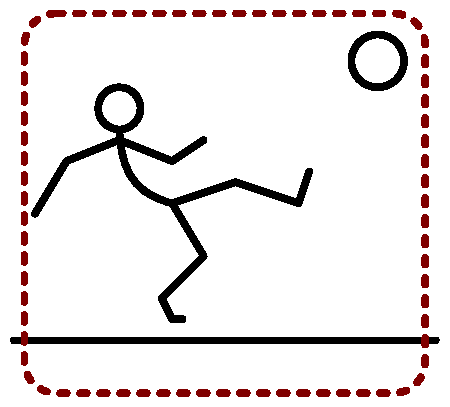
\includegraphics[height=0.2\textwidth]{figs/energia_systeemi_1.pdf} & 
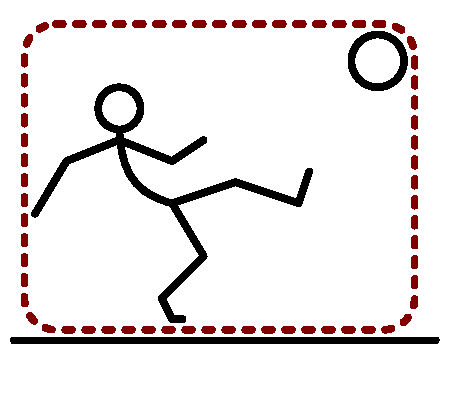
\includegraphics[height=0.2\textwidth]{figs/energia_systeemi_4.pdf} & 
\includegraphics[height=0.2\textwidth]{figs/energia_systeemi_2.pdf} & 
\includegraphics[height=0.2\textwidth]{figs/energia_systeemi_3.pdf} 
\end{tabular}
\end{center}
\label{fig:energiasysteemi}
\end{figure}


Esimerkiksi m\"a\"aritett\"aess\"a potkaistun pallon liikerataa pallo lienee syyt\"a ottaa osaksi tarkasteltavaa systeemi\"a, sill\"a juuri pallon k\"aytt\"aytymisest\"a ollaan kiinnostuneita. Potkun aikana pallo vuorovaikuttaa pelaajan kanssa ja lentonsa aikana se vuorovaikuttaa Maan ja ilman kanssa, joten n\"am\"akin voidaan ottaa osaksi tarkasteltavaa systeemi\"a. N\"ain ei ole kuitenkaan v\"altt\"am\"at\"ont\"a tehd\"a, sill\"a esimerkiksi Maa ei pallon lennon aikana liiku mihink\"a\"an eik\"a sen paikasta siis tarvitse pit\"a\"a kirjaa. Maan j\"att\"aminen pois tarkasteltavasta systeemist\"a ei tietenk\"a\"an poista Maan ja pallon v\"alist\"a vuorovaikutusta mihink\"a\"an, vaan t\"all\"oin palloon kohdistuva painovoima on huomioitava systeemin ja sen ymp\"arist\"on v\"alisen\"a vuorovaikutuksena.

Systeemin valinta tapahtuu siis puhtaasti ajatustasolla, eik\"a se tietenk\"a\"an saa vaikuttaa tarkasteltavan tilanteen k\"aytt\"aytymiseen, sill\"a luonto huomoi toiminnassaan aivan kaiken. Systeemien merkitys onkin toimia ajattelun apuv\"alinein\"a. Systeemin valinta on muistutus siit\"a, ett\"a systeemiin kuuluvista asioista on pidett\"av\"a kirjaa, eik\"a kerran valittua systeemi\"a saa vaihtaa kesken analyysin. On my\"os olemassa joukko hyvin vahvoja fysikaalisia menetelmi\"a, joita voi k\"aytt\"a\"a vain \emph{tietynlaisissa systeemeiss\"a} kuten pian opimme. Niinp\"a rajaamalla tarkasteltava systeemi juuri sopivasti voidaan ilmi\"oit\"a ymm\"art\"a\"a huomattavasti helpommin kuin huonosti valittua systeemi\"a tutkimalla.

\subsection{Ekstensiiviset suureet}
\label{ekstensiivisetsuureet}

Fysikaalisia suureita voidaan luokitella monin tavoin. Liikkeen tarkastelun yhteydess\"a tarkasteltiin jo skalaareja ja vektoreita joista edellisill\"a ei ole suuntaa mutta j\"alkimm\"aisill\"a on. Toinen t\"arke\"a luokittelu on jako \textbf{intensiivisiin} ja \textbf{ekstensiivisiin} suureisiin, mik\"a tarkoittaa karkeasti ilmaisten jakoa paikallisiin (aineen) ominaisuuksiin ja yleisiin (systeemin) ominaisuuksiin.

Tarkastellaan esimerkkin\"a muovailuvahasta tehty\"a t\"aysin tasalaatuista palloa. Mitataan vahapallon ominaisuuksia ja kirjataan n\"am\"a muistiin: esimerkiksi halkaisija, tilavuus, l\"amp\"otila, paino jne. --- emme ole m\"a\"aritelleet viel\"a n\"ait\"a suureita, mutta voit varmasti keksi\"a viel\"a paljon muitakin mitattavia ominaisuuksia. Leikataan t\"am\"an j\"alkeen pallo osiin ja mitataan nyt samat ominaisuudet jokaiselle osalle. Jotkin suureet kuten tilavuus ovat tietenkin kullekin pallon osalle pienempi\"a kuin koko pallolle, mutta toiset kuten l\"amp\"otila voivat olla pieniss\"a osissa samat kuin alkuper\"aisess\"a pallossa. 

Suureet, joille voidaan m\"a\"aritell\"a arvo erikseen kussakin pisteess\"a, ovat \emph{intensiivisi\"a}. Erityisesti jos t\"allaisen suureen arvo on kaikkialla vakio alkuper\"aisess\"a pallossa, suureella on sama arvo my\"os miss\"a tahansa pallosta leikatussa palassa. Esimerkiksi l\"amp\"otila on intensiivinen suure. Jos pallo on kauttaaltaan yht\"a l\"ammin, sen kussakin osassa on sama l\"amp\"otila.

T\"am\"a ei kuitenkaan p\"ade kaikille suureille. Esimerkiksi alkuper\"aisest\"a pallosta leikatun pienen palan tilavuus on v\"altt\"am\"att\"a pienempi kuin koko pallon tilavuus. Erityisesti jos vaha ei puristu leikatessa merkitt\"av\"asti kokoon, voimme pallon pilkkomisen j\"alkeen laskea yhteen kaikkien siit\"a leikattujen pienten osien tilavuudet ja n\"aiden tilavuuksien summan t\"aytyy olla yht\"a suuri kuin alkuper\"aisen pallon tilavuus. T\"at\"a ominaisuutta sanotaan \emph{ekstensiivisyydeksi}.
Toisin sanoen \emph{kun kappale tai systeemi jaetaan osiin mielivaltaisella tavalla ja kustakin osasta mitataan suureen $a$ arvo, suure on ekstensiivinen, jos n\"aiden arvojen summa on sama kuin suureen arvo alkuper\"aisell\"a kappaleella tai systeemill\"a}.
Ekstensiivisen suureen arvo on siis suoraan verrannollinen kappaleen kokoon kun taas intensiivisen suureen arvo ei sit\"a ole.

\begin{exam}{Ekstensiiviset ja intensiiviset suureet}{ex:ekstensiivinen}\noindent

\problem{Ovatko kappaleen tilavuus, kappaleen muodostavien hiukkasten lukum\"a\"ar\"a sek\"a n\"aiden hiukkasten tiheys eli hiukkasten m\"a\"ar\"a tilavuusyksikk\"o\"a kohden intensiivisi\"a vai ekstensiivisi\"a suureita?
}

 \twocol{0.55}{0.44}{\physics  Suure, joka ei muutu jaettaessa kauttaaltaan samanlaisesta aineesta tehty kappale kahtia, on intensiivinen. Sen sijaan jos suureen arvo t\"all\"oin puolittuu, kyseess\"a on ekstensiivinen suure. Tilannetta voi havainnollistaa piirt\"am\"all\"a hiukkasista koostuvan kappaleen sek\"a kokonaisena ett\"a osissa.

%
}{%
\begin{center}%
\includegraphics[width=0.7\textwidth]{figs/energia_ekstensiivinen_1.pdf}%
\end{center}%
}


 \solu  Jos kappaleen tilavuus on $V$ ja puolitamme kappaleen, puolikkaan tilavuus on $V/2$, joten tilavuus on \emph{ekstensiivinen}.

Jos kappale koostuu $N$ hiukkasesta ja puolitamme kappaleen, yhteen puolikkaaseen j\"a\"a $N/2$ hiukkasta, joten hiukkasm\"a\"ar\"a on \emph{ekstensiivinen}.

Hiukkasten lukum\"a\"ar\"atiheys ilmaisee hiukkasten lukum\"a\"ar\"an tilavuusyksik\"oss\"a. Hiukkasten tiheys voi vaihdella kappaleessa, mutta keskim\"a\"ar\"ainen hiukkastiheys kappaleelle, joka koostuu $N$:st\"a hiukkasesta ja jonka tilavuus on $V$, on
\begin{equation} n = \frac{N}{V}. \end{equation}
Puolikkaan kappaleen hiukkastiheys on niinik\"a\"an $\frac{N/2}{V/2} = \frac{N}{V} = n$ eli sama kuin alkuper\"aisell\"a kappaleella. Hiukkastiheys on siis \emph{intensiivinen}. 

 \eval  Itse asiassa jo huomio, ett\"a hiukkastiheys ei ole v\"altt\"am\"att\"a vakio kappaleen sis\"all\"a kertoo, ett\"a kyseess\"a on intensiivinen suure, sill\"a vain intensiivisille suureille voidaan m\"a\"aritell\"a arvo eri paikoissa kappaleen sis\"all\"a. Ei ole mielek\"ast\"a pohtia ekstensiivisen suureen kuten kappaleen tilavuuden arvoa kappaleen sis\"all\"a, koska tilavuus on koko kappaleen ominaisuus.

\end{exam}

Intensiivisill\"a ja ekstensiivisill\"a suureilla k\"aytet\"a\"an samanlaisia symboleita, joten matemaattiset lausekkeet eiv\"at suoraan kerro, ovatko suureet intensiivisi\"a vai ekstensiivisi\"a. Fysikaalisesti intensiiviset ja ekstensiiviset ominaisuudet k\"aytt\"aytyv\"at kuitenkin eri tavoin, eik\"a niit\"a voi yhdistell\"a miten sattuu. Esimerkiss\"a \autoref{ex:ekstensiivinen} n\"ahtiin, ett\"a kahden ekstensiivisen suureen suhde on intensiivinen. Vastaavasti koska intensiiviset suureet eiv\"at riipu kappaleen koosta, my\"osk\"a\"an intensiivisten suureiden tulot tai osam\"a\"ar\"at eiv\"at riipu kappaleen koosta ja my\"os ne ovat intensiivisi\"a suureita. Sen sijaan intensiivisen ja ekstensiivisen suureen tulo on ekstensiivinen. Esimerkiksi hiukkastiheyden (intensiivinen) ja tilavuuden (ekstensiivinen) tulona saadaan hiukkasm\"a\"ar\"a (ekstensiivinen).

\stopper{Selit\"a omin sanoin, mit\"a tarkoittaa intensiivisyys ja ekstensiivisyys. Ovatko seuraavat suureet intensiivisi\"a tai ekstensiivisi\"a: (a) nopeus, (b) pinta-ala, (c) tilavuuden ja nopeuden tulo?
}

\subsection{Muuttuvat ja muuttumattomat suureet}
\label{muuttuvatjamuuttumattomatsuureet}

Fysiikassa usein halutaan tiet\"a\"a, miten suureet muuttuvat ajan kuluessa, ja riippuen suureen laadusta t\"am\"a voi tapahtua eri tavoin. Esimerkiksi kappaleen paikka muuttuu kappaleen liikkuessa. Ekstensiiviset suureet ovat kuitenkin erityisen t\"arkeit\"a, koska ne kuvaavat systeemin ominaisuuksia kokonaisuutena, joten tutkitaan nyt t\"allaisten suureiden muuttumista.


\begin{figure}[tb]
\caption{Systeemin sis\"alt\"am\"an ekstensiivisen suureen muuttuminen.
}
\footnotesize
\begin{center}
\hspace*{-1.5cm}
\begin{tabular}{p{0.27\textwidth} p{0.27\textwidth} p{0.27\textwidth} p{0.27\textwidth}}

(a) Ekstensiivinen suure kuvaa jonkin asian m\"a\"ar\"a\"a.
 & 
(b) Suure voi muuttua vain siirtym\"all\"a ja luonnin tai h\"avityksen kautta.
 & 
(c) S\"ailyv\"a\"a suuretta ei voi luoda tai h\"avitt\"a\"a vaan vain siirt\"a\"a.
 & 
(d) Jos s\"ailyv\"a\"a suuretta ei siirry, sen m\"a\"ar\"a systeemiss\"a on vakio.
 \\
\includegraphics[height=0.15\textwidth]{figs/energia_sailyva_1.pdf} & 
\includegraphics[height=0.15\textwidth]{figs/energia_sailyva_2.pdf} & 
\includegraphics[height=0.15\textwidth]{figs/energia_sailyva_3.pdf} & 
\includegraphics[height=0.15\textwidth]{figs/energia_sailyva_4.pdf} 
\end{tabular}
\end{center}
\label{fig:energiasysteemi}
\end{figure}


Ekstensiivinen suure mittaa aina jonkin asian \emph{kokonaism\"a\"ar\"a\"a}. Esimerkiksi hiukkasten lukum\"a\"ar\"a kuvaa nimens\"a mukaisesti monestako hiukkasesta systeemi koostuu ja tilavuus kuvaa sen avaruuden m\"a\"ar\"a\"a, jonka systeemi t\"aytt\"a\"a. Ekstensiivinen suure voikin muuttua nelj\"all\"a eri tavalla: sit\"a voidaan tuoda systeemiin lis\"a\"a, vied\"a pois, luoda tai h\"avitt\"a\"a. Yht\"al\"on\"a t\"am\"an asian voi esitt\"a\"a muodossa
\begin{equation} \Delta a_\text{ekstensiivinen} = \Delta a_\text{tuonti} + \Delta a_\text{vienti} + \Delta a_\text{luonti} + \Delta a_\text{h\"avitys}. \end{equation}
N\"aist\"a eri tavoista suureen tuominen systeemiin tai vieminen sielt\"a pois ovat selke\"asti erilaisia tapahtumia kuin luominen ja h\"avitt\"aminen, sill\"a tuotaessa tai viet\"aess\"a suuretta vain siirtyy ymp\"arist\"on ja systeemin v\"alill\"a kun taas luomisen ja h\"avitt\"amisen yhteydess\"a suureen kokonaism\"a\"ar\"a muuttuu.

\begin{exam}{Ihmisten m\"a\"ar\"a}{ex:ekstensiivinen2}\noindent

\problem{Tarkastellaan Suomessa asuvien ihmisten lukum\"a\"ar\"a\"a. Millaista systeemi\"a, ymp\"arist\"o\"a ja suuretta t\"ass\"a tarkastellaan? Millaisissa tapahtumissa t\"am\"an suureen kokonaism\"a\"ar\"a muuttuu?
}

 \twocol{0.39}{0.6}{ Koska suure on rajattu Suomessa asuviin ihmisiin, tarkasteltu systeemi on Suomi ja sen ymp\"arist\"o ovat kaikki muut maat. Tarkasteltava suure on ihmisten lukum\"a\"ar\"a. Rajatulla alueella asuvien ihmisten lukum\"a\"ar\"a on my\"os ekstensiivinen suure, sill\"a se riippuu tarkasteltavan alueen koosta. Esimerkiksi Etel\"a-Suomen l\"a\"aniss\"a asuu v\"ahemm\"an ihmisi\"a kuin koko Suomessa, mutta koko Suomen v\"akiluku on sama kuin kaikkien l\"a\"anien v\"akilukujen summa.

%
}{%
\begin{center}%
\includegraphics[width=0.7\textwidth]{figs/energia_ekstensiivinen_2.pdf}%
\end{center}%
}


Ihmisten m\"a\"ar\"a Suomessa ei muutu ihmisten muuttaessa maan sis\"all\"a, sill\"a t\"all\"oin asukkaiden kokonaism\"a\"ar\"a pysyy samana ihmisten vain siirtyess\"a paikasta toiseen.
Ihmisten m\"a\"ar\"a voi muuttua maahanmuuton ja maastamuuton my\"ot\"a, sill\"a t\"all\"oin ihmisi\"a siirtyy Suomen ja ulkomaiden v\"alill\"a.
N\"am\"a edustavat suureen siirtymist\"a ymp\"arist\"ost\"a systeemiin sek\"a systeemist\"a ymp\"arist\"o\"on. T\"all\"oink\"a\"an kuitenkaan systeemin (Suomen) ja ymp\"arist\"on (ulkomaiden) yhteenlaskettu ihmisten kokonaism\"a\"ar\"a ei muutu.
Ihmisten m\"a\"ar\"a voi muuttua my\"os syntymien ja kuolemien kautta. N\"am\"a edustavat suureen luontia ja h\"avitt\"amist\"a, sill\"a niiss\"a ihminen ei siirry minnek\"a\"an vaan ihmisten kokonaism\"a\"ar\"a todella muuttuu.

\end{exam}

Erityisen t\"arkeit\"a ovat ekstensiiviset suureet, joita \emph{ei voi luoda eik\"a h\"avitt\"a\"a}, sill\"a n\"aiden suureiden mittaama asia voi ainoastaan siirty\"a systeemin ja ymp\"arist\"on v\"alill\"a eik\"a sen kokonaism\"a\"ar\"a voi muuttua. Fysiikassa t\"allaisten suureiden sanotaan \emph{s\"ailyv\"an}. S\"ailyv\"an suureen kokonaism\"a\"ar\"an muutos systeemiss\"a on
\begin{equation} \Delta a_\text{s\"ailyv\"a} = \Delta a_\text{tuonti} + \Delta a_\text{vienti}. \end{equation}
Nimitys ``s\"ailyv\"a'' viittaa suureen kokonaism\"a\"ar\"a\"an, joka s\"ailyy muuttumattomana. My\"os vektorisuureet voivat olla ekstensiivisi\"a s\"ailyvi\"a suureita, mik\"a tarkoittaa sit\"a ett\"a my\"os suureen suunta pysyy aina samana.

Systeemin ollessa sellainen, ett\"a s\"ailyv\"a\"a suuretta ei voi siirty\"a systeemin ja ymp\"arist\"on v\"alill\"a eli $\Delta a_\text{tuonti} = \Delta a_\text{vienti} = 0$, \emph{suureen kokonaism\"a\"ar\"a systeemiss\"a ei voi muuttua},
\begin{equation} \Delta a_\text{s\"ailyv\"a} = 0 \end{equation}
joten sen t\"aytyy olla vakio
\begin{equation} a = \text{vakio}. \end{equation}
Edelleen koska suureen derivaatta ajan suhteen on m\"a\"aritelty muutosten osam\"a\"arien kautta, my\"os suureen aikaderivaatta on siis aina nolla
\begin{equation} \frac{\dd a}{\dd t} = 0. \end{equation}
Riippuu tilanteesta, mik\"a n\"aist\"a tavoista esitt\"a\"a suureen s\"ailyminen on k\"aytt\"okelpoisin, mutta joka tapauksessa on syyt\"a tunnistaa n\"aiden kaikkien ilmaisevan samaa asiaa.

\textbf{S\"ailymislaki} on fysiikan laki, jonka mukaan fysikaalinen suure s\"ailyy eli suuretta ei voi luoda tai h\"avitt\"a\"a. T\"all\"oin suureen \emph{kokonaism\"a\"ar\"a} ei muutu ajan kuluessa.
S\"ailymislait ovat eritt\"ain voimakkaita fysiikan periaatteita, koska niiden avulla systeemien k\"ayt\"os voidaan usein analysoida yksinkertaisesti pit\"am\"all\"a kirjaa s\"ailyvien suureiden k\"aytt\"aytymisest\"a ilman tarkkaa tietoa systeemin tapahtumista. Jos s\"ailyv\"an suureen m\"a\"ar\"a lis\"a\"antyy jossakin, sen on v\"altt\"am\"att\"a v\"ahennytt\"av\"a muualla yht\"a paljon. Tai jos systeemi jaetaan osiin, osien on \emph{yhteens\"a} sis\"allett\"av\"a t\"asm\"alleen yht\"a paljon s\"ailyv\"a\"a suuretta kuin alkuper\"ainen systeemi sis\"alsi riippumatta jaon suorittamistavasta.

\begin{exam}{Paperin s\"ailymislaki}{ex:sailyy}\noindent

\problem{Neli\"on muotoinen paperi leikataan nelj\"a\"an yht\"a suureen neli\"on muotoiseen osaan kahdella alkuper\"aisten sivujen suuntaisella leikkauksella. Mik\"a on osien ymp\"aryysmittojen ja pinta-alojen summa ennen ja j\"alkeen operaation? Ent\"a jos paperi leikataan mielivaltaisen muotoisiin osiin?
}

 \twocol{0.35}{0.64}{ \physics  Neli\"on, jonka sivun pituus on $a$, ymp\"aryysmitta on $4a$ ja pinta-ala $a^2$. Kun paperi leikataan nelj\"a\"an osaan, saadaan nelj\"a uutta neli\"ot\"a, joiden sivujen pituudet ovat puolet alkuper\"aisest\"a.

%
}{%
\begin{center}%
\includegraphics[width=0.7\textwidth]{figs/energia_sailyva_5.pdf}%
\end{center}%
}


 \solu  Alkuper\"aisen neli\"on sivun pituus on $a$, ymp\"aryysmitta $4a$ ja pinta-ala $a^2$.
Leikkauksen j\"alkeen on nelj\"a neli\"on muotoista palaa, joiden kunkin sivun pituus on $a/2$. N\"aiden palojen ymp\"aryysmitta on siis $2a$ ja pinta-ala $a^2/4$ ja palojen yhteenlaskettu ymp\"aryysmitta on $4 \times 2a = 8a$ ja pinta-ala $4 \times a^2/4 = a^2$. Palojen ymp\"aryysmitta kasvoi mutta pinta-ala pysyi samana. Ymp\"aryysmitta ei siis ole intensiivinen eik\"a ekstensiivinen suure eik\"a se s\"ailynyt, mutta pinta-ala on ekstensiivinen s\"ailyv\"a suure paperin leikkauksessa. (Kaksiulotteiselle kappaleelle pinta-ala on ekstensiivinen aivan samoin kuin kolmiulotteiselle kappaleelle tilavuus on ekstensiivinen suure.)

 \eval  Jos paperi leikataan mielivaltaisiin osiin, osien ymp\"arysmitasta ei voida sanoa muuta kuin ett\"a ymp\"arysmitta kasvaa (t\"am\"an todistaminen j\"atet\"a\"an lukijalle). Osien kokonaispinta-ala on kuitenkin aina sama $a^2$ riippumatta siit\"a, kuinka paperi on leikattu. T\"am\"a on esimerkki s\"ailymislakien voimasta: Vaikkemme tied\"a mit\"a\"an muuta kuin ett\"a paperi on leikattu, silti voidaan olla varmoja, ett\"a osien kokonaispinta-ala ei ole muuttunut, mik\"a on hyvin voimakas reunaehto sille, miten paperi voi leikkauksessa k\"aytt\"ayty\"a.

Huomaa kuitenkin viel\"a, ett\"a paperin pinta-ala s\"ailyy vain ideaalisessa leikkauksessa, ja pinta-alaa voidaan h\"avitt\"a\"a vaikkapa polttamalla paperi. Suureita, jotka s\"ailyv\"at kaikissa mahdollisissa tapahtumissa on loppujen lopuksi hyvin v\"ah\"an.

\end{exam}

\stopper{Tarkastellaan seuraavia systeemej\"a ja suureita. Mill\"a tavoilla suureet voivat muuttua? Mitk\"a suureista ovat s\"ailyvi\"a? (a) kasvien m\"a\"ar\"a puistossa, (b) ilman suhteellinen kosteus huoneessa, (c) rahan m\"a\"ar\"a lukitussa kassakaapissa.
}

\section{Energia}
\label{energia}

Kaikki tuntevat nyky\"a\"an sanan ``energia'', koska \textbf{energia} fysikaalisena suureena on niin keskeinen modernin yhteiskunnan toiminnassa.
Karkeasti ilmaisten energia on jonkinlainen mittari sille, mit\"a kaikkea systeemi voi tehd\"a.
Ruoka sis\"alt\"a\"a kemiallista energiaa, josta saamme osan itsellemme sy\"om\"all\"a. T\"am\"an energian avulla pysymme l\"ampimin\"a, pystymme liikkumaan ja yll\"apid\"amme elintoimintojamme. K\"ayt\"amme my\"os koneita, jotka toimivat joko polttoaineiden kemiallisella energialla tai s\"ahk\"oisell\"a energialla.
T\"allainen arkinen k\"asitys energiasta on kuitenkin monin tavoin ep\"at\"asm\"allinen, ja seuraavaksi tutkimme, miten energian voisi m\"a\"aritell\"a t\"asm\"allisemmin ja miten energia toimii fysikaalisissa ilmi\"oiss\"a.

\subsection{Energian s\"ailymislaki}
\label{energians--a--ilymislaki}

Puhekieless\"a sanotaan, ett\"a ``liikunta kuluttaa energiaa''. T\"ast\"a voi saada sellaisen k\"asityksen, ett\"a lihasten toiminta vaatii energiaa ja ett\"a samalla t\"am\"a energiaa katoaa. T\"am\"a ei kuitenkaan ole totta. Esimerkiksi ruokaan sitoutunut kemiallinen energia on molekyylien rakenteeseen varastoitunutta energiaa. Liikuntasuorituksen aikana aineenvaihduntaan kuuluvat prosessit muuttavat kehoon varastoituneiden molekyylien rakennetta, jolloin niihin varastoitunut kemiallinen energia muuttuu. Liikuntasuorituksen aikana paljon energiaa varastoivia molekyylej\"a pilkotaan, jolloin niihin varastoituneen energian m\"a\"ar\"a pienenee. Energiaa siis ``kuluu'' liikuntasuorituksen aikana siin\"a mieless\"a, ett\"a kemiallinen energiavarasto hupenee.

Kemiallisten energiavarastojen kuluttamisella on kuitenkin my\"os muita vaikutuksia. Lihakset supistuvat, ja t\"all\"a tavalla niihen omistaja voi ty\"ont\"a\"a itsens\"a tai muut kappaleet liikkeeseen. Lis\"aksi lihakset l\"ampenev\"at liikuntasuorituksen aikana.
Her\"a\"akin siis kysymys, voisiko liikkeeseen ja l\"amp\"o\"on liitty\"a my\"os jonkinlaista energiaa, ja voiko n\"ait\"a erilaisia energian muotoja mitata samalla mittarilla (samalla yksik\"oll\"a). Osoittautuu, ett\"a vastaus on \emph{kyll\"a}. Vaikka n\"am\"a ilmi\"ot ovat n\"aenn\"aisesti aivan erilaisia, niit\"a kaikkia voidaan mitata suurella nimelt\"a energia, jonka SI-yksik\"on nimeksi on annettu \textbf{joule} (James Joulen mukaan) ja symboliksi J.

Osoittautuu my\"os, ett\"a kun m\"a\"arittelemme kemiallisen energian ja liike- sek\"a l\"amp\"oenergian mittarit sopivasti, lihasten toiminta lis\"a\"a l\"amp\"o- ja liike-energiaa \emph{t\"asm\"alleen yht\"a paljon} kuin ne kuluttavat kemiallista energiaa. T\"ass\"a mieless\"a lihakset eiv\"at siis todellisuudessa \emph{kuluta} energiaa lainkaan vaan ne vain \emph{muuttavat} energiaa muodosta toiseen.

T\"ass\"a ei viel\"a sin\"ans\"a ole mit\"a\"an ihmeellist\"a. Tietenkin saamme tuotettua lihaksilla sit\"a enemm\"an liikett\"a ja l\"amp\"o\"a mit\"a enemm\"an ruokaa voimme k\"aytt\"a\"a. Ei siis ole mitenk\"a\"an ihmeellist\"a, ett\"a voimme m\"a\"aritell\"a lihasten toimintaa kuvaavan suureen, joka kertoo paljonko liikett\"a ja l\"amp\"o\"a tietyll\"a ruokam\"a\"ar\"all\"a saadaan aikaan. Erityiseksi t\"am\"an suureen tekee se, ett\"a \emph{t\"asm\"alleen sama mittari toimii kaikissa muissakin prosesseissa}. Jos meill\"a on liikkuva kappale, jolla on liike-energiaa, ja vaikkapa pudotamme sen veteen, veden ja kappaleen l\"amp\"oenergia lis\"a\"antyy t\"asm\"alleen yht\"a paljon kuin niiden liike-energia v\"ahentyy.
Jos poltamme ruoan, muutamme siihen varastoituneen kemiallisen energian suoraan l\"amp\"oenergiaksi, ja t\"all\"oin l\"amp\"oenergian m\"a\"ar\"a lis\"a\"antyy yht\"a paljon kuin kemiallisen energian m\"a\"ar\"a v\"ahentyy.

Viel\"a t\"arke\"amp\"a\"a on se, ett\"a t\"am\"a periaate on voitu yleist\"a\"a kaikkiin muihinkin ilmi\"oihin. Voimme nimitt\"ain l\"ammitt\"a\"a kappaletta my\"os esimerkiksi valaisemalla sit\"a kirkkaalla valolla. T\"all\"oin kappaleen l\"amp\"oenergia kasvaa ilman, ett\"a sen kemiallinen energia tai liike-energia muuttuisi. T\"all\"oin voimme kuitenkin m\"a\"aritell\"a uuden energian muodon, s\"ateilyenergian (sill\"a valo on s\"ateily\"a), jolloin l\"amp\"oenergian lis\"a\"antymisen voi selitt\"a\"a s\"ateilyenergian v\"ahenemisell\"a. S\"ahk\"ojohtokin l\"ampenee, kun siin\"a kulkee s\"ahk\"ovirta. T\"am\"an voimme selitt\"a\"a m\"a\"arittelem\"all\"a s\"ahk\"ovirran kuljettaman s\"ahk\"oisen energian, jolloin johdon l\"ampeneminen selittyy sill\"a, ett\"a osa sen l\"api kulkevan s\"ahk\"ovirran kuljettamasta s\"ahk\"oisest\"a energiasta muuttuu l\"amp\"oenergiaksi. Ja jos s\"ahk\"ovirta kulkee lampun l\"api, lamppu l\"ampenee ja l\"ahett\"a\"a valoa niin, ett\"a lampun l\"amp\"oenergian kasvu ja sen l\"ahett\"am\"an s\"ateilyenergian m\"a\"ar\"a on t\"asm\"alleen yht\"a suuri kuin s\"ahk\"ovirran kuljettaman s\"ahk\"oenergian menetys lampussa. \emph{Aina}, kun energiaa on n\"aytt\"anyt katoavan tai syntyv\"an itsest\"a\"an, on l\"oydetty jokin uusi energian muoto, joka on selitt\"anyt havaitut muutokset. Vaikka energian eri muodot voivat lis\"a\"anty\"a ja v\"ahenty\"a, ei tunneta ilmi\"oit\"a, joissa kaikkien eri energian muotojen summa eli \textbf{kokonaisenergia}\\
\begin{equation} E_\text{kokonais} = E_\text{liike} + E_\text{kemia} + E_\text{l\"amp\"o} + E_\text{s\"ateily} + E_\text{s\"ahk\"o} + \ldots \end{equation}
muuttuisi. \emph{Systeemin} kokonaisenergia voi toki muuttua, sill\"a energiaa voi siirty\"a systeemin ja sen ymp\"arist\"on v\"alill\"a, mutta \emph{systeemin ja sen ymp\"arist\"on} yhteenlasketun kokonaisenergian t\"aytyy olla aina vakio,
\bigeq{ \Delta E_\text{kokonais} = 0. \label{energia_sailyy} }
T\"am\"a tulos on \textbf{energian s\"ailymislaki}. Se on kaiken fysiikan t\"arkeimpi\"a periaatteita, jonka mukaan \emph{energiaa ei voi luoda eik\"a h\"avitt\"a\"a}. Energian s\"ailyminen on alunperin p\"a\"atelty kokeellisesti, mutta nykyisin sill\"a on my\"os vankka teoreettinen pohja.

\stopper{(a) Jos yhdess\"a hampurilaisessa on kemiallista energiaa 2000 kJ, paljonko energiaa kahdessa samanlaisessa hampurilaisessa on?\\
(b) Jos yksi lamppu tarvitsee 5 J s\"ahk\"oenergiaa sekunnissa, paljonka kaksi samanlaista lamppua tarvitsee?\\
(c) Perustele n\"aiden kysymysten perusteella, onko energia ekstensiivinen vai intensiivinen suure.\\
(d) Miten energian ekstensiivisyys tai intensiivisyys liittyy siihen, ett\"a energia on s\"ailyv\"a suure?
}

Energian s\"ailymislaki on t\"arke\"a useastakin syyst\"a. Ensinn\"akin energia on kaikkia fysiikan osa-alueita yhdist\"av\"a fundamentaali suure. Toiseksi energian s\"ailyminen rajoittaa voimakkaasti sit\"a, mit\"a voi tapahtua. Jos k\"aytett\"aviss\"a on polttoainem\"a\"ar\"a, johon on varastoitu 1000 kJ energiaa, sill\"a ei voi kiihdytt\"a\"a kulkuneuvoa nopeuteen, jossa liike-energia olisi t\"at\"a suurempi. My\"os ikiliikkujat, jotka liikkuisivat ikuisesti ja joita voitaisiin samalla k\"aytt\"a\"a hyv\"aksi jotenkin, ovat energian s\"ailymisen vuoksi mahdottomia. Jos nimitt\"ain systeemi kasvattaa ymp\"arist\"ons\"a energiaa, systeemin energian t\"aytyy v\"ahenty\"a. Kolmanneksi energian s\"ailymislain avulla voidaan sopivasti valituissa systeemeiss\"a p\"a\"atell\"a t\"asm\"alleen, miten systeemi k\"aytt\"aytyy.

\begin{exam}{Systeemin valinta}{ex:systeemienergia}\noindent

\problem{Eristetyss\"a laatikossa on kaksi mukillista kuumaa vett\"a. Toinen mukeista on kannellinen pahvimuki, toinen kanneton. Millaisin tavoin tilanne voidaan rajata systeemiksi? Onko systeemin ainem\"a\"ar\"a tai kokonaisenergia vakioita? }

 \twocol{0.4}{0.59}{ \setup  Laatikkoon kuuluu nyt kaksi mukia, niiden sis\"alt\"am\"at vedet, ilmaa sek\"a laatikko itse. Mik\"a tahansa n\"aiden yhdistelm\"a voidaan valita systeemiksi. Tarkastellaan muutamaa erikoistapausta.

%
}{%
\begin{center}%
\includegraphics[width=0.8\textwidth]{figs/energia_systeemi_5.pdf}%
\end{center}%
}


 \physics  Valitaan systeemiksi kanneton muki sek\"a sen sis\"alt\"am\"a tilavuus. Tilavuus ei itsess\"a\"an ole mik\"a\"an kappale, mutta t\"all\"a tarkoitetaan systeemiin sis\"alt\"av\"an kaiken sen aineen, joka kulloinkin on mukin sis\"all\"a. Koska vesi on kuumaa, siihen on varastoitunut l\"amp\"oenergiaa. Vesi kuitenkin j\"a\"ahtyy, jolloin ilmeisesti sen sis\"alt\"am\"an energian m\"a\"ar\"a pienenee,
\begin{equation} \Delta E_\text{systeemi} = \Delta E_\text{vesi} + \Delta E_\text{muki} < 0. \end{equation}
Systeemin \emph{kokonaisenergia siis ei ole vakio}.
Koska mukissa ei ole kantta, kuumaa vett\"a muuttuu my\"os kaasuksi ja poistuu mukista kaiken aikaa ja niinp\"a mukin sis\"alt\"am\"an nestem\"aisen veden m\"a\"ar\"a v\"ahenee. Tilalle tulee ilmaa, mutta tarvitaan huomattavasti pienempi m\"a\"ar\"a ilmaa korvaamaan poistunut neste. Siisp\"a t\"ass\"a systeemiss\"a my\"osk\"a\"an \emph{ainem\"a\"ar\"a ei ole vakio}.

Valitaan systeemiksi sitten kannellinen muki sek\"a sen sis\"alt\"o eli kuuma vesi. Koska mukissa on kansi, ei sielt\"a p\"a\"ase pois vett\"a eik\"a ilmaa, joten systeemin sis\"alt\"am\"a \emph{ainem\"a\"ar\"a on vakio}. Muistutukseksi t\"ast\"a voidaan tilanteesta piirrettyyn kuvaan merkit\"a systeemin rajauksen yhteyteen merkint\"a $n$ osoittamaan ainem\"a\"ar\"an olevan systeemiss\"a vakio. Kuten kannettoman mukin tapauksessa, nytkin mukissa oleva vesi j\"a\"ahtyy, sill\"a l\"amp\"o\"a p\"a\"asee virtaamaan mukin sein\"amien l\"api ymp\"ar\"oiv\"a\"an ilmaan ja siis systeemin sis\"alt\"am\"a \emph{kokonaisenergia ei ole vakio}.

Tarkastellaan viel\"a systeemi\"a, johon kuuluu koko laatikon sis\"alt\"o ja laatikko itse. Kun kuuma vesi mukeissa j\"a\"ahtyy, sen energiaa siirtyy laatikon sis\"alt\"am\"an ilman ja laatikon itsens\"a l\"amp\"oenergiaksi. Jos laatikko on hyvin eristetty, l\"amp\"oenergiaa ei kuitenkaan p\"a\"ase siirtym\"a\"an laatikon ulkopuolelle. T\"all\"oin veden sis\"alt\"am\"a energiam\"a\"ar\"a pienenee t\"asm\"alleen yht\"a paljon kuin ilman ja laatikon sis\"alt\"am\"a energia lis\"a\"antyy ja systeemin \emph{kokonaisenergia on vakio}
\begin{equation} \Delta E_\text{systeemi} = \Delta E_\text{vesi} + \Delta E_\text{mukit} + \Delta E_\text{ilma} + \Delta E_\text{laatikko} = 0. \end{equation}
Koska laatikko on tiivis, sielt\"a ei p\"a\"ase ilmaa ulos ja my\"os systeemin \emph{ainem\"a\"ar\"a on vakio}.

\end{exam}

Esimerkiss\"a \autoref{ex:systeemienergia} tarkastellaan mahdollisia tapoja rajata systeemi ja systeemin kokonaisenergian huomataan joissakin tapauksissa olevan vakio ja toisissa ei.
Jos systeemin ja sen ymp\"arist\"on v\"alill\"a voi siirty\"a energiaa ja ainetta, systeemi\"a kutsutaan \textbf{avoimeksi}. Esimerkiss\"a \autoref{ex:systeemienergia} t\"allainen systeemi oli kanneton muki. Jos systeemist\"a ei voi siirty\"a ainetta ymp\"arist\"o\"on mutta energiaa voi, systeemi\"a kutsutaan \textbf{suljetuksi}. Esimerkiss\"a t\"allainen systeemi oli kannellinen muki. Systeemi, joka ei voi vaihtaa ainetta eik\"a energiaa ymp\"arist\"ons\"a kanssa, on \textbf{eristetty} systeemi, ja t\"allainen oli esimerkin eristetty laatikko.

Jos systeemi on eristetty, se ei voi saada energiaa ymp\"arist\"ost\"a\"an eik\"a my\"osk\"a\"an menett\"a\"a sit\"a. Koska energian s\"ailymislain mukaan energiaa ei voi luoda eik\"a h\"avitt\"a\"a, energian kokonaism\"a\"ar\"an systeemiss\"a on t\"all\"oin oltava vakio. N\"ain saadaan yleisen energian s\"ailymislain erikoistapaus: \textbf{eristetyn systeemin kokonaisenergia on vakio kaikissa prosesseissa},
\bigeq{ \Delta E_\text{eristetty} = 0. }

\stopper{Laihduttaminen on mahdollista liikkumalla paljon. Valitaan systeemiksi ihminen. Selit\"a, miten liikunta voi johtaa systeemin energian ja atomien m\"a\"ar\"an muuttumiseen.
}

Eristetyn systeemin k\"aytt\"aytyminen voidaan usein ennustaa varsin tarkasti pit\"am\"all\"a kirjaa energian eri muodoista, koska niiden summa ei muutu. T\"at\"a kirjanpitotekniikkaa kutsutaan \textbf{energiaperiaatteeksi}. Jos nimitt\"ain osaamme laskea systeemin kokonaisenergian m\"a\"ar\"an yhdell\"a ajan hetkell\"a, tied\"amme varmasti kokonaisenergian olevan \emph{sama} min\"a tahansa muunakin aikana riippumatta siit\"a mit\"a systeemiss\"a t\"asm\"alleen tapahtuu. Eritysesti jos systeemiss\"a vain muutamat energian muodot muuttuvat, voidaan yhden energian lajin muutokset p\"a\"atell\"a tarkastelemalla \emph{muiden} energian muotojen k\"aytt\"aytymist\"a. On hyvin tavallista, ett\"a joidenkin energian muotojen m\"a\"ar\"a on helppo m\"a\"aritt\"a\"a kun taas toisiin muotoihin varastoitunut energia on vaikea mitata tai laskea. T\"all\"oin voidaan p\"a\"atell\"a n\"aiden hankalampienkin muotojen sis\"alt\"am\"a energia tutkimalla helpommin havaittavia energian lajeja.

T\"allaisissa tilanteissa \textbf{energiadiagrammi} on hyv\"a tapa havainnollistaa energian muotojen muutokset. Energiadiagrammi on graafinen esitys, jossa systeemin kokonaisenergian jakautuminen eri muotoihin esitet\"a\"an esimerkiksi pylv\"askuvaajana. T\"allaisen kuvallisen esityksen avulla on helpompi muistaa huomioida kaikki systeemiss\"a ilmenev\"at energian muodot ja ennen kaikkea niiden avulla voi suoraan n\"ahd\"a miten energian eri muodot muuttuvat. 


\begin{figure}[tb]
\caption{Energiadiagrammeja erilaisille systeemeille. Kuvissa (a) ja (b) kahden kappaleen v\"aliin puristettu jousi ty\"ont\"a\"a kappaleet liikkeelle. Kuvissa (c) ja (d) ihminen ty\"ont\"a\"a laatikkoa.
}
\footnotesize
\begin{center}
\hspace*{-1.5cm}
\begin{tabular}{p{0.25\textwidth} p{0.22\textwidth} p{0.29\textwidth} p{0.29\textwidth}}

(a) Kokoon puristettuun jouseen varastoitunut elastinen energia muuttuu kappaleiden liikkeen energiaksi.
 & 
(b) Osa energiasta siirtyy toiselle kappaleelle, systeemin ulkopuolelle.
 & 
(c) Ihmiseen varastoitunut kemiallinen energia muuttuu ihmisen ja kappaleen liikkeen ja l\"amm\"on energiaksi.
 & 
(d) Osa l\"amm\"ost\"a siirtyy maahan, systeemin ulkopuolelle.
 \\
\includegraphics[height=0.31\textwidth]{figs/energia_diagrammi_1.pdf} & 
\includegraphics[height=0.31\textwidth]{figs/energia_diagrammi_6.pdf} & 
\includegraphics[height=0.31\textwidth]{figs/energia_diagrammi_4.pdf} & 
\includegraphics[height=0.31\textwidth]{figs/energia_diagrammi_5.pdf} 
\end{tabular}
\end{center}
\label{fig:energiadiagrammi}
\end{figure}


Kuvassa \autoref{fig:energiadiagrammi} on esitetty t\"allaisia energiadiagrammeja erilaisille systeemeille. Ensimm\"aisess\"a esimerkiss\"a jousi on puristettu kahden kappaleen v\"aliin. Jousen puristamiseen (muodon muutokseen) liittyy elastista energiaa, joka muuttuu kappaleiden liikkeen energiaksi p\"a\"astett\"aess\"a jousi oikenemaan. Jos n\"am\"a kappaleet eiv\"at vuorovaikuta muiden kappaleiden kanssa, energiaa ei voi muuttua mihink\"a\"an muuhun muotoon ja systeemin kokonaisenergian t\"aytyy olla vakio. T\"all\"oin kappaleiden yhteen lasketun liike-energian on lopuksi oltava yht\"a suuri kuin jouseen varastoitunut energia oli aluksi. T\"am\"a ilmenee energiadiagrammissa siten, ett\"a jousen elastinen energia v\"ahenee t\"asm\"alleen yht\"a paljon kuin liike-energia kasvaa.

Edellinen tarkastelu onnistui siksi, ett\"a tarkastelimme eristetty\"a systeemi\"a. Systeemin valintahan on mielivaltainen, joten samaa tilannetta voitaisiin tarkastella my\"os systeemin\"a, johon kuuluu ainoastaan yksi kappaleista sek\"a jousi. T\"all\"oin toinen kappale on osa ymp\"arist\"o\"a. T\"am\"a on aivan kelvollinen systeemin valinta, mutta koska jousi vuorovaikuttaa molempien kappaleiden kanssa, systeemin ja ymp\"arist\"on v\"alill\"a on nyt vuorovaikutus. Kummankin kappaleen nopeus muuttuu jousen vapautuessa, jolloin ymp\"arist\"on kokonaisenergia muuttuu. Osa alunperin jouseen sitoutuneesta energiasta siis siirtyy systeemist\"a ymp\"arist\"o\"on eik\"a systeemin kokonaisenergia ole nyt vakio.

Kolmannessa kuvassa on esitetty tilanne, jossa joku ty\"ont\"a\"a lattialla olevan suuren laatikon liikkeelle. T\"ass\"a prosessissa ty\"ont\"aj\"a kuluttaa varastoimaansa kemiallista energiaa lihastensa liikuttamiseksi. Laatikko l\"ahtee liikkeelle, jolloin sen liikkeen energia kasvaa. Samalla huomataan my\"os ty\"ont\"aj\"an, laatikon sek\"a lattian l\"ampenev\"an, mihin liittyy l\"amp\"oenergiaa. Kun kaikki liikkuvat ja l\"ampenev\"at kappaleet ovat mukana tarkasteltavassa systeemiss\"a, ymp\"arist\"o\"on j\"a\"a ainoastaan asioita, joihin laatikon ty\"ont\"aminen ei vaikuta mitenk\"a\"an. Energiaa ei siis siirry systeemist\"a ymp\"arist\"o\"on ja systeemin kokonaisenergia on vakio. Prosessissa muuttuu toisikseen kolme energian muotoa --- liike-energia, l\"amp\"oenergia sek\"a kemiallinen energia --- mutta n\"aiden summa pysyy samana. Diagrammissa t\"am\"a ilmenee niin, ett\"a kemiallinen energia v\"ahenee yht\"a paljon kuin l\"amp\"o\"on ja liikkeeseen liittyv\"at energiat yhteens\"a lis\"a\"antyv\"at.

Jos energiaperiaatetta k\"aytt\"a\"a, on aina oltava huolellinen systeemin valinnassa ja tarkistettava, ett\"a valitussa systeemiss\"a energia on todella vakio. Jos nimitt\"ain \"askeisess\"a esimerkiss\"a vaikkapa lattia j\"atet\"a\"an systeemin ulkopuolelle, lattian l\"amm\"oksi muuttuva energia ei en\"a\"a kuulukaan systeemiin eli systeemin kokonaisenergia pienenee vaikka systeemin ja ymp\"arist\"on yhteenlaskettu energia ei muutukaan.

\stopper{Muovailuvahapallo heitet\"a\"an sein\"a\"an, johon se tarttuu kiinni. Kun pallo viel\"a liikkui ennen sein\"a\"an osumista, sen liikkeeseen liittyi energiaa. Onko systeemin kokonaisenergia vakio, jos systeemi on (a) pelkk\"a vahapallo, (b) pallo ja sein\"a? (c) Millaisiin muotoihin pallon liikkeen energia saattoi muuttua?
}

\subsection{Liikkeen ja painovoiman energia}
\label{liikkeenjapainovoimanenergia}

Edell\"a puhuimme energiaperiaatteesta yleisell\"a tasolla, mutta jotta energiaa voisi todella k\"aytt\"a\"a fysikaalisten prosessien analyysin ty\"okaluna, meid\"an t\"aytyy ensin m\"a\"aritell\"a erilaiset energian muodot t\"asm\"allisesti. Erityisesti haluamme laskea systeemien energiasis\"all\"on eri tilanteissa. Koska mekaniikassa tutkimme p\"a\"aasiassa kappaleiden liikett\"a, keskitymme aluksi kappaleiden nopeuksista, paikoista ja muodoista riippuviin energian muotoihin.

Aloitetaan tutkimalla putoamisliikett\"a, koska kappaleen \autoref{kiihtyvyys} pohjalta osaamme jo analysoida vapaassa pudotuksessa olevan kappaleen liikkeen. Erityisesti johdimme yht\"al\"on (\autoref{nopeusneliomuutos}) eli
$ \Delta (v_x^2) = - 2 g \Delta x, $
jonka mukaan pystysuorassa vapaassa pudotuksessa olevan kappaleen nopeuden neli\"on muutos $\Delta (v_x^2) $ on aina verrannollinen kappaleen paikan muutokseen $\Delta x$ riippumatta siit\"a, milt\"a korkeudelta kappale putoaa tai onko kappaleella alkunopeutta. Erityiseti tulos p\"atee riippumatta siit\"a, liikkuuko kappale yl\"osp\"ain, alasp\"ain tai kenties edestakaisin molempiin suuntiin liikkeens\"a aikana. 

Koska tutkimme nyt nimenomaan suureiden muutoksia, kerrataan muutamia muutosten laskus\"a\"ant\"oj\"a. Ensinn\"akin, jos $k$ on vakio ja suure $a$ muuttuu m\"a\"ar\"an $\Delta a$ eli $a_\text{loppu} = a_\text{alku} + \Delta a$, tulo $ka$ saa arvon $ ka_\text{loppu} = k(a_\text{alku}+\Delta a) = ka_\text{alku} + k\Delta a$. Siisp\"a tulon $ka$ \emph{muutos} on
\begin{equation} \Delta (ka) = ka_\text{loppu} - ka_\text{alku} = k \Delta a. \end{equation}
Vakion ja muuttuvan suureen $a$ tulon muutos on siis yht\"a suuri kuin vakion ja $a$:n muutoksen tulo.

Samoin jos kaksi suuretta $a$ ja $b$ muuttuvat, niiden summa saa arvon
$a_\text{loppu} + b_\text{loppu} = a_\text{alku} + \Delta a + b_\text{alku} + \Delta b$,
ja n\"ain ollen suureiden summan muutos on yht\"a suuri kuin niiden muutosten summa,
\begin{equation} \Delta (a + b) = (a_\text{loppu} + b_\text{loppu}) - (a_\text{alku} + b_\text{alku}) =  \Delta a + \Delta b. \end{equation}

K\"aytt\"aen n\"ait\"a laskus\"a\"ant\"oj\"a yht\"al\"o (\autoref{nopeusneliomuutos}) voidaan putoamisliikeen tapauksessa (kun putoaminen tapahtuu tyhji\"oss\"a tai kappaleen vuorovaikutusta sit\"a ymp\"ar\"oiv\"an ilman kanssa ei huomioida) kirjoittaa muotoon
\begin{equation} \Delta \left( \frac{1}{2} v_x^2 \right) = - \Delta (g x) \label{energy_fall_first} \end{equation}
ja edelleen siirt\"am\"all\"a kaikki termit yht\"al\"on vasemmalle puolelle
\begin{equation} \Delta \left( \frac{1}{2} v_x^2 + g x \right) = 0, \label{energy_fall} \end{equation}
mik\"a siis tarkoittaa sit\"a, ett\"a nopeuden neli\"on ja kappaleen paikkakoordinaatin summa, kertoimien $1/2$ ja $g$ kanssa, on \emph{vakio}.

N\"ain johdettuna tulos voi vaikuttaa vain matemaattiselta tempulta, mutta se antaa meille vihjeen paljon syv\"allisemm\"ast\"a fysikaalisesta yhteydest\"a, joten pohditaan tulosta tarkemmin.
Ensinn\"akin tulos yhdist\"a\"a kappaleen vauhdin ja sen korkeuden niin, ett\"a syntyy vakiona pysyv\"a lauseke. Toisaalta jos valitsemme systeemiksi putoavan kappaleen ja maapallon, t\"am\"a systeemi sis\"alt\"a\"a kaiken, mik\"a putoamisessa muuttuu (kappaleen nopeus ja sen et\"aisyys maasta). Putoaminen on siis prosessi, joka vaikuttaa vain valitun systeemin sis\"all\"a, ja niinp\"a energian s\"ailymislain perusteella t\"am\"an systeemin kokonaisenergian t\"aytyy my\"os olla vakiona pysyv\"a lauseke. Ehk\"a siis yht\"al\"oss\"a \autoref{energy_fall} esiintyv\"a lauseke liittyy systeemin kokonaisenergiaan!

Yht\"al\"on ensimm\"ainen termi riippuu vain kappaleen nopeudesta, ja se on sit\"a suurempi, mit\"a nopeammin kappale liikkuu. T\"am\"an termin voisi siis tulkita liittyv\"an kappaleen liikkeen energiaan. Yht\"al\"on toinen termi puolestaan riippuu putoamiskiihtyvyydest\"a ja kappaleen korkeudesta. Putoamiskiihtyvyys on painovoiman ominaisuus, joten ilmeisesti t\"am\"a termi kuvaa jotenkin \emph{painovoimaan varastoituvaa energiaa}.

Yht\"al\"oss\"a (\autoref{energy_fall}) esiintyv\"a lauseke ei kuitenkaan voi kuvata systeemin energiaa t\"asm\"alleen vaan se on ainoastaan siihen verrannollinen lauseke. Nopeus ja paikkakoordinaatti ovat nimitt\"ain \emph{intensiivisi\"a} suureita, joten lausekkeen kuvaama suure on my\"os intensiivinen. Lausekkeen arvohan ei riipu mitenk\"a\"an siit\"a, koostuuko tarkasteltava systeemi vaikkapa hiekanjyv\"ast\"a vai kivenlohkareesta.

Energia on kuitenkin \emph{ekstensiivisinen} suure kuten kaikki s\"ailyv\"at suureet. Jos meill\"a olisi esimerkiksi kaksi samanlaista, samalla nopeudella liikkuvaa kappaletta, niill\"a pit\"aisi olla kaksinkertainen energia yhteen kappaleeseen verrattuna. Samoin arkikokemuksestakin tied\"amme, ett\"a on raskaampaa nostaa monta kappaletta kuin vain yksi, koska kaksi kappaletta ovat yhdess\"a \emph{painavammat} kuin yksi. Niinp\"a my\"os painovoiman energian t\"aytyy riippua siit\"a, paljonko ainetta on. Yht\"al\"ost\"a (\autoref{energy_fall}) puuttuu siis jokin kappaleen kokoon ja m\"a\"ar\"a\"an liittyv\"a tekij\"a, joka kertoo tarkasteltavan aineen m\"a\"ar\"an.
T\"am\"a tekij\"a on kappaleen \textbf{massa}. Massa on SI-j\"arjestelm\"an perussuure, jonka yksikk\"o on \textbf{kilogramma} (kg).

Massalla on fysiikassa kaksi toisistaan t\"aysin poikkeavaa roolia. Ensinn\"akin massiiviset kappaleet ovat \emph{painavia}, mik\"a tarkoittaa karkeasti ilmaisten sit\"a, ett\"a niiden nostaminen \emph{yl\"osp\"ain} on vaikeaa. Arkikieless\"a yleens\"a puhutaankin kappaleen painosta, kun tarkoitetaan sen massaa. Toisaalta massiiviset kappaleet ovat \emph{hitaita}, mik\"a tarkoittaa karkeasti sit\"a, ett\"a suuren nopeuden antaminen kappaleelle on vaikeaa \emph{mihin tahansa suuntaan}. J\"alkimm\"aist\"a ominaisuutta eli massan hitautta kutsutaan fysiikassa \textbf{inertiaksi}.
N\"am\"a voivat vaikuttaa samankaltaisilta asioilta mutta niill\"a on t\"aysin erilainen fysikaalinen merkitys. Nostaminen liittyy kappaleen \emph{paikan muuttamiseen} ja erityisesti kappaleen siirt\"amiseen poisp\"ain maanpinnasta (eli yht\"al\"oss\"a \autoref{energy_fall} suureen $ x $ muutokseen). Nostaminen on vaikeaa, koska maa ja kappale vuorovaikuttavat \emph{painovoiman} eli \textbf{gravitaation} kautta, ja kappaleen siirt\"aminen poisp\"ain varastoi energiaa gravitaatiovuorovaikutukseen. Painava massa kuvaa t\"am\"an vuorovaikutukseen voimakkuutta. Kappaleen liikkeelle saaminen puolestaan liittyy \emph{nopeuden muuttamiseen} (eli yht\"al\"oss\"a \autoref{energy_fall} suureen $ v_x $ muutokseen), mik\"a on aivan yht\"a vaikeaa vaikka kappale olisi tyhj\"ass\"a avaruudessa kaukana Maapallosta.
Nykytiet\"amyksen mukaan inertia ja painava massa ovat kuitenkin t\"asm\"alleen samat kaikilla hiukkasilla ja kappaleilla.

\stopper{Jos otat k\"ateesi esimerkiksi kuulanty\"onn\"oss\"a k\"aytett\"av\"an painavan kuulan ja ty\"onn\"at sen liikkeelle (a) suoraan vaakasuoraan tai (b) suoraan yl\"os, mik\"a massan ominaisuus p\"a\"aasiassa rajoittaa nopeutta, jonka pystyt kuulalle antamaan?
}


\begin{wrapfigure}{L}{0.55\textwidth}
\centering
\footnotesize
\captionof{figure}{Liike-energia.
}
\begin{tabular}{p{0.2\textwidth} p{0.3\textwidth}}

(a) Eri nopeudella liikkuvat kappaleet.
 & 
(b) Liike-energia nopeuden funktiona.
 \\ 
\includegraphics[height=0.25\textwidth]{figs/energia_liike_funktio_1.pdf} &
\includegraphics[height=0.25\textwidth]{figs/energia_liike_funktio_2.pdf} 
\end{tabular}
\label{fig:energia_k}
\end{wrapfigure}


Kappaleen liikkeeseen liittyy energiaa, joka riippuu kappaleen inertiasta, sill\"a mit\"a suurempi on kappaleen inertia, sit\"a enemm\"an energiaa tarvitaan, jotta kappale saataisiin kiihdytetty\"a johonkin nopeuteen $v_x$. Niinp\"a kappaleen, jonka inertia on $m$, \textbf{liike-energia} eli \textbf{kineettinen energia} $K$ on yht\"al\"on (\autoref{energy_fall}) ensimm\"ainen termi kerrottuna kappaleen massalla $m$,
\bigeq{ E_\text{liike} = K = \frac{1}{2}mv_x^2. \label{kin_ene}}
T\"ast\"a yht\"al\"ost\"a voimme yksikk\"otarkastelulla my\"os m\"a\"aritt\"a\"a energian yksik\"on joulen SI-j\"arjestelm\"an perusyksik\"oiden avulla lausuttuna,
\begin{equation} \text{J} = [K] = [m][v_x^2] = \text{kg}\text{m}^2/\text{s}^2. \end{equation}

Kertomalla koko yht\"al\"o (\autoref{energy_fall}) kappaleen massalla saadaan siis varsinainen putoavan kappaleen energian s\"ailymislaki
\begin{equation} \Delta \left( \frac{1}{2} mv_x^2 + m g x \right) = 0. \label{energy_fall_proper} \end{equation}
Yht\"al\"on j\"alkimm\"ainen termi on kappaleen ja maan v\"alisen painovoiman varastoima energia, jota kutsutaan fysiikassa \textbf{potentiaalienergiaksi} ja merkit\"a\"an tavallisesti symbolilla $U$
\bigeq{ E_\text{potentiaali} = U = mgx. \label{pot_ene}}
Nimitys viittaa siihen, ett\"a t\"all\"a varastoidulla energialla voidaan esimerkiksi saada kappale liikkeelle --- sill\"a on siis ``potentiaalia'' saada prosesseja tapahtumaan.
Yht\"al\"oss\"a (\autoref{pot_ene}) massa ilmaisee sit\"a, ett\"a painavan kappaleen nostaminen vaatii paljon energiaa.


\begin{wrapfigure}{L}{0.55\textwidth}
\centering
\footnotesize
\captionof{figure}{Painovoiman potentiaalienergia.
}
\begin{tabular}{p{0.2\textwidth} p{0.3\textwidth}}

(a) Eri korkeudella olevat kappaleet.
 & 
(b) Potentiaalienergia paikan funktiona.
 \\ 
\includegraphics[height=0.25\textwidth]{figs/energia_g_funktio_1.pdf} &
\includegraphics[height=0.25\textwidth]{figs/energia_g_funktio_2.pdf} 
\end{tabular}
\label{fig:energia_g}
\end{wrapfigure}


Kuvassa \autoref{fig:energiaheitto} on esitetty jo aiemmin luvussa \autoref{kiihtyvyys} analysoitu pystysuora heitto energiadiagrammein. Heitetyn kappaleen sek\"a Maan sis\"alt\"av\"an systeemin kokonaisenergia on heiton aikana vakio, sill\"a liike-energia on kappaleen liikkeen ominaisuus ja painovoiman potentiaalienergia on maan ja kappaleen vuorovaikutuksen varastoimaa energiaa. N\"am\"a kuuluvat systeemiin, jossa ovat sek\"a kappale ett\"a maa. 

Liike-energia riippuu kappaleen nopeuden neli\"ost\"a, joten se ei voi koskaan olla negatiivinen. Erityisesti \emph{liike-energian etumerkki ei riipu nopeuden suunnasta kuten nopeuden skalaarikomponentti}. Potentiaalienergia puolestaan riippuu kappaleen koordinaatista pystysuunnassa. Koordinaatti kuitenkin mitataan aina jonkin kiintopisteen suhteen, ja t\"am\"a kiintopiste voidaan valita periaatteessa minne tahansa. Potentiaalienergia saa kohdassa $x=0\un{m}$ arvon nolla, joten kiintopisteen valinta kiinnitt\"a\"a my\"os potentiaalienergian nollatason, ja t\"am\"an alapuolella \emph{potentiaalienergia on negatiivinen}. Potentiaalienergian absoluuttisella arvolla ei olekaan mit\"a\"an fysikaalista merkityst\"a, vaan ainoastaan potentiaalienergian \emph{muutokset} ovat merkityksellisi\"a. Heittoliikkeen tapauksessa potentiaalienergian nollataso voidaan valita esimerkiksi kappaleen l\"aht\"opisteeseen, mutta t\"am\"a ei ole ainoa mahdollinen valinta.


\begin{figure}[tb]
\caption{Energiadiagrammi pystysuoralle heitolle.
}
\footnotesize
\begin{center}
\begin{tabular}{p{0.22\textwidth} p{0.22\textwidth} p{0.22\textwidth} p{0.22\textwidth}}

(a) Alkutilanne: kappale heitet\"a\"an yl\"osp\"ain.
 & 
(b) Lakipiste.
 & 
(c) J\"alleen l\"aht\"okorkeudella.
 & 
(d) L\"aht\"okorkeutta alempana.
 \\
\includegraphics[height=0.2\textwidth]{figs/energia_heitto_1.pdf} & 
\includegraphics[height=0.2\textwidth]{figs/energia_heitto_2.pdf} & 
\includegraphics[height=0.2\textwidth]{figs/energia_heitto_3.pdf} & 
\includegraphics[height=0.2\textwidth]{figs/energia_heitto_4.pdf} 
\end{tabular}
\end{center}
\label{fig:energiaheitto}
\end{figure}


Jos potentiaalienergian nollakohdaksi valitaan kappaleen l\"aht\"opiste, yl\"osp\"ain heitetyll\"a kappaleella on aluksi liike-energia $K = \frac{1}{2}mv_x^2$ eik\"a lainkaan potentiaalienergiaa. Yl\"osp\"ain nousevan kappaleen potentiaalienergia kasvaa ja liike-energia pienenee niin, ett\"a kokonaisenergia on koko ajan vakio. Koska liike-energia ei voi saada negatiivisia arvoja, kappale p\"a\"asee t\"asm\"alleen niin korkealle, ett\"a kaikki sen alkuper\"ainen liike-energia on muuttunut potentiaalienergiaksi, jolloin sen nopeus on nolla. T\"am\"an j\"alkeen kappale putoaa j\"alleen alasp\"ain ja p\"a\"asty\"a\"an takaisin l\"aht\"okorkeudelleen sen potentiaalienergia on j\"alleen nolla ja sen liike-energia on sama kuin alkuhetkell\"a. Kappaleen vauhtikin on siis t\"all\"oin yht\"a suuri kuin heiton alussa.

Kappaleen jatkaessa putoamistaan l\"aht\"otasonsa alapuolelle sen potentiaalienergia pienenee edelleen saaden nyt \emph{negatiivisia} arvoja. T\"ass\"a ei ole mit\"a\"an ihmeellist\"a, sill\"a potentiaalienergian nollakohta riippui koordinaatiston origon valinnasta. Potentiaalienergian negatiiviset arvot eiv\"at siten tarkoita fysikaalisesti sen enemp\"a\"a kuin paikkakoordinaatin negatiiviset arvot: ne ainoastaan kertovat siit\"a, ett\"a kappale on nyt liikkunut valitusta origosta negatiiviseen suuntaan. Oleellista on se, ett\"a liike-energia aina kasvaa t\"asm\"alleen yht\"a paljon kuin potentiaalienergia pienenee. Kappaleen liikkeess\"a liike-enegian kasvu ilmenee kappaleen nopeuden kasvamisena. Kuitenkin koska liike-energia on verrannollinen nopeuden neli\"o\"on, kappaleen nopeus kasvaa \emph{hitaammin} kuin liike-energia.

\stopper{Miten kuvan \autoref{fig:energiaheitto} heittoliikkeen (i) energiadiagrammi ja (ii) pallon rata muuttuvat, jos\\
(a) pallon alkunopeus on kaksinkertainen,\\
(b) potentiaalienergian nollakohta valitaan heiton lakipisteeseen?\\
(c) vuorovaikutus ilman kanssa muuttaa osan pallon liike-energiasta l\"amp\"oenergiaksi heiton aikana?
}

\subsection{Elastinen energia}
\label{elastinenenergia}


\begin{wrapfigure}{R}{0.6\textwidth}
\centering
\footnotesize
\captionof{figure}{Elastinen potentiaalienergia.
}
\begin{tabular}{p{0.27\textwidth} p{0.3\textwidth}}

(a) Eripituiset jouset.
 & 
(b) Energia pituuden funktiona.
 \\ 
\includegraphics[height=0.25\textwidth]{figs/energia_k_funktio_1.pdf} &
\includegraphics[height=0.25\textwidth]{figs/energia_k_funktio_2.pdf} 
\end{tabular}
\label{fig:energia_k}
\end{wrapfigure}


Kappaleen muodon muuttaminen on my\"os energiaa vaativa prosessi, ja toisaalta esimerkiksi puristetun jousen avulla voi laukaista kappaleen liikkeelle. Siisp\"a mit\"a ilmeisimmin jousi tai mik\"a tahansa muu sopivasti taipuisa kappale kykenee varastoimaan energiaa muuttamalla muotoaan. T\"allaista itsest\"a\"an palautuvaa taipuisuutta kutsutaan fysiikassa \textbf{elastisuudeksi} ja jouseen varastoitunut energia on \emph{elastista potentiaalienergiaa}. Kunhan jousta ei venytet\"a liikaa, \emph{ideaalinen jousi} varastoikin kaiken sen puristamiseen tai venytt\"amiseen tarvitun energian ja voi vapauttaa sen takaisin liike-energiaksi.

Jos jousta ei puristeta eik\"a venytet\"a, se on niin sanotussa \emph{lepopituudessaan}. Koska jousi ei t\"all\"oin pyri itsest\"a\"an muuttamaan pituuttaan, t\"at\"a kutsutaan my\"os jousen \emph{tasapainopituudeksi}. Jousta voidaan yleens\"a sek\"a puristaa lyhyemm\"aksi ett\"a venytt\"a\"a pidemm\"aksi, ja molemmat muutokset vaativat energiaa, joten jousen potentiaalienergia on \emph{pienimmill\"a\"an} jousen ollessa lepopituudessaan. T\"ast\"a syyst\"a jousen potentiaalienergian nollakohdaksi yleens\"a valitaankin juuri jousen lepopituus. Itse asiassa ideaalisen jousen pituuden muuttaminen vaatii \emph{yht\"a paljon} energiaa olipa kyseess\"a puristus tai venytys. Mit\"a enemm\"an jousen pituutta muutetaan, sit\"a enemm\"an energiaa tarvitaan, eik\"a kyseess\"a itse asiassa ole edes suora verrannollisuus vaan suurien venymien aikaansaaminen on tavallisesti huomattavasti vaikeampaa kuin pienten. 

Todellisen jousen potentiaalienergia voi riippua jousen pituudesta monimutkaisellakin tavalla. Kuitenkin yksinkertaisin matemaattinen funktio, jolla on edell\"a kuvatut elastisen potentiaalienergian ominaisuudet, on toisen asteen polynomi eli paraabeli. Niinp\"a jousten ja muidenkin elastisten kappaleiden varastoimaa potentiaalienergiaa kuvataan yleens\"a t\"all\"a yksinkertaisella mallilla,
\bigeq{ U = \frac{1}{2} k (x-x_0)^2, \label{harmoninen_pot} }
jota kutsutaan my\"os \emph{harmoniseksi potentiaalienergiaksi}.
T\"ass\"a $k$ on jousen j\"aykkyytt\"a kuvaava \textbf{jousivakio}, $x$ on jousen pituus ja $x_0$ sen lepopituus. Et\"aisyys $x-x_0$ on siis jousen normaalista pituudesta mitattu venym\"a. Sen positiivinen arvo kuvaa jousen venymist\"a pidemm\"aksi ja negatiivinen arvo puristumista lyhyemm\"aksi. Funktio $U$ on nolla, kun venym\"a on nolla, ja se saa yh\"a suurempia positiivisia arvoja, kun jousta joko puristetaan tai venytet\"a\"an. T\"am\"a tarkoittaa jousen varastoivan yh\"a enemm\"an energiaa mit\"a enemm\"an sit\"a puristetaan tai venytet\"a\"an, kuten kuvasta \autoref{fig:energia_k} n\"ahd\"a\"an. Mit\"a suurempi jousivakio $k$ on, sit\"a enemm\"an energiaa jousen pituuden muuttaminen vaatii eli sit\"a \emph{j\"aykempi} jousi on.

\stopper{Kirjoita omin sanoin tiivistelm\"a siit\"a, miten kappaleen liike- ja potentiaalienergia (painovoima sek\"a elastisuus) voidaan laskea. Selit\"a my\"os, mik\"a on energiadiagrammi sek\"a miten esimerkiksi kappaleen nopeus voidaan ratkaista energiadiagrammin ja energiaperiaatteen avulla.
}

\begin{exam}{Gravitaation ja jousen energia}{ex:jousienergia}\noindent

\problem{Kappale pudotetaan levosta korkeudelta $0.100 \un{m}$ pystysuoran jousen p\"a\"alle. Jousen jousivakio on $100 \un{J/m}^2$ ja kappaleen massa $0.10 \un{kg}$. Kuinka paljon jousi enimmill\"a\"an puristuu?}

 \twocol{0.35}{0.64}{ \setup  Valitaan systeemiksi kappale, jousi ja Maa. T\"all\"oin systeemin kokonaisenergia koostuu kappaleen liike-energiasta, painovoiman potentiaalienergiasta sek\"a jousen potentiaalienergiasta.
Asetetaan viel\"a gravitaation potentiaalienergian nollakohta korkeudelle, jolla kappale juuri koskettaa jousta. Piirret\"a\"an putoamisesta energiadiagrammi helpottamaan kirjanpitoa eri energian muotojen muutoksille.

%
}{%
\begin{center}%
\includegraphics[width=0.9\textwidth]{figs/energia_diagrammi_7.pdf}%
\end{center}%
}


\physics Oletetaan ilmanvastus pieneksi. T\"all\"oin, koska ainoastaan kappale ja jousi liikkuvat putoamisen aikana, valitun systeemin kokonaisenergia on vakio eli liike-energian ja potentiaalienergian summa on lopussa, jousen puristuttua sama kuin alussa, kappaleen l\"ahtiess\"a liikkeelle.

Aluksi kappale on paikoillaan, joten sill\"a on vain potentiaalienergiaa. Pudotuksen aikana osa potentiaalienergiasta muuttuu liike-energiaksi.
Kun kappale putoaa jousen p\"a\"alle, jousi puristuu varastoiden kappaleen liike-energiaa potentiaalienergiaksi. Lopulta kappale pys\"ahtyy ja jousi heitt\"a\"a kappaleen j\"alleen yl\"osp\"ain. Jousen maksimaalinen puristuma saavutetaan kappaleen pys\"ahtyess\"a, ennen kuin jousi alkaa j\"alleen nostaa kappaletta yl\"osp\"ain. Kappaleen ollessa paikoillaan sen liike-energia on j\"alleen nolla, joten gravitaation ja jousen potentiaalienergioiden summan t\"aytyy olla sama kuin liikkeen alussa. Erityisesti kappaleella on lopuksi hiukan negatiivista gravitaation potentiaalienergiaa, joten jousen potentiaalienergia on suurempi kuin kokonaisenergia oli alussa.

\model Kappaleen liike-energia on
\begin{equation}K = \frac{1}{2} m v^2,\end{equation}
miss\"a $v$ on kappaleen nopeus.
Kappaleen pudotessa sen gravitaatiopotentiaalienergia on
\begin{equation}U_\text{gravitaatio} = mgx,\end{equation}
miss\"a $x$ on jousen yl\"ap\"a\"ast\"a mitattu pystysuora et\"aisyys.
Jousi puristuu vasta kappaleen kohdatessa sen, joten jousen potentiaalienergia on
\begin{equation} U_\text{jousi} = \begin{cases}
\frac{1}{2} k x^2, & x < 0 \\
0, & x > 0 \end{cases}. \end{equation}

Kappaleella on ennen pudotusta ainoastaan gravitaation potentiaalienergia $E_\text{alku} = mgh$, miss\"a $h$ on kappaleen l\"aht\"opisteen koordinaatti eli pudotuskorkeus. Energian s\"ailymislaki saa n\"ain ollen muodon
\begin{equation} K+U_\text{gravitaatio}+U_\text{jousi} = E_\text{alku} = mgh. \end{equation}

Kun jousi on puristunut ja kappale on j\"alleen pys\"ahtynyt, kappaleen paikkakoordinaatti on negatiivinen, $x < 0$, ja t\"am\"a on my\"os jousen venym\"a, koska origoksi valittiin jousen tasapainoasema. (Eli jousen puristuma on $-x > 0$.)
Kokonaisenergian s\"ailyminen saa yht\"al\"on\"a muodon
\begin{equation}mgx + \frac{1}{2} k x^2 = mgh\end{equation}
huomioiden ett\"a liike-energia on nolla, $K=0$, kun kappale on ratansa alimmassa pisteess\"a. T\"ast\"a voidaan ratkaista paikka $x$.

\solu Kyseess\"a on toisen asteen yht\"al\"o muuttujan $x$ suhteen, jonka ratkaisut ovat
\begin{equation} x = -\frac{gm}{k}\left( 1 \pm \sqrt{\frac{2hk}{gm} + 1} \right). \end{equation}
Koska ratkaisun pit\"a\"a olla negatiivinen, fysikaalisesti oikea valinta on
\begin{equation} x = -\frac{gm}{k}\left( 1 + \sqrt{\frac{2hk}{gm} + 1} \right), \end{equation}
sill\"a $\sqrt{2hk/(gm) + 1} > 1$.

Annetuilla lukuarvoilla kappaleen alimmaksi paikaksi saadaan
\begin{equation} x = -\frac{9.8 \un{m/s}^2 \cdot 0.10 \un{kg}}{100 \un{J/m}^2} \left( 1 + \sqrt{\frac{2 \cdot 0.100\un{m} \cdot 100 \un{J/m}^2}{9.8 \un{m/s}^2 \cdot 0.10 \un{kg}} + 1} \right) = -0.055 \un{m}. \end{equation}
Jousen maksimipuristuma on siis $-x = 5.5 \un{cm}$.


\mbar
\begin{mathematica}[commandchars=\\!?]
(* energioiden lausekkeet *)
ualku = m g h;
ugrav = m g x;
ujousi = 1/2 k x^2;

(* ratkaistaan paikkakoordinaatti, 
kun potentiaalienergia on sama kuin alussa *)
pohja = Solve[ ugrav + ujousi == ualku, x]
  \textit!{{x -> (-g m - Sqrt[g m (2 h k + g m)])/k},?
  \textit! {x -> (-g m + Sqrt[g m (2 h k + g m)])/k}}?

(* sijoitetaan lukuarvot *)
pohja /. {g -> 9.8, m -> 0.1, k -> 100, h -> 0.1}
  \textit!{{x -> -0.0551436}, {x -> 0.0355436}}?
\end{mathematica}

\eval Ratkaisun j\"arkevyytt\"a voidaan arvioida yksikk\"otarkastelulla:
\begin{equation} [x] = \frac{[g][m]}{[k]} = \frac{\text{kgm/s}^2}{\text{J/m}^2} = \frac{\text{kgm/s}^2}{\text{kg/s}^2} = \text{m}. \end{equation}
Ratkaisulla on siis pituuden yksikk\"o kuten pit\"a\"akin.
Lis\"aksi neli\"ojuurilausekkeen sis\"alt\"am\"an termin $\frac{2hk}{gm}$ t\"aytyy olla paljas luku, koska se lasketaan yhteen ykk\"osen kanssa. Sit\"a se on, koska $[h][k/(gm)] = \text{m} \cdot 1/\text{m} = 1$.

Voimme tutkia my\"os ratkaisuna saadun lausekkeen raja-arvoja. Tarkastellaan tilannetta, jossa jousi on hyvin j\"aykk\"a ($k$ on suuri) tai kappale on hyvin kevyt ($m$ on pieni). Jos j\"ayk\"an jousen p\"a\"alle pudotetaan kevyt kappale, jousi puristuu hyvin v\"ah\"an ja kappale pomppaa v\"alitt\"om\"asti takaisin ilmaan. T\"at\"a vastaa raja-arvo $m/k \to 0$, joka voidaan laskea kirjoittamalla ratkaisu muotoon
\begin{equation} x = -\frac{gm}{k}\left( 1 + \sqrt{\frac{2hk}{gm} + 1} \right) = -\frac{gm}{k} - \sqrt{ \frac{2hgm}{k} + \frac{g^2m^2}{k^2}} \to 0. \end{equation}
Hyvin j\"aykk\"a jousi ei siis puristu, kuten pit\"a\"akin.

\end{exam}
\newpage


\section{Energian laatu}
\label{energianlaatu}

\subsection{Mekaaninen energia ja sis\"aenergia}
\label{mekaaninenenergiajasis--a--energia}

Kappaleen nostaminen yl\"osp\"ain lis\"a\"a kappaleen potentiaalienergiaa, joten t\"am\"a on yksi mahdollinen tapa \emph{varastoida energiaa}. T\"at\"a periaatetta voidaan k\"aytt\"a\"a hyv\"aksi esimerkiksi vesivoimalaitoksissa. Varastoimalla vett\"a esimerkiksi patoaltaaseen voidaan samalla varastoida energiaa veden potentiaalienergiaksi. Tarvittaessa vett\"a voidaan sitten juoksuttaa padossa olevan voimalaitoksen l\"api, jolloin veden potentiaalienergia muuttuu ensin veden liike-energiaksi. Liikkuva vesi puolestaan py\"oritt\"a\"a generaattoreita, jolloin osa liike-energiasta muuttuu s\"ahk\"oiseksi energiaksi. S\"ahk\"on avulla energiaa on helppo siirt\"a\"a edelleen k\"aytett\"av\"aksi muihin tarkoituksiin.

My\"os elastisiin kappaleisiin voi varastoida energiaa puristamalla, venytt\"am\"all\"a tai taivuttamalla niit\"a. T\"at\"a tekniikkaa on k\"aytetty i\"at ja ajat esimerkiksi jousipyssyiss\"a, joissa jousta j\"annitett\"aess\"a ampujan lihasten kemiallinen energia varastoituu jousen kaaren elastiseen muodonmuutokseen. Jousen vapautuessa t\"am\"a elastinen energia muuttuu nuolen liike-energiaksi.

Kappaleiden liike-energialla ja edell\"a kuvatuilla potentiaalienergian eri muodoilla on se yhteinen piirre, ett\"a ne voidaan havaita makroskooppisesti. Voimme n\"ahd\"a suoraan onko pallo korkealla vai matalalla, liikkuuko se nopeasti vai hitaasti ja onko se mahdollisesti my\"os puristunut kasaan. Koska n\"am\"a energian muodot liittyv\"at makroskooppisten kappaleiden paikkaan, nopeuteen ja muotoon, niit\"a kutsutaan yhteisnimell\"a \textbf{mekaaninen energia}.

Mekaanisella energialla on toinenkin merkitt\"av\"a erityispiirre: mekaanisen energian eri lajit voivat muuttua helposti toisikseen. Esimerkiksi yl\"osp\"ain heitetyn pallon liike-energia muuttuu pallon potentiaalienergiaksi pallon noustessa, koska pallon vauhti pienenee ja korkeus lis\"a\"antyy. Potentiaalienergia puolestaan muuttuu j\"alleen liike-energiaksi pallon laskeutuessa alasp\"ain.
Pallon heitolle aikaisemmin p\"a\"atelty energian s\"ailymislaki (\autoref{energy_fall_proper}) voidaankin siis kirjoittaa my\"os muotoon
\begin{equation} E_\text{kokonais} = E_\text{liike} + E_\text{potentiaali} = K + U = \text{vakio}. \label{mek_ene_sailyy}\end{equation}
Yll\"a esitetty periaate toimii my\"os muiden vuorovaikutusten kuin gravitaation kohdalla, \emph{jos vuorovaikutuksia voidaan kuvata potentiaalienergialla} eli funktiolla, joka kuvaa vuorovaikutuksen varastoimaa energiaa ja riippuu ainoastaan kappaleiden paikoista, asennoista tai muodoista.
T\"am\"a on energian s\"ailymislain t\"arke\"a erikoistapaus: \emph{Jos eristetyss\"a systeemiss\"a vaikuttaa ainoastaan sellaisia vuorovaikutuksia, joihin liittyy potentiaalienergia, systeemin mekaaninen energia eli liike-energian ja potentiaalienergian summa $K + U$ on vakio}. 

\stopper{Uimahypp\"a\"aj\"a hypp\"a\"a ponnahduslaudalle, ponnistaa t\"ast\"a hyvin korkealle ilmaan tehden voltin ja sukeltaa lopulta veteen. Millaisia energian muotojen muutoksia t\"ah\"an prosessiin liittyy? Jos systeemi on hypp\"a\"aj\"a, lauta sek\"a vesi, miss\"a prosessin vaiheissa systeemin mekaaninen energia on ainakin likimain vakio?
}

Koska mekaanista energiaa on helppo varastoida ja vapauttaa liikkeeksi, sen hy\"odynt\"aminen on melko yksinkertaista. Ennen h\"oyrykoneiden keksimist\"a melkein kaikki laitteet kelloista purjelaivoihin perustuivatkin joko ``lihasvoimaan'' eli kemialliseen energiaan tai mekaaniseen energiaan.
Kaikki energian muodot \emph{eiv\"at} kuitenkaan muutu noin vain toisikseen. Jos esimerkiksi muovailuvahasta tehty pallo putoaa lattialle, se pys\"ahtyy lattiaan osuessaan, jolloin pallon liike-energia muuttuu muihin, ei-mekaanisiin muotoihin. Seuraavaksi tarkastelemmekin millaisia muita muotoja energialla on ja millaisia ominaisuuksia energian eri muodoilla on.


\begin{figure}[tb]
\caption{Mekaaninen energia eli liike- ja potentiaalienergia on j\"arjestynytt\"a energiaa. Sis\"aenergiaa ovat kappaleen tilasta riippuvat energian muodot.
}
\footnotesize
\begin{center}
\begin{tabular}{p{1.0\textwidth} }
\includegraphics[width=0.95\textwidth]{figs/energia_luokat_2.pdf}
\end{tabular}
\end{center}
\label{fig:energiakoherenssi}
\end{figure}


Aloitimme energian tarkastelun luettelemalla energian muotoja kuten kemiallisen energian ja l\"amp\"oenergian. N\"am\"a energian muodot poikkeavat mekaanisesta energiasta siin\"a, ett\"a ne liittyv\"at ilmi\"oihin, joita ei voi suoraan n\"ahd\"a. Kemiallinen energia on aineiden kemialliseen koostumukseen eli niiden molekyylien rakenteeseen varastoitunutta energiaa. L\"amp\"oenergia on puolestaan aineen kuumuuteen liittyv\"a\"a energiaa. N\"aiden energiamuotojen mittaaminen vaatii siis enemm\"an tietoa kappaleista kuin vain miss\"a ne ovat ja miten ne liikkuvat. Periaatteessa systeemin kaikkien energiamuotojen m\"a\"aritt\"aminen vaatisi sit\"a, ett\"a tunnemme systeemin kaikki ominaisuudet mukaan lukien niiden sis\"aisest\"a rakenteesta riippuvat n\"akym\"att\"om\"at ominaisuudet.
Fysiikassa t\"allaista systeemin t\"aydellist\"a kuvausta kutsutaan \textbf{tilaksi}. Toisin sanoen tilan k\"asite sis\"alt\"a\"a paikan ja nopeuden lis\"aksi \emph{kaikki} systeemin fysikaaliset ominaisuudet kuten kappaleiden muodon, kemiallisen koostumuksen, l\"amp\"otilan jne. Monet energian muodot liittyv\"at systeemin tilaan, ja energian muutokset voivat ilmet\"a kappaleiden liikkeen muutosten lis\"aksi my\"os niiden tilan muutoksena. 

Fysiikassa kappaleen tilaan liittyv\"a\"a ``n\"akym\"at\"ont\"a'' energiaa kuten kemiallista energiaa ja l\"amp\"oenergiaa kutsutaan \textbf{sis\"aenergiaksi}. Nimitys viittaa siihen, ett\"a t\"am\"a energia on ``piilossa'' kappaleen sis\"all\"a.
Kappaleen makroskooppiseen liikkeeseen liittyv\"a liike-energia ei ole sis\"aenergiaa kuten ei ole esimerkiksi painovoiman potentiaalienergiakaan, sill\"a n\"am\"a eiv\"at riipu kappaleen sis\"aisist\"a ominaisuuksista.
Elastinen energia sen sijaan voidaan laskea sis\"aenergiaksi, koska kappaleen puristaminen ja venytt\"aminen muuttaa my\"os atomien keskin\"aisi\"a et\"aisyyksi\"a aineen sis\"all\"a, ja elastinen energia onkin itse asiassa n\"aiden atomien v\"alisten sidosten potentiaalienergiaa.

\stopper{Kappale on aluksi paikoillaan, mutta l\"ahtee liikkeelle. Miss\"a seuraavista tapauksista kappaleen saama liike-energia on per\"aisin jonkin toisen kappaleen mekaanisesta energiasta ja miss\"a sis\"aenergiasta? (a) Kappale putoaa. (b) Kappale ty\"onnet\"a\"an k\"asin liikkeelle. (c) Kappaleeseen t\"orm\"a\"a toinen kappale. (d) Kappaleen ty\"ont\"a\"a liikkeelle puristunut jousi. (e) Kappaleen vieress\"a tapahtuu r\"aj\"ahdys.
}

\subsection{Energian ep\"aj\"arjestyminen}
\label{energianep--a--j--a--rjestyminen}

Ota kirja, aseta se p\"oyd\"alle ja ty\"onn\"a se liukumaan pitkin p\"oyd\"an pintaa. Todenn\"ak\"oisesti huomaat kirjan pys\"ahtyv\"an melko nopeasti. Liikkuvalla kirjalla on aluksi liike-energiaa, mutta koska kirja pys\"ahtyy, sen liike-energian t\"aytyy olla lopuksi nolla. Jos sinulla olisi hyvin tarkka l\"amp\"omittari, voisit kuitenkin samalla havaita kirjan ja p\"oyd\"an pinnan hieman l\"ampenev\"an. Kirjan liike-energia siis v\"ahenee, ja pintojen l\"amp\"oenergia lis\"a\"antyy, joten prosessissa mekaanista liike-energiaa muuttuu kappaleiden l\"amp\"oenergiaksi eli sis\"aenergiaksi.


\begin{figure}[tb]
\caption{Yksinkertainen malli kitkan toiminnasta kahden liikkuvan kappaleen rajapinnalla. Pallot kuvaavat atomeja ja niiden v\"aliset ``jouset'' atomisidoksia.
}
\footnotesize
\begin{center}
\hspace*{-1.5cm}
\begin{tabular}{p{0.34\textwidth} p{0.2\textwidth} p{0.2\textwidth} p{0.3\textwidth}}

(a)
 & 
(b)
 & 
(c)
 & 
(d)
 \\
\includegraphics[height=0.18\textwidth]{figs/energia_kitka_1.pdf} & 
\includegraphics[height=0.18\textwidth]{figs/energia_kitka_2.pdf} & 
\includegraphics[height=0.18\textwidth]{figs/energia_kitka_3.pdf} & 
\includegraphics[height=0.18\textwidth]{figs/energia_kitka_4.pdf} 
\end{tabular}
\end{center}
\label{fig:energiakitka}
\end{figure}


T\"am\"an ilmi\"on selitt\"a\"a \textbf{kitka}, joka on koskettavien pintojen v\"alinen vuorovaikutus. Kitka aiheutuu siit\"a, ett\"a toisiaan koskettavat pinnat pyrkiv\"at tarttumaan mikroskooppisessa mittakaavassa toisiinsa kiinni (kuva \autoref{fig:energiakitka}). Jos kuitenkin kappaleet liikkuvat, n\"am\"a heikot sidokset eiv\"at kuitenkaan v\"altt\"am\"att\"a riit\"a saamaan kappaleita tarttumaan toisiinsa vaan sidokset vain hidastavat pintojen liukumista toistensa suhteen. N\"ain liikkuvien pintojen v\"alill\"a syntyy jatkuvasti uusia sidoksia ja vanhoja sidoksia rikkoutuu.
Tyypillisesti sidokset venyv\"at ennen rikkoutumistaan, jolloin pintojen rakenteessa tapahtuu pieni\"a elastisia muutoksia --- ts. pinnat voivat veny\"a tai puristua mikroskooppisella tasolla, mihin varastoituu elastista energiaa. 

Kun pinnat sitten irtoavat toisistaan, n\"am\"a muodonmuutokset p\"a\"asev\"at yht\"akki\"a palautumaan kuin j\"annitetty kuminauha, jonka toinen p\"a\"a p\"a\"astet\"a\"an vapaaksi. T\"am\"an seurauksena pintaan varastoitunut elastinen energia muuttuu pintojen atomien liike-energiaksi, ja atomit alkavat v\"ar\"ahdell\"a.
Pinnan atomien poukkoilu t\"onii nopeasti my\"os muita atomeja liikkeelle ja niin t\"am\"a liike-energia alkaa levit\"a muuallekin kappaleeseen. Loppujen lopuksi suuri osa liukuvan kappaleen liike-energiasta on muuttunut v\"ar\"ahtelevien atomien liike-energiaksi, mutta nyt atomit eiv\"at en\"a\"a liiku kaikki samaan suuntaan kuten aluksi vaan nyt ne v\"ar\"ahtelev\"at satunnaisesti kaikissa suunnissa. Makroskooppisesti t\"am\"a ilmenee siten, ett\"a kappale pys\"ahtyy ja \emph{l\"ampenee}.

Ilman l\"api kulkevaan kappaleeseen kohdistuu samantyyppinen vuorovaikutus. Ilmassa kulkevan kappaleen on ty\"onnett\"av\"a ilmaa pois edest\"a\"an, jolloin kaasun molekyylit saavat kappaleelta liike-energiaa. Molekyylien edelleen t\"orm\"ailless\"a toisiinsa t\"am\"akin liike-energia jakautuu satunnaisesti suurelle m\"a\"ar\"alle hiukkasia. Lopputuloksena kappaleen vauhti hidastuu ja ilma sek\"a kappaleen pinta l\"ampenev\"at.

\stopper{Purjelaivoissa liikkuva ilma t\"orm\"a\"a purjeisiin ty\"ont\"aen laivan liikkeelle. Miten ilmanvastus t\"ass\"a ilmenee? Millaisia energian muutoksia muodosta toiseen t\"ah\"an prosessiin liittyy?
}

Atomien poukkoilu on normaalisti t\"aysin satunnaista eik\"a yksitt\"aisi\"a atomeja voi havaita ilman huipputekniikkaa. Niinp\"a atomien \emph{satunnaisen} liikkeen liike-energiaa ei makroskooppisella tasolla n\"ahd\"a liikkeen\"a vaan se ilmenee \emph{kuumuutena}, joka on kappaleen \emph{tilan} ominaisuus. Mikroskooppisessa mittakaavassa atomit tietenkin vain liikkuvat tiet\"am\"att\"a onko niiden liikkeen energia meid\"an mielest\"amme liike-energiaa vai l\"amp\"oenergiaa.
Makroskooppisessa mittakaavassa liike ja kuumuus ovat kuitenkin t\"aysin erilaisia ilmi\"oit\"a. L\"ammin kappale voi olla paikoillaan eik\"a kylm\"a kappale tunnut l\"ampim\"amm\"alt\"a vaikka se liikkuisi. T\"am\"a ero on seurausta siit\"a, ett\"a atomit liikkuvat eri tavoin \emph{toistensa suhteen}. Kun kappale liikkuu, sen kaikki atomit liikkuvat kollektiivisesti samaan suuntaan. Sen sijaan kuuman kappaleen atomit liikkuvat satunnaisiin suuntiin. Toisin sanoen liikkuvassa kappaleessa atomien liike on \emph{j\"arjestynytt\"a} kun taas kuumassa kappaleessa liike on \emph{ep\"aj\"arjestynytt\"a}.

Mekaanisen energian muodot ovat j\"arjestynytt\"a energiaa. Kaikki ep\"aj\"arjestyneet energian muodot ovat sis\"aenergiaa. Elastinen energia kuten jousen energia on j\"arjestynytt\"a ja se riippuu kappaleen muodosta (siis tilasta), joten elastinen energia voidaan lukea sek\"a mekaaniseen energiaan ett\"a sis\"aenergiaan. Osoittautuu, ett\"a juuri energian j\"arjestyneisyys on keskeinen tekij\"a, josta riippuu miten energian muodot voivat muuttua toisikseen ja millaiset prosessit ovat mahdollisia, kuten seuraavat esimerkit osoittavat.


\begin{wrapfigure}{L}{0.45\textwidth}
\centering
\footnotesize
\captionof{figure}{Energian muutokset elastisen pallon pomppiessa.}

\includegraphics[width=0.4\textwidth]{figs/energia_pomppu_sarja.pdf} 

\label{fig:energiapomppu}
\end{wrapfigure}


Tarkastellaan kuvan \autoref{fig:energiapomppu} ideaalista elastista pomppivaa kumipalloa. Pallon osuessa maahan se painuu hetkeksi kasaan, jolloin sen liike-energia varastoituu muodonmuutokseen liittyv\"aksi elastiseksi potentiaalienergiaksi. T\"am\"a potentiaalienergia palautuu pallon liike-energiaksi pallon palatessa takaisin alkuper\"aiseen muotoonsa, jolloin pallo pomppaa takaisin yl\"os yht\"a suurella nopeudella kuin mill\"a se osui lattiaan. T\"am\"an j\"alkeen pallon liike-energia varastoituu pallon noustessa gravitaation potentiaalienergiaksi kunnes muuttuu j\"alleen pallon pudotessa takaisin liike-energiaksi. Jos pallo olisi t\"aysin elastinen ja koe suoritettaisiin tyhji\"oss\"a niin ettei ilmanvastuskaan hidasta pallon liikett\"a, pallo jatkaisi pomppimistaan loputtomiin liike-energian muuttuessa vuoroin elastiseksi ja vuoroin gravitaation potentiaalienergiaksi. N\"am\"a mekaanisen energian muodot ovat kaikki j\"arjestyneit\"a ja ne voivat vapaasti muuttua toisikseen.

Tarkastellaan toisena esimerkkin\"a jo \"asken tutkimaamme p\"oyd\"all\"a liukuvaa kirjaa (kuva \autoref{fig:energiareversiibeli}). Kirjan ja p\"oyd\"an pinnan v\"alill\"a vaikuttava kitka muuttaa kirjan j\"arjestyneen liike-energian ep\"aj\"arjestyneeksi l\"amp\"oenergiaksi. Kuitenkin kun kirja on paikoillaan, se \emph{ei koskaan} l\"ahde itsest\"a\"an liikkeelle niin, ett\"a sen ja p\"oyd\"an l\"amp\"oenergia muuttuisi kirjan liike-energiaksi. Toisin sanoen \emph{prosessi, jossa kitka pys\"aytt\"a\"a kirjan, voi tapahtua vain yhteen suuntaan}. T\"allaista prosessia kutsutaan fysiikassa \textbf{irreversiibeliksi} (engl. `irreversible', k\"a\"ant\"am\"at\"on). Vastaavasti prosessia, joka voidaan k\"a\"ant\"a\"a ajassa takaperin, kutsutaan \textbf{reversiibeliksi}.


\begin{wrapfigure}{L}{0.4\textwidth}
\centering
\footnotesize
\captionof{figure}{Energian muutos kappaleen liukuessa.
}

(a) Kitka muuttaa liike-energian l\"amp\"oenergiaksi.
 \\ 
\includegraphics[width=0.35\textwidth]{figs/energia_reversiibeli_5.pdf} \\

(b) L\"amp\"oenergia ei muutu itsest\"a\"an liike-energiaksi.
 \\ 
\includegraphics[width=0.35\textwidth]{figs/energia_reversiibeli_6.pdf} 
\label{fig:energiareversiibeli}
\end{wrapfigure}


Irreversiibelit prosessit voi tunnistaa kuvittelemalla prosessin tapahtuvan takaperin tai videoimalla prosessin ja katsomalla videon lopusta alkuun. Jos takaperin tapahtuva prosessi n\"aytt\"a\"a mahdottomalta, prosessi on irreversiibeli. Liukuvan kirjan pys\"ahtyminen, n\"aytt\"a\"a takaperin silt\"a, ett\"a paikoillaan ollut kirja vain yht\"akki\"a l\"ahtee liikkeelle lattian samalla viilentyess\"a, mit\"a ei todellisuudessa voi tapahtua. Sen sijaan video pomppivasta pallosta, jonka jokainen pomppu on yht\"a korkea, n\"aytt\"a\"a t\"asm\"alleen samanlaiselta my\"os takaperin esitettyn\"a. Prosessit, joissa mekaanisen energian muodot muuttuvat toisikseen, ovat yleens\"a reversiibeleit\"a ainakin jos prosessiin osallistuvien kappaleiden m\"a\"ar\"a on pieni. Ep\"aj\"arjestyneen energian muotoja sis\"alt\"av\"at prosessit ovat puolestaan tavallisesti irreversiibeleit\"a.

Koska makroskooppisella tasolla ei voida koskaan t\"aysin v\"altt\"a\"a esimerkiksi kitkaa,
t\"aysin reversiibeleit\"a prosesseja on todellisuudessa olemassa vain atomien mittakaavassa. Niinp\"a j\"arjestyneen energian muodot muuttuvat jatkuvasti ep\"aj\"arjestyneiksi. My\"os ep\"aj\"arjestynyt energia voi muuttua takaisin j\"arjestyneeksi. Esimerkiksi r\"aj\"ahdyksess\"a kemiallinen energia muuttuu ensin l\"amp\"oenergiaksi ja sitten osa t\"ast\"a l\"amp\"oenergiasta muuttuu edelleen kappaleiden liike-energiaksi. T\"all\"a on kuitenkin rajoituksensa eik\"a \emph{kaikkea} ep\"aj\"arjestynytt\"a energiaa voi koskaan palauttaa j\"arjestyneeksi. T\"ass\"a mieless\"a ep\"aj\"arjestynyt energia on j\"arjestynytt\"a energiaa huonompaa.

Ep\"aj\"arjestyneen sis\"aenergian mittaaminen on usein vaikeampaa kuin mekaanisen energian, mink\"a vuoksi mekaniikassa usein prosesseja pidet\"a\"an likimain reversiibelein\"a --- ts. vuorovaikutukset kuten kitka ja ilmanvastus j\"atet\"a\"an usein huomioimatta --- sill\"a t\"all\"oin mekaaninen energia on likimain vakio. N\"ain voi kuitenkin tehd\"a vain, jos esimerkiksi kitka on paljon heikompi kuin muut systeemiss\"a vaikuttavat vuorovaikutukset. Luvussa \autoref{luku:voimatyo} palaamme tarkastelemaan, kuinka energian muutoksia yhdest\"a muodosta toiseen voidaan tarkemmin analysoida. L\"amp\"oenergian ominaisuuksia ja hy\"odynt\"amist\"a kuvaavaan \emph{termodynamiikkaan} tutustumme luvussa \autoref{luku:termodynamiikka}.

\stopper{Mitk\"a seuraavista prosesseista ovat reversiibeleit\"a? (a) Kappale liukuu tasaisella nopeudella alas kaltevaa tasoa. (b) Kappale putoaa tyhji\"oss\"a. (c) Ruoka j\"a\"ahtyy. (d) T\"aysin elastinen pallo t\"orm\"a\"a toiseen samanlaiseen palloon. (e) T\"aysin elastinen pallo t\"orm\"a\"a kymmenen samanlaisen pallon kasaan.
}

\begin{exam}{Dissipatiivinen vuorovaikutus}{ex:dissipaatio}\noindent

\problem{Kappale (massa $0.350 \un{kg}$) l\"ahtee levosta liukumaan alas kaltevaa tasoa. Kuljettuaan yhden metrin, kappale on saavuttanut nopeuden $1.5 \un{m/s}$. Tason kaltevuuskulma vaakatasoon n\"ahden on $40^\circ$. Kuinka paljon energiaa on kulunut kappaleen ja sen ymp\"arist\"on l\"ammitt\"amiseen?
}

 \twocol{0.59}{0.4}{ \setup  Valitaan systeemiksi kappale ja maan painovoimakentt\"a. Piirret\"a\"an systeemin kuva ja prosessia kuvaava energiadiagrammi. Merkit\"a\"an kappaleen kulkemaa matkaa $s = 1.0 \un{m}$ ja tason kaltevuuskulmaa $\theta = 40^\circ$. Kappaleen massa on $m = 0.350 \un{kg}$ ja sen saama nopeus $v_{\text{loppu}} = 1.5 \un{m/s}$.

 \physics  Systeemin potentiaalienergia pienenee ja liike-energia kasvaa kappaleen liikkuessa alasp\"ain. Kappaleeseen vaikuttavat dissipatiiviset vuorovaikutukset, kitka ja ilmanvastus, kuitenkin muuttavat samalla liike-energiaa l\"amp\"oenergiaksi. Systeemin kokonaisenergia ei ole vakio, mutta energian s\"ailymislain perusteella systeemist\"a h\"avinneen mekaanisen energian t\"aytyy muuttua muihin energian muotoihin, p\"a\"aasiassa l\"amp\"oenergiaksi.

%
}{%
\begin{center}%
\includegraphics[width=0.9\textwidth]{figs/energia_esimerkki_sisa.pdf}%
\end{center}%
}


 \model  Kappale siirtyy pystysuoran et\"aisyyden $\Delta x = -s \sin \theta$ ja sen potentiaalienergia pienenee t\"all\"oin m\"a\"ar\"an
\begin{equation} \Delta U = mg\Delta x = -mgs \sin \theta. \end{equation}
Kappaleen liike-energia puolestaan kasvaa m\"a\"ar\"an
\begin{equation} \Delta K = \frac{1}{2} m \Delta (v^2) = \frac{1}{2} m v_{\text{loppu}}^2. \end{equation}
L\"amm\"oksi muuttuu energia $ \Delta E_\text{sis\"a} = -\Delta E_\text{mekaaninen} = -\Delta U - \Delta K $.

 \solu  L\"amm\"oksi muuttuu energiam\"a\"ar\"a
\begin{equation} \Delta E_\text{sis\"a} = mgs \sin \theta - \frac{1}{2} m v_{\text{loppu}}^2, \end{equation}
ja lukuarvojen sijoitus antaa tulokseksi $\Delta E_\text{sis\"a} = 1.8 \un{J}$.

 \eval  Tarkasteltaan, ett\"a ratkaisulla on energian yksikk\"o.
\begin{equation} [\Delta E_\text{sis\"a}] = [mgs] + [mv^2] = \text{kg m/s}^2\cdot\text{m} + \text{kgm}^2/\text{s}^2 = \text{J}. \end{equation}

\end{exam}

\stopper{Selit\"a omin sanoin k\"asitteet j\"arjestynyt ja ep\"aj\"arjestynyt energia sek\"a sis\"aenergia. Selit\"a my\"os millaisia rajoituksia energian eri muotojen muutoksiin liittyy, ja miksi t\"ast\"a seuraa se, ett\"a jotkin prosessit eiv\"at voi tapahtua takaperin.
}

\subsection{Konservatiivisuus}
\label{konservatiivisuus}

Painovoimaa ja elastisia vuorovaikutuksia, joihin liittyy potentiaalienergia, kutsutaan \textbf{konservatiivisiksi} vuorovaikutuksiksi, koska ne s\"ailytt\"av\"at (engl. `conserve') j\"arjestyneen eli mekaanisen energian. J\"arjestynytt\"a energiaa ep\"aj\"arjestyneeksi muuttavat vuorovaikutukset kuten kitka ovat puolestaan \textbf{dissipatiivisia}, koska ne hukkaavat (engl. `dissipate') mekaanista energiaa. Konservatiivisilla vuorovaikutuksilla on fysiikassa erityisen t\"arke\"a asema juuri siksi, ett\"a ne eiv\"at muuta energian j\"arjestyneisyytt\"a. Tutkitaan siis viel\"a, millaisia ominaisuuksia konservatiivisilla vuorovaikutuksilla on.

Tarkastellaan prosessia, jossa kappale liikkuu ja palaa lopuksi takaisin l\"aht\"opisteeseens\"a. T\"am\"a tapahtuu esimerkiksi heitett\"aess\"a pallo suoraan yl\"osp\"ain, mutta periaatteessa kappale voi kulkea millaisen reitin tahansa, kunhan se lopuksi p\"a\"atyy takaisin l\"aht\"opaikkaansa. T\"allaista reitti\"a kutsutaan \textbf{suljetuksi}, koska reitti\"a pitkin piirretty viiva muodostaa suljetun silmukan. 

Jos eristetyss\"a systeemiss\"a vaikuttaa vain konservatiivisia vuorovaikutuksia, joita kuvaa \emph{ainoastaan paikasta riippuva potentiaalienergia}, t\"am\"an potentiaalienergian on oltava suljetun reitin lopussa \emph{sama} kuin alussa, $U_\text{loppu} = U_\text{alku}$, koska kappale palaa suljetulla reitill\"a lopuksi \emph{samaan} pisteeseen kuin mist\"a l\"ahti. T\"am\"a n\"ahd\"a\"an kuvissa \autoref{fig:energiakonservatiivinen} (a) ja (b). Mekaanisen energian s\"ailymisen perusteella kokonaisenergia ei muutu, $ K_\text{loppu} + U_\text{loppu} = \text{vakio} = K_\text{alku} + U_\text{alku} $, joten my\"os kappaleen \emph{liike-energian} ja siis vauhdin on oltava lopuksi sama kuin aluksi. 


\begin{figure}[tb]
\caption{Konservatiiviset ja dissipatiiviset vuorovaikutukset voi tunnistaa tarkastelemalla kappaleen liikett\"a suljettua reitti\"a pitkin.
}
\footnotesize
\begin{center}
\begin{tabular}{p{0.31\textwidth} p{0.31\textwidth} p{0.31\textwidth} }

(a) Kappale l\"ahtee liikkeelle.
 & 
(b) Kappale palaa l\"aht\"opisteeseen ja sill\"a on sama vauhti kuin aluksi.
 & 
(c) Kappale palaa l\"aht\"opisteeseen ja sill\"a on eri vauhti kuin aluksi.
 \\
\includegraphics[width=0.30\textwidth]{figs/energia_konservatiivinen_1.pdf} & 
\includegraphics[width=0.30\textwidth]{figs/energia_konservatiivinen_2.pdf} & 
\includegraphics[width=0.30\textwidth]{figs/energia_konservatiivinen_3.pdf} 
\end{tabular}
\end{center}
\label{fig:energiakonservatiivinen}
\end{figure}


P\"a\"attelyn voi my\"os k\"a\"ant\"a\"a ymp\"ari. Jos on olemassa reitti, jota pitkin kulkien kappale voi palata takaisin l\"aht\"opisteeseens\"a niin, ett\"a sen vauhti \emph{ei ole lopuksi sama kuin aluksi}, kappaleen liike-energian ja potentiaalienergian summa ei ole aluksi sama kuin lopuksi, $ K_\text{loppu} + U_\text{loppu} \ne K_\text{alku} + U_\text{alku} $. T\"allaisessa tapauksessa mekaanisen energian on t\"aytynyt muuttua johonkin toiseen muotoon ja systeemiss\"a t\"aytyy vaikuttaa dissipatiivisia vuorovaikutuksia. N\"ain k\"ay yl\"osp\"ain heitetylle kappaleelle, kun ilmanvastuksen liikett\"a hidastava vaikutus huomioidaan.
Kuvassa \autoref{fig:energiakonservatiivinen} on t\"ast\"a esitetty esimerkkin\"a h\"oyhen, joka suurellakin alkunopeudella yl\"osp\"ain heitettyn\"a leijailee lopulta alas hyvin hitaasti.
Prosessissa osa h\"oyhenen alkuper\"aisest\"a mekaanisesta energiasta muuttuu heiton aikana ilman liikkeen energiaksi ja lopulta l\"amp\"oenergiaksi.

\stopper{Jos potentiaalienergia riippuu paikan lis\"aksi kappaleen muodosta, onko kappaleen potentiaalienergian muutos v\"altt\"am\"att\"a nolla, jos kappale kulkee suljetun reitin? Jos ei ole, mit\"a muuta pit\"a\"a vaatia?
}

\section{Liikem\"a\"ar\"a}
\label{liikem--a----a--r--a--}

Edell\"a opimme, ett\"a kappaleen liikkeeseen sitoutuneen energian m\"a\"ar\"a riippuu sek\"a kappaleen massasta ett\"a kappaleen vauhdista. T\"am\"an n\"akee konkreettisesti esimerkiksi kolareissa. Massiivinen ja nopeasti liikkuva auto tekee t\"orm\"atess\"a\"an enemm\"an tuhoa kuin kevyt tai hidas, koska suurella autolla on ennen t\"orm\"ayst\"a enemm\"an liike-energiaa.

Energia yksin\"a\"an ei kuitenkaan riit\"a selitt\"am\"a\"an, mit\"a t\"orm\"ayksiss\"a tapahtuu. Ajatellaanpa tilannetta, jossa rekka ja k\"arp\"anen liikkuvat vastakkaisiin suuntiin samalla vauhdilla ja t\"orm\"a\"av\"at (kuva \autoref{fig:liikemaarasuunta}). Rekan liike ei varmasti muutu t\"orm\"ayksess\"a havaittavasti, mutta k\"arp\"anen tai mit\"a siit\"a j\"a\"ak\"a\"an j\"aljelle j\"a\"a todenn\"ak\"oisesti kiinni rekkaan. Rekan liike-energia on t\"orm\"ayksen j\"alkeen likimain sama kuin ennen t\"orm\"ayst\"a, koska rekan nopeus ei juuri muutu. K\"arp\"asen nopeuden suunta vaihtuu, mutta sen vauhti ei muutu, joten k\"arp\"asenkin liike-energia on likimain vakio. 

Tuntuu itsest\"a\"an selv\"alt\"a, ett\"a rekka ja k\"arp\"anen eiv\"at voi t\"orm\"at\"a niin, ett\"a kumpikin kimpoaisi takaisin tulosuuntaansa samalla vauhdilla kuin saapuivat (kuva \autoref{fig:liikemaarasuunta} (c)). On nimitt\"ain aivan selv\"a\"a, ett\"a k\"arp\"anen ei voi muuttaa rekan liikett\"a. Mutta \emph{miksi}? Energian s\"ailyminen ei t\"at\"a selit\"a, sill\"a jos rekan liikkeen suunta k\"a\"antyy ymp\"ari mutta vauhti pysyy vakiona, rekan liike-energia ei muutu. T\"aytyy olla jonkin toinen selitys sille, miksi k\"arp\"anen ei voi muuttaa rekan liikett\"a.


\begin{figure}[tb]
\caption{Rekan t\"orm\"ays k\"arp\"aseen. Molemmilla on sama nopeus, mutta massiivisen rekan liike-energia on paljon suurempi.
}
\footnotesize
\begin{center}
\begin{tabular}{p{0.32\textwidth} p{0.32\textwidth} p{0.32\textwidth} }

(a) Rekka ja k\"arp\"anen kohtaavat.
 & 
(b) K\"arp\"anen j\"a\"a kiinni rekkaan. Liike-energia on likimain vakio.
 & 
(c) Liike-energia olisi vakio my\"os jos kappaleet kimpoaisivat toisistaan.
 \\
\includegraphics[width=0.30\textwidth]{figs/liikemaara_suunta_1.pdf} & 
\includegraphics[width=0.30\textwidth]{figs/liikemaara_suunta_2.pdf} & 
\includegraphics[width=0.30\textwidth]{figs/liikemaara_suunta_3.pdf} 
\end{tabular}
\end{center}
\label{fig:liikemaarasuunta}
\end{figure}


\subsection{T\"orm\"aykset}
\label{t--o--rm--a--ykset}


\begin{wrapfigure}{R}{0.55\textwidth}
\centering
\footnotesize
\captionof{figure}{Vaunujen t\"orm\"ayksen analyysi.
}
\begin{tabular}{p{0.28\textwidth} p{0.23\textwidth}}

(a) Videoitu liike kuvasarjana.
 & 
(b) T\"am\"an perusteella piirretty paikan kuvaaja.
 \\ 
\includegraphics[height=0.25\textwidth]{figs/liikemaara_kuvasarja.pdf} &
\includegraphics[height=0.25\textwidth]{figs/liikemaara_tormays_2.pdf} 
\end{tabular}
\label{fig:liikemaaratormays_malli}
\end{wrapfigure}


Ymm\"art\"a\"aksemme rekan ja k\"arp\"asen t\"orm\"ayksen tutkimme seuraavaksi kappaleiden t\"orm\"ayksi\"a kokeellisesti. T\"at\"a varten hankimme suoran radan ja radalla l\"ahes kitkattomasti liikkuvia vaunuja. N\"aihin vaunuihin kohdistuvat dissipatiiviset vuorovaikutukset ovat niin heikot, ett\"a vaunujen liike-energia pysyy likimain vakiona ja vaunut siis kulkevat radalla vakionopeudella. Vaunuissa on my\"os joustavat puskurit, jolloin ne t\"orm\"atess\"a\"an kimpoavat toisistaan elastisesti niin, ett\"a vaunujen muodostaman systeemin mekaaninen energia on likimain vakio.
Annamme vaunujen t\"orm\"at\"a t\"all\"a radalla ja mittaamme vaunujen liikkeen videoimalla. Voimme kokeen j\"alkeen palata tutkimaan t\"orm\"ayksest\"a saatua kuvamateriaalia kuva kuvalta (kuva \autoref{fig:liikemaaratormays_malli} (a)) ja m\"a\"aritt\"a\"a n\"ain vaunujen paikat tasaisin v\"aliajoin. T\"am\"an perusteella voimme piirt\"a\"a vaunujen paikan kuvaajan (kuva \autoref{fig:liikemaaratormays_malli} (b)).

\stopper{Vaunu liikkuu aluksi negatiiviseen $x$-suuntaan vauhdilla $2.0 \un{m/s}$ ja lopuksi positiiviseen suuntaan vauhdilla $1.0 \un{m/s}$. Mik\"a on (a) vauhdin muutos, (b) nopeuden muutos? (c) Millainen on vaunun nopeuden kuvaaja?
}


\begin{wrapfigure}{R}{0.3\textwidth}
\centering
\footnotesize
%\vspace*{-3mm}
\captionof{figure}{Vaunujen nopeuden kuvaaja.
}
\includegraphics[height=0.25\textwidth]{figs/liikemaara_tormays_3.pdf}  
\label{fig:liikemaaratormays1}
%\vspace*{-3mm}
\end{wrapfigure}


Kun tied\"amme kappaleiden paikan ajan funktiona, kappaleen nopeus selvi\"a\"a paikan derivaattana eli paikan kuvaajan tangentin kulmakertoimena. Kuvan
\autoref{fig:liikemaaratormays_malli} t\"orm\"a\"avien vaunujen nopeuden kuvaaja on piirretty kuvaan \autoref{fig:liikemaaratormays1}. Kumpikin vaunu liikkuu tasaisesti sek\"a ennen t\"orm\"ayst\"a ett\"a t\"orm\"ayksen j\"alkeen, joten nopeuden kuvaajat ovat vaakasuoria. T\"orm\"ayksess\"a vaunujen nopeus muuttuu \"akillisesti, ja t\"am\"a n\"akyy nopeuden kuvaajien askelmaisena muotona. Kummankin vaunun nopeuden muutos n\"akyy nopeuden kuvaajaan piirtyv\"an askeleen korkeutena niin, ett\"a nopeuden muutos positiiviseen suuntaan vastaa kuvassa vasemmalta oikealle nousevaa askelmaa kun taas negatiivinen nopeuden muutos n\"akyy laskevana portaana. Muista kuitenkin, ett\"a positiivinen ja negatiivinen muutos eiv\"at tarkoita vauhdin kasvua ja pienenemist\"a vaan nopeuden muuttumista positiiviseen ja negatiiviseen suuntaan.

Kuvien \autoref{fig:liikemaaratormays_malli} ja \autoref{fig:liikemaaratormays1} t\"orm\"ayskokeen alussa vaunu A liikkui ja vaunu B oli paikoillaan. T\"orm\"ayksess\"a vaunu A pys\"ahtyy ja vaunu B saa saman nopeuden mik\"a vaunulla A aluksi oli. Vaunun A nopeuden kuvaaja siirtyy alasp\"ain, eli vaunun aluksi positiivinen $x$-suuntainen nopeus pienenee ja muuttuu itse asiassa nollaksi, jolloin vaunun nopeuden muutos on $\Delta v_{x,A} = v_{x,A,\text{loppu}} - v_{x,A,\text{alku}} = - v_{x,A,\text{alku}} = -0.75 \un{m/s}$. Vaunun B kuvaaja siirtyy puolestaan yl\"osp\"ain, joten vaunun nopeuden muutos on $x$-suuntainen, $\Delta v_{x,B} = v_{x,B,\text{loppu}} - v_{x,B,\text{alku}} = v_{x,B,\text{loppu}} = 0.75 \un{m/s}$. Nopeuksien muutosten suhde on siten
\begin{equation} \frac{\Delta v_{x,A} }{ \Delta v_{x,B} } = -1.00 \end{equation}
eli nopeudet muuttuvat yht\"a paljon mutta vastakkaisiin suuntiin, $\Delta v_{x,A} = - \Delta v_{x,B}$.


\begin{wrapfigure}{L}{0.55\textwidth}
\centering
\footnotesize
%\vspace*{-3mm}
\captionof{figure}{Liikkuvien vaunujen t\"orm\"ays.
}
\begin{tabular}{p{0.23\textwidth} p{0.23\textwidth}}

(a) Paikan kuvaaja.
 & 
(b) Nopeuden kuvaaja.
 \\ 
\includegraphics[height=0.25\textwidth]{figs/liikemaara_tormays_5.pdf} &
\includegraphics[height=0.25\textwidth]{figs/liikemaara_tormays_6.pdf} 
\end{tabular}
%\vspace*{-3mm}
\label{fig:liikemaaratormays2}
\end{wrapfigure}


Toistetaan koe sitten niin, ett\"a molemmat kappaleet liikkuvat aluksi, jolloin saamme kuvan \autoref{fig:liikemaaratormays2} mukaisen tuloksen. Huomaamme, ett\"a nopeuden kuvaaja n\"aytt\"a\"a t\"asm\"alleen samalta kuin kuvassa \autoref{fig:liikemaaratormays1} paitsi ett\"a kappaleiden alku- ja loppunopeudet ovat erilaiset. Koe voidaan toistaa useita kertoja ja riippumatta kappaleiden alkunopeuksista tulos on sama: kummankin kappaleen nopeus on lopuksi sama kuin toisen kappaleen nopeus oli aluksi. Toisin sanoen kun kaksi \emph{samanlaista} kappaletta t\"orm\"a\"a elastisesti, niiden nopeudet muuttuvat aina yht\"a paljon mutta vastakkaisiin suuntiin.

Tutkitaan sitten, mit\"a tapahtuu, kun kaksi erikokoista kappaletta t\"orm\"a\"a. Teemme t\"am\"an niin, ett\"a kiinnit\"amme vaunuun A toisen samanlaisen vaunun, jolloin vaunu A on k\"ayt\"ann\"oss\"a kooltaan kaksinkertainen vaunuun B n\"ahden.
Kuvassa \autoref{fig:liikemaaratormays3a} n\"ahd\"a\"an, mit\"a n\"aiden vaunujen t\"orm\"ayksess\"a tapahtuu. Nyt vaunujen nopeuksien kuvaajat eiv\"at en\"a\"a olekaan symmetriset
vaan kevyemm\"an vaunun B nopeuden muutos on itseisarvoltaan suurempi vaunuun A verrattuna. 


\begin{wrapfigure}{L}{0.55\textwidth}
\centering
\footnotesize
%\vspace*{-3mm}
\captionof{figure}{T\"orm\"ays, kun $m_A = 2 m_B$.
}
\begin{tabular}{p{0.23\textwidth} p{0.23\textwidth}}

(a) Paikan kuvaaja.
 & 
(b) Nopeuden kuvaaja.
 \\ 
\includegraphics[height=0.25\textwidth]{figs/liikemaara_tormays_7.pdf} &
\includegraphics[height=0.25\textwidth]{figs/liikemaara_tormays_8.pdf} 
\end{tabular}
%\vspace*{-3mm}
\label{fig:liikemaaratormays3a}
\end{wrapfigure}


Lasketaan t\"asm\"allisesti, kuinka paljon nopeudet muuttuvat.
Raskaampi vaunu A on aluksi liikkeess\"a nopeudella $v_{x,A,\text{alku}} = 0.75 \un{m/s}$. T\"am\"an vaunun nopeus t\"orm\"ayksen j\"alkeen on $v_{x,A,\text{loppu}} = 0.25 \un{m/s}$. Vaunu siis jatkaa matkaansa t\"orm\"ayksen j\"alkeen edelleen positiiviseen $x$-suuntaan, mutta sen nopeuden muutos on negatiivinen, $\Delta v_{x,A} = -0.5 \un{m/s}$. Kappale B puolestaan oli aluksi levossa ja se saa t\"orm\"ayksess\"a nopeuden $\Delta v_{x,B} = v_{x,B,\text{loppu}} = 1.00 \un{m/s}$. Kappaleiden nopeuksien muutosten suhde on siis nyt
\begin{equation} \frac{\Delta v_{x,A} }{ \Delta v_{x,B} } = - 0.50. \end{equation}
Vaunujen nopeudet muuttuvat siis vastakkaisiin suuntiin, mutta nyt \emph{kevyemm\"an vaunun nopeuden muutos on itseisarvoltaan kaksinkertainen}. 


\begin{wrapfigure}{L}{0.55\textwidth}
\centering
\footnotesize
%\vspace*{-3mm}
\captionof{figure}{T\"orm\"ays, kun $m_B = 2 m_A$.
}
\begin{tabular}{p{0.23\textwidth} p{0.23\textwidth}}

(a) Paikan kuvaaja.
 & 
(b) Nopeuden kuvaaja.
 \\ 
\includegraphics[height=0.25\textwidth]{figs/liikemaara_tormays_9.pdf} &
\includegraphics[height=0.25\textwidth]{figs/liikemaara_tormays_10.pdf} 
\end{tabular}
%\vspace*{-3mm}
\label{fig:liikemaaratormays3b}
\end{wrapfigure}


Kokeillaan viel\"a, mit\"a tapahtuu p\"ainvastaisessa tapauksessa eli kevyen vaunun t\"orm\"atess\"a raskaaseen. T\"at\"a varten irrotamme vaunusta A siihen \"asken liitt\"am\"amme ylim\"a\"ar\"aisen vaunun ja kiinnit\"amme t\"am\"an lis\"akuorman vaunuun B. Nyt siis vaunu A on kooltaan vain puolet vaunusta B.
N\"aiden vaunujen t\"orm\"ays on esitetty kuvassa \autoref{fig:liikemaaratormays3b}.

Vaunujen alkunopeudet ovat samat kuin edellisess\"a kokeessa,
$v_{x,A,\text{alku}} = 0.75 \un{m/s}$ ja
$v_{x,B,\text{alku}} = 0.00 \un{m/s}$.
Nyt kuitenkin kevyt vaunu A kimpoaa raskaasta vaunusta B takaisin, jolloin A:n loppunopeus on $v_{x,A,\text{loppu}} = -0.25 \un{m/s}$.
Raskas vaunu B l\"ahtee t\"orm\"ayksess\"a liikkeelle, mutta se saa vain nopeuden $v_{x,A,\text{loppu}} = 0.50 \un{m/s}$.
A:n nopeuden muutos on siis $\Delta v_{x,A} = -1.00 \un{m/s}$ (huomaa, ett\"a t\"am\"a on eri asia kuin A:n vauhdin muutos) ja B:n $\Delta v_{x,B} = 0.50 \un{m/s}$. Nopeuksien muutosten suhde on nyt
\begin{equation} \frac{\Delta v_{x,A} }{ \Delta v_{x,B} } = - 2.00 \end{equation}
eli j\"alleen vaunujen nopeudet muuttuvat vastakkaisiin suuntiin ja \emph{nopeuksien muutosten suhde on k\"a\"ant\"aen verrannollinen kappaleiden kokoon tai t\"asm\"allisemmin niiden massaan}.

\stopper{Vaunun A massa on 2 yksikk\"o\"a ja vaunun B massa 5 yksikk\"o\"a. Vaunujen nopeudet ovat aluksi $v_{x,A} = 3.00 \un{m/s}$ ja $v_{x,B} = 0.20 \un{m/s}$ ja vaunun A nopeus on lopuksi $v_{x,A} = -1.00 \un{m/s}$. Ennusta, mik\"a on\\
(a) A:n nopeuden muutos,\\
(b) B:n nopeuden muutos,\\
(c) B:n loppunopeus.
}

Kaikki edell\"a esitetyt t\"orm\"ayskokeet tehtiin vaunuilla, joissa oli elastiset puskurit. T\"all\"oin vaunut t\"orm\"atess\"a\"an kimpoavat toisistaan ja t\"orm\"ayksen sanotaan olevan \emph{elastinen} eli \emph{kimmoisa}. Tilanne on samanlainen kuin kuvassa \autoref{fig:energiapomppu} esitetyss\"a pallon pomppaamisessa. T\"orm\"ayksen alussa vaunujen puskurit joustavat, jolloin vaunujen liike-energiaa muuttuu puskureiden elastiseksi potentiaalienergiaksi. T\"am\"a potentiaalienergia kuitenkin palautuu v\"alitt\"om\"asti vaunujen liike-energiaksi puskureiden palatessa takaisin alkuper\"aiseen muotoonsa. Koska t\"aysin elastiseen muodonmuutokseen liittyv\"at vuorovaikutukset ovat konservatiiviset, kappaleiden muodostaman systeemin mekaaninen energia s\"ailyy. T\"orm\"ayksen j\"alkeen puskurit ovat luovuttaneet kaiken potentiaalienergiansa takaisin vaunujen liike-energiaksi, joten \emph{systeemin kokonaisliike-energia t\"orm\"ayksen j\"alkeen on sama kuin ennen t\"orm\"ayst\"a}
\begin{equation} \frac{1}{2}m_Av_{A,\text{alku}}^2 + \frac{1}{2}m_Bv_{B,\text{alku}}^2 = \frac{1}{2}m_Av_{A,\text{loppu}}^2 + \frac{1}{2}m_Bv_{B,\text{loppu}}^2. \label{tormaysenergiasailyy}\end{equation} 


\begin{wrapfigure}{R}{0.55\textwidth}
\centering
\footnotesize
\captionof{figure}{Ep\"aelastinen t\"orm\"ays.
}
\begin{tabular}{p{0.23\textwidth} p{0.23\textwidth}}

(a) Paikan kuvaaja.
 & 
(b) Nopeuden kuvaaja.
 \\ 
\includegraphics[height=0.25\textwidth]{figs/liikemaara_tormays_11.pdf} &
\includegraphics[height=0.25\textwidth]{figs/liikemaara_tormays_12.pdf} 
\end{tabular}
\label{fig:liikemaaratormays4a}
\end{wrapfigure}


Jos kuitenkin poistamme vaunuista puskurit ja korvaamme ne esimerkiksi muovailuvahalla, t\"orm\"aykset eiv\"at ole en\"a\"a kimmoisia eik\"a mekaaninen energia pysy niiss\"a vakiona. Sen sijaan osa vaunujen liike-energiasta muuttuu t\"orm\"ayksess\"a dissipatiivisten vuorovaikutusten takia ep\"aj\"arjestyneeksi energiaksi kuten l\"amp\"oenergiaksi. T\"allaista t\"orm\"ayst\"a kutsutaan \emph{ep\"aelastiseksi} eli \emph{kimmottomaksi}. Ep\"aelastisen t\"orm\"ayksen \"a\"aritapauksessa vaunut tarttuvat t\"orm\"ayksess\"a kiinni toisiinsa, ja t\"at\"a nimitet\"a\"an \emph{t\"aysin ep\"aelastiseksi} t\"orm\"aykseksi. Esimerkiksi tennispalloista pyrit\"a\"an tekem\"a\"an elastisia, jotta ne kimpoaisivat t\"orm\"atess\"a\"an maahan. Autojen rungot puolestaan suunnitellaan niin, ett\"a ne painuvat t\"orm\"ayksess\"a kasaan ja absorboivat n\"ain auton liike-energian, jolloin autot eiv\"at kimpoile vaan t\"orm\"a\"av\"at mahdollisimman ep\"aelastisesti.


\begin{wrapfigure}{R}{0.55\textwidth}
\centering
\footnotesize
\captionof{figure}{T\"aysin ep\"aelastinen t\"orm\"ays.
}
\begin{tabular}{p{0.23\textwidth} p{0.23\textwidth}}

(a) Paikan kuvaaja.
 & 
(b) Nopeuden kuvaaja.
 \\ 
\includegraphics[height=0.25\textwidth]{figs/liikemaara_tormays_13.pdf} &
\includegraphics[height=0.25\textwidth]{figs/liikemaara_tormays_14.pdf} 
\end{tabular}
\label{fig:liikemaaratormays4b}
\end{wrapfigure}


Kuvassa \autoref{fig:liikemaaratormays4a} on esitetty vaunujen t\"orm\"ayskoe, kun kaksi samanlaista vaunua t\"orm\"a\"a ep\"aelastisesti. Vaunujen alkunopeudet ovat samat kuin edellisiss\"a kokeissa. T\"orm\"ayksen j\"alkeen vaunu A liikkuu edelleen samaan suuntaan kuin ennen t\"orm\"ayst\"a, mutta sen vauhti hidastuu niin, ett\"a vaunun loppunopeus on $v_{x,A,\text{loppu}} = 0.25 \un{m/s}$. Vaunu B puolestaan saa nopeuden $v_{x,B,\text{loppu}} = 0.50 \un{m/s}$. Vaunujen nopeuksien muutokset ovat siis $\Delta v_{x,A} = -0.50 \un{m/s}$ ja $\Delta v_{x,B} = 0.50 \un{m/s}$, joten vaikka nopeudet muuttuvat v\"ahemm\"an kuin kuvan \autoref{fig:liikemaaratormays2} elastisessa t\"orm\"ayksess\"a, muutosten suhde on nytkin
\begin{equation} \frac{\Delta v_{x,A} }{ \Delta v_{x,B} } = -1.00. \end{equation}
Se, mik\"a kummankin vaunun loppunopeus t\"asm\"alleen on, riippuu t\"orm\"ayksen ep\"aelastisuuden asteesta eli siit\"a, kuinka suuri osuus vaunujen liike-energiasta muuttuu esimerkiksi l\"amp\"oenergiaksi tai poistuu systeemist\"a \"a\"anen v\"alityksell\"a. 

\"A\"aritapaus, jossa vaunut tarttuvat toisiinsa kiinni eli t\"orm\"ays on t\"aysin ep\"aelastinen, on esitetty kuvassa \autoref{fig:liikemaaratormays4b}.
Vaunujen alkunopeudet ovat j\"alleen samat, mutta
t\"orm\"ayksen j\"alkeen kumpikin vaunu liikkuu nyt nopeudella $ v_{x,A,\text{loppu}} = v_{x,B,\text{loppu}} = 0.375 \un{m/s}. $
Vaunujen nopeuden muutos on siis
$\Delta v_{x,A} = -0.375 \un{m/s}$ ja
$\Delta v_{x,B} = 0.375 \un{m/s}$ eli t\"ass\"akin tapauksessa muutosten suhde on
\begin{equation} \frac{\Delta v_{x,A} }{ \Delta v_{x,B} } = -1.00. \end{equation}


\begin{wrapfigure}{R}{0.55\textwidth}
\centering
\footnotesize
\captionof{figure}{R\"aj\"aht\"av\"a erotus.
}
\begin{tabular}{p{0.28\textwidth} p{0.23\textwidth}}

(a) Liike kuvasarjana.
 & 
(b) Nopeuden kuvaaja.
 \\ 
\includegraphics[height=0.25\textwidth]{figs/liikemaara_kuvasarja_3.pdf} &
\includegraphics[height=0.25\textwidth]{figs/liikemaara_tormays_17.pdf} 
\end{tabular}
\label{fig:liikemaaratormays5}
\end{wrapfigure}


Ep\"aelastisessa t\"orm\"ayksess\"a liike-energiaa muuttuu sis\"aenergiaksi, mutta on my\"os mahdollista, ett\"a sis\"aenergiaa muuttuu liike-energiaksi.
T\"am\"a on ep\"aelastisen t\"orm\"ayksen vastakohta, jota kutsutaan \emph{r\"aj\"aht\"av\"aksi erotukseksi}. T\"allaisessa tilanteessa kappaleiden yhteenlaskettu liike-energia \emph{kasvaa}. T\"ast\"a on esimerkki kuvassa \autoref{fig:liikemaaratormays5}, jossa kaksi vaunua on aluksi kiinni toisissaan liikkuen samalla nopeudella. Sitten vaunujen v\"aliin puristettu jousi p\"a\"astet\"a\"an oikenemaan, ja t\"am\"a ty\"ont\"a\"a vaunut toisistaan erilleen. Kyseess\"a ei ole varsinaisest r\"aj\"ahdys, mutta systeemi toimii t\"aysin samalla periaatteella kuin r\"aj\"aht\"av\"a kappale. Ainoa ero on se, ett\"a t\"ass\"a tapauksessa jousen potentiaalienergia muuttuu liike-energiaksi kun taas varsinaisissa r\"aj\"ahdyksiss\"a yleens\"a kemiallinen energia muuttuu l\"amp\"o- ja liike-energiaksi.

Vaunujen massat ovat j\"alleen yht\"a suuret. Nyt vaunujen alkunopeus on $v_{x,A,\text{alku}} = v_{x,B,\text{alku}} = 0.50 \un{m/s}$, ja jousen ty\"onnetty\"a kappaleet erilleen kappaleen A nopeus on $v_{x,A,\text{loppu}} = 0.125 \un{m/s}$ ja kappaleen B nopeus on $v_{x,B,\text{loppu}} = 0.875 \un{m/s}$. Nopeuden muutos on siten
$\Delta v_{x,A} = -0.375 \un{m/s}$ sek\"a
$\Delta v_{x,B} = 0.375 \un{m/s}$, ja n\"aiden suhde on t\"ass\"akin tapauksessa
\begin{equation} \frac{\Delta v_{x,A} }{ \Delta v_{x,B} } = -1.00. \end{equation}

Voisimme jatkaa kokeita loputtomiin vaihdellen vaunujen massoja, alkunopeuksia ja niiden v\"aliss\"a olevia puskureita. Kuitenkin kaikissa kokeissa lopputulos on se, ett\"a vaunujen nopeudet muuttuvat vastakkaisiin suuntiin ja jos vaunuilla on eri massat, kevyemm\"an vaunun nopeus muuttuu enemm\"an. T\"asm\"allisemmin nopeuden muutokset ovat k\"a\"ant\"aen verrannolliset vaunujen massoihin eli ne noudattavat aina s\"a\"ant\"o\"a
\begin{equation} \frac{\Delta v_{x,A}}{\Delta v_{x,B}} = -\frac{m_B}{m_A}. \label{tormays_liikemaara} \end{equation}
T\"am\"a tulos p\"atee kaikille vaunupareille riippumatta niiden alkunopeuksista, massoista ja siit\"a, onko vaunujen v\"alinen t\"orm\"ays elastinen vai ei.

\stopper{Mik\"a on liike-energian muutos (a) kuvan \autoref{fig:liikemaaratormays4a} t\"orm\"ayksess\"a, (b) kuvan \autoref{fig:liikemaaratormays4b} t\"orm\"ayksess\"a ja (c) kuvan \autoref{fig:liikemaaratormays5} erotuksessa, jos kummankin vaunun massa on 1.0 kg?
}

\subsection{Liikem\"a\"ar\"an s\"ailymislaki}
\label{liikem--a----a--r--a--ns--a--ilymislaki}

Palataan nyt tarkastelemaan rekan ja k\"arp\"asen t\"orm\"ayst\"a. Kokeellisesti havaitun tuloksen (\autoref{tormays_liikemaara}) perusteella kahden suoraan t\"orm\"a\"av\"an kappaleen nopeudet muuttuvat k\"a\"ant\"aen verrannollisesti niiden inertioihin. Erityisesti t\"am\"a tulos n\"aytt\"a\"a p\"atev\"an \emph{aina} riippumatta siit\"a, miten kappaleet liikkuivat ennen t\"orm\"ayst\"a, mik\"a kappaleiden massojen suhde on tai onko t\"orm\"ays elastinen vai ep\"aelastinen. Koska rekan inertia on valtavan suuri, rekan nopeuden muuttaminen on hyvin vaikeaa. K\"arp\"asen inertia on puolestaan pieni, joten k\"arp\"asen nopeutta on helppo muuttaa, ja n\"aiden t\"orm\"atess\"a rekan nopeus ei siis muutu juuri lainkaan mutta k\"arp\"asen muuttuu.

\stopper{Johda yht\"al\"ost\"a (\autoref{tormays_liikemaara}), ett\"a jos rekan massa on paljon suurempi kuin k\"arp\"asen, niin $\Delta v_{x, \text{rekka}} \to 0$.
}

T\"ass\"a on kyse pohjimmiltaan siit\"a, ett\"a rekan hidas massa eli inertia on suuri, jolloin rekan nopeuden muuttaminen on vaikeaa. K\"arp\"asen inertia on puolestaan pieni, joten k\"arp\"asen nopeutta on helppo muuttaa. Liike-energia on jonkinlainen mittari sille, kuinka vaikeaa on kiihdytt\"a\"a paikoillaan oleva kappale liikkeeseen, mutta rekan ja k\"arp\"asen t\"orm\"ayksess\"a oli kyse siit\"a, kumman kappaleen nopeuden \emph{suuntaa} on helpompi muuttaa. T\"at\"a liike-energia ei kuvaa mitenk\"a\"an, koska liike-energia riippuu vain nopeuden suuruudesta eik\"a lainkaan sen suunnasta.

T\"orm\"ayskokeiden perusteella kaikissa kahden kappaleen t\"orm\"ayksiss\"a p\"atee yht\"al\"o (\autoref{tormays_liikemaara}),
$ \Delta v_{x,A} / \Delta v_{x,B} = -m_B / m_A, $
jos kappaleet eiv\"at vuorovaikuta voimakkaasti ymp\"arist\"ons\"a kanssa, ja t\"am\"a s\"a\"ant\"o antaa meille mahdollisuuden m\"a\"aritell\"a suure, joka huomioi sek\"a kappaleiden inertian ett\"a niiden liikkeen suunnan. Voimme nimitt\"ain kirjoittaa yht\"al\"on my\"os muotoon
\begin{equation} m_A \Delta v_{x,A} = - m_B \Delta v_{x,B} \end{equation}
josta saadaan edelleen
\begin{equation} \Delta (m_A v_{x,A} + m_B v_{x,B}) = 0. \end{equation}
T\"am\"an perusteella lauseke $m_A v_{x,A} + m_B v_{x,B}$ on kahden kappaleen t\"orm\"ayksess\"a vakio!

\stopper{Perustele, miksi suure $m_A v_{x,A} + m_B v_{x,B}$ on ekstensiivinen. Miksi t\"am\"a on t\"arke\"a\"a?
}

Koska suure $m_A v_{x,A} + m_B v_{x,B}$ on ekstensiivinen ja se pysyy vakiona, kyseess\"a voi olla s\"ailyv\"a suure. Osoittautuu, ett\"a n\"ain juuri onkin. T\"at\"a suuretta kutsutaan kappaleiden A ja B muodostaman systeemin \textbf{liikem\"a\"ar\"aksi}, ja se koostuu siis kappaleen A liikem\"a\"ar\"ast\"a $p_{x,A} = m_A v_{x,A}$ sek\"a kappaleen B liikem\"a\"ar\"ast\"a
$p_{x,B} = m_B v_{x,B}$. Koska nopeus on vektori, liikem\"a\"ar\"akin on vektori, ja yleisesti yksitt\"aisen kappaleen liikem\"a\"ar\"aksi m\"a\"aritell\"a\"an
\bigeq{ \bs{p} = m \bs{v}. \label{liikemaara} }
Systeemin kokonaisliikem\"a\"ar\"a saadaan puolestaan laskemalla systeemin kaikkien osien liikem\"a\"ar\"at yhteen,
\begin{equation} \bs{p}_\text{kokonais} = \bs{p}_1 + \bs{p}_2 + \ldots = \sum_i \bs{p}_i = \sum_i m_i \bs{v}_i. \label{kokonaisliikemaara} \end{equation}
Yhdess\"a ulottuvuudessa t\"am\"a yksinkertaistuu muotoon
\begin{equation} p_{x,\text{kokonais}} = p_{x,1} + p_{x,2} + \ldots = \sum_i p_{x,i} = \sum_i m_i v_{x,i} , \label{kokonaisliikemaara_x} \end{equation}
ja t\"ass\"akin liikem\"a\"ar\"an vektoriluonne ilmenee siin\"a, ett\"a nopeudet $v_{x,i}$ ovat eri kappaleiden nopeuksien $x$-suunnan skalaarikomponentteja. Nopeuden ja liikem\"a\"ar\"an $x$-skalaarikomponentti on negatiivinen, jos kappale liikkuu negatiivisen $x$-akselin suuntaan. N\"ain ollen systeemin \emph{kokonaisliikem\"a\"ar\"a voi olla nolla vaikka sen osat eiv\"at olisi paikoillaan}, jos n\"am\"a osat liikkuvat \emph{vastakkaisiin suuntiin}.

\stopper{Kappale liikkuu positiivisen $x$-akselin suuntaan nopeudella $4 \un{m/s}$. Mill\"a seuraavista on siihen verrattuna sama (i) liike-energia, (ii) liikem\"a\"ar\"a? (a) Kaksi kappaletta, jotka liikkuvat yhdess\"a positiiviseen suuntaan nopeudella $2 \un{m/s}$. (b) Nelj\"a kappaletta, jotka liikkuvat yhdess\"a positiiviseen suuntaan nopeudella $2 \un{m/s}$. (c) Kappale, joka liikkuu negatiiviseen suuntaan nopeudella $4 \un{m/s}$.
}

Edell\"a p\"a\"attelimme kokeellisesti, ett\"a kahden kappaleen t\"orm\"ayksess\"a kappaleiden kokonaisliikem\"a\"ar\"a on vakio. Osoittautuu kuitenkin, ett\"a sama tulos p\"atee kaikissa sellaisissa systeemeiss\"a, jotka eiv\"at vuorovaikuta ymp\"arist\"ons\"a kanssa (tai joissa vuorovaikutukset ymp\"arist\"on kanssa kumoavat toisensa). Toisin sanoen \emph{liikem\"a\"ar\"a on s\"ailyv\"a suure, jota ei voi luoda eik\"a h\"avitt\"a\"a}, ja jos systeemiin ei kohdistu vuorovaikutuksia, systeemin kokonaisliikem\"a\"ar\"a on vakio,
\bigeq{ \Delta \bs{p}_\text{kokonais} = 0. \label{liikemaarasailyy} }
T\"am\"a on \textbf{liikem\"a\"ar\"an s\"ailymislaki}.


\begin{wrapfigure}{R}{0.5\textwidth}
\centering
\footnotesize
\captionof{figure}{Kitka pys\"aytt\"a\"a kappaleen.
}
\includegraphics[height=0.3\textwidth]{figs/liikemaara_kitka_2.pdf}  
\label{fig:liikemaarakitka_1}
\end{wrapfigure}


Liikem\"a\"ar\"a on energian j\"alkeen mekaniikan t\"arkein suure, ja se kuvaa nimens\"a mukaisesti systeemin tai kappaleen liikett\"a. Liikem\"a\"ar\"an s\"ailyminen tarkoittaa siis sit\"a, ett\"a kappaleiden liike ei muutu ellei jokin ulkoinen vuorovaikutus niit\"a muuta. On tavallinen v\"a\"arink\"asitys ajatella, ett\"a kappaleet pys\"ahtyv\"at, jos niiden liikett\"a ei pidet\"a yll\"a. T\"am\"a ajatus on kuitenkin \emph{v\"a\"ar\"a}. Ajatus on uskottava, koska arkikokemuksen mukaan kaikki kappaleet pys\"ahtyv\"at itsest\"a\"an. T\"am\"a johtuu kuitenkin siit\"a, ett\"a makroskooppisessa mittakaavassa vuorovaikutuksia kuten kitkaa ja ilmanvastusta ei voi koskaan v\"altt\"a\"a. Kappaleet pys\"ahtyv\"at siksi, ett\"a n\"am\"a vuorovaikutukset muuttavat niiden liikem\"a\"ar\"a\"a ja liike-energiaa (kuva \autoref{fig:liikemaarakitka_1}).

Kappaleiden liike kuitenkin muuttuu sit\"a hitaammin, mit\"a suurempi inertia kappaleella on, ja sit\"a nopeammin, mit\"a voimakkaampi vuorovaikutus liikkeen pyrkii pys\"aytt\"am\"a\"an.
Esimerkiksi j\"a\"all\"a kitka on hyvin heikko, ja niinp\"a j\"a\"akiekko voi liukua pitk\"a\"an pys\"ahtym\"att\"a. Avaruuden l\"ahes t\"aydellisess\"a tyhji\"oss\"a kappaleet liikkuvat k\"ayt\"ann\"oss\"a ikuisesti tai ainakin siihen asti kunnes t\"orm\"a\"av\"at johonkin. Liikkeen perusominaisuus ei siis olekaan pyrkimys pys\"ahty\"a vaan \emph{pyrkimys olla muuttumatta}. 

Liikett\"a ei voi my\"osk\"a\"an muuttaa millaisella vuorovaikutuksella tahansa.
Tarinoissa sankari saattaa ottaa itse\"a\"an kirjaimellisesti niskasta kiinni ja vet\"a\"a itsens\"a n\"ain pystyyn. T\"am\"a on hassua, koska n\"ain ei tietenk\"a\"an voi tehd\"a. Pystyyn voi nousta ottamalla tukea jostakin toisesta kappaleesta kuten maanpinnasta, mutta itse\"a\"an ei voi vet\"a\"a pystyyn niskasta nostaen. Samasta syyst\"a lentoon ei voi nousta vet\"am\"all\"a keng\"annauhoista yl\"osp\"ain. Jonkun \emph{toisen} voi toki nostaa n\"ain ilmaan, mutta \emph{ei itse\"a\"an}. 

Samantyyppinen ilmi\"o tapahtuu j\"a\"all\"a. Normaalisti k\"avely tai ajaminen on helppoa, koska voimme ty\"ont\"a\"a itsemme liikkeelle maanpinnasta kitkan avulla ponnistaen. Hyvin liukkaalla pinnalla on kitkan puuttuessa kuitenkin vaikea p\"a\"ast\"a liikkeelle, pys\"ahty\"a tai k\"a\"anty\"a, koska n\"am\"a kaikki toimet vaativat vuorovaikutuksen maanpinnan kanssa.
N\"am\"a havainnot osoittavat, ett\"a systeemi (t\"ass\"a siis ihminen tai auto) voi l\"ahte\"a liikkeelle, pys\"ahty\"a tai k\"a\"anty\"a vain \emph{vuorovaikuttamalla ymp\"arist\"ons\"a} kanssa. Fysiikassa t\"allaisia systeemin ja sen ymp\"arist\"on v\"alisi\"a vuorovaikutuksia kutsutaan systeemin \textbf{ulkoisiksi vuorovaikutuksiksi}. Vastaavasti vuorovaikutukset, joiden kaikki osapuolet kuuluvat systeemiin, ovat systeemin \textbf{sis\"aisi\"a} vuorovaikutuksia.

Liikem\"a\"ar\"an s\"ailymislain mukaan liikkeen muuttaminen vaatii aina ulkoisia vuorovaikutuksia. T\"am\"a on luonnon perusperiaate, jonka mukaan \emph{systeemin sis\"aiset vuorovaikutukset eiv\"at voi muuttaa systeemin liikem\"a\"ar\"a\"a}. Systeemin sis\"aiset vuorovaikutukset voivat kyll\"a saada systeemin osat liikkeelle, mutta aina jos yhden systeemin osan liike muuttuu johonkin tiettyyn suuntaan, muiden osien liikkeen on muututtava vastakkaiseen suuntaan niin, ett\"a systeemin liikem\"a\"ar\"a kokonaisuutena ei muutu. Sis\"aiset vuorovaikutukset voivat vaikuttaa systeemin ulkoisiin vuorovaikutuksiin ja sit\"a kautta ne voivat vaikuttaa systeemin liikkeeseen (esimerkiksi k\"avelless\"a lihaksissa vaikuttavat vuorovaikutukset muuttavat kehon asentoa, mik\"a puolestaan vaikuttaa jalkojen ja maan v\"alisiin vuorovaikutuksiin). T\"all\"oinkin kuitenkin ulkoiset vuorovaikutukset aiheuttavat lopulta systeemin liikem\"a\"ar\"an muutokset (k\"avelless\"a k\"avelij\"a\"a ty\"ont\"a\"a jalan ja maanpinnan v\"alinen kitkavuorovaikutus).

\stopper{Voivatko systeemin sis\"aiset vuorovaikutukset muuttaa systeemin kokonaisliike-energiaa (eli sen osien liike-energioiden summaa)? Ent\"a systeemin kokonaisenergiaa?
}


\begin{wrapfigure}{L}{0.6\textwidth}
\centering
\footnotesize
\captionof{figure}{Systeemin liikem\"a\"ar\"an muuttaminen vaatii ulkoisen vuorovaikutuksen.
}
\begin{tabular}{p{0.27\textwidth} p{0.27\textwidth}}

(a) Sis\"ainen vuorovaikutus.
 & 
(b) Ulkoinen vuorovaikutus.
 \\ 
\includegraphics[height=0.23\textwidth]{figs/liikemaara_ulkoinen_3.pdf} &
\includegraphics[height=0.23\textwidth]{figs/liikemaara_ulkoinen_4.pdf}
\end{tabular}
\label{fig:liikemaaraulkoiset1}
\end{wrapfigure}


T\"at\"a periaatetta on havainnollistettu kuvassa \autoref{fig:liikemaaraulkoiset1}. Kuvassa (a) on levy, jonka kulmiin on kiinnitetty narut. Henkil\"o vet\"a\"a naruista yl\"osp\"ain seisoen samalla levyn p\"a\"all\"a. Levy ei t\"all\"oin tietenk\"a\"an nouse, ja t\"am\"an voi selitt\"a\"a liikem\"a\"ar\"an s\"ailymislain avulla. Jos nimitt\"ain systeemiksi valitaan nostaja ja levy yhdess\"a, kaikki nostajan ja levyn v\"aliset vuorovaikutukset ovat systeemin sis\"aisi\"a, eiv\"atk\"a ne siis voi saada systeemi\"a liikkeelle. 

Sen sijaan jos nostaja ei seiso kappaleen p\"a\"all\"a kuten kuvassa \autoref{fig:liikemaaraulkoiset1} (b), nostaminen onnistuu. T\"all\"oin voidaan systeemiksi valita pelk\"ast\"a\"an nostettava kappale. Kappale vuorovaikuttaa nostajan kanssa kosketuksen v\"alityksell\"a ja maan kanssa painovoiman kautta, ja jos nostava vuorovaikutus on painovoimaa vahvempi, kappale nousee eli sen liike muuttuu. T\"ass\"a esimerkiss\"a nostava vuorovaikutus on ulkoinen vuorovaikutus, joten sen on mahdollista muuttaa systeemin liikett\"a.


\begin{wrapfigure}{L}{0.72\textwidth}
\centering
\footnotesize
\captionof{figure}{Systeemin osien liikett\"a voi muuttaa sis\"aisell\"a vuorovaikutuksella.
}
\begin{tabular}{p{0.34\textwidth} p{0.34\textwidth}}

(a) Sis\"ainen vuorovaikutus.
 & 
(b) Ulkoinen vuorovaikutus.
 \\ 
\includegraphics[height=0.23\textwidth]{figs/liikemaara_ulkoinen_5.pdf} &
\includegraphics[height=0.23\textwidth]{figs/liikemaara_ulkoinen_6.pdf}
\end{tabular}
\label{fig:liikemaaraulkoiset2}
\end{wrapfigure}


Kuvassa \autoref{fig:liikemaaraulkoiset2} tarkastellaan puolestaan rullalautailijaa, joka hypp\"a\"a pois laudaltaan. Aluksi lauta ja lautailija ovat molemmat paikoillaan. Hyp\"atess\"a\"an lautailija ponnistaa laudasta, jolloin lautailija l\"ahtee liikkeelle eteenp\"ain ja lauta taaksep\"ain. Jos systeemiin sis\"allytet\"a\"an sek\"a lauta ett\"a lautailija, ponnistus laudalta on systeemin sis\"ainen vuorovaikutus, joka ei voi muuttaa systeemin liikett\"a kokonaisuudessaan. Systeemin \emph{osien} liike toki muuttuu laudan ja lautailijan l\"ahtiess\"a liikkeelle. Systeemin kokonaisliikem\"a\"ar\"a on kuitenkin lautailijan ja laudan liikem\"a\"arien summa, ja t\"ass\"a tapauksessa lauta saa yht\"a suuren mutta vastakkaissuuntaisen liikem\"a\"ar\"an lautailijaan verrattuna, jolloin kokonaisliikem\"a\"ar\"a on hypynkin j\"alkeen nolla. T\"ass\"a mieless\"a systeemin liike ei siis muutu.

Aivan yht\"a hyvin systeemiksi olisi t\"ass\"a tilanteessa voitu valita my\"os pelkk\"a lautailija kuten kuvassa \autoref{fig:liikemaaraulkoiset2} (b). T\"all\"a valinnalla systeemin liikem\"a\"ar\"a muuttuu, mutta nyt lautailijan vuorovaikutus laudan kanssa on systeemin \emph{ulkoinen vuorovaikutus}, joten se voi muuttaa systeemin liikem\"a\"ar\"a\"a. Lauta on nyt puolestaan osa systeemin ymp\"arist\"o\"a, joten systeemin liikem\"a\"ar\"an muuttuessa my\"os ymp\"arist\"on liikem\"a\"ar\"a muuttuu.

\stopper{Oletetaan, ett\"a meill\"a on kaksi eksoottista kappaletta, A ja B, joiden v\"alill\"a vaikuttaa seuraavanlainen vuorovaikutus: jos kappaleet ovat l\"ahemp\"an\"a kuin $0.5 \un{m}$ toisistaan, B:hen kohdistuu vakiokiihtyvyys kohti A:ta (ts. A vet\"a\"a B:t\"a puoleensa), mutta A:n liike ei muutu (B ei ved\"a A:ta puoleensa). Kiinnit\"at kappaleen B keng\"anpohjiisi ja pid\"at kappaletta A k\"adess\"asi. (a) Valitaan systeemiksi sin\"a + A + B. Onko kuvattu vuorovaikutus systeemin sis\"ainen? (b) Mit\"a tapahtuu, kun tuot kappaleen A l\"ahelle kenki\"asi? (c) Onko t\"allainen vuorovaikutus mahdollinen?
}


\begin{wrapfigure}{L}{0.65\textwidth}
\centering
\footnotesize
\captionof{figure}{Kitka siirt\"a\"a liikem\"a\"ar\"a\"a kappaleelta toiselle.
}
\includegraphics[height=0.3\textwidth]{figs/liikemaara_kitka_1.pdf}  
\label{fig:liikemaarakitka_2}
\end{wrapfigure}


Lopuksi on viel\"a syyt\"a t\"asment\"a\"a dissipatiivisten vuorovaikutusten ja liikem\"a\"ar\"an suhdetta. Opimme jo aikaisemmin, ett\"a dissipatiiviset vuorovaikutukset voivat muuttaa liike-energian esimerkiksi l\"amp\"oenergiaksi, jolloin systeemin liike-energia voi v\"ahenty\"a, vaikka energiaa ei energian s\"ailymislain mukaan voikaan h\"avitt\"a\"a. T\"am\"a p\"atee kuitenkin vain energialle. Liikem\"a\"ar\"all\"akin on olemassa muita muotoja kuin massiivisten kappaleiden liike, sill\"a esimerkiksi valollakin on pieni liikem\"a\"ar\"a. L\"amp\"o\"on ja kuumuuteen ei kuitenkaan liity mit\"a\"an liikem\"a\"ar\"a\"a eiv\"atk\"a dissipatiiviset vuorovaikutukset voi muuttaa systeemin liikem\"a\"ar\"a\"a muihin muotoihin samaan tapaan kuin liike-energiaa. Sen sijaan jos vaikkapa kirja liukuu p\"oyd\"all\"a ja pys\"ahtyy kitkan vaikutuksesta, kirjan liikem\"a\"ar\"a ei katoa vaan siirtyy p\"oyd\"alle ja p\"oyd\"alt\"a edelleen maalle. Maapallo on kuitenkin niin suuri, ett\"a vaikka kirjan koko liikem\"a\"ar\"a siirtyy maahan, maapallon liike ei muutu havaittavasti. Maapallon n\"ak\"okulmasta kirja tai mik\"a tahansa ihmisen rakennelma on mit\"att\"om\"ampi kuin k\"arp\"anen rekkaan verrattuna.

Sen, ett\"a kitka ei h\"avit\"a liikem\"a\"ar\"a\"a vaan siirt\"a\"a sen vain kappaleelta toiselle, voi todeta seuraavalla kuvassa \autoref{fig:liikemaarakitka_2} esitetyll\"a kokeella. Asetetaan l\"ahes kitkattomalle suoralle radalle pitk\"a kappale B ja t\"am\"an p\"a\"alle toinen kappale A. Kappale B on aluksi levossa, mutta kappalee A ty\"onnet\"a\"an liikkeelle. Koska B on kitkattomalla radalla, sen alapintaan ei vaikuta kitka. A:n ja B:n v\"alisell\"a pinnalla kitkaa kuitenkin on, ja t\"am\"a kitka pyrkii pys\"aytt\"am\"a\"an pintojen liikkeen \emph{toistensa suhteen}. T\"am\"a tarkoittaa sit\"a, ett\"a kitka hidastaa kappaleen A liikett\"a mutta samalla se vet\"a\"a kappaleen B liikkeelle. Lopputulos on se, ett\"a kappaleet p\"a\"atyv\"at liikkumaan samalla nopeudella, ja t\"am\"a nopeus m\"a\"ar\"aytyy liikem\"a\"ar\"an s\"ailymislain mukaisesti niin, ett\"a lopputilanteessa kappaleiden A ja B liikem\"a\"arien summa on sama kuin kappaleen A liikem\"a\"ar\"a alkutilanteessa. T\"ass\"a kokeessa kitka on siis systeemin sis\"ainen vuorovaikutus, joka siirt\"a\"a liikem\"a\"ar\"a\"a kappaleelta A kappaleelle B, mutta sek\"a\"an ei voi h\"avitt\"a\"a liikem\"a\"ar\"a\"a. T\"am\"a koe on my\"os esimerkki tilanteesta, jossa kitka ei pyri pys\"aytt\"am\"a\"an kappaletta, sill\"a nyt kitka nimenomaan ty\"ont\"a\"a kappaleen B liikkeelle. Kitka kuten muutkin dissipatiiviset vuorovaikutukset pyrkiv\"at saamaan kappaleet liikkumaan samalla nopeudella, mutta t\"am\"a nopeus ei v\"altt\"am\"att\"a ole nolla.

\stopper{Kirjoita tiivistelm\"a t\"orm\"ayksist\"a ja s\"ailyvist\"a suureista. Kuvaile elastiset ja ep\"aelastiset t\"orm\"aykset sek\"a r\"aj\"aht\"av\"at erotukset. Selit\"a erityisesti milloin ja miksi liike-energia tai liikem\"a\"ar\"a on vakio ja selit\"a, mik\"a n\"ait\"a suureita voi muuttaa.
}

\newpage \begin{exam}{Ep\"aelastinen t\"orm\"ays}{ex:epaelastinentormays}\noindent

\problem{Kaksi kappaletta, joiden massat ovat $0.55 \un{kg}$ ja $0.68 \un{kg}$, liikkuvat nopeuksilla $1.2 0 \un{m/s}$ positiiviseen ja $0.45 \un{m/s}$ negatiiviseen $x$-suuntaan. Mik\"a on kappaleiden loppunopeus suoran t\"orm\"ayksen j\"alkeen (kappaleet pysyv\"at $x$-akselilla), jos t\"orm\"ays on t\"aysin ep\"aelastinen.
}

 \twocol{0.5}{0.45}{ \setup  Merkit\"a\"an kappaleita indeksein A ja B, niiden
massoja $m_A = 0.55 \un{kg}$ ja $m_B = 0.68 \un{kg}$ sek\"a nopeuksia
$v_{x,A,\text{alku}} = 1.20 \un{m/s}$ ja $v_{x,B,\text{alku}} = -0.45 \un{m/s}$.

\physics Oletetaan t\"orm\"ays niin nopeaksi, ett\"a ulkoiset vuorovaikutukset eiv\"at ehdi sen aikana merkitt\"av\"asti vaikuttaa kappaleiden liikem\"a\"ariin. T\"all\"oin systeemin kokonaisliikem\"a\"ar\"a on t\"orm\"ayksess\"a vakio.
T\"aysin ep\"aelastisessa t\"orm\"ayksess\"a kappaleet tarttuvat yhteen joten t\"orm\"ayksen j\"alkeen kappaleiden loppunopeudet ovat samat. Systeemin kokonaisenergia on vakio, mutta t\"orm\"ayksess\"a vaikuttaa dissipatiivisia vuorovaikutuksia jotka muuttavat liike-energiaa sis\"aenergiaksi eik\"a liike-energia ole vakio.

%
}{%
\begin{center}%
\includegraphics[width=0.9\textwidth]{figs/liikemaara_esimerkki_tormays_2.pdf}%
\end{center}%
}


\model T\"aysin ep\"aelastisen t\"orm\"ayksen j\"alkeen kappaleiden nopeudet ovat samat
\begin{equation} v_{x,A,\text{loppu}} = v_{x,B,\text{loppu}} = v_{x,\text{loppu}}. \label{tormaysesim3}\end{equation}
Liikem\"a\"ar\"an s\"ailyminen tarkoittaa puolestaan sit\"a, ett\"a kokonaisliikem\"a\"ar\"an on oltava aluksi sama kuin lopuksi eli
\begin{equation} m_A v_{x,A,\text{alku}} + m_B v_{x,B,\text{alku}} = (m_A + m_B) v_{x,\text{loppu}}. \label{tormaysesim1b} \end{equation}

\solu Voimme ratkaista loppunopeuden suoraan yht\"al\"ost\"a (\autoref{tormaysesim1b}), ja ratkaisuksi saadaan
\begin{equation} v_{x,\text{loppu}} = \frac{ m_A v_{x,A,\text{alku}} + m_B v_{x,B,\text{alku}}}{m_A + m_B}. \end{equation}
Sijoittamalla numeroarvot saadaan loppunopeudeksi
\begin{equation} v_{x,\text{loppu}} = 0.29 \un{m/s}. \end{equation}


\mbar
\begin{mathematica}[commandchars=\\!?]
(* ratkaistaan liikem\"a\"ar\"an s\"ailymisen yht\"al\"o *)
ratkaisu = Solve[ mB (vloppu - vBalku) == -mA (vloppu - vAalku), vloppu]
  \textit!{{vloppu -> (mA vAalku + mB vBloppu) / (mA + mB)}}?

(* sijoitetaan ratkaisuun lukuarvot *)
ratkaisu /. {mA -> 0.55, mB -> 0.68, vAalku -> 1.20, vBalku -> -0.45}
  \textit!{{vloppu -> 0.287805}}?
\end{mathematica}

\eval Loppunopeus on alkunopeuksien v\"alilt\"a kuten pit\"a\"akin. Yksinkertaisin tapa tarkastaa tulos t\"asm\"allisesti on laskea liikem\"a\"ar\"a ennen t\"orm\"ayst\"a sek\"a sen j\"alkeen.
Kokonaisliikem\"a\"ar\"a on aluksi
$ p_{x,\text{alku}} = m_A v_{x,A,\text{alku}} + m_B v_{x,B,\text{alku}} = 0.354 \un{kgm/s} $
ja lopuksi
$ p_{x,\text{loppu}} = m_A v_{x,A,\text{loppu}} + m_B v_{x,B,\text{loppu}} = 0.354 \un{kgm/s}, $
joten liikem\"a\"ar\"a on vakio. Siisp\"a tulos toteuttaa liikem\"a\"ar\"an s\"ailymisehdon.

\end{exam}

\newpage\begin{exam}{Elastinen t\"orm\"ays}{ex:elastinentormays}\noindent

\problem{Kaksi kappaletta, joiden massat ovat $0.55 \un{kg}$ ja $0.68 \un{kg}$, liikkuvat nopeuksilla $1.2 0 \un{m/s}$ positiiviseen ja $0.45 \un{m/s}$ negatiiviseen $x$-suuntaan. Mik\"a on kappaleiden loppunopeus suoran t\"orm\"ayksen j\"alkeen (kappaleet pysyv\"at $x$-akselilla), jos t\"orm\"ays on elastinen?
}

 \twocol{0.5}{0.45}{ \setup  Tilanne on t\"asm\"alleen samanlainen kuin esimerkiss\"a \autoref{ex:epaelastinentormays} paitsi ettei t\"orm\"ays ole elastinen. Merkit\"a\"an kappaleita indeksein A ja B, niiden
massoja $m_A = 0.55 \un{kg}$ ja $m_B = 0.68 \un{kg}$ sek\"a nopeuksia
$v_{x,A,\text{alku}} = 1.20 \un{m/s}$ ja $v_{x,B,\text{alku}} = -0.45 \un{m/s}$.

\physics Oletetaan j\"alleen t\"orm\"ays niin nopeaksi, ett\"a ulkoiset vuorovaikutukset eiv\"at ehdi sen aikana merkitt\"av\"asti vaikuttaa kappaleiden liikem\"a\"ariin. T\"all\"oin systeemin kokonaisliikem\"a\"ar\"a on t\"orm\"ayksess\"a vakio.
Elastisen t\"orm\"ayksen tapauksessa my\"os systeemin kokonaisliike-energia on t\"orm\"ayksess\"a vakio.

%
}{%
\begin{center}%
\includegraphics[width=0.9\textwidth]{figs/liikemaara_esimerkki_tormays_1.pdf}%
\end{center}%
}


\model Liikem\"a\"ar\"an s\"ailyminen tarkoittaa kahden kappaleen tapauksessa sit\"a, ett\"a kappaleiden nopeuksien muutokset ovat k\"a\"ant\"aen verrannolliset kappaleiden massoihin eli
\begin{equation} \Delta v_{x,B} = -\frac{m_A}{m_B} \Delta v_{x,A}. \label{tormaysesim1} \end{equation}
Elastisessa t\"orm\"ayksess\"a liike-energia on vakio
\begin{equation} \frac{1}{2}m_Av_{x,A,\text{alku}}^2 + \frac{1}{2}m_Bv_{x,B,\text{alku}}^2 = \frac{1}{2}m_Av_{x,A,\text{loppu}}^2 + \frac{1}{2}m_Bv_{x,B,\text{loppu}}^2. \label{tormaysesim2} \end{equation} 

\solu Nopeudet voidaan ratkaista yht\"al\"oist\"a (\autoref{tormaysesim1}) sek\"a (\autoref{tormaysesim2}). Periaatteessa lasku onnistuu ratkaisemalla liikem\"a\"ar\"an s\"ailymislain avulla esimerkiksi kappaleen B loppunopeus ja sijoittamalla t\"am\"a energian s\"ailymislain yht\"al\"o\"on. Lopputuloksena saadaan toisen asteen yht\"al\"o, jonka ratkaisuna saadaan kappaleen A loppunopeus. T\"am\"a voidaan sijoittaa takaisin liikem\"a\"ar\"an s\"ailymislakiin, jolloin saadaan my\"os kappaleen B loppunopeus. Lasku on kuitenkin varsin pitk\"a ja ty\"ol\"as, ja ratkaisu l\"oytyy helpomminkin.

Termej\"a ryhmittelem\"all\"a liike-energian s\"ailymislaki (\autoref{tormaysesim2}) voidaan kirjoittaa muodossa
\begin{equation} \frac{1}{2}m_B (v_{x,B,\text{loppu}}^2 - v_{x,B,\text{alku}}^2) = -\frac{1}{2}m_A (v_{x,A,\text{loppu}}^2 - v_{x,A,\text{alku}}^2). \end{equation}
T\"ass\"a yht\"al\"oss\"a on kummallakin puolella neli\"oiden erotus, joka voidaan hajottaa laskus\"a\"ann\"oll\"a
\begin{equation} a^2 - b^2 = (a-b)(a+b). \end{equation}
Huomioiden viel\"a, ett\"a $\Delta v_{x,B} = v_{x,B,\text{loppu}} - v_{x,B,\text{alku}}$, liike-energian s\"ailyminen voidaan kirjoittaa muotoon
\begin{equation} \frac{1}{2}m_B  \Delta v_{x,B} (v_{x,B,\text{loppu}} + v_{x,B,\text{alku}}) = -\frac{1}{2}m_A \Delta v_{x,A} (v_{x,A,\text{loppu}} + v_{x,A,\text{alku}}). \end{equation}
Sijoittamalla t\"ah\"an liikem\"a\"ar\"an s\"ailymisen ehto (\autoref{tormaysesim1}) saadaan tulos
\begin{equation} -\frac{1}{2}m_B \frac{m_A}{m_B}  \Delta v_{x,A} (v_{x,B,\text{loppu}} + v_{x,B,\text{alku}}) = -\frac{1}{2}m_A \Delta v_{x,A} (v_{x,A,\text{loppu}} + v_{x,A,\text{alku}}) \end{equation}
josta yhteiset tekij\"at supistaen
\begin{equation} v_{x,B,\text{loppu}} + v_{x,B,\text{alku}} = v_{x,A,\text{loppu}} + v_{x,A,\text{alku}}. \label{tormaysoho} \end{equation}
T\"am\"a yll\"att\"av\"an yksinkertainen tulos siis sanoo, ett\"a kummankin kappaleen alku- ja loppunopeuden summa (tai keskiarvo) on \emph{sama}. T\"am\"a p\"atee kuitenkin vain yksiulotteisissa elastisissa t\"orm\"ayksiss\"a. 

Yht\"al\"ot (\autoref{tormaysesim1}) sek\"a (\autoref{tormaysoho}) muodostavat yht\"al\"oparin, josta loppunopeudet voidaan ratkaista. Esimerkiksi j\"alkimm\"aisen yht\"al\"on mukaan kappaleen B loppunopeus on
\begin{equation} v_{x,B,\text{loppu}} = v_{x,A,\text{loppu}} + v_{x,A,\text{alku}} -  v_{x,B,\text{alku}} \label{tormaysbloppu} \end{equation}
ja t\"am\"an sijoitus ensimm\"aiseen antaa
\begin{equation} v_{x,A,\text{loppu}} + v_{x,A,\text{alku}} - 2 v_{x,B,\text{alku}} = - \frac{m_A}{m_B} (v_{x,A,\text{loppu}} - v_{x,A,\text{alku}}). \end{equation}
Siirt\"am\"all\"a kaikki kappaleen A loppunopeutta sis\"alt\"av\"at termit yht\"al\"on vasemmalle puolelle saadaan
\begin{equation} \left( 1+ \frac{m_A}{m_B} \right)  v_{x,A,\text{loppu}} = \left( \frac{m_A}{m_B} -1 \right) v_{x,A,\text{alku}} + 2 v_{x,B,\text{alku}} \end{equation}
ja t\"ast\"a edelleen kappaleen A loppunopeudeksi
\begin{equation} v_{x,A,\text{loppu}} = \left( \frac{m_A-m_B}{m_B} v_{x,A,\text{alku}} + 2 v_{x,B,\text{alku}} \right) / \left( \frac{m_A + m_B}{m_B} \right) = \frac{(m_A-m_B) v_{x,A,\text{alku}} +2 m_B v_{x,B,\text{alku}}}{m_A + m_B}. \end{equation}

Sijoitus takaisin yht\"al\"o\"on (\autoref{tormaysbloppu}) antaa kappaleen B loppunopeuden
\begin{equation} v_{x,B,\text{loppu}} = \frac{(m_B-m_A) v_{x,B,\text{alku}} +2 m_A v_{x,A,\text{alku}}}{m_A + m_B}. \end{equation}
Sijoittamalla numeroarvot saadaan loppunopeuksiksi
\begin{equation} v_{x,A,\text{loppu}} = -0.62 \un{m/s}, \ v_{x,B,\text{loppu}} = 1.0 \un{m/s}.\end{equation}


\mbar
\begin{mathematica}[commandchars=\\!?]
(* ratkaistaan energian ja liikem\"a\"ar\"an s\"ailymisen yht\"al\"opari *)
ratkaisu = Solve[{
   mA vAloppu^2 + mB vBloppu^2 == mA vAalku^2 + mB vBalku^2, 
   mB (vBloppu - vBalku) == -mA (vAloppu - vAalku)
 }, 
 {vAloppu, vBloppu}]
  \textit!{{vAloppu -> vAloppu, vBloppu -> vBloppu},?
  \textit! {vAloppu -> ((mA - mB) vAalku + 2 mB vBalku) / (mA + mB), ?
  \textit!  vBloppu -> (2 mA vAalku + (mB - mA) vBalku) / (mA + mB)}}?

(* sijoitetaan ratkaisuun lukuarvot *)
ratkaisu /. {mA -> 0.55, mB -> 0.68, vAalku -> 1.20, vBalku -> -0.45}
  \textit!{{vAloppu -> 1.2, vBloppu -> -0.45}, {vAloppu -> -0.62439, vBloppu -> 1.02561}}?
\end{mathematica}

\eval Kappaleen A loppunopeus on negatiivinen ja kappaleen B positiivinen, joten kappaleet k\"a\"antyv\"at t\"orm\"ayksess\"a ymp\"ari mik\"a on j\"arkev\"a\"a. Yksinkertaisin tapa tarkastaa tulos t\"asm\"allisesti on laskea energia ja liikem\"a\"ar\"a ennen t\"orm\"ayst\"a sek\"a sen j\"alkeen. Kokonaisenergiaksi saadaan aluksi
\begin{equation}K_\text{alku} = \frac{1}{2}m_Av_{x,A,\text{alku}}^2 + \frac{1}{2}m_Bv_{x,B,\text{alku}}^2 = 0.465 \un{J}\end{equation}
sek\"a lopuksi
\begin{equation}K_\text{loppu} = \frac{1}{2}m_Av_{x,A,\text{loppu}}^2 + \frac{1}{2}m_Bv_{x,B,\text{loppu}}^2 = 0.465 \un{J},\end{equation}
joten liike-energia on vakio.
Kokonaisliikem\"a\"ar\"a on aluksi
\begin{equation} p_{x,\text{alku}} = m_A v_{x,A,\text{alku}} + m_B v_{x,B,\text{alku}} = 0.354 \un{kgm/s}\end{equation}
ja lopuksi
\begin{equation} p_{x,\text{loppu}} = m_A v_{x,A,\text{loppu}} + m_B v_{x,B,\text{loppu}} = 0.354 \un{kgm/s}, \end{equation}
joten my\"os liikem\"a\"ar\"a on vakio. Siisp\"a tulos toteuttaa vaaditut fysikaaliset ehdot.

Tarkastelluilla yht\"al\"oill\"a on toinenkin ratkaisu, jonka Mathematica-ratkaisu l\"oysi. Nimitt\"ain jos kummankaan kappaleen nopeus ei muutu, liikem\"a\"ar\"a ja liike-energia tietenkin ovat vakiot. Yll\"a esitetyss\"a laskussa t\"at\"a ratkaisua ei l\"oydetty, koska yht\"al\"oss\"a (\autoref{tormaysoho}) on supistettu pois termi $\Delta v_{x,A}$, mik\"a on sallittua vain jos ko. termi ei ole nolla. Fysikaalisesti t\"am\"a ratkaisu tietenkin tarkoittaa sit\"a, ett\"a kappaleet eiv\"at t\"orm\"a\"a lainkaan, joten ratkaisu ei kelpaa. Yht\"al\"oiden matemaattisessa k\"asittelyss\"a on kuitenkin aina syyt\"a olla tarkkana, jottei fysikaalisesti merkityksellisi\"a ratkaisuja unohdu.

\end{exam}

\subsection{Impulssi}
\label{impulssi}


\begin{figure}[tb]
\caption{Jousi ty\"ont\"a\"a kaksi kappaletta erilleen. Kappaleiden kokonaisliikem\"a\"ar\"a on koko ajan nolla, mutta kappaleiden liikem\"a\"ar\"at erikseen muuttuvat, sill\"a vuorovaikutus kohdistaa kumpaankin kappaleeseen impulssin.
}
\footnotesize
\begin{center}
\hspace*{-1.5cm}
\begin{tabular}{p{0.36\textwidth} p{0.36\textwidth} p{0.36\textwidth} }

(a) Kahden kappaleen systeemin kokonaisliikem\"a\"ar\"a on vakio.
 & 
(b) Kappale A kohdistaa kappaleeseen B impulssin jolloin B:n liikem\"a\"ar\"a muuttuu.
 & 
(c) My\"os kappale A saa impulssin ja sen liikem\"a\"ar\"a muuttuu.
 \\
\includegraphics[width=0.36\textwidth]{figs/liikemaara_impulssi_4.pdf} & 
\includegraphics[width=0.36\textwidth]{figs/liikemaara_impulssi_5.pdf} & 
\includegraphics[width=0.36\textwidth]{figs/liikemaara_impulssi_6.pdf}
\end{tabular}
\end{center}
\label{fig:liikemaaraimpulssi}
\end{figure}


Edell\"a todettiin, ett\"a systeemin kokonaisliikem\"a\"ar\"a on vakio, kun systeemiin ei vaikuta ulkoisia vuorovaikutuksia. Usein on kuitenkin tarpeellista tarkastella systeemej\"a, joiden kokonaisliikem\"a\"ar\"a muuttuu. On siis tarpeen pysty\"a analysoimaan my\"os vuorovaikutusten liikem\"a\"ar\"a\"a muuttavaa vaikutusta.

Vuorovaikutuksen kyky\"a muuttaa systeemin liikem\"a\"ar\"a\"a mittaa suure nimelt\"a \textbf{impulssi}.
Ymp\"arist\"ons\"a kanssa vuorovaikuttavaan systeemiin kohdistuva impulssi m\"a\"aritell\"a\"an \emph{yht\"a suureksi kuin systeemin liikem\"a\"ar\"an muutos}
\bigeq{ \bs{I} = \Delta \bs{p}. \label{impulssip} }
Yht\"al\"o (\autoref{impulssip}) tarkoittaa impulssin olevan \emph{yht\"a suuri} kuin liikem\"a\"ar\"an muutos, mutta n\"am\"a ovat fysikaalisesti \emph{eri asioita}. Impulssi on \emph{vuorovaikutuksen voimakkuutta} kuvaava suure kun taas liikem\"a\"ar\"an muutos on \emph{kappaleen liikett\"a} kuvaava suure. T\"am\"a m\"a\"aritelm\"a siis kertoo, kuinka \emph{vuorovaikutus vaikuttaa liikkeeseen}. Se ei tarkoita sit\"a, ett\"a impulssi olisi kappaleiden liikett\"a kuvaava suure.

\stopper{Miten voisit m\"a\"aritt\"a\"a golfpalloon golfly\"onnin aikana kohdistuvan impulssin suuruuden?
}

Kuvassa \autoref{fig:liikemaaraimpulssi} tarkastellaan kahden kappaleen, A ja B, yksinkertaista vuorovaikutusta erilaisin systeemirajauksin. Toisessa kappaleessa on jousi, joka on aluksi puristunut kokoon. Vapautuessaan jousi ty\"ont\"a\"a kappaleet liikkeelle. Kappaleiden muodostamaan systeemiin ei kohdistu ulkoisia vuorovaikutuksia, joten sen kokonaisliikem\"a\"ar\"a on vakio. Merkitsem\"all\"a kappaleiden liikem\"a\"ari\"a $\bs{p}_A$ ja $\bs{p}_B$, systeemin kokonaisliikem\"a\"ar\"a on n\"aiden summa joka siis ei muutu,\\
\begin{equation} \Delta \bs{p}_\text{kokonais} = \Delta (\bs{p}_A + \bs{p}_B) = \Delta \bs{p}_A + \Delta \bs{p}_B = \bs{0}. \label{liikemaaravakio}\end{equation}

Kuitenkin jos systeemiksi valitaan vain toinen kappaleista, systeemin liikem\"a\"ar\"a selv\"astik\"a\"an ei ole vakio. Systeemin liikem\"a\"ar\"a muuttuu, koska nyt kappaleiden v\"alinen vuorovaikutus on ulkoinen vuorovaikutus, ja se kohdistaa systeemiin impulssin. Esimerkiksi kappaleen A kappaleeseen B kohdistama impulssi on impulssin m\"a\"aritelm\"an (\autoref{impulssip}) nojalla yht\"a suuri kuin kappaleen B liikem\"a\"ar\"an muutos
\begin{equation} \bs{I}_{A \to B} = \Delta \bs{p}_{B}. \end{equation}
Koska my\"os kappaleen A liikem\"a\"ar\"a muuttuu, my\"os siihen t\"aytyy kohdistua vuorovaikutuksessa impulssi
\begin{equation} \bs{I}_{B \to A} = \Delta \bs{p}_{A}. \end{equation}

Koska kappaleiden liikem\"a\"arien muutosten summa on liikem\"a\"ar\"an s\"ailymisen (\autoref{liikemaaravakio}) perusteella nollavektori, n\"aiden muutosten t\"aytyy olla yht\"a suuret ja vastakkaissuuntaiset
\begin{equation} \Delta \bs{p}_A = -\Delta \bs{p}_B. \end{equation}
Toisaalta, koska kummankin kappaleen saama impulssi on yht\"a suuri kuin kappaleen liikem\"a\"ar\"an muutos, kappaleiden vuorovaikutuksessa saamien impulssien t\"aytyy olla niinik\"a\"an \emph{yht\"a suuret mutta vastakkaissuuntaiset}
\begin{equation} \bs{I}_{A\to B} = - \bs{I}_{B \to A}. \label{vastaimpulssi} \end{equation}

P\"a\"attelyn tulos oli siis seuraava: koska kahden vain kesken\"a\"an vuorovaikuttavan kappaleen kokonaisliikem\"a\"ar\"a on liikem\"a\"ar\"an s\"ailymislain nojalla vakio, niiden keskin\"aiset vuorovaikutukset v\"altt\"am\"att\"a kohdistavat impulssin \emph{kumpaankin} kappaleeseen. Toisin sanoen vuorovaikutukset todella ovat vastavuoroisia --- ei ole mahdollista, ett\"a vuorovaikutus kohdistuisi vain yhteen kappaleeseen vaan molempien vuorovaikutusten osapuolten on koettava impulssi. Liikem\"a\"ar\"an s\"ailymislaki asettaa n\"ain ollen voimakkaita rajoituksia sille, millaiset vuorovaikutukset ovat fysikaalisesti sallittuja.
Huomaa viel\"a, ett\"a vaikka kuvassa \autoref{fig:liikemaaraimpulssi} vuorovaikutus oli seurausta jousen elastisuudesta, t\"ass\"a esitetyss\"a p\"a\"attelyss\"a ei miss\"a\"an vaiheessa tarvinnut tiet\"a\"a vuorovaikutuksen ominaisuuksia. Niinp\"a p\"a\"attely toimii \emph{mille tahansa} kahden kappaleen v\"aliselle vuorovaikutukselle.

\stopper{Muovailuvahasta tehty pallo putoaa lattialle ja pys\"ahtyy hyvin nopeassa t\"orm\"ayksess\"a. Jos pallon massa ja nopeus juuri ennen t\"orm\"ayst\"a tunnetaan, mit\"a voidaan p\"a\"atell\"a (a) lattian palloon t\"orm\"ayksen aikana kohdistamasta impulssista, (b) painovoiman palloon t\"orm\"ayksen aikana kohdistamasta impulssista ja (c) pallon lattiaan t\"orm\"ayksen aikana kohdistamasta impulssista?
}

\begin{exam}{Liikkuva laatikko}{ex:kokonaisliikemaara}\noindent

\problem{Laatikon (massa 0.20 kg) sis\"all\"a on jousi ja pallo, jonka massa on yht\"a suuri kuin laatikon massa. Aluksi sek\"a laatikko ett\"a pallo ovat paikoillaan, ja jousi on puristettu kokoon niin, ett\"a jouseen on varastoitunut 20 J energiaa. Sitten jousi vapautetaan, jolloin se ty\"ont\"a\"a pallon liikkeelle ja pallo alkaa kimpoilla edestakaisin laatikon kahdesta vastakkaisesta sivusta. (Jousi itse ponnahtaa pois pallon tielt\"a.) Laatikko on vaakasuoralla l\"ahes kitkattomalla pinnalla ja t\"orm\"aykset ovat t\"aysin elastiset. Millaisia impulsseja pallo ja laatikko toisilleen antavat? Milt\"a laatikon liike ulosp\"ain n\"aytt\"a\"a?
}

 \twocol{0.65}{0.3}{ \setup  Valitaan systeemiksi pallo, jousi ja laatikko. Piirret\"a\"an kappaleiden liikkeest\"a kuvasarja auttamaan tilanteen hahmottamista.

\physics Aluksi pallo ja laatikko ovat paikoillaan, joten niiden liike-energiat ja liikem\"a\"ar\"at ovat nollia. Jousella on potentiaalienergiaa. Kun jousi vapautuu, sen potentiaalienergia muuttuu pallon ja laatikon liike-energiaksi.

Pallon ja laatikon muodostamaan systeemiin vaikuttaa ulkoinen gravitaatio sek\"a kosketusvuorovaikutus maanpinnan kanssa. Koska systeemi ei liiku pystysuunnassa, n\"aiden vuorovaikutusten t\"aytyy kuitenkin olla tasapainossa eik\"a systeemiin kohdistu ulkoisia vuorovaikutuksia, jotka vaikuttaisivat kappaleiden vaakasuuntaiseen liikkeeseen. Niinp\"a systeemin kokonaisliikem\"a\"ar\"a on vakio. Koska systeemi on aluksi paikoillaan, sen kokonaisliikem\"a\"ar\"a on nolla, ja siisp\"a systeemin kokonaisliikem\"a\"ar\"an pit\"a\"a olla nolla \emph{aina}. N\"ain ollen pallon nopeuden muuttuessa my\"os laatikon nopeuden t\"aytyy my\"os muuttua vastakkaiseen suuntaan, jotta systeemin kokonaisliikem\"a\"ar\"a s\"ailyisi nollana.

\model Merkit\"a\"an pallon ja laatikon massaa $m = 0.20 \un{kg}$ ja niiden nopeuden skalaarikomponentteja
$ v_{x,\text{pallo}} $
ja
$ v_{x,\text{laatikko}}. $
T\"all\"oin niiden liikem\"a\"ar\"at ovat
\begin{equation} \bs{p}_\text{pallo} = m v_{x,\text{pallo}} \uv{i} , \bs{p}_\text{laatikko} = m v_{x,\text{laatikko}} \uv{i}. \end{equation}

Systeemin kokonaisliikem\"a\"ar\"a on nolla koko liikkeen ajan
\begin{equation} \bs{p}_\text{kokonais} = \bs{p}_\text{pallo} + \bs{p}_\text{laatikko} = m (v_{x,\text{pallo}} + v_{x,\text{laatikko}}) \uv{i} = \bs{0}. \label{nollamom} \end{equation}
ja systeemin liike-energia on yht\"a suuri kuin jouseen aluksi varastoitunut energia
\begin{equation} K = \frac{1}{2} m v_{x,\text{pallo}}^2 + \frac{1}{2} m v_{x,\text{laatikko}}^2 = U_\text{jousi, alku}. \label{utokp} \end{equation}

T\"orm\"ayksiss\"a pallo ja laatikko kohdistavat toisiinsa impulssin. Kappaleen saama impulssi on yht\"a suuri kuin kappaleen liikem\"a\"ar\"an muutos,
\begin{equation} \bs{I} = \Delta \bs{p}. \end{equation}

%
}{%
\begin{center}%
\includegraphics[width=0.95\textwidth]{figs/liikemaara_esimerkki_pallolaatikko.pdf}%
\end{center}%
}


\solu Yht\"al\"on (\autoref{nollamom}) mukaan systeemin kokonaisliikem\"a\"ar\"avektori on nollavektori. T\"am\"a tarkoittaa sit\"a, ett\"a vektorin pituus on nolla, eli
\begin{equation} m(v_{x,\text{pallo}} + v_{x,\text{laatikko}}) = 0. \end{equation}
Koska kappaleiden massat eiv\"at ole nollia, t\"am\"a toteutuu vain kun
$ v_{x,\text{pallo}} = - v_{x,\text{laatikko}} \label{vastanopeudet} $
eli kun kappaleet liikkuvat vastakkaisiin suuntiin itseisarvoltaan yht\"a suurilla nopeuksilla.

Voidaan siis p\"a\"atell\"a, ett\"a jousen ty\"ont\"aess\"a pallon liikkeelle, se ty\"ont\"a\"a my\"os laatikon liikkeelle vastakkaiseen suuntaan. (T\"am\"a on r\"aj\"aht\"av\"a erotus.) Samoin jokaisessa t\"orm\"ayksess\"a pallon nopeuden vaihtaessa suuntaa ($v_{x,\text{pallo}} \to -v_{x,\text{pallo}}$) my\"os laatikon nopeus vaihtaa suuntaa. Laatikko alkaa siis poukkoilemaan edestakaisin samalla nopeudella mutta vastakkaiseen suuntaan kuin sen sis\"all\"a liikkuva pallo.

Kappaleiden vauhti selvi\"a\"a nyt energiaperiaatteella. Merkitsem\"all\"a $v = |v_{x,\text{pallo}}| = |v_{x,\text{laatikko}}|$ yht\"al\"ost\"a (\autoref{utokp}) saadaan
\begin{equation} v = \sqrt{U_\text{jousi, alku} / m} = 10 \un{m/s}. \end{equation}
Pallon vauhti on kussakin t\"orm\"ayksess\"a vakio, mutta sen nopeus ei ole, koska liikeen suunta muuttuu. Nopeuden muutos on suuruudeltaan
\begin{equation} |\Delta v_{x,\text{pallo}}| = |v_{x,\text{pallo, loppu}} - v_{x,\text{pallo, alku}}| = 2 v = 20 \un{m/s}. \end{equation}
Jos pallo on aluksi liikkeess\"a positiiviseen suuntaan, sen saama impulssi on
\begin{equation} I_{x,\text{laatikko} \to \text{pallo}} = \Delta p_{x,\text{pallo}} = m \Delta v_{x,\text{pallo}} = - 4.0 \un{kgm/s}. \end{equation}
Laatikon saama impulssi on yht\"a suuri mutta vastakkaissuuntainen,
$ I_{x,\text{pallo} \to \text{laatikko}} = - I_{x,\text{laatikko} \to \text{pallo}}. $

\eval

Sek\"a pallo ett\"a laatikko liikkuvat, mutta edestakaisin. Kumpikaan ei p\"a\"ase puolta laatikon mittaa kauemmaksi alkuper\"aiselt\"a paikaltaan, koska t\"all\"oin laatikko ja pallo jo t\"orm\"a\"av\"at. Systeemin osat siis liikkuvat mutta systeemi itsess\"a\"an ei l\"ahde liikkeelle. T\"am\"a on j\"arkev\"a tulos, koska systeemiin vaikutti vain sis\"aisi\"a vuorovaikutuksia, jotka eiv\"at voi muuttaa systeemin kokonaisliikem\"a\"ar\"a\"a.
\end{exam}

\section{Massakeskipiste}
\label{massakeskipiste}

Esimerkiss\"a \autoref{ex:kokonaisliikemaara} n\"ahtiin, ett\"a vaikkei systeemin sis\"ainen vuorovaikutus voi saada systeemi\"a jatkuvaan suoraviivaiseen liikkeeseen, se voi kuitenkin saada systeemin osat liikkumaan systeemin suhteen. Kokonaisliikem\"a\"ar\"a kertoo meille systeemin liiketilan, ja erityisesti kokonaisliikem\"a\"ar\"an ollessa nolla systeemi on kokonaisuutena paikoillaan.
Edelleen jos systeemi on paikoillaan, on luonnollista kysy\"a \emph{miss\"a} systeemi on. Kuitenkaan systeemin osien liikkuessa mink\"a\"an yksitt\"aisen kappaleen paikka ei ole hyv\"a tapa kuvata systeemin sijaintia. Ilmeisesti jonkinlainen keskiarvo eri kappaleiden paikoista olisi t\"ah\"an tarkoitukseen parempi suure.

Massa on ekstensiivinen suure, joten systeemin kokonaismassa on sen kaikkien osien massojen summa. Jos systeemi koostuu esimerkiksi hiukkasista, joiden massat ovat $m_1$, $m_2$, jne., kokonaismassa on
\begin{equation} M = m_1 + m_2 + \ldots = \sum_i m_i. \label{kokonaismassa}\end{equation}
Jos nyt systeemin kokonaisliikem\"a\"ar\"a voidaan kirjoittaa muodossa
\begin{equation} \bs{p}_\text{kokonais} = M \bs{v}_\text{cm}, \label{kokomom} \end{equation}
eli systeemin kokonaismassan ja jonkin ``keskiarvonopeuden'' $\bs{v}_\text{cm}$ tulona, t\"am\"a nopeus voisi olla hyv\"a mittari systeemin kollektiiviselle liikkeelle. (Lyhenteen `cm' merkitys selvi\"a\"a pian. Se ei tarkoita senttimetri\"a.) Erityisesti \emph{paikoillaan} olevalle systeemille, jolle kokonaisliikem\"a\"ar\"a on nolla, t\"allaisen keskiarvoisen nopeuden pit\"aisi lausekkeen (\autoref{kokomom}) mukaan olla \emph{nolla}.

Rajoitutaan tarkastelemaan yksiulotteista, $x$-suuntaista liikett\"a, jolloin voimme poimia kokonaisliikem\"a\"ar\"an (\autoref{kokomom}) $x$-skalaarikomponentin ja kirjoittaa ilman vektoreita
\begin{equation} p_{x,\text{kokonais}} = M v_{x,\text{cm}}. \label{kokomom3} \end{equation}
Systeemin keskiarvoisen nopeuden m\"a\"aritteleminen onnistuu laventamalla kokonaisliikem\"a\"ar\"an lauseke (\autoref{kokonaisliikemaara_x}) kokonaismassalla (\autoref{kokonaismassa}), jolloin voidaan kirjoittaa
\begin{equation} p_{x,\text{kokonais}} = M \left(\frac{m_1}{M} v_{x,1} + \frac{m_2}{M} v_{x,2} + \ldots\right) =  M \sum_i \frac{m_i}{M} v_{x,i}. \label{kokomom1} \end{equation}
Lopputuloksena saadussa yht\"al\"ossa (\autoref{kokomom1}) summassa esiintyv\"a tekij\"at $m_i/M$ ovat kunkin hiukkasen massan ja systeemin kokonaismassan suhde. N\"am\"a ovat siis vain joitakin reaalilukuja, joten lausekkeessa esiintyv\"ass\"a summassa yksinkertaisesti lasketaan yhteen kaikkien hiukkasten nopeudet kerrottuna kyseisen hiukkasen massan osuudella systeemin kokonaismassasta. Summa on siis hiukkasten nopeuksien \emph{massoilla painotettu keskiarvo}.
N\"ain kokonaisliikem\"a\"ar\"a on kirjoitettu systeemin kokonaismassan sek\"a hiukkasten nopeuksien painotetun keskiarvon tulona
aivan kuten yht\"al\"oss\"a (\autoref{kokomom1}). Siisp\"a t\"am\"a nopeuksien painotettu keskiarvo kuvaa systeemin kollektiivista nopeutta
\begin{equation} v_{x,\text{cm}} = \sum_i \frac{m_i}{M} v_{x,i}. \label{cmnopeus} \end{equation}

Koska voimme nyt ilmaista systeemin nopeuden hyvin m\"a\"aritellyll\"a tavalla, seuraava askel on m\"a\"aritell\"a systeemin \emph{paikka} yksik\"asitteisesti.
Teemme t\"am\"an k\"aytt\"am\"all\"a nopeuden m\"a\"aritelm\"a\"a \autoref{nopeus}, jonka mukaan nopeus on paikkavektorin derivaatta. Jos nimitt\"ain voimme kirjoittaa systeemin nopeuden muodossa
\begin{equation} v_{x,\text{cm}} = \frac{\dd x_\text{cm}}{\dd t}, \label{cmderivaatta} \end{equation}
miss\"a $x_\text{cm}$ on jokin hyvin m\"a\"aritelty paikkakoordinaatti, t\"am\"a koordinaatti on my\"os j\"arkev\"a tapa m\"a\"aritell\"a systeemin paikka.

Edell\"a johdetussa nopeuden lausekeessa (\autoref{cmnopeus}) esiintyy hiukkasten nopeuksia, mutta voimme kirjoittaa n\"am\"a my\"os hiukkasten paikkakoordinaattien derivaattoina, jolloin saadaan
\begin{equation} v_{x,\text{cm}} =  \sum_i \frac{m_i}{M} \frac{\dd x_i}{\dd t} = \frac{m_1}{M} \frac{\dd x_1}{\dd t} + \frac{m_2}{M} \frac{\dd x_2}{\dd t} + \ldots. \end{equation}
Edelleen summan derivoimiss\"a\"ann\"on $\frac{\dd x_1}{\dd t} + \frac{\dd x_2}{\dd t} = \frac{\dd }{\dd t}(x_1+x_2) $ perusteella t\"am\"a on sama asia kuin
\begin{equation} v_{x,\text{cm}} =  \frac{\dd}{\dd t} \left( \frac{m_1}{M} x_1 + \frac{m_2}{M} x_2 + \ldots \right) = \frac{\dd}{\dd t}\left( \sum_i \frac{m_i}{M} x_i \right). \label{kokomom2}\end{equation}
Toisin sanoen on sama asia laskea ensin hiukkasten koordinaatit yhteen ja derivoida niiden summaa kuin derivoida erikseen jokaista koordinaattia ja laskea derivaatat yhteen.


\begin{figure}[tb]
\caption{Massakeskipiste on kappaleiden paikkojen keskiarvo.
}
\footnotesize
\begin{center}
\begin{tabular}{p{0.3\textwidth} p{0.3\textwidth} p{0.3\textwidth} }

(a) Massakeskipisteen paikka.
 & 
(b) Massakeskipisteen nopeus.
 & 
(c) Massakeskipiste on l\"ahell\"a massiivisia kappaleita.
 \\
\includegraphics[width=0.3\textwidth]{figs/liikemaara_massakeskipiste_1b.pdf} & 
\includegraphics[width=0.3\textwidth]{figs/liikemaara_massakeskipiste_2b.pdf} & 
\includegraphics[width=0.3\textwidth]{figs/liikemaara_massakeskipiste_3b.pdf}
\end{tabular}
\end{center}
\label{fig:liikemaaramassakeskipiste}
\end{figure}


Edell\"a johdetussa viimeisess\"a lausekkeessa derivoitava summa $\sum_i \frac{m_i}{M} x_i$ on nyt hiukkasten \emph{paikkakoordinaattien massoilla painotettu keskiarvo} --- siis jonkin avaruuden pisteen koordinaatti sekin.
N\"ain keskiarvonopeus $v_{x,\text{cm}}$
on kirjoitettu t\"asm\"alleen haluttuun muotoon (\autoref{cmderivaatta}) systeemin kokonaismassan ja koordinaatin derivaatan avulla.
Niinp\"a voimme m\"a\"aritell\"a systeemin $x$-koordinaatiksi t\"am\"an hiukkasten koordinaattien keskiarvon
\begin{equation} x_\text{cm} = \sum_i \frac{m_i}{M} x_i \label{mkp_x} \end{equation}

Samanlainen p\"a\"attely toimii erikseen miss\"a tahansa suunnassa ja sama m\"a\"aritelm\"a yleisesti vektorein kirjoittaen on
\bigeq{ \bs{r}_\text{cm} = \sum_i \frac{m_i}{M} \bs{r}_i. \label{massakeskipiste} }
T\"at\"a kutsutaan systeemin \textbf{massakeskipisteeksi} ja nopeus
\begin{equation} \bs{v}_\text{cm} = \sum_i \frac{m_i}{M} \bs{v}_i \end{equation}
on systeemin \textbf{massakeskipistenopeus}. (Lyhenne `cm' tulee englanninkielisest\"a termist\"a `center of mass'.) Massakeskipistevektori on samaan tapaan m\"a\"aritelty vektori kuin paikkavektorikin, eli se on koordinaatiston origosta varsinaiseen massakeskipisteeseen osoittava vektori, jonka $x$-komponentti on $x_\text{cm}$.

Massakeskipisteen k\"asitteen avulla edell\"a esitetyt ilmaukset, joissa puhutaan ``systeemin paikasta'' tulevat t\"asm\"allisiksi. Kun systeemin paikaksi m\"a\"aritell\"a\"an massakeskipiste ja systeemin nopeudeksi massakeskipisteen nopeus, systeemin kokonaisliikem\"a\"ar\"a voidaan kirjoittaa systeemin kokonaismassan ja massakeskipisteen nopeuden tulona (\autoref{kokomom}). Systeemi on siis paikoillaan t\"asm\"alleen silloin kun sen \emph{massakeskipiste ei liiku}. Liikem\"a\"ar\"an s\"ailymislaki voidaan ilmaista my\"os niin, ett\"a \emph{systeemin sis\"aiset vuorovaikutukset eiv\"at voi muuttaa massakeskipisteen nopeutta}. My\"os yksitt\"aisten kappaleiden paikkakoordinaatille saadaan n\"ain hyv\"a ja yksik\"asitteinen m\"a\"aritelm\"a: Kappaleen paikaksi voidaan aina sopia kappaleen muodostavien \emph{hiukkasten} massakeskipiste.

\stopper{Jos systeemiss\"a on kaksi kappaletta, joiden massat ovat 1.0 ja 2.0 kg ja vauhdit 3.0 ja 1.0 m\slash s vastakkaisiin suuntiin, ja kappaleiden v\"alinen et\"aisyys on 3 m, mik\"a on systeemin (a) kokonaismassa, (b) massakeskipistenopeus? (c) Miss\"a on systeemin massakeskipiste?
}

\subsection{Massakeskipisteen energia}
\label{massakeskipisteenenergia}

Massakeskipiste on hy\"odyllinen ty\"okalu sek\"a energiaan ett\"a liikem\"a\"ar\"a\"an perustuvissa tarkasteluissa. Tutkitaan nyt, miten massakeskipisteen avulla voidaan laskea kappaleen tai systeemin energia.


\begin{wrapfigure}{R}{0.45\textwidth}
\centering
\footnotesize
\captionof{figure}{Ep\"as\"a\"ann\"ollisen kappaleen massakeskipiste.
}
\includegraphics[height=0.2\textwidth]{figs/liikemaara_massakeskipiste_jako_1.pdf}  
\label{fig:liikemaara_mkp_jako_1}
\end{wrapfigure}


\"Asken opimme laskemaan hiukkasista koostuvan systeemin massakeskipisteen paikan ja nopeuden, mutta sama tekniikka toimii my\"os silloin, kun systeemi koostuu kokonaisista kappaleista. Jos nimitt\"ain m\"a\"arit\"amme ensin kunkin kappaleen massan ja massakeskipisteen, n\"aiden kappaleiden muodostaman systeemin massakeskipiste saadaan kappaleiden massakeskipisteiden paikkojen painotettuna keskiarvona. Toisaalta jako kappaleisiin on aivan mielivaltainen, joten sama periaate p\"atee my\"os kappaleiden osille. T\"am\"an idean avulla voimme etsi\"a massakeskipisteen my\"os ep\"as\"a\"ann\"ollisen muotoisille kappaleille kuten kuvassa \autoref{fig:liikemaara_mkp_jako_1}. Kuvan kappaleen muoto muistuttaa C-kirjainta, eik\"a ole lainkaan selv\"a\"a, miss\"a kappaleen massakeskipiste t\"asm\"alleen on. Voimme kuitenkin ajatella kappaleen koostuvan kolmesta suorakulmaisesta osasta. Jos kappale koostuu kauttaaltaan samanlaisesta aineesta, kunkin suorakulmaisen osan massa on verrannollinen osan kokoon ja kunkin osan massakeskipiste on symmetrian perusteella osan keskipisteess\"a. Koko kappaleen massakeskipisteen paikka saadaan puolestaan laskettua yht\"al\"oll\"a \autoref{massakeskipiste} n\"aiden kolmen osan massakeskipisteen paikkakoordinaattien painotettuna keskiarvona. T\"ass\"a tapauksessa massakeskipiste on hieman kappaleen ulkopuolella, mutta ei kuitenkaan t\"asm\"alleen kappaleen sis\"a\"an j\"a\"av\"an aukon keskell\"a.

Kun tunnemme kappaleen massan ja massakeskipisteen paikan, voimme laskea helposti kappaleen painovoiman potentiaalienergian sen avulla. Jos nimitt\"ain kappale koostuu osista, joiden massat ovat $m_1$, $m_2$ jne. ja joiden koordinaatit pystysuunnassa ovat $x_1$, $x_2$ jne., n\"aiden osien potentiaalienergia on
$U_1 = m_1 g x_1 $, $U_2 = m_2 g x_2$ jne. ja koko kappaleen potentiaalienergia on
\begin{equation} U = m_1 g x_1 + m_2 g x_2 + \ldots = g \sum_i m_i x_i. \end{equation}
Mutta toisaalta massakeskipisteen paikkakoordinaatti on yht\"al\"on (\autoref{mkp_x}) perusteella
$ x_\text{cm} = \frac{1}{M} \sum_i m_i x_i, $
joten potentiaalienergian voi kirjoittaa kappaleen kokonaismassan ja massakeskipisteen avulla muodossa
\begin{equation} U = M g x_{\text{cm}}. \end{equation}

\stopper{Systeemi koostuu kahdesta osasta, joiden massat ovat $2.0 \un{kg}$ ja $3.0 \un{kg}$. Kevyemm\"an osan massakeskipiste on korkeudella $0.5 \un{m}$ ja raskaamman $1.2 \un{m}$. Mik\"a on systeemin
(a) massakeskipisteen korkeus?\\
(b) kummankin osan potentiaalienergia?\\
(c) massakeskipisteen avulla laskettu potentiaalienergia?
}


\begin{wrapfigure}{R}{0.6\textwidth}
\centering
\footnotesize
\captionof{figure}{Ep\"as\"a\"ann\"ollisen kappaleen potentiaalienergia.
}
\includegraphics[height=0.2\textwidth]{figs/liikemaara_massakeskipiste_jako_2.pdf}  
\label{fig:liikemaara_mkp_jako_2}
\end{wrapfigure}


Ep\"as\"a\"ann\"ollisen muotoisen kappaleen potentiaalienergian voi siis laskea kahdella tavalla (kuva \autoref{fig:liikemaara_mkp_jako_2}). Yksi tapa on jakaa kappale osiin ja laskea kunkin osan potentiaalienergia erikseen, jolloin koko kappaleen potentiaalienergia on sen osien energioiden summa. Toinen tapa on m\"a\"aritt\"a\"a ensin kappaleen massakeskipisteen paikka. Kappaleella on nimitt\"ain sama potentiaalienergia kuin pallolla, jolla on sama massa ja joka on samalla korkeudella kuin kappaleen massakeskipiste.

Systeemin \emph{liike-energiaa ei kuitenkaan voi laskea yht\"a yksinkertaisesti}. Jos systeemin kaikki kappaleet liikkuvat samaan suuntaan samalla nopeudella $v_x$, my\"os systeemin massakeskipisteen nopeus on sama, $v_{x,\text{cm}} = v_x$ ja t\"all\"oin systeemin liike-energia voidaan laskea massakeskipisteen massan ja nopeuden avulla,
\begin{equation} K = \frac{1}{2} m_1 v_{x,1}^2 + \frac{1}{2} m_2 v_{x,2}^2 \ldots = \frac{1}{2} m_1 v_{x,\text{cm}}^2 + \frac{1}{2} m_2 v_{x,\text{cm}}^2 = \frac{1}{2} (m_1 + m_2 + \ldots) v_{x,\text{cm}}^2 = \frac{1}{2} M v_{x,\text{cm}}^2. \end{equation}
Yleens\"a t\"am\"a \emph{ei kuitenkaan p\"ade}! Esimerkiksi jos systeemiin kuuluu kaksi vastakkaiisin suuntiin kulkevaa kappaletta, joilla on sama massa ja sama vauhti, niiden muodostaman systeemin massakeskipistenopeus on nolla, vaikka systeemill\"a selv\"astikin on liike-energiaa. Niinp\"a yleisesti p\"atee
\begin{equation} K_\text{systeemi} \ge \frac{1}{2} M v_{x,\text{cm}}^2, \end{equation}
ja yht\"asuuruus on voimassa vain kun kaikilla kappaleilla on sama nopeus.

\stopper{Edellisen kysymyksen systeemin kevyt kappale liikkuu yl\"osp\"ain vauhdilla $1.5 \un{m/s}$ ja raskas kappale alasp\"ain vauhdilla $0.8 \un{m/s}$. Mik\"a on systeemin
(a) massakeskipisteen nopeus?\\
(b) massakeskipisteen avulla laskettu liike-energia?\\
(c) todellinen liike-energia?
}

\subsection{Massakeskipisteen liike t\"orm\"ayksess\"a}
\label{massakeskipisteenliiket--o--rm--a--yksess--a--}


\begin{figure}[b!]
\caption{Massakeskipiste liikkuu t\"orm\"ayksiss\"a tasaisesti. T\"ass\"a kappaleen A massa on kaksinkertainen kappaleeseen B verrattuna, $m_A = 2 m_B$, joten massakeskipiste on kappaleiden v\"aliss\"a l\"ahemp\"an\"a A:ta.
}
\footnotesize
\begin{center}
\begin{tabular}{p{0.35\textwidth} p{0.28\textwidth} p{0.28\textwidth} }

(a) Kappaleiden liike kuvasarjana.
 & 
(b) Kappaleiden paikan kuvaaja.
 & 
(c) Kappaleiden nopeuden kuvaaja.
 \\
\includegraphics[height=0.3\textwidth]{figs/liikemaara_kuvasarja_4.pdf} & 
\includegraphics[height=0.3\textwidth]{figs/liikemaara_tormays_20.pdf} & 
\includegraphics[height=0.3\textwidth]{figs/liikemaara_tormays_21.pdf}
\end{tabular}
\end{center}
\label{fig:liikemaaratormays6}
\end{figure}


Tarkastellaan sitten systeemin massakeskipisteen k\"aytt\"aytymist\"a tilanteessa kuten t\"orm\"ayksess\"a, jossa systeemin liikem\"a\"ar\"a on vakio.
Kuvaan \autoref{fig:liikemaaratormays6} on piirretty t\"allainen tilanne.
Kyseess\"a on sama t\"orm\"ays kuin kuvassa \autoref{fig:liikemaaratormays3a}, jossa kappale A t\"orm\"a\"a aluksi levossa olleeseen kappaleeseen B, jonka inertia on puolet kappaleen A inertiasta. Nyt kuvaan on kuitenkin piirretty my\"os systeemin massakeskipisteen liike.

Merkit\"a\"an kappaleen B massaa $m_B = m$, jolloin kappaleen A massa on $m_A = 2m $ ja systeemin kokonaismassa on $M=3m$. Jos kappaleen A koordinaatti on $x_A$ ja kappaleen B $x_B$, massakeskipisteen $x$-koordinaatti on m\"a\"aritelm\"an (\autoref{massakeskipiste}) mukaisesti
$x_\text{cm} = \frac{1}{3m}(2m x_A + m x_B) = \frac{2}{3} x_A + \frac{1}{3} x_B. $ T\"am\"a on piste, joka on kappaleiden A ja B paikkoja kuvaavien pisteiden v\"aliss\"a ja jakaa niiden yhdysjanan suhteessa $1:2$. Toisin sanoen massakeskipiste on kaksi kertaa niin kaukana kappaleesta B kuin kappaleesta A.

Piirt\"am\"all\"a massakeskipiste samaan tapaan jokaisella ajan hetkell\"a kappaleiden v\"aliin n\"aemme massakeskipisteen liikkeen t\"orm\"ayksess\"a. Kuvasta n\"ahd\"a\"an suoraan, ett\"a massakeskipisteen paikkaa kuvaa suora eli massakeskipiste liikkuu \emph{tasaisesti}. My\"os nopeuden kuvaajassa massakeskipisteen nopeus on kappaleiden A ja B nopeuksien kuvaajien v\"aliss\"a, l\"ahemp\"an\"a kappaleen A nopeutta. T\"ass\"a graafissa massakeskipisteen nopeuden kuvaajaksi piirtyy vaakasuora viiva, mik\"a tarkoittaa massakeskipisteen nopeuden olevan vakio, kuten tasaisessa liikkeess\"a pit\"a\"a ollakin. Erityisesti massakeskipisteen liike on tasaista my\"os t\"orm\"ayksen aikana vaikka kummankin kappaleen nopeus t\"all\"oin muuttuu.

Systeemin massakeskipisteen nopeus kuvaa systeemin kollektiivista liikett\"a. Erityisesti massakeskipisteen nopeus kerrottuna systeemin kokonaismassalla on sama kuin systeemin kokonaisliikem\"a\"ar\"a yht\"al\"on (\autoref{kokomom}) mukaisesti. Niinp\"a jos systeemin massakeskipiste liikkuu tasaisella nopeudella ja systeemin kokonaismassa on vakio, systeemin kokonaisliikem\"a\"ar\"a on siis my\"os vakio. Juuri n\"ain onkin t\"orm\"ayksiss\"a, joissa ulkoiset vuorovaikutukset eiv\"at ole merkitt\"avi\"a, ja massakeskipisteen tasainen liike on osoitus kokonaisliikem\"a\"ar\"an s\"ailymisest\"a.

Massakeskipisteen liikkeen analysointia ja graafista esityst\"a voidaan my\"os k\"aytt\"a\"a kappaleiden t\"orm\"aysten tutkimisen apuv\"alineen\"a. Kahden kappaleen massakeskipiste on nimitt\"ain \emph{aina} kappaleiden v\"aliss\"a --- ei koskaan niiden yhdysjanan ulkopuolella. Niinp\"a kokonaisliikem\"a\"ar\"an ollessa vakio kappaleiden liikkeen on \emph{aina} tapahduttava siten, ett\"a tasaisesti liikkuva massakeskipiste pysyy kappaleiden v\"aliss\"a. 

\stopper{ Kaksi kappaletta liikkuvat vastakkaisiin suuntiin niin, ett\"a systeemin kokonaisliikem\"a\"ar\"a on nolla. Kappaleet t\"orm\"a\"av\"at. (a) Mit\"a voit p\"a\"atell\"a kappaleiden liikem\"a\"arist\"a ennen t\"orm\"ayst\"a? (b) Ent\"a t\"orm\"ayksen j\"alkeen, jos t\"orm\"ays on t\"aysin elastinen? (c) Ent\"a jos t\"orm\"ays on t\"aysin ep\"aelastinen?
}


\begin{figure}[tb]
\caption{Vapaassa pudotuksessa oleva kappale r\"aj\"aht\"a\"a kahteen osaan. Osien massakeskipiste jatkaa vapaassa pudotuksessa eik\"a kappaleen hajoaminen vaikuta siihen.
}
\footnotesize
\begin{center}
\begin{tabular}{p{0.60\textwidth} p{0.37\textwidth} }

(a) Kappaleiden osien sek\"a massakeskipisteen liikerata.
 & 
(b) Osien ja massakeskipisteen nopeus.
 \\
\includegraphics[height=0.40\textwidth]{figs/liikemaara_putous_1.pdf} & 
\includegraphics[height=0.35\textwidth]{figs/liikemaara_putous_2.pdf}
\end{tabular}
\end{center}
\label{fig:liikemaaraputous}
\end{figure}


Massakeskipisteen nopeus ei muutu my\"osk\"a\"an r\"aj\"ahdyksiss\"a, jos r\"aj\"ahdyksen sinkoamat kappaleet eiv\"at osu mihink\"a\"an. Esimerkiksi kun r\"aj\"aht\"av\"a kappale on ennen r\"aj\"ahdyst\"a paikoillaan, r\"aj\"ahdyksess\"a liikkeelle l\"ahtevien kappaleiden massakeskipiste pysyy paikoillaan my\"os r\"aj\"ahdyksen j\"alkeen. K\"ayt\"ann\"oss\"a t\"am\"a tarkoittaa sit\"a, ett\"a r\"aj\"ahdys sinkoaa kappaleita yht\"a paljon kaikkiin suuntiin. Vastaavasti liikkuvan kappaleen r\"aj\"aht\"aess\"a sen osien massakeskipiste jatkaa samalla nopeudella kuin alkuper\"ainen kappale. 

Esimerkiksi r\"aj\"aht\"av\"an ilotulitusraketin massakeskipiste jatkaa r\"aj\"ahdyksen j\"alkeen samalla radalla kuin ennen r\"aj\"ahdyst\"a.
R\"aj\"ahdetty\"a\"an raketti on vapaassa pudotuksessa, joten sen osat jatkavat samalla vapaan pudotuksen liikeradalla, jolla rakettikin olisi liikkunut jollei olisi hajonnut osiin, kuten kuvassa \autoref{fig:liikemaaraputous}. Toisin sanoen r\"aj\"ahdys, joka on systeemin sis\"ainen vuorovaikutus, ei vaikuta massakeskipisteen liikkeeseen. Massakeskipisteen liikerata muuttuu ainoastaan, jos kappaleen hajoaminen osiin muuttaa kappaleeseen vaikuttavia ulkoisia vuorovaikutusia. Raketin tapauksessa ilmanvastus voi olla osiin hajonneelle raketille erilainen kuin ehj\"alle.

\stopper{Kirjoita tiivistelm\"a massakeskipisteen ominaisuuksista. Keksi esimerkki systeemist\"a, jossa on v\"ahint\"a\"an kolme kappaletta (eri pisteiss\"a, eri nopeudet) ja laske systeemin massakeskipisteen paikka ja nopeus. Selit\"a erityisesti, voiko systeemin liikem\"a\"ar\"an, liike-energian tai potentiaalienergian p\"a\"atell\"a suoraan massakeskipisteen ominaisuuksista.
}

\begin{exam}{Helminauhan massakeskipiste}{ex:massakeskipiste}\noindent

\problem{Helminauhassa on erikokoisia helmi\"a. Ensimm\"ainen helmist\"a on massaltaan 10 g, toinen 20 g jne. niin ett\"a kukin helmi on aina 10 g massiivisempi kuin edellinen. Nauhan massa on pieni helmiin verrattuna. Vierekk\"aisten helmien v\"alinen et\"aisyys on 1.0 cm. Mik\"a on nauhan kokonaismassa ja miss\"a on sen massakeskipiste nauhan ollessa suora, jos nauhassa on (a) 5 tai (b) N helme\"a?
}

 \twocol{0.45}{0.5}{ \setup  Valitaan $x$-akseli nauhan suuntaiseksi ja olkoon origo 1 cm p\"a\"ass\"a ensimm\"aisest\"a helmest\"a.

\physics Systeemin kokonaismassa on sen kaikkien osien yhteenlaskettu massa.
Massakeskipisteen $x$-koordinaatti on systeemin osien koordinaattien massoilla painotettu keskiarvo.

%
}{%
\begin{center}%
\includegraphics[width=0.95\textwidth]{figs/liikemaara_esimerkki_massakeskipiste.pdf}%
\end{center}%
}


\model Helmien v\"alinen et\"aisyys on $\Delta x = 1 \un{cm}$ ja ensimm\"aisen helmen paikkakoordinaatti on valitussa koordinaatistossa $x_1 = 1 \un{cm}$. Niinp\"a kunkin helmen paikkakoordinaatti on
\begin{equation} x_i = x_1 + (i-1)\Delta x =  i \Delta x, \end{equation}
miss\"a indeksi $i$ on helmen j\"arjestysnumero.

Vierekk\"aisten helmien massojen ero on $\Delta m = 10 \un{g}$ ja ensimm\"aisen helmen massa on $m_1 = 10 \un{g}$, joten kunkin helmen massa on
\begin{equation} m_i = m_1 + (i-1) \Delta m = i \Delta m.\end{equation}

Helminauhan kokonaismassa on n\"aill\"a merkinn\"oill\"a
\begin{equation} M = \sum_{i=1}^N m_i \end{equation}
ja massakeskipisteen paikkakoordinaatti
\begin{equation} x_\text{cm} = \sum_{i=1}^N \frac{m_i}{M} x_i. \end{equation}

\solu Nauhan kokonaismassa on
\begin{equation} M = \sum_{i=1}^N i \Delta m = \Delta m \sum_{i=1}^N i. \end{equation}
Lausekkeessa esiintyy aritmeettinen summa
\begin{equation} \sum_{i=1}^N i = 1 + 2 + 3 + \ldots + N = \frac{1}{2}N(N+1). \end{equation}
Summan arvon voi p\"a\"atell\"a esimerkiksi huomaamalla, ett\"a summassa on $N$ summattavaa, joiden keskiarvo on $ (N+1)/2 $. Kokonaismassaksi saadaan siis
\begin{equation} M = \frac{1}{2}N(N+1) \Delta m. \label{kokomassaesim} \end{equation}

Erikoistapauksessa $N=5$ kokonaismassaksi tulee \begin{equation} M_5 = (1+2+3+4+5) \Delta m = 15 \Delta m = 150 \un{g}. \end{equation} Edell\"a johdettu yleinen lauseke (\autoref{kokomassaesim}) antaa saman tuloksen $M_5 = 5 \cdot 6 / 2 \cdot \Delta m = 15 \Delta m$ kuten pit\"a\"akin.

Massakeskipisteen paikka on puolestaan
\begin{equation} x_\text{cm} = \frac{1}{M} \sum_{i=1}^N m_i x_i = \frac{\Delta m \Delta x}{M} \sum_{i=1}^N i^2. \end{equation}
T\"ass\"a lausekkeessa esiintyy neli\"osumma, jonka laskeminen on huomattavasti vaikeampi teht\"av\"a kuin edell\"a esitetyn aritmeettisen summan. Kyseess\"a on kuitenkin tunnettu pyramidilukujen jono, jonka summa tunnetaan (http:/\slash en.wikipedia.org\slash wiki\slash Square\_pyramidal\_number),
\begin{equation} \sum_{i=1}^N i^2 = 1^2 + 2^2 + 3^2 + \ldots + N^2 = \frac{1}{6}N(N+1)(2N+1). \end{equation}
Massakeskipisteen paikaksi saadaan siis
\begin{equation} x_\text{cm} = \Delta x \frac{N(N+1)(2N+1)/6}{N(N+1)/2} = \Delta x \frac{1}{3}(2N + 1) \label{cmesim} \end{equation}

Erikoistapauksessa $N=5$ massakeskipisteen paikkakoordinaatti on
\begin{equation} x_{\text{cm},5} = \frac{1}{M_5} (m_1 x_1 + m_2 x_2 + m_3 x_3 + m_4 x_4 + m_5 x_5) = \frac{1}{M_5} (1 + 2^2 + 3^2 + 4^2 + 5^2) \Delta m \Delta x = \frac{55 \Delta m \Delta x}{15\Delta m} = \frac{11}{3} \Delta x \approx 3.7 \un{cm} \end{equation} eli massakeskipiste on kolmannen ja nelj\"annen helmen v\"aliss\"a (ks. kuva).
J\"alleen yleinen lauseke (\autoref{cmesim}) antaa saman tuloksen $x_{\text{cm},5} = (2\cdot 5 +1)/3 \cdot \Delta x = 11/3 \cdot\Delta x. $


\mbar
\begin{mathematica}[commandchars=\\!?]
(* helmen massa ja paikkakoordinaatti i:n funktioina *)
m[i_] := i dm
x[i_] := i dx

(* nauhan kokonaismassa *)
M = Sum[m[i], {i, 0, N}]
  \textit!dm N (1 + N) / 2?

(* nauhan massakeskipisteen koordinaatti *)
xcm = 1/M Sum[m[i] x[i], {i, 0, N}]
  \textit!dx (1 + 2 N) / 3?

(* erikoistapaus N = 5 *)
{M, xcm} /. N -> 5
  \textit!{15 dm, 11 dx / 3}?
{M, xcm} /. {N -> 5, dx -> 1.0, dm -> 10}
  \textit!{150, 3.66667}?
\end{mathematica}

\eval Koska johdettu yleinen lauseke antoi saman tuloksen kuin erikoistapaus $N=5$, lauseke vaikuttaa oikealta. Toki lis\"avarmistukseksi voitaisiin tarkastella muitakin erikoistapauksia.
Nauhan pidentyess\"a eli $N$ kasvaessa massakeskipiste siirtyy positiiviseen $x$-suuntaan, mik\"a on j\"arkev\"a\"a, koska nauhaan lis\"at\"a\"an t\"all\"oin yh\"a raskaampia helmi\"a yh\"a kauemmas origosta. Toisaalta, koska nauhan kokonaispituus on $L = N \Delta x$, massakeskipisteen paikka suhteessa nauhan pituuteen ei kasva rajatta,
$\frac{x_\text{cm}}{L} = \frac{2N + 1}{3N} = \frac{2 + 1/N}{3} \to \frac{2}{3}.$
Toisin sanoen massakeskipiste on et\"aisyydell\"a $2L/3$ nauhan keve\"ast\"a ja $L/3$ nauhan raskaasta p\"a\"ast\"a. T\"am\"akin on j\"arkev\"a tulos, koska massakeskipisteen t\"aytyy olla jossakin helmien v\"aliss\"a (ei nauhan ulkopuolella). Lis\"aksi massakeskipisteen t\"aytyy olla l\"ahemp\"an\"a sit\"a p\"a\"at\"a, jossa raskaat helmet ovat.

\end{exam}


\newpage
\section*{Yhteenveto: \chaptertitle}
\addcontentsline{toc}{section}{Yhteenveto: \chaptertitle}
\noindent
\hspace*{-1.2cm}
\begin{tabular}{p{1.2\textwidth}}
\standout{Systeemi ja s\"ailyv\"at suureet}{
\begin{multicols}{2}


\begin{itemize}
\item \textbf{Systeemi} tarkoittaa niiden asioiden joukkoa, johon tarkastelu on rajattu.

\item \textbf{Ymp\"arist\"o} on kaikki muu fysikaalinen todellisuus, joka ei kuulu kulloinkin valittuun systeemiin.

\item \textbf{Intensiivinen suure} kuvaa aineen tai kappaleen paikallista ominaisuutta. Sen arvo ei riipu systeemin koosta.

\item \textbf{Ekstensiivinen suure} kuvaa jonkin asian kokonaism\"a\"ar\"a\"a systeemiss\"a. Ekstensiivisen suureen arvo on suoraan verrannollinen aineen m\"a\"ar\"a\"an tai systeemin kokoon.

\item \textbf{S\"ailymislaki} on fysikaalinen laki jonka mukaan jotakin ekstensiivist\"a suuretta ei voi luoda eik\"a h\"avitt\"a\"a. T\"all\"oin sanotaan, ett\"a suure \emph{s\"ailyy}.

\item \textbf{Avoin systeemi} voi vaihtaa energiaa ja ainetta ymp\"arist\"ons\"a kanssa, eli n\"ait\"a voi siirty\"a systeemin ja ymp\"arist\"on v\"alill\"a.

\item \textbf{Suljettu systeemi} voi vaihtaa energiaa mutta ei ainetta ymp\"arist\"ons\"a kanssa.

\item \textbf{Eristetty systeemi} ei voi vaihtaa energiaa eik\"a ainetta ymp\"arist\"ons\"a kanssa.

\item \textbf{Vuorovaikutus} on kahden tai useamman fysikaalisen olion (kappaleen, hiukkasen, tms.) v\"alinen vaikutussuhde.

\item Systeemin ja sen ymp\"arist\"on v\"alist\"a vuorovaikutusta kutsutaan \textbf{ulkoiseksi} vuorovaikutukseksi. Systeemin osien v\"aliset vuorovaikutukset ovat \textbf{sis\"aisi\"a} vuorovaikutuksia.

\end{itemize}


\end{multicols}
} \\
\standout{Energia}{
\begin{multicols}{2}


\begin{itemize}
\item \textbf{Energia} on kaiken fysiikan t\"arkein suure. Fysikaalisissa \emph{prosesseissa} energia muuttuu muodosta toiseen, ja prosessi on mahdollinen vain jos systeemiss\"a on siihen tarpeeksi energiaa.

\item \textbf{Kokonaisenergia} on kaikkien eri energian muotojen summa. Energiaa ei voi luoda eik\"a h\"avitt\"a\"a,
\begin{equation} \Delta E_\text{kokonais} = 0,\ \text{eli}\ E_\text{kokonais} = \text{vakio}. \nonumber \end{equation}
T\"am\"a on \textbf{energian s\"ailymislaki}.

\item Systeemin kokonaisenergia \emph{ei ole vakio}, jos systeemi voi vaihtaa energiaa ymp\"arist\"ons\"a kanssa. \emph{Eristetyn} systeemin kokonaisenergia \emph{on vakio}.

\item Kappaleen liikkeeseen liittyy \textbf{liike-energia} eli \textbf{kineettinen energia}
\begin{equation} K = \frac{1}{2}mv_x^2, \nonumber\end{equation}
miss\"a $m$ on kappaleen \textbf{inertia} eli \textbf{massa} ja $v$ nopeus.

\item \textbf{Potentiaalienergia} on vuorovaikutusten varastoimaa energiaa, joka riippuu ainoastaan kappaleiden paikoista. Painovoiman potentiaalienergia on
\begin{equation} U_\text{painovoima} = mgx, \nonumber \end{equation}

\item Elastisella kappaleella kuten jousella on potentiaalienergia
\begin{equation} U_\text{elastinen} = \frac{1}{2}k(x-x_0)^2, \nonumber \end{equation}
miss\"a $x$ on kappaleen pituus ja $k$ on \textbf{jousivakio}.

\item \textbf{Mekaaninen energia} on liike-energian ja potentiaalienergian summa. Jos eristetyss\"a systeemiss\"a vaikuttaa vain \textbf{konservatiivisia} vuorovaikutuksia, systeemin mekaaninen energia on vakio.

\item Systeemin \textbf{tilan} muista ominaisuuksista kuin paikasta ja nopeudesta riippuva energia on \textbf{sis\"aenergiaa}.

\item \textbf{Dissipatiiviset} vuorovaikutukset muuttavat j\"arjestynytt\"a mekaanista energiaa ep\"aj\"arjestyneeksi energiaksi kuten l\"amp\"oenergiaksi.

\end{itemize}


\end{multicols}
} \\
\standout{Liikem\"a\"ar\"a}{
\begin{multicols}{2}


\begin{itemize}
\item Kappaleen \textbf{liikem\"a\"ar\"a} on sen inertian (eli massan) ja nopeuden tulo
\begin{equation} \bs{p} = m\bs{v}. \nonumber \end{equation}
Yksiulotteisessa tapauksessa liikem\"a\"ar\"a on
\begin{equation} p_x\uv{i} = m v_x \uv{i}. \nonumber \end{equation}

\item Systeemin \textbf{kokonaisliikem\"a\"ar\"a} on sen kaikkien osien (kappaleiden, hiukkasten) liikem\"a\"arien \emph{vektorisumma}
\begin{equation} \bs{p}_\text{kokonais} = \sum_i \bs{p}_i = \sum_i m_i v_{x,i} \uv{i}. \nonumber \end{equation}
Liikem\"a\"ar\"a\"a ei voi luoda eik\"a h\"avitt\"a\"a
\begin{equation} \Delta \bs{p}_\text{kokonais} = \bs{0} , \ \text{eli} \ \bs{p}_\text{kokonais} = \text{vakio}. \nonumber \end{equation}
T\"am\"a on \textbf{liikem\"a\"ar\"an s\"ailymislaki}.

\item Systeemin kokonaisliikem\"a\"ar\"a on vakio, jos siihen ei vaikuta ulkoisia vuorovaikutuksia tai jos ulkoiset vuorovaikutukset kumoavat toisensa. Jos systeemin liikem\"a\"ar\"a muuttuu, ymp\"arist\"on liikem\"a\"ar\"an on muututtava yht\"a paljon mutta vastakkaiseen suuntaan.

\item Jos systeemiin tai kappaleeseen vaikuttaa ulkoisia vuorovaikutuksia, sen liikem\"a\"ar\"a voi muuttua. Systeemin liikem\"a\"ar\"an kokonaismuutos on yht\"a suuri kuin systeemin saama \textbf{impulssi}
\begin{equation} \bs{I} = \Delta \bs{p}. \nonumber \end{equation}

\item Kahden kappaleen vuorovaikutuksessa kappaleiden saamat impulssit ovat yht\"a suuret mutta vastakkaissuuntaiset
\begin{equation} \bs{I}_{A \to B} = - \bs{I}_{B \to A}. \nonumber \end{equation}

\end{itemize}


\end{multicols}
}
\end{tabular}
\newpage
\noindent
\hspace*{-1.2cm}
\begin{tabular}{p{1.2\textwidth}}
\standout{Massakeskipiste}{
\begin{multicols}{2}


\begin{itemize}
\item Systeemin paikkaa kuvaa sen \textbf{massakeskipiste} eli sen osien paikkojen massoilla painotettu keskiarvo
\begin{equation} \bs{r}_\text{cm} = \sum_i \frac{m_i}{M}\bs{r}_i, \nonumber \end{equation}
miss\"a $M$ on systeemin kokonaismassa $M = \sum_i m_i$.
Massakeskipisteen $x$-koordinaatti on
\begin{equation} x_\text{cm} = \sum_i \frac{m_i}{M}x_i. \nonumber \end{equation}

\item Systeemin kollektiivista liikett\"a kuvaa sen massakeskipisteen nopeus
\begin{equation} \bs{v}_\text{cm} = \sum_i \frac{m_i}{M}\bs{v}_i, \nonumber \end{equation}
Massakeskipisteen nopeuden $x$-komponentti on
\begin{equation} v_{x,\text{cm}} = \sum_i \frac{m_i}{M}v_{x,i}. \nonumber \end{equation}

\item Systeemin kokonaisliikem\"a\"ar\"a on sen kokonaismassan ja massakeskipisteen nopeuden tulo
\begin{equation} \bs{p}_\text{kokonais} = M \bs{v}_\text{cm}. \nonumber\end{equation}

\item Painovoiman potentiaalienergia voidaan laskea kappaleen kokonaismassan ja sen massakeskipisteen korkeuden avulla,
\begin{equation} U_\text{painovoima} = Mgx_\text{cm}. \nonumber \end{equation}

\item Jos systeemiin ei vaikuta ulkoisia vuorovaikutuksia, sen massakeskipisteen nopeus ei muutu.

\end{itemize}


\end{multicols}
} \\
\standout{Sanasto}{
\begin{multicols}{2}


\begin{itemize}
\item systeemi (system)

\item ymp\"arist\"o (environment)

\item avoin systeemi (open system)

\item suljettu systeemi (closed system)

\item eristetty systeemi (isolated system)

\item intensiivinen suure (intensive quantity)

\item ekstensiivinen suure (extensive quantity)

\item s\"ailymislaki (conservation law)

\item hiukkasm\"a\"ar\"a (particle number)

\item tilavuus (volume)

\item hiukkastiheys (particle density)

\item vuorovaikutus (interaction)

\item painovoima, gravitaatio (gravity)

\item massa (mass)

\item inertia (inertia)

\item kilogramma (kilogram)

\item jousi (spring)

\item harmoninen vuorovaikutus (harmonic interaction)

\item kitka (friction)

\item v\"aliaineen vastus (drag, resistance)

\item konservatiivinen vuorovaikutus (conservative interaction)

\item dissipatiivinen vuorovaikutus (dissipative interaction)

\item energia (energy)

\item joule (joule)

\item liike-energia, kineettinen energia (kinetic energy)

\item potentiaalienergia (potential energy)

\item sis\"aenergia (internal energy)

\item mekaaninen energia (mechanical energy)

\item reversiibeli prosessi (reversible process)

\item irreversiibeli prosessi (irreversible process)

\item liikem\"a\"ar\"a (momentum)

\item sis\"ainen vuorovaikutus (internal interaction)

\item ulkoinen vuorovaikutus (external interaction)

\item impulssi (impulse)

\item massakeskipiste (center-of-mass)

\item massakeskipistenopeus (center-of-mass velocity)

\item t\"orm\"ays (collision)

\item elastinen, kimmoisa (elastic)

\item ep\"aelastinen (inelastic)

\item r\"aj\"aht\"av\"a erotus (explosive separation)

\end{itemize}


\end{multicols}
} 

\end{tabular}

\newpage


\newpage\begin{instructions}{Vastaukset pohdintakysymyksiin (1/3)}{vastaus:sailymislait}{ht!}\noindent

\textbf{2.1} (a) Nopeus on intensiivinen suure. Jos kappale liikkuu suoraviivaisesti nopeudella $\bs{v}$, sen mik\"a tahansa osa liikkuu my\"os t\"all\"a nopeudella. Toisaalta jos kappale ei ole j\"aykk\"a, sen eri osat voivat liikkua eri nopeuksilla, joten nopeuden voi m\"a\"aritell\"a kappaleen eri osille erikseen, mik\"a on my\"os intensiivisen suureen ominaisuus.\\
(b) Pinta-ala on kahdessa ulottuvuudessa ekstensiivinen ominaisuus. Jos nimitt\"ain kaksiulotteisen kappaleen (esim. ohuen paperin) leikkaa osiin, n\"aiden osien pinta-ala on yhteens\"a sama kuin alkuper\"aisen paperin ala. Kolmessa ulottuvuudessa pinta-ala ei kuitenkaan ole ekstensiivinen eik\"a intensiivinen.\\
(c) Tilavuus on ekstensiivinen suure ja nopeus on intensiivinen suure, joten niiden tulo on ekstensiivinen.

\textbf{2.2} (a) Kasvien m\"a\"ar\"a on ekstensiivinen suure, joten se voi muuttuua luomalla, h\"avitt\"am\"all\"a, tuomalla tai viem\"all\"a. Luonti tarkoittaa uusien kasvien kasvua, h\"avitt\"aminen kasvien kuolemaa. Tuonti tarkoittaa uusein kasvien tuomista ja istuttamista ja vienti kasvien korjaamista ja viemist\"a pois.\\
(b) Kosteus voi muuttua ilmaan kuuluvan veden m\"a\"ar\"an muuttuessa, mutta toisaalta se voi muuttua my\"os esimerkiksi ilman l\"amp\"otilan muuttuessa. Veden m\"a\"ar\"a on ekstensiivinen suure, mutta suhteellinen kosteus ei ole, joten sit\"a \emph{ei} voi muuttaa luomalla, h\"avitt\"am\"all\"a, tuomalla ja viem\"all\"a.\\
(c) Rahan m\"a\"ar\"a on ekstensiivinen suure, joten periaatteessa sit\"a voi muuttaa luomalla, h\"avitt\"am\"all\"a, tuomalla ja viem\"all\"a. Rahaa ei varmasti synny kaapissa lis\"a\"a. Lis\"aksi jos kassakaappi on hyv\"a ja se pysyy lukossa, sen pit\"aisi suojella rahoja h\"avitykselt\"a (esim. tulelta) eik\"a sielt\"a voi my\"osk\"a\"an vied\"a tai sinne tuoda lis\"a\"a rahaa. T\"ass\"a systeemiss\"a rahan m\"a\"ar\"a on siis vakio.

\textbf{2.3} (a) Kahdessa hampurilaisessa on 4000 kJ energiaa.\\
(b) Kaksi lamppua tarvitsee 10 J energiaa sekunnissa.\\
(c) Koska kahdessa samanlaisessa systeemiss\"a on kaksinkertainen m\"a\"ar\"a energiaa yhteen systeemiin verrattuna, energian m\"a\"ar\"a on siis suoraan verrannollinen systeemin kokoona. Energia on siis ekstensiivinen suure.\\
(d) Intensiivinen suure voi olla vakio jossakin tilanteessa, mutta vain ekstensiiviset suureet voivat olla yleisesti s\"ailyvi\"a. Energia voi olla s\"ailyv\"a suure vain koska se on ekstensiivinen.

\textbf{2.4} Energia on s\"ailyv\"a suure. Atomien m\"a\"ar\"a ei yleisesti ole, mutta liikuntasuorituksen aikana ei varmasti tapahdu mit\"a\"an prosesseja, joissa aineen atomit hajoaisivat tai muuttuisivat, koska ihminen ei ole ydinreaktori. Siisp\"a ainoa tapa v\"ahent\"a\"a n\"ait\"a suureita on poistaa niit\"a systeemist\"a. Liikkuessa kemiallisen energian varastot muuttuvat osittain liike-energiaksi ja p\"a\"aasiassa l\"amp\"oenergiaksi, ja l\"amp\"o voi siirty\"a systeemist\"a ymp\"arist\"o\"on itsest\"a\"an. Atomien m\"a\"ar\"a muuttuu siksi, ett\"a liikuntasuorituksen aikana kehoon varastoituneet orgaaniset molekyylit muodostavat hapen kanssa p\"a\"aasiassa vett\"a ja hiilidioksidia, jotka poistuvat elimist\"ost\"a. Laihtumisen kannalta t\"arkein mekanismi onkin se, ett\"a uloshengityksen kautta elimist\"ost\"a poistuu paljon hiilidioksidia. (Kasveissa prosessi tapahtuu toiseen suuntaan, kun kasvit sitovat itseens\"a ilman hiilidioksidia yhteytt\"aess\"a\"an. Siksi kasvillisuuden suojelu on t\"arke\"a\"a ilmastonmuutoksen pys\"aytt\"amiseksi.)

\textbf{2.5} (c) T\"orm\"ayksess\"a osa pallon liike-energiasta muuttuu p\"a\"aasiassa l\"amp\"oenergiaksi, josta osa siirtyy sein\"a\"an. Osa energiasta voi my\"os kulkeutua pois \"a\"anen mukana. Niinp\"a (a) pallon energia ei ole vakio ja (b) pallon ja sein\"an energia on likimain vakio.

\textbf{2.6} (a) Vaakasuorassa ty\"onn\"oss\"a kuulan nopeutta rajoittaa vain inertia. T\"am\"an huomaa esimerkiksi siit\"a, ett\"a vaakasuorassa ty\"onn\"oss\"a kuulan liike-energia muuttuu (riippuu inertiasta) mutta potentiaalienergia ei (riippuu painosta). (b) Pystysuorassa ty\"onn\"oss\"a nopeutta rajoittaa sek\"a inertia ett\"a paino, sill\"a t\"all\"oin sek\"a liike- ett\"a potentiaalienergia muuttuvat.

\textbf{2.7} (a) Jos alkunopeus on kaksinkertainen, pallolla on aluksi nelinkertainen liike-energia. Pallo siis nousee nelinkertaiselle korkeudelle (alkutasosta mitattuna).\\
(b) Jos potentiaalienergian nollakohta valitaan lakipisteeseen, pallon liike ei muutu mitenk\"a\"an. Energiadiagrammeissa kaikki potentiaalienergiat kuitenkin siirtyv\"at kohti negatiivista.\\
(c) Jos ilmanvastus muuttaa liike-energiaa l\"amp\"oenergiaksi, energiadigrammiin t\"aytyy lis\"at\"a l\"amp\"oenergiaa kuvaava pylv\"as. T\"am\"a pylv\"as kasvaa jatkuvasti heiton aikana, jolloin lakipisteess\"a kappaleella t\"aytyy olla v\"ahemm\"an potentiaalienergiaa kuin kuvassa. Siisp\"a pallo ei nouse yht\"a korkealle ja putoava pallo ei saa yht\"a suurta nopeutta.

\textbf{2.9} Aluksi hypp\"a\"aj\"an varastoima kemiallinen energia muuttuu liike-energiaksi. Liike-energia varastoituu hypyn aluksi ponnahduslautaan ja siit\"a takaisin liike-energiaksi. Lennon aikana liike-energiasta osa muuttuu potentiaalienergiaksi (mutta ei kaikki, koska hypp\"a\"aj\"a py\"orii) ja siit\"a j\"alleen liike-energiaksi. Hypp\"a\"aj\"an osuessa veteen hypp\"a\"aj\"an liike-energiasta suurin osa siirtyy veden liike-energiaksi ja l\"amp\"oenergiaksi. Mekaaninen energia on likimain vakio hypp\"a\"aj\"an irrottua laudasta ja ennen hypp\"a\"aj\"an osumista veteen.

\textbf{2.10} (a) Energia on per\"aisin painovoiman potentiaalienergiasta, joka on mekaanista energiaa.\\
(b) Energia on per\"aisin ty\"ont\"aj\"an varastoimasta kemiallisesta energiasta, joka on sis\"aenergiaa.\\
(c) Energia on per\"aisin t\"orm\"a\"av\"an kappaleen liike-energiasta, joka on mekaanista energiaa.\\
(d) Energia on per\"aisin jouseen varastoituneesta elastisesta energiasta, joka on sek\"a mekaanista energiaa ett\"a sis\"aenergiaa.\\
(e) Energia on per\"aisin r\"aj\"ahdysaineeseen varastoituneesta kemiallisesta energiasta, joka on sis\"aenergiaa.

\end{instructions}
\vfill
\phantom{a}

\newpage\begin{instructions}{Vastaukset pohdintakysymyksiin (2/3)}{vastaus:liike}{ht!}\noindent

\textbf{2.11} Ilmanvastus vastustaa purjeen ja ilman liikett\"a toistensa suhteen. Koska ilma virtaa eri nopeudella kuin purje liikkuu, ilmanvastus pyrkii saamaan n\"am\"a nopeudet samoiksi. Ilman vauhti siis pienenee ja purjeen vauhti kasvaa. T\"ass\"a prosessissa ilman liike-energiaa muuttuu purjeen ja laivan liike-energiaksi sek\"a l\"amp\"oenergiaksi.

\textbf{2.12} (a) Kappale ei voi liukua yl\"osp\"ain tasaisella nopeudella, joten ilmi\"o on irreversiibeli. Jos kappale liikkuu alas tasaisella nopeudella, siihen t\"aytyy kohdistua kitkavoima tason suunnassa yl\"osp\"ain. Jos kappale liikkuisi vastakkaiseen suuntaan, kitkan t\"aytyisi vaikuttaa vastakkaiseen suuntaan.\\
(b) Kappale putoaa tasaisella kiihtyvyydell\"a riippumatta siit\"a, onko se liikkeess\"a yl\"os- vai alasp\"ain. Ilmi\"o on siis reversiibeli.\\
(c) Ruoka j\"a\"ahtyy ja sit\"a ymp\"ar\"oiv\"a ilma l\"ampenee. Ei ole mahdollista, ett\"a ruoka l\"ampenisi ja ilma j\"a\"ahtyisi samalla, joten t\"am\"a on irreversiibeli prosessi.\\
(d) Elastinen t\"orm\"ays voi tapahtua t\"asm\"alleen samalla lailla takaperin, joten kyseess\"a on reversiibeli prosessi.\\
(e) Jokainen t\"orm\"ays on reversiibeli, joten periaatteessa prosessi on reversiibeli. Ts. jos pallojen nopeudet k\"a\"annett\"aisiin t\"orm\"ayksen j\"alkeen ymp\"ari, 10 palloa palaisi yhteen kasaan ja vain yksi j\"aisi liikkelle. Kuitenkin pienikin muutos pallojen nopeuksissa johtaisi erilaiseen lopputulokseen, joten k\"ayt\"ann\"oss\"a prosessia ei voi toistaa takaperin.

\textbf{2.14} Ei ole. Jos esimerkiksi jousi on aluksi lepopituudessa ja se puristetaan kokoon sen kulkiessa suljetun reitin, systeemin potentiaalienergia ei ole lopuksi sama kuin aluksi. Painovoiman potentiaalienergia ei t\"ass\"a muutu, joten voimme p\"a\"atell\"a painovoiman olevan konservatiivinen. Elastisen vuorovaikutuksen konservatiivisuus n\"akyy siin\"a, ett\"a jousen elastisen potentiaalienergian muutos on nolla, jos jousta puristetaan tai venytet\"a\"an ja sitten se palautetaan alkuper\"aiseen pituuteen.

\textbf{2.15} Aluksi $v_{x,\text{alku}} = -2.0 \un{m/s}$ ja lopuksi $v_{x,\text{loppu}} = 1.0 \un{m/s}$. Siisp\"a\\
(a) $ \Delta v = v_{\text{loppu}} - v_{\text{alku}} = 1.0 \un{m/s} - 2.0 \un{m/s} = -1.0 \un{m/s} $,\\
(b) $ \Delta v_x = v_{x,\text{loppu}} - v_{x,\text{alku}} = 1.0 \un{m/s} - (-2.0 \un{m/s}) = 3.0 \un{m/s} $.\\
(c) Kuvaaja on aluksi korkeudella $-2.0 \un{m/s}$ ja lopuksi $1.0 \un{m/s}$. Kuvaajan muoto n\"aiden v\"alill\"a riippuu siit\"a, miten nopeuden muutos tapahtuu.

\textbf{2.16} (a) Vaunun A nopeuden muutos on $ \Delta v_{x,A} = -4.00 \un{m/s} $.\\
(b) Edellisten kokeiden perusteella nopeuden muutos on k\"a\"ant\"aen verrannollinen vaunujen massaan. Niinp\"a
\begin{equation} \Delta v_{x,B} = - \frac{m_{A}}{m_{B}} \Delta v_{x,A} = 1.60 \un{m/s}. \end{equation}
(c) T\"am\"an perusteella B:n loppunopeus on
$ v_{x,B,\text{loppu}} = v_{x,B,\text{alku}} + \Delta v_{x,B} = 1.80 \un{m/s}$.

\textbf{2.17} (a) Aluksi liike-energia on noin $0.281 \un{J}$ ja lopuksi $0.156 \un{J}$. Energian muutos on siis $\Delta K = -0.125 \un{J}$.\\
(b) Liike-energia on aluksi sama kuin edell\"a. Lopuksi energia on $0.141 \un{J}$, ja energian muutos on $\Delta K = -0.141 \un{J}$. Koska t\"am\"a on t\"aysin ep\"aelastinen t\"orm\"ays, liike-energia v\"ahentyy enemm\"an kuin osittain ep\"aelastisessa tapauksessa.\\
(c) Nyt liike-energia on aluksi $0.125 \un{J}$ ja lopuksi $0.391 \un{J}$. Energian muutos on $\Delta K = 0.266 \un{J}$. R\"aj\"aht\"av\"ass\"a erotuksessa liike-energia lis\"a\"antyy.

\textbf{2.18} Yht\"al\"on (\autoref{tormays_liikemaara}) mukaan
\begin{equation} \Delta v_{x,\text{rekka}} = - \frac{m_\text{k\"arp\"anen}}{m_\text{rekka}} \Delta v_{x,\text{k\"arp\"anen}}. \end{equation}
Sen, ett\"a rekan massa on paljon k\"arp\"asen massaa suurempi, voi ilmaista raja-arvona $ m_\text{k\"arp\"anen} / m_\text{rekka} \to 0 $, joten $ \Delta v_{x,\text{rekka}} \to 0 $. Kahden hyvin erimassaisen kappaleen t\"orm\"ayksess\"a suuremman kappaleen nopeus ei siis juurikaan muutu.

\textbf{2.19} Tekninen perustelu: nopeus on intensiivinen suure, mutta massa on ekstensiivinen, joten n\"aiden tulo $m v_x$ on ekstensiivinen. Fysikaalinen perustelu: T\"ass\"a $m_A v_{x,A}$ on A:n liikem\"a\"ar\"a ja $m_B v_{x,B}$ on B:n liikem\"a\"ar\"a. Koska koko systeemin liikem\"a\"ar\"a saadaan n\"aiden summana, suureen t\"aytyy olla ekstensiivinen. Vain ekstensiiviset suureet voivat olla s\"ailyvi\"a.

\textbf{2.20} Jos kappaleen massa on 1 kg, sen liike-energia on $K = 8 \un{J}$ ja liikem\"a\"ar\"a $p_x = 4 \un{kgm/s}$.\\
(a) Kappaleiden liike-energia on $K = 4 \un{J}$ ja liikem\"a\"ar\"a $p_x = 4 \un{kgm/s}$. Liikem\"a\"ar\"a on sama mutta energia ei.\\
(b) Nyt $K = 8 \un{J}$ ja $p_x = 8 \un{kgm/s}$. Energia on siis sama mutta liikem\"a\"ar\"a ei.\\
(c) Nyt $K = 8 \un{J}$ ja $p_x = - 4 \un{kgm/s}$. Energia on siis sama mutta liikem\"a\"ar\"a ei. Huomaa, ett\"a liikem\"a\"ar\"a on vektorisuure, ja liikem\"a\"ar\"an etumerkki muuttuu, kun kappaleen liikkeen suunta vaihtuu.

\end{instructions}
\vfill
\phantom{a}

\newpage\begin{instructions}{Vastaukset pohdintakysymyksiin (3/3)}{vastaus:liike}{ht!}\noindent

\textbf{2.21} Sis\"aiset vuorovaikutukset voivat muuttaa systeemin osien liikett\"a. Esimerkiksi jos kahden levossa olevan kappaleen v\"aliss\"a on puristettu jousi, jousen oikeneminen voi ty\"ont\"a\"a kappaleet liikkeelle. Kokonaisiikem\"a\"ar\"a ei t\"all\"oin muutu, koska vastakkaissuuntaiset muutokset liikem\"a\"ar\"ass\"a kumoavat toisensa. Liike-energia ei kuitenkaan riipu liikkeen suunnasta, joten t\"ass\"a prosessissa kappaleiden liike-energia kasvaa. Sis\"ainen vuorovaikutus voi siis muuttaa systeemin liike-energiaa. Sis\"ainen vuorovaikutus ei kuitenkaan voi energian s\"ailymislain perusteella muuttaa systeemin kokonaisenergiaa. Kahden kappaleen ja jousen esimerkiss\"a jousen potentiaalienergia pienenee t\"asm\"alleen yht\"a paljon kuin kappaleiden liike-energia kasvaa, jolloin kokonaisenergia on vakio.

\textbf{2.22} (a) On. (b) Kappale A vet\"a\"a B:t\"a yl\"osp\"ain mutta B ei vaikuta A:han, joten kenk\"asi alkavat nousta yl\"osp\"ain. Nouset siis lentoon. (c) Ei. Itse\"a\"an ei voi nostaa ilmaan edes eksoottisilla kappaleilla. Ei siis voi olla kappaleita A ja B niin, ett\"a A vet\"a\"a B:t\"a puoleensa mutta B ei vaikuta A:han.

\textbf{2.24} Impulssi on m\"a\"aritelm\"an mukaisesti sama kuin kappaleen liikem\"a\"ar\"an muutos. Pallon liikem\"a\"ar\"a on aluksi nolla, joten jos mittaamme pallon nopeuden ly\"onnin j\"alkeen, voimme laskea t\"am\"an avulla pallon liikem\"a\"ar\"an muutoksen, ja impulssin t\"aytyy olla yht\"a suuri.

\textbf{2.25} (a) Pallon liikem\"a\"ar\"a on ennen t\"orm\"ayst\"a suoraan alasp\"ain ja t\"orm\"ayksen j\"alkeen nolla. Liikem\"a\"ar\"a siis muuttuu yl\"osp\"ain ja lattia antaa pallolle impulssin yl\"osp\"ain. Impulssin suuruus on sama kuin pallon liikem\"a\"ar\"an muutos.\\
(b) Koska t\"orm\"ays on nopea, painovoima ei ehdi antaa pallolle merkitt\"av\"a\"a impulssia sen aikana. T\"orm\"ayksen aikana painovoima on paljon heikompi kuin pallon ja lattian v\"alinen vuorovaikutus.\\
(c) Pallo antaa lattialle yht\"a suuren mutta vastakkaissuuntaisen impulssin kuin lattia pallolle. Pallo antaa siis lattialle impulssin alasp\"ain.

\textbf{2.26} (a) 3 kg. (b) 0.33 m\slash s kevyemm\"an kappaleen liikkeen suuntaan. (c) Massakeskipiste on kappaleiden v\"alisell\"a suoralla 2 m p\"a\"ass\"a kevyest\"a ja 1 m p\"a\"ass\"a raskaasta kappaleesta.

\textbf{2.27} (a) Massakeskipiste on korkeudella $0.92 \un{m}$. (b) Osien potentiaalienergiat ovat
$U_A = 2.0 \un{kg} \cdot 9.8 \un{m/s}^2 \cdot 0.5 \un{m} = 9.8 \un{J}$ sek\"a $U_B = 3.0 \un{kg} \cdot 9.8 \un{m/s}^2 \cdot 1.2 \un{m} = 35.28 \un{J}$.
(c) Massakeskipisteen avulla laskettu potentiaalienergia on
$ U = 5.0 \un{kg} \cdot 9.8 \un{m/s}^2 \cdot 0.92 \un{m} = 45.08 \un{J}$.
T\"am\"a on sama kuin osien energioiden summa, $U = U_A + U_B$.

\textbf{2.28} (a) Massakeskipistenopeus on $0.12 \un{m/s}$ kevyemm\"an kappaleen liikkeen suuntaan. (b) Massakeskipisteen avulla laskettu liike-energia olisi
$0.5 \cdot 5.0 \un{kg} \cdot (0.12 \un{m/s})^2 = 0.036 \un{J}. $
T\"am\"a ei ole kuitenkaan systeemin liike-energia!
(c) Kappaleiden liike-energiat ovat
$K_A = 2.25 \un{J}$
ja $K_B = 0.96 \un{J}$, joten systeemin liike-energia on
$K = K_A + K_B = 3.21 \un{J}$.

\textbf{2.29} (a) Kappaleilla t\"aytyy olla yht\"a suuret mutta vastakkaissuuntaiset liikem\"a\"ar\"at. (b) Systeemin liikem\"a\"ar\"a on vakio, joten kokonaisliikem\"a\"ar\"a on my\"os t\"orm\"ayksen j\"alkeen nolla. Niinp\"a kappaleiden nopeudet ovat t\"orm\"ayksen j\"alkeenkin yht\"a suuret mutta vastakkaissuuntaiset. Elastisessa t\"orm\"ayksess\"a liike-energiakin on vakio, joten jos kappaleet liikkuvat suoralla, niiden vauhtien t\"aytyy olla t\"orm\"ayksen j\"alkeen samat kuin ennen t\"orm\"ayst\"a. Kappaleiden nopeusvektorit siis k\"a\"antyv\"at ymp\"ari. (c) Nytkin kappaleiden nopeudet ovat t\"orm\"ayksen j\"alkeen samat mutta vastakkaissuuntaiset. T\"aysin ep\"aelastisessa t\"orm\"ayksess\"a kappaleet tarttuvat toisiinsa, joten kappaleiden t\"aytyy j\"a\"ad\"a t\"orm\"ayksen j\"alkeen paikoilleen.

\end{instructions}
\vfill
\phantom{a}



\newchapter{
Voima ja ty\"o
}{voimatyo}
\thispagestyle{empty}
\vfill
\begin{center}
\colorbox{\chapterlightcolor}{\hspace*{3mm}
\parbox[t]{.8\textwidth}{\phantom{a}


Energian ja liikem\"a\"ar\"an k\"asitteet ovat t\"arkeit\"a kaikilla fysiikan osa-alueilla ja energian sek\"a liikem\"a\"ar\"an s\"ailymislait ovat yleisp\"atev\"at. Mekaniikassa n\"am\"a lait voidaan kuitenkin muotoilla my\"os voiman k\"asitteen avulla Newtonin lakeina. Vaikka nyky\"a\"an suuria s\"ailymislakeja pidet\"a\"an fysiikan peruslakeina, historiallisesti Newton muotoili nime\"a\"an kantavat lait ensin ja mekaniikassa s\"ailymislait voidaan itse asiassa johtaa Newtonin laeista. T\"ass\"a luvussa tarkastellaankin mekaniikan lakeja voiman kautta.

Voima on vuorovaikutuksia kuvaava suure, ja kuten edellisiss\"a luvuissa opimme, vuorovaikutukset voivat muuttaa energiaa muodosta toiseen tai siirt\"a\"a liikem\"a\"ar\"a\"a kappaleelta toiselle. Voiman avulla voidaankin suoraan m\"a\"aritt\"a\"a, kuinka vuorovaikutus muuttaa kappaleiden energiaa ja liikem\"a\"ar\"a. Voiman aiheuttamaa energian muutosta kuvaavaa suuretta kutsutaan ty\"oksi ja vastaava liikem\"a\"ar\"an muutosta kuvaava suure on impulssi.

T\"am\"an luvun opiskeltuasi sinun tulee osata:

\begin{itemize}
\item m\"a\"aritell\"a voima sek\"a sen avulla ty\"o, impulssi ja teho

\item selitt\"a\"a Newtonin lait sek\"a sanallisesti ett\"a matemaattisesti

\item tunnistaa kappaleisiin vaikuttavat voimat ja piirt\"a\"a vapaakappalekuva

\item m\"a\"aritt\"a\"a vektoreiden komponentit sek\"a laskea vektoreita yhteen graafisesti

\item ratkaista kappaleiden liike Newtonin lakien avulla

\item m\"a\"aritt\"a\"a konservatiivisen vuorovaikutuksen tuottama voima, kun potentiaalienergia tunnetaan

\item m\"a\"aritt\"a\"a muutokset kappaleen energiassa ja liikem\"a\"ar\"ass\"a ty\"on ja impulssin avulla, kun kappaleeseen vaikuttava voima tunnetaan

\item m\"a\"aritt\"a\"a kappaleen tasapainotila suoraviivaisen liikkeen suhteen

\end{itemize}


\phantom{a}}\hspace*{3mm}}
\end{center}
%\vfill
\newpage


\section{Voima liikkeen muuttajana}
\label{voimaliikkeenmuuttajana}

Usein mekaniikan ongelmia on helpoin ratkaista s\"ailymislakien avulla, koska t\"all\"oin ei v\"altt\"am\"att\"a tarvitse tiet\"a\"a t\"asm\"alleen miten prosessit tapahtuvat vaan lopputulos voidaan p\"a\"atell\"a suoraan alkutilanteesta. Esimerkiksi jos tiedet\"a\"an, mist\"a kappale l\"ahtee liikkeelle ja minne se p\"a\"atyy, energiaperiaatteen avulla voi olla mahdollista p\"a\"atell\"a kappaleen loppunopeus tiet\"am\"att\"a kappaleen tarkkaa rataa.
Toisaalta monesti ollaan nimenomaisesti kiinnostuttu siit\"a, \emph{miten} asiat tapahtuvat. Esimerkiksi jos kappaleen paikka ja sen kokemat vuorovaikutukset tunnetaan, voidaan haluta ennustaa, millaista rataa kappale kulkee. T\"am\"a onnistuu Isaac Newtonin mukaan nimettyjen \textbf{Newtonin lakien} avulla, sill\"a n\"am\"a lait kertovat miten vuorovaikutukset vaikuttavat kappaleiden liikkeeseen.

Newtonin laeissa vuorovaikutuksia kuvaava suure on \textbf{voima}. Voiman k\"asite on intuitiivisesti tuttu: Kun esimerkiksi ty\"onn\"amme tai nostamme kappaleita, kohdistamme niihin voiman, joka \emph{muuttaa niiden liikett\"a}. Jos pudotamme kappaleen, se on kiihtyv\"ass\"a liikkeess\"a kohti Maata, koska siihen vaikuttaa \emph{painovoima}. Voimalla voi my\"os muuttaa kappaleiden ominaisuuksia kuten puristaa jousia tai taivuttaa rautalankaa uuteen muotoon. Kummassakin tapauksessa voimaa karakterisoi sek\"a suuruus --- kuinka nopeasti kappale saadaan liikkeelle tai kuinka paljon j\"aykk\"a kappale taipuu --- ett\"a suunta --- mihin suuntaan kappaleen nopeus muuttuu tai muoto taipuu. Voima on siis \emph{vektorisuure}. Voiman yksikk\"o on \textbf{newton} (N).


\begin{figure}[tb]
\caption{Voima kuvaa vuorovaikutusten suuruutta ja suuntaa. Voima voi vaikuttaa sek\"a kappaleen liikkeeseen ett\"a tilaan.
}
\footnotesize
\begin{center}
\begin{tabular}{ p{0.4\textwidth} p{0.4\textwidth} }
(a) Nopeuden muuttaminen.
 & 
(b) Py\"orimisen tai muodon muuttaminen.
 \\
\includegraphics[width=0.4\textwidth]{figs/voima_vaikutus_1.pdf} &
\includegraphics[width=0.4\textwidth]{figs/voima_vaikutus_2.pdf}
\end{tabular}
\end{center}
\label{fig:voimavaikutus}
\end{figure}



\begin{figure}[tb]
\caption{Kappaleen liikkeen muutos riippuu siihen vaikuttavasta kokonaisvoimasta.
}
\footnotesize
\begin{center}
\begin{tabular}{ p{0.75\textwidth} }
(a) Kappaleeseen vaikuttaa yksi voima, joka muuttaa sen liikett\"a.
\\
\includegraphics[width=0.75\textwidth]{figs/voima_kokonais_1.pdf} \vspace*{1mm}\\ 
(b) Usean voiman vaikutus kappaleen liikkeeseen on sama kuin n\"aiden summan.
 \\
\includegraphics[width=0.75\textwidth]{figs/voima_kokonais_2.pdf} \vspace*{1mm}\\ 
(c) Vastakkaiset yht\"a suuret voimat kumoavat toisensa.
 \\
\includegraphics[width=0.75\textwidth]{figs/voima_kokonais_3.pdf}
\end{tabular}
\end{center}
\label{fig:voimakokonais}
\end{figure}


Vaikka voiman k\"asite on intuitiivinen, sen t\"asm\"allinen fysikaalinen merkitys ei ole itsest\"a\"anselv\"a. Er\"as tavallinen voimiin liittyv\"a harhaluulo on se, ett\"a voiman tuottaminen vaatii lihaksen tai moottorin kaltaisen laitteen. T\"am\"a on ymm\"arrett\"av\"a\"a, sill\"a voima liittyy liikkeeseen ja el\"aimet ja koneethan liikkuvat lihasten tai moottoreiden avulla. Ajatus on kuitenkin \emph{v\"a\"ar\"a}, sill\"a voimia voivat tuottaa my\"os elottomat kappaleet, jotka eiv\"at itsest\"a\"an liiku. Jos puristamme jousen kokoon ja laitamme sen p\"a\"alle kappaleen, jousi voi suoristuessaan ty\"ont\"a\"a kappaleen liikkeelle. T\"all\"oin jousi selv\"astikin kohdistaa kappaleeseen liikkeen muutoksen aiheuttavan voiman. Tai jos p\"ainvastoin pudotamme kappaleen jousen p\"a\"alle, liikkuva kappale puristaa jousen kasaan ennen pys\"ahtymist\"a\"an. T\"all\"oin kappale kohdistaa jouseen muodonmuutoksen aiheuttavan voiman. Voiman tuottaminen \emph{ei} siis vaadi lihaksia vaan kaikki kappaleet kohdistavat koskettaessaan toisiinsa voimia. Lihasten ja moottorien erikoisominaisuus onkin se, ett\"a ne pystyv\"at muuttamaan kemiallista \emph{energiaa} mekaaniseksi energiaksi. Puhekieless\"a termej\"a energia ja voima k\"aytet\"a\"ankin sekaisin ja puhutaan esimerkiksi ``vesivoimasta'', kun tarkoitetaan virtaavan veden liike-energian hy\"odynt\"amist\"a. Fysiikassa voima ja energia toki liittyv\"at toisiinsa kuten t\"ass\"a luvussa opitaan, mutta ne ovat silti aivan erilaiset suureet, joita ei pid\"a sekoittaa.

\subsection{Kokonaisvoima}
\label{kokonaisvoima}

Kappale voi vuorovaikuttaa samanaikaisesti useiden kappaleiden kanssa, jolloin kaikki n\"am\"a vuorovaikutukset voivat kohdistaa kappaleeseen voiman. Jos kappaleeseen kohdistuu useita samansuuntaisia voimia, ne vaikuttavat yhdess\"a voimakkaammin kuin yksin\"a\"an. Esimerkiksi raskaan taakan nostaminen on sit\"a helpompaa mit\"a useampia nostajia on. Toisaalta jos kappaleeseen kohdistuu useita vastakkaisuuntaisia voimia, niiden vaikutus voi olla heikompi kuin yksitt\"aisten voimien vaikutus. T\"ast\"a k\"ay esimerkiksi vaikkapa k\"adess\"a pidelt\"av\"a esine, joka voidaan pit\"a\"a paikoillaan kohdistamalla siihen yl\"osp\"ain suuntautuva voima, joka on yht\"a suuri kuin esinett\"a alasp\"ain vet\"av\"a painovoima.

Voimien yhteisvaikutus on t\"asm\"allisemmin seuraava: \emph{usean voiman vaikutus kappaleen suoraviivaiseen liikkeeseen on sama kuin yhden voiman, joka saadaan laskemalla voimat vektoreina yhteen}.
T\"at\"a voimien summaa kutsutaan kappaleeseen vaikuttavaksi \textbf{kokonaisvoimaksi}. Jos siis kappaleeseen vaikuttaa voimat $\bs{F}_1, \bs{F}_2$ jne., kokonaisvoima on
\begin{equation} \bs{F}_\text{kokonais} = \bs{F}_1 + \bs{F}_2 + \ldots = \sum_i \bs{F}_i. \end{equation}
Yksiulotteisessa tapauksessa t\"am\"a voidaan kirjoittaa skalaarikomponenttimuodossa
\begin{equation} F_{x,\text{kokonais}} = F_{x,1} + F_{x,2} + \ldots = \sum_i F_{x,i}. \end{equation}
T\"at\"a voimien yhteenlaskemisen periaatetta kutsutaan \textbf{voimien superpositioksi}. (Superpositio tarkoittaa kirjaimellisesti `olla p\"a\"allekk\"ain'. Fysiikassa superpositioperiaatteilla yleens\"a tarkoitetaan yhteenlaskus\"a\"ant\"oj\"a.)

Vektorisuureena voiman suuruus on aina positiivinen. Kuitenkin jos esimerkiksi kappaletta ty\"onnet\"a\"an koordinaatiston negatiiviseen suuntaan, voimavektori osoittaa negatiiviseen $x$-suuntaan ja t\"all\"oin voiman \emph{skalaarikomponentti} $x$-akselin suunnassa on negatiivinen.
Jos siis kappaleeseen vaikuttaa monta samansuuntaista voimaa, voimat pyrkiv\"at kaikki ty\"ont\"am\"a\"an kappaletta samaan suuntaan ja niinp\"a niiden yhteisvaikutusta kuvaava kokonaisvoima on \emph{suurempi} kuin yksik\"a\"an alkuper\"aisist\"a voimista. Matemaattisesti t\"am\"a ilmenee niin, ett\"a voimien skalaarikomponentit ovat kaikki joko positiivisia tai negatiivisia, jolloin niiden summa on itseisarvoltaan suuri.
Sen sijaan jos voimat osoittavat eri suuntiin, ne pyrkiv\"at ty\"ont\"am\"a\"an kappaletta eri suuntiin ja yhteisvaikutusta kuvaava kokonaisvoima voi olla pienempi kuin yksik\"a\"an sen muodostavista voimista. T\"all\"oin joidenkin voimien skalaarikomponentit ovat positiivisia ja joidenkin negatiivisia ja niiden summa voi olla itseisarvoltaan kuinka pieni tahansa.
Erityisesti jos voimien summa on nolla, niiden vastakkaissuuntaiset vaikutukset ovat yht\"a suuret eiv\"atk\"a voimat muuta kappaleen liikett\"a \emph{lainkaan}.
T\"allaisissa tapauksissa voimien sanotaan \emph{kumoavan} toisensa. Huomaa kuitenkin, ett\"a t\"am\"a koskee vain voimien vaikutusta etenev\"a\"an liikkeeseen.
Vaikka kokonaisvoima olisi nolla, voimat voivat silti vaikuttaa esimerkiksi kappaleen py\"orimiseen tai muotoon.

\stopper{Voiko kappaleeseen kohdistuva kokonaisvoima olla nolla, jos kappaleeseen kohdistuu (a) yksi, (b) kaksi, (c) kolme erisuuruista voimaa, (d) kolme yht\"a suurta voimaa?
}

Jo liikem\"a\"ar\"an s\"ailymislain yhteydess\"a totesimme, ett\"a systeemin liike ei voi muuttua, ellei systeemiin vaikuta ulkoisia vuorovaikutuksia. Voiman k\"asitteen avulla voimme t\"asment\"a\"a t\"at\"a lakia: \emph{jos systeemiin kohdistuvien ulkoisten vuorovaikutusten systeemiin kohdistama kokonaisvoima on nolla, systeemin liikem\"a\"ar\"a ei muutu}. Toisin sanoen systeemiin siis voi kohdistua ulkoisia vuorovaikutuksia, mutta jos ne kumoavat toisensa, kokonaisliikem\"a\"ar\"a ei muutu.
T\"at\"a tulosta kutstuaan Newtonin ensimm\"aiseksi laiksi eli \textbf{jatkavuuden laiksi}. Sen mukaan kappale, johon vaikuttava kokonaisvoima on nolla, jatkaa liikett\"a\"an tasaisella nopeudella kuten kuvassa \autoref{fig:voimanewton1}.
Modernissa fysiikassa liikem\"a\"ar\"an s\"ailymislakia pidet\"a\"an peruslakina ja jatkavuuden laki on sen seuraus, mutta historiallisesti jatkavuuden lain esitti Galilei jo ennen Newtonia ja liikem\"a\"ar\"an k\"asitteen olemassaoloa.


\begin{figure}[tb]
\caption{Jatkavuuden laki ilmaistuna sek\"a kappaleen liikkeen ett\"a liikem\"a\"ar\"an kautta. Jos kappaleeseen vaikuttavien voimien summa on nolla, kappaleen liikem\"a\"ar\"a ei muutu.
}
\footnotesize
\begin{center}
\begin{tabular}{ p{0.45\textwidth} p{0.45\textwidth} }
(a) Kuvasarja tasaisesti liikkuvan kappaleen liikkeest\"a.
 & 
(b) Liikediagrammi ja systeemin liikem\"a\"ar\"a.
 \\ 
\includegraphics[width=0.45\textwidth]{figs/voima_newton_1a.pdf} &
\includegraphics[width=0.45\textwidth]{figs/voima_newton_1b.pdf}
\end{tabular}
\end{center}
\label{fig:voimanewton1}
\end{figure}


\subsection{Liikkeen tasapaino}
\label{liikkeentasapaino}


\begin{wrapfigure}{L}{0.45\textwidth}
\centering
\footnotesize
\captionof{figure}{Liikkeen tasapaino.
} 

(a) Liikkuva kappale voi olla tasapainossa.
 \\
\includegraphics[width=0.45\textwidth]{figs/voima_tasapaino_2.pdf}  \\

(b) Erilaisia tasapainotiloja.
 \\
\includegraphics[width=0.45\textwidth]{figs/voima_tasapaino_1.pdf}  
\label{fig:voimatasapaino}
\end{wrapfigure}


Jos kappaleeseen kohdistuva kokonaisvoima on nolla, kappaleen sanotaan olevan \textbf{tasapainossa} suoraviivaisen liikkeen suhteen.
Arkikieless\"a tasapainolla tarkoitetaan yleens\"a tilannetta, jossa kappale pysyy paikoillaan kun siihen ei kosketa. Jos kappale pysyy paikoillaan, sen liikem\"a\"ar\"a on vakio ja niinp\"a kappaleeseen kohdistuvan kokonaisvoimankin t\"aytyy olla nolla.
Fysikaalisesti tasapaino on kuitenkin laajempi k\"asite, sill\"a my\"os tasaisessa liikkeess\"a olevaan kappaleeseen vaikuttava kokonaisvoima on nolla, joten \emph{my\"os tasainen liike on tasapainotila} (kuva \autoref{fig:voimatasapaino} (a)).

Jos tasapainossa oleva kappale on levossa, se pysyy paikoillaan. T\"all\"oinkin voidaan erottaa erityyppisi\"a tasapainotiloja riippuen kappaleen k\"aytt\"aytymisest\"a, jos se siirret\"a\"an pois tasapainosta. \textbf{Vakaassa} eli stabiilissa tasapainossa kappale palaa takaisin tasapainopisteeseen itsest\"a\"an. T\"allainen tilanne on esimerkiksi kuopassa oleva pallo (kuva \autoref{fig:voimatasapaino} (b)), joka vierii takaisin kuoppaan, jos sit\"a hieman siirret\"a\"an. \textbf{Ep\"am\"a\"ar\"aisess\"a} eli indifferentiss\"a tasapainossa kappaleen kaikki l\"aheiset tilat ovat tasapainotiloja, jolloin kappaleen siirt\"aminen aiheuttaa kappaleen asettumisen uuteen tasapainoon. Esimerkki t\"ast\"a on pallo vaakasuoralla pinnalla, joka j\"a\"a paikoilleen uuteen kohtaan, jos sit\"a liikutetaan. \textbf{Ep\"avakaassa} eli labiilissa tasapainossa kappaleen siirt\"aminen pois tasapainosta saa kappaleen et\"a\"antym\"a\"an alkuper\"aisest\"a tasapainoasemastaan yh\"a kauemmas. N\"ain k\"ay esimerkiksi m\"aen p\"a\"all\"a olevalle pallolle, joka vierii pois, jos se siirtyy pois t\"asm\"alleen m\"aen p\"a\"alt\"a.

Tasapainon k\"asite on fysiikassa yleinen, eik\"a se rajoitu vain kappaleiden liikkeeseen. Periaatteessa mink\"a tahansa suureen voidaan sanoa olevan tasapainossa, jos sit\"a muuttavat tekij\"at kumoavat toisensa. Nyt m\"a\"aritellyn suoraviivaisen liikkeen tasapainon lis\"aksi m\"a\"arittelemme my\"ohemmin viel\"a \emph{py\"orimisliikkeen} tasapainon, ja esimerkiksi l\"amp\"oopin yhteydess\"a k\"asitell\"a\"an \emph{termodynaamista} tasapainoa, jolla tarkoitetaan systeemin \emph{tilan} tasapainoa eli tilannetta, jossa systeemin ominaisuudet kuten l\"amp\"otila eiv\"at muutu. 

\stopper{Miss\"a seuraavista tilanteista olet tasapainossa ja miksi? (a) Seisot paikoillasi. (b) Rullalautailet suoraan vakionopeudella. (c) Ponnistat maasta (et ole viel\"a ilmassa). (d) Olet hyp\"annyt ilmaan.
}

\subsection{Dynamiikan peruslaki}
\label{dynamiikanperuslaki}


\begin{wrapfigure}{R}{0.45\textwidth}
\centering
\footnotesize
\captionof{figure}{Dynamiikan peruslaki.
} 

(a) Voima muuttaa kappaleen liikett\"a.
 \\
\includegraphics[height=0.4\textwidth]{figs/voima_newton_2a.pdf}  \\

(b) Voima tuottaa impulssin.
 \\
\includegraphics[height=0.4\textwidth]{figs/voima_newton_2b.pdf}  
\label{fig:voimanewton2}
\end{wrapfigure}


Kappaleen nopeus ja liikem\"a\"ar\"a ovat siis vakioita, jos kappaleeseen kohdistuva kokonaisvoima on nolla.
T\"am\"a kuitenkin tarkoittaa, ett\"a jos kappaleen nopeus ja liikem\"a\"ar\"a muuttuvat, kappaleeseen t\"aytyy kohdistua nollasta poikkeava kokonaisvoima. T\"am\"an kokonaisvoiman vaikutuksen kappaleen liikkeeseen kertoo t\"asm\"allisesti Newtonin toinen laki eli \textbf{dynamiikan peruslaki}. 

Totesimme jo aikaisemmin, ett\"a vuorovaikutuksen aiheuttamaa \emph{kokonaismuutosta} kappaleen tai systeemin liikem\"a\"ar\"ass\"a kuvaa \emph{impulssi}. Dynamiikan peruslain mukaan \emph{voima} kuvaa liikem\"a\"ar\"an muutoksen \emph{nopeutta}.
T\"asm\"allisesti kappaleen liikem\"a\"ar\"an muutosnopeus ajan suhteen on yht\"a suuri kuin kappaleeseen kohdistuva kokonaisvoima,
\bigeq{ \bs{F}_{\text{kokonais}} = \frac{\dd \bs{p}}{\dd t}. \label{newton2} }
T\"at\"a voidaan pit\"a\"a voiman \emph{m\"a\"aritelm\"an\"a}.

Tavallisesti kappaleiden massa on vakio, jolloin liikem\"a\"ar\"an m\"a\"aritelm\"an (\autoref{liikemaara}) perusteella dynamiikan peruslaki voidaan kirjoittaa my\"os muotoihin
\begin{equation} \bs{F}_{\text{kokonais}} = m \frac{\dd \bs{v}}{\dd t} = m\bs{a}. \end{equation}
T\"am\"a laki siis sanoo, ett\"a kappaleeseen vaikuttava voima muuttaa kappaleen nopeutta eli antaa sille kiihtyvyyden.
Erityisesti $x$-suunnassa voidaan kirjoittaa skalaarikomponenteilla
\begin{equation} F_{x,\text{kokonais}} = \frac{\dd p_x}{\dd t} = m \frac{\dd v_x}{\dd t} =  m a_x. \label{xsuunta_newton2} \end{equation}
Kiihtyvyyden ja voiman v\"alinen verrannollisuuskerroin on kappaleen inertia, mik\"a j\"alleen ilment\"a\"a sit\"a tosiseikkaa, ett\"a massiivisten kappaleiden liikett\"a on vaikea muuttaa.


\begin{figure}[tb]
\caption{Kappaleen nopeus ja liikem\"a\"ar\"avektorit muuttuvat voiman osoittamaan suuntaan.
}
\footnotesize
\begin{center}
\begin{tabular}{ p{0.3\textwidth} p{0.3\textwidth} p{0.28\textwidth} }
(a) Liikkeen suuntainen voima pident\"a\"a liikem\"a\"ar\"avektoria.
 & 
(b) Liikkeen suuntaan vastakkainen voima lyhent\"a\"a liikem\"a\"ar\"avektoria.
 & 
(c) Liikett\"a vastaan kohtisuora voima k\"a\"ant\"a\"a liikem\"a\"ar\"avektoria.
 \\ 
\includegraphics[height=0.26\textwidth]{figs/voima_muutos_1.pdf} &
\includegraphics[height=0.26\textwidth]{figs/voima_muutos_2.pdf} &
\includegraphics[height=0.26\textwidth]{figs/voima_muutos_3.pdf}
\end{tabular}
\end{center}
\label{fig:voima_muutos}
\end{figure}


Yht\"al\"o (\autoref{newton2}) antaa meille my\"os mahdollisuuden m\"a\"aritell\"a voiman yksikk\"o t\"asm\"allisesti. Jos yhden kilogramman massaiseen levossa olevaan kappaleeseen vaikuttaa yhden newtonin vakiovoima sekunnin ajan, kappale saa liikem\"a\"ar\"an $1 \un{kgm/s}$. N\"ain voidaan ilmaista voiman yksikk\"o SI-j\"arjestelm\"an perusyksik\"oiden avulla,
\begin{equation} \text{N} = [F] = \frac{[p]}{[t]} = \frac{\text{kgm/s}}{\text{s}} = \text{kgm/s}^2. \end{equation}

Dynamiikan peruslakia sovellettaessa on ehdottoman t\"arke\"a\"a huomata, ett\"a kyseess\"a on vektoriyht\"al\"o, jonka mukaan kappaleen \emph{liikem\"a\"ar\"a muuttuu aina siihen suuntaan, johon kokonaisvoima osoittaa} eli toisin sanoen kappaleen \emph{kiihtyvyys osoittaa aina samaan suuntaan kuin kokonaisvoima} (kuva \autoref{fig:voima_muutos}). Jos kappaleeseen kohdistuu voima, joka osoittaa sen nopeuteen n\"ahden vastakkaiseen suuntaan, kappaleen vauhti pienenee eli nopeus- ja liikem\"a\"ar\"avektorit lyhentyv\"at. Jos kappaleeseen kohdistuu voima, joka osoittaa sen nopeuden suuntaan, kappaleen vauhti kasvaa. Moniulotteisessa tapauksessa on viel\"a sekin mahdollisuus, ett\"a kappaleeseen kohdistuva voima osoittaa kohtisuoraan kappaleen liikett\"a vastaan, ja t\"all\"oin kappaleen nopeus \emph{k\"a\"antyy}, mik\"a on sekin kiihtyv\"a\"a liikett\"a. Voi tavallaan ajatella, ett\"a voima venytt\"a\"a, puristaa tai k\"a\"ant\"a\"a liikem\"a\"ar\"avektoria.

\stopper{Jos kappale liikkuu negatiiviseen $x$-suuntaan ja sen vauhti hidastuu, millainen kokonaisvoima kappaleeseen t\"aytyy kohdistua? Jos voima on vakio sek\"a suunnaltaan ett\"a suuruudeltaan ja se vaikuttaa edelleen kappaleen pys\"ahdytty\"a, miten kappale liikkuu? Vertaa tilannetta yl\"osp\"ain heitettyyn kappaleeseen.
}

\section{Voiman ja vastavoiman laki}
\label{voimanjavastavoimanlaki}


\begin{wrapfigure}{R}{0.45\textwidth}
\centering
\footnotesize
\captionof{figure}{Voiman ja vastavoiman laki.
} 

(a) Vuorovaikutus muuttaa kappaleiden liikett\"a.
 \\
\includegraphics[height=0.39\textwidth]{figs/voima_newton_3a.pdf}  \\

(b) Kokonaisliikem\"a\"ar\"a ei muutu.
 \\
\includegraphics[height=0.4\textwidth]{figs/voima_newton_3b.pdf}  
\label{fig:voimanewton3a}
\end{wrapfigure}


Newtonin kaksi ensimm\"aist\"a lakia k\"asittelev\"at voimien vaikutusta kappaleiden liikkeeseen, mutta kolmas Newtonin mukaan laki k\"asittelee voimia itse\"a\"an. Se ei siis ole dynamiikkaa vaan \emph{vuorovaikutusten luonnetta} koskeva laki. T\"am\"a laki liittyy jo aikaisemmin tutkimaamme liikem\"a\"ar\"an s\"ailymislakiin. 

Liikem\"a\"ar\"an s\"ailymislain mukaan mink\"a\"an systeemin sis\"aiset vuorovaikutukset eiv\"at voi muuttaa systeemin kokonaisliikem\"a\"ar\"a\"a. Sis\"aiset vuorovaikutukset voivat kyll\"a muuttaa systeemin osien liikett\"a --- esimerkiksi kuvassa \autoref{fig:voimanewton3a} on esitetty kappaleiden A ja B t\"orm\"ays, jossa kappaleet vuorovaikuttavat ja niiden nopeus muuttuu. Kuitenkin jos systeemiin valitaan molemmat kappaleet, systeemin kokonaisliikem\"a\"ar\"an t\"aytyy pysy\"a t\"orm\"ayksess\"a vakiona.
Edelleen, koska kappaleiden kokonaisliikem\"a\"ar\"a on vakio, kappaleiden liikem\"a\"arien t\"aytyy muuttua yht\"a paljon mutta vastakkaisiin suuntiin. T\"am\"a puolestaan tarkoittaa sit\"a, ett\"a kappaleiden v\"alisen vuorovaikutuksen on pakko antaa kappaleille yht\"a suuret mutta vastakkaissuuntaiset impulssit yht\"al\"on (\autoref{vastaimpulssi}) mukaisesti.

Vaunujen t\"orm\"atess\"a impulssin tuottaa vaunujen v\"alinen kosketusvuorovaikutus, ja sit\"a voidaan kuvata impulssin sijaan my\"os voimien avulla. Vuorovaikutuksen kappaleisiin kohdistamat voimat muuttavat kappaleiden liikem\"a\"ar\"a\"a dynamiikan peruslain mukaisesti, ja koska kokonaisliikem\"a\"ar\"a on t\"ass\"a systeemiss\"a \emph{aina} vakio, kappaleiden liikem\"a\"arien on muututtava vastakkaisiin suuntiin \emph{yht\"a nopeasti}. Niinp\"a kappaleisiin kohdistuvien voimien on oltava \emph{aina} suuruudeltaan yht\"a suuret mutta vastakkaisuuntaiset. 

T\"am\"a tulos ei riipu mitenk\"a\"an siit\"a, millainen vuorovaikutus voiman tuottaa. Kahden kappaleen systeemiss\"a kappaleiden v\"alinen vuorovaikutus on aina systeemin sis\"ainen vuorovaikutus, joka ei voi muuttaa systeemin kokonaisliikem\"a\"ar\"a\"a. Niinp\"a edellinen vuorovaikutus p\"atee \emph{kaikille} kahden kappaleen v\"alisille vuorovaikutuksille. Ei ole my\"osk\"a\"an mit\"a\"an v\"ali\"a, liikkuvatko vuorovaikuttavat kappaleet vai ovatko ne levossa.
Toisin sanoen, jos kaksi kappaletta, A ja B, vuorovaikuttavat niin ett\"a kappale B kohdistaa vuorovaikutuksessa A:han voiman $\bs{F}_{B\to A}$, vuorovaikutuksen t\"aytyy kohdistaa kappaleeseen B yht\"a suuri mutta vastakkaissuuntainen voima eli ns. vastavoima
\begin{equation} \bs{F}_{B \to A} = - \bs{F}_{A \to B}. \label{vastavoima}\end{equation}
T\"am\"a on Newtonin kolmas laki eli \textbf{voiman ja vastavoiman laki}.

\stopper{Jos jokaista voimaa kohti on aina olemassa toinen yht\"a suuri mutta vastakkaissuuntainen voima, miten mihink\"a\"an kappaleeseen voi koskaan kohdistua nollasta poikkeava kokonaisvoima?
}


\begin{figure}[tb]
\caption{P\"oyd\"all\"a olevan kirjan kokemien vuorovaikutusten voima-vastavoimaparit.
}
\footnotesize
\begin{center}
\begin{tabular}{ p{0.28\textwidth} p{0.28\textwidth} p{0.34\textwidth} }
(a) Vuorovaikuttavat kappaleet.
 & 
(b) Gravitaatiovuorovaikutus.
 & 
(c) Kosketusvuorovaikutus.
 \\ 
\includegraphics[height=0.28\textwidth]{figs/voima_vastavoima_1.pdf} &
\includegraphics[height=0.28\textwidth]{figs/voima_vastavoima_2.pdf} &
\includegraphics[height=0.28\textwidth]{figs/voima_vastavoima_3.pdf}
\end{tabular}
\end{center}
\label{fig:voima_vastavoima}
\end{figure}


Vastavoimien k\"asitett\"a on havainnollistettu kuvassa \autoref{fig:voima_vastavoima}, jossa tarkastellaan p\"oyd\"all\"a olevaa kirjaa.
Kirjaan kohdistuu Maan vetovoima, joka pyrkii vet\"am\"a\"an kirjaa kohti Maata.
Kirja ei kuitenkaan putoa, koska p\"oyd\"an pinta kannattelee sit\"a. P\"oyt\"a kohdistaa siis kirjaan kosketusvoiman, joka kumoaa painovoiman ja pit\"a\"a kirjan tasapainossa.
Tilanteessa kirjaan vaikuttaa siis kaksi vuorovaikutusta: gravitaatio kirjan ja Maan v\"alill\"a sek\"a kosketus kirjan ja p\"oyd\"an v\"alill\"a. Kumpikin vuorovaikutus kohdistaa voiman sek\"a kirjaan ett\"a vuorovaikutuksen toiseen osapuoleen. 

Gravitaatiovuorovaikutus kohdistaa kirjaan alasp\"ain osoittavan voiman ja \emph{Maahan} yl\"osp\"ain osoittavan voiman. T\"am\"a Maahan kohdistuva voima on painovoima, jolla \emph{kirja vet\"a\"a Maata puoleensa}. Se on suuruudeltaan yht\"a suuri kuin kirjaan kohdistuva painovoima mutta sen suunta on yl\"osp\"ain. On ehk\"a hiukan yll\"att\"av\"a\"a, ett\"a pieni kirja kohdistaa suureen Maahan yht\"a suuren voiman kuin Maa kirjaan. T\"ass\"a on kuitenkin kyse siit\"a, ett\"a vaikka kirja luo ymp\"arilleen hyvin heikon painovoimakent\"an, Maan koko valtava massa tuntee t\"am\"an kent\"an ja yhteens\"a kirja kohdistaa Maahan kokonaisvoiman, joka on yht\"a suuri kuin Maan voimakkaan painovoimakent\"an pieneen kirjaan kohdistama kokonaisvoima. Edelleen jos kirja pudotetaan, vaikka kumpaankin kappaleeseen kohdistuu yht\"a suuri voima, havaitsemme muutoksen vain kirjan liikkeess\"a, koska Maan inertia on niin suuri. Kuten k\"arp\"anen ei saa rekkaa liikkeelle, koska rekan inertia on niin suuri, my\"osk\"a\"an kirja ei saa Maata liikkeelle.

Kirjan ja p\"oyd\"an v\"alinen kosketusvuorovaikutus kohdistaa kirjaan voiman, jonka suunta on yl\"osp\"ain, ja p\"oyt\"a\"an yht\"a suuren voiman, jonka suunta on alasp\"ain. Toisin sanoen kirja \emph{painaa} p\"oyt\"a\"a alasp\"ain. Jos p\"oyt\"a on j\"aykk\"a ja kirja on kevyt, t\"at\"a ei juurikaan huomaa, mutta jos oikean p\"oyd\"an p\"a\"alle pinoaa paljon lastia, voi helposti huomata p\"oyd\"an taipuvan. T\"ass\"a ilmi\"oss\"a on kyse p\"oyt\"a\"an kohdistuvan voiman vaikutuksesta p\"oyd\"an muotoon, ja mit\"a suurempi voima p\"oyt\"a\"a painaa alasp\"ain, sit\"a enemm\"an p\"oyt\"alevy taipuu.

Edellisess\"a esimerkiss\"a voima ja vastavoima -pareja olivat siis Maahan ja kirjaan kohdistuvat gravitaatiovuorovaikutuksen voimat sek\"a p\"oyt\"a\"an ja kirjaan kohdistuvat kosketusvuorovaikutuksen voimat.
On tavallinen v\"a\"arink\"asitys ajatella voiman ja vastavoiman lain tarkoittavan samaan kappaleeseen kohdistuvia toisensa kumoavia voimia, mutta n\"ain ei suinkaan ole, sill\"a esimerkiss\"a kirjaan kohdistuivat ja toisensa tasapainottivat voimat olivat kirjaan kohdistuva painovoima sek\"a kirjaan kohdistuva kosketusvoima. N\"am\"a ovat siis \emph{samaan kappaleeseen} kohdistuvia \emph{eri vuorovaikutusten} tuottamia voima.
Vastavoiman laki sen sijaan puhuu aina \emph{eri kappaleisiin} kohdistuvista voimista, jotka ovat seurausta \emph{samasta kappaleiden v\"alisest\"a vuorovaikutuksesta}. 

\stopper{Mitk\"a ovat seuraavien voimien vastavoimat? (a) Voima jolla heit\"at palloa. (b) Voima jolla maa vet\"a\"a sinua puoleensa. (c) Voima jolla maanpinta kannattelee sinua.
}

\section{Voimien graafinen analyysi}
\label{voimiengraafinenanalyysi}

\subsection{Vapaakappalekuva}
\label{vapaakappalekuva}

Jos systeemiin kuuluu useita vuorovaikuttavia kappaleita, kaikkiin kappaleisiin kohdistuvien voimavektoreiden piirt\"aminen yhteen kuvaan johtaa helposti hyvin monimutkaiseen ja vaikeasti tulkittavaan kuvaan.
Kuitenkin kunkin kappaleen liikkeeseen vaikuttavat vain kyseiseen kappaleeseen kohdistuvat voimat, joten kappaleiden liikkeen analysoimiseksi pit\"a\"a pysty\"a erottelemaan mik\"a voima vaikuttaa mihinkin kappaleeseen. T\"am\"a on usein helpointa \textbf{vapaakappalekuvan} avulla.
Vapaakappalekuva on diagrammi, jossa systeemin jokainen yksitt\"ainen kappale erotetaan omaksi kuvakseen ja kuhunkin kuvaan merkit\"a\"an kaikki \emph{kyseiseen kappaleeseen} vaikuttavat voimat mutta ei muihin kappaleisiin vaikuttavia voimia.
Nimitys ``vapaakappale'' viittaa siihen, ett\"a t\"ass\"a esityksess\"a kappale piirret\"a\"an erilleen kaikista muista kappaleista. Kappale ei siis ole fysikaalisesti ``vapaa'' siin\"a mieless\"a, ett\"a se vuorovaikuttaa muiden kappaleiden kanssa ja siihen kohdistuu vuorovaikutusten tuottamia voimia. Piirroksessa kappaleet kuitenkin piirret\"a\"an toisistaan erilleen, jotta olisi selv\"a\"a mihin kappaleeseen mik\"akin voima vaikuttaa.

Voimat piirret\"a\"an vapaakappalekuvaan nuolin, joiden pituus kuvaa voiman suuruutta ja suunta voiman vaikutussuuntaa. Jos kappaleen muodolla tai asennolla ei ole merkityst\"a, kappaleita voi kuvata pelkk\"an\"a massakeskipisteen\"a. T\"all\"oin kaikki nuolet piirret\"a\"an l\"ahtem\"a\"an kappaletta esitt\"av\"ast\"a pisteest\"a. Jos halutaan huomioida my\"os voimien vaikutus kappaleen asentoon, voimat piirret\"a\"an niin ett\"a joko voimaa kuvaavan nuolen k\"arki tai kanta asetetaan pisteeseen, jossa voiman arvioidaan vaikuttavan. Suoraviivaisen liikkeen kannalta ei ole v\"ali\"a, minne nuolet piirt\"a\"a, mutta esimerkiksi py\"orimisliikkeen kannalta t\"all\"a on merkityst\"a, joten voimat on syyt\"a opetella piirt\"am\"a\"an oikeisiin paikkoihin. T\"ast\"a on my\"os se hy\"oty, ett\"a jo pelk\"ast\"a\"an voimavektorin paikan perusteella voi p\"a\"atell\"a, mihin vuorovaikutukseen kukin voima liittyy. Kappaleet esimerkiksi vuorovaikuttavat kosketusvuorovaikutuksen kautta niiss\"a paikoissa, joissa ne ovat kiinni toisissa kappaleissa. Niinp\"a esimerkiksi maassa seisovan ihmisen jalkoihin t\"aytyy kohdistua maanpinnan jalkoihin kohdistama kosketusvoima.


\begin{figure}[b!]
\caption{Yksinkertaisen tilanteen analyysi vapaakappalekuvan avulla. Hypp\"a\"av\"a\"an ihmiseen kohdistuu painovoima ja maanpinnan kosketusvoima.
}
\footnotesize
\begin{center}
\begin{tabular}{ p{0.15\textwidth} p{0.53\textwidth} p{0.25\textwidth} }
(a) Vuorovaikuttavat kappaleet.
 & 
(b) Hypp\"a\"aj\"an ja Maan vapaakappalekuvat. Vastavoimaparit on yhdistetty nuolin.
 & 
(c) Kokonaisvoima on voimien summa ja kiihtyvyys kokonaisvoiman suuntainen.
 \\
\includegraphics[height=0.24\textwidth]{figs/voima_vapaakappale_1.pdf} &
\includegraphics[height=0.24\textwidth]{figs/voima_vapaakappale_2.pdf} &
\includegraphics[height=0.24\textwidth]{figs/voima_vapaakappale_3.pdf} 
\end{tabular}
\end{center}
\label{fig:voimavapaakappale}
\end{figure}


Kuvassa \autoref{fig:voimavapaakappale} on piirretty vapaakappalekuvat kuvaamaan yl\"osp\"ain suuntautuvaa hyppy\"a. Tilanteessa hypp\"a\"aj\"a vuorovaikuttaa maanpinnan kanssa kosketusvoiman kautta ja koko Maapallon kanssa gravitaation kautta.
Jos olemme kiinnostuneet hypp\"a\"aj\"an liikkeest\"a, periaatteessa riitt\"a\"a piirt\"a\"a vapaakappalekuva vain hypp\"a\"aj\"alle. Monimutkaisessa tilanteessa on kuitenkin helppo unohtaa jokin tilanteessa vaikuttava voima, joten on aina suositeltavaa piirt\"a\"a vapaakappalekuviot \emph{kaikille} prosessiin osallistuville kappaleille. Niinp\"a t\"ass\"akin kuvassa on piirretty vapaakappalekuvat sek\"a hypp\"a\"aj\"alle ett\"a Maalle. Kaikkein tavanomaisin virhe vapaakappalekuvioiden laadinnassa on vastavoimien unohtaminen, ja siksi kannattaa my\"os aina varmistaa, ett\"a l\"oyt\"a\"a jokaiselle piirt\"am\"alleen voimalle vastavoiman. Esimerkiksi kuvassa \autoref{fig:voimavapaakappale} vastavoimaparit on yhdistetty katkoviivalla, mutta t\"am\"an voi tehd\"a my\"os luetteloimalla. Jos jollekin voimalle ei l\"oydy vastavoimaa, t\"am\"a on varma merkki siit\"a, ett\"a jokin voima on j\"a\"anyt piirt\"am\"att\"a.

Vapaakappalekuvan piirt\"amisess\"a perusajatus on j\"alleen ongelman pilkkominen mahdollisimman pieniin osiin ja n\"aiden osien systemaattinen ratkaiseminen. On helpompi etsi\"a kappale kerrallaan kaikki vuorovaikutukset, joihin kukin yksitt\"ainen kappale osallistuu, kuin usean kappaleen systeemin kaikki vuorovaikutukset. Merkitsem\"all\"a kuvaan kappaleeseen kohdistuvien vuorovaikutusten voimat, vapaakappalekuva toimii my\"os visuaalisena muistin ja hahmottamisen apuv\"alineen\"a, josta voi helposti n\"ahd\"a, millaisia voimia kappaleeseen vaikuttaa. Kun kappaleeseen kohdistuvat voimat on l\"oydetty, kappaleeseen vaikuttava kokonaisvoima voidaan m\"a\"aritt\"a\"a piirt\"am\"all\"a vektoreita kuvaavien nuolten summa \emph{graafisten yhteenlaskus\"a\"ant\"ojen} kautta. N\"ain voidaan arvioida ilman varsinaisia laskuja, mihin suuntaan kappaleeseen vaikuttava kokonaisvoima suuntautuu tai onko se mahdollisesti nolla.
Esimerkiksi kuvan \autoref{fig:voimavapaakappale} (c) perusteella hypp\"a\"aj\"a\"an kohdistuva kokonaisvoima osoittaa yl\"osp\"ain, koska kappaletta yl\"os ty\"ont\"av\"a kosketusvoima on suurempi kuin alas vet\"av\"a painovoima. Edelleen, koska kokonaisvoima osoittaa yl\"osp\"ain, hypp\"a\"aj\"an t\"aytyy olla kiihtyv\"ass\"a liikkeess\"a yl\"osp\"ain.
My\"os k\"a\"anteinen p\"a\"attely on mahdollinen: jos esimerkiksi tiedet\"a\"an, ett\"a kappale on tasapainossa, siihen vaikuttavan kokonaisvoiman on oltava nolla. T\"all\"oin vapaakappalekuvan avulla voidaan p\"a\"atell\"a kuinka pitki\"a ja mink\"a suuntaisia voimia kuvaavien nuolten pit\"aisi olla, jotta niiden summa olisi nolla.

\stopper{Onko kuvan \autoref{fig:voimavapaakappale} hypp\"a\"aj\"a ponnistamassa vai laskeutumassa takaisin maahan hypyn j\"alkeen? Perustele tarkastelemalla erikseen kumpaakin tapausta!
}

Vaikka vapaakappalekuvan avulla voidaan p\"a\"atell\"a kappaleen kiihtyvyys, vapaakappalekuvaan ei kuulu piirt\"a\"a muita vektoreita kuin voimia. Toki voi olla hy\"odyllist\"a piirt\"a\"a my\"os esimerkiksi kappaleen nopeus tai kiihtyvyysvektori samaan kuvaan, mutta sekaannusten v\"altt\"amiseksi muut kuin voimavektorit on syyt\"a piirt\"a\"a selv\"asti erilleen kappaleesta. Vapaakappalekuvan perusteella usein m\"a\"aritet\"a\"an kappaleeseen vaikuttava kokonaisvoima, ja jos kuvaan on merkitty muitakin suureita kuin voimia, voi helposti k\"ayd\"a niin, ett\"a tulee laskettua yhteen eri suureita. Fysiikassa ei kuitenkaan koskaan voi laskea yhteen suureita, joilla on eri yksik\"ot. Esimerkiksi nopeus- ja voimavektoreiden yhteenlaskussa ei olisi mit\"a\"an j\"arke\"a.

My\"os kokonaiselle systeemille tai useasta osasta koostuvalle kappaleelle voidaan piirt\"a\"a vapaakappalekuvan kaltainen voimadiagrammi, jossa n\"akyv\"at kaikki systeemiin kohdistuvat voimat. T\"all\"oin riitt\"a\"a kuitenkin piirt\"a\"a ainoastaan systeemiin vaikuttavien \emph{ulkoisten vuorovaikutusten} voimavektorit, koska systeemin sis\"aiset vuorovaikutukset eiv\"at voi vaikuttaa systeemin liikkeeseen, kuten liikem\"a\"ar\"an s\"ailymislain yhteydess\"a todettiin.

\stopper{Ajatellaan kuvan \autoref{fig:voimavapaakappale} hypp\"a\"aj\"a jaetuksi jalkoihin ja muuhun kehoon. Millaisen voiman jalat kohdistavat kehoon? Millaisen voiman keho kohdistaa jalkoihin? Millainen kokonaisvaikutus n\"aill\"a voimilla on koko hypp\"a\"aj\"an liikkeeseen? Mill\"a voimalla on suurin vaikutus hypp\"a\"aj\"an massakeskipisteen nopeuteen?
}

\begin{instructions}{Vapaakappalekuvan laatiminen}{ohje:vapaakappalekuva}{ht!}\noindent

\begin{enumerate}
\item Piirr\"a erikseen kappale, jonka vapaakappalekuva halutaan piirt\"a\"a.

\item Tunnista \emph{ulkoiset} vuorovaikutukset, jotka kappale kokee. Kaikilla kosketuspinnoilla voi vaikuttaa normaalivoima ja kitkavoima. Yleens\"a kappaleisiin vaikuttaa my\"os painovoima. My\"ohemmin tutustutaan muihinkin vuorovaikutuksiin kuten nosteeseen ja s\"ahk\"omagneettisiin vuorovaikutuksiin, jotka my\"os voivat kohdistaa kappaleeseen voiman.

\item P\"a\"attele jokaiselle vuorovaikutukselle, mihin suuntaan sen tuottama voima osoittaa ja mihin kohtaan vuorovaikutus kohdistuu. Piirr\"a jokaista voimaa kuvaava nuoli, joka osoittaa voiman vaikutussuuntaan ja jonka k\"arki tai kanta on voiman vaikutuspisteess\"a. Jos mahdollista, yrit\"a p\"a\"atell\"a my\"os voimien keskin\"aiset suuruudet ja piirr\"a nuolet sit\"a pidemmiksi mit\"a suurempaa voimaa ne kuvaavat.

\item Nime\"a voimia kuvaavat nuolet (vektorit). Jos esimerkiksi kappale A vuorovaikuttaa kappaleen B kanssa, voit nimet\"a vuorovaikutuksen kappaleeseen A kohdistaman voiman $\bs{F}_{B \to A}$.

\item Jos systeemiss\"a on useita kappaleita, joille t\"aytyy piirt\"a\"a vapaakappalekuvat, toista vaiheet 1. -- 4. kullekin kappaleelle.

\item Merkitse jokaiselle voimalle, mik\"a on sen vastavoima. Voit tehd\"a t\"am\"an esimerkiksi yhdist\"am\"all\"a voima--vastavoimaparit katkoviivoin tai listaamalla parit. Muista, ett\"a voima ja vastavoima kohdistuvat aina \emph{eri kappaleisiin}. Mik\"a\"an vuorovaikutus ei voi tuottaa voimaa vain yhteen kappaleeseen, joten jokaisella voimalla \emph{t\"aytyy} olla vastavoima. T\"am\"an vaiheen tarkoitus on tarkistaa, ettei mit\"a\"an voimia ole unohtunut.

\item Jos mahdollista, p\"a\"attele voimien suhteelliset suuruudet kappaleen liikkeen reunaehdoista. Esimerkiksi jos kappale liikkuu suoralla, siihen kohdistuvan kokonaisvoiman t\"aytyy osoittaa t\"am\"an suoran suuntaan. Erityisesti jos kappale on paikoillaan, kokonaisvoiman on oltava nolla.

\item Voit piirt\"a\"a kuhunkin kappaleeseen kohdistuvaa kokonaisvoimaa ja kappaleen kiihtyvyytt\"a kuvaavat nuolet vapaakappalekuvan viereen, mutta \emph{\"al\"a} piirr\"a niit\"a varsinaiseen vapaakappalekuvaan, sill\"a siihen on tarkoitus merkit\"a ainoastaan vuorovaikutusten kappaleisiin kohdistamat voimat.

\end{enumerate}

\end{instructions}

\subsection{Vektorien graafinen yhteenlasku}
\label{vektoriengraafinenyhteenlasku}

Vapaakappalekuvaan nuolin piirrettyjen voimavektoreiden summa kuvaa kappaleeseen vaikuttavaa kokonaisvoimaa, ja Newtonin toisen lain mukaisesti kappaleen kiihtyvyys on verrannollinen t\"ah\"an kokonaisvoimavektoriin. Vapaakappalekuvan graafinen tapa esitt\"a\"a vektoreita onkin hyv\"a tapa m\"a\"aritt\"a\"a kappaleeseen vaikuttava kokonaisvoimavektori.

Vektoreiden ollessa yhdensuuntaisia vektoreiden yhteenlasku onnistuu yksinkertaisesti laskemalla \emph{samansuuntaisten} vektoreiden pituudet yhteen ja v\"ahent\"am\"all\"a niist\"a \emph{vastakkaissuuntaisten} vektorien yhteenlaskettu pituus. T\"ah\"an perustuu my\"os vektorien skalaarikomponenteilla laskeminen, ja tekniikka perustuu yksinkertaisesti siihen, ett\"a yhdess\"a ulottuvuudessa vektoreilla on vain kaksi mahdollista suuntaa.
Kolmiulotteisessa avaruudessa vektoreilla on kuitenkin \"a\"arett\"om\"asti mahdollisia suuntia ja kaksi vektoria eiv\"at yleens\"a ole yhdensuuntaiset. Vektoreiden ollessa \emph{erisuuntaiset} vektoreiden suunnat onkin erikseen huomioitava. T\"am\"a on mahdollista sek\"a graafisesti (geometrisesti) ett\"a algebrallisesti (analyyttisen geometrian keinoin). Nyt tarkastelemme graafista tapaa, joka on yleens\"a paras tekniikka tilanteiden hahmottamiseen ja arvioiden tekemiseen. Luvussa \autoref{luku:moniulotteinen} perehdyt\"a\"an algebrallisiin vektorilaskennan menetelmiin, joita tarvitaan tarkemmassa laskennassa.


\begin{wrapfigure}{L}{0.45\textwidth}
\centering
\footnotesize
\captionof{figure}{Vektorien graafisia laskus\"a\"ant\"oj\"a.
} 

(a) Summa.
 \\
\includegraphics[height=0.18\textwidth]{figs/voima_vektorit_1.pdf}  \\

(b) Erotus.
 \\
\includegraphics[height=0.18\textwidth]{figs/voima_vektorit_3.pdf}  \\

(c) Usean vektorin summa.
 \\
\includegraphics[height=0.18\textwidth]{figs/voima_vektorit_4.pdf}  \\

(d) Laskuj\"arjestyksell\"a ei ole v\"ali\"a.
 \\
\includegraphics[height=0.18\textwidth]{figs/voima_vektorit_5.pdf}  
\label{fig:voimavektorit1}
\vspace*{1cm}

\end{wrapfigure}


Nuolin piirretyt vektorit lasketaan graafisesti yhteen siirt\"am\"all\"a vektorit per\"akk\"ain niin, ett\"a kunkin vektoria kuvaavan nuolen pituus ja suunta pysyy muuttumattomana. Asettamalla kaksi vektoria $\bs{A}$ ja $\bs{B}$ niin, ett\"a nuolen $\bs{B}$ kanta on samassa pisteess\"a kuin nuolen $\bs{A}$ k\"arki, summavektoria $\bs{A} + \bs{B}$ esitt\"a\"a nuolen $\bs{A}$ kannasta nuolen $\bs{B}$ k\"arkeen piirretty nuoli, kuten kuvassa \autoref{fig:voimavektorit1} (a) on esitetty. Toinen tapa laskea vektorien summa on asettaa vektorien kannat samaan pisteeseen ja piirt\"a\"a suunnikas, jonka sivut ovat n\"am\"a vektorit. T\"all\"oin summavektoria kuvaa suunnikkaan l\"avist\"aj\"a, joka l\"ahtee alkuper\"aisten vektoreiden kantapisteest\"a ja p\"a\"attyy suunnikkaan vastakkaiseen kulmaan.

Vektoreita voidaan my\"os v\"ahent\"a\"a toisistaan. T\"all\"oin negatiivisena esitetty vektori yksinkertaisesti k\"a\"annet\"a\"an ymp\"ari ennen yhteenlaskua. Itse asiassa vektorien erotuslaskun merkitys onkin se, ett\"a ensin v\"ahennett\"av\"a vektori kerrotaan luvulla $-1$, jolloin vektoria kuvaava nuoli k\"a\"antyy.
\begin{equation} \bs{B} - \bs{A} = \bs{B} + (-\bs{A}) = \bs{B} + (-1) \bs{A}. \end{equation}
T\"am\"a on esitetty kuvassa \autoref{fig:voimavektorit1} (b).

Graafisesti voidaan todeta my\"os, ett\"a vektorien yhteenlaskussa p\"atee vaihdantalaki eli yhteenlaskettavien j\"arjestyst\"a saa muuttaa lopputuloksen muuttumatta
\begin{equation} \bs{A} + \bs{B} = \bs{B} + \bs{A} \end{equation}
kuten skalaarienkin yhteenlaskussa. T\"am\"a on melko ilmeist\"a suunnikkaan perusteella esitetyn yhteenlaskus\"a\"ann\"on avulla, koska summattavat vektorit ovat symmetrisess\"a asemassa t\"ass\"a laskutavassa.
V\"ahennyslaskussa laskuj\"arjestyksell\"a kuitenkin on v\"ali\"a, kuten skalaareillakin,
\begin{equation} \bs{A} - \bs{B} = - (\bs{B} - \bs{A}) \ne \bs{B} - \bs{A}. \end{equation}

Samaan tapaan monta vektoria voidaan summata yhteen asettamalla ne per\"akk\"ain yksi toisensa j\"alkeen, jolloin vektorien summa on ensimm\"aisen summattavan nuolen kannasta viimeisen k\"arkeen piirretty nuoli. T\"ass\"ak\"a\"an tapauksessa summauksen j\"arjestyksell\"a ei ole merkityst\"a. Riippumatta j\"arjestyksest\"a, johon vektorit asetellaan, seuraamalla vektorien merkitsem\"a\"a reitti\"a kulkien aina yhden vektorin kannasta k\"arkeen p\"a\"adyt\"a\"an aina samaan loppupisteeseen.

Jos yhteen lasketaan siirtym\"avektoreita $\Delta \bs{r}$, kuvassa \autoref{fig:voimavektorit1} (d) esitetyt erilaiset j\"arjestykset kuvaavat erilaisia \emph{reittej\"a}. Mink\"a tahansa reitin voi ajatella muodostuvan pienten per\"akk\"aisten siirtymien yhdistelm\"an\"a, ja kokonaissiirtym\"a reitin alkupisteest\"a loppupisteeseen saadaan reitin muodostavien siirtym\"avektoreiden summana. Jos vaihdamme siirtymien j\"arjestyksen saamme tietenkin erilaisen reitin. Kuitenkin koska vektoreiden yhteenlaskussa j\"arjestyksell\"a ei ole v\"ali\"a, t\"all\"a tavalla muodostettu uusi reitti p\"a\"attyy samaan pisteeseen kuin alkuper\"ainen reitti.

Laskettaessa yhteen voimavektoreita ei kuitenkaan ole olemassa mit\"a\"an s\"a\"ant\"o\"a, \emph{miss\"a j\"arjestyksess\"a} n\"am\"a voimat pit\"aisi laskea yhteen, sill\"a kaikki voimat kohdistuvat kappaleeseen samanaikaisesti. Niinp\"a onkin fysikaalisesti j\"arkev\"a\"a ja suorastaan v\"altt\"am\"at\"ont\"a, ett\"a vektoreiden yhteenlaskussa j\"arjestyksell\"a ei ole v\"ali\"a. Voimavektorit voi siis laskea yhteen eli graafisessa ratkaisussa asettaa per\"akk\"ain \emph{miss\"a tahansa j\"arjestyksess\"a} eik\"a lopputuloksena saatava kokonaisvoima siit\"a muutu.

Erityisesti jos kappaleeseen vaikuttava kokonaisvoima on nolla, vektoreita kuvaavat nuolet muodostavat per\"akk\"ain asetettuina kuvion, jossa viimeisen vektorin k\"arki on samassa pisteess\"a kuin ensimm\"aisen vektorin kanta. Toisin sanoen \emph{joko} vektoreita kuvaavat nuolet ovat vastakkaissuuntaiset ja eri suuntiin osoittavien nuolien yhteispituus on yht\"a suuri \emph{tai} nuolet muodostavat umpinaisen silmukan. J\"alkimm\"aisess\"a tapauksessa yhdenk\"a\"an vektorin ei v\"altt\"am\"att\"a tarvitse olla vastakkaissuuntainen mink\"a\"an toisen vektorin kanssa vaan my\"os erisuuntaiset vektorit voivat summautua nollaksi.

\stopper{(a) Miss\"a tapauksessa kahden vektorin summan pituus $|\bs{A} + \bs{B}|$ on yht\"a suuri kuin niiden pituuksien summa $A + B$? (b) Onko mahdollista, ett\"a $|\bs{A} + \bs{B}| = |\bs{A}|$ vaikka $ \bs{B} $ ei ole nollavektori? Jos on, keksi esimerkki jossa n\"ain on.
}

\subsection{Vektorien jako komponentteihin}
\label{vektorienjakokomponentteihin}


\begin{wrapfigure}{R}{0.35\textwidth}
\centering
\footnotesize
\captionof{figure}{Vektorien jako komponentteihin.
} 

(a) Vaaka- ja pystykomponentit.
 \\
\includegraphics[width=0.3\textwidth]{figs/voima_vektorit_6.pdf}  \\

(b) Jaon voi tehd\"a miss\"a suunnassa tahansa.
 \\
\includegraphics[width=0.3\textwidth]{figs/voima_vektorit_7.pdf}  
\label{fig:voimakomponentit}

\end{wrapfigure}


Vektoreiden yhteenlaskun periaatetta voidaan k\"aytt\"a\"a my\"os k\"a\"anteisesti vektorien yhdist\"amisen sijaan niiden hajottamiseksi osiin. Jos esimerkiksi yst\"av\"asi ripustaa taulua sein\"alle ja sinun pit\"aisi antaa ohjeita taulun saamiseksi oikeaan kohtaan, on todenn\"ak\"oisesti molemmille helpompaa k\"aytt\"a\"a ohjeissa suuntia yl\"os--alas sek\"a vasen--oikea kuin neuvoa siirt\"am\"a\"an taulua viistoon tietty matka tiettyyn suuntaan. N\"ain siksi, ett\"a jotkut suunnat kuten pysty- ja vaakasuunta ovat usein erityisasemassa ja helppo hahmottaa. Esimerkiksi pystysuunta m\"a\"aritell\"a\"an sen mukaan mihin suuntaan painovoima vaikuttaa, ja vaakasuunta taas on t\"at\"a vastaan kohtisuora suunta. Fysikaalisesti taulun siirt\"aminen askeleittain pysty- ja vaakasuunnissa tarkoittaa sit\"a, ett\"a siirtym\"a jaetaan pysty- ja vaakasuuntaisiin osiin. Aivan vastaavasti mik\"a tahansa muukin vektorisuure kuten nopeus, liikem\"a\"ar\"a tai voima voidaan jakaa osiin eli \textbf{vektorikomponentteihin} tai lyhyesti vain komponentteihin. 

Komponenttijakoa on havainnollistettu kuvassa \autoref{fig:voimakomponentit} (a), jossa vektorit $\bs{A}$ ja $\bs{B}$ on jaettu komponentteihin vaaka- ja pystysuunnissa, joita on merkitty alaindekseill\"a $x$ ja $y$. Kuvassa vektori $\bs{A}$ on jo valmiiksi vaakasuuntainen, joten sen $x$-suuntainen komponentti on vektori itse, $\bs{A}_x = \bs{A}$, ja $y$-suuntainen komponentti on nolla, $\bs{A}_y = \bs{0}$. Vektori $\bs{B}$ sen sijaan osoittaa viistoon, joten sen komponentit eiv\"at ole nollia eiv\"atk\"a sama kuin vektori itse. Kuten kuvasta n\"ahd\"a\"an, komponentit osoittavat yht\"a pitk\"alle pysty- ja vaakasuunnissa kuin mit\"a vektori itse ulottuu ja niiden summa on alkuper\"ainen vektori itse
\begin{equation} \bs{B}_x + \bs{B}_y = \bs{B}. \label{vektorikomponenttisumma} \end{equation}


\begin{wrapfigure}{R}{0.45\textwidth}
\centering
\footnotesize
\captionof{figure}{Komponenttijaon yksik\"asitteisyys.
} 

(a) Samanlaisten vektoreiden komponentit.
 \\
\includegraphics[width=0.43\textwidth]{figs/moniulotteinen_yhtasuuruus_1.pdf}  \\

(b) Erilaisten vektoreiden komponentit.
 \\
\includegraphics[width=0.43\textwidth]{figs/moniulotteinen_yhtasuuruus_2.pdf}  
\label{fig:voimakomponenttisumma}

\end{wrapfigure}


Vektorikomponentti $\bs{A}_x$ ja skalaarikomponentti $A_x$ liittyv\"at toisiinsa mutta eiv\"at ole sama asia.
Vektorikomponentti on nimens\"a mukaisesti \emph{vektori} ja skalaarikomponentti on \emph{skalaari}. Jos esimerkiksi vektorin $x$-vektorikomponentti osoittaa positiiviseen $x$-suuntaan, vektorin $x$-skalaarikomponentti on sama kuin vektorikomponentin pituus, $A_x = |\bs{A}_x|$. Jos vektorin $x$-vektorikomponentti osoittaa negatiiviseen $x$-suuntaan, vektorin $x$-skalaarikomponentti on itseisarvoltaan yht\"a suuri kuin vektorikomponentin pituus mutta \emph{negatiivinen}, $A_x = -|\bs{A}_x|$. Matemaattisesti t\"am\"a voidaan esitt\"a\"a $x$-suuntaisen yksikk\"ovektorin $\uv{i}$ avulla
\begin{equation} \bs{A}_x = A_x \uv{i}. \label{komponenttiyhteys}\end{equation}

Komponenttijaon ei tietenk\"a\"an tarvitse tapahtua juuri pysty- ja vaakasuunnissa, vaan mitk\"a tahansa suunnat voidaan valita komponenttijaon perustaksi. Esimerkiksi tarkasteltaessa kappaleita kaltevalla tasolla on usein k\"atev\"a\"a valita koordinaatiston akselit tason pinnan suuntaisesti ja pintaan n\"ahden kohtisuoraan. T\"all\"oin vektorin jako komponentteihin on tietenkin erilainen kuin jaon tapahtuessa pysty- ja vaakakomponentteihin, kuten kuvassa \autoref{fig:voimakomponentit} (b) n\"ahd\"a\"an. Kuitenkin riippumatta siit\"a miss\"a suunnissa vektorin jako komponentteihin tehd\"a\"an, komponenttien summan pit\"a\"a aina olla alkuper\"ainen vektori yht\"al\"on (\autoref{vektorikomponenttisumma}) mukaisesti. 

Ja huomaa my\"os, ett\"a vaikka vektorin voi jakaa komponentteihin \"a\"arett\"om\"an monella tavalla valitsemalla koordinaatiston akseleille eri suunnat, koordinaatiston valinnan j\"alkeen vektori voidaan jakaa komponentteihin koordinaattiakselien suunnissa \emph{vain yhdell\"a tavalla}. Toisin sanoen kun koordinaatisto on valittu, vektoreiden komponenttijako on yksik\"asitteinen. T\"am\"an ominaisuuden ansiosta vektorien yht\"asuuruuden voi tarkistaa my\"os komponenttien kautta. Kaksi vektoria ovat samat jos ja vain jos niiden \emph{kaikki} komponentit ovat samat (kuva \autoref{fig:voimakomponenttisumma}). Toisin sanoen $\bs{A} = \bs{B}$ on totta t\"asm\"alleen silloin, kun $\bs{A}_x = \bs{B}_x$ ja $\bs{A}_y = \bs{B}_y$ (ja kolmessa ulottuvuudessa lis\"aksi $\bs{A}_z = \bs{B}_z$).

\stopper{Er\"a\"aseen kappaleeseen vaikuttaa kaksi voimaa, $\bs{F}_A$ ja $\bs{F}_B$. Voimalla A on komponentti $1.5 \un{N}$ positiiviseen $x$-suuntaan ja komponentti $1.1 \un{N}$ negatiiviseen $y$-suuntaan. Voiman B pituus on $2.0 \un{N}$ ja voimavektori osoittaa $xy$-koordinaatistossa yl\"aviistoon vasemmalle niin, ett\"a voimavektorin ja $x$-akselin v\"alinen kulma on $150^\circ$. Kuinka pitk\"at ovat kokonaisvoiman $x$- ja $y$-komponentit ja mihin suuntaan ne osoittavat?
}


\begin{wrapfigure}{L}{0.45\textwidth}
\centering
\footnotesize
\captionof{figure}{Vektorien yhteenlasku komponenteittain.
} 

(a) Graafinen yhteenlasku.
 \\
\includegraphics[height=0.27\textwidth]{figs/voima_vektorit_10.pdf}  \\
\vspace*{-15mm}

(b) Summan komponentit.
 \\
\includegraphics[height=0.27\textwidth]{figs/voima_vektorit_11.pdf}  \\
\vspace*{-8mm}

(c) Komponenttien summa.
 \\
\includegraphics[height=0.27\textwidth]{figs/voima_vektorit_12.pdf}  
\label{fig:voimakomponentit2}

\end{wrapfigure}


My\"os laskutoimitukset usein helpottuvat huomattavasti, kun vektorit jaetaan ensin komponentteihin.
Esimerkiksi vektoreiden yhteenlasku voidaan helposti tehd\"a komponenttien avulla kuvan \autoref{fig:voimakomponentit2} tapaan. Jos nimitt\"ain merkit\"a\"an vektorien $\bs{A}$ ja $\bs{B}$ summaa symbolilla $\bs{C} = \bs{A} + \bs{B}$, voidaan t\"am\"a vektori jakaa usealla tavalla osiin. Ensinn\"akin \emph{summavektorilla} on komponenttijako
\begin{equation} \bs{C} = \bs{C}_x + \bs{C}_y. \end{equation}
Toisaalta \emph{summattavat vektorit} voidaan jakaa erikseen komponentteihin ja n\"aiden komponenttien summan voi j\"arjestell\"a uudelleen,
\begin{eqnarray} \bs{C} &=&  \bs{A} + \bs{B} \\ \nonumber
&=& (\bs{A}_x + \bs{A}_y) + (\bs{B}_x + \bs{B}_y) \\ \nonumber
&=& (\bs{A}_x + \bs{B}_x) + (\bs{A}_y + \bs{B}_y). \end{eqnarray}
T\"ass\"a siis $\bs{A}_x + \bs{B}_x$ on $x$-suuntainen vektori ja $\bs{A}_y + \bs{B}_y$ on $y$-suuntainen vektori. Vektorin komponenttijako on kuitenkin yksik\"asitteinen, joten on vain yksi tapa esitt\"a\"a summavektori $\bs{C}$ $x$- ja $y$-suuntaisten komponenttien summana. Niinp\"a summan $\bs{A}_x + \bs{B}_x$ on oltava vektorin $\bs{C}$ $x$-komponentti eli sen t\"aytyy olla sama vektori kuin $\bs{C}_x$. Samoin voidaan p\"a\"atell\"a $y$-suunnassa, joten
\begin{equation} \bs{C}_x  = \bs{A}_x + \bs{B}_x, \ \bs{C}_y = \bs{A}_y + \bs{B}_y. \end{equation}
T\"am\"a tarkoittaa, ett\"a vektorien summa voidaan laskea jakamalla vektorit ensin komponentteihin, laskemalla sitten yhdensuuntaiset komponentit yhteen ja lopuksi yhdist\"am\"all\"a erisuuntaiset komponentit geometrisesti. Jos vektoreita on monta, t\"am\"a on helpoin tapa laskea, koska esimerkiksi kaikki $x$-komponentit ovat kesken\"a\"an \emph{yhdensuuntaisia} ja yhdensuuntaisten vektoreiden yhteenlaskussa pit\"a\"a ainoastaan huomioida osoittavatko vektorit samaan vai vastakkaiseen suuntaan.

My\"os vapaakappalekuvien analyysi usein helpottuu jakamalla voimat pysty- ja vaakasuuntaisiin komponentteihin. Esimerkiksi jos kappaleen tiedet\"a\"an liikkuvan vain vaakasuunnassa, sen kiihtyvyysvektorin on joko oltava nolla tai osoitettava vaakasuoraan. T\"all\"oin kiihtyvyyden pystykomponentti on v\"altt\"am\"att\"a nolla ja my\"os kappaleeseen kohdistuvan kokonaisvoiman pystysuuntaisen komponentin on oltava nolla, koska kappaleen kiihtyvyys osoittaa samaan suuntaan kuin sen tuottava kokonaisvoima.

\stopper{Kirjoita omin sanoin ohjeet vapaakappalekuvien piirt\"amiseen sek\"a vektoreiden yhteenlaskuun ja komponenttijakoon. Keksi esimerkki, jossa on kolme toistensa kanssa vuorovaikuttavaa kappaletta, piirr\"a sille vapaakappalekuvio, ja m\"a\"arit\"a kuvion avulla kuhunkin kappaleeseen kohdistuvaa kokonaisvoimaa kuvaava nuoli.
}

\section{Vuorovaikutuksiin liittyvi\"a voimia}
\label{vuorovaikutuksiinliittyvi--a--voimia}

\subsection{Konservatiiviset voimat}
\label{konservatiivisetvoimat}

Gravitaation tuottama voima eli painovoima osoittaa aina alasp\"ain, sill\"a voimme m\"a\"aritell\"a suunnan ``alas'' tarkoittavan painovoiman vaikutussuuntaa.
Vapaasti putoavan kappaleen liikkeess\"a t\"am\"a ilmenee niin, ett\"a kappale on tasaisesti kiihtyv\"ass\"a liikkeess\"a, jossa kiihtyvyysvektori (\autoref{putoamiskiihtyvyys}) osoittaa aina painovoiman vaikutussuuntaan eli alasp\"ain.
Toisaalta kuten luvussa \autoref{luku:sailymislait} todettiin, painovoiman potentiaalienergia pienenee siirrytt\"aess\"a alasp\"ain, joten selv\"astikin putoava kappale pyrkii liikkumaan kohti pienenev\"a\"a potentiaalienergiaa. T\"asm\"allisemmin ilmaisten gravitaatiovuorovaikutus kohdistaa kappaleisiin voiman, joka osoittaa kohti pienenev\"a\"a potentiaalienergiaa.
Vastaavasti venytetty jousi pyrkii palaamaan tasapainopituuteensa, joten jousi kohdistaa siihen kiinnitettyyn kappaleeseen voiman, joka osoittaa aina kohti tasapainopistett\"a eli jousen potentiaalienergian minimi\"a.
T\"am\"a havainto p\"atee itse asiassa aina: \emph{Konservatiivinen vuorovaikutus kohdistaa kappaleeseen voiman suuntaan, johon siirrytt\"aess\"a vuorovaikutuksen potentiaalienergia pienenee.}
Todistamme seuraavaksi t\"am\"an v\"aitteen ja tutkimme samalla sen merkityst\"a. 

M\"a\"aritell\"a\"an ensin, mit\"a t\"ass\"a tarkoitetaan potentiaalienergian muuttumisella. Tarkastellaan esimerkiksi painovoimakent\"ass\"a liikkuvaa kappaletta, jonka massa on $1 \un{kg}$ ja m\"a\"aritell\"a\"an positiivinen $x$-suunta yl\"osp\"ain. Jos kappale siirtyy yl\"osp\"ain yhden metrin, $\Delta x = 1 \un{m}$, gravitaation potentiaalienergian muutos on $\Delta U = m g \Delta x = 9.8 \un{J}$. Potentiaalienergian muutoksen suhde paikan muutokseen on siis $\Delta U / \Delta x = mg = 9.8 \un{J/m}$. Toisaalta jos kappale liikkuu t\"am\"an matkan nopeudella $v_x = 2.0 \un{m/s}$, t\"ah\"an siirtym\"a\"an kuluu aika $\Delta t = \Delta x / v_x = 0.5 \un{s}$ ja potentiaalienergian muutoksen suhde ajan muutokseen on $\Delta U / \Delta t = v_x \Delta U/ \Delta x = 19.6 \un{J/s}$. Toisin sanoen energia muuttuu ajan kuluessa sit\"a nopeammin mit\"a enemm\"an energia muuttuu kappaleen siirtyess\"a \emph{ja} mit\"a nopeammin kappale liikkuu. T\"asm\"alleen samanlainen p\"a\"attely toimii my\"os differentiaaleilla. Joten vaikka tarkasteltavat suureet eiv\"at olisi vakioita kuten edell\"a, voimme aina kirjoittaa
\begin{equation} \frac{\dd U}{\dd t} = \frac{\dd x}{\dd t} \frac{\dd U}{\dd x} = v_x \frac{\dd U}{\dd x}. \label{u_muunnos}\end{equation}

Kun puhumme suunnasta, jossa potentiaalienergia pienenee, tarkoitamme siis suuntaa johon liikuttaessa $U$ pienenee kun paikkakoordinaatti $x$ muuttuu. Jos t\"am\"a suunta on \emph{positiivinen} $x$-suunta, t\"am\"a tarkoittaa sit\"a, ett\"a potentiaalienergia pienenee siirrytt\"aess\"a positiiviseen suuntaan. Toisin sanoen $\dd U < 0 \un{J}$ jos $\dd x > 0 \un{m}$, jolloin $\dd U / \dd x < 0 \un{J/m}$ eli potentiaalienergian derivaatta paikan suhteen on \emph{negatiivinen}.
Graafisessa esityksess\"a t\"am\"a ilmenee siten, ett\"a potentiaalienergian kuvaaja on paikan funktiona laskeva k\"ayr\"a, jossa derivaatan negatiivisuus n\"akyy negatiivisena tangentin kulmakertoimena.
Vastaavalla p\"a\"attelyll\"a derivaatta on \emph{positiivinen} jos potentiaalienergia pienenee \emph{negatiiviseen} $x$-suuntaan siirrytt\"aess\"a, ja t\"all\"oin potentiaalienergian kuvaaja on nouseva k\"ayr\"a.

\stopper{Miten edell\"a tarkastellun painovoimakent\"ass\"a liikkuvan kappaleen potentiaalienergia muuttuu ajan kuluessa, jos kappaleen nopeus on $0.5 \un{m/s}$ alasp\"ain? Mitk\"a ovat t\"all\"oin derivaattojen $\dd U / \dd t$ ja $\dd U / \dd x$ etumerkit? Miten suureiden etumerkit muuttuvat, jos positiivinen $x$-suunta valitaankin alasp\"ain?
}

Tarkastellaan sitten kuinka kappaleen liike-energia muuttuu. Kun massa on vakio, liike-energian muutos riippuu vain kappaleen nopeuden neli\"on muutoksesta,
\begin{equation} \frac{\dd K}{\dd t} = \frac{1}{2} m \frac{\dd (v_x^2)}{\dd t}. \end{equation}
T\"ass\"a esiintyv\"an nopeuden neli\"on derivaatan laskeminen onnistuu k\"aytt\"aen yhdistetyn funktion derivaatan laskus\"a\"ant\"o\"a $ \frac{\dd}{\dd t}[ f(g(t)) ] = f'(g(t))g'(t) $. Nimitt\"ain valitsemalla ulkofunktioksi potenssin $ f(g) = g^2 $ ja sis\"afunktioksi nopeuden $ g(t) = v_x $ saamme yhdistetyksi funktioksi nopeuden neli\"on, $ f(g(t)) = v_x^2 $, ja derivaatoiksi $ f'(g) = 2g $ sek\"a $ g'(t) = \frac{\dd v_x}{\dd t} $. Niinp\"a laskussa tarvittava nopeuden neli\"on aikaderivaatta on
\begin{equation} \frac{\dd (v_x^2)}{\dd t} = \frac{\dd}{\dd t}[ f(g(t)) ] = 2 v_x \frac{\dd v_x}{\dd t} \end{equation}
ja t\"am\"an perusteella liike-energian aikaderivaataksi saadaan
\begin{equation} \frac{\dd K}{\dd t} = m v_x \frac{\dd v_x}{\dd t} = m v_x a_x. \label{k_muunnos} \end{equation}
Toisin sanoen koska liike-energia riippuu nopeuden neli\"ost\"a, sen muuttuminen ajan funktiona riippuu sek\"a kappaleen nopeudesta $v_x$ ett\"a sen \emph{kiihtyvyydest\"a} $a_x$.

\stopper{Kappale, jonka massa on $1.000 \un{kg}$, liikkuu nopeudella $3.000 \un{m/s}$ positiiviseen $x$-suuntaan. Kappaleen kiihtyvyys on vakio $0.500 \un{m/s}^2$ negatiiviseen $x$-suuntaan. (a) Mik\"a on kappaleen liike-energian muutos $0.010 \un{s}$ aikana? (b) Mik\"a on liike-energian ja ajan muutoksen suhde $\Delta K / \Delta t$? (c) Onko tulos sopusoinnussa yht\"al\"on (\autoref{k_muunnos}) kanssa?
}

Tarkastellaan sitten \emph{kokonaisenergian} muuttumista sellaisessa systeemiss\"a, johon tarkasteltava kappale sis\"altyy. Energian s\"ailymislain yhteydess\"a opimme, ett\"a jos systeemiss\"a vaikuttaa \emph{ainoastaan konservatiivisia vuorovaikutuksia}, joiden yhteenlaskettu potentiaalienergia $U(x) $ riippuu tarkasteltavan kappaleen paikasta $x$, systeemin \emph{mekaaninen energia on vakio}. T\"am\"a tarkoittaa sit\"a, ett\"a mekaaninen energia \emph{ei muutu ajan kuluessa} eli sen derivaatta ajan suhteen on nolla,
\begin{equation} \frac{\dd}{\dd t} \left( K + U \right) = \frac{\dd K}{\dd t} + \frac{\dd U}{\dd t} = 0. \end{equation}
Nyt sijoittamalla t\"ah\"an edell\"a johdetut potentiaalienergian ja liike-energian derivaatat (\autoref{u_muunnos}) ja (\autoref{k_muunnos}) saadaan
\begin{equation} m v_x a_x + v_x \frac{\dd U}{\dd x} = 0, \end{equation}
ja supistamalla t\"ast\"a pois nopeus $v_x$ sek\"a siirt\"am\"all\"a potentiaalitermi yht\"asuuruusmerkin toiselle puolelle
\begin{equation} m a_x = - \frac{\dd U}{\dd x}. \end{equation}
Mutta dynamiikan peruslain (\autoref{xsuunta_newton2}) mukaisesti massan ja kiihtyvyyden tulo on sama kuin kappaleeseen kohdistuva \emph{kokonaisvoima}. Niinp\"a olemme p\"a\"atelleet seuraavan tuloksen: jos systeemiss\"a vaikuttaa vain konservatiivisia vuorovaikutuksia, kappaleeseen kohdistuvan kokonaisvoiman $x$-skalaarikomponentti on sama kuin systeemin potentiaalienergian $x$-derivaatan vastaluku. Erityisesti jokaisen konservatiivisen vuorovaikutuksen voima saadaan derivoimalla kyseisen vuorovaikutuksen potentiaalienergiaa,
\bigeq{ F_{x} = - \frac{\dd U}{\dd x}. \label{voima_derivaattana} }


\begin{figure}[b!]
\footnotesize
\caption{Vuorovaikutuksen potentiaalienergian ja voiman v\"alinen yhteys kuvaajin esitettyn\"a. Voima osoittaa kohti pienenev\"an potentiaalienergian suuntaa ja sen suuruus on verrannollinen potentiaalienergian kuvaajan tangentin kulmakertoimeen.
}
\begin{center}
\begin{tabular}{p{0.26\textwidth}p{0.7\textwidth}}

(a) Voima ja energia riippuvat paikasta.
 & 
(b) Potentiaalienergian ja voiman kuvaajat.
 \\
\includegraphics[height=0.25\textwidth]{figs/voima_energiakuvaaja_3.pdf} &
\includegraphics[height=0.25\textwidth]{figs/voima_energiakuvaaja_2.pdf} 
\end{tabular}
\end{center}
\label{fig:voimapotenekuvaaja}
\end{figure}


Voima on siis verrannollinen potentiaalienergian derivaatan vastalukuun ja t\"am\"a derivaatta kuvaa potentiaalienergian muuttumista \emph{siirrytt\"aess\"a} (paikan funktiona). Derivaatan ollessa itseisarvoltaan suuri energia muuttuu paljon lyhyell\"a matkalla ja voima on suuri. Vastaavasti jos potentiaalienergia on vakio, derivaatta ja samoin voima on nolla. Jos derivaatta on positiivinen, miinusmerkist\"a johtuen voima on negatiivinen eli se osoittaa kohti negatiivista $x$-suuntaa --- siis pienenev\"an potentiaalienergian suuntaan --- ja p\"ainvastoin jos derivaatta on negatiivinen.
Toisin sanoen, jos kappaleeseen vaikuttaa konservatiivinen vuorovaikutus, jonka potentiaalienergia riippuu vain $x$-koordinaatista, t\"am\"a vuorovaikutus kohdistaa kappaleeseen \emph{voiman, joka osoittaa pienenev\"an potentiaalienergian suuntaan ja on sit\"a suurempi mit\"a nopeammin potentiaalienergia muuttuu}. 

Vaikka edell\"a tehtyj\"a p\"a\"atelmi\"a havainnollistettiin gravitaation ja jousen avulla, tulos ei riippunut mitenk\"a\"an siit\"a, millainen funktio potentiaalienergia $ U(x) $ on. Niinp\"a kappaleet k\"aytt\"aytyv\"at t\"ah\"an tapaan kokiessaan \emph{mink\"a tahansa} konservatiivisen vuorovaikutuksen. Potentiaalienergiafunktiot voivat olla joskus hyvinkin monimutkaisia, mutta kappaleisiin vaikuttavat voimat vet\"av\"at niit\"a aina kohti pienenev\"a\"a potentiaalienergiaa. Kappaleet siis k\"aytt\"aytyv\"at samaan tapaan kuin m\"akeen asetettu pallo, joka pyrkii vierim\"a\"an kohti kuopan pohjaa, jossa sen potentiaalienergia minimoituu.
Itse asiassa analogia mink\"a tahansa potentiaalienergian ja m\"aen v\"alill\"a on niin hyv\"a, ett\"a fyysikot yleisesti kutsuvat potentiaalienergiafunktion minimej\"a \emph{potentiaalikuopiksi} tai \emph{-kaivoiksi}, vaikkei tarkasteltavana olisikaan gravitaatiovuorovaikutus eik\"a kappaleen korkeudella olisi asian kanssa mit\"a\"an tekemist\"a.

Kuvassa \autoref{fig:voimapotenekuvaaja} on piirretty potentiaalienergia ja sit\"a vastaava voima paikan funktiona systeemiss\"a, joka on samanlainen kuin esimerkiss\"a \autoref{ex:jousienergia}: pystysuorassa liikkuvan kappaleen alla on jousi. Kappaleen ollessa jousta korkeammalla siihen vaikuttaa vain gravitaatio ja potentiaalienergian kuvaaja on suora. Liikkuessaan alasp\"ain kappale puristaa jousta, jolloin jouseen varastoituu elastista potentiaalienergiaa ja potentiaalienergian kuvaaja on paraabeli. Kun potentiaalienergia kasvaa yl\"osp\"ain siirrytt\"aess\"a, positiiviseen $x$-suuntaan, voima osoittaa alasp\"ain eli voiman $x$-komponentti on negatiivinen. Jousen puristuessa potentiaalienergia saavuttaa \emph{minimin}, jolloin voima on \emph{nolla}. T\"at\"a alempana potentiaalienergia kasvaa alasp\"ain siirrytt\"aess\"a ja voima osoittaa yl\"osp\"ain, positiiviseen $x$-suuntaan. Potentiaalienergian minimi on kappaleen \emph{tasapainopiste}, sill\"a t\"ass\"a pisteess\"a kappaleeseen kohdistuva kokonaisvoima on nolla.

Kuvassa \autoref{fig:voimapotenekuvaaja} esitetyss\"a tilanteessa kappale on tasapainossa pisteess\"a $x=0.2\un{m}$, jolloin gravitaation ja jousen siihen kohdistamat voimat ovat yht\"a suuret mutta vastakkaissuuntaiset. Voiman $x$-komponentin kuvaaja leikkaa t\"all\"oin $x$-akselin, koska voima on nolla. T\"all\"oin potentiaalienergian kuvaajan tangentti on \emph{vaakasuora} joten tasapainopiste on siis potentiaalienergian kuvaajan minimikohdassa. T\"am\"a on vakaa tasapainotila, koska jos kappaletta siirret\"a\"an alasp\"ain, jousivoima kasvaa suuremmaksi kuin painovoima ja se pyrkii ty\"ont\"am\"a\"an kappaleen takaisin yl\"osp\"ain. Vastaavasti jos kappaletta siirret\"a\"an yl\"osp\"ain, jousivoima pienenee ja painovoima pyrkii vet\"am\"a\"an kappaleen takaisin alasp\"ain. Voimat pyrkiv\"at siis tuomaan kappaleen takaisin tasapainoasemaan (vrt. pallo kuopassa). Aivan samalla tavalla vaakasuora potentiaalienergian kuvaaja esitt\"a\"a ep\"am\"a\"ar\"aist\"a tasapainotilaa (vrt. pallo vaakasuoralla tasolla) ja potentiaalienergian maksimi on ep\"avakaa tasapainotila (vrt. pallo m\"aen huipulla).

\stopper{Miksi kuvassa \autoref{fig:voimapotenekuvaaja} voiman kuvaaja muuttuu laskevasta suorasta vaakasuoraksi? Miten kappaleen kokemat vuorovaikutukset liittyv\"at t\"ah\"an? Miten t\"am\"a ilmenee potentiaalienergian kuvaajassa?
}

Kirjoitetaan viel\"a edelliset p\"a\"attelyt matemaattiseen muotoon.
Vapaasti putoava kappale on yht\"al\"on (\autoref{putoamiskiihtyvyys}) mukaisesti tasaisesti kiihtyv\"ass\"a liikkeess\"a putoamiskiihtyvyydell\"a $\bs{a} = \bs{g} = -g\uv{i}$, jos positiivinen $x$-suunta valitaan yl\"osp\"ain. Newtonin toisen lain (\autoref{newton2}) mukaisesti siihen t\"aytyy silloin vaikuttaa kokonaisvoima
\begin{equation} F_x = m a_x = - m g, \label{painovoima}\end{equation}
joka vapaassa pudotuksessa johtuu ainoastaan painovoimasta eli gravitaatiosta. Toisin sanoen kappaleeseen kohdistuvan painovoiman suuruus on suoraan verrannollinen putoamiskiihtyvyyteen sek\"a kappaleen massaan. Koska putoamiskiihtyvyys osoittaa alasp\"ain, my\"os painovoima osoittaa aina alasp\"ain.

Voima voidaan p\"a\"atell\"a my\"os potentiaalienergiasta. Painovoiman potentiaalienergiahan on $U=mgx$, kun $x$-suunta valitaan yl\"osp\"ain, joten t\"ah\"an vuorovaikutukseen liittyv\"an voiman on oltava yht\"al\"on (\autoref{voima_derivaattana}) mukaan
\begin{equation} F_x = -\frac{\dd U}{\dd x}  = -mg. \end{equation}
Saatiin siis sama tulos kuin putoamiskiihtyvyyden kautta p\"a\"ateltiin, kuten tietysti pitikin. Gravitaatiovoimaa merkit\"a\"an usein isolla ``G''-kirjaimella eli symbolilla $\bs{G}$.

\stopper{Gravitaation potentiaalienergian arvo riippuu siit\"a, mink\"a suhteen korkeutta mitataan eli t\"ass\"a $x$-koordinaatin nollakohdasta. Gravitaatiovoiman suuruus ei kuitenkaan riipu nollakohdasta. Miten toinen suureista voi riippua nollakohdasta ja toinen ei?
}

Tarkastellaan sitten jousen tuottamaa voimaa.
Luvussa \autoref{luku:sailymislait} todettiin, ett\"a elastista potentiaalienergiaa voidaan kuvata melko hyv\"all\"a tarkkuudella mallilla $U = \frac{1}{2}k(x-x_0)^2$, (\autoref{harmoninen_pot}). Potentiaalienergian lausekkeessa $x_0$ on piste, jossa energia on minimiss\"a\"an, ja $x-x_0$ on et\"aisyys t\"ast\"a pisteest\"a. Esimerkiksi jousen tapauksessa $x_0$ on jousen luonnollinen pituus ja $x-x_0$ on jousen venym\"a. T\"allaista potentiaalienergiaa vastaa voima
\begin{equation} F_x =  -\frac{\dd U}{\dd x} = -k(x-x_0). \label{harmoninen_voima}\end{equation}
Voima on siis suoraan verrannollinen venym\"a\"an ja verrannollisuuskerroin on jousivakio $k$. T\"am\"a tulos tunnetaan \textbf{Hooken lakina}. 

Muotoa (\autoref{harmoninen_voima}) olevaa voimaa, joka on suoraan verrannollinen poikkeamaan tasapainopisteest\"a, kutsutaan yleisesti \emph{harmoniseksi voimaksi}.
Jos potentiaalienergian minimipisteest\"a poiketaan negatiiviseen $x$-suuntaan, poikkeama $x-x_0$ on negatiivinen, ja voima osoittaa positiiviseen suuntaan, koska lausekkeessa (\autoref{harmoninen_voima}) on miinusmerkki. Vastaavasti jos poikkeama on positiiviseen suuntaan, voima osoittaa negatiiviseen suuntaan. Toisin sanoen \emph{voima osoittaa aina kohti potentiaalienergian minimi\"a eli tasapainopistett\"a}.
T\"am\"an ominaisuuden vuoksi harmoninen potentiaali on hyv\"a malli l\"ahes kaikille \emph{vakaille tasapainopisteille}: jos kappaletta siirret\"a\"an pois tasapainopisteest\"a\"an eli potentiaalienergian minimist\"a, siihen vaikuttaa aina voima, joka pyrkii siirt\"am\"a\"an kappaleen takaisin tasapainoon. Jos siirtym\"a on kyllin pieni, voimaa voidaan yleens\"a approksimoida harmonisen voiman lausekkeella (\autoref{harmoninen_voima}).

Huomaa, ett\"a jousen tapauksessa yht\"al\"o (\autoref{harmoninen_voima}) kuvaa voimaa, jonka \emph{jousi kohdistaa sit\"a venytt\"av\"a\"an tai puristavaan kappaleeseen}. Jos esimerkiksi pystysuoran jousen p\"a\"all\"a on kappale, jousi puristuu ja kohdistaa kappaleeseen yl\"osp\"ain osoittavan voiman. Kappale puolestaan kohdistaa vastavoiman lain mukaisesti jouseen alasp\"ain osoittavan voiman, joka puristaa jousta kasaan. N\"am\"a voimat ovat yht\"a suuret mutta vastakkaissuuntaiset, joten jouseen kohdistuvaa voimaa kuvaa muuten sama lauseke (\autoref{harmoninen_voima}) mutta ilman miinusmerkki\"a.

\stopper{Kirjoita omin sanoin tiivistelm\"a konservatiivisista voimista. Selit\"a erityisesti, miten voima ja potentiaalienergia liittyv\"at toisiinsa ja millainen voima ja energia gravitaatiolla ja jousilla on.
}

\subsection{J\"annitysvoimat}
\label{j--a--nnitysvoimat}


\begin{wrapfigure}{L}{0.3\textwidth}
\centering
\footnotesize
\captionof{figure}{Elastisuus johtuu itsest\"a\"an palautuvista muutoksista atomien paikoissa.
} 

(a) Alkuper\"ainen muoto.
 \\
\includegraphics[height=0.16\textwidth]{figs/voima_plastisuus_1.pdf}  \\
%\vspace*{-15mm}

(b) Elastinen muodonmuutos.
 \\
\includegraphics[height=0.16\textwidth]{figs/voima_plastisuus_2.pdf}  \\
%\vspace*{-8mm}

(c) Plastinen muodonmuutos.
 \\
\includegraphics[height=0.16\textwidth]{figs/voima_plastisuus_3.pdf}  
\label{fig:voimaplastinen}

\end{wrapfigure}


Kun poikkeamat tasapainosta ovat tarpeeksi pieni\"a, palauttava voima on useimmissa todellisissa tasapainoilmi\"oiss\"a suoraan verrannollinen poikkeamaan kuten Hooken laissa. T\"am\"a ei kuitenkaan en\"a\"a p\"ade jos poikkeamat ovat hyvin suuria --- esimerkiksi jos jousta venytet\"a\"an hyvin paljon se voi suoristua eik\"a en\"a\"a toimi jousena. N\"ain k\"ay siksi, ett\"a materiaalia muokkaavan voiman ollessa heikko materiaaleissa tapahtuu pieni\"a muodonmuutoksia, jotka pyrkiv\"at palautumaan itsest\"a\"an. Hyvin suuret voimat voivat kuitenkin aiheuttaa pysyvi\"a muodonmuutoksia, jolloin jousi ei en\"a\"a palaakaan alkuper\"aiseen muotoonsa. Voimia, jotka pyrkiv\"at yhdess\"a muuttamaan kappaleen muotoa venytt\"am\"all\"a tai puristamalla, kutsutaan \textbf{j\"annitykseksi}. J\"annitysvoimille k\"aytet\"a\"an usein symbolia $\bs{T}$ (englanninkielisen termin `tension' mukaan).

Ilmi\"on tarkka selitys vaatii melko syv\"allist\"a ymm\"arryst\"a aineen mikroskooppisesta rakenteesta, mutta oleellisesti kyse on siit\"a, ett\"a kiinteiss\"a aineissa atomit ovat j\"arjest\"aytyneet s\"a\"ann\"ollisiin rakenteisiin ja kappaleiden muodonmuutokset vaativat t\"am\"an rakenteen muuttamista kuten kuvassa \autoref{fig:voimaplastinen}. J\"annityksen ollessa kyllin pieni atomit siirtyv\"at hieman l\"ahemm\"aksi toisiaan tai kauemmaksi toisistaan, mutta aineen rakenne ei muutu. Niinp\"a atomien v\"aliset vuorovaikutukset pyrkiv\"at vet\"am\"a\"an atomit takaisin alkuper\"aisille paikoilleen. Kuitenkin jos j\"annitys on tarpeeksi voimakas, atomien v\"aliset sidokset voivat rikkoutua ja aineen rakenne muuttuu. Hauraan materiaalin tapauksessa t\"am\"a voi johtaa kappaleen hajoamiseen osiin, mutta on my\"os mahdollista, ett\"a atomit liittyv\"at v\"alitt\"om\"asti uusiin sidoksiin muodostaen uuden, \emph{erilaisen rakenteen}. T\"all\"oin materiaali ei rikkoudu mutta kappaleen muoto muuttuu. Koska samat atomit eiv\"at ole en\"a\"a sitoutuneet toisiinsa samoin kuin aikaisemmin, t\"allainen muodonmuutos ei palaudu itsest\"a\"an.

\stopper{Miten kuvan \autoref{fig:voimapotenekuvaaja} potentiaalienergian ja voiman kuvaajat muuttuvat, jos jousivakio $k$ kasvaa? Miten jousen j\"aykkyys t\"all\"oin muuttuu? Millainen voiman kuvaaja saadaan, jos jousta venytet\"a\"an hyvin paljon?
}

Itsest\"a\"an palautuvia aineen muodonmuutoksia, joita Hooken laki kuvaa yleens\"a hyvin, kutsutaan \textbf{elastisiksi} ja t\"all\"aisissa tapauksissa vaikuttavaa jousivoimaa \emph{elastiseksi voimaksi}. Pysyvi\"a muodonmuutoksia puolestaan kutsutaan \textbf{plastisiksi}. Elastisen muodonmuutokset ovat reversiibeleit\"a prosesseja ja niihin sitoutunut potentiaalienergia vapautuu l\"ahes t\"aydellisesti kappaleen palatessa alkuper\"aiseen muotoonsa. Plastiset muodonmuutokset puolestaan ovat irreversiibeleit\"a ja niiss\"a osa muodonmuutokseen tarvitusta energiasta v\"aist\"am\"att\"a muuttuu ep\"aj\"arjestyneeseen muotoon, p\"a\"aasiassa l\"amp\"oenergiaksi.

Elastisuutta ja plastisuutta esiintyy kaikissa aineissa ja riippuu materiaalista, kuinka pienill\"a voimilla kappaleet ovat viel\"a elastisia. Esimerkiksi kuminauha on eritt\"ain elastinen kun taas muovailuvaha on eritt\"ain plastinen kappale. Monet kovat materiaalit kuten metallit ovat elastisia vaikka niit\"a puristettaisiin tai venytett\"aisiin melko suurellakin voimalla, koska niiss\"a tapahtuvat muodonmuutokset ovat tavallisesti pienet. Vaikka siis kaikki kappaleet muuttavat j\"annitettyin\"a jonkin verran muotoaan, voidaan kovista materiaaleista tehtyj\"a kappaleita usein pit\"a\"a likimain \textbf{j\"aykkin\"a} eli muotonsa s\"ailytt\"avin\"a.

\stopper{Miksi ter\"asjousen muotoa on helppo muuttaa vaikka samasta ter\"aksest\"a valmistettu tanko on hyvin j\"aykk\"a?
}


\begin{figure}[b!]
\caption{Massaton k\"oysi v\"alitt\"a\"a siihen kohdistuvat voimat. T\"am\"a tarkoittaa sit\"a, ett\"a jos k\"oytt\"a vedet\"a\"an sen p\"aist\"a, k\"oysi kohdistaa sit\"a vet\"aviin kappaleisiin yht\"a suuret voimat.
}
\footnotesize
\begin{center}
\hspace*{-1.5cm}
\begin{tabular}{p{0.3\textwidth} p{0.8\textwidth}}
(a) Ihminen nostaa laatikkoa k\"oydell\"a.
 & 
(b) Vapaakappalekuvat laatikon ja k\"oyden ollessa tasapainossa. K\"oyden p\"aihin kohdistuvat j\"annitysvoimat ovat yht\"a suuret, jos k\"oyden painovoimaa ei huomioida.
 \\
\includegraphics[scale=0.57]{figs/voima_koysi_1.pdf} &
\includegraphics[scale=0.57]{figs/voima_koysi_2.pdf} \\
(c) Jos laatikolla on kiihtyvyytt\"a, my\"os k\"oydell\"a on.
 & 
(d) Vapaakappalekuvat laatikon ja k\"oyden ollessa kiihtyv\"ass\"a liikkeess\"a yl\"osp\"ain. K\"oyden p\"aihin kohdistuvat j\"annitysvoimat ovat nytkin yht\"a suuret.
 \\
\includegraphics[scale=0.57]{figs/voima_koysi_3.pdf} &
\includegraphics[scale=0.57]{figs/voima_koysi_4.pdf} 
\end{tabular}
\end{center}
\label{fig:voimajannitys}
\end{figure}


K\"oydet, langat ja ketjut eiv\"at ole j\"aykki\"a puristettaessa, koska niiden rakenne sallii laskostumisen. Nekin kuitenkin vastustavat \emph{venytyst\"a}, ja usein yksinkertaisin tapa kuvata j\"annitetty\"a k\"oytt\"a on olettaa, ettei sen pituus muutu, vaikka sen p\"aist\"a vedett\"aisiin.
K\"oyden pituuden vakioisuus tarkoittaa yksinkertaisesti sit\"a, ett\"a jos k\"oyden yksi p\"a\"a siirtyy tietyn matkan, my\"os k\"oyden toinen p\"a\"a siirtyy yht\"a pitk\"an matkan. Esimerkiksi jos k\"oysi yhdist\"a\"a kaksi kappaletta toisiinsa ja k\"oysi pysyy j\"annitettyn\"a, kappaleiden siirtymien t\"aytyy aina olla yht\"a pitk\"at. T\"am\"a tarkoittaa samalla sit\"a, ett\"a my\"os kappaleiden nopeuksien ja kiihtyvyyksien t\"aytyy olla yht\"a suuret.

Lis\"aksi koska k\"oyden massa on usein huomattavasti pienempi kuin muiden tarkasteltavien kappaleiden, \emph{massaton k\"oysi} on hyvin yleisesti k\"aytetty malli. Tarkastellaan t\"am\"an mallin merkityst\"a kuvan \autoref{fig:voimajannitys} esimerkin kautta, jossa laatikkoa nostetaan k\"oydell\"a. Nostaja kohdistaa k\"oyden yl\"ap\"a\"ah\"an voiman, joka vet\"a\"a \emph{k\"oytt\"a} yl\"osp\"ain. T\"am\"an vastavoima vet\"a\"a \emph{nostajaa} alasp\"ain. K\"oysi kohdistaa voiman my\"os \emph{laatikkoon}, ja t\"am\"a voima vet\"a\"a laatikkoa yl\"osp\"ain. T\"am\"an vastavoima vet\"a\"a \emph{k\"oytt\"a} alasp\"ain. Sek\"a k\"oyteen ett\"a laatikkoon vaikuttaa lis\"aksi painovoima alasp\"ain.

K\"oyden ja laatikon roikkuessa paikoillaan niihin kumpaankin kohdistuvan kokonaisvoiman on oltava nolla. K\"oyden laatikkoon kohdistaman voiman t\"aytyy siis olla yht\"a suuri kuin laatikon painovoima. Nostajan k\"oyteen kohdistaman voiman puolestaan t\"aytyy olla yht\"a suuri kuin k\"oyden painovoiman ja laatikon k\"oyteen kohdistaman voiman summa. Jos k\"oyden massa on pieni, k\"oyden painovoima voidaan j\"att\"a\"a huomioimatta ja t\"all\"oin \emph{nostajan} k\"oyteen kohdistaman voiman t\"aytyy olla yht\"a suuri kuin \emph{laatikon} k\"oyteen kohdistama voima.

Jos nostaja kohdistaa k\"oyteen \emph{suuremman} voiman kuin laatikkoon kohdistuva painovoima, k\"oysi ja laatikko saavat kiihtyvyyden yl\"osp\"ain ja alkavat nousta. K\"oyden venym\"att\"omyys tarkoittaa t\"ass\"a sit\"a, ett\"a laatikko nousee yl\"osp\"ain yht\"a paljon kuin nostaja saa vedetty\"a k\"oytt\"a ja sek\"a k\"oysi ett\"a laatikko nousevat yht\"a nopeasti. Erityisesti niill\"a on t\"all\"oin my\"os yht\"a suuret kiihtyvyydet. Kuitenkin koska laatikon massa on paljon suurempi kuin k\"oyden, laatikkoon kohdistuvan kokonaisvoiman on oltava paljon suurempi kuin k\"oyteen kohdistuvan kokonaisvoiman. Jos k\"oyden massa on esimerkiksi yksi sadasosa laatikon massasta, k\"oyteen kohdistuvan kokonaisvoiman on oltava yksi sadasosa laatikkoon kohdistuvasta kokonaisvoimasta. Jos k\"oyden massaa pidet\"a\"an mit\"att\"om\"an\"a, k\"oyteen kohdistuvan kokonaisvoiman on oltava likimain \emph{nolla} riippumatta k\"oyden kiihtyvyydest\"a. Niinp\"a t\"ass\"akin tapauksessa k\"oysi kohdistaa laatikkoon yht\"a suuren voiman kuin mill\"a nostaja vet\"a\"a k\"oytt\"a. T\"allaisissa tapauksissa sanotaankin, ett\"a k\"oysi \emph{v\"alitt\"a\"a} nostajan voiman laatikkoon.

\stopper{Kuinka suuret voimat kohdistuvat edell\"a kuvatun esimerkin k\"oyteen, jos k\"oytt\"a vet\"a\"a yl\"osp\"ain yksi nostaja k\"oyden p\"a\"ast\"a ja toinen k\"oyden keskikohdasta?
}

\begin{exam}{J\"annitysvoima}{ex:jannitysvoima}\noindent

\problem{Kappale (massa $M$) roikkuu langan varassa (massa $m$) hissin katosta. (a) Millaiset voimat kohdistuvat kappaleeseen ja lankaan kun hissi l\"ahtee yl\"osp\"ain kiihtyvyydell\"a $a_x$? (b) Mit\"a voimista voidaan p\"a\"atell\"a, jos lanka on hyvin paljon kevyempi kuin kappale?
}

 \twocol{0.35}{0.6}{ \setup  Merkit\"a\"an langan kappaleeseen kohdistamaa voimaa $\bs{T}_{L\to K}$, kappaleen lankaan kohdistamaa voimaa $\bs{T}_{K\to L}$ ja hissin lankaan kohdistamaa voimaa $\bs{T}_{H\to L}$. Langan kappaleeseen kohdistama voima ja kappaleen lankaan kohdistama voima ovat voima-vastavoimapari. Hissin lankaan kohdistaman voiman vastavoima on langan hissiin kohdistama voima. Kappaleeseen vaikuttaa my\"os maan painovoima $\bs{G}_{M\to K}$ ja lankaan $\bs{G}_{M\to L}$. N\"aiden vastavoimat kohdistuvat maapalloon. Valitaan positiivinen $x$-suunta yl\"osp\"ain.

%
}{%
\begin{center}%
\includegraphics[width=0.95\textwidth]{figs/voima_esimerkki_lanka.pdf}%
\end{center}%
}


\solu (a) Kappaleeseen kohdistuu painovoima $G_{x,M \to K} = -Mg$ sek\"a langan kiinnityskohdassa vaikuttava kosketusvoima $ T_{x,L \to K}$, jotka ovat vastakkaissuuntaiset. Kappaleeseen kohdistuva kokonaisvoima antaa kappaleelle kiihtyvyyden, joten
\begin{equation} F_{x,K,\text{kokonais}} = T_{x,L \to K} + G_{x,M \to K} = Ma_x \end{equation}
ja siis j\"annitysvoiman t\"aytyy olla
\begin{equation} T_{x,L \to K} = Ma_x - G_{x,M \to K} = M(a_x + g). \end{equation}

Lankaan kohdistuu kappaleen kosketusvoima $ T_{x,K \to L} = -T_{x,L \to K} = -M(a_x+g) $, hissin kosketusvoima $T_{x,H \to L}$ ja painovoima $G_{x, M \to L} = -m g. $
N\"aiden summa on lankaan kohdistuva kokonaisvoima, joka antaa langalle kiihtyvyyden, joten
kappaleelle kiihtyvyyden, joten
\begin{equation} F_{x,L,\text{kokonais}} = T_{x,H \to L} +T_{x,K \to L} +G_{x,M \to L} = ma_x \end{equation}
ja j\"annitysvoima langan yl\"ap\"a\"ass\"a on siis
\begin{equation} T_{x,H \to L} = ma_x - T_{x,K \to L} - G_{x,M \to L} = (M+m)(a_x + g). \end{equation}

(b) Langan yl\"ap\"a\"ah\"an kohdistuu suurempi j\"annitysvoima kuin alap\"a\"ah\"an, koska alap\"a\"ah\"an kohdistuva voima oleellisesti vet\"a\"a yl\"osp\"ain vain roikkuvaa kappaletta, mutta yl\"ap\"a\"ah\"an kohdistuvan voiman t\"aytyy vet\"a\"a my\"os lankaa itse\"a\"an. N\"aiden voimien suhde on
\begin{equation} \frac{T_{x,H \to L}}{T_{x,L \to K}} = 1 + \frac{m}{M}. \end{equation}
Sen, ett\"a langan massa on hyvin pieni, voi matemaattisesti kuvata raja-arvona $m/M \to 0$, ja t\"all\"a rajalla langan p\"aihin kohdistuvien j\"annitysvoimien suhteeksi saadaan $T_{x,H \to L} / T_{x,L \to K} \to 1$. Jos langan massa on siis pieni, j\"annitysvoima on langan kummassakin p\"a\"ass\"a yht\"a suuri. T\"ah\"an tulokseen perustuu massattoman langan malli.

\end{exam}

\subsection{Kosketus- eli normaalivoima}
\label{kosketus-elinormaalivoima}

J\"ayk\"at kappaleet eiv\"at kulje toistensa l\"api, mink\"a vuoksi esimerkiksi maan pinta kannattelee sinua ja voit ottaa esineit\"a k\"asiisi.
Syy t\"ah\"an piilee j\"alleen aineen mikroskooppisessa rakenteessa (kuva \autoref{fig:voimanormaali}). Kiinteiden aineiden mikroskooppisen rakenteen rikkominen vaatii paljon energiaa, eik\"a edes suuren rakennuksen paino riit\"a hajottamaan rakennusta kannattelevan maaper\"an atomirakennetta. Lis\"aksi vaikka atomit voivat muodostaa sidoksia ja vet\"a\"a toisiaan puoleensa, hyvin l\"ahelle toisiaan puristetut atomit hylkiv\"at toisiaan.
Niinp\"a yhteen puristettujen kappaleiden pintojen atomien v\"aliset vuorovaikutukset est\"av\"at kappaleita kulkemasta toistensa l\"api.


\begin{wrapfigure}{L}{0.54\textwidth}
\centering
\footnotesize
\captionof{figure}{Kosketusvoima syntyy pintojen puristuessa toisiaan vasten.
} 

(a) Kirjan paino puristaa pintoja yhteen.
 \\
\includegraphics[scale=0.54]{figs/voima_normaali_1.pdf}  \\

(b) Vapaakappalekuva.
 \\
\hspace*{1.9cm}
\includegraphics[scale=0.54]{figs/voima_normaali_2.pdf}  \\

(c) Kaksinkertainen paino puristaa pintoja kovemmin.
 \\
\includegraphics[scale=0.54]{figs/voima_normaali_3.pdf}  \\
\vspace*{-3mm}

(d) Vapaakappalekuva.
 \\
\includegraphics[scale=0.54]{figs/voima_normaali_4.pdf}  
\vspace*{-7mm}

\label{fig:voimanormaali}
\end{wrapfigure}


Tarkastellaan esimerkiksi maassa olevaa kirjaa. Kirjaan kohdistuu painovoima, joka pyrkii vet\"am\"a\"an kirjaa kohti maata. Kirja ei kuitenkaan p\"a\"ase liikkumaan, koska sen tiell\"a on maanpinta. ``Tiell\"a oleminen'' ei ole kuitenkaan fysikaalinen vuorovaikutus, vaan pinnan t\"aytyy kohdistaa kirjaan voima, joka kumoaa painovoiman kirjaa alasp\"ain vet\"av\"an vaikutuksen.

T\"am\"a tapahtuu niin, ett\"a kirjan ja maanpinnan atomit alkavat \emph{hylki\"a} toisiaan niiden joutuessa liian l\"ahekk\"ain. Makroskooppisessa mittakaavassa t\"am\"a hylkiminen ilmenee vuorovaikutuksena, joka kohdistaa kirjaan voiman yl\"osp\"ain (maanpinta kannattelee kirjaa) sek\"a maahan voiman alasp\"ain (kirja painaa maata). N\"am\"a ovat vuorovaikutukseen liittyv\"a voiman ja vastavoiman lain (\autoref{vastavoima}) kuvaama voimien pari. Koska kirjaan kohdistuva kosketusvoima ainoastaan est\"a\"a kirjaa siirtym\"ast\"a maan sis\"a\"an, sen suunnan on oltava aina maan ja kirjan kosketuspintaa vastaan kohtisuorassa. Kohtisuoria suuntia kutsutaan matematiikassa toistensa normaaleiksi, mink\"a vuoksi kosketusvoiman toinen nimitys on \textbf{normaalivoima} ja sen symbolina k\"aytet\"a\"an usein kirjainta $\bs{N}$.

Kosketusvoima on siis \emph{elastinen} vuorovaikutus aivan kuten jousen tuottama voima niin kauan kuin pinnat eiv\"at rikkoudu. Sek\"a kirjan ett\"a p\"oyd\"an pinnat joustavat hieman niiden koskettaessa, ja vuorovaikutuksen voimakkuus riippuu kirjan t\"asm\"allisest\"a paikasta ja asennosta maanpinnan suhteen. Kuitenkin koska vuorovaikutus syntyy atomien tasolla, voiman suuruus voi muuttua hyvin voimakkaasti kirjan siirtyess\"a nanometrienkin matkan. Makroskooppisessa mittakaavassa on siis t\"aysin mahdotonta m\"a\"aritt\"a\"a normaalivoiman suuruus tarkastelemalla kirjan t\"asm\"allist\"a paikkaa. Sen sijaan normaalivoiman suuruus voi olla p\"a\"atelt\"aviss\"a siit\"a, ett\"a kappaleet eiv\"at saa liikkua toistensa sis\"alle. Jos kirja on paikoillaan, kirjan ja maanpinnan v\"alisen normaalivoiman on oltava t\"asm\"alleen yht\"a suuri kuin muiden kirjaan kohdistuvien alasp\"ain osoittavien voimien summa, jotta kirjaan kohdistuva kokonaisvoima olisi nolla. 

Jos maassa on vain yksi kirja, kirjan ja maanpinnan v\"alinen normaalivoima on voimakkuudeltaan yht\"a suuri kuin kirjaan kohdistuva painovoima. Jos kirjoja on kaksi p\"a\"allek\"ain kuten kuvassa \autoref{fig:voimanormaali} (d), ylempi kirja (kuvassa A) painaa alempaa (kuvassa B) yht\"a suurella kosketusvoimalla kuin kirjaan A kohdistuva painovoima. Alempi kirja B puolestaan painaa maanpintaa kosketusvoimalla, joka on voimakkuudeltaan yht\"a suuri kuin kirjan B painovoima ja kirjan A siihen kohdistama kosketusvoima \emph{yhteens\"a}. Toisin sanoen mit\"a suurempi kirjapino kootaan, sit\"a suuremmalla kosketusvoimalla maanpinnan t\"aytyy pinoa kannatella ja sit\"a suuremmalla kosketusvoimalla pino painaa maata. T\"am\"a on helppo havaita itsekin pit\"am\"all\"a kirjoja k\"adess\"a: suurta kirjapinoa on raskas kannatella, koska se vaatii suuremman pystysuuntaisen kosketusvoiman kuin vain yhden kirjan pitely paikoillaan.

\stopper{Kuinka suuri normaalivoima seuraavissa tilanteissa kohdistuu kappaleeseen, jonka massa on $1.0 \un{kg}$? (a) Kappale on paikoillaan olevan hissin lattialla. (b) Kappale on yl\"osp\"ain kiihtyvyydell\"a $1.0 \un{m/s}^2$ nousevan hissin lattialla. (c) Kappale on yl\"osp\"ain tasaisella nopeudella $2.0 \un{m/s}$ nousevan hissin lattialla. (d) Kappale on alasp\"ain kiihtyvyydell\"a $3.0 \un{m/s}^2$ laskeutuvan hissin lattialla.
}

\subsection{Kitka}
\label{kitka}

My\"os kitka on kosketusvoima, mutta normaalivoimasta poiketen kitka vaikuttaa koskettavien pintojen suuntaisesti. Luvussa \autoref{luku:sailymislait} tarkastelimme jo kitkaa esimerkkin\"a dissipatiivisesta vuorovaikutuksesta, joka syntyy kappaleiden pintojen tarttuessa mikroskooppisella tasolla toisiinsa kiinni. T\"all\"oin tarkastelimme liukuvien kappaleiden v\"alist\"a \textbf{liikekitkaa}. Kuitenkin my\"os toistensa suhteen paikoillaan olevat kappaleet tarttuvat toisiinsa hiukan kiinni, jolloin kyseess\"a on \textbf{lepokitka}.


\begin{wrapfigure}{L}{0.5\textwidth}
\centering
\footnotesize
\captionof{figure}{Kitka vaikuttaa koskettavilla pinnoilla.
} 

(a) Liikekitka.
 \\
\includegraphics[width=0.45\textwidth]{figs/voima_kitka_1.pdf}  \\

(b) Lepokitka.
 \\
\includegraphics[width=0.45\textwidth]{figs/voima_kitka_2.pdf}  
\label{fig:voimakitka}
\end{wrapfigure}


Kokeellisesti voidaan todeta, ett\"a liikekitkan aiheuttama voima osoittaa kappaleiden pintojen liukuessa toistensa suhteen aina pinnan suhteellista liikett\"a vastaan. Tavallisesti t\"am\"a tarkoittaa sit\"a, ett\"a kitka vaikuttaa kappaleen nopeuteen n\"ahden vastakkaiseen suuntaan.
Liikekitkan suuruus puolestaan ei juurikaan riipu kappaleiden muodosta eik\"a liikkeen nopeudesta vaan ainoastaan liikkuvien pintojen laadusta (liukkaudesta) sek\"a pintojen v\"alisen normaalivoiman suuruudesta $N$. Pintojen liukkautta kuvaa \textbf{liikekitkakerroin} $\mu$, jonka avulla kitkavoiman suuruus voidaan ilmaista muodossa
\begin{equation} F_\text{liikekitka} = \mu N. \end{equation}
Erityisesti liikekitkan voimakkuus ei riipu pintojen kosketuspinta-alasta. T\"am\"a on hieman yll\"att\"av\"a\"a, mutta kyse on yksinkertaisesti siit\"a, ett\"a vaikka suurempi kosketuspinta-ala lis\"a\"a kitkavoimaa, se johtaa my\"os pintoja yhteen puristavan voiman jakautumiseen suuremmalle pinta-alalle. N\"am\"a vaikutukset kumovat toisensa, jolloin lopputuloksena kosketuspinta-ala ei vaikuta kitkavoimaan.


\begin{figure}[b!]
\caption{Kitkavoima vastustaa pintojen suhteellista liikett\"a. T\"ass\"a molemmat kappaleet liikkuvat oikealle, mutta A liikkuu oikealle nopeammin kuin B, joten \emph{suhteessa A:han} B liikkuu vasemmalle.
}
\footnotesize
\begin{center}
\begin{tabular}{p{0.42\textwidth} p{0.55\textwidth}}
(a) Liukuva kappale ty\"ont\"a\"a toisen kappaleen liikkeelle.
 & 
(b) Vapaakappalekuvat: Kappaleisiin A ja B kohdistuvat kitkavoimat ovat vastakkaissuuntaiset.
 \\
\includegraphics[height=0.28\textwidth]{figs/voima_kitka_suunta_1.pdf} &
\includegraphics[height=0.28\textwidth]{figs/voima_kitka_suunta_2.pdf} 
\end{tabular}
\end{center}
\label{fig:voimakitkasuunta}
\end{figure}


My\"os lepokitka vaikuttaa aina koskettavien pintojen suuntaisesti, mutta se vaikuttaa vain toistensa suhteen liikkumattomien pintojen v\"alill\"a ja pyrkii pit\"am\"a\"an kappaleet paikoillaan toistensa suhteen.
Lepokitka on \emph{elastinen} voima, joka syntyy koskettavien pintojen tarttuessa heikosti yhteen. Kun pintoja yritet\"a\"an liikuttaa, pintojen v\"aliset heikot sidokset venyv\"at, mutta eiv\"at viel\"a katkea, jolloin kappale ei l\"ahde liikkeelle eik\"a liike-energiaa muutu l\"amm\"oksi.
Riitt\"av\"an suuri ulkoinen voima pystyy kuitenkin rikkomaan pintojen v\"aliset liitokset, jolloin kappaleet alkavat liukua toistensa suhteen ja lepokitka h\"avi\"a\"a muuttuen liikekitkaksi. \emph{Suurin mahdollinen voima}, jonka lepokitka pystyy tuottamaan, riippuu liikekitkan tavoin pintojen laadusta ja niiden v\"alisest\"a normaalivoimasta
\begin{equation}F_\text{lepokitka} \le \mu_\text{lepo} N,  \end{equation}
miss\"a $\mu_\text{lepo}$ on \textbf{lepokitkakerroin}. Lepokitkakerroin on aina hieman \emph{suurempi} kuin liikekitkakerroin, koska paikoillaan olevat pinnat p\"a\"asev\"at tarttumaan toisiinsa voimakkaammin kuin liikkuvat.
Lepokitka ei kuitenkaan k\"ayt\"ann\"oss\"a koskaan ole n\"ain suuri vaan t\"am\"a on vain voiman \emph{maksimisuuruus} eli raja jolloin kappaleet l\"ahtev\"at liikkeelle. Lepokitkan suuruus pit\"a\"a siis k\"ayt\"ann\"oss\"a p\"a\"atell\"a aina ep\"asuorasti siit\"a ehdosta, ett\"a kappaleet eiv\"at liiku toistensa suhteen aivan kuten normaalivoiman suuruus m\"a\"ar\"aytyy siit\"a, etteiv\"at kappaleet saa kulkea toistensa l\"api.

Liikekitkan suunnan p\"a\"attelyss\"a on huomioitava, ett\"a liikekitka vaikuttaa aina pintojen suhteellista liikett\"a vastaan. Liikem\"a\"ar\"an yhteydess\"a tarkasteltiin esimerkki\"a, jossa kappale (A) liukui toisen kappaleen (B) p\"a\"all\"a ja ty\"onsi sen liukuessaan liikkeelle kitkan avulla, kuten kuvassa \autoref{fig:voimakitkasuunta}. T\"ass\"a tapauksessa kappale B l\"ahti liikkeelle kuvassa oikealle, joten my\"os kappaleen liikkeelle ty\"ont\"anyt kitkavoima osoitti oikealle eli samaan suuntaan kuin mihin kappale liikkui. Oleellista ei olekaan kappaleen nopeus vaan toistensa suhteen liukuvien pintojen suhteelliset nopeudet. Koska kappale A liikkui oikealle \emph{nopeammin} kuin kappale B, kappaleen A pinta liikkui kappaleeseen B verrattuna oikelle ja kappaleen B pinta liikkui kappaleeseen A verrattuna \emph{vasemmalle}. Niinp\"a kappaleeseen A vaikutti kitkavoima vasemmalle ja kappaleeseen B oikealle. N\"am\"a voimat ovat vastavoimapari, joten niiden t\"aytyy osoittaa vastakkaisiin suuntiin, vaikka kyseisess\"a tapauksessa kummatkin kappaleet liikkuivat kuvassa samaan suuntaan, oikealle.

\stopper{Millainen voima muuttaa seuraavissa tapauksissa potkulautailijan ja h\"anen lautansa liikett\"a? (i) Mik\"a vuorovaikutus on kyseess\"a? (ii) Mik\"a kappale kohdistaa voiman lautailijaan ja lautaan? (iii) Mik\"a on voiman suunta? (iv) Miten voiman suuruus voitaisiin p\"a\"atell\"a? (a) Lautailija seisoo toisella jalalla laudallaan ja potkaisee toisella jalallaan maasta vauhtia. (b) Lautailija jarruttaa astumalla laudan takapy\"or\"an p\"a\"alle, jolloin py\"or\"a py\"orii v\"ahitellen hidastuen.
}

\begin{exam}{Levossa kaltevalla tasolla}{ex:kaltevalepo}\noindent

\problem{Kirja on p\"oyd\"all\"a, jota aletaan kallistamaan. Mist\"a tekij\"oist\"a riippuu, kuinka jyrkk\"a\"an kulmaan p\"oyt\"alevy voidaan kallistaa ennen kuin kirja alkaa liukua? Valitse jotkin j\"arkev\"at arvot n\"aille tekij\"oille ja laske maksimikulma valitsemillasi arvoilla.
}

 \twocol{0.35}{0.6}{ \setup  Piirret\"a\"an kuva tilanteesta sek\"a kirjan vapaakappalekuva.
Mahdollisia kirjaan vaikuttavia tekij\"oit\"a voisivat olla ainakin kirjan massa $m$ sek\"a kirjan ja p\"oyd\"an v\"alinen lepokitkakerroin $\mu_\text{lepo}$. Merkit\"a\"an p\"oyd\"an kallistuskulmaa symbolilla $\theta$.

%
}{%
\begin{center}%
\includegraphics[width=0.95\textwidth]{figs/voima_esimerkki_kitka_1.pdf}%
\end{center}%
}


\physics Kirjaan vaikuttaa painovoima $\bs{G} = m\bs{g} $ alasp\"ain.
Kirja ei putoa p\"oyd\"an l\"api, koska p\"oyd\"an pinta kohdistaa kirjaan normaalivoiman $\bs{N}$. T\"am\"a voima on kohtisuorassa py\"od\"an pintaa vastaan, ja kuviosta n\"ahd\"a\"an t\"am\"an suunnan olevan kulmassa $\theta$ pystysuuntaan n\"ahden.
Koska kirja pysyy paikoillaan eli on tasapainossa, siihen t\"aytyy vaikuttaa my\"os pinnan suuntainen lepokitka $\bs{F}_\mu$ niin, ett\"a kirjaan vaikuttavien voimien summa on nolla.

Lepokitkan suuruus m\"a\"ar\"aytyy tasapainoehdosta mutta kitkavoiman suuruus ei voi kasvaa rajatta vaan sill\"a on kitkakertoimesta riippuva maksimiarvo. Py\"od\"an kallistaminen heikent\"a\"a pinnan tukivoimaa ja samalla kirjan paikoillaan pit\"aminen vaatii yh\"a suuremman kitkavoiman. Suurimmalla mahdollisella kallistuskulmalla $\theta_{\max}$ kitkavoima saa maksimiarvonsa.

\model Piirret\"a\"an voimien vektorisumma vapaakappalekuvioon merkittyjen nuolten perusteella.
Koska voimien summan t\"aytyy olla nolla, voimia kuvaavien nuolten pit\"a\"a muodostaa kolmio. (Asettamalla nuolet per\"akk\"ain t\"aytyy synty\"a kuvio, joka palaa alkupisteeseens\"a.)
Normaalivoima ja kitkavoima ovat kohtisuorassa toisiaan vasten, joten kolmio on suorakulmainen. Lis\"aksi painovoiman ja normaalivoiman v\"alinen kulma on $\theta$, joten kolmion muoto voidaan ratkaista geometrisesti.

Painovoimavektorin pituus on $mg$. Muiden vektorien pituus saadaan trigonometrialla,
\begin{equation} N = mg \cos \theta \end{equation}
sek\"a
\begin{equation} F_\mu = mg \sin \theta. \end{equation}
Kitkavoiman suuruuden maksimi riippuu normaalivoimasta sek\"a lepokitkakertoimesta
\begin{equation} F_{\mu,\max} = \mu_\text{lepo} N. \label{maksimikitkaehto} \end{equation}

 \solu  Suurimmalla kallistuskulmalla p\"atee ehto
\begin{equation} mg \sin \theta_{\max} = \mu_\text{lepo} mg \cos \theta_{\max}. \end{equation}
T\"ast\"a voidaan supistaa painovoima pois ja ratkaista kulma muistamalla trigonometrinen s\"a\"ant\"o $\tan \theta = \sin \theta / \cos \theta$ sek\"a k\"a\"anteisfunktio $ \theta = \arctan x \Rightarrow \tan \theta = x$
\begin{equation} \theta_{\max} = \arctan \mu_\text{lepo}. \end{equation}

Kallistuskulma riippuu siis ainoastaan kirjan ja p\"oyd\"an v\"alisest\"a lepokitkakertoimesta eik\"a lainkaan esimerkiksi kirjan massasta. Lepokitkakertoimet vaihtelevat huomattavasti. Esimerkkej\"a eri materiaalien v\"alisist\"a kitkakertoimista voi helposti hakea vaikkapa verkosta. Joka tapauksessa p\"oytien pinnat ovat usein varsin liukkaat, joten j\"arkev\"a arvo kitkakertoimelle voisi olla esimerkiksi $\mu_\text{lepo} = 0.3$. T\"all\"oin kirja l\"ahtee liikkeelle kallistuskulmalla
$\theta_{\max} \approx 0.3 \un{rad} \approx 20^\circ$.

\eval Arkustangentti on kasvava funktio, joten mit\"a suurempi kitkakerroin on, sit\"a suurempaan kulmaan p\"oyt\"a voidaan kallistaa, mik\"a on j\"arkev\"a tulos. Laskettu kulma on kohtuullisen pieni, mutta asiaahan voi my\"os helposti testata itse laittamalla kirja p\"oyd\"alle ja kokeilemalla, paljonko py\"ot\"a\"a pit\"a\"a kallistaa, jotta kirja alkaisi liukua.

Kitkakerroin on yksik\"ot\"on luku, joten se voi olla funtion argumentti. Lis\"aksi \emph{kulma} on my\"os yksik\"ot\"on suure, $[\theta] = \un{rad} = 1$, joten ratkaisulla on oikea yksikk\"o. Trigonometrisen funktion tulos on nimitt\"ain paljas luku --- funktio ei lis\"a\"a tulokseensa yksikk\"o\"a. My\"osk\"a\"an \emph{aste} ei ole yksikk\"o vaan \emph{muuntokerroin}. T\"ayskulma on nimitt\"ain $360^\circ = 2\pi$, joten aste on
\begin{equation}1^\circ = \frac{2\pi}{360} = 0.01745\ldots \end{equation}

\end{exam}


\newpage
\begin{exam}{Liikkeell\"a kaltevalla tasolla}{ex:kaltevaliike}\noindent

\problem{Kirja l\"ahtee levosta liukumaan alas kaltevaa tasoa. Tason kallistuskulma on $36^\circ$. Kuinka suuri on kirjan kiihtyvyys, jos kirjan ja p\"oyd\"an v\"aliset lepo- ja liikekitkakertoimet ovat $0.30$ ja $0.20$?
}

 \twocol{0.45}{0.5}{ \setup  Piirret\"a\"an kuva tilanteesta sek\"a kirjan vapaakappalekuva. Tilanne on muuten samankaltainen kuin esimerkiss\"a \autoref{ex:kaltevalepo}, mutta nyt kirja liikkuu. Merkit\"a\"an kaltevan tason suuntaa $x$ ja tason normaalin suuntaa $y$.

\physics Kirjaan vaikuttaa painovoima $\bs{G} = m\bs{g} $ ja normaalivoima $\bs{N}$ viistoon yl\"osp\"ain. Koska kirja liikkuu, siihen vaikuttaa my\"os pinnan suuntainen liikekitka $\bs{F}_\mu$.

Normaalivoiman suuruus m\"a\"ar\"aytyy ehdosta, ett\"a kirja ei saa liikkua pinnan sis\"a\"an. Toisin sanoen pintaa vastaan kohtisuorassa suunnassa voimien summan t\"aytyy olla nolla.
Liikekitkan suuruus riippuu normaalivoiman suuruudesta sek\"a liikekitkakertoimesta $\mu$. Koska kirja l\"ahtee liikkeelle levosta, siihen kohdistuvan kokonaisvoiman t\"aytyy olla nollasta poikkeava. Lis\"aksi, koska mik\"a\"an kirjaan kohdistuvista voimista ei riipu kirjan nopeudesta tai paikasta, t\"am\"an kokonaisvoiman t\"aytyy olla vakio ja siisp\"a my\"os kirjan kiihtyvyys on dynamiikan peruslain mukaisesti vakio.

%
}{%
\begin{center}%
\includegraphics[width=0.95\textwidth]{figs/voima_esimerkki_kitka_3.pdf}%
\end{center}%
}


\model Piirret\"a\"an voimien vektorisumma vapaakappalekuvioon merkittyjen nuolten perusteella ja jaetaan voimat pinnan suuntaisiin ja kohtisuoriin komponentteihin.\\
Voimien pintaa vasten kohtisuorien komponenttien t\"aytyy summautua nollaksi,
\begin{equation} \bs{N}_y + m\bs{g}_y = \bs{0}, \end{equation}
koska kirja liikkuu pinnan suunnassa.
Kirjaan vaikuttaa liikekitka (ei lepokitka), joten kitkavoiman suuruus riippuu normaalivoimasta sek\"a liikekitkakertoimesta
\begin{equation} F_{\mu} = \mu N. \end{equation}
Kokonaisvoima on $x$-suuntaisten voimien summa
\begin{equation} \bs{F}_{\text{kokonais}} = \bs{F}_{x,\text{kokonais}} = \bs{F}_{\mu,x} + m\bs{g}_x \end{equation}
ja kiihtyvyys on
\begin{equation} \bs{a} = \frac{1}{m} \bs{F}_{\text{kokonais}}. \end{equation}

 \solu 

Painovoiman komponenttien pituus voidaan p\"a\"atell\"a kuvasta trigonometrisesti. Painovoima osoittaa positiiviseen $x$-suuntaan ja negatiiviseen $y$-suuntaan, joten painovoiman skalaarikomponentit ovat
\begin{eqnarray} mg_x &=& |m\bs{g}_x| = mg \sin \theta \\
    mg_y &=& -|m\bs{g}_y| =  - mg \cos \theta. \end{eqnarray}
Siisp\"a normaalivoiman suuruuden on oltava
\begin{equation} N = N_y = - mg_y = mg \cos \theta. \end{equation}
ja kitkavoiman suuruus on
\begin{equation} F_{\mu} = \mu N = \mu  mg \cos \theta. \end{equation}
Kitkavoima osoittaa negatiiviseen $x$-suuntaan, joten sen skalaarikomponentti on negatiivinen
\begin{equation} F_{\mu,x} = -|\bs{F}_{\mu,x}| = - \mu  mg \cos \theta. \end{equation}
Kokonaisvoiman osoittaa positiiviseen $x$-suuntaan ja sen suuruus on
\begin{equation} F_\text{kokonais} = F_{\text{kokonais},x} = mg_x + F_{\mu,x} = mg \sin \theta - \mu  mg \cos \theta. \end{equation}
Kappaleen kiihtyvyys osoittaa positiiviseen $x$-suuntaan ja sen suuruus on
\begin{equation} a_x = g (\sin \theta - \mu \cos \theta) = 9.8\un{m/s}^2 \cdot (\sin 36^\circ - 0.20\cdot \cos 36^\circ) =  4.2 \un{m/s}^2. \end{equation}

\end{exam}

\section{Voiman impulssi ja ty\"o}
\label{voimanimpulssijaty--o--}

\subsection{Voiman impulssi}
\label{voimanimpulssi}


\begin{wrapfigure}{R}{0.35\textwidth}
\centering
\footnotesize
\captionof{figure}{Impulssi on funktion $ F(t) $ rajaama pinta-ala.
}

(a) Impulssi integraalina.
 \\ 
\includegraphics[height=0.35\textwidth]{figs/voima_impulssi_integraali_3.pdf} \\


(b) Liikem\"a\"ar\"an muutos.
 \\ 
\includegraphics[height=0.35\textwidth]{figs/voima_impulssi_integraali_4.pdf}
\vspace*{5mm}
\label{fig:voimaimpulssiintegraali}
\end{wrapfigure}


Liikem\"a\"ar\"an yhteydess\"a totesimme, ett\"a vuorovaikutus voi muuttaa kappaleen liikem\"a\"ar\"a\"a antamalla sille impulssin.
Dynamiikan peruslain (\autoref{newton2}) mukaan puolestaan voima muuttaa kappaleen liikem\"a\"ar\"a\"a ajan kuluessa, joten voiman ja impulssin t\"aytyy kuvata samaa asiaa --- vuorovaikutuksen kyky\"a muuttaa liikem\"a\"ar\"a\"a. Suureiden ero on ainoastaan se, ett\"a impulssi kuvaa vuorovaikutuksen tuottamaa liikem\"a\"ar\"an kokonaismuutosta \emph{jollakin aikav\"alill\"a} kun taas voima kuvaa vuorovaikutuksen tuottamaa liikem\"a\"ar\"an muutosnopeutta \emph{yhdell\"a ajan hetkell\"a}.

Dynamiikan peruslain mukaisesti kappaleen liikem\"a\"ar\"a muuttuu sit\"a enemm\"an, mit\"a suurempi kokonaisvoima kappaleeseen kohdistuu ja mit\"a kauemmin t\"am\"a voima kappaleeseen vaikuttaa.
Jos kappaleeseen kohdistuu vakiovoima $\bs{F}$ ajan $\Delta t$, liikem\"a\"ar\"an muutos on $\Delta \bs{p} = \bs{F} \Delta t$. Toisaalta impulssi m\"a\"ariteltiin niin, ett\"a se on vuorovaikutuksen tuottama liikem\"a\"ar\"an kokonaismuutos, joten vakiovoiman impulssi on siis
\begin{equation} \bs{I}_{\text{vakiovoima}} = \Delta \bs{p} = \bs{F}_{\text{kokonais}} \Delta t. \label{impulssi_vakiovoima} \end{equation}
Skalaarikomponenttien avulla ilmaistuna sama asia on
\begin{equation} I_{x,\text{vakiovoima}} = \Delta p_x = F_{x,\text{kokonais}} \Delta t. \label{impulssi_vakiovoima_x} \end{equation}

Jos voima ei ole vakio vaan riippuu ajasta, impulssia ei voida laskea voiman ja sen vaikutusajan tulona, mutta pitk\"akin aikav\"ali voidaan jakaa pieniin osiin, joiden aikana voima on likimain vakio kuten kuvassa \autoref{fig:voimaimpulssiintegraali} (b).
Kullakin lyhyell\"a aikav\"alill\"a $\Delta t$) kappale saa t\"all\"oin pienen impulssin
\begin{equation} I_x \approx F_{x,\text{kokonais}}(t) \Delta t\end{equation}
ja kappaleen saama kokonaisimpulssi saadaan laskemalla n\"am\"a yhteen
\begin{equation} I_x \approx F_{x,\text{kokonais}}(t_0) \Delta t + \ldots + F_{x,\text{kokonais}}(t_{N-1}) \Delta t. \end{equation}
Ottamalla raja-arvo, kun aikav\"alien pituus $\Delta t$ l\"ahestyy nolla t\"am\"a approksimaatio tulee tarkaksi ja summaus muuttuu integraaliksi
\begin{equation} I_x = \int_{t_\text{alku}}^{t_\text{loppu}} F_{x,\text{kokonais}} \dd t. \label{impulssi_x} \end{equation}
\emph{Impulssi on siis voiman integraali ajan suhteen}.
Graafisesti impulssin $x$-skalaarikomponentti saadaan siis m\"a\"aritt\"am\"all\"a voiman $x$-komponentin \emph{aikakuvaajan} $F_x(t) $ ja aika-akselin rajaama pinta-ala (kuva \autoref{fig:voimaimpulssiintegraali} (a)).

Impulssi on vektorisuure, ja \"askeisess\"a analyysiss\"a johdettiin impulssin $x$-komponentin ja voiman $x$-komponentin v\"alinen yhteys.
Sama asia voidaan kirjoittaa yleisemmin ja helpommin k\"aytt\"am\"all\"a differentiaaleja ja vektoreita. Infinitesimaalisen lyhyen ajan $\dd t$ aikana voima nimitt\"ain antaa kappaleelle impulssin
\begin{equation} \dd \bs{I} = \dd \bs{p} = \bs{F}_{\text{kokonais}} \dd t. \end{equation}
Kokonaisimpulssi saadaan laskemalla n\"am\"a pienet impulssit yhteen eli integroimalla
\bigeq{ \bs{I} = \int_{t_\text{alku}}^{t_\text{loppu}} \bs{F}_{\text{kokonais}} \dd t. \label{impulssi} }
T\"am\"a on impulssin ja voiman v\"alinen yleinen yhteys, joka yksiulotteisessa tapauksessa voidaan kirjoittaa $x$-skalaarikomponenttien avulla yht\"al\"on (\autoref{impulssi_x}) muotoon.


\begin{figure}[tb]
\caption{Kappaleiden v\"alinen vuorovaikutus t\"orm\"ayksess\"a. Kappaleisiin vaikuttaa joka hetki yht\"a suuri voima ja ne saavat yht\"a suuret impulssit. Kappaleen A inertia on kuitenkin kaksinkertainen kappaleeseen B verrattuna.
}
\footnotesize
\begin{center}
\hspace*{-1.5cm}
\begin{tabular}{p{0.47\textwidth} p{0.3\textwidth} p{0.3\textwidth} p{0.25\textwidth}}

(a) Liikekuvasarja.
 & 
(b) Nopeuden kuvaaja.
 & 
(c) Voiman kuvaaja.
 \\
\includegraphics[height=0.33\textwidth]{figs/voima_impulssi_1.pdf} & 
\includegraphics[height=0.33\textwidth]{figs/voima_impulssi_3.pdf} & 
\includegraphics[height=0.33\textwidth]{figs/voima_impulssi_4.pdf} 
\end{tabular}
\end{center}
\label{fig:voimaimpulssi}
\end{figure}


Luvussa \autoref{luku:sailymislait} t\"orm\"aysten tarkastelussa todettiin kappaleiden liikem\"a\"arien muuttuvan kappaleiden saamien impulssien takia. Kuvassa \autoref{fig:voimaimpulssi} on esitetty kahden kappaleen t\"orm\"ays mukaanlukien kappaleisiin vaikuttavien voimien kuvaaja. Kuvan esimerkiss\"a kappaleen A massa on kaksinkertainen kappaleen B massaan n\"ahden, sill\"a kappaleen A nopeuden muutos on t\"orm\"ayksess\"a vain puolet kappaleen B vastaavasta. Kuitenkin koska systeemin liikem\"a\"ar\"a on vakio, kummankin kappaleen liikem\"a\"ar\"an pit\"a\"a muuttua yht\"a paljon mutta vastakkaiseen suuntaan eli kappaleet saavat yht\"a suuret impulssit. Kappaleisiin kohdistuvien voimien kuvaajassa impulssi on kuvaajan ja aika-akselin v\"aliin j\"a\"av\"a pinta-ala, joka on molemmilla kappaleilla itseisarvoltaan sama mutta vastakkaismerkkinen, koska kappaleisiin kohdistuvilla voimilla on eri etumerkit. Erot kappaleiden nopeuksien muutoksissa ovat seurausta kappaleiden erilaisista inertioista --- kappaleiden saamat impulssit ovat yht\"a suuret.

Impulssin ja voiman yhteytt\"a voidaan k\"aytt\"a\"a my\"os voiman arvioimiseksi, kun kappaleen saama impulssi tunnetaan. Jos nimitt\"ain t\"orm\"ays kest\"a\"a ajan $\Delta t$ ja voiman on t\"ass\"a ajassa tuotettava $x$-suuntainen impulssi $I_x$, voiman suuruuden on oltava keskim\"a\"arin
$F_x = I_x / \Delta t$
ja koska voima ei k\"ayt\"ann\"oss\"a ole kuitenkaan vakio sen maksimiarvo voi olla t\"at\"a selv\"asti suurempikin.
T\"ast\"a syyst\"a esimerkiksi kolarit ja korkealta putoaminen ovat vaarallisia. Liikem\"a\"ar\"an \emph{suuri} muutos vaatii suuren impulssin ja liikem\"a\"ar\"an \emph{nopea} muutos tarkoittaa impulssin tapahtuvan lyhyess\"a ajassa. Molemmat ehdot vaativat, ett\"a impulssin tuottava voima on suuri. Materiaalien kest\"aminen tai rikkoutuminen rasituksessa riippuu p\"a\"aasiassa niihin kohdistuvan voiman suuruudesta (vrt. elastiset ja plastiset muodonmuutokset), joten nopea pys\"ahtyminen suuresta vauhdista on vaaraksi niin esineille kuin elollisille olennoillekin.

\stopper{Kappale (massa $1.0 \un{kg}$) on vapaassa pudotuksessa. Valitaan positiivinen suunta alasp\"ain.\\
(a) Kuinka suuren impulssin gravitaatio antaa kappaleelle yhden sekunnin aikana?\\
(b) Mik\"a on kappaleen liikem\"a\"ar\"an muutos sekunnin aikana, jos alkunopeus on $2.0 \un{m/s}$ yl\"osp\"ain?\\
(c) Ent\"a jos alkunopeuden suunta on alasp\"ain?
}

\subsection{Voiman tekem\"a ty\"o}
\label{voimantekem--a--ty--o--}


\begin{figure}[tb]
\caption{Ty\"o on positiivinen voiman osoittaessa liikkeen suuntaan ja negatiivinen voiman osoittaessa liikkeeseen n\"ahden vastakkaiseen suuntaan.
}
\footnotesize
\begin{center}
\begin{tabular}{p{0.45\textwidth}  p{0.45\textwidth}}

(a) Kappale ty\"onnet\"a\"an liikkeelle: positiivinen ty\"o lis\"a\"a kappaleen energiaa.
 & 
(b) Kappale pys\"aytet\"a\"an: negatiivinen ty\"o v\"ahent\"a\"a kappaleen energiaa.
 \\
\includegraphics[width=0.45\textwidth]{figs/voima_tyoselitys_4.pdf} & 
\includegraphics[width=0.45\textwidth]{figs/voima_tyoselitys_5.pdf} 
\end{tabular}
\end{center}
\label{fig:voimatyoselitys2}
\end{figure}


Kappaleeseen vaikuttava voima tuottaa impulssin ja muuttaa siten kappaleen liikem\"a\"ar\"a\"a, mutta jos kappaleen liikem\"a\"ar\"a muuttuu, my\"os kappaleen \emph{liike-energia} muuttuu. Niinp\"a voima pystyy muuttamaan liikem\"a\"ar\"an lis\"aksi my\"os kappaleen \emph{energiaa}. Siin\"a miss\"a impulssi kuvaa voiman aiheuttamaa muutosta liikem\"a\"ar\"ass\"a, voiman aiheuttamaa muutosta energiassa kuvaa suure nimelt\"a \textbf{ty\"o}.
Esimerkiksi kuvassa \autoref{fig:voimatyoselitys2} (a) ty\"onnet\"a\"an vaunua, jolloin se l\"ahtee liikkeelle suuntaan, johon voima sit\"a ty\"ont\"a\"a. T\"all\"oin vaunun liike-energia kasvaa ja fysiikassa sanotaan, ett\"a \emph{voima tekee vaunuun ty\"ot\"a}. Vastaavasti kuvassa \autoref{fig:voimatyoselitys2} (b) liikkuva vaunu pys\"aytet\"a\"an ty\"ont\"am\"all\"a sit\"a vaunun liikkeeseen n\"ahden vastakkaiseen suuntaan. T\"all\"oin vaunun energia v\"ahentyy.

Kuvan \autoref{fig:voimatyoselitys2} esimerkiss\"a oleellista on se, ett\"a molemmissa tilanteissa vaunut \emph{liikkuvat} ja voima vaikuttaa liikkeen suunnassa. Kun voima osoittaa vaunun liikkeen suuntaan, vaunun vauhti kasvaa ja siten my\"os sen liike-energia kasvaa. Kun voima osoittaa vastakkaiseen suuntaan liikkeeseen n\"ahden, vauhti pienenee ja liike-energia v\"ahenee.
Ty\"o liittyy siis aina prosessiin, jossa kappale \emph{liikkuu} ja voima on \emph{liikkeen suuntainen}.


\begin{wrapfigure}{R}{0.35\textwidth}
\centering
\footnotesize
\captionof{figure}{Ty\"o mittaa energian muutosta.
}

(a) Ty\"o muuttaa liike-energiaa.
 \\ 
\includegraphics[height=0.29\textwidth]{figs/voima_tyoselitys_2.pdf} \\


(b) Ty\"o muuttaa sis\"aenergiaa.
 \\ 
\includegraphics[height=0.29\textwidth]{figs/voima_tyoselitys_3.pdf}
%\vspace*{5mm}
\label{fig:voimatyoselitys1}
\end{wrapfigure}


Yksinkertainen esimerkki t\"allaisesta prosessista, jossa voima vaikuttaa kappaleen liikkeen suunnassa, on kappaleen vapaa putoaminen suoraan alasp\"ain (kuva \autoref{fig:voimatyoselitys1} (a)). T\"all\"oin kappaleeseen vaikuttaa vain painovoima, joka on suuruudeltaan vakio, $G_x = -mg$, miss\"a positiivinen $x$-suunta on valittu yl\"osp\"ain.
Toisaalta mekaanisen energian s\"ailymislain perusteella putoavan kappaleen liike-energian muutos riippuu kappaleen
kokeman pystysuuntaisen siirtym\"an pituudesta,
\begin{equation} \Delta K = - \Delta U = - mg \Delta x = G_x \Delta x. \end{equation}
Toisin sanoen potentiaalienergiaa muuttuu liike-energiaksi m\"a\"ar\"a, jonka suuruus on voiman suuruuden ja kappaleen pystysuuntaisen siirtym\"an tulo. Toisin sanoen painovoima tekee kappaleeseen ty\"ot\"a, joka muuttaa vuorovaikutuksen potentiaalienergiaa kappaleen liike-energiaksi. Voima voi siis sek\"a lis\"at\"a ett\"a v\"ahent\"a\"a kappaleen energiaa tekem\"all\"a ty\"ot\"a. Kuitenkin koska energia on s\"ailyv\"a suure, ty\"o ei voi luoda eik\"a h\"avitt\"a\"a energiaa vaan ainoastaan muuttaa sit\"a muodosta toiseen tai siirt\"a\"a kappaleelta toiselle. Voiman tekem\"a \emph{ty\"o siis mittaa kuinka paljon energiaa muuttuu muodosta toiseen}.

Huomaa erityisesti, ett\"a edellinen p\"a\"attely p\"atee riippumatta siit\"a, liikkuuko kappale yl\"os- vai alasp\"ain. Jos kappale putoaa alasp\"ain, painovoima osoittaa samaan suuntaan kuin mihin kappale liikkuu ja voima tekee \emph{positiivista} ty\"ot\"a kasvattaen kappaleen liike-energiaa (ja v\"ahent\"aen gravitaation potentiaalienergiaa). Jos kappale on heitetty yl\"osp\"ain, painovoima osoittaa liikkeeseen n\"ahden vastakkaiseen suuntaan ja tekee kappaleeseen \emph{negatiivista} ty\"ot\"a v\"ahent\"aen kappaleen liike-energiaa (ja lis\"aten gravitaation potentiaalienergiaa). Ty\"on etumerkki siis kuvaa siirtyv\"an energian suuntaa: kappaleeseen (tai systeemiin) tehty positiivinen ty\"o lis\"a\"a kappaleen (tai systeemin) energiaa kun taas negatiivinen ty\"o v\"ahent\"a\"a energiaa.

Samanlainen p\"a\"attely toimii mille tahansa vakiovoimalle: \emph{voiman tekem\"a ty\"o on suoraan verrannollinen voiman suuruuteen sek\"a kappaleen siirtym\"a\"an. Ty\"o on positiivinen, jos voima on samansuuntainen siirtym\"an kanssa, ja negatiivinen jos voima ja siirtym\"a ovat vastakkaissuuntaiset}. Yht\"al\"on\"a t\"am\"an asian voi ilmaista yksinkertaisesti niin, ett\"a ty\"o on vakiovoiman $x$-skalaarikomponentin ja $x$-suuntaisen siirtym\"an tulo,
\begin{equation} W = F_x \Delta x. \label{tyo_vakiovoima_x} \end{equation}
Voiman osoittaessa \emph{samaan suuntaan} kuin mihin kappale liikkuu eli suureiden $F_x$ ja $\Delta x$ ollessa samanmerkkiset ty\"o on \emph{positiivinen}. Jos puolestaan voima osoittaa \emph{vastakkaiseen suuntaan} kuin mihin kappale liikkuu, toinen suureista $F_x$ ja $\Delta x$ on negatiivinen ja toinen positiivinen, jolloin ty\"o on \emph{negatiivinen}.
Vaikka voima ja siirtym\"a ovat vektoreita, ty\"on m\"a\"aritelm\"ass\"a esiintyy ainoastaan vektoreiden skalaarikomponentteja, joten ty\"o on on \emph{skalaari} aivan kuten energiakin. Ty\"o siis joko lis\"a\"a tai v\"ahent\"a\"a kappaleen energiaa. T\"am\"a on oleellinen ero impulssiin, joka on vektori ja jonka suunta osoittaa liikem\"a\"ar\"avektorin muutoksen suunnan. 

\stopper{Kuinka suuren ty\"on teet, jos nostat $0.8 \un{kg}$ massan maasta $1.2 \un{m}$ korkeudelle (a) 1 sekunnissa, (b) 10 sekunnissa? (c) Ent\"a jos nostat kymmenen samanlaista kappaletta yhden kerrallaan, yhden sekunnissa? (d) Ent\"a jos nostat kymmenen samanlaista kappaletta kerralla 10 sekunnissa? (e) Ent\"a jos kannattelet kappaletta t\"all\"a korkeudella 1 minuutin?
}

Putoavan kappaleen tapauksessa kappaleen potentiaalienergia ja liike-energia on helppo laskea kappaleen paikan ja nopeuden avulla, eik\"a ty\"on laskeminen voiman kautta ole erityisen hy\"odyllist\"a. Ty\"o kuitenkin ilmaisee \emph{aina} vuorovaikutuksen aiheuttaman energiamuodon muutoksen suuruutta, ja niinp\"a ty\"on avulla voidaan laskea my\"os sellaiset energian muutokset, joita \emph{ei voida} p\"a\"atell\"a tarkastelemalla vain prosessin alku- ja lopputilaa. Esimerkiksi ilman puristaminen pumpulla vaatii voimaa ja voima tekee pumpussa olevaan ilmaan ty\"ot\"a (kuva \autoref{fig:voimatyoselitys1} (b)). Ty\"on tekeminen kasvattaa ilman ja pumpun energiaa, ja koska prosessissa liike- tai potentiaalienergia eiv\"at ilmeisesti muutu, ty\"on on kasvatettava systeemin sis\"aenergiaa. Toisin sanoen ilma \emph{l\"ampenee}, ja \emph{l\"amp\"oenergian muutoksen on oltava yht\"a suuri kuin voiman tekem\"a ty\"o}. Erityisesti t\"allaisissa prosesseissa ty\"o on huomattavan vahva ty\"okalu, sill\"a sen avulla voidaan mekaanisten suureiden perusteella m\"a\"aritt\"a\"a my\"os ep\"aj\"arjestyneen sis\"aenergian muutoksia, joita voisi muuten olla mahdoton laskea.


\begin{figure}[b!]
\caption{Systeemin sis\"aisten vuorovaikutusten tekem\"a ty\"o muuttaa energiaa muodosta toiseen, mutta systeemin kokonaisenergia ei muutu.
}
\footnotesize
\begin{center}
\begin{tabular}{p{0.5\textwidth}  p{0.3\textwidth}}

(a) Nostaja tekee ty\"ot\"a laatikkoon ja nostajan sis\"aenergiaa muuttuu gravitaation potentiaalienergiaksi.
 & 
(b) Nostajan ja laatikon v\"alinen vuorovaikutus kohdistaa molempiin voimat.
 \\
\includegraphics[width=0.5\textwidth]{figs/voima_tyoselitys_8.pdf} &
\includegraphics[width=0.3\textwidth]{figs/voima_tyoselitys_7.pdf}
\end{tabular}
\end{center}
\label{fig:voimatyoselitys3}
\end{figure}


My\"os systeemin \emph{sis\"aiset} vuorovaikutukset voivat tehd\"a ty\"ot\"a, mutta t\"all\"oin systeemin kokonaisenergia ei muutu vaan energia muuttaa muotoaan systeemin sis\"all\"a. Kuvan \autoref{fig:voimatyoselitys3} esimerkiss\"a laatikkoa nostetaan yl\"osp\"ain painovoimakent\"ass\"a, mik\"a vaatii yl\"osp\"ain vaikuttavan voiman kohdistamisen kappaleeseen. T\"am\"a nostava voima kumoaa laatikkoon kohdistuvan painovoiman. Nostava voima on laatikon noustessa samansuuntainen kuin liike eli voiman kappaleeseen tekem\"a ty\"o on positiivinen. Kuitenkin nostajan ja laatikon v\"alisen vuorovaikutuksen t\"aytyy kohdistaa voima \emph{my\"os nostajaan} ja voiman ja vastavoiman lain mukaisesti t\"am\"a voima on yht\"a suuri mutta vastakkaissuuntainen laatikkoon kohdistuvaan voimaan n\"ahden. Koska t\"am\"a voima on vastakkaissuuntainen nostajan k\"asien siirtym\"a\"an n\"ahden, se tekee nostajaan negatiivisen ty\"on, joka on itseisarvoltaan yht\"a suuri kuin laatikkoon tehty positiivinen ty\"o.

Laatikkoa nostaa ihminen, ja prosessissa tehty negatiivinen ty\"o kuluttaa h\"aneen sitoutunutta kemiallista energiaa. Samalla positiivinen ty\"o lis\"a\"a kappaleen ja Maan v\"alisen gravitaatiovuorovaikutuksen potentiaalienergiaa. Toisin sanoen ihmisen sis\"aenergiaa muuttuu mekaaniseksi energiaksi, ja energian muutos on yht\"a suuri kuin vuorovaikutuksen tekem\"a ty\"o.
Nostajalle tulee prosessissa my\"os l\"ammin eli kemiallista energiaa muuttuu my\"os l\"amp\"oenergiaksi. T\"at\"a muutosta ei \emph{laatikon ja nostajan v\"alisen vuorovaikutuksen} tekem\"a ty\"o kuitenkaan mittaa, sill\"a muutokset nostajan sis\"aenergiassa johtuvat \emph{h\"anen} sis\"aisist\"a vuorovaikutuksistaan.

\stopper{Palloa heitet\"a\"an yl\"osp\"ain vakiovoimalla, jolloin pallo on kiihtyv\"ass\"a liikkeess\"a. Pallo saa heiton aikana (ennen k\"adest\"a irtoamista) liike-energian $2 \un{J}$ ja sen gravitaatiopotentiaalienergian muutos on $1 \un{J}$. (a) Mik\"a on heitt\"aj\"an palloon tekem\"a ty\"o? (b) Mik\"a on painovoiman palloon tekem\"a ty\"o? (c) Mik\"a on pallon heitt\"aj\"a\"an tekem\"a ty\"o? (d) Miten heitt\"aj\"an energia muuttuu heiton aikana? (e) Onko kokonaisenergia (likimain) vakio systeemiss\"a, johon kuuluu heitt\"aj\"a, pallo ja maapallon gravitaatio?
}


\begin{wrapfigure}{R}{0.35\textwidth}
\centering
\footnotesize
\captionof{figure}{Ty\"o on funktion $ F(x) $ rajaama ala.
}
\includegraphics[height=0.34\textwidth]{figs/voima_tyointegraali_3.pdf} 
\vspace*{5mm}
\label{fig:voimatyointegraali}
\end{wrapfigure}


Painovoiman voimakkuus on maanpinnalla likimain vakio, mutta yleisesti voimat muuttuvat. Esimerkiksi kuvan \autoref{fig:voimatyoselitys1} (b) pumpun tapauksessa vaaditaan sit\"a suurempi voima mit\"a pienemp\"a\"an tilavuuteen ilma puristetaan. T\"all\"oin voidaan k\"aytt\"a\"a samaa ositteluperiaatetta kuin aikaisemminkin muuttuvien suureiden analyysiss\"a on k\"aytetty. Kappaleen kulkema reitti jaetaan hyvin pieniin siirtymiin $\dd x$, joilla voiman $x$-komponenttia $F_x$ voidaan pit\"a\"a vakiona. T\"all\"oin kunkin pienen siirtym\"an matkalla voima tekee kappaleeseen ty\"on
\begin{equation} \dd W = F_x \dd x \end{equation}
ja koko matkalla pisteest\"a $x_\text{alku}$ pisteeseen $x_\text{loppu}$ tehty ty\"o saadaan laskemalla n\"am\"a yhteen eli integroimalla voimaa \emph{siirtym\"an} suhteen
\bigeq{ W = \int_{x_\text{alku}}^{x_\text{loppu}} F_x \dd x. \label{tyo} }
Graafisesti ty\"o on siis voiman paikkakuvaajan, $F_x(x) $, ja paikka-akselin rajaama pinta-ala.

Ty\"on m\"a\"aritelm\"a (\autoref{tyo}) muistuttaa impulssin lauseketta (\autoref{impulssi}), sill\"a molemmat ovat \emph{voiman integraaleja}. Kuitenkin ty\"o on voiman integraali \emph{paikan} suhteen ja se kertoo vuorovaikutuksen aiheuttaman muutoksen kappaleen \emph{energiassa}. Impulssi sen sijaan on voiman integraali \emph{ajan} suhteen ja se kertoo vuorovaikutuksen aiheuttaman muutoksen kappaleen \emph{liikem\"a\"ar\"ass\"a}. Ty\"o on \emph{skalaari} aivan kuten energia ja impulssi on liikem\"a\"ar\"an tavoin \emph{vektori}.


\begin{wrapfigure}{R}{0.6\textwidth}
\centering
\footnotesize
\captionof{figure}{ Kahteen kappaleeseen vaikuttavat samanlaiset voimat antavat samat impulssit vaikutettuaan yht\"a kauan ja tekev\"at yht\"a suuren ty\"on kappaleiden liikuttua yht\"a pitk\"an matkan.
}
\includegraphics[height=0.35\textwidth]{figs/voima_impulssi_5.pdf} 
\vspace*{5mm}
\label{fig:voimatyoimpulssi}
\end{wrapfigure}


Ty\"on ja impulssin eroa on havainnollistettu kuvassa \autoref{fig:voimatyoimpulssi}. Kahteen kappaleeseen, joilla on erilaiset inertiat, vaikuttaa kumpaankin samanlainen voima. Kappaleet ovat aluksi levossa ja voima kiihdytt\"a\"a ne liikkeelle. Inertialtaan suurempi kappale kuitenkin kiihtyy hitaammin, joten sen nopeus on aina pienempi kuin pienemm\"an kappaleen. Kuitenkin koska voiman antama impulssi on suoraan verrannollinen siihen kuinka kauan voima kappaleisiin vaikuttaa, kappaleiden liikem\"a\"ar\"at muuttuvat yht\"a nopeasti ja mill\"a tahansa ajan hetkell\"a kummallakin on yht\"a suuri liikem\"a\"ar\"a. Kappaleisiin tehty ty\"o sen sijaan riippuu siit\"a, kuinka pitk\"an matkan kappale on kulkenut voiman vaikutussuunnassa. Koska suurempi kappale liikkuu hitaammin, voima tekee siihen ty\"ot\"a hitaammin ja kullakin ajan hetkell\"a sen liike-energia on pienempi kuin kevyen kappaleen. Kuitenkin valitaanpa mik\"a tahansa et\"aisyys l\"aht\"opisteest\"a, kappaleiden liike-energia t\"all\"a et\"aisyydell\"a on sama. Raskaamman kappaleen nopeus on silti t\"all\"oinkin pienempi kuin kevyen kappaleen.

Esimerkki t\"allaisesta tilanteesta voisi olla vaikkapa heitto. Kevyt pallo on helppo heitt\"a\"a nopeasti, mutta se ei silti saa suurta liikem\"a\"ar\"a\"a, koska voima ehtii vaikuttaa siihen vain v\"ah\"an aikaa. Raskasta palloa puolestaan ei saa liikkeelle yht\"a nopeasti eik\"a sen loppunopeus ole yht\"a suuri, mutta sille voi antaa helpommin suuren liikem\"a\"ar\"an, koska heittoliike kest\"a\"a kauemmin. Koska heittoa rajoittaa k\"aden pituus, samanlaisella heittotekniikalla, jos kumpaankin palloon kohdistuu heiton aikana likimain yht\"a suuri voima, kumpikin pallo saa kuitenkin heitossa yht\"a suuren liike-energian.

Yleisesti, jos voima tunnetaan ajan funktiona, sen tuottama impulssi voidaan laskea integroimalla ajan suhteen ja n\"ain voidaan m\"a\"aritt\"a\"a kappaleen saama impulssi ja sen liikem\"a\"ar\"an muutos. Ty\"ot\"a sen sijaan ei voida laskea ratkaisematta ensin voimaa paikan funktiona. Jos sen sijaan voima tunnetaan paikan funktiona, sen tekem\"a ty\"o voidaan laskea integroimalla paikan suhteen ja n\"ain voidaan m\"a\"aritt\"a\"a kappaleeseen tehty ty\"o ja sen energian muutos. Impulssia sen sijaan ei voida laskea ratkaisematta ensin voimaa ajan funktiona.

\stopper{Aluksi levossa olevaan kappaleeseen vaikuttaa vakiovoima $F_x > 0 \un{N}$. Millainen kuvaaja saadaan, jos piirret\"a\"an (a) kappaleen saama kokonaisimpulssi ajan funktiona, $I_x(t) $, (b) kappaleen saama kokonaisimpulssi paikan funktiona, $I_x(x) $, (c) kappaleeseen tehty ty\"o paikan funktiona, $W(x) $ ja (d) kappaleeseen tehty ty\"o ajan funktiona, $W(t) $?
}

\begin{exam}{Purjeveneet}{ex:purjevene}\noindent

\problem{Kaksi ulkoisesti samanlaista purjevenett\"a l\"ahtee levosta liikkeelle. Kumpaankin veneeseen vaikuttaa yht\"a suuri liikkeen suuntainen kokonaisvoima, joka on vakio. Veneist\"a toisen massa on kaksinkertainen toiseen n\"ahden. Mik\"a on veneiden (a) liike-energian ja (b) vauhtien suhde niiden kuljettua sata metri\"a? }

 \setup  Koska veneiden massoja ja niihin kohdistuvia voimia ei tunneta, energioita ja nopeuksia ei voida ratkaista tarkasti. Sen sijaan voimme tarkastella niiden suhteellista suuruutta. Merkit\"a\"an pienemp\"a\"a venett\"a A (massa $m$) ja suurempaa B (massa $2m$). Merkit\"a\"an veneisiin vaikuttavaa voimaa $F_\text{kokonais}$, niiden kulkemaa matkaa $\Delta x$ ja niiden loppunopeuksia $v_A$ sek\"a $v_B$.

\physics Voima tekee veneisiin ty\"ot\"a, joka on verrannollinen voiman suuruuteen ja veneiden kulkemaan matkaan.
Veneiden liike-energian muutos on sama kuin niihin tehty ty\"o. Koska veneet ovat aluksi paikoillaan, niiden liike-energia on aluksi nolla. Siisp\"a veneiden liike-energia lopuksi on yht\"a suuri kuin niihin tehty ty\"o. 

Koska veneisiin kohdistuu vakiovoima, ne ovat tasaisesti kiihtyv\"ass\"a liikkeess\"a. 

\solu (a) Voiman tekem\"a ty\"o on $W_\text{kokonais} = F_\text{kokonais} \Delta x$ ja t\"am\"a on siis sama kuin veneiden saama liike-energia, $K = W_\text{kokonais}$. Kuljettuaan yht\"a pitk\"an matkan $\Delta x$ veneisiin on tehty \emph{yht\"a suuri} ty\"o. Siisp\"a niill\"a on my\"os \emph{sama} liike-energia, koska niihin vaikuttaa yht\"a suuri voima.

(b) Veneen A liike-energia on $K_A = \frac{1}{2}m v_A^2 = W$, joten sen loppunopeus on
$ v_A = \sqrt{2W/m}. $
Koska veneen B massa on kaksinkertainen, sen loppunopeus on \emph{pienempi}, $v_B = \sqrt{W/m}$. Nopeuksien suhde on
\begin{equation} v_A / v_B = \sqrt{\frac{2W}{m}}/\sqrt{\frac{W}{m}} = \sqrt{\frac{2W}{m} \frac{m}{W}} = \sqrt{2}. \end{equation}

 \eval  Veneiden saama liike-energia on yht\"a suuri, mutta raskaamman veneen vauhti on pienempi. N\"ain t\"aytyy olla, koska raskaalla veneell\"a on suurempi inertia. Huomaa my\"os, ett\"a veneiden liike-energia on sama kun ne ovat kulkeneet \emph{yht\"a pitk\"at matkat}. Raskaalta veneelt\"a t\"ah\"an luonnollisesti kuluu enemm\"an aikaa.

Koska ty\"o riippuu kappaleen siirtym\"ast\"a, ty\"o ja energia ovat usein parhaat tavat ratkaista kappaleen liike \emph{paikan funktiona}. Jos liike halutaan ratkaista \emph{ajan funktiona}, on helpointa k\"aytt\"a\"a dynamiikan peruslakia.

\end{exam}

\subsection{Liikett\"a vastaan kohtisuora voima}
\label{liikett--a--vastaankohtisuoravoima}

Edell\"a todettiin, ett\"a kappaleeseen vaikuttava voima tekee positiivisen ty\"on kappaleen liikkuessa voiman suuntaan ja negatiivisen ty\"on kappaleen liikkuessa voimaan n\"ahden vastakkaiseen suuntaan. On kuitenkin my\"os mahdollista, ett\"a voima ei vaikuta liikkeen suunnassa vaan siihen n\"ahden \emph{kohtisuoraan}. Esimerkiksi kitkattomalla vaakasuoralla tasolla liikkuvaan kappaleeseen vaikuttaa painovoima ja pinnan tukivoima, jotka ovat molemmat liikkeen suuntaan n\"ahden kohtisuorassa (kuva \autoref{fig:voimatyoselitys6} (a)). T\"allaisen kappaleen potentiaalienergia ei muutu, koska kappale ei liiku pystysuunnassa. Kappale my\"os liikkuu tasaisella nopeudella, koska siihen kohdistuva kokonaisvoima on nolla. Kappaleen liikkeeseen ei siis liity mit\"a\"an energian muodon muutoksia eik\"a kappaleeseen tehd\"a ty\"ot\"a vaikka se liikkuu ja siihen vaikuttaa voimia. 

Energian n\"ak\"okulmasta on ymm\"arrett\"av\"a\"a, ett\"a t\"ass\"a tapauksessa painovoima tai normaalivoima eiv\"at voi tehd\"a ty\"ot\"a. Jos voimat nimitt\"ain tekisiv\"at kappaleeseen ty\"ot\"a, energiaa pit\"aisi muuttua muodosta toiseen. Kuitenkin gravitaation potentiaalienergia on vakio vaakasuorassa liikkeess\"a, eik\"a lattiassa tapahdu liikkeen aikana muutoksia. Koska energia ei muuta muotoaan kappaleessa eik\"a sen ymp\"arist\"oss\"a, prosessiin ei voi liitty\"a ty\"ot\"a.


\begin{figure}[tb]
\caption{Siirtym\"a\"an n\"ahden kohtisuorat voimat eiv\"at tee ty\"ot\"a.
}
\footnotesize
\begin{center}
\begin{tabular}{p{0.6\textwidth}  p{0.25\textwidth}}

(a) Liikkeen suuntaan kohtisuorat voimat eiv\"at tee ty\"ot\"a.
 & 
(b) Levossa olevaan kappaleeseen ei tehd\"a ty\"ot\"a.
 \\
\includegraphics[height=0.2\textwidth]{figs/voima_tyoselitys_9.pdf} & 
\includegraphics[height=0.2\textwidth]{figs/voima_tyoselitys_10.pdf} \\

(c) Vain voiman liikkeen suuntainen komponentti tekee ty\"ot\"a.
 \\
\includegraphics[height=0.215\textwidth]{figs/voima_tyoselitys_11.pdf} &  \\
\end{tabular}
\end{center}
\label{fig:voimatyoselitys6}
\end{figure}


Esimerkin p\"a\"atelm\"a on yleisp\"atev\"a: \emph{kappaleen liikkeen suuntaan n\"ahden kohtisuorat voimat eiv\"at tee kappaleeseen ty\"ot\"a.}
Edelleen voimat, jotka eiv\"at ole liikkeen suuntaisia eiv\"atk\"a siihen n\"ahden t\"asm\"alleen kohtisuorassa, voidaan aina jakaa liikkeen suuntaiseen ja kohtisuoraan komponenttiin (kuva \autoref{fig:voimatyoselitys6} (c)). T\"all\"oin voiman tekem\"a ty\"o voidaan m\"a\"aritt\"a\"a laskemalla erikseen kummankin komponentin tekem\"an ty\"on ja summaamalla n\"am\"a yhteen, ja koska kohtisuoran komponentin ty\"o on nolla, \emph{ainoastaan voiman liikkeen suuntainen komponentti tekee ty\"ot\"a}.

Ty\"o on nolla my\"os jos kappale \emph{ei liiku}, sill\"a t\"all\"oin ei ole olemassakaan liikkeen suuntaista voiman komponenttia. T\"am\"an voi havainnollistaa esimerkiksi tarkastelemalla jousesta roikkuvaa kappaletta (kuva \autoref{fig:voimatyoselitys6} (b)). Kappale vuorovaikuttaa sek\"a jousen ett\"a gravitaatiokent\"an kanssa, mutta kummankaan vuorovaikutuksen potentiaalienergia ei muutu ellei kappaleen paikka muutu, eik\"a kappaleen liike-energiakaan muutu jos kappale on levossa. Energian muodot eiv\"at siis muutu eik\"a mik\"a\"an vuorovaikutuksista tee ty\"ot\"a. On tavallinen harhak\"asitys ajatella pelk\"an voiman tuottamisen vaativan ty\"ot\"a, sill\"a painavien kappaleiden kannatteleminen v\"asytt\"a\"a. T\"all\"oin kyse on kuitenkin ihmisen fysiologian rajoitteista. Lihasvoiman yll\"apit\"aminen esimerkiksi kappaleen kannattelemiseksi vaatii toki energiaa, mutta t\"am\"a energia ei siirry kappaleelle vaan muuttuu lihaksissa l\"amp\"oenergiaksi. Kappaleen energia ei muutu prosessissa eik\"a kappaleeseen tehd\"a ty\"ot\"a.

\stopper{Rullalauta rullaa puoliympyr\"an muotoisen ``half-pipen'' puolelta toiselle. (a) Tuottaako lautaan kohdistuva normaalivoima impulssin? (b) Tekeek\"o lautaan kohdistuva normaalivoima ty\"ot\"a?
}

\subsection{Ty\"o ja mekaaninen energia}
\label{ty--o--jamekaaninenenergia}

Kuten edell\"a huomasimme vapaassa pudotuksessa olevalle kappaleelle, painovoiman tekem\"a ty\"o muuttaa potentiaalienergiaa liike-energiaksi. Toisin sanoen painovoiman potentiaalienergian muutos on voiman tekem\"an ty\"on vastaluku, $\Delta U = - W$, miss\"a miinus ilmaisee sit\"a, ett\"a positiivinen ty\"o johtaa potentiaalienergian v\"ahenemiseen. T\"am\"a on itseasiassa yleisesti totta kaikille konservatiivisille vuorovaikutuksille. Nimitt\"ain kohdistuupa konservatiivinen vuorovaikutus mihin tahansa kappaleeseen tai systeemiin ja t\"am\"a vuorovaikutus tekee ty\"ot\"a, t\"am\"a ty\"o kasvattaa kappaleen tai systeemin energiaa. Energiaa ei kuitenkaan voi luoda vaan ainoastaan siirt\"a\"a, joten t\"am\"an energian t\"aytyy tulla vuorovaikutuksen varastoimasta potentiaalienergiasta.

Matemaattisesti t\"am\"a tulos on suora seuraus siit\"a, ett\"a voima on konservatiivisten vuorovaikutusten tapauksessa potentiaalienergian derivaatta paikan suhteen yht\"al\"on \autoref{voima_derivaattana} mukaisesti. Nimit\"a\"ain koska integrointi on derivoinnin k\"a\"anteisoperaatio, \emph{potentiaalienergian t\"aytyy olla voiman integraali paikan suhteen}. Toisin sanoen $x$-suuntaisen vain paikasta riippuvan konservatiivisen vuorovaikutuksen potentiaalienergia voidaan laskea integroimalla vuorovaikutuksen tuottamaa voimaa paikan suhteen,
\begin{equation} \int F_x \dd x = \int -\frac{\dd U}{\dd x} \dd x = -\int \dd U = -U(x) + U_0, \end{equation}
miss\"a $U_0$ on integrointivakio. T\"all\"a vakiolla ei ole kuitenkaan fysikaalista merkityst\"a, sill\"a potentiaalienergialla ei ole absoluuttisia arvoja. Toisin sanoen potentiaalienergian nollakohta voidaan aina valita vapaasti ja ainoastaan potentiaalienergian muutokset ovat merkityksellisi\"a. Kuitenkin kun valinta on kerran tehty, sit\"a ei saa en\"a\"a muuttaa. Jos esimerkiksi p\"a\"atet\"a\"an, ett\"a potentiaalienergia on nolla pisteessa $x_0$, eli $U(x_0) = 0$, m\"a\"ar\"aytyy potentiaalienergia yksik\"asitteisesti kaikissa muissa pisteiss\"a, ja
\bigeq{ U(x) = - \int_{x_0}^{x} F_x \dd x = - W_{x_0 \to x}, \label{tyo_u} }
miss\"a $W_{x_0 \to x}$ tarkoittaa vuorovaikutuksen tekem\"a\"a ty\"ot\"a kappaleen siirtyess\"a paikasta $x_0$ paikkaan $x$.
T\"at\"a voidaan pit\"a\"a potentiaalienergian \emph{m\"a\"aritelm\"an\"a}: \emph{konservatiivisen vuorovaikutuksen potentiaalienergian muutos kappaleen liikkuessa on aina yht\"a suuri ja vastakkaismerkkinen kuin vuorovaikutukseen liittyv\"an voiman kappaleeseen tekem\"a ty\"o}.

\stopper{Jousivoima on Hooken lain mukaisesti $F_x = - k(x - x_0$). Johda lauseke jousen potentiaalienergialle yht\"al\"ost\"a (\autoref{tyo_u}). Mit\"a saat, jos potentiaalienergian nollakohta onkin pisteess\"a $x_1$, joka on eri kuin jousen lepopituutta merkitsev\"a paikka $x_0$?
}

Kappaleen liikkeen kannalta erityisen t\"arke\"ass\"a asemassa on siihen vaikuttavan \emph{kokonaisvoiman} tekem\"a ty\"o, koska juuri kokonaisvoima vaikuttaa kappaleen liikem\"a\"ar\"a\"an dynamiikan peruslain (\autoref{newton2}) mukaisesti. Koska kokonaisvoima vaikuttaa liikkeeseen, voisi arvata kokonaisvoiman tekem\"an ty\"on aiheuttavan kappaleen liike-energian muutokset. N\"ain juuri onkin.

Kun osoitimme aikaisemmin konservatiivisen voiman ja potentiaalienergian derivaatan yhteyden, saimme tuloksen (\autoref{k_muunnos}), jonka mukaan liike-energian muutosnopeus on verrannollinen kappaleen nopeuteen ja kiihtyvyyteen,
$ \dd K/\dd t = m a_x v_x, $
ja koska kappaleen kiihtyvyys riippuu siihen vaikuttavasta kokonaisvoimasta, $a_x = F_{x,\text{kokonais}}/m$, t\"am\"a on voiman ja paikan muutoksen avulla lausuttuna
\begin{equation} \frac{\dd K}{\dd t} = F_{x,\text{kokonais}} \frac{\dd x}{\dd t}. \end{equation}
Koska derivointi ja integrointi ovat toistensa k\"a\"anteisoperaatiot, liike-energian muutos \"a\"arellisell\"a aikav\"alill\"a saadaan t\"am\"an lausekkeen integraalina ajan suhteen
\begin{equation} \Delta K = \int_{t_\text{alku}}^{t_\text{loppu}} \frac{\dd K}{\dd t} \dd t = \int_{t_\text{alku}}^{t_\text{loppu}} F_{x,\text{kokonais}} \frac{\dd x}{\dd t} \dd t = \int_{x_\text{alku}}^{x_\text{loppu}} F_{x,\text{kokonais}} \dd x. \end{equation}
Mutta t\"ass\"a viimeinen lauseke on sama asia kuin kokonaisvoiman kappaleeseen tekem\"a ty\"o.
Siisp\"a \emph{kappaleeseen vaikuttavan kokonaisvoiman kappaleeseen tekem\"a ty\"o on yht\"a suuri kuin kappaleen liike-energian muutos}
\begin{equation} W_{\text{kokonais}} = \Delta K. \label{tyo_k} \end{equation}
T\"am\"a tulos on nimelt\"a\"an \textbf{ty\"o-energiateoreema}. 

Johdimme aikaisemmin liike-energialle lausekkeen $K = \frac{1}{2}mv_x^2$ tarkastelemalla gravitaatiota, mutta silloin kyseess\"a oli erikoistapaus. Nyt tarkastelimme yleisemp\"a\"a tapausta, jossa kappaleeseen vaikuttaa \emph{mielivaltainen} kokonaisvoima, joka voi riippua sek\"a ajasta ett\"a paikasta. Erityisesti kappaleeseen voi vaikuttaa sek\"a konservatiivisia ett\"a dissipatiivisia vuorovaikutuksia, ja yll\"a johdettu tulos p\"atee silti, sill\"a p\"a\"attelyss\"a k\"aytettiin ainoastaan dynamiikan peruslakia ja nopeuden ja ty\"on m\"a\"aritelmi\"a. Niinp\"a vaikuttipa kappaleeseen \emph{millaisia voimia tahansa}, niiden kappaleeseen tekem\"a kokonaisty\"o ilmenee aina kappaleen liike-energian muutoksena. 

Koska ty\"o-energiateoreema on yleisp\"atev\"a, liike-energia voidaan \emph{m\"a\"aritell\"a} sen avulla. Jos nimitt\"ain levossa olevan kappaleen liike-energia on nolla ja kokonaisvoima tekee siihen ty\"on $W_{0\to v_x}$, kappale saa ty\"o-energiateoreeman mukaisesti liike-energian
\begin{equation} K = \frac{1}{2}mv_x^2 = W_{0 \to v_x}. \end{equation}
Kappaleen liike-energia on siis se kokonaisty\"o, joka kappaleeseen on tehty, kun se on kiihdytetty nopeuteensa. Erityisen huomattavaa t\"ass\"a on se, ett\"a tehty ty\"o ei riipu esimerkiksi siit\"a, kuinka nopeasti kiihdytys tapahtuu tai onko kiihtyvyys $a_x$ positiivinen vaan \emph{ainoastaan} kappaleen saamasta loppunopeudesta.

Yhdist\"am\"all\"a edell\"a saadut tulokset, jonka mukaan konservatiivisten vuorovaikutusten tekem\"a ty\"o ilmaisee vuorovaikutusten varastoiman potentiaalienergian muutosta, $\Delta U = -W$, ja kokonaisvoiman tekem\"a ty\"o ilmaisee kappaleen liike-energian muutosta, $\Delta K = W$, p\"a\"adymme tuttuun mekaanisen energian s\"ailymislakiin: Jos systeemiss\"a vaikuttaa vain konservatiivisia vuorovaikutuksia, niiden yhdess\"a tekem\"a ty\"o on aina yht\"a suuri kuin potentiaalienergian muutos liike-energiaksi ja n\"aiden summa on vakio
\begin{equation} \Delta K + \Delta U = W - W = 0. \end{equation}
P\"a\"attelimme tuloksen jo aikaisemmin suoraan energian s\"ailymislaista, mutta koska onnistuimme nyt johtamaan sen ty\"on m\"a\"aritelm\"an avulla, tulos on osoitus siit\"a ett\"a n\"ain m\"a\"ariteltyn\"a ty\"o on j\"arkev\"a suure joka todella kuvaa energiamuotojen muuttumista toisikseen.

\stopper{Kappaleen massa on $1.0 \un{kg}$ ja sit\"a nostetaan yl\"osp\"ain $15.0 \un{N}$ vakiovoimalla $1.0 \un{m}$ matka. (a) Kuinka suuren ty\"on nostava voima tekee? (b) Kuinka suuren ty\"on painovoima tekee? (c) Kuinka suuren ty\"on kokonaisvoima tekee? (d) Mik\"a on gravitaation potentiaalienergian muutos? (e) Mik\"a on kappaleen liike-energian muutos? (f) Miten edell\"a lasketut ty\"ot ja energioiden muutokset liittyv\"at toisiinsa?
}

\newpage\begin{exam}{Liikkuvan kappaleen lepokitka}{ex:lepokitkaliike}\noindent

\problem{Kirja on liikkuvan auton kyydiss\"a vaakasuoralla alustalla. Kuinka suuri kitkavoima kirjaan kohdistuu? Kuinka voimakkaasti auto voi jarruttaa niin ett\"a kirja pysyy auton suhteen paikoillaan?
}

 \twocol{0.45}{0.5}{ \setup  Piirret\"a\"an tilanteesta kuva ja kirjan vapaakappalekuva. Kirja ja auto ovat molemmat kiihtyv\"ass\"a liikkeess\"a.
Merkit\"a\"an kirjan massaa $m$, auton kiihtyvyytt\"a $\bs{a}$ sek\"a lepo- ja liikekitkakertoimia $\mu_\text{lepo}$ ja $\mu$.

%
}{%
\begin{center}%
\includegraphics[width=0.95\textwidth]{figs/voima_esimerkki_kitka_2.pdf}%
\end{center}%
}


\physics Jotta kirja pysyisi auton suhteen paikoillaan, sen t\"aytyy liikkua aina samalla nopeudella kuin auto. T\"all\"oin kirjan kiihtyvyyden pit\"a\"a my\"os olla sama kuin auton kiihtyvyys, ja kirjaan t\"aytyy kohdistua nollasta poikkeava kokonaisvoima.

Kirjaan vaikuttaa painovoima, normaalivoima sek\"a kitka. Vaikka kappale ulkopuolisen havaitsijan mielest\"a liikkuu, kirjan ja alustan pinnat eiv\"at liiku toistensa suhteen, joten kyseess\"a on lepokitka --- ei liikekitka. Kitkavoiman suuruus m\"a\"ar\"aytyy niin, ett\"a kirjan kiihtyvyys on sama kuin auton. Lepokitkan suurin mahdollinen arvo riippuu kirjan ja alustan v\"alisen normaalivoiman suuruudesta sek\"a lepokitkakertoimesta.

\model Koska kirja ei liiku pystysuunnassa, siihen kohdistuva normaalivoima on yht\"a suuri kuin painovoima
\begin{equation} N = mg. \end{equation}
Kirjaan kohdistuva kokonaisvoima osoittaa siis vaakasuoraan ja koska t\"ass\"a suunnassa vaikuttaa ainoastaan kitka, kokonaisvoiman t\"aytyy olla sama kuin kitkavoima.
Kokonaisvoiman suuruus voi siis olla korkeintaan kitkavoiman maksimisuuruus
\begin{equation} F_{\text{kokonais},\max} = F_{\mu,\max} = \mu_\text{lepo} N. \end{equation}

Kirjan kiihtyvyyden skalaarikomponentti liikkeen suunnassa on
\begin{equation} a_x = \frac{1}{m}F_{\text{kokonais},x} = \frac{1}{m}F_{\mu,x} = -\frac{1}{m}F_{\mu}. \end{equation}
Koska voiman suuruudella on maksimi, my\"os kiihtyvyyden itseisarvolla on maksimi
\begin{equation} a_{\max} = \frac{1}{m}F_{\text{kokonais},\max}. \end{equation}

 \solu  Kirjan kiihtyvyys voi olla korkeintaan
\begin{equation} a_{\max} = \frac{1}{m}\mu_\text{lepo} N = \mu_\text{lepo} g. \end{equation}
Kun auto jarruttaa kiihtyvyydell\"a $a$, joka on itseisarvoltaan t\"at\"a pienempi, lepokitkan voimakkuuden on oltava
\begin{equation} F_{\mu} = m a,\ \ (a <  a_{\max})\end{equation}
jotta kirja pysyisi paikoillaan.
Jos auto jarruttaa kiihtyvyydell\"a, joka on suurempi kuin $a_{\max}$, lepokitka ei ole riitt\"av\"a pit\"am\"a\"an kirjaa paikoillaan ja se alkaa liikkua. T\"all\"oin kirjaan vaikuttaa liikekitka, joka riippuu normaalivoimasta
\begin{equation} F_{\mu} = \mu N = \mu m g,\ \ (a >  a_{\max}). \end{equation}

\eval Huomaa, ett\"a t\"ass\"a esimerkiss\"a kirjan liike-energia pienenee, koska lepokitka tekee siihen negatiivista ty\"ot\"a. Joskus n\"akee v\"aitett\"av\"an, ett\"a lepokitka ei voi tehd\"a ty\"ot\"a, koska se vaikuttaa vain paikoillaan oleviin kappaleisiin, mutta t\"am\"a ei ole totta. Lepokitka vaikuttaa t\"ass\"a esimerkiss\"a kirjaan, koska kirja ei liiku \emph{auton suhteen}, mutta ulkopuolisen tarkastelijan n\"ak\"okulmasta kirja liikkuu ja lepokitka tekee siihen ty\"ot\"a. Samalla kun kitka tekee kirjaan negatiivista ty\"ot\"a, se tekee autoon yht\"a paljon positiivista ty\"ot\"a.

Mit\"a suurempi lepokitkakerroin on, sit\"a suuremmalla kiihtyvyydell\"a kirja pysyy auton suhteen paikoillaan. T\"am\"a on j\"arkev\"a\"a, sill\"a jarruttavassa autossa sileill\"a, liukkailla pinnoilla olevat tavarat l\"ahtev\"at liukumaan helpommin kuin karkeilla.

\end{exam}\newpage

\subsection{Moniosaisiin systeemeihin tehty ty\"o}
\label{moniosaisiinsysteemeihintehtyty--o--}

Ty\"o-energiateoreemassa tarkasteltiin yhden kappaleen liikkeen muuttumista siihen vaikuttavan kokonaisvoiman vaikutuksesta. T\"asm\"alleen sama p\"a\"attely toimii my\"os systeemeille, kun kokonaisvoimana k\"aytet\"a\"an systeemiin vaikuttavien \emph{ulkoisten voimien summaa}, systeemin paikkana \emph{massakeskipistett\"a}, systeemin massana sen \emph{kokonaismassaa} ja systeemin nopeutena \emph{massakeskipisteen nopeutta}.
T\"all\"oin siis ty\"o-energiateoreeman mukaan, jos $F_{x,\text{kokonais}}$ on systeemiin vaikuttavien ulkoisten voimien summa, systeemin massakeskipisteen avulla lasketulle liike-energialle p\"atee
\begin{equation} \Delta  \left( \frac{1}{2} M v_\text{cm}^2 \right)  = \int_{x_\text{alku}}^{x_\text{loppu}} F_{x,\text{kokonais}} \dd x_\text{cm}. \end{equation}
Jos systeemi on yksi j\"aykk\"a kappale, kappaleen ja sen massakeskipisteen liike ovat sama asia, jolloin massakeskipisteen avulla laskettu liike-energia on systeemin liike-energia. Opimme kuitenkin jo aikaisemmin, ett\"a t\"am\"a ei ole yleisesti totta, koska systeemi voi koostua eri tavoin liikkuvista osista. Niinp\"a moniosaisen systeemin liike-energian muutos \emph{ei ole} sama asia kuin systeemiin vaikuttavan kokonaisvoiman ja systeemin massakeskipisteen siirtym\"an tulo. 


\begin{wrapfigure}{R}{0.35\textwidth}
\centering
\footnotesize
\captionof{figure}{Moniosaiseen systeemiin tehty ty\"o.
}

(a) Systeemi levossa
 \\ 
\includegraphics[height=0.25\textwidth]{figs/voima_moniosainen_1.pdf} \\


(b) Systeemi\"a ty\"onnet\"a\"an.
 \\ 
\includegraphics[height=0.25\textwidth]{figs/voima_moniosainen_2.pdf} \\


(c) Ty\"o riippuu siirtym\"ast\"a.
 \\ 
\includegraphics[height=0.25\textwidth]{figs/voima_moniosainen_3.pdf}

\label{fig:voimatyomoniosainen}
\end{wrapfigure}


Lis\"aksi jos systeemi koostuu useista kappaleista tai se on kappale, jonka muoto voi muuttua, systeemi yleens\"a sis\"alt\"a\"a \emph{muutakin} energiaa kuin liike-energiaa. Ty\"o on suure, joka mittaa energian muutosta, joten systeemiin tehdyn ty\"on pit\"a\"a vastata systeemin \emph{kokonaisenergian} muutosta. Tutkitaan nyt, miten ty\"o pit\"a\"a m\"a\"aritell\"a, jotta t\"am\"a olisi totta.

Tarkastellaan yksinkertaista kuvan \autoref{fig:voimatyomoniosainen} esimerkki\"a asian havainnollistamiseksi: Kitkattomalla suoralla radalla on kaksi samanlaista vaunua, jotka on kytketty yhteen jousella. Vaunut ovat aluksi levossa, mutta sitten toista vaunuista aletaan ty\"ont\"a\"a liikkeelle. Molemmat vaunut eiv\"at liiku heti yht\"a nopeasti, sill\"a ensimm\"aisen vaunun ty\"ont\"aminen puristaa vaunujen v\"alist\"a jousta ja vasta puristuneen jousen toiseen vaunuun kohdistama voima ty\"ont\"a\"a toisen vaunun liikkeelle. Siisp\"a jousi puristuu prosessissa ja varastoi samalla potentiaalienergiaa. Systeemin energia kasvaa siis \emph{enemm\"an} kuin mit\"a systeemin liike-energia kasvaa.

Voimme j\"alleen tarkastella erikseen systeemin sis\"aisi\"a ja ulkoisia voimia. Sis\"aiset voimat ovat nyt kappaleiden ja jousen v\"aliset voimat, jotka muuttavat kappaleiden liike-energiaa ja jousen potentiaalienergiaa toisikseen. Ainoa systeemiin vaikuttava ulkoinen voima on ensimm\"aiseen kappaleeseen kohdistuva voima, jolla kappaletta ty\"onnet\"a\"an. T\"am\"an voiman kappaleeseen tekem\"a ty\"o on ty\"on m\"a\"aritelm\"an mukaisesti voiman liikkeen suuntaisen komponentin sek\"a \emph{kappaleen siirtym\"an} tulo, $W = F_{x,\text{kokonais}} \Delta x_\text{kappale}$. T\"am\"an t\"aytyy olla siis my\"os ulkoisten voimien systeemiin tekem\"a ty\"o ja systeemin \emph{kokonaisenergian} muutoksen t\"aytyy prosessissa olla yht\"a suuri kuin t\"am\"a ty\"o. Voiman tekem\"a ty\"o on todellakin suurempi kuin massakeskipisteen liike-energian muutosta kuvaava suure $F_{x,\text{kokonais}} \Delta x_\text{cm}$, sill\"a jousen puristuessa ensimm\"ainen kappale siirtyy \emph{pidemm\"an} matkan kuin massakeskipiste.

Vastaava p\"a\"attely p\"atee mille tahansa moniosaiselle systeemille. Systeemin massakeskipisteen liike-energian muutoksen voi aina laskea systeemiin vaikuttavien ulkoisten voimien summan ja massakeskipisteen siirtym\"an avulla, mutta systeemiin tehty\"a ty\"ot\"a ei voi. Sen sijaan jokaisen voiman tekem\"a ty\"o riippuu voiman \emph{vaikutuspisteen siirtym\"ast\"a}. Jos systeemin muoto muuttuu, eri voimien vaikutuspisteet voivat siirty\"a eri tavalla, ja t\"all\"oin kunkin voiman tekem\"a ty\"o t\"aytyy laskea erikseen. Erityisesti voimat, joiden vaikutuspiste ei liiku, eiv\"at tee lainkaan ty\"ot\"a.

\stopper{Selit\"a omin sanoin voiman tuottama impulssi ja ty\"o sek\"a miten voit laskea n\"am\"a suureet. Selit\"a erityisesti, milloin suureet ovat positiivisia, negatiivisia tai nollia. Keksi esimerkki, jossa voima tai voimat tuottavat impulssin mutta niiden tekem\"a ty\"o on nolla. Keksi my\"os esimerkki, jossa voimat tekev\"at ty\"ot\"a mutta niiden impulssi on nolla.
}

\begin{exam}{Rullalauta}{ex:skeitti}\noindent

\problem{Rullalautailija ottaa vauhtia potkaisemalla maasta (tasaisella maalla). (a) Mink\"a vuorovaikutuksen voima ty\"ont\"a\"a lautailijan liikkeelle? (b) Mik\"a on t\"am\"an voiman tekem\"a ty\"o?}

 \twocol{0.5}{0.45}{ \setup  Tarkastellaan systeemin\"a lautailijan ja rullalaudan yhdistelm\"a\"a ja piirret\"a\"an n\"aiden
vapaakappalekuva. 

\physics (a) Systeemiin kohdistuvat ulkoiset voimat ovat painovoima, maanpinnan tukivoima sek\"a maanpinnan ja keng\"an v\"alinen kitkavoima. Painovoima ja tukivoima ovat vastakkaissuuntaiset ja kumoavat toisensa. Kitkavoima aiheuttaa lautailijalle vaakasuuntaisen kiihtyvyyden.

(b) Voima osoittaa liikkeen suuntaan, joten lautailijaan tehty ty\"o riippuu voiman suuruudesta ja potkun pituudesta.
Potkun aikana kenk\"a on kuitenkin maan suhteen paikoillaan, joten \emph{kitka ei tee lainkaan ty\"ot\"a}. 

%
}{%
\begin{center}%
\includegraphics[width=0.95\textwidth]{figs/voima_esimerkki_skeitti.pdf}%
\end{center}%
}


 \eval  Voi olla outo tulos, ett\"a lautailijan liikkeelle ty\"ont\"av\"a voima ei tee lautailijaan ty\"ot\"a. T\"am\"a kuitenkin johtuu siit\"a, ett\"a lautailija on moniosainen systeemi ja ty\"ot\"a tekev\"at \emph{lautailijan jalan lihakset} eik\"a maan pinta. Ty\"oh\"an mittaa energian siirtymist\"a, eik\"a maasta siirry energiaa lautailijaan. Sen sijaan prosessissa muuttuu lautailijaan varastoitunutta kemiallista energiaa l\"amp\"o- ja liike-energiaksi. Voimien avulla ilmaisten t\"am\"a ilmenee niin, ett\"a potkun aikana lautailijan jalka liikkuu, joten jalan eri osiin vaikuttavat voimat tekev\"at mekaanista ty\"ot\"a. 

Tavallinen intuitiivinen k\"asitys voimasta on se, ett\"a voimia voivat tuottaa vain elolliset olennot tai korkeintaan moottorien kaltaiset laitteet. T\"am\"a on kuitenkin aivan v\"a\"ar\"a k\"asitys, sill\"a my\"os paikoillaan pysyv\"a lattia kohdistaa sen p\"a\"all\"a seisovaan ihmiseen voimia kuten t\"ass\"akin esimerkiss\"a. \emph{Voiman} tuottaminen vaatii vain kappaleiden kosketuksen.
Intuitio on kuitenkin siin\"a mieless\"a oikeilla j\"aljill\"a, ett\"a paikoillaan pysyv\"a lattia ei pysty tekem\"a\"an sen p\"a\"all\"a seisovaan ihmiseen \emph{ty\"ot\"a} eli \emph{energiaa} ei siirry lattiasta ihmiseen.

\end{exam}

\subsection{Dissipatiivisten voimien ty\"o}
\label{dissipatiivistenvoimienty--o--}

My\"os dissipatiiviset voimat tekev\"at ty\"ot\"a, mutta t\"am\"a ty\"o ei voi varastoitua potentiaalienergiaksi, koska dissipatiivisia vuorovaikutuksia ei voi kuvata potentiaalienergialla. Kappaleiden liike-energian muuttuminen l\"amp\"oenergiaksi kitkan vaikutuksesta on tyypillinen esimerkki dissipatiivisen vuorovaikutuksen tekem\"ast\"a ty\"ost\"a.
Esimerkiksi kuvassa \autoref{fig:voimatyodissipatiivinen} (a) laatikkoa ty\"onnet\"a\"an pitkin maata. T\"all\"oin ty\"ont\"aj\"a kohdistaa laatikkoon voiman laatikon liikkeen suuntaan ja liikekitka voiman vastakkaiseen suuntaan kuin mihin laatikko liikkuu. Siisp\"a ty\"ont\"aj\"a tekee laatikkoon positiivista ja kitka negatiivista ty\"ot\"a. Ty\"ont\"aj\"an tekem\"a ty\"o ilmenee h\"aneen varastoituneen kemiallisen energian v\"ahentymisen\"a ja laatikon liike-energian lis\"a\"antymisen\"a. Kitkan tekem\"a ty\"o puolestaan ilmenee laatikon liike-energian v\"ahenemisen\"a ja laatikon sek\"a lattian l\"amp\"oenergian lis\"a\"antymisen\"a. Lopputuloksena siis osa ty\"ont\"aj\"an k\"aytt\"am\"ast\"a energiasta muuttuu laatikon liikkeeksi ja osa l\"amp\"oenergiaksi.
Energiaa ei voi luoda, joten systeemin kokonaisenergia on silti vakio.

Dissipatiivisten vuorovaikutusten ollessa merkitt\"av\"at on systeemin valinnassa oltava erityisen huolellinen, jos tarkoitus on pit\"a\"a kirjaa energian eri muotojen s\"ailymisest\"a. Esimerkiksi lattialla liukuvaan kappaleeseen vaikuttava kitka muuttaa liike-energiaa l\"amp\"oenergiaksi eli sis\"aenergiaksi. T\"am\"a sis\"aenergia kuitenkin jakautuu \emph{kaikkien} vuorovaikuttavien kappaleiden kesken, eik\"a \emph{yhden} kappaleen sis\"aenergian muutos prosessin lopussa v\"altt\"am\"att\"a ole yht\"a suuri kuin dissipatiivisen voiman siihen tekem\"a ty\"o. Esimerkiksi liukuvan kappaleen ja lattian v\"alinen kitka l\"ammitt\"a\"a sek\"a kappaletta ett\"a lattiaa. Niinp\"a jos systeemin\"a tarkastellaan vain ty\"ont\"aj\"a\"a ja liukuvaa kappaletta kuten kuvassa \autoref{fig:voimatyodissipatiivinen} (b), systeemin sis\"aenergian muutos \emph{ei ole} yht\"a suuri kuin laatikon liike-energian energian muutos, sill\"a osa t\"ast\"a energiasta voi siirty\"a systeemin ulkopuolelle, lattiaan. T\"am\"an systeemin kokonaisenergia ei siis ole prosessissa vakio.


\begin{figure}[tb]
\caption{Systeemin ulkoiset dissipatiiviset vuorovaikutukset voivat siirt\"a\"a energiaa systeemin ja ymp\"arist\"on v\"alill\"a.
}
\footnotesize
\begin{center}
\begin{tabular}{p{0.4\textwidth}  p{0.4\textwidth}}

(a) Dissipatiivinen vuorovaikutus systeemin sis\"all\"a: systeemin kokonaisenergia on vakio.
 & 
(b) Dissipatiivinen vuorovaikutus systeemin reunalla: energiaa siirtyy systeemist\"a ymp\"arist\"o\"on.
 \\
\includegraphics[width=0.4\textwidth]{figs/voima_dissipatiivinen_1.pdf} & 
\includegraphics[width=0.4\textwidth]{figs/voima_dissipatiivinen_2.pdf} 
\end{tabular}
\end{center}
\label{fig:voimatyodissipatiivinen}
\end{figure}


Itse asiassa on mahdollista, ett\"a systeemin kokonaisenergia ei ole vakio, vaikka kaikkien systeemiin kohdistuvien ulkoisten voimien tekem\"a ty\"o olisi nolla. Osoittautuu nimitt\"ain, ett\"a energiaa voi siirty\"a ty\"on lis\"aksi my\"os \emph{l\"amp\"on\"a}, kuten vaikkapa kuuman kahvin j\"a\"ahtyminen osoittaa. K\"ayt\"ann\"oss\"a t\"am\"a tarkoittaa sit\"a, ett\"a koska l\"ampimien kappaleiden atomeilla on paljon ep\"aj\"arjestynytt\"a liike-energiaa, kylm\"an kappaleen kanssa kontaktissa olevan l\"ampim\"an kappaleen atomit alkavat t\"oni\"a my\"os kylm\"an kappaleen atomeja nopeampaan liikkeeseen itse samalla hidastuen. Mikroskooppisessa mittakaavassa t\"am\"akin voidaan selitt\"a\"a atomien v\"alisten voimien tekem\"an\"a ty\"on\"a, mutta makroskooppisesta n\"ak\"okulmasta l\"amp\"oenergia n\"aytt\"a\"a t\"all\"oin siirtyv\"an itsest\"a\"an kappaleesta toiseen.
L\"amm\"on kautta tapahtuvaa energian siirtymist\"a ja t\"ah\"an liittyvi\"a lainalaisuuksia kuvaa \emph{termodynamiikka}, johon tutustumme my\"ohemmin.

Energian s\"ailymislain perusteella emme siis voi p\"a\"atell\"a paljonko ty\"ont\"aj\"an, laatikon ja lattian sis\"aenergiat muuttuvat, joten vaikka tarkastelisimme systeemi\"a, johon n\"am\"a kaikki kuuluvat ja jonka energia on vakio, emme pysty suoraan p\"a\"attelem\"a\"an esimerkiksi laatikon saamaa liike-energiaa. Ty\"on avulla voimme kuitenkin t\"am\"an selvitt\"a\"a. Laatikon ty\"ont\"aj\"alt\"a saama liike-energia on nimitt\"ain t\"asm\"alleen yht\"a suuri kuin ty\"ont\"aj\"an laatikkoon tekem\"a ty\"o. Vastaavasti kitka kuluttaa laatikon liike-energiaa t\"asm\"alleen kitkavoiman tekem\"an ty\"on verran. Niinp\"a voimme m\"a\"aritt\"a\"a laatikon liike-energian muutoksen siihen kohdistuvien voimien tekem\"an\"a kokonaisty\"on\"a.

\stopper{Ty\"ont\"aj\"a kohdistaa laatikkoon $100 \un{N}$ vakiovoiman ja laatikkoon vaikuttaa $80 \un{N}$ kitkavoima. Ty\"ont\"aj\"a ty\"ont\"a\"a laatikkoa yhden metrin. (a) Paljonko laatikko saa ty\"ont\"aj\"alt\"a liike-energiaa? (b) Paljonko laatikko menett\"a\"a kitkan takia liike-energiaa? (c) Mik\"a on laatikon liike-energian muutos? (d) Mik\"a on ty\"ont\"aj\"an, laatikon ja lattian sis\"aenergian kokonaismuutos?
}

\subsection{Teho}
\label{teho}

Energian s\"ailymislakia sovellettaessa ei usein v\"alitet\"a kuinka nopeasti prosessit tarkalleen tapahtuvat, koska lopputulos voidaan p\"a\"atell\"a suoraan loppu- ja alkutilan perusteella. Sen sijaan systeemien dynamiikkaa tarkasteltaessa tapahtumien nopeus voi olla hyvinkin kiinnostavaa. Koska prosesseja voidaan l\"ahes aina kuvata energian muuttumisena muodosta toiseen, prosessien nopeutta voidaan kuvata tarkastelemalla kuinka nopeasti t\"am\"a tapahtuu. T\"at\"a kuvaava suure on \textbf{teho}, joka m\"a\"aritell\"a\"an energian (jonkin muodon) derivaattana ajan suhteen
\bigeq{ P = \frac{\dd E}{\dd t}. }
Tehon yksikk\"o on watti
\begin{equation} \text{W} = [P] = \frac{[E]}{[t]} = \frac{\text{J}}{\text{s}} = {\text{kgm}^2/\text{s}^3}.\end{equation}

Voiman tekem\"an ty\"on teho kuvaa sit\"a, kuinka nopeasti voiman kuvaama vuorovaikutus muuttaa energiaa muodosta toiseen. Esimerkiksi kappaleeseen vaikuttavan kokonaisvoiman teho ilmaisee kuinka nopeasti kappaleen liike-energia muuttuu. Ty\"on m\"a\"aritelm\"an mukaisesti $x$-suunnassa liikkuvaan kappaleeseen vaikuttavan liikkeen suuntaisen voiman teho on
\begin{equation} P = \frac{\dd W}{\dd t} = F_x \frac{\dd x}{\dd t} = F_x v_x. \end{equation}
Siisp\"a voima tekee kappaleeseen ty\"ot\"a sit\"a suuremmalla teholla, mit\"a nopeammin kappale liikkuu. T\"am\"a johtuu yksinkertaisesti siit\"a, ett\"a ty\"o riippuu \emph{matkasta}, jolla voima vaikuttaa, ja nopea kappale kulkee pitk\"an matkan lyhyess\"a ajassa. Esimerkiksi painovoimakent\"ass\"a yl\"osp\"ain nousevan kappaleen potentiaalienergia kasvaa sit\"a suuremmalla teholla mit\"a nopeammin kappale nousee (kuva \autoref{fig:voimateho}).


\begin{figure}[tb]
\caption{Teho kuvaa energian muutoksen nopeutta.
}
\footnotesize
\begin{center}
\begin{tabular}{p{0.55\textwidth}  p{0.35\textwidth}}

(a) Kappaleen hitaaseen nostamiseen riitt\"a\"a pieni teho.
 & 
(b) Kappaleen nopeaan nostamiseen tarvitaan suuri teho.
 \\
\includegraphics[height=0.18\textwidth]{figs/voima_teho_1.pdf} & 
\includegraphics[height=0.18\textwidth]{figs/voima_teho_2.pdf} 
\end{tabular}
\end{center}
\label{fig:voimateho}
\end{figure}


Teho on keskeinen suure monissa energiansiirron k\"ayt\"ann\"on sovelluksissa. Esimerkiksi jos auto pit\"a\"a pysty\"a kiihdytt\"am\"a\"an tiettyyn nopeuteen tietyss\"a ajassa, sen moottorin on pystytt\"av\"a tuottamaan t\"ah\"an vaadittava teho. Vastaavasti jarrutuksessa kitka l\"ammitt\"a\"a jarrupaloja yht\"a suurella teholla kuin mill\"a auton liike-energia v\"ahenee. L\"ammitett\"aess\"a rakennusta tietyll\"a teholla pit\"a\"a eristys mitoittaa niin, ettei rakenteiden kautta hukattu l\"amp\"oteho ole l\"ammitystehoa suurempi, sill\"a muuten rakennus j\"a\"ahtyy. Tai p\"ainvastoin jos tietokoneen prosessori kuumenee k\"ayt\"oss\"a tietyll\"a teholla, l\"amp\"o\"a on kyett\"av\"a siirt\"am\"a\"an pois yht\"a tehokkaasti tai muuten laite ylikuumenee.

\stopper{Liukuvaan laatikkoon kohdistuu $80 \un{N}$ kitkavoima. (a) Kuinka nopeasti laatikkoa voi ty\"ont\"a\"a, jos k\"aytett\"aviss\"a on yhden hevosvoiman eli n. $740 \un{W}$ teho? (b) Jos laatikkoa ty\"onnet\"a\"an $160 \un{N}$ voimalla, kuinka suurella teholla tehd\"a\"an ty\"ot\"a laatikon ollessa l\"ahd\"oss\"a liikkeelle (ts. laatikko ei viel\"a liiku).
}

\begin{exam}{Moottorin teho}{ex:autoteho}\noindent

\problem{Auton massa on $1400 \un{kg}$. Kuinka suuri keskim\"a\"ar\"ainen teho vaaditaan, jos auton pit\"a\"a pysty\"a kiihdytt\"am\"a\"an nopeudesta $60 \un{km/h}$ nopeuteen $100 \un{km/h}$ seitsem\"an sekunnin aikana? }

 \setup  Merkit\"a\"an auton massaa $m=1400 \un{kg}$ ja alku- ja loppunopeutta $v_{\text{alku}} = 60 \un{km/h}$ sek\"a $v_{\text{loppu}} = 100 \un{km/h}$. Olkoon kiihdytykseen tarvittu aika $\Delta t = 7 \un{s}$.

\physics Kysytty teho on auton energian muutos jaettuna t\"ah\"an muutokseen tarvitulla ajalla. Nopeudet on syyt\"a muuttaa ensin SI-yksik\"oihin kertoimella $\text{km/h} = \frac{10}{36} \un{m/s}.$ (Ks. esimerkki \autoref{ex:juna}).

\model Liike-energian muutos on $\Delta K = \frac{1}{2}m(v_{\text{loppu}}^2 - v_{\text{alku}}^2$) ja keskim\"a\"ar\"ainen teho $P_\text{keskiarvo} = \frac{\Delta K}{\Delta t}.$

\solu Liike-energia alussa on $K_\text{alku} = \frac{1}{2}mv_{\text{alku}}^2 = 194 \un{kJ}$ ja lopussa $K_\text{loppu} = \frac{1}{2}mv_{\text{loppu}}^2 = 540 \un{kJ}$. Liike-energian muutos on siis $\Delta K = 346 \un{kJ}$ ja teho $P = 49 \un{kW}$.

 \eval  Moottoreiden yhteydess\"a k\"aytet\"a\"an tehon yhteydess\"a usein vanhanaikaista yksikk\"o\"a hevosvoima, joka on noin 740 W. Tarvittava teho on siis $P = 49400 \un{W} / 740 \un{W/hv} \approx 67 \un{hv}$. T\"am\"a ei ole polttomoottorille viel\"a kovin paljon, mutta kyseess\"a oli tarvittavan tehon keskiarvo, ja lis\"aksi moottorin tehosta vain pieni osa kuluu auton liike-energian kasvattamiseen. Polttoaineen kemiallisesta energiasta vain osa voidaan muuntaa moottorissa mekaaniseksi energiaksia ja esimerkiksi ilmanvastuksen autoon kohdistama voima tekee siihen jatkuvasti negatiivista ty\"ot\"a, ja osa moottorin tehosta kuluu t\"am\"an ty\"on kattamiseksi.

\end{exam}


\newpage
\section*{Yhteenveto: \chaptertitle}
\addcontentsline{toc}{section}{Yhteenveto: \chaptertitle}
\noindent
\hspace*{-1.2cm}
\begin{tabular}{p{1.2\textwidth}}
\standout{Differentiaalit ja vektorit}{
\begin{multicols}{2}


\begin{itemize}
\item Vektorisuureita voidaan graafisesti esitt\"a\"a nuolina, joiden pituus kuvaa suureen suuruutta ja suunta suureen suuntaa.

\item Vektorisumma voidaan esitt\"a\"a graafisesti piirt\"am\"all\"a vektoreita kuvaavat nuolet per\"akk\"ain. T\"all\"oin vektorien summaa esitt\"a\"a ensimm\"aisen vektorin kannasta viimeisen vektorin k\"arkeen piirretty nuoli.

\item Vektorin $\bs{A}$ \textbf{vektorikomponentti} $\bs{A}_x$ suuntaan $\uv{i}$ on t\"ah\"an suuntaan osoittava vektori, joka ulottuu kyseisess\"a suunnassa yht\"a pitk\"alle kuin vektori $\bs{A}$. Vektorin voi esitt\"a\"a eri suuntaisten vektorikomponenttien summana
\begin{equation} \bs{A} = \bs{A}_x + \bs{A}_y + \bs{A}_z. \end{equation}

\item Vektorikomponentin pituus on yht\"a suuri kuin vektorin skalaarikomponentin itseisarvo kyseiseen suuntaan
\begin{equation} \bs{A}_x = A_x \uv{i}. \end{equation}

\end{itemize}


\end{multicols}
}\\
\standout{Vapaakappalekuva}{
\begin{multicols}{2}


\begin{itemize}
\item \textbf{Voima} on suure, joka kuvaa vuorovaikutuksen vaikutusta kappaleen liikkeeseen ja muotoon. Voimalla on suuruus ja suunta eli se on \emph{vektorisuure}.

\item \textbf{Vapaakappalekuva} on graafinen esitys, johon merkit\"a\"an kaikki yhteen kappaleeseen vaikutavat voimat.

\item Kappaleeseen vaikuttava \textbf{kokonaisvoima} on siihen vaikuttavien voimien \textbf{vektorisumma}
\begin{equation} \bs{F}_\text{kokonais} = \sum_i \bs{F}_i. \nonumber \end{equation}

\end{itemize}


\end{multicols}
} \\
\standout{Newtonin lait}{
\begin{multicols}{2}


\begin{itemize}
\item Jos kappaleeseen vaikuttava kokonaisvoima on nolla, se liikkuu tasaisella nopeudella. T\"am\"a on \textbf{jatkavuuden laki}.

\item Kappaleen liikem\"a\"ar\"an muutosnopeus on yht\"a suuri kuin siihen vaikuttava kokonaisvoima
\begin{equation} \bs{F}_\text{kokonais} = \frac{\dd \bs{p}}{\dd t}. \nonumber \end{equation}
T\"am\"a on \textbf{dynamiikan peruslaki}.

\item Jos kappaleet A ja B vuorovaikuttavat ja vuorovaikutus kohdistaa kappaleeseen A voiman $\bs{F}_{B \to A}$, vuorovaikutus kohdistaa kappaleeseen B voiman $\bs{F}_{A \to B}$. N\"am\"a voimat ovat yht\"a suuret mutta vastakkaissuuntaiset
\begin{equation} \bs{F}_{A \to B} = - \bs{F}_{B \to A}. \nonumber \end{equation}
T\"am\"a on \textbf{voiman ja vastavoiman laki}.

\end{itemize}


\end{multicols}
}\\
\standout{Vuorovaikutuksia}{
\begin{multicols}{2}


\begin{itemize}
\item Elastinen muodonmuutos (kuten jousi) tuottaa voiman, joka osoittaa aina kohti tasapainopistett\"a ja jonka suuruus on verrannollinen pituuden muutokseen
\begin{equation} \bs{F}_\text{elastinen} = -k (x-x_0) \uv{i}. \nonumber \end{equation}

\item Gravitaatio tuottaa voiman, jonka suuruus on verrannollinen kappaleiden massaan ja suunta on aina alasp\"ain
\begin{equation} \bs{F}_\text{gravitaatio} = m\bs{g} = -mg\uv{i}. \nonumber \end{equation}

\item Pinnan tukivoima eli \textbf{normaalivoima} $\bs{N}$ on koskettavien kappaleiden v\"alinen voima, joka est\"a\"a kappaleita liikkumasta toistensa l\"avitse. Normaalivoiman suunta on aina kohtisuoraan kosketuspintaa vastaan ja sen suuruus m\"a\"ar\"aytyy niin, ett\"a kappale ei saa liikkua pinnan l\"api.

\item \textbf{Liikekitka} tuottaa voiman, joka pyrkii hidastamaan pinnalla liukuvan kappaleen nopeutta \emph{pinnan suhteen}. Liikekitkan suuruus on suoraan verrannollinen pinnan ja kappaleen v\"aliseen normaalivoimaan sek\"a pintojen \textbf{liikekitkakertoimeen} $\mu$ ja sen suunta on aina vastakkainen kappaleen pinnan suhteen mitattuun nopeuteen n\"ahden,
\begin{equation} F_\text{liikekitka} = \mu N. \nonumber \end{equation}

\item \textbf{Lepokitka} tuottaa voiman, joka pyrkii est\"am\"a\"an kappaleiden v\"alisi\"a kosketuspintoja liikkumasta toistensa suhteen. Lepokitkan suuruus m\"a\"ar\"aytyy ehdosta, ett\"a kappale ei saa liikkua alustansa suhteen.
Lepokitkalla on kappaleen ja pinnan v\"alisest\"a normaalivoimasta sek\"a pintojen \textbf{lepokitkakertoimesta} $\mu_\text{lepo}$ riippuva \emph{maksimisuuruus},
\begin{equation} F_\text{lepokitka} \le \mu_\text{lepo} N. \nonumber \end{equation}

\end{itemize}


\end{multicols}
} \\
\standout{Sanasto}{
\begin{multicols}{2}


\begin{itemize}
\item voima (force)

\item vapaakappalekuva (free body diagram)

\item vektorisumma (vector sum)

\item vektorikomponentti (vector component)

\item yhdensuuntainen (parallel)

\item kohtisuora (perpendicular)

\item voimien superpositio (superposition of forces)

\item Newtonin lait (Newton's laws)

\item jatkavuuden laki (law of inertia)

\item dynamiikan peruslaki (Newton's equation of motion)

\item voiman ja vastavoiman laki (law of action and reaction)

\item jousivoima (spring force)

\item Hooken laki (Hooke's law)

\item j\"aykk\"a kappale (rigid body)

\item vakaa tasapaino (stable equilibrium)

\item ep\"am\"a\"ar\"ainen tasapaino (neutral equilibrium)

\item ep\"avakaa tasapaino (unstable equilibrium)

\item elastisuus (elasticity)

\item plastisuus (plasticity)

\item j\"annitys (tension)

\item normaalivoima (normal force)

\item lepokitka (static friction)

\item liikekitka (kinetic friction)

\item kitkakerroin (coefficient of friction)

\item potentiaalikuoppa (potential well)

\item ty\"o (work)

\item ty\"o-energiateoreema (work-energy theorem)

\item teho (power)

\end{itemize}


\end{multicols}
}
\end{tabular}
\newpage
\noindent
\hspace*{-1.2cm}
\begin{tabular}{p{1.2\textwidth}}
\standout{Voima, ty\"o ja impulssi}{
\begin{multicols}{2}


\begin{itemize}
\item Vuorovaikutuksen tekem\"a \textbf{ty\"o} mittaa vuorovaikutuksen aiheuttamaa muutosta energiassa.

\item Vuorovaikutuksen tuottama impulssi mittaa vuorovaikutuksen aiheuttamaa muutosta liikem\"a\"ar\"ass\"a.

\item Jos kappaleeseen vaikuttaa $x$-suuntainen \emph{vakiovoima} $\bs{F} = F_x\uv{i}$ ja kappale siirtyy $x$-suunnassa matkan $\Delta x$, voima tekee kappaleeseen \emph{ty\"on}
\begin{equation} W = F_x \Delta x. \nonumber \end{equation}

\item Jos kappaleeseen vaikuttaa $x$-suuntainen paikasta riippuva voima $\bs{F} = F_x\uv{i}$ ja kappale liikkuu $x$-suunnassa pisteest\"a $x_\text{alku}$ pisteeseen $x_\text{loppu}$, voima tekee kappaleeseen ty\"on
\begin{equation} W = \int_{x_\text{alku}}^{x_\text{loppu}} F_x \dd x. \nonumber \end{equation}

\item Kappaleen liike-energian muutos on aina yht\"a suuri kuin \emph{kokonaisvoiman} kappaleeseen tekem\"a ty\"o
\begin{equation} \Delta K = W_\text{kokonais}. \nonumber \end{equation}

\item Konservatiivinen vuorovaikutus, johon liittyy koordinaatista $x$ riippuva potentiaalienergia $U(x) $, tuottaa voiman
\begin{equation} \bs{F} = -\frac{\dd U}{\dd x}\uv{i}. \nonumber\end{equation}
T\"am\"a voima on vektori, jonka suunta on aina \emph{pienenev\"an potentiaalienergian suuntaan} ja suuruus on \emph{sit\"a suurempi mit\"a nopeammin potentiaalienergia muuttuu paikan suhteen}.

\item Konservatiiviseen $x$-suuntaiseen voimaan $\bs{F} = F_x\uv{i}$ liittyv\"a potentiaalienergia on yht\"a suuri mutta vastakkaismerkkinen kuin voiman kappaleeseen tekem\"a ty\"o
\begin{equation} U(x) = -W_{x_0 \to x} = -\int_{x_0}^{x} F_x \dd x. \nonumber \end{equation}

\item \textbf{Teho} on \emph{energian muutosnopeutta} esitt\"av\"a suure
\begin{equation} P = \frac{\dd E}{\dd t}. \nonumber \end{equation}

\item Suuntaan $x$ nopeudella $v_x$ liikkuvaan kappaleeseen vaikuttava voima $\bs{F} = F_x\uv{i}$ tekee kappaleeseen ty\"ot\"a teholla \begin{equation} P = F_x v_x. \nonumber \end{equation}

\item Jos kappaleeseen vaikuttaa ajasta riippuva voima aikav\"alill\"a $t_\text{alku} \ldots t_\text{loppu}$, kappaleen saama \emph{impulssi} on dynamiikan peruslain mukaisesti
\begin{equation} \Delta \bs{p} = \bs{I} = \int_{t_\text{alku}}^{t_\text{loppu}} \bs{F} \dd t. \nonumber \end{equation}
Impulssin $x$-suuntainen skalaarikomponentti saadaan vastaavasti voiman skalaarikomponentin integraalina
\begin{equation} I_x = \int_{t_\text{alku}}^{t_\text{loppu}} F_x \dd t. \nonumber \end{equation}

\end{itemize}


\end{multicols}
} 

\end{tabular}


\begin{table}[hb]
\caption{Voiman, ty\"on ja impulssin ominaisuuksia. Huomaa, ett\"a koska voima ja impulssi ovat vektoreita, niiden skalaarikomponenttien merkki riippuu koordinaatistosta. Energia on skalaari, joten sen etumerkkiin koordinaatiston valinta ei vaikuta.}
\begin{center}
\bgroup
\def\arraystretch{1.1}
\begin{tabular}{rccc}
 & \textbf{voima} & \textbf{impulssi} & \textbf{ty\"o} \\
\textbf{tyyppi} & vektori & vektori & skalaari \\
\textbf{yhteys voimaan} & - & ajan integraali & paikan integraali \\
\textbf{muuttaa} & - & liikem\"a\"ar\"a\"a & energiaa \\
\textbf{positiivinen kun} & voima $x$-suuntaan$^*$ & voima $x$-suuntaan$^*$ & voima siirtym\"an suuntaan
\end{tabular}\\
\vspace*{3mm}
$^*$: P\"atee skalaarikomponentille $F_x$ tai $I_x$.
\egroup
\end{center}
\end{table}



\newpage\begin{instructions}{Vastaukset pohdintakysymyksiin (1/4)}{vastaus:voima}{ht!}\noindent

\textbf{3.1} Jos kappaleeseen kohdistuu yksi voima (ei nolla), t\"am\"a on my\"os kokonaisvoima, joka siis ei ole nolla. Jos voimia on kaksi tai useampia, on aina mahdollista, ett\"a voimien summa on nolla, koska vastakkaissuuntaiset voimat voivat kumota toisensa. Kaksi erisuuruista voimaa ei kuitenkaan voi kumota toisiaan. Samoin kolme yht\"a suurta voimaa ei voi kumota toisiaan, jos voimat ovat yhdensuuntaiset. Kuitenkin jos voimat saavat osoittaa eri suuntiin, ne voivat kumota toisensa, kunhan voimien vektorisumma on nolla.

\textbf{3.2} Tasapainotiloja ovat (a) ja (b), koska n\"aiss\"a liikut tasaisella nopeudella (joka on paikoilla seisoessa nolla) ja sinuun kohdistuva kokonaisvoima on nolla. Tilat (c) ja (d) eiv\"at ole tasapainossa. Ponnistuksessa olet kiihtyv\"ass\"a liikkeess\"a yl\"osp\"ain, joten sinuun t\"aytyy kohdistua kokonaisvoima yl\"osp\"ain. T\"am\"an voiman tuottaa jalkojen ja maanpinnan v\"alinen kosketusvuorovaikutus. Ilmalennon aikana olet puolestaan kiihtyv\"ass\"a liikkeess\"a alasp\"ain, koska sinuun kohdistuu painovoima. T\"am\"a p\"atee koko ilmalennon ajan ml. hypyn lakipisteess\"a, jossa nopeus on hetkellisesti nolla.

\textbf{3.3} Kappaleeseen kohdistuvan kiihtyvyyden t\"aytyy osoittaa positiiviseen $x$-suuntaan, joten my\"os kokonaisvoiman t\"aytyy osoittaa t\"ah\"an suuntaan. Siis $F_x > 0$. Jos voima on vakio, kappale on kiihtyv\"ass\"a liikkeess\"a positiiviseen $x$-suuntaan my\"os pys\"ahdytty\"a\"an, jolloin kappale saa siis positiivisen nopeuden, jonka itseisarvo kasvaa. Ts. kappale k\"a\"antyy ymp\"ari ja sen vauhti alkaa kasvaa.

\textbf{3.4} Voima ja vastavoima kohdistuvat aina eri kappaleisiin. Jos kappaleeseen A kohdistuu voima $\bs{F}_{B \to A}$, t\"am\"an vastavoima $\bs{F}_{A \to B}$ kohdistuu kappaleeseen B. Jos n\"am\"a ovat ainoat kappaleisiin kohdistuvat voimat, kappaleeseen A kohdistuu siis kokonaisvoima $\bs{F}_{B \to A}$ ja B:hen kokonaisvoima $\bs{F}_{A \to B}$ eik\"a n\"aist\"a kumpikaan ole nolla. Voiman ja vastavoiman laki on aivan eri asia kuin tasapainoehto!

\textbf{3.5} (a) Kosketusvoima, jolla pallo painaa k\"att\"asi.\\
(b) Painovoima, jolla sin\"a ved\"at maata puoleesi.\\
(c) Kosketusvoima, jolla sin\"a painat maanpintaa.

\textbf{3.6} Tilannetta ei voi p\"a\"atell\"a kuvasta. Ponnistuksessa hypp\"a\"aj\"an nopeus muuttuu nollasta yl\"osp\"ain osoittavaksi vektoriksi, joten hypp\"a\"aj\"an kiihtyvyysvektori osoittaa nopeuden muutoksen suuntaan eli yl\"osp\"ain. Mutta laskeutumisessa nopeus muuttuu alasp\"ain osoittavasta nollaksi, jolloin kiihtyvyysvektori osoittaa j\"alleen nopeuden muutoksen suuntaan eli yl\"osp\"ain. Kuva voi siis esitt\"a\"a sek\"a ponnistusta ett\"a laskeutumista. Voit todeta t\"am\"an itsekin. Tee tasajalkahyppy suoraan yl\"osp\"ain. Tunnet jalkapohjiesi puristuvan maanpintaa vasten normaalia voimakkaammin sek\"a ponnistuksessa ett\"a laskeutumisessa.

\textbf{3.7} Jalat kohdistavat kehoon voiman yl\"osp\"ain. T\"am\"a voima ty\"ont\"a\"a kehoa yl\"osp\"ain. Keho puolestaan kohdistaa voiman ja vastavoiman lain mukaisesti jalkoihin yht\"a suuren voiman alasp\"ain. Jos tarkastelemme systeemin\"a koko hypp\"a\"aj\"a\"a, n\"aiden voimien kokonaisvaikutus systeemiin on nolla, koska ne ovat yht\"a suuret mutta vastakkaissuuntaiset. Voimat eiv\"at siis muuta hypp\"a\"aj\"an massakeskipisteen liikett\"a mitenk\"a\"an. (N\"am\"a ovat systeemin sis\"aisi\"a voimia, jotka eiv\"at voi muuttaa systeemin kokonaisliikem\"a\"ar\"a\"a.) Hypp\"a\"aj\"an massakeskipiste l\"ahtee liikkeelle yl\"osp\"ain siksi, ett\"a jalkojen painuminen maanpintaa vasten voimistaa jalkojen ja maanpinnan v\"alist\"a kosketusvuorovaikutusta. Maanpinta kohdistaa siis hypp\"a\"aj\"an jalkoihin suuren voiman yl\"osp\"ain, ja t\"am\"a (ulkoinen) voima ty\"ont\"a\"a hypp\"a\"aj\"an liikkeelle yl\"osp\"ain.

\textbf{3.8} (a) $|\bs{A} + \bs{B}|$ on sama kuin $A + B$ vain jos vektorit ovat samansuuntaiset.\\
(b) On. Vektorien pit\"a\"a vain olla sopivassa asennossa niin, ett\"a niiden summavektori on yht\"a pitk\"a kuin vektori $\bs{A}$. Esimerkiksi jos kummankin vektorin pituus on 1 ja vektorien v\"alinen kulma on $120^\circ$, my\"os summavektorin pituus on 1.

\textbf{3.9} Voiman A skalaarikomponentit ovat $F_{x,A} = 1.5 \un{N}$ ja $F_{y,A} = -1.1 \un{N}$. Voiman B skalaarikomponentit voidaan puolestaan ratkaista trigonometrialla, jolloin saadaan
$F_{x,B} = ( 2.0 \un{N}) \cos 150^\circ \approx -1.7 \un{N}$ ja
$F_{y,B} = ( 2.0 \un{N}) \sin 150^\circ = 1.0 \un{N}$. Kokonaisvoiman skalaarikomponentit ovat siis
$F_{x,\text{kokonais}} = F_{x,A} + F_{x,B} = -0.2 \un{N} $ sek\"a
$F_{y,\text{kokonais}} = F_{y,A} + F_{y,B} = -0.1 \un{N} $.
Kokonaisvoiman $x$-komponentin pituus on siis $0.2 \un{N}$ ja se osoittaa negatiiviseen $x$-suuntaan. Voiman $y$-komponentin pituus on puolestaan $0.1 \un{N}$ ja se osoittaa negatiiviseen $y$-suuntaan. Kokonaisvoimavektori osoittaa siis alaviistoon vasemmalle.

\textbf{3.11} Nopeus on $v_x = -0.5 \un{m/s}$, kun positiivinen suunta on yl\"osp\"ain. T\"all\"oin potentiaalienergia muuttuu ajassa $\Delta t = 1 \un{s}$ m\"a\"ar\"an $\Delta U / \Delta t = m g \Delta x / \Delta t = mgv_x = -4.9 \un{J/s}$. Siis $\dd U / \dd t < 0$. Potentiaalienergia kasvaa koordinaatin $x$ kasvaessa, joten $\dd U / \dd x > 0$.
Jos $x$-akseli osoittaakin alasp\"ain, potentiaalienergia pienenee koordinaatin $x$-kasvaessa, koska t\"all\"oin siirryt\"a\"an alasp\"ain, $\dd U / \dd x < 0$. Muutos ajan suhteen ei kuitenkaan muutu, koska alasp\"ain liikkuvan kappaleen potentiaalienergia pienenee riippumatta koordinaatiston valinnasta, $\dd U / \dd t < 0$.

\end{instructions}
\vfill
\phantom{a}


\newpage\begin{instructions}{Vastaukset pohdintakysymyksiin (2/4)}{vastaus:voima2}{ht!}\noindent

\textbf{3.12} Nyt $v_{x,\text{alku}} = 3.0 \un{m/s}$ ja $a_x = -0.5 \un{m/s}^2$. Ajassa $\Delta t = 0.01 \un{s}$ nopeuden muutos on $\Delta v_x = a_x \Delta t = -0.005 \un{m/s}$, joten nopeus t\"am\"an ajan kuluttua on $v_{x,\text{loppu}} = 2.995 \un{m/s}$.\\
(a) Liike-energian muutos on siis
\begin{equation} \Delta K = \frac{1}{2}m ( v_{x,\text{loppu}}^2 - v_{x,\text{alku}}^2 ) = -0.0149875 \un{J}. \end{equation}
(b) T\"am\"an suhde ajan muutokseen on
\begin{equation} \frac{\Delta K}{\Delta t} = -1.49875 \un{J/s}. \end{equation}
(c) Yht\"al\"on (\autoref{k_muunnos}) mukaan
\begin{equation} \frac{\Delta K}{\Delta t} \approx \frac{\dd K}{\dd t} = m v_x a_x. \end{equation}
jos nopeudelle k\"aytet\"a\"an sen alkuarvoa $v_{x,\text{alku}} = 3.0 \un{m/s}$, yht\"al\"o antaa suhteeksi $-1.5 \un{J/s}$. Jos nopeudelle k\"aytet\"a\"an sen keskiarvoa tarkasteltavalla aikav\"alill\"a, $v_{x,\text{keskiarvo}} = 2.9975 \un{m/s}$, suhteeksi saadaan $-1.49875 \un{J/s}$ eli t\"asm\"alleen sama tulos kuin kohdassa (b).

\textbf{3.13} Voiman kuvaaja on laskeva suora, kun kappaleeseen kohdistuu jousen tuottama voima, sill\"a t\"am\"an voiman suuruus riippuu jousen puristumasta ja siten my\"os kappaleen paikasta. Kun kappale kohoaa tarpeeksi korkealle, siihen kohdistuu en\"a\"a painovoima, joka on vakio. T\"all\"oin voiman kuvaaja on suora. Potentiaalienergian kuvaajassa t\"am\"a n\"akyy niin, ett\"a kun voiman kuvaaja on laskeva suora, potentiaalienergian kuvaaja on yl\"osp\"ain aukeava paraabeli. Kun voiman kuvaaja on vaakasuora, potentiaalienergian kuvaaja on suora.

\textbf{3.14} Energian nollakohta ei voi vaikuttaa voimaan, koska painovoiman suuruus ei riipu siit\"a, miten valitsemme koordinaatiston. Se on aina vakio. Potentiaalienergia sen sijaan riippuu siit\"a, kuinka korkealle kappale nostetaan, joten se riippuu kiintopisteen valinnasta. Matemaattisesti kyse on siit\"a, ett\"a vaikka potentiaalienergiaan $U$ lis\"att\"aisiin mik\"a tahansa vakio, t\"am\"a vakio ei vaikuta potentiaalienergian derivaattaan eli voimaan.

\textbf{3.16} Jos jousivakio on suuri, voiman kuvaaja on jyrk\"asti laskeva suora ja potentiaalienergian kuvaaja kapea, jyrkk\"areunainen paraabeli. T\"all\"oin jousi on j\"aykk\"a. Jos jousta venytet\"a\"an liikaa, se ei en\"a\"a k\"aytt\"aydy elastisesti. T\"all\"oin jousi ei vastusta en\"a\"a venytyst\"a voimalla, joka kasvaa pituuden lis\"a\"antyess\"a, vaan venytyst\"a vastustava voima on tyypillisesti Hooken lain ennustamaa voimaa pienempi, mahdollisesti jopa jousen pituudesta riippumaton vakio. Voiman kuvaaja on siis laskeva suora vain tarpeeksi pienill\"a venymill\"a ja suurilla venymill\"a se voi muuttua esimerkiksi vaakasuoraksi.

\textbf{3.17} Ero johtuu kappaleen muodosta. Jousessa tanko muodostaa spiraalin, ja kun jousta puristetaan kokoon, spiraalin muodostava ter\"astanko kiertyy mutta ei puristu kasaan. Ter\"as vastustaa puristusta voimakkaasti mutta kiertoa ja taivutusta paljon heikommin. Samasta syyst\"a esimerkiksi paperiarkki on helppo repi\"a ottamalla kiinni arkin yhdest\"a reunasta kahdesta kohdasta ja vet\"am\"all\"a eri suuntiin, koska paperi ei pysty vastustamaan t\"allaista leikkaavaa repimist\"a kovin hyvin. Paperia on sen sijaan vaikea repi\"a ottamalla kiinni arkin vastakkaisista reunoista ja vet\"am\"all\"a n\"ait\"a reunoja erilleen, koska paperi vastustaa venytyst\"a voimakkaasti.

\textbf{3.18} Merkit\"a\"an k\"oyden yl\"ap\"a\"ah\"an kohdistuvaa vet\"av\"a\"a voimaa $\bs{F}_A$ ja keskikohtaan kohdistuvaa voimaa $\bs{F}_B$. Jos k\"oyden massa on hyvin pieni, voimme j\"att\"a\"a k\"oyteen kohdistuvan painovoiman huomioimatta ja k\"oyteen kohdistuvan kokonaisvoiman t\"aytyy olla likimain nolla. Niinp\"a k\"oyden alap\"a\"ah\"an t\"aytyy kohdistua voima $\bs{F} = -\bs{F}_A - \bs{F}_B$. K\"oyden alap\"a\"ass\"a kiinni olevaan kappaleeseen kohdistuu siis voima $-\bs{F} = \bs{F}_A + \bs{F}_B$. K\"oysi siis v\"alitt\"a\"a molemmat sit\"a yl\"osp\"ain vet\"av\"at voimat sen p\"a\"ass\"a roikkuvaan kappaleeseen.

\textbf{3.19} (a) Kappale ei saa pudota hissin lattian l\"api, joten kappaleeseen kohdistuvan kokonaisvoiman t\"aytyy olla nolla ja normaalivoiman t\"aytyy kumota kappaleeseen kohdistuva painovoima. Siis $N_x = -G_x = -m g = 9.8 \un{N}$, kun valitaan $x$-akseli yl\"osp\"ain.\\
(b) Kappaleeseen t\"aytyy kohdistua kokonaisvoima $F_x = N_x + G_x = m a_x = 1.0 \un{N}$ yl\"osp\"ain. Siisp\"a normaalivoiman pit\"a\"a olla painovoimaa suurempi, $N_x = F_x - G_x = 10.8 \un{N}$.\\
(c) Jos hissi liikkuu tasaisella nopeudella, kappale on tasapainossa ja siihen kohdistuva kokonaisvoima on nolla. Tilanne on siis sama kuin kohdassa a, $N_x = 9.8 \un{N}$.\\
(d) Laskussa kappaleeseen kohdistuu kokonaisvoima $F_x = m a_x = -3.0 \un{N}$. Siisp\"a normaalivoima on pienempi kuin painovoima, $N_x = 6.8 \un{N}$.

\end{instructions}
\vfill
\phantom{a}


\newpage\begin{instructions}{Vastaukset pohdintakysymyksiin (3/4)}{vastaus:voima3}{ht!}\noindent

\textbf{3.20} (a) Liikett\"a muuttaa jalan ja maanpinnan v\"alinen lepokitkavoima. Voiman lautailijaan kohdistaa siis maanpinta. Voiman suunta on eteenp\"ain, jos jalalla ty\"onnet\"a\"an taaksep\"ain, sill\"a lepokitka est\"a\"a jalkaa liukumasta maanpinnan suhteen. Voiman suuruus voitaisiin p\"a\"atell\"a mittaamalla lautailijan kiihtyvyys.\\
(b) Jarrutuksessa vaikuttaa liikekitka lautailijan keng\"an ja py\"or\"an v\"alill\"a (koska py\"or\"a edelleen py\"orii ja py\"or\"an pinta siis liikkuu keng\"an pinnan suhteen) sek\"a lepokitka py\"or\"an ja maanpinnan v\"alill\"a (sill\"a py\"or\"a ei liu'u maanpinnan suhteen vaan vierii). Valitaan systeemiksi py\"or\"ailij\"a ja potkulauta. Keng\"an ja py\"or\"an v\"alinen liikekitka on dissipatiivinen vuorovaikutus, joka muuttaa systeemin liike-energiaa l\"amp\"oenergiaksi. Se on kuitenkin systeemin sis\"ainen vuorovaikutus, joten se ei voi muuttaa systeemin liikem\"a\"ar\"a\"a. Systeemin liikem\"a\"ar\"a\"a muuttaa py\"or\"an ja maanpinnan v\"alinen lepokitka, joka on ulkoinen vuorovaikutus. On ehk\"a yll\"att\"av\"a\"a, ett\"a energian ja liikem\"a\"ar\"an muutokset johtuvat eri voimista, mutta mieti mit\"a tapahtuu, jos potkulauta rullaisi hyvin liukkaalla j\"a\"all\"a, jolla renkaan ja maanpinnan v\"alill\"a ei ole juurikaan kitkaa. T\"all\"oin jarruttaminen pys\"aytt\"aisi kyll\"a renkaan py\"orimisen (t\"am\"a muuttaa liike-energiaa l\"amp\"oenergiaksi), mutta lautailija itsess\"a\"an jatkaisi matkaansa suoraan j\"a\"all\"a liukuen, koska systeemin sis\"ainen vuorovaikutus ei voi muuttaa systeemin liikem\"a\"ar\"a\"a.

\textbf{3.21} Kappaleeseen kohdistuu voima $F_x = mg = 9.8 \un{N}$.\\
(a) Voima antaa impulssin $I_x = F_x \Delta t = 9.8 \un{Ns}$.\\
(b, c) Liikem\"a\"ar\"an muutos on sama kuin impulssi, $\Delta p_x = I_x = 9.8 \un{Ns}$. T\"am\"a ei riipu alkunopeudesta. 

\textbf{3.22} (a, b) Vakiovoiman ty\"o on voiman ja sen vaikutuspisteen voiman suuntaisen siirtym\"an tulo, $W = F_x \Delta x = m g \Delta x = 9.4 \un{J}$. T\"am\"a ei riipu siit\"a, kuinka nopeasti prosessi tapahtuu.\\
(c, d) Jos nostat kymmenen kappaletta, teet kymmenkertaisen ty\"on, $W = 94 \un{J}$.\\
(e) Jos voiman vaikutuspiste ei liiku, ty\"ot\"a ei tehd\"a, $W = 0 \un{J}$. Kannattelu kyll\"a v\"asytt\"a\"a, mutta t\"am\"a johtuu siit\"a, ett\"a j\"annitetyt lihakset joutuvat k\"aytt\"am\"a\"an kemiallista energiaa my\"os staattisessa rasituksessa. Energia ei kuitenkaan t\"all\"oin muutu kannateltavan kappaleen potentiaalienergiaksi vaan lihasten l\"amp\"oenergiaksi, joten kappaleeseen ei tehd\"a ty\"ot\"a.

\textbf{3.23} (a) Koska pallon kokonaisenergian muutos on $3 \un{J}$, palloon tehdyn ty\"on t\"aytyy olla my\"os $3 \un{J}$.\\
(b) Painovoima tekee palloon ty\"on $- 1 \un{J}$. T\"am\"a ty\"o siis v\"ahent\"a\"a pallon liike-energiaa yhden joulen ja muuttaa sen painovoiman potentiaalienergiaksi, jolloin potentiaalienergia lis\"a\"antyy yhden joulen.\\
(c) Pallo tekee heitt\"aj\"a\"an ty\"on $-3 \un{J}$. T\"am\"an ty\"on tekee heitt\"aj\"an palloon kohdistaman voiman vastavoima (pallon heitt\"aj\"an k\"ateen kohdistama voima).\\
(d) Heitt\"aj\"a\"an varastoitunutta kemiallista energiaa muuttuu l\"amp\"oenergiaksi ja heitt\"aj\"an k\"aden liike-energiaksi. Kolme joulea energiaa siirtyy my\"os heitt\"aj\"ast\"a palloon. Ty\"o mittaa juuri t\"at\"a energian siirtym\"a\"a. Koska pallo saa heitt\"aj\"alt\"a energiaa, heitt\"aj\"a tekee palloon positiivisen ty\"on, ja koska heitt\"aj\"a luovuttaa energiaa pallolle, pallo tekee heitt\"aj\"a\"an negatiivisen ty\"on.\\
(e) On, likimain. Energiaa siirtyy heitt\"aj\"alt\"a pallolle, mutta systeemin kokonaisenergian m\"a\"ar\"a ei muutu. T\"am\"a ei ole t\"asm\"alleen totta, koska systeemist\"a voi siirty\"a energiaa esimerkiksi \"a\"anen\"a ja l\"amp\"on\"a ymp\"ar\"oiv\"a\"an ilmaan.

\textbf{3.24} Kun voima on vakio, kappale on tasaisesti kiihtyv\"ass\"a liikkeess\"a.\\
(a) Impulssi on voiman integraali ajan suhteen, ja kun voima on vakio, impulssi kasvaa lineaarisesti ajan kuluessa, $I_x = F_x t$. Kuvaaja on siis origon kautta kulkeva nouseva suora, jonka kulmakerroin on $F_x$.\\
(b) Kappaleen paikka on $x = \frac{1}{2} \frac{F_x}{m} t^2$, joten pisteeseen $x$ p\"a\"asyyn kuluu aikaa $t = \sqrt{2 m x / F_x}$ ja impulssi on $I_x = \sqrt{2 m F_x x}$. Kuvaaja on siis neli\"ojuuren kuvaajan muotoinen (sivulle aukeava paraabeli).\\
(c) Kappaleeseen tehty ty\"o on suoraan verrannollinen siirtym\"a\"an, joten $W = F_x x$ ja kuvaaja on nouseva suora.\\
(d) Ty\"on riippuvuus ajasta on nyt $W = \frac{1}{2} \frac{F_x^2}{m} t^2$, joten kuvaaja on yl\"osp\"ain aukeava paraabeli.

\textbf{3.25} (a) Tuottaa. Impulssi on voiman integraali ajan suhteen, ja maanpinta kohdistaa lautaan voiman. Jos lauta on alussa ja lopussa paikoillaan, sen liikem\"a\"ar\"an muutos on nolla. Painovoima tuottaa lautaan prosessin aikana impulssin alasp\"ain, joten normaalivoiman t\"aytyy tuottaa impulssi yl\"osp\"ain niin, ett\"a kokonaisimpulssi on nolla.\\
(b) Ei tee. Jos lattia ei jousta ja lauta liikkuu aina pinnan suuntaan n\"ahden kohtisuoraan, voima ja laudan siirtym\"an suunta ovat koko ajan toisiinsa n\"ahden kohtisuorassa. Voiman komponentti liikkeen suunnassa on siis aina nolla eik\"a voima tee ty\"ot\"a. T\"am\"a tarkoittaa sit\"a, ett\"a lautaan tekee ty\"ot\"a vain painovoima, ja t\"am\"a ty\"o muuttaa painovoiman potentiaalienergiaa laudan liike-energiaksi ja takaisin.

\end{instructions}
\vfill
\phantom{a}

\newpage\begin{instructions}{Vastaukset pohdintakysymyksiin (4/4)}{vastaus:voima4}{ht!}\noindent

\textbf{3.26} Integroidaan voima paikan suhteen. Jos valitaan potentiaalienergian nollakohdaksi tasapainopiste $x_0$, saadaan
\begin{equation} U(x) = - \int_{x_0}^x -k(x-x_0) \dd x = \bigg|_{x_0}^x \frac{1}{2}k(x-x_0)^2 = \frac{1}{2}k(x-x_0)^2. \end{equation}
T\"am\"a on harmonisen potentiaalienergian lauseke kuten pit\"a\"akin.
Jos potentiaalienergian nollkohta ei ole tasapainopisteess\"a, potentiaalienergia on
\begin{equation} U(x) = - \int_{x_1}^x -k(x-x_0) \dd x = \bigg|_{x_1}^x \frac{1}{2}k(x-x_0)^2 = \frac{1}{2}k(x-x_0)^2 - \frac{1}{2}k(x_1-x_0)^2. \end{equation}
Nyt energia tasapainopisteess\"a on $ U(x_0) = -\frac{1}{2}k(x_1-x_0)^2 $, joten voidaan kirjoittaa
\begin{equation} U(x) = U(x_0) + \frac{1}{2}k(x-x_0)^2. \end{equation}
T\"am\"a on harmonisen potentiaalienergian yleisempi lauseke, jossa huomioidaan se, ettei energian tarvitse v\"altt\"am\"att\"a olla tasapainopisteess\"a nolla.

\textbf{3.27} (a) Nostava voima tekee ty\"on $W_F = F_x \Delta x = 15.0 \un{J}$.\\
(b) Painovoima tekee ty\"on $W_G = G_x \Delta x = -9.8 \un{J}$.\\
(c) Kokonaisvoima tekee ty\"on $W = W_F + W_G = 5.2 \un{J}$.\\
(d) Potentiaalienergian muutos on $\Delta U = - W_G = 9.8 \un{J}$.\\
(e) Liike-energian muutos on $\Delta K = W = 5.2 \un{J}$.\\
(f) Potentiaalienergian muutos on yht\"a suuri kuin painovoiman tekem\"an voiman ty\"o, mutta vastakkaismerkkinen. T\"am\"a johtuu siit\"a, ett\"a painovoima muuttaa kappaleen liike-energiaa vuorovaikutuksen potentiaalienergiaksi. Liike-energian muutos on yht\"a suuri kuin kaikkien kappaleeseen vaikuttavien voimien tekem\"a ty\"o yhteens\"a.

\textbf{3.29} (a) Laatikko saa energiaa siihen tehdyn ty\"on verran, $100 \un{J}$.\\
(b) Kitka kuluttaa mekaanista energiaa $-80 \un{J}$.\\
(c) Liike-energian muutos on n\"aiden summa, $20 \un{J}$.\\
(d) Ty\"ont\"aj\"a menett\"a\"a sis\"aenergiaa (kemiallista energiaa) $100 \un{J}$ ja laatikko sek\"a lattia saavat sis\"aenergiaa (l\"amp\"oenergiaa) $80 \un{J}$. Koko systeemin sis\"aenergia siis v\"ahentyy $20 \un{J}$. T\"am\"an verran systeemin liike-energia kasvoi, joten kokonaisenergia on vakio.

\textbf{3.30} (a) Maksimivauhdilla kaikki ty\"ont\"av\"an voiman tekem\"a ty\"o kuluu kitkan kautta l\"amp\"oenergiaksi, jolloin liike-energia on vakio. Kitkan teho on $P = F_x v_x$, ja t\"am\"an pit\"a\"a olla siis itseisarvoltaan $740 \un{W}$. Maksiminopeus on siis $v_x = 9.25 \un{m/s}$.\\
(b) Kun laatikko ei viel\"a liiku, siihen tehd\"a\"an ty\"ot\"a teholla nolla riippumatta voiman suuruudesta. Ty\"ot\"a aletaan kuitenkin tehd\"a v\"alitt\"om\"asti, kun laatikko alkaa liikkua.

\end{instructions}
\vfill
\phantom{a}


\newchapter{
Moniulotteinen liike
}{moniulotteinen}
\thispagestyle{empty}
\vfill
\begin{center}
\colorbox{\chapterlightcolor}{\hspace*{3mm}
\parbox[t]{.8\textwidth}{\phantom{a}


Toistaiseksi olemme tarkastelleet vain suoraviivaista liikett\"a yhdess\"a ulottuvuudessa. Todellisuudessa kappaleet tietenkin yleens\"a liikkuvat useammassa ulottuvuudessa. Onneksi t\"ah\"an menness\"a esitellyt fysikaaliset konseptit --- energia, liikem\"a\"ar\"a, voima, ty\"o ja impulssi --- toimivat useammassa ulottuvuudessa t\"asm\"alleen samoin kuin yhdess\"akin ja kappaleiden liikkeen kuvaus onnistuu niiden avulla. Suurin muutos siirrytt\"aess\"a useaan ulottuvuuteen tapahtuukin ilmi\"oiden matemaattisessa kuvauksessa, sill\"a kolmiulotteisessa avaruudessa vektorisuureiden kuten nopeuden, liikem\"a\"ar\"an ja voiman suunnat on v\"altt\"am\"att\"a huomioitava. Olemme jo tutustuneet vektoreiden graafiseen k\"asittelyyn sek\"a vektorien esitt\"amiseen komponenttien avulla. T\"ass\"a luvussa t\"aydenn\"amme kolmiulotteisessa avaruudessa tarvittavia vektorimatematiikan ty\"okaluja esitt\"am\"all\"a vektorit kolmiulotteisessa koordinaatistossa ja ottamalla k\"aytt\"o\"on vektorien pistetulon.

T\"am\"an luvun opiskeltuasi sinun tulee osata:

\begin{itemize}
\item esitt\"a\"a vektorit komponenteittain sek\"a laskea vektoreiden summa ja pistetulo karteesisessa koordinaatistossa

\item ratkaista kappaleen liikerata useassa ulottuvuudessa, kun kappaleeseen vaikuttavat voimat tunnetaan ajan funktiona

\item m\"a\"aritt\"a\"a kappaleiden liike t\"orm\"ayksess\"a

\item m\"a\"aritt\"a\"a kappaleeseen vaikuttava voima, kun sen potentiaalienergia tunnetaan

\item m\"a\"aritt\"a\"a kappaleeseen tehty ty\"o, kun siihen vaikuttava voima tunnetaan paikan funktiona

\end{itemize}


\phantom{a}}\hspace*{3mm}}
\end{center}
%\vfill
\newpage


\section{Kolmiulotteinen avaruus}
\label{kolmiulotteinenavaruus}

Klassisessa mekaniikassa avaruutta pidet\"a\"an muuttumattomana tyhj\"an\"a tilana, joka sis\"alt\"a\"a maailmankaikkeuden. T\"am\"a avaruus on passiivinen n\"aytt\"am\"o, joka ulottuu tasaisesti \"a\"arett\"omyyksiin kolmessa ulottuvuudessa ollen kaikkialla samanlainen. Matemaattisesti t\"allaista tilaa sanotaan \emph{kolmiulotteiseksi euklidiseksi avaruudeksi} (muinaisen kreikkalaisen matemaatikon Eukleideen mukaan), ja siin\"a p\"atev\"at koulusta tutut (euklidisen) geometrian s\"a\"ann\"ot, kuten ett\"a kolmion kulmien summa on $180^\circ$. Modernin fysiikan mukaan juuri mitk\"a\"an n\"aist\"a oletuksista eiv\"at ole t\"aysin oikeat --- avaruus ei todenn\"ak\"oisesti ole passiivinen, muuttumaton, tyhj\"a, tasainen eik\"a v\"altt\"am\"att\"a edes kolmiulotteinen. N\"am\"a poikkeamat intuitiivisesti tutusta avaruuden k\"asitteest\"a kolmiulotteisena tilana ovat kuitenkin ihmisen mittakaavassa t\"aysin mahdottomia havaita, joten klassisessa mekaniikassa avaruutta voidaan pit\"a\"a tyhj\"an\"a ``laatikkona''.

Avaruuden kolmiulotteisuus sen sijaan on keskeinen ominaisuus my\"os klassisessa mekaniikassa. Kappaleet eiv\"at liiku aina suoraa pitkin, ja onkin v\"altt\"am\"at\"ont\"a laajentaa aiemmissa luvuissa k\"asitelty yksiulotteinen fysiikka kolmeen ulottuvuuteen. Onneksi kaikki t\"ah\"an asti k\"asitellyt konseptit toimivat useassa ulottuvuudessa aivan samoin kuin yhdess\"akin. Karkeasti sanoen kaikki t\"ah\"an menness\"a esitellyt skalaarisuureita k\"asittelev\"at lait kuten energian s\"ailymislaki toimivat kolmessa ulottuvuudessa aivan samoin kuin yhdess\"akin. My\"os vektorisuureita sis\"alt\"avien lakien ja yht\"al\"oiden merkitys on sama ulottuvuuksien m\"a\"ar\"ast\"a riippumatta. Esimerkiksi voiman tekem\"a ty\"o kuvaa edelleen vuorovaikutuksesta johtuvaa energian muutosta. Joidenkin t\"allaisten suureiden matemaattista kuvausta t\"aytyy kuitenkin laajentaa ottamaan huomioon tapaukset, joissa kaikki ei en\"a\"a tapahdukaan yhdell\"a suoralla.

\subsection{Karteesinen koordinaatisto}
\label{karteesinenkoordinaatisto}

Jo yksiulotteisen liikkeen tapauksessa koordinaatiston k\"aytt\"o osoittautui erinomaiseksi ty\"okaluksi. T\"ah\"an kuului positiivisen suunnan sek\"a kiintopisteen eli origon valinta, jonka j\"alkeen esimerkiksi kappaleiden paikka voitiin m\"a\"aritell\"a yksik\"asitteisesti origon suhteen mitatun koordinaatin avulla. Lis\"aksi koordinaatistossa vektorisuureet kuten nopeus voitiin n\"app\"ar\"asti ilmoittaa niiden skalaarikomponentin ja positiivista suuntaa edustavan yksikk\"ovektorin avulla. Paikan kuvaaminen kolmiulotteisessa avaruudessa tapahtuu t\"asm\"alleen samalla periaatteella, mutta nyt toisistaan riippumattomia suuntia on kolme. N\"am\"a suunnat voidaan valita monin tavoin, ja riippuu systeemin geometriasta, millainen valinta on hy\"odyllisin. Yksinkertaisin kolmiulotteinen koordinaatisto on kuitenkin sellainen, jossa positiivisiksi suunniksi valitaan kolme toisiinsa n\"ahden kohtisuoraa, muuttumatonta suuntaa. N\"ait\"a suuntia kutsutaan tavallisesti $x$-, $y$- ja $z$-suunniksi ja niiden suuntaisia yksikk\"ovektoreita merkit\"a\"an usein symboleilla $\uv{i}$, $\uv{j}$ sek\"a $\uv{k}$. T\"allaista koordinaatistoa kutsutaan \textbf{karteesiseksi koordinaatistoksi} (Ren\'e Descartesin mukaan).


\begin{figure}[tb]
\caption{Karteesinen $xyz$-koordinaatisto sek\"a sen yksikk\"ovektorit. Pisteen $P$ paikkavektori on origosta pisteeseen osoittava vektori, joka voidaan esitt\"a\"a koordinaattiakselien suuntaisten komponenttien summana.
}
\footnotesize
\begin{center}
\begin{tabular}{p{0.6\textwidth}}
\includegraphics[width=0.6\textwidth]{figs/moniulotteinen_koordinaatisto.pdf} 
\end{tabular}
\end{center}
\label{fig:moniulotteinenkarteesinen}
\end{figure}


Kolmiulotteisessa avaruudessa pisteen $P$ paikkaa kuvaa kolme koordinaattia $ (x,y,z) $, ja ne ilmaisevat kuinka pitk\"a matka origosta pit\"a\"a siirty\"a positiivisiin $x$-, $y$- ja $z$-suuntiin, jotta saavuttaisiin pisteeseen $P$. Kuten yhdess\"a ulottuvuudessa, esimerkiksi koordinaatti $x$ on positiivinen, jos pisteeseen $P$ p\"a\"ast\"a\"an siirtym\"all\"a positiiviseen $x$-suuntaan, ja negatiivinen, jos siirtym\"a t\"aytyy tehd\"a negatiiviseen $x$-suuntaan. Koordinaatin itseisarvo ei kuitenkaan kolmessa ulottuvuudessa ole sama asia kuin \emph{et\"aisyys origosta}, koska pisteeseen $P$ p\"a\"asemiseksi voidaan joutua siirtym\"a\"an my\"os $y$- ja $z$-suunnissa. Koordinaatin $x$ itseisarvo ilmaiseekin $x$-suuntaisen et\"aisyyden $yz$-tasosta eli siit\"a tasosta, johon origosta p\"a\"ast\"a\"an siirtym\"att\"a lainkaan $x$-suunnassa.

Koordinaatit voidaan m\"a\"aritell\"a my\"os pisteen $P$ paikkavektorin $\bs{r}$ avulla. Kyseess\"ah\"an oli vektori, joka osoittaa origosta kyseiseen pisteeseen. Paikkavektori voidaan jakaa komponentteihin koordinaatiston m\"a\"arittelemiss\"a suunnissa
\begin{equation} \bs{r} = \bs{r}_x + \bs{r}_y + \bs{r}_z, \end{equation}
ja n\"am\"a komponentit esitt\"av\"at eri suuntaisia siirtymi\"a, jotka johtavat yhdess\"a origosta pisteeseen $P$. Vektorikomponenttien esittelyn yhteydess\"a kuitenkin todettiin, ett\"a vastaavat \emph{skalaarikomponentit} kertovat itseisarvollaan vektorikomponenttien pituuden ja etumerkill\"a\"an niiden suunnan yht\"al\"on (\autoref{komponenttiyhteys}) mukaisesti. Koordinaatit ilmaisevat siirtymien pituutta ja suuntaa juuri t\"all\"a tavalla, joten \emph{koordinaatit ovat paikkavektorin skalaarikomponentit}
\begin{equation} \bs{r} = x \uv{i} + y \uv{j} + z \uv{k}. \label{karteesinen_paikkavektori} \end{equation}
T\"am\"a on yht\"al\"on (\autoref{yksid_paikkavektori}) suora yleistys kolmeen ulottuvuuteen.

Pisteen $P$ et\"aisyys origosta on paikkavektorin pituus eli itseisarvo. Koska koordinaatiston suunnat ovat toisiaan vastaan kohtisuorat, t\"am\"a pituus voidaan laskea geometrisesti. Vektorin pituus vastaa nimitt\"ain sellaisen suorakulmaisen s\"armi\"on l\"avist\"aj\"an pituutta, jonka sivujen pituudet ovat $x$, $y$ ja $z$.
Jakamalla geometria sopivasti kolmioihin ja k\"aytt\"am\"all\"a Pythagoraan lausetta saadaan tulokseksi
\begin{equation} r = |\bs{r}| = \sqrt{x^2 + y^2 +z^2}. \label{paikkapythagoras}\end{equation} 

Edell\"a esitetyt tulokset voidaan kaikki johtaa alkeisgeometriasta, sill\"a vektorit ja koordinaatit mittasivat todellisia fysikaalisia pituuksia. Kuitenkin samat tulokset p\"atev\"at \emph{mille tahansa} vektoreille niiden yksik\"oist\"a riippumatta. Mik\"a tahansa vektorisuure $\bs{A}$ voidaan jakaa komponentteihin
\begin{equation} \bs{A} = \bs{A}_x + \bs{A}_y + \bs{A}_z = A_x\uv{i} + A_y\uv{j} + A_z\uv{k} \end{equation}
ja vektorin pituus voidaan laskea skalaarikomponenteista
\begin{equation} A = \sqrt{A_x^2 + A_y^2 + A_z^2}. \label{pythagoras}\end{equation}
Voidaan ajatella, ett\"a geometria on koordinaatiston ja sen suuntia ilmaisevien yksikk\"ovektorien ominaisuus. Fysikaaliset yksik\"ot sis\"altyv\"at vektorien skalaarikomponentteihin eiv\"atk\"a vaikuta geometriasta johdettuihin laskus\"a\"ant\"oihin.

\begin{exam}{Vektorikomponentit}{ex:vektorikomp}\noindent

\problem{Kappale liikkuu suoraa pitkin $xy$-tasossa. Kappaleen vauhti on $5.5 \un{m/s}$ ja sen liikesuunnan sek\"a $x$-akselin v\"alinen kulma on $110^\circ$ vastap\"aiv\"a\"an $x$-akselista mitattuna. Mitk\"a ovat kappaleen nopeuden karteesiset skalaari- ja vektorikomponentit?}

 \twocol{0.69}{0.3}{ \setup  Piirret\"a\"an tilanteesta kuva. Merkit\"a\"an kappaleen nopeutta $\bs{v}$ ja teht\"av\"ass\"a mainittua kulmaa $\theta$.

\physics Nopeusvektorin komponentit $x$- ja $y$-suunnissa voidaan p\"a\"atell\"a geometrisesti. Koska nopeus suuntautuu koordinaatistossa yl\"avasemmalle, nopeuden $x$-skalaarikomponentin on oltava negatiivinen ja $y$-komponentin positiivinen. Koska liike tapahtuu $xy$-tasossa, $z$-komponentti on ilmeisesti nolla.

\solu Nopeuden skalaarikomponentti $x$-suunnassa on trigonometristen funktioiden yksikk\"oympyr\"am\"a\"aritelm\"an perusteella $v_x = v \cos \theta$ ja vastaavasti $y$-suunnassa $v_y = v \sin \theta$. Vastaavasti vektorikomponentit ovat $\bs{v}_x = v_x \uv{i} = v \cos \theta \ \uv{i}$ sek\"a $\bs{v}_y = v_y \uv{j} = v \sin \theta \ \uv{j}$. Lukuarvojen sijoitus antaa skalaarikomponenteiksi $v_x = -1.9 \un{m/s}$ sek\"a $v_y = 5.2 \un{m/s}$.

%
}{%
\begin{center}%
\includegraphics[width=0.95\textwidth]{figs/moniulotteinen_esimerkki_komponentit.pdf}%
\end{center}%
}


 \eval  Komponenteilla on oikeat etumerkit ja ne ovat molemmat itseisarvoltaan pienemm\"at kuin vauhti $v$, kuten pit\"a\"akin. Piirretyn kuvan perusteella skalaarikomponenteille lasketut arvot my\"os vaikuttavat j\"arkevilt\"a. Voidaan viel\"a tarkistaa, ett\"a komponenttieihin jaetun vektorin pituus on oikein, $v = \sqrt{v_x^2 + v_y^2} = 5.5 \un{m/s}$.

\end{exam}

Kuten luvussa \autoref{vektoriengraafinenyhteenlasku} vektoreiden geometristen laskus\"a\"ant\"ojen yhteydess\"a huomattiin, vektoreilla laskeminen on yleens\"a helpompaa komponenteittain. T\"all\"oin rajoituttiin yksinkertaisuuden vuoksi kaksiulotteisiin esimerkkeihin. Kolmiulotteisessa avaruudessa geometriaan perustuva vektorien k\"asittely on usein suorastaan mahdotonta ja jako komponentteihin on monesti ainoa j\"arkev\"a tapa laskea vektoreilla. Esimerkiksi vektorien yhteenlasku onnistuu komponenteittain, jolloin summavektorin skalaarikomponentit saadaan laskemalla summattavien skalaarikomponentit yhteen
\begin{equation} \bs{A} + \bs{B} = (A_x\uv{i} + A_y\uv{j} + A_z\uv{k}) + (B_x\uv{i} + B_y\uv{j} + B_z\uv{k}) = (A_x + B_x)\uv{i} + (A_y + B_y)\uv{j} + (A_z+ B_z) \uv{k}. \end{equation}
Toisin sanoen vektorien yhteenlasku voidaan laskutoimituksena hoitaa yksinkertaisesti laskemalla erikseen yhteen vektorien $x$-, $y$- ja $z$-skalaarikomponentit.

\stopper{Kappaleeseen vaikuttaa kaksi voimaa, A ja B. Voima A on suuruudeltaan $3.0 \un{N}$ ja osoittaa positiivisen $x$-akselin suuntaan. Voima B on suuruudeltaan $4.0 \un{N}$ ja osoittaa suuntaan, joka on $60^\circ$ $x$-akselista negatiivisen $y$-akselin suuntaan. Mik\"a on kappaleeseen vaikuttava kokonaisvoima komponentein esitettyn\"a?
}

Edell\"a avaruuden piste esitettiin kahdella eri tavalla, koordinaatein $ (x,y,z) $ sek\"a paikkavektorin $ \bs{r} = x \uv{i} + y \uv{j} + z \uv{k} $ avulla. Molemmissa esityksiss\"a on t\"asm\"alleen yht\"a paljon informaatiota ja kolmiulotteisen vektorin voikin aivan hyvin esitt\"a\"a matemaattisesti lukukolmikkona. Samaan tapaan mink\"a tahansa vektorin $\bs{A}$ voi kuvata kolmikkona $ (A_x, A_y, A_z) $. Matematiikassa t\"allainen vektorin esitys lukujoukkona on tavallinen ja k\"ayt\"ann\"ollinen, koska matemaattisilla vektoreilla voi olla kuinka monta komponenttia tahansa. Fysiikassa kuitenkin k\"aytet\"a\"an yleens\"a avaruuden vektoreiden esitt\"amisess\"a yksikk\"ovektoreita, koska avaruuden vektoreiden komponenttiesitys riippuu k\"aytett\"av\"ast\"a koordinaatistosta, ja joskus on tarpeellista k\"aytt\"a\"a saman tilanteen analyysissa erilaisia koordinaattij\"arjestelmi\"a. T\"all\"oin yksikk\"ovektoreilla voidaan ilmaista mit\"a koordinaatistoa kulloinkin k\"aytet\"a\"an.

\stopper{M\"a\"aritell\"a\"an kaksi tason koordinaatistoa, $xy$ ja $x'y'$, joista j\"alkimm\"aist\"a on kierretty $45^\circ$ vastap\"aiv\"a\"an ensimm\"aisen suhteen. Koordinaatistojen yksikk\"ovektorit ovat $\uv{i}, \uv{j}$ ja $\uv{i}', \uv{j}'$. Mik\"a on vektorin $\bs{A} = 3 \uv{i} + 4 \uv{j}$ komponenttiesitys toisessa koordinaatistossa?
}

\section{Dynamiikka}
\label{dynamiikka}

Luvussa \autoref{luku:liike} opimme m\"a\"arittelem\"a\"an kiihtyvyyden sek\"a laskemaan nopeuden ja siirtym\"an yhdess\"a ulottuvuudessa kiihtyvyyden integraaleina (\autoref{integraali}) ja (\autoref{kiihtyvyysintegraali}). Toisaalta luvussa \autoref{luku:voimatyo} esitellyn dynamiikan peruslain (\autoref{newton2}) mukaan kiihtyvyys on verrannollinen kappaleeseen vaikuttavaan voimaan. Yhdist\"am\"all\"a n\"am\"a tulokset on periaatteessa mahdollista ratkaista kappaleen paikka, kun kappaleeseen vaikuttavat voimat tunnetaan. K\"ayt\"ann\"oss\"a teht\"av\"a on kuitenkin vaikea, koska kappaleeseen vaikuttava voima voi riippua monesta tekij\"ast\"a kuten ajasta, kappaleen paikasta tai nopeudesta sek\"a \emph{muiden} kappaleiden paikoista. Itse asiassa osoittautuu, ett\"a jo kolmen kesken\"a\"an vuorovaikuttavan kappaleen systeemi on joitakin erikoistapauksia lukuunottamatta mahdoton ratkaista analyyttisesti (eli ratkaisua ei voi kirjoittaa yksinkertaisena funktiona --- ratkaisu onnistuu toki numeerisesti tietokoneella). Kuitenkin siin\"a erikoistapauksessa, ett\"a kappaleeseen vaikuttavat voimat riippuvat \emph{vain ajasta}, kappaleen liikerata voidaan laskea samaan tapaan kuin yhdess\"akin ulottuvuudessa.

\subsection{Heittoliike}
\label{heittoliike}

Ideaalinen \textbf{heittoliike} eli \textbf{ballistinen liike} on vapaan pudotuksen yleistys useampaan ulottuvuuteen. Luvussa \autoref{kiihtyvyys} vapaa pudotus m\"a\"ariteltiin liikkeeksi, jossa kappaleella on vakiokiihtyvyys $\bs{g}$ alasp\"ain. Samassa yhteydess\"a todettiin, ett\"a my\"os yl\"osp\"ain heitetty kappale on vapaassa pudotuksessa, sill\"a senkin \emph{kiihtyvyys} on vakio ja osoittaa alasp\"ain, vaikka nopeus suuntautuisikin yl\"osp\"ain. Putoavan kappaleen kiihtyvyyden aiheuttaa tietenkin gravitaatio, joka kohdistaa kappaleeseen painovoiman. Painovoima vaikuttaa kappaleeseen aina ja sen suuruus ja suunta ovat samat riippumatta kappaleen nopeuden suunnasta.
Aivan samalla perusteella my\"os viistoon heitetty kappale on vapaassa pudotuksessa, sill\"a jos ilmanvastus ei ole merkitt\"av\"a, kappaleeseen vaikuttaa ainoastaan painovoima ja kappale on tasaisesti kiihtyv\"ass\"a liikkeess\"a alasp\"ain. Ainoa ero pystysuoraan liikkeeseen n\"ahden on nyt vain se, ett\"a kappaleella on nopeutta my\"os vaakasuunnassa eli voimaa vastaan kohtisuorassa suunnassa.

Tarkastellaan tilannetta, jossa pallo heitet\"a\"an jollakin alkunopeudella $v_\text{alku}$ kulmassa $\theta$ vaakatasoon n\"ahden. Kappaleen liikkeen kuvaamisessa ensimm\"ainen askel on koordinaatiston kiinnitt\"aminen, ja se kannattaa tehd\"a nyt niin, ett\"a $x$-suunta osoittaa vaakasuoraan kappaleen liikkeen suuntaan ja $y$-suunta on yl\"osp\"ain (kuva \autoref{fig:moniulotteinenballistiikka}). Kappaleen kiihtyvyys on t\"all\"oin liikkeen aikana vakio
\begin{equation} \bs{a} = -g\uv{j}, \end{equation}
ja kappaleen alkunopeus voidaan kirjoittaa komponenttimuodossa
\begin{equation} \bs{v}_\text{alku} = v_{x,\text{alku}} \uv{i} + v_{y,\text{alku}} \uv{j} = (v_\text{alku} \cos \theta) \uv{i} + (v_\text{alku} \sin \theta) \uv{j}. \end{equation}


\begin{figure}[tb]
\caption{Heittoliikkeen analyysi liikkeen komponenttijaon avulla.
}
\footnotesize
\begin{center}
\hspace*{-1.5cm}
\begin{tabular}{ p{0.8\textwidth} p{0.3\textwidth} }
(a) Ratkaistaan nopeus ja paikka erikseen $x$- ja $y$-suunnissa liikeradan selvitt\"amiseksi.
 & 
(b) Nopeuden skalaarikomponentit.
 \\
\includegraphics[height=0.6\textwidth]{figs/moniulotteinen_ballistiikka_3.pdf} &
\includegraphics[height=0.6\textwidth]{figs/moniulotteinen_ballistiikka_2.pdf}
\end{tabular}
\end{center}
\label{fig:moniulotteinenballistiikka}
\end{figure}


N\"aiden tietojen avulla voidaan ratkaista kappaleen nopeus ajan funktiona. Ensinn\"akin, koska kappaleella ei ole kiihtyvyytt\"a vaakasuunnassa, sen \emph{vaakasuuntainen nopeus ei muutu}. Kappale liikkuu siis $x$-suuntaan vakionopeudella
\begin{equation}v_x = v_{x,\text{alku}} = v_\text{alku} \cos \theta. \end{equation}
Pystysuunnassa kappaleen kiihtyvyys on vakio, joten \emph{pystysuuntainen nopeus muuttuu} t\"asm\"alleen samoin kuin suoraan yl\"osp\"ain heitetyll\"a kappaleella: aluksi kappaleen nopeuden pystykomponentti on positiivinen eli kappale liikkuu yl\"osp\"ain. Koska kappaleella on kiihtyvyytt\"a alasp\"ain, pystysuuntainen nopeus kuitenkin pienenee jatkuvasti ja nopeus k\"a\"antyy pian alasp\"ain. Nopeuden skalaarikomponenttia kuvaa yht\"al\"o (\autoref{nopeusvakioa}) eli
\begin{equation} v_y(t) = v_{y,\text{alku}} + \int_{0}^{t} a_y \dd t = v_\text{alku} \sin \theta - gt. \end{equation}

Nopeuksien komponenttien avulla voidaan edelleen ratkaista kappaleen paikkakoordinaatit. Nopeuden kukin komponentti nimitt\"ain ilmaisee vastaavan paikkakoordinaatin muuttumisvauhtia, joten koordinaatit saadaan nopeuden skalaarikomponenttien integraaleina yht\"al\"on (\autoref{integraali}) mukaisesti.
Vaakasuunnassa nopeus on vakio, joten siirtym\"a on suoraan verrannollinen siihen k\"aytettyyn aikaan
\begin{equation} x(t) = x_\text{alku} + v_{x,\text{alku}} t. \label{heittox} \end{equation}
Pystysuunnassa vastaavasti
\begin{equation} y(t) = y_\text{alku} + v_{y,\text{alku}}  t - \frac{1}{2}gt^2. \label{heittoy} \end{equation}
Kappaleen rata muodostaa siis paraabelin kuten kuvasta \autoref{fig:moniulotteinenballistiikka} (a) ilmenee. 

Kappaleen nopeusvektoria kuvaava nuoli voidaan muodostaa piirt\"am\"all\"a ensin nopeuden vektorikomponentit $x$- ja $y$-suunnissa, jolloin varsinainen nopeusvektori on n\"aiden summavektori. Kuvan \autoref{fig:moniulotteinenballistiikka} (a) liikediagrammiin on piirretty nopeusvektori sek\"a nopeuden komponentit koordinaattiakselien suunnassa muutamina ajan hetkin\"a. Nopeuden $x$-komponentti on vakio, joten vaakasuora komponenttinuoli on aina yht\"a pitk\"a. Nopeuden $y$-komponentti sen sijaan osoittaa ensin yl\"osp\"ain ja k\"a\"antyy sitten osoittamaan alasp\"ain, koska kappaleen kiihtyvyys on alasp\"ain. Kiihtyvyysh\"an osoittaa suunnan, johon nopeus muuttuu. Nopeusvektori itsess\"a\"an on aina \emph{radan tangentin suuntainen}. T\"am\"a ei ole vain heittoliikkeen ominaisuus vaan t\"am\"a on aina totta, sill\"a \emph{nopeusvektori osoittaa suuntaan, johon kappale liikkuu}.

\stopper{Hiiht\"aj\"a laskee alas m\"ake\"a, jonka muoto muistuttaa yl\"osp\"ain aukeavaa paraabelia. Hiiht\"aj\"an vauhti on likimain vakio alam\"aen k\"a\"antyess\"a yl\"am\"aeksi (eli h\"anen ollessaan paraabelin pohjalla). (a) Muuttuuko hiiht\"aj\"an nopeuden suunta laskun t\"ass\"a pisteess\"a? (b) Miten hiiht\"aj\"an nopeuden komponentit muuttuvat? (c) Millainen on hiiht\"aj\"an kiihtyvyysvektori? (d) Millainen on hiiht\"aj\"a\"an kohdistuva kokonaisvoima?
}

\newpage\begin{exam}{Kantama}{ex:heitto}\noindent

\problem{Miss\"a kulmassa pallo tulee heitt\"a\"a, jotta sen kantama olisi mahdollisimman pitk\"a, jos pallon l\"aht\"ovauhti ei riipu heittokulmasta? Oletetaan, ett\"a ilmanvastus on pieni ja ett\"a pallo l\"ahtee likimain maanpinnan tasolta.}

 \twocol{0.49}{0.5}{ \setup  Merkit\"a\"an pallon l\"aht\"okulmaa $\theta$ ja sen l\"aht\"onopeutta $\bs{v}_\text{alku}$. Valitaan koordinaatisto siten, ett\"a pallo liikkuu $xy$-tasossa, $x$-akseli on vaakasuuntainen ja $y$-akseli pystysuuntainen. Asetetaan origo pallon l\"aht\"opisteeseen.

\physics Jos ilmanvastusta ei huomioida, pallo on vapaassa pudotuksessa. T\"all\"oin sen liike $x$-suunnassa on tasaista ja $y$-suunnassa tasaisesti kiihtyv\"a\"a. Pallon kantama on sen $x$-suunnassa kulkema matka ennen osumista maahan eli ennen kuin pallon $y$-koordinaatti saa arvon nolla. Pisin kantama l\"oydet\"a\"an etsim\"all\"a t\"am\"an maksimi l\"aht\"okulman suhteen esimerkiksi derivaatan nollakohtia tutkimalla.

%
}{%
\begin{center}%
\includegraphics[width=0.95\textwidth]{figs/moniulotteinen_esimerkki_kantama.pdf}%
\end{center}%
}


\model Pallon alkunopeuden komponentit ovat $v_{x,\text{alku}} = v_\text{alku} \cos \theta$ ja $v_{y,\text{alku}} = v_\text{alku} \sin \theta$. Pallon koordinaatit saadaan yht\"al\"oist\"a (\autoref{heittox}) ja (\autoref{heittoy}).

Pallo osuu maahan hetkell\"a $t_\text{loppu}$, jolle p\"atee $y(t_\text{loppu}) = 0 \un{m}$. Kappaleen siirtym\"a $x$-suunnassa on silloin $s = x(t_\text{loppu}) $.

\solu Pallon maahanosumishetki ratkeaa yht\"al\"ost\"a $y(t_\text{loppu}) = v_\text{alku} t_\text{loppu} \sin \theta - \frac{1}{2} g t_\text{loppu}^2 = 0 \un{m}$. T\"ast\"a voidaan ratkaista aika
\begin{equation}t_\text{loppu} = \frac{2 v_\text{alku} \sin \theta}{g}.\end{equation}

Pallon $x$-koordinaatti on tuolloin
\begin{equation} s = x(t_\text{loppu}) = v_\text{alku} t_\text{loppu} \cos \theta = \frac{2 v_\text{alku}^2 \sin \theta \cos \theta}{g} = \frac{v_\text{alku}^2 \sin 2\theta}{g}, \end{equation}
miss\"a on k\"aytetty trigonometrista s\"a\"ant\"o\"a $\sin 2\theta = 2 \sin \theta \cos \theta$.

Kantaman \"a\"ariarvot l\"oytyv\"at sen derivaatan nollakohdista. Derivaatta pit\"a\"a laskea luonnollisesti sen muuttujan suhteen, jonka suhteen maksimia etsit\"a\"an, eli heittokulman. Derivoidaan siis kantama,
\begin{equation} \frac{\dd s}{\dd \theta} = \frac{v_\text{alku}^2}{g} \frac{\dd}{\dd \theta} \sin 2\theta = \frac{v_\text{alku}^2}{g} 2  \cos 2\theta. \end{equation}
T\"am\"a on nolla t\"asm\"alleen silloin kun funktio $\cos 2 \theta$ on nolla. Kosini on jaksollinen funktio, joten sill\"a on \"a\"arett\"om\"asti nollakohtia $\cos \pi/2 = \cos 3\pi/2 = \cos 5\pi/2 = \ldots = 0$. Nyt voidaan kuitenkin tyyty\"a tarkastelemaan kulmia v\"alill\"a $\theta \in [0,90^\circ] = [0, \pi/2]$, ja t\"all\"oin nollakohtia on vain yksi, $\cos (2 \cdot \pi/4) = \cos \pi/2 = 0$. 

Siisp\"a kantamalla saavuttaa \"a\"ariarvon heittokulmalla $\pi/4 = 45^\circ$. T\"am\"an t\"aytyy olla my\"os maksimikantama, koska kulmilla $0$ ja $90^\circ$ kantamaksi saadaan nolla, ja varmastikin viistoon heitetty pallo lent\"a\"a t\"at\"a pidemm\"alle. Huomaa, ett\"a todellisissa pallopeleiss\"a ilmanvastus on merkitt\"av\"a, joten tulos ei ole l\"ahimainkaan tarkka.


\mbar
\begin{mathematica}[commandchars=\\!?]
(* koordinaatit ajan ja kulman funktioina *)
x[t_, theta_] := valku Cos[theta] t
y[t_, theta_] := valku Sin[theta] t - 1/2 g t^2 

(* ratkaistaan maahan osumisen hetki *)
maassa = Solve[y[tloppu, theta] == 0, tloppu]
  \textit!{{tloppu -> 0}, {tloppu -> (2 valku Sin[theta])/g}}?
(* ratkaistaan kantama k\"aytt\"aen toista ratkaisua *)
kantama = x[tloppu, theta] /. maassa[[2]] // Simplify (* sievennet\"a\"an samalla *)
  \textit!(valku^2 Sin[2 theta])/g?

(* derivoidaan kantama kulman suhteen ja etsit\"a\"an maksimi *)
derivaatta = D[kantama, theta] // Simplify
  \textit!(2 valku^2 Cos[2 theta])/g?
ratkaisu = Solve[{derivaatta == 0, 0 < theta < Pi/2}, theta] (* v\"ali [0, pi/2] *)
  \textit!{{theta -> Pi/4}}?

(* kappaleen rata kolmella heittokulmalla *)
rata[theta_] := {x[t, theta], y[t, theta]} /. {valku -> 10, g -> 9.8}
ParametricPlot[{rata[30 Degree], rata[45 Degree], rata[60 Degree]}, 
  {t, 0, 2}, PlotRange -> {{0, 12}, {0, 4}}]
\end{mathematica}
\begin{center}
\includegraphics[width=0.4\textwidth]{figs/moniulotteinen_esimerkki_heittoplot.pdf}
\end{center}

\end{exam}

\subsection{Liike ajasta riippuvan voiman vaikuttaessa}
\label{liikeajastariippuvanvoimanvaikuttaessa}

Heittoliikkeen analyysiss\"a huomattiin, ett\"a liike voitiin jakaa eri suuntaisiin komponentteihin ja nopeudet sek\"a paikka voitiin ratkaista n\"aiss\"a suunnissa erikseen toisistaan riippumatta.
Matemaattisesti t\"am\"a perustuu siihen, ett\"a derivointi ja integrointi ovat \emph{lineaarisia operaatioita} eli summan voi derivoida tai integroida termi kerrallaan.
Lis\"aksi koska yksikk\"ovektorit ovat vakioita, ne voidaan siirt\"a\"a derivaattojen ja integraalien ulkopuolelle.
Niinp\"a esimerkiksi nopeuden $y$-skalaarikomponentti voitiin laskea integroimalla kiihtyvyyden $y$-skalaarikomponenttia ajan suhteen.
Yleisesti mink\"a tahansa vektorin derivaatta voidaan laskea karteesisessa koordinaatistossa komponenteittain,
\begin{equation} \frac{\dd \bs{A}}{\dd t} = \frac{\dd A_x}{\dd t}\uv{i} + \frac{\dd A_y}{\dd t}\uv{j} + \frac{\dd A_z}{\dd t}\uv{k}\end{equation}
ja vastaavasti integroinnille p\"atee
\begin{equation} \int_{t_\text{alku}}^{t_\text{loppu}} \bs{A} \dd t = \left( \int_{t_\text{alku}}^{t_\text{loppu}} A_x \dd t \right) \uv{i} + \left( \int_{t_\text{alku}}^{t_\text{loppu}} A_y \dd t \right) \uv{j} + \left( \int_{t_\text{alku}}^{t_\text{loppu}} A_z \dd t \right) \uv{k}. \label{vektori-integraali} \end{equation}

Kiihtyvyyden m\"a\"aritelm\"a (\autoref{kiihtyvyysvektori}) on siten komponenttimuodossa
\begin{equation} \bs{a} = \frac{\dd \bs{v}}{\dd t} = \frac{\dd v_x}{\dd t}\uv{i} + \frac{\dd v_y}{\dd t}\uv{j} + \frac{\dd v_z}{\dd t}\uv{k} \end{equation}
ja k\"a\"ant\"aen nopeus saadaan kiihtyvyyden integraalina
\begin{equation} \bs{v}(t) = \bs{v}_\text{alku} + \int_{t_\text{alku}}^{t} \bs{a} \dd t, \end{equation}
mik\"a voidaan edelleen hajottaa komponentteihin yht\"al\"on \autoref{vektori-integraali} avulla.
Jos siis kiihtyvyyden skalaarikomponentit tunnetaan, nopeuden $x$-, $y$- ja $z$-skalaarikomponentit saadaan integroimalla erikseen kiihtyvyyden vastaavia komponentteja. Esimerkiksi $x$-suunnassa p\"atee
\begin{equation} v_x(t) =  v_{x,\text{alku}} + \int_{t_\text{alku}}^{t} a_x \dd t \end{equation}
ja muissa suunnissa saadaan t\"asm\"alleen samanlaiset tulokset.
Kappaleen paikkakoordinaatit saadaan edelleen integroimalla nopeuden skalaarikomponentteja.

Kappaleen liikkeen ratkaisemiseksi t\"aytyy siis tuntea sen kiihtyvyyden komponentit, ja ne saadaan ainakin periaatteessa ratkaistua dynamiikan peruslaista (\autoref{newton2}),
joka komponenttimuodossa saa muodon
\begin{equation} a_x\uv{i} + a_y\uv{j} + a_z\uv{k} = \frac{1}{m}F_{x,\text{kokonais}}\uv{i} + \frac{1}{m}F_{y,\text{kokonais}}\uv{j} + \frac{1}{m}F_{z,\text{kokonais}}\uv{k}. \end{equation}
Komponenttijaon k\"aytt\"aminen t\"ass\"a tilanteessa voi vaikuttaa ongelman hankaloittamiselta, koska yht\"al\"oss\"a on nyt kuusi termi\"a, mutta yht\"al\"on kumpikin puoli voidaan tulkita saman vektorin komponenttiesitykseksi. Koska vektorin komponentit karteesisessa koordinaatistossa ovat \emph{yksik\"asitteiset}, lukukolmikon $ (a_x, a_y, a_z) $ pit\"a\"a siis olla sama kuin lukujen $ (\frac{1}{m}F_{x,\text{kokonais}}, \frac{1}{m}F_{y,\text{kokonais}}, \frac{1}{m}F_{z,\text{kokonais}}) $. Siisp\"a vektorimuotoinen yht\"al\"o
$\bs{a} = \frac{1}{m}\bs{F}_{\text{kokonais}}$ voidaan komponenttien avulla muuttaa kolmeksi skalaariyht\"al\"oksi
\begin{equation} a_x = \frac{1}{m}F_{x,\text{kokonais}}, \ a_y = \frac{1}{m} F_{y,\text{kokonais}}, \ a_z = \frac{1}{m}F_{z,\text{kokonais}}, \label{komponenttiyhtalo}\end{equation}
joista kiihtyvyyden komponentit voidaan ratkaista.
Jos voima tunnetaan \emph{ajan funktiona}, kiihtyvyyden komponentit voidaan suoraan integroida ajan suhteen nopeuden ja paikan ratkaisemiseksi, mist\"a on esimerkki \autoref{ex:aikavoima} luvun lopussa. Jos voima riippuu muista tekij\"oist\"a kuten paikasta tilanne on huomattavasti hankalampi ja ratkaisua t\"aytyy etsi\"a \emph{differentiaaliyht\"al\"oiden} avulla.

\stopper{Kappaleeseen (massa $1 \un{kg}$) vaikuttavan kokonaisvoiman skalaarikomponentit riippuvat ajasta niin, ett\"a $F_x$ on aluksi $2.0 \un{N}$ ja sekunnin p\"a\"ast\"a $-1.0 \un{N}$ ja $F_y$ on aluksi $2.0 \un{N}$ ja sekunnin p\"a\"ast\"a $4.0 \un{N}$. Kumpikin komponentti muuttuu lineaarisesti ajan funktiona (eli niiden kuvaajat ovat suorat). Jos kappale liikkuu aluksi negatiiviseen $x$-suuntaan $1.0 \un{m/s}$ vauhdilla, mitk\"a ovat sen nopeuden komponentit sekunnin p\"a\"ast\"a?
}

\begin{exam}{Kuulapeli}{ex:aikavoima}\noindent

\problem{Kuulapeliss\"a pyrit\"a\"an ohjaamaan pient\"a kuulaa (massa $10 \un{g}$) labyrintiss\"a kallistamalla pelilautaa, jolloin painovoima vet\"a\"a kuulaa aina jyrkimm\"an laskun suuntaan. Pelaaja voi kahdesta nupista k\"a\"ant\"am\"all\"a vaikuttaa laudan kallistumaan ja samalla siis kuulaan kohdistuvaan kokonaisvoimaan kahdessa kohtisuorassa suunnassa $x$ ja $y$. Millaisen reitin levosta l\"ahtev\"a kuula kulkee kahden sekunnin aikana, jos siihen vaikuttavan kokonaisvoiman $x$-suuntainen skalaarikomponentti on $F_x = A t $ ja $y$-suuntainen $F_y = B \sin C t$, miss\"a $A = 3.0\cdot10^{-4} \un{N/s}, B = 7.0\cdot10^{-4} \un{N}, C = 3.5 \un{s}^{-1}$?
}

 \twocol{0.5}{0.45}{ \setup  Systeemiin kuuluu vain kuula, johon kohdistuvat voimat tunnetaan komponenteittain ajan funktiona.

 \physics Kuulan kiihtyvyys, nopeus ja paikka voidaan ratkaista dynamiikan peruslain ja kiihtyvyyden m\"a\"aritelm\"an avulla, koska voima tunnetaan ajan funktiona. Kaikkien n\"aiden vektorisuureiden $x$- ja $y$-komponentit voidaan m\"a\"aritt\"a\"a toisistaan riippumatta, koska voima ei riipu paikasta vaan ainoastaan ajasta.

%
}{%
\begin{center}%
\includegraphics[width=0.95\textwidth]{figs/moniulotteinen_esimerkki_dynamiikka.pdf}%
\end{center}%
}


\model Kun kuulaan vaikuttavan kokonaisvoiman skalaarikomponentti suunnassa $x$ on $F_x$, kuulan kiihtyvyys t\"ass\"a suunnassa on $a_x = F_x/m$. Nopeus on kiihtyvyyden integraali
$v_x = v_{x,\text{alku}} + \int_0^t a_x \dd t'$ ja paikka on nopeuden integraali
$x = x_\text{alku} + \int_0^t v_x \dd t'$. T\"ass\"a integroimismuuttujaa on selvyyden vuoksi merkitty pilkulla, $t'$, erotuksena integraalin yl\"arajassa esiintyv\"ast\"a niinik\"a\"an aikaa esitt\"av\"ast\"a symbolista $t$.
Suunnassa $y$ p\"atev\"at t\"asm\"alleen samat yht\"al\"ot. Lis\"aksi tiedet\"a\"an, ett\"a kuulan alkunopeus on nolla, $v_{x,\text{alku}} = 0, v_{y,\text{alku}} = 0$ ja koordinaatiston origo voidaan valita kuulan l\"aht\"opisteeseen, jolloin my\"os $x_\text{alku} = 0, y_\text{alku} = 0$.

 \solu  Nopeudeksi saadaan
\begin{eqnarray} v_x &=& \int_0^t \frac{F_x}{m} \dd t' = \frac{A}{m} \int_0^t t' \dd t' = \frac{1}{2} \frac{A}{m} t'^2 \\
v_y &=& \int_0^t \frac{F_y}{m} \dd t' = \frac{B}{m} \int_0^t \sin C t' \dd t' = \frac{B}{m} \bigg|_0^t -\frac{1}{C}\cos Ct' = \frac{B}{mC}(1 - \cos Ct) \end{eqnarray}
ja t\"ast\"a edelleen paikaksi
\begin{eqnarray} x &=& \int_0^t \frac{1}{2} \frac{A}{m} t'^2 \dd t' = \frac{1}{6} \frac{A}{m} t^3 \\
y &=& \int_0^t \frac{B}{mC}(1 - \cos Ct') \dd t' = \frac{B}{mC} \bigg|_0^t t' - \frac{1}{C} \sin Ct' = \frac{B}{mC^2}( Ct -\sin Ct).
\end{eqnarray}
Kuulan paikka mill\"a tahansa ajan hetkell\"a $t$ selvi\"a\"a sijoittamalla lukuarvot n\"aihin lausekkeisiin. Kappaleen reitti voidaan piirt\"a\"a valitsemalla aikoja tasaisin v\"alein (esim. $t=0.0\un{s}, 0.5\un{s}, \ldots$), ratkaisemalla kappaleen koordinaatit n\"ain\"a hetkin\"a ja piirt\"am\"all\"a pisteet koordinaatistoon. Reitin piirt\"aminen onnistuu my\"os tietokoneella.


\mbar
\begin{mathematica}[commandchars=\\!?]
(* voimat *)
fx = a t; fy = b Sin[c t];
lukuarvot = {a -> 3*10^-4, b -> 7*10^-4, c -> 3.5, m -> 0.01};

(* nopeudet *)
vx = Integrate[fx/m, {t, 0, t}]
  \textit!(a t^2)/(2 m)?
vy = Integrate[fy/m, {t, 0, t}]
  \textit!(b - b Cos[c t])/(c m)?

(* paikkakoordinaatit *)
x = Integrate[vx, {t, 0, t}]
  \textit!(a t^3)/(6 m)?
y = Integrate[vy, {t, 0, t}]
  \textit!(b (c t - Sin[c t]))/(c^2 m)?

(* piirret\"a\"an kuvaaja *)
viiva = ParametricPlot[{x, y} /. lukuarvot, {t, 0, 2}, 
  AspectRatio -> 1, PlotRange -> {{0, 0.05}, {0, 0.05}}]; (* reitti *)

(* lasketaan paikka tasaisin aikav\"alein *)
npisteet = 10; aika = 2; 
koordinaatit = Table[{x, y} /. lukuarvot /. t -> i*aika/npisteet, {i, 0, npisteet}];
paikat = ListPlot[koordinaatit, 
  AspectRatio -> 1, PlotRange -> {{0, 0.05}, {0, 0.05}}]

(* lasketaan nopeus ja voima tasaisin aikav\"alein *)
vskaala = 0.1; fskaala = 10;
nopeusvektorit = Graphics[
  Table[{Arrow[{{x, y}, {x + vskaala*vx, y + vskaala*vy}}]} 
    /. lukuarvot /. t -> i*aika/npisteet, {i, 0, npisteet}], 
    Axes -> True];
voimavektorit = Graphics[
  Table[{Arrow[{{x, y}, {x + fskaala*fx, y + fskaala*fy}}]} 
    /. lukuarvot /. t -> i*aika/npisteet, {i, 0, npisteet}], 
    Axes -> True];

(* Piirret\"a\"an yhdess\"a *)
Show[pisteet, nopeusvektorit]
Show[viiva, pisteet, voimavektorit]
\end{mathematica}
\begin{center}
\includegraphics[width=0.4\textwidth]{figs/moniulotteinen_dynamiikka_1.pdf}
\includegraphics[width=0.4\textwidth]{figs/moniulotteinen_dynamiikka_2.pdf}
\end{center}

\eval Kappaleeseen vaikuttaa koko ajan $x$-suunnassa positiivinen voima, joten se liikkuu t\"ah\"an suuntaan kiihtyv\"all\"a nopeudella (ei kuitenkaan tasaisesti kiihtyv\"all\"a nopeudella, koska kiihtyvyys ei ole vakio). Suunnassa $y$ voima on aluksi positiivinen ja sitten negatiivinen, joten kappale l\"ahtee liikkeelle positiiviseen $y$ suuntaan mutta sitten liike t\"ass\"a suunnassa pys\"ahtyy, jolloin kappale siis liikkuu vain $x$-suuntaan.

Tarkistetaan my\"os paikkakoordinaattien yksik\"ot:
\begin{equation} [x] = \frac{[A]}{[m]} [t^3] = \frac{\text{N/s} \cdot \text{s}^3}{\text{kg}} = \frac{\text{kg m/s}^2 \cdot \text{s}^2}{\text{kg}} = \text{m} \end{equation}
\begin{equation} [y] = \frac{[B]}{[mC^2]} [( Ct -\sin Ct)] = \frac{\text{N}}{\text{kg s}^{-2}}\cdot 1 = \frac{\text{Ns}^2}{\text{kg}} = \text{m}. \end{equation}

\end{exam}

\section{Liikem\"a\"ar\"a}
\label{liikem--a----a--r--a--}


\begin{figure}[tb]
\caption{Kahden kappaleen t\"orm\"ays tasossa. Kokonaisliikem\"a\"ar\"an komponentit $x$- ja $y$-suunnissa ovat vakiot ja massakeskipisteen liike on tasaista.
}
\footnotesize
\begin{center}
\hspace*{-1.5cm}
\begin{tabular}{ p{0.75\textwidth} p{0.4\textwidth} }
(a) Liikediagrammi $xy$-tasossa sek\"a $y$-koordinaatin kuvaaja ajan suhteen.
 & 
(b) Nopeuden $y$-komponentin kuvaaja.
 \\
\includegraphics[scale=0.46]{figs/moniulotteinen_liikemaara_11.pdf} &
\includegraphics[scale=0.46]{figs/moniulotteinen_liikemaara_12.pdf} \\
(c) Liikediagrammi $xy$-tasossa sek\"a $x$-koordinaatin kuvaaja ajan suhteen. Liikediagrammi on k\"a\"annetty $90^\circ$ kuvaan (a) n\"ahden.
 & 
(d) Nopeuden $x$-komponentin kuvaaja.
 \\
\includegraphics[scale=0.46]{figs/moniulotteinen_liikemaara_13.pdf} &
\includegraphics[scale=0.46]{figs/moniulotteinen_liikemaara_14.pdf}
\end{tabular}
\end{center}
\label{fig:moniulotteinentormays}
\end{figure}


Liikem\"a\"ar\"an s\"ailymislaki muotoiltiin jo luvussa \autoref{luku:sailymislait} vektorimuodossa, ja sen sis\"alt\"o on useassa ulottuvuudessa t\"asm\"alleen sama kuin yhdess\"akin ulottuvuudessa. Jos systeemiin ei vaikuta ulkoisia vuorovaikutuksia tai jos n\"am\"a vuorovaikutukset kumoavat toisensa, systeemin kokonaisliikem\"a\"ar\"a on vakio. Lis\"aksi koska kokonaisliikem\"a\"ar\"a on vektori, sek\"a sen suunta ett\"a suuruus pysyv\"at t\"all\"oin muuttumattomina. Yhdess\"a ulottuvuudessa suunnat ilmaistiin skalaarikomponenttien etumerkkien avulla. Useammassa ulottuvuudessa liikem\"a\"ar\"avektorit voidaan esitt\"a\"a joko graafisesti nuolien avulla tai komponenteittain.

Kuvassa \autoref{fig:moniulotteinentormays} on esitetty kahden kappaleen t\"orm\"ays tasossa sek\"a liikediagrammina ett\"a kuvaajina.
Kappaleen B massa on kaksinkertainen kappaleen A massaan n\"ahden. A liikkuu aluksi $y$-suuntaan ja B viistoon, jolloin sill\"a on nopeutta sek\"a $x$- ett\"a $y$-suunnissa. Liikediagrammin perustella selv\"astikin kummankin kappaleen nopeus muuttuu t\"orm\"ayksess\"a sek\"a suunnaltaan ett\"a suuruudeltaan. 


\begin{figure}[tb]
\caption{T\"orm\"a\"avien kappaleiden liikem\"a\"ar\"avektorit, jos kappaleen A massa on 1 kg ja kappaleen B 2 kg. Kokonaisliikem\"a\"ar\"avektori on sama alussa ja lopussa, mutta kappaleiden liikem\"a\"ar\"at muuttuvat.
}
\footnotesize
\begin{center}
\begin{tabular}{ p{0.4\textwidth} p{0.5\textwidth} }
(a) Liikediagrammi ja kappaleiden nopeudet.
 & 
(b) Kappaleiden nopeus- ja liikem\"a\"ar\"avektorit.
 \\
\includegraphics[scale=0.5]{figs/moniulotteinen_liikemaara_15.pdf} &
\includegraphics[scale=0.5]{figs/moniulotteinen_liikemaara_16.pdf} \\
(c) Kappaleet saavat yht\"a suuret mutta vastakkaissuuntaiset impulssit.
 & 
(d) Liikem\"a\"ar\"an komponentit aluksi ja lopuksi.
 \\
\includegraphics[scale=0.5]{figs/moniulotteinen_liikemaara_17.pdf} &
\includegraphics[scale=0.5]{figs/moniulotteinen_liikemaara_18.pdf}
\end{tabular}
\end{center}
\label{fig:moniulotteinenliikemaara}
\end{figure}


Kuvassa on esitetty my\"os erikseen kappaleiden paikkakoordinaattien ja nopeuskomponenttien kuvaajat ajan funktiona. Tarkastellaan ensin kuvassa \autoref{fig:moniulotteinentormays} (a) esitetty\"a paikan $y$-komponenttia.
Kappale A kulkee ensin positiiviseen $y$-suuntaan mutta k\"a\"antyy t\"orm\"ayksess\"a negatiiviseen $y$-suuntaan. Kappale B kulkee negatiiviseen $y$-suuntaan sek\"a ennen t\"orm\"ayst\"a ett\"a sen j\"alkeen, mutta sen vauhti pienenee t\"orm\"ayksess\"a. Kappaleiden nopeuden $y$-komponentit voidaan m\"a\"aritt\"a\"a $ y(t) $-kuvaajien kulmakertoimista aivan kuten yksiulotteisessakin tapauksessa, ja n\"ain m\"a\"aritetyt nopeuden $y$-skalaarikomponenttien kuvaajat on piirretty kuvaan \autoref{fig:moniulotteinentormays} (b).
T\"am\"an perusteella kappaleen A $y$-suuntaisen nopeuden muutos on $\Delta v_{y,A} = -6.0 \un{m/s}$ ja kappaleen B $\Delta v_{y,B} = 3.0 \un{m/s}$. Nopeuskomponenttien muutosten suhde on siis
\begin{equation} \frac{\Delta v_{y,A}}{\Delta v_{y,B}} = - 2.0 = -\frac{m_B}{m_A}. \end{equation}
Toisin sanoen aivan kuten yksiulotteisessakin t\"orm\"ayksess\"a kappaleiden nopeuksien $y$-komponenttien muutosten suhde on k\"a\"ant\"aen verrannollinen kappaleiden massojen suhteeseen yht\"al\"on (\autoref{tormays_liikemaara}) mukaisesti. Mutta t\"am\"a ehtohan tarkoitti yhdess\"a ulottuvuudessa \emph{liikem\"a\"ar\"an olevan vakio}. Niinp\"a edellisen analyysin mukaan t\"ass\"a t\"orm\"ayksess\"a \emph{liikem\"a\"ar\"an $y$-komponentti on vakio}.

\stopper{Tee kuvan \autoref{fig:moniulotteinentormays} mukainen liikediagrammi kappaleelle, joka liikkuu aluksi $45^\circ$ kulmassa $x$-akseliin n\"ahden ja t\"orm\"a\"a elastisesti $y$-akselin suuntaiseen sein\"a\"an. Milt\"a n\"aytt\"av\"at kappaleen paikkakoordinaattien ja nopeuden skalaarikomponenttien kuvaajat ajan funktiona?
}

Kuvassa \autoref{fig:moniulotteinentormays} (c) on esitetty saman t\"orm\"ayksen liikediagrammi sek\"a kappaleiden $x$-komponenttien kuvaajat. Huomaa, ett\"a liikediagrammi on nyt k\"a\"annetty $90^\circ$ kuvaan (a) verrattuna, jotta sen $x$-akseli olisi pystysuuntainen kuten viereisess\"a paikkakoordinaatin kuvaajassa.
Kappaleen A nopeuden $x$-suuntainen komponentti on aluksi nolla ja t\"orm\"ayksess\"a kappale saa nopeutta negatiiviseen $x$-suuntaan. Kappale B liikkuu positiiviseen $x$-suuntaan sek\"a ennen t\"orm\"ayst\"a ett\"a sen j\"alkeen, ja t\"orm\"ayksess\"a kappaleen vauhti \emph{kasvaa}. Kappaleiden nopeuden $x$-skalaarikomponentit voidaan m\"a\"aritt\"a\"a $x(t) $-kuvaajien kulmakertoimista ja n\"am\"a on esitetty kuvassa \autoref{fig:moniulotteinentormays} (d). T\"ass\"a kappaleen A nopeuskomponentin muutos on $\Delta v_{x,A} = -2.6 \un{m/s} $ ja kappaleen B $\Delta v_{x,B} = 1.3 \un{m/s}$. Siisp\"a t\"ass\"akin suunnassa p\"atee
\begin{equation} \frac{\Delta v_{x,A}}{\Delta v_{x,B}} = - 2.0 = -\frac{m_B}{m_A}, \end{equation}
joten my\"os \emph{liikem\"a\"ar\"an $x$-komponentti on t\"orm\"ayksess\"a vakio}.
Toisin sanoen yhdess\"a ulottuvuudessa aikaisemmin esitetty t\"orm\"aysten analyysi toimii my\"os useassa ulottuvuudessa, kun kukin koordinaatiston suunta eli nopeuden karteesinen komponentti k\"asitell\"a\"an erikseen.

Tulos voidaan selitt\"a\"a liikem\"a\"ar\"an vektoriluonteen avulla. Kuvassa \autoref{fig:moniulotteinenliikemaara} on piirretty t\"orm\"ayksest\"a liikediagrammi, jonka perusteella voidaan piirt\"a\"a kappaleiden nopeusvektoreita kuvaavat nuolet sek\"a ennen t\"orm\"ayst\"a ett\"a sen j\"alkeen. Kappaleiden liikem\"a\"ar\"avektoreita kuvaavat nuolet ovat samansuuntaiset n\"aiden nopeusvektoreiden kanssa, mutta koska kappaleen B massa oli kaksinkertainen kappaleeseen A n\"ahden, B:n liikem\"a\"ar\"a\"a kuvaavat nuolet on piirretty pituudeltaan kaksinkertaisiksi nopeuteen n\"ahden siin\"a miss\"a A:n liikem\"a\"ar\"avektorit ovat kuvassa yht\"a pitk\"at nopeusvektorien kanssa.

Selv\"astik\"a\"an kummankaan kappaleen liikem\"a\"ar\"a ei ole vakio t\"orm\"ayksess\"a, mutta kokonaisliikem\"a\"ar\"a eli niiden vektorisumma on,
\begin{equation} \bs{p}_{A,\text{alku}} + \bs{p}_{B,\text{alku}} = \bs{p}_{\text{kokonais,alku}} =  \bs{p}_{\text{kokonais,loppu}} =\bs{p}_{A,\text{loppu}} + \bs{p}_{B,\text{loppu}}. \end{equation}
Graafisesti kokonaisliikem\"a\"ar\"a voidaan esitt\"a\"a piirt\"am\"all\"a kappaleiden liikem\"a\"ar\"avektoreita kuvaavat nuolet per\"akk\"ain, ja kuvasta n\"ahd\"a\"an ett\"a n\"ain muodostetut kokonaisliikem\"a\"ar\"a\"a esitt\"av\"at nuolet ovat samat sek\"a ennen t\"orm\"ayst\"a ett\"a sen j\"alkeen. T\"am\"a nuoli osoittaa itse asiassa aina systeemin massakeskipisteen liikkeen suuntaan, ja kokonaisliikem\"a\"ar\"an s\"ailyminen tarkoittaa my\"os sit\"a, ett\"a massakeskipiste liikkuu koko ajan tasaisella nopeudella.

Toisaalta vektorit voidaan jakaa komponentteihin, jolloin kokonaisliikem\"a\"ar\"avektorin jokaisen komponentin pit\"a\"a erikseen olla vakio
\begin{eqnarray} p_{x,A,\text{alku}} + p_{x,B,\text{alku}} &=& p_{x,A,\text{loppu}} + p_{x,B,\text{loppu}} \\
p_{y,A,\text{alku}} + p_{y,B,\text{alku}} &=& p_{y,A,\text{loppu}} + p_{y,B,\text{loppu}} \\
p_{z,A,\text{alku}} + p_{z,B,\text{alku}} &=& p_{z,A,\text{loppu}} + p_{z,B,\text{loppu}}. \end{eqnarray}
Siisp\"a aivan kuten vektorimuotoinen dynamiikan peruslaki (\autoref{newton2}) voitiin karteesisessa koordinaatistossa hajottaa kolmeen skalaariyht\"al\"o\"on (\autoref{komponenttiyhtalo}), my\"os liikem\"a\"ar\"an s\"ailymislaki on oikeastaan kolmen skalaariyht\"al\"on ryhm\"a.

Aivan kuten yhdess\"a ulottuvuudessa, my\"os useassa ulottuvuudessa t\"orm\"ays voi olla elastinen tai ep\"aelastinen. Energia ei kuitenkaan ole vektori vaan skalaari ja niinp\"a liike-energia ei ole v\"altt\"am\"att\"a vakio, jos tarkastellaan nopeuksien komponentteja vain yhdess\"a suunnassa. Esimerkiksi kuvan \autoref{fig:moniulotteinentormays} tapauksessa $x$-suunnassa kappaleiden liike-energia n\"aytt\"aisi kasvavan. Kokonaisenergia ei kuitenkaan lis\"a\"anny, sill\"a $y$-suunnassa kappaleiden liike-energia pienenee.
Vaikka t\"orm\"ays olisi t\"aysin elastinen, kappaleiden loppunopeuksia ei voi ennustaa pelk\"ast\"a\"an niiden alkunopeuksien perusteella, koska n\"am\"a riippuvat my\"os asennosta, jossa kappaleet t\"orm\"a\"av\"at toisiinsa.

\stopper{Kuinka suuri osuus liike-energiasta muuttuu muihin muotoihin kuvan \autoref{fig:moniulotteinentormays} t\"orm\"ayksess\"a?
}

\begin{exam}{T\"orm\"ays tasossa}{ex:tormays_tasossa}\noindent

\problem{Kaksi kiekkoa, A (massa $180.0 \un{g}$) ja B (massa $90.0 \un{g}$), liikkuvat aluksi nopeuksilla $\bs{v}_{A,\text{alku}} = (2.50 \un{m/s})\uv{i} + (2.50 \un{m/s})\uv{j}$ sek\"a $\bs{v}_{B,\text{alku}} = (-2.50 \un{m/s})\uv{i} + (1.25 \un{m/s})\uv{j}$. Kiekon A nopeus t\"orm\"ayksen j\"alkeen on $\bs{v}_{A,\text{loppu}} = (-0.75 \un{m/s})\uv{i} + (1.50 \un{m/s})\uv{j}$. Mik\"a on (a) kiekon B nopeus, (b) kiekkojen saamat impulssit, (c) kokonaisliike-energian muutos t\"orm\"ayksess\"a?
}

\setup  Merkit\"a\"an systeemiin kuuluvien kiekkojen massoja $m_A = 180.0 \un{g}$ ja $m_B = 90.0 \un{g}$. Piirret\"a\"an tilanteesta kuva nopeuksien ja suuntien hahmottamiseksi.
%
\begin{center}%
\includegraphics[width=0.95\textwidth]{figs/moniulotteinen_esimerkki_liikemaara.pdf}%
\end{center}%


 \physics T\"orm\"ayksess\"a systeemiin vaikuttavat ulkoiset voimat kumoavat toisensa, joten systeemin kokonaisliikem\"a\"ar\"a on vakio. T\"am\"an perusteella voidaan ratkaista kiekon B loppunopeus. Kummankin kiekon saama impulssi on yht\"a suuri kuin kyseisen kiekon liikem\"a\"ar\"an muutos. My\"os liike-energian muutos voidaan laskea kappaleiden nopeuksista.

\model Kokonaisliikemaara on vakio erikseen $x$- ja $y$-suunnissa
\begin{eqnarray} m_A v_{x,A,\text{alku}} + m_B v_{x,B,\text{alku}} &=& m_A v_{x,A,\text{loppu}} + m_B v_{x,B,\text{loppu}} \\
m_A v_{y,A,\text{alku}} + m_B v_{y,B,\text{alku}} &=& m_A v_{y,A,\text{loppu}} + m_B v_{y,B,\text{loppu}}. \end{eqnarray}
T\"ast\"a voidaan ratkaista kiekon B loppunopeuden komponentit.

Kiekon A saama impulssi on
\begin{equation} \bs{I}_{B \to A} = \Delta \bs{p}_A = m_A (\bs{v}_{A,\text{loppu}} - \bs{v}_{A,\text{alku}}) \end{equation}
ja vastaavasti kiekolle B. Impulssitkin kannattaa laskea komponenteittain.

Kokonaisliike-energian muutos on
\begin{equation} \Delta K = K_\text{loppu}-K_\text{alku} = \frac{1}{2}m_A v_{A,\text{loppu}}^2 + \frac{1}{2}m_B v_{B,\text{loppu}}^2 - \frac{1}{2}m_A v_{A,\text{alku}}^2 - \frac{1}{2}m_B v_{B,\text{alku}}^2. \end{equation}

 \solu  Kiekon nopeuden skalaarikomponentit ovat
\begin{eqnarray} v_{x,B,\text{loppu}} &=& v_{x,B,\text{alku}} + \frac{m_A}{m_B}(v_{x,A,\text{alku}} - v_{x,A,\text{loppu}}) = 4.00 \un{m/s} \\
v_{y,B,\text{loppu}} &=& v_{y,B,\text{alku}} + \frac{m_A}{m_B}(v_{y,A,\text{alku}} - v_{y,A,\text{loppu}}) = 3.25 \un{m/s}
\end{eqnarray}

Kiekon A saaman impulssin komponentit ovat
\begin{eqnarray} I_{x,B \to A} &=& m_A (v_{x,A,\text{loppu}} - v_{x,A,\text{alku}}) = -0.585 \un{Ns} \\
I_{y,B \to A} &=& m_B (v_{y,A,\text{loppu}} - v_{y,A,\text{alku}}) = -0.180 \un{Ns} \end{eqnarray}
ja vastaavasti kiekkoon B kohdistuu impulssi
\begin{eqnarray} I_{x,A \to B} &=& m_B (v_{x,B,\text{loppu}} - v_{x,B,\text{alku}}) = 0.585 \un{Ns} \\
I_{y,A \to B} &=& m_B (v_{y,B,\text{loppu}} - v_{y,B,\text{alku}}) = 0.180 \un{Ns}. \end{eqnarray}

Liike-energia on ennen t\"orm\"ayst\"a
\begin{equation} K_\text{alku} = \frac{1}{2}m_A (v_{x,A,\text{alku}}^2 + v_{y,A,\text{alku}}^2) + \frac{1}{2}m_B (v_{x,B,\text{alku}}^2 + v_{y,B,\text{alku}}^2) = 1.48 \un {J} \end{equation}
ja t\"orm\"ayksen j\"alkeen
\begin{equation} K_\text{loppu} = \frac{1}{2}m_A (v_{x,A,\text{loppu}}^2 + v_{y,A,\text{loppu}}^2) + \frac{1}{2}m_B (v_{x,B,\text{loppu}}^2 + v_{y,B,\text{loppu}}^2) = 1.45 \un {J} \end{equation}
joten liike-energiaa katoaa (muuttuu mm. l\"amp\"oenergiaksi). Liike-energian muutos on
\begin{equation} \Delta K = K_\text{loppu} - K_\text{alku} = -0.03 \un{J}. \end{equation}


\mbar
\begin{mathematica}[commandchars=\\!?]
(* nopeusvektorit ja inertiat *)
vAalku = {2.5, 2.5}; vBalku = {-2.5, 1.25}; 
vAloppu = {-0.75, 1.5}; vBloppu = {vxBloppu, vyBloppu};
mA = 0.180; mB = 0.090;

(* ratkaistaan liikem\"a\"ar\"ayht\"al\"o *)
ratkaisu = Solve[mA vAalku + mB vBalku == mA vAloppu + mB vBloppu, {vxBloppu, vyBloppu}]
  \textit!{{vxBloppu -> 4., vyBloppu -> 3.25}}?

(* impulssit *)
impulssiA = mA (vAloppu - vAalku) /. ratkaisu
  \textit!{{-0.585, -0.18}}?
impulssiB = mB (vBloppu - vBalku) /. ratkaisu
  \textit!{{0.585, 0.18}}?

(* liike-energia *)
k[m_, v_] := 0.5 m v.v (* v.v on pistetulo, = v^2 *)
kloppu = k[mA, vAloppu] + k[mB, vBloppu] /. ratkaisu
  \textit!{1.44844}?
kalku = k[mA, vAalku] + k[mB, vBalku] /. ratkaisu
  \textit!{1.47656}?
kloppu - kalku
  \textit!{-0.028125}?
\end{mathematica}
\begin{center}
%\includegraphics[width=0.4\textwidth]{figs/moniulotteinen_dynamiikka_1.pdf}
%\includegraphics[width=0.4\textwidth]{figs/moniulotteinen_dynamiikka_2.pdf}
\end{center}

\eval Liikem\"a\"ar\"an vakioisuuden voi tarkistaa laskemalla kokonaisliikem\"a\"ar\"an sek\"a ennen t\"orm\"ayst\"a ett\"a sen j\"alkeen. Tuloksena saadaan molemmissa tapauksissa
\begin{equation} \bs{p}_\text{kokonais} = (0.225 \un{kgm/s})\bs{i} + (0.5625 \un{kgm/s})\bs{j} \end{equation}
joten kokonaisliikem\"a\"ar\"a on todellakin vakio. Liike-energia v\"ahenee hiukan, mik\"a on j\"arkev\"a\"a, sill\"a liike-energia ei voi t\"orm\"ayksess\"a lis\"a\"anty\"a (kyseess\"a ei ole r\"aj\"aht\"av\"a erotus).
Kiekkojen saamat impulssit ovat yht\"a suuret mutta vastakkaissuuntaiset, kuten liikem\"a\"ar\"an s\"ailymislain (tai voiman ja vastavoiman lain) perusteella pit\"a\"akin olla.
\end{exam}

\section{Ty\"o}
\label{ty--o--}

Yksiulotteisen liikkeen tapauksessa vakiovoiman kappaleeseen tekem\"a ty\"o m\"a\"aritell\"a\"an voiman liikkeen suuntaisen skalaarikomponentin ja voiman vaikutuspisteen siirtym\"an tulona. Vastaavasti muuttuvan voiman tekem\"a ty\"o saadaan integroimalla liikkeen suuntaista voiman skalaarikomponenttia paikan suhteen. Ty\"on m\"a\"aritelm\"a on kolmiulotteisessa avaruudessa sama kuin yhdess\"akin ulottuvuudessa, mutta ty\"on laskeminen on kuitenkin vaikeampaa, koska kolmessa ulottuvuudessa kappaleet voivat liikkua eri suuntiin. Ty\"on laskemiseksi tarvitaan siis k\"ayt\"ann\"ollinen laskentamenetelm\"a voiman liikkeen suuntaisen komponentin l\"oyt\"amiseksi liikkuipa kappale \emph{mihin tahansa} suuntaan.

\subsection{Pistetulo}
\label{pistetulo}

Pohditaan ensin yleisesti, miten mink\"a tahansa vektorin komponentti voitaisiin m\"a\"aritt\"a\"a miss\"a tahansa suunnassa. Aloitetaan tutkimalla varjoja. Ota kappale ja valaise sit\"a kohdevalolla niin, ett\"a kappaleen takana olevalle sein\"alle piirtyy varjo. Varjoon j\"a\"av\"at ne sein\"an pisteet, joihin matkalla ollut valo t\"orm\"a\"a kappaleeseen, joten varjon muoto on kaksiulotteinen kuva alkuper\"aisen kolmiulotteisen kappaleen muodosta. Varjoa kutsutaankin kappaleen \textbf{projektioksi}.
Varjon muoto tietenkin muuttuu, jos kappaletta k\"a\"annet\"a\"an, mutta se muuttuu my\"os siin\"a tapauksessa, ett\"a valoa tai sein\"a\"a k\"a\"annet\"a\"an. Projektio on siis kuvaus, joka riippuu sek\"a kuvattavasta kappaleesta ett\"a siit\"a, miten kuvaus tehd\"a\"an.


\begin{wrapfigure}{L}{0.45\textwidth}
\centering
\footnotesize
\captionof{figure}{Kohtisuora projektio.
}
\begin{tabular}{p{0.2\textwidth} p{0.2\textwidth}}

(a) Varjo on projektio.
 & 
(b) Vektorin projektio.
 \\ 
\includegraphics[height=0.17\textwidth]{figs/moniulotteinen_projektio_1.pdf} &
\includegraphics[height=0.17\textwidth]{figs/moniulotteinen_projektio_2.pdf}
\end{tabular}
\label{fig:moniulotteinen_projektio}
\end{wrapfigure}


Asetetaan sein\"a ja valo sitten niin, ett\"a valo saapuu sein\"alle kohtisuoraan. Valitaan kappaleeksi ohut sauva ja tutkitaan nyt t\"am\"an sauvan varjoa. Huomataan, ett\"a t\"allaisen sauvan varjo on suora viiva, jonka suunta ja pituus sein\"all\"a riippuu sauvan asennosta. Jos sauva on sein\"an suuntainen, varjo on yht\"a pitk\"a kuin sauva itse. Jos sauva on puolestaan sein\"a\"an n\"ahden kohtisuorassa, sen varjo on vain piste. Ja yleisesti, jos sauvan pituus on $L_\text{sauva}$ ja sauvan sek\"a sein\"an v\"alinen kulma on $\theta$, yksinkertaisella geometrialla voimme ratkaista varjon pituuden. T\"ass\"a nimitt\"ain muodostuu suorakulmainen kolmio, jonka hypotenuusa on sauva itse ja sen viereinen kateetti on sauvan varjo. Niinp\"a varjon pituuden $L_\text{varjo}$ ja sauvan pituuden suhde on niiden v\"alisen kulman kosini,
\begin{equation} \frac{L_\text{varjo}}{L_\text{sauva}} = \cos \theta, \end{equation}
ja varjon pituus on siis
\begin{equation} L_\text{varjo} = L_\text{sauva} \cos \theta. \label{projektiopituus}\end{equation}
Koska t\"ass\"a tilanteessa valo saapui kohtisuoraan sein\"a\"an n\"ahden, varjoa kutsutaan sauvan \emph{kohtisuoraksi projektioksi}.

Vektorin komponentin l\"oyt\"aminen toisen vektorin suunnassa on matemaattisesti samanlainen ongelma kuin ohuen sauvan varjon pituuden laskeminen. Tarkastellaan esimerkiksi vektoria $\bs{A}$, jonka komponentin haluamme l\"oyt\"a\"a vektorin $\bs{B}$ suunnassa. Ajatellaan nyt vektorin $\bs{A}$ tilalle ohut sauva, asetetaan sein\"a niin, ett\"a vektori $\bs{B}$ on sein\"an pinnalla, ja suunnataan valo sein\"a\"an n\"ahden kohtisuoraan niin, ett\"a sauvan varjo piirtyy sein\"alle vektorin $\bs{B}$ suuntaisesti. Sein\"alle piirtyv\"a varjo on nyt yht\"a pitk\"a kuin vektorin $\bs{A}$ kohtisuora komponentti vektorin $\bs{B}$ suunnassa ja se on my\"os vektorin $\bs{B}$ kanssa yhdensuuntainen. T\"am\"a varjo on vektorin $\bs{A}$ kohtisuora projektio vektorille $\bs{B}$ eli vektorin $\bs{A}$ kohtisuora komponentti vektorin $\bs{B}$ suunnassa, ja merkitsemme sit\"a $\bs{A}_B$ (samaan tapaan kuin vektorin $\bs{A}$ projektiota $x$-akselille merkit\"a\"an $\bs{A}_x$).

Vektorin projektion pituus selvi\"a\"a samanlaisella geometrialla kuin sauvan varjon pituus, joten sille p\"atee yht\"al\"o\"a (\autoref{projektiopituus}) vastaava s\"a\"ant\"o.
Jos vektorien v\"alinen kulma on $\theta$, vektorikomponentin pituus on vektorin $\bs{A}$ pituus kerrottuna vektorien v\"alisen kulman kosinilla
\begin{equation} |\bs{A}_B| = |A \cos \theta|. \end{equation}


\begin{wrapfigure}{L}{0.6\textwidth}
\centering
\footnotesize
\captionof{figure}{Vektorin komponentti toisen vektorin suunnassa.
}
\includegraphics[height=0.25\textwidth]{figs/moniulotteinen_pistetulo.pdf} 
\label{fig:moniulotteinenpistetulo1}
\end{wrapfigure}


Projektio $\bs{A}_B$ on my\"os vektori, joten sill\"akin on suunta, ja ajatus projektiosta vektroin varjona antaa luonnollisen tavan valita t\"am\"a suunta. Jos nimitt\"ain ajattelemme, ett\"a vektori on nuoli ja sill\"a on k\"arki, my\"os t\"am\"an k\"arjen kuva piirtyy vektorin varjoon. M\"a\"aritell\"a\"an siis projektion suunta niin, ett\"a projektion k\"arki on siell\"a miss\"a k\"arki piirtyy varjoon (kuva \autoref{fig:moniulotteinenpistetulo1}). Projektio $\bs{A}_B$ on aina yhdensuuntainen vektorin $\bs{B}$ kanssa, mutta riippuu siis vektorin $\bs{A}$ suunnasta, onko projektio samansuunainen vai vastakkaissuuntainen verrattuna vektoriin $\bs{B}$.

Projektio $\bs{A}_B$ on vektorin $\bs{A}$ vektorikomponentti vektorin $\bs{B}$ suunnassa, mutta voimme tietenkin m\"a\"aritell\"a my\"os sit\"a vastaavan skalaarikomponentin $A_B$.
T\"am\"a skalaarikomponentti on itseisarvoltaan yht\"a suuri kuin vektorikomponentin pituus $|\bs{A}_B|$, mutta skalaarikomponentin etumerkki riippuu projektion $\bs{A}_B$ suunnasta. Skalaarikomponentti on positiivinen vektorikomponentin $\bs{A}_B$ osoittaessa samaan suuntaan kuin $\bs{B}$ ja negatiivinen n\"aiden ollessa vastakkaissuuntaiset. Onneksi kosinifunktio huolehtii t\"ast\"a etumerkist\"a automaattisesti, sill\"a kosini muuttuu positiivisesta negatiiviseksi kulman ylitt\"aess\"a arvon $\theta = 90^\circ = \pi / 2$. Niinp\"a skalaarikomponentille saadaan yksinkertainen esitys
\begin{equation} A_B = A \cos \theta. \label{a_komponentti_b} \end{equation}
Aivan vastaavasti vektorin $\bs{B}$ skalaarikomponentti vektorin $\bs{A}$ suunnassa on
\begin{equation} B_A = B \cos \theta. \label{b_komponentti_a} \end{equation}

Kolmiulotteisessa avaruudessa vektoreiden v\"alisten kulmien m\"a\"aritt\"aminen alkeisgeometrian avulla on kuitenkin eritt\"ain vaikeaa, joten yll\"a esitetty komponenttien m\"a\"arittely ei kelpaa ty\"okaluksi varsinaisiin laskuihin. K\"ayt\"ann\"oss\"a n\"am\"a lasketaankin vektorien \textbf{pistetulon} avulla.
Vektorien $\bs{A}$ ja $\bs{B}$ v\"alinen pistetulon m\"a\"aritell\"a\"an olevan \emph{vektorien pituuksien ja vektorien v\"alisen kulman kosinin tulo}
\begin{equation} \bs{A} \cdot \bs{B} = A B \cos \theta, \label{pistetulo}\end{equation}
ja nimens\"a mukaisesti sit\"a merkit\"a\"an pisteell\"a. (Koska vektoreille voidaan m\"a\"aritell\"a monenlaisia kertolaskuja, pistett\"a ei saa j\"att\"a\"a merkitsem\"att\"a!) Pistetulon tulos on skalaari, joten sit\"a kutsutaan my\"os \emph{skalaarituloksi}. Lis\"aksi pistetulo on erikoistapaus matematiikassa paljon yleisemmin m\"a\"aritellyst\"a \emph{sis\"atulosta}, joten t\"at\"akin nimityst\"a k\"aytet\"a\"an.


\begin{wrapfigure}{R}{0.3\textwidth}
\centering
\footnotesize
\captionof{figure}{Summan projektio on projektion summa.
}
\includegraphics[height=0.25\textwidth]{figs/moniulotteinen_projektio.pdf} 
\label{fig:moniulotteinenpistetulo2}
\end{wrapfigure}


Pistetulo voidaan kirjoittaa my\"os projektioiden avulla sijoittamalla projektion skalaarikomponentin lauseke (\autoref{a_komponentti_b}) tai (\autoref{b_komponentti_a}) pistetulon m\"a\"aritelm\"a\"an (\autoref{pistetulo}), jolloin saadaan
\begin{equation} \bs{A} \cdot \bs{B} = A B_A = A_B B. \end{equation}
Pistetulo on siis yhden vektorin pituuden ja toisen projektion skalaarikomponentin tulo. T\"ast\"a seuraa suoraan, ett\"a projektiolle p\"atee
\begin{equation} A_B = \frac{1}{B} \bs{A} \cdot \bs{B}. \label{komponentti_pistetulosta}\end{equation}
Jos siis opimme tekniikan laskea pistetuloja helposti, kuten kohta teemme, voimme laskea vektorin projektion toisen vektorin suunnassa helposti t\"all\"a s\"a\"ann\"oll\"a.

Pistetulolle p\"atev\"at pitk\"alti samanlaiset laskus\"a\"ann\"ot kuin normaalille kertolaskullekin.
Tekij\"oiden j\"arjestyksell\"a ei ole merkityst\"a, sill\"a
\begin{equation} \bs{A} \cdot \bs{B} = A B \cos \theta = B A \cos \theta = \bs{B} \cdot \bs{A}. \end{equation}
Samoin pistetulon ja skalaarilla kertomisen j\"arjestyst\"a voi vaihtaa
\begin{equation} c(\bs{A} \cdot \bs{B}) = c A B \cos \theta = (c\bs{A}) \cdot \bs{B} = \bs{A} \cdot (c\bs{B}). \end{equation}
Pistetulolle ja yhteenlaskulle p\"atee my\"os osittelulaki (eli summan kertomisen s\"a\"ant\"o), sill\"a jos merkit\"a\"an $ \bs{A} + \bs{B} = \bs{C}$, voidaan kirjoittaa (kuva \autoref{fig:moniulotteinenpistetulo2})
\begin{equation} (\bs{A} + \bs{B}) \cdot \bs{D} = \bs{C} \cdot \bs{D} 
= C_D D 
= (A_D + B_D) D 
= A_D D + B_D D 
= (\bs{A} \cdot \bs{D}) + (\bs{B} \cdot \bs{D}). \end{equation}
Pistetulosta voi siis ottaa yhteisen tekij\"an.
Koska pistetulo on skalaari ja pistetulon tekij\"oiden pit\"a\"a olla vektoreita, lauseketta $ (\bs{A} \cdot \bs{B}) \cdot \bs{C}$ ei ole m\"a\"aritelty, sill\"a $ \bs{A} \cdot \bs{B}$ \emph{ei ole vektori vaan skalaari}. Sen sijaan $ (\bs{A} \cdot \bs{B})\bs{C} $ on hyvin m\"a\"aritelty lauseke, joka tarkoittaa vektorin $\bs{C}$ kertomista pistetulon $ \bs{A} \cdot \bs{B} $ arvolla.

\stopper{Vektorin $\bs{A}$ pituus on $1.5$ ja sen suunta on $xy$-tasossa $40^\circ$ $x$-akselista vastap\"aiv\"a\"an. Vektorin $\bs{B}$ pituus on $2.0$ ja sen suunta on $xy$-tasossa $20^\circ$ $x$-akselista my\"ot\"ap\"aiv\"a\"an. Vektorin $\bs{C}$ pituus on $2.5$ ja sen suunta on $xy$-tasossa $50^\circ$ $x$-akselista my\"ot\"ap\"aiv\"a\"an. Mit\"a on (a) $\bs{A} \cdot \bs{B}$, (b) $\bs{A} \cdot \bs{C}$, (c) $\bs{A} \cdot (\bs{B} + \bs{C}) $, (d) $ (\bs{A} \cdot \bs{B}) \bs{C} $?
}

S\"a\"ant\"o $AB = 0 \Leftrightarrow A = 0\ \text{tai}\ B=0$ \emph{ei p\"ade} pistetulolle. Pistetulo on nimitt\"ain nolla jos jompikumpi tekij\"oist\"a on nollavektori \emph{tai jos vektorit ovat toisiaan vasten kohtisuorassa}
\begin{equation} \bs{A} \cdot \bs{B} = 0 \Leftrightarrow \bs{A} = \bs{0}\ \text{tai}\ \bs{B} = \bs{0}\  \text{tai}\ \bs{A} \perp \bs{B}. \end{equation}
T\"am\"a seuraa suoraan pistetulon m\"a\"aritelm\"ast\"a, sill\"a kohtisuorille vektoreille $\cos \theta = 0$. T\"am\"a yksinkertaiselta tuntuva ominaisuus tekee pistetulosta hyvin voimakkaan ty\"okalun, koska toisiaan vastaan kohtisuorat vektorit ovat varsin yleisi\"a ja niiden pistetulo on aina nolla riippumatta vektorien pituuksista.
Erityisesti karteesiset yksikk\"ovektorit ovat nimitt\"ain toisiaan vastaan kohtisuorassa, joten kunkin yksikk\"ovektorin tulo itsens\"a kanssa on 1 ja tulot muiden yksikk\"ovektorien kanssa ovat kaikki nollia
\begin{eqnarray} \uv{i} \cdot \uv{i} = \uv{j} \cdot \uv{j} = \uv{k} \cdot \uv{k} &=& 1\\
\uv{i} \cdot \uv{j} = \uv{j} \cdot \uv{k} = \uv{k} \cdot \uv{i} &=& 0. \label{karteesiset_pistetulot} \end{eqnarray}

Niinp\"a kahden vektorin pistetulo voidaan kirjoittaa \emph{komponenttimuodossa}
\begin{eqnarray} \bs{A} \cdot \bs{B} &=& (A_x\uv{i} + A_y\uv{j} + A_z\uv{k}) \cdot (B_x\uv{i} + B_y\uv{j} + B_z\uv{k}) \\
&=& A_x\uv{i} \cdot B_x\uv{i} + A_x\uv{i} \cdot B_y\uv{j} + A_x\uv{i} \cdot B_z\uv{k} + A_y\uv{j} \cdot B_x\uv{i} + \ldots + A_z\uv{k} \cdot B_z\uv{k} \\
&=& A_xB_x \uv{i} \cdot \uv{i} + A_xB_y \uv{i} \cdot \uv{j} + A_xB_z \uv{i} \cdot \uv{k} + A_yB_x\uv{j} \cdot \uv{i} + \ldots + A_zB_z\uv{k} \cdot \uv{k}.
\end{eqnarray}
T\"ass\"a on siis kirjoitettu molemmat vektorit komponenteittan ja kerrottu pistetulo auki. N\"ain saatavassa lausekkeessa on yhdeks\"an termi\"a, mutta n\"aist\"a kuusi on nollia yksikk\"ovektorien kohtisuoruusehdon (\autoref{karteesiset_pistetulot}) vuoksi (esim. $ A_xB_y \uv{i} \cdot \uv{j} = 0$).
Lopuissa kolmessa esiintyy kunkin yksikk\"ovektorin tulo itsens\"a kanssa, mik\"a on 1 (esim. $A_xB_x \uv{i} \cdot \uv{i} = A_xB_x$).
Tulos sievenee siis muotoon
\begin{equation} \bs{A} \cdot \bs{B} = A_xB_x + A_yB_y + A_zB_z \label{pistetulokomponenteittain}\end{equation}
joten mink\"a tahansa kahden vektorin \emph{pistetulo voidaan laskea yksinkertaisesti kertomalla vektoreiden $x$-, $y$- ja $z$-skalaarikomponentit kesken\"a\"an ja laskemalla n\"ain saadut luvut yhteen}. 


\begin{figure}[tb]
\caption{Vektoreiden pistetulo saadaan laskettua karteesisten komponenttien avulla kertomalla samansuuntaiset komponentit kesken\"a\"an ja laskemalla n\"am\"a tulot yhteen.
}
\footnotesize
\begin{center}
\begin{tabular}{p{0.95\textwidth}}
\includegraphics[width=0.95\textwidth]{figs/moniulotteinen_pistetulo_2.pdf} 
\end{tabular}
\end{center}
\label{fig:moniulotteinenpistejako}
\end{figure}


Pistetulon laskeminen komponenteista on siis eritt\"ain helppoa, ja niinp\"a pistetulon avulla voidaan laskea hyvin tehokkaasti sellaisia geometrisi\"a ominaisuuksia, joiden m\"a\"aritt\"aminen kolmiulotteisessa avaruudessa olisi muilla keinoilla hyvin hankalaa. Esimerkiksi kahden vektorin v\"alinen kulma voidaan ratkaista pistetulon m\"a\"aritelm\"ast\"a (\autoref{pistetulo})
\begin{equation} \cos \theta = \frac{\bs{A} \cdot \bs{B}}{AB} \end{equation}
ja vektorin skalaarikomponentti saadaan s\"a\"ann\"oll\"a (\autoref{komponentti_pistetulosta}).

\stopper{Mit\"a ovat vektorien $\bs{A} = 1 \uv{i} + 2 \uv{j} - 3 \uv{k}$ sek\"a $\bs{B} = 4 \uv{i} - 5 \uv{j} - 6 \uv{k}$ (a) pituudet, (b) pistetulo, (c) v\"alinen kulma?
}

\begin{exam}{Varjo}{ex:varjo}\noindent

\problem{Sein\"ass\"a on vino lipputanko. Tangon pituus on $1.0 \un{m}$ ja se on $30^\circ$ kulmassa sein\"a\"an n\"ahden. Aurinko paistaa $45^\circ$ asteen kulmassa maahan ja sein\"a\"an n\"ahden niin, ett\"a tangon varjo sein\"all\"a on pystysuora. Kuinka pitk\"a varjo on?}

 \twocol{0.6}{0.39}{ \setup  Valitaan $x$-akseli vaakasuoraan poisp\"ain sein\"ast\"a ja $y$-akseli yl\"osp\"ain. Valo saapuu siis suunnasta $\bs{A} = \uv{i} + \uv{j}$. M\"a\"aritell\"a\"an tankoa kuvaava vektori $\bs{T}$ ja varjoa kuvaava vektori $\bs{V}$.

\physics Varjo on pystysuora, joten
$ \bs{V} = V \uv{j}, $
miss\"a $V$ on varjon pituus. Tanko on $60^\circ$ kulmassa $x$-akseliin n\"ahden, joten
$ \bs{T} = (1.0 \un{m})\cos 60^\circ \uv{i} + (1.0 \un{m})\sin 60^\circ \uv{j}. $

Jos tangon k\"arjest\"a piirret\"a\"an suora valon suuntaan, t\"am\"a suora kohtaa sein\"an varjon k\"arkipisteess\"a. Toisin sanoen lipputankoa kuvaava vektori voidaan muodostaa lis\"a\"am\"all\"a vektoriin $\bs{V}$ sopivan pituinen valon kulkusuuntaan osoittava vektori $a \bs{A}$. Toisin sanoen jollakin $a$ p\"atee
\begin{equation} \bs{T} = \bs{V} + a \bs{A}. \label{linyhtalo} \end{equation}

%
}{%
\begin{center}%
\includegraphics[width=0.95\textwidth]{figs/moniulotteinen_esimerkki_varjo.pdf}%
\end{center}%
}


\solu Sijoittamalla vektorien lausekkeet yht\"al\"o\"on (\autoref{linyhtalo}) saamme komponenttimuotoisen yht\"al\"on
\begin{equation} (1.0 \un{m})\cos 60^\circ \uv{i} + (1.0 \un{m})\sin 60^\circ \uv{j} = V \uv{j} + a(\uv{i} + \uv{j}) = a \uv{i} + (V + a) \uv{j}. \end{equation}
Yht\"al\"on kummallakin puolella on $x$- ja $y$-komponentteihin jaettu vektori, ja koska komponenttijako on yksik\"asitteinen, vektoreilla t\"aytyy olla samat komponentit. Siisp\"a $x$-komponenteille saadaan yht\"al\"o
$ (1.0 \un{m})\cos 60^\circ = a $
ja $y$-komponenteille
$ (1.0 \un{m})\sin 60^\circ = V + a. $
Ensimm\"ainen yht\"al\"o kertoo meille suoraan tuntemattoman $a$ arvon, ja t\"am\"an sijoitus j\"alkimm\"aiseen yht\"al\"o\"on antaa varjon pituudeksi
\begin{equation} V = (1.0 \un{m})\sin 60^\circ - a = (1.0 \un{m})(\sin 60^\circ - \cos 60^\circ) = 0.366 \un{m}. \end{equation}

 \eval  Tangon kohtisuoran projektion pituus sein\"all\"a olisi
$T_V = (1.0 \un{m})\sin 60^\circ = 0.866 \un{m}$. Nyt valo ei kuitenkaan saavu sein\"alle kohtisuoraan, joten kyseess\"a ei ole kohtisuora projektio. Kuvasta n\"aemme, ett\"a varjon pituus on noin puolet tangon korkeudesta. Laskettu pituus on hieman pienempi kuin $|T_V|/2$, joten tulos on j\"arkev\"a.

\end{exam}

\subsection{Vakiovoiman tekem\"a ty\"o}
\label{vakiovoimantekem--a--ty--o--}


\begin{wrapfigure}{L}{0.55\textwidth}
\centering
\footnotesize
\captionof{figure}{Vakiovoiman tekem\"a ty\"o.
}

(a) Ty\"o on voiman ja siirtym\"an pistetulo.
 \\ 
\includegraphics[height=0.27\textwidth]{figs/moniulotteinen_vakiotyo_1.pdf} \\


(b) Ty\"on lasku komponenteittain.
 \\ 
\includegraphics[height=0.27\textwidth]{figs/moniulotteinen_vakiotyo_2.pdf}
\vspace*{5mm}
\label{fig:moniulotteinen_vakiotyo}
\end{wrapfigure}


Pistetulon avulla ty\"on matemaattinen m\"a\"aritelm\"a yleistyy helposti kolmeen ulottuvuuteen. Kappaleeseen vaikuttavan voiman $\bs{F}$ ollessa vakio ja kappaleen siirtyess\"a matkan $\Delta \bs{r}$ voiman tekem\"a ty\"o saadaan voiman \emph{siirtym\"an suuntaisen komponentin} ja siirtym\"an pituuden tulona.
\begin{equation} W = F_{\Delta r} \Delta r. \end{equation}
Voiman komponentti puolestaan voidaan kirjoittaa pistetulon avulla muodossa
\begin{equation} F_{\Delta r} = \frac{1}{\Delta r} \bs{F} \cdot \Delta \bs{r}, \end{equation}
joten ty\"o on yksinkertaisesti \emph{voiman ja siirtym\"an pistetulo}
\begin{equation} W = \bs{F} \cdot \Delta \bs{r}, \label{tyo_pistetulo}\end{equation}
ja pistetulon komponenttiesityksen avulla t\"am\"an voi jakaa koordinaattiakseleiden suuntaisiin osiin
\begin{equation} W = F_x\Delta x + F_y\Delta y + F_z \Delta z. \end{equation}

Vastaavalla tavalla voidaan m\"a\"aritt\"a\"a my\"os voiman tekem\"an ty\"on teho. Tehohan mittaa nopeutta, jolla energia siirtyy, eli jos vakiovoima tekee ajassa $\Delta t$ ty\"on $W$, sen keskim\"a\"ar\"ainen teho on
\begin{equation} P_\text{keskiarvo} = \frac{W}{\Delta t} = \bs{F} \cdot \frac{\Delta \bs{r}}{\Delta t}. \end{equation}
Hetkellinen teho saadaan raja-arvona kun aikav\"ali $\Delta t$ l\"ahestyy nollaa,
\begin{equation} P = \lim_{\Delta t \to 0} \bs{F} \cdot \frac{\Delta \bs{r}}{\Delta t} = \bs{F} \cdot \frac{\dd \bs{r}}{\dd t} = \bs{F} \cdot \bs{v}. \label{voiman_teho} \end{equation}
Ty\"on teho on siis voimavektorin ja nopeusvektorin pistetulo. T\"am\"a on yleinen tulos joka p\"atee my\"os vaikkei voima olisi vakio, koska lauseke johdettiin differentiaalisen lyhyell\"a ajanjaksolla $\dd t$, jonka aikana muuttuvaakin voimaa voidaan pit\"a\"a vakiona.

\stopper{Miksi voimalle p\"atee $F = \sqrt{F_x^2 + F_y^2 + F_z^2}$ mutta kuitenkin $W \ne \sqrt{(F_x \Delta x)^2 + (F_y\Delta y)^2 + (F_z \Delta z)^2} $?
}

\subsection{Viivaintegraali}
\label{viivaintegraali}

Yhdess\"a ulottuvuudessa muuttuvan voiman tekem\"a ty\"o laskettiin jakamalla kappaleen siirtym\"a infinitesimaalisiin osiin, joilla voima on vakio, laskemalla kullakin pienell\"a siirtym\"all\"a tehty infinitesimaalinen ty\"o ja summaamalla n\"am\"a yhteen --- eli integroimalla paikan suhteen. Kolmessa ulottuvuudessa ty\"o lasketaan samalla periaatteella, mutta asiaa hankaloittaa lis\"aksi se, ett\"a kappale ei v\"altt\"am\"att\"a kulje suoraan vaan sen reitti voi olla kaareva. Kaarevankin reitin voi kuitenkin jakaa pieniin suoriin osiin ja n\"ain muodostunut murtoviiva l\"ahestyy aidosti kaarevaa reitti\"a jaon tihentyess\"a.


\begin{figure}[tb]
\caption{Muuttuvan voiman tekem\"a ty\"o k\"ayr\"aviivaista reitti\"a pitkin on voiman viivaintegraali.
}
\footnotesize
\begin{center}
\begin{tabular}{ p{0.22\textwidth} p{0.22\textwidth} p{0.22\textwidth} p{0.22\textwidth} }
(a) Kappale kulkee k\"ayr\"a\"a pitkin.
 & 
(b) Jaetaan reitti suoriin osiin.
 & 
(c) Siirtym\"an suuntainen voima tekee ty\"ot\"a.
 & 
(d) Tehd\"a\"an jaosta mielivaltaisen tihe\"a.
 \\
\includegraphics[height=0.35\textwidth]{figs/moniulotteinen_viivaintegraali_1.pdf} &
\includegraphics[height=0.35\textwidth]{figs/moniulotteinen_viivaintegraali_2.pdf} &
\includegraphics[height=0.35\textwidth]{figs/moniulotteinen_viivaintegraali_3.pdf} &
\includegraphics[height=0.35\textwidth]{figs/moniulotteinen_viivaintegraali_4.pdf}
\end{tabular}
\end{center}
\label{fig:moniulotteinenviivaintegraali}
\end{figure}


Tarkastellaan kappaletta, joka kulkee pisteest\"a $\bs{r}_\text{alku}$ pisteeseen $\bs{r}_\text{loppu}$ kaarevaa reitti\"a $P$ pitkin (kuva \autoref{fig:moniulotteinenviivaintegraali}). Jaetaan reitti pieniin suoriin siirtymiin $\Delta \bs{r}_i = \bs{r}_{i+1} - \bs{r}_i $ niin, ett\"a n\"am\"a siirtym\"at yhdess\"a kulkevat reitin alusta loppuun
\begin{equation} \bs{r}_\text{loppu} - \bs{r}_\text{alku} = \sum_{i=0}^N \Delta \bs{r}_i. \end{equation}
Kun siirtym\"at ovat kyllin lyhyet, kappaleeseen vaikuttava voima $\bs{F}_i$ on likimain vakio kunkin siirtym\"an aikana. T\"all\"oin kullakin siirtym\"all\"a voima tekee yht\"al\"on (\autoref{tyo_pistetulo}) mukaisesti ty\"on
\begin{equation} W_i = \bs{F}_i \cdot \Delta \bs{r}_i \end{equation}
ja kappaleeseen tehty kokonaisty\"o on n\"aiden summa. Ottamalla raja-arvo, kun reitti jaetaan \"a\"arett\"om\"an lyhyisiin osiin, sek\"a reitin approksimaation ett\"a voiman vakioksi olettamisen virhe l\"ahestyv\"at nollaa ja saadaan ty\"on tarkka arvo,
\bigeq{ W = \lim_{\Delta r \to 0} \sum_{i=0}^N \bs{F}_i \cdot \Delta \bs{r}_i = \int_{P} \bs{F} \cdot \dd \bs{r}. \label{yleinen_tyo} }
T\"am\"a on ty\"on yleinen m\"a\"aritelm\"a.

Yht\"al\"oss\"a esiintyv\"a lauseke on \textbf{viivaintegraali}, jossa integroidaan suuretta jotakin tietty\"a avaruuden \emph{reitti\"a} pitkin. Koska integroitavana on kahden vektorin pistetulo, joka on skalaari, lopputulos on my\"os skalaari. Yhdess\"a ulottuvuudessa viivaintegraaleja ei ole, koska liike on rajoitettu suoralle ja voi siten tapahtua korkeintaan edestakaisin. Siksi yhdess\"a ulottuvuudessa m\"a\"ar\"attyjen integraalien arvo riippuu alku- ja loppupisteest\"a. Kolmessa ulottuvuudessa lasketun viivaintegraalin arvo voi sen sijaan riippua my\"os siit\"a, \emph{mit\"a kautta} alkupisteest\"a siirryt\"a\"an loppupisteeseen. 

\stopper{Haluat kulkea luentosalista ruokalaan. Voit menn\"a sinne mit\"a reitti\"a haluat. Mitk\"a seuraavista suureista riippuvat valitsemastasi reitist\"a? (a) Matkan pituus, (b) oman gravitaatiopotentiaalienergiasi muutos, (c) kitkan ja ilmanvastuksen sinuun tekem\"a ty\"o, (d) gravitaation sinuun tekem\"a ty\"o?
}


\begin{wrapfigure}{L}{0.55\textwidth}
\centering
\footnotesize
\captionof{figure}{Erilaisia viivaintegraaleja. Polkua ymp\"ar\"oiv\"an viivan v\"ari kertoo, onko liike samaan vai vastakkaiseen suuntaan voimaan n\"ahden.
}
\begin{tabular}{p{0.26\textwidth} p{0.26\textwidth}}

(a) Reitti voiman suuntaan.
 & 
(b) Reitti voimaa vastaan.
 \\ 
\includegraphics[height=0.33\textwidth]{figs/moniulotteinen_viivaintegraali_5.pdf} &
\includegraphics[height=0.33\textwidth]{figs/moniulotteinen_viivaintegraali_6.pdf} 
\end{tabular}
%\vspace*{5mm}
\label{fig:moniulotteinenviivaintegraali2}
\end{wrapfigure}


Viivaintegraalin fysikaalista merkityst\"a on pyritty havainnollistamaan kuvassa \autoref{fig:moniulotteinenviivaintegraali2}. Kuvassa (a) kappale liikkuu k\"ayr\"aviivaista polkua pitkin yl\"osp\"ain ja siihen kohdistuu samalla yl\"osp\"ain vaikuttava voima. Koska liike on aina samaan suuntaan kuin voiman liikkeen suuntainen komponentti, viivaintegraali on \emph{positiivinen} ja voima tekee koko matkan positiivista ty\"ot\"a kappaleeseen. T\"am\"a on esitetty kuvassa kappaleen kulkemaa polkua ymp\"ar\"oiv\"all\"a vihre\"all\"a viivalla.

T\"ass\"a tarkasteltu voima \emph{ei ole} kappaleeseen vaikuttava kokonaisvoima, koska kappaleen kiihtyvyys ei selv\"astik\"a\"an osoita yl\"osp\"ain. T\"am\"an voi p\"a\"atell\"a siit\"a, ett\"a rata mutkittelee. Jos kiihtyvyys osoittaisi yl\"osp\"ain, rata olisi yl\"osp\"ain aukeava paraabeli. Kyseess\"a voisi olla esimerkiksi tilanne, jossa ihminen kulkee nousevassa hississ\"a edestakaisin ja tarkasteltu voima on h\"aneen kohdistuva hissin lattian tukivoima. Hissin matkustajaan kohdistava tukivoima pit\"a\"a h\"anet yl\"osp\"ain nousevalla radalla ja tekee samalla matkustajaan ty\"ot\"a.

Kuvassa (b) on sama reitti, mutta nyt voima osoittaa alasp\"ain. T\"all\"oin voiman komponentti radan tangentin suunnassa osoittaa aina vastakkaiseen suuntaan kuin mihin kappale liikkuu, joten voiman tekem\"a ty\"o on negatiivinen. T\"am\"a on esitetty kuvassa rataa ymp\"ar\"oiv\"an\"a punaisena viivana.
T\"am\"a voima voisi olla samaiseen hissimatkustajaan vaikuttava painovoima. Painovoima tekee nousevaan kappaleeseen negatiivista ty\"ot\"a, koska se \emph{v\"ahent\"a\"a} kappaleen liike-energiaa muuttaen sen vuorovaikutuksen varastoimaksi potentiaalienergiaksi.


\begin{wrapfigure}{R}{0.55\textwidth}
\centering
\footnotesize
\captionof{figure}{Erilaisia viivaintegraaleja. Polkua ymp\"ar\"oiv\"an viivan v\"ari kertoo, onko liike samaan vai vastakkaiseen suuntaan voimaan n\"ahden.
}
\begin{tabular}{p{0.26\textwidth} p{0.26\textwidth}}

(a) Reitti edestakaisin.
 & 
(b) Muutuva voima.
 \\ 
\includegraphics[height=0.33\textwidth]{figs/moniulotteinen_viivaintegraali_7.pdf} &
\includegraphics[height=0.33\textwidth]{figs/moniulotteinen_viivaintegraali_8.pdf}
\end{tabular}
%\vspace*{5mm}
\label{fig:moniulotteinenviivaintegraali2b}
\end{wrapfigure}


Edellisiss\"a esimerkeiss\"a oli yksinkertaista p\"a\"atell\"a, onko viivaintegraali positiivinen vai negatiivinen, koska liike tapahtui aina joko likimain voiman suuntaan tai siihen n\"ahden vastakkaiseen suuntaan. Yleisesti kuitenkin tilanne voi vaihdella kuten kuvassa \autoref{fig:moniulotteinenviivaintegraali2b}. Kuvassa (a) kappale kulkee v\"alill\"a voiman suuntaan eli kuvassa oikealle, jolloin voima tekee kappaleeseen positiivista ty\"ot\"a (vihre\"a). V\"alill\"a kappale kuitenkin k\"a\"antyy ja alkaa kulkea voimaan n\"ahden vastakkaiseen suuntaan, jolloin ty\"o on negatiivinen (punainen). Kappaleen liikkuessa voiman suuntaan n\"ahden kohtisuoraan, voima ei tee ty\"ot\"a lainkaan (harmaa). Kuvassa (b) puolestaan \emph{voima} muuttuu kappaleen kulkiessa, jolloin aluksi kappaleeseen tehd\"a\"an positiivista ja lopuksi negatiivista ty\"ot\"a.

Koko matkan aikana tehty ty\"o saadaan laskemalla positiivinen ja negatiivinen ty\"o yhteen, ja t\"am\"a kokonaisty\"o on siis positiivinen, jos kappaleeseen tehd\"a\"an enemm\"an positiivista kuin negatiivista ty\"ot\"a, ja p\"ainvastoin negatiivinen, jos negatiivisen ty\"on osuus on suurempi. Jos positiivista ja negatiivista ty\"ot\"a tehd\"a\"an yht\"a paljon, kokonaisty\"o on \emph{nolla}. T\"am\"a on my\"os viivaintegraalin fysikaalinen merkitys. Karkeasti ilmaisten viivaintegraali nimitt\"ain mittaa sit\"a, osoittaako integroitava vektorisuure kuljetulla polulla enemm\"an kulkusuuntaan vai sit\"a vastaan.

\stopper{Ovatko kuvissa \autoref{fig:moniulotteinenviivaintegraali2b} esitetyt viivaintegraalit positiivisia, negatiivisia vai nollia?
}

Viivaintegraalin laskeminen on mahdollista my\"os tarkasti, jos sek\"a kappaleen reitti ett\"a siihen vaikuttava voima pystyt\"a\"an ilmoittamaan jonkin parametrin kuten kuljetun matkan tai ajan avulla. Esimerkiksi jos tiedet\"a\"an kappaleeseen vaikuttava voima ajan funktiona, $\bs{F}(t) $ sek\"a kappaleen paikka $\bs{r}(t) $, viivaintegraali voidaan muuttaa integraaliksi ajan suhteen
\begin{equation} W = \int_{P} \bs{F} \cdot \dd \bs{r} = \int_{t_\text{alku}}^{t_\text{loppu}} \bs{F}(t) \cdot \frac{\dd \bs{r}}{\dd t} \dd t = \int_{t_\text{alku}}^{t_\text{loppu}} \bs{F}(t) \cdot \bs{v}(t) \dd t. \end{equation}
T\"am\"an voi puolestaan jakaa edelleen komponentteihin pistetulon laskus\"a\"ann\"on avulla, jolloin voidaan laskea erikseen voiman erisuuntaisten komponenttien tekem\"a ty\"o.
\begin{equation} W = \int_{t_\text{alku}}^{t_\text{loppu}} F_xv_x \dd t + \int_{t_\text{alku}}^{t_\text{loppu}} F_yv_y \dd t + \int_{t_\text{alku}}^{t_\text{loppu}} F_zv_z \dd t. \end{equation}
N\"ain monimutkaiselta n\"aytt\"anyt viivaintegraali on pilkottu kolmen tavallisen yhden muuttujan integraalin summaksi, ja n\"aiden laskeminen onnistuu tavallisilla integrointis\"a\"ann\"oill\"a.
Esimerkiss\"a \autoref{ex:viivaintegraali} n\"aytet\"a\"an, miten t\"allainen lasku tehd\"a\"an.

Edellisess\"a analyysiss\"a ty\"o, joka on voiman ja \emph{siirtym\"an} pistetulo, muutettiin muotoon, jossa esiintyy voiman ja \emph{nopeuden} pistetulo. T\"am\"ah\"an on kappaleeseen ty\"ot\"a tekev\"an voiman \emph{teho}, ja se ilmaisee kuinka \emph{nopeasti} energiaa siirtyy kappaleelle. Kappaleelle siirtyv\"a kokonaisenergiam\"a\"ar\"a eli kappaleeseen tehty ty\"o on puolestaan teho (kuinka nopeasti energiaa siirtyy) kerrottuna ajalla (kuinka kauan energiaa siirtyy), jos teho on vakio. Jos teho ei ole vakio, kokonaisty\"o saadaan integroimalla tehoa ajan suhteen.

\stopper{Selit\"a omin sanoin, miten ty\"o lasketaan kappaleen liikkuessa kahdessa tai kolmessa ulottuvuudessa. Selit\"a erityisesti milloin pistetulo ja viivaintegraali ovat positiivisia, negatiivisia tai nollia.
}

\newpage\begin{exam}{Ty\"o viivaintegraalina}{ex:viivaintegraali}\noindent

\problem{Kuinka suuren ty\"on kokonaisvoima tekee m\"a\"aritelm\"an mukaisesti esimerkin \autoref{ex:aikavoima} kuulaan kahden sekunnin aikana?
}

 \twocol{0.5}{0.45}{ \setup  Kuulan liikerata, nopeus sek\"a kuulaan vaikuttavat voimat on ratkaistu komponenteittain esimerkiss\"a \autoref{ex:aikavoima}. Tarkastelaan prosessia ajan v\"alill\"a $t_\text{alku} = 0\un{s}$ ja $t_\text{loppu} = 2\un{s}$.

 \physics Kuulaan tehty ty\"o on m\"a\"aritelm\"an mukaisesti voiman viivaintegraali siirtym\"an suhteen. Jotta t\"allaisen integraalin voisi laskea, pit\"a\"a kuitenkin tiet\"a\"a sek\"a kuulan paikka ett\"a siihen vaikuttava voima jonkin parametrin funktiona. Mahdollisia vaihtoehtoja ovat esimerkiksi kuljetun matkan pituus tai matkaan k\"aytetty aika. Koska nyt tied\"amme jo valmiiksi kaikki suureet ajan funktiona, on j\"arkevint\"a esitt\"a\"a voima ja siirtym\"a ajan funktioina.
Erityisesti siirtym\"a voidaan ilmoittaa nopeuden ja ajan muutoksen tulona.

%
}{%
\begin{center}%
\includegraphics[width=0.95\textwidth]{figs/moniulotteinen_esimerkki_viivaintegraali.pdf}%
\end{center}%
}


\model Ty\"o on m\"a\"aritelm\"an mukaisesti
\begin{equation} W = \int_{\bs{r}_\text{alku}}^{\bs{r}_\text{loppu}} \bs{F} \cdot \dd \bs{r}. \end{equation}
Jos kuulan nopeus ajan hetkell\"a $t$ on $\bs{v}(t) $, on kuulan siirtym\"a lyhyen ajan $\dd t$ kuluessa nopeuden m\"a\"aritelm\"an mukaisesti $\dd \bs{r} = \bs{v} \dd t$. Ty\"o voidaan siis kirjoittaa my\"os muodossa
\begin{equation} W = \int_{t_\text{alku}}^{t_\text{loppu}} \bs{F} \cdot \bs{v} \dd t. \end{equation}
T\"am\"a voidaan p\"a\"atell\"a my\"os ty\"on tekem\"an tehon avulla, sill\"a teho on
\begin{equation} P = \frac{\dd W}{\dd t} = \bs{F} \cdot \bs{v}, \end{equation}
joten ty\"o saadaan integroimalla lauseketta $\dd W = \bs{F} \cdot \bs{v} \dd t $.
K\"ayt\"ann\"oss\"a lasku onnistuu hajottamalla pistetulo komponentteihin
\begin{equation} W = \int_{t_\text{alku}}^{t_\text{loppu}} (F_x v_x + F_y v_y) \dd t. \end{equation}

 \solu  Lasketaan ensin $x$-suuntaisen voiman tekem\"a ty\"o
\begin{equation} W_{F_x} = \int_{t_\text{alku}}^{t_\text{loppu}} F_x v_x \dd t = \int_{t_\text{alku}}^{t_\text{loppu}} \frac{1}{2} \frac{A^2}{m} t^3 \dd t = \frac{1}{8}\frac{A^2}{m} (t_\text{loppu}^4 - t_\text{alku}^4). \end{equation}
Sijoittamalla lukuarvot saadaan $W_{F_x} = 1.8\cdot10^{-5} \un{J}$.
Vastaavasti $y$-suunnassa
\begin{equation} W_{F_y} = \int_{t_\text{alku}}^{t_\text{loppu}} F_y v_y \dd t = \int_{t_\text{alku}}^{t_\text{loppu}} \frac{B^2}{mC}(1 - \cos Ct)\sin Ct \dd t. \end{equation}
T\"ass\"a integraalissa on kaksi termi\"a, joista ensimm\"aisen integraali on $\int \sin Ct \dd t = -\frac{1}{C} \cos Ct + c$ ja toisen integrointi onnistuu esimerkiksi trigonometristen laskus\"a\"ant\"ojen avulla $\int -\cos Ct \sin Ct \dd t = \int -\frac{1}{2} \sin 2Ct \dd t = \frac{1}{4C} \cos 2Ct + c$. Kaikkiaan siis
\begin{equation} W_{F_y} = \bigg|_{t_\text{alku}}^{t_\text{loppu}} \frac{B^2}{mC^2}\left( \frac{1}{4} \cos 2Ct - \cos Ct \right) = \frac{B^2}{mC^2}\left( \frac{1}{4} \cos 2Ct_\text{loppu} - \cos Ct_\text{loppu} \right) - \frac{B^2}{mC^2} \left( \frac{1}{4} \cos 2Ct_\text{alku} - \cos Ct_\text{alku} \right). \end{equation}
Sijoittamalla lukuarvot saadaan $W_{F_y} = 1.2\cdot10^{-7} \un{J}$.

Kokonaisty\"o on n\"aiden summa, ja koska $y$-suuntaisten voimien tekem\"a ty\"o on huomattavasti pienempi kuin $x$-suuntaisten, kokonaisty\"o on kahden merkitsev\"an numeron tarkkuudella sama kuin pelkk\"a $x$-suuntaisen voiman komponentin tekem\"a ty\"o $W = W_{F_x} + W_{F_y} = 1.8\cdot10^{-5} \un{J}$.


\mbar
\begin{mathematica}[commandchars=\\!?]
(* voimat *)
fx = a t; fy = b Sin[c t];
lukuarvot = {a -> 3*10^-4, b -> 7*10^-4, c -> 3.5, m -> 0.01};
aika = {talku -> 0, tloppu -> 2}

(* nopeudet *)
vx = Integrate[fx/m, {t, 0, t}]
  \textit!(a t^2)/(2 m)?
vy = Integrate[fy/m, {t, 0, t}]
  \textit!(b - b Cos[c t])/(c m)?

(* ty\"o *)
wx = Integrate[fx vx, {t, talku, tloppu}]
  \textit!-((a^2 talku^4)/(8 m)) + (a^2 tloppu^4)/(8 m)?
wx /. lukuarvot /. aika
  \textit!0.000018?
wy = Integrate[fy vy, {t, talku, tloppu}]
  \textit!(b^2 (4 Cos[c talku] - Cos[2 c talku] - 4 Cos[c tloppu] + Cos[2 c tloppu]))/(4 c^2 m)?
wy /. lukuarvot /. aika
  \textit!1.21128*10^-7?

(* kokonaisty\"o *)
w = wx + wy /.lukuarvot /. aika
  \textit!0.0000181211?

(* kuulan saaman liike-energian pit\"a\"a olla sama kuin siihen tehty kokonaisty\"o *)
kx = 1/2 m vx^2 /. lukuarvot /. t->2
  \textit!0.000018?
ky = 1/2 m vy^2 /. lukuarvot /. t->2
  \textit!1.21128*10^-7?
\end{mathematica}
\begin{center}
\end{center}

\eval Kuulan liike-energian muutoksen t\"aytyy olla yht\"a suuri kuin kuulaan tehty kokonaisty\"o. Sijoitus liike-energian lausekkeeseen osoittaa, ett\"a n\"ain on
\begin{equation} K = \frac{1}{2}mv^2 = \frac{1}{2}mv_x^2 + \frac{1}{2}mv_y^2 = 1.8\cdot10^{-5} \un{J} = W. \end{equation}

Tarkistetaan my\"os ty\"on yksik\"ot:
\begin{equation} [W_x] = \frac{[A^2]}{[m]} [t^4] = \frac{\text{N}^2/\text{s}^2}{\text{kg}} \text{s}^4 = \frac{\text{kg}^2 \text{m}^2/\text{s}^4}{\text{kg}} \text{s}^2 = \text{kg} \text{m}^2/\text{s}^2 = \text{J} \end{equation}
\begin{equation} [W_y] = \frac{[B^2]}{[mC^2]} [\cos 2Ct] = \frac{\text{N}^2}{\text{kg s}^{-2}}\cdot 1 = \frac{\text{N}^2\text{s}^2}{\text{kg}} = \text{J}. \end{equation}

\end{exam}

\subsection{Konservatiivisuus}
\label{konservatiivisuus}

Aikaisemmin m\"a\"arittelimme konservatiivisiksi sellaiset vuorovaikutukset, joihin liittyy potentiaalienergia. Edelleen jos systeemiss\"a vaikuttaa vain konservatiivisia vuorovaikutuksia, mekaaninen energia on systeemiss\"a vakio, ja t\"am\"a ominaisuus tekee konservatiivisuudesta eritt\"ain t\"arke\"an teoreettisen ty\"okalun.
Lis\"aksi yhdess\"a ulottuvuudessa opimme my\"os, ett\"a potentiaalienergia voidaan m\"a\"aritt\"a\"a konservatiivisen voiman tekem\"an ty\"on kautta
\begin{equation} \Delta U = - W_\text{konservatiivinen} = - \int_{x_\text{alku}}^{x_\text{loppu}} F_x \dd x, \end{equation}
eli integraalina. T\"am\"a tulos perustui siihen, ett\"a ty\"o mittaa vuorovaikutuksen siirt\"am\"a\"a energiaa, ja konservatiivisen vuorovaikutuksen tapauksessa t\"am\"a energia tulee vuorovaikutuksen varastoimasta potentiaalienergiasta.
Vastaavasti voima saadaan potentiaalienergian derivaattana,
\begin{equation} F_x = -\frac{\dd U}{\dd x}. \end{equation}
Seuraavaksi tarkastelemme, miten konservatiivisuus ilmenee kolmiulotteisessa avaruudessa.

My\"os kolmessa ulottuvuudessa potentiaalienergia m\"a\"aritell\"a\"an niin, ett\"a konservatiivisen vuorovaikutuksen potentiaalienergian muutos miss\"a tahansa prosessissa on t\"am\"an vuorovaikutuksen tekem\"an ty\"on vastaluku $\Delta U = - W_\text{konservatiivinen}$.
Potentiaalienergialla ei ole absoluuttista arvoa, mutta jos valitaan jokin piste $\bs{r}_0$ potentiaalienergian nollakohdaksi, konservatiivisen vuorovaikutuksen potentiaalienergia miss\"a tahansa pisteess\"a $\bs{r}$ on voiman tekem\"an ty\"on vastaluku kappaleen siirtyess\"a nollapisteest\"a t\"ah\"an tarkastelupisteeseen
\begin{equation} U(\bs{r}) = - W_{\bs{r}_0 \to \bs{r}}. \label{potene_tyo_yleinen} \end{equation}

Kolmessa ulottuvuudessa on kuitenkin huomioitava, ett\"a kappale voi tehd\"a siirtym\"an $\bs{r}_0 \to \bs{r}$ \emph{mielivaltaista reitti\"a pitkin} ja ty\"o m\"a\"ariteltiin kolmessa ulottuvuudessa \emph{viivaintegraalina}.
Kuitenkin koska potentiaalienergia on paikan funktio, sill\"a t\"aytyy olla pisteess\"a $\bs{r}$ jokin tietty yksik\"asitteinen arvo. Niinp\"a yht\"al\"o (\autoref{potene_tyo_yleinen}) on mielek\"as vain jos ty\"o $W_{\bs{r}_0 \to \bs{r}}$ saa \emph{saman arvon kulkipa kappale mit\"a tahansa reitti\"a pitkin}. T\"am\"a on kolmessa ulottuvuudessa konservatiivisuuden m\"a\"aritelm\"a: \emph{vuorovaikutus on konservatiivinen jos ja vain jos sen tekem\"a ty\"o kappaleen siirtyess\"a mink\"a tahansa kahden pisteen v\"alill\"a ei riipu reitist\"a, jota pitkin kappale kulkee}. 


\begin{figure}[tb]
\caption{Viivaintegraali suljetulla reitill\"a.
}
\footnotesize
\begin{center}
\begin{tabular}{ p{0.35\textwidth} p{0.27\textwidth} p{0.27\textwidth} }
(a) Konservatiivisen voiman ty\"o on nolla.
 & 
(b) Ty\"o on positiivinen, joten vuorovaikutus ei ole konservatiivinen.
 & 
(c) Ty\"o on negatiivinen, joten vuorovaikutus ei ole konservatiivinen.
 \\
\includegraphics[height=0.3\textwidth]{figs/moniulotteinen_viivaintegraali_9.pdf} &
\includegraphics[height=0.3\textwidth]{figs/moniulotteinen_viivaintegraali_10.pdf} &
\includegraphics[height=0.3\textwidth]{figs/moniulotteinen_viivaintegraali_11.pdf} 
\end{tabular}
\end{center}
\label{fig:moniulotteinenreitti}
\end{figure}


Toinen tapa ilmaista sama asia on vaatia, ett\"a jos kappale kulkee \emph{suljetun reitin}, konservatiivisen voiman siihen tekem\"an ty\"on t\"aytyy olla \emph{nolla}. N\"ain siksi, ett\"a kuljettuaan suljetun reitin kappale palaa takaisin alkupisteeseens\"a jolloin potentiaalienergian t\"aytyy olla lopuksi \emph{sama} kuin aluksi. Potentiaalienergian muutos kierroksen j\"alkeen, jonka t\"aytyy olla sama kuin vuorovaikutuksen tekem\"a ty\"o, on siis nolla
$ W_\text{suljettu} = - \Delta U = 0 \un{J}. $
T\"at\"a on havainnollistettu kuvassa \autoref{fig:moniulotteinenreitti} (a), jossa voima tekee silmukan kulkevaan kappaleeseen yht\"a paljon positiivista ja negatiivista ty\"ot\"a jolloin kokonaisty\"o on nolla.

Aina n\"ain ei kuitenkaan v\"altt\"am\"att\"a ole ja kappaleeseen tehty kokonaisty\"o voi olla nollasta poikkeava vaikka kappale kulkisi suljetun reitin. N\"ain on kuvissa \autoref{fig:moniulotteinenreitti} (b) ja (c), joissa molemmissa voima on aina yhdensuuntainen liikkeen kanssa --- joko samansuuntainen, jolloin ty\"o on positiivinen, tai vastakkaissuuntainen, jolloin ty\"o on negatiivinen.

T\"asm\"alleen sama ajatus esiteltiin jo luvussa \autoref{luku:sailymislait} tarkasteltaessa kappaleita, jotka kuljettuaan edestakaisen matkan palasivat samaan pisteeseen. Jos kappaleen mekaaninen energia s\"ailyi, siihen tehty kokonaisty\"o oli nolla ja vuorovaikutukset olivat konservatiivisia. Jos puolestaan kappaleen mekaanista energiaa oli muuttunut sis\"aenergiaksi tai p\"ainvastoin, kappaleeseen t\"aytyi vaikuttaa my\"os dissipatiivisia vuorovaikutuksia.

\stopper{(a) Kappaletta nostetaan ensin metri suoraan yl\"os ja sitten lasketaan metri alas. Millainen on painovoiman kappaleeseen tekem\"a ty\"o?
(b) Kappaletta ty\"onnet\"a\"an lattialla ensin metri eteenp\"ain ja sitten metri takaisin. Millainen on kitkan kappaleeseen tekem\"a ty\"o?
(c) Mit\"a tulokset kertovat voimien konservatiivisuudesta?
}

Tarkastellaan lopuksi viel\"a painovoimaa esimerkkin\"a konservatiivisesta vuorovaikutuksesta.
Painovoimallahan on potentiaalienergia (\autoref{pot_ene}), joten painovoiman on sen perusteella oltava konservatiivinen vuorovaikutus. Perustelimme t\"am\"an aikaisemmin kuitenkin vain \emph{pystysuoralle} liikkeelle. Kolmessa ulottuvuudessa kappaleet voivat kuitenkin liikkua my\"os \emph{vaakasuunnassa}, ja jotta painovoima todella olisi konservatiivinen, sen tekem\"an ty\"on t\"aytyy olla nolla mink\"a tahansa suljetun reitin kulkeneeseen kappaleeseen.
P\"a\"atell\"a\"an nyt, ett\"a painovoiman tapauksessa n\"ain todella tapahtuu.

Tarkastellaan ensin yksinkertaista tapausta --- vapaata liikett\"a kaltevalla tasolla.
Suora siirtym\"a kaltevalla tasolla voidaan jakaa pysty- ja vaakasuoraan komponenttiin $\Delta \bs{r} = \Delta x \uv{i} + \Delta y \uv{j}$, jolloin painovoiman tekem\"a ty\"o on
\begin{equation} W = \bs{G} \cdot \Delta \bs{r} = -mg \uv{j} \cdot (\Delta x \uv{i} + \Delta y \uv{j}) = -mg\uv{j} \cdot \Delta x \uv{i} - mg \uv{j} \cdot \Delta y \uv{j}. \end{equation}
T\"ass\"a kuitenkin painovoiman ja vaakasiirtym\"an pistetulo on nolla, $-mg\uv{j} \cdot \Delta x \uv{i} = -mg\Delta x (\uv{i} \cdot \uv{j}) = 0$, joten ty\"o riippuu ainoastaan \emph{pystysuuntaisesta} siirtym\"ast\"a
\begin{equation} W = -mg \uv{j} \cdot \Delta y \uv{j} = -mg \Delta y. \end{equation}
T\"am\"a on sama tulos kuin pystysuorassa liikkeess\"a. Kaltevaa tasoa pitkin liikkuva kappale toki joutuu kulkemaan pidemm\"an matkan ja se k\"aytt\"a\"a t\"ah\"an matkaan enemm\"an aikaa, mutta kappaleen saama energia on sama kuin suorassa pudotuksessa.


\begin{figure}[tb]
\caption{Painovoima on konservatiivinen, koska sen kappaleeseen tekem\"a ty\"o ei riipu kappaleen kulkemasta reitist\"a vaan vain pystysuuntaisesta siirtym\"ast\"a.
}
\footnotesize
\begin{center}
\begin{tabular}{p{0.47\textwidth} p{0.47\textwidth} }
\multicolumn{2}{l}{

(a) Pystysuora, vino ja kaareva reitti.
} \\
\includegraphics[width=1.0\textwidth]{figs/energia_reitti_1.pdf} & \\

(b) Siirtym\"an jako pysty- ja vaakakomponentteihin.
 & 
(c) Kaarevaa reitti\"a voi approksimoida murtoviivana.
 \\ 
\includegraphics[width=0.47\textwidth]{figs/moniulotteinen_reitti_3.pdf} & 
\includegraphics[width=0.47\textwidth]{figs/energia_reitti_2.pdf} 
\end{tabular}
\end{center}
\label{fig:energiagravitaatio}
\end{figure}


Tapaus, jossa kappale liikkuu pitkin k\"ayr\"aviivaista reitti\"a, voidaan analysoida edellisen tuloksen avulla. Mik\"a tahansa reitti voidaan nimitt\"ain jakaa lyhyisiin osiin ja n\"ait\"a osia voidaan pit\"a\"a likimain suorina siirtymin\"a kuten kuvassa \autoref{fig:energiagravitaatio} (b) on esitetty. T\"am\"a on tietenkin approksimaatio, jos kappale todellisuudessa kulkee k\"ayr\"aviivaista rataa, mutta mit\"a lyhyempiin osiin reitti jaetaan, sit\"a tarkemmin suorista siirtymist\"a koostuva reitti muistuttaa todellista k\"ayr\"a\"a. 

Kullakin lyhyell\"a siirtym\"all\"a kappaleeseen tehty ty\"o riippuu vain kappaleen pystysuuntaisesta siirtym\"ast\"a ja kokonaisty\"o saadaan laskemalla n\"am\"a yhteen. Koska massa ja putoamiskiihtyvyys ovat t\"ass\"a vakioita, t\"am\"a kuitenkin johtaa vain pystysuuntaisten siirtymien yhteenlaskuun. Kuvan \autoref{fig:energiagravitaatio} (c) esimerkiss\"a reitti on jaettu nelj\"a\"an osaan, jolloin
\begin{equation} W = W_1 + W_2 + W_3 + W_4 = -mg (\Delta y_1 + \Delta y_2 + \Delta y_3 + \Delta y_4) = -mg \Delta y_\text{kokonais}. \end{equation}
Tulos on sama riippumatta siit\"a miten reitti jaettiin osiin, joten sen t\"aytyy p\"ate\"a \emph{mille tahansa} reitille, jonka loppu- ja alkupisteen v\"alinen et\"aisyys on pystysuunnassa $\Delta y$.
N\"ain on siis p\"a\"atelty, ett\"a \emph{mit\"a tahansa reitti\"a} kappale kulkeekaan painovoimakent\"ass\"a, sen liike-energian muutos riippuu ainoastaan sen siirtym\"ast\"a \emph{pystysuunnassa}. Siisp\"a gravitaatiota todella kuvaa ainoastaan kappaleen pystysuuntaisesta koordinaatista riippuva potentiaalienergia (\autoref{pot_ene}) ja vuorovaikutus on konservatiivinen.

\stopper{P\"a\"attele edell\"a esitetyn perusteella viel\"a, ett\"a jos kappale kulkee suljetun reitin, painovoiman siihen tekem\"a ty\"o on nolla. Selit\"a, miksi t\"am\"a on t\"arke\"a\"a.
}

\section{Kent\"at}
\label{kent--a--t}

\subsection{Kentt\"a vuorovaikutuksen v\"alitt\"aj\"an\"a}
\label{kentt--a--vuorovaikutuksenv--a--litt--a--j--a--n--a--}

Vuorovaikutuksilla tarkoitetaan fysiikassa yleisesti kahden tai useamman olion v\"alist\"a vaikutussuhdetta, joka ohjaa olioiden k\"aytt\"aytymist\"a. Vuorovaikutukset tuottavat voimia ja niihin voi liitty\"a potentiaalienergiaa. Fysiikka tuntee nelj\"a perusvuorovaikutusta, jotka ovat \emph{gravitaatiovuorovaikutus} eli painovoima, \emph{s\"ahk\"omagneettinen vuorovaikutus}, \emph{heikko vuorovaikutus} sek\"a \emph{vahva vuorovaikutus}. 

Heikko ja vahva vuorovaikutus vaikuttavat atomiydinten ja alkeishiukkasten mittakaavassa. Ne ovat \"a\"arimm\"aisen t\"arkeit\"a, sill\"a ne pit\"av\"at atomien ytimet koossa ja vaikuttavat ilmi\"oiss\"a kuten radioaktiivisuudessa. Kuitenkaan makroskooppisessa, arkiel\"am\"an mittakaavassa niit\"a ei voi suoraan havaita, emmek\"a t\"ass\"a materiaalissa k\"asittele lainkaan n\"ait\"a vuorovaikutuksia.

Gravitaatio on kaikkien \emph{massallisten} kappaleiden ja hiukkasten v\"alinen vuorovaikutus, joka saa kappaleet vet\"am\"a\"an toisiaan puoleensa. Ilmeisin esimerkki gravitaatiosta on se, ett\"a kappaleet putoavat kohti maata, sill\"a maapallo vuorovaikuttaa gravitaation kautta kaikkien massallisten kappaleiden kanssa vet\"aen niit\"a puoleensa.

S\"ahk\"omagneettinen vuorovaikutus puolestaan vaikuttaa hiukkasiin, joilla on \emph{s\"ahk\"ovaraukseksi} kutsuttu ominaisuus. Se pit\"a\"a atomien elektronit ja ytimet toisissaan kiinni ja se voidaan havaita suoraan my\"os makroskooppisessa mittakaavassa s\"ahk\"oisesti varattujen, magneettisten ja virtaa kuljettavien kappaleiden vuorovaikutuksina. Tutustumme s\"ahk\"omagneettiseen vuorovaikutukseen tarkemmin luvusta \autoref{luku:sahkostatiikka} alkaen.

My\"os esimerkiksi kemia, aineen makroskooppiset ominaisuudet ja arkip\"aiv\"aiset vuorovaikutukset kuten kosketusvuorovaikutukset ovat pohjimmiltaan s\"ahk\"omagneettisen vuorovaikutuksen aikaansaamia. Ne ovat nimitt\"ain kaikki seurausta atomeissa olevien elektronien vuorovaikutuksista ja kvanttimekaanisista ominaisuuksista. Kappaleet eiv\"at esimerkiksi kulje toistensa l\"api, koska niiden rakenteen hajottaminen edellytt\"aisi atomiydinten ja elektronien v\"alisen s\"ahk\"omagneettisen vuorovaikutuksen synnytt\"amien sidosten rikkomista, mik\"a vaatisi hyvin paljon energiaa. Ainetta \emph{on} toki mahdollista hajottaa, mutta se ei ole yleens\"a aivan helppoa.

S\"ahk\"omagneettinen vuorovaikutus voi saada hiukkaset joko hylkim\"a\"an toisiaan tai vet\"am\"a\"an toisiaan puoleensa. Gravitaatio puolestaan saa kappaleet aina vet\"am\"a\"an toisiaan puoleensa. Mit\"a suurempi on kappaleiden massa, sit\"a voimakkaampi on niiden v\"alinen gravitaatio. Gravitaatio on kuitenkin paljon heikompi kuin kaikki muut perusvuorovaikutukset (my\"os heikompi kuin ``heikko'' vuorovaikutus), joten tarvitaan valtavan suuria massakeskittymi\"a kuten t\"ahti\"a ja planeettoja, jotta gravitaation vaikutukset voitaisiin havaita. Planeettoja ja t\"ahti\"a kuitenkin on olemassa, ja niinp\"a hyvin suuressa mittakaavassa gravitaatio on usein merkitt\"av\"a vuorovaikutus. On ehk\"a yll\"att\"av\"a\"a, ett\"a gravitaatio, joka tavallisesti tuntuu hyvin vahvalta vuorovaikutukselta onkin ylivoimaisesti heikoin luonnon vuorovaikutus. T\"am\"an voi ymm\"art\"a\"a paremmin huomaamalla, ett\"a vaikka pitelisit k\"adess\"asi vaikkapa painavaa kirjaa, jota vet\"a\"a puoleensa \emph{koko maapallon massa}, pieni alue sormiesi pinnalla pystyy kosketuksen kautta helposti vuorovaikuttamaan kirjan kanssa voimakkaammin ja nostamaan kirjan yl\"os. Ja kosketuksessakin v\"alittyy vain s\"ahk\"omagneettisen vuorovaikutuksen pieni sivuj\"a\"anne.

Monet arkip\"aiv\"aiset vuorovaikutukset vaativat kappaleiden koskettamista, koska ne syntyv\"at kappaleiden pintojen atomien kohdatessa. Oleellisesti kysymys on siit\"a, ett\"a atomien elektronit eiv\"at voi helposti kulkea toistensa l\"api.
Gravitaatio ja s\"ahk\"omagneettinen vuorovaikutus kuitenkin toimivat vaikka vuorovaikuttavat hiukkaset olisivat \emph{kuinka kaukana tahansa}, mink\"a vuoksi niit\"a kutsutaan \textbf{et\"avuorovaikutuksiksi}. Esimerkiksi maapallo on noin 150 miljoonan kilometrin p\"a\"ass\"a Auringosta, mutta silti Auringon ja Maan v\"alinen gravitaatiovuorovaikutus pit\"a\"a Maan Aurinkoa kiert\"av\"all\"a radalla. Her\"a\"akin kysymys, kuinka t\"allaiset et\"avuorovaikutukset ovat mahdollisia.

Gravitaation voidaan ajatella toimivan niin, ett\"a massalliset kappaleet synnytt\"av\"at ymp\"arilleen \textbf{gravitaatiokent\"an} eli jonkinlaisen n\"akym\"att\"om\"an rakenteen, joka levitt\"aytyy kaikkialle avaruuteen ja vaikuttaa siell\"a muiden kappaleiden k\"aytt\"aymiseen. Vastaavasti s\"ahk\"oinen vuorovaikutus toimii siten, ett\"a varatut hiukkaset synnytt\"av\"at avaruuteen \emph{s\"ahk\"okent\"an}, joka vaikuttaa toisten varattujen hiukkasten liikkeeseen.
Koska kentt\"a levi\"a\"a avaruuteen, se mahdollistaa vuorovaikutukset mielivaltaisen pitkien et\"aisyyksien p\"a\"ast\"a ilman, ett\"a kent\"an kohtaava kappale tiet\"aisi, millainen kappale kent\"an on synnytt\"anyt. Itse asiassa kentt\"a levi\"a\"a avaruuteen \"a\"arellisell\"a nopeudella, joten kent\"an synnytt\"anyt kappale on voinut jo siirty\"a muualle, kun kent\"an tuottama vuorovaikutus lopulta tunnetaan.
Fysiikassa t\"ast\"a mekanismista sanotaan, ett\"a kentt\"a \emph{v\"alitt\"a\"a} vuorovaikutuksen kappaleiden v\"alill\"a. 


\begin{figure}[tb]
\caption{Gravitaatiovuorovaikutuksen voi ajatella v\"alittyv\"an kappaleiden kesken gravitaatiokent\"an avulla.
}
\footnotesize
\begin{center}
\hspace*{-1.5cm}
\begin{tabular}{p{0.27\textwidth} p{0.27\textwidth} p{0.27\textwidth} p{0.27\textwidth}}

(a) Maa synnytt\"a\"a kent\"an.
 & 
(b) Kuu tuntee kent\"an.
 & 
(c) My\"os Kuu synnytt\"a\"a kent\"an, jonka Maa tuntee.
 & 
(d) L\"ahell\"a Maan pintaa kentt\"a on tasainen.
 \\
\includegraphics[height=0.27\textwidth]{figs/energia_kentta_1.pdf} & 
\includegraphics[height=0.27\textwidth]{figs/energia_kentta_2.pdf} & 
\includegraphics[height=0.27\textwidth]{figs/energia_kentta_3.pdf} & 
\includegraphics[height=0.27\textwidth]{figs/energia_kentta_4.pdf} 
\end{tabular}
\end{center}
\label{fig:energiagravitaatiokentta}
\end{figure}


Matemaattisesti kentt\"a on avaruudessa m\"a\"aritelty paikan funktio. \textbf{Skalaarikentt\"a} on funktio, jolla on jokaisessa avaruuden pisteess\"a jonkin skalaariarvo eli suuruus. Vastaavasti \textbf{vektorikentt\"a} on funktio, jolla on jokaisessa avaruuden pisteess\"a vektoriarvo eli sek\"a suuruus ett\"a suunta. Gravitaatio- ja s\"ahk\"okentt\"a ovat t\"arkeit\"a esimerkkej\"a fysikaalisista kentist\"a, mutta periaatteessa mik\"a tahansa avaruudessa m\"a\"aritelty funktio voi olla kentt\"a. 

\stopper{Keksi lis\"a\"a esimerkkej\"a kentist\"a, jotka voidaan m\"a\"aritell\"a tavallisessa huoneessa. Ovatko esimerkkisi skalaari- vai vektorikentti\"a?
}

\begin{exam}{Virtauskentt\"a}{ex:field}\noindent

 \twocol{0.49}{0.5}{  Putkessa virtaa kaasua. Virtausnopeus on vektorisuure, joka ilmaisee nopeuden, jolla kaasun molekyylit keskim\"a\"arin liikkuvat \emph{yhdess\"a} avaruuden pisteess\"a. Periaatteessa kaasun virtausnopeus voidaan mitata miss\"a tahansa pisteess\"a putken sis\"all\"a. Koska kaasu voi liikkua putken eri osissa eri nopeuksilla ja eri suuntiin, virtausnopeus riippuu mittauspisteest\"a.

Kaasun virtausta kokonaisuutena kuvaa virtauskentt\"a, joka sis\"alt\"a\"a tiedon kaasun nopeudesta \emph{kaikissa} avaruuden pisteess\"a. Voidaan valita mik\"a tahansa piste putken sis\"alt\"a, ja virtauskentt\"a kertoo, mik\"a on kaasun nopeus kyseisess\"a pisteess\"a. Se on siis paikan funktio eli kentt\"a. Koska virtausnopeus on vektori, kyseess\"a on vektorikentt\"a.

%
}{%
\begin{center}%
\includegraphics[width=0.9\textwidth]{figs/energia_esimerkki_kentta.pdf}%
\end{center}%
}


\end{exam}

Esimerkiksi gravitaation potentiaalienergia on \emph{skalaarikentt\"a}, sill\"a kappaleen potentiaalienergia riippuu sen paikasta. Gravitaation kappaleeseen kohdistama voima on puolestaan \emph{vektorikentt\"a}. Voimahan on vektori ja painovoima riippuu periaatteessa kappaleen paikasta. L\"ahell\"a maanpintaa painovoima on vakio, mutta kaukana maapallosta n\"ain ei en\"a\"a ole. Gravitaatiovoima ja sen potentiaalienergia ovat kuitenkin loppujen lopuksi vain kaksi erilaista tapaa kuvata gravitaatiovuorovaikutusta, joten ne liittyv\"at kiinte\"ast\"a toisiinsa.
Seuraava tavoitteemme onkin tutkia, miten n\"ait\"a kentti\"a kuvataan matemaattisesti. Erityisesti haluamme selvitt\"a\"a, miten konservatiivisen vuorovaikutuksen voima lasketaan, kun vuorovaikutuksen potentiaalienergia tunnetaan.

\subsection{Voiman m\"a\"aritt\"aminen potentiaalienergiasta}
\label{voimanm--a----a--ritt--a--minenpotentiaalienergiasta}

Potentiaalienergia m\"a\"aritell\"a\"an voiman tekem\"an\"a ty\"on\"a eli matemaattisesti integraalina. Yhdess\"a ulottuvuudessa t\"am\"a tarkoitti toisaalta sit\"a, ett\"a konservatiivisen vuorovaikutuksen voima saatiin potentiaalienergian derivaattana, sill\"a derivointi ja integrointi ovat k\"a\"anteisoperaatiot.
Samanlainen periaate p\"atee my\"os kolmessa ulottuvuudessa, mutta aivan kuten ty\"on m\"a\"arittely vaati uudenlaisen integraalin, viivaintegraalin, voiman m\"a\"aritt\"aminen potentiaalienergian perusteella vaatii derivaatan m\"a\"arittelyn useassa ulottuvuudessa. 

Pohditaan aluksi, millaisia ominaisuuksia konservatiivisella voimalla pit\"aisi olla. Ajatellaan j\"alleen analogiaa m\"aess\"a vieriv\"a\"an palloon: Palloon kohdistuva kokonaisvoima osoittaa aina alam\"akeen vet\"aen palloa t\"ah\"an suuntaan. Lis\"aksi jyrkk\"a\"an m\"akeen asetettu pallo alkaa vieri\"a nopeammin kuin loivaan rinteeseen tuotu pallo, joten jyrk\"ass\"a m\"aess\"a palloon vaikuttava kokonaisvoima on suurempi. Tilanne on kuitenkin monimutkaisempi kuin yhdess\"a ulottuvuudessa, koska ``alam\"aki'' voi eri paikoissa osoittaa eri suuntiin. Pallon liikkuessa t\"am\"a alam\"aen suunta todenn\"ak\"oisesti viel\"a muuttuu, jolloin palloon kohdistuvan voiman suunta my\"os muuttuu. Jotta tiet\"aisimme minnep\"ain palloon vaikuttava voima miss\"akin vaikuttaa, meill\"a pit\"aisi olla jokin keino laskea suunta, johon m\"aki kussakin pisteess\"a jyrkimmin laskee. Koska t\"am\"a riippuu vain m\"aen korkeuden muutoksista, periaatteessa ongelman pit\"aisi olla ratkaistavissa kunhan tied\"amme kuinka korkealla m\"aki kussakin pisteess\"a on.
T\"am\"a teht\"av\"a yleistyy mielivaltaisen potentiaalienergian tapaukseen: jos tied\"amme kappaleen potentiaalienergian avaruuden jokaisessa pisteess\"a, kuinka lasketaan suunta, johon kappaleeseen vaikuttava voima osoittaa --- eli johon liikuttaessa potentiaalienergia pienenee nopeiten? Ja edelleen, kuinka nopeasti potentiaalienergia tuossa suunnassa muuttuu?


\begin{figure}[tb]
\caption{Maaston korkeus esimerkkin\"a usean muuttujan funktiosta. Korkeutta voidaan kuvata esimerkiksi korkeusk\"ayrill\"a ja korkeuden muuttumista paikan funktiona voidaan kuvata osittaisderivaatoilla ja gradientilla.
}
\footnotesize
\begin{center}
\hspace*{-1.5cm}
\begin{tabular}{ p{0.47\textwidth} p{0.31\textwidth} p{0.31\textwidth} }
(a) Maaston muoto kahden kukkulan ymp\"arist\"oss\"a.
 & 
(b) Maaston muoto korkeusk\"ayrin\"a.
 & 
(c) Jyrkimm\"an nousun suunta ja jyrkkyys eli gradientti.
 \\
\includegraphics[height=0.31\textwidth]{figs/moniulotteinen_korkeuskayra_1.pdf} &
\includegraphics[height=0.31\textwidth]{figs/moniulotteinen_korkeuskayra_2.pdf} &
\includegraphics[height=0.31\textwidth]{figs/moniulotteinen_korkeuskayra_3.pdf} \\
(d) Maaston profiili $x$- (sininen) ja $y$-suunnassa (punainen).
 & 
(e) Profiilikuvaajien sijainti.
 & 
(f) Korkeuden osittaisderivaatat kulmakertoimina.
 \\
\includegraphics[height=0.31\textwidth]{figs/moniulotteinen_korkeuskayra_4.pdf} &
\includegraphics[height=0.31\textwidth]{figs/moniulotteinen_korkeuskayra_5.pdf} &
\includegraphics[height=0.31\textwidth]{figs/moniulotteinen_korkeuskayra_6.pdf}
\end{tabular}
\end{center}
\label{fig:moniulotteinen_gradientti}
\end{figure}


Suureen muutosta toisen suureen muuttuessa kuvaa derivaatta, joten mit\"a ilmeisimmin edell\"a esitetty ongelma liittyy jotenkin derivaattoihin. Useassa ulottuvuudessa on kuitenkin mahdollista derivoida eri koordinaattien suhteen, joten t\"aytyy olla erityisen tarkkana sen suhteen \emph{millaisia} derivaattoja kulloinkin lasketaan. Erityisesti voi olla tilanne, jossa suureet riippuvat toisistaan ja yhden suureen muuttaminen vaikuttaa toisiin suureisiin. 

Usean muuttujan funktiolle m\"a\"aritell\"a\"an \textbf{osittaisderivaatta} tavallisen derivaatan tapaan erotusosam\"a\"ar\"an\"a. Esimerkiksi funktion $f(x,y,z) $ osittaisderivaattaa muuttujan $x$ suhteen merkit\"a\"an
\begin{equation} \frac{\partial f}{\partial x} = \lim_{\Delta x \to 0} \frac{f(x+\Delta x, y, z)- f(x,y,z)}{\Delta x}. \label{osittaisderivaatta} \end{equation}
Huomattavaa t\"ass\"a m\"a\"aritelm\"ass\"a on se, ett\"a raja-arvo lasketaan erotuksesta, jossa ainoastaan \emph{yhden} suureen, t\"ass\"a $x$, annetaan muuttua ja kaikki muut ovat vakioita. T\"allainen derivaatta lasketaan normaaleilla derivoimiss\"a\"ann\"oill\"a, mutta n\"ait\"a s\"a\"ant\"oj\"a sovelletaan ainoastaan derivoimismuuttujaan ja kaikki muut suureet k\"asitell\"a\"an kuin ne olisivat vakioita.

Osittaisderivaatan k\"asitett\"a on havainnollistettu kuvassa (\autoref{fig:moniulotteinen_gradientti}), jossa on kuvattu ep\"atasaisen maaston muoto $500 \un{m} \times 500 \un{m}$ kokoisella alueella. T\"ass\"a tarkasteltava funktio on maan pinnan korkeus, $h$, joka on it\"a--l\"ansi-suuntaisen koordinaatin $x$ ja pohjois--etel\"a-suuntaisen koordinaatin $y$ funktio, $h(x,y) $. Kuvissa (a) ja (b) maaston korkeus on kuvattu korkeusk\"ayrill\"a eli k\"ayrill\"a, joilla korkeus on vakio. Esimerkiksi $70 \un{m}$ korkeusk\"ayr\"an kaikki pisteet ovat $70 \un{m}$ merenpinnan yl\"apuolella. Kuvassa (d) maaston muoto on esitetty toisella tavalla piirt\"am\"all\"a maastoon $x$- ja $y$-suunnissa kulkevat viivat. K\"ayt\"ann\"oss\"a n\"am\"a voisivat olla vaikkapa maastossa suoraan kulkevia teit\"a. Mittaamalla maaston korkeuden t\"allaista tiet\"a pitkin saamme maaston poikkileikkauksen eli profiilin yhdess\"a suunnassa. N\"am\"a on piirretty kuvaan (f). Profiilista voimme edelleen m\"a\"aritt\"a\"a maaston jyrkkyyden \emph{kuljetun tien suunnassa}. Jos profiilia esitt\"av\"a kuvaaja on laskeva k\"ayr\"a, kuten t\"ass\"a $x$-suunnassa kuvattu profiili (sininen kuvaaja) teiden risteyspisteess\"a on, korkeus pienenee $x$:n funktiona (ts. tiess\"a on alam\"aki positiiviseen $x$-suuntaan). Laskun jyrkkyys puolestaan selvi\"a\"a tarkastelemalla profiilikuvaajan \emph{tangentin kulmakerrointa}, joka kertoo paljonko korkeuden $h$ arvo muuttuu koordinaatin $x$ muuttuessa ja koordinaatin $y$ pysyess\"a vakiona. Matemaattisesti t\"am\"a kulmakerroin on t\"asm\"alleen korkeuden $h$ osittaisderivaatta $x$:n suhteen, $\frac{\partial h}{\partial x}$. Vastaavasti osittaisderivaatta $y$-koordinaatin suhteen on $y$-suuntaisen profiilin kuvaajan tangentin kulmakerroin, joka t\"ass\"a esimerkiss\"a on positiivinen, koska tarkastelupisteess\"a $y$-suuntainen tie nousee $y$-suuntaan kuljettaessa.

Usean muuttujan funktioille m\"a\"aritell\"a\"an my\"os \textbf{kokonaisderivaatta}, joka edell\"a mainitulle funktiolle $ f(x,y,z) $ esimerkiksi muuttujan $x$ suhteen on
\begin{equation} \frac{\dd f}{\dd x} = \frac{\partial f}{\partial x} + \frac{\partial f}{\partial y}\frac{\dd y}{\dd x} + \frac{\partial f}{\partial z} \frac{\dd z}{\dd x}. \label{kokonaisderivaatta} \end{equation}
T\"am\"a on selv\"astikin eri asia kuin pelkk\"a osittaisderivaatta. Ero on se, ett\"a siin\"a miss\"a osittaisderivaatta ilmaisee funktion muutosnopeutta yhden muuttujan suhteen \emph{jos kaikki muut muuttujat pysyv\"at vakioina}, kokonaisderivaatta ottaa huomioon sen, ett\"a esimerkiksi suureen $x$ muutos voi vaikuttaa my\"os suureiden $y$ ja $z$ arvoihin. T\"at\"a eroa on havainnollistettu esimerkiss\"a \autoref{ex:osittaisderivaatta}, jossa tarkastellaan jyrkkyytt\"a tietyll\"a polulla.

\stopper{M\"a\"aritell\"a\"an funktiot $f = xy$ ja $y=x^2$. Mit\"a ovat derivaatat $\frac{\partial f}{\partial x}$, $\frac{\partial f}{\partial y}$, $\frac{\dd y}{\dd x}$ ja $\frac{\dd f}{\dd x}$? Saatko kokonaisderivaatalle saman tuloksen sek\"a yht\"al\"oll\"a (\autoref{kokonaisderivaatta}) ett\"a suoraan derivoimalla lauseketta $f = xy = x^3$?
}

Kertomalla kokonaisderivaatan lauseke (\autoref{kokonaisderivaatta}) differentiaalilla $\dd x$ saadaan viel\"a funktion $f$ \textbf{kokonaisdifferentiaali}
\begin{equation} \dd f = \frac{\partial f}{\partial x} \dd x+ \frac{\partial f}{\partial y} \dd y + \frac{\partial f}{\partial z} \dd z. \label{kokonaisdifferentiaali} \end{equation}
T\"am\"a kertoo paljonko funktion $f$ arvo muuttuu, jos sen argumentteihin tehd\"a\"an differentiaaliset muutokset $\dd x$, $\dd y$ ja $\dd z$. Differentiaalimuodossa t\"am\"a on tarkka lauseke, mutta sit\"a k\"aytet\"a\"an usein my\"os approksimaationa \"a\"arellisten muutosten tapauksessa
\begin{equation} \Delta f \approx \frac{\partial f}{\partial x} \Delta x+ \frac{\partial f}{\partial y} \Delta y + \frac{\partial f}{\partial z} \Delta z. \label{kokonaismuutos} \end{equation}

\stopper{Mik\"a on korkeuden muutos kuvan \autoref{fig:moniulotteinen_gradientti} esimerkiss\"a, jos siirryt\"a\"an merkityst\"a tarkastelupisteest\"a (a) $20 \un{m}$ pohjoiseen, (b) $20 \un{m}$ it\"a\"an, (c) ensin $20 \un{m}$ pohjoiseen ja sitten saman verran it\"a\"an, eli noin $30 \un{m}$ koilliseen? Arvioi muutos sek\"a kuvan korkeusk\"ayrien perusteella ett\"a yht\"al\"on (\autoref{kokonaismuutos}) avulla. Saatko likimain saman tuloksen?
}

\begin{exam}{Osittaisderivaatta}{ex:osittaisderivaatta}\noindent

\problem{Maaston korkeus riippuu er\"a\"all\"a alueella paikasta funktion $h(x,y) = a x^2 - b y^2 $ mukaisesti, miss\"a $a = 0.2 \un{m}^{-1}, b = 0.1 \un{m}^{-1}$. Maastossa kulkee polku, jota kuvaa yht\"al\"o $y = c x^2$, miss\"a $c = 1.0 \un{m}^{-1} $. Kuinka jyrk\"asti kulkija joutuu kiipe\"am\"a\"an rinnett\"a, jos h\"an on pisteess\"a $ (1\un{m},1\un{m}) $ ja kulkee (a) $x$-suuntaan, (b) $y$-suuntaan tai (c) polkua pitkin?
}

\physics Rinteen jyrkkyys tarkoittaa kuinka nopeasti maasto kohoaa sivusuunnassa liikuttaessa, ja t\"at\"a kuvaa korkeuden derivaatta paikan suhteen. Jyrkkyys $x$-suunnassa saadaan derivoimalla korkeutta koordinaatin $x$ suhteen niin ettei $y$ muutu ja vastaavasti $y$-suunnassa derivoimalla $y$:n suhteen pit\"aen $x$-koordinaatin vakiona. Polkua pitkin siirrytt\"aess\"a nousun voi laskea esimerkiksi derivoimalla korkeutta $x$-koordinaatin suhteen huomioiden, ett\"a $y$ muuttuu samalla.

 \solu  (a) Jyrkkyys $x$-suuntaan on korkeuden osittaisderivaatta $x$:n suhteen
\begin{equation} \frac{\partial h}{\partial x} = 2a x. \end{equation}
Kysytyss\"a pisteess\"a jyrkkyys on siis 0.4 eli t\"ah\"an suuntaan rinne kohoaa paikallisesti 40 cm siirrytt\"aess\"a 1 m.

(b) Suuntaan $y$ vastaavasti
\begin{equation} \frac{\partial h}{\partial y} = -2b y, \end{equation}
joka saa kysytyss\"a pisteess\"a arvon --0.2. Maasto siis laskee 20 cm yhden metrin matkalla.

(c) Polulla korkeuden muutoksen kertoo kokonaisderivaatta. Jos korkeutta derivoidaan esimerkiksi $x$-koordinaatin suhteen, derivaatta kertoo maaston korkeuden muutoksen $x$-koordinaatin muutoksen suhteen kuljettaessa pitkin polkua. T\"am\"a voidaan laskea kokonaisderivaatan lausekkeella (\autoref{kokonaisderivaatta})
\begin{equation} \frac{\dd h}{\dd x} = \frac{\partial h}{\partial x} + \frac{\partial h}{\partial y} \frac{\dd y}{\dd x}, \end{equation}
josta osittaisderivaatat on jo ratkaistu. Polun lausekkeesta $y=cx^2$ voidaan ratkaista $y$:n derivaatta
\begin{equation} \frac{\dd y}{\dd x} =  2c x \end{equation}
joten
\begin{equation} \frac{\dd h}{\dd x} = 2a x + (-2by)(2cx) = 2ax - 4bc^2x^3. \label{osideriesim}\end{equation}
Lukuarvojen sijoitus osoittaa, ett\"a t\"am\"a on nolla, eli polku kulkee kysytyss\"a pisteess\"a vaakasuoraan.

Kokonaisderivaatan voi laskea my\"os sijoittamalla heti polun lausekkeen maaston korkeutta kuvaavaan funktioon, jolloin saadaan \emph{polun korkeutta} kuvaava funktio
\begin{equation} h = ax^2-bc^2x^4. \end{equation}
T\"am\"an derivaatta on
\begin{equation} \frac{\dd h}{\dd x} = 2ax - 4bc^2x^3 \end{equation}
eli sama tulos kuin yht\"al\"oss\"a (\autoref{osideriesim}) saatiin.


\mbar
\begin{mathematica}[commandchars=\\!?]
(* polun ja maaston korkeuden yht\"al\"ot *)
h[x_, y_] := a x^2 - b y^2
ypolku[x_] := c x^2
lukuarvot = {a -> 0.2, b -> 0.1, c -> 1}
paikka = {x -> 1, y -> 1}

(* osittaisderivaatat *)
xsuunta = D[h[x, y], x]
  \textit!{2 a x}?
xsuunta /. lukuarvot /. paikka
  \textit!{0.4}?

ysuunta = D[h[x, y], y]
  \textit!{2 b y}?
ysuunta /. lukuarvot /. paikka
  \textit!{-0.2}?

(* kokonaisderivaatta sijoittamalla polun lauseke *)
kokonais = D[h[x, ypolku[x]], x]
  \textit!{2 a x - 4 b c^2 x^3}?
kokonais /. lukuarvot /. paikka
  \textit!{-0.}?

(* kokonaisderivaatta suoraan *)
kokonaisB = Dt[h[x, y], x]
  \textit!{2 a x + x^2 Dt[a, x] - y^2 Dt[b, x] - 2 b y Dt[y, x]}?
(* Mathematica ei tied\"a mit\"a a, b ja y ovat ellemme kerro. *)
kokonaisB /. y -> ypolku[x] /. lukuarvot
  \textit!{0.4 x - 0.4 x^3}?

(* piirret\"a\"an kuva*)
pinta = Plot3D[h[x, y] /. lukuarvot, {x, -2, 2}, {y, -2, 2}];
polku = ParametricPlot3D[
   {x, ypolku[x], h[x, ypolku[x]]} /. lukuarvot, 
   {x, -2, 2}, 
   PlotStyle -> {Black, Thick}];
piste = Graphics3D[{Black, PointSize[0.05], 
   Point[{1, 1, h[1, 1]} /. lukuarvot]}];
Show[pinta, polku, piste]
\end{mathematica}
\begin{center}
\includegraphics[width=0.5\textwidth]{figs/moniulotteinen_osittais.pdf}
\end{center}


\end{exam}

Osittaisderivaatta siis kertoo miten usean muuttujan funktio kuten kuvassa \autoref{fig:moniulotteinen_gradientti} maastonkorkeus muuttuu yhden koordinaattiakselin suunnassa liikuttaessa ja kokonaisdifferentiaali ilmaisee funktion kokonaismuutoksen kun kuljemme jonkin tietyn siirtym\"an. Haluaisimme kuitenkin viel\"a keinon selvitt\"a\"a, \emph{mihin suuntaan kuljettaessa korkeus muuttuu kaikkein nopeimmin}, ja t\"at\"a varten m\"a\"arittelemme \textbf{gradientin}.
Korkeuden gradientti on \emph{vektori}, joka osoittaa aina maaston \emph{jyrkimm\"an nousun suuntaan} ja jonka pituus kertoo \emph{kuinka nopeasti korkeus muuttuu} t\"ah\"an suuntaan kuljettaessa. Jyrkimm\"an nousun suunta selv\"astikin riippuu siit\"a, miss\"a pisteess\"a kulloinkin olemme, joten gradientti on my\"os paikan funktio. Se on siis matemaattisesti vektorikentt\"a. 

Korkeuden gradientti on esitetty kuvassa \autoref{fig:moniulotteinen_gradientti} (c), jossa gradienttivektori on esitetty nuolin tasaisin v\"alein valituissa maaston pisteiss\"a. Kuvassa on esitetty taustalla my\"os korkeusk\"ayr\"at.
K\"ayr\"at ovat kartalla sit\"a \emph{l\"ahemp\"an\"a} toisiaan, mit\"a jyrkemmin maasto kohoaa tai laskee eli maaston jyrkkyys on k\"a\"ant\"aen verrannollinen korkeusk\"ayrien v\"aliseen et\"aisyyteen kartalla. Eli jyrkkyys on suuri, jos korkeusk\"ayr\"at ovat \emph{tihe\"ass\"a}. Niinp\"a my\"os gradienttivektorit, jotka ilmaisevat maaston jyrkkyytt\"a, ovat \emph{pitki\"a} korkeusk\"ayrien ollessa l\"ahell\"a toisiaan ja lyhyit\"a k\"ayrien ollessa toisistaan kaukana. Erityisesti m\"akien huipuilla ja kuoppien pohjilla gradientti on nolla, koska maasto on paikallisesti tasainen eik\"a jyrkimm\"an nousun suuntaa ole.
Maaston korkeus \emph{ei muutu} my\"osk\"a\"an kuljettaessa pitkin korkeusk\"ayr\"a\"a, joten jyrkimm\"an nousun suunnan t\"aytyy olla \emph{korkeusk\"ayriin n\"ahden kohtisuorassa}. Niinp\"a gradientti on aina kohtisuorassa korkeusk\"ayri\"a vastaan.

Gradientti voidaan m\"a\"aritell\"a mille tahansa skalaarikent\"alle, ja konservatiivisen vuorovaikutuksen potentiaalienergian gradientti on erityisen t\"arke\"a, koska se on suoraan verrannollinen vuorovaikutuksen tuottamaan voimaan.
Kolmiulotteisessa avaruudessa m\"a\"aritellyn potentiaalienergian tapauksessa pisteet, joissa potentiaalienergia on vakio, eiv\"at yleens\"a muodosta k\"ayri\"a vaan pintoja, ja n\"ait\"a kutsutaan potentiaalienergian \textbf{tasa-arvopinnoiksi}. Samaan tapaan kuin korkeuden gradientti on kohtisuorassa korkeusk\"ayri\"a vastaan ja osoittaa kohti jyrkint\"a nousua, potentiaalienergian gradientti on kohtisuorassa tasa-arvopintoja vastaan ja osoittaa potentiaalienergian voimakkaimman kasvun suunnan. Koska voima osoittaa potentiaalienergian jyrkimm\"an \emph{laskun} suuntaan (``alam\"akeen''), voiman suunta on aina vastakkainen potentiaalienergian gradientin suuntaan n\"ahden.

Johdetaan lopuksi viel\"a tarkka matemaattinen s\"a\"ant\"o potentiaalienergian gradientin laskemiseksi.
Tarkastellaan potentiaalienergian muutosta kappaleen liikkuessa $x$-suunnassa infinitesimaalisen lyhyen matkan $\dd x$, $y$-suunnassa matkan $\dd y$ sek\"a $z$-suunnassa matkan $\dd z$.
T\"all\"oin kappaleen siirtym\"a on siis
\begin{equation} \dd \bs{r} = \dd x \uv{i} + \dd y \uv{j} + \dd z \uv{k}. \end{equation}
Jos kappaleeseen vaikuttaa konservatiivinen voima $\bs{F}$, se tekee siirtym\"ass\"a kappaleeseen ty\"on yht\"al\"on (\autoref{tyo_pistetulo}) mukaisesti
\begin{equation} \dd W = \bs{F} \cdot \dd \bs{r} = F_x \dd x + F_y \dd y + F_z \dd z, \end{equation}
ja koska t\"am\"a ty\"o siirt\"a\"a vuorovaikutuksen potentiaalienergiaa kappaleelle, potentiaalienergian muutos on
\begin{equation} \dd U = - \dd W = -F_x \dd x - F_y \dd y - F_z \dd z. \label{dutyo}\end{equation}

\stopper{Jos kappaleeseen kohdistuva konservatiivinen voima on $\bs{F} = (2.5 \un{N})\uv{i} - (0.5 \un{N})\uv{j} $ ja kappale kulkee siirtym\"an $\Delta \bs{r} = (1.0 \un{mm})\uv{i} + (2.0 \un{mm})\uv{j} $, mik\"a on potentiaalienergian muutos olettaen ett\"a voima on t\"all\"a matkalla likimain vakio?
}

Toisaalta potentiaalienergian \emph{kokonaisdifferentiaali} on m\"a\"aritelm\"an (\autoref{kokonaisdifferentiaali}) mukaisesti
\begin{equation} \dd U = \frac{\partial U}{\partial x} \dd x + \frac{\partial U}{\partial y} \dd y + \frac{\partial U}{\partial z} \dd z, \label{duosideri}\end{equation}
ja t\"am\"an pit\"a\"a siis olla sama lauseke kuin (\autoref{dutyo}).
Huomaa, ett\"a yht\"al\"o (\autoref{dutyo}) on \emph{fysikaalinen laki}, joka perustuu ty\"on ominaisuuksiin kun taas yht\"al\"o (\autoref{duosideri}) on \emph{matemaattinen laki}, joka perustuu osittaisderivaatan \emph{m\"a\"aritelm\"a\"an}.

Koska lausekkeet (\autoref{dutyo}) ja (\autoref{duosideri}) ovat samat, pit\"a\"a kunkin differentiaalin $\dd x$ jne. kertoimen olla kummassakin sama.
Nyt nimitt\"ain tarkastelimme potentiaalienergian muutosta mielivaltaisessa siirtym\"ass\"a, joten voimme \emph{valita} millainen t\"am\"a siirtym\"a on. Esimerkiksi jos tarkastellaan $x$-suuntaista siirtym\"a\"a $\dd \bs{r} = \dd x \uv{i}$, p\"atee $\dd y = \dd z = 0$ ja t\"aytyy siis olla
\begin{equation} \dd U = -F_x \dd x = \frac{\partial U}{\partial x} \dd x \end{equation}
mist\"a saadaan samanlainen yht\"al\"o kuin yksiulotteisessa tapauksessa, (\autoref{voima_derivaattana}),
\begin{equation} F_x = -  \frac{\partial U}{\partial x}. \end{equation}
T\"asm\"alleen samoin voidaan valita $\dd x = \dd z = 0$, mist\"a voidaan p\"a\"atell\"a $ F_y = -  \frac{\partial U}{\partial y} $, ja $ \dd x = \dd y = 0$, mist\"a seuraa $ F_z = -  \frac{\partial U}{\partial z} $. Voimavektorin skalaarikomponentit kussakin koordinaattiakselin suunnassa saadaan siis \emph{osittaisderivoimalla potentiaalienergiaa kyseisen koordinaatin suhteen} ja siisp\"a voimavektorin on oltava
\bigeq{ \bs{F}_\text{konservatiivinen} = -\frac{\partial U}{\partial x} \uv{i} - \frac{\partial U}{\partial y} \uv{j} - \frac{\partial U}{\partial z} \uv{k} = - \nabla U. \label{gradientti} }

\stopper{Mihin suuntaan osoittaa korkeuden gradientti kuvan \autoref{fig:moniulotteinen_gradientti} esimerkin tarkastelupisteess\"a? Mitk\"a ovat gradienttivektorin $x$- ja $y$-skalaarikomponenttien etumerkit ja suhteelliset suuruudet? Miten ne liittyv\"at korkeuden osittaisderivaattoihin?
}

Yht\"al\"oss\"a (\autoref{gradientti}) esiintyy uusi symboli $\nabla$, \textbf{nabla}, joka on lyhennysmerkint\"a yht\"al\"oss\"a esitetylle osittaisderivaattojen muodostamalle vektorille. Nabla ei itse ole skalaari, vektori tai funktio vaan \textbf{operaattori}. Kun nabla yhdistet\"a\"an \emph{skalaarikent\"an} eli avaruudessa m\"a\"aritellyn funktion $U$ kanssa, tuloksena on uusi funktio $\nabla U$, jota kutsutaan $U$:n \textbf{gradientiksi}. T\"all\"oin nablan sanotaan \emph{operoivan} funktioon $U$. Gradienttifunktio on m\"a\"aritelty kaikkialla avaruudessa mutta sen arvot ovat \emph{vektoreita} eli $\nabla U$ on \emph{vektorikentt\"a}.

\stopper{Vuorovaikutuksen potentiaalienergia riippuu kappaleen paikasta yht\"al\"on $ U(x,y) = (1.5 \un{J/m}^2) x^2 - (4.0 \un{J/m}) y $ mukaisesti. Kappale on aluksi pisteess\"a $ (x,y) = (0.5 \un{m}, 1.5 \un{m}) $. (a) Mik\"a on kappaleeseen kohdistuva voima? (b) Mik\"a on kappaleen potentiaalienergian muutos, jos kappaleen paikka muuttuu siirtym\"an $ (\Delta x, \Delta y) = (-1.0 \un{mm}, 2.0 \un{mm}) $?
}

\newpage\begin{exam}{Gradientti}{ex:gradientti}\noindent

\problem{Kappale on kiinnitetty lattiaan jousella (lepopituus $0.10 \un{m}$ ja jousivakio $100 \un{N/m}$), jonka lattiassa kiinni oleva p\"a\"a p\"a\"asee vapaasti k\"a\"antym\"a\"an kaikkiin suuntiin. Miten kappaleeseen vaikuttava voima riippuu kappaleen paikasta olettaen ettei kappale nouse lattialta?
}

 \twocol{0.6}{0.35}{ \setup  Piirret\"a\"an tilanteesta kuva. Valitaan origoksi jousen kiinnitetty p\"a\"a.
Merkit\"a\"an $r_0 = 0.10 \un{m}$ (lepopituus) ja $k = 100 \un{N/m}$ (jousivakio).

 \physics Kappaleeseen kohdistuu gravitaatio, pinnan tukivoima sek\"a jousen j\"annitys. Gravitaatio ja tukivoima suuntautuvat aina pystysuuntaan ja kumoavat toisensa. Niinp\"a kappaleeseen kohdistuva kokonaisvoima on yht\"a suuri kuin jousen voima. Voiman voi m\"a\"aritt\"a\"a suoraan Hooken laista tai vaihtoehtoisesti voimme laskea ensin potentiaalienergian ja m\"a\"aritt\"a\"a voiman sen gradienttina.

%
}{%
\begin{center}%
\includegraphics[width=0.85\textwidth]{figs/moniulotteinen_esimerkki_gradientti_1.pdf}%
\end{center}%
}


\model Jousen potentiaalienergia on
\begin{equation} U = \frac{1}{2}k(r-r_0)^2, \end{equation}
miss\"a et\"aisyys origosta on
$ r = \sqrt{x^2 + y^2}, $
sill\"a pystysuuntainen koordinaatti on vakio $z = 0$.
Kappaleeseen vaikuttava voima on siten
\begin{equation} \bs{F} = -\nabla U. \end{equation}

 \solu  Lasketaan jousivoiman gradientti komponenteittain. Esimerkiksi $x$-suunnassa saadaan sis\"afunktion derivoimiss\"a\"ann\"oll\"a
\begin{equation} F_{x} = -\frac{\partial U}{\partial x} = -\frac{\partial U}{\partial r}\frac{\partial r}{\partial x} = -k(r-r_0) \frac{\partial r}{\partial x} \end{equation}
ja vastaavasti muissa suunnissa. Et\"aisyyden $r$ derivaatta puolestaan on
\begin{equation} \frac{\partial r}{\partial x} = \frac{\partial }{\partial x} (x^2 + y^2)^{1/2} = \frac{1}{2}(x^2 + y^2)^{-1/2}\cdot 2x = \frac{x}{r}. \end{equation}
Koska $r$ on symmetrinen koordinaattien suhteen, $y$-suunnassa saadaan t\"asm\"alleen samoin
\begin{equation} \frac{\partial r}{\partial y} = \frac{y}{r}. \end{equation}
Voiman $z$-komponentti on nolla.
Jousivoimaksi saadaan siten Hooken lain mukainen tulos
\begin{equation} \bs{F} = -k\frac{(r-r_0)}{r} (x\uv{i} + y\uv{j}) = -k\frac{(r-r_0)}{r}\bs{r}= -k(r-r_0) \uv{r}. \end{equation}


\mbar
\begin{mathematica}[commandchars=\\!?]
(* potentiaalienergia *)
u = 1/2 k (Sqrt[x^2 + y^2] - r0)^2
lukuarvot = {r0 -> 0.1, k -> 100}

(* voima *)
voima = -Grad[u, {x, y}]
  \textit!{ -((k x (-r0 + Sqrt[x^2 + y^2]))/Sqrt[x^2 + y^2]), ?
  \textit!  -((k y (-r0 + Sqrt[x^2 + y^2]))/Sqrt[x^2 + y^2]) }?
Simplify[voima /. Sqrt[x^2 + y^2] -> r] (* sievennet\"a\"an *)
  \textit!{ (k (-r + r0) x)/r,?
  \textit!  (k (-r + r0) y)/r }?

(* kuvaajat *)
voimat = VectorPlot[voima /. lukuarvot, {x, -0.15, 0.15}, {y, -0.15, 0.15}, 
  VectorStyle -> RGBColor[0, 0.5, 0]];
potentiaali = ContourPlot[u /. lukuarvot, {x, -0.15, 0.15}, {y, -0.15, 0.15}, 
  ContourShading -> None]
Plot3D[u /. lukuarvot, {x, -0.15, 0.15}, {y, -0.15, 0.15}]
Show[potentiaali, voimat]

\end{mathematica}
\begin{center}
\includegraphics[width=0.44\textwidth]{figs/moniulotteinen_gradienttiplot_1.pdf}
\includegraphics[width=0.33\textwidth]{figs/moniulotteinen_gradienttiplot_2.pdf}
\end{center}

\end{exam}


\begin{figure}[tb]
\caption{Voima osoittaa konservatiivisen potentiaalienergian pienenemissuunnan ja -nopeuden. Voima on kohtisuorassa potentiaalienergian tasa-arvopintoja vastaan ja sit\"a suurempi mit\"a l\"ahemp\"an\"a n\"am\"a ovat toisiaan.
}
\footnotesize
\begin{center}
\begin{tabular}{ p{0.47\textwidth} p{0.41\textwidth} }
(a) Painovoimakentt\"a on homogeeninen l\"ahell\"a maanpintaa.
 & 
(b) Avaruudessa painovoimakentt\"a on ep\"ahomogeeninen.
 \\
\includegraphics[height=0.33\textwidth]{figs/moniulotteinen_gradientti_1.pdf} &
\includegraphics[height=0.33\textwidth]{figs/moniulotteinen_gradientti_3.pdf}
\end{tabular}
\end{center}
\label{fig:moniulotteinenpainovoimakentta}
\end{figure}


Tarkastellaan viel\"a lopuksi painovoimaa fysikaalisena kentt\"an\"a.
Gravitaation tuottama voima on l\"ahell\"a maanpintaa massan ja putoamiskiihtyvyyden tulo. N\"aist\"a massa on kappaleen ominaisuus ja putoamiskiihtyvyys kent\"an ominaisuus. Gravitaatiokentt\"a\"a voidaan siis kuvata my\"os \emph{voimakentt\"an\"a}, jonka voimakkuus on kaikkialla sama, $\bs{g}$, ja itseasiassa puhuttaessa painovoimakent\"ast\"a yleens\"a tarkoitetaan juuri t\"at\"a voimakentt\"a\"a. Kent\"ass\"a olevaan $m$-massaiseen kappaleeseen kohdistuu gravitaatiokent\"ass\"a kaikkialla voima $m\bs{g}$, joka on kappaleen massan ja kent\"an voimakkuuden tulo. T\"allaista voimakentt\"a\"a, jonka tuottama \emph{voima} on kaikkialla sama, kutsutaan \textbf{homogeeniseksi kent\"aksi}.

Koska voimakent\"an arvot ovat vektoreita, kyseess\"a on vektorikentt\"a, ja koska gravitaatio on konservatiivinen vuorovaikutus, kentt\"a\"an liittyv\"a voima voidaan laskea kentt\"a\"an liittyv\"ast\"a potentiaalienergiasta gradientin avulla. Gravitaation tapauksessa potentiaalienergia l\"ahell\"a maanpintaa riippuu vain korkeudesta, joten valitsemalla $z$-akseli osoittamaan yl\"osp\"ain gravitaation potentiaalienergia $m$-massaiselle kappaleelle on $ U = mgz $. Gravitaation tuottama painovoima voidaan puolestaan m\"a\"aritt\"a\"a laskemalla gradientti
\begin{equation} \bs{G} = -\nabla U = -mg \nabla z = -mg\left( \frac{\partial z}{\partial x} \uv{i} + \frac{\partial z}{\partial y} \uv{j} + \frac{\partial z}{\partial z} \uv{k} \right). \label{gradgrav1}\end{equation}
Lausekkeessa esiintyy korkeuden $z$ osittaisderivaattoja eri koordinaattien suhteen, ja n\"am\"a on helppo laskea muistaen osittaisderivaatan m\"a\"aritelm\"a. Osittaisderivaattahan lasketaan niin, ett\"a muiden muuttujien ajatellaan olevan derivoinnissa vakioita, ja vakion derivaatta on nolla, joten $\frac{\partial z}{\partial x} = \frac{\partial z}{\partial y} = 0$. Toisaalta koordinaatin derivaatta sen itsens\"a suhteen on yksi, $\frac{\partial z}{\partial z} = 1$, joten
\begin{equation} \bs{G} = -mg\left(0 \uv{i} + 0 \uv{j} + 1 \uv{k} \right) = -mg\uv{k}. \label{gradgrav}\end{equation}
N\"ain saatiin siis tuttu tulos, jonka mukaan painovoiman suunta on alasp\"ain negatiivisen $z$-akselin suuntaan ja sen voimakkuus on vakio.

Painovoiman m\"a\"aritt\"aminen gradientin avulla ei ole erityisen mielenkiintoista, koska painovoima on vakio. Ep\"ahomogeeniset kent\"at ovat kuitenkin fysiikassa yleisi\"a, ja n\"aiss\"a tilanteissa gradienttia tarvitaan voiman m\"a\"aritt\"amiseen, jos tunnetaan vain potentiaalienergia. Esimerkiksi maapallon painovoimakentt\"a vaikuttaa homogeeniselta ainoastaan l\"ahell\"a maanpintaa. Avaruudesta katsoen planeetta n\"aytt\"a\"a pallolta ja maan gravitaatiokentt\"a onkin avaruudessa itse asiassa pallosymmetrinen.
Gradienttia tarvitaan my\"os s\"ahk\"ovarausten synnytt\"amien \emph{s\"ahk\"okenttien} analyysiss\"a, jota tarkastelemme luvussa \autoref{luku:sahkostatiikka}. S\"ahk\"oinenkin vuorovaikutus on konservatiivinen, joten my\"os siihen liittyy potentiaalienergia ja sen tuottama voima osoittaa aina kohti pienenev\"an potentiaalienergian suuntaa.

\stopper{Selit\"a omin sanoin, mit\"a kentt\"a tarkoittaa matematiikassa ja fysiikassa. Selit\"a erityisesti, miten konservatiivisen vuorovaikutuksen potentiaalienergia ja voima liityv\"at toisiinsa ja miten voit laskea yhden kun tunnet toisen.
}


\newpage
\section*{Yhteenveto: \chaptertitle}
\addcontentsline{toc}{section}{Yhteenveto: \chaptertitle}
\noindent
\hspace*{-1.2cm}
\begin{tabular}{p{1.2\textwidth}}
\standout{Differentiaalit ja vektorit}{
\begin{multicols}{2}


\begin{itemize}
\item Kolmiulotteinen koordinaatisto, jonka akselit $x, y, z$ ovat toisiaan vastaa kohtisuorassa, on \textbf{karteesinen koordinaatisto}. Vektorit t\"ass\"a koordinaatistossa voidaan kirjoittaa akselien suuntaisten
\emph{yksikk\"ovektoreiden} ja \emph{skalaarikomponenttien} avulla
\begin{equation} \bs{A} = A_x \uv{i} + A_y \uv{j} + A_z \uv{k}. \nonumber \end{equation}

\item Vektorin pituus saadaan Pythagoraan lauseesta
\begin{equation} A = |\bs{A}| = \sqrt{A_x^2 + A_y^2 + A_z^2}. \nonumber \end{equation}

\item Vektorisumma voidaan laskea komponenteittain
\begin{equation} \bs{A} + \bs{B} = (A_x+B_x) \uv{i} + (A_y+B_y) \uv{j} + (A_z+B_z) \uv{k}. \nonumber \end{equation}

\item \textbf{Pistetulo} eli skalaaritulo on kahden vektorin v\"alinen kertolasku. Sen lopputulos on skalaari, ja tulon suuruus on vektorien pituuksien sek\"a niiden v\"alisen kulman $\theta$ kosinin tulo
\begin{equation} \bs{A} \cdot \bs{B} = AB \cos \theta. \nonumber \end{equation}
Pistetulo voidaan laskea karteesisessa koordinaatistossa \emph{vektorien komponenttien tulojen summana}
\begin{equation} \bs{A} \cdot \bs{B} = A_x B_x + A_y B_y + A_z B_z. \nonumber \end{equation}

\item Vektorin komponentti mink\"a tahansa toisen vektorin suunnassa saadaan pistetulon avulla
\begin{equation} A_B = \frac{1}{B}\bs{A} \cdot \bs{B}. \nonumber \end{equation}

\item Kaksi vektoria ovat yht\"a suuret jos ja vain jos sek\"a niiden pituudet ett\"a suunnat ovat samat. Karteesisessa koordinaatistossa t\"am\"a tarkoittaa sit\"a, ett\"a vektorien kaikki skalaarikomponentit ovat yht\"a suuret
\begin{equation} \bs{A} = \bs{B} \Leftrightarrow A_x = B_x, A_y = B_y, A_z = B_z. \nonumber \end{equation}

\item Vektorin derivaatta ja integraali voidaan karteesisessa koordinaatistossa laskea komponenteittain
\begin{equation} \frac{\dd \bs{A}}{\dd t} = \frac{\dd A_x}{\dd t}\uv{i} + \frac{\dd A_y}{\dd t}\uv{j} + \frac{\dd A_z}{\dd t}\uv{k} \nonumber\end{equation}
\begin{equation} \int \bs{A} \dd t = \int A_x \dd t \ \uv{i} + \int A_y \dd t \ \uv{j} + \int A_z \dd t \ \uv{k} \nonumber\end{equation}

\item \textbf{Osittaisderivaatta} on usean muuttujan funktion derivaatta yhden muuttujan suhteen\begin{equation} \frac{\partial f}{\partial x} = \lim_{\Delta x \to 0} \frac{f(x + \Delta x,y,z) - f(x,y,z)}{\Delta x}. \nonumber \end{equation}

\item \textbf{Gradientti} on derivaatan yleistys useaan ulottuvuuteen. Funktion $f$ gradientti on \emph{vektori}, joka osoittaa suuntaan, jossa funktion arvo kasvaa nopeimmin, ja sen pituus kertoo kuinka paljon funktion arvo muuttuu t\"ah\"an suuntaan siirrytt\"aess\"a. Karteesisessa koordinaatistossa gradientin skalaarikomponentti kussakin suunnassa on funktion osittaisderivaatta t\"ah\"an suuntaan mitatun koordinaatin suhteen
\begin{equation} \nabla f = \frac{\partial f}{\partial x}\uv{i} + \frac{\partial f}{\partial y}\uv{j} + \frac{\partial f}{\partial z}\uv{k}. \nonumber\end{equation}
Symboli $\nabla$, \textbf{nabla}, on lyhennysmerkint\"a yll\"a esitetylle lausekkeelle.

\item \textbf{Viivaintegraali} on m\"a\"ar\"atyn integraalin yleistys useaan ulottuvuuteen. Reitti\"a $P$ pitkin laskettava integraali voidaan m\"a\"aritell\"a jakamalla reitti osiin ja antamalla jaon tulla \"a\"arett\"om\"an tihe\"aksi
\begin{equation} \lim_{\Delta r \to 0} \sum_{i=0}^N \bs{A}_i \cdot \Delta \bs{r}_i = \int_{P} \bs{A} \cdot \dd \bs{r} = \int_{t_\text{alku}}^{t_\text{loppu}} \bs{A} \cdot \bs{v} \dd t. \nonumber \end{equation}

\end{itemize}


\end{multicols}
} \\
\standout{Liikem\"a\"ar\"a ja dynamiikka}{
\begin{multicols}{2}


\begin{itemize}
\item Jos kappaleeseen vaikuttaa kokonaisvoima $\bs{F}_\text{kokonais}$, kappaleen kiihtyvyys on komponenteittain
\begin{equation} a_x = \frac{1}{m}F_{x,\text{kokonais}}, \ a_y = \frac{1}{m}F_{y,\text{kokonais}}, \ a_z = \frac{1}{m}F_{z,\text{kokonais}}.\nonumber \end{equation}

\item Jos kappaleeseen vaikuttava kokonaisvoima tunnetaan \emph{ajan funktiona}, kappaleen nopeus ja paikka voidaan ratkaista komponenteittain kiihtyvyyden integraaleina.

\item Jos systeemiin ei vaikuta ulkoisia vuorovaikutuksia, kokonaisliikem\"a\"ar\"a on vakio.
T\"all\"oin kokonaisliikem\"a\"ar\"avektorin kukin komponentti on erikseen vakio
\begin{equation}  p_{x,\text{alku}} = p_{x,\text{loppu}}, \ p_{y,\text{alku}} = p_{y,\text{loppu}}, \ p_{z,\text{alku}} = p_{z,\text{loppu}}.  \nonumber \end{equation}

\end{itemize}


\end{multicols}
} \\
\standout{Energia ja ty\"o}{
\begin{multicols}{2}


\begin{itemize}
\item Jos kappaleeseen vaikuttaa \emph{vakiovoima} $\bs{F}$ ja kappale siirtyy matkan $\Delta \bs{r}$, voima tekee kappaleeseen ty\"on
\begin{equation} W = \bs{F} \cdot \Delta \bs{r}. \nonumber \end{equation}

\item Jos kappaleeseen vaikuttaa \emph{mik\"a tahansa voima} $\bs{F}$ ja kappale liikkuu pisteest\"a $\bs{r}_\text{alku}$ pisteeseen $\bs{r}_\text{loppu}$ reitti\"a $P$, voima tekee kappaleeseen ty\"on
\begin{equation} W = \int_P \bs{F} \cdot \dd \bs{r}. \nonumber \end{equation}

\item Liikkuvaan kappaleeseen vaikuttava voima $\bs{F}$ tekee ty\"ot\"a kappaleeseen teholla
\begin{equation} P = \bs{F} \cdot \bs{v}. \nonumber \end{equation}

\item Vuorovaikutus on konservatiivinen jos ja vain jos siihen liittyv\"an voiman tekem\"a ty\"o pisteest\"a $\bs{r}_\text{alku}$ pisteeseen $\bs{r}_\text{loppu}$ siirtyv\"a\"an kappaleeseen \emph{ei riipu reitist\"a, jonka kappale kulkee}. T\"all\"oin vuorovaikutuksen potentiaalienergia on
\begin{equation} U(\bs{r}) = -W_{\bs{r}_0 \to \bs{r}} = -\int_{\bs{r}_0}^{\bs{r}} \bs{F}_\text{konservatiivinen} \cdot \dd \bs{r}. \nonumber\end{equation}

\item Konservatiivinen vuorovaikutus, johon liittyy potentiaalienergia $U(x,y,z) $, tuottaa voiman
\begin{equation} \bs{F}_\text{konservatiivinen} = -\nabla U = -\frac{\partial U}{\partial x}\uv{i} - \frac{\partial U}{\partial y}\uv{j} - \frac{\partial U}{\partial z}\uv{k}. \nonumber\end{equation}

\end{itemize}


\end{multicols}
} \\
\standout{Sanasto}{
\begin{multicols}{2}


\begin{itemize}
\item karteesiset koordinaatit (Cartesian coordinates)

\item pistetulo, skalaaritulo (dot product, scalar product)

\item osittaisderivaatta (partial dervative)

\item kokonaisdervaatta (total derivative)

\item kokonaisdifferentiaali (total differential)

\item gradientti (gradient)

\item nabla (nabla, del, grad)

\item operaattori (operator)

\item viivaintegraali (line integral)

\item potentiaalienergian tasa-arvopinta (equipotential surface)

\item perusvuorovaikutus (fundamental interaction)

\item kentt\"a (field)

\item homogeeninen (homogeneous)

\item heittoliike (projectile motion)

\end{itemize}


\end{multicols}
} 

\end{tabular}
\newpage


\newpage\begin{instructions}{Vastaukset pohdintakysymyksiin (1/2)}{vastaus:3dliike}{ht!}\noindent

\textbf{4.1} Voiman A komponentit ovat $F_{x,A} = 3.0 \un{N} $ ja $F_{y,A} = 0.0 \un{N}$. Voiman B komponentit ovat
$F_{x,B} = (4.0 \un{N}) \cos(-60^\circ) = 2.0 \un{N}$ ja $F_{y,B} = (4.0 \un{N}) \sin(-60^\circ) = -3.46 \un{N}$. Kokonaisvoiman komponentit saadaan n\"aiden summana, $F_{x} = F_{x,A} + F_{x,B} = 5.0 \un{N}$ ja $F_{y} = F_{y,A} + F_{y,B} = -3.46 \un{N}$. Kokonaisvoima on siis
\begin{equation} \bs{F} = (5.0 \un{N}) \uv{i} + (-3.46 \un{N}) \uv{j}. \end{equation}

\textbf{4.2} Vektorin $\bs{A}$ pituus on $A = \sqrt{3^2+4^2} = 5$ ja se on kulmassa $\theta = \arctan \frac{4}{3} = 0.927 = 53.1^\circ$ (vastap\"aiv\"a\"an) $x$-akseliin n\"ahden. Koska $x'$-akseli on kulmassa $45^\circ$ $x$-akseliin n\"ahden, vektori $\bs{A}$ on kulmassa $\theta' = \theta - 45^\circ = 8.1^\circ$ $x'$-akseliin n\"ahden. Niinp\"a vektorin komponenttiesitys koordinaatistossa $x'y'$ on
\begin{equation} \bs{A} = 5 \cos \theta' \uv{i}' + 5 \sin \theta' \uv{j}' = 4.95 \uv{i}' + 0.71 \uv{j}' \end{equation}

\textbf{4.3} (a) Muuttuu. Nopeusvektori k\"a\"antyy yl\"osp\"ain.\\
(b) Jos valitsemme $x$-suunnan vaakatasoon ja $y$-suunnan yl\"osp\"ain, $x$-komponentti on kuopan pohjalla likimain vakio ja $y$-komponentti muuttuu positiiviseen suuntaan.\\
(c) Kiihtyvyysvektori osoittaa nopeuden muutoksen suuntaan eli yl\"osp\"ain.\\
(d) Kokonaisvoiman t\"aytyy osoittaa samaan suuntaan kuin kiihtyvyysvektorikin.

\textbf{4.4} Kappaleen nopeuden muutos kussakin suunnassa saadaan kiihtyvyyden vastaavan komponentin integraalina tai graafisesti kuvaajan rajaamana pinta-alana. Siis $x$-suunnassa
\begin{equation} \Delta v_x = \frac{1}{m} \int F_x \dd t = 0.5 \un{m/s} \end{equation}
ja $y$-suunnassa
\begin{equation} \Delta v_y = \frac{1}{m} \int F_y \dd t = 3.0 \un{m/s}. \end{equation}
Kappaleen alkunopeus oli $\bs{v}_\text{alku} = (-1.0 \un{m/s}) \uv{i} $, joten sen loppunopeuden komponentit ovat
$v_x = -0.5 \un{m/s}$ ja $v_y = 3.0 \un{m/s}. $

\textbf{4.5} Liikediagrammi n\"aytt\"a\"a sivuttain k\"a\"annetylt\"a V-kirjaimelta, jonka k\"arki koskettaa sein\"a\"a. Nopeuden $y$-komponentti on vakio, joten sen kuvaaja on vaakasuora ja $y$-koordinaatin kuvaaja on suora. Nopeuden $x$-komponentti k\"a\"antyy t\"orm\"ayksess\"a ymp\"ari, joten sen kuvaaja n\"aytt\"a\"a jyrk\"alt\"a askelmalta ja $x$-koordinaatin kuvaaja on V:n muotoinen.

\textbf{4.6} Kappaleen A alkunopeuden komponentit ovat likimain $v_{x,A} = 0.0 \un{m/s}$ ja $v_{y,A} = 4.0 \un{m/s}$. Kappaleen B vastaavat nopeuden komponentit ovat $v_{x,B} = 2.0 \un{m/s}$ ja $v_{y,B} = -4.0 \un{m/s}$. Jos A:n massa on esimerkiksi $1 \un{kg}$ (ja B:n massa on kaksinkertainen), kappaleiden liike-energia alussa oli $K_A = 8.0 \un{J}$ ja $K_B = 20.0 \un{J}$. Lopuksi kappaleiden nopeuskomponentit ovat likimain $v_{x,A} = -2.0 \un{m/s}$, $v_{y,A} = -2.6 \un{m/s}$, $v_{x,B} = 1.0 \un{m/s}$ ja $v_{y,B} = 3.3 \un{m/s}$. Kappaleiden liike-energiat ovat siis t\"orm\"ayksen j\"alkeen noin
$K_A = 5.4 \un{J}$ ja $K_B = 11.9 \un{J}$. Systeemin kokonaisliike-energia oli siis aluksi $K = 28 \un{J}$ ja lopuksi $K = 17.3 \un{J}$. Liike-energiasta muuttui l\"amp\"oenergiaksi ym. muotoihin noin $38 \ \%$.

\textbf{4.7} (a) Vektoreiden $\bs{A}$ ja $\bs{B}$ v\"alinen kulma on $60^\circ$, joten $\bs{A} \cdot \bs{B} = A B \cos 60^\circ = 1.5 \cdot 2.0 \cdot 0.5 = 1.5$.\\
(b) Vektorit $\bs{A}$ ja $\bs{C}$ ovat toisiinsa n\"ahden kohtisuorassa, joten $\bs{A} \cdot \bs{C} = 0$.\\
(c) $\bs{A} \cdot (\bs{B} + \bs{C}) = \bs{A} \cdot \bs{B} + \bs{A} \cdot \bs{C} = 1.5 + 0.0 = 1.5. $\\
(d) Ensinn\"akin $ \bs{A} \cdot \bs{B} = 1.5 $ on skalaari, joten laskun lopputulos on vektori $1.5 \cdot \bs{C}$. T\"am\"a on vektori, jonka pituus on $1.5 \cdot 2.5 = 3.75$ ja joka osoittaa samaan suuntaan kuin $\bs{C}$ eli $50^\circ$ $x$-akselista my\"ot\"ap\"aiv\"a\"an.

\textbf{4.8} (a) $ A = \sqrt{1^2 + 2^2 + (-3)^2} = 3.74 $ ja $ B = \sqrt{4^2 + (-5)^2 + (-6)^2} = 8.77 $.\\
(b) $\bs{A} \cdot \bs{B} = 1\cdot 4 + 2 \cdot (-5) + (-3) \cdot (-6) = 12 $.\\
(c) $\theta = \arccos \frac{12}{3.74 \cdot 8.77} = 1.20 = 69^\circ $.

\textbf{4.9} Voima on vektori, ja kaikkien vektorien pituus saadaan Pythagoraan lauseen perusteella niiden karteesisten komponenttien neli\"oiden summan neli\"ojuurena. Ty\"o sen sijaan on skalaari, jolla ei ole edes olemassa karteesisia komponentteja. Niinp\"a Pythagoraan lause, joka on siis geometrinen tulos, ei voi mitenk\"a\"an p\"ate\"a ty\"olle. Ty\"o on m\"a\"aritelty kahden vektorin pistetulona, joten ty\"on voi kirjoittaa n\"aiden vektoreiden komponenttien avulla, mutta pistetulossa karteesisten komponenttien tulot vain lasketaan yhteen. Pistetuloon ei kuulu neli\"ointi\"a eik\"a neli\"ojuuren ottoa.

\end{instructions}
\vfill
\phantom{a}

\newpage\begin{instructions}{Vastaukset pohdintakysymyksiin (2/2)}{vastaus:3dliike2}{ht!}\noindent

\textbf{4.10} Reitist\"a riippuvat matkan pituus ja dissipatiivisten vuorovaikutusten tekem\"a ty\"o. Jos kuljet suoraan, matka on lyhyempi ja v\"ahemm\"an rasittava kuin jos vaikkapa juokset ensin pari kertaa yliopiston ymp\"ari. Gravitaation tekem\"a ty\"o ja siihen liittyv\"a potentiaalienergian muutos sen sijaan eiv\"at riipu kulkemastasi reitist\"a, vaan ainoastaan siit\"a, kuinka paljon korkeammalla tai matalalla ruokala on luentosaliin verrattuna.

\textbf{4.11} Kuvan (a) viivaintegraali on positiivinen. Vaikka reitill\"a kuljetaan sek\"a voiman suuntaan ett\"a sit\"a vastaan, voiman suuntaan kuljetaan enemm\"an. Kuvan (b) integraali on nolla. Reitin alussa integraali on positiivinen, koska kuljetaan voiman suuntaan, mutta reitin lopussa integraali on negatiivinen siirtym\"an ollessa voimaa vastaan. Reitti ja voima ovat ainakin likimain symmetriset, joten integraalin positiivinen ja negatiivinen osuus melko tarkasti kumoavat toisensa.

\textbf{4.13} (a) Nostettaessa painovoima tekee negatiivisen ty\"on ja laskettaessa yht\"a suuren positiivisen ty\"on. Ty\"o on siis kokonaisuudessaan nolla.\\
(b) Liikekitka tekee t\"ass\"a prosessissa koko ajan negatiivista ty\"ot\"a.\\
(c) Kitka ei voi olla konservatiivinen vuorovaikutus, koska se teki kappaleeseen nollasta poikkeavan ty\"on, kun kappale kulki suljetun reitin. Painovoima on konservatiivinen.

\textbf{4.14} Tekstiss\"a p\"a\"ateltiin, ett\"a gravitaation kappaleeseen tekem\"a ty\"o riippuu ainoastaan kappaleen korkeuden muutoksesta. Otetaan nyt mielivaltainen suljettu reitti ja etsit\"a\"an reitin korkein ja matalin piste. Olkoon n\"aiden v\"alinen korkeusero $\Delta y$. Kuljettaessa reitin ylimm\"ast\"a pisteest\"a alimpaan painovoima tekee positiivisen ty\"on $W_\text{alas} = m g \Delta y$. Kun sitten alimmasta pisteest\"a palataan takaisin ylimp\"a\"an pisteeseen, painovoima tekee negatiivisen ty\"on $W_\text{yl\"os} = -mg \Delta y$. Painovoiman tekem\"a kokonaisty\"o t\"all\"a suljetulla reitill\"a on siis
$ W = W_\text{alas} + W_\text{yl\"os} = m g \Delta y - m g \Delta y = 0. $

\textbf{4.15} Mik\"a tahansa intensiivinen suure, jolle voidaan m\"a\"aritell\"a arvo kussakin huoneen pisteess\"a, muodostaa matemaattisessa mieless\"a kent\"an. Esimerkiksi l\"amp\"otila, ilmanpaine ja korkeus ovat skalaarikentti\"a. Ilman virtausnopeus tai vaikkapa suunta kohti l\"ahint\"a lamppua ovat vektorikentti\"a.

\textbf{4.16} $\frac{\partial f}{\partial x} = y$,
$\frac{\partial f}{\partial y} = x$,
$\frac{\dd y}{\dd x} = 2 x$ ja
$ \frac{\dd f}{\dd x} = \frac{\partial f}{\partial x} + \frac{\partial f}{\partial y} \frac{\dd y}{\dd x} = y + 2 x^2 = x^2 + 2x^2 = 3x^2. $. Sama tulos saadaan suoraan derivoimalla lauseketta $f = x^3$ kuten pit\"a\"akin.

\textbf{4.17} (a) Tarkastelupisteess\"a maaston korkeus muuttuu pohjoiseen kuljettaessa jyrkkyydell\"a $\partial h / \partial y \approx 0.12$ eli maasto nousee noin $12 \un{cm}$ jokaista pohjoiseen siirrytty\"a metri\"a kohden. Niinp\"a siirrytt\"aess\"a $\Delta y = 20 \un{m}$ pohjoiseen noustaan
$ \Delta h \approx \frac{\partial h}{\partial y} \Delta y = 0.12 \cdot 20 \un{m} = 2.4 \un{m}. $
(b) It\"a\"an kuljettaessa korkeus muuttuu jyrkkyydell\"a $\partial h / \partial x \approx -0.12$ eli maasto laskee t\"ah\"an suuntaan $12 \un{cm}$ metrill\"a. Korkeuden muutos on siis
$ \Delta h \approx \frac{\partial h}{\partial x} \Delta x = -0.12 \cdot 20 \un{m} = -2.4 \un{m}. $
(c) Korkeuden kokonaismuutos voidaan arvioida kokonaisdifferentiaalilla.
\begin{equation} \Delta h \approx \frac{\partial h}{\partial x} \Delta x + \frac{\partial h}{\partial y} \Delta y = 2.4 \un{m} -2.4 \un{m} = 0.0 \un{m}. \end{equation}
Toisin sanoen koilliseen kuljettaessa korkeus ei t\"am\"an arvion mukaan juuri muutu. N\"ain todella on, sill\"a tarkastelupisteen ymp\"arist\"oss\"a korkeusk\"ayr\"at kulkevat koillisesta lounaaseen (yl\"aoikealta alavasemmalle).

\textbf{4.18} Vakiovoima tekee ty\"on
$ W = \bs{F} \cdot \Delta \bs{r} = F_x \Delta x + F_y \Delta y = (2.5 \un{N}) \cdot (1.0 \un{mm}) + (-0.5 \un{N}) \cdot (2.0 \un{mm}) = 1.5 \un{mJ}. $
Potentiaalienergian muutos on siis $U = -W = -1.5 \un{mJ}$.

\textbf{4.19} Gradientti osoittaa kuvan \autoref{fig:moniulotteinen_gradientti} (c) perusteella luoteeseen (yl\"avasemmalle). Korkeuden osittaisderivaatat ovat tarkastelupisteess\"a
$\partial h / \partial x \approx -0.12$ ja
$\partial h / \partial y \approx 0.12$.
N\"am\"a ovat gradienttivektorin skalaarikomponentit $x$- ja $y$-suunnissa, joten komponentit ovat siis itseisarvoltaan likimain yht\"a suuret, mutta $x$-komponentti on negatiivinen.
Korkeusfunktion $h$ gradientti on siis
$ \nabla h = \frac{\partial h}{\partial x} \uv{i} + \frac{\partial h}{\partial y} \uv{j} = -0.12 \uv{i} + 0.12 \uv{j}. $
T\"am\"a on luoteeseen osoittava vektori, joten laskun tulos on sopusoinnussa kuvan kanssa.

\textbf{4.20} (a) Lasketaan ensin potentiaalienergian osittaisderivaatat.
Ensin $x$-suunnassa $ \partial U / \partial x = (3.0 \un{J/m}^2) x $, ja pisteess\"a $ (0.5 \un{m}, 1.5 \un{m}) $ t\"am\"a saa arvon $1.5 \un{J/m}$.
Sitten $y$-suunnassa $ \partial U / \partial y = -4.0 \un{J/m} $.
Voima on siis
$ \bs{F} = - \nabla U = - \frac{\partial U}{\partial x} \uv{i} - \frac{\partial U}{\partial y} \uv{j} = (-1.5 \un{N}) \uv{i} + (4.0 \un{N}) \uv{j}. $
(b) Potentiaalienergian muutos on helpoin laskea kokonaisdifferentiaalilla,
$ \Delta U \approx \frac{\partial U}{\partial x} \Delta x + \frac{\partial U}{\partial y} \Delta y = (1.5 \un{J/m}) \cdot (-1.0 \un{mm}) + (-4.0 \un{J/m}) \cdot (2.0 \un{mm}) = -9.5 \un{mJ}. $
Energian muutoksen voi toki laskea my\"os ``tarkasti'', mutta t\"am\"a on vaivalloista. Ensin pit\"a\"a m\"a\"aritt\"a\"a kappaleen loppusijainti, joka on $ (0.499 \un{m}, 1.502 \un{m}) $. Sitten voimme laskea potentiaalienergian alussa ja lopussa, jolloin tulokseksi saadaan
$U_\text{alku} = U(0.5 \un{m}, 1.5 \un{m}) = -5.625 \un{J}$ ja
$U_\text{loppu} = U(0.499 \un{m}, 1.502 \un{m}) = -5.6344985 \un{J}$. Muutos on n\"aiden erotus, $\Delta U = U_\text{loppu} - U_\text{alku} = -9.4985 \un{mJ}$. Ero kokonaisdifferentiaalilla laskettuun arvioon on luokkaa $0.01 \%$, mik\"a on paljon v\"ahemm\"an kuin annettujen lukuarvojen tarkkuus.

\end{instructions}
\vfill
\phantom{a}


\newchapter{
Py\"orimisliike
}{pyorimisliike}
\thispagestyle{empty}
\vfill
\begin{center}
\colorbox{\chapterlightcolor}{\hspace*{3mm}
\parbox[t]{.8\textwidth}{\phantom{a}


Toistaiseksi olemme tarkastelleet vain etenev\"a\"a liikett\"a, jossa kappaleiden paikka muuttuu mutta niiden asento ei. Liike on kuitenkin harvoin t\"allaista, ja t\"ass\"a luvussa tutustummekin kappaleiden asennon muuttumiseen niiden py\"oriess\"a.
Py\"oriminen on moniulotteisen liikkeen erikoistapaus, sill\"a kappaleen py\"oriess\"a kiinte\"an akselin ymp\"ari sen jokainen piste liikkuu tasossa ympyr\"aradalla. Itse asiassa aloitammekin py\"orimisen tarkastelun nimenomaan tutkimalla t\"allaista ympyr\"aliikett\"a.
N\"aemme, ett\"a sek\"a ympyr\"aliikett\"a ett\"a py\"orimist\"a voidaan kuvata m\"a\"arittelem\"all\"a kappaleen asentoa kuvaava kulma samaan tapaan kuin suoraviivaisessa liikkeess\"a m\"a\"ariteltiin paikkaa kuvaava koordinaatti. T\"all\"oin useimmat py\"orimist\"a kuvaavat mekaniikan lait saavat t\"asm\"alleen saman muodon kuin yksiulotteisen liikkeen lait kunhan suoraviivaisen liikkeen suureet korvataan vastaavilla py\"orimisliikkeen suureilla.
Lopuksi esitell\"a\"an, kuinka t\"am\"a kuvaus yleistyy tapaukseen, jossa kappaleet voivat py\"ori\"a erisuuntaisten akselien ymp\"ari.

T\"am\"an luvun opiskeltuasi sinun tulee osata:

\begin{itemize}
\item esitt\"a\"a kappaleen paikka napakoordinaatistossa ja jakaa vektorit napakoordinaatiston radiaali- ja tangenttikomponentteihin

\item m\"a\"aritell\"a kulmaliikkeen suureet: kulmanopeus ja -kiihtyvyys, hitausmomentti sek\"a momentti

\item m\"a\"aritt\"a\"a ympyr\"aradalla liikkuvan kappaleen nopeus- ja kiihtyvyysvektorit

\item m\"a\"aritt\"a\"a py\"orimisen liike-energia ja momentin tekem\"a ty\"o

\item m\"a\"aritell\"a kulmaliikem\"a\"ar\"a ja kuvailla sen s\"ailymislaki

\item esitt\"a\"a kappaleen liike suoraviivaisen liikkeen ja py\"orimisen yhdistelm\"an\"a ja ratkaista vieriv\"an kappaleen liike

\item laskea vektoreiden ristitulo ja ilmaista py\"orimisliikkeen suureet vektorimuodossa

\end{itemize}


\phantom{a}}\hspace*{3mm}}
\end{center}
%\vfill
\newpage


\section{Ympyr\"aliike}
\label{ympyr--a--liike}

Kappaleen \textbf{py\"oriess\"a} kiinte\"an \textbf{akselin} ymp\"ari sen jokainen piste liikkuu ympyr\"aradalla. Akseli voi olla todellinen kiinte\"a kappale kuten oven sarana, joka est\"a\"a kappaleen muun liikkeen py\"orimist\"a lukuun ottamatta. Toisaalta kappale voi py\"ori\"a my\"os kuvitteellisen akselin ymp\"ari kuten heitetty frisbee. Kummassakin tapauksessa kappaleen \textbf{py\"orimisakselilla} olevat hiukkaset pysyv\"at paikoillaan ja muut hiukkaset \textbf{kiert\"av\"at} t\"at\"a akselia ympyr\"aradoilla. My\"os kokonainen kappale voi olla \textbf{ympyr\"aliikkeess\"a}, jolloin se kiert\"a\"a py\"orimisakselia. Ero py\"orimisen ja ympyr\"aliikkeen v\"alill\"a onkin siin\"a, ett\"a py\"orimisakseli on py\"orimisliikkeen tapauksessa kappaleen \emph{sis\"all\"a} (tai kappale ainakin ymp\"ar\"oi sit\"a) ja ympyr\"aliikkeen tapauksessa akseli on selke\"asti kappaleen \emph{ulkopuolella}. Py\"oriminen ja ympyr\"aliike ovatkin siis kumpikin \textbf{kiertoliikkeen} muotoja. Aloitamme kiertoliikkeen tarkastelun ympyr\"aliikkeest\"a. Ensimm\"ainen askel on j\"alleen liikkeen t\"asm\"allinen m\"a\"arittely.

\subsection{Kulma ja napakoordinaatisto}
\label{kulmajanapakoordinaatisto}

Kuvailimme suoraviivaisen liikkeen luvussa \autoref{luku:liike} kiinnitt\"am\"all\"a kiintopisteen eli origon ja mittaamalla kappaleen paikan t\"am\"an suhteen. Kiintopisteen lis\"aksi valitaan positiivinen suunta, jolloin kappaleen koordinaatti m\"a\"aritell\"a\"an positiiviseksi sen siirtyess\"a origosta t\"ah\"an suuntaan. Ympyr\"aliike tapahtuu tasossa, joten se on kaksiulotteista. Samalla ympyr\"aliike on rajoitettua, sill\"a ympyr\"an pisteet ovat kaikki yht\"a kaukana ympyr\"an keskipisteest\"a. Kappaleen paikka ympyr\"aradalla voidaankin karakterisoida m\"a\"aritt\"am\"all\"a, miss\"a kappale sijaitsee \emph{ympyr\"an kaarella}. Ympyr\"an tapauksessa $x$- tai $y$-koordinaatin arvo yksin ei riit\"a t\"ah\"an. Kappaleen paikka voidaan kuitenkin kuvata yhdell\"a koordinaatilla kiinnitt\"am\"all\"a jokin kiintopiste ympyr\"an kaarelta ja mittaamalla matka $s$, joka t\"aytyy kulkea \emph{kaarta pitkin} kappaleen saavuttamiseksi. Kuten suoraviivaisessa liikkeess\"a piti valita positiivinen suunta paikkakoordinaatin yksik\"asitteiseksi m\"a\"aritt\"amiseksi, my\"os ympyr\"an tapauksessa valitaan positiivinen ja negatiivinen suunta, jotta voidaan erottaa mihin suuntaan ympyr\"a\"a kierret\"a\"an.


\begin{figure}[tb]
\caption{Ympyr\"aliikett\"a ja py\"orimist\"a voidaan molempia kuvata kulmakoordinaatilla.
}
\footnotesize
\begin{center}
\begin{tabular}{p{0.3\textwidth} p{0.3\textwidth} p{0.3\textwidth}}

(a) Ympyr\"aliikkeess\"a kappale kiert\"a\"a akselia.
 & 
(b) Py\"orimisliikkeess\"a kappale py\"orii akselin ymp\"ari.
 & 
(c) Kulma m\"a\"aritell\"a\"an kaarenpituuden ja s\"ateen suhteena.
 \\
\includegraphics[height=0.3\textwidth]{figs/pyoriminen_kulma_1.pdf} & 
\includegraphics[height=0.3\textwidth]{figs/pyoriminen_kulma_2.pdf} & 
\includegraphics[height=0.3\textwidth]{figs/pyoriminen_kulma_3.pdf} 
\end{tabular}
\end{center}
\label{fig:pyoriminenkulma}
\end{figure}


Kaarenpituuden mittaaminen ei v\"altt\"am\"att\"a ole k\"ayt\"ann\"oss\"a helppoa, ja onkin k\"ayt\"ann\"ollisemp\"a\"a mitata valitun kiintopisteen, ympyr\"an keskipisteen sek\"a kappaleen paikan m\"a\"arittelem\"a \textbf{kulmakoordinaatti}. T\"am\"a kulma on kaarenpituuden $s$ ja radan s\"ateen $r$ suhde (kuva \autoref{fig:pyoriminenkulma})
\begin{equation} \theta = \frac{s}{r}. \label{kulma} \end{equation}
T\"am\"a on itse asiassa \textbf{radiaanin} eli absoluuttisen kulmayksik\"on \emph{m\"a\"aritelm\"a}.
Kappaleen kiert\"aess\"a kokonaisen kierroksen se kulkee matkan $s=2\pi r$, jolloin kulma on m\"a\"aritelm\"an mukaisesti $\theta = 2 \pi $. Kahden kierroksen kiert\"aminen vastaa kulmaa $\theta = 4 \pi$ jne. Koska t\"aysien kierrosten kiert\"aminen ei muuta kappaleen paikkaa, kulman $2\pi$ monikerran lis\"a\"aminen kappaleen paikkaa kuvaavaan kulmakoordinaattiin ei muuta kappaleen paikkaa. T\"all\"oin sanotaan, ett\"a kappaleen paikka on $2\pi$-\textbf{jaksollinen} kulmakoordinaatin suhteen.

\stopper{Mik\"a on kulmakoordinaatti (v\"alill\"a $[0, 2\pi]$), jos akselin ymp\"ari kierret\"a\"an (a) $3/4$ kierrosta vastap\"aiv\"a\"an, (b) $1/3$ kierrosta my\"ot\"ap\"aiv\"a\"an, (c) $11/8$ kierrosta vastap\"aiv\"a\"an?
}


\begin{figure}[tb]
\caption{Karteesisen koordinaatiston ja napakoordinaatiston vertailu.
}
\footnotesize
\begin{center}
\hspace*{-1.5cm}
\begin{tabular}{p{0.35\textwidth} p{0.35\textwidth} p{0.35\textwidth}}

(a) Karteesinen koordinaatisto tasossa.
 & 
(b) Napakoordinaatisto.
 & 
(c) Muunnos koordinaattien v\"alill\"a.
 \\
\includegraphics[height=0.38\textwidth]{figs/pyoriminen_napakoordinaatisto_1.pdf} & 
\includegraphics[height=0.38\textwidth]{figs/pyoriminen_napakoordinaatisto_2.pdf} & 
\includegraphics[height=0.38\textwidth]{figs/pyoriminen_napakoordinaatisto_3.pdf} 
\end{tabular}
\end{center}
\label{fig:pyoriminennapakoordinaatisto}
\end{figure}


Kulmakoordinaattia ja kappaleen et\"aisyytt\"a origosta eli \textbf{radiaalikoordinaattia} voidaan k\"aytt\"a\"a kappaleen paikan m\"a\"aritt\"amiseksi muulloinkin kuin ympyr\"aliikkeen tapauksessa, sill\"a jokaista tason pistett\"a vastaa yksik\"asitteinen koordinaattipari $ (r,\theta) $. T\"at\"a kutsutaan \textbf{napakoordinaatistoksi}, ja se on yleens\"a k\"atevin tapa kuvata systeemej\"a, jotka ovat ympyr\"asymmetrisi\"a.
Samaa kaksiulotteista tasoa voidaan tietenkin kuvata sek\"a karteesisilla ett\"a napakoordinaateilla, ja voi olla hy\"odyllist\"a esitt\"a\"a suureita molemmissa koordinaateissa. Yleens\"a tapana on valita kulmakoordinaatin kiintopisteeksi $x$-akseli ja positiiviseksi kiertosuunnaksi kierto vastap\"aiv\"a\"an. N\"aill\"a valinnoilla koordinaatistoja yhdist\"a\"a muunnos (kuva \autoref{fig:pyoriminennapakoordinaatisto})
\begin{eqnarray} x &=& r \cos \theta \label{napakoordinaatit2} \\
y &=& r \sin \theta. \label{napakoordinaatit} \end{eqnarray}

\stopper{(a) Mitk\"a ovat kappaleen karteesiset koordinaatit, jos sen et\"aisyys origosta on $2.0 \un{m}$ ja sen kiertokulma $x$-akselista on $\frac{2}{3} \pi$? (b) Mitk\"a ovat kappaleen napakoordinaatit, jos sen karteesiset koordinaatit ovat $ (x,y) = (1.0 \un{m}, -1.0 \un{m}) $.
}

\subsection{Nopeusvektori napakoordinaatistossa}
\label{nopeusvektorinapakoordinaatistossa}


\begin{figure}[tb]
\caption{Kappaleen nopeusvektori voidaan m\"a\"aritt\"a\"a tarkastelemalla kappaleen siirtym\"a\"a.
Hetkellinen nopeus osoittaa aina radan tangentin suuntaan.
}
\footnotesize
\begin{center}
\hspace*{-1.5cm}
\begin{tabular}{p{0.26\textwidth} p{0.26\textwidth} p{0.26\textwidth} p{0.26\textwidth}}
\includegraphics[height=0.5\textwidth]{figs/pyoriminen_tangenttinopeus_1.pdf} & 
\includegraphics[height=0.5\textwidth]{figs/pyoriminen_tangenttinopeus_2.pdf} & 
\includegraphics[height=0.5\textwidth]{figs/pyoriminen_tangenttinopeus_3.pdf} & 
\includegraphics[height=0.5\textwidth]{figs/pyoriminen_tangenttinopeus_4.pdf} 
\end{tabular}
\end{center}
\label{fig:pyoriminentangenttinopeus}
\end{figure}


Matemaattisesti kappaleen nopeus m\"a\"aritell\"a\"an paikkavektorin \emph{derivaattana} yht\"al\"on (\autoref{nopeus}) mukaisesti. Toisin sanoen samoin kuin yhdess\"a ulottuvuudessa nopeus voidaan p\"a\"atell\"a m\"a\"aritt\"am\"all\"a ensin kappaleen keskinopeus lyhyell\"a aikav\"alill\"a ja tarkastelemalla t\"am\"an keskinopeuden raja-arvoa, kun aikav\"alin pituus l\"ahestyy nollaa.
Keskim\"a\"ar\"ainen nopeus lasketaan valitsemalla kappaleen paikka kahtena l\"ahekk\"aisen\"a ajan hetken\"a ja mittaamalla kappaleen siirtym\"a n\"aiden hetkien v\"alill\"a kuten kuvassa \autoref{fig:pyoriminentangenttinopeus}, jolloin keskinopeus on siirtym\"a jaettuna siihen k\"aytetyll\"a ajalla. Graafisesti siirtym\"avektori on kappaleen alkupisteest\"a sen loppupisteeseen osoittava nuoli. Valitsemalla paikat yh\"a l\"ahemp\"a\"a toisiaan eli yh\"a lyhyemm\"an ajan v\"alein t\"am\"a keskinopeus l\"ahestyy kappaleen hetkellist\"a nopeutta, mik\"a graafisessa esityksess\"a ilmenee nopeusvektoria esitt\"av\"an nuolen k\"a\"antymisen\"a osoittamaan \emph{radan tangentin suuntaan}. Itse asiassa vastaavalla p\"a\"attelyll\"a voidaan todeta nopeusvektorin olevan kappaleen liikeradan tangentin suuntainen aina --- ei vain ympyr\"aliikkeen tapauksessa, ja itse asiassa huomasimme jo heittoliikett\"a tarkastellessamme, ett\"a tasossa liikkuvan kappaleen nopeusvektori on aina kappaleen radan tangentin suuntainen. T\"am\"a tarkoittaa yksinkertaisesti sit\"a, ett\"a nopeus ja radan tangentti kumpikin osoittavat aina suuntaan, johon kappale kullakin hetkell\"a on liikkumassa.

\stopper{Miksi kuvassa \autoref{fig:pyoriminentangenttinopeus} keskinopeutta kuvaavan vektorin pituus on eri kuvissa likimain sama vaikka siirtym\"avektorin pituus muuttuu?
}

Heittoliikkeen tapauksessa kappaleen liikkeen jako $x$- ja $y$-komponentteihin oli hyv\"a tapa ratkaista kappaleen paikka ja nopeus ajan funktiona. T\"am\"a toimi erityisesti sen takia, ett\"a heittoliikkeess\"a kappaleen kiihtyvyys oli $y$-suuntainen.
Ympyr\"aliikkeen tapauksessa nopeusvektori osoittaa aina radan tangentin suuntaan, joten sen t\"aytyy \emph{py\"ori\"a}, eik\"a nopeuden kumpikaan karteesinen komponentti ole vakio. Sen sijaan ympyr\"aliikkeess\"a et\"aisyys origosta on vakio ja nopeus on aina radan tangentin suuntainen, joten t\"ass\"a tapauksessa on k\"atev\"amp\"a\"a jakaa vektorit $x$- ja $y$-komponenttien sijaan \textbf{tangentti-} ja \textbf{radiaalikomponentteihin}. 


\begin{wrapfigure}{L}{0.42\textwidth}
\centering
\footnotesize
\captionof{figure}{Napakoordinaatiston yksikk\"ovektorit riippuvat paikasta.
}
\includegraphics[height=0.28\textwidth]{figs/pyoriminen_napakoordinaatisto_4.pdf}  
\label{fig:pyoriminenyksikkovektorit}
\end{wrapfigure}


Tangenttikomponentti kuvaa vektorin komponenttia ympyr\"an tangentin suunnassa ja radiaalikomponentti kuvaa ympyr\"an keskipisteest\"a poisp\"ain osoittavaa komponenttia. Periaatteessa t\"am\"a komponenttijako toimii t\"asm\"alleen samalla tavalla kuin vektorien jako komponentteihin karteesisessa koordinaatistossakin, mutta oleellinen ero on se, ett\"a t\"am\"a komponenttijako \emph{riippuu kappaleen sijainnista}. N\"ain on siksi, ett\"a ympyr\"an tangentti osoittaa eri suuntaan kaaren eri kohdissa ja samoin suunta poisp\"ain ympyr\"an keskipisteest\"a riippuu paikasta.
Tangentti- ja radiaalikomponentit voidaan esitt\"a\"a skalaarikomponenttien ja yksikk\"ovektoreiden avulla kuten karteesisessakin koordinaatistossa, jolloin siis esimerkiksi nopeusvektori voidaan kirjoittaa muodossa
\begin{equation} \bs{v} = v_r \uv{r} + v_\vartheta \uv{\vartheta} \end{equation}
miss\"a $v_r$ on nopeuden skalaarikomponentti radiaalisuunnassa ja $v_\vartheta$ tangenttisuunnassa.
Koska ympyr\"aradalla liikkuvan kappaleen nopeus on aina radan tangentin suuntainen, sen \emph{radiaalikomponentin t\"aytyy olla aina nolla}
\begin{equation} v_r = 0. \end{equation}
Yll\"a esitetyss\"a komponenttijaossa yksikk\"ovektori $\uv{r}$ osoittaa poisp\"ain origosta ja yksikk\"ovektori $\uv{\vartheta}$ osoittaa ympyr\"an tangentin suunnassa positiiviseen kiertosuuntaan (kuva \autoref{fig:pyoriminenyksikkovektorit}).
Koska tangentti- ja radiaalisuunnat riippuvat kappaleen paikasta, my\"os \emph{n\"am\"a yksikk\"ovektorit muuttuvat kappaleen liikkuessa}. T\"asm\"allisemmin yksikk\"ovektorit k\"a\"antyv\"at yht\"a nopeasti kuin kappale kiert\"a\"a ympyr\"a\"a.

\stopper{Ympyr\"arataa vastap\"aiv\"a\"an vauhdilla $3.0 \un{m/s}$ kiert\"av\"an kappaleen kulmakoordinaatti on $\frac{3}{4}\pi$ ja radiaalikoordinaatti $2.0 \un{m}$. (a) Mik\"a on kappaleen nopeusvektorin ja $x$-akselin v\"alinen kulma? (b) Mik\"a on nopeusvektorin $x$-komponentti? (c) Mik\"a on nopeusvektorin tangenttikomponentti?
}

Jos kaksi kappaletta kiert\"a\"a saman origon ymp\"ari niin, ett\"a ne kulkevat t\"ayden kierroksen samassa ajassa mutta eri et\"aisyyksill\"a, kauempana origosta olevan eli suurempis\"ateist\"a ympyr\"a\"a kiert\"av\"an kappaleen t\"aytyy kulkea samassa ajassa pidempi matka. Siisp\"a ympyr\"aradalla kappaleen nopeus on t\"ass\"a mieless\"a verrannollinen sen radan s\"ateeseen. Toisaalta mit\"a nopeammin kappale kiert\"a\"a eli mit\"a nopeammin kulma $\theta$ muuttuu, sit\"a suurempi on kappaleen nopeus.
T\"am\"an havainnon voi esitt\"a\"a t\"asm\"allisesti kulmakoordinaatin (\autoref{kulma}) m\"a\"aritelm\"an kautta. Jos kappale nimitt\"ain kulkee kaarta pitkin matkan $\Delta s$, kulmakoordinaatin muutos on
\begin{equation} \Delta \theta = \theta_\text{loppu} - \theta_\text{alku} = \frac{s_\text{loppu}}{r} - \frac{s_\text{alku}}{r} = \frac{\Delta s}{r}. \end{equation}
Kuljetun matkan l\"ahestyess\"a nollaa kulma pienenee ja kappaleen kulkema reitti l\"ahestyy suoraa. Suoraviivaisessa liikkeess\"a kappaleen nopeus on m\"a\"aritelm\"an mukaisesti kuljetun matkan ja siihen k\"aytetyn ajan suhde, joten
\begin{equation} v_\vartheta = \lim_{\Delta t \to 0} \frac{\Delta s}{\Delta t} = \lim_{\Delta t \to 0} \frac{\Delta \theta}{\Delta t} r = \frac{\dd \theta}{\dd t} r. \end{equation}
Nopeus on siis verrannollinen radan s\"ateeseen ja kulman $\theta$ aikaderivaattaan eli muuttumisnopeuteen. Kulman $\theta$ muutosnopeutta kutsutaan \textbf{kulmanopeudeksi} ja se m\"a\"aritell\"a\"an kulmakoordinaatin derivaattana ajan suhteen samaan tapaan kuin nopeus $x$-suunnassa m\"a\"aritell\"a\"an paikkakoordinaatin derivaattana ajan suhteen,
\bigeq{ \omega_\theta = \frac{\dd \theta}{\dd t}. \label{kulmanopeus} }
Kappaleen nopeus on sen avulla lausuttavissa muodossa
\begin{equation} v_\vartheta = \omega_\theta r. \label{tangenttinopeus} \end{equation}

\stopper{Karuselli tekee kierroksen 20 sekunnissa ja matkustajat ovat $1.5 \un{m}$ ja $2.5 \un{m}$ p\"a\"ass\"a karusellin keskiakselista. Mitk\"a ovat matkustajien nopeus ja kulmanopeus?
}


\begin{wrapfigure}{R}{0.6\textwidth}
\centering
\footnotesize
\captionof{figure}{Muunnos napakoordinaatiston ja karteesisen koordinaatiston yksikk\"ovektorien v\"alill\"a.
}
\vspace*{-3mm}
\includegraphics[height=0.28\textwidth]{figs/pyoriminen_napakoordinaatisto_5.pdf}  
\vspace*{-7mm}
\label{fig:pyoriminenyksikkovektorit2}
\end{wrapfigure}


Samaan tulokseen p\"a\"ast\"aisiin my\"os vektorilaskulla.
Ensinn\"akin napakoordinaatiston ja karteesisen koordinaatiston yksikk\"ovektorit voidaan esitt\"a\"a toistensa avulla muunnoksella
\begin{eqnarray} \uv{r} &=& \cos \theta \uv{i} + \sin \theta \uv{j} \label{napavektorit1} \\
\uv{\vartheta} &=& -\sin \theta \uv{i} + \cos \theta \uv{j}. \label{napavektorit2} \end{eqnarray}
T\"am\"a muunnos perustuu kuvaan \autoref{fig:pyoriminenyksikkovektorit2} piirrettyyn geometriaan.
Napakoordinaateista puolestaan voidaan siirty\"a karteesisiin koordinaatteihin muunnoksen (\autoref{napakoordinaatit}) avulla. Kappaleen nopeuden $x$- ja $y$-komponentit saadaan n\"aiden koordinaattien derivaattoina, joten
\begin{eqnarray} v_x &=& \frac{\dd x}{\dd t} = \frac{\dd }{\dd t} (r \cos \theta) = -r \sin \theta \frac{\dd \theta}{\dd t} = -\omega_\theta r \sin \theta \\
v_y &=& \frac{\dd y}{\dd t} = \frac{\dd }{\dd t} (r \sin \theta) = r \cos \theta \frac{\dd \theta}{\dd t} = \omega_\theta r \cos\theta. \end{eqnarray}
T\"am\"an perusteella kappaleen nopeusvektori on siis
\begin{equation} \bs{v} = v_x \uv{i} + v_y \uv{j} = -\omega_\theta r \sin \theta \uv{i} + \omega_\theta r\cos \theta \uv{j} = \omega_\theta r (-\sin \theta \uv{i} + \cos \theta \uv{j}) = \omega_\theta r \uv{\vartheta}, \end{equation}
mik\"a on t\"asm\"alleen sama tulos kuin mit\"a edell\"a p\"a\"ateltiin geometrisesti.

\stopper{Tarkista muunnoksen (\autoref{napavektorit1}) ja (\autoref{napavektorit2}) j\"arkevyys tarkastelemalla tapauksia (a) $\theta = 0$, (b) $\theta = 0.1$ ja (c) $\theta = \frac{2}{3} \pi$. P\"a\"attele erityisesti yksikk\"ovektorien $\uv{r}$ ja $\uv{\vartheta}$ $x$- ja $y$-komponenttien etumerkit geometrisesti ja vertaa muunnosyht\"al\"oiden antamiin tuloksiin.
}

Symbolit $\theta$ ja $\vartheta$ ovat molemmat sama kirjain, kreikkalainen `theta', hiukan eri tavoin kirjoitettuna. Merkinn\"ass\"a $v_\vartheta$ symboli kertoo, ett\"a kyseess\"a on nopeusvektorin komponentti yksikk\"ovektorin $\uv{\vartheta}$ suunnassa eli siis nopeuden tangentiaalinen komponentti. Kyseess\"a on siis aivan samanlainen merkint\"a kuin $x$-komponenttia tarkoittavassa tapauksessa $v_x$. Merkinn\"ass\"a $\omega_\theta$ symboli puolestaan kertoo, ett\"a kulmanopeus on m\"a\"aritelty nimenomaan kulman $\theta$ suhteen. Tarkastelemme aluksi vain tasossa tapahtuvaa ympyr\"aliikett\"a, jonka kuvaamiseen riitt\"a\"a yksi kulmakoordinaatti, mutta yleisesti py\"oriminen voi tapahtua \emph{erisuuntaisten} akselien ymp\"ari, jolloin kuvauksen t\"aytyy sis\"alt\"a\"a my\"os tieto \emph{py\"orimisakselin suunnasta}. T\"all\"oin kulmaliikem\"a\"ar\"a m\"a\"aritell\"a\"an \emph{vektorina}, jonka suunta osoittaa py\"orimisakselin suunnan. Merkint\"a $\omega_\theta$ tarkoittaa siis t\"asm\"allisemmin sit\"a, ett\"a kyseess\"a on ainoastaan t\"am\"an kulmaliikem\"a\"ar\"avektorin yksi komponentti. Vaikka molemmat symbolit liittyv\"at kulmaan $\theta$, kyseess\"a on kuitenkin eri komponenttijako, joten n\"aille k\"aytet\"a\"an t\"ass\"a eri symboleita. Py\"orimisliikkeen vektorikuvaus esitell\"a\"an tarkemmin luvussa \autoref{moniulotteinenpy--o--rimisliike}.

\subsection{Kiihtyvyys ympyr\"aliikkeess\"a}
\label{kiihtyvyysympyr--a--liikkeess--a--}

Selvitet\"a\"an seuraavaksi kappaleen kiihtyvyys ympyr\"aliikkeess\"a ja tarkastellaan ensin tapausta, jossa kappaleen vauhti ei muutu eli kappaleen nopeuden itseisarvo on vakio. Intuitiivisesti voi helposti ajatella, ett\"a vakionopeudella ympyr\"arataa kulkevalla kappaleella ei ole kiihtyvyytt\"a, mutta t\"ass\"a sekoittuu kiihtyvyyden arkip\"aiv\"ainen k\"aytt\"o suureen t\"asm\"alliseen fysikaaliseen m\"a\"aritelm\"a\"an. Kiihtyvyys nimitt\"ain mittaa fysiikassa nopeuden muutosta, ja kuten edell\"a p\"a\"attelimme, ympyr\"aradalla kulkevan kappaleen nopeus muuttuu, koska nopeusvektori \emph{k\"a\"antyy}. Niinp\"a kappaleella t\"aytyy olla kiihtyvyytt\"a, joka osoittaa \emph{nopeusvektorin muutoksen suuntaan}. Asiaa voi tarkastella my\"os jatkavuuden lain kannalta. Jos kappaleeseen kohdistuva voima on nolla, se liikkuu \emph{suoraan} tasaisella nopeudella. Jos kappale on \emph{ympyr\"aradalla}, siihen t\"aytyy kohdistua nollasta poikkeava voima, joka aiheuttaa kappaleen kiihtyvyyden ja saa kappaleen radan poikkeamaan suorasta.

Kappaleen nopeusvektori on edell\"a tarkastellun perusteella aina sen liikeradan tangentin suuntainen. Toisaalta ympyr\"aliikkeess\"a kappale kulkee ympyr\"aradalla, jonka tangentti on aina kohtisuorassa ympyr\"an s\"adett\"a eli kappaleen paikkavektoria vastaan. Kappaleen liikkuessa vakiovauhdilla se siis kiert\"a\"a ympyr\"a\"a vakiokulmanopeudella ja sek\"a paikkavektori ett\"a nopeusvektori pysyv\"at liikkeen aikana yht\"a pitkin\"a ja \emph{k\"a\"antyv\"at samalla kulmanopeudella}.


\begin{figure}[tb]
\caption{Kappaleen kiihtyvyysvektori voidaan m\"a\"aritt\"a\"a tarkastelemalla kappaleen nopeuden muutosta.
Hetkellinen kiihtyvyys osoittaa radan keskipisteen suuntaan, jos nopeus on vakio.
}
\footnotesize
\begin{center}
\hspace*{-1.5cm}
\begin{tabular}{p{0.26\textwidth} p{0.26\textwidth} p{0.26\textwidth} p{0.26\textwidth}}
\includegraphics[height=0.5\textwidth]{figs/pyoriminen_keskeiskiihtyvyys_1.pdf} & 
\includegraphics[height=0.5\textwidth]{figs/pyoriminen_keskeiskiihtyvyys_2.pdf} & 
\includegraphics[height=0.5\textwidth]{figs/pyoriminen_keskeiskiihtyvyys_3.pdf} & 
\includegraphics[height=0.5\textwidth]{figs/pyoriminen_keskeiskiihtyvyys_4.pdf} 
\end{tabular}
\end{center}
\label{fig:pyoriminenkeskeiskiihtyvyys}
\end{figure}


Kiihtyvyysvektori voidaan n\"ain ollen m\"a\"aritt\"a\"a nopeusvektorin muutoksen perusteella t\"asm\"alleen samalla tavalla kuin nopeusvektori m\"a\"aritettiin paikkavektorista.
Kuvassa \autoref{fig:pyoriminenkeskeiskiihtyvyys} on piirretty kappaleen nopeusvektoreita kuvaavia nuolia sek\"a n\"aiden muutoksia, joiden perusteella voidaan p\"a\"atell\"a kappaleen keskim\"a\"ar\"ainen kiihtyvyys lyhyill\"a aikav\"aleill\"a.
Kun tarkastellun aikav\"alin pituus l\"ahestyy nollaa, keskikiihtyvyytt\"a kuvaavat vektorit k\"a\"antyv\"at yh\"a tarkemmin \emph{nopeusvektoria vastaan kohtisuoraan}. T\"am\"a raja-arvo on kappaleen hetkellist\"a kiihtyvyytt\"a kuvaava vektori, ja se selv\"astikin osoittaa \emph{kohti liikeradan keskipistett\"a} --- siis suuntaan, johon nopeusvektori k\"a\"antyy.
Koska kiihtyvyysvektori osoittaa kohti radan keskipistett\"a, sill\"a on ainoastaan radiaalikomponentti
\begin{equation} \bs{a} = a_r \uv{r}. \end{equation}
T\"at\"a kiihtyvyytt\"a kutsutaan \textbf{keskeiskiihtyvyydeksi}, koska se suuntautuu kohti radan keskipistett\"a.

Voimme p\"a\"atell\"a keskeiskiihtyvyyden suuruuden samaan tapaan kuin nopeuden ja kulmanopeuden v\"alisen yhteyden. Jos nimitt\"ain kappaleen kulmakoordinaatti muuttuu m\"a\"ar\"an $\dd \theta$, sen siirtym\"a on
\begin{equation} |\dd \bs{r}| = \dd s = r \dd \theta. \end{equation}
Kappaleen nopeusvektori k\"a\"antyy t\"all\"oin \emph{yht\"a paljon}, joten nopeuden muutos on aivan samalla p\"a\"attelyll\"a
\begin{equation} |\dd \bs{v}| = v_\vartheta \dd \theta. \end{equation}
Yhdist\"am\"all\"a n\"am\"a tulokset voidaan kiihtyvyyden itseisarvo kirjoittaa muotoihin
\begin{equation} |\bs{a}| = \frac{|\dd \bs{v}|}{\dd t} = v_\vartheta \frac{\dd \theta}{\dd t} = v_\vartheta \omega_\theta = \frac{v_\vartheta^2}{r} = \omega_\theta^2 r. \end{equation}
Koska t\"am\"a kiihtyvyys osoittaa aina kohti ympyr\"an keskipistett\"a ja vektorin radiaalikomponentti m\"a\"ariteltiin positiiviseksi osoittaessaan keskipisteest\"a poisp\"ain, on kappaleen kiihtyvyyden radiaalikomponentti siis \emph{negatiivinen}.
Kiihtyvyysvektori on n\"ain ollen komponenttimuodossa
\begin{equation} \bs{a} = -\frac{v_\vartheta^2}{r} \uv{r} = -\omega_\theta^2 r \uv{r}. \label{radiaalikiihtyvyys} \end{equation}

\stopper{Karuselli tekee kierroksen 20 sekunnissa ja matkustajat ovat $1.5 \un{m}$ ja $2.5 \un{m}$ p\"a\"ass\"a karusellin keskiakselista. Mitk\"a ovat matkustajien kiihtyvyydet?
}

Kappaleella on siis ympyr\"aliikkeess\"a aina kiihtyvyys kohti ympyr\"an keskipistett\"a, ja t\"am\"an keskeiskiihtyvyyden suuruus yhdess\"a rataliikkeen vauhdin kanssa m\"a\"ar\"a\"a ympyr\"aradan s\"ateen. Mit\"a suurempi keskeiskiihtyvyys on, sit\"a pienemp\"a\"a ympyr\"a\"a kappale kulkee ja p\"ainvastoin mit\"a pienempi kappaleen keskeiskiihtyvyys on, sit\"a suurempaa ympyr\"a\"a kappale kiert\"a\"a. Jos keskeiskiihtyvyys on \emph{nolla}, radan s\"ade on \emph{\"a\"aret\"on}, eli kappale kulkee suoraan kuten sen jatkavuuden lain mukaan pit\"aisikin.

Kappaleella voi tietenkin olla my\"os kiihtyvyytt\"a \emph{radan tangentin suuntaan}, ja t\"am\"a vaikuttaa kappaleen liikkeeseen oleellisesti eri tavalla kuin keskeiskiihtyvyys. Kuten kappaleen kulkiessa suoraan my\"os ympyr\"aradalla nopeuden suuntainen kiihtyvyys kasvattaa kappaleen vauhtia kun taas nopeuteen n\"ahden vastakkaissuuntainen kiihtyvyys hidastaa vauhtia. Toisin sanoen \emph{jos kappaleen kiihtyvyyden tangenttikomponentti ei ole nolla, kappaleen vauhti muuttuu}.
Koska liike suoralla on tavallaan ympyr\"aliikkeen erikoistapaus, jossa ratas\"ade on \"a\"aret\"on, tangenttikiihtyvyyden vaikutuksen kappaleen nopeuteen t\"aytyy olla t\"asm\"alleen sama kuin yksiulotteisen liikkeen tapauksessa eli toisin sanoen kiihtyvyyden tangenttikomponentin t\"aytyy olla nopeuden tangenttikomponentin derivaatta,
\begin{equation} a_\vartheta = \frac{\dd v_\vartheta}{\dd t} = \frac{\dd \omega_\theta}{\dd t} r. \end{equation}
Tangenttikiihtyvyys voitiin t\"ass\"a kirjoittaa my\"os kulmanopeuden avulla, sill\"a ympyr\"aradalla kulmanopeus ja nopeus ovat suoraan verrannolliset yht\"al\"on (\autoref{kulmanopeus}) mukaisesti.
M\"a\"aritell\"a\"an viel\"a \textbf{kulmakiihtyvyys} kulmanopeuden aikaderivaattana
\bigeq{ \alpha_\theta = \frac{\dd \omega_\theta}{\dd t} = \frac{\dd^2 \theta}{\dd t^2}, \label{kulmakiihtyvyys}}
jolloin kiihtyvyyden tangenttikomponentti on suoraan verrannollinen kappaleen kulmakiihtyvyyteen
\begin{equation} a_\vartheta = \alpha_\theta r, \end{equation}
aivan kuten kappaleen nopeuden tangenttikomponentti on verrannollinen kappaleen kulmanopeuteen.


\begin{figure}[tb]
\caption{Kappaleen kiihtyvyyden radiaalikomponentti k\"a\"ant\"a\"a nopeuden suuntaa ja tangenttikomponentti muuttaa nopeuden itseisarvoa.
}
\footnotesize
\begin{center}
%\hspace*{-1.5cm}
\begin{tabular}{p{0.4\textwidth} p{0.55\textwidth}}

(a) Nopeuden muutos, kun vauhti ei ole vakio.
 & 
(b) Nopeuden muutoksen ja kiihtyvyyden komponentit.
 \\
\includegraphics[height=0.3\textwidth]{figs/pyoriminen_tangenttikiihtyvyys_1.pdf} & 
\includegraphics[height=0.3\textwidth]{figs/pyoriminen_tangenttikiihtyvyys_2.pdf}
\end{tabular}
\end{center}
\label{fig:pyoriminentangenttikiihtyvyys}
\end{figure}


Kiihtyvyysvektori on siis kaikkiaan
\begin{equation} \bs{a} = a_r \uv{r} + a_\vartheta \uv{\vartheta} = -\omega_\theta^2 r \uv{r} + \alpha_\theta r \uv{\vartheta}. \end{equation}
Vektorin pituus eli kiihtyvyyden itseisarvo saadaan Pythagoraan lauseesta aivan kuten karteesisessakin koordinaatistossa, koska radiaali- ja tangenttikomponentit ovat toisiaan vastaan kohtisuorat,
\begin{equation} a = \sqrt{a_r^2 + a_\vartheta^2}. \end{equation}

\stopper{Karuselli tekee t\"aydess\"a vauhdissa kierroksen 20 sekunnissa ja silt\"a kest\"a\"a 2 sekuntia saavuttaa t\"am\"a kulmanopeus levosta l\"ahtiess\"a\"an. Karusellin kulmakiihtyvyys on t\"an\"a aikana likimain vakio. Matkustaja on et\"aisyydell\"a $1.5 \un{m}$ karusellin keskiakselista. Mik\"a on sekunnin kuluttua liikkeelle l\"ahd\"ost\"a matkustajan (a) radiaalikiihtyvyys, (b) tangenttikiihtyvyys, (c) kiihtyvyyden itseisarvo?
}

Voidaan siis tehd\"a seuraava yhteenveto ympyr\"aliikkeest\"a sek\"a kappaleen nopeus- ja kiihtyvyysvektoreista:

\begin{itemize}
\item Nopeusvektori on \emph{aina} radan tangentin suuntainen.

\item Nopeuden suuruus on verrannollinen kulmanopeuteen ja ympyr\"an s\"ateeseen.

\item Kiihtyvyysvektorilla on \emph{aina} komponentti kohti ympyr\"an keskipistett\"a.

\item T\"am\"an keskeiskiihtyvyyden suuruus on verrannollinen kappaleen nopeuden \emph{neli\"o\"on}.

\item Jos kappaleen vauhti muuttuu, sen kiihtyvyysvektorilla on lis\"aksi komponentti radan tangentin suuntaan.

\item T\"am\"an tangenttikiihtyvyyden suuruus on verrannollinen kappaleen kulmakiihtyvyyteen ja ympyr\"an s\"ateeseen.

\end{itemize}

Kappaleen kiihtyvyyden tangentti- ja radiaalikomponenteilla on siis selke\"asti toisistaan eroavat fysikaaliset merkitykset: \emph{radiaalikomponentti eli keskeiskiihtyvyys liittyy ainoastaan kappaleen liikkeen suunnan muuttumiseen kun taas tangenttikomponentti liittyy ainoastaan kappaleen vauhdin muuttumiseen}.
Koska kappaleen kiihtyvyysvektori on dynamiikan peruslain mukaan verrannollinen kappaleeseen vaikuttavaan kokonaisvoimaan, tulos voidaan tulkita my\"os voimien avulla: Kappaleeseen kohdistuvan voiman liikkeen suuntainen komponentti pyrkii muuttamaan kappaleen nopeuden suuruutta mutta ei vaikuta liikkeen suuntaan
\begin{equation} F_\vartheta = m a_\vartheta = m \alpha_\theta r. \label{tangenttivoima} \end{equation}
Sen sijaan kappaleeseen kohdistuvan voiman liikett\"a vastaan kohtisuora komponentti pyrkii ainoastaan muuttamaan nopeuden suuntaa mutta ei vaikuta liikkeen vauhtiin
\begin{equation} F_r = m a_r = -m \frac{v_\vartheta^2}{r}. \label{keskeisvoima} \end{equation}
Ympyr\"aliike on siis mahdollista vain jos kappaleeseen kohdistuu voima kohti ympyr\"an keskipistett\"a, ja mit\"a nopeammin kappale liikkuu tai mit\"a pienempi on sen radan s\"ade, sit\"a suurempi voima vaaditaan pit\"am\"a\"an kappale radalla.

\stopper{Kirjoita omin sanoin tiivistelm\"a ympyr\"aliikkeest\"a. Selit\"a erityisesti, mit\"a tarkoitetaan kulmanopeudella ja -kiihtyvyydell\"a, sek\"a millaisia nopeus- ja kiihtyvyysvektorit ovat ympyr\"aliikkeess\"a. Taulukoi n\"am\"a suureet yhdist\"av\"at yht\"al\"ot.
}

\begin{exam}{Ympyr\"aliike}{ex:ympyraliike}\noindent

\problem{Hiukkanen kiert\"a\"a origoa ympyr\"aradalla tasaisella vauhdilla $v = 1.5 \un{m/s}$ vastap\"aiv\"a\"an. Hiukkanen on er\"a\"all\"a ajan hetkell\"a pisteess\"a $ (x,y) = (0.35 \un{m}, -1.20 \un{m}) $. Mik\"a on hiukkasen (a) radan s\"ade, (b) kulmanopeus, (c) nopeusvektori, (d) kulmakiihtyvyys, (e) kiihtyvyysvektori? Esit\"a vektorit karteesisissa komponenteissa.
}

 \twocol{0.6}{0.35}{ \setup  Piirret\"a\"an tilanteesta kuva.

 \physics  Radan s\"ade voidaan selvitt\"a\"a laskemalla hiukkasen et\"aisyys origosta. Origokeskisell\"a ympyr\"aradalla t\"am\"a on vakio.

Hiukkasen nopeusvektorin pituus on sama kuin hiukkasen vauhti ja se osoittaa radan tangentin suuntaan. Kulmanopeus puolestaan on vauhdin ja s\"ateen suhde. Hiukkasen kiihtyvyysvektori osoittaa kohti origoa ja kulmakiihtyvyys on nolla, koska vauhti oli vakio. Kiihtyvyyden suuruus riippuu vauhdin neli\"ost\"a ja radan s\"ateest\"a.

%
}{%
\begin{center}%
\includegraphics[width=0.75\textwidth]{figs/pyoriminen_esimerkki_ympyraliike.pdf}%
\end{center}%
}


\model Et\"aisyys origosta on $r = \sqrt{x^2 + y^2}$. Radiaalinen yksikk\"ovektori osoittaa origosta kohti hiukkasen paikkaa, joten se saadaan jakamalla hiukkasen paikkavektori origosta mitatulla et\"aisyydell\"a
\begin{equation} \uv{r} = \frac{1}{r}\bs{r} = \frac{1}{\sqrt{x^2 + y^2}} (x \uv{i} + y \uv{j}). \end{equation}
Tangenttisuuntainen yksikk\"ovektori on t\"at\"a vastaan kohtisuorassa
\begin{equation} \uv{\vartheta} = \frac{1}{\sqrt{x^2 + y^2}} (-y \uv{i} + x \uv{j}). \end{equation}

Hiukkasen kulmanopeus on $\omega_\theta = v/r$ ja nopeusvektori $\bs{v} = v \uv{\vartheta}$.
Hiukkasen kulmakiihtyvyys on $\alpha_\theta = 0$ ja kiihtyvyysvektori $\bs{a} = -v^2/r \uv{r}$.

 \solu  (a) Sijoittamalla hiukkasen koordinaatit radan s\"ateeksi saadaan
$r = 1.25 \un{m}$ ja napakoordinaatiston yksikk\"ovektorit ovat siis $\uv{r} = 0.28\uv{i} - 0.96 \uv{j}$ sek\"a $\uv{\vartheta} = 0.96\uv{i}+0.28\uv{j}$.

(b) Kulmanopeus on $\omega_\theta = 1.2 \un{s}^{-1}$, (c) nopeusvektori $\bs{v} = (1.4 \un{m/s}) \uv{i} + (0.42 \un{m/s}^2) \uv{j}$, (d) kulmakiihtyvyys on nolla ja (e) kiihtyvyysvektori $\uv{a} = (-0.50 \un{m/s}^2) \uv{i} + (1.7 \un{m/s}^2) \uv{j}$.


\mbar
\begin{mathematica}[commandchars=\\!?]

(* paikka- ja yksikk\"ovektorit *)
x = 0.35; y = -1.20; v = 1.5;
paikka = {x, y} (* paikkavektori *)
r = Sqrt[paikka.paikka] (* paikka.paikka on pistetulo *)
  \textit!1.25?
radiaali = 1/r paikka
  \textit!{0.28, -0.96}?
tangentti = 1/r {-y, x}
  \textit!{0.96, 0.28}?

(* nopeudet ja kiihtyvyydet *)
omega = v/r
  \textit!1.2?
nopeus = v tangentti
  \textit!{1.44, 0.42}?
kiihtyvyys = -v^2 / r radiaali
  \textit!{-0.504, 1.728}?

(* tarkistus derivoimalla paikkavektoria *)
rvektori = {r Cos[omega t], r Sin[omega t]};
aika = Solve[rvektori == paikka, t]
  \textit!{{t -> -1.0725}}?
D[rvektori, t] /. aika (* nopeusvektori on paikan aikaderivaatta *)
  \textit!{{1.44,0.42}}?
D[rvektori, {t, 2} ] /. aika (* kiihtyvyysvektori on paikan toinen aikaderivaatta *)
  \textit!{{-0.504, 1.728}}?

(* kuva *)
nopeusnuoli = Graphics[Arrow[{paikka, paikka + nopeus}]];
kiihtyvyysnuoli = Graphics[ Arrow[{paikka, paikka + kiihtyvyys}]];
rata = Graphics[Circle[{0, 0}, r]];
Show[rata, nopeusnuoli, kiihtyvyysnuoli]
\end{mathematica}
\begin{center}
\includegraphics[width=0.25\textwidth]{figs/pyoriminen_esimerkki_ympyraplot.pdf}
\end{center}

\eval Piirretyn kuvan perusteella vektorit osoittavat oikeisiin suuntiin.
Tarkistukseksi voimme my\"os ratkaista hiukkasen nopeuden ja kiihtyvyyden ajan funktiona.
Nopeus- ja kiihtyvyysvektori voidaan nimitt\"ain laskea suoraan derivoimalla kappaleen paikkavektoria ajan suhteen (ks. Mathematica-koodi yll\"a). Kappaleen paikkavektori on
\begin{equation} \bs{r} = r \uv{r} = r (\cos \theta \uv{i} + \sin \theta \uv{j}) = r (\cos (\omega_\theta t)\ \uv{i} + \sin (\omega_\theta t)\ \uv{j}) \end{equation}
joten nopeus- ja kiihtyvyysvektorit ovat
\begin{equation} \bs{v} = \frac{\dd \bs{r}}{\dd t} = \omega_\theta r (-\sin (\omega_\theta t)\ \uv{i} + \cos (\omega_\theta t)\ \uv{j}) \end{equation}
sek\"a
\begin{equation} \bs{a} = \frac{\dd \bs{v}}{\dd t} = \omega_\theta^2 r (-\cos (\omega_\theta t)\ \uv{i} - \sin (\omega_\theta t)\ \uv{j}). \end{equation}
Kappale on teht\"av\"ass\"a annetussa paikassa esimerkiksi hetkell\"a $t = -1.0725 \un{s}$, ja sijoittamalla t\"am\"an sek\"a muut lukuarvot derivoiden johdettuihin nopeuden ja kiihtyvyyden lausekkeisiin saadaan samat tulokset kuin edell\"a tangentti- ja radiaalikomponenttien avulla laskien.

\end{exam}

\section{Py\"orimisliike}
\label{py--o--rimisliike}

\subsection{Etenev\"a ja py\"oriv\"a liike}
\label{etenev--a--japy--o--riv--a--liike}

Py\"oriv\"an j\"ayk\"an kappaleen asento voidaan m\"a\"aritell\"a kulmakoordinaatin avulla t\"asm\"alleen samoin kuin ympyr\"aliikkeess\"akin olevan kappaleen. Jos nimitt\"ain kappaleen muoto ei muutu, sen jokainen piste k\"a\"antyy kappaleen py\"oriess\"a aina \emph{yht\"a suuren kulman}, ja niinp\"a voimme mitata kappaleen kiertokulman mink\"a tahansa sellaisen pisteen perusteella, joka ei ole py\"orimisakselilla. T\"all\"oin asennon muutosta kuvaa kulmanopeus ja kulmanopeuden muutosta edelleen kulmakiihtyvyys aivan samoin kuin ympyr\"aliikkeenkin tapauksessa, ja n\"am\"akin ovat \emph{samat} jokaiselle kappaleen hiukkaselle. Sen sijaan py\"orimisakseliin n\"ahden eri paikoissa olevien hiukkasten nopeudet ja kiihtyvyydet \emph{eiv\"at ole samat}, sill\"a mit\"a kauempana py\"orimisakselista hiukkanen on, sit\"a nopeammin sen t\"aytyy liikkua. Niinp\"a py\"orimisliikkeen kuvauksessa on mielek\"ast\"a esitt\"a\"a liike pelk\"ast\"a\"an kulmamuuttujien $\theta, \omega_\theta, \alpha_\theta$ jne. avulla.


\begin{figure}[tb]
\caption{Py\"oriv\"an kappaleen kulmakoordinaatin, -nopeuden ja -kiihtyvyyden kuvaajat.
}
\footnotesize
\begin{center}
\hspace*{-1.5cm}
\begin{tabular}{p{1.15\textwidth} }
(a) Tasaisesti py\"oriv\"a kappale. \\
\includegraphics[width=1.15\textwidth]{figs/pyoriminen_kuvaajat_1.pdf}\\
(b) Tasaisella kulmakiihtyvyydell\"a py\"oriv\"a kappale. \\
\includegraphics[width=1.15\textwidth]{figs/pyoriminen_kuvaajat_2.pdf}
\end{tabular}
\end{center}
\label{fig:pyoriminenkulmakuvaajat}
\end{figure}


Aivan kuten suoraviivaisen etenemisliikkeen tapauksessa voidaan py\"orimisliikkeess\"akin erotella erikoistapauksia kuten tasainen py\"orimisliike $\omega_\theta = \text{vakio}$ ja tasaisesti kiihtyv\"a py\"orimisliike $\alpha_\theta = \text{vakio}$. N\"am\"a on havainnollistettu kuvassa \autoref{fig:pyoriminenkulmakuvaajat}. Koska kulmanopeus (\autoref{kulmanopeus}) ja -kiihtyvyys (\autoref{kulmakiihtyvyys}) m\"a\"aritell\"a\"an kulman derivaattoina t\"asm\"alleen samoin kuin nopeus ja kiihtyvyys suoraviivaisessa liikkeess\"a, niille p\"atev\"at my\"os muut paikan-, nopeuden- ja kiihtyvyyden v\"aliset relaatiot kuten integraaliesitykset
\begin{eqnarray} \Delta \theta &=& \int_{t_\text{alku}}^{t_\text{loppu}} \omega_\theta \dd t \\
\Delta \omega_\theta &=& \int_{t_\text{alku}}^{t_\text{loppu}} \alpha_\theta \dd t. \end{eqnarray}
T\"ass\"a $\Delta \theta$ on kappaleen asentoa kuvaavan kulman muutos eli \textbf{kierto} ja $\Delta \omega_\theta$ on kappaleen kulmanopeuden muutos.
Graafisesti kulmanopeus voidaan m\"a\"aritt\"a\"a kulman kuvaajan tangentin kulmakertoimena ja samoin kulmakiihtyvyys on kulmanopeuden tangentin kulmakerroin. Kulmakoordinaatin muutos puolestaan on kulmanopeuden kuvaajan rajaama pinta-ala ja kulmanopeuden muutos saadaan kulmakiihtyvyyden kuvaajan rajaamana pinta-alana.

\stopper{(a) Kuinka pitk\"an siirtym\"an kappale kulkee kahdessa sekunnissa, jos sen nopeus on aluksi $v_x = 1.0 \un{m/s}$ ja kiihtyvyys $a_x = -0.4 \un{m/s}$?\\
(b) Kuinka suuren kulman py\"oriv\"a kappale kiertyy kahdessa sekunnissa, jos sen kulmanopeus on aluksi $\omega_\theta = 1.0 \un{1/s}$ ja kulmakiihtyvyys $\alpha_\theta = -0.4 \un{1/s}^2$.
}


\begin{figure}[tb]
\caption{J\"ayk\"an kappaleen mielivaltainen liike voidaan kuvata massakeskipisteen etenev\"an liikkeen ja massakeskipisteen ymp\"ari tapahtuvan py\"orimisen yhdistelm\"an\"a.
}
\footnotesize
\begin{center}
%\hspace*{-1.5cm}
\begin{tabular}{p{1.0\textwidth}}
\includegraphics[width=1.0\textwidth]{figs/pyoriminen_liikkeenjako_1.pdf} 
\end{tabular}
\end{center}
\label{fig:pyoriminenliikkeenjako}
\end{figure}


Liikem\"a\"ar\"an s\"ailymislain perusteella kappale, johon vaikuttava kokonaisvoima on nolla, liikkuu tasaisella nopeudella tai on levossa. Erityisesti kappaleen massakeskipisteen nopeus on t\"all\"oin vakio --- mahdollisesti nolla. T\"am\"a ei kuitenkaan tarkoita, etteiv\"atk\"o kappaleen osat voisi liikkua massakeskipisteen suhteen. Erityisesti kappale voi py\"ori\"a massakeskipisteens\"a ymp\"ari. Jos kappale on etenemisliikkeen suhteen paikoillaan mutta py\"orii, sen massakeskipiste ei liiku mutta kappaleen jokainen hiukkanen on ympyr\"aliikkeess\"a massakeskipisteen ymp\"ari nopeudella $v_\vartheta = \omega_\theta r$, miss\"a $r$ on kunkin hiukkasen et\"aisyys massakeskipisteest\"a. Jos kappale lis\"aksi liikkuu, sen \emph{liike voidaan jakaa massakeskipisteen etenev\"a\"an liikkeeseen sek\"a py\"orimisliikkeeseen massakeskipisteen ymp\"ari}. T\"all\"oin kappaleen kukin hiukkanen voi kulkea varsin monimutkaistakin rataa, kuten kuvassa \autoref{fig:pyoriminenliikkeenjako} on esitetty. 

Oleellista t\"ass\"a jaossa etenev\"a\"an ja py\"oriv\"a\"an liikkeeseen on huomata, ett\"a py\"oriv\"allekin kappaleelle massakeskipisteen liikett\"a kuvaavat mekaniikan lait ovat \emph{t\"asm\"alleen samanlaiset} kuin kappaleelle, joka ei py\"ori. Toisin sanoen kappaleen etenemisliikkeen kuvaus onnistuu k\"aytt\"aen jo aikaisemmin opittuja liikem\"a\"ar\"an s\"ailymislakia ja dynamiikan peruslakia. Kappaleen py\"orimisen kuvaaminen puolestaan tapahtuu \emph{t\"asm\"alleen samalla tavalla} riippumatta siit\"a, liikkuuko kappaleen massakeskipiste vai ei. Niinp\"a koska osaamme jo kuvata kappaleen suoraviivaisen liikkeen, jos viel\"a ymm\"arr\"amme kuinka paikoillaan olevan kappaleen py\"oriminen tapahtuu, pystymme kuvaamaan kappaleen \emph{mink\"a tahansa} liikkeen n\"aiden kahden yhdistelm\"an\"a.

\stopper{Kuvan \autoref{fig:pyoriminenliikkeenjako} vasaran merkitty piste on et\"aisyydell\"a $20 \un{cm}$ massakeskipisteest\"a. Jos vasaran massakeskipiste liikkuu tasaisella nopeudella $2.0 \un{m/s}$ ja sen kulmanopeus on $6.5 \un{s}^{-1}$, mik\"a on merkityn pisteen suurin ja pienin nopeus?
}

\subsection{Hitausmomentti ja py\"orimisen liike-energia}
\label{hitausmomenttijapy--o--rimisenliike-energia}

Suoraviivaisen liikkeen laeissa kuten liikem\"a\"ar\"an s\"ailymislaissa ja dynamiikan peruslaissa esiintyy kaikissa kappaleen \emph{inertiaa} kuvaava massa, joka kertoo kuinka vaikea kappaleen etenemisliikett\"a on muuttaa. My\"os py\"orimisliikkeeseen liittyy inertia, joka kertoo kuinka helppoa kappaleen py\"orimisliikett\"a on muuttaa. T\"at\"a py\"orimisen inertiaa kutsutaan \textbf{hitausmomentiksi}.


\begin{figure}[b!]
\caption{J\"ayk\"an sauvan hitausmomentti riippuu akselista, jonka suhteen se m\"a\"aritet\"a\"an.
}
\footnotesize
\begin{center}
%\hspace*{-1.5cm}
\begin{tabular}{p{0.22\textwidth} p{0.3\textwidth} p{0.4\textwidth}}

(a) Akseli sauvaa pitkin: pieni hitausmomentti.
 & 
(b) Akseli sauvan keskell\"a: suuri hitausmomentti.
 & 
(c) Akseli sauvan p\"a\"ass\"a: hyvin suuri hitausmomentti.
 \\
\includegraphics[height=0.2\textwidth]{figs/pyoriminen_hitausmomentti_7.pdf} & 
\includegraphics[height=0.2\textwidth]{figs/pyoriminen_hitausmomentti_8.pdf} & 
\includegraphics[height=0.2\textwidth]{figs/pyoriminen_hitausmomentti_9.pdf} 
\end{tabular}
\end{center}
\label{fig:pyoriminenakselihitausmomentti}
\end{figure}


Hitausmomentti riippuu massasta, sill\"a aivan kuten massiivisia kappaleita on raskas ty\"ont\"a\"a liikkeelle, niit\"a on my\"os raskas py\"oritt\"a\"a. Hitausmomentti riippuu kuitenkin my\"os kappaleiden \emph{muodosta}, mink\"a huomaa helposti py\"oritt\"am\"all\"a kahta yht\"a massiivista mutta eri muotoista esinett\"a. Esimerkiksi pieni pallo on helppo saada py\"orim\"a\"an, mutta yht\"a raskaan sauvan saaminen py\"orim\"a\"an on vaikeampaa.

Lis\"aksi hitausmomentti riippuu siit\"a, mink\"a akselin ymp\"ari kappale py\"orii. Esimerkiksi ohutta sauvaa on helppo py\"oritt\"a\"a sen pituusakselin ymp\"ari (kuva \autoref{fig:pyoriminenakselihitausmomentti} (a)), mutta sauvan py\"oritt\"aminen t\"ah\"an n\"ahden kohtisuoraan suuntaan on vaikeampaa (kuva \autoref{fig:pyoriminenakselihitausmomentti} (b)). Ja sauvan py\"oritt\"aminen sen p\"a\"ast\"a on (kuva \autoref{fig:pyoriminenakselihitausmomentti} (c)) on viel\"a vaikeampaa kuin sauvan py\"oritt\"aminen sen keskipisteen ymp\"ari. Yleisesti kappaleen py\"oritt\"aminen on vaikeaa eli hitausmomentti on suuri, jos py\"oriv\"an kappaleen osat ovat kaukana py\"orimisakselista, koska t\"all\"oin n\"am\"a osat joutuvat kiert\"am\"a\"an py\"orimisakselia suurella nopeudella.

Tarkastellaan t\"am\"an ymm\"art\"amiseksi kuvassa \autoref{fig:pyoriminenhitausmomentti} esitetty\"a systeemi\"a, jossa kaksi lasta istuu hyvin kevyell\"a keinulaudalla. Keinulauta ty\"onnet\"a\"an liikkeelle toisesta p\"a\"ast\"a\"an, jolloin laudan ja lasten muodostaman systeemin energia lis\"a\"antyy systeemiin tehdyn ty\"on verran. Lapset ovat yht\"a suuret ja istuvat yht\"a kaukana akselista, joten toisen lapsen noustessa toinen laskeutuu yht\"a paljon ja kaikkiaan systeemin potentiaalienergia on vakio. Jos lis\"aksi lautaan vaikuttavat dissipatiiviset voimat ovat heikot (akseli on hyvin rasvattu), mekaanista energiaa ei katoa ja kaikki systeemiin tehty ty\"o lis\"a\"a systeemin liike-energiaa. Lauta siis alkaa k\"a\"anty\"a ja lapset liikkuvat kiihtyv\"all\"a vauhdilla.


\begin{figure}[tb]
\caption{Keinulauta ty\"onnet\"a\"an vauhtiin, jolloin voiman tekem\"a ty\"o lis\"a\"a systeemin liike-energiaa. Voiman tehdess\"a yht\"a suuren ty\"on laudalla istuvat lapset saavat yht\"a suuret nopeudet.
}
\footnotesize
\begin{center}
%\hspace*{-1.5cm}
\begin{tabular}{p{0.45\textwidth} p{0.45\textwidth}}

(a) Lasten istuessa l\"ahell\"a akselia lauta k\"a\"antyy nopeasti.
 & 
(b) Lasten istuessa kaukana akselista lauta k\"a\"antyy hitaasti.
 \\
\includegraphics[height=0.55\textwidth]{figs/pyoriminen_hitausmomentti_1.pdf} & 
\includegraphics[height=0.55\textwidth]{figs/pyoriminen_hitausmomentti_2.pdf} 
\end{tabular}
\end{center}
\label{fig:pyoriminenhitausmomentti}
\end{figure}


Ty\"onnet\"a\"an keinulauta ensin liikkeelle niin, ett\"a lapset istuvat l\"ahell\"a akselia. Toistetaan koe sitten niin, ett\"a lapset istuvat laudan p\"aiss\"a kaukana akselista. Molemmissa tapauksissa lautaa ty\"onnet\"a\"an samalla voimalla. T\"all\"oin huomataan, ett\"a lauta k\"a\"antyy huomattavasti \emph{nopeammin} lasten istuessa \emph{l\"ahell\"a} akselia verrattuna tapaukseen, jossa lapset ovat kaukana akselista. T\"am\"a tarkoittaa sit\"a, ett\"a py\"orimisliikkeen muutosta vastustava inertia eli hitausmomentti on pienempi lasten istuessa l\"ahell\"a akselia.

T\"am\"a voidaan ymm\"art\"a\"a yksinkertaisesti energian s\"ailymislain perusteella.
Jos lauta on kevyt, systeemin liike-energia on ympyr\"aradalla liikkuvien lasten liike-energiaa.
Lis\"aksi jos kummassakin tilanteessa lautaa ty\"onnet\"a\"an samalla voimalla yht\"a pitk\"a matka, systeemiin tehty ty\"o on molemmissa tapauksissa \emph{sama}. Niinp\"a systeemin saama liike-energia on molemmissa tapauksissa \emph{sama} ja siten lasten \emph{nopeuksien} on oltava kummassakin tapauksessa samat. Koska lapset kuitenkin istuvat eri et\"aisyyksill\"a laudan py\"orimisakselista, laudan \emph{kulmanopeus} ei ole sama.

Vivun kulmanopeuden $\omega_\theta = v_\vartheta/r$, lasten massojen $m$ sek\"a lasten akselista mitatun et\"aisyyden $r$ avulla ilmaistuna systeemin liike-energia on lasten liike-energioiden summa
\begin{equation} K_\text{rotaatio} = 2 \left(\frac{1}{2} m v_\vartheta^2\right). \end{equation}
Merkitsem\"all\"a lasten kokonaismassaa $M = 2m$
liike-energia voidaan kirjoittaa my\"os muotoon
\begin{equation} K_\text{rotaatio} = \frac{1}{2} M r^2 \omega_\theta^2 \end{equation}
eli \emph{kulmanopeuden} neli\"on avulla.
T\"all\"oin kuitenkin liike-energian lausekkeessa esiintyy lasten massan lis\"aksi heid\"an istumapaikkojensa \emph{py\"orimisakselista mitatun et\"aisyyden neli\"o}. M\"a\"aritell\"a\"an nyt $r$-s\"ateisell\"a \emph{ympyr\"aradalla liikkuvan massan hitausmomentiksi}
\begin{equation} I_\theta = Mr^2. \label{hiukkanenhitausmomentti} \end{equation}
Hitausmomentti riippuu akselista, jonka suhteen se mitataan, ja t\"ass\"a alaindeksi $\theta$ onkin muistuttamassa siit\"a, ett\"a k\"ayt\"oss\"a on sama akseli jonka suhteen my\"os kulma $\theta$ m\"a\"ariteltiin.
Nyt kulmanopeuden avulla lausuttu liike-energia saa muodon
\bigeq{ K_\text{rotaatio} = \frac{1}{2} I_\theta \omega_\theta^2. \label{pyorimisenergia} }
T\"am\"a lauseke on t\"asm\"alleen samanlainen kuin suoraviivaisen liikkeen liike-energian lauseke, kun nopeus korvataan kulmanopeudella ja inertia hitausmomentilla.

\stopper{Kahteen identtiseen palloon on kumpaankin kiinnitetty hyvin kevyt lanka. Langoista pidempi on pituudeltaan kaksinkertainen lyhyemp\"a\"an n\"ahden. Palloja py\"oritet\"a\"an langan p\"a\"ast\"a kiinni pit\"aen niin, ett\"a kummallakin pallolla on sama vauhti, joka on likimain vakio. Kummalla pallolla on suurempi (a) hitausmomentti radan keskipisteen suhteen, (b) kulmanopeus, (c) liike-energia?
}

Yleens\"a kappaleen massa ei ole keskittynyt vain yhteen pisteeseen kuten edellisess\"a esimerkiss\"a oletettiin, vaan massa on jakautunut koko kappaleeseen. Tarkasteltaessa kappaletta hiukkasten joukkona kokonaismassa saadaan yht\"al\"on (\autoref{kokonaismassa}) mukaisesti laskemalla kaikkien hiukkasten massat yhteen, koska massa on \emph{ekstensiivinen suure}. Makroskooppisten kappaleiden hiukkasia ei tavallisesti voi havaita, ja siksi onkin usein k\"atev\"a ajatella kappaleiden koostuvan \emph{jatkuvasta aineesta}. T\"all\"oinkin kuitenkin voidaan kappale ajatella jaetuksi pieniin osiin, jolloin kappaleen kokonaismassa saadaan laskemalla n\"aiden osien massat yhteen.
Osoittautuu, ett\"a my\"os hitausmomentti on \emph{ekstensiivinen suure}, joten suuren kappaleen hitausmomenttikin voidaan laskea jakamalla kappale osiin, m\"a\"aritt\"am\"all\"a kunkin osan hitausmomentti (aina saman akselin suhteen) ja laskemalla n\"am\"a hitausmomentit yhteen.

Makroskooppisessa mittakaavassa massan jakautumista kuvaa \emph{intensiivinen} suure \textbf{tiheys}, joka kertoo paljonko massaa kappale sis\"alt\"a\"a tilavuusyksikk\"o\"a kohden. Jos massa on tasaisesti jakautunut, kappaleen tiheys on vakio: massan ja tilavuuden suhde
\begin{equation} \rho = \frac{m}{V}. \end{equation}
Jos massa on jakautunut ep\"atasaisesti, tiheys ei ole vakio vaan riippuu paikasta. T\"all\"oin tiheys miss\"a tahansa pisteess\"a $\bs{r}$ voidaan m\"a\"aritell\"a tarkastelemalla infinitesimaalisen pient\"a tilavuutta $\dd V$ t\"am\"an pisteen ymp\"arill\"a. Koska tilavuus on pistem\"ainen, tiheytt\"a voidaan pit\"a\"a siin\"a vakiona. Jos tilavuus sis\"alt\"a\"a massan $\dd m$, tiheyden arvo t\"ass\"a pisteess\"a on j\"alleen massan ja tilavuuden suhde
\begin{equation} \rho = \frac{\dd m}{\dd V}. \end{equation}
Vastaavasti jos kappaleen tiheys tunnetaan, voidaan tilavuuden $\dd V$ massa kirjoittaa muodossa
\begin{equation} \dd m = \rho \dd V. \end{equation}
Kappaleen kokonaismassa saadaan t\"all\"oin jakamalla koko kappale pieniin osiin kuvassa \autoref{fig:pyoriminenkappaleenhitausmomentti} (b) kuvattuun tapaan, laskemalla n\"aiden osien massat sek\"a summaamalla massat yhteen. Infinitesimaalisten massojen tapauksessa summaaminen tapahtuu integroimalla
\begin{equation} m = \int \dd m = \int_V \rho \dd V. \label{massaint} \end{equation}

\stopper{Er\"as sauva koostuu kolmesta osasta, joiden tiheydet ovat j\"arjestyksess\"a $800 \un{kg/m}^3$, $1000 \un{kg/m}^3$ ja $1300 \un{kg/m}^3$ ja pituudet $5.0 \un{cm}$, $15.0 \un{cm}$ ja $10.0 \un{cm}$.
Sauvan poikkileikkauksen pinta-ala on $1.0 \un{cm}^2$. Mik\"a on sauvan massa?
}

Edellisess\"a tarkastelussa differentiaalin symbolia $\dd$ k\"aytettiin merkitsem\"a\"an infinitesimaalisen pient\"a tilavuutta ja massaa. T\"am\"an merkinn\"an tulkinta t\"ass\"a tapauksessa on se, ett\"a kappale ajatellaan jaettavan osiin ja n\"aiden osien koon annetaan l\"ahesty\"a nollaa. Kyseess\"a \emph{ei siis ole} t\"ass\"a tapauksessa kappaleen tilavuuden tai massan \emph{muutos}, kuten esimerkiksi merkinn\"ass\"a $v_x = \dd x / \dd t$, sill\"a kappaleen koko ei muutu ajan kuluessa mihink\"a\"an. Ero merkinn\"an fysikaalisessa tulkinnassa johtuu siit\"a, ett\"a massa ja tilavuus ovat kappaleen \emph{ekstensiivisi\"a} ominaisuuksia, jotka voidaan jakaa osiin, ja on mielek\"ast\"a puhua pienen tilavuuden sis\"alt\"am\"ast\"a pienest\"a massasta. Paikka ja aika eiv\"at ole ekstensiivisi\"a suureita, joten niiden tapauksessa differentiaali merkitsee suureen hyvin pient\"a muutosta. Kummassakin tapauksessa differentiaalimerkint\"a tarkoittaa yksinkertaisesti sit\"a, ett\"a kyseinen suure on infinitesimaalisen pieni eli matemaattisesti laskussa otetaan raja-arvo suureen l\"ahestyess\"a nollaa.


\begin{figure}[tb]
\caption{Kappaleen massa ja hitausmomentti voidaan m\"a\"aritt\"a\"a kappaleen tiheyden avulla. T\"all\"oin ajatellaan kappale jaetuksi pieniin osiin, joiden massa ja hitausmomentti voidaan laskea. Koko kappaleen massa ja hitausmomentti saadaan n\"aiden summana.
}
\footnotesize
\begin{center}
\hspace*{-1.5cm}
\begin{tabular}{p{0.27\textwidth} p{0.27\textwidth} p{0.27\textwidth} p{0.27\textwidth}}

(a) Hiukkasista koostuva kappale.
 & 
(b) Jatkuvasta aineesta koostuva kappale.
 & 
(c) Py\"oriv\"a kappale.
 & 
(d) Kappaleen hitausmomentti.
 \\
\includegraphics[height=0.26\textwidth]{figs/pyoriminen_hitausmomentti_3.pdf} & 
\includegraphics[height=0.26\textwidth]{figs/pyoriminen_hitausmomentti_4.pdf} & 
\includegraphics[height=0.26\textwidth]{figs/pyoriminen_hitausmomentti_6.pdf} & 
\includegraphics[height=0.26\textwidth]{figs/pyoriminen_hitausmomentti_5.pdf} 
\end{tabular}
\end{center}
\label{fig:pyoriminenkappaleenhitausmomentti}
\end{figure}


Samantyyppisell\"a p\"a\"attelyll\"a voidaan m\"a\"aritt\"a\"a kappaleen hitausmomentti.
Jos kappale py\"orii paikoillaan pysyv\"an py\"orimisakselin ymp\"ari, sen hiukkaset liikkuvat eri nopeuksilla, mutta jokainen hiukkanen kiert\"a\"a akselia \emph{samalla kulmanopeudella} (kuva \autoref{fig:pyoriminenkappaleenhitausmomentti} (c)).
T\"all\"oin koko kappaleen py\"orimiseen liittyv\"a liike-energia voidaan m\"a\"aritt\"a\"a laskemalla kaikkien hiukkasten liike-energiat yhteen. Jos j\"at\"amme nyt hiukkasten satunnaisen liikkeen huomioimatta ja oletamme niiden todellakin pelk\"ast\"a\"an kiert\"av\"an akselia, kappaleen kokonaisliike-energia on
\begin{equation} K_\text{rotaatio} = \frac{1}{2} m_1 v_{\vartheta,1}^2 + \frac{1}{2} m_2 v_{\vartheta,2}^2 + \ldots = \sum_i \frac{1}{2} m_i v_{\vartheta,i}^2 \end{equation}
Kappaleen eri osat kuitenkin liikkuvat \emph{eri nopeuksilla}, joten nopeus $v_{\vartheta,i}$ on hiukkasen akselista mitatun et\"aisyyden $r_i$ funktio eik\"a vakio. Niinp\"a kappaleen liike-energiaa ei voi ilmaista sen hiukkasten nopeuksien avulla t\"at\"a yksinkertaisemmassa muodossa.
Kappaleen kaikki osat liikkuvat kuitenkin \emph{samalla kulmanopeudella} $\omega_\theta = v_{\vartheta,i}/r_i$, joten t\"am\"a voidaan sijoittaa liike-energian lausekkeeseen ja ottaa summassa yhteiseksi tekij\"aksi
\begin{equation} K_\text{rotaatio} = \frac{1}{2} m_1 \omega_\theta^2 r_1^2 + \frac{1}{2} m_2 \omega_\theta^2 r_2^2 + \ldots = \frac{1}{2} \left( m_1  r_1^2 + m_2  r_2^2 + \ldots  \right) \omega_\theta^2= \frac{1}{2} \left(\sum_ i m_i r_i^2 \right) \omega_\theta^2. \end{equation}
M\"a\"arittelem\"all\"a j\"alleen kappaleen hitausmomentti
\begin{equation} I_\theta = m_1 r_1^2 + m_2 r_2^2 + \ldots = \sum_i m_i r_i^2, \end{equation}
my\"os py\"oriv\"an kappaleen py\"orimisen liike-energia voidaan kirjoittaa muodossa $ K_\text{rotaatio} = \frac{1}{2} I_\theta \omega_\theta^2. $
Toisin sanoen kappaleen hitausmomentti py\"orimisakselin suhteen saadaan \emph{laskemalla yhteen sen jokaisen hiukkasen hitausmomentti} (t\"am\"an saman akselin suhteen mitattuna). Hitausmomentti on siis \emph{ekstensiivinen} suure kuten massakin.

Huomaa erityisesti, ett\"a yht\"al\"o (\autoref{hiukkanenhitausmomentti}), $I = mr^2$, p\"atee ainoastaan kappaleille, joiden \emph{kaikki} massa on keskittynyt et\"aisyydelle $r$ py\"orimisakselista. Jos n\"ain ei ole, kyseist\"a s\"a\"ant\"o\"a \emph{ei voi k\"aytt\"a\"a} kappaleen hitausmomentin laskemiseksi. S\"a\"ant\"o p\"atee kuitenkin kappaleen jokaiselle hiukkaselle erikseen, ja koko kappaleen hitausmomentti saadaan laskemalla hiukkasten hitausmomentit yhteen.

\stopper{K\"asipainossa on melko kevyt varsi ja sen kummassakin p\"a\"ass\"a on raskas massa. Jos painoa py\"oritet\"a\"an sen varteen n\"ahden kohtisuoran akselin ymp\"ari, onko t\"am\"a helpompaa akselin kulkiessa painon keskipisteen vai toisen p\"a\"an kautta? Mik\"a on n\"aiden akseleiden suhteen laskettujen hitausmomenttien suhde?
}

Makroskooppisessa mittakaavassa hitausmomentti voidaan m\"a\"aritt\"a\"a samalla periaatteella, mutta nyt kappaletta ei kannata ajatella jaetuksi hiukkasiin vaan pieniin osiin, joiden tilavuus on $\dd V$ ja massa $\dd m$. Laskemalla n\"aiden osien liike-energiat $\dd K = \frac{1}{2} (\dd m) v^2$ yhteen p\"a\"adyt\"a\"an integraaliin
\begin{equation} K_\text{rotaatio} = \int \frac{1}{2} v_\vartheta^2 \dd m = \frac{1}{2} \int_V \rho v_\vartheta^2 \dd V. \end{equation}
Siirtym\"all\"a j\"alleen k\"aytt\"am\"a\"an kulmanopeutta t\"am\"a saa muodon
\begin{equation} K_\text{rotaatio} = \frac{1}{2}\omega_\theta^2 \int_V \rho r^2 \dd V \end{equation}
ja integroitavaksi j\"a\"av\"at vain kappaleen materiaalista ja muodosta riippuvat suureet.
Lopputuloksena saadaan siis j\"alleen sama py\"orimisen liike-energian lauseke $K = \frac{1}{2} I_\theta \omega_\theta^2$ kuin yht\"al\"oss\"a (\autoref{pyorimisenergia}), kun kappaleen hitausmomentiksi m\"a\"aritell\"a\"an
\bigeq{ I_\theta = \int r^2 \dd m = \int_V \rho r^2 \dd V. \label{hitausmomentti} }
Hitausmomentti on siis muuten samanlainen tiheyden integraali kuin kappaleen kokonaismassa (\autoref{massaint}) paitsi ett\"a hitausmomenttia m\"a\"aritett\"aess\"a tiheytt\"a t\"aytyy painottaa sen py\"orimisakselista mitatun et\"aisyyden neli\"oll\"a. 

Edellisiss\"a tarkasteluissa osoitettiin, ett\"a kappaleen py\"orimisen liike-energia voidaan \emph{aina} esitt\"a\"a hitausmomentin ja kulmanopeuden avulla yht\"al\"on (\autoref{pyorimisenergia}) mukaisesti, olipa kyseess\"a py\"orimis- tai ympyr\"aliike. Lis\"aksi koska etenev\"a ja py\"oriv\"a liike voidaan erottaa toisistaan, my\"os kappaleen \emph{liike-energia voidaan erotella} etenev\"an ja py\"oriv\"an liikkeen osuuksiin
\begin{equation} K = K_\text{cm} + K_\text{rotaatio} = \frac{1}{2} m v_\text{cm}^2 + \frac{1}{2} I_\theta \omega_\theta^2. \end{equation}
T\"am\"a p\"atee jos kappale liikkuu ja py\"orii samalla massakeskipisteens\"a ymp\"ari, jolloin my\"os hitausmomenttina t\"aytyy k\"aytt\"a\"a juuri massakeskipisteen suhteen laskettua hitausmomenttia. Jos kappale py\"orii jonkin toisen, kiinte\"an akselin ymp\"ari, sen py\"orimisen energia voidaan laskea yksinkertaisesti k\"aytt\"am\"all\"a t\"am\"an akselin suhteen m\"a\"aritetty\"a hitausmomenttia, joka on siis aina \emph{suurempi} kuin massakeskipisteen suhteen laskettu hitausmomentti. T\"all\"oin massakeskipisteen liikkeen energiaa \emph{ei} kuitenkaan pid\"a laskea en\"a\"a erikseen mukaan, koska se huomioidaan jo py\"orimisliikkeen energiassa suuremman hitausmomentin kautta.

\stopper{Oven massa on $30 \un{kg}$, leveys $1.0 \un{m}$, hitausmomentti saranoiden suhteen $10.0 \un{kgm}^2$ ja hitausmomentti massakeskipisteen suhteen $2.5 \un{kgm}^2$. Ovi sulkeutuu tasaisella kulmanopeudella niin, ett\"a se k\"a\"antyy nelj\"anneskierroksen kahdessa sekunnissa. Mik\"a on (a) oven massakeskipisteen liike-energia, (b) py\"orimisen liike-energia massakeskipisteen ymp\"ari, (c) py\"orimisen liike-energia saranoiden ymp\"ari?
}

\begin{exam}{Hitausmomentti}{ex:hitausmomentti}\noindent

\problem{Laske homogeenisen (tiheys vakio) sylinterin hitausmomentti sen keskiakselin suhteen. Ilmaise tulos sylinterin kokonaismassan $m$, korkeuden $L$ ja s\"ateen $R$ avulla.
}

 \twocol{0.55}{0.44}{ \setup  Piirret\"a\"an tilanteesta kuva. Merkit\"a\"an akselista mitattua et\"aisyytt\"a $r$.

 \physics  Kappaleen jokaisen pisteen hitausmomentti riippuu pisteen massasta ja sen akselista mitatusta et\"aisyydest\"a. Sylinteri voidaan ajatella jaetuksi ohuisiin, $\dd r$-paksuisiin kuoriin, jolloin kunkin kuoren kaikki hiukkaset ovat yht\"a kaukana akselista. Niinp\"a t\"allaisen kuoren hitausmomentti saadaan kertomalla kesken\"a\"an kuoren massa ja sen akselista mitatun et\"aisyyden neli\"o. Koko sylinterin hitausmomentti saadaan laskemalla kuorien hitausmomentit yhteen.

%
}{%
\begin{center}%
\includegraphics[width=0.65\textwidth]{figs/pyoriminen_esimerkki_hitausmomentti.pdf}%
\end{center}%
}


\model Yhden $r$-s\"ateisen kuoren pinta-ala on sen korkeuden $L$ ja ymp\"arysmitan $2 \pi r$ tulo, $A = 2 \pi r L$. Kuoren tilavuus voidaan arvioida sen pinta-alan $A$ ja t\"at\"a vastaan kohtisuoran korkeuden $\dd r$ tulona, \begin{equation}\dd V = 2 \pi r L \dd r. \end{equation} T\"am\"a tilavuus voidaan laskea my\"os $r$-s\"ateisen sylinterin tilavuuden $V = \pi r^2 L$ kautta, sill\"a tilavuuden derivaatta s\"ateen suhteen on $\frac{\dd V}{\dd r} = 2 \pi r L$ eli tilavuuden muutos s\"ateen kasvaessa infinitesimaalisen m\"a\"ar\"an $\dd r$ on $\dd V = 2 \pi r L \dd r$.

Kuoren massa on verrannollinen sylinterin tiheyteen. Koska tiheys on t\"ass\"a vakio, se on yksinkertaisesti sylinterin kokonaismassan ja kokonaistilavuuden suhde $\rho = m/V = m / (\pi R^2 L) $. Ohuen kuoren massa on siten
$ \dd m = \rho \dd V = \frac{2 m r}{R^2} \dd r $. 

Kuoren hitausmomentti on n\"ain ollen $\dd I_\theta = r^2 \dd m = \frac{2 m r^3}{R^2} \dd r$. Ja koko sylinterin hitausmomentti saadaan laskemalla yhteen kaikkien kuorien hitausmomentit \begin{equation} I_\theta = \int \dd I_\theta = \int_{0}^{R} \frac{2 m r^3}{R^2} \dd r. \end{equation}

 \solu  Hitausmomentiksi saadaan
\begin{equation} I_\theta = \bigg|_0^R \frac{2 m r^4}{4 R^2} = \frac{1}{2}mR^2. \end{equation}


\mbar
\begin{mathematica}[commandchars=\\!?]
(* sylinterin tilavuus ja tiheys *)
V[r_] := Pi r^2 l; rho = m / V[R]; dVperdr = D[V[r], r]
  \textit!2 l Pi r?

(* hitausmomentti *)
i = Integrate[rho r^2 dVperdr, {r, 0, R}]
  \textit!m R^2 / 2?
\end{mathematica}


\eval Hitausmomentti on verrannollinen kappaleen massaan ja sen s\"ateen neli\"o\"on kuten pit\"a\"akin. Tekij\"a $1/2$ seuraa kappaleen muodosta, eik\"a sit\"a voi helposti p\"a\"atell\"a laskematta integraalia.

\end{exam}

\subsection{Vieriminen}
\label{vieriminen}


\begin{wrapfigure}{L}{0.45\textwidth}
\centering
\footnotesize
\captionof{figure}{Vieriv\"an kappaleen liike.
}

(a) Keh\"an pisteiden nopeudet.
 \\ 
\includegraphics[width=0.42\textwidth]{figs/pyoriminen_vieriminen_1.pdf} \\
\vspace*{-3mm}

(b) Keh\"an pisteen liikerata.
 \\ 
\includegraphics[width=0.42\textwidth]{figs/pyoriminen_vieriminen_2.pdf}
%\vspace*{5mm}
\label{fig:pyoriminenvieriminen}
\end{wrapfigure}


Yleinen ja t\"arke\"a erikoistapaus etenev\"an ja py\"oriv\"an liikkeen yhdistelm\"ast\"a on \textbf{vieriminen} liukumatta. L\"ahes mik\"a tahansa py\"ore\"a kappale nimitt\"ain p\"a\"atyy vierim\"a\"an, jos sen annetaan liikkua vapaasti, ja esimerkiksi renkailla kulkevien ajoneuvojen liikkuminen perustuu renkaiden vierimiseen. Vierimisen \emph{liukumattomuus} tarkoittaa yksinkertaisesti sit\"a, ett\"a pinnalla vieriv\"an kappaleen pintaa koskettavat osat \emph{eiv\"at liiku} pinnan suhteen. Kappaleet voivat vieri\"a my\"os liukuen, mik\"a esimerkiksi renkaiden tapauksessa tarkoittaa sutimista tai lukkojarrutusta. T\"all\"oin pinnat liukuvat toistensa suhteen ja niiden v\"alill\"a vaikuttaa liukukitka. Kappaleiden vieriess\"a liukumatta pinnat ovat paikoillaan toistensa suhteen ja niiden v\"alill\"a vaikuttaa lepokitka.

Jos pinnat ovat paikoillaan toistensa suhteen, niiden molempien t\"aytyy joko olla paikoillaan tai liikkua samalla nopeudella. Esimerkiksi maata pitkin vieriv\"an pallon t\"aytyy liikkua niin, ett\"a sen maata koskettava piste on aina hetkellisesti paikoillaan. T\"am\"a voi olla helpoin ymm\"art\"a\"a jakamalla pallon liike etenev\"a\"an ja py\"oriv\"a\"an osuuteen. Pallon massakeskipiste etenee nopeudella
\begin{equation} \bs{v}_\text{cm} = v_x\uv{i}, \end{equation}
mutta samalla se py\"orii niin ett\"a sen pinnan pisteet liikkuvat massakeskipisteen suhteen nopeudella
\begin{equation} \bs{v}_\text{rotaatio} = -\omega_\theta r \uv{\vartheta}, \end{equation}
jos pallon s\"ade on $r$. Kappaleen kunkin pisteen nopeus on n\"aiden summa
\begin{equation} \bs{v} = \bs{v}_\text{cm} + \bs{v}_\text{rotaatio}. \end{equation}
Erityisesti maata koskettavan pisteen py\"orimisnopeus on
$\bs{v}_\text{rotaatio} = -\omega_\theta r \uv{i}$,
joten piste on paikoillaan jos
\begin{equation} \bs{v} = (v_x -\omega_\theta r) \uv{i} = \bs{0}. \end{equation}
N\"ain on jos pallon nopeuden ja kulmanopeuden v\"alill\"a p\"atee \textbf{vierimisehto}
\begin{equation} v_x = \omega_\theta r. \end{equation}
Lis\"aksi koska t\"am\"an t\"aytyy p\"ate\"a aina, nopeuden ja kulmanopeuden t\"aytyy muuttua yht\"a nopeasti, ja kiihtyvyyksille p\"atee vastaava ehto
\begin{equation} a_x = \frac{\dd v_x}{\dd t} = \frac{\dd \omega_\theta}{\dd t} r = \alpha_\theta r. \end{equation}

\stopper{Liukuhihna kulkee nopeudella $1 \un{m/s}$ lattian suhteen ja sen p\"a\"all\"a vierii liukumatta pallo nopeudella $1 \un{m/s}$ lattian suhteen p\"ainvastaiseen suuntaan. Pallon s\"ade on $10 \un{cm}$. Mik\"a on pallon kulmanopeus?
}

\begin{exam}{Vieriminen}{ex:vieriminen}\noindent

\problem{Pallo (massa $m$ ja s\"ade $R$) l\"ahtee vierim\"a\"an liukumatta alas rinnett\"a, jonka kaltevuuskulma on $\phi$. (a) Kuinka suuri kitkavoima palloon vaikuttaa? (b) Mik\"a on pallon nopeus, kun se on kulkenut tasoa pitkin matkan $s$?
}

 \twocol{0.4}{0.59}{ \setup  Piirret\"a\"an pallolle vapaakappalekuva ja energiadiagrammi. Valitaan systeemiksi pallo ja painovoimakentt\"a.

 \physics  Palloon vaikuttaa painovoima sek\"a kosketus- ja kitkavoima sen kosketuspisteess\"a tason kanssa. Kitka on lepokitkaa, sill\"a pallo ei liu'u. Palloon kohdistuvat voimat voidaan jakaa pinnan suuntaisiin ($x$) ja sit\"a vastaan kohtisuoriin komponentteihin ($y$). Koska pallo liikkuu pinnan suunnassa, palloon kohdistuvan kokonaisvoiman on oltava $y$-suunnassa nolla. Kokonaisvoiman $x$-komponentti kiihdytt\"a\"a pallon liikkeeseen. Koska pallo ei liu'u, sill\"a on oltava kulmakiihtyvyys, joka saa pallon py\"orim\"a\"an. T\"am\"an kulmakiihtyvyyden tuottaa kitkavoiman momentti, sill\"a muiden voimien momentti pallon keskipisteen suhteen on nolla.
%
}{%
\begin{center}%
\includegraphics[width=0.95\textwidth]{figs/pyoriminen_esimerkki_vieriminen.pdf}%
\end{center}%
}


Kitka ja kosketusvoima eiv\"at kuitenkaan tee palloon ty\"ot\"a, sill\"a voimien vaikutuspiste ei liiku. T\"am\"a voi vaikuttaa oudolta, sill\"a pallohan liikkuu alas tasoa, mutta koska pallo vierii, sen pinnan pisteet saapuvat tasolle kohtisuorassa tasoon n\"ahden (vertaa kuvaan \autoref{fig:pyoriminenvieriminen}) ja tasoon koskettavat pallon pisteet ovat aina tason suhteen paikoillaan. Niinp\"a systeemin kokonaisenergia on vakio. Aluksi pallolla on potentiaalienergiaa, ja t\"am\"a muuttuu prosessissa pallon suoraviivaisen ja py\"oriv\"an liikkeen liike-energiaksi.

\model Palloon kohdistuvan kokonaisvoiman $x$-komponentti on $F_{x,\text{kokonais}} = mg \sin \phi - F_\mu$. Palloon kohdistuva kokonaismomentti on puolestaan $\tau_\theta = R F_\mu$. Pallon etenev\"an liikkeen liikeyht\"al\"o dynamiikan peruslain mukaisesti on $F_{x,\text{kokonais}} = m a_x$ ja vastaavasti py\"orimiselle $\tau_\theta = I_\theta \alpha_\theta$.

Pallon kulkiessa matkan $s$ se laskeutuu matkan $\Delta h = - s \sin \phi$. T\"all\"oin sen potentiaalienergian muutos on $\Delta U = mg \Delta h = -mgs \sin \phi$. Koska pallon vauhti kasvaa, sen liike-energia lis\"a\"antyy, $\Delta K = \Delta K_\text{etenev\"a} + \Delta K_\text{rotaatio} = \frac{1}{2}mv_x^2 + \frac{1}{2}I_\theta \omega_\theta^2$. Energian s\"ailymisest\"a seuraa $\Delta K = - \Delta U$.

Vierimisehdon mukaan pallon kulmanopeuden ja nopeuden v\"alill\"a on yhteys $v_x = \omega_\theta R$ ja samoin kulmakiihtyvyyden ja kiihtyvyyden v\"alill\"a p\"atee $a_x = \alpha_\theta R$. Pallon hitausmomentti puolestaan on $I_\theta = \frac{2}{5}mR^2$, mink\"a voi laskea esimerkin \autoref{ex:hitausmomentti} tapaan tai etsi\"a taulukosta.

 \solu  (a) Liikeyht\"al\"ot voi yhdist\"a\"a vierimisehdon avulla
\begin{equation} R F_\mu = \tau_\theta = I_\theta \alpha_\theta = \frac{2}{5}mR^2 \alpha_\theta = \frac{2}{5}mR a_x = \frac{2}{5} R F_{x,\text{kokonais}} = \frac{2}{5} R(mg \sin \phi - F_\mu). \end{equation}
T\"ast\"a voidaan ratkaista kitkavoima
\begin{equation} F_\mu = \frac{2}{7} mg \sin \phi. \end{equation}

(b) Liike-energian muutos on
\begin{equation} \Delta K =  \frac{1}{2}mv_x^2 + \frac{1}{2} \frac{2}{5}mR^2 \frac{v_x^2}{R^2} = \frac{7}{10} m v_x^2. \end{equation}
Niinp\"a energian vakioisuudesta seuraa $\frac{7}{10} m v_x^2 = mgs \sin \phi$ eli pallon saama nopeus on
\begin{equation} v_x = \sqrt{\frac{10}{7}gs \sin \phi }. \end{equation}


%\mbar
%\begin{mathematica}[commandchars=\\!?]
%(* hitausmomentti *)
%i = Integrate[rho r^2 dV, {r, 0, R}]
%  \textit!m R^2 / 2?
%\end{mathematica}


\eval Huomaa, ett\"a ratkaisussa ei k\"aytetty kitkakerrointa vaan kitkavoiman suuruus m\"a\"ar\"aytyi vierimisehdosta. T\"all\"oin oletettiin, ett\"a lepokitka voi olla kyllin suuri est\"am\"a\"an pallon liukumisen. Jos n\"ain ei ole, pallo alkaa liukua ja palloon vaikuttaa liukukitka.

Helppoja erikoistapauksia ovat $\phi = 0$ (vaakasuora taso) ja $\phi = \pi/2$ (pystysuora taso). Kun taso on vaakasuora, pallon nopeus on $v_x = 0 \un{m/s}$, mik\"a on j\"arkev\"a\"a, koska pallon nopeuden ei kuulukaan muuttua sen vieriess\"a vaakatasossa. Kun taso on pystysuora, pallon nopeus on $v_x = \sqrt{10gs/7}$. T\"am\"a on v\"ahemm\"an kuin vapaassa pudotuksessa, jossa $v_x = \sqrt{2gs}$. N\"ain pit\"a\"a olla, koska nyt osa potentiaalienergiasta kuluu pallon py\"orimisen liike-energiaksi, jolloin suoraviivaisen liikkeen liike-energian t\"aytyy olla pienempi kuin vapaassa pudotuksessa, jossa kaikki potentiaalienergia muuttuu suoran liikkeen energiaksi. 

\end{exam}

\section{Momentti}
\label{momentti}

Kappaleiden vuorovaikutuksia voidaan kuvata voiman, impulssin, ty\"on tai potentiaalienergian avulla, ja n\"aiden suureiden perusteella voidaan my\"os p\"a\"atell\"a kuinka vuorovaikutukset vaikuttavat kappaleiden liikkeeseen. Vuorovaikutukset ovat vastuussa sek\"a kappaleiden etenev\"an ett\"a py\"oriv\"an liikkeen muutoksista, ja seuraavaksi tarkastelemme miten vuorovaikutusten tuottamat voimat vaikuttavat py\"orimiseen.
Py\"orivien kappaleiden hiukkasethan ovat etenemisliikkeess\"a, jonka muutoksia voidaan kuvata voimien avulla, joten my\"os py\"orimisen dynamiikka voidaan selitt\"a\"a tarkastelemalla hiukkasiin kohdistuvia voimia.
Osoittautuu kuitenkin, ett\"a py\"orimisliikkeen tapauksessa kappaleiden dynamiikan kuvaus helpottuu, kun m\"a\"arittelemme uuden suureen, \textbf{momentin}.

Nimitys momentti on hiukan huono, koska se viittaa mekaniikassa yleisesti py\"orimiseen. Esimerkiksi hitausmomentti tarkoittaa py\"orimisen hitautta eli inertiaa. Niinp\"a momenttia kutsutaankin joskus my\"os voiman momentiksi tai v\"a\"ant\"omomentiksi sekaannusten v\"altt\"amiseksi. Kuitenkin pelkk\"a ``momentti'' viittaa aina juuri t\"ah\"an vuorovaikutuksia kuvaavaan suureeseen, eik\"a sit\"a pid\"a sekoittaa muihin suureisiin, joiden nimess\"a sana momentti esiintyy.

\subsection{Voiman momentti}
\label{voimanmomentti}


\begin{figure}[tb]
\caption{Voiman kyky k\"a\"ant\"a\"a kappaletta riippuu voiman suuruudesta, suunnasta sek\"a vaikutuspisteest\"a. Kuvassa on esitetty kolme tapaa k\"a\"ant\"a\"a keinulautaa yht\"a nopeasti.
}
\footnotesize
\begin{center}
%\hspace*{-1.5cm}
\begin{tabular}{p{0.3\textwidth} p{0.3\textwidth} p{0.3\textwidth}}

(a) Voima kaukana akselista.
 & 
(b) Viistoon kohti akselia osoittava voima.
 & 
(c) Voima l\"ahell\"a akselia.
 \\
\includegraphics[height=0.2\textwidth]{figs/pyoriminen_momentti_1.pdf} & 
\includegraphics[height=0.2\textwidth]{figs/pyoriminen_momentti_2.pdf} & 
\includegraphics[height=0.2\textwidth]{figs/pyoriminen_momentti_3.pdf}
\end{tabular}
\end{center}
\label{fig:pyoriminenmomentti}
\end{figure}


Tarkastellaan j\"alleen keinulautaa, jolla istuu lapsi. Lapseen kohdistuu painovoima, joka pyrkii k\"a\"ant\"am\"a\"an laudan ja lapsen muodostaman systeemin niin, ett\"a lapsi liikkuu kohti maata. Jos nyt lapsi halutaan nostaa yl\"os laudan toiselta puolelta ty\"ont\"am\"all\"a, nostaja huomaa t\"am\"an onnistuvan helpoiten laudan p\"a\"ast\"a lautaa vasten kohtisuoraan ty\"ont\"aen (kuva \autoref{fig:pyoriminenmomentti}). Ty\"ont\"aminen l\"ahelt\"a akselia tai vinosti laudan suuntaan n\"ahden vaatii huomattavasti suurempaa voimaa. Toisin sanoen voiman kappaletta k\"a\"ant\"av\"a vaikutus riippuu voiman suuruuden lis\"aksi voiman \emph{suunnasta} sek\"a \emph{paikasta, johon voima kohdistuu}.

T\"am\"an kvalitatiivisen havainnon t\"asment\"aminen onnistuu j\"alleen tarkastelemalla systeemin energiaa ja siihen tehty\"a ty\"ot\"a. Tarkastellaan yksinkertaisuuden vuoksi prosessia, jossa lautaa ty\"onnet\"a\"an voimalla $\bs{F}$ niin, ett\"a lapsi nousee yl\"os ja lauta k\"a\"antyy kulman $\Delta \theta$. T\"all\"oin systeemin energia kasvaa m\"a\"ar\"an $\Delta E$. Jos dissipatiiviset voimat ovat heikot, mekaanista energiaa ei katoa, ja n\"ain ollen systeemin mekaanisen energian muutoksen on oltava yht\"a suuri kuin systeemiin tehty ty\"o, $W = \Delta E$.


\begin{wrapfigure}{R}{0.5\textwidth}
\centering
\footnotesize
\captionof{figure}{Voiman radiaali- ja tangenttikomponentti.
}
\includegraphics[height=0.26\textwidth]{figs/pyoriminen_momentti_4.pdf}  
\label{fig:pyoriminenmomentti2}
\end{wrapfigure}


Lautaa k\"a\"ant\"av\"a voima kohdistuu laudan pisteeseen, joka on et\"aisyydell\"a $r$ akselista. T\"am\"a piste kulkee laudan k\"a\"antyess\"a ympyr\"an kaaren muotoista rataa ja t\"all\"oin \emph{ty\"ot\"a tekee ainoastaan siirtym\"an suuntainen voiman komponentti} eli t\"ass\"a tapauksessa voiman \emph{tangenttikomponentti} (kuva \autoref{fig:pyoriminenmomentti2}).
Jos voiman tangenttikomponentti on liikkeen aikana vakio, sen tekem\"a ty\"o on yksinkertaisesti kuljetun matkan ja voiman liikkeen suuntaisen komponentin eli tangenttikomponentin tulo,
\begin{equation} W = F_\vartheta \Delta s. \end{equation}
Yleisesti ty\"o on voiman liikkeen suuntaisen komponentin integraali kuljetun matkan suhteen
\begin{equation} W = \int \bs{F} \cdot \dd \bs{r} = \int F_\vartheta \dd s. \end{equation}

Lis\"aksi koska voima vaikuttaa aina samalla et\"aisyydell\"a kappaleen py\"orimisakselista, voiman vaikutuspiste siirtyy kappaleen k\"a\"antyess\"a kulman $\dd \theta$ matkan
\begin{equation} \dd s = r \dd \theta. \end{equation}
Jos tangenttikomponentti on vakio, tehty ty\"o on siis
\begin{equation} W = F_\vartheta r \Delta \theta\end{equation}
ja yleisesti
\begin{equation} W = \int_{\theta_\text{alku}}^{\theta_\text{loppu}} F_\vartheta r \dd \theta. \label{momenttijohto} \end{equation}
Tuloksesta n\"ahd\"a\"an, ett\"a laudan k\"a\"antyess\"a lautaan tehty ty\"o riippuu siihen kohdistuvan \emph{voiman tangenttikomponentista} sek\"a \emph{voiman vaikutuspisteen et\"aisyydest\"a py\"orimisakseliin}.
Jos esimerkiksi lautaa halutaan k\"a\"ant\"a\"a l\"ahemp\"a\"a akselia (eli $r$ on pienempi), on k\"aytett\"av\"a suurempaa voimaa, jotta laudan k\"a\"antyess\"a yht\"a suuren kulman saataisiin tehty\"a yht\"a suuri ty\"o.

T\"am\"a voiman tangenttikomponentin ja py\"orimisakselista mitatun et\"aisyyden tulo on \emph{voiman momentti akselin suhteen}
\bigeq{ \tau_\theta = rF_\vartheta. \label{momentti} }
Edell\"a esitetyn perusteella \emph{vakiomomentti} tekee kappaleen k\"a\"antyess\"a ty\"on
\begin{equation} W = \tau_\theta \Delta \theta, \end{equation}
ja \emph{muuttuvan momentin} tapauksessa ty\"o on yht\"al\"on (\autoref{momenttijohto}) mukaisesti
\bigeq{ W = \int_{\theta_\text{alku}}^{\theta_\text{loppu}} \tau_\theta \dd \theta. \label{momenttityo} }
Huomaa, ett\"a n\"ain saatu momentin ty\"on lauseke on t\"asm\"alleen samanlainen kuin voiman ty\"on lauseke yksiulotteisen liikkeen tapauksessa, kun voiman skalaarikomponentti liikkeen suunnassa on korvattu momentilla ja siirtym\"a kiertokulmalla.

Edelleen jos momentin aiheuttaa \emph{konservatiivinen} vuorovaikutus, sen tekem\"a ty\"o on vastakkaismerkkinen vuorovaikutuksen potentiaalienergian muutoksen kanssa
\begin{equation} - \dd U = \dd W = \tau_\theta \dd \theta, \end{equation}
ja momentti on siten yht\"a suuri ja vastakkaismerkkinen kuin potentiaalienergian derivaatta \emph{kulman suhteen}
\begin{equation} \tau_\theta = -\frac{\dd U}{\dd \theta} \end{equation}
aivan kuten \emph{voima} on potentiaalienergian derivaatta \emph{paikan} suhteen. Konservatiivisen voiman momentti pyrkii siis aina k\"a\"ant\"am\"a\"an kappaleita suuntaan, johon potentiaalienergia pienenee, aivan kuten voima osoittaa pienenev\"an potentiaalienergian suuntaan.

Momentin yksikk\"o on
\begin{equation} [\tau_\theta] = [r] [F_\vartheta] = \un{Nm}, \end{equation}
mik\"a on periaatteessa sama kuin ty\"on ja energian yksikk\"o, joule. Kuitenkin koska momentin luonne on t\"aysin erilainen kuin ty\"oll\"a, momentin yksikk\"o\"a ei koskaan kutsuta jouleksi, vaan se on ``newtonmetri''. Huomaa my\"os, ett\"a laskettaessa momentin tekem\"a\"a ty\"ot\"a momentti kerrotaan kiertokulmalla $\Delta \theta$, jonka yksikk\"o on radiaani. Radiaani kuitenkin on vain kulman absoluuttiselle yksik\"olle annettu erikoisnimi, ja periaatteessa radiaani on
\begin{equation} \text{rad} = \frac{[s]}{[r]} = \frac{\text{m}}{\text{m}} = 1 \end{equation}
eli kulma on \emph{yksik\"ot\"on suure}. Niinp\"a momentin ja kiertokulman tulon yksikk\"o, $\text{Nm} \times \text{rad}$, on dimensioltaan edelleen ``newton kertaa metri'', mutta koska t\"am\"a suure on momentin tekem\"a ty\"o, sit\"a kutsutaan jouleksi eik\"a ``newtonmetriksi''.


\begin{wrapfigure}{L}{0.5\textwidth}
\centering
\footnotesize
\captionof{figure}{Momentin voi laskea voiman varren avulla.
}
\includegraphics[height=0.26\textwidth]{figs/pyoriminen_momentti_5.pdf}  
\label{fig:pyoriminenmomentti2b}
\end{wrapfigure}


Voiman akselia kohti osoittava komponentti ei tee ty\"ot\"a kappaleen k\"a\"antyess\"a joten se ei voi my\"osk\"a\"an vaikuttaa kappaleen py\"orimiseen. Jos voimavektorin ja akselista voiman vaikutuspisteeseen osoittavan paikkavektorin v\"alinen kulma on $\phi$ (kuva \autoref{fig:pyoriminenmomentti2b}), voiman skalaarikomponentti paikkavektoriin n\"ahden \emph{kohtisuorassa} suunnassa, $F_{\perp r}$, on
\begin{equation} |F_\vartheta| = F \sin \phi = F_{\perp r}. \end{equation}
Toisaalta paikkavektorin voimaan n\"ahden kohtisuora skalaarikomponentti on
\begin{equation} r_{\perp F} = r \sin \phi, \end{equation}
joten momentti voidaan kirjoittaa vaihtoehtoisiin muotoihin
\begin{equation} |\tau_\theta| = |rF_\vartheta| = rF \sin \phi = r F_{\perp r} = r_{\perp F} F. \end{equation}
N\"ait\"a vaihtoehtoisia esitystapoja k\"aytett\"aess\"a on huomioitava, ett\"a momentilla on etumerkki. Jos momentti pyrkii k\"a\"ant\"am\"a\"an kappaletta kulman $\theta$ kasvusuuntaan, momentti on positiivinen, ja p\"ainvastaisessa tapauksessa negatiivinen.
Paikkavektorin skalaarikomponenttia voimavektoria $\bs{F}$ vastaan kohtisuorassa suunnassa, $r_{\perp F}$, kutsutaan \emph{voiman varreksi} tai \emph{vipuvarreksi}. Voiman momentti on siis sit\"a suurempi mit\"a pidempi on voiman varsi, ja siksi kappaleiden k\"a\"ant\"aminen onnistuu pienell\"akin voimalla kunhan voima vaikuttaa tarpeeksi kaukaa ja se osoittaa py\"orimissuuntaan eik\"a kohti akselia. 

Momentti m\"a\"ariteltiin yll\"a nimenomaan origon suhteen. Momenttia laskettaessa t\"aytyy \emph{aina} valita jokin kiintopiste, jonka suhteen voiman varsi tai voiman tangenttisuunta m\"a\"aritell\"a\"an. Kiintopisteen ei tarvitse olla koordinaatiston origossa, vaan sen voi valita vapaasti.
Usein hy\"odyllisin valinta t\"alle kiintopisteelle on joko kiinte\"a akseli, jonka ymp\"ari kappale py\"orii, tai kappaleen massakeskipiste, jos kappale liikkuu vapaasti.
Kuitenkin kun kiintopiste on kerran valittu, \emph{kaikkien voimien momentit pit\"a\"a m\"a\"aritt\"a\"a saman kiintopisteen suhteen}, koska eri akseleiden suhteen lasketut momentit eiv\"at ole samat. Aivan samoin kappaleen \emph{hitausmomentti} riippuu pisteest\"a, jonka suhteen se m\"a\"aritet\"a\"an. \emph{Kaikki} kulmamuuttujat pit\"a\"akin m\"a\"aritt\"a\"a saman kiintopisteen suhteen!

\stopper{Kappale on kiinnitetty kiinte\"a\"an akseliin, joka on koordinaatiston origossa. Kappaleeseen kohdistuu voima $\bs{F} = (2.0 \un{N}) \uv{i} + (2.0 \un{N}) \uv{j} $, joka vaikuttaa pisteess\"a $\bs{r} = (-3.0 \un{m}) \uv{i} $. (a) Mik\"a on voiman suuruus? (b) Mik\"a on voiman vaikutuspisteen et\"aisyys origosta? (c) Mik\"a on voiman tangenttikomponentti? (d) Mik\"a on voiman varren pituus? (e) Mik\"a on voiman momentin suuruus? (f) Pyrkiik\"o voima k\"a\"ant\"am\"a\"an kappaletta my\"ot\"a- vai vastap\"aiv\"a\"an?
}

\subsection{Py\"orimisen liikeyht\"al\"o}
\label{py--o--rimisenliikeyht--a--l--o--}

Momentti siis tekee k\"a\"antyv\"a\"an kappaleeseen ty\"ot\"a aivan samoin kuin voima tekee ty\"ot\"a siirtyv\"a\"an kappaleeseen. Jos kappaleeseen kohdistuu vain yksi momentti, sen tekem\"an ty\"on t\"aytyy siirt\"a\"a energiaa kappaleen liikkeeseen eli toisin sanoen momentin t\"aytyy pysty\"a muuttamaan kappaleen py\"orimisliikett\"a. Momentti siis vaikuttaa py\"orimisliikkeeseen aivan samoin kuin voima vaikuttaa etenev\"a\"an liikkeeseen, ja erityisesti py\"orimisliikkeelle pit\"aisi p\"ate\"a samantyyppinen laki kuin dynamiikan peruslaki, $F_x = ma_x$, kun voima, inertia ja kiihtyvyys korvataan vastaavilla kulmasuureilla: momentilla, hitausmomentilla sek\"a kulmakiihtyvyydell\"a. Seuraavaksi p\"a\"attelemme, ett\"a n\"ain todella on.

Kun kappaleeseen vaikuttaa useita voimia, ne kaikki kohdistavat kappaleeseen momentin ja \emph{kokonaismomentti} on n\"aiden summa
\begin{equation} \tau_{\theta,\text{kokonais}} = \tau_{\theta,1} + \tau_{\theta,2} + \ldots  = \sum_i \tau_{\theta,i}. \end{equation}
Kuten suoraviivaisenkin liikkeen tapauksessa kappaleeseen kohdistuvan kokonaisvoiman tekem\"a ty\"o muuttaa kappaleen suoraviivaisen liikkeen liike-energiaa, \emph{kokonaismomentin tekem\"a ty\"o muuttaa kappaleen py\"orimisliikkeen liike-energiaa}
\begin{equation} \Delta K_\text{rotaatio} = W_\text{kokonais}. \end{equation}
Niinp\"a momentin t\"aytyy muuttaa kappaleen kulmanopeutta eli se \emph{aiheuttaa kulmakiihtyvyyden}.


\begin{wrapfigure}{R}{0.3\textwidth}
\centering
\footnotesize
\captionof{figure}{Momentti tuottaa kulmakiihtyvyyden.
}
\includegraphics[height=0.25\textwidth]{figs/pyoriminen_momentti_6.pdf} 
%\vspace*{5mm}
\label{fig:pyoriminenmomentti4}
\end{wrapfigure}


Tarkastellaan ensin ympyr\"aradalla kulkevaa hiukkasta. Ympyr\"arataa kulkevalla hiukkasella on aina keskeiskiihtyvyytt\"a kohti radan keskipistett\"a, ja t\"am\"an kiihtyvyyden t\"aytyy aiheutua hiukkaseen kohdistuvasta kohti radan keskustaa osoittavasta voiman radiaalikomponentista. Jos hiukkasen radan s\"ade on $r$, siihen kohdistuvan kokonaisvoiman $\bs{F}_\text{kokonais}$ radiaalikomponentin suuruus m\"a\"ar\"aytyy yht\"al\"on (\autoref{keskeisvoima}) perusteella, eik\"a t\"am\"a komponentti muuta hiukkasen vauhtia. (Tai toisin p\"ain: hiukkaseen kohdistuvan voiman radiaalikomponentin suuruus m\"a\"ar\"a\"a hiukkasen radan s\"ateen.)
Kokonaisvoiman tangenttikomponentti sen sijaan muuttaa yht\"al\"on (\autoref{tangenttivoima}) mukaisesti hiukkasen vauhtia eli tuottaa hiukkaselle radan tangentin suuntaisen kiihtyvyyden
\begin{equation} F_{\vartheta,\text{kokonais}} = m a_\vartheta = m \alpha_\theta r. \end{equation}
Koska kaikki yhteen hiukkaseen kohdistuvat voimat vaikuttavat samassa pisteess\"a yht\"a kaukana py\"orimisakselista, $r_i = r$, t\"am\"a yht\"al\"o voidaan momentin avulla kirjoittaa muodossa
\begin{equation} \tau_{\theta,\text{kokonais}} = r_1 F_{\vartheta,1} + r_2 F_{\vartheta,2} + \ldots = r (F_{\vartheta,1} + F_{\vartheta,2} + \ldots) = r F_{\vartheta,\text{kokonais}} = r m a_\vartheta = m r^2 \alpha_\theta. \end{equation}
Huomataan viel\"a, ett\"a $I_\theta = m r^2$ on hiukkasen hitausmomentti, joten voidaan kirjoittaa
\bigeq{ \tau_{\theta,\text{kokonais}} = I_\theta \alpha_\theta. \label{momenttiliikeyhtalo} }
T\"am\"a on \textbf{py\"orimisen liikeyht\"al\"o, kun hitausmomentti on vakio}, ja t\"am\"akin laki on t\"asm\"alleen samanlainen kuin vastaava suoraviivaisen liikkeen yht\"al\"o $F_x = m a_x$, miss\"a suureet on korvattu vastaavilla py\"orimisliikkeen suureilla.

Edellisess\"a analyysiss\"a tutkimme pistem\"aist\"a kappaletta, mutta sama tulos p\"atee my\"os suuremmille kappaleille, mik\"a n\"ahd\"a\"an tutkimalla momentin vaikutusta py\"oriv\"an kappaleen energiaan.
Jos kappale nimitt\"ain k\"a\"antyy pienen kulman $\dd \theta$, sen liike-energia muuttuu momentin tekem\"an ty\"on vaikutuksesta m\"a\"ar\"an
\begin{equation} \dd W_\text{kokonais} = \tau_{\theta,\text{kokonais}} \dd \theta = \dd K = \frac{1}{2}I_\theta\dd(\omega_\theta^2). \end{equation}
Edelleen jakamalla t\"am\"a kulman differentiaalilla saadaan ratkaistua momentti
\begin{equation} \tau_{\theta,\text{kokonais}} = \frac{1}{2}I_\theta \frac{\dd(\omega_\theta^2)}{\dd \theta} .\label{momenttiliikeyhtalojohto1}\end{equation}
K\"aytt\"am\"all\"a kulmanopeuden m\"a\"aritelm\"a\"a ja derivoinnin ketjus\"a\"ant\"o\"a (eli differentiaaleilla laventamista) n\"ahd\"a\"an lausekkeessa esiintyv\"an derivaatan olevan verrannollinen kulmakiihtyvyyteen
\begin{equation} \frac{\dd(\omega_\theta^2)}{\dd \theta} = \frac{\dd(\omega_\theta^2)}{\dd \omega_\theta}\frac{\dd \omega_\theta}{\dd \theta} = 2 \omega_\theta \frac{\dd \omega_\theta }{\dd \theta} = 2 \frac{\dd \theta}{\dd t} \frac{\dd \omega_\theta }{\dd \theta} = 2  \frac{\dd \omega_\theta }{\dd t} = 2 \alpha_\theta. \end{equation}
Sijoittamalla t\"am\"a yht\"al\"o\"on (\autoref{momenttiliikeyhtalojohto1}) saadaan tuloksena j\"alleen $\tau_{\theta,\text{kokonais}} = I_\theta \alpha_\theta$ eli liikeyht\"al\"o (\autoref{momenttiliikeyhtalo}).


\begin{wrapfigure}{R}{0.3\textwidth}
\centering
\footnotesize
\captionof{figure}{Sis\"aisten voimien momentit kumoutuvat.
}
\includegraphics[height=0.25\textwidth]{figs/pyoriminen_momentti_7.pdf} 
%\vspace*{5mm}
\label{fig:pyoriminenmomentti4b}
\end{wrapfigure}


Py\"oriv\"an j\"ayk\"an kappaleen tapauksessa kappaleeseen kohdistuva kokonaismomentti voidaan m\"a\"aritt\"a\"a laskemalla yhteen kaikkiin kappaleen osiin kohdistuvat momentit. Kappaleen sis\"aisten vuorovaikutusten voimien momentit eiv\"at voi vaikuttaa kappaleen py\"orimiseen, sill\"a jos kaksi kappaleen hiukkasta, A ja B, vuorovaikuttavat, niihin kohdistuu yht\"a suuret mutta vastakkaissuuntaiset voimat (kuva \autoref{fig:pyoriminenmomentti4b}). Koska voimat ovat yhdensuuntaiset hiukkasten kautta kulkevan suoran kanssa, niill\"a t\"aytyy olla yht\"a suuret vipuvarret ja niinp\"a ne kohdistavat kappaleeseen yht\"a suuret mutta vastakkaissuuntaiset momentit. Siisp\"a n\"aiden sis\"aisten vuorovaikutusten vaikutus kappaleen py\"orimiseen kumoutuu, ja \emph{ainoastaan ulkoisten vuorovaikutusten momentit muuttavat kappaleen kulmanopeutta}. 

Yll\"a esitetyiss\"a laskuissa oletettiin hitausmomentin $I_\theta$ olevan \emph{vakio}, ja n\"ain johdettu liikeyht\"al\"o p\"atee vain t\"ass\"a erikoistapauksessa. J\"aykkien kappaleiden hitausmomentit toki ovat vakiot, mutta hitausmomentti voi kuitenkin helposti muuttua, jos py\"oriv\"a kappale \emph{ei ole j\"aykk\"a} tai tarkastellaan \emph{liikkuvista osista} koostuvaa py\"oriv\"a\"a systeemi\"a. Esittelemme kaikissa tilanteissa p\"atev\"an py\"orimisen yleisen liikeyht\"al\"on luvun lopussa, kun tarkastelemme py\"orimisliikkeen esityst\"a kolmessa ulottuvuudessa.

\stopper{Keinulaudalla istuu kaksi lasta, joiden massat ovat $15 \un{kg}$ sek\"a $20 \un{kg}$. (a) Millainen kokonaismomentti lautaan kohdistuu, jos kumpikin istuu $1.0 \un{m}$ et\"aisyydell\"a laudan akselista? (b) Jos laudan hitausmomentti akselin suhteen on $8.0 \un{kgm}^2$ ja kummankin lapsen jalat ovat irti maasta, mik\"a on laudan ja lasten muodostaman systeemin kulmakiihtyvyys? (c) Miten lasten pit\"aisi istua, jotta kulmakiihtyvyys olisi nolla?
}

\subsection{Vapaakappalekuva ja tasapaino}
\label{vapaakappalekuvajatasapaino}

Vapaakappalekuvat piirret\"a\"an py\"oriville kappaleille samalla tavalla kuin voiman yhteydess\"a opittiin, mutta koska voiman momentti riippuu voiman vaikutuspisteest\"a, on py\"orimisen analysoimiseksi voimat piirrett\"av\"a niin, ett\"a niiden vipuvarsi on oikean mittainen. Koska vipuvarsi riippuu ainoastaan voiman kohtisuorasta et\"aisyydest\"a py\"orimisakseliin n\"ahden, ei ole v\"ali\"a piirret\"a\"ank\"o voiman vaikutuspisteeseen voimaa kuvaavan nuolen k\"arki vai kanta, mutta voimanuolen on osoitettava oikeaan suuntaan ja nuolen on oltava oikealla et\"aisyydell\"a py\"orimisakselista.

Tietenk\"a\"an voimat eiv\"at todellisuudessa kohdistu vain yhteen pisteeseen. Esimerkiksi painovoima vaikuttaa kappaleen \emph{jokaiseen} hiukkaseen. Olemme kuitenkin aina piirt\"aneet kappaleeseen kohdistuvan painovoiman vapaakappalekuviin \emph{yhten\"a massakeskipisteeseen vaikuttavana voimana}. T\"am\"a on sallittua, koska t\"allainen voima vaikuttaa kappaleen etenemis- ja py\"orimisliikkeeseen t\"asm\"alleen samoin kuin kappaleeseen todellisuudessa vaikuttava painovoima.
N\"ain on, koska t\"am\"a kokonaisvoima kohdistaa kappaleeseen yht\"a suuren momentin \emph{mink\"a tahansa pisteen suhteen} laskettuna kuin todellinen, kaikkiin hiukkasiin vaikuttava painovoima.

Todistetaan yll\"a esitetty v\"aite. Jos kappale koostuu hiukkasista, joiden massat ovat $m_i$, kappaleeseen kohdistuu kokonaispainovoima
\begin{equation} \bs{G} = \sum_i m_i \bs{g} = M \bs{g}. \end{equation}
T\"am\"an voiman momentti saadaan laskemalla kaikkiin hiukkasiin kohdistuvien momenttien summa.
Koska painovoima osoittaa aina alasp\"ain, sen voiman varsi on aina hiukkasen py\"orimisakselista mitattu et\"aisyys vaakasuunnassa --- merkit\"a\"an t\"at\"a et\"aisyytt\"a t\"ass\"a $x$-koordinaatilla. Siisp\"a pisteess\"a $x_i$ olevaan hiukkaseen kohdistuvan painovoiman momentti on $\tau_i = x_i m_i g$, ja koko kappaleeseen kohdistuva momentti on
\begin{equation} \tau_{\theta,\text{kokonais}} = \sum_i m_i x_i g. \end{equation}
Kappaleen massakeskipisteen $x$-koordinaatti $x_\text{cm} = \frac{1}{M}\sum_i m_i x_i$, joten kokonaismomentti on yht\"a suuri kuin massakeskipisteeseen asetetun kokonaispainovoiman momentti
\begin{equation} \tau_{\theta,\text{kokonais}} = M \left( \frac{1}{M} \sum_i m_i x_i \right) g =  x_\text{cm} M g = x_\text{cm} G. \end{equation}
Niinp\"a t\"am\"an kokonaisvoiman $\bs{G}$ momentti on sama kuin kappaleeseen kohdistuvan todellisen painovoiman momentti, ja kokonaisvoiman vaikutus kappaleen liikkeeseen on t\"asm\"alleen sama kuin kappaleeseen todellisuudessa kohdistuvan voiman. N\"ain ollen voimme kuvata painovoimaa yhten\"a massakeskipisteeseen vaikuttavana voimana, vaikka se todellisuudessa vaikuttaakin koko kappaleeseen.

Voimaa $\bs{G}$, jonka vaikutus on t\"asm\"alleen sama kuin kappaleen kaikkiin hiukkasiin kohdistuvan painovoiman kutsutaan gravitaation \textbf{resultanttivoimaksi} ja pistett\"a, johon t\"am\"a painovoimaa kuvaava yksitt\"ainen voima kohdistuu, kutsutaan \textbf{painopisteeksi}. Homogeenisessa painovoimakent\"ass\"a painopiste on sama kuin massakeskipiste, kuten edell\"a johdettiin.


\begin{figure}[tb]
\caption{Tasapainossa sek\"a kappaleeseen kohdistuva kokonaisvoima ett\"a kokonaismomentti on nolla.
}
\footnotesize
\begin{center}
%\hspace*{-1.5cm}
\begin{tabular}{p{0.3\textwidth} p{0.3\textwidth} p{0.3\textwidth}}

(a) Kappale on tasapainossa.
 & 
(b) Kaltevalla tasolla kappaletta tukeva normaalivoima kohdistuu pohjan reunaan.
 & 
(c) Kappale kaatuu jos painopiste siirtyy sivuun pohjan p\"a\"alt\"a.
 \\
\includegraphics[height=0.2\textwidth]{figs/pyoriminen_tasapaino_1.pdf} & 
\includegraphics[height=0.2\textwidth]{figs/pyoriminen_tasapaino_2.pdf} & 
\includegraphics[height=0.2\textwidth]{figs/pyoriminen_tasapaino_3.pdf} 
\end{tabular}
\end{center}
\label{fig:pyoriminentasapaino}
\end{figure}


Edell\"a esitetty tekniikka, jossa kappaleen eri puolille kohdistuvaa vuorovaikutusta kuvataan yhdell\"a resultanttivoimalla, toimii usein my\"os muille vuorovaikutuksille, mutta t\"all\"oin resultanttivoiman vaikutuspiste ei v\"altt\"am\"att\"a ole massakeskipiste. Esimerkiksi pintojen v\"alinen normaalivoima kohdistuu kaikkiin pisteisiin, joissa pinnat koskettavat, mutta sit\"akin voidaan kuvata yhten\"a resultanttivoimana, kunhan voiman suuruus, suunta ja vaikutuspiste valitaan niin ett\"a sek\"a sen kokonaisvoima ett\"a -momentti ovat samat kuin todellisen vuorovaikutuksen tuottamat voima ja momentti.

\stopper{Tuuli kohdistaa purjeeseen voiman. Kuitenkin koska tuulen nopeus kasvaa yl\"osp\"ain noustessa, voimakin on purjeen yl\"aosissa suurempi kuin alaosissa. Oletetaan, ett\"a korkeudella $z$ olevaan $\dd z$-korkuiseen purjeen osaan kohdistuu voima $\dd F = a z \dd z$, miss\"a $a$ on jokin vakio. Purje ulottuu korkeudelta $z=0$ korkeudelle $z=L$. (a) Mik\"a on purjeeseen kohdistuva kokonaisvoima? (b) Mik\"a on purjeeseen kohdistuva kokonaismomentti purjeen alaosan suhteen? (c) Mille korkeudelle resultanttivoima kohdistuu?
}

Vapaakappalekuva on erityisen hy\"odyllinen ty\"okalu tasapainossa olevien kappaleiden voimien analyysiss\"a.
Kappalehan on etenev\"an liikkeen suhteen tasapainossa, jos siihen kohdistuva kokonaisvoima on nolla, koska t\"all\"oin sen nopeus ei muutu ja kappale on joko levossa tai liikkuu tasaisella nopeudella. Kappaleen py\"orimisen huomioiminen antaa kuitenkin lis\"a\"a mahdollisia tapoja liikkua: kappale voi olla etenev\"an liikkeen suhteen tasapainossa, jolloin sen massakeskipisteen liike on tasaista, mutta sen py\"orimisliike massakeskipisteen ymp\"ari voi muuttua. Jos kappaleeseen vaikuttaa nollasta poikkeava kokonaismomentti, kappaleen kulmanopeus muuttuu, ja t\"am\"a on mahdollista vaikka kappaleeseen kohdistuva kokonaisvoima olisi nolla eli vaikka kappale olisi etenev\"an liikkeen suhteen tasapainossa. 

Niinp\"a onkin v\"altt\"am\"at\"ont\"a m\"a\"aritell\"a my\"os \textbf{py\"orimisen tasapaino}. Kappaleen sanotaan olevan py\"orimisliikkeen suhteen tasapainossa, jos siihen kohdistuva \emph{kokonaismomentti on nolla}
\begin{equation} \tau_{\theta,\text{kokonais}} = 0. \end{equation}
T\"all\"oin kappale joko ei py\"ori lainkaan tai se py\"orii \emph{tasaisella kulmanopeudella}. Erityisesti jos kappale on t\"aysin paikoillaan, se ei liiku eik\"a py\"ori, ja t\"all\"oin sen on oltava samanaikaisesti tasapainossa sek\"a etenev\"an ett\"a py\"oriv\"an liikkeen suhteen.
Kappale voi kuitenkin olla tasapainossa sek\"a etenev\"an ett\"a py\"oriv\"an liikkeen suhteen, jos se liikkuu ja py\"orii tasaisella nopeudella ja kulmanopeudella. Esimerkiksi tasaisella nopeudella vieriv\"a pallo on tasapainossa.

Tasapainoehtojen avulla voidaan p\"a\"atell\"a levossa oleviin kappaleisiin kohdistuvien voimien suuruudet, koska mihin tahansa levossa olevaan kappaleeseen kohdistuvan kokonaisvoiman ja kokonaismomentin on oltava nolla. T\"am\"a on t\"arke\"a menetelm\"a esimerkiksi rakennustekniikassa, sill\"a sen avulla voidaan laskea mm. talojen rakenteisiin kohdistuvien voimien suuruuksia ja suunnitella tarvittavan kuormituksen kest\"avi\"a rakenteita.

\stopper{Voiko kappale olla (i) tasapainossa etenev\"an mutta ei py\"oriv\"an liikkeen suhteen tai (ii) tasapainossa py\"oriv\"an mutta ei etenev\"an liikkeen suhteen, jos kappaleeseen kohdistuu (a) yksi voima, (b) kaksi samaan pisteeseen kohdistuvaa voimaa, (c) kaksi eri pisteisiin kohdistuvaa voimaa?
}

\section{Kulmaliikem\"a\"ar\"a}
\label{kulmaliikem--a----a--r--a--}

Suoraviivaista liikett\"a kuvaavista suureista liike-energian ohella liikem\"a\"ar\"a on t\"arkein, ja liikem\"a\"ar\"an s\"ailymislaki on fysiikan t\"arkeimpi\"a peruslakeja. Py\"orimisliikett\"a kuvaavaa liikem\"a\"ar\"a\"a vastaava suure on \textbf{kulmaliikem\"a\"ar\"a}, jota kutsutaan my\"os py\"orimism\"a\"ar\"aksi tai liikem\"a\"ar\"amomentiksi. Liikem\"a\"ar\"an s\"ailyminen oli yht\"apit\"av\"a sen havainnon kanssa, ett\"a systeemin sis\"aiset vuorovaikutukset eiv\"at voi muuttaa koko systeemin etenemisliikett\"a vaan ainoastaan systeemin osien liikett\"a toistensa suhteen. Aivan vastaavasti \emph{systeemin sis\"aiset vuorovaikutukset eiv\"at voi muuttaa systeemin py\"orimisliikett\"a kokonaisuutena} vaan ne voivat ainoastaan saada systeemin osat py\"orim\"a\"an toistensa suhteen.
T\"ast\"a seuraa, ett\"a my\"os \emph{kulmaliikem\"a\"ar\"a on s\"ailyv\"a suure}, ja t\"am\"an vuoksi se onkin energian ja liikem\"a\"ar\"an ohella fysiikan t\"arkeimpi\"a k\"asitteit\"a.

Kulmaliikem\"a\"ar\"an s\"ailymislaki on fysiikan peruslakeja, mutta j\"aykkien kappaleiden liikkeen tapauksessa se voidaan johtaa jo aiemmin k\"asitellyist\"a energian ja liikem\"a\"ar\"an s\"ailymislaeista tai Newtonin laeista. Seuraavaksi tarkastelemmekin kuinka kulmaliikem\"a\"ar\"a m\"a\"aritell\"a\"an ja millaisissa systeemeiss\"a kulmaliikem\"a\"ar\"a on vakio.

\subsection{Kappaleiden ja hiukkasten kulmaliikem\"a\"ar\"a}
\label{kappaleidenjahiukkastenkulmaliikem--a----a--r--a--}

Ennen kuin voimme puhua kulmaliikem\"a\"ar\"an s\"ailymisest\"a, meid\"an on syyt\"a m\"a\"aritell\"a kulmaliikem\"a\"ar\"a.
L\"aht\"okohtana t\"ah\"an voimme k\"aytt\"a\"a py\"orimisen liikeyht\"al\"o\"a (\autoref{momenttiliikeyhtalo}), jonka mukaan kappaleeseen kohdistuva momentti on aiheuttaa kappaleen kulmakiihtyvyyden ja on yht\"a suuri kuin hitausmomentin ja kulmakiihtyvyyden tulo. T\"am\"a on t\"aysin analoginen suoraviivaisessa liikkeess\"a p\"atev\"an dynamiikan peruslain kanssa, jonka mukaan voima on yht\"a suuri kuin kappaleen inertian ja kiihtyvyyden tulo tai tarkemmin \emph{voima on sama kuin kappaleen liikem\"a\"ar\"an muutosnopeus}. Jotta kulmaliikem\"a\"ar\"an ja momentin yhteys olisi samanlainen kuin voiman ja liikem\"a\"ar\"an yhteys, \emph{momentin pit\"aisi siis olla sama kuin kulmaliikem\"a\"ar\"an muutosnopeus} eli
\begin{equation} \tau_\theta = \frac{\dd L_\theta}{\dd t}, \label{tau_dl} \end{equation}
miss\"a $L_\theta$ on kulmaliikem\"a\"ar\"a saman akselin suhteen kuin mink\"a suhteen momentti on m\"a\"aritetty.
Vertaamalla t\"at\"a j\"ayk\"an kappaleen py\"orimisen liikeyht\"al\"o\"on n\"aemme, ett\"a n\"ain on jos \emph{kulmaliikem\"a\"ar\"a m\"a\"aritell\"a\"an kappaleen hitausmomentin ja kulmanopeuden tulona},
\bigeq{ L_\theta = I_\theta \omega_\theta, \label{kulmaliikemaara_rigid} }
sill\"a t\"all\"oin j\"ayk\"alle kappaleelle, jonka hitausmomentti on vakio, p\"atee
\begin{equation} \tau_\theta = \frac{\dd L_\theta}{\dd t} = I_\theta \frac{\dd \omega_\theta}{\dd t} = I_\theta \alpha_\theta. \end{equation}
T\"am\"akin m\"a\"aritelm\"a on aivan analoginen liikem\"a\"ar\"an m\"a\"aritelm\"an kanssa, kun suoran liikkeen suureet liikem\"a\"ar\"a, inertia ja nopeus on korvattu vastaavilla kulmasuureilla eli kulmaliikem\"a\"ar\"all\"a, hitausmomentilla sek\"a kulmanopeudella.

Edell\"a esitetty m\"a\"aritelm\"a toimii aivan yht\"a hyvin sek\"a py\"oriville ett\"a ympyr\"aliikkeess\"a oleville kappaleille, kun kulmaliikem\"a\"ar\"a m\"a\"aritet\"a\"an py\"orimisakselin tai liikeradan keskipisteen suhteen, sill\"a t\"all\"oin kappaleella on hyvin m\"a\"aritelty kulmanopeus ja hitausmomentti.

\stopper{Kuu kiert\"a\"a Maata niin, ett\"a siit\"a n\"akyy Maahan aina sama puoli. Toisin sanoen se py\"orii oman akselinsa ymp\"ari samalla kulmanopeudella kuin mill\"a se kiert\"a\"a Maata. Kumpaan liittyy suurempi kulmaliikem\"a\"ar\"a Maan keskipisteen suhteen --- Kuun py\"orimiseen vai sen kiertoliikkeeseen?
}


\begin{wrapfigure}{R}{0.45\textwidth}
\centering
\footnotesize
\captionof{figure}{Suora liike ja kiertoliike, joilla on sama kulmaliikem\"a\"ar\"a.
}
\includegraphics[height=0.3\textwidth]{figs/pyoriminen_kulmaliikemaara_3.pdf} 
\label{fig:pyoriminenkulmaliikemaara2a}
\end{wrapfigure}


Tavallisesti kappaleet eiv\"at kuitenkaan liiku ympyr\"aradoilla --- esimerkiksi planeettojen radat ovat ellipsej\"a --- joten on syyt\"a m\"a\"aritell\"a kulmaliikem\"a\"ar\"a yleisesti \emph{kaikenlaiselle} etenev\"alle liikkeelle.
Tarkastellaan esimerkkin\"a tasaisessa liikkeess\"a olevaa hiukkasta, joka liikkuu suoraan vakionopeudella. Koska hiukkanen on tasaisessa liikkeess\"a, voimme olettaa, ettei siihen kohdistu ulkoisia voimia, ja t\"all\"oin palloon kohdistuva kokonaismomentti on nolla. T\"all\"oin my\"os hiukkasen kulmaliikem\"a\"ar\"an pit\"a\"a olla \emph{vakio}. 

Voisi olla houkuttelevaa m\"a\"aritell\"a suoraan liikkuvan hiukkasen kulmaliikem\"a\"ar\"aksi nolla, mutta t\"am\"a ei toimi. Haluamme nimitt\"ain m\"a\"aritell\"a kulmaliikem\"a\"ar\"an niin, ett\"a kyseess\"a on s\"ailyv\"a suure liikem\"a\"ar\"an tapaan. Kuitenkin jos suoraan liikkuva kappale t\"orm\"a\"a toiseen, levossa olevaan kappaleeseen, on hyvin mahdollista, ett\"a toinen kappaleista tai ne kummatkin alkavat t\"orm\"ayksen seurauksena py\"ori\"a. Jos suoraan liikkuvan kappaleen kulmaliikem\"a\"ar\"a olisi nolla mutta py\"oriv\"an kappaleen kulmaliikem\"a\"ar\"a ei, kulmaliikem\"a\"ar\"a muuttuisi t\"allaisessa t\"orm\"ayksess\"a eik\"a se siis voisi mitenk\"a\"an olla s\"ailyv\"a suure. Niinp\"a my\"os suoraan liikeeseen t\"aytyy liitty\"a kulmaliikem\"a\"ar\"a\"a.

Suoraan kulkevan hiukkasen kulmaliikem\"a\"ar\"a m\"a\"aritell\"a\"ankin seuraavasti: \emph{Jos hiukkanen liikkuu vauhdilla $v$ pitkin suoraa, joka ohittaa valitun py\"orimisakselin l\"ahimmill\"a\"an et\"aisyydelt\"a $r_{\perp v}$, hiukkasen kulmaliikem\"a\"ar\"a on yht\"a suuri kuin akselia $r_{\perp v}$-s\"ateisell\"a ympyr\"aradalla kiert\"av\"an hiukkasen kulmaliikem\"a\"ar\"a} (kuva \autoref{fig:pyoriminenkulmaliikemaara2a}).
Jos piirr\"amme suoran, joka kulkee hiukkasen kautta ja on hiukkasen nopeusvektorin suuntainen, et\"aisyys $r_{\perp v}$ on t\"am\"an suoran et\"aisyys valitusta py\"orimisakselista.

Ympyr\"aradalla hiukkasen hitausmomentti on $I_\theta = m r_{\perp v}^2$ ja kulmanopeus $\omega_\theta = v / r_{\perp v}$, joten t\"am\"a kulmaliikem\"a\"ar\"a on
\begin{equation} |L_\theta| = |I_\theta \omega_\theta| = r_{\perp v} m v = r_{\perp v} p. \end{equation}
Liikkuvan hiukkasen kulmaliikem\"a\"ar\"an matemaattinen lauseke on hyvin samanlainen kuin momentin lauseke, sill\"a momentti voidaan laskea voiman $F$ ja voiman varren $r_{\perp F}$ tulona, kun taas kulmaliikem\"a\"ar\"a lasketaan liikem\"a\"ar\"an $p$ ja liikem\"a\"ar\"an ``varren'' $r_{\perp v}$ tulona.
Lis\"aksi samoin kuin momentilla kulmaliikem\"a\"ar\"all\"akin on etumerkki: Kulmaliikem\"a\"ar\"a on positiivinen jos ja vain jos liike tapahtuu positiiviseen kiertosuuntaan. 

\stopper{(a) Tasaisessa liikkeess\"a kulmaliikem\"a\"ar\"an pit\"a\"a olla yht\"al\"on (\autoref{tau_dl}) perusteella vakio. Osoita t\"am\"a.\\
(b) Riippuuko suoraan kulkevan kappaleen kulmaliikem\"a\"ar\"a py\"orimisakselin valinnasta?\\
(c) Riippuuko ympyr\"aradalla olevan kappaleen kulmaliikem\"a\"ar\"a py\"orimisakselin valinnasta?\\
(d) Riippuuko massakeskipisteen ymp\"ari py\"oriv\"an kappaleen kulmaliikem\"a\"ar\"a py\"orimisakselin valinnasta?
}

Kulmaliikem\"a\"ar\"a on ekstensiivinen suure, joten mink\"a tahansa kappaleen kulmaliikem\"a\"ar\"a on sen hiukkasten kulmaliikem\"a\"arien summa. Lis\"aksi j\"aykkien kappaleiden kulmaliikem\"a\"ar\"a voidaan m\"a\"aritt\"a\"a laskemalla erikseen kappaleen massakeskipisteen rataliikkeen kulmaliikem\"a\"ar\"a ja kappaleen py\"orimisen kulmaliikem\"a\"ar\"a massakeskipisteen ymp\"ari. T\"all\"oin kappaleen kokonaiskulmaliikem\"a\"ar\"a saadaan n\"aiden summana,
\begin{equation} L_{\theta} = L_{\theta,\text{cm}} + L_{\theta,\text{rotaatio}}, \end{equation}
aivan samaan tapaan kuin kappaleen liike-energia voitiin laskea massakeskipisteen rataliikkeen energian ja massakeskipisteen ymp\"ari tapahtuvan py\"orimisen liike-energian summana.

\subsection{Kulmaliikem\"a\"ar\"an s\"ailymislaki}
\label{kulmaliikem--a----a--r--a--ns--a--ilymislaki}

Tutkitaan sitten kulmaliikem\"a\"ar\"an muutoksia t\"orm\"ayksess\"a tarkastelemalla kuvassa \autoref{fig:pyoriminenkulmaliikemaara1} esitetty\"a koetta, jossa suoraan etenev\"a pallo t\"orm\"a\"a levossa olevaan tankoon elastisesti.
Kun pallon alkunopeus on kokeessa valittu sopivasti niin, ett\"a pallo j\"a\"a paikoilleen ja toisesta p\"a\"ast\"a\"an kiinte\"a\"an akseliin kiinnitetty tanko alkaa py\"ori\"a akselinsa ymp\"ari pallon t\"orm\"atess\"a tangon vapaaseen p\"a\"ah\"an. 

Toistetaan koe sitten samalla pallolla ja tangolla niin, ett\"a pallolle annetaan sama alkunopeus mutta pallo osuukin nyt tangon keskelle. T\"ass\"a toisessa kokeessa saadaan \emph{erilainen} tulos: pallo kimpoaa takaisin ja tanko saa pienemm\"an kulmanopeuden kuin ensimm\"aisess\"a kokeessa. Toisin sanoen pallon osumakohdan et\"aisyys py\"orimisakselista vaikuttaa kappaleiden liikkeeseen t\"orm\"ayksen j\"alkeen. T\"am\"a johtuu siit\"a, ett\"a t\"orm\"ayksess\"a sek\"a palloon ett\"a tankoon kohdistuu voima, ja t\"am\"a voima k\"a\"ant\"a\"a tankoa sit\"a helpommin mit\"a kauempana akselista se vaikuttaa. Niinp\"a pallon osuessa tangon vapaaseen p\"a\"ah\"an tanko saa suuremman nopeuden kuin jos pallo osuu tangon keskelle. Kuitenkin aivan kuten liikkuvien kappaleiden t\"orm\"aykset oli helpoin ymm\"art\"a\"a liikem\"a\"ar\"an s\"ailymislain avulla, t\"am\"akin t\"orm\"ays kannattaa analysoida voimien sijaan s\"ailymislakien avulla.


\begin{figure}[tb]
\caption{Pallon t\"orm\"ays toisesta p\"a\"ast\"a\"an saranoituun tankoon. T\"orm\"ays on erilainen riippuen pallon osumakohdasta.
}
\footnotesize
\begin{center}
%\hspace*{-1.5cm}
\begin{tabular}{p{0.45\textwidth} p{0.45\textwidth} }

(a) Pallo t\"orm\"a\"a tangon p\"a\"ah\"an ja j\"a\"a paikoilleen. Tanko saa suuren kulmanopeuden.
 & 
(b) Pallo t\"orm\"a\"a tangon keskelle ja kimpoaa takaisin. Tanko saa pienen kulmanopeuden.
 \\
\includegraphics[height=0.4\textwidth]{figs/pyoriminen_kulmaliikemaara_1.pdf} & 
\includegraphics[height=0.4\textwidth]{figs/pyoriminen_kulmaliikemaara_2.pdf} 
\end{tabular}
\end{center}
\label{fig:pyoriminenkulmaliikemaara1}
\end{figure}


Valitaan tarkasteltavaksi systeemiksi vain tanko ja pallo. Tanko on toisesta p\"a\"ast\"a\"an kiinni akselissa (ei kuulu systeemiin), joka voi kohdistaa systeemiin t\"orm\"ayksen aikana varsin suuren voiman. Kuitenkin koska tangon akselissa kiinni oleva p\"a\"a ei liiku, t\"am\"a voima ei tee tangon ja pallon muodostamaan systeemiin ty\"ot\"a. Niinp\"a systeemin \emph{kokonaisenergia} on t\"orm\"ayksess\"a vakio.
Lis\"aksi koska t\"orm\"ays on elastinen, energiaa ei muutu ep\"aj\"arjestyneisiin muotoihin ja systeemin \emph{mekaaninen energia} on vakio.
Toisaalta koska akseli kohdistaa systeemiin ulkoisen voiman, systeemin \emph{kokonaisliikem\"a\"ar\"a ei ole vakio}. Vaikka t\"orm\"ays olisi nopea, t\"at\"a akselin tankoon kohdistamaa voimaa ei voi j\"att\"a\"a huomioimatta, sill\"a se voi olla suuruudeltaan samaa kokoluokkaa kuin pallon ja tangon v\"aliset voimat.

\stopper{Miten pallon ja tangon k\"ayt\"os t\"orm\"ayksess\"a muuttuu, jos tanko ei ole kiinni akselissa ja pallon tuottamaa voimaa lukuunottamatta siihen kohdistuvat ulkoiset voimat kumoavat toisensa (esim. tanko on j\"a\"all\"a)? Mitk\"a suureet ovat t\"all\"oin systeemiss\"a vakioita ja miksi?
}

Oletetaan, ett\"a kaikki liikett\"a vastaan kohtisuorat voimat kuten painovoima ja normaalivoimat ovat aina tasapainossa ja j\"atet\"a\"an ne tarkastelussa huomioimatta.
T\"all\"oin pallo vuorovaikuttaa t\"orm\"ayksess\"a ainoastaan tangon kanssa, ja t\"am\"a vuorovaikutus kohdistaa kumpaankin kappaleeseen yht\"a suuren ja vastakkaissuuntaisen voiman
\begin{equation} \bs{F}_{\text{pallo} \to \text{tanko}} = - \bs{F}_{\text{tanko} \to \text{pallo}}. \label{ljohtovastavoima} \end{equation}
Lis\"aksi koska n\"am\"a voimat vaikuttavat yht\"a kaukana py\"orimisakselista, ne kohdistavat palloon ja tankoon yht\"a suuret mutta vastakkaissuuntaiset momentit
\begin{equation} \tau_{\theta,\text{pallo} \to \text{tanko}} = - \tau_{\theta,\text{tanko} \to \text{pallo}}. \label{ljohtovastamomentti} \end{equation}

Tanko vuorovaikuttaa lis\"aksi my\"os akselin kanssa. Akselin tankoon kohdistaman voiman vaikutuspiste osoittaa kuitenkin kohti akselin keskipistett\"a, joten akselin suhteen mitattuna t\"am\"an voiman varsi on nolla. Jos akselissa ei vaikuta my\"osk\"a\"an kitka (se on hyvin \"oljytty), akselin tankoon kohdistaman voiman \emph{momentti on nolla} eik\"a se siis vaikuta tangon py\"orimiseen. Koska my\"osk\"a\"an palloon ei kohdistu ulkoisten vuorovaikutusten momenttia, \emph{systeemiin kohdistuvien ulkoisten vuorovaikutusten kokonaismomentti on nolla}. Suoraviivaisen liikkeen tapauksessa \emph{ulkoisten voimien} summan ollessa nolla systeemin kokonaisliikem\"a\"ar\"a ei voi muuttua. Nyt systeemiin kohdistuvien \emph{ulkoisten momenttien} summa on nolla, joten systeemin kokonaiskulmaliikem\"a\"ar\"a ei voi muuttua vaan sen t\"aytyy olla vakio. Sek\"a pallon ett\"a tangon kulmaliikem\"a\"ar\"at kyll\"a muuttuvat, mutta pallon kulmaliikem\"a\"ar\"an muutos on yht\"a suuri ja vastakkainen tangon kulmaliikem\"a\"ar\"an muutokseen n\"ahden.

K\"ayd\"a\"an edell\"a esitetty p\"a\"attely viel\"a l\"api matemaattisesti.
Tangon kulmanopeus muuttuu siihen t\"orm\"ayksess\"a kohdistuneen voiman momentin $\tau_{\theta, \text{pallo} \to \text{tanko}}$ vuoksi.
T\"asm\"allisemmin t\"am\"a on py\"orimisen liikeyht\"al\"on mukaan sama asia kuin tangon kulmaliikem\"a\"ar\"an muutosnopeus
\begin{equation} \frac{\dd L_{\theta,\text{tanko}}}{\dd t} = \tau_{\theta, \text{pallo} \to \text{tanko}}, \end{equation}
joten kulmaliikem\"a\"ar\"an kokonaismuutos saadaan t\"ast\"a integroimalla ajan suhteen
\begin{equation} \Delta L_{\theta,\text{tanko}} = \int \tau_{\theta, \text{pallo} \to \text{tanko}} \dd t. \label{kulmaimpulssijohto} \end{equation}
T\"am\"a muistuttaa suoraviivaisen liikkeen yht\"al\"o\"a
$ \Delta p_x = \int F_x \dd t = I_x, $
jonka vasen puoli on kappaleen liikem\"a\"ar\"an muutos ja oikea puoli voiman impulssi. Voimmekin m\"a\"aritell\"a \textbf{impulssimomentin} momentin integraalina ajan suhteen,
\bigeq{ J_\theta = \int \tau_{\theta} \dd t, \label{impulssimomentti} }
jolloin yht\"al\"o (\autoref{kulmaimpulssijohto}) sanoo, ett\"a \emph{tangon kulmaliikem\"a\"ar\"an muutos on yht\"a suuri kuin siihen kohdistunut impulssimomentti}
\begin{equation} \Delta L_{\theta,\text{tanko}} = J_{\theta,\text{pallo} \to \text{tanko}}. \end{equation}
Impulssimomentti siis mittaa vuorovaikutuksen aiheuttamaa kokonaismuutosta kappaleen kulmaliikem\"a\"ar\"ass\"a samaan tapaan kuin impulssi mittaa vuorovaikutuksen aiheuttamaa kokonaismuutosta kappaleen liikem\"a\"ar\"ass\"a.


\begin{figure}[tb]
\caption{Pallon ja tangon t\"orm\"ayksen kuvaus voimien ja s\"ailymislakien avulla.
}
\footnotesize
\begin{center}
%\hspace*{-1.5cm}
\begin{tabular}{p{0.3\textwidth} p{0.6\textwidth} }

(a) Palloon ja tankoon t\"orm\"ayksen aikana vaikuttavat voimat.
 & 
(b) Systeemin mekaaninen energia ja kulmaliikem\"a\"ar\"a ovat t\"orm\"ayksess\"a vakiot.
 \\
\includegraphics[height=0.33\textwidth]{figs/pyoriminen_kulmaliikemaara_5.pdf} & 
\includegraphics[height=0.33\textwidth]{figs/pyoriminen_kulmaliikemaara_6.pdf} 
\end{tabular}
\end{center}
\label{fig:pyoriminenkulmaliikemaara3}
\end{figure}


Vastaavasti pallon kulmaliikem\"a\"ar\"an muutoksen aiheuttaa tangon palloon kohdistama momentti ja kulmaliikem\"a\"ar\"an kokonaismuutos on yht\"a suuri kuin pallon saama impulssimomentti
\begin{equation} \Delta L_{\theta,\text{pallo}} = \int \tau_{\theta,\text{tanko} \to \text{pallo}} \dd t = J_{\theta,\text{tanko} \to \text{pallo}}. \end{equation}
Toisaalta voiman ja vastavoiman lain mukaisesti vuorovaikutus kohdistaa kumpaankin osapuoleen yht\"a suuret mutta vastakkaiset momentit, joten
\begin{equation}  J_{\theta,\text{pallo} \to \text{tanko}} = \int \tau_{x,\text{pallo} \to \text{tanko}} \dd t = -\int \tau_{x,\text{tanko} \to \text{pallo}} \dd t = -J_{\theta,\text{tanko} \to \text{pallo}}. \label{vastaimpulssimomentti}\end{equation}
Tanko ja pallo saavat siis t\"orm\"ayksess\"a yht\"a suuret mutta vastakkaismerkkiset impulssimomentit tangon akselin suhteen, ja n\"ain ollen niiden kulmaliikem\"a\"ar\"at muuttuvat yht\"a paljon mutta vastakkaisiin suuntiin.
\emph{Systeemin kokonaiskulmaliikem\"a\"ar\"an muutos on siten nolla}
\begin{equation} \Delta L_{\theta,\text{kokonais}} = (\Delta L_{\theta,\text{pallo}} + \Delta L_{\theta,\text{tanko}}) = (J_{\theta,\text{tanko} \to \text{pallo}} + J_{\theta,\text{pallo} \to \text{tanko}}) = 0. \end{equation}

\stopper{Kuvassa \autoref{fig:pyoriminenkulmaliikemaara1} esitettiin kaksi t\"orm\"ayskoetta pallon ja tangon v\"alill\"a. Kummassa tapauksessa (a) pallon saama impulssi on (itseisarvoltaan) suurempi, (b) tangon saama impulssimomentti on suurempi, (c) pallon saama impulssimomentti on suurempi?
}

Prosessissa siis kokonaisenergian lis\"aksi \emph{kokonaiskulmaliikem\"a\"ar\"a} on vakio, ja aivan vastaavanlainen p\"a\"attely toimii aina kun systeemiin kohdistuvien ulkoisten vuorovaikutusten \emph{kokonaismomentti on nolla}. N\"ain siksi, ett\"a systeemin sis\"aisiss\"a vuorovaikutuksissa kappaleiden v\"aliset voimat voivat kyll\"a muuttaa yksitt\"aisten kappaleiden kulmaliikem\"a\"ari\"a (aivan kuten pallon ja tangon esimerkiss\"a molempien kappaleiden kulmaliikem\"a\"ar\"at muuttuivat t\"orm\"ayksess\"a) mutta t\"all\"oin kappaleiden kokonaiskulmaliikem\"a\"ar\"an muutoksen on oltava aina nolla (aivan kuten pallon ja tangon tapauksessa kappaleiden kulmaliikem\"a\"ar\"at muuttuivat yht\"a paljon vastakkaisiiin suuntiin). Systeemin ulkoiset vuorovaikutukset voivat muuttaa systeemin kokonaiskulmaliikem\"a\"ar\"a\"a, mutta se on mahdollista vain jos n\"am\"a vuorovaikutukset kohdistavat systeemiin nollasta poikkeavan momentin.

T\"ass\"a \emph{johdimme} kulmaliikem\"a\"ar\"an s\"ailymislain j\"aykille kappaleille l\"ahtien vuorovaikutuksia kuvaavista voimista. Kuitenkin kuten energia ja liikem\"a\"ar\"akin, kulmaliikem\"a\"ar\"a on laajempi k\"asite kuin pelkk\"a\"a kappaleiden mekaanista liikett\"a kuvaava suure, ja niinp\"a \textbf{kulmaliikem\"a\"ar\"an s\"ailymislakia} pidet\"a\"an omana peruslakinaan. Sen mukaan kulmaliikem\"a\"ar\"a\"a ei voi luoda eik\"a h\"avitt\"a\"a. Kulmaliikem\"a\"ar\"a\"a voi siirty\"a systeemin ja sen ymp\"arist\"on v\"alill\"a vain jos systeemiin kohdistuu ulkoisen vuorovaikutuksen momentti --- muutoin systeemin kulmaliikem\"a\"ar\"a on vakio.

\stopper{Kirjoita omin sanoin tiivistelm\"a kulmaliikem\"a\"ar\"ast\"a. M\"a\"arittele sek\"a py\"oriv\"an ett\"a etenev\"an liikkeen kulmaliikem\"a\"ar\"a, selit\"a miten kulmaliikem\"a\"ar\"a voi muuttua, ja perustele t\"at\"a kautta, millaisessa systeemiss\"a kulmaliikem\"a\"ar\"a on vakio.
}

\begin{exam}{Kulmaliikem\"a\"ar\"a}{ex:kulmaliikemaara}\noindent

\problem{Satelliitti py\"orii pituusakselinsa ymp\"ari nopeudella 1.62 radiaania sekunnissa. Satelliitin rungon hitausmomentti on 2.30 kgm$^2$. Lis\"aksi satelliitissa on kaksi kevytt\"a ``k\"asivartta'', joiden p\"aiss\"a on 353 g massaiset mittalaitteet. K\"asivarret ovat symmetrisesti satelliitin vastakkaisilla puolilla. Aluksi laitteet ovat et\"aisyydell\"a 12 cm satelliitin py\"orimisakselista. Sitten k\"asivarret oikaistaan, jolloin mittalaitteet siirtyv\"at et\"aisyydelle 55 cm satelliitin py\"orimisakselista. Mik\"a on satelliitin py\"orimisnopeus t\"am\"an j\"alkeen?
}

 \twocol{0.55}{0.44}{ 
\setup  Merkit\"a\"an rungon hitausmomenttia $I_\theta = 2.30 \un{kgm}^2$, laitteiden massaa $m = 0.353 \un{kg}$, niiden et\"aisyytt\"a py\"orimisakselista $r_\text{alku} = 0.12 \un{m}$ ja $r_\text{loppu} = 0.55 \un{m}$ ja satelliitin kulmanopeutta $\omega_{\theta,\text{alku}} = 1.62 \un{s}^{-1}$ ja $\omega_{\theta,\text{loppu}}$. 

 \physics  Satelliittiin ei vaikuta avaruudessa painovoimaa lukuunottamatta ulkoisia vuorovaikutuksia, ja painovoiman momentti satelliitin massakeskipisteen suhteen on nolla. Niinp\"a satelliitin kulmaliikem\"a\"ar\"a on vakio. Satelliitin hitausmomentti kasvaa mittalaitteiden siirtyess\"a kauemmas sen py\"orimisakselista, joten satelliitin py\"orimisnopeuden t\"aytyy samalla pienenty\"a.

%
}{%
\begin{center}%
\includegraphics[width=0.85\textwidth]{figs/pyoriminen_esimerkki_kulmaliikemaara.pdf}%
\end{center}%
}


\model Satelliitin kokonaishitausmomentti on aluksi $I_{\theta,\text{kokonais,alku}} = I_\theta + 2 mr_\text{alku}^2$ ja lopuksi $I_{\theta,\text{kokonais,loppu}} = I_\theta + 2 mr_\text{loppu}^2$. Satelliitin kulmaliikem\"a\"ar\"a on $L_\theta = I_\theta \omega_\theta$, ja t\"am\"a on vakio.

 \solu  Kulmaliikem\"a\"ar\"an vakioisuuden perusteella $I_{\theta,\text{kokonais,alku}} \omega_{\theta,\text{alku}} = I_{\theta,\text{kokonais,loppu}} \omega_{\theta,\text{loppu}}$ eli
\begin{equation} ( I_\theta + 2 mr_\text{alku}^2 ) \omega_{\theta,\text{alku}} = ( I_\theta + 2 mr_\text{loppu}^2 ) \omega_{\theta,\text{loppu}}. \end{equation}
T\"ast\"a voidaan ratkaista kulmanopeus lopuksi
\begin{equation} \omega_{\theta,\text{loppu}} = \frac{I_\theta + 2 mr_\text{alku}^2}{I_\theta + 2 mr_\text{loppu}^2} \omega_{\theta,\text{alku}} = 1.49 \un{s}^{-1}. \end{equation}

\eval Jos laitteet siirtyisiv\"at hyvin kauas, satelliitin hitausmomentti kasvaisi mielivaltaisen suureksi ja sen kulmanopeus l\"ahestyisi nollaa. T\"am\"a p\"atee johdetulle ratkaisulle, sill\"a $\lim_{r_\text{loppu} \to \infty} \omega_{\theta,\text{loppu}} = 0 \un{s}^{-1}$.

\end{exam}\newpage

\section{Moniulotteinen py\"orimisliike}
\label{moniulotteinenpy--o--rimisliike}

\subsection{Py\"oriminen kolmiulotteisessa avaruudessa}
\label{py--o--riminenkolmiulotteisessaavaruudessa}


\begin{wrapfigure}{L}{0.3\textwidth}
\centering
\footnotesize
\captionof{figure}{Kulmanopeusvektori on py\"orimisakselin suuntainen.
}
\includegraphics[height=0.43\textwidth]{figs/pyoriminen_suunnat_4.pdf} 
\label{fig:pyoriminenvektorit}
\end{wrapfigure}


Edell\"a olemme k\"asitelleet py\"orimist\"a vain tasossa. T\"all\"oin py\"orimisliikkeen lait ovat analogiset yksiulotteisen etenev\"an liikkeen kanssa, kun paikkakoordinaatti korvataan kulmakoordinaatilla. Kuitenkin aivan kuten etenev\"a liike voi todellisuudessa tapahtua eri suuntiin, kappaleet voivat my\"os py\"ori\"a erisuuntaisten akseleiden ymp\"ari. Etenev\"a\"a liikett\"a voidaan kuvata nopeusvektorilla, jonka suunta kertoo liikkeen suunnan, ja samoin py\"orimisliikett\"a voidaan kuvata \emph{kulmanopeusvektorilla} $\bs{\omega}$, jonka suunta osoittaa \emph{py\"orimisakselin suunnan} ja suuruus kulmanopeuden suuruuden. Jos esimerkiksi kappale py\"orii karteesisen koordinaatiston $xy$-tasossa, sen py\"orimisakseli ja kulmanopeusvektori on $z$-suuntainen.

Pelkk\"a py\"orimisakselin suunta ei kuitenkaan riit\"a m\"a\"arittelem\"a\"an py\"orimist\"a, koska kappale voi py\"ori\"a akselin ymp\"ari kahteen eri suuntaan. Py\"orimisen tapahtuessa tasossa valittiin positiivinen kiertosuunta ja kulmanopeuden $\omega_\theta$ etumerkki kertoi kumpaan suuntaan kappale py\"orii. Samoin kolmessa ulottuvuudessa pit\"a\"a valita py\"orimiselle positiivinen suunta. T\"am\"a tapahtuu niin sanotun \textbf{oikean k\"aden s\"a\"ann\"on} avulla (kuva \autoref{fig:pyoriminenvektorit}): Jos oikean k\"aden sormet k\"a\"annet\"a\"an nyrkkiin ja k\"asi asetetaan niin, ett\"a n\"am\"a sormet osoittavat kappaleen py\"orimissuuntaan, kulmanopeusvektori osoittaa ojennetun peukalon suuntaan. N\"ain m\"a\"aritellen kulmanopeusvektorin suunta k\"a\"antyy ymp\"ari, jos kappaleen py\"orimissuunta k\"a\"antyy, eli kulmanopeusvektorin suunta kertoo kappaleen py\"orimissuunnan. Itse asiassa t\"ah\"an asti k\"aytt\"am\"amme skalaarinen kulmanopeus $\omega_\theta$ on kulmanopeusvektorin \emph{skalaarikomponentti}, joten vektorin suunnan k\"a\"ant\"aminen vaihtaa my\"os sen skalaarikomponentin etumerkin.

\stopper{Mihin suuntaan osoittaa eteenp\"ain ajavan polkupy\"or\"an renkaan kulmanopeusvektori?
}


\begin{wrapfigure}{L}{0.6\textwidth}
\centering
\footnotesize
\captionof{figure}{Kulmakiihtyvyys muuttaa py\"orimisen suuruutta tai suuntaa.
}
\includegraphics[height=0.44\textwidth]{figs/pyoriminen_suunnat_2.pdf} 
\label{fig:pyoriminenvektorit2}
\end{wrapfigure}


Kun kulmanopeus on n\"ain m\"a\"aritelty vektorina, monet muutkin kulmaliikkeen suureet voidaan m\"a\"aritell\"a vektoreina.
Esimerkiksi kulmakiihtyvyysvektori m\"a\"ar\"atell\"a\"an kulmanopeusvektorin derivaattana
\begin{equation} \bs{\alpha} = \frac{\dd \bs{\omega}}{\dd t}. \end{equation}
Kulmakiihtyvyys on siis vektori, joka osoittaa kulmanopeusvektorin muutoksen suunnan aivan kuten kiihtyvyys on vektori, joka osoittaa nopeuden muutoksen suunnan. Jos kulmakiihtyvyys on kulmanopeusvektorin suuntainen, kulmanopeusvektori pitenee. Jos kulmakiihtyvyys on kulmanopeudelle vastakkaissuuntainen, kulmanopeusvektori lyhenee. Ja jos kulmakiihtyvyysvektori on kohtisuorassa kulmanopeusvektorin suuntaan n\"ahden, kulmanopeusvektori \emph{k\"a\"antyy}. T\"all\"oin py\"orimisliikkeen vauhti ei muutu, mutta py\"orimisakseli k\"a\"antyy.

\subsection{Momentti ja ristitulo}
\label{momenttijaristitulo}

Joidenkin suureiden yleistys kolmeen ulottuvuuteen ei kuitenkaan ole aivan suoraviivaista. Tarkastellaan esimerkiksi py\"or\"a\"a, joka py\"orii akselinsa ymp\"ari ja jolle annetaan lis\"a\"a vauhtia reunasta vet\"am\"all\"a. Py\"or\"a\"an kohdistuva voimavektori osoittaa t\"all\"oin py\"or\"an \emph{ulkoreunan suuntaan}. Py\"or\"an kulmanopeusvektori kuitenkin osoittaa m\"a\"aritelm\"ans\"a mukaan \emph{py\"orimisakselin suuntaan} --- siis eri suuntaan kuin voimavektori.
Py\"or\"an py\"orimisvauhti lis\"a\"antyy, koska voima kohdistaa py\"or\"a\"an momentin, ja t\"all\"oin kulmanopeusvektorin pituuden t\"aytyy kasvaa. Tarvitaan siis tapa yhdist\"a\"a voima, momentti ja kulmaliikem\"a\"ar\"a vektoreina. 

Idea on seuraava: Aivan kuten kulmanopeusvektorin suunta m\"a\"ariteltiin osoittamaan py\"orimisakselin suuntaan, m\"a\"aritell\"a\"an momenttivektorin $\bs{\tau}$ suunta osoittamaan sen akselin suuntaan, jonka ymp\"ari voima pyrkii kappaletta k\"a\"ant\"am\"a\"an. Tarkastellun py\"or\"an tapauksessa \emph{momentti osoittaa t\"all\"oin py\"orimisakselin suuntaan} ja kulmanopeusvektori muuttuu momenttivektorin osoittamaan suuntaan. T\"all\"oin j\"ayk\"an kappaleen py\"orimisen liikeyht\"al\"oksi saadaan yksinkertaisesti
\begin{equation} \bs{\tau}_\text{kokonais} = I\bs{\alpha} = I \frac{\dd \bs{\omega}}{\dd t}. \label{jaykkamomenttiliike} \end{equation}
M\"a\"aritell\"aksemme momenttivektorin t\"asm\"allisesti tarvitsemme kuitenkin uuden vektorilaskennan ty\"okalun, \textbf{ristitulon}.

Voiman momentti riippuu voiman suuruuden lis\"aksi sen vipuvarren pituudesta. Niinp\"a voiman momentti voidaan m\"a\"aritell\"a vektorina muodossa
\begin{equation} \bs{\tau} = ( rF \sin \phi ) \uv{c}, \end{equation}
miss\"a yksikk\"ovektori $\uv{c}$ on kohtisuorassa sek\"a voimavektoria $\bs{F}$ ett\"a py\"orimisakselista voiman vaikutuspisteeseen osoittavaa paikkavektoria $\bs{r}$ vastaan.
Vektorin $\uv{c}$ suunta on valittava niin, ett\"a kulmanopeudelle m\"a\"aritelty oikean k\"aden s\"a\"ant\"o p\"atee. Siisp\"a jos oikean k\"aden koukistetut sormet osoittavat py\"orimissuunnan, johon voima pyrkii kappaletta k\"a\"ant\"am\"a\"an, ojennettu peukalo osoittaa momenttivektorin suunnan (eli yksikk\"ovektorin $\uv{c}$ suunnan).
M\"a\"aritell\"a\"an t\"am\"an perusteella paikka- ja voimavektoreiden ristitulo
\begin{equation} \bs{r} \times \bs{F} = ( rF \sin \phi ) \uv{c}. \end{equation}
jolloin momenttivektori on yksinkertaisesti
\bigeq{ \bs{\tau} = \bs{r} \times \bs{F}. }


\begin{figure}[tb]
\caption{Momenttivektorin m\"a\"arittely ristitulon avulla.
}
\footnotesize
\begin{center}
\hspace*{-1.5cm}
\begin{tabular}{p{0.38\textwidth} p{0.5\textwidth} }

(a) Momenttivektori osoittaa sen akselin suuntaan, jonka ymp\"ari voima pyrkii kappaletta k\"a\"ant\"am\"a\"an.
 & 
(b) Kulmanopeusvektori muuttuu momenttivektorin suuntaan.
 \\
\includegraphics[height=0.28\textwidth]{figs/pyoriminen_momenttivektori_1.pdf} & 
\includegraphics[height=0.28\textwidth]{figs/pyoriminen_momenttivektori_2.pdf}
\end{tabular}
\end{center}
\label{fig:pyoriminenristitulomomentti}
\end{figure}



\begin{wrapfigure}{R}{0.3\textwidth}
\centering
\footnotesize
\captionof{figure}{Ristitulo.
}
\includegraphics[height=0.22\textwidth]{figs/pyoriminen_ristitulo_3.pdf} 
\label{fig:pyoriminenoikeakasi}
\end{wrapfigure}


Ristitulo on kahden vektorin kertolasku ja laskutoimituksen tulos on uusi vektori, mink\"a vuoksi ristituloa kutsutaankin my\"os vektorituloksi. T\"am\"an vektorin pituus on alkuper\"aisten vektoreiden pituuksien sek\"a niiden suuntien v\"alisen kulman sinin tulo. Koska sinifunktio nollakulmasta tai oikokulmasta on nolla, kahden yhdensuuntaisen vektorin v\"alinen ristitulo on nolla. Momentin tapauksessa t\"am\"a vastaa tapausta, jossa voimavektori osoittaa kohti py\"orimisakselia. T\"all\"oin voiman varsi on nolla ja niinp\"a my\"os momentti on nolla. Erityisesti mink\"a tahansa vektorin ristitulo itsens\"a kanssa on nolla.

Ristitulon suunta on molempia alkuper\"aisi\"a vektoreita vastaan kohtisuorassa niin, ett\"a oikean k\"aden s\"a\"ant\"o toteutuu.
Yleisesti kahden vektorin ristitulon suunta voidaan m\"a\"aritell\"a niin, ett\"a jos vektori $\bs{A}$ osoittaa oikean k\"aden peukalon suuntaan ja $\bs{B}$ etusormen suuntaan, ristitulo $\bs{A} \times \bs{B}$ osoittaa k\"amment\"a vastaan kohtisuoraan asetetun keskisormen suuntaan. T\"ast\"a s\"a\"ann\"ost\"a seuraa suoraan, ett\"a \emph{vektorien vaihtaminen kesken\"a\"an k\"a\"ant\"a\"a ristitulovektorin}
\begin{equation} \bs{A} \times \bs{B} = - \bs{B} \times \bs{A}. \end{equation}
Matematiikassa t\"allaisesta ominaisuudesta sanotaan, ett\"a tulo on \emph{antikommutatiivinen}. Useimmat muut normaalin kertolaskun ominaisuudet toimivat ristitulollekin, mutta tulon tekij\"oiden j\"arjestyksen vaihtaminen on siis kielletty\"a.

\stopper{Eteenp\"ain ajava polkupy\"or\"a jarruttaa, jolloin renkaan yl\"aosassa sijaitsevat jarrupalat kohdistavat renkaaseen sen py\"orimisliikett\"a hidastavan momentin. (a) Mihin suuntaan renkaan akselista katsoen jarrupalojen paikkavektori osoittaa? (b) Mihin suuntaan jarrupalojen renkaaseen kohdistama kitkavoima osoittaa? (c) Mihin suuntaan renkaaseen kohdistuvan momentin vektori osoittaa? (d) Miten renkaan kulmaliikem\"a\"ar\"avektori muuttuu?
}


\begin{wrapfigure}{L}{0.3\textwidth}
\centering
\footnotesize
\captionof{figure}{Vektorin kohtisuora komponentti.
}
\includegraphics[height=0.22\textwidth]{figs/pyoriminen_ristitulo_4.pdf} 
\label{fig:pyoriminenristituloB}
\end{wrapfigure}


Pistetulo on verrannollinen vektoreiden v\"alisen kulman kosiniin, mink\"a vuoksi vektorin komponentti toisen vektorin suunnassa voidaan esitt\"a\"a pistetulon avulla. Ristitulo on verrannollinen vektoreiden v\"alisen kulman siniin, joten ristitulon itseisarvon avulla voidaan esitt\"a\"a vektorin toista vektoria vastaan \emph{kohtisuoran komponentin pituus},
\begin{equation} A_{\perp B} = A \sin \phi = \frac{1}{B} |\bs{A} \times \bs{B}|. \end{equation}
T\"ast\"a seuraa my\"os se, ett\"a ristitulon itseisarvo on yht\"a suuri kuin sellaisen suunnikkaan pinta-ala, jonka sivut ovat vektorit $\bs{A}$ ja $\bs{B}$.

Kuten pistetulo, ristitulokin voidaan laskea karteesisissa koordinaateissa. Karteesisten yksikk\"ovektoreiden ristitulot ovat nimitt\"ain
\begin{equation} \uv{i} \times \uv{j} = \uv{k}, \ \uv{j} \times \uv{k} = \uv{i}, \ \uv{k} \times \uv{i} = \uv{j} \end{equation}
ja vektorin ristitulo itsens\"a kanssa on aina nolla
\begin{equation} \uv{i} \times \uv{i} =  \uv{j} \times \uv{j} = \uv{k} \times \uv{k} = \bs{0}, \end{equation}
joten kahden komponenteissa esitetyn vektorin ristitulo voidaan kertoa auki ja lopputulokseksi saadaan
\begin{eqnarray} \bs{A} \times \bs{B} & = & (A_x\uv{i} + A_y\uv{j} + A_z\uv{k}) \times (B_x\uv{i} + B_y\uv{j} + B_z\uv{k}) \\
% & =& A_x\uv{i} \times B_x\uv{i} + A_x\uv{i} \times B_y\uv{j} + A_x\uv{i} \times B_z\uv{k} + A_y\uv{j} \times B_x\uv{i} \ldots \\
& = & A_x B_x (\uv{i} \times \uv{i}) + A_x B_y (\uv{i} \times \uv{j}) + A_x B_z (\uv{i} \times \uv{k}) + A_y B_x (\uv{j} \times \uv{i}) + \ldots \\
& = & A_x B_y \uv{k} - A_x B_z \uv{j} - A_y B_x \uv{k} + \ldots \\
& = & (A_y B_z - A_z B_y) \uv{i}+(A_z B_x - A_x B_z) \uv{j}+(A_x B_y - A_y B_x) \uv{k}.
\end{eqnarray}

\stopper{Olkoot $ \bs{A} = 5 \uv{i} - 2 \uv{j} + 3 \uv{k} $ ja $ \bs{B} = -4 \uv{i} - 1 \uv{j} + 6 \uv{k} $. Mit\"a on (a) $\bs{A} \cdot \bs{B}$, (b) $\bs{A} \times \bs{B}$?
}

\subsection{Kulmaliikem\"a\"ar\"a}
\label{kulmaliikem--a----a--r--a--}


\begin{wrapfigure}{L}{0.35\textwidth}
\centering
\footnotesize
\captionof{figure}{Suoran liikkeen kulmaliikem\"a\"ar\"a.
}
\includegraphics[height=0.3\textwidth]{figs/pyoriminen_kulmaliikemaaravektori_1.pdf} 
\label{fig:pyoriminenkulmaliikemaaravektori}
\end{wrapfigure}


Momentin ohella my\"os etenev\"an liikkeen kulmaliikem\"a\"ar\"an m\"a\"aritelm\"ass\"a tarvittiin kahden vektorin, nopeuden ja paikan, toisiaan vastaan kohtisuoria komponentteja, joten ristitulo sopii my\"os kulmaliikem\"a\"ar\"an m\"a\"arittelemiseen kolmessa ulottuvuudessa. Ensinn\"akin paikkavektorin ja liikem\"a\"ar\"an ristitulon itseisarvo on
\begin{equation} |\bs{r} \times \bs{p}| = |r p \sin \theta| = |r_{\perp p} p| = |L_\theta|, \end{equation}
eli siis sama kuin kappaleen kulmaliikem\"a\"ar\"an suuruus origon suhteen. Lis\"aksi ristitulon suunta on kohtisuorassa py\"orimistasoa vastaan, joten oikean k\"aden s\"a\"ann\"on perusteella kulmaliikem\"a\"ar\"avektori osoittaa samaan suuntaan kuin kulmanopeusvektori. Niinp\"a \emph{etenev\"an hiukkasen kulmaliikem\"a\"ar\"aksi} m\"a\"aritell\"a\"an yleisesti
\bigeq{ \bs{L} = \bs{r} \times \bs{p}. \label{kulmaliikemaaravektori}}
\emph{Py\"oriv\"an kappaleen kulmaliikem\"a\"ar\"a} voidaan kirjoittaa my\"os kappaleen hitausmomentin ja kulmanopeuden avulla
\bigeq{ \bs{L} = I \bs{\omega}. }


\begin{wrapfigure}{R}{0.35\textwidth}
\centering
\footnotesize
\captionof{figure}{Py\"orimisen kulmaliikem\"a\"ar\"a.
}
\includegraphics[height=0.3\textwidth]{figs/pyoriminen_kulmaliikemaaravektori_2.pdf} 
\label{fig:pyoriminenkulmaliikemaaravektori}
\end{wrapfigure}


Py\"orimisen liikeyht\"al\"on mukaan j\"ayk\"an kappaleen kulmanopeuden muutosnopeus on verrannollinen kappaleeseen vaikuttavaan kokonaismomenttiin, joten py\"orimisen liikeyht\"al\"o voidaan kirjoittaa my\"os kulmaliikem\"a\"ar\"an avulla muodossa
\bigeq{ \bs{\tau}_\text{kokonais} = \frac{\dd \bs{L}}{\dd t}. \label{pyorimisenliikeyhtalo} }
Toisin sanoen kappaleen \emph{kulmaliikem\"a\"ar\"an muutosnopeus on yht\"a suuri kuin kappaleeseen kohdistuva kokonaismomentti}. T\"am\"a on totta yleisesti, sill\"a kulmaliikem\"a\"ar\"an s\"ailymislain mukaan systeemin tai kappaleen kulmaliikem\"a\"ar\"a voi muuttua vain, jos kappaleeseen kohdistuu ulkoinen momentti. Erityisesti jos kappaleeseen tai systeemiin kohdistuva kokonaismomentti on nolla, sen kulmaliikem\"a\"ar\"avektori on \emph{vakio}.

Tuloksen voi johtaa my\"os derivoimalla hiukkasen kulmaliikem\"a\"ar\"an m\"a\"aritelm\"a\"a (\autoref{kulmaliikemaaravektori}) ja k\"aytt\"am\"all\"a kertolaskun derivoimiss\"a\"ant\"o\"a:
\begin{equation} \frac{\dd \bs{L}}{\dd t} = \frac{\dd}{\dd t} (\bs{r} \times \bs{p})= \frac{\dd \bs{r}}{\dd t} \times \bs{p} + \bs{r} \times \frac{\dd \bs{p}}{\dd t}. \end{equation}
Nyt kuitenkin paikkavektorin derivaatta ajan suhteen on nopeus $\bs{v}$, joka on yhdensuuntainen liikem\"a\"ar\"an kanssa, joten ensimm\"ainen termi on nolla,
\begin{equation} \frac{\dd \bs{r}}{\dd t} \times \bs{p} = \bs{v} \times (m\bs{v}) = \bs{0}. \end{equation}
Lis\"aksi dynamiikan peruslain mukaan liikem\"a\"ar\"an derivaatta ajan suhteen on yht\"a suuri kuin kappaleeseen vaikuttava voima, joten j\"alkimm\"ainen termi on yht\"a suuri kuin hiukkaseen vaikuttava momentti
\begin{equation} \bs{r} \times \frac{\dd \bs{p}}{\dd t} = \bs{r} \times \bs{F}_\text{kokonais} = \bs{\tau}_\text{kokonais}. \end{equation}
Niinp\"a kulmaliikem\"a\"ar\"an muutosnopeuden on oltava yht\"a suuri kuin hiukkaseen kohdistuva kokonaismomentti.
Tulos voidaan yleist\"a\"a kappaleille jakamalla kappaleet osiin ja laskemalla kaikkien osien kulmaliikem\"a\"arien muutokset yhteen.

Huomaa erityisesti, ett\"a liikeyht\"al\"o $\tau_\theta = I_\theta \alpha_\theta$ eli yht\"al\"o (\autoref{jaykkamomenttiliike}) p\"atee vain, jos \emph{kappaleen hitausmomentti on vakio}. Jos kappaleen hitausmomentti muuttuu esimerkiksi kappaleen muodon muuttuessa, kappaleeseen vaikuttava kokonaismomentti on sama kuin kappaleen kulmaliikem\"a\"ar\"an muutos eli yht\"al\"o (\autoref{pyorimisenliikeyhtalo}) \emph{p\"atee}, mutta momentti \emph{ei ole} sama kuin kappaleen hitausmomentin ja kulmanopeuden muutoksen tulo, joten yht\"al\"o (\autoref{jaykkamomenttiliike}) \emph{ei p\"ade}. Klassinen esimerkki t\"ast\"a on piruettia tekev\"a taitoluistelija, jonka kulmanopeus hidastuu luistelijan levitt\"aess\"a k\"atens\"a. Luistelijaan \emph{ei vaikuta} t\"all\"oin merkitt\"av\"a\"a ulkoista momenttia joten my\"osk\"a\"an h\"anen kulmaliikem\"a\"ar\"ans\"a ei muutu. Kuitenkin koska h\"anen hitausmomenttinsa kasvaa massan siirtyess\"a kauemmas py\"orimisakselista, kulmanopeuden on samalla pienennytt\"av\"a, jotta kulmaliikem\"a\"ar\"a pysyisi vakiona.

\stopper{Millainen momentti viistoon heitettyyn palloon kohdistuu heittoliikkeen aikana, jos akseli on kiinnitetty heitt\"aj\"a\"an? Miten pallon kulmaliikem\"a\"ar\"a muuttuu heiton aikana? Ent\"a jos akseli on kiinnitetty heiton lakipisteeseen?
}

Kun levossa olevaan kappaleeseen kohdistuu nollasta poikkeava kokonaismomentti, kappale alkaa py\"ori\"a. T\"all\"oin kappale saa kulmaliikem\"a\"ar\"a\"a ja sen kulmaliikem\"a\"ar\"avektori osoittaa samaan suuntaan kuin mihin momenttivektori osoitti. Kappale alkaa n\"ain ollen py\"ori\"a intuitiivisesti odotettuun suuntaan. Esimerkiksi kuvassa \autoref{fig:pyoriminenristitulomomentti} kiekkoon kohdistuu sen sivun suuntainen voima, ja t\"am\"a voima tuottaa kiekon keskipisteen suhteen momentin, joka osoittaa kuvassa suoraan yl\"osp\"ain. N\"ain ollen kiekko alkaa py\"ori\"a kuvassa yl\"osp\"ain osoittavan akselin ymp\"ari, kuten odotettua.

My\"os py\"orivien kappaleiden liikett\"a voidaan muuttaa kohdistamalla niihin momentti, mutta t\"allaisten kappaleiden liikkeen muutokset ovat usein varsin ep\"aintuitiivisia. T\"ast\"a on esimerkki kuvassa \autoref{fig:pyoriminen3d}. Kuvassa kaksi palloa on yhdistetty toisiinsa j\"ayk\"all\"a sauvalla, ja pallojen muodostama kappale py\"orii massakeskipisteens\"a ymp\"ari. Aluksi py\"orimisakseli on kuvassa pystysuora. Sitten palloihin kohdistuu samanaikaisesti yht\"a suuret, mutta vastakkaissuuntaiset voimat. Jos pallot olisivat paikoillaan, kumpikin niist\"a alkaisi liikkua siihen kohdistuvan voiman osoittamaan suuntaan. Nyt kuitenkin pallot ovat jo liikkeess\"a, joten kummankin pallon nopeusvektori muuttuu palloon kohdistuvan voiman osoittamaan suuntaan. N\"ain pallojen muodostaman kappaleen py\"orimisakseli k\"a\"antyy kuvassa hieman vasemmalle. Voimapari saa siis kappaleen py\"orimisakselin k\"a\"antym\"a\"an eri suuntaan kuin mihin ne k\"a\"ant\"aisiv\"at levossa olevaa kappaletta!

T\"ass\"a esimerkiss\"a kappaleen liikkeen muutos voitiin p\"a\"atell\"a helposti tarkastelemalla palloihin kohdistuvia voimia ja niiden vaikutusta pallojen nopeusvektoreihin, mutta usein t\"allainen analyysi on vaikeaa. Sen sijaan py\"orimisliikett\"a kannattaa analysoida momentin ja kulmaliikem\"a\"ar\"an avulla kuten
kuvassa \autoref{fig:pyoriminen3d} (b). Aluksi kappaleen py\"orimisakseli on pystysuorassa, joten kulmaliikem\"a\"ar\"avektori osoittaa oikean k\"aden s\"a\"ann\"on mukaisesti yl\"osp\"ain. Samoin oikean k\"aden s\"a\"ann\"on mukaisesti kumpaankin palloon kohdistuva voima tuottaa kuvassa vasemmalle osoittavan momenttivektorin. Kulmaliikem\"a\"ar\"a muuttuu kokonaismomenttivektorin osoittamaan suuntaan eli kuvassa vasemmalle, ja niinp\"a kappaleen py\"orimisakseli k\"a\"antyy hieman vasemmalle.

\stopper{Kirjoita omin sanoin tiivistelm\"a py\"orimisen kolmiulotteisesta kuvauksesta. Selit\"a erityisesti miten momentti- ja kulmaliikem\"a\"ar\"avektorien suunnat p\"a\"atell\"a\"an oikean k\"aden s\"a\"ann\"oill\"a sek\"a miten ne lasketaan ristitulon avulla.
}


\begin{figure}[tb]
\caption{Py\"oriv\"a\"an kappaleeseen kohdistuvat voimat voivat k\"a\"ant\"a\"a kappaleen py\"orimisakselin suuntaa. Akseli ei kuitenkaan v\"altt\"am\"att\"a k\"a\"anny samaan suuntaan kuin mihin kappale alkaisi py\"ori\"a, jos se olisi aluksi levossa.
}
\footnotesize
\begin{center}
%\hspace*{-1.5cm}
\begin{tabular}{p{1.0\textwidth}}

(a) Py\"orimissuunnan muutoksen p\"a\"attely voima- ja nopeusvektoreiden avulla.
 \\
\includegraphics[width=\textwidth]{figs/pyoriminen_3d_1.pdf} \\

(b) Py\"orimissuunnan muutoksen p\"a\"attely momentti- ja kulmaliikem\"a\"ar\"avektorin avulla.
 \\
\includegraphics[width=\textwidth]{figs/pyoriminen_3d_2.pdf}
\end{tabular}
\end{center}
\label{fig:pyoriminen3d}
\end{figure}


\begin{exam}{Hyrr\"a}{ex:hyrra}\noindent

\problem{Miksei py\"oriv\"a hyrr\"a kaadu?
}

 \twocol{0.5}{0.49}{  

 \physics  Hyrr\"a\"an kohdistuu maanpinnan tukivoima sek\"a painovoima. Jos hyrr\"a on hieman vinossa, n\"am\"a voimat kohdistavat hyrr\"a\"an momentin. Oikean k\"aden s\"a\"ant\"o m\"a\"ar\"a\"a momenttivektorin suunnan. Jos hyrr\"a\"a katsotaan suunnasta, jossa se n\"aytt\"a\"a olevan vinossa vasemmalle, momenttivektori osoittaa kohti katsojaa.

Py\"oriv\"all\"a hyrr\"all\"a on kulmaliikem\"a\"ar\"a\"a. Jos hyrr\"a py\"orii ylh\"a\"alt\"a katsoen vastap\"aiv\"a\"an, kulmaliikem\"a\"ar\"avektori osoittaa yl\"osp\"ain.

Kulmaliikem\"a\"ar\"avektorin muutosnopeus on sama kuin momenttivektori. Koska momenttivektori osoittaa vaakasuuntaan, kulmaliikem\"a\"ar\"avektorin t\"aytyy my\"os k\"a\"anty\"a t\"ah\"an suuntaan. Niinp\"a hyrr\"a ei kaadu maahan vaan k\"a\"antyy pystysuunnan ymp\"ari. Samalla hyrr\"a\"an kohdistuva momenttivektori k\"a\"antyy ja niin hyrr\"a kiert\"a\"a keh\"a\"a. T\"at\"a liikett\"a kutsutaan \emph{prekessioksi}.

%
}{%
\begin{center}%
\includegraphics[width=0.85\textwidth]{figs/pyoriminen_esimerkki_hyrra.pdf}%
\end{center}%
}


\end{exam}


\newpage
\section*{Yhteenveto: \chaptertitle}
\addcontentsline{toc}{section}{Yhteenveto: \chaptertitle}
\noindent
\hspace*{-1.2cm}
\begin{tabular}{p{1.2\textwidth}}
\standout{Differentiaalit ja vektorit}{
\begin{multicols}{2}


\begin{itemize}
\item \textbf{Napakoordinaatisto} on kaksiulotteinen koordinaatisto, jossa kunkin pisteen paikkaa kuvaa \emph{radiaalinen} eli et\"aisyys origosta, $r$, sek\"a $x$-akselin suhteen vastap\"aiv\"a\"an mitattu \emph{kulmakoordinaatti}, $\theta$.

\item Napakoordinaatiston yksikk\"ovektorit eiv\"at ole vakiot vaan kussakin avaruuden pisteess\"a m\"a\"aritell\"a\"an \textbf{radiaaliyksikk\"ovektori} $\uv{r}(\theta) $, joka osoittaa poisp\"ain origosta, sek\"a \textbf{tangenttiyksikk\"ovektori} $\uv{\vartheta}(\theta) $, joka osoittaa aina kulmakoordinaatin kasvusuuntaan.

\item Vektorit voidaan jakaa radiaali- ja tangenttikomponentteihin
\begin{equation} \bs{A} = A_r \uv{r} + A_\vartheta \uv{\vartheta}. \nonumber \end{equation}

\item \textbf{Ristitulo} eli vektoritulo on kahden vektorin v\"alinen kertolasku, jonka tulos on vektori. T\"am\"an vektorin pituus on\\
vektorien pituuksien sek\"a niiden v\"alisen kulman $\phi$ sinin tulo
\begin{equation} |\bs{A} \times \bs{B}| = AB \sin \phi. \nonumber \end{equation}
Ristitulon suunta on alkuper\"aisi\"a vektoreita vastaan kohtisuoraan
\begin{equation} \bs{A} \times \bs{B} \perp \bs{A}, \bs{B} \nonumber \end{equation}
niin ett\"a ns. oikean k\"aden s\"a\"ant\"o p\"atee: jos oikean k\"aden peukalo ja etusormi osoittavat vektorien $\bs{A}$ ja $\bs{B}$ suuntiin, ristitulo osoittaa keskisormen suuntaan.

\item Ristitulo voidaan karteesisissa koordinaateissa kirjoittaa komponenttimuodossa
\begin{equation} \bs{A} \times \bs{B} = (A_y B_z - A_z B_y) \uv{i} + (A_z B_x - A_x B_z) \uv{j} + (A_x B_y - A_y B_x) \uv{k} \nonumber\end{equation}

\item Vektorin toista vektoria vastaan \emph{kohtisuora komponentti} voidaan laskea ristitulon avulla
\begin{equation} A_{\perp B} = \frac{1}{B}|\bs{A} \times \bs{B}|. \nonumber \end{equation}

\end{itemize}


\end{multicols}
} \\
\standout{Py\"orimisliike}{
\begin{multicols}{2}


\begin{itemize}
\item Ympyr\"aradalla liikkuvan tai kiinte\"an akselin ymp\"ari py\"oriv\"an kappaleen asentoa voidaan kuvata \textbf{kulmakoordinaatilla}. Ympyr\"aradan tapauksessa t\"am\"a kiertokulma on kappaleen kulkeman matkan $s$ ja ympyr\"aradan s\"ateen $r$ suhde
\begin{equation} \theta = \frac{s}{r}. \nonumber \end{equation}

\item Kappaleen kulmanopeus $\omega_\theta$ ja kulmakiihtyvyys $\alpha_\theta$ ovat kiertokulman derivaatat ajan suhteen
\begin{eqnarray} \omega_\theta &=& \frac{\dd \theta}{\dd t} \nonumber \\
\alpha_\theta &=& \frac{\dd \omega_\theta}{\dd t} = \frac{\dd^2 \theta}{\dd t^2}. \nonumber \end{eqnarray}

\item Ympyr\"aradalla olevan kappaleen nopeusvektori on aina radan tangentin suuntainen. Nopeuden tangentti- ja radiaalikomponentit ovat
\begin{eqnarray} v_\vartheta &=& \omega_\theta r  \nonumber \\
v_r &=& 0. \nonumber \end{eqnarray}

\item Ympyr\"aradalla liikkuvan kappaleen kiihtyvyysvektorilla on aina komponentti \emph{kohti ympyr\"an keskipistett\"a}. T\"am\"an \textbf{keskeiskiihtyvyyden} suuruus riippuu kappaleen nopeudesta $v$ sek\"a radan s\"ateest\"a $r$. Jos kappaleella on kiihtyvyyden komponentti liikkeen suunnassa, sen kulmanopeus muuttuu. T\"am\"a \textbf{tangenttikiihtyvyys} on verrannollinen kulmakiihtyvyyteen.
\begin{eqnarray} a_r &=& -\frac{v_\vartheta^2}{r} = - \omega_\theta^2 r. \nonumber \\
 a_\vartheta &=& \alpha_\theta r. \nonumber \end{eqnarray}

\item Liikkuvaan kappaleeseen kohdistuvan voiman liikkeen suuntainen komponentti muuttaa kappaleen nopeutta mutta ei vaikuta sen suuntaan kun taas liikett\"a vastaan kohtisuora komponentti muuttaa kappaleen suuntaa mutta ei vaikuta sen nopeuteen.

\item Kolmessa ulottuvuudessa kulmanopeus on vektori, jonka suunta osoittaa py\"orimisakselin suuntaan.

\end{itemize}


\end{multicols}
} \\
\standout{Energia ja kulmaliikem\"a\"ar\"a}{
\begin{multicols}{2}


\begin{itemize}
\item Kappaleen \textbf{hitausmomentti} kuvaa kappaleen kiertoliikkeen inertiaa eli sen kyky\"a vastustaa py\"orimisliikkeen muutosta. Ympyr\"aliikkeess\"a olevan $m$-massaisen hiukkasen hitausmomentti \emph{ympyr\"an keskipisteen suhteen} on
\begin{equation} I_\theta = mr^2. \nonumber \end{equation}

\item Kappaleen hitausmomentti saadaan laskemalla yhteen sen kaikkien hiukkasten hitausmomentit \emph{py\"orimisakselin suhteen}
\begin{equation} I_\theta = \int r^2 \dd m = \int \rho r^2 \dd V, \nonumber\end{equation}
miss\"a $r$ on infinitesimaalisen massan $\dd m$ et\"aisyys py\"orimisakselista, $\rho$ on tiheys ja $\dd V$ on infinitesimaalinen tilavuus.

\item Py\"orimisliikkeen liike-energia on
\begin{equation} K_\text{rotaatio} = \frac{1}{2} I_\theta \omega_\theta^2. \nonumber \end{equation}

\item Py\"oriv\"an kappaleen \textbf{kulmaliikem\"a\"ar\"a} on
\begin{equation} L_{\text{rotaatio},\theta} = I_\theta \omega_\theta. \nonumber\end{equation}

\item Liikkuvan hiukkasen kulmaliikem\"a\"ar\"an suuruus \emph{origon suhteen} on
\begin{equation} L_\theta = m v_{\vartheta} r =  m \omega_\theta r^2 =  \pm m v r_{\perp v}. \nonumber\end{equation}
miss\"a $r_{\perp v}$ on kappaleen \emph{nopeutta vastaan kohtisuora et\"aisyys origosta}. Kulmaliikem\"a\"ar\"all\"a on etumerkki: se on positiivinen kappaleen py\"oriess\"a positiiviseen kiertosuuntaan.

\item Kolmessa ulottuvuudessa kulmaliikem\"a\"ar\"a on vektori, jonka suunta osoittaa \emph{py\"orimisakselin suunnan} oikean k\"aden s\"a\"ann\"on mukaisesti. Liikkuvan hiukkasen kulmaliikem\"a\"ar\"a on
\begin{equation} \bs{L} = \bs{r} \times \bs{p}. \nonumber \end{equation}
ja py\"oriv\"an kappaleen
\begin{equation} \bs{L} = I\bs{\omega}. \nonumber\end{equation}

\item Kulmaliikem\"a\"ar\"a on ekstensiivinen suure ja systeemin kokonaiskulmaliikem\"a\"ar\"a on sen kaikkien osien kulmaliikem\"a\"arien summa. Kulmaliikem\"a\"ar\"a\"a ei voi luoda eik\"a h\"avitt\"a\"a
\begin{equation} \Delta \bs{L}_\text{kokonais} = \bs{0} , \ \text{eli} \ \bs{L}_\text{kokonais} = \text{vakio}. \nonumber \end{equation}
T\"am\"a on \textbf{kulmaliikem\"a\"ar\"an s\"ailymislaki}.

\item Systeemin kokonaiskulmaliikem\"a\"ar\"a on vakio, jos siihen vaikuttavien ulkoisten vuorovaikutusten momentti on nolla.

\end{itemize}


\end{multicols}
}
\end{tabular}
\newpage
\noindent
\hspace*{-1.2cm}
\begin{tabular}{p{1.2\textwidth}}
\standout{Py\"oriv\"a ja etenev\"a liike}{
\begin{multicols}{2}


\begin{itemize}
\item Kappaleen liike voidaan jakaa massakeskipisteen etenemisliikkeeseen ja massakeskipisteen ymp\"ari tapahtuvaan py\"orimisliikkeeseen.

\item Kappaleen liike-energia jaettuna etenev\"a\"an ja py\"oriv\"a\"an osaan
\begin{equation} K = K_\text{cm} + K_\text{rotaatio} = \frac{1}{2}mv_\text{cm}^2 + \frac{1}{2}I_\theta\omega_\theta^2. \nonumber\end{equation}

\item Kappaleen kulmaliikem\"a\"ar\"a jaettuna etenev\"a\"an ja py\"oriv\"a\"an osaan
\begin{equation} L_\theta = L_{\text{cm},\theta} + L_{\text{rotaatio},\theta} = m v_{\vartheta, \text{cm}} r_{\text{cm}} + I_\theta \omega_\theta \end{equation}

\item Kappale \textbf{vierii} pinnalla liukumatta, kun kappaleen pintaa koskettava piste on kosketushetkell\"a paikoillaan pinnan suhteen. T\"all\"oin $R$-s\"ateisen kappaleen pinnan suhteen mitattu etenemisnopeus ja kulmanopeus ovat toisiinsa verrannolliset,
\begin{eqnarray} v &=& \omega_\theta R \nonumber \\
a &=& \alpha_\theta R. \nonumber \end{eqnarray}

\end{itemize}


\end{multicols}
} \\
\standout{Momentti, ty\"o ja impulssi}{
\begin{multicols}{2}


\begin{itemize}
\item Voima $\bs{F}$, joka vaikuttaa kappaleeseen pisteess\"a $\bs{r}$, kohdistaa siihen origon kautta kulkevan akselin suhteen \textbf{momentin}
\begin{equation} |\tau_\theta| = |r F_{\vartheta}| = r_{\perp F} F. \nonumber \end{equation}
Momentti voi olla positiivinen tai negatiivinen riippuen siit\"a, osoittaako voima positiiviseen vai negatiiviseen kiertosuuntaan.

\item Kappaleeseen vaikuttava kokonaismomentti on siihen kohdistuvien momenttien summa
\begin{equation} \tau_{\theta,\text{kokonais}} = \sum_i \tau_{\theta,i}. \nonumber \end{equation}

\item Py\"orimisen liikeyht\"al\"o on
\begin{equation} \tau_{\theta,\text{kokonais}} = \frac{\dd L_\theta}{\dd t}. \nonumber \end{equation}
J\"ayk\"an kappaleen, jonka \emph{hitausmomentti on vakio}, liikeyht\"al\"o on
\begin{equation} \tau_{\theta,\text{kokonais}} = I_\theta \alpha_\theta. \nonumber \end{equation}

\item Kappaleeseen vaikuttava \emph{vakiomomentti} tekee kappaleen k\"a\"antyess\"a ty\"on
\begin{equation} W = \tau_\theta \Delta \theta. \nonumber \end{equation}

\item Muuttuva momentti tekee ty\"on
\begin{equation} W = \int_{\theta_\text{alku}}^{\theta_\text{loppu}} \tau_\theta \dd \theta. \nonumber\end{equation}

\item Kappaleeseen vaikuttava momentti kohdistaa kappaleeseen \textbf{impulssimomentin}
\begin{equation} J_\theta = \int_{t_\text{alku}}^{t_\text{loppu}} \tau_\theta \dd t, \nonumber\end{equation}
ja kappaleen kulmaliikem\"a\"ar\"an muutos on yht\"a suuri kuin sen saama kokonaisimpulssimomentti
\begin{equation} \Delta L_\theta = J_{\theta,\text{kokonais}}. \nonumber \end{equation}

\item Kolmessa ulottuvuudessa momentin yleinen m\"a\"aritelm\"a on
\begin{equation} \bs{\tau} = \bs{r} \times \bs{F}. \nonumber\end{equation}
ja yleinen py\"orimisen liikeyht\"al\"o on
\begin{equation} \bs{\tau}_\text{kokonais} = \frac{\dd \bs{L}}{\dd t}. \nonumber\end{equation}

\end{itemize}


\end{multicols}
} \\
\standout{Sanasto}{
\begin{multicols}{2}


\begin{itemize}
\item ympyr\"aliike (circular motion)

\item py\"orimisliike (rotational motion)

\item kiertoliike (revolving motion)

\item py\"orimisakseli (axel of rotation)

\item napakoordinaatit (polar coordinates)

\item radiaalikoordinaatti (radial coordinate)

\item kulmakoordinaatti (angular coordinate)

\item tangenttikiihtyvyys (tangential acceleration)

\item keskeiskiihtyvyys (centripetal acceleration)

\item kulmanopeus (angular velocity)

\item kulmakiihtyvyys (angular acceleration)

\item hitausmomentti (rotational inertia)

\item tiheys (density)

\item momentti (torque)

\item vieriminen (rolling)

\item resultanttivoima (resultant force)

\item painopiste (center-of-gravity)

\item kulmaliikem\"a\"ar\"a (angular momentum)

\item impulssimomentti (angular impulse)

\end{itemize}


\end{multicols}
} 

\end{tabular}

\begin{table}[hb]
\caption{Yksiulotteista ja py\"oriv\"a\"a liikett\"a kuvaavat suureet skalaarimuodossa.}
\begin{center}
\bgroup
\def\arraystretch{1.1}
\begin{tabular}{rlrl}
\multicolumn{2}{c}{\textbf{suora liike}}                                  & \multicolumn{2}{c}{\textbf{py\"oriv\"a liike}} \\
\hline 
paikkakoordinaatti & $x$                        & kulmakoordinaatti & $\theta$ \\
nopeus          & $v_x = \frac{\dd x}{\dd t}$   & kulmanopeus       & $\omega_\theta = \frac{\dd \theta}{\dd t}$ \\
kiihtyvyys      & $a_x = \frac{\dd v_x}{\dd t}$ & kulmakiihtyvyys   & $\alpha_\theta = \frac{\dd \omega_\theta}{\dd t}$ \\
inertia            & $m$                        & hitausmomentti    & $I_\theta = \int r^2 \dd m$ \\
liike-energia   & $K_\text{cm} = \frac{1}{2}mv_\text{cm}^2$ & liike-energia & $K_\text{rotaatio} = \frac{1}{2}I_\theta\omega^2$ \\
liikem\"a\"ar\"a   & $p_x = mv_x$           & kulmaliikem\"a\"ar\"a & $L_{\theta,\text{rotaatio}} = I_\theta\omega$ \\
                   &                            &                   & $L_{\theta,\text{cm}} = mv_{\text{cm},\vartheta} r = m\omega_\theta r^2$ \\
voima              & $F_x$                      & momentti          & $\tau_\theta = r F_\vartheta$ \\
liikeyht\"al\"o & $F_{x,\text{kokonais}} = \frac{\dd p_x}{\dd t} $ & liikeyht\"al\"o   & $\tau_{\theta,\text{kokonais}} = \frac{\dd L_\theta}{\dd t}$ \\
ty\"o              & $W = \int F_x \dd x$       & ty\"o             & $W = \int \tau_\theta \dd \theta$ \\
impulssi           & $I_x = \int F_x \dd t$     & impulssimomentti  & $J_\theta = \int \tau_\theta \dd t$
\end{tabular}
\egroup
\end{center}
\end{table}
\newpage


\newpage\begin{instructions}{Vastaukset pohdintakysymyksiin (1/3)}{vastaus:pyorimisliike1}{ht!}\noindent

\textbf{5.1} (a) Yksi kierros on kulma $2\pi$, joten $3/4$ kierrosta on $3/4 \cdot 2\pi = 3/2 \pi$.\\
(b) $1/3$ kierrosta my\"ot\"ap\"aiv\"a\"an vastaa $2/3$ kierrosta vastap\"aiv\"a\"an, joten kulma on $4/3 \pi$.\\
(c) $11/8$ kierrosta johtaa samaan pisteeseen kuin $3/8$ kierrosta, joten kulma on $3/4 \pi$.

\textbf{5.2} (a) Koordinaatit ovat $x = (2.0 \un{m})\cos \frac{2}{3}\pi = -1 \un{m} $ sek\"a $y = (2.0 \un{m})\sin \frac{2}{3}\pi = \sqrt{3} \un{m} \approx 1.732 \un{m} $.\\
(b) Pisteen et\"aisyys origosta on $r = \sqrt{(1 \un{m})^2 + (-1 \un{m})^2} = \sqrt{2} \un{m} \approx 1.414 \un{m}$. T\"ah\"an pisteeseen p\"a\"ast\"a\"an kiert\"am\"all\"a $3/8$ kokonaisesta kierroksesta, joten kulmakoordinaatti on $\theta = \frac{3}{4}\pi$.

\textbf{5.3} Keskinopeus on siirtym\"an ja kuluneen ajan suhde. Vaikka siirtym\"a lyhenee kuvasarjassa vasemmalta oikealle, my\"os siirtym\"a\"an kulunut aika lyhenee, jolloin n\"aiden suhde ei juuri muutu.

\textbf{5.4} (a) Ympyr\"aradalla vastap\"aiv\"a\"an kiert\"av\"an kappaleen nopeusvektori on kohtisuorassa paikakvektoriin n\"ahden niin, ett\"a nopeusvektorin kulma $x$-akseliin n\"ahden on $90^\circ = \pi/2$ suurempi kuin paikkavektorin kulma. Niinp\"a nopeusvektorin kulma on $\theta_v = \frac{5}{4}\pi$.\\
(b) Kappaleen paikkavektori osoittaa origosta yl\"avasemmalle ja nopeusvektori osoittaa alavasemmalle. Nopeuden $x))- ja \\(y$-komponenttien t\"aytyy siis olla negatiiviset. T\"asm\"allisesti $x$-komponentti on
$v_x = v \cos \theta_v = (3.0 \un{m/s}) \cos \frac{5}{4}\pi = -2.12 \un{m/s}. $\\
(c) Koska kappale liikkuu ympyr\"an tangentin suuntaan, sen nopeusvektorin tangenttikomponentti on sama kuin kappaleen vauhti, $v_\vartheta = v = 3.0 \un{m/s}$.

\textbf{5.5} Karuselli tekee kierroksen eli kulman $\Delta \theta = 2 \pi$ ajassa $\Delta t = 20 \un{s}$, joten kulmanopeus on $\omega_\theta = \frac{1}{10} \pi \un{s}^{-1} = 0.314 \un{s}^{-1}. $ T\"am\"a on sama kummallekin matkustajalle. Kauempana akselista oleva matkustaja kuitenkin liikkuu nopeammin, sill\"a h\"an kulkee pidemm\"an ympyr\"an karusellin tehdess\"a kierroksen. Nopeudet ovat $0.47 \un{m/s}$ ja $0.79 \un{m/s}$.

\textbf{5.6} (a) Kun $\theta=0$, $\uv{r} = \uv{i}$ ja $\uv{\vartheta} = \uv{j}$. N\"ain pit\"a\"akin olla, koska tarkastelupiste on $x$-akselilla.\\
(b) Kun $\theta$ on hyvin pieni, tarkastelupiste on siirtynyt hieman positiiviseen kiertosuuntaan. T\"all\"oin $\uv{r}$ k\"a\"antyy hieman kohti positiivista $y$-suuntaa ja $\uv{\vartheta}$ kohti negatiivista $y$-suuntaa. Kun $\theta = 0.1$, vektoreiksi saadaan
$\uv{r} \approx 0.995 \uv{i} + 0.1 \uv{j} $ sek\"a
$\uv{\vartheta} \approx -0.1 \uv{i} + 0.995 \uv{j}$, joten n\"ain todella k\"ay.\\
(c) Kun $\theta = \frac{2}{3}\pi$, tarkastelupiste on k\"a\"antynyt $30^\circ$ ohi positiivisesta $y$-akselista. Radiaalivektorin t\"aytyy osoittaa origosta yl\"avasemmalle, jolloin sill\"a on negatiivinen $x$-komponentti sek\"a positiivinen $y$-komponentti, ja n\"aist\"a $y$-komponentti on itseisarvoltaan suurempi. Vastaavasti tangenttivektori osoittaa alavasemmalle, joten t\"all\"a vektorilla sek\"a $x$- ett\"a $y$-komponentit ovat negatiiviset, ja $x$-komponentti on pidempi.
Muunnosyht\"al\"ot antavat vektoreiksi
$\uv{r} \approx -0.5 \uv{i} + 0.866 \uv{j} $ sek\"a
$\uv{\vartheta} \approx -0.886 \uv{i} -0.5 \uv{j}$, joten tulos on j\"arkev\"a.

\textbf{5.7} Kulmanopeus on $\omega_\theta = \frac{1}{10} \pi \un{s}^{-1} = 0.314 \un{s}^{-1}. $ Matkustajilla on radiaalikiihtyvyys kohti karusellin keskustaa, ja t\"am\"an kiihtyvyyden suuruus riippuu et\"aisyydest\"a. Kiihtyvyydet ovat $0.148 \un{m/s}^2$ ja $0.247 \un{m/s}^2$.

\textbf{5.8} Karusellin kulmanopeus muuttuu $\Delta \omega_\theta = \frac{1}{10} \pi \un{s}^{-1} = 0.314 \un{s}^{-1} $ ajassa $\Delta t = 2 \un{s}$, joten sen kulmakiihtyvyys on $\alpha_\theta = \Delta \omega_\theta / \Delta t = \frac{1}{20} \pi \un{s}^{-2} = 0.157 \un{s}^{-2}. $ T\"am\"a on kulmakiihtyvyys siis my\"os hetkell\"a $t=1 \un{s}$. Kulmanopeus on t\"all\"oin puolet lopullisesta kulmanopeudesta eli $\omega_\theta = \alpha_\theta \frac{1}{2} \Delta t = \frac{1}{20} \pi \un{s}^{-1} = 0.157 \un{s}^{-1} $.
(a) Matkustajan radiaalikiihtyvyys on $a_r = -\omega_\theta^2 r = 0.037 \un{m/s}^2$.\\
(b) Matkustajan tangenttikiihtyvyys on $a_\vartheta = \alpha_\theta r = 0.236 \un{m/s}^2$.\\
(c) Kiihtyvyysvektorin pituus saadaan Pyhtagoraan lauseella,
$a = \sqrt{a_r^2 + a_\vartheta^2} = 0.239 \un{m/s}^2 . $

\textbf{5.10} (a) Siirtym\"a on $\Delta x = v_{x,\text{alku}} \Delta t + \frac{1}{2} a_x (\Delta t)^2 = (1.0 \un{m/s}) \cdot (2 \un{s}) + 0.5 \cdot (-0.4 \un{m/s}^2)\cdot(2 \un{s})^2 = 1.2 \un{m} $.\\
(b) Kierto on $\Delta \theta = \omega_{\theta, \text{alku}} \Delta t + \frac{1}{2} \alpha_\theta (\Delta t)^2 = 1.2 $. Kierto lasketaan siis t\"aysin samalla tavalla kuin yksiulotteinen siirtym\"a.

\textbf{5.11} Pisteen tangenttinopeus massakeskipiteen ymp\"ari on
$v_\vartheta = \omega_\theta r = 1.3 \un{m/s}$.
Piste saavuttaa siis suurimman nopeutensa silloin, kun sen tangenttinopeus on massakeskipisteen liikkeen suuntainen, ja pienimm\"an nopeutensa silloin, kun tangenttinopeus on massakeskipisteen liikett\"a vastaan. Nopeudet ovat siis
$0.7 \un{m/s}$ ja $3.3 \un{m/s}$.

\end{instructions}
\vfill
\phantom{a}

\newpage\begin{instructions}{Vastaukset pohdintakysymyksiin (2/3)}{vastaus:pyorimisliike2}{ht!}\noindent

\textbf{5.12} (a) Pidemm\"an langan pallon hitausmomentti on nelinkertainen lyhyemp\"a\"an lankaan verrattuna.\\
(b) Koska palloilla on sama vauhti, pidemm\"an langan pallon kulmanopeuden t\"aytyy olla puolet lyhyeen lankaan verrattuna.\\
(c) Koska palloilla on sama vauhti, niill\"a on my\"os sama liike-energia.

\textbf{5.13} Sauvan kokonaismassa on sen osien massojen summa. Ensimm\"ainen osa: $m_1 = \rho_1 V_1 = \rho_1 L_1 A = 4 \un{g}$. Toinen osa: $m_2 = \rho_2 L_2 A = 15 \un{g}$. Kolmas osa: $m_3 = \rho_3 L_3 A = 13 \un{g}$. Yhteens\"a
$M = m_1 + m_2 + m_3 = 32 \un{g}$.

\textbf{5.14} Py\"oritt\"aminen sauvan p\"a\"an kautta kulkevan akselin ymp\"ari on vaikeampaa, koska t\"all\"oin toinen massa on hyvin kaukana py\"orimisakselista. Merkit\"a\"an k\"asipainon p\"aiss\"a olevia massoja $m$ ja oletetaan yksinkertaisuuden vuoksi ne pistem\"aisiksi. Merkit\"a\"an massojen v\"alist\"a et\"aisyytt\"a $L$.
Yhden massan hitausmomentti painon keskipisteen kautta kulkevan akselin suhteen on $m (L/2)^2 = \frac{1}{4}mL^2$, joten kahden massan hitausmomentti on $I_{\theta, \text{keskipiste}} = \frac{1}{2}mL^2. $
Jos py\"orimisakseli asetetaan k\"asipainon p\"a\"ah\"an, toisen massan hitausmomentti on likimain nolla (koska sen et\"aisyys akselista on l\"ahes nolla), mutta toisen massan hitausmomentti on
$I_{\theta, \text{p\"a\"a}} = mL^2. $
Niinp\"a hitausmomentti p\"a\"an suhteen on suurempi kuin keskipisteen suhteen. T\"am\"a on yleisesti totta: hitausmomentti kappaleen massakeskipisteen kautta kulkevan akselin suhteen on aina pienempi kuin hitausmomentti mink\"a tahansa muun samansuuntaisen akselin suhteen.

\textbf{5.15} Oven kulmanopeus on $\omega_\theta = \frac{\pi}{4} \un{s}^{-1} = 0.785 \un{s}^{-1}$ ja sen massakeskipiste, joka on et\"aisyydell\"a $r=0.5 \un{m}$ saranasta, liikkuu vauhdilla $v_{\text{cm}} = \omega_\theta r = 0.393 \un{m/s}$.\\
(a) Massakeskipisteen liikkeen energia on
$K_\text{cm} = \frac{1}{2} m v_\text{cm}^2 = 2.31 \un{J}$.\\
(b) Py\"orimisliikkeen energia massakeskipisteen ymp\"ari on
$K_\text{rotaatio} = \frac{1}{2} I_{\theta} \omega_\theta^2 = 0.77 \un{J}$.
T\"ass\"a pit\"a\"a k\"aytt\"a\"a hitausmomenttia massakeskipisteen suhteen.\\
(c) Py\"orimisliikkeen energia saranan suhteen on
$K = \frac{1}{2} I_{\theta} \omega_\theta^2 = 3.08 \un{J}$,
miss\"a energia lasketaan siis k\"aytt\"aen hitausmomenttia saranan suhteen.
T\"am\"a on sama kuin massakeskipisteen rataliikkeen ja massakeskipisteen suhteen tapahtuvan py\"orimisliikkeen energioiden summa,
$K = K_\text{cm} + K_\text{rotaatio}. $
Kappaleen massakeskipisteen liike sek\"a py\"oriminen massakeskipisteen ymp\"ari voidaan aina erottaa ja n\"aiden energiat voidaan laskea erikseen. T\"all\"oin kappaleen kokonaisliike-energia on n\"aiden summa. Kuitenkin jos kappale py\"orii kiinte\"an akselin ymp\"ari (t\"ass\"a sarana), kappaleen kokonaisliike-energia saadaan my\"os laskemalla kappaleen py\"orimisen liike-energia t\"am\"an kiinte\"an akselin suhteen.

\textbf{5.16} Pallo liikkuu nopeudella $2 \un{m/s}$ hihnan pinnan suhteen, joten pallon kulmanopeuden t\"aytyy olla $\omega_\theta = 2 \un{m/s} / 0.10 \un{m} = 20 \un{s}^{-1}.$ Huomaa, ett\"a vierimisehto $v_x = \omega_\theta R$ p\"atee pallon ja hihnan suhteelliselle nopeudelle $v_x = 2 \un{m/s}$ mutta ei pallon varsinaiselle nopeudelle $v_x = 1 \un{m/s}$.

\textbf{5.17} Kuvan piirt\"aminen auttaa teht\"av\"an ratkaisua. Vastaukset ovat: (a) $F = 2.83 \un{N}$, (b) $r = 3.0 \un{m}$, (c) $F_\vartheta = - 2.0 \un{N}$, (d) $r_{\perp F} = 2.12 \un{m}$, (e) $ |\tau_\theta| = |r F_\vartheta| = r_{\perp F} F = 6.0 \un{Nm} $, (f) Momentti k\"a\"ant\"a\"a kappaletta my\"ot\"ap\"aiv\"a\"an.

\textbf{5.18} (a) Oletetaan, ett\"a lauta on likimain vaakatasossa, jolloin voiman varsi on sama kuin lasten et\"aisyys akselista. T\"all\"oin lapset kohdistavat lautaan vastakkaissuuntaiset momentit $\tau_{\theta, A} = -147 \un{Nm}$ sek\"a $\tau_{\theta, B} = 196 \un{Nm}$, jolloin kokonaismomentti on
$\tau_\theta = \tau_{\theta, A} + \tau_{\theta, B} = 49 \un{Nm}.$
(jos positiivinen kiertosuunta valitaan momentin suuntaan).\\
(b) Kulmakiihtyvyys on $\alpha_\theta = \tau_\theta / I_\theta = 6.1 \un{s}^{-2}$.\\
(c) Kulmakiihtyvyys on nolla jos kokonaismomentti on nolla. N\"ain on, jos lasten painon tuottamat momentit kumoavat toisensa t\"asm\"alleen. N\"ain k\"ay esimerkiksi siin\"a tapauksessa, ett\"a suurempi lapsi asettuu istumaan et\"aisyydelle $0.75 \un{m}$ akselista, koska t\"all\"oin h\"anenkin painonsa tuottaa momentin $\tau_{\theta, B} = 147 \un{Nm}$.

\textbf{5.19} (a) Purjeeseen kohdistuu kokonaisvoima $F = \int \dd F = \int_0^L a z \dd z = \frac{1}{2} a L^2, $ miss\"a $L$ on purjeen korkeus. Vakion $a$ voi siis kirjoittaa kokonaisvoiman avulla muodossa $a = 2 F / L^2$.
(b) Purjeen pieneen osaan kohdistuva voima tuottaa momentin $\dd \tau_\theta = z \dd F = a z^2 \dd z $ purjeen alaosan suhteen.
Kokonaismomentti on puolestaan $ \tau_\theta = \int \dd \tau_\theta = \int_0^L a z^2 \dd z = \frac{1}{3} a L^3 = \frac{2}{3} F L $.
(c) Voima $F$ tuottaisi saman momentin, jos se kohdistuisi korkeudelle $z = \frac{2}{3}L $, mik\"a on siis purjeen keskikohdan $z = \frac{1}{2}L$ yl\"apuolella.

\textbf{5.20} (a) (i) Kappale ei voi olla etenev\"an liikkeen suhteen tasapainossa. (ii) Se voi olla py\"orimisliikkeen suhteen tasapainossa, jos voima osoittaa kohti kappaleen massakeskipistett\"a.\\
(b) (i) Ei. Jos kappale on etenev\"an liikkeen suhteen tasapainossa, voimien t\"aytyy olla yht\"a suuret mutta vastakkaissuuntaiset. Koska voimat vaikuttavat samaan pisteeseen, niiden momenttienkin t\"aytyy kumota toisensa. Kappaleen t\"aytyy siis olla my\"os py\"orimisliikkeen suhteen tasapainossa. (ii) Kyll\"a. Jos esimerkiksi molemmat voimat osoittavat kohti massakeskipistett\"a, kappale on py\"orimisliikkeen suhteen tasapainossa, mutta sen ei tarvitse olla etenemisen suhteen tasapainossa.\\
(c) (i) Kyll\"a. N\"ain on, jos voimat ovat yht\"a suuret mutta vastakkaissuuntaiset mutta ne eiv\"at vaikuta samalla suoralla. (ii) Kyll\"a, kuten (b)-kohdassa.

\end{instructions}
\vfill
\phantom{a}

\newpage\begin{instructions}{Vastaukset pohdintakysymyksiin (3/3)}{vastaus:pyorimisliike3}{ht!}\noindent

\textbf{5.21} Kiertoliikkeeseen Maan ymp\"ari liittyy paljon suurempi kulmaliikem\"a\"ar\"a. Kumpikin kiertoliike tapahtuu samalla kulmanopeudella, mutta kiertoliikkeen kulmaliikem\"a\"ar\"a riippuu Kuun hitausmomentista Maan keskipisteen suhteen kun taas py\"orimisliikkeen kulmaliikem\"a\"ar\"a riippuu hitausmomentista Kuun keskipisteen suhteen. Kuun massa on melko l\"ahell\"a Kuun omaa keskipistett\"a mutta hyvin kaukana Maan keskipisteesest\"a, joten hitausmomentti Maan suhteen on valtavan paljon suurempi.

\textbf{5.22} (a) Tasaisessa liikkeess\"a liikem\"a\"ar\"a $p$ on vakio ja koska liike tapahtuu suoralla, my\"os et\"aisyys $r_{\perp v}$ on vakio. Niinp\"a my\"os n\"aiden tulona laskettava kulmaliikem\"a\"ar\"a on vakio.\\
(b) Riippuu, koska et\"aisyys $r_{\perp v}$ riippuu akselista. \emph{Kaikki} kulmasuureet riippuvat akselin valinnasta!\\
(c) Riippuu. Huomaa erityisesti, ett\"a ympyr\"aliikkeen kulmaliikem\"a\"ar\"a on vakio vain ympyr\"an keskipisteeseen asetetun akselin suhteen.\\
(d) Ei riipu. Jos kappaleella on sek\"a etenev\"a\"a ett\"a py\"oriv\"a\"a liikett\"a, sen etenev\"an liikkeen kulmaliikem\"a\"ar\"a riippuu valitusta akselista mutta sen py\"oriv\"an liikkeen kulmaliikem\"a\"ar\"a on sama kaikkien akselien suhteen.

\textbf{5.23} Jos systeemiin ei kohdistu ulkoisia voimia, energian ja kulmaliikem\"a\"ar\"an lis\"aksi my\"os systeemin kokonaisliikem\"a\"ar\"a on vakio. Nyt siis t\"orm\"ayksess\"a tanko saa impulssin ja se alkaa liikkua pallon alkuper\"aisen nopeuden suuntaan. Tanko alkaa my\"os py\"ori\"a, mutta t\"orm\"ayksen j\"alkeen tangon massakeskipisteen t\"aytyy liikkua tasaisella nopeudella, joten tangon liikkeen on helpoin ajatella koostuvan massakeskipisteen tasaisesta liikkeest\"a sek\"a py\"orimisliikkeest\"a massakeskipisteen ymp\"ari.

\textbf{5.24} (a) Pallon nopeus muuttuu enemm\"an kuvassa (b), joten impulssi on siin\"a suurempi.\\
(b) Tangon kulmaliikem\"a\"ar\"a muuttuu enemm\"an kuvassa (a), joten impulssimomentti on siin\"a suurempi.\\
(c) Pallo saa yht\"a suuren impulssimomentin kuin tanko, joten t\"am\"akin on kuvassa (a) suurempi. Huomaa, ett\"a pallo saa suuremman impulssin kuvassa (b), mutta koska voima vaikuttaa siin\"a l\"ahemp\"an\"a py\"orimisakselia, sen tuottama impulssimomentti on pienempi.

\textbf{5.26} Renkaan yl\"apuoli py\"orii eteenp\"ain. Jos asetamme oikean k\"aden sormet t\"ah\"an suuntaan, peukalo osoittaa vasemmalle. Siisp\"a kulmaliikem\"a\"ar\"avektori osoittaa liikkeen suuntaan vasemmalle.

\textbf{5.27} (a) Paikkavektori osoittaa yl\"osp\"ain. (b) Renkaan yl\"aosa liikkuu jarrupaloihin n\"ahden eteenp\"ain, joten kitkavoima osoittaa taaksep\"ain. (c) Momenttivektori osoittaa oikean k\"aden s\"a\"ann\"on perusteella kulkusuuntaan n\"ahden oikealle. (d) Kulmaliikem\"a\"ar\"avektori muuttuu momentin suuntaan eli oikealle. Edellisess\"a kysymyksess\"a p\"a\"attelimme kulmaliikem\"a\"ar\"avektorin osoittavan vasemmalle, joten vektori siis lyhentyy. N\"ain tietysti pit\"a\"akin tapahtua, koska renkaan py\"oriminen hidastuu jarrutuksessa.

\textbf{5.28} (a) $ \bs{A} \cdot \bs{B} = 0 $,
(b) $ \bs{A} \times \bs{B} = -9 \uv{i} -42 \uv{j} -13 \uv{k} $

\textbf{5.29} Palloon kohdistuu koko ajan painovoima alasp\"ain, joten jos akseli valitaan heitt\"aj\"a\"an, painovoiman momentti akselin suhteen on itseisarvoltaan sit\"a suurempi, mit\"a kauemmas heitt\"aj\"ast\"a pallo on vaakasuunnassa edennyt. Pallon kulmaliikem\"a\"ar\"a on aluksi nolla, koska et\"aisyys $r_{\perp v} = 0$. Momentti muuttaa kulmaliikem\"a\"ar\"a\"a jatkuvasti, joten kulmaliikem\"a\"ar\"an itseisarvo kasvaa jatkuvasti ballistisen liikkeen aikana.
Jos akseli sen sijaan on asetettu lakipisteeseen, pallolla on aluksi kulmaliikem\"a\"ar\"a\"a. Ennen kuin pallo saavuttaa lakipisteen, painovoiman momentti on vastakkaissuuntainen pallon kulmaliikem\"a\"ar\"a\"an n\"ahden, joten kulmaliikem\"a\"ar\"a pienenee. Lakipisteess\"a kulmaliikem\"a\"ar\"a on nolla, koska et\"aisyys $r_{\perp v} = 0$. T\"am\"an j\"alkeen momentin suunta vaihtuu ja pallon kulmaliikem\"a\"ar\"a alkaa j\"alleen kasvaa.

\end{instructions}
\vfill
\phantom{a}

 \part{Mekaniikasta termodynamiikkaan} 


\newchapter{
Suhteellisuus
}{suhteellisuus}
\thispagestyle{empty}
\vfill
\begin{center}
\colorbox{\chapterlightcolor}{\hspace*{3mm}
\parbox[t]{.8\textwidth}{\phantom{a}


Fysiikassa suhteellisuus tarkoittaa sit\"a, ett\"a joidenkin suureiden mitatut arvot riippuvat siit\"a, miten ne mitataan. T\"ass\"a ei ole sin\"ans\"a mit\"a\"an ihmeellist\"a, sill\"a esimerkiksi kappaleen paikkaa ilmaisevat koordinaatit mitataan aina jonkin kiintopisteen suhteen, jolloin t\"am\"an kiintopisteen muuttaminen luonnollisesti muuttaa my\"os n\"ait\"a koordinaatteja. T\"ass\"a luvussa tutkimme erityisesti, millaiset suureet muuttuvat jos niit\"a mitataan toistensa suhteen liikkuvissa koordinaatistoissa. T\"allainen tarkastelu tekee joistakin ilmi\"oist\"a helpompia k\"asitell\"a matemaattisesti, mutta ennen kaikkea suureiden suhteellisuus kuitenkin kertoo meille suureiden fysikaalisesta luonteesta. Suureet, joiden arvot ovat kaikissa koordinaatistoissa samat, ovat perustavalla tavalla erilaisia verrattuna suureisiin, joiden arvot riippuvat mittaajasta. T\"am\"a tarkastelu johdattaa meid\"at lopulta suppeaan suhteellisuusteoriaan ja siihen p\"a\"atelm\"a\"an, ett\"a jopa intuitiivisesti absoluuttiselta tuntuva aika on suhteellinen suure.

T\"am\"an luvun opiskeltuasi sinun tulee osata:

\begin{itemize}
\item selitt\"a\"a ekvivalenssi- ja suhteellisuusperiaate

\item m\"a\"aritell\"a inertiaali- ja massakeskipistekoordinaatisto

\item muuntaa yhdess\"a koordinaatistossa mitatut koordinaatit toiseen inertiaalikoordinaatistoon

\item m\"a\"aritt\"a\"a kappaleen massan ja sen hiukkasten satunnaisliikkeen sis\"aenergia

\item kuvailla suhteellisuusteoreettisia ilmi\"oit\"a ja arvioida niiden merkitt\"avyytt\"a eri koordinaatistoissa

\item kuvailla ep\"ainertiaalikoordinaatistoissa havaittavia ilmi\"oit\"a

\end{itemize}


\phantom{a}}\hspace*{3mm}}
\end{center}
%\vfill
\newpage


\section{Tasainen ja kiihtyv\"a suhteellinen liike}
\label{tasainenjakiihtyv--a--suhteellinenliike}

Luvussa \autoref{luku:liike} m\"a\"arittelimme paikan fysikaalisena suureena koordinaatiston avulla. Valitsimme kiintopisteen eli origon, jonka suhteen paikkoja mittasimme, ja t\"all\"oin pystyimme ilmaisemaan paikan koordinaattien avulla.
Havainnoidessamme liikett\"a arkisissa tilanteissa kiintopisteeksi valitaan usein jokin \emph{Maapallon pinnan piste}, koska valtavan suurena kappaleena Maa vaikuttaa meist\"a liikkumattomalta. N\"ain ei kuitenkaan tarvitse tehd\"a. Aivan yht\"a hyvin kiintopisteeksi voidaan valita jokin \emph{Maan suhteen liikkuva piste}. Erityisesti jos liikumme itse Maan suhteen tai teemme mittauksia liikkuvilla havaintov\"alineill\"a, on j\"arkev\"a\"a valita kiintopisteeksi \emph{havaitsija}.
Kuitenkin jos paikkaa mitataan eri kiintopisteiden suhteen, mittaustuloksina saadut koordinaatit ovat luonnollisesti erilaiset. My\"os monet muut suureet saavat eri koordinaatistoissa eri arvot, ja t\"ass\"a luvussa tutkimme, miten havaitsijan liike vaikuttaa h\"anen tekemiins\"a havaintoihin.

\subsection{Inertiaalikoordinaatistot}
\label{inertiaalikoordinaatistot}


\begin{figure}[tb]
\caption{Tarkastellaan palloa, johon ei vaikuta voimia, jarruttavassa autossa (suorakaide). Ulkopuolisen havaitsijan mielest\"a Newtonin lait p\"atev\"at. Automatkustajan mielest\"a pallo on kiihtyv\"ass\"a liikkeess\"a vaikkei siihen kohdistu voimaa.
}
\footnotesize
\begin{center}
\begin{tabular}{ p{0.5\textwidth} p{0.3\textwidth} }
(a) Pallo liikkuu tasaisella nopeudella, auton vauhti hidastuu.
 & 
(b) Autossa pallo on kiihtyv\"ass\"a liikkeess\"a vaikka kokonaisvoima on nolla.
 \\
\includegraphics[height=0.35\textwidth]{figs/voima_inertiaali_5.pdf} &
\includegraphics[height=0.35\textwidth]{figs/voima_inertiaali_6.pdf}
\end{tabular}
\end{center}
\label{fig:voimainertiaali}
\end{figure}


Jos kappaleeseen kohdistuva kokonaisvoima on nolla, jatkavuuden lain perusteella kappale liikkuu suoraan vakionopeudella. Toisaalta t\"all\"oin my\"os dynamiikan peruslain (\autoref{newton2}) perusteella kappaleen liikem\"a\"ar\"an muutosnopeus on nolla eli liikem\"a\"ar\"a on vakio. Jatkavuuden lain voisi siis periaatteessa unohtaa kokonaan, koska se sis\"altyy jo dynamiikan peruslakiin. Se kuitenkin erotellaan omaksi laikseen kahdesta syyst\"a. Ensinn\"akin jatkavuuden lailla on historiallinen merkitys ja sen ymm\"art\"aminen on ensimm\"ainen askel Newtonilaisen mekaniikan omaksumisessa. Ennen Galilein ja Newtonin tutkimuksia yleisesti vallalla oli \emph{v\"a\"ar\"a} Aristoteleen n\"akemys, jonka mukaan kappaleet pys\"ahtyv\"at itsest\"a\"an, jos niihin ei vaikuta mit\"a\"an voimaa. Toiseksi on tilanteita, joissa Newtonin lait n\"aenn\"aisesti eiv\"at p\"adek\"a\"an, ja jatkavuuden laki on yksinkertainen testi n\"aiden tilanteiden tunnistamiseksi. 

Jos esimerkiksi olet liikkuvassa autossa, joka yht\"akki\"a jarruttaa, auton sis\"all\"a n\"aytt\"a\"a silt\"a, ett\"a tavarat alkavat yht\"akki\"a liikkua eteenp\"ain kiihtyv\"all\"a nopeudella vaikkei niihin vaikuta mit\"a\"an vuorovaikutuksia, kuten kuvassa \autoref{fig:voimainertiaali} on havainnollistettu. T\"am\"a johtuu siit\"a, ett\"a kappaleet auton sis\"all\"a jatkavat suoraviivaista liikett\"a\"an jatkavuuden lain mukaisesti ja auto itsess\"a\"an on kiihtyv\"ass\"a liikkeess\"a.
Auton mukana liikkuvan havaitsijan mielest\"a n\"aytt\"a\"a silt\"a, ett\"a jatkavuuden laki ei p\"ade, vaikka auton ulkopuolella olevan havaitsijan mukaan laki p\"atee. Samoin my\"osk\"a\"an dynamiikan peruslaki ei auton sis\"all\"a n\"ayt\"a p\"atev\"an, koska palloon kohdistuva kokonaisvoima on nolla, mutta pallon kiihtyvyys ei ole nolla. 

Fysiikassa havaintoj\"arjestelm\"a\"a, jossa jatkavuuden laki p\"atee, kutsutaan \textbf{inertiaalikoordinaatistoksi}, ja t\"allaisessa koordinaatistossa Newtonin lait sek\"a s\"ailymislait ovat voimassa. Jos jatkavuuden laki ei p\"ade, kuten t\"ass\"a auton mukana matkustavan havaitsijan mielest\"a tilanne on, kyseess\"a on \emph{ep\"ainertiaalikoordinaatisto}.

\subsection{Ekvivalenssiperiaate}
\label{ekvivalenssiperiaate}

Totesimme jo luvussa \autoref{luku:sailymislait} mekaanista energiaa m\"a\"aritelless\"amme, ett\"a massalla on fysiikassa kaksi roolia. Ensinn\"akin massa vastustaa esineiden liikkeen muutosta, ja t\"am\"a ominaisuus on massan \emph{inertia}. Toiseksi massat vuorovaikuttavat gravitaation v\"alityksell\"a, mik\"a havaitaan \emph{painona}. Massan inertia ilmenee esimerkiksi dynamiikan peruslaissa, jonka mukaan kappaleeseen kohdistuva kokonaisvoima aiheuttaa massaan k\"a\"ant\"aen verrannollisen kiihtyvyyden. Massan paino puolestaan ilmenee painovoimassa, joka on suoraan verrannollinen massaan.


\begin{figure}[b!]
\caption{Jousen p\"a\"all\"a oleva kappale puristaa jousta. Jos muita havaintoja ei voi tehd\"a, on mahdotonta tiet\"a\"a johtuuko t\"am\"a painovoimasta vai siit\"a, ett\"a koordinaatisto on kiihtyv\"ass\"a liikkeess\"a.
}
\footnotesize
\begin{center}
%\hspace*{-1.5cm}
\begin{tabular}{p{0.8\textwidth} }

(a) Maassa oleva kappale.
 \\
\includegraphics[width=0.8\textwidth]{figs/suhteellisuus_kiihtyvyys_1.pdf} 
 \\ 
(b) Avaruusaluksessa oleva kappale Maan koordinaatistossa.
 \\
\includegraphics[width=0.8\textwidth]{figs/suhteellisuus_kiihtyvyys_2.pdf}
 \\ 
(c) Avaruusaluksessa oleva kappale aluksen koordinaatistossa.
 \\
\includegraphics[width=0.8\textwidth]{figs/suhteellisuus_kiihtyvyys_3.pdf} 
\end{tabular}
\end{center}
\label{fig:suhteellisuus_kiihtyvyys_1}
\end{figure}


Jos otamme kaksi kappaletta, voimme mitata niiden inertioiden suhteen t\"orm\"ayskokeella liikem\"a\"ar\"an s\"ailymislakiin perustuen. Toisaalta voimme ottaa painovoimaan perustuvan vaa'an, ja mitata kappaleiden massojen suhteen sen avulla. Olivatpa kappaleet millaiset tahansa, \emph{kumpikin koe antaa massojen suhteelle saman arvon}.
N\"am\"a havainnot tarkoittavat sit\"a, ett\"a kappaleiden \emph{inertia ja painava massa ovat samat}.
Periaatteessa n\"ain ei tarvitsisi olla. Voisi aivan hyvin olla niin, ett\"a vaikka kahdelle kappaleelle mitattaisiin vaa'alla sama paino, niill\"a olisi silti eri kiihtyvyys saman kokonaisvoiman vaikuttaessa niihin. Kokeellisesti kuitenkin tiedet\"a\"an eritt\"ain tarkasti, ett\"a n\"ain ei ole. \emph{Samanpainoiset kappaleet kokevat aina saman kiihtyvyyden, jos niihin vaikuttaa sama kokonaisvoima}.

\stopper{Oletetaan, ett\"a on olemassa oudosta aineesta tehty kappale, jonka inertia on $2 \un{kg}$ mutta sen painava massa on $1 \un{kg}$. Mik\"a on kappaleen (a) potentiaalienergia $1 \un{m}$ korkeudella potentiaalienergian nollatasosta? (b) Liike-energia nopeudella $1 \un{m/s}$? (c) Kiihtyvyys, kun kappaleeseen kohdistuu $1 \un{N}$ voima? (d) Kuinka suuren nopeuden kappale saa, jos se pudotetaan levosta $1 \un{m}$ korkeudelta?
}

Er\"as tapa punnita kappaleen paino on asettaa se jousivaa'alle. Kappaleen ollessa tasapainossa siihen kohdistuva kokonaisvoima on nolla, jolloin jousen t\"aytyy kohdistaa kappaleeseen sen painon kumoava kosketusvoima. Voiman ja vastavoiman lain mukaisesti kappale kohdistaa t\"all\"oin jouseen yht\"a suuren mutta vastakkaissuuntaisen kosketusvoiman, joka puristaa jousta kokoon. Vaaka toimii yksinkertaisesti mittaamalla jousen pituuden muutoksen. 

Edell\"a kuvailtu periaate painon mittaamiseksi on esitetty kuvassa \autoref{fig:suhteellisuus_kiihtyvyys_1}. Kuvassa on esitetty my\"os sama koej\"arjestely avaruusaluksessa, joka liikkuu tasaisella kiihtyvyydell\"a kaukana avaruudessa. Alus liikkuu alueessa, jossa painovoimakent\"an voimakkuus on nolla, joten kappaleeseen \emph{ei kohdistu lainkaan painovoimaa}. Kuitenkin koska kappale liikkuu aluksen mukana, se on kiihtyv\"ass\"a liikkeess\"a ja siihen t\"aytyy kohdistua nollasta poikkeava kokonaisvoima. Koska kappale vuorovaikuttaa ainoastaan jousen kanssa, jousen t\"aytyy kohdistaa kappaleeseen voima ja niinp\"a t\"ass\"akin tapauksessa jousi puristuu kasaan.

Jos raketin kiihtyvyys on sama kuin putoamiskiihtyvyys Maassa, jousi puristuu kummassakin tapauksessa t\"asm\"alleen yht\"a paljon, ja tilanne n\"aytt\"a\"a Maassa olevan havaitsijan n\"ak\"okulmasta t\"asm\"alleen samalta kuin avaruusaluksella matkustavan havaitsijan n\"ak\"okulmasta.
Avaruusaluksessa oleva havaitsija voi toki p\"a\"atell\"a olevansa kiihtyv\"ass\"a liikkeess\"a mittaamalla oman sijaintinsa muuttumista esimerkiksi t\"ahtien suhteen. Jos havaitsija kuitenkaan ei havainnoi aluksen ymp\"arist\"o\"a vaan tarkastelee vain aluksen sis\"alt\"o\"a, h\"an ei voi mitenk\"a\"an p\"a\"atell\"a onko h\"an painovoimakent\"ass\"a vai kiihtyv\"ass\"a liikkeess\"a.
T\"am\"a tulos saadaan k\"aytettiinp\"a painon mittaamiseen \emph{mit\"a tahansa menetelm\"a\"a}. Toisin sanoen kiihtyv\"ass\"a liikkeess\"a olevassa koordinaatistossa \emph{havaitsija ei voi erottaa oman koordinaatistonsa tasaisesti kiihtyv\"a\"a liikett\"a homogeenisesta painovoimakent\"ast\"a}. T\"at\"a kutsutaan painovoiman ja kiihtyvyyden \textbf{ekvivalenssiperiaatteeksi}.

Avaruusaluksessa oleva kappale k\"aytt\"aytyy avaruusaluksen mukana matkustavan havaitsijan mielest\"a aivan kuin siihen vaikuttaisi aluksen kiihtyvyyteen n\"ahden vastakkaissuuntainen voima, jonka suuruus on verrannollinen kappaleen massaan ja aluksen kiihtyvyyteen.
Kyseess\"a ei kuitenkaan ole todellinen voima vaan \emph{n\"aenn\"aisvoima}, koska sit\"a ei aiheuta mik\"a\"an vuorovaikutus vaan havaitsijan koordinaatiston kiihtyv\"a liike.

\stopper{Onko n\"aenn\"aisvoimilla vastavoimaa?
}


\begin{figure}[tb]
\caption{Liikkuvassa autossa tunnetaan kiihtyvyydest\"a johtuvia n\"aenn\"aisvoimia, jos auto on kiihtyv\"ass\"a liikkeess\"a. N\"ait\"a n\"aenn\"aisvoimia ei voi erottaa painovoimasta, joten ajoneuvon kiihtyv\"a liike tuntuu samalta kuin kallistuma.
}
\footnotesize
\begin{center}
%\hspace*{-1.5cm}
\begin{tabular}{p{0.3\textwidth} p{0.3\textwidth} p{0.3\textwidth} }

(a) Auto tasaisessa liikkeess\"a.
 & 
(b) Auto kiihdytt\"a\"a eteenp\"ain.
 & 
(c) Auto kiihdytt\"a\"a taaksep\"ain (jarruttaa).
 \\
\includegraphics[width=0.3\textwidth]{figs/suhteellisuus_kiihtyvyys_6.pdf} &
\includegraphics[width=0.3\textwidth]{figs/suhteellisuus_kiihtyvyys_7.pdf} &
\includegraphics[width=0.3\textwidth]{figs/suhteellisuus_kiihtyvyys_8.pdf} \\

(d) Ei kallistusta.
 & 
(e) Kallistus taaksep\"ain.
 & 
(f) Kallistus eteenp\"ain.
 \\
\includegraphics[width=0.3\textwidth]{figs/suhteellisuus_kiihtyvyys_9.pdf} &
\includegraphics[width=0.3\textwidth]{figs/suhteellisuus_kiihtyvyys_10.pdf} &
\includegraphics[width=0.3\textwidth]{figs/suhteellisuus_kiihtyvyys_11.pdf} 
\end{tabular}
\end{center}
\label{fig:suhteellisuus_kiihtyvyys_3}
\end{figure}


Arkisempi esimerkki samasta ilmi\"ost\"a on automatkustajan tuntemat auton liikkeen aiheuttamat n\"aenn\"aisvoimat kuten kuvassa \autoref{fig:suhteellisuus_kiihtyvyys_3}.
Auton liikkuessa vakionopeudella t\"aysin suoraan sek\"a auto ett\"a matkustaja ovat tasaisessa liikkeess\"a eik\"a autossa havaita mit\"a\"an n\"aenn\"aisvoimia. Jos auto ei t\"arise eik\"a matkustaja katso ulos, h\"an ei voi mitenk\"a\"an \emph{tuntea} liikkuuko auto vai onko se paikoillaan. Autot harvemmin liikkuvat tarpeeksi tasaisesti, jottei mit\"a\"an liikett\"a tuntisi, mutta hitaasti liikkuvassa junassa t\"am\"an ilmi\"on voi havaita melko helposti. Jos asemalla l\"aht\"o\"a odottavan junan ikkunasta n\"akee toisen hitaasti liikkeelle l\"ahtev\"an junan, voi olla vaikea hahmottaa liikkuuko oma vai ikkunasta n\"akyv\"a juna.

Sen sijaan auton lis\"atess\"a tai v\"ahent\"aess\"a vauhtia matkustaja havaitsee n\"aenn\"aisvoimia. Auton kiihdytt\"aess\"a suurempaan vauhtiin eli kiihtyvyyden osoittaessa \emph{eteenp\"ain} matkustaja tuntee \emph{taaksep\"ain} suuntautuvan n\"aenn\"aisvoiman, joka painaa h\"ant\"a vasten istuimen selk\"anojaa.
Aivan samoin jarruttavan auton kiihtyvyys osoittaa \emph{taaksep\"ain}, jolloin matkustaja ja kaikki autossa olevat kappaleet kokevat auton koordinaatistossa \emph{eteenp\"ain} suuntautuvan n\"aenn\"aisvoiman.
Tilanne on n\"aiss\"a tapauksissa matkustajan kannalta t\"asm\"alleen samanlainen kuin jos painovoimalla olisi komponentti auton liikkeen suunnassa taaksep\"ain tai eteenp\"ain. T\"at\"a hy\"odynnet\"a\"an esimerkiksi lentosimulaattoreissa, joissa kiihtyvyyden tunne tuotetaan simulaattoria kallistamalla. Simulaattorin sis\"all\"a oleva ``matkustaja'' ei erota painovoiman suunnan muutosta ajoneuvon kiihtyv\"ast\"a liikkeest\"a.

Koska auto on kiihtyv\"ass\"a liikkeess\"a my\"os k\"a\"antyess\"a\"an, matkustaja tuntee k\"a\"antyv\"ass\"akin autossa n\"aenn\"aisvoiman, jota yleisesti kutsutaan keskipakoisvoimaksi. Keskipakoisvoima \emph{ei ole oikea voima} vaan yksinkertaisesti seuraus siit\"a, ett\"a ympyr\"aradalla kulkeva auto on kiihtyv\"ass\"a liikkeess\"a \emph{kohti liikeradan piirt\"am\"an ympyr\"an keskustaa}, ja t\"all\"oin auton mukana liikkuva havaitsija tuntee omassa koordinaatistossaan \emph{poisp\"ain ympyr\"an keskustasta osoittavan n\"aenn\"aisvoiman}.
Keskipakoisvoiman lis\"aksi py\"oriviss\"a koordinaatistoissa kuten Maapallon pinnalla liikkuviin kappaleisiin kohdistuu \emph{Coriolis-n\"aenn\"aisvoima}, joka vaikuttaa esimerkiksi ilmakeh\"an liikkeeseen ja siten s\"a\"ailmi\"oihin.

\stopper{Auton sis\"all\"a on narulla kiinnitetty helium-ilmapallo. Mihin suuntaan se liikkuu auton l\"ahtiess\"a liikkeelle ja jarruttaessa?
}


\begin{figure}[tb]
\caption{Vapaassa pudotuksessa oleva havaitsija kokee olevansa painottomassa tilassa.
}
\footnotesize
\begin{center}
%\hspace*{-1.5cm}
\begin{tabular}{p{0.8\textwidth} }

(a) Kaikki vapaassa pudotuksessa olevat kappaleet liikkuvat samalla kiihtyvyydell\"a.
 \\
\includegraphics[width=0.8\textwidth]{figs/suhteellisuus_kiihtyvyys_4.pdf} 
 \\ 
(b) Vapaassa pudotuksessa olevassa koordinaatistossa kappaleet havaitaan painottomina.
 \\
\includegraphics[width=0.8\textwidth]{figs/suhteellisuus_kiihtyvyys_5.pdf} 
\end{tabular}
\end{center}
\label{fig:suhteellisuus_kiihtyvyys_2}
\end{figure}


Ekvivalenssiperiaatteen kannalta \emph{vapaa pudotus} on erityisen mielenkiintoinen tilanne. Vapaassa pudotuksessa olevat kappaleet liikkuvat samalla kiihtyvyydell\"a, jolloin vapaassa pudotuksessa oleva havaitsija n\"akee muiden vapaassa pudotuksessa olevien kappaleiden olevan paikoillaan tai liikkuvan tasaisella nopeudella aivan kuin ne leijuisivat.
Vapaassa pudotuksessa olevan koordinaatiston kiihtyvyys on $\bs{g}$, joten kaikki koordinaatiston kappaleet k\"aytt\"aytyv\"at ik\"a\"an kuin niihin vaikuttaisi painovoiman kumoava n\"aenn\"aisvoima $- m \bs{g}$. Niinp\"a havaitsija ei ainoastaan \emph{n\"ae} kappaleiden leijuvan vaan h\"an my\"os \emph{tuntee} itsens\"a painottomaksi.
Toisin sanoen vapaassa pudotuksessa oleva koordinaatisto on \emph{painottomassa tilassa}. 

T\"ast\"a ilmi\"ost\"a johtuen esimerkiksi Maata kiert\"av\"all\"a avaruusasemalla ei tunneta painovoimaa.
Kiertoradalla oleva asema on toki kauempana maan pinnasta, mist\"a johtuen Maan painovoimakentt\"a on asemalla heikompi kuin maanpinnalla. T\"am\"a ero on kuitenkin vain kymmenen prosentin luokkaa. Oleellista on se, ett\"a asema on Maata kiert\"aess\"a\"an ympyr\"aradalla ja siten jatkuvasti kiihtyv\"ass\"a liikkeess\"a kohti Maata. T\"am\"an kiihtyvyyden aiheuttaa ainoastaan Maan asemaan kohdistama painovoima, joten asema on vapaassa pudotuksessa. Asema ei koskaan osu maahan, koska sen \emph{maanpinnan suuntainen} nopeus on niin suuri --- asema putoaa jatkuvasti Maasta ``ohi'' --- mutta t\"allainenkin kiertorataliike on vapaata putoamista. My\"os kaikki aseman sis\"all\"a olevat kappaleet ovat vapaassa pudotuksessa ja niinp\"a aseman koordinaatistossa ei havaita painovoimaa. Ilmi\"o on sama kuin kaartavassa autossa, jossa n\"aenn\"ainen keskipakoisvoima vet\"a\"a matkustajia kohti auton ulkoreunaa. Avaruusasemalla n\"aenn\"ainen keskipakoisvoima osoittaa t\"asm\"alleen painovoimaa vastaan ja n\"aenn\"aisesti painovoiman vaikutus kumoutuu.

\stopper{Avaruussukkula kiert\"a\"a maata $300 \un{km}$ korkeudella, jossa putoamiskiihtyvyys on noin $8.9 \un{m/s}^2$.\\
(a) Jos sukkulan pystysuuntainen nopeus on aluksi nolla, kuinka pitk\"an pystysuuntaisen matkan sukkula putoaa yhden sekunnin aikana?\\
(b) Maapallon s\"ade on $6400 \un{km}$. Kuinka pitk\"a matka sukkulan t\"aytyy sekunnissa edet\"a maanpinnan suunnassa, jotta se olisi sekunnin putoamisen j\"alkeen edelleen samalla et\"aisyydell\"a maanpinnasta?\\
(c) Tarkista tulos tasaisen ympyr\"aliikkeen normaalikiihtyvyyden lausekkeella.
}

\section{Klassinen suhteellisuus}
\label{klassinensuhteellisuus}

Toistensa suhteen kiihtyv\"ass\"a liikkeess\"a olevissa koordinaatistoissa mekaniikan lait eiv\"at n\"aenn\"aisesti p\"ade, koska koordinaatistojen kiihtyvyydest\"a johtuen kappaleet k\"aytt\"aytyv\"at aivan kuin niihin vaikuttaisi voimia, joita ei tuota mik\"a\"an vuorovaikutus. Tasaisella nopeudella liikkuvissa \emph{inertiaalikoordinaatistoissa} mekaniikan lait p\"atev\"at, ja t\"am\"an vuoksi juuri tasaisessa liikkeess\"a olevat koordinaatistot ovat mekaniikassa erityisasemassa. Jatkossa tarkastelemmekin ainoastaan inertiaalikoordinaatistoja.
Lis\"aksi tasaisella nopeudella liikkuva havaitsija ei voi itse tuntea liikkuvansa, koska tasaisella nopeudella liikkuvassa koordinaatistossa ei havaita n\"aenn\"aisvoimia tai muita poikkeamia mekaniikan laeista.
T\"all\"a havainnolla on sek\"a k\"ayt\"ann\"ollist\"a ett\"a teoreettista merkityst\"a. Joskus fysikaalisia prosesseja on helpompi analysoida tarkastelemalla niit\"a juuri tietyss\"a koordinaatistossa. Toisaalta jo se, ett\"a voimme tarkastella prosesseja useasta n\"ak\"okulmasta, antaa mahdollisuuden ymm\"art\"a\"a niiden fysiikkaa paremmin.

Vaikka luonnonlait ovat inertiaalikoordinaatistoissa samanlaiset, kaikkia ilmi\"oit\"a ei havaita eri koordinaatistoissa samanlaisina eik\"a kaikille suureille mitata kaikissa koordinaatistoissa samoja arvoja. Pohdimmekin seuraavaksi, millaisille suureille eri havaitsijat mittaavat eri arvot ja miten eri koordinaatistoissa tehdyt mittaukset liittyv\"at toisiinsa.

\subsection{Liikkuvat havaitsijat}
\label{liikkuvathavaitsijat}

Tehd\"a\"an koe, jossa suoralla radalla liikkuvan vaunun liikett\"a kuvataan kahdella kameralla.
Kuvassa \autoref{fig:suhteellisuus_alku} (a) on esitetty suoralla vaunun liike Maan suhteen paikoillaan olevan kameran (A) kuvaamana. Kuvassa n\"akyy my\"os rataan kiinnitetty pituusmitta (A), jolla vaunun paikka voidaan mitata. Vaunun vieress\"a on toinen rata, jolla kulkee liikkuva kamera (B) ja t\"ah\"an kameraan kiinnitetty toinen pituusmitta (B). Kuvassa \autoref{fig:suhteellisuus_alku} (b) on esitetty vaunun liike t\"am\"an toisen kameran kuvaamana, ja koska mitta B liikkuu yht\"a nopeasti kuin kamera B, se n\"aytt\"a\"a pysyv\"an t\"am\"an kameran kuvaamana paikoillaan. Kamerat on s\"a\"adetty niin, ett\"a ensimm\"ainen kuva on otettu juuri silloin kun pituusmitat ovat samassa kohdassa liikkeen suunnassa. Toinen kuva on otettu yhden sekunnin t\"am\"an j\"alkeen. Kummankin kameran ottamat kuvat esitt\"av\"at n\"ain ollen samaa tilannetta mutta hiukan eri paikoista katsottuna.


\begin{figure}[b!]
\caption{Yksiulotteinen liike kahden toistensa suhteen liikkuvan havaitsijan koordinaatistossa.
}
\footnotesize
\begin{center}
%\hspace*{-1.5cm}
\begin{tabular}{p{0.45\textwidth} p{0.45\textwidth} }

(a) Kameran A n\"ak\"okulma.
 & 
(b) Kameran B n\"ak\"okulma.
 \\
\includegraphics[height=0.6\textwidth]{figs/suhteellisuus_mittaus_1.pdf} & 
\includegraphics[height=0.6\textwidth]{figs/suhteellisuus_mittaus_2.pdf} 
\end{tabular}
\end{center}
\label{fig:suhteellisuus_alku}
\end{figure}


Maan suhteen paikoillaan olevan kameran n\"ak\"okulmasta mitta A on paikoillaan, joten vaunun paikka kameran suhteen voidaan lukea t\"ast\"a mitasta. Kutsutaankin jatkossa kameran A n\"ak\"okulmaa koordinaatistoksi A, ja t\"ass\"a koordinaatistossa $x$-koordinaatin m\"a\"arittelee mitta A. Vastaavasti kameran B n\"ak\"okulma olkoon koordinaatisto B, jossa $x$-koordinaatin m\"a\"arittelee mitta B.
Merkit\"a\"an vaunun paikkaa koordinaatistossa A $x_{\text{vaunu} (A)}$ ja koordinaatistossa B $x_{\text{vaunu} (B)}$. Merkit\"a\"an lis\"aksi \emph{koordinaatiston B origon sijaintia koordinaatiston A origoon n\"ahden} $x_{B (A)}$. T\"ass\"a siis sulkuihin on merkitty koordinaatisto, jonka suhteen paikkaa mitataan, ja sulkujen edess\"a on mitattava asia eli t\"ass\"a tapauksessa vaunun tai koordinaatiston B (origon) paikka. Vastaavasti koordinaatiston A origon paikkakoordinaatti koordinaatistossa B on $x_{A (B)}$.

Valitaan koordinaatiston A origoksi mitan A keskipiste (merkitty kuvaan ympyr\"all\"a) ja valitaan positiivinen $x$-akseli kuvassa oikealle.
N\"ain m\"a\"aritellyss\"a koordinaatistossa A vaunu on aluksi pisteess\"a $x_{\text{vaunu} (A)} = -0.6 \un{m}$ ja sekunnin p\"a\"ast\"a pisteess\"a $x_{\text{vaunu} (A)} = 1.0 \un{m}$.
Vaunu liikkuu siis yhdess\"a sekunnissa siirtym\"an $\Delta x_{\text{vaunu} (A)} = 1.6 \un{m}$. Vaunun liike on t\"an\"a aikana likimain tasaista, joten vaunun nopeus on sama kuin sen keskinopeus, $v_{x,\text{vaunu (A)}} = \Delta x_\text{vaunu (A)} / \Delta t = 1.6 \un{m/s}$. Liikkuvaan kameraan kiinnitetty mitta on saman kuvan perusteella
aluksi pisteess\"a $x_{B (A)} = 0.0 \un{m}$ ja lopuksi pisteess\"a $x_{B (A)} = 0.7 \un{m}$, joten sen siirtym\"a on
$\Delta x_{B (A)} = 0.7 \un{m}$.

Koska liikkuva kamera B kulkee vaunun kanssa samaan suuntaan, t\"am\"an kameran n\"ak\"okulmasta vaunu siirtyy sekunnissa \emph{lyhyemm\"an} matkan.
Vaunu on nimitt\"ain aluksi pisteess\"a $x_{\text{vaunu} (B)} = -0.6 \un{m}$ ja sekunnin p\"a\"ast\"a pisteess\"a
$x_{\text{vaunu} (B)} = 0.3 \un{m}$, joten vaunun siirtym\"a on vain $\Delta x_{\text{vaunu} (B)} = 0.9 \un{m}$.
Niinp\"a t\"am\"an kameran koordinaatistossa vaunun nopeus on $v_{x,\text{vaunu} (B)} = 0.9 \un{m/s}$. Maan suhteen paikoillaan pysyv\"a mitta puolestaan siirtyy \emph{vasemmalle} eli negatiiviseen suuntaan siirtym\"an $\Delta x_{A (B)} = -0.7 \un{m}$. 

T\"ass\"a kokeessa vaunulle siis mitataan \emph{eri nopeus} k\"aytt\"am\"all\"a kahta eri mittaa, jotka liikkuvat toistensa suhteen. Maan suhteen paikoillaan pysyv\"a mitta on tavallinen valinta, mutta ei ole \emph{mit\"a\"an} syyt\"a miksi liikkuvan mitan antamat tulokset olisivat jotenkin huonommat. Maa on usein luonnollinen valinta siksi, ett\"a mik\"a\"an ihmisten tekem\"a koe ei voi muuttaa Maan liikett\"a Maan suuren inertian takia. Niinp\"a Maa \emph{vaikuttaa} pysyv\"an aina paikoillaan. Maa on kuitenkin Aurinkoa kiert\"av\"a planeetta, joka ei Aurinkokunnan mittakaavassa ole paikoillaan. My\"osk\"a\"an Aurinko ei ole paikoillaan vaan kiert\"a\"a Linnunrataa, joka puolestaan liikkuu toisten galaksien suhteen. Maahan kiinnitetty koordinaatisto ei siis ole mitenk\"a\"an erityinen verrattuna Maan suhteen liikkuvaan koordinaatistoon. Eri koordinaatistoissa mitatut nopeudet ovat kaikki yht\"a ``oikein''. Fysiikassa sanotaan, ett\"a nopeus on \textbf{suhteellinen} suure, mik\"a tarkoittaa sen riippuvan havaitsijan liikkeest\"a. 

Maan suhteen paikoillaan pysyv\"a ja liikkuva koordinaatisto ovat siis yhdenvertaisia eli \emph{kumman tahansa} voidaan ajatella olevan paikoillaan ja toisen liikkuvan. Esimerkiss\"a kameran A n\"ak\"okulmasta kamera B liikkuu ja kameran B n\"ak\"okulmasta Maa ja sen mukana kamera A liikkuvat, ja kumpikin n\"ak\"okulma on yht\"a hyv\"a.
Voisi silti olla mahdollista, ett\"a on olemassa jokin avaruuden rakenteeseen liittyv\"a absoluuttinen koordinaatisto, jonka suhteen kaikkien muiden koordinaatistojen liikett\"a tulisi mitata. Vaunujen t\"orm\"ayskoe ei sit\"a voi paljastaa, mutta periaatteessa voisi olla olemassa jokin ilmi\"o, joka k\"aytt\"aytyisi t\"ass\"a absoluuttisessa koordinaatistossa eri tavalla kuin muissa, sen suhteen liikkuvissa koordinaatistoissa.
T\"at\"a ajatusta on fysiikassa pohdittu ja testattu sek\"a kokeellisesti ett\"a teoreettisesti, mutta nykyisen k\"asityksen mukaan \emph{mit\"a\"an absoluuttista koordinaatistoa ei ole olemassa}. Universumilla ei ole keskipistett\"a eik\"a nopeutta, jonka suhteen kappaleiden liikett\"a pit\"aisi mitata. \emph{Kaikki} toistensa suhteen tasaisella nopeudella liikkuvat koordinaatistot ovat kesken\"a\"an samanarvoiset, ja niiss\"a havaitaan \emph{t\"asm\"alleen samanlaiset fysiikan lait}. T\"at\"a kutsutaan \textbf{suhteellisuusperiaatteeksi}. T\"am\"an periaatteen mukaan ei ole olemassa \emph{mit\"a\"an} fysikaalista koetta, jonka avulla voisi kahdesta tasaisesti kulkevasta koordinaatistosta p\"a\"atell\"a toisen olevan absoluuttisesti paikoillaan ja toisen liikkuvan, vaan paikoillaan oleminen ja liikkuminen ovat suhteellisia, havaitsijasta riippuvia ominaisuuksia.

\subsection{Galilei-muunnos}
\label{galilei-muunnos}


\begin{wrapfigure}{R}{0.5\textwidth}
\centering
\footnotesize
\captionof{figure}{Paikan mittaus eri kiintopisteiden suhteen.
}

(a) Kappale ja kaksi mittaa.
 \\ 
\includegraphics[width=0.45\textwidth]{figs/suhteellisuus_mittaus_3.pdf}  \\


(b) Mitan A koordinaatisto.
 \\ 
\includegraphics[width=0.45\textwidth]{figs/suhteellisuus_mittaus_4.pdf} \\


(c) Mitan B koordinaatisto.
 \\ 
\includegraphics[width=0.45\textwidth]{figs/suhteellisuus_mittaus_5.pdf} 

\label{fig:suhteellisuus_galilei}
\end{wrapfigure}


Mink\"a tahansa pisteen paikkakoordinaatti m\"a\"aritell\"a\"an niin, ett\"a koordinaatin arvo on sama kuin koordinaattiakselin suuntaan kuljettava siirtym\"a, kun origosta siirryt\"a\"an tarkasteltavaan paikkaan. Erityisesti koordinaatti on negatiivinen, jos siirtym\"a tapahtuu negatiiviseen suuntaan.
Esimerkiksi vaunun paikkakoordinaatti koordinaatistossa A saadaan mittaamalla siirtym\"a origosta paikkaan, jossa vaunu on, kuten kuvassa \autoref{fig:suhteellisuus_galilei} on esitetty.
Kuitenkin koska yksi siirtym\"a voidaan aina suorittaa osissa, vaunun koordinaatti koordinaatistossa A voidaan selvitt\"a\"a my\"os siirtym\"all\"a \emph{ensin} origosta A origoon B ja \emph{sitten} origosta B vaunuun. T\"ass\"a kuitenkin ensimm\"ainen siirtym\"a on \emph{origon B koordinaatti A:ssa} ja toinen siirtym\"a on \emph{vaunun koordinaatti B:ss\"a}.
Niinp\"a eri koordinaatistoissa mitatuille koordinaateille p\"atee
\begin{equation} x_{(A)} = x_{B (A)} + x_{(B)} \end{equation}
tai toisin p\"ain t\"ast\"a ratkaisten koordinaatti B:ss\"a,
\begin{equation} x_{(B)} = x_{(A)} - x_{B (A)}. \end{equation}
Sama p\"a\"attely toimii mille tahansa paikkakoordinaatille, ei vain vaunun paikalle, joten t\"ast\"a on j\"atetty alaindeksi ``vaunu'' pois. Sen sijaan useita koordinaatistoja tarkasteltaessa pit\"a\"a aina olla huolellinen siit\"a, mink\"a koordinaatiston suhteen paikkaa mitataan, joten koordinaatiston m\"a\"arittelev\"a\"a indeksi\"a ei saa unohtaa.

Kuvasta \autoref{fig:suhteellisuus_galilei} huomataan my\"os, ett\"a koordinaatiston B paikka A:n suhteen on yht\"a suuri mutta vastakkaissuuntainen kuin koordinaatiston A paikka B:n suhteen, eli
\begin{equation} x_{B (A)} = -x_{A (B)}. \end{equation}
T\"am\"a johtuu yksinkertaisesti siit\"a, ett\"a jos siirryt\"a\"an ensin A:sta B:hen ja sitten B:st\"a takaisin A:han, kokonaissiirtym\"a on nolla, joten t\"aytyy p\"ate\"a $ x_{B (A)} + x_{A (B)} = 0 \un{m} $.

Edellinen p\"a\"attely toimii aina olivatpa koordinaatistot paikoillaan tai liikkeess\"a, mutta jos koordinaatistot \emph{liikkuvat toistensa suhteen}, koordinaatistojen v\"alinen siirtym\"a $x_{B (A)}$ \emph{muuttuu} ajan kuluessa.
Erityisesti jos koordinaatistot liikkuvat tasaisella nopeudella toistensa suhteen, on olemassa t\"asm\"alleen yksi ajan hetki jolloin niiden origot ovat samassa pisteess\"a ja niiss\"a mitataan samat $x$-koordinaatit. T\"all\"oin koordinaatiston B origon paikka koordinaatistossa A on \emph{nolla} eli $x_{B (A)} = 0 \un{m}$.
Jos ajan nollahetkeksi $t=0 \un{s}$ valitaan t\"am\"a hetki, koordinaatiston B nopeus koordinaatiston A suhteen on m\"a\"aritelm\"an mukaisesti
\begin{equation} v_{x,B(A)} = \frac{\Delta x_{B (A)}}{\Delta t} = \frac{x_{B (A)}(t) - x_{B (A)}(0)}{t-0} = \frac{x_{B (A)}(t)}{t} \end{equation}
ja t\"am\"an perusteella B-origon paikka min\"a tahansa ajan hetken\"a $t$ on
\begin{equation} x_{B (A)}(t) = v_{x,B(A)} t. \end{equation}
N\"ain ollen vaunun paikka koordinaatistoissa A ja B liittyy toisiinsa muunnoksella
\begin{equation} x_{(B)} = x_{(A)} - v_{x,B(A)} t, \end{equation}
\emph{jos koordinaatistot ovat ajan nollahetkell\"a samassa paikassa}. Sama p\"a\"attely toimii my\"os kolmessa ulottuvuudessa, jolloin saadaan vektorimuotoinen muunnos
\bigeq{ \bs{r}_{(B)} = \bs{r}_{(A)} - \bs{v}_{B(A)} t. \label{galilei_muunnos} }
T\"at\"a kutsutaan \textbf{Galilei-muunnokseksi}, ja se kertoo kuinka yhdess\"a koordinaatistossa mitatusta paikkakoordinaatista voidaan selvitt\"a\"a vastaava paikkakoordinaatti toisessa koordinaatistossa.

\stopper{(a) Miten kirjoitetaan Galilei-muunnos koordinaatistossa A mitatulle paikalle k\"aytt\"aen A:n nopeutta B:n suhteen? (b) Miten nopeudet $\bs{v}_{B(A)}$ ja $\bs{v}_{A(B)}$ liittyv\"at toisiinsa?
}

Edelleen, koska nopeus m\"a\"aritell\"a\"an siirtym\"an $\Delta x$ ja siihen k\"aytetyn ajan $\Delta t$ suhteena,
Galilei-muunnoksen mukaan nopeuksille p\"atee
\begin{equation} v_{x,\text{vaunu} (B)} = \frac{\Delta x_{(B)}}{\Delta t} = \frac{\Delta x_{(A)}}{\Delta t} - v_{x,B(A)} \frac{\Delta t}{\Delta t} = v_{x,(A)} - v_{x,B (A)}. \end{equation}
Siisp\"a kahdessa eri koordinaatistossa mitattujen \emph{nopeuksien ero on sama kuin koordinaatistojen suhteellinen nopeus}.
Sama p\"a\"attely toimii my\"os jos siirtym\"at ovat infinitesimaalisen pienet eli jos siirtym\"at $\Delta x$ korvataan paikan differentiaaleilla $\dd x$, jolloin samat tulokset saadaan hetkellisille nopeuksille keskinopeuksien sijaan. P\"a\"attely toimii my\"os kolmessa ulottuvuudessa, jolloin skalaarikomponenttien sijaan voidaan kirjoittaa vektoreilla
\bigeq{ \bs{v}_{(B)} = \bs{v}_{(A)} - \bs{v}_{B (A)}. \label{galilei_nopeudet} }

\stopper{Tarkista, ett\"a edell\"a johdetut muunnosyht\"al\"ot p\"atev\"at kuvan \autoref{fig:suhteellisuus_alku} vaunulle mitatuille paikoille ja nopeuksille.
}

Edell\"a esitetty\"a tarkastelua, jossa kappaleelle mitataan eri paikkakoordinaatit ja nopeudet eri koordinaatistoissa kutsutaan \emph{Galilei-suhteellisuudeksi}. T\"ass\"a Galilein nimi viittaa siihen, ett\"a kyseess\"a on nimenomaan klassisen fysiikan s\"a\"ant\"oj\"a noudattava koordinaatistomuunnos. Osoittautuu nimitt\"ain, ett\"a t\"am\"a intuitiivisesti varsin ilmeiselt\"a tuntuva p\"a\"attely p\"atee vain koordinaatistojen suhteellisen nopeuden ollessa pieni. Nopeuksien ollessa hyvin suuret Galilei-muunnos ei p\"ade vaan tarvitaan \emph{suhteellisuusteoriaa}, johon tutustumme luvussa \autoref{suhteellisuusteoria}.

\begin{exam}{Suhteellinen liike}{ex:suhteellinen_liike}\noindent

\problem{Juna liikkuu aseman ohitse tasaisella nopeudella $10.0 \un{m/s}$. Ohittaessaan asemalla olevan kyltin kondukt\"o\"ori on $3.0 \un{m}$ p\"a\"ass\"a junan keulasta. Kondukt\"o\"ori kulkee tasaisella nopeudella kohti junan per\"a\"a niin, ett\"a $2.5 \un{s}$ p\"a\"ast\"a h\"an on et\"aisyydell\"a $10.5 \un{m}$ junan keulasta. (a) Mik\"a on kondukt\"o\"orin paikkakoordinaatti ja nopeus aluksi ja lopuksi, jos koordinaatiston kiintopiste on junan keula ja positiivinen suunta kohti junan kulkusuuntaa?
(b) Ent\"a jos koordinaatiston kiintopiste on aseman kyltti?
}

 \setup  Merkit\"a\"an kondukt\"o\"orin paikkakoordinaattia ja nopeutta junan keulan suhteen mitattuna $x_{\text{K(J)}}$ ja $v_{x,\text{K(J)}}$ ja aseman kyltin suhteen mitattuna $x_{\text{K(A)}}$ ja $v_{x,\text{K(A)}}$. Merkit\"a\"an junan keulan vastaavia suureita $x_{\text{J(A)}}$ ja $v_{x,\text{J(A)}}$. Olkoon hetki, jolloin kondukt\"o\"ori on kyltin kohdalla $t_0 = 0.0 \un{s}$ ja tarkasteluhetki $t_1 = 2.5 \un{s}$.

 \physics  T\"ass\"a tarkastellaan kahta toistensa suhteen tasaisella nopeudella liikkuvaa koordinaatistoa (asema ja juna). Koska koordinaatistojen akselit ovat samat, saadaan kondukt\"o\"orin et\"aisyys asemasta laskettua m\"a\"aritt\"am\"all\"a ensin junan keulan et\"aisyys asemasta ja v\"ahent\"am\"all\"a kondukt\"o\"orin et\"aisyys junan keulasta (koska kondukt\"o\"ori on keulasta n\"ahden l\"ahemp\"an\"a asemaa). Nyt junan koordinaatti on aseman suhteen positiivinen ja kondukt\"o\"orin koordinaatti junan keulan suhteen negatiivinen. Niinp\"a kondukt\"o\"orin paikkakoordinaatti aseman suhteen saadaan laskemalla yhteen junan koordinaatti aseman suhteen ja kondukt\"o\"orin koordinaatti junan suhteen.

 \model 

Kun paikat tunnetaan, kondukt\"o\"orin nopeus saadaan siirtym\"an ja k\"aytetyn ajan osam\"a\"ar\"an\"a, koska nopeus on vakio.
Koordinaattien v\"alinen yhteys on
\begin{equation} x_{\text{K(A)}} = x_{\text{K(J)}} + x_{\text{J(A)}} \end{equation}
ja nopeuksien v\"alinen yhteys on
\begin{equation} v_{x,\text{K(A)}} = v_{x,\text{K(J)}} + v_{x,\text{J(A)}}. \end{equation}

 \solu  (a) Kondukt\"o\"ori on alussa junan keulasta katsoen per\"a\"an p\"ain eli negatiiviseen suuntaan. Niinp\"a kondukt\"o\"orin paikkakoordinaatti junan keulan suhteen mitattuna on aluksi $x_{\text{K(J)}}(t_0) = -3.0 \un{m}$ ja lopuksi $x_{\text{K(J)}}(t_1) = -10.5 \un{m}$. Kondukt\"o\"orin nopeus on vakio $v_{x,\text{K(J)}} = [x_{\text{K(J)}}(t_1) - x_{\text{K(J)}}(t_0)] / 2.5 \un{s} = -3.0 \un{m/s}$.

(b) Kondukt\"o\"orin paikka aseman suhteen on aluksi $x_{\text{K(A)}}(t_0) = 0.0 \un{m}$, sill\"a kondukt\"o\"ori on t\"all\"oin juuri aseman kyltin kohdalla. Niinp\"a junan keulan koordinaatti on t\"all\"oin $x_{\text{J(A)}}(t_0) = x_{\text{K(A)}}(t_0) - x_{\text{K(J)}}(t_0) = 3.0 \un{m}$. Junan siirtym\"a kahden ja puolen sekunnin aikana on $\Delta x_{\text{J(A)}} = v_{x,\text{J(A)}} \Delta t = 25.0 \un{m}$, joten junan koordinaatti on lopuksi $x_{\text{J(A)}}(t_1) = x_{\text{J(A)}}(t_0) + \Delta x_{\text{J(A)}} = 28.0 \un{m}$. Kondukt\"o\"orin paikka lopuksi on siten $x_{\text{K(A)}}(t_1) = x_{\text{K(J)}}(t_1) + x_{\text{J(A)}}(t_1) = 17.5 \un{m}$. Kondukt\"o\"orin nopeus aseman suhteen on $v_{x,\text{K(A)}} = [x_{\text{K(A)}}(t_1) - x_{\text{K(A)}}(t_0)] / 2.5 \un{s} = 7.0 \un{m/s} $.

 \eval  Kondukt\"o\"orin nopeus aseman suhteen voidaan laskea my\"os suoraan summaamalla yhteen kondukt\"o\"orin nopeus junan suhteen ja junan nopeus aseman suhteen $v_{x,\text{K(A)}} = v_{x,\text{K(J)}} + v_{x,\text{J(A)}} = 7.0 \un{m/s}$. Tulos on sama kuin kondukt\"o\"orin siirtym\"an kautta laskettu nopeus, kuten pit\"a\"akin.
\end{exam}

\stopper{Selit\"a omin sanoin mit\"a tarkoitetaan ep\"ainertiaalisilla ja inertiaalisilla koordinaatistoilla. Selit\"a my\"os, miksi joillekin suureille mitataan eri koordinaatistoissa eri arvot.
}

\section{Liikem\"a\"ar\"an ja energian suhteellisuus}
\label{liikem--a----a--r--a--njaenergiansuhteellisuus}

\subsection{Liikem\"a\"ar\"an suhteellisuus}
\label{liikem--a----a--r--a--nsuhteellisuus}


\begin{wrapfigure}{R}{0.6\textwidth}
\centering
\footnotesize
%\vspace*{-3mm}
\captionof{figure}{Liikkuvien vaunujen t\"orm\"ays laboratorion koordinaatistossa A.
}
\begin{tabular}{p{0.27\textwidth} p{0.27\textwidth}}

(a) Liikediagrammi.
 & 
(b) Nopeuden kuvaaja.
 \\ 
\includegraphics[width=0.27\textwidth]{figs/suhteellisuus_liikemaara_1.pdf} & 
\includegraphics[width=0.27\textwidth]{figs/suhteellisuus_liikemaara_2.pdf} 
\end{tabular}
%\vspace*{-3mm}
\label{fig:suhteellisuus_tormays}
\end{wrapfigure}


Opimme jo luvussa \autoref{luku:sailymislait}, ett\"a energia ja liikem\"a\"ar\"a ovat s\"ailyvi\"a suureita, joita ei voi luoda eik\"a h\"avitt\"a\"a. Erityisesti eristetyss\"a systeemiss\"a energian m\"a\"ar\"a on vakio ja systeemiss\"a, johon kohdistuva ulkoinen kokonaisvoima on nolla, liikem\"a\"ar\"a on vakio. Oleellista n\"aiden lakien soveltamisen kannalta oli siis tarkasteltavan \emph{systeemin} luonne.
N\"ait\"a lakeja esitelt\"aess\"a emme kuitenkaan kiinnitt\"aneet erityisesti huomiota siihen, millaisessa \emph{koordinaatistossa} prosesseja tarkastellaan. Nyt onkin aika pohtia, muuttuvatko s\"ailymislait jotenkin koordinaatistoa vaihdettaessa.

Tutkimme jo aikaisemmin liikem\"a\"ar\"an ja energian s\"ailymist\"a t\"orm\"ayskokeilla, ja teemme niin nytkin. Kuvassa \autoref{fig:suhteellisuus_tormays} on esitetty sama kahden vaunun t\"orm\"ays kahdessa eri koordinaatistossa, A ja B.
Vaunuja on merkitty kuvassa kirjaimin V (vasen) ja O (oikea), koska kirjaimet A ja B k\"aytettiin jo koordinaatistojen merkitsemiseen.

Koordinaatistossa A vaunu O on aluksi levossa ja vaunu V liikkuu sit\"a kohti nopeudella $v_{x,V(A), \text{alku}} = 0.75 \un{m/s}$. T\"orm\"ayksess\"a vaunu V saa impulssin kuvassa vasemmalle eli negatiiviseen suuntaan ja sen nopeus t\"orm\"ayksen j\"alkeen on $v_{x,V(A), \text{loppu}} = 0.25 \un{m/s}$. Vaunun nopeuden muutos on siis $\Delta v_{x,V(A)} = -0.5\un{m/s}$. Vaunu O saa t\"orm\"ayksess\"a impulssin kuvassa oikealle eli positiiviseen suuntaan, ja sen nopeudeksi tulee t\"orm\"ayksen j\"alkeen $v_{x,O(A), \text{loppu}} = 1.0 \un{m/s}$. Vaunun nopeuden muutos on siten niin ik\"a\"an $\Delta v_{x,O(A)} = 1.0\un{m/s}$.
Koska vaunun O nopeuden muutos on itseisarvoltaan kaksinkertainen vaunuun V n\"ahden, vaunun V t\"aytyy siis olla inertialtaan kaksinkertainen O:hon verrattuna. 

Kuvaan on piirretty my\"os vaunujen muodostaman systeemin massakeskipiste, joka on l\"ahemp\"an\"a massiivisempaa vaunua V.
Massakeskipiste liikkuu kuvassa oikealle, eli sen nopeuden skalaarikomponentti on positiivinen. Massakeskipisteen nopeus voidaan laskea my\"os t\"asm\"alleen m\"a\"aritelm\"an (\autoref{cmnopeus}) avulla huomioiden vaunujen inertioiden suhde, $m_V = 2 m_O$ ja kokonaismassa $M = m_V + m_O = 3 m_O$. T\"ass\"a tapauksessa massakeskipisteen nopeudeksi saadaan
\begin{equation} v_{x,\text{cm}(A)} = \frac{m_V}{M} v_{x,V(A)} + \frac{m_O}{M} v_{x,O(A)} = \frac{2}{3}v_{x,V(A)} + \frac{1}{3}v_{x,O(A)} = 0.5 \un{m/s}. \end{equation}

Systeemin kokonaisliikem\"a\"ar\"a on kokonaismassan ja massakeskipisteen nopeuden tulo, $p_{x,\text{kokonais} (A)} = M v_{x,\text{cm}(A)}$, joten koska massakeskipisteen nopeus on positiivinen, systeemill\"a on my\"os positiivinen kokonaisliikem\"a\"ar\"a. Erityisesti systeemin kokonaisliikem\"a\"ar\"a \emph{ei ole nolla}.
Lis\"aksi koska vaunuihin kohdistuva ulkoinen kokonaisvoima on likimain nolla, systeemin kokonaisliikem\"a\"ar\"a on vakio ja massakeskipiste liikkuu vakionopeudella. Kummankaan vaunun liikem\"a\"ar\"a ei ole erikseen vakio, koska vaunut saavat t\"orm\"ayksess\"a impulssin vuorovaikuttaessaan kesken\"a\"an.


\begin{wrapfigure}{L}{0.6\textwidth}
\centering
\footnotesize
%\vspace*{-3mm}
\captionof{figure}{Liikkuvien vaunujen t\"orm\"ays massakeskipistekoordinaatistossa B.
}
\begin{tabular}{p{0.27\textwidth} p{0.27\textwidth}}

(a) Liikediagrammi.
 & 
(b) Nopeuden kuvaaja.
 \\ 
\includegraphics[width=0.27\textwidth]{figs/suhteellisuus_liikemaara_3.pdf} & 
\includegraphics[width=0.27\textwidth]{figs/suhteellisuus_liikemaara_4.pdf} 
\end{tabular}
%\vspace*{-3mm}
\label{fig:suhteellisuus_tormays_b}
\end{wrapfigure}


Ei ole kuitenkaan mit\"a\"an syyt\"a, miksi koe pit\"aisi analysoida juuri siin\"a koordinaatistossa, jossa rata on paikoillaan. Meid\"an ei my\"osk\"a\"an tarvitse oikeasti havainnoida koetta liikkuvalla kameralla, sill\"a voimme aina Galilei-muunnoksen avulla m\"a\"aritt\"a\"a milt\"a tilanne n\"aytt\"aisi \emph{jos} havaitsija liikkuisi. Toisin sanoen tilanne voidaan aina analysoida k\"aytt\"aen mit\"a tahansa koordinaatistoa ja koordinaatistosta toiseen siirtyminen voidaan tehd\"a \emph{ajatuskokeena}.

Valitaan nyt toiseksi tarkasteltavaksi koordinaatistoksi B sellaisen havaitsijan n\"ak\"okulma, joka liikkuu koordinaatiston A suhteen nopeudella $v_{x,B(A)} = 0.5 \un{m/s}$ positiiviseen $x$-suuntaan (kuva \autoref{fig:suhteellisuus_tormays_b}). Galilei-muunnoksen nopeuksien yhteenlaskus\"a\"ann\"on (\autoref{galilei_nopeudet}) perusteella kaikille kappaleille mitatut nopeudet koordinaatistossa B ovat siis siirtyneet t\"am\"an verran \emph{negatiiviseen suuntaan} verrattuna koordinaatistoon A. Kappale V siis liikkuu aluksi hitaammin oikealle ja sen liikkeen suunta k\"a\"antyy t\"orm\"ayksess\"a ymp\"ari toisin kuin koordinaatistossa A. Kappale O puolestaan ei ole t\"ass\"a koordinaatistossa aluksi levossa vaan liikkuu negatiiviseen suuntaan ja t\"am\"ankin kappaleen nopeus k\"a\"antyy t\"orm\"ayksess\"a ymp\"ari. 

T\"am\"a nopeuksien muutos ilmenee kuvan \autoref{fig:suhteellisuus_tormays_b} nopeuskuvaajassa, joka on t\"asm\"alleen samanlainen kuin kuvan \autoref{fig:suhteellisuus_tormays} koordinaatistossa A mitattu kuvaaja paitsi, ett\"a kaikki kuvaajat ovat siirtyneet koordinaatistossa B alasp\"ain $0.5 \un{m/s}$ eli koordinaatistojen v\"alisen nopeuden verran.
Erityisesti kummankin vaunun alku- ja loppunopeudet muuttuvat koordinaatistomuunnoksessa samalla tavalla, jolloin vaunun V nopeuden \emph{muutos} t\"orm\"ayksess\"a on
\begin{equation} \Delta v_{x,V(B)} = v_{x,V(B), \text{loppu}} - v_{x,V(B), \text{alku}} = (v_{x,V(A), \text{loppu}} - v_{x,B(A)}) - (v_{x,V(A), \text{alku}} - v_{x,B(A)}) = \Delta v_{x,V(A)}. \label{suhteellinen_deltav} \end{equation}
Toisin sanoen vaunun V nopeuden \emph{muutokselle} mitataan kummassakin koordinaatistossa sama arvo
ja vastaava p\"a\"attely toimii luonnollisesti my\"os vaunulle O. Edelleen, koska liikem\"a\"ar\"a on verrannollinen kappaleen nopeuteen, kummankin vaunun liikem\"a\"ar\"an \emph{muutos} on verrannollinen nopeuden muutokseen. Koska jokaisen kappaleen nopeuden muutos on sama kummassakin koordinaatistossa, my\"os kappaleiden liikem\"a\"ar\"at muuttuvat kaikissa koordinaatistoissa saman verran. Esimerkiksi vaunun V liikem\"a\"ar\"an muutos on
\begin{equation} \Delta p_{x,V(B)} = m_V \Delta v_{x,V(B)} = m_V \Delta v_{x,V(A)} = \Delta p_{x,V(A)} \end{equation}
ja samoin vaunulle O $\Delta p_{x,O(B)} = \Delta p_{x,O(A)}$. Siisp\"a vaikka systeemin liikem\"a\"ar\"alle mitataan koordinaatistoissa eri arvot, liikem\"a\"ar\"an \emph{muutokset} ovat kaikkien havaitsijoiden mittauksissa samat. Erityisesti t\"ass\"a tapauksessa kokonaisliikem\"a\"ar\"an muutos on kaikissa koordinaatistoissa nolla eli systeemin \emph{kokonaisliikem\"a\"ar\"a on vakio riippumatta siit\"a, miss\"a koordinaatistossa sit\"a mitataan}.

Koordinaatisto B on siten erikoinen, ett\"a siin\"a \emph{massakeskipiste on paikoillaan}. T\"am\"a my\"os tarkoittaa sit\"a, ett\"a koordinaatistossa B systeemin \emph{kokonaisliikem\"a\"ar\"a on nolla}, ja koska systeemiss\"a on vain kaksi kappaletta t\"aytyy kappaleiden liikem\"a\"arien olla yht\"a suuret mutta vastakkaissuuntaiset. T\"am\"an erikoisominaisuuden vuoksi koordinaatistoa B kutsutaankin systeemin \textbf{massakeskipistekoordinaatistoksi} eli \emph{nollaliikem\"a\"ar\"akoordinaatistoksi}.

Koska massakeskipisteen liike ei muutu t\"orm\"ayksess\"a, massakeskipiste on t\"ass\"a koordinaatistossa paikoillaan my\"os t\"orm\"ayksen j\"alkeen. T\"am\"an ominaisuuden vuoksi liikem\"a\"ar\"an s\"ailymislain soveltaminen t\"orm\"aysten analysoinnissa on usein erityisen helppoa juuri massakeskipistekoordinaatistossa, koska t\"orm\"a\"avien kappaleiden liikem\"a\"arien summan t\"aytyy olla t\"orm\"ayksen j\"alkeen \emph{nolla}. Usein t\"orm\"ayksi\"a tutkittaessa kannattaakin ensin siirty\"a t\"orm\"a\"avien kappaleiden muodostaman systeemin massakeskipistekoordinaatistoon, analysoida t\"orm\"ays t\"ass\"a koordinaatistossa, ja siirty\"a sitten takaisin alkuper\"aiseen koordinaatistoon.

\stopper{(a) Kaksi kappaletta tarttuu t\"orm\"ayksess\"a toisiinsa kiinni. Mik\"a on kappaleiden nopeus t\"orm\"ayksen j\"alkeen massakeskipistekoordinaatistossa?\\
(b) Hiukkanen hajoaa kahdeksi pienemm\"aksi hiukkaseksi, joiden massat ovat $m_A$ ja $m_B = 2m_A$. Vertaa syntyvien hiukkasten liikem\"a\"ari\"a massakeskipistekoordinaatistossa.
}

Edellisess\"a t\"orm\"aysesimerkiss\"a vaunujen muodostaman systeemin kokonaisliikem\"a\"ar\"a oli t\"orm\"ayksess\"a vakio kummassakin tarkastellussa koordinaatistossa, sill\"a systeemiin kohdistuneiden ulkoisten voimien summa oli molemmissa tapauksissa likimain nolla. Kappaleisiin kohdistuva painovoima ja radan niihin kohdistama normaalivoima eiv\"at nimitt\"ain riipu siit\"a, miten satumme kappaleita katsomaan. Kuitenkin t\"am\"an kokonaisliikem\"a\"ar\"an arvo on n\"aiss\"a koordinaatistoissa \emph{eri suuri}: koordinaatistossa A kokonaisliikem\"a\"ar\"a on \emph{positiivinen} ja koordinaatistossa B se on \emph{nolla}. T\"am\"a johtuu yksinkertaisesti siit\"a, ett\"a liikem\"a\"ar\"a riippuu nopeudesta ja nopeus on suhteellinen suure. Niinp\"a my\"os \emph{liikem\"a\"ar\"a on suhteellinen} suure.

On toki olemassa my\"os suureita, joille kaikki havaitsijat mittaavat samat arvot ja ovat riippumattomia siit\"a, kuinka niit\"a tarkastellaan. Esimerkiksi t\"ass\"a t\"orm\"ayskokeessa on kaikissa koordinaatistoissa \emph{kaksi} vaunua riippumatta siit\"a kuinka havaitsija liikkuu vaunujen suhteen.
T\"allaisia asioita, jotka havaitaan kaikissa koordinaatistoissa samalla tavalla, kutsutaan \textbf{absoluuttisiksi}.
Kuten s\"ailyvien suureiden arvot ovat \emph{vakiot} ajan muuttumisen suhteen, absoluuttisten suureiden arvot ovat \textbf{invariantteja} (engl. invariant, `muuttumaton') koordinaatiston vaihdon suhteen.

Absoluuttisuus on siis suhteellisuuden vastakohta, mutta kyseess\"a on t\"aysin eri asia kuin suureen s\"ailyvyys. S\"ailyv\"an suureen kokonaism\"a\"ar\"a ei muutu \emph{ajan kuluessa}, mutta eri havaitsijoiden mittaamana t\"am\"a kokonaism\"a\"ar\"a voi kuitenkin saada eri arvoja. Esimerkiksi t\"orm\"ayksess\"a kokonaisliikem\"a\"ar\"a on s\"ailyv\"a suure --- sit\"a ei voi luoda eik\"a h\"avitt\"a\"a. Havainto on puolestaan absoluuttinen, jos kaikki havaitsijat havaitsevat sen samalla tavalla, mutta absoluuttisen suureen ei tarvitse olla s\"ailyv\"a. Esimerkiksi vaunujen lukum\"a\"ar\"a on absoluuttinen suure, mutta se ei v\"altt\"am\"att\"a ole s\"ailyv\"a. Vaunuja voidaan nimitt\"ain hajottaa ja koota, jolloin niiden kokonaism\"a\"ar\"a muuttuu eik\"a kyseess\"a siis ole s\"ailyv\"a suure. Kuitenkin jos vaunu hajoaa yhdess\"a koordinaatistossa, sen t\"aytyy hajota \emph{kaikissa} koordinaatistoissa. Ei ole esimerkiksi mahdollista, ett\"a yksi havaitsija n\"akee vaunun hajoavan t\"orm\"ayksess\"a mutta toinen havaitsija ei.

\stopper{T\"orm\"a\"av\"a vaunu hajoaa, jos se kokee t\"orm\"ayksess\"a liian suuren voiman. Koordinaatistossa A vaunun nopeus on pieni eik\"a se hajoa t\"orm\"ayksess\"a. Koordinaatisto B liikkuu kuitenkin hyvin nopeasti A:n suhteen, joten t\"ass\"a koordinaatistossa vaunulla on hyvin suuri nopeus. Voiko vaunu hajota B:ss\"a? Mit\"a voidaan p\"a\"atell\"a vaunuun kohdistuvista voimista eri koordinaatistoissa?
}

\subsection{Ty\"on ja energian suhteellisuus}
\label{ty--o--njaenergiansuhteellisuus}


\begin{figure}[tb]
\caption{S\"ailyv\"at suureet t\"orm\"a\"avien vaunujen muodostamassa systeemiss\"a.
}
\footnotesize
\begin{center}
\hspace*{-1.5cm}
\begin{tabular}{p{0.57\textwidth} p{0.57\textwidth}}

(a) Systeemin energia ja liikem\"a\"ar\"a koordinaatistossa A.
 & 
(b) Systeemin energia ja liikem\"a\"ar\"a koordinaatistossa B.
 \\
\includegraphics[width=0.57\textwidth]{figs/suhteellisuus_sailyvat_1.pdf} & 
\includegraphics[width=0.57\textwidth]{figs/suhteellisuus_sailyvat_2.pdf}
\end{tabular}
\end{center}
\label{fig:suhteellisuus_sailyvat}
\end{figure}


Liikem\"a\"ar\"a on siis suhteellinen suure, koska se riippuu kappaleiden nopeudesta ja nopeus on suhteellinen. My\"os kappaleiden liike-energia riippuu nopeudesta, joten mit\"a ilmeisimmin my\"os energia on suhteellinen suure. T\"am\"a ilmenee kuvasta \autoref{fig:suhteellisuus_sailyvat}, jossa on piirretty edellisen esimerkin vaunujen energiadiagrammit: koordinaatistossa A aluksi vaunu V kulkee suurella nopeudella ja lopuksi nopeasti liikkuu vaunu O. Niinp\"a systeemill\"a on t\"ass\"a koordinaatistossa paljon liike-energiaa. Lis\"aksi koska vaunut t\"orm\"a\"av\"at elastisesti, kokonaisliike-energia on t\"orm\"ayksess\"a vakio. Sen sijaan koordinaatistossa B kumpikin vaunu liikkuu melko hitaasti, jolloin liike-energia on pienempi.
T\"am\"an voi tarkistaa my\"os laskemalla. Jos esimerkiksi vaunun V massa on $2 \un{kg}$ ja vaunun O $1 \un{kg}$ (massojen suhdehan oli 2), vaunujen liike-energioiden summa on koordinaatistossa A noin $0.6 \un{J}$ kun taas koordinaatistossa B se on $0.2 \un{J}$. Systeemin kokonaisenergia on kummassakin koordinaatistossa vakio, koska vaunujen muodostama systeemi on likimain eristetty havaitsijan liikkeest\"a riippumatta.

Energiadiagrammista n\"ahd\"a\"an my\"os, ett\"a vaikka systeemin kokonaisenergia on vakio kummassakin koordinaatistossa, yksitt\"aisten kappaleiden liike-energioiden muutokset ovat \emph{erilaiset} eri koordinaatistoissa. Koordinaatistossa A kappaleen V vauhti pienenee joten my\"os sen liike-energia v\"ahenee. Samalla aluksi levossa olleen kappaleen O liike-energia lis\"a\"antyy. Koordinaatistossa B sen sijaan kummankin kappaleen nopeusvektori k\"a\"antyy mutta kappaleiden vauhdit eiv\"at muutu. Niinp\"a my\"osk\"a\"an kappaleiden liike-energiat eiv\"at muutu lainkaan. T\"am\"a on selke\"a ero liikem\"a\"ar\"a\"an verrattuna, sill\"a edell\"a p\"a\"ateltiin kaikkien havaitsijoiden mittaavan kappaleiden liikem\"a\"arille samat muutokset. Sen sijaan kunkin yksitt\"aisen kappaleen energian muutos riippuu valitusta koordinaatistosta.

\stopper{Tarkista laskemalla, ett\"a t\"ass\"a t\"orm\"ayskokeessa systeemin kokonaisenergia on kummassakin koordinaatistossa sama ennen t\"orm\"ayst\"a ja sen j\"alkeen.
}


\begin{wrapfigure}{R}{0.65\textwidth}
\centering
\footnotesize
%\vspace*{-3mm}
\captionof{figure}{Vaunujen r\"aj\"aht\"av\"a erotus.
}
\begin{tabular}{p{0.3\textwidth} p{0.3\textwidth}}

(a) Koordinaatisto A.
 & 
(b) Massakeskipistekoordinaatisto B.
 \\ 
\includegraphics[width=0.3\textwidth]{figs/suhteellisuus_sailyvat_3.pdf} &
\includegraphics[width=0.3\textwidth]{figs/suhteellisuus_sailyvat_4.pdf}
\end{tabular}
%\vspace*{-3mm}
\label{fig:suhteellisuus_sailyvat_2}
\end{wrapfigure}


Tarkastellaan toisena esimerkkin\"a identtisi\"a vaunuja, joiden v\"alill\"a on puristettu jousi (kuva \autoref{fig:suhteellisuus_sailyvat_2}). Vaunut on aluksi lukittu yhteen niin, ett\"a vaunujen keskin\"ainen et\"aisyys pysyy vakiona eik\"a jousi p\"a\"asee oikenemaan. Vaunuille annetaan koordinaatistossa A alkunopeus positiiviseen $x$-suuntaan ja vaunujen liikkuessa niiden v\"alinen lukitus aukaistaan, jolloin jousi ty\"ont\"a\"a vaunut erilleen. Vaunujen alkunopeus oli valittu niin, ett\"a vasemmanpuoleinen vaunu V j\"a\"a jousen vapauduttua paikoilleen. Oikeanpuoleinen vaunu O saa puolestaan lopuksi suuremman vauhdin kuin aluksi.

Jos valitaan systeemiksi vaunut ja jousi, alussa vaunujen liikkuessa yhdess\"a systeemin massakeskipiste liikkuu vaunujen mukana. T\"am\"a tarkoittaa sit\"a, ett\"a vaunut ovat massakeskipistekoordinaatistossa (B) aluksi levossa. Vapautuva jousi ty\"ont\"a\"a t\"ass\"a koordinaatistossa vaunut liikkeelle. T\"all\"oin prosessissa kummankin vaunun vauhti kasvaa. Koska t\"ass\"a kokeessa vaunujen inertia oli yht\"a suuri, vaunut saavat liikem\"a\"ar\"an s\"ailymislain nojalla yht\"a suuret mutta vastakkaissuuntaiset nopeudet.

Prosessin energiadiagrammi on piirretty kuvaan \autoref{fig:suhteellisuus_sailyvat_2b}. Jouseen on aluksi varastoitunut potentiaalienergiaa, joka muuttuu prosessissa vaunujen liike-energiaksi, mutta \emph{energian jakautuminen riippuu koordinaatistosta}.
Massakeskipistekoordinaatistossa B systeemi on t\"aysin symmetrinen $x$-akselin suhteen. Koko koe n\"aytt\"aisi t\"asm\"alleen samalta, vaikka koej\"arjestely k\"a\"annett\"aisiin ymp\"ari, joten ei ole mit\"a\"an syyt\"a miksi jompikumpi vaunuista saisi enemm\"an energiaa ja suuremman vauhdin kuin toinen. Niinp\"a jousen potentiaalienergia siirtyy vaunuille ja jakautuu \emph{tasan} niiden kesken. T\"am\"a p\"a\"atelm\"a p\"atee kuitenkin vain siksi, ett\"a vaunut ovat identtiset eik\"a systeemi aluksi liiku mihink\"a\"an suuntaan. 

\stopper{Millaiset vauhdit vaunut saisivat massakeskipistekoordinaatistossa, jos vaunun V massa olisi kaksinkertainen vaunuun O n\"ahden? Miss\"a suhteessa liike-energia t\"all\"oin jakautuisi vaunujen kesken?
}


\begin{figure}[tb]
\caption{S\"ailyv\"at suureet erkanevien vaunujen muodostamassa systeemiss\"a.
}
\footnotesize
\begin{center}
\hspace*{-1.5cm}
\begin{tabular}{p{0.57\textwidth} p{0.57\textwidth}}

(a) Systeemin energia ja liikem\"a\"ar\"a koordinaatistossa A.
 & 
(b) Systeemin energia ja liikem\"a\"ar\"a koordinaatistossa B.
 \\
\includegraphics[width=0.57\textwidth]{figs/suhteellisuus_sailyvat_7.pdf} & 
\includegraphics[width=0.57\textwidth]{figs/suhteellisuus_sailyvat_8.pdf}
\end{tabular}
\end{center}
\label{fig:suhteellisuus_sailyvat_2b}
\end{figure}


Koordinaatistossa A systeemi liikkuu positiiviseen suuntaan, joten tilanne ei ole symmetrinen eik\"a jousen energia jakaudu vaunuille tasan.
Itse asiassa t\"ass\"a koordinaatistossa kummallakin vaunulla on aluksi liike-energiaa, mutta lopuksi systeemin \emph{kaikki} energia on siirtynyt vaunulle O. Toisin sanoen vaunu O saa prosessissa sek\"a kaiken jousen energian ett\"a my\"os kaiken vaunulla V alussa olleen liike-energian. Systeemin kokonaisenergia on t\"ass\"akin koordinaatistossa vakio, mutta energian jakautuminen tapahtuu eri koordinaatistoissa t\"aysin eri tavoin. 


\begin{wrapfigure}{R}{0.45\textwidth}
\centering
\footnotesize
%\vspace*{-3mm}
\captionof{figure}{Vaunujen vapaakappalekuvat.
}
\includegraphics[height=0.3\textwidth]{figs/suhteellisuus_tyo_1.pdf} 
\label{fig:suhteellisuus_tyo}
%\vspace*{-3mm}
\end{wrapfigure}


Energia siirtyy vaunujen ja jousen v\"alill\"a, koska jousivoima tekee vaunuihin ty\"ot\"a. N\"am\"a jousen ja vaunujen v\"aliset voimat on piirretty kuvan \autoref{fig:suhteellisuus_tyo} vapaakappalekuviin. Kuvista on selkeyden vuoksi j\"atetty pois toisensa kumoavat painovoima ja radan vaunuihin kohdistama normaalivoima.
Vaunut puristavat jousta kokoon ja oietakseen jousen t\"aytyy kohdistaa vaunuihin voimat, jotka ty\"ont\"av\"at niit\"a poisp\"ain toisistaan.
Jousen vaunuun kohdistama voima riippuu Hooken lain mukaisesti vain jousen puristumasta, ja erityisesti jos jousi on kevyt, se kohdistaa kumpaankin kappaleeseen \emph{yht\"a suuren voiman} samalla perusteella kuin kevyen k\"oyden j\"annitysvoima on k\"oyden kummassakin p\"a\"ass\"a yht\"a suuri.

Koska jousivoima riippuu vain jousen pituudesta ja jousen pituus on kaikissa koordinaatistoissa sama, vaunuihin kohdistuvat voimat ovat \emph{samat} kaikissa koordinaatistoissa. Toisin sanoen voima on \emph{absoluuttinen} suure.
T\"am\"a p\"atee itse asiassa kaikille voimille. P\"a\"attelimme nimitt\"ain jo aikaisemmin, ett\"a kaikki havaitsijat mittaavat samat \emph{liikem\"a\"ar\"an muutokset}. Erityisesti jos ajassa $\dd t$ kappaleen liikem\"a\"ar\"an muutos koordinaatistossa A on $\dd p_{x,(A)}$, sen liikem\"a\"ar\"a muuttuu yht\"a paljon my\"os koordinaatistossa B.
Niinp\"a kappaleeseen kohdistuvan kokonaisvoiman t\"aytyy olla dynamiikan peruslain perusteella sama kummassakin koordinaatistossa,
\begin{equation} F_{x, \text{kokonais} (A)} = \frac{\dd p_{x,(A)}}{\dd t} = \frac{\dd p_{x,(B)}}{\dd t} = F_{x, \text{kokonais} (B)}. \end{equation}

\stopper{Onko impulssi suhteellinen vai absoluuttinen suure? Ent\"a jousen potentiaalienergia?
}


\begin{wrapfigure}{R}{0.6\textwidth}
\centering
\footnotesize
\captionof{figure}{Jousen vaunuihin tekem\"a ty\"o riippuu vaunujen siirtym\"ast\"a.
}
\begin{tabular}{p{0.27\textwidth} p{0.27\textwidth}}

(a) Siirtym\"at koordinaatistossa A.
 & 
(b) Siirtym\"at koordinaatistossa B.
 \\
\includegraphics[height=0.3\textwidth]{figs/suhteellisuus_tyo_2.pdf} & 
\includegraphics[height=0.3\textwidth]{figs/suhteellisuus_tyo_3.pdf}
\end{tabular}
\label{fig:suhteellisuus_tyo_2}
\end{wrapfigure}


Koordinaatistossa B kumpikin vaunu on aluksi paikoillaan, joten kumpikin vaunu alkaa kulkea siihen suuntaan, johon vaunuun kohdistuva voima osoittaa. Vaunu V liikkuu siis vasemmalle ja vaunu O oikealle, kuten kuvassa \autoref{fig:suhteellisuus_tyo_2} (b) on kuvattu. Koska vaunuilla on aina yht\"a suuri vauhti, ne liikkuvat jousen oikenemisen aikana yht\"a pitk\"an matkan. Ja koska vaunuihin kohdistuu yht\"a suuret voimat, jousi tekee niihin kumpaankin yht\"a suuren ty\"on. N\"ain ollen t\"ass\"a koordinaatistossa jousi siirt\"a\"a kummallekin vaunulle yht\"a paljon energiaa.

Koordinaatistossa A (kuva \autoref{fig:suhteellisuus_tyo_2} (a)) sen sijaan vaunut liikkuvat aluksi kuvassa oikealle. Vaunu O liikkuu koko ajan oikealle eli samaan suuntaan kuin siihen kohdistuva voima, joten voima tekee siihen positiivisen ty\"on. Koska vaunulla on koordinaatistossa A suurempi nopeus kuin koordinaatistossa B, vaunu ehtii t\"ass\"a koordinaatistossa kulkea \emph{pidemm\"an matkan} ja voima tekee siihen my\"os suuremman ty\"on. Niinp\"a vaunun O liike-energia kasvaa koordinaatistossa A \emph{enemm\"an} kuin koordinaatistossa B.
Vaunu V sen sijaan pys\"ahtyy prosessissa, mutta ennen sit\"a se ehtii siirty\"a kuvassa oikealle. Vaunuun kohdistuva voima kuitenkin osoittaa kuvassa vasemmalle eli \emph{vastakkaiseen suuntaan} siirtym\"a\"an n\"ahden. Niinp\"a t\"am\"a voima hidastaa vaunun vauhtia ja tekee siihen negatiivisen ty\"on. Vaunun V liike-energia siis \emph{pienenee} koordinaatistossa A. Kaikkiaan siis energiaa siirtyy vaunusta V jouseen ja jousesta edelleen vaunuun O. Systeemin kokonaisenergia kuitenkin pysyy vakiona.

Yhteenvetona siis voima ja liikem\"a\"ar\"an muutokset ovat absoluuttisia eli havaitsijasta riippumattomia suureita, vaikka liikem\"a\"ar\"a itsess\"a\"an on suhteellinen. Kuitenkin koska \emph{siirtym\"a} on suhteellinen suure, voiman ja siirtym\"an tulo eli \emph{ty\"o}, on my\"os suhteellinen suure. T\"am\"an takia yksitt\"aisen kappaleen energian muutos on suhteellinen eli eri havaitsijat mittaavat erilaiset energioiden muutokset. Energia on silti s\"ailyv\"a suure kaikissa koordinaatistoissa ja jos systeemi on eristetty yhdess\"a koordinaatistossa se on eristetty my\"os kaikissa muissa koordinaatistoissa.

\stopper{Olet aluksi paikoillasi Maan suhteen ja l\"ahdet sitten juoksemaan tasaisella nopeudella $5 \un{m/s}$ kohti yliopistoa. (a) Mik\"a on liike-energiasi omassa koordinaatistossasi aluksi ja lopuksi? (b) Mik\"a on yliopiston liike-energia omassa koordinaatistossasi aluksi ja lopuksi? (c) S\"ailyyk\"o energia koordinaatistossasi?
}

\subsection{Sis\"aenergian absoluuttisuus}
\label{sis--a--energianabsoluuttisuus}

Jouseen varastoitunut potentiaalienergia riippuu ainoastaan jousen muodosta, mik\"a ei riipu koordinaatistosta. Toisin sanoen jos jousta puristetaan tietyll\"a voimalla yhdess\"a koordinaatistossa, t\"am\"a puristava voima on sama muissakin koordinaatistoissa, ja jousi puristuu kaikkien havaitsijoiden mielest\"a yht\"a paljon. Liike-energia on eri koordinaatistoissa erilainen siksi, ett\"a kappaleiden havaitaan liikkuvan eri nopeuksilla, mutta jousi n\"aytt\"a\"a samalta kaikista havaitsijoista.

Monet muutkin kappaleiden ominaisuudet ovat absoluuttisia. Auton polttoaines\"aili\"oss\"a olevan polttoaineen m\"a\"ar\"a on kaikkien havaitsijoiden mielest\"a sama. Kuuma kappale on kuuma ja kylm\"a kappale on kylm\"a kaikkien havaitsijoiden mielest\"a. Samoin jos astiaan laitetaan vett\"a, sen t\"aytyy olla kaikkien havaitsijoiden mielest\"a samassa olomuodossa --- j\"a\"an\"a, veten\"a tai kaasuna.

N\"aiss\"a kaikissa tapauksissa kappaleen \emph{tila} on kaikkien havaitsijoiden mielest\"a sama nopeutta lukuunottamatta. Tilaan liittyv\"an \emph{sis\"aenergian} t\"aytyy siis olla absoluuttinen suure. Auton polttoaineeseen on sitoutunut kemiallista energiaa, ja t\"am\"an energian m\"a\"ar\"an t\"aytyy olla kaikissa koordinaatistoissa sama koska polttoaineen m\"a\"ar\"a on. L\"amp\"otilaan ja aineen olomuodon muutoksiin sitoutuu my\"os l\"amp\"oenergiaa, ja t\"am\"an energian m\"a\"ar\"an t\"aytyy niin ik\"a\"an olla absoluuttinen.


\begin{figure}[tb]
\caption{Hiukkasten satunnainen liike ilmenee kappaleen l\"amp\"otilana ja niiden j\"arjest\"aytynyt liike kappaleen liikkeen\"a. Kappaleen nopeus riippuu koordinaatistosta, mutta kuuman kappaleen hiukkaset liikkuvat satunnaisesti kaikissa koordinaatistoissa.
}
\footnotesize
\begin{center}
\begin{tabular}{p{0.9\textwidth} }

 
\includegraphics[width=0.9\textwidth]{figs/suhteellisuus_sisaenergia_1.pdf}
\end{tabular}
\end{center}
\label{fig:suhteellisuus_liikelampo}
\end{figure}


Sis\"aenergialla on useita muotoja, joista yksi on hiukkasten \emph{satunnaisliikkeeseen} sitoutunut liike-energia. Karkeasti ilmaisten mit\"a nopeammin aineen atomit ja molekyylit liikkuvat ja v\"ar\"ahtelev\"at, sit\"a enemm\"an niihin on sitoutunut liike-energiaa ja sit\"a kuumempaa aine on. Kuitenkin hiukkasten nopeus on suhteellinen suure, mink\"a pit\"aisi t\"am\"an ajatuksen mukaan vaikuttaa kappaleen havaittuun l\"amp\"otilaan. Kylm\"an kappaleen hiukkaset ovat kappaleen massakeskipistekoordinaatistossa B l\"ahes paikoillaan. T\"am\"an suhteen nopeudella $\bs{v}_{A(B)}$ liikkuvassa koordinaatistossa A hiukkaset kuitenkin liikkuvat likimain nopeudella $-\bs{v}_{A(B)}$. Kappale kuitenkin havaitaan t\"ass\"akin koordinaatistossa yht\"a kylm\"an\"a! Ainoa ero havainnoissa on se, ett\"a koordinaatistossa A kappale \emph{liikkuu}.
Mik\"a tahansa hiukkasten liike \emph{ei} siis ilmene l\"amp\"otilana. Koordinaatistossa A kaikki hiukkaset liikkuvat samalla nopeudella, joten t\"ah\"an liikkeeseen liittyv\"a energia on \emph{j\"arjestynytt\"a} liike-energiaa. L\"amp\"oenergia liittyykin vain hiukkasten \emph{ep\"aj\"arjestyneeseen} satunnaisliikkeeseen.

T\"at\"a eroa on havainnollistettu kuvassa \autoref{fig:suhteellisuus_liikelampo}, jossa on eroteltu kappaleen makroskooppisesti havaittujen ominaisuuksien, liikkeen ja l\"amp\"otilan, ero hiukkasten liikkeen kannalta. Kappale on levossa, jos sen hiukkasten massakeskipiste ei liiku eli jos massakeskipistenopeus on nolla. T\"am\"a on mahdollista jos hiukkaset ovat paikoillaan, jolloin kappale on kylm\"a, tai jos hiukkaset liikkuvat satunnaisesti vastakkaisiin suuntiin, jolloin kappale on kuuma. On toki viel\"a mahdollista, ett\"a kappale \emph{py\"orii} massakeskipisteens\"a ymp\"ari tai ett\"a sen muoto muuttuu, mutta n\"ait\"a vaihtoehtoja ei ole t\"ass\"a yksinkertaisuuden vuoksi erikseen k\"asitelty.

Toisessa koordinaatistossa sama kappale liikkuu. Jos kappale on kylm\"a, sen hiukkaset liikkuvat t\"all\"oin samaan suuntaan, mik\"a siis ilmenee kappaleen liikkeen\"a. Jos kappale on kuuma, sen hiukkaset liikkuvat edelleen satunnaisesti kappaleen sis\"all\"a sen massakeskipisteen suhteen. Kuitenkin t\"am\"an lis\"aksi hiukkaset liikkuvat kollektiivisesti kappaleen mukana.
Toisin sanoen t\"all\"oin hiukkaset liikkuvat satunnaisesti, mutta niiden satunnaisten nopeuksien massoilla painotettu keskiarvo ei ole nolla kuten kappaleen ollessa levossa. Sen sijaan kappaleen liikkeen suuntaan liikkuu hiukan enemm\"an hiukkasia hiukan suuremmalla vauhdilla kuin p\"ainvastaiseen suuntaan, jolloin hiukkasten muodostama kappale liikkuu.

\stopper{Junassa on j\"a\"apala. Juna on aluksi paikoillaan asemalla ja l\"ahtee sitten liikkeelle. Kuinka junan liikkuminen muuttaa asemalla olevan havaitsijan koordinaatistossa j\"a\"an (a) molekyylien nopeusvektoreita, (b) molekyylien vauhteja, (c) l\"amp\"otilaa, (d) liike-energiaa?
}

Hiukkasten satunnaista liikett\"a ei makroskooppisessa mittakaavassa voi n\"ahd\"a, joten siihen liittyv\"a liike-energia on kappaleen \emph{sis\"aenergiaa}, ja mit\"a enemm\"an t\"ah\"an satunnaisliikkeeseen liittyy energiaa, sit\"a \emph{kuumempana} kappale makroskooppisesti havaitaan. Hiukkasten kollektiivinen liike sen sijaan n\"ahd\"a\"an my\"os makroskooppisesti kappaleen \emph{liikkeen\"a}, johon liittyy mekaanista liike-energiaa. Liike-energia on suhteellinen suure, mutta kappaleen l\"amp\"otila ei ole, joten hiukkasten satunnaisliikkeen energian pit\"aisi t\"am\"an perusteella olla riippumaton koordinaatistosta. N\"ain todella on, kuten seuraavaksi osoitetaan.

Olkoon koordinaatisto, jossa kappale liikkuu A, ja kappaleen massakeskipistekoordinaatisto B kuten kuvassa \autoref{fig:suhteellisuus_sisaenergia} on piirretty. Koska koordinaatisto B liikkuu kappaleen mukana, sen nopeus koordinaatiston A suhteen on siis sama kuin kappaleen nopeus koordinaatistossa A eli
\begin{equation} \bs{v}_{B(A)} = \bs{v}_{\text{cm}(A)}. \end{equation}
Jos siis yksitt\"ainen hiukkanen liikkuu nopeudella $\bs{v}_{(B)}$ koordinaatistossa B, jossa kappale on levossa, se liikkuu koordinaatistossa A nopeudella
\begin{equation} \bs{v}_{(A)} = \bs{v}_{(B)} + \bs{v}_{B(A)} = \bs{v}_{(B)} + \bs{v}_{\text{cm}(A)}. \label{cmnopeusjako} \end{equation}
Toisin sanoen hiukkasen nopeus t\"ass\"a koordinaatistossa saadaan yhdist\"am\"all\"a hiukkasen nopeus \emph{massakeskipisteen suhteen} sek\"a kappaleen makroskooppisesti havaittava massakeskipistenopeus.


\begin{figure}[tb]
\caption{Kappaleen hiukkasen liike voidaan jakaa kappaleen massakeskipisteen liikkeeseen sek\"a hiukkasen liikkeeseen massakeskipisteen suhteen.
}
\footnotesize
\begin{center}
\begin{tabular}{p{0.3\textwidth} p{0.3\textwidth} p{0.3\textwidth} }

(a) Hiukkasen liike koordinaatistossa A, jossa kappale liikkuu.
 & 
(b) Massakeskipistekoordinaatistossa B kappale ei liiku.
 & 
(c) Hiukkasen nopeuden jako massakeskipisteen nopeuteen ja nopeuteen massakeskipisteen suhteen.
 \\
\includegraphics[height=0.23\textwidth]{figs/suhteellisuus_sisaenergia_2.pdf} & 
\includegraphics[height=0.23\textwidth]{figs/suhteellisuus_sisaenergia_3.pdf} & 
\includegraphics[height=0.23\textwidth]{figs/suhteellisuus_sisaenergia_4.pdf}
\end{tabular}
\end{center}
\label{fig:suhteellisuus_sisaenergia}
\end{figure}


Jos kappaleen kaikki hiukkaset luetteloidaan ja merkit\"a\"an indeksein $i = 1, 2, 3, \ldots$,
hiukkasten yhteenlaskettu liike-energia koordinaatistossa A on
\begin{equation} K_{\text{kokonais},(A)} = \frac{1}{2} m_1 v_{1(A)}^2 + \frac{1}{2} m_2 v_{2(A)}^2 + \ldots = \sum_i \frac{1}{2}m_i v_{i(A)}^2. \end{equation}
Nopeuden neli\"o voidaan kirjoittaa komponenteittain Pythagoraan lauseen avulla muodossa
\begin{equation} v_{i(A)}^2 = v_{x,i(A)}^2 + v_{y,i(A)}^2 + v_{z,i(A)}^2, \end{equation}
joten liike-energia voidaan laskea erikseen $x$-, $y$- ja $z$-suunnissa,
\begin{equation} K_{\text{kokonais},(A)} = \sum_i \frac{1}{2}m_i (v_{x,i(A)}^2 + v_{y,i(A)}^2 + v_{z,i(A)}^2) = K_{x\text{-suunta},(A)} + K_{y\text{-suunta},(A)} + K_{z\text{-suunta},(A)}. \end{equation}
Jos viel\"a $x$-akseli valitaan kappaleen liikkeen suuntaan, hiukkasten nopeuden $y$- ja $z$-komponentit ovat \emph{samat} koordinaatistoissa A ja B, ja siten n\"aihin suuntiin liittyv\"a liike-energia on kummassakin koordinaatistossa yht\"a suuri, $K_{y\text{-suunta},(A)} = K_{y\text{-suunta},(B)}$ ja $K_{z\text{-suunta},(A)} = K_{z\text{-suunta},(B)}$.
Niinp\"a voimme rajoittua tarkastelemaan vain $x$-suuntaisen liikkeen energiaa
\begin{equation} K_{x\text{-suunta},(A)} = \frac{1}{2} m_1 v_{x,1(A)}^2 + \frac{1}{2} m_2 v_{x,2(A)}^2 + \ldots = \sum_i \frac{1}{2}m_i v_{x,i(A)}^2. \end{equation}

\stopper{Hiukkasen (massa $1.0 \un{g}$) nopeus on koordinaatistossa A $\bs{v}_{(A)} = (100 \un{m/s}) \uv{i} + (100 \un{m/s}) \uv{j}$. Koordinaatisto B liikkuu koordinaatiston A suhteen nopeudella $\bs{v}_{B(A)} = (10 \un{m/s}) \uv{i}$. Mik\"a on kummassakin koordinaatistossa hiukkasen (a) nopeuden $x$- ja $y$-komponentit, (b) vauhti, (c) $x$- ja $y$-suuntaisen liikkeen liike-energia, (d) kokonaisliike-energia?
}

Koordinaatistossa A mitattu nopeuden neli\"o voidaan kirjoittaa yht\"al\"on (\autoref{cmnopeusjako}) perusteella massakeskipistenopeuden ja massakeskipisteen suhteen mitatun nopeuden avulla. Tuloksena saadaan
\begin{equation} v_{x,i(A)}^2 = (v_{x,i(B)} + v_{\text{cm}(A)})^2 = v_{x,i(B)}^2 + 2 v_{x,i(B)} v_{\text{cm}(A)} + v_{\text{cm}(A)}^2. \end{equation}
T\"ass\"a massakeskipistenopeuden symbolista on j\"atetty alaindeksi $x$ pois, koska kappale liikkuu positiiviseen $x$-suuntaan. T\"all\"oin massakeskipisteen nopeuden $x$-skalaarikomponentti on sama kuin massakeskipisteen nopeuden itseisarvo eli $v_{x,\text{cm}(A)} = v_{\text{cm}(A)}$.
T\"am\"an hajotelman sijoitus hiukkasen $i$ liike-energian lausekkeeseen antaa
\begin{equation} \frac{1}{2} m_i v_{x,i(A)}^2 = \frac{1}{2} m_i v_{x,i(B)}^2 + m_i v_{x,i(B)} v_{\text{cm}(A)} + \frac{1}{2} m_i v_{\text{cm}(A)}^2 \end{equation}
ja hiukkasten yhteenlasketuksi liike-energiaksi tulee
\begin{eqnarray} K_{x\text{-suunta},(A)} &=& \left(\frac{1}{2} m_1 v_{x,1(B)}^2 + \frac{1}{2} m_2 v_{x,2(B)}^2 + \ldots \right) + \nonumber \\
 & & \left(m_1 v_{x,1(B)} + m_2 v_{x,2(B)} + \ldots \right) v_{\text{cm}(A)} + \nonumber \\
 & & \frac{1}{2} \left( m_1 + m_2 + \ldots \right) v_{\text{cm}(A)}^2. \end{eqnarray}

T\"am\"an summan ensimm\"ainen osa on yksinkertaisesti \emph{hiukkasten liike-energia koordinaatistossa B},
\begin{equation} K_{x\text{-suunta},(B)} = \left(\frac{1}{2} m_1 v_{x,1(B)}^2 + \frac{1}{2} m_2 v_{x,2(B)}^2 + \ldots \right) = \sum_i \frac{1}{2} m_i v_{x,i(B)}^2. \end{equation}

Summan toinen osa puolestaan sis\"alt\"a\"a hiukkasten \emph{liikem\"a\"arien summan koordinaatistossa B} eli kappaleen \emph{kokonaisliikem\"a\"ar\"an}.
Koordinaatisto B on kuitenkin massakeskipistekoordinaatisto, jossa \emph{kokonaisliikem\"a\"ar\"a on nolla}. Niinp\"a t\"am\"an termin t\"aytyy olla nolla,
\begin{equation} m_1 v_{x,1(B)} +  m_2 v_{x,2(B)} + \ldots = p_{x,1(B)} + p_{x,2(B)} \ldots = p_{x,\text{kokonais}(B)} = 0. \end{equation}

Summan viimeinen osa on my\"os liike-energiaa muistuttava termi, mutta siin\"a esiintyy kappaleen massakeskipisteen nopeus sek\"a kaikkien hiukkasten massojen summa. Kuitenkin massakeskipisteen nopeus on sama asia kuin kappaleen makroskooppinen nopeus ja hiukkasten massojen summa on kappaleen kokonaismassa.
Niinp\"a kyseess\"a on \emph{kappaleen makroskooppiseen liikkeeseen liittyv\"a energia koordinaatistossa A},
\begin{equation} K_{\text{cm},(A)} = \frac{1}{2} \left( m_1 + m_2 + \ldots \right) v_{\text{cm}(A)}^2 = \sum_i \frac{1}{2} m_i v_{\text{cm}(A)}^2 = \frac{1}{2} M v_{\text{cm}(A)}^2. \end{equation}

N\"ain ollen hiukkasten liike-energioiden summa koordinaatistossa A on hiukkasten koordinaatistossa B mitattujen liike-energioiden summan sek\"a hiukkasten muodostaman kappaleen koordinaatistossa A mitatun makroskooppisen liike-energian summa,
\begin{equation} K_{x\text{-suunta},(A)} = \sum_i \frac{1}{2} m_i v_{x,i(B)}^2 + 
\frac{1}{2} M v_{\text{cm}(A)}^2 = K_{x\text{-suunta},(B)} + K_{\text{cm}(A)}. \end{equation}
Yhdist\"am\"all\"a t\"ah\"an viel\"a hiukkasten $y$- ja $z$-suuntaisen liikkeen energiat, jotka ovat kummassakin koordinaatistossa samat, voidaan hiukkasten liikkeeseen liittyv\"a energia
erotella kappaleen \emph{mekaaniseksi liike-energiaksi}
$ K_{(A)} = K_{\text{cm}(A)} $
sek\"a hiukkasten massakeskipisteen suhteen tapahtuvan satunnaisliikkeeseen varastoituneeksi ep\"aj\"arjestyneeksi \emph{sis\"aenergiaksi}
\begin{equation} E_\text{sis\"a} = K_{x\text{-suunta},(B)} + K_{y\text{-suunta},(B)} + K_{z\text{-suunta},(B)}. \end{equation}
Hiukkasten liikkeen energia koordinaatistossa A on n\"aill\"a merkinn\"oill\"a siis
\begin{equation} E_{\text{kokonais},(A)} = K_{(A)} + E_\text{sis\"a} \end{equation}
ja koordinaatistossa B
\begin{equation} E_{\text{kokonais},(B)} = E_\text{sis\"a}. \end{equation}

Toisin sanoen hiukkasten satunnaisliikkeeseen liittyv\"a sis\"aenergia on \emph{sama} kaikissa koordinaatistoissa --- se on absoluuttinen suure. N\"ain pit\"a\"akin olla, koska t\"am\"a energia liittyy kappaleen l\"amp\"otilaan, joka on absoluuttinen.
Hiukkasten liikkeen j\"arjestynyt osuus ilmenee kappaleen makroskooppisena liikkeen\"a, ja t\"am\"an liikkeen nopeus on suhteellinen suure.
Erityisesti massakeskipistekoordinaatistossa kappale on paikoillaan, jolloin kaikki hiukkasten liike-energia on kappaleen sis\"aenergiaa.

\stopper{Systeemin muodostaa kaksi samanlaista hiukkasta (massa $1.0 \un{g}$). Koordinaatistossa A hiukkaset liikkuvat positiiviseen $x$-suuntaan nopeuksilla $v_{x,1(A)} = 150 \un{m/s}$ ja $v_{x,2(A)} = 120 \un{m/s}$. Systeemin massakeskipistekoordinaatisto on B. Mik\"a on kummassakin koordinaatistossa (a) hiukkasten kokonaisliike-energia, (b) massakeskipisteen liikkeen energia, (c) massakeskipisteen liikkeen suhteen tapahtuvan liikkeen energia?
}

\begin{exam}{L\"amp\"oliike}{ex:lampoliike}\noindent

\problem{Typpikaasun N$_2$ tiedet\"a\"an sis\"alt\"av\"an huoneenl\"amm\"oss\"a noin $230 \un{kJ/kg}$ sis\"aenergiaa, josta $1/5$ on molekyylien $x$-suuntaisen liikkeen liike-energiaa. Arvioi yhden hiukkasen keskim\"a\"ar\"ainen $x$-suuntainen vauhti ja liike-energia.
}

 \physics  Merkit\"a\"an sis\"aenergiaa $E_\text{sis\"a} = M e_\text{sis\"a}$, miss\"a $M$ on kaasun massa ja $e_\text{sis\"a} = 230 \un{kJ/kg}$. Merkit\"a\"an $x$-suuntaisen liike-energian osuutta sis\"aenergiasta $\eta = 1/5$.
Typpimolekyylin massa on $m_{N_2} = 2 \cdot 14.01 u = 46.52 \cdot 10^{-27} \un{kg}$. Molekyylin liike-energia riippuu sen massasta, ja samoin kaasun sis\"alt\"amien molekyylien lukum\"a\"ar\"a on kaasun massa jaettuna yhden molekyylin massalla. Molekyyleill\"a on kaasussa eri liike-energioita, mutta merkit\"a\"an hakasulkeilla yhden molekyylin $x$-suuntaisen liikkeen liike-energian keskiarvoa $\langle K_{N_2} \rangle$. T\"am\"a saadaan laskemalla kaikkien molekyylien liike-energiat yhteen ja jakamalla molekyylien lukum\"a\"ar\"all\"a.

 \model  Kaasussa on $N=M/m_{N_2}$ molekyyli\"a. Yhden molekyylin liike-energia on $K_{N_2,i} = \frac{1}{2}m_{N_2}v_{x,i}^2$ ja molekyylien keskim\"a\"ar\"ainen liike-energia on
\begin{equation} \langle K_{N_2} \rangle = \frac{1}{N} (K_{N_2,1} + K_{N_2,2} + K_{N_2,3} + \ldots) = \frac{1}{N} \sum_i K_{N_2,i}. \end{equation}
Toisaalta molekyylien kokonaisliike-energia on sis\"aenergian perusteella
$ \sum_i K_{N_2,i} = \eta E_\text{sis\"a} = \eta M e_\text{sis\"a}. $

 \solu  Keskim\"a\"ar\"ainen liike-energia on
$\langle K_{N_2} \rangle = \frac{1}{N} \eta E_\text{sis\"a} = \frac{m_{N_2}}{M} \eta M e_\text{sis\"a} = \eta m_{N_2} e_\text{sis\"a} = 2.2 \cdot 10^{-21} \un{J}$.

Hiukkasen keskim\"a\"ar\"aist\"a vauhtia ei voi n\"aill\"a tiedoilla laskea, mutta hiukkasen nopeuden neli\"on keskiarvo sen sijaan ratkeaa. T\"am\"a on
\begin{equation} \langle v_x^2 \rangle = \frac{1}{N} \sum_i v_{x,i}^2 = \frac{2}{m_{N_2}} \frac{1}{N} \sum_i \frac{1}{2}m_{N_2} v_{x,i}^2 =  \frac{2}{m_{N_2}} \frac{1}{N} \sum_i K_{N_2,i} = \frac{2}{m_{N_2}} \langle K_{N_2} \rangle. \end{equation}
Arvioidaan hiukkasten vauhtia t\"am\"an neli\"ojuurella
$ \langle |v_x| \rangle \approx \sqrt{\langle v_x^2 \rangle} = \sqrt{\frac{2}{m_{N_2}} \langle K_{N_2} \rangle} = \sqrt{2 \eta e_\text{sis\"a}} = 300 \un{m/s}. $

 \eval  Tulos on ehk\"a yll\"att\"av\"ankin suuri. Se on kuitenkin j\"arkev\"a, sill\"a \"a\"anen nopeus ilmassa on samaa luokkaa, noin 340 m\slash s, ja my\"os \"a\"ani kulkee ilman molekyylien yhteisen liikkeen kautta.

\end{exam}

\section{Suhteellisuusteoria}
\label{suhteellisuusteoria}

\subsection{Valonnopeuden absoluuttisuus}
\label{valonnopeudenabsoluuttisuus}

S\"ahk\"omagnetismin teorian kehittymisen my\"ot\"a 1800-luvun lopussa selvisi, ett\"a valo on s\"ahk\"omagneettinen aalto, jonka nopeus tyhji\"oss\"a on $c = 299792458 \un{m/s}$. Nykyisin metri on m\"a\"aritelty valonnopeuden kautta, joten t\"am\"a on valonnopeuden \emph{t\"asm\"allinen tarkka arvo}. (Yleens\"a kuitenkin arvio $c \approx 3.00 \cdot 10^8 \un{m/s}$ on t\"aysin riitt\"av\"a, ja t\"all\"a likiarvolla on helppo laskea.) Valon nopeuden arvo seuraa suoraan s\"ahk\"omagnetismin peruslaeista, joten t\"am\"a nopeus on fundamentaali luonnonvakio. T\"ast\"a syyst\"a t\"all\"a vakion arvolla onkin erityinen nimi \textbf{valonnopeus} (yhdyssana).


\begin{figure}[tb]
\caption{Valonnopeuden absoluuttisuus on ristiriidassa Galilei-suhteellisuuden kanssa.
}
\footnotesize
\begin{center}
\hspace*{-1.5cm}
\begin{tabular}{p{0.36\textwidth} p{0.36\textwidth} p{0.36\textwidth} }

(a) Valo liikkuu koordinaatistossa A yht\"a nopeasti kaikkiin suuntiin.
 & 
(b) Galilei-suhteellisuuden mukaan valo liikkuu eri suuntiin eri nopeuksilla koordinaatistossa B.
 & 
(c) Suhteellisuusteorian mukaan valo liikkuu yht\"a nopeasti kaikissa koordinaatistoissa.
 \\
\includegraphics[width=0.36\textwidth]{figs/suhteellisuus_c1.pdf} & 
\includegraphics[width=0.36\textwidth]{figs/suhteellisuus_c2.pdf} & 
\includegraphics[width=0.36\textwidth]{figs/suhteellisuus_c3.pdf}
\end{tabular}
\end{center}
\label{fig:suhteellisuus_valonnopeus}
\end{figure}


Valon nopeuden mittaaminen on periaatteessa yksinkertaista: l\"ahet\"amme valosignaalin ja mittaamme kuinka pitk\"an matkan se kulkee tietyss\"a ajassa. T\"all\"oin valon nopeus on valon kulkeman matkan suhde matkan kulkemiseen k\"aytettyyn aikaan. T\"allainen mittaus on esitetty kuvassa \autoref{fig:suhteellisuus_valonnopeus} (a), jossa valon havaitaan kulkevan kaikkiin suuntiin yht\"a nopeasti. Yhden metrin kulkemiseen valolta kuluu aikaa noin $3.3 \un{ns}$ riippumatta siit\"a mihin suuntaan valo kulkee.

Kuvassa \autoref{fig:suhteellisuus_valonnopeus} (b) on esitetty sama tilanne toisessa koordinaatistossa B, joka liikkuu A:n suhteen positiiviseen $x$-suuntaan.
Jos valo liikkuu koordinaatistossa A vauhdilla $c_{(A)}$ kaikkiin suuntiin, koordinaatistossa B valo ehtii \emph{Galilei-suhteellisuuden mukaan} liikkumaan positiiviseen $x$-suuntaan hieman lyhyemm\"an matkan, koska koordinaatisto B ``ottaa valoa kiinni''. Vastaavasti negatiivisessa $x$-suunnassa valo kulkee hieman pidemm\"an matkan, koska valosignaali ja koordinaatisto B liikkuvat vastakkaisiin suuntiin koordinaatistossa A. Siisp\"a koordinaatistossa B valolle pit\"aisi mitata t\"am\"an mukaan eri nopeus tarkastelusuunnasta riippuen.
Positiiviseen $x$-suuntaan kulkevien valons\"ateiden pit\"aisi liikkua t\"ass\"a koordinaatistossa nopeudella $c_{x,(B)} = c_{(A)} - v_{x,B(A)}$ eli hitaammin kuin $c_{(A)}$,
ja vastaavasti negatiiviseen $x$-suuntaan kulkevien valons\"ateiden nopeudeksi pit\"aisi koordinaatistossa B mitata $c_{x,(B)} = -c_{(A)} - v_{x,B(A)}$ eli n\"aiden valons\"ateiden vauhti $|c_{x,(B)}| = c_{(A)} + v_{x,B(A)}$ olisi suurempi kuin $c_{(A)}$.

\stopper{Mik\"a on koordinaatistojen v\"alinen nopeus kuvassa \autoref{fig:suhteellisuus_valonnopeus}? Jos Galilei-muunnos olisi oikein, mit\"a arvoja valonnopeudelle mitattaisiin koordinaatistossa B kuvan (b) mukaan?
}

T\"am\"a kuitenkin tarkoittaisi, ett\"a koordinaatisto A olisi erityisasemassa kaikkiin muihin koordinaatistoihin n\"ahden. Valonnopeus olisi kaikissa suunnissa sama \emph{vain} t\"ass\"a koordinaatistossa ja kaikissa muissa A:n suhteen liikkuvissa koordinaatistoissa valon havaittaisiin kulkevan johonkin suuntaan nopeammin kuin toisiin. Voitaisiin siis ajatella, ett\"a A on absoluuttisesti paikoillaan oleva koordinaatisto ja kaikkien muiden koordinaatistojen liike A:n suhteen voitaisiin m\"a\"aritt\"a\"a mittaamalla valon nopeutta. T\"am\"a kuitenkin rikkoo suhteellisuusperiaatetta, jonka mukaan ei ole olemassa mit\"a\"an luonnonlakia, joka havaittaisiin toistensa suhteen tasaisesti liikkuvissa koordinaatistoissa eri tavoin.

On siis kolme vaihtoehtoa: joko suhteellisuusperiaate on v\"a\"arin, valonnopeus ei olekaan luonnonvakio (jolloin s\"ahk\"omagnetismin peruslait olisivat v\"a\"arin) tai Galilei-muunnos on v\"a\"arin. Kokeellisissa mittauksissa on kuitenkin moneen otteeseen vahvistettu, ett\"a \emph{valonnopeudelle mitataan kaikissa koordinaatistoissa sama arvo $c$ kaikissa suunnissa}, kuten kuvassa \autoref{fig:suhteellisuus_valonnopeus} (c). Valonnopeus todella on luonnonvakio ja suhteellisuusperiaate on oikein. Niinp\"a ainoa vaihtoehto on se, ett\"a \emph{Galilei-muunnos on v\"a\"arin}. Galilei-suhteellisuus toki toimii erinomaisella tarkkuudella, kun koordinaatistojen suhteelliset nopeudet ovat huomattavasti pienemm\"at kuin valonnopeus, joten normaalisti emme huomaa siin\"a mit\"a\"an vikaa. Kuitenkin nopeuksien ollessa l\"ahell\"a valonnopeutta koordinaatistojen v\"alisen yhteyden \emph{t\"aytyy} olla erilainen, jotta valonnopeus olisi kaikissa koordinaatistoissa sama. 

Tarvittavan koordinaatistomuunnoksen matematiikan kuvasivat 1800- ja 1900-lukujen vaihteessa mm. Lorentz ja Poincar\'e, ja t\"am\"an kuvauksen viimeisteli fysikaaliseksi teoriaksi Einstein \emph{suppeassa suhteellisuusteoriassa}.
Nimitys ``suppea'' viittaa t\"ass\"a siihen, ett\"a on olemassa my\"os yleinen suhteellisuusteoria. Suppea suhteellisuusteoria k\"asittelee p\"a\"aasiassa suhteellisuusperiaatetta ja toistensa suhteen tasaisesti liikkuvia inertiaalikoordinaatistoja. Yleinen suhteellisuusteoria puolestaan perustuu ekvivalenssiperiaatteelle, ja se k\"asittelee kiihtyvyyden ja painovoiman aiheuttamia ilmi\"oit\"a. T\"ass\"a materiaalissa k\"asittelemme ainoastaan suppeaa suhteellisuusteoriaa.

\subsection{Tapahtumat ja mittaaminen}
\label{tapahtumatjamittaaminen}

Kuten jo Galilei-muunnoksen yhteydess\"a huomasimme, monet suureet ovat suhteellisia ja monet absoluuttisia. Niinp\"a prosessien kuvaaminen eri koordinaatistoissa vaatii erityist\"a huolellisuutta, sill\"a yhdess\"a koordinaatistossa tietyll\"a tavalla tehty havainto voi olla toisessa koordinaatistossa aivan erilainen. Tarvitsemme siis jonkin yleisen menetelm\"an monimutkaisten prosessien analysoimiseksi eri koordinaatistoissa. Suhteellisuusteoriassa t\"am\"a onnistuu ajattelemalla prosessien koostuvan \textbf{tapahtumista}.

Tapahtumat m\"a\"aritell\"a\"an suhteellisuusteoriassa asioiksi, joilla on \emph{t\"asm\"allinen paikka ja t\"asm\"allinen aika}. Esimerkiksi on tapahtuma, ett\"a luet juuri t\"am\"an lauseen. Voit mitata paikkasi esimerkiksi Maapallon pituus- ja leveyspiirien suhteen ja tarkistaa ajan kellosta, joka mittaa aikaa yhteisesti sovitun nollahetken suhteen. Siisp\"a sill\"a, ett\"a juuri sin\"a luit edellisen lauseen ensimm\"aist\"a kertaa oli t\"asm\"allisesti m\"a\"aritelt\"aviss\"a oleva paikka ja aika, ja niinp\"a se on suhteellisuusteoreettinen tapahtuma. Matemaattisesti kukin tapahtuma m\"a\"arittelee siis aika- ja paikkakoordinaatin eli tapahtuma on $xyzt$-koordinaatiston \emph{piste}.

Tapahtumat ovat keskeisess\"a asemassa siksi, ett\"a ne ovat absoluuttisia. Jos esimerkiksi lamppu syttyy tai lasi rikkoutuu yhdess\"a koordinaatistossa, lampun t\"aytyy sytty\"a ja lasin rikkoutua my\"os kaikissa muissakin koordinaatistoissa. Koordinaatiston valinta nimitt\"ain liittyy vain siihen, miten tapahtumia \emph{havainnoidaan}, eik\"a se vaikuta itse tapahtumiin mitenk\"a\"an. Niinp\"a koordinaatiston valinta ei voi vaikuttaa tapahtumien toteutumiseen.
Yksitt\"ainen tapahtuma ei v\"altt\"am\"att\"a ole viel\"a kovin kiinnostava, mutta mik\"a tahansa prosessi voidaan ajatella erilaisten tapahtumien ketjuksi, jossa tapahtumat voivat olla toisten, niit\"a seuraavien tapahtumien aiheuttajia.
Suhteellisuusteoreettisten tarkastelujen l\"aht\"okohtana onkin yleens\"a prosessien jako tapahtumiin, koska jokaisen tapahtuman t\"aytyy varmasti tapahtua kaikissa koordinaatistoissa.

Prosessit voivat todellisuudessa kest\"a\"a pitki\"akin aikoja ja niihin voi liitty\"a suuriakin et\"aisyyksi\"a, mutta suhteellisuusteoriassa puhuttaessa tapahtumasta tarkoitetaan jotakin tietty\"a ajan hetke\"a ja paikkaa. Esimerkiksi ``lamppu palaa'' ei ole tapahtuma, koska lamppu voi palaa pitk\"an ajan. ``Lamppu syttyy'' ja ``lamppu sammuu'' kuitenkin ovat tapahtumia, koska syttymisen ja sammumisen voi ajatella ainakin likimain tapahtuvan tiettyn\"a ajan hetken\"a ja lamppua voi pit\"a\"a likimain yhdess\"a paikassa sijaitsevana kappaleena. Niinp\"a prosessia ``lamppu palaa'' kuvataan suhteellisuusteoriassa tapahtumien ``lamppu syttyy'' ja ``lamppu sammuu'' v\"aliin j\"a\"av\"an\"a jaksona.

\stopper{Heit\"at pallon kymmenen metrin p\"a\"ah\"an. Millaisia tapahtumia voit m\"a\"aritell\"a t\"ah\"an prosessiin liittyen? Jos tapahtuma ``pallo on heiton lakipisteess\"a'' valitaan paikan ja ajan nollapisteeksi, $x$-akseli asetetaan vaakatasoon heiton suuntaan ja $y$-akseli asetetaan yl\"osp\"ain, millaisia paikan ja ajan arvoja liittyy muihin keksimiisi tapahtumiin?
}


\begin{figure}[tb]
\caption{Jotta valon \"a\"arellinen nopeus ei vaikuttaisi mittaustuloksiin, suhteellisuusteoriassa avaruuden ajatellaan olevan t\"aynn\"a mittalaitteita, jotka havainnoivat tapahtumia l\"ahist\"olt\"a\"an.
}
\footnotesize
\begin{center}
\begin{tabular}{p{0.5\textwidth} p{0.3\textwidth} }

(a) Valonnopeuden \"a\"arellisyys vaikuttaa siihen mit\"a n\"ahd\"a\"an.
 & 
(b) Kellojen ja kameroiden avulla voidaan mitata tapahtumien tarkat ajat ja paikat.
 \\
\includegraphics[height=0.4\textwidth]{figs/suhteellisuus_tapahtuma_1.pdf} & 
\includegraphics[height=0.4\textwidth]{figs/suhteellisuus_tapahtuma_2.pdf} 
\end{tabular}
\end{center}
\label{fig:suhteellisuus_tapahtuma}
\end{figure}


Suhteellisuudesta puhuttaessa usein k\"aytet\"a\"an ilmaisuja kuten ``koordinaatistossa A havaitaan tapahtuma tietyss\"a paikassa tiettyyn aikaan''. Galilei-suhteellisuuden tapauksessa on melko selv\"a mit\"a t\"am\"a tarkoittaa, koska havaitsija voi esimerkiksi katsoa ja n\"ahd\"a tapahtuman. Suhteellisuusteoriassa on kuitenkin syyt\"a m\"a\"aritell\"a tarkemmin miten aikaa ja paikkaa mitataan, sill\"a valon \"a\"arellinen nopeus on tarkasteluissa keskeisess\"a asemassa. Jos havaitseminen tapahtuisi vain katselemalla, tieto kaukaisista tapahtumista saavuttaisi havaitsijan vasta valon saapuessa havaitsijan silmiin. 

Kuvassa \autoref{fig:suhteellisuus_tapahtuma} (a) on esitetty tilanne, jossa kaksi havaitsijaa, V ja O, ovat paikoillaan samassa koordinaatistossa ja havaitsijoiden sivuilla syttyy samanaikaisesti lamput. Kutsutaan n\"aiden syttymisi\"a tapahtumiksi 1 ja 2. Kumpikaan havaitsija ei voi viel\"a t\"ass\"a vaiheessa tiet\"a\"a lamppujen syttyneen, sill\"a lampuista l\"ahtenyt valo ei ole viel\"a saapunut heid\"an luokseen. Koska havaitsija V on l\"ahemp\"an\"a tapahtumaa 1, t\"ast\"a l\"ahtenyt valo saavuttaa h\"anet ensin ja niinp\"a t\"am\"an havaitsijan n\"ak\"okulmasta tapahtuma 1 \emph{n\"aytt\"a\"a} tapahtuvan ensin. Vastaavasti havaitsija O on l\"ahemp\"an\"a tapahtumaa 2, joten h\"anen n\"ak\"okulmastaan tapahtuma 2 \emph{n\"aytt\"a\"a} tapahtuvan ensin.
Siit\"a huolimatta lamput todellisuudessa syttyv\"at yht\"a aikaa. Valon \"a\"arellinen nopeus siis vaikuttaa siihen mit\"a katselija n\"akee, mutta nyt \emph{emme tarkastele sit\"a milt\"a tilanteet n\"aytt\"av\"at vaan sit\"a mit\"a todella tapahtuu.} Niinp\"a tapahtumien havainnointi ei voi perustua vain katselemiseen.

Tapahtumien 1 ja 2 ajat voidaan mitata niin, ett\"a tuodaan ennen koetta kummankin lampun luo kello ja kamera kuten kuvassa \autoref{fig:suhteellisuus_tapahtuma} (b). Kellot voidaan asettaa samaan aikaan esimerkiksi niin, ett\"a mitataan niiden v\"alisen janan keskikohta ja l\"ahetet\"a\"an siit\"a valosignaali kohti kumpaakin kelloa. T\"am\"a signaali saapuu kummallekin kellolle samaan aikaan, ja jos kellot on asetettu k\"aynnistym\"a\"an valosignaalin saapuessa, ne n\"aytt\"av\"at t\"am\"an j\"alkeen samaa aikaa eli kellot on \emph{synkronoitu}. T\"am\"an j\"alkeen kumpikin kamera kuvaa sek\"a vieress\"a\"an olevaa lamppua ett\"a aikaa n\"aytt\"av\"a\"a kelloa, jolloin lamppujen syttymishetket eli tapahtumien 1 ja 2 ajat tallentuvat. Koska kumpikin kamera on aivan lampun vieress\"a, lamppujen syttymiset havaitaan v\"alitt\"om\"asti eik\"a valon \"a\"arellinen nopeus vaikuta mittauksiin.

Kokeen j\"alkeen kummankin kameran ottamat kuvat voidaan tarkastaa, jolloin n\"ahd\"a\"an t\"asm\"alleen milloin lamput syttyiv\"at. T\"ass\"a tapauksessa kamerat havaitsevat kellojen n\"aytt\"av\"an t\"asm\"alleen samaa aikaa lamppujen syttyess\"a, joten tapahtumat 1 ja 2 ovat \emph{samanaikaiset}. T\"am\"a voidaan itse asiassa ottaa samanaikaisuuden m\"a\"aritelm\"aksi: kaksi tapahtumaa ovat samanaikaiset, jos niiden luona olevat synkronoidut kellot n\"aytt\"av\"at tapahtumahetkell\"a samaa aikaa. Jos kellot n\"aytt\"av\"at tapahtumien hetkill\"a eri aikoja, tapahtumat ovat \emph{eriaikaiset} ja ensin tapahtuu luonnollisesti se tapahtuma, jolle kellon lukema on pienempi.

Periaatteessa samaa ajatusta voidaan k\"aytt\"a\"a yleisesti ajan ja paikan mittaamiseen miss\"a tahansa koordinaatistossa. Aluksi koordinaatistoon asetetaan s\"a\"ann\"ollisin v\"alimatkoin kelloja ja kameroita, jotka ovat t\"ass\"a koordinaatistossa paikoillaan. Kellot synkronoidaan niin, ett\"a ne kaikki n\"aytt\"av\"at samaa aikaa ja jokaiseen kelloon merkit\"a\"an miss\"a paikassa se on.
Kun n\"ain on tehty, kamerat k\"aynnistet\"a\"an ja jokaisen tapahtuman havaitsee sit\"a l\"ahin kamera.
My\"ohemmin kameroiden kuvamateriaali voidaan analysoida, jolloin tapahtuman \emph{paikka} voidaan p\"a\"atell\"a siit\"a, mik\"a kamera tapahtuman havaitsi. Kameran kello puolestaan tallentaa tapahtuman tarkan \emph{ajan}.
N\"ain voimme my\"ohemmin varmistaa t\"asm\"alleen miss\"a ja milloin mit\"akin tapahtuu.

Jos tarkastelemme useita toistensa suhteen liikkuvia koordinaatistoja, edell\"a kuvattu j\"arjestelm\"a pit\"a\"a rakentaa jokaisessa koordinaatistossa erikseen. Mittauksiin tarvitaan siis useita toistensa suhteen liikkuvia kellojen ja kameroiden joukkoja, joista kukin on paikoillaan yhdess\"a tarkasteltavista koordinaatistoista. K\"ayt\"ann\"oss\"a t\"am\"a on hyvin hankalaa, mutta emme nyt olekaan tekem\"ass\"a oikeita kokeita. Oleellista on se, ett\"a voimme ainakin periaatteessa mitata miss\"a tahansa koordinaatistossa mink\"a tahansa tapahtuman t\"asm\"allisen paikan ja ajan. Seuraavaksi tarkasteltavissa ajatuskokeissa oletetaan t\"allaisen mittauslaitteiston olevan k\"ayt\"oss\"a.

\stopper{Asetetaan $x$-akselille kelloja metrin v\"alein ja s\"a\"adet\"a\"an kellot niin, ett\"a ne k\"aynnistyv\"at vastaanottaessaan l\"ahett\"am\"amme valosignaalin. Signaali l\"ahetet\"a\"an koordinaatiston origosta, jossa oleva kello n\"aytt\"a\"a k\"aynnistyess\"a\"an t\"asm\"alleen ajan hetke\"a nolla. Miten muiden kellojen ajat pit\"a\"a ennen signaalin l\"ahett\"amist\"a asettaa, jotta lopputuloksena kaikki kellot olisivat t\"asm\"alleen samassa ajassa?
}

\subsection{Samanaikaisuuden suhteellisuus}
\label{samanaikaisuudensuhteellisuus}

Pohditaan seuraavaa ajatuskoetta. Olkoon Maan koordinaatisto A ja Maan suhteen hyvin nopeasti suoraan tasaisella nopeudella liikkuvan avaruusaluksen koordinaatisto B. Aluksen keulassa ja per\"ass\"a on lamput ja aluksen keskell\"a yht\"a kaukana kummastakin lampusta on valoanturi, joka aktivoituu vain jos siihen saapuu valons\"ade yht\"a aikaa sek\"a aluksen keulasta ett\"a sen per\"ast\"a. Toisin sanoen anturi aktivoituu vain jos sek\"a keulan ett\"a per\"an lamppujen l\"ahett\"am\"a valo saapuu siihen samanaikaisesti. Jos anturi aktivoituu, se ampuu aluksesta luotaimen kohti Maata.


\begin{figure}[tb]
\caption{Samanaikaisuus on suhteellista. Tapahtumat voivat olla yhdess\"a koordinaatistossa samanaikaiset ja toisessa eriaikaiset.
}
\footnotesize
\begin{center}
\hspace*{-1.5cm}
\begin{tabular}{p{0.36\textwidth} p{0.36\textwidth} p{0.36\textwidth} }

(a) Avaruusaluksessa kaksi lamppua syttyy samanaikaisesti ja niiden valot saapuvat anturiin samanaikaisesti.
 & 
(b) Jos lamput syttyisiv\"at maan koordinaatistossa samanaikaisesti, niiden valot saapuisivat anturiin eriaikaisesti.
 & 
(c) Valot voivat saapua anturiin samanaikaisesti vain jos lamput syttyv\"at eriaikaisesti.
 \\
\includegraphics[width=0.4\textwidth]{figs/suhteellisuus_samanaikaisuus_1.pdf} & 
\includegraphics[width=0.4\textwidth]{figs/suhteellisuus_samanaikaisuus_2.pdf} & 
\includegraphics[width=0.4\textwidth]{figs/suhteellisuus_samanaikaisuus_3.pdf} 
\end{tabular}
\end{center}
\label{fig:suhteellisuus_samanaikaisuus}
\end{figure}



\begin{figure}[b!]
\caption{Koordinaatistossa B synkronoidut kellot n\"aytt\"av\"at eri aikaa koordinaatistossa A, jossa ne liikkuvat. Liikkeen suunnassa ensimm\"aisen\"a kulkevat kellot ovat j\"aljess\"a niit\"a seuraavia kelloja.
}
\footnotesize
\begin{center}
\begin{tabular}{p{0.8\textwidth} }

\includegraphics[width=0.8\textwidth]{figs/suhteellisuus_samanaikaisuus_4.pdf} 
\end{tabular}
\end{center}
\label{fig:suhteellisuus_samanaikaisuus2}
\end{figure}


Avaruusaluksen koordinaatistossa B lamput on s\"a\"adetty niin, ett\"a ne syttyv\"at t\"asm\"alleen samanaikaisesti kuten kuvassa \autoref{fig:suhteellisuus_samanaikaisuus} (a). T\"ass\"a koordinaatistossa lamput sek\"a aluksen keskell\"a oleva anturi ovat paikoillaan, koska kyseess\"a on juuri aluksen koordinaatisto. Koska kumpikin lamppu on yht\"a kaukana anturista ja kummastakin lampusta l\"ahtenyt valons\"ade liikkuu yht\"a nopeasti, valonnopeudella, valons\"ateet saapuvat anturille samanaikaisesti, anturi aktivoituu, ja luotain l\"ahetet\"a\"an Maahan.

Jos luotain irtoaa aluksesta aluksen koordinaatistossa B, sen \emph{t\"aytyy} varmasti irrota aluksesta my\"os Maan koordinaatistossa A. Toisaalta koska luotaimen l\"ahett\"aminen tapahtuu vain, jos avaruusaluksen lamppujen l\"ahett\"am\"at valons\"ateet saavuttavat anturin samanaikaisesti, my\"os t\"am\"an t\"aytyy olla absoluuttista. Siisp\"a valons\"ateet saavuttavat anturin samanaikaisesti my\"os koordinaatistossa A.
N\"ain ei kuitenkaan tapahtuisi \emph{jos lamput syttyisiv\"at samanaikaisesti} koordinaatistossa A, mik\"a n\"akyy kuvassa \autoref{fig:suhteellisuus_samanaikaisuus} (b). Maan koordinaatistossa avaruusalus nimitt\"ain liikkuu, jolloin sen keskell\"a oleva anturi liikkuu kohti aluksen keulaa. Koska lamppujen l\"ahett\"amilt\"a s\"ateilt\"a kuluu jonkin aikaa ennen kuin ne ehtiv\"at saavuttaa anturin, anturi ehtii siirty\"a hiukan l\"ahemm\"aksi pistett\"a, jossa keulan lamppu syttyess\"a\"an oli ja hiukan kauemmaksi pisteest\"a, jossa per\"an lamppu syttyess\"a\"an oli. Kummankin lampun l\"ahett\"am\"a valo kulkee samalla vauhdilla, joten t\"ass\"a tapauksessa \emph{keulasta l\"ahtenyt valo saavuttaisi anturin ensin}. N\"ain ollen valons\"ateet saapuisivat anturiin \emph{eri aikaan}, eik\"a anturi aktivoituisi. T\"am\"a ei voi olla mahdollista, koska luotaimen l\"ahett\"amisen t\"aytyy tapahtua kaikissa koordinaatistoissa, joten \emph{lamput eiv\"at voi sytty\"a samaan aikaan koordinaatistossa A}. 

Tapahtumien oikea j\"arjestys koordinaatistossa A on esitetty kuvassa \autoref{fig:suhteellisuus_samanaikaisuus} (c). Jotta valons\"ateet saavuttaisivat anturin samanaikaisesti my\"os koordinaatistossa A, jossa alus liikkuu, aluksen per\"ass\"a olevan lampun t\"aytyy sytty\"a \emph{ensin}. T\"all\"oin t\"am\"an lampun l\"ahett\"am\"all\"a valolla on \emph{enemm\"an aikaa} saavuttaa anturi kuin keulan lampusta l\"ahteneell\"a valolla, ja valons\"ateet todella saapuvat anturille yht\"a aikaa.

Kuvassa \autoref{fig:suhteellisuus_samanaikaisuus2} on esitetty sama tilanne niin, ett\"a alukseen on asetettu lamppujen ja anturin kohtiin synkronoidut kellot. N\"am\"a kellot n\"aytt\"av\"at, mill\"a ajan hetkell\"a kukin tapahtuma tapahtuu \emph{aluksen koordinaatistossa}.
Lampun syttyminen on tapahtuma, ja voimme havaita sen lampun luo asetettujen kameroiden avulla, jolloin havaitsemme my\"os lampun vieress\"a olevan kellon n\"aytt\"am\"an ajan lampun syttyess\"a. Kellon n\"aytt\"am\"a ei kuitenkaan voi riippua siit\"a, miten tapahtuman havaitseva kamera liikkuu --- jos lampun syttymisen kuvaa yksi aluksen suhteen paikoillaan oleva kamera sek\"a toinen Maan suhteen paikoillaan oleva kamera, kummankin kameran kuvassa kellon t\"aytyy valon syttyess\"a n\"aytt\"a\"a \emph{samaa aikaa}.
Erityisesti lamppujen kohdalla olevat kellot n\"aytt\"av\"at siis my\"os Maan koordinaatistossa ajan, jolloin lamput syttyv\"at \emph{aluksen koordinaatistossa}. Kuvassa \autoref{fig:suhteellisuus_samanaikaisuus2} t\"am\"a n\"akyy niin, ett\"a lampun luona oleva kello n\"aytt\"a\"a lampun syttyess\"a samaa aikaa kummassakin koordinaatistossa.
Kuitenkin aluksen per\"ass\"a oleva lamppu syttyy Maan koordinaatistossa ensin, joten per\"ass\"a oleva kello n\"aytt\"a\"a aluksessa mitattua lampun syttymisaikaa ensin. Toisin sanoen Maan koordinaatistossa \emph{aluksen per\"ass\"a oleva kello on edell\"a aluksen keulassa olevaa kelloa}. Niinp\"a se, mik\"a on yksi samanaikainen hetki aluksen koordinaatistossa, ei olekaan Maan koordinaatistossa yksi hetki. Sen sijaan tuon aluksessa koetun hetken tapahtumat ovat levitt\"aytyneet Maan koordinaatistossa pitk\"alle ajanjaksolle.

T\"am\"a ajatuskoe osoittaa, ett\"a \emph{samanaikaisuus on suhteellista}. Valons\"ateiden saapuminen anturille on samanaikainen tapahtuma kummassakin koordinaatistossa, koska t\"am\"a tapahtuu sek\"a samassa paikassa ett\"a samaan aikaan. Sen sijaan lamppujen syttyminen on samanaikainen vain aluksen koordinaatistossa B, ja Maan koordinaatistossa A aluksen per\"ass\"a oleva lamppu syttyy ennen aluksen keulassa olevaa lamppua. Yhdess\"a koordinaatistossa samaan aikaan mutta eri paikoissa havaittavat tapahtumat voivat tapahtua toisessa koordinaatistossa my\"os eri aikoihin. 

\stopper{K\"ayv\"atk\"o aluksen liikkuvat kellot kuvan \autoref{fig:suhteellisuus_samanaikaisuus2} mukaan Maan koordinaatistossa kesken\"a\"an yht\"a nopeasti? Ent\"a kulkevatko aluksen liikkuvat kellot kuvassa yht\"a nopeasti kuin Maan koordinaatiston oma kello?
}

\subsection{Ajan suhteellisuus}
\label{ajansuhteellisuus}


\begin{figure}[t!]
\caption{Kellon voi rakentaa mittaamalla aikaa, joka valolta kuluu lampusta anturiin kulkemiseen. Liikkuvassa kellossa valo joutuu kulkemaan pitemm\"an matkan kuin kellon ollessa levossa, joten liikkuva kello j\"at\"att\"a\"a.
}
\footnotesize
\begin{center}
%\hspace*{-1.5cm}
\begin{tabular}{p{0.45\textwidth} p{0.45\textwidth} }
\begin{adjustbox}{valign=t}
\begin{tabular}{p{0.45\textwidth}}

(a) Levossa olevassa kellossa valo saavuttaa anturin aikaisemmin kuin liikkuvassa kellossa.
 \\
\vspace*{1mm}
\includegraphics[width=0.45\textwidth]{figs/suhteellisuus_dilataatio_1.pdf}
\end{tabular}
\end{adjustbox}
& 
\begin{adjustbox}{valign=t}
\begin{tabular}{p{0.45\textwidth}}

(b) Liikkuvassa kellossa valo kulkee viistoon.
 \\
\includegraphics[width=0.45\textwidth]{figs/suhteellisuus_dilataatio_2.pdf} \\

(c) Koordinaatistossa A kello B liikkuu.
 \\
\includegraphics[width=0.45\textwidth]{figs/suhteellisuus_dilataatio_3.pdf} \\

(d) Koordinaatistossa B kello A liikkuu.
 \\
\includegraphics[width=0.45\textwidth]{figs/suhteellisuus_dilataatio_4.pdf}
\end{tabular}
\end{adjustbox}
\end{tabular}

\end{center}
\label{fig:suhteellisuus_dilataatio}
\end{figure}


Edell\"a p\"a\"ateltiin, ett\"a ajan havaitseminen riippuu koordinaatistosta.
Edelleen koska ajan mittaaminen vaatii kellojen k\"aytt\"o\"a, eri koordinaatistossa havaitaan kellojen toimivan eri tavoilla.
Jatketaan siis ajan suhteellisuuden pohdintaa tutkimalla kellojen k\"aytt\"aytymist\"a eri koordinaatistoissa kuten kuvassa \autoref{fig:suhteellisuus_dilataatio}. Tutkittavat koordinaatistot ovat j\"alleen Maa (A) sek\"a Maan suhteen liikkuva avaruusalus (B).
Maahan on tuotu kello A, joka on siis paikoillaan Maan koordinaatistossa. Toinen kello B on avaruusaluksen kyydiss\"a, joten se liikkuu Maan koordinaatistossa. Sen sijaan avaruusaluksen koordinaatistossa kello B on paikoillaan ja kello A liikkuu.

K\"aytet\"a\"an kokeessa kelloja, jotka perustuvat valon kulkuajan mittaamiseen. Kelloissa on lamppu ja valoanturi et\"aisyydell\"a $ L $ toisistaan. Kello toimii niin, ett\"a lamppu v\"al\"aht\"a\"a ja l\"ahett\"a\"a valosignaalin kohti anturia, ja anturin havaitessa valon kellon n\"aytt\"am\"a siirtyy eteenp\"ain. Jos lampun ja anturin v\"alinen et\"aisyys on esimerkiksi $L = 3 \un{m}$, lampun syttymisen ja valon havaitsemisen v\"alill\"a kuluu aika $L/c = 10 \un{ns}$. T\"am\"a on siis kellon mittaama aikayksikk\"o.

Anturiin voidaan liitt\"a\"a numeron\"aytt\"o tai kellotaulu ja t\"am\"a voidaan asettaa p\"aivittym\"a\"an aina anturin aktivoituessa.
My\"os lamppu voidaan kytke\"a anturiin niin, ett\"a valon havaitseminen saa lampun v\"al\"aht\"am\"a\"an uudelleen. N\"ain uusi valosignaali l\"ahetet\"a\"an aina edellisen kuljettua kellon l\"api ja kello mittaa aikaa laskemalla kuinka monta kertaa valo on sen l\"api kulkenut (eli kuinka monta kertaa anturi on aktivoitunut). N\"ain mitattu aika voidaan lukea helposti kaikissa koordinaatistoissa kelloon liitetyst\"a n\"ayt\"ost\"a.

\stopper{Jos anturi ja lamppu ovat kellon eri puolilla et\"aisyydell\"a $L$ toisistaan, voiko anturin aktivoituminen saada lampun v\"al\"aht\"am\"a\"an heti? Jos ei, kuinka pian anturin aktivoitumisen j\"alkeen lamppu voi aikaisintaan v\"al\"aht\"a\"a uudestaan?
}

Kuvassa \autoref{fig:suhteellisuus_dilataatio} (a) on esitetty t\"allaisten kellojen A ja B toiminta Maan koordinaatistossa valosignaalin kulkiessa kerran laitteen l\"api. Kello A on paikoillaan, joten siin\"a anturi ei liiku valon kulkiessa. Kello B sen sijaan liikkuu, ja erityisesti sen anturi liikkuu valon kulkiessa kauemmas pisteest\"a, josta valosignaali l\"ahti liikkeelle. T\"all\"oin saavuttaakseen anturin valo joutuu kulkemaan \emph{pidemm\"an matkan} kuin kellossa A, ja n\"ain ollen kellolla B kuluu \emph{kauemmin} yhden aikayksik\"on mittaamiseen. Itse asiassa kello B tarvitsee enemm\"an aikaa jokaisen aikayksik\"on mittaamiseen, joten \emph{liikkuva kello B k\"ay hitaammin kuin levossa oleva kello A}. T\"at\"a ilmi\"ot\"a kutsutaan \textbf{aikadilataatioksi} (engl. dilation, `laajeneminen'), koska liikkuvan kellon aika tavallaan ``pitenee''.

\stopper{Jos kellon sekuntiviisari siirtyy $1.2 \un{s}$ v\"alein, kuinka pitk\"an ajan kello mittaa yhdess\"a minuutissa?
}

\"Akkiselt\"a\"an t\"am\"an voisi ajatella tarkoittavan vain sit\"a, ett\"a kellon liike h\"airitsee sen toimintaa. T\"ast\"a ei kuitenkaan ole kysymys, sill\"a t\"am\"a tulos p\"atee \emph{vain koordinaatistossa A}. Koordinaatistossa B kello B on paikoillaan ja kello A liikkuu, joten sama p\"a\"attely voidaan toistaa t\"ass\"a koordinaatistossa ja lopputulos on se, ett\"a koordinaatistossa B kello A k\"ay hitaammin kuin kello B. Toisin sanoen se, mik\"a kello k\"ay nopeammin ja mik\"a hitaammin on suhteellista. Jokaisessa koordinaatistossa nopeiten k\"ayv\"at levossa olevat kellot ja kaikki liikkuvat kellot k\"ayv\"at hitaammin. Se mik\"a kello on paikoillaan ja mik\"a liikkuu riippuu kuitenkin koordinaatiston valinnasta.

Mik\"a sitten on oikea tapa mitata aikaa, jos eri nopeuksilla liikkuvat kellot mittaavat aikaa eri tavoin?
Luonnollisin tapa on k\"aytt\"a\"a koordinaatistossa paikoillaan olevaa kelloa. Tavallaan voi ajatella, ett\"a koska kello ei liiku, suhteellisuudesta seuraavat ilmi\"ot eiv\"at muuta sen toimintaa ja n\"ain saadaan mitattua ``oikea aika''. Suhteellisuusteoriassa paikoillaan olevan kellon mittaamaa aikaa kutsutaankin koordinaatiston \textbf{ominaisajaksi} ja sit\"a merkit\"a\"an usein symbolilla $\tau$ tavallisen ajan symbolin $t$ sijaan t\"am\"an ajan erityisaseman korostamiseksi.

On my\"os psykologinen syy, miksi juuri paikoillaan olevan kellon aika on hyv\"a tapa mitata ajan kulumista. Nimitt\"ain vaikka t\"ass\"a tarkasteltiin vain valon kulkuun perustuvaa kelloa, \emph{kaikki} liikkuvat kellot kokevat samanlaisen aikadilataation. Voimme nimitt\"ain kiinnitt\"a\"a mihin tahansa kelloon jonkinlaisen osoittimen (esimerkiksi viisarin tai n\"ayt\"on), josta kellon k\"ayminen voidaan lukea. Jos kellot ovat levossa esimerkiksi Maan koordinaatistossa A, t\"ass\"a koordinaatistossa niiden viisarit liikkuvat ja n\"ayt\"ot p\"aivittyv\"at \emph{yht\"a usein} ja kellot k\"ayv\"at samalla nopeudella. Voimme lis\"aksi liitt\"a\"a Maan kelloihin merkkivalon, joka syttyy jos kahden kellon n\"aytt\"am\"at poikkeavat toisistaan. Jos kellot toimivat kunnolla, t\"am\"a valo \emph{ei syty} Maan koordinaatistossa.
Koordinaatistossa B Maassa olevat kellot liikkuvat ja \emph{ainakin} edell\"a kuvattu valokello kokee aikadilataation ja k\"ay Maassa hitaammin kuin avaruusaluksen oma kello. Jos nyt jokin toinen Maassa oleva kello kokisi \emph{erilaisen} aikadilataation (tai ei dilataatiota lainkaan), se k\"avisi eri nopeudella Maan valokelloon n\"ahden ja merkkivalo \emph{syttyisi}. Valon syttyminen on kuitenkin tapahtuma, joten se on absoluuttinen. Niinp\"a koska valo ei syty Maan koordinaatistossa, se ei voi sytty\"a my\"osk\"a\"an avaruusaluksen koordinaatistossa. Siisp\"a mik\"a\"an Maan kelloista ei voi k\"ayd\"a eri nopeudella Maan valokelloon verrattuna.

Kuitenkin \emph{mik\"a tahansa ajasta riippuva prosessi voi toimia kellona}. Erityisesti \emph{biologiset prosessit} riippuvat ajasta ja tapahtuvat tietyll\"a nopeudella, joten my\"os ne kokevat aikadilataation. T\"am\"a tarkoittaa sit\"a, ett\"a organismien elintoimintojen havaitaan hidastuvan koordinaatistoissa, joissa ne liikkuvat. My\"os ihmisten vanhenemisen ja ajattelun havaitaan hidastuvan, koska solujen toiminta ja hermoimpulssien kulku hidastuu. Niinp\"a esimerkiksi avaruusaluksen miehist\"o toimii Maan koordinaatistossa kuin hidastetussa elokuvassa. Maan koordinaatistossa \emph{kaikki} liikkuvassa avaruusaluksessa tapahtuvat prosessit havaitaan tapahtuvan hitaammin kuin Maassa, joten voidaan aivan hyvin sanoa, ett\"a liikkuvassa aluksessa \emph{aika hidastuu}.
Avaruusaluksen koordinaatistossa sen sijaan miehist\"o toimii aivan normaalisti ja Maa liikkuu, joten t\"ass\"a koordinaatistossa Maassa tapahtuvat prosessit toimivat hitaammin kuin vastaavat prosessit aluksessa. Jokainen on \emph{omassa koordinaatistossaan} paikoillaan, eik\"a aikadilataatiota siis voi kokea omalla kohdallaan. Kaikki havaitsijat \emph{kokevat} siis omassa koordinaatistossaan kyseisen koordinaatiston \emph{ominaisajan}.

M\"a\"aritet\"a\"an viel\"a kuinka paljon aikadilataatio vaikuttaa liikkuvan kellon k\"aymiseen.
Valon kulkema matka kummassakin kellossa on esitetty kuvassa \autoref{fig:suhteellisuus_dilataatio} (b). Kellossa A lamppu ja anturi ovat paikoillaan ja valo kulkee matkan $L = \Delta y_{(A)}$. Merkitsem\"all\"a t\"ah\"an kuluvaa aikaa $\Delta \tau$ (t\"am\"a kello on paikoillaan, joten se mittaa ominaisaikaa) valon kulkema matka on siis
\begin{equation} \Delta y_{(A)} = c \Delta \tau. \end{equation}
Olkoon vastaavasti valosignaalin matka-aika kellossa B $\Delta t$.
Jos kellon B nopeus on koordinaatistossa A $v_{x,B(A)}$, kello ehtii siirty\"a sivusuunnassa ($x$-suunnassa) valon kulkiessa matkan
\begin{equation} \Delta x_{B(A)} = v_{x,B(A)} \Delta t. \end{equation}
Pystysuunnassa ($y$-suunnassa) lampun ja anturin et\"aisyys on sama kuin kellossa A, $\Delta y_{(A)}$.
Niinp\"a valo joutuu kaikkiaan kulkemaan viistoon matkan, joka on pidempi kuin valon kellossa A kulkema matka.
Koska valo kulkee kaikkiin suuntiin valonnopeudella --- my\"os viistoon --- t\"am\"a matka voidaan ilmaista valonnopeuden ja matkaan k\"aytetyn ajan tulona
\begin{equation} \Delta r = c \Delta t. \label{dilataatio1} \end{equation}
Toisaalta t\"am\"an matkan pituuden voi ratkaista kuvioon syntyv\"ast\"a kolmiosta Pythagoraan lauseella, jolloin saadaan
\begin{equation} (\Delta r)^2 = (\Delta x_{B(A)})^2 + (\Delta y_{(A)})^2 = v_{x,B(A)}^2 (\Delta t)^2 + c^2 (\Delta \tau)^2. \label{dilataatio2} \end{equation}

Saimme siis valon kulkemalle matkalle yhden esitysmuodon (\autoref{dilataatio1}) valonnopeuden absoluuttisuudesta ja toisen muodon (\autoref{dilataatio2}) geometriasta. Yhdist\"am\"all\"a n\"am\"a voimme eliminoida yht\"al\"oist\"a matkan $\Delta r$ ja ratkaista kellon B aikayksik\"on $\Delta t$ ja kellon A aikayksik\"on $\Delta \tau$ v\"alisen yhteyden.
Suora sijoitus antaa
\begin{equation} c^2 (\Delta t)^2 = v_{x,B(A)}^2 (\Delta t)^2 + c^2 (\Delta \tau)^2, \end{equation}
ja jakamalla valonnopeuden neli\"oll\"a sek\"a termej\"a ryhmittelem\"all\"a t\"am\"a voidaan kirjoittaa muotoon
\begin{equation} \left( 1 - \frac{ v_{x,B(A)}^2 }{c^2} \right) (\Delta t)^2 = (\Delta \tau)^2 . \end{equation}
Kellon B aikayksik\"oksi (jonka pit\"a\"a olla positiivinen) ratkeaa t\"ast\"a
\begin{equation} \Delta t = \frac{1}{ \sqrt{1 - \frac{ v_{x,B(A)}^2 }{c^2}} } \Delta \tau. \label{aikadilataatio} \end{equation}

T\"ass\"a esiintyv\"a\"a nopeudesta riippuvaa kerrointa kutsutaan \textbf{Lorentzin tekij\"aksi} ja sit\"a merkit\"a\"an kreikkalaisella gamma-kirjaimella,
\begin{equation} \gamma_{B(A)} = \frac{1}{ \sqrt{1 - \frac{ v_{x,B(A)}^2 }{c^2}} }, \end{equation}
miss\"a $v_{x,B(A)}$ on koordinaatistojen v\"alinen nopeus (eli liikkuvan kellon nopeus). Lorentzin tekij\"an avulla kellojen aikayksikk\"ojen v\"alinen yhteys voidaan siis kirjoittaa yksinkertaisemmin $\Delta t = \gamma_{B(A)} \Delta \tau$.
Jos kellon nopeus on nolla eli kello on paikoillaan, Lorentzin tekij\"an arvo on yksi. T\"all\"oin kellon mittaama aika on sama kuin koordinaatiston ominaisaika, kuten pit\"a\"akin.
Kellon nopeuden kasvaessa tekij\"a kasvaa yht\"a suuremmaksi eli $\Delta t > \Delta \tau$. Liikkuvan kellon n\"aytt\"am\"an muuttumista pit\"a\"a siis \emph{odottaa kauemmin}, eli kello k\"ay hitaasti.

Kellon nopeuden l\"ahestyess\"a valonnopeutta neli\"ojuuren alla oleva lauseke l\"ahestyy nollaa ja gamma l\"ahestyy \"a\"aret\"ont\"a. Toisin sanoen mit\"a l\"ahemp\"an\"a valonnopeutta kello B liikkuu, sit\"a hitaammin se k\"ay.
Kellon B:n nopeuden \emph{t\"aytyy} olla pienempi kuin valonnopeus, koska muutoin gamma ei olisi reaaliluku. T\"am\"a johtuu siit\"a, ett\"a jos kello B liikkuisi valonnopeutta nopeammin, valosignaali ei saavuttaisi \emph{koskaan} kellon anturia. Kuitenkin koska signaali saavuttaa anturin koordinaatistossa B, sen \emph{t\"aytyy} saavuttaa anturi kaikissa muissakin koordinaatistoissa. Siisp\"a kello B \emph{ei voi liikkua valoa nopeammin} miss\"a\"an koordinaatistossa --- kuten ei mik\"a\"an muukaan massallinen kappale.

\stopper{Mik\"a on Lorentzin tekij\"an arvo, kun liikkeen nopeus on (a) $1000 \un{m/s}$, (b) $10^7 \un{m/s}$, (c) $10^8 \un{m/s}$, (d) $2.7 \cdot 10^8 \un{m/s}$. Miten tekij\"a n\"aytt\"a\"a k\"aytt\"aytyv\"an nopeuden muuttuessa?
}

\begin{exam}{Aikadilataatio}{ex:aikadilataatio}\noindent

\problem{Koordinaatistossa A on kaksi kelloa. Kello A on paikoillaan ja kello B liikkuu nopeudella $v_{x,B(A)} = 0.6 c$. Kuinka paljon aikaa on kulunut kellon B mukaan, kun kellon A mukaan on kulunut t\"asm\"alleen 1 sekunti?
}

\physics Liikkuva kello B kokee suhteellisuusteoreettisen aikadilataation, jolloin se k\"ay hitaammin kuin kello A. Sen, kuinka paljon hitaammin kello B k\"ay, kertoo Lorentzin tekij\"a.

\model Jos kellolta A kuluu yhden sekunnin mittaamiseen aika $\Delta \tau = 1 \un{s}$, kellolta B kuluu yhden sekunnin mittaamiseen t\"ass\"a koordinaatistossa aika $\Delta t = \gamma \Delta \tau$. Toisin sanoen jos kellot n\"ayttiv\"at molemmat t\"ass\"a koordinaatistossa nollaa samaan aikaan, \emph{kello A} n\"aytt\"a\"a jo lukemaa $t_{A(A)} = \Delta t$ kun \emph{kello B} n\"aytt\"a\"a vasta aikaa $t_{B(A)} = \Delta \tau$.

 \solu  Kellojen lukemien suhde on
\begin{equation} \frac{t_{B(A)}}{t_{A(A)}} = \frac{\Delta \tau}{\Delta t} = \frac{\Delta \tau}{\gamma \Delta \tau} = \frac{1}{\gamma}. \end{equation}
Niinp\"a kellon B lukema on
\begin{equation} t_{B(A)} = \frac{1}{\gamma} t_{A(A)}. \end{equation}
T\"ass\"a tapauksessa $\frac{v_{x,B(A)}^2}{c^2} = 0.36$, joten Lorentz-tekij\"an suuruus on
\begin{equation} \gamma = \left( 1 - \frac{v_{x,B(A)}^2}{c^2} \right)^{-1/2} = \left( 0.64 \right)^{-1/2} = 1.25. \end{equation}
Kellon A n\"aytt\"aess\"a yht\"a sekuntia kello B n\"aytt\"a\"a siis aikaa
\begin{equation} t_{B(A)} = \frac{1}{1.25} 1 \un{s} = 0.8 \un{s}. \end{equation}

\eval Kello B k\"ay hitaammin kuin kello A, kuten pit\"a\"akin. Huomaa, ett\"a aikadilataation yht\"al\"o (\autoref{aikadilataatio}) kertoo kuinka paljon pidempi aika kellolta B kuluu tietyn ajan mittaamiseen. T\"am\"a on \emph{suoraan verrannollinen} Lorentzin tekij\"a\"an eli kellolla B kest\"a\"a kauemmin mitata yksi sekunti. Kellon k\"aymisnopeus on \emph{k\"a\"ant\"aen verrannollinen} Lorentzin tekij\"a\"an eli kello B n\"aytt\"a\"a v\"ahemm\"an kuin koordinaatistossa A kulunutta ominaisaikaa mittaava kello A.

\end{exam}

\subsection{Pituuden suhteellisuus}
\label{pituudensuhteellisuus}

Galilei-suhteellisuus ennustaa siis v\"a\"arin, ett\"a valon nopeus riippuu koordinaatistosta, ja edelliset ajatuskokeet osoittavat, ett\"a ainoa tapa korjata tilanne on hyl\"at\"a ajatus absoluuttisesta ajasta ja hyv\"aksy\"a ajan olevan suhteellinen suure.
N\"ain siksi, ett\"a nopeus mitataan kuljetun matkan ja siihen k\"aytetyn ajan suhteena, jolloin mitattujen \emph{aikojen} t\"aytyy olla eri koordinaatistoissa erilaiset, jotta \emph{nopeudet} olisivat samat. Toisaalta nopeus riippuu my\"os kuljetusta matkasta, joten suhteellisuus voi vaikuttaa my\"os havaittuihin \emph{pituuksiin}.

Tarkastellaan ensin seuraavaa kuvassa \autoref{fig:suhteellisuus_kontraktio_1} esitetty\"a ajauskoetta: Avaruusalus lent\"a\"a kahden Maan koordinaatistossa paikoillaan olevan esteen v\"alist\"a. Aluksen kyljiss\"a on ulokkeet, joiden v\"alinen et\"aisyys on t\"asm\"alleen sama kuin esteiden v\"alinen et\"aisyys ja niinp\"a ulokkeet ja esteet osuvat toisiinsa. T\"orm\"aysten t\"aytyy tapahtua my\"os Maan koordinaatistossa, joten aluksen leveyden t\"aytyy olla my\"os Maan koordinaatistossa sama kuin esteiden v\"alisen et\"aisyyden. Jos aluksen leveys olisi Maan koordinaatistossa pienempi, alus lent\"aisi esteiden v\"alist\"a, ja jos leveys olisi suurempi, esteet t\"orm\"aisiv\"at jo aluksen keulaan. Siisp\"a toistensa suhteen liikkuvissa koordinaatistoissa mitataan samat et\"aisyydet \emph{koordinaatistojen liikkeeseen n\"ahden kohtisuorassa suunnassa}.


\begin{figure}[tb]
\caption{Avaruusalus lent\"a\"a kahden Maan koordinaatistossa paikoillaan olevan esteen ohi. Jos aluksen kyljiss\"a olevat ulokkeet osuvat esteisiin aluksen koordinaatistossa, niiden on osuttava esteisiin my\"os Maan koordinaatistossa.
}
\footnotesize
\begin{center}
%\hspace*{-1.5cm}
\begin{tabular}{p{0.36\textwidth} p{0.36\textwidth} }

(a) Avaruusaluksen koordinaatistossa esteet liikkuvat ja osuvat aluksen kylkiin.
 & 
(b) Maan koordinaatistossa alus liikkuu ja sen kyljet osuvat esteisiin.
 \\
\includegraphics[width=0.36\textwidth]{figs/suhteellisuus_kontraktio_4.pdf} & 
\includegraphics[width=0.36\textwidth]{figs/suhteellisuus_kontraktio_5.pdf} \\

(c) Jos alus olisi Maan koordinaatistossa kapeampi, se ei osuisi esteisiin.
 & 
(d) Jos alus olisi Maan koordinaatistossa leve\"ampi, sen keula osuisi esteisiin.
 \\
\includegraphics[width=0.36\textwidth]{figs/suhteellisuus_kontraktio_6.pdf} & 
\includegraphics[width=0.36\textwidth]{figs/suhteellisuus_kontraktio_7.pdf} 
\end{tabular}
\end{center}
\label{fig:suhteellisuus_kontraktio_1}
\end{figure}


T\"ass\"a kokeessa pituus mitattiin vertaamalla tunnetun matkan pituuteen (esteiden v\"aliseen et\"aisyyteen) eli periaatteessa k\"aytt\"am\"all\"a pituusmittaa. Saman periaatteen k\"aytt\"aminen liikkuvien kappaleiden liikkeen suunnassa on kuitenkin hankalaa, joten mitataan avaruusaluksen pituus k\"aytt\"am\"all\"a aluksen nopeuteen perustuvaa menetelm\"a\"a, joka on esitetty kuvassa \autoref{fig:suhteellisuus_kontraktio_2}. Maahan asennetaan Maan koordinaatistossa paikoillaan pysyv\"a mittausasema ja aluksen keulaan sek\"a per\"a\"an asennetaan tunnisteet. Sitten aluksen annetaan lent\"a\"a mittausaseman ohitse, jolloin asema rekister\"oi ajat, jolloin aluksen keula ja per\"a ohittavat sen. N\"ain ohitusprosessin m\"a\"arittelee kaksi tapahtumaa: (1) aluksen keula ohittaa mittauspisteen ja (2) aluksen per\"a ohittaa mittausaseman. Ohitukseen kuluva aika on n\"aiden tapahtumien v\"alinen aikaero,
\begin{equation} \Delta \tau = \tau_{\text{per\"a}} - \tau_{\text{keula}}. \end{equation}

Toisaalta ohitukseen kuluva aika on sit\"a pidempi mit\"a pidempi alus on ja sit\"a lyhyempi mit\"a nopeammin alus kulkee. Jos aluksen pituus on $L$ ja vauhti $v = v_{x,B(A)}$, ohitukseen kuluva aika on
\begin{equation} \Delta \tau = \frac{L}{v}. \end{equation}
T\"ass\"a k\"aytet\"a\"an nimenomaan koordinaatiston todellista aikaa eli ominaisaikaa, koska nopeus m\"a\"aritell\"a\"an aluksen kulkeman matkan ja koordinaatistossa todellisuudessa kuluneen ajan suhteena. Niinp\"a ajan mittauksessa t\"aytyy k\"aytt\"a\"a aina koordinaatistossa levossa olevaa kelloa.
T\"am\"a mittausperiaate toimii \emph{miss\"a tahansa koordinaatistossa}, kunhan kaikki suureet ovat kyseisess\"a koordinaatistossa mitattuja suureita.

\stopper{Jos kuvan \autoref{fig:suhteellisuus_dilataatio} (a) tilanteessa k\"aytett\"aisiin ajan mittaamiseen liikkuvaa kelloa B, millainen arvo saataisiin valonnopeudelle, kun valon kulkeman matkan pituus jaetaan t\"am\"an kellon mittaamalla ajalla?
}

Jos alus liikkuu Maan koordinaatistossa nopeudella $v_{x,B(A)}$, mittauspiste liikkuu aluksen koordinaatistossa yht\"a suurella mutta vastakkaissuuntaisella nopeudella $v_{x,A(B)} = -v_{x,B(A)}$, ja voimme merkit\"a t\"at\"a vauhtia yksinkertaisesti $v = |v_{x,B(A)}| = |v_{x,A(B)}|$. Niinp\"a jos aluksen pituus on sen omassa koordinaatistossa $L_{(B)}$, mittauspiste ohittaa sen \emph{aluksen kellojen mukaan} ajassa
\begin{equation} \Delta \tau_{(B)} = \frac{1}{v} L_{(B)}. \end{equation}
T\"ass\"a pit\"a\"a k\"aytt\"a\"a mittaamiseen nimenomaan aluksen kelloja, koska n\"am\"a kellot ovat aluksen koordinaatistossa paikoillaan ja ne mittaavat siis koordinaatiston ominaisaikaa.
Koska mittauspiste liikkuu aluksen koordinaatistossa, mittauspisteen kello k\"ay aikadilataation vuoksi aluksen kelloja hitaammin. T\"am\"a kello k\"ay mittauspisteen ohituksen kuluessa ajan
\begin{equation} \Delta t_{A(B)} = \frac{1}{\gamma} \Delta \tau_{(B)}, \end{equation}
joka on \emph{v\"ahemm\"an} kuin aluksen kellojen mittaama aika.

Maan koordinaatistossa ohitukseen kuluu vastaavasti aika
\begin{equation} \Delta \tau_{(A)} = \frac{1}{v} L_{(A)}, \end{equation}
mutta t\"ass\"a koordinaatistossa ominaisaikaa mittaa paikoillaan oleva \emph{mittauspisteen kello}, joka t\"ass\"a koordinaatistossa k\"ay normaalilla nopeudella. \emph{Jos} nyt aluksen pituus olisi kummassakin koordinaatistossa sama, $L_{(A)} = L_{(B)}$, Maan koordinaatistossa ohitukseen kuluisi yht\"a kauan kuin aluksen koordinaatistossa, $\Delta \tau_{(A)} = \Delta \tau_{(B)}$. Mittapisteen kello siis k\"avisi Maan koordinaatistossa ohituksen aikana saman verran kuin aluksen kellot k\"ayv\"at aluksen koordinaatistossa.
Per\"an saapuminen mittauspisteeseen on kuitenkin tapahtuma, ja koska mittausaseman kello on samassa paikassa kuin mittauspiste, t\"am\"an kellon t\"aytyy n\"aytt\"a\"a kaikissa koordinaatistoissa samaa aikaa per\"an ollessa mittauspisteen kohdalla.
Voimmehan aina asentaa mittauspisteeseen ja aluksen per\"a\"an kamerat, jotka kuvaavat mittauspisteen kellon t\"asm\"alleen per\"an ollessa mittauspisteen kohdalla, eik\"a ole mahdollista, ett\"a kello n\"aytt\"aisi eri aikaa eri kameroiden kuvissa.


\begin{figure}[tb]
\caption{Avaruusaluksen pituus voidaan mitata Maan koordinaatistossa kiinnitt\"am\"all\"a havaintopiste ja mittaamalla milloin aluksen keula ja per\"a havaitaan t\"ass\"a pisteess\"a. Mit\"a pidempi kappale on, sit\"a pidempi aika alukselta kuluu havaintopisteen ohitukseen.
}
\footnotesize
\begin{center}
\hspace*{-1.5cm}
\begin{tabular}{p{0.36\textwidth} p{0.36\textwidth} p{0.36\textwidth} }

(a) Avaruusaluksen koordinaatistossa havaintopiste liikkuu ja ohittaa aluksen.
 & 
(b) Maan koordinaatistossa alus liikkuu ja ohittaa paikoillaan olevan havaintopisteen.
 & 
(c) Aluksen pituus on lyhyempi koordinaatistoissa, joissa alus liikkuu.
 \\
\includegraphics[width=0.36\textwidth]{figs/suhteellisuus_kontraktio_1.pdf} & 
\includegraphics[width=0.36\textwidth]{figs/suhteellisuus_kontraktio_2.pdf} & 
\includegraphics[width=0.36\textwidth]{figs/suhteellisuus_kontraktio_3.pdf} 
\end{tabular}
\end{center}
\label{fig:suhteellisuus_kontraktio_2}
\end{figure}


Kuitenkin \"asken p\"a\"attelimme, ett\"a avaruusaluksen koordinaatistossa mittauspisteen kello mittaa ohituksen kuluessa ajan
\begin{equation} \Delta \tau_{(A)} = \Delta t_{A(B)} = \frac{1}{\gamma} \Delta \tau_{(B)}, \end{equation}
eli v\"ahemm\"an kuin \"askeisen mallin mukaan Maan koordinaatistossa.
Jos siis alus olisi molemmissa koordinaatistoissa yht\"a pitk\"a kuten kuvassa \autoref{fig:suhteellisuus_kontraktio_2} (b), mittauspisteen kello n\"aytt\"aisi eri koordinaatistoissa eri aikaa aluksen per\"an ollessa mittauspisteess\"a. Koska t\"am\"a ei ole mahdollista, \emph{aluksen t\"aytyy olla eri koordinaatistoissa eri pituinen}. 

Kerrataan viel\"a: aluksen koordinaatistossa mittauspisteen kello k\"ay hitaasti ja mittaa aluksen ohitukselle lyhyemm\"an ajan kuin aluksen kello. Toisaalta mittauspisteen kellon on mitattava kaikissa koordinaatistossa sama ohitusaika, joten
Maan koordinaatistossa alus ohittaa mittauspisteen \emph{lyhyemm\"ass\"a ajassa} kuin aluksen omassa koordinaatistossa. T\"am\"a on kuitenkin mahdollista vain jos \emph{aluksen pituus on Maan koordinaatistossa lyhyempi kuin sen omassa koordinaatistossa}.
T\"asm\"allisemmin aluksen pituus Maan koordinaatistossa A on
\begin{equation} L_{(A)} = v \Delta \tau_{(A)} = v \frac{1}{\gamma} \Delta \tau_{(B)} = \frac{1}{\gamma} L_{(B)} \end{equation}
eli liikkuvan aluksen pituus muuttuu \emph{liikkeen suunnassa} Lorentzin tekij\"an m\"a\"ar\"a\"am\"all\"a tavalla. Ilmi\"ot\"a kutsutaan \textbf{pituuskontraktioksi} (engl. contract, `supistua'), koska kappaleiden pituuksien havaitaan kutistuvan koordinaatistoissa, joissa kappaleet liikkuvat. Riippuvuus on t\"asm\"alleen sama kuin liikkuvien kellojen k\"aymisnopeudessa esiintyv\"a tekij\"a, koska pituus voidaan mitata eri koordinaatistojen kellojen avulla.


\begin{figure}[tb]
\caption{Pituuskontraktio havaitaan my\"os kappaleiden v\"aliselle et\"aisyydelle. T\"ass\"a kahden aluksen nopeus muuttuu koordinaatistossa A samanaikaisesti mutta koordinaatistossa B eriaikaisesti.
}
\footnotesize
\begin{center}
%\hspace*{-1.5cm}
\begin{tabular}{p{0.36\textwidth} p{0.36\textwidth} }

(a) Avaruusalukset l\"ahtev\"at Maassa liikkeelle samanaikaisesti.
 & 
(b) Liikkuvassa koordinaatistossa alusten nopeudet muuttuvat eriaikaisesti.
 \\
\includegraphics[width=0.36\textwidth]{figs/suhteellisuus_kontraktio_8.pdf} & 
\includegraphics[width=0.36\textwidth]{figs/suhteellisuus_kontraktio_9.pdf} 
\end{tabular}
\end{center}
\label{fig:suhteellisuus_kontraktio_3}
\end{figure}


Edellisess\"a ajatuskokeessa pituuskontraktion p\"a\"ateltiin seuraavan kellojen k\"ayntinopeuksien suhteellisuudesta. Kuvassa \autoref{fig:suhteellisuus_kontraktio_3} on puolestaan esitetty ajatuskoe, jossa pituuskontraktion n\"ahd\"a\"an seuraavan samanaikaisuuden suhteellisuudesta. Maassa (A) on aluksi levossa kaksi avaruusalusta, V ja O. Kummassakin aluksessa on synkronoitu kello, ja kellon n\"aytt\"aess\"a tietty\"a aikaa kumpikin alus kiihdytt\"a\"a nopeasti liikkeelle. Maan koordinaatistossa alukset l\"ahtev\"at siis liikkeelle samanaikaisesti ja saavat saman nopeuden $v_{x,B(A)}$, jolloin niiden v\"alinen et\"aisyys on prosessissa vakio.

Tarkastellaan sitten samaa prosessia koordinaatistossa B, joka liikkuu nopeudella $v_{x,B(A)}$ koordinaatiston A suhteen. T\"am\"a koordinaatisto liikkuu siis samalla nopeudella kuin mink\"a alukset lopuksi saavat. Koska alukset olivat aluksi levossa koordinaatistossa A, koordinaatistossa B alukset ovat aluksi liikkeess\"a ja kiihdytyksen j\"alkeen alukset pys\"ahtyv\"at. Siis alusten lepokoordinaatisto on aluksi A ja lopuksi B. Samanaikaisuuden suhteellisuuden perusteella alusten synkronoidut kellot eiv\"at kuitenkaan n\"ayt\"a samaa aikaa koordinaatistossa B vaan koordinaatiston liikkeen suunnassa kaukaisemmat kellot ovat ajassa edell\"a l\"ahemp\"an\"a olevia kelloja. T\"ass\"a tapauksessa siis aluksen O kello on edell\"a aluksen V kelloon n\"ahden. T\"am\"a tarkoittaa kuitenkin sit\"a, ett\"a aluksen O kello saavuttaa \emph{ensin} hetken, jolloin aluksen nopeus muuttuu, eli alus O pys\"ahtyy ensin. T\"am\"an j\"alkeen on aikajakso, jolloin alus O on levossa mutta alus V viel\"a liikkuu, ja t\"all\"oin alusten v\"alinen et\"aisyys kasvaa. Alus V pys\"ahtyy vasta kun sen kellon mukaan on aika kiihdytt\"a\"a, ja n\"ain ollen koordinaatistossa B alusten lopullinen et\"aisyys toisistaan on \emph{suurempi} kuin koordinaatistossa A.
T\"ass\"akin on kyseess\"a pituuskontraktio. Koordinaatisto B on alusten ja \emph{niiden v\"alisen matkan} lepokoordinaatisto, joten t\"ass\"a koordinaatistossa alusten v\"alinen et\"aisyys on suurimmillaan. Koordinaatistossa A alukset sek\"a niiden v\"ali liikkuvat, joten t\"ass\"a koordinaatistossa alusten v\"alinen et\"aisyys havaitaan kutistuneena.

\stopper{Milt\"a kuvan \autoref{fig:suhteellisuus_kontraktio_3} prosessi n\"aytt\"aisi koordinaatistossa A, jos avaruusalukset pys\"ahtyisiv\"at samanaikaisesti koordinaatistossa B? Havattaisiinko koordinaatistojen v\"alill\"a pituuskontraktiota?
}

Yhteenvetona siis toistensa suhteen liikkuvien koordinaatistojen et\"aisyydet eiv\"at muutu liikett\"a vastaan kohtisuorassa suunnassa, mutta liikkeen suunnassa ne muuttuvat niin, ett\"a liikkuvat systeemit havaitaan liikkeen suunnassa lyhentynein\"a.
T\"am\"a tarkoittaa sit\"a, ett\"a \emph{mink\"a tahansa pituuden mittaus antaa suurimman tuloksen koordinaatistossa, jossa mitattava pituus on paikoillaan}. T\"at\"a pituutta kutsutaan \textbf{ominaispituudeksi} samaan tapaan kuin levossa olevan kellon mittaama aika on ominaisaika. Ominaispituutta voidaan pit\"a\"a kappaleiden todellisena pituutena siin\"a mieless\"a, ett\"a jokainen havaitsija on omassa koordinaatistossaan levossa ja mittaa siis omaksi pituudekseen juuri ominaispituutensa.
Pituuskontraktio koskee sek\"a kappaleiden pituuksia ett\"a niiden v\"alisi\"a et\"aisyyksi\"a eli toisin sanoen \emph{kaikkia pituuksia}. Kysymys ei ole siit\"a, ett\"a liikkuvat kappaleet puristuisivat kasaan jonkin voiman vaikutuksesta, eik\"a my\"osk\"a\"an siit\"a, ett\"a kappaleet ajautuisivat toisistaan kauemmas. Koska pituuskontraktio vaikuttaa kaikkiin liikkeen suuntaisiin et\"aisyyksiin, t\"am\"a tarkoittaa ett\"a \emph{avaruus itse} ilmenee eri koordinaatistoissa eri tavoin.

\stopper{Avaruusalus on matkalla Maasta Alpha Centauriin 4 valovuoden p\"a\"ah\"an. Aluksen nopeus n\"aiden t\"ahtien suhteen on $0.98 c$, jolloin $\gamma \approx 5$. (a) Kuinka kauan aluksen matka kest\"a\"a Maan koordinaatistossa? (b) Kuinka paljon aikaa avaruusaluksen kellon mukaan kuluu matkan aikana? (c) Kuinka nopeasti alus liikkuu omassa koordinaatistossaan? (d) Kuinka nopeasti Alpha Centauri liikkuu aluksen koordinaatistossa? (e) Kuinka pitk\"a matka Alpha Centauriin on aluksen koordinaatistossa? (f) Kuinka kauan matka kest\"a\"a aluksen koordinaatistossa?
}

\begin{exam}{Myonit}{ex:myonit}\noindent

\problem{Ilmakeh\"an yl\"akerroksiin saapuva kosminen s\"ateily tuottaa myoneja --- hiukkasia joiden puoliintumisaika on $1.6 \mu\text{s}$. (Toisin sanoen puolet kaikista hiukkasista hajoaa t\"am\"an ajan kuluessa.)
Hiukkaset syntyv\"at noin $10 \un{km}$ korkeudella ja niiden vauhti on $0.98c$.
Jos tietyss\"a ajassa syntyy $10^7$ myonia, kuinka monta hiukkasta havaitaan maan pinnalla?
}

\setup Merkit\"a\"an myonien alkum\"a\"ar\"a\"a $N_\text{alku} = 10^7$, ilmakeh\"an paksuutta Maan koordinaatistossa A $L_{(A)} = 10 \un{km}$ ja myonien puoliintumisaikaa niiden omassa lepokoordinaatistossa B $t_{1/2,(B)} = \tau_{1/2} = 1.6 \mu\text{s}$. Myonien nopeus on $v_{B(A)} = 0.98c$.

\physics Hiukkasten m\"a\"ar\"a pienenee eksponentiaalisesti ajan kuluessa, ja maahan saapuvien hiukkasten m\"a\"ar\"a voidaan laskea kun tunnetaan aika, joka hiukkasilta kuluu matkaan ilmakeh\"an l\"api. Hiukkasten nopeudet ovat l\"ahell\"a valonnopeutta, joten Maan koordinaatistossa A hiukkasten aika on hidastunut aikadilataation vuoksi ja hiukkaset s\"ailyv\"at pidemp\"a\"an kuin omassa koordinaatistossaan. Myonien koordinaatistossa B puolestaan Maa ja ilmakeh\"a kokevat pituuskontraktion, joten myonien matka on lyhyempi.

\model Kun aikaa kuluu yksi puoliintumisaika $ t = t_{1/2} $, puolet hiukkasista h\"avi\"a\"a eli $N(t_{1/2}) = \frac{1}{2} N_\text{alku}$. Kahden puoliintumisajan j\"alkeen $ t = 2 t_{1/2}$ hiukkasia on j\"aljell\"a nelj\"asosa, $N(2 t_{1/2}) = \frac{1}{2^2} N_\text{alku}$, jne. Yleisesti ajan $t$ j\"alkeen hiukkasia on j\"aljell\"a
\begin{equation} N(t) = \frac{1}{2^{t/t_{1/2}}} N_\text{alku}. \end{equation}

Maan koordinaatistossa myonien hajoaminen on hidastunut ja niiden puoliintumisaika on pitk\"a,
$ t_{1/2,(A)} = \gamma \tau_{1/2}. $
Myonien koordinaatistossa ilmakeh\"an paksuus on lyhentynyt,
$ L_{(B)} = \frac{1}{\gamma} L_{(A)}. $
Maan koordinaatistossa myonien matka-aika on
$ \Delta t_{(A)} = \frac{1}{v_{B(A)}} L_{(A)}. $
Myonien koordinaatistossa Maa liikkuu kohti myoneja nopeudella $v_{A(B)} = v_{B(A)}$, jolloin Maa saavuttaa myonit ajassa
$ \Delta t_{(B)} = \frac{1}{v_{A(B)}} L_{(B)}. $

 \solu  Koordinaatistojen v\"alinen Lorentz-tekij\"a on
$ \gamma = \left( 1 - \frac{v_{B(A)}^2}{c^2} \right)^{-1/2} = 5.0. $
Maan koordinaatistossa myonien matkaan kuluu aikaa
\begin{equation} \Delta t_{(A)} = \frac{1}{v_{B(A)}} L_{(A)} = \frac{10^4 \un{m}}{0.98 \cdot 3 \cdot 10^8 \un{m/s}} = 34 \mu\text{s}, \end{equation}
ja myonien puoliintumisaika on
$ t_{1/2,(A)} = 5.0 \cdot 1.6 \mu\text{s} = 8.0 \mu\text{s}, $
joten myonien joukko kokee matkallaan $\Delta t_{(A)} / t_{1/2,(A)} = 4.25$ puoliintumista.
Myoneja saapuu siis maahan
\begin{equation} N_{(A)} = \frac{1}{ 2^{\Delta t_{(A)} / t_{1/2,(A)} } } N_\text{alku} = \frac{1}{ 2^{4.25} } 10^7 = 5 \cdot 10^5. \end{equation}

Myonien koordinaatistossa Maa saavuttaa myonit ajassa
\begin{equation} \Delta t_{(B)} = \frac{1}{v_{A(B)}} L_{(B)} = \frac{1}{v_{A(B)}} \frac{1}{\gamma} L_{(A)} = \frac{0.2 \cdot 10^4 \un{m}}{0.98 \cdot 3 \cdot 10^8 \un{m/s}} = 6.8 \mu\text{s}, \end{equation}
joten myonit kokevat j\"alleen $\Delta t_{(B)} / t_{1/2,(B)} = 4.25$ puoliintumista
ja niit\"a saapuu maahan my\"os t\"ass\"a koordinaatistossa
$ N_{(B)} = 5 \cdot 10^5. $

\eval Molemmissa koordinaatistoissa saadaan sama tulos kuten pit\"a\"akin. Myonin saapuminen maan pinnalle on nimitt\"ain tapahtuma, joten jokainen maahan saapuva myoni saavuttaa Maan kaikissa koordinaatistoissa. 

Vertailun vuoksi voimme laskea my\"os paljonko myoneja ep\"arelativistinen mekaniikka ennustaa saapuvan maahan. Jos suhteellisuus j\"atet\"a\"an huomioimatta, myonin matka-aika on $\Delta t_\text{klassinen} = 34 \mu\text{s}$ ja puoliintumisaika on $t_{1/2,\text{klassinen}} = 1.6 \mu\text{s}$, joten puoliintumisia ehtii tapahtua $\Delta t_{\text{klassinen}} / t_{1/2,\text{klassinen}} = 21.25$. T\"am\"an mukaan maahan pit\"aisi saapua vain
$N_{\text{klassinen}} = \frac{1}{ 2^{21.25} } 10^7 = 4 $ myonia! Myoneja todella havaitaan maassa, joten t\"am\"a ilmi\"o on er\"as ep\"asuora todiste suhteellisuusteorian oikeellisuudesta.

\end{exam}

\section{Avaruusaika}
\label{avaruusaika}

Suhteellisuusteoriassa siis sek\"a avaruus ett\"a aika ilmenev\"at eri koordinaatistoissa eri tavoin. Yhdess\"a koordinaatistossa samaa aikaa n\"aytt\"av\"at kellot n\"aytt\"av\"atkin toisessa koordinaatistossa eri aikoja ja kellojen n\"aytt\"am\"a aika riippuu niiden paikasta. Samoin pituudet ilmenev\"at eri koordinaatistoissa eri tavoin. Suhteellisuusteoriassa avaruus ja aika ovatkin hyvin samankaltaisia ja toisiinsa perustavalla tavalla kytkeytyneit\"a suureita, mink\"a vuoksi usein ei puhutakaan erikseen avaruudesta ja ajasta vaan \textbf{avaruusajasta}, jossa aika ja avaruuden kolme suuntaa muodostavat yhdess\"a \emph{neliulotteisen koordinaatiston}.

\subsection{Lorentz-muunnos}
\label{lorentz-muunnos}

Galilei-suhteellisuuden mukaan toistensa suhteen liikkuvissa koordinaatistoissa mitataan tapahtumille erilaiset paikkakoordinaatit, koska koordinaatiston kiintopisteet siirtyv\"at toistensa suhteen ajan kuluessa. T\"am\"an takia my\"os esimerkiksi kappaleiden nopeuksille mitataan erilaiset arvot. Jos tapahtuman paikkakoordinaatit tunnetaan yhdess\"a koordinaatistossa A, ne voidaan laskea toisessa koordinaatistossa B Galilei-muunnoksen (\autoref{galilei_muunnos}) avulla.

Suhteellisuusteoriassa Galilei-muunnosta vastaava s\"a\"ant\"o koordinaattien muuntamiseksi koordinaatistossa toiseen on \textbf{Lorentz-muunnos}. Nopeuksien ollessa selke\"asti valonnopeutta pienemm\"at Lorentz- ja Galilei-muunnokset antavat samat tulokset, mutta koordinaatistojen liikkuessa toistensa suhteen l\"ahes valonnopeudella Galilei-muunnos ei toimi ja on k\"aytett\"av\"a nimenomaan Lorentz-muunnosta, sill\"a \emph{valonnopeus on Lorentz-invariantti} eli valonnopeuden arvo ei muutu Lorentz-muunnoksessa.

Lorentz-muunnos on seuraava:
Valitaan kaksi koordinaatistoa A ja B niin, ett\"a koordinaatistojen $x$-, $y$- ja $z$-akselit osoittavat samaan suuntaan. Annetaan B:n liikkua A:n suhteen $x$-suuntaisella vakionopeudella $v_{x,B(A)}$ ja valitaan koordinaatistoille my\"os sama origo. T\"am\"a tarkoittaa sit\"a, ett\"a koordinaatiston A ajan hetkell\"a $t_{(A)} = 0$ avaruuden pisteess\"a $ (x,y,z)_{(A)} = (0,0,0) $ havaittu tapahtuma tapahtuu my\"os koordinaatistossa B ajan hetkell\"a $t_{(B)} = 0$ avaruden pisteess\"a $ (x,y,z)_{(B)} = (0,0,0) $.
Nyt jos jollekin toiselle tapahtumalle mitataan koordinaatistossa A paikka- ja aikakoordinaatit $ (x_{(A)}, y_{(A)}, z_{(A)}, t_{(A)}) $, t\"alle tapahtumalle mitataan koordinaatistossa B koordinaatit
\begin{eqnarray} x_{(B)} &=& \gamma_{B(A)} (x_{(A)} - v_{x,B(A)} t_{(A)}) \label{lorentz-x} \\
y_{(B)} &=& y_{(A)} \\
z_{(B)} &=& z_{(A)} \\
t_{(B)} &=& \gamma_{B(A)} \left(t_{(A)} - \frac{1}{c^2}v_{x,B(A)} x_{(A)} \right). \label{lorentz-t}
\end{eqnarray}
Lorentz-muunnoksen mukaan tapahtumille mitataan siis eri koordinaatistoissa \emph{koordinaatistojen liikkeen suunnassa} erilaiset paikkakoordinaatit kuten Galilei-muunnoksessakin. Koordinaatin $x$ muunnos on itse asiassa Lorentzin tekij\"a\"a lukuunottamatta t\"asm\"alleen samanlainen kuin Galilei-muunnos. Liikett\"a vastaan kohtisuorat suunnat $y$ ja $z$ eiv\"at muutu mitenk\"a\"an.
Oleellinen ero Galilei-muunnokseen on kuitenkin se, ett\"a Lorentz-muunnoksessa my\"os \emph{aikakoordinaatit} muuttuvat koordinaatistoa vaihdettaessa.

Emme johda Lorentz-muunnosta, mutta perustelemme muunnosyht\"al\"oiden j\"arkevyyden tarkastelemalla valosignaalin kulkua kahdessa eri koordinaatistossa.
Signaalin kulun voi kuvata kahtena tapahtumana: ensin valo l\"ahtee, ja sitten se havaitaan.
Valon l\"aht\"o voi tapahtua miss\"a vain ja milloin vain, mutta oletetaan yksinkertaisuuden vuoksi, ett\"a valosignaali l\"ahetet\"a\"an koordinaatiston A origosta. Toisin sanoen signaalin l\"aht\"o on tapahtuma, jonka koordinaatit ovat $ (0,0,0,0)_{(A)} $.
Valon havaitseminen on my\"os tapahtuma, ja olkoon t\"am\"an koordinaatit $ (x_{(A)}, y_{(A)}, z_{(A)}, t_{(A)}) $.

Valon havaintopisteen et\"aisyyden neli\"o valon l\"aht\"opisteest\"a on Pythagoraan lauseen mukaisesti
\begin{equation} (\Delta r_{(A)})^2 = (\Delta x_{(A)})^2 + (\Delta y_{(A)})^2 + (\Delta z_{(A)})^2. \end{equation}
Toisaalta signaali kulkee valonnopeudella, joten valo kulkee matkan ajassa $\Delta t_{(A)}$, miss\"a
\begin{equation} \Delta r_{(A)} = c \Delta t_{(A)}. \end{equation}
N\"ain ollen signaalin l\"ahd\"on ja havainnon koordinaattien erolle t\"aytyy p\"ate\"a
\begin{equation} (c \Delta t_{(A)})^2 - (\Delta r_{(A)})^2 = 0. \end{equation}
Lauseketta
\begin{equation} s^2_{(A)} =  c^2 (\Delta t_{(A)})^2 - (\Delta r_{(A)})^2 = c^2 (\Delta t_{(A)})^2 - [(\Delta x_{(A)})^2 + (\Delta y_{(A)})^2 + (\Delta z_{(A)})^2] \end{equation}
kutsutaan tapahtumien v\"aliseksi \textbf{avaruusaikaintervalliksi}, ja avaruusaikaintervalli saa siis arvon nolla tapahtumille, joita yhdist\"a\"a valonnopeudella kulkeva signaali.

\stopper{Kuvan \autoref{fig:suhteellisuus_dilataatio} kello B toimii l\"ahett\"am\"all\"a ja vastaanottamalla valosignaalin. Kellon korkeus on $L$ ja se liikkuu koordinaatistossa A nopeudella $v_x$. (a) Jos tapahtuma ``valo l\"ahtee'' valitaan origoksi, mitk\"a ovat tapahtuman ``valo havaitaan'' koordinaatit koordinaatistossa A ja B? (b) Mik\"a on tapahtumien v\"alinen avaruusaikaintervalli $s^2$ A:ssa ja B:ss\"a?
}

My\"os koordinaatistossa B havaitaan edell\"a kuvatut tapahtumat: ensin valosignaali l\"ahtee ja sitten se havaitaan.
Kuitenkin jos valonnopeus on kaikissa koordinaatistoissa sama, n\"ait\"a tapahtumia t\"aytyy yhdist\"a\"a valonnopeudella kulkeva signaali my\"os t\"ass\"a koordinaatistossa ja niinp\"a tapahtumien v\"alisen avaruusaikaintervallin t\"aytyy olla nolla my\"os koordinaatistossa B
\begin{equation} s_{(B)}^2 = 0. \end{equation}

Valo l\"ahtee my\"os koordinaatistossa B liikkeelle origosta, koska koordinaatistot oli valittu niin, ett\"a niiden origot ovat samat. N\"ain ollen t\"am\"an tapahtuman koordinaatit ovat $ (0,0,0,0)_{(B)} $. Valon havaitsemisen koordinaatit ovat puolestaan $ (x_{(B)}, y_{(B)}, z_{(B)}, t_{(B)}) $, miss\"a koordinaatistoissa A ja B mitattuja koordinaatteja yhdist\"a\"a Lorentz-muunnos (\autoref{lorentz-x}) -- (\autoref{lorentz-t}).
Valo havaitaan siis koordinaatistossa B ajan hetkell\"a $t_{(B)} = \gamma_{B(A)} (t_{(A)} - \frac{1}{c^2} v_{B(A)} x_{(A)}) $, ja
havaintopisteen $x$-koordinaatti on $x_{(B)} = \gamma_{B(A)} (x_{(A)} - v_{B(A)} t_{(A)}) $.
N\"aiden tulosten sijoitus koordinaatistossa B mitattuun avaruusaikaintervallin lausekkeeseen ja sievennys osoittaa, ett\"a v\"alimatka on \emph{Lorentz-invariantti},
\begin{equation} s_{(B)}^2 =  c^2 (\Delta t_{(B)})^2 - (\Delta r_{(B)})^2  = c^2 (\Delta t_{(A)})^2 - (\Delta r_{(A)})^2 = s_{(A)}^2. \end{equation}
Toisin sanoen avaruusaikaintervallin $s^2$ arvo on \emph{sama} kaikissa toistensa suhteen liikkuvissa inertiaalikoordinaatistoissa. Erityisesti jos tapahtumat ovat valosignaalin kulkureitill\"a, niiden v\"alinen avaruusaikaintervalli on kaikissa koordinaatistoissa \emph{nolla}, mik\"a tarkoittaa valon kulkevan tapahtumien v\"alin valonnopeudella kaikissa koordinaatistoissa.

\stopper{Sijoita lausekkeet (\autoref{lorentz-x}) sek\"a (\autoref{lorentz-t}) koordinaatiston B avaruusaikaintervallin lausekkeeseen ja osoita, ett\"a sievennys antaa tulokseksi saman lausekkeen koordinaatistossa A mitattuna.
}

Jos koordinaatistojen v\"alinen nopeus on pieni verrattuna valonnopeuteen, p\"atee $v_{x,B(A)}/c^2 \approx 0$, ja t\"all\"oin my\"os Lorentzin tekij\"a on likimain yksi, $\gamma_{B(A)} \approx 1$.
T\"ass\"a tapauksessa paikkakoordinaatin muunnosyht\"al\"oksi saadaan
\begin{equation} x_{(B)} \approx x_{(A)} - v_{x,B(A)}t_{(A)} \end{equation}
ja aikakoordinaatin muunnokseksi puolestaan
\begin{equation} t_{(B)} \approx t_{(A)} \end{equation}
eli samat muunnosyht\"al\"ot kuin Galilei-suhteellisuudessa. Koordinaatistojen liikkuessa hitaasti suhteellisuusteoria antaa siis saman tuloksen kuin klassinen mekaniikka. N\"ain tietysti pit\"a\"akin olla, koska Galilei-muunnos selv\"astikin toimii arkip\"aiv\"aisiss\"a nopeuksissa ja suhteellisuusteoriaa tarvitaan vain tarkasteltaessa hyvin suuria nopeuksia. Nyrkkis\"a\"ant\"on\"a suhteellisuusteoreettisten ilmi\"oiden t\"arkeyden voikin arvioida Lorentzin tekij\"an avulla: mit\"a enemm\"an tekij\"a poikkeaa yhdest\"a, sit\"a suurempi virhe tehd\"a\"an Galilei-muunnosta k\"aytett\"aess\"a Lorentz-muunnoksen sijaan.

Tutustuimme luvussa \autoref{suhteellisuusteoria} suhteellisuusteoreettisiin ilmi\"oihin ajatuskokeilla, joissa ilmenev\"at samanaikaisuuden suhteellisuus, aikadilataatio sek\"a pituuskontraktio. N\"am\"a ajatuskokeet oli suunniteltu eritt\"ain yksinkertaisiksi, jotta kussakin tilanteessa ilmenisi jokin n\"aist\"a ilmi\"oist\"a. Monimutkaisissa suhteellisuusteoreettisissa prosesseissa n\"am\"a ilmi\"ot kuitenkin tapahtuvat yhdess\"a, ja prosessien analyysi on yleens\"a hyvin vaikeaa pelk\"ast\"a\"an pohtimalla esimerkiksi aikadilataation ja pituuskontraktion vaikutusta erikseen. Lorentz-muunnos sen sijaan toimii varmasti. Niinp\"a varmin tapa analysoida suhteellisuusteoreettisia prosesseja eri koordinaatistoissa on m\"a\"aritt\"a\"a prosessin keskeiset tapahtumat ja etsi\"a n\"aiden tapahtumien koordinaatit jossakin tarkastelluista koordinaatistoista. T\"all\"oin tapahtumien koordinaatit voi \emph{aina} m\"a\"aritt\"a\"a kaikissa muissa koordinaatistoissa Lorentz-muunnoksella, ja prosessin kulku on helpointa hahmottaa tarkastelemalla tapahtumien paikkoja ja aikoja.

\subsection{Nopeuksien yhteenlasku}
\label{nopeuksienyhteenlasku}

Galilei-muunnoksen mukaan nopeudet ovat additiiviset eli eri koordinaatistoissa mitattujen nopeuksien erotus on sama kuin koordinaatistojen v\"alinen nopeus. Suhteellisuusteoriassa valonnopeudelle mitataan kuitenkin kaikissa koordinaatistoissa sama arvo. Mik\"a\"an kappale ei my\"osk\"a\"an voi liikkua yli valonnopeudella. Niinp\"a mitattujen nopeuksien muuntuminen koordinaatistosta toiseen ei voi olla additiivinen. 

Tutkitaan nopeuksien muuntumista koordinaatistojen v\"alill\"a tarkastelemalla kahta avaruusalusta, B ja C, jotka liikkuvat Maan koordinaatistossa A tasaisella vauhdilla vastakkaisiin suuntiin (kuva \autoref{fig:suhteellisuus_nopeudet}). Aluksen C keulassa on vilkkuva valo, joten voimme havainnoida aluksen liikkeen mittaamalla paikat ja ajat, joissa valo v\"al\"aht\"a\"a. T\"am\"an j\"alkeen voimme mitata aluksen nopeuden m\"a\"aritt\"am\"all\"a kahden v\"al\"ahdyksen v\"alisen et\"aisyyden ja aikaeron, sill\"a nopeushan on m\"a\"aritelm\"an mukaisesti kuljetun matkan ja siihen k\"aytetyn ajan suhde. 

Asetetaan koordinaatiston A origo pisteeseen, jossa aluksen C valo v\"al\"aht\"a\"a ensimm\"aisen kerran. Olkoon valon ensimm\"ainen v\"al\"ahdys siis tapahtuma 1, jonka koordinaatit ovat $ (x_{1(A)}, t_{1(A)}) = (0 \un{m},0 \ \mu\text{s}) $. Asetetaan my\"os avaruusalusten koordinaatistojen origot t\"ah\"an pisteeseen, jolloin valon ensimm\"aisen v\"al\"ahdyksen koordinaatit ovat $ (0 \un{m},0 \ \mu\text{s}) $ kaikissa koordinaatistoissa.

Valitaan koordinaatistojen positiivinen $x$-akseli aluksen C liikkeen suuntaan, jolloin alus B liikkuu negatiiviseen $x$-suuntaan. Alusten vauhdit ovat t\"ass\"a esimerkiss\"a $0.75 c$ ja aluksen C valo on s\"a\"adetty v\"al\"aht\"am\"a\"an kahden mikrosekunnin v\"alein \emph{aluksen C oman kellon mukaan}. Valon toinen v\"al\"ahdys on siten tapahtuma 2, joka aluksen C koordinaatistossa tapahtuu pisteess\"a $ (x_{2(C)}, t_{2(C)}) = (0 \un{m}, 2.0 \ \mu\text{s}) $. Tapahtuman paikkakoordinaatti on nolla, koska alus C on omassa koordinaatistossaan paikoillaan. 

Maan nopeus koordinaatiston C suhteen on $v_{x,A(C)} = -0.75 c$, koska Maa liikkuu aluksen C suhteen negatiiviseen $x$-suuntaan.
Niinp\"a Lorentz-muunnoksen perusteella valon toinen v\"al\"ahdys havaitaan Maan koordinaatistossa A paikassa
\begin{equation} x_{2(A)} = \gamma_{A(C)} (x_{2(C)} - v_{x,A(C)} t_{2(C)}) = 1.51 \cdot (0 \un{m} - (- 0.75 \cdot 3.0 \cdot 10^8 \un{m/s}) \cdot 2.0 \cdot 10^{-6} \un{s} ) = 680 \un{m} \end{equation}
ajan hetkell\"a
\begin{equation} t_{2(A)} = \gamma_{A(C)} \left(t_{2(C)} - \frac{1}{c^2} v_{x,A(C)} x_{2(C)} \right) = 1.51 \cdot (2.0 \cdot 10^{-6}\un{s} - 0 \un{s} ) = 3.0 \ \mu\text{s}. \end{equation}
Koordinaatistossa A aluksen C nopeudeksi mitataan siis
\begin{equation} v_{x,C(A)} = \frac{\Delta x_{C(A)}}{\Delta \tau_{(A)}} = \frac{x_{2(A)}}{t_{2(A)}} = \frac{680 \un{m}}{3.0 \ \mu\text{s}} = 0.75 c, \end{equation}
kuten pit\"a\"akin.


\begin{figure}[tb]
\caption{Liikkuvan avaruusaluksen nopeus voidaan mitata havaitsemalla aluksen paikka kahtena ajan hetken\"a.
}
\footnotesize
\begin{center}
%\hspace*{-1.5cm}
\begin{tabular}{p{0.49\textwidth} p{0.49\textwidth}  }

(a) Maan koordinaatistossa alukset liikkuvat vastakkaisiin suuntiin vauhdeilla $0.75 c$.
 & 
(b) Aluksen B koordinaatistossa alus C liikkuu nopeudella $0.96 c$.
 \\
\includegraphics[width=0.49\textwidth]{figs/suhteellisuus_nopeudet_1.pdf} & 
\includegraphics[width=0.49\textwidth]{figs/suhteellisuus_nopeudet_2.pdf} 
\end{tabular}
\end{center}
\label{fig:suhteellisuus_nopeudet}
\end{figure}


Voimme laskea Lorentz-muunnoksen avulla toisen v\"al\"ahdyksen eli tapahtuman 2 paikan ja ajan my\"os koordinaatistossa B. Emme voi laskea n\"ait\"a suoraan tapahtuman 2 koordinaatistossa C mitattujen paikan ja ajan avulla, \emph{koska emme tied\"a koordinaatistojen B ja C suhteellista nopeutta}. Tied\"amme kuitenkin, ett\"a koordinaatisto B liikkuu koordinaatiston A suhteen nopeudella $v_{x,B(A)} = -0.75 c$, joten voimme laskea tapahtuman 2 koordinaatit \"asken koordinaatistossa A m\"a\"aritt\"amiemme koordinaattien avulla. N\"ain saamme valon toisen v\"al\"ahdyksen paikaksi aluksen B koordinaatistossa
\begin{equation} x_{2(B)} = \gamma_{B(A)} (x_{2(A)} - v_{x,B(A)} t_{2(A)}) = 1.51 \cdot (680 \un{m} - (- 0.75 \cdot 3.0 \cdot 10^8 \un{m/s}) \cdot 3.0 \cdot 10^{-6} \un{s} ) = 2050 \un{m} \end{equation}
ja ajan hetkeksi
\begin{equation} t_{2(B)} = \gamma_{B(A)} \left(t_{2(A)} - \frac{1}{c^2} v_{x,B(A)} x_{2(A)} \right) = 1.51 \cdot \left(3.0 \cdot 10^{-6} \un{s} - \frac{- 0.75 }{ 3.0 \cdot 10^8 \un{m/s}} \cdot 680 \un{m} \right) = 7.1 \ \mu\text{s}. \end{equation}
Koordinaatistossa B aluksen C nopeudeksi mitataan siis
\begin{equation} v_{x,C(B)} = \frac{\Delta x_{C(B)}}{\Delta \tau_{(B)}} = \frac{x_{2(B)}}{t_{2(B)}} = \frac{2050 \un{m}}{7.1 \ \mu\text{s}} \approx 0.96 c. \end{equation}

Vaikka koordinaatistossa A \emph{alusten v\"alinen et\"aisyys} kasvaa nopeudella $1.5 c$ eli valonnopeutta nopeammin, kumpikaan aluksista ei liiku valoa nopeammin. Koordinaatistossa B alus C liikkuu kuitenkin vain nopeudella $0.96 c$, ja koska alus B on t\"ass\"a koordinaatistossa paikoillaan, t\"am\"a on my\"os alusten v\"alisen et\"aisyyden muuttumisen nopeus. T\"ass\"a tapauksessa nopeuksia ei voi vain laskea suoraan yhteen, koska suhteellisuusteoriassa avaruudelliset et\"aisyydet ja kellojen k\"aynti riippuu koordinaatistosta. Koordinaatistossa B alus C liikkuu l\"ahell\"a valonnopeutta, joten sen kello k\"ay hyvin hitaasti ja kahden valon v\"al\"ahdyksen v\"alill\"a kuluu yli kaksinkertainen aika koordinaatistoon A verrattuna. Toisaalta my\"os $x$-suuntaiset et\"aisyydet muuntuvat, joten aluksen C kulkema matka v\"al\"ahdysten v\"alill\"a on koordinaatistossa B vain noin kolminkertainen koordinaatistossa A kuljettuun matkaan n\"ahden.

Voimme johtaa samalla periaatteella yleisen nopeuksien yhteenlaskus\"a\"ann\"on.
Jos nimitt\"ain kappale C liikkuu koordinaatistossa B nopeudella
\begin{equation} v_{x,C(B)} = \frac{\Delta x_{C(B)}}{\Delta t_{C(B)}}  = \frac{x_{2(B)}}{t_{2(B)}}, \end{equation}
voimme sijoittaa t\"ah\"an Lorentz-muunnosyht\"al\"ot (\autoref{lorentz-x}) ja (\autoref{lorentz-t}), jolloin nopeudeksi saadaan koordinaatistossa A mitattujen koordinaattien avulla ilmaistuna
\begin{equation} v_{x,C(B)} = \frac{ x_{2(A)} - v_{x,B(A)} t_{2(A)} }{ t_{2(A)} - \frac{1}{c^2} v_{x,B(A)} x_{2(A)} }. \end{equation}
Edelleen supistamalla t\"am\"a ajan arvolla $t_{2(A)}$, nopeuden lauseke saa muodon
\begin{equation} v_{x,C(B)} = \frac{ \frac{ x_{2(A)} }{ t_{2(A)} } - v_{x,B(A)}  }{ 1 - \frac{1}{c^2} v_{x,B(A)} \frac{ x_{2(A)} }{ t_{2(A)} } }. \end{equation}
Kuitenkin t\"ass\"a lausekkeessa esiintyv\"a koordinaatistossa A mitattu paikan ja ajan suhde on m\"a\"aritelm\"an mukaisesti aluksen nopeus koordinaatistossa A, $v_{x,C(A)} =  x_{2(A)} / t_{2(A)} $, joten koordinaatistossa B mitattu nopeus voidaan kirjoittaa koordinaatistossa A mitattujen nopeuksien avulla muodossa
\begin{equation} v_{x,C(B)} = \frac{ v_{x,C(A)} - v_{x,B(A)}  }{ 1 - \frac{1}{c^2} v_{x,B(A)} v_{x,C(A)} }. \label{lorentz_nopeus} \end{equation}
T\"am\"a on yleinen \emph{yhdensuuntaisten nopeuksien yhteenlaskus\"a\"ant\"o}, kun koordinaatistoja yhdist\"a\"a Lorentz-muunnos.

Jos koordinaatistojen v\"alinen nopeus tai aluksen nopeus on selke\"asti valonnopeutta pienempi, yhdistettyjen nopeuksien lausekkeen (\autoref{lorentz_nopeus}) nimitt\"aj\"a on $ 1 - \frac{1}{c^2} v_{x,B(A)} v_{x,C(A)}  \approx 1 $ ja nopeuden muunnos saadaan yksinkertaisesti s\"a\"ann\"ost\"a $v_{x,C(B)} = v_{x,C(A)} - v_{x,B(A)}$, joka on sama kuin Galilei-muunnoksen tulos. Kuitenkin jos sek\"a koordinaatistojen v\"alinen nopeus ett\"a aluksen nopeus ovat l\"ahell\"a valonnopeutta, tulos poikkeaa selv\"asti Galilei-muunnoksesta. Erityisesti koska alus liikkuu yhdess\"a koordinaatistossa valoa hitaammin, sen t\"aytyy liikkua \emph{kaikissa} koordinaatistoissa valoa hitaammin.

\stopper{Alus B liikkuu Maan koordinaatistossa nopeudella $v_{x,B(A)} = -0.6c$ ja alus C nopeudella $v_{x,C(A)} = 0.75 c$. Aluksen C valo v\"al\"aht\"a\"a koordinaatistossa A samoissa pisteiss\"a kuin kuvassa \autoref{fig:suhteellisuus_nopeudet}. (a) Miss\"a pisteiss\"a valo v\"al\"aht\"a\"a koordinaatistossa B? (b) Laske C:n nopeus koordinaatistossa B matkan ja ajan suhteena. (c) Laske C:n nopeus nopeuksien yhteenlaskus\"a\"ann\"oll\"a.
}

\subsection{Avaruusajan graafinen kuvaus}
\label{avaruusajangraafinenkuvaus}

Jos tunnemme tapahtuman koordinaatit yhdess\"a koordinaatistossa, voimme Lorentz-muunnoksen avulla laskea koordinaatit muissa koordinaatistoissa, ja paras tapa analysoida prosessien kulku on m\"a\"aritt\"a\"a prosessiin liittyvien tapahtumien paikat ja ajat tarkasteltavissa koordinaatistoissa. Tapahtumien suhdetta toisiinsa on kuitenkin hyvin vaikea hahmottaa tarkastelemalla koordinaatteja vain numeroina. Niinp\"a usein onkin tarpeellista \emph{piirt\"a\"a} tapahtumat koordinaatistoon.


\begin{figure}[tb]
\caption{Tapahtumat voi kuvata kahdessa koordinaatistossa joko muuntamalla tapahtumien sijaintia koordinaatistossa tai muuttamalla koordinaatistoa itse\"a\"an.
}
\footnotesize
\begin{center}
%\hspace*{-1.5cm}
\begin{tabular}{p{0.9\textwidth}  }

(a) Koordinaatistomuunnoksen kuvaus siirt\"am\"all\"a tapahtumia.
 \\
\includegraphics[width=0.9\textwidth]{figs/suhteellisuus_minkowski_1.pdf} \\
 
(b) Koordinaatistomuunnoksen kuvaus muuntamalla koordinaatistoa.
 \\
\includegraphics[width=0.9\textwidth]{figs/suhteellisuus_minkowski_2.pdf} 
\end{tabular}
\end{center}
\label{fig:suhteellisuus_minkowski_1}
\end{figure}


Tarkastellaan j\"alleen Maata (koordinaatisto A) sek\"a avaruusalusta (koordinaatisto B), joka liikkuu Maan suhteen nopeudella $v_{x,B(A)} = 0.6c$.
Avaruusaluksen keskell\"a on lamppu, joka v\"al\"aht\"a\"a kerran mikrosekunnissa. Asetetaan aluksen koordinaatistossa origo t\"am\"an lampun kohdalle, joten n\"aiden v\"al\"ahdysten paikkakoordinaatti on $x_{(B)} = 0 \un{m}$. Koska alus liikkuu koordinaatistossa A, v\"al\"ahdykset eiv\"at tapahdu samassa paikassa vaan mit\"a my\"ohemm\"ast\"a v\"al\"ahdyksest\"a on kyse, sit\"a edemp\"an\"a $x$-suunnassa se tapahtuu koordinaatistossa A. T\"am\"a on piirretty kuvaan \autoref{fig:suhteellisuus_minkowski_1} (a) punaisesta siniseen v\"aritettyn\"a tapahtumasarjana. Aika-akseli on t\"ass\"a piirretty pystysuoraan ja paikka-akseli vaakasuoraan, joten koordinaatistossa B tapahtumat muodostavat pystysuoran jonon. (T\"am\"a on tavallinen valinta akseleiden suunnille suhteellisuusteoriassa, mutta periaatteessa akseleiden j\"arjestyksell\"a ei ole v\"ali\"a.) Koordinaatistossa A tapahtumat muodostavat \emph{vinon} suoran, koska alus liikkuu. Lis\"aksi koska aluksen kello k\"ay Maan koordinaatistossa aikadilataation vuoksi hitaasti, v\"al\"ahdysten v\"alinen aika on koordinaatistossa A \emph{pidempi} kuin yksi mikrosekunti. Koordinaatistojen v\"alinen Lorentz-tekij\"a on $\gamma_{A(B)} = 1.25$, joten v\"al\"ahdysten v\"alinen aika on $\Delta t_{(A)} = \gamma_{A(B)} \Delta t_{(B)} = 1.25 \ \mu\text{s}$.

Koordinaatistojen v\"alinen nopeus voidaan lukea esimerkiksi kuvaan sinisell\"a merkityst\"a tapahtumasta. Tapahtuman koordinaatit aluksessa ovat $ (0 \un{m}, 2\ \mu\text{s})_{(B)} $, jolloin Lorentz-muunnoksen perusteella koordinaatit Maassa ovat $ (450 \un{m}, 2.5\ \mu\text{s})_{(A)} $. T\"am\"a tapahtuma on koordinaatiston B origossa, joten se kuvaa aluksen siirtym\"a\"a Maan koordinaatistossa. Aluksen eli koordinaatiston B nopeus koordinaatistossa A on siten
\begin{equation} v_{x,B(A)} = \frac{\Delta x_{B(A)}}{\Delta \tau_{(A)}} = \frac{x_{\text{sininen}(A)} - x_{\text{keltainen}(A)}}{t_{\text{sininen}(A)} - t_{\text{keltainen}(A)}} = \frac{450 \un{m}}{2.5 \ \mu\text{s}} = 0.6 c, \end{equation}
kuten alunperin oletettiinkin.

Aluksessa on muitakin lamppuja, ja lamput on ohjelmoitu v\"al\"aht\"am\"a\"an aluksen koordinaatistossa yht\"a aikaa aluksen kellon n\"aytt\"aess\"a nollaa. T\"am\"a on esitetty kuvassa \autoref{fig:suhteellisuus_minkowski_1} (a) koordinaatistoon B piirrettyn\"a keltaisten tapahtumien vaakarivin\"a. Samanaikaisuuden suhteellisuuden vuoksi n\"am\"a tapahtumat eiv\"at kuitenkaan ole samanaikaiset koordinaatistossa A, vaan n\"am\"akin tapahtumat muodostavat kuvaan \emph{vinon} suoran. Aluksen liikkeen suunnassa taaimmainen v\"al\"ahdys (valkoinen tapahtuma) tapahtuu Maan koordinaatistossa ensimm\"aisen\"a ja liikkeen suunnassa etummainen v\"al\"ahdys (harmaa) tapahtuu viimeisen\"a.

Koordinaatistot on kuvassa piirretty niin, ett\"a aika-akselin yksik\"on suuruus on yksi mikrosekunti ja paikka-akselin yksikk\"o on 300 metri\"a, joka on valon yhdess\"a mikrosekunnissa kulkema matka.
Toisin sanoen aika- ja paikka-akseleiden \emph{mittakaavat ovat samat}, kun aika kerrotaan valonnopeudella. Kun mittakaava valitaan n\"ain, tapahtumat siirtyv\"at Lorentz-muunnoksessa symmetrisesti. Koordinaatistossa B aika-akselilla havaitut (samanpaikkaiset) tapahtumat sijoittuvat koordinaatistossa A suoralle, joka on k\"a\"antynyt ja venynyt koordinaatiston aika-akseliin n\"ahden. Samoin koordinaatistossa B paikka-akselilla havaitut (samanaikaiset) tapahtumat sijoittuvat koordinaatistossa A suoralle, joka on k\"a\"antynyt ja venynyt koordinaatiston paikka-akseliin n\"ahden. Muunnoksen symmetrisyys ajan ja paikan suhteen n\"akyy siin\"a, ett\"a n\"am\"a suorat ovat k\"a\"antyneet ja venyneet \emph{yht\"a paljon}.


\begin{figure}[tb]
\caption{Graafinen Lorentz-muunnos eri nopeuksilla liikkuvien koordinaatistojen v\"alill\"a.
}
\footnotesize
\begin{center}
%\hspace*{-1.5cm}
\begin{tabular}{p{0.46\textwidth} p{0.46\textwidth} }

(a) Nopeudella $0.25 c$ liikkuva koordinaatisto.
 & 
(c) Nopeudella $0.75 c$ liikkuva koordinaatisto.
 \\
\includegraphics[width=0.46\textwidth]{figs/suhteellisuus_minkowski_7.pdf} & 
\includegraphics[width=0.46\textwidth]{figs/suhteellisuus_minkowski_6.pdf} 
\end{tabular}
\end{center}
\label{fig:suhteellisuus_minkowski_2}
\end{figure}


Edell\"a Lorentz-muunnos kuvattiin siten, ett\"a sek\"a Maalle ett\"a alukselle piirrettiin kummallekin \emph{oma koordinaatistonsa}, ja tapahtumien paikat m\"a\"aritettiin n\"aiss\"a erikseen. N\"ain piirretyt kuvat ovat erilaiset: koordinaatistossa B plus-kuvion muodostavat tapahtumat ovat koordinaatistossa A kapean X-kirjaimen muodossa. On kuitenkin my\"os toinen tapa esitt\"a\"a koordinaatistojen v\"alinen muunnos graafisesti. Voimme nimitt\"ain antaa tapahtumien olla molemmissa koordinaatistoissa samoilla paikoilla ja \emph{muuttaa koordinaatistoa} itse\"a\"an. 

Otetaan nyt l\"aht\"okohdaksi koordinaatisto A. Tied\"amme, ett\"a kuvassa \autoref{fig:suhteellisuus_minkowski_1} (a) tapahtumasarja punaisesta siniseen on koordinaatiston B \emph{aika-akselilla} $t_{(B)}$ ja erityisesti tapahtumat ovat akselilla yhden mikrosekunnin v\"alein. Vastaavasti tapahtumasarja valkoisesta harmaaseen on koordinaatiston \emph{paikka-akselilla} $x_{(B)}$ 300 metrin v\"alein. Niinp\"a voimme \emph{piirt\"a\"a koordinaatiston A p\"a\"alle toisen koordinaatiston B}, jonka aika-akseli kulkee tapahtumasarjan punainen-sininen kautta ja paikka-akseli tapahtumasarjan valkoinen-harmaa kautta.
Lopputulos on esitetty kuvassa \autoref{fig:suhteellisuus_minkowski_1} (b). N\"ain piirt\"aen koordinaatiston B akselit tulevat vinoon, mik\"a voi vaikuttaa asioiden monimutkaistamiselta. Esityksen hy\"odyllisyys on kuitenkin siin\"a, ett\"a koordinaatistossa A m\"a\"aritetyt tapahtumat asettuvat n\"ain automaattisesti oikeille paikoilleen my\"os koordinaatistossa B. Toisin sanoen voimme piirt\"a\"a yhden kuvan ja lukea siit\"a mink\"a tahansa tapahtuman koordinaatit kummassakin koordinaatistossa, A ja B. 

T\"at\"a graafista esityst\"a kutsutaan \textbf{avaruusaika-diagrammiksi} tai \emph{Minkowski-diagrammiksi}.
Huomaa, ett\"a vaikka kuvaan \autoref{fig:suhteellisuus_minkowski_1} (b) on piirretty kaksi kuvaajaa, n\"am\"a ovat muuten \emph{t\"asm\"alleen sama kuva} paitsi ett\"a toisessa on korostettu koordinaatiston A akseleita ja toisessa koordinaatistoa B.
Kuvassa esimerkkin\"a k\"aytetyn tapahtuman $ (900 \un{m}, 1\ \mu\text{s})_{(A)} $ koordinaateiksi saadaan Lorentz-muunnoksella laskien $ (900 \un{m}, -1\ \mu\text{s})_{(B)} $, mutta sama tulos voidaan my\"os lukea kuvasta. Koska koordinaatisto A on kuvassa suorakulmainen, tapahtuman koordinaatit voidaan lukea helposti etsim\"all\"a paikan ja ajan arvot pysty- ja vaakasuunnassa. Koordinaatisto B on kuitenkin vinoviivainen, joten siin\"a koordinaattien lukeminenkin tapahtuu ``vinoon''. K\"ayt\"ann\"oss\"a t\"am\"a onnistuu piirt\"am\"all\"a tapahtumaa kuvaavasta pisteest\"a koordinaattiakseleiden suuntaiset apuviivat (kuvassa punaisella), jolloin paikka-akselin suuntaisen apuviivan leikkauspiste aika-akselilla kertoo tapahtuman aikakoordinaatin ja vastaavasti aika-akselin suuntaisen apuviivan leikkauspiste paikka-akselilla kertoo tapahtuman paikka-koordinaatin.


\begin{figure}[tb]
\caption{Pituuskontraktio avaruusaikadiagrammissa.
}
\footnotesize
\begin{center}
%\hspace*{-1.5cm}
\begin{tabular}{p{0.46\textwidth} p{0.46\textwidth} }

(a) Ohitus Maan koordinaatistossa.
 & 
(b) Ohitus aluksen koordinaatistossa.
 \\
\includegraphics[width=0.46\textwidth]{figs/suhteellisuus_minkowski_8.pdf} & 
\includegraphics[width=0.46\textwidth]{figs/suhteellisuus_minkowski_9.pdf} 
\end{tabular}
\end{center}
\label{fig:suhteellisuus_minkowski_3}
\end{figure}


\stopper{Arvioi kuvan \autoref{fig:suhteellisuus_minkowski_1} (b) koordinaatistojen avulla tapahtuman $ (600 \un{m}, 1 \ \mu\text{s})_{(B)} $ koordinaatit koordinaatistossa A. Tarkista tuloksesi laskemalla.
}

Diagrammi ei ole yksik\"asitteinen siin\"a mieless\"a, ett\"a aivan yht\"a hyvin koordinaatiston B akselit voitaisiin piirt\"a\"a suorakulmaisiksi ja koordinaatiston A akselit vinoon. Tai vaihtoehtoisesti \emph{molempien} koordinaatistojen akselisto voitaisiin piirt\"a\"a vinoviivaisiksi.
Joka tapauksessa mit\"a l\"ahemp\"an\"a valonnopeutta koordinaatistojen v\"alinen nopeus on, sit\"a enemm\"an koordinaattiakselit muuntuvat toistensa suhteen. Kuvassa \autoref{fig:suhteellisuus_minkowski_2} on esimerkkin\"a piirretty muunnos nopeuksilla $0.25 c$ sek\"a $0.75 c$, kun koordinaatisto A on valittu suorakulmaiseksi. Mit\"a l\"ahemp\"an\"a valonnopeutta koordinaatiston B nopeus on A:n suhteen, sit\"a l\"ahemm\"aksi $45^\circ$ kulmaa koordinaattiakselit k\"a\"antyv\"at ja sit\"a enemm\"an niiden mittakaava venyy. Valon kulkua kuvaa diagrammissa t\"asm\"alleen $45^\circ$ kulmassa kulkeva suora, koska koordinaattiakseleille valittiin t\"allainen mittakaava. 

Kuvassa \autoref{fig:suhteellisuus_minkowski_3} on esimerkki avaruusaikadiagrammien k\"ayt\"ost\"a prosessien analyysiss\"a. Diagrammi esitt\"a\"a t\"asm\"alleen samaa koetta kuin kuvassa \autoref{fig:suhteellisuus_kontraktio_2}, jossa avaruusalus ja Maassa oleva mittauspiste ohittavat toisensa. Punainen viiva kuvaa aluksen keulassa olevan tunnisteen liikerataa ja vihre\"a viiva on aluksen per\"ass\"a oleva tunniste. Maan koordinaatistossa alus liikkuu, joten n\"am\"a viivat ovat koordinaatiston akseleihin n\"ahden vinossa.
Aluksen pituus voidaan m\"a\"aritt\"a\"a diagrammista lukemalla miss\"a keula ja per\"a ovat \emph{samalla ajan hetkell\"a} eli m\"a\"aritt\"am\"all\"a viivojen v\"alinen et\"aisyys $x$-akselin suunnassa. T\"ass\"a diagrammissa koordinaatisto A on piirretty suorakulmaiseksi, joten samanaikaiset tapahtumat ovat vaakasuorilla viivoilla. Niinp\"a aluksen pituus on Maan koordinaatistossa punaisen ja vihre\"an viivan v\"alinen vaakasuora et\"aisyys, $L_{(A)} = 450 \un{m}$. 

Aluksen koordinaatistossa B aluksen keula ja per\"a ovat paikoillaan, joten niit\"a kuvaavat viivat ovat yhdensuuntaiset koordinaatiston aika-akselin kanssa. Keulaa kuvaava punainen viiva on suora $x_{\text{keula}(B)} = 0 \un{m}$ ja per\"a\"a kuvaava vihre\"a viiva on suora $x_{\text{per\"a}(B)} = -680 \un{m}$. Aluksen pituus voidaan j\"alleen m\"a\"aritt\"a\"a keulan ja per\"an v\"alisen\"a et\"aisyyten\"a, joka on siis aluksen koordinaatistossa $ L_{(B)} = 680 \un{m} $. Alus on siis omassa koordinaatistossaan pidempi kuin Maan koordinaatistossa aivan kuten aikaisemmin p\"a\"attelimme.

Diagrammiin on my\"os merkitty tapahtumina aluksen keulan ja mittauspisteen kohtaaminen (punainen) sek\"a aluksen per\"an ja mittauspisteen kohtaaminen (vihre\"a). Maan koordinaatistossa alus ohittaa mittauspisteen kahdessa mikrosekunnissa, mik\"a voidaan lukea n\"aiden tapahtumien v\"alisest\"a $t_{(A)}$-akselin suuntaisesta et\"aisyydest\"a. Sen sijaan aluksen koordinaatistossa mittauspiste ohittaa aluksen \emph{kolmessa} mikrosekunnissa, mik\"a ilmenee tapahtumien v\"alisest\"a $t_{(B)}$-akselin suuntaisesta et\"aisyydest\"a.

\stopper{Kirjoita omin sanoin tiivistelm\"a suhteellisuusteoriasta ja aika-avaruudesta. Selit\"a erityisesti, miten prosesseja kuvataan tapahtumien avulla ja kuinka koordinaatistosta siirryt\"a\"an toiseen Lorentz-muunnoksen avulla.
}

\newpage \begin{exam}{Avaruusseikkailu}{ex:avaruusseikkailu}\noindent

\problem{Scifi-elokuvassa avaruusalus lent\"a\"a avaruusaseman ohi tasaisella nopeudella $0.6c$. Kun aluksen kellon mukaan ohituksesta on kulunut $1000 \un{s}$, aluksesta havaitaan suoraan kohti asemaa nopeudella $0.5c$ aseman suhteen kulkeva vihollisalus et\"aisyydell\"a $150 \cdot 10^{9} \un{m}$ suoraan edess\"a. Alus l\"ahett\"a\"a v\"alitt\"om\"asti varoituksen avaruusasemalle. Selvit\"a ohjaajalle, paljonko aikaa aseman asukkailla on evakuointiin.
}

\setup Merkit\"a\"an asemaa A, avaruusalusta B ja vihollisalusta C. Aluksen nopeus on $ v_{x,B(A)} = 0.6 c $ ja vihollisten nopeus on $ v_{x,C(A)} = -0.5 c $.
M\"a\"aritell\"a\"an seuraavat tapahtumat ja piirret\"a\"an kuva tapahtumasarjasta.

\begin{itemize}
\item 1: alus B ohittaa aseman A

\item 2: valo l\"ahtee vihollisaluksesta C (valo, joka aluksessa B havaitaan)

\item 3: vihollisaluksesta l\"ahtenyt valo havaitaan aluksessa B ja varoitus l\"ahetet\"a\"an

\item 4: varoitus havaitaan asemalla A

\item 5: vihollisalus C saapuu asemalle A

\end{itemize}


\begin{center}%
\includegraphics[width=0.99\textwidth]{figs/suhteellisuus_esim_avaruus.pdf}%
\end{center}%


Asetetaan origo tapahtumaan 1, jolloin $ (x_1, t_1) = (0,0) $ kaikissa koordinaatistoissa. T\"all\"oin tapahtuman 3 ja tapahtuman 1 v\"alinen aika aluksen koordinaatistossa B on $ \Delta t_{1 \to 3,(B)} = t_{3(B)} = 1000 \un{s} $. Vihollisalus havaitaan et\"aisyydell\"a $ \Delta L_{(B)} = 1.5 \cdot 10^{11} \un{m} $ aluksesta, mutta koska vihollisaluksesta l\"ahteneelt\"a valolta kuluu aikaa saapua alukselle, t\"am\"a on vihollisten sijainti aluksen koordinaatistossa valon l\"ahtiess\"a vihollisaluksesta eli tapahtuman 2 hetkell\"a, $ x_{2(B)} = \Delta L_{(B)} $.

Alus on aina oman koordinaatistonsa B origossa, joten tapahtuman 3 paikkakoordinaatti on nolla, $ x_{3(B)} = 0 $.
Vastaavasti avaruusasema on oman koordinaatistonsa origossa, joten tapahtumien 4 ja 5 paikkakoordinaatit ovat nolla koordinaatistossa A, $x_{4(A)} = x_{5(A)} = 0$.

Koordinaatistossa B alus on paikoillaan joten sen reitti\"a kuvaa pystysuora viiva. Asema A liikkuu negatiiviseen suuntaan nopeudella $0.6 c$, joten aseman reitti\"a kuvaa vino suora, joka siirtyy vasemmalle kolme pituusyksikk\"o\"a ($9 \cdot 10^{11} \un{m}$) viiden aikayksik\"on ($2500 \un{s}$) aikana. Vihollisaluksesta C alukseen B kulkeva valo ja edelleen aluksesta B asemalle A kulkeva valosignaali piirt\"av\"at koordinaatistoon $45^\circ$ kulmassa kulkevan suoran. Aseman reitin ja valon reittien leikkauspiste on tapahtuma 4, jolloin asema vastaanottaa aluksen l\"ahett\"am\"an viestin. Vihollisalus kulkee koordinaatistossa B hiukan valoa hitaammin, ja saavuttaa aseman kun aseman ja aluksen reitit leikkaavat. Aseman koordinaatistossa A alus C kulkee vauhdilla $0.5 c$, joten se siirtyy $x$-suunnassa yhden yksik\"on ($3 \cdot 10^{11} \un{m}$) ajan edetess\"a kaksi yksikk\"o\"a. ($1000 \un{s}$)

Selvitett\"av\"an\"a on nyt tapahtumien 4 ja 5 v\"alinen aikav\"ali \emph{aseman koordinaatistossa A}, $ \Delta t_{4 \to 5,(A)} = t_{5(A)} - t_{4(A)} $. Kuvan perusteella t\"am\"a on $1000 \un{s}$. Tarkistetaan kuitenkin graafinen ratkaisu laskemalla.

\physics Tapahtumia 2 ja 3 yhdist\"a\"a vihollisaluksesta havainnon tekev\"a\"an alukseen valonnopeudella kulkeva valosignaali, joten tapahtumien v\"alisille koordinaateille p\"atee
\begin{equation} \frac{\Delta x_{2 \to 3,(B)} }{ \Delta t_{2 \to 3, (B)} } = -c. \label{esim_dt23} \end{equation}
Samoin tapahtumia 3 ja 4 yhdist\"a\"a valosignaali, joten vastaava yhteys p\"atee my\"os n\"aille koordinaateille
\begin{equation} \frac{\Delta x_{3 \to 4,(B)} }{ \Delta t_{3 \to 4, (B)} } = -c. \end{equation}
Tapahtumia 2 ja 5 puolestaan yhdist\"a\"a aseman koordinaatistossa nopeudella $v_{x,C(A)}$ kulkeva vihollisalus, joten n\"aille p\"atee
\begin{equation} \frac{\Delta x_{2 \to 5,(A)} }{ \Delta t_{2 \to 5, (A)} } = -0.5 c. \end{equation}

Jos tapahtuman koordinaatit tunnetaan yhdess\"a koordinaatistossa, koordinaatit toisessa koordinaatistossa saadaan Lorentz-muunnoksella. Koordinaatistosta B siirryt\"a\"an koordinaatistoon A muunnoksella
\begin{eqnarray} x_{(A)} &=& \gamma_{A(B)} (x_{(B)} - v_{x,A(B)} t_{(B)})  \\
t_{(A)} &=& \gamma_{A(B)} \left(t_{(B)} - \frac{1}{c^2}v_{x,A(B)} x_{(B)} \right). 
\end{eqnarray}

 \solu  Koordinaatistossa B tapahtuman 2 ajaksi saadaan yht\"al\"on (\autoref{esim_dt23}) perusteella
\begin{equation} t_{2(B)} =  t_{3(B)} - \frac{1}{c} \Delta x_{2 \to 3,(B)}  = t_{3(B)} - \frac{1}{c} \Delta L_{(B)} = 1000 \un{s} - \frac{1.5 \cdot 10^{11} \un{m}}{3 \cdot 10^8 \un{m/s}} = 500 \un{s} \end{equation}

Koordinaatistojen A ja B v\"alinen Lorentz-tekij\"a on
\begin{equation} \gamma_{A(B)} = \frac{1}{\sqrt{1-0.6^2}} = 1.25 \end{equation}
ja Lorentz-muunnoksen perusteella tapahtuman 2 koordinaatit aseman koordinaatistossa A ovat
\begin{eqnarray}
x_{2(A)} & = & 1.25 \cdot ( 1.5 \cdot 10^{11} \un{m} + 0.6 \cdot 3 \cdot 10^{8} \un{m/s} \cdot 500 \un{s} ) = 3.0 \cdot 10^{11} \un{m} \\
t_{2(A)} & = & 1.25 \cdot \left( 500 \un{s} + 0.6 \frac{1.5 \cdot 10^{11} \un{m}}{3 \cdot 10^{8} \un{m/s}} \right) = 1000 \un{s}.
\end{eqnarray}
Vastaavasti tapahtuman 3 koordinaatit aseman koordinaatistossa ovat
\begin{eqnarray}
x_{3(A)} & = & 1.25 \cdot ( 0 \un{m} + 0.6 \cdot 3 \cdot 10^{8} \un{m/s} \cdot 1000 \un{s} ) = 2.25 \cdot 10^{11} \un{m} \\
t_{3(A)} & = & 1.25 \cdot ( 1000 \un{s} + 0 \un{s} ) = 1250 \un{s}.
\end{eqnarray}

Aluksen B l\"ahett\"am\"alt\"a signaalilta kest\"a\"a matkaan aseman koordinaatistossa A aika
\begin{equation} \Delta t_{3 \to 4, (A)} = \frac{1}{c} \Delta x_{3 \to 4, (A)} = \frac{1}{c} x_{3 (A)} = \frac{2.25 \cdot 10^{11} \un{m}}{3 \cdot 10^{8} \un{m/s}} = 750 \un{s}, \end{equation}
joten varoitus havaitaan ajan hetkell\"a
\begin{equation} t_{4(A)} = t_{3(A)} + \Delta t_{3 \to 4, (A)} = 1250 \un{s} + 750 \un{s} = 2000 \un{s}. \end{equation}

Vihollisalus puolestaan kulkee tapahtuman 2 ja 5 v\"alisen matkan ajassa
\begin{equation} \Delta t_{2 \to 5, (A)} = \frac{1}{-0.5 c} \Delta x_{2 \to 5, (A)} = \frac{1}{-0.5 c} (-x_{2 (A)}) = \frac{3.0 \cdot 10^{11} \un{m}}{0.5 \cdot 3 \cdot 10^{8} \un{m/s}} = 2000 \un{s}, \end{equation}
joten alus saapuu asemalle hetkell\"a
\begin{equation} t_{5(A)} = t_{2(A)} + \Delta t_{2 \to 5, (A)} = 1000 \un{s} + 2000 \un{s} = 3000 \un{s}. \end{equation}
Asemalla kuluu siis varoituksen saapumisesta vihollisten saapumiseen aika
\begin{equation} \Delta t_{4 \to 5,(A)} = t_{5(A)} - t_{4(A)} = 1000 \un{s} = 16 \un{min} \ 40 \un{s}. \end{equation}
Kovin paljon valmistautumisaikaa ei siis j\"a\"a.

\eval Laskien saatiin sama tulos kuin graafisesti.
Voimme viel\"a tarkistukseksi laskea tapahtumien 4 ja 5 koordinaatit aluksen koordinaatistossa B Lorentz-muunnoksella. Tulokset on esitetty alla taulukossa ja kaikki koordinaatit vastaavat koordinaatistoon piirretty\"a kuvaa.

\begin{center}%
\begin{tabular}{ccccc}
tapahtuma &  $x_{(A)}$  &  $t_{(A)}$  &  $x_{(B)}$  &  $t_{(B)}$ \\
\hline
1  &  $0 \un{m}$ &  $0 \un{s}$  &  $0 \un{m}$  &  $0 \un{s}$ \\
2  &  $3.0 \cdot 10^{11} \un{m}$  &  $1000 \un{s}$  &  $1.5 \cdot 10^{11} \un{m}$  &  $500 \un{s}$ \\
3  &  $2.25 \cdot 10^{11} \un{m}$  &  $1250 \un{s}$  &  $0 \un{m}$  &  $1000 \un{s}$ \\
4  &  $0 \un{m}$  &  $2000 \un{s}$  &  $-4.5 \cdot 10^{11} \un{m}$  &  $2500 \un{s}$ \\
5  &  $0 \un{m}$  &  $3000 \un{s}$  &  $-6.75 \cdot 10^{11} \un{m}$  &  $3750 \un{s}$ 
\end{tabular}
\end{center}%


Lis\"aksi voimme n\"aiden perusteella laskea eri kappaleiden nopeudet. Esimerkiksi vihollisaluksen C nopeus aluksen B koordinaatistossa on nopeuden yhteenlaskus\"a\"ann\"on perusteella
\begin{equation} v_{x,C(B)} = \frac{v_{x,C(A)} - v_{x,B(A)}}{ 1 - \frac{1}{c^2} v_{x,C(A)} v_{x,B(A)}} = \frac{-0.5c - 0.6c}{1 + 0.5 \cdot 0.6} = -0.846 c. \end{equation}
Vertaamalla tapahtumien 2 ja 5 koordinaatteja koordinaatistossa B saamme saman tuloksen
\begin{equation} v_{x,C(B)} = \frac{ \Delta x_{2 \to 5, (B)} }{ \Delta t_{2 \to 5, (B)} } = \frac{-8.25 \cdot 10^{11} \un{m} }{ 3250 \un{s} } = -2.538 \cdot 10^8 \un{m/s} = -0.846 c. \end{equation}

\end{exam}

\subsection{Kausaliteetti}
\label{kausaliteetti}

\emph{Syy ja seuraus} eli \emph{kausaliteetti} on t\"arke\"a ajan kokemukseen liittyv\"a ilmi\"o. Jos tapahtuma 1 nimitt\"ain aiheuttaa tapahtuman 2 eli on sen syy, tapahtuman 1 t\"aytyy tapahtua \emph{ensin}. Kuitenkin tapahtumien aikaj\"arjestys riippuu havaitsijan koordinaatistosta, joten her\"a\"a kysymys voiko suhteellisuusteoria sekoittaa tapahtumien kausaaliset suhteet. Onko esimerkiksi mahdollista, ett\"a tapahtuma 1 aiheuttaa tapahtuman 2 yhdess\"a koordinaatistossa mutta tapahtuma 2 silti tapahtuu ennen tapahtumaa 1 jossakin toisessa koordinaatistossa?


\begin{figure}[tb]
\caption{Tapahtumien vuorovaikutus toisiinsa. Tapahtumien v\"alill\"a voi olla syy-seuraussuhde vain jos valosignaali ehtii kulkemaan tapahtumasta toiseen.
}
\footnotesize
\begin{center}
\vspace*{-1.0cm}
\begin{tabular}{p{0.9\textwidth} }

 \\
\includegraphics[width=0.9\textwidth]{figs/suhteellisuus_kausaliteetti.pdf}
\end{tabular}
\end{center}
\label{fig:suhteellisuus_kausaliteetti}
\end{figure}


T\"at\"a kysymyst\"a on havainnollistettu kuvassa \autoref{fig:suhteellisuus_kausaliteetti}, jossa on merkitty nelj\"a tapahtumaa avaruusaikakoordinaatistoon. Tapahtuma 2 on sijoitettu koordinaatiston origoon, ja koordinaatistossa A tapahtuma 1 havaitaan ennen tapahtumaa 2 ja tapahtumat 3 ja 4 sen j\"alkeen. Koordinaatistossa B tapahtumat 1, 2 ja 3 ovat samassa j\"arjestyksess\"a, mutta tapahtuma 4 tapahtuu \emph{ennen} tapahtumaa 2.

Koordinaatistoihin on merkitty my\"os origon kautta kulkevien valosignaalien radat. Valonnopeudella kulkeva signaali piirt\"a\"a koordinaatistossa $45^\circ$ asteen kulmassa olevat suorat, joten n\"am\"a signaalit jakavat koordinaatiston nelj\"a\"an osaan.
Origosta alasp\"ain aukeavan valkoisena kuvattu alue sis\"alt\"a\"a ne avaruusajan pisteet, joista voidaan l\"ahett\"a\"a valonnopeudella tai sit\"a hitaammin kulkeva signaali origoon. Tapahtuma 1 on t\"ass\"a alueessa, joten siit\"a voi kulkea signaali tapahtumaan 2. Jos tapahtuma 1 on esimerkiksi valokatkaisijan k\"a\"ant\"aminen, tapahtuma 2 voi olla t\"ast\"a seuraava lampun syttyminen. Erityisesti tapahtuma 1 voi siis olla tapahtuman 2 syy.
Vastaavasti origosta yl\"osp\"ain aukeava valkoinen alue sis\"alt\"a\"a pisteet, joihin origosta l\"ahtev\"a signaali voi ehti\"a. Koska tapahtuma 3 on t\"ass\"a alueessa, tapahtuma 2 voi olla tapahtuman 3 syy.

Origosta kummallekin sivuille on piirretty my\"os harmaa alue. Jos korkeintaan valonnopeudella kulkeva signaali l\"ahtee liikkeelle jossakin t\"ass\"a alueessa, \emph{se ei voi ehti\"a origoon}. Vastaavasti origosta l\"ahtev\"a signaali ei voi saavuttaa harmaan alueen pisteit\"a. \emph{Valonnopeus on kuitenkin informaation suurin mahdollinen nopeus}. Niinp\"a vaikka tapahtuma 4 tapahtuu koordinaatistossa A vasta tapahtuman 2 j\"alkeen, tieto tapahtumasta 2 ei voi mitenk\"a\"an saavuttaa tapahtumaa 4 ajoissa eik\"a tapahtuma 2 voi olla tapahtuman 4 syy. Vastaavasti koordinaatistossa B tapahtuma 4 tapahtuu ennen tapahtumaa 2, mutta tieto tapahtumasta 4 ei voi ehti\"a tapahtumaan 2, joten tapahtuma 4 ei voi aiheuttaa tapahtumaa 2. Tapahtumat 2 ja 4 voivat kyll\"a molemmat olla seurausta tapahtumasta 1, mutta niiden v\"alill\"a ei voi olla keskin\"aist\"a syy-seuraussuhdetta.

Kuvassa origosta yl\"osp\"ain piirretty valkoinen alue kuvaa tapahtuman 2 \emph{tulevaisuutta}. T\"am\"an alueen tapahtumat havaitaan \emph{kaikissa koordinaatistoissa} vasta tapahtuman 2 j\"alkeen, ja ne voivat olla seurausta tapahtumasta 2.
Vastaavasti origosta alasp\"ain piirretty valkoinen alue kuvaa tapahtuman 2 \emph{menneisyytt\"a}. T\"am\"an alueen tapahtumat havaitaan kaikissa koordinaatistoissa ennen tapahtumaa 2, ja ne voivat olla tapahtuman 2 syy. Harmaan alueen suhde tapahtumaan 2 on ep\"am\"a\"ar\"ainen. Olipa tapahtuma miss\"a tahansa harmaalla alueella, on olemassa koordinaatistot, joista toisessa t\"am\"a tapahtuma havaitaan ennen tapahtumaa 2 ja toisessa tapahtuman 2 j\"alkeen. Mutta toisaalta harmaan alueen tapahtumat eiv\"at voi vaikuttaa tapahtumaan 2, joten n\"aiden aikaj\"arjestyksen suhteellisuus ei riko kausaliteettia. Kahden tapahtuman syyn ja seurauksen suhde on siis absoluuttinen.

\stopper{Otat laserosoittimen ja menet seisomaan pitk\"an muurin luo. Osoitat laserin muurin yhteen p\"a\"ah\"an ja sitten k\"a\"ann\"at laserin nopeasti osoittamaan muurin toiseen p\"a\"ah\"an. M\"a\"aritell\"a\"an tapahtumat 1: k\"a\"ann\"at laserosoitinta, 2: valopilkku muurissa l\"ahtee liikkeelle ja 3: valopilkku saapuu perille. (a) Mink\"a tapahtumien v\"alill\"a on syy-seuraussuhde? (b) Voiko tapahtumien aikaj\"arjestys riippua koordinaatistosta? (c) Kuinka nopeasti valopilkku voi liikkua?
}

\section{S\"ailymislait suhteellisuusteoriassa}
\label{s--a--ilymislaitsuhteellisuusteoriassa}

Suhteellisuusteoreettisten prosessien analyysi ei ole aina helppoa, koska Lorentz-muunnos on matemaattisesti hankalampi ja erityisesti ep\"aintuitiivisempi kuin klassinen Galilei-muunnos. Kuitenkaan usein ei ole tarpeellista analysoida prosessien kulkua yksityiskohtaisesti vaan s\"ailymislakien ja systeemin alkutilan perusteella voimme p\"a\"atell\"a paljon siit\"a, millainen systeemin lopputilan pit\"a\"a olla. Energian ja liikem\"a\"ar\"an s\"ailymislait p\"atev\"at my\"os suhteellisuusteoriassa, mutta kuten Galilei-muunnos on vain hitaissa nopeuksissa toimiva approksimaatio, my\"os klassiset liike-energian ja liikem\"a\"ar\"an lausekkeet p\"atev\"at vain kappaleiden ja hiukkasten liikkuessa hitaasti. Teht\"av\"amme onkin lopuksi tutkia miten n\"am\"a s\"ailyv\"at suureet voidaan kuvata nopeuksien l\"ahestyess\"a valonnopeutta.

\subsection{Liikem\"a\"ar\"a}
\label{liikem--a----a--r--a--}

Kuvassa \autoref{fig:suhteellisuus_relativistinen_liikemaara} on esitetty kahden kappaleen elastinen t\"orm\"ays. Kappaleiden V (vihre\"a) ja P (punainen) massat ovat yht\"a suuret ja kappaleet liikkuvat koordinaatistossa A aluksi yht\"a suurilla vauhdeilla vastakkaisiin suuntiin. Systeemin kokonaisliikem\"a\"ar\"a on siis nolla eli koordinaatisto A on kappaleiden massakeskipistekoordinaatisto.


\begin{figure}[tb]
\caption{Mit\"a nopeammin kappale liikkuu, sit\"a suurempi sen inertia on.
}
\footnotesize
\begin{center}
%\hspace*{-1.5cm}
\begin{tabular}{p{0.43\textwidth} p{0.53\textwidth}}

(a) Kaksi samanlaista kappaletta t\"orm\"a\"a t\"aysin elastisesti.
 & 
(b) T\"orm\"ays koordinaatistossa, jossa toinen kappaleista ei liiku $x$-suunnassa.
 \\
\includegraphics[height=0.99\textwidth]{figs/suhteellisuus_relativistinen_liikemaara_1.pdf} & 
\includegraphics[height=0.99\textwidth]{figs/suhteellisuus_relativistinen_liikemaara_2.pdf} 
\end{tabular}
\end{center}
\label{fig:suhteellisuus_relativistinen_liikemaara}
\end{figure}


Koordinaatiston $x$-suunta on valittu niin, ett\"a kummankin kappaleen t\"orm\"ayksess\"a saama impulssi on $y$-suuntainen ja koordinaatiston origon m\"a\"arittelee kappaleiden t\"orm\"ays (joka on tapahtuma). Kuvan esimerkiss\"a kappaleen P alkunopeus on $\bs{v}_{\text{alku},P(A)} = (0.6 c) \uv{i} + (0.6 c) \uv{j} $ ja kappaleen V $\bs{v}_{\text{alku},V(A)} = -(0.6 c) \uv{i} + -(0.6 c) \uv{j} $. T\"orm\"ayksess\"a kummankin kappaleen nopeuden $x$-komponentti on vakio, ja koska my\"os kokonaisliike-energia on elastisessa t\"orm\"ayksess\"a vakio, kappaleiden $y$-suuntaiset nopeuskomponentit k\"a\"antyv\"at ymp\"ari.
Kappaleiden nopeudet voidaan j\"alleen m\"a\"aritt\"a\"a havaitsemalla kappaleet t\"orm\"ayksen j\"alkeen. Kuvassa kappaleen V havaitseminen on tapahtuma pisteess\"a $ (x,y,t)_{V(A)} = (-900 \un{m}, 900 \un{m}, 5 \ \mu\text{s}) $ ja kappaleen P havainto tapahtuu pisteess\"a $ (x,y,t)_{P(A)} = (900 \un{m}, -900 \un{m}, 5 \ \mu\text{s}) $. 

Kummankin kappaleen mukana $x$-suunnassa kulkee kello, ja koska kellot liikkuvat koordinaatistossa A vauhdilla $0.6 c$, ne k\"ayv\"at koordinaatiston ominaisaikaa hitaammin. T\"at\"a nopeutta vastaava Lorenzin tekij\"a on
\begin{equation} \gamma(0.6 c) = \frac{1}{\sqrt{1-0.6^2}} = 1.25, \end{equation}
joten kellot ehtiv\"at mittaamaan \emph{nelj\"a mikrosekuntia} kun koordinaatistossa kuluu aikaa \emph{viisi mikrosekuntia}. Niinp\"a s\"a\"at\"am\"all\"a kellot osoittamaan t\"asm\"alleen nollaa t\"orm\"ayshetkell\"a, ne n\"aytt\"av\"at siis aikaa $4 \ \mu\text{s}$, kun kappaleet havaitaan.

Tarkastellaan sitten samaa t\"orm\"ayst\"a koordinaatistossa B, joka liikkuu $x$-suunnassa A:n suhteen nopeudella $v_{x,B(A)} = -0.6 c$. Koska koordinaatisto B liikkuu koordinaatiston A suhteen $x$-suunnassa samalla nopeudella kuin kappale V, kappaleen V nopeuden $x$-komponentti on t\"ass\"a koordinaatistossa nolla, $v_{x,V(B)} = 0 $. T\"ass\"akin koordinaatistossa t\"orm\"ays tapahtuu origossa, mutta kappaleiden havaintopisteiden koordinaatit muuttuvat Lorentz-muunnoksen m\"a\"ar\"a\"am\"all\"a tavalla. Kappaleen V havaintopisteen $x$-koordinaatti on \emph{nolla}, koska kappale ei liiku $x$-suunnassa. Sen $y$-koordinaatti on sama kuin koordinaatistossa A, $y_{V(B)} = 900 \un{m}$, koska liikett\"a vastaan kohtisuorat et\"aisyydet eiv\"at muutu. Havaintoaika on kuitenkin
\begin{equation} t_{V(B)} = \gamma_{B(A)} \left( t_{V(A)} - \frac{1}{c^2} v_{x,B(A)} x_{V(A)} \right) = 1.25 \cdot \left( 5 \cdot 10^{-6} \un{s} - \frac{-0.6}{3 \cdot 10^8 \un{m/s}} (-900 \un{m}) \right) = 4 \ \mu\text{s} \end{equation}
eli t\"orm\"ayksest\"a kappaleen havaitsemiseen kest\"a\"a koordinaatistossa B \emph{v\"ahemm\"an aikaa} kuin koordinaatistossa A. 

T\"am\"an voi ymm\"art\"a\"a tarkastelemalla koordinaatistossa A kappaleen V mukana kulkevaa kelloa. Kello mittaa koordinaatistossa A nelj\"a mikrosekuntia t\"orm\"ayksen ja kappaleen V havaitsemisen v\"alill\"a. Kellon lukeman pit\"a\"a kuitenkin olla sama, nolla, kaikissa koordinaatistoissa t\"orm\"ayksen tapahtuessa ja samoin lukeman pit\"a\"a olla sama, nelj\"a mikrosekuntia, kappaleen V havainnon tapahtuessa. Kuitenkin t\"am\"a kello on koordinaatistossa B paikoillaan, joten se mittaa koordinaatiston ominaisaikaa. Niinp\"a koordinaatistossa B t\"aytyy kulua nelj\"a mikrosekuntia t\"orm\"ayksen ja kappaleen V havaitsemisen v\"alill\"a.

Vastaavasti voimme laskea kappaleen P havaintopisteen koordinaatit koordinaatistossa B, jolloin tulokseksi saadaan $ (x,y,t)_{P(B)} = (2250 \un{m}, -900 \un{m}, 8.5 \ \mu\text{s}) $. Nyt havaitaan t\"orm\"ayksest\"a kappaleen P havaitsemiseen kuluvan ajan \emph{pidentyv\"an} verrattuna koordinaatistoon A. T\"am\"a johtuu siit\"a, ett\"a kappaleen P mukana $x$-suunnassa kulkeva kello liikkuu koordinaatistossa B viel\"a nopeammin kuin koordinaatistossa A, joten se k\"ay viel\"a hitaammin. Koska kappaleen havainto tapahtuu kellon n\"aytt\"aess\"a nelj\"a\"a mikrosekuntia, t\"at\"a t\"aytyy odottaa koordinaatistossa B kauemmin kuin koordinaatistossa A.

Kappaleiden saama impulssi on kummassakin koordinaatistossa $y$-suuntainen, ja vain kappaleiden nopeuden $y$-komponentti muuttuu.
Lis\"aksi koska t\"orm\"ays on massakeskipistekoordinaatistossa symmetrinen, $y$-komponentit yksinkertaisesti k\"a\"antyv\"at ymp\"ari.
Nopeudet siis muuttuvat yht\"a paljon mutta vastakkaisiin suuntiin,
\begin{equation} \Delta v_{y,V(A)} = 2 v_{y,\text{loppu},V(A)} = 1.2 c = -2 v_{y,\text{loppu},P(A)} = - \Delta v_{y,P(A)}. \end{equation}
N\"ain pit\"a\"a ollakin, koska systeemin liikem\"a\"ar\"a on t\"orm\"ayksess\"a vakio ja kappaleiden massat ovat yht\"a suuret.

Koska koordinaatisto B liikkuu A:n suhteen $x$-suunnassa, $y$-komponentit k\"a\"antyv\"at ymp\"ari my\"os t\"ass\"a koordinaatistossa.
Koordinaatistossa B kappaleiden nopeuksien muutokset ovat kuitenkin \emph{eri suuret}. Kappaleen V nopeuden komponentit t\"orm\"ayksen j\"alkeen ovat
\begin{eqnarray} v_{x,\text{loppu},V(B)} & = & \frac{\Delta x_{V(B)}}{\Delta \tau_{(B)}} = \frac{x_{V(B)}}{t_{V(B)}} = \frac{0 \un{m}}{4 \ \mu\text{s}} = 0.0 c \\
v_{y,\text{loppu},V(B)} & = & \frac{\Delta y_{V(B)}}{\Delta \tau_{(B)}} = \frac{y_{V(B)}}{t_{V(B)}} = \frac{900 \un{m}}{4 \ \mu\text{s}} = 0.75 c,
\end{eqnarray}
joten kappaleen nopeuden muutos t\"orm\"ayksess\"a on
\begin{equation} \Delta v_{y,V(B)} = 2 v_{y,\text{loppu},V(B)} = 1.5 c. \end{equation}
Kappaleen P nopeuden komponentit ovat puolestaan
\begin{eqnarray} v_{x,\text{loppu},P(B)} & = & \frac{\Delta x_{P(B)}}{\Delta \tau_{(B)}} = \frac{x_{P(B)}}{t_{P(B)}} = \frac{2250 \un{m}}{8.5 \ \mu\text{s}} = 0.88 c \\
v_{y,\text{loppu},P(B)} & = & \frac{\Delta y_{P(B)}}{\Delta \tau_{(B)}} = \frac{y_{P(B)}}{t_{P(B)}} = \frac{-900 \un{m}}{8.5 \ \mu\text{s}} = -0.35 c,
\end{eqnarray}
joten t\"am\"an kappaleen nopeuden muutos t\"orm\"ayksess\"a on
\begin{equation} \Delta v_{y,P(B)} = 2 v_{y,\text{loppu},P(B)} = -0.7 c. \end{equation}
Toisin sanoen kappale P, joka liikkuu t\"ass\"a koordinaatistossa \emph{nopeammin} kuin kappale V, k\"aytt\"aytyy t\"orm\"ayksess\"a kuin sill\"a olisi \emph{suurempi inertia}.

\stopper{Mik\"a on kappaleen P nopeuden $x$-komponentti koordinaatistossa B nopeuden yhteenlaskus\"a\"ann\"on (\autoref{lorentz_nopeus}) perusteella? Onko tulos sama kuin yll\"a laskettu arvo?
}

Ero mitatuissa nopeuksissa johtuu aikadilataatiosta. Kappaleiden mukana liikkuvat kellot kulkevat koordinaatistossa A samalla vauhdilla ja k\"ayv\"at siis yht\"a nopeasti, mutta koordinaatistossa B kappaleen P mukana kulkeva kello k\"ay hitaasti. T\"am\"a kello liikkuu koordinaatistossa B samalla nopeudella kuin kappale P liikkuu $x$-suunnassa, $v_{x,P(B)} = 0.88 c$, joten kellon k\"aynti on hidastunut tekij\"all\"a
\begin{equation} \gamma_{\text{kello}(B)} = 2.125 \end{equation}
verrattuna kappaleen V mukana kulkevaan kelloon.
Koska nopeus on matkan ja ajan suhde, ja kappaleiden $y$-suunnassa kulkemat matkat ovat kokeessa samat, kappaleen P $y$-suuntainen nopeus on koordinaatistossa B tekij\"an $ \gamma_{\text{kello}(B)} $ verran kappaleen V nopeutta pienempi, ja nopeuden muutosten suhde on siis
\begin{equation} \frac{\Delta v_{y,V(B)}}{\Delta v_{y,P(B)}} = -\gamma_{\text{kello}(B)}. \end{equation}

Johdimme aikaisemmin tuloksen (\autoref{tormays_liikemaara}), jonka mukaan liikem\"a\"ar\"an s\"ailymisen seurauksena kahden kappaleen t\"orm\"ayksess\"a nopeuden muutosten suhde on k\"a\"ant\"aen verrannollinen kappaleiden inertioihin. Kummallakin kappaleella on t\"ass\"a esimerkiss\"a sama \emph{massa}, mutta kokeen perusteella nopeasti liikkuvan kappaleen P \emph{inertia} on koordinaatistossa B suurempi kuin hitaammin liikkuvan kappaleen V inertia ja erityisesti inertioiden suhde on
\begin{equation} \frac{m_{\text{inertia},P(B)}}{m_{\text{inertia},V(B)}} = -\frac{\Delta v_{y,V(B)}}{\Delta v_{y,P(B)}} = \gamma_{\text{kello}(B)}. \end{equation}
Toisin sanoen kappaleen inertia riippuu sen nopeudesta.

Koska kumpikin kappale liikkuu koordinaatistossa B, t\"am\"a tulos ei suoraan kerro kuinka yksitt\"aisen kappaleen inertia riippuu sen nopeudesta. Kuitenkin klassisessa mekaniikassa kappaleiden massa ja inertia ovat samat, joten my\"os suhteellisuusteoriassa hitaasti kulkevan kappaleen inertian t\"aytyy olla likimain sama kuin sen massa. Niinp\"a jos toistamme kokeen niin, ett\"a kappaleiden $y$-suuntaiset nopeudet ovat pienet verrattuna valonnopeuteen, kappale V on koordinaatistossa B l\"ahes levossa, $v_{V(B)} \approx 0$ ja kappale P liikkuu l\"ahes suoraan $x$-suuntaan samalla nopeudella kuin sen vierell\"a kulkeva kello, $v_{P(B)} \approx v_{x,P(B)} = v_{x,\text{kello}(B)}$. T\"all\"oin kappaleen V inertia on sama kuin sen massa, $m_{\text{inertia},V(B)} \approx m$, ja kappaleen P inertia on
$ m_{\text{inertia},P(B)} = \gamma_{\text{kello}(B)} m_{\text{inertia},V(B)} \approx \gamma_{P(B)} m. $
Niinp\"a olemme p\"a\"atelleet, ett\"a suhteellisuusteoriassa kappaleen \emph{inertia on sen massan ja Lorentzin tekij\"an tulo}.

\stopper{(a) Mik\"a ovat kuvassa \autoref{fig:suhteellisuus_relativistinen_liikemaara} (b) kappaleiden V ja P vauhti koordinaatistossa B? (b) Mitk\"a ovat n\"ait\"a vauhteja vastaavat Lorentzin tekij\"at? (c) Jos kappaleiden massa on $1 \un{kg}$, mik\"a on niiden inertia? (d) Mik\"a on inertioiden suhde? Vertaa t\"at\"a kappaleiden nopeuden $y$-komponentin muutoksen suhteeseen.
}

T\"am\"an p\"a\"attelyn avulla voimme yleist\"a\"a liikem\"a\"ar\"an k\"asitteen suhteellisuusteoriaan. Kappaleen liikem\"a\"ar\"a m\"a\"ariteltiin klassisessa mekaniikassa inertian ja nopeuden tulona, ja t\"am\"a sama m\"a\"aritelm\"a toimii edelleen kunhan huomioidaan inertian riippuvuus kappaleen nopeudesta,
\bigeq{ \bs{p} = m_{\text{inertia}} \bs{v} = \gamma m \bs{v}. \label{relativistinen_liikemaara} }
N\"ain m\"a\"aritelty liikem\"a\"ar\"a on s\"ailyv\"a suure, ja jos systeemiin kohdistuvien ulkoisten voimien summa on nolla, systeemin kokonaisliikem\"a\"ar\"a on vakio.

T\"ass\"a k\"ayt\"amme termi\"a \emph{massa} ja symbolia $m$ ilmaisemaan kappaleen \emph{omassa koordinaatistossa} mitattua massaa ja inertiaa, jotka ovat siis yht\"a suuret. Termill\"a \emph{inertia} tarkoitetaan puolestaan liikem\"a\"ar\"an m\"a\"aritelm\"ass\"a esiintyv\"a\"a nopeudesta riippuvaa suuretta $m_{\text{inertia}} = \gamma m$. N\"am\"a eiv\"at kuitenkaan ole yleisesti vakiintuneita nimityksi\"a, vaan joissakin l\"ahteiss\"a kappaleen lepokoordinaatistossa mitattua massaa kutsutaan \emph{lepomassaksi} ja merkit\"a\"an symbolilla $m_0$ ja kappaleen inertiaa kutsutaan yleisesti massaksi. Oleellista on joka tapauksessa huomata, ett\"a kappaleen massaan ja inertiaan liittyy sek\"a invariantti ominaisuus (massa) ett\"a havaitsijan koordinaatistosta riippuva ominaisuus (inertia). Tutustuessasi uuteen tietol\"ahteeseen on aina syyt\"a tarkistaa, mill\"a nimell\"a n\"ait\"a kutsutaan!

\subsection{Energia}
\label{energia}

Klassisen mekaniikan liikem\"a\"ar\"a siis yleistyy suhteellisuusteoriaan, kun huomioidaan inertian riippuvuus kappaleen nopeudesta.
Inertia esiintyy kuitenkin liikem\"a\"ar\"an ohella my\"os \emph{liike-energian} lausekkeessa, joten mit\"a ilmeisimmin my\"os kappaleen liike-energian lauseke on suhteellisuusteoriassa erilainen kuin klassisessa mekaniikassa. T\"ass\"a tapauksessa kuitenkaan \emph{ei riit\"a} vain vaihtaa klassisen mekaniikan liike-energian lausekkeeseen massan $m$ tilalle suhteellisuusteoreettista inertiaa $m_\text{inertia}$. Viimeisen\"a teht\"av\"an\"amme onkin nyt johtaa liike-energialle yleinen lauseke suhteellisuusteoriassa.

Klassisessa mekaniikassa opimme, ett\"a \emph{ty\"o} kuvaa energian siirtymist\"a muodosta toiseen, eik\"a suhteellisuusteoria muuta t\"at\"a periaatetta mitenk\"a\"an.
Erityisesti kappaleen \emph{liike-energia m\"a\"ariteltiin kappaleeseen kohdistuvan kokonaisvoiman tekem\"an\"a ty\"on\"a}, kun kappale kiihdytet\"a\"an levosta nopeuteen $v$. Yksiulotteisen liikkeen tapauksessa liike-energia on siis
\begin{equation} K = W = \int F_{x,\text{kokonais}} \dd x. \end{equation}
Voima puolestaan m\"a\"aritell\"a\"an \emph{liikem\"a\"ar\"an aikaderivaattana},
\begin{equation} F_{x,\text{kokonais}} = \frac{\dd p_x}{\dd t}. \end{equation}
N\"am\"a m\"a\"aritelm\"at p\"atev\"at my\"os suhteellisuusteoriassa, ja ainoa ero klassiseen mekaniikkaan verrattuna on liikem\"a\"ar\"an m\"a\"aritelm\"a, jossa vakiona pysyv\"an massan sijaan on k\"aytett\"av\"a nopeudesta riippuvaa inertiaa.

Lasketaan siis ensin suhteellisuusteoreettisen liikem\"a\"ar\"an derivaatta ajan suhteen. Koska liikem\"a\"ar\"an lausekkeessa esiintyy sek\"a Lorentzin tekij\"a $\gamma$ ett\"a nopeus $v_x$, jotka molemmat muuttuvat ajan kuluessa (koska kappale on kiihtyv\"ass\"a liikkeess\"a), voimme laskea t\"am\"an tulon derivoimiss\"a\"ann\"oll\"a,
\begin{equation} \frac{\dd p_x}{\dd t} = \frac{\dd (\gamma m v_x)}{\dd t} = \frac{\dd \gamma }{\dd t} m v_x + \gamma m \frac{\dd v_x}{\dd t}. \end{equation}
Edelleen Lorentzin tekij\"an derivaatta on yhdistetyn funktion derivoimiss\"a\"ann\"on perusteella
\begin{equation} \frac{\dd \gamma }{\dd t} = \frac{\dd }{\dd t} \left( 1- \frac{v_x^2}{c^2} \right)^{-1/2}  = \left( 1- \frac{v_x^2}{c^2} \right)^{-3/2} \frac{v_x}{c^2} \frac{\dd v_x}{\dd t},\end{equation}
joten liikem\"a\"ar\"an aikaderivaatta on
\begin{eqnarray}
\frac{\dd p_x}{\dd t} &=& \left[ \frac{\frac{v_x^2}{c^2}}{\left( 1- \frac{v_x^2}{c^2} \right)^{3/2}}  + \frac{1}{\left( 1- \frac{v_x^2}{c^2} \right)^{1/2}} \right] m \frac{\dd v_x}{\dd t} \\
% &=& \left[  \frac{ \frac{v_x^2}{c^2} + 1- \frac{v_x^2}{c^2} }{\left( 1- \frac{v_x^2}{c^2} \right)^{3/2}} \right] m \frac{\dd v_x}{\dd t} \\
&=& \left[  \frac{ 1 }{\left( 1- \frac{v_x^2}{c^2} \right)^{3/2}} \right] m \frac{\dd v_x}{\dd t} \\
&=& \gamma^3 m \frac{\dd v_x}{\dd t}.
\end{eqnarray}
T\"am\"a on samalla my\"os suoraan liikkuvaan kappaleeseen kohdistuva kokonaisvoima
\begin{equation} F_{x,\text{kokonais}} = \frac{\dd p_x}{\dd t} = \gamma^3 m \frac{\dd v_x}{\dd t} = \gamma^3 m a_x. \end{equation}
Huomaa erityisesti, ett\"a $F_{x,\text{kokonais}} \ne m_\text{inertia} a_x$ eli dynamiikan peruslain inertian ja kiihtyvyyden avulla lausuttu muoto \emph{ei p\"ade} suhteellisuusteoriassa.

\stopper{Onko voima suhteellinen suure (a) Galilei-suhteellisuudessa, (b) suhteellisuusteoriassa?
}

T\"am\"an perusteella kappaletta kiihdytt\"av\"an kokonaisvoiman tekem\"a ty\"o on
\begin{equation} W = \int \frac{\dd p_x}{\dd t} \dd x = \int  \frac{ 1 }{\left( 1- \frac{v_x^2}{c^2} \right)^{3/2}} m \frac{\dd v_x}{\dd t} \dd x. \end{equation}
Voimme t\"ass\"a vaihtaa differentiaalien j\"arjestyksen ja kirjoittaa
\begin{equation} \frac{\dd v_x}{\dd t} \dd x = \frac{\dd x}{\dd t} \dd v_x = v_x \dd v_x \end{equation}
samoin kuin luvussa \autoref{luku:voimatyo} klassisen mekaniikan liike-energiaa laskettaessa. T\"am\"a vaihtaa integroimismuuttujaksi nopeuden, jolloin laskettavaksi j\"a\"a integraali
\begin{equation} W = \int \frac{ m v_x }{\left( 1- \frac{v_x^2}{c^2} \right)^{3/2}} \dd v_x. \end{equation}
Integroitavan funktion $ f(v_x) =  m v_x \left( 1- \frac{v_x^2}{c^2} \right)^{n} $ integraalifunktio on $ F(v_x) = -\frac{m c^2}{2(n+1)} \left( 1- \frac{v_x^2}{c^2} \right)^{n+1} $ ja t\"ass\"a $n = -3/2$. Niinp\"a kun kappale kiihdytet\"a\"an levosta nopeuteen $v$, siihen tehd\"a\"an ty\"o
\begin{equation} W_{0 \to v} = \bigg|_0^v m c^2 \left( 1- \frac{v_x^2}{c^2} \right)^{-\frac{1}{2}} = \frac{mc^2}{\sqrt{1- \frac{v_x^2}{c^2}}} - mc^2 = (\gamma - 1) mc^2. \end{equation}
T\"am\"a on siis my\"os kappaleen suhteellisuusteoreettinen liike-energia
\bigeq{ K =  (\gamma - 1) mc^2. }

\stopper{Derivoi edell\"a mainittu funktio $F(v_x) $ ja osoita, ett\"a sen derivaatta on $ f(v_x) $. Koska integrointi ja derivointi ovat k\"a\"anteisoperaatiot, t\"aytyy funktion $f(v_x) $ integraalin olla siis $ F(v_x) $.
}

Liike-energian lausekkeen voi kirjoittaa my\"os muotoon
\begin{equation} K = \gamma m c^2 - m c^2 = m_\text{inertia}c^2 - mc^2. \label{relativistinen_k} \end{equation}
Levossa kappaleen inertia ja massa ovat samat, joten levossa olevan kappaleen liike-energia on nolla kuten pit\"a\"akin. Liike-energian lauseke kuitenkin koostuu nopeudesta riippuvasta osuudesta $\gamma m c^2$ sek\"a nopeudesta riippumattomasta osuudesta $m c^2$, ja n\"aill\"akin on fysikaalinen merkitys.
T\"am\"a analyysi ei sit\"a todista, mutta vakiotermi on kappaleen \emph{massasta riippuva sis\"aenergia},
\bigeq{ E_\text{sis\"a} = mc^2 }
ja nopeudesta riippuva osuus on kappaleen \emph{kokonaisenergia}
\bigeq{ E_\text{kokonais} = m_\text{inertia}c^2 = \gamma m c^2. }
Liike-energian lauseke (\autoref{relativistinen_k}) siis yksinkertaisesti kuvaa energian jakautumisen liike- ja sis\"aenergiaksi
\begin{equation} K = E_\text{kokonais} - E_\text{sis\"a}. \end{equation}

\stopper{Jos $x$ on paljon yht\"a pienempi, p\"atee sarjakehitelm\"a $ (1-x)^{-1/2} = 1 +\frac{1}{2}x + \frac{3}{8}x^2 + \ldots \approx 1 + \frac{1}{2} x $. Kirjoita t\"am\"an avulla sarjakehitelm\"a Lorentzin tekij\"alle, kun $x = v^2/c^2 \ll 1$. P\"a\"attele edelleen, ett\"a nopeuden ollessa paljon valonnopeutta pienempi liike-energialle p\"atee klassinen lauseke $K \approx \frac{1}{2} m v^2$.
}


\begin{figure}[tb]
\caption{Kappaleen liikem\"a\"ar\"an ja liike-energian riippuvuus nopeudesta suhteellisuusteoriassa (oikein) sek\"a klassisen mekaniikan mukaan (v\"a\"arin).
}
\footnotesize
\begin{center}
%\hspace*{-1.5cm}
\begin{tabular}{p{0.4\textwidth} p{0.4\textwidth} }

(a) Liikem\"a\"ar\"a nopeuden funktiona.
 & 
(b) Liike-energia nopeuden funktiona.
 \\
\includegraphics[width=0.4\textwidth]{figs/suhteellisuus_relativistinen_p.pdf} & 
\includegraphics[width=0.4\textwidth]{figs/suhteellisuus_relativistinen_k.pdf} 
\end{tabular}
\end{center}
\label{fig:suhteellisuus_pk}
\end{figure}



\begin{figure}[b!]
\caption{Vakiovoiman vaikutus aluksi levossa olevaan kappaleeseen.
}
\footnotesize
\begin{center}
%\hspace*{-1.5cm}
\begin{tabular}{p{0.8\textwidth}}

(a) Klassisen mekaniikan mukaan kappaleen liike on tasaisesti kiihtyv\"a\"a.
 \\
\includegraphics[width=.8\textwidth]{figs/suhteellisuus_vakiovoima_1.pdf} \\

(b) Suhteellisuusteorian mukaan kappaleen nopeus ei voi ylitt\"a\"a valonnopeutta.
 \\
\includegraphics[width=.8\textwidth]{figs/suhteellisuus_vakiovoima_2.pdf} 
\end{tabular}
\end{center}
\label{fig:suhteellisuus_vakiovoima}
\end{figure}


T\"am\"a on suhteellisuusteorian kuuluisimpia tuloksia, jonka mukaan \emph{kappaleen massaan liittyy energia} $mc^2$, vaikka kappale olisi levossa. T\"at\"a energiaa kutsutaankin my\"os \emph{lepoenergiaksi}.
Massa on siis energian muoto ja toisaalta energia ilmenee massana. Koska n\"aiden v\"alinen verrannollisuuskerroin $c^2$ on hyvin suuri luku, arkisiin prosesseihin liittyv\"at energiam\"a\"ar\"at ovat liian pieni\"a, jotta massan muutoksia havaittaisiin. Sen sijaan ydin- ja hiukkasfysiikassa tulos on aivan keskeinen, sill\"a esimerkiksi ydinreaktioissa ja hiukkasten hajoamisissa syntyvien hiukkasten kokonaismassa on tavallisesti \emph{eri suuri} kuin alkuper\"aisten hiukkasten kokonaismassa, ja massojen erotukseen liittyv\"a energia siirtyy t\"allaisissa reaktioissa hiukkasten liike-energiaksi.

Kuvassa \autoref{fig:suhteellisuus_pk} on piirretty kappaleen liikem\"a\"ar\"an itseisarvo ja liike-energia nopeuden funktiona sek\"a klassisen mekaniikan perusteella (\emph{v\"a\"arin}) ett\"a suhteellisuusteorian mukaisesti (\emph{oikein}). Newtonin mekaniikassa liikem\"a\"ar\"a on suoraan verrannollinen nopeuteen ja liike-energia nopeuden neli\"o\"on. T\"am\"a p\"atee eritt\"ain hyvin, kun nopeus on selke\"asti valonnopeutta pienempi. Sen sijaan nopeuden l\"ahestyess\"a valonnopeutta sek\"a liikem\"a\"ar\"a ett\"a liike-energia kasvavat rajatta. T\"am\"a johtuu siit\"a, ett\"a kappaleen \emph{inertia} kasvaa nopeuden kasvaessa ja l\"ahestyy \"a\"aret\"ont\"a nopeuden l\"ahestyess\"a valonnopeutta. Niinp\"a mit\"a l\"ahemp\"an\"a valonnopeutta kappale liikkuu, sit\"a suurempi ty\"o sen \emph{nopeuden} muuttamiseen tarvitaan, eik\"a massallista kappaletta voi koskaan saada liikkumaan valonnopeudella tai sit\"a nopeammin miss\"a\"an koordinaatistossa. Valonnopeus on siis universumin yleinen nopeusrajoitus: kappaleet eiv\"at voi liikkua sit\"a nopeammin, eik\"a ole my\"osk\"a\"an mielek\"ast\"a tarkastella toistensa suhteen valoa nopeammin kulkevia koordinaatistoja.

Kappaleen nopeuden, liikem\"a\"ar\"an ja liike-energian muutosta on havainnollistettu my\"os liikediagrammein kuvassa \autoref{fig:suhteellisuus_vakiovoima}. Kuvassa on esitetty aluksi levossa olevan kappaleen liike vakiovoiman vaikuttaessa kappaleeseen j\"alleen sek\"a klassisen mekaniikan (a, \emph{v\"a\"arin}) ett\"a suhteellisuusteorian (b, \emph{oikein}) perusteella. Klassinen kappale on koko ajan tasaisesti kiihtyv\"ass\"a liikkeess\"a. Kappaleen nopeus ja liikem\"a\"ar\"a ovat suoraan verrannolliset voiman \emph{vaikutusaikaan}, sill\"a mit\"a kauemmin voima ehtii kappaletta kiihdytt\"a\"a, sit\"a suuremman impulssin kappale saa. Kappaleen saama liike-energia puolestaan on verrannollinen \emph{siirtym\"a\"an}, sill\"a mit\"a pidemm\"an matkan kappale kulkee, sit\"a suuremman ty\"on voima siihen tekee.
Suhteellisuusteoriassa impulssi- ja ty\"operiaatteet toimivat t\"asm\"alleen samoin kuin klassisessa mekaniikassa. Kappaleen saama impulssi ja siis sen liikem\"a\"ar\"a on suoraan verrannollinen siihen, kuinka kauan kappaletta kiihdytet\"a\"an. Kappaleeseen tehty ty\"o ja siten kappaleen liike-energia puolestaan on suoraan verrannollinen siihen, kuinka pitk\"an matkan kappale on kiihdytyksen aikana kulkenut. Ero klassiseen mekaniikkaan on vain siin\"a, ett\"a vaikka liikem\"a\"ar\"a ja liike-energia kasvavat, nopeus ei voi koskaan ylitt\"a\"a valonnopeutta. Kappaleelle voidaan kuitenkin antaa mielivaltaisen suuri liikem\"a\"ar\"a ja liike-energia.

\stopper{Vertaa kuvan \autoref{fig:suhteellisuus_vakiovoima} klassista (a) ja suhteellisuusteoreettista (b) liikediagrammia. Kuvaan (a) piirretyss\"a viimeisess\"a (oikeanpuolimmaisessa) havaintopisteess\"a kappaleen nopeus, liikem\"a\"ar\"a ja liike-energia ovat $v_x$, $p_x$ ja $K$. Miss\"a kohtaa kuvan (b) liikeradalla kappaleella on sama nopeus, liikem\"a\"ar\"a tai liike-energia?
}

\subsection{Energian ja liikem\"a\"ar\"an yhteys}
\label{energianjaliikem--a----a--r--a--nyhteys}

N\"aiden tulosten perusteella voimme my\"os johtaa yhteyden hiukkasten kokonaisenergian ja liikem\"a\"ar\"an v\"alille. Suoraan laskemalla n\"aemme, ett\"a kokonaisenergian ja liikem\"a\"ar\"an \emph{neli\"oiden} erotukselle p\"atee
\begin{equation} E_\text{kokonais}^2 - p^2 c^2 = \gamma^2 m^2 c^4 - \gamma^2 m^2 v^2 c^2 = \gamma^2 m^2 c^2 (c^2 - v^2). \end{equation}
Toisaalta Lorentzin tekij\"an neli\"o on
\begin{equation} \gamma^2 = \frac{1}{1 - \frac{v^2}{c^2}} = \frac{c^2}{c^2 - v^2}, \end{equation}
joten
\begin{equation} E_\text{kokonais}^2 - p^2 c^2 = \frac{c^2}{c^2 - v^2} m^2 c^2 (c^2 - v^2) = m^2 c^4. \end{equation}
Kokonaisenergian ja liikem\"a\"ar\"an neli\"oille p\"atee siis
\bigeq{ E_\text{kokonais}^2 - (p c)^2 = (m c^2)^2 = E_\text{sis\"a}^2. \label{relativistinen_invariantti_energia} }
Relaatio on erityisen k\"aytt\"okelpoinen siksi, ett\"a se ei sis\"all\"a hiukkasen nopeutta lainkaan. Sek\"a energia ett\"a liikem\"a\"ar\"a riippuvat hiukkasen nopeudesta Lorenzin tekij\"an kautta, ja t\"am\"a sis\"alt\"a\"a matemaattisesti hankalan neli\"ojuurilausekkeen. Tuloksen (\autoref{relativistinen_invariantti_energia}) perusteella kokonaisenergian ja liikem\"a\"ar\"an neli\"oiden v\"alill\"a on kuitenkin yksinkertainen yhteys. Niinp\"a esimerkiksi alkeishiukkasprosessit, joissa sek\"a kokonaisenergia ett\"a -liikem\"a\"ar\"a ovat vakioita, on yleens\"a helpoin analysoida suoraan energian ja liikem\"a\"ar\"an avulla ratkaisematta v\"alill\"a hiukkasten nopeutta.


\begin{figure}[b!]
\caption{Graafinen muistis\"a\"ant\"o energian, liikem\"a\"ar\"an ja massan yhteydelle. Suureiden arvot muodostavat kaikissa koordinaatistoissa suorakulmaisen kolmion, jonka sivu $mc^2$ on kaikissa koordinaatistoissa sama.
}
\footnotesize
\begin{center}
%\hspace*{-1.5cm}
\begin{tabular}{p{0.46\textwidth} p{0.46\textwidth} }

(a) Kokonaisenergia, liikem\"a\"ar\"a ja massa.
 & 
(b) Aikaero, et\"aisyys ja avaruusaikaintervalli, kun $ s^2 > 0$.
 \\
\includegraphics[width=0.46\textwidth]{figs/suhteellisuus_invariantti_1.pdf} & 
\includegraphics[width=0.46\textwidth]{figs/suhteellisuus_invariantti_2.pdf} 
\end{tabular}
\end{center}
\label{fig:suhteellisuus_invariantti}
\end{figure}


Lausekkeen (\autoref{relativistinen_invariantti_energia}) oikealla puolella esiintyy vain kappaleen massa ja valonnopeus, jotka ovat molemmat \emph{invariantteja}. Niinp\"a my\"os lausekkeen vasemman puolen t\"aytyy olla invariantti. Toisin sanoen vaikka kokonaisenergia $E_\text{kokonais}$ ja liikem\"a\"ar\"a $p$ riippuvat koordinaatistosta, niiden neli\"oiden erotus $E_\text{kokonais}^2 - (pc)^2$ ei riipu.
S\"a\"ant\"o muistuttaa Pythagoraan lausetta, ja sen voikin muistaa kuvassa \autoref{fig:suhteellisuus_invariantti} esitetyn suorakulmaisen kolmion avulla. Hiukkasen kokonaisenergia, liikem\"a\"ar\"a ja massa muodostavat suorakulmaisen kolmion \emph{kaikissa} koordinaatistoissa, ja kolmion sis\"aenergiaa kuvaavan sivun pituus on kaikissa koordinaatistoissa \emph{sama}. 

Tulos muistuttaa avaruusaikaintervallin lauseketta
\begin{equation} s^2 = (c \Delta t)^2 - [(\Delta x)^2 + (\Delta y)^2 + (\Delta z)^2] = \text{invariantti}, \label{invarianttiintervalli} \end{equation}
joka on niin ik\"a\"an invariantti. My\"os avaruusaikaintervallin lausekkeessa esiintyy suureiden neli\"oit\"a, koska se johdettiin \emph{avaruuden geometriasta} k\"aytt\"aen Pythagoraan lausetta. Osoitamme viel\"a lopuksi, ett\"a energian ja liikem\"a\"ar\"an yhteys voidaan johtaa suoraan avaruusaikaintervallin lausekkeesta, ja t\"am\"an vuoksi energian ja liikem\"a\"ar\"an v\"alill\"a on Pythagoraan lauseen tapainen neli\"ollinen riippuvuus. 

Hiukkanen voidaan havaita koordinaatistossa A kahdessa avaruusaikakoordinaatiston pisteess\"a ja n\"aiden havaintotapahtumien v\"alille voidaan laskea avaruusaikaintervalli, joka siis ei riipu koordinaatistosta. Jos samalla mitataan havaintojen v\"alinen ominaisaika hiukkasen omassa koordinaatistossa B, $\Delta \tau_{(B)} = \frac{1}{\gamma_{B(A)}} \Delta t_{(A)} $, intervallin
paikkakoordinaateista riippuvat termit ovat verrannolliset hiukkasen liikem\"a\"ar\"an skalaarikomponentteihin
\begin{equation} \left(\frac{\Delta x_{(A)}}{\Delta \tau_{(B)}} \right)^2 = \left( \gamma_{B(A)} \frac{\Delta x_{(A)}}{\Delta t_{(A)}} \right)^2 = (\gamma_{B(A)} v_{x,(A)})^2 = \left( \frac{p_{x,(A)}}{m} \right)^2 \end{equation}
ja ajasta riippuva osuus on verrannollinen hiukkasen kokonaisenergiaan
\begin{equation} \left(c \frac{\Delta t_{(A)}}{\Delta \tau_{(B)}} \right)^2 =  \left( c \gamma_{B(A)} \frac{\Delta t_{(A)}}{\Delta t_{(A)}} \right)^2 = (c \gamma_{B(A)})^2 = \left( \frac{E_{\text{kokonais},(A)}}{mc} \right)^2 \end{equation}
Niinp\"a avaruusaikaintervallin lausekkeen (\autoref{invarianttiintervalli}) kertominen termill\"a $ (mc)^2 / (\Delta \tau_{(B)})^2 $ antaa tuloksen
\begin{equation} E_{\text{kokonais},(A)}^2 - p_{(A)}^2 c^2 = \text{invariantti}. \end{equation}
Tulos on sama kuin yht\"al\"o (\autoref{relativistinen_invariantti_energia}), mutta t\"ass\"a se johdettiin avaruusaikaintervallia tarkastellen. T\"am\"a p\"a\"attely osoittaa, ett\"a energian ja liikem\"a\"ar\"an suhde on suhteellisuusteoriassa hyvin samankaltainen kuin ajan ja paikan suhde. Siin\"a miss\"a liikem\"a\"ar\"a liittyy paikan muuttumiseen, energia liittyy kappaleen ajan muuttumiseen. Itse asiassa jos ajan ajatellaan olevan avaruusajan yksi ulottuvuus, kappaleen kokonaisenergiaa voi tavallaan pit\"a\"a sen liikem\"a\"ar\"avektorin ``komponenttina'' aikaulottuvuuden suunnassa.

\stopper{Protoni liikkuu koordinaatistossa A vauhdilla $0.6c$ ja on koordinaatistossa B levossa. Mik\"a on kummassakin koordinaatistossa protonin (a) sis\"aenergia, (b) liike-energia, (c) kokonaisenergia, (d) liikem\"a\"ar\"a, (e) lausekkeen $E^2_\text{kokonais} - (pc)^2$ arvo?
}

\begin{exam}{Relativistinen t\"orm\"ays}{ex:relativistinen_tormays}\noindent

\problem{Nopeasti liikkuva protoni t\"orm\"a\"a toiseen levossa olevaan protoniin. T\"orm\"ayksess\"a yksi protoni muuttuu neutroniksi sek\"a pioniksi. Neutronin massa on likimain sama kuin protonin ja pionin massa on 0.149-kertainen protoniin verrattuna. T\"orm\"ayksen j\"alkeen kaikki hiukkaset liikkuvat likimain samalla nopeudella. Mik\"a on protonin liike-energia ennen t\"orm\"ayst\"a?
}

 \twocol{0.4}{0.59}{\setup  Protonin massa on $m_p = 1.7 \cdot 10^{-27} \un{kg}$, neutronin $m_n \approx m_p$ ja pionin $m_\pi = 0.149 m_p$. Merkit\"a\"an aluksi liikkuvaa protonia indeksill\"a A ja levossa olevaa protonia indeksill\"a B. Koska hiukkaset liikkuvat lopuksi kaikki samalla nopeudella, voimme kuvata niit\"a yhten\"a hiukkasena C, jonka massa on $m_C = 2m_p + m_\pi = 2.149 m_p$. Piirret\"a\"an kuva systeemist\"a ennen t\"orm\"ayst\"a ja sen j\"alkeen.

%
}{%
\begin{center}%
\includegraphics[width=0.90\textwidth]{figs/suhteellisuus_esim_tormays.pdf}%
\end{center}%
}


\physics Oletetaan ettei protoneihin kohdistu ulkoisia vuorovaikutuksia. T\"all\"oin protonien ja pionin muodostaman systeemin kokonaisenergia ja kokonaisliikem\"a\"ar\"a ovat vakiot. Aluksi systeemin energia koostuu protonien lepoenergiasta ja protonin A liike-energiasta. Lopuksi systeemin energia koostuu yhdistetyn hiukkasen C lepo- ja liike-energioista. T\"orm\"ayksess\"a systeemin massa kasvaa pionin massan verran, ja t\"ah\"an massaan liittyv\"an lepoenergian t\"aytyy tulla protonin liike-energiasta. Liikem\"a\"ar\"an s\"ailymisen johdosta hiukkaset liikkuvat my\"os t\"orm\"ayksen j\"alkeen, joten systeemill\"a on edelleen my\"os liike-energiaa.

\model Protonien energiat ja liikem\"a\"ar\"at liittyv\"at toisiinsa. Protonille A p\"atee
\begin{equation} E_A^2 - p_A^2 c^2 = m_p^2 c^4 \end{equation}
ja protonille B, jonka liikem\"a\"ar\"a on nolla, $p_B = 0$,
\begin{equation} E_B = m_p c^2. \end{equation}
Reaktiossa syntyv\"an hiukkasen C energialle ja liikem\"a\"ar\"alle p\"atee
\begin{equation} E_C^2 - p_C^2 c^2 = m_C^2 c^4 = (2.149 m_p)^2 c^4. \label{hitu_c_ene} \end{equation}
N\"aill\"a merkinn\"oill\"a kokonaisenergian vakioisuuden perusteella siis
\begin{equation} E_A + E_B = E_C \label{suhtisene} \end{equation}
ja liikem\"a\"ar\"an vakioisuudesta seuraa
\begin{equation} p_A = p_C. \label{suhtislm} \end{equation}

 \solu  S\"ailymislakien perusteella voimme sijoittaa yht\"al\"oss\"a (\autoref{hitu_c_ene}) hiukkasen C energian tilalle protonien A ja B kokonaisenergian (\autoref{suhtisene}) ja liikem\"a\"ar\"an tilalle hiukkasen A liikem\"a\"ar\"an (\autoref{suhtislm}). N\"ain saadaan relaatio
\begin{equation} (E_A + E_B)^2 - p_A^2 c^2 = (2.149 m_p)^2 c^4. \end{equation}
T\"ass\"a voidaan kertoa binomin neli\"o auki
\begin{equation} (E_A + E_B)^2 = E_A^2 + 2 E_A E_B + E_B^2, \end{equation}
jolloin saadaan
\begin{equation} E_A^2 - p_A^2 c^2 + 2 E_A E_B + E_B^2 = 2.149^2 m_p^2 c^4. \end{equation}
T\"ass\"a esiintyv\"at lausekkeet $  E_A^2 - p_A^2c^2 $ sek\"a $E_B^2$ ovat kuitenkin yht\"a suuret kuin $m_p^2 c^4$, joten hiukkasen B energia ja hiukkasen A liikem\"a\"ar\"a voidaan eliminoida. N\"ain saadaan yht\"al\"o
\begin{equation} 2m_p c^2 E_A + 2m_p^2 c^4 = 2.149^2 m_p^2 c^4, \end{equation}
jossa ainoa tuntematon on hiukkasen A kokonaisenergia, jonka arvoksi ratkeaa
\begin{equation} E_A = \frac{1}{2}(2.149^2 - 2)m_p c^2 = 1.309 m_pc^2. \end{equation}
Hiukkasen A \emph{liike-energia} voidaan edelleen laskea v\"ahent\"am\"all\"a kokonaisenergiasta lepoenergia,
\begin{equation} K_A = E_A - m_pc^2 = 0.309 m_pc^2 = 0.309 \cdot 1.7 \cdot 10^{-27} \un{kg} \cdot ( 3.0 \cdot 10^8 \un{m/s} )^2 = 4.73 \cdot 10^{-11} \un{J}. \end{equation}


\mbar
\begin{mathematica}[commandchars=\\!?]
(* massat ja hiukkanen B (asetetaan m_p = 1 ja c = 1) *)
mA = 1;
mB = 1;
mC = 2.149;
eneB = mB;
pB = 0;

(* E ja p ovat vakiot *)
eneC = eneA + eneB;
pC = pA + pB;

(* ratkaistaan E_A ja p_A relaation E^2 - p^2 c^2 = m^2 c^4 avulla *)
ratkaisuA = Solve[{
   eneA^2 - pA^2 == mA^2, 
   eneC^2 - pC^2 == mC^2
   }, {eneA, pA}]
  \textit!{{eneA -> 1.3091, pA -> -0.844834}, {eneA -> 1.3091, pA -> 0.844834}}?

{eneC, pC} /. ratkaisuA[[2]]
  \textit!{2.3091, 0.844834}?

(* lukuarvot *)
mp = 1.7*10^-27;
c = 3*10^8;
kA = (eneA - 1) mp c^2 /. ratkaisuA[[2]]
  \textit!{4.72924*10^-11}?
\end{mathematica}

\eval Systeemin kokonaisenergia on $E_A + E_B = 2.31 m_p c^2$, josta protonin A liike-energian osuus on $ 0.31 / 2.31 = 0.13 $. Liike-energiaa muuttuu prosessissa pionin lepoenergiaksi $\Delta E_\text{sis\"a} = 0.15 m_p c^2$, joten hiukkasten liike-energiaksi j\"a\"a t\"orm\"ayksen j\"alkeen $K_C = K_A - \Delta E_\text{sis\"a} = 0.16 m_p c^2$. Siisp\"a likimain \emph{puolet} protonin liike-energiasta muuttuu pionin lepoenergiaksi (siis massaksi). Kaikki protonin liike-energia \emph{ei voi} muuttua t\"orm\"ayksess\"a pionin energiaksi, sill\"a liikem\"a\"ar\"an s\"ailymislain takia hiukkasten t\"aytyy olla t\"orm\"ayksen j\"alkeen edelleen liikkeess\"a ja niill\"a on edelleen liike-energiaa.

Tarkistetaan, ett\"a liikem\"a\"ar\"a ja energia s\"ailyv\"at.
Protonin A liikem\"a\"ar\"a on aluksi
\begin{equation} p_A = \sqrt{ \frac{1}{c^2}E_A^2 - m_p^2 c^2 } = \sqrt{1.309^2 - 1} m_p c = 0.845 m_p c \end{equation}
ja t\"am\"an t\"aytyy olla siis my\"os hiukkasten kokonaisliikem\"a\"ar\"a lopuksi, $p_C = 0.845 m_p c$.
Voimme laskea hiukkasten kokonaisenergian t\"orm\"ayksen j\"alkeen t\"am\"an liikem\"a\"ar\"an perusteella,
\begin{equation} E_C = \sqrt{p_C^2 c^2 + (m_C c^2)^2} = \sqrt{5.332} m_p c^2 = 2.31 m_p c^2. \end{equation}
T\"am\"a on sama kuin kokonaisenergia aluksi, $E_C = E_A + E_B$, joten kokonaisenergia on vakio ja s\"ailymislait toteutuvat.

Hiukkasten nopeuksia ei kysytty eik\"a niit\"a tarvittu laskussa. Itse asiassa lasku olisi huomattavan vaikea, jos yritt\"aisimme ensin ratkaista nopeudet. Nyt kuitenkin kun hiukkasten energiat ja liikem\"a\"ar\"at tunnetaan, voimme laskea my\"os hiukkasten nopeudet tilanteen hahmottamiseksi. Protoni B on aluksi levossa ja sen nopeus on nolla. Protonin A nopeus on helpoin laskea energian avulla, sill\"a hiukkasen Lorentz-tekij\"a on
$ \gamma_A = E_A / (m_p c^2) = 1.309 $ ja nopeus on siten
\begin{equation} v_{x,A} = c \sqrt{1-\frac{1}{\gamma_A^2}} = c \sqrt{1 - \frac{1}{1.309^2}} = 0.645 c. \end{equation}
Hiukkasjoukon C Lorentz-tekij\"a on puolestaan $ \gamma_C = E_C / (m_C c^2) = 2.309 / 2.149 = 1.075 $ ja nopeus
\begin{equation} v_{x,C} = c \sqrt{1-\frac{1}{\gamma_C^2}} = c \sqrt{1-\frac{1}{1.075^2}} = 0.366 c. \end{equation}
Hiukkasten nopeus on siis t\"orm\"ayksen j\"alkeen hieman suurempi kuin puolet alkuper\"aisest\"a nopeudesta. T\"am\"a on j\"arkev\"a\"a, sill\"a liikkuvan hiukkasjoukon massa on lopuksi likimain kaksinkertainen aluksi liikkeess\"a olleen protonin massaan verrattuna. Toisaalta protonin alkunopeus on niin suuri, ett\"a suhteellisuusteoreettinen inertian kasvu t\"aytyy huomioida. Systeemin liikem\"a\"ar\"a aluksi ja lopuksi on sama,
\begin{equation} p_{x,\text{alku}} = \gamma_A m_A v_{x,A} = 1.29 \cdot m_p \cdot 0.63  c = 0.82 m_p c = 1.07 \cdot 2.14 m_p \cdot 0.36 c = \gamma_C m_C v_{x,C} = p_{x,\text{loppu}}, \end{equation}
kuten pit\"a\"akin.

\end{exam}

\stopper{Kirjoita omin sanoin tiivistelm\"a suhteellisuusteoreettisesta liikem\"a\"ar\"ast\"a ja energiasta. Pohdi, mit\"a samaa ja mit\"a erilaista n\"aiden suureiden kuvauksessa on klassiseen mekaniikkaan verrattuna. Taulukoi yht\"al\"ot, jotka yhdist\"av\"at nopeuden, liikem\"a\"ar\"an ja kokonaisenergian.
}


\newpage
\section*{Yhteenveto: \chaptertitle}
\addcontentsline{toc}{section}{Yhteenveto: \chaptertitle}
\noindent
\hspace*{-1.2cm}
\begin{tabular}{p{1.2\textwidth}}
\standout{Suhteellisuus}{
\begin{multicols}{2}


\begin{itemize}
\item Suure on \textbf{suhteellinen}, jos sen arvo voi saada eri koordinaatistoissa eri arvoja.

\item Suure on \textbf{absoluuttinen} eli sen arvo on \textbf{invariantti}, jos se havaitaan samanlaisena kaikissa koordinaatistoissa.

\item \textbf{Suhteellisuusperiaatteen} mukaan kaikki luonnonlait havaitaan t\"asm\"alleen samanlaisina kaikissa toistensa suhteen tasaisella nopeudella liikkuvissa koordinaatistoissa. Jos koordinaatistot A ja B liikkuvat toistensa suhteen, ei ole mahdollista m\"a\"aritt\"a\"a absoluuttisesti kumpi on paikoillaan ja kumpi liikkuu.

\item \textbf{Valonnopeus} eli valon nopeus tyhji\"oss\"a, $c = 299792458 \un{m/s} \approx 3.00 \cdot 10^{8} \un{m/s}$, on invariantti luonnonvakio, jolle mitataan sama arvo kaikissa koordinaatistoissa.

\item \textbf{Tapahtuma} on paikka-aikakoordinaatiston piste eli asia, jolla on t\"asm\"alliset paikka- ja aikakoordinaatit $ (x,y,z,t) $.

\item Jos koordinaatisto B liikkuu koordinaatiston A suhteen nopeudella $v_{x,B(A)}$, ja koordinaatistossa A havaitaan tapahtuma $ (x,y,z,t)_{(A)} $, tapahtuman koordinaatit B:ss\"a ovat \textbf{Galilei-muunnoksen} mukaan
\begin{eqnarray} x_{(B)} &=& x_{(A)} - v_{x,B(A)} t_{(A)} \nonumber \\
y_{(B)} &=& y_{(A)} \nonumber \\
z_{(B)} &=& z_{(A)} \nonumber \\
t_{(B)} &=& t_{(A)}. \nonumber \end{eqnarray}
Galilei-muunnos p\"atee vain, jos koordinaatistot liikkuvat huomattavasti valoa hitaammin, $v_{x,B(A)} \ll c$.

\item Jos $x$-suuntaan liikkuvan kappaleen nopeus koordinaatistossa A on $v_{x,(A)}$, sen nopeus koordinaatistossa B on Galilei-muunnoksen perusteella
\begin{equation} v_{x,(B)} = v_{x,(A)} - v_{x,B(A)}. \nonumber \end{equation}

\item Koordinaatistojen v\"alinen t\"asm\"allinen muunnos on \textbf{Lorentz-muunnos}, joka p\"atee my\"os nopeuksien l\"ahestyess\"a valonnopeutta
\begin{eqnarray} x_{(B)} &=& \gamma_{B(A)} (x_{(A)} - v_{x,B(A)} t_{(A)}) \nonumber \\
y_{(B)} &=& y_{(A)} \nonumber \\
z_{(B)} &=& z_{(A)} \nonumber \\
t_{(B)} &=& \gamma_{B(A)} \left(t_{(A)} - \frac{1}{c^2} v_{x,B(A)} x_{(A)} \right), \nonumber \end{eqnarray}
miss\"a esiintyy ns. \emph{Lorentzin tekij\"a}
\begin{equation} \gamma_{B(A)} = \frac{1}{\sqrt{1- \frac{v_{x,B(A)}^2}{c^2} }}. \end{equation}

\item Jos $x$-suuntaan liikkuvan kappaleen nopeus koordinaatistossa A on $v_{x,(A)}$, sen nopeus koordinaatistossa B on Lorentz-muunnoksen perusteella
\begin{equation} v_{x,(B)} = \frac{v_{x,(A)} - v_{x,B(A)}}{1 - \frac{1}{c^2} v_{x,B(A)} v_{x,(A)} }. \nonumber \end{equation}

\item Lorentz-muunnoksen mukaan aika ja pituus ovat suhteellisia, toisistaan riippuvia suureita, jotka muodostavat yhdess\"a neliulotteisen \textbf{avaruusajan}.

\item Lorentzin tekij\"a on yksi, kun koordinaatistot eiv\"at liiku toistensa suhteen. Tekij\"a l\"ahestyy \"a\"aret\"ont\"a koordinaatistojen nopeuksien l\"ahestyess\"a valonnopeutta. Galilei-suhteellisuus on sit\"a parempi approksimaatio, mit\"a l\"ahemp\"an\"a tekij\"a on arvoa yksi.

\item Kahden tapahtuman v\"alinen \textbf{avaruusaikaintervalli} on neli\"ollinen et\"aisyys
\begin{equation} s^2 = (c \Delta t)^2 - [ (\Delta x)^2 + (\Delta y)^2 + (\Delta z)^2 ]. \nonumber \end{equation}
T\"am\"a suure on \textbf{Lorentz-invariantti}.

\end{itemize}


\end{multicols}
} \\
\standout{S\"ailymislait}{
\begin{multicols}{2}


\begin{itemize}
\item Liikem\"a\"ar\"a ja energia ovat s\"ailyvi\"a mutta suhteellisia suureita. Niit\"a ei voi luoda eik\"a h\"avitt\"a\"a, mutta niille mitataan eri koordinaatistoissa erilaiset arvot.

\item Kappaleen kokonaisenergia on sen makroskooppisen liike-energian ja sis\"aenergian summa
\begin{equation} E_\text{kokonais} = K + E_\text{sis\"a}\end{equation}
Liike-energia on suhteellinen suure, mutta sis\"aenergia on absoluuttinen suure. Esimerkiksi kappaleen l\"amp\"otila ei riipu koordinaatistosta, jossa sit\"a tarkastellaan.

\item Hiukkasista koostuvan kappaleen hiukkasten liike voidaan jakaa j\"arjestyneeseen massakeskipisteen liikkeeseen sek\"a hiukkasten satunnaisliikkeeseen massakeskipisteen suhteen. J\"arjestynyt osuus on kappaleen liike-energiaa ja ep\"aj\"arjestynyt osuus sis\"aenergiaa (l\"amp\"oenergiaa).

\item Nopeudella $\bs{v}$ liikkuvan kappaleen tai hiukkasen liikem\"a\"ar\"a on
\begin{equation} \bs{p} = \gamma m \bs{v} = \frac{m \bs{v}}{\sqrt{1-\frac{v^2}{c^2}} }. \end{equation}

\item Kappaleen kokonaisenergia on
\begin{equation} E_\text{kokonais} = \gamma mc^2 = \frac{m c^2}{\sqrt{1-\frac{v^2}{c^2}} }, \end{equation}
mik\"a koostuu liike-energiasta
\begin{equation} K = (\gamma - 1)mc^2 = \frac{m c^2}{\sqrt{1-\frac{v^2}{c^2}} } - mc^2 \end{equation}
sek\"a sis\"aenergiasta
\begin{equation} E_\text{sis\"a} = mc^2. \end{equation}
Siisp\"a my\"os levossa olevalla hiukkasella on sen massaan liittyv\"a\"a energiaa.

\item Kappaleen kokonaisenergia, liikem\"a\"ar\"a, massa ja sis\"aenergia riippuvat toisistaan
\begin{equation} E_\text{kokonais}^2 - (pc)^2 = (mc^2)^2 = E_\text{sis\"a}^2. \end{equation}
Massa ja sis\"aenergia ovat Lorentz-invariantit.

\end{itemize}


\end{multicols}
} \\
\standout{Sanasto}{
\begin{multicols}{2}


\begin{itemize}
\item koordinaatisto (reference frame)

\item inertiaalikoordinaatisto (inertial frame)

\item massakeskipistekoordinaatisto (center of mass frame)

\item n\"aenn\"aisvoima (fictitious force)

\item keskipakoisvoima (centrifugal force)

\item painottomuus (weightlessness)

\item suhteellinen (relative)

\item absoluuttinen (absolute)

\item invariantti (invariant)

\item suppea suhteellisuusteoria (special relativity)

\item yleinen suhteellisuusteoria (general relativity)

\item ekvivalenssiperiaate (principle of equivalence)

\item suhteellisuusperiaate (principle of relativity)

\item valonnopeus (light speed)

\item muunnos (transformation)

\item tapahtuma (event)

\item aikadilataatio (time dilation)

\item pituuskontraktio (length contraction)

\item samanaikaisuus (simultaneity)

\item ominaisaika (proper time)

\item ominaispituus (proper length)

\item avaruusaika (spacetime)

\item intervalli (interval)

\end{itemize}


\end{multicols}
} 

\end{tabular}
\newpage


\newpage\begin{instructions}{Vastaukset pohdintakysymyksiin (1/4)}{vastaus:suhteellisuus1}{ht!}\noindent

\textbf{6.1} Merkit\"a\"an $m_\text{inertia} = 2 \un{kg}$ ja $m_\text{paino} = 1 \un{kg}$.\\
(a) Potentiaalienergia riippuu painavasta massasta, $U = m_\text{paino} g h = 9.8 \un{J}$.\\
(b) Liike-energia riippuu inertiasta, $K = \frac{1}{2} m_\text{inertia} v^2 = 1 \un{J}$.\\
(c) Kiihtyvyys riippuu inertiasta, $a = F/m_\text{inertia} = 0.5 \un{m/s}^2$.\\
(d) Energiaperiaatteella $\Delta K = - \Delta U$ eli $\frac{1}{2} m_\text{inertia} v^2 = m_\text{paino} g h$ josta nopeudeksi saadaan
$v = \sqrt{2 g h m_\text{paino} / m_\text{inertia}} = 3.1 \un{m/s} $.\\
T\"allaista kappaletta ei tietenk\"a\"an ole, mutta esimerkiksi vakios\"ahk\"okent\"ass\"a $E$ olevan s\"ahk\"ovarauksen $q$ potentiaalienergia et\"aisyydell\"a $h$ potentiaalienergian nollatasosta on $U = q E h$. Jos t\"allainen varattu hiukkanen p\"a\"astet\"a\"an putoamaan s\"ahk\"okent\"ass\"a, se saa vauhdin
$ v = \sqrt{2 E h q / m }. $ Varaus s\"ahk\"okent\"ass\"a on siis esimerkki tilanteesta, jossa hiukkasen potentiaalienergia ja liike-energia riippuvat eri ominaisuuksista, varauksesta ja massasta. Onkin yll\"att\"av\"a\"a, ett\"a gravitaation potentiaalienergia riippuu samasta ominaisuudesta kuin hiukkasen liike-energia!

\textbf{6.2} Ei. N\"aenn\"aisvoima ei aiheudu vuorovaikutuksesta, joten ei ole olemassa mit\"a\"an kappaleiden paria, joihin kumpaankin vuorovaikutuksen pit\"aisi kohdistaa voima. Asian voi ajatella my\"os niin, ett\"a voiman ja vastavoiman laki seuraa liikem\"a\"ar\"an s\"ailymislaista, mutta ep\"ainertiaalikoordinaatistossa liikem\"a\"ar\"an s\"ailymislaki ei n\"aenn\"aisesti p\"ade. Niinp\"a voiman ja vastavoiman lainkaan ei tarvitse toteutua n\"aenn\"aisvoimille.

\textbf{6.3} Jarrutuksessa auton koordinaatisto k\"aytt\"aytyy ik\"a\"an kuin painovoima vaikuttaisi viistosti alas ja eteenp\"ain kulkusuuntaan n\"ahden. Pallo pyrkii kohoamaan painovoimaan n\"ahden vastakkaiseen suuntaan, joten se siirtyy taaksep\"ain. T\"am\"a on ehk\"a hiukan ep\"aintuitiivinen tulos, koska pallollakin on inertiaa, ja sen voisi kuvitella kokevan n\"aenn\"aisvoiman eteenp\"ain kuten muutkin kappaleet. Niin se kokeekin, mutta autossa oleva ilma kokee viel\"a suuremman n\"aenn\"aisvoiman eteenp\"ain, jolloin ilma virtaa jarrutuksessa auton etuosaan ja ty\"ont\"a\"a kevyen heliumin taakseen auton takaosaan.

\textbf{6.4} (a) Sukkulan voi ajatella olevan tasaisesti kiihtyv\"ass\"a vapaassa pudotuksessa, joten se putoaa levosta sekunnissa matkan
$\Delta y = \frac{1}{2} g (\Delta t)^2 = 4.45 \un{m}.$
(Huomaa, ett\"a nyt $g=8.9 \un{m/s}^2$.\\
(b) Jos sukkulalla olisi nopeus $v$ maanpinnan suuntaan ja se ei putoaisi alasp\"ain, se kulkisi sekunnissa sivusuuntaisen matkan $\Delta x = v \Delta t$. Voimme piirt\"a\"a suorakulmaisen kolmion, jonka yksi k\"arki (A) on maan keskipisteess\"a, toinen (B) sukkulan alkuper\"aisess\"a paikassa, ja kolmas (C) sukkulan paikassa siirtym\"an j\"alkeen. Kateetin AB pituus on $L_{AB} = 6700 \un{km}$ ja kateetin BC pituus on $L_{BC} = \Delta x$. Hypotenuusa AC on hieman kateettia AB pidempi, $L_{AC} = \sqrt{L_{AB}^2 + L{BC}^2} = \sqrt{L_{AB}^2 + (\Delta x)^2}$. Kuitenkin koska sukkula todellisuudessa putoaa, se ei p\"a\"ady pisteeseen C vaan likimain matkan $\Delta y = 4.45 \un{m}$ t\"at\"a l\"ahemm\"as pistett\"a A. Nyt pit\"a\"a siis ratkaista $\Delta x$ niin, ett\"a $L_{AC} = L_{AB} + \Delta y. $ Korottamalla t\"am\"a yht\"al\"o puolittain neli\"o\"on ja sijoittamalla aikaisemmat tulokset saadaan
$ L_{AC}^2 = L_{AB}^2 + (\Delta x)^2 = L_{AB}^2 + 2L_{AB} \Delta y + (\Delta y)^2 $ josta $ (\Delta x)^2 = 2L_{AB} \Delta y + (\Delta y)^2 $ eli
$ \Delta x = \sqrt{2L_{AB} \Delta y + (\Delta y)^2} \approx \sqrt{2L_{AB} \Delta y } \approx 7700 \un{m}. $
Sukkulan pit\"a\"a siis liikkua sivusuuntaisella nopeudella $ 7.7 \un{km/s}$, jotta se pysyisi vapaassa pudotuksessa jatkuvasti yht\"a kaukana maasta (eli kiertoradalla).\\
(c) Ympyr\"aliikkeess\"a $a_r = - v^2/r$. Edell\"a lasketulla nopeudella saadaan
$a_r = - (7700 \un{m/s})^2/6700000 \un{m} = 8.85 \un{m/s}^2 $, mik\"a on juuri sukkulan putoamiskiihtyvyys.

\textbf{6.5} (a) Voimme aina vaihtaa koordinaatistojen nimi\"a, joten jos Galilei-muunnoksessa vaihdetaan kirjaimet A ja B kesken\"a\"an, mik\"a\"an ei muutu. Siisp\"a p\"atee $\bs{r}_{(A)} = \bs{r}_{(B)} - \bs{v}_{A(B)} t$, ja t\"ast\"a voidaan edelleen ratkaista paikka koordinaatistossa B, jolloin
$\bs{r}_{(B)} = \bs{r}_{(A)} + \bs{v}_{A(B)} t.$\\
(b) Vertaamalla t\"at\"a tulosta yht\"al\"o\"on (\autoref{galilei_muunnos}) n\"ahd\"a\"an, ett\"a
$\bs{v}_{A(B)} = - \bs{v}_{B(A)}$. T\"am\"a tarkoittaa yksinkertaisesti sit\"a, ett\"a jos koordinaatisto A liikkuu koordinaatiston B suhteen nopeudella $\bs{v}$, koordinaatisto B liikkuu A:n suhteen nopeudella $-\bs{v}$.

\textbf{6.6} Kummassakin koordinaatistossa vaunu on hetkell\"a $t = 0 \un{s}$ pisteess\"a $x_{(A)} = x_{(B)} = -0.6 \un{m}$, sill\"a koordinaatistojen origot ovat samassa paikassa. Hetkell\"a $t=1 \un{s}$ vaunu on koordinaatistossa A pisteess\"a $x_{(A)} = 1.0 \un{m}$ ja koordinaatistossa B pisteess\"a $x_{(B)} = 0.3 \un{m}$. Koordinaatiston B origo on pisteess\"a $x_{B(A)} = 0.7 \un{m}$. Vaunun nopeudeksi mitataan $v_{x,(A)} = 1.6 \un{m/s}$ ja $v_{x,(B)} = 0.9 \un{m/s}$. Koordinaatistojen v\"alinen nopeus on $v_{x,B(A)} = 0.7 \un{m/s}$. Vaunun koordinaattien sijoitus paikan Galilei-muunnokseen antaa
$ 0.3 \un{m} = 1.0 \un{m} - 0.7 \un{m/s} \cdot 1 \un{s}, $
mik\"a on tosi yht\"al\"o. Nopeuksien sijoitus nopeuden Galilei-muunnokseen antaa
$ 0.9 \un{m/s} = 1.6 \un{m/s} - 0.7 \un{m/s}, $
mik\"a my\"os p\"atee. Galilei-muunnos siis toimii.

\end{instructions}
\vfill
\phantom{a}


\newpage\begin{instructions}{Vastaukset pohdintakysymyksiin (2/4)}{vastaus:suhteellisuus2}{ht!}\noindent

\textbf{6.8} Massakeskipistekoordinaatistossa systeemin kokonaisliikem\"a\"ar\"a on nolla. (a) Toisiinsa tarttuneiden kappaleiden t\"aytyy j\"a\"ad\"a paikoilleen, jotta liikem\"a\"ar\"a olisi nolla ja massakeskipiste levossa.\\
(b) Systeemi koostuu nyt kahdesta hiukkasesta, joten sen kokonaisliikem\"a\"ar\"a on nolla vain jos hiukkasilla on yht\"a suuret mutta vastakkaissuuntaiset liikem\"a\"ar\"at, $\bs{p}_A = - \bs{p}_B$. T\"am\"a ei riipu mitenk\"a\"an syntyneist\"a hiukkasista.

\textbf{6.9} Vaunun hajoaminen on absoluuttinen tapahtuma, joten jos se ei tapahdu A:ssa, se ei varmasti tapahdu my\"osk\"a\"an B:ss\"a. Niinp\"a vaunuun ei voi kohdistua suuria voimia my\"osk\"a\"an koordinaatistossa B. Syy t\"ah\"an on se, ett\"a vaikka vaunun nopeus on B:ss\"a suuri, nopeuden muutos on sama kummassakin koordinaatistossa.

\textbf{6.10} Koordinaatistossa A vaunun V energian muutos on
$\Delta K_{V(A)} = -0.5 \un{J} $ ja vaunun O
$\Delta K_{O(A)} = 0.5 \un{J} $. Niinp\"a kokonaisliike-energian muutos on nolla. Koordinaatistossa B kummankaan vaunun vauhti ei muutu, joten kokonaisliike-energia on t\"ass\"akin koordinaatistossa vakio.

\textbf{6.11} Massakeskipistekoordinaatistossa vaunujen t\"aytyy saada yht\"a suuret mutta vastakkaissuuntaiset liikem\"a\"ar\"at, $p_{x,V} = -p_{x,O}$, jotta kokonaisliikem\"a\"ar\"a olisi nolla. Kevyemm\"an vaunun t\"aytyy siis saada suurempi vauhti. Ts. koska $ m_V v_{x,V} = - m_O v_{x,O} $ niin jos $m_V = 2 m_O$, pit\"a\"a olla $v_{x,O} = -2 v_{x,V}$. T\"all\"oin vaunujen liike-energioiden suhde on
\begin{equation} \frac{ K_{O} }{ K_{V} } = \frac{ \frac{1}{2} m_O v_{x,O}^2 }{ \frac{1}{2} m_V v_{x,V}^2 } = \frac{ m_O (2 v_{x,V})^2 }{ 2 m_O v_{x,V}^2 } = 2 \end{equation}
eli kevyempi vaunu saa kaksinkertaisen liike-energian.

\textbf{6.12} Impulssi on yht\"a suuri kuin liikem\"a\"ar\"an muutos, joka puolestaan riippuu massasta ja nopeuden muutoksesta. Nopeus on suhteellinen suure mutta nopeuden muutos on kaikissa inertiaalikoordinaatistoissa sama, joten impulssi on siis absoluuttinen suure Galilei-suhteellisuudessa. T\"am\"an perusteella my\"os voima on absoluuttinen suure. Jousen potentiaalienergia puolestaan riippuu jousen pituudesta. Jousen p\"aiden paikkakoordinaatit ovat suhteellisia, mutta niiden v\"alinen et\"aisyys ei ole, joten jousen potentiaalienergiakin on absoluuttinen.

\textbf{6.13} (a) Omassa koordinaatistossasi olet aina paikoillasi, joten liike-energiasi on nolla (jos j\"at\"amme heiluvien k\"asien ja jalkojen liike-energian huomioimatta). (b) Yliopisto oli aluksi paikoillaan, jolloin sen liike-energia oli nolla. Lopuksi yliopisto liikkuu $5 \un{m/s}$ vauhdilla. Koska yliopiston massa on valtava, sen liike-energiakin on hyvin suuri. (c) Ei tietenk\"a\"an. Mist\"a ihmeest\"a yliopiston saama valtava liike-energia voisi tulla? Selitys t\"ah\"an on se, ett\"a et ole inertiaalikoordinaatistossa, jos kiihdyt\"at levosta $5 \un{m/s}$ nopeuteen. S\"ailymislait eiv\"at p\"ade ep\"ainertiaalikoordinaatistoissa.

\textbf{6.14} (a) Kaikki nopeusvektori muuttuvat junan liikkeen suuntaan.\\
(b) J\"a\"apalan massakeskipisteen suhteen samaan suuntaan liikkuvien molekyylien vauhti kasvaa. Vastakkaiseen suuntaan liikkuvien molekyylien vauhti pienenee.\\
(c) L\"amp\"otila ei tietenk\"a\"an muutu.\\
(d) Liike-energia kasvaa.

\textbf{6.15} (a) A:ssa $v_{x,(A)} = 100 \un{m/s}$ ja $v_{y,(A)} = 100 \un{m/s}$. B:ss\"a $v_{x,(B)} = 90 \un{m/s}$ ja $v_{y,(B)} = 100 \un{m/s}$.\\
(b) A:ssa $v_{(A)} = 141.4 \un{m/s}$ ja B:ss\"a $ v_{(B)} = 134.5 \un{m/s}$.\\
(c) Liike-energia on A:ssa $K_{x\text{-suunta},(A)} = \frac{1}{2}mv_{x,(A)}^2 = 5.0 \un{J}$ ja samoin $K_{y\text{-suunta},(A)} = 5.0 \un{J}$. B:ss\"a $K_{x\text{-suunta},(B)} = 4.05 \un{J}$ ja $K_{y\text{-suunta},(B)} = 5.0 \un{J}$.\\
(d) Kokonaisliike-energia on A:ssa $K_{(A)} = 10.0 \un{J}$ ja B:ss\"a $K_{(A)} = 9.05 \un{J}$.

\textbf{6.16} Massakeskipisteen nopeus on $v_{x,\text{cm}(A)} = v_{x,B(A)} = 135 \un{m/s}$. Hiukkasten nopeudet B:ss\"a ovat $v_{x,1(B)} = 15 \un{m/s}$ ja
$v_{x,2(B)} = -15 \un{m/s}$.\\
(a) A:ssa liike-energiat ovat $K_{1(A)} = 11.25 \un{J}$ ja $K_{2(A)} = 7.2 \un{J}$, joten kokonaisenergia on $K_{(A)} = 18.45 \un{J}$. B:ss\"a puolestaan $K_{1(B)} = K_{2(B)} = 0.1125 \un{J}$ ja $K_{(B)} = 0.225 \un{J} $.\\
(b) Massakeskipisteen liikkeen energia on A:ssa $K_{\text{cm}(A)} = \frac{1}{2}M v_{x,\text{cm}(A)}^2 = 18.225 \un{J} $. B:ss\"a massakeskipiste ei liiku, joten $K_{\text{cm}(B)} = 0 \un{J}$.\\
(c) Massakeskipisteen suhteen tapahtuvan liikkeen energia on A:ssa $K_{(A)} - K_{\text{cm}(A)} = 0.225 \un{J}$. T\"am\"a on sama my\"os B:ss\"a, jossa se on my\"os kokonaisenergia.\\
T\"ass\"a esimerkiss\"a massakeskipisteen liikkeen energia vastaa mikroskooppisen systeemin liike-energiaa ja massakeskipisteen suhteen tapahtuvan liikkeen energia sis\"aenergiaa. Kohdan (c) tulos vastaa tekstiss\"a johdettua tulosta, jonka mukaan sis\"aenergia on invariantti.

\textbf{6.17} Kuvien v\"alill\"a valo kulkee yhden metrin, joten niiden v\"alill\"a kuluu aikaa $\Delta t = \Delta x / c = 3.3 \un{ns}$. Koordinaatisto B kulkee t\"ass\"a ajassa $0.1 \un{m}$ A:n suhteen, joten sen nopeus on $v_{x,B(A)} = 0.1 c$. Jos kuva (b) olisi oikein, valo kulkisi kuvien v\"alill\"a yhteen suuntaan matkan $1.1 \un{m}$ ja toiseen suuntaan matkan $0.9 \un{m}$. Niinp\"a valolle mitattaisiin yhteen suuntaan nopeus $1.1 c$ ja toiseen $0.9 c$, mik\"a on suhteellisuusperiaatteen mukaan v\"a\"arin.

\end{instructions}
\vfill
\phantom{a}


\newpage\begin{instructions}{Vastaukset pohdintakysymyksiin (3/4)}{vastaus:suhteellisuus3}{ht!}\noindent

\textbf{6.18} Tapahtumia ovat erimerkiksi ``pallo irtoaa k\"adest\"a'', ``pallo on lakipisteess\"a'' ja ``pallo osuu maahan''. Valitussa koordinaatistossa tapahtuman ``pallo irtoaa k\"adest\"a'' $x$- ja $y$- ja $t$-koordinaatit ovat kaikki negatiiviset. Tapahtuman ``pallo osuu maahan'' $x$- ja $t$-koordinaatit ovat positiiviset mutta $y$-koordinaatti on negatiivinen.

\textbf{6.19} Jos kellon et\"aisyys origosta on $s$, signaalilta kest\"a\"a aika $\Delta t = s/c$ saavuttaa kello. Niinp\"a t\"allainen kello pit\"a\"a asettaa t\"am\"an verran edelle origossa olevaa kelloa, jotta kellot olisivat lopuksi samassa ajassa. Yhden metrin matkalla t\"am\"a aikaero on $\Delta t = 3.3 \un{ns}$. 

\textbf{6.20} Aluksen kellot k\"ayv\"at maan koordinaatistossa kesken\"a\"an yht\"a nopeasti, mutta ne ovat eri ajassa. Ne k\"ayv\"at kuvan perusteella my\"os hitaammin kuin maan kello, sill\"a koordinaatistossa A maan kello ja aluksen per\"an kello n\"aytt\"av\"at molemmat aikaa ``15 yli'' kun viimeisess\"a kuvassa maan kello on ajassa ``15 vaille'' kun taas aluksen per\"an kello on vasta noin ``20 vaille''. 

\textbf{6.21} Jos anturin ja lampun v\"alill\"a on matkaa, tieto valon saapumisesta anturiin ei voi siirty\"a v\"alitt\"om\"asti lamppuun. Tieto voidaan siirt\"a\"a korkeintaan valonnopeudella, joten jos lampun v\"al\"ahdyksest\"a valon havaitsemiseen kuluu $ L/c $, lampun seuraavaan v\"al\"ahdykseen kuluu viel\"a toiset $ L/c $.

\textbf{6.22} Viisari ehtii minuutissa siirty\"a $60 \un{s} / 1.2 \un{s} = 50$ kertaa, joten kello mittaa minuutissa t\"am\"an ajan. Kello siis j\"at\"att\"a\"a 10 sekuntia joka minuutti.

\textbf{6.23} K\"aytet\"a\"an valonnopeudelle arvoa $c = 3.0 \cdot 10^8 \un{m/s}$.
(a) $\gamma = 1.0000$, (b) $\gamma = 1.0006$, (c) $\gamma = 1.06$, (d) $\gamma = 2.29$.

\textbf{6.24} Jos valon kulku levossa olevan kellon l\"api vaatii ajan $\Delta \tau$, kello siis mittaa t\"am\"an ajan valon kulkiessa kerran sen l\"api. Liikkuvassa kellossa valo joutuu kulkemaan matkan $\Delta r = c \Delta t$, mutta kello mittaa t\"all\"oin ajan vain ajan $\Delta \tau$. Valon nopeudelle saataisiin siis t\"am\"an kellon mukaan arvo $v = \Delta r/\Delta \tau = c \Delta t/\Delta \tau$. Koska $\Delta t > \Delta \tau$, valolle mitattaisiin t\"am\"an kellon mukaan suurempi nopeus kuin $c$. Aika pit\"a\"a siis jokaisessa koordinaatistossa mitata nimenomaan levossa olevalla kellolla.

\textbf{6.25} Jos alukset pys\"ahtyisiv\"at B:ss\"a samanaikaisesti, alus V l\"ahtisi liikkeelle koordinaatistossa A ennen alusta O. N\"ain ollen alusten v\"alinen et\"aisyys olisi B:ss\"a vakio, mutta A:ssa liikkuvien alusten v\"alinen et\"aisyys olisi pienempi kuin paikoillaan olevien, koska ensiksi liikkeelle l\"ahtev\"a alus V ehtisi liikkua l\"ahemm\"as alusta O ennen O:n l\"aht\"o\"a liikkeelle. Koordinaatistojen v\"alill\"a havaittaisiin samanlainen pituuskontraktio kuin kuvassa \autoref{fig:suhteellisuus_kontraktio_3}. Aluksi alusten v\"alinen et\"aisyys olisi suurempi A:ssa (jossa alusten v\"ali on paikoillaan), mutta lopuksi alusten v\"ali olisi suurempi B:ss\"a (jossa alusten v\"ali on paikoillaan). Alusten v\"alinen et\"aisyys on suurimmillaan aina siin\"a koordinaatistossa, jossa alukset ovat levossa.

\textbf{6.26} (a) Noin 4 vuotta. (b) Liikkuvan aluksen kello k\"ay maan koordinaatistossa hitaammin aikadilataation vuoksi. Kellon k\"aynti on hidastunut tekij\"an 1\slash 5 verran, joten aikaa kuluu aluksessa noin 4\slash 5 vuotta. (c) Omassa koordinaatistossaan alus on paikoillaan. (d) Alpha Centauri liikkuu nopeudella $0.98c$. (e) Matka on pituuskontraktion vuoksi 4\slash 5 valovuotta. (f) Aikaa kuluu noin 4\slash 5 vuotta. Siis vaikka maan koordinaatistossa mik\"a\"an ei voi p\"a\"ast\"a Alpha Centauriin nopeammin kuin 4 vuodessa, aluksen miehist\"on n\"ak\"okulmasta matkan voi tehd\"a selv\"asti lyhyemm\"ass\"a ajassa.

\textbf{6.27} (a) Tapahtuman ``valo l\"ahtee'' koordinaatit ovat $ (x,y,z)_1 = (0,0,0) $ kummassakin koordinaatistossa. Tapahtuman ``valo havaitaan'' koordinaatit ovat silloin B:ss\"a $ (x,y,z)_{2(B)} = (0, L, \tau) $ ja A:ss\"a $ (x,y,z)_{2(A)} = (v_x t, L, t) $. T\"ass\"a $\tau = L/c$ ja $t = \gamma \tau$ aikadilataation perusteella.\\
(b) B:ss\"a tapahtumien aikaeron neli\"o on $ (\Delta t_{(B)})^2 = \tau^2 = L^2/c^2 $ ja A:ssa $ (\Delta t_{(A)})^2 = t^2 = \gamma^2 \tau^2 $. B:ss\"a tapahtumien v\"alisen et\"aisyyden neli\"o on $ (\Delta r_{(B)})^2 = L^2$ ja A:ssa $ (\Delta r_{(A)})^2 = (v t)^2 + L^2 = (v_x \gamma L /c)^2 + L^2 $. Avaruusaikaintervalli on B:ss\"a siis
$ s^2_{(B)} = c^2 (\Delta t_{(B)})^2 - (\Delta r_{(B)})^2 = c^2 (L/c)^2 - L^2 = 0$
ja A:ssa
$s^2_{(A)} = c^2 (\Delta t_{(A)})^2 - (\Delta r_{(A)})^2 = c^2 \gamma^2 (L/c)^2 - (v_x L /c)^2 - L^2 = \gamma^2 (1-v_x^2/c^2) L^2 - L^2. $ Mutta koska $\gamma^2 = 1/(1-v_x2/c^2) $, t\"am\"ankin lausekkeen arvo on itse asiassa $s^2_{(A)} = 0$. N\"ain pit\"a\"a ollakin, koska $s^2$ on invariantti eli sill\"a pit\"a\"a olla sama arvo sek\"a A:ssa ett\"a B:ss\"a. Lis\"aksi avaruusaikaintervalli on \emph{aina} nolla tapahtumille, joita yhdist\"a\"a suoraan valonnopeudella kulkeva signaali.

\textbf{6.28} Sijoitus antaa
\begin{eqnarray} s_{(B)}^2 &=& c^2 (\Delta t_{(B)})^2 - (\Delta r_{(B)})^2 \nonumber \\
&=& c^2 \gamma^2 (t_{(A)} - \frac{v}{c^2} x_{(A)})^2 - \gamma^2(x_{(A)} - v t_{(A)})^2 - y_{(A)}^2 - z_{(A)}^2 \nonumber \\
&=&  \gamma^2 c^2 t_{(A)}^2 - 2 \gamma^2 t_{(A)} v x_{(A)} +  \frac{v^2}{c^2} x_{(A)}^2 - \gamma^2 x_{(A)}^2 + 2 \gamma^2 x_{(A)} v t_{(A)} - \gamma^2 v^2 t_{(A)}^2 - y_{(A)}^2 - z_{(A)}^2 \nonumber \\
&=& \gamma^2 (1 - \frac{v^2}{c^2} ) t_{(A)}^2 - \gamma^2 (1 - \frac{v^2}{c^2} )x_{(A)}^2 - y_{(A)}^2 - z_{(A)}^2.  \end{eqnarray}
Edelleen koska $\gamma^2 = 1/(1 - \frac{v^2}{c^2} ) $, p\"atee $ \gamma^2 (1 - \frac{v^2}{c^2} ) = 1 $ ja niinp\"a t\"am\"a sievenee muotoon
\begin{equation}s_{(B)}^2 =  t_{(A)}^2 - x_{(A)}^2 - y_{(A)}^2 - z_{(A)}^2  = s_{(A)}^2. \end{equation}

\end{instructions}
\vfill
\phantom{a}


\newpage\begin{instructions}{Vastaukset pohdintakysymyksiin (4/4)}{vastaus:suhteellisuus4}{ht!}\noindent

\textbf{6.29} (a) A:ssa v\"al\"ahdykset ovat tapahtumat 1: $ (x,t)_{(A)} = (0,0) $ ja 2: $ (x,t)_{(A)} = (680, 3) $, miss\"a yksik\"ot ovat metrej\"a ja mikrosekunteja. Tapahtuman 1 koordinaatit B:ss\"a ovat $ (x,t)_{(B)} = (0,0) $ ja tapahtuman 2 koordinaatit ovat
\begin{eqnarray} x_{2(B)} &=& \gamma (x_{(A)} - v_{x,B(A)} t_{(A)}) = 1.25 \cdot ( 680 \un{m} + 0.6 \cdot 300 \un{m}/\mu\text{s} \cdot 3.0 \ \mu\text{s} ) = 1525 \un{m} \\
t_{2(B)} &=& \gamma (t_{(A)}- \frac{1}{c^2} v_{x,B(A)} x_{(A)}) = 1.25 \cdot ( 3.0 \ \mu\text{s}  + 0.6 / 300 \un{m}/\mu\text{s} \cdot 680 \un{m} ) = 5.45 \ \mu\text{s}. \end{eqnarray}
(b) C:n nopeus on $ v_{x,C(B)} = 1525 \un{m} / 5.45 \ \mu\text{s} = 279.8 \un{m}/\mu\text{s} = 0.93 c. $\\
(c) Yhteenlaskus\"a\"ant\"o antaa
\begin{equation} v_{x,C(B)} = \frac{v_{x,C(A)} - v_{x,B(A)}}{1 - \frac{1}{c^2} v_{x,B(A)} v_{x,C(A)} } = \frac{0.75 c + 0.6 c}{1 + 0.75 \cdot 0.6} = 0.93 c \end{equation}
eli saman tuloksen kuin (b)-kohta, kuten pit\"a\"akin.

\textbf{6.30} Kuvan \autoref{fig:suhteellisuus_minkowski_1} (b) perusteella paikkakoordinaatin t\"aytyy olla hieman yli $900 \un{m}$ ja ajan hieman alle $3 \ \mu\text{s}$. Lorentz-muunnos nopeudella $v_{x,A(B)} = -0.6 c$ antaa tarkoiksi koordinaateiksi
\begin{eqnarray} x_{(A)} &=& \gamma (x_{(B)} - v_{x,A(B)} t_{(B)}) = 1.25 \cdot ( 600 \un{m} + 0.6 \cdot 300 \un{m}/\mu\text{s} \cdot 1.0 \ \mu\text{s} ) = 975 \un{m} \\
t_{(A)} &=& \gamma (t_{(B)} - \frac{1}{c^2} v_{x,A(B)} x_{(B)}) = 1.25 \cdot ( 1.0 \ \mu\text{s} + 0.6 / 300 \un{m}/\mu\text{s} \cdot 600 \un{m} ) = 2.75 \ \mu\text{s}. \end{eqnarray}

\textbf{6.32} (a) 1 (laserin k\"a\"ant\"o) aiheuttaa tapahtumat 2 ja 3 (pilkun liike).\\
(b) Tapahtuma 1 on aina ennen tapahtumia 2 ja 3, mutta tapahtumien 2 ja 3 j\"arjestys riippuu koordinaatistosta. (c) Pilkku voi liikkua mielivaltaisen nopeasti, my\"os nopeammin kuin valonnopeus. T\"ass\"a ei ole mit\"a\"an ihmeellist\"a, koska vaikka pilkku voi liikkua tapahtumasta 2 tapahtumaan 3 mielivaltaisen nopeasti (eik\"a pilkun liike suinkaan ole tasaista), tapahtuma 2 ei ``l\"ahet\"a'' pilkkua matkaan eik\"a t\"all\"a tavalla siis voi l\"ahett\"a\"a signaalia tapahtumasta 2 tapahtumaan 3. Ei siis my\"osk\"a\"an ole mit\"a\"an ongelmaa siin\"a, ett\"a joissakin koordinaatistoissa 3 tapahtuu ennen tapahtumaa 2.

\textbf{6.33} Nyt $x$-suuntaiset nopeudet ovat $v_{x,P(A)} = 0.6 c$ ja $v_{x,B(A)} = -0.6 c$. Nopeuksien yhteenlaskus\"a\"ann\"oll\"a
$ v_{x,P(B)} = (v_{x,P(A)} - v_{x,B(A)}) / (1 + v_{x,B(A)}v_{x,B(A)} / c^2) = (0.6c + 0.6 c) / (1+ 0.6^2) = 0.88c $. T\"am\"a on sama tulos kuin tekstiss\"a. Huomaa, ett\"a $y$-suuntaisia nopeuksia ei voi laskea $x$-suuntaisten nopeuksien yhteenlaskus\"a\"ann\"oll\"a!

\textbf{6.34} (a) Kappaleen V vauhti on $v_{V(B)} = 0.75c$. Kappaleen P vauhti on puolestaan $v_{P(B)} = \sqrt{v_{x,P(B)}^2 + v_{y,P(B)}^2} = 0.95 c $.\\
(b) Lorentzin tekij\"at ovat $\gamma_{V(B)} = 1.512$ ja $\gamma_{P(B)} = 3.213$.\\
(c) Inertiat ovat $m_{\text{inertia},V(B)} = 1.512 \un{kg}$ ja $m_{\text{inertia},P(B)} = 3.213 \un{kg}$.\\
(d) Inertioiden suhde on $ m_{\text{inertia},P(B)} / m_{\text{inertia},V(B)} = 3.213 / 1.51 = 2.125$. T\"am\"a on t\"asm\"alleen sama kuin tekstiss\"a laskettu kappaleiden nopeuden muutoksen suhde, joten suhteellisuusteoreettisen inertian ja nopeuden tulona m\"a\"aritelty liikem\"a\"ar\"a on t\"orm\"ayksess\"a vakio.

\textbf{6.35} Galilei-suhteellisuudessa liikem\"a\"ar\"an muutokset ovat absoluuttiset, joten voimakin on. Suhteellisuusteoriassa liikem\"a\"ar\"an muutos on suhteellinen, koska liikem\"a\"ar\"a riippuu nopeudesta ep\"alineaarisesti Lorentz-tekij\"ast\"a johtuen. Niinp\"a voimakin on suhteellisuusteoriassa suhteellinen suure. Osoittautuu kuitenkin, ett\"a jos kappale kulkee suoraan $x$-akselia pitkin ja siihen kohdistuu vain $x$-suuntainen voima (eli tilanne on t\"aysin yksiulotteinen), t\"am\"a voima on sama kaikissa $x$-suuntaan liikkuvissa inertiaalikoordinaatistoissa. Toisin sanoen vaikka $x$-suuntaiselle voimalle saatiin hankalalta n\"aytt\"av\"a lauseke $F_x = \gamma^3 m a_x$, t\"am\"a lauseke on itse asiassa yksiulotteisessa liikkeess\"a invariantti.

\textbf{6.36} $F'(v_x) = -mc^2/(2n+2) \cdot (n+1)(1-v_x^2/c^2)^n \frac{\dd}{\dd v_x} (1-v_x^2/c^2) = -\frac{1}{2} mc^2 (1-v_x^2/c^2)^n \cdot -2 v_x/c^2 = m v_x (1-v_x^2/c^2)^n $.

\textbf{6.37} $\gamma = (1-\frac{v^2}{c^2})^{-1/2} \approx 1 + \frac{v^2}{2c^2} $. Niinp\"a liike-energialle p\"atee
$K = (\gamma - 1)mc^2 \approx  \frac{v^2}{2c^2} mc^2 = \frac{1}{2} m v^2. $

\textbf{6.38} Klassisen mallin nopeus ylitt\"a\"a valonnopeuden, mit\"a suhteellisuusteoriassa ei voi tapahtua. Liikem\"a\"ar\"a on yht\"a suuri, kun voima on vaikuttanut yht\"a kauan eli antanut saman impulssin. Liike-energia on yht\"a suuri, kun voima on tehnyt ty\"ot\"a yht\"a pitk\"an siirtym\"an yli.

\textbf{6.39} Protonin massa on $m = 1.67 \cdot 10^{-27} \un{kg}$.\\
(a) $E_\text{sis\"a} = m c^2 = 1.50 \cdot 10^{-10} \un{J}$ kummassakin koordinaatistossa.\\
(b) $K_{(A)} = (\gamma_{(A)} - 1)m c^2 = 3.75 \cdot 10^{-11} \un{J}$ ja $K_{(B)} = 0 \un{J}$.\\
(c) $E_{(A)} = \gamma_{(A)} m c^2 = K_{(A)} + E_\text{sis\"a} = 1.88 \cdot 10^{-10} \un{J}$ ja $E_{(B)} = E_\text{sis\"a} = 1.50 \cdot 10^{-10} \un{J}$.\\
(d) $p_{(A)} = \gamma_{(A)} m v_{(A)} = 3.76 \cdot 10^{-19} \un{kgm/s} $ ja $p_{(B)} = 0 \un{kgm/s}$.\\
(e) $E_{(A)}^2 - (pc)^2 = 2.26 \cdot 10^{-20} \un{J}^2 = E_\text{sis\"a}^2$ ja samoin $E_{(B)}^2 - (pc)^2 = 2.26 \cdot 10^{-20} \un{J}^2$. T\"am\"a lauseke on invariantti, joten sen t\"aytyykin saada sama arvo kummassakin koordinaatistossa.

\end{instructions}
\vfill
\phantom{a}



\newchapter{
Jatkuva aine
}{jatkuva_aine}
\thispagestyle{empty}
\vfill
\begin{center}
\colorbox{\chapterlightcolor}{\hspace*{3mm}
\parbox[t]{.8\textwidth}{\phantom{a}


Aine koostuu atomeista, mutta makroskooppisesta n\"ak\"okulmasta t\"am\"a ei ole mitenk\"a\"an ilmeist\"a. Ihmisen mittakaavassa yksitt\"aisi\"a atomeja ei voi havaita vaan aineet vaikuttavat jatkuvilta ja itse asiassa monien ilmi\"oiden kuvaaminen on paljon helpompaa, kun aineen ajatellaan olevan jatkuvaa materiaa erillisten atomien sijaan. T\"ass\"a luvussa tutustummekin jatkuvan aineen malliin. Kuvaamme t\"am\"an mallin avulla virtaavien aineiden eli nesteiden ja kaasujen k\"aytt\"aytymist\"a yksinkertaisissa tilanteissa.
Aloitamme my\"os l\"amp\"ooppiin tutustumisen tutkimalla energian siirtymist\"a l\"amp\"on\"a ja sen vaikutusta aineiden l\"amp\"otilaan, paineeseen, tilavuuteen ja olomuotoon. 

T\"am\"an luvun opiskeltuasi sinun tulee osata:

\begin{itemize}
\item kuvailla aineen olomuotojen ominaisuuksia ja tulkita faasidiagrammia

\item m\"a\"aritell\"a paine ja l\"amp\"otila sek\"a selitt\"a\"a, kuinka n\"ait\"a suureita voidaan mitata

\item kuvailla millaista on kokoonpuristumattoman nesteen py\"orteet\"on virtaus ja m\"a\"aritt\"a\"a paine t\"allaisessa virtauksessa

\item selitt\"a\"a termodynamiikan p\"a\"as\"a\"ann\"ot sanallisesti

\item m\"a\"aritell\"a l\"amp\"o, l\"amp\"okapasiteetti ja latenttil\"amp\"o sek\"a selitt\"a\"a kuinka n\"aihin liittyv\"a energia voi siirty\"a tai varastoitua

\item m\"a\"aritt\"a\"a l\"amp\"on\"a siirtyv\"an energian teho, kun l\"amm\"onjohtavuus tunnetaan

\item selitt\"a\"a, mik\"a on tilanyht\"al\"o, ja m\"a\"aritt\"a\"a kaasun tilanmuuttujien arvot ideaalikaasun tilanyht\"al\"on avulla

\item m\"a\"aritt\"a\"a kappaleen koon muutos, kun sen l\"amp\"olaajenemiskerroin tunnetaan

\end{itemize}


\phantom{a}}\hspace*{3mm}}
\end{center}
%\vfill
\newpage


\section{Paine}
\label{paine}

\subsection{Aineen olomuodot}
\label{aineenolomuodot}

Mekaniikassa tarkastelimme \emph{kiinte\"ast\"a aineesta} tehtyjen j\"aykkien kappaleiden liikett\"a. Maailma ei kuitenkaan koostu vain kiinte\"ast\"a aineesta vaan my\"os \emph{nesteist\"a} ja \emph{kaasuista}.
Kiinte\"a, neste ja kaasu ovat aineen tavallisimmat \textbf{olomuodot} (kuva \autoref{fig:jatkuva_olomuodot}). Esimerkiksi vesi voi esiinty\"a nestem\"aisen\"a veten\"a, kiinte\"an\"a j\"a\"an\"a tai kaasumaisena h\"oyryn\"a. Eri olomuodossa olevat aineet voivat my\"os sekoittua kesken\"a\"an, ja t\"allaisia sekoituksia kutsutaan \emph{kolloideiksi}. Esimerkiksi huonekaluissa yleisesti pehmusteena k\"aytetty vaahtomuovi on kiinte\"an aineen (muovin) ja kaasun (ilman) yhdistelm\"a. Kermavaahto puolestaan on nesteiden (kerman, joka on veden ja rasvan sekoitus) ja kaasun (ilman) sekoitus. 

On olemassa muitakin olomuotoja kuin edell\"a mainitut kiinte\"a, neste ja kaasu. Esimerkiksi t\"ahdiss\"a aine on \emph{plasmaa}, jossa atomit ovat hajonneet ja ytimet sek\"a elektronit ovat toisistaan erill\"a\"an.
Aineilla voi my\"os olla useita tapoja esiinty\"a n\"aiss\"a olomuodoissa. Esimerkiksi grafiitti (lyijykyn\"an k\"arki) ja timantti ovat kumpikin hiilen kiinteit\"a olomuotoja, mutta n\"aill\"a on aivan erilaiset ominaisuudet.
Fysiikassa olomuotoa yleisempi termi aineen tietylle esiintymismuodolle onkin \textbf{faasi}. Grafiitti ja timantti ovat siis eri faaseja, vaikka kumpikin on kiinte\"a\"a hiilt\"a.
Joissakin tapauksissa eri faasit voivat olla hyvinkin samanlaisia ja erota vain jonkin tietyn ominaisuuden suhteen.
Esimerkiksi tietyt raudan yhdisteet voivat olla magneettisia tai ei-magneettisia. N\"am\"akin ovat aineen eri faaseja.


\begin{figure}[tb]
\caption{Aineen tavalliset olomuodot.
}
\footnotesize
\begin{center}
\begin{tabular}{p{0.2\textwidth} p{0.2\textwidth} p{0.2\textwidth}}

(a) Kiinte\"a
 & 
(b) Neste
 & 
(c) Kaasu
 \\
\includegraphics[width=0.2\textwidth]{figs/jatkuva_olomuodot_1.pdf} &
\includegraphics[width=0.2\textwidth]{figs/jatkuva_olomuodot_2.pdf} &
\includegraphics[width=0.2\textwidth]{figs/jatkuva_olomuodot_3.pdf} 
\end{tabular}
\end{center}
\label{fig:jatkuva_olomuodot}
\end{figure}


Kiinte\"all\"a kappaleella on tietty ominainen koko ja muoto, jotka kappale s\"ailytt\"a\"a ellei jokin ulkoinen tekij\"a niit\"a muuta. Esimerkiksi j\"a\"akuutio pysyy kuution muotoisena vaikka sen pudottaisi py\"ore\"apohjaiseen lasiin. Nesteill\"akin on tietty tilavuus, mutta niill\"a ei ole ominaista muotoa. Jos nelikulmaisesta lasista kaataa nestem\"aist\"a vett\"a py\"ore\"apohjaiseen lasiin, vesi mukautuu lasin muotoon. Vesi t\"aytt\"a\"a kummastakin lasista kuitenkin yht\"a suuren tilavuuden. Kaasuilla sen sijaan ei ole ominaista muotoa eik\"a tilavuutta, vaan kaasut pyrkiv\"at laajenemaan ja t\"aytt\"am\"a\"an niille annetun tilavuuden kokonaan. Jos esimerkiksi heliumilla t\"aytetyn ilmapallon rikkoo, pallon sis\"all\"a ollut heliumkaasu pakenee ja levi\"a\"a pallon ymp\"arist\"o\"on.

Mikroskooppisessa mittakaavassa eri olomuodot eroavat niiden atomien j\"arjest\"aytymisess\"a. Kiinteiss\"a aineissa atomit ja molekyylit ovat kiinnittyneet toisiinsa ja j\"arjestyneet yleens\"a varsin s\"a\"ann\"oliseen rakenteeseen. Atomit eiv\"at p\"a\"ase liikkumaan toistensa suhteen ja siksi aine ei muuta helposti muotoaan.
Nesteiss\"akin molekyylit kiinnittyv\"at toisiinsa ja ovat l\"ahekk\"ain, mutta nesteiss\"a molekyylit liikkuvat niin nopeasti, ett\"a niiden v\"aliset sidokset voivat ajoittain rikkoutua, jolloin molekyylit p\"a\"asev\"at liikkumaan toistensa suhteen. Nesteell\"a on ominainen tilavuus, koska sen molekyylej\"a ei ole helppo puristaa l\"ahemm\"as toisiaan tai vet\"a\"a toisistaan kauemmas. Nesteell\"a ei kuitenkaan ole ominaista muotoa, koska molekyylit p\"a\"asev\"at liikkumaan.
Kaasuissa molekyylien v\"aliset sidokset ovat hajonneet ja molekyylit ovat kaukana toisistaan. Nopeasti liikkuvat molekyylit p\"a\"asev\"at n\"ain ollen levi\"am\"a\"an mink\"a muotoiseen ja kokoiseen astiaan tahansa.

\stopper{Etsi tietoa veden faaseista. Onko vedell\"a olemassa erilaisia kiinteit\"a faaseja?
}

\subsection{J\"annitys ja paine}
\label{j--a--nnitysjapaine}

Edelliset havainnot p\"atev\"at t\"asm\"alleen vain silloin kun aineeseen ei kohdistu suuria ulkoisia voimia. Kuten mekaniikan yhteydess\"a opimme, mitk\"a\"an kiinte\"at aineet eiv\"at ole t\"aysin j\"aykki\"a vaan niiden muotoa ja kokoa voidaan muuttaa \emph{j\"annitysvoimien} avulla. Jos j\"annitysvoimat ovat heikot, kiinteiden kappaleiden muoto muuttuu elastisesti Hooken lain mukaan ja kappaleet pyrkiv\"at palaamaan takaisin alkuper\"aiseen muotoonsa. Hyvin voimakas j\"annitys puolestaan johtaa plastisiin muodonmuutoksiin, jotka eiv\"at en\"a\"a itsest\"a\"an palaudu. Aineiden kovuus ja pehmeys riippuukin siit\"a, kuinka herk\"asti ne muuttavat muotoaan j\"annityksess\"a. 


\begin{figure}[tb]
\caption{J\"annitys saa kiinte\"an aineen muuttamaan muotoaan.
}
\footnotesize
\begin{center}
\begin{tabular}{p{0.3\textwidth} p{0.2\textwidth} p{0.2\textwidth} p{0.2\textwidth} }

(a) venytysj\"annitys
 & 
(b) puristusj\"annitys
 & 
(c) tilavuuspuristusj\"annitys
 & 
(d) leikkausj\"annitys
 \\
\includegraphics[height=0.4\textwidth]{figs/jatkuva_stressi_1.pdf} &
\includegraphics[height=0.4\textwidth]{figs/jatkuva_stressi_2.pdf} &
\includegraphics[height=0.4\textwidth]{figs/jatkuva_stressi_3.pdf} &
\includegraphics[height=0.4\textwidth]{figs/jatkuva_stressi_4.pdf} 
\end{tabular}
\end{center}
\label{fig:jatkuva_stressi}
\end{figure}


Aineet reagoivat erityyppisiin j\"annitysvoimiin eri tavoin, kuten kuvassa \autoref{fig:jatkuva_stressi}. Jos kappaletta puristetaan vastakkaisilta puolilta, se pyrkii tavallisesti levi\"am\"a\"an muihin suuntiin eli litistym\"a\"an. T\"all\"oin kappaleen kokonaistilavuus muuttuu yleens\"a hyvin v\"ah\"an.
Tilavuutta voidaan muuttaa puristamalla kappaletta kaikista suunnista, mutta kiinteiden aineiden tilavuuden muuttaminen vaatii tavallisesti hyvin suuria j\"annitysvoimia.


\begin{wrapfigure}{R}{0.4\textwidth}
\centering
\footnotesize
%\vspace*{-3mm}
\captionof{figure}{Nesteet ja kaasut k\"aytt\"aytyv\"at puristuksessa eri tavoin. Nuolet kuvaavat nesteen ja kaasun m\"ant\"a\"an kohdistamaa voimaa.
}
\includegraphics[height=0.4\textwidth]{figs/jatkuva_paine_1.pdf}  
\label{fig:jatkuva_paine_1a}
%\vspace*{-3mm}
\end{wrapfigure}


Kiinteit\"a kappaleita voidaan my\"os v\"a\"ant\"a\"a kohdistamalla niihin voimia, joilla on eri vaikutussuorat. Esimerkiksi kuvassa \autoref{fig:jatkuva_stressi} (d) kuutiota venytet\"a\"an sen tahkojen suuntaisilla voimilla. T\"at\"a kutsutaan leikkausj\"annitykseksi. Vaikka aine vastustaisi puristus- ja venytysj\"annityst\"a voimakkaasti, sit\"a voi silti olla helppo taivuttaa tai leikata. Esimerkiksi tavallista paperia t\"aytyy venytt\"a\"a hyvin voimakkaasti ennen kuin paperi repe\"a\"a, mutta paperia on silti helppo repi\"a, leikata ja taivuttaa.

Tarkastellaan seuraavaksi nesteiden ja kaasujen k\"aytt\"aytymist\"a erilaisten j\"annitysvoimien vaikuttaessa.
Voit tehd\"a tai kuvitella seuraavan kokeen. Aseta k\"ammenesi veden alle vastakkain mutta hieman irti toisistaan. Siirr\"a sitten k\"asi\"asi l\"ahemm\"as toisiaan. K\"asien liikkuessa tunnet k\"ammeniss\"asi veden niihin kohdistaman voiman, joka vastustaa k\"asien liikett\"a.
T\"ass\"a kokeessa puristat vett\"a kahdelta vastakkaiselta puolelta, jolloin nesteeseen kohdistuu \emph{puristusj\"annitys}. T\"am\"a saa nesteen liikkumaan pois k\"asiesi v\"alist\"a, ja nesteen kyky\"a vastustaa t\"at\"a virtausta kutsutaan \emph{viskositeetiksi}. Veden viskositeetti on pieni eli vesi liikkuu helposti, kun taas esimerkiksi siirapin viskositeetti on suuri.

Kuitenkin kun pys\"ayt\"at k\"atesi, voimaa ei en\"a\"a tunnu. Jos olisit puristanut jousta, jousi pyrkisi nyt ty\"ont\"am\"a\"an k\"ammeni\"asi poisp\"ain toisistaan. Vesi ei kuitenkaan tee n\"ain, koska neste saa tilanteessa uuden muodon eik\"a pyri palautumaan alkuper\"aiseen muotoonsa. Jos teet saman kokeen ilmassa, tulos on sama.
Voit toistaa saman kokeen my\"os niin, ett\"a liikutatkin k\"asi\"asi k\"ammenien suunnassa pit\"aen k\"ammenien v\"alisen et\"aisyyden vakiona. T\"all\"oin veteen (tai ilmaan) kohdistuu \emph{leikkausj\"annitys}. T\"ass\"akin tapauksessa vesi (tai ilma) vastustaa hieman k\"asien liikett\"a, mutta se ei pyri vet\"am\"a\"an k\"asi\"asi takaisin alkuasentoon.
Nesteet ja kaasut eiv\"at siis ole elastisia puristus- tai leikkausj\"annityksen suhteen.

Jatketaan puristuskokeita t\"aytt\"am\"all\"a tiivis, liikkuvalla m\"ann\"all\"a suljettu astia nesteell\"a kuvan \autoref{fig:jatkuva_paine_1a} tapaan. M\"ann\"an p\"a\"all\"a on paino, johon kohdistuva painovoima vet\"a\"a m\"ant\"a\"a alasp\"ain.
T\"all\"oin m\"ant\"a kohdistaa astiassa olevaan nesteeseen voiman alasp\"ain, ja t\"am\"an voiman vastavoima on nesteen m\"ant\"a\"an kohdistama voima yl\"osp\"ain. M\"ant\"a on tasapainossa, kun sit\"a alhaalta kannatteleva voima on yht\"a suuri kuin sit\"a p\"a\"alt\"a alasp\"ain ty\"ont\"av\"a voima.

Painon lis\"a\"aminen m\"ann\"an p\"a\"alle kasvattaa m\"ant\"a\"a alasp\"ain vet\"av\"a\"a voimaa ja niinp\"a my\"os nesteen m\"ant\"a\"an kohdistaman voiman t\"aytyy tasapainossa olla sit\"a suurempi mit\"a enemm\"an lastia m\"ann\"an p\"a\"all\"a on. Puristaminen ty\"ont\"a\"a nestett\"a sivusuuntaan pois m\"ann\"an ja astian pohjan v\"alist\"a, mutta koska astia on tiivis, neste ei p\"a\"ase levi\"am\"a\"an my\"osk\"a\"an sivuttain. T\"am\"a tarkoittaa sit\"a, ett\"a astian sein\"amien t\"aytyy kohdistaa nesteeseen sivusuuntainen voima, joka est\"a\"a nestett\"a liikkumasta. Nesteeseen kohdistuu t\"ass\"a tilanteessa siis \emph{tilavuuspuristusj\"annitys}, jossa astian reunat kohdistavat siihen kaikkialla yht\"a suuren astian ja nesteen rajapintaan n\"ahden kohtisuoran voiman (kuva \autoref{fig:jatkuva_paine_1b}). Nesteet pyrkiv\"at s\"ailytt\"am\"a\"an tilavuutensa, joten vaikka m\"ann\"an p\"a\"all\"a olevaa massaa kasvatetaan ja vett\"a kokoon puristava voima kasvaa, veden tilavuus ei k\"ayt\"ann\"oss\"a juurikaan muutu eik\"a m\"ant\"a liiku.
T\"at\"a ominaisuutta kutsutaan \emph{kokoonpuristumattomuudeksi}. 

\stopper{Ota paperiarkki. Yrit\"a repi\"a paperi vet\"am\"all\"a vastakkaisia sivuja toisistaan poisp\"ain. Yrit\"a sitten repi\"a paperi ``normaalisti''. Kumpi on helpompi tapa? Millaista j\"annityst\"a kohdistat paperiin kummassakin tapauksessa? Mit\"a voit siis p\"a\"atell\"a paperin kyvyst\"a vastustaa erilaisia j\"annityksi\"a?
}


\begin{wrapfigure}{L}{0.25\textwidth}
\centering
\footnotesize
\captionof{figure}{Paine jakautuu virtaavissa aineissa tasaisesti.
}
\vspace*{-10mm}
\includegraphics[height=0.4\textwidth]{figs/jatkuva_paine_2.pdf}  
\label{fig:jatkuva_paine_1b}
\vspace*{-10mm}
\end{wrapfigure}


Kuvassa \autoref{fig:jatkuva_paine_1a} on esitetty my\"os vastaava puristuskoe, kun astian sis\"all\"a on kaasua. Kaasukin pystyy kannattelemaan m\"ant\"a\"a, mutta kaasulla ei ole ominaista tilavuutta vaan kaasun tilavuus riippuu puristusj\"annityksen suuruudesta. Kun m\"ann\"an p\"a\"alle lis\"at\"a\"an painoa, kaasu puristuu pienemp\"a\"an tilavuuteen. Mit\"a pienemp\"a\"an tilavuuteen kaasu puristetaan, sit\"a suuremman voiman se m\"ant\"a\"an kohdistaa, ja n\"ain saavutetaan lopulta uusi tasapainotila, jossa kaasun tilavuus on pienempi kuin ennen painon lis\"a\"amist\"a. Kaasut siis eiv\"at ole kokoonpuristumattomia.

Kaasujen ja nesteiden toisiin kappaleisiin kohdistamat voimat siis jakautuvat tasaisesti kaikkialle niit\"a koskettaville pinnoille, ja n\"am\"a voimat ovat aina tarkastelupintaa vasten kohtisuorassa. Kuvassa \autoref{fig:jatkuva_paine_1b} astian pohjan \emph{jokaiseen pisteeseen kohdistuu pieni voima}, ja t\"am\"a voima on kaikissa pisteiss\"a suuruudeltaan sama. N\"aiden voimien summa on luonnollisesti kokonaisvoima, jolla nesteen ja sen p\"a\"all\"a olevan taakan massa painaa astian pohjaa. Jos tarkastelemme vain osaa astian pohjasta, tarkasteltavaan alueeseen kohdistuvan voiman t\"aytyy olla pienempi kuin astian koko pohjaan kohdistuvan voiman. Erityisesti koska pohjan kaikkiin pisteisiin kohdistuu yht\"a suuri voima, tarkasteltavaan \emph{alueeseen kohdistuvan voiman suuruuden t\"aytyy olla suoraan verrannollinen tarkastelualueen pinta-alaan}, $F = \frac{A}{A_\text{pohja}} F_\text{pohja}$. Esimerkiksi kuvassa \autoref{fig:jatkuva_paine_1b} tarkasteltavaksi alueeksi on rajattu kolmannes astian pohjan pinta-alasta, ja t\"ah\"an alueeseen kohdistuu kolmannes koko pohjaan kohdistuvasta voimasta. Sama asia voidaan ilmaista my\"os niin, ett\"a \emph{tarkasteltavaan alueeseen kohdistuvan voiman suhde alueen pinta-alaan on vakio}, $F/A = F_\text{pohja}/A_\text{pohja} = \text{vakio}$. T\"am\"a voiman ja sen vaikutusalan suhde on nesteen \textbf{paine} astian pohjalla
\bigeq{ p = \frac{F}{A}. }
Paineen yksik\"oll\"a on erikoisnimi pascal (Blaise Pascalin mukaan), joka on perusyksik\"oiden avulla kirjoitettuna $\text{Pa} = \un{N/m}^2$.


\begin{wrapfigure}{L}{0.35\textwidth}
\centering
\footnotesize
\captionof{figure}{Nesteen paine voi olla negatiivinen.
}
\vspace*{-10mm}
\includegraphics[height=0.4\textwidth]{figs/jatkuva_paine_3.pdf}  
\label{fig:jatkuva_paine_1c}
\vspace*{-10mm}
\end{wrapfigure}


Paine ja voima liittyv\"at toisiinsa, mutta ne ovat selke\"asti eri suureet. Hyvin pienikin voima voi tuottaa suuren paineen, jos voima kohdistuu pienelle pinta-alalle. Vastaavasti suuri voima voi saada aikaan vain pienen paineen, jos voima jakautuu tarpeeksi suurelle pinta-alalle. Voima on vektorisuure, jolla on aina suunta. Paine sen sijaan on skalaari, jolla on vain suuruus. Nestett\"a tai kaasua koskettavaan suoraan pintaan kohdistuu aina voima, jonka suunta on kohtisuoraan pintaa vastaan (eli pinnan normaalin suuntainen), ja jonka suuruus on nesteen tai kaasun paineen ja pinnan pinta-alan tulo.
Esimerkiksi kuvan \autoref{fig:jatkuva_paine_1b} astiaan kohdistuva \emph{voima} riippuu sek\"a nesteen paineesta ett\"a astian muodosta. Nesteen \emph{paine} sen sijaan \emph{ei riipu astiasta} vaan ainoastaan siit\"a, kuinka kovasti nestett\"a puristetaan eli puristusj\"annityksest\"a. Paine on siis \emph{vain nesteen tai kaasun ominaisuus}. Voima sen sijaan riippuu sek\"a paineesta ett\"a astiasta, sill\"a sama paine tuottaa erilaisiin kappaleisiin erilaiset voimat.

Kuvassa \autoref{fig:jatkuva_paine_1c} on esitetty koe, jossa havaitaan toinenkin nesteiden ja kaasujen ero. Jos astia nimitt\"ain k\"a\"annet\"a\"an ymp\"ari, painovoima ei en\"a\"a ty\"onn\"a m\"ant\"a\"a astian sis\"a\"an vaan vet\"a\"a sit\"a ulos. Kaasulla t\"aytetyst\"a astiasta m\"ant\"a liukuu t\"all\"oin ulos, mutta nesteell\"a t\"aytetyss\"a astiassa m\"ant\"a pysyy paikoillaan kunhan se ei ole liian painava. T\"am\"a johtuu siit\"a, ett\"a nesteiss\"a molekyylien v\"alill\"a on sidoksia, jotka vet\"av\"at molekyylej\"a yhteen ja vastustavat venytyst\"a. Molekyylit voivat muodostaa sidoksia my\"os m\"ann\"an pinnan kanssa, jolloin ne kohdistavat m\"ant\"a\"ankin voiman, joka vastustaa m\"ann\"an vet\"amist\"a ulos.
Kaasussa molekyylit sen sijaan eiv\"at muodosta sidoksia eiv\"atk\"a siten my\"osk\"a\"an ved\"a toisiaan puoleensa. Kaasu ei siis voi vet\"a\"a m\"ant\"a\"a astian sis\"a\"an vaan vain ty\"ont\"a\"a sit\"a ulos, ja niinp\"a ymp\"ari k\"a\"annetyst\"a astiasta m\"ant\"a putoaa, jos mik\"a\"an ulkoinen voima ei sit\"a kannattele. 

Kuvien \autoref{fig:jatkuva_paine_1b} ja \autoref{fig:jatkuva_paine_1c} nesteell\"a t\"aytettyjen astioiden sein\"amiin kohdistuvien voimien suunnat ovat p\"ainvastaiset, sill\"a kuvassa \autoref{fig:jatkuva_paine_1b} painovoima ty\"ont\"a\"a m\"ant\"a\"a astian sis\"a\"an ja kuvassa \autoref{fig:jatkuva_paine_1c} se vet\"a\"a m\"ant\"a\"a ulos. Kummassakin tilanteessa nesteen paine v\"alitt\"a\"a m\"ann\"an ty\"ont\"av\"an tai vet\"av\"an voiman astian kaikkiin seiniin. Kun nestett\"a puristetaan, paineen m\"a\"aritell\"a\"an olevan positiivinen, ja kun nestett\"a venytet\"a\"an, \emph{paine on negatiivinen}. Kaasu voi tuottaa m\"ant\"a\"an ainoastaan ulosp\"ain ty\"ont\"av\"an voiman, joten \emph{kaasun paineen t\"aytyy olla aina positiivinen}. Jos kaasus\"aili\"on m\"ant\"a\"a vedet\"a\"an ulosp\"ain, kaasu laajenee itsest\"a\"an t\"aytt\"am\"a\"an n\"ain syntyneen tilan, jolloin kaasun tilavuus kasvaa ja paine pienenee pysyen kuitenkin aina positiivisena.

\subsection{Hydrostaattinen paine}
\label{hydrostaattinenpaine}


\begin{figure}[tb]
\caption{Hydrostaattinen paine kasvaa syvemm\"alle siirrytt\"aess\"a.
}
\footnotesize
\begin{center}
\begin{tabular}{p{0.7\textwidth} p{0.25\textwidth}}

(a) Osiin jaetun nesteen vapaakappalekuvat.
 & 
(b) Nestekappalen pohjassa on suurempi paine.
 \\
\includegraphics[height=0.25\textwidth]{figs/jatkuva_paine_4.pdf} &
\includegraphics[height=0.25\textwidth]{figs/jatkuva_paine_5.pdf} 
\end{tabular}
\end{center}
\label{fig:jatkuva_paine_2}
\end{figure}


Kuvan \autoref{fig:jatkuva_paine_1b} astia ja sen sis\"alt\"am\"a neste ovat levossa, joten niihin kohdistuvan kokonaisvoiman t\"aytyy olla nolla. Muutenhan kappaleet olisivat kiihtyv\"ass\"a liikkeess\"a. Astian ja nesteen v\"alisten voimien t\"aytyy siis olla astian vastakkaisilla sein\"amill\"a yht\"a suuret ja vastakkaissuuntaiset, mik\"a tarkoittaa nesteen paineen olevan sama kummallakin sein\"all\"a. Toisin sanoen \emph{puristusj\"annitys pyrkii levi\"am\"a\"an nesteiss\"a ja kaasuissa tasaisesti niin, ett\"a paine on kaikkialla yht\"a suuri}.
Tulosta kutsutaan \emph{Pascalin laiksi}, mutta itse asiassa t\"am\"a ei yleens\"a ole t\"asm\"alleen totta. Edellisess\"a p\"a\"attelyss\"a nimitt\"ain oletettiin, ett\"a neste ei liiku ja ett\"a siihen ei kohdistu muita ulkoisia voimia kuin astian sein\"amien siihen kohdistamat voimat. Kumpikin n\"aist\"a --- nesteen liike tai ulkoiset voimat ---
muuttavat paineen jakautumista ja voivat johtaa siihen, ett\"a paine ei ole astiassa kaikkialla sama. 

Erityisesti nesteill\"a ja kaasuilla on massa, joten niihin kohdistuu painovoima, ja t\"ast\"a johtuen astiassa olevan nesteen \emph{paineen t\"aytyy olla pohjalla suurempi kuin pinnalla}. Nesteen voi nimitt\"ain aina ajatella koostuvan ohuista, toistensa p\"a\"all\"a olevista ``nestekappaleista'', joista alemmat kannattelevat ylempi\"a\"an ja vastaavasti ylemm\"at puristavat alempiaan.
Esimerkiksi kuvassa \autoref{fig:jatkuva_paine_2} neste on jaettu kolmeen osaan, joita on merkitty kirjaimin A, B ja C. N\"aist\"a ylimp\"a\"an, osaan A, kohdistuu kolme pystysuuntaista voimaa. M\"ann\"an kosketusvoima ja osaan kohdistuva painovoima vet\"av\"at kappaletta alasp\"ain, ja osan B kosketusvoima kannattelee kappaletta. Koska neste ei liiku, voimien summan t\"aytyy olla nolla. Siisp\"a osan B kosketusvoiman t\"aytyy olla yht\"a suuri kuin m\"ann\"an kosketusvoiman ja osan A painovoiman yhteens\"a.
Toisaalta osan A kuhunkin pintaan kohdistuvan voiman t\"aytyy olla yht\"a suuri kuin nesteen paine kyseisell\"a pinnalla kerrottuna pinnan alalla. T\"ass\"a esimerkiss\"a osan A yl\"a- ja alapinnat ovat yht\"a suuret, mutta alapintaan kohdistuu suurempi voima, joten \emph{nesteen paineen t\"aytyy olla alapinnalla suurempi.}

T\"asm\"alleen samanlainen p\"a\"attely toimii my\"os osille B ja C: kunkin osan alapintaan kohdistuvan voiman t\"aytyy olla suurempi kuin osan yl\"apintaan kohdistuvan voiman, koska my\"os nesteen painovoima vet\"a\"a n\"ait\"a osia alasp\"ain.
Esimerkiksi osaa B painaa alasp\"ain osan A kosketusvoima, $\bs{N}_{A \to B}$, ja sit\"a kannattelee osan C kosketusvoima $\bs{N}_{C \to B}$. Lis\"aksi t\"at\"a vesimassaa vet\"a\"a alasp\"ain osan B paino $\bs{G}_B$, joten veteen kohdistuvien voimien summa on nolla jos
\begin{equation} N_{C \to B} = N_{A \to B} + G_{B}. \label{hydrostaattinen1} \end{equation}
T\"ass\"a esimerkiss\"a astia on suoran lieri\"on muotoinen, joten kappaleen B yl\"a- ja alapintojen pinta-ala on sama, $A$.
Kappaleen paino riippuu sen tilavuudesta, joka on t\"am\"an pinta-alan ja kappaleen korkeuden $\Delta z$ tulo,
\begin{equation} G_{B} = mg = \rho V g = \rho A \Delta z g. \label{hydrostaattinen2} \end{equation}
Toisaalta veden kuhunkin pintaan kohdistuva voima voidaan ilmaista paineen ja pinta-alan tulona,
$ N_{B} = p A, $
joten kappaleen yl\"a- ja alapinnan v\"alill\"a t\"aytyy olla paine-ero
\begin{equation} \Delta p = \frac{\Delta N_{B}}{A} =  \frac{1}{A} [ N_{B}(z + \Delta z) - N_{B}(z) ] = \frac{1}{A} (N_{A \to B} - N_{C \to B}), \end{equation}
joka voidaan voimatasapainoehdon (\autoref{hydrostaattinen1}) ja veden painon (\autoref{hydrostaattinen2}) perusteella kirjoittaa my\"os muotoon
\begin{equation} \Delta p = -\frac{1}{A} G_{B} = -\rho \Delta z g. \end{equation}
Paine siis muuttuu pystysuuntaan siirrytt\"aess\"a nopeudella
\begin{equation} \frac{\Delta p}{\Delta z} = -\rho g, \end{equation}
ja t\"ass\"a miinusmerkki tarkoittaa sit\"a, ett\"a paine pienenee, kun $z$-koordinaatti kasvaa eli kun siirryt\"a\"an yl\"osp\"ain. N\"ain juuri pit\"a\"akin k\"ayd\"a, koska nesteen oma paino lis\"a\"a painetta astian pohjalla.
Erityisesti jos paine astian yl\"areunassa (veden pinnalla) on $p_0$, ja asetamme $z$-akselin nollakohdan t\"alle korkeudelle, $p(0) = p_0$, paine korkeudella $z$ on
\bigeq{ p(z) = p_0 + \Delta p = p_0 - \rho g \Delta z = p_0 - \rho g z. \label{hydrostaattinen_paine} }
Yht\"al\"oss\"a esiintyv\"a\"a korkeudesta riippuvaa termi\"a $\rho g z$ kutsutaan \textbf{hydrostaattiseksi paineeksi} (kreikkaa, `hydro' vesi; engl., `static' liikkumaton).

\stopper{Tiivis suorakulmainen astia on t\"aynn\"a nestett\"a. Astiaa ty\"onnet\"a\"an sivulta vakiovoimalla, jolloin astia ja sen sis\"alt\"o ovat tasaisesti kiihtyv\"ass\"a liikkeess\"a (kiihtyvyys $a_x > 0$). Miten t\"am\"a vaikuttaa paineen jakautumiseen nesteess\"a?
}

My\"os kaasuilla on massaa, ja siksi my\"os kaasut tuottavat hydrostaattisen paineen. Erityisen t\"arke\"a esimerkki t\"ast\"a on \emph{ilmanpaine}, joka on seurausta siit\"a, ett\"a el\"amme valtavan ``ilmameren'' pohjalla. Avaruudessa vallitsee l\"ahes t\"aydellinen tyhji\"o, joten paine avaruudessa on nolla. Maata ymp\"ar\"oiv\"a\"an ilmakeh\"a\"an ei siis kohdistu lainkaan ulkoista painetta, joka puristaisi ilmakeh\"an kaasuja kasaan. Ainoa voima, joka est\"a\"a ilmakeh\"an kaasuja karkaamasta avaruuteen, onkin ilmakeh\"a\"an itseens\"a kohdistuva painovoima. Ilmakeh\"an yl\"akerroksissa paine on hyvin pieni, mutta koska ilmakeh\"a on varsin paksu ja sis\"alt\"a\"a hyvin suuren m\"a\"ar\"an kaasua, ilmakeh\"an kokonaismassa on suuri. Koko ilmakeh\"a\"an kohdistuva painovoima jakautuu Maan pinnalle, joka kannattelee ilman painoa, ja niinp\"a ilmakeh\"an alaosissa t\"aytyy olla merkitt\"av\"a paine. Keskim\"a\"ar\"ainen ilmanpaine merenpinnan korkeudella onkin $p_\text{ilma} = 101325 \un{Pa} = 1 \un{atm}$. Nesteiden hydrostaattisen paineen tapaan my\"os ilmanpaine pienenee yl\"osp\"ain siirrytt\"aess\"a. Kuitenkin koska ilma on kaasu, se ei ole nesteiden tapaan kokoonpuristumatonta. Yl\"ailmakeh\"ass\"a paine on pieni ja kaasu p\"a\"asee laajenemaan l\"ahes vapaasti, joten kaasun tiheys on hyvin pieni. Ilmakeh\"an alaosissa ylempien ilmakerrosten paino sen sijaan puristaa kaasua kasaan, ja siksi ilman tiheys kasvaa maanpintaa l\"ahestytt\"aess\"a.
Suurin osa ilmakeh\"an massasta onkin keskittynyt ilmakeh\"an alaosiin. 

\stopper{(a) Kuinka suuren voiman ilmanpaine kohdistaa $10 \un{cm} \times 10 \un{cm}$ pinnalle?\\
(b) Kuinka suuri ilmamassa t\"allaisen pinnan p\"a\"all\"a siis on?\\
(c) Arvioi koko ilmakeh\"an massa ilmanpaineen ja Maan koon perusteella.
}

\subsection{Paineen sovelluksia}
\label{paineensovelluksia}

Edell\"a johdimme hydrostaattiselle paineelle lausekkeen suorassa astiassa.
Tutkimme seuraavaksi astian muodon vaikutustua paineeseen kuvan \autoref{fig:jatkuva_uputki} avulla. Kuva esitt\"a\"a symmetrisess\"a U-putkessa olevaa nestett\"a.
Kuvassa \autoref{fig:jatkuva_uputki} (a) putken kummassakin haarassa on sama ulkoinen paine, ilmanpaine $p_\text{ilma}$, joka ty\"ont\"a\"a nestett\"a putkeen.
Nesteen pintaan kohdistuu siis sama voima kummassakin haarassa, ja neste on tasapainossa sen ollessa symmetrisesti pinta yht\"a korkealla kummassakin putken haarassa.

Jos nestepinta on haaroissa \emph{eri} korkeudella, tilanne on kuten kuvassa \autoref{fig:jatkuva_uputki} (b).
T\"ass\"a tapauksessa neste voidaan ajatella jaetuksi kahdeksi kappaleeksi: symmetriseen U:n muotoiseen osaan sek\"a putken oikeassa haarassa t\"am\"an U:n p\"a\"all\"a olevaan osaan.
Ulkoinen ilmanpaine on edelleen sama kummassakin haarassa, joten ilmanpaine kohdistaa nytkin yht\"a suuren voiman nesteen pintaan kummassakin haarassa.
U-putken vasemmassa haarassa t\"am\"a voima kohdistuu U:n muotoisen nestekappaleen pintaan, mutta oikean puoleisessa haarassa ilmanpaineen tuottama voima kohdistuu U:n p\"a\"all\"a olevaan kappaleeseen. T\"ah\"an kappaleeseen kohdistuu my\"os painovoima, joten nyt U:n muotoisen nestekappaleen oikeanpuoleisen haaran p\"a\"all\"a on ylim\"a\"ar\"aist\"a painoa ja U-kappaleen oikeaa haaraa siis ty\"ont\"a\"a putken sis\"a\"an suurempi voima kuin vasenta haaraa. U-kappaleeseen kohdistuvat voimat eiv\"at siis ole tasapainossa, ja niinp\"a nesteen t\"aytyy olla kiihtyv\"ass\"a liikkeess\"a. (Putken sein\"am\"at kohdistavat toki nekin nesteeseen voimia, joita ei ole kuvaan piirretty, mutta n\"am\"a eiv\"at vaikuta nesteen virtaukseen putkea pitkin jos viskositeetti on pieni.) Tasapaino saavutetaan silloin, kun U-kappaletta ty\"ont\"a\"a putken sis\"a\"an yht\"a suuri voima kummassakin haarassa eli kun nesteen pinta on kummassakin haarassa yht\"a korkealla (kuva (a)). 


\begin{figure}[tb]
\caption{U-putkessa olevan nesteen paine ja nestepatsaiden vapaakappalekuvat.
}
\footnotesize
\begin{center}
\begin{tabular}{p{0.6\textwidth} }

(a) Haaroissa sama ulkoinen paine: tasapainossa nesteen pinta yht\"a korkealla kummassakin haarassa.
 \\
\includegraphics[width=0.6\textwidth]{figs/jatkuva_uputki1.pdf}  \\

(b) Haaroissa sama ulkoinen paine: neste ei ole tasapainossa, jos pinta ei ole kaikkialla yht\"a korkealla.
 \\
\includegraphics[width=0.6\textwidth]{figs/jatkuva_uputki2.pdf}  \\

(c) Haaroissa eri paine: tasapainossa nesteen pinta on eri haaroissa eri korkeudella.
 \\
\includegraphics[width=0.6\textwidth]{figs/jatkuva_uputki3.pdf}  
\end{tabular}
\end{center}
\label{fig:jatkuva_uputki}
\end{figure}


On toki mahdollista ty\"ont\"a\"a nestett\"a putkeen muuttamalla ulkoista painetta putken toisessa haarassa. Kuvassa \autoref{fig:jatkuva_uputki} (c) putken vasemman haaran sulkee on s\"aili\"o, jonka painetta voidaan muuttaa. Kuvan tilanteessa s\"aili\"on paine on suurempi kuin ilmanpaine ja neste on tasapainossa sen pinnan ollessa oikeanpuoleisessa haarassa korkeammalla kuin vasemmassa. T\"am\"akin tilanne voidaan analysoida jakamalla neste kahteen kappaleeseen, joista toinen on symmetrinen, U:n muotoinen kappale. Koska neste on tasapainossa, U-kappaleen kumpaankin pintaan t\"aytyy kohdistua yht\"a suuri voima. Kappaleen vasemmassa haarassa t\"am\"an voiman tuottaa s\"aili\"on paine $p_\text{s\"aili\"o}$ ja oikeassa haarassa ulkoinen ilmanpaine sek\"a U-kappaleen p\"a\"all\"a olevan nesteen hydrostaattinen paine, $p_\text{ilma} + \rho g h$, miss\"a $h$ on nesteen pinnankorkeuden ero haarojen v\"alill\"a. Tasapainossa olevan U-kappaleen kummallakin pinnalla on sama paine, joten
\begin{equation} p_\text{s\"aili\"o} = p_\text{ilma} + \rho g h. \end{equation}

Koska paine ty\"ont\"a\"a nesteit\"a ja kaasuja, n\"am\"a olomuodot saadaan \emph{virtaamaan} tuottamalla paine-eroja. Nesteit\"a ja kaasuja kutsutaankin yhteisnimell\"a \emph{virtaavat aineet} eli \emph{fluidit}. Kuvan \autoref{fig:jatkuva_uputki} (c) tilanteessa paine-ero nostaa nestett\"a putkeen, jolloin virtaus pys\"ahtyy, mutta jos kyseess\"a olisi vaakasuora putki, putken suiden v\"alinen paine-ero voisi tuottaa jatkuvan virtauksen.

\stopper{Mehupillin toiminta perustuu siihen, ett\"a suu on pillin toisen p\"a\"an sulkeva paines\"aili\"o, jossa paine on pienempi kuin ulkoinen ilmanpaine.
(a) Selit\"a mehupillin toiminta t\"am\"an perusteella ja vertaa sit\"a kuvaan \autoref{fig:jatkuva_uputki} (c).
(b) Vaikuttaako pillin pituus, leveys tai korkeus sen toimintaan?
}

U-putkea voidaan k\"aytt\"a\"a my\"os paineen mittaamiseen.
Jos nimitt\"ain nesteen pinta asettuu tasapainossa U-putken haaroissa eri korkeudelle, ulkoisen paineen t\"aytyy olla putken eri haaroissa erilainen kuten kuvassa \autoref{fig:jatkuva_uputki} (c).
Tasapainossa nesteen kokonaispaineen t\"aytyy olla sama kaikissa samalla korkeudella olevissa pisteiss\"a, mink\"a perusteella voidaan m\"a\"aritt\"a\"a nesteen pinnalla putken eri haaroissa vallitsevien paineiden erot mittaamalla nestepintojen korkeuserot.
Erityisesti jos paine U-putken toisessa haarassa tunnetaan, n\"ain voidaan m\"a\"aritt\"a\"a paine my\"os putken toisessa p\"a\"ass\"a.
Jos esimerkiksi paines\"aili\"on paine tunnetaan, ulkoinen ilmanpaine voidaan m\"a\"aritt\"a\"a nestepatsaan korkeuden perusteella. Ensimm\"aiset nesteilmapuntarit perustuivatkin juuri t\"ah\"an periaatteeseen.

Edell\"a tutkittiin symmetrist\"a U-putkea, mutta tarkastellaan seuraavaksi miten putken ep\"asymmetria vaikuttaa systeemin k\"aytt\"aytymiseen.
Tarkastellaan t\"at\"a varten kuvan \autoref{fig:jatkuva_hydrauliikka} kaksihaaraista, nesteell\"a t\"aytetty\"a putkea. Putken vasen haara on kapea, ja sen poikkipinta-alaa on merkitty kuvassa $A_\text{pieni}$. Oikea haara on puolestaan leve\"a, ja sen poikkipinta-ala on $A_\text{suuri}$. Putken kummankin p\"a\"an sulkee kevyt m\"ant\"a, joka p\"a\"asee liikkumaan helposti. Kuvassa \autoref{fig:jatkuva_hydrauliikka} (a) systeemi on tasapainossa, mutta m\"antiin \emph{ei silti kohdistu yht\"a suuret voimat}. Sen sijaan kapean putken p\"a\"all\"a on \emph{pieni} paino ja leve\"an putken p\"a\"all\"a on \emph{suuri} paino. 


\begin{figure}[tb]
\caption{U-putkessa olevan nesteen paine ja nestepatsaiden vapaakappalekuvat.
}
\footnotesize
\begin{center}
\hspace*{-1.5cm}
\begin{tabular}{p{0.42\textwidth} p{0.7\textwidth} }

(a) Tasapainossa nesteen paineen t\"aytyy olla yht\"a suuri kaikissa samalla korkeudella olevissa pisteiss\"a.
 & 
(b) Pieneen m\"ant\"a\"an tehd\"a\"an ty\"ot\"a, jolloin suuri m\"ant\"a nousee.
 \\
\includegraphics[height=0.36\textwidth]{figs/jatkuva_hydrauliikka_1.pdf} &
\includegraphics[height=0.36\textwidth]{figs/jatkuva_hydrauliikka_2.pdf}
\end{tabular}
\end{center}
\label{fig:jatkuva_hydrauliikka}
\end{figure}


Kuvassa \autoref{fig:jatkuva_hydrauliikka} (a) on merkitty astian pohjalla olevat pisteet C ja D, jotka ovat yht\"a korkealla.
N\"aiden pisteiden v\"alill\"a on vain nestett\"a, joten jos paine olisi esimerkiksi pisteess\"a D suurempi kuin pisteess\"a C, t\"am\"an paine-eron t\"aytyisi ty\"ont\"a\"a nestett\"a kohti pistett\"a C. T\"all\"oin neste ei olisi tasapainossa vaan kiihtyv\"ass\"a liikkeess\"a. Niinp\"a koska \emph{neste on tasapainossa}, pisteiss\"a C ja D on pakko olla \emph{sama paine},
\begin{equation} p_C = p_D . \end{equation}
Toisaalta pisteiden A ja C sek\"a B ja D v\"alinen et\"aisyys pystysuunnassa on sama. Niinp\"a n\"aiden pisteiden v\"alisen hydrostaattisesta paineesta johtuvan paine-eron on oltava yht\"a suuri,
\begin{equation} \Delta p_{AC} = \Delta p_{BD}. \end{equation}
N\"ain ollen my\"os pisteiss\"a A ja B t\"aytyy olla kesken\"a\"an sama paine,
\begin{equation} p_A = p_C + \Delta p_{AC} = p_D + \Delta p_{BD} = p_B, \end{equation}
vaikka n\"am\"a pisteet ovat putken eri haaroissa.
Samaan tapaan voidaan p\"a\"atell\"a, ett\"a \emph{kaikissa} pisteiss\"a, jotka ovat yht\"a korkealla kuin piste A, on oltava sama paine.
Nesteen tai kaasun hydrostaattinen paine ei siis riipu astian muodosta vaan hydrostaattinen paine on sama riippumatta siit\"a, onko neste leve\"ass\"a, kapeassa, suorassa tai mutkittelevassa astiassa.

Koska paine on putken kummassakin haarassa sama, t\"aytyy nesteen pintaan kohdistuvan \emph{voiman} olla leve\"ass\"a putkessa suurempi, sill\"a voimahan on paineen ja putken poikkipinta-alan tulo. T\"asm\"allisesti leve\"ass\"a putkess\"a neste kohdistaa m\"ant\"a\"an voiman
$ F_\text{suuri} = p_B A_\text{suuri} $
ja kapeassa putkessa voiman
$ F_\text{pieni} = p_A A_\text{pieni}. $
Koska paine on kummassakin putkessa sama, voimien suhde on sama kuin pinta-alojen suhde,
\begin{equation} F_\text{suuri} = F_\text{pieni} \frac{A_\text{suuri}}{A_\text{pieni}}. \label{hydraulinen_voima} \end{equation}
Neste siis v\"alitt\"a\"a siihen kohdistetun paineen, ja n\"ain nestett\"a voidaan k\"aytt\"a\"a sek\"a voiman siirt\"amiseen ett\"a sen suuruuden muuttamiseen. T\"at\"a kutsutaan \emph{hydrauliikaksi}, ja sit\"a sovelletaan yleisesti konetekniikassa. Esimerkiksi autojen jarruissa k\"aytet\"a\"an hydraulista voimansiirtoa.
Kuljettajan painaessa jarrupoljinta jarruneste v\"alitt\"a\"a voiman tuottaman paineen jarruihin. Vaikka kuljettaja painaisi poljinta vain pienell\"a voimalla, n\"ain syntyv\"a paine puristaa jarrupaloja suurella voimalla, koska jarrupolkimeen on liitetty pieni m\"ant\"a ja jarrupaloihin suuri.

Hydrauliikkaa k\"aytet\"a\"an my\"os ty\"okoneissa kuten nostureissa ja kaivinkoneissa. T\"all\"oin hydraulisessa j\"arjestelm\"ass\"a k\"aytett\"av\"a\"an nesteeseen tuotetaan pumpulla suuri paine, ja t\"am\"an paineen tuottaman voiman avulla tehd\"a\"an ty\"ot\"a kuten nostetaan raskaita taakkoja. Kuvassa \autoref{fig:jatkuva_hydrauliikka} (b) on t\"ast\"a yksinkertaistettu esimerkki: kaksihaarainen U-putki, jonka toinen haara on kapea ja toinen leve\"a. Kapeassa haarassa on m\"ant\"a, jota puristaa voima $F_\text{pieni}$. Leve\"ass\"a haarassa olevan m\"ann\"an p\"a\"all\"a puolestaan on nostettava taakka.
Systeemiksi on t\"ass\"a valittu putkessa oleva neste sek\"a nostettava taakka. Pieneen m\"ant\"a\"an kohdistuva voima on systeemiin ty\"ot\"a tekev\"a ulkoinen voima.

Ulkoinen voima on t\"ass\"a kyllin suuri painaakseen pient\"a m\"ant\"a\"a sis\"a\"an, jolloin suuri m\"ant\"a taakkoineen nousee yl\"osp\"ain. Kuitenkin koska neste on kokoonpuristumatonta, sen kokonaistilavuus ei saa muuttuua. Pienen m\"ann\"an siirtyess\"a matkan $s_\text{pieni}$ putken sis\"a\"an, se ty\"ont\"a\"a nestett\"a pienest\"a putkesta suureen. Nesteen pinnan pit\"a\"a siis nousta suuressa putkessa matka $s_\text{suuri}$ niin, ett\"a suuressa putkessa olevan nesteen tilavuus kasvaa yht\"a paljon kuin pieness\"a putkessa olevan nesteen tilavuus pienentyi. 

Nesteen tilavuuden muutos pieness\"a putkessa on
$ \Delta V_\text{pieni} = - A_\text{pieni} s_\text{pieni} $
ja vastaavasti suuressa putkessa nesteen tilavuus kasvaa m\"a\"ar\"an
$ \Delta V_\text{suuri} = A_\text{suuri} s_\text{suuri}. $
Kokonaistilavuuden pit\"a\"a olla vakio, joten
$ \Delta V_\text{suuri} = - \Delta V_\text{pieni}, $
mist\"a saadaan m\"antien siirtymiksi
\begin{equation} s_\text{suuri} = s_\text{pieni} \frac{A_\text{pieni}}{A_\text{suuri}}. \label{hydraulinen_matka} \end{equation}
Suuri m\"ant\"a siirtyy siis lyhyemm\"an matkan kuin pieni m\"ant\"a kuten kuvastakin n\"ahd\"a\"an. 

Koska pieni m\"ant\"a liikkuu samaan suuntaan kuin mihin siihen kohdistuva voima osoittaa, voima tekee ty\"ot\"a m\"ant\"a\"an ja niinp\"a kuvan \autoref{fig:jatkuva_hydrauliikka} (b) systeemin energia kasvaa. T\"am\"a energia muuttuu nesteen ja nostettavan taakan potentiaalienergiaksi (ja mahdollisesti my\"os liike-energiaksi). Jos nesteen paino on pieni verrattuna nostettavan taakan painoon, nesteen energian muutos on pieni verrattuna taakan energian muutokseen, ja t\"all\"oin ulkoisen voiman tekem\"an ty\"on t\"aytyy olla likimain yht\"a suuri kuin taakan potentiaalienergian muutos. N\"ain onkin, sill\"a pieneen m\"ant\"a\"an kohdistuva voima tekee systeemiin ty\"on
$ W = F_\text{pieni} s_\text{pieni} $
ja taakan energian muutos on puolestaan
$ \Delta E = F_\text{suuri} s_\text{suuri}. $
Voimien suuruuksille p\"atee likimain yht\"al\"o (\autoref{hydraulinen_voima}), joka oli seurausta siit\"a, ett\"a \emph{paine} on kummassakin putkessa sama. Yht\"al\"o ei p\"ade t\"asm\"alleen, sill\"a m\"antien siirtyess\"a niiden pintojen v\"alille syntyy nesteen hydrostaattisesta paineesta johtuen paine-ero. Jos kuitenkin nesteen paino on pieni verrattuna taakan painoon, t\"am\"a ero ei ole merkitt\"av\"a.
M\"antien kulkemille matkoille puolestaan p\"atee aina yht\"al\"o (\autoref{hydraulinen_matka}), kun neste on kokoonpuristumatonta.
N\"aill\"a oletuksilla systeemiin tehty ty\"o on sama kuin taakan energian muutos,
\begin{equation} W = F_\text{suuri} s_\text{suuri} = F_\text{pieni} \frac{A_\text{suuri}}{A_\text{pieni}} s_\text{pieni} \frac{A_\text{pieni}}{A_\text{suuri}} = F_\text{pieni} s_\text{pieni} = \Delta E. \end{equation}
Erityisesti jos nosto tapahtuu hitaasti eik\"a taakka saa kovin suurta liike-energiaa, suureen m\"ant\"a\"an kohdistuva voima on sama kuin taakan paino, $F_\text{suuri} = mg$, ja systeemiin tehty ty\"o muuttuu nostettavan lastin potentiaalienergiaksi,
\begin{equation} W = \Delta E = \Delta U = mg s_\text{suuri}. \end{equation}

\stopper{Mihin energian muotoihin ulkoisen voiman tekem\"a ty\"o kuvassa \autoref{fig:jatkuva_hydrauliikka} (b) muuttuu, jos\\
(a) nesteen paino on merkitt\"av\"a nostettavaan taakkaan verrattuna?\\
(b) ulkoinen voima on suuri ja nosto tapahtuu nopeasti?\\
(c) nesteen sijaan putkessa onkin kaasua (eli kyseess\"a on \emph{pneumaattinen} laite)?
}

\newpage\begin{exam}{Hydrauliikka}{ex:paine}\noindent

\problem{Hydraulisen nosturin pumppu ty\"ont\"a\"a nestett\"a putkeen, jonka s\"ade on 5.0 mm. Neste ty\"ont\"a\"a puolestaan m\"ant\"a\"a putkessa, jonka s\"ade on 40.0 mm. M\"ant\"a nostaa 150 kg taakan 0.5 m korkeudelle 22 sekunnissa. (a) Mik\"a on pumpun teho, jos dissipatiiviset vuorovaikutukset ja nesteen oma liike- ja potentiaalienergia j\"atet\"a\"an huomioimatta? (b) Kuinka suuri paine nesteeseen t\"aytyy tuottaa? (c) Kuinka nopeasti neste virtaa pumpusta pieneen putkeen?
}

 \twocol{0.4}{0.59}{\setup 

Merkit\"a\"an ohuen putken s\"adett\"a $r_\text{pieni} = 0.005 \un{m}$ ja paksun $r_\text{suuri} = 0.040 \un{m}$. Putkien poikkipinta-alat ovat siis
$A_\text{pieni} = \pi r_\text{pieni}^2 = 7.85 \cdot 10^{-5} \un{m}^2$ ja
$A_\text{suuri} = \pi r_\text{suuri}^2 = 5.03 \cdot 10^{-3} \un{m}^2$. Taakan siirtym\"a on sama kuin m\"ann\"an siirtym\"a paksussa putksessa, $s_\text{suuri} = 0.5 \un{m}$. Kulunut aika on $\Delta t = 22 \un{s}$.

%
}{%
\begin{center}%
\includegraphics[width=0.90\textwidth]{figs/jatkuva_esimerkki_hydrauliikka.pdf}%
\end{center}%
}


\physics Pumppu ty\"ont\"a\"a nestett\"a, jolloin sen paine kasvaa, ja hitaasti virtaavassa nesteess\"a paine on kaikkialla sama. Paine puolestaan kohdistaa voiman kaikkiin nestett\"a ymp\"ar\"oiviin pintoihin, my\"os m\"ant\"a\"an. T\"am\"a voima ty\"ont\"a\"a m\"ant\"a\"a ja nostaa m\"ann\"an kannatteleman taakan, jos voima on suurempi kuin taakan paino.

Taakan noustessa sen gravitaation potentiaalienergia kasvaa, joten nosto vaatii ty\"ot\"a. Todellisuudessa my\"os nesteen potentiaalienergia muuttuu ja kitka kuluttaa mekaanista energiaa l\"amp\"oenergiaksi, mutta jos n\"ait\"a tekij\"oit\"a ei huomioida, tarvittava ty\"o on yht\"a suuri kuin taakan potentiaalienergian muutos.

Kun m\"ant\"a liikkuu putkessa, nesteen t\"aytyy t\"aytt\"a\"a vapautuva tilavuus. Kummassakin putkessa siirtyv\"an nesteen tilavuus saadaan putken pinta-alan ja siirtym\"an tulona. Pumppu siirt\"a\"a ohueeseen putkeen yht\"a suuren tilavuuden kuin mit\"a ohuesta putkesta virtaa paksuun putkeen, joten ohuessa putkessa neste siirtyy pidemm\"an matkan kuin paksussa.

\model Jos nesteen paine on $p$, se tuottaa m\"ant\"a\"an voiman
\begin{equation} F = p A_\text{suuri}. \end{equation}
Jotta taakka nousisi, t\"am\"an voiman t\"aytyy olla suurempi kuin taakkaan kohdistuva painovoima. Jos taakka nousee tasaisella nopeudella, voima on yht\"a suuri kuin painovoima, $F = m g $, josta ratkeaa paineeksi
\begin{equation} p = \frac{mg}{A_\text{suuri}}. \end{equation}

Potentiaalienergian muutos on
$ W = \Delta U = m g s_\text{suuri} $
ja pumpun teho on ty\"o jaettuna kuluneella ajalla
\begin{equation} P = \frac{W}{\Delta t}. \end{equation}

Putkeen siirtyy nestett\"a tilavuus
$ \Delta V = A_\text{suuri} s_\text{suuri} = A_\text{pieni} s_\text{pieni}, $
josta saadaan nesteen siirtym\"aksi pieness\"a putkess\"a
$ s_\text{pieni} =  s_\text{suuri} \frac{A_\text{suuri}}{A_\text{pieni}}. $
Nesteen virtausnopeus on siirtym\"a jaettuna kuluneella ajalla
\begin{equation} v_{\text{pieni}} = \frac{s_\text{pieni}}{\Delta t}. \end{equation}

 \solu  (a) Paine on
\begin{equation} p = \frac{mg}{A_\text{suuri}} = 292000 \un{Pa}. \end{equation}

(b) Pumpulta vaaditaan teho
\begin{equation} P = \frac{m g s_\text{suuri}}{\Delta t} = 33 \un{W}. \end{equation}

(c) Nesteen virtausnopeus ohuessa putkessa on
\begin{equation} v_{\text{pieni}} =  \frac{A_\text{suuri} s_\text{suuri}}{A_\text{pieni} \Delta t} = 1.5 \un{m/s}. \end{equation}

\eval Koska energiaa ei voi luoda, taakan nostaminen t\"alle korkeudelle vaatii aina saman verran energiaa riippumatta siit\"a, miten nosto tehd\"a\"an. Pumpulta vaadittava teho on kuitenkin sit\"a pienempi, mit\"a hitaammin nosto tapahtuu, ja vaadittava paine on sit\"a pienempi, mit\"a leve\"ampi on taakkaa nostava m\"ant\"a. N\"ain nostoty\"o saadaan tehty\"a hyvin vaatimattomallakin pumpulla.

\end{exam}

\subsection{Noste}
\label{noste}

Hydrostaattinen paine on siis sek\"a kaasuissa ett\"a nesteiss\"a sit\"a suurempi, mit\"a alemmas siirryt\"a\"an. T\"ast\"a johtuen nesteen tai kaasun ymp\"ar\"oim\"an kappaleen alapintoihin kohdistuu suurempi paine kuin sen yl\"apintoihin. Edelleen, koska kappaleiden alapinnat ovat suuremmassa paineessa, niihin kohdistuu my\"os suurempi voima pinta-alayksikk\"o\"a kohden kuin yl\"apintoihin. Paineen tuottama voima on kohtisuorassa kappaleen pintaa vastaan, joten ymp\"ar\"oiv\"an nesteen tai kaasun paine kohdistaa yleisesti kappaleen alapintoihin yl\"osp\"ain osoittavan voiman ja vastaavasti yl\"apintoihin alasp\"ain osoittavan voiman. Paine-erosta johtuen n\"aiden voimien yl\"osp\"ain osoittavat pystysuorat komponentit ovat alasp\"ain osoittavia hieman suuremmat, ja niinp\"a \emph{ymp\"ar\"oiv\"a paine kohdistaa kappaleeseen yl\"osp\"ain suuntautuvan kokonaisvoiman}. T\"at\"a voimaa kutsutaan \textbf{nosteeksi}.

Analysoidaan nosteen vaikutus ensin kuvaan \autoref{fig:jatkuva_noste_a} piirretyn suorakulmaisen kappaleen tapauksessa. Kuvan kappaleen kaikki sivut ovat vaaka- tai pystysuorat, ja niihin kohdistuvat voimat osoittavat kohtisuoraan kappaleen pintoja vastaan eli my\"os pysty- tai vaakasuuntaan. Vastakkaisiin sivuihin kohdistuvat vaakasuuntaiset voimat ovat yht\"a suuret, joten ne kumoavat toisensa. Sen sijaan kappaleen alapintaan kohdistuu voima yl\"osp\"ain, ja koska alapinta on suora taso, t\"am\"an voiman suuruus on pinnan pinta-alan ja pinnalla vallitsevan paineen tulo,
$ F_\text{alapinta} = p_\text{alapinta} A. $
Vastaavasti kappaleen yl\"apintaan kohdistuva voima on
$ F_\text{yl\"apinta} = p_\text{yl\"apinta} A. $


\begin{wrapfigure}{L}{0.35\textwidth}
\centering
\footnotesize
\captionof{figure}{Suorakulmaisen kappaleen noste.
}
%\vspace*{-10mm}
\includegraphics[height=0.35\textwidth]{figs/jatkuva_noste_1.pdf}  
\label{fig:jatkuva_noste_a}
%\vspace*{-10mm}
\end{wrapfigure}


Koska kappale oli suorakulmainen s\"armi\"o, yl\"a- ja alapintojen alat ovat samat.
Pintojen v\"alinen paine-ero johtuu puolestaan hydrostaattisesta paineesta, joten jos kappaleen korkeus on $h$, alapinnan paine on
\begin{equation} p_\text{alapinta} = p_\text{yl\"apinta} + \rho g h. \end{equation}
Kappaleeseen kohdistuva paineesta johtuva kokonaisvoima eli noste on siis
\begin{equation} F_\text{noste} = F_\text{alapinta} - F_\text{yl\"apinta} = p_\text{alapinta} A - p_\text{yl\"apinta} A = \rho g h A. \end{equation}
Toisaalta kappaleen tilavuus on sen korkeuden ja pohjan alan tulo,
$ V = A h, $
joten kappaleeseen kohdistuva noste voidaan ilmaista my\"os kappaleen tilavuuden ja sit\"a ymp\"ar\"oiv\"an nesteen tai kaasun tiheyden $\rho$ avulla
\bigeq{ F_\text{noste} = \rho g V. \label{noste} }

Tiheyden ja tilavuuden tulo on massa mutta nosteen lausekkeessa (\autoref{noste}) $\rho$ on \emph{ymp\"ar\"oiv\"an aineen} tiheys ja $V$ on \emph{kappaleen} tilavuus. Niinp\"a lausekkeessa esiintyv\"a tulo $\rho V$ on massa, joka kappaleen tilavuutta vastaavalla m\"a\"ar\"all\"a nestett\"a tai kaasua olisi n\"aiss\"a olosuhteissa. T\"at\"a kutsutaan \emph{kappaleen syrjaytt\"am\"aksi} nesteeksi tai kaasuksi. Massan tulo putoamiskiihtyvyyden kanssa on puolestaan t\"am\"an aineen paino. Niinp\"a nosteen suuruus voidaan ilmaista my\"os \emph{Arkhimedeen lakina}: Kaasun tai nesteen ymp\"ar\"oim\"a\"an kappaleeseen kohdistuu voima (noste), jonka suunta on painovoiman suuntaan n\"ahden vastakkainen ja jonka suuruus vastaa kappaleen syrj\"aytt\"am\"an kaasu- tai nestem\"a\"ar\"an painoa.


\begin{wrapfigure}{L}{0.35\textwidth}
\centering
\footnotesize
\captionof{figure}{Ep\"as\"a\"ann\"ollisen kappaleen noste.
}
%\vspace*{-10mm}
\includegraphics[height=0.35\textwidth]{figs/jatkuva_noste_2.pdf}  
\label{fig:jatkuva_noste_b}
%\vspace*{-10mm}
\end{wrapfigure}


Edell\"a johdimme nosteen suuruuden suorakulmaiselle kappaleelle tarkastelemalla kappaleen eri pintoihin kohdistuvia voimia. Mielivaltaisen muotoiselle kappaleelle nosteen laskeminen suoraan paineen tuottamien voimien avulla on hankalampaa, koska paine tuottaa aina pintaa vastaan kohtisuoran voiman. Jos kappale on erikoisen muotoinen, siihen kohdistuva voima pit\"aisi periaatteessa laskea jakamalla kappaleen pinta pieniin osiin, m\"a\"aritt\"am\"all\"a kuhunkin osaan kohdistuva voima, ja laskemalla n\"am\"a voimat vektoreina yhteen.
Voimme kuitenkin p\"a\"atell\"a Arkhimedeen lain p\"atev\"an kaikille kappaleille niiden muodosta riippumatta yksinkertaisella ajatuskokeella, joka on esitetty kuvassa \autoref{fig:jatkuva_noste_b}.

Kuvassa on kaksi astiaa. Toisessa on vain nestett\"a ja toisessa on nesteeseen upotettu kappale.
Neste, jonka ominaisuudet ovat kauttaaltaan samanlaiset (painetta lukuunottamatta) pysyy astiassa paikoillaan, koska ei ole mit\"a\"an syyt\"a, miksi neste alkaisi virrata itsest\"a\"an. Nestett\"a t\"aynn\"a olevassa astiassa neste on siis kauttaaltaan paikoillaan, tasapainossa. Vaikka astia onkin t\"aynn\"a vain vett\"a, voimme aina ajatuksissamme jakaa nesteen kahteen osaan: ``nestekappaleeksi'', joka on t\"asm\"alleen samanmuotoinen ja -kokoinen kuin toisessa astiassa oleva oikea kappale, ja t\"at\"a nestekappaletta ymp\"ar\"oiv\"aksi nesteeksi. Koska nestekappale on tasapainossa, siihen kohdistuvan kokonaisvoiman t\"aytyy olla nolla. Toisaalta nestekappaleeseen kohdistuu ainoastaan sen omasta massasta johtuva painovoima sek\"a ymp\"ar\"oiv\"an nesteen noste. Koska kappale on tasapainossa, n\"aiden voimien t\"aytyy olla t\"asm\"alleen yht\"a suuret ja vastakkaissuuntaiset.
Nosteen kuitenkin aiheuttaa kappaletta \emph{ymp\"ar\"oiv\"a neste}, ja t\"am\"a on t\"asm\"alleen samanlainen sek\"a nestekappaleen ett\"a oikean kappaleen tapauksessa. Niinp\"a oikeaan kappaleeseen t\"aytyy kohdistua t\"asm\"alleen samanlainen noste kuin sit\"a vastaavaan nestekappaleeseen. N\"ain ollen nosteen t\"aytyy olla t\"asm\"alleen yht\"a suuri ja vastakkaissuuntainen kuin kappaleen syrj\"aytt\"am\"a\"a nestett\"a vastaavaan nestekappaleeseen kohdistuva painovoima.

\stopper{Kuution muotoisessa astiassa on aluksi vett\"a (tilanne 1). Sitten astiaan laitetaan langasta roikkuva pallo, joka on vett\"a tihe\"ampi (tilanne 2). Sitten lanka katkaistaan, jolloin pallo uppoaa astian pohjalle ja j\"a\"a sinne paikoilleen (tilanne 3). Vertaa seuraavien voimien suuruutta sek\"a kesken\"a\"an ett\"a eri tilanteissa: (a) pallon paino, (b) palloon kohdistuva noste, (c) astian pohjaan kohdistuva voima.
}

\begin{exam}{Vene}{ex:noste}\noindent

\problem{Veneen pohja on likimain $0.7 \un{m} \times 2.4 \un{m}$ muotoinen suorakaide. Kuinka syv\"alle vene keskim\"a\"arin vajoaa, jos veneen ja sen kuorman kokonaismassa on $550 \un{kg}$?
}

 \twocol{0.6}{0.39}{\setup 

Pohjan pinta-ala on $A = 1.68 \un{m}^2$. Merkit\"a\"an kuorman massaa $m = 550 \un{kg}$. Oletetaan yksinkertaisuuden vuoksi, ett\"a on tyynt\"a ja vene vajoaa suoraan alasp\"ain niin, ett\"a pohja on et\"aisyyden $\Delta z$ vedenpinnan alapuolella. Veden tiheys on noin $\rho_\text{vesi} = 1000 \un{kg/m}^3$.

\physics Veneeseen kohdistuu painovoima alasp\"ain ja veden noste yl\"osp\"ain (ilman noste on pieni). Tasapainossa n\"am\"a ovat yht\"a suuret. Painovoima riippuu vain kuormasta, mutta noste riippuu siit\"a, paljonko vett\"a vene syrj\"aytt\"a\"a. T\"asm\"allisesti noste on yht\"a suuri kuin sen vesim\"a\"ar\"an paino, joka mahtuisi veneen vedenpinnan alapuoliseen tilavuuteen.

%
}{%
\begin{center}%
\includegraphics[width=0.90\textwidth]{figs/jatkuva_esimerkki_noste.pdf}%
\end{center}%
}


\model Veneen paino on $G = mg$. Noste on
\begin{equation} F_\text{noste} = \rho_\text{vesi} V g, \end{equation}
miss\"a $V = A \Delta z$ on veneen vedenpinnan alapuolelle j\"a\"av\"a tilavuus. Tasapainossa n\"am\"a ovat yht\"a suuret, $G = F_\text{noste}$.

 \solu  Tasapainoehto on siis $mg = \rho_\text{vesi} A \Delta z g$, josta uppoumaksi ratkeaa
\begin{equation} \Delta z = \frac{m}{\rho_\text{vesi} A} = 0.33 \un{m}. \end{equation}

\eval Vene on soutuveneen suuruusluokkaa, ja sen kyydiss\"a on kohtuullinen lasti, joten on aivan j\"arkev\"a\"a, ett\"a sen pohja uppoaa joitakin kymmeni\"a senttimetrej\"a.

\end{exam}

\stopper{Kirjoita omin sanoin tiivistelm\"a paineesta ja sen sovelluksista. Selit\"a erityisesti mist\"a hydrostaattinen paine ja noste johtuvat.
}

\section{Virtausmekaniikkaa}
\label{virtausmekaniikkaa}

Edellisiss\"a esimerkeiss\"a tarkasteltiin levossa olevia nesteit\"a ja kaasuja. N\"am\"a olomuodot voivat kuitenkin virrata, mink\"a vuoksi ne ovat varsin harvoin levossa, eiv\"atk\"a edell\"a esitellyt tulokset t\"all\"oin p\"ade.
Nesteiden ja kaasujen liikett\"a kuvaava \emph{virtausmekaniikka} on kuitenkin yleisesti ottaen eritt\"ain vaikea fysiikan osa-alue, koska virtaukset voivat olla hyvin monimutkaisia. Virtaavilla aineilla on erityisesti taipumus muodostaa \emph{py\"orteit\"a} niiden virratessa esteiden ohi (tai kappaleiden liikkuessa niiden l\"api), ja py\"orteiden k\"ayt\"os on tavallisesti kaoottista ja nopeasti muuttuvaa.


\begin{figure}[tb]
\caption{Virtauksen esitys virtauslinjoina. K\"ayr\"at kuvaavat virtaavan aineen hiukkasten kulkemia reittej\"a.
}
\footnotesize
\begin{center}
%\hspace*{-1.5cm}
\begin{tabular}{p{0.35\textwidth} p{0.35\textwidth} }

(a) Py\"orteet\"on eli laminaarinen virtaus.
 & 
(b) Py\"orteinen eli turbulentti virtaus.
 \\
\includegraphics[height=0.27\textwidth]{figs/jatkuva_virtaus_1.pdf} &
\includegraphics[height=0.27\textwidth]{figs/jatkuva_virtaus_2.pdf}
\end{tabular}
\end{center}
\label{fig:jatkuva_virtaus}
\end{figure}


Py\"orteet ovat yleens\"a haitallisia k\"ayt\"ann\"on sovelluksissa, koska py\"orteet jarruttavat virtauksia ja lis\"a\"av\"at v\"aliaineen vastusta. T\"am\"a johtuu siit\"a, ett\"a py\"orteisiin sitoutuu liike-energiaa, jonka virtaavan aineen viskositeetti (sis\"ainen kitka) kuluttaa lopulta dissipativiisesti l\"amp\"oenergiaksi.
Kun esimerkiksi auto kulkee ilman l\"api, se ty\"ont\"a\"a ilmaa pois tielt\"a\"an ja vastaavasti ilma kohdistaa autoon sen liikett\"a vastustavan ilmanvastusvoiman.
Jos auto on \emph{virtaviivainen}, ilman t\"aytyy vain v\"aist\"a\"a liikkuvaa autoa, jolloin autosta siirtyy vain v\"ah\"an energiaa ilmaan ja ilmanvastus on pieni. T\"all\"oin ilmavirta auton ymp\"ari on py\"orteet\"on eli \emph{laminaarinen}.
Kuvassa \autoref{fig:jatkuva_virtaus} (a) on piirretty yksinkertainen esimerkki py\"orteett\"om\"ast\"a virtauksesta virtaviivaisen kappaleen ohitse. Kuvaan piirretyt k\"ayr\"at ovat \emph{virtaviivoja}, ja ne on piirretty niin, ett\"a kullakin k\"ayr\"all\"a virtaavan aineen nopeus on kussakin pisteess\"a k\"ayr\"an tangentin suuntainen.
Nimitys virtaviivainen tarkoittaakin sit\"a, ett\"a kappaleen muoto mukailee virtaviivoja mahdollisimman hyvin, jolloin virtaviivojen ei tarvitse taipua kovin paljon.

Jos auto sen sijaan ei ole virtaviivainen, sen liike synnytt\"a\"a ilmaan py\"orteit\"a, jolloin energiaa siirtyy autosta ilmaan suurella teholla. T\"all\"oin ilman virtaus on py\"orteinen eli \emph{turbulentti}, mist\"a kuva \autoref{fig:jatkuva_virtaus} (b) on esimerkki.
Py\"orteisten virtausten t\"asm\"allinen analyysi on niin vaikeaa, ett\"a emme yrit\"a sit\"a t\"ass\"a tehd\"a. Tarkastelemme siis vain t\"aysin ideaalisia virtauksia, joissa ei ole lainkaan py\"orteit\"a ja joihin ei liity lainkaan dissipatiivisia vuorovaikutuksia.


\begin{wrapfigure}{R}{0.6\textwidth}
\centering
\footnotesize
\captionof{figure}{Nesteen virtaus kapenevan putken l\"api. Tarkasteltavaksi systeemiksi on valittu rajallinen nestem\"a\"ar\"a, joka liikkuu putken suhteen.
}
\includegraphics[height=0.33\textwidth]{figs/jatkuva_bernoulli_1.pdf}  
\label{fig:jatkuva_bernoulli_a}
\end{wrapfigure}


Tarkastellaan kuvan \autoref{fig:jatkuva_bernoulli_a} putkea esimerkkin\"a kokoonpuristumattoman nesteen py\"orteett\"om\"ast\"a virtauksesta. Virtaus saapuu kuvassa vasemmalta, putken leve\"ast\"a osasta ja kulkee oikealle, putken kapeaan osaan. Systeemiksi on valittu tietty nestem\"a\"ar\"a putken sis\"all\"a, ja systeemi siis liikkuu nesteen virratessa.
Koska neste on kokoonpuristumatonta, sen tilavuus ei muutu. Niinp\"a aivan kuten kuvassa \autoref{fig:jatkuva_hydrauliikka} (b) nesteen pinnan t\"aytyi siirty\"a kapeassa putkessa pidempi matka kuin leve\"ass\"a, t\"ass\"akin tilanteessa systeemiksi rajattu vesimassa etenee kapeassa putkessa pidemm\"an matkan kuin leve\"ass\"a putkessa. 

Koska kyseess\"a on jatkuva, py\"orteet\"on virtaus, nesteen nopeus on paksussa putkessa kaikkialla sama ja ajasta riippumaton, $v_\text{suuri}$. Samoin nopeus on kapeassa putkessa kaikkialla sama, $v_\text{pieni}$, mutta t\"am\"a nopeus ei ole sama kuin virtausnopeus leve\"ass\"a putkessa.
Koska nesteen t\"aytyy kapeassa putkessa kulkea pidempi matka samassa ajassa, \emph{neste siis virtaa kapeassa putkessa nopeammin kuin leve\"ass\"a}.
T\"ass\"a on kyse yksinkertaisesti siit\"a, ett\"a leve\"ass\"a putkessa kulkeva neste ei p\"a\"ase kapeaan putkeen ennen kuin kapeassa putkessa jo ennest\"a\"an oleva neste siirtyy pois tielt\"a. Ilmi\"on n\"akee selke\"asti esimerkiksi l\"a\"akeruiskussa, jossa nestett\"a ty\"onnet\"a\"an m\"ann\"all\"a kapean neulan l\"api. M\"ann\"an hidaskin ty\"ont\"aminen saa nesteen suihkuamaan neulasta suurella nopeudella.

\stopper{Suuri joukko ihmisi\"a kulkee samaan suuntaan pitkin leve\"a\"a tiet\"a, joka muuttuu yht\"akki\"a kapeaksi poluksi. Miten t\"am\"a vaikuttaa joukon nopeuteen ja tiheyteen? Selit\"a miten ja miksi ihmiset k\"aytt\"aytyv\"at samalla tai eri tavalla kuin neste.
}

Nesteen kulkema matka putken kussakin osassa on yht\"al\"on (\autoref{hydraulinen_matka}) mukaisesti k\"a\"ant\"aen verrannollinen putken poikkipinta-alaan.
Virtausnopeus on puolestaan nesteen kulkeman matkan suhde t\"ah\"an k\"aytettyyn aikaan, joten my\"os \emph{virtausnopeus on k\"a\"ant\"aen verrannollinen putken poikkipinta-alaan}.
Yht\"al\"on\"a kirjoitettuna
\begin{equation} v_\text{suuri} A_\text{suuri} = v_\text{pieni} A_\text{pieni}. \label{virtausjatkuvuus} \end{equation}
T\"at\"a kutsutaan virtauksen \emph{jatkuvuusyht\"al\"oksi}, ja nimi viittaa siihen, ett\"a yht\"al\"o kuvaa jatkuvaa virtausta, joka pysyy kaikkialla samanlaisena vaikka aika kuluisi.
Nesteen kulkeman matkan ja poikkipinta-alan tulo on putken l\"api virranneen nesteen tilavuus,
$ s A = V, $
ja nesteen nopeuden ja poikkipinta-alan tulo on siten putken l\"api virranneen nesteen tilavuus aikayksikk\"o\"a kohden,
$ v A = s A / \Delta t = V / \Delta t. $
Yht\"al\"o (\autoref{virtausjatkuvuus}) siis sanoo, ett\"a putken jokaisen kohdan l\"api pit\"a\"a joka sekunti virrata yht\"a paljon nestett\"a. Erityisesti jos putken yhdest\"a p\"a\"ast\"a tulee sis\"a\"an tietty m\"a\"ar\"a nestett\"a, saman verran pit\"a\"a poistua putken toisesta p\"a\"ast\"a. T\"am\"a vaikuttaa melko itsest\"a\"an selv\"alt\"a, mutta ehto p\"atee vain jatkuvassa virtauksessa. Jos nimitt\"ain putki on vaikkapa alussa \emph{tyhj\"a}, aluksi putkeen tulee sis\"a\"an vett\"a mutta vett\"a ei poistu sielt\"a lainkaan, koska putki vasta t\"ayttyy. T\"all\"oin jatkuvuusyht\"al\"o ei p\"ade --- mutta toisaalta virtauskaan ei ole jatkuvaa, koska veden m\"a\"ar\"a putkessa muuttuu ajan kuluessa.

\stopper{Jatkuvuusyht\"al\"on (\autoref{virtausjatkuvuus}) mukaan putken yhdest\"a p\"a\"ast\"a tulee sis\"a\"an yht\"a suuri tilavuus nestett\"a kuin toisesta poistuu. Kaasut voivat kuitenkin puristua kasaan, joten niille jatkuvuusehto sanoo, ett\"a putkeen tulee yht\"a paljon massaa kuin mit\"a sielt\"a poistuu. Johda kaasuvirtaukselle jatkuvuusyht\"al\"o poikkipinta-alan, virtausnopeuden ja tiheyden avulla.
}


\begin{wrapfigure}{L}{0.35\textwidth}
\centering
\footnotesize
\captionof{figure}{Paine tekee nesteeseen ty\"ot\"a.
}
\includegraphics[height=0.33\textwidth]{figs/jatkuva_bernoulli_2.pdf}  
\label{fig:jatkuva_bernoulli_b}
\end{wrapfigure}


Nesteen vauhti kasvaa sen siirtyess\"a leve\"ast\"a putkesta kapeaan, joten my\"os sen liike-energia kasvaa. T\"am\"a kuitenkin tarkoittaa sit\"a, ett\"a jonkin \emph{ulkoisen voiman t\"aytyy tehd\"a nesteeseen ty\"ot\"a}. Kuvan \autoref{fig:jatkuva_bernoulli_a} esimerkiss\"a putki on vaakasuora, joten painovoima \emph{ei} tee nesteeseen ty\"ot\"a. Sen sijaan nestemassaa ty\"ont\"a\"a eteenp\"ain kuvassa sen vasemmalla puolella oleva, oikealle virtaava neste, joka ty\"ont\"a\"a edell\"a\"an kulkevaa nestett\"a suurempaan vauhtiin. Systeemiin tekee siis ty\"ot\"a sit\"a \emph{ymp\"ar\"oiv\"an nesteen paineen} tuottama voima. Voiman tekem\"a ty\"o on positiivinen, kun voiman vaikutuspiste liikkuu voiman osoittamaan suuntaan, joten positiivista ty\"ot\"a tekee t\"ass\"a esimerkiss\"a leve\"ass\"a putkessa vaikuttavan paineen voima. Kapeassa putkessa \emph{systeemi ty\"ont\"a\"a edell\"a\"an olevaa nestett\"a}, joten siell\"a ymp\"arist\"on systeemiin tekem\"a ty\"o on negatiivinen ja energiaa siirtyy systeemist\"a ymp\"arist\"o\"on.

T\"ass\"a esimerkiss\"a systeemin kokonaisenergia kasvaa, joten positiivisen ty\"on t\"aytyy olla itseisarvoltaan suurempi kuin negatiivisen.
Emme nyt tied\"a painetta putken eri osissa, joten emme voi sit\"a kautta laskea paineesta johtuvan voiman tekem\"an ty\"on suuruutta. Voimme kuitenkin k\"a\"ant\"a\"a tarkastelumme p\"ainvastaiseksi ja \emph{m\"a\"aritt\"a\"a paineen putken eri osissa} nesteeseen tehdyn ty\"on perusteella.
Jatkuvuusehdon (\autoref{virtausjatkuvuus}) nimitt\"ain t\"aytyy p\"ate\"a joka tapuksessa, ja siit\"a voidaan suoraan p\"a\"atell\"a virtausnopeuden suhteellinen muutos putken kaventuessa. Otamme siis l\"aht\"okohdaksi sen, ett\"a nesteen virtausnopeus on tunnettu suure, ja haluamme m\"a\"aritt\"a\"a paineen t\"am\"an perusteella.

Lasketaan ensin nesteen energian muutos.
Koko systeemi siirtyy ajan kuluessa, mutta jos tarkastelemme lyhytt\"a aikav\"ali\"a $\Delta t$, valtaosa nesteest\"a s\"ailytt\"a\"a saman virtausnopeuden. Merkityst\"a on vain sill\"a, paljonko \emph{systeemiin kuuluvan nesteen m\"a\"ar\"a} kummassakin putken osassa muuttuu. T\"am\"a nestem\"a\"ar\"a on merkitty kuvaan \autoref{fig:jatkuva_bernoulli_a} raidoitettuna tilavuutena.
Leve\"ass\"a putkessa olevan nesteen tilavuus v\"ahentyy yht\"a paljon kuin kapeassa putkessa olevan nesteen m\"a\"ar\"a kasvaa, ja t\"am\"an tilavuuden $\Delta V$ sis\"alt\"am\"an nesteen massa on $ m = \rho \Delta V. $
Leve\"ass\"a putkessa olevan nesteen liike-energia muuttuu siis m\"a\"ar\"an
$ \Delta K_\text{suuri} = -\frac{1}{2} m v_\text{suuri}^2 $
ja kapeassa putkessa olevan nesteen liike-energia m\"a\"ar\"an
$ \Delta K_\text{pieni} = \frac{1}{2} m v_\text{pieni}^2. $
Kaikkiaan systeemin liike-energian muutos on siis
\begin{equation} \Delta K = \Delta K_\text{suuri} + \Delta K_\text{pieni} = \frac{1}{2} m (v_\text{pieni}^2 - v_\text{suuri}^2). \end{equation}

M\"a\"aritet\"a\"an sitten systeemiin tehty ty\"o, jonka t\"aytyy olla yht\"a suuri kuin systeemin energian muutos.
Leve\"ass\"a putkessa paine $p_\text{suuri}$ kohdistaa nesteeseen voiman
$ F_\text{suuri} = p_\text{suuri} A_\text{suuri}, $
joka tekee systeemiin ty\"on
\begin{equation} W_\text{suuri} = F_\text{suuri} s_\text{suuri} = p_\text{suuri} A_\text{suuri} s_\text{suuri} = p_\text{suuri} \Delta V. \end{equation}
Erityisesti huomataan, ett\"a \emph{paineen tekem\"a ty\"o voidaan ilmaista paineen ja tilavuuden muutoksen tulona}.
Tulos osoittautuu viel\"a eritt\"ain t\"arke\"aksi luvussa \autoref{luku:termodynamiikka}, kun tutkimme laajenevien kaasujen tekem\"a\"a ty\"ot\"a.

Paineen tuottama voima tekee ty\"ot\"a my\"os pieness\"a putkessa, mutta siell\"a paineen tuottama voima osoittaa liikkeen suuntaa vastaan ja tekee siis \emph{negatiivisen} ty\"on
\begin{equation} W_\text{pieni} = -F_\text{pieni} s_\text{pieni} = -p_\text{pieni} \Delta V. \end{equation}
Systeemiin tehty kokonaisty\"o on n\"ain ollen
\begin{equation} W_\text{kokonais} = W_\text{suuri} + W_\text{pieni} = (p_\text{suuri} - p_\text{pieni}) \Delta V. \end{equation}
Tehty kokonaisty\"o riippuu siis leve\"ass\"a ja kapeassa putkessa vallitsevasta \emph{paine-erosta}.
Jos paine olisi putkessa kaikkialla sama, systeemiin tehty ty\"o olisi \emph{nolla}. N\"ain ei kuitenkaan voi olla, koska nesteen liike-energia kasvaa, ja siisp\"a putken eri osissa t\"aytyy olla eri paine. T\"asm\"allisemmin systeemiin tehdyn kokonaisty\"on t\"aytyy olla positiivinen, joten \emph{leve\"ass\"a putkessa t\"aytyy olla suurempi paine kuin kapeassa putkessa}, $p_\text{suuri} > p_\text{pieni}$.


\begin{wrapfigure}{R}{0.55\textwidth}
\centering
\footnotesize
\captionof{figure}{Nesteen virtaus putkessa, jonka paksuus ja korkeus muuttuvat.
}
\includegraphics[height=0.33\textwidth]{figs/jatkuva_bernoulli_3.pdf}  
\label{fig:jatkuva_bernoulli_2}
\end{wrapfigure}


Edellisess\"a esimerkiss\"a putki oli vaakasuora, mutta tietenkin neste voi virrata my\"os pystysuunnassa kuten kuvassa \autoref{fig:jatkuva_bernoulli_2}. T\"all\"oin my\"os nesteen potentiaalienergia muuttuu. Potentiaalienergian muutos voidaan m\"a\"aritt\"a\"a tarkastelemalla sit\"a, paljonko \emph{systeemiin kuuluvaa} nestett\"a siirtyy pystysuunnassa, ja j\"alleen on helpointa tutkia vain paljonko nesteen m\"a\"ar\"a muuttuu putken kummassakin osassa. Putken leve\"ast\"a osasta poistuu massa $m$ nestett\"a korkeudelta $z_\text{suuri}$, ja yht\"a paljon nestett\"a tulee lis\"a\"a kapeaan putkeen korkeudelle $z_\text{pieni}$. Nesteen potentiaalienergian muutos on silloin
\begin{equation} \Delta U = m g (z_\text{pieni} - z_\text{suuri}). \end{equation}

Systeemin kokonaisenergian muutoksen t\"aytyy nyt olla yht\"a suuri kuin systeemiin tehty kokonaisty\"o,
$ W_\text{kokonais} = \Delta K + \Delta U, $
ja sijoittamalla t\"ah\"an edell\"a johdetut lausekkeet saadaan yht\"al\"o
\begin{equation} (p_\text{suuri} - p_\text{pieni}) \Delta V = \frac{1}{2} m (v_\text{pieni}^2 - v_\text{suuri}^2) + m g (z_\text{pieni} - z_\text{suuri}). \end{equation}
Siirtynyt massa $m$ ja tilavuus $\Delta V$ riippuvat tarkasteltavan ajanjakson pituudesta, mutta niiden suhde eli nesteen tiheys $\rho = m / \Delta V $ on vakio.
Niinp\"a edellinen yht\"al\"o voidaan jakaa puolittain tekij\"all\"a $\Delta V$, jolloin saadaan
\begin{equation} p_\text{suuri} - p_\text{pieni} = \frac{1}{2} \rho (v_\text{pieni}^2 - v_\text{suuri}^2) + \rho g (z_\text{pieni} - z_\text{suuri}). \end{equation}
T\"am\"a voidaan edelleen ryhmitell\"a niin, ett\"a putken leve\"a\"a ja kapeaa puoliskoa kuvaavat termit ovat yht\"asuuruusmerkin eri puolilla,
\begin{equation} p_\text{suuri} + \frac{1}{2} \rho v_\text{suuri}^2 + \rho g z_\text{suuri} = p_\text{pieni} + \frac{1}{2} \rho v_\text{pieni}^2 + \rho g z_\text{pieni}. \end{equation}
Nyt yht\"asuuruusmerkin molemmin puolin on kirjoitettuna sama lauseke erikseen putken leve\"alle ja kapealle osuudelle. Lausekkeella on siis putkessa sama arvo \emph{kaikkialla}, eli
\bigeq{ p + \frac{1}{2}\rho v^2 + \rho g z = \text{vakio}. \label{bernoulli}}
T\"at\"a tulosta kutsutaan \textbf{Bernoullin yht\"al\"oksi} (Daniel Bernoullin mukaan), ja se kertoo kuinka virtaavan aineen paine, nopeus ja korkeus riippuvat toisistaan, kun kuljetaan virtauksen suunnassa.

\stopper{Vertaa kuvia \autoref{fig:jatkuva_bernoulli_a} ja \autoref{fig:jatkuva_bernoulli_2}. Putken leveys on kummassakin kuvassa sama kuten my\"os paine ja nesteen virtausnopeus leve\"ass\"a putkessa. Kummassa kuvassa on suurempi (a) virtausnopeus kapeassa putkessa, (b) systeemin liike-energian muutos, (c) systeemiin tehty ty\"o, (d) paine kapeassa putkessa? Perustele!
}

Edellisess\"a p\"a\"attelyss\"a Bernoullin yht\"al\"o johdettiin putkessa virtaavalle nesteelle, ja samalla tehtiin paljon oletuksia.
Virtauksen piti olla jatkuvaa, kokoonpuristumatonta ja py\"orteet\"ont\"a, eik\"a nesteess\"a saanut vaikuttaa dissipatiivisia vuorovaikutuksia. N\"am\"a oletukset eiv\"at yleens\"a p\"ade, mink\"a vuoksi Bernoullin yht\"al\"ok\"a\"an ei yleens\"a ole tarkka. Se on kuitenkin usein varsin hyv\"a approksimaatio, jolla voidaan kuvata my\"os esimerkiksi kaasujen virtauksia. Virtausten ei my\"osk\"a\"an tarvitse olla rajoitettu putkiin kuten tarkastelemassamme esimerkiss\"a, vaan yht\"al\"on avulla voidaan arvioida paineen vaihteluita my\"os esimerkiksi ilmavirtauksissa. T\"all\"oin pit\"a\"a kuitenkin huomioida se, ett\"a Bernoullin yht\"al\"o toimii vain samalla virtaviivalla oleville pisteille.

\stopper{Selit\"a perustellen p\"ateek\"o Bernoullin yht\"al\"o, kun\\
(a) vesi virtaa pumpun l\"api (tarkastelupisteet ennen pumppua ja sen j\"alkeen),\\
(b) vesi putoaa vapaasti hanasta lavuaariin (tarkastelupisteet hanan suu ja vesinoro matkan puoliv\"aliss\"a),\\
(c) vesi virtaa joen pinnalla nopeasti mutta pohjalla hitaasti (tarkastelupisteet pinnalla ja pohjalla)?
}

\newpage\begin{exam}{Vuoto}{ex:bernoulli}\noindent

\problem{Suuren vesis\"aili\"on pohjassa on pieni reik\"a. S\"aili\"o on ylh\"a\"alt\"a katsoen ympyr\"an muotoinen. Sen s\"ade on $0.40 \un{m}$ ja veden korkeus pohjasta $0.30 \un{m}$. Rei\"an s\"ade on $1.0 \un{mm}$.
Mill\"a nopeudella vesi suihkuaa rei\"ast\"a?
}

 \twocol{0.4}{0.59}{\setup  Piirret\"a\"an kuva s\"aili\"ost\"a. Merkit\"a\"an kuvaan kolme tarkastelupistett\"a: A veden pinnalla, B s\"aili\"on pohjalla hieman rei\"an yl\"apuolella ja C s\"aili\"on ulkopuolella hieman rei\"an alapuolella.
Merkit\"a\"an s\"aili\"on s\"adett\"a $r_\text{s\"aili\"o} = 0.40 \un{m}$, rei\"an s\"adett\"a $r_\text{reik\"a} = 0.0010 \un{m}$ ja veden korkeutta $ h = 0.30 \un{m} $. Asetetaan $z$-akseli niin, ett\"a pisteiden B ja C korkeus on likimain nolla, $z_B \approx z_C \approx 0 \un{m} $, jolloin pisteen A korkeus on siis sama kuin veden korkeus $ z_A = h = 0.30 \un{m}$. Veden tiheys on $\rho = 1000 \un{kg/m}^3$.
S\"aili\"on ulkopuolella vallitsee ilmanpaine, $ p_\text{ilma} \approx 100 \un{kPa} $.

%
}{%
\begin{center}%
\includegraphics[width=0.90\textwidth]{figs/jatkuva_esim_bernoulli.pdf}%
\end{center}%
}


\physics S\"aili\"oss\"a olevan veden paino vet\"a\"a vett\"a alasp\"ain ja ty\"ont\"a\"a sit\"a rei\"ast\"a l\"api. T\"all\"oin s\"aili\"on pohjalla pisteess\"a B t\"aytyy olla suurempi paine kuin s\"aili\"on pinnalla pisteess\"a A tai s\"aili\"on ulkopuolella pisteess\"a C, ja pisteiden B ja C v\"alinen paine-ero ty\"ont\"a\"a veden nopeaan liikkeeseen rei\"an l\"api. Pisteess\"a A paineen t\"aytyy olla sama kuin ilmanpaineen, koska t\"ass\"a pisteess\"a neste kohtaa ilman. My\"os piste C on hyvin l\"ahell\"a nesteen ja ilman rajapintaa, joten siell\"akin paineen t\"aytyy olla sama kuin ilmanpaineen. Pisteess\"a B paine sen sijaan on ilmanpaineen ja s\"aili\"oss\"a olevan nesteen hydrostaattisen paineen summa. N\"aill\"a tiedoilla voimme laskea pisteiden B ja C v\"alisen paine-eron. 

\model Paineen ja virtausnopeuden yhteyden kertoo meille Bernoullin yht\"al\"o.
\begin{equation} p + \rho g z + \frac{1}{2} \rho v^2 = \text{vakio}. \end{equation}
Siisp\"a kun paine-ero pisteiden B ja C v\"alill\"a tunnetaan, virtausnopeudet n\"aiss\"a pisteiss\"a voidaan ratkaista. 

Yksinkertaisuuden vuoksi voidaan olettaa, ett\"a virtausnopeus pisteess\"a B on likimain nolla, $v_B \approx 0$.
Todellisuudessa vesi kyll\"a virtaa alasp\"ain my\"os s\"aili\"oss\"a, mutta koska s\"aili\"on poikkipinta-ala on niin suuri reik\"a\"an verrattuna, virtaus on s\"aili\"oss\"a hyvin hidasta. T\"asm\"allisesti virtauksen pit\"a\"a toteuttaa jatkuvuusyht\"al\"o
\begin{equation} vA = \text{vakio}. \end{equation}
Piste B on s\"aili\"oss\"a, joten siin\"a pinta-ala $A$ on s\"aili\"on poikkipinta-ala. Piste C puolestaan on rei\"an alla, joten siin\"a pinta-ala $A$ on rei\"ast\"a tulevan vesisuihkun poikkipinta-ala eli rei\"an pinta-ala. Siisp\"a n\"aiss\"a pisteiss\"a virtausnopeuksien suhde on
\begin{equation} \frac{v_B}{v_C} = \frac{A_\text{reik\"a}}{A_\text{s\"aili\"o}} = \frac{r_\text{reik\"a}^2}{r_\text{s\"aili\"o}^2} = 6.25 \cdot 10^{-6}. \end{equation}
Virtausnopeus on siis pisteess\"a B hyvin paljon pienempi kuin pisteess\"a C.

 \solu  Paine pisteess\"a B on $p_B = p_\text{ilma} + \rho g h$ ja pisteess\"a C $p_C = p_\text{ilma}$.
Huomioimalla, ett\"a $z_B$, $z_C$ ja $v_B$ ovat kaikki likimain nollia, Bernoullin yht\"al\"on perusteella t\"aytyy olla
\begin{equation} p_B = p_C + \frac{1}{2} \rho v_C^2. \end{equation}
T\"ast\"a voidaan ratkaista nopeus pisteess\"a C,
\begin{equation} v_C = \sqrt{ \frac{2}{\rho} (p_B - p_C) } = \sqrt{ \frac{2}{\rho} (\rho g h) } = \sqrt{2 g h} = 2.4 \un{m/s}. \end{equation}

\eval Tarkasteltu s\"aili\"o ja reik\"a olivat arkip\"aiv\"aist\"a kokoluokkaa, joten varmastikaan veden nopeus ei voi olla satoja metrej\"a sekunnissa tai sit\"a suurempi. Tuloksen suuruusluokka on metrej\"a sekunnissa, mik\"a on j\"arkev\"a\"a.

Itse asiassa ratkaisuna saatu veden nopeus $\sqrt{2 g h}$ on t\"asm\"alleen sama kuin nopeus, jonka vapaasti putoava kappale saa pudotessaan matkan $h$. N\"ain pit\"a\"akin olla, koska virtauksen voi ajatella tapahtuvan niin, ett\"a vesis\"aili\"on pinnalta korkeudelta $ z = h$ poistuu vett\"a, jolloin vesis\"aili\"on potentiaalienergia pienenee. Samalla yht\"a paljon vett\"a siirtyy rei\"ast\"a ulos korkeudelle $ z = 0 $.

\end{exam}

\stopper{Kirjoita omin sanoin tiivistelm\"a laminaarisista virtauksista. Selit\"a erityisesti, mit\"a tarkoittaa virtauksen jatkuvuusehto, mik\"a on Bernoullin yht\"al\"o sek\"a miten ja mill\"a oletuksilla n\"ait\"a voidaan k\"aytt\"a\"a.
}

\section{L\"amp\"otila ja l\"amp\"oenergia}
\label{l--a--mp--o--tilajal--a--mp--o--energia}

L\"amp\"o\"on liittyv\"at ilmi\"ot ovat jokap\"aiv\"aisi\"a ja niit\"a voidaan havaita monin tavoin. Kuumaa tai kylm\"a\"a kappaletta koskettamalla l\"amm\"on voi tuntea. Veden l\"ammitt\"aminen saa sen kiehumaan ja muuttamaan olomuotoaan nesteest\"a kaasuksi, ja j\"a\"ahdytt\"am\"all\"a veden voi puolestaan saada j\"a\"atym\"a\"an kiinte\"aksi. Jotkin aineet syttyv\"at tarpeeksi l\"ammetess\"a\"an palamaan, mik\"a on lis\"a\"a l\"amp\"o\"a vapauttava kemiallinen reaktio. T\"am\"an ansiosta palamisreaktiota voidaan k\"aytt\"a\"a kemiallisen energian muuttamiseksi l\"amp\"oenergiaksi ja edelleen mekaaniseksi energiaksi esimerkiksi polttomoottoreissa tai voimalaitoksissa.

Vaikka l\"amp\"oilmi\"ot ovat yleisi\"a, niiden tutkiminen ei ole yht\"a helppoa kuin mekaanisten ilmi\"oiden, koska l\"amp\"oilmi\"oihin liittyvi\"a suureita ovat vaikeampia havaita ja mitata kuin mekaanisia suureita kuten paikkaa ja nopeutta. Lis\"aksi l\"amp\"oilmi\"oit\"a ohjaavien mekanismien suora havaitseminen on vaikeaa tai mahdotonta, koska l\"amp\"o\"a itsess\"a\"an ei voi n\"ahd\"a. N\"aist\"a syist\"a l\"amp\"oilmi\"oit\"a opittiin ymm\"art\"am\"a\"an ja hy\"odynt\"am\"a\"an huomattavasti my\"ohemmin kuin mekaanisia ilmi\"oit\"a.

L\"amp\"oilmi\"ot syntyv\"at pohjimmiltaan atomitasolla. N\"ait\"a ilmi\"oit\"a kuitenkin alettiin tutkia jo ennen kuin aineen tiedettiin koostuvan atomeista, ja l\"amp\"oilmi\"oiden toiminta opittiinkin hallitsemaan varsin hyvin ilman atomimalliakin. T\"ass\"a luvussa aloitamme l\"amp\"oilmi\"oihin tutustumisen samaan tapaan kuin miten ilmi\"oit\"a historiallisesti tutkittiin --- tarkastelemalla kokeellisesti ilmi\"oihin liittyvi\"a s\"a\"ann\"onmukaisuuksia.

\subsection{L\"amp\"otila}
\label{l--a--mp--o--tila}

Opimme jo aikaisemmin, ett\"a l\"amp\"o liittyy aineiden varastoimaan l\"amp\"oenergiaan, joka on sis\"aenergian muoto. Mit\"a enemm\"an aineessa on l\"amp\"oenergiaa, sit\"a kuumempaa aine on. Historiallisesti l\"amp\"oilmi\"oit\"a ei kuitenkaan alunperin kuvattu energian avulla vaan p\"ainvastoin l\"amp\"oopin kehittyminen johti aikoinaan energian k\"asitteen ja energian s\"ailymislain keksimiseen. Historiallisesti l\"amp\"oopin kehitys alkoikin pyrkimyksist\"a mitata ``kylmyytt\"a'' ja ``kuumuutta'' eli \textbf{l\"amp\"otilaa}.

Emme viel\"a m\"a\"arittele l\"amp\"otilaa t\"asm\"allisesti. L\"amp\"otilan arkip\"aiv\"ainen merkitys on kuitenkin se, ett\"a l\"amp\"otila on sit\"a korkeampi, mit\"a kuumempaa aine on, ja t\"am\"a intuitiivinen k\"asitys riitt\"a\"a n\"ain aluksi.
L\"amp\"otilaa mitataan \emph{l\"amp\"omittareilla}, ja periaatteessa mik\"a tahansa l\"amp\"otilasta jatkuvasti riippuva ilmi\"o voi toimia l\"amp\"omittarina, kunhan mittari ensin \emph{kalibroidaan}. Jotta mittaukset olisivat vertailtavissa, l\"amp\"otilalle pit\"a\"a my\"os sopia jokin mittayksikk\"o ja mittakaava. Suomessa ja muuallakin maailmassa yleisimmin k\"aytet\"a\"an \emph{Celsius-asteikkoa} (Anders Celsiuksen mukaan), jossa l\"amp\"otila $0\ ^\circ \text{C}$ on asetettu veden j\"a\"atymispisteeseen (1 atm paineessa) ja l\"amp\"otila $100\ ^\circ \text{C}$ veden kiehumispisteeseen. Tietenkin k\"aytett\"av\"a l\"amp\"omittari on my\"os s\"a\"adett\"av\"a niin, ett\"a se todella n\"aytt\"a\"a oikeita arvoja n\"aiss\"a l\"amp\"otiloissa.


\begin{figure}[b!]
\caption{Kaasul\"amp\"omittari ja absoluuttinen l\"amp\"otila.
}
\footnotesize
\begin{center}
\begin{tabular}{p{0.35\textwidth} p{0.55\textwidth}}

(a) U-putkeen perustuva kaasul\"amp\"omittari.
 & 
(b) Eri kaasujen paineen riippuvuus l\"amp\"otilasta. Ekstrapoloidut kuvaajat saavuttavat nollapaineen samassa l\"amp\"otilassa.
 \\
\includegraphics[height=0.35\textwidth]{figs/jatkuva_lampotila_1.pdf} &
\includegraphics[height=0.35\textwidth]{figs/jatkuva_lampotila_2.pdf} 
\end{tabular}
\end{center}
\label{fig:jatkuva_kaasulampomittari}
\end{figure}


Kaasul\"amp\"omittari on er\"as yksinkertainen mutta silti varsin tarkka tapa mitata l\"amp\"otilaa. T\"allainen mittari on esitetty kuvassa \autoref{fig:jatkuva_kaasulampomittari} (a).
Mittari koostuu ohuesta U-putkesta, jossa on nestett\"a. Putken toisessa p\"a\"ass\"a on tunnettu paine --- esimerkiksi jos putkessa on tyhji\"o, paine on nolla. Toisessa p\"a\"ass\"a on puolestaan kaasus\"aili\"o. Kuten kuvassa \autoref{fig:jatkuva_uputki} n\"ahtiin, paine-ero putken haarojen v\"alill\"a kohdistaa nesteeseen voiman, joka ty\"ont\"a\"a nestett\"a kohti pienemp\"a\"a painetta.
T\"ass\"a siis kaasus\"aili\"on paine ty\"ont\"a\"a nestett\"a tyhji\"on puolelle.
Tasapainossa nesteess\"a on sama hydrostaattinen paine kaikissa yht\"a korkealla olevissa pisteiss\"a, ja n\"ain nestepinnan korkeutta voidaan k\"aytt\"a\"a kaasus\"aili\"on paineen mittarina.

Jos kaasus\"aili\"ot\"a l\"ammitet\"a\"an, kaasun havaitaan ty\"ont\"av\"an nestett\"a pidemm\"alle U-putkeen. Siisp\"a \emph{kaasun paineen t\"aytyy kasvaa sen l\"ammetess\"a}. T\"am\"a tarkoittaa my\"os sit\"a, ett\"a U-putken avulla voidaan mitata kaasun l\"amp\"otilaa. Jos kaasus\"aili\"o ymp\"ar\"oid\"a\"an j\"a\"avedell\"a, kaasu j\"a\"ahtyy l\"amp\"otilaan $0 \ ^\circ\text{C}$, ja n\"ain saamme selville, mill\"a korkeudella nesteen pinta on t\"ass\"a l\"amp\"otilassa. Vastaavaan tapaan kaasus\"aili\"o voidaan ymp\"ar\"oid\"a kiehuvalla vedell\"a, jolloin kaasu l\"ampenee l\"amp\"otilaan $100 \ ^\circ\text{C}$ ja neste U-putkessa nousee t\"at\"a l\"amp\"otilaa vastaavalle korkeudelle. T\"am\"an j\"alkeen voimme m\"a\"aritell\"a muut l\"amp\"otilat niin, ett\"a l\"amp\"otilan muutos on suoraan verrannollinen nesteen pinnan korkeuden muutokseen.
Toisin sanoen kaasun l\"amp\"otila on esimerkiksi $50 \ ^\circ\text{C}$ silloin, kun nesteen pinta on tasapainossa t\"asm\"alleen puoliv\"aliss\"a l\"amp\"otiloissa $0 \ ^\circ\text{C}$ ja $100 \ ^\circ\text{C}$ mitattuihin korkeuksiin n\"ahden.

Kaasul\"amp\"omittarilla voidaan siis mitata kaasun paineen ja l\"amp\"otilan v\"alinen riippuvuus. Kaasun paine ei tietenk\"a\"an riipu pelk\"ast\"a\"an l\"amp\"otilasta vaan my\"os kaasun lajista ja m\"a\"ar\"ast\"a sek\"a kaasus\"aili\"on koosta. (Jo kuvassa \autoref{fig:jatkuva_paine_1a} n\"ahtiin, ett\"a kaasun puristaminen pienent\"a\"a kaasun tilavuutta ja kasvattaa sen painetta.)
Kuvassa \autoref{fig:jatkuva_kaasulampomittari} (b) on piirretty erilaisissa astioissa olevien erilaisten kaasujen paine l\"amp\"otilan funktiona. Kaikissa tapauksissa kaasun paine riippuu lineaarisesti l\"amp\"otilasta, mik\"a n\"akyy kuvassa siten, ett\"a mitatut paineen ja l\"amp\"otilan arvot asettuvat kullakin kaasulla nousevalle suoralle. Koska kaasut ovat erilaisia, kuvaajilla on eri kulmakertoimet. 

\stopper{Se, ett\"a kaasun paine riippuu lineaarisesti l\"amp\"otilasta, johtuu tavastamme m\"a\"arittell\"a l\"amp\"otila kaasul\"amp\"omittarin nestepatsaan korkeuden kautta. Selit\"a miksi!
}

Kun samassa kuvassa mittapisteiden kautta piirret\"a\"an suorat ja n\"ait\"a suoria jatketaan eli ekstrapoloidaan kohti yh\"a pienempi\"a l\"amp\"otiloja, suorien huomataan leikkaavan l\"amp\"otila-akselin samassa pisteess\"a, l\"amp\"otilassa $-273.15 \ ^\circ\text{C}$.
T\"am\"a on eritt\"ain t\"arke\"a havainto, sill\"a sen mukaan kaikkien kaasujen paine on suoraan verrannollinen \emph{pisteen $-273.15 \ ^\circ\text{C}$ suhteen mitattuun l\"amp\"otilaan}. Celsiusasteikon nollakohta $0 \ ^\circ\text{C}$ on mielivaltaisesti valittu, mutta t\"am\"an havainnon mukaan l\"amp\"otila-asteikon nollakohdaksi kannattaisikin valita piste $-273.15 \ ^\circ\text{C}$. L\"amp\"otilaa $T$, jonka nollakohta on valittu n\"ain, kutsutaan \textbf{absoluuttiseksi l\"amp\"otilaksi} ja piste $-273.15 \ ^\circ\text{C}$ on l\"amp\"otilan \textbf{absoluuttinen nollapiste}. Absoluuttisen l\"amp\"otilan SI-yksikk\"o on \textbf{kelvin}, K (Lordi Kelvinin mukaan). Kelvin-asteikon jakov\"ali on sama kuin Celsius-asteikon. Siisp\"a $1 \un{K}$ l\"amp\"otilan muutos on yht\"a suuri kuin $1 \ ^\circ\text{C}$ muutos. Asteikkojen ainoa ero onkin nollapisteen valinta, ja celsius-asteissa annettu l\"amp\"otila saadaan muunnettua kelvineiksi yksinkertaisesti lis\"a\"am\"all\"a vakio $273.15$.

\stopper{Jos kuvan \autoref{fig:jatkuva_kaasulampomittari} (b) tapainen kuvaaja piirrett\"aisiin pelkk\"a\"a nestett\"a sis\"alt\"avien l\"amp\"omittarien nesteen tilavuuden ja l\"amp\"otilan v\"alille, leikkaisivatko mittauspisteiden kautta piirretyt suorat absoluuttisessa nollapisteess\"a?
}

T\"am\"a tulos ei tarkoita, ett\"a kaasul\"amp\"omittarit todella toimisivat n\"ain kylmiss\"a l\"amp\"otiloissa. Se kuitenkin tarkoittaa sit\"a, ett\"a tarpeeksi korkeissa l\"amp\"otiloissa mink\"a tahansa kaasun paine ja absoluuttinen l\"amp\"otila ovat toisiinsa suoraan verrannolliset. Jos t\"am\"a riippuvuus p\"atisi mielivaltaisen kylmiss\"a l\"amp\"otiloissa, kaasun paine saavuttaisi arvon nolla l\"amp\"otilassa $-273.15 \ ^\circ \text{C}$. Kaasun paine ei voi olla negatiivinen, joten t\"am\"a tulos viittaa pienimm\"an mahdollisen l\"amp\"otilan olemassaoloon (mutta ei todista sit\"a).
T\"am\"a kaasujen ominaisuuksia koskeva havainto oli ensimm\"ainen vihje siit\"a, ett\"a l\"amp\"otilalle on j\"arkev\"a\"a m\"a\"aritell\"a absoluuttinen asteikko. My\"ohemmin on osoittautunut, ett\"a absoluuttinen l\"amp\"otila on l\"amp\"oilmi\"oiden fysiikassa eritt\"ain t\"arke\"a suure, ja fysiikassa ``l\"amp\"otilalla'' tarkoitetaankin aina juuri absoluuttista l\"amp\"otilaa. K\"ayt\"ann\"oss\"a siis l\"amp\"otilat ilmaistaan aina kelvinein\"a ellei erityisesti ole syyt\"a k\"aytt\"a\"a jotakin muuta yksikk\"o\"a.

\subsection{Nollas p\"a\"as\"a\"ant\"o}
\label{nollasp--a----a--s--a----a--nt--o--}


\begin{figure}[tb]
\caption{Termodynamiikan nollannen p\"a\"as\"a\"ann\"on ansiosta l\"amp\"otila erottelee termodynaamiset tasapainotilat. Kappaleet ovat tasapainossa vain jos niill\"a on sama l\"amp\"otila.
}
\footnotesize
\begin{center}
\begin{tabular}{p{0.45\textwidth} p{0.15\textwidth} p{0.25\textwidth}}

(a) Jos parit (A,B) ja (A,C) ovat tasapainossa, my\"os (B,C) on.
 & 
(b) L\"amp\"omittarien tasapaino.
 & 
(c) L\"amp\"otilan mittaus.
 \\
\includegraphics[height=0.3\textwidth]{figs/jatkuva_nollas_1.pdf} &
\includegraphics[height=0.3\textwidth]{figs/jatkuva_nollas_3.pdf} &
\includegraphics[height=0.3\textwidth]{figs/jatkuva_nollas_4.pdf} 
\end{tabular}
\end{center}
\label{fig:jatkuva_nollas}
\end{figure}


Edellisess\"a tarkastelussa oletettiin asiaa erityisesti mainitsematta, ett\"a on olemassa yksi yleinen kuumuutta kuvaava suure nimelt\"a l\"amp\"otila. T\"am\"a on totta, mutta on syyt\"a pohtia t\"am\"an oletuksen merkityst\"a.
Tehd\"a\"an ajatuskoe: Otetaan kappale (A), ja annetaan sen koskettaa kahta muuta kappaletta (B ja C) niin ett\"a n\"am\"a kappaleet eiv\"at kosketa toisiaan (kuva \autoref{fig:jatkuva_nollas} (a)). Jos toisiaan koskettavilla kappaleilla on eri l\"amp\"otilat, kuumat kappaleet alkavat \emph{itsest\"a\"an} j\"a\"ahty\"a ja kylm\"at l\"ammet\"a. Prosessi jatkuu jonkin aikaa, kunnes kappaleiden kuumuus ei en\"a\"a muutu. T\"all\"oin toisiaan koskettavien kappaleiden A ja B sek\"a A ja C sanotaan olevan \emph{termodynaamisessa tasapainossa}. Poistetaan nyt kappale A ja annetaan kappaleiden B ja C koskettaa toisiaan. Onko mahdollista, ett\"a toinen kappaleista alkaa l\"ammet\"a ja toinen viilenty\"a?
Kumpikin kappaleista B ja C oli tasapainossa kappaleen A kanssa, mutta voiko olla niin, ett\"a B ja C eiv\"at silti ole kesken\"a\"an tasapainossa? Vastaus on \emph{ei.} Jos kappaleet A ja B sek\"a A ja C ovat kesken\"a\"an termodynaamisessa tasapainossa, my\"os kappaleet B ja C ovat tasapainossa.
T\"at\"a lainalaisuutta kutsutaan \textbf{termodynamiikan nollanneksi p\"a\"as\"a\"ann\"oksi}. Nimi tulee siit\"a, ett\"a termodynamiikan ensimm\"ainen ja toinen p\"a\"as\"a\"ant\"o (joihin tutustumme pian) oli jo numeroitu ennen kuin t\"am\"an s\"a\"ann\"on merkitys oivallettiin. Sit\"a voi kuitenkin pit\"a\"a n\"aist\"a p\"a\"as\"a\"ann\"oist\"a perustavimpana, koska sen ansiosta l\"amp\"otila on j\"arkev\"a suure.

L\"amp\"otilan mittaaminen l\"amp\"omittarilla edellytt\"a\"a sit\"a, ett\"a mittarin l\"amp\"otila on sama kuin mitattavan kappaleen l\"amp\"otila. Termodynaamisen tasapainon k\"asitteen ansiosta t\"am\"a on mahdollista. Jos nimitt\"ain kappaleen annetaan koskettaa mittaria, mittari ja kappale hakeutuvat itsest\"a\"an termodynaamiseen tasapainoon. T\"all\"oin voimme sanoa, ett\"a kappaleen l\"amp\"otila on sama kuin mittarin n\"aytt\"am\"a l\"amp\"otila. T\"ast\"a seuraa ensinn\"akin se, ett\"a samaa l\"amp\"otilaa n\"aytt\"avien l\"amp\"omittareiden t\"aytyy olla kesken\"a\"an termodynaamisessa tasapainossa (kuva \autoref{fig:jatkuva_nollas} (b)). Toiseksi, jos kappale on tasapainossa yhden l\"amp\"omittarin kanssa, sen t\"aytyy olla tasapainossa my\"os kaikkien muidenkin samaa l\"amp\"otilaa n\"aytt\"avien mittareiden kanssa (kuva \autoref{fig:jatkuva_nollas} (c)). Kolmanneksi, kaikki kesken\"a\"an tasapainossa olevat kappaleet ovat tasapainossa my\"os samojen l\"amp\"omittareiden kanssa eli niill\"a on kaikilla sama l\"amp\"otila. 

L\"amp\"otilan avulla ilmaisten 0. p\"a\"as\"a\"ant\"o sanoo siis sen, ett\"a jos $T_A = T_B$ ja $T_A = T_C$, t\"aytyy olla my\"os $T_B = T_C$.
T\"am\"a on tietenkin ilmeist\"a, kun nyt tied\"amme l\"amp\"otilan olevan hyvin m\"a\"aritelty suure.
Nollannen p\"a\"as\"a\"ann\"on merkitys onkin siin\"a, ett\"a ilman sit\"a termodynaamista tasapainoa ei voisi kuvata yhdell\"a luvulla $T$ eli l\"amp\"otilalla. Samalla se antaa l\"amp\"otilalle syv\"allisemm\"an merkityksen kuin olla vain ``kuumuuden mittari''. \emph{L\"amp\"otila nimitt\"ain erottelee termodynaamiset tasapainotilat}:
kappaleet ovat tasapainossa kesken\"a\"an vain jos niill\"a on sama l\"amp\"otila. 

\stopper{Jos nollas p\"a\"as\"a\"ant\"o ei olisi totta, kaksi toimivaa l\"amp\"omittaria voisi n\"aytt\"a\"a samalle kappaleelle eri l\"amp\"otiloja. (a) Selit\"a miksi. (b) Miksi t\"am\"a olisi ongelmallista l\"amp\"otilan m\"a\"arittelyn kannalta?
}

\subsection{L\"amp\"on\"a siirtyv\"a energia}
\label{l--a--mp--o--n--a--siirtyv--a--energia}


\begin{wrapfigure}{R}{0.35\textwidth}
\centering
\footnotesize
\captionof{figure}{Energiaa voi siirt\"a\"a l\"amp\"on\"a.
}
\includegraphics[height=0.3\textwidth]{figs/entropia_lampo_1.pdf}  
\label{fig:jatkuva_entropia_lampo_a}
\end{wrapfigure}


Aineiden l\"ammitt\"aminen vaatii energiaa, ja kuumiin kappaleisiin on varastoitunut paljon sis\"aenergiaa.
Sis\"aenergialla on kuitenkin monia muotoja, ja n\"aist\"a vain jotkin ilmenev\"at kappaleiden kuumuutena, ``l\"amp\"oenergiana''.
Atomien satunnaisliikkeen energia havaitaan makroskooppisesti kuumuutena, kuten luvussa \autoref{luku:suhteellisuus} n\"ahtiin, ja muitakin t\"allaisia l\"amp\"oenergian muotoja on olemassa. Toisaalta esimerkiksi molekyylien kemiallisiin sidoksiin sitoutunut energia ei ilmene kuumuutena. Vaikkapa paristoon varastoituneen energian m\"a\"ar\"a ei suoraan vaikuta siihen, onko paristo kylm\"a tai kuuma.

Koska l\"amp\"otila riippuu kappaleen energiasta, l\"amp\"otilan muuttumiseen t\"aytyy aina liitty\"a energian siirtymist\"a tai muuttumista muodosta toiseen.
Esimerkiksi palaminen nostaa yleens\"a palavan aineen l\"amp\"otilaa, koska palaminen on kemiallinen prosessi, jossa aineeseen sitoutunut kemiallinen sis\"aenergia muuttuu l\"amp\"oenergiaksi.
My\"os esimerkiksi liukuvat pinnat l\"ampenev\"at, kun kitka muuttaa mekaanista energiaa l\"amp\"oenergiaksi.
Kuumalla keittolevyll\"a oleva kattilakin l\"ampenee, kun l\"amp\"oenergiaa siirtyy suoraan levyst\"a kattilaan.

L\"ampenemisprosessi on n\"aiss\"a tilanteissa kussakin erilainen. Palavassa aineessa aineen sis\"aenergia muuttaa muotoaan, mutta prosessi ei muuta aineen kokonaisenergiaa. Jos kappaletta ty\"onnet\"a\"an, siihen \emph{tehd\"a\"an ty\"ot\"a}, ja t\"am\"an vuoksi kappaleen kokonaisenergia lis\"a\"antyy.
Ty\"on tekeminen vaatii aina jonkinlaista makroskooppista vet\"amist\"a tai ty\"ont\"amist\"a, koska ty\"o m\"a\"ariteltiin voimavektorin ja sen \emph{vaikutuspisteen siirtym\"an} tulona tai yleisemmin voiman viivaintegraalina.
Jos kuitenkin kappale on paikoillaan eik\"a sen muoto muutu, kappaleeseen ei tehd\"a ty\"ot\"a. Keittolevyll\"a oleva kattila ei liiku eik\"a levy tee siihen ty\"ot\"a, mutta kuitenkin energiaa siirtyy kuumasta levyst\"a viile\"amp\"a\"an kattilaan. T\"am\"a energia ei siirry ty\"on\"a vaan \textbf{l\"amp\"on\"a}.

L\"amp\"on\"a siirtyv\"a\"a energiaa merkit\"a\"an tavallisesti symbolilla $Q$. Termi ``l\"amp\"o'' tarkoittaa fysiikassa nimenomaan prosessissa \emph{siirtyv\"a\"a} energiaa aivan kuten ty\"okin ilmaisee siirtyv\"a\"a energiaa eik\"a mit\"a\"an tietty\"a energiamuotoa. Atomien satunnaisliikkeeseen varastoitunutta energiaa voidaan kutsua l\"amp\"oenergiaksi $E_\text{l\"amp\"o}$ tai mieluummin sis\"aenergiaksi $E_\text{sis\"a}$, mutta ei siis pelk\"aksi l\"amm\"oksi. Termi\"a ei pid\"a my\"osk\"a\"an sekoittaa l\"amp\"otilaan $T$, jolla on jopa eri dimensio. Koska n\"am\"a l\"amp\"oopin termit ovat niin samankaltaiset, k\"ayt\"amme t\"ass\"a tekstiss\"a selvyyden vuoksi pidemp\"a\"a ilmaisua ``l\"amp\"on\"a siirtyv\"a energia'', kun tarkoitamme suuretta $Q$.


\begin{wrapfigure}{L}{0.55\textwidth}
\centering
\footnotesize
\captionof{figure}{L\"amp\"o siirtyy atomitason vuorovaikutuksissa.
}
\includegraphics[height=0.3\textwidth]{figs/entropia_lampo_2.pdf}  
\label{fig:jatkuva_entropia_lampo_b}
\end{wrapfigure}


Mikroskooppisesti l\"amm\"on siirtyminen toimii niin, ett\"a kuuman lieden atomit v\"ar\"ahtelev\"at huomattavasti rajummin kuin kylm\"an kattilan atomit. N\"am\"a atomit kohtaavat toisensa lieden ja kattilan rajapinnalla, ja atomien t\"orm\"atess\"a ne vaihtavat energiaa kesken\"a\"an. T\"allaisessa atomien v\"alisess\"a t\"orm\"ayksess\"a energiaa voi periaatteessa siirty\"a kumpaan tahansa suuntaan riippuen siit\"a, miten atomit sattuvat toisensa kohtaamaan. On kuitenkin hyvin paljon todenn\"ak\"oisemp\"a\"a, ett\"a nopeasti liikkuvat lieden atomit t\"on\"aisev\"at kattilan atomit nopeampaan liikkeeseen hidastuen samalla itse, jolloin energiaa siirtyy nimenomaan liedest\"a kattilaan. Ja koska t\"orm\"ailevi\"a atomeja on niin paljon, makroskooppisessa mittakaavassa energiaa havaitaan siirtyv\"an vain yhteen suuntaan, liedest\"a kattilaan. 

T\"am\"a p\"atee yleisesti: jos eri l\"amp\"otiloissa olevat kappaleet koskettavat, \emph{energia virtaa l\"amp\"on\"a aina itsest\"a\"an korkeammassa l\"amp\"otilassa olevasta kappaleesta matalammassa l\"amp\"otilassa olevaan kappaleeseen eli kuumasta kylm\"a\"an}. T\"all\"oin kuumempi kappale j\"a\"ahtyy ja kylmempi l\"ampenee, ja termodynaaminen tasapaino saavutetaan, kun kappaleilla on sama l\"amp\"otila. Se, ett\"a \emph{tasapainotila on olemassa} ja ett\"a sit\"a kuvaa l\"amp\"otila, on termodynamiikan nollannen p\"a\"as\"a\"ann\"on seuraus.
Se, ett\"a l\"amp\"o virtaa itsest\"a\"an aina kuumasta kylm\"a\"an eli ett\"a \emph{systeemit pyrkiv\"at tasapainoon} on puolestaan \textbf{termodynamiikan toinen p\"a\"as\"a\"ant\"o.}


\begin{figure}[b!]
\caption{Termodynamiikan p\"a\"as\"a\"ann\"ot.
}
\footnotesize
\begin{center}
\begin{tabular}{p{0.15\textwidth} p{0.45\textwidth} p{0.35\textwidth}}

(a) 0. p\"a\"as\"a\"ant\"o: on l\"amp\"otila
 & 
(b) 1. p\"a\"as\"a\"ant\"o: energiaa voi siirt\"a\"a ty\"on\"a tai l\"amp\"on\"a
 & 
(c) 2. p\"a\"as\"a\"ant\"o: l\"amp\"otilaerot pyrkiv\"at tasoittumaan itsest\"a\"an
 \\
\includegraphics[height=0.32\textwidth]{figs/jatkuva_paasaannot_1.pdf} &
\includegraphics[height=0.32\textwidth]{figs/jatkuva_paasaannot_2.pdf} &
\includegraphics[height=0.32\textwidth]{figs/jatkuva_paasaannot_3.pdf} 
\end{tabular}
\end{center}
\label{fig:jatkuva_paasaannot}
\end{figure}


Ty\"on\"a ja l\"amp\"on\"a siirtyv\"a energia on erilaista, kuten edellisess\"a esimerkiss\"a n\"ahtiin. Mekaaniseen ty\"oh\"on liittyy makroskooppista liikett\"a, mutta l\"amp\"o siirtyy ilman n\"akyv\"a\"a liikett\"a, koska l\"amp\"oenergiaa siirt\"av\"at vuorovaikutukset tapahtuvat mikroskooppisessa mittakaavassa. T\"am\"a ei ole kuitenkaan ty\"on ja l\"amm\"on t\"arkein ero.
Yleisesti fysiikassa \emph{ty\"o tarkoittaa hyvin j\"arjestyneen energian siirtymist\"a}, ja \emph{l\"amp\"o on ep\"aj\"arjestyneen energian siirtymist\"a}.
Mekaanisen ty\"on lis\"aksi esimerkiksi s\"ahk\"oiset voimat voivat tehd\"a ty\"ot\"a liikkuviin s\"ahk\"oisiin hiukkasiin, vaikkei esimerkiksi s\"ahk\"ojohdossa kulkevan s\"ahk\"ovirran liikett\"a makroskooppisesti n\"aek\"a\"an. L\"amp\"on\"a energia puolestaan voi siirty\"a esimerkiksi \emph{johtumalla} kahden eri l\"amp\"otilassa olevan kappaleen koskettaessa kuten kattilan tapauksessa tai \emph{s\"ateilem\"all\"a} kaukaistenkin kappaleiden v\"alill\"a. Kolmas tapa siirt\"a\"a energiaa l\"amp\"on\"a on yksinkertaisesti l\"ampim\"an aineen siirt\"aminen paikasta toiseen, jolloin aineen sis\"alt\"am\"a l\"amp\"oenergia siirtyy sen mukana.

Energian s\"ailymislain perusteella mink\"a tahansa systeemin kokonaisenergian muutos miss\"a tahansa prosessissa on yht\"a suuri kuin systeemiin ty\"on\"a ja l\"amp\"on\"a tuodun energian summa. T\"am\"a energian s\"ailymislain muoto on \textbf{termodynamiikan ensimm\"ainen p\"a\"as\"a\"ant\"o.}
Meille energian s\"ailymislaki on jo tuttu luvusta \autoref{luku:sailymislait}, mutta historiallisesti t\"am\"a laki on l\"oydetty kokeellisesti ennen yleisen energian k\"asitteen keksimist\"a.

\stopper{Selit\"a termodynamiikan p\"a\"as\"a\"ann\"ot omin sanoin. Keksi jokaisen lain kohdalla esimerkki selv\"asti mahdottomasta ilmi\"ost\"a tai koneesta, joka voisi olla mahdollinen, jos laki ei p\"atisi.
}

\subsection{L\"amp\"okapasiteetti}
\label{l--a--mp--o--kapasiteetti}

Kappaleen l\"amp\"oenergian lis\"a\"aminen nostaa sen l\"amp\"otilaa, ja kappale voi vastaanottaa energiaa sek\"a ty\"on\"a ett\"a l\"amp\"on\"a.
L\"amp\"otilan muuttamiseen tarvittava energiam\"a\"ar\"a riippuu kuitenkin sek\"a l\"ammitett\"av\"ast\"a aineesta ett\"a sen m\"a\"ar\"ast\"a. Esimerkiksi saunassa olevan ilman l\"ammitt\"aminen vaatii paljon v\"ahemm\"an energiaa kuin yht\"a suuren vesis\"aili\"on sis\"all\"on l\"ammitt\"aminen. Ja tietenkin kahden saunan l\"ammitt\"aminen vaatii kaksinkertaisen energiam\"a\"ar\"an yhteen verrattuna.


\begin{figure}[b!]
\caption{L\"amp\"okapasiteetti mittaa systeemin kyky\"a varastoida l\"amp\"on\"a vastaanotettua energiaa.
}
\footnotesize
\begin{center}
\begin{tabular}{ p{0.3\textwidth} p{0.4\textwidth}}

(a) Pieni l\"amp\"okapasiteetti: pieni l\"amp\"om\"a\"ar\"a muuttaa l\"amp\"otilaa paljon.
 & 
(b) Suuri l\"amp\"okapasiteetti: l\"amp\"otilan muuttaminen vaatii paljon energiaa.
 \\
\includegraphics[height=0.5\textwidth]{figs/jatkuva_kapasiteetti_1.pdf} &
\includegraphics[height=0.5\textwidth]{figs/jatkuva_kapasiteetti_2.pdf} 
\end{tabular}
\end{center}
\label{fig:jatkuva_kapasiteetti}
\end{figure}


Kappaleen tai systeemin kyky\"a varastoida l\"amp\"oenergiaa kuvaa \textbf{l\"amp\"okapasiteetti}.
Suuri l\"amp\"okapasiteetti tarkoittaa sit\"a, ett\"a vaikka systeemiin tuodaan suuri m\"a\"ar\"a energiaa l\"amp\"on\"a, $Q$, kappaleen l\"amp\"otilan muutos, $\Delta T$ on silti pieni. L\"amp\"okapasiteetti on n\"aiden suureiden suhde,
\begin{equation} C = \frac{Q}{\Delta T}, \end{equation}
ja t\"am\"a suhde on siis suuri, jos l\"amp\"otilan muutos on pieni l\"amp\"on\"a tuotuun energiam\"a\"ar\"an verrattuna.
Tai toisin p\"ain k\"a\"annettyn\"a: l\"amp\"otilan muutokseen $\Delta T$ vaadittava l\"amp\"om\"a\"ar\"a voidaan laskea l\"amp\"otilan muutoksen ja l\"amp\"okapasiteetin suhteena,
\begin{equation} Q = C \Delta T. \end{equation}
Mit\"a suurempi l\"amp\"okapasiteetti on, sit\"a enemm\"an energiaa l\"amp\"otilan muutos vaatii.

Edelliset lausekkeet p\"atev\"at vain silloin, kun l\"amp\"okapasiteetti on vakio, koska t\"all\"oin kappaleen l\"amp\"otilan muutos on aina suoraan verrannollinen kappaleen l\"amp\"on\"a vastaanottaman energian m\"a\"ar\"a\"an.
Todellisuudessa l\"amp\"okapasiteetti voi kuitenkin riippua l\"amp\"otilasta, ja t\"all\"oin se m\"a\"aritell\"a\"an t\"asm\"allisesti systeemin vastaanottaman l\"amm\"on derivaattana l\"amp\"otilan suhteen,
\begin{equation} C = \frac{\partial Q}{\partial T}. \end{equation}
Vastaavasti l\"amp\"on\"a vastaanotettu kokonaisenergia voidaan laskea l\"amp\"okapasiteetin integraalina
\begin{equation} Q = \int C \dd T. \end{equation}

L\"amp\"okapasiteetti on \emph{ekstensiivinen} suure, sill\"a mit\"a suurempi systeemi on, sit\"a enemm\"an siin\"a voi olla l\"amp\"oenergiaa varastoivaa ainetta.
Aineiden ominaisuuksista puhuttaessa on usein hy\"odyllisemp\"a\"a tarkastella \textbf{ominaisl\"amp\"okapasiteettia}, joka on \emph{intensiivinen} suure. Ominaisl\"amp\"okapasiteetti mittaa aineen kyky\"a varastoida l\"amp\"on\"a siirtyv\"a\"a energiaa, ja jotta kyseess\"a olisi kappaleen koosta riippumaton suure, ominaisl\"amp\"okapasiteetti m\"a\"aritell\"a\"an jakamalla kappaleen l\"amp\"okapasiteetti kappaleen kokoa kuvaavalla suureella kuten massalla. N\"ain voidaan m\"a\"aritell\"a useita erilaisia ominaisl\"amp\"okapasiteetteja. Yleisimmin k\"aytet\"a\"an massaa $m$, ainem\"a\"ar\"a\"a $n$ ja hiukkasten lukum\"a\"ar\"a\"a $N$ kohden laskettuja ominasil\"amp\"okapasiteetteja, jotka m\"a\"aritell\"a\"an
\bigeq{ c^m = \frac{1}{m} \frac{\partial Q}{\partial T}, \ c^n = \frac{1}{n} \frac{\partial Q}{\partial T}, \ c^N = \frac{1}{N} \frac{\partial Q}{\partial T}. }
Erilaisille l\"amp\"okapasiteeteille ei ole vakiintuneita merkint\"atapoja, vaan eri kirjoissa k\"aytet\"a\"an eri merkityksiss\"a pieni\"a ja suuria kirjaimia. T\"ass\"a materiaalissa suuri $C$ merkitsee systeemin tai kappaleen kokonaisl\"amp\"okapasiteettia ja pieni $c$ aineen ominaisl\"amp\"okapasiteettia. Symbolit $m$, $n$ ja $N$ eiv\"at ole t\"ass\"a eksponentteja vaan yl\"aindeksej\"a, joilla vain merkit\"a\"an se ekstensiivinen suure, jolla kokonaisl\"amp\"okapasiteetti on jaettu.

\textbf{Ainem\"a\"ar\"a} tarkoittaa t\"ass\"a samannimist\"a SI-perusyksikk\"o\"a, joka on suoraan verrannollinen hiukkasten m\"a\"ar\"a\"an. Ainem\"a\"ar\"an yksikk\"o on \textbf{mooli}, joka on nykyisen m\"a\"aritelm\"an mukaan t\"asm\"alleen $ 6.02214076 \cdot 10^{23}$ hiukkasta. T\"at\"a lukua merkit\"a\"an tavallisesti symbolilla $N_A \approx 6.022 \cdot 10^{23} \ 1/\text{mol}$ ja sit\"a kutsutaan \emph{Avogadron vakioksi} (Amedeo Avogadron mukaan). Aineen hiukkasten lukum\"a\"ar\"an $N$ ja ainem\"a\"ar\"an eli moolien m\"a\"ar\"an $n$ v\"alill\"a on siis yhteys
\begin{equation} N = n N_A .\end{equation}
Pohjimmiltaan ainem\"a\"ar\"a siis mittaa aivan samaa asiaa kuin hiukkasten lukum\"a\"ar\"a. Kuitenkin koska makroskooppisissa kappaleissa on suuruusluokkaa $10^{23}$ hiukkasta, on n\"ait\"a tarkasteltaessa usein k\"atev\"amp\"a\"a puhua mooleista kuin hiukkasten lukum\"a\"arist\"a, koska n\"ain saadaan pienempi\"a lukuarvoja. Mit\"a\"an muuta eroa n\"aill\"a suureilla ei ole.

\stopper{Veden ominaisl\"amp\"okapasiteetti massayksikk\"o\"a kohti on 4.2 kJ\slash (kgK) ja veden atomimassa on 18 g\slash mol. Mik\"a on t\"am\"an perusteella (a) yhden vesimolekyylin massa, (b) molekyylien m\"a\"ar\"a 1 kg vesimassassa, (c) ominaisl\"amp\"okapasiteetti hiukkasten lukum\"a\"ar\"a\"a kohti, (d) ominaisl\"amp\"okapasiteetti ainem\"a\"ar\"a\"a kohti.
}

\subsection{Olomuodon muutosten energia}
\label{olomuodonmuutostenenergia}

L\"amp\"otila ei ole ainoa asia, johon l\"ammitt\"aminen vaikuttaa, sill\"a aineen sis\"aenergian muuttuminen voi my\"os muuttaa aineen olomuotoa.
Esimerkiksi j\"a\"an l\"ammitt\"aminen saa sen sulamaan nestem\"aiseksi vedeksi, ja veden l\"ammitt\"aminen edelleen saa sen lopulta kiehumaan ja muuttumaan kaasuksi.
Sulaminen ja kaasuuntuminen ovat molemmat prosesseja, joissa aineeseen varastoituu sis\"aenergiaa, ja n\"aille vastakkaiset j\"ahmettyminen ja tiivistyminen ovat energiaa vapauttavia prosesseja. Olomuodon muutoksiin liittyv\"a\"a energiaa kutsutaan yleisesti \textbf{latenttil\"amm\"oksi} (latinaa `latere', olla piilossa).

Latenttil\"amp\"o on l\"amp\"okapasiteetin tapainen suure, sill\"a kumpikin kuvaa systeemin kyky\"a varastoida energiaa. Oleellinen ero n\"aiden kahden v\"alill\"a on kuitenkin se, ett\"a latenttil\"amp\"o\"on ei liity l\"amp\"otilan muutosta toisin kuin l\"amp\"okapasiteettiin. Olomuodon muutosten latenttil\"amp\"o kuvaa \emph{vain} aineen rakenteen muutokseen liittyv\"a\"a energiaa. Esimerkiksi veden muuttuessa nesteest\"a kaasuksi vesimolekyylien v\"aliset sidokset rikkoutuvat, ja n\"aiden sidosten rikkominen vaatii energiaa. Kaasumaisen veden sis\"aenergia on siis suurempi kuin nestem\"aisen veden, vaikka n\"am\"a olisivat samassa l\"amp\"otilassa, ja latenttil\"amp\"o kuvaa t\"at\"a energiaeroa. Jos sek\"a aineen olomuoto ett\"a sen l\"amp\"otila muuttuvat, prosessiin liittyv\"a energian muutos saadaan laskemalla \emph{erikseen} olomuodon muutoksen energia latenttil\"amm\"on kautta ja l\"amp\"otilan muutoksen energia l\"amp\"okapasiteetin avulla. T\"all\"oin on kuitenkin huomioitava, miss\"a olomuodossa aine kulloinkin on, sill\"a yleens\"a eri olomuodoilla on eri ominaisl\"amp\"okapasiteetit. Vaatii siis eri m\"a\"ar\"an energiaa ensin l\"ammitt\"a\"a vett\"a 10 K ja sitten keitt\"a\"a se kuin keitt\"a\"a vesi ensin ja sitten l\"ammitt\"a\"a kaasumaista vett\"a viel\"a 10 K.


\begin{figure}[tb]
\caption{L\"ammitetyn veden muutos kiinte\"ast\"a nesteeksi ja edelleen kaasuksi normaalipaineessa.
Sulamisen aikana l\"amp\"o kuluu olomuodon muutokseen ja vesi on kiinte\"an ja nestem\"aisen aineen sekoitus l\"amp\"otilassa 273 K.
Sulamisen j\"alkeen l\"amp\"o nostaa nesteen l\"amp\"otilaa. L\"amp\"otilassa 373 K neste h\"oyrystyy kaasuksi.
}
\footnotesize
\begin{center}
\begin{tabular}{ p{0.9\textwidth}}
\includegraphics[width=0.9\textwidth]{figs/jatkuva_faasit_1.pdf}
\end{tabular}
\end{center}
\label{fig:jatkuva_faasit_1}
\end{figure}


Aivan kuten voidaan erotella l\"amp\"okapasiteetti ja ominaisl\"amp\"okapasiteetti, voidaan my\"os erottaa systeemin kokonaislatenttil\"amp\"o ja aineen ominaislatenttil\"amp\"o. Esimerkiksi latenttil\"amp\"o massayksikk\"o\"a kohti m\"a\"aritell\"a\"an
\begin{equation} L = \frac{1}{m} Q, \end{equation}
miss\"a $m$ on systeemin massa ja $Q$ sen l\"amp\"on\"a vastaanottama energia.
Yleisesti l\"ammitt\"aminen vaatii hyvin paljon energiaa ja olomuotojen muutokset vaativat viel\"a enemm\"an energiaa.
Esimerkiksi nestem\"aisell\"a vedell\"a on suuri ominaisl\"amp\"okapasiteetti, noin $c^m = 4200 \un{J/(kgK)}$, joten 1 kg vesimassan l\"ammitt\"aminen $1 \un{K}$ verran vaatii energiaa $4200 \un{J}$.
Veden sulamisen latenttil\"amp\"o on puolestaan $ L = 334000 \un{J/kg} $ ja h\"oyrystymisen latenttil\"amp\"o valtavat $ L = 2260000 \un{J/kg} $!

\stopper{(a) Paljonko energiaa vaatii 10 g j\"a\"apalan muuttaminen kaasuksi sulattamalla, l\"ammitt\"am\"all\"a ja kiehuttamalla? Kuinka suuri osuus energiasta kuluu kuhunkin vaiheeseen?
(b) Jos j\"a\"apalalle annettaisiin yht\"a paljon liike-energiaa, kuinka suuren vauhdin se saisi?
}

Aineen olomuoto riipppuu sen l\"amp\"otilasta. Arkikieless\"a l\"amp\"otilaa, jossa aine j\"ahmettyy ja sulaa, kutsutaan sulamispisteeksi, ja l\"amp\"otilaa, jossa se h\"oyrystyy ja tiivistyy, kutsutaan kiehumispisteeksi. T\"am\"a on kuitenkin vain osa totuudesta, sill\"a olomuoto riippuu muistakin ominaisuuksista kuin l\"amp\"otilasta. Esimerkiksi vesi kiehuu l\"amp\"otilassa $100 \ ^\circ\text{C}$ vain normaalipaineessa, ja t\"at\"a suuremmassa paineessa veden kiehuminen vaatii korkeamman l\"amp\"otilan.

Aineen olomuodon tai yleisemmin sen faasin riippuvuus useasta suureesta voidaan esitt\"a\"a \emph{faasidiagrammin} avulla.
Kuvassa \autoref{fig:jatkuva_faasit_2} on piirretty esimerkkin\"a veden faasidiagrammi. Faasidiagrammi on koordinaatisto, jonka akseleina ovat olomuotoon vaikuttavat suureet kuten t\"ass\"a tapauksessa l\"amp\"otila ja paine. Kukin koordinaatiston piste kuvaa siis tiettyj\"a olosuhteita. Olosuhteet, joissa aine on kussakin olomuodossa, muodostavat koordinaatistoon tavallisesti yhten\"aisi\"a alueita. N\"ait\"a erottavat k\"ayr\"at, joilla kaksi eri olomuotoa voi esiinty\"a yht\"a aikaa termodynaamisessa tasapainossa. Jos olosuhteet muuttuvat niin, ett\"a niit\"a kuvaava piste kulkee diagrammissa t\"allaisen k\"ayr\"an yli, tapahtuu olomuodon muutos eli \emph{faasitransitio}. 


\begin{wrapfigure}{L}{0.6\textwidth}
\centering
\footnotesize
\captionof{figure}{Veden faasidiagrammi. Huomaa, ett\"a paine on esitetty logaritmisella asteikolla.
}
%\vspace*{-10mm}
\includegraphics[width=0.55\textwidth]{figs/jatkuva_faasit_2.png}
\label{fig:jatkuva_faasit_2}
%\vspace*{-10mm}
\end{wrapfigure}


Tavallisesti aineen ominaisuudet kuten tiheys ja ominaisl\"amp\"okapasiteetti ovat kussakin olomuodossa l\"ahes vakiot tai ne muuttuvat hitaasti ja jatkuvasti l\"amp\"otilan ja paineen funktiona. Eri olomuodoissa n\"am\"a ominaisuudet sen sijaan ovat tyypillisesti erilaiset.
Niinp\"a olomuodon muutoksessa aineen ominaisuudet voivat muuttua ep\"ajatkuvasti. Esimerkiksi kiehumalla kaasuksi muuttuvan nesteen tiheys muuttuu huomattavasti vaikka sek\"a kiehuvan veden ett\"a h\"oyrystyneen kaasun l\"amp\"otila olisi sama 373 K.
N\"ain ei kuitenkaan tapahdu kaikissa olomuotojen muutoksissa.
Esimerkiksi hyvin korkeassa l\"amp\"otilassa ja paineessa muutos nesteest\"a kaasuksi tapahtuu v\"ahitellen ilman selke\"a\"a faasitransitiota. Kuvan \autoref{fig:jatkuva_faasit_2} faasidiagrammissa t\"am\"a n\"akyy siten, ett\"a neste- ja kaasufaasia erottava tasapainok\"ayr\"a p\"a\"attyy niin sanottuun kriittiseen pisteeseen. Jos l\"amp\"otila ja paine ovat t\"at\"a suuremmat, kaasun ja nesteen ominaisuudet muuttuvat v\"ahitellen toisikseen.

Faasidiagrammi kertoo aineen olomuodon termodynaamisessa tasapainossa. Toisin sanoen se kertoo mihin olomuotoon aine \emph{loppujen lopuksi} muuttuu, jos odotetaan tarpeeksi kauan. Jos esimerkiksi
vesilasiin laitetaan j\"a\"apaloja ja lasin ymp\"arist\"on l\"amp\"otila on 300 K ja paine 100 kPa, j\"a\"a sulaa ja loppujen lopuksi j\"aljelle j\"a\"a vain nestett\"a. Jos ymp\"arist\"on l\"amp\"otila onkin 260 K, lopputulos on pelkk\"a\"a kiinte\"a\"a j\"a\"at\"a. L\"amp\"otilassa 273 K ja paineessa 100 kPa veden nestem\"ainen ja kiinte\"a olomuoto ovat tasapainossa, joten n\"aiss\"a olosuhteissa osa vedest\"a pysyy nesteen\"a ja osa kiinte\"an\"a. 

Jos olosuhteet muuttuvat hitaasti, aine hakeutuu aina itsest\"a\"an tasapainotilaansa ja on siis aina faasidiagrammin osoittamassa olomuodossa. Jos esimerkiksi nestem\"aist\"a vett\"a l\"ammitet\"a\"an hitaasti, se pysyy nestem\"aisen\"a kunnes saavuttaa l\"amp\"otilan, jossa nestem\"ainen ja kaasumainen olomuoto ovat tasapainossa. T\"all\"oin vesi ei en\"a\"a l\"ampene vaan veden l\"amp\"on\"a vastaanottama energia saa nesteen h\"oyrystym\"a\"an. L\"ammitys alkaa j\"alleen nostaa l\"amp\"otilaa vasta sitten, kun kaikki vesi on muuttunut kaasuksi.

Termodynaamista tasapainoa ei kuitenkaan aina saavuteta heti. Esimerkiksi nestem\"aisen veden voi j\"a\"ahdytt\"a\"a selv\"asti alempaan l\"amp\"otilaan kuin 273 K veden j\"a\"atym\"att\"a. J\"a\"atyminen on nimitt\"ain monimutkainen prosessi, joka ei v\"altt\"am\"att\"a k\"aynnisty heti. Jos siis vett\"a j\"a\"ahdytet\"a\"an tehokkaasti, se voi s\"aily\"a nestem\"aisen\"a my\"os olosuhteissa, joissa sen faasidiagrammin mukaan pit\"aisi olla kiinte\"a\"a. T\"all\"oin nesteen sanotaan olevan alij\"a\"ahtynytt\"a. T\"ass\"a ei ole mit\"a\"an ristiriitaa, sill\"a alij\"a\"ahtyneen\"a neste ei ole termodynaamisessa tasapainossa, jota faasidiagrammi kuvaa. Jos odotetaan tarpeeksi kauan, j\"a\"atyminen kyll\"a jossakin vaiheessa k\"aynnistyy, jolloin vesi j\"a\"atyy nopeasti ja saavuttaa n\"ain tasapainon. Tilanne on hieman samanlainen kuin kuopan reunalla olevalla pallolla. Pallo olisi tasapainossa kuopan pohjalla, ja sinne pallo asettuukin, jos se kuoppaan putoaa. Pallo kuitenkin voi pysy\"a kuopan reunalla putoamatta kuoppaan, jos sit\"a ei h\"airit\"a.

\subsection{L\"amm\"onjohtavuus}
\label{l--a--mm--o--njohtavuus}


\begin{wrapfigure}{L}{0.3\textwidth}
\centering
\footnotesize
\captionof{figure}{Jos kappaleen reunat ovat eri l\"amp\"otiloissa, kappaleen l\"api siirtyy energiaa l\"amp\"on\"a johtumalla.
}
%\vspace*{-10mm}
\includegraphics[height=0.24\textwidth]{figs/jatkuva_johtavuus_1.pdf} 
\label{fig:jatkuva_johtavuus_1a}
%\vspace*{-10mm}
\end{wrapfigure}


Johtumista tapahtuu aina, kun kaksi eri l\"amp\"otiloissa olevaa kappaletta koskettaa toisiaan. Koska kappaleet ovat eri l\"amp\"otiloissa, ne eiv\"at ole termodynaamisessa tasapainossa, ja siksi niiden v\"alill\"a t\"aytyy siirty\"a energiaa l\"amp\"on\"a.
Toisen p\"a\"as\"a\"ann\"on mukaisesti energia siirtyy l\"amp\"on\"a aina kuumasta kylm\"a\"an, mutta t\"am\"an energian siirron nopeus eli teho riippuu tilanteesta. Energiaa siirtyy nopeasti, jos kappaleiden l\"amp\"otilojen v\"alill\"a on suuri ero, ja hitaasti l\"amp\"otilojen ollessa l\"ahes samat. Lis\"aksi jotkin aineet johtavat l\"amp\"o\"a paremmin kuin toiset. Esimerkiksi metallit ovat hyvi\"a \emph{l\"amm\"onjohteita}, mink\"a voi huomata vaikkapa koskettamalla kuumaa metallikattilaa. Kattila tuntuu kuumalta, koska sen kuumasta pinnasta siirtyy energiaa l\"amp\"on\"a koskettajan ihoon. Ihon l\"ammetess\"a kattilan pinta j\"a\"ahtyy, mutta koska metalli on hyv\"a l\"amm\"onjohde, kattilan muista osista virtaa nopeasti lis\"a\"a l\"amp\"o\"a kosketuskohtaan. N\"ain kosketuspiste pysyy kuumana.
Esimerkiksi puu sen sijaan on melko huono l\"amm\"onjohde eli se on \emph{l\"amp\"oeriste}. Vaikka kattilassa olisi puinen kauha, jonka l\"amp\"otila on sama kuin kattilan, kauha ei koskettaessa tuntuisi lainkaan yht\"a kuumalta kuin kattilan metallinen pinta. T\"am\"a johtuu siit\"a, ett\"a kosketettaessa kauhan kuuma pinta kyll\"a hetken aikaa l\"ammitt\"a\"a koskettajan ihoa, mutta t\"all\"oin puu itsess\"a\"an j\"a\"ahtyy. Koska puu ei johda l\"amp\"o\"a kovin tehokkaasti, kosketuspiste pysyy j\"a\"ahdytty\"a\"an yht\"a l\"ampim\"an\"a kuin koskettajan iho eik\"a siis tunnu en\"a\"a kuumalta.


\begin{wrapfigure}{L}{0.3\textwidth}
\centering
\footnotesize
\captionof{figure}{Kaksi kappaletta rinnakkain.
}
%\vspace*{-10mm}
\includegraphics[height=0.24\textwidth]{figs/jatkuva_johtavuus_2.pdf} 
\label{fig:jatkuva_johtavuus_1b}
%\vspace*{-10mm}
\end{wrapfigure}


Aineen kyky\"a siirt\"a\"a energiaa l\"amp\"on\"a johtumalla kuvaa \textbf{l\"amm\"onjohtavuus}. M\"a\"aritell\"a\"an t\"am\"a suure kuvan \autoref{fig:jatkuva_johtavuus_1a} esimerkin kautta. Kuvassa on kauttaaltaan samasta aineesta valmistettu kappale kahden eri l\"amp\"otiloissa olevan \emph{l\"amp\"os\"aili\"on} v\"alill\"a. L\"amp\"os\"aili\"o voi olla mik\"a tahansa suuri kappale tai systeemi, joka on kauttaaltaan samassa vakiol\"amp\"otilassa. Erityisesti l\"amp\"os\"aili\"oiden l\"amp\"otilan ajatellaan pysyv\"an aina samana. T\"am\"a on hyv\"a approksimaatio, jos s\"aili\"on l\"amp\"on\"a vastaanottaman ja luovuttaman energian m\"a\"ar\"a on pieni s\"aili\"on kaikkiaan varastoimaan energiaan verrattuna. Kuvassa l\"amp\"os\"aili\"ot ovat eri l\"amp\"otiloissa, $T_\text{kuuma}$ ja $T_\text{kylm\"a}$. Energia pyrkii siirtym\"a\"an itsest\"a\"an l\"amp\"on\"a aina kuumasta kylm\"a\"an, joten t\"ass\"akin tilanteessa energiaa virtaa kuumasta s\"aili\"ost\"a kylm\"a\"an johtumalla n\"aiden v\"aliss\"a olevaa kappaletta pitkin.

Energiaa siirtyy sit\"a nopeammin, mit\"a kuumempi kuuma s\"aili\"o on ja mit\"a kylmempi kylm\"a s\"aili\"o on. T\"asm\"allisesti teho on suoraan verrannollinen l\"amp\"os\"aili\"oiden v\"aliseen l\"amp\"otilaeroon
\begin{equation} \Delta T = T_\text{kuuma} - T_\text{kylm\"a}. \end{equation}
Toisin sanoen jos s\"aili\"oiden v\"alill\"a l\"amp\"on\"a siirtyv\"an energian kokonaism\"a\"ar\"a\"a merkit\"a\"an $Q$, l\"amp\"ovirran kuljettama teho on
\begin{equation} P = \frac{\dd Q}{\dd t} =  k \Delta T, \label{johtavuusteho} \end{equation}
miss\"a verrannollisuuskerroin $k$ on \emph{kappaleen kokonaisl\"amm\"onjohtavuus}. 

Yht\"al\"oss\"a \autoref{johtavuusteho} esiintyv\"a kerroin $k$ ei ole kuitenkaan \emph{aineen} ominainen l\"amm\"onjohtavuus, koska se riippuu kappaleen koosta.
Jos yhden kappaleen sijaan s\"aili\"oiden v\"alill\"a olisikin kaksi kappaletta rinnakkain kuten kuvassa \autoref{fig:jatkuva_johtavuus_1b}, n\"am\"a molemmat kuljettaisivat yht\"a suuren l\"amp\"ovirran s\"aili\"ost\"a toiseen. T\"all\"oin teho olisi kaksinkertainen. Toisaalta kaksi vierekk\"aist\"a, samasta aineesta valmistettua kappaletta ei eroa mitenk\"a\"an yhdest\"a kappaleesta, jonka poikkipinta-ala on kaksinkertainen. Siisp\"a kappaleen poikkipinta-alan kaksinkertaistamisen t\"aytyy my\"os kaksinkertaistaa kappaleen l\"api johtuva teho eli siirtyv\"an tehon on oltava suoraan verrannollinen kappaleen poikkipinta-alaan.


\begin{wrapfigure}{L}{0.4\textwidth}
\centering
\footnotesize
\captionof{figure}{Kaksi kappaletta per\"akk\"ain.
}
%\vspace*{-10mm}
\includegraphics[height=0.24\textwidth]{figs/jatkuva_johtavuus_3.pdf} 
\label{fig:jatkuva_johtavuus_1c}
%\vspace*{-10mm}
\end{wrapfigure}


Jos s\"aili\"oiden v\"alill\"a sen sijaan on kaksi per\"akk\"ain asetettua kappaletta, siirtyv\"an tehon t\"aytyy pienenty\"a. Tilannetta voisi verrata l\"ammitettyyn taloon. Talon sis\"all\"a on l\"ammin ja ulkona kylm\"a, jolloin energia pyrkii virtaamaan sis\"alt\"a ulos talon rakenteita pitkin. T\"am\"an est\"amiseksi seiniin laitetaan eristett\"a, ja siirtyv\"a l\"amp\"oteho on sit\"a pienempi, mit\"a paksumpi eristekerros on. L\"amp\"o\"a johtavan kerroksen paksuuden kasvattamisen t\"aytyy siis pienent\"a\"a kerroksen l\"api virtaavan energian tehoa. T\"asm\"allisesti teho on k\"a\"ant\"aen verrannollinen l\"amp\"o\"a johtavan kappaleen paksuuteen.
T\"am\"an voi p\"a\"atell\"a helposti kuvan \autoref{fig:jatkuva_johtavuus_1c} avulla. Koska nyt l\"amp\"os\"aili\"oiden v\"alill\"a on kaksi kappaletta, l\"amp\"otilaero $\Delta T$ jakautuu n\"aille kappaleille. T\"ass\"a kappaleet ovat samanlaiset, joten symmetrian perusteella l\"amp\"otilaero kummankin kappaleen p\"aiden v\"alill\"a on puolet l\"amp\"os\"aili\"oiden l\"amp\"otilojen erosta eli $\frac{1}{2} \Delta T$. Toisaalta koska johtumalla siirtyv\"an energian teho on yht\"al\"on (\autoref{johtavuusteho}) mukaisesti verrannollinen t\"ah\"an l\"amp\"otilaeroon, kappaleen p\"aiden v\"alisen l\"amp\"otilaeron puolittuminen puolittaa my\"os kappaleen l\"api siirtyv\"an l\"amp\"ovirran tehon. Teho on nyt siis $ P = k \frac{1}{2} \Delta T $.
Kahden samanlaisen kappaleen yhdist\"aminen per\"akk\"ain on sama asia kuin kappaleen pituuden kaksinkertaistaminen, joten l\"amp\"o\"a johtavan kappaleen pituuden kaksinkertaistaminen l\"amm\"on virtaussuunnassa puolittaa kappaleen kokonaisl\"amm\"onjohtavuuden. Samanlainen p\"a\"attely toimii yhdistettiinp\"a kappaleita kuinka monta tahansa. Siisp\"a kappaleen l\"amm\"onjohtavuuden t\"aytyy olla k\"a\"ant\"aen verrannollinen kappaleen pituuteen.

\stopper{Kahden kappaleen l\"amm\"onjohtavuudet ovat $k_A = 1 \un{W/K}$ ja $k_B = 2 \un{W/K}$. Kappaleet asetetaan per\"akk\"ain kahden l\"amp\"os\"aili\"on v\"aliin (l\"amp\"otilat 280 K ja 310 K), jolloin kappaleiden l\"api kulkee energiaa l\"amp\"on\"a tasaisena virtana. (a) Selit\"a, miksi kummankin kappaleen l\"api t\"aytyy kulkea l\"amp\"o\"a yht\"a suurella teholla. (b) Mik\"a on t\"am\"an perusteella l\"amp\"otila kappaleiden v\"alisess\"a liitoskohdassa? (c) Mill\"a teholla energia virtaa kappaleiden l\"api? (d) Mik\"a on yhdistettyjen kappaleiden kokonaisl\"amm\"onjohtavuus?
}

N\"ain olemme p\"a\"atelleet, ett\"a kappaleen kokonaisl\"amm\"onjohtavuus on suoraan verrannollinen kappaleen poikki-pinta-alaan $A$ ja k\"a\"ant\"aen verrannollinen kappaleen pituuteen $L$, eli
\begin{equation} k = \lambda \frac{A}{L}. \end{equation}
T\"ass\"a esiintyv\"a verrannollisuuskerroin $\lambda$ on aineen ominainen l\"amm\"onjohtavuus. Sijoittamalla t\"am\"a yhteys kappaleen kuljettamaa l\"amp\"otehoa kuvaavaan yht\"al\"o\"on (\autoref{johtavuusteho}) saamme johtuen siirtyv\"an l\"amm\"on tehoksi
\begin{equation} P = \lambda A \frac{\Delta T}{L}, \label{johtavuusteho1} \end{equation}
kun l\"amp\"o siirtyy kauttaaltaan samasta materiaalista valmistetun kappaleen l\"api.

\stopper{Mik\"a on kappaleen kokonaisl\"amm\"onjohtavuuden $k$ ja aineen ominaisl\"amm\"onjohtavuuden $\lambda$ yksikk\"o? Er\"a\"ass\"a rakennusoppaassa kerrotaan, ett\"a ikkunan l\"amm\"onl\"ap\"aisykerroin on 1.0 W\slash (Km$^2$). Mit\"a t\"am\"a kertoo ikkunan l\"amm\"onjohtavuudesta?
}

Edell\"a johdettu l\"amp\"otehon lauseke kuvaa kuumas\"ailli\"ost\"a kylm\"as\"aili\"o\"on siirtyv\"an energian m\"a\"ar\"a\"a, mutta t\"am\"a lauseke ei huomioi mitenk\"a\"an miss\"a n\"am\"a s\"aili\"ot ovat tai mihin avaruuden suuntaan energia kulkee. Voimme kuitenkin yleist\"a\"a tuloksen huomioimaan my\"os suunnat kuvan \autoref{fig:jatkuva_johtavuus_2} tapaan kiinnitt\"am\"all\"a koordinaatiston niin, ett\"a $x$-akseli osoittaa kappaleen pituussuuntaan eli suuntaan, jossa l\"amp\"otila muuttuu.
Kappaleen pituus voidaan nyt kirjoittaa sen p\"aiden $x$-koordinaattien erona, $L = \Delta x$. T\"all\"oin l\"amp\"otehon lausekkeessa (\autoref{johtavuusteho1}) esiintyv\"a osam\"a\"ar\"a $\Delta T / L$ saa muodon $ \Delta T / \Delta x $.
M\"a\"aritell\"a\"an my\"os l\"amp\"otilaero $\Delta T$ niin, ett\"a se kertoo l\"amp\"otilan muutoksen nimenomaan siirrytt\"aess\"a $\Delta x$ positiiviseen $x$-suuntaan eli
\begin{equation} \Delta T = T(x+\Delta x) - T(x). \end{equation}
Kuvassa \autoref{fig:jatkuva_johtavuus_2} (a) l\"amp\"otila pienenee $x$-suunnassa, joten $\Delta T < 0$. L\"amp\"otilan kuvaaja on t\"ass\"a tapauksessa laskeva suora ja $ \Delta T / \Delta x < 0$ on t\"am\"an suoran kulmakerroin.
Kuvassa (b) l\"amp\"otila puolestaan kasvaa $x$-suuntaan siirrytt\"aess\"a, joten kulmakerroin $ \Delta T / \Delta x > 0$. 


\begin{figure}[tb]
\caption{L\"amp\"ovuo kertoo sek\"a l\"amp\"on\"a siirtyv\"an energian tehon ett\"a kulkusuunnan. L\"amp\"o siirtyy suuntaan, jossa l\"amp\"otila pienenee.
}
\footnotesize
\begin{center}
\begin{tabular}{p{0.33\textwidth} p{0.33\textwidth} p{0.28\textwidth}}

(a) $\frac{\dd T}{\dd x} < 0$ joten $ \Phi_Q > 0 $.
 & 
(c) $\frac{\dd T}{\dd x} > 0$ joten $ \Phi_Q < 0 $.
 & 
(d) Kun $\left | \frac{\dd T}{\dd x} \right| $ on suuri my\"os $ | \Phi_Q | $ on.
 \\
\includegraphics[height=0.3\textwidth]{figs/jatkuva_johtavuus_4.pdf} &
\includegraphics[height=0.3\textwidth]{figs/jatkuva_johtavuus_5.pdf} &
\includegraphics[height=0.3\textwidth]{figs/jatkuva_johtavuus_6.pdf} 
\end{tabular}
\end{center}
\label{fig:jatkuva_johtavuus_2}
\end{figure}


L\"amp\"o siirtyy itsest\"a\"an aina siihen suuntaan, jossa l\"amp\"otila on pienempi, joten kuvassa \autoref{fig:jatkuva_johtavuus_2} (a) energiaa siirtyy l\"amp\"on\"a positiiviseen $x$-suuntaan. Kuvassa (b) vastaavasti l\"amp\"o virtaa negatiiviseen suuntaan.
M\"a\"aritell\"a\"an \textbf{l\"amp\"ovuo} $ \Phi_Q $ niin, ett\"a sen suuruus on sama kuin kappaleen l\"api kulkevan l\"amp\"ovirran kuljettama teho, $ |\Phi_Q| = P $, mutta sen etumerkki on positiivinen vain jos energia kulkee positiiviseen $x$-suuntaan.
N\"ain m\"a\"ariteltyn\"a l\"amp\"ovuo on siis kuvassa (a) positiivinen ja kuvassa (b) negatiivinen. Mutta t\"all\"oin l\"amp\"ovuon etumerkki on aina \emph{p\"ainvastainen} l\"amp\"otilan kuvaajan kulmakertoimeen $ \Delta T / \Delta x $ verrattuna.
L\"amp\"ovuon lauseke on siis sama kuin siirtyv\"an l\"amp\"otehon yht\"al\"o (\autoref{johtavuusteho1}), mutta koska yht\"al\"oss\"a esiintyv\"all\"a osam\"a\"ar\"all\"a $ \Delta T / \Delta x $ on eri etumerkki kuin l\"amp\"ovuolla $ \Phi_Q $, yht\"al\"o\"on t\"aytyy lis\"at\"a miinusmerkki. N\"ain ollen l\"amp\"ovuo on
\begin{equation}  \Phi_Q = - \lambda A \frac{\Delta T}{\Delta x}. \label{lampovuob}\end{equation}

Mit\"a nopeammin l\"amp\"otila muuttuu \emph{paikan suhteen} eli mit\"a jyrkempi on l\"amp\"otilan kuvaaja, sit\"a suurempi on l\"amp\"ovuo ja sit\"a nopeammin energiaa siirtyy l\"amp\"on\"a \emph{ajan kuluessa} (kuva \autoref{fig:jatkuva_johtavuus_2} (c)). Jos l\"amp\"otilan kuvaaja ei ole suora, l\"amp\"ovuokaan ei ole kaikkialla sama. T\"all\"oin l\"amp\"o virtaa suurimmalla teholla alueilla, joilla l\"amp\"otila muuttuu paljon lyhyill\"a matkoilla eli joilla l\"amp\"otilan kuvaajan kulmakerroin on suuri.
L\"amp\"ovuon lausekkeessa esiintyv\"a suoran kulmakerroin $ \Delta T / \Delta x $ pit\"a\"a t\"allaisessa tapauksessa korvata k\"ayr\"an tangentin kulmakertoimella eli derivaatalla $ \dd T / \dd x $.
N\"ain l\"amp\"ovuolle saadaan yleinen lauseke
\bigeq{  \Phi_Q = - \lambda A \frac{\dd T}{\dd x}. \label{lampovuo} }

\stopper{Selit\"a omin sanoin, mit\"a tarkoittaa l\"amp\"okapasiteetti, latenttil\"amp\"o ja l\"amm\"onjohtavuus. Selit\"a erityisesti, mit\"a erilaisia tapoja n\"aiden suureiden m\"a\"arittelyyn on (esim. mit\"a tarkoittaa ominaisl\"amp\"okapasiteetti ja pelkk\"a l\"amp\"okapasiteetti). Pohdi, mitk\"a suureet ovat intensiivisi\"a tai ekstensiivisi\"a.
}

\subsection{Differentiaaliyht\"al\"ot}
\label{differentiaaliyht--a--l--o--t}

Tarkastellaan seuraavaksi tilannetta, jossa yhdistyv\"at edell\"a esitellyt l\"amp\"on\"a siirtyv\"a\"a energiaa koskevat fysikaaliset konseptit: l\"amp\"otila, l\"amp\"okapasiteetti, energian siirtyminen l\"amp\"on\"a johtumalla ja systeemien pyrkimys termodynaamiseen tasapainoon.
Esimerkkin\"amme on kuvan \autoref{fig:jatkuva_dy_1} suljettu pahvinen kahvikuppi, jossa on aluksi kahvia l\"amp\"otilassa $T_\text{alku} = 355 \un{K}$. Ilman l\"amp\"otila on $T_\text{ilma} = 295 \un{K}$.
Ymp\"arist\"o\"a\"an kuumempi kahvi j\"a\"ahtyy itsest\"a\"an, koska se pyrkii termodynaamiseen tasapainoon ymp\"arist\"ons\"a kanssa. T\"all\"oin energiaa siirtyy l\"amp\"on\"a kahvikupista ymp\"arist\"o\"on ja kahvi menett\"a\"a sis\"aenergiaansa. Samalla kahvin l\"amp\"otila laskee, koska l\"amp\"otila ja sis\"aenergia riippuvat toisistaan. Prosessi jatkuu kunnes kahvi saavuttaa ymp\"arist\"ons\"a l\"amp\"otilan.


\begin{figure}[tb]
\caption{Kappaleesta siirtyy energiaa ymp\"arist\"o\"on sit\"a nopeammin, mit\"a suurempi kappaleen ja ymp\"arist\"on l\"amp\"otilaero on.
}
\footnotesize
\begin{center}
\begin{tabular}{p{0.8\textwidth} }
\includegraphics[width=0.8\textwidth]{figs/jatkuva_dy_1.pdf} 
\end{tabular}
\end{center}
\label{fig:jatkuva_dy_1}
\end{figure}


J\"a\"ahtymisprosessissa energia virtaa l\"amp\"on\"a p\"a\"aasiassa johtumalla kupin sein\"amien l\"api. Kupin l\"ammitt\"aess\"a ilmaa sen ymp\"arille syntyy ohut ilmakerros, jossa l\"amp\"otila muuttuu kupin pinnan l\"amp\"otilasta ymp\"ar\"oiv\"an ilman l\"amp\"otilaan. My\"os t\"am\"a ohut ilmakerros toimii eristeen\"a, ja l\"amm\"on t\"aytyy kulkea my\"os sen l\"api.
Jos kahvin l\"amp\"otila on $T$, l\"amp\"on\"a siirtyv\"an energian teho on
\begin{equation} P = k (T - T_\text{ilma}), \label{dy_johtumisteho} \end{equation}
miss\"a $k$ on kupin ja sit\"a ymp\"ar\"oiv\"an l\"ampim\"an ilmakerroksen kokonaisl\"amm\"onjohtavuus. T\"am\"a voi olla vaikea laskea, mutta t\"ass\"a esimerkiss\"a l\"amm\"onjohtavuuden arvo on tunnettu, $ k = 0.70 \un{W/K} $.

Lyhyess\"a ajassa $ \dd t $ kupista siirtyy ymp\"ar\"oiv\"a\"an ilmaan energiaa l\"amp\"on\"a m\"a\"ar\"a
\begin{equation} \dd Q_\text{ulos} = P \dd t. \end{equation}
Toisaalta koska kupista siirtyy energiaa pois l\"amp\"on\"a, sen l\"amp\"otila laskee. Siirtyv\"an energian ja l\"amp\"otilan muutoksen suhde on kupin ja sen sis\"alt\"am\"an kahvin kokonaisl\"amp\"okapasiteetti $C$, joten
\begin{equation} \dd Q_\text{ulos} = - C \dd T. \label{dy_dqdt} \end{equation}

\stopper{Miksi yht\"al\"oss\"a (\autoref{dy_dqdt}) on miinusmerkki?
}


\begin{wrapfigure}{R}{0.6\textwidth}
\centering
\footnotesize
\captionof{figure}{Kuvaaja on sit\"a jyrkempi, mit\"a enemm\"an se poikkeaa arvosta $T_\text{ilma}$.
}
%\vspace*{-10mm}
\includegraphics[width=0.6\textwidth]{figs/jatkuva_dy_2.pdf} 
\label{fig:jatkuva_dy_2a}
%\vspace*{-10mm}
\end{wrapfigure}


Kupissa oleva kahvi on p\"a\"aasiassa $0.2 \un{kg}$ vett\"a, joten l\"amp\"okapasiteetti on noin $ C = 840 \un{J/K} $.
Voimme n\"ain ollen yhdist\"a\"a l\"amp\"otilan muutoksen siihen kuluvaan aikaan siirtyv\"an energian kautta,
\begin{equation} - C \dd T = \dd Q_\text{ulos} = P \dd t. \end{equation}
T\"ast\"a voidaan edelleen ratkaista l\"amp\"otilan muutos ja sijoittaa tehon $P$ tilalle lauseke (\autoref{dy_johtumisteho}), jolloin saadaan
\begin{equation} \dd T = - \frac{P}{C} \dd t = - \frac{k}{C} (T - T_\text{ilma}) \dd t. \label{dy1} \end{equation}
Yht\"al\"on vasemmalla puolella on \emph{l\"amp\"otilan muutos} lyhyess\"a ajassa ja sen oikealla puolella on ajan muutos kerrottuna \emph{l\"amp\"otilasta riippuvalla tekij\"all\"a}. Yht\"al\"o siis kertoo meille sen, ett\"a l\"amp\"otilan muuttuminen riippuu l\"amp\"otilasta itsest\"a\"an. Erityisesti l\"amp\"otila muuttuu sit\"a nopeammin, mit\"a kuumempaa kahvi on. Kahvi siis j\"a\"ahtyy ensin nopeasti, koska kuumasta kahvista siirtyy energiaa l\"amp\"on\"a ymp\"arist\"o\"on suurella teholla. Mit\"a pienemm\"aksi kahvin ja sit\"a ymp\"ar\"oiv\"an ilman l\"amp\"otilaero k\"ay, sit\"a pienemm\"aksi l\"amp\"ovuo kahvista ilmaan k\"ay ja sit\"a hitaammin kahvi j\"a\"ahtyy.

T\"am\"a on esitetty graafisesti kuvassa \autoref{fig:jatkuva_dy_2a}, johon on hahmoteltu kahvin l\"amp\"otila ajan funktiona. Ilman l\"amp\"otilaa, joka on vakio, kuvaa paksu vaakasuora katkoviiva. Kahvin ja ilman v\"alist\"a l\"amp\"otilaeroa esitt\"a\"a puolestaan kuvaajan pystysuora et\"aisyys t\"ast\"a katkoviivasta. Kahvin l\"amp\"otilan muutosnopeus n\"akyy kuvassa k\"ayr\"an jyrkkyyten\"a eli tangentin kulmakertoimena. Koska kahvi j\"a\"ahtyy nopeasti ollessaan ymp\"ar\"oiv\"a\"a ilmaa kuumempaa, sen kuvaajan t\"aytyy olla sit\"a jyrkempi, mit\"a kauempana ilman l\"amp\"otilaa esitt\"av\"ast\"a katkoviivasta se on. Aluksi kuvaaja laskee jyrk\"asti, mutta mit\"a l\"ahemm\"aksi katkoviivaa kuvaaja tulee, sit\"a loivemmaksi se k\"ay.

Voisi ajatella, ett\"a jos yht\"al\"o\"on (\autoref{dy1}) sijoittaa kahvin alkul\"amp\"otilan $ T = T_\text{alku} $, yht\"al\"ost\"a voi laskea kahvin l\"amp\"otilan muutoksen, kun aika kuluu. \emph{T\"am\"a on kuitenkin v\"a\"arin!} Jos kulunut aika on hyvin lyhyt, n\"ain saadaan approksimaatio l\"amp\"otilan muutokselle, mutta lasku menee sit\"a enemm\"an v\"a\"arin mit\"a pidemp\"a\"a aikaa tarkastellaan.
T\"am\"a johtuu siit\"a, ett\"a kun v\"ah\"an aikaa on kulunut, kahvin l\"amp\"otila $T$ on muuttunut (ks. kuva \autoref{fig:jatkuva_dy_2a}). T\"all\"oin ei en\"a\"a p\"ade $ T = T_\text{alku} $ eik\"a yht\"al\"on oikean puolen arvo siis en\"a\"a ole sama. Yht\"al\"ost\"a ei siis voi suoraan laskea l\"amp\"otilan arvoa, vaan l\"amp\"otila on ratkaistava jollakin toisella menetelm\"all\"a.

\stopper{Er\"a\"alle kappaleelle $ k/C = 0.5 \un{s}^{-1} $. Kappaleen l\"amp\"otila on aluksi $T_\text{alku} = 300 \un{K}$ ja sen ymp\"arist\"on l\"amp\"otila on $T_\text{ilma} = 280 \un{K}$. (a) Paljonko kappaleen l\"amp\"otilan pit\"aisi muuttua yht\"al\"on (\autoref{dy1}) mukaan yhdess\"a sekunnissa, jos oletetaan l\"amp\"otilan olevan koko t\"am\"an ajan $ T = T_\text{alku} $? (b) Mik\"a kappaleen l\"amp\"otilan pit\"aisi siis olla hetkell\"a $t = 1 \un{s}$ eli mit\"a on $ T(1) $? (c) Paljonko kappaleen l\"amp\"otilan pit\"aisi muuttua seuraavan sekunnin aikana, jos l\"amp\"otilan muutos lasketaan taas yht\"al\"ost\"a (\autoref{dy1}) olettaen, ett\"a $ T = T(1) $? (d) Mik\"a olisi silloin kappaleen l\"amp\"otila hetkell\"a $t = 2 \un{s}$? (e) Mit\"a saataisiin kappaleen l\"amp\"otilaksi hetkell\"a $t = 2 \un{s}$, jos l\"amp\"otilan muutos laskettaisiin nelj\"ass\"a askeleessa (eli l\"amp\"otilan ajateltaisiin olevan vakio aina puoli sekuntia kerrallaan)? (f) Kumpi malli on parempi?
}

Yht\"al\"o (\autoref{dy1}) voidaan jakaa puolittain differentiaalilla $ \dd t $, jolloin se saa muodon
\begin{equation} \frac{\dd T}{\dd t} = - \frac{k}{C} (T - T_\text{ilma}). \label{dy2} \end{equation}
T\"ass\"a muodossa yht\"al\"on vasemmalla puolella on \emph{l\"amp\"otilan derivaatta} ja sen oikealla puolella on \emph{l\"amp\"otila itse}.
T\"allaista yht\"al\"o\"a, jossa esiintyy tuntematon funktio (t\"ass\"a $ T(t) $, l\"amp\"otila ajan funktiona) ja sen derivaattoja (t\"ass\"a $ \frac{\dd T}{\dd t} = T'(t) $, l\"amp\"otilan derivaatta ajan suhteen) kutsutaan \textbf{differentiaaliyht\"al\"oksi}.
Johdimme yht\"al\"on yleisist\"a fysikaalisista periaatteista, joten sen t\"aytyy p\"ate\"a koko j\"a\"ahtymisen ajan, kaikilla ajan hetkill\"a $t$.
Siisp\"a jos haluamme selvitt\"a\"a kahvin l\"amp\"otilan jollakin ajan hetkell\"a, meid\"an \emph{t\"aytyy l\"oyt\"a\"a funktio $T(t) $, joka toteuttaa t\"am\"an differentiaaliyht\"al\"on kaikilla muuttujan $t$ arvoilla}. Kun funktio on selvill\"a, voimme laskea sen avulla l\"amp\"otilan $T$ mill\"a tahansa ajan $t$ arvolla.

Differentiaaliyht\"al\"oiden ratkaiseminen yleisesti on vaikeaa, mutta t\"ass\"a tapauksessa ratkaisu voidaan l\"oyt\"a\"a monellakin tavalla. Jos tied\"amme jo etuk\"ateen, millainen funktio yht\"al\"on voisi ratkaista, \textbf{yrite} on helpoin tapa ratkaista differentiaaliyht\"al\"o. J\"a\"ahtyv\"an kahvin tapauksessa tied\"amme, ett\"a kahvi on aluksi l\"amp\"otilassa $T_\text{alku}$ ja sen l\"amp\"otila l\"ahestyy v\"ahitellen ymp\"ar\"oiv\"an ilman l\"amp\"otilaa $T_\text{ilma}$. L\"amp\"otilaa t\"aytyy siis kuvata funktio, joka l\"ahestyy vakioarvoa. Esimerkiksi eksponenttifunktio on t\"allainen, joten ratkaisu voisi olla
\begin{equation} T(t) = a + b e^{- t / c }, \label{dy_yrite} \end{equation}
miss\"a $a$, $b$ ja $c$ ovat jotkin vakiot. T\"am\"a on siis \emph{arvaus}. Meid\"an t\"aytyy laskea funktion derivaatta ja sijoittaa funktio derivaattoineen differentiaaliyht\"al\"o\"on (\autoref{dy2}) selvitt\"a\"aksemme, onko arvaus oikein. Jos on, voimme samalla ratkaista ainakin osan tuntemattomista vakioista $a$, $b$ ja $c$ tunnettujen fysikaalisten parameterien $k$, $C$, $T_\text{alku}$ ja $T_\text{ilma}$ avulla.

\stopper{(a) Mitk\"a ovat yritteess\"a \autoref{dy_yrite} esiintyvien vakioiden yksik\"ot?\\
(b) Osoita, ett\"a jos $c > 0$, yrite l\"ahestyy vakioarvoa, kun aika kuluu.\\
(c) Mik\"a on yritteen mukaan l\"amp\"otila aluksi ja pitk\"an ajan kuluttua vakioiden $a$, $b$ ja $c$ avulla lausuttuna?
}


\begin{figure}[b!]
\caption{Parametrien $a$, $b$ ja $c$ vaikutus funktioon $ T(t) = a + b e^{-t / c} $.
Kuvissa (a)--(c) punainen k\"ayr\"a on piirretty arvoilla $ a = 295 \un{K} , b = 60 \un{K} , c = 1200 \un{s} $ ja kussakin kuvassa muutetaan vain yht\"a parametria kerrallaan.
}
\footnotesize
\begin{center}
\hspace*{-1.5cm}
\begin{tabular}{p{0.4\textwidth} p{0.7\textwidth} }
\begin{adjustbox}{valign=t}
\begin{tabular}{p{0.7\textwidth}}

(a) $ a = 275, 285, 295, 305, 315 \un{K} $.
 \\
\includegraphics[width=0.38\textwidth]{figs/diff_eq_1.pdf} \\

(b) $ b = 20, 40, 60, 80, 100 \un{K} $.
 \\
\includegraphics[width=0.38\textwidth]{figs/diff_eq_2.pdf} \\

(c) $ c = 400, 800, 1200, 1600, 2000 \un{s} $.
 \\
\includegraphics[width=0.38\textwidth]{figs/diff_eq_3.pdf}
\end{tabular}
\end{adjustbox}
&
\begin{adjustbox}{valign=t}
\begin{tabular}{p{0.4\textwidth}}

(d) Kaikki parametrit.
 \\
\includegraphics[width=0.7\textwidth]{figs/jatkuva_dy_params.pdf}
\end{tabular}
\end{adjustbox}
\end{tabular}

\end{center}
\label{fig:jatkuva_dy_2}
\end{figure}


Derivoidaan yrite siis kerran, jolloin saadaan
\begin{equation} \frac{\dd T}{\dd t} = T'(t) = -\frac{b}{c} e^{- t / c } \end{equation}
T\"am\"an derivaattafunktion ja alkuper\"aisen yritefunktion (\autoref{dy_yrite}) sijoitus differentiaaliyht\"al\"o\"on (\autoref{dy2}) tuottaa tavallisen yht\"al\"on
\begin{equation} -\frac{b}{c} e^{- t / c} = - \frac{k}{C} (a + b e^{- t / c } - T_\text{ilma}). \end{equation}
Yht\"al\"oss\"a esiintyy nyt vakiotermej\"a ja eksponenttifunktioita, ja selkeyden vuoksi n\"am\"a kannattaa ryhmitell\"a yht\"al\"on eri puolille, jolloin yht\"al\"o saadaan kirjoitettua muotoon
\begin{equation} b\left( \frac{k}{C} - \frac{1}{c} \right) e^{- t / c } = - \frac{k}{C} (a - T_\text{ilma}). \label{eidy} \end{equation}
Nyt seuraa t\"arke\"a p\"a\"attelyaskel: Tarkasteltava differentiaaliyht\"al\"o johdettiin fysikaalisista perusperiaatteista ja se kuvaa l\"amp\"otilan muutosta koko j\"a\"ahtymisprosessin ajan. Sen t\"aytyy siis olla voimassa kaikilla ajan hetkill\"a, ja sen ratkaisevan funktion $ T(t) $ t\"aytyy toteuttaa yht\"al\"o \emph{kaikilla ajan $t$ arvoilla}. Koska yritteen sijoitus differentiaaliyht\"al\"o\"on tuotti tavallisen yht\"al\"on (\autoref{eidy}), yrite toteuttaa differentiaaliyht\"al\"on t\"asm\"alleen silloin kun t\"am\"a yht\"al\"o on voimassa. Ja koska yritteen t\"aytyy toteuttaa differentiaaliyht\"al\"o \emph{aina, kaikilla ajan hetkill\"a}, yrite on differentiaaliyht\"al\"on ratkaisu jos ja vain jos yht\"al\"o (\autoref{eidy}) toteutuu \emph{aina, kaikilla ajan hetkill\"a}. Mutta yht\"al\"oss\"a (\autoref{eidy}) on vasemmalla puolella ajasta $t$ riippuva funktio $ b ( k/C - 1/c ) e^{- t / c} $ ja oikealla puolella oleva lauseke $ -k/C (a - T_\text{ilma}) $ on ajan suhteen \emph{vakio}. Yht\"al\"o voi olla voimassa kaikilla ajan $t$ arvoilla vain, jos \emph{yht\"al\"on vasen puoli on sama vakio kuin oikea puoli}. Lauseke $ b ( k/C - 1/c ) e^{- t / c} $ on vakio muuttujan $t$ suhteen vain jos
$ k/C - 1/c = 0$ eli jos
\begin{equation} c = \frac{C}{k}, \end{equation}
sill\"a silloin lauseke on \emph{nolla}. Lausekkeen $ -k/C (a - T_\text{ilma}) $ pit\"a\"a siis niin ik\"a\"an olla nolla, ja n\"ain on jos
\begin{equation} a = T_\text{ilma}. \end{equation}
Jos vakioilla $a$ ja $c$ on n\"am\"a arvot, yht\"al\"o (\autoref{eidy}) sievenee muotoon $ 0 = 0 $, joka on tietenkin totta olipa ajan $t$ arvo mit\"a tahansa. Niinp\"a olemme osoittaneet, ett\"a funktio (\autoref{dy_yrite}) toteuttaa differentiaaliyht\"al\"on (\autoref{dy2}) kaikilla ajan hetkill\"a, jos vakioille valitaan arvot $a = T_\text{ilma} = 295 \un{K}$ ja $c = C/k = (840 \un{J/K}) / (0.7 \un{W/K}) = 1200 \un{s}$. Differentiaaliyht\"al\"on ratkaisu on siis funktio
\begin{equation} T(t) = T_\text{ilma} + b e^{-\frac{k}{C} t }. \label{dy_ratkaisu_1} \end{equation}

Pohditaan viel\"a ratkaistujen vakioiden merkityst\"a.
Kuvassa \autoref{fig:jatkuva_dy_2} on piirretty yritteen\"a k\"aytetty funktio (\autoref{dy_yrite}) vakioiden $a$, $b$ ja $c$ eri arvoilla. Kuvassa \autoref{fig:jatkuva_dy_2} (a) vakiolle $a$ on annettu eri arvoja, jolloin l\"amp\"otilaa kuvaava funktio $ T(t) $ siirtyy pystysuunnassa. Vakio $a$ kuvaakin l\"amp\"otilaa, jota funktio $ T(t) $ l\"ahestyy ajan kuluessa. T\"ass\"a tapauksessa kahvi j\"a\"ahtyy lopulta samaan l\"amp\"otilaan kuin sit\"a ymp\"ar\"oiv\"a ilma, joten vakion $a$ arvon t\"aytyy olla sama kuin ulkoilman l\"amp\"otilan $T_\text{ilma}$.

Kuvassa \autoref{fig:jatkuva_dy_2} (c) vakio $c$ puolestaan saa eri arvoja. T\"am\"a vaikuttaa siihen, kuinka nopeasti l\"amp\"otila muuttuu. Mit\"a pienempi $c$ on, sit\"a nopeammin l\"amp\"otila l\"ahestyy vakiota eli sit\"a nopeammin kahvi j\"a\"ahtyy. Koska vakio $c$ m\"a\"ar\"a\"a j\"a\"ahtymisen nopeuden, sit\"a kutsutaankin ratkaisun \textbf{aikavakioksi}.
Kahvi tietenkin j\"a\"ahtyy sit\"a nopeammin mit\"a paremmin sit\"a ymp\"ar\"oiv\"a kuppi ja ilma johtavat l\"amp\"o\"a eli mit\"a suurempi on l\"amm\"onjohtavuus.
T\"ass\"a tapauksessa aikavakio $c$ on l\"amp\"okapasiteetin ja l\"amm\"onjohtavuuden suhde, joten suuri l\"amm\"anjohtavuus $k$ tarkoittaa pient\"a aikavakiota. T\"all\"oin siis ratkaisumme mukaan kahvin l\"amp\"otila l\"ahestyy ilman l\"amp\"otilaa nopeasti, mik\"a on j\"arkev\"a\"a.
Sit\"a vastoin jos l\"amp\"okapasiteetti $C$ olisi suurempi --- esimerkiksi jos kupissa olisi enemm\"an kahvia --- my\"os vakio $c$ olisi suurempi ja kahvi j\"a\"ahtyisi hitaammin. Fysikaalisesti t\"am\"a johtuu siit\"a, ett\"a suuri l\"amp\"okapasiteetti tarkoittaa systeemin varastoivan paljon energiaa. Suuremman energiam\"a\"ar\"an siirt\"aminen vaatisi enemm\"an aikaa, joten j\"a\"ahtyminen olisi hitaampaa.

\stopper{Tarkastele kuvaan \autoref{fig:jatkuva_dy_2} (c) piirrettyj\"a funktioita.\\
(a) Mik\"a on punaisen k\"ayr\"an osoittama l\"amp\"otila hetkell\"a $t = 1200 \un{s}$?\\
(b) Laske tarkasti, mik\"a on kunkin piirretyn funktion arvo hetkell\"a $t = c$ (huom. kussakin eri $c$).\\
(c) Kullakin k\"ayr\"all\"a l\"amp\"otila muuttuu kaikkiaan $60 \un{K}$ pitk\"an ajan kuluessa. Kuinka suuri osuus t\"ast\"a muutoksesta tapahtuu ajassa $t = c$?
}

Kuvassa \autoref{fig:jatkuva_dy_2} (b) muuttuu vakion $b$ arvo, ja selv\"astikin t\"am\"a vakio s\"a\"atelee funktion $ T(t) $ alkuarvoa, sill\"a k\"ayr\"at alkavat kuvassa eri kohdista. T\"at\"a vakiota emme saaneet ratkaistua differentiaaliyht\"al\"ost\"a, eik\"a sit\"a voikaan sen perusteella ratkaista. Differentiaaliyht\"al\"o\"on (\autoref{dy2}) nimitt\"ain sis\"altyy tieto l\"amm\"onjohtavuudesta $k$, l\"amp\"okapasiteetista $C$ ja ymp\"arist\"on l\"amp\"otilasta $T_\text{ilma}$, \emph{mutta siin\"a ei ole tietoa kahvin l\"amp\"otilasta alussa}. Vakion $b$ ratkaisemiseen tarvitaan siis \textbf{alkuehto}. T\"ass\"a tapauksessa tied\"amme, ett\"a kahvin l\"amp\"otila oli aluksi
$ T(0) = T_\text{alku} = 355 \un{K}, $
ja toisaalta ratkaisuna saadun lausekkeen (\autoref{dy_ratkaisu_1}) arvo alkuhetkell\"a on
\begin{equation} T(0) = T_\text{ilma} + b e^{ 0 } = T_\text{ilma} + b. \end{equation}
Siisp\"a t\"aytyy p\"ate\"a $ T_\text{ilma} + b = T_\text{alku} $ eli
\begin{equation} b = T_\text{alku} - T_\text{ilma}. \end{equation}
N\"ain kaikki yritteen tuntemattomat on ratkaistu ja kahvin l\"amp\"otilaksi ajan funktiona on saatu
\begin{equation} T(t) = T_\text{ilma} + ( T_\text{alku} - T_\text{ilma} ) e^{- \frac{k}{C} t }. \label{dy_ratkaisu_2} \end{equation}

\stopper{Mitk\"a vakioista $a$, $b$ ja $c$ olisi voinut p\"a\"atell\"a suoraan kahvin alkuper\"aisen ja lopullisen l\"amp\"otilan perusteella ratkaisematta differentiaaliyht\"al\"o\"a? Miten?
}

On my\"os fysikaalisesti j\"arkev\"a\"a, ettei vakiota $b$ voi ratkaista j\"a\"ahtymist\"a kuvaavasta differentiaaliyht\"al\"ost\"a. Yhden kahvikupillisen sijaan voisimme nimitt\"ain aivan hyvin tarkastella kahta kupillista, jotka ovat muuten samanlaiset mutta aluksi eri l\"amp\"otiloissa. Jos kupit ovat samanlaiset, niill\"a on sama l\"amm\"onjohtavuus ja l\"amp\"okapasiteetti, ja niinp\"a kummankin j\"a\"ahtymist\"a kuvaa \emph{sama} differentiaaliyht\"al\"o (\autoref{dy2}). Niiden l\"amp\"otila siis l\"ahestyy samaa arvoa samalla suhteellisella muutosnopeudella. Toinen kupeista on kuitenkin aluksi kuumempi, joten kupeilla t\"aytyy olla j\"a\"ahtymisen aikana eri l\"amp\"otila ja l\"amp\"otilaa kuvaava funktio. Differentiaaliyht\"al\"on ratkaisuun (\autoref{dy_ratkaisu_1}) oli siis pakko j\"a\"ad\"a yksi tuntematon vakio, jonka arvo m\"a\"ar\"aytyy alkuehdon perusteella. T\"at\"a vakiota lukuunottamatta differentiaaliyht\"al\"on ratkaisu on silti yksik\"asitteinen. Toisin sanoen ei ole olemassa mit\"a\"an muuta funktiota kuin eksponenttifunktio, joka toteuttaisi t\"ass\"a tarkastellun differentiaaliyht\"al\"on.

\stopper{Er\"a\"alle kappaleelle $ k/C = 0.5 \un{s}^{-1} $. Kappaleen l\"amp\"otila on aluksi $T_\text{alku} = 300 \un{K}$ ja sen ymp\"arist\"on l\"amp\"otila on $T_\text{ilma} = 280 \un{K}$. (a) Mik\"a on kappaleen l\"amp\"otila hetkell\"a $t=2 \un{s} $? (b) Vertaa ratkaisua aikaisempaan kysymykseen, jossa l\"amp\"otilan muutoksia laskettiin askeleittain.
}

N\"ain selvitimme kahvin l\"amp\"otilan mill\"a tahansa ajan hetkell\"a kertovan funktion $ T(t) $ yritteell\"a.
Jos haluamme tiet\"a\"a l\"amp\"otilan jollakin tietyll\"a ajan hetkell\"a, voimme laskea sen t\"am\"an funktion avulla.
Aina yritett\"a ei ole kuitenkaan helppo keksi\"a, jolloin ratkaisua voidaan etsi\"a jollakin systemaattisella menetelm\"all\"a. \textbf{Separointi} eli toisistaan riippuvien suureiden erottelu (engl. separate `erottaa') on er\"as t\"allainen menetelm\"a. Ratkaistaan sama differentiaaliyht\"al\"o nyt my\"os t\"all\"a tavalla.

Otetaan l\"aht\"okohdaksi yht\"al\"o (\autoref{dy1}), joka yhdist\"a\"a l\"amp\"otilan ja ajan differentiaalit. Separoinnin idea on se, ett\"a kaikki l\"amp\"otilaa $T$ sis\"alt\"av\"at tekij\"at siirret\"a\"an yht\"al\"on vasemmalle puolelle ja kaikki aikaa $t$ sis\"alt\"av\"at tekij\"at yht\"al\"on oikealle puolelle, mink\"a j\"alkeen yht\"al\"on kumpikin puoli voidaan integroida erikseen vain ko. puolella esiintyv\"an suureen suhteen. T\"am\"a ei aina ole mahdollista, mutta nyt se onnistuu jakamalla yht\"al\"o (\autoref{dy1}) puolittain tekij\"all\"a $ T - T_\text{ilma} $, jolloin saadaan
\begin{equation} \frac{\dd T}{T - T_\text{ilma}} = - \frac{k}{C} \dd t. \end{equation}
T\"am\"an yht\"al\"on vasemmalla puolella esiintyy symboli $T$ ja sen differentiaali $\dd T$ mutta ei symbolia $t$. Yht\"al\"on oikealla puolella taas esiintyy differentiaali $\dd t$ mutta ei symbolia $T$. Kun toisistaan riippuvat suureet $T$ ja $t$ on n\"ain separoitu, yht\"al\"on voi integroida puolittain.
On siis oikein kirjoittaa
\begin{equation} \int_{T_\text{alku}}^{T(t)} \frac{\dd T}{T - T_\text{ilma}} = - \frac{k}{C} \int_0^{t} \dd t, \label{dy_separointi} \end{equation}
miss\"a vasen integraali lasketaan muuttujan $T$ suhteen ja oikea muuttujan $t$ suhteen. T\"ass\"a on valittu m\"a\"ar\"atyt integraalit, jolloin ajan integroimisrajat ovat $ 0 $ ja $ t $ ja l\"amp\"otilan rajat ovat \emph{l\"amp\"otilan arvot n\"aill\"a ajan hetkill\"a} eli $ T(0) = T_\text{alku} $ ja $ T(t) $. N\"ain alkuehto tulee automaattisesti huomioitua integraalien alarajassa. Jos yht\"al\"oss\"a (\autoref{dy_separointi}) k\"aytett\"aisiin m\"a\"ar\"a\"am\"att\"omi\"a integraaleja, ratkaisuun j\"aisi integroimisvakio, joka pit\"aisi lopuksi ratkaista alkuehdosta samaan tapaan kuin vakio $b$ m\"a\"aritt\"aess\"amme ratkaisun yritteen avulla.

\stopper{Mit\"a menee v\"a\"arin, jos kirjoitetaan $ \int \dd T = - \frac{k}{C} \int (T - T_\text{ilma}) \dd t $, lasketaan $ T = - \frac{k}{C} (T - T_\text{ilma}) t $ ja ratkaistaan t\"ast\"a
$ T = T_\text{ilma} \frac{k t / C}{1 + k t / C}$?
}

Integraali ajan suhteen on helppo laskea,
\begin{equation} - \frac{k}{C} \int_0^{t} \dd t = - \frac{k}{C} \bigg|_0^{t} t = - \frac{k}{C} t. \end{equation}
L\"amp\"otilan integrointi onnistuu integroimiss\"a\"ann\"oll\"a $ \int 1 / (x - a) \dd x = \ln | x - a | + c $, jolla saadaan
\begin{equation} \int_{T_\text{alku}}^{T(t)} \frac{\dd T}{T - T_\text{ilma}} = \bigg|_{T_\text{alku}}^{T(t)} \ln | T - T_\text{ilma} | = \ln | T(t) - T_\text{ilma} | - \ln | T_\text{alku} - T_\text{ilma} | = \ln \frac{ T(t) - T_\text{ilma} }{ T_\text{alku} - T_\text{ilma} }. \end{equation}
Itseisarvot voi j\"att\"a\"a pois, koska kahvin l\"amp\"otila on t\"ass\"a tapauksessa aina korkeampi kuin sit\"a ymp\"ar\"oiv\"an ilman.
N\"aiden tulosten avulla yht\"al\"o (\autoref{dy_separointi}) voidaan kirjoittaa muotoon
\begin{equation} \ln \frac{ T(t) - T_\text{ilma} }{ T_\text{alku} - T_\text{ilma} } = - \frac{k}{C} t. \end{equation}
T\"am\"a on periaatteessa differentiaaliyht\"al\"on ratkaisu, mutta se on nyt muodossa, josta selvi\"a\"a aika $t$, kun l\"amp\"otila $T$ tunnetaan. Ts. t\"am\"a yht\"al\"o kertoo kauanko pit\"a\"a odottaa, jotta kahvi j\"a\"ahtyisi tiettyyn l\"amp\"otilaan. Haluamme nyt kuitenkin tiet\"a\"a l\"amp\"otilan $T$ ajan funktiona, joten meid\"an on ratkaistava t\"ast\"a $ T(t) $.

Logaritmi on eksponenttifunktion k\"a\"anteisfunktio, joten jos $\ln x = y$ p\"atee my\"os $x = e^y$ ja p\"ainvastoin. Siisp\"a t\"aytyy p\"ate\"a
\begin{equation} \frac{ T(t) - T_\text{ilma} }{ T_\text{alku} - T_\text{ilma} } = e^{- \frac{k}{C} t}. \end{equation}
T\"am\"an yht\"al\"on kertominen puolittain tekij\"all\"a $ T_\text{alku} - T_\text{ilma} $ antaa
\begin{equation}  T(t) - T_\text{ilma}  = (T_\text{alku} - T_\text{ilma}) e^{- \frac{k}{C} t} \end{equation}
ja vakiotermin $ T_\text{ilma} $ lis\"a\"aminen yht\"al\"on kummallekin puolelle johtaa lopputulokseen
\begin{equation}  T(t) = T_\text{ilma} + (T_\text{alku} - T_\text{ilma}) e^{- \frac{k}{C} t}. \end{equation}
T\"am\"a on t\"asm\"alleen sama kuin yritteell\"a etsitty ratkaisu (\autoref{dy_ratkaisu_2}).
N\"ain pit\"a\"a olla, koska ei ole tietenk\"a\"an mit\"a\"an v\"ali\"a, miten ratkaisun etsii. Siksi differentiaaliyht\"al\"oit\"a ratkaistaessa kannattaakin mietti\"a, miten p\"a\"asee helpoimmalla. Jos ratkaisun osaa arvata, yritteen avulla arvauksen voi osoittaa oikeaksi. Separointia kannattaa yritt\"a\"a, jos arvaaminen ei onnistu. Silloinkin ratkaisu kannattaa ehdottomasti aina tarkistaa sijoittamalla se alkuper\"aiseen differentiaaliyht\"al\"o\"on ja tutkimalla, toteutuuko yht\"al\"o.

\stopper{Selit\"a omin sanoin, mik\"a on differentiaaliyht\"al\"o. Mik\"a on yrite, ja miten ratkaiset differentiaaliyht\"al\"on, jos tied\"at sopivan yritteen? Mik\"a on alkuarvo, ja miksi sellaisia tarvitaan?
}

\newpage \begin{exam}{Korkoa korolle}{ex:dy}\noindent

\problem{Er\"a\"an tilin tuotto on huikeat 125 \% vuodessa. Jos tilill\"a on aluksi 100 euroa, paljonko siell\"a on vuoden p\"a\"ast\"a jos korko lasketaan (a) kerran vuodessa, (b) kerran kuukaudessa, (c) kerran sekunnissa, (d) jatkuvasti?
}

 %\twocol{0.4}{0.59}{
\setup  Merkit\"a\"an tilill\"a kulloinkin olevaa raham\"a\"ar\"a\"a $M$, jolloin siis aluksi tilill\"a on rahaa $M_0 = 100$ e. Merkit\"a\"an korkotekij\"a\"a on $p = 1.25$, mik\"a vastaa siis 125 prosenttia.

%
%}{%
%\begin{center}%
%\includegraphics[width=0.90\textwidth]{figs/jatkuva_esim_bernoulli.pdf}%
%\end{center}%
%}


\physics Jos korko lasketaan vain kerran vuodessa, raham\"a\"ar\"a kerrotaan yhden kerran tekij\"all\"a $1+p$.
Yleisesti jos korko lasketaan aikav\"alein $\Delta t$, korkoa maksetaan ajassa $t_0 = 1 \un{a}$ yhteens\"a
$n = t_0/\Delta t$ kertaa. T\"am\"a tarkoittaa sit\"a, ett\"a raham\"a\"ar\"a kerrotaan tekij\"all\"a $1 + p/n$ t\"an\"a aikana $n$ kertaa. Jos korko poistettaisiin tililt\"a aina maksun j\"alkeen, kumpikin tapa tuottaisi vuodessa raham\"a\"ar\"an $p M_0$. Jos korko kuitenkin aina j\"a\"a tilille, seuraavan koron maksun yhteydess\"a maksetaan korkoa my\"os aikaisemmin maksetulle korolle. N\"ain ollen tuotto on sit\"a suurempi mit\"a tihe\"ammin korkoa maksetaan.

\model Koron maksussa raha lis\"a\"antyy aina m\"a\"ar\"an
\begin{equation} \Delta M = \frac{p}{n} M. \end{equation}
Ensimm\"aisen koron maksun j\"alkeen tilill\"a on siis rahaa
\begin{equation} M_1 = M_0 + \Delta M = \left( 1 + \frac{p}{n} \right) M_0. \end{equation}
Toisen maksun j\"alkeen rahaa on
\begin{equation} M_2 = \left( 1 + \frac{p}{n} \right) M_1 = \left( 1 + \frac{p}{n} \right)^2 M_0, \end{equation}
ja yleisesti $n$ maksun j\"alkeen
\begin{equation} M_n = \left( 1 + \frac{p}{n} \right)^n M_0. \end{equation}
(Oletetaan, ett\"a korot lasketaan tarkasti eik\"a raham\"a\"ar\"a\"a v\"alill\"a py\"oristet\"a.)

Jatkuvan koron tapaus tarkoittaa periaatteessa raja-arvoa $n \to \infty$.
Toinen tapa ajatella asiaa on ilmaista raham\"a\"ar\"an muutos maksujen v\"alisen ajan $\Delta t$ avulla muodossa
\begin{equation} \Delta M = \frac{p}{n} M = \frac{p}{t_0} M \Delta t, \end{equation}
jolloin raham\"a\"ar\"an muutosnopeus on
\begin{equation} \frac{\Delta M}{\Delta t} = \frac{p}{t_0} M . \end{equation}
Jatkuva korko tarkoittaa t\"ass\"a maksujen v\"alisen ajan l\"ahestyv\"an nollaa, jolloin \"a\"arellisten muutosten suhteesta tulee derivaatta,
\begin{equation} \frac{\dd M}{\dd t} = \frac{p}{t_0} M . \end{equation}
T\"am\"a on differentiaaliyht\"al\"o, jonka ratkaisu on raham\"a\"ar\"an kullakin ajan hetkell\"a kertova funktio $ M(t) $.
Ratkaistaan yht\"al\"o yritteell\"a
\begin{equation} M(t) = a + b e^{t / c}. \end{equation}

 \solu  (a) Kun korkoa maksetaan kerran, raham\"a\"ar\"aksi tulee
\begin{equation} M(1\un{a}) = (1 + p) M_0 = 225 \un{e} \end{equation}

(b) Kuukausittain laskien $n = 12$. Raham\"a\"ar\"aksi tulee
\begin{equation} M(1\un{a}) = \left( 1 + \frac{p}{12} \right)^{12} M_0 = 328.41 \un{e} \end{equation}

(c) Vuodessa on $n = 365 \cdot 24 \cdot 60 \cdot 60 = 36266400$ sekuntia. Raham\"a\"ar\"aksi tulee siis
\begin{equation} M(1\un{a}) = \left( 1 + \frac{p}{36266400} \right)^{36266400} M_0 = 349.03 \un{e} \end{equation}

(d) Yritteen derivaatta on $ M'(t) = \frac{b}{c} e^{- t / c} $, ja t\"am\"an sijoitus differentiaaliyht\"al\"o\"on antaa
\begin{equation} \frac{b}{c} e^{t / c} = \frac{p}{t_0} (a + b e^{t / c}). \end{equation}
Yht\"al\"on voi ryhmitell\"a my\"os muotoon
\begin{equation} b \left(\frac{p}{t_0} - \frac{1}{c} \right) e^{- t / c} = a \frac{p}{t_0}, \end{equation}
ja jotta t\"am\"a toteutuisi kaikilla ajan $t$ arvoilla, yht\"al\"on kummankin puolen t\"aytyy olla vakio. Yht\"al\"on vasen puoli on vakio t\"asm\"alleen silloin, kun
$ p / t_0 - 1 / c = 0 $
eli kun $c = t_0 / p $, jolloin vasen puoli on nolla. Oikea puoli on my\"os nolla, jos $a = 0$.
Vakio $b$ ratkeaa alkuehdosta $ M(0) = M_0 = 100 $ e, josta saadaan $b = M_0$.
Yht\"al\"on ratkaisu on siis funktio
\begin{equation} M(t) = M_0 e^{\frac{p}{t_0} t}, \end{equation}
josta raham\"a\"ar\"aksi vuoden p\"a\"ast\"a ratkeaa
\begin{equation} M(1 \un{a}) = M_0 e^{1.25} = 349.03 \un{e} \end{equation}

Alla on ratkaistu teht\"av\"a Mathematicalla ja piirretty tilill\"a oleva raham\"a\"ar\"a. Punainen piste saadaan tilitt\"am\"all\"a korko kerran vuodessa. Siniset pisteet kuvaavat tuottoa, kun korko lasketaan joka kuukausi. K\"ayr\"a kuvaa jatkuvaa korkoa.


\newpage
\mbar
\begin{mathematica}[commandchars=\\!?]
lukuarvot = {M0 -> 100, p -> 1.25, t0 -> 1};
Mi[n_, i_] := (1 + p/n)^i M0; (* i kpl koronlaskuja *)
Ma[n_] := (1 + p/n)^n M0; (* n kpl koronlaskuja *)

(* ratkaisut *)
{Ma[1], Ma[12], Ma[365*24*60*60], Limit[Ma[n], n -> Infinity]} /. lukuarvot
  \textit!{225., 328.409, 349.034, 349.034}?

(* ratkaistaan DY *)
dy = DSolve[{M'[t] == p/t0 M[t], M[0] == M0}, M, t];
M[t] /. dy
M[t0] /. dy /. lukuarvot
  \textit!{E^((p t)/t0) M0}?
  \textit!{349.034}?

(* kuvaajat *)
vuosi = ListPlot[ Table[{1/1 t, Mi[1, t] /. lukuarvot}, {t, 0, 1}],
   PlotStyle -> {PointSize[Large], Red},
   PlotRange -> {0, 350},
   AxesLabel -> {"t (a)", "M (e)"}];
kk = ListPlot[ Table[{1/12 t, Mi[12, t] /. lukuarvot}, {t, 0, 12}],
   PlotStyle -> PointSize[Large]];
jatkuva = Plot[M[t] /. dy /. lukuarvot, {t, 0, 1},
   PlotStyle -> {Thickness[0.01], Black}];
Show[{vuosi, kk, jatkuva}]


\end{mathematica}
\begin{center}
\includegraphics[width=0.5\textwidth]{figs/jatkuva_esim_korko.pdf}
\end{center}


\eval Raham\"a\"ar\"a on sit\"a suurempi, mit\"a useammin korko lasketaan, kuten pit\"a\"akin. Lis\"aksi (c)- ja (d)-kohdissa saatiin sama tulos, mik\"a on j\"arkev\"a\"a, koska vuoden jakaminen 36266400 osaan ei poikkea paljonkaan sen jakamisesta \"a\"arett\"om\"an moneen osaan.

Kohdan (d) vastaus saataisiin my\"os raja-arvona
\begin{equation} \lim_{n \to \infty} \left( 1 + \frac{p}{n} \right)^n M_0 = e^p M_0. \end{equation}
T\"am\"a on sama tulos kuin differentiaaliyht\"al\"on kautta laskettu ratkaisu, mutta t\"ass\"a laskussa tarvitaan luvun $e$ m\"a\"aritelm\"a\"a raja-arvona. Historiallisesti luvun $e$ ensimm\"aisi\"a sovelluksia ovat olleet juuri t\"allaisten korkoa korolle -ongelmien ratkaisut!

Huomaa my\"os, ett\"a jatkuvan koron tapauksessa raham\"a\"ar\"a\"a kuvaa eksponenttifunktio aivan kuten j\"a\"ahtyv\"an kahvikupin l\"amp\"otilaakin. T\"am\"a johtuu siit\"a, ett\"a differentiaaliyht\"al\"ot
$ M'(t) = \frac{p}{t_0} M(t)  $
ja
$ T'(t) = - \frac{k}{C} [T(t) - T_\text{ilma}] $
ovat kumpikin samaa muotoa: derivaatta = funktio + vakio, eli fysikaalisesti suureen muutosnopeus = suureen arvo + vakio. T\"allaisessa tapauksessa suureen muutosta kuvaa \emph{aina} eksponenttifunktio, t\"aysin riippumatta siit\"a, mik\"a suure on kyseess\"a.

\end{exam}

\section{Tilanmuuttujat}
\label{tilanmuuttujat}

Mekaniikassa hiukkasen tilan voi kuvata sen paikan ja liikem\"a\"ar\"an avulla, sill\"a jos hiukkasen massa tunnetaan, n\"aiden suureiden perusteella on mahdollista m\"a\"aritt\"a\"a esimerkiksi hiukkasen liike- ja potentiaalienergia. J\"ayk\"an kappaleen tila sis\"alt\"a\"a my\"os tiedon kappaleen kulmaliikem\"a\"ar\"ast\"a, l\"amp\"otilasta ja kappaleeseen kohdistuvasta j\"annityksest\"a.
Kaasun tilan kuvaaminen puolestaan vaatii tietoa muun muassa kaasun l\"amp\"otilasta, paineesta ja tilavuudesta. L\"amp\"oopissa t\"allaisia tilan ominaisuuksia kuvaavia suureita kutsutaan \textbf{tilanmuuttujiksi}, ja l\"amp\"oilmi\"oiden ymm\"art\"aminen tarkoittaakin yleens\"a nimenomaan tilanmuuttujien k\"ayt\"oksen tutkimista, sill\"a systeemin kaikkien tilanmuuttujien tunteminen kertoo meille millaisessa tilassa systeemi on.

Tilanmuuttujat siis kertovat systeemin ominaisuudet. On syyt\"a kuitenkin erottaa toisistaan ekstensiiviset ja intensiiviset tilanmuuttujat. Esimerkiksi tilavuus ja ainem\"a\"ar\"a ovat ekstensiivisi\"a tilanmuuttujia, sill\"a n\"aiden arvo riippuu tarkasteltavan systeemin koosta. Jos esimerkiksi kauttaaltaan samanlainen kappale puolitetaan, kummankin puolikkaan ainem\"a\"ar\"a ja tilavuus on puolet alkuper\"aisest\"a. Sen sijaan paine ja l\"amp\"otila ovat intensiivisi\"a tilanmuuttujia, sill\"a n\"am\"a suureet eiv\"at muutu systeemin koon muuttuessa.
Ekstensiiviset tilanmuuttujat kuvaavat aina jotakin kokonaism\"a\"ar\"a\"a, ja niill\"a on systeemiss\"a tyypillisesti yksik\"asitteinen arvo. Esimerkiksi kannelliseen astiaan suljetulla kaasulla on k\"aytett\"aviss\"a\"an astian m\"a\"ar\"a\"am\"a tilavuus ja kaasu koostuu tietyst\"a m\"a\"ar\"ast\"a ainetta.
Intensiiviset tilanmuuttujat sen sijaan kuvaavat aina jotakin paikallista ominaisuutta, ja niill\"a voi olla systeemin eri osissa eri arvot. Esimerkiksi l\"amm\"onjohtavuuden yhteydess\"a (kuva \autoref{fig:jatkuva_johtavuus_2}) tarkastelimme kappaleita, joiden p\"a\"at olivat eri l\"amp\"otiloissa ja joiden sis\"all\"a l\"amp\"otila muuttui paikasta toiseen siirrytt\"aess\"a. Hydrostaattista painetta tutkiessamme (kuva \autoref{fig:jatkuva_paine_2}) opimme paineen riippuvan korkeudesta. Intensiivisill\"a tilanmuuttujilla ei siis yleens\"a ole systeemiss\"a vain yht\"a arvoa vaan niiden arvo riippuu paikasta. Systeemien tilan kuvaaminen yksinkertaistuu kuitenkin huomattavasti, jos my\"os jokaisella intensiivisill\"a tilanmuuttujalla on ainakin likimain sama arvo kaikkialla systeemiss\"a, koska t\"all\"oin kutakin tilanmuuttujaa kuvaa systeemiss\"a vain yksi numeroarvo. Termodynaamisten tilojen tarkastelussa yleens\"a oletetaankin n\"ain olevan, jos intensiivisten tilanmuuttujien paikkariippuvuutta ei ole erityisesti syyt\"a huomioida. Silloinkin kun t\"am\"a ei ole totta, systeemi voidaan usein jakaa pienempiin osiin niin, ett\"a kussakin osassa jokaisella tilanmuuttujalla on yksi vakioarvo.

\stopper{Kuvaako seuraavissa systeemeiss\"a kaikkia tilanmuuttujia vain yksi arvo koko systeemiss\"a?\\
(a) Suljetussa asiassa on kaasua vakiol\"amp\"otilassa.\\
(b) Kappale on kahden l\"amp\"os\"aili\"on v\"aliss\"a ja johtaa l\"amp\"o\"a.\\
(c) Kaksi eri l\"amp\"otiloissa olevaa kappaletta koskettaa toisiaan.
}

Oletetaan siis systeemin olevan tilassa, jossa sen jokaisella tilanmuuttujalla on kaikkialla sama arvo. Esimerkiksi systeemiss\"a on kauttaaltaan sama l\"amp\"otila.
Tilanmuuttujien arvojen tunteminen kuvaa siis systeemin tilan, mutta t\"am\"a logiikka toimii my\"os k\"a\"ant\"aen. Tapahtuipa systeemille mit\"a tahansa, jos se palaa takaisin samaan tilaan kuin miss\"a se aluksi oli, sen tilanmuuttujien t\"aytyy saada samat arvot kuin mit\"a niill\"a oli aluksi.
Jos esimerkiksi s\"aili\"oss\"a olevaa kaasua j\"a\"ahdytet\"a\"an ja sitten kaasu taas l\"ammitet\"a\"an takaisin samaan l\"amp\"otilaan ja tilavuuteen kuin aluksi, kaasu palaa samaan tilaan kuin miss\"a se alunperinkin oli. T\"all\"oin luonnollisesti kaasun l\"amp\"otila palaa samaan arvoon kuin aluksi, mutta niin palaavat \emph{kaikki muutkin} tilanmuuttujat. Ei ole mahdollista j\"a\"ahdytt\"a\"a ja l\"ammitt\"a\"a kaasua niin, ett\"a sill\"a olisi lopuksi esimerkiksi sama l\"amp\"otila ja tilavuus kuin aluksi mutta eri paine.
Huomaa kuitenkin ett\"a kaikki suureet eiv\"at ole tilanmuuttujia. Esimerkiksi mekaanisen kappaleen paikka on sen tilaa kuvaava suure, mutta kappaleen kulkeman matkan pituus ei ole, sill\"a samaan paikkaan voi p\"a\"ast\"a monia eri reittej\"a pitkin. Samaan tapaan l\"amp\"otila on tilanmuuttuja, mutta l\"amp\"on\"a siirtynyt energia ei ole, koska kappaleen voi l\"ammitt\"a\"a tiettyyn l\"amp\"otilaan monella eri tavalla.

\subsection{Tilanyht\"al\"ot}
\label{tilanyht--a--l--o--t}

Mekaniikassa tilaa kuvaavat suureet kuten kappaleen paikka ja nopeus ovat p\"a\"aasiassa toisistaan riippumattomia. Yleens\"a kappaleen paikkaa ei voi p\"a\"atell\"a, jos tunnetaan kappaleen nopeus yhdell\"a hetkell\"a, sill\"a se, miten kappale yksitt\"aisell\"a hetkell\"a liikkuu, ei mitenk\"a\"an m\"a\"ar\"a\"a sit\"a, miss\"a kappale on. L\"amp\"oilmi\"oit\"a kuvaavien tilanmuuttijen tapauksessa n\"ain ei kuitenkaan ole. Suureet kuten paine, tilavuus ja l\"amp\"otila kaikki \emph{riippuvat toisistaan}. Jos tilanmuuttujista muutama tunnetaan, kaikkien muiden arvot voidaan p\"a\"atell\"a t\"am\"an perusteella. T\"allaista tilanmuuttujien keskin\"aist\"a riippuvuutta kuvaavia matemaattisia lausekkeita kutsutaan \textbf{tilanyht\"al\"oksi}.


\begin{figure}[tb]
\caption{Kaasun tilanmuuttujien v\"alisi\"a yhteyksi\"a erilaisissa prosesseissa. Vaikka tilanteet ovat erilaiset, kaasu on kuvissa vain nelj\"ass\"a eri tilassa, jotka on merkitty A, B, C ja D.
}
\footnotesize
\begin{center}
\hspace*{-1.5cm}
\begin{tabular}{p{0.25\textwidth} p{0.22\textwidth} p{0.22\textwidth} p{0.35\textwidth}}

(a) $n, T$ vakio: $p$ kaksinkertaistuu ja $V$ puolittuu.
 & 
(b) $n, p$ vakio: $T$ ja $V$ kaksinkertaistuvat.
 & 
(c) $n, V$ vakio: $T$ ja $p$ kaksinkertaistuvat.
 & 
(d) $p, T$ vakio: $n$ ja $V$ kaksinkertaistuvat.
 \\
\includegraphics[height=0.42\textwidth]{figs/jatkuva_tilanyhtalo_1.pdf} &
\includegraphics[height=0.42\textwidth]{figs/jatkuva_tilanyhtalo_2.pdf} &
\includegraphics[height=0.42\textwidth]{figs/jatkuva_tilanyhtalo_3.pdf} &
\includegraphics[height=0.42\textwidth]{figs/jatkuva_tilanyhtalo_4.pdf} 
\end{tabular}
\end{center}
\label{fig:jatkuva_tilanyhtalo}
\end{figure}


Olemme jo n\"ahneet esimerkkej\"a t\"allaisista tilanmuuttujien v\"alisist\"a riippuvuuksista, ja kuvaan \autoref{fig:jatkuva_tilanyhtalo} on koottu esimerkkej\"a prosesseista, joissa tilanmuuttujien v\"aliset riippuvuudet n\"akyv\"at. Kuvassa (a) m\"ann\"allinen kaasus\"aili\"o on ymp\"ar\"oity j\"a\"an ja veden sekoituksella, jonka l\"amp\"otila on 273 K. T\"am\"a pit\"a\"a my\"os kaasun l\"amp\"otilan vakiona. S\"aili\"on m\"ann\"an p\"a\"all\"a oleva paino ty\"ont\"a\"a m\"ant\"a\"a s\"aili\"on sis\"a\"an ja puristaa kaasua tuottaen paineen. M\"ann\"an p\"a\"alle lis\"at\"a\"an sitten painoa, jolloin m\"ant\"a liikkuu s\"aili\"on sis\"a\"an kunnes kaasun paineen m\"ant\"a\"an kohdistama voima tasapainottaa painovoiman. Painoa lis\"at\"a\"an sen verran, ett\"a kaasun paine kaksinkertaistuu, jolloin huomataan kaasun tilavuuden puolittuvan alkuper\"aiseen verrattuna. Kaasun paineen kasvattaminen ainem\"a\"ar\"an ja l\"amp\"otilan ollessa vakio siis pienent\"a\"a kaasun tilavuutta. Kokeet osoittavat, ett\"a \emph{kaasun tilavuus on k\"a\"ant\"aen verrannollinen sen paineeseen}. Yht\"al\"on\"a t\"am\"an voi kirjoittaa esimerkiksi muodossa
\begin{equation} n, T = \text{vakio} \Rightarrow V = \frac{c_1}{p}, \end{equation}
miss\"a $c_1 = c_1(n,T) $ on jokin l\"amp\"otilasta ja ainem\"a\"ar\"ast\"a riippuva vakio.

My\"os kuvassa \autoref{fig:jatkuva_tilanyhtalo} (b) kaasu on m\"ann\"allisess\"a s\"aili\"oss\"a, jonka p\"a\"all\"a oleva paino ty\"ont\"a\"a m\"ant\"a\"a ja tuottaa kaasuun paineen. Nyt m\"ann\"an p\"a\"all\"a oleva paino pidet\"a\"an vakiona, joten kaasun paineenkin t\"aytyy pysy\"a vakiona. Kaasu on aluksi kylm\"a\"a, mutta sit\"a l\"ammitet\"a\"an kunnes sen l\"amp\"otila on kaksinkertaistunut alkuper\"aiseen verrattuna. L\"ammitt\"aminen pyrkii kasvattamaan kaasun painetta, mik\"a saa kaasun ty\"ont\"am\"a\"an m\"ant\"a\"a yl\"osp\"ain. Kaasu laajenee kunnes m\"ant\"a\"an kohdistivat voimat ovat j\"alleen tasapainossa. Kaasun l\"amp\"otilan kasvattaminen ainem\"a\"ar\"an ja paineen ollessa vakio siis kasvattaa kaasun tilavuutta. T\"asm\"allisesti tilavuus on suoraan verrannollinen l\"amp\"otilaan,
\begin{equation} n, p = \text{vakio} \Rightarrow V = c_2 T, \end{equation}
miss\"a $c_2 = c_2(n,p) $ on jokin paineesta ja ainem\"a\"ar\"ast\"a riippuva vakio.

Kuvassa \autoref{fig:jatkuva_tilanyhtalo} (c) kaasua l\"ammitet\"a\"an niin, ett\"a s\"aili\"on tilavuus pidet\"a\"an vakiona. T\"all\"oin l\"amp\"otilan kaksinkertaistuessa paine kaksinkertaistuu, eli jos tilavuus pysyy vakiona, \emph{kaasun paine on suoraan verrannollinen sen l\"amp\"otilaan},
\begin{equation} n, V = \text{vakio} \Rightarrow p = c_3 T, \end{equation}
miss\"a $c_3 = c_3(n,V) $ on tilavuudesta ja ainem\"a\"ar\"ast\"a riippuva vakio.

Kaasun ainem\"a\"ar\"akin voi toki muuttua, ja t\"am\"an vaikutuksen voi p\"a\"atell\"a kuvan \autoref{fig:jatkuva_tilanyhtalo} (d) kokeella. Otetaan nyt kaksi samanlaista s\"aili\"ot\"a kuin edellisess\"a kokeessa. Kummassakin on yht\"a paljon samaa kaasua samassa paineessa ja l\"amp\"otilassa. S\"aili\"oiden v\"aliss\"a on suljettu venttiili, joten kyseess\"a on kaksi erillist\"a kaasus\"aili\"ot\"a. Sitten venttiili kuitenkin avataan, jolloin kaasut p\"a\"asev\"at levi\"am\"a\"an kumpaan tahansa s\"aili\"o\"on ja lopputuloksena on yksi kaasus\"aili\"o, jonka tilavuus on kaksinkertainen kumpaankin alkuper\"aiseen n\"ahden. Samoin t\"am\"an s\"aili\"on sis\"all\"a on kaksinkertainen m\"a\"ar\"a kaasua kumpaankin yksitt\"aiseen s\"aili\"o\"on verrattuna. Kaasujen l\"amp\"otila tai paine eiv\"at luonnollisesti muutu mihink\"a\"an, koska kummassakin s\"aili\"oss\"a oli samaa kaasua t\"asm\"alleen samassa tilassa. Siisp\"a t\"ass\"a prosessissa l\"amp\"otila ja paine ovat vakiot ja \emph{kaasun tilavuus on suoraan verrannollinen sen ainem\"a\"ar\"a\"an},
\begin{equation} p, T = \text{vakio} \Rightarrow V = c_4 n, \end{equation}
miss\"a $ c_4 = c_4(p,T) $.

N\"am\"a kokeelliset tulokset voidaan yhdist\"a\"a yhdeksi tilanyht\"al\"oksi.
Ensimm\"ainen yht\"al\"o voidaan kirjoittaa muotoon $ pV = c_1(n,T) $, ja sek\"a toinen ett\"a kolmas yht\"al\"o toteutuu, jos $ c_1(n,T) = c_5(n) T $, jolloin $ pV = c_5(n) T $.
Nelj\"askin yht\"al\"o toteutuu, jos $ c_5(n) = R n $, miss\"a $R$ on vakio.
T\"all\"oin kaasun tilanmuuttujia $p$, $V$, $n$ ja $T$ yhdist\"av\"aksi tilanyht\"al\"oksi saadaan
\begin{equation} pV = n R T. \label{tilanyhtalo_n} \end{equation}
T\"at\"a kutsutaan \textbf{ideaalikaasun tilanyht\"al\"oksi}, ja se yhdist\"a\"a kaasun tilaa kuvaavat suureet toisiinsa. 

Nimitys ``ideaalikaasu'' viittaa siihen, ett\"a yht\"al\"o\"on liittyy oletuksia, jotka eiv\"at aina ole voimassa. Se on approksimaatio, joka p\"atee kaasun tiheyden ollessa pieni. Erityisesti jos kaasun l\"amp\"otila ja paine ovat l\"ahell\"a olosuhteita, joissa kaasu tiivistyy nesteeksi, tilanmuuttujat eiv\"at en\"a\"a noudata t\"at\"a tilanyht\"al\"o\"a. Silloinkin tilanmuuttujat kyll\"a riippuvat toisistaan, mutta t\"at\"a riippuvuutta kuvaamaan tarvitaan monimutkaisempi matemaattinen lauseke. Jos kuitenkin kaasun l\"amp\"otila on korkea, paine pieni ja tilavuus suuri niin, ett\"a ollaan kaukana tiivistymisolosuhteista, t\"am\"a sama tilanyht\"al\"o kuvaa \emph{kaikkia kaasuja}. Erityisesti vakiolle $R$, jota kutsutaan \emph{kaasuvakioksi}, saadaan kokeellisesti sama arvo $R = 8.314 \un{J/(mol K)}$ kaikille kaasuille.

Koska ainem\"a\"ar\"a on suoraan verrannollinen kaasun sis\"alt\"amien hiukkasten lukum\"a\"ar\"a\"an, ideaalikaasun tilanyht\"al\"on (\autoref{tilanyhtalo_n}) voi kirjoittaa my\"os hiukkasten m\"a\"ar\"an $N$ avulla ainem\"a\"ar\"an $n$ sijaan. Ainem\"a\"ar\"an ja hiukkasten m\"a\"ar\"an v\"alill\"a on yhteys $n = N/N_A$, ja t\"am\"an sijoitus tilanyht\"al\"o\"on antaa $ pV = N T R/N_A $. T\"ass\"a symbolit $p$, $V$, $N$ ja $T$ ovat kaasua kuvaavia tilanmuuttujia, ja $R$ sek\"a $N_A$ ovat vakioita. Erityisesti n\"aiden vakioiden suhde on my\"os vakio. T\"at\"a vakiota kutsutaan \textbf{Boltzmannin vakioksi} (Ludwig Boltzmannin mukaan) ja sill\"a on vakiintunut symboli
\begin{equation} k_B = R/N_A = 1.380649 \cdot 10^{-23} \un{J/K}. \label{boltzmannvakio} \end{equation}
T\"am\"an vakion avulla ideaalikaasun tilanyht\"al\"o voidaan siis kirjoittaa vaihtoehtoisiin muotoihin
\bigeq{ pV = nRT = Nk_BT. \label{ideaalikaasuntilanyhtalo} }
Boltzmannin vakio on eritt\"ain t\"arke\"a fysiikan perusvakio, jonka syvempi merkitys selvi\"a\"a seuraavissa luvuissa. Boltzmannin vakion arvo on tarkka, sill\"a vuoden 2019 SI-yksik\"oiden uudessa m\"a\"arittelyss\"a l\"amp\"otilan yksikk\"o kelvin \emph{m\"a\"aritell\"a\"an} Boltzmannin vakion arvon kautta.

Vaikka kuvassa \autoref{fig:jatkuva_tilanyhtalo} on kuvattu nelj\"a t\"aysin erilaista prosessia, kaasu esiintyy kuvissa vain nelj\"ass\"a eri tilassa, jotka on merkitty kuvaan kirjaimin A, B, C ja D. Esimerkiksi kuvan (a) alkutilassa A kaasun tilavuus on suuri mutta paine, l\"amp\"otila ja ainem\"a\"ar\"a ovat pienet. Kaasulla on kuitenkin sama ainem\"a\"ar\"a, tilavuus ja l\"amp\"otila my\"os kuvan (c) alkutilassa. T\"am\"a tarkoittaa ensinn\"akin sit\"a, ett\"a kaasulla t\"aytyy olla my\"os sama paine n\"aiss\"a tilanteissa, koska tilanyht\"al\"o sitoo tilanmuuttujat toisiinsa. Jos kaasulla on kahdessa tilanteessa sama $T$, $V$ ja $n$, niill\"a \emph{on pakko olla my\"os sama} $p$. Toiseksi t\"am\"a tarkoittaa sit\"a, ett\"a kaasu on n\"aiss\"a tilanteissa \emph{t\"asm\"alleen samassa tilassa}, jota t\"ass\"a on siis merkitty kirjaimella A. Kaasun ymp\"arist\"o on toki kuvissa (a) ja (c) erilainen ja kaasun tila muuttuu kuvatuissa prosesseissa eri tavoin, mutta koska kaasujen kaikki tilanmuuttujat ovat n\"aiss\"a tapauksissa samat, kaasut itse ovat kuvissa esitettyin\"a ajan hetkin\"a samassa tilassa.

\stopper{Kuvassa \autoref{fig:jatkuva_tilanyhtalo} tilassa A l\"amp\"otila on $T_A = 273 \un{K} $, tilavuus $ V_A = 0.010 \un{m}^3 $ ja paine $ p_A = 105 \un{kPa} $. Mitk\"a ovat kaikkien tilanmuuttujien $T$, $V$, $p$ ja $n$ arvot kaikissa kuvan tiloissa A, B, C ja D?
}

\subsection{L\"amp\"olaajeneminen}
\label{l--a--mp--o--laajeneminen}

Tilanyht\"al\"ot eiv\"at yhdist\"a tilanmuuttujien arvoja vain kaasuissa vaan tilanmuuttujat riippuvat toisistaan aineen \emph{kaikissa} olomuodoissa. Riippuvuus on kuitenkin eri olomuodoissa erilainen. Jos neste tai kiinte\"a aine tuodaan suureen paineeseen, my\"os n\"aiden olomuotojen tilavuus pienenee hieman. Yleens\"a n\"am\"a tilavuuden muutokset ovat kuitenkin niin pieni\"a ja vaativat niin suuren paineen, ett\"a nesteit\"a ja kiinteit\"a aineita voi usein pit\"a\"a kokoonpuristumattomina. Tarkkaan ottaen tilavuus ja paine (tai t\"asm\"allisemmin j\"annitys) riippuvat aina toisistaan. Samoin jos nestett\"a tai kiinte\"a\"a ainetta l\"ammitt\"a\"a, niiden tilavuus yleens\"a kasvaa. Nesteit\"a ja kiinteit\"a aineita kuvaavat tilanyht\"al\"ot ovat kuitenkin yleens\"a huomattavasti monimutkaisempia kuin ideaalikaasun tilanyht\"al\"o, emmek\"a yrit\"a t\"ass\"a johtaa mit\"a\"an yleist\"a tilanyht\"al\"o\"a n\"aille olomuodoille. Tutkimme sen sijaan yht\"a esimerkki\"a tilanmuuttujien v\"alisest\"a yhteydest\"a: kiinte\"an kappaleen koon ja l\"amp\"otilan v\"alist\"a riippuvuutta eli \textbf{l\"amp\"olaajenemista}. 


\begin{wrapfigure}{R}{0.5\textwidth}
\centering
\footnotesize
\captionof{figure}{Pitk\"an kiinte\"an kappaleen l\"amp\"olaajeneminen.
}
%\vspace*{-10mm}
\includegraphics[height=0.17\textwidth]{figs/jatkuva_laajeneminen_1.pdf}
\label{fig:jatkuva_laajeneminen_a}
%\vspace*{-10mm}
\end{wrapfigure}


Tavallisesti kiinteiden aineiden tilavuus kasvaa niiden l\"amp\"otilan noustessa, jos ulkoinen paine ei muutu. Kuvassa \autoref{fig:jatkuva_laajeneminen_a} on esimerkkin\"a t\"ast\"a pitk\"a ja kapea sauva, joka pitenee l\"ammetess\"a\"an. Sauvan alkuper\"aist\"a pituutta on merkitty symbolilla $L$ ja pituuden muutosta $\Delta L$.
Kuvassa on my\"os toinen, pituudeltaan kaksinkertainen sauva, jonka pituuden muutos on kaksinkertainen lyhyemp\"a\"an sauvaan n\"ahden, kun sauvojen l\"amp\"otilat muuttuvat yht\"a paljon. N\"ain t\"aytyy olla, koska pitk\"an sauvan voi ajatella koostuvan kahdesta per\"akk\"ain asetetusta lyhyest\"a sauvasta, ja jos kummankin lyhyen sauvan pituuden muutos on $\Delta L$, ne yhdess\"a pitenev\"at m\"a\"ar\"an $ 2 \Delta L $. Suhteellinen muutos eli pituuden muutoksen suhde alkuper\"aiseen pituuteen on siis kummassakin tilanteessa sama.
Jos l\"amp\"otilan muutos $\Delta T$ ei ole kovin suuri, sauvan pituuden suhteellinen muutos on suoraan verrannollinen l\"amp\"otilan muutokseen,
\begin{equation} \frac{\Delta L}{L} = \alpha \Delta T. \label{lampolaajeneminen} \end{equation}
T\"ass\"a verrannollisuuskerroin
\begin{equation} \alpha = \frac{1}{L} \frac{\Delta L}{\Delta T} \end{equation}
on \textbf{pituuden l\"amp\"olaajenemiskerroin}. 

Jos l\"amp\"olaajenemiskerroin on suuri, pieni l\"amp\"otilan muutos riitt\"a\"a aiheuttamaan suuren muutoksen sauvan pituudessa. Yleens\"a l\"amp\"olaajenemiskertoimet ovat kuitenkin varsin pieni\"a, jolloin merkitt\"av\"a koon muutos vaatii suuren muutoksen l\"amp\"otilassa. Tyypillisesti kiinteiden aineiden l\"amp\"olaajenemiskertoimet ovat suuruusluokkaa $10^{-5} \un{K}^{-1}$.
L\"amp\"olaajenemiskertoimet eiv\"at ole kuitenkaan vakioita vaan ne riippuvat l\"amp\"otilasta. Niinp\"a yht\"al\"o (\autoref{lampolaajeneminen}) on vain approksimaatio, joka p\"atee sit\"a paremmin mit\"a pienempi l\"amp\"otilan muutos on. Yleisesti l\"amp\"olaajenemiskerroin m\"a\"aritell\"a\"ankin pituuden derivaattana l\"amp\"otilan suhteen,
\begin{equation} \alpha = \frac{1}{L} \frac{\partial L}{\partial T}. \end{equation}

\stopper{Selvit\"a, mik\"a on betonin pituuden l\"amp\"olaajenemiskerroin. Arvioi paljonko betonisen sillan pituudessa on eroa talven ja kes\"an v\"alill\"a. Pit\"a\"ak\"o t\"am\"a huomioida rakentamisessa?
}


\begin{wrapfigure}{L}{0.45\textwidth}
\centering
\footnotesize
\captionof{figure}{Tasomaisen kappaleen l\"amp\"olaajeneminen.
}
%\vspace*{-10mm}
\includegraphics[height=0.17\textwidth]{figs/jatkuva_laajeneminen_2.pdf}
\label{fig:jatkuva_laajeneminen_b}
%\vspace*{-10mm}
\end{wrapfigure}


Jos kappale on tehty kauttaaltaan samasta materiaalista, sen koko muuttuu kaikissa suunnissa suhteellisesti yht\"a paljon, jolloin kappaleen muoto ei muutu.
T\"at\"a on havainnollistettu kuvassa \autoref{fig:jatkuva_laajeneminen_b}, jossa tarkastellaan suorakulmaisen levyn l\"amp\"olaajenemista. Levyn sivujen pituudet ovat aluksi $L_x$ ja $L_y$, ja n\"am\"a pidentyv\"at l\"ampenemisen aikana suhteellisesti yht\"a paljon, sivusuunnassa
$ \Delta L_x = L_x \alpha \Delta T $
ja pystysuunnassa
$ \Delta L_y = L_y \alpha \Delta T. $
Levyn pinta-ala on siis aluksi
\begin{equation} A_\text{alku} = L_x L_y \end{equation}
ja lopuksi
\begin{equation} A_\text{loppu} = (L_x + \Delta L_x) (L_y + \Delta L_y) = L_x L_y + L_x \Delta L_y + L_y \Delta L_x + \Delta L_x \Delta L_y. \end{equation}
N\"aiden termien kuvaamat pinta-alat on merkitty my\"os kuvaan \autoref{fig:jatkuva_laajeneminen_b}.
Kuvassa pituuden suhteellisia muutoksia on kuitenkin liioiteltu. Kuten edell\"a todettiin, pituuden suhteellinen muutos on kiinteiden aineiden l\"amp\"olaajenemisessa tavallisesti hyvin pieni. Niinp\"a pituuden muutokset $\Delta L_x$ ja $\Delta L_y$ ovat todellisuudessa huomattavasti pienemm\"at kuin alkuper\"aispituudet $L_x$ ja $L_y$. T\"ast\"a johtuen my\"os pinta-alan $ \Delta L_x \Delta L_y $ t\"aytyy olla todellisessa l\"amp\"olaajenemisessa hyvin pieni pinta-aloihin $ L_x \Delta L_y $ ja $ L_y \Delta L_x $ verrattuna. N\"ain voidaan approksimoida
\begin{equation} A_\text{loppu} \approx L_x L_y + L_x \Delta L_y + L_y \Delta L_x. \end{equation}

\stopper{Metallilevyss\"a on keskell\"a aukko. Levy\"a l\"ammitet\"a\"an, jolloin metalli l\"amp\"olaajenee. Miten aukon koko muuttuu?
}

Nyt pituuden muutokset voidaan kirjoittaa l\"amp\"olaajenemiskertoimen ja l\"amp\"otilan muutoksen avulla, jolloin loppupinta-alan lausekkeeksi saadaan
\begin{equation} A_\text{loppu} = L_x L_y + L_x L_y \alpha \Delta T + L_y L_x \alpha \Delta T = A_\text{alku} ( 1 + 2 \alpha \Delta T ). \end{equation}
Pinta-alan suhteellinen muutos on siis
\begin{equation} \frac{\Delta A}{A} = \frac{A_\text{loppu} - A_\text{alku}}{ A_\text{alku} } = 2 \alpha \Delta T = \beta \Delta T, \end{equation}
miss\"a $ \beta = 2 \alpha $ on \emph{pinta-alan l\"amp\"olaajenemiskerroin}.
T\"am\"an tuloksen mukaan pinta-alan suhteellinen muutos on verrannollinen l\"amp\"otilan muutokseen kuten pituudenkin suhteellinen muutos, mutta t\"am\"akin on j\"alleen approksimaatio. Itse asiassa t\"am\"a tulos seuraa suoraan siit\"a, ett\"a j\"atimme pinta-alan $ \Delta L_x \Delta L_y $ huomioimatta. Jos l\"amp\"otilan muutokset ovat suuria, t\"am\"a ei ole v\"altt\"am\"att\"a en\"a\"a perusteltua eik\"a pinta-alan muutos ole en\"a\"a suoraan verrannollinen l\"amp\"otilan muutokseen.

Tilavuuden l\"amp\"olaajeneminen voidaan analysoida aivan vastaavalla tavalla. Lopputulos on se, ett\"a jos l\"amp\"otila ei muutu kovin paljon, tilavuuden suhteellinen muutos on
\begin{equation} \frac{\Delta V}{V} = 3 \alpha \Delta T = \gamma \Delta T, \end{equation}
ja t\"ass\"a $ \gamma = 3\alpha $ on siis \emph{tilavuuden l\"amp\"olaajenemiskerroin}.

\stopper{Mik\"a on ideaalikaasun tilavuuden l\"amp\"olaajenemiskerroin tilanyht\"al\"on (\autoref{ideaalikaasuntilanyhtalo}) mukaan?
}

\begin{exam}{Kitara}{ex:kitara}\noindent

\problem{Er\"a\"ass\"a kitarassa on ter\"askieli, jonka pituus on $610.0 \un{mm}$. Kieli on vireess\"a, kun sit\"a j\"annitt\"av\"a voima on $67.0 \un{N}$. Kieli viritet\"a\"an l\"amp\"otilassa $0.0\ ^\circ\text{C}$, ja seuraavaksi kitaraa soitetaan paikassa, jossa l\"amp\"otila on $30.0\ ^\circ\text{C}$. Mik\"a on nyt kielen j\"annitysvoima, jos kitaraa ei viritet\"a uudelleen? Kielen jousivakio on noin $49.0 \un{kN/m}$, ja voit olettaa sen pysyv\"an muuttumattomana. Ter\"aksen pituuden l\"amp\"olaajenemiskerroin on noin $12 \cdot 10^{-6} \un{K}^{-1}$.
}

 \twocol{0.5}{0.49}{\setup 

Merkit\"a\"an kielen pituutta $L = 610.0 \un{mm}$, sen jousivakiota $k = 49.0 \un{kN/m}$ ja tarvittavaa j\"annitysvoimaa $F = 67.0 \un{N}$. L\"amp\"otilan muutos on $\Delta T = 30.0 \un{K}$ ja l\"amp\"olaajenemiskerroin $\alpha = 12 \cdot 10^{-6} \un{K}^{-1}$.

\physics J\"annitt\"av\"a voima venytt\"a\"a kielt\"a hiukan, jolloin j\"annitysvoima riippuu Hooken lain mukaisesti venym\"ast\"a. Kielen lepopituus $L_0$ on siis lyhyempi kuin kielen todellinen pituus $L$.
Kun kieli l\"ampenee, se l\"amp\"olaajenee. Oletetaan, ett\"a kitaran kaula ei juuri l\"amp\"olaajene (t\"am\"a ei ole totta, mutta esimerkiksi puu l\"amp\"olaajenee v\"ahemm\"an kuin ter\"as), jolloin kielen p\"a\"at on koko ajan kiinnitetty 610 mm et\"aisyydelle toisistaan. Kielen todellinen pituus ei siis muutu. Kielen lepopituus kuitenkin kasvaa l\"amp\"olaajenemisen takia, jolloin kielen venym\"a pienenee ja niinp\"a my\"os venytt\"amiseen tarvittava j\"annitysvoima pienenee.

%
}{%
\begin{center}%
\includegraphics[width=0.95\textwidth]{figs/jatkuva_esimerkki_lampolaajeneminen.pdf}%
\end{center}%
}


\model J\"annityksen tuottama venym\"a on
\begin{equation} \Delta L_{F} = \frac{F}{k}. \end{equation}
L\"amp\"olaajenemisen tuottama lepopituuden muutos on puolestaan
\begin{equation} \Delta L_{T} = L_0 \alpha \Delta T. \end{equation}

 \solu  Kielen venym\"a on aluksi
$ \Delta L_{F, 0^\circ\text{C}} = F / k = 1.3 \un{mm}, $
joten lepopituus on aluksi noin
$L_{0,0^\circ\text{C}} = L - \Delta L_{F} = 608.7 \un{mm}. $
Kun kieli l\"ampenee, sen lepopituuden muutos on
\begin{equation} \Delta L_{T} = L_0 \alpha \Delta T = 0.2 \un{mm}, \end{equation}
eli uusi lepopituus on $L_{0,30^\circ\text{C}} = 608.9 \un{mm}$.
J\"annitysvoiman tuottama venym\"a on nyt siis vain $ \Delta L_{F, 30  ^\circ\text{C}} = 1.1 \un{mm} $,
joten j\"annitysvoima on
\begin{equation} F_{30  ^\circ\text{C}} = k \Delta L_{F, 30  ^\circ\text{C}} = 54 \un{N}. \end{equation}

\eval Kielen j\"annitysvoima pienenee, mik\"a on j\"arkev\"a\"a. J\"annitysvoiman muutos on noin 20 \%, mik\"a vaikuttaa merkitt\"av\"asti soittimen \"a\"aneen ja kitara pit\"a\"a siis viritt\"a\"a uudestaan.

\end{exam}

\stopper{Selit\"a omin sanoin, mit\"a tarkoitetaan tilanmuuttujilla ja -yht\"al\"oill\"a. Selit\"a, miten l\"amp\"otila, tilavuus ja paine riippuvat toisistaan kaasuissa ja kiinteiss\"a aineissa.
}


\newpage
\section*{Yhteenveto: \chaptertitle}
\addcontentsline{toc}{section}{Yhteenveto: \chaptertitle}
\noindent
\hspace*{-1.2cm}
\begin{tabular}{p{1.2\textwidth}}
\standout{Virtaavat aineet}{
\begin{multicols}{2}


\begin{itemize}
\item \textbf{Kiinte\"a}, \textbf{neste} ja \textbf{kaasu} ovat aineen \textbf{olomuotoja}. Aineen erilaisia tapoja j\"arjesty\"a kutsutaan yleisesti \textbf{faaseiksi}.

\item \textbf{Faasidiagrammi} on koordinaatisto, jossa on esitetty aineen tasapainofaasi eri olosuhteissa.

\item \textbf{Paine} on pintaan kohdistuvan voiman ja pinta-alan suhde,
\begin{equation} p = \frac{F}{A}. \nonumber \end{equation}

\item Nesteet ja kaasut eli \emph{fluidit} v\"alitt\"av\"at paineen kaikille koskettamilleen pinnoille.

\item Nesteen tai kaasun ymp\"ar\"oim\"a\"an kappaleeseen kohdistuu \textbf{noste}. Nosteen suunta on painovoimaa vastaan ja sen suuruus on sama kuin kappaleen syrj\"aytt\"am\"an fluidin paino
\begin{equation} F_\text{noste} = \rho g V. \nonumber \end{equation}

\item Kokoonpuristumatonta jatkuvaa virtausta kuvaa \emph{jatkuvuusyht\"al\"o},
\begin{equation} v A = \text{vakio}, \end{equation}
jonka mukaan virtaavaa ainetta saapuu ja poistuu kaikkialla yht\"a suuri tilavuus.

\item Py\"orteett\"om\"ass\"a kokoonpuristumattomassa virtauksessa painetta kuvaa \textbf{Bernoullin yht\"al\"o}, jonka mukaan \emph{virtaviivalla} p\"atee
\begin{equation} p + \frac{1}{2}\rho v^2 + \rho g z = \text{vakio}. \nonumber \end{equation}
T\"am\"an mukaan paine kasvaa siirrytt\"aess\"a alasp\"ain ja virtausnopeuden kasvaessa.

\end{itemize}


\end{multicols}
} \\
\standout{L\"amp\"oilmiot}{
\begin{multicols}{2}


\begin{itemize}
\item \textbf{L\"amp\"otila} on termodynaamista \textbf{tasapainotilaa} kuvaava suure. \textbf{Termodynamiikan 0. p\"a\"as\"a\"ann\"on} perusteella kaikki kesken\"a\"an tasapainossa olevat kappaleet ovat samassa l\"amp\"otilassa.

\item L\"amp\"otilalla on absoluuttinen asteikko, jonka nollapiste on $0 \un{K}$ eli $-273.15\ ^\circ\text{C}$.

\item \textbf{L\"amp\"o} $Q$ on ep\"aj\"arjestyneen\"a siirtyv\"a\"a energiaa. \textbf{Termodynamiikan 1. p\"a\"as\"a\"ann\"on} mukaan energiaa voi siirt\"a\"a sek\"a ty\"on\"a ett\"a l\"amp\"on\"a.

\item Systeemin kyky\"a vastaanottaa energiaa l\"amp\"on\"a kuvaa \textbf{l\"amp\"okapasiteetti}
\begin{equation} C = \frac{\partial Q}{\partial T}. \end{equation}
Aineen vastaava ominaisuus on \emph{ominaisl\"amp\"okapasiteetti}.

\item Olomuodon muutoksiin liittyv\"a\"a energiaa kutsutaan \textbf{latenttil\"amm\"oksi}.

\item Eri l\"amp\"otiloissa olevat kappaleet pyrkiv\"at termodynaamiseen tasapainoon. Niinp\"a energia virtaa itsest\"a\"an aina korkeasta l\"amp\"otilasta matalaan kunnes l\"amp\"otilaerot tasoittuvat. T\"am\"a on \textbf{termodynamiikan 2. p\"a\"as\"a\"ant\"o}.

\item Jos kappaleen eri osat ovat eri l\"amp\"otiloissa, energia siirtyy l\"amp\"on\"a \emph{johtumalla}. Siirtyv\"a\"a energiaa kuvaa \textbf{l\"amp\"ovuo}
\begin{equation} \Phi_Q = - \lambda A \frac{\dd T}{\dd x}. \nonumber \end{equation}
T\"ass\"a $\lambda$ on aineen ominainen \textbf{l\"amm\"onjohtavuus}.

\item \textbf{Ainem\"a\"ar\"a} kuvaa kappaleen sis\"alt\"amien hiukkasten m\"a\"ar\"a\"a. Yksi \emph{mooli} tarkoittaa $6.022 \cdot 10^{23}$ hiukkasta.

\item Systeemin tilaa kuvaavia suureita kutsutaan \textbf{tilanmuuttujiksi}. Tilanmuuttujien v\"alist\"a riippuvuutta kuvaa \textbf{tilanyht\"al\"o}. Kaasuille p\"atee likimain \emph{ideaalikaasun tilanyht\"al\"o}
\begin{equation} pV = nRT = Nk_B T. \nonumber \end{equation}
T\"ass\"a vakio $R = 8.314 \un{J/(mol K)}$ on \emph{kaasuvakio} ja $k_B = 1.381 \cdot 10^{-23} \un{J/K}$ on \emph{Boltzmannin vakio}.

\item Kiinteiss\"a aineissa pituuden ja l\"amp\"otilan yhteytt\"a kuvaa \textbf{l\"amp\"olaajeneminen}
\begin{equation} \frac{\Delta L}{L} = \alpha \Delta T,\ \frac{\Delta V}{V} = \gamma \Delta T \nonumber \end{equation}

\end{itemize}


\end{multicols}
} \\
\standout{Differentiaaliyht\"al\"ot}{
\begin{multicols}{2}


\begin{itemize}
\item \textbf{Differentiaaliyht\"al\"o} on yht\"al\"o, jossa esiintyy funktio ja sen derivaattoja. T\"am\"an ratkaiseminen tarkoittaa differentiaaliyht\"al\"on toteuttavan funktion etsimist\"a.

\item Differentiaaliyht\"al\"oiden ratkaisemiseksi on monia menetelmi\"a:

\begin{itemize}
\item \textbf{Yrite} on ratkaisun arvaus. Se voidaan osoittaa oikeaksi sijoittamalla differentiaaliyht\"al\"o\"on.

\item \textbf{Separoinnissa} toisitaan riippuvat muuttujat erotellaan ja integroidaan erikseen.

\end{itemize}

\item Yht\"al\"on
\begin{equation} f'(t) + A f(t) + B = 0 \nonumber \end{equation}
ratkaisu on funktio
\begin{equation} f(t) = -\frac{B}{A} + C e^{-A t}. \nonumber \end{equation}
T\"ass\"a $f$ ja $t$ voivat olla mitk\"a tahansa toisistaan riippuvat suureet,
$A$ ja $B$ ovat tunnetut vakiot, ja
vakio $ C $ t\"aytyy m\"a\"aritt\"a\"a erillisen \textbf{alkuehdon} avulla.

\end{itemize}


\end{multicols}
} \\
\standout{Sanasto}{
\begin{multicols}{2}


\begin{itemize}
\item olomuoto, faasi (phase)

\item kiinte\"a (solid)

\item neste (liquid)

\item kaasu (gas)

\item virtaava aine, fluidi (fluid)

\item puristusj\"annitys (compressive stress)

\item venytysj\"annitys (tensile stress)

\item tilavuuspuristusj\"annitys (bulk stress)

\item leikkausj\"annitys (shear stress)

\item paine (pressure)

\item kokoonpuristumaton (incompressible)

\item noste (buoyancy)

\item virtaus (flow)

\item virtaviiva (streamline)

\item py\"orteet\"on, laminaarinen (laminar)

\item py\"orteellinen, turbulentti (turbulent)

\item l\"amp\"otila (temperature)

\item ainem\"a\"ar\"a (amount of substance)

\item mooli (mole)

\item absoluuttinen nollapiste (absolute zero)

\item tasapainotila (equilibrium state)

\item l\"amp\"o (heat)

\item latenttil\"amp\"o (latent heat)

\item vuo (flux)

\item l\"amm\"onjohtavuus (thermal conductivity)

\item l\"amp\"okapasiteetti (heat capacity)

\item l\"amp\"olaajeneminen (thermal expansion)

\item tilanmuuttuja (state variable)

\item tilanyht\"al\"o (equation of state)

\item differentiaaliyht\"al\"o (differential equation)

\item yrite (ansatz)

\item alkuehto (initial condition)

\end{itemize}


\end{multicols}
} 

\end{tabular}

\newpage


\newpage\begin{instructions}{Vastaukset pohdintakysymyksiin (1/3)}{vastaus:jatkuva1}{ht!}\noindent

\textbf{7.1} Vedell\"a on useita erilaisia kiinteit\"a faaseja eli on olemassa monenlaista j\"a\"at\"a. Maapallolla n\"aist\"a esiintyy vain yht\"a, tavallista j\"a\"at\"a, mutta hyvin suuressa paineessa ja matalissa l\"amp\"otiloissa vesimolekyylit voivat muodostaa monenlaisia rakenteita.

\textbf{7.2} Ensimm\"ainen koe kohdistaa paperiin venytysj\"annityksen. Paperin repiminen on t\"all\"a tavalla vaikeaa, joten paperi vastustaa venytyst\"a hyvin. Normaali repiminen kohdistaa paperiin leikkausj\"annityksen, ja t\"allaista j\"annityst\"a paperin rakenne ei pysty vastustamaan ja niinp\"a paperi repe\"a\"a helposti.

\textbf{7.3} Ekvivalenssiperiaatteen mukaisesti astian koordinaatistossa havaitaan kiihtyvyydest\"a johtuva n\"aenn\"aisvoima. T\"am\"a n\"aenn\"aisvoima vaikuttaa nesteeseen painovoiman tavoin, mutta voiman suunta on kiihtyvyydelle vastakkainen ja voiman suuruus on $ma_x$ eik\"a $mg$. Niinp\"a n\"aenn\"aisvoima tuottaa nesteeseen sivusuuntaisen hydrostaattisen paineen $p(x) = p_0 - \rho a_x x$. (Toki nesteeseen vaikuttaa my\"os todellisen painovoiman hydrostaattinen paine.) Paine on siis ty\"onnett\"av\"all\"a sivulla suurempi kuin vastakkaisella sivulla.

\textbf{7.4} (a) Ilmanpaine on noin $p = 10^5 \un{Pa}$, joten se kohdistaa pinta-alaan $A = 0.1 \un{m} \times 0.1 \un{m} = 0.01 \un{m}^2$ voiman $F=pA= 1000 \un{N}$.\\
(b) Vastaavan voiman tuottaa massa $m$, jolla $F = mg$ eli $m = F/g \approx 100 \un{kg}$.\\
(c) Maan s\"ade on noin $R = 6 \cdot 10^6 \un{m}$, joten maapallon pinta-ala on noin $A = 4 \pi R^2 = 5 \cdot 10^{14}$. Koko pintaan ilmanpaine kohdistaa voiman $F = pA = 5 \cdot 10^{19} \un{N}$, mik\"a vastaa ilmamassaa $m = F/g = 5 \cdot 10^{18} \un{kg}$.

\textbf{7.5} (a) Pilli toimii niin, ett\"a imem\"all\"a tuotetaan alipaine pillin yl\"ap\"a\"ah\"an. T\"all\"oin mehulasissa olevan mehun pintaan kohdistuva ilmanpaine tuottaa mehuun voiman, joka ty\"ont\"a\"a mehua pilli\"a yl\"os. Suussa olevan ilman paine ty\"ont\"a\"a mehua alasp\"ain, mutta koska suussa paine on pienempi kuin ilmanpaine, t\"am\"a voima on mehua yl\"os ty\"ont\"av\"a\"a painetta pienempi. Lis\"aksi mehun kohotessa pilliin, mehun oma paino vet\"a\"a mehua alasp\"ain. Mehu nousee niin korkealle, ett\"a suussa oleva paine ja pilliss\"a olevan mehun hydrostaattinen paine ovat lasissa olevan mehun pinnan tasolla yhteens\"a yht\"a suuret kuin ulkoinen ilmanpaine.\\
(b) Jos pilli on hyvin leve\"a, pillin sis\"a\"an voi p\"a\"ast\"a ilmakuplia ja pilliin voi muodostua virtauksia. Periaatteessa kuitenkin mielivaltaisen leve\"a pilli tai putki voi toimia. Pilli ei kuitenkaan voi olla mielivaltaisen korkea. Jos pillin yl\"ap\"a\"ah\"an imet\"a\"an tyhji\"o, paine siell\"a on nolla. T\"all\"oin ulkoinen ilmanpaine voi ty\"ont\"a\"a nesteen korkeintaan niin korkealle, ett\"a pilliin nousseen nestepatsaan hydrostaattinen paine pillin alap\"a\"ass\"a on yht\"a suuri kuin ilmanpaine, $p_\text{ilma} = \rho g z_\text{max}$. Veden tapauksessa siis $z_\text{max} = p_\text{ilma} / (\rho g) \approx 10^5 \un{Pa} / (10^3 \un{kg/m}^3 \cdot 10 \un{m/s}^2) = 10 \un{m} $. Mehua ei siis voi ime\"a pillill\"a 10 metri\"a korkeammalle.

\textbf{7.6} (a) Jos nesteen paino on merkitt\"av\"a, osa ty\"ost\"a kuluu nesteen potentiaalienergian kasvattamiseen.\\
(b) Jos nosto tapahtuu nopeasti, osa ty\"ost\"a kuluu taakan liike-energian kasvattamiseen.\\
(c) Kaasu ei ole kokoonpuristumatonta, jolloin osa ty\"ost\"a voi kulua kaasun puristamiseen, mik\"a l\"ammitt\"a\"a kaasua. Tosin, n\"ain k\"ay vain siin\"a tapauksessa, ett\"a aluksi putki itsess\"a\"an kannattelee suurta m\"ant\"a\"a. Jos m\"ant\"a lep\"a\"a vain kaasun p\"a\"all\"a, taakka on puristanut kaasun jo valmiiksi kasaan eik\"a kaasu puristu enemp\"a\"a. T\"all\"oin laite toimii aivan samalla tavalla kuin hydraulinen laite.

\textbf{7.7} (a) Pallon paino eli siihen kohdistuva painovoima on vakio, $G_\text{pallo} = mg = \rho_\text{pallo} V_\text{pallo} g$.\\
(b) Kappaleeseen kohdistuva noste riippuu kappaleen syrj\"aytt\"am\"an veden tilavuudesta, joten noste on tilanteessa 1 nolla ja muissa tilanteissa $F_\text{noste} = \rho_\text{vesi} V_\text{pallo} g$. Noste on pienempi kuin pallon paino, koska kappale on vett\"a tihe\"ampi.\\
(c) Kaikissa tilanteissa astia joutuu kannattelemaan veden ja sen p\"a\"all\"a olevan ilman painoa, ja tilanteessa 1 t\"am\"a on astian ja veden v\"alinen kokonaisvoima. Voit ajatella niin, ett\"a astian pohjalla vallitsee paine $p = p_\text{ilma} + \rho_\text{vesi} g h_\text{vesi}$, jolloin vesi kohdistaa astian pohjaan voiman $ F_{\text{vesi} \to \text{astia}} = p A = p_\text{ilma} A + \rho_\text{vesi} g h_\text{vesi} A = p_\text{ilma} A + \rho_\text{vesi} g V_\text{vesi} = p_\text{ilma} A + G_\text{vesi}$. Astia kohdistaa vastavoiman lain mukaan veteen yht\"a suuren voiman.
Tilanteessa 2 vesi kohdistaa palloon nosteen yl\"osp\"ain, jolloin pallo kohdistaa veteen t\"am\"an vastavoiman alasp\"ain. Niinp\"a nyt astian pohjaan kohdistuu voima
$ F_{\text{vesi} \to \text{astia}} = p_\text{ilma} A + G_\text{vesi} + F_\text{noste}. $
Samaan tulokseen p\"a\"ast\"aisiin my\"os paineen kautta. Nyt nimitt\"ain veden pinta on korkeammalla kuin tilanteessa 1, koska pallo syrj\"aytt\"a\"a oman tilavuutensa verran vett\"a, $V_\text{pallo} = A \Delta h_\text{vesi}$. Niinp\"a
$ F_{\text{vesi} \to \text{astia}} = p A = p_\text{ilma} A + \rho_\text{vesi} g (h_\text{vesi} + \Delta h_\text{vesi}) A = p_\text{ilma} A + \rho_\text{vesi} g (V_\text{vesi} + V_\text{pallo}) = p_\text{ilma} A + G_\text{vesi} + F_\text{noste}. $
Tilanteessa 3 astian pohja joutuu kannattelemaan my\"os pohjalla makaavaa palloa. Niinp\"a astian pohjaan kohdistuu vedenpaineen voima sek\"a kappaleen ja astian v\"alinen normaalivoima. Koska vesi ja pallo ovat levossa, astian pohjan t\"aytyy kohdistaa niihin yht\"a suuri voima kuin veden ja pallon paino yhteens\"a,
$ F_{\text{vesi} \to \text{astia}} = p_\text{ilma} A + G_\text{vesi} + G_\text{pallo}. $ Voima on siis suurempi kuin tilanteessa 2.

\textbf{7.9} Todenn\"ak\"oisesti ihmisten kulkunopeus hidastuu polulla ja polun alkuun syntyy ruuhka. Ihmiset siis k\"aytt\"aytyv\"at t\"aysin p\"ainvastoin kuin virtaava neste. T\"am\"a johtuu siit\"a, ett\"a ihmisten virtaus ei ole tasainen eik\"a kokoonpuristumaton. Jos ihmisi\"a olisi niin paljon, ett\"a leve\"a tie olisi aivan t\"aynn\"a, ihmiset joutuisivat jonottamaan polulle p\"a\"asy\"a. T\"all\"oin ihmisten nopeus tiell\"a olisi pienempi kuin polulla, ja ihmisten virtaus k\"aytt\"aytyisi samaan tapaan kuin virtaavan nesteen virtaus.

\textbf{7.10} Putken poikkileikkauksen l\"api kulkeva tilavuusvuo (tilavuus\slash aika) on siis $\Delta V = v A $. Virtauksen kuljettama massavuo (massa\slash tilavuus) on siis $\Delta m = \rho \Delta V = \rho v A$. Jatkuvuusyht\"al\"oksi saadaan siis
\begin{equation} \rho_\text{suuri} v_\text{suuri} A_\text{suuri} = \rho_\text{pieni} v_\text{pieni} A_\text{pieni} \end{equation}

\end{instructions}
\vfill
\phantom{a}

\newpage\begin{instructions}{Vastaukset pohdintakysymyksiin (2/3)}{vastaus:jatkuva2}{ht!}\noindent

\textbf{7.11} Ainoa ero kuvissa on putken kapeamman p\"a\"an korkeus. (a) Virtausnopeus pieness\"a putkessa m\"a\"ar\"aytyy jatkuvuusyht\"al\"ost\"a, joten nopeus on sama kummassakin kuvassa. (b) Koska nopeus on sama, my\"os liike-energia on sama. (c) Kun putken loppup\"a\"a on korkealla, nesteen potentiaalienergia kasvaa. Niinp\"a nesteeseen t\"aytyy tehd\"a enemm\"an ty\"ot\"a kuvassa \autoref{fig:jatkuva_bernoulli_2}. (d) Koska nesteeseen tehd\"a\"an enemm\"an ty\"ot\"a kuvassa \autoref{fig:jatkuva_bernoulli_2}, paine-ero putken p\"aiden v\"alill\"a on t\"ass\"a kuvassa suurempi. Niinp\"a paine kapeassa putkessa on pienempi kuvassa \autoref{fig:jatkuva_bernoulli_2}.

\textbf{7.12} (a) Ei. Pumppu tekee veteen ty\"ot\"a ja tuottaa sit\"a kautta ylim\"a\"ar\"aisen paine-eron.\\
(b) P\"atee. Kyseess\"a on tasainen virtaus, vaikka neste ei olekaan putkessa.\\
(c) Ei. Valitut pisteet eiv\"at ole samalla virtaviivalla.

\textbf{7.14} Nesteen korkeus mittarissa on suoraan verrannollinen kaasus\"aili\"onpaineeseen, joten mittari mittaa oikeastaan t\"at\"a painetta. Jos m\"a\"arittelemme l\"amp\"otilan t\"am\"an l\"amp\"omittarin lukeman kautta, ja lukema mittaa painetta, paineen ja l\"amp\"otilan t\"aytyy olla lineaarisesti verrannolliset.

\textbf{7.15} Ei. Nesteiden tilavuus riippuu l\"amp\"otilasta, mutta tilavuus ei ole suoraan verrannollinen absoluuttiseen l\"amp\"otilaan kuten kaasuilla. Se ett\"a kaasuilla ekstrapoloidut kuvaajat leikkaavat samassa pisteess\"a, ei ole mitenk\"a\"an itsest\"a\"an selv\"a\"a.

\textbf{7.16} Jos 0. s\"a\"ant\"o ei p\"atisi, kappale voisi olla tasapainossa kahden eri l\"amp\"omittarin kanssa niin, ett\"a l\"amp\"omittarit eiv\"at kuitenkaan olisi tasapainossa kesken\"a\"an. Kuitenkin jos l\"amp\"omittarit eiv\"at ole kesken\"a\"an tasapainossa, ne n\"aytt\"av\"at eri l\"amp\"otiloja. Jos siis t\"allainen tilanne olisi mahdollinen, kaksi erilaista periaatteessa toimivaa ja kalibroitua l\"amp\"omittaria n\"aytt\"aisi kappaleelle erilaista l\"amp\"otilaa. Ja jos n\"ain olisi, l\"amp\"otilaa ei voisi luotettavasti mitata. Itse asiassa l\"amp\"otila itsess\"a\"an ei olisi j\"arkev\"a suure.

\textbf{7.18} (a) Moolissa on $N_A = 6.0 \cdot 10^{23} \un{mol}^{-1}$ molekyyli\"a, joten yhden molekyylin massa on $m = 0.018 \un{kg/mol} / N_A = 3.0\cdot 10^{-26} \un{kg}$.\\
(b) Kilogrammassa vett\"a on siis $1 \un{kg} / (3.0\cdot 10^{-26} \un{kg}) = 3.3 \cdot 10^{25}$ molekyyli\"a.\\
(c) Ominaisl\"amp\"okapasiteetti molekyyli\"a kohti on $ 4.2 \un{kJ/kgK} / 3.3 \cdot 10^{25} \un{kg}^{-1} = 1.3 \cdot 10^{-22} \un{J/K} $.\\
(d) Ominaisl\"amp\"okapasiteetti moolia kohti on $ 4.2 \un{kJ/kgK} * 0.018 \un{kg/mol} = 76 \un{J/molK} $.

\textbf{7.19} (a) Oletetaan j\"a\"an olevan jo l\"amp\"otilassa $0\ ^\circ$C. Sulatus vaatii energian $Q_\text{sulaminen} = m L = 0.010 \un{kg} \cdot 334 \un{kJ/kg} = 3.34 \un{kJ}$, l\"ammitys $Q_\text{l\"ampeneminen} = C m \Delta T = 4.2 \un{kJ/kgK} \cdot 0.010 \un{kg} \cdot 100 K = 4.2 \un{kJ}$ ja kiehutus $Q_\text{h\"oyrystyminen} = m L = 0.010 \un{kg} \cdot 2260 \un{kJ/kg} = 22.6 \un{kJ}$. Kaikkiaan energiaa vaaditaan $Q_\text{kokonais} = Q_\text{sulaminen} + Q_\text{l\"ampeneminen} + Q_\text{h\"oyrystyminen} = 30.1 \un{kJ}$. T\"ast\"a sulattamiseen kului 11 \%, l\"ammitt\"amiseen 14 \% ja h\"oyryst\"amiseen 75 \%.\\
(b) Jos kuutiolla olisi t\"am\"a liike-energia, $K = \frac{1}{2}mv^2 = Q_\text{kokonais}$, se saisi vauhdin $v = \sqrt{2 Q_\text{kokonais} / m } = 2500 \un{m/s}$. T\"am\"a on valtava vauhti. Tarinan opetus on se, ett\"a l\"amp\"oilmi\"oihin liittyv\"at energiat ovat tavallisesti paljon suuremmat kuin mekaanisiin ilmi\"oihin liittyv\"at energiat.

\textbf{7.20} (a) Kappaleiden l\"api voi toki kulkea erilaiset tehot, mutta silloin kappaleiden liitoskohtaan saapuvan energian ja sielt\"a poistuvan energian tehot eiv\"at ole samat. T\"all\"oin energian m\"a\"ar\"a liitoskohdassa joko lis\"a\"antyy tai v\"ahentyy ja l\"amp\"otila muuttuu rajapinnalla. Loppujen lopuksi rajapinta asettuu l\"amp\"otilaan, jossa l\"amp\"o\"a siirtyy kummankin kappaleen l\"api samalla teholla.\\
(b) Merkit\"a\"an l\"amp\"otilaeroa A:n ja liitoskohdan v\"alill\"a kappaleen A p\"aiden v\"alill\"a $\Delta T_A$ ja B:n vastaavasti $\Delta T_B$. Nyt siis $P_A = k_A \Delta T_A = k_B \Delta T_B = P_B$, josta $\Delta T_A / \Delta T_B = k_B / k_A = 2$ eli $\Delta T_A = 2 \Delta T_B$. Koska l\"amp\"otilaero l\"amp\"os\"aili\"oiden v\"alill\"a on $\Delta T_A + \Delta T_B = 30 \un{K}$, t\"aytyy olla $\Delta T_A = 20 \un{K}$ ja $\Delta T_B = 10 \un{K}$. L\"amp\"otila liitoskohdassa on siis 300 K.\\
(c) Energiaa siirtyy teholla $P = P_A = P_B = k_A \Delta T_A = 20 \un{W}$.\\
(d) Kokonaisl\"amm\"onjohtavuus on $k = P/\Delta T = 20 \un{W}/30\un{K} = 0.67 \un{W/K}$. Huomaa, ett\"a kokonaisl\"amm\"onjohtavuus on pienempi kuin kumpikaan johtavuuksista $k_A$ tai $k_B$. N\"ain t\"aytyy olla, koska kaksi per\"akk\"aist\"a eristett\"a erist\"a\"a paremmin kuin kumpikaan yksin\"a\"an.

\textbf{7.21} Kokonaisl\"amm\"onjohtavuus: $[k] = [P]/[\Delta T] = \un{W/K}$. Ominaisl\"amm\"onjohtavuus: $[\lambda] = [P][L]/([A][\Delta T]) = \un{W/Km}$.
Ikkunan l\"amm\"onjohtavuus on ilmoitettu pinta-alaa kohti, joten kyseess\"a on vakio $a$ yht\"al\"ost\"a $P = a A \Delta T$. Vakio kertoo, kuinka suuri teho ikkunan l\"api kulkee ikkunapinta-alaa ja l\"amp\"otilaeroa kohden.

\textbf{7.23} $\dd Q_\text{ulos}$ on systeemist\"a ulos virtaava energia. Jos systeemi j\"a\"ahtyy, t\"am\"a on positiivinen, koska l\"amp\"o\"a siirtyy ymp\"arist\"o\"on. $\dd T$ on systeemin l\"amp\"otila. Jos systeemi j\"a\"ahtyy, t\"am\"a on negatiivinen. Niinp\"a $\dd Q_\text{ulos} $ ja $\dd T$ ovat erimerkkiset, ja koska $C$ on positiivinen, yht\"al\"o\"on tarvitaan miinusmerkki.

\end{instructions}
\vfill
\phantom{a}

\newpage\begin{instructions}{Vastaukset pohdintakysymyksiin (3/3)}{vastaus:jatkuva3}{ht!}\noindent

\textbf{7.24} (a) Jos l\"amp\"otila olisi vakio, l\"amp\"otilan muutokseksi sekunnissa saataisiin $\Delta T = - \frac{k}{C} (T_\text{alku} - T_\text{ilma}) \Delta t = 0.5 \un{s}^{-1} \cdot 20 \un{K} \cdot 1 \un{s} = -10 \un{K}$.\\
(b) T\"all\"oin siis olisi $ T(1) = 290 \un{K} $.\\
(c) Nyt $\Delta T = - \frac{k}{C} (T_\text{alku} - T_\text{ilma}) \Delta t = 0.5 \un{s}^{-1} \cdot 10 \un{K} \cdot 1 \un{s} = -5 \un{K}$.\\
(d) Siis $ T(2) = 285 \un{K}$.\\
(e) Edellisess\"a mallissa l\"amp\"otilan muutos oli aina puolet kappaleen ja ymp\"arist\"on v\"alisest\"a l\"amp\"otilaerosta. Jos aika-askeleen pituus on vain puoli sekuntia, l\"amp\"otilan muutos on $\Delta T = - \frac{k}{C} (T_\text{alku} - T_\text{ilma}) \Delta t = 0.25 (T - T_\text{ilma}) $ eli nelj\"annes l\"amp\"otilaerosta. Niinp\"a t\"ass\"a mallissa saataisiin
$T(0) = 300 \un{K}$, $T(0.5) = 295 \un{K}$, $T(1) = 291.25 \un{K}$, $T(1.5) = 288.4 \un{K}$ ja $T(2) = 286.3 \un{K}$.\\
(f) Mit\"a lyhyemp\"a\"a aika-askelta k\"aytet\"a\"an, sit\"a parempi tulos luonnollisesti saadaan. Siisp\"a $T(2) = 286.3 \un{K}$ on parempi arvio kappaleen l\"amp\"otilalle kahden sekunnin kuluttua kuin $ T(2) = 285 \un{K}$. T\"asm\"allinen lasku vaatii raja-arvoa, jossa aika-askeleen pituus l\"ahestyy nollaa.

\textbf{7.25} (a) Ensinn\"akin eksponenttifunktio on yksik\"ot\"on samoin kuin sen argumentti. Siksi pit\"a\"a olla $[c] = \un{s}$. Yht\"al\"on kummallakin puolella on oltava sama yksikk\"o, joten $[T] = [a] + [b] = \un{K}$, joten $[a] = [b] = \un{K}$.\\
(b) Jos $c > 0$, $e^{-t/c} \to 0$, kun $t\to \infty$. Siisp\"a $T = a + b e^{-t/c} \to a$.\\
(c) Aluksi l\"amp\"otila on yritteen mukaan $T(0) = a + b e^0 = a+ b$ ja lopuksi edellisen kohdan mukaan $b$. Vakiot $a$ ja $b$ voidaan siis ratkaista suoraan, alku- ja loppul\"amp\"otilojen perusteella. Vakiota $c$ sen sijaan ei voi.

\textbf{7.26} Kysytty l\"amp\"otila on noin 318 K kaikissa tapauksissa. Vakio $c$ on se aika, jossa systeemin ja ymp\"arist\"on l\"amp\"otilaero muuttuu tekij\"all\"a $e^{-1} = 0.368$. T\"ass\"a l\"amp\"otilaero on aluksi $60 \un{K}$, joten ajan $c$ kuluttua eroksi j\"a\"a $0.368 \cdot 60 \un{K} \approx 22 \un{K}$. Ymp\"arist\"on l\"amp\"otila on t\"ass\"a $a = 295 \un{K}$, joten systeemin l\"amp\"otila on $295 \un{K} + 22 \un{K} = 317 \un{K}$

\textbf{7.27} Vakiot $a$ ja $b$. Ks. vastaus 7.25.

\textbf{7.28} L\"amp\"otila on ajan funktiona $ T(t) = 280 \un{K} + 20 \un{K} \cdot e^{-0.5 \un{s}^{-1} \cdot t} $, joten $ T(2 \un{s}) = 287.4 \un{K}$. Teht\"av\"ass\"a 7.18 saimme arviot 285 K ja 286.3 K jakamalla ajan yhden sekunnin ja puolen sekunnin askeleisiin. Todellinen ratkaisu on n\"ait\"a hieman suurempi.

\textbf{7.29} Virhe tapahtuu integraalissa $\int (T - T_\text{ilma}) \dd t$. Kysymyksen virheellinen lasku toimii vain, jos $ T - T_\text{ilma} $ on vakio. Nyt kuitenkin l\"amp\"otila on ajan funktio, jolloin pit\"a\"a integroida ajasta riippuvaa funktiota $\int [T(t) - T_\text{ilma}] \dd t$. T\"at\"a integraalia ei voi laskea tuntematta funktiota $ T(t) $, joten differentiaaliyht\"al\"o\"a ei voi ratkaista t\"all\"a tavalla. (Jos haluat lis\"aharjoitusta, voit sijoittaa integraaliin lausekkeen
$ T(t) = T_\text{ilma} + ( T_\text{alku} - T_\text{ilma} ) e^{- \frac{k}{C} t } $ ja integroida. Tulokseksi pit\"aisi tulla
$\int (T - T_\text{ilma}) \dd t = ( T_\text{alku} - T_\text{ilma} ) e^{- \frac{k}{C} t } + c$, miss\"a $c$ on integrointivakio. T\"am\"a lasku antaa kyll\"a oikean lopputuloksen, mutta n\"ain ei tosiaan voi laskea ellei funktiota $ T(t) $ tiedet\"a jo etuk\"ateen.)

\textbf{7.31} (a) Kyll\"a, jos kaasun l\"amp\"otila ja paine ovat likimain vakiot koko astiassa.\\
(b) Ei. Kappaleen p\"a\"at ovat selv\"astikin eri l\"amp\"otiloissa, jolloin yksi l\"amp\"otilan arvo ei voi kuvata koko systeemi\"a.\\
(c) Ei. Kappaleet ovat eri l\"amp\"otiloissa, jolloin yksi l\"amp\"otilan arvo ei voi kuvata koko systeemi\"a. 

\textbf{7.32} Tilassa A ainem\"a\"ar\"a on ideaalikaasun tilanyht\"al\"on perusteella $n = p V / (RT) = 0.46 \un{mol}$.\\
Tilassa B: $n = 0.46 \un{mol}$), $T = 273 \un{K}$, $p = 210 \un{kPa}$ ja $V = 0.005 \un{m}^3$.\\
Tilassa C: $n = 0.46 \un{mol}$), $T = 546 \un{K}$, $p = 210 \un{kPa}$ ja $V = 0.010 \un{m}^3$.\\
Tilassa D: $n = 0.92 \un{mol}$), $T = 273 \un{K}$, $p = 105 \un{kPa}$ ja $V = 0.020 \un{m}^3$.

\textbf{7.33} Betonin pituuden l\"amp\"olaajenemiskerroin on luokkaa $2 \cdot 10^{-5} \un{K}^{-1}$, joten jos talven ja kes\"an v\"alill\"a voi olla esim. $50 \un{K}$ l\"amp\"otilaero, t\"am\"a tarkoittaa esim. 10 m pituisessa sillassa pituuseroa $\Delta L = 1 \un{cm}$. T\"am\"a on tarpeeksi aiheuttamaan halkeamia, mink\"a vuoksi betonirakennuksiin kuten siltoihin j\"atet\"a\"an betoniosien v\"aliin rakoja.

\textbf{7.34} Levyn l\"amp\"olaajeneminen suurentaa levyn kaikkia mittoja samalla kertoimella, jolloin my\"os aukko laajenee, ja aukon laajenemista kuvaa sama l\"amp\"olaajenemiskerroin kuin ymp\"ar\"oiv\"a\"a levy\"a.

\textbf{7.35} Ideaalikaasun tilanyht\"al\"on mukaan $V = \frac{1}{p} n R T$. Niinp\"a jos kaasun l\"amp\"otila muuttuu m\"a\"ar\"an $\Delta T$, sen uudeksi tilavuudeksi tulee $V + \Delta V = \frac{1}{p} n R (T + \Delta T) = V + \frac{1}{p} n R \Delta T$. Siisp\"a tilavuuden muutos on $\Delta V = \frac{1}{p} n R \Delta T$ ja suhteellinen muutos on
\begin{equation} \frac{\Delta V}{V} = \frac{ n R \Delta T / p }{ n R T / p } = \frac{1}{T} \Delta T. \end{equation}
Vertaamalla t\"at\"a yht\"al\"o\"on $\Delta V / V = \gamma \Delta T$ n\"ahd\"a\"an, ett\"a kaasun tilavuuden l\"amp\"olaajenemiskerroin on $\gamma = 1/T$.

\end{instructions}
\vfill
\phantom{a}


\newchapter{
Hiukkasista koostuva aine
}{hiukkaset}
\thispagestyle{empty}
\vfill
\begin{center}
\colorbox{\chapterlightcolor}{\hspace*{3mm}
\parbox[t]{.8\textwidth}{\phantom{a}


Edellisess\"a luvussa tutustuimme l\"amp\"oilm\"oihin k\"aytt\"aen pelk\"ast\"a\"an jatkuvan aineen mallia. Opimme paljon siit\"a \emph{miten} l\"amp\"oilmi\"ot k\"aytt\"aytyv\"at, mutta emme kuitenkaan juuri voineet selitt\"a\"a \emph{miksi} ilmi\"ot toimivat kuten toimivat. Tied\"amme esimerkiksi, ett\"a energia pyrkii siirtym\"a\"an itsest\"a\"an aina kuumasta kylm\"a\"an eik\"a koskaan p\"ainvastoin, mutta syyt\"a t\"ah\"an jatkuvan aineen l\"amp\"ooppi ei kerro. Aine ei kuitenkaan todellisuudessa ole jatkuvaa vaan se koostuu atomeista ja molekyyleist\"a --- siis hiukkasista. T\"ass\"a luvussa tutkimmekin aineen hiukkasmallia ja opimme kuinka makroskooppiset l\"amp\"oilmi\"ot voidaan ymm\"art\"a\"a mikroskooppisten atomien ja molekyylien mekaniikan kautta. Makroskooppisessa mittakaavassa yksitt\"aisi\"a hiukkasia ei voi havaita, mutta makroskooppiset suureet kuvastavat hiukkasjoukon \emph{keskim\"a\"ar\"aisi\"a} ominaisuuksia. Keskiarvot k\"aytt\"aytyv\"at oleellisesti eri tavoin kuin yksitt\"aisten kappaleiden tai hiukkasten ominaisuudet, ja niille p\"atev\"at erilaiset lait kuin yksitt\"aisille hiukkasille. Erityisesti hiukkasten keskim\"a\"ar\"ainen k\"aytt\"aytyminen selitt\"a\"a, miksi l\"amp\"otilaerot tasaantuvat itsest\"a\"an ja systeemit pyrkiv\"at termodynaamiseen tasapainoon. T\"ah\"an liittyy erityisen t\"arke\"a uusi suure, entropia.

T\"am\"an luvun opiskeltuasi sinun tulee osata:

\begin{itemize}
\item kuvailla, miten hiukkasten keskiarvoiset ominaisuudet liittyv\"at aineen makroskooppisiin suureisiin

\item m\"a\"aritell\"a vapausaste ja m\"a\"aritt\"a\"a molekyylin vapausasteiden m\"a\"ar\"a

\item m\"a\"aritt\"a\"a ideaalikaasun paine, sis\"aenergia, l\"amp\"otila ja ominaisl\"amp\"okapasiteetti sen molekyylien ominaisuuksien avulla

\item m\"a\"aritell\"a entropia hiukkasjoukon ominaisuuksien perusteella ja laskea yksinkertaisen systeemin entropia

\item laskea ideaalikaasun entropia

\item m\"a\"aritell\"a l\"amp\"otila entropian avulla

\end{itemize}


\phantom{a}}\hspace*{3mm}}
\end{center}
%\vfill
\newpage


\section{Kaasun hiukkasmalli}
\label{kaasunhiukkasmalli}

Tutustuimme kaasujen tilanmuuttujiin ja niiden v\"alisi\"a riippuvuuksia kuvaavaan ideaalikaasun tilanyht\"al\"o\"on jo aikaisemmin. T\"all\"oin kuitenkin hyv\"aksyimme tilanyht\"al\"on kokeellisena havaintona. Nyt tarkoituksenamme on tutkia tarkemmin, miten kaasuja makroskooppisesti kuvaavat suureet kuten paine ja l\"amp\"otila syntyv\"at mikroskooppisten kaasuhiukkasten k\"ayt\"oksest\"a. 

Aloitetaan m\"a\"arittelem\"all\"a t\"asm\"allisesti, mit\"a oikein tarkoitetaan ideaalikaasulla.
Kaasu on aineen olomuoto, jossa molekyylien liike-energia on kyllin suuri rikkomaan niiden v\"aliset sidokset. Niinp\"a kaasuissa molekyylit liikkuvat nopeasti, vuorovaikuttavat hyvin heikosti ja molekyylien v\"aliset et\"aisyydet ovat molekyylien kokoon n\"ahden suuret.
\emph{Ideaalikaasu} puolestaan on hyvin yksinkertainen kaasujen \emph{malli}.
Ideaalikaasun voi ajatella olevan kuin kokoelma \"a\"arimm\"aisen pieni\"a kumipalloja, jotka liikkuvat hyvin nopeasti ja pomppivat lakkaamatta t\"aysin elastisesti.
Ideaalikaasumallissa tehd\"a\"an seuraavat oletukset:

\begin{itemize}
\item Kaasu koostuu hiukkasista (atomeista tai molekyyleist\"a) joiden tilavuus on nolla.

\item Hiukkaset vuorovaikuttavat vain t\"orm\"atess\"a\"an toisiinsa.

\end{itemize}

Ensimm\"ainen oletus tarkoittaa sit\"a, ett\"a jos kaasu on suljettu s\"aili\"o\"on, kaasumolekyyleill\"a on k\"aytett\"aviss\"a\"an koko s\"aili\"on tilavuus. Todellisen kaasun tapauksessa n\"ain ei ole, sill\"a molekyyleill\"a on pieni mutta nollaa suurempi koko ja etenk\"a\"an kaasua ei voi puristaa mielivaltaisen pieneen tilavuuteen. Toinen oletus tarkoittaa puolestaan sit\"a, ett\"a molekyylien v\"alill\"a ei ole pitk\"an kantaman vuorovaikutuksia, jotka vaikuttaisivat molekyylien liikkeeseen tai niiden energiaan. Vaikka ideaalikaasun molekyylit voivat periaatteessa t\"orm\"aill\"a, yleens\"a voi aivan hyvin ajatella, ett\"a kaasu on harvaa ja molekyylit t\"orm\"a\"av\"at hyvin harvoin. Yksitt\"aiset molekyylit voivat siis kulkea l\"ahes vapaasti ja niiden voi ajatella liikkuvan kuin ne olisivat yksin s\"aili\"oss\"a\"an.


\begin{figure}[tb]
\caption{Ideaalikaasumalli kuvaa kaasua joukkona hyvin pieni\"a, t\"orm\"ailevi\"a hiukkasia, jotka eiv\"at vuorovaikuta l\"ahes ollenkaan.
}
\footnotesize
\begin{center}
\begin{tabular}{p{1.0\textwidth}}

 \\
\includegraphics[width=1.0\textwidth]{figs/entropia_ideaalikaasu_1.pdf}
\end{tabular}
\end{center}
\label{fig:entropiaideaalikaasu}
\end{figure}


Ideaalikaasu kuvaa todellisia kaasuja hyvin, kun kaasujen l\"amp\"otila on suuri tai paine on pieni, koska t\"all\"oin kaasumolekyylit liikkuvat nopeasti ja niill\"a on paljon tilaa, jolloin ne eiv\"at juurikaan huomaa muita molekyylej\"a. Jos l\"amp\"otila sen sijaan on matala ja paine suuri, l\"ahestyt\"a\"an olosuhteita, jossa kaasu nesteytyy, ja t\"all\"oin todellisten kaasujen k\"ayt\"os ei vastaa ideaalikaasun ennusteita. Ei olekaan mielek\"ast\"a pohtia, mitk\"a kaasut noudattavat ideaalikaasumallia vaan miss\"a \emph{olosuhteissa} mik\"akin kaasu k\"aytt\"aytyy kuten ideaalikaasu.

Vaikka todelliset molekyylit ovat monimutkaisempia olioita kuin ``\"a\"arimm\"aisen pienet kumipallot'', ideaalikaasumallin avulla voidaan selitt\"a\"a monia todellisten kaasujen makroskooppisia ominaisuuksia pelk\"ast\"a\"an kaasun muodostavien hiukkasten mekaniikan kautta.
Makroskooppisista suureista tilavuus on luonnollisesti kaasun sis\"alt\"av\"an s\"aili\"on koko ja ainem\"a\"ar\"a mittaa kaasun muodostavien hiukkasten m\"a\"ar\"a\"a. Kaasun paine syntyy mallin mukaan hiukkasten t\"orm\"ayksist\"a s\"aili\"on seiniin, ja l\"amp\"otila puolestaan mittaa hiukkasten liike-energiaa --- siis vauhtia. 

\subsection{Ideaalikaasun paine}
\label{ideaalikaasunpaine}

Tarkastellaan ideaalikaasua, joka on suljettu kuution muotoiseen s\"aili\"o\"on, miss\"a sivun pituus on $L$. Kokeellisesti tied\"amme, ett\"a kaasu kohdistaa s\"aili\"on sein\"amiin paineen, joka pyrkii ty\"ont\"am\"a\"an seini\"a ulosp\"ain. Toisin sanoen kaasu vuorovaikuttaa s\"aili\"on seinien kanssa. Ideaalikaasussa vuorovaikutukset ovat t\"orm\"ayksi\"a, joten paineen t\"aytyy synty\"a kaasun molekyylien t\"orm\"ayksist\"a s\"aili\"on sein\"amiin.
Molekyylit ovat pieni\"a, joten yhdess\"a t\"orm\"ayksess\"a sein\"a saa mit\"att\"om\"an impulssin. Toisaalta makroskooppisessa s\"aili\"oss\"a on valtava m\"a\"ar\"a nopeasti liikkuvia molekyylej\"a, ja sein\"a\"an kohdistuvien t\"orm\"aysten yhteisvaikutus voi tuottaa suurenkin voiman ja sit\"a kautta paineen.

Tarkastellaan ensin yksitt\"aisen molekyylin yht\"a t\"orm\"ayst\"a sein\"a\"an. Koska molekyyli ei p\"a\"ase sein\"an l\"api, sein\"an t\"aytyy kohdistaa molekyyliin t\"orm\"ayksess\"a impulssi (kuva \autoref{fig:entropiaideaalikaasutormays} (a))
\begin{equation} \bs{I}_{\text{sein\"a}\to\text{molekyyli}}, \end{equation}
ja samalla molekyyli kohdistaa sein\"a\"an yht\"a suuren mutta vastakkaissuuntaisen vastaimpulssin
\begin{equation} \bs{I}_{\text{molekyyli} \to \text{sein\"a}} = -\bs{I}_{\text{sein\"a}\to\text{molekyyli}}. \end{equation}
Molekyyliin kohdistunut impulssi muuttaa molekyylin liikkeen suuntaa niin, ett\"a molekyyli kimpoaa takaisin s\"aili\"o\"on. Sein\"a\"an kohdistunut impulssi puolestaan ty\"ont\"a\"a sein\"a\"a ulosp\"ain.


\begin{figure}[tb]
\caption{T\"orm\"atess\"a\"an s\"aili\"on sein\"a\"an kaasumolekyyli kohdistaa siihen impulssin. N\"am\"a t\"orm\"aykset synnytt\"av\"at kaasun paineen.
}
\footnotesize
\begin{center}
\begin{tabular}{p{0.35\textwidth} p{0.3\textwidth} p{0.25\textwidth}}

(a) Impulssi muuttaa molekyylin liikem\"a\"ar\"a\"a.
 & 
(b) T\"orm\"ayksess\"a molekyylin nopeuden sein\"alle kohtisuora komponentti k\"a\"antyy.
 & 
(c) T\"orm\"aysten v\"alill\"a molekyyli kulkee kahdesti s\"aili\"on poikki.
 \\
\includegraphics[height=0.30\textwidth]{figs/entropia_ideaalikaasu_4.pdf} &
\includegraphics[height=0.30\textwidth]{figs/entropia_ideaalikaasu_3.pdf} &
\includegraphics[height=0.30\textwidth]{figs/entropia_ideaalikaasu_2.pdf} 
\end{tabular}
\end{center}
\label{fig:entropiaideaalikaasutormays}
\end{figure}


T\"orm\"ayksen tarkkaa analyysi\"a varten asetetaan koordinaatisto niin, ett\"a s\"aili\"on sein\"a on $yz$-tasossa ja positiivinen $x$-suunta on kohti sein\"a\"a. Oletetaan my\"os sein\"an olevan t\"aysin sile\"a ja t\"orm\"ayksien elastiset. Molekyylien mittakaavassa sileys ei ole j\"arkev\"a oletus, mutta n\"ain s\"a\"astymme eri suuntiin tapahtuvien kimpoamisten huomioimiselta ja lopputulos on sama. Elastisuus puolestaan on j\"arkev\"a oletus, koska jos kaasuhiukkaset ovat atomeja tai j\"aykki\"a molekyylej\"a, niiden liike-energia ei voi muuttua sis\"aenergiaksi kuten makroskooppisten kappaleiden t\"orm\"ayksiss\"a.

T\"am\"an mallin mukaan molekyylin saama impulssi osoittaa sein\"a\"a vastaan kohtisuoraan, negatiiviseen $x$-suuntaan, ja niinp\"a my\"os molekyylin liikem\"a\"ar\"an muutos on negatiiviseen $x$-suuntaan. Liikem\"a\"ar\"an $y$- ja $z$-komponentit ovat siis vakiot ja $x$-suuntainen komponentti vaihtaa suuntaa. Edelleen koska t\"orm\"ays on elastinen, molekyylin liike-energia on t\"orm\"ayksen j\"alkeen sama kuin ennen t\"orm\"ayst\"a eli molekyylin \emph{vauhdin} on s\"ailytt\"av\"a vakiona. Mutta vektorin $\bs{v}$ pituus ja kaksi komponenttia voivat pysy\"a vakioina ainoastaan jos kolmannenkaan komponentin pituus ei muutu. Siisp\"a nopeuden $x$-komponentin t\"aytyy k\"a\"anty\"a ymp\"ari (kuva \autoref{fig:entropiaideaalikaasutormays} (b))
\begin{equation} v_{x,\text{loppu}} = -v_{x,\text{alku}}. \end{equation}

Molekyylin liikem\"a\"ar\"an muutos on siten
\begin{equation} \Delta \bs{p} = \bs{p}_\text{loppu} - \bs{p}_\text{alku} = m\bs{v}_\text{loppu} - m\bs{v}_\text{alku} = m (v_{x,\text{loppu}} - v_{x,\text{alku}})\uv{i} = -2 m v_{x,\text{alku}} \uv{i}. \end{equation}
Impulssin m\"a\"aritelm\"an (\autoref{impulssip}) perusteella molekyylin liikem\"a\"ar\"an muutoksen t\"aytyy olla yht\"a suuri kuin molekyylin saama impulssi, joten \emph{sein\"an} saama impulssi on
\begin{equation} \bs{I}_{\text{molekyyli} \to \text{sein\"a}} = -\bs{I}_{\text{sein\"a}\to\text{molekyyli}} = -\Delta \bs{p} = 2 m v_{x,\text{alku}} \uv{i} = 2 m |v_{x}| \uv{i}. \label{molekyyli-impulssi} \end{equation}
Viimeisess\"a yht\"asuuruudessa on huomioitu se, ett\"a molekyylin nopeuden itseisarvo ei t\"orm\"ayksess\"a muutu, joten molekyylin alkunopeuden $x$-skalaarikomponentti on sama kuin molekyylin nopeuden $x$-komponentin itseisarvo milloin tahansa.

Koska sein\"a\"an kohdistuva paine syntyy useiden t\"orm\"aysten yhteisvaikutuksesta, arvioidaan seuraavaksi kuinka usein molekyyli t\"orm\"a\"a sein\"a\"an. Koska molekyyli on s\"aili\"on sis\"all\"a, se kimpoilee edestakaisin s\"aili\"on kahden $yz$-suuntaisen sein\"an v\"aliss\"a vakiovauhdilla. T\"orm\"atty\"a\"an sein\"a\"an kerran molekyylin t\"aytyy kulkea vastakkaiselle sein\"alle ja takaisin ennen kuin se t\"orm\"a\"a samaan sein\"a\"an uudestaan (kuva \autoref{fig:entropiaideaalikaasutormays} (c)). Koska s\"aili\"on pituus $x$-suunnassa on $L$, molekyyli kulkee edestakaisen matkan $2 L$ s\"aili\"on poikki ajassa
\begin{equation} \Delta t_\text{osuma} = \frac{2L}{|v_{x}|}. \end{equation}
T\"am\"a molekyyli ehtii ajassa $\Delta t$ t\"orm\"at\"a samaan sein\"a\"an
\begin{equation} n_\text{osuma} = \frac{\Delta t}{\Delta t_\text{osuma}} = \frac{\Delta t |v_{x}|}{2L} \end{equation}
kertaa. Kaikkiaan molekyyli tuottaa siis t\"ass\"a ajassa kokonaisimpulssin
\begin{equation} I_{x,\text{molekyyli}} = n_\text{osuma} I_{x,\text{molekyyli} \to \text{sein\"a}} = \frac{\Delta t |v_x|}{2L} 2 m |v_x| = \frac{m}{L}v_x^2 \Delta t. \label{ideaalivali} \end{equation}

Koska s\"aili\"oss\"a on $N$ molekyyli\"a, sein\"a\"an kohdistuva kokonaisimpulssi saadaan laskemalla n\"aiden molekyylien t\"orm\"aysten antamat impulssit yhteen. Jos merkit\"a\"an molekyylej\"a indeksein $1$, $2$, jne., kokonaisimpulssi on
\begin{equation} I_{x,\text{kokonais}} = I_{x,1} + I_{x,2} + \ldots = \frac{m}{L}v_{x,1}^2 \Delta t + \frac{m}{L}v_{x,2}^2 \Delta t + \ldots = \frac{m}{L} ( v_{x,1}^2 + v_{x,2}^2 + \ldots  ) \Delta t = \frac{m}{L} \Delta t \sum_{i=1}^N v_{x,i}^2. \end{equation}
T\"ass\"a lausekkeessa esiintyy summa kaikkien kaasun hiukkasten nopeuksien $x$-komponenttien neli\"oist\"a, jota emme tietenk\"a\"an voi sellaisenaan laskea.
T\"am\"a voidaan kuitenkin kirjoittaa yksinkertaisemmin \emph{hiukkasten yli lasketun keskiarvon} avulla. T\"allainen keskiarvo lasketaan m\"a\"aritelm\"an mukaisesti summaamalla yhteen suureen arvo jokaiselle hiukkaselle ja jakamalla hiukkasten lukum\"a\"ar\"all\"a. Merkitsemme t\"ass\"a tekstiss\"a suureen keskiarvoa kulmasulkeilla
\begin{equation} \avr{v_x^2} = \frac{1}{N} ( v_{x,1}^2 + v_{x,2}^2 + \ldots  )  = \frac{1}{N} \sum_{i=1}^N v_{x,i}^2. \label{hiukkaskeskiarvo} \end{equation}
Kokonaisimpulssi voidaan t\"am\"an avulla ilmoittaa muodossa
\begin{equation} I_{x,\text{kokonais}} = \frac{Nm\avr{v_x^2}}{L} \Delta t. \end{equation}

\stopper{Sinulla on laatikossa 100 superpalloa (massa 50 g). Kaadat pallot maahan 2 m korkeudelta. Pallot pomppaavat likimain elastisesti osuessaan maahan. Kuinka suuren impulssin pallot antavat maanpinnalle t\"orm\"ayksess\"a?
}


\begin{figure}[tb]
\caption{Kaasun sein\"a\"an kohdistaman impulssin mikroskooppinen ja makroskooppinen selitys.
}
\footnotesize
\begin{center}
\begin{tabular}{p{1.0\textwidth}}

 \\
\includegraphics[width=1.0\textwidth]{figs/entropia_ideaalikaasu_5.pdf}
\end{tabular}
\end{center}
\label{fig:entropiapaine}
\end{figure}


Makroskooppisessa mittakaavassa hiukkasten sein\"a\"an kohdistama voima on vakio, koska hiukkast\"orm\"ayksi\"a tapahtuu niin paljon, ett\"a keskim\"a\"arin sein\"a\"an on aina t\"orm\"a\"am\"ass\"a yht\"a paljon hiukkasia. Edelleen vakiovoiman impulssi on voima kerrottuna voiman vaikutusajalla, $I_x = F_x \Delta t$, yht\"al\"on (\autoref{impulssi_vakiovoima}) mukaisesti. Niinp\"a sein\"a\"an kohdistuva voima on
\begin{equation} F_{x,\text{kokonais}} = \frac{I_{x,\text{kokonais}}}{\Delta t} = \frac{Nm\avr{v_x^2}}{L} \end{equation}
ja edelleen paine on sein\"a\"an kohdistuva voima jaettuna sein\"an pinta-alalla
\begin{equation} p = \frac{F_{x,\text{kokonais}}}{L^2} = \frac{Nm\avr{v_x^2}}{L^3} = \frac{Nm\avr{v_x^2}}{V}, \end{equation}
miss\"a on sijoitettu laatikon tilavuus $V=L^3$. Tarkastelimme t\"ass\"a yksinkertaisuuden vuoksi kuution muotoista s\"aili\"ot\"a, mutta koska kaasun paine jakautuu tasaisesti, s\"aili\"on \emph{muodolla} ei loppujen lopuksi ole merkityst\"a vaan ainoastaan tilavuudella.

\stopper{Kaasun paine kasvaa, jos s\"aili\"on tilavuus pienenee tai molekyylien nopeus kasvaa. Selit\"a kuvan \autoref{fig:entropiapaine} yl\"arivin kuvien perusteella, mihin asioihin s\"aili\"on koko ja molekyylien nopeus vaikuttaa. Selit\"a erityisesti miksi paine on suoraan verrannollinen molekyylien nopeuden neli\"o\"on (eik\"a esimerkiksi nopeuteen itseens\"a).
}

Kuvassa \autoref{fig:entropiapaine} on kuvallisesti esitetty edell\"a k\"aytetty p\"a\"attely sek\"a makroskooppisessa ett\"a mikroskooppisessa mittakaavassa. Mikroskooppisesti kaasun sein\"a\"an kohdistama impulssi ja voima p\"a\"ateltiin laskemalla paljonko molekyylej\"a sein\"a\"an t\"orm\"a\"a ja kuinka suuren impulssin ne antavat. Toisaalta makroskooppisesti sama asia ilmaistiin kaasun paineen ja s\"aili\"on koon perusteella, ja n\"ain mikroskooppiset ja makroskooppiset suureet saatiin yhdistetty\"a.

Tulosta voidaan kuitenkin edelleen sievent\"a\"a. Keskiarvon ottaminen on \emph{lineaarinen operaatio}, mik\"a tarkoittaa summan keskiarvon olevan sama kuin keskiarvojen summa, $\avr{a+b} = \avr{a} + \avr{b}$. T\"am\"an voi p\"a\"atell\"a suoralla laskulla
\begin{equation} \avr{a+b} = \frac{1}{N} (a_1 + b_1 + a_2 + b_2 + \ldots) = \frac{1}{N}(a_1 + a_2 + \ldots) + \frac{1}{N}(b_1 + b_2 + \ldots) = \avr{a} + \avr{b}.\end{equation}
Lis\"aksi nopeusvektorille p\"atee Pythagoraan lause $v^2 = v_x^2 + v_y^2 + v_z^2$, joten nopeuden neli\"on keskiarvo on sama kuin nopeuden skalaarikomponenttien neli\"oiden keskiarvojen summa
\begin{equation} \avr{v^2} = \avr{v_x^2} + \avr{v_y^2} + \avr{v_z^2}. \end{equation}
Edelleen koska ei ole mit\"a\"an syyt\"a miksi kaasun molekyylit liikkuisivat mihink\"a\"an suuntaan nopeammin kuin toisiin, t\"aytyy n\"aiden komponenttien neli\"oiden keskiarvojen olla symmetrian perusteella samat,
\begin{equation} \avr{v_x^2} = \avr{v_y^2} = \avr{v_z^2}, \end{equation}
ja niinp\"a nopeuden keskiarvo ja yhden komponentin keskiarvo ovat toisiinsa verrannolliset
\begin{equation} \avr{v^2} = \avr{v_x^2} + \avr{v_y^2} + \avr{v_z^2}  = 3 \avr{v_x^2}. \label{vsq_decomposition}\end{equation}
Edell\"a esitetty\"a keskiarvoihin liittyv\"a\"a p\"a\"attely\"a on havainnollistettu kuvassa \autoref{fig:entropia_keskiarvot}, jossa on piirretty erisuuntaisten vektoreiden pituuksien ja skalaarikomponenttien jakaumia ja n\"aiden perusteella laskettuja keskiarvoja. Esimerkki on \emph{kaksiulotteinen}, joten siin\"a nopeuksien $y$-komponenttien neli\"oiden keskiarvoksi $\avr{v_y^2}$ saadaan \emph{puolet} nopeuksien neli\"oiden keskiarvosta $\avr{v^2}$. \emph{Kolmessa ulottuvuudessa} nopeuden kunkin skalaarikomponentin neli\"on keskiarvo on samalla periaatteella \emph{kolmannes} nopeuden neli\"oiden keskiarvosta $\avr{v^2}$.


\begin{figure}[tb]
\caption{Vektorisuureiden statistiikkaa. Kahdeksan yht\"a pitk\"an mutta erisuuntaisen vektorin pituuden, skalaarikomponentin sek\"a n\"aiden neli\"on jakaumat ja keskiarvot.
}
\footnotesize
\begin{center}
\hspace*{-1.5cm}
\begin{tabular}{p{0.22\textwidth} p{0.2\textwidth} p{0.2\textwidth} p{0.2\textwidth} p{0.2\textwidth}}

(a) Nopeusvektoreita.
 & 
(b) Vektorien pituudet.
 & 
(c) $y$-komponentit.
 & 
(d) Pituuksien neli\"ot.
 & 
(e) $y$-komponenttien neli\"ot.
 \\
\includegraphics[width=0.23\textwidth]{figs/entropia_keskiarvo_1.pdf} & 
\includegraphics[width=0.23\textwidth]{figs/entropia_keskiarvo_2.pdf} & 
\includegraphics[width=0.23\textwidth]{figs/entropia_keskiarvo_3.pdf} & 
\includegraphics[width=0.23\textwidth]{figs/entropia_keskiarvo_4.pdf} & 
\includegraphics[width=0.23\textwidth]{figs/entropia_keskiarvo_5.pdf} 
\end{tabular}
\end{center}
\label{fig:entropia_keskiarvot}
\end{figure}


Paineen lausekkeessa esiintyv\"a molekyylien \emph{nopeuden $x$-komponenttien} neli\"ollinen keskiarvo voidaan siis korvata \emph{nopeuden} neli\"oiden keskiarvolla lis\"a\"am\"all\"a samalla mukaan kerroin $1/3$,
\begin{equation} p = \frac{Nm\avr{v^2}}{3V}. \label{molekyylien_paine} \end{equation}
Kaasun paine on siis verrannollinen molekyylien nopeuksien neli\"oiden keskiarvoon. Neli\"ollinen verrannollisuus johtuu edell\"a esitetyn mukaan siit\"a, ett\"a sek\"a molekyylit\"orm\"aysten lukum\"a\"ar\"a ett\"a yhden t\"orm\"ayksen antama impulssi ovat molemmat suoraan verrannollisia molekyylien nopeuteen. Keskiarvo $\avr{v^2}$ on hiukkasten statistiikassa niin t\"arke\"a, ett\"a sen neli\"ojuurelle on annettu oma nimi, \textbf{neli\"ollinen keskinopeus} eli \textbf{rms-nopeus} (engl. \emph{root-mean-square})
\begin{equation} v_\text{rms} = \sqrt{\avr{v^2}}. \end{equation}
Rms-nopeus on tilastollinen tunnusluku, joka m\"a\"aritelm\"an mukaisesti saadaan

\begin{itemize}
\item laskemalla nopeuden neli\"o kaikille kaasun hiukkasille

\item laskemalla n\"am\"a nopeuden neli\"ot yhteen

\item jakamalla hiukkasten kokonaism\"a\"ar\"all\"a ja

\item ottamalla neli\"ojuuri.

\end{itemize}

\stopper{Systeemiss\"a on kolme hiukkasta, joiden nopeusvektorit ovat
$\bs{v}_1 = (1 \un{m/s})\uv{i} + (4 \un{m/s})\uv{j} $,
$\bs{v}_2 = (-3 \un{m/s})\uv{i} + (-2 \un{m/s})\uv{j} $ ja
$\bs{v}_3 = (2 \un{m/s})\uv{i} + (-2 \un{m/s})\uv{j} $.
Mit\"a ovat seuraavat keskiarvot? (a) $\avr{v_x}$, (b) $\avr{v_y}$, (c) $\avr{\bs{v}}$, (d) $\avr{v}$, (e) $\avr{v_x^2}$, (f) $\avr{v^2}$, (g) $\sqrt{\avr{v^2}}$.
}

Paine voidaan kirjoittaa rms-nopeuden avulla my\"os muodossa $p = Nmv_\text{rms}^2/(3V) $.
Koska rms-nopeuden m\"a\"aritelm\"ass\"a nopeudet korotetaan ensin neli\"o\"on ja vasta n\"aiden summasta otetaan neli\"ojuuri, rms-nopeus on aina \emph{suurempi tai yht\"a suuri} kuin hiukkasten vauhtien keskiarvo $\avr{v}$. Tavallisesti keskinopeus ja rms-nopeus ovat kuitenkin samaa suuruusluokkaa.

\subsection{Ideaalikaasun l\"amp\"otila}
\label{ideaalikaasunl--a--mp--o--tila}

Vertaamalla molekyylimallin perusteella johdettua paineen lauseketta (\autoref{molekyylien_paine}) kokeellisesti l\"oydettyyn ideaalikaasun tilanyht\"al\"o\"on
\begin{equation}pV = N k_B T\end{equation}
n\"ahd\"a\"an heti, ett\"a makroskooppisen l\"amp\"otilan ja mikroskooppisten suureiden v\"alill\"a t\"aytyy p\"ate\"a yhteys
\begin{equation} k_B T = \frac{1}{3}m\avr{v^2} = \frac{1}{3}mv_\text{rms}^2. \end{equation}
Kaasun l\"amp\"otila kuten painekin on siis verrannollinen molekyylien rms-nopeuden neli\"o\"on. Kysymys on siit\"a, ett\"a l\"amp\"otila liittyy aineen \emph{sis\"aenergiaan} --- mit\"a kuumempi kappale on, sit\"a enemm\"an sis\"aenergiaa siihen on sitoutunut.
Toisaalta ainakin osa kaasun sis\"aenergiasta on molekyylien liikkeen energiaa, joten mit\"a nopeammin molekyylit liikkuvat, sit\"a kuumempi kappale on.

Molekyylien etenev\"an liikkeen liike-energioiden keskiarvo on
\begin{equation} \avr{K_\text{molekyyli}} = \avr{\frac{1}{2}mv^2} = \frac{1}{2}m \avr{v^2} = \frac{1}{2}m v_\text{rms}^2, \label{molekyyli_energia} \end{equation}
joten l\"amp\"otila ja liike-energia ovat t\"am\"an perusteella \emph{suoraan verrannolliset} toisiinsa,
\begin{equation} k_B T = \frac{2}{3} \avr{K_\text{molekyyli}} \end{equation}
tai p\"ainvastoin
\begin{equation} \avr{K_\text{molekyyli}} = \frac{3}{2} k_B T. \end{equation}
Yht\"al\"oss\"a esiintyv\"an Boltzmannin vakion $k_B = 1.38\cdot10^{-23} \un{J/K} $ yksikk\"o on energia jaettuna l\"amp\"otilalla, joten t\"am\"an vakion fysikaalinen merkitys on muuntaa l\"amp\"otilan yksik\"ot energian yksik\"oiksi. Vakion numeerinen arvo puolestaan riippuu siit\"a, millaisia yksik\"oit\"a l\"amp\"otilalle ja energialle k\"aytet\"a\"an. Koska $\avr{K_\text{molekyyli}}$ on \emph{yhden} molekyylin keskim\"a\"ar\"ainen liike-energia, joka on jouleissa hyvin pieni koska molekyylin massa on pieni, my\"os Boltzmannin vakion arvo on SI-yksik\"oiss\"a pieni.

\stopper{-(a) Miksi yht\"al\"oss\"a (\autoref{molekyyli_energia}) voitiin siirt\"a\"a keskiarvo lausekkeen $\frac{1}{2}mv^2$ ymp\"arilt\"a sen sis\"alle? Toisin sanoen milloin on sallittua kirjoittaa $\avr{ab} = a \avr{b}$? (b) Onko $\avr{ab} = \avr{a} \avr{b}$ yleisesti totta?
}

Liike-energian ja l\"amp\"otilan v\"alinen verrannollisuuskerroin $3/2$ on my\"os mielenkiintoinen. Liike-energia voidaan nimitt\"ain yht\"al\"on (\autoref{vsq_decomposition}) mukaisesti hajottaa liikkeen erisuuntaisten komponenttien osuuksiksi, koska liike-energia on verrannollinen nopeuden neli\"o\"on
\begin{equation} \avr{K_\text{molekyyli}} = \frac{1}{2}m \avr{v^2} = \frac{1}{2}m \avr{v_x^2} + \frac{1}{2}m \avr{v_y^2} + \frac{1}{2}m \avr{v_z^2} = \avr{K_{v_x}} + \avr{K_{v_y}} + \avr{K_{v_z}}, \end{equation}
miss\"a esimerkiksi $\avr{K_{v_x}} = \frac{1}{2}m \avr{v_x^2}$ on molekyylien $x$-suuntaisen liikkeen keskim\"a\"ar\"ainen energia. Edelleen koska kaasun hiukkasia liikkuu keskim\"a\"arin yht\"a paljon eri suuntiin, n\"aiden erisuuntaisten nopeuden komponenttien varastoimat energiat ovat \emph{yht\"a suuret},
\bigeq{ \avr{K_{v_x}} = \avr{K_{v_y}} = \avr{K_{v_z}} = \frac{1}{3}\avr{K_\text{molekyyli}} = \frac{1}{2} k_B T. }
Toisin sanoen kolmiulotteisessa avaruudessa kaasun hiukkaset liikkuvat $x$-, $y$- ja $z$-suunnissa, ja \emph{jokaisessa suunnassa tapahtuvaan liikkeeseen liittyy l\"amp\"otilassa $T$ keskim\"a\"arin energia} $\frac{1}{2}k_BT$ molekyyli\"a kohti. T\"at\"a on havainnollistettu kuvassa \autoref{fig:entropianopeusekvipartitio}. Periaatetta, jonka mukaan tietyss\"a l\"amp\"otilassa kaikkiin eri energian muotoihin on varastoitunut keskim\"a\"arin yht\"a paljon energiaa, kutsutaan \textbf{energian ekvipartitioksi} (latinaa, equi- = `tasan', partitio = `jako'). T\"am\"a on hiukkasten fysiikassa eritt\"ain t\"arke\"a ja hy\"odyllinen periaate, ja tutkimme sit\"a tarkemmin luvussa \autoref{mikro-jamakrotilat}.

\stopper{Mik\"a olisi yksiatomisen ideaalikaasun sis\"aenergian riippuvuus l\"amp\"otilasta, jos avaruudessa olisi nelj\"a paikkaulottuvuutta?
}


\begin{figure}[tb]
\caption{Kaasun hiukkasilla on satunnaiset nopeudet, mutta jos liike-energia jaetaan erisuuntaisten nopeuden komponenttien osuuksiin, jokaisessa suunnassa hiukkasilla on yhteens\"a yht\"a paljon energiaa.
}
\footnotesize
\begin{center}
\begin{tabular}{p{0.3\textwidth} p{0.65\textwidth}}

(a) Yhdell\"a hiukkasella on satunnaiset nopeuden komponentit.
 & 
(b) Yhdess\"a hiukkasilla on jokaisessa suunnassa yht\"a paljon energiaa.
 \\
\includegraphics[height=0.38\textwidth]{figs/entropia_nopeuskomponentit_1.pdf} &
\includegraphics[height=0.38\textwidth]{figs/entropia_nopeuskomponentit_2.pdf} 
\end{tabular}
\end{center}
\label{fig:entropianopeusekvipartitio}
\end{figure}


Koska ideaalikaasun hiukkaset eiv\"at vuorovaikuta l\"ahes ollenkaan, \emph{atomeista} koostuvan kaasun sis\"aenergia on \emph{pelk\"ast\"a\"an} hiukkasten etenev\"an liikkeen energiaa. Niinp\"a t\"allaisessa kaasussa yhden hiukkasen energia on keskim\"a\"arin $\avr{K_\text{molekyyli}}$ ja kaikkiaan $N$ atomista koostuvan kaasun sis\"aenergia on
\begin{equation} E_\text{sis\"a,yksiatominen} = N \avr{K_\text{molekyyli}} = \frac{3}{2} N k_B T, \label{yksiatominen_sisaenergia}\end{equation}
miss\"a tekij\"a 3 on siis edell\"a esitetyn p\"a\"attelyn perusteella \emph{avaruuden ulottuvuuksien lukum\"a\"ar\"a}.
Erityisesti huomataan, ett\"a \emph{ideaalikaasun sis\"aenergia riippuu ainoastaan l\"amp\"otilasta ja ainem\"a\"ar\"ast\"a}. Vaikka kaasun painetta ja tilavuutta muutettaisiin, kaasuun varastoituneen energian m\"a\"ar\"a ei muutu, jos kaasun l\"amp\"otila pysyy vakiona. 

Jos kaasu kuitenkin koostuu molekyyleist\"a eik\"a atomeista kuten useimmat todelliset kaasut, molekyyleill\"a voi olla \emph{t\"am\"an lis\"aksi} muutakin energiaa kuin pelkk\"a\"a suoraviivaisen liikkeen energiaa ja niinp\"a t\"allaisten kaasujen sis\"aenergia on samassa l\"amp\"otilassa \emph{suurempi} kuin yht\"al\"on (\autoref{yksiatominen_sisaenergia}) esitt\"am\"a energia. T\"allaisten kaasujen kyky\"a varastoida energiaa tarkastelemme seuraavassa luvussa.

\stopper{Kirjoita omin sanoin tiivistelm\"a ideaalikaasun hiukkasmallista. Kerro erityisesti, miten malli selitt\"a\"a paineen ja l\"amp\"otilan sek\"a mist\"a tekij\"oist\"a (hiukkasm\"a\"ar\"a, hiukkasten massa, hiukkasten nopeus, s\"aili\"on tilavuus) n\"am\"a riippuvat.
}

\newpage\begin{exam}{Ideaalikaasun paine ja l\"amp\"otila}{ex:ideaalipaine}\noindent

\problem{Kaasus\"aili\"oiss\"a A ja B on $2 \un{mol}$ heliumia He. S\"aili\"on A tilavuus on $0.02 \un{m}^3$ ja s\"aili\"on B tilavuus on $0.04 \un{m}^2$. Kaasuatomien rms-vauhti on $900 \un{m/s}$. (a) Mik\"a on kaasun sis\"aenergia? (b) Mik\"a on kaasun l\"amp\"otila? (c) Mik\"a on kaasun paine? }

\physics Heliumatomien massa on noin $m_\text{He} = 4.00 u = 13.3 \cdot 10^{-27} \un{kg}$. Sis\"aenergia riippuu vain kaasuhiukkasten massasta ja nopeudesta, ja l\"amp\"otila on suoraan verrannollinen sis\"aenergiaan. N\"am\"a suureet ovat siis samat kummassakin s\"aili\"oss\"a. Paine sen sijaan riippuu n\"aiden lis\"aksi s\"aili\"on tilavuudesta, joten s\"aili\"oss\"a on eri paine.

Kaasuhiukkasia on noin
\begin{equation} N = nN_A = 1.2 \cdot 10^{24}. \end{equation}
Yhden hiukkasen keskim\"a\"ar\"ainen energia on $ \avr{K} = \frac{1}{2}m v_\text{rms}^2 $ joten koko kaasun sis\"aenergia on
\begin{equation} E_\text{sis\"a} = N \avr{K}. \end{equation}
Toisaalta sis\"aenergia on suoraan verrannollinen l\"amptilaan
\begin{equation} E_\text{sis\"a} = \frac{3}{2} N k_B T, \end{equation}
joten l\"amp\"otila voidaan ratkaista t\"ast\"a.
Kaasun paine voidaan laskea relaatiolla (\autoref{molekyylien_paine}),
\begin{equation} p = \frac{Nmv_\text{rms}^2}{3V}. \end{equation}

\solu (a) Sis\"aenergia on
$ E_\text{sis\"a} = 6.5 \un{kJ}. $
(b) L\"amp\"otilaksi ratkeaa
\begin{equation} T = \frac{2 E_\text{sis\"a}}{3 N k_B} = \frac{m v_\text{rms}^2}{3 k_B} = 260 \un{K}. \end{equation}
(c) Paine s\"aili\"oss\"a A on
$ p_A = 215 \un{kPa} $
ja s\"aili\"oss\"a B
$ p_B = 108 \un{kPa}. $

\eval Voimme tarkistaa tuloksen sijoittamalla lasketut arvot ideaalikaasun tilanyht\"al\"o\"on. Paineen ja tilavuuden tulo on kummassakin s\"aili\"oss\"a $pV = 4309 \un{J}$. L\"amp\"otilan, hiukkasm\"a\"ar\"an ja Boltzmannin vakion tulo on puolestaan $N k_B T = 4308 \un{J}$. Tilanyht\"al\"o $pV = Nk_B T$ siis p\"atee (pieni ero johtuu v\"alitulosten py\"oristyksist\"a).

Huomaa, ett\"a vaikka kaasuhiukkasten vauhti on huimat $900 \un{m/s}$, kaasun l\"amp\"otila on vain $260 \un{K}$ eli noin $-13 ^\circ\text{C}$. Heliumatomit kulkevat matalissakin l\"amp\"otiloissa hyvin nopeasti, koska niiden massa on niin pieni.

\end{exam}

\section{Kaasujen ominaisl\"amp\"okapasiteetti}
\label{kaasujenominaisl--a--mp--o--kapasiteetti}

L\"amp\"okapasiteetteja on makroskooppisesti melko helppo mitata, ja n\"ain voidaan taulukoida ominaisl\"amp\"okapasiteettien arvoja eri aineille. N\"ain teht\"aess\"a huomataan kuitenkin, ett\"a ominaisl\"amp\"okapasiteeteissa on s\"a\"ann\"onmukaisuutta. Esimerkiksi jalokaasujen kuten heliumin (He), neonin (Ne) ja argonin (Ar) vakiotilavuudessa ainem\"a\"ar\"a\"a kohti mitatut ominaisl\"amp\"okapasiteetit ovat \emph{samat}, noin $c_V^n = 12.5 \un{J/(molK)}$. Vastaavasti monien tavallisten kaksiatomisten kaasujen kuten vedyn (H$_2$), hapen (O$_2$) ja typen (N$_2$) ominaisl\"amp\"okapasiteetit ovat kesken\"a\"an likimain samat, noin $c_V^n = 21 \un{J/(molK)}$. Makroskooppinen jatkuvan aineen malli ei kuitenkaan lainkaan selit\"a \emph{miksi} n\"ain on. T\"ass\"a luvussa k\"ayt\"ammekin aineen hiukkasmallia n\"aiden havaintojen ymm\"art\"amiseksi. 

\stopper{Jos kahden kaasun ominaisl\"amp\"okapasiteetti ainem\"a\"ar\"a\"a kohden on sama, ovatko my\"os kaasujen massaa tai hiukkasm\"a\"ar\"a\"a kohden lasketut ominaisl\"amp\"okapasiteetit samat?
}

\subsection{Vapausasteet}
\label{vapausasteet}

Opimme juuri, ett\"a \emph{yksiatomisista hiukkasista} koostuvan ideaalikaasun sis\"aenergia riippuu l\"amp\"otilasta yht\"al\"on (\autoref{yksiatominen_sisaenergia}) mukaisesti, $E_\text{sis\"a,yksiatominen} = \frac{3}{2} N k_B T$. Jos t\"allaista kaasua l\"ammitet\"a\"an, sen l\"amp\"otila nousee, koska kaasun sis\"aenergia kasvaa l\"amm\"on siirtyess\"a ymp\"arist\"ost\"a kaasuun. Erityisesti, jos kaasua l\"ammitet\"a\"an \emph{vakiotilavuudessa}, kaikki tuotu l\"amp\"o $Q$ siirtyy kaasun sis\"aenergiaksi, $\Delta E_\text{sis\"a} = Q$.
T\"all\"oin kaasun ominaisl\"amp\"okapasiteetin t\"aytyy m\"a\"aritelm\"an mukaisesti olla
\begin{equation} c_{V,\text{yksiatominen}}^n = \frac{1}{n} \frac{\partial Q}{\partial T} = \frac{1}{N/N_A} \frac{\partial E_\text{sis\"a}}{\partial T}, \end{equation}
miss\"a on huomioitu, ett\"a ainem\"a\"ar\"a $n$ on hiukkasten lukum\"a\"ar\"a jaettuna Avogadron luvulla (koska yhdess\"a moolissa on $N_A$ hiukkasta).
Derivoimalla sis\"aenergian lauseketta ja huomioimalla, ett\"a kaasuvakion $R = 8.31 \un{J/(molK)}$, Boltzmannin vakion $k_B$ sek\"a Avogadron luvun v\"alill\"a on yhteys $R = N_A k_B$, saadaan hyvin yksinkertainen tulos
\begin{equation} c_{V,\text{yksiatominen}}^n = \frac{N_A}{N} \frac{3}{2} N k_B = \frac{3}{2} N_A k_B = \frac{3}{2}R = 12.5 \frac{\text{J}}{\text{molK}}. \end{equation}

T\"am\"an p\"a\"attelyn mukaan atomeista koostuvan ideaalikaasun ominaisl\"amp\"okapasiteetti ainem\"a\"ar\"a\"a kohti vakiotilavuudessa on $ c_{V,\text{yksiatominen}}^n = \frac{3}{2} k_B N_A = \frac{3}{2} R$. Tuloksessa on paljon t\"arke\"a\"a huomattavaa. Ensinn\"ak\"a\"an se \emph{ei riipu kaasun ominaisuuksista} muuten kuin ett\"a kaasun oletettiin koostuvan atomeista (eik\"a molekyyleist\"a). Toiseksi, lasketun vakion arvo on erinomaisessa sopusoinnussa jalokaasujen kokeellisesti m\"a\"aritetyn ominaisl\"amp\"okapasiteetin kanssa. Jalokaasut koostuvat atomeista, koska niiden atomit eiv\"at muodosta kesken\"a\"an kemiallisia sidoksia, joten t\"ass\"a k\"aytetty ideaalikaasumalli mit\"a ilmeisimmin kuvaa jalokaasuja hyvin.

\stopper{Mik\"a on yksiatomisen ideaalikaasun ominaisl\"amp\"okapasiteetti hiukkasten lukum\"a\"ar\"a\"a kohden, $c_V^N$?
}


\begin{wrapfigure}{L}{0.2\textwidth}
\centering
\footnotesize
%\vspace*{-3mm}
\captionof{figure}{Kolme suoran liikkeen vapausastetta.
}
\includegraphics[height=0.15\textwidth]{figs/entropia_vapausasteet_1.pdf}
\label{fig:entropiavapausasteet_a}
%\vspace*{-3mm}
\end{wrapfigure}


Kuitenkaan t\"am\"a tulos \emph{ei} p\"ade useampiatomisista molekyyleist\"a koostuville kaasuille, joten siit\"a puuttuu viel\"a jotakin t\"arke\"a\"a. Kokeellisesti on havaittu, ett\"a monien kaksiatomisista molekyyleist\"a koostuvien kaasujen ominaisl\"amp\"okapasiteetti on likimain $c_{V,\text{kaksiatominen}}^n = 21 \un{J/(molK)} = \frac{5}{2} k_B N_A = \frac{5}{2} R$. T\"am\"akin on j\"alleen $R/2$ monikerta, mutta nyt kerroin on 5 kun se yksiatomiselle kaasulle oli 3. Ilmeisesti siis kaasumolekyylien koko jotenkin vaikuttaa kaasun kykyyn varastoida energiaa.

Palataan viel\"a tarkastelemaan atomeista koostuvaa kaasua. Ideaalikaasumallin mukaan t\"allainen kaasu varastoi energiaa \emph{pelk\"ast\"a\"an atomien suoraviivaiseen liikkeeseen}. Erityisesti kaasun sis\"aenergian yht\"al\"o\"a (\autoref{yksiatominen_sisaenergia}) johdettaessa huomattiin, ett\"a siin\"a esiintyv\"a kerroin 3 oli \emph{avaruuden suuntien lukum\"a\"ar\"a}, sill\"a atomien liikkeeseen $x$-, $y$- ja $z$-suunnissa liittyi aina keskim\"a\"arin energia $\frac{1}{2}k_BT$. Yksiatomisella kaasulla on siis \emph{kolme erilaista tapaa varastoida energiaa} atomiensa liikkeeseen. Koska kaksiatomisen kaasun ominaisl\"amp\"okapasiteetissa vastaava kerroin n\"aytt\"aisi olevan 5, vaikuttaa silt\"a, ett\"a t\"allaisella kaasulla on \emph{viisi} tapaa varastoida energiaa. Viel\"a suuremmista molekyyleist\"a koostuvien kaasujen ominaisl\"amp\"okapasiteetit ovat viel\"a suuremmat, joten ilmeisesti niill\"a on viel\"a enemm\"an n\"ait\"a energian varastoinnin tapoja. N\"ait\"a molekyylin erilaisia tapoja vastaanottaa energiaa kutsutaan \textbf{vapausasteiksi}.


\begin{wrapfigure}{L}{0.33\textwidth}
\centering
\footnotesize
\vspace*{-3mm}
\captionof{figure}{Kaksiatomisilla molekyyleill\"a on kaksi py\"orimisen vapausastetta. Py\"oriminen pituusakselin ymp\"ari ei varastoi energiaa.
}

(a) Atomit liikkuvat molekyylin py\"oriess\"a.
 \\
\includegraphics[height=0.15\textwidth]{figs/entropia_vapausasteet_2.pdf} \\

(b) Atomit eiv\"at liiku.
 \\
\includegraphics[height=0.15\textwidth]{figs/entropia_vapausasteet_3.pdf} \\
\label{fig:entropiavapausasteet_b}
\vspace*{-3mm}
\end{wrapfigure}


Energiaa on mikroskooppisessakin mittakaavassa monessa muodossa, mutta ominaisl\"amp\"okapasiteetin kannalta oleellista on tarkastella \emph{mitk\"a energian lajit muuttuvat l\"amp\"otilan muuttuessa}. Esimerkiksi atomit koostuvat ytimest\"a ja elektroneista, joiden vuorovaikutukseen liittyy paljon energiaa. Kuitenkin ellei kaasu ole eritt\"ain kuumaa, atomien v\"aliset t\"orm\"aykset eiv\"at yleens\"a ole tarpeeksi voimakkaita, jotta ne voisivat muuttaa atomien elektronirakennetta. Niinp\"a atomiydinten ja elektronien v\"alisen vuorovaikutuksen energia ei muutu vaikka l\"amp\"otila muuttuisi, eik\"a t\"all\"a energialla ole merkityst\"a ominaisl\"amp\"okapasiteetille. Atomit ovat my\"os l\"ahes pistem\"aisi\"a, eiv\"atk\"a niiden v\"aliset t\"orm\"aykset voi muuttaa atomien py\"orimist\"a. Niinp\"a ainoastaan atomien suoraviivaisen liikkeen energia riippuu l\"amp\"otilasta ja yksiatomisen kaasun ominaisl\"amp\"okapasiteetti mittaa t\"at\"a atomien liike-energian varastoitumista. T\"ast\"a juontuu my\"os nimitys vapausaste: atomi on ``vapaa'' liikkumaan kolmiulotteisen avaruuden kolmessa kohtisuorassa suunnassa, joten sill\"a on kolme \emph{siirtym\"a- eli translaatiovapausastetta} (kuva \autoref{fig:entropiavapausasteet_a}).

Kaksiatomiset molekyylit sen sijaan voivat t\"orm\"atess\"a\"an my\"os muuttaa toistensa \emph{py\"orimist\"a}, ja erityisesti t\"allaisissa t\"orm\"ayksiss\"a voi molekyylien suoraviivaisen liikkeen energiaa muuttua py\"orimisen energiaksi ja p\"ainvastoin. Niinp\"a my\"os molekyylien py\"orimisliikkeeseen varastoitunut energia riippuu l\"amp\"otilasta. Toisin sanoen molekyyleill\"a on my\"os py\"orimiseen liittyvi\"a \emph{py\"orimis- eli rotaatiovapausasteita}. Koska kaksiatomisella molekyylill\"a on kokeellisesti viisi vapausastetta, joista kolme liittyv\"at suoraan liikkeeseen kuten atomeillakin, py\"orimisen vapausasteita on ilmeisesti kaksi. T\"am\"a voi olla yll\"att\"av\"a tulos. Molekyylinh\"an voisi ajatella voivan py\"ori\"a $x$-, $y$- ja $z$-suuntaisten akseleiden ymp\"ari, jolloin sill\"a olisi \emph{kolme} py\"orimisen vapausastetta. Kysymys on taas siit\"a, ett\"a molekyylien v\"aliset t\"orm\"aykset voivat kyll\"a saada molekyylin atomit kiert\"am\"a\"an molekyylin massakeskipistett\"a (kuva \autoref{fig:entropiavapausasteet_b} (a)), mutta ne \emph{eiv\"at voi} vaikuttaa molekyylin py\"orimiseen pituusakselinsa ymp\"ari (kuva \autoref{fig:entropiavapausasteet_b} (b)). Niinp\"a kaksiatomisella molekyylill\"a on kolme suoran liikkeen ja kaksi py\"orimisen vapausastetta. 

Energian ekvipartitioperiaatteen mukaan py\"orimisvapausasteisiin liittyy keskim\"a\"arin \emph{yht\"a suuri energia} kuin etenev\"an liikkeen vapausasteisiin, $\avr{E_\text{vapausaste}} = \frac{1}{2}k_B T$, ja yhden molekyylin keskim\"a\"ar\"ainen py\"orimisenergia on
\begin{equation} \avr{K_\text{molekyyli,rotaatio}} = \frac{1}{2}I_{\theta_1} \avr{\omega_{\theta_1}^2 } + \frac{1}{2}I_{\theta_2} \avr{\omega_{\theta_2}^2 } = \frac{1}{2} k_B T + \frac{1}{2} k_B T = k_B T. \end{equation}
T\"allaisista molekyyleist\"a koostuvan kaasun sis\"aenergia on siis kaikkiaan
\begin{equation} E_\text{sis\"a,kaksiatominen} = N \avr{K_\text{molekyyli,translaatio}} + N \avr{K_\text{molekyyli,rotaatio}} = N N_\text{vapaus} \avr{E_\text{vapausaste}} =\frac{5}{2} N k_B T, \label{kaksiatominen_sisaenergia} \end{equation}
ja sen ominaisl\"amp\"okapasiteetti on
\begin{equation} c_{V,\text{kaksiatominen}}^n = \frac{5}{2} k_B N_A = \frac{5}{2} R, \end{equation}
sopusoinnussa kokeellisen tuloksen kanssa.

\stopper{Montako translaatio- ja rotaatiovapausastetta on kolmiatomisella molekyylill\"a, jonka atomit muodostavat (a) kolmion, (b) suoran?
}

\subsection{Ominaisl\"amp\"okapasiteetin riippuvuus l\"amp\"otilasta}
\label{ominaisl--a--mp--o--kapasiteetinriippuvuusl--a--mp--o--tilasta}

Edell\"a j\"atettiin mainitsematta se, ett\"a kokeelliset ominaisl\"amp\"okapasiteetin arvot oli mitattu huoneenl\"amm\"oss\"a eli noin $300 \un{K}$ l\"amp\"otilassa. L\"amp\"okapasiteetti ei monilla aineilla riipu kovin voimakkaasti l\"amp\"otilasta, mutta kaksiatomisten kaasujen tapauksessa ominaisl\"amp\"okapasiteetti \emph{muuttuu}, kun kaasun l\"amp\"otila on hyvin matala tai hyvin korkea, kuten kuvassa \autoref{fig:entropiakapasiteetti_t} on esitetty. Riippuu kaasusta, mik\"a l\"amp\"otila on ``matala'' ja mik\"a ``korkea'', mutta yleisesti matalissa l\"amp\"otiloissa kaasujen l\"amp\"okapasiteetti on \emph{pieni}, $c_V^n = \frac{3}{2} R$, ja korkeissa l\"amp\"otiloissa \emph{suuri}, $c_V^n = \frac{7}{2} R$. N\"aytt\"aisi silt\"a, ett\"a kylm\"ass\"a kaasussa on vain \emph{kolme} vapausastetta kun taas kuumassa kaasussa vapausasteita on \emph{seitsem\"an}.


\begin{figure}[b!]
\caption{Kaksiatomisista molekyyleist\"a koostuvan kaasun ominaisl\"amp\"okapasiteetti riippuu l\"amp\"otilasta.
}
\footnotesize
\begin{center}
%\hspace*{-1.5cm}
\begin{tabular}{p{0.45\textwidth} p{0.45\textwidth}}

(a) Ominaisl\"amp\"okapasiteetti l\"amp\"otilan funktiona.
 & 
(b) Energiaa varastoivat vapausasteet eri l\"amp\"otiloissa.
 \\
\includegraphics[width=0.45\textwidth]{figs/entropia_lampokapasiteetti_1.pdf} &
\includegraphics[width=0.45\textwidth]{figs/entropia_lampokapasiteetti_2.pdf} 
\end{tabular}
\end{center}
\label{fig:entropiakapasiteetti_t}
\end{figure}


T\"am\"an ilmi\"on selitt\"aminen aiheutti fyysikoille pitk\"a\"an ongelmia, ja itse asiassa sen ymm\"art\"aminen vaatii \emph{kvanttimekaniikkaa}. Kvanttimekaniikan mukaan tietyiss\"a olosuhteissa hiukkaset eiv\"at voi liikkua miten tahansa vaan ainoastaan jotkin tavat liikkua ovat mahdollisia. Erityisesti hiukkasten liike-energia voi saada \emph{vain joitakin tiettyj\"a arvoja}. Esimerkiksi kaksiatomisella molekyylill\"a on olemassa tila, jossa se ei py\"ori lainkaan, ja t\"all\"a tilalla on py\"orimisen liike-energia $K_0 = 0 \un{J}$. T\"ast\"a tilasta energia-asteikossa seuraavana on toinen tila, jossa molekyyli py\"orii niin hitaasti kuin kvanttimekaniikan s\"a\"ann\"ot sallivat ja sill\"a on liike-energia $K_1$. Edelleen t\"am\"an j\"alkeen tulevat tilat, joissa molekyyli py\"orii aina hieman nopeammin ja joissa sen energia on aina suurempi, $K_2, K_3,$ jne. Ero per\"akk\"aisten tilojen energioissa on hyvin pieni. Huoneenl\"amm\"oss\"a molekyyleill\"a onkin aina paljon energiaa verrattuna per\"akk\"aisten py\"orimistilojen energioihin, ja niinp\"a molekyylien py\"orimisenergia voi helposti muuttua molekyylien v\"alisiss\"a t\"orm\"ayksiss\"a. Sen sijaan hyvin matalissa l\"amp\"otiloissa l\"ahes kaikki molekyylit ovat pienimm\"an energian tilassa, jossa ne eiv\"at py\"ori. Molekyyleill\"a on t\"all\"oin niin v\"ah\"an liike-energiaa, ett\"a niiden v\"aliset t\"orm\"aykset eiv\"at ole tarpeeksi voimakkaita saamaan molekyylej\"a py\"orim\"a\"an nopeammin. Toisin sanoen t\"orm\"ayksiss\"a molekyylien v\"alill\"a siirtyv\"at energiat ovat l\"ahes aina pienemm\"at kuin hitaimpien py\"orimistilojen v\"alinen ero energiassa $\Delta K = K_1 - K_0$, joten \emph{molekyylit eiv\"at melkein koskaan p\"a\"ase tilalle, jonka energia on} $K_1$. T\"all\"oin sanotaan py\"orimisen vapausasteiden \emph{j\"a\"atyv\"an}, koska niiden energia ei muutu eiv\"atk\"a ne siis pysty varastoimaan energiaa. Suoraviivaisen liikkeen vapausasteet eiv\"at j\"a\"ady, joten molekyyleille j\"a\"a matalissa l\"amp\"otiloissa kolme vapausastetta ja niiden ominaisl\"amp\"okapasiteetti on $c_V^n = \frac{3}{2} R$.

Kyseess\"a ei ole kuitenkaan vain eritt\"ain matalien l\"amp\"otilojen ilmi\"o. Molekyyleill\"a on nimitt\"ain j\"a\"atyneit\"a vapausasteita my\"os huoneenl\"amm\"oss\"a! Laskiessamme kaksiatomisen molekyylin vapausasteita j\"atimme huomioimatta sen, ett\"a molekyyli ei ole j\"aykk\"a kappale, vaan molekyylin muodostavat atomit voivat siirty\"a l\"ahemm\"as tai kauemmas toisistaan. Molekyyleiss\"a atomeja sitoo yhteen \emph{kovalenttinen sidos}, joka on tyypillisesti eritt\"ain vahva. Yksinkertaistaen voi kuitenkin ajatella, ett\"a atomien v\"aliss\"a on pieni, eritt\"ain j\"aykk\"a jousi, joka kiinnitt\"a\"a atomit toisiinsa. Jousen kiinnitt\"am\"at atomit voivat \emph{v\"ar\"ahdell\"a} edestakaisin, ja t\"ah\"an v\"ar\"ahtelyliikkeeseen liittyy my\"os \emph{v\"ar\"ahtely- eli vibraatiovapausasteita}.

Molekyylien v\"ar\"ahtelyll\"a on my\"os kvanttimekaniikan m\"a\"ar\"a\"am\"a pienimm\"an energian tila, jossa atomit v\"ar\"ahtelev\"at niin v\"ah\"an kuin mahdollista sek\"a t\"at\"a korkeamman energian tiloja, joissa liike on nopeampaa ja atomeja yhdist\"av\"a sidos (jousi) venyy enemm\"an. N\"aiden v\"ar\"ahtelytilojen energiat ovat yleens\"a huomattavasti kauempana toisistaan kuin py\"orimistilojen energiat, joten v\"ar\"ahtelyyn liittyv\"at vapausasteet pysyv\"at j\"a\"atynein\"a korkeammissa l\"amp\"otiloissa. Huoneenl\"amm\"oss\"a monien kaasujen molekyylit ovat v\"ar\"ahtelyn pienimm\"an energian tilassa eli ne v\"ar\"ahtelev\"at niin v\"ah\"an kuin mahdollista. Vasta useiden satojen kelvinien l\"amp\"otiloissa molekyyleill\"a on tarpeeksi energiaa, jotta niiden v\"aliset t\"orm\"aykset voisivat muuttaa niiden v\"ar\"ahtely\"a.


\begin{wrapfigure}{L}{0.2\textwidth}
\centering
\footnotesize
%\vspace*{-3mm}
\captionof{figure}{Kaksiatomisella molekyylill\"a on yksi tapa v\"ar\"ahdell\"a.
}
\includegraphics[height=0.15\textwidth]{figs/entropia_vapausasteet_4.pdf}
\label{fig:entropiavapausasteet_c}
%\vspace*{-3mm}
\end{wrapfigure}


Kaksiatominen molekyyli voi v\"ar\"ahdell\"a vain yhdess\"a suunnassa: atomien kautta kulkevan suoran suunnassa niin, ett\"a atomien v\"alinen et\"aisyys muuttuu (kuva \autoref{fig:entropiavapausasteet_c}). V\"ar\"ahtely kuitenkin poikkeaa suorasta liikkeest\"a ja py\"orimisest\"a siin\"a suhteessa, ett\"a atomeja yhdist\"av\"a sidos rajoittaa liikett\"a. Erityisesti molekyylin v\"ar\"ahdelless\"a molekyylin atomeilla on sek\"a v\"ar\"ahtelyyn liittyv\"a\"a liike-energiaa ett\"a \emph{sidoksen venytt\"amiseen liittyv\"a\"a potentiaalienergiaa}. Energian ekvipartitioperiaatteen mukaisesti n\"aihin \emph{molempiin} liittyy keskim\"a\"arin energia
\begin{equation} \avr{K_\text{vibraatio,molekyyli}} = \avr{U_\text{vibraatio,molekyyli}} = \avr{E_\text{vapausaste}} = \frac{1}{2} k_B T \end{equation}
joten vaikka v\"ar\"ahtelytapoja on vain yksi, siihen liittyy kaksi tapaa varastoida energiaa. Niinp\"a voimme sanoa, ett\"a v\"ar\"ahtelyyn liittyy \emph{kaksi} vapausastetta: yksi liike-energian ja yksi potentiaalienergian vapausaste. N\"ain ollen kaksiatomisella molekyylill\"a on korkeissa l\"amp\"otiloissa yhteens\"a \emph{seitsem\"an} vapausastetta, joihin se voi varastoida energiaa: kolme liittyen etenev\"a\"an liikkeeseen, kaksi py\"oriv\"a\"an liikkeeseen, yksi v\"ar\"ahtelevien atomien liikkeeseen ja yksi v\"ar\"ahtelev\"an sidoksen venymiseen. N\"ain ollen kaasun ominaisl\"amp\"okapasiteetti on $c_V^n = \frac{7}{2} R$.

\stopper{Onko mahdollista, ett\"a v\"ar\"ahtelyn liike-energiaan liittyv\"a vapausaste vastaanottaa energiaa mutta potentiaalienergiaan liittyv\"a ei?
}

Suuremmistakin molekyyleist\"a koostuvien kaasujen ominaisl\"amp\"okapasiteetit voidaan selitt\"a\"a samaan tapaan tarkastelemalla molekyylien vapausasteiden lukum\"a\"ar\"a\"a, ja yleisesti jos kaasussa on $N$ molekyyli\"a ja molekyyleill\"a on $N_\text{vapaus}$ vapausastetta, kaasun sis\"aenergia on
\bigeq{ E_\text{sis\"a} = N_\text{vapaus} N \avr{E_\text{vapausaste}} = \frac{1}{2} N_\text{vapaus} N k_B T, \label{moniatominen_sisaenergia} }
ja ominaisl\"amp\"okapasiteetti
\bigeq{ c_V^n = \frac{1}{2} N_\text{vapaus} k_B N_A = \frac{1}{2} N_\text{vapaus} R. \label{kapasiteettiv} }
T\"am\"an mallin soveltamisessa on kuitenkin rajoituksensa. Vapausasteiden j\"a\"atyminen ja vapautuminen ei nimitt\"ain tapahdu yht\"akkisesti jossakin tietyss\"a l\"amp\"otilassa vaan v\"ahitellen l\"amp\"otilan muuttuessa kuten kuvassa \autoref{fig:entropiakapasiteetti_t}. Suurilla molekyyleill\"a on monia erilaisia tapoja v\"ar\"ahdell\"a ja n\"aiden vapausasteet voivat j\"a\"aty\"a eri l\"amp\"otiloissa, ja niinp\"a on tavallista, ett\"a jotkin vapausasteet voivat olla osittain j\"a\"atyneit\"a. T\"all\"oin $N_\text{vapaus}$ ei v\"altt\"am\"att\"a ole kokonaisluku.

Sama idea toimii itse asiassa my\"os kiinteiss\"a aineissa, joissa atomit muodostavat s\"a\"ann\"ollisi\"a rakenteita. T\"all\"oin jokainen atomi voi nimitt\"ain liikkua mihin tahansa avaruuden kolmesta suunnasta, mutta koska atomien v\"alill\"a on sidoksia, atomien liikkeeseen liittyy aina sek\"a liike-energian ett\"a sidosten potentiaalienergian muutos. T\"all\"oin atomeilla on \emph{kuusi} vapausastetta: kolme liittyen liikkeeseen kolmessa ulottuvuudessa ja kolme liittyen sidosten venymiseen n\"aiss\"a suunnissa. Siisp\"a t\"allaisen kiinte\"an aineen ominaisl\"amp\"okapasiteetti on
\begin{equation} c_V^n = 3 k_B N_A = 3 R. \end{equation}
T\"am\"a tulos on ns. \emph{Dulong-Petit-laki}, ja se p\"atee hyvin mm. monille metalleille hyvin matalia l\"amp\"otiloja lukuunottamatta (jolloin kvanttimekaaniset ilmi\"ot ovat j\"alleen t\"arkeit\"a).

\stopper{Er\"a\"an kaasun molekyylit ovat kolmiatomisia. Mik\"a on kaasun ominaisl\"amp\"okapasiteetti l\"amp\"otilassa, jossa kaikki py\"orimisliikkeen vapausasteet ovat aktiivisia, yksi v\"ar\"ahtelytapa on puoliksi j\"a\"atynyt ja muut v\"ar\"ahtelyt ovat t\"aysin j\"a\"atyneet?
}

\begin{exam}{Ideaalikaasun energia}{ex:vapausasteet}\noindent

\problem{Kaasus\"aili\"oss\"a A on heliumia He ja s\"aili\"oss\"a B typpe\"a N$_2$ $100$ kPa paineessa ja $300$ K l\"amp\"otilassa. S\"aili\"oiden tilavuus on $1.0 \un{m}^3$. (a) Mik\"a on kaasun sis\"aenergia? (b) Mik\"a on yksitt\"aisten molekyylien keskim\"a\"ar\"ainen suoraviivaisen liikkeen liike-energia? (c) Mik\"a on molekyylien rms-vauhti? }

\physics Helium on jalokaasu, joka koostuu yksitt\"aisist\"a atoimeista. N\"aill\"a on kolme vapausastetta. Typpi koostuu kaksiatomisista molekyyleist\"a. N\"aill\"a on t\"ass\"a l\"amp\"otilassa kolme suoraviivaisen liikkeen ja kaksi py\"orimisliikkeen vapausastetta.

Ideaalikaasun tilanyht\"al\"on perusteella kummankin kaasun ainem\"a\"ar\"a on
\begin{equation} n = \frac{pV}{RT} = 40 \un{mol} \end{equation}
eli kaasuhiukkasia on noin
\begin{equation} N = nN_A = 2.4 \cdot 10^{25}. \end{equation}
Kaasun l\"amp\"otila ja sis\"aenergia ovat suoraan verrannolliset. Ekvipartitioperiaatteen mukaisesti kuhunkin vapausasteeseen liittyy yhdess\"a molekyyliss\"a keskim\"a\"arin energia
$ \frac{1}{2} k_B T. $
Kaasun sis\"aenergia on siis
\begin{equation} E_\text{sis\"a} = \frac{1}{2} N_\text{vapaus} N k_B T. \end{equation}
Kummassakin kaasussa jokaisella molekyylill\"a on kolme suoran liikkeen vapausastetta, joten molekyylien suoraviivaisen liikkeen energia on
\begin{equation} \langle K_\text{suora} \rangle = \frac{3}{2} k_B T. \end{equation}
Toisaalta liike-energia on $ \langle K_\text{suora} \rangle = \frac{1}{2} m \langle v^2 \rangle = \frac{1}{2} m v_\text{rms}^2 $,
joten rms-nopeus on
\begin{equation} v_\text{rms} = \sqrt{ \frac{2}{m} \langle K_\text{suora} \rangle } = \sqrt{ \frac{3 k_B T}{m} }. \end{equation}
Heliumatomien massa on noin $m_\text{He} = 4.00 u = 13.3 \cdot 10^{-27} \un{kg}$ ja typpimolekyylien massa on $m_{N_2} = 2 \cdot 14.01 u = 46.5 \cdot 10^{-27} \un{kg}$.

\solu (a) Sis\"aenergia heliumissa on
$ E_\text{sis\"a, He} = 150 \un{kJ} $
ja typess\"a
$ E_{\text{sis\"a, N}_2} = 250 \un{kJ}. $

(b) Yhden hiukkasen suoraviivaisen liikkeen energia on kummassakin kaasussa sama,
$ \langle K \rangle = 6.2 \cdot 10^{-21} \un{J}. $

(c) Heliumatomien rms-vauhti on
$ v_{\text{rms, He}} = 970 \un{m/s} $
ja typpimolekyylien
$ v_{\text{rms, N}_2} = 520 \un{m/s}. $

\eval Samassa l\"amp\"otilassa olevissa kaasuissa hiukkasilla on yht\"a paljon suoraviivaisen liikkeen energiaa. T\"all\"oin kuitenkin kevyemm\"at heliumatomit liikkuvat nopeammin kuin raskaammat typpimolekyylit. Typpimolekyylit voivat lis\"aksi my\"os py\"ori\"a, joten niill\"a on suoran liikkeen energian lis\"aksi py\"orimisliikkeen energiaa. T\"am\"an vuoksi typpeen on varastoitunut kaikkiaan enemm\"an energiaa.

Tarkastelimme typpimolekyylien liikett\"a jo aikaisemmin teht\"av\"ass\"a \autoref{ex:lampoliike}. T\"all\"oin arvioimme molekyylien $x$-suuntaisen liikkeen vauhdiksi noin $300 \un{m/s}$. Toisaalta
$ \langle v^2 \rangle = \langle v_x^2 \rangle + \langle v_y^2 \rangle + \langle v_z^2 \rangle  = 3 \langle v_x^2 \rangle$,
joten rms-nopeuden pit\"aisi t\"am\"an mukaan olla
\begin{equation} v_\text{rms} = \sqrt{\langle v^2 \rangle} = \sqrt{3 \langle v_x^2 \rangle} \approx \sqrt{3} \cdot 300 \un{m/s} = 520 \un{m/s.} \end{equation}
Teht\"aviss\"a saamamme tulokset ovat siis sopusoinnussa.

\end{exam}

\stopper{Selit\"a omin sanoin, mit\"a ovat vapausasteet. Miten ja miksi vapausasteet vaikuttavat kaasujen ominaisuuksiin? Mitk\"a tekij\"at m\"a\"ar\"a\"av\"at, montako vapausastetta kaasulla on?
}\newpage

\section{Mikro- ja makrotilat}
\label{mikro-jamakrotilat}

Energian s\"ailymislaista seuraa, ett\"a \emph{eristetyss\"a} systeemiss\"a kokonaisenergia on vakio, koska energiaa ei p\"a\"ase siirtym\"a\"an systeemist\"a pois tai sinne sis\"a\"an. Energia voi kuitenkin siirty\"a systeemin sis\"all\"a. Esimerkiksi s\"aili\"oss\"a olevan kaasun molekyylit liikkuvat, joten niill\"a on mikroskooppisessa mittakaavassa liike-energiaa. Molekyylit voivat my\"os t\"orm\"aill\"a kesken\"a\"an elastisesti, jolloin yksitt\"aisten molekyylien energia voi muuttua. Jos siis kaasun kokonaisenergia on $E_\text{kokonais}$, t\"am\"a energiam\"a\"ar\"a jakautuu kaasun molekyyleille ja t\"am\"a \emph{energian jakautuminen} voi muuttua ajan kuluessa. Energian ekvipartitioperiaatteen mukaan kuhunkin vapausasteeseen liittyy t\"all\"oin \emph{keskim\"a\"arin} yht\"a paljon energiaa, mutta kunkin yksitt\"aisen molekyylin energia voi poiketa t\"ast\"a keskiarvosta. Seuraavaksi tutkimme tarkemmin miten energia t\"allaisessa systeemiss\"a t\"asm\"allisemmin jakautuu ja mit\"a siit\"a seuraa.


\begin{figure}[b!]
\caption{Kaikki mahdolliset tavat jakaa 6 yksikk\"o\"a energiaa 4 hiukkaselle. Kukin laatikko kuvaa yht\"a mahdollisuutta, ja laatikon pylv\"a\"at eri hiukkasia. Keltaiset neli\"ot ovat energiayksik\"oit\"a.
}
\footnotesize
\begin{center}
\begin{tabular}{p{1.0\textwidth}}

 \\
\includegraphics[width=1.0\textwidth]{figs/entropia_mahdolliset_1.pdf}
\end{tabular}
\end{center}
\label{fig:entropiataulu1}
\end{figure}


Tarkastellaan yksinkertaisena esimerkkin\"a systeemi\"a, jossa on 4 hiukkasta ja kullakin hiukkasella on yksi vapausaste. Kullakin hiukkasella voi olla energia $0\epsilon, 1\epsilon, 2 \epsilon,$ jne., ja systeemin kokonaisenergia on $E_\text{kokonais} = 6 \epsilon$, miss\"a $\epsilon$ on jokin pieni energiam\"a\"ar\"a. Toisin sanoen systeemiss\"a on kuusi yksikk\"o\"a energiaa, ja n\"am\"a yksik\"ot voidaan jakaa nelj\"alle hiukkaselle miten tahansa. Kyseess\"a on vain yksinkertaistettu esimerkki, mutta kvanttimekaniikassa tilanne, jossa vain tietyt energian arvot ovat sallittuja, on aivan tavallinen. Niinp\"a esimerkki voisi aivan hyvin kuvata todellistakin systeemi\"a. 

Koska systeemi on niin pieni, voimme yksinkertaisesti \emph{taulukoida} kaikki mahdolliset tavat jakaa energia hiukkasten kesken. Kuvassa \autoref{fig:entropiataulu1} on esitetty kaikki n\"am\"a mahdollisuudet, joita on yhteens\"a 84 kappaletta. Taulukossa systeemit on jaoteltu sen mukaan paljonko energiaa yhdell\"a hiukkasella on maksimissaan, ja siit\"a n\"ahd\"a\"an, ett\"a noin puolessa systeemeist\"a korkeintaan puolet systeemin energiasta on yhdell\"a hiukkasella. Toisessa puolessa yhdell\"a hiukkasella on yli puolet systeemin kokonaisenergiasta.

Olemme t\"ah\"an menness\"a puhuneet paljon \emph{tilasta}, jolla tarkoitetaan kappaletta tai systeemi\"a kuvaavien fysikaalisten suureiden joukkoa. Nyt on syyt\"a laajentaa tilan k\"asitett\"a erottelemalla \textbf{makrotila} ja \textbf{mikrotila}. Mikrotilalla tarkoitetaan systeemin t\"aydellist\"a kuvausta. Kaasun mikrotilaan esimerkiksi kuuluu tieto kaasun \emph{kaikkien hiukkasten} paikoista, nopeuksista ja energioista. Makrotilalla puolestaan tarkoitetaan systeemin kuvausta makroskooppisesti havaittavien suureiden kuten l\"amp\"otilan ja paineen avulla. Esimerkiksi kuvassa \autoref{fig:entropiataulu1} kukin erilainen tapa jakaa energiayksik\"ot hiukkasten kesken on eri mikrotila ja systeemill\"a on siis 84 mahdollista mikrotilaa.

Jako makro- ja mikrotilan ominaisuuksiin ei ole yksik\"asitteinen, vaan se riippuu siit\"a, mit\"a systeemist\"a pystyt\"a\"an suoraan havainnoimaan. Esimerkiksi jos edell\"a tarkasteltuun nelj\"an hiukkasen systeemiin liitet\"a\"an sensori, joka pystyy mittaamaan paljonko energiaa yhdell\"a hiukkasella maksimissaan on (mutta ei paljonko energiaa kullakin hiukkasella t\"asm\"alleen on), ominaisuus ``yhden hiukkasen maksimienergia'', $E_{\max}$, on makrotilaa kuvaava suure. T\"all\"oin systeemiss\"a on 7 mahdollista makrotilaa --- $E_{\max} = 0, \epsilon, 2 \epsilon, \ldots, 6 \epsilon$. Kuvan \autoref{fig:entropiataulu1} esitt\"am\"ass\"a taulukossa kukin systeemi (84 kpl) esitt\"a\"a eri mikrotilaa ja niiden ryhm\"at esitt\"av\"at eri makrotiloja.

\stopper{Kuvassa \autoref{fig:entropiataulu1} on vain 5 eri makrotilaa vaikka tekstiss\"a todettiin makrotiloja olevan 7. Mitk\"a makrotilat puuttuvat kuvasta ja miksi?
}

Makrotilaa voi vastata monta erilaista mikrotilaa. Esimerkiksi makrotilaa $E_{\max} = 6 \epsilon$ (kaikki energia yhdell\"a hiukkasella) vastaa nelj\"a eri mikrotilaa (energia voi olla mill\"a tahansa hiukkasista). Lis\"aksi eri makrotiloja vastaavien mikrotilojen m\"a\"ar\"a vaihtelee. Kaikkein eniten mikrotiloja, 34 erilaista, liittyy makrotilaan $E_{\max} = 3 \epsilon$. Makrotilaan liittyvien mikrotilojen m\"a\"ar\"a\"a kutsutaan \emph{multiplisiteetiksi} ja sit\"a merkit\"a\"an usein kreikkalaisella omega-kirjaimella, $\Omega$.

Jos hiukkaset p\"a\"asev\"at vaihtamaan kesken\"a\"an energiaa vapaasti, jokaisen \emph{mikrotilan} kuvassa \autoref{fig:entropiataulu1} t\"aytyy olla \emph{yht\"a todenn\"ak\"oinen}. T\"all\"oin systeemin \emph{todenn\"ak\"oisyys olla miss\"a tahansa makrotilassa on sit\"a suurempi mit\"a enemm\"an mikrotiloja makrotilaan liittyy}. Todenn\"ak\"oisyyden perusm\"a\"aritelm\"an mukaan makrotilan todenn\"ak\"oisyys on siihen liittyvien mikrotilojen lukum\"a\"ar\"an (multiplisiteetin) ja kaikkien mahdollisten mikrotilojen lukum\"a\"ar\"an suhde
\begin{equation} P_\text{makrotila} = \frac{\Omega_\text{makrotila}}{\Omega_\text{kaikki}}. \label{pmakrotila} \end{equation}
Esimerkiksi todenn\"ak\"oisyys sille, ett\"a yksi hiukkanen saa kaiken systeemiss\"a tarjolla olevan energian, on $P(E_{\max} = 6\epsilon) = \frac{4}{84} \approx 0.048$.

\stopper{Mik\"a on t\"ass\"a esimerkiss\"a kunkin makrotilan todenn\"ak\"oisyys? Mik\"a on n\"aiden todenn\"ak\"oisyyksien summa?
}

\subsection{Energian ekvipartitio}
\label{energianekvipartitio}

Jatketaan saman esimerkin analysointia kuin edell\"a mutta valitaan nyt makrosuureeksi yhden tietyn hiukkasen energia --- esimerkiksi hiukkasen 1, $E_1$. T\"am\"a on j\"arkev\"a tapa m\"a\"aritell\"a makrotila, jos hiukkanen 1 on erilainen kuin systeemin muut hiukkaset (esimerkiksi huomattavasti suurempi) ja pystymme jotenkin mittaamaan juuri t\"am\"an hiukkasen energian mutta emme muiden hiukkasten energioita.
Kutakin t\"allaista makrotilaa vastaavat mikrotilat on listattu kuvassa \autoref{fig:entropiataulu2}. Kuvassa on t\"asm\"alleen samat 84 mikrotilaa kuin kuvassa \autoref{fig:entropiataulu1}, mutta nyt ne on ryhmitelty uudelleen hiukkasen 1 energian mukaan. N\"aidenkin makrotilojen todenn\"ak\"oisyydet saadaan yht\"al\"oll\"a (\autoref{pmakrotila}). Selke\"asti mit\"a v\"ahemm\"an energiaa hiukkasella on, sit\"a todenn\"ak\"oisempi tila on kyseess\"a.


\begin{figure}[tb]
\caption{Kaikki mahdolliset tavat jakaa 6 yksikk\"o\"a energiaa 4 hiukkaselle. Kukin laatikko kuvaa yht\"a mahdollisuutta, ja laatikon pylv\"a\"at eri hiukkasia. Keltaiset neli\"ot ovat energiayksik\"oit\"a.
}
\footnotesize
\begin{center}
\begin{tabular}{p{1.0\textwidth}}

 \\
\includegraphics[width=1.0\textwidth]{figs/entropia_mahdolliset_2.pdf}
\end{tabular}
\end{center}
\label{fig:entropiataulu2}
\end{figure}


Yksitt\"aisen hiukkasen mahdollisista energian arvoista $E_1 = 0$ on kaikkein todenn\"ak\"oisin, sill\"a $P(E_1 = 0) = \frac{28}{84} = 0.33$. Kuitenkaan hiukkasen energia todenn\"ak\"oisesti \emph{ei ole} nolla, koska todenn\"ak\"oisyys nollaa suurempaan energiaan on $P(E_1 > 0) = 1 - P(E_1 = 0) = \frac{56}{84} = 0.67$. Onkin kiinnostavaa tutkia, mik\"a on hiukkasten energioiden \textbf{odotusarvo} $\avr{E_1}$. Odotusarvo nimitt\"ain ennustaa satunnaismuuttujan keskiarvon, kun muuttuja mitataan monta kertaa. Fysikaalisesti t\"am\"a tarkoittaa sit\"a, ett\"a jos systeemin annetaan toimia vapaasti ja hiukkasen 1 energiaa mitataan $N$ kertaa, saadaan jotkin satunnaiset mittaustulokset $(E_{1})_1, (E_{1})_2, (E_{1})_3,$ jne. ja n\"aiden \emph{mittausten keskiarvo l\"ahestyy satunnaismuuttujan odotusarvoa, kun mittausten lukum\"a\"ar\"a kasvaa}
\begin{equation} \avr{E_1} = \lim_{N \to \infty} \frac{1}{N} \sum_{i=1}^N (E_1)_i. \label{suuretluvut}\end{equation}
Vaihtoehtoisesti \emph{suuressa systeemiss\"a} voidaan ajatella, ett\"a sama satunnainen ominaisuus m\"a\"aritet\"a\"an yht\"a aikaa monelle samanlaiselle hiukkaselle, ja t\"all\"oin my\"os n\"aiden mittausten keskiarvo l\"ahestyy satunnaismuuttujan odotusarvoa, kun hiukkasten lukum\"a\"ar\"a kasvaa.
T\"at\"a eri hiukkasille laskettua keskiarvoa k\"aytimme jo aikaisemmin ideaalikaasun tarkastelussa mm. yht\"al\"oss\"a (\autoref{hiukkaskeskiarvo}).
Vaikka periaatteessa keskiarvon laskeminen yli systeemin hiukkasten on eri asia kuin yhden hiukkasen ominaisuuksien keskiarvoistaminen ajan kuluessa,
kummatkin keskiarvot \emph{l\"ahestyv\"at samaa odotusarvoa mittausten m\"a\"ar\"an l\"ahestyess\"a \"a\"aret\"ont\"a}, ja niinp\"a esimerkiksi hiukkasen energian keskiarvon voi yleens\"a tulkita kummallakin tavalla.

Satunnaismuuttujan $X$ odotusarvo saadaan laskemalla kunkin mahdollisen tuloksen $X_i$ ja sen todenn\"ak\"oisyyden $P(X=X_i) $ tulojen summa,
\bigeq{ \avr{X} = \sum_{i} P(X=X_i)X_i, }
eli t\"ass\"a esimerkiss\"a
\begin{equation} \avr{E_1} = P(E_1 = 0)\cdot 0 + P(E_1 = \epsilon)\cdot \epsilon + P(E_1 = 2 \epsilon)\cdot 2 \epsilon + \ldots + P(E_1 = 6 \epsilon) \cdot 6\epsilon. \end{equation}
Lukemalla todenn\"ak\"oisyydet kuvan \autoref{fig:entropiataulu2} taulukosta, saadaan odotusarvoksi yhden hiukkasen energialle
\begin{equation} \avr{E_1} = \frac{28}{84}\cdot 0 + \frac{21}{84}\cdot \epsilon + \frac{15}{84}\cdot 2\epsilon + \ldots + \frac{1}{84}\cdot 6 \epsilon = 1.5 \epsilon. \end{equation}

Laskettu odotusarvo on siis t\"asm\"alleen yksi nelj\"annes systeemin kokonaisenergiasta eli $\avr{E_1} = \frac{1}{4}E_\text{kokonais}$. Toisin sanoen hiukkasella 1 on \emph{keskim\"a\"arin} t\"asm\"alleen nelj\"annes systeemin kokonaisenergiasta. Huomaa kuitenkin, ett\"a vaikka hiukkasella voi olla yhdell\"a ajan hetkell\"a mik\"a tahansa energia $E_1 = 0, \epsilon, \ldots 6 \epsilon$, sill\"a \emph{ei voi} t\"ass\"a esimerkiss\"a koskaan olla energiaa $1.5 \epsilon$. Odotusarvo ei siis kerro paljonko energiaa hiukkasella on todenn\"ak\"oisimmin (todenn\"ak\"oisin energia on $E_1 = 0$). Sen sijaan jos systeemin antaa toimia vapaasti, hiukkaset vaihtavat kesken\"a\"an energiaa ja v\"alill\"a hiukkasen 1 energia on enemm\"an kuin $\frac{1}{4}E_\text{kokonais}$ ja v\"alill\"a v\"ahemm\"an. Odotusarvo kertoo paljonko energiaa hiukkasella keskim\"a\"arin on ajan kuluessa.

Samanlainen p\"a\"attely voidaan toistaa tarkastelemalla hiukkasia 2, 3 ja 4, ja koska tilanne on t\"aysin symmetrinen hiukkasten vaihdon suhteen, jokaisen hiukkasen energian odotusarvon t\"aytyy olla sama, $\avr{E_2} = \avr{E_3} = \avr{E_4} = \frac{1}{4}E_\text{kokonais}$. Jokaisella hiukkasella on siis \emph{keskim\"a\"arin} yht\"a paljon energiaa, ja energia siis \emph{keskim\"a\"arin} jakautuu tasaisesti kaikkien hiukkasten tai tarkemmin sanoen kaikkien vapausasteiden kesken --- t\"am\"a on energian ekvipartitioperiaate.

\stopper{Jos systeemiss\"a on 200 hiukkasta ja 500 yksikk\"o\"a energiaa, paljonko energiaa yhdell\"a hiukkasella on keskim\"a\"arin?
}

Edell\"a tarkastelimme energian jakautumista usean hiukkasen kesken, mutta k\"ayt\"ann\"oss\"a makroskooppisessa mittakaavassa ei havainnoida hiukkasia vaan systeemej\"a, ja niinp\"a onkin mielenkiintoisempaa tutkia, miten energia jakautuu kahteen osaan jaetun systeemin osien v\"alill\"a. Tilanne on t\"all\"oin erilainen kuin vain yksitt\"aisi\"a hiukkasia tarkasteltaessa, koska energia voi jakautua my\"os systeemin osien \emph{sis\"all\"a}.
Tarkastellaan siis toisena esimerkkin\"a 10 hiukkasen systeemi\"a, joka on jaettu kahteen osaan, A ja B, niin ett\"a osassa A on nelj\"a yhden vapausasteen hiukkasta ja osassa B kuusi. Systeemin kokonaisenergia on 10 yksikk\"o\"a ja valitaan makrotilan m\"a\"arittelev\"aksi suureeksi osan A kokonaisenergia. T\"allainen systeemi voisi kuvata esimerkiksi kahta hyvin pient\"a kosketuksissa olevaa kappaletta, jotka voivat vaihtaa kesken\"a\"an energiaa.

Koska systeemiss\"a on 10 yksikk\"o\"a energiaa, makrotiloja on 11: $E_A = 0, E_A = \epsilon, \ldots, E_A = 10\epsilon$. Rajoitutaan aluksi tarkastelemaan ainoastaan osaa A. Tilannetta jossa osassa A ei ole lainkaan energiaa vastaa vain yksi osan A mikrotila: sellainen jossa osan A mill\"a\"an hiukkasella ei ole energiaa. Merkit\"a\"an t\"at\"a $\Omega_{A,0} = 1$. Seuraava mahdollisuus on se, ett\"a osassa A on yksi yksikk\"o energiaa, ja t\"all\"oin mahdollisia osan A mikrotiloja on 4, sill\"a t\"am\"a yksi yksikk\"o energiaa voi olla mill\"a tahansa osan A hiukkasista, $\Omega_{A,1} = 4 $. N\"ain voidaan laskea kaikkia eri energioita $E_A$ vastaavien osan A mikrotilojen lukum\"a\"ar\"a. Tulokset on annettu taulukossa \autoref{table:entropiaomegat} sarakkeessa $\Omega_A$. Voit huomata, ett\"a tapauksessa, jossa osassa A on 6 yksikk\"o\"a energiaa, mikrotiloja on $\Omega_{A,6} = 84$. N\"am\"a ovat kuvissa \autoref{fig:entropiataulu1} ja \autoref{fig:entropiataulu2} esitetyt mikrotilat.

Osa A ei kuitenkaan ole koko systeemi. Jos osan A energia on $E_A$, osan B kokonaisenergian t\"aytyy olla $E_B = E_\text{kokonais} - E_A$ ja my\"os t\"am\"a energia voi jakautua osan B hiukkasten kesken useilla tavoilla. Osan B mikrotilojen lukum\"a\"ar\"at on niin ik\"a\"an koottu taulukkoon \autoref{table:entropiaomegat}.



\begin{table}[htb]
\caption{Mikrotilojen lukum\"a\"ar\"a systeemille, joka on jaettu osiin A (4 hiukkasta) ja B (6 hiukkasta), kun systeemin kokonaisenergia on 10 yksikk\"o\"a.}
\label{table:entropiaomegat}
\begin{center}
\bgroup
\def\arraystretch{1.1}
\begin{tabular}{cccccc}
A:n energia & B:n energia & A:n mikrotiloja & B:n mikrotiloja & mikrotiloja kaikkiaan & todenn\"ak\"oisyys \\
$E_A$ & $E_B$ & $\Omega_A$ & $\Omega_B$ & $\Omega$ & P\\
\hline
0 & 10 & 1 & 3003 & 3003 & 0.03 \\
1 & 9 & 4 & 2002 & 8008 & 0.09\\
2 & 8 & 10 & 1287 & 12870 & 0.14\\
3 & 7 & 20 & 792 & 15840 & 0.17\\
4 & 6 & 35 & 462 & 16170 & 0.18\\
5 & 5 & 56 & 252 & 14112 & 0.15\\
6 & 4 & 84 & 126 & 10584 & 0.11\\
7 & 3 & 120 & 56 & 6720 & 0.07\\
8 & 2 & 165 & 21 & 3465 & 0.04\\
9 & 1 & 220 & 6 & 1320 & 0.01\\
10 & 0 & 286 & 1 & 286 & 0.00
\end{tabular}
\egroup
\end{center}
\end{table}



\begin{figure}[b!]
\caption{Mahdolliset mikrotilat 10 hiukkasen systeemiss\"a, joka on jaettu 4 hiukkasen (A) ja 6 hiukkasen osiin (B), kun osassa A on 4 yksikk\"o\"a energiaa ja osassa B 6 yksikk\"o\"a.
}
\footnotesize
\begin{center}
\hspace*{-1.5cm}
\begin{tabular}{p{0.3\textwidth} p{0.8\textwidth} }

\begin{adjustbox}{valign=t}
\begin{tabular}{p{0.3\textwidth}}

(a) Jaetaan systeemi kahteen osaan.
 \\
\includegraphics[width=0.3\textwidth]{figs/entropia_systeemiAB_1.pdf} \\

(b) Hiukkasten energioiden kuvaaja.
 \\
\includegraphics[width=0.3\textwidth]{figs/entropia_systeemiAB_2.pdf}
\end{tabular}
\end{adjustbox}

&

\begin{adjustbox}{valign=t}
\begin{tabular}{p{0.8\textwidth}}

(c) Systeemin mikrotilat voidaan esitt\"a\"a osien A ja B mikrotilojen yhdistelmin\"a.
 \\
\includegraphics[width=0.8\textwidth]{figs/entropia_systeemiAB_3.pdf}
\end{tabular}
\end{adjustbox}

\end{tabular}

\end{center}
\label{fig:entropiayhdistetty}
\end{figure}


Osien A ja B mikrotilojen lukum\"a\"ar\"at eiv\"at kerro energian jakautumisen todenn\"ak\"oisyytt\"a vaan t\"am\"a riippuu \emph{koko systeemin} mikrotilojen m\"a\"arist\"a. N\"am\"a mikrotilat voidaan kuitenkin muodostaa osien A ja B tiloja yhdistelem\"all\"a kuten kuvassa \autoref{fig:entropiayhdistetty} on havainnollistettu makrotilalle, jossa osassa A on nelj\"a ja osassa B kuusi energiayksikk\"o\"a. Jos nimitt\"ain osa A voi olla mikrotiloissa $A_1, A_2,$ jne. ($ \Omega_A$ kpl.) ja osa B mikrotiloissa $B_1, B_2,$ jne. ($ \Omega_B$ kpl.), koko systeemin tiloja ovat kaikki n\"aiden yhdistelm\"at. Esimerkiksi jos osa A on mikrotilassa $A_1$, osa B voi olla mikrotiloissa $B_1$, $B_2$ jne. On siis $\Omega_B$ erilaista koko systeemin mikrotilaa, joissa osaa A edustaa mikrotila $A_1$. Vastaavasti on $\Omega_B$ systeemin mikrotilaa, jossa A on mikrotilassa $A_2$. N\"ain voidaan k\"ayd\"a l\"api kaikki $\Omega_A$ osan A mikrotilaa ja kaikkiaan systeemin makrotilaan liittyy
\begin{equation} \Omega = \Omega_A \Omega_B \label{omegaab} \end{equation}
mikrotilaa. 

Todenn\"ak\"oisyyslaskennan kielell\"a sama asia voidaan ilmaista niin, ett\"a jos osalla A on $\Omega_A$ erilaista mahdollista mikrotilaa, joiden todenn\"ak\"oisyydet ovat yht\"a suuret, todenn\"ak\"oisyys l\"oyt\"a\"a A mist\"a tahansa tietyst\"a mikrotilasta $A_i$ on $P_A = 1/\Omega_A$. Samoin todenn\"ak\"oisyys, ett\"a B on t\"asm\"alleen tietyss\"a mikrotilassa $B_j$ on $P_B = 1/\Omega_B$. Jos osien A ja B mikrotilat ovat \emph{toisistaan riippumattomat}, systeemin todenn\"ak\"oisyys olla t\"asm\"alleen siin\"a mikrotilassa, joka on tilojen $A_i$ ja $B_j$ yhdistelm\"a, on $P = 1/\Omega = P_AP_B = 1/(\Omega_A \Omega_B) $.

Taulukosta \autoref{table:entropiaomegat} n\"ahd\"a\"an, ett\"a osien A ja B mikrotilojen lukum\"a\"ar\"at eli multiplisiteetit kasvavat osien sis\"alt\"am\"an energian lis\"a\"antyess\"a. Kuitenkin koska koko systeemin mikrotilojen m\"a\"ar\"a riippuu osien A ja B multiplisiteettien tulosta, systeemin multiplisiteetill\"a on \emph{maksimi}, kun $E_A = 4 \epsilon$ ja $E_B = 6 \epsilon$. Toisin sanoen systeemi on kaikkein todenn\"ak\"oisimmin tilassa, jossa osassa A on nelj\"a yksikk\"o\"a energiaa ja osassa B kuusi. T\"am\"a on j\"arkev\"a\"a, koska osa A sis\"alsi nelj\"a hiukkasta ja osa B kuusi ja tasan jakautuneena jokaisella hiukkasella on keskim\"a\"arin yksi yksikk\"o energiaa. Ekvipartitioperiaatteen mukaan osassa A t\"aytyy olla \emph{keskim\"a\"arin} nelj\"a kymmenesosaa systeemin koko energiasta, ja koska t\"ass\"a energian todenn\"ak\"oisyysjakauma on likimain symmetrinen, my\"os jakauman maksimi (todenn\"ak\"oisin makrotila) on kohdassa $E_A = 4 \epsilon$.

\stopper{Laske taulukon \autoref{table:entropiaomegat} sarakkeen $\Omega$ avulla osan A energian odotusarvo $\avr{E_A}$ ja vertaa tulosta ekvipartitioperiaatteen ennusteeseen. Mikrotiloja on kaikkiaan $\Omega_\text{kaikki} = 92378$ kpl.
}

\subsection{Tasapainotila}
\label{tasapainotila}

Taulukosta \autoref{table:entropiaomegat} n\"ahd\"a\"an my\"os, ett\"a osan A ei tarvitse v\"altt\"am\"att\"a sis\"alt\"a\"a juuri energiaa $E_A = 4 \epsilon$. T\"am\"a johtuu siit\"a, ett\"a osat A ja B vuorovaikuttavat ja energiaa voi siirty\"a niiden v\"alill\"a. Yhdenkin energiayksik\"on siirtyminen osasta toiseen aiheuttaa suuren suhteellisen muutoksen, koska systeemi on niin pieni, ja niinp\"a energian jakauma voi poiketa tasaisesta huomattavasti. 


\begin{figure}[b!]
\caption{Energia jakautuu todenn\"ak\"oisimmin likimain tasan osien A ja B kokojen suhteessa. Mit\"a suurempi systeemi on, sit\"a ep\"atodenn\"ak\"oisemp\"a\"a on, ett\"a energian jakautuminen poikkeaa t\"ast\"a.
}
\footnotesize
\begin{center}
\begin{tabular}{p{0.43\textwidth} p{0.52\textwidth}}

(a) Osan A sis\"alt\"am\"a osuus energiasta erikokoisille systeemeille, kun osien kokojen suhde on 4:6.
 & 
(b) Mit\"a enemm\"an energiaa systeemin osa sis\"alt\"a\"a, sit\"a kuumempi se on makroskooppisesti.
 \\
\includegraphics[width=0.43\textwidth]{figs/entropia_prob_1.pdf} &
\includegraphics[width=0.52\textwidth]{figs/entropia_systeemiAB_4.pdf} 
\end{tabular}
\end{center}
\label{fig:entropiajakauma}
\end{figure}


Osan A sis\"alt\"am\"an energian todenn\"ak\"oisyysjakauma kuitenkin riippuu systeemin koosta.
Kuvassa \autoref{fig:entropiajakauma} (a) on piirretty todenn\"ak\"oisyysjakaumat osassa A olevan energian m\"a\"ar\"alle, kun systeemin koko on 10, 100 tai 1000 hiukkasta ja systeemin kokonaisenergia on yksi yksikk\"o hiukkasta kohden. Osan A koko on kaikissa tapauksissa 40 \% systeemin hiukkasista eli 4, 40 ja 400 hiukkasta. Kuvaajasta n\"ahd\"a\"an, ett\"a todenn\"ak\"oisyysjakauman keskipiste on aina tilassa, jossa A:ssa on 40 \% systeemin kokonaisenergiasta. Toisin sanoen energia on aina keskim\"a\"arin jakautunut osan A ja B v\"alill\"a niin, ett\"a kummankin osan sis\"alt\"am\"a energia on verrannollinen osan sis\"alt\"amien hiukkasten m\"a\"ar\"a\"an. Kuitenkin kun systeemi on pieni, todenn\"ak\"oisyysjakauma on leve\"a ja on siis varsin tavallista, ett\"a energian jakauma poikkeaa odotusarvosta.
Kuitenkin mit\"a suurempi systeemi on, sit\"a kapeammaksi todenn\"ak\"oisyysjakauma muuttuu.
T\"am\"a tarkoittaa sit\"a, ett\"a suuret poikkeamat keskiarvosta tulevat hyvin ep\"atodenn\"ak\"oisiksi. Sadan hiukkasen systeemiss\"a osan A sis\"alt\"am\"a energia on aina l\"ahes varmasti 20 -- 60 \% systeemin kokonaisenergiasta, sill\"a muiden makrotilojen todenn\"ak\"oisyys on l\"ahes nolla.
Tuhannen hiukkasen systeemiss\"a A:ssa on l\"ahes varmasti 30 -- 50 \% systeemin kokonaisenergiasta, ja mit\"a suuremmaksi systeemi kasvaa, sit\"a kapeammalle v\"alille osan A energia j\"a\"a.

Todenn\"ak\"oisyysjakauman kaventuminen johtuu siit\"a, ett\"a systeemin koon kasvaessa mikrotilojen lukum\"a\"ar\"a kasvaa k\"asitt\"am\"att\"om\"an nopeasti. Esimerkiksi tuhannen hiukkasen ja tuhannen energiayksik\"on systeemill\"a on luokkaa $\Omega_\text{kaikki} = 10^{600}$ erilaista mikrotilaa! T\"am\"an lis\"aksi mikrotilojen m\"a\"ar\"a kasvaa kaikkein nopeimmin juuri siin\"a makrotilassa, jossa energia on jakautunut tasaisesti ja muiden makrotilojen suhteellinen todenn\"ak\"oisyys l\"ahestyy nollaa systeemin koon kasvaessa.
Makroskooppisissa kappaleissa hiukkasten lukum\"a\"ar\"a on Avogadron vakion $N_A \approx 10^{23}$ suuruusluokkaa, jolloin tilan $E_A = 0.4 E_\text{kokonais}$ todenn\"ak\"oisyys on k\"ayt\"ann\"oss\"a yksi ja kaikkien muiden makrotilojen todenn\"ak\"oisyys on nolla. Toisin sanoen vaikka energiaa voi virrata osasta A osaan B ja p\"ainvastoin, suuressa systeemiss\"a olisi \emph{\"a\"arimm\"aisen ep\"atodenn\"ak\"oist\"a}, ett\"a energiaa siirtyisi koskaan \emph{enemm\"an} yhdest\"a osasta toiseen. Niinp\"a osien sis\"alt\"am\"a energia pysyy vakiona. Koska systeemin osien energiat ovat t\"ass\"a makrotilassa tasapainossa, sit\"a kutsutaankin \textbf{termodynaamiseksi tasapainotilaksi}. 

Makroskooppisissa systeemeiss\"a sis\"aenergia liittyy systeemin l\"amp\"otilaan, ja tasapainotila edustaakin t\"all\"oin makrotilaa, jossa systeemin \emph{l\"amp\"otila on kaikkialla sama}. Vastaavasti esimerkiksi tilassa, jossa osassa A on suhteellisesti enemm\"an energiaa kuin osassa B, osa A on korkeammassa l\"amp\"otilassa kuin B. T\"am\"an tilan todenn\"ak\"oisyys on nolla, mik\"a tarkoittaa sit\"a, ett\"a jos systeemin osat A ja B ovat samassa l\"amp\"otilassa (tasapainotila), systeemi ei koskaan itsest\"a\"an muutu niin, ett\"a sen osista toinen l\"ampenisi toista kuumemmaksi.

\stopper{Arvioi kuvan \autoref{fig:entropiajakauma} (a) jakaumien perusteella, kuinka todenn\"ak\"oisesti osa A sis\"alt\"a\"a yli puolet systeemin kokonaisenergiasta, jos hiukkasia on 10, 100 tai 1000. (Muistathan todenn\"ak\"oisyyslaskennasta, ett\"a todenn\"ak\"oisyytt\"a kuvaa jakaumafunktion rajaama \emph{pinta-ala}.)
}

\begin{exam}{Mikrotilat}{ex:mikrotilat}\noindent

\problem{ Kappaleet A ja B ovat samaa materiaalia, mutta kappale B on kooltaan kolminkertainen kappaleeseen A verrattuna. Ts. kappale A koostuu $N_A = N$ hiukkasesta ja kappale B $N_B = 3N$ hiukkasesta. Kullakin hiukkasella on yksi vapausaste, jonka energia voi olla $0, \epsilon, 2 \epsilon, \ldots $
Kappaleiden muodostaman eristetyn systeemin kokonaisenergia on $E_\text{kokonais} = 8N \epsilon$, ja energia voi siirty\"a vapaasti kaikkien hiukkasten v\"alill\"a $\epsilon$ kokoisina paketteina.
Tutki seuraavia kysymyksi\"a, kun $N = 1, 10, 100, 1000$:\\
(a) Mik\"a on A:n energian odotusarvo, $\avr{E_A}$?\\
(b) Mik\"a on A:n energian todenn\"ak\"oisin arvo?\\
(c) Montako mikrotilaa systeemill\"a kaikkiaan on?\\
(d) Mill\"a todenn\"ak\"oisyydell\"a A:n energian poikkeama odotusarvosta on korkeintaan 5 \% kokonaisenergiasta?
}

\physics Ekvipartitioperiaatteen mukaan A:ssa t\"aytyy olla keskim\"a\"arin nelj\"asosa systeemin koko energiasta eli $\avr{E_A} = \frac{1}{4} E_\text{kokonais} = 2 N \epsilon$.
Huom. todenn\"ak\"oisin energia on t\"at\"a l\"ahell\"a, mutta sen ei tarvitse olla t\"asm\"alleen sama kuin odotusarvo.

Todenn\"ak\"oisyyksien laskemiseksi meid\"an on laskettava $E_A$:n todenn\"ak\"oisyysjakauma. Todenn\"ak\"oisyys sille, ett\"a A:n energia on $E_A = N_\epsilon \epsilon$, saadaan laskemalla monessako mikrotilassa A:lla on t\"am\"a energia ja jakamalla t\"am\"a kaikkien mahdollisten mikrotilojen lukum\"a\"ar\"all\"a,
\begin{equation} P (E_A = N_\epsilon \epsilon) = \frac{\Omega(E_A = N_\epsilon \epsilon)}{\Omega_\text{kaikki}}. \end{equation}
T\"ass\"a puolestaan mikrotilojen m\"a\"ar\"a selvi\"a\"a laskemalla erikseen, monellako tavalla $N_\epsilon$ yksikk\"o\"a energiaa voidaan jakaa $N_A$ hiukkaselle, $ \Omega(N_\epsilon, N_A) $, sek\"a monellako tavalla loput $ 8N - N_\epsilon $ yksikk\"o\"a voidaan jakaa $N_B$ hiukkaselle, $ \Omega(8N - N_\epsilon, N_B) $. Koko systeemiss\"a on t\"all\"oin energiaa $E_A = N_\epsilon \epsilon$ vastaavia mikrotiloja
\begin{equation} \Omega(E_A = N_\epsilon \epsilon) = \Omega(N_\epsilon, N_A) \Omega(8N - N_\epsilon, N_B) \end{equation}

Haluamme laskea, kuinka monella tavalla $N_\epsilon$ yksikk\"o\"a energiaa voidaan jakaa $N_\text{vapaus}$ vapausasteelle. Kyseess\"a on t\"asm\"alleen sama ongelma kuin jos haluaisimme selvitt\"a\"a monellako eri tavalla $N_\epsilon$ samanlaista palloa voidaan jakaa $N_\text{vapaus}$ erilaiseen laatikkoon. T\"am\"a on tunnettu kombinatorinen ongelma, jonka ratkaisu on
\begin{equation} \Omega(N_\epsilon, N_\text{vapaus}) = \frac{ (N_\epsilon + N_\text{vapaus} - 1)! }{ N_\epsilon ! (N_\text{vapaus} - 1)! }. \end{equation}
Emme johda tulosta t\"ass\"a, mutta voit etsi\"a sen itse hakemalla kombinatoriikan menetelm\"a\"a nimelt\"a ``stars and bars''.

\solu Ensimm\"aiset tapaukset voi laskea viel\"a k\"asin, mutta suuremmat systeemit on laskettava tietokoneella. Ratkaisun antava Mathematica-ohjelma on annettu alla tapauksessa $N=1000$. T\"ass\"a on taulukoituna lopputulokset.


\begin{center}
\begin{tabular}{cccccc}
$N$ & $\Omega_\text{kaikki}$ & $\avr{E_A}$ ($\epsilon$) & $\max {P(E_A)}: E_A$ ($\epsilon$) & $P(E_A \notin [\avr{E_A} - \delta, \avr{E_A} + \delta])$ \\
\hline
$1$ & $165$ & $2$ & $1$ & $0.83$ \\
$10$ & $3.8 \cdot 10^{31}$ & $20$ & $19$ & $0.50$ \\
$100$ & $4.3 \cdot 10^{329}$ & $200$ & $199$ & $0.055$ \\
$1000$ & $4.2 \cdot 10^{3314}$ & $2000$ & $1999$ & $4.0 \cdot 10^{-9}$ 
\end{tabular}
\end{center}



\mbar
\begin{mathematica}[commandchars=\\"?]
(* hiukkaset ja energia *)
n = 1000;
nA = n;
nB = 3n;
nEkokonais = 8n;

(* multiplisiteetti *)
omega[nE_, nH_] := (nE + nH - 1)!/(nE! (nH - 1)!)
omegaKaikki = omega[nEkokonais, nA + nB] // N
omegaA[nE_] := omega[nE, nA] omega[nEkokonais - nE, nB]
p[nE_] := omegaA[nE]/omegaKaikki
  \textit"4.225569151121798*10^3314?

(* energian odotusarvo, todenn\"ak\"oisin energia *)
eAkeski = nEkokonais*nA/(nA + nB)
Maximize[{p[ne], eAkeski - 2 < ne < eAkeski + 2}, {ne}, Integers] // N
  \textit"2000?
  \textit"{0.00594745, {ne -> 1999.}}?

(* yli 5 prosentin poikkeaman todenn\"ak\"oisyys *)
1.0 - Sum[ omegaA[ne],
    {ne, Ceiling[eAkeski - 0.05 nEkokonais], Floor[eAkeski + 0.05 nEkokonais]}
    ]/omegaKaikki // N
  \textit"3.97673*10^-9?
\end{mathematica}


\eval Tarkastetaan laskemalla todenn\"ak\"oisyyksien summa
\begin{equation}\sum_{n_\epsilon=0}^{8 N} n_\epsilon  P(E_A = n_\epsilon \epsilon) \end{equation}
sek\"a odotusarvo
\begin{equation} \avr{E_A} = \sum_{n_\epsilon=0}^{8 N} n_\epsilon \epsilon P(E_A = n_\epsilon \epsilon) \end{equation}
suoraan. Mathematicassa riitt\"a\"a komennot
\texttt{Sum[p[ne],{ne,0,nEkokonais}]}
sek\"a
\texttt{Sum[ne*p[ne],{ne,0,nEkokonais}]}.
Todenn\"ak\"oisyyksien summaksi saadaan kaikissa tapauksissa $1$ ja odotusarvoksi $2 N_\epsilon \epsilon$ kuten pit\"a\"akin.

Tuloksista n\"ahd\"a\"an, kuinka systeemin koon kasvattaminen lis\"a\"a mikrotilojen m\"a\"ar\"a\"a aivan mielett\"om\"asti. Mikrotilojen m\"a\"ar\"a kasvaa voimakkaimmin juuri odotusarvon ymp\"arist\"oss\"a, ja niinp\"a selv\"asti odotusarvosta poikkeavien energioiden todenn\"ak\"oisyys pienenee. Jo 4000 hiukkasen systeemiss\"a todenn\"ak\"oisyys poiketa odotusarvosta on luokkaa $10^{-8}$, ja systeemin kasvaessa t\"am\"a todenn\"ak\"oisyys pienenee entisest\"a\"an. Makroskooppisissa kappaleissa hiukkasia on niin paljon, ett\"a todenn\"ak\"oisyys mille tahansa mainittavalle poikkeamalle odotusarvosta on k\"ayt\"ann\"oss\"a nolla.

\end{exam}

\subsection{Pyrkimys tasapainoon}
\label{pyrkimystasapainoon}

Edell\"a tarkasteltu mikrotilojen lukum\"a\"ar\"a\"an perustuva p\"a\"attely perustuu oletukseen, ett\"a kaikki mikrotilat ovat yht\"a todenn\"ak\"oisi\"a, mik\"a p\"atee tasapainossa olevalle eristetylle systeemille. Systeemi voi kuitenkin ulkoisten vuorovaikutusten takia p\"a\"aty\"a johonkin ep\"atasapainotilaan. Esimerkiksi jos yhdist\"amme kappaleen A, jonka hiukkasilla on paljon energiaa, sek\"a kappaleen B, jonka hiukkasilla energiaa on v\"ah\"an, p\"a\"adymme tilanteeseen, jossa systeemin osassa A on suhteellisesti enemm\"an energiaa kuin mit\"a tasapainotilassa sill\"a kuuluisi olla. K\"ayt\"ann\"oss\"a n\"ain voidaan tehd\"a esimerkiksi yhdist\"am\"all\"a kuuma ja kylm\"a kappale. Jos systeemi t\"am\"an j\"alkeen eristet\"a\"an ja sen annetaan kehitty\"a itsekseen, kappaleiden l\"amp\"otilojen voidaan havaita muuttuvan energian alkaessa virrata osasta A osaan B. T\"am\"a prosessi jatkuu kunnes kappaleilla on \emph{samat l\"amp\"otilat}, jolloin my\"os energia on keskim\"a\"arin jakautunut systeemiss\"a tasaisesti.

Todellinen fysikaalinen systeemi on aina jossakin tietyss\"a mikrotilassa, eik\"a se voi hyp\"at\"a siit\"a yht\"akki\"a mihin tahansa toiseen mikrotilaan. Sen sijaan muutokset tapahtuvat askeleittain: hiukkaset voivat vuorovaikuttaa esimerkiksi t\"orm\"ailem\"all\"a (kuten kaasussa), jolloin energiaa siirtyy hiukkaselta toiselle, ja systeemin mikrotila hieman muuttuu. Makroskooppisissa systeemeiss\"a n\"ait\"a hiukkasten v\"alisi\"a vuorovaikutuksia tapahtuu koko ajan ja jos systeemi on tasapainossa, vuorovaikutukset yhdess\"a siirt\"av\"at energiaa systeemin eri osien v\"alill\"a t\"asm\"alleen yht\"a paljon kaikkiin suuntiin, eik\"a energian kokonaism\"a\"ar\"a systeemin eri osissa muutu. Sen sijaan jos systeemi \emph{ei ole tasapainossa}, tapahtumat, joissa systeemin tila muuttuu enemm\"an tasapainotilan kaltaiseksi, ovat \emph{todenn\"ak\"oisempi\"a} kuin tapahtumat, joissa systeemi siirtyy kauemmas tasapainosta. Niinp\"a ep\"atasapainossa olevan systeemin tila muuttuu jatkuvasti enemm\"an tasapainotilan kaltaiseksi kunnes systeemi lopulta saavuttaa tasapainon. 

T\"at\"a on havainnollistettu kuvassa \autoref{fig:entropiakorrelaatio} edell\"a tarkastellulle 10 hiukkasen systeemille. Kuvassa on esitetty er\"as tila, jossa osan A energia on $E_A = 0.1E_\text{kokonais}$ sek\"a kaikki mahdolliset tilat, joihin on mahdollista siirty\"a siirt\"am\"all\"a yksi energiayksikk\"o. Kuten kuvasta n\"ahd\"a\"an, on mahdollista, ett\"a osan A energia v\"ahentyy, s\"ailyy samana tai lis\"a\"antyy. Kuitenkin koska alkutilassa osassa A on v\"ahemm\"an energiaa kuin tasapainossa, on \emph{enemm\"an} tapoja muuttaa systeemi\"a niin ett\"a osan A energia lis\"a\"antyy kuin v\"ahentyy. Niinp\"a on todenn\"ak\"oisemp\"a\"a, ett\"a osa A vastaanottaa energiaa osalta B eik\"a p\"ainvastoin.

Arkinen esimerkki t\"ast\"a ilmi\"ost\"a on toisiaan koskettavat kylm\"a kappale A ja kuuma kappale B. Kappaleiden ollessa kontaktissa niiden pintojen hiukkasten t\"orm\"ayksiss\"a siirtyy energiaa hiukkaselta toiselle. Kuuman kappaleen B hiukkasilla on paljon energiaa eli ne liikkuvat nopeasti, kun taas kappaleen A hiukkasilla on v\"ah\"an energiaa ja ne liikkuvat keskim\"a\"arin hitaammin kuin kappaleen B hiukkaset. Nopean ja hitaan hiukkasen t\"orm\"ayksess\"a yleens\"a energiaa siirtyy nopealta hiukkaselta hitaalle, joten on todenn\"ak\"oisemp\"a\"a, ett\"a kappaleen B hiukkaset menett\"av\"at energiaa ja kappaleen A hiukkaset saavat sit\"a lis\"a\"a. Makroskooppisesti t\"am\"a tarkoittaa kappaleen B l\"amp\"otilan laskevan ja kappaleen A l\"amp\"otilan nousevan.

Kuvan \autoref{fig:entropiakorrelaatio} esimerkiss\"a kyseess\"a on pieni systeemi, joten energian on mahdollista siirty\"a my\"os osasta A osaan B, vaikka t\"am\"a onkin ep\"atodenn\"ak\"oist\"a. Samoin kun kuuman ja kylm\"an kappaleen toisiaan koskettavien pintojen atomit t\"orm\"ailev\"at toisiinsa, joissakin t\"orm\"ayksiss\"a voi sattumalta k\"ayd\"a niin, ett\"a kylm\"an kappaleeen atomi luovuttaa energiaa kuuman kappaleen atomille, jolloin energiaa siirtyy kylm\"ast\"a kappaleesta kuumaan. Kuitenkin valtaosa t\"orm\"ayksist\"a on sellaisia, ett\"a niiss\"a energiaa siirtyy kuuman kappaleen atomeilta kylm\"an kappaleen atomeille. Makroskooppisessa systeemiss\"a pintojen atomeita t\"orm\"a\"a jatkuvasti valtavat m\"a\"ar\"at toisiinsa, jolloin energiaa siirtyy aina yhteens\"a enemm\"an kuumasta kappaleesta kylm\"a\"an kuin toisin p\"ain.
Niinp\"a jos makroskooppisen systeemin osan A l\"amp\"otila on matalampi kuin osan B, energian t\"aytyy \emph{aina} siirty\"a osasta B osaan A eli kuumasta kylm\"a\"an eik\"a koskaan p\"ainvastoin. T\"all\"oin kuuma osa j\"a\"ahtyy ja kylm\"a osa l\"ampenee. Vasta tasapainotilassa eli osien A ja B ollessa samassa l\"amp\"otilassa energiaa siirtyy yht\"a paljon kumpaankin suuntaan, jolloin kummankin osan kokonaisenergia ei en\"a\"a muutu. 


\begin{figure}[tb]
\caption{Kaikki mahdolliset mikrotilat, joihin er\"a\"ast\"a alkutilasta voi p\"a\"ast\"a antamalla kahden hiukkasen vaihtaa kesken\"a\"an yhden energiayksik\"on. Koska systeemin osassa A on suhteellisesti v\"ahemm\"an energiaa kuin osassa B, on todenn\"ak\"oisemp\"a\"a ett\"a A:n energia lis\"a\"antyy kuin v\"ahentyy.
}
\footnotesize
\begin{center}
\begin{tabular}{p{1.0\textwidth}}

 
\includegraphics[width=0.9\textwidth]{figs/entropia_korrelaatio.pdf}
\end{tabular}
\end{center}
\label{fig:entropiakorrelaatio}
\end{figure}


Tasapainotilassakin on periaatteessa mahdollista, ett\"a systeemi siirtyy hieman pois tasapainosta, mutta heti jos niin tapahtuu, systeemi\"a takaisin tasapainoon viev\"at tapahtumat ovat j\"alleen todenn\"ak\"oisempi\"a kuin systeemi\"a kauemmas tasapainosta viev\"at ja systeemi palaa v\"alitt\"om\"asti takaisin tasapainotilaan. Makroskooppisissa systeemeiss\"a ep\"atasapainotilojen todenn\"ak\"oisyydet ovat niin pienet, ett\"a vaikka tasapainotilassa olevaa systeemi\"a seurattaisiin koko universumin ik\"a, havaittavaa poikkeamaa tasapainotilasta ei n\"aht\"aisi (ks. esimerkki \autoref{ex:mahdotonta}). T\"am\"a tosiasia voidaan muotoilla seuraavaksi fysiikan laiksi: \emph{Makroskooppinen eristetty systeemi pyrkii makrotilaan, jota vastaavien mikrotilojen lukum\"a\"ar\"a $\Omega$ on suurin mahdollinen. T\"ass\"a tilassa systeemi on tasapainossa. Eristetyn systeemin makrotila ei voi itsest\"a\"an muuttua niin ett\"a makrotilaa vastaavien mikrotilojen lukum\"a\"ar\"a pienenisi.} T\"am\"a on \textbf{termodynamiikan toinen p\"a\"as\"a\"ant\"o} systeemin hiukkasten ja mikrotilan k\"asitteen avulla muotoiltuna.

Makroskooppisessa mittakaavassa t\"am\"a systeemin pyrkimys tasapainotilaan ilmenee prosessien \emph{irreversiibeliyten\"a}. Esimerkiksi kaksi eri l\"amp\"otilassa olevaa kappaletta pyrkiv\"at samaan l\"amp\"otilaan, koska t\"am\"a on systeemin tasapainotila. Ei kuitenkaan koskaan k\"ay niin, ett\"a samassa l\"amp\"otilassa olevista kahdesta kappaleesta toisen l\"amp\"otila alkaisi itsest\"a\"an nousta ja toisen laskea. Ei ole my\"osk\"a\"an mahdollista, ett\"a kappaleen hiukkasten satunnaisliikkeen ep\"aj\"arjestynyt sis\"aenergia muuttuisi spontaanisti j\"arjestyneeksi liike-energiaksi, koska on olemassa paljon mikrotiloja, joissa hiukkaset liikkuvat satunnaisiin suuntiin, ja v\"ah\"an mikrotiloja, joissa kaikki hiukkaset liikkuvat samaan suuntaan. Esimerkiksi vedess\"a liikkuva pallo pys\"ahtyy, koska pallon yhteen suuntaan liikkuvat atomit t\"orm\"a\"av\"at vesimolekyyleihin, jolloin niiden kollektiivisen liikkeen liike-energia siirtyy vesimolekyylien satunnaiseksi liikkeeksi. Sen sijaan olisi \"a\"arimm\"aisen ep\"atodenn\"ak\"oist\"a, ett\"a makroskooppisen kappaleen pinnalla olevat vesimolekyylit sattumalta liikkuisivat kaikki samaan suuntaan ja n\"ain ty\"ont\"aisiv\"at pallon liikkeelle. (T\"am\"a on kuitenkin mahdollista hyvin pienille hiukkasille. Mikroskoopilla voidaankin n\"ahd\"a vedess\"a kelluvien mikroskooppisten hiukkasten poukkoilevan niihin t\"orm\"a\"avien vesimolekyylien antamien impulssien johdosta. Ilmi\"ot\"a kutsutaan \emph{Brownin liikkeeksi}.) 

\stopper{Kerro omin sanoin, mit\"a ovat mikro- ja makrotilat. Selit\"a t\"am\"an perusteella, miksi jotkin makrotilat ovat toisia todenn\"ak\"oisempi\"a. Perustele erityisesti, mit\"a t\"ast\"a seuraa systeemien koon kasvaessa, ja miten t\"am\"a liittyy irreversiibeleihin prosesseihin.
}

\newpage\begin{exam}{Itsest\"a\"an liikkeelle}{ex:mahdotonta}\noindent

\problem{Jalkapallo kelluu paikoillaan t\"aysin tyyness\"a vedess\"a. Palloa ymp\"ar\"oiv\"at vesimolekyylit poukkoilevat satunnaisesti, ja periaatteessa voisi olla mahdollista, ett\"a molekyylit sattuisivat liikkumaan samaan suuntaan ty\"ont\"aen pallon liikkeelle. Arvioi, kuinka ep\"atodenn\"ak\"oist\"a t\"am\"a on.}

\physics Valitaan $x$-akseli johonkin mielivaltaiseen suuntaan ja tarkastellaan molekyylien todenn\"ak\"oisyyksi\"a liikkua positiiviseen ja negatiiviseen $x$-suuntaan. Koska vesi ei virtaa, kullakin yksitt\"aisell\"a molekyylill\"a on yht\"a suuri todenn\"ak\"oisyys liikkua mihin tahansa suuntaan. Nopeuden $x$-komponentti on siis positiivinen todenn\"ak\"oisyydell\"a $p = 0.5$ ja negatiivinen yht\"a suurella todenn\"ak\"oisyydell\"a. Mill\"a tahansa hetkell\"a $N$ molekyylist\"a hyvin tarkasti noin puolet liikkuu positiiviseen suuntaan ja puolet negatiiviseen suuntaan, jolloin niiden palloon kohdistamat impulssit kumoavat toisensa eik\"a pallo l\"ahde liikkeelle. Periaatteessa on mahdollista, ett\"a jonakin hetken\"a molekyylej\"a liikkuu enemm\"an vaikkapa positiiviseen $x$-suuntaan kuin negatiiviseen, jolloin molekyylit antaisivat pallolle impulssin $x$-suuntaan ja pallo l\"ahtisi liikkeelle. Arvioidaan, kuinka ep\"atodenn\"ak\"oist\"a t\"am\"a on. Lasketaan, kuinka suurella todenn\"ak\"oisyydell\"a v\"ahint\"a\"an 50.01 \% pallon pinnalla olevista molekyyleist\"a liikkuu positiiviseen tai negatiiviseen $x$-suuntaan. T\"am\"a m\"a\"ar\"a ei riitt\"aisi viel\"a ty\"ont\"am\"a\"an palloa havaittavasti liikkeelle, mutta jos t\"am\"a on hyvin ep\"atodenn\"ak\"oist\"a, pallon l\"ahteminen itsest\"a\"an liikkeelle on viel\"a ep\"atodenn\"ak\"oisemp\"a\"a.

\solu Jalkapallon s\"ade on luokkaa $R = 10^{-1} \un{m}$. Jos pallo kelluu niin, ett\"a puolet siit\"a on veden alla, vedess\"a olevan osan pinta-ala on $A = 2 \pi R^2 \approx 6 \cdot 10^{-2} \un{m}^2$.
Vesimolekyylien v\"alinen keskim\"a\"ar\"ainen et\"aisyys nestem\"aisess\"a vedess\"a on puolestaan luokkaa $r = 3 \cdot 10^{-10} \un{m}$, joten pallon pinnalla on keskim\"a\"arin yksi molekyyli noin pinta-alaa $r^2$ kohden. Pallon pinnalla on siten noin
\begin{equation} N = \frac{A}{r^2} = 7 \cdot 10^{17} \end{equation}
molekyyli\"a. 

Oletetaan pallon pinnalla olevien molekyylien liike toisistaan riippumattomaksi ja tarkastellaan satunnaismuuttuujaa $n$: ``tarkasteluhetkell\"a positiiviseen $x$-suuntaan liikkuvien molekyylien lukum\"a\"ar\"a''. Koska meill\"a on $N$ molekyyli\"a, joista kukin liikkuu positiiviseen suuntaan todenn\"ak\"oisyydell\"a $p$, positiiviseen suuntaan liikkuvien molekyylien lukum\"a\"ar\"a $n$ noudattaa binomijakaumaa odotusarvolla $\mu = Np$) ja hajonnalla $\sigma = \sqrt{Np(1-p)}$. Koska $N$ on hyvin suuri, jakauma ei k\"ayt\"ann\"oss\"a poikkea lainkaan normaalijakaumasta, jolla on sama odotusarvo ja keskihajonta.

Todenn\"ak\"oisyys sille, ett\"a normaalijakautunut satunnaismuuttuja $n$ poikkeaa odotusarvostaan enemm\"an kuin $x$ keskihajontaa, eli ett\"a $ |n - \mu| > x \sigma $, pienenee nopeasti hajontojen m\"a\"ar\"an $x$ kasvaessa. Esimerkiksi todenn\"ak\"oisyys sille, ett\"a satunnaismuuttujan $n$ arvo poikkeaa odotusarvosta enemm\"an kuin $ 2.6 \sigma $, on $P = 0.01$. Arvo poikkeaa odotusarvosta yli $ 3.9 \sigma $ todenn\"ak\"oisyydell\"a $P = 0.0001$ ja yli $ 4.9 \sigma $ todenn\"ak\"oisyydell\"a $P = 0.000001$. Kun $x$ on suuri, satunnaismuuttuja poikkeaa odotusarvostaan enemm\"an kuin $x$ keskihajontaa todenn\"ak\"oisyydell\"a
\begin{equation} P(|n - \mu| > x \sigma) \approx \sqrt{\frac{2}{\pi}} \frac{1}{x} e^{-x^2 / 2}. \end{equation}

Haluamme laskea todenn\"ak\"oisyyden sille, ett\"a molekyyleist\"a yli 50.01 \% liikkuu samaan suuntaan eli ett\"a $n$ poikkeaa odotusarvostaan $\mu = Np $ enemm\"an kuin 0.01 \%. Siisp\"a haluamme laskea todenn\"ak\"oisyyden
$ P( |n - Np| > 0.0001 N ). $
Keskihajonta oli $\sigma = \sqrt{Np(1-p)}$, joten t\"am\"an poikkeaman voi kirjoittaa my\"os hajontojen monikertana $0.0001 N = x \sigma = x \sqrt{Np(1-p)} $, mist\"a hajontojen m\"a\"ar\"aksi ratkeaa
\begin{equation} x = \frac{0.0001 N}{\sqrt{Np(1-p)}} = 10^{-4} \sqrt{ \frac{N}{p(1-p)} } \approx 10^5. \end{equation}
Odotusarvoisesti molekyylej\"a liikkuu yht\"a paljon kumpaankin suuntaan. Yli 0.01 \% poikkeama t\"ast\"a tasajakaumasta vastaa 100000 keskihajontaa. T\"am\"a on mielett\"om\"an suuri poikkeama odotusarvosta, ja sen todenn\"ak\"oisyys on luokkaa
$ P \approx 10^{-5} e^{-5 \cdot 10^9}. $
Luvun voi muuntaa $e$-kannasta $10$-kantaiseksi logaritmilla, sill\"a
$ \log P \approx -2 \cdot 10^9, $
joten
\begin{equation} P \approx 10^{-2 \cdot 10^9} = 10^{-2000000000}. \end{equation}
Toisin sanoen $P \approx 0.0000 \ldots 0001$, miss\"a on siis noin $2000000000$ nollaa!

\eval Todenn\"ak\"oisyys on pieni, mutta eik\"o periaatteessa n\"ain voisi k\"ayd\"a, kun tarpeeksi kauan odotetaan? Verrataanpa laskettua todenn\"ak\"oisyytt\"a maailmankaikkeuden kokoon ja ik\"a\"an. Havaittavissa olevassa maailmankaikkeudessa on arvioitu olevan noin $10^{80}$ atomia. Maailmankaikkeuden ik\"a on puolestaan noin 13 miljardia vuotta eli $4 \cdot 10^{17} \un{s}$. Molekyylien liikkeen aikaskaala on femtosekunnin luokkaa, joten voimme arvioida molekyylien osuvan pallon pintaan $10^{-15} \un{s}$ v\"alein. Havaittavissa maailmankaikkeudessa on siis varmasti v\"ahemm\"an kuin $10^{80}$ jalkapalloa ja vaikka pallot olisivat kelluneet vedess\"a maailmankaikkeuden syntyhetkest\"a alkaen, niit\"a ymp\"ar\"oiv\"at molekyylit olisivat ehtineet t\"orm\"at\"a niihin korkeintaan noin $4 \cdot 10^{32}$ kertaa. Siisp\"a jos koko maailmankaikkeus olisi t\"aynn\"a vedess\"a kelluvia jalkapalloja, edell\"a tarkasteltu tilanne olisi ehtinyt tapahtua korkeintaan noin $M \approx 10^{112}$ kertaa. T\"am\"a on mielett\"om\"an paljon mutta silti mit\"att\"om\"an v\"ah\"an todenn\"ak\"oisyyteen $P \approx 10^{-2000000000}$ verrattuna. Todenn\"ak\"oisyys sille, ett\"a vesimolekyylien satunnaisliike olisi ty\"ont\"anyt kelluvan pallon liikkeelle \emph{miss\"a\"an koko maailmankaikkeuden historian aikana}, on t\"am\"an perusteella edelleen luokkaa $MP \approx 10^{-2000000000+100} \approx 10^{-2000000000}$ eli k\"ayt\"ann\"oss\"a nolla. Ja samanlainen p\"a\"attely toimii mille tahansa prosessille, jossa satunnaisesti j\"arjestynytt\"a energiaa muuttuisi spontaanisti j\"arjestyneeksi energiaksi. Vaikka t\"allaiset prosessit ovat mekaanisesti mahdollisia, niiden todenn\"ak\"oisyys on niin pieni, ettei niit\"a ole voinut tapahtua ikin\"a miss\"a\"an. T\"am\"a on termodynamiikan toinen p\"a\"as\"a\"ant\"o.

\end{exam}

\section{Entropia}
\label{entropia}

Makroskooppisissa systeemeiss\"a mikrotilojen m\"a\"aritt\"aminen on k\"ayt\"ann\"oss\"a t\"aysin mahdotonta, koska atomaaristen hiukkasten paikkoja ja nopeuksia on yleens\"a mahdoton mitata ja joka tapauksessa hiukkasia on aivan liian paljon niiden kaikkien havainnoimiseksi. Makrotila sen sijaan voidaan m\"a\"aritt\"a\"a muutamia makroskooppisia suureita kuten l\"amp\"otilaa, painetta, ainem\"a\"ar\"a ja tilavuutta mittaamalla. Makroskooppisten suureiden k\"ayt\"os kuitenkin pohjautuu mikroskooppisen maailman statistiikkaan, joten makroskooppisten ilmi\"oiden ymm\"art\"amiseksi tarvitsisimme keinon liitt\"a\"a makroskooppiset suureet mikroskooppisiin. Erityisesti koska mikrotilojen lukum\"a\"ar\"a kuvaa makrotilan todenn\"ak\"oisyytt\"a, olisi eritt\"ain hy\"odyllist\"a l\"oyt\"a\"a keino mitata mikrotilojen lukum\"a\"ar\"a\"a makroskooppisten suureiden avulla. 


\begin{figure}[b!]
\caption{Taulukossa \autoref{table:entropiaomegat} esitetyn systeemin entropia. Ep\"atasapainossa olevan eristetyn systeemin tila siirtyy itsest\"a\"an kohti tasapainotilaa, jolloin systeemin energia on vakio mutta entropia kasvaa.
}
\footnotesize
\begin{center}
\hspace*{-1.5cm}
\begin{tabular}{p{0.48\textwidth} p{0.5\textwidth} p{0.14\textwidth} }

(a) Entropia maksimoituu tasapainossa.
 & 
(b) Systeemin er\"as mahdollinen reitti kohti tasapainoa.
 & 
 \\
\includegraphics[height=0.36\textwidth]{figs/entropia_maksimoituu_1.pdf} &
\includegraphics[height=0.36\textwidth]{figs/entropia_maksimoituu_2.pdf} &
\includegraphics[height=0.36\textwidth]{figs/entropia_maksimoituu_3.pdf}
\end{tabular}
\end{center}
\label{fig:entropiamaksimi}
\end{figure}


T\"at\"a p\"a\"am\"a\"ar\"a\"a varten m\"a\"arittelemme makroskooppisen suureen \textbf{entropia} makrotilaan liittyvien mikrotilojen lukum\"a\"ar\"an logaritmina
\bigeq{ S = k_B \ln \Omega \label{entropia}. }
Logaritmi on aidosti kasvava funktio, joten kun mikrotilojen m\"a\"ar\"a $\Omega$ kasvaa, my\"os entropia kasvaa, ja niinp\"a mikrotilojen lukum\"a\"ar\"an maksimoituminen on sama asia kuin entropian maksimoituminen. Lis\"aksi vaikka mikrotilojen m\"a\"ar\"a on todellisissa systeemeiss\"a k\"asitt\"am\"att\"om\"an suuri, niiden logaritmit ovat paremmin hahmotettavissa ja n\"ain m\"a\"aritellyn entropian arvot ovat helpommin k\"asitelt\"aviss\"a. Ja ennen kaikkea yhdistett\"aess\"a kaksi kappaletta yhdeksi systeemiksi systeemin mikrotilojen lukum\"a\"ar\"a saadaan osien mikrotilojen lukum\"a\"arien \emph{tulona} yht\"al\"on (\autoref{omegaab}) mukaisesti. Logaritmin laskus\"a\"ann\"on $\ln ab = \ln a + \ln b$ perusteella systeemin kokonaisentropia saadaan kuitenkin sen osien entropioiden \emph{summana}
\begin{equation} S_\text{kokonais} = k_B\ln \Omega = k_B\ln \Omega_A \Omega_B = k_B\ln \Omega_A + k_B\ln \Omega_B = S_A + S_B. \end{equation}
tai yleisemmin
\bigeq{ S_\text{kokonais} = \sum_i S_i. }
Multiplisiteetin logaritmina m\"a\"aritelty entropia on siis \emph{ekstensiivinen suure}. 

\stopper{Systeemi koostuu kolmesta osasta. N\"am\"a osat ovat makrotiloissa, joihin liittyy
$\Omega_A = 7.0 \cdot 10^{100}$,
$\Omega_B = 1.5 \cdot 10^{200}$ sek\"a
$\Omega_C = 2.0 \cdot 10^{300}$
mikrotilaa. (a) Mik\"a on kunkin osan entropia? (b) Montako mikrotilaa systeemin makrotilaan kaikkiaan liittyy? (c) Mik\"a on systeemin kokonaisentropia?
}

Usein entropiaa kutsutaan systeemin ep\"aj\"arjestyksen mitaksi, koska yleens\"a on vain v\"ah\"an tapoja j\"arjest\"a\"a systeemi s\"a\"ann\"onmukaisesti (esimerkiksi niin, ett\"a atomit ovat kaikki riviss\"a) mutta on paljon tapoja miten systeemi voi olla ep\"aj\"arjestynyt (atomit miten sattuu). T\"asm\"allisemmin kuitenkin entropia mittaa makroskooppisessa mittakaavassa \emph{puuttuvaa informaatiota}. Jos makrotilan entropia on pieni, siihen liittyy v\"ah\"an mikrotiloja ja pelk\"ast\"a\"an makrotilan perusteella tied\"amme suunnilleen miten hiukkasten t\"aytyy olla j\"arjestyneet. Jos sen sijaan entropia on suuri, mahdollisia mikrotiloja on paljon emmek\"a tied\"a millainen systeemi tarkalleen on mikroskooppisessa mittakaavassa.

Termodynamiikan toisen p\"a\"as\"a\"ann\"on mukaan eristetty systeemi kehittyy aina kohti makrotilaa, johon liittyy eniten mikrotiloja, ja t\"ah\"an tasapainotilaan p\"a\"asseen systeemin makrotila ei en\"a\"a muutu. Sama asia voidaan entropian avulla lausua seuraavasti: \emph{Makroskooppisen eristetyn systeemin entropia voi ainoastaan kasvaa. Systeemi on tasapainossa, kun sen entropia on maksimissaan, ja t\"all\"oin entropia ei muutu.}
\bigeq{ \Delta S_\text{eristetty} \ge 0. }

Kuvassa \autoref{fig:entropiamaksimi} on piirretty entropia samalle 10 hiukkasen systeemille kuin mit\"a taulukossa \autoref{table:entropiaomegat} analysoitiin numeerisesti. Kuvaan on piirretty erikseen osien A ja B entropiat sek\"a systeemin kokonaisentropia osan A sis\"alt\"am\"an energian funktiona. Tasapainotilaan $E_A = 0.4 E_\text{kokonais}$ liittyy eniten mikrotiloja, joten my\"os sen kokonaisentropia on suurin. Makrotiloihin, joissa osan A energia on jotain muuta, liittyy aina pienempi kokonaisentropia. 

Kummankaan osan A tai B entropia \emph{ei ole} tasapainotilassa suurimmillaan vaan kummankin osan entropia kasvaa osan sis\"alt\"am\"an energian kasvaessa. Jos systeemi on aluksi esimerkiksi tilassa $E_A = 0.1 E_\text{kokonais}$ (A on kylm\"a ja B kuuma), se alkaa spontaanisti kulkemaan kohti tasapainotilaa (A:lla ja B:ll\"a sama l\"amp\"otila). T\"all\"oin systeemin kokonaisentropia kasvaa, mutta osan B entropia \emph{pienenee}. T\"am\"a johtuu siit\"a, ett\"a jos tarkastelemme systeemin\"a ainoastaan osaa B, t\"am\"a \emph{ei ole eristetty systeemi} (vaan ainoastaan suljettu), sill\"a se vaihtaa energiaa osan A kanssa. Energian siirtyess\"a osasta B osaan A eli B:n sis\"alt\"amien energiayksik\"oiden v\"ahentyess\"a B:n makrotilaan liittyvien mikrotilojen lukum\"a\"ar\"a v\"ahentyy. N\"ain siksi, ett\"a mit\"a enemm\"an energiayksik\"oit\"a B sis\"alt\"a\"a, sit\"a enemm\"an erilaisia tapoja niiden jakamiselle B:n hiukkasten kesken on olemassa. Siisp\"a B:n menett\"aess\"a energiaa my\"os sen entropia pienenee. Kuitenkin samalla osan A energia lis\"a\"antyy ja niinp\"a A:ta kuvaavien mikrotilojen m\"a\"ar\"a kasvaa, ja koska A:ssa oli aluksi niin v\"ah\"an energiaa, entropia kasvaa A:ssa \emph{nopeammin} kuin se pienenee B:ss\"a. T\"all\"oin eristetyn systeemin kokonaisentropia, joka on sen osien entropioiden summa, kasvaa. Tarinan opetus on siis se, ett\"a termodynamiikan toisen p\"a\"as\"a\"ann\"on entropiaa koskeva muoto \emph{p\"atee vain eristetyille systeemeille}. Avoimissa ja suljetuissa systeemeiss\"a, joiden kokonaisenergia voi muuttua vuorovaikutuksissa ymp\"arist\"on kanssa, entropia voi kasvaa, pienenty\"a tai olla vakio.

\stopper{(a) Laske taulukon \autoref{table:entropiaomegat} perusteella osien A ja B entropiat sek\"a systeemin kokonaisentropia, kun (i) $E_A = 0.3 E_\text{kokonais}$, (ii) $E_A = 0.4 E_\text{kokonais}$, (iii) $E_A = 0.5 E_\text{kokonais}$. (b) Vertaa kuvaan \autoref{fig:entropiamaksimi}. (c) P\"ateek\"o aina $S_\text{kokonais} = S_A + S_B$?
}


\begin{figure}[tb]
\caption{Entropian muutos ja reversiibeliys. Jos eristetyn systeemin entropia kasvaa jossakin prosessissa, saman prosessin tapahtuminen ajassa takaperin pienent\"aisi entropiaa. T\"am\"a ei ole mahdollista, joten t\"allainen prosessi on irreversiibeli. Jos entropia ei muutu, prosessi voi tapahtua my\"os ajassa takaperin. Avointen systeemien (osat A ja B) entropia voi v\"ahenty\"a.
}
\footnotesize
\begin{center}
%\hspace*{-1.5cm}
\begin{tabular}{p{0.47\textwidth} p{0.47\textwidth} }

(a) Irreversiibeli prosessi ei ole mahdollinen takaperin.
 & 
(b) Reversiibeli prosessi on mahdollinen my\"os takaperin.
 \\
\includegraphics[height=0.26\textwidth]{figs/entropia_irreversiibeliys_1.pdf} &
\includegraphics[height=0.26\textwidth]{figs/entropia_irreversiibeliys_2.pdf} 
\end{tabular}
\end{center}
\label{fig:entropia_irreversiibeliys}
\end{figure}


Entropia antaa meille my\"os uuden keinon tarkastella reversiibeliytt\"a eli sit\"a, millaiset prosessit voivat tapahtua ajassa kumpaan suuntaan tahansa (kuva \autoref{fig:entropia_irreversiibeliys}).
Nimitt\"ain jos prosessi johtaa makroskooppisen eristetyn systeemin entropia kasvuun, prosessin k\"a\"ant\"aminen ajassa takaperin johtaisi eristetyn systeemin entropian pienenemiseen. T\"am\"a on kuitenkin termodynamiikan toisen p\"a\"as\"a\"ann\"on mukaan mahdotonta, joten prosessi \emph{ei voi tapahtua ajassa takaperin}. Siisp\"a t\"allainen prosessi on \emph{irreversiibeli}. Prosessit, joissa eristetyn systeemin entropia ei muutu, sen sijaan voivat tapahtua my\"os takaperin, ja ne ovat siis \emph{reversiibeleit\"a}.

\subsection{Entropian riippuvuus tilavuudesta}
\label{entropianriippuvuustilavuudesta}

Edell\"a on tarkasteltu esimerkkej\"a, joissa systeemin mikrotila kuvattiin pelk\"ast\"a\"an hiukkasten energian avulla. Todellisuudessa t\"am\"a ei yleens\"a riit\"a, vaan mikrotila sis\"alt\"a\"a \emph{kaiken} informaation systeemist\"a. Esimerkiksi kaasun tapauksessa t\"am\"a tarkoittaa sek\"a hiukkasten liikem\"a\"arien ett\"a niiden paikkojen tuntemista. Mikrotilat, joissa hiukkaset ovat samoissa paikoissa mutta liikkuvat eri nopeuksilla ovat \emph{eri mikrotilat} ja ne voivat itse asiassa liitty\"a my\"os eri makrotiloihin. Aivan samoin mikrotilat, joissa hiukkasten nopeudet ovat samat mutta hiukkaset ovat eri paikoissa, ovat eri mikrotiloja. Seuraavaksi tarkastelemmekin mikrotilojen m\"a\"ar\"an ja siten entropian riippuvuutta hiukkasten mahdollisista paikoista ja systeemin makroskooppisesta tilavuudesta.


\begin{figure}[tb]
\caption{Yhden hiukkasen mahdolliset mikrotilat riippuvat siit\"a, monessako eri paikassa hiukkanen voi olla, ja t\"am\"a riippuu sen tilavuuden suuruudesta, jossa hiukkanen on.
}
\footnotesize
\begin{center}
\begin{tabular}{p{0.2\textwidth} p{0.24\textwidth} p{0.24\textwidth} p{0.24\textwidth} }

(a) Hiukkasen paikka.
 & 
(b) Mahdolliset paikat.
 & 
(c) Mahdolliset paikkavektorit.
 & 
(d) Suuri tilavuus.
 \\
\includegraphics[height=0.21\textwidth]{figs/entropia_tilavuus_1.pdf} &
\includegraphics[height=0.21\textwidth]{figs/entropia_tilavuus_2.pdf} &
\includegraphics[height=0.21\textwidth]{figs/entropia_tilavuus_3.pdf} &
\includegraphics[height=0.21\textwidth]{figs/entropia_tilavuus_4.pdf}  
\end{tabular}
\end{center}
\label{fig:entropiatilavuus}
\end{figure}


Otetaan esimerkkitapaukseksi s\"aili\"o\"on suljettu ideaalikaasu ja tarkastellaan aluksi kaasun yht\"a hiukkasta. Hiukkanen voi tietenkin olla miss\"a tahansa s\"aili\"on sis\"all\"a, mutta analyysin mahdollistamiseksi ajatellaan s\"aili\"on tilavuus $V$ jaetuksi pieniin osiin $\Delta V$, joita on yhteens\"a $M = \frac{V}{\Delta V}$ kappaletta. Koska yksi hiukkanen voi olla miss\"a tahansa n\"aist\"a osista, sill\"a on $M$ mahdollista paikkaa, eli systeemill\"a on $\Omega = M$ erilaista mikrotilaa. Jos hiukkasia on kaksi, ensimm\"ainen hiukkasista voi olla miss\"a tahansa $M$ eri paikasta ja samoin toinen hiukkanen voi olla miss\"a tahansa, joten kahden hiukkasen systeemill\"a on yhteens\"a $\Omega = M^2$ mikrotilaa. Samalla p\"a\"attelyll\"a $N$ hiukkasta voivat olla $\Omega = M^N$ eri mikrotilassa olettaen, ett\"a miss\"a tahansa pieness\"a tilavuudessa $\Delta V$ voi olla kuinka monta hiukkasta tahansa ja ett\"a hiukkaset ovat tunnistettavissa toisistaan.
(Ensimm\"ainen oletus on yksinkertaistus, joka yleens\"a tehd\"a\"an ideaalikaasumallissa. Se on hyv\"a approksimaatio kaasun ollessa harvaa, koska silloin kaasun hiukkasten kohtaaminen on harvinaista. Toinen oletus tarkoittaa sit\"a, ett\"a mikrotila, jossa hiukkaset A ja B ovat paikoissa $\bs{r}_A$ ja $\bs{r}_B$, on \emph{eri mikrotila} kuin se jossa hiukkaset ovat paikoissa $\bs{r}_B$ ja $\bs{r}_A$ --- siis vaihdettu kesken\"a\"an. Osoittautuu, ett\"a t\"am\"a oletus \emph{ei p\"ade}, mutta yksinkertaisuuden vuoksi emme t\"ass\"a ota siit\"a seuraavia korjauksia huomioon.)

\stopper{Hyllyss\"a on kuusi tasoa ja kolme esinett\"a. Monellako erilaisella tavalla esineet voidaan asettaa eri tasoille, jos (a) esineet ovat erilaiset ja samalla tasolla saa olla monta esinett\"a (mutta samalla tasolla olevien esineiden j\"arjestyksell\"a ei ole v\"ali\"a), (b) esineet ovat t\"aysin samanlaiset (niit\"a ei voi tunnistaa toisistaan) ja yhdell\"a tasolla saa olla vain yksi esine kerrallaan?
}

T\"all\"oin systeemin entropia on m\"a\"aritelm\"an mukaisesti
\begin{equation} S_\text{ideaalikaasu} = k_B \ln M^N = N k_B \ln M, \end{equation}
miss\"a on k\"aytetty logaritmin laskus\"a\"ant\"o\"a $\ln a^b = b \ln a$.
Edelleen sijoittamalla tilavuusalkioiden lukum\"a\"ar\"a
\begin{equation} S_\text{ideaalikaasu} = N k_B \ln \frac{V}{\Delta V}. \end{equation}
N\"ain laskettu entropian arvo riippuu tilavuusalkion $\Delta V$ koosta, joten n\"ain emme saa entropialle t\"asm\"allist\"a arvoa.
Periaatteessa tilavuusalkion koon voi valita mielivaltaisen pieneksi, jolloin alkioita on \"a\"arett\"om\"asti ja my\"os entropia on \"a\"aret\"on. Entropian \emph{muutokset} s\"aili\"on tilavuuden muuttuessa ovat kuitenkin \"a\"arellisi\"a ja niill\"a on t\"asm\"allinen arvo. Jos nimitt\"ain s\"aili\"on tilavuus on aluksi $V_\text{alku}$ ja tilavuuden annetaan muuttua arvoon $V_\text{loppu}$, kaasumolekyylien k\"ayt\"oss\"a oleva tilavuus muuttuu. N\"ain ollen kaasun entropia on aluksi $S_\text{alku} = N k_B \ln \frac{V_\text{alku}}{\Delta V}$ ja lopuksi $S_\text{loppu} = N k_B \ln \frac{V_\text{loppu}}{\Delta V}$. Entropian muutos tilavuuden muuttuessa on siten
\begin{equation} \Delta S = S_\text{loppu} - S_\text{alku} = N k_B \left(\ln \frac{V_\text{loppu}}{\Delta V} - \ln \frac{V_\text{alku}}{\Delta V}\right) = N k_B \ln \frac{V_\text{loppu}}{V_\text{alku}}. \label{entropia_tilavuus_muutos}\end{equation}
Erityisesti entropian muutos \emph{ei riipu} mitenk\"a\"an mielivaltaisesti valitusta tilavuusalkion koosta $\Delta V$, joten t\"am\"a muutos on hyvin m\"a\"aritelty pelk\"ast\"a\"an systeemin koon suhteellisesta muutoksesta riippuva suure. 

Entropian muutos on positiivinen systeemin tilavuuden kasvaessa eli suuren tilavuuden t\"aytt\"av\"all\"a kaasulla on suuri entropia. T\"am\"a johtuu yksinkertaisesti siit\"a, ett\"a suuressa tilavuudessa kaasumolekyyleill\"a on suhteellisesti enemm\"an mahdollisia paikkoja kuin pieness\"a tilavuudessa. Entropialle ei t\"am\"an analyysin perusteella voitu antaa mit\"a\"an absoluuttista arvoa, mutta voimme silti m\"a\"aritell\"a yht\"al\"on (\autoref{entropia_tilavuus_muutos}) toteuttavan entropiafunktion
\begin{equation} S_\text{ideaalikaasu} = Nk_B \ln \frac{V}{V_0}, \label{entropia_tilavuus} \end{equation}
miss\"a $V_0$ on jokin tuntematon vakio. Edelleen koska entropian absoluuttisella arvolla ei makroskooppisessa mittakaavassa ole merkityst\"a vaan tavallisesti halutaan vain tiet\"a\"a milloin entropia on maksimissaan, voidaan t\"alle vakiolle k\"aytt\"a\"a esimerkiksi arvoa $V_0 = 1 \un{m}^{3}$.

\stopper{S\"aili\"on tilavuus on $1.0 \un{m}^3$ ja siin\"a on 1 mooli kaasua.
(a) Kuinka suuri on entropian muutos, jos kaasun tilavuus (i) kasvaa $0.5 \un{m}^3$ tai (ii) kaksinkertaistuu?
(b) Onko tulos erilainen, jos s\"aili\"on alkutilavuus onkin $0.1 \un{m}^3$?
(c) Onko tulos erilainen, jos yht\"al\"on (\autoref{entropia_tilavuus}) vakion $V_0$ arvo onkin $V_0 = 0.1 \un{m}^{3}$?
}

\subsection{Entropian riippuvuus energiasta}
\label{entropianriippuvuusenergiasta}

Aikaisemmassa systeemin osia A ja B k\"asitelleess\"a esimerkiss\"a p\"a\"attelimme osan A entropian kasvavan sen sis\"aenergian lis\"a\"antyess\"a. Samoin osan B sis\"aenergian kasvaessa t\"am\"an osan entropia kasvaa. N\"ain tapahtuu yleisesti: \emph{systeemin entropia kasvaa sen sis\"aenergian kasvaessa}. T\"am\"an perusteella kaasun tilavuuden lis\"aksi my\"os sen sis\"alt\"am\"a energia vaikuttaa sen entropiaan. Analysoimme seuraavaksi millainen t\"am\"a riippuvuus on.

Pohjimmiltaan kyse on aivan samanlaisesta p\"a\"attelyst\"a kuin tilavuudenkin tapauksessa. Kaasun molekyylien paikkavektorien muuttuminen tarkoittaa kaasun mikrotilan muuttumista, ja koska kaasun tilavuuden kasvaessa paikkavektoreilla voi olla enemm\"an erilaisia arvoja, my\"os mahdollisten mikrotilojen lukum\"a\"ar\"a kasvaa. N\"ain ollen tilavuuden kasvaminen lis\"a\"a entropiaa.
Aivan samoin molekyylien \emph{nopeusvektorien} muuttuminen tarkoittaa kaasun mikrotilan muuttumista, joten kaasun entropia kasvaa my\"os silloin, kun molekyylien nopeusvektorien mahdolliset arvot lis\"a\"antyv\"at. 

Kaasumolekyylien nopeusvektoreiden suunnat ovat satunnaiset, koska kullakin ajan hetkell\"a jokainen molekyyli voi olla liikkeess\"a mihin suuntaan tahansa. Nopeusvektoreilla on siis yht\"a paljon erilaisia suuntia kaikissa tiloissa. Sen sijaan jos molekyylien keskim\"a\"ar\"ainen vauhti lis\"a\"antyy, nopeusvektoreilla on enemm\"an mahdollisia \emph{pituuksia} (kuva \autoref{fig:entropiaenergia}). Suurempi vauhti puolestaan tarkoittaa suurempaa liike-energiaa. Siisp\"a kaasun energian lis\"a\"antyess\"a molekyyleill\"a on enemm\"an mahdollisia nopeusvektoreita ja sit\"a kautta enemm\"an erilaisia mikrotiloja. N\"ain ollen my\"os entropia kasvaa.

Oletetaan nyt yksinkertaisuuden vuoksi, ett\"a jokaisella molekyylill\"a voi olla mik\"a tahansa nopeus, jonka nopeusvektorin pituus on korkeintaan $v_{\max} = a v_\text{rms}$, miss\"a vakio $a$ ilmaisee nopeuksien rms-keskiarvon $v_\text{rms}$ ja maksimivauhdin v\"alist\"a suhdetta. T\"am\"a tarkoittaa sit\"a, ett\"a jos asetamme molekyylien nopeusvektorien kannat koordinaatiston origoon, niiden p\"a\"at ovat $v_{\max}$-s\"ateisen pallon sis\"all\"a ja ne t\"aytt\"av\"at t\"am\"an pallon tasaisesti. T\"am\"a ei ole t\"asm\"alleen totta, mutta oikean nopeusjakauman k\"aytt\"o ei muuta p\"a\"attelyn kulkua eik\"a lopputulosta.

\stopper{Paperille on piirretty ympyr\"a. Sinulla on joukko ohuita, eripituisia nauloja ja teht\"av\"asi on asettaa ympyr\"a\"an mahdollisimman monta naulaa niin, ett\"a jokaisen naulan kanta on ympyr\"an keskipisteess\"a ja kaikkien naulojen k\"arjet ovat v\"ahint\"a\"an $1 \un{cm}$ p\"a\"ass\"a toisistaan. Montako naulaa saat sopimaan ympyr\"a\"an, jos ympyr\"an s\"ade on (a) $1 \un{cm}$, (b) $2 \un{cm}$, (c) $3 \un{cm}$. (d) Miten ympyr\"a\"an mahtuvien naulojen m\"a\"ar\"a riippuu ympyr\"an s\"ateest\"a?
}


\begin{figure}[b!]
\caption{Yhden hiukkasen mahdolliset mikrotilat riippuvat siit\"a, mit\"a erilaisia nopeuksia hiukkasella voi olla, ja t\"am\"a riippuu hiukkasen suurimmasta mahdollisesta liike-energiasta.
}
\footnotesize
\begin{center}
\begin{tabular}{p{0.26\textwidth} p{0.28\textwidth} p{0.35\textwidth} }

(a) Hiukkasen nopeusvektori.
 & 
(b) Mahdolliset nopeusvektorit.
 & 
(c) Suuri energia.
 \\
\includegraphics[height=0.23\textwidth]{figs/entropia_nopeusvektorit_1.pdf} &
\includegraphics[height=0.23\textwidth]{figs/entropia_nopeusvektorit_2.pdf} &
\includegraphics[height=0.23\textwidth]{figs/entropia_nopeusvektorit_3.pdf}  
\end{tabular}
\end{center}
\label{fig:entropiaenergia}
\end{figure}


Nyt voimme k\"aytt\"a\"a samaa p\"a\"attely\"a kuin edell\"a tilavuuden tapauksessa. Nopeusvektorit t\"aytt\"av\"at nyt $v_xv_yv_z$-koordinaatistossa pallomaisen tilan (statistisessa fysiikassa t\"at\"a kutsutaan \emph{nopeusavaruudeksi}), jonka ``tilavuus'' on pallon tilavuuden lausekkeen perusteella
\begin{equation} V_v = \frac{4}{3}\pi v_{\max}^3. \label{nopeuspallo} \end{equation}
Toisaalta rms-nopeus riippuu kaasun hiukkasten liike-energiasta eli kaasun sis\"aenergiasta yht\"al\"oiden (\autoref{molekyyli_energia}), $ \avr{K_\text{molekyyli}} = \frac{1}{2} m v_\text{rms}^2 $, sek\"a (\autoref{yksiatominen_sisaenergia}), $E_\text{sis\"a,yksiatominen} = N \avr{K_\text{molekyyli}} $, mukaisesti. Niinp\"a voimme kirjoittaa maksiminopeuden $v_{\max}$ kaasun molekyylien liike-energian avulla
\begin{equation} v_{\max} = a v_\text{rms} = a \left( \frac{2}{m}\avr{K_\text{molekyyli}} \right) ^{1/2} =  a \left( \frac{2}{m} \frac{E_\text{sis\"a,yksiatominen}}{N} \right)^{1/2}, \end{equation}
joten nopeusvektorien t\"aytt\"am\"an pallon ``tilavuus'' on
\begin{equation} V_v = \frac{8 \sqrt{2}}{3}\pi \frac{a^3}{m^{3/2}} \left( \frac{E_\text{sis\"a,yksiatominen}}{N} \right)^{3/2}. \end{equation}

Entropian muutos noudattaa nyt t\"asm\"alleen samaa periaatetta kuin todellisenkin tilavuuden muuttuessa. Energian $E_\text{sis\"a,yksiatominen}$ kasvaessa nopeusvektoreilla on enemm\"an mahdollisia arvoja ja entropia riippuu tilavuudesta $V_v$ yht\"al\"on (\autoref{entropia_tilavuus}) mukaisesti
\begin{equation} S_\text{ideaalikaasu} = N k_B \ln \frac{V_v}{V_{v,0}} = N k_B \ln \left[ \frac{8 \sqrt{2}}{3}\pi \frac{a^3}{m^{3/2} V_{v,0}} \left( \frac{E_\text{sis\"a,yksiatominen}}{N} \right)^{3/2} \right]. \end{equation}
Merkitsem\"all\"a logaritmin sis\"all\"a olevaa tuntematonta vakiota lyhyemmin $ \frac{8 \sqrt{2}}{3} \pi a^3 / (m^{3/2} V_{v,0}) = (N_0/E_0)^{3/2}$ ja k\"aytt\"am\"all\"a j\"alleen logaritmin laskus\"a\"ant\"o\"a $\ln a^b = b \ln a$ lauseke voidaan kirjoittaa yksinkertaisemmin
\begin{equation} S_\text{ideaalikaasu} = \frac{3}{2} N k_B \ln \frac{E_\text{sis\"a,yksiatominen}}{N} \bigg/ \frac{N_0}{E_0}. \label{entropia_energia} \end{equation}
Lausekkeessa esiintyville vakioille voidaan j\"alleen valita jotkin sopivat arvot kuten $E_0= 1 \un{J}$ ja $N_0 = N_A$.

Tuloksena saatu riippuvuus energiasta on samanlainen kuin yht\"al\"on (\autoref{entropia_tilavuus}) kuvaama riippuvuus tilavuudesta paitsi ett\"a eksponentti $3/2$ on nyt siirtynyt kertoimeksi. Kerroin 3 on yht\"al\"oss\"a (\autoref{nopeuspallo}) esiintynyt avaruuden ulottuvuuksien lukum\"a\"ar\"a eli suoraviivaisen liikkeen \emph{vapausasteiden lukum\"a\"ar\"a}. Niinp\"a yht\"al\"o (\autoref{entropia_energia}) p\"ateekin t\"asm\"alleen ottaen vain atomeista koostuvalle kaasulle ja moniatomisen kaasun tapauksessa kerroin 3 korvataan vapausasteiden lukum\"a\"ar\"all\"a. Entropian energiasta riippuva osuus onkin n\"aill\"a kaasuilla \emph{suurempi} kuin yksiatomisella kaasulla. T\"am\"a johtuu siit\"a, ett\"a jos molekyylit voivat py\"ori\"a tai v\"ar\"ahdell\"a, niill\"a on my\"os \emph{erilaisia tapoja} py\"ori\"a ja v\"ar\"ahdell\"a. Niinp\"a moniatomisilla molekyyleill\"a on enemm\"an eri tapoja liikkua kuin pelkill\"a atomeilla ja niiden entropiakin on siten suurempi.

\subsection{Entropia ja l\"amp\"otila}
\label{entropiajal--a--mp--o--tila}

Atomeista koostuvan ideaalikaasun sis\"aenergia saadaan yht\"al\"ost\"a (\autoref{yksiatominen_sisaenergia}), $E_\text{sis\"a,yksiatominen} = \frac{3}{2} N k_B T$, jonka mukaan sis\"aenergia ja l\"amp\"otila ovat toisiinsa suoraan verrannolliset. Niinp\"a t\"allaisen ideaalikaasun energiasta riippuva entropia (\autoref{entropia_energia}) voidaan kirjoittaa l\"amp\"otilan avulla muotoon
\begin{equation} S_\text{ideaalikaasu} = \frac{3}{2} N k_B \ln \frac{\frac{3}{2} N_0 k_B T}{E_0} = \frac{3}{2} N k_B \ln \frac{T}{T_0}, \label{entropia_lampotila}\end{equation}
miss\"a $T_0$ on j\"alleen uusi tuntematon vakio, jolle voidaan valita arvoksi esimerkiksi $1 \un{K}$.


\begin{figure}[tb]
\caption{Yhden hiukkasen mahdolliset tilat saadaan yhdist\"am\"all\"a hiukkasen mahdolliset paikat ja nopeudet.
}
\footnotesize
\begin{center}
\begin{tabular}{p{0.6\textwidth}}

 \\
\includegraphics[width=0.6\textwidth]{figs/entropia_hiukkastilat.pdf}
\end{tabular}
\end{center}
\label{fig:entropiahiukkastilat}
\end{figure}


Kaasun entropia riippuu siis yht\"al\"on (\autoref{entropia_tilavuus}) mukaan sen tilavuudesta, koska mit\"a suuremmassa tilassa kaasun molekyylit saavat liikkua, sit\"a enemm\"an mahdollisia mikrotiloja $\Omega_\text{paikka}$ niill\"a on. Toisaalta yht\"al\"on (\autoref{entropia_lampotila}) mukaan entropia riippuu my\"os l\"amp\"otilasta, koska korkeassa l\"amp\"otilassa kaasun molekyyleill\"a voi olla enemm\"an energiaa ja sit\"a kautta my\"os enemm\"an mahdollisia nopeuteen liittyvi\"a mikrotiloja $\Omega_\text{nopeus}$. Kaasun mikrotilan kuvaamiseen tarvitaankin sek\"a tietoa molekyylien nopeuksista ett\"a niiden paikoista, joten kaikkiaan kaasulla on
\begin{equation} \Omega = \Omega_\text{paikka} \Omega_\text{nopeus} \end{equation}
mikrotilaa, kuten yhdelle hiukkaselle on havainnollistettu kuvassa \autoref{fig:entropiahiukkastilat}. Kaasun entropia on siis kaikkiaan tilavuudesta riippuvan osuuden ja l\"amp\"otilasta riippuvan osuuden \emph{summa}
\begin{equation} S_\text{ideaalikaasu} = k_B \ln \Omega = k_B \ln \Omega_\text{paikka} + k_B \ln \Omega_\text{nopeus} = S_\text{ideaalikaasu,paikka} + S_\text{ideaalikaasu,nopeus}, \end{equation}
eli auki kirjoitettuna
\begin{equation} S_\text{ideaalikaasu} = Nk_B \ln \frac{V}{V_0} + \frac{3}{2} N k_B \ln \frac{T}{T_0}. \end{equation}
Edelleen jos kaasu koostuu molekyyleist\"a, jotka voivat py\"ori\"a tai v\"ar\"ahdell\"a, l\"amp\"otilasta riippuvassa entropiassa t\"aytyy kerroin 3 korvata molekyylien vapausasteiden lukum\"a\"ar\"all\"a. N\"ain ideaalikaasun entropian lausekkeeksi saadaan lopulta
\bigeq{ S_\text{ideaalikaasu} = Nk_B \ln \frac{V}{V_0} + \frac{1}{2} N_\text{vapaus} N k_B \ln \frac{T}{T_0}. \label{entropiakaava} }

\stopper{Miksei vapausasteiden lukum\"a\"ar\"a vaikuta entropian tilavuudesta riippuvaan osuuteen?
}

\begin{exam}{Tasapaino}{ex:entropiamaksimi}\noindent

\problem{Kaksi kaasus\"aili\"ot\"a on kiinni toisissaan. S\"aili\"oss\"a A on $10 \un{mol}$ heliumia $300 \un{K}$ l\"amp\"otilassa, ja s\"aili\"oss\"a B on $20 \un{mol}$ heliumia $330 \un{K}$ l\"amp\"otilassa. S\"aili\"ot on eristetty ymp\"arist\"ost\"a\"an, mutta ne voivat vaihtaa kesken\"a\"an energiaa. (a) Mihin l\"amp\"otilaan s\"aili\"ot lopulta asettuvat? (b) Miten kaasujen entropia muuttuu? Ent\"a miten muuttuu kokonaisentropia?}

\physics Kyseess\"a on irreversiibeli prosessi, jossa l\"amp\"otilaerot tasaantuvat. S\"aili\"ot p\"a\"atyv\"at siis loppujen lopuksi samaan l\"amp\"otilaan niin, ett\"a systeemin kokonaisenergia on vakio.

Oletetaan itse s\"aili\"oiden l\"amp\"okapasiteetit pieniksi. Koska s\"aili\"oss\"a B on kaksinkertainen m\"a\"ar\"a kaasua, s\"aili\"o\"on A verrattuna, B:n l\"amp\"okapasiteetinkin t\"aytyy olla kaksinkertainen. Niinp\"a A:n l\"amp\"otilan muutoksen t\"aytyy olla prosessissa itseisarvoltaan kaksinkertainen. N\"ain on, jos $\Delta T_A = 20 \un{K}$ ja $\Delta T_B = -10 \un{K}$, jolloin kumpikin s\"aili\"o p\"a\"atyy loppul\"amp\"otilaan $T_\text{loppu} = 320 \un{K}$.

Entropian muutokset voi laskea kaasun l\"amp\"otilasta riippuvaa entropiaa kuvaavasta lausekkeesta
\begin{equation} \Delta S  = \frac{1}{2} N_\text{vapaus} N k_B \ln \frac{T_\text{loppu}}{T_\text{alku}} = \frac{1}{2} N_\text{vapaus} n R \ln \frac{T_\text{loppu}}{T_\text{alku}}. \end{equation}

\solu (a) Loppul\"amp\"otila on siis $320 \un{K}$.

(b) Pienemm\"an kaasus\"aili\"on entropian muutos on
\begin{equation} \Delta S_A = \frac{3}{2} \cdot 10 \un{mol} \cdot 8.314 \un{J/molK} \cdot\ln \frac{320 \un{K}}{300 \un{K}} = 8.0 \un{J/K} \end{equation}
ja suuremman
\begin{equation} \Delta S_B = \frac{3}{2} \cdot 20 \un{mol} \cdot 8.314 \un{J/molK} \cdot \ln \frac{320 \un{K}}{330 \un{K}} = -7.7 \un{J/K}. \end{equation}
Kokonaisentropian muutos on siis
\begin{equation} \Delta S = \Delta S_A + \Delta S_B = 0.3 \un{J/K} \end{equation}

\eval L\"amp\"otilojen spontaani tasaantuminen on irreversiibeli prosessi, joten eristetyn systeemin entropian t\"aytyy kasvaa sen aikana. Kumpikaan s\"aili\"o ei yksin\"a\"an ole eristetty, joten s\"aili\"on B entropia voi aivan hyvin pienenty\"a. Yhdess\"a s\"aili\"ot kuitenkin muodostavat eristetyn systeemin, joten kokonaisentropian t\"aytyy kasvaa, kuten tapahtuukin.

Itse asiassa kokonaisentropialla t\"aytyy olla toisen p\"a\"as\"a\"ann\"on mukaan tasapainotilassa maksimi, ja n\"ain onkin. Jos nimitt\"ain s\"aili\"ot olisivat aluksi l\"amp\"otilassa $320 \un{K}$ ja s\"aili\"on A l\"amp\"otilaa muutettaisiin $\Delta T_A = 0.2 \un{K}$ (jolloin $\Delta T_B = - 0.1 \un{K}$, kokonaisentropian muutos olisi $\Delta S = -0.037 \un{mJ/K}$. Entropia v\"ahenisi likimain yht\"a paljon my\"os jos $\Delta T_A = -0.2 \un{K}$ ja $\Delta T_B = 0.1 \un{K}$. Toisin sanoen tasapainol\"amp\"otilassa $320 \un{K}$ kaikki l\"amp\"otilojen muutokset laskisivat entropiaa, joten kyseess\"a t\"aytyy olla entropian maksimi. Eristetyn systeemin kokonaisentropia ei voi itsest\"a\"an pienenty\"a, joten kun kaasut ovat kerran saavuttaneet tasapainol\"amp\"otilan $320 \un{K}$, l\"amp\"otilassa ei voi en\"a\"a tapahtua muutoksia ellei jokin ulkoinen tekij\"a vaikuta systeemiin.

\end{exam}

Kaasun entropia on siis sen ainem\"a\"ar\"an, tilavuuden ja l\"amp\"otilan funktio. Erityisesti jos kaasulla on jokin tietty tilavuus ja l\"amp\"otila, sen entropia ei riipu siit\"a, \emph{miten} kaasu on saanut l\"amp\"otilansa ja tilavuutensa vaan ainoastaan kaasun \emph{makrotilasta}. Toisin sanoen entropia on \emph{tilanmuuttuja}. Erityisesti jos kaasu k\"ay l\"api prosessin ja se palautetaan takaisin samaan tilaan kuin aluksi, kaasun entropia palaa samaan arvoon kuin aluksi riippumatta siit\"a, mit\"a kaasulle v\"alill\"a tapahtui. T\"am\"a ei ole my\"osk\"a\"an ideaalikaasun ominaisuus vaan se p\"atee kaikille aineille.

Entropian, sis\"aenergian ja l\"amp\"otilan v\"alill\"a on kuitenkin viel\"a paljon syv\"allisempi yhteys.
Tarkastellaan j\"alleen eristetty\"a systeemi\"a, joka on jaettu kahteen osaan, A ja B.
Nyt systeemi on kuitenkin makroskooppinen toisin kuin aikaisemmin tarkasteltu 10 hiukkasen systeemi.
Kyseess\"a voi olla esimerkiksi kaasus\"aili\"o, joka on jaettu kahtia l\"amp\"o\"a johtavan kalvon avulla. 


\begin{figure}[b!]
\caption{Kahteen osaan jaetun systeemin entropia osien sis\"aenergioiden funktiona. Tasapainossa entropialla on maksimi, jolloin osien entropiat muuttuvat yht\"a nopeasti.
}
\footnotesize
\begin{center}
\begin{tabular}{p{\textwidth}}

 %\\
\includegraphics[width=1.0\textwidth]{figs/entropia_lampotila.pdf}
\end{tabular}
\end{center}
\label{fig:entropialampotila}
\end{figure}


Kuvassa \autoref{fig:entropialampotila} on esitetty systeemin ja sen muodostavien osien entropiat systeemin A sis\"aenergian funktiona (vrt. kuvaan \autoref{fig:entropiamaksimi} (a)). Tasapainotilassa systeemin kokonaisentropia maksimoituu, mik\"a graafisesti tarkoittaa entropian kuvaajan tangentin olevan vaakasuorassa. Matemaattisesti siis kokonaisentropian derivaatta energian suhteen on tasapainossa nolla
\begin{equation} \frac{\dd S_\text{kokonais}}{\dd E_\text{sis\"a,A}} = \frac{\dd S_{A}}{\dd E_\text{sis\"a,A}} + \frac{\dd S_{B}}{\dd E_\text{sis\"a,A}} = 0 \label{entropiatasapaino} \end{equation}
eli osan A ja osan B entropioiden derivaatat ovat tasapainossa yht\"a suuret mutta vastakkaismerkkiset
\begin{equation} \frac{\dd S_{A}}{\dd E_\text{sis\"a,A}} = - \frac{\dd S_{B}}{\dd E_\text{sis\"a,A}}. \label{entropiatasapaino2} \end{equation}
Edelleen koska systeemin kokonaisenergia on vakio, osan B energia on
$ E_\text{sis\"a,B} = E_\text{kokonais} - E_\text{sis\"a,A} $
ja niinp\"a osan B entropian derivaatta \emph{osan B sis\"aenergian suhteen} on niin ik\"a\"an vastakkaismerkkinen vastaavaan osan A energian suhteen laskettuun derivaattaan n\"ahden
\begin{equation} \frac{\dd S_{B}}{\dd E_\text{sis\"a,A}} = \frac{\dd S_{B}}{\dd E_\text{sis\"a,B}} \frac{\dd E_\text{sis\"a,B}}{\dd E_\text{sis\"a,A}} = -\frac{\dd S_{B}}{\dd E_\text{sis\"a,B}}. \end{equation}
Niinp\"a tasapainoehto (\autoref{entropiatasapaino2}) voidaan kirjoittaa my\"os muotoon
\begin{equation} \frac{\dd S_{A}}{\dd E_\text{sis\"a,A}} = \frac{\dd S_{B}}{\dd E_\text{sis\"a,B}} \label{entropiatasapaino3}. \end{equation}
Siisp\"a vaikka tasapainossa systeemin osien entropiat \emph{eiv\"at ole} yht\"a suuret, osien entropiat \emph{muuttuvat sis\"aenergian funktiona} yht\"a nopeasti. Kuvaajassa \autoref{fig:entropialampotila} t\"am\"a n\"akyy osien A ja B entropian kuvaajien tangenttien yht\"a jyrkkin\"a kulmakertoimina.

Edelleen kuvaajan \autoref{fig:entropialampotila} mukaan kummankin osan entropian kuvaaja nousee sit\"a \emph{voimakkaammin}, mit\"a \emph{v\"ahemm\"an} energiaa osa sis\"alt\"a\"a. Makroskooppisesti kuitenkin suhteellisesti v\"ah\"an energiaa sis\"alt\"av\"a osa on kylm\"a, eli sen \emph{l\"amp\"otila on matala}. Niinp\"a n\"aytt\"aisi silt\"a, ett\"a \emph{mit\"a matalampi osan l\"amp\"otila on, sit\"a nopeammin osan entropia kasvaa sen sis\"aenergian lis\"a\"antyess\"a}. Lis\"aksi kokeellisesti tiedet\"a\"an, ett\"a kaksi kappaletta ovat termodynaamisessa tasapainossa, kun niiden l\"amp\"otilat ovat samat, joten tasapainoehdon \autoref{entropiatasapaino3} perusteella osien A ja B \emph{entropioiden muutosnopeuksien yht\"asuuruus} voidaan tulkita tarkoittavan osien \emph{l\"amp\"otilojen yht\"asuuruutta}.

Lasketaan esimerkin vuoksi entropian muutosnopeus ideaalikaasulle, kun kaasun sis\"aenergia muuttuu. Koska kaasun entropia riippuu my\"os tilavuudesta ja ainem\"a\"ar\"ast\"a, tarkastellaan erityisesti entropian muutosta \emph{tilavuuden ja ainem\"a\"ar\"an ollessa vakiot}, mit\"a merkit\"a\"an derivaatan alaindekseill\"a $V,N$,
\begin{equation} \left( \frac{\partial S}{\partial E_\text{sis\"a}} \right)_{V,N} = \frac{\partial}{\partial E_\text{sis\"a}} \left( \frac{1}{2} N_\text{vapaus} N k_B \ln \frac{E_\text{sis\"a}}{E_0} \right) = \frac{1}{2} \frac{N_\text{vapaus} N k_B}{E_\text{sis\"a}}. \end{equation}
Toisaalta koska kaasun sis\"aenergia on $E_\text{sis\"a} = \frac{1}{2} N_\text{vapaus} N k_B T$, tulos sievenee yksinkertaisesti muotoon
\bigeq{ \left( \frac{\partial S}{\partial E_\text{sis\"a}} \right)_{V,N} = \frac{1}{T}. \label{entropian_muutos} }

\stopper{Koska ideaalikaasun l\"amp\"otila on verrannollinen kaasun sis\"aenergiaan, kaasun entropian derivaatan sis\"aenergian suhteen t\"aytyy olla k\"a\"ant\"aen verrannollinen kaasun energiaan, $\partial S / \partial E_\text{sis\"a} = a/E_\text{sis\"a}$. Miten t\"am\"a n\"akyy kuvan \autoref{fig:entropialampotila} funktion $ S_A(E_A) $ kuvaajassa?
}

T\"am\"a yksinkertainen tulos on yhteensopiva edell\"a esitettyjen pohdintojen kanssa: Mit\"a pienempi on l\"amp\"otila, sit\"a nopeammin entropia muuttuu energian funktiona eli sit\"a suurempi on entropian derivaatta. Tasapainossa systeemin osien entropioiden derivaatat ovat samat, joten osat ovat samassa l\"amp\"otilassa.

Vaikka t\"ass\"a tulos (\autoref{entropian_muutos}) johdettiin vain ideaalikaasulle, se p\"atee yleisesti. Historiallisesti, ennen aineen mikroskooppisen rakenteen selvitt\"amist\"a, \emph{entropia m\"a\"ariteltiin} hyvin samantyyppisen s\"a\"ann\"on kautta. Modernissa statistisessa fysiikassa asia on k\"a\"annetty p\"ainvastoin: t\"am\"a on nykyisin \emph{l\"amp\"otilan m\"a\"aritelm\"a}!

\stopper{Selit\"a omin sanoin entropia. Selit\"a sek\"a miten entropia m\"a\"aritell\"a\"an mikrotilojen kautta ett\"a miten entropian muutokset k\"ayt\"ann\"oss\"a lasketaan ideaalikaasulle. Miten entropia liittyy irreversiibeliyteen ja toiseen p\"a\"as\"a\"ant\"o\"on?
}


\newpage
\section*{Yhteenveto: \chaptertitle}
\addcontentsline{toc}{section}{Yhteenveto: \chaptertitle}
\noindent
\hspace*{-1.2cm}
\begin{tabular}{p{1.2\textwidth}}
\standout{Todenn\"ak\"oisyyslaskenta}{
\begin{multicols}{2}


\begin{itemize}
\item Jos satunnaismuuttujalla $X$ on $\Omega$ mahdollista arvoa, joiden todenn\"ak\"oisyydet ovat \emph{yht\"a suuret}, kunkin arvon todenn\"ak\"oisyys on $ P = \frac{1}{\Omega}. $ Jos tapahtumaan A kuuluu $\Omega_A$ satunnaismuuttujan $X$ arvoa, tapahtuman todenn\"ak\"oisyys on
\begin{equation} P_A = \frac{\Omega_A}{\Omega}. \nonumber \end{equation}

\item Jos satunnaismuuttujan $X$ mahdolliset arvot ovat $X_i$ ja n\"aiden todenn\"ak\"oisyydet ovat $P(X=X_i$), satunnaismuuttujan \textbf{odotusarvo} on
\begin{equation} \avr{X} = \sum_{i} P(X=X_i) X_i. \nonumber \end{equation}

\item Jos satunnaismuuttuja $X$ mitataan $N$ kertaa ja saadaan mittaustulokset $x_i$, n\"aiden keskiarvo l\"ahestyy muuttujan odotusarvoa mittausten m\"a\"ar\"an kasvaessa
\begin{equation} \lim_{N \to \infty} \frac{1}{N} \sum_{i=1}^N x_i = \avr{X}. \nonumber \end{equation}

\item Kolmiulotteiselle satunnaisvektorille $\bs{v}$, jolle kaikki suunnat ovat yht\"a todenn\"ak\"oiset, p\"atee
\begin{equation} \avr{v_x^2} = \avr{v_y^2} = \avr{v_z^2} = \frac{1}{3}\avr{v^2}. \nonumber \end{equation}

\item \emph{Rms-nopeus} on nopeusvektorien neli\"oiden keskiarvon neli\"ojuuri
\begin{equation} v_\text{rms} = \sqrt{\avr{v^2}}. \nonumber \end{equation}

\end{itemize}


\end{multicols}
} \\
\standout{Ideaalikaasu ja ominaisl\"amp\"okapasiteetti}{
\begin{multicols}{2}


\begin{itemize}
\item \textbf{Ideaalikaasu} on yksinkertainen malli kaasuille. Mallissa kaasun molekyylej\"a kuvataan t\"orm\"ailevin\"a hiukkasina,
kaasun paine on seurausta molekyylien t\"orm\"ayksist\"a ja sis\"aenergia on molekyylien satunnaisliikkeeseen varastoitunutta energiaa.

\item \textbf{Vapausasteilla} tarkoitetaan atomien ja molekyylien erilaisia tapoja varastoida liike- tai potentiaalienergiaa. N\"ait\"a ovat mm. liikkeen ja py\"orimisen \emph{eri suunnat}.

\item Py\"orimisen ja v\"ar\"ahtelyn vapausasteet \emph{j\"a\"atyv\"at} matalissa l\"amp\"otiloissa, jolloin niihin ei varastoidu energiaa.

\item \textbf{Ekvipartitioperiaatteen} mukaan molekyyleill\"a on kussakin aktiivisessa vapausasteessa keskim\"a\"arin energia
\begin{equation} \avr{E_\text{vapausaste}} = \frac{1}{2} k_B T \nonumber \end{equation}

\item Ideaalikaasun paine on
\begin{equation} p = \frac{Nmv_\text{rms}^2}{3V} = \frac{Nk_B T}{V}, \nonumber  \end{equation}
sis\"aenergia
\begin{equation} E_\text{sis\"a} = N_\text{vapaus} N \avr{E_\text{vapausaste}} = \frac{1}{2} N_\text{vapaus} N k_B T \nonumber \end{equation}
ja ominaisl\"amp\"okapasiteetti vakiotilavuudessa
\begin{equation} c_V^n = \frac{1}{2} N_\text{vapaus} N_A k_B = \frac{1}{2} N_\text{vapaus} R. \nonumber \end{equation}

\end{itemize}


\end{multicols}
} \\
\standout{Entropia}{
\begin{multicols}{2}


\begin{itemize}
\item \textbf{Makrotila} tarkoittaa systeemin kuvausta makroskooppisten suureiden kuten l\"amp\"otilan, paineen ja tilavuuden avulla.

\item \textbf{Mikrotila} tarkoittaa systeemin kuvausta mikroskooppisten suureiden kuten hiukkasten paikkojen ja liikem\"a\"arien avulla.

\item \emph{Eristetyss\"a systeemiss\"a} kaikkien mikrotilojen todenn\"ak\"oisyydet ovat yht\"a suuret. Jos eristetyn systeemin makrotilaa A vastaa $\Omega_A$ mikrotilaa, ja systeemill\"a on kaikkiaan $\Omega_\text{kaikki}$ mikrotilaa, systeemin todenn\"ak\"oisyys olla makrotilassa A on
\begin{equation} P_A = \frac{\Omega_A}{\Omega_\text{kaikki}}. \nonumber \end{equation}

\item Makrotilan \textbf{entropia} on sen mikrotilojen m\"a\"ar\"an logaritmi
\begin{equation} S = k_B \ln \Omega.\nonumber \end{equation}
Entropia on siis sit\"a suurempi mit\"a enemm\"an mikrotiloja makrotilaan liittyy.

\item Entropia on ekstensiivinen suure eli systeemin kokonaisentropia on sen osien entropioiden summa
\begin{equation} S_\text{kokonais} = \sum_i S_i. \nonumber \end{equation}

\item Eristetty systeemi pyrkii muuttumaan itsest\"a\"an niin, ett\"a sen entropia kasvaa. Kun entropia on saavuttanut maksimin, systeemi on \emph{tasapainotilassa}, jossa entropia on vakio. \emph{Makroskooppisen eristetyn systeemin entropia ei voi koskaan v\"ahenty\"a.}
\begin{equation} \Delta S_\text{eristetty} \ge 0. \nonumber \end{equation}
T\"am\"a on \emph{termodynamiikan toinen p\"a\"as\"a\"ant\"o} entropian avulla lausuttuna.

\item \emph{Suljettujen} ja \emph{avointen} systeemien entropia voi v\"ahenty\"a.

\item Eristetyn systeemin prosessit, joissa entropia kasvaa, ovat \emph{irreversiibeleit\"a}. Prosessit joissa entropia on vakio, ovat \emph{reversiibeleit\"a}.

\item Ideaalikaasun entropia on
\begin{equation} S_\text{ideaalikaasu} = Nk_B \ln \frac{V}{V_0} + \frac{1}{2} N_\text{vapaus} N k_B \ln \frac{T}{T_0}. \nonumber \end{equation}

\item L\"amp\"otila \emph{m\"a\"aritell\"a\"an} entropian muutoksena energian suhteen
\begin{equation} \left( \frac{\partial S}{\partial E_\text{sis\"a}} \right)_{V,N} = \frac{1}{T}. \nonumber \end{equation}

\end{itemize}


\end{multicols}
} \\
\standout{Sanasto}{
\begin{multicols}{2}


\begin{itemize}
\item l\"amp\"o (heat)

\item ideaalikaasu (ideal gas)

\item yksiatominen (monatomic)

\item kaksiatominen (diatomic)

\item rms-nopeus (root-mean-square velocity)

\item keskiarvo (average)

\item satunnaismuuttuja (random variable)

\item todenn\"ak\"oisyys (probability)

\item odotusarvo (expectation value)

\item ominaisl\"amp\"okapasiteetti (specific heat capacity)

\item vapausaste (degree of freedom)

\item siirtyminen, translaatio (translation)

\item py\"oriminen, rotaatio (rotation)

\item v\"ar\"ahtely, vibraatio (vibration)

\item ekvipartitio (equipartition)

\item mikrotila (microstate)

\item makrotila (macrostate)

\item multiplisiteetti (multiplicity)

\item tilanmuuttuja (state variable)

\item tasapainotila (equilibrium state)

\item termodynamiikan 2. p\"a\"as\"a\"ant\"o (2nd law of thermodynamics)

\item entropia (entropy)

\end{itemize}


\end{multicols}
} 

\end{tabular}

\newpage


\begin{instructions}{Vastaukset pohdintakysymyksiin (1/2)}{vastaus:hiukkaset1}{ht!}\noindent

\textbf{8.1} Kunkin pallon pystysuora nopeus selvi\"a\"a energiaperiaatteella, josta $v_z = -\sqrt{2 g h} = -6.26 \un{m/s}$ (kun $z$-akseli on yl\"osp\"ain). Pallojen vaakasuuntaiset nopeudet voivat vaihdella, mutta t\"all\"a ei ole v\"ali\"a. Yksitt\"aisen pallon nopeuden muutos t\"orm\"ayksess\"a on $ \Delta v_z = -2 v_z = 12.5 \un{m/s} $, joten kukin pallo saa maanpinnalta impulssin
\begin{equation} I_{z,\text{maa} \to \text{pallo}} = m \Delta v_z = 0.63 \un{kgm/s}. \end{equation}
Maanpinta saa t\"orm\"ayksess\"a yht\"a suuren mutta vastakkaissuuntaisen impulssin, ja koska palloja on sata, kokonaisimpulssi on
\begin{equation} I_{z,\text{maa, kokonais}} = -N I_{z,\text{maa} \to \text{pallo}} = -63 \un{kgm/s}. \end{equation}

\textbf{8.2} Jos s\"aili\"on koko pienenee, hiukkasten tarvitsee kulkea lyhyempi matka t\"orm\"aysten v\"alill\"a, jolloin t\"orm\"ayksi\"a tapahtuu enemm\"an ja paine kasvaa. Jos hiukkasten vauhti kasvaa, hiukkaset kulkevat t\"orm\"aysten v\"alisen matkan lyhyemm\"ass\"a ajassa. T\"am\"a aiheuttaa paineeseen ensimm\"aisen kertaluvun riippuvuuden hiukkasten nopeudesta. Lis\"aksi hiukkaset tuottavat t\"orm\"ayksiss\"a sit\"a suuremman impulssin mit\"a nopeammin ne liikkuvat, ja t\"am\"akin on suoraan vauhtiin verrannollinen tekij\"a paineessa. Yhdess\"a n\"am\"a tekij\"at johtavat siihen, ett\"a paine on suoraan verrannollinen nopeuden neli\"o\"on.

\textbf{8.3} (a) $ \avr{v_x} = 0 \un{m/s} $,\\
(b) $ \avr{v_y} = 0 \un{m/s} $,\\
(c) $ \avr{\bs{v}} = \bs{0} \un{m/s} $,
(d) $ \avr{v} = 3.519 \un{m/s} $,
(e) $ \avr{v_x^2} = 4.667 (\text{m/s})^2 $,
(f) $ \avr{v^2} = 12.667 (\text{m/s})^2 $,
(g) $ v_\text{rnm} = 3.559 \un{m/s} $

\textbf{8.4} (a) Yht\"al\"o $\avr{ab} = a \avr{b}$ p\"atee, jos $a$ on vakio. Lausekkeessa $\frac{1}{2}mv^2$ tekij\"a $\frac{1}{2}m$ on vakio, jos kaikki hiukkaset ovat samanlaisia ja niill\"a on sama massa. T\"all\"oin p\"atee
$ \avr{ \frac{1}{2}mv^2 } = \avr{ \frac{1}{2}m } v^2$.\\
(b) Ei, t\"ah\"an on helppo keksi\"a vastaesimerkkej\"a. Esimerkiksi jos $a$ saa arvot 1 ja 2 sek\"a $b$ arvot 3 ja 4, saadaan $\avr{a} = 1.5$ ja $\avr{b} = 3.5$, mutta $\avr{ab} = 5.5$ kun taas $\avr{a} \avr{b} = 5.25$. Keskiarvoa ei siis voi ottaa tulosta tekij\"a kerrallaan. Kaasumallin tapauksessa erityisesti $\avr{v^2} \ne \avr{v}\avr{v} = \avr{v}^2$, joten $\sqrt{\avr{v^2}} \ne \avr{v}$.

\textbf{8.5} Kaasulla on keskim\"a\"arin energia $\frac{1}{2} N k_B T$ jokaista liikkeen suuntaa kohden, joten nelj\"ass\"a ulottuvuudessa sis\"aenergia olisi
$4 \times \frac{1}{2} N k_B T = 2 N k_B T$.

\textbf{8.7} Ominaisl\"amp\"okapasiteetti hiukkasten m\"a\"ar\"a\"a kohden on sama, sill\"a $n = N/N_A$, miss\"a ((N\_A	extbackslash) on kaikille aineille sama Avogadron vakio. Siisp\"a $c^N = \frac{1}{N} C = \frac{1}{n N_A} C = \frac{1}{N_A} c^n$. Ominaisl\"amp\"okapasiteetti massaa kohden sen sijaan ei ole sama, koska $n = m/M$, miss\"a $M$ on aineesta riippuva moolimassa. Niinp\"a
$c^m = \frac{1}{m} C = \frac{1}{n M} C = \frac{1}{M} c^n$.

\textbf{8.8} Edellisen vastauksen perusteella siis $c^N = \frac{1}{N_A} c^n$, joten $c_{V,\text{yksiatominen}}^N = \frac{3}{2} k_B$. Yleisesti ainem\"a\"ar\"a\"a kohden lasketut tulokset saadaan muutettua hiukkasten lukum\"a\"ar\"a\"a kohden lasketuiksi arvoiksi, kun lausekkeissa korvataan kaasuvakio $R$ Boltzmannin vakiolla $k_B$.

\textbf{8.9} Translaatiovapausasteita on aina kolme. (a) Rotaatiovapausasteita on kolme, kun molekyyli on aidosti kolmiulotteinen, koska t\"all\"oin molekyyli voi py\"ori\"a kolmen kohtisuoran py\"orimisakselin ymp\"ari. (b) Rotaatiovapausasteita on vain kaksi, jos molekyyli on suora. T\"all\"oin molekyyli ei nimitt\"ain p\"a\"ase py\"orim\"a\"an symmetria-akselinsa ymp\"ari.

\textbf{8.10} Ei. Jos molekyyli p\"a\"asee v\"ar\"ahtelem\"a\"an, sen liikkeeseen t\"aytyy vaikuttaa jokin vuorovaikutus, joka vet\"a\"a molekyylin atomeita aina takaisin kohti tasapainoasemaa. T\"ah\"an vuorovaikutukseen t\"aytyy liitty\"a my\"os potentiaalienergiaa. Jos t\"allaista vuorovaikutusta ei ole, liike ei voi olla v\"ar\"ahtely\"a vaan suoraviivaista tai py\"oriv\"a\"a liikett\"a.

\textbf{8.11} Oletetaan, ett\"a molekyylit eiv\"at ole suoria (ks. vastaus 8.9), jolloin molekyylill\"a on 3 translaatio- ja 3-rotaatiovapausastetta. Kuhunkin v\"ar\"ahtelytapaan liittyy kaksi vapausastetta (liike-energian ja potentiaalienergian), joten jos yksi v\"ar\"ahtelytapa on puoliksi j\"a\"atynyt, se vastaa yht\"a vapausastetta. Yhteens\"a vapausasteita on siis noin 7. Ominaisl\"amp\"okapasiteetti on t\"all\"oin $ c_V^n = \frac{7}{2} R $

\textbf{8.13} Puuttuvat makrotilat ovat $E_{\max} = 0 \epsilon$ ja $E_{\max} = 1 \epsilon$. N\"am\"a puuttuvat, koska ei ole olemassa sellaista mikrotilaa, jossa yhdell\"ak\"a\"an hiukkasella ei olisi v\"ahint\"a\"an kahta yksikk\"o\"a energiaa.

\textbf{8.14} Todenn\"ak\"oisyydet ovat $P(E_{\max} = 6 \epsilon) = 4/84 = 0.048$, $P(E_{\max} = 5 \epsilon) = 12/84 = 0.143$, $P(E_{\max} = 4 \epsilon) = 24/84 = 0.286$, $P(E_{\max} = 3 \epsilon) = 34/84 = 0.405$, $P(E_{\max} = 2 \epsilon) = 10/84 = 0.119$.

\textbf{8.15} Kullakin hiukkasella on keskim\"a\"arin 1\slash 200-osa kokonaisenergiasta eli $500/200 = 2.5$ yksikk\"o\"a. Huomaa, ett\"a t\"am\"a on vain keskiarvo. Jos yhden hiukkasen energia voi saada vain arvot 0, 1, 2, 3 jne., yhdell\"ak\"a\"an hiukkasella ei ole koskaan t\"asm\"alleen 2.5 yksikk\"o\"a energiaa.

\textbf{8.16} Energian A odotusarvo on
\begin{eqnarray} \avr{E_A} &=& 0 \cdot P(E_A = 0) + 1 \cdot P(E_A = 1) + \ldots + 10 \cdot P(E_A = 10) \\
&=& 0 \cdot \frac{3003}{92378} + 1 \cdot \frac{8008}{92378} + \ldots + 10 \cdot \frac{286}{92378} = \frac{369512}{92378} = 4. \end{eqnarray} Ekvipartitioteoreeman mukaan energia jakautuu systeemin hiukkasille tasan, joten osassa A pit\"a\"akin olla t\"asm\"alleen $4/10$ systeemin kokonaisenergiasta.

\end{instructions}

\begin{instructions}{Vastaukset pohdintakysymyksiin (2/2)}{vastaus:hiukkaset2}{ht!}\noindent

\textbf{8.17} Kun hiukkasia on 10, kuvaajan alle j\"a\"anyt pinta-ala on melkein puolet koko pinta-alasta eli todenn\"ak\"oisyys on hieman alle 0.5. Kun hiukkasia on 100, suurin osa pinta-alasta on kuvan keskikohdan vasemmalla puolella. Rajan $E_A = 0.5 E_\text{kokonais} $ oikealle puolelle j\"a\"a noin kymmenys kokonaispinta-alasta, joten todenn\"ak\"oisyys on noin 0.1. Kun hiukkasia on 1000, kaikki pinta-ala on rajan vasemmalla puolella, joten todenn\"ak\"oisyys on nolla. T\"ass\"a on kysymys siit\"a, ett\"a kun systeemin koko kasvaa, osan A energian todenn\"ak\"oisyysjakauma kaventuu pisteen $ E_A = 0.4 E_\text{kokonais} $ ymp\"arist\"o\"on. Toisin sanoen mit\"a suurempi systeemi on kyseess\"a, sit\"a ep\"atodenn\"ak\"oisemm\"aksi suuret poikkeamat ekvipartitioteoreeman ennusteesta $ E_A = 0.4 E_\text{kokonais} $ tulevat. Kun systeemi on makroskooppinen eli siin\"a on luokkaa $10^{20}$ hiukkasta, osan A energia on mittaustarkkuuden rajoissa t\"asm\"alleen $ E_A = 0.4 E_\text{kokonais} $ todenn\"ak\"oisyydell\"a yksi.

\textbf{8.19} (a) $S_A = 3.2 \cdot 10^{-21} \un{J/K}$,
$S_B = 6.4 \cdot 10^{-21} \un{J/K}$,
$S_C = 9.5 \cdot 10^{-21} \un{J/K}$.\\
(b) Mikrotiloja on $ \Omega = \Omega_A \Omega_B \Omega_C = 2.1 \cdot 10^{601}$.\\
(c) Entropia on $S = S_A + S_B + S_C = 1.9 \cdot 10^{-20} \un{J/K}$. T\"am\"an voisi laskea my\"os mikrotiloista, $S = k_B \ln \Omega = 1.9 \cdot 10^{-20} \un{J/K}$.

\textbf{8.20} (a) (i) $S_A = 3.00 k_B$, $S_B = 6.67 k_B$, $S_\text{kokonais} = 9.67 k_B$, (ii) $S_A = 3.56 k_B$, $S_B = 6.14 k_B$, $S_\text{kokonais} = 9.69 k_B$, (iii) $S_A = 4.03 k_B$, $S_B = 5.53 k_B$, $S_\text{kokonais} = 9.55 k_B$.\\
(b) Lasketut arvot vastaavat kuvaan piirrettyj\"a pisteit\"a. Huomaa erityisesti, ett\"a $S_A$ kasvaa, kun $E_A$ kasvaa ja $S_B$ pienenee. Kokonaisentropialla on kuitenkin maksimi, kun $E_A = 0.4 E_\text{kokonais}$.\\
(c) P\"atee. Yll\"a esitetyiss\"a numeroissa on hiukan py\"oristyksist\"a johtuvaa ep\"atarkkuutta, mutta tarkasti laskien yht\"al\"o on voimassa.

\textbf{8.21} (a) Jokainen esine voidaan asettaa toisista riippumatta kuudelle eri tasolle. Ensimm\"aisell\"a esineell\"a on siis 6 eri paikkaa. Toisella esineell\"a on my\"os 6 eri paikkaa, joten kahdella esineell\"a on yhteens\"a $6^2 = 36$ j\"arjestyst\"a. Kolmannellakin esineell\"a on kuusi paikkaa, joten esineill\"a on yhteens\"a $6^3 = 216$ j\"arjestyst\"a. Yleisesti $N$ erilaista kappaletta voidaan asettaa $M$ paikkaan $\Omega = M^N$ tavalla.\\
(b) Ensimm\"ainen esine voidaan nyt asettaa 6 eri paikkaan. Toiselle j\"a\"a sitten 5 eri paikkaa, koska se ei voi olla samalla hyllyll\"a kuin ensimm\"ainen. Yhteens\"a olisi siis $5 \cdot 6 = 30$ j\"arjestyst\"a, jos esineet olisivat erilaiset. Kolmannella esineell\"a on viel\"a 4 mahdollista paikkaa, joten yhteens\"a j\"arjestyksi\"a on $4 \cdot 5 \cdot 6 = 120$. Lis\"aksi, koska esineit\"a ei voi tunnistaa, esineiden vaihtaminen kesken\"a\"an ei tuota uusia j\"arjestyksi\"a. Siisp\"a tilanteet, joissa esimerkiksi esine 1 on ylimm\"all\"a hyllyll\"a ja esine 2 toiseksi ylimm\"all\"a, lasketaan samaksi tilanteeksi kuin jos 1 olisi toisiksi ylimm\"all\"a ja 2 ylimm\"all\"a hyllyll\"a. Kolme esinett\"a voidaan asettaa yhteens\"a 6 erilaiseen j\"arjetykseen, joten edellinen tulos 120 pit\"a\"a jakaa viel\"a 6:lla, jotta saadaan oikea lopputulos. Erilaisia j\"arjestyksi\"a on siis kaikkiaan vain $20$. Kysymys on sama kuin miten monella tavalla $M$ tasosta voidaan valita $N$ kpl. Yleisesti vastaus on $ \frac{M!}{N! (M-N)!} $. T\"am\"an teht\"av\"an opetus on se, ett\"a statistiikka riippuu siit\"a, millaisia kappaleita tutkitaan. Tekstiss\"a hiukkasia k\"asitell\"a\"an kohdan (a) tapaan kuin ne olisivat toisistaan erotettavia. Fysiikassa hiukkaset ovat kuitenkin tavallisesti tunnistamattomia, joten itse asiassa yleens\"a pit\"aisi laskea kohdan (b) tapaan. T\"am\"a on kuitenkin hieman monimutkaisempaa, joten yksinkertaisuuden vuoksi tulokset on johdettu kohdan (a) laskutavalla.

\textbf{8.22} Kaasun tilavuudesta riippuvan entropian muutos on $\Delta S = N k_B \ln \frac{V_\text{loppu}}{V_\text{alku}} = n R \ln \frac{V_\text{loppu}}{V_\text{alku}} $.\\
(a) (i) $\Delta S = 3.37 \un{J/K}$, (ii) $\Delta S = 5.76 \un{J/K}$.\\
(b) (i) $\Delta S = 14.90 \un{J/K}$, (ii) $\Delta S = 5.76 \un{J/K}$. Tilavuuden kaksinkertaistuessa entropia muuttuu siis yht\"a paljon riippumatta alkuper\"aisest\"a tilavuudesta.\\
(c) Entropian muutos ei riipu vakiosta $V_0$.

\textbf{8.23} (a) Ympyr\"a\"an mahtuu 7 naulaa: Yhden hyvin lyhyen naulan k\"arki on likimain keskipisteess\"a ja 6 1 cm pituista naulaa voidaan asettaa $60^\circ$ kulmiiin toisiinsa n\"ahden.\\
(b) Ympyr\"an keskelle voi asettaa samat 7 naulaa kuin kohdassa (a). T\"am\"an lis\"aksi ympyr\"an keh\"alle mahtuu kahdentoista 2 cm -pituisen naulan k\"arjet. Yhteens\"a siis 19 naulaa.\\
(c) Ympyr\"an keskelle mahtuu samat 19 naulaa kuin kohdassa (b). Lis\"aksi keh\"alle mahtuu nyt 3 cm -pituisten naulojen k\"arki\"a 18 kpl. Yhteens\"a siis 37 naulaa.\\
(d) Kun ympyr\"an s\"ade kasvaa, ympyr\"an reunalle mahtuu aina enemm\"an ja enemm\"an lis\"a\"a naulojen k\"arki\"a. Niinp\"a naulojen m\"a\"ar\"a kasvaa nopeammin kuin ympyr\"an s\"ade. Voit ajatella vaikkapa niin, ett\"a kunkin naulan k\"arjen kohdalle piirret\"a\"an piste. N\"aiden pisteiden tiheys on ympyr\"ass\"a likimain vakio (jos nauloja on maksimim\"a\"ar\"a), jolloin naulojen lukum\"a\"ar\"an t\"aytyy olla verrannollinen ympyr\"an pinta-alaan. Siisp\"a likimain $N_\text{naula} \propto r^2$. (Kohdissa (a)--(c) itse asiassa $N_\text{naula} = 1 + (3 \un{cm}^{-1}) r + (3 \un{cm}^{-2}) r^2, $ mutta t\"am\"a ei p\"ade t\"asm\"alleen suurilla ympyr\"oill\"a.)\\
Teht\"av\"a liittyy nopeusvektoreiden entropiaan. Kaksiulotteiseen ympyr\"a\"an mahtuvien nuolien m\"a\"ar\"a on verrannollinen ympyr\"an pinta-alaan. Kolmiulotteiseen palloon mahtuvien nuolien m\"a\"ar\"a on puolestaan verrannollinen pallon tilavuuteen.

\textbf{8.24} Hiukkasen paikkaa kuvaa kolme koordinaattia t\"aysin riippumatta siit\"a, voiko hiukkanen esimerkiksi py\"ori\"a. Niinp\"a entropian tilavuustermi ei riipu vapausasteiden m\"a\"ar\"ast\"a. Periaatteessa molekyylill\"a, joka voi olla eri asennoissa ja siis py\"ori\"a, on suurempi entropia kuin pistem\"aisell\"a hiukkasella, koska my\"os molekyylin eri asennot luovat erilaisia tiloja. Molekyylill\"a on kuitenkin aivan yht\"a paljon erilaisia asentoja riippumatta siit\"a, kuinka suuressa tilavuudessa se on, joten t\"am\"a osuus esimerkiksi kaksiatomisen kaasun entropiasta on vakio, eik\"a sit\"a tarvitse huomioida entropian muutoksia laskettaessa.

\textbf{8.25} Derivaatta on kuvaajan kulmakerroin, joten kun energia kasvaa, kulmakertoimen t\"aytyy pienenty\"a. Kuvaajasta nousee siis pienill\"a energioilla jyrk\"asti ja mit\"a suurempi sis\"aenergia systeemill\"a on, sit\"a loivemmin entropian kuvaaja kasvaa energian funktiona.

\end{instructions}


\newchapter{
Termodynamiikka
}{termodynamiikka}
\thispagestyle{empty}
\vfill
\begin{center}
\colorbox{\chapterlightcolor}{\hspace*{3mm}
\parbox[t]{.8\textwidth}{\phantom{a}


Edellisiss\"a luvuissa tutustuimme jatkuvaa ainetta kuvaaviin perussuureisiin kuten paineeseen ja l\"amp\"otilaan ja selitimme n\"aiden suureiden k\"aytt\"aytymist\"a tutkimalla jatkuvan ja hiukkasista koostuvan aineen malleja. T\"ass\"a luvussa yhdist\"amme n\"am\"a n\"ak\"okulmat yhdeksi l\"amp\"oilmi\"oiden yleiseksi teoriaksi eli termodynamiikaksi ja tutkimme t\"am\"an sovelluksia. Termodynamiikka syntyi 1800-luvulla tarpeesta ymm\"art\"a\"a etenkin h\"oyrykoneiden toimintaa, ja siksi nimenomaan energian muodonmuutosten kuvaaminen on termodynamiikan keskeinen tavoite. H\"oyrykoneet kuten modernit polttomoottoritkin toimivat tuottamalla polttoaineen avulla korkeita l\"amp\"otiloja ja muuttaen sitten osan t\"ast\"a l\"amp\"oenergiasta mekaaniseksi energiaksi. Vastaavanlaisia prosesseja tapahtuu yleisesti my\"os luonnossa. Esimerkiksi auringon l\"ammitt\"aess\"a maata ep\"atasaisesti syntyy l\"amp\"otilaeroja, ja ilmakeh\"an s\"a\"ailmi\"ot saavat t\"at\"a kautta energiansa.
T\"allaisia ep\"aj\"arjestynytt\"a energiaa j\"arjestyneeksi mekaaniseksi energiaksi muuttavia prosesseja kutsutaan yleisesti l\"amp\"ovoimakoneiksi, ja termodynamiikka kuvaa t\"allaisten prosessien toimintaa. Erityisesti osoittautuu, ettei ep\"aj\"arjestynytt\"a energiaa voi muuttaa j\"arjestyneeksi miten tahansa, ja termodynamiikka selitt\"a\"a millaisia rajoituksia t\"ah\"an liittyy.

T\"am\"an luvun opiskeltuasi sinun tulee osata:

\begin{itemize}
\item muotoilla termodynamiikan p\"a\"as\"a\"ann\"ot matemaattisesti

\item m\"a\"aritell\"a kvasistaattinen, isoterminen, isokoorinen, isobaarinen, isentrooppinen ja adiabaattinen prosessi sek\"a selitt\"a\"a ideaalikaasun tilanmuuttujien k\"aytt\"aytyminen n\"aiss\"a prosesseissa

\item laatia termodynaamisia prosesseja kuvaavia pV- ja entropiadiagrammeja

\item m\"a\"aritt\"a\"a l\"amp\"ovoimakoneen tekem\"a ty\"o ja hy\"otysuhde

\item kuvailla Carnot'n kone ja arvioida l\"amp\"ovoimakoneiden rajoituksia t\"am\"an koneen perusteella

\end{itemize}


\phantom{a}}\hspace*{3mm}}
\end{center}
%\vfill
\newpage


\section{Kvasistaattiset prosessit}
\label{kvasistaattisetprosessit}

\subsection{Ensimm\"ainen p\"a\"as\"a\"ant\"o}
\label{ensimm--a--inenp--a----a--s--a----a--nt--o--}


\begin{figure}[tb]
\caption{Systeemin kokonaisenergia voi muuttua jos systeemi vaihtaa energiaa ymp\"arist\"ons\"a kanssa. T\"am\"a voi tapahtua l\"amm\"on tai ty\"on kautta.
}
\footnotesize
\begin{center}
%\hspace*{-1.5cm}
\begin{tabular}{p{0.45\textwidth} p{0.45\textwidth} }

(a) Kuumasta kaasusta siirtyy l\"amp\"o\"a kylm\"a\"an, jolloin kylm\"a kaasu l\"ampenee.
 & 
(b) Kaasua puristava m\"ant\"a tekee ty\"ot\"a kaasuun, jolloin kaasu l\"ampenee.
 \\
\includegraphics[width=0.45\textwidth]{figs/termodynamiikka_lampo_1.pdf} &
\includegraphics[width=0.45\textwidth]{figs/termodynamiikka_lampo_2.pdf} 
\end{tabular}
\end{center}
\label{fig:termodynamiikka_lampotyo}
\end{figure}


Kuvassa \autoref{fig:termodynamiikka_lampotyo} on tarkasteltu kahta prosessia, joissa toisessa systeemi vastaanottaa energiaa l\"amp\"on\"a ja toisessa ty\"on\"a. Systeemi on kummassakin tapauksessa kaasus\"aili\"o, ja koska s\"aili\"o on paikoillaan, systeemill\"a on vain sis\"aenergiaa, joka ilmenee kaasun l\"amp\"otilana. Alkutilanteessa kaasun l\"amp\"otila on matala molemmissa esimerkeiss\"a. Ensimm\"aisess\"a prosessissa kaasus\"aili\"o on kosketuksissa toisen, kuumaa kaasua sis\"alt\"av\"an s\"aili\"on kanssa, jolloin l\"amp\"o\"a virtaa kuumasta s\"aili\"ost\"a kylm\"a\"an. S\"aili\"ot on eristetty muusta ymp\"arist\"ost\"a\"an, joten kaikki kuuman kaasun menett\"am\"a energia siirtyy kylm\"a\"an kaasuun ja prosessi jatkuu kunnes kaasujen l\"amp\"otilat ovat samat. Prosessissa systeemin sis\"aenergia kasvaa t\"asm\"alleen yht\"a paljon kuin kaasuun siirtyy l\"amp\"o\"a.

Toisessa esimerkiss\"a kaasus\"aili\"on yksi sivu on liikkuva m\"ant\"a, jota jousi puristaa sis\"a\"an. S\"aili\"o on t\"ass\"akin tapauksessa l\"amp\"oeristetty muusta ymp\"arist\"ost\"a\"an, joten s\"aili\"on ja ymp\"arist\"on v\"alill\"a ei siirry l\"amp\"o\"a, $Q = 0$. T\"allainen prosessi on \emph{l\"amm\"onvaihdoton} eli \textbf{adiabaattinen}.
Kaasun paine ty\"ont\"a\"a m\"ant\"a\"a ulosp\"ain, joten m\"ant\"a\"an kohdistuu sek\"a paineen tuottama ty\"ont\"ovoima ulosp\"ain ett\"a jousen tuottama voima sis\"a\"anp\"ain. M\"ann\"an siirtyess\"a kaasun tilavuus pienenee ja sen paine kasvaa, ja t\"all\"oin my\"os ulosp\"ain ty\"ont\"av\"a voima kasvaa. Samalla jousi oikenee, jousivoima heikkenee ja m\"ant\"a asettuu loppujen lopuksi asemaan, jossa jousivoima ja kaasun paineen tuottama voima ovat tasapainossa. Prosessin aikana jousen pituus muuttuu ja siihen sitoutunut elastinen potentiaalienergia v\"ahenee. Jousivoima tekee kuitenkin m\"ant\"a\"an ty\"ot\"a ja m\"ant\"a tekee edelleen kaasuun ty\"ot\"a, joten jousen potentiaalienergia siirtyy ty\"on\"a kaasun sis\"aenergiaksi.

Kummassakin prosessissa p\"atee energian s\"ailymislaki eli termodynamiikan ensimm\"ainen p\"a\"as\"a\"ant\"o. Jos systeemi vaihtaa energiaa ymp\"arist\"ons\"a kanssa, systeemin kokonaisenergian muutoksen t\"aytyy olla aina t\"asm\"alleen yht\"a suuri kuin systeemin ja ymp\"arist\"on v\"alill\"a siirtyneen energian m\"a\"ar\"a, koska energiaa ei voi luoda eik\"a h\"avitt\"a\"a vaan vain siirt\"a\"a. Systeemin energian muutos voidaan siis kirjoittaa systeemin vastaanottaman ja luovuttaman l\"amm\"on ja ty\"on avulla muodossa
\bigeq{ \Delta E_\text{kokonais} = Q_\text{kokonais} + W_\text{kokonais} = Q_\text{sis\"a\"an} - Q_\text{ulos} + W_\text{sis\"a\"an} - W_\text{ulos}. }
T\"ass\"a alaindeksi ``sis\"a\"an'' viittaa systeemin vastaanottamaan energiaan ja ``ulos'' systeemin luovuttamaan energiaan. Monissa l\"ahteiss\"a l\"amm\"olle ja ty\"olle k\"aytet\"a\"an vain symboleita $Q$ ja $W$, jolloin pit\"a\"a aina erikseen tarkistaa merkitsev\"atk\"o n\"am\"a systeemin saamaa vai luovuttamaa energiaa.
T\"ass\"a esimerkiss\"a kaasus\"aili\"o oli kiinnitetty paikoilleen, joten sen liike- tai potentiaalienergia ei voi muuttua kummassakaan prosessissa. Niinp\"a kaasun sis\"aenergia kasvaa riippumatta siit\"a, vastaanottaako kaasu energiaa l\"amp\"on\"a vai ty\"on\"a. Edelleen koska kaasun l\"amp\"otila on suoraan verrannollinen kaasun sis\"aenergiaan, kaasun l\"amp\"otilan t\"aytyy kasvaa kummassakin tapauksessa.


\begin{figure}[tb]
\caption{Kaasumolekyylin vauhti ei muutu sen kimmotessa paikoillaan olevasta sein\"ast\"a, mutta vauhti muuttuu jos sein\"a liikkuu.
}
\footnotesize
\begin{center}
%\hspace*{-1.5cm}
\begin{tabular}{p{0.4\textwidth} p{0.4\textwidth} }

(a) T\"orm\"ays paikoillaan olevasta sein\"ast\"a.
 & 
(b) T\"orm\"ays liikkuvasta sein\"ast\"a.
 \\
\includegraphics[width=0.4\textwidth]{figs/termodynamiikka_manta_1.pdf} &
\includegraphics[width=0.4\textwidth]{figs/termodynamiikka_manta_2.pdf} 
\end{tabular}
\end{center}
\label{fig:termodynamiikka_manta}
\end{figure}


Olemme jo aikaisemmin n\"ahneet esimerkkej\"a prosesseista, joissa ty\"o muuttuu l\"amp\"oenergiaksi. Dissipatiiviset vuorovaikutukset kuten kitka toimivat juuri n\"ain. Kuvan \autoref{fig:termodynamiikka_lampotyo} (b) prosessissa ei kuitenkaan ole kyse kitkasta vaan mekaaninen energia muuttuu l\"amp\"oenergiaksi kaasumolekyylien ja m\"ann\"an v\"alisiss\"a \emph{elastisissa} t\"orm\"ayksiss\"a kuten kuvassa \autoref{fig:termodynamiikka_manta} on havainnollistettu. Kun kaasumolekyyli t\"orm\"a\"a elastisesti paikoillaan olevaan sein\"a\"an, sen nopeusvektori k\"a\"antyy mutta vauhti ei muutu. Sen sijaan liikkuvaan m\"ant\"a\"an t\"orm\"a\"av\"an molekyylin \emph{vauhti kasvaa}, jos m\"ant\"a liikkuu kohti molekyyli\"a. Aivan samaan tapaan tennispallo voi saada hyvin suuren nopeuden, kun sit\"a ly\"o mailalla ``vastapalloon''. T\"all\"a tavalla liikkuva m\"ant\"a lis\"a\"a kaasumolekyylien liike-energiaa (menett\"aen samalla itse energiaa), ja molekyylien edelleen t\"orm\"ailless\"a kesken\"a\"an t\"am\"a liike-energia jakautuu niiden kesken satunnaisesti. Niinp\"a kaasun sis\"aenergia kasvaa ja l\"amp\"otila nousee. Vastaavasti jos m\"ant\"a liikkuu t\"orm\"ayshetkell\"a poisp\"ain kaasumolekyylist\"a, molekyyli ty\"ont\"a\"a t\"orm\"ayksess\"a m\"ant\"a\"a suurempaan vauhtiin menett\"aen samalla itse omaa vauhtiaan. T\"all\"oin kaasun sis\"aenergia pienenee ja m\"ann\"an liike-energia kasvaa.

\stopper{Molekyylin nopeus $x$-suunnassa on $200 \un{m/s}$ ja m\"ann\"an nopeus on $-1 \un{m/s}$. Molekyyli t\"orm\"a\"a suoraan m\"ant\"a\"a vasten. (a) Mik\"a on molekyylin alkunopeus koordinaatistossa, jossa m\"ant\"a on paikoillaan? (b) Mik\"a on molekyylin loppunopeus t\"ass\"a koordinaatistossa? (c) Mik\"a on molekyylin loppunopeus alkuper\"aisess\"a koordinaatistossa, jossa m\"ant\"a liikkuu?
}

Jos m\"ant\"a liikkuu molekyylien suuntaan, se puristaa kaasua kokoon ja kaasun tilavuus pienenee. Jos taas m\"ant\"a liikkuu poisp\"ain kaasumolekyyleist\"a, kaasu laajenee ja sen tilavuus kasvaa. Niinp\"a voimme yleisesti p\"a\"atell\"a, ett\"a \emph{kaasua puristettaessa pienemp\"a\"an tilavuuteen siihen tehd\"a\"an ty\"ot\"a} kun taas \emph{kaasun laajentuessa suurempaan tilavuuteen kaasu tekee ty\"ot\"a}.
T\"am\"a on oleellinen ero esimerkiksi kitkaan verrattuna. Jos kappaletta vedet\"a\"an pitkin karkeaa pintaa, kitka muuttaa aina j\"arjestynytt\"a mekaanista energiaa ep\"aj\"arjestyneeksi l\"amp\"oenergiaksi. M\"ann\"allisen kaasus\"aili\"on avulla sen sijaan voi my\"os muuttaa l\"amp\"oenergiaa takaisin mekaaniseksi energiaksi.

\subsection{Kvasistaattisuus}
\label{kvasistaattisuus}

Kitkan vaikutuksesta hidastuvan kappaleen liike on aina irreversiibeli prosessi, koska kitka kuluttaa mekaanista energiaa l\"amp\"oenergiaksi eik\"a koskaan muuta l\"amp\"oenergiaa takaisin mekaaniseksi energiaksi.
Kaasun puristuminen tai laajeneminen sen sijaan voi olla reversiibeli tai irreversiibeli riippuen siit\"a, miten prosessi tapahtuu. Kuvassa \autoref{fig:termodynamiikka_kvasistaattinen} (a) on esitetty kaasun laajentuminen m\"ann\"an liikkuessa \emph{hitaasti} poisp\"ain kaasusta. Koska kaasumolekyylit liikkuvat hyvin nopeasti m\"ant\"a\"an verrattuna, ne t\"aytt\"av\"at s\"aili\"on tasaisesti koko prosessin ajan. Kaasun laajetessa sen paine voi muuttua, mutta jokaisella ajan hetkell\"a kaasun paine on likimain sama kaikkialla s\"aili\"on sis\"all\"a. Samoin l\"amp\"otila voi prosessin lopussa olla eri kuin alussa, mutta silti kullakin ajan hetkell\"a s\"aili\"on yl\"a- ja alap\"a\"ass\"a on sama l\"amp\"otila.
T\"allainen likimain termodynaamisessa tasapainossa tapahtuva prosessi on \textbf{kvasistaattinen} (kvasi- `n\"aenn\"ainen', staattinen `paikoillaan').

Kuvassa \autoref{fig:termodynamiikka_kvasistaattinen} (b) on esitetty samanlainen laajeneminen, mutta nyt m\"ant\"a liikkuu \emph{nopeasti} kaasumolekyyleihin verrattuna. T\"all\"oin s\"aili\"on tilavuus kasvaa nopeammin kuin kaasu ehtii laajentua ja s\"aili\"on yl\"aosaan syntyy hetkeksi alue, jossa ei ole lainkaan kaasumolekyylej\"a eli siis tyhji\"o. Nyt systeemi ei selv\"astik\"a\"an ole prosessin aikana tasapainossa, koska paine s\"aili\"on alaosassa on suurempi kuin s\"aili\"on yl\"aosassa. Kaasus\"aili\"on \emph{ekstensiiviset} suureet kuten tilavuus ovat prosessin aikana hyvin m\"a\"aritellyt, mutta \emph{intensiiviset} suureet kuten l\"amp\"otila ja paine ovat erilaiset s\"aili\"on eri osissa, joten ei ole mielek\"ast\"a edes puhua ``koko kaasun paineesta''. T\"am\"a prosessi ei siis ole my\"osk\"a\"an kvasistaattinen, koska systeemi ei ole sen aikana tasapainossa.

\stopper{Tarkastellaan systeemin\"a suljettua kaasus\"aili\"ot\"a. Mill\"a seuraavista suureista on systeemiss\"a aina jokin t\"asm\"allinen arvo ja mill\"a t\"allainen arvo on olemassa vain tasapainossa? (a) paine, (b) tilavuus, (c) l\"amp\"otila, (d) ainem\"a\"ar\"a, (e) entropia, (f) kokonaisenergia.
}


\begin{figure}[tb]
\caption{Kvasistaattisessa prosessissa systeemi on aina likimain termodynaamisessa tasapainossa.
}
\footnotesize
\begin{center}
\hspace*{-1.5cm}
\begin{tabular}{p{0.55\textwidth} p{0.55\textwidth} }

(a) Kvasistaattinen prosessi: kaasu laajenee hitaasti.
 & 
(b) Ei-kvasistaattinen prosessi: kaasu laajenee tyhj\"a\"an tilaan.
 \\
\includegraphics[width=0.55\textwidth]{figs/termodynamiikka_kvasistaattinen_1.pdf} &
\includegraphics[width=0.55\textwidth]{figs/termodynamiikka_kvasistaattinen_2.pdf} 
\end{tabular}
\end{center}
\label{fig:termodynamiikka_kvasistaattinen}
\end{figure}


Hitaasti tapahtuvan kvasistaattisen laajenemisprosessin voi ajatella tapahtuvan my\"os k\"a\"ant\"aen, jolloin kaasua puristetaan hitaasti kokoon. T\"all\"oin prosessi n\"aytt\"a\"a t\"asm\"alleen samanlaiselta kuin laajentuminen paitsi ett\"a se tapahtuu takaperin.
Laajentuva kaasu tekee ty\"ot\"a, jolloin kaasun sis\"aenergia v\"ahenee. Puristettaessa kaasuun tehd\"a\"an ty\"ot\"a, jolloin kaasun sis\"aenergia kasvaa. Jos kaasun annetaan ensin laajentua ja sitten se puristetaan kasaan, systeemi p\"a\"atyy t\"asm\"alleen samaan tilaan kuin mist\"a prosessi l\"ahti liikkeelle. Prosessi on \emph{reversiibeli}, koska se voi tapahtua samanlaisena alusta loppuun tai lopusta alkuun. 

Sen sijaan nopeasti tapahtunut laajeneminen ei voi tapahtua samanlaisena ajassa takaperin. Jos n\"ain tapahtuisi, kaasumolekyylien pit\"aisi yht\"akki\"a pakkautua s\"aili\"on alaosaan \emph{ennen kuin m\"ant\"a\"a puristetaan}. Yksitt\"ainen molekyyli voi aina ajautua sattumalta s\"aili\"on alaosaan, mutta on \"a\"arimm\"aisen ep\"atodenn\"ak\"oist\"a, ett\"a makroskooppisen kaasun \emph{kaikki} molekyylit yht\"akki\"a sattuisivat p\"a\"atym\"a\"an samalle puolelle s\"aili\"ot\"a. Toki kaasun voi puristaa takaisin kokoon, mutta t\"all\"oin se ei p\"a\"ady samaan tilaan kuin miss\"a se prosessin alussa oli. Levitess\"a\"an tyhj\"a\"an tilaan kaasumolekyylit eiv\"at t\"orm\"a\"a m\"ant\"a\"an eiv\"atk\"a siis my\"osk\"a\"an tee ty\"ot\"a, joten nopeassa laajenemisessa kaasun sis\"aenergia ei muutu. Kaasun puristaminen kokoon kuitenkin vaatii ty\"ot\"a, joten jos kaasu puristetaan takaisin alkuper\"aiseen tilavuuteen, se p\"a\"atyy tilaan, jossa sen sis\"aenergia ja siis l\"amp\"otila on suurempi kuin alkutilassa.
Prosessi on siis \emph{irreversiibeli}.

Prosessi ei voi olla reversiibeli ellei se ole kvasistaattinen. T\"am\"a johtuu siit\"a, ett\"a ei-kvasistaattisessa prosessissa systeemi ei ole tasapainossa. Systeemi pyrkii aina tasapainoon eik\"a koskaan pois tasapainosta, ja niinp\"a poissa tasapainosta olevan systeemin t\"aytyy kehitty\"a irreversiibelisti. Esimerkiksi tyhj\"a\"an tilaan levi\"av\"a kaasu pyrkii t\"aytt\"am\"a\"an kaasus\"aili\"on tasaisesti, eik\"a kaasun levi\"aminen s\"aili\"o\"on voi tapahtua takaperin.
Kvasistaattiset prosessit eiv\"at kuitenkaan v\"altt\"am\"att\"a ole reversiibeleit\"a. Kuvan \autoref{fig:termodynamiikka_kvasistaattinen} (a) kvasistaattinen prosessi on reversiibeli jos m\"ant\"a on kitkaton, mutta jos m\"ant\"a\"an vaikuttaa kitka (kuten todellisuudessa aina tietenkin vaikuttaa), t\"am\"akin prosessi on irreversiibeli. 

\stopper{Mitk\"a n\"aist\"a prosesseista ovat kvasistaattisia tai reversiibeleit\"a? (a) Sokeri liukenee kahviin. (b) Kupissa oleva kahvi j\"a\"ahtyy. (c) Ilmapallo laajenee ulkoisen ilmanpaineen pienentyess\"a. (d) Ilmapallo poksahtaa ja sen sis\"alt\"am\"a helium levi\"a\"a ymp\"ar\"oiv\"a\"an ilmaan.
}

\subsection{Kvasistaattisen prosessin entropia}
\label{kvasistaattisenprosessinentropia}

Seuraavaksi tarkastelemme entropian muutoksia kaasun laajentuessa.
T\"at\"a varten on kuitenkin syyt\"a m\"a\"aritell\"a tarkemmin, millaista systeemi\"a kulloinkin tarkastelemme. Etenkin kaasus\"aili\"on ymp\"arist\"o vaikuttaa prosessien kulkuun, koska kaasu voi esimerkiksi vastaanottaa l\"amp\"o\"a riippuen s\"aili\"ot\"a ymp\"ar\"oiv\"an aineen ominaisuuksista.
Tilanteen t\"asment\"amiseksi laajennamme tarkasteltavia systeemej\"a kuten kuvissa \autoref{fig:termodynamiikka_adiabaatti_2} ja \autoref{fig:termodynamiikka_adiabaatti_1}: ajatellaan, ett\"a kaasus\"aili\"oiden ymp\"arill\"a on suurempi, t\"aysin eristetty ja tyhj\"a s\"aili\"o. T\"am\"a suurempi s\"aili\"o muodostaa \emph{eristetyn systeemin}, joten sen kokonaisenergian t\"aytyy olla energian s\"ailymislain perusteella vakio. Tyhji\"oll\"a ei ole sis\"aenergiaa, joten kaasu ei siis vaihda my\"osk\"a\"an ymp\"ar\"oiv\"an s\"aili\"on kanssa l\"amp\"o\"a.
Lis\"aksi termodynamiikan toisen p\"a\"as\"a\"ann\"on perusteella eristetyn systeemin entropia ei voi v\"ahenty\"a, joten suuremman s\"aili\"on kokonaisentropian t\"aytyy joko olla vakio tai kasvaa kaikissa prosesseissa.


\begin{figure}[tb]
\caption{Kaasun ei-kvasistaattinen adiabaattinen laajeneminen. Kaasu laajenee tyhj\"a\"an tilaan. Sen molekyylit eiv\"at t\"all\"oin t\"orm\"a\"a liikkuvaan m\"ant\"a\"an eik\"a niiden vauhti muutu. Siisp\"a kaasun sis\"aenergia on vakio.
}
\footnotesize
\begin{center}
\hspace*{-1.5cm}
\begin{tabular}{p{0.36\textwidth} p{0.36\textwidth} p{0.36\textwidth} }

(a) Alkutila.
 & 
(b) Vapaa laajeneminen.
 & 
(c) Kaasun entropia on kasvanut.
 \\
\includegraphics[width=0.36\textwidth]{figs/termodynamiikka_adiabaatti_4.pdf} &
\includegraphics[width=0.36\textwidth]{figs/termodynamiikka_adiabaatti_5.pdf} &
\includegraphics[width=0.36\textwidth]{figs/termodynamiikka_adiabaatti_6.pdf} 
\end{tabular}
\end{center}
\label{fig:termodynamiikka_adiabaatti_2}
\end{figure}



\begin{figure}[tb]
\caption{Kaasun kvasistaattinen adiabaattinen laajeneminen. Kaasu laajenee ty\"ont\"am\"all\"a m\"ant\"a\"a, mutta t\"at\"a jarruttaa m\"ann\"an p\"a\"all\"a olevan hiekan paino. Hiekan valuessa pois kaasun paine ty\"ont\"a\"a m\"ant\"a\"a ja hiekkaa yl\"osp\"ain, jolloin kaasumolekyylit hidastuvat ja kaasun sis\"aenergia v\"ahenee.
}
\footnotesize
\begin{center}
\hspace*{-1.5cm}
\begin{tabular}{p{0.36\textwidth} p{0.36\textwidth} p{0.36\textwidth} }

(a) Alkutila.
 & 
(b) Kaasu tekee ty\"ot\"a.
 & 
(c) Kaasun energia on pienentynyt.
 \\
\includegraphics[width=0.36\textwidth]{figs/termodynamiikka_adiabaatti_1.pdf} &
\includegraphics[width=0.36\textwidth]{figs/termodynamiikka_adiabaatti_2.pdf} &
\includegraphics[width=0.36\textwidth]{figs/termodynamiikka_adiabaatti_3.pdf} 
\end{tabular}
\end{center}
\label{fig:termodynamiikka_adiabaatti_1}
\end{figure}


Kuvassa \autoref{fig:termodynamiikka_adiabaatti_2} m\"ant\"a siirtyy nopeasti yl\"os ja kaasu saa laajentua vapaasti tyhj\"a\"an tilaan.
M\"ann\"an nopea liike voidaan toteuttaa esimerkiksi pienell\"a moottorilla. Jos m\"ann\"an massa on hyvin pieni, t\"am\"a vaatii vain v\"ah\"an energiaa ja m\"ann\"an liikuttamisen vaikutus systeemin entropiaan on pieni. Niinp\"a ei oikeastaan ole v\"ali\"a, kuinka m\"ant\"a nostetaan, kunhan se vain tapahtuu nopeasti.
M\"ann\"an liikkuessa nopeasti molekyylit eiv\"at ehdi t\"orm\"at\"a siihen, jolloin kaasu ei tee laajetessaan m\"ant\"a\"an ty\"ot\"a. Kaasun ymp\"arill\"a on tyhji\"o, jolla ei ole sis\"aenergiaa, joten kaasuun ei voi my\"osk\"a\"an siirty\"a l\"amp\"o\"a. Niinp\"a kaasun sis\"aenergia ei prosessissa muutu. Kaasumolekyylit liikkuvat laajenemisen j\"alkeen yht\"a nopeasti kuin aluksi, kaasun l\"amp\"otila on lopuksi sama kuin aluksi, ja kaasun entropian \emph{l\"amp\"otilasta riippuva osuus} on vakio. Kaasun tilavuus kuitenkin kasvaa, joten entropian \emph{tilavuudesta riippuva osuus} kasvaa. Niinp\"a kaasun \emph{kokonaisentropia kasvaa} prosessissa, $\Delta S_\text{kaasu} > 0$. Tyhji\"on mikrotila on aina sama, mit\"a\"an ei ole miss\"a\"an, joten tyhji\"on entropia on \emph{nolla}. N\"ain ollen systeemin muiden osien entropia ei muutu, $\Delta S_\text{s\"aili\"o} = 0$, ja \emph{systeemin kokonaisentropia kasvaa}, $\Delta S_\text{systeemi} = \Delta S_\text{kaasu} + \Delta S_\text{s\"aili\"o} > 0$. N\"ain pit\"a\"a ollakin, koska prosessi on irreversiibeli ja eristetyn systeemin kokonaisentropian t\"aytyy kasvaa irreversiibeliss\"a prosessissa. 

Kuvassa \autoref{fig:termodynamiikka_adiabaatti_1} on kuvattu vastaava prosessi, kun m\"ant\"a nousee hitaasti.
M\"ann\"an hidas liike voidaan toteuttaa esimerkiksi kasaamalla m\"ann\"an p\"a\"alle hiekkaa ja antamalla sen valua hitaasti pois. Systeemi on tasapainossa, kun hiekan painon tuottama m\"ant\"a\"a alasp\"ain ty\"ont\"av\"a voima ja kaasun paineen yl\"osp\"ain ty\"ont\"av\"a voima ovat yht\"a suuret. Kun hiekkaa valuu pois, m\"ant\"a\"a alas painava voima heikkenee ja kaasu p\"a\"asee ty\"ont\"am\"a\"an m\"ant\"a\"a yl\"osp\"ain. Toisaalta laajenevan kaasun paine pienenee, jolloin systeemi saavuttaa heti uuden tasapainotilan ja prosessi on kvasistaattinen.

M\"ann\"an noustessa kaasun tekem\"a ty\"o siirt\"a\"a kaasun sis\"aenergiaa hiekan potentiaalienergiaksi. (Kuvassa hiekka valuu kaasus\"aili\"on viereen asetettuun telineeseen. N\"ain hiekan potentiaalienergian muutos n\"akyy selke\"asti eik\"a s\"aili\"on pohjalle putoava hiekka p\"a\"ase l\"ammitt\"am\"a\"an s\"aili\"ot\"a.) Nostaminen ei muuta hiekan entropiaa, koska hiekanjyvien tilavuus tai l\"amp\"otila ei muutu, joten t\"ass\"akin tapauksessa kaasua ymp\"ar\"oiv\"an s\"aili\"on entropia on vakio, $\Delta S_\text{s\"aili\"o} = 0$. 

Kaasun laajentuessa sen l\"amp\"otila laskee, mik\"a pienent\"a\"a kaasun entropiaa, mutta samalla kaasun tilavuus kasvaa, mik\"a kasvattaa entropiaa. Niinp\"a ei ole itsest\"a\"anselv\"a\"a, kuinka entropia kaikkiaan muuttuu.
Termodynamiikan toisen p\"a\"as\"a\"ann\"on mukaan kuitenkin reversiibeleiss\"a prosesseissa eristetyn systeemin kokonaisentropia on vakio. T\"ass\"a on kyseess\"a reversiibeli prosessi eristetyss\"a systeemiss\"a, joten systeemin kokonaisentropian t\"aytyy olla t\"ass\"a prosessissa vakio, $\Delta S_\text{kokonais} =  \Delta S_\text{kaasu} + \Delta S_\text{s\"aili\"o} = 0$. Koska s\"aili\"on entropia ei muutu, my\"osk\"a\"an kaasun entropia ei siis voi muuttua, $\Delta S_\text{kaasu} = 0$. Niinp\"a t\"ass\"a tapauksessa kaasun l\"amp\"otilan ja tilavuuden muutokset muuttavat kaasun entropiaa t\"asm\"alleen yht\"a paljon mutta vastakkaisiin suuntiin, jolloin kaasun kokonaisentropia on vakio.

\stopper{Miten kaasun entropia ja energia muuttuvat, kun kaasus\"aili\"ot\"a (a) l\"ammitet\"a\"an, (b) j\"a\"ahdytet\"a\"an, (c) puristetaan, (d) nostetaan, (e) kiihdytet\"a\"an nopeaan liikkeeseen?
}

Edelliset prosessit ovat molemmat \emph{adiabaattisia}, koska niiss\"a ei siirtynyt lainkaan l\"amp\"o\"a. Hidas laajeneminen on lis\"aksi \emph{kvasistaattinen}, koska siin\"a systeemi on aina likimain termodynaamisessa tasapainossa, ja t\"ass\"a tapauksessa systeemin \emph{entropia on vakio}. T\"allaista vakioentropiassa tapahtuvaa prosessia kutsutaan \textbf{isentrooppiseksi} (kreikkaa, isos `sama'). Samanlainen p\"a\"attely voidaan toistaa mille tahansa muullekin systeemille, joka tekee ty\"ot\"a mutta ei vaihda l\"amp\"o\"a, ja lopputulos on sama: \emph{systeemin entropia ei muutu kvasistaattisessa adiabaattisessa prosessissa}. T\"am\"a p\"atee kuitenkin nimenomaan vain kvasistaattisille prosesseille. Kaasun nopea laajeneminen ei ole kvasistaattinen prosessi, ja siin\"a kaasun entropia kasvaa prosessin irreversiibeliyden takia. 

T\"ast\"a tuloksesta voimme my\"os p\"a\"atell\"a, ett\"a kaasun entropia \emph{ei voi olla vakio}, jos kaasu k\"ay l\"api kvasistaattisen prosessin, joka \emph{ei ole} adiabaattinen.
Jos nimitt\"ain kaasua j\"a\"ahdytett\"aisiin sen laajentuessa, kaasun l\"amp\"otila laskisi prosessissa enemm\"an kuin adiabaattisessa prosessissa. T\"all\"oin kaasun entropian l\"amp\"otilasta riippuva osuus pienenisi enemm\"an kuin tilavuudesta riippuva osuus kasvaisi, ja niinp\"a kaasun kokonaisentropia pienenisi. Vastaavasti jos kaasua l\"ammitett\"aisiin, sen l\"amp\"otila laskisi v\"ahemm\"an tai voisi jopa nousta prosessissa. T\"all\"oin kaasun kokonaisentropia kasvaisi. Niinp\"a olemme p\"a\"atelleet, ett\"a \emph{kvasistaattisessa prosessissa systeemin entropia kasvaa, kun systeemi vastaanottaa l\"amp\"o\"a, ja pienenee, kun systeemi luovuttaa l\"amp\"o\"a}. T\"ass\"a on oleellista huomata, ett\"a entropia riippuu nimenomaan \emph{l\"amp\"on\"a} siirtyneest\"a energiasta mutta ei ty\"ost\"a. Adiabaattisesti ja kvasistaattisesti laajeneva kaasu tekee ty\"ot\"a, mutta sen entropia on silti vakio.

\stopper{Selit\"a omin sanoin, mit\"a tarkoittavat adiabaattinen, kvasistaattinen ja reversiibeli prosessi. Milloin kaasuprosessi on likimain jokin n\"aist\"a? Miten entropia muuttuu n\"aiss\"a prosesseissa?
}

\section{Termodynaamiset perusprosessit}
\label{termodynaamisetperusprosessit}

Todelliset termodynaamiset prosessit ovat harvoin t\"asm\"alleen adiabaattisia, isentrooppisia tai kvasistaattisia, mutta t\"allaiset ideaaliset mallit ovat usein k\"aytt\"okelpoisia. Esimerkiksi t\"aydellist\"a l\"amp\"oeristyst\"a ei ole olemassakaan. Kuitenkin jos systeemi on hyvin l\"amp\"oeristetty ja prosessi tapahtuu melko nopeasti, sen aikana siirtyy vain hyvin v\"ah\"an l\"amp\"o\"a ja prosessia voidaan pit\"a\"a likimain adiabaattisena. Prosesseja kannattaa aina kuvata mahdollisimman yksinkertaisilla malleilla, joten jos prosessi on melkein adiabaattinen, on yleens\"a helpointa ajatella prosessin olevan t\"aydellisen adiabaattinen.

Tietenk\"a\"an kaikkia prosesseja ei voi mitenk\"a\"an pit\"a\"a adiabaattisena, sill\"a monesti siirtyv\"a l\"amp\"o vaikuttaa oleellisesti prosessin kulkuun. Seuraavaksi tutustummekin termodynaamisten prosessien kuvaamiseen ja tutkimme muutamien t\"arkeiden kvasistaattisten prosessityyppien ominaisuuksia.

\subsection{PV-diagrammit}
\label{pv-diagrammit}

Jos systeemi on termodynaamisessa tasapainossa, tilanmuuttujat kuten l\"amp\"otila ja paine ovat samat kaikkialla systeemiss\"a. T\"all\"oin systeemin makrotilan voi kuvata yksinkertaisesti listaamalla sen tilanmuuttujien arvot. Lis\"aksi koska tilanmuuttujia yhdist\"a\"a tilanyht\"al\"o, systeemin tilan kuvaamiseen riitt\"a\"a tuntea vain jotkin tilanmuuttujat. Esimerkiksi jos tunnemme tasapainossa olevan ideaalikaasun ainem\"a\"ar\"an, paineen ja tilavuuden, voimme m\"a\"aritt\"a\"a kaasun l\"amp\"otilan, entropian ja sis\"aenergian n\"aiden perusteella.

\stopper{Kahdessa kaasus\"aili\"oss\"a on $1.5 \un{mol}$ yksiatomista kaasua. S\"aili\"on A tilavuus on $0.030 \un{m}^3$ ja paine $125 \un{kPa}$, B:n $0.034 \un{m}^3$ sek\"a $105 \un{kPa}$. Vertaa kaasujen (a) l\"amp\"otiloja, (b) entropioita, (c) sis\"aenergioita.
}

Termodynaamisessa prosessissa kaasun tila muuttuu, joten my\"os sen tilanmuuttujien arvot muuttuvat. Jos prosessi ei ole kvasistaattinen, intensiivisill\"a tilanmuuttujilla kuten paineella ei ole prosessin aikana yksik\"asitteist\"a arvoa, joten pelk\"at tilanmuuttujat eiv\"at riit\"a kuvaamaan prosessin kulkua. Kvasistaattisessa prosessissa systeemi on kuitenkin aina likimain tasapainossa ja my\"os esimerkiksi paineella on jokaisella hetkell\"a yksi ja sama arvo kaikkialla systeemiss\"a. T\"allaisessa tilanteessa prosessin kulku voidaan kuvata esitt\"am\"all\"a tilanmuuttujien arvojen muuttuminen prosessin aikana. Jos esimerkiksi tarkastelemme suljetussa kaasus\"aili\"oss\"a tapahtuvaa kvasistaattista prosessia, kaasun ainem\"a\"ar\"a on vakio ja kaasun \emph{tilan kullakin hetkell\"a m\"a\"arittelee kaasun paine ja tilavuus}.
T\"allaisen prosessin kulun voi esitt\"a\"a graafisesti yksinkertaisesti piirt\"am\"all\"a kooordinaatiston, jonka akseleina on kaasun paine ja tilavuus, eli niin sanotun \textbf{pV-diagrammin} (kuva \autoref{fig:termodynamiikka_pv_1}). T\"allaisessa koordinaatistossa kaasun tilaa yhten\"a ajan hetken\"a kuvaa siis \emph{piste}, ja alkutilasta lopputilaan kulkevaa kvasistaattista prosessia kuvaa n\"ait\"a tiloja vastaavia pisteit\"a yhdist\"av\"a \emph{k\"ayr\"a}. Periaatteessa diagrammissa ei ole v\"ali\"a kumpi suure on pysty- ja kumpi vaaka-akselilla, mutta tavallisesti paine piirret\"a\"an pystyakselille.

\stopper{Voiko ei-kvasistaattista prosessia kuvata $pV$-diagrammina? Jos voi, miten? Jos ei voi, miksi ei?
}


\begin{figure}[tb]
\caption{Kvasistaattisen prosessin $pV$-diagrammi. Kukin koordinaatiston piste esitt\"a\"a tasapainotilaa. Kvasistaattinen prosessi koostuu tasapainotilojen sarjasta, joten sit\"a kuvaa alkutilaa esitt\"av\"ast\"a pisteest\"a lopputilaa esitt\"av\"a\"an pisteeseen kulkeva k\"ayr\"a.
}
\footnotesize
\begin{center}
%\hspace*{-1.5cm}
\begin{tabular}{p{0.36\textwidth} p{0.36\textwidth} }

(a) Prosessit voivat olla monimutkaisia.
 & 
(b) Ideaalikaasun perusprosesseja.
 \\
\includegraphics[width=0.36\textwidth]{figs/termodynamiikka_pv_4.pdf} &
\includegraphics[width=0.36\textwidth]{figs/termodynamiikka_pv_5.pdf} 
\end{tabular}
\end{center}
\label{fig:termodynamiikka_pv_1}
\end{figure}


Periaatteessa termodynaaminen prosessi voi piirt\"a\"a $pV$-diagrammiin millaisen k\"ayr\"an tahansa. Jos kyseess\"a on esimerkiksi m\"ann\"allisess\"a s\"aili\"oss\"a oleva kaasu, kaasun tilavuutta voidaan muuttaa siirt\"am\"all\"a m\"ant\"a\"a. Kaasun paine puolestaan riippuu kaasun tilanyht\"al\"on mukaisesti tilavuudesta ja l\"amp\"otilasta, ja jos s\"aili\"ot\"a l\"ammitet\"a\"an tai j\"a\"ahdytet\"a\"an sopivasti, my\"os kaasun painetta voidaan muuttaa. Kunhan kaasua ei j\"a\"ahdytet\"a tai puristeta niin paljon, ett\"a se muuttuu nesteeksi, sen tilanmuuttujia voidaan ainakin periaatteessa ohjata kuten halutaan. 

Yleens\"a ei kuitenkaan ole syyt\"a tavoitella kovin erikoisia prosesseja, koska sellaiset vaativat monimutkaista ohjaamista. Adiabaattisen prosessin ohella tavallisia prosesseja ovatkin sellaiset, jossa jokin tilanmuuttujista pidet\"a\"an likimain vakiona. Esimerkiksi kaasun tilavuus voidaan pit\"a\"a vakiona lukitsemalla kaasus\"aili\"on koko. Paine voidaan puolestaan pit\"a\"a vakiona antamalla kaasus\"aili\"on m\"ann\"an liikkua vapaasti. Jos nimitt\"ain kaasun paine kasvaa suuremmaksi kuin ulkoinen paine, kaasu laajenee ty\"ont\"aen m\"ant\"a\"a ulosp\"ain. T\"all\"oin kaasun paine pienenee, kunnes se on tasapainossa ulkoisen paineen kanssa.

\stopper{Miten voidaan k\"ayt\"ann\"oss\"a toteuttaa prosessi, jossa kaasun l\"amp\"otila on vakio?
}

Vakiotilavuudessa tapahtuvaa prosessia kutsutaan \textbf{isokooriseksi}, vakiopaineessa tapahtuvaa \textbf{isobaariseksi} ja vakiol\"amp\"otilassa \textbf{isotermiseksi}. Kuvassa \autoref{fig:termodynamiikka_pv_1} (b) on esimerkki t\"allaisten prosessien $pV$-diagrammeista. Koska diagrammissa paine on pysty- ja tilavuus vaaka-akselilla, vakiotilavuudessa tapahtuvaa isokoorista prosessia kuvaa pystysuora jana. Vastaavasti vakiopaineessa tapahtuvaa isobaarista prosessia esitt\"a\"a vaakasuora jana. Prosessilla on t\"asm\"allinen alku- ja lopputila, joten my\"os prosessin kuvaajalla on t\"asm\"allinen alku- ja loppupiste. Kuvaajat eiv\"at siis ole k\"ayri\"a ilman alkua ja loppua kuten funktioiden kuvaajat.

Isotermisen prosessin kuvaamiseksi meid\"an t\"aytyy tiet\"a\"a, kuinka paine riippuu tilavuudesta l\"amp\"otilan ollessa vakio. T\"am\"a on kuitenkin helppo p\"a\"atell\"a ideaalikaasun tilanyht\"al\"ost\"a, jonka mukaan paineen riippuvuus muista tilanmuuttujista on $p = \frac{1}{V} N k_B T $. Toisin sanoen l\"amp\"otilan ja ainem\"a\"ar\"an ollessa vakiot paine on \emph{k\"a\"ant\"aen verrannollinen tilavuuteen}, ja isotermist\"a prosessia kuvaava k\"ayr\"a on osa \emph{hyperbeli\"a}. Tilanyht\"al\"on perusteella itse asiassa kaikki samassa l\"amp\"otilassa olevat tilat ovat $pV$-diagrammissa samalla hyperbelik\"ayr\"all\"a eli \textbf{isotermill\"a}. Mit\"a korkeammasta l\"amp\"otilasta on kyse, sit\"a kauempana koordinaatiston origosta hyperbeli kulkee (kuva \autoref{fig:termodynamiikka_pv_2} (a)). T\"am\"a tulos p\"atee luonnollisesti vain silloin, kun ideaalikaasumalli kuvaa todellisia kaasuja hyvin.

\subsection{Isentrooppi}
\label{isentrooppi}

Nelj\"as t\"arke\"a erikoistapaus on isentrooppinen (eli kvasistaattinen ja adiabaattinen) prosessi. Kuten kuvan \autoref{fig:termodynamiikka_adiabaatti_1} esimerkiss\"a huomattiin, isentrooppisessa laajenemisessa kaasu tekee ty\"ot\"a mutta ei vastaanota l\"amp\"o\"a. T\"all\"oin kaasu menett\"a\"a sis\"aenergiaansa ja sen l\"amp\"otila laskee. Vastaavasti isentrooppisessa puristuksessa kaasuun tehd\"a\"an ty\"ot\"a, joten sen l\"amp\"otila nousee. Niinp\"a $pV$-kuvaajassa isentrooppisen prosessin alku- ja loppupisteet ovat \emph{eri isotermeill\"a} niin, ett\"a suuremmassa tilavuudessa oleva piste on alemman l\"amp\"otilan k\"ayr\"all\"a. Siisp\"a prosessia kuvaava k\"ayr\"a laskee \emph{jyrkemmin} kuin isotermi. Aivan kuten samassa l\"amp\"otilassa olevat tilat muodostavat diagrammiin isotermin, samaa entropiaa vastaavat tilat piirt\"av\"at \textbf{isentroopin}. Mit\"a suurempaa entropiaa tarkastellaan, sit\"a kauempana origosta isentrooppi kulkee. Isentrooppik\"ayri\"a on piirretty kuvaan \autoref{fig:termodynamiikka_pv_2} (b).

\stopper{Kuvassa \autoref{fig:termodynamiikka_pv_1} (b) pisteen A l\"amp\"otila on $300 \un{K}$ ja kaasulla on 5 vapausastetta. (a) Mik\"a on kaasuhiukkasten lukum\"a\"ar\"a (tai ainem\"a\"ar\"a)? (b) Mik\"a on kaasun l\"amp\"otila pisteiss\"a B ja C? (c) Laske entropian muutos prosessissa A $\to$ B ja A $\to$ C.
}


\begin{figure}[tb]
\caption{Ideaalikaasun isotermej\"a ja isentrooppeja, kun $N_\text{vapaus} = 5$.
}
\footnotesize
\begin{center}
\hspace*{-1.5cm}
\begin{tabular}{p{0.36\textwidth} p{0.36\textwidth} p{0.36\textwidth} }

(a) Isotermill\"a l\"amp\"otila on vakio.
 & 
(b) Isentroopilla entropia on vakio.
 & 
(c) Isentroopit ovat jyrkempi\"a kuin isotermit.
 \\
\includegraphics[width=0.36\textwidth]{figs/termodynamiikka_pv_1.pdf} &
\includegraphics[width=0.36\textwidth]{figs/termodynamiikka_pv_2.pdf} &
\includegraphics[width=0.36\textwidth]{figs/termodynamiikka_pv_3.pdf} 
\end{tabular}
\end{center}
\label{fig:termodynamiikka_pv_2}
\end{figure}


Ratkaistaan viel\"a isentrooppik\"ayrien muotoa kuvaava t\"asm\"allinen matemaattinen lauseke. Koska isentroopilla entropia on vakio, otamme l\"aht\"okohdaksi ideaalikaasun entropian lausekkeen (\autoref{entropiakaava}). Ideaalikaasun tilanyht\"al\"on perusteella voimme korvata lausekkeessa esiintyv\"an l\"amp\"otilan paineen ja tilavuuden tulolla, $T = pV / (Nk_B) $, jolloin entropian riippuvuus paineesta ja tilavuudesta on
\begin{equation} Nk_B \ln \frac{V}{V_0} + \frac{1}{2} N_\text{vapaus} N k_B \ln \frac{pV}{p_0 V_0} = S_\text{ideaalikaasu} = \text{vakio} \end{equation}
T\"ass\"a $p_0$, $V_0$ ja $S_\text{ideaalikaasu}$ ovat jotkin vakiot, joiden t\"asm\"allisi\"a arvoja emme tunne. Koska kaasun ainem\"a\"ar\"a on vakio, voimme jakaa yht\"al\"on puolittain tekij\"all\"a $N k_B$, jolloin saadaan
\begin{equation} \ln \frac{V}{V_0} + \frac{1}{2} N_\text{vapaus} \ln \frac{pV}{p_0 V_0} = \text{vakio} . \end{equation}
Edelleen k\"aytt\"am\"all\"a logaritmin laskus\"a\"ant\"o\"a $\ln (ab) = \ln a + \ln b$ voimme erotella lausekkeessa paineen ja tilavuuden
\begin{equation} \ln \frac{V}{V_0} + \frac{1}{2} N_\text{vapaus} \ln \frac{p}{p_0} +\frac{1}{2} N_\text{vapaus} \ln \frac{V}{V_0} = \text{vakio} , \end{equation}
ja yhdist\"am\"all\"a kaikki tilavuutta sis\"alt\"av\"at termit sek\"a jakamalla viel\"a tekij\"all\"a $N_\text{vapaus} / 2$ saadaan
\begin{equation} \left( \frac{1 + N_\text{vapaus}/2}{N_\text{vapaus}/2} \right) \ln \frac{V}{V_0} + \ln \frac{p}{p_0} = \text{vakio} . \label{isentrovali} \end{equation}
T\"ass\"a lausekkeessa esiintyv\"a vapausasteiden lukum\"a\"ar\"ast\"a riippuva kerroin
\begin{equation} \gamma = \frac{1 + N_\text{vapaus}/2}{N_\text{vapaus}/2} = 1 + \frac{2}{N_\text{vapaus}} \label{adiabaattivakio1} \end{equation}
on kaasun \textbf{adiabaattivakio}, miss\"a nimi luonnollisesti viittaa siihen, ett\"a t\"ass\"a tarkasteltu isentrooppinen prosessi on my\"os adiabaattinen, jos se on kvasistaattinen. 

\stopper{Mik\"a on adiabaattivakio, jos kaasu on (a) yksiatominen, (b) kaksiatominen ja v\"ar\"ahtelyn vapausasteet ovat j\"a\"atyneet, (c) kaksiatominen ja kaikki vapausasteet ovat aktiiviset?
}

Huomioimalla viel\"a logaritmin laskus\"a\"ant\"o $b \ln a = \ln a^b$, yht\"al\"o (\autoref{isentrovali}) voidaan kirjoittaa yksinkertaisempaan muotoon
\begin{equation} \ln \left(\frac{V}{V_0}\right)^\gamma + \ln \frac{p}{p_0} = \ln \frac{pV^\gamma}{p_0V_0^\gamma} = \text{vakio}. \end{equation}
Toisaalta koska eksponenttifunktio on logaritmifunktion k\"a\"anteisfunktio, muotoa $\ln a = b = \text{vakio}$ olevasta yht\"al\"ost\"a voidaan ottaa puolittain eksponentti ja saadaan $e^{\ln a} = a = e^b = \text{uusi vakio}$. Niinp\"a t\"am\"a isentrooppia kuvaava yht\"al\"o voidaan kirjoittaa my\"os muotoon
\begin{equation} \frac{pV^\gamma}{p_0V_0^\gamma} = \text{vakio}, \end{equation}
ja koska $p_0V_0^\gamma$ on my\"os jokin vakio, voimme kertoa yht\"al\"on viel\"a t\"all\"a tekij\"all\"a ja saamme hyvin yksinkertaisen lopputuloksen
\bigeq{ pV^\gamma = \text{vakio}. \label{adiabaattilaki} }
T\"am\"a on ideaalikaasun \textbf{adiabaattilaki}, joka siis kuvaa kaasun paineen ja tilavuuden v\"alist\"a riippuvuutta kvasistaattisessa adiabaattisessa prosessissa, jossa entropia on vakio.

\stopper{Miten kaasun vapausasteiden lukum\"a\"ar\"a vaikuttaa isentrooppik\"ayr\"an jyrkkyyteen $pV$-diagrammissa?
}

\begin{exam}{Isentrooppinen prosessi}{ex:adiabaattiprosessi}\noindent

\problem{Kaasus\"aili\"oss\"a on typpe\"a N$_2$ l\"amp\"otilassa $350 \un{K}$, paineessa $200 \un{kPa}$ ja tilavuudessa $0.10 \un{m}^3$.
Kaasu laajenee isentrooppisesti tilavuuteen $0.15 \un{m}^3$.
(a) Mik\"a on kaasun ainem\"a\"ar\"a? (b) Montako vapausastetta kaasulla on? (c) Mik\"a on kaasun paine ja l\"amp\"otila lopuksi?
}

 \setup  Merkit\"a\"an tilanmuuttujia alkutilassa $ (p_\text{alku}, V_\text{alku}, T_\text{alku}) = (200 \un{kPa}, 0.10 \un{m}^3, 350 \un{K}) $. Lopputilasta tunnetaan $V_\text{loppu} = 0.15 \un{m}^3$.

 \physics  Typpi on kaksiatominen kaasu, ja t\"ass\"a l\"amp\"otilassa sen v\"ar\"ahtelyn vapausasteet ovat j\"a\"atyneet, joten kaasulla on 3 suoran liikkeen ja 2 py\"orimisen vapausastetta.

Oletetaan, ett\"a typpi k\"aytt\"aytyy prosessissa ideaalikaasun tavoin, jolloin aina p\"atee tilanyht\"al\"o
\begin{equation} pV = Nk_B T = nRT. \end{equation}

Isentrooppinen laajeneminen on kvasistaattinen adiabaattinen prosessi, joten siin\"a p\"atee my\"os adiabaattilaki, jonka mukaan $pV^\gamma$ on vakio. Erityisesti t\"am\"an lausekkeen arvo on koko ajan sama kuin aluksi, joten p\"atee
\begin{equation} pV^\gamma = p_\text{alku} V_\text{alku}^\gamma, \end{equation}
miss\"a adiabaattivakio on
$ \gamma = 1 + \frac{2}{N_\text{vapaus}}. $

 %\model 

 \solu  (a) Ainem\"a\"ar\"a pysyy vakiona, ja se on
$ n = \frac{pV}{RT} = 6.9 \un{mol}. $

(b) Vapausasteita on $N_\text{vapaus} = 5$, ja t\"ast\"a adiabaattivakioksi saadaan $\gamma = 1.4$.

(c) Loppupaine on adiabaattilain mukaan
$ p_\text{loppu} = p_\text{alku} \frac{V_\text{alku}^\gamma}{V_\text{loppu}^\gamma} = 113 \un{kPa}, $
jolloin l\"amp\"otila on tilanyht\"al\"on perusteella
$ T_\text{loppu} = \frac{ p_\text{loppu} V_\text{loppu} }{ n R } = T_\text{alku} \frac{p_\text{loppu} V_\text{loppu}}{ p_\text{alku} V_\text{alku} } = 298 \un{K}. $

 \eval  Adiabaattisessa prosessissa ei siirry l\"amp\"o\"a, ja laajetessa kaasu tekee ty\"ot\"a, joten sen t\"aytyy menett\"a\"a sis\"aenergiaa ja l\"amp\"otilan t\"aytyy pienenty\"a. Tulos on siis j\"arkev\"a.

\end{exam}

\stopper{Selit\"a omin sanoin, millaisia ovat ideaalikaasun isoterminen, isobaarinen, isokoorinen ja isentrooppinen prosessi. Millainen kuvaaja kullakin prosessilla on $pV$-koordinaatistossa. Jos tied\"at ideaalikaasun alkupaineen ja -tilavuuden, $p_\text{alku}$ ja $V_\text{alku}$ sek\"a joko loppupaineen $p_\text{loppu}$ tai -tilavuuden $V_\text{loppu}$, miten saat laskettua n\"aist\"a suureista toisen lopputilassa? Selit\"a kullekin prosessille!
}

\section{Energian ja entropian muutokset}
\label{energianjaentropianmuutokset}

\subsection{Prosessin tekem\"a ty\"o}
\label{prosessintekem--a--ty--o--}

Systeemin sis\"alt\"am\"a energia ja entropia riippuvat vain systeemin tilasta. Hiukkasten mikroskooppinen liike-energia riippuu niiden nopeuksista ja niiden potentiaalienergia riippuu niiden paikoista. Ja jos systeemin makroskooppiset ominaisuudet kuten paine ja tilavuus eiv\"at muutu, my\"osk\"a\"an systeemin sis\"aenergia ei voi muuttua vaan sill\"a on t\"ass\"a makrotilassa tietty vakioarvo, vaikka systeemin mikrotila jatkuvasti muuttuukin hiukkasten liikkuessa. Systeemin entropia puolestaan mittaa sit\"a, montako erilaista mikrotilaa yhteen makrotilaan liittyy eli monellako tavalla hiukkaset voidaan j\"arjest\"a\"a niin, ett\"a systeemi n\"aytt\"a\"a makroskooppisesti aina samanlaiselta. 

Erityisesti sis\"aenergia ja entropia eiv\"at riipu siit\"a, miten systeemi on tilaan tuotu. Voimme esimerkiksi valmistella useita kaasus\"aili\"oit\"a, joissa on kaikissa yht\"a paljon samanlaista kaasua mutta eri l\"amp\"otila, paine ja tilavuus. Kaasuilla on t\"all\"oin luonnollisesti erisuuruiset sis\"aenergiat ja entropiat. Kuitenkin jos sitten s\"a\"ad\"amme jokaisen s\"aili\"on tilavuuden ja paineen samaksi, kaikki kaasut saavat automaattisesti saman l\"amp\"otilan, entropian ja sis\"aenergian riippumatta siit\"a, miten t\"am\"a s\"a\"at\"o tehd\"a\"an.
Samoin jos systeemi on jossakin alkutilassa $ (V_\text{alku}, p_\text{alku}) $ ja se k\"ay l\"api prosessin, joka siirt\"a\"a sen toiseen tilaan $ (V_\text{loppu}, p_\text{loppu}) $, muutos systeemin energiassa ja entropiassa riippuu vain n\"aist\"a alku- ja lopputiloista eik\"a lainkaan prosessista, joka muutoksen aiheutti. T\"am\"a p\"atee vaikka prosessi olisi irreversiibeli ja ei-kvasistaattinen.


\begin{figure}[b!]
\caption{Kaasu laajenee isobaarisesti. Laajeneva kaasu tekee ty\"ot\"a, ja samalla kaasua on l\"ammitett\"av\"a.
}
\footnotesize
\begin{center}
\hspace*{-1.5cm}
\begin{tabular}{p{0.5\textwidth} p{0.25\textwidth} p{0.4\textwidth} }

(a) Kaasua l\"ammitet\"a\"an vakiopaineessa.
 & 
(b) Voiman tekem\"a ty\"o.
 & 
(c) Ty\"ot\"a kuvaa prosessin rajaama ala.
 \\
\includegraphics[height=0.4\textwidth]{figs/termodynamiikka_pv_6.pdf} &
\includegraphics[height=0.4\textwidth]{figs/termodynamiikka_pv_10.pdf} &
\includegraphics[height=0.4\textwidth]{figs/termodynamiikka_pv_7.pdf} 
\end{tabular}
\end{center}
\label{fig:termodynamiikka_pv_3}
\end{figure}


Sama ei kuitenkaan p\"ade prosessissa tehdylle ty\"olle ja siirtyv\"alle l\"amm\"olle vaan n\"am\"a \emph{riippuvat siit\"a, kuinka prosessi tapahtuu}. Kuvissa \autoref{fig:termodynamiikka_pv_3} ja \autoref{fig:termodynamiikka_pv_4} on t\"ast\"a esimerkki. Kuvissa on kaksi kaasus\"aili\"ot\"a, joista kummassakin on liikkuva m\"ant\"a ja t\"am\"an m\"ann\"an p\"a\"all\"a paino. Kuvassa \autoref{fig:termodynamiikka_pv_3} painona toimii yksi kiinte\"a kappale kun taas kuvassa \autoref{fig:termodynamiikka_pv_4} paino on hiekkaa. Kappaleen ja hiekkakasan massat ovat yht\"a suuret. S\"aili\"on ymp\"arill\"a on tyhji\"o, joten ulkoisen ilman paine ei purista m\"ant\"a\"a sis\"a\"an vaan m\"ant\"a\"a painaa alasp\"ain ainoastaan sen p\"a\"all\"a olevan kappaleen tai hiekan paino.

Ensimm\"aisess\"a prosessissa kaasua l\"ammitet\"a\"an, jolloin l\"amp\"o\"a siirtyy kaasuun ja kaasun sis\"aenergia kasvaa. Samalla kaasun paine pyrkii kasvamaan, jolloin kaasu ty\"ont\"a\"a m\"ant\"a\"a yl\"osp\"ain ja kaasu laajenee. Laajetessaan kaasu tekee m\"ant\"a\"an ty\"ot\"a, mik\"a ilmenee m\"ann\"an p\"a\"all\"a olevan massan kohoamisena yl\"osp\"ain. Koska l\"ammitys tapahtuu v\"ahitellen, prosessi on kvasistaattinen ja systeemi on koko ajan likimain tasapainossa. T\"am\"a tarkoittaa sit\"a, ett\"a kaasu laajenee aina juuri sen verran, ett\"a m\"ant\"a\"a alasp\"ain painava voima ja kaasun paineen sit\"a yl\"osp\"ain ty\"ont\"av\"a voima ovat aina yht\"a suuret. Koska m\"ant\"a\"a alasp\"ain painava voima on t\"ass\"a tapauksessa kappaleen painovoiman suuruinen ja siis vakio, t\"aytyy my\"os kaasun paineen olla prosessin aikana vakio. Prosessissa siis kaasun paine on vakio mutta tilavuus kasvaa ja l\"amp\"otila nousee. Kaasun vastaanottamasta l\"amm\"ost\"a osa muuttuu kaasun sis\"aenergiaksi ja osa siirtyy kappaleen potentiaalienergiaksi kaasun tehdess\"a siihen ty\"ot\"a.

\stopper{Miksi kaasun paine pysyy kuvan \autoref{fig:termodynamiikka_pv_3} (a) prosessissa vakiona vaikka molekyylien nopeus kasvaa? Selit\"a t\"am\"a molekyylien liikkeen kautta k\"aytt\"am\"att\"a ideaalikaasun tilanyht\"al\"o\"a.
}


\begin{figure}[tb]
\caption{Kaksivaiheinen prosessi, jossa kaasu ensin laajenee isentrooppisesti ja sitten l\"ampenee isokoorisesti.
}
\footnotesize
\begin{center}
\hspace*{-1.5cm}
\begin{tabular}{p{0.75\textwidth} p{0.4\textwidth} }

(a) Kaasu laajenee ensin ja l\"ampenee sitten.
 & 
(b) Ty\"o on pienempi kuin vakiopaineessa.
 \\
\includegraphics[height=0.4\textwidth]{figs/termodynamiikka_pv_8.pdf} &
\includegraphics[height=0.4\textwidth]{figs/termodynamiikka_pv_9.pdf} \\ 
\end{tabular}
\end{center}
\label{fig:termodynamiikka_pv_4}
\end{figure}


Toinen prosessi alkaa t\"asm\"alleen samoin kuin kuvan \autoref{fig:termodynamiikka_adiabaatti_1} prosessi. Kaasus\"aili\"o on aluksi l\"amp\"oeristetty, joten kaasu ei voi vastaanottaa l\"amp\"o\"a. Sen sijaan m\"ann\"an p\"a\"all\"a oleva hiekka valuu v\"ahitellen pois, jolloin m\"ant\"a\"a alasp\"ain painava voima heikkenee ja kaasun paine ty\"ont\"a\"a m\"ant\"a\"a yl\"osp\"ain. Laajeneva kaasu tekee t\"all\"oin j\"alleen ty\"ot\"a ja nostaa hiekkaa yl\"osp\"ain. Samalla kaasun sis\"aenergia v\"ahenee ja kaasun l\"amp\"otila laskee, mik\"a edelleen johtaa kaasun paineen pienenemiseen. Prosessi on kvasistaattinen, joten kaasun paine muuttuu aina niin, ett\"a sen m\"ant\"a\"a yl\"osp\"ain ty\"ont\"av\"a voima on yht\"a suuri kuin hiekan painosta johtuva m\"ant\"a\"a alasp\"ain ty\"ont\"av\"a voima. M\"ann\"an p\"a\"all\"a ollut hiekka valuu s\"aili\"on vierell\"a olevaan telineeseen, jolloin se j\"a\"a aina suunnilleen sille korkeudelle, jolla m\"ant\"a oli hiekan poistuessa sen p\"a\"alt\"a.

M\"ann\"an annetaan nousta kummassakin prosessissa yht\"a paljon, jolloin kaasut p\"a\"atyv\"at samaan tilavuuteen. Ensimm\"ainen prosessi (kuva \autoref{fig:termodynamiikka_pv_3}) tapahtui vakiopaineessa eli se oli isobaarinen ja niinp\"a sit\"a kuvaa $pV$-koordinaatistossa vaakasuora jana. Koska toinen prosessi (kuva \autoref{fig:termodynamiikka_pv_4}) oli l\"amm\"onvaihdoton eli adiabaattinen, siin\"a kaasun paine ja l\"amp\"otila laskevat ja prosessin $pV$-kuvaaja seuraa isentrooppik\"ayr\"a\"a. Jotta molemmat prosessit saataisiin tuotua samaan lopputilaan, voimme lukita toisessa prosessissa s\"aili\"on m\"ann\"an paikoilleen ja l\"ammitt\"a\"a s\"aili\"ot\"a kunnes sen l\"amp\"otila on sama kuin ensimm\"aisen prosessin s\"aili\"on. T\"at\"a prosessin vaihetta kuvaa $pV$-koordinaatistossa pystysuora jana.

Molemmat prosessit p\"a\"atyv\"at samaan lopputilaan, jolloin niill\"a on lopussa sama l\"amp\"otila ja sis\"aenergia. Prosessit eiv\"at kuitenkaan tehneet yht\"a paljon ty\"ot\"a eik\"a s\"aili\"oiden l\"ammitt\"aminen vaatinut yht\"a paljon l\"amp\"o\"a. Isobaarisessa prosessissa kaasu nimitt\"ain nosti koko kappaleen yht\"a korkealle kuin m\"ant\"a nousi, mutta adiabaattisessa prosessissa osa hiekasta valui prosessin aikana kaasus\"aili\"on viereiseen telineeseen ja nousi siis lyhyemm\"an matkan yl\"osp\"ain. \emph{Kiinte\"an kappaleen potentiaalienergia siis kasvoi enemm\"an kuin hiekan}, ja ilmeisesti kaasu teki adiabaattisessa prosessissa v\"ahemm\"an ty\"ot\"a.

Voiman tekem\"a ty\"o riippuu voiman suuruudesta ja suunnasta sek\"a voiman vaikutuspisteen kulkemasta matkasta. Isobaarisessa prosessissa kaasun paineen m\"ant\"a\"an kohdistama voima on koko ajan likimain yht\"a suuri kuin m\"ann\"an p\"a\"all\"a olevan kappaleen painovoima, joten voiman suuruus on vakio. Jos m\"ann\"an pinta-ala on $A$, paineen siihen kohdistama voima on siis
\begin{equation} F_x = p A, \end{equation}
kun positiivinen $x$-suunta valitaan yl\"osp\"ain.
Lis\"aksi jos m\"ant\"a liikkuu matkan $ \Delta x $, t\"am\"an vakiovoiman tekem\"a ty\"o on
\begin{equation} W = F_x \Delta x = p A \Delta x = p \Delta V = p (V_\text{loppu} - V_\text{alku}), \end{equation}
miss\"a $\Delta V = A \Delta x$ on kaasus\"aili\"on tilavuuden muutos.

Adiabaattisessa prosessissa kaasun paine pienenee tilavuuden kasvaessa. T\"all\"oin my\"os paineen m\"ant\"a\"an kohdistama voima pienenee m\"ann\"an liikkuessa ja niinp\"a ty\"o t\"aytyy laskea voiman integraalina. Toisaalta jokaisella lyhyell\"a m\"ann\"an siirtym\"all\"a $\dd x$ tehty ty\"o on
\begin{equation} \dd W = F_x \dd x = p A \dd x = p \dd V, \end{equation}
joten kaasun laajetessaan tekem\"a ty\"o voidaan ilmaista \emph{paineen integraalina tilavuuden suhteen}
\begin{equation} W = \int_{V_\text{alku}}^{V_\text{loppu}} p \dd V. \end{equation}
Jos kaasu laajenee eli lopputilavuus on alkutilavuutta suurempi, integraali on positiivinen ja integraalin arvo todellakin ilmaisee kaasun tekem\"a\"a ty\"ot\"a eli systeemist\"a poistuvan energian m\"a\"ar\"a\"a. Jos kaasua puristetaan, lopputilavuus on alkutilavuutta pienempi ja integraalin arvo on negatiivinen. Integraali kertoo siis edelleen systeemist\"a poistuvan energian m\"a\"ar\"an, sill\"a systeemin vastaanottaessa energiaa siit\"a poistuva energiam\"a\"ar\"a on negatiivinen. Systeemin ty\"on\"a \emph{vastaanottama} energia on siis
\bigeq{ W_\text{kokonais} = -\int_{V_\text{alku}}^{V_\text{loppu}} p \dd V }
riippumatta siit\"a laajeneeko vai supistuuko systeemi.

\stopper{Kaasus\"aili\"on sis\"ainen paine on $120 \un{kPa}$ ja s\"aili\"on ulkopuolinen ilmanpaine on $100 \un{kPa}$. S\"aili\"on yksi sein\"a on m\"ant\"a, joka on aluksi lukittu paikoilleen. Lukitus avataan, jolloin s\"aili\"on sis\"all\"a oleva ylipaine kohdistaa m\"ant\"a\"an suuremman voiman kuin ulkoinen paine ja m\"ant\"a alkaa liikkua ulosp\"ain. Hetken p\"a\"ast\"a s\"aili\"on tilavuus on kasvanut $0.01 \un{m}^3$ ja paine s\"aili\"oss\"a on en\"a\"a $110 \un{kPa}$. (a) Arvioi, paljonko ty\"ot\"a s\"aili\"on sis\"all\"a oleva kaasu on tehnyt? (b) Paljonko ty\"ot\"a s\"aili\"on ulkoinen ilmanpaine on tehnyt? (c) Paljonko s\"aili\"on sis\"alt\"am\"an kaasun sis\"aenergia on muuttunut? (d) Muuttuvatko muut energian muodot? Jos muuttuvat, kuinka paljon?
}

Koska prosessi (b) on l\"amm\"onvaihdoton ja kvasistaattinen, paine riippuu siin\"a tilavuudesta adiabaattilain (\autoref{adiabaattilaki}) mukaisesti, $pV^\gamma = p_\text{alku} V_\text{alku}^\gamma$. Paine on siis tilavuuden funktiona
\begin{equation} p = p_\text{alku} V_\text{alku}^\gamma V^{-\gamma}, \end{equation}
ja prosessissa tehty ty\"o on
\begin{eqnarray} W_\text{ulos} &=& p_\text{alku} V_\text{alku}^\gamma \int_{V_\text{alku}}^{V_\text{loppu}} V^{-\gamma} \dd V \\
&=& p_\text{alku} V_\text{alku}^\gamma \bigg|_{V_\text{alku}}^{V_\text{loppu}} \frac{1}{1-\gamma} V^{1-\gamma} \\
&=& p_\text{alku} V_\text{alku}^\gamma \frac{1}{1-\gamma} \left( V^{1-\gamma}_\text{loppu} - V^{1-\gamma}_\text{alku} \right) \\
&=& \frac{1}{1-\gamma} \left( p_\text{alku} V_\text{alku}^\gamma V^{1-\gamma}_\text{loppu} - p_\text{alku} V_\text{alku} \right).
\end{eqnarray}
T\"ass\"a voi viel\"a huomata, ett\"a adiabaattilain perusteella $p_\text{loppu}V_\text{loppu}^\gamma = p_\text{alku} V_\text{alku}^\gamma$, joten kaasun tekem\"a ty\"o sievenee muotoon
\begin{equation} W_\text{ulos}  = \frac{1}{1-\gamma} ( p_\text{loppu} V_\text{loppu} - p_\text{alku} V_\text{alku} ). \label{adiabaattinentyo} \end{equation}
T\"am\"a ty\"o on aina \emph{pienempi} kuin vastaavassa isobaarisessa prosessissa, jossa kaasun alkupaine ja tilavuuden muutos on sama.

\stopper{Kaasun vapausasteiden lukum\"a\"ar\"a on 5. Kaasu on aluksi paineessa $100 \un{kPa}$ ja tilavuudessa $0.02 \un{m}^3$. Kuinka suuren ty\"on kaasu tekee laajetessaan kaksinkertaiseen tilavuuteen (a) isobaarisesti, (b) adiabaattisesti? (c) Kummmassa tapauksessa ty\"o on suurempi? Vertaa prosessien kuvaajiin $pV$-diagrammissa.
}

Graafisessa esityksess\"a integraali vastaa integraalifunktion rajaamaa pinta-alaa. Esimerkiksi ty\"o, joka on voiman integraali siirtym\"an suhteen, on voimaa paikan funktiona kuvaavan k\"ayr\"an ja $x$-akselin v\"aliin j\"a\"av\"a pinta-ala. Samaan tapaan kaasun tekem\"a ty\"o on paineen integraali tilavuuden suhteen, joten \emph{kaasun tekem\"a\"a ty\"ot\"a kuvaa $pV$-diagrammissa prosessia esitt\"av\"an k\"ayr\"an ja $V$-akselin v\"aliin j\"a\"av\"a pinta-ala}. $V$-akseli onkin tapana asettaa diagrammissa vaakasuuntaan juuri siksi, ett\"a t\"all\"oin pinta ala on prosessin kuvaajan ja vaaka-akselin v\"alinen ala. Jos akselit valitsisi toisin p\"ain, ty\"ot\"a esitt\"aisi kuvaajan ja pystyakselin v\"alinen ala.

Edell\"a tarkasteltujen prosessien $pV$-diagrammien perusteella onkin selv\"a\"a, ett\"a isobaarisen kvasistaattisen prosessin tekem\"an ty\"on t\"aytyy olla suurempi kuin adiabaattisen, jos kaasujen alku- ja lopputilavuudet ovat samat. Kuvassa \autoref{fig:termodynamiikka_pv_3} (c) kaasun isobaarisessa prosessissa tekem\"a\"a ty\"ot\"a esitt\"a\"a v\"arillisen suorakaiteen pinta-ala. Kuvassa \autoref{fig:termodynamiikka_pv_4} (b) on vastaava adiabaattisen prosessin kuvaaja. Koska adiabaattisessa prosessissa kaasun paine pienenee, kuvaaja kulkee aina alempana kuin vastaavan isobaarisen prosessin kuvaaja. Niinp\"a kuvaaja my\"os rajaa $pV$-diagrammissa pienemm\"an pinta-alan, mik\"a fysikaalisesti tarkoittaa kaasun tekev\"an v\"ahemm\"an ty\"ot\"a kuin isobaarisessa prosessissa. Kuvassa \autoref{fig:termodynamiikka_pv_4} (b) esitetyn kaksivaiheisen prosessin j\"alkimm\"aisess\"a osassa (C $\to$ B) kaasua l\"ammitet\"a\"an isokoorisesti eli vakiotilavuudessa. T\"am\"an aikana prosessin $pV$-kuvaaja on pystysuora ja sen rajaama pinta-ala on \emph{nolla}. Niinp\"a \emph{isokoorinen prosessi ei tee ty\"ot\"a lainkaan}.

N\"aiss\"a prosesseissa tarkasteltu kaasusysteemi laajeni, joten se teki ty\"ot\"a ymp\"arist\"o\"ons\"a. Ty\"o siirsi kaasun sis\"aenergiaa kaasus\"aili\"on p\"a\"all\"a olevan kappaleen ja hiekan potentiaalienergiaksi. Vastaavasti $pV$-kuvaajassa kaasun laajeneminen ilmenee tilavuuden kasvuna. Toisin sanoen jos prosessin $pV$-kuvaajassa lopputilan tilavuus on suurempi kuin alkutilan eli prosessi kulkee kuvassa vasemmalta oikealle, systeemi tekee ty\"ot\"a ymp\"arist\"o\"ons\"a. Tilanne on p\"ainvastainen, jos kaasun tilavuus pienenee: t\"all\"oin $pV$-diagrammissa prosessi kulkee oikealta vasemmalle ja kuvaajan rajaama pinta-ala esitt\"a\"a ymp\"arist\"on kaasuun tekem\"a\"a ty\"ot\"a.

\stopper{Tarkastele kuvien \autoref{fig:termodynamiikka_pv_3} ja \autoref{fig:termodynamiikka_pv_4} prosesseja. (a) Miss\"a prosesseista A $\to$ B, A $\to$ C ja C $\to$ B siirtyy l\"amp\"on\"a suurin ja pienin energiam\"a\"ar\"a?
}

\begin{exam}{Isoterminen prosessi}{ex:isoterminen}\noindent

\problem{Ideaalikaasu on suljettu m\"ann\"alliseen s\"aili\"o\"on, jota ei ole l\"amp\"oeristetty ja jonka ymp\"arill\"a on vett\"a. Vesi on samassa l\"amp\"otilassa kuin kaasu alkutilassa. Kaasua puristetaan hitaasti pienemp\"a\"an tilavuuteen. (a) Paljonko ty\"ot\"a vaatii kaasun puristaminen alkutilavuudesta $V_\text{alku}$ lopputilavuuteen $V_\text{loppu}$? (b) Paljonko kaasun ja sen ymp\"arist\"on v\"alill\"a siirtyy prosessissa l\"amp\"o\"a?
}

 %\setup 

 \physics  Veden ominaisl\"amp\"okapasiteetti on suuri, joten voimme olettaa kaasua ymp\"ar\"oiv\"an veden pysyv\"an koko ajan samassa l\"amp\"otilassa. Puristaminen tekee kaasuun ty\"ot\"a, joka kasvattaa kaasun sis\"aenergiaa ja pyrkii nostamaan sen l\"amp\"otilaa. L\"amp\"o\"a kuitenkin p\"a\"asee siirtym\"a\"an kaasun ja sit\"a ymp\"ar\"oiv\"an veden v\"alill\"a, joten vesi j\"a\"ahdytt\"a\"a kaasua. Lis\"aksi koska puristaminen tapahtuu hitaasti, voimme olettaa systeemin olevan aina likimain tasapainossa ja kaasun samassa l\"amp\"otilassa veden kanssa, jolloin prosessi on kvasistaattinen ja isoterminen.

 \model  Ideaalikaasun tilanyht\"al\"on mukaisesti kaasun paine ja tilavuus riippuvat toisistaan,
\begin{equation} p = \frac{1}{V} N k_B T. \end{equation}
Kaasuun tehty ty\"o puolestaan saadaan integroimalla painetta tilavuuden muutoksen suhteen,
\begin{equation} W_\text{sis\"a\"an} = W_\text{kokonais} = -\int_{V_\text{alku}}^{V_\text{loppu}} p \dd V. \end{equation}

Kaasun sis\"aenergia riippuu ainoastaan sen l\"amp\"otilasta, joten isotermisess\"a prosessissa l\"amp\"otila ja sis\"aenergia ovat vakiot,
$ \Delta E_\text{sis/"a} = 0. $
T\"all\"oin energian s\"ailymisen perusteella kaasun t\"aytyy luovuttaa prosessissa ymp\"arist\"o\"ons\"a energiaa l\"amp\"on\"a yht\"a paljon kuin se vastaanottaa ty\"on\"a, $Q_\text{ulos} = W_\text{sis\"a\"an}$.

 \solu  Lasketaan tehty ty\"o integroimalla.
\begin{equation} W_\text{sis\"a\"an} = -N k_B T \int_{V_\text{alku}}^{V_\text{loppu}} \frac{1}{V} \dd V = -N k_B T \bigg|_{V_\text{alku}}^{V_\text{loppu}} \ln V = -N k_B T (\ln V_\text{loppu} - \ln V_\text{alku} ) = N k_B T \ln \frac{V_\text{alku}}{V_\text{loppu}}. \label{isoterminentyo} \end{equation}
Kaasu luovuttaa l\"amp\"o\"a yht\"a paljon.

 \eval  Puristettaessa alkutilavuus on suurempi kuin lopputilavuus, joten saatu ty\"o on positiivinen. N\"ain pit\"a\"akin olla, koska puristuksessa kaasuun tehd\"a\"an ty\"ot\"a ja laskimme juuri kaasuun ty\"on\"a siirtyv\"an energian m\"a\"ar\"an. Ty\"ot\"a pit\"a\"a tehd\"a sit\"a enemm\"an mit\"a enemm\"an kaasua on ja mit\"a korkeampi sen l\"amp\"otila on. T\"am\"a on j\"arkev\"a\"a, koska ainem\"a\"ar\"an lis\"a\"aminen tai l\"amp\"otilan nostaminen kasvattaa kaasun painetta.

\end{exam}

\subsection{Ominaisl\"amp\"okapasiteetit}
\label{ominaisl--a--mp--o--kapasiteetit}

L\"amp\"okapasiteetti kuvaa systeemin kyky\"a varastoida l\"amp\"on\"a siirtyv\"a\"a energiaa ja erityisesti l\"amp\"otilan muutosten riippuvuutta vastaanotetusta l\"amm\"ost\"a. Mit\"a suurempi l\"amp\"okapasiteetti on, sit\"a enemm\"an systeemiin pit\"a\"a tuoda l\"amp\"o\"a, jotta sen l\"amp\"otila muuttuisi tietyn m\"a\"ar\"an.
Prosessissa siirtyv\"a l\"amp\"o riippuu kuitenkin siit\"a, kuinka prosessi tapahtuu. Niinp\"a on mahdollista siirt\"a\"a systeemi yhdest\"a l\"amp\"otilasta $T_\text{alku}$ toiseen l\"amp\"otilaan $T_\text{loppu}$ eri tavoin, ja n\"aiss\"a eri prosesseissa systeemin vastaanottama l\"amp\"o voi hyvinkin olla erilainen. T\"am\"a tarkoittaa sit\"a, ett\"a l\"amp\"okapasiteetti ei ole vain systeemin vaan \emph{systeemin ja prosessin yhteinen ominaisuus}.

L\"amp\"otilaa muuttavia prosesseja on \"a\"arett\"om\"asti erilaisia, ja niinp\"a systeemin l\"amp\"okapasiteettikin voisi periaatteessa saada \"a\"arett\"om\"asti erilaisia arvoja. Yksinkertaisuuden vuoksi l\"amp\"okapasiteetti yleens\"a m\"a\"aritell\"a\"an kuitenkin vain joko \emph{vakiotilavuudessa} tai \emph{vakiopaineessa}. Merkitt\"aess\"a l\"amp\"okapasiteettia symbolilla t\"am\"a ero ilmaistaan alaindeksill\"a, joka ilmoittaa kulloinkin vakiona pidett\"av\"an suureen. Toisin sanoen l\"amp\"okapasiteettia vakiopaineessa merkit\"a\"an symbolilla $C_p$ ja vakiotilavuudessa $C_V$. Vastaavasti esimerkiksi ominaisl\"amp\"okapasiteettia ainem\"a\"ar\"a\"a kohden vakiopaineessa merkit\"a\"an $c^n_p$ ja vakiotilavuudessa $c^n_V$.
Jos aineen tilavuuden muutos sen l\"amp\"otilan muuttuessa on pieni, l\"amp\"okapasiteetti vakiotilavuudessa on likimain sama kuin vakiopaineessa. Esimerkiksi useimmat kiinte\"at aineet l\"amp\"olaajenevat kuumetessaan niin v\"ah\"an, ettei ilmi\"oll\"a ole l\"amp\"okapasiteetin kannalta juuri merkityst\"a. Kaasujen tilavuus, paine ja l\"amp\"otila ovat sen sijaan vahvasti kytkeytyneet, joten kaasuilla eri tavoin mitatut ominaisl\"amp\"okapasiteetit poikkeavat toisistaan merkitt\"av\"asti. 

\stopper{Miksei ole j\"arkev\"a\"a m\"a\"aritell\"a l\"amp\"okapasiteettia isotermisess\"a tai adiabaattisessa prosessissa?
}


\begin{figure}[tb]
\caption{Ominaisl\"amp\"okapasiteetin m\"a\"aritt\"aminen vakiopaineessa ja -tilavuudessa.
}
\footnotesize
\begin{center}
%\hspace*{-1.5cm}
\begin{tabular}{p{0.53\textwidth} p{0.45\textwidth} }
\begin{adjustbox}{valign=t}
\begin{tabular}{p{0.53\textwidth}}

(a) L\"ammitys vakiopaineessa.
 \\
\includegraphics[height=0.3\textwidth]{figs/termodynamiikka_kapasiteetti_1.pdf} \\

(b) L\"ammitys vakiotilavuudessa.
 \\
\includegraphics[height=0.3\textwidth]{figs/termodynamiikka_kapasiteetti_2.pdf} 
\end{tabular}
\end{adjustbox}
& 
\begin{adjustbox}{valign=t}
\begin{tabular}{p{0.45\textwidth}}

(c) $pV$-diagrammi.
 \\
\vspace*{2cm}
\includegraphics[height=0.35\textwidth]{figs/termodynamiikka_kapasiteetti_3.pdf} 
\end{tabular}
\end{adjustbox}
\end{tabular}

\end{center}
\label{fig:termodynamiikka_kapasiteetti}
\end{figure}


Kuvassa \autoref{fig:termodynamiikka_kapasiteetti} on esitetty prosessit, joilla kaasun ominaisl\"amp\"okapasiteetti voidaan mitata sek\"a vakiopaineessa ett\"a vakiotilavuudessa. Kummassakin tapauksessa kaasu pidet\"a\"an suljetussa s\"aili\"oss\"a, jolloin sen ainem\"a\"ar\"a on vakio. S\"aili\"oit\"a l\"ammitet\"a\"an, jolloin kaasuun siirtyy energiaa l\"amp\"on\"a ja kaasun l\"amp\"otila kasvaa.
Kuvassa (a) s\"aili\"oss\"a on vapaasti liikkuva m\"ant\"a ja t\"am\"an p\"a\"all\"a kappale, jonka paino tuottaa m\"ant\"a\"a alasp\"ain ty\"ont\"av\"an voiman. Prosessi on kvasistaattinen, joten systeemi on aina tasapainossa ja kaasun paine ty\"ont\"a\"a m\"ant\"a\"a yl\"osp\"ain yht\"a suurella voimalla kuin mill\"a kappale painaa sit\"a alasp\"ain. Kaasun l\"ammetess\"a sen paine pyrkii kasvamaan ja kaasu laajenee, mutta toisaalta laajentuvan kaasun paine pienenee. Koska m\"ant\"a\"a alas painava voima on vakio, kaasun paineen t\"aytyy kuitenkin pysy\"a vakiona ja niinp\"a tilavuuden ja l\"amp\"otilan muutosten vaikutukset kaasun paineeseen kumoavat toisensa.
Kuvassa (b) kaasus\"aili\"on koko sen sijaan ei muutu. Niinp\"a kaasun l\"ammetess\"a sen tilavuus pysyy vakiona ja paine kasvaa.

Prosessien $pV$-diagrammit on piirretty kuvaan (c). Kaasujen alkul\"amp\"otila on sama, ja ne p\"a\"atyv\"at my\"os lopuksi samaan lopputilaan. Kuitenkin koska toisessa prosessissa muuttuu paine ja toisessa tilavuus, kaasuilla on alkutilassa eri paine ja tilavuus. Koska prosessi A $\to$ B tapahtuu vakiopaineessa, sit\"a kuvaa vaakasuora jana. Prosessi C $\to$ B puolestaan tapahtuu vakiotilavuudessa, ja sit\"a kuvaa pystysuora viiva.

Ideaalikaasun sis\"aenergia on pelk\"ast\"a\"an sen molekyylien liike-energiaa, ja t\"am\"a liike-energia on suoraan verrannollinen l\"amp\"otilaan yht\"al\"on (\autoref{moniatominen_sisaenergia}) mukaisesti. Niinp\"a my\"os sis\"aenergian \emph{muutos} on verrannollinen l\"amp\"otilan muutokseen,
\begin{equation} \Delta E_{\text{sis\"a}} = \frac{1}{2} N N_\text{vapaus} k_B \Delta T. \end{equation}
Kaasuilla on lopputilassa yht\"a suuri sis\"aenergia, koska kummassakin prosessissa on sama lopputila, mutta niill\"a on t\"asm\"alleen sama sis\"aenergia my\"os alkutilassa, koska \emph{l\"amp\"otila} on alkutilassa sama. Niinp\"a kaasun sis\"aenergian muutos on kummassakin prosessissa yht\"a suuri.

Systeemin sis\"aenergia kasvaa, koska kaasu vastaanottaa l\"amp\"o\"a. Isokoorisen prosessin tapauksessa \emph{kaikki} kaasun vastaanottama l\"amp\"o siirtyy sen sis\"aenergiaksi eli
\begin{equation} \Delta E_{\text{sis\"a}} = Q_{\text{sis\"a\"an},V}. \end{equation}
Niinp\"a m\"a\"aritelm\"an mukaisesti kaasun ominaisl\"amp\"okapasiteetti vakiotilavuudessa on
\begin{equation} c^n_V = \frac{1}{n} \frac{\partial Q_{\text{sis\"a\"an},V}}{\partial T} = \frac{1}{n} \frac{\partial E_{\text{sis\"a}}}{\partial T}. \end{equation}
Kaasun l\"amp\"otilan muuttuessa sen vapausasteiden lukum\"a\"ar\"a voi muuttua, jolloin my\"os l\"amp\"okapasiteetti muuttuu. Siksi l\"amp\"okapasiteetti m\"a\"aritell\"a\"an t\"asm\"allisesti l\"amm\"on derivaattana l\"amp\"otilan suhteen. Jos kuitenkin kaasun vapausasteiden lukum\"a\"ar\"a pysyy prosessissa vakiona, my\"os l\"amp\"okapasiteetti on vakio ja voimme laskea sen sis\"aenergian kokonaismuutoksen suhteena l\"amp\"otilan kokonaismuutokseen. T\"all\"oin huomioiden yhteydet $N = nN_A$ (hiukkasten m\"a\"ar\"a on sama kuin moolien m\"a\"ar\"a kerrottuna yhden moolin sis\"alt\"am\"all\"a hiukkasm\"a\"ar\"all\"a) sek\"a $R = N_A k_B$ tulokseksi saadaan
\begin{equation} c^n_V = \frac{1}{n} \frac{\Delta E_{\text{sis\"a}}}{\Delta T} = \frac{1}{2} N_\text{vapaus} \frac{Nk_B}{n} = \frac{1}{2} N_\text{vapaus} R, \end{equation}
mik\"a on sama tulos kuin jo aikaisemmin johdettu (\autoref{kapasiteettiv}). T\"asm\"allinen lasku derivaatan avulla antaa aivan saman lopputuloksen, jos vapausasteiden m\"a\"ar\"a on vakio.

Sen sijaan isobaarisessa prosessissa kaasu tekee laajetessaan ty\"ot\"a ja t\"all\"oin kaasun sis\"aenergiaa muuttuu yl\"osp\"ain nousevan kappaleen potentiaalienergiaksi. Kaasun sis\"aenergian muutos on t\"all\"oin
\begin{equation} \Delta E_{\text{sis\"a}} = Q_{\text{sis\"a\"an},p} - W_{\text{ulos},p}. \end{equation}
Koska kaasun l\"amp\"otila muuttuu kummassakin prosessissa yht\"a paljon, kaasun sis\"aenergian muutos on sama kuin isokoorisessa prosessissa. Osa systeemin energiasta siirtyy kuitenkin nousevan kappaleen potentiaalienergiaksi, joten \emph{systeemiin t\"aytyy vakiopaineessa tapahtuvassa prosessissa tuoda enemm\"an l\"amp\"o\"a kuin vakiotilavuudessa}. T\"all\"oin my\"os ominaisl\"amp\"okapasiteetti vakiopaineessa on suurempi kuin vakiotilavuudessa. Olettaen taas kaasun vapausasteiden pysyv\"an vakiona t\"am\"a on
\begin{equation} c^n_p = \frac{1}{n} \frac{Q_{\text{sis\"a\"an},p}}{\Delta T} = \frac{1}{n} \frac{\Delta E_{\text{sis\"a}}}{\Delta T} + \frac{1}{n} \frac{W_{\text{ulos},p}}{\Delta T} = c^n_V +  \frac{1}{n} \frac{W_{\text{ulos},p}}{\Delta T}. \label{cpvali}\end{equation}

\stopper{Oletetaan, ett\"a haluamme mitata kaasun l\"amp\"okapasiteetin prosessissa, jossa kaasua l\"ammitet\"a\"an ja puristetaan samanaikaisesti. (a) Onko t\"am\"a kuvitteellinen l\"amp\"okapasiteetti suurempi, pienempi tai yht\"a suuri kuin $c^n_p$ tai $c^n_V$? (b) Riippuuko t\"am\"a l\"amp\"okapasiteetti nopeudesta, jolla kaasua puristetaan? Jos riippuu, kuinka pieni tai suuri l\"amp\"okapasiteetti voi olla?
}

Laajetessaan tilavuuden $\Delta V$ kaasu tekee aina ty\"on $ W_\text{ulos} = p \Delta V $. Lis\"aksi t\"ass\"a tarkastellussa isobaarisessa prosessissa laajeneminen tapahtuu paineen ja ainem\"a\"ar\"an pysyess\"a vakioina, joten ideaalikaasun tilanyht\"al\"on perusteella tilavuuden muutos on suoraan verrannollinen l\"amp\"otilan muutokseen $\Delta V = \frac{1}{p} nR \Delta T$, ja niinp\"a kaasun tekem\"a ty\"o voidaan ilmaista my\"os l\"amp\"otilan muutoksen avulla muodossa
\begin{equation} W_{\text{ulos},p} = nR \Delta T. \end{equation}
Sijoittamalla t\"am\"a yht\"al\"o\"on (\autoref{cpvali}) saadaan yksinkertainen tulos
\bigeq{ c^n_p = c^n_V + R. \label{kapasiteettiero} }
Toisin sanoen vakiopaineessa ominaisl\"amp\"okapasiteetti on suurempi kuin vakiotilavuudessa, koska laajeneva kaasu tekee laajentuessaan ty\"ot\"a ja systeemiin tuodun l\"amm\"on t\"aytyy kattaa my\"os t\"ah\"an ty\"oh\"on kuluva energia. Ideaalikaasun tapauksessa ero moolia kohden lasketuissa l\"amp\"okapasiteeteissa on t\"asm\"alleen kaasuvakion suuruinen.

\stopper{Mik\"a on hiukkasten m\"a\"ar\"a\"a kohden m\"a\"aritettyjen ominaisl\"amp\"okapasiteettien ero, $c^N_p - c^N_V$?
}

Vakiotilavuudessa m\"a\"aritetyn l\"amp\"okapasiteetin (\autoref{kapasiteettiv}) sek\"a ominaisl\"amp\"okapasiteettien eron (\autoref{kapasiteettiero}) perusteella ideaalikaasun ominaisl\"amp\"okapasiteetti vakiopaineessa on n\"ain ollen
\begin{equation} c^n_p = \frac{1}{2}N_\text{vapaus} R + R = \left( 1 + \frac{1}{2}N_\text{vapaus} \right) R. \end{equation}
N\"aimme samantyyppisen lausekkeen jo aikaisemmin adiabaattivakion (\autoref{adiabaattivakio1}) osoittajassa.
Itse asiassa \emph{adiabaattivakio m\"a\"aritell\"a\"an ominaisl\"amp\"okapasiteettien suhteena}
\bigeq{ \gamma = \frac{c_p}{c_V} = \frac{1 + N_\text{vapaus}/2}{N_\text{vapaus}/2} = 1 + \frac{2}{N_\text{vapaus}}. \label{adiabaattivakio} }
Koska kyseess\"a on suhde, ei ole v\"ali\"a lasketaanko se kokonaisl\"amp\"okapasiteeteille vai ominaisl\"amp\"okapasiteeteille.

\begin{exam}{L\"amp\"okapasiteetti}{ex:kapasiteetit}\noindent

\problem{Typen ominaisl\"amp\"okapasiteetti vakiopaineessa tavallisen huoneen l\"amp\"otilassa on $29.2 \un{J/(Kmol)}$. Mik\"a on t\"all\"oin typen (a) ominaisl\"amp\"okapasiteetti vakiotilavuudessa? (b) adiabaattivakio? (c) vapausasteiden m\"a\"ar\"a? (d) Paljonko l\"amp\"o\"a tarvitaan, kun 1 mooli typpe\"a l\"ammitet\"a\"an vakiopaineessa 1 K? (e) Mik\"a on t\"all\"oin kaasun sis\"aenergian muutos?
}

 \setup  Tunnetaan ominaisl\"amp\"okapasiteetti $c^n_p = 29.2 \un{J/(Kmol)}$ ja l\"amp\"otilan muutos $\Delta T = 1 \un{K}$. Kysyt\"a\"an suureita $c^n_V$, $\gamma$, $N_\text{vapaus}$, $Q$ sek\"a $\Delta E_\text{sis\"a}$. Kaasuvakio $R=8.314 \un{J/(Kmol)}$, Boltzmannin vakio $k_B = 1.381 \cdot 10^{-23} \un{J/K}$ ja Avogadron vakio $N_A=6.022\cdot 10^{23} \un{mol}^{-1}$.

 \physics  Oletetaan typen k\"aytt\"aytyv\"an ideaalikaasun tavoin. T\"am\"a on j\"arkev\"a oletus, koska typpi ei ole normaalioloissa l\"ahell\"ak\"a\"an nesteytymist\"a. 

L\"amp\"okapasiteetti vakiotilavuudessa on pienempi kuin vakiopaineessa, ja eron suuruus on ideaalikaasulla sama kuin kaasuvakio. T\"am\"an perusteella voidaan laskea adiabaattivakio l\"amp\"okapasiteettien suhteena ja edelleen t\"am\"an perusteella vapausasteiden lukum\"a\"ar\"a yht\"al\"ost\"a $\gamma = 1 + 2/N_\text{vapaus}$.

L\"ammitykseen tarvittava l\"amp\"om\"a\"ar\"a saadaan laskettua suoraan l\"amp\"okapasiteetin $c^n_p$ avulla. L\"amp\"om\"a\"ar\"a on suurempi kuin kaasun sis\"aenergian muutos, koska kaasu tekee t\"all\"oin ty\"ot\"a. Kuitenkin vakiotilavuudessa kaasun l\"ammitykseen k\"aytett\"av\"a energia siirtyy kaikki kaasun sis\"aenergiaksi, joten kaasun sis\"aenergian muutos voidaan laskea l\"amp\"okapasiteetin $c^n_V$ avulla.

 %\model 

 \solu  (a) L\"amp\"okapasiteetti vakiotilavuudessa on
$ c^n_V = c^n_p - R = 29.2 \un{J/(Kmol)} - 8.3 \un{J/(Kmol)} = 20.9 \un{J/(Kmol)}. $

(b) Adiabaattivakio on
$ \gamma = c^n_p / c^n_V = 29.2 / 20.9 = 1.40. $

(c) Vapausasteiden lukum\"a\"ar\"a on
$ N_\text{vapaus} = \frac{2}{\gamma - 1} = 2 / 0.40 = 5.0. $

(d) L\"amp\"o\"a tarvitaan
$ Q_{\text{sis\"a\"an},p} = n c^n_p \Delta T = 1 \un{mol} \cdot 29.2 \un{J/(Kmol)} \cdot 1 \un{K} = 29.2 \un{J}. $

(e) Sis\"aenergian muutos on sama kuin vastaavassa vakiotilavuudessa tapahtuvassa prosessissa, joten
\begin{equation} \Delta E_\text{sis\"a} = Q_{\text{sis\"a\"an},V} = n c^n_V \Delta T = 1 \un{mol} \cdot 20.9 \un{J/(Kmol)} \cdot 1 \un{K} = 20.9 \un{J}.\end{equation}

 \eval  Typpi on kaksiatominen kaasu, ja t\"allaisen kaasun vapausasteiden lukum\"a\"ar\"a normaaliolosuhteissa on tavallisesti 5, koska molekyylill\"a on kolme suoran liikkeen vapausastetta ja kaksi py\"oriv\"an liikkeen vapausastetta. (V\"ar\"ahtelyn vapausasteet eiv\"at t\"ass\"a l\"amp\"otilassa vastaanota energiaa.) T\"am\"a tulos saatiin my\"os t\"ass\"a laskussa. Laskettu l\"amp\"okapasitetti vakiotilavuudessa voidaan my\"os tarkistaa taulukoista.

\end{exam}

\stopper{Selit\"a omin sanoin, miten voit m\"a\"aritt\"a\"a kaasuprosessin tekem\"an ty\"on laskemalla tai kuvaajasta lukemalla. Miten voit p\"a\"atell\"a, tekeek\"o kaasu ty\"ot\"a vai tehd\"a\"ank\"o kaasuun ty\"ot\"a? Ent\"a miten voit laskea, paljonko l\"amp\"o\"a prosessissa siirtyy?
}

\begin{exam}{Adiabaattilaki}{ex:adiabaatti}\noindent

\problem{Johda ideaalikaasun kvasistaattisen adiabaattisen prosessin adiabaattilaki ehdosta $Q_\text{kokonais} = 0$ k\"aytt\"am\"att\"a hyv\"aksi entropian lauseketta.
}

 \setup  Adiabaattilaki on kvasistaattisen adiabaattisen prosessin tilanmuuttujia yhdist\"av\"a laki. Historiallisesti adiabaattisuutta on tutkittu jo ennen entropian k\"asitteen keksimist\"a, joten on hy\"odyllist\"a tutkia kuinka adiabaattilaki voidaan p\"a\"atell\"a energian s\"ailymislaista ja ideaalikaasun tilanyht\"al\"ost\"a ilman entropian k\"asitett\"a.

 \physics  Adiabaattisessa prosessissa ei siirry l\"amp\"o\"a, joten kaasun sis\"aenergia muuttuu t\"asm\"alleen yht\"a paljon kuin kaasuun tehd\"a\"an ty\"ot\"a. Toisaalta kaasun sis\"aenergia on suoraan verrannollinen l\"amp\"otilaan, ja niinp\"a l\"amp\"otilakin muuttuu.
Haluamme siis ilmaista kaasun l\"amp\"otilan ja tilavuuden muutosten v\"alisen yhteyden, mik\"a onnistuu ideaalikaasun tilanyht\"al\"on avulla. Koska suureet muuttuvat prosessin aikana, prosessi pit\"a\"a jakaa lyhyisiin osiin, jolloin voimme laskea suureiden suhteellisen muutoksen kunkin osan aikana. Suureiden arvot miss\"a tahansa prosessin vaiheessa saadaan t\"am\"an j\"alkeen laskemalla pienet muutokset yhteen eli integroimalla.

 %\model  Kaasun sis\"aenergian muutos voidaan ilmaista vakiotilavuudessa m\"a\"aritellyn l\"amp\"okapasiteetin avulla, koska vakiotilavuudessa l\"amp\"okapasiteetti mittaa ainoastaan sis\"aenergian muutosta. Jos siis kaasun l\"amp\"otila muuttuu m\"a\"ar\"an $\dd T$, sen energian muutos on
\begin{equation} \dd E_\text{sis\"a} = nc_V^n \dd T. \end{equation}
Toisaalta t\"am\"an t\"aytyy adiabaattisessa prosessissa olla energian s\"ailymisen takia olla yht\"a suuri kuin kaasuun tehty ty\"o,
\begin{equation} \dd E_\text{sis\"a} = \dd W_\text{kokonais} = - p \dd V. \end{equation}
Ideaalikaasun tilanyht\"al\"on avulla voimme ilmaista paineen l\"amp\"otilan ja tilavuuden avulla. Koska yht\"al\"oiss\"amme esiintyy l\"amp\"otilan ja tilavuuden differentiaalit, on helpointa ratkaista ensin nimenomaan n\"aiden v\"alinen riippuvuus.

 \solu  Sis\"aenergian muutos on siis l\"amp\"otilan ja tilavuuden avulla kirjoitettuna
\begin{equation} nc_V^n \dd T = - p \dd V = - \frac{nRT}{V}\dd V. \end{equation}
T\"am\"an voi separoida, mik\"a tarkoittaa kaikkien l\"amp\"otilaa ja tilavuutta sis\"alt\"avien tekij\"oiden siirtoa yht\"al\"on vastakkaisille puolille. N\"ain saadaan
\begin{equation} \frac{\dd T}{T} = -\frac{R}{c_V^n} \frac{\dd V}{V}. \end{equation}
T\"ass\"a esintyv\"a vakio voidaan kirjoittaa adiabaattivakion avulla. Nimitt\"ain $R = c_p^n - c_V^n$ ja $\gamma = c_p^n / c_V^n$, joten
\begin{equation} \frac{R}{c_V^n} = \frac{c_p^n - c_V^n}{c_V^n} = \frac{c_p^n }{ c_V^n } - 1 = \gamma -1. \label{cvrtogamma} \end{equation}
N\"ain ollen meill\"a on ratkaistavana differentiaaliyht\"al\"o
\begin{equation}  \frac{\dd T}{T} = -(\gamma - 1) \frac{\dd V}{V}. \end{equation}
Yht\"al\"o tarkoittaa sit\"a, ett\"a kaasun tilavuuden kasvaessa m\"a\"ar\"an $\dd V$ l\"amp\"otila laskee m\"a\"ar\"an $\dd T$. (Koska vakio $-(\gamma-1) $ on aina negatiivinen, suureet muuttuvat eri suuntiin.) Ja mit\"a suurempi adiabaattivakio on, sit\"a suurempi on l\"amp\"otilan suhteellinen muutos verrattuna tilavuuden suhteelliseen muutokseen.

Suureiden arvot prosessin aikana saadaan ratkaistua laskemalla suureiden muutokset niiden alkuarvoista, ja t\"am\"a onnistuu laskemalla kaikki infinitesimaalisen pienet muutokset yhteen eli integroimalla. T\"all\"oin kumpikin puoli yht\"al\"ost\"a integroidaan nimenomaan sen muuttujan suhteen, jonka differentiaali siin\"a esiintyy (differentiaali ilmaisee mink\"a muuttujan muutoksia lasketaan yhteen).
N\"ain saadaan integrointis\"a\"ann\"on $\int \dd x/x = \ln x$ sek\"a logaritmin laskus\"a\"ant\"ojen $\ln a + \ln b = \ln (ab) $, $\ln a - \ln b = \ln (a/b) $ ja $a \ln b = \ln b^a $ avulla
\begin{eqnarray} \int_{T_\text{alku}}^{T} \frac{\dd T}{T} &=& -(\gamma - 1) \int_{V_\text{alku}}^{V} \frac{\dd V}{V} \\
\ln T - \ln T_\text{alku} &=& -(\gamma-1) ( \ln V - \ln V_\text{alku} ) \\
\ln \frac{T}{T_\text{alku}} + (\gamma -1) \ln \frac{V}{V_\text{alku}} &=& 0 \\
\ln \frac{TV^{\gamma-1}}{T_\text{alku}V_\text{alku}^{\gamma-1}} &=& 0.
\end{eqnarray}
Edelleen ottamalla t\"ast\"a puolittain eksponenttifunktio saadaan tulos
\begin{equation} \frac{TV^{\gamma-1}}{T_\text{alku}V_\text{alku}^{\gamma-1}} = e^0 = 1 \end{equation}
eli
\begin{equation} TV^{\gamma-1} = T_\text{alku}V_\text{alku}^{\gamma-1}. \end{equation}

T\"am\"a on vaihtoehtoinen muoto adiabaattilaille. Jos tulos halutaan kirjoittaa mieluummin paineen ja tilavuuden avulla yht\"al\"on (\autoref{adiabaattilaki}) muotoon $pV^\gamma = \text{vakio}$, muunnos onnistuu ideaalikaasun tilanyht\"al\"on kautta. Nimitt\"ain $p = Nk_BT/V $, joten
\begin{equation} pV^\gamma = Nk_B TV^{\gamma-1} = Nk_B T_\text{alku}V_\text{alku}^{\gamma-1} = p_\text{alku}V_\text{alku}^\gamma. \end{equation}

\end{exam}

\subsection{Entropia ideaalikaasuprosesseissa}
\label{entropiaideaalikaasuprosesseissa}

P\"a\"attelimme jo aikaisemmin, ett\"a kvasistaattisessa adiabaattisessa prosessissa entropia ei muutu, mist\"a seuraa suoraan, ett\"a muunlaisissa kvasistaattisissa prosesseissa entropian t\"aytyy muuttua. Entropia on energian ohella termodynamiikan t\"arkein suure, joten seuraavaksi on aika m\"a\"aritt\"a\"a tarkemmin miten entropia muuttuu erilaisissa prosesseissa. Tarkastelemme j\"alleen ensimm\"aiseksi ideaalikaasuprosesseja.

Kuvassa \autoref{fig:termodynamiikka_pv_2} (b) esitettiin ideaalikaasun isentrooppeja eri $pV$-diagrammin k\"ayri\"a, joilla kaasun entropia on vakio. Jos kaasu k\"ay l\"api isentrooppisen prosessin, prosessin kuvaaja seuraa aina alkupisteen kautta kulkevaa isentrooppik\"ayr\"a\"a. Vastaavasti jos kaasun tila muuttuu prosessissa niin, ett\"a tilaa kuvaava piste siirtyy pois isentroopilta, entropia muuttuu. Entropia kasvaa pisteen siirtyess\"a poisp\"ain origosta ja pienenee pisteen siirtyess\"a kohti origoa. T\"all\"a perusteella kaasun isobaarisessa ja isotermisess\"a laajenemisessa entropia kasvaa. Entropia kasvaa my\"os paineen kasvaessa isokoorisessa prosessissa. Yleisesti ideaalikaasun entropian muutos miss\"a tahansa prosessissa on yht\"al\"on (\autoref{entropiakaava}) perusteella
\begin{equation} \Delta S_\text{ideaalikaasu} = Nk_B \left( \ln \frac{V_\text{loppu}}{V_\text{alku}} + \frac{1}{2}N_\text{vapaus} \ln \frac{T_\text{loppu}}{T_\text{alku}} \right). \label{entropiadelta} \end{equation}

Tilavuuden ollessa vakio entropian tilavuudesta riippuva osuus on vakio ja niinp\"a entropian muutos on yksinkertaisesti
\begin{equation} \Delta S_{\text{ideaalikaasu},V} = \frac{1}{2}N_\text{vapaus}Nk_B \ln \frac{T_\text{loppu}}{T_\text{alku}} = n c^n_V \ln \frac{T_\text{loppu}}{T_\text{alku}}, \label{kaasu_s_v} \end{equation}
miss\"a on huomioitu ominaisl\"amp\"okapasiteetin lauseke $c^n_V = \frac{1}{2}N_\text{vapaus}R$ sek\"a yhteys $Nk_B = n R$.
Vastaavasti paineen ollessa vakio tilavuus on ideaalikaasun tilanyht\"al\"on perusteella suoraan verrannollinen l\"amp\"otilaan ja niinp\"a $V_\text{loppu} / V_\text{alku} = T_\text{loppu} / T_\text{alku}$. T\"am\"an perusteella entropian muutos vakiopaineessa on
\begin{equation} \Delta S_{\text{ideaalikaasu},p} = Nk_B \left( 1 + \frac{1}{2}N_\text{vapaus} \right) \ln \frac{T_\text{loppu}}{T_\text{alku}} = n c^n_p \ln \frac{T_\text{loppu}}{T_\text{alku}}. \label{isobaarientropia} \end{equation}

L\"amp\"otilan ollessa vakio entropian l\"amp\"otilasta riippuva osuus ei muutu, joten entropia riippuu ainoastaan tilavuudesta,
\begin{equation} \Delta S_{\text{ideaalikaasu},T} = Nk_B \ln \frac{V_\text{loppu}}{V_\text{alku}}. \end{equation}
Kuitenkin esimerkin \autoref{ex:isoterminen} ja yht\"al\"on (\autoref{isoterminentyo}) mukaan isotermisess\"a prosessissa kaasu vastaanottaa l\"amm\"on
\begin{equation} Q_\text{kokonais} = N k_B T \ln \frac{V_\text{loppu}}{V_\text{alku}}, \end{equation}
joten entropian muutos vakiol\"amp\"otilassa voidaan ilmaista my\"os yksinkertaisesti muodossa
\begin{equation} \Delta S_{\text{ideaalikaasu},T} = \frac{Q_\text{kokonais}}{T} \label{isotermientropia} \end{equation}
eli \emph{entropian muutos on verrannollinen systeemin vastaanottaman l\"amm\"on m\"a\"ar\"a\"an ja k\"a\"ant\"aen verrannollinen systeemin l\"amp\"otilaan}.

T\"am\"an tuloksen fysikaalinen merkitys on karkeasti seuraava: L\"amp\"on\"a tuotu energia lis\"a\"a systeemin ep\"aj\"arjestynytt\"a energiaa ja siten sen ep\"aj\"arjestyst\"a. Koska entropia puolestaan mittaa t\"at\"a ep\"aj\"arjestyneisyytt\"a, entropian t\"aytyy kasvaa systeemin vastaanottaessa l\"amp\"o\"a. Entropian muutos on k\"a\"ant\"aen verrannollinen l\"amp\"otilaan siksi, ett\"a jos l\"amp\"otila on matala, systeemi on aluksi melko hyvin j\"arjestyneess\"a tilassa ja pienikin l\"amp\"om\"a\"ar\"a riitt\"a\"a lis\"a\"am\"a\"an systeemin ep\"aj\"arjestyst\"a huomattavasti. Sen sijaan jos l\"amp\"otila on korkea, systeemi on jo valmiiksi ep\"aj\"arjestyneess\"a tilassa eik\"a pieni l\"amp\"om\"a\"ar\"a muuta tilannetta kovin paljon.

Ideaalikaasun kvasistaattisten perusprosessien ominaisuuksia on koottu taulukkoon \autoref{table:ideaalikaasu}. Taulukossa on listattu kaasun sis\"aenergian ja entropian muutokset, kaasuun l\"amp\"on\"a ja ty\"on\"a tuotu energia sek\"a kaasun paine tilavuuden tai l\"amp\"otilan funktiona. Ideaalikaasun tilanyht\"al\"o esiintyy isokoorisen ja isotermisen prosessin kohdalla, mutta tilanyht\"al\"o p\"atee my\"os isobaarisessa ja isentrooppisessa prosessissa vaikkei sit\"a olekaan erikseen listattu. Termodynamiikan p\"a\"as\"a\"ann\"ot p\"atev\"at luonnollisesti \emph{kaikissa} prosesseissa.


\begin{table}[htb]
\caption{Ideaalikaasun perusprosessien ominaisuuksia.}
\label{table:ideaalikaasu}
\begin{center}
\bgroup
\def\arraystretch{1.8}
\begin{tabular}{rcccccc}
prosessi        & vakio & $p(V,T)$ & $\Delta E_\text{sis\"a}$ & $Q_\text{kokonais}$ & $W_\text{kokonais}$ & $\Delta S$ \\
\hline 
isokoorinen     & $V$   & $\displaystyle p = \frac{Nk_B}{V_\text{alku}} T$  & $Nc_V^N \Delta T$   & $\Delta E_\text{sis\"a}$ & $0$                & $\displaystyle Nc_V^N \ln \frac{T_\text{loppu}}{T_\text{alku}}$ \\
isobaarinen     & $p$   & $p = p_\text{alku}$  & $Nc_V^N \Delta T$         & $Nc_p^N \Delta T$   & $-Nk_B \Delta T$    & $\displaystyle Nc_p^N \ln \frac{T_\text{loppu}}{T_\text{alku}}$ \\
isoterminen     & $T$   & $\displaystyle p = Nk_BT_\text{alku} \frac{1}{V}$  & $0$ & $\displaystyle Nk_B T \ln \frac{V_\text{loppu}}{V_\text{alku}}$ & $-Q_\text{kokonais}$ & $\displaystyle \frac{Q_\text{kokonais}}{T}$ \\
isentrooppinen  & $S$   & $\displaystyle p = p_\text{alku} V_\text{alku}^\gamma \frac{1}{V^\gamma}$  & $Nc_V^N \Delta T$         & $0$                 & $\Delta E_\text{sis\"a}$   & $0$ 
\end{tabular}
\egroup
\end{center}
\end{table}
\newpage


\stopper{Tarkastele taulukkoa \autoref{table:ideaalikaasu}.
(a) Miten ominaisl\"amp\"okapasiteetit hiukkasta kohden $c^N$ voi muuntaa ominaisl\"amp\"okapasiteeteiksi ainem\"a\"ar\"a\"a kohden $c^n$?
(b) Miksi $c_V^N$ esiintyy my\"os isobaarisen ja isentrooppisen prosessin riveill\"a?
(c) Onko ty\"o positiivinen vai negatiivinen, kun l\"amp\"otila kasvaa (i) isobaarisessa ja (ii) isentrooppisessa prosessissa? Miksi?
}

\subsection{Nesteiden ja kiinteiden aineiden entropia}
\label{nesteidenjakiinteidenaineidenentropia}

Yht\"al\"o\"a (\autoref{entropiadelta}) voi k\"aytt\"a\"a ainoastaan kaasuille, joten sen avulla emme voi laskea nesteiden tai kiinteiden aineiden entropiaa. N\"aill\"akin olomuodoilla entropian, l\"amp\"otilan ja l\"amm\"on v\"alill\"a on kuitenkin yht\"al\"o\"a (\autoref{isotermientropia}) muistuttava yhteys. L\"amp\"otila nimitt\"ain \emph{m\"a\"ariteltiin} yht\"al\"oss\"a (\autoref{entropian_muutos}) k\"aytt\"am\"all\"a entropian derivaattaa systeemin sis\"aenergian suhteen tilavuuden ja ainem\"a\"ar\"an ollessa vakiot. Nesteill\"a ja kiinteill\"a aineilla tilavuuden muutokset ovat yleens\"a pieni\"a, joten niille siis p\"atee t\"am\"an perusteella
\begin{equation} \frac{\dd S}{\dd E_\text{sis\"a}} = \frac{1}{T}. \end{equation}
Lis\"aksi jos aineiden tilavuus tai muoto ei muutu, niihin ei voi my\"osk\"a\"an tuoda energiaa ty\"on avulla ja t\"all\"oin niiden sis\"aenergiaa voi muuttaa ainoastaan siirt\"am\"all\"a energiaa niihin tai niist\"a l\"amp\"on\"a,
\begin{equation} \dd E_\text{sis\"a} = \dd Q_\text{kokonais}. \end{equation}
Siisp\"a nesteiden ja kiinteiden aineiden vastaanottaessa pienen l\"amp\"om\"a\"ar\"an niiden entropian muutos on
\bigeq{ \dd S = \frac{\dd Q_\text{kokonais}}{T}. \label{dsdq} }
Vaikka t\"ass\"a yht\"al\"o perusteltiin vain vakiotilavuudessa tapahtuville prosesseille, se p\"atee itse asiassa yleisesti \emph{kvasistaattisissa prosesseissa}. Erityisesti yht\"al\"o p\"atee my\"os ideaalikaasulle.

Systeemin entropian kokonaismuutos voidaan laskea integroimalla yht\"al\"o\"a (\autoref{dsdq}). Isoterminen prosessi on yksinkertaisin tapaus, sill\"a l\"amp\"otilan ollessa vakio voidaan laskea
\begin{equation} \Delta S_T = \int \dd S = \int \frac{\dd Q_\text{kokonais}}{T} = \frac{1}{T} \int \dd Q_\text{kokonais} = \frac{Q_\text{kokonais}}{T}. \label{isotermientro}\end{equation}
T\"am\"a on sama tulos kuin mit\"a ideaalikaasun entropian lausekkeen avulla johdettiin.
Jos systeemin tilavuus on vakio, yht\"al\"on (\autoref{dsdq}) voi ilmaista l\"amp\"okapasiteetin avulla muodossa
\begin{equation} \dd S = n c^n_V \frac{\dd T}{T}, \end{equation}
ja entropian kokonaismuutokseksi saadaan
\begin{equation} \Delta S_V = n c^n_V \int_{T_\text{alku}}^{T_\text{loppu}} \frac{\dd T}{T} = n c^n_V \bigg|_{T_\text{alku}}^{T_\text{loppu}} \ln T = n c^n_V \ln \frac{T_\text{loppu}}{T_\text{alku}}. \end{equation}
T\"am\"akin on sama tulos kuin mit\"a ideaalikaasun isokooriselle prosessille johdettiin, ja my\"os isobaarisen prosessin entropian muutos (\autoref{isobaarientropia}) voidaan johtaa samalla tavalla.

Entropia voidaan laskea samalla periaatteella my\"os aineen olomuodon muutoksissa.
Esimerkiksi kiinte\"an aineen sulattaminen vaatii energiaa, jonka aine yleens\"a vastaanottaa pelk\"ast\"a\"an l\"amp\"on\"a. Sulamisen aikana systeemi koostuu kiinte\"an ja nestem\"aisen aineen sekoituksesta, ja prosessin edetess\"a kiinte\"an aineen osuus v\"ahenee ja nesteen m\"a\"ar\"a lis\"a\"antyy. Jos prosessi on nopea, nesteen l\"amp\"otila voi olla sulamispistett\"a korkeampi ja kiinte\"an aineen l\"amp\"otila t\"at\"a matalampi, mutta jos prosessi on kvasistaattinen, systeemin t\"aytyy olla koko ajan likimain tasapainossa ja siten kauttaaltaan samassa l\"amp\"otilassa. T\"am\"an l\"amp\"otilan t\"aytyy olla sulamisl\"amp\"otila, koska kiinte\"a ja nestem\"ainen olomuoto voivat olla tasapainossa vain sulamisl\"amp\"otilassa, ja niinp\"a \emph{kvasistaattisen olomuodon muutoksen t\"aytyy tapahtua vakiol\"amp\"otilassa}. T\"all\"oin entropian muutos sulamisen aikana saadaan laskettua yht\"al\"oll\"a (\autoref{isotermientro}), miss\"a systeemin vastaanottama l\"amp\"o on olomuodon muutokseen tarvittava latenttil\"amp\"o, $Q_\text{sis\"a\"an} = Lm$.

\stopper{Pakastimeen asetetaan $0.010 \un{kg}$ vett\"a l\"amp\"otilassa $18.0\ ^\circ\text{C}$. Vedest\"a tulee j\"a\"akuutio, joka saa l\"amp\"otilan $-18.0\ ^\circ\text{C}$. Mik\"a on entropian muutos (a) veden j\"a\"ahtyess\"a, (b) veden j\"a\"atyess\"a, (c) j\"a\"an j\"a\"ahtyess\"a, (d) yhteens\"a?
}

\begin{exam}{Sulamisen entropia}{ex:sulaminen}\noindent

\problem{Otat pakastimesta j\"a\"akuution (massa 10 g, l\"amp\"otila --18 $^\circ$C). (a) Mik\"a on j\"a\"an entropian muutos, kun siit\"a tulee vett\"a (loppul\"amp\"otila 0 $^\circ$C)? (b) Mik\"a on ymp\"arist\"on entropian muutos, jos ymp\"arist\"on l\"amp\"otila on vakio 20 $^\circ$C? (c) Mik\"a on entropian kokonaismuutos?
}

 \setup  J\"a\"an ominaisl\"amp\"okapasiteetti on noin $c^m_V = 2.1 \un{J/gK}$ ja veden sulamisen latenttil\"amp\"o on $L = 334 \un{J/g}$.
J\"a\"an alkul\"amp\"otila on noin $T_\text{alku} = 255 \un{K}$ ja loppul\"amp\"otila $T_\text{loppu} = 273 \un{K}$. Ymp\"arist\"on l\"amp\"otila on $T_\text{ymp\"arist/"o} = 293 \un{K}$.

 \physics  J\"a\"apala vastaanottaa energiaa l\"amp\"on\"a, joten prosessissa $\dd Q_\text{kokonais}$ on j\"a\"apalalle koko ajan positiivinen ja palan entropia kasvaa. Ymp\"arist\"o puolestaan luovuttaa energiaa l\"amp\"on\"a, joten ymp\"arist\"on entropia pienenee. Molemmille entropian muutos on
\begin{equation} S = \int \frac{\dd Q_\text{kokonais}}{T}. \end{equation}

 \solu  (a) Palan l\"ampenemisess\"a entropian muutos on
\begin{equation} \Delta S_{255 \un{K} \to 273 \un{K}} = \int_{T_\text{alku}}^{T_\text{loppu}} m c^m_V \frac{\dd T}{T} = m c^m_V \ln \frac{T_\text{loppu}}{T_\text{alku}} = 1.4 \un{J/K}. \end{equation}
T\"ass\"a on pakko integroida, koska l\"amp\"otila ei ole prosessissa vakio.
Sulamisen aikana l\"amp\"otila sen sijaan on vakio, joten entropian muutos on yksinkertaisesti
\begin{equation} \Delta S_\text{sulaminen} = \frac{Q_\text{sulaminen}}{T_\text{loppu}} = \frac{Lm}{T_\text{loppu}} = 12.2 \un{J/K}. \end{equation}
Kaikkiaan j\"a\"apalan entropian muutos on
\begin{equation} \Delta S_\text{j\"a\"a} = \Delta S_{255 \un{K} \to 273 \un{K}} + \Delta S_\text{sulaminen} = 13.6 \un{J/K}. \end{equation}

(b) Ymp\"arist\"on l\"amp\"otila on vakio, joten sen entropian muutos on
\begin{equation} \Delta S_\text{ymp\"arist\"o} = -\frac{Q_\text{kokonais}}{T_\text{ymp\"arist\"o}} = -\frac{mc_V^m(T_\text{loppu}-T_\text{alku}) + Lm}{T_\text{ymp\"arist\"o}} = -12.7 \un{J/K}.  \end{equation}

(c) Entropian kokonaismuutos on
\begin{equation} \Delta S_\text{kokonais} = \Delta S_\text{j\"a\"a} + \Delta S_\text{ymp\"arist\"o} = 0.9 \un{J/K}. \end{equation}

 \eval  Prosessi on kokonaisuudessaan irrseversiibeli, sill\"a l\"ampim\"a\"an huoneeseen j\"atetty j\"a\"apala muuttuu itsest\"a\"an vesilammikoksi, mutta vesilammikko ei muutu itsest\"a\"an j\"a\"apalaksi. T\"am\"a n\"akyy my\"os siin\"a, ett\"a palan ja sit\"a ymp\"ar\"oiv\"an huoneen kokonaisentropia kasvaa. Huonehan voisi olla eristetty systeemi, joten sen sis\"all\"a tapahtuvassa irreversiibeliss\"a prosessissa entropian t\"aytyy kasvaa.

\end{exam}

Edellisiss\"a tapauksissa prosessien oletettiin aina olevan kvasistaattisia, sill\"a yht\"al\"o (\autoref{dsdq}) p\"atee kvasistaattisissa prosesseissa. Esimerkiksi kuvassa \autoref{fig:termodynamiikka_adiabaatti_2} tarkastelimme kaasun laajenemista ei-kvasistaattisesti tyhj\"a\"an tilaan. T\"all\"oin kaasu ei vastaanota lainkaan l\"amp\"o\"a, joten koko prosessin ajan $\dd Q = 0$. Entropian muutos olisi t\"all\"oin yht\"al\"on (\autoref{dsdq}) mukaan my\"os nolla, mutta t\"am\"a on \emph{v\"a\"arin}, sill\"a t\"ass\"a prosessissa kaasun entropia kasvaa.

T\"am\"a on irreversiibeleiden prosessien ominaisuus. Jos prosessi on kvasistaattinen ja reversiibeli, systeemin entropian muutos riippuu systeemin vastaanottamasta l\"amm\"ost\"a yht\"al\"on (\autoref{dsdq}) mukaisesti. Sen sijaan jos prosessi ei tapahdu kvasistaattisesti eli systeemi ei ole tasapainossa, prosessiin liittyy aina irreversiibeleit\"a komponentteja, joissa entropia lis\"a\"antyy. Kaasun vapaan laajenemisen tapauksessa irreversiibeliys johtuu siit\"a, ett\"a kaasu voi levit\"a itsest\"a\"an tyhj\"a\"an tilaan, mutta se ei koskaan itsest\"a\"an palaa takaisin pieneen tilavuuteen. Laajenemisessa kaasun entropia kasvaa eik\"a k\"a\"anteinen prosessi, jossa entropia pienenisi itsest\"a\"an, ole mahdollinen.

Entropian muutosta ei siis voi laskea irreversiibeleille prosesseille suoraan kaavaa (\autoref{dsdq}) integroimalla, koska t\"am\"a sis\"alt\"a\"a vain l\"amm\"on siirtoon liittyv\"an entropian muutoksen. Entropia on kuitenkin vain systeemin tilasta riippuva tilanmuuttuja, joten
ideaalikaasun tapauksessa voimme \emph{aina} laskea kaasun entropian prosessin alussa ja lopussa k\"aytt\"aen yht\"al\"o\"a (\autoref{entropiakaava}). 

\stopper{Kirjoita omin sanoin tiivistelm\"a entropian muutoksista erilaisissa prosesseissa. Selit\"a erityisesti, miten voit laskea entropian muutoksen kaasussa ja miten lasket sen muissa olomuodoissa.
}

\section{Energian hy\"odynnett\"avyys}
\label{energianhy--o--dynnett--a--vyys}

\subsection{Kokonaisentropia}
\label{kokonaisentropia}


\begin{wrapfigure}{L}{0.4\textwidth}
\centering
\footnotesize
%\vspace*{-3mm}
\captionof{figure}{Moottorin energiakaavio.
}
\includegraphics[height=0.22\textwidth]{figs/termodynamiikka_kaavio_1.pdf}  
\label{fig:termodynamiikka_energiakaavio_1}
%\vspace*{-3mm}
\end{wrapfigure}


Termodynamiikan toisen p\"a\"as\"a\"ann\"on mukaan eristetyn systeemin entropia ei voi pienenty\"a vaan sen t\"aytyy kaikissa prosesseissa joko pysy\"a vakiona tai kasvaa.
Entropia voi kuitenkin pienenty\"a systeemeiss\"a, jotka eiv\"at ole eristettyj\"a, koska entropia pienentyy systeemin luovuttaessa l\"amp\"o\"a. Esimerkiksi ideaalikaasun entropia pienenee, jos kaasu j\"a\"ahtyy. Toinen p\"a\"as\"a\"ant\"o ei siis p\"ade suljetuille tai avoimille systeemeille. Kuitenkin jos koko maailmankaikkeus on eristetty systeemi, joka ei vaihda l\"amp\"o\"a mink\"a\"an ulkopuolisen ymp\"arist\"on kanssa, toinen p\"a\"as\"a\"ant\"o p\"atee koko maailmankaikkeudelle. Siisp\"a maailmankaikkeuden kokonaisentropia ei voi v\"ahenty\"a ja kaikissa irreversiibeleiss\"a prosesseissa maailmankaikkeuden kokonaisentropia kasvaa. 


\begin{wrapfigure}{L}{0.4\textwidth}
\centering
\footnotesize
%\vspace*{-3mm}
\captionof{figure}{J\"a\"akaapin energiakaavio.
}
\includegraphics[height=0.22\textwidth]{figs/termodynamiikka_kaavio_2.pdf}  
\label{fig:termodynamiikka_energiakaavio_2}
%\vspace*{-3mm}
\end{wrapfigure}


Tarkastelimmepa millaista systeemi\"a tahansa systeemi ja sen ymp\"arist\"o yhdess\"a kattavat periaatteessa koko maailmankaikkeuden. Niinp\"a vaikka systeemin entropia voi pienenty\"a systeemin luovuttaessa l\"amp\"o\"a, \emph{systeemin ja sen ymp\"arist\"on yhteinen kokonaisentropia voi vain kasvaa}. Toisin sanoen jos prosessi pienent\"a\"a systeemin entropiaa m\"a\"ar\"an $\Delta S_\text{systeemi} < 0$, systeemin ymp\"arist\"on entropian t\"aytyy v\"altt\"am\"att\"a kasvaa samassa prosessissa v\"ahint\"a\"an m\"a\"ar\"a $\Delta S_\text{ymp\"arist\"o} = -\Delta S_\text{systeemi} > 0$.
Jos prosessi on reversiibeli, n\"am\"a muutokset ovat itseisarvoltaan yht\"a suuret ja kokonaisentropia on vakio
\begin{equation} \Delta S_\text{kokonais, reversiibeli} = \Delta S_\text{systeemi} + \Delta S_\text{ymp\"arist\"o} = 0. \end{equation}
Jos prosessi on irreversiibeli, kokonaisentropian muutos on positiivinen
\begin{equation} \Delta S_\text{kokonais, irreversiibeli} = \Delta S_\text{systeemi} + \Delta S_\text{ymp\"arist\"o} > 0. \end{equation}

Systeemin vuorovaikutuksia ymp\"arist\"ons\"a kanssa ja t\"am\"an vaikutusta energiaan voidaan esitt\"a\"a \emph{energiasiirtokaavioilla}. Systeemi voi vaihtaa energiaa ymp\"arist\"ons\"a kanssa joko ty\"on tai l\"amm\"on kautta, ja prosessista riippuen energiaa voi siirty\"a systeemiin tai systeemist\"a pois. N\"ait\"a eri mahdollisuuksia edustaa kaaviossa energiavirtoja kuvaavat nuolet. Kuvassa \autoref{fig:termodynamiikka_energiakaavio_1} on esitettyn\"a laite, joka vastaanottaa l\"amp\"oenergiaa ja muuntaa osan siit\"a ty\"oksi. T\"am\"a voisi olla esimerkiksi polttomoottori, joka muuntaa osan palavan polttoaineen tuottamasta l\"amm\"ost\"a auton liike-energiaksi ja vapauttaa osan hukkal\"amp\"on\"a. Kuvassa \autoref{fig:termodynamiikka_energiakaavio_2} on puolestaan laite, johon tehd\"a\"an ty\"ot\"a ja joka siirt\"a\"a t\"am\"an avulla l\"amp\"o\"a kylm\"ast\"a kuumaan. T\"am\"a voisi olla esimerkiksi j\"a\"akaappi, johon kompressori tekee ty\"ot\"a ja joka t\"am\"an avulla j\"a\"ahdytt\"a\"a kylm\"as\"aili\"ot\"a.

\stopper{Millainen energiansiirtodiagrammi vastaa kuvan \autoref{fig:termodynamiikka_kapasiteetti} prosesseja, joissa ominaisl\"amp\"okapasiteetti mitataan vakiopaineessa ja -tilavuudessa.
}


\begin{wrapfigure}{R}{0.48\textwidth}
\centering
\footnotesize
%\vspace*{-3mm}
\captionof{figure}{Entropian muutokset energian siirtyess\"a.
}
\includegraphics[height=0.29\textwidth]{figs/termodynamiikka_kaavio_3.pdf}  
\label{fig:termodynamiikka_energiakaavio_3}
%\vspace*{-3mm}
\end{wrapfigure}


Kuvan \autoref{fig:termodynamiikka_energiakaavio_3} kaavioon on merkitty systeemin kaikki mahdolliset tavat vaihtaa energiaa ymp\"arist\"ons\"a kanssa sek\"a n\"aihin liittyv\"at entropian muutokset.
Opimme jo aikaisemmin, ett\"a systeemiin tehty ty\"o ei muuta sen entropiaa, joten ty\"ot\"a kuvaaviin nuoliin ei liity lainkaan entropian muutosta. Sen sijaan l\"amm\"on siirtyess\"a systeemin ja ymp\"arist\"on v\"alill\"a molempien entropia muuttuu. Erityisesti l\"amm\"onsiirrossa \emph{l\"amp\"o\"a luovuttavan puolen entropia pienenee ja l\"amp\"o\"a vastaanottavan puolen entropia kasvaa}. Huomaa my\"os, ett\"a kaavioon ei ole merkitty systeemin sis\"aisten prosessien aiheuttamia entropian muutoksia vaan ainoastaan systeemin ja sen ymp\"arist\"on v\"alisen energianvaihdon vaikutus entropiaan. Systeemin entropia nimitt\"ain kasvaa my\"os, jos sen sis\"all\"a tapahtuu irreversiibeleit\"a prosesseja. Sis\"aiset prosessit eiv\"at kuitenkaan toisen p\"a\"as\"a\"ann\"on perusteella voi koskaan pienent\"a\"a systeemin entropiaa.

\stopper{Tarkastele kuvien \autoref{fig:termodynamiikka_adiabaatti_1}, \autoref{fig:termodynamiikka_adiabaatti_2} sek\"a \autoref{fig:termodynamiikka_pv_3} prosesseja. Miten systeemin, sen ymp\"arist\"on sek\"a n\"aiden yhteen laskettu entropia muuttuu kussakin prosessissa (kasvaa, pienenee, on vakio)? Muuttuuko systeemin entropia l\"amm\"onvaihdon tai sis\"aisten prosessien kautta?
}


\begin{figure}[tb]
\caption{Systeemin ja sen ymp\"arist\"on entropian muutos. Systeemin\"a on t\"ass\"a kuuma kaasu ja ymp\"arist\"on\"a kylm\"a kaasu. Systeemin entropia pienenee, mutta ymp\"arist\"on entropia kasvaa viel\"a enemm\"an ja kokonaisentropia lis\"a\"antyy.
}
\footnotesize
\begin{center}
%\hspace*{-1.5cm}
\begin{tabular}{p{0.65\textwidth} p{0.25\textwidth} }

(a) Prosessin energia- ja entropiadiagrammit.
 & 
(b) Energiansiirtokaavio.
 \\
\includegraphics[height=0.45\textwidth]{figs/termodynamiikka_entropia_1.pdf} &
\includegraphics[height=0.45\textwidth]{figs/termodynamiikka_entropia_2.pdf} 
\end{tabular}
\end{center}
\label{fig:termodynamiikka_entropia_1}
\end{figure}


Kuvassa \autoref{fig:termodynamiikka_entropia_1} on yksinkertainen esimerkki l\"amm\"onsiirtoprosessista. T\"ass\"a tarkasteltava systeemi on s\"aili\"o t\"aynn\"a kuumaa kaasua ja systeemin ymp\"arist\"on\"a on toinen kylm\"a\"a kaasua sis\"alt\"av\"a s\"aili\"o. Prosessissa l\"amp\"o\"a siirtyy kylm\"an ja kuuman kaasus\"aili\"on v\"alill\"a, jolloin kuuma kaasu luovuttaa l\"amm\"on $\dd Q$ kylm\"alle kaasulle.
Koska prosessi tapahtuu vakiotilavuudessa, entropian muutos noudattaa yht\"al\"o\"a (\autoref{dsdq}), jonka mukaan kummankin kaasun entropian muutos on suoraan verrannollinen kaasun l\"amp\"on\"a vastaanottamaan energiam\"a\"ar\"a\"an ja k\"a\"ant\"aen verrannollinen kaasun l\"amp\"otilaan. Kylm\"a kaasu vastaanottaa l\"amm\"on $\dd Q_\text{kokonais} = \dd Q$ l\"amp\"otilassa $T_\text{kylm\"a}$, joten sen entropian muutos on positiivinen eli entropia kasvaa,
\begin{equation} \dd S_\text{kylm\"a} = \frac{\dd Q_\text{kokonais}}{T} = \frac{\dd Q}{T_\text{kylm\"a}} > 0. \label{scold1} \end{equation}
Kuuma kaasu sen sijaan luovuttaa l\"amp\"o\"a, joten sen vastaanottama l\"amp\"om\"a\"ar\"a on negatiivinen, $\dd Q_\text{kokonais} = -\dd Q$, ja niinp\"a my\"os entropian muutos on negatiivinen eli entropia pienenee,
\begin{equation} \dd S_\text{kuuma} = \frac{\dd Q_\text{kokonais}}{T} = -\frac{\dd Q}{T_\text{kuuma}} < 0. \label{shot1} \end{equation}

Prosessi jatkuu kunnes kaasut saavuttavat saman l\"amp\"otilan ja systeemi on tasapainossa ymp\"arist\"ons\"a kanssa. Kaasujen l\"amp\"otilat muuttuvat prosessin aikana, mutta koko prosessin ajan kuuma kaasu j\"a\"ahtyy ja kylm\"a kaasu l\"ampenee, jolloin kuuman kaasun entropia pienenee ja kylm\"an kasvaa. Koska l\"amp\"otilat eiv\"at ole vakiot, entropian kokonaismuutos prosessin aikana pit\"a\"a laskea integroimalla lausekkeita (\autoref{scold1}) ja (\autoref{shot1}) tai k\"aytt\"am\"all\"a yht\"al\"o\"a (\autoref{kaasu_s_v}).
Kuitenkin koska kuuman s\"aili\"on l\"amp\"otila on koko prosessin ajan korkeampi kuin kylm\"an s\"aili\"on, $T_\text{kylm\"a} < T_\text{kuuma}$, \emph{kylm\"an kaasun entropian t\"aytyy koko prosessin ajan muuttua nopeammin kuin kuuman kaasun}.
N\"ain ollen systeemin entropia pienenee prosessissa v\"ahemm\"an kuin ymp\"arist\"on entropia kasvaa ja systeemin sek\"a sen ymp\"arist\"on yhteinen kokonaisentropia kasvaa,
\begin{equation} \dd S_\text{kokonais} = \dd S_\text{kylm\"a} + \dd S_\text{kuuma} = \dd Q \left(\frac{1}{T_\text{kylm\"a}} - \frac{1}{T_\text{kuuma}} \right) > 0. \end{equation}

\stopper{Onko kuvan \autoref{fig:termodynamiikka_entropia_1} prosessi reversiibeli vai irreversiibeli? Oletetaan, ett\"a kylm\"a\"a ja kuumaa kaasua on kumpaakin 1 mooli, kaasuilla on 5 vapausastetta, ja kaasujen alkul\"amp\"otilat ovat $300 \un{K}$ sek\"a $500 \un{K}$, jolloin kaasujen l\"amp\"otila tasapainossa on $400 \un{K}$. Laske kummankin kaasun entropian muutos sek\"a kaasujen kokonaisentropian muutos prosessissa.
}

\subsection{Kiertoprosessit ja l\"amp\"ovoimakoneet}
\label{kiertoprosessitjal--a--mp--o--voimakoneet}


\begin{figure}[tb]
\caption{Kolmivaiheinen kiertoprosessi. Prosessissa kaasu laajenee isentrooppisesti, supistuu isobaarisesti, ja l\"ampenee isokoorisesti.
}
\footnotesize
\begin{center}
%\hspace*{-1.5cm}
\begin{tabular}{p{0.45\textwidth} p{0.45\textwidth} }

(a) Kiertoprosessin vaiheet.
 & 
 \\
\includegraphics[height=0.45\textwidth]{figs/termodynamiikka_kierto_1.pdf} & \\ 

(b) $pV$-diagrammi.
 & 
(c) Energiansiirtokaavio.
 \\
\includegraphics[height=0.4\textwidth]{figs/termodynamiikka_kierto_2.pdf} &
\includegraphics[height=0.4\textwidth]{figs/termodynamiikka_kierto_4.pdf} \\ 
\end{tabular}
\end{center}
\label{fig:termodynamiikka_kierto_1}
\end{figure}


Ep\"aj\"arjestynytt\"a l\"amp\"oenergiaa voidaan muuttaa j\"arjestyneeksi mekaaniseksi energiaksi esimerkiksi antamalla kaasun laajentua isentrooppisesti. T\"all\"oin kaasun ep\"aj\"arjestynyt energia pienenee kaasun tehdess\"a ty\"ot\"a ymp\"arist\"o\"ons\"a ja ymp\"arist\"on j\"arjestynyt energia voi kasvaa. T\"allaisen prosessin voi kuitenkin toteuttaa sellaisenaan vain kerran, koska prosessin lopuksi kaasu on eri tilassa kuin aluksi eik\"a sen voi antaa laajentua loputtomiin. Jos prosessi halutaan toteuttaa uudestaan, kaasu on puristettava takaisin alkutilaansa.

Jos kaasun laajeneminen tapahtui kvasistaattisesti sek\"a adiabaattisesti ja kaasu puristetaan takaisin alkutilaan niin ik\"a\"an kvasistaattisesti ja adiabaattisesti, kaasuun t\"aytyy tehd\"a puristettaessa t\"asm\"alleen yht\"a paljon ty\"ot\"a kuin mit\"a se laajentuessaan teki. T\"all\"oin prosessi vain muuntaa l\"amp\"oenergiaa ja mekaanista energiaa edestakaisin toisikseen. Kaasu voidaan kuitenkin puristaa takaisin kokoon \emph{eri tavalla} kuin miten se laajeni. Kuvassa \autoref{fig:termodynamiikka_kierto_1} on esimerkki monivaiheisesta prosessista, jossa kaasu ensin laajenee isentrooppisesti tehden ty\"ot\"a ymp\"arist\"o\"ons\"a (vaihe A $\to$ B). Sen j\"alkeen kaasu puristetaan takaisin alkutilavuuteensa isobaarisesti eli vakiopaineessa (vaihe B $\to$ C). Puristettaessa kaasun l\"amp\"otila ja paine pyrkiv\"at kasvamaan, jolloin kaasua t\"aytyy samalla j\"a\"ahdytt\"a\"a, jotta paine pysyisi vakiona. T\"am\"an j\"a\"ahdytyksen takia kaasun l\"amp\"otila on tilassa C pienempi kuin alkutilassa A, mutta kaasu voidaan l\"ammitt\"a\"a vakiotilavuudessa takaisin samaan l\"amp\"otilaan kuin miss\"a se aluksi oli, jolloin systeemi palaa lopuksi takaisin alkutilaansa A.

T\"allaista mekanismia kutsutaan \textbf{kiertoprosessiksi}, sill\"a prosessi suorittaa toimiessaan \emph{kierron} eli \emph{syklin}, jonka p\"a\"atteeksi se palaa takaisin l\"aht\"otilaansa. Prosessin $pV$-kuvaajakin muodostaa t\"all\"oin suljetun silmukan, sill\"a sen t\"aytyy palata lopuksi takaisin samaan pisteeseen mist\"a l\"ahti. Koska kiertoprosessi palaa lopuksi alkutilaansa, se voidaan toistaa yh\"a uudestaan, ja t\"am\"an vuoksi polttomoottorit ja kylm\"alaitteet yleens\"a perustuvatkin juuri kiertoprosesseihin.

Kuvan \autoref{fig:termodynamiikka_kierto_1} kiertoprosessissa kaasun paine ja l\"amp\"otila ovat laajentumisvaiheessa suuremmat kuin supistumisvaiheessa, joten kaasu tekee laajentuessaan suuremman ty\"on kuin mit\"a kaasuun tehd\"a\"an sit\"a puristettaessa, $ W_\text{sis\"a\"an} < W_\text{ulos} $. Niinp\"a kaasun tekem\"a kokonaisty\"o yhden kierron aikana on positiivinen eli toisin sanoen kaasuun tehty kokonaisty\"o on negatiivinen, $W_\text{kokonais} = W_\text{sis\"a\"an} - W_\text{ulos} < 0$.
Kiertoprosessin tekem\"a\"a ty\"ot\"a kuvaa $pV$-diagrammissa prosessin kuvaajan sis\"a\"an j\"a\"av\"a pinta-ala, kuten kuvassa \autoref{fig:termodynamiikka_kierto_2} on havainnollistettu. Laajetessaan kaasu tekee ty\"ot\"a, jota kuvaa laajenemisprosessia A $\to$ B kuvaavan k\"ayr\"an alle j\"a\"av\"a pinta-ala. Supistumisen aikana kaasuun tehd\"a\"an ty\"ot\"a, jota kuvaa prosessin B $\to$ C alle j\"a\"av\"a ala. Kun n\"am\"a pinta-alat v\"ahennet\"a\"an toisistaan, j\"aljelle j\"a\"a silmukan A $\to$ B $\to$ C $\to$ A sis\"a\"an j\"a\"av\"a pinta-ala. T\"ass\"a tapauksessa kaasu laajenee korkeammassa paineessa kuin supistuu, jolloin kaasu tekee ymp\"arist\"o\"ons\"a enemm\"an ty\"ot\"a kuin mit\"a kaasuun tehd\"a\"an. Diagrammissa t\"am\"a n\"akyy siten, ett\"a kiertoa kuvaava silmukka kulkee \emph{my\"ot\"ap\"aiv\"a\"an}. P\"ainvastaisessa prosessissa kuvaaja kierrett\"aisiin vastap\"aiv\"a\"an, ja t\"all\"oin kaasuun teht\"aisiin ty\"ot\"a enemm\"an kuin mit\"a kaasu tekee. 


\begin{figure}[tb]
\caption{Kiertoprosessin tekem\"a ty\"o on prosessin $pV$-diagrammissa rajaama pinta-ala.
}
\footnotesize
\begin{center}
%\hspace*{-1.5cm}
\begin{tabular}{p{0.99\textwidth}}

 
\includegraphics[width=0.99\textwidth]{figs/termodynamiikka_kierto_3.pdf} 
\end{tabular}
\end{center}
\label{fig:termodynamiikka_kierto_2}
\end{figure}


Systeemin sis\"aenergia ja entropia riippuvat ainoastaan sen tilasta, joten vaikka systeemin energia ja entropia voivat kiertoprosessin kuluessa muuttua, ne \emph{palaavat aina takaisin alkuarvoihinsa kierron p\"a\"atteeksi}, $E_\text{systeemi, loppu} = E_\text{systeemi, alku}, S_\text{systeemi, loppu} = S_\text{systeemi, alku}$. Niinp\"a systeemin kokonaisenergian ja entropian muutos kierron j\"alkeen on \emph{nolla}, $\Delta E_\text{systeemi} = E_\text{systeemi, loppu} - E_\text{systeemi, alku} = 0 \un{J}$ ja $\Delta S_\text{systeemi} = S_\text{systeemi, loppu} - S_\text{systeemi, alku} = 0 \un{J/K}$. N\"ain t\"aytyy olla riippumatta siit\"a millainen kiertoprosessi on kyseess\"a.

\stopper{P\"ateek\"o $\Delta E_\text{systeemi} = 0 \un{J}$ ja $\Delta S_\text{systeemi} = 0 \un{J/K}$ kiertoprosessille, johon kuuluu ei-kvasistaattisia prosesseja? Ent\"a jos systeemiss\"a vaikuttaa dissipatiivisia vuorovaikutuksia?
}

T\"ast\"a seuraa ensinn\"akin se, ett\"a energian s\"ailymislain perusteella systeemin tekem\"an kokonaisty\"on t\"aytyy olla t\"asm\"alleen yht\"a suuri kuin systeemin vastaanottaman kokonaisl\"amm\"on,
\begin{equation} |W_\text{kokonais}| = -W_\text{kokonais} = Q_\text{kokonais} = Q_\text{sis\"a\"an} - Q_\text{ulos}. \end{equation}
T\"ass\"a ty\"o on merkitty itseisarvoihin siksi, ett\"a m\"a\"arittelimme symbolin $ W_\text{kokonais} $ tarkoittavan \emph{systeemiin tehty\"a} ty\"ot\"a, jolloin \emph{systeemin tekem\"a} ty\"o on $ - W_\text{kokonais} = |W_\text{kokonais}| $, kun kyseess\"a on ty\"ot\"a tekev\"a prosessi.
Energiansiirtokaaviossa energian s\"ailyminen n\"akyy niin, ett\"a \emph{kiertoprosessia kuvaavassa kaaviossa systeemiin tulevien ja sielt\"a poistuvien energiavirtojen pit\"a\"a olla yht\"a suuret}.


\begin{figure}[tb]
\caption{Kokonaisty\"on ja hy\"otysuhteen m\"a\"aritt\"aminen energiansiirtodiagrammista.
}
\footnotesize
\begin{center}
%\hspace*{-1.5cm}
\begin{tabular}{p{1.0\textwidth}}

\includegraphics[width=1.0\textwidth]{figs/termodynamiikka_hyotysuhde.pdf} 
\end{tabular}
\end{center}
\label{fig:termodynamiikka_hyotysuhde}
\end{figure}


L\"amp\"o\"a ty\"oksi jalostavia prosesseja kutsutaan \textbf{l\"amp\"ovoimakoneiksi}. Koneen sis\"all\"a olevaa ainetta kuten kaasua, jonka tilan muutoksiin koneen toiminta perustuu, kutsutaan puolestaan koneen \textbf{toimivaksi aineeksi}. Nimest\"a\"an huolimatta l\"amp\"ovoimakoneen ei tarvitse olla kone vaan se voi olla millainen tahansa l\"amp\"o\"a ty\"oksi muuntava prosessi. Samoin l\"amp\"ovoimakoneen l\"ammitys ja j\"a\"ahdytys voivat olla millaisia tahansa l\"amp\"o\"a siirt\"avi\"a prosesseja. Esimerkiksi kuvan \autoref{fig:termodynamiikka_kierto_1} laite on l\"amp\"ovoimakone kuten my\"os kaikki polttoaineen l\"amp\"oenergian hy\"odynt\"amiseen perustuvat laitteet polttomoottoreista voimaloiden turbiineihin. T\"allaisissa koneissa l\"ammitys tapahtuu yleens\"a niin, ett\"a koneen polttoaineessa tapahtuu l\"amp\"o\"a vapauttavia kemiallisia (tai ydinfysikaalisia) reaktioita, jotka nostavat koneen sis\"all\"a olevan aineen l\"amp\"otilaa. J\"a\"ahdytys puolestaan voi tapahtua esimerkiksi johtamalla kuumat pakokaasut ulos koneesta tai vaikkapa ymp\"ar\"oim\"all\"a laite kylm\"all\"a vedell\"a.
L\"amp\"ovoimakoneet ovat yleisi\"a my\"os luonnossa. Esimerkiksi Maapallon ilmasto ja s\"a\"a ovat valtavia l\"amp\"ovoimakoneita, jotka jatkuvasti muuntavat Auringosta s\"ateilyn\"a saapuvaa l\"amp\"o\"a ilman ja veden liikkeen mekaaniseksi energiaksi. S\"a\"an tapauksessa koneen j\"a\"ahdytys perustuu siihen, ett\"a Maapallo l\"ahett\"a\"a jatkuvasti l\"amp\"o\"a avaruuteen infrapunas\"ateilyn\"a.

Termodynamiikan p\"a\"as\"a\"ann\"ot asettavat samanlaiset rajoitukset kaikkien l\"amp\"ovoimakoneiden toiminnalle olipa kyseess\"a ihmisen rakentama laite tai luonnon prosessi.
Koska l\"amp\"ovoimakoneiden teknologinen k\"aytt\"otarkoitus on muuttaa l\"amp\"o\"a ty\"oksi, konetta voi pit\"a\"a sit\"a parempana mit\"a suuremman osuuden vastaanottamastaan l\"amm\"ost\"a se pystyy muuttamaan ty\"oksi. Esimerkiksi auton moottori on taloudellinen, jos se pystyy kuljettamaan autoa pitk\"an matkan polttaen vain v\"ah\"an bensiini\"a.
T\"at\"a mittaa \textbf{hy\"otysuhde}, joka on koneen tekem\"an kokonaisty\"on $| W_\text{kokonais} | $ suhde koneen vastaanottamaan l\"amp\"o\"on $Q_\text{sis\"a\"an}$ (kuva \autoref{fig:termodynamiikka_hyotysuhde})
\begin{equation} \eta = \frac{|W_\text{kokonais}|}{Q_\text{sis\"a\"an}}. \end{equation}
Hy\"otysuhde ei tietenk\"a\"an ole ainoa koneiden toimivuuden mittari, sill\"a hy\"otysuhteeltaan hyv\"a moottori ei v\"altt\"am\"att\"a ole tehokas eli se ei v\"altt\"am\"att\"a pysty tekem\"a\"an paljon ty\"ot\"a lyhyess\"a ajassa. 

Toiseksi, koska systeemin ja sen ymp\"arist\"on yhteinen kokonaisentropia ei voi koskaan v\"ahenty\"a, \emph{kiertoprosessi voi ainoastaan kasvattaa ymp\"arist\"on entropiaa tai pit\"a\"a sen vakiona}.
T\"am\"a ehto asettaa \emph{rajoituksia sille, kuinka paljon eri muodoissa energiaa voi siirty\"a}, mik\"a ilmenee energiansiirtodiagrammissa niin, ett\"a eri nuolet eiv\"at voi olla mink\"a kokoisia tahansa.
Esimerkiksi laite, joka pelk\"ast\"a\"an ottaisi l\"amp\"o\"a ja tekisi ty\"ot\"a on mahdoton, koska laitteen ottaessa l\"amp\"o\"a ymp\"arist\"on entropia pienenee ja laitteen tehdess\"a ty\"ot\"a entropia ei muutu. N\"ain ollen laite pienent\"aisi ymp\"arist\"on entropiaa, mik\"a ei ole toisen p\"a\"as\"a\"ann\"on mukaan mahdollista.
L\"amp\"o\"a ty\"oksi muuntava kiertoprosessi ei siis voi toimia pelk\"ast\"a\"an l\"ammityksen avulla, vaan t\"allaisen kierron pit\"a\"a v\"altt\"am\"att\"a my\"os luovuttaa l\"amp\"o\"a ymp\"arist\"o\"ons\"a. Kiertoprosessi ei siis voi koskaan muuntaa kaikkea l\"amp\"o\"a ty\"oksi, vaan l\"amp\"o\"a hy\"odynt\"av\"at laitteet v\"altt\"am\"att\"a hukkaavat osan vastaanottamastaan l\"amm\"ost\"a. 

Koska l\"amp\"ovoimakone ei voi luoda energiaa, hy\"otysuhde ei voi olla yli 1. Mutta itse asiassa termodynamiikan toinen p\"a\"as\"a\"ant\"o rajoittaa hy\"otysuhdetta viel\"a paljon voimakkaammin, jolloin edes ideaalisen koneen hy\"otysuhde ei yleens\"a voi olla l\"ahell\"ak\"a\"an yht\"a. T\"am\"a johtuu siit\"a, ett\"a systeemin ja sen ymp\"arist\"on yhteinen kokonaisentropia ei voi koskaan v\"ahenty\"a. Koska kiertoprosessissa koneen entropia palaa kierron lopuksi samaan arvoon kuin aluksi, \emph{kiertoprosessi voi ainoastaan kasvattaa ymp\"arist\"on entropiaa tai pit\"a\"a sen vakiona}. Toisaalta l\"amp\"ovoimakone muuttaa ymp\"arist\"ons\"a entropiaa vain energian siirtyess\"a l\"amp\"on\"a koneen ja ymp\"arist\"on v\"alill\"a. Esimerkiksi laite, joka pelk\"ast\"a\"an ottaisi l\"amp\"o\"a ja tekisi ty\"ot\"a on mahdoton, koska laitteen ottaessa l\"amp\"o\"a ymp\"arist\"on entropia \emph{pienenee} ja laitteen tehdess\"a ty\"ot\"a ymp\"arist\"on entropia \emph{ei muutu}. Kokonaisuudessaan t\"allainen laite siis pienent\"aisi ymp\"arist\"on entropiaa, mik\"a ei ole toisen p\"a\"as\"a\"ann\"on mukaan mahdollista.

Sen sijaan ymp\"arist\"on entropia kasvaa, kun energiaa siirtyy l\"amp\"on\"a koneesta ymp\"arist\"o\"on. Niinp\"a l\"amp\"o\"a vastaanottavan kiertoprosessin on \emph{pakko} my\"os luovuttaa l\"amp\"o\"a ymp\"arist\"o\"on, jotta ymp\"arist\"on entropia ei v\"ahentyisi. Mutta t\"am\"a tarkoittaa sit\"a, ett\"a kone ei voi muuntaa kaikkea l\"amp\"on\"a saamaansa energiaa ty\"oksi, sill\"a sen on pakko luovuttaa osa takaisin ymp\"arist\"o\"on hukkal\"amp\"on\"a. N\"ain ollen koneen hy\"otysuhteen t\"aytyy olla selv\"asti alle 1.

Seuraava kysymys onkin, kuinka hyv\"a l\"amp\"ovoimakoneen hy\"otysuhde voisi teoriassa olla. T\"ah\"an vastaaminen edellytt\"a\"a koneen \emph{ymp\"arist\"on} entropian muutosten analysointia, koska koneen toimintaa rajoittaa nimenomaan termodynamiikan toisen p\"a\"as\"a\"ann\"on asettama ehto, jonka mukaan \emph{ymp\"arist\"on} entropian t\"aytyy olla sama tai suurempi koneen palatessa alkutilaansa kierron j\"alkeen. Kuvassa \autoref{fig:termodynamiikka_kone_1} on esitetty l\"amp\"ovoimakonetta esitt\"av\"a malli ja energiansiirtokaavio sek\"a koneen ymp\"arist\"on entropian muutoksia esitt\"av\"a \textbf{entropiadiagrammi}. 


\begin{figure}[tb]
\caption{Kiertoprosessin entropiadiagrammi. Ymp\"arist\"on entropia kasvaa prosessin luovuttaessa l\"amp\"o\"a ja pienenee prosessin vastaanottaessa l\"amp\"o\"a. Entropian muutos on siirtyv\"an l\"amm\"on ja ymp\"arist\"on l\"amp\"otilan suhde.
}
\footnotesize
\begin{center}
%\hspace*{-1.5cm}
\begin{tabular}{p{0.25\textwidth} p{0.35\textwidth} p{0.35\textwidth} }

(a) L\"amp\"ovoimakone.
 & 
(b) Energiansiirtokaavio.
 & 
(c) Entropiadiagrammi.
 \\
\includegraphics[height=0.33\textwidth]{figs/termodynamiikka_kone_1.pdf} &
\includegraphics[height=0.33\textwidth]{figs/termodynamiikka_kone_2.pdf} &
\includegraphics[height=0.33\textwidth]{figs/termodynamiikka_kone_3.pdf} 
\end{tabular}
\end{center}
\label{fig:termodynamiikka_kone_1}
\end{figure}


Koneen ymp\"arist\"oksi voidaan entropiadiagrammissa huomioida vain l\"ammitin ja j\"a\"ahdytin, sill\"a kone muuttaa ymp\"arist\"ons\"a entropiaa ainoastaan l\"amm\"on siirtyess\"a koneen ja ymp\"arist\"on v\"alill\"a. Yleisesti l\"ammittimen ja j\"a\"ahdyttimen l\"amp\"otilat voivat prosessin aikana muuttua, mutta tarkastellaan nyt yksinkertaisuuden vuoksi konetta, jonka l\"ammitin on vakiol\"amp\"otilassa $T_\text{kuuma}$ ja j\"a\"ahdytin vakiol\"amp\"otilassa $T_\text{kylm\"a}$. T\"allainen kone pienent\"a\"a ymp\"arist\"ons\"a entropiaa m\"a\"ar\"an $\Delta S_\text{ymp\"arist\"o} = - Q_\text{sis\"a\"an} / T_\text{kuuma} $ vastaanottaessaan l\"amp\"o\"a ja kasvattaa ymp\"arist\"on entropiaa m\"a\"ar\"an $\Delta S_\text{ymp\"arist\"o} = Q_\text{ulos} / T_\text{kylm\"a} $ luovuttaessaan hukkal\"amp\"o\"a. Entropiadiagrammissa n\"ait\"a muutoksia voidaan kuvata piirt\"am\"all\"a koordinaatisto, jonka vaaka-akselilla on siirtyv\"a l\"amp\"o $Q$ ja pystyakselilla l\"amp\"otilan k\"a\"anteisluku $1/T$. Kumpaakin l\"amm\"onsiirtoprosessia kuvaa t\"ass\"a koordinaatistossa suorakaide, jonka leveys vastaa l\"amp\"on\"a siirtyv\"an energian m\"a\"ar\"a\"a ja korkeus l\"amp\"otilaa, jossa l\"amp\"o siirtyy. T\"ass\"a tosin korkeus kuvaa k\"a\"anteist\"a l\"amp\"otilaa eli kuviot ovat sit\"a korkeammat mit\"a matalampi l\"amp\"otila on. \emph{Entropian muutosta kuvaa suorakaiteen pinta-ala}, joista koneen l\"ammityst\"a kuvaava pinta-ala vastaa ymp\"arist\"on entropian pienenemist\"a ja j\"a\"ahdytyst\"a kuvaava ala esitt\"a\"a ymp\"arist\"on entropian kasvua. Koska ymp\"arist\"on entropia voi kiertoprosessissa kokonaisuudessaan vain kasvaa, \emph{j\"a\"ahdytyst\"a kuvaavan suorakaiteen pinta-alan t\"aytyy olla v\"ahint\"a\"an yht\"a suuri kuin l\"ammityst\"a kuvaavan suorakaiteen}.

\stopper{Laite, joka siirt\"aisi kiertoprosessilla l\"amp\"o\"a kylm\"ast\"a kuumaan ilman ett\"a siihen teht\"aisiin ty\"ot\"a, on mahdoton. J\"a\"akaappi on kuitenkin aivan toimiva laite. (a) Millaiset ovat n\"aiden laitteiden energiansiirtokaaviot ja entropiadiagrammit? (b) Perustele n\"aiden avulla, miksi l\"amp\"o ei voi siirty\"a itsest\"a\"an kylm\"ast\"a kuumaan.
}

T\"am\"a ehto asettaa voimakkaita rajoituksia l\"amp\"on\"a siirtyvien energiam\"a\"arien ja l\"amp\"otilojen suuruuksille. Jos kone toimii tiettyjen \"a\"aril\"amp\"otilojen $T_\text{kuuma}$ ja $T_\text{kylm\"a}$ v\"alill\"a, sen t\"aytyy j\"a\"ahdytyksess\"a luovuttaa v\"ahint\"a\"an l\"amp\"om\"a\"ar\"a
\begin{equation} Q_\text{ulos, min} = Q_\text{sis\"a\"an} \frac{T_\text{kylm\"a}}{T_\text{kuuma}}, \end{equation}
jotta j\"a\"ahdytyst\"a kuvaavan suorakaiteen pinta-ala olisi entropiadiagrammissa ainakin yht\"a suuri kuin l\"ammityst\"a kuvaavan suorakaiteen.
Prosessin tekem\"a ty\"o on t\"asm\"alleen sen vastaanottaman ja luovuttaman l\"amp\"om\"a\"ar\"an erotus, joten kone voi tehd\"a ty\"ot\"a maksimissaan m\"a\"ar\"an
\begin{equation} |W_\text{kokonais, max}| =  Q_\text{sis\"a\"an} - Q_\text{ulos, min} = Q_\text{sis\"a\"an} \left( 1 - \frac{T_\text{kylm\"a}}{T_\text{kuuma}} \right), \end{equation}
ja n\"ain ollen mink\"a tahansa l\"amp\"ovoimakoneen \emph{paras mahdollinen hy\"otysuhde on}
\begin{equation} \eta_\text{max} = \frac{|W_\text{kokonais, max}|}{Q_\text{sis\"a\"an}} = 1 - \frac{T_\text{kylm\"a}}{T_\text{kuuma}}, \label{optimihyotysuhde} \end{equation}
kun koneen l\"ammitin ja j\"a\"ahdytin ovat vakiol\"amp\"otilassa $T_\text{kuuma}$ ja $T_\text{kylm\"a}$.
Jos l\"amp\"ovoimakoneen l\"ammitys ja j\"a\"ahdytys tapahtuvat l\"amp\"otiloissa, jotka eiv\"at ole kovin kaukana toisistaan, koneen hy\"otysuhde on siis v\"altt\"am\"att\"a huono, eik\"a t\"am\"a rajoitus riipu lainkaan siit\"a, miten kone k\"ayt\"ann\"oss\"a toimii. L\"amp\"ovoimakoneiden hy\"otysuhdetta voidaan kuitenkin parantaa l\"ammitt\"am\"all\"a niit\"a kuumemmissa l\"amp\"otiloissa ja j\"a\"ahdytt\"am\"all\"a kylmemmiss\"a.


\begin{figure}[tb]
\caption{L\"amp\"ovoimakoneiden entropiadiagrammeja. Ideaalinen kone ei muuta ymp\"arist\"on entropiaa, jolloin entropian muutoksia kuvaavat pinta-alat ovat yht\"a suuret. Todellisessa koneessa tapahtuu irreversiibeleit\"a prosesseja, jolloin entropia kasvaa ja entropian kasvua kuvaava pinta-ala on suuri. Entropiaa pienent\"av\"a kone on mahdoton.
}
\footnotesize
\begin{center}
\hspace*{-1.5cm}
\begin{tabular}{p{0.4\textwidth} p{0.3\textwidth} p{0.3\textwidth} }

(a) Ideaalinen kone.
 & 
(b) Todellinen kone.
 & 
(c) Mahdoton kone.
 \\
\includegraphics[height=0.38\textwidth]{figs/termodynamiikka_entropia_3.pdf} &
\includegraphics[height=0.38\textwidth]{figs/termodynamiikka_entropia_4.pdf} &
\includegraphics[height=0.38\textwidth]{figs/termodynamiikka_entropia_5.pdf} 
\end{tabular}
\end{center}
\label{fig:termodynamiikka_kone_2}
\end{figure}


Todellisten l\"amp\"ovoimakoneiden hy\"otysuhteet ovat tavallisesti paljon huonommat kuin t\"ass\"a esitetty paras mahdollinen tapaus, koska todellisissa koneissa on aina my\"os dissipatiivisia vuorovaikutuksia, jotka lis\"a\"av\"at koneen entropiaa sen toimiessa. Koska koneen entropia palautuu kunkin kierron p\"a\"atteeksi samaan arvoon kuin aluksi, t\"aytyy j\"a\"ahdytyksen n\"ain ollen pienent\"a\"a koneen entropiaa ja lis\"at\"a sen ymp\"arist\"on entropiaa \emph{enemm\"an} kuin ideaalisessa tapauksessa (kuva \autoref{fig:termodynamiikka_kone_2}). Esimerkiksi moottorissa vaikuttava kitka muuttaa mekaanista energiaa l\"amp\"oenergiaksi, jolloin moottorin kuumenemisen est\"amiseksi j\"a\"ahdytyksen t\"aytyy poistaa moottorista enemm\"an l\"amp\"o\"a kuin ideaalisessa kitkattomassa koneessa. Samalla moottori tekee v\"ahemm\"an ty\"ot\"a ja sen hy\"otysuhde on huonompi.
Entropiadiagrammissa t\"am\"a ilmenee niin, ett\"a j\"a\"ahdytyst\"a kuvaava suorakaide on pinta-alaltaan selke\"asti \emph{suurempi} kuin l\"ammityst\"a kuvaava suorakaide.

\stopper{(a) Miten kuvan \autoref{fig:termodynamiikka_kone_2} (a) entropiadiagrammi muuttuu, jos (i) j\"a\"ahdytys tapahtuu matalammassa l\"amp\"otilassa ja koneesta poistuu enemm\"an l\"amp\"o\"a, (ii) j\"a\"ahdytys tapahtuu matalammassa l\"amp\"otilassa ja koneesta poistuu v\"ahemm\"an l\"amp\"o\"a, (iii) j\"a\"ahdytys tapahtuu korkeammassa l\"amp\"otilassa ja koneesta poistuu v\"ahemm\"an l\"amp\"o\"a? (b) Mitk\"a n\"aist\"a muutoksista ovat mahdollisia? (c) Miten n\"am\"a muutokset vaikuttavat koneen hy\"otysuhteeseen?
}


\begin{figure}[b!]
\caption{Carnot-kiertoprosessilla saavutetaan paras mahdollinen hy\"otysuhde, kun prosessin \"a\"aril\"amp\"otilat on kiinnitetty.
}
\footnotesize
\begin{center}
\hspace*{-1.5cm}
\begin{tabular}{p{0.35\textwidth} p{0.35\textwidth} p{0.35\textwidth} }

(a) $pV$-diagrammi.
 & 
(b) Energiansiirtokaavio.
 & 
(c) Entropiadiagrammi.
 \\
\includegraphics[height=0.33\textwidth]{figs/termodynamiikka_carnot.pdf} &
\includegraphics[height=0.33\textwidth]{figs/termodynamiikka_carnot_2.pdf} &
\includegraphics[height=0.33\textwidth]{figs/termodynamiikka_carnot_3.pdf} 
\end{tabular}
\end{center}
\label{fig:termodynamiikka_carnot}
\end{figure}


T\"allaisen ideaalisen l\"amp\"ovoimakoneen voi teoriassa toteuttaa esimerkiksi kuvassa \autoref{fig:termodynamiikka_carnot} esitetyn kiertoprosessin avulla. Prosessissa kaasua l\"ammitet\"a\"an ja j\"a\"ahdytet\"a\"an tuomalla kone vuorotellen kosketuksiin kuuman ja kylm\"an l\"amp\"os\"aili\"on kanssa.
Tilassa A koneen l\"amp\"otila on sama kuin kuuman l\"amp\"os\"aili\"on, $T_\text{kuuma}$. Kone pidet\"a\"an kiinni t\"ass\"a l\"amp\"os\"aili\"oss\"a ja sen sis\"alt\"am\"an kaasun annetaan laajeta isotermisesti (prosessi A $\to$ B), jolloin kone sek\"a vastaanottaa l\"amp\"o\"a ett\"a tekee ty\"ot\"a. T\"am\"an j\"alkeen kone irrotetaan l\"amp\"os\"aili\"ost\"a ja kaasun annetaan laajentua isentrooppisesti (B $\to$ C), jolloin se tekee ty\"ot\"a mutta ei vastaanota l\"amp\"o\"a. Kun kaasun l\"amp\"otila on saavuttanut kylm\"as\"aili\"on l\"amp\"otilan $T_\text{kylm\"a}$, kone kiinnitet\"a\"an kylm\"as\"aili\"o\"on ja kaasua puristetaan ensin isotermisesti (C $\to$ D) ja lopuksi viel\"a isentrooppisesti l\"amp\"os\"aili\"oist\"a erill\"a\"an (D $\to$ A). T\"at\"a kiertoa kutsutaan \textbf{Carnot-kiertoprosessiksi} (Sadi Carnot'n mukaan), ja jos koneessa tapahtuvat prosessit ovat kvasistaattiset, siin\"a saavutetaan yht\"al\"on (\autoref{optimihyotysuhde}) hy\"otysuhde, sill\"a kone vaihtaa l\"amp\"o\"a vain vakiol\"amp\"otilassa olevien l\"amp\"os\"aili\"oiden kanssa.

Carnot-kierto on teoreettisesti t\"arke\"a, koska siin\"a saavutetaan paras mahdollinen l\"amp\"otilojen $T_\text{kylm\"a}$ ja $T_\text{kuuma}$ v\"alill\"a toimivien koneiden hy\"otysuhde (\autoref{optimihyotysuhde}). Prosessi ei ole kuitenkaan tehokas, koska isotermiset prosessit ovat yleens\"a hitaita ja Carnot-prosessi tekee yhden kierron aikana melko pienen ty\"on, mik\"a n\"akyy $pV$-kuvaajan rajaaman pinta-alan pienuutena. Niinp\"a todellisissa moottoreissa k\"aytet\"a\"an muita kiertoprosesseja. Esimerkiksi isokooriset ja isobaariset prosessit voidaan toteuttaa k\"ayt\"ann\"oss\"a melko nopeasti ja niiden avulla saadaan muodostettua $pV$-diagrammissa suuremman pinta-alan rajaavia ja siis enemm\"an ty\"ot\"a yhden kierron aikana tekevi\"a prosesseja. 


\begin{figure}[tb]
\caption{Otto-kiertoprosessilla voidaan saavuttaa parempi teho kuin Carnot-prosessilla, mutta sen hy\"otysuhde on v\"altt\"am\"att\"a huonompi.
}
\footnotesize
\begin{center}
\hspace*{-1.5cm}
\begin{tabular}{p{0.35\textwidth} p{0.35\textwidth} p{0.35\textwidth} }

(a) $pV$-diagrammi.
 & 
(b) Energiansiirtokaavio.
 & 
(c) Entropiadiagrammi.
 \\
\includegraphics[height=0.33\textwidth]{figs/termodynamiikka_otto.pdf} &
\includegraphics[height=0.33\textwidth]{figs/termodynamiikka_otto_2.pdf} &
\includegraphics[height=0.33\textwidth]{figs/termodynamiikka_otto_3.pdf} 
\end{tabular}
\end{center}
\label{fig:termodynamiikka_otto}
\end{figure}


Kuvassa \autoref{fig:termodynamiikka_otto} on esitetty esimerkkin\"a \emph{Otto-prosessi} (Nikolaus Otton mukaan), joka on melko hyv\"a malli tavallisten bensiinik\"aytt\"oisten polttomoottoreiden toiminnalle. T\"ass\"a prosessissa kaasun isentrooppinen laajentuminen ja supistuminen on yhdistetty isokoorisilla l\"ammitys- ja j\"a\"ahdytysprosesseilla. K\"ayt\"ann\"oss\"a t\"am\"a tapahtuu niin, ett\"a polttoaine palaa moottorin sylinteriss\"a likimain vakiotilavuudessa (A $\to$ B), jolloin kuumat palokaasut laajenevat ty\"ont\"aen m\"ant\"a\"a (B $\to$ C), ja m\"ant\"a\"a ty\"ont\"av\"a voima v\"alitet\"a\"an auton renkaita py\"oritt\"av\"aksi momentiksi. T\"am\"a laajeneminen on niin nopeaa, ett\"a l\"amp\"o\"a ei ehdi juurikaan siirtym\"a\"an sylinterin ja moottorin muiden osien v\"alill\"a, joten prosessi on likimain adiabaattinen. Sylinterin j\"a\"ahdytys tapahtuu nopeasti likimain vakiotilavuudessa poistamalla sylinterist\"a kuumat pakokaasut ja korvaamalla ne uudella, kylm\"all\"a ilman ja polttoaineen seoksella (C $\to$ D). Lopuksi m\"ant\"a puristaa kaasut takaisin alkutilavuuteen uutta polttoa varten (D $\to$ A).

Otto-kierto on tavallisesti paljon tehokkaampi kuin Carnot-kierto, sill\"a se voi tehd\"a paljon ty\"ot\"a lyhyess\"a ajassa. Otto-kierto ei kuitenkaan voi olla hy\"otysuhteeltaan parempi kuin Carnot-kierto, jos kiertojen \"a\"aril\"amp\"otilat ovat samat. T\"am\"a johtuu siit\"a, ett\"a Otto-kierrossa l\"ammitys ja j\"a\"ahdytys eiv\"at tapahdu vakiol\"amp\"otilassa kuten Carnot-kierrossa vaan koneen toimivan aineen l\"amp\"otila kasvaa l\"ammityksen aikana ja pienenee j\"a\"ahdytyksen aikana.

\stopper{Tarkastele kuvan \autoref{fig:termodynamiikka_otto} Otto-kiertoa esimerkin \autoref{ex:otto} pohjalta. Voit olettaa, ett\"a koneen toimivana aineena on kaksiatomista ideaalikaasua.
(a) Mitk\"a ovat parametrit $r$ ja $s$ kuvassa esitetylle prosessille?
(b) Paljonko kaasua moottorissa on?
(c) Mik\"a on prosessin teoreettinen hy\"otysuhde?
}

Kuvan \autoref{fig:termodynamiikka_carnot} esimerkiss\"a Carnot-kierto tapahtuu l\"amp\"otilojen $300 \un{K}$ ja $600 \un{K}$ v\"alill\"a, joten sen hy\"otysuhde on $\eta = 1-300 \un{K} / 600 \un{K} = 1/2$. Kuvan \autoref{fig:termodynamiikka_otto} Otto-kierto tapahtuu l\"amp\"otilojen $300 \un{K}$ ja $900 \un{K}$, mutta sen hy\"otysuhde on silti vain noin $\eta \approx 1/3$, kun vastaavalla l\"amp\"otilav\"alill\"a Carnot-kierron hy\"otysuhde olisi 2\slash 3.

Syy t\"ah\"an selvi\"a\"a tarkastelemalla entropiadiagrammia. J\"a\"ahdytyksen aluksi Otto-koneen l\"amp\"otila on $600 \un{K}$ ja lopuksi $300 \un{K}$. Jos ymp\"arist\"on l\"amp\"otila olisi sama kuin koneen, ymp\"arist\"on entropian kasvua esitt\"av\"a kuvio ei olisi en\"a\"a suorakaide vaan likimain puolisuunnikas. Vastaavasti l\"ammityksen aikana prosessin l\"amp\"otila muuttuu arvosta $450 \un{K}$ arvoon $900 \un{K}$. T\"ast\"a johtuen Otto-prosessissa entropian lis\"a\"antymist\"a esitt\"av\"a oikeanpuoleinen kuvio on \emph{matala} ja entropian v\"ahentymist\"a esitt\"av\"a vasemmanpuoleinen kuvio on \emph{korkea} vastaavaan Carnot-kiertoon verrattuna. Edelleen, koska n\"aist\"a kuvioista oikeanpuoleisen (entropian kasvun) on oltava pinta-alaltaan suurempi, sen on oltava siis my\"os suhteellisesti \emph{leve\"ampi} kuin Carnot-kierrossa. Kuvion leveys kuitenkin esitt\"a\"a koneen hukkal\"amp\"o\"a, joten Otto-kierron vastaanottamasta l\"amm\"ost\"a poistuu hukkal\"amp\"on\"a suurempi \emph{osuus} kuin Carnot-kierrossa.
Esimerkiss\"a \autoref{ex:otto} on analysoitu t\"asm\"allisesti Otto-kierron vastaanottama ja luovuttama l\"amp\"o sek\"a kierron tekem\"a ty\"o ja hy\"otysuhde. 

\stopper{Kirjoita omin sanoin tiivistelm\"a l\"amp\"ovoimakoneista. M\"a\"arittele hy\"otysuhde. Selit\"a, miksi ja miten toinen p\"a\"as\"a\"ant\"o rajoittaa l\"amp\"ovoimakoneiden toimintaa sek\"a mit\"a erityist\"a on Carnot'n koneessa.
}

\begin{exam}{Otto-kierto}{ex:otto}\noindent

\problem{Otto-kiertoa suorittavan moottorin sylintereiss\"a kaasun tilavuus vaihtelee v\"alill\"a $V_\text{min}$ ja $V_\text{max}=r V_\text{min}$, miss\"a $r = 10$ on niin sanottu puristussuhde. Kaasun suurin paine ja l\"amp\"otila kierron aikana on $p_\text{max}$ ja $T_\text{max}$. Polttoaineen palaessa kaasun l\"amp\"otila kasvaa kertoimella $s = 2$.
Tarkastellaan t\"aysin ideaalista moottoria, jonka kaikki prosessit ovat reversiibeleit\"a ja kaasu k\"aytt\"aytyy kuin ideaalikaasu, jolla on 5 vapausastetta.
(a) Mik\"a on kaasun paine, tilavuus, ja l\"amp\"otila (suhteessa n\"aiden maksimi- tai minimiarvoihin), kierron \"a\"aripisteiss\"a ($pV$-kuvaajan kulmissa)?
(b) Paljonko l\"amp\"o\"a moottori vastaanottaa kierron aikana?
(c) Paljonko l\"amp\"o\"a moottori luovuttaa kierron aikana?
(d) Mik\"a on moottorin tekem\"a kokonaisty\"o kierron aikana?
(e) Mik\"a on moottorin hy\"otysuhde?
(f) Mik\"a on vastaavien \"a\"aril\"amp\"otilojen v\"alill\"a toimivan moottorin suurin mahdollinen hy\"otysuhde?
}

 \setup  Otto-kierrossa kaasu k\"ay l\"api vuorotellen isokoorisia ja isentrooppisia prosesseja.
Piirret\"a\"an kierron $pV$-diagrammi ja energiansiirtokaavio. Merkit\"a\"an kierron \"a\"aripisteit\"a kirjaimin A -- D (sama j\"arjestys kuin kuvassa \autoref{fig:termodynamiikka_otto}).
Pisteess\"a B kaasun l\"amp\"otila on maksimissaan, joten k\"aytet\"a\"an t\"am\"an pisteen paineen, tilavuuden ja l\"amp\"otilan arvoja vertailukohtana muille pisteille.
Kaasun tilavuus on minimiss\"a\"an pisteiss\"a A ja B, $V_A = V_B = V_\text{min}$, ja maksimissaan pisteiss\"a C ja D, $V_C = V_D = V_\text{max} = r V_B$. Kaasu vastaanottaa l\"amp\"o\"a prosessissa A $\to$ B ja luovuttaa l\"amp\"o\"a prosessissa C $\to$ D. Kaasu tekee ty\"ot\"a prosessissa B $\to$ C ja kaasuun tehd\"a\"an ty\"ot\"a prosessissa D $\to$ A.
Kaasun l\"amp\"otila muuttuu prosessissa A $\to$ B kertoimella $s$ eli $T_A = T_B/s$. Ideaalikaasun tilanyht\"al\"on mukaisesti paine on vakiotilavuudessa suoraan verrannollinen l\"amp\"otilaan, joten my\"os paine muuttuu t\"ass\"a prosessissa samalla kertoimella $p_A = p_B/s$.

Koska kaasulla on viisi vapausastetta, sen adiabaattivakio on $\gamma = 1 + 2/5 = 1.4$. T\"am\"a vastaa kaksiatomista kaasua, jota ilmakin suurimmaksi osaksi on.

 \physics  Paine kussakin pisteess\"a voidaan ratkaista adiabaattilain avulla ja l\"amp\"otila edelleen paineen ja tilavuuden perusteella ideaalikaasun tilanyht\"al\"ost\"a. Kun tilanmuuttujien arvot kussakin pisteess\"a tunnetaan, voimme laskea kussakin prosessissa l\"amp\"on\"a tai ty\"on\"a siirtyneen energian esimerkiksi taulukon \autoref{table:ideaalikaasu} avulla.
Hy\"otysuhde taas saadaan n\"aiden avulla tehdyn kokonaisty\"on suhteena vastaanotettuun l\"amp\"o\"on.
Paras mahdollinen hy\"otysuhde saadaan my\"os laskettua suoraan prosessin \"a\"aril\"amp\"otilojen perusteella.

 %\model 

 \solu  (a) Prosessissa B $\to$ C p\"atee adiabaattilaki $pV^\gamma = \text{vakio}$, joten
\begin{equation} p_C = p_B V_B^\gamma / V_C^\gamma = \frac{1}{r^\gamma} p_B. \end{equation}
Vastaavasti prosessissa D $\to$ A
\begin{equation} p_D = p_A V_A^\gamma / V_D^\gamma = \frac{1}{r^\gamma} p_A = \frac{1}{s r^{\gamma}} p_B. \end{equation}
L\"amp\"otilat eri pisteiss\"a ovat n\"ain ollen tilanyht\"al\"on perusteella
\begin{eqnarray} T_A &=& \frac{p_A V_A}{Nk_B} = \frac{\frac{1}{s} p_B V_B}{Nk_B} = \frac{1}{s} T_B  \\
T_C &=& \frac{p_C V_C}{Nk_B} = \frac{r^{-\gamma} p_B r V_B}{Nk_B} = \frac{1}{r^{\gamma-1}} T_B \\
T_D &=& \frac{p_D V_D}{Nk_B} = \frac{\frac{1}{s} r^{-\gamma} p_B r V_B}{Nk_B} = \frac{1}{s r^{\gamma-1}} T_B. \end{eqnarray}
Selkeyden vuoksi lienee parasta taulukoida tilanmuuttujien arvot. Taulukkoon on my\"os sijoitettu lukuarvot $r=10$, $s=2$ ja $\gamma = 1.4$.


\begin{center}
\def\arraystretch{1.8}
\begin{tabular}{cccc}
tila & $p/p_\text{max}$ & $V/V_\text{min}$ & $T/T_\text{max}$ \\
\hline
A & $\displaystyle \frac{1}{s} = 0.5$ & $1$ & $\displaystyle  \frac{1}{s} = 0.5$ \\
B & $1$ & $1$ & $1$ \\
C & $\displaystyle  \frac{1}{r^\gamma} = 0.04$ & $r = 10$ & $\displaystyle  \frac{1}{r^{\gamma-1}} = 0.40$ \\
D & $\displaystyle  \frac{1}{s r^\gamma} = 0.02$ & $r = 10$ & $\displaystyle  \frac{1}{s r^{\gamma-1}} = 0.20$
\end{tabular}
\end{center}


(b) Moottorin vastaanottama l\"amp\"o prosessissa A $\to$ B on
\begin{equation} Q_\text{sis\"a\"an} = nc_V^n (T_B - T_A) = \frac{1}{2} \left(1 - \frac{1}{s}\right) N_\text{vapaus} N k_B T_B , \end{equation}
ja numeroarvot sijoittaen $Q_\text{sis\"a\"an} = 1.25 N k_B T_\text{max}$.

(c) Moottorin luovuttama l\"amp\"o prosessissa C $\to$ D on
\begin{equation} Q_\text{ulos} = nc_V^n (T_C - T_D) = \frac{1}{2} \frac{1}{r^{\gamma-1}}\left(1 - \frac{1}{s} \right) N_\text{vapaus} N k_B T_B ,  \label{ottoqulos} \end{equation}
eli $Q_\text{ulos} = 0.50 N k_B T_\text{max}$.

(d) Moottorin tekem\"a kokonaisty\"o on
\begin{equation} |W_\text{kokonais}| = Q_\text{sis\"a\"an} - Q_\text{ulos} = \frac{1}{2} \left(1 - \frac{1}{r^{\gamma-1}}\right) \left(1 - \frac{1}{s} \right)N_\text{vapaus} N k_B T_B, \end{equation}
eli $ |W_\text{kokonais}| = 0.75 N k_B T_\text{max}$.

(e) Hy\"otysuhde on
\begin{equation} \eta = \frac{|W_\text{kokonais}|}{Q_\text{sis\"a\"an}} = 1 - \frac{1}{r^{\gamma-1}}, \label{ottohyoty} \end{equation}
joka ei siis riipu prosessin \"a\"ariarvoista vaan ainoastaan puristussuhteesta. T\"ass\"a k\"aytetyill\"a lukuarvoilla teoreettinen hy\"otysuhde on
$\eta = 0.60$.

(f) Moottorin ylin l\"amp\"otila on $T_B$ ja alin $T_D$.
Hy\"otysuhteen paras mahdollinen arvo riippuu n\"aiden suhteesta,
\begin{equation} \eta_\text{max} = 1 - \frac{T_\text{min}}{T_\text{max}} = 1- \frac{1}{sr^{\gamma-1}} = 0.80. \end{equation}

 \eval  Todellisen moottorin hy\"otysuhde ei ole koskaan n\"ain korkea, koska moottorissa vaikuttaa aina dissipatiivisia vuorovaikutuksia eik\"a l\"amm\"onvaihto ymp\"arist\"on kanssa tapahdu reversiibelisti. Lasku kuitenkin osoittaa, ett\"a ensinn\"ak\"a\"an n\"aill\"a parametreilla Otto-kierto ei voi \emph{mitenk\"a\"an} saavuttaa hy\"otysuhdetta, joka olisi parempi kuin $0.6$. Toiseksi \emph{mik\"a\"an} vastaavien l\"amp\"otilojen v\"alill\"a toimiva l\"amp\"ovoimakone ei voi saavuttaa hy\"otysuhdetta, joka olisi parempi kuin $0.8$.

Koska hy\"otysuhde mittaa tehdyn ty\"on ja vastaanotetun l\"amm\"on suhdetta, se ei riipu tekij\"oist\"a, jotka kasvattavat molempia samassa suhteessa. Jos esimerkiksi kierron maksimil\"amp\"otilaa kasvatetaan mutta minimi- ja maksimitilavuudet pysyv\"at samoina, t\"am\"a muuttaa prosessin ottamaa ja luovuttamaa l\"amp\"o\"a sek\"a sen tekem\"a\"a kokonaisty\"ot\"a samassa suhteessa, eik\"a hy\"otysuhde muutu.

Lis\"atarkistukseksi voimme laskea prosessin tekem\"an ja siihen tehdyn ty\"on yht\"al\"on (\autoref{adiabaattinentyo}) avulla. Laajentuessaan kaasu tekee ty\"on
\begin{equation} W_\text{ulos} = \frac{1}{\gamma - 1} (p_B V_B - p_C V_C) = \frac{p_B V_B}{\gamma - 1} \left( 1 - \frac{1}{r^{\gamma-1}} \right) \end{equation}
ja puristuksessa kaasuun tehd\"a\"an ty\"o
\begin{equation} W_\text{sis\"a\"an} = \frac{1}{\gamma - 1} (p_D V_D - p_A V_A) = \frac{p_B V_B}{\gamma - 1} \left( 1 - \frac{1}{r^{\gamma-1}} \right) \frac{1}{s} . \end{equation}
Kaasun tekem\"a kokonaisty\"o on siten
\begin{equation} |W_\text{kokonais}| = W_\text{ulos} - W_\text{sis\"a\"an} = \frac{p_B V_B}{\gamma - 1} \left( 1 - \frac{1}{r^{\gamma-1}} \right) \left( 1 - \frac{1}{s} \right). \end{equation}
Huomioimalla viel\"a, ett\"a $\gamma-1 = N_\text{vapaus} / 2$ ja $p_B V_B = N k_B T_B$, t\"am\"an voi kirjoittaa my\"os muotoon
\begin{equation} |W_\text{kokonais}| = \frac{1}{2} \left( 1 - \frac{1}{r^{\gamma-1}} \right) \left( 1 - \frac{1}{s} \right) N_\text{vapaus} N k_B T_B, \end{equation}
ja t\"am\"a on sama tulos kuin mit\"a edell\"a saatiin.

\end{exam}


\newpage
\section*{Yhteenveto: \chaptertitle}
\addcontentsline{toc}{section}{Yhteenveto: \chaptertitle}
\noindent
\hspace*{-1.2cm}
\begin{tabular}{p{1.2\textwidth}}
\standout{Termodynaamiset prosessit}{
\begin{multicols}{2}


\begin{itemize}
\item \textbf{Termodynamiikan ensimm\"ainen p\"a\"as\"a\"ant\"o} on energian s\"ailymislaki: systeemin kokonaisenergian muutos on yht\"a suuri kuin systeemin vastaanottama l\"amp\"o ja systeemiin tehty ty\"o yhteens\"a.

\item Termodynamiikan toisen p\"a\"as\"a\"ann\"on voi muotoilla esimerkiksi seuraavilla tavoilla:

\begin{itemize}
\item Eristetyn systeemin kokonaisentropia ei voi v\"ahenty\"a.

\item Systeemin ja sen ymp\"arist\"on yhteinen kokonaisentropia ei voi v\"ahenty\"a.

\item Jatkuvasti toimiva laite, joka pelk\"ast\"a\"an ottaa l\"amp\"o\"a ja tekee ty\"ot\"a, on mahdoton.

\item Jatkuvasti toimiva laite, joka siirt\"a\"a l\"amp\"o\"a kylm\"ast\"a kuumaan ilman ett\"a siihen tehd\"a\"an ty\"ot\"a, on mahdoton.

\end{itemize}

\item Prosessi on \textbf{kvasistaattinen}, jos systeemi on prosessin aikana koko ajan likimain termodynaamisessa tasapainossa.

\item Prosessi on \textbf{adiabaattinen}, jos systeemi ei vaihda l\"amp\"o\"a.

\item Prosessi on \textbf{isentrooppinen}, jos systeemin entropia on vakio.

\item Prosessi on \textbf{isokoorinen}, jos systeemin tilavuus on vakio.

\item Prosessi on \textbf{isobaarinen}, jos systeemin paine on vakio.

\item Prosessi on \textbf{isoterminen}, jos systeemin l\"amp\"otila on vakio.

\item Laajentuva systeemi tekee ty\"ot\"a ymp\"arist\"o\"ons\"a ja ymp\"arist\"o tekee ty\"ot\"a supistuvaan systeemiin. Kvasistaattisessa prosessissa systeemiin tehty kokonaisty\"o on
\begin{equation}  W_\text{kokonais} = -\int_{V_\text{alku}}^{V_\text{loppu}} p \dd V. \nonumber \end{equation}

\item Systeemin l\"ammitt\"aminen vakiopaineessa vaatii yleens\"a enemm\"an energiaa kuin vakiotilavuudessa, koska vakiopaineessa systeemi laajenee l\"ammetess\"a\"an ja tekee ty\"ot\"a ymp\"arist\"o\"ons\"a. Ideaalikaasun ominaisl\"amp\"okapasiteetti vakiotilavuudessa ja vakiopaineessa on
\begin{eqnarray} c^n_V &=& \frac{1}{2}N_\text{vapaus} R,  \nonumber \\
c^n_p &=& c^n_V + R = \left( 1 + \frac{1}{2}N_\text{vapaus} \right) R \nonumber \end{eqnarray}

\item Kvasistaattinen adiabaattinen prosessi on isentrooppinen. Jos kyseess\"a on ideaalikaasun prosessi, kaasun paine ja tilavuus noudattavat \textbf{adiabaattilakia}
\begin{equation} pV^\gamma = \text{vakio}, \nonumber \end{equation}
miss\"a \textbf{adiabaattivakio} on
\begin{equation} \gamma = \frac{c_p}{c_V} = 1 + \frac{2}{N_\text{vapaus}}. \nonumber \end{equation}

\item Reversiibeleiss\"a prosesseissa systeemin entropian muutos on suoraan verrannollinen systeemin vastaanottamaan l\"amp\"o\"on ja k\"a\"ant\"aen verrannollinen sen l\"amp\"otilaan
\begin{equation} \dd S = \frac{\dd Q_\text{kokonais}}{T}. \nonumber \end{equation}

\end{itemize}


\end{multicols}
} \\
\standout{L\"amp\"ovoimakoneet}{
\begin{multicols}{2}


\begin{itemize}
\item \textbf{Kiertoprosessi} on prosessi, joka palaa s\"a\"ann\"ollisesti takaisin alkutilaansa.

\item Kiertoprosessin l\"apik\"ayneen systeemin tilanmuuttujat kuten sis\"aenergia ja entropia saavat kierroksen lopussa samat arvot kuin alussa, koska ne riippuvat vain systeemin tilasta. Prosessin tekem\"an ty\"on ja sen vastaanottaman l\"amm\"on ei tarvitse kuitenkaan olla nolla.

\item Kiertoprosessia suorittavan systeemin k\"aydess\"a l\"api yhden kierroksen systeemin entropia ei muutu ja ymp\"arist\"on entropia joko ei muutu tai kasvaa.

\item \textbf{L\"amp\"ovoimakone} on prosessi, joka vastaanottaa ja luovuttaa l\"amp\"o\"a ja muuntaa osan l\"amm\"ost\"a ty\"oksi.

\item \textbf{Hy\"otysuhde} on l\"amp\"ovoimakoneen tekem\"an ty\"on suhde sen vastaanottamaan l\"amp\"o\"on
\begin{equation} \eta = \frac{|W_\text{kokonais}|}{Q_\text{sis\"a\"an}}. \nonumber \end{equation}

\item Jos l\"amp\"ovoimakoneen minimi- ja maksimil\"amp\"otilat sen kierron aikana ovat $T_\text{kylm\"a}$ ja $T_\text{kuuma}$, koneen hy\"otysuhde voi olla parhaimmillaan
\begin{equation} \eta_\text{max} = 1 - \frac{T_\text{kylm\"a}}{T_\text{kuuma}}. \nonumber\end{equation}
T\"am\"a hy\"otysuhde saavutetaan ideaalisessa \textbf{Carnot-kierrossa}.

\end{itemize}


\end{multicols}
} \\
\standout{Graafinen esitys}{
\begin{multicols}{2}


\begin{itemize}
\item Tasapainossa olevan systeemin tilaa voidaan kuvata \emph{$pV$-diagrammissa} yhten\"a pisteen\"a $ (V,p) $. Ep\"atasapainossa olevalle systeemille t\"am\"a ei onnistu, koska paine ei ole v\"altt\"am\"att\"a koko systeemiss\"a sama.

\item Kvasistaattisessa prosessissa systeemi on koko ajan likimain tasapainossa, joten systeemi\"a kuvaa jokaisella ajan hetkell\"a jokin $pV$-koordinaatiston piste. Ajan kuluessa systeemin tila muuttuu, joten t\"am\"a piste siirtyy.
Prosessia voi kuvata $pV$-diagrammissa t\"am\"an pisteen piirt\"am\"an\"a k\"ayr\"an\"a.

\item Prosessin tekem\"a\"a ty\"ot\"a esitt\"a\"a $pV$-k\"ayr\"an rajaama pinta-ala.

\item \emph{Energiansiirtokaaviossa} systeemiin tai systeemist\"a siirtyv\"a\"a ty\"ot\"a ja l\"amp\"o\"a kuvataan nuolin, joiden paksuus esitt\"a\"a siirtyv\"an energian m\"a\"ar\"a\"a.

\item \emph{Entropiadiagrammi} kuvaa kiertoprosessin j\"a\"ahdyttimen ja l\"ammittimen k\"a\"anteist\"a l\"amp\"otilaa $1/T$ niiden l\"amp\"on\"a vastaanottaman energian funktiona. Diagrammissa kuvaajien rajaama pinta-ala esitt\"a\"a ymp\"arist\"on entropian muutosta, joka on j\"a\"ahdyttimelle positiivinen ja l\"ammittimelle negatiivinen.

\item Ymp\"arist\"on kokonaisentropia ei voi kiertoprosessissa v\"ahenty\"a, joten entropiadiagrammin j\"a\"ahdytyst\"a edustavan kuvion pinta-alan on oltava aina suurempi kuin l\"ammityst\"a kuvaavan kuvion.

\end{itemize}


\end{multicols}
} \\
\standout{Sanasto}{
\begin{multicols}{2}


\begin{itemize}
\item isokoorinen (isochoric)

\item isobaarinen (isobaric)

\item isoterminen (isothermal)

\item isentrooppinen (isentropic)

\item adiabaattinen (adiabatic)

\item adiabaattivakio (heat capacity ratio)

\item kvasistaattinen (quasistatic)

\item kierto (cycle)

\item kiertoprosessi (cyclic process)

\item l\"amp\"ovoimakone (heat engine)

\item toimiva aine (working substance)

\item hy\"otysuhde (efficiency)

\item kylm\"akone, j\"a\"akaappi (refrigerator)

\item l\"amp\"opumppu (heat pump)

\end{itemize}


\end{multicols}
} 

\end{tabular}

\newpage


\begin{instructions}{Vastaukset pohdintakysymyksiin (1/4)}{vastaus:termo1}{ht!}\noindent

\textbf{9.1} (a) Siirtyminen m\"ann\"an koordinaatistoon muuttaa kaikkien kappaleiden nopeuksia 1 m\slash s. T\"ass\"a koordinaatistossa molekyylin nopeus on siis aluksi 201 m\slash s.\\
(b) Elastisess\"a t\"orm\"ayksess\"a molekyylin nopeus k\"a\"antyy ymp\"ari. Loppunopeus on siis --201 m\slash s.\\
(c) Siirtyminen alkuper\"aiseen koordinaatistoon muuttaa nopeuksia --1 m\slash s. Molekyylin loppunopeus on siis --202 m\slash s. Molekyylin vauhdin muutos oli siis kaksinkertainen m\"ann\"an nopeuteen verrattuna.

\textbf{9.2} T\"asm\"allinen arvo on ekstensiivisill\"a suureilla: tilavuus, ainem\"a\"ar\"a, entropia ja kokonaisenergia. Intensiivisill\"a suureilla (paine ja l\"amp\"otila) voi olla yksi arvo s\"aili\"on yhdess\"a osassa ja toinen arvo toisessa osassa, jolloin suureilla ei ole systeemiss\"a mit\"a\"an yht\"a t\"asm\"allist\"a arvoa. Tasapainossa s\"aili\"oss\"a on kuitenkin kaikkialla sama paine ja sama l\"amp\"otila, jolloin voidaan puhua koko systeemin paineesta ja l\"amp\"otilasta.

\textbf{9.3} (a) Prosessi on irreversiibeli, koska kahviin liuennut sokeri ei itsest\"a\"an erotu kahvista ja kiteydy. Prosessi ei ole kvasistaattinen, koska sokerin konsentraatio ei ole kaikkialla sama ennen kuin kaikki sokeri on liuennut.\\
(b) Prosessi on irreversiibeli, koska kahvi ei itsest\"a\"an ala l\"ammet\"a. Jos systeemin\"a tarkastellaan vain kahvia, prosessi voi olla likimain kvasistaattinen, jos kahvissa on aina kauttaaltaan sama l\"amp\"otila. Jos systeemi on kahvi ja sit\"a ymp\"ar\"oiv\"a ilma yhdess\"a, prosessi ei ole kvasistaattinen, koska kahvi ja ilma eiv\"at ole kesken\"a\"an tasapainossa.\\
(c) Ilmapallon sis\"ainen paine on aina likimain yht\"a suuri kuin ulkoisen paineen ja pallon kuoren j\"annityksen tuottama paine yhteens\"a. Niinp\"a prosessi on kvasistaattinen. Prosessi on my\"os reversiibeli, koska jos ilmanpaine kasvaa, pallo supistuu takaisin alkutilaansa.\\
(d) Prosessi on selv\"asti irreversiibeli. Se ei ole kvasistaattinen, koska heliumin tiheys ei ole prosessin aikana kaikkialla sama.

\textbf{9.4} (a) Energia ja entropia kasvavat.\\
(b) Energia ja entropia pienenev\"at.\\
(c) Jos kaasua ei samalla j\"a\"ahdytet\"a eli jos prosessi on adiabaattinen, kaasun energia kasvaa, koska kaasuun tehd\"a\"an ty\"ot\"a. Kaasun entropia on t\"allaisessa prosessissa vakio.\\
(d) Kaasun entropia ei muutu. Kaasuun itseens\"a varastoitunut energiakaan ei muutu, mutta kaasun potentiaalienergia painovoimakent\"ass\"a kasvaa.\\
(e) Kaasun makroskooppinen liike-energia kasvaa. Kaasun sis\"aenergia ei muutu, joten my\"osk\"a\"an sen entropia ei muutu.

\textbf{9.6} (a) Kaasujen l\"amp\"otilat ovat ideaalikaasun tilanyht\"al\"on mukaisesti $T_A = 300 \un{K}$ ja $T_B = 286 \un{K}$.\\
(b) Kaasun entropia riippuu vakioiden $V_0$ ja $T_0$ arvosta, mutta voimme laskea entropioiden eron, joka ei riipu n\"aist\"a. Kaasun A entropia on $75.3 \un{J/K}$ suurempi kuin kaasun B.\\
(c) Kaasujen sis\"aenergia on suoraan verrannollinen niiden l\"amp\"otiloihin, $K_A = 5610 \un{J}$ ja $K_B = 5350 \un{J}$.

\textbf{9.7} Jos prosessi ei ole kvasistaattinen, systeemin eri osissa voi olla eri paine prosessin aikana. Siisp\"a systeemill\"a ei ole yht\"a tietty\"a paineen arvoa mill\"a\"an ajan hetkell\"a, eik\"a systeemin tilaa voi kuvata $pV$-diagrammin pisteen\"a. Prosessiakaan ei silloin voi kuvata $pV$-diagrammin k\"ayr\"an\"a. Jos prosessin alussa ja lopussa systeemi on tasapainossa, n\"ait\"a pisteit\"a voi kuvata pistein\"a, mutta prosessin kulkua n\"aiden v\"alill\"a ei voi piirt\"a\"a diagrammiin.

\textbf{9.8} T\"ah\"an on monia tapoja. Kaasus\"aili\"on voi esimerkiksi ymp\"ar\"oid\"a aineella, jonka l\"amp\"otila pysyy hyvin tarkasti vakiona, kuten j\"a\"avedell\"a. Jos prosessi sitten toteutetaan hyvin hitaasti, kaasun ja j\"a\"aveden l\"amp\"otilat ehtiv\"at aina tasaantua jolloin kaasu pysyy koko ajan samassa l\"amp\"otilassa kuin j\"a\"avesi.

\textbf{9.9} (a) Piste A on $ (V,p)_A \approx (0.03 \un{m}^3, 80 \un{kPa}) $, joten ideaalikaasun tilanyht\"al\"on perusteella
$n = p_A V_A/(RT_A) = 0.96 \un{mol}$.\\
(b) Pisteet B ja C ovat $ (V,p)_B \approx (0.08 \un{m}^3, 30 \un{kPa}) $ ja $ (V,p)_B \approx (0.08 \un{m}^3, 20 \un{kPa}) $. Niinp\"a $T_B = p_BV_B /(nR) = 300 \un{K}$ ja $T_C = p_C V_C / (nR) = 200 \un{K} $. Koska prosessi $A \to B$ on isoterminen, t\"aytyy olla $T_A = T_B$, kuten onkin.\\
(c) Entropia voidaan laskea sijoittamalla kaasun tilavuus ja l\"amp\"otila ideaalikaasun entropian lausekkeeseen kussakin tilassa. Jos valitsemme $V_0 = 1 \un{m}^3$ ja $T_0 = 1 \un{K}$, saamme
$S_A = 86 \un{J/K}$, $S_B = 94 \un{J/K}$ ja $S_C = 86 \un{J/K}$. Entropian muutos (joka ei siis riipu vakioista $V_0$ tai $T_0$ on kummassakin prosessissa
$\Delta S_{A \to B} = 8 \un{J/K}$ sek\"a
$\Delta S_{A \to C} = 0 \un{J/K}$. Koska prosessi $A \to C$ on isentrooppinen, entropian muutoksen pit\"a\"akin olla siin\"a nolla.

\textbf{9.10} (a) Vapausasteita on kolme, joten $\gamma = 5/3 \approx 1.7$.\\
(b) Vapausasteita on viisi, joten $\gamma = 7/5 = 1.4$.\\
(c) Vapausasteita on seitsem\"an, joten $\gamma = 9/7 \approx 1.3$.

\textbf{9.11} Jos vapausasteita on v\"ah\"an, adiabaattivakio on suuri ja adiabaattia kuvaava k\"ayr\"a $p = p_0 V_0 V^{-\gamma}$ laskee jyrk\"asti $V$:n funktiona. Jos vapausasteita on paljon, adiabaattivakio l\"ahestyy yht\"a ja adiabaatti l\"ahestyy isotermik\"ayr\"a\"a. 

\textbf{9.13} Molekyylien nopeuden kasvaessa kunkin yksitt\"aisen molekyylin t\"orm\"ays tuottaa s\"aili\"on seiniin suuremman impulssin ja siis suuremman paineen. Kuitenkin s\"aili\"on tilavuuden kasvaessa t\"orm\"ayksien v\"alinen aika kasvaa, jolloin paine pienenee. Kun tilavuutta kasvatetaan sopivasti l\"amp\"otilan kasvaessa, n\"am\"a vaikutukset kumoavat toisensa t\"asm\"alleen.

\end{instructions}

\begin{instructions}{Vastaukset pohdintakysymyksiin (2/4)}{vastaus:termo2}{ht!}\noindent

\textbf{9.14} (a) Prosessi on todenn\"ak\"oisesti nopea, jolloin l\"amp\"o\"a ei ehdi siirty\"a kaasusta ymp\"arist\"o\"on. T\"all\"oin prosessi on adiabaattinen, ja voisimme laskea ty\"on adiabaattilain kautta. Yksinkertaisuuden vuoksi voimme kuitenkin arvioida, ett\"a kaasus\"aili\"on paine muuttuu likimain lineaarisesti arvosta 120 kPa arvoon 110 kPa kaasun laajentuessa, jolloin kaasun paine tekee ty\"on
\begin{equation} W_\text{kaasu} = p_\text{keskiarvo}\Delta V \approx \frac{1}{2}(p_\text{alku} + p_\text{loppu}) \Delta V = 1150 \un{J}. \end{equation}
(b) Ulkoinen paine on vakio, joten sen tekem\"a ty\"o on
\begin{equation} W_\text{ulko} = - p_\text{ulko} \Delta V = -1000 \un{J}. \end{equation}
T\"am\"a on negatiivinen, koska ulkoinen paine ty\"ont\"a\"a m\"ant\"a\"a sis\"a\"an, mutta m\"ant\"a liikkuu ulosp\"ain.\\
(c) Koska energiaa ei ehdi siirty\"a l\"amp\"on\"a, kaasun sis\"aenergia muuttuu vain ty\"on kautta. Kaasu tekee ty\"ot\"a m\"ant\"a\"an, jolloin kaasu menett\"a\"a energiaa,
\begin{equation} \Delta E_\text{sis\"a} = -W_\text{kaasu} = -1150 \un{J}. \end{equation}
(d) Koska m\"ant\"a\"an tehd\"a\"an ty\"ot\"a, m\"ann\"an liike-energia muuttuu. Liike-energian muutos on sama kuin m\"ant\"a\"an tehty kokonaisty\"o,
\begin{equation} \Delta K = W_\text{kaasu} + W_\text{ulko} = 150 \un{J}. \end{equation}
T\"am\"an lis\"aksi m\"ant\"a tekee ty\"ot\"a ymp\"ar\"oiv\"a\"an ilmaan, mik\"a lis\"a\"a ymp\"arist\"on sis\"aenergiaa.\\
Huomaa, ett\"a t\"ass\"a tapauksessa kaasun sis\"aenergian muutosta ei voinut laskea ulkoisen paineen avulla, koska osa kaasun energiasta muuttui m\"ann\"an energiaksi. Kaasun ja m\"ann\"an kokonaisenergian muutos on kuitenkin yht\"a suuri kuin ulkoisen paineen m\"ant\"a\"an tekem\"a ty\"o. 

\textbf{9.15} (a) Isobaarisessa prosessissa paine on vakio. Ty\"o on siis
\begin{equation} W = p \Delta V = 100 \un{kPa} \cdot 0.02 \un{m}^3 = 2000 \un{J}. \end{equation}
(b) Adiabaattisessa laajenemisessa kaasun paine pienenee adiabaattilain mukaisesti. Adiabaattivakio on $\gamma = 1 + 2/5 = 7/5 = 1.4$. Loppupaine on $p_\text{loppu} = p_\text{alku} V_\text{alku}^\gamma / V_\text{loppu}^\gamma = 37.9 \un{kPa} $. Kaasun tekem\"a ty\"o on n\"ain ollen
\begin{equation} W = \frac{1}{1-\gamma} ( p_\text{loppu} V_\text{loppu} - p_\text{alku} V_\text{alku} ) = -\frac{5}{2} (37.9 \un{kPa} \cdot 0.04 \un{m}^3 - 100 \un{kPa} \cdot 0.02 \un{m}^3) = 1210 \un{J}. \end{equation}
(c) Isobaarisen prosessin kuvaaja on vaakasuora kun taas adiabaattisen prosessin kuvaaja on laskeva suora (ks. kuvat \autoref{fig:termodynamiikka_pv_3} ja \autoref{fig:termodynamiikka_pv_4}). Ty\"o on kuvaajan alle j\"a\"av\"a pinta-ala, joten adiabaattisen prosessin t\"aytyy tehd\"a t\"ass\"a v\"ahemm\"an ty\"ot\"a kuin isobaarisen. Laskun tulos on siis j\"arkev\"a.

\textbf{9.16} Prosessi $A \to C$ on adiabaattinen, joten siin\"a ei siirry lainkaan l\"amp\"o\"a. Kaasun alku- ja lopputilat ovat samat prosesseissa $A \to B$ ja $A \to C \to B$, joten kaasun sis\"aenergian muutos on kummassakin tapauksessa sama. Kaasu kuitenkin tekee suuremman ty\"on prosessissa $A \to B$, koska t\"am\"a on isobaarinen prosessi (vrt. kysymys 9.13). Kaasun t\"aytyy siis saada prosessissa $A \to B$ energiaa l\"amp\"on\"a enemm\"an kuin prosessissa $A \to C \to B$. Ja koska l\"amp\"o\"a ei siirry prosessissa $A \to C$ lainkaan, koko t\"am\"an l\"amp\"om\"a\"ar\"an t\"aytyy siirty\"a prosessissa $C \to B$. Niinp\"a energiaa siirtyy prosessissa $A \to B$ enemm\"an kuin prosessissa $C \to B$. T\"am\"an n\"akee my\"os kuvien energiadiagrammeista, sill\"a l\"amp\"o\"a $Q$ kuvaava palkki on kuvassa \autoref{fig:termodynamiikka_pv_4} pienempi kuin kuvassa \autoref{fig:termodynamiikka_pv_3}.

\textbf{9.17} L\"amp\"okapasiteetti mittaa l\"amp\"on\"a siirtyv\"an energian ja l\"amp\"otilan muutoksen suhdetta. Isotermisess\"a prosessissa l\"amp\"otilan muutos on nolla, jolloin t\"am\"a suhde on \"a\"aret\"on. Adiabaattisessa prosessissa ei puolestaan siirry energiaa l\"amp\"on\"a, joten suhde on nolla.

\textbf{9.18} Jos kaasua puristetaan, siihen tehd\"a\"an ty\"ot\"a. T\"all\"oin kaasun sis\"aenergia kasvaa enemm\"an kuin vastaavassa vakiotilavuudessa tapahtuvassa l\"ammitysprosessissa. Ts. jos kaasuun tuodaan l\"amp\"o $Q$ vakiotilavuudessa ja kaasun l\"amp\"otilan muutos on $\Delta T_V$, t\"ass\"a prosessissa l\"amp\"o $Q$ ja ty\"o $W$ yhdess\"a muuttavat l\"amp\"otilaa enemm\"an $\Delta T > \Delta T_V$. Ominaisl\"amp\"okapasiteetti on n\"ain olle pienempi kuin vastaava suure vakiopaineessa,
\begin{equation} c^n = \frac{1}{n} \frac{Q}{\Delta T} < \frac{1}{n} \frac{Q}{\Delta T_V} = c_V^n. \end{equation}
Siten se on my\"os pienempi kuin ominaisl\"amp\"okapasiteetti vakiopaineessa, $c^n < c_V^n < c_p^n$.

Mit\"a nopeammin kaasua puristetaan, sit\"a suuremmalla teholla siihen tehd\"a\"an ty\"ot\"a ja sit\"a nopeammin kaasun l\"amp\"otila muuttuu. Jos kaasua puristetaan hyvin hitaasti, prosessi tapahtuu likimain vakiotilavuudessa ja $c^n \approx c^n_V$. Jos kaasua puristetaan hyvin nopeasti, siihen ei ehdi siirty\"a energiaa l\"amp\"on\"a, $Q \approx 0$, jolloin n\"ain m\"a\"aritelty l\"amp\"okapasiteetti voi olla mielivaltaisen suuri $c^n = \frac{1}{n} \frac{Q}{\Delta T} \approx \infty$. 

Tarinan opetus on se, ett\"a l\"amp\"okapasiteetti riippuu prosessista. K\"ayt\"ann\"oss\"a l\"amp\"okapasiteetit on j\"arkev\"a\"a m\"a\"aritell\"a vain vakiotilavuudessa ja vakiopaineessa, koska muissa prosesseissa l\"amp\"okapasiteetti voi olla melkein mit\"a vain.

\end{instructions}

\begin{instructions}{Vastaukset pohdintakysymyksiin (3/4)}{vastaus:termo3}{ht!}\noindent

\textbf{9.19} Ainem\"a\"ar\"a\"a ja hiukkasm\"a\"ar\"a\"a kohden m\"a\"aritettyjen suureiden suhde on
\begin{equation} \frac{c^N}{c^n} = \frac{1}{N} \bigg/ \frac{1}{n} = \frac{n}{N} = \frac{1}{N_A}. \end{equation}
Niinp\"a hiukkasten m\"a\"ar\"a\"a kohden lasketuille ominaisl\"amp\"okapasiteeteille p\"atee
\begin{equation} c^N_p - c^N_V = (c^n_p - c^n_V)/N_A = R/N_A = k_B. \end{equation}
T\"am\"a on j\"arkev\"a\"a, koska kaasuvakio $R$ mittaa l\"amp\"o\"on liittyv\"a\"a energiaa suhteessa ainem\"a\"ar\"a\"an kun taas Boltzmannin vakio $k_B$ mittaa samaa energiaa hiukkasta kohden.

\textbf{9.21} (a) Kertomalla Avogadron luvulla $N_A$, ks. vastaus 9.17.\\
(b) Isokoorisessa prosessissa kaasu ei tee ty\"ot\"a, joten l\"amp\"okapasiteetti vakiopaineessa mittaa kaasun sis\"aenergian muutosta. Niinp\"a kaasun sis\"aenergian muutos saadaan miss\"a tahansa prosessissa laskettua lausekkeesta
\begin{equation} \Delta E_\text{sis\"a} = N c_V^N \Delta T. \end{equation}
Isokoorisessa prosessissa t\"am\"a energia siirtyy l\"amp\"on\"a. Isentrooppisessa prosessissa energia siirtyy puolestaan ty\"on\"a. Isobaarisessa prosessissa kaasu tekee ty\"ot\"a, joten kaasun pit\"a\"a vastaanottaa energiaa kattamaan sek\"a sis\"aenergian muutos ett\"a tehty ty\"o. S\"a\"ant\"o p\"atee my\"os isotermisess\"a prosessissa, mutta koska t\"ass\"a prosessissa $\Delta T = 0$, on my\"os $\Delta E_\text{sis\"a} = 0$.

\textbf{9.22} (a) Veden l\"amp\"okapasiteetti on noin $C = c^m m = 42 \un{J/K}$. Niinp\"a entropian muutos on
\begin{equation} \Delta S_\text{vesi} = \int_{T_\text{alku}}^{T_\text{j\"a\"atyminen}} C \frac{\dd T}{T} = C \ln \frac{T_\text{j\"a\"atyminen}}{T_\text{alku}} = 42 \un{J/K} \cdot \ln \frac{273.15 \un{K}}{291.15 \un{K}} = -2.7 \un{J/K}. \end{equation}
(b) J\"a\"atyminen tapahtuu vakiol\"amp\"otilassa ja vapauttaa latenttil\"amm\"on $Q_\text{j\"a\"atyminen} = - Lm = -3340 \un{J}$, joten
\begin{equation} \Delta S_\text{j\"a\"atyminen} = \frac{Q_\text{j\"a\"atyminen}}{T_\text{j\"a\"atyminen}} = \frac{-3340 \un{J}}{273.15 \un{K}} = -12.2 \un{J/K}. \end{equation}
(c) J\"a\"an l\"amp\"okapasiteetti on noin $C = 21 \un{J/K}$. Siisp\"a
\begin{equation} \Delta S_\text{j\"a\"a} = \int_{T_\text{j\"a\"atyminen}}^{T_\text{loppu}} C \frac{\dd T}{T} = C \ln \frac{T_\text{loppu}}{T_\text{j\"a\"atyminen}} = 21 \un{J/K} \cdot \ln \frac{255.15 \un{K}}{273.15 \un{K}} = -1.4 \un{J/K}. \end{equation}
(d) Kaikkiaan entropian muutos on
\begin{equation} \Delta S = \Delta S_\text{vesi} + \Delta S_\text{j\"a\"atyminen} + \Delta S_\text{j\"a\"a} = -16.3 \un{J/K}. \end{equation}

\textbf{9.24} Vakiotilavuusprosessissa energiansiirtokaaviossa on vain yksi nuoli systeemin sis\"a\"an, $Q_\text{sis\"a\"an}$. Systeemin sis\"aenergian muutos on yht\"a suuri kuin sen vastaanottamaa l\"amp\"o.
Vakiopaineprosessissa systeemin sis\"a\"an kulkee nuoli $Q_\text{sis\"a\"an}$ ja systeemist\"a ulos kulkee nuoli $W_\text{ulos}$. Ty\"ot\"a kuvaava nuoli on pienempi kuin vastaanotettua l\"amp\"o\"a kuvaava nuoli, koska t\"ass\"akin prosessissa systeemin sis\"aenergia kasvaa.

\textbf{9.25} Kuvan \autoref{fig:termodynamiikka_adiabaatti_1} prosessi on isentrooppinen, joten siin\"a systeemin entropia on vakio. Samoin ymp\"arist\"on entropia on vakio, joten my\"os systeemin ja ymp\"arist\"on kokonaisentropia on vakio.

Kuvan \autoref{fig:termodynamiikka_adiabaatti_2} prosessi on adiabaattinen mutta ei isentrooppinen, koska se ei ole kvasistaattinen. Ymp\"arist\"on entropia ei muutu, mutta systeemin entropia muuttuu. T\"am\"a johtuu systeemin sis\"all\"a tapahtuvasta irreversiibelist\"a prosessista (kaasu laajenee tyhj\"a\"an tilaan). Kokonaisentropia siis kasvaa.

Kuvan \autoref{fig:termodynamiikka_pv_3} prosessissa systeemi\"a l\"ammitet\"a\"an isobaarisesti. Systeemin tilavuus ja l\"amp\"otila kasvavat, joten my\"os sen entropia kasvaa. T\"am\"a entropian kasvu johtuu siit\"a, ett\"a l\"amp\"o\"a siirtyy ymp\"arist\"ost\"a systeemiin. Toisaalta koska ymp\"arist\"o luovuttaa l\"amp\"o\"a, ymp\"arist\"on entropian t\"aytyy pienenty\"a. Kokonaisentropia voi joko kasvaa tai pysy\"a vakiona, mutta toisen p\"a\"as\"a\"ann\"on mukaan se ei voi pienenty\"a. Kokonaisentropia on likimain vakio vain jos l\"ammitt\"aminen tapahtuu likimain reversiibelisti. K\"ayt\"ann\"oss\"a t\"am\"a tarkoittaa sit\"a, ett\"a systeemi\"a l\"ammitt\"av\"an lieden pit\"a\"a olla koko ajan likimain samassa l\"amp\"otilassa kuin systeemi, jolloin systeemin l\"ammitys tapahtuu hitaasti lieden l\"amp\"otilaa nostamalla. Jos liesi on kuumempi kuin kaasu (kuten todellisessa l\"ammityksess\"a melko varmasti on), kyseess\"a on irreversiibeli prosessi, jossa l\"amp\"o\"a siirtyy kuumasta kylm\"a\"an. T\"all\"oin ymp\"arist\"on entropia pienenee v\"ahemm\"an kuin systeemin entropia kasvaa, jolloin kokonaisentropia kasvaa.

\end{instructions}

\begin{instructions}{Vastaukset pohdintakysymyksiin (4/4)}{vastaus:termo4}{ht!}\noindent

\textbf{9.26} Tilanne on samankaltainen kuin esimerkiss\"a \autoref{ex:entropiamaksimi}. Nyt kaasujen l\"amp\"okapasiteetit ovat $C = n c_V^n = \frac{1}{2} N_\text{vapaus} n R = \frac{5}{2} n R. $
Kuuman kaasun entropian muutos on
\begin{equation} \Delta S_\text{kuuma} = \int_{500 \un{K}}^{400 \un{K}} C \frac{\dd T}{T} = \frac{5}{2} n R \ln \frac{4}{5} = -4.64 \un{J/K} \end{equation}
ja kylm\"an kaasun
\begin{equation} \Delta S_\text{kylm\"a} = \int_{300 \un{K}}^{400 \un{K}} C \frac{\dd T}{T} = \frac{5}{2} n R \ln \frac{4}{3} = 5.98 \un{J/K}. \end{equation}
Kokonaisuudeessaan kaasujen entropian muutos on
\begin{equation} \Delta S = \Delta S_\text{kuuma} + \Delta S_\text{kylm\"a} = 1.34 \un{J/K}. \end{equation}
Aluksi systeemi ei ole tasapainossa, koska kaasut ovat eri l\"amp\"otiloissa. L\"amp\"otilojen tasaantuminen eli termodynaamiseen tasapainoon siirtyminen on irreversiibeli prosessi, joten kokonaisentropia kasvaa.

\textbf{9.27} P\"atee, kun tarkastellaan kokonaisen kierroksen alku- ja loppupisteit\"a, jotka ovat siis sama tila. N\"ain t\"aytyy olla siksi, ett\"a energia ja entropia ovat tilanmuuttujia, jotka siis riippuvat vain systeemin tilasta. Jos systeemi on lopuksi samassa tilassa kuin aluksi, sill\"a on lopuksi my\"os sama energia ja entropia kuin aluksi. Kierron aikana systeemin energia ja entropia voivat kyll\"a muuttua. Jos prosessit ovat irreversiibeleit\"a tai niihin liittyy dissipatiivisia vuorovaikutuksia, systeemin entropia kasvaa kierron aikana enemm\"an kuin jos siihen liittyisi vain reversiibeleit\"a prosessja. Kuitenkin jotta systeemi saataisiin takaisin alkutilaan, systeemin t\"aytyy vuorovaikuttaa ymp\"arist\"on kanssa niin, ett\"a systeemin entropia pienenee. K\"ayt\"ann\"oss\"a t\"am\"a tarkoittaa sit\"a, ett\"a systeemi\"a t\"aytyy j\"a\"ahdytt\"a\"a, sill\"a systeemin entropia pienenee sen luovuttaessa l\"amp\"o\"a. Samalla ymp\"arist\"on entropia kasvaa. Jos systeemin entropia on kasvanut irreversiibeleiss\"a prosesseissa paljon, tarvitaan tehokkaampaa j\"a\"ahdytyst\"a ja t\"all\"oin ymp\"arist\"on entropia kasvaa paljon. N\"ain irreversiibelit prosessit p\"a\"atyv\"at loppujen lopuksi kasvattamaan ymp\"arist\"on entropiaa.

\textbf{9.28} (a) L\"amp\"o\"a kylm\"ast\"a kuumaan siirt\"av\"an laitteen energiansiirtokaaviossa on kaksi nuolta, l\"amp\"o sis\"a\"an kylm\"ast\"a $Q_\text{sis\"a\"an}$ ja l\"amp\"o ulos kuumaan $Q_\text{ulos}$. Jos kone toimisi ilman ty\"ot\"a, kaaviossa n\"am\"a nuolet olisivat yht\"a suuret. Entropiadiagrammissa olisi kaksi laatikkoa, jotka olisivat yht\"a leve\"at (sama $Q$). Kylm\"ast\"a siirtyv\"a\"a l\"amp\"o\"a kuvaava laatikko olisi korkeampi (suurempi $1/T$).

J\"a\"akaapissa on lis\"aksi ty\"ot\"a kuvaava nuoli koneen sis\"a\"an $W_\text{sis\"a\"an}$, jolloin energian s\"ailymisen perusteella pit\"a\"a olla $Q_\text{ulos} = W_\text{sis\"a\"an} + Q_\text{sis\"a\"an}$. Entropiadiagrammin laatikoista kylm\"ast\"a siityv\"a\"a l\"amp\"o\"a kuvaava olisi korkea ja kapea (suuri $1/T_\text{kylm\"a}$, pieni $Q_\text{sis\"a\"an}$) kun taas l\"ampim\"a\"an siirtyv\"a\"a l\"amp\"o\"a kuvaava olisi matala ja leve\"a (pieni $1/T_\text{kuuma}$, suuri $Q_\text{ulos}$).

(b) Entropiadiagrammissa ymp\"arist\"ost\"a koneeseen siirtyv\"a\"a l\"amp\"o\"a kuvaavan laatikon pinta-ala $Q_\text{sis\"a\"an}/T_\text{kylm\"a}$ kuvaa ymp\"arist\"on entropian pienentymist\"a. Koneesta ymp\"arist\"o\"on siirtyv\"a\"a l\"amp\"o\"a kuvaavan laatikon pinta-ala $Q_\text{ulos}/T_\text{kuuma}$ puolestaan kuvaa ymp\"arist\"on entropian kasvua. Ymp\"arist\"on entropia ei voi kokonaisuudessaan pienenty\"a, joten laatikon, joka kuvaa l\"amm\"on siirtymist\"a koneesta ymp\"arist\"o\"on, t\"aytyy aina olla yht\"a suuri tai suurempi kuin toinen laatikko. Koneessa, joka vain siirt\"a\"a l\"amp\"o\"a kylm\"ast\"a kuumaan, n\"ain ei ole, koska laatikot ovat yht\"a leve\"at mutta koneesta ymp\"arist\"o\"on siirtyv\"a\"a l\"amp\"o\"a kuvaava laatikko on matalampi. T\"am\"a kone ei siis ole mahdollinen. J\"a\"akaapinkin tapauksessa t\"am\"a laatikko on matalampi, mutta sen pinta-ala voi silti olla laatikoista suurempi, koska laatikon leveys voi olla periaatteessa kuinka suuri vain, sill\"a j\"a\"akaappi luovuttaa ymp\"arist\"o\"on enemm\"an l\"amp\"o\"a kuin mit\"a se ottaa.

\textbf{9.29} (a) Entropian kasvua kuvaava laatikko muuttuu (i) korkeammaksi ja leve\"amm\"aksi eli saadaan kuva (b), (ii) korkeammaksi ja kapeammaksi, (iii) matalammaksi ja kapeammaksi eli saadaan kuva (c).\\
(b) Rajoitus on se, ett\"a entropian kasvua kuvaava laatikko ei saa olla pienempi kuin entropian pienenemist\"a kuvaava laatikko. Muutos (i) on siis aina mahdollinen ja (iii) aina mahdoton. Muutos (ii) voi olla mahdollinen, jos laatikon pinta-ala ei pienene.\\
(c) Hy\"otysuhde paranee, jos kone hukkaa v\"ahemm\"an l\"amp\"o\"a. Niinp\"a hy\"otysuhde heikkenee muutoksessa (i) ja paranee muutoksissa (ii) ja (iii). Ts. hy\"otysuhteen huonontaminen on aina mahdollista, mutta sen parantaminen t\"all\"a tavalla onnistuu vain, jos j\"a\"ahdytys tapahtuu matalammassa l\"amp\"otilassa.

\textbf{9.30} (a) L\"amp\"otila kasvaa palaessa kaksinkertaiseksi, joten $s = 2$. Tilavuus puolestaan kolminkertaistuu laajenemisprosessin aikana, joten $r = 3$.\\
(b) Kaasun adiabaattivakio on $\gamma = 1.4$. Kaasu luovuttaa yht\"al\"on (\autoref{ottoqulos}) mukaan Otto-kierrossa energiaa hukkal\"amp\"on\"a m\"a\"ar\"an
\begin{equation} Q_\text{ulos} =  \frac{1}{2} \frac{1}{r^{\gamma-1}}\left(1 - \frac{1}{s} \right) N_\text{vapaus} N k_B T_\text{max} = (241 \un{K}) nR. \end{equation}
Entropiadiagrammin perusteella $Q_\text{ulos}$ on noin 700 J, joten $n = 0.35 \un{mol}$.\\
(c) Hy\"otysuhde on yht\"al\"on (\autoref{ottohyoty}) perusteella
\begin{equation} \eta = 1 - \frac{1}{r^{\gamma-1}} = 0.36. \end{equation}
Entropiadiagrammin perusteella kone ottaa kierron aikana l\"amp\"o\"a noin 1100 J ja luovuttaa hukkal\"amp\"o\"a 700 J, joten koneen tekem\"a ty\"o on 400 J. Hy\"otysuhde on siis $\eta = 400/1100 = 0.36$, mik\"a t\"asm\"a\"a.

\end{instructions}

 \part{S\"ahk\"omagnetismi} 


\newchapter{
S\"ahk\"ovaraus ja -kentt\"a
}{sahkostatiikka}
\thispagestyle{empty}
\vfill
\begin{center}
\colorbox{\chapterlightcolor}{\hspace*{3mm}
\parbox[t]{.8\textwidth}{\phantom{a}


\emph{S\"ahk\"o} on tuttu arkinen termi. Monet laitteet toimivat nyky\"a\"an s\"ahk\"oll\"a, ja koko modernin yhteiskunnan toiminta on riippuvainen s\"ahk\"ost\"a.
S\"ahk\"on merkitys on siis kaikille tuttu, mutta s\"ahk\"on toiminta ei. S\"ahk\"olaitteista ei nimitt\"ain n\"ae p\"a\"alt\"a \emph{miten} s\"ahk\"o vaikuttaa niiden toimintaan.
S\"ahk\"oisten ilmi\"oiden ymm\"art\"aminen vaatiikin niiden systeemaattista tutkimista.

T\"ass\"a luvussa aloitamme s\"ahk\"o\"on liittyvien ilmi\"oiden opiskelun tarkastelemalla s\"ahk\"oisesti varattuja kappaleita.
Selvit\"amme mit\"a s\"ahk\"ovaraus on, ja miten s\"ahk\"ovaraukset vuorovaikuttavat kesken\"a\"an s\"ahk\"okent\"an v\"alityksell\"a. Tutustumme my\"os erilaisiin tapoihin kuvata s\"ahk\"okentt\"a\"a ja m\"a\"aritt\"a\"a varausten synnytt\"am\"an s\"ahk\"okent\"an ominaisuudet. Lopuksi opimme, kuinka varausta voidaan siirt\"a\"a paristoilla ja varastoida kondensaattoreihin. 

T\"am\"an luvun opiskeltuasi sinun tulee osata:

\begin{itemize}
\item selitt\"a\"a mill\"a tavoilla kappaleet voivat olla varautuneet ja miten t\"am\"a vaikuttaa niiden v\"aliseen s\"ahk\"oiseen vuorovaikutukseen

\item laskea pistevarausten ja symmetristen varausjakaumien s\"ahk\"okentt\"a, s\"ahk\"ovuo ja potentiaali Coulombin ja Gaussin lakien avulla

\item selitt\"a\"a potentiaalin ja s\"ahk\"okent\"an yhteys ja m\"a\"aritt\"a\"a n\"am\"a kun sek\"a laskien ett\"a graafisesti, kun toinen tunnetaan

\item laskea varaukseen kohdistuva voima ja sen potentiaalienergia s\"ahk\"okent\"an ja potentiaalin avulla

\item selitt\"a\"a miten erilaiset materiaalit k\"aytt\"aytyv\"at s\"ahk\"okent\"ass\"a

\item selitt\"a\"a pariston ja kondensaattorin toiminta sek\"a m\"a\"aritell\"a l\"ahdej\"annite ja kapasitanssi

\end{itemize}


\phantom{a}}\hspace*{3mm}}
\end{center}
%\vfill
\newpage


\section{S\"ahk\"ovaraus}
\label{s--a--hk--o--varaus}

\subsection{S\"ahk\"oinen vuorovaikutus}
\label{s--a--hk--o--inenvuorovaikutus}

Kokeile seuraavaa: Revi paperista pieni\"a palasia. Kampaa sitten hiuksiasi hetken aikaa ja tuo kampa paperinpalojen yl\"apuolelle. Jos koe onnistuu, paperisilppu hypp\"a\"a itsest\"a\"an kiinni kampaan ja tarttuu siihen. Kappaleiden tarttuminen yhteen ei ole mitenk\"a\"an erikoista, mutta merkitt\"av\"a\"a t\"ass\"a kokeessa on se, ett\"a kampa vet\"a\"a paperin itseens\"a kiinni \emph{koskettamatta} sit\"a. Toisin sanoen paperin ja kamman v\"alill\"a t\"aytyy olla et\"avuorovaikutus, joka toimii vaikka vuorovaikutuksen osapuolet olisivat toisistaan erill\"a\"an. Olemme t\"ah\"an menness\"a tutustuneet yhteen et\"avuorovaikutukseen, gravitaatioon. Mutta kampa ei selv\"astik\"a\"an ved\"a paperia puoleensa gravitaation avulla, koska se on siihen aivan liian pieni. Olemme havainneet uuden, \textbf{s\"ahk\"oisen vuorovaikutuksen}.

Havaittu vuorovaikutus voi vaikuttaa heikolta eik\"a kovin mielenkiintoiselta. Huomaa kuitenkin, ett\"a koska kampa vet\"a\"a papereita yl\"osp\"ain, pienen kamman papereihin kohdistama s\"ahk\"oinen voima on suurempi kuin koko valtavan Maapallon niihin kohdistama painovoima! S\"ahk\"oinen vuorovaikutus onkin siis itse asiassa paljon voimakkaampi kuin painovoima ja ehdottomasti tarkemman tutkimisen arvoinen. 

Tavallisesti kappaleet eiv\"at kuitenkaan koe voimakkaita s\"ahk\"oisi\"a vuorovaikutuksia. T\"ass\"akin kokeessa paperi hypp\"a\"a kampaan kiinni vain, jos kammalla on juuri kammattu. Kampaaminen siis muuttaa kamman ominaisuuksia niin, ett\"a se alkaa vuorovaikuttaa s\"ahk\"oisesti.
Kutsumme kappaleiden kyky\"a vuorovaikuttaa painovoiman kautta painavaksi massaksi. Samaan tapaan kappaleiden kyvylle vuorovaikuttaa s\"ahk\"oisesti on annettu nimeksi \textbf{s\"ahk\"ovaraus} tai usein lyhyemmin pelkk\"a \emph{varaus}. S\"ahk\"oisesti vuorovaikuttavilla kappaleilla on siis s\"ahk\"ovarausta, ja t\"allaisten kappaleiden sanotaan olevan \emph{varattuja}. Kappaleita, joilla ei ole s\"ahk\"ovarausta, kutsutaan s\"ahk\"oisesti \emph{neutraaleiksi}.
Esimerkiksi edellisess\"a kokeessa kampaaminen tuottaa kampaan varauksen ja saa t\"all\"a tavalla kamman vuorovaikuttamaan s\"ahk\"oisesti. Jonkin ajan kuluttua kampa ei en\"a\"a ved\"a paperisilppua puoleensa, joten sen s\"ahk\"ovaraus ilmeisesti katoaa ajan kuluessa. T\"all\"oin varauksen sanotaan \emph{purkautuvan}.


\begin{figure}[tb]
\footnotesize
\caption{Rullasta vedetyll\"a teipill\"a on s\"ahk\"ovaraus, sill\"a teippi vuorovaikuttaa s\"ahk\"oisesti toisten kappaleiden kanssa.
}
\begin{center}
\begin{tabular}{p{0.4\textwidth} p{0.2\textwidth} p{0.25\textwidth} }

(a) Vedet\"a\"an rullasta p\"atk\"a teippi\"a.
 & 
(b) K\"asi vet\"a\"a teippi\"a puoleensa.
 & 
(c) Teipit hylkiv\"at toisiaan.
\\
\includegraphics[height=0.25\textwidth]{figs/sahko_teippi_1.pdf} &
\includegraphics[height=0.25\textwidth]{figs/sahko_teippi_2.pdf} &
\includegraphics[height=0.25\textwidth]{figs/sahko_teippi_3.pdf} 
\end{tabular}
\end{center}
\label{fig:sahko_teippi_1}
\end{figure}


Jatketaan s\"ahk\"oisen vuorovaikutuksen tutkintaa ja k\"aytet\"a\"an seuraavissa kokeissa teippi\"a (esim. ``Scotch Magic Tape'' toimii hyvin).
Ved\"a teippirullasta nopeasti pitk\"ahk\"o (20 cm) pala teippi\"a ja kiinnit\"a se toisesta p\"a\"ast\"a\"an esimerkiksi p\"oyd\"an reunaan niin, ett\"a teippi roikkuu alasp\"ain kuten kuvassa \autoref{fig:sahko_teippi_1}. Jos tuot k\"atesi teipin l\"ahelle, huomaat teipin k\"a\"antyv\"an k\"att\"asi kohti.
Teippi ja sen l\"ahelle tuodut kappaleet vet\"av\"at siis toisiaan puoleensa.
T\"ass\"akin on kyseess\"a s\"ahk\"oinen vuorovaikutus, ja koska teipin l\"ahelle tuodut kappaleet vet\"av\"at puoleensa teippi\"a mutta eiv\"at toisiaan, juuri teipin t\"aytyy olla s\"ahk\"oisesti varattu. Kokeen tulos on siis se, ett\"a \emph{s\"ahk\"oisesti varattujen ja neutraalien kappaleiden v\"alill\"a on attraktiivinen eli puoleensa vet\"av\"a vuorovaikutus}, kuten kamman ja paperinkin avulla jo havaittin.

Rep\"aise sitten teippirullasta toinen samanlainen teipinpala. Pid\"a t\"at\"a teippi\"a kiinni toisesta p\"a\"ast\"a ja vie teippi l\"ahelle ensimm\"aist\"a, p\"oyt\"a\"an kiinnitetty\"a teippi\"a (kuva \autoref{fig:sahko_teippi_1} (c)). Nyt k\"ay p\"ainvastoin kuin edellisess\"a kokeessa. Teipit eiv\"at k\"a\"anny toisiaan kohti vaan \emph{toisistaan poisp\"ain}. Toisin sanoen \emph{kahden samanlaisen varatun kappaleen v\"alill\"a on repulsiivinen eli pois ty\"ont\"av\"a vuorovaikutus}.
T\"am\"a on merkitt\"av\"a ero painovoimaan n\"ahden. Painovoimahan on aina attraktiivinen vuorovaikutus eli kappaleet voivat ainoastaan vet\"a\"a toisiaan puoleensa painovoiman v\"alityksell\"a. S\"ahk\"oinen vuorovaikutus sen sijaan voi sek\"a olla attraktiivinen ett\"a repulsiivinen.

Jatketaan viel\"a tutkimusta. Seuraava askel vaatii hieman enemm\"an valmistelua kuten kuvassa \autoref{fig:sahko_teippi_2} on n\"aytetty. Ved\"a nyt varovasti pala teippi\"a ja kiinnit\"a se koko pituudeltaan sile\"an p\"oyd\"an pintaan (kuitenkin niin ett\"a esimerkiksi yksi teipin kulma on irti, jotta saat teipin helposti irrotettua). Voit viel\"a hieroa teippi\"a kevyesti ylim\"a\"ar\"aisen varauksen poistamiseksi. Kutsutaan t\"at\"a teipiksi A. Ota sitten toinenkin pala teippi\"a niin ik\"a\"an hitaasti vet\"aen ja kiinnit\"a se t\"asm\"alleen edellisen teipin p\"a\"alle. T\"am\"a on teippi B. T\"am\"an j\"alkeen irrota alempi teippi A p\"oyd\"ast\"a ja lopuksi ved\"a teipit A ja B nopeasti irti toisistaan.

Voit testata ovatko teipit A ja B varautuneet samaan tapaan kuin aikaisemminkin. Kiinnit\"a kumpikin teippi yhdest\"a p\"a\"ast\"a\"an p\"oyd\"an reunaan ja tuo k\"atesi teippien l\"ahelle.
Huomaat, ett\"a \emph{kumpikin} teippi k\"a\"antyy k\"att\"asi kohti (kuva \autoref{fig:sahko_teippi_3} (a) ja (b)). Sek\"a A ett\"a B ovat siis s\"ahk\"oisesti varattuja.
Irrota sitten teippi B p\"oyd\"ast\"a ja tuo se teipin A viereen kuten kuvassa \autoref{fig:sahko_teippi_3} (c). Huomaat, ett\"a n\"am\"a teipit vet\"av\"at toisiaan puoleensa! Ne k\"aytt\"aytyv\"at siis p\"ainvastoin kuin kaksi suoraan teippirullasta vedetty\"a teippi\"a, jotka pyrkiv\"at kauas toisistaan. Kaksi samalla tavalla valmistettua teippi\"a ovat mit\"a ilmeisimmin my\"os samalla tavalla varautuneet, joten n\"aiden kokeiden perusteella samalla tavalla varautuneet kappaleet kokevat repulsiivisen vuorovaikutuksen. Toisaalta koska teipit A ja B vuorovaikuttavat attraktiivisesti, \emph{ne eiv\"at voi olla samalla tavalla varattuja}.
On siis olemassa \emph{erilaisia} s\"ahk\"ovarauksia, ja \emph{kahden eri tavoin varatun kappaleen v\"alill\"a on attraktiivinen vuorovaikutus}.


\begin{figure}[tb]
\footnotesize
\caption{Kahden eri tavoin varatun teipin valmistaminen.
}
\begin{center}
\begin{tabular}{p{0.28\textwidth} p{0.25\textwidth} p{0.4\textwidth} }

(a) Liimataan kaksi teippi\"a toisiinsa. T\"am\"a on helpointa p\"oyd\"all\"a.
 & 
(b) Irrotetaan teipit p\"oyd\"ast\"a.
 & 
(c) Irrotetaan teipit nopeasti toisistaan.
\\
\includegraphics[height=0.25\textwidth]{figs/sahko_teippi_4.pdf} &
\includegraphics[height=0.25\textwidth]{figs/sahko_teippi_5.pdf} &
\includegraphics[height=0.25\textwidth]{figs/sahko_teippi_6.pdf} 
\end{tabular}
\end{center}
\label{fig:sahko_teippi_2}
\end{figure}



\begin{figure}[tb]
\footnotesize
\caption{Eri tavoin varautuneiden teippien vuorovaikutuksia.
}
\begin{center}
\begin{tabular}{p{0.17\textwidth} p{0.17\textwidth} p{0.19\textwidth} p{0.17\textwidth} p{0.17\textwidth} }

(a) A ja k\"asi
 & 
(b) B ja k\"asi
 & 
(c) A ja B
 & 
(d) A ja A
 & 
(e) B ja B
\\
\includegraphics[height=0.25\textwidth]{figs/sahko_teippi_7.pdf} &
\includegraphics[height=0.25\textwidth]{figs/sahko_teippi_8.pdf} &
\includegraphics[height=0.25\textwidth]{figs/sahko_teippi_9.pdf} &
\includegraphics[height=0.25\textwidth]{figs/sahko_teippi_10.pdf} &
\includegraphics[height=0.25\textwidth]{figs/sahko_teippi_11.pdf} 
\end{tabular}
\end{center}
\label{fig:sahko_teippi_3}
\end{figure}


Voit valmistaa lis\"a\"a varattuja teippej\"a tai muita varattuja kappaleita ja testata, kuinka n\"am\"a vuorovaikuttavat A- ja B-tyypin teippien kanssa. Jos teet n\"ain, huomaat kaikkien varattujen kappaleiden vet\"av\"an puoleensa toista teipeist\"a A tai B ja ty\"ont\"av\"an pois toista. Neutraalit kappaleet vet\"av\"at kumpaakin puoleensa, mutta \emph{mik\"a\"an} varattu kappale ei tee niin. T\"am\"a on yleisesti tosi kokeellinen havainto. Jos meill\"a on kaksi eri tavoin varattua kappaletta kuten t\"ass\"a teipit A ja B, kaikki muut varatut kappaleet kokevat n\"aist\"a toisen kanssa attraktiivisen ja toisen kanssa repulsiivisen vuorovaikutuksen. T\"am\"an kokeellisen faktan perusteella voimme p\"a\"atell\"a, ett\"a \emph{varausta on olemassa t\"asm\"alleen kahta lajia}, ja n\"am\"a vuorovaikuttavat siten, ett\"a samanlaiset varaukset hylkiv\"at toisiaan ja erilaiset varaukset vet\"av\"at toisiaan puoleensa. N\"ait\"a s\"ahk\"ovarauksen lajeja kutsutaan \textbf{positiiviseksi} ja \textbf{negatiiviseksi} varaukseksi.

\stopper{Oletetaan, ett\"a l\"oytyisi kappale, joka vet\"a\"a puoleensa neutraaleja kappaleita ja kumpaakin teippi\"a A sek\"a B. Miten t\"am\"a havainto muuttaisi edell\"a esitetty\"a kahden varauksen mallia?
}

\subsection{Varauksen siirtyminen}
\label{varauksensiirtyminen}

Nyky\"a\"an tiedet\"a\"an, ett\"a aine koostuu s\"ahk\"oisesti varatuista hiukkasista. Atomit ovat rakentuneet ytimist\"a ja niit\"a ymp\"ar\"oivien elektronien muodostamasta pilvim\"aisest\"a kuoresta. Atomiytimiss\"a olevilla protoneilla on positiivinen varaus ja ytimi\"a ymp\"ar\"oivill\"a elektroneilla on negatiivinen varaus. Protonien lis\"aksi ytimiss\"a on my\"os neutroneja, jotka ovat nimens\"a mukaisesti s\"ahk\"oisesti neutraaleja. Varausten lajit on historiallisesti sovittu n\"ain p\"ain. Aivan yht\"a hyvin voitaisiin sopia, ett\"a elektronin varaus on positiivinen ja protonin negatiivinen. Fysikaalisesti oleellista on se, ett\"a n\"aiden hiukkasten varaukset ovat \emph{eri lajia}.

S\"ahk\"ovaraus on ekstensiivinen suure aivan kuten massakin. Toisin sanoen usean hiukkasen muodostaman systeemin \textbf{kokonaiss\"ahk\"ovaraus} saadaan laskemalla systeemin sis\"alt\"amien hiukkasten varaukset yhteen, ja systeemi vuorovaikuttaa s\"ahk\"oisesti sit\"a voimakkaammin, mit\"a enemm\"an se sis\"alt\"a\"a varausta.
Lis\"aksi koska negatiivinen ja positiivinen varaus vuorovaikuttavat t\"asm\"alleen p\"ainvastaisilla tavoilla, negatiivisen varauksen lis\"a\"aminen positiivisesti varattuun systeemiin muuttaa systeemin kyky\"a vuorovaikuttaa s\"ahk\"oisesti samalla tavalla kuin positiivisen varauksen v\"ahent\"aminen. N\"ain ollen on j\"arkev\"a\"a m\"a\"aritell\"a systeemin kokonaiss\"ahk\"ovaraus $Q_\text{kokonais}$ siten, ett\"a lasketaan yhteen systeemin sis\"alt\"am\"a positiivinen varaus ja v\"ahennet\"a\"an siit\"a systeemin sis\"alt\"am\"a negatiivinen varaus,
\begin{equation} Q_\text{kokonais} = Q_\text{positiivinen} - |Q_\text{negatiivinen}|. \end{equation}
Juuri t\"am\"an ominaisuuden johdosta varauksen eri lajeja kutsutaankin positiiviseksi ja negatiiviseksi.
Jos systeemiss\"a on enemm\"an positiivista kuin negatiivista varausta, systeemi on kokonaisuudessaan positiivisesti varautunut. Samaten systeemi on negatiivisesti varautunut, jos siin\"a on enemm\"an negatiivista varausta kuin positiivista. Jos kumpaakin varauksen lajia on yht\"a paljon, systeemi on neutraali.

Atomeissa on normaalisti yht\"a monta protonia ja elektronia, ja hyvin tarkkojen kokeellisten mittausten perusteella t\"allaiset atomit ovat aina t\"asm\"alleen neutraaleja (kuva \autoref{fig:sahko_varaus_1} (a)). T\"am\"a puolestaan tarkoittaa, ett\"a protonien ja elektronien s\"ahk\"ovarauksen t\"aytyy olla itseisarvoltaan t\"asm\"alleen yht\"a suuri.
T\"at\"a varauksen suuruutta kutsutaan \textbf{alkeisvaraukseksi}, ja sit\"a merkit\"a\"an
\begin{equation} e = 1.602176634 \cdot 10^{-19} \un{C}, \label{alkeisvaraus} \end{equation}
miss\"a C on SI-j\"arjestelm\"an s\"ahk\"ovarauksen yksikk\"o \textbf{coulombi} (Charles Augustin de Coulombin mukaan). Vuoden 2019 SI-j\"arjestelm\"an uudistuksesta l\"ahtien t\"am\"a on ollut coulombin virallinen m\"a\"aritelm\"a, ja niinp\"a yht\"al\"o \autoref{alkeisvaraus} on tarkka.
Protonin varaus on siis $e$ ja elektronin $-e$.

\stopper{Selvit\"a, onko yksi coulomb paljon vai v\"ah\"an varausta. Arvioi sitten, paljonko 20 cm pituisessa teipiss\"a on kaikkiaan atomeja, protoneja, ja elektroneja. Arvioi t\"am\"an perusteella, mik\"a on elektronien ja protonien lukum\"a\"arien suhde kuvan \autoref{fig:sahko_teippi_1} negatiivisesti varatussa teipiss\"a. Onko elektronien ylim\"a\"ar\"a suuri vai pieni verrattuna neutraalissa teipiss\"a olevien elektronien m\"a\"ar\"a\"an?
}


\begin{figure}[tb]
\footnotesize
\caption{Tavallinen aine koostuu positiivisesti varatuista protoneista ja negatiivisesti varatuista elektroneista.
N\"ait\"a hiukkasia voi luoda ja h\"avitt\"a\"a, mutta kokonaisvarausta ei voi.
}
\begin{center}
\begin{tabular}{p{0.4\textwidth} p{0.45\textwidth} }

(a) Neutraalissa atomissa kokonaisvaraus on nolla.
 & 
(b) Kokonaisvaraus ei muutu edes elektronin tuhoutuessa.
\\
\includegraphics[height=0.4\textwidth]{figs/sahko_varaus_1.pdf} & 
\includegraphics[height=0.4\textwidth]{figs/sahko_varaus_2.pdf} 
\end{tabular}
\end{center}
\label{fig:sahko_varaus_1}
\end{figure}


Protonien ja elektronien varaus ei voi muuttua, vaan jokaisen protonin ja elektronin varaus on aina sama. Siisp\"a kappaleen varausta ei voi muuttaa muuttamalla sen sis\"alt\"amien hiukkasten varauksia. Varausta voi kuitenkin muuttaa \emph{siirt\"am\"all\"a} protoneja tai elektroneja. Jos esimerkiksi atomi menett\"a\"a tai saa lis\"a\"a elektroneja, siihen j\"a\"a ylim\"a\"ar\"a joko positiivista tai negatiivista varausta, jolloin atomista tulee varattu \textbf{ioni}. Samaan tapaan makroskooppiset kappaleet voivat varautua saamalla tai menett\"am\"all\"a protoneja tai elektroneja. Jokaisen elektronin tai protonin lis\"ays tai menetys muuttaa ionin tai kappaleen kokonaisvarausta aina yhden alkeisvarauksen verran, joten kaikkien kappaleiden --- niin mikroskooppisten kuin makroskooppistenkin --- kokonaisvarauksen t\"aytyy aina olla jokin alkeisvarauksen monikerta.
Itse asiassa \emph{kaikkien} luonnossa vapaasti havaittavien hiukkasten varaus on alkeisvaraus jollakin kokonaisluvulla kerrottuna (mahdollisesti my\"os nolla), joten alkeisvaraus todella on varauksen perusyksikk\"o.

Protonit ja elektronit ovat vakaita hiukkasia, jotka eiv\"at tavallisesti h\"avi\"a minnek\"a\"an, joten varaus ei yleens\"a voi muuttua t\"all\"ak\"a\"an tavalla. T\"am\"a ei ole kuitenkaan yleisesti totta, sill\"a on olemassa hiukkasreaktioita, joissa alkeishiukkaset tuhoutuvat tai muuttuvat toisiksi hiukkasiksi. Protoneja ja elektroneja voi siis luoda ja h\"avitt\"a\"a, ja t\"allaisissa reaktioissa positiivisten ja negatiivisten varausten m\"a\"ar\"a voi muuttua. On esimerkiksi olemassa hiukkanen nimelt\"a positroni (t\"am\"a on eri hiukkanen kuin protoni), joka on ominaisuuksiltaan muuten samanlainen kuin elektroni paitsi ett\"a sen varaus on positiivinen, $e$. Kun elektroni ja positroni kohtaavat (kuva \autoref{fig:sahko_varaus_1} (b)), voi tapahtua annihilaatioksi kusuttu reaktio, jossa kumpikin hiukkanen h\"avi\"a\"a ja j\"aljelle j\"a\"a vain s\"ateily\"a, jolla ei ole s\"ahk\"ovarausta. T\"ass\"a reaktiossa h\"avi\"a\"a sek\"a positiivinen ett\"a negatiivinen alkeisvaraus, joten varauksen eri lajit eiv\"at erikseen s\"aily. \emph{Kokonaisvaraus} on kuitenkin edell\"a kuvatussa reaktiossa nolla sek\"a reaktion alussa ett\"a sen lopussa, joten se ei muutu. Itse asiassa kokonaisvaraus on muuttumaton vakio \emph{kaikissa} tunnetuissa reaktiossa.
P\"atee siis suuri \textbf{varauksen s\"ailymislaki}: kokonaiss\"ahk\"ovaraus on s\"ailyv\"a suure, jota ei voi luoda eik\"a h\"avitt\"a\"a. Systeemin kokonaisvarausta voi muuttaa ainoastaan siirt\"am\"all\"a varausta systeemin ja sen ymp\"arist\"on v\"alill\"a, ja tavallisesti t\"am\"a tapahtuu siirt\"am\"all\"a elektroneja tai protoneja.

Varattuja hiukkasia kutsutaan yhteisesti \textbf{varauksenkuljettajiksi}, koska varaus liikkuu niiden mukana, ja \emph{makroskooppisten kappaleiden varautuminen johtuukin aina varauksenkuljettajien siirtymisest\"a.} Kappaleiden pintojen hierominen toisiaan vasten voi siirt\"a\"a varattuja hiukkasia kappaleesta toiseen, jolloin kumpikin pinta varautuu. T\"ast\"a johtuu kamman varautuminen. Teippien tapauksessa liimapinnan rikkominen j\"att\"a\"a pinnan eri puolille ylim\"a\"ar\"aisi\"a varauksia. Esimerkiksi varattujen teippien A ja B valmistus perustuu siihen, ett\"a hitaasti irrotetut teipit ovat l\"ahes neutraalit, mutta kun kaksi teippi\"a revit\"a\"an nopeasti irti toisistaan, toiseen teippiin j\"a\"a hiukan enemm\"an positiivista ja toiseen negatiivista varausta (kuva \autoref{fig:sahko_varaus_2}). 


\begin{figure}[tb]
\footnotesize
\caption{Varattujen teippien valmistuksessa s\"ahk\"ovarausta siirtyy teipist\"a toiseen.
}
\begin{center}
\hspace*{-1.5cm}
\begin{tabular}{p{0.38\textwidth} p{0.42\textwidth} p{0.28\textwidth} }

(a) Neutraalissa teipiss\"a on yht\"a monta protonia ja elektronia.
 & 
(b) Irrotuksessa osa elektroneista j\"a\"a A-teippiin.
 & 
(c) Ylim\"a\"ar\"ainen varaus teipeiss\"a.
\\
\includegraphics[height=0.29\textwidth]{figs/sahko_varaus_3.pdf} & 
\includegraphics[height=0.29\textwidth]{figs/sahko_varaus_4.pdf} & 
\includegraphics[height=0.29\textwidth]{figs/sahko_varaus_5.pdf} 
\end{tabular}
\end{center}
\label{fig:sahko_varaus_2}
\end{figure}


S\"ahk\"oisi\"a vuorovaikutuksia ei tavallisesti huomaa, koska yleens\"a aine on neutraalia tai ainakin likimain neutraalia. Edellisiss\"a kokeissa k\"aytetty varattu kampa ja teippi muuttuvat nekin varaamisensa j\"alkeen melko pian s\"ahk\"oisesti neutraaleiksi. T\"am\"a johtuu siit\"a, ett\"a erilaiset varaukset vet\"av\"at toisiaan puoleensa. Esimerkiksi negatiivisesti varattu kappale vet\"a\"a positiivisia kappaleita kuten ilmassa leijuvassa p\"olyss\"a olevia varattuja p\"olyhituja puoleensa. Kun positiiviset hiukkaset p\"a\"atyv\"at negatiiviselle kappaleelle, kappaleessa oleva negatiivisen varauksen ylim\"a\"ar\"a pienenee eli kappale muuttuu neutraalimmaksi. V\"ahitellen varaukset tasoittuvat ja kappaleesta tulee lopulta t\"aysin neutraali ellei sit\"a varata uudestaan.


\begin{figure}[tb]
\footnotesize
\caption{Varaus ei liiku kumissa, joten kumi on eriste. Metalli on johde, ja siin\"a varaus p\"a\"asee liikkumaan.
}
\begin{center}
\hspace*{-1.5cm}
\begin{tabular}{p{0.35\textwidth} p{0.2\textwidth} p{0.45\textwidth} }

(a) Kumisauvan varaaminen hieromalla.
 & 
(b) Vain sauvan toinen p\"a\"a on varattu.
 & 
(b) Koko metallitanko varautuu, kun sit\"a kosketaan.
\\
\includegraphics[height=0.35\textwidth]{figs/sahko_johtavuus_1.pdf} & 
\includegraphics[height=0.35\textwidth]{figs/sahko_johtavuus_2.pdf} & 
\includegraphics[height=0.35\textwidth]{figs/sahko_johtavuus_3.pdf} 
\end{tabular}
\end{center}
\label{fig:sahko_johtavuus_1}
\end{figure}



\begin{figure}[tb]
\footnotesize
\caption{Johteessa varaus levi\"a\"a aina kappaleen pinnalle, koska samanlaiset varaukset hylkiv\"at toisiaan.
}
\begin{center}
%\hspace*{-1.5cm}
\begin{tabular}{p{1.0\textwidth}  }
\includegraphics[height=0.23\textwidth]{figs/sahko_johtavuus_4.pdf} 
\end{tabular}
\end{center}
\label{fig:sahko_johtavuus_2}
\end{figure}


Varaus siis siirtyy varauksenkuljettajien mukana. Seuraavaksi haluammekin selvitt\"a\"a, \emph{miten} varauksenkuljettajat k\"aytt\"aytyv\"at erilaisissa materiaaleissa. Tutkitaan t\"at\"a varten
kuvassa \autoref{fig:sahko_johtavuus_1} esitettyj\"a kokeita, joissa tarvitaan hieman enemm\"an v\"alineit\"a kuin vain teippi\"a.
Otetaan kuminen sauva ja hierotaan sen toista p\"a\"at\"a kankaalla, jolloin varausta siirtyy sauvan sek\"a kankaan v\"alill\"a ja kappaleet varautuvat. T\"am\"a on samanlainen prosessi kuin hiusten kampaaminen, mutta kumisauvaan saadaan ker\"atty\"a paljon suurempi varaus kuin kampaan.
Ripustetaan pieni neutraali ter\"askuula roikkumaan langasta ja tuodaan kumisauva sen l\"ahelle. Varattu sauva ja neutraali pallo vet\"av\"at toisiaan puoleensa, mik\"a n\"akyy pallon siirtymisen\"a kohti sauvaa. T\"am\"a koe osoittaa, ett\"a sauva on todella varautunut. (Koe onnistunee parhaiten ontolla kuulalla, koska umpiter\"aksinen kuula voi olla liian raskas.)

K\"a\"annet\"a\"an sauva sitten ymp\"ari ja tuodaan sauvan vastakkainen p\"a\"a (jota ei hierottu kankaalla) l\"ahelle palloa. Nyt pallo ei liiku, joten sauvan t\"am\"an p\"a\"an t\"aytyy olla neutraali (kuva \autoref{fig:sahko_johtavuus_1} (b)). Toisin sanoen vaikka sauvan yhdess\"a p\"a\"ass\"a on ylim\"a\"ar\"aist\"a varausta, varaus ei itsest\"a\"an liiku sauvan l\"api sen toiseen p\"a\"ah\"an. 

Otetaan seuraavaksi ter\"astanko ja asetetaan se kuvan \autoref{fig:sahko_johtavuus_1} (c) tapaan toinen p\"a\"a metallikuulan l\"ahelle. Kosketetaan sitten ter\"astangon kuulaan n\"ahden vastakkaista p\"a\"at\"a kumisauvan varatulla p\"a\"all\"a. T\"am\"a saa kuulan heilahtamaan kohti metallitankoa, mik\"a osoittaa metallitangon varautuneen koskettaessaan kumisauvaa. Varauksenkuljettajia siis siirtyy tankojen v\"alill\"a niiden koskettaessa toisiaan. Erityist\"a t\"ass\"a kokeessa on se, ett\"a metallitankoa kosketettiin kuulasta \emph{kaukana} olevaan p\"a\"ah\"an, mutta kuulan heilahdus osoittaa metallitangon varautuneen my\"os kuulaa \emph{l\"ahell\"a} olevasta p\"a\"ast\"a\"an. Toisin sanoen metallitangon yhden p\"a\"an varaaminen saa my\"os sen toisenkin p\"a\"an varautumaan. \emph{Varaus siis liikkuu metallin l\"api itsest\"a\"an.}

Aineita, joissa varaus liikkuu helposti, kutsutaan \textbf{johteiksi}. Aineet, joissa varaus ei p\"a\"ase liikkumaan, ovat puolestaan \textbf{eristeit\"a}. Kyseess\"a on samankaltainen jaottelu kuin aineiden jako l\"amm\"onjohteisiin ja l\"amp\"oeristeisiin, ja itse asiassa s\"ahk\"o\"a hyvin johtavat aineet tavallisesti johtavat hyvin my\"os l\"amp\"o\"a. S\"ahk\"oisten johteiden ja eristeiden erot ovat kuitenkin yleens\"a paljon selke\"amm\"at kuin l\"ammonjohteiden ja -eristeiden. T\"am\"a johtuu siit\"a, ett\"a l\"amp\"o\"a siirtyy atomien v\"ar\"ahtelyjen levitess\"a, mit\"a tapahtuu kaikissa aineissa. S\"ahk\"ovarauksen siirt\"aminen vaatii kuitenkin varauksenkuljettajien siirt\"amista paikasta toiseen, mik\"a on mahdollista vain jos varatut hiukkaset p\"a\"asev\"at liikkumaan aineessa kohtuullisen helposti. Esimerkiksi metallit ovat hyvi\"a johteita, koska niiss\"a osa elektroneista ei ole kiinnittynyt mihink\"a\"an yksitt\"aiseen atomiytimeen vaan n\"am\"a elektronit p\"a\"asev\"at liikkumaan aineen l\"api kuljettaen varausta mukanaan. My\"os monet nestem\"aiset liuokset ovat tavallisesti hyvi\"a johteita, koska niiss\"a on paljon ioneja, jotka p\"a\"asev\"at liikkumaan nesteess\"a ja kuljettamaan n\"ain varausta. Kumissa sen sijaan kaikki elektronit ovat sitoutuneet atomeihin ja molekyyleihin, eiv\"atk\"a n\"am\"ak\"a\"an p\"a\"ase liikkumaan toistensa suhteen. Kumi on siis eriste, koska siin\"a kaikki varauksenkuljettajat on vangittu tiukasti paikoilleen.

Eristekappaleessa varaus voi asettua melkein miten vain, koska varauksenkuljettajat eiv\"at p\"a\"ase siin\"a liikkumaan. Jos esimerkiksi varatulla kumisauvalla kosketetaan kumipalloa, varausta siirtyy ainoastaan kappaleiden kosketuspintojen v\"alill\"a. T\"all\"a tavalla kumipalloon voi ``asetella'' varausta haluttuihin kohtiin.
Johteessa t\"am\"a ei onnistu. Jos metallista palloa koskettaa varatulla sauvalla, varauksenkuljettajia siirtyy j\"alleen kosketuspintojen v\"alill\"a. Jos esimerkiksi neutraalia palloa koskettaa negatiivisesti varatulla sauvalla, palloon siirtyy ylim\"a\"ar\"aisi\"a negatiivisesti varautuneita elektroneja kuten kuvassa \autoref{fig:sahko_johtavuus_2}. Kuitenkin koska elektroneilla on kesken\"a\"an samanlainen varaus, niiden v\"alill\"a on repulsiivinen vuorovaikutus. Elektronit siis ty\"ont\"av\"at toinen toistaan kauemmaksi toisistaan. Metallissa elektronit p\"a\"asev\"at liikkumaan vapaasti, joten t\"am\"a ty\"ont\"av\"a voima saa ne liikkeelle. Elektronit pyrkiv\"at levittym\"a\"an metalliin, ja ne liikkuvat mahdollisimman kauas toisistaan. Pallossa t\"am\"a tarkoittaa sit\"a, ett\"a varaus jakautuu tasaisesti pallon pinnalle. Samalla periaatteella \emph{kaikissa johteissa ylim\"a\"ar\"ainen varaus levitt\"aytyy aina johteen pinnoille}.

\stopper{Sinulla on punaisia ja sinisi\"a kuulia. Oletetaan, ett\"a samanv\"ariset kuulat hylkiv\"at toisiaan ja eriv\"ariset vet\"av\"at toisiaan puoleensa. Miten kuulat k\"aytt\"aytyv\"at, jos laitat \"amp\"ariin (a) vain punaisia kuulia, (b) yht\"a paljon molempia kuulia, (c) enemm\"an sinisi\"a kuin punaisia kuulia? Kuulia on niin v\"ah\"an, ett\"a ne p\"a\"asev\"at liikkumaan vapaasti.
}

\subsection{Polarisaatio}
\label{polarisaatio}

Viel\"a on selitt\"am\"att\"a, miksi s\"ahk\"oinen voima vaikuttaa neutraalien ja varattujen kappaleiden v\"alill\"a. S\"ahk\"ovaraushan m\"a\"ariteltiin niin, ett\"a se kuvaa kappaleen kyky\"a vuorovaikuttaa s\"ahk\"oisesti. T\"am\"an perusteella voisi ajatella, ett\"a neutraali kappale ei voi vuorovaikuttaa s\"ahk\"oisesti, koska sill\"a ei ole s\"ahk\"ovarausta. T\"am\"a on kuitenkin v\"a\"ar\"a p\"a\"atelm\"a, koska neutraalikin aine on t\"aynn\"a s\"ahk\"ovarausta. Neutraaleissa kappaleissa positiivista ja negatiivista varausta vain on kumpaakin yht\"a paljon. Tavallisesti positiivinen ja negatiivinen varaus jakautuvat aineeseen tasaisesti, jolloin eri varauksiin kohdistuvat s\"ahk\"oiset vuorovaikutukset kumoavat toisensa t\"aydellisesti. N\"ain ei kuitenkaan tarvitse olla, koska varaus voi siirty\"a my\"os neutraalin kappaleen sis\"all\"a.


\begin{figure}[tb]
\footnotesize
\caption{Neutraali metallipallo polarisoituu ulkoisen varauksen l\"ahell\"a.
}
\begin{center}
%\hspace*{-1.5cm}
\begin{tabular}{p{0.28\textwidth} p{0.33\textwidth} p{0.3\textwidth} }

(a) Ulkoinen varaus ty\"ont\"a\"a metallin elektroneja.
 & 
(b) Elektronit siirtyv\"at. Pallon yhdelle sivulle j\"a\"a elektronien vajaus ja toiselle ylim\"a\"ar\"a.
 & 
(b) Ulkoisen varauksen puoleiseen sivuun kohdistuu suurempi voima.
\\
\includegraphics[height=0.32\textwidth]{figs/sahko_polarisaatio_1.pdf} & 
\includegraphics[height=0.32\textwidth]{figs/sahko_polarisaatio_2.pdf} & 
\includegraphics[height=0.32\textwidth]{figs/sahko_polarisaatio_4.pdf} 
\end{tabular}
\end{center}
\label{fig:sahko_polarisaatio_1}
\end{figure}


Jos negatiivisesti varautuneen ter\"astangon p\"a\"a tuodaan neutraalin ter\"aspallon l\"ahelle, tangon negatiivinen varaus vet\"a\"a pallon sis\"aist\"a positiivista varausta puoleensa ja ty\"ont\"a\"a negatiivista varauksta poisp\"ain (kuva \autoref{fig:sahko_polarisaatio_1} (a)).
Ter\"aspallossa positiivisesti varautuneet atomiytimet eiv\"at p\"a\"ase juurikaan liikkumaan, mutta elektronit p\"a\"asev\"at. Niinp\"a elektroneja alkaa siirty\"a kohti pallon sit\"a puoliskoa, joka on kaukana varatusta tangosta. T\"am\"a johtaa ylim\"a\"ar\"aisten elektronien kertymiseen pallon tangosta katsoen kaukaisemmalle sivulle, jolloin pallon t\"am\"a puoli varautuu negatiivisesti. Samalla tangonpuoleiselle sivulle j\"a\"a v\"ahemm\"an elektroneja kuin mit\"a siell\"a on protoneja atomiytimiss\"a, jolloin t\"all\"a sivulla on ylim\"a\"ar\"aist\"a positiivista varausta (kuva \autoref{fig:sahko_polarisaatio_1} (b)).
Pallon vastakkaiset sivut siis varautuvat vastakkaismerkkisesti, jolloin pallon sanotaan \textbf{polarisoituvan}.

\stopper{Kuvassa \autoref{fig:sahko_polarisaatio_1} (b) on esitetty, kuinka osa ter\"aspallon elektroneista siirtyy pallon vasemmalta laidalta oikeaan laitaan. Mikseiv\"at kaikki elektronit siirry pallon oikeaan laitaan?
}

Polarisoitunut pallo on edelleen kokonaisuudessaan neutraali, sill\"a siin\"a on yht\"a paljon positiivista ja negatiivista varausta. Pallossa on kuitenkin positiivisesti ja negatiivisesti varautuneet alueet, jotka vuorovaikuttavat s\"ahk\"oisesti muiden varausten kanssa.
S\"ahk\"oinen vuorovaikutus toimii pitkienkin et\"aisyyksien p\"a\"ast\"a, eik\"a varauksien v\"aliss\"a oleva aine est\"a vuorovaikutusta. Niinp\"a varattu tanko vuorovaikuttaa pallon kummankin varatun puliskon kanssa.
T\"ass\"a tapauksessa pallon positiivisesti varautuneeseen sivuun kohdistuva voima osoittaa kohti negatiivisesti varattua tankoa ja negatiivisesti varautuneeseen sivuun kohdistuva voima osoittaa tangosta poisp\"ain (kuva \autoref{fig:sahko_polarisaatio_1} (c)).
S\"ahk\"oinen vuorovaikutus on kuitenkin sit\"a voimakkaampi, mit\"a l\"ahemp\"an\"a toisiaan s\"ahk\"ovaraukset ovat.
Koska polarisoituneen pallon positiivinen sivu on l\"ahemp\"an\"a negatiivisesti varattua tankoa, siihen kohdistuu suurempi s\"ahk\"oinen voima kuin pallon negatiiviseen sivuun. N\"ain ollen neutraaliin mutta \emph{polarisoituneeseen palloon kohdistuu kokonaisvoima kohti varattua tankoa}. Vastaavasti sauvaan kohdistuu voima kohti palloa.

\stopper{Miten neutraali metallipallo polarisoituu, jos sen vieress\"a on positiivisesti varautunut sauva? Millainen voima pallon eri osiin silloin kohdistuu ja millainen kokonaisvoima palloon vaikuttaa? Millainen voima kohdistuu t\"all\"oin sauvaan?
}


\begin{figure}[tb]
\footnotesize
\caption{Polarisaatio johtuu aina positiivisen ja negatiivisen varauksen erottumisesta. Metalleissa elektronit p\"a\"asev\"at liikkumaan vapaasti. Eristeiss\"a varauksenkuljettajat siirtyv\"at vain v\"ah\"an. Polarisaation suuntaa ja voimakkuutta kuvaa dipolimomentti. Se on vektori, jonka suunta on negatiivisesta positiiviseen ja jonka suuruus on erotettujen varausten itseisarvon ja niiden v\"alisen et\"aisyyden tulo.
}
\begin{center}
%\hspace*{-1.5cm}
\begin{tabular}{p{0.3\textwidth} p{0.3\textwidth} p{0.3\textwidth} }

(a) Kun varaukset siirtyv\"at toistensa suhteen, syntyy positiivisen ja negatiivisen varauksen alueet.
 & 
(b) Polarisaation kuvaus dipolimomenttivektorilla.
\\
\includegraphics[height=0.32\textwidth]{figs/sahko_polarisaatio_5.pdf} & 
\includegraphics[height=0.32\textwidth]{figs/sahko_polarisaatio_8.pdf} \\

(c) Dipolipolarisaatio: aineessa luonnostaan olevat dipolit k\"a\"antyv\"at.
 & 
(d) Atomipolarisaatio: atomien ytimet ja elektronit siirtyv\"at toistensa suhteen.
\\
\includegraphics[height=0.32\textwidth]{figs/sahko_polarisaatio_6.pdf} & 
\includegraphics[height=0.32\textwidth]{figs/sahko_polarisaatio_7.pdf} 
\end{tabular}
\end{center}
\label{fig:sahko_polarisaatio_2}
\end{figure}


Polarisaatiota voi kuvata my\"os kuvassa \autoref{fig:sahko_polarisaatio_2} (a) esitetyll\"a yksinkertaistetulla mallilla. T\"ass\"a mallissa neutraalin pallon ajatellaan koostuvan t\"asm\"alleen p\"a\"allek\"ain olevista positiivisen ja negatiivisen varauksen muodostamista palloista. Positiivinen pallo edustaa siis aineen atomiytimi\"a ja negatiivinen pallo sen elektroneja, mutta t\"ass\"a mallissa aineen mikroskooppinen rakenne j\"atet\"a\"an huomioimatta. Alue, jossa pallot ovat p\"a\"allek\"ain (kuvassa raidoitettu alue), on neutraali. Kun ter\"aspallon l\"ahell\"a ei ole muita varattuja kappaleita, pallo on kauttaaltaan neutraali, joten se on kuvassa piirretty kokonaan raidalliseksi.

Pallon l\"ahelle tuotu negatiivisesti varattu tanko kohdistaa positiivisesti varattuun palloon voiman kuvassa vasemmalle ja negatiivisesti varattuun palloon voiman oikealle. T\"am\"a saa varatut pallot siirtym\"a\"an toistensa suhteen, ja n\"ain pallon reunoihin muodostuu positiivisen ja negatiivisen varauksen alueet.
Kuvassa varattujen alueiden koko on liioiteltu, eik\"a palloon todellisuudessa muodostu alueita, joissa olisi pelk\"ast\"a\"an positiivista tai negatiivista varausta. T\"ass\"akin yksinkertaisessa mallissa on silti oikea perusajatus, ja monesti on k\"atev\"a\"a kuvata polarisaatiota t\"allaisella yksinkertaisella mallilla. Erityisesti malli kuvaa polarisaation voimakkuuden yksinkertaisella tavalla: \emph{mit\"a enemm\"an positiivinen ja negatiivinen pallo ovat siirtyneet toistensa suhteen ja mit\"a suurempia pallojen varaukset ovat, sit\"a voimakkaammin pallo on polarisoitunut.} 

T\"allaista mallia, jossa polarisoitunutta kappaletta kuvataan kahtena toistensa suhteen siirtyneen\"a positiivisena ja negatiivisena varauksena, kutsutaan \textbf{dipoliksi} (kreikkaa di `kaksi', poli `napa', `puoli').
Dipoli on eritt\"ain t\"arke\"a malli, koska vaikka sek\"a useimmat makroskooppiset kappaleet ett\"a mikroskooppiset atomit ja molekyylit ovat kokonaisuudessaan neutraaleja, ne voivat silti olla polarisoituneita. T\"all\"oin niiden kokemaa s\"ahk\"oist\"a vuorovaikutusta ei voi kuvata kokonaisvarauksella (joka on nolla), vaan sit\"a t\"aytyy kuvata polarisaation suunnan ja voimakkuuden kautta. Dipoli on yksinkertaisin t\"allaisia kappaleita kuvaava malli.

Matemaattisesti dipolin polarisaation suuntaa ja suuruutta kuvaa \textbf{dipolimomentti}, jota on havainnollistettu kuvassa \autoref{fig:sahko_polarisaatio_2} (b). Dipolimomentti on vektorisuure, jonka on sovittu osoittavan aina dipolin negatiivisesta p\"a\"ast\"a kohti sen positiivista p\"a\"at\"a. Dipolimomenttivektorin pituus on puolestaan dipolin muodostavien varausten itseisarvon ja niiden v\"alisen et\"aisyyden tulo. Jos siis esimerkkimme varattujen pallojen varaukset ovat $q$ ja $-q$, ja negatiivisen pallon keskipisteest\"a positiivisen pallon keskipisteeseen osoittava vektori on $\bs{r}_{- \to +}$, polarisaatiota kuvaava dipolimomenttivektori on
\bigeq{ \bs{p} = q \bs{r}_{- \to +}. \label{dipolimomenttivektori} }

\stopper{(a) Systeemiss\"a on varaukset $1 \un{nC}$ pisteiss\"a $ (0,0) $ ja $ (1,0) $ (nanometrej\"a) sek\"a varaukset $-1 \un{nC}$ pisteiss\"a $ (1,0) $ sek\"a $ (2,0) $. Mik\"a on systeemin dipolimomentin suuruus? (b) Onko dipolimomentti t\"am\"an perusteella ekstensiivinen suure? (c) Jos kahdella systeemill\"a on sama dipolimomenttivektori, t\"aytyyk\"o systeemien varausten olla kesken\"a\"an samanlaiset?
}

\begin{exam}{Vesimolekyylin dipolimomentti}{ex:vesidipoli}\noindent

\problem{Vesimolekyyliss\"a H$_2$O atomit muodostavat leve\"an V-kirjaimen muotoisen molekyylin, jossa sidosten pituus on $0.096 \un{nm}$ ja niiden v\"alinen kulma on noin $105^\circ$. Happi on hyvin elektronegatiivinen alkuaine, joten happiatomi vet\"a\"a elektroneja voimakkaasti puoleensa. T\"ast\"a johtuen happiatomi on liev\"asti negatiivisesti varautunut ja vedyt positiivisesti. Molekyylin dipolimomentiksi mitataan $6.2 \cdot 10^{-30} \un{Cm}$. Mik\"a on happi- ja vetyatomien nimellinen varaus?
}

\setup  Piirret\"a\"an kuva molekyylist\"a. Merkit\"a\"an sidosten pituuksia $d = 9.6 \cdot 10^{-11} \un{m} = 0.96 \un{\AA}$ (t\"ass\"a esiintyv\"a erikoisyksikk\"o $1 \un{\AA} = 10^{-10} \un{m}$ on nimelt\"a\"an \AA ngstr\"om, Anders \AA ngstr\"omin mukaan), sidosten v\"alist\"a kulmaa $\theta = 105^\circ$ ja vetyatomien varausta $q$. Symmetrian perusteella kummankin vedyn varauksen pit\"a\"a olla sama, ja koska molekyyli on kokonaisuudessaan neutraali, hapen varauksen t\"aytyy olla $-2q$. Molekyylin kokonaismomentti on $p_\text{kokonais} = 6.2 \cdot 10^{-30} \un{Cm}$.
%
\begin{center}%
\includegraphics[width=0.95\textwidth]{figs/sahko_esimerkki_dipoli.pdf}%
\end{center}%


 \physics  Ajatellaan hapen varauksen koostuvan kahdesta pistevarauksesta $-q$. T\"all\"oin voimme yhdist\"a\"a yhden n\"aist\"a varauksista $q$ dipoliksi yhden vedyn varauksen $q$ kanssa, ja toisen varauksen $q$ dipoliksi toisen vedyn varauksen $-q$ kanssa. N\"ain systeemin voi ajatella sis\"alt\"av\"an kaksi dipolimomenttivektoria.
Kahden pistevarauksen dipolimomentin suuruus on varausten itseisarvon $q$ ja niiden v\"alisen et\"aisyyden $d$ tulo, $p = p_1 = p_2 = qd$, ja momenttivektorin suunta on negatiivisesta (hapesta) positiiviseen (vetyyn). Koko molekyylin dipolimomentti saadaan n\"aiden vektoreiden summana.

 \solu  Dipolimomenttivektorit muodostavat tasakylkisen kolmion, jonka kanta on kokonaismomenttivektori. Kannan puolikkaan pituus saadaan kyljen pituuden avulla,
\begin{equation} \frac{1}{2}p_\text{kokonais} = p \cos \frac{\theta}{2} = qd \cos \frac{\theta}{2}, \end{equation}
ja t\"ast\"a voidaan ratkaista varaukseksi
\begin{equation} q = \frac{p_\text{kokonais}}{2 d \cos(\theta / 2) } = \frac{6.2 \cdot 10^{-30} \un{Cm}}{2 \cdot 9.6 \cdot 10^{-11} \un{m} \cdot \cos 52.5^\circ} = 5.3 \cdot 10^{-20} \un{C}. \end{equation}

\eval Vetyatomin varaus on siis $q = 0.3 e$, eli vedylt\"a puuttuu noin puoli elektronia. Atomista ei voi poistaa puolikasta elektronia, mutta nyt kovalenttisen sidoksen muodostavat elektronit ovat levittyneet sek\"a hapen ett\"a vedyn ymp\"arille ja v\"aliin, ja elektronit ovat keskim\"a\"arin l\"ahemp\"an\"a happea. Yksinkertainen dipolimalli, jossa varausten ajatellaan olevan pistem\"aisi\"a, ei siis t\"ass\"a tapauksessa ole t\"asm\"alleen totta. Tulos on silti j\"arkev\"a, koska vetyatomissa on vain yksi protoni, joten vedylle ei voi mitenk\"a\"an antaa suurempaa varausta kuin $e$.

\end{exam}

Johteet polarisoituvat voimakkaasti, koska niiss\"a varaukset p\"a\"asev\"at liikkumaan helposti. My\"os eristeet polarisoituvat vaikkakaan eiv\"at yht\"a paljon kuin johteet, sill\"a vaikka varauksenkuljettajat eiv\"at p\"a\"ase liikkumaan eristeen l\"api, varaukset p\"a\"asev\"at eristeiss\"akin siirtym\"a\"an pieni\"a matkoja.
Jotkin eristemateriaalit koostuvat molekyyleist\"a, jotka ovat luonnostaan dipoleja. T\"allaiset dipolit ovat tavallisesti k\"a\"antyneet satunnaisiin asentoihin, jolloin keskim\"a\"arin kaikkialla on yht\"a paljon positiivista ja negatiivista varausta ja makroskooppisessa mittakaavassa aine on neutraalia. Jos t\"allaisen materiaalin l\"ahelle tuodaan negatiivinen varaus, se vet\"a\"a puoleensa dipolien positiivisia p\"ait\"a ja ty\"ont\"a\"a pois negatiivisia. Vaikkeivat dipolit p\"a\"asisik\"a\"an siirtym\"a\"an, t\"am\"a vuorovaikutus saa dipolit silti \emph{k\"a\"antym\"a\"an yhdensuuntaisiksi} niin, ett\"a kaikkien molekyylien positiivisesti varautunut p\"a\"a osoittaa ulkoista negatiivista varausta kohti (kuva \autoref{fig:sahko_polarisaatio_2} (c)). N\"ain aineen pinnalle kertyy pieni positiivinen varaus ulkoisen varauksen l\"ahelle ja negatiivinen varaus vastakkaiselle pinnalle. Dipolimomenttivektoreiden avulla ilmaisten kaikkien molekyylien dipolimomentit k\"a\"antyv\"at osoittamaan samaan suuntaan, jolloin kappaleen kokonaisdipolimomentti saadaan laskemalla kaikkien mikroskooppisten dipolien dipolimomenttivektorit yhteen.

Jos eriste ei koostu dipoleista, yll\"a kuvattu polarisaatiomekanismi ei ole mahdollinen. Kaikki aine kuitenkin koostuu atomeista eli positiivisesti varatuista ytimist\"a ja niiden ymp\"arill\"a olevista negatiivisesti varatuista elektroneista. Koska elektroneilla ja ytimell\"a on erilaiset s\"ahk\"ovaraukset, ne vet\"av\"at toisiaan s\"ahk\"oisesti puoleensa hyvin voimakkaasti. N\"ain elektronit pysyv\"at kiinni ytimess\"a.
Tavallisesti elektronit ovat levittyneet symmetrisesti ytimen ymp\"arille niin, ett\"a atomi vaikuttaa ulosp\"ain t\"aysin neutraalilta. Jos kuitenkin atomin l\"ahell\"a on s\"ahk\"ovaraus, t\"am\"a varaus kohdistaa ytimeen ja elektroneihin vastakkaiset voimat. Esimerkiksi kuvassa \autoref{fig:sahko_polarisaatio_2} (d) negatiivisesti varautunut kappale vet\"a\"a ydint\"a puoleensa ja ty\"ont\"a\"a elektroneja poisp\"ain. Elektronit eiv\"at irtoa ytimest\"a ellei atomin l\"ahell\"a oleva s\"ahk\"ovaraus ole hyvin suuri ja hyvin l\"ahell\"a atomia, mutta ydin ja elektronit kuitenkin siirtyv\"at hieman toistensa suhteen. N\"ain atomi itsess\"a\"an polarisoituu muuttuen pieneksi dipoliksi. T\"all\"a mekanismilla my\"os pelk\"ast\"a\"an neutraaleista atomeista koostuva eriste polarisoituu, kun sen l\"ahelle tuodaan varattu kappale.

\stopper{Kirjoita omin sanoin tiivistelm\"a s\"ahk\"ovarauksista. Millainen vuorovaikutus varausten v\"alill\"a havaitaan? Mist\"a tiedet\"a\"an varausta olevan t\"asm\"alleen kahta tyyppi\"a? Mik\"a on dipoli ja miten se vuorovaikuttaa varausten kanssa?
}

\section{S\"ahk\"okentt\"a}
\label{s--a--hk--o--kentt--a--}

\subsection{Pistevarausten v\"alinen vuorovaikutus}
\label{pistevaraustenv--a--linenvuorovaikutus}

Edell\"a tarkastelluissa kokeissa n\"aimme, ett\"a s\"ahk\"ovaraukset kohdistavat toisiinsa voiman. Toistaiseksi kuitenkin selvitimme vasta sen, ett\"a samanlaiset varaukset kohdistavat toisiinsa repulsiivisen ja erilaiset varaukset attraktiivisen voiman. Nyt kuvailemme tarkemmin, millainen s\"ahk\"ovarausten v\"alinen voima on.
Yleisesti varattujen kappaleiden v\"aliset voimat riippuvat kappaleiden muodosta ja siit\"a, miten varaus on niiss\"a jakautunut. Kokeellisesti kuitenkin havaitaan, ett\"a jos varatut kappaleet ovat pieni\"a niiden v\"aliseen et\"aisyyteen verrattuna, kappaleiden v\"alinen voima ei riipu kappaleiden t\"asm\"allisest\"a muodosta vaan ainoastaan niiden v\"alisest\"a et\"aisyydest\"a ja varauksista. T\"am\"an voi ajatella johtuvan siit\"a, ett\"a tarpeeksi kaukaa katsottuna mink\"a\"an \"a\"arellisen kokoisen kappaleen muotoa ei voi tarkkaan havaita vaan kaikki kappaleet n\"aytt\"av\"at kaukaa vain yhdelt\"a pienelt\"a pisteelt\"a. Samaan tapaan mink\"a tahansa kahden \"a\"arellisen kokoisen varatun kappaleen v\"alill\"a vaikuttava s\"ahk\"oinen voima on samanlainen kuin jos kummankin kappaleen kokonaisvaraus puristettaisiin yhteen pisteeseen, kunhan kappaleet ovat tarpeeksi kaukana toisistaan.
T\"am\"an havainnon ansiosta mink\"a tahansa tarpeeksi pienen varatun kappaleen voi ajatella olevan yksi varattu piste tai hiukkanen. T\"at\"a kutsutaan \textbf{pistevarausmalliksi.}

Pistevarausten v\"alist\"a voimaa tutkittiin kokeellisesti jo 1700-luvulla. T\"all\"oin havaittiin, ett\"a \emph{kahden pistevarauksen v\"alinen voima on suoraan verrannollinen varausten suuruuteen ja k\"a\"ant\"aen verrannollinen varausten v\"alisen et\"aisyyden neli\"o\"on} (kuva \autoref{fig:sahko_coulomb} (a)). Jos varauksilla on sama merkki, voima ty\"ont\"a\"a varauksia toisistaan poisp\"ain. Jos sen sijaan toinen varaus on positiivinen ja toinen negatiivinen, voima vet\"a\"a varauksia kohti toisiaan (kuva \autoref{fig:sahko_coulomb} (b)). T\"am\"a tulos tunnetaan \textbf{Coulombin lakina}. Matemaattisesti laki voidaan ilmaista seuraavasti: Merkit\"a\"an pistevarauksia A ja B ja niiden paikkavektoreita $\bs{r}_A$ ja $\bs{r}_B$. T\"all\"oin voiman
suuruus on
\begin{equation} F_\text{pistevaraukset} = k_\varepsilon \frac{q_A q_B}{r_{A \to B}^2}, \end{equation}
miss\"a verrannollisuuskerroin $k_\varepsilon = 8.988 \cdot 10^9 \un{Nm}^2 \text{C}^{-2} $ on ns. Coulombin vakio ja $r_{A \to B} = |\bs{r}_B - \bs{r}_A|$ on varausten v\"alinen et\"aisyys.
Voiman suunnan voi puolestaan ilmaista varauksesta A kohti varausta B osoittavan yksikk\"ovektorin avulla (kuva \autoref{fig:sahko_coulomb} (c)),
\begin{equation} \uv{r}_{A \to B} = \frac{\bs{r}_{A \to B}}{r_{A \to B}} = \frac{\bs{r}_B - \bs{r}_A}{|\bs{r}_B - \bs{r}_A|}. \end{equation}
Yhdist\"am\"all\"a suuruus ja suunta saadaan varaukseen B kohdistuvan voimavektorin lausekkeeksi
\begin{equation} \bs{F}_{A \to B}  = k_\varepsilon \frac{q_A q_B}{r_{A \to B}^2} \uv{r}_{A \to B}. \end{equation}
Varaukseen A kohdistuva voima on yht\"a suuri mutta vastakkaissuuntainen,
$ \bs{F}_{B \to A}  = - \bs{F}_{A \to B}. $


\begin{figure}[tb]
\footnotesize
\caption{Kahden pistevarauksen v\"alinen voima.
}
\begin{center}
\hspace*{-1.5cm}
\begin{tabular}{p{0.58\textwidth} p{0.25\textwidth} p{0.25\textwidth} }

(a) Voiman suuruus on k\"a\"ant\"aen verrannollinen varausten v\"alisen et\"aisyyden neli\"o\"on.
 & 
(b) Voiman suunta.
 & 
(c) Vektoriesitys.
\\
\includegraphics[height=0.55\textwidth]{figs/sahko_coulomb_1.pdf} & 
\includegraphics[height=0.55\textwidth]{figs/sahko_coulomb_3.pdf} & 
\includegraphics[height=0.55\textwidth]{figs/sahko_coulomb_2.pdf} 
\end{tabular}
\end{center}
\label{fig:sahko_coulomb}
\end{figure}


Coulombin laki on yksinkertainen ja helppo soveltaa, mutta siihen liittyy joukko oletuksia. Kuten jo mainittiin, laki p\"atee vain pistevarauksille. K\"ayt\"ann\"oss\"a t\"am\"a tarkoittaa sit\"a, ett\"a laki toimii vain silloin, kun varattujen kappaleiden v\"alinen et\"aisyys on paljon suurempi kuin kappaleiden halkaisija. Osoittautuu my\"os, ett\"a laki p\"atee tarkasti vain \emph{paikoillaan oleville varauksille}. Se on hyv\"a approksimaatio varausten liikkuessa hitaasti, mutta nopeasti liikkuvien varausten v\"aliset voimat eiv\"at noudata Coulombin lakia.

\stopper{Pistevaraukset (suuruus 1 nC) ovat tason pisteiss\"a A: $ (1.0,1.0) $ ja B: $ (-2.0,3.0) $ (yksik\"ot metrej\"a).\\
(a) Mik\"a on varausten v\"alinen et\"aisyys?\\
(b) Mik\"a on pisteest\"a A pisteeseen B osoittava vektori (karteesisissa komponenteissa)?\\
(c) Mik\"a on pisteest\"a A pisteen B suuntaan osoittava yksikk\"ovektori?\\
(d) Mik\"a on varaukseen B kohdistuvan voiman suuruus?\\
(d) Mik\"a on varaukseen B kohdistuva voimavektori?
}

\subsection{Vuorovaikutuksen v\"alitt\"aj\"a}
\label{vuorovaikutuksenv--a--litt--a--j--a--}


\begin{figure}[b!]
\footnotesize
\caption{Kentt\"a on malli, joka selitt\"a\"a vuorovaikutuksen v\"alittymisen pitkien matkojen p\"a\"ah\"an.
}
\begin{center}
%\hspace*{-1.5cm}
\begin{tabular}{p{0.22\textwidth} p{0.22\textwidth} p{0.22\textwidth} p{0.22\textwidth} }

(a) Positiivinen varaus luo avaruuteen s\"ahk\"okent\"an.
 & 
(b) Kentt\"a kohdistaa negatiiviseen varaukseen voiman.
 & 
(c) Negatiivinen varaus luo my\"os s\"ahk\"okent\"an.
 & 
(d) Positiivinen varaus tuntee t\"am\"an kent\"an.
\\
\includegraphics[height=0.22\textwidth]{figs/sahko_kentta_1.pdf} & 
\includegraphics[height=0.22\textwidth]{figs/sahko_kentta_2.pdf} & 
\includegraphics[height=0.22\textwidth]{figs/sahko_kentta_3.pdf} & 
\includegraphics[height=0.22\textwidth]{figs/sahko_kentta_4.pdf}
\end{tabular}
\end{center}
\label{fig:sahko_kentta_1}
\end{figure}


S\"ahk\"oinen vuorovaikutus toimii periaatteessa \"a\"arett\"om\"an pitkien et\"aisyyksien yli. Coulombin lain mukaisesti kahden pistevarauksen v\"alisen s\"ahk\"oisen voiman suuruus kyll\"a heikkenee et\"aisyyden kasvaessa, mutta se ei koskaan ole t\"asm\"alleen nolla. T\"ass\"a suhteessa vuorovaikutus toimii samaan tapaan kuin gravitaatio, joka sekin vaikuttaa mielivaltaisen kaukaa.

Esittelimme jo luvussa \autoref{luku:moniulotteinen} gravitaatiokent\"an idean selitt\"am\"a\"an, kuinka painovoima toimii pitkien et\"aisyyksienkin p\"a\"ast\"a.
T\"am\"an mallin mukaan massiiviset kappaleet kuten Maapallo luovat ymp\"arilleen gravitaatiokent\"an --- jonkinlaisen muutoksen avaruuden ominaisuuksissa --- ja t\"am\"a kentt\"a levi\"a\"a kaikkialle avaruuteen. Muut massiiviset kappaleet tuntevat t\"am\"an kent\"an ja niihin kohdistuu kent\"ass\"a painovoima, joka riippuu kappaleiden painavan massan suuruudesta ett\"a kent\"an ominaisuuksista. Aivan samaan tapaan s\"ahk\"ovarausten voi ajatella synnytt\"av\"an \textbf{s\"ahk\"okent\"an}, joka levi\"a\"a varauksista kaikkialle avaruuteen. Kuvassa \autoref{fig:sahko_kentta_1} on havainnollistettu positiivisen ja negatiivisen varauksen vuorovaikutus t\"am\"an kentt\"amallin avulla. Positiivinen varaus luo ymp\"arilleen s\"ahk\"okent\"an, joka on olemassa kaikkialla avaruudessa riippumatta siit\"a, onko avaruudessa muita varauksia. Kun t\"ah\"an kentt\"a\"an tuodaan toinen, negatiivinen varaus, t\"am\"a varaus tuntee kent\"an ja siihen kohdistuu kent\"ass\"a s\"ahk\"oinen voima kohti kent\"an l\"ahdett\"a eli positiivista varausta. Vastaavasti negatiivinen varaus synnytt\"a\"a ymp\"arilleen s\"ahk\"okent\"an, ja t\"am\"a kentt\"a kohdistaa positiiviseen varaukseen voiman.

\stopper{Kuvassa \autoref{fig:sahko_kentta_1} varausten luoma kentt\"a\"a on piirretty niin, ett\"a positiivisen varauksen l\"ahell\"a kentt\"a\"a kuvaa vaalea v\"ari ja negatiivisen varauksen l\"ahell\"a tumma v\"ari. Kentt\"a\"an tuodaan (i) positiivinen tai (ii) negatiivinen varaus. Voiko varaukseen kohdistuvan voiman suunnan p\"a\"atell\"a jotenkin n\"aist\"a v\"areist\"a? Riippuuko tulos jotenkin siit\"a, onko kent\"an luonut positiivinen vai negatiivinen varaus?
}


\begin{figure}[tb]
\footnotesize
\caption{S\"ahk\"oist\"a vuorovaikutusta ja gravitaatiota voi kumpaakin kuvata kentt\"amallilla.
}
\begin{center}
%\hspace*{-1.5cm}
\begin{tabular}{p{0.22\textwidth} p{0.22\textwidth} p{0.22\textwidth}  }

(a) Maan massa luo gravitaatiokent\"an. Kent\"ass\"a oleva kappale kokee voiman.
 & 
(b) Mit\"a suurempi massa, sit\"a suurempi voima.
 & 
(c) Kentt\"a on olemassa kaikkialla.
\\
\includegraphics[height=0.22\textwidth]{figs/sahko_kentta_11.pdf} & 
\includegraphics[height=0.22\textwidth]{figs/sahko_kentta_12.pdf} & 
\includegraphics[height=0.22\textwidth]{figs/sahko_kentta_15.pdf} \\ 

(d) Varaus luo s\"ahk\"okent\"an. Kent\"ass\"a oleva toinen varaus kokee voiman.
 & 
(e) Mit\"a suurempi varaus, sit\"a suurempi voima.
 & 
(f) Kentt\"a on olemassa kaikkialla.
\\
\includegraphics[height=0.22\textwidth]{figs/sahko_kentta_13.pdf} & 
\includegraphics[height=0.22\textwidth]{figs/sahko_kentta_14.pdf} & 
\includegraphics[height=0.22\textwidth]{figs/sahko_kentta_16.pdf}
\end{tabular}
\end{center}
\label{fig:sahko_kentta_2}
\end{figure}


Kuvassa \autoref{fig:sahko_kentta_2} on havainnollistettu s\"ahk\"okent\"an ominaisuuksia vertailemalla gravitaatio- ja s\"ahk\"okentti\"a. Kuvassa \autoref{fig:sahko_kentta_2} (a) on piirretty gravitaatiokentt\"a sek\"a kent\"ass\"a oleva kappale, johon kohdistuu painovoima kuvassa alasp\"ain, kohti kent\"an l\"ahdett\"a eli Maapalloa. Kuvassa (b) on t\"asm\"alleen sama kentt\"a, mutta nyt kent\"ass\"a on massaltaan kaksinkertainen kappale, johon kohdistuu tietenkin kaksinkertainen voima pienemp\"a\"an kappaleeseen verrattuna.
Huomaa, ett\"a kuviin ei ole piirretty kent\"an synnytt\"anytt\"a massaa. Kyseess\"a voi olla Maapallon gravitaatiokentt\"a, mutta sen ei tarvitse olla. Gravitaatio vaikuttaa mielivaltaisen pitkien et\"aisyyksien p\"a\"ast\"a, eik\"a gravitaatiokent\"ass\"a oleva kappale ``tied\"a'' miten kentt\"a on syntynyt. Kappale reagoi vain siihen, millainen gravitaatiokentt\"a juuri sen kohdalla sattuu kulloinkin olemaan.

Painovoimakent\"an tapauksessa kent\"an voimakkuutta voidaan kuvata putoamiskiihtyvyydell\"a $\bs{g}$. Jos kentt\"an tuodaan kappale, jonka massa on $m$, kappaleeseen kohdistuu painovoima $ \bs{G} = m\bs{g} $. Putoamiskiihtyvyyden suunta siis kertoo mihin suuntaan kent\"ass\"a olevaan kappaleeseen kohdistuva painovoima osoittaa ja voiman suuruus on putoamiskiihtyvyyden ja kappaleen massan tulo. L\"ahell\"a maanpintaa kappaleeseen kohdistuu kaikkialla yht\"a suuri ja samaan suuntaan osoittava painovoima, joten putoamiskiihtyvyyden $\bs{g}$ t\"aytyy olla kaikkialla sama eli kent\"an t\"aytyy olla homogeeninen (kuva \autoref{fig:sahko_kentta_2} (c)). Planeettojen v\"alisess\"a avaruudessa n\"ain ei ole, joten yleisesti painovoimakent\"an voimakkuus ja suunta riippuu siit\"a, miss\"a avaruuden pisteess\"a ollaan.

Kuvassa \autoref{fig:sahko_kentta_2} (d) on piirretty samaan tapaan s\"ahk\"okentt\"a positiivisen pistevarauksen ymp\"arill\"a sek\"a t\"ass\"a kent\"ass\"a olevaan toiseen varaukseen kohdistuva voima. Kuvassa (e) on sama kentt\"a, mutta kent\"ass\"a oleva varaus on kaksinkertainen edelliseen kuvaan verrattuna, joten varaukseen kohdistuva voimakin on voimakkuudeltaan kaksinkertainen. Aivan kuten kappaleen massaan kohdistuu painovoimakent\"an $\bs{g}$ suuntainen ja kent\"an voimakkuuteen verrannollinen voima, voimme m\"a\"aritell\"a my\"os s\"ahk\"okentt\"a\"a kuvaavan vektorikent\"an $\bs{E}$ niin, ett\"a t\"ass\"a kent\"ass\"a levossa olevaan positiiviseen pistevaraukseen kohdistuu kent\"ass\"a voima, jonka suunta on sama kuin s\"ahk\"okent\"an $\bs{E}$ suunta varauksen kohdalla ja jonka suuruus on varauksen suuruuden $q$ ja kent\"an voimakkuuden tulo,
\bigeq{ \bs{F} = q \bs{E}. \label{e_kentta_voima} }
S\"ahk\"okent\"an yksikk\"o on t\"am\"an m\"a\"aritelm\"an mukaisesti $ [E] = [F]/[q] = \un{N/C} $.

Negatiiviseen varaukseen kohdistuva voima osoittaa puolestaan s\"ahk\"okentt\"a\"an n\"ahden vastakkaiseen suuntaan. T\"am\"akin on huomioitu m\"a\"aritelm\"ass\"a (\autoref{e_kentta_voima}), sill\"a jos varaus $q$ on negatiivinen, vektorit $\bs{F}$ ja $\bs{E}$ ovat vastakkaissuuntaiset.

Coulombin lain mukaisesti kahden positiivisen pistevarauksen v\"alill\"a vaikuttaa aina repulsiivinen vuorovaikutus, joten positiivisen pistevarauksen kentt\"a\"an tuotuun toiseen positiiviseen pistevaraukseen kohdistuu aina voima poisp\"ain kent\"an l\"ahteen\"a toimivasta varauksesta. Niinp\"a \emph{positiivisen varauksen s\"ahk\"okentt\"a osoittaa kaikkialla poisp\"ain varauksesta}. Lis\"aksi koska s\"ahk\"oinen voima heikkenee pistevarauksesta kauemmas siirrytt\"aess\"a, my\"os s\"ahk\"okent\"an t\"aytyy olla sit\"a heikompi, mit\"a kauempana kent\"an l\"ahteest\"a ollaan. T\"at\"a on havainnollistettu kuvassa \autoref{fig:sahko_kentta_2} (f), jossa on piirretty kentt\"avektoreita muutamissa tarkastelupisteiss\"a.

Coulombin laki ja t\"ass\"a kuvattu kentt\"amalli voivat vaikuttaa saman asian sanomiselta kahdella eri tavalla. Kertoohan kumpikin malli meille, millainen voima kahden pistevarauksen v\"alill\"a vaikuttaa. Malleissa on kuitenkin oleellisia fysikaalisia eroja. Jotta Coulombin lakia nimitt\"ain voisi soveltaa, t\"aytyy tiet\"a\"a t\"asm\"alleen miss\"a pistevaraukset toistensa suhteen ovat. Coulombin laissa siis oletetaan implisiittisesti, ett\"a kaikki varaukset ``tiet\"av\"at'' miss\"a toiset varaukset ovat. N\"ain ajatellen varausten liikkuminen tuottaa kuitenkin ongelman. Jos Coulombin laki olisi totta my\"os liikkuville varauksille, yhden varauksen siirt\"aminen muuttaisi toiseen varaukseen kohdistuvaa voimaa heti riippumatta siit\"a, kuinka kaukana varaukset ovat toisistaan. Suhteellisuusteorian mukaan informaatio ei kuitenkaan voi edet\"a valonnopeutta nopeammin, joten \emph{t\"am\"a ei voi olla mahdollista}. Niinp\"a Coulombin laki ei voi olla t\"asm\"alleen oikein, kun varaukset liikkuvat.
Kentt\"amallissa t\"allaista ongelmaa ei ole. Varauksen siirtyminen nimitt\"ain muuttaa varauksen luomaa s\"ahk\"okentt\"a, ja t\"am\"a muutos voi edet\"a korkeintaan valonnopeudella, kuten kuvassa \autoref{fig:sahko_kentta_3} on esitetty. Jos varaus siirtyy, hyvin kaukaisessa havaintopisteess\"a mitattu s\"ahk\"okentt\"a ei voi muuttua ennen kuin tieto varauksen siirtymisest\"a saapuu kent\"an muutoksen mukana.

\stopper{Kun 1 nC pistevaraus tuodaan avaruuden pisteeseen P, siihen kohdistuu voima $\bs{F} = (300 \un{nN}) \uv{i} + (400 \un{nN}) \uv{j} $. (a) Mik\"a oli s\"ahk\"okentt\"a pisteess\"a P ennen kuin varaus tuotiin? (b) Jos t\"am\"an sijaan pisteeseen tuodaan --3 nC varaus, millainen voima siihen kohdistuu?
}


\begin{figure}[tb]
\footnotesize
\caption{Tieto varausten siirtymisest\"a etenee kent\"ass\"a \"a\"arellisell\"a nopeudella.
}
\begin{center}
%\hspace*{-1.5cm}
\begin{tabular}{p{0.22\textwidth} p{0.22\textwidth} p{0.22\textwidth}  }

(a) Varaus paikoillaan.
 & 
(b) Varaus siirtyy, mutta kentt\"a kaukana varauksesta ei ole viel\"a muuttunut.
 & 
(c) Varaus j\"alleen paikoillaan, kentt\"a on nyt muuttunut.
\\
\includegraphics[height=0.22\textwidth]{figs/sahko_kentta_5.pdf} & 
\includegraphics[height=0.22\textwidth]{figs/sahko_kentta_6.pdf} & 
\includegraphics[height=0.22\textwidth]{figs/sahko_kentta_7.pdf} 
\end{tabular}
\end{center}
\label{fig:sahko_kentta_3}
\end{figure}


\subsection{S\"ahk\"okent\"an vektorikentt\"aesitys}
\label{s--a--hk--o--kent--a--nvektorikentt--a--esitys}


\begin{figure}[tbp]
\footnotesize
\caption{S\"ahk\"okentt\"a voidaan mitata testivarauksella. Tarkastelupisteess\"a olevaan testivaraukseen kohdistuu kent\"an suuntainen ja sen voimakkuuteen verrannollinen voima. Kentt\"a on olemassa kaikkialla, ja sen voi periaatteessa mitata kuinka monessa pisteess\"a tahansa.
Kun kent\"an luo monta varausta, n\"aiden tuottama s\"ahk\"okentt\"a saadaan laskemalla yksitt\"aisten varausten tuottamat kentt\"avektorit yhteen.
}
\begin{center}
\hspace*{-1.5cm}
\begin{tabular}{p{0.28\textwidth} p{0.28\textwidth} p{0.5\textwidth}  }

(a) Varaus A kohdistaa voiman testivaraukseen.
 & 
(b) Varauksen A kentt\"a pisteess\"a.
 & 
(c) Varauksen A kent\"an vektorikuvaaja.
\\
\includegraphics[height=0.49\textwidth]{figs/sahko_superpositio_1.pdf} & 
\includegraphics[height=0.49\textwidth]{figs/sahko_superpositio_2.pdf} & 
\includegraphics[height=0.49\textwidth]{figs/sahko_superpositio_3.pdf} \\ 

(d) Varaus B kohdistaa voiman testivaraukseen.
 & 
(e) Varauksen B kentt\"a pisteess\"a.
 & 
(f) Varauksen B kent\"an vektorikuvaaja.
\\
\includegraphics[height=0.49\textwidth]{figs/sahko_superpositio_4.pdf} & 
\includegraphics[height=0.49\textwidth]{figs/sahko_superpositio_5.pdf} & 
\includegraphics[height=0.49\textwidth]{figs/sahko_superpositio_6.pdf} \\ 

(g) Varausten yhdess\"a tuottama voima.
 & 
(h) Varausten yhdess\"a luoma kentt\"a.
 & 
(i) Varausten yhdess\"a luoman kent\"an vektorikuvaaja.
\\
\includegraphics[height=0.49\textwidth]{figs/sahko_superpositio_7.pdf} & 
\includegraphics[height=0.49\textwidth]{figs/sahko_superpositio_8.pdf} & 
\includegraphics[height=0.49\textwidth]{figs/sahko_superpositio_9.pdf}  
\end{tabular}
\end{center}
\label{fig:sahko_kentta_4}
\end{figure}


S\"ahk\"okentt\"a on periaatteessa olemassa avaruuden jokaisessa pisteess\"a riippumatta siit\"a, onko pisteess\"a s\"ahk\"ovarausta, johon kentt\"a kohdistaisi voiman.
(Toki kentt\"a voi olla joissakin pisteiss\"a nolla, $\bs{E} = \bs{0} $.)
S\"ahk\"okent\"an havaitseminen kuitenkin edellytt\"a\"a varauksen tuomista kentt\"a\"an, koska s\"ahk\"okentt\"a kohdistaa kent\"ass\"a oleviin varauksiin voiman, ja t\"am\"a voima voidaan mitata. N\"ain voimme siis m\"a\"aritell\"a ja mitata s\"ahk\"okent\"an miss\"a tahansa avaruuden pisteess\"a: Otetaan pieni varattu kappale, ideaalisesti pistevaraus, jonka varauksen suuruus $q_\text{testi}$ tunnetaan. T\"at\"a kutsutaan \emph{testivaraukseksi}, koska sen avulla testataan s\"ahk\"okent\"an voimakkuutta ja suuntaa. Asetetaan t\"am\"a testivaraus pisteeseen, jossa s\"ahk\"okentt\"a halutaan selvitt\"a\"a, ja mitataan sitten varaukseen kohdistuva voima. Yht\"al\"on (\autoref{e_kentta_voima}) mukaisesti testivaraukseen kohdistuva voima on suoraan verrannollinen varauksen suuruuteen ja havaintopisteess\"a vallitsevaan s\"ahk\"okentt\"a\"an, joten \emph{s\"ahk\"okent\"an t\"aytyy kyseisess\"a pisteess\"a olla voiman ja varauksen suhde},
\begin{equation} \bs{E} = \frac{1}{q_\text{testi}} \bs{F}_\text{testi}. \end{equation}
T\"at\"a periaatetta on havainnollistettu kuvissa \autoref{fig:sahko_kentta_4} (a) ja (b), joissa positiivisen varauksen A s\"ahk\"okentt\"a mitataan havaintopisteess\"a. Kuvassa (a) havaintopisteeseen on asetettu testivaraus, johon kohdistuu voima. Kuvassa (b) on piirretty t\"am\"an voiman aiheuttava s\"ahk\"okentt\"a, joka on siis yhdensuuntainen kuvassa (a) piirretyn voimavektorin kanssa ja osoittaa poisp\"ain kent\"an luovasta varauksesta A. 

Koska s\"ahk\"okent\"an synnytt\"a\"a t\"ass\"a tapauksessa paikoillaan oleva pistevaraus A, voimme p\"a\"atell\"a kent\"an voimakkuuden Coulombin lain avulla. Coulombin lakihan sanoo, ett\"a pisteess\"a olevaan testivaraukseen kohdistuvan voiman suuruus on
\begin{equation} F_{A \to \text{testi}} = k_\varepsilon \frac{q_A q_\text{testi}}{r_{A \to \text{testi}}^2}. \end{equation}
T\"am\"an perusteella varauksen A tuottama kentt\"a on havaintopisteess\"a voimakkuudeltaan
\bigeq{ E_\text{pistevaraus} = \frac{1}{q_\text{testi}} F_{A \to \text{testi}} = k_\varepsilon \frac{q_A}{r_{A \to \text{testi}}^2}. \label{e_kentta_piste} }
Pistevarauksen s\"ahk\"okentt\"a on siis suoraan verrannollinen varauksen suuruuteen ja k\"a\"ant\"aen verrannollinen havaintopisteen varauksesta mitatun et\"aisyyden neli\"o\"on.

Huomaa erityisesti, ett\"a t\"ass\"a ei sanottu lainkaan, mik\"a testivarauksen suuruus on. Mit\"a suurempaa testivarausta k\"aytet\"a\"an, sit\"a suurempi voima siihen kohdistuu, joten sek\"a $F_{A \to \text{testi}}$ ett\"a $q_\text{testi}$ riippuvat kent\"an mittauksessa k\"aytetyn varauksen suuruudesta. Kuitenkin koska voima on suoraan verrannollinen testivarauksen suuruuteen, voiman ja varauksen suhde \emph{ei riipu testivarauksen suuruudesta}. Niinp\"a t\"am\"a m\"a\"aritelm\"a toimii, kunhan testivarausta voidaan pit\"a\"a pistem\"aisen\"a.

\stopper{Kuinka voit mitata gravitaatiokent\"an voimakkuuden ja suunnan paikoillaan olevan testimassan avulla? Millaisella mittav\"alineell\"a t\"am\"a k\"ayt\"ann\"oss\"a onnistuu? Vertaa t\"at\"a s\"ahk\"okent\"an mittaamiseen.
}

Sama mittaus voidaan toistaa niin monessa pisteess\"a kuin tarvitaan, ja n\"ain voidaan selvitt\"a\"a s\"ahk\"okentt\"a miss\"a pisteess\"a tahansa. Kuvassa \autoref{fig:sahko_kentta_4} (c) kentt\"a on m\"a\"aritetty kaksiulotteiseen tasoon tasav\"alein asetetuissa pisteiss\"a, ja kussakin pisteess\"a mitattu s\"ahk\"okentt\"avektoria esitt\"a\"a havaintopisteeseen asetettu nuoli. T\"allainen esitys on \emph{vektorikentt\"akuvaaja}. Kaikki kuvaajan s\"ahk\"okentt\"avektorit on piirretty samassa mittakaavassa, joten nuolten pituus esitt\"a\"a kent\"an voimakkuutta kussakin pisteess\"a. Coulombin lain mukaisesti s\"ahk\"okentt\"a heikkenee pistevarauksesta et\"a\"annytt\"aess\"a, ja t\"am\"a n\"akyykin kuvaajassa niin, ett\"a l\"ahell\"a pistevarausta nuolet ovat pitk\"at.
Nuolten suunnat esitt\"av\"at tietenkin kent\"an suuntaa, ja osoittavat kaikkialla poisp\"ain positiivisesta varauksesta. Kentt\"a on olemassa kaikkialla, my\"os kuvaajaan valittujen pisteiden v\"aliss\"a, mutta tietenk\"a\"an jokaiseen pisteeseen ei voi piirt\"a\"a nuolta.

Kuvassa \autoref{fig:sahko_kentta_4} (f) on esitetty samaan tapaan negatiivisen pistevarauksen B s\"ahk\"okentt\"a. Positiiviseen testivaraukseen kohdistuva voima osoittaa kohti negatiivista varausta, joten negatiivisen varauksen kentt\"a osoittaa kaikkialla \emph{kohti} varausta. Muuten kentt\"a on samanlainen kuin positiivisen varauksen luoma kentt\"a.

Kuvassa \autoref{fig:sahko_kentta_4} (g) on puolestaan m\"a\"aritetty testivaraukseen kohdistuva voima, kun s\"ahk\"okent\"an luovat edellisten kohtien varaukset A ja B \emph{yhdess\"a}. Varaus A kohdistaa testivaraukseen voiman $\bs{F}_{A \to \text{testi}}$ kuvassa yl\"aviistoon oikealle aivan kuten kuvassa \autoref{fig:sahko_kentta_4} (a), ja varaus B kohdistaa testivaraukseen $\bs{F}_{B \to \text{testi}}$ voiman oikealle alaviistoon kuvan \autoref{fig:sahko_kentta_4} (d) tapaan. Testivaraukseen kohdistuva kokonaisvoima on voimien superpositioperiaatteen mukaisesti n\"aiden voimien vektorisumma,
\begin{equation} \bs{F}_{\text{kokonais}} = \bs{F}_{A \to \text{testi}} + \bs{F}_{B \to \text{testi}}. \end{equation}
Havaintopisteen s\"ahk\"okentt\"a saadaan m\"a\"aritelm\"an mukaisesti jakamalla t\"am\"a kokonaisvoima testivarauksen suuruudella, joten s\"ahk\"okentt\"a havaintopisteess\"a on
\begin{equation} \bs{E}_\text{kokonais} = \frac{1}{q_\text{testi}} \bs{F}_{\text{kokonais}} = \frac{1}{q_\text{testi}} \bs{F}_{A \to \text{testi}} + \frac{1}{q_\text{testi}} \bs{F}_{B \to \text{testi}}. \end{equation}
Toisaalta varaus A loisi yksin kent\"an
$\bs{E}_A = \bs{F}_{A \to \text{testi}} / q_\text{testi}$
ja varaus B loisi yksin kent\"an
$\bs{E}_B = \bs{F}_{B \to \text{testi}} / q_\text{testi}$,
joten kokonaiskentt\"a on varausten yksin luomien kenttien vektorisumma,
\begin{equation} \bs{E}_\text{kokonais}  = \bs{E}_A + \bs{E}_B \end{equation}
kuten kuvaan \autoref{fig:sahko_kentta_4} (h) on piirretty.
Sama periaate toimii riippumatta kent\"an tuottavien varausten lukum\"a\"ar\"ast\"a.
Toisin sanoen \emph{s\"ahk\"okent\"alle p\"atee superpositioperiaate} samaan tapaan kuin voimalle.

Kuvassa \autoref{fig:sahko_kentta_4} (i) on piirretty varausten A ja B luoman kokonaiss\"ahk\"okent\"an vektorikentt\"akuvaaja. Edell\"a kuvattu superpositioperiaate p\"atee erikseen kussakin avaruuden pisteess\"a, ja kuvaajan jokaisessa pisteess\"a onkin esitetty sek\"a varausten A ja B erikseen luomat kent\"at vaaleina nuolina ett\"a n\"aiden superpositio eli kokonaiss\"ahk\"okentt\"a tummana nuolena. Vaaleat nuolet ovat t\"asm\"alleen samat kuin kuvaajissa \autoref{fig:sahko_kentta_4} (c) ja (f), joissa on piirretty varausten A ja B kent\"at erikseen. Usean varauksen synnytt\"am\"a s\"ahk\"okentt\"a saadaan siis m\"a\"aritetty\"a selvitt\"am\"all\"a ensin erikseen jokaisen varauksen \emph{yksin\"a\"an} tuottama kentt\"a kussakin avaruuden pisteess\"a ja laskemalla sitten n\"am\"a kentt\"avektorit \emph{pisteitt\"ain} yhteen.

\stopper{Varaus 1 nC on tason pisteess\"a $ (0,1) $ (metrej\"a) ja varaus --2 nC on pisteess\"a $ (2,0) $. Mik\"a on s\"ahk\"okentt\"avektori origossa?
}

\begin{exam}{Pistevarausten s\"ahk\"okentt\"a}{ex:pistevaraukset}\noindent

\problem{Kolme varausta, A, B ja C, on asetettu pisteisiin A: $ (1,0) $, B: $ (-1,1) $, C: $ (-1,-1) $ (yksik\"ot metrej\"a). Varausten suuruudet ovat A: $1.0 \un{nC}$, B: $1.0 \un{nC}$ ja C: $-1.0 \un{nC}$. Mik\"a on n\"aiden varausten yhdess\"a synnytt\"am\"a s\"ahk\"okentt\"a origossa?
}

\setup  Piirret\"a\"an koordinaatisto ja merkit\"a\"an varausten paikat. Merkit\"a\"an my\"os havaintopiste P: $ (0,0) $. Merkit\"a\"an $q = \un{1 \un{nC}}$, jolloin $k_\varepsilon q \approx 9.0 \un{Nm}^2/\text{C} $.
%
\begin{center}%
\includegraphics[width=0.75\textwidth]{figs/sahko_esimerkki_pistevaraukset.pdf}%
\end{center}%


 \physics Positiiviset varaukset tuottavat niist\"a poisp\"ain osoittavan s\"ahk\"okent\"an ja negatiiviset varaukset niit\"a kohti osoittavan kent\"an.
Varausten yhdess\"a synnytt\"am\"a kentt\"a saadaan kaikkien varausten yksin tuottamien kenttien superpositiona eli vektorisummana.

\model Vektorimuodossa yhden varauksen kentt\"a on
\begin{equation} \bs{E}_{i \to P} = k_\varepsilon \frac{q_i}{r_{i \to P}^2} \uv{r}_{i \to P}. \end{equation}
Kokonaiskentt\"a on n\"aiden vektorisumma,
$ \bs{E}_\text{kokonais} = \bs{E}_{A \to P} + \bs{E}_{B \to P} + \bs{E}_{C \to P}. $
T\"am\"a summa on helpoin laskea etsim\"all\"a ensin kaikkien vektoreiden $x$- ja $y$-komponentit ja summaamalla n\"am\"a erikseen.

 \solu  Lasketaan ensin et\"aisyys kustakin varauksesta origoon. Kahden pisteen $i$ ja $P$ v\"alinen et\"aisyys on
\begin{equation} r_{i \to P} = \sqrt{(x_P - x_i)^2 + (y_P - y_i)^2}, \end{equation}
joten $r_{A \to P} = 1 \un{m} $ ja $r_{B \to P} = r_{C \to P} = \sqrt{2} \un{m}$.
Varausten tuottamien s\"ahk\"okenttien voimakkuudet ovat siis
$E_{A \to P} = 9.0 \un{N/C}$ sek\"a $E_{B \to P} = E_{C \to P} = 4.5 \un{N/C}$.

P\"a\"atell\"a\"an sitten s\"ahk\"okenttien suunnat.
Varaus A on positiivinen, joten se tuottaa kent\"an itsest\"a\"an poisp\"ain eli kuvassa vasemmalle suuntaan $\uv{r}_{A \to P} = -\uv{i}$.
Varaus B tuottaa my\"os kent\"an itsest\"a\"an poisp\"ain eli alaoikealle suuntaan $\uv{r}_{B \to P} = (\uv{i} - \uv{j}) / \sqrt{2} $.
Varaus C on sen sijaan negatiivinen, joten sen kentt\"a osoittaa kohti varausta suuntaan $-\uv{r}_{C \to P} = (-\uv{i} - \uv{j}) / \sqrt{2} $.
Varaukset tuottavat siis yksitt\"ain s\"ahk\"okent\"at
$ \bs{E}_{A \to P} = (-9.0 \un{N/C}) \uv{i} $,
$ \bs{E}_{B \to P} = (3.2 \un{N/C}) \uv{i} + (-3.2 \un{N/C}) \uv{j} $ sek\"a
$ \bs{E}_{C \to P} = (-3.2 \un{N/C}) \uv{i} + (-3.2 \un{N/C}) \uv{j} $
ja kokonaiskentt\"a on
\begin{equation} \bs{E}_\text{kokonais} = (-9.0 \un{N/C}) \uv{i} + (-6.4 \un{N/C}) \uv{j}. \end{equation}


\mbar
\begin{mathematica}[commandchars=\\!?]
(* vakiot *)
a = {1, 0}; b = {-1, 1}; c = {-1, -1}; p = {0, 0}; 
k = 8.988; qa = 1; qb = 1; qc = -1;

(* vektori A -> P, sen pituus ja suunta *)
vec[a_, p_] := p-a
dist[a_, p_] := Sqrt[ (p-a).(p-a) ]
unit[a_, p_] := vec[a,p] / dist[a,p]

(* varauksen (suuruus qa, paikka a) kentta pisteessa p *)
e[a_, p_, qa_] := ( kq*qa / dist[a,p]^2 ) * unit[a,p]

ekok = e[a, p, qa] + e[b, p, qb] + e[c, p, qc]
  \textit!{ -8.988, -6.35548 }?

\end{mathematica}
%\begin{center}
%\includegraphics[width=0.4\textwidth]{figs/moniulotteinen_dynamiikka_1.pdf}
%\end{center}
\vspace*{-1mm}

\eval Kuvan perusteella kokonaiss\"ahk\"okentt\"a\"a kuvaava vektori osoittaa koordinaatistossa viistoon alavasemmalle. S\"ahk\"okent\"an $x$- ja $y$-skalaarikomponenttien pit\"a\"a siis olla negatiiviset, kuten laskemamme tuloksen mukaan on. Lis\"aksi vektori osoittaa hieman enemm\"an negatiivisen $x$-akselin suuntaan kuin negatiivisen $y$-akselin suuntaan, joten $x$-komponentin pit\"a\"a olla itseisarvoltaan suurempi, kuten onkin.

\end{exam} 
\newpage

\subsection{Varatun kappaleen s\"ahk\"okentt\"a}
\label{varatunkappaleens--a--hk--o--kentt--a--}

Coulombin lain esittelyn yhteydess\"a totesimme, ett\"a pistevarausmalli toimii vain silloin, kun varatut kappaleet ovat pieni\"a verrattuna niiden et\"aisyyteen havaintopisteest\"a. On kuitenkin usein tarpeellista selvitt\"a\"a s\"ahk\"okentt\"a \emph{l\"ahell\"a} suurta varattua kappaletta, jolloin yksinkertainen pistevarausmalli ei toimi. T\"allaisessakin tapauksessa voimme kuitenkin k\"aytt\"a\"a pistevarausmallia kuvaamaan varatun kappaleen \emph{osia}. T\"all\"oin kunkin osan luoman s\"ahk\"okent\"an voi laskea pistevarausmallin perusteella, jolloin kappaleen synnytt\"am\"a kokonaiss\"ahk\"okentt\"a saadaan laskemalla n\"am\"a kent\"at vektoreina yhteen s\"ahk\"okent\"an superpositioperiaatteen mukaisesti.


\begin{figure}[tb]
\footnotesize
\caption{Suuren varatun kappaleen luoma s\"ahk\"okentt\"a voidaan m\"a\"aritt\"a\"a miss\"a tahansa tarkastelupisteess\"a jakamalla kappale useaan pieneen osaan, laskemalla kunkin pienen osan tuottama kentt\"a tarkastelupisteess\"a ja summaamalla n\"am\"a kent\"at yhteen.
}
\begin{center}
%\hspace*{-1.5cm}
\begin{tabular}{p{0.45\textwidth} p{0.45\textwidth} }

(a) Malli, jossa varattu tanko on jaettu 2 osaan.
 & 
(b) Malli, jossa varattu tanko on jaettu 8 osaan.
\\
\includegraphics[width=0.45\textwidth]{figs/sahko_kentta_integraali_1.pdf} &
\includegraphics[width=0.45\textwidth]{figs/sahko_kentta_integraali_2.pdf} 
\end{tabular}
\end{center}
\label{fig:sahko_integraali_1}
\end{figure}


Tarkastellaan esimerkkin\"a ohutta, tasaisesti varattua sauvaa. Merkit\"a\"an sauvan pituutta symbolilla $L$ ja sen kokonaisvarausta $Q$.
Yksinkertaisin malli sauvan s\"ahk\"okent\"alle on pistevarauksen $Q$ s\"ahk\"okentt\"a, mutta t\"am\"a malli kuvaa sauvan kentt\"a\"a huonosti, jos tarkastelupisteen et\"aisyys sauvasta on pienempi kuin sauvan pituus. Astetta parempi malli saadaan, kun sauva ajatellaan jaetuksi kahteen osaan ja kumpaakin osaa kuvataan pistevarauksena $Q/2$, jolloin sauvan kokonaisvaraus on edelleen $Q$.
T\"am\"a malli ja sen mukaan laskettu s\"ahk\"okentt\"a on esitetty kuvassa \autoref{fig:sahko_integraali_1} (a). Kaukana sauvasta kentt\"a ei juurikaan poikkea kuvaan \autoref{fig:sahko_kentta_4} (c) piirretyst\"a yhden pistevarauksen kent\"ast\"a, mutta sauvan l\"ahell\"a n\"am\"a kent\"at ovat selv\"asti erilaiset.

Mallia voi parantaa systemaattisesti jakamalla sauvan yh\"a useampaan osaan ja kuvaamalla jokaista osaa yhten\"a pistevarauksena. Mit\"a pienempi\"a n\"am\"a osat ovat, sit\"a paremmin pistevarausmalli kuvaa niist\"a kutakin ja sit\"a paremmin malli kokonaisuutena toimii. Kuvaan \autoref{fig:sahko_integraali_1} (b) on esimerkkin\"a piirretty malli, jossa sauva on jaettu kahdeksaan osaan ja kunkin osan varaus on $Q/8$. Kuvaan on my\"os piirretty s\"ahk\"okent\"an kuvaaja, joka on laskettu n\"aiden kahdeksan pistevarauksen s\"ahk\"okent\"an superpositiona. L\"ahell\"a sauvaa t\"am\"a kuvaaja (\autoref{fig:sahko_integraali_1} (b)) poikkeaa edellisest\"a, kahden pistevarauksen mallin ennustamasta kuvaajasta (\autoref{fig:sahko_integraali_1} (a)), ja kahdeksan varauksen malli on luonnollisesti tarkempi.

Matemaattisesti t\"am\"an osiin jakamisen voi ilmaista seuraavasti. Numeroidaan sauvan osat indeksill\"a $i = 1,2, \ldots , N$ ja merkit\"a\"an n\"aiden osien paikkoja $\bs{r}_i$ sek\"a varauksia $\Delta q_i = Q/N$, miss\"a $N$ on osien lukum\"a\"ar\"a. Havaintopisteess\"a P kunkin yksitt\"aisen osan tuottama s\"ahk\"okentt\"a on pistevarausmallin mukaan
\begin{equation} \bs{E}_i = k_\varepsilon \frac{\Delta q_i}{r_{i \to P}^2} \uv{r}_{i \to P}. \end{equation}
S\"ahk\"okent\"an superpositioperiaatteen mukaisesti sauva tuottaa kokonaisuudessaan pisteess\"a P kent\"an
\begin{equation} \bs{E}_\text{kokonais} = \bs{E}_1 + \bs{E}_2 + \ldots = k_\varepsilon \frac{\Delta q_1}{r_{1 \to P}^2} \uv{r}_{1 \to P} + k_\varepsilon \frac{\Delta q_2}{r_{2 \to P}^2} \uv{r}_{2 \to P} + \ldots = \sum_{i=1}^N k_\varepsilon \frac{\Delta q_i}{r_{i \to P}^2} \uv{r}_{i \to P}. \end{equation}

T\"allaisen summan laskeminen ei ole vaikeaa, jos osia ei ole kovin monta. Lasku k\"ay kuitenkin sit\"a ty\"ol\"a\"amm\"aksi, mit\"a useampaan osaan sauva jaetaan. Ja mit\"a l\"ahemp\"an\"a sauvaa s\"ahk\"okentt\"a halutaan laskea, sit\"a pienempiin osiin sauva pit\"a\"a jakaa. Yleisen lausekkeen johtaminen vaatiikin k\"ayt\"ann\"oss\"a raja-arvon laskemista, kun sauva jaetaan \"a\"arett\"om\"an moneen osaan, $N \to \infty$. T\"all\"oin my\"os kunkin osan varaus l\"ahestyy nollaa, $\Delta q_i \to \dd q$, jolloin p\"a\"adyt\"a\"an laskemaan yhteen \"a\"arett\"om\"an monta infinitesimaalisen pient\"a lukua. T\"allainen summan raja-arvo on \emph{integraali}, joten voidaan muodollisesti kirjoittaa
\begin{equation} \bs{E}_\text{kokonais} = \lim_{N \to \infty} \sum_{i=1}^N k_\varepsilon \frac{\Delta q_i}{r_{i \to P}^2} \uv{r}_{i \to P} = \int  k_\varepsilon \frac{\dd q}{r_{q \to P}^2} \uv{r}_{q \to P}. \end{equation}
T\"ass\"a muodossa integraalia ei kuitenkaan voi viel\"a laskea. Et\"aisyys kulloinkin tarkasteltavasta sauvan osasta tarkastelupisteeseen samoin kuin tarkastelupisteeseen osoittava yksikk\"ovektori nimitt\"ain riippuvat siit\"a, mit\"a sauvan osaa kulloinkin tarkastellaan. Integroinnin mahdollistamiseksi kaikki suureet, jotka saavat sauvan eri osissa eri arvon, pit\"a\"a kirjoittaa samojen integrointimuuttujien avulla. K\"ayt\"ann\"oss\"a integrointimuuttujaksi valitaan aina jokin sopiva koordinaatti tai koordinaatit, jos varattu kappale on kaksi- tai kolmiulotteinen.


\begin{wrapfigure}{L}{0.5\textwidth}
\centering
\footnotesize
%\vspace*{-3mm}
\captionof{figure}{Sauvan pienen osan tuottaman s\"ahk\"okent\"an laskemisessa tarvittava geometria.
}
\includegraphics[width=0.5\textwidth]{figs/sahko_kentta_integraali_3.pdf}  
\label{fig:sahko_integraali_2}
%\vspace*{-3mm}
\end{wrapfigure}


Lasketaan esimerkin vuoksi sauvan synnytt\"am\"a s\"ahk\"okentt\"a sauvan keskipisteen kautta kulkevalla, sauvan pituussuuntaan n\"ahden kohtisuoralla akselilla.
Asetetaan t\"at\"a varten koordinaatiston origo sauvan keskipisteeseen, $y$-akseli sauvan suuntaan ja $x$-akseli sauvaa vasten kohtisuoraan kuten kuvassa \autoref{fig:sahko_integraali_2}. Valitaan tarkastelupisteeksi P $x$-akselin piste et\"aisyydelt\"a $x_P$ sauvasta --- siis koordinaatiston piste $ (x_P, 0) $. Lasketaan ensimm\"aiseksi s\"ahk\"okentt\"a, jonka yksi sauvan infinitesimaalisen lyhyt varattu osa t\"ah\"an pisteeseen synnytt\"a\"a. Olkoon t\"am\"a osa pisteess\"a $ (0, y_q) $ ja olkoon sen pituus $ \dd y_q $ sek\"a varaus $ \dd q $. T\"ass\"a alaindeksi $q$ viittaa siihen, ett\"a kyseess\"a on nimenomaan varauksen $y$-koordinaatti.
Koska tarkasteltu sauvan osa on hyvin pieni, sit\"a voidaan kuvata pistevarauksena, ja sen synnytt\"am\"a s\"ahk\"okentt\"a voidaan laskea pistevarauksen s\"ahk\"okent\"an lausekkeesta (\autoref{e_kentta_piste}).
\begin{equation} \dd \bs{E} = k_\varepsilon \frac{\dd q}{r_{q \to P}^2} \uv{r}_{q \to P}. \end{equation}
Kyseess\"a on infinitesimaalisen pieni s\"ahk\"okentt\"a, koska sen synnytt\"a\"a infinitesimaalisen pieni varaus. Siksi merkitsemme $\dd \bs{E}$ eik\"a vain $\bs{E}$.

Lausekkeessa esiintyv\"a symboli $r_{q \to P}$ on et\"aisyys tarkasteltavasta sauvan osasta (pistevarauksesta) havaintopisteeseen ja t\"am\"a voidaan laskea helposti Pythagoraan lauseella, sill\"a origo, varaus ja tarkastelupiste muodostavat suorakulmaisen kolmion, jonka kateettien pituudet ovat $x_P$ sek\"a $y_q$ ja hypotenuusan pituus on $r_{q \to P}$. Siisp\"a
\begin{equation} r_{q \to P} = \sqrt{x_P^2 + y_q^2} = (x_P^2 + y_q^2)^{1/2}. \end{equation}

S\"ahk\"okent\"an lausekkeessa esiintyv\"a vektori $\uv{r}_{q \to P}$ on puolestaan varauksesta tarkastelupisteen suuntaan osoittava yksikk\"ovektori eli pisteest\"a $ (0,y_q) $ pisteen $ (x_P, 0) $ suuntaan osoittava yksikk\"ovektori. T\"am\"a on helpoin laskea seuraavasti: Merkit\"a\"an varauksen ja tarkastelupisteen paikkavektoreita $\bs{r}_q = y_q \uv{j}$ ja $\bs{r}_P = x_P \uv{i}$. Varauksesta tarkastelupisteeseen osoittava vektori saadaan n\"aiden avulla loppu- ja alkupisteiden paikkavektoreiden erotuksena, joten t\"am\"a vektori on
\begin{equation} \bs{r}_{q \to P} = \bs{r}_P - \bs{r}_q = x_P \uv{i} - y_q \uv{j}. \end{equation}
Vektorin suuntainen yksikk\"ovektori saadaan edelleen jakamalla vektori omalla pituudellaan, joten
\begin{equation} \uv{r}_{q \to P} = \frac{\bs{r}_{q \to P}}{r_{q \to P}} = \frac{x_P}{r_{q \to P}} \uv{i} - \frac{y_q}{r_{q \to P}} \uv{j}. \end{equation}

Sijoittamalla n\"am\"a tulokset s\"ahk\"okent\"an lausekkeeseen saamme s\"ahk\"okentt\"avektorille esityksen karteesisissa komponenteissa,
\begin{equation} \dd \bs{E} = k_\varepsilon \frac{\dd q}{r_{q \to P}^2} \left( \frac{x_P}{r_{q \to P}} \uv{i} - \frac{y_q}{r_{q \to P}} \uv{j} \right) = k_\varepsilon \frac{\dd q}{(x_P^2 + y_q^2)^{3/2}} ( x_P \uv{i} - y_q \uv{j} ) . \end{equation}
S\"ahk\"okent\"an $x$-skalaarikomponentti on siis
\begin{equation} \dd E_x = k_\varepsilon \frac{x_P \dd q}{(x_P^2 + y_q^2)^{3/2}} \end{equation}
ja sen $y$-skalaarikomponentti on
\begin{equation} \dd E_y = - k_\varepsilon \frac{y_q \dd q}{(x_P^2 + y_q^2)^{3/2}}. \label{e_kentta_sauva_y}\end{equation}
Kuvasta \autoref{fig:sahko_integraali_2} n\"ahd\"a\"an, ett\"a kun $x_P$ ja $y_q$ ovat positiiviset, s\"ahk\"okent\"an $x$-komponentin t\"aytyy olla positiivinen ja $y$-komponentin negatiivinen, kuten tulokseksi saatiinkin.

\stopper{Jos tarkastelupiste olisikin $ (x_P, y_P) $, miss\"a $y_P$ ei ole nolla, mik\"a olisi (a) et\"aisyys $r_{q \to P}$, (b) yksikk\"ovektori $\uv{r}_{q \to P}$ ja (c) s\"ahk\"okent\"an komponentit $\dd E_x$ ja $\dd E_y$?
}

S\"ahk\"okent\"an komponentit voi p\"a\"atell\"a my\"os kuvan \autoref{fig:sahko_integraali_2} geometriasta laskematta yksikk\"ovektoria, sill\"a s\"ahk\"okentt\"avektori $\dd \bs{E}$ sek\"a sen vektorikomponentit $\dd \bs{E}_x$ ja $\dd \bs{E}_y$ muodostavat suorakulmaisen kolmion, joka on yhdenmuotoinen varauksen, origon ja tarkastelupisteen P muodostaman kolmion kanssa. N\"aiden kolmioiden sivujen pituuksilla t\"aytyy olla samat suhteet, joten yhdenmuotoisuuden nojalla t\"aytyy p\"ate\"a
\begin{equation} \left| \frac{ \dd E_x }{ \dd E} \right| = \left| \frac{ x_P }{ r_{q \to P} } \right|, \end{equation}
ja valitsemalla oikea etumerkki t\"ast\"a seuraa
\begin{equation} \dd E_x = \frac{x_P }{ r_{q \to P} } \dd E. \end{equation}
Pistevarauksen s\"ahk\"okent\"an voimakkuus on
\begin{equation} \dd E = k_\varepsilon \frac{\dd q}{r_{q \to P}^2}, \end{equation}
joten s\"ahk\"okent\"an $x$-komponentin t\"aytyy olla
\begin{equation} \dd E_x = \frac{x_P }{ r_{q \to P} } k_\varepsilon \frac{\dd q}{r_{q \to P}^2} = k_\varepsilon \frac{x_P \dd q}{r_{q \to P}^3} = k_\varepsilon \frac{x_P \dd q}{(x_P^2 + y_q^2)^{3/2}}, \end{equation}
eli sama tulos kuin mit\"a edell\"a johdettiin.

\stopper{Johda s\"ahk\"okent\"an $y$-komponentille $\dd E_y$ lauseke kolmioiden yhdenmuotoisuutta k\"aytt\"aen. Tarkista, ett\"a saat saman tuloksen kuin yht\"al\"oss\"a (\autoref{e_kentta_sauva_y}).
}


\begin{figure}[b!]
\footnotesize
\caption{Pituusvaraustiheys kuvaa kappaleen varausta pituusyksikk\"o\"a kohti. Varaus pinta-alaa kohden on pintavaraustiheys ja varaus tilavuutta kohden on tilavuusvaraustiheys tai vain varaustiheys.
}
\begin{center}
%\hspace*{-1.5cm}
\begin{tabular}{p{0.5\textwidth} p{0.45\textwidth} }

(a) Tasaisesti varatun sauvan pituusvaraustiheys.
 & 
(b) Kuvan levyill\"a on sama pintavaraustiheys. Samoin laatikoilla on kesken\"a\"an sama varaustiheys.
\\
\includegraphics[height=0.38\textwidth]{figs/sahko_tiheys_1.pdf} &
\includegraphics[height=0.38\textwidth]{figs/sahko_tiheys_2.pdf} 
\end{tabular}
\end{center}
\label{fig:sahko_tiheys}
\end{figure}


Jotta n\"am\"a lausekkeet voitaisiin integroida, my\"os niiss\"a esiintyv\"a differentiaalinen varaus $ \dd q $ t\"aytyy ilmaista geometristen suureiden avulla. Kuten kuvissa \autoref{fig:sahko_integraali_1} (a) ja (b) n\"ahtiin, mit\"a lyhyempiin osiin sauva jaetaan, sit\"a pienempi varaus kuhunkin osaan j\"a\"a, koska sauva on tasaisesti varattu ja sen kokonaisvaraus on $ Q $. Kun sauva jaettiin 8 yht\"a suureen osaan, kuhunkin osaan j\"ai varausta $Q/8$. T\"am\"a johtuu siit\"a, ett\"a varaus on ekstensiivinen suure.
Varausta kuvaava intensiivinen suure on \textbf{varaustiheys},
\begin{equation} \rho = \frac{Q}{V}, \end{equation}
joka kertoo varauksen m\"a\"ar\"an tilavuusyksikk\"o\"a kohti samaan tapaan kuin massatiheys $\rho_m = m/V$ kertoo massan m\"a\"ar\"an tilavuusyksikk\"o\"a kohti.
Jos sauva on tasaisesti varattu, siin\"a on kaikkialla varausta yht\"a tihe\"ass\"a ja kunkin sauvan osan varaustiheys on sama riippumatta siit\"a, kuinka pieniin osiin sauva jaetaan. (Yleisesti varaustiheys voi kuitenkin riippua paikasta aivan kuten massatiheyskin, koska varausta voi olla yht\"a\"all\"a tihe\"amm\"ass\"a kuin toisaalla.) K\"a\"ant\"aen, jos varatun kappaleen tai kappaleen osan tilavuus on $V$ ja varaustiheys $\rho$ on vakio, kappale sis\"alt\"a\"a kokonaisvarauksen
\begin{equation} Q = \rho V. \end{equation}

Varaustiheys on k\"aytt\"okelpoinen suure, kun varaus on jakautunut koko kappaleen tilavuuteen. Jos kappale on ohut levy tai kappaleen sis\"alt\"am\"a varaus on levinnyt vain kappaleen pinnalle (kuten johteissa on), \emph{pintavaraustiheys} eli varauksen m\"a\"ar\"a pinta-alaa kohden,
\begin{equation} \sigma = \frac{Q}{A}, \end{equation}
on k\"aytt\"okelpoisempi suure.
Yksiulotteisessa kappaleessa kuten nyt tarkasteltavassa ohuessa sauvassa kannattaa puolestaan k\"asitell\"a \emph{pituusvaraustiheytt\"a} eli varauksen m\"a\"ar\"a\"a pituutta kohti,
\begin{equation} \lambda = \frac{Q}{L}. \end{equation}
Nyt haluamme m\"a\"aritt\"a\"a sauvan lyhyen osan sis\"alt\"am\"an varauksen m\"a\"ar\"an, ja t\"am\"a onnistuu pituusvaraustiheyden avulla helposti.
Tasaisesti varatussa sauvassa pituusvaraustiheys on kaikkialla sama, jolloin $\Delta L$-pituisen sauvan osan sis\"alt\"am\"a kokonaisvaraus on
\begin{equation} \Delta Q = \lambda \Delta L. \end{equation}
Samalla periaatteella infinitesimaalisen lyhyen $\dd y_q$-pituisen sauvan osan sis\"alt\"am\"a kokonaisvaraus on
\begin{equation} \dd q = \lambda \dd y_q = \frac{Q}{L} \dd y_q. \end{equation}

\stopper{Sauvan poikkipinta-ala on $1.0 \cdot 10^{-4} \un{m}^2$ ja sen pituus on $0.20 \un{m}$. Sauvan kokonaisvaraus on $1.0 \un{nC}$, ja sauva on tasaisesti varattu. (a) Mik\"a on sauvan varaustiheys ja pituusvaraustiheys? (b) Paljonko varausta sis\"alt\"a\"a sauvan osa, jonka pituus on $0.030 \un{m}$?
}

T\"am\"an tuloksen avulla voimme korvata s\"ahk\"okent\"an lausekkeessa esiintyv\"an varauksen differentiaalin pituuden differentiaalilla, jolloin s\"ahk\"okent\"an komponenteiksi saadaan
\begin{equation} \dd E_x = k_\varepsilon \frac{Q}{L} \frac{x_P \dd y_q}{(x_P^2 + y_q^2)^{3/2}} \end{equation}
sek\"a
\begin{equation} \dd E_y = - k_\varepsilon \frac{Q}{L} \frac{y_q \dd y_q}{(x_P^2 + y_q^2)^{3/2}}. \end{equation}
Nyt lausekkeet ovat vihdoinkin muodossa, jotka voidaan integroida, koska kaikki tarkasteltavasta varauksesta riipuvat suureet (varauksen suuruus, varauksen et\"aisyys tarkastelupisteest\"a ja varauksesta tarkastelupisteeseen osoittavan yksikk\"ovektorin suunta) on ilmaistu koordinaattien $x_P$ ja $y_q$ avulla, ja lausekkeessa esiintyv\"aksi differentiaaliksi on niin ik\"a\"an vaihdettu $\dd y_q$.
Koko sauvan synnytt\"am\"an s\"ahk\"okent\"an $x$-komponentille saadaan n\"ain ollen lauseke
\begin{equation} E_x = \int \dd E_x = \int_{-L/2}^{L/2} k_\varepsilon \frac{Q}{L} \frac{x_P \dd y_q}{(x_P^2 + y_q^2)^{3/2}}. \end{equation}
T\"am\"a on integraali \emph{koordinaatin $y_q$ ylitse}, ja koska tarkoitus on laskea yhteen kaikkien sauvan sis\"alt\"amien varausten tuottamat s\"ahk\"okent\"at, $y_q$-koordinaatin t\"aytyy integroidessa kulkea sauvan yhdest\"a p\"a\"ast\"a toiseen. T\"ass\"a tapauksessa sauvan p\"a\"at ovat pisteiss\"a $ (0, -L/2) $ ja $ (0, L/2) $, joten integroimisv\"aliksi valitaan $-L/2 \le y_q \le L/2$.

S\"ahk\"okent\"an $y$-komponenttia ei tarvitse erikseen laskea, koska sen t\"aytyy olla symmetrian perusteella nolla. Kuten kuvasta \autoref{fig:sahko_integraali_2} n\"ahd\"a\"an, tarkastelupiste P on systeemin symmetria-akselilla. Symmetrian perusteella mik\"a\"an ei muutu, jos koko systeemi k\"a\"annet\"a\"an pystysuunnassa ymp\"ari niin, ett\"a $x$-akseli pysyy paikoillaan. Niinp\"a my\"osk\"a\"an s\"ahk\"okentt\"a symmetria-akselilla olevassa pisteess\"a P ei saa muuttua.
T\"am\"a tarkoittaa sit\"a, ett\"a s\"ahk\"okentt\"a ei voi pisteess\"a P osoittaa yl\"osp\"ain eik\"a alasp\"ain, koska systeemin k\"a\"antyess\"a yl\"osp\"ain osoittava kentt\"avektori k\"a\"antyisi osoittamaan alasp\"ain ja p\"ainvastoin. Niinp\"a s\"ahk\"okent\"an t\"aytyy osoittaa t\"asm\"alleen vaakasuoraan, jolloin kent\"an $y$-komponentin t\"aytyy olla nolla.

\stopper{Laske komponentti $E_y$ integroimalla ja osoita t\"all\"a tavalla, ett\"a se todella on nolla.
}

S\"ahk\"okent\"an $x$-komponentti ei ole nolla, joten siin\"a esiintyv\"a integraali pit\"a\"a todella laskea. T\"ass\"a tapauksessa integroitava funktio on muotoa $ f(y) = x (x^2 + y^2)^{-3/2} $ ja integrointi tapahtuu muuttujan $y$ suhteen. Funktion $f$ integraalifunktio on $ F(y) = \frac{y}{x} (x^2 + y^2)^{-1/2} $.
S\"ahk\"okent\"an $x$-komponentiksi saadaan siis
\begin{eqnarray} E_x &=& \int_{-L/2}^{L/2} k_\varepsilon \frac{Q}{L} \frac{x_P \dd y_q}{(x_P^2 + y_q^2)^{3/2}} \\
 &=& k_\varepsilon \frac{Q}{L} \bigg|_{-L/2}^{L/2} \frac{y_q}{x_P (x_P^2 + y_q^2)^{1/2}} \\
 &=& k_\varepsilon \frac{Q}{L} \left( \frac{L/2}{x_P (x_P^2 + (L/2)^2)^{1/2}} - \frac{-L/2}{x_P (x_P^2 + (-L/2)^2)^{1/2} } \right) \\
 &=& k_\varepsilon \frac{Q}{L} \frac{L}{x_P (x_P^2 + L^2/4)^{1/2} }.
% &=& k_\varepsilon \frac{Q}{x_P \sqrt{x_P^2 + L^2/4}}. 
\label{e_kentta_tanko_lyhyt}  \end{eqnarray}
S\"ahk\"okentt\"avektori pisteess\"a $ (x_P, 0) $ on n\"ain ollen
\begin{equation} \bs{E} = k_\varepsilon \frac{Q}{x_P \sqrt{x_P^2 + L^2/4}} \uv{i}. \label{integroitue} \end{equation}

\stopper{Derivoi funktio $ F(y) $ muuttujan $y$ suhteen ja osoita, ett\"a tulos on $ f(y) $. T\"am\"a todistaa, ett\"a $F$ on funktion $f$ integraalifunktio, sill\"a integrointi ja derivointi ovat k\"a\"anteisoperaatiot.
}

Selv\"astik\"a\"an sauvan s\"ahk\"okent\"an lauseke ei ole sama kuin pistevarauksen s\"ahk\"okent\"an lauseke, joten pistevarausmalli ei ole riitt\"av\"a kuvaamaan varattua sauvaa. Jos sauvaa kuitenkin tarkastellaan hyvin kaukaa, sit\"a ei voi erottaa pisteest\"a, ja t\"all\"oin pistevarausmallin pit\"aisi toimia. Matemaattisesti t\"am\"a tarkoittaa sit\"a, ett\"a jos et\"aisyys sauvasta on suuri verrattuna sauvan pituuteen, sauvan s\"ahk\"okent\"an pit\"aisi olla likimain sama kuin sauvan keskipisteeseen asetetun pistevarauksen $Q$ s\"ahk\"okent\"an. N\"ain todella onkin, sill\"a jos $x_P \gg L$ p\"atee likimain $ x_P^2 + L^2/4 \approx x_P^2 $ ja edelleen $ x_P \sqrt{x_P^2 + L^2/4} \approx x_P^2$. T\"ass\"a approksimaatiossa sauvan s\"ahk\"okent\"an voimakkuudelle saadaan siten likim\"a\"ar\"ainen lauseke
\begin{equation} E \approx k_\varepsilon \frac{Q}{x_P^2}, \end{equation}
ja t\"am\"a on juuri pistevarauksen $Q$ s\"ahk\"okent\"an voimakkuus et\"aisyydell\"a $x_P$. Matematiikassa sanotaan, ett\"a lauseke $E_\text{sauva} = k_\varepsilon \frac{Q}{x_P \sqrt{x_P^2 + L^2/4}} $ l\"ahestyy asymptoottisesti lauseketta $E_\text{piste} = k \frac{Q}{x_P^2}$, ja se tarkoittaa n\"aiden lausekkeiden suhteen l\"ahestyv\"an yht\"a, $E_\text{sauva} / E_\text{piste} \to 1$, kun et\"aisyys $x_P$ kasvaa.
T\"at\"a merkit\"a\"an $E_\text{sauva} \sim E_\text{piste}$.

\stopper{Er\"a\"an varausjakauman s\"ahk\"okent\"an voimakkuus noudattaa funktiota $E = a/r^3 $, miss\"a $a$ on jokin vakio. Voiko t\"am\"a funktio l\"ahesty\"a asymptoottisesti pistevarauksen s\"ahk\"okent\"an lauseketta?
}

T\"ass\"a esimerkiss\"a laskimme makroskooppisen kappaleen s\"ahkokent\"an yhdess\"a pisteess\"a P jakamalla kappaleen osiin, k\"asittelem\"all\"a kutakin osaa pistevarauksena ja laskemalla kaikkien osien s\"ahk\"okent\"at yhteen. Samalla periaatteella lasketaan my\"os kappaleeseen kohdistuva voima, jos tiedet\"a\"an millaisessa s\"ahk\"okent\"ass\"a kappale on. S\"ahk\"okentt\"ah\"an kohdistaa kent\"ass\"a oleviin kappaleisiin voiman, joka riippuu sek\"a kent\"ast\"a ett\"a varauksesta. Jos s\"ahk\"okentt\"a on homogeeninen, voima on yksinkertaisesti kappaleen kokonaisvaraus kerrottuna s\"ahk\"okent\"all\"a. Aivan samalla tavalla painovoima voidaan laskea homogeenisessa kent\"ass\"a kappaleen massan ja gravitaatiokent\"an (eli putoamiskiihtyvyyden) tulona. Jos s\"ahk\"okentt\"a ei kuitenkaan ole homogeeninen, s\"ahk\"okent\"an suuruus ja suunta voi vaihdella kappaleen eri osien v\"alill\"a, ja n\"aihin voi kohdistua varsin erilaiset voimat. T\"all\"oinkin voimme jakaa kappaleen useisiin pieniin osiin ja ajatella s\"ahk\"okent\"an olevan paikallisesti likimain vakio kunkin osan kohdalla. Silloin jokaiseen osaan kohdistuva voima voidaan laskea erikseen osan varauksen $\dd q$ ja osaa ymp\"ar\"oiv\"an s\"ahk\"okent\"an $\bs{E}$ tulona, $\dd \bs{F} = \bs{E} \dd q$, ja kokonaisvoima on kaikkien n\"aiden voimien summa eli integraali
\begin{equation} \bs{F}_\text{kokonais} = \int \bs{E} \dd q. \end{equation}

\stopper{Kirjoita omin sanoin tiivistelm\"a varausten luomista s\"ahk\"okentist\"a. Miten s\"ahk\"okentt\"a voidaan havaita? Millaisen kent\"an yksi pistevaraus luo? Miten lasket s\"ahk\"okent\"an, jonka monta pistevarausta luo yhdess\"a? Miten lasket s\"ahk\"okent\"an, jonka luo varattu kappale?
}

\begin{exam}{Kiekon s\"ahk\"okentt\"a}{ex:varattu_kiekko}\noindent

\problem{Mik\"a on tasaisesti varatun kiekon (s\"ade $R$, varaus $Q$) s\"ahk\"okentt\"a kiekon symmetria-akselille et\"aisyydell\"a $x$ kiekon keskipisteest\"a?
}

\setup  Lasketaan ensin ohuen renkaan (s\"ade $r$, varaus $q$) tuottama s\"ahk\"okentt\"a renkaan symmetria-akselilla. Kun renkaan luoma kentt\"a tunnetaan, kiekon kentt\"a voidaan laskea jakamalla kiekko ohuiksi renkaiksi ja summaamalla n\"aiden renkaiden synnytt\"am\"at kent\"at yhteen.
Alla on piirretty kuvat n\"aist\"a tilanteista. Symmetria-akselilla ($x$) oleva tarkastelupiste on merkitty symbolilla P. Renkaan jokainen piste on t\"ast\"a yht\"a kaukana, et\"aisyydell\"a
$ s $.
%
\begin{center}%
%\includegraphics[width=0.5\textwidth]{figs/sahko_esimerkki_rengas.pdf}%
\includegraphics[width=0.94\textwidth]{figs/sahko_esimerkki_kiekko.pdf}%
\end{center}%


 \physics Renkaan voi ajatella jaetuksi hyvin moneen pieneen osaan, jolloin kullekin osalle voidaan k\"aytt\"a\"a pistevarausmallia. Eri pisteiden luomat s\"ahk\"okent\"at osoittavat eri suuntiin, mutta symmetrian perusteella n\"aiden summana saatavan kokonaiskent\"an t\"aytyy olla symmetria-akselin suuntainen. Niinp\"a riitt\"a\"a laskea yhteen renkaan eri osien tuottaman s\"ahk\"okent\"an akselin suuntainen komponentti.

Kiekko voidaan jakaa puolestaan ohuiksi renkaiksi. Edellisen p\"a\"attelyn mukaan jokaisen renkaan tuottama kentt\"a on symmetria-akselin suuntainen, joten koko kiekon kentt\"a saadaan suoraan laskemalla yhteen sen muodostamien renkaiden s\"ahk\"okent\"at.

\model Tarkastellaan renkaan osaa A, jonka pituus on $\dd l$. Koko renkaan kaaren pituus on $L = 2 \pi r$, ja renkaan pituusvaraustiheys on $ \lambda = q/L$, joten t\"am\"an osan varaus on
\begin{equation} \dd q = \lambda \dd l = \frac{q}{2 \pi r} \dd l. \end{equation}
Pistevarausmallin mukaisesti varaus luo pisteeseen P s\"ahk\"okent\"an, jonka voimakkuus on
\begin{equation} \dd E_{A \to P} = \frac{1}{4 \pi \varepsilon_0} \frac{\dd q}{s^2}. \end{equation}
Lis\"aksi et\"aisyydet
$ s = \sqrt{x^2 + r^2} $
ja $x$ muodostavat suorakulmaisen kolmion, joka on yhdenmuotoinen s\"ahk\"okentt\"avektorin $\dd \bs{E}_{A \to P}$ sek\"a sen symmetria-akselin suuntaisen komponentin $\dd \bs{E}_{x,A \to P}$ muodostaman kolmion kanssa, joten n\"aiden kolmioiden sivujen pituuksien suhteen t\"aytyy olla sama,
\begin{equation} \frac{\dd E_{x,A \to P}}{\dd E_{A \to P}} = \frac{x}{s}, \end{equation}
mist\"a voidaan ratkaista s\"ahk\"okent\"an $x$-komponentin pituus.
Koko renkaan tuottama s\"ahk\"okentt\"a on $x$-suuntainen ja se saadaan $x$-komponenttien integraalina, kun integroidaan koko renkaan ymp\"ari.

Jaetaan sitten kiekko renkaisiin, ja tarkastellaan $r$-s\"ateist\"a ja $\dd r$-paksuista rengasta. Kiekon pinta-ala on $A = \pi R^2$ ja sen pintavaraustiheys on $\sigma = Q/A$, joten renkaan varaus on
\begin{equation} \dd Q = \sigma \dd A = \frac{Q}{\pi R^2} \dd A. \end{equation}
Varaus riippuu siis renkaan pinta-alasta, ja t\"am\"a voidaan p\"a\"atell\"a seuraavasti: Ajatellaan, ett\"a rengas katkaistaan jostakin kohdasta ja taivutetaan suoraksi. N\"ain muodostuu likimain suorakulmio, jonka korkeus on renkaan paksuus $\dd r$ ja kannan leveys on renkaan ymp\"arysmitta $L = 2 \pi r$. Suorakulmion pinta-ala on kannan ja korkeuden tulo eli
\begin{equation} \dd A = L \dd r = 2 \pi r \dd r. \end{equation}
(Sama tulos saataisiin my\"os laskemalla funktion $A(r) = \pi r^2$ derivaatta $\dd A / \dd r = A'(r) = 2 \pi r $, josta $\dd A = A'(r) \dd r = 2 \pi r \dd r$.)
N\"ain saadaan selville yhden renkaan varaus, ja t\"ast\"a voidaan laskea edelleen renkaan tuottama s\"ahk\"okentt\"a. Kokonaiskentt\"a saadaan laskemalla kaikkien renkaiden luomat kent\"at yhteen eli integroimalla koko kiekon yli.

 \solu  Tarkastellun renkaan osan luoman s\"ahk\"okent\"an voimakkuus on
\begin{equation} \dd E_{A \to P} =  \frac{1}{4 \pi \varepsilon_0} \frac{q}{2 \pi r} \frac{1}{x^2 + r^2} \dd l, \end{equation}
ja sen $x$-skalaarikomponentti on
\begin{equation} \dd E_{x,A \to P} = \frac{x}{s} \dd E_{A \to P} = \frac{1}{4 \pi \varepsilon_0} \frac{q}{2 \pi r} \frac{x}{(x^2 + r^2)^{3/2}}\dd l. \end{equation}
Koko renkaan tuottama kentt\"a saadaan integroimalla muuttujaa $l$ renkaan ymp\"ari eli arvosta $l = 0$ arvoon $l = L = 2 \pi r$. Koska renkaan kaikki pisteet ovat yht\"a kaukana tarkastelupisteest\"a, integroitava funktio on vakio t\"am\"an muuttujan suhteen ja integraalin laskeminen on helppoa,
\begin{equation} E_\text{rengas} = E_{x,A \to P} = \frac{1}{4 \pi \varepsilon_0} \frac{q}{2 \pi r} \frac{x}{(x^2 + r^2)^{3/2}} \int_0^{2 \pi r} \dd l = \frac{1}{4 \pi \varepsilon_0} \frac{x q}{(x^2 + r^2)^{3/2}}. \label{rengaskentta} \end{equation}

T\"am\"an tuloksen avulla saamme laskettua kiekon s\"ahk\"okent\"an. Tarkastellun $\dd r$-levyisen renkaan varaus on
\begin{equation}  \dd Q = Q \frac{2r}{R^2} \dd r, \end{equation}
joten sen luoma s\"ahk\"okentt\"a on lausekkeen (\autoref{rengaskentta}) perusteella
\begin{equation} \dd E_{r \to P} = \frac{1}{4 \pi \varepsilon_0} Q \frac{2xr}{R^2 (x^2 + r^2)^{3/2}} \dd r. \end{equation}
Kokonaiss\"ahk\"okentt\"a saadaan integroimalla muuttujaa $r$ koko kiekon yli eli arvosta $r=0$ arvoon $r=R$.
T\"ass\"a integrointi onnistuu huomaamalla, ett\"a funktion $ f(r) = (x^2 + r^2)^{-1/2} $ derivaatta on $ f'(r)  = -1/2 \cdot 2 r \cdot (x^2 + r^2)^{-3/2}  $. Niinp\"a funktion $ -f'(r) = r (x^2 + r^2)^{-3/2} $ integraalin t\"aytyy olla $ -f(r) =-(x^2 + r^2)^{-1/2} $, ja n\"ain saamme tuloksen
\begin{equation} E_\text{kiekko} = \frac{1}{4 \pi \varepsilon_0} \frac{2xQ}{R^2} \int_0^R \frac{r}{(x^2 + r^2)^{3/2}} \dd r = \frac{1}{4 \pi \varepsilon_0} \frac{2xQ}{R^2} \bigg|_0^R - \frac{1}{\sqrt{x^2 + r^2}} = \frac{1}{4 \pi \varepsilon_0} \frac{2Q}{R^2}  \left( 1 - \frac{x}{\sqrt{x^2 + R^2}} \right). \end{equation}


\mbar
\begin{mathematica}[commandchars=\\!?]
(* vakiot *)
L = 2 Pi r; A = Pi R^2; s = Sqrt[x^2 + r^2]; lambda = q/L; sigma = Q/A;

(* pistevarauksen kentta, sen x-komponentti, renkaan kentta *)
dEpiste = k q/s^2 /. q -> lambda;
dErengas = x/s dEpiste;
eRengas = Integrate[dErengas, {l, 0, L}]
  \textit!(k q x)/(r^2 + x^2)^(3/2)?

(* kiekon kentta *)
dEkiekko = eRengas /. q -> Q L/A;
eKiekko = 
 Integrate[dEkiekko, {r, 0, R}, 
  Assumptions -> {x > 0, R > 0, k > 0, Q > 0}]
  \textit!(2 k Q (1 - x/Sqrt[R^2 + x^2]))/R^2?

(* kentta etaisyyden funktiona *)
R = 1; k = 1; Q = 1; q = 1; r = 1;
Plot[{eRengas, eKiekko, 1/x^2}, {x, 0, 5},
 PlotRange -> {0, 2},
 PlotStyle -> Thick,
 AxesLabel -> {"x", "E"}]
\end{mathematica}
\begin{center}
\includegraphics[width=0.4\textwidth]{figs/sahko_esimerkki_kiekko_e.pdf}
\end{center}

\eval Yll\"a on piirretty ratkaisuna saadut renkaan ja kiekon s\"ahk\"okenttien kuvaajat et\"aisyyden $x$ funktiona sek\"a my\"os pistevarauksen kent\"an $E_\text{piste} \sim 1/x^2$ kuvaaja. (Kaikille vakioille on kuvassa annettu yksinkertaisuuden vuoksi arvoksi 1.)
Sek\"a renkaan ett\"a kiekon kent\"at l\"ahestyv\"at t\"am\"an perusteella pistevarauksen kentt\"a\"a et\"aisyyden $x$ kasvaessa kuten pit\"a\"akin. Lis\"aksi kuvaajasta n\"ahd\"a\"an, ett\"a renkaan s\"ahk\"okent\"an voimakkuus on nolla, kun $x = 0$. N\"ain pit\"a\"a olla, koska t\"all\"oin tarkastelupiste on kiekon keskipisteess\"a ja symmetrian perusteella t\"ass\"a pisteess\"a s\"ahk\"okent\"an on oltava nolla.

\end{exam}

\section{Gaussin laki}
\label{gaussinlaki}

S\"ahk\"okentt\"a on siis s\"ahk\"oist\"a vuorovaikutusta v\"alitt\"av\"a, koko avaruuden t\"aytt\"av\"a rakenne, ja s\"ahk\"oisten ilmi\"oiden kuvaaminen vaatii yleens\"a s\"ahk\"okent\"an ominaisuuksien tuntemista. T\"ah\"an menness\"a olemme oppineet kuvaamaan pienten tai kaukana olevien varauttujen kappaleiden s\"ahk\"okentt\"a\"a pistevarausmallilla ja Coulombin lailla sek\"a laskemaan suurten kappaleiden kent\"an jakamalla kappaleet pieniin osiin ja laskemalla kaikkien osien tuottamat kent\"at yhteen integraalina. 

Coulombin lain yhteydess\"a kuitenkin totesimme, ett\"a laki p\"atee vain paikoillaan oleviin varauksiin. Seuraava askeleemme onkin tutkia, millainen laki s\"ahk\"okentt\"a\"a kuvaa \emph{yleisesti}. Itse asiassa osoittautuu, ett\"a s\"ahk\"okentt\"a\"a kuvaavia peruslakeja on \emph{kaksi}, ja t\"ass\"a luvussa tutustumme niist\"a ensimm\"aiseen, \textbf{Gaussin lakiin} (Carl Friedrich Gaussin mukaan), jonka erikoistapaus Coulombin lakikin on. S\"ahk\"okenttien toista peruslakia tutkimme aikanaan luvussa \autoref{luku:sahkomagnetismi}.

\subsection{S\"ahk\"okent\"an kentt\"aviivaesitys}
\label{s--a--hk--o--kent--a--nkentt--a--viivaesitys}


\begin{figure}[tb]
\footnotesize
\caption{S\"ahk\"okent\"an esitys kentt\"aviivoilla.
}
\begin{center}
%\hspace*{-1.5cm}
\begin{tabular}{p{0.32\textwidth} p{0.52\textwidth} } %p{0.25\textwidth} }

(a) S\"ahk\"okentt\"a osoittaa aina kentt\"aviivojen suuntaan.
 & 
(b) Kahden varauksen s\"ahk\"okent\"an kentt\"aviivaesitys.
\\
\includegraphics[height=0.37\textwidth]{figs/sahko_kenttaviiva_1.pdf} &
\includegraphics[height=0.37\textwidth]{figs/sahko_kenttaviiva_2.pdf} 
\end{tabular}
\end{center}
\label{fig:sahko_kenttaviiva}
\end{figure}


Kuvasimme aikaisemmin s\"ahk\"okentt\"a\"a vektorikentt\"akuvaajilla, joissa s\"ahk\"okentt\"avektoreita piirret\"a\"an nuolina avaruuden eri pisteisiin kuvaamaan kussakin pisteess\"a vallitsevaa s\"ahk\"okentt\"a\"a. T\"ass\"a esityksess\"a nuolet piirret\"a\"an tasaisin v\"alein, joten nuolten m\"a\"ar\"a on vain valinta, joka ei itsess\"a\"an kuvaa mit\"a\"an. Nuolten pituus ja suunta sen sijaan kuvaavat s\"ahk\"okent\"an voimakkuuttaa ja suuntaa.


\begin{figure}[tb]
\footnotesize
\caption{Pistevarauksen kentt\"aviivat hajaantuvat joka suuntaan. Jos kentt\"aviivat l\"ap\"aisev\"at et\"aisyydell\"a $r$ kohtisuoran pinnan $A$, et\"aisyydell\"a $2r$ ne l\"ap\"aisev\"at pinnan $4 A$. Viivojen tiheys on siis k\"a\"ant\"aen verrannollinen et\"aisyyden neli\"o\"on. My\"os pistevarauksen s\"ahk\"okent\"an voimakkuus on k\"a\"ant\"aen verrannollinen et\"aisyyden neli\"o\"on, joten viivojen tiheys on suoraan verrannollinen s\"ahk\"okent\"an voimakkuuteen.
}
\begin{center}
%\hspace*{-1.5cm}
\begin{tabular}{p{0.35\textwidth} p{0.5\textwidth} }

(a) Kentt\"aviivoja kolmessa ulottuvuudessa.
 & 
(b) Kentt\"aviivojen tiheys pienenee kaukana pistevarauksesta.
\\
\includegraphics[width=0.3\textwidth]{figs/sahko_kenttaviiva_3.pdf} &
\includegraphics[width=0.5\textwidth]{figs/sahko_vuo_4.pdf} 
\end{tabular}
\end{center}
\label{fig:sahko_vuo_3}
\end{figure}


Voimme kuitenkin esitt\"a\"a s\"ahk\"okent\"an muillakin tavoilla, ja \textbf{kentt\"aviivaesitys} on erityisen hy\"odyllinen. Kentt\"aviivojen ideaa on havainnollistettu kuvassa
\autoref{fig:sahko_kenttaviiva}, jossa s\"ahk\"okent\"an luovat positiivinen ja negatiivinen pistevaraus yhdess\"a. Kentt\"aviivaa aletaan piirt\"a\"a positiivisesta varauksesta l\"ahtien, ja jokaisessa pisteess\"a viiva etenee s\"ahk\"okent\"an suuntaan. Kuvan \autoref{fig:sahko_kenttaviiva} (a) tapauksessa t\"all\"a tavalla piirretty kentt\"aviiva p\"a\"atyy lopulta negatiiviseen varaukseen, ja t\"anne kentt\"aviiva my\"os loppuu. T\"am\"a on kentt\"aviivaesityken perusominaisuus: \emph{kentt\"aviivat alkavat aina positiivisista varauksista ja p\"a\"attyv\"at negatiivisiin varauksiin elleiv\"at jatku \"a\"arett\"omyyksiin}. Kentt\"aviivoilla ei saa koskaan olla ``vapaita p\"ait\"a'' vaan kentt\"aviivat voivat alkaa ja p\"a\"atty\"a ainoastaan s\"ahk\"ovarauksiin.

N\"ain piirt\"aen \emph{s\"ahk\"okentt\"a on kaikissa kentt\"aviivan pisteiss\"a kentt\"aviivan tangentin suuntainen}. Yksi kentt\"aviiva ei tietenk\"a\"an kuvaa s\"ahk\"okentt\"a\"a kuin pieness\"a avaruuden alueessa, mutta piirt\"am\"all\"a useita kentt\"aviivoja saadaan s\"ahk\"okent\"alle luotua laajan alueen kattava esitys kuten kuvassa \autoref{fig:sahko_kenttaviiva} (b).
(Voit verrata t\"at\"a kentt\"aviivaesityst\"a kuvan \autoref{fig:sahko_kentta_4} (i) vektorikentt\"akuvaajaan, sill\"a molemmat esitt\"av\"at t\"asm\"alleen samaa s\"ahk\"okentt\"a\"a.)

Kentt\"aviivojen kokonaism\"a\"ar\"a kentt\"aviivaesityksess\"a on periaatteessa mielivaltainen.
Esimerkiksi kuvan \autoref{fig:sahko_kenttaviiva} (b) kentt\"aviivaesityksess\"a positiivisesta varauksesta l\"ahtee 12 kentt\"aviivaa ja negatiiviseen varaukseen p\"a\"attyy samaten 12 kentt\"aviivaa, mutta aivan yht\"a positiivisesta varauksesta olisi voitu piirt\"a\"a l\"ahtem\"a\"an vaikkapa 10 kentt\"aviivaa. Kentt\"aviivoja ei kuitenkaan pid\"a piirt\"a\"a miten sattuu. Esimerkiksi pistevarauksen s\"ahk\"okentt\"a levi\"a\"a samanlaisena kaikkiin suuntiin, joten t\"allaisen s\"ahk\"okent\"an kentt\"aviivaesityksenkin pit\"a\"a olla symmetrinen. Varauksesta pit\"a\"a siis l\"ahte\"a joka suuntaan keskim\"a\"arin yht\"a paljon kentt\"aviivoja.

\stopper{Voiko kaksi kentt\"aviivaa koskettaa toisiaan muualla kuin alku- tai loppupisteess\"a\"an? Voivatko viivat leikata toisensa?
}

Todellisuudessa s\"ahk\"okentt\"a t\"aytt\"a\"a kolmiulotteisen avaruuden, joten periaatteessa kentt\"aviivaesityksetkin pit\"aisi piirt\"a\"a kolmiulotteisiksi kuten kuvassa \autoref{fig:sahko_vuo_3} (a). T\"am\"a on kuitenkin hankalaa ja johtaisi usein liian monimutkaiseen kuvaan, joten piirr\"amme yleens\"a kentt\"aviivaesitykset kaksiulotteisiksi. T\"ast\"akin saa kohtuullisen hyv\"an k\"asityksen kent\"an muodosta, jos tarkasteltava geometria ei ole kovin monimutkainen. Joissakin tapauksissa avaruuden kolmiulotteisuutta ei kuitenkaan voi j\"att\"a\"a huomioimatta.

Positiivisen pistevarauksen s\"ahk\"okentt\"a osoittaa kaikkialla suoraan varauksesta poisp\"ain, joten pistevarauksen s\"ahk\"okentt\"a\"a kuvaavien kentt\"aviivojen t\"aytyy olla suoria viivoja. Lis\"aksi koska kentt\"aviivat alkavat positiivisesta varauksesta eiv\"atk\"a ne saa katketa tyhj\"ass\"a avaruudessa, kentt\"aviivat jatkuvat \"a\"arett\"omyyksiin ja niiden v\"alinen et\"aisyys kasvaa sit\"a suuremmaksi mit\"a kauempana pistevarauksesta ollaan. T\"at\"a on havainnollistettu kuvassa \autoref{fig:sahko_vuo_3} (b), jossa pistevarauksen ymp\"arille on piirretty erikokoisia pallopintoja. Yksinkertaisuuden vuoksi t\"ah\"an kuvaan ei ole piirretty koko s\"ahk\"okent\"an kentt\"aviivaesityst\"a vaan vain nelj\"a kentt\"aviivaa, jotka kuvaavat ainoastaan pient\"a osuutta pistevarauksen koko s\"ahk\"okent\"ast\"a. Mit\"a kauemmas varauksesta siirryt\"a\"an, sit\"a suuremmalle pinta-alalle kentt\"aviivat levi\"av\"at. T\"am\"a n\"akyy kuvassa niin, ett\"a pallopinnoista on v\"aritetty se osuus, jonka l\"api juuri n\"am\"a kentt\"aviivat kulkevat.
Jos siis viivat kattavat et\"aisyydell\"a $r$ alan $A$, et\"aisyydell\"a $2 r$ ne ovat levinneet alalle $4 A$ ja et\"aisyydell\"a $3r$ alalle $9 A$ koska pallon pinta-ala on verrannollinen sen s\"ateen neli\"o\"on.

\stopper{Oletetaan, ett\"a kuvan \autoref{fig:sahko_vuo_3} (b) varauksesta l\"ahtee kaikkiaan $n_\text{viiva} = 360$ kentt\"aviivaa ja ett\"a $r = 1 \un{m}$.\\
(a) Montako kentt\"aviivaa l\"ap\"aisee kunkin kuvaan piirretyn pallopinnan?\\
(b) Mik\"a on kentt\"aviivojen tiheys $n_\text{viiva} / A_\text{pallo}$ kullakin pallopinnalla?\\
(c) Mik\"a on t\"am\"an perusteella kuvaan piirretyn alan $A$ suuruus?\\
(d) Jos varauksen suuruus on $Q$, mik\"a on s\"ahk\"okent\"an voimakkuus kullakin pallopinnalla?\\
(e) Mik\"a on s\"ahk\"okent\"an voimakkuuden ja kentt\"aviivojen tiheyden suhde kullakin pinnalla?
}

Kentt\"aviivaojen levitess\"a yh\"a suuremmalle pinta-alalle niiden tiheys eli viivojen m\"a\"ar\"an $n_\text{viiva}$ suhde viivojen l\"ap\"aisem\"a\"an pinta-alaan pienenee. Kuvassa \autoref{fig:sahko_vuo_3} kentt\"aviivojen lukum\"a\"ar\"a on $n_\text{viiva} = 4$, mutta viivojen l\"ap\"aisem\"an pinnan ala riippuu siit\"a, kuinka kaukana pistevarauksesta kentt\"a\"a tarkastellaan. Et\"aisyydell\"a $r$ viivojen tiheys on $4/A$, mutta et\"aisyydell\"a $2 r$ tiheys on t\"ast\"a vain nelj\"annes, $4/(4A) = 1/A$.
Toisaalta Coulombin lain perusteella my\"os pistevarauksen luoman s\"ahk\"okent\"an voimakkuus pienenee nelj\"annekseen, kun et\"aisyys varauksesta kaksinkertaistuu, koska s\"ahk\"okent\"an voimakkuus on k\"a\"ant\"aen verrannollinen et\"aisyyden neli\"o\"on. T\"am\"a tarkoittaa siis sit\"a, ett\"a \emph{kentt\"aviivojen tiheys on suoraan verrannollinen s\"ahk\"okent\"an voimakkuuteen}.

T\"ass\"a suhteessa kentt\"aviivaesitys on aivan erilainen kuin vektorikentt\"aesitys. Vektorikentt\"akuvaajassahan s\"ahk\"okent\"an voimakkuus ilmenee nuolten pituudesta. Nuolten tiheys ja lukum\"a\"ar\"a sen sijaan eiv\"at merkitse mit\"a\"an, koska nuolet piirret\"a\"an tavallisesti tasaisin v\"alein. Kentt\"aviivaesityksess\"a sen sijaan viivojen pituus on merkitykset\"on, koska viivat kulkevat joko positiivisista varauksista negatiivisiin tai vaihtoehtoisesti jatkuvat \"a\"arett\"omyyksiin. Sen sijaan \emph{voimakasta s\"ahk\"okentt\"a\"a kuvaa se, ett\"a kentt\"aviivat kulkevat l\"ahell\"a toisiaan.}

\subsection{S\"ahk\"ovuo}
\label{s--a--hk--o--vuo}

Gaussin lain muotoilemiseksi tarvitsemme uuden s\"ahk\"okentt\"a\"a kuvaavan k\"asitteen, \textbf{s\"ahk\"ovuon}. S\"ahk\"ovuo on kuitenkin varsin abstrakti suure, joten ennen sen m\"a\"arittely\"a tutkimme yleisemmin mit\"a \emph{vuo} tarkoittaa fysiikassa. Tavoitteenamme on saada jonkinlainen k\"asitys siit\"a, mit\"a vuo kuvaa ja miten se lasketaan. Tarkastellaan siis ensin s\"ahk\"ovuon mekaanista analogiaa, virtausvuota.

Vuo tarkoittaa fysiikassa yleisesti \emph{pinnan l\"api virtaavan suureen m\"a\"ar\"a\"a aikayksikk\"o\"a kohti}.
Kohtasimme vuon k\"asitteen jo l\"amp\"oopin yhteydess\"a luvussa \autoref{luku:jatkuva_aine}, kun m\"a\"arittelimme \emph{l\"amp\"ovuon} kuvaamaan kappaleen l\"api l\"amp\"on\"a siirtyv\"an energian tehoa.
L\"amp\"ovuossa virtaava suure on l\"amp\"on\"a siirtyv\"a energia ja l\"amp\"ovuo kertoo sek\"a kappaleen poikkileikkauspinnan l\"api virtaavan energian m\"a\"ar\"an aikayksikk\"o\"a kohti ett\"a virtauksen suunnan.
L\"amp\"ovuota tarkasteltaessa virtaukselle m\"a\"aritell\"a\"an aina \emph{positiivinen suunta}, jolloin vuo on positiivinen, kun energiaa siirtyi t\"ah\"an suuntaan.
T\"ass\"a tapauksessa tarkastelupinta oli todellisen, fysikaalisen kappaleen rajaama. Vuon voi kuitenkin m\"a\"aritt\"a\"a aivan hyvin my\"os \emph{kuvitteellisten pintojen} l\"api.


\begin{wrapfigure}{L}{0.42\textwidth}
\centering
\footnotesize
%\vspace*{-3mm}
\captionof{figure}{Nopea virtaus kuljettaa pienenkin pinnan l\"api suuren vuon.
}
\includegraphics[height=0.24\textwidth]{figs/sahko_vuo_9.pdf}  
\label{fig:sahko_vuo_1a}
%\vspace*{-3mm}
\end{wrapfigure}


Kuvassa \autoref{fig:sahko_vuo_1a} on toinen esimerkki vuosta: putken l\"api virtaavan nesteen m\"a\"ar\"a. Samaan tapaan kuin l\"amp\"ovuo kuvaa pinnan l\"api siirtyv\"an energian m\"a\"ar\"a\"a aikayksik\"oss\"a, voidaan m\"a\"aritell\"a virtauksen tilavuusvuo, $\Phi_V$, joka kuvaa tarkastelupinnan l\"api virtaavan nesteen tilavuutta aikayksik\"oss\"a. Virtausmekaniikkaa tutkiessamme p\"a\"attelimme, ett\"a pinta-alan $A$ l\"api virtaa ajassa $\Delta t$ tilavuus
\begin{equation} \Delta V = A v \Delta t, \end{equation}
miss\"a $A$ on putken poikkipinta-ala ja $v$ virtauksen nopeus. Tilavuusvuo putken l\"api on siten
\begin{equation} \Phi_V = \frac{\Delta V}{\Delta t} = A v \end{equation}
eli \emph{vuo on suoraan verrannollinen tarkasteltavan pinnan alaan ja virtauksen nopeuteen}.

Kuvaan on merkitty kaksi tarkastelupintaa, joiden kummankin l\"api virtaa koko putken sis\"alt\"o. Koska kyseess\"a on kokoonpuristumaton virtaus, kummankin pinnan l\"api kulkee samassa ajassa yht\"a paljon nestett\"a eli vuo kummankin pinnan l\"api on yht\"a suuri. Pintojen pinta-alat eiv\"at ole yht\"a suuret, mutta neste virtaa kapeassa putkessa nopeammin kuin leve\"ass\"a niin, ett\"a pinta-alan ja virtausnopeuden tulo on vakio.


\begin{wrapfigure}{L}{0.42\textwidth}
\centering
\footnotesize
%\vspace*{-3mm}
\captionof{figure}{Nopeuden kuvaus vektorikentt\"an\"a ja virtaviivoina.
}
\includegraphics[height=0.24\textwidth]{figs/sahko_vuo_8.pdf}  
\label{fig:sahko_vuo_1b}
%\vspace*{-3mm}
\end{wrapfigure}


Nesteen virtausnopeus on vektorikentt\"a. Voimme nimitt\"ain m\"a\"aritt\"a\"a nesteen virtausnopeuden, joka on vektori, erikseen jokaisessa avaruuden pisteess\"a. T\"at\"a vektorikentt\"a\"a on havainnollistettu kuvassa \autoref{fig:sahko_vuo_1b} kahdella tavalla. Ylemm\"ass\"a kuvassa nopeus on piirretty vektorikentt\"akuvaajana, joka on samanlainen graafinen esitys kuin s\"ahk\"okent\"an vektorikentt\"akuvaaja. Alemmassa kuvassa virtaus on kuvattu virtaviivaesityksen\"a, joka piirret\"a\"an samaan tapaan kuin s\"ahk\"okent\"an kentt\"aviivaesitys. Neste liikkuu jokaisessa virtaviivan pisteess\"a virtaviivan tangentin suuntaan. Py\"orteett\"om\"ass\"a virtauksessa neste my\"os kulkee virratessaan virtaviivaa pitkin niin, ett\"a virtaviivalla virtauksen alkup\"a\"ass\"a oleva vesimassa on samalla virtaviivalla my\"os virtauksen lopussa. Virtaviivat eiv\"at voi jatkuvassa virtauksessa my\"osk\"a\"an katketa, koska nestett\"a ei saa kadota minnek\"a\"an.
Kuvassa t\"am\"a n\"akyy siten, ett\"a putken kapeassa osassa on yht\"a monta virtaviivaa kuin leve\"ass\"akin. N\"am\"a viivat ovat kapeassa putkessa vain l\"ahemp\"an\"a toisiaan. 

Kuvassa putken vasemmasta p\"a\"ast\"a saapuu sis\"a\"an kolme virtaviivaa ja sen oikeasta p\"a\"ast\"a poistuu niin ik\"a\"an kolme virtaviivaa. Toisaalta putken vasemmasta p\"a\"ast\"a saapuu yht\"a paljon nestett\"a kuin sen oikeasta p\"a\"ast\"a poistuu. T\"am\"a tarkoittaa sit\"a, ett\"a virtaviivojen lukum\"a\"ar\"a on verrannollinen putken l\"api virtaavan nesteen m\"a\"ar\"a\"an aikayksikk\"o\"a kohti. Mutta t\"am\"a on sama asia kuin virtauksen tilavuusvuo, joten \emph{vuon t\"aytyy olla suoraan verrannollinen tarkastelupinnan l\"api kulkevien virtaviivojen lukum\"a\"ar\"a\"an},
\begin{equation} \Phi_V = a n_\text{viiva}. \end{equation}
T\"ass\"a vakio $a$ kuvaa sit\"a, kuinka suuren nestem\"a\"ar\"an virtausta kukin virtaviiva kuvaa, ja sen arvo riippuu siit\"a, kuinka virtaviivaesitys on piirretty.
Virtaviivojen \emph{tiheys} ei kuvaa virtaavan aineen m\"a\"ar\"a\"a vaan \emph{virtauksen nopeutta}. Kapeassa putkessa virtaus on nopeaa ja virtaviivat ovat tihe\"ass\"a, kun taas leve\"ass\"a putkess\"a virtaus on hidasta ja virtaviivat ovat toisistaan kaukana. 

\stopper{Kuvassa \autoref{fig:sahko_vuo_1b} kukin tarkastelupinnan l\"ap\"aisev\"a virtaviiva kuvaa $0.002 \un{m}^3$ tilavuuden virtausta sekunnissa. Putken leve\"an osan poikkipinta-ala on $0.015 \un{m}^2$ ja kapean $0.003 \un{m}^2$.\\
(a) Paljonko nestett\"a putken l\"api virtaa sekunnissa?\\
(b) Mik\"a on nesteen virtausnopeus kummassakin putkessa?\\
(c) Mik\"a on virtauksen tilavuusvuo kummankin tarkastelupinnan l\"api?
}


\begin{figure}[tb]
\footnotesize
\caption{Vuo kuvaa pinnan l\"api kulkevien virtaviivojen m\"a\"ar\"a\"a. Kun virtaus on vakio, vuo on verrannollinen tarkastelupinnan poikki-pinta-alaan.
}
\begin{center}
%\hspace*{-1.5cm}
\begin{tabular}{p{0.8\textwidth} }

(a) Virtaviivojen ja pintojen kaksiulotteinen esitys.
\\
\includegraphics[width=0.8\textwidth]{figs/sahko_vuo_11.pdf} \\

(b) Virtaviivojen ja pintojen kolmiulotteinen esitys.
\\
\includegraphics[width=0.8\textwidth]{figs/sahko_vuo_12.pdf} \\

(c) Vuon laskeminen vektorien avulla.
\\
\includegraphics[width=0.8\textwidth]{figs/sahko_vuo_13.pdf} 
\end{tabular}
\end{center}
\label{fig:sahko_vuo_2}
\end{figure}


Edellisess\"a esimerkiss\"a tarkasteltiin virtauksen vuota virtaukseen n\"ahden kohtisuoran pinnan l\"api, mutta edelliset havainnot voidaan yleist\"a\"a my\"os tapauksiin, joissa virtaus ei suuntaudu kohtisuoraan pinnan l\"api. T\"at\"a on havainnollistettu kuvassa \autoref{fig:sahko_vuo_2} (a). Kuvaan on piirretty kolme erilaista tarkastelupintaa (A, B ja C) sek\"a virtausta kuvaava virtaviivaesitys. Pinta B on kohtisuorassa virtaviivoja vastaan, joten sen l\"api kulkee mahdollisimman suuri m\"a\"ar\"a nestett\"a ja siis mahdollisimman suuri vuo. Pinta A on yht\"a suuri kuin B, muuta se on noin $45^\circ$ asteen kulmassa virtaukseen n\"ahden, joten pienempi osa virtauksesta osuu siihen ja kulkee sen l\"api. T\"am\"a n\"akyy kuvassa siten, ett\"a pinnan A l\"api kulkee vain kaksi virtaviivaa kun pinnan B l\"api viivoja kulkee kolme.

Pinta C on kaareva, mutta my\"os sen l\"api kulkee kaksi virtaviivaa eli yht\"a monta kuin pinnan A l\"api. Vuo pintojen A ja C l\"api onkin yht\"a suuri.
T\"am\"a johtuu siit\"a, ett\"a pinnoilla A ja C on sama virtauksen suuntaan n\"ahden kohtisuora \emph{poikkipinta-ala} $A_\perp$, ja vuo on suoraan verrannollinen nimenomaan t\"ah\"an poikkipinta-alaan,
\begin{equation} \Phi_V = A_\perp v, \end{equation}
eik\"a siis pinnan kokonaisalaan.

Suoralle pinnalle poikkipinta-alan m\"a\"aritt\"aminen onnistuu helpoiten pinnan \emph{normaalisuunnan} (eli pintaan n\"ahden kohtisuoran suunnan) ja virtauksen suunnan v\"alisen kulman $\theta$ avulla.
Jos pinnan normaali on virtauksen suuntainen, poikkipinta-ala on sama kuin pinnan todellinen ala ja vuo on suuri. Jos sen sijaan pinnan normaali on kohtisuorassa virtausta vastaan, virtaus on pinnan suuntainen eik\"a pinnan l\"api kulje mit\"a\"an. T\"all\"oin vuo on nolla. Yleisesti suoran pinnan poikkipinta-ala on
$ A_\perp = A \cos \theta, $
ja vuo on siten
$ \Phi_V = A v \cos \theta. $
Saman voi kirjoittaa lyhyesti my\"os vektoreilla. Pintaa voidaan nimitt\"ain kuvata sit\"a vastaan kohtisuoraan asetetulla \textbf{pintavektorilla} $\bs{A}$, jonka pituus on sama kuin pinnan pinta-ala.
Virtauksen nopeutta ja suuntaa kuvaa puolestaan vektori $\bs{v}$.
Koska pistetulo m\"a\"aritell\"a\"an vektoreiden pituuksien ja niiden v\"alisen kulman kosinin tulona, vuo on yksinkertaisesti pintavektorin ja nopeusvektorin pistetulo
\begin{equation} \Phi_V = A v \cos \theta = \bs{v} \cdot \bs{A}. \end{equation}

Saman tuloksen voi p\"a\"atell\"a my\"os tarkastelemalla virtausnopeusvektorin pinnan suuntaista komponenttia $\bs{v}_\parallel$ ja pintaan n\"ahden kohtisuoraa komponenttia $\bs{v}_\perp$ kuten kuvassa \autoref{fig:sahko_vuo_2} (c). Pinnan suuntainen virtaus ei kuljeta nestett\"a pinnan l\"api, joten se ei vaikuta lainkaan vuohon. Niinp\"a vuo riippuu ainoastaan pintaa vastaan kohtisuorasta komponentista $\bs{v}_\perp$, eli
$ \Phi_V = A v_\perp. $
Mutta koska nopeuden kohtisuoran komponentin pituus on $v_\perp = v \cos \theta$, t\"am\"a johtaa samaan lopputulokseen kuin mit\"a edell\"a p\"a\"ateltiin.

Jos pinta on kaareva kuten kuvan pinta C, sill\"a ei ole yksik\"asitteist\"a normaalia eik\"a pintavektoria $\bs{A}$. Vuo on t\"all\"oinkin suoraan verrannollinen pinnan l\"ap\"aisevien virtaviivojen m\"a\"ar\"a\"an, mutta vuon t\"asm\"allinen laskeminen edellytt\"a\"a pinnan jakamista pieniin osiin, vuon m\"a\"arityst\"a kullekin osalle erikseen, ja n\"aiden laskemista yhteen. Esimerkiksi kuvassa \autoref{fig:sahko_vuo_2} (c) Pinta C on jaettu osiin, joiden pintavektorit ovat $\dd \bs{A}$. Vuo kunkin osan l\"api on $\dd \Phi_V = \bs{v} \cdot \dd \bs{A}$, ja kokonaisvuo saadaan summaamalla n\"am\"a yhteen. Kun pinta jaetaan t\"all\"a tavalla \"a\"arett\"om\"an moneen osaan, p\"a\"adyt\"a\"an \emph{pinta-integraaliin}
\begin{equation} \Phi_V = \int \bs{v} \cdot \dd \bs{A}. \end{equation}

Yhteenvetona siis \emph{virtauksen vuo} kuvaa pinnan l\"api yhdess\"a aikayksik\"oss\"a virtaavan nesteen tilavuutta ja se voidaan m\"a\"aritt\"a\"a karkeasti laskemalla tarkasteltavan pinnan l\"api kulkevien virtaviivojen lukum\"a\"ar\"a. Suoran pinnan l\"ap\"aisev\"a vuo voidaan laskea t\"asm\"allisesti pintaa kuvaavan pintavektorin ja virtausnopeusvektorin pistetulona.
S\"ahk\"okentt\"a ei kuvaa aineen liikett\"a kuten virtaus, joten s\"ahk\"okent\"an vuo eli \emph{s\"ahk\"ovuo} ei kuvaa mink\"a\"an siirtyv\"an aineen m\"a\"ar\"a\"a.
S\"ahk\"okentt\"a on kuitenkin matemaattisesti samanlainen vektorikentt\"a kuin virtausnopeuskentt\"akin, joten voimme m\"a\"aritell\"a s\"ahk\"ovuon matemaattisesti t\"asm\"alleen samalla tavalla kuin virtauksen tilavuusvuon. Toisin sanoen \emph{s\"ahk\"ovuo kuvaa pinnan l\"api kulkevien kentt\"aviivojen m\"a\"ar\"a\"a},
\begin{equation} \Phi_E = a n_\text{viiva}, \end{equation}
samaan tapaan kuin virtauksen vuo kuvaa pinnan l\"api kulkevien virtaviivojen m\"a\"ar\"a\"a.
T\"ass\"a $a$ on jokin kentt\"aviivaesityksen tiheydest\"a riippuva vakio.
Lis\"aksi \emph{suoran pinnan l\"api kulkevan homogeenisen kent\"an s\"ahk\"ovuo m\"a\"aritell\"a\"an t\"asm\"allisesti s\"ahk\"okentt\"avektorin ja pintavektorin pistetulona},
\bigeq{ \Phi_E = \bs{E} \cdot \bs{A} = E A \cos \theta \label{sahkovuo}, }
josta saadaan my\"os s\"ahk\"ovuon yksik\"oksi $ [\Phi_E] = [E][A] = \un{Nm}^2/\text{C} $.
S\"ahk\"ovuo on suoraan verrannollinen pinnan l\"api kulkevien kentt\"aviivojen m\"a\"ar\"a\"an my\"os silloin kun pinnat ovat kaarevia tai kentt\"a on ep\"ahomogeeninen aivan kuten virtauksen tilavuusvuokin. T\"allaisessa tapauksessa vuo m\"a\"aritell\"a\"an t\"asm\"allisesti kent\"an pintaintegraalina
\bigeq{ \Phi_E = \int \bs{E} \cdot \dd \bs{A}. }

\stopper{Selit\"a omin sanoin, mit\"a ovat kentt\"aviivat ja vuo? Miten kentt\"aviivoilla kuvataan s\"ahk\"okentt\"a\"a? Vertaa virtaviivoihin. Mit\"a virtauksen ja s\"ahk\"okent\"an vuo kuvaa, ja miten vuo liittyy virta- ja kentt\"aviivoihin?
}

\subsection{Gaussin laki}
\label{gaussinlaki}

Vuon k\"asitteen avulla voimme vihdoinkin muotoilla s\"ahk\"okenttien Gaussin lain, mutta lain sis\"all\"on ymm\"art\"amiseksi palaamme viel\"a sit\"a ennen tutkimaan virtauksia ja virtaviivaesityksi\"a. Tarkastellaan nyt esimerkkin\"a kuvan \autoref{fig:sahko_gauss_1} lavuaaria, johon virtaa vett\"a hanasta ja josta poistuu vett\"a viem\"arin kautta. Oletetaan, ett\"a virtaus on tasaista ja hanasta saapuu vett\"a t\"asm\"alleen yht\"a nopeasti kuin mit\"a viem\"arist\"a poistuu, jolloin veden m\"a\"ar\"a altaassa ei muutu. Kuvassa \autoref{fig:sahko_gauss_1} (b) on esitetty veden virtauksen virtaviivaesitys altaan pohjan tasossa. Hana on merkitty kuvaan vaaleana ympyr\"an\"a. T\"ass\"a kohdassa altaaseen saapuu lis\"a\"a vett\"a, joka virtaa heti altaaseen saavuttuaan nopeasti pois saapumispisteest\"a\"an. T\"am\"a n\"akyy kuvassa siten, ett\"a t\"ast\"a pisteest\"a \emph{l\"ahtee} virtaviivoja. Viem\"ari on puolestaan merkitty kuvaan tummana ympyr\"an\"a. Vesi virtaa viem\"ariin ja \emph{poistuu} sit\"a kautta altaasta, ja t\"am\"a n\"akyy kuvassa viem\"ariin p\"a\"attyvin\"a virtaviivoina. T\"am\"an takia hanaa, josta virtaviivat l\"ahtev\"at, kutsutaankin virtauksen \emph{l\"ahteeksi}. Vastaavasti viem\"ari\"a, johon virtaviivat p\"a\"attyv\"a, kutsutaan virtauksen \emph{nieluksi}.


\begin{figure}[tb]
\footnotesize
\caption{Tasainen virtaus lavuaarissa, jossa viem\"arin kautta poistuu yht\"a paljon vett\"a kuin hanasta saapuu eik\"a vett\"a kerry mihink\"a\"an. Lavuaarin tasossa virtauksen vuo hanaa ymp\"ar\"oiv\"an suljetun pinnan sis\"alt\"a ulos on yht\"a suuri kuin hanasta saapuvan veden m\"a\"ar\"a aikayksik\"oss\"a. Vuo viem\"ari\"a ymp\"ar\"oiv\"an suljetun pinnan ulkoa sis\"a\"an on yht\"a suuri. Jos pinta ei ymp\"ar\"oi kumpaakaan, pinnan l\"api t\"aytyy virrata sis\"a\"an ja ulos yht\"a paljon vett\"a ja vuo on nolla.
}
\begin{center}
%\hspace*{-1.5cm}
\begin{tabular}{p{0.3\textwidth} p{0.3\textwidth} p{0.3\textwidth} }

(a) Hana ja viem\"ari ovat veden l\"ahde ja nielu.
 & 
(b) Virtaus lavuaarin tasossa.
 & 
(c) Vuo suljettujen pintojen l\"api.
\\
\includegraphics[height=0.3\textwidth]{figs/sahko_vuo_14.pdf} &
\includegraphics[height=0.3\textwidth]{figs/sahko_vuo_15.pdf} &
\includegraphics[height=0.3\textwidth]{figs/sahko_vuo_16.pdf} 
\end{tabular}
\end{center}
\label{fig:sahko_gauss_1}
\end{figure}


Kuvassa \autoref{fig:sahko_gauss_1} (c) on piirretty sama virtaviivakuvio uudelleen, mutta nyt kuvaan on lis\"atty kolme pintaa, A, B ja C. Pinnat eiv\"at ole mit\"a\"an todellisia fysikaalisia pintoja vaan altaassa vain kuvitellaan olevan t\"allaiset pinnat, jotta voimme tarkastella virtauksen vuota. Toisin kuin aikaisemmin tarkastelemamme pinnat, n\"am\"a pinnat muodostavat suljetut ympyr\"at, ja koska kyseess\"a on kaksiulotteinen systeemi, kukin pinnoista jakaa avaruuden kahteen osaan, pinnan sis\"a- ja ulkopuolelle (\"a\"arelliseen ja \"a\"arett\"om\"a\"an alueeseen). T\"allaisia kutsutaan \textbf{suljetuiksi pinnoiksi}. Tasossa suljettu pinta on silmukan muodostama k\"ayr\"a kuten ympyr\"a. Kolmiulotteisessa avaruudessa suljettu pinta on aukoton kuori kuten pallon pinta.

Kuten edellisess\"a luvussa opimme, virtauksen vuo mink\"a tahansa pinnan l\"api on verrannollinen pinnan l\"api kulkevien virtaviivojen m\"a\"ar\"a\"an, $\Phi_V = a n_\text{viiva}$, sill\"a kukin virtaviiva esitt\"a\"a tietty\"a virtaavan aineen m\"a\"ar\"a\"a aikayksik\"oss\"a. Ei ole kuitenkaan samantekev\"a\"a, mihin \emph{suuntaan} virtaviivat kulkevat, sill\"a vuo ilmaisee etumerkill\"a\"an sen, mihin suuntaan virtaus tapahtuu.
Vuon m\"a\"arityksess\"a k\"aytett\"aville pinnoille pit\"a\"akin aina m\"a\"aritell\"a \emph{positiivinen l\"ap\"aisysuunta}, jolloin vuo on positiivinen, jos ainetta virtaa pinnan l\"api t\"ah\"an suuntaan eli jos virtaviivat l\"ap\"aisev\"at pinnan positiiviseen suuntaan. Erityisesti jos pinnan l\"api kulkee virtaviivoja vastakkaisiin suuntiin, positiiviseen suuntaan kulkevat virtaviivat lasketaan positiivisina ja vastakkaiseen suuntaan kulkevat virtaviivat puolestaan negatiivisina, jolloin kokonaisvuo on n\"aiden summa
\begin{equation} \Phi_V = a (n_{\text{viiva},+} - n_{\text{viiva},-}). \end{equation}

Jos pinta ei ole suljettu, positiivinen suunta voidaan valita vapaasti. Suljettujen pintojen tapauksessa yleinen k\"ayt\"ant\"o on kuitenkin se, ett\"a \emph{positiivinen suunta valitaan aina sis\"alt\"a ulos}. N\"ain valiten vuo suljetun pinnan l\"api ilmaisee aina pinnan sis\"alt\"a ulos virtaavan aineen m\"a\"ar\"a\"a. Kuvassa \autoref{fig:sahko_gauss_1} (c) pinnan A sis\"alt\"a ulos kulkee 6 virtaviivaa eik\"a sis\"a\"an kulje ainuttakaan viivaa, joten t\"alle pinnalle $n_{\text{viiva},+} = 6$ ja $n_{\text{viiva},-} = 0$. Oletetaan, ett\"a yksi virtaviiva kuvaa t\"ass\"a $ a = 1.0 \cdot 10^{-5} \un{m}^3/\text{s}$ virtausta. T\"all\"oin virtauksen vuo pinnan A sis\"alt\"a ulos on
\begin{equation} \Phi_{V,A} = 1.0 \cdot 10^{-5} \frac{\text{m}^3}{\text{s}} \cdot(6-0) = 6.0 \cdot 10^{-5} \frac{\text{m}^3}{\text{s}} .\end{equation}
T\"am\"a tarkoittaa fysikaalisesti sit\"a, ett\"a hanasta saapuu joka sekunti $6.0 \cdot 10^{-5} \un{m}^3$ (eli 0.6 desilitraa) vett\"a, joka virtaa pinnan A l\"api muualle altaaseen. \emph{Vuo suljetun pinnan A l\"api kuvaa siis sit\"a, paljonko vett\"a pinnan sis\"all\"a oleva virtauksen l\"ahde eli hana tuottaa.}

Pinnan B l\"api kulkee my\"os 6 virtaviivaa, mutta n\"am\"a kulkevat kaikki ulkoa sis\"a\"an eli negatiiviseen l\"ap\"aisysuuntaan. Niinp\"a t\"alle pinnalle $n_{\text{viiva},+} = 0$ ja $n_{\text{viiva},-} = 6$, jolloin vuo pinnan sis\"alt\"a ulos on
\begin{equation} \Phi_{V,B} =  1.0 \cdot 10^{-5} \frac{\text{m}^3}{\text{s}} \cdot(0-6) = - 6.0 \cdot 10^{-5} \frac{\text{m}^3}{\text{s}}. \end{equation}
Vuo on negatiivinen, koska vesi virtaa pinnan ulkopuolelta sen sis\"a\"an. Vuon itseisarvo puolestaan ilmaisee sen, paljonko vett\"a pinnan sis\"all\"a oleva virtauksen nielu eli viem\"ari poistaa altaasta.

Pinnan C sis\"all\"a ei ole hanaa eik\"a viem\"ari\"a, joten sen sis\"all\"a veden m\"a\"ar\"a ei lis\"a\"anny eik\"a v\"ahenny. (Virtaus oletettiin tasaiseksi, joten vett\"a ei my\"osk\"a\"an saa kerty\"a pinnan sis\"alle varastoon.) Toisin sanoen vesi vain virtaa pinnan rajaaman alueen l\"api sis\"a\"an yhdest\"a reunasta ja ulos toisesta. T\"am\"a n\"akyy virtaviivakuviossa siin\"a, ett\"a pinnan ulkoa sis\"a\"an kulkee kaksi virtaviivaa ja samoin pinnan sis\"alt\"a ulos kulkee kaksi virtaviivaa. T\"alle pinnalle siis $n_{\text{viiva},+} = 2$ ja $n_{\text{viiva},-} = 2$, jolloin vuo pinnan l\"api on
\begin{equation} \Phi_{V,C} =  1.0 \cdot 10^{-5} \frac{\text{m}^3}{\text{s}} \cdot(2-2) = 0 \frac{\text{m}^3}{\text{s}}. \end{equation}
Nollavuo ilmaisee juuri sit\"a, ett\"a vett\"a virtaa pinnan l\"api sis\"a\"an ja ulos yht\"a paljon eik\"a veden m\"a\"ar\"a pinnan sis\"all\"a siis muutu.

\stopper{Kuvittele kuvaan \autoref{fig:sahko_gauss_1} (c) pinta, jonka sis\"all\"a ovat sek\"a hana ett\"a viem\"ari. Montako kentt\"aviivaa valitsemasi pinnan l\"api kulkee sis\"a\"an ja ulos? Mik\"a on vuo pinnan l\"api? Mit\"a t\"am\"a kertoo pinnan sis\"alt\"amist\"a l\"ahteist\"a ja nieluista?
}

Yhteenvetona virtauksen vuo suljetun pinnan l\"api on \emph{positiivinen}, jos pinnan sis\"all\"a on virtauksen l\"ahde tai yleisemmin \emph{enemm\"an l\"ahteit\"a kuin nieluja}. T\"all\"oin vuo kertoo, kuinka nopeasti virtaavan aineen m\"a\"ar\"a lis\"a\"antyy pinnan sis\"all\"a.
Vastaavasti vuo on \emph{negatiivinen}, jos suljetun pinnan sis\"all\"a on \emph{enemm\"an nieluja kuin l\"ahteit\"a}, ja vuon itseisarvo ilmaisee t\"all\"oin kuinka nopeasti ainetta poistetaan pinnan sis\"all\"a. Jos pinnan sis\"all\"a ei ole l\"ahteit\"a tai nieluja tai jos n\"ait\"a on yht\"a paljon, vuo on nolla. 


\begin{figure}[b!]
\footnotesize
\caption{S\"ahk\"oiset kentt\"aviivat l\"ahtev\"at aina positiivisista varauksista ja p\"a\"attyv\"at negatiivisiin varauksiin tai jatkuvat \"a\"arett\"omyyksiin. Kentt\"aviivoja ei voi alkaa eik\"a loppua alueessa, jossa ei ole varausta. T\"am\"an vuoksi suljetun pinnan l\"api kulkevien kentt\"aviivojen vuo on verrannollinen pinnan sis\"all\"a olevaan kokonaisvaraukseen.
}
\begin{center}
\hspace*{-1.5cm}
\begin{tabular}{p{0.27\textwidth} p{0.27\textwidth} p{0.5\textwidth} }

(a) Pinnan sis\"all\"a varaus $+Q$, vuo 4 kentt\"aviivaa.
 & 
(b) Pinnan sis\"all\"a varaus $-2Q$, vuo --8 kentt\"aviivaa.
 & 
(c) Kentt\"aviivojen vuo on aina $n_{\text{viiva},+}-n_{\text{viiva},-} = 4 Q_\text{sis\"all\"a}$.
\\
\includegraphics[height=0.4\textwidth]{figs/sahko_vuo_5.pdf} &
\includegraphics[height=0.4\textwidth]{figs/sahko_vuo_6.pdf} &
\includegraphics[height=0.4\textwidth]{figs/sahko_vuo_7.pdf} 
\end{tabular}
\end{center}
\label{fig:sahko_gauss_2}
\end{figure}


Samanlainen yhteys p\"atee my\"os s\"ahk\"okent\"an l\"ahteille ja nieluille sek\"a s\"ahk\"ovuolle, mit\"a on havainnollistettu kuvassa \autoref{fig:sahko_gauss_2}. Kuvassa (a) on positiivinen pistevaraus $Q$ ja t\"am\"an s\"ahk\"okent\"an kentt\"aviivaesitys. T\"ass\"a kentt\"aviivaesitys on piirretty niin, ett\"a varauksesta l\"ahtee nelj\"a kentt\"aviivaa.
Varauksen ymp\"arille on piirretty my\"os kaksi suljettua pintaa. Kuvan kaksiulotteisuuden takia pinnat on piirretty ympyr\"oin\"a, mutta todellisuudessa tilanne on kolmiulotteinen ja piirretyt pinnat esitt\"av\"at onttoja pallokuoria, joiden sis\"all\"a varaus on. Varauksesta l\"ahtev\"at virtaviivat jatkuvat suorina \"a\"arett\"omyyksiin, joten kaikki nelj\"a kentt\"aviivaa l\"ap\"aisev\"at sek\"a pienemm\"an ett\"a suuremman tarkastelupinnan. Kummankin pinnan l\"api kulkee siis nelj\"a kentt\"aviivaa sis\"alt\"a ulos, $n_{\text{viiva},+} = 4$, ja s\"ahk\"ovuo kummankin pinnan l\"api on $\Phi_E = a (n_{\text{viiva},+} - n_{\text{viiva},-}) = 4 a,$ miss\"a $a$ on nyt jokin varauksen suuruudesta riippuva vakio.

Kuvassa \autoref{fig:sahko_gauss_2} (b) on negatiivinen pistevaraus $-2 Q$ ja t\"am\"an s\"ahk\"okentt\"a samassa mittakaavassa kuin kuvassa (a). Koska varaus on negatiivinen, kentt\"aviivat kulkevat kuvan ulkoa keskelle ja p\"a\"attyv\"at varaukseen. Jos varaus olisi $-Q$, siihen p\"a\"attyisi nelj\"a kentt\"aviivaa aivan kuten kuvassa (a) positiivisesta varauksesta l\"ahti nelj\"a kentt\"aviivaa. Nyt varaus on kuitenkin suuruudeltaan kaksinkertainen kuvan (a) varaukseen verrattuna, joten sen luoman s\"ahk\"okent\"an t\"aytyy olla voimakkuudeltaan kaksinkertainen. S\"ahk\"okent\"an voimakkuus on kuitenkin verrannollinen kentt\"aviivojen tiheyteen, joten kuvaan (b) t\"aytyy piirt\"a\"a kentt\"aviivoja kaksinkertaisella tiheydell\"a kuvaan (a) verrattuna. N\"ain ollen kuvaan tulee piirt\"a\"a yhteens\"a kahdeksan kentt\"aviivaa. \emph{Varatusta kappaleesta l\"ahtevien tai siihen p\"a\"attyvien kentt\"aviivojen lukum\"a\"ar\"a siis kuvaa kappaleen kokonaisvarausta.}
Kuvassa (b) varausta ymp\"ar\"oivien pintojen l\"api kulkee 8 kentt\"aviivaa negatiiviseen suuntaan, ja vuo pintojen l\"api on
$\Phi_E = - 8 a.$

\stopper{Kuvassa \autoref{fig:sahko_gauss_2} (b) ulompi suljettu pinta on neli\"o (kolmessa ulottuvuudessa kuutio). Jos t\"am\"a pinta korvattaisiin pinta-alaltaan yht\"a suurella pallopinnalla, miten muuttuisi\\
(a) pinnan l\"ap\"aisevien kentt\"aviivojen m\"a\"ar\"a,\\
(b) pinnan l\"ap\"aisev\"an s\"ahk\"ovuon suuruus?\\
(c) Ent\"a jos varausta siirret\"a\"an niin, ett\"a se pysyy kuution sis\"all\"a muttei ole en\"a\"a keskell\"a?
}

Kuvassa \autoref{fig:sahko_gauss_2} (c) on kahden varauksen $3Q$ ja $-3Q$ synnytt\"am\"a s\"ahk\"okentt\"a sek\"a nelj\"a erilaista suljettua pintaa. Nyt kentt\"aviivat eiv\"at ole en\"a\"a suoria viivoja, mutta ne noudattavat edelleen kentt\"aviivojen s\"a\"ant\"oj\"a, joiden mukaan viivat voivat alkaa vain positiivisista varauksista ja p\"a\"atty\"a negatiivisiin varauksiin. Lis\"aksi kuten juuri p\"a\"attelimme, kustakin varauksesta l\"ahtevien kentt\"aviivojen m\"a\"ar\"a on verrannollinen varauksen suuruuteen. T\"ass\"a kuvassa varaukset ovat itseisarvoltaan kolminkertaiset kuvaan (a) n\"ahden, joten positiivisesta varauksesta l\"ahtee 12 kentt\"aviivaa ja negatiiviseen varaukseen p\"a\"attyy 12 kentt\"aviivaa, kolminkertainen m\"a\"ar\"a kuvaan (a) verrattuna.

Pinta A on positiivista varausta ymp\"ar\"oiv\"a pallopinta, ja kaikki 12 t\"ast\"a varauksesta l\"ahtev\"a\"a kentt\"aviivaa kulkevat pinnan l\"api. Vuo pinnan l\"api on siis $\Phi_{E,A} = 12 a.$ Samoin pinta B ymp\"ar\"oi negatiivista varausta ja sen l\"api kulkee 12 kentt\"aviivaa ulkoa sis\"a\"an. Vuo t\"am\"an pinnan l\"api on
$\Phi_{E,B} = -12 a.$ Pinta C on ellipsoidi, jonka sis\"all\"a ei ole varauksia. Pinnan l\"api kulkee kaksi kentt\"aviivaa sis\"a\"an ja kaksi kentt\"aviivaa ulos, jolloin kokonaisvuo pinnan l\"api on $\Phi_{E,C} = (2-2) a = 0.$ Pinta D on jokin ep\"as\"a\"ann\"ollisen muotoinen pinta, ja kumpikin varaus j\"a\"a sen sis\"a\"an. T\"am\"an pinnan sis\"alt\"a ulos kulkee 9 kentt\"aviivaa ja ulkoa sis\"a\"an kulkee my\"os 9 kentt\"aviivaa. Niinp\"a vuo t\"am\"ankin pinnan l\"api on $\Phi_{E,D} = (9-9) a = 0.$

Edelliset havainnot voidaan yhdist\"a\"a seuraavasti. Jos suljetun pinnan sis\"all\"a on positiivinen kokonaisvaraus, vuo pinnan l\"api on positiivinen. Vastaavasti jos pinnan sis\"all\"a on negatiivinen kokonaisvaraus, vuo pinnan l\"api on negatiivinen. Lis\"aksi vuo on itseisarvoltaan sit\"a suurempi, mit\"a suurempi varaus pinnan sis\"all\"a on. Jos pinnan sis\"all\"a ei ole lainkaan varausta tai jos positiivista ja negatiivista varausta on yht\"a paljon, vuo on nolla. T\"am\"a johtuu siit\"a, ett\"a vuo laskee pinnan l\"api kulkevia kentt\"aviivoja, ja kentt\"aviivat syntyv\"at varauksista. \emph{Positiiviset varaukset ovat s\"ahk\"okent\"an l\"ahteit\"a} (vrt. hana), joista l\"ahtee kentt\"aviivoja, ja \emph{negatiiviset varaukset ovat s\"ahk\"okent\"an nieluja} (vrt. viem\"ari), joihin kentt\"aviivat p\"a\"attyv\"at. Jos vuo suljetun pinnan l\"api on positiivinen, kentt\"aviivoja kulkee enemm\"an sis\"alt\"a ulos kuin ulkoa sis\"a\"an (vrt. nestett\"a virtaa ulos), ja niinp\"a pinnan sis\"all\"a t\"aytyy olla \emph{enemm\"an l\"ahteit\"a kuin nieluja}. K\"a\"ant\"aen jos vuo on negatiivinen, kentt\"aviivoja kulkee enemm\"an ulkoa sis\"a\"an (vrt. nestett\"a virtaa sis\"a\"an) ja pinnan sis\"all\"a t\"aytyy olla enemm\"an nieluja kuin l\"ahteit\"a. Jos pinnan sis\"all\"a on yht\"a paljon l\"ahteit\"a ja nieluja, vuo on nolla.

T\"am\"an p\"a\"attelyn nojalla \emph{suljetun pinnan ulkopuoliset varaukset eiv\"at vaikuta pinnan l\"api kulkevaan vuohon lainkaan.} T\"am\"a johtuu siit\"a, ett\"a jos vaikkapa positiivinen varaus on pinnan ulkopuolella, varauksesta l\"ahtev\"at kentt\"aviivat \emph{joko} kulkevat kokonaan pinnan ohitse eiv\"atk\"a l\"ap\"aise sit\"a lainkaan \emph{tai} ne kulkevat pinnan yhdelt\"a puolelta sis\"a\"an ja toiselta puolelta ulos. Kentt\"aviivat muuttavat s\"ahk\"ovuota vain, jos ne alkavat tai p\"a\"attyv\"at pinnan sis\"all\"a, ja t\"am\"a on mahdollista vain jos pinnan sis\"all\"a on varauksia.

N\"am\"a havainnot yhdess\"a muodostavat \emph{Gaussin lain}, jonka mukaan \emph{suljetun pinnan l\"api kulkeva s\"ahk\"ovuo on suoraan verrannollinen pinnan sis\"alt\"am\"a\"an kokonaisvaraukseen},
\bigeq{ \Phi_E = \frac{1}{\varepsilon_0} Q_\text{sis\"all\"a}. \label{gaussin_laki} }
T\"ass\"a esiintyv\"a verrannollisuuskerroin $\varepsilon_0 = 8.854 \cdot 10^{-12} \un{C}^2/(\text{Nm}^2) $ on \textbf{s\"ahk\"ovakio} eli historialliselta nimelt\"a\"an \emph{tyhji\"on permittiivisyys} (engl. `permeate', l\"ap\"aist\"a tai levit\"a --- nimi viittaa siihen, ett\"a vakio kuvaa varauksen kyky\"a luoda ja levitt\"a\"a s\"ahk\"okentt\"a\"a avaruuteen). 

Gaussin laki voi vaikuttaa oudolta, koska se puhuu s\"ahk\"ovuosta eik\"a s\"ahk\"okent\"ast\"a itsest\"a\"an. Gaussin laista ei yleens\"a voikaan suoraan p\"a\"atell\"a s\"ahk\"okentt\"a\"a yksitt\"aisess\"a avaruuden pisteess\"a, sill\"a valittiinpa millainen suljettu pinta tahansa, on olemassa paljon erilaisia s\"ahk\"okentti\"a, jotka tuottavat saman s\"ahk\"ovuon. Gaussin lain soveltaminen ei olekaan yht\"a suoraviivaista kuin Coulombin lain.
Gaussin laki on kuitenkin s\"ahk\"okenttien fundamentaali laki, joka \emph{p\"atee aina}.

\stopper{Kirjoita tiivistelm\"a Gaussin laista. Selit\"a laki sek\"a sanoin ett\"a matemaattisesti. Mit\"a ovat l\"ahteet ja nielut? Mit\"a laki sanoo s\"ahk\"okent\"an kentt\"aviivaesityksest\"a?
}

\subsection{Symmetrisi\"a s\"ahk\"okentti\"a}
\label{symmetrisi--a--s--a--hk--o--kentti--a--}

S\"ahk\"okent\"an p\"a\"attely Gaussin lain perusteella on yleens\"a vaikeaa, mutta \emph{symmetrisiss\"a systeemeiss\"a} s\"ahk\"okentt\"a on itse asiassa paljon helpompi p\"a\"atell\"a Gaussin lain avulla kuin Coulombin lain kautta varausjakaumia integroiden. Tutkitaan nyt muutaman esimerkin avulla, kuinka t\"am\"a tapahtuu.


\begin{figure}[tb]
\footnotesize
\caption{Pallosymmetrisen varausjakauman s\"ahk\"okenttien p\"a\"attely Gaussin lain avulla.
Valitaan Gaussin pinta aina niin, ett\"a pinnalla on sama symmetria kuin varausjakaumalla. T\"all\"oin s\"ahk\"okentt\"a on kaikkialla Gaussin pintaa vastaan kohtisuora. Lis\"aksi kentt\"a on pinnalla suuruudeltaan vakio, joten vuo saadaan laskettua kertomalla kesken\"a\"an kent\"an voimakkuus ja Gaussin pinnan pinta-ala.
}
\begin{center}
%\hspace*{-1.5cm}
\begin{tabular}{p{0.3\textwidth} p{0.3\textwidth} p{0.3\textwidth}  }

(a) Pallosymmetria: kiertosymmetria kaikkien akselien ymp\"ari.
 & 
(b) Varattu pallo ja pallomainen Gaussin pinta.
 & 
(c) Gaussin pinnan ala on $A = 4 \pi r^2$.
\\
\includegraphics[width=0.3\textwidth]{figs/sahko_symmetria_1.pdf} & 
\includegraphics[width=0.3\textwidth]{figs/sahko_symmetria_2.pdf} & 
\includegraphics[width=0.3\textwidth]{figs/sahko_symmetria_3.pdf} 
\end{tabular}
\end{center}
\label{fig:sahko_gauss_3}
\end{figure}


Johdetaan ensimm\"aiseksi Coulombin laki Gaussin lain ja symmetrian avulla.
Symmetria tarkoittaa sit\"a, ett\"a systeemi\"a voi muuttaa jollakin tavalla ja systeemi on muutoksen j\"alkeen t\"asm\"alleen samanlainen kuin aluksi. Esimerkiksi pallo on \emph{kiertosymmetrinen} keskipisteens\"a suhteen, koska pallo pysyy samanlaisena vaikka sit\"a k\"a\"annett\"aisiin mink\"a tahansa sen keskipisteen l\"api kulkevan akselin ymp\"ari (kuva \autoref{fig:sahko_gauss_3} (a)). T\"at\"a kutsutaan pallosymmetriaksi. 

Pistevaraus on pallosymmetrinen systeemi, sill\"a pistevaraus n\"aytt\"a\"a aivan samalta kaikista suunnista ja asennoista tarkasteltuna. Kuvitellaan nyt varauksen ymp\"arille suljettu pallopinta, jonka s\"ade on $r$ --- Gaussin lain yhteydess\"a suljettuja pintoja kutsutaan my\"os \emph{Gaussin pinnoiksi} --- jonka keskipisteess\"a varaus on (kuva \autoref{fig:sahko_gauss_3} (b)). \emph{Gaussin lain mukaan} s\"ahk\"ovuon t\"am\"an pinnan l\"api t\"aytyy olla
\begin{equation} \Phi_E = \frac{Q}{\varepsilon_0}, \end{equation}
koska varaus $Q$ on pinnan sis\"all\"a. 

Toisaalta koska systeemi on pallosymmetrinen, s\"ahk\"okent\"an t\"aytyy kaikkialla osoittaa suoraan poisp\"ain varauksesta. Lis\"aksi koska valittu Gaussin pinta on pallo, jonka keskipiste on samassa pisteess\"a kuin pistevaraus, s\"ahk\"okent\"an t\"aytyy olla kaikkialla kohtisuorassa pintaa vasten (kuva \autoref{fig:sahko_gauss_3} (c)). S\"ahk\"ovuo \emph{m\"a\"ariteltiin} s\"ahk\"okentt\"avektorin pintaa vasten kohtisuoran komponentin ja pinnan alan tulona, ja koska nyt kentt\"a on kaikkialla kohtisuorassa Gaussin pintaa vasten, kent\"an pintaa vasten kohtisuora komponentti on sama kuin kent\"an suuruus.
Pallon pinta-ala puolestaan on $A = 4 \pi r^2$, joten s\"ahk\"ovuo on m\"a\"aritelm\"an mukaan
\begin{equation} \Phi_E = E A = 4 \pi r^2 E. \end{equation}

N\"ain saimme s\"ahk\"ovuolle kaksi erilaista esitystapaa. S\"ahk\"ovuon m\"a\"aritelm\"a on \emph{matemaattinen s\"a\"ant\"o}, joka kertoo miten vuo riippuu s\"ahk\"okent\"ast\"a sek\"a pinnan muodosta ja pinta-alasta. Gaussin laki sen sijaan on \emph{fysikaalinen laki}, joka yhdist\"a\"a s\"ahk\"ovuon ja pinnan sis\"alt\"am\"an varauksen. Kumpikin on totta, joten niiden perusteella johdettujen s\"ahk\"okent\"an lausekkeiden t\"aytyy olla yht\"a suuret. Siisp\"a valitulla Gaussin pinnalla t\"aytyy olla $Q/\varepsilon_0 = 4 \pi r^2 E$, ja t\"ast\"a voidaan ratkaista s\"ahk\"okent\"an voimakkuudeksi
\begin{equation} E = \frac{1}{4\pi \varepsilon_0} \frac{Q}{r^2}. \label{e_kentta_piste_gauss} \end{equation}
N\"ain olemme johtaneet paikoillaan olevan pistevarauksen tuottaman s\"ahk\"okent\"an voimakkuuden et\"aisyydell\"a $r$ Gaussin laista.

Tulos on sama kuin Coulombin laista johdettu pistevarauksen s\"ahk\"okent\"an lauseke (\autoref{e_kentta_piste}). Pistevarauksen s\"ahk\"okentt\"a on suoraan verrannollinen varauksen suuruuteen ja k\"a\"ant\"aen verrannollinen et\"aisyyden neli\"o\"on. Ainoa ero on verrannollisuuskerroin, joka on Coulombin lain mukaan Coulombin vakio $k$ ja Gaussin lain mukaan lauseke $ 1 / (4 \pi \varepsilon_0) $. N\"am\"a ovat kuitenkin sama vakio, sill\"a
\begin{equation} k_\varepsilon = \frac{1}{4 \pi \varepsilon_0}. \end{equation}
Coulombin laki ja Gaussin laki ovat siis sopusoinnussa, kun s\"ahk\"okent\"an tuottaa paikoillaan oleva pistevaraus. Gaussin laki kuitenkin p\"atee aina toisin kuin Coulombin laki, joten \emph{Coulombin laki on Gaussin lain erikoistapaus}. T\"ast\"a syyst\"a my\"os s\"ahk\"ovakiota $\varepsilon_0$ pidet\"a\"an fundamentaalina luonnonvakiona, josta Coulombin vakio voidaan laskea, eik\"a toisin p\"ain.

T\"am\"a p\"a\"attely antaa my\"os syyn sille, miksi et\"aisyys esiintyy Coulombin laissa juuri muodossa $r^{-2}$. Varauksen luoma s\"ahk\"okentt\"a nimitt\"ain jakautuu pallopinnalle, jonka pinta-ala on verrannollinen pallon s\"ateen neli\"o\"on. Gaussin lain mukaan s\"ahk\"ovuo on sama riippumatta pallopinnan koosta, joten s\"ahk\"okent\"an voimakkuuden t\"aytyy pienenty\"a yht\"a nopeasti kuin pinta-ala kasvaa. Eksponentti --2 johtuu siis geometriasta, ja t\"ast\"a syyst\"a sen t\"aytyy olla kokonaisluku.

\stopper{Mik\"a olisi Gaussin lain mukaan pistevarauksen s\"ahk\"okentt\"a et\"aisyydell\"a $r$, jos maailmankaikkeus olisi 2-ulotteinen?
}


\begin{figure}[tb]
\footnotesize
\caption{Pistevarauksen, varatun pallon ja onton varatun pallokuoren s\"ahk\"okenttien t\"aytyy olla samat kappaleiden ulkopuolella, koska niill\"a on samanlainen symmetria. Vuo palloa ymp\"ar\"oiv\"an Gaussin pinnan l\"api riippuu vain pallon kokonaisvarauksesta, ei lainkaan pallon koosta. Onton pallon sis\"all\"a sen sijaan ei ole varausta, joten my\"os s\"ahk\"ovuon t\"aytyy olla siell\"a nolla.
}
\begin{center}
%\hspace*{-1.5cm}
\begin{tabular}{p{0.3\textwidth} p{0.3\textwidth} p{0.3\textwidth}}

(a) Pistevaraus.
 & 
(b) Ontto pallo (Gaussin pinta ulkona).
 & 
(c) Ontto pallo (Gaussin pinta sis\"all\"a).
\\
\includegraphics[width=0.3\textwidth]{figs/sahko_symmetria_10.pdf} &
\includegraphics[width=0.3\textwidth]{figs/sahko_symmetria_11.pdf} &
\includegraphics[width=0.3\textwidth]{figs/sahko_symmetria_12.pdf} 
\end{tabular}
\end{center}
\label{fig:sahko_gauss_4}
\end{figure}


\"Asken tarkastelimme pistevarausta, mutta Gaussin laki p\"atee kaikille varauksille ja niiden luomille s\"ahk\"okentille.
Se, ett\"a edellisess\"a p\"a\"attelyss\"a tarkasteltiin pistevarausta, ilmeni \emph{ainoastaan} siin\"a, ett\"a systeemin oletettiin olevan pallosymmetrinen. P\"a\"attely toimiikin t\"asm\"alleen samalla tavalla \emph{kaikille pallosymmetrisille systeemeille} kuten palloille ja pallokuorille. Kuvassa \autoref{fig:sahko_gauss_4} (a) ja (b) on verrattu pistevarauksen (tai pienen pallon) ja yht\"a suuren varauksen sis\"alt\"av\"an onton pallokuoren s\"ahk\"okentti\"a.
Kumpikin systeemi on pallosymmetrinen, ja kappaleiden ymp\"arill\"a on yht\"a suuret Gaussin pinnat.
Koska varattujen kappaleiden kokonaisvaraus on yht\"a suuri, kummankin Gaussin pinnan l\"api t\"aytyy kulkea yht\"a suuri s\"ahk\"ovuo. Edelleen symmetrian vuoksi s\"ahk\"okent\"an t\"aytyy osoittaa kummassakin tapauksessa poisp\"ain systeemin keskipisteest\"a, joten kentt\"a on Gaussin pinnalla kaikkialla kohtisuorassa pintaa vasten, ja n\"ain ollen s\"ahk\"okent\"an voimakkuuden t\"aytyy olla sama kummallakin Gaussin pinnalla. Kummassakin systeemiss\"a s\"ahk\"okentt\"a on siis Gaussin pinnalla samansuuntainen ja yht\"a voimakas, joten kent\"an t\"aytyy olla \emph{sama}. \emph{Pallon tai pallokuoren s\"ahk\"okentt\"a on siis t\"asm\"alleen samanlainen kuin pallon keskipisteess\"a olevan pistevarauksen kentt\"a.}

T\"am\"a kuitenkin p\"atee vain pallon ulkopuolella. Kuvassa \autoref{fig:sahko_gauss_4} (c) on tarkasteltu onton pallokuoren kentt\"a\"a pallon \emph{sis\"all\"a}. Nyt Gaussin pinta on asetettu varatun pallon sis\"a\"an, ja koska pallo on ontto, Gaussin pinnan sis\"a\"an ei j\"a\"a lainkaan varausta. Siisp\"a s\"ahk\"ovuo pinnan l\"api on my\"os nolla. Vuo voisi olla nolla siksi, ett\"a pinnan l\"api kulkee yht\"a paljon kentt\"aviivoja sek\"a sis\"a\"an ett\"a ulos, mutta symmetrian vuoksi t\"am\"a ei ole mahdollista. Siksi \emph{s\"ahk\"okent\"an t\"aytyy olla nolla varatun pallokuoren sis\"all\"a}. Esimerkiksi metallipallon varautuessa varaus levi\"a\"a itsest\"a\"an pallon pinnalle, joten pallon pinta muodostaa itsest\"a\"an varatun pallokuoren, eik\"a pallon sis\"a\"an j\"a\"a lainkaan ylim\"a\"ar\"aist\"a varausta. Niinp\"a varatun metallipallon sis\"all\"a ei ole lainkaan s\"ahk\"okentt\"a\"a.

\stopper{Seuraako Gaussin laista, ett\"a s\"ahk\"okentt\"a on nolla kaikkien onttojen varattujen kappaleiden sis\"all\"a? Jos seuraa, miksi? Jos ei, mill\"a ehdolla kentt\"a on nolla varatun kappaleen sis\"all\"a?
}


\begin{figure}[tb]
\footnotesize
\caption{S\"ahk\"okentt\"a tasaisesti varatun pallon sis\"all\"a (s\"ade $R$). Valitaan Gaussin pinnaksi pienempi pallo (s\"ade $r$), jonka keskipiste on suuren pallon keskipisteess\"a. Gaussin lain mukaisesti s\"ahk\"ovuo t\"am\"an Gaussin pinnan l\"api riippuu vain pinnan sis\"all\"a olevasta varauksesta, joten vuo voidaan laskea tuntematta s\"ahk\"okentt\"a\"a. Symmetrian perusteella s\"ahk\"okent\"an voimakkuus on pinnalla kaikkialla sama, joten s\"ahk\"okent\"an voimakkuus Gaussin pinnalla voidaan p\"a\"atell\"a tunnetun s\"ahk\"ovuon perusteella.
}
\begin{center}
%\hspace*{-1.5cm}
\begin{tabular}{p{0.5\textwidth} p{0.4\textwidth} }

(a) Varauksen jako Gaussin pinnan sis\"a- ja ulkopuoliseen osuuteen.
\\
\includegraphics[height=0.35\textwidth]{figs/sahko_gauss_pallo_1.pdf} \\

(b) Vuon p\"a\"attely kahdella tavalla.
 & 
(c) S\"ahk\"okent\"an voimakkuus pallon keskipisteest\"a mitatun et\"aisyyden funktiona.
\\
\includegraphics[height=0.35\textwidth]{figs/sahko_gauss_pallo_2.pdf} &
\includegraphics[height=0.35\textwidth]{figs/sahko_gauss_pallo_3.pdf} 
\end{tabular}
\end{center}
\label{fig:sahko_gauss_5}
\end{figure}


Johde ei voi olla sis\"alt\"a varattu, koska toisiaan hylkiv\"at varauksenkuljettajat hakeutuvat aina johteen pinnalle mahdollisimman kauas toisistaan.
Eristepallossa varauksen ei kuitenkaan tarvitse v\"altt\"am\"att\"a olla pallon pinnalla vaan eriste voi olla kauttaaltaan varautunut. T\"allaisenkin pallon s\"ahk\"okentt\"a voidaan m\"a\"aritt\"a\"a Gaussin lain avulla, jos varaus on jakautunut palloon symmetrisesti. Tarkastellaan siis viel\"a esimerkkin\"a tasaisesti varautuneen pallon s\"ahk\"okentt\"a\"a.

Edellisten p\"a\"attelyiden nojalla pallon ulkopuolella s\"ahk\"okentt\"a on samanlainen kuin pistevarauksen kentt\"a.
Pallon sis\"all\"a kentt\"a on kuitenkin erilainen kuin johdepallon sis\"all\"a tai pistevarauksen ymp\"arill\"a. T\"am\"an pallon sis\"aisen s\"ahk\"okent\"an saamme selville asettamalla pallon sis\"a\"an Gaussin pinnan, jonka s\"ade $r$ on pienempi kuin varatun pallon s\"ade $R$ kuten kuvassa \autoref{fig:sahko_gauss_5}. Nyt voimme tarkastella erikseen Gaussin pinnan sis\"a\"an ja sen ulkopuolelle j\"a\"av\"a\"a varausta. Pinnan ulkopuolelle j\"a\"av\"a varaus muodostaa onton pallokuoren, ja kuten juuri p\"a\"attelimme, ontto varattu pallokuori ei luo sis\"a\"ans\"a lainkaan s\"ahk\"okentt\"a\"a. Niinp\"a Gaussin pinnan l\"ap\"aisev\"an vuon tuottaa \emph{pelk\"ast\"a\"an pinnan sis\"a\"an j\"a\"av\"a varaus}.

Koko pallon tilavuus on $V_\text{pallo} = \frac{4}{3} \pi R^3$ ja koska pallo oli tasaisesti varattu, pallon varaustiheys on
\begin{equation} \rho = \frac{Q}{V_\text{pallo}} = \frac{3 Q}{4 \pi R^3}. \end{equation}
Gaussin pinnan sis\"a\"an j\"a\"a tilavuus $V_\text{Gauss} = \frac{4}{3} \pi r^3 $ ja varaus
\begin{equation} Q_\text{Gauss} = \rho V_\text{Gauss} = Q \frac{V_\text{Gauss}}{V_\text{pallo}} = Q \frac{r^3}{R^3}. \end{equation}
Gaussin lain mukaan s\"ahk\"ovuo Gaussin pinnan l\"api on siten
\begin{equation} \Phi_E = \frac{1}{\varepsilon_0} Q_\text{Gauss} = \frac{Q r^3}{\varepsilon_0 R^3}. \end{equation}
Toisaalta Gaussin pinnan pinta-ala on $A_\text{Gauss} = 4 \pi r^2$ ja s\"ahk\"okentt\"a on kaikkialla pintaa vasten kohtisuorassa, joten vuo pinnan l\"api on m\"a\"aritelm\"an mukaan
\begin{equation} \Phi_E = E A = 4 \pi r^2 E. \end{equation}
T\"am\"an t\"aytyy olla sama kuin Gaussin lain antama vuon lauseke, joten $ Q r^3 / (\varepsilon_0 R^3) = 4 \pi r^2 E$, ja t\"ast\"a ratkeaa s\"ahk\"okent\"aksi
\begin{equation} E = \frac{Q r}{4 \pi \varepsilon_0 R^3}. \end{equation}

Pallon sis\"all\"a s\"ahk\"okentt\"a ei siis heikkene pallon keskipisteest\"a mitatun et\"aisyyden $r$ funktiona vaan kasvaa. T\"am\"a johtuu siit\"a, ett\"a s\"ahk\"okent\"an voimakkuuteen vaikuttaa kaksi kilpailevaa tekij\"a\"a. Ensinn\"akin mit\"a suurempi Gaussin pinnan s\"ade on, sit\"a laajemmalle pinnalle s\"ahk\"ovuo levi\"a\"a. T\"am\"a heikent\"a\"a s\"ahk\"okentt\"a\"a k\"a\"ant\"aen verrannollisesti s\"ateen neli\"o\"on, $r^{-2}$. Toisaalta mit\"a suurempi Gaussin pinnan s\"ade on, sit\"a suurempi tilavuus ja varaus sen sis\"a\"an j\"a\"a. T\"am\"a voimistaa s\"ahk\"okentt\"a\"a suoraan verrannollisesti s\"ateen kuutioon, $r^3$. Kun n\"am\"a tekij\"at yhdistet\"a\"an, j\"aljelle j\"a\"a suora verrannollisuus s\"ateeseen, $r^{-2} \cdot r^3 = r$. Jos sen sijaan koko varattu pallo on Gaussin pinnan sis\"all\"a, pinnan sis\"alt\"am\"a kokonaisvaraus ei riipu pinnan t\"asm\"allisest\"a koosta eli s\"ateest\"a $r$. T\"all\"oin s\"ahk\"okent\"an voimakkuus heikkenee k\"a\"ant\"aen verrannollisesti Gaussin pinnan pinta-alaan eli sen s\"ateen neli\"o\"on, $r^{-2}$.


\begin{figure}[tb]
\footnotesize
\caption{Sylinterisymmetrisen varausjakauman s\"ahk\"okent\"an p\"a\"attely Gaussin lain avulla. Valitaan Gaussin pinta aina niin, ett\"a pinnalla on sama kiertosymmetria kuin varausjakaumalla. T\"all\"oin s\"ahk\"okentt\"a on kaikkialla joko Gaussin pinnan suuntainen tai sit\"a vastaan kohtisuora. Kent\"an vuo poikkeaa nollasta vain niiss\"a paikoissa, joissa se on Gaussin pintaan n\"ahden kohtisuorassa. Lis\"aksi kentt\"a on n\"aiss\"a alueissa aina suuruudeltaan vakio, joten vuo saadaan laskettua kertomalla kesken\"a\"an kent\"an voimakkuus ja sen alueen pinta-ala, jossa kentt\"a on kohtisuorassa pintaa vasten.
}
\begin{center}
%\hspace*{-1.5cm}
\begin{tabular}{p{0.3\textwidth} p{0.3\textwidth} p{0.3\textwidth}  }

(a) Sylinterisymmetria: kierto- ja siirtosymmetria yhden akselin suhteen.
 & 
(b) \"A\"arett\"om\"an pitk\"a varattu sauva ja sylinterim\"ainen Gaussin pinta.
 & 
(c) Nollasta poikkeavan vuon tuottavan pinnan ala on $A = 2 \pi r L$.
\\
\includegraphics[width=0.3\textwidth]{figs/sahko_symmetria_4.pdf} & 
\includegraphics[width=0.3\textwidth]{figs/sahko_symmetria_5.pdf} & 
\includegraphics[width=0.3\textwidth]{figs/sahko_symmetria_6.pdf} 
\end{tabular}
\end{center}
\label{fig:sahko_gauss_6}
\end{figure}


Gaussin lain avulla voidaan p\"a\"atell\"a my\"os sylinterisymmetrisen varatun kappaleen s\"ahk\"okentt\"a. Sylinterisymmetria on esitelty kuvassa \autoref{fig:sahko_gauss_6} (a). Ympyr\"asylinteri on kiertosymmetrinen sen keskelt\"a kulkevan akselin suhteen. \"A\"arett\"om\"an pitk\"a sylinteri on my\"os \emph{siirtosymmetrinen} t\"am\"an akselin suunnassa, koska \"a\"arett\"om\"an pitk\"a sylinteri ei muutu sen akselin suuntaisessa siirrossa mitenk\"a\"an. Lis\"aksi sylinteri on \emph{peilaussymmetrinen} akselinsa suunnassa, koska systeemi ei muutu my\"osk\"a\"an silloin, jos se peilataan pystysuunnassa keskikohtansa suhteen.
\"A\"arett\"om\"an pitki\"a sylintereit\"a ei tietenk\"a\"an ole oikeasti olemassa, mutta \"a\"arett\"omyys on k\"aytt\"okelpoinen malli hyvin suurille kappaleille. Jos esimerkiksi olet hyvin pitk\"all\"a, suoralla tiell\"a, et voi n\"ahd\"a tien alku- tai loppupisteit\"a. T\"all\"oin tie n\"aytt\"a\"a samalta kuin milt\"a \"a\"arett\"om\"an pitk\"a tie n\"aytt\"aisi. Samaan tapaan jos haluamme m\"a\"aritt\"a\"a s\"ahk\"okent\"an esimerkiksi l\"ahell\"a pitk\"an sauvan pintaa, voi olla yksinkertaisempaa ajatella sauvan olevan \"a\"arett\"om\"an pitk\"a, jolloin systeemi on ainakin likimain siirtosymmetrinen, vaikkei \"a\"arellinen systeemi sit\"a todellisuudessa tarkalleen ottaen ole.

Tarkastellaan siis hyvin pitk\"a\"a ja ohutta varattua tankoa kuten kuvassa \autoref{fig:sahko_gauss_6} (b). Jos ajattelemme tangon olevan \"a\"arett\"om\"an pitk\"a, systeemi on peilaus- ja siirtosymmetrinen tangon suunnassa. T\"all\"oin s\"ahk\"okent\"all\"a ei voi olla komponenttia pystysuunnassa vaan s\"ahk\"okent\"an t\"aytyy olla kaikkialla kohtisuorassa tangon symmetria-akseliin n\"ahden.

Valitaan nyt Gaussin pinnaksi umpinainen sylinteri, jonka pituus on $L$ ja s\"ade $r$, ja asetetaan pinta niin, ett\"a systeemin kiertosymmetria s\"ailyy. Gaussin pinnan sis\"a\"an j\"a\"a tangosta pituus $L$, joten pinnan sis\"a\"an j\"a\"a varaus $Q = \lambda L$, miss\"a $\lambda$ on pituusvaraustiheys. Gaussin lain perusteella s\"ahk\"ovuo pinnan l\"api on siten
\begin{equation} \Phi_E = \frac{Q}{\varepsilon_0} = \frac{\lambda L}{\varepsilon_0}. \end{equation}

S\"ahk\"okentt\"a on kaikkialla kohtisuorassa sylinterin muotoisen Gaussin pinnan vaippaa vasten, ja koska systeemi on kiertosymmetrinen, kent\"an t\"aytyy olla t\"all\"a vaipalla my\"os kaikkialla yht\"a voimakas (kuva \autoref{fig:sahko_gauss_6} (c)).
Niinp\"a vuo t\"am\"an vaipan l\"api on s\"ahk\"okent\"an voimakkuuden ja vaipan pinta-alan tulo.
Sylinterin korkeus on $L$ ja sen ymp\"aryysmitta on ympyr\"an kaaren pituus $2 \pi r$. Vaipan pinta-ala on sen korkeuden ja ymp\"aryysmitan tulo, $A = 2 \pi r L$, ja n\"ain ollen vuo vaipan l\"api on
\begin{equation} \Phi_E = E A = 2 \pi r L E. \end{equation}
Gaussin pinta on umpinainen joten siihen kuuluu my\"os sylinterin pohja ja kansi. N\"aill\"a pinnoilla s\"ahk\"okentt\"a on kuitenkin kaikkialla pinnan suuntainen, joten s\"ahk\"ovuo n\"aiden pintojen l\"api on nolla, ja vuo sylinterin vaipan l\"api on siten kokonaisvuo koko Gaussin pinnan l\"api.

Yhdist\"am\"all\"a Gaussin lain ja s\"ahk\"ovuon m\"a\"aritelm\"an antamat lausekkeet s\"ahk\"ovuolle saamme yht\"al\"on $\lambda L / \varepsilon_0 = 2 \pi r L E$, ja t\"ast\"a voimme ratkaista s\"ahk\"okent\"an
\begin{equation} E = \frac{\lambda}{2 \pi \varepsilon_0 r}. \label{pitka_sauva_kentta} \end{equation}
Lopputulos on samankaltainen kuin pistevarauksen ja pallon s\"ahk\"okent\"an lauseke. Suurin ero on se, ett\"a pallon kent\"an lausekkeen nimitt\"aj\"ass\"a on pallon pinta-alaa kuvaava tekij\"a $4 \pi r^2$, mutta varatun sauvan kent\"an lausekkeessa on ympyr\"an kaaren pituutta kuvaava tekij\"a $2 \pi r$. T\"am\"a johtuu siit\"a, ett\"a sylinterisymmetrinen systeemi on aivan samanlainen kuin kaksiulotteinen, ympyr\"asymmetrinen systeemi. Niinp\"a sylinterisymmetriassa s\"ahk\"okentt\"a levi\"a\"a ympyr\"an kaarelle ja heikkenee s\"ateen $r$ funktiona yht\"a nopeasti kuin ympyr\"an kaaren pituus kasvaa.


\begin{figure}[tb]
\footnotesize
\caption{S\"ahk\"okentt\"a et\"aisyydell\"a $r$ pistevarauksesta, $L$-pituisen varatun sauvan keskipisteest\"a ja \"a\"arett\"om\"an pitk\"an varatun sauvan akselilta. Kaukaa mik\"a tahansa \"a\"arellisen kokoinen kappale n\"aytt\"a\"a pisteelt\"a, joten lyhyen sauvan kentt\"a l\"ahestyy pistevarauksen kentt\"a\"a suurilla $r$. Toisaalta tarpeeksi l\"ahelt\"a katsoen lyhytkin sauva n\"aytt\"a\"a pitk\"alt\"a, joten pienill\"a $r$ lyhyen sauvan kentt\"a l\"ahestyy \"a\"arett\"om\"an pitk\"an sauvan kentt\"a\"a.
}
\begin{center}
%\hspace*{-1.5cm}
\begin{tabular}{p{0.9\textwidth}}
\includegraphics[width=0.9\textwidth]{figs/sahko_asymptootti.pdf} 
\end{tabular}
\end{center}
\label{fig:sahko_asymptootti}
\end{figure}


Kuvaan \autoref{fig:sahko_asymptootti} on piirretty pistevarauksen, \"a\"arett\"om\"an pitk\"an sauvan, ja
jo aikaisemmin laskemamme $L$-pituisen sauvan s\"ahk\"okentt\"a eli lauseke (\autoref{e_kentta_tanko_lyhyt}), miss\"a et\"aisyytt\"a sauvan keskipisteest\"a on nyt merkitty symbolilla $r$ aikaisemmin k\"aytetyn symbolin $x_P$ sijaan.
Kaukana \"a\"arellisen pituista sauvaa ei voi erottaa pistevarauksesta, jolloin sauvan s\"ahk\"okentt\"a l\"ahestyy asymptoottisesti pistevarauksen s\"ahk\"okentt\"a\"a et\"aisyyden $r$ kasvaessa. Vastaavasti hyvin l\"ahelt\"a katsoen \"a\"arellinen sauva vaikuttaa pitk\"alt\"a, ja niinp\"a \"a\"arellisen sauvan s\"ahk\"okentt\"a l\"ahestyy asymptoottisesti \"a\"arett\"om\"an pitk\"an sauvan kentt\"a\"a, kun et\"aisyys sauvasta pienenee.

Erityisesti kuvaajasta n\"ahd\"a\"an, ett\"a sopivissa tilanteissa yksinkertaistetut mallit, joissa sauvan ajatellaan olevan piste tai \"a\"arett\"om\"an pitk\"a, ovat eritt\"ain hyvi\"a. Alue, jossa kumpikin yksinkertainen malli poikkeaa selv\"asti \"a\"arellisen sauvan mallista, on melko pieni. Toisaalta ei ole mit\"a\"an et\"aisyytt\"a $r$, jossa kumpikin yksinkertainen malli toimisi hyvin. Yksinkertaisia malleja kannattaa siis k\"aytt\"a\"a silloin kun ne toimivat, mutta aina pit\"a\"a ymm\"art\"a\"a milloin ja miksi mik\"akin malli toimii.

\stopper{Miksei \"a\"arett\"om\"an pitk\"an sauvan s\"ahk\"okentt\"a l\"ahesty asymptoottisesti pistevarauksen s\"ahk\"okentt\"a\"a pitkill\"a et\"aisyyksill\"a?
}


\begin{figure}[tb]
\footnotesize
\caption{Tasosymmetrisen varausjakauman s\"ahk\"okent\"an p\"a\"attely Gaussin lain avulla.
}
\begin{center}
%\hspace*{-1.5cm}
\begin{tabular}{p{0.3\textwidth} p{0.3\textwidth} p{0.3\textwidth}  }

(a) Tasosymmetria: kiertosymmetria yhden ja siirtosymmetria kahden akselin suhteen.
 & 
(b) \"A\"aret\"on varattu taso ja sylinterim\"ainen Gaussin pinta.
 & 
(c) Nollasta poikkeavan vuon tuottavan pinnan ala on $A = 2 \pi r^2 $.
\\
\includegraphics[width=0.3\textwidth]{figs/sahko_symmetria_7.pdf} & 
\includegraphics[width=0.3\textwidth]{figs/sahko_symmetria_8.pdf} & 
\includegraphics[width=0.3\textwidth]{figs/sahko_symmetria_9.pdf} 
\end{tabular}
\end{center}
\label{fig:sahko_gauss_7}
\end{figure}


Pallo- ja sylinterisymmetrian ohella my\"os tasosymmetria on usein k\"aytt\"okelpoinen, sill\"a suuret levyt ovat likimain tasosymmetrisi\"a. Itse asiassa \emph{mik\"a tahansa sile\"a pinta} vaikuttaa tarpeeksi l\"ahelt\"a tarkasteltuna likimain \"a\"arett\"om\"alt\"a, suoralta tasolta. Esimerkiksi maapallo on py\"ore\"a pallo, mutta pinnalta katsoen planeetan py\"oreytt\"a ei juurikaan huomaa vaan maanpinta vaikuttaa valtavalta tasolta.
Johdetaan siis viel\"a varatun tason s\"ahk\"okentt\"a Gaussin lain ja tasosymmetrian avulla.

\"A\"aret\"on taso on kiertosymmetrinen tason normaalin suuntaisen akselin ymp\"ari sek\"a siirtosymmetrinen tason suunnassa (kuva \autoref{fig:sahko_gauss_7} (a)). Tasaisesti varatun tason s\"ahk\"okent\"all\"akin pit\"a\"a olla t\"am\"a symmetria, joten s\"ahk\"okent\"all\"a ei voi olla komponenttia tason suunnassa vaan kent\"an t\"aytyy osoittaa kohtisuoraan tason pintaan n\"ahden (kuva \autoref{fig:sahko_gauss_7} (b)). 

Valitaan Gaussin pinnaksi samanlainen sylinteri kuin mit\"a k\"aytimme sylinterisymmetrisen systeemien analysoinnissa. Sylinterin korkeus on $L$ ja s\"ade $r$. Asetetaan pinta niin, ett\"a sylinterin pohja ja kansi ovat yhdensuuntaiset varatun tason kanssa.
T\"all\"oin sylinterin sis\"a\"an j\"a\"a varatusta tasosta ympyr\"an muotoinen osa, jonka pinta-ala on $A = \pi r^2$ ja joka sis\"alt\"a\"a varauksen
\begin{equation} Q = \sigma A = \sigma \pi r^2, \end{equation}
miss\"a $\sigma$ on tason pintavaraustiheys. Gaussin lain mukaan vuo Gaussin pinnan l\"api on siis
\begin{equation} \Phi_E = \frac{Q}{\varepsilon_0} = \frac{\sigma \pi r^2}{\varepsilon_0}. \end{equation}

S\"ahk\"okentt\"a on pystysuuntainen ja siten s\"ahk\"okent\"all\"a ei ole komponenttia sylinterin muotoisen Gaussin pinnan vaipan l\"api. Niinp\"a s\"ahk\"ovuo vaipan l\"api on nolla. S\"ahk\"okentt\"a on kuitenkin kohtisuorassa sylinterin pohjaa ja kantta vasten, joten vuo n\"aiden l\"api on kent\"an voimakkuuden ja pinta-alan tulo. Sylinterin pohjan ala on j\"alleen $\pi r^2$, ja koska pintoja on kaksi, pohja ja kansi, kokonaispinta-ala on $A = 2 \pi r^2$. Lis\"aksi jos Gaussin pinta on valittu niin, ett\"a varattu taso on t\"asm\"alleen sen keskell\"a, s\"ahk\"okentt\"a on symmetrian johdosta varmasti yht\"a voimakas kummallakin pinnalla. Niinp\"a s\"ahk\"ovuo Gaussin pinnan l\"api on kaikkiaan
\begin{equation} \Phi_E = E A = 2 \pi r^2 E. \end{equation}

Yhdist\"am\"all\"a Gaussin lain ja vuon m\"a\"aritelm\"an avulla lasketut s\"ahk\"ovuon lausekkeet saamme yht\"al\"on $\sigma \pi r^2 / \varepsilon_0 = 2 \pi r^2 E$ ja t\"ast\"a ratkeaa s\"ahk\"okent\"an voimakkuudeksi
\begin{equation} E = \frac{\sigma}{2 \varepsilon_0}. \label{e_kentta_taso} \end{equation}
S\"ahk\"okentt\"a riippuu siis ainoastaan pintavaraustiheydest\"a mutta ei lainkaan siit\"a, kuinka kaukana pinnasta ollaan. T\"am\"an olisi itse asiassa voinut p\"a\"atell\"a jo kuvaan \autoref{fig:sahko_gauss_7} (b) piirretyst\"a kentt\"aviivaesityksest\"a. S\"ahk\"okentt\"a\"a kuvaavat kentt\"aviivat ovat yhdensuuntaiset, jolloin niiden tiheyskin on vakio. Toisaalta kentt\"aviivaesityksess\"a s\"ahk\"okent\"an voimakkuutta kuvaa nimenomaan viivojen tiheys, joten kent\"an voimakkuuden pit\"a\"a olla vakio. Tulos on ehk\"a yll\"att\"av\"a, koska kent\"an kuvittelisi olevan aina sit\"a heikompi mit\"a kauempana varauksesta ollaan. N\"ain ei kuitenkaan ole, koska t\"ass\"a tarkasteltiin \emph{\"a\"aret\"ont\"a} varattua tasoa ja \"a\"aret\"on taso n\"aytt\"a\"a \"a\"arett\"om\"alt\"a riippumatta siit\"a, kuinka kaukaa sit\"a tarkastellaan. \emph{\"A\"arellisen} tason s\"ahk\"okentt\"a kyll\"a heikkenee kaukana tasosta, kuten n\"ahtiin esimerkiss\"a \autoref{ex:varattu_kiekko}.

\stopper{Selit\"a omin sanoin, millaisia symmetristen varattujen kappaleiden s\"ahk\"okent\"at ovat. Kerro erityisesti, millaisia ovat pistevarausten, pallojen, sauvojen ja tasojen luomat kent\"at. Kuinka nopeasti kent\"at heikkenev\"at et\"aisyyden funktiona? Miten symmetrisen systeemin s\"ahk\"okentt\"a voidaan p\"a\"atell\"a Gaussin lain avulla?
}

\begin{exam}{Gaussin laki}{ex:gauss}\noindent

\problem{Kuution (sivun pituus $L$) kulmassa on pistevaraus $q$. Mik\"a on s\"ahk\"ovuo yhden varaukselle vastakkaisen kuution sivun l\"api?
}

 \twocol{0.6}{0.39}{ \physics  Kuvittele pistevarauksen ymp\"arille kuutio, jonka sivun pituus on $2L$. Gaussin lain mukaan vuo t\"am\"an kuution pinnan l\"api sis\"alt\"a ulos on
\begin{equation} \Phi_E = \frac{1}{\varepsilon_0} q. \end{equation}
Jos varaus on kuution keskell\"a, vuo on symmetrian perusteella sama kunkin sivun l\"api, ja niinp\"a vuo yhden sivun l\"api on kuudennes kokonaisvuosta, $\Phi_{E,2L \times 2L} =  \frac{1}{6\varepsilon_0} q$.

Teht\"av\"ass\"a tarkasteltava $L$-sivuinen kuutio saadaan, kun kuvittelemamme kuutio jaetaan kahdeksaan osaan. Erityisesti suuremman kuution kukin sivu (ala $2L \times 2L$) tulee t\"all\"oin jaetuksi nelj\"a\"an osaan (ala $L \times L$). Symmetrian perusteella vuo kunkin t\"allaisen osan l\"api on nelj\"annes koko sivun l\"ap\"aisev\"ast\"a vuosta,
\begin{equation} \Phi_{E,L \times L} = \frac{1}{4}\Phi_{E,2L \times 2L} = \frac{1}{24\varepsilon_0} q. \end{equation}
Toisaalta t\"am\"a on juuri teht\"av\"ass\"a kysytty sivu, joten t\"am\"a on my\"os vastaus annettuun kysymykseen. Tulos ei riipu sivun pituudesta.

%
}{%
\begin{center}%
\includegraphics[width=0.90\textwidth]{figs/sahko_esim_gauss.pdf}%
\end{center}%
}


 \eval Jos varaus on origossa, tarkasteltavan sivun keskipiste on sopivasti valitussa koordinaatistossa $ (L, \frac{1}{2}L, \frac{1}{2}L) $ (sivu on t\"all\"oin $yz$-suuntainen). Et\"aisyys varauksesta t\"ah\"an pisteeseen on $r = L\sqrt{3/2} $, joten s\"ahk\"okent\"an voimakkuus pisteess\"a on $ E = \frac{1}{4 \pi \varepsilon_0} \frac{q}{\frac{3}{2}L^2} \approx 0.053 \frac{q}{\varepsilon_0 L^2}. $
Kent\"an suuntainen yksikk\"ovektori on $ \uv{E} = \sqrt{\frac{2}{3}} ( \uv{i} + \frac{1}{2} \uv{j} + \frac{1}{2} \uv{k} ) $, jolloin kent\"an sivua vasten kohtisuoran komponentin pituus on
$ E_\perp = \bs{E} \cdot \uv{i} = E \uv{E} \cdot \uv{i} = \sqrt{\frac{2}{3}} E \approx 0.043 \frac{q}{\varepsilon_0 L^2}. $
Jos kentt\"a olisi vakio, s\"ahk\"ovuo sivun l\"api olisi $ \Phi_E = E_\perp L^2 \approx 0.043 \frac{q}{\varepsilon_0}. $
Gaussin lain avulla saatu tarkka tulos $\phi_E = \frac{q}{24\varepsilon_0} \approx 0.042 \frac{q}{\varepsilon_0} $ on t\"at\"a hyvin l\"ahell\"a.

\end{exam}

\section{Potentiaali}
\label{potentiaali}

\subsection{S\"ahk\"oinen potentiaalienergia}
\label{s--a--hk--o--inenpotentiaalienergia}

Kun tunnemme s\"ahk\"okent\"an, voimme laskea mihin tahansa varaukseen kohdistuvan voiman olipa varaus miss\"a tahansa avaruudessa. Ja kun tied\"amme varattuun kappaleeseen kohdistuvan voiman, voimme laskea sen liikeradan dynamiikan peruslain avulla. T\"am\"a ei kuitenkaan ole tavallisesti helpoin tapa tutkia varattujen kappaleiden ja hiukkasten liikett\"a, koska liikeratojen laskeminen voiman ja dynamiikan peruslain kautta on usein vaikeaa. Yleens\"a prosesseja on helpompi analysoida \emph{energiaperiaatteen} avulla.


\begin{figure}[tb]
\footnotesize
\caption{Massa ja varaus homogeenisessa gravitaatio- ja s\"ahk\"okent\"ass\"a.
}
\begin{center}
%\hspace*{-1.5cm}
\begin{tabular}{p{0.45\textwidth} p{0.45\textwidth} }

(a) Systeemin\"a massallinen kappale ja gravitaatiokentt\"a.
 & 
(b) Potentiaalienergia kasvaa kappaleen noustessa.
\\
\includegraphics[width=0.45\textwidth]{figs/potentiaali_analogia_1.pdf} &
\includegraphics[width=0.45\textwidth]{figs/potentiaali_analogia_2.pdf} \\

(c) Systeemin\"a varaus ja s\"ahk\"okentt\"a.
 & 
(d) Potentiaalienergia kasvaa varauksen kulkiessa kentt\"a\"a vastaan.
\\
\includegraphics[width=0.45\textwidth]{figs/potentiaali_analogia_3.pdf} &
\includegraphics[width=0.45\textwidth]{figs/potentiaali_analogia_4.pdf}
\end{tabular}
\end{center}
\label{fig:sahko_potentiaali_1}
\end{figure}


S\"ahk\"okentt\"a vaikuttaa varauksiin samaan tapaan kuin gravitaatiokentt\"a vaikuttaa massallisiin kappaleisiin, joten s\"ahk\"okentt\"a\"an liittyv\"a potentiaalienergiakin toimii samaan tapaan. T\"at\"a on havainnollistettu kuvassa \autoref{fig:sahko_potentiaali_1}. Kuvissa (a) ja (b) massallinen kappale liikkuu homogeenisessa gravitaatiokent\"ass\"a yl\"osp\"ain. Systeemiksi on valittu kappale ja gravitaatiokentt\"a, joten kent\"an potentiaalienergia kuuluu systeemiin. Potentiaalienergian nollakohta voidaan valita vapaasti, ja nollakohdaksi on valittu kuvassa (a) esitetty alkutilanne, jossa kappale on maanpinnalla. Painovoima pyrkii vet\"am\"a\"an kappaletta alasp\"ain, joten kappaleen nostaminen yl\"osp\"ain on mahdollista vain, jos jokin ulkoinen voima nostaa kappaletta yl\"osp\"ain. T\"at\"a voimaa ei ole kuvaan piirretty, mutta voit vaikkapa ajatella, ett\"a ihminen nostaa kappaleen yl\"os. T\"all\"oin nostaja tekee kappaleeseen ty\"ot\"a, ja systeemin energian muutoksen t\"aytyy olla yht\"a suuri kuin systeemiin tehty ty\"o.

Mekaniikassa opimme, ett\"a homogeenisessa gravitaatiokent\"ass\"a potentiaalienergian muutos on
\begin{equation} \Delta U = mg \Delta z \end{equation}
massan $m$ siirtyess\"a kentt\"a\"a vastaan (eli yl\"osp\"ain) matkan $\Delta z$
riippumatta siit\"a, mit\"a reitti\"a kappale kulkee. Kerrataan nyt, miksi n\"ain on.

Kappale l\"ahtee liikkeelle levosta ja se my\"os pys\"ahtyy nousun j\"alkeen, joten systeemin liike-energia on nolla sek\"a alussa ett\"a lopussa. Oletetaan my\"os dissipatiiviset vuorovaikutukset heikoiksi, jolloin systeemin sis\"aenergia ei muutu. N\"ain ollen prosessissa muuttuu ainoastaan potentiaalienergia, ja siksi potentiaalienergian muutoksen t\"aytyy olla yht\"a suuri kuin ulkoisen voiman systeemiin tekem\"an ty\"on,
\begin{equation} \Delta E_\text{kokonais} = \Delta U = W_\text{ulkoinen}. \end{equation}

Toisaalta jos systeemin\"a tarkastellaan \emph{pelk\"ast\"a\"an kappaletta}, sek\"a nostava voima ett\"a gravitaatio ovat systeemin ulkoisia voimia. Kappaleen kokonaisenergian muutos on siis nostavan voiman ja painovoiman tekemien t\"oiden summa,
\begin{equation} \Delta E_\text{kappale} = W_\text{ulkoinen} + W_G. \end{equation}
Mutta koska kappale on levossa sek\"a prosessin alussa ett\"a sen lopussa,
sen energian muutos prosessissa on \emph{nolla}, $\Delta E_\text{kappale} = 0$. Niinp\"a nostava voima tekee t\"ass\"a prosessissa yht\"a suuren mutta vastakkaismerkkisen ty\"on gravitaatioon verrattuna $W_\text{ulkoinen} = - W_G$.
T\"am\"an perusteella potentiaalienergian muutoksen t\"aytyy olla yht\"a suuri mutta vastakkaismerkkinen painovoiman tekem\"a\"an ty\"oh\"on verrattuna.
\begin{equation} \Delta U = W_\text{ulkoinen} = -W_G. \end{equation}
T\"am\"an voi ajatella niin, ett\"a \emph{jos} painovoimaa ei olisi, ulkoisen nostavan voiman tekem\"a ty\"o ty\"ont\"aisi kappaleen liikkeeseen, jolloin se saisi liike-energiaa. Nyt painovoiman tekem\"a ty\"o muuttaa t\"am\"an liike-energian kent\"an potentiaalienergiaksi. Painovoima siis v\"ahent\"a\"a \emph{kappaleen} liike-energiaa, jolloin sen \emph{kappaleeseen} tekem\"a ty\"o on negatiivinen. Energia siirtyy kappaleesta kentt\"a\"an itseens\"a, jolloin kent\"an potentiaalienergia lis\"a\"antyy.

Kappaleeseen kohdistuu maanpinnan l\"ahell\"a painovoima
\begin{equation} \bs{G} = -mg\uv{k} \end{equation}
alasp\"ain eli negatiiviseen $z$-suuntaan.
Voima tekee kuitenkin ty\"ot\"a ainoastaan kappaleen siirtyess\"a voiman vaikutussuunnassa eli t\"ass\"a tapauksessa $z$-suunnassa (kuva \autoref{fig:sahko_potentiaali_2ab} (a)). Jos siis kappale siirtyy esimerkiksi vektorin
\begin{equation} \Delta \bs{r} = \Delta x \uv{i} + \Delta y \uv{j} + \Delta z \uv{k} \end{equation}
osoittaman reitin, painovoiman tekem\"a ty\"o on yksinkertaisesti
\begin{equation} W_G = \bs{G} \cdot \Delta \bs{r} = -mg\uv{k} \cdot (\Delta x \uv{i} + \Delta y \uv{j} + \Delta z \uv{k}) = -mg \Delta z \end{equation}
ja n\"ain ollen potentiaalienergian muutos on $\Delta U = mg \Delta z$, kuten pit\"a\"akin.

Jos kappale kulkee k\"ayr\"aviivaisen reitin, reitti voidaan aina ajatella jaetuksi infinitesimaalisen lyhyisiin suoriin osiin $\dd \bs{r}$ (kuva \autoref{fig:sahko_potentiaali_2ab} (b)). T\"all\"oin potentiaalienergian muutos on kullakin osalla
\begin{equation} \dd U = -\dd W = - \bs{G} \cdot \dd \bs{r} = mg \dd z, \end{equation}
ja energian muutos koko prosessissa saadaan laskemalla n\"am\"a muutokset yhteen eli integroimalla
\begin{equation} \Delta U = \int \dd U = \int_{z_\text{alku}}^{z_\text{loppu}} mg \dd z = mg (z_\text{loppu} - z_\text{alku}) = mg\Delta z. \end{equation}


\begin{wrapfigure}{L}{0.6\textwidth}
\centering
\footnotesize
%\vspace*{-3mm}
\captionof{figure}{Potentiaalienergian muutos konservatiivisessa kent\"ass\"a.
}
\begin{center}
%\hspace*{-1.5cm}
\begin{tabular}{p{0.28\textwidth} p{0.28\textwidth} }

(a) Potentiaalienergia muuttuu vain siirrytt\"aess\"a kent\"an suuntaan.
 & 
(b) K\"ayr\"a reitti jaettuna pieniin osiin.
\\
\includegraphics[height=0.33\textwidth]{figs/potentiaali_tyo_1.pdf} &
\includegraphics[height=0.33\textwidth]{figs/potentiaali_tyo_2.pdf} 
\end{tabular}
\end{center} 
\label{fig:sahko_potentiaali_2ab}
%\vspace*{-3mm}
\end{wrapfigure}


Kuvissa \autoref{fig:sahko_potentiaali_1} (c) ja (d) on esitetty vastaava prosessi, jossa varattu kappale siirtyy s\"ahk\"okent\"ass\"a. Prosessi toimii t\"asm\"alleen samalla tavalla kuin painovoimakent\"ass\"a, sill\"a ainoa ero edelliseen tarkasteluun verrattuna on se, ett\"a varattuun hiukkaseen kohdistuu voima
\begin{equation} \bs{F} = -qE\uv{k}, \end{equation}
miss\"a $q$ on hiukkasen varaus ja $E$ s\"ahk\"okent\"an voimakkuus. Verrattuna painovoimaan t\"ass\"a siis massa on korvattu varauksella (kummatkin kuvaavat kappaleen kyky\"a reagoida kentt\"a\"an) ja putoamiskiihtyvyys s\"ahk\"okent\"an suuruudella (kummatkin kuvaavat kent\"an voimakkuutta).

Kappaleen siirtyess\"a kuvassa yl\"osp\"ain eli \emph{s\"ahk\"okent\"an suuntaa vastaan} s\"ahk\"oinen voima tekee kappaleeseen negatiivista ty\"ot\"a, $W_E < 0$, mik\"a siirt\"a\"a energiaa kappaleesta s\"ahk\"okentt\"a\"an. T\"am\"a energia varastoituu s\"ahk\"okentt\"a\"an potentiaalienergiana ja kappaleen siirtyess\"a matkan $\Delta z$ kent\"an suuntaa vastaan kent\"an potentiaalienergian muutos on
\begin{equation} \Delta U = -W_E = q E \Delta z. \end{equation}
Potentiaalienergian ja $z$-akselin nollakohta voidaan valita vapaasti, joten jos nollakohdaksi valitaan kuvan \autoref{fig:sahko_potentiaali_1} (c) tilanne, kuvassa (d) systeemin potentiaalienergia on $U = q E z. $


\begin{wrapfigure}{L}{0.5\textwidth}
\centering
\footnotesize
%\vspace*{-3mm}
\captionof{figure}{Potentiaalienergia pistevarauksen kent\"ass\"a.
}
\includegraphics[height=0.33\textwidth]{figs/potentiaali_tyo_3.pdf}  
\label{fig:sahko_potentiaali_2c}
%\vspace*{-3mm}
\end{wrapfigure}


Edellinen tarkastelu p\"atee kuitenkin vain homogeenisessa s\"ahk\"okent\"ass\"a, jonka kent\"an suunta ja voimakkuus ovat kaikkialla samat! Useimmat s\"ahk\"okent\"at \emph{eiv\"at ole homogeenisia}. Esimerkiksi pistevarauksen luoman s\"ahk\"okent\"an suunta ja suuruus riippuvat siit\"a, miss\"a pisteess\"a kentt\"a\"a tarkastellaan, joten edell\"a johdettu s\"ahk\"oisen potentiaalienergian lauseke \emph{ei kuvaa} kahden kesken\"a\"an vuorovaikuttavan pistem\"aisen hiukkasen potentiaalienergiaa. Potentiaalienergian m\"a\"aritelm\"a kent\"an tekem\"an ty\"on vastalukuna, $\Delta U = - W_E$, kuitenkin p\"atee edelleen, ja voimme laskea pistevarausten potentiaalienergian sen avulla.

Tarkastellaan kahta pistevarausta, A ja B, joiden varaukset ovat $q_A$ ja $q_B$. Varaus A pysyy paikoillaan ja varaus B siirtyy kuten kuvaan \autoref{fig:sahko_potentiaali_2c} on piirretty. Koska varaus A on paikoillaan, siihen ei tehd\"a ty\"ot\"a. Voimme siis laskea varausten v\"alisen vuorovaikutuksen energian tarkastelemalla pelk\"ast\"a\"an hiukkaseen B kohdistuvan voiman tekem\"a\"a ty\"ot\"a hiukkasen B siirtyess\"a.
Kuvaan onkin piirretty vain varauksen A luoma s\"ahk\"okentt\"a, joka kohdistaa voiman varaukseen B.
Kentt\"a osoittaa kaikkialla suoraan poisp\"ain varauksesta A, joten voima tekee ty\"ot\"a vain varauksen B siirtyess\"a joko kohti varausta A tai siit\"a poisp\"ain. Jos varaus B kiert\"aisi keh\"a\"a varauksen A ymp\"ari, se liikkuisi aina kohtisuoraan siihen kohdistuvaan voimaan n\"ahden eik\"a voima tekisi silloin lainkaan ty\"ot\"a. 

\stopper{Kuvassa \autoref{fig:sahko_potentiaali_2c} varaukset A ja B ovat positiivisia. Onko (i) s\"ahk\"oisen voiman tekem\"a ty\"o ja (ii) potentiaalienergian muutos positiivinen vai negatiivinen, kun varaus B l\"ahestyy varausta A? Ent\"a jos toinen varauksista tai molemmat olisi negatiivisia?
}

Kuvassa varaus B kulkee k\"ayr\"aviivaista reitti\"a, jolla se sek\"a l\"ahestyy varausta A ett\"a kiert\"a\"a sen ymp\"ari. T\"all\"oin voimme j\"alleen ajatella reitin jaetuksi lyhyisiin suoriin osiin. Lis\"aksi jokaisen osan voi jakaa edelleen kent\"an suuntaiseen ja kentt\"a\"a vastaan kohtisuoraan komponenttiin, joista vain kent\"an suuntainen siirtym\"a vaikuttaa varaukseen B tehtyyn ty\"oh\"on. Jos siis varauksesta A varaukseen B osoittava vektori on $\bs{r}_{A \to B}$, varaukseen B tehty ty\"o lyhyell\"a siirtym\"all\"a $\dd \bs{r}_{A \to B}$ riippuu vain siirtym\"an komponentista \emph{kohti tai poisp\"ain varauksesta A}. Jos siis merkitsemme et\"aisyytt\"a varauksesta A varaukseen B $r_{A \to B} = |\bs{r}_{A \to B}|$, kullakin lyhyell\"a siirtym\"all\"a varaukseen B tehty ty\"o riippuu vain t\"am\"an et\"aisyyden muutoksesta $ \dd r_{A \to B} $. Niinp\"a systeemin potentiaalienergian muutos kullakin lyhyell\"a siirtym\"all\"a on
\begin{equation} \dd U = - \dd W = - \bs{F}_{A \to B} \cdot \dd \bs{r}_{A \to B} = - F_{r, A \to B} \dd r_{A \to B}, \end{equation}
miss\"a $F_{r,A \to B}$ on varauksen A varaukseen B kohdistaman voiman radiaalikomponentti eli poisp\"ain A:sta osoittava komponentti.

Positiivinen pistevaraus A kuitenkin kohdistaa toiseen positiiviseen varaukseen B \emph{aina} voiman itsest\"a\"an poisp\"ain, joten t\"am\"a radiaalikomponentti on sama kuin voiman suuruus, joka Coulombin lain mukaan on
\begin{equation} F_{r,A \to B} = F_{A \to B} = \frac{1}{4 \pi \varepsilon_0} \frac{q_A q_B}{r_{A \to B}^2}. \end{equation}
Niinp\"a systeemin potentiaalienergian muutos kullakin lyhyell\"a siirtym\"all\"a on
\begin{equation} \dd U = - \frac{1}{4 \pi \varepsilon_0} \frac{q_A q_B}{r_{A \to B}^2} \dd r_{A \to B} \end{equation}
ja potentiaalienergian kokonaismuutos saadaan laskemalla yhteen kaikki n\"am\"a pienet muutokset eli integroimalla
\begin{equation} \Delta U = \int \dd U = \int_{r_\text{alku}}^{r_\text{loppu}} - \frac{1}{4 \pi \varepsilon_0} \frac{q_A q_B}{r_{A \to B}^2} \dd r_{A \to B}. \end{equation}
T\"ass\"a integroimismuuttuja on nyt et\"aisyys varauksesta A varaukseen B ja integroitavassa funktiossa t\"am\"a esiintyy eksponentissa $r_{A \to B}^{-2}$. T\"am\"an integrointi onnistuu s\"a\"ann\"oll\"a $ \int r^n \dd r = \frac{1}{n+1}r^{n+1} + C$, miss\"a nyt $n = -2$. N\"ain potentiaalienergian muutokseksi saadaan
\begin{equation} \Delta U = \bigg|_{r_\text{alku}}^{r_\text{loppu}} \frac{1}{4 \pi \varepsilon_0} \frac{q_A q_B}{r_{A \to B}} = \frac{q_A q_B}{4 \pi \varepsilon_0} \left( \frac{1}{r_\text{loppu}} - \frac{1}{r_\text{alku}} \right). \label{u_pistevaraukset_muutos} \end{equation}

T\"am\"a on siis potentiaalienergian \emph{muutos} hiukkasen B siirtyess\"a et\"aisyydelt\"a $r_\text{alku}$ et\"aisyydelle $r_\text{loppu}$ varauksesta A.
Emme saaneet potentiaalienergialle absoluuttista lauseketta, koska potentiaalienergian nollakohta voidaan aina valita mielivaltaisesti, eik\"a t\"ass\"a laskussa nollakohtaa kiinnitetty minnek\"a\"an. Pistevarauksia tarkasteltaessa on kuitenkin tavanomaista valita nollakohdaksi tilanne, jossa varaukset ovat \emph{\"a\"arett\"om\"an kaukana toisistaan}. T\"all\"a valinnalla potentiaalienergialle saadaan nimitt\"ain lauseke
\bigeq{ U_\text{pistevaraus} = \frac{1}{4 \pi \varepsilon_0}\frac{q_A q_B}{r_{A \to B}}. \label{u_pistevaraukset} }
T\"am\"a on siis kahden pistevarauksen A ja B v\"alisen s\"ahk\"oisen vuorovaikutuksen potentiaalienergia varausten ollessa et\"aisyydell\"a $r_{A \to B}$ toisistaan, \emph{kun potentiaalienergia on nolla varausten ollessa \"a\"arett\"om\"an kaukana toisistaan}, $\lim_{r_{A \to B} \to \infty} U_\text{pistevaraus} = 0$.

\stopper{(a) Tarkista, ett\"a lauseke (\autoref{u_pistevaraukset}) (i) antaa potentiaalienergiaksi nollan, kun varaukset ovat \"a\"arett\"om\"an kaukana toisistaan ja (ii) toteuttaa yht\"al\"on (\autoref{u_pistevaraukset_muutos}).\\
(b) Kasvaako vai pieneneek\"o potentiaalienergia varausten l\"ahestyess\"a toisiaan, jos varauksilla on (i) sama merkki tai (ii) eri merkki?\\
(c) Onko potentiaalienergia t\"all\"oin positiivinen vai negatiivinen?
}

\subsection{S\"ahk\"oinen potentiaali}
\label{s--a--hk--o--inenpotentiaali}

S\"ahk\"okentt\"a, s\"ahk\"oinen voima ja s\"ahk\"oinen potentiaalienergia kuvaavat kaikki omalla tavallaan s\"ahk\"oist\"a vuorovaikutusta, ja kuvassa \autoref{fig:sahko_potentiaali_3} on esitetty yhteenveto n\"aiden suureiden v\"alisist\"a suhteista ja niiden analogiasta gravitaatioon.
Aivan kuten gravitaatiokentt\"a\"an tuotuun massaan kohdistuu painovoima (kuva (a)), s\"ahk\"okentt\"a\"an tuotuun varaukseen kohdistuu s\"ahk\"oinen voima (kuva (b)) kent\"an suuntaan. Voiman suuruus on massan tai varauksen ja kent\"an voimakkuuden tulo, joten mit\"a suurempi varaus s\"ahk\"okentt\"a\"an tuodaan, sit\"a suurempi voima siihen kohdistuu (kuva (c)). T\"ass\"a ``s\"ahk\"okentt\"a'' tarkoittaa nimenomaan \emph{muiden} varausten luomaa kentt\"a\"a, johon ei lasketa mukaan kuvaan piirretyn positiivisen varauksen kentt\"a\"a. Toki jokainen varaus luo ymp\"arilleen oman s\"ahk\"okentt\"ans\"a, joka muuttaa avaruudessa vallitsevaa kokonaiss\"ahk\"okentt\"a\"a. Varaus ei voi kuitenkaan vuorovaikuttaa itsens\"a kanssa, joten kuhunkin varaukseen kohdistuvan voiman tuottaa \emph{kaikkien muiden} varausten yhdess\"a luoma s\"ahk\"okentt\"a, johon varauksen omaa kentt\"a\"a ei lasketa mukaan. T\"am\"a muiden varausten luoma kentt\"a on luonnollisesti riippumaton kuvaan piirretyst\"a varauksesta ja on olemassa avaruuden kaikissa pisteiss\"a vaikkei niiss\"a olisikaan varausta, johon kentt\"a kohdistaisi voiman.

Samanlainen analogia p\"atee energialle. Massan tuominen gravitaatiokentt\"a\"an muuttaa kent\"an potentiaalienergiaa (kuva (e)), ja samoin varauksen tuominen s\"ahk\"okentt\"a\"an muuttaa t\"am\"an kent\"an energiaa (kuva (f)). Kuvaan piirretyss\"a esimerkiss\"a molemmat kent\"at ovat homogeeniset, jolloin kent\"an suunta ja voimakkuus ovat kaikkialla samat. T\"all\"oin massaan tai varaukseen kohdistuu kaikkialla samanlainen voima. Siit\"a huolimatta potentiaalienergia riippuu siit\"a, minne massa tai kappale asetetaan. Maan painovoimakent\"ass\"a potentiaalienergia on sit\"a suurempi, mit\"a korkeammalle eli mit\"a kauemmas maanpinnasta massa asetetaan. S\"ahk\"okent\"ass\"a positiivisen varauksen potentiaalienergia on sit\"a suurempi, mit\"a kauemmas muista negatiivisista varauksista ja mit\"a l\"ahemm\"as muita positiivisia varauksia varaus asetetaan. Yleisesti gravitaation potentiaalienergia pienenee, kun massa siirtyy painovoimakent\"an suuntaan (alasp\"ain), ja potentiaalienergia kasvaa, kun massa siirtyy kentt\"a\"an n\"ahden vastakkaiseen suuntaan (yl\"osp\"ain). Samoin s\"ahk\"oinen potentiaalienergia pienenee positiivisen varauksen siirtyess\"a s\"ahk\"okent\"an suuntaan ja kasvaa varauksen siirtyess\"a kentt\"a\"an n\"ahden vastakkaiseen suuntaan. Kuvaan (e) on merkitty katkoviivoin korkeudet, joille 1 kg massa pit\"a\"a asettaa, jotta systeemin potentiaalienergia olisi 0 J, 1 J, 2 J jne., kun potentiaalienergian nollakohdaksi on valittu maanpinta. Aivan samaan tapaan kuvaan (f) on piirretty katkoviivoin korkeus, jolle 1 C varaus t\"aytyy asettaa, jotta systeemin potentiaalienergia olisi 0 J, 1 J, 2 J jne.
Potentiaalienergia ei muutu, jos massaa tai varausta siirret\"a\"an kentt\"a\"an n\"ahden kohtisuoraan, joten n\"am\"a katkoviivat ovat kuvissa vaakasuorat.


\begin{figure}[tb]
\footnotesize
\caption{S\"ahk\"okent\"ass\"a olevaan varaukseen kohdistuu kent\"ass\"a voima ja t\"all\"oin kent\"all\"a on potentiaalienergiaa. N\"am\"a riippuvat kent\"ass\"a olevan varauksen suuruudesta ja paikasta. Kentt\"a itsess\"a\"an on kuitenkin olemassa vaikkei siell\"a olisikaan varausta. Kent\"an voimakkuus kuvaa voimaa, joka $1 \un{C}$ varaukseen kohdistuisi, \emph{jos} se tuotaisiin kentt\"a\"an. Potentiaali puolestaan kuvaa potentiaalienergiaa, joka systeemill\"a olisi, \emph{jos} kentt\"a\"an tuotaisiin varaus.
}
\begin{center}
\hspace*{-1.5cm}
\begin{tabular}{p{0.28\textwidth} p{0.28\textwidth} p{0.28\textwidth} p{0.22\textwidth} }

(a) Gravitaatiokentt\"a tuottaa painovoiman.
 & 
(b) S\"ahk\"okentt\"a tuottaa s\"ahk\"oisen voiman.
 & 
(c) Voima riippuu varauksesta.
 & 
(d) Kentt\"a on varauksesta riippumaton.
\\
\includegraphics[width=0.28\textwidth]{figs/potentiaali_korkeus_1.pdf} &
\includegraphics[width=0.28\textwidth]{figs/potentiaali_korkeus_2.pdf} &
\includegraphics[width=0.28\textwidth]{figs/potentiaali_korkeus_3.pdf} &
\includegraphics[width=0.28\textwidth]{figs/potentiaali_korkeus_4.pdf} \\

(e) Potentiaalienergia riippuu siit\"a, kuinka korkealle massa asetetaan.
 & 
(f) Potentiaalienergia riippuu siit\"a, minne varaus asetetaan.
 & 
(g) Energia riippuu varauksesta.
 & 
(h) Potentiaali on varauksesta riippumaton.
\\
\includegraphics[width=0.28\textwidth]{figs/potentiaali_korkeus_5.pdf} &
\includegraphics[width=0.28\textwidth]{figs/potentiaali_korkeus_6.pdf} &
\includegraphics[width=0.28\textwidth]{figs/potentiaali_korkeus_7.pdf} &
\includegraphics[width=0.28\textwidth]{figs/potentiaali_korkeus_8.pdf} 
\end{tabular}
\end{center}
\label{fig:sahko_potentiaali_3}
\end{figure}


Aivan kuten s\"ahk\"oisen voiman suuruus riippuu kentt\"a\"an tuodun varauksen suuruudesta, my\"os systeemin potentiaalienergia riippuu kentt\"a\"an tuodun varauksen suuruudesta. Kuva (g) on muuten samanlainen kuin kuva (f) paitsi ett\"a kuvassa (g) s\"ahk\"okentt\"a\"an tuodaan kaksinkertainen varaus, $2 \un{C}$. Potentiaalienergian nollakohta on valittu kummassakin kuvassa samaan tasoon, joten energiaa 0 J kuvaava viiva on kummassakin tilanteessa sama. S\"ahk\"okent\"an voimakkuus on kuvassa $10 \un{N/C}$, joten $1 \un{C}$ varaukseen kohdistuu $10 \un{N}$ voima ja $2 \un{C}$ varaukseen $20 \un{N}$ voima. T\"all\"oin $1 \un{C}$ varauksen potentiaalienergia muuttuu $0.1 \un{m}$ pystysuuntaisessa siirtym\"ass\"a $10 \un{N} \cdot 0.1 \un{m} = 1 \un{J}$ mutta $2 \un{C}$ varauksen potentiaalienergian muutos on samalla matkalla $20 \un{N} \cdot 0.1 \un{m} = 2 \un{J}$.
Potentiaalienergia riippuu siis kentt\"a\"an tuodusta varauksesta: mit\"a suurempi on kappaleen varaus, sit\"a enemm\"an potentiaalienergia muuttuu kappaleen siirtyess\"a. Riippuvuus on samanlainen kuin s\"ahk\"oisen voiman ja s\"ahk\"okent\"an v\"alinen yhteys, sill\"a s\"ahk\"okentt\"a kohdistaa varattuun kappaleeseen sit\"a suuremman voiman mit\"a suurempi kappaleen varaus on.

Usein emme kuitenkaan halua tiet\"a\"a varauksiin kohdistuvia voimia vaan pelk\"ast\"a\"an niiden energian. Edellisiss\"a esimerkeiss\"a laskimme varatun kappaleen potentiaalienergian m\"a\"aritt\"am\"all\"a ensin kappaleeseen kohdistuvan voiman s\"ahk\"okent\"an perusteella ja sitten potentiaalienergian laskemalla t\"am\"an voiman tekem\"an ty\"on. Olisi kuitenkin helpompaa, jos meill\"a olisi s\"ahk\"okentt\"a\"a kuvaava suure, josta systeemin potentiaalienergia voitaisiin laskea yht\"a helposti kuin s\"ahk\"oinen voima voidaan laskea s\"ahk\"okent\"ast\"a.
Kuten kuvista \autoref{fig:sahko_potentiaali_3} (f) ja (g) n\"ahtiin s\"ahk\"oinen potentiaalienergia on suoraan verrannollinen s\"ahk\"okentt\"a\"an tuodun varauksen suuruuteen (kunhan potentiaalienergian nollakohtaa ei muuteta). Systeemin potentiaalienergia voidaan siis kirjoittaa s\"ahk\"okentt\"a\"an tuodun varauksen suuruuden $q$ ja verrannollisuuskertoimen $V$ tulona,
\bigeq{ U = q V. \label{potentiaali} }
Potentiaalienergia $ U $ riippuu paikasta, johon varaus $q$ asetetaan, joten verrannollisuuskerroin $V$ on itse asiassa \emph{paikan funktio} $ V(x,y,z) $, miss\"a $ (x,y,z) $ ovat systeemiin tuodun varauksen koordinaatit. Funktio $V$ ei kuitenkaan riipu mitenk\"a\"an kentt\"a\"an tuodun varauksen suuruudesta, joten \emph{se on ainaostaan s\"ahk\"okentt\"a\"a kuvaava suure}. Funktio $V$ on nimelt\"a\"an s\"ahk\"oinen \textbf{potentiaali}.

Aivan kuten s\"ahk\"okentt\"a\"an $\bs{E}$ pisteeseen $ (x,y,z) $ tuotuun varaukseen $q$ kohdistuva voima saadaan varauksen ja kent\"an tulona, $\bs{F} = q \bs{E}(x,y,z) $, kentt\"a\"an tuodun varauksen \emph{potentiaalienergia saadaan varauksen ja kent\"an potentiaalin tulona}, $ U = q V(x,y,z) $.
Varausten energian laskeminen s\"ahk\"okent\"an integraalina on vaikeaa, mutta energian laskeminen kertomalla varaus potentiaalin arvolla tarkastelupisteess\"a on eritt\"ain helppoa. T\"am\"an vuoksi potentiaali onkin yleens\"a s\"ahk\"oisi\"a vuorovaikutuksia kuvaavista suureista t\"arkein ja laskuissa k\"aytt\"okelpoisin!

\stopper{S\"ahk\"okentt\"a, s\"ahk\"oinen voima, potentiaali ja potentiaalienergia kuvaavat kaikki s\"ahk\"oist\"a vuorovaikutusta.\\
(a) Mitk\"a n\"aist\"a ovat skalaareja ja mitk\"a vektoreita?\\
(b) Mitk\"a n\"aist\"a voivat riippua kentt\"a\"an tuodun varauksen suuruudesta?\\
(c) Mitk\"a n\"aist\"a voivat riippua kentt\"a\"an tuodun varauksen paikasta?\\
(d) Mitk\"a n\"aist\"a poikkeavat nollasta, jos avaruudessa on vain yksi pistevaraus?
}

Kuvassa \autoref{fig:sahko_potentiaali_3} (h) on esitetty s\"ahk\"okent\"an potentiaali. Yht\"al\"on (\autoref{potentiaali}) mukaisesti potentiaali saadaan jakamalla potentiaalienergia s\"ahk\"ovarauksella,
\begin{equation} V = \frac{U}{q}, \end{equation}
Kuvassa (f) systeemin potentiaalienergia on $1 \un{J}$, kun $1 \un{C}$ varaus on $0.1 \un{m}$ et\"aisyydell\"a potentiaalienergian nollatasosta. Niinp\"a potentiaali t\"all\"a et\"aisyydell\"a on $1 \un{J} / 1 \un{C} = 1 \un{J/C} $. Potentiaalin yksik\"olle on kuitenkin annettu oma erityinen nimi, \emph{voltti} (Alessandro Voltan mukaan),
\begin{equation} [V] = \frac{[U]}{[q]} = \frac{\text{J}}{\text{C}} = \un{V}. \end{equation}
Potentiaali on siis tarkastelupisteess\"a yksi voltti, jos systeemiin potentiaalienergia on yksi joule, kun tarkastelupisteeseen tuodaan yhden coulombin varaus. Vastaavasti kuvassa (g) potentiaalienergia on $2 \un{J}$, kun $2 \un{C}$ varaus on $0.1 \un{m}$ et\"aisyydell\"a potentiaalienergian nollatasosta, joten t\"all\"akin tavalla laskien potentiaaliksi saadaan tarkastelupisteess\"a $2 \un{J} / 2 \un{C} = 1 \un{J/C} = 1 \un{V} $. N\"ain pit\"a\"a olla, sill\"a potentiaali on vain kent\"an ominaisuus, joka ei riipu kentt\"a\"an tuodusta varauksesta.

\stopper{Kirjoita omin sanoin tiivistelm\"a potentiaalienergiasta ja potentiaalista. Mit\"a samaa on s\"ahk\"o- ja gravitaatiokenttien potentiaalienergioissa? Miten potentiaali ja potentiaalienergia liittyv\"at toisiinsa?
}

\subsection{Potentiaalin ja s\"ahk\"okent\"an yhteys}
\label{potentiaalinjas--a--hk--o--kent--a--nyhteys}

Vaikka m\"a\"arittelimme potentiaalin systeemin potentiaalienergian kautta, potentiaalia ei k\"ayt\"ann\"oss\"a kannata laskea t\"at\"a kautta. S\"ahk\"okent\"an ja potentiaalin k\"aytt\"okelpoisuus matemaattisina ty\"okaluina perustuu pitk\"alti juuri siihen, ett\"a ne kuvaavat kentt\"a\"a vaikkei kent\"ass\"a olisi varausta, johon kohdistuisi voima ja jolla olisi kent\"ass\"a potentiaalienergiaa. K\"ayt\"ann\"oss\"a yleens\"a halaummekin m\"a\"aritt\"a\"a potentiaalin suoraan s\"ahk\"okent\"an perusteella tai p\"ainvastoin s\"ahk\"okent\"an potentiaalin perusteella.
Kuvasta \autoref{fig:sahko_potentiaali_3} (h) voimme saada idean, kuinka t\"am\"a k\"ayt\"ann\"oss\"a onnistuu. Jos $z$-akseli on kuvassa yl\"osp\"ain, s\"ahk\"okent\"an $z$-komponentti on
\begin{equation} E_z = - 10 \un{N/C} . \end{equation}
\emph{Jos} systeemiin tuotaisiin testivaraus $q_\text{testi} = 1 \un{C}$, t\"ah\"an kohdistuisi voima
\begin{equation} F_{z,\text{testi}} = q_\text{testi} E_z = 1 \un{C} \cdot (- 10 \un{N/C}) = - 10 \un{N}. \end{equation}
Jos testivarausta siirret\"a\"an $z$-suuntaan matka $\Delta z = 0.1 \un{m}$, systeemin potentiaalienergia muuttuu m\"a\"ar\"an
\begin{equation} \Delta U = -W_E = - F_{z,\text{testi}} \Delta z = -q_\text{testi} E_z \Delta z = 10 \un{N} \cdot 0.1 \un{m} = 1 \un{J}. \end{equation}
N\"ain ollen systeemin potentiaali muuttuu t\"all\"a matkalla
\begin{equation} \Delta V = \frac{1}{q_\text{testi}} \Delta U = - E_z \Delta z = 10 \un{N/C} \cdot 0.1 \un{m} = 1 \un{J/C} = 1 \un{V}. \label{e2pot_1} \end{equation}

Testivarauksen suuruus supistuu pois, jolloin potentiaalin muutos saadaan laskettua pelk\"ast\"a\"an s\"ahk\"okent\"an ja siirtym\"an avulla. T\"ass\"a tapauksessa tarkastelupiste siirtyy kuvassa yl\"osp\"ain, $\Delta z > 0$, ja s\"ahk\"okentt\"a osoittaa alasp\"ain $E_z < 0$, jolloin potentiaalin muutos on positiivinen $\Delta V > 0$. \emph{Potentiaali siis kasvaa, kun siirryt\"a\"an s\"ahk\"okentt\"a\"an n\"ahden vastakkaiseen suuntaan} tai toisin sanoen \emph{s\"ahk\"okentt\"a osoittaa siihen suuntaan, johon siirrytt\"aess\"a potentiaali pienenee}. 

\stopper{Voidaanko mihin tahansa vektorikentt\"a\"an liitt\"a\"a potentiaalin kaltainen funktio, jolla on se ominaisuus, ett\"a funktio pienenee aina, kun avaruudessa siirryt\"a\"an kent\"an suuntaan? Jos ei voi, keksi esimerkki vektorikent\"ast\"a, jossa t\"am\"a ei ole mahdollista.
}


\begin{figure}[tb]
\footnotesize
\caption{S\"ahk\"okent\"an esitys vektorikentt\"akuvaajana, kentt\"aviivoina ja tasapotentiaalik\"ayrin\"a. Potentiaalin nollakohta voidaan valita vapaasti.
}
\begin{center}
%\hspace*{-1.5cm}
\begin{tabular}{p{0.45\textwidth} p{0.45\textwidth} }

(a) Heikko kentt\"a: lyhyet vektorit, harvat kentt\"aviivat, harvat tasapotentiaalik\"ayr\"at.
 & 
(b) Vahva kentt\"a: pitk\"at vektorit, tihe\"at kentt\"aviivat, tihe\"at tasapotentiaalik\"ayr\"at.
\\
\includegraphics[width=0.45\textwidth]{figs/potentiaali_esitys_1.pdf} &
\includegraphics[width=0.45\textwidth]{figs/potentiaali_esitys_2.pdf}
\end{tabular}
\end{center}
\label{fig:sahko_potentiaali_4}
\end{figure}


Potentiaalin muutos on yht\"al\"on (\autoref{e2pot_1}) perusteella suoraan verrannollinen siirtym\"an pituuteen ja s\"ahk\"okent\"an voimakkuuteen, joten \emph{potentiaali muuttuu sit\"a nopeammin, mit\"a suurempi s\"ahk\"okentt\"a on}. T\"ast\"a yht\"al\"ost\"a voi my\"os ratkaista s\"ahk\"okent\"an $z$-komponentin, jolloin saadaan yht\"al\"o
\begin{equation} E_z = - \frac{\Delta V}{\Delta z} = -\frac{1 \un{V}}{0.1 \un{m}} = -10 \un{V/m}. \label{pot2e_1} \end{equation}
T\"ast\"akin muodosta n\"ahd\"a\"an, ett\"a mit\"a enemm\"an potentiaali muuttuu kuljettua matkaa kohti (suuri $\Delta V$ ja pieni $\Delta z$), sit\"a suurempi s\"ahk\"okent\"an t\"aytyy olla. Yht\"al\"o osoitaa my\"os sen, ett\"a ``volttia per metri\"a'' on kelvollinen s\"ahk\"okent\"an yksikk\"o. S\"ahk\"okent\"all\"a voikin k\"aytt\"a\"a kahta erilaista yksikk\"o\"a, jotka viittaavat s\"ahk\"okent\"an eri rooleihin. S\"ahk\"okentt\"a\"an $E = 1 \un{N/C} = 1 \un{V/m}$ tuotuun $1 \un{C}$ varaukseen kohdistuu $1 \un{N}$ voima. Toisaalta t\"ass\"a s\"ahk\"okent\"ass\"a potentiaali muuttuu $1 \un{V}$, kun s\"ahk\"okent\"an suunnassa siirryt\"a\"an $1 \un{m}$ matka.

Kuvassa \autoref{fig:sahko_potentiaali_3} (h) potentiaalia on kuvattu keltaisella v\"arill\"a. V\"arin s\"avy kuvaa potentiaalin arvoa siten, ett\"a kirkkaat ja vaaleat s\"avyt esitt\"av\"at suurta potentiaalia ja tummat v\"arit pient\"a potentiaalia. Koska potentiaalin nollakohta on kiinnitetty potentiaalienergian nollakohtaan, ja potentiaalienergian nollakohta on mielivaltainen, my\"os potentiaalin nollakohta on mielivaltainen. Toisin sanoen \emph{potentiaalin arvon nolla voi periaatteessa valita minne tahansa}, eik\"a sill\"a ole mit\"a\"an fysikaalista merkityst\"a. Siksi suuri ja pieni ovat potentiaalista puhuttaessa suhteellisia k\"asitteit\"a. Potentiaalilla ei ole mit\"a\"an absoluuttista arvoa, mutta potentiaalin muutoksilla on. Voidaan siis sanoa, ett\"a potentiaali on yht\"a\"all\"a suurempi kuin toisaalla, ja t\"at\"a siis on kuvattu kuvan v\"areill\"a: potentiaali kasvaa siirrytt\"aess\"a tummasta v\"arist\"a vaaleaan.

Potentiaali on esitetty kuvassa my\"os katkoviivoin. Kuhunkin katkoviivaan on merkitty potentiaalin arvo, ja potentiaali saa siis jokaisella viivan pisteell\"a saman arvon. N\"ait\"a viivoja kutsutaan \textbf{tasapotentiaalik\"ayriksi}.
Koska potentiaali muuttuu s\"ahk\"okent\"an suuntaan liikuttaessa, se \emph{ei muutu s\"ahk\"okentt\"a\"a vasten kohtisuoraan kuljettaessa}. Niinp\"a \emph{tasapotentiaalik\"ayr\"at ovat aina kohtisuorassa s\"ahk\"okent\"an suuntaan n\"ahden}. Kuvassa t\"am\"a tarkoittaa sit\"a, ett\"a s\"ahk\"okent\"an kentt\"aviivat leikkaavat tasapotentiaalik\"ayr\"at aina suorassa kulmassa. Koska t\"ass\"a esimerkiss\"a s\"ahk\"okentt\"a kulkee pystysuoraan, tasapotentiaalik\"ayr\"at ovat vaakasuoria. Yleisesti kentt\"aviivat voivat olla kaarevia ja kulkea mihin suuntaan tahansa, ja t\"all\"oin tasapotentiaalik\"ayr\"atkin ovat kaarevia k\"ayri\"a. Ja itse asiassa tasapotentiaalik\"ayr\"at ovat ``k\"ayri\"a'' vain kaksiulotteisessa kuvassa. S\"ahk\"okent\"an kentt\"aviivat ovat kolmessakin ulottuvuudessa edelleen k\"ayri\"a, ja potentiaali muuttuu n\"aiden k\"ayrien suuntaan kuljettaessa. T\"all\"oin pisteet, joissa potentiaali saa saman arvon, muodostavat \emph{tasapotentiaalipintoja}. Asia voi j\"alleen olla helpoin ymm\"art\"a\"a gravitaatioanalogian kautta. Homogeenisessa gravitaatiokent\"ass\"a kappale saa saman potentiaalienergian kaikissa \emph{yht\"a korkealla} olevissa pisteiss\"a. Jos meill\"a on vaikkapa tasainen, t\"aysin vaakasuora p\"oyt\"a, kappaleen potentiaalienergian on tuon py\"od\"an p\"a\"all\"a sama kaikkialla. T\"ass\"a tapauksessa py\"od\"an pinta on siis osa gravitaation tasapotentiaalipintaa.

Edellisten havaintojen perusteella potentiaali ei ole s\"ahk\"okent\"ast\"a riippumaton ominaisuus vaan se on \emph{uusi tapa kuvata s\"ahk\"okentt\"a\"a.} Kuvaan \autoref{fig:sahko_potentiaali_4} onkin tehty yhteenveto, jossa verrataan eri tapoja esitt\"a\"a s\"ahk\"okentt\"a. Vektorikentt\"akuvaajassa nuolten pituus ja suunta kuvaavat s\"ahk\"okent\"an suuntaa ja voimakkuutta. Kentt\"aviivaesityksess\"a viivojen suunta kuvaa kent\"an suuntaa, mutta kent\"an suuruutta kuvaa viivojen \emph{tiheys}. Mit\"a l\"ahemp\"an\"a viivat ovat toisiaan, sit\"a voimakkaampi kentt\"a on kyseess\"a. Kent\"an voi kuitenkin kuvata my\"os tasapotentiaalik\"ayrien avulla. T\"all\"oin s\"ahk\"okent\"an suunta on aina \emph{kohtisuoraan tasapotentiaalik\"ayri\"a vastaan suuntaan, jossa potentiaali pienenee}, ja s\"ahk\"okentt\"a on sit\"a voimakkaampi, mit\"a l\"ahemp\"an\"a toisiaan tasapotentiaalik\"ayr\"at ovat. Samat s\"a\"ann\"ot ilmenev\"at my\"os kuvassa \autoref{fig:sahko_potentiaali_5}, johon on piirretty kahden pistevarauksen kentt\"a. L\"ahell\"a varauksia ja varausten v\"aliss\"a kentt\"a on voimakkaimmillaan, ja siell\"a kentt\"avektorit ovat pitk\"at ja kentt\"aviivat sek\"a tasapotentiaalik\"ayr\"at l\"ahell\"a toisiaan. Vaikka kentt\"aviivat ja tasapotentiaalik\"ayr\"at ovat kuvassa k\"ayr\"aviivaisia, ne ovat silti kaikkialla kohtisuorassa toisiinsa n\"ahden.


\begin{figure}[tb]
\footnotesize
\caption{Kahden varauksen s\"ahk\"okent\"an ja potentiaalin esitys vektorikentt\"akuvaajana, kentt\"aviivoina ja tasapotentiaalik\"ayrin\"a.
}
\begin{center}
%\hspace*{-1.5cm}
\begin{tabular}{p{0.45\textwidth} p{0.45\textwidth} }

(a) Vektorikentt\"akuvaaja sek\"a tasapotentiaalik\"ayri\"a.
 & 
(b) Kentt\"aviivaesitys sek\"a tasapotentiaalik\"ayri\"a.
\\
\includegraphics[width=0.45\textwidth]{figs/potentiaali_dipoli_1.pdf} &
\includegraphics[width=0.45\textwidth]{figs/potentiaali_dipoli_2.pdf}
\end{tabular}
\end{center}
\label{fig:sahko_potentiaali_5}
\end{figure}


\stopper{Selit\"a kuvan \autoref{fig:sahko_potentiaali_5} perusteella, miten seuraavat s\"ahk\"okent\"an ominaisuudet muuttuvat l\"ahestytt\"aess\"a positiivista tai negatiivista varausta: (a) kentt\"aviivojen v\"alinen et\"aisyys, (b) tasapotentiaalik\"ayrien v\"alinen et\"aisyys, (c) potentiaalin arvo, (d) potentiaalin jyrkkyys (muutosnopeus siirrytt\"aess\"a), (e) s\"ahk\"okent\"an voimakkuus. Selit\"a my\"os miten n\"am\"a asiat liittyv\"at toisiinsa!
}

N\"am\"a p\"a\"attelyt voidaan tietenkin lausua my\"os matemaattisesti. Yht\"al\"on (\autoref{e2pot_1}) mukaan potentiaalin muutos on s\"ahk\"okent\"an ja kent\"an suuntaisen siirtym\"an tulon vastaluku, $\Delta V = - E_z \Delta z$, mutta t\"am\"a p\"atee vain $z$-suuntaiselle vakiokent\"alle. Yleisesti, jos s\"ahk\"okentt\"a on vakio mutta ei $z$-suuntainen, my\"os siirtym\"at $x$- ja $y$-suuntiin muuttavat potentiaalia, ja t\"am\"a muutos riippuu n\"aiden siirtymien pituudesta ja s\"ahk\"okent\"an $x$- ja $y$-komponenttien suuruudesta. Yhdist\"am\"all\"a potentiaalin muutokset eri suunnissa saadaan kokonaismuutos sievennetty\"a yksinkertaiseen muotoon
\begin{equation} \Delta V = -E_x \Delta x - E_y \Delta y - E_z \Delta z = - \bs{E} \cdot \Delta \bs{r}. \label{e2pot_2} \end{equation}
Potentiaalin muutos on siis siirtym\"avektorin ja s\"ahk\"okentt\"avektorin pistetulon vastaluku.
Ja viel\"a yleisemmin, jos s\"ahk\"okentt\"a ei ole vakio, siirtym\"a pit\"a\"a jakaa lyhyisiin osiin $\dd \bs{r}$ ja potentiaalin muutos saadaan laskemalla n\"am\"a yhteen eli viivaintegraalina
\bigeq{ \Delta V = -\int \bs{E} \cdot \dd \bs{r}. \label{e2pot_3} }

\stopper{Mik\"a fysikaalinen merkitys on yht\"al\"oiss\"a (\autoref{e2pot_2}) ja (\autoref{e2pot_3}) esiintyvill\"a miinusmerkeill\"a?
}

K\"a\"ant\"aen, yht\"al\"on (\autoref{pot2e_1}) mukaan s\"ahk\"okentt\"a voidaan laskea potentiaalin muutoksen ja siirtym\"an suhteen vastalukuna, $E_z = - \frac{\Delta V}{\Delta z} $, mutta t\"am\"akin p\"atee vain $z$-suuntaiselle vakiokent\"alle. Jos kentt\"a on $z$-suuntainen mutta kent\"an voimakkuus riippuu paikasta, t\"aytyy tarkasteluv\"alin $\Delta z$ antaa l\"ahesty\"a nollaa, jolloin muutosten osam\"a\"ar\"ast\"a tulee derivaatta,
\begin{equation} E_z = -\frac{\partial V}{\partial z}. \label{pot2e_2}\end{equation}
Ja jos s\"ahk\"okentt\"a ei ole $z$-suuntainen, potentiaali muuttuu my\"os $x$- ja $y$-suunnissa, jolloin s\"ahk\"okent\"an kukin karteesinen skalaarikomponentti pit\"a\"a laskea erikseen derivoimalla potentiaalia kyseisen koordinaatin suhteen,
\bigeq{ \bs{E} = - \frac{\partial V}{\partial x} \uv{i} - \frac{\partial V}{\partial y} \uv{j} - \frac{\partial V}{\partial z} \uv{k} = - \nabla V. \label{pot2e_3} }
\emph{S\"ahk\"okentt\"a saadaan siis m\"a\"aritt\"am\"all\"a potentiaalin gradientti}.


\begin{figure}[tb]
\footnotesize
\caption{Maaston korkeus $h$ esitet\"a\"an kartoissa korkeusk\"ayrill\"a. Samalla tavalla potentiaali $V$ esitet\"a\"an tasapotentiaalik\"ayrill\"a ja -pinnoilla. Varausten l\"ahell\"a potentiaali muuttuu jyrk\"asti ja tasapotentiaalik\"ayr\"at olisivat hyvin l\"ahell\"a toisiaan. T\"am\"an vuoksi kuvasta on j\"atetty piirt\"am\"att\"a hyvin suuria ja pieni\"a potentiaaleja kuvaavat k\"ayr\"at. Paksummalla viivalla piirrettyihin k\"ayriin ei liity mit\"a\"an erikoista. N\"am\"a on piirretty paksulla viivalla vain siksi, ett\"a viivojen hahmottaminen olisi helpompaa.
}
\begin{center}
%\hspace*{-1.5cm}
\begin{tabular}{p{0.45\textwidth} p{0.45\textwidth}  }

(a) Korkeusk\"ayr\"ast\"o.
 & 
(b) Jyrkimm\"an laskun suunta, $- \nabla h$.
\\
\includegraphics[width=0.45\textwidth]{figs/potentiaali_korkeuskayra_1.pdf} &
\includegraphics[width=0.45\textwidth]{figs/potentiaali_korkeuskayra_2.pdf} \\

(c) Tasapotentiaalik\"ayr\"ast\"o.
 & 
(d) Jyrkimm\"an laskun suunta eli s\"ahk\"okentt\"a, $\bs{E} = - \nabla V$.
\\
\includegraphics[width=0.45\textwidth]{figs/potentiaali_korkeuskayra_3.pdf} &
\includegraphics[width=0.45\textwidth]{figs/potentiaali_korkeuskayra_4.pdf} 
\end{tabular}
\end{center}
\label{fig:sahko_potentiaali_6}
\end{figure}


Luvussa \autoref{luku:moniulotteinen} tutkimme konservatiivisen voiman ja potentiaalienergian yhteytt\"a, ja johdimme silloin aivan vastaavan tuloksen, jonka mukaan konservatiivisen vuorovaikutuksen tuottama voima saadaan laskettua potentiaalienergian gradientin vastavektorina. Fysikaalisesti t\"am\"a tarkoittaa sit\"a, ett\"a konservatiiviseen voimakentt\"a\"an kuten painovoimaan liittyy potentiaalienergia, ja t\"am\"a potentiaalienergia riippuu siit\"a, miss\"a kappale on. Kappaleen siirt\"aminen muuttaa potentiaalienergiaa, ja kappaleeseen kohdistuva voima osoittaa aina siihen suuntaan, johon kappaletta siirt\"am\"all\"a potentiaalienergia pienenee nopeimmin. Esimerkkin\"a t\"ast\"a k\"aytimme m\"ake\"a: m\"aen korkeudelle $h$ voidaan my\"os laskea (kaksiulotteinen) gradientti $\nabla h = \frac{\partial h}{\partial x} \uv{i} + \frac{\partial h}{\partial y} \uv{j}$, ja t\"am\"a gradientti osoittaa aina suuntaan, jossa m\"aki kohoaa jyrkimmin. Gradientin vastavektori $-\nabla h$ osoittaa puolestaan suuntaan, jossa m\"aki laskee jyrkimmin.

M\"aen korkeus $h$, potentiaalienergia $U$ ja potentiaali $V$ ovat kaikki skalaarikentti\"a, joiden gradientti osoittaa jyrkimm\"an kasvun suunnan ja gradientin vastavektori jyrkimm\"an laskun suunnan. Korkeuden gradientin vastavektori $-\nabla h$ on jyrkimm\"an alam\"aen suunta, potentiaalienergian gradientin vastavektori on potentiaalienergiaan liittyv\"a voima, $\bs{F} = - \nabla U$, ja potentiaalin gradientin vastavektori on s\"ahk\"okentt\"a $\bs{E} = -\nabla V$. \emph{Potentiaali onkin s\"ahk\"okent\"alle samantyyppinen ominaisuus kuin korkeus on painovoimakent\"alle.} Korkealle asetettu massallinen kappale pyrkii putoamaan alas (siis suuntaan johon korkeus pienenee) ja vapaassa pudotuksessa oleva kappale saa pudotessaan sit\"a suuremman liike-energian mit\"a korkeammalta kappale putoaa (siis mit\"a suurempi on korkeuden muutos). Samaan tapaan korkeaan potentiaaliin asetettu positiivinen varaus pyrkii ``putoamaan'' suuntaan, johon potentiaali pienenee, ja se saa sit\"a suuremman liike-energian, mit\"a suurempi on potentiaalin muutos.
Kartalla yht\"a korkealla olevat pisteet muodostavat \emph{korkeusk\"ayr\"an}, ja jyrkimm\"an laskun suunta on aina kohtisuorassa korkeusk\"ayr\"a\"a vastaan (kuvat \autoref{fig:sahko_potentiaali_6} (a) ja (b)).
Aivan samaan tapaan s\"ahk\"okent\"an graafisessa esityksess\"a samassa potentiaalissa olevat pisteet muodostavat \emph{tasapotentiaalik\"ayr\"an tai -pinnan}, ja s\"ahk\"okentt\"a on aina kohtisuorassa tasapotentiaalik\"ayr\"a\"a vastaan (kuvat \autoref{fig:sahko_potentiaali_6} (c) ja (d)).
T\"am\"a korkeuden ja potentiaalin v\"alinen analogia on niin vahva, ett\"a fysiikassa puhutaankin tavallisesti korkeasta ja matalasta potentiaalista eik\"a suuresta tai pienest\"a. 

\stopper{Mihin suuntaan negatiivinen varaus pyrkii ``putoamaan'' (a) s\"ahk\"okent\"an suhteen ja (b) potentiaalin suhteen?
}

Korkeutta, potentiaalienergiaa ja potentiaalia yhdist\"a\"a my\"os se, ett\"a mill\"a\"an niist\"a ei ole absoluuttista nollakohtaa. Korkeuden nollatasoksi voidaan valita esimerkiksi merenpinnan taso, mutta t\"am\"a on vain yksi mahdollinen valinta. Samoin potentiaalin nollapisteeksi voidaan valita \"a\"arett\"om\"an kaukana oleva piste, mutta t\"am\"akin on vain valinta.
Korkeuden ja potentiaalin ero kahden pisteen v\"alill\"a on kuitenkin absoluuttinen. Esimerkiksi huoneen lattian ja katon ``korkeuden'' arvo riippuu siit\"a, valitaanko korkeuden nollataso merenpinnan tai vaikkapa lattian tasoon.
Katon ja lattian v\"alinen korkeusero ei kuitenkaan riipu nollatason valinnasta mitenk\"a\"an. Aivan samaan tapaan mink\"a\"an yksitt\"aisen avaruuden pisteen A potentiaalilla $V_A$ ei ole yksik\"asitteist\"a arvoa, koska potentiaalin nollakohta voidaan valita. Kahden pisteen, A ja B, potentiaalien ero
\begin{equation} \Delta V_{A \to B} = V_B - V_A \end{equation}
ei kuitenkaan riipu nollakohdan valinnasta mitenk\"a\"an.
Potentiaaliero on siis mitattavissa oleva suure, mutta potentiaali ei.
T\"am\"an vuoksi potentiaalierolle onkin annettu my\"os erikoisnimi \textbf{j\"annite}. 


\begin{figure}[tb]
\footnotesize
\caption{Potentiaalin arvot riippuvat nollakohdan valinnasta. Siksi yksitt\"aisten pisteiden potentiaalien arvoilla ei ole fysikaalista merkityst\"a. Kahden pisteen potentiaalien ero eli j\"annite on kuitenkin nollakohdan valinnasta riippumaton suure.
}
\begin{center}
%\hspace*{-1.5cm}
\begin{tabular}{p{0.45\textwidth} p{0.45\textwidth}  }

(a) Nollakohta valittu kuvan keskelle.
 & 
(b) Nollakohta valittu kuvan alareunaan.
\\
\includegraphics[width=0.45\textwidth]{figs/potentiaali_jannite_1.pdf} &
\includegraphics[width=0.45\textwidth]{figs/potentiaali_jannite_2.pdf} 
\end{tabular}
\end{center}
\label{fig:sahko_jannite}
\end{figure}


Potentiaali kertoo systeemin potentiaalienergian, kun systeemiss\"a olevaan s\"ahk\"okentt\"a\"an tuodaan varaus $q_\text{testi}$. \emph{J\"annite puolestaan kertoo systeemin potentiaalienergian muutoksen, kun varaus siirret\"a\"an pisteest\"a A pisteeseen B},
\begin{equation} \Delta U_{A \to B} = U_B - U_A = q_\text{testi} V_B - q_\text{testi} V_A = q_\text{testi} (V_B - V_A) = q_\text{testi} \Delta V_{A \to B}. \end{equation}
J\"annitteell\"a on sama yksikk\"o kuin potentiaalilla, voltti, ja jos pisteiden A ja B v\"alinen j\"annite on yksi voltti, systeemin potentiaalienergia muuttuu yhden joulen, kun yhden coulombin varaus siirtyy pisteest\"a A pisteeseen B.
Kun yksi \emph{alkeisvaraus} $e$ siirtyy yhden voltin j\"annitteen yli, potentiaalienergian muutos on
\begin{equation} \Delta U = e \Delta V = 1.602 \cdot 10^{-19} \un{C} \cdot 1 \un{V} = 1.602 \cdot 10^{-19} \un{J}. \end{equation}
T\"at\"a energiam\"a\"ar\"a\"a kutsutaan \textbf{elektronivoltiksi} ja sit\"a merkit\"a\"an $ 1 \un{eV} = e \cdot 1 \un{V} = 1.602 \cdot 10^{-19} \un{J} $. Kyseess\"a on hyvin pieni \emph{energian} yksikk\"o, mutta esimerkiksi atomiytimiin sitoutuneiden elektronien energiat ovat samaa suuruusluokkaa, ja siksi t\"am\"a yksikk\"o on tavallinen atomien ja alkeishiukkasten fysiikassa.

\stopper{Selit\"a omin sanoin, miten potentiaali ja s\"ahk\"okentt\"a liittyv\"at toisiinsa. Mit\"a s\"ahk\"okentt\"a kertoo potentiaalista tai sen muutoksesta ja mit\"a potentiaali kertoo s\"ahk\"okent\"ast\"a tai sen muutoksesta? Jos tunnet yhden, miten lasket toisen? Miksi potentiaalia voi pit\"a\"a varaukselle hiukan samanlaisena suureena kuin korkeutta massalliselle kappaleelle?
}

\begin{exam}{Kentt\"a ja potentiaali}{ex:kentta_pot}\noindent

\problem{Pisteiden A ja B v\"alinen et\"aisyys on 2.0 metri\"a. Pisteess\"a A potentiaali on $20 \un{V}$. S\"ahk\"okentt\"a osoittaa pisteest\"a A kohti pistett\"a B. Kentt\"a ei ole vakio vaan se voimistuu pistett\"a B l\"ahestytt\"aess\"a niin, ett\"a voimakkuus on pisteen A kohdalla $10 \un{V/m}$ ja pisteen B kohdalla $15 \un{V/m}$. Mik\"a on pisteen B potentiaali?
}

\setup  Valitaan origoksi piste A ja asetetaan $x$-akseli kohti pistett\"a B, jolloin $x_B = 2.0\un{m}$. Merkit\"a\"an potentiaalia A:ssa $V_A = 20 \un{V}$. Emme tied\"a, miten s\"ahk\"okent\"an voimakkuus muuttuu pisteiden v\"alill\"a, joten teht\"av\"a\"a ei voi ratkaista t\"asm\"allisesti. Jotta saamme jonkinlaisen arvion, oletetaan kent\"an voimistuvan tasaisesti A:sta kohti B:t\"a siirrytt\"aess\"a.

 \physics  S\"ahk\"okentt\"a osoittaa potentiaalin pienenemissuunnan, joten potentiaali pienenee A:sta B:hen siirrytt\"aess\"a ja B:n potentiaali on siis pienempi kuin A:n. Kent\"an voimakkuus kertoo potentiaalin muutoksen jyrkkyyden. Nyt s\"ahk\"okent\"an voimakkuus pisteiden A ja B v\"alill\"a on keskim\"a\"arin noin $E_{x,\text{keskiarvo}} = 12.5 \un{V/m}$, joten potentiaali laskee keskim\"a\"arin 12.5 volttia jokaista metri\"a kohden kent\"an suuntaan kuljettaessa. Kahden metrin matkalla kokonaismuutos on siis 25 volttia, eli pisteen B potentiaali on
\begin{equation} V_B = V_A + \Delta V_{A \to B} = V_A - E_{x,\text{keskiarvo}} \Delta x_{A \to B} = 20 \un{V} - 12.5 \un{V/m} \cdot 2 \un{m} = - 5 \un{V}. \end{equation}
T\"asm\"allisesti potentiaalin muutos saadaan s\"ahk\"okent\"an integraalina.

 \solu  Jos s\"ahk\"okentt\"a muuttuu tasaisesti tarkastelupisteiden v\"alill\"a, sit\"a kuvaa funktio
$ E_x(x) = 10 \un{V/m}  + (2.5 \un{V/m}^2) x, $
sill\"a t\"alle p\"atee $E_x(x_A) = 10 \un{V/m}$ ja $E_x(x_B) = 15 \un{V/m}$. Potentiaali on siis
\begin{equation} V(x) = V_A - \int_{x_A}^x E_x \dd x = 20 \un{V} - (10 \un{V/m}) x - (1.25 \un{V/m}^2) x^2, \end{equation}
mist\"a pisteen B potentiaaliksi ratkeaa
$ V_B = V(x_B) = -5 \un{V}. $

\eval Pisteiden A ja B v\"aliseksi potentiaalieroksi saatiin 25 volttia ensin yksinkertaisesti kertomalla s\"ahk\"okent\"an voimakkuuden keskiarvo pisteiden v\"alisell\"a et\"aisyydell\"a ja sitten hiukan monimutkaisemmin integoimalla s\"ahk\"okent\"an lauseketta. Koska tulokset ovat samat, ne lienev\"at oikein. Huomaa erityisesti, ett\"a koska kentt\"a osoittaa A:sta kohti B:t\"a, potentiaalin t\"aytyy olla B:ss\"a alempi kuin A:ssa. 

\end{exam}

\subsection{Varausten luoma potentiaali}
\label{varaustenluomapotentiaali}

S\"ahk\"okentt\"a ja potentiaali siis riippuvat toisistaan, ja kun niist\"a tunnetaan yksi, toinen voidaan laskea sen perusteella. Jos s\"ahk\"okentt\"a tunnetaan, potentiaali saadaan laskettua viivaintegraalina yht\"al\"on (\autoref{e2pot_3}) mukaisesti. Jos taas potentiaali tunnetaan, s\"ahk\"okentt\"a saadaan m\"a\"aritetty\"a gradienttina yht\"al\"on (\autoref{pot2e_3}) perusteella. Gradientin laskeminen tarkoittaa potentiaalifunktion derivointia eri koordinaattien suhteen, mik\"a on yleens\"a melko suoraviivaista. Integrointi voi puolestaan olla varsin vaikeaa, joten usein on helpompaa laskea s\"ahk\"okentt\"a potentiaalista kuin p\"ainvastoin potentiaali s\"ahk\"okent\"ast\"a. Potentiaalin avulla voidaan siis selvitt\"a\"a helposti sek\"a systeemin potentiaalienergia ett\"a s\"ahk\"okentt\"a, ja niinp\"a \emph{potentiaali on usein kaikkein k\"aytt\"okelpoisin tapa kuvata varausten luomia s\"ahk\"okentti\"a}. T\"am\"an vuoksi onkin syyt\"a tutkia, kuinka voimme laskea varausten tuottaman potentiaalin suoraan selvitt\"am\"att\"a ensin s\"ahk\"okentt\"a\"a.

Aloitetaan tutkimalla yhden pistevarauksen (A) systeemi\"a.
Potentiaali kertoo meille mik\"a systeemin potentiaalienergia $U$ olisi, \emph{jos} systeemiin tuotaisiin toinenkin varaus $q_\text{testi}$, sill\"a
\begin{equation} U = q_\text{testi} V. \end{equation}
Toisaalta jos varauksen A luo tuodaan testivaraus, systeemist\"a tulee kahden pistevarauksen systeemi, jonka potentiaalienergian osaamme jo laskea lausekkeen (\autoref{u_pistevaraukset}) avulla.
Jos siis testivaraus asetetaan et\"aisyydelle $r_{A \to \text{testi}}$, systeemin potentiaalienergia on
\begin{equation} U = \frac{1}{4\pi \varepsilon_0} \frac{q_A q_\text{testi}}{r_{A \to \text{testi}}}, \end{equation}
ja varauksen A luoma potentiaali on n\"ain ollen
\bigeq{ V = \frac{1}{q_\text{testi}} U = \frac{1}{4\pi \varepsilon_0} \frac{q_A}{r_{A \to \text{testi}}}. \label{v_piste} }


\begin{figure}[tb]
\footnotesize
\caption{Pistevarauksen potentiaali esitettyn\"a sek\"a tasapotentiaalipinnoin ett\"a varauksesta mitatun et\"aisyyden funktiona, kun potentiaalin nollakohta on valittu \"a\"arett\"om\"an kauas. Positiivisen pistevarauksen l\"ahell\"a potentiaali l\"ahestyy \"a\"aret\"ont\"a ja negatiivisen varauksen l\"ahell\"a negatiivista \"a\"aret\"ont\"a. T\"am\"a n\"akyy tasapotentiaalik\"ayriss\"a niin, ett\"a tasaisin v\"alein piirretyt k\"ayr\"at ovat sit\"a l\"ahemp\"an\"a toisiaan, mit\"a l\"ahemp\"an\"a varausta ollaan.
}
\begin{center}
%\hspace*{-1.5cm}
\begin{tabular}{p{0.45\textwidth} p{0.45\textwidth}  }

(a) Positiivisen varauksen potentiaali.
 & 
(b) Negatiivisen varauksen potentiaali.
\\
\includegraphics[width=0.45\textwidth]{figs/potentiaali_piste_1.pdf} &
\includegraphics[width=0.45\textwidth]{figs/potentiaali_piste_2.pdf} 
\end{tabular}
\end{center}
\label{fig:sahko_potentiaali_7}
\end{figure}


Intuitiivisesti voisi arvata, ett\"a usean pistevarauksen potentiaali saadaan laskemalla yksitt\"aisten varausten potentiaalit yhteen, ja n\"ain todella on.
T\"am\"a johtuu s\"ahk\"okenttien superpositioperiaatteesta. Jos nimitt\"ain systeemiss\"a on useita s\"ahk\"ovarauksia $q_1, q_2, \ldots q_N$, ja kukin varaus luo yksin s\"ahk\"okent\"an $\bs{E}_1$, $\bs{E}_2$ jne.,
n\"am\"a luovat yhdess\"a s\"ahk\"okent\"an
\begin{equation} \bs{E}_{\text{kokonais}} = \bs{E}_1 + \bs{E}_2 + \ldots + \bs{E}_N = \sum_{i=1}^N \bs{E}_{i}. \end{equation}
Yht\"al\"on (\autoref{e2pot_3}) perusteella t\"ah\"an s\"ahk\"okentt\"a\"an liittyv\"an potentiaalin muutos saadaan s\"ahk\"okent\"an viivaintegraalina,
\begin{equation} \Delta V_{\text{kokonais}} = - \int \bs{E}_{\text{kokonais}} \cdot \dd \bs{r} = -\int (\bs{E}_{1} + \ldots + \bs{E}_N) \cdot \dd \bs{r} = - \int \sum_{i=1}^N \bs{E}_{i} \cdot \dd \bs{r}. \end{equation}
Integraali on kuitenkin lineaarinen laskutoimitus, joten summan voi siirt\"a\"a integraalin ulkopuolelle s\"a\"ann\"on $\int (a+b) \dd x = \int a \dd x + \int b \dd x$ avulla. N\"ain ollen potentiaalin muutoksen voi kirjoittaa my\"os muotoon
\begin{equation} \Delta V_{\text{kokonais}}  = -\int \bs{E}_{1} \cdot \dd \bs{r} - \ldots -\int \bs{E}_{N} \cdot \dd \bs{r}  = - \sum_{i=1}^N \int \bs{E}_{i} \cdot \dd \bs{r}. \end{equation}
N\"ain saimme jaettua usean varauksen yhdess\"a tuottaman s\"ahk\"okent\"an integraalin osiin niin, ett\"a voimme laskea erikseen jokaisen varauksen yksin tuottaman s\"ahk\"okent\"an integraalin. N\"am\"a integraalit kuvaavat kuitenkin yht\"al\"on (\autoref{e2pot_3}) perusteella kunkin yksitt\"aisen varauksen tuottamaa potentiaalin muutosta erikseen,
\begin{equation} \Delta V_i = - \int \bs{E}_{i} \cdot \dd \bs{r}. \end{equation}
Niinp\"a kaikkien varaus yhdess\"a tuottaman potentiaalin muutokset saadaan laskettua kunkin varauksen yksin\"a\"an tuottaman potentiaalin muutosten summana,
\begin{equation} \Delta V_{\text{kokonais}} = \Delta V_1 + \ldots + \Delta V_N = \sum_{i=1}^N \Delta V_i. \end{equation}

T\"am\"a tulos p\"atee kaikille varauksille. Mutta erityisesti jos varaukset $q_i$ ovat pistem\"aisi\"a ja potentiaalin nollakohta valitaan \"a\"arett\"om\"an kauas kaikista varauksista, kunkin pistevarauksen potentiaalille voidaan k\"aytt\"a\"a lauseketta (\autoref{v_piste}), ja potentiaalille saadaan tarkastelupisteess\"a P lauseke
\begin{equation} V_{\text{kokonais}} = \sum_{i=1}^N \frac{1}{4\pi \varepsilon_0} \frac{q_i}{r_{i \to P}}, \end{equation}
miss\"a $r_{i \to P}$ on et\"aisyys varauksesta $q_i$ tarkastelupisteeseen P.

\stopper{Varaus 1 nC on tason pisteess\"a $ (0,1) $ (metrej\"a) ja varaus --2 nC on pisteess\"a $ (2,0) $. Mik\"a on s\"ahk\"okent\"an voimakkuus ja potentiaali origossa?
}


\begin{figure}[tb]
\footnotesize
\caption{Sauvan pienen osan tuottaman potentiaalin laskemisessa tarvittava geometria.
}
\begin{center}
%\hspace*{-1.5cm}
\begin{tabular}{p{0.5\textwidth}}

\includegraphics[height=0.5\textwidth]{figs/potentiaali_integraali_1.pdf}
\end{tabular}
\end{center}
\label{fig:potentiaali_integraali}
\end{figure}


T\"am\"an p\"a\"attelyn perusteella voimme laskea my\"os suurten varattujen kappaleiden luoman potentiaalin samaan tapaan kuin niiden s\"ahk\"okent\"ankin. Jos varattu kappale on pieni ja sit\"a tarkastellaan kaukaa, sille voidaan k\"aytt\"a\"a pistevarausmallia. T\"all\"oin kappaleen luomaa potentiaalia kuvaa lauseke (\autoref{v_piste}). Jos kappale on suuri, pistevarausmalli ei toimi, mutta kappale voidaan silti jakaa pieniin osiin, ja n\"ait\"a osia voidaan kuvata pistevarauksina $q_i$. T\"all\"oin voimme valita avaruudesta tarkastelupisteen, laskea kunkin pistevarauksen tuottaman potentiaalin t\"ass\"a pisteess\"a erikseen, ja laskea lopuksi n\"am\"a potentiaalit yhteen.
Kun osien m\"a\"ar\"a l\"ahestyy \"a\"aret\"ont\"a ja niiden varaus nollaa, $q_i \to \dd q$, summa muuttuu integraaliksi
\begin{equation} V_{\text{kokonais}} = \frac{1}{4\pi \varepsilon_0} \int \frac{\dd q}{r_{q \to P}}. \label{potint} \end{equation}

Laskimme aikaisemmin luvussa \autoref{s--a--hk--o--kentt--a--} esimerkkin\"a $L$-pituisen sauvan s\"ahk\"okent\"an jakamalla sauvan osiin ja laskemalla integroiden kaikkien osien tuottamat s\"ahk\"okent\"at yhteen. Lasketaan nyt integroiden saman sauvan potentiaali sauvan keskipisteen kautta kulkevalla sauvaan n\"ahden kohtisuoralla suoralla. K\"aytet\"a\"an samaa geometriaa ja merkint\"oj\"a kuin aikaisemminkin: $y$-askeli kulkee sauvan suuntaan ja origo on sauvan keskipisteess\"a. Tarkastelupisteen koordinaatit ovat $ (x_P, 0) $ ja varatun sauvan pienen osan koordinaatit $ (0, y_q) $.
Osan pituus on $ \dd y_q $ ja sen varaus on $ \dd q = \lambda \dd y_q = (Q/L) \dd y_q $.
Et\"aisyys varatusta osasta pisteeseen P on
\begin{equation} r_{q \to P} = \sqrt{x_P^2 + y_q^2}. \end{equation}
Sijoittamalla n\"am\"a tekij\"at lausekkeeseen (\autoref{potint}) potentiaaliksi pisteess\"a P saadaan integraali
\begin{equation} V = \frac{1}{4\pi \varepsilon_0} \frac{Q}{L} \int_{-L/2}^{L/2}  \frac{\dd y_q}{\sqrt{x_P^2 + y_q^2}}. \end{equation}
Funktion $ f(y) = 1/\sqrt{x^2 + y^2} $ integraalifunktio on $ F(y) = \ln(\sqrt{x^2 + y^2} + y) + C $, joten potentiaaliksi saadaan
\begin{eqnarray} V &=& \frac{1}{4\pi \varepsilon_0} \frac{Q}{L} \bigg|_{-L/2}^{L/2} \ln\left( \sqrt{x_P^2 + y_q^2} + y_q \right) \\
&=& \frac{1}{4\pi \varepsilon_0} \frac{Q}{L} \left[ \ln \left(\sqrt{x_P^2 + L^2/4} + L/2\right) - \ln\left(\sqrt{x_P^2 + L^2/4} - L/2\right) \right] \\
&=& \frac{1}{4\pi \varepsilon_0} \frac{Q}{L} \ln \frac{\sqrt{x_P^2 + L^2/4} + L/2}{\sqrt{x_P^2 + L^2/4} - L/2}. \end{eqnarray}
T\"am\"a on siis $L$-s\"ateisen tasaisesti varatun sauvan potentiaali kohtisuoralla et\"aisyydell\"a $x_P$ sauvan keskipisteest\"a.

\stopper{Derivoi funktio $ F(y) $ muuttujan $y$ suhteen ja osoita, ett\"a tulos on $ f(y) $. T\"am\"a todistaa, ett\"a $F$ on funktion $f$ integraalifunktio, sill\"a integrointi ja derivointi ovat k\"a\"anteisoperaatiot.
}

Laskussa esiintyv\"a integraali ei ole aivan helppo laskea, mutta integraalifunktion voi etsi\"a taulukkokirjoista tai laskea tietokoneella. Integraalin muodostaminen oli kuitenkin nyt huomattavasti helpompaa kuin s\"ahk\"okentt\"a\"a laskettaessa, koska \emph{potentiaali on skalaari} ja \emph{s\"ahk\"okentt\"a on vektori}. S\"ahk\"okenttien yhteenlaskussa t\"aytyy huomioida s\"ahk\"okentt\"avektorien komponentit, mutta potentiaalien yhteenlaskussa ei, koska potentiaalilla ei ole komponentteja. T\"am\"a n\"akyy my\"os kuvissa \autoref{fig:sahko_integraali_2} ja \autoref{fig:potentiaali_integraali}, joissa on esitetty s\"ahk\"okent\"an ja potentiaalin laskussa tarvittava geometria. S\"ahk\"okent\"an m\"a\"arityksess\"a tarvittu kuva \autoref{fig:sahko_integraali_2} on monimutkaisempi, sill\"a siihen on t\"aytynyt piirt\"a\"a my\"os vektoreiden komponentteja ja yhdenmuotoisia kolmioita.

\stopper{Sauvan s\"ahk\"okentt\"a on $x$-akselilla symmetrian perusteella $x$-suuntainen, ja s\"ahk\"okent\"an $x$-komponentti pisteess\"a P on yht\"al\"on (\autoref{pot2e_3}) mukaisesti potentiaalin derivaatta tarkastelupisteen $x_P$-koordinaatin suhteen, $E_x = - \frac{\partial V}{\partial x_P}$. Laske s\"ahk\"okentt\"a t\"am\"an s\"a\"ann\"on avulla ja vertaa aikaisemmin laskettuun tulokseen (\autoref{e_kentta_tanko_lyhyt}).
}

\begin{exam}{Kiekon potentiaali}{ex:varattu_kiekko_pot}\noindent

\problem{Mik\"a on tasaisesti varatun kiekon (s\"ade $R$, varaus $Q$) potentiaali kiekon symmetria-akselille et\"aisyydell\"a $x$ kiekon keskipisteest\"a?
}

\setup  Kyseess\"a on sama tilanne kuin esimerkiss\"a \autoref{ex:varattu_kiekko}. Lasketaan j\"alleen ensin ohuen renkaan (s\"ade $r$, varaus $q$) tuottama potentiaali renkaan symmetria-akselilla. Kiekon potentiaali voidaan laskea jakamalla kiekko ohuiksi renkaiksi ja summaamalla n\"aiden renkaiden potentiaalit yhteen.

 \physics Lasku tapahtuu samalla periaatteella kuin esimerkiss\"a \autoref{ex:varattu_kiekko} paitsi ett\"a nyt laskemme potentiaalia s\"ahk\"okent\"an sijaan. Koska potentiaali on skalaari, vektoreiden komponenteista ei tarvitse v\"alitt\"a\"a.

\model Tarkastellaan renkaan osaa A, jonka pituus on $\dd l$ ja varaus
$ \dd q = \lambda \dd l = \frac{q}{2 \pi r} \dd l. $
Pistevarausmallin mukaisesti varaus luo pisteeseen P potentiaalin
\begin{equation} \dd V_{A \to P} = \frac{1}{4 \pi \varepsilon_0} \frac{\dd q}{s}. \end{equation}

Jaetaan sitten kiekko renkaisiin, ja tarkastellaan $r$-s\"ateist\"a ja $\dd r$-paksuista rengasta, jonka varaus on
\begin{equation} \dd Q = \sigma \dd A = \frac{Q}{\pi R^2} \dd A. \end{equation}
Kokonaispotentiaali saadaan laskemalla kaikkien renkaiden luomat potentiaalit yhteen eli integroimalla koko kiekon yli.

 \solu  Tarkastellun renkaan osan luoma potentiaali on
\begin{equation} \dd V_{A \to P} =  \frac{1}{4 \pi \varepsilon_0} \frac{q}{2 \pi r} \frac{1}{\sqrt{x^2 + r^2}} \dd l. \end{equation}
Koko renkaan potentiaali saadaan integroimalla muuttujaa $l$ renkaan ymp\"ari eli arvosta $l = 0$ arvoon $l = L = 2 \pi r$.
Integroitava funktio on j\"alleen vakio, koska renkaan kaikki pisteet ovat yht\"a kaukana pisteest\"a P,
\begin{equation} V_\text{rengas} = \frac{1}{4 \pi \varepsilon_0} \frac{q}{2 \pi r} \frac{1}{\sqrt{x^2 + r^2}} \int_0^{2 \pi r} \dd l = \frac{1}{4 \pi \varepsilon_0} \frac{q}{\sqrt{x^2 + r^2}}. \label{rengaspot} \end{equation}

T\"am\"an tuloksen avulla saamme laskettua kiekon potentiaalin. Tarkastellun $\dd r$-levyisen renkaan varaus on
\begin{equation}  \dd Q = Q \frac{2r}{R^2} \dd r, \end{equation}
joten sen luoma potentiaali on lausekkeen (\autoref{rengaspot}) perusteella
\begin{equation} \dd V_{r \to P} = \frac{1}{4 \pi \varepsilon_0} Q \frac{2r}{R^2 \sqrt{x^2 + r^2}} \dd r. \end{equation}
Kokonaispotentiaali saadaan integroimalla muuttujaa $r$ koko kiekon yli eli arvosta $r=0$ arvoon $r=R$.
T\"ass\"a integrointi onnistuu huomaamalla, ett\"a funktion $ f(r) = (x^2 + r^2)^{1/2} $ derivaatta on $ f'(r)  = 1/2 \cdot 2 r \cdot (x^2 + r^2)^{-1/2}  $, joten funktion $ f'(r) = r (x^2 + r^2)^{-1/2} $ integraalin t\"aytyy olla $ f(r) = (x^2 + r^2)^{1/2} $, ja n\"ain saamme tuloksen
\begin{equation} V_\text{kiekko} = \frac{1}{4 \pi \varepsilon_0} \frac{2Q}{R^2} \int_0^R \frac{r}{\sqrt{x^2 + r^2}} \dd r = \frac{1}{4 \pi \varepsilon_0} \frac{2Q}{R^2} \bigg|_0^R \sqrt{x^2 + r^2} = \frac{1}{4 \pi \varepsilon_0} \frac{2Q}{R^2}  \left( \sqrt{x^2 + R^2} - x \right). \end{equation}


\mbar
\begin{mathematica}[commandchars=\\!?]
(* vakiot *)
L = 2 Pi r; A = Pi R^2; s = Sqrt[x^2 + r^2]; lambda = q/L; sigma = Q/A;

(* pistevarauksen ja renkaan potentiaali *)
dVpiste = k q/s /. q -> lambda;
vRengas = Integrate[dVpiste, {l, 0, L}]
  \textit!(k q)/Sqrt[r^2 + x^2]?

(* kiekon potentiaali *)
dVkiekko = vRengas /. q -> Q L/A;
vKiekko = 
 Integrate[dVkiekko, {r, 0, R}, 
  Assumptions -> {x > 0, R > 0, k > 0, Q > 0}]
  \textit!(2 k Q (-x + Sqrt[R^2 + x^2]))/R^2?

(* sahkokentta *)
eKiekko = -D[vKiekko, x]
  \textit!-((2 k Q (-1 + x/Sqrt[R^2 + x^2]))/R^2)?

(* potentiaali etaisyyden funktiona *)
R = 1; k = 1; Q = 1; q = 1; r = 1;
Plot[{vRengas, vKiekko, 1/x}, {x, 0, 5},
 PlotRange -> {0, 2},
 PlotStyle -> Thick,
 AxesLabel -> {"x", "V"}]
\end{mathematica}
\begin{center}
\includegraphics[width=0.4\textwidth]{figs/sahko_esimerkki_kiekko_v.pdf}
\end{center}

\eval Potentiaalin kuvaajasta n\"ahd\"a\"an potentiaalin heikkenev\"an asymptoottisesti nopeudella $V \sim 1/x$, kun $x$ on suuri. T\"am\"a on j\"arkev\"a\"a, koska kaukaa katsoen kiekko n\"aytt\"a\"a pistevaraukselta, jonka potentiaali on k\"a\"ant\"aen verrannollinen et\"aisyyteen.
Lis\"aksi s\"ahk\"okentt\"a on potentiaalin gradientin vastavektori, ja erityisesti s\"ahk\"okent\"an $x$-komponentti on potentiaalin $x$-derivaatan vastaluku,
\begin{equation}E_x = - \frac{\partial V}{\partial x}. \end{equation}
Funktion $V_\text{kiekko}$ derivaatta on
\begin{eqnarray} - \frac{\partial V_\text{kiekko}}{\partial x} & = & -\frac{1}{4 \pi \varepsilon_0} \frac{2Q}{R^2}  \left( \frac{\partial}{\partial x} (x^2 + R^2)^{1/2} - \frac{\partial}{\partial x}x \right) \\
 & = & -\frac{1}{4 \pi \varepsilon_0} \frac{2Q}{R^2}  \left( \frac{1}{2}\cdot 2x \cdot (x^2 + R^2)^{-1/2} - 1 \right) \\
 & = & \frac{1}{4 \pi \varepsilon_0} \frac{2Q}{R^2}  \left( 1-\frac{x}{ \sqrt{x^2 + R^2} } \right), \end{eqnarray}
mik\"a on sama funktio kuin esimerkiss\"a \autoref{ex:varattu_kiekko} laskettu s\"ahk\"okentt\"a $E_{x,\text{kiekko}}$. Niinp\"a laskettu s\"ahk\"okentt\"a ja potentiaali vastaavat toisiaan kuten pit\"a\"akin. Huomaa my\"os, ett\"a on helpompi laskea potentiaali ja p\"a\"atell\"a siit\"a s\"ahk\"okentt\"a kuin laskea s\"ahk\"okentt\"a ja p\"a\"atell\"a siit\"a potentiaali.

\end{exam}

\section{S\"ahk\"ovarauksen ja -kent\"an manipulointi}
\label{s--a--hk--o--varauksenja-kent--a--nmanipulointi}

T\"ah\"an menness\"a olemme p\"a\"aasiassa tutkineet s\"ahk\"ovarausten ja -kenttien perusominaisuuksia sek\"a tapoja kuvata n\"ait\"a suureita. Olemme oppineet m\"a\"aritt\"am\"a\"an varausten luoman s\"ahk\"okent\"an ja potentiaalin, ja tied\"amme my\"os millaisen voiman s\"ahk\"okentt\"a kohdistaa varattuihin kappaleisiin sek\"a mik\"a on t\"all\"oin s\"ahk\"oisen vuorovaikutuksen potentiaalienergia. S\"ahk\"oisist\"a ilmi\"oist\"a olemme tutustuneet staattiseen varautumiseen, polarisaatioon sek\"a varautuneiden kappaleiden v\"alisiin vuorovaikutuksiin. 

Jotta s\"ahk\"oisist\"a ilmi\"oist\"a olisi jotain hy\"oty\"a, niit\"a pit\"a\"a kuitenkin pysty\"a hallitsemaan. Tavoitteenamme onkin oppia ymm\"art\"am\"a\"an, miten varaukset asettuvat erilaisissa materiaaleissa ja rakenteissa, ja millaisia s\"ahk\"okentti\"a n\"ain voidaan luoda. Luvun p\"a\"atteksi tutustumme yksinkertaiseen s\"ahk\"otekniseen komponenttiin, kondensaattoriin, jolla voidaan varastoida s\"ahk\"ovarausta ja s\"ahk\"oisen vuorovaikutuksen potentiaalienergiaa.

\subsection{Aineet s\"ahk\"okent\"ass\"a}
\label{aineets--a--hk--o--kent--a--ss--a--}

Aloitimme s\"ahk\"ooppiin tutustumisen tutkimalla varattujen ja neutraalien kappaleiden v\"alisi\"a vuorovaikutuksia, jolloin havaitsimme varattujen kappaleiden vet\"av\"an puoleensa sek\"a vastakkaismerkkisesti varautuneita ett\"a neutraaleja kappaleita. Neutraalitkin kappaleet nimitt\"ain polarisoituvat varatun kappaleen l\"aheisyydess\"a niiden sis\"alt\"amien positiivisten ja negatiivisten varausten siirtyess\"a, jolloin nekin kokevat s\"ahk\"oisen vuorovaikutuksen.
Selitimme polarisaation alunperin tarkastelemalla erilaisten varausten v\"alisi\"a voimia, mutta nyt tied\"amme, ett\"a n\"ait\"a voimia v\"alitt\"a\"a s\"ahk\"okentt\"a. Kappaleet ja materiaalit eiv\"at siis oikeastaan polarisoidu siksi, ett\"a niiden l\"ahell\"a on toinen, varattu kappale, vaan siksi ett\"a ne joutuvat t\"am\"an varatun kappaleen luomaan s\"ahk\"okentt\"a\"an. Polarisaatiota onkin parempi tarkastella nimenomaan s\"ahk\"okent\"an ja aineen v\"alisen\"a vuorovaikutuksena.


\begin{figure}[tb]
\footnotesize
\caption{Johdekappale ulkoisessa kent\"ass\"a. Kentt\"a liikuttaa varauksenkuljettajia ja johde polarisoituu. Varaukset ovat tasapainossa, kun johteen sis\"all\"a ei ole lainkaan s\"ahk\"okentt\"a\"a. T\"all\"oin johteen polarisaation luoma kentt\"a kumoaa ulkoisen kent\"an johteen sis\"all\"a t\"aydellisesti.
}
\begin{center}
\hspace*{-1.5cm}
\begin{tabular}{p{0.25\textwidth} p{0.75\textwidth}  }

(a) Kentt\"a ilmestyy, varaus ei ole viel\"a siirtynyt.
 & 
(b) Varaus on siirtynyt, johteen sis\"all\"a ei ole kentt\"a\"a.
\\
\includegraphics[height=0.25\textwidth]{figs/kapasitanssi_polarisaatio_1.pdf} &
\includegraphics[height=0.25\textwidth]{figs/kapasitanssi_polarisaatio_2.pdf} 
\end{tabular}
\end{center}
\label{fig:sahko_polarisaatio_johde_1}
\end{figure}


Kuvassa \autoref{fig:sahko_polarisaatio_johde_1} on esitetty, kuinka johdekappale (metallikuula) reagoi ulkoiseen s\"ahk\"okentt\"a\"an, miss\"a ``ulkoinen'' tarkoittaa sit\"a, ett\"a s\"ahk\"okent\"an luo jokin kent\"ass\"a olevasta kappaleesta riippumaton ja tarkasteltavan syteemin ulkopuolinen varaus.
Kun ulkoista s\"ahk\"okentt\"a\"a ei ole, kuula on t\"aysin neutraali ja polarisoitumaton. Ajatellaan sitten, ett\"a kuulan ymp\"arille luodaan yht\"akki\"a homogeeninen s\"ahk\"okentt\"a, joka ei ilmestymisens\"a j\"alkeen en\"a\"a muutu. S\"ahk\"okentt\"a voisi synty\"a esimerkiksi niin, ett\"a kuulan l\"ahelle tuodaan nopeasti muita varauksia, mutta periaatteessa kent\"an syntytavalla ei ole mit\"a\"an v\"ali\"a, sill\"a kuula reagoi vain kentt\"a\"an tiet\"am\"att\"a lainkaan, mist\"a kentt\"a on per\"aisin. S\"ahk\"okentt\"a l\"ap\"aisee kuulan, jolloin sen vapaisiin varauksenkuljettajiin kohdistuu s\"ahk\"oinen voima. Metallikuulassa varauksenkuljettajat ovat elektroneja, joihin negatiivisesti varattuina hiukkasina kohdistuu voima s\"ahk\"okentt\"a\"an n\"ahden p\"ainvastaiseen suuntaan. T\"ah\"an suuntaan elektronit my\"os alkavat liikkua, jolloin kuulan vastakkaisille reunoille syntyy positiivisen ja negatiivisen varauksen alueet eli kuula polarisoituu.

Polarisoituvan kuulan positiivisesti ja negatiivisesti varatut reunat synnytt\"av\"at luonnollisesti my\"os oman s\"ahk\"okentt\"ans\"a, ja kuulassa sek\"a sen ulkopuolella vallitseva kokonaiss\"ahk\"okentt\"a on alkuper\"aisen, ulkoisen s\"ahk\"okent\"an ja polarisoituneen kuulan synnytt\"amien s\"ahk\"okenttien superpositio. Kuvassa \autoref{fig:sahko_polarisaatio_johde_1} ulkoinen s\"ahk\"okentt\"a osoittaa oikealta vasemmalle, jolloin kuulan vasempaan reunaan kertyy positiivista ja oikeaan reunaan negatiivista varausta. N\"aiden varausten synnytt\"am\"a s\"ahk\"okentt\"a osoittaa positiivisesti varatusta reunasta negatiivisesti varattuun reunaan eli kuvassa vasemmalta oikealle, ulkoista s\"ahk\"okentt\"a\"a vastaan. Niinp\"a kuulan polarisoituminen \emph{heikent\"a\"a s\"ahk\"okentt\"a\"a kuulan sis\"all\"a}. Koska aine on johde, varaukset liikkuvat siin\"a niin kauan kuin sen sis\"all\"a on s\"ahk\"okentt\"a. Polarisaatio siis vahvistuu, jolloin s\"ahk\"okentt\"a kuulan sis\"all\"a heikkenee entisest\"a\"an. T\"am\"a johtaa siihen, ett\"a \emph{lopulta polarisaation tuottama s\"ahk\"okentt\"a kumoaa ulkoisen kent\"an t\"aydellisesti kuulan sis\"all\"a}. T\"all\"oin varauksenkuljettajiin kohdistuva voima on nolla, eik\"a varausta siirry enemp\"a\"a.

K\"ayt\"ann\"oss\"a t\"am\"a prosessi tapahtuu johteissa hyvin nopeasti. Esimerkiksi metalleissa on paljon vapaita elektroneja, ja elektronien pienikin siirtym\"a tuottaa varsin voimakkaan polarisaation ja s\"ahk\"okent\"an. Niinp\"a ulkoiseen s\"ahk\"okentt\"a\"an tuotu metallikappale polarisoituukin l\"ahes v\"alitt\"om\"asti. Lopputulos on kuitenkin aina sama: loppujen lopuksi \emph{ulkoinen s\"ahk\"okentt\"a ei p\"a\"ase metallin tai mink\"a\"an muunkaan johteen sis\"a\"an}. Nimitt\"ain niin kauan kuin metallin sis\"all\"a on s\"ahk\"okentt\"a, sen elektroneihin kohdistuu voima, joka pit\"a\"a elektronit liikkeess\"a. Kun elektronit lopulta l\"oyt\"av\"at tasapainon, metallin sis\"a\"an ei voi j\"a\"ad\"a s\"ahk\"okentt\"a\"a. K\"ayt\"ann\"oss\"a t\"allainen tasapaino l\"oytyy hyvin nopeasti.

Polarisoituneen kuulan varautuneet sivut tuottavat tietenkin s\"ahk\"okent\"an my\"os kuulan ulkopuolelle kuten kuvaan \autoref{fig:sahko_polarisaatio_johde_1} (b) on piirretty. T\"a\"all\"akin kentt\"aviivat l\"ahtev\"at positiivisista varauksista ja p\"a\"attyv\"at negatiivisiin varauksiin, mutta nyt kuulan ulkopuolelta kiert\"aen. Metallin ulkopuolella polarisaation tuottama kentt\"a ei kuitenkaan kumoa ulkoista kentt\"a\"a vaan muuttaa sit\"a vain hiukan. Itse asiassa kuvasta n\"ahd\"a\"an, ett\"a kokonaiss\"ahk\"okentt\"a\"a kuvaavat kentt\"aviivat taipuvat kohti metallin pintaa. N\"ain k\"ay kaikissa johteissa, ja selitys on sama kuin sille, miksei johteen sis\"all\"a voi olla s\"ahk\"okentt\"a\"a. Jos johtavan kappaleen pinnalla olisi nimitt\"ain pinnan suuntainen s\"ahk\"okentt\"a, t\"am\"a kentt\"a kohdistaisi pinnan varauksenkuljettejiin voiman, ja n\"am\"a l\"ahisiv\"at liikkeelle. Tasapainossa varauksenkuljettajat ovat kuitenkin my\"os pinnalla paikoillaan, joten \emph{johteen pinnalla ei voi olla pinnan suuntaista s\"ahk\"okentt\"a\"a}.

\stopper{Miksi johteen pinnalla sen ulkopuolella voi olla pintaa vasten kohtisuora s\"ahk\"okentt\"a? Toisin sanoen, miksi yll\"a esitetty p\"a\"attely, jonka mukaan johteen pinnalla ei voi olla pinnan suuntaista kentt\"a\"a, ei p\"ade pintaa vasten kohtisuoralle kent\"alle?
}


\begin{figure}[tb]
\footnotesize
\caption{Potentiaali ja s\"ahk\"okentt\"a polarisoituneen johteen sis\"all\"a ja sen ymp\"arist\"oss\"a.
}
\begin{center}
%\hspace*{-1.5cm}
\begin{tabular}{p{0.28\textwidth} p{0.33\textwidth} p{0.33\textwidth}  }

(a) Potentiaalin tasa-arvok\"ayri\"a.
 & 
(b) Potentiaali kappaleen l\"api kulkevalla suoralla.
 & 
(c) S\"ahk\"okentt\"a kappaleen l\"api kulkevalla suoralla.
\\
\includegraphics[height=0.32\textwidth]{figs/kapasitanssi_polarisaatio_3.pdf} &
\includegraphics[height=0.32\textwidth]{figs/kapasitanssi_polarisaatio_4.pdf} &
\includegraphics[height=0.32\textwidth]{figs/kapasitanssi_polarisaatio_5.pdf} 
\end{tabular}
\end{center}
\label{fig:sahko_polarisaatio_johde_2}
\end{figure}


Edell\"a tarkasteltua s\"ahk\"okentt\"a\"a vastaava potentiaali on piirretty kuvaan \autoref{fig:sahko_polarisaatio_johde_2} (a) tasapotentiaalik\"ayrin. S\"ahk\"okentt\"a osoittaa aina pienenev\"an potentiaalin suuntaan, joten ulkoisen kent\"an potentiaali on kuvan vasemmassa reunassa pieni ja oikeassa reunassa suuri. Kun metalli on polarisoitunut, s\"ahk\"okentt\"a sen sis\"all\"a on nolla. Toisaalta s\"ahk\"okentt\"a kertoo potentiaalin muuttumisen suunnan, joten jos kentt\"a\"a ei ole, potentiaalikaan ei muutu mihink\"a\"an suuntaan. \emph{Johteessa potentiaali on siis vakio}. Potentiaalin ei kuitenkaan tarvitse olla nolla. Potentiaalin nollakohtahan on mielivaltainen, ja t\"ass\"a tilanteessa nollakohdan voi valita muuallekin. Potentiaalin arvolla nolla ei ole mit\"a\"an erityist\"a fysikaalista merkityst\"a, eik\"a se kerro s\"ahk\"okent\"ast\"a mit\"a\"an. Erityisesti se, ett\"a potentiaali on nolla, ei tarkoita s\"ahk\"okent\"an olevan nolla. My\"osk\"a\"an p\"ainvastainen ei ole totta: nollakentt\"a ei tarkoita, ett\"a potentiaalin pit\"aisi olla nolla. 

Kuvaan \autoref{fig:sahko_polarisaatio_johde_2} (b) on piirretty potentiaalin profiili kuulan l\"api kulkevalla $x$-akselilla ja kuvaan \autoref{fig:sahko_polarisaatio_johde_2} (c) s\"ahk\"okent\"an komponentti t\"am\"an akselin suunnassa. Kuviin on piirretty katkoviivoin my\"os ulkoinen potentiaali ja s\"ahk\"okentt\"a, ja n\"am\"a kertovat millainen kentt\"a olisi, jos metallikuula poistettaisiin. Kaukana kuulasta ulkoinen potentiaali ja todellinen potentiaali eiv\"at poikkea paljonkaan toisistaan, koska polarisoituneen kuulan s\"ahk\"okentt\"a heikkenee nopeasti kuulasta loitottaessa. L\"ahell\"a kuulaa potentiaali ja s\"ahk\"okentt\"a kuitenkin poikkeavat ulkoisesta kent\"ast\"a selv\"asti. Potentiaali on johteen sis\"all\"a vakio, joten sen kuvaaja on vaakasuora. Koska s\"ahk\"okentt\"a on potentiaalin derivaatta, se voidaan m\"a\"aritt\"a\"a graafisesti potentiaalin kuvaajasta tangentin kulmakertoimena. Vaakasuoralle kuvaajalle t\"am\"a on nolla, joten s\"ahk\"okentt\"a on nolla johteen sis\"all\"a. Kuulan ulkopuolella l\"ahell\"a johteen pintaa potentiaalin kuvaaja nousee jyrk\"asti, jolloin kuvaajan tangentin kulmakerroin on suuri ja s\"ahk\"okentt\"a on siis ulkoista kentt\"a\"a voimakkaampi.

Potentiaalin kuvaaja muistuttaa vasemmalta oikealle kohoavaa m\"ake\"a, ja potentiaalin sek\"a s\"ahk\"okent\"an k\"ayt\"os voikin olla j\"alleen helpompi ymm\"art\"a\"a vertaamalla potentiaalia m\"aen korkeuteen ja s\"ahk\"okentt\"a\"a m\"aen jyrkkyyteen. M\"aen korkeutta voidaan mitata vaikkapa merenpinnan suhteen, jolloin meren pinnalla korkeus on nolla. Jos ajattelemme potentiaalin kuvaajan esitt\"av\"an m\"ake\"a, merenpinta olisi siis $x$-akselilla. Selv\"astik\"a\"an rinteen \emph{jyrkkyys} meren pinnalla eli kuvaajan tangentin kulmakerroin ei kuitenkaan ole nolla. Potentiaalin jyrkkyytt\"a kuvaa s\"ahk\"okentt\"a, joten my\"osk\"a\"an s\"ahk\"okent\"an ei tarvise olla nolla, vaikka potentiaali olisikin nolla. Sen sijaan rinteen jyrkkyys on nolla, kun m\"aess\"a on tasanne, sill\"a tasanteella korkeus on vakio. Samoin s\"ahk\"okentt\"a on nolla, kun potentiaalin kuvaajassa on ``tasanne'' eli kun potentiaali on vakio.

\stopper{Mitataan korkeutta merenpinnan suhteen. Miss\"a tilanteessa rinteen jyrkkyys ja korkeus ovat yht\"a aikaa nollia? Sitten meren pinta nousee. Miten korkeus ja rinteen jyrkkyys muuttuvat? Millaista s\"ahk\"okentt\"a\"a ja potentiaalia n\"am\"a tilanteet vastaisivat?
}


\begin{wrapfigure}{L}{0.55\textwidth}
\centering
\footnotesize
\vspace*{-3mm}
\captionof{figure}{Faradayn h\"akki.
}
\begin{center}
\begin{tabular}{p{0.25\textwidth} p{0.25\textwidth} }

(a) Ontto johdekappale kent\"ass\"a.
 & 
(b) Varaus onton johteen sis\"all\"a.
\\
\includegraphics[height=0.25\textwidth]{figs/kapasitanssi_ontto_2.pdf} &
\includegraphics[height=0.25\textwidth]{figs/kapasitanssi_ontto_3.pdf} 
\end{tabular}
\end{center} 
\label{fig:sahko_faradayhakki}
\vspace*{-3mm}
\end{wrapfigure}


Siisp\"a kun johdekappale on ulkoisessa s\"ahk\"okent\"ass\"a, johde polarisoituu aina niin, ett\"a s\"ahk\"okentt\"a johteen sis\"all\"a h\"avi\"a\"a ja potentiaali on johteessa kaikkialla vakio. T\"am\"a tulos ei riipu mitenk\"a\"an johteen muodosta, joten se p\"atee kaikenlaisille yhten\"aisille johdekappaleille.
Erityisesti tulos on voimassa my\"os \emph{ontoille} kappaleille, ja t\"all\"a onkin itse asiassa t\"arke\"a k\"ayt\"ann\"on sovellus.
Kuvaan \autoref{fig:sahko_faradayhakki} (a) on piirretty esimerkkin\"a ontto metallinen pallokuori ulkoisessa s\"ahk\"okent\"ass\"a. Pallo polarisoituu s\"ahk\"okent\"ass\"a, ja koska se on johde, varauksenkuljettajien t\"aytyy asettua siin\"a niin, ett\"a metallissa ei ole s\"ahk\"okentt\"a\"a. T\"all\"oin my\"os potentiaalin t\"aytyy olla pallokuorella vakio.
Jos nyt pallon sis\"all\"a ei ole varauksia, ei ole mit\"a\"an syyt\"a, miksi potentiaali muuttuisi vakiopotentiaalissa olevan pallokuoren sis\"all\"a. Siisp\"a \emph{potentiaali on vakio my\"os pallokuoren sis\"all\"a}. Toisaalta potentiaalin ollessa vakio s\"ahk\"okentt\"a on nolla, joten s\"ahk\"okentt\"a on kuoren sis\"all\"a nolla. \emph{Metallinen pallokuori siis est\"a\"a ulkoisen s\"ahk\"okent\"an p\"a\"asyn sis\"alleen}. T\"at\"a ilmi\"ot\"a kutsutaan \emph{Faradayn h\"akiksi} (Michael Faradayn mukaan), ja sen avulla voidaan suojautua ulkoisilta s\"ahk\"okentilt\"a. 

Faradayn h\"akinkin sis\"all\"a voi toki olla s\"ahk\"okentti\"a, mutta n\"aiden l\"ahteiden t\"aytyy olla h\"akin sis\"all\"a kuten kuvassa \autoref{fig:sahko_faradayhakki} (b).
T\"ass\"akin tapauksessa pallokuoren t\"aytyy olla vakiopotentiaalissa. Jos kuitenkin s\"ahk\"okent\"an tuottava varaus on pallokuoren sis\"all\"a, polarisoituminen tapahtuu kuoren sis\"a- ja ulkopintojen v\"alill\"a. Esimerkiksi kuvassa pallon sis\"all\"a on positiivinen varaus, jolloin t\"am\"an varauksen s\"ahk\"okentt\"a vet\"a\"a kuoren sis\"apinnalle negatiivisen varauksen ja ulkopinnalle j\"a\"a vastaavasti positiivinen varaus. Pallon sis\"apinnan varaus tuottaa s\"ahk\"okent\"an, joka kumoaa pallon sis\"all\"a olevan varauksen kent\"an t\"aydellisesti johteen sis\"all\"a. Pallon ulkopinnan positiivinen varaus kuitenkin luo pallon ulkopuolelle samanlaisen kent\"an kuin mit\"a pallon sis\"all\"a oleva pistevarauskin tuottaa. Toisin sanoen pallon sis\"all\"a olevan varauksen synnytt\"am\"a s\"ahk\"okentt\"a p\"a\"asee Faradayn h\"akist\"a ulos, vaikka ulkoinen kentt\"a ei p\"a\"asek\"a\"an h\"akkiin sis\"alle. 

\stopper{Ajattele kuvaan \autoref{fig:sahko_faradayhakki} (b) Gaussin pinta, jonka sis\"a\"an j\"a\"a pallon sis\"apinta mutta ei ulkopintaa.\\
(a) Mik\"a on s\"ahk\"ovuo t\"am\"an pinnan l\"api?\\
(b) Mik\"a on pinnan sis\"alt\"am\"a kokonaisvaraus?\\
(c) Mit\"a t\"am\"an perusteella voidaan p\"a\"atell\"a pallon sis\"all\"a olevan varauksen ja pallon sis\"a- ja ulkopinnoille ker\"a\"antyneiden varausten suuruuksista?
}


\begin{figure}[tb]
\footnotesize
\caption{Potentiaali ja s\"ahk\"okentt\"a polarisoituneen eristeen sis\"all\"a ja sen ymp\"arist\"oss\"a.
}
\begin{center}
%\hspace*{-1.5cm}
\begin{tabular}{p{0.28\textwidth} p{0.33\textwidth} p{0.33\textwidth}  }

(a) Potentiaalin tasa-arvok\"ayri\"a.
 & 
(b) Potentiaali kappaleen l\"api kulkevalla suoralla.
 & 
(c) S\"ahk\"okentt\"a kappaleen l\"api kulkevalla suoralla.
\\
\includegraphics[height=0.32\textwidth]{figs/kapasitanssi_polarisaatio_8.pdf} &
\includegraphics[height=0.32\textwidth]{figs/kapasitanssi_polarisaatio_9.pdf} &
\includegraphics[height=0.32\textwidth]{figs/kapasitanssi_polarisaatio_10.pdf} 
\end{tabular}
\end{center}
\label{fig:sahko_polarisaatio_eriste_2}
\end{figure}


My\"os eristeet polarisoituvat ulkoisessa s\"ahk\"okent\"ass\"a, mutta koska niiss\"a ei ole vapaasti liikkuvia varauksenkuljettajia, polarisaatio j\"a\"a heikommaksi kuin johteissa. Eristeen polarisoitumisen tuottama s\"ahk\"okentt\"a ei siis ole riitt\"av\"an voimakas kumoamaan ulkoista s\"ahk\"okentt\"a\"a eristeen sis\"alt\"a, ja n\"ain ollen ulkoinen s\"ahk\"okentt\"a p\"a\"asee tunkeutumaan eristeiden sis\"a\"an. Kokonaiskentt\"a on kuitenkin eristeen polarisoitumisen takia aineen sis\"all\"a ulkoista kentt\"a\"a heikompi kuten kuvaan \autoref{fig:sahko_polarisaatio_eriste_2} on piirretty.

S\"ahk\"okent\"an voimakkuutta eristeiss\"a kuvataan aineen \emph{suhteellisella permittiivisyydell\"a}, ja t\"at\"a suuretta merkit\"a\"an tavallisesti symbolilla $\kappa$ tai $\varepsilon_r$. Suhteellinen permitiivisyys voidaan m\"a\"aritell\"a niin, ett\"a kun eriste tuodaan ulkoiseen s\"ahk\"okentt\"a\"an $\bs{E}_\text{ulkoinen}$,
eristeen sis\"alle muodostuu s\"ahk\"okentt\"a
\begin{equation} \bs{E}_\text{aine} = \frac{1}{\kappa} \bs{E}_\text{ulkoinen}. \label{dielektrinen} \end{equation}
Tyhji\"on suhteellinen permittiivisyys on yksi, ja eristeill\"a suhteellinen permittiivisyys on yht\"a suurempi, koska niiden sis\"all\"a oleva kentt\"a on ulkoista kentt\"a\"a heikompi. Mit\"a suurempi aineen suhteellinen permittiivisyys on, sit\"a voimakkaammin aine polarisoituu ulkoisessa s\"ahk\"okent\"ass\"a ja sit\"a heikompi s\"ahk\"okentt\"a aineen sis\"a\"an p\"a\"asee.

\stopper{Permittiivisyydell\"a kuvataan yleens\"a eristeit\"a, mutta mik\"a olisi johteen permittiivisyys?
}

\newpage

\subsection{Varausten erottelu ja varastoiminen}
\label{varaustenerottelujavarastoiminen}


\begin{wrapfigure}{R}{0.55\textwidth}
\centering
\footnotesize
%\vspace*{-3mm}
\captionof{figure}{Staattisen varauksen varastoiminen.
}
\includegraphics[width=0.5\textwidth]{figs/kapasitanssi_varaaminen.pdf}
\label{fig:sahko_varaaminen}
%\vspace*{-3mm}
\end{wrapfigure}


Aloitimme s\"ahk\"oisiin ilmi\"oihin tutustumisen tarkastelemalla, kuinka kappaleita voidaan varata. Havaitsimme, ett\"a varausta voidaan siirt\"a\"a kappaleesta toiseen esimerkiksi hieromalla kappaleita yhteen tai koskettamalla varatulla kappaleella neutraalia kappaletta. N\"am\"a tekniikat yhdist\"am\"all\"a voidaan ker\"at\"a hyvin suuriakin varauksia kuvan \autoref{fig:sahko_varaaminen} tapaan.
Kuvassa johdepallon sis\"apintaa kosketaan varatulla sauvalla, jolloin varausta siirtyy sauvasta palloon.
Ylim\"a\"ar\"aiset varauksenkuljettajat pyrkiv\"at johteissa aina mahdollisimman kauas toisistaan, jolloin varaus kulkeutuu itsest\"a\"an onton johdekappaleen ulkopinnalle j\"att\"aen sis\"apinnan neutraaliksi.
Niinp\"a sauva voidaan varata uudelleen, ja kun sill\"a kosketetaan j\"alleen pallon sis\"apintaa, varauksenkuljettajia siirtyy sauvasta pallon neutraaliin pintaan, vaikka pallo kokonaisuudessaan olisikin varattu. Samaan tapaan jatkaen palloon voidaan ker\"at\"a varsin suuri s\"ahk\"ovaraus.
Samaan ideaan perustuu esimerkiksi \emph{Van de Graaff -generaattori} (nimetty Robert Van de Graaffin mukaan), jossa varausta siirret\"a\"an onttoon metallikappaleeseen liikkuvan varatun hihnan avulla.

T\"am\"a menetelm\"a ei kuitenkaan ole yleens\"a kovin k\"ayt\"ann\"ollinen tapa varastoida varausta, koska suurten varausten tuottamat voimakkaat s\"ahk\"okent\"at voivat olla vaarallisia. Lis\"aksi varauksen siirto tapahtuu t\"ass\"a mekaanisesti, mik\"a on hidasta ja vaivalloista. On kuitenkin mahdollista varastoida suuria s\"ahk\"ovarauksia niin, ett\"a varausten synnytt\"am\"at s\"ahk\"okent\"at saadaan samalla vangittua turvallisesti rajattuun tilaan. Lis\"aksi t\"am\"a varauksen varastointi on mahdollista tuottaa s\"ahk\"okemiallisesti ilman mekaanista ty\"ot\"a ja kappaleiden siirt\"amist\"a, mik\"a on yleens\"a nopeaa ja tehokasta. Tutkitaan nyt, kuinka t\"am\"a onnistuu.


\begin{figure}[b!]
\footnotesize
\caption{Positiivisesti ja negatiivisesti varattujen kappaleiden v\"alill\"a on s\"ahk\"okentt\"a. Kappaleiden l\"ahestyess\"a toisiaan kentt\"a voimistuu niiden v\"aliss\"a ja heikkenee muualla. Varsinkin yhdensuuntaisten varattujen levyjen kentt\"a on keskittynyt l\"ahes pelk\"ast\"a\"an levyjen v\"aliin.
}
\begin{center}
\hspace*{-1.5cm}
\begin{tabular}{p{0.32\textwidth} p{0.12\textwidth} p{0.12\textwidth} p{0.42\textwidth}  }

(a) Kappaleet kaukana toisistaan.
 & 
(b) Kappaleet l\"ahekk\"ain.
 & 
(c) Kaksi levy\"a l\"ahekk\"ain.
 & 
(d) Kaksi hyvin leve\"a\"a levy\"a l\"ahekk\"ain.
\\
\includegraphics[height=0.33\textwidth]{figs/kapasitanssi_varatut_1.pdf} &
\includegraphics[height=0.33\textwidth]{figs/kapasitanssi_varatut_2.pdf} &
\includegraphics[height=0.33\textwidth]{figs/kapasitanssi_varatut_4.pdf} &
\includegraphics[height=0.33\textwidth]{figs/kapasitanssi_varatut_5.pdf} 
\end{tabular}
\end{center}
\label{fig:sahko_kondensaattori_1}
\end{figure}


S\"ahk\"okent\"an kentt\"aviivaesityksess\"a kustakin kappaleesta l\"ahtevien kentt\"aviivojen lukum\"a\"ar\"a on Gaussin lain mukaisesti \emph{aina} verrannollinen kappaleen omaan varaukseen. Muut kappaleet voivat kuitenkin vaikuttaa kentt\"aviivojen suuntaan ja tiheyteen.
Erityisesti kun positiivisesti ja negatiivisesti varatut kappaleet ovat l\"ahell\"a toisiaan, niiden s\"ahk\"okent\"at vahvistavat toisiaan kappaleiden v\"aliss\"a ja heikent\"av\"at toisiaan muualla. T\"am\"an vuoksi s\"ahk\"okentt\"a keskittyy sit\"a voimakkaammin kappaleiden v\"aliin mit\"a l\"ahemp\"an\"a kappaleet ovat toisiaan, kuten kuvissa \autoref{fig:sahko_kondensaattori_1} (a) ja (b) n\"ahd\"a\"an. T\"am\"a p\"atee kaikenmuotoisille kappaleille, mutta ilmi\"o on erityisen voimakas levyill\"a, sill\"a kaksi levy\"a voidaan asettaa niin, ett\"a niiden pinnat ovat l\"ahell\"a toisiaan \emph{kaikkialla}, jolloin niiden luoma s\"ahk\"okentt\"a j\"a\"a suurimmaksi osaksi levyjen v\"aliin ja vain pieni osa kent\"ast\"a p\"a\"asee karkaamaan muualle (kuva \autoref{fig:sahko_kondensaattori_1} (c)). Itse asiassa levyjen s\"ahk\"okentt\"a onkin keskittynyt levyjen v\"aliin sit\"a t\"aydellisemmin, mit\"a leve\"ampi\"a levyt ovat ja mit\"a l\"ahemp\"an\"a ne ovat toisiaan. Suurille levyille voikin tavallisesti k\"aytt\"a\"a yksinkertaistettua mallia, jossa levyjen s\"ahk\"okentt\"a on keskittynyt \emph{kokonaan} levyjen v\"aliin.


\begin{figure}[b!]
\footnotesize
\caption{Potentiaali ja s\"ahk\"okentt\"a kahden varatun levyn v\"aliss\"a. Mit\"a enemm\"an levyiss\"a on varausta, sit\"a enemm\"an kentt\"aviivoja niist\"a l\"ahtee. Toisaalta mit\"a tihe\"amm\"ass\"a kentt\"aviivat ovat, sit\"a voimakkaampi s\"ahk\"okentt\"a on ja sit\"a jyrkemmin potentiaali muuttuu. Levyjen v\"alinen j\"annite on siten verrannollinen levyjen varaustiheyteen ja levyjen v\"aliseen et\"aisyyteen toisistaan.
}
\begin{center}
%\hspace*{-1.5cm}
\begin{tabular}{p{0.25\textwidth}  p{0.25\textwidth} p{0.25\textwidth} }

(a) Levyiss\"a suuri varaus.
 & 
(b) Levyiss\"a pieni varaus: pieni j\"annite.
 & 
(c) Levyt kaukana: suuri j\"annite.
\\
\includegraphics[width=0.25\textwidth]{figs/kapasitanssi_kondensaattori_2.pdf} &
\includegraphics[width=0.25\textwidth]{figs/kapasitanssi_kondensaattori_1.pdf} &
\includegraphics[width=0.25\textwidth]{figs/kapasitanssi_kondensaattori_3.pdf} 
\end{tabular}
\end{center}
\label{fig:sahko_kondensaattori_2}
\end{figure}


Suuria, l\"ahell\"a toisiaan olevia levyj\"a voidaan varsin tarkasti kuvata \"a\"arett\"om\"an varatun levyn mallilla, ja t\"allaisten levyjen luoman s\"ahk\"okent\"an ominaisuudet p\"a\"attelimme jo aikaisemmin Gaussin lain avulla. Yksi varattu levy luo s\"ahk\"okent\"an kummallekin puolelleen. Positiivisesti varatun levyn kentt\"a osoittaa kaikkialla levyst\"a poisp\"ain ja sen voimakkuus on vakio,
\begin{equation} E = \frac{\sigma}{2 \varepsilon_0}. \end{equation}
Negatiivisesti varatun levyn kentt\"a on muuten samanlainen, paitsi ett\"a se osoittaa kaikkialla kohti levy\"a. Kun kaksi t\"allaista levy\"a on vierekk\"an, niiden kent\"at lasketaan yhteen (kuva \autoref{fig:sahko_kondensaattori_1} (d)). Levyjen v\"aliss\"a kummankin levyn erikseen luoma kentt\"a osoittaa positiivisesta levyst\"a negatiiviseen, joten kent\"at vahvistavat toisiaan. T\"ass\"a alueessa kokonaiskent\"an voimakkuus on siten kaksinkertainen yksitt\"aisen levyn luomaan kentt\"a\"an verrattuna,
\begin{equation} E = \frac{\sigma}{\varepsilon_0}. \label{levykondensaattori_kentta} \end{equation}
Kummassakin levyss\"a on itseisarvoltaan yht\"a suuri varaustiheys, mutta negatiivisesti varautuneessa levyss\"a varaustiheys on luonnollisesti negatiivinen. T\"ass\"a yht\"al\"oss\"a $\sigma$ kuvaa kummankin levyn varaustiheyden itseisarvoa, joka on siis sama kuin positiivisesti varautuneen levyn varaustiheys.

Levyjen v\"aliin j\"a\"av\"an alueen ulkopuolella positiivisen ja negatiivisen levyn luomat s\"ahk\"okent\"at osoittavat p\"ainvastaisiin suuntiin, jolloin ne kumoavat toisensa t\"aydellisesti. Niinp\"a levyjen v\"alisen alueen ulkopuolella s\"ahk\"okentt\"a on t\"asm\"alleen nolla eli \"a\"arett\"om\"an suuret levyt luovat s\"ahk\"okent\"an \emph{vain} v\"aliins\"a. T\"am\"a tulos p\"atee todellisille levyille sit\"a tarkemmin, mit\"a suurempia levyt ovat ja mit\"a l\"ahemp\"an\"a ne ovat toisiaan.

Tutkitaan sitten, miten levyjen varaus ja niiden v\"alinen et\"aisyys vaikuttavat levyjen v\"aliseen potentiaalieroon eli j\"annitteeseen.
Tarkastellaan ensin kuvaa \autoref{fig:sahko_kondensaattori_2} (a). Levyjen varaus on esitetty kuvassa plus- ja miinus-symbolein, s\"ahk\"okentt\"a kentt\"aviivoin, ja potentiaali sek\"a v\"arein ett\"a tasapotentiaalik\"ayrin.
S\"ahk\"okentt\"a osoittaa positiivisesta varauksesta negatiiviseen, ja toisaalta s\"ahk\"okentt\"a osoittaa potentiaalin pienenemisen suuntaan, joten \emph{potentiaalin t\"aytyy laskea levyjen v\"alill\"a positiiviselta levylt\"a negatiiviselle siirrytt\"aess\"a}. Kuvan esimerkiss\"a potentiaalin nollakohta on valittu levyjen v\"aliin ja levyjen potentiaalit ovat $2 \un{V}$ sek\"a $-2 \un{V}$, jolloin levyjen v\"alinen j\"annite on $4 \un{V}$.

Kuvassa \autoref{fig:sahko_kondensaattori_2} (b) on muuten samanlaiset levyt, mutta nyt levyjen varaustiheys on vain puolet kuvaan (a) verrattuna. Gaussin lain mukaisesti levyist\"a l\"ahtevien kentt\"aviivojen m\"a\"ar\"a on suoraan verrannollinen levyjen varaukseen (eli kuvassa plus- ja miinusmerkkien m\"a\"ar\"a\"an), joten my\"os kentt\"aviivojen tiheys on kuvassa (b) vain puolet kuvan (a) vastaavasta. Toisaalta kentt\"aviivojen tiheys kuvaa s\"ahk\"okent\"an voimakkuutta, joten kuvassa (b) s\"ahk\"okent\"an voimakkuus on puolet siit\"a mit\"a kuvassa (a). S\"ahk\"okentt\"a kuvaa potentiaalin muutoksen jyrkkyytt\"a, joten kuvassa (b) potentiaali muuttuu samalla matkalla vain puolet siit\"a, mit\"a kuvassa (a), ja levyjen v\"alinen j\"annite on siis $2 \un{V}$ eli puolikas kuvaan (a) verrattuna. \emph{Toisin sanoen levyjen v\"alinen j\"annite on suoraan verrannollinen niiden varaustiheyteen.}


\begin{figure}[tb]
\footnotesize
\caption{Kahden varatun levyn v\"aliin asetettu eriste polarisoituu. T\"am\"a heikent\"a\"a levyjen v\"alist\"a s\"ahk\"okentt\"a\"a ja pienent\"a\"a levyjen v\"alist\"a j\"annitett\"a.
}
\begin{center}
\begin{tabular}{p{0.75\textwidth}  p{0.2\textwidth} }

(a) Eriste heikent\"a\"a levyjen v\"alist\"a s\"ahk\"okentt\"a\"a.
 & 
(b) Pieni j\"annite.
\\
\includegraphics[height=0.3\textwidth]{figs/kapasitanssi_eriste_1.pdf} &
\includegraphics[height=0.3\textwidth]{figs/kapasitanssi_eriste_2.pdf} 
\end{tabular}
\end{center}
\label{fig:sahko_kondensaattori_3}
\end{figure}


Kuvassa \autoref{fig:sahko_kondensaattori_2} (c) levyjen varaus on puolestaan sama kuin kuvassa (a), mutta levyt ovat nyt kauempana toisistaan. Levyjen v\"alinen s\"ahk\"okentt\"a on kuvissa (a) ja (c) sama, joten my\"os potentiaali muuttuu niiden v\"alill\"a yht\"a jyrk\"asti. Pidemm\"all\"a matkalla potentiaali ehtii kuitenkin muuttua enemm\"an, joten levyjen v\"alinen j\"annite on kuvassa (c) suurempi kuin kuvassa (a).

Voimme koota edelliset tulokset my\"os matemaattiseksi lausekkeeksi. Valitaan $x$-akseli kohtisuoraan levyj\"a vastaan, jolloin s\"ahk\"okentt\"a on siis $x$-suuntainen. S\"ahk\"okentt\"a kuvaa potentiaalin jyrkkytt\"a, joten potentiaalin muutos matkalla $ \Delta x $ on
\begin{equation} \Delta V = - E_x \Delta x. \end{equation}
T\"ass\"a miinusmerkki johtuu siit\"a, ett\"a s\"ahk\"okent\"an osoittaessa positiiviseen $x$-suuntaan potentiaali laskee t\"ah\"an suuntaan kuljettaessa.
Emme nyt kuitenkaan halua mitata potentiaalin muutosta $x$-akselin suunnassa vaan negatiivisesti varautuneelta levylt\"a positiiviselle levylle, joten voimme kirjoittaa potentiaalin muutoksen s\"ahk\"okent\"an voimakkuuden $E = |E_x|$ sek\"a levyjen v\"alisen et\"aisyyden $d = |\Delta x|$ avulla muodossa
\begin{equation} \Delta V = E d. \end{equation}
S\"ahk\"okent\"an voimakkuus on yht\"al\"on (\autoref{levykondensaattori_kentta}) mukaisesti suoraan verrannollinen levyjen varaustiheyteen, joten
\begin{equation} \Delta V = \frac{\sigma}{\varepsilon_0} d. \end{equation}
J\"annite on siis suoraan verrannollinen levyjen varaustiheyteen ja niiden v\"aliseen et\"aisyyteen aivan kuten kuvasarjassa \autoref{fig:sahko_kondensaattori_2} n\"ahtiin.
Varaustiheyden voi ilmaista my\"os levyn kokonaisvarauksen ja sen pinta-alan suhteena, $\sigma = Q/A$, joten j\"annitteen voi kirjoittaa my\"os n\"aiden avulla muodossa
\begin{equation} \Delta V = \frac{Q}{A \varepsilon_0} d. \label{levyjannite} \end{equation}
Koska $\sigma$ oli positiivisen levyn varaustiheys, my\"os $Q$ on siis positiivisen levyn varaus. 

Levyjen v\"aliseen j\"annitteeseen voi vaikuttaa my\"os lis\"a\"am\"all\"a levyjen v\"aliin eristeen kuten kuvassa \autoref{fig:sahko_kondensaattori_3}. Eriste polarisoituu levyjen luomassa s\"ahk\"okent\"ass\"a, ja t\"all\"oin eristeen sis\"alle muodostuva kentt\"a on voimakkuudeltaan heikompi kuin levyjen yksin\"a\"an muodostama kentt\"a olisi. Heikommassa kent\"ass\"a potentiaalikin muuttuu loivemmin, joten \emph{eriste pienent\"a\"a levyjen v\"alist\"a potentiaalieroa}.
Yht\"al\"on (\autoref{dielektrinen}) mukaisesti eristeeseen muodostuva s\"ahk\"okentt\"a on
\begin{equation} E = \frac{\sigma}{\kappa \varepsilon_0}, \end{equation}
ja n\"ain ollen levyjen v\"alinen potentiaaliero on
\begin{equation} \Delta V = E d = \frac{\sigma}{\kappa \varepsilon_0} d = \frac{Q}{A \kappa \varepsilon_0} d. \label{levyjannite_dielektri} \end{equation}

\stopper{Haluamme varastoida kahteen levyyn mahdollisimman paljon varausta mutta pit\"a\"a levyjen v\"alisen j\"annitteen ja s\"ahk\"okent\"an mahdollisimman pienin\"a. Jos voimme muuttaa levyjen kokoa, niiden v\"alist\"a et\"aisyytt\"a sek\"a levyjen v\"aliss\"a olevan aineen permittiivisyytt\"a, miten n\"am\"a suureet kannattaa valita?
}

\subsection{J\"annitel\"ahde}
\label{j--a--nnitel--a--hde}


\begin{figure}[tb]
\footnotesize
\caption{Pariston toimintaperiaate. Positiivisella elektrodilla kemialliset reaktiot yhdist\"av\"at elektrodin elektroneja liuoksen positiivisiin ioneihin. Negatiivisella elektrodilla reaktiot hajottavat neutraaleja molekyylej\"a vapaiksi elektroneiksi ja ioneiksi. Samalla kemiallista energiaa muuttuu elektronien ja ionien s\"ahk\"oiseksi potentiaalienergiaksi. Kokonaisuudessaan paristo siis siirt\"a\"a elektroneja positiiviselta navalta negatiiviselle. T\"am\"a yll\"apit\"a\"a j\"annitett\"a pariston napojen v\"alill\"a.
}
\begin{center}
\hspace*{-1.5cm}
\begin{tabular}{p{0.68\textwidth}  p{0.43\textwidth} }

(a) Litiumioniakun perusreaktiot.
 & 
(b) Varauksen siirtyminen synnytt\"a\"a potentiaalieron eli j\"annitteen pariston napojen v\"alille.
\\
\includegraphics[height=0.38\textwidth]{figs/kapasitanssi_paristo_1.pdf} &
\includegraphics[height=0.38\textwidth]{figs/kapasitanssi_paristo_2.pdf} 
\end{tabular}
\end{center}
\label{fig:sahko_paristo_1}
\end{figure}


Edell\"a kuvatut kahden varatun levyn systeemit voitaisiin valmistaa ker\"a\"am\"all\"a varausta kahteen levyyn ja asettamalla levyt vastakkain, jolloin varausten luoma s\"ahk\"okentt\"a saataisiin vangittua levyjen v\"aliin. Varausta ei kuitenkaan yleens\"a ker\"at\"a mekaanisesti kuten kuvassa \autoref{fig:sahko_varaaminen} vaan on paljon tehokkaampaa ohjata varauksia niin, ett\"a ne siirtyv\"a levyille itse. T\"am\"a on mahdollista \textbf{j\"annitel\"ahteen} kuten pariston tai akun avulla.
Paristoja ja akkuja on monenlaisia, mutta niiden kaikkien toiminta perustuu \emph{s\"ahk\"opariksi} kutsuttuun ilmi\"o\"on. Nimens\"a mukaisesti paristo on useiden s\"ahk\"oparien yhdistelm\"a.

S\"ahk\"oparissa kaksi eri johdetta eli \emph{elektrodia} yhdistet\"a\"an ioneja sis\"alt\"av\"all\"a liuoksella eli \emph{elektrolyytill\"a}. Elektrodeja kutsutaan my\"os s\"ahk\"oparin \emph{navoiksi}. Elektrodien ja elektrolyytin kohdatessa niiden rajapinnoilla tapahtuu kemiallisia reaktioita, joissa positiiviset ionit ja elektronit voivat yhdisty\"a neutraaleiksi molekyyleiksi tai p\"ainvastoin molekyylit voivat hajota ioneiksi ja elektroneiksi. Periaatteessa n\"ait\"a elektroneja sitovia ja vapauttavia reaktioita voi tapahtua kummallakin elektrodilla, mutta koska elektrodit valmistetaan \emph{eri materiaaleista}, varauksenkuljettajia sitovat reaktiot tapahtuvat \emph{helpommin} yhdell\"a elektrodilla ja niit\"a vapauttavat reaktiot toisella.
Lopputulos on se, ett\"a s\"ahk\"oparissa alkaa tapahtua itsest\"a\"an kemiallisia reaktioita, joissa elektrodimateriaalit muuttuvat uusiksi kemiallisiksi yhdisteiksi vapauttaen samalla kemiallista energiaa (eli atomien v\"alisten kemiallisten sidosten potentiaalienergiaa). T\"am\"a vapautuva energia muuttuu vapautuvien varauksenkuljettajien liike- ja potentiaalienergiaksi.

Kuvassa \autoref{fig:sahko_paristo_1} (a) on piirretty t\"ast\"a yksinkertaistettu kuva, jossa esimerkkin\"a on litiumioniakussa tapahtuva reaktio.
Kuvassa ylemm\"aksi piirretyll\"a navalla elektrolyytiss\"a olevat litium-ionit yhdistyv\"at elektrodilla olevien elektronien kanssa, jolloin litium-atomeja tarttuu elektrodiin reaktiossa
\begin{equation} \text{CoO}_2 + \text{Li}^+ + e^- \to \text{LiCoO}_2. \end{equation}
Samalla toisella elektrodilla litium-atomi hajoaa ioniksi ja vapaaksi elektroniksi. Elektroni siirtyy elektrodille ja ioni liukenee elektrolyyttiin reaktiossa
\begin{equation} \text{LiC}_6 \to \text{C}_6 + \text{Li}^+ + e^-. \end{equation}
Kokonaisuudessaan elektrodeilla tapahtuu reaktio
\begin{equation} \text{LiC}_6 + \text{CoO}_2 \to \text{C}_6 + \text{LiCoO}_2. \end{equation}
Kuvassa ylemm\"aksi piirretyll\"a elektrodilla litiumionit sieppaavat elektroneja, jolloin elektrodille j\"a\"a positiivisen varauksen ylim\"a\"ar\"a. Kuvan alemmalla elektrodilla litiumatomit puolestaan luovuttavat elektronin ja j\"aljelle j\"a\"aneet positiiviset ionit siirtyv\"at elektrolyyttiliuokseen. T\"alle elektrodille siis kertyy negatiivista varausta.
Kaikkiaan n\"am\"a kemialliset reaktiot siis siirt\"av\"at elektroneja ylemm\"alt\"a, positiiviselta elektrodilta alemmalle, negatiiviselle elektrodille ja litiumioneja negatiiviselta elektrodilta positiiviselle.

\stopper{Muuttuuko elektrolyytin koostumus paristossa tapahtuvissa reaktioissa?
}

Positiiviselle elektrodille ker\"a\"antyv\"a positiivinen varaus ja negatiiviselle elektrodille kertyv\"a negatiivinen varaus tuottavat pariston sis\"a\"an s\"ahk\"okent\"an,
joka osoittaa positiivisesta varauksesta negatiiviseen.
Kemialliset reaktiot siis pyrkiv\"at siirt\"am\"a\"an varausta negatiiviselta navalta positiiviselle, mutta s\"ahk\"okentt\"a vet\"a\"a varausta p\"ainvastaiseen suuntaan positiiviselta navalta negatiiviselle (kuva \autoref{fig:sahko_paristo_1} (b)). S\"ahk\"okentt\"a siis vastustaa varauksen siirtymist\"a.
Saman asian voi ilmaista my\"os potentiaalin kautta: s\"ahk\"okentt\"a osoittaa potentiaalin laskun suuntaan, joten positiivisen elektrodin t\"aytyy olla korkeammassa potentiaalissa kuin negatiivisen elektrodin. Elektrodien v\"alille siis syntyy potentiaaliero eli j\"annite $\Delta V$, ja yhden elektronin siirt\"amiseen positiiviselta elektrodilta negatiiviselle liittyy s\"ahk\"oisen potentiaalienergian muutos
\begin{equation} \Delta U = e \Delta V. \end{equation}
Varausten siirt\"aminen siis vaatii energiaa, ja t\"am\"a energia on per\"aisin navoilla tapahtuneissa reaktioissa vapautuneesta kemiallisesta energiasta.

Mit\"a enemm\"an varausta parin navoille on kertynyt, sit\"a voimakkaampi s\"ahk\"okentt\"a ja suurempi j\"annite paristossa on.
Niinp\"a varauksen siirt\"aminen elektrodilta toiselle tulee sit\"a vaikeammaksi ja vaatii sit\"a enemm\"an energiaa, mit\"a enemm\"an varausta on jo siirtynyt.
Jossakin vaiheessa varauksen siirt\"aminen s\"ahk\"oparin l\"api vaatisi enemm\"an energiaa kuin mit\"a kemiallisista reaktioista on saatavilla, ja t\"all\"oin kemialliset reaktiot sek\"a varauksen siirtyminen loppuu.
T\"am\"a tapahtuu viimeist\"a\"an silloin, kun varauksenkuljettajien potentiaalienergian muutos vastaa vapautuvan kemiallisen energian m\"a\"ar\"a\"a,
\begin{equation} \Delta U = e \Delta V = -\Delta E_\text{kemia}. \end{equation}
Vapautuvan kemiallisen energian m\"a\"ar\"a riippuu luonnollisesti elektrodeilla tapahtuvista reaktioista, ja n\"am\"a puolestaan riippuvat s\"ahk\"oparissa k\"aytetyist\"a materiaaleista. 

Varauksenkuljettajien vastaanottaman energian suhdetta siirtyv\"a\"an varaukseen kutsutaan \textbf{l\"ahdej\"annitteeksi} ja sit\"a merkit\"a\"an
\begin{equation} \mathcal{E} = \frac{-\Delta E_\text{kemia}}{e}. \end{equation}
Kun kaikki kemiallinen energia muuttuu varauksenkuljettajien potentiaalienergiaksi, l\"ahdej\"annitteeksi saadaan
\begin{equation} \mathcal{E} = \frac{e \Delta V}{e} = \Delta V. \end{equation}
T\"all\"oin l\"ahdej\"annite on siis yht\"a suuri kuin pariston napojen potentiaaliero.
T\"am\"a onkin paristojen perusominaisuus: \emph{paristoissa tapahtuvat kemialliset reaktiot pyrkiv\"at siirt\"am\"a\"an varausta pariston napojen v\"alill\"a niin, ett\"a napojen v\"alinen j\"annite pysyy vakiona, samana kuin pariston l\"ahdej\"annite}.

Pariston napojen v\"alinen j\"annite ei kuitenkaan ole \emph{v\"altt\"am\"att\"a} sama kuin sen l\"ahdej\"annite, sill\"a dissipatiiviset vuorovaikutukset voivat muuttaa osan vapautuvasta kemiallisesta energiasta my\"os l\"amp\"oenergiaksi.
Energiaa ei voi luoda, joten kemiallisen energian muutoksen t\"aytyy kattaa my\"os t\"allaiset energian muutokset, jolloin vapautuvan kemiallisen energian m\"a\"ar\"an t\"aytyy olla suurempi kuin s\"ahk\"oisen potentiaalienergian muutos,
\begin{equation} -\Delta E_\text{kemia} = \Delta U + \Delta E_\text{l\"amp\"o}  > \Delta U = e \Delta V. \end{equation}
T\"all\"oin elektrodien v\"alinen potentiaaliero j\"a\"a l\"ahdej\"annitett\"a pienemm\"aksi,
\begin{equation} \mathcal{E} = \frac{-\Delta E_\text{kemia}}{e} > \Delta V. \end{equation}
Usein on kuitenkin hy\"odyllist\"a ajatella paristojen olevan t\"aysin ideaalisia, jolloin dissipatiiviset vuorovaikutukset voidaan j\"att\"a\"a huomioimatta ja l\"ahdej\"annite on sama asia kuin pariston napojen v\"alinen j\"annite.


\begin{figure}[tb]
\footnotesize
\caption{Johteen maadoittaminen. Maa on valtava neutraali kappale, joka voi helposti vastaanottaa tai luovuttaa paljon varauksenkuljettajia. Jos varattu johdekappale koskettaa maata, kaikki johteessa oleva ylim\"a\"ar\"ainen varaus siirtyy maahan ja kappale neutraloituu. T\"all\"oin johde saa my\"os saman potentiaalin kuin maa, ja tavallinen sopimus on valita potentiaalin nollakohta maahan, $V_\text{maa} = 0 \un{V}$.
}
\begin{center}
\hspace*{-1.5cm}
\begin{tabular}{p{0.35\textwidth}  p{0.35\textwidth} p{0.35\textwidth}}

(a) Maadoittaminen.
 & 
(b) Johteen ja maan potentiaalit.
 & 
(c) Varaus siirtyy maahan, ja johde saa saman potentiaalin kuin maa.
\\
\includegraphics[height=0.42\textwidth]{figs/kapasitanssi_maadoitus_1.pdf} &
\includegraphics[height=0.42\textwidth]{figs/kapasitanssi_maadoitus_2.pdf} &
\includegraphics[height=0.42\textwidth]{figs/kapasitanssi_maadoitus_3.pdf} 
\end{tabular}
\end{center}
\label{fig:sahko_maadoitus}
\end{figure}



\begin{figure}[tb]
\footnotesize
\caption{Levyjen varaaminen paristolla. Aluksi levyt ovat samassa potentiaalissa. Johteissa varaus pyrkii asettumaan niin, ett\"a potentiaali on johteen sis\"all\"a vakio. Niinp\"a pariston vastakkaisiin napoihin kiinnitetyt levyt saavat samat potentiaalit kuin mit\"a pariston navoilla on. N\"ain levyt joutuvat eri potentiaaleihin, jolloin niiden v\"aliss\"a on pakko olla muuttuva potentiaali ja siis s\"ahk\"okentt\"a.
}
\begin{center}
\hspace*{-1.5cm}
\begin{tabular}{p{0.35\textwidth}  p{0.35\textwidth} p{0.35\textwidth}}

(a) Koetilanne.
 & 
(b) Aluksi levyt ovat vakiopotentiaalissa.
 & 
(c) Paristo siirt\"a\"a varausta ja levyt saavat eri potentiaalit.
\\
\includegraphics[height=0.42\textwidth]{figs/kapasitanssi_paristo_3.pdf} &
\includegraphics[height=0.42\textwidth]{figs/kapasitanssi_paristo_4.pdf} &
\includegraphics[height=0.42\textwidth]{figs/kapasitanssi_paristo_5.pdf} 
\end{tabular}
\end{center}
\label{fig:sahko_paristo_2}
\end{figure}


\stopper{Ideaalisen pariston l\"ahdej\"annite on 9 V. (a) Mik\"a on pariston positiivisen navan potentiaali, jos sen negatiivisen navan potentiaali on 2 V? (b) Mik\"a on negatiivisen navan potentiaali, jos positiivisen navan potentiaali on 6 V? (c) Mik\"a on positiivisen navan potentiaali, jos negatiivinen napa on kytketty toisen 9 V pariston positiiviseen napaan?
}

Paristossa tapahtuvat kemialliset reaktiot siis siirt\"av\"at varausta, ja niinp\"a paristoja ja muita vastaavia j\"annitel\"ahteit\"a voidaan k\"aytt\"a\"a my\"os s\"ahk\"ovarauksen varastoimiseksi toisiin johdinkappaleisiin.
Tutkitaan, miten t\"am\"a tapahtuu k\"ayt\"ann\"oss\"a.

Kuten aikaisemmin huomasimme, varausta voidaan varastoida kahdelle l\"ahekk\"ain asetetulle levylle. Otetaan siis kaksi metallilevy\"a, ja kiinnitet\"a\"an levyihin johtavat kuparilangat, joita pitkin varausta voidaan siirt\"a\"a. Aivan ensimm\"aiseksi levyt on syyt\"a \textbf{maadoittaa} niiss\"a mahdollisesti jo ennest\"a\"an olevan varauksen poistamiseksi. Maadoittaminen tarkoittaa metallilevyyn kiinnitetyn johtimen yhdist\"amist\"a maanpintaan, mik\"a on esitetty kuvassa \autoref{fig:sahko_maadoitus}. Maa on levyihin verrattuna k\"ayt\"ann\"oss\"a \"a\"arett\"om\"an suuri neutraali kappale, ja jos metallilevyiss\"a oli alunperin ylim\"a\"ar\"aist\"a varausta, t\"am\"a varaus p\"a\"asee nyt siirtym\"a\"an maahan, jolloin levytkin neutraloituvat.
Samalla levyt ja kuperilangat saavat saman potentiaalin kuin maanpinta, sill\"a johteissa varausten t\"aytyy asettua niin, ett\"a potentiaali on vakio. Potentiaalin nollakohta on mielivaltainen, mutta on tavallista valita nollakohdaksi maa, jolloin \emph{maadoitettujen levyjen potentiaali on $0 \un{V}$}. 

Asetetaan sitten levyt l\"ahekk\"ain ja yhdistet\"a\"an niihin kiinnitetyt kuparilangat pariston vastakkaisiin napoihin (kuva \autoref{fig:sahko_paristo_2} (a)).
Koska levyt maadoitettiin, kummankin potentiaali on ennen paristoon kiinnitt\"amist\"a nolla. Levyjen v\"alill\"a ei siis ole potentiaalieroa eik\"a my\"osk\"a\"an s\"ahk\"okentt\"a\"a (kuva \autoref{fig:sahko_paristo_2} (b)).
Kun levy yhdistet\"a\"an pariston positiiviseen napaan, t\"alle navalle kertynyt positiivinen varaus p\"a\"asee nyt siirtym\"a\"an johtavaan kuparilankaan. Varaukset pyrkiv\"at levi\"am\"a\"an johteiden pinnoille mahdollisimman kauas toisistaan, joten t\"am\"a varaus levi\"a\"a nyt kuparilangan sek\"a lankaan kiinnitetyn metallilevyn pinnalle.
Lis\"aksi koska kuparin pinta-ala on pieni ja levyn suuri, suurin osa varauksesta kertyy levyn pinnalle.
Samaan tapaan negatiiviselle navalle ker\"a\"antynyt negatiivinen varaus levi\"a\"a t\"ah\"an napaan kiinnitettyyn kuparilankaan ja metallilevyyn.
Levyjen positiivinen ja negatiivinen varaus vet\"av\"at toisiaan puoleensa ja niinp\"a l\"ahes kaikki varaus kertyy toisiaan l\"ahell\"a oleville levyjen pinnoille.
Koska levyt eiv\"at kosketa, varaus ei p\"a\"ase siirtym\"a\"an levylt\"a toiselle. 

Varauksen siirt\"aminen pariston navoilta metallilevyille luonnollisesti v\"ahent\"a\"a navoille kertyneen varauksen m\"a\"ar\"a\"a. Samalla kuitenkin pariston sis\"ainen s\"ahk\"okentt\"a heikkenee, ja paristossa tapahtuvat kemialliset reaktiot k\"aynnistyv\"at j\"alleen. N\"am\"a reaktiot k\"aynnistyv\"at aina, kun pariston napojen v\"alinen todellinen j\"annite $\Delta V$ putoaa pariston kemian m\"a\"ar\"a\"am\"a\"a l\"ahdej\"annitett\"a $\mathcal{E}$ pienemmiksi, ja pys\"ahtyv\"at jos todellinen j\"annite nousee yht\"a suureksi kuin l\"ahdej\"annite. \emph{Paristo pyrkii siis aina s\"ailytt\"am\"a\"an napojensa v\"alill\"a saman l\"ahdej\"annitteen.} T\"ass\"a tilanteessa paristo siirt\"a\"a jatkuvasti lis\"a\"a elektroneja positiiviselta navaltaan negatiiviselle, jottei napojen v\"alinen j\"annite laskisi. Positiiviselle navalle siis kertyy lis\"a\"a positiivista varausta, joka kuitenkin p\"a\"aasiassa siirtyy t\"ah\"an napaan yhdistetylle metallilevylle. Vastaavasti negatiiviselle navalle siirtyy negatiivista varausta, joka niin ik\"a\"an kulkeutuu napaan kiinnitetylle levylle. K\"ayt\"ann\"oss\"a paristo pumppaa elektroneja positiiviseen napaan kiinnitetylt\"a levylt\"a negatiiviseen napaan kiinnitetylle levylle.

Kun levyille kertyy varausta, niiden v\"alille syntyy likimain homogeeninen s\"ahk\"okentt\"a, ja s\"ahk\"okentt\"a\"an liittyy aina potentiaalin muutos. Levyjen v\"alille siis syntyy potentiaaliero eli j\"annite, ja t\"am\"a j\"annite kasvaa yht\"al\"on (\autoref{levyjannite}) mukaisesti sit\"a suuremmaksi, mit\"a enemm\"an varausta levyill\"a on. Paristo jatkaa levyjen varaamista siihen asti, kunnes levyt ovat samassa potentiaalissa kuin pariston navat (kuva \autoref{fig:sahko_paristo_2} (c)). T\"ass\"a tilanteessa systeemi on j\"alleen tasapainossa: pariston napojen v\"alinen j\"annite on sama kuin pariston l\"ahdej\"annite ja kaikki johdekappaleet ovat kauttaaltaan vakiopotentiaalissa.
Lopputuloksena saimme eroteltua metallilevyille positiivista ja negatiivista s\"ahk\"ovarausta pelk\"an kemiallisen energian avulla ilman mekaanista ty\"ot\"a, ja t\"am\"an varauksen tuottama s\"ahk\"okentt\"a on turvallisesti vangittu levyjen v\"aliin.

\stopper{Olkoot kuvan \autoref{fig:sahko_paristo_2} levyjen varaukset $Q$ ja $-Q$ ja niiden v\"alinen j\"annite $\Delta V = \mathcal{E}$.
Miten varaus ja j\"annite muuttuvat, jos (a) levyj\"a siirret\"a\"an kauemmas toisistaan tai (b) levyjen v\"aliin asetetaan eristekappale, kun (i) kuparilangat on kiinni paristossa tai (ii) kuparilangat irrotetaan ensin paristosta?
}

\subsection{Kapasitanssi}
\label{kapasitanssi}

Kuvassa \autoref{fig:sahko_paristo_2} esitelty s\"ahk\"ovarausta varastoiva kahden levyn systeemi on yksinkertainen esimerkki \textbf{kondensaattoriksi} kutsutusta s\"ahk\"oisest\"a komponentista. Kondensaattori on tyypillisesti kahdesta johtimesta koostuva laite, joka varastoi itseens\"a s\"ahk\"ovarausta, kun johdinten eli p\"aiden v\"alill\"a on j\"annite.
Tyypillisesti kondensaattori varastoi sit\"a enemm\"an varausta mit\"a suurempi j\"annite sen p\"aiden v\"alill\"a on.
Kondensaattorin toimintaa kuvataankin siihen varastoidun s\"ahk\"ovarauksen $Q$ ja johdinten v\"alisen j\"annitteen $\Delta V$ suhteella, jota kutsutaan \textbf{kapasitanssiksi}
\bigeq{ C = \frac{Q}{\Delta V}. \label{kapasitanssi} }
Kapasitanssin yksik\"oll\"a on erikoisnimi \textbf{faradi} (j\"alleen Michael Faradayn mukaan)
\begin{equation} [C] = [Q]/[V] = \un{C/V} = \un{F}. \end{equation} 

Suuri kapasitanssi tarkoittaa sit\"a, ett\"a kondensaattori pystyy varastoimaan itseens\"a paljon varausta pienell\"akin j\"annitteell\"a. T\"am\"a on hyv\"a asia, sill\"a kondensaattorin teht\"av\"a on juuri s\"ahk\"ovarauksen varastointi.
Suurten j\"annitteiden tuottaminen vaatii paljon energiaa ja voi olla vaarallistakin, joten yleens\"a on sit\"a parempi, mit\"a pienemm\"all\"a j\"annitteell\"a kondensaattorit saadaan toimimaan.
Kuten coulomb, my\"os faradi on eritt\"ain suuri yksikk\"o, ja tyypillisten kondensaattoreiden kapasitansseja mitataan nano- ja mikrofaradeissa. Periaatteessa mitk\"a tahansa kaksi johdetta toimivat kondensaattorina, mutta elleiv\"at kappaleet ole hyvin suuret tai hyvin l\"ahell\"a toisiaan, niiden kapasitanssi on yleens\"a eritt\"ain pieni.

Kondensaattoriin varastoitu s\"ahk\"ovaraus pystyt\"a\"an yleens\"a vapauttamaan nopeasti --- paljon nopeammin kuin mit\"a paristot siirt\"av\"at varausta --- joten kondensaattoreita k\"aytet\"a\"an varauksen l\"ahteen\"a laitteissa, joissa tarvitaan paljon varausta nopeasti.
Joissakin laitteissa suuria kondensaattoreita k\"aytet\"a\"an my\"os v\"aliaikaisina varauksen l\"ahtein\"a esimerkiksi paristojen vaihtojen aikana.
Kondensaattoreita k\"aytet\"a\"an my\"os muiden s\"ahk\"olaitteiden suojaamisessa ja varausten liikkeen s\"a\"atelyss\"a, koska ylim\"a\"ar\"ainen varaus voidaan v\"aliaikaisesti varastoida kondensaattoreihin.

Kahden vierekk\"aisen levyn muodostama rakenne on \emph{levykondensaattori}. Kuten edell\"a p\"a\"attelimme, levykondensaattorissa levyjen v\"alinen j\"annite riippuu levyjen varauksesta, pinta-alasta ja et\"aisyydest\"a sek\"a levyjen v\"alisen aineen permittiivisyydest\"a. Yht\"al\"on (\autoref{levyjannite_dielektri}) mukaisesti
levyjen v\"alinen j\"annite on
\begin{equation} \Delta V = \frac{Q}{A \kappa \varepsilon_0} d, \end{equation}
joten kummallekin levylle varastoituneen s\"ahk\"ovarauksen itseisarvoksi voidaan t\"ast\"a ratkaista
\begin{equation} Q = \frac{1}{d} A \kappa \varepsilon_0 \Delta V. \end{equation}
Levykondensaattorin kapasitanssi on siis m\"a\"aritelm\"an mukaisesti
\begin{equation} C = \frac{Q}{\Delta V} = \frac{1}{d} A \kappa \varepsilon_0. \label{levykapasitanssi} \end{equation}
Kapasitanssi on siis suuri ja kondensaattori on hyv\"a, jos levyjen pinta-ala on suuri. T\"am\"a johtuu siit\"a, ett\"a suurelle pinta-alalle levinneen varauksen \emph{varaustiheys} on pieni, jolloin kondensaattorin s\"ahk\"okentt\"a on heikko ja levyjen v\"alinen j\"annite on pieni.
Kapasitanssia voi kasvattaa my\"os asettamalla levyjen v\"aliin eristett\"a, jonka permittiivisyys on suuri, koska t\"am\"akin heikent\"a\"a levyjen v\"alist\"a s\"ahk\"okentt\"a\"a. Kapasitanssi on my\"os sit\"a suurempi mit\"a l\"ahemp\"an\"a levyt ovat toisiaan. T\"am\"a ei vaikuta levyjen v\"aliseen s\"ahk\"okentt\"a\"an eli potentiaalin muutoksen jyrkkyyteen, mutta lyhyell\"a matkalla potentiaali ei ehdi muuttua paljon, jolloin l\"ahekk\"aisten levyjen v\"alinen potentiaaliero on pieni.

\stopper{(a) Jos levykondensaattori (levyjen ala $A = 0.01 \un{m}^2$, levyjen et\"aisyys $d = 0.001 \un{m}$, eristeen permittiivisyys $\kappa \approx 1.1$) kest\"aisi mielivaltaisen suuria j\"annitteit\"a, kuinka paljon varausta se voisi enimmill\"a\"an varastoida?
(b) Ent\"a jos levyjen v\"alill\"a oleva eriste hajoaa s\"ahk\"okent\"ass\"a $E = 3 \cdot 10^6 \un{V/m}$?
}

Oikeat s\"ahk\"olaitteissa k\"aytett\"av\"at kondensaattorit eiv\"at ole yleens\"a levykondensaattoreita vaan niiss\"a johteet voivat olla esimerkiksi ohuita eristeen erottamia kalvoja, jotka on kierretty rullalle. T\"allaisten kondensaattoreiden kapasitanssia ei voi laskea suoraan lausekkeesta (\autoref{levykapasitanssi}) vaan yleisesti kapasitanssi selvi\"a\"a m\"a\"aritelm\"an (\autoref{kapasitanssi}) mukaisesti kondensaattorin varauksen ja j\"annitteen suhteesta.
Kapasitanssi riippuu kuitenkin aina samoista perusperiaatteista: kapasitanssi on sit\"a suurempi mit\"a suurempi on kondensaattorin muodostavien johteiden pinta-ala, mit\"a l\"ahemp\"an\"a toisiaan johteet ovat, ja mit\"a parempi eriste niiden v\"alill\"a on.


\begin{figure}[tb]
\footnotesize
\caption{Kondensaattoreiden yhdist\"aminen. Vierekk\"ain eli rinnan kytketyiss\"a kondensaattoreissa on sama j\"annite, koska potentiaali on vakio toisiinsa yhdistetyiss\"a johteissa. Per\"akk\"ain eli sarjaan kytketyiss\"a kondensaattoreissa on sama varaus, koska kondensaattoreiden v\"aliin j\"a\"av\"an johteen kokonaisvarauksen t\"aytyy olla nolla.
}
\begin{center}
%\hspace*{-1.5cm}
\begin{tabular}{p{0.38\textwidth}  p{0.55\textwidth} }

(a) Rinnankytkent\"a.
 & 
(b) Rinnankytkettyjen kondensaattoreiden potentiaali ja varaus.
\\
\includegraphics[height=0.45\textwidth]{figs/kapasitanssi_rinnan_1.pdf} &
\includegraphics[height=0.45\textwidth]{figs/kapasitanssi_rinnan_2.pdf} \\

(c) Sarjaankytkent\"a.
 & 
(d) Sarjaankytkettyjen kondensaattoreiden potentiaali ja varaus.
\\
\includegraphics[height=0.45\textwidth]{figs/kapasitanssi_sarjaan_1.pdf} &
\includegraphics[height=0.45\textwidth]{figs/kapasitanssi_sarjaan_2.pdf} \\
\end{tabular}
\end{center}
\label{fig:sahko_kondensaattori_yhteenlasku}
\end{figure}


Suurten yksitt\"aisten kondensaattoreiden valmistaminen on vaikeaa, mutta kondensaattoreita voidaan my\"os yhdist\"a\"a niiden kapasitanssin kasvattamiseksi. Kuvassa \autoref{fig:sahko_kondensaattori_yhteenlasku} (a) on esitetty tilanne, jossa kaksi kondensaattoria on yhdistetty johtimilla toisiinsa ja paristoon. Kuvassa kondensaattoreiden vasemmanpuoleiset levyt on yhdistetty johtimilla sek\"a toisiinsa ett\"a pariston positiiviseen napaan, joten n\"am\"a levyt ovat samassa, korkeassa potentiaalissa. Kondensaattoreiden oikeanpuoleiset levyt on yhdistetty pariston negatiiviseen napaan, joten niill\"akin on kesken\"a\"an sama, matala potentiaali. Potentiaaliero eli j\"annite on n\"ain ollen kummassakin kondensaattorissa sama, $\Delta V$. T\"allaista tapaa yhdist\"a\"a kondensaattorit toisiinsa kutsutaan \emph{rinnankytkenn\"aksi}.

Jos kondensaattoreiden kapasitanssit ovat $C_1$ ja $C_2$, niiden varaukset ovat kapasitanssin m\"a\"aritelm\"an perusteella $Q_1 = C_1 \Delta V$ sek\"a $Q_2 = C_2 \Delta V$. Yhteens\"a kondensaattoreihin on varastoitunut s\"ahk\"ovaraus
\begin{equation} Q = Q_1 + Q_2 = (C_1 + C_2) \Delta V, \end{equation}
joten kapasitanssin m\"a\"aritelm\"an mukaisesti kondensaattorit muodostavat yhdess\"a laitteen, jonka kokonaiskapasitanssi on
\begin{equation} C = \frac{Q}{\Delta V} = C_1 + C_2. \end{equation}
Rinnan kytkettyjen kondensaattoreiden kapasitanssit lasketaan siis suoraan yhteen, jolloin kondensaattorit toimivat yhdess\"a kuin yksi suuri kondensaattori. Sama periaate toimii riippumatta kondensaattoreiden m\"a\"ar\"ast\"a, kunhan kaikki kondensaattorit kytket\"a\"an rinnan. T\"all\"a tavalla voidaan valmistaa hyvin suuren kapasitanssin kondensaattorikytkent\"oj\"a, joihin voidaan varastoida suuri s\"ahk\"ovaraus.

Kondensaattorit voi yhdist\"a\"a toisellakin tavalla, kuten kuvassa \autoref{fig:sahko_kondensaattori_yhteenlasku} (c). Kuvassa vasemmanpuoleisen kondensaattorin yksi levy on yhdistetty pariston positiiviseen napaan ja sen toinen levy oikeanpuoleisen kondensaattorin levyyn. T\"am\"an kondensaattorin toinen levy on edelleen yhdistetty pariston negatiiviseen napaan. T\"at\"a kutsutaan \emph{sarjaankytkenn\"aksi}.
T\"ass\"a kytkenn\"ass\"a on nyt \emph{kolme} toisistaan erillist\"a johdekappaletta: pariston positiiviseen napaan kytketty levy, pariston negatiiviseen napaan kytketty levy sek\"a \emph{toisiinsa} kytketyt levyt, joita ei ole yhdistetty paristoon. N\"am\"a kaikki voivat olla eri potentiaaleissa, joten kondensaattoreiden j\"annitteet eiv\"at v\"altt\"am\"att\"a ole yht\"a suuret. Kondensaattoreiden varauksen sen sijaan t\"aytyy olla yht\"a suuri. T\"am\"a johtuu siit\"a, ett\"a kun paristo siirt\"a\"a varausta kytkenn\"an uloimpiin levyihin, t\"am\"a varaus vet\"a\"a puoleens\"a kytkenn\"an keskelle j\"a\"aneen kappaleen varauksia. N\"ain t\"am\"a keskimm\"ainen kappale polarisoituu, ja sen t\"aytyy viel\"ap\"a polarisoitua niin, ett\"a kappaleen kokonaisvaraus on vakio, nolla. Niinp\"a yhdistetyille levyille kertyy toiselle positiivinen ja toiselle itseisarvoltaan yht\"a suuri negatiivinen varaus. \emph{Kaikilla} kondensaattorilevyill\"a on siis oltava t\"ass\"a kytkenn\"ass\"a itseisarvoltaan yht\"a suuri varaus, $Q$.

Jos siis kondensaattoreiden kapasitanssit ovat erill\"a\"an $C_1$ ja $C_2$, kondensaattoreiden j\"annitteiden pit\"a\"a olla
$\Delta V_1 = Q / C_1$ ja $\Delta V_2 = Q / C_2$. Koska kesken\"a\"an yhteen kytkettyjen levyjen t\"aytyy olla samassa potentiaalissa, potentiaaliero kytkenn\"an p\"aiden v\"alill\"a saadaan laskemalla yhteen potentiaaliero kummankin kondensaattorin yli,
\begin{equation} \Delta V = \Delta V_1 + \Delta V_2 = \frac{Q}{C_1} + \frac{Q}{C_2} = Q \frac{C_1 + C_2}{C_1 C_2}. \end{equation}
N\"am\"a kondensaattorit muodostavat siis yhdess\"a laitteen, jonka kapasitanssi on
\begin{equation} C = \frac{Q}{\Delta V} = \frac{C_1 C_2}{C_1 + C_2}. \end{equation}
Tulos sievenee yksinkertaisempaan muotoon laskemalla kapasitanssin k\"a\"anteisluku,
\begin{equation} \frac{1}{C} = \frac{\Delta V}{Q} = \frac{1}{C_1} + \frac{1}{C_2}. \end{equation}
Toisin sanoen sarjaan kytkettyjen kondensaattoreiden kapasitanssien k\"a\"anteisluvut lasketaan yhteen.

\stopper{(a) Tarkista, ett\"a kuvan \autoref{fig:sahko_kondensaattori_yhteenlasku} kytkenn\"at toteuttavat kapasitanssien yhteenlaskus\"a\"ann\"ot.\\
(b) Parantaako sarjan- tai rinnankytkent\"a kondensaattorien kyky\"a varastoida varausta?
}

\newpage\begin{exam}{Kondensaattorit}{ex:konkka}\noindent

\problem{Kaksi metallilevy\"a muodostavat levykondensaattorin. Levyjen ala on $0.010 \un{m}^2$ ja niiden v\"alinen et\"aisyys $0.1 \un{mm}$. Laske seuraavissa tapauksissa levyjen kapasitanssi, j\"annite ja varaus. (a) Levyt yhdistet\"a\"an $100 \un{V}$ j\"annitel\"ahteell\"a. (b) Levyt siirret\"a\"an et\"aisyydelle $0.2 \un{mm}$. (c) Paristo poistetaan, jolloin j\"a\"a kaksi erillist\"a levy\"a. (d) Levyt siiret\"a\"an takaisin et\"aisyydelle $0.1 \un{mm}$.
}

%
\begin{center}%
\includegraphics[width=0.85\textwidth]{figs/sahko_esim_konkka.pdf}%
\end{center}%


 \physics  Levykondensaattorin kapasitanssin voimme laskea yksinkertaisesti lausekkeella (\autoref{levykapasitanssi}),
\begin{equation} C = \frac{Q}{\Delta V} = \frac{1}{d} A \varepsilon_0. \end{equation}
Oletetaan, ett\"a levyjen v\"aliss\"a on ilmaa, jolle $\kappa \approx 1$.

Kun paristo yhdist\"a\"a levyt, se pit\"a\"a levyjen v\"alisen j\"annitteen vakiona,
$\Delta V = \mathcal{E} = 100 \un{V}$. T\"am\"an se tekee siirt\"am\"all\"a tarpeen mukaan varausta levylt\"a toiselle. Kun paristo poistetaan, varaus ei p\"a\"ase siirtym\"a\"an levylt\"a toiselle. T\"all\"oin kondensaattorin varauksen t\"aytyy olla vakio.

 \solu  (a) Kapasitanssiksi saadaan noin $ C = 890 \un{pF} $. J\"annitel\"ahde pakottaa j\"annitteeksi $\Delta V = 100 \un{V}$, jolloin kondensaattorin varaus on $Q = C \Delta V = 89 \un{nC} $. T\"am\"a tarkoittaa sit\"a, ett\"a yhdell\"a levyll\"a on varaus $ 89 \un{nC} $ ja toisella $- 89 \un{nC} $. Systeemi on kokonaisuudessaan neutraali.

(b) Paristo pit\"a\"a j\"annitteen vakiona, joten nytkin $\Delta V = 100 \un{V}$. Kapasitanssi pienenee levyjen et\"a\"antyess\"a, ja uusi kapasitanssi on $ C = 440 \un{pF} $. Kondensaattorin uusi varaus on $ Q = 44 \un{nC} $. Paristo siis pit\"a\"a j\"annitteen vakiona siirt\"am\"all\"a varausta positiivisesti varatulta levylt\"a negatiivisesti varatulle levylle, jolloin kondensaattorin nimellisvaraus $Q$ pienenee. Systeemin kokonaisvaraus on koko ajan nolla.

(c) Pariston poistaminen ei muuta mit\"a\"an, koska varaus ei p\"a\"ase poistumaan levyilt\"a. Paristohan pyrkii vain pit\"am\"a\"an napojensa v\"alisen j\"annitteen vakiona, ja koska mik\"a\"an muu asia ei muutu, levyjen j\"annite on sama $100 \un{V}$ kuin ennen pariston poistamista. Levyill\"a on siis edelleen $\pm 44 \un{nC}$ varaus ja kondensaattorin kapasitanssi on yh\"a $ 440 \un{pF} $.

(d) Kun levyt siirret\"a\"an takaisin alkuper\"aisille paikoilleen, kondensaattorin kapasitanssi kasvaa takaisin alkuper\"aiseen arvoonsa $ C = 890 \un{pF} $. Varaus ei p\"a\"ase siirtym\"a\"an levylt\"a toiselle, joten positiivisesti varatun levyn varaus on edelleen $ 44 \un{pC} $ ja negatiivisesti varautun levyn varaus on $- 44 \un{pC} $. Kondensaattorin nimellisvaraus on siis yh\"a $Q = 44 \un{pC}$ ja levyjen v\"alinen j\"annite on $\Delta V = Q/C = 50 \un{V}$.

 \eval  Huomaa, ett\"a kondensaattorin kapasitanssi ei riipu siit\"a, onko kondensaattori kytketty paristoon vai ei. Siksi kapasitanssi on sama kohdissa (a) ja (d). Kapasitanssi kertoo kondensaattorin varauksen ja j\"annitteen suhteen, ja kapasitanssin muuttaminen muuttaa siis aina jompaakumpaa. Kun levyj\"a yhdist\"a\"a paristo, j\"annite on vakio ja varauksen t\"aytyy muuttua siirtym\"all\"a pariston l\"api levylt\"a toiselle. Kun levyj\"a ei yhdist\"a mik\"a\"an, varaus ei p\"a\"ase siirtym\"a\"an ja niinp\"a j\"annitteen t\"aytyy muuttua.

\end{exam}

\stopper{Selit\"a omin sanoin, millaisia komponentteja ovat ideaalinen paristo ja kondensaattori. Miten j\"annite ja kapasitanssi kuvaa niiden toimintaa? Mist\"a tekij\"oist\"a pariston napojen v\"alinen potentiaaliero riippuu? Ent\"a kondensaattorin?
}


\newpage
\section*{Yhteenveto: \chaptertitle}
\addcontentsline{toc}{section}{Yhteenveto: \chaptertitle}
\noindent
\hspace*{-1.2cm}
\begin{tabular}{p{1.2\textwidth}}
\standout{S\"ahk\"ovaraus ja -kentt\"a}{
\begin{multicols}{2}


\begin{itemize}
\item \textbf{S\"ahk\"ovaraus} kuvaa aineen kyky\"a kokea s\"ahk\"oisi\"a vuorovaikutuksia. Varausta on kahta lajia, positiivista ja negatiivista.

\item Protonin varaus on \begin{equation} e = 1.602 \cdot 10^{-19} \un{C} \end{equation} ja elektronin varaus on $-e$. T\"am\"a on \textbf{alkeisvaraus}, ja kaikki luonnossa vapaasti esiintyv\"at s\"ahk\"ovaraukset ovat sen monikertoja.

\item S\"ahk\"ovarausta ei voi luoda eik\"a h\"avitt\"a\"a vaan vain siirt\"a\"a
\begin{equation} \Delta q_\text{kokonais} = 0 , \ \text{eli} \ q_\text{kokonais} = \text{vakio}. \nonumber \end{equation}
T\"am\"a on \textbf{varauksen s\"ailymislaki}.

\item Varaukset luovat ymp\"arilleen koko avaruuden t\"aytt\"av\"an \textbf{s\"ahk\"okent\"an}. Pistevarauksen A s\"ahk\"okentt\"a pisteess\"a P on \emph{Coulombin lain} mukaan
\begin{equation} \bs{E}_{A \to P} =  \frac{1}{4\pi \varepsilon_0} \frac{q_A}{r_{A \to P}^2} \uv{r}_{A \to P}, \nonumber \end{equation}
miss\"a $\varepsilon_0 = 8.854 \cdot 10^{-12} \un{C}^2/(\text{Nm}^2$) on \textbf{s\"ahk\"ovakio}.

\item Usean varauksen tuottama kokonaiss\"ahk\"okentt\"a saadaan laskemalla yhteen kunkin varauksen yksin\"a\"an tuottama kentt\"a,
\begin{equation} \bs{E}_\text{kokonais} = \sum_i \bs{E}_i. \nonumber \end{equation}
Varatun kappaleen s\"ahk\"okentt\"a voidaan laskea jakamalla kappale pieniin osiin, laskemalla kunkin osan luoma kentt\"a pistevarausmallin kautta ja laskemalla kaikkien osien tuottamat kent\"at yhteen.

\item S\"ahk\"okent\"ass\"a $\bs{E}$ olevaan varaukseen $q$ kohdistuu voima
\begin{equation} \bs{F} = q \bs{E}. \nonumber \end{equation}

\item \textbf{S\"ahk\"ovuo} kuvaa pinnan l\"ap\"aisev\"an s\"ahk\"okent\"an m\"a\"ar\"a\"a samaan tapaan kuin virtauksen tilavuusvuo kuvaa pinnan l\"api aikayksik\"oss\"a virtaavan nesteen tilavuutta.

\item Vakios\"ahk\"okent\"an vuo suoran pinnan l\"api on s\"ahk\"okentt\"avektorin ja pintavektorin pistetulo,
\begin{equation} \Phi_E = \bs{E} \cdot \bs{A}. \nonumber \end{equation}
Yleisesti s\"ahk\"ovuo on s\"ahk\"okent\"an pintaintegraali
\begin{equation} \Phi_E = \int \bs{E} \cdot \dd \bs{A}. \nonumber \end{equation}

\item S\"ahk\"ovuo mink\"a tahansa suljetun pinnan l\"api on suoraan verrannollinen pinnan sis\"alt\"am\"a\"an kokonaiss\"ahk\"ovaraukseen,
\begin{equation} \Phi_E = \frac{1}{\varepsilon_0} Q_\text{sis\"all\"a}. \nonumber \end{equation}
T\"am\"a on \textbf{Gaussin laki}, yksi s\"ahk\"okenttien fundamentaaleista peruslaeista.

\end{itemize}


\end{multicols}
} \\
\standout{S\"ahk\"oinen potentiaalienergia ja potentiaali}{
\begin{multicols}{2}


\begin{itemize}
\item S\"ahk\"ovarausten synnytt\"am\"a s\"ahk\"okentt\"a on konservatiivinen ja siihen liittyy potentiaalienergia.

\item \textbf{Potentiaali} kuvaa s\"ahk\"okentt\"a\"a samaan tapaan kuin korkeus kuvaa painovoimakentt\"a\"a. Potentiaaliin $V$ tuodun varauksen $q$ potentiaalienergia on
\begin{equation} U = q V. \nonumber \end{equation}

\item Potentiaalin muutos on s\"ahk\"okent\"an viivaintegraali
\begin{equation} \Delta V = -\int \bs{E} \cdot \dd \bs{r} \nonumber \end{equation}
ja s\"ahk\"okentt\"a on potentiaalin gradientin vastavektori
\begin{equation} \bs{E} = - \nabla V. \nonumber \end{equation}
S\"ahk\"okentt\"a siis osoittaa potentiaalin jyrkimm\"an laskun suuntaan. S\"ahk\"okent\"an suuruus kertoo potentiaalin muutoksen kuljettua matkaa kohti t\"ass\"a suunnassa.

\item Potentiaalin nollakohta on mielivaltainen. Tavallisesti nollakohta valitaan \"a\"arett\"om\"an kauas tarkasteltavasta systeemist\"a tai \textbf{maadoitettuun} pisteeseen.
Potentiaaliero eli \textbf{j\"annite} on fysikaalisesti mitattavissa oleva suure, joka ei riipu nollakohdasta.

\item Pistevarauksen A potentiaali pisteess\"a P on
\begin{equation} V_{A \to P} = \frac{1}{4\pi \varepsilon_0} \frac{q_A}{r_{A \to P}}. \nonumber \end{equation}

\item Usean varauksen tuottama kokonaispotentiaali saadaan laskemalla yhteen kunkin varauksen yksin\"a\"an tuottama potentiaali,
\begin{equation} V_\text{kokonais} = \sum_i V_i. \nonumber \end{equation}
Varatun kappaleen potentiaali voidaan laskea jakamlla kappale pieniin osiin, laskemalla kunkin osan luoma potentiaali pistevarausmallin kautta ja laskemalla kaikkien osien tuottamat potentiaalit yhteen.

\end{itemize}


\end{multicols}
} \\
\standout{Graafinen esitys}{
\begin{multicols}{2}


\begin{itemize}
\item S\"ahk\"okent\"an \emph{vektorikentt\"akuvaajassa} s\"ahk\"okentt\"a\"a kuvaavia nuolia piirret\"a\"an tasaisin v\"alein valittuihin avaruuden pisteisiin. Kunkin nuolen suunta ja pituus kuvaa s\"ahk\"okent\"an suuntaa ja voimakkuutta kyseisess\"a pisteess\"a.

\item S\"ahk\"okent\"an \emph{kentt\"aviivaesityksess\"a} s\"ahk\"okentt\"a\"a kuvataan jatkuvin kentt\"aviivoin. Kentt\"aviivaesitys noudattaa seuraavia s\"a\"ant\"oj\"a:

\begin{itemize}
\item S\"ahk\"okentt\"a on kentt\"aviivojen tangentin suuntainen.

\item Kentt\"aviivat eiv\"at voi koskaan leikata toisiaan.

\item Kentt\"aviivat alkavat positiivisista varauksista ja p\"a\"attyv\"at negatiivisiin varauksiin (tai jatkuvat \"a\"arett\"omyyksiin). Kentt\"aviivat eiv\"at voi katketa tai p\"a\"atty\"a tyhj\"a\"an avaruuteen.

\item Kustakin kappaleesta alkavien tai siihen p\"a\"attyvien kentt\"aviivojen lukum\"a\"ar\"a on suoraan verrannollinen kappaleen kokonaisvaraukseen.

\item S\"ahk\"okent\"an voimakkuus on suoraan verrannollinen kentt\"aviivojen tiheyteen (eli k\"a\"ant\"aen verrannollinen viivojen v\"alisiin et\"aisyyksiin).

\item Pinnan l\"ap\"aisev\"a s\"ahk\"ovuo on suoraan verrannollinen pinnan l\"api kulkevien kentt\"aviivojen lukum\"a\"ar\"a\"an.

\end{itemize}

\item Potentiaalia voi kuvata \emph{tasapotentiaalik\"ayrill\"a ja -pinnoilla}. Tasapotentiaalik\"ayr\"an kussakin pisteess\"a potentiaalilla on sama arvo.

\item Kentt\"aviivaesityksell\"a ja tasapotentiaalik\"ayrill\"a on seuraavat riippuvuudet:

\begin{itemize}
\item Kentt\"aviivat leikkaavat tasapotentiaalik\"ayr\"at kohtisuoraan.

\item Kentt\"aviivat osoittavat suuntaan, jossa potentiaali pienenee.

\item Mit\"a tihe\"amm\"ass\"a tasapotentiaalik\"ayr\"at ovat, sit\"a jyrkemmin potentiaali muuttuu, sit\"a voimakkaampi on s\"ahk\"okentt\"a, ja sit\"a tihe\"amm\"ass\"a kentt\"aviivat kulkevat.

\end{itemize}

\end{itemize}


\end{multicols}
}
\end{tabular}
\newpage
\noindent
\hspace*{-1.2cm}
\begin{tabular}{p{1.2\textwidth}}
\standout{Polarisaatio, l\"ahdej\"annite ja kapasitanssi}{
\begin{multicols}{2}


\begin{itemize}
\item \textbf{Johde} on aine, jossa varauksenkuljettajat p\"a\"asev\"at liikkumaan helposti. \textbf{Eristeess\"a} varauksenkuljettajat on vangittu paikoilleen.

\item Kaksi yht\"a suurta mutta vastakkaista varausta muodostavat yhdess\"a \textbf{dipolin}. Dipolin suuntaa ja kyky\"a kokea s\"ahk\"oisi\"a vuorovaikutuksia kuvaa \textbf{dipolimomentti}
\begin{equation} \bs{p} = q \bs{r}_{- \to +}. \nonumber \end{equation}
Neutraalitkin aineet polarisoituvat ulkoisessa s\"ahk\"okent\"ass\"a, jolloin ne kokevat s\"ahk\"oisen vuorovaikutuksen.

\item Johteet polarisoituvat ulkoisessa kent\"ass\"a t\"aydellisesti, jolloin s\"ahk\"okentt\"a niiden sis\"all\"a on nolla ja potentiaali vakio.

\item Eristeet polarisoituvat ulkoisessa kent\"ass\"a osittain, jolloin niiden sis\"a\"an j\"a\"a heikko kentt\"a
\begin{equation} \bs{E} = \frac{1}{\kappa} \bs{E}_\text{ulkoinen}, \nonumber \end{equation}
miss\"a $\kappa$ on aineen \emph{permittiivisyys}.

\item Paristot ja akut ovat \textbf{j\"annitel\"ahteit\"a}, jotka pyrkiv\"at aina pit\"am\"a\"an napojensa v\"alill\"a saman \emph{l\"ahdej\"annitteen}.

\item \textbf{Kondensaattori} on s\"ahk\"ovarausta varastoiva laite. Sen toimintakyky\"a kuvaa \textbf{kapasitanssi}
\begin{equation} C = \frac{Q}{\Delta V} \nonumber \end{equation}

\item Levykondensaattorin kapasitanssi on
\begin{equation} C = \frac{1}{d} A \kappa \varepsilon_0. \nonumber \end{equation}

\item Rinnan kytketyt kondensaattorit vastaavat yht\"a kondensaattoria, jonka kapasitanssi on alkuper\"aisten kondensaattoreiden kapasitanssien summa,
\begin{equation} C = \sum_i C_i. \nonumber \end{equation}

\item Sarjaan kytketyt kondensaattorit vastaavat yht\"a kondensaattoria, jonka kapasitanssin k\"a\"anteisluku on alkuper\"aisten kondensaattoreiden kapasitanssien k\"a\"anteislukujen summa,
\begin{equation} \frac{1}{C} = \sum_i \frac{1}{C_i}. \nonumber \end{equation}

\end{itemize}


\end{multicols}
} \\
\standout{Sanasto}{
\begin{multicols}{2}


\begin{itemize}
\item s\"ahk\"ovaraus (electric charge)

\item johde (conductor)

\item eriste (insulator, dielectric)

\item varauksenkuljettaja (charge carrier)

\item polarisaatio (polarisation)

\item dipoli (dipole)

\item s\"ahk\"okentt\"a (electric field))

\item pinta (surface)

\item kentt\"aviiva (field line)

\item l\"ahde (source)

\item nielu (drain)

\item s\"ahk\"ovuo (electric flux)

\item permittiivisyys (permittivity)

\item asymptootti (asymptote)

\item s\"ahk\"oinen potentiaali (electric potential)

\item tasapotentiaalik\"ayr\"a (equipotential line)

\item j\"annite (potential difference)

\item l\"ahdej\"annite (electromotive force)

\item paristo (battery)

\item elektrodi (electrode)

\item elektrolyytti (electrolyte)

\item maadoitus (grounding)

\item kondensaattori (capacitor)

\item kapasitanssi (capacitance)

\item rinnankytkent\"a (parallel connection)

\item sarjaankytkent\"a (serial connection)

\end{itemize}


\end{multicols}
} 

\end{tabular}

\newpage


\newpage\begin{instructions}{Vastaukset pohdintakysymyksiin (1/5)}{vastaus:sahko1}{ht!}\noindent

\textbf{10.1} Jos kappale vet\"a\"a puoleensa neutraaleja kappaleita, sen t\"aytyy olla s\"ahk\"oisesti varattu (tai sitten olemme l\"oyt\"aneet j\"alleen uuden vuorovaikutuksen). Jos t\"am\"a varattu kappale vet\"a\"a puoleensa teippej\"a A ja B, sen varauksen t\"aytyy olla erilainen kuin kummankaan teipin. Niinp\"a t\"am\"a havainto tarkoittaisi, ett\"a s\"ahk\"oisi\"a varauksia onkin kolmea eri tyyppi\"a. (N\"ainh\"an ei kuitenkaan ole.)

\textbf{10.2} Coulomb on hyvin suuri s\"ahk\"ovaraus, joten varatun teipin varauksen t\"aytyy olla t\"at\"a paljon, paljon pienempi. Teipin ainem\"a\"ar\"a on noin 1 mol eli atomeja on luokkaa $10^{23}$ kpl, ja n\"aiss\"a on noin kymmenkertainen m\"a\"ar\"a protoneja ja elektroneja, $n_e = n_p = 10^{24}$. Elektronin varaus on noin $e = 10^{-19}$ C, joten kaikkiaan teipiss\"a on positiivista ja negatiivista varausta luokkaa $n_e e = 10^5$ C. Jos teipin kokonaisvaraus olisi esimerkiksi pikocoulombi eli $\pm 10^{-12}$ C, t\"am\"a tarkoittaisi, ett\"a teipiss\"a on noin $n_\text{yli} = 10^7$ elektronia liikaa tai liian v\"ah\"an. Vaikka t\"am\"a on monta elektronia, sen suhde elektronien kokonaism\"a\"ar\"a\"an on vain $n_\text{yli} / n_e = 10^{-17}$. Toisin sanoen havaitsemme teippikokeessamme aivan minimaalisen poikkeaman elektronien ja protonien tasapainosta. T\"am\"a osoittaa, kuinka voimakas s\"ahk\"oinen vuorovaikutus on.

\textbf{10.3} (a) Kuulat ajautuvat tasaisesti \"amp\"arin reunoille, mahdollisimman kauas toisistaan. (b) Kuulat pyrkiv\"at muodostamaan punaisten ja sinisten kuulien pareja. Ne voivat muodostaa esimerkiksi ``shakkilautakuvion'', jossa punaiset ja siniset kuulat vuorottelevat. (c) Kuulat j\"alleen muodostavat pareja ja mahdollisesti shakkilautakuvion, mutta koska sinisi\"a kuulia on enemm\"an, ylim\"a\"ar\"aiset siniset kuulat ker\"aytyv\"at kuvion reunoille. N\"ain s\"ahk\"ovarauksetkin k\"aytt\"aytyv\"at johteissa: Jos kappaleessa on jompaakumpaa varausta toista enemm\"an, ylim\"a\"ar\"aiset varaukset ker\"a\"antyv\"at kappaleen pinnoille.

\textbf{10.4} Pallon sis\"all\"a olevat protonit muodostavat valtavan positiivisen s\"ahk\"ovarauksen, joka vet\"a\"a elektroneja puoleensa. Toisen kappaleen s\"ahk\"ovaraus voi vet\"a\"a tai ty\"ont\"a\"a elektronit hieman pois normaaleilta paikoiltaan, mutta se ei mitenk\"a\"an pysty erottamaan kaikkia elektroneja ja protoneja toisistaan.

\textbf{10.5} Positiivisesti varatun sauvan puolelle ker\"a\"antyy negatiivista varausta ja vastakkaiselle puolelle positiivista varausta. Sauva vet\"a\"a puoleensa pallon kappaleen puoleista (negatiivista) sivua ja hylkii vastakkaista (positiivista) sivua. Palloon kohdistuva kokonaisvoima on kohti sauvaa ja sauvaan kohdistuva voima on kohti palloa.

\textbf{10.6} (a) T\"am\"an voi ajatella kahdella tavalla. Ensinn\"akin voit ajatella, ett\"a systeemiss\"a on kaksi dipolia, joiden varaukset ovat 1 nm et\"aisyydell\"a toisistaan. Kummankin dipolin dipolimomentti on siten erikseen $1 \cdot 10^{-9} \un{C} \cdot 1 \cdot 10^{-9} \un{m} = 1 \cdot 10^{-18} \un{Cm}$. Voit my\"os ajatella niin, ett\"a pisteen $ (1,0) $ varaukset kumoavat toisensa, jolloin dipolin muodostavat vain pisteiden $ (0,0) $ ja $ (2,0) $ varaukset. Varausten v\"alinen et\"aisyys on 2 nm, joten niiden dipolimomentti on $2 \cdot 10^{-18} \un{Cm}$.\\
(b) Systeemin dipolimomentti on $2 \cdot 10^{-18} \un{Cm}$, mutta toisaalta systeemin voi ajatella koostuvan kahdesta samansuuntaisesta dipolista, joiden kummankin dipolimomentti on $1 \cdot 10^{-18} \un{Cm}$, joten ilmeisesti dipolimomentit voi laskea yhteen ja kyseess\"a on ekstensiivinen suure. (N\"ain todella on, mutta t\"ass\"a pit\"a\"a muistaa, ett\"a dipolimomentti on vektori. Kaksi vastakkaissuuntaista momenttia kumoaa toisensa.)\\
(c) Ei. Esimerkisi $\pm 2 \un{nC}$ varaukset $1 \un{nm}$ p\"a\"ass\"a toisistaan muodostavat saman dipolimomentin kuin $\pm 1 \un{nC}$ varaukset $2 \un{nm}$ p\"a\"ass\"a toisistaan.

\textbf{10.8} (a) Siirtym\"an komponentit A:sta B:hen ovat $\Delta x = -3.0 \un{m}$ ja $\Delta y = 2.0 \un{m}$, joten $r_{A \to B} = \sqrt{ (\Delta x)^2 + (\Delta y)^2 } = 3.61 \un{m}$.\\
(b) $\bs{r}_{A \to B} = \Delta x \uv{i} + \Delta y \uv{j} = (-3.0 \un{m})\uv{i} + (2.0 \un{m})\uv{j}. $\\
(c) $\uv{r}_{A \to B} = \bs{r}_{A \to B} / r_{A \to B} = (-0.83)\uv{i} + (0.55)\uv{j}. $\\
(d) Coulombin lain mukaan $F_{A \to B} = k \frac{q_A q_B}{r_{A \to B}^2} = 0.69 \un{nN}. $\\
(e) $\bs{F}_{A \to B} = F_{A \to B} \uv{r}_{A \to B} = (-0.57 \un{nN})\uv{i} + (0.38 \un{nN})\uv{j}.$

\textbf{10.9} (i) Positiiviseen varaukseen kohdistuu voima kohti negatiivista varausta ja poisp\"ain positiivisesesta varauksesta eli aina kohti tummaa v\"ari\"a. (ii) Negatiiviseen varaukseen kohdistuu aina voima p\"ainvastaiseen suuntaan eli kohti vaaleaa v\"ari\"a. T\"am\"a tulos ei riipu mitenk\"a\"an siit\"a, millaiset varaukset kent\"an ovat luoneen. 

My\"ohemmin opimme, ett\"a t\"all\"a tavalla kentt\"a\"a kuvattaessa v\"ari liittyy kent\"an potentiaaliksi kutsuttuun ominaisuuteen. T\"ass\"a kuvassa t\"am\"a potentiaali on sit\"a suurempi, mit\"a vaaleammalla v\"arill\"a kentt\"a on kuvattu. Siisp\"a se, ett\"a positiiviseen varaukseen kohdistuva voima osoittaa kohti tummaa v\"ari\"a, tarkoittaa fysikaalisesti sit\"a, ett\"a positiiviseen varaukseen kohdistuva voima osoittaa suuntaan, jossa potentiaali pienenee.

\textbf{10.10} (a) S\"ahk\"okentt\"a oli $\bs{E} = \bs{F}/q = (300 \un{N/C}) \uv{i} + (400 \un{N/C}) \uv{j}$.\\
(b) Voima on nyt $\bs{F} = q \bs{E} = (-900 \un{nN}) \uv{i} + (-1200 \un{nN}) \uv{j}$.

\textbf{10.11} Jos massan suuruus $m$ tunnetaan, voimme mitata siihen kohdistuvan painovoiman $\bs{G}$ esimerkiksi vaa'alla. Gravitaatiokent\"aksi (mittauspisteess\"a) saadaan n\"ain ollen painovoiman ja massan suhde,
$ \bs{g} = \bs{G} / m. $
L\"ahell\"a maanpintaa t\"am\"a on kaikkialla likimain sama putoamiskiihtyvyys kohti maapallon keskipistett\"a, mutta avaruudessa painovoimakentt\"a ei ole vakio.

S\"ahk\"okentt\"a mitataan aivan samalla tavalla. Otetaan tunnettu varaus $q$ ja mitataan siihen kohdistuva s\"ahk\"oinen voima $\bs{F}$, jolloin s\"ahk\"okentt\"a mittauspisteess\"a on
$ \bs{E} = \bs{F} / q. $

\textbf{10.12} Piirr\"a kuva! Varaus $1 \un{nC}$ tuottaa origoon s\"ahk\"okent\"an $\bs{E}_1 = (-9.0 \un{N/C}) \uv{j}$ ja $-2 \un{nC}$ kent\"an $\bs{E}_2 = (4.5 \un{N/C}) \uv{i} $. Kokonaiskentt\"a on $\bs{E} = (4.5 \un{N/C}) \uv{i} + (-9.0 \un{N/C}) \uv{j} $. (T\"at\"a ei kysytty, mutta kent\"an voimakkuus on noin $E = 10.0 \un{N/C}$. )

\end{instructions}
\vfill
\phantom{a}

\newpage\begin{instructions}{Vastaukset pohdintakysymyksiin (2/5)}{vastaus:sahko2}{ht!}\noindent

\textbf{10.13} (a) $r_{q \to P} = \sqrt{ x_P^2+(y_P - y_q)^2 } $.\\
(b) $ \uv{r}_{q \to P} = \frac{x_P}{r_{q \to P}} \uv{i} + \frac{y_P - y_q}{r_{q \to P}} \uv{j} $.\\
(c) $\dd E_x = k \frac{x_P \dd q}{r_{q \to P}^3} $ ja $\dd E_y = k \frac{(y_P - y_q) \dd q}{r_{q \to P}^3} $.

\textbf{10.14} Geometriasta seuraa
\begin{equation} \left| \frac{ \dd E_y }{ \dd E} \right| = \left| \frac{ y_q }{ r_{q \to P} } \right|, \end{equation}
jolloin etumerkin oikealla valinnalla
\begin{equation} \dd E_y = -\frac{ y_q }{ r_{q \to P} } \dd E. \end{equation}
Kent\"an voimakkuus on
\begin{equation} \dd E = k \frac{\dd q}{r_{q \to P}^2}, \end{equation}
joten s\"ahk\"okent\"an $y$-komponentiksi saadaan
\begin{equation} \dd E_y = -\frac{ y_q }{ r_{q \to P} } k \frac{\dd q}{r_{q \to P}^2} = -k \frac{y_q \dd q}{r_{q \to P}^3} = -k \frac{y_q \dd q}{(x_P^2 + y_q^2)^{3/2}}. \end{equation}
Saatiin siis sama tulos kuin yht\"al\"oss\"a (\autoref{e_kentta_sauva_y}) kuten pitikin.

\textbf{10.15} (a) Sauvan tilavuus on $V = 2.0 \cdot 10^{-5} \un{m}^3$, joten jos sauvan kokonaisvaraus on $Q$, sen varaustiheys on $\rho = Q/V = 5.0 \cdot 10^{-5} \un{C/m}^3$. Sauvan pituusvaraustiheys on $\lambda = Q/L = \rho A = 5.0 \cdot 10^{-9} \un{C/m}$.\\
(b) $L$-pituisen osan varaus on $q = L \lambda = 1.5 \cdot 10^{-10} \un{C}$. Voi laskea my\"os osan tilavuuden $V = LA = 3.0 \cdot 10^{-6} \un{m}^3$, jolloin sen varaus on $q = \rho V$. N\"ain saadaan tietenkin sama tulos, ja lasku on helpompi k\"aytt\"am\"all\"a suoraan pituusvaraustiheytt\"a.

\textbf{10.16} Funktion $ F(y) = (x^2 + y^2)^{-1/2} $ derivaatta $y$:n suhteen on $ f(y) = F'(y) = - \frac{1}{2} (x^2 + y^2)^{-3/2} \cdot 2 y = - y / (x^2 + y^2)^{-3/2}, $. Niinp\"a funktion $f$ integraali on funktio $F$ eli
\begin{equation} \int \frac{y_q \dd y_q}{(x_P^2 + y_q^2)^{3/2}} = - \frac{1}{(x_P^2 + y_q^2)^{1/2}} + C. \end{equation}
N\"ain saamme laskettua s\"ahk\"okent\"an $y$-komponentin,
\begin{eqnarray} E_y &=&  -k\frac{Q}{L} \int_{-L/2}^{L/2} \frac{y_q \dd y_q}{(x_P^2 + y_q^2)^{3/2}} \\
&=& -k\frac{Q}{L} \bigg|_{-L/2}^{L/2} \frac{1}{(x_P^2 + y_q^2)^{1/2}} \\
&=& -k\frac{Q}{L} \left( \frac{1}{(x_P^2 + L^2/4)^{1/2}} - \frac{1}{(x_P^2 + L^2/4)^{1/2}} \right) \\
&=& 0. \end{eqnarray}

\textbf{10.17} Funktion $F(y) $ derivaatta $y$:n suhteen on
\begin{eqnarray} F'(y) &=& \frac{1}{x} (x^2 + y^2)^{-1/2} + \frac{y}{x} \cdot \left(-\frac{1}{2}\right) (x^2 + y^2)^{-3/2} \cdot 2 y \\
&=& \frac{x^2 + y^2}{x (x^2 + y^2)^{3/2}} - \frac{y^2}{x (x^2 + y^2)^{3/2}} \\
&=& \frac{x^2}{x (x^2 + y^2)^{3/2}} \\
&=& \frac{x}{(x^2 + y^2)^{3/2}} \\
&=& f(y). \end{eqnarray}
Siisp\"a $F$ on funktion $f$ integraalifunktio.

\end{instructions}
\vfill
\phantom{a}

\newpage\begin{instructions}{Vastaukset pohdintakysymyksiin (3/5)}{vastaus:sahko3}{ht!}\noindent

\textbf{10.18} Ei voi. Asymptoottinen k\"ayt\"os tarkoittaisi sit\"a, ett\"a $ \frac{E}{a/r^2} \to 1 $, mutta nyt $\frac{E}{a/r^2} = \frac{1}{r} \to 0$. Siis vaikka pistevarauksen kentt\"a ja nyt tarkasteltu kentt\"a kumpikin heikkenev\"at et\"aisyyden kasvaessa ja l\"ahestyv\"at nollaa, $E = a/r^3$ l\"ahestyy nollaa nopeammin kuin pistevarauksen kentt\"a. Asymptoottisuus ei siis tarkoita sit\"a, ett\"a funktioilla on sama raja-arvo. T\"allaisia kentti\"a on my\"os olemassa, sill\"a s\"ahk\"oisen dipolin kent\"an voimakkuus heikkenee nopeudella $E \sim 1/r^3$.

\textbf{10.20} Ei voi kumpaakaan. Kussakin pisteess\"a kent\"all\"a on yksik\"asitteinen suunta, joten jos kentt\"aviivaa aletaan piirt\"am\"a\"an yhdest\"a pisteest\"a, voidaan saada vain yksi k\"ayr\"a (ellei kentt\"a\"a muuteta). Jos viivat sivuaisivat, yhdest\"a pisteest\"a l\"ahtisi kaksi k\"ayr\"a\"a. Jos viivat riste\"aisiv\"at, niiden risteyskohdassa ei olisi edes yksik\"asitteist\"a viivan tangentin suuntaa.

\textbf{10.21} (a) Kaikki 360 viivaa.\\
(b) 1. pallo: $360 / 4 \pi (1 \un{m})^2 = 28.6 \un{m}^{-2} $, 2. pallo: $360 / 4 \pi (2 \un{m})^2 = 7.2 \un{m}^{-2} $, 3. pallo: $360 / 4 \pi (3 \un{m})^2 = 3.2 \un{m}^{-2} $.\\
(c) Alan $A$ l\"api kulkee 1. pallossa 4 viivaa, joten $ A = 4 / 28.6 \un{m}^{-2} = 0.14 \un{m}^2$.\\
(d) 1. pallo: $E = \frac{k Q}{(1 \un{m})^2} $,
2. pallo: $E = \frac{k Q}{(2 \un{m})^2} $,
3. pallo: $E = \frac{k Q}{(3 \un{m})^2} $.\\
(e) Suhde on jokaisella pinnalla sama. Esim. 1. pallon arvoilla laskien $ \frac{k Q}{(1 \un{m})^2} / \frac{360}{ 4 \pi (1 \un{m})^2 } = \frac{k Q \pi}{90} $.

\textbf{10.22} (a) Kolme virtaviivaa vastaa $0.006 \un{m}^3/\text{s}$ virtausta.\\
(b) Leve\"ass\"a putkessa $v = \frac{0.006 \un{m}^3/\text{s}}{0.015 \un{m}^2} = 0.4 \un{m/s} $ ja kapeassa $v = \frac{0.006 \un{m}^3/\text{s}}{0.003 \un{m}^2} = 2.0 \un{m/s} $.\\
(c) Tilavuusvuo on sama kuin putken l\"api virtaavan nesteen m\"a\"ar\"a aikayksik\"oss\"a, $\Phi_V = 0.006 \un{m}^3/\text{s}$.

\textbf{10.24} Vastaus riippuu siit\"a, millaisen pinnan valitset. Kuitenkin kaikilla pinnoilla ulos ja sis\"a\"an t\"aytyy kulkea yht\"a monta virtaviivaa, jolloin koko pinnan l\"api kulkeva tilavuusvuo on nolla. T\"am\"a tarkoittaa sit\"a, ett\"a pinnan sis\"all\"a on oltava yht\"a paljon l\"ahteit\"a ja nieluja. Huomaa, ett\"a t\"am\"a EI tarkoita sit\"a, ett\"a pinnan sis\"all\"a ei olisi l\"ahteit\"a tai nieluja lainkaan.

\textbf{10.25} (a) Ei mitenk\"a\"an. Pinnan l\"api kulkisi silti 8 viivaa.\\
(b) Ei mitenk\"a\"an. S\"ahk\"ovuo on suoraan verrannollinen kentt\"aviivojen m\"a\"ar\"a\"an.\\
(c) Ei vaikutusta, koska edelleen pinnan l\"ap\"aisisi 8 viivaa. Varauksen siirt\"aminen kyll\"a muuttaisi s\"ahk\"okent\"an voimakkuutta ja suuntaa kuution kaikilla pinnoilla, mutta n\"aiden muutosten t\"aytyy t\"asm\"alleen kumota toisensa niin, ett\"a s\"ahk\"ovuo pysyy vakiona.

\textbf{10.27} Jos maailma olisi 2-ulotteinen, kentt\"aviivat levi\"aisiv\"at vain kahteen eik\"a kolmeen ulottuvuuteen. Jos varauksen ymp\"ari piirrett\"aisiin ympyr\"a, kaikki viivat l\"ap\"aisisiv\"at t\"am\"an ympyr\"an, ja niinp\"a viivojen tiheys olisi k\"a\"ant\"aen verrannollinen t\"allaisen ympyr\"an kaaren pituuteen eik\"a pallon pinta-alaan. Siisp\"a pistevarauksen kent\"an lausekkeessa pallon ala $4 \pi r^2$ pit\"aisi korvata ympyr\"an kaaren pituudella $2 \pi r$, eli
$E = \frac{q}{2 \pi \varepsilon_0 r}. $
Juuri t\"am\"a tulos saadaan \"a\"arett\"om\"an pitk\"an varatun sauvan s\"ahk\"okent\"alle, koska sauvan kentt\"a levi\"a\"a sylinterisymmetrisesti.

\textbf{10.28} Ei. Pallokuoren sis\"all\"a kent\"an saattoi p\"a\"atell\"a olevan nolla siksi, ett\"a varausjakauma on kuorella symmetrinen. Jos esimerkiksi vain toinen puoli pallosta on varattu, sen sis\"all\"a on s\"ahk\"okentt\"a.

\textbf{10.29} \"A\"arellisen kokoisten varattujen kappaleiden kentt\"a l\"ahestyy aina pistevarauksen kentt\"a\"a, kun menn\"a\"an tarpeeksi kauas, koska mik\"a tahansa \"a\"arellinen kappale n\"aytt\"a\"a pistem\"aiselt\"a kyllin kaukaa katsottuna. (Esim. t\"ahdet ovat aivan valtavia, mutta nekin n\"aytt\"av\"at taivaalla pistem\"aisilt\"a.) \"A\"arett\"om\"an pitk\"a sauva sen sijaan n\"aytt\"a\"a \"a\"arett\"om\"an pitk\"alt\"a --- ei siis pisteelt\"a ---riippumatta siit\"a, kuinka kaukaa sit\"a tarkastelee. Niinp\"a \"a\"arett\"om\"an kappaleen kentt\"a ei ikin\"a l\"ahesty pistevarauksen kentt\"a\"a.

Tietysti \"a\"arett\"omi\"a kappaleita ei ole olemassakaan, mutta esimerkiksi \"a\"aret\"on sauva on hyv\"a malli niin kauan kuin sauva on selv\"asti pidempi kuin et\"aisyys, jolta sauvaa tarkastellaan.

\textbf{10.31} Varaukseen B kohdistuu voima poisp\"ain A:sta. Niinp\"a (i) voiman tekem\"a ty\"o on negatiivinen ja (ii) potentiaalienergian muutos on positiivinen. Jos toinen varaus olisi negatiivinen, tulos olisi p\"ainvastainen. Jos molemmat varaukset olisivat negatiiviset, tulos olisi sama.

\textbf{10.32} (a) N\"ain on, koska $\lim_{r \to \infty} \frac{1}{r} = 0$.\\
(b, c) Jos varaukset ovat samat, $q_A q_B > 0$, joten my\"os $U > 0$. T\"all\"oin varausten l\"ahestyess\"a potentiaalienergia kasvaa. Jos etumerkit ovat erilaiset, potentiaalienergia on negatiivinen ja se siis pienenee.

\textbf{10.33} (a) Skalaarit: potentiaalienergia, potentiaali. Vektorit: voima, s\"ahk\"okentt\"a.\\
(b) Riippuvat testivarauksesta: potentiaalienergia, voima.\\
(c) Kaikki voivat riippua paikasta.\\
(d) Nollasta poikkeavat: s\"ahk\"okentt\"a, potentiaali ja mahdollisesti potentiaalienergia. Koska varauksia on vain yksi, ei ole mit\"a\"an toista varausta, jonka kanssa t\"am\"a varaus voisi vuorovaikuttaa. Niinp\"a voima ainakin on nolla. Potentiaalienergian nollakohdan voi valita vapaasti.

\textbf{10.35} Ei voi. Ainoastaan konservatiivisiin vektorikenttiin liittyy potentiaalia vastaava funktio. Mik\"a tahansa vektorikentt\"a, jossa on py\"orre, on ei-konservatiivinen.

\end{instructions}
\vfill
\phantom{a}

\newpage\begin{instructions}{Vastaukset pohdintakysymyksiin (4/5)}{vastaus:sahko4}{ht!}\noindent

\textbf{10.36} (a) Viivojen v\"alinen et\"aisyys pienenee.\\
(b) Tasapotentiaalik\"ayrien v\"alinen et\"aisyys pienenee.\\
(c) Potentiaali kasvaa l\"ahell\"a positiivista varausta ja pienenee l\"ahell\"a negatiivista varausta.\\
(d) Potentiaalin jyrkkyys kasvaa.\\
(e) S\"ahk\"okent\"an voimakkuus kasvaa.\\
Kaikki t\"ah\"an listatut ominaisuudet paitsi (c) ovat merkkej\"a s\"ahk\"okent\"an voimakkuuden kasvusta. Voimakkaassa kent\"ass\"a kentt\"aviivat ja tasapotentiaalik\"ayr\"at ovat tihe\"ass\"a ja potentiaali muuttuu jyrk\"asti.

\textbf{10.37} Ilman miinusmerkki\"a s\"ahk\"okentt\"a osoittasi potentiaalin kasvun suuntaan. Miinus k\"a\"ant\"a\"a suunnan niin, ett\"a kentt\"a osoittaa potentiaalin laskusuuntaan. Vastaavasti potentiaali pienenee kuljettaessa s\"ahk\"okent\"an suuntaan.

\textbf{10.38} Negatiivinen varaus ``putoaa'' (eli siihen kohdistuu voima) vastakkaiseen suuntaan s\"ahk\"okentt\"a\"an n\"ahden eli kohti korkeaa potentiaalia.

\textbf{10.40} Jos valitaan potentiaalin nollakohta \"a\"arett\"om\"an kauas, $1 \un{nC}$ varaus tuottaa origoon potentiaalin $V_1 = 9.0 \un{V}$ ja $-2 \un{nC}$ potentiaalin $V_2 = -9.0 \un{V}$. Kokonaispotentiaali on $V = 0.0 \un{V}$. Huomaa, ett\"a t\"am\"a on sama tilanne kuin kysymyksess\"a 10.12, jossa totesimme, ett\"a s\"ahk\"okent\"an voimakkuus origossa on noin $E = 10.0 \un{N/C}$. Se, ett\"a potentiaalin arvo origossa sattuu olemaan nolla, ei tarkoita sit\"a, ett\"a s\"ahk\"okent\"ankin pit\"aisi h\"avit\"a. S\"ahk\"okentt\"a riippuu potentiaalin muutoksen jyrkkyydest\"a eik\"a sen arvosta.

\textbf{10.41} Derivaatta on
\begin{eqnarray} F'(y) &=& \frac{1}{\sqrt{x^2 + y^2} + y} \frac{\partial}{\partial y} (\sqrt{x^2 + y^2} + y) \\
&=& \frac{1}{\sqrt{x^2 + y^2} + y} [\frac{1}{2} (x^2 + y^2)^{-1/2} \cdot 2 y + 1] \\
&=& \frac{1}{\sqrt{x^2 + y^2} + y} \left( \frac{y + \sqrt{x^2 + y^2}}{\sqrt{x^2 + y^2}} \right) \\
&=& \frac{1}{\sqrt{x^2 + y^2}} = f(y). \end{eqnarray}

\textbf{10.42} J\"atet\"a\"an alaindeksi $P$ pois. Merkit\"a\"an $ f(x) = \sqrt{x^2 + L^2/4} $, jolloin $ f'(x) = x / \sqrt{x^2 + L^2/4} $. Niinp\"a
\begin{eqnarray} E_x &=& -\frac{\partial V}{\partial x} \\
&=& -\frac{1}{4 \pi \varepsilon_0} \frac{Q}{L} \frac{\partial}{\partial x} \ln \frac{f(x) + L/2 }{f(x) - L/2} \\
&=& -\frac{1}{4 \pi \varepsilon_0} \frac{Q}{L} \frac{f(x) - L/2}{f(x) + L/2 } \frac{\partial}{\partial x} \frac{f(x) + L/2 }{f(x) - L/2} \\
&=& -\frac{1}{4 \pi \varepsilon_0} \frac{Q}{L} \frac{f(x) - L/2}{f(x) + L/2 } \frac{f'(x) [f(x) - L/2] - f'(x)[f(x) + L/2]}{[f(x) - L/2]^2} \\
&=&  \frac{1}{4 \pi \varepsilon_0} \frac{Q}{L} \frac{1}{f(x) + L/2 } \frac{f'(x) L}{f(x) - L/2} \\
&=& \frac{1}{4 \pi \varepsilon_0} \frac{Q}{L} \frac{x L}{f(x)[f(x)^2 - L^2/4]} \\
&=& \frac{1}{4 \pi \varepsilon_0} Q \frac{x}{\sqrt{x^2 + L^2/4} \cdot (x^2 + L^2/4 - L^2/4)} \\
&=& \frac{1}{4 \pi \varepsilon_0} Q \frac{1}{x \sqrt{x^2 + L^2/4}}. \end{eqnarray}
T\"am\"a on sama lauseke kuin mit\"a aikaisemmin johdettiin s\"ahk\"okent\"an superpositioperiaatteella.

\textbf{10.43} Johteen pinnalla ei voi olla pinnan suuntaista kentt\"a\"a, koska t\"allainen kentt\"a saa varaukset liikkumaan niin kauan kunnes kentt\"a\"a ei en\"a\"a ole. Pinnalla voi kuitenkin olla pintaan n\"ahden kohtisuora kentt\"a, koska pinta pys\"aytt\"a\"a varausten liikkeen. Ts. varaukset eiv\"at p\"a\"ase johteesta irti, jolloin ne eiv\"at voi siirty\"a loputtomiin vaikka pinnalla olisikin pinnan suuntainen kentt\"a.

\end{instructions}
\vfill
\phantom{a}

\newpage\begin{instructions}{Vastaukset pohdintakysymyksiin (5/5)}{vastaus:sahko5}{ht!}\noindent

\textbf{10.44} Jyrkkyys ja korkeus ovat nollia vain, jos pinnan tasolla on tasainen maa. Kun meren pinta nousee, rinteen jyrkkyys pysyy t\"all\"a tasaisella maalla nollassa, mutta maan korkeudesta tulee negatiivinen. Korkeus vastaa potentiaalia ja jyrkkyys s\"ahk\"okent\"an voimakkuutta. Alkutilanne vastaa siis tilannetta, jossa potentiaali on vakio, nolla ja s\"ahk\"okentt\"a on my\"os nolla. J\"alkimm\"ainen tilanne vastaa sit\"a, ett\"a s\"ahk\"okentt\"a on nolla ja potentiaali vakio, mutta potentiaali ei ole en\"a\"a nolla vaan negatiivinen. T\"ast\"a analogiasta on tarkoitus huomata, ett\"a s\"ahk\"okentt\"a on nolla, kun potentiaali on vakio, mutta potentiaalin nollakohdan voi siirt\"a\"a ilman ett\"a s\"ahk\"okentt\"a siit\"a muuttuisi. Potentiaalin ei tarvitse olla nolla vaikka s\"ahk\"okentt\"a olisi ja p\"ainvastoin.

\textbf{10.45} (a) Nolla. (b) Gaussin lain perusteella nolla. (c) Pallon sis\"apinnan varauksen t\"aytyy olla yht\"a suuri kuin pallon sis\"all\"a oleva varaus. Toisaalta varauksen s\"ailymisen perusteella pallon sis\"a- ja ulkopintojen varauksen t\"aytyy olla yhteens\"a nolla. Niinp\"a pallon ulkopinnalla t\"aytyy olla t\"asm\"alleen yht\"a suuri varaus kuin pallon sis\"all\"a.

\textbf{10.46} Ulkoinen kentt\"a ei p\"a\"ase johteen sis\"a\"an, joten $E_\text{aine} = 0$. Siisp\"a $\kappa = E_\text{ulkoinen} / E_\text{aine} = \infty$.

\textbf{10.47} Levyist\"a kannattaa tehd\"a pinta-alaltaan mahdollisimman suuret (pieni varaustiheys, vaikka varaus olisikin suuri) ja ne kannattaa asettaa l\"ahelle toisiaan (pieni j\"annite, vaikka s\"ahk\"okentt\"a olisikin suuri). Levyjen v\"aliin kannattaa valita aine, jolla on suuri permittiivisyys (heikko s\"ahk\"okentt\"a, vaikka varaus olisikin suuri).

\textbf{10.48} Kokonaisuudessaan ei, ainakaan jos reaktiot ovat ideaaliset. Yhdell\"a elektrodilla liuoksesta poistuu litiumioneja ja toisella elektrodilla ioneja tulee yht\"a paljon lis\"a\"a. Sen sijaan reaktio kuluttaa elektrodimateriaaleja.

\textbf{10.49} (a) Paristo pit\"a\"a napojensa v\"alisen potentiaalieron vakiona, ja positiivisen navan potentiaali on korkeampi. Siis potentiaali on 11 V. (b) --3 V. Negatiivinen arvo ei tarkoita mit\"a\"an erikoista. (c) T\"ah\"an ei voi vastata. Potentiaalin nollakohta on mielivaltainen, eik\"a kumpikaan paristo kiinnit\"a sit\"a.

\textbf{10.50} (a) (i) Paristo pit\"a\"a levyjen v\"alisen potentiaalieron eli j\"annitteen koko ajan samana. Toisaalta potentiaali muuttuu levyjen v\"aliss\"a, koska siell\"a on s\"ahk\"okentt\"a. Jos j\"annite pysyy samana mutta levyjen v\"alinen et\"aisyys kasvaa, s\"ahk\"okent\"an t\"aytyy heikenty\"a (koska kent\"an voimakkuus riippuu potentiaalin muutoksen jyrkkyydest\"a). T\"am\"a puolestaan tarkoittaa sit\"a, ett\"a levyjen varauksen t\"aytyy pienenty\"a, koska levyjen v\"alinen kentt\"a on verrannollinen levyjen pintavaraustiheyteen. (ii) Levyjen varaus pysyy vakiona, koska varaus ei p\"a\"ase irrallisilta levyilt\"a minnek\"a\"an. T\"all\"oin levyjen v\"alinen s\"ahk\"okentt\"a pysyy vakiona, ja jos levyt siirtyv\"at toisistaan kauemmas, niiden v\"alinen j\"annite kasvaa.
(b) (i) Eriste polarisoituu ja heikent\"a\"a n\"ain s\"ahk\"okentt\"a\"a levyjen v\"aliss\"a. Paristo pyrkii pit\"am\"a\"an levyjen v\"alisen j\"annitteen samana, joten my\"os s\"ahk\"okent\"an t\"aytyy pysy\"a samana. Niinp\"a pariston t\"aytyy siirt\"a\"a levyille lis\"a\"a varausta. (ii) Varaus pysyy vakiona, jolloin eristeen lis\"a\"aminen heikent\"a\"a levyjen v\"alist\"a s\"ahk\"okentt\"a\"a. Niinp\"a levyjen v\"alinen j\"annitekin pienenee.

\textbf{10.51} (a) Jos kondensaattori ei ikin\"a hajoa, se voi varastoida \"a\"arett\"om\"asti varausta. Kondensaattorissa varaus ja j\"annite ovat suoraan verrannolliset.\\
(b) S\"ahk\"okentt\"a eristeess\"a on $E = Q/(A \kappa \varepsilon_0) $, joten maksimivaraus on
\begin{equation} Q_\text{max} = E_\text{max} A \kappa \varepsilon_0 \approx 2.9 \cdot 10^{-7} \un{C}. \end{equation}
T\"at\"a ei kysytty, mutta maksimij\"annite, jonka kondensaattori kest\"a\"a, on $\Delta V_\text{max} = E_\text{max} d = 3000 \un{V}$.

\textbf{10.52} (a) Kuva (b): Erikseen j\"annite $\Delta V = 5 \un{V}$, varaus $Q_1 = 5 \un{nC}$ ja $Q_2 = 2 \un{nC}$. Kapasitanssit ovat siis $C_1 = Q_1/\Delta V = 1 \un{nF}$ sek\"a $C_2 = Q_2/\Delta V = 0.4 \un{nF}$. Yhdess\"a $\Delta V = 5 \un{V}$ ja $Q = 7 \un{V}$, joten $C = Q/\Delta V = 1.4 \un{nF} = C_1 + C_2$.
Kuva (d): Erikseen varaus $Q = 3 \un{nC}$, j\"annite $\Delta V_1 = 2 \un{V}$ ja $\Delta V_2 = 3 \un{V}$. Siisp\"a kapasitanssit ovat $C_1 = Q / \Delta V_1 = 1.5 \un{nF}$ ja $C_2 = Q / \Delta V_2 = 1.0 \un{nF}$. Yhdess\"a $Q = 3 \un{nC}$ ja $\Delta V = 5 \un{V}$, joten $C = Q / \Delta V = 0.6 \un{nF}$. P\"atee
\begin{equation} \frac{1}{0.6 \un{nF}} = \frac{1}{1.0 \un{nF}} + \frac{1}{1.5 \un{nF}}. \end{equation}
(b) Rinnankytkent\"a parantaa kondensaattorien kyky\"a varastoida varausta. Sarjaankytkent\"a heikent\"a\"a t\"at\"a.

\end{instructions}
\vfill
\phantom{a}



\newchapter{
S\"ahk\"ovirta
}{sahkovirta}
\thispagestyle{empty}
\vfill
\begin{center}
\colorbox{\chapterlightcolor}{\hspace*{3mm}
\parbox[t]{.8\textwidth}{\phantom{a}


T\"ah\"an asti olemme tarkastelleet s\"ahk\"ostatiikkaa eli tilanteita, joissa s\"ahk\"ovaraukset ovat tasapainossa. Toki esimerkiksi kappaleen tuominen s\"ahk\"okentt\"a\"an tai pariston kiinnitt\"aminen kondensaattoriin siirt\"a\"a varauksia, mutta t\"all\"oinkin varaukset j\"arjestyv\"at hyvin nopeasti uuteen tasapainotilaan ja j\"a\"av\"at paikoilleen. Useimmat s\"ahk\"oisten ilmi\"oiden k\"ayt\"ann\"on sovellukset kuitenkin perustuvat varaustenkuljettajien liikkumiseen, koska liikkuvan s\"ahk\"ovarauksen avulla voidaan siirt\"a\"a hyvin j\"arjestynytt\"a energiaa eli tehd\"a ty\"ot\"a (esim. s\"ahk\"omoottorissa) tai informaatiota (esim. mikroprosessorissa). Tutustummekin nyt liikkuvien varausten ja niit\"a kuvaavan s\"ahk\"ovirran perusominaisuuksiin. Opimme my\"os analysoimaan yksinkertaisten paristoista, johteista, vastuksista ja kondensaattoreista rakennettujen laitteiden eli s\"ahk\"opiirien toimintaa.

T\"am\"an luvun opiskeltuasi sinun tulee osata:

\begin{itemize}
\item M\"a\"aritell\"a s\"ahk\"ovirta ja virrantiheys sek\"a laskea yksi kun toinen tunnetaan.

\item Selitt\"a\"a Ohmin laki virrantiheydelle ja virralle sek\"a m\"a\"aritell\"a resistanssi ja johtavuus.

\item Selitt\"a\"a Kirchhoffin s\"a\"ann\"ot ja soveltaa niit\"a piirianalyysiss\"a.

\item Tulkita piirikaaviota ja tunnistaa johteen, j\"annitel\"ahteen, vastuksen, kondensaattorin ja maadoituksen symbolit.

\item Ratkaista potentiaali ja virta paristoista, vastuksista ja kondensaattoreista koostuvissa tasavirtapiireiss\"a.

\item Ratkaista latautuvien ja purkautuvien kondensaattoreiden varaus ajan funktiona.

\item M\"a\"aritt\"a\"a energian muutokset s\"ahk\"oisiss\"a komponenteissa.

\end{itemize}


\phantom{a}}\hspace*{3mm}}
\end{center}
%\vfill
\newpage


\section{S\"ahk\"ovirta}
\label{s--a--hk--o--virta}

Opimme edellisess\"a luvussa, ett\"a johdekappaleen sis\"all\"a ei tavallisesti voi olla s\"ahk\"okentt\"a\"a. Jos johdekappaleen tuo s\"ahk\"okentt\"a\"an, t\"am\"a kentt\"a saa johteen polarisoitumaan, ja varaukset hakeutuvat sellaiseen tasapainotilaan, jossa s\"ahk\"okentt\"a johteen sis\"all\"a on nolla. T\"am\"a johtuu siit\"a, ett\"a s\"ahk\"okentt\"a kohdistaa varauksenkuljettajiin niit\"a liikkeelle ty\"ont\"av\"an voiman, ja varaus pysyy liikkeess\"a, kunnes s\"ahk\"okentt\"a katoaa johteen sis\"alt\"a. Tavallisesti johteet polarisoituvat eritt\"ain nopeasti, eik\"a ulkoinen s\"ahk\"okentt\"a siis p\"a\"ase tunkeutumaan johteen sis\"alle.

Ulkoinen s\"ahk\"okentt\"a ei ole kuitenkaan ainoa tapa siirt\"a\"a varausta johteessa, sill\"a paristo pyrkii yll\"apit\"am\"a\"an napojensa v\"alill\"a l\"ahdej\"annitteens\"a suuruista potentiaalieroa. My\"os potentiaalieron avulla voidaan ohjata varauksen liikett\"a, ja kuten varmasti tied\"at, paristojen avulla voidaan k\"aytt\"a\"a monia s\"ahk\"olaitteita. Paristok\"aytt\"oisten laitteiden toiminnan ymm\"art\"amiseksi tutkimme seuraavaksi kuvassa \autoref{fig:virta_lamppu} esitetty\"a koetta, jossa tavallinen, vanhanaikainen hehkulamppu saadaan palamaan pariston avulla.
Hehkulampussa on kaksi napaa hiukan samaan tapaan kuin paristossakin, joten otamme ensin kaksi kuparilankaa ja kiinnit\"amme kumpaankin lampun napaan yhden kuparilangan p\"a\"an (kuva \autoref{fig:virta_lamppu} (a)). Seuraavaksi otamme lankojen vapaista p\"aist\"a yhden ja yhdist\"amme sen pariston positiiviseen napaan (kuva \autoref{fig:virta_lamppu} (b)). T\"ass\"a vaiheessa lamppu \emph{ei} viel\"a syty palamaan. Lopuksi otamme kuparilankojen viimeisen vapaan p\"a\"an ja yhdist\"amme sen pariston negatiiviseen napaan (kuva \autoref{fig:virta_lamppu} (c)). Nyt lamppu alkaa loistaa! Hehkulamppu my\"os kuumenee loistaessaan, mutta kuparijohtimet eiv\"at t\"ass\"a kokeessa juurikaan l\"ampene.
Valon tuottaminen ja lampun l\"ampeneminen vaativat molemmat energiaa, ja selv\"astikin ainoa energiaa varastoiva laite systeemiss\"a on paristo, joten energian t\"aytyy siirty\"a paristosta s\"ahk\"oisesti johtimia pitkin lamppuun, jossa osa energiasta muuttuu l\"amp\"oenergiaksi ja osa poistuu l\"amp\"o- ja valos\"ateilyn mukana.


\begin{figure}[tb]
\footnotesize
\caption{Lampun kytkeminen paristoon. Lampussa on kaksi napaa, ja se ei pala, jos vain toinen navoista on kytketty paristoon. Vasta molempien napojen yhdist\"aminen saa lampun palamaan. T\"all\"oin paristo tuottaa lampun napojen v\"alille potentiaalieron eli j\"annitteen.
}
\begin{center}
\hspace*{-1.5cm}
\begin{tabular}{p{0.36\textwidth} p{0.36\textwidth}  p{0.36\textwidth}  }

(a) Lamppu kokonaan irti paristosta: lampussa vakiopotentiaali.
 & 
(b) Lampun toinen napa kytketty paristoon: lampussa vakiopotentiaali.
 & 
(c) Lampun navat kytketty pariston napoihin: potentiaali muuttuu lampussa.
\\
\includegraphics[width=0.37\textwidth]{figs/sahkovirta_lamppu_1.pdf} &
\includegraphics[width=0.37\textwidth]{figs/sahkovirta_lamppu_2.pdf} &
\includegraphics[width=0.37\textwidth]{figs/sahkovirta_lamppu_3.pdf}  \\

\includegraphics[width=0.35\textwidth]{figs/sahkovirta_lamppu_4.pdf} &
\includegraphics[width=0.35\textwidth]{figs/sahkovirta_lamppu_5.pdf} &
\includegraphics[width=0.35\textwidth]{figs/sahkovirta_lamppu_6.pdf}
\end{tabular}
\end{center}
\label{fig:virta_lamppu}
\end{figure}


Kuvassa \autoref{fig:virta_lamppu} on esitetty my\"os s\"ahk\"ovarauksen ja potentiaalin k\"aytt\"aytyminen kokeen aikana.
Paristossa tapahtuvat kemialliset reaktiot pyrkiv\"at siirt\"am\"a\"an varausta navalta toiselle, mink\"a vuoksi pariston positiivisella navalla on ylim\"a\"ar\"aist\"a positiivista varausta ja negatiivisella navalla negatiivista varausta.
Kuparilangat ovat aluksi neutraaleja, joten niiss\"a ei ole lainkaan ylim\"a\"ar\"aist\"a varausta. Ne ovat my\"os johteita, joten potentiaalin t\"aytyy olla niiss\"a kaikkialla sama.
Hehkulampun hehkulankakin on vain ohut, ymp\"arist\"olt\"a\"an suojattu johdin, joten sekin on aluksi samassa potentiaalissa kuin siihen yhdistetyt kuparilangat.

Kun yksi kuparilanka kiinnitet\"a\"an pariston napaan, siihen siirtyy paristosta hyvin pieni s\"ahk\"ovaraus, ja \emph{johdin saa saman potentiaalin kuin pariston napa}, johon johdin kytkettiin.
Johdin toimii siis periaatteessa samalla tavalla kuin paristoon kiinnitetty kondensaattorin levy, mutta kuparilangan kapasitanssi on eritt\"ain pieni, joten langan potentiaalin muuttamiseen riitt\"a\"a \"a\"arimm\"aisen pieni s\"ahk\"ovaraus. Johtimen saama varaus on itse asiassa niin pieni, ett\"a johdinta voi aivan hyvin pit\"a\"a edelleen likimain neutraalina. Erityisesti varausta siirtyy niin v\"ah\"an ja niin nopeasti, ett\"a lamppu ei t\"ah\"an reagoi.

Kun toinenkin kuparilanka kytket\"a\"an pariston vastakkaiseen napaan, t\"am\"akin lanka saa saman potentiaalin kuin pariston napa. T\"ah\"ankin kuparilankaan siirtyy paristosta hyvin pieni varaus, jolloin kuparilangat saavat pienet, vastakkaismerkkiset s\"ahk\"ovaraukset.
Koko ajan paristo pyrkii pit\"am\"a\"an napojensa v\"alisen potentiaalieron vakiona, samassa arvossa kuin pariston kemian m\"a\"ar\"a\"am\"a l\"ahdej\"annite, $\Delta V = \mathcal{E}$. Toisaalta johteet pyrkiv\"at pysym\"a\"an kauttaaltaan samassa potentiaalissa eli pit\"am\"a\"an p\"aidens\"a v\"alisen potentiaalieron nollassa, $\Delta V = 0 \un{V}$, joten \emph{pariston vastakkaisiin napohin kytketyt kuparijohtimet saavat eri potentiaalit}. Edelleen koska lampun navat on yhdistetty n\"aihin kuparijohtimiin, lampun napojen v\"alille syntyy potentiaaliero eli j\"annite.


\begin{wrapfigure}{R}{0.55\textwidth}
\centering
\footnotesize
%\vspace*{-3mm}
\captionof{figure}{Potentiaaliero luo s\"ahk\"okent\"an ja virran.
}
\begin{center}
%\hspace*{-1.5cm}
\begin{tabular}{p{0.25\textwidth} p{0.25\textwidth} }

(a) Vakiopotentiaali.
 & 
(b) Paikasta riippuva potentiaali.
\\
\includegraphics[width=0.25\textwidth]{figs/sahkovirta_jannite_1.pdf} &
\includegraphics[width=0.25\textwidth]{figs/sahkovirta_jannite_2.pdf} 
\end{tabular}
\end{center} 
\label{fig:virta_jannite}
%\vspace*{-3mm}
\end{wrapfigure}


Lampun potentiaalin muuttaminen ei siis saanut lamppua palamaan, mutta potentiaalieron eli j\"annitteen tuottaminen lampun napojen v\"alille sai. T\"am\"a johtuu siit\"a, ett\"a potentiaalin arvo itsess\"a\"an on merkitykset\"on, mutta potentiaalieroihin liittyy aina s\"ahk\"okentt\"a. Jos lampun hehkulanka on kauttaaltaan samassa potentiaalissa, sen sis\"all\"a ei voi olla s\"ahk\"okentt\"a\"a. T\"all\"oin langassa olevat varauksenkuljettajat ovat tasapainossa kuten kuvassa \autoref{fig:virta_jannite} (a). Potentiaalin nollakohta on vain valinta, joten ei ole v\"ali\"a onko hehkulangan potentiaali $0 \un{V}$ tai vaikka $1000 \un{V}$.
Jos kuitenkin hehkulangan p\"a\"at ovat \emph{eri} potentiaaleissa, potentiaalin t\"aytyy muuttua langan sis\"all\"a. S\"ahk\"okentt\"a osoittaa aina korkeasta potentiaalista matalaan potentiaaliin, joten t\"all\"oin \emph{langan sis\"all\"a on s\"ahk\"okentt\"a} (kuva \autoref{fig:virta_jannite} (b)). T\"am\"a s\"ahk\"okentt\"a kohdistaa langassa oleviin elektroneihin niit\"a liikkeelle vet\"av\"an voiman s\"ahk\"okentt\"a\"an n\"ahden vastakkaiseen suuntaan, ja niinp\"a \emph{elektronit alkavat liikkua hehkulangassa potentiaalin kasvusuuntaan}. 

\stopper{Tarkastellaan kuvan \autoref{fig:virta_lamppu} hehkulankaa.\\
(a) Mihin suuntaan s\"ahk\"okentt\"a osoittaa hehkulangassa?\\
(b) Selit\"a s\"ahk\"okent\"an synty ja suunta kuparijohdinten varausten avulla.
}

S\"ahk\"okentt\"a tekee hehkulangassa liikkuviin elektroneihin ty\"ot\"a, jolloin elektronien s\"ahk\"oinen potentiaalienergia muuttuu niiden liike-energiaksi. Positiivisesti varatuille hiukkasillehan potentiaali on samantapainen k\"asite kuin korkeus on painovoimakent\"ass\"a oleville kappaleille, joten ne tavallaan ``putoavat'' korkeasta potentiaalista matalaan. Elektronit ovat kuitenkin negatiivisesti varautuneita hiukkasia, joten ne k\"ayt\"aytyv\"at p\"ainvastoin ja ``putoavat'' hehkulangan l\"api matalasta potentiaalista korkeaan.
Koska lanka on johde, elektronit p\"a\"asev\"at liikkumaan siin\"a helposti, mutta eiv\"at kuitenkaan t\"aysin vapaasti. Lankaa pitkin \emph{liikkuviin elektroneihin kohdistuu nimitt\"ain langassa niiden liikett\"a vastustava dissipatiivinen vuorovaikutus}, joka muuttaa niiden liike-energian nopeasti l\"amp\"oenergiaksi samaan tapaan kuin ilmanvastus muuttaa putoavan kappaleen liike-energiaa l\"amp\"oenergiaksi. N\"ain hehkulanka kuumenee, ja tarpeeksi kuumana metalli alkaa hehkua, jolloin lamppu s\"ateilee valoa.

Elektronit siis liikkuvat hehkulangassa ja l\"ammitt\"av\"at sit\"a. Kuparijohtimet ja paristo eiv\"at kokeessa juurikaan l\"ampene, joten ei ole ilmeist\"a, liikkuuko varaus my\"os niiss\"a.
Voimme kuitenkin ep\"asuorasti p\"a\"atell\"a, ett\"a varaus ei voi siirty\"a vain hehkulangassa vaan varauksenkuljettajien \emph{t\"aytyy} liikkua kaikissa toisiinsa yhdistetyiss\"a johtimissa.
Elektronithan l\"ahtiv\"at alunperin liikkeelle hehkulangassa siksi, ett\"a kuparijohdinten kiinnitt\"aminen paristoon siirsi johtimiin hyvin pienen ylim\"a\"ar\"an positiivista ja negatiivista varausta. T\"am\"a pieni ylim\"a\"ar\"ainen varaus synnytt\"a\"a hehkulankaan s\"ahk\"okent\"an ja potentiaalieron sek\"a saa siten langan elektronit liikkeelle. Pariston negatiiviseen napaan kiinnitetyss\"a johtimessa on pieni ylim\"a\"ar\"a elektroneja (negatiivinen varaus) ja pariston positiiviseen napaan kiinnitetyss\"a johtimessa on pieni elektronien vajaus (positiivinen varaus). Elektronit siirtyv\"at hehkulangassa nimenomaan negatiiviselta johtimelta positiiviselle, joten jos varausta siirtyisi ainoastaan hehkulankaa pitkin, negatiivisessa johtimessa oleva elektronien ylim\"a\"ar\"a siirtyisi eritt\"ain nopeasti korvaamaan positiivisen johtimen elektronivajausta. T\"all\"oin kummastakin johtimesta tulisi j\"alleen neutraali ja ne saisivat saman potentiaalin. Varaus ei tietenk\"a\"an en\"a\"a kulkisi hehkulangassakaan eik\"a lamppu palaisi. N\"ain tapahtuukin, jos toinen kuparijohdin irrotetaan paristosta, ja t\"all\"oin lamppu sammuu v\"alitt\"om\"asti.

Paristoon kytketty lamppu kuitenkin loistaa jatkuvasti, joten johtimissa olevan pienen varausep\"atasapainon t\"aytyy s\"aily\"a muuttumattomana niin kauan kuin johtimet on yhdistetty paristoon. Langassa kulkevat elektronit siirt\"av\"at \emph{negatiivista} varausta negatiiviselta johtimelta positiiviselle, joten pariston t\"aytyy siirt\"a\"a \emph{positiivista} varausta negatiiviselta johtimelta positiiviselle. N\"ain tapahtuu, koska paristo pyrkii pit\"am\"a\"an napojensa v\"alisen potentiaalieron vakiona, samana kuin mik\"a pariston l\"ahdej\"annite on. Elektronien siirtyminen hehkulangan kautta johtimelta toiselle pienent\"a\"a johdinten v\"alist\"a potentiaalieroa, jolloin pariston elektrodien kemialliset reaktiot k\"aynnistyv\"at ja siirt\"av\"at kuparijohtimiin varausta korvaamaan hehkulangan kautta siirtynytt\"a varausta. Systeemi saavuttaa hyvin nopeasti \emph{tasaisen virtauksen tilan}, jossa varausta siirtyy johdinten v\"alill\"a jatkuvasti pariston ja hehkulangan kautta t\"asm\"alleen yht\"a nopeasti eik\"a johdinten varaus muutu.


\begin{wrapfigure}{L}{0.55\textwidth}
\centering
\footnotesize
%\vspace*{-3mm}
\captionof{figure}{Varauksenkuljettajat liikkuvat kuin kokoonpuristumaton neste.
}
\begin{center}
%\hspace*{-1.5cm}
\begin{tabular}{p{0.25\textwidth} p{0.25\textwidth} }

(a) Johtimeen saapuu yht\"a monta elektronia kuin sielt\"a poistuu.
 & 
(b) Analogia: putkeen saapuu yht\"a paljon nestett\"a kuin sielt\"a poistuu.
\\
\includegraphics[width=0.25\textwidth]{figs/sahkovirta_kokoonpuristumaton.pdf} &
\includegraphics[width=0.25\textwidth]{figs/sahkovirta_kokoonpuristumaton_2.pdf} 
\end{tabular}
\end{center} 
\label{fig:virta_kokoonpuristumaton}
%\vspace*{-3mm}
\end{wrapfigure}


S\"ahk\"ovarausten tasainen virtaus muistuttaa hyvin paljon putkessa virtaavan kokoonpuristumattoman nesteen tasaista virtausta. Aivan kuten kokoonpuristumattoman nesteen tiheys ei voi muuttua, my\"osk\"a\"an johtimissa liikkuvien elektronien tiheys ei saa muuttua. Jos nimitt\"ain elektronien tiheys muuttuisi, jonnekin ker\"a\"antyisi enemm\"an tai v\"ahemm\"an elektroneja, jolloin t\"am\"an alueen varaus muuttuisi. T\"am\"a muuttaisi heti my\"os johteen potentiaalia ja s\"ahk\"okentt\"a\"a, jolloin varausten virtauskin muuttuisi. Johtimissa on hyvin, hyvin pieni s\"ahk\"ovaraus my\"os tasaisen virtauksen tilassa, mutta koska varaukset virtaavat tasaisesti, johdinten varauksen t\"aytyy olla \emph{muuttumaton}. Niinp\"a my\"os liikkuvien varausten tiheyden t\"aytyy pysy\"a muuttumattomana.

Varauksenkuljettajien tiheys on metalleissa tyypillisesti hyvin suuri. Esimerkiksi kuparissa on luokkaa $10^{29}$ varausta kuljettavaa elektronia kuutiometriss\"a. Metallijohdin on siis ``t\"aynn\"a'' elektroneja ja sen voikin ajatella toimivan kuin nestett\"a t\"aynn\"a olevan putki (kuva \autoref{fig:virta_kokoonpuristumaton}). Jos haarattoman putken yhdess\"a kohdassa oleva neste siirtyy, nesteen t\"aytyy siirty\"a putkessa \emph{kaikkialla}, koska yksik\"a\"an nestepisara ei voi puristua kasaan, veny\"a tai kulkea toisten pisaroiden ``l\"api''. Samaan tapaan elektronien siirt\"aminen metallisen johtimen yhdess\"a kohdassa on mahdollista vain, jos elektronit samalla siirtyv\"at \emph{kaikkialla} johtimessa. Lampun ja kuparijohdinten tapauksessa t\"am\"a tarkoittaa sit\"a, ett\"a jos negatiivisesta kuparijohtimesta siirtyy hehkulankaan tietty m\"a\"ar\"a elektroneja, hehkulangan toisesta p\"a\"ast\"a t\"aytyy samanaikaisesti siirty\"a positiiviseen johtimeen yht\"a paljon elektroneja, ja samalla kaikki muutkin elektronit siirtyv\"at hehkulangassa eteenp\"ain. Elektronit liikkuvat t\"all\"oin my\"os kuparijohtimissa, koska negatiivisen johtimen elektronien t\"aytyy liikkua eteenp\"ain t\"aytt\"am\"a\"an hehkulankaan siirtyneiden elektronien j\"att\"am\"a tila, ja positiivisessa johtimessa olevien elektronien pit\"a\"a siirty\"a tekem\"a\"an tilaa hehkulangasta saapuville uusille elektroneille.


\begin{figure}[tb]
\footnotesize
\caption{S\"ahk\"ovirta m\"a\"aritell\"a\"an siirtyneen kokonaisvarauksen ja siirtoon kuluneen ajan suhteena.
}
\begin{center}
%\hspace*{-1.5cm}
\begin{tabular}{p{0.4\textwidth} p{0.4\textwidth}  }

(a) Systeemist\"a A siirtyy positiivista varausta systeemiin B, joten s\"ahk\"ovirta kulkee A:sta B:hen.
 & 
(b) Systeemist\"a B siirtyy negatiivista varausta systeemiin A, joten s\"ahk\"ovirta kulkee A:sta B:hen.
\\
\includegraphics[width=0.4\textwidth]{figs/sahkovirta_maaritelma_1.pdf} &
\includegraphics[width=0.4\textwidth]{figs/sahkovirta_maaritelma_2.pdf} 
\end{tabular}
\end{center}
\label{fig:virta_maaritelma}
\end{figure}


Pariston sis\"all\"a olevassa elektrolyytiss\"a ei ole vapaita elektroneja, joten paristo \emph{ei} kuljeta varausta johdinten v\"alill\"a siirt\"am\"all\"a elektroneja. Sen sijaan elektrolyytiss\"a on positiivisesti varautuneita ioneita, ja varaus kulkeekin pariston l\"api niiden v\"alityksell\"a. Elektronit siis kuljettavat \emph{negatiivista} varausta johtimia pitkin pariston negatiiviselta navalta positiiviselle, ja samalla ionit kuljettavat t\"asm\"alleen yht\"a paljon \emph{positiivista} varausta pariston l\"api negatiiviselta navalta positiiviselle. Negatiivisella elektrodilla neutraaleja molekyylej\"a hajoaa ioneiksi ja elektroneiksi, ja samalla positiivisella elektrodilla ionit ja elektronit yhdistyv\"at j\"alleen neutraaleiksi yhdisteiksi. Kaikkiaan vapaiden elektronien ja ionien kokonaism\"a\"ar\"a pysyy vakiona ja ainoastaan elektrodien kemiallinen koostumus muuttuu prosessissa.

T\"allaista varauksenkuljettajien virtausta kutsutaan \textbf{s\"ahk\"ovirraksi}. Kun virtaus on tasainen, s\"ahk\"ovirta m\"a\"aritell\"a\"an \emph{siirtyneen kokonaisvarauksen m\"a\"ar\"an $\Delta q$ suhteena siirtoon kuluneeseen aikaan $\Delta t$},
\begin{equation} i_\text{keskiarvo} = \frac{\Delta q}{\Delta t}. \end{equation}
Jos virtaus muuttuu ajan kuluessa, hetkellinen s\"ahk\"ovirta saadaan tarkastelemalla infinitesimaalisen lyhytt\"a aikaa $\dd t$, jolloin virraksi saadaan siis varauksen derivaatta ajan suhteen
\bigeq{ i = \frac{\dd q}{\dd t}. \label{sahkovirta} }
S\"ahk\"ovirran yksik\"oll\"a on erityisnimi \textbf{ampeeri} (Andr\'e-Marie Amp\`eren mukaan),
\begin{equation} [i] = \frac{[q]}{[t]} = \frac{\text{C}}{\text{s}} = \text{A}. \end{equation}
Vuoteen 2019 asti coulombi m\"a\"ariteltiin s\"ahk\"ovarauksena, jonka yhden ampeerin virta siirt\"a\"a sekunnissa, ja ampeeri m\"a\"ariteltiin s\"ahk\"ovirran magneettisten ominaisuuksien kautta. Nyky\"a\"an ampeeri on m\"a\"aritelm\"an mukaisesti s\"ahk\"ovirta, joka syntyy, kun yhdess\"a sekunnissa siirtyy yksi coulombi varausta.

\stopper{Laitteen A l\"api kulkee keskim\"a\"arin yksi elektroni sekunnissa nopeudella $100 \un{m/s}$. Laitteen B l\"api kulkee kaksi elektronia sekunnissa nopeudella $1 \un{m/s}$. Kumman laitteen l\"api kulkee itseisarvoltaan suurempi s\"ahk\"ovirta?
}

T\"at\"a s\"ahk\"ovirran m\"a\"aritelm\"a\"a on havainnollistettu kuvassa \autoref{fig:virta_maaritelma}. Kuvassa on tarkasteltu kahta systeemi\"a, A ja B, joiden v\"alill\"a siirtyy varauksia. Kuvassa (a) systeemist\"a A siirtyy positiivisia varauksenkuljettajia systeemiin B, jolloin systeemin A kokonaisvaraus pienenee ja systeemin B kasvaa. Systeemist\"a A kulkee siis s\"ahk\"ovirta systeemiin B, ja virta on sit\"a suurempi mit\"a enemm\"an varausta siirtyy aikayksik\"oss\"a.
Samaan tapaan kuvassa (b) systeemist\"a B siirtyy negatiivisia varauksenkuljettajia systeemiin A, jolloin j\"alleen systeemin A kokonaisvaraus pienenee ja B:n kasvaa. T\"ass\"akin tapauksessa \emph{s\"ahk\"ovirta kulkee systeemist\"a A systeemiin B}, vaikka varauksenkuljettajat siirtyiv\"at p\"ainvastaiseen suuntaan, koska s\"ahk\"ovirta mittaa nimenomaan \emph{kokonaisvarauksen siirtymisen nopeutta} eik\"a suinkaan varauksenkuljettajien liikkeen nopeutta.

\stopper{Onko s\"ahk\"ovirta skalaari- vai vektorisuure?
}


\begin{figure}[tb]
\caption{S\"ahk\"ovaraus voidaan m\"a\"aritell\"a my\"os tarkastelupinnan (johtimen poikkileikkauksen) l\"api kulkevan varauksen avulla. T\"am\"an varauksen m\"a\"ar\"a on suoraan verrannollinen varausta kuljettavien hiukkasten pituusvaraustiheyteen ja niiden kulkemaan matkaan.
}
\footnotesize
\begin{center}
%\hspace*{-1.5cm}
\begin{tabular}{ p{0.45\textwidth} p{0.45\textwidth} }

(a) S\"ahk\"ovirran siirt\"am\"a varaus on varauksenkuljettajien pituustiheyden ja n\"aiden siirtym\"an tulo.
 & 
(b) Analogia: liukuhihnan siirt\"amien kappaleiden m\"a\"ar\"a on kappaleiden pituustiheyden ja hihnan siirtym\"an tulo.
 \\
\includegraphics[height=0.45\textwidth]{figs/sahkovirta_kuljetus_1.pdf} &
\includegraphics[height=0.45\textwidth]{figs/aallot_energiatiheys_2b.pdf} 
\end{tabular}
\end{center}
\label{fig:virta_kuljetus}
\end{figure}


Kuvan \autoref{fig:virta_maaritelma} esimerkeiss\"a s\"ahk\"ovirta m\"a\"aritettiin systeemien A ja B varauksen muutoksen perusteella, mutta voimme m\"a\"aritell\"a s\"ahk\"ovirran my\"os yleisemmin.
Kuvassa systeemej\"a A ja B yhdist\"a\"a johdin, jota pitkin varauksenkuljettajat siirtyv\"at, ja voimme m\"a\"aritt\"a\"a virran my\"os tarkastelemalla t\"am\"an johtimen l\"api kulkevien varausten m\"a\"ar\"a\"a. Kuvissa johtimen keskelle on piirretty tarkastelupinta (samanlainen kuin mit\"a k\"aytimme vuon m\"a\"arittelyyn luvussa \autoref{luku:sahkostatiikka}), ja \emph{t\"am\"an pinnan l\"api t\"aytyy kulkea yht\"a paljon varausta kuin mit\"a systeemist\"a toiseen siirtyy}. Voimme siis m\"a\"aritell\"a johtimen l\"api kulkevan s\"ahk\"ovirran tarkastelupinnan (johtimen poikkileikkauksen) l\"api kulkevana kokonaisvarauksena $\Delta q$ jaettuna tarkasteluajalla $\Delta t$. 

T\"am\"a ajatus on esitetty t\"asm\"allisemmin kuvassa \autoref{fig:virta_kuljetus}, jossa on tarkasteltu metallijohtimessa kulkevien elektronien kuljettamaa varausta. Metalli on tietenkin t\"aynn\"a sek\"a positiivista ett\"a negatiivista varausta, mutta kuvaan piirretyt hiukkaset edustavat nyt ainoastaan liikkuvia ja siten varausta kuljettavia elektroneja.
Kuvassa n\"ait\"a elektroneja on piirretty 12 kpl yhden nanometrin pituiselle matkalle, joten varausta kuljettavien elektronien pituusvaraustiheys on nyt
$ \lambda = q/L = -12 e / 1 \un{nm} $.
Johtimen poikkipinta-ala on $A = 1 \un{nm}^2$, joten elektronien varaustiheys on
$ \rho = q/V = -12 e / 1 \un{nm}^3 $.
Kuten n\"ahd\"a\"an, pituus- ja tilavuusvaraustiheyksi\"a yhdist\"a\"a relaatio
\begin{equation} \lambda = \rho A, \end{equation}
joka p\"atee suorassa, tasapaksussa johtimessa.

Kun aika kulkee eteenp\"ain pienen m\"a\"ar\"an $\Delta t$, elektronit ovat siirtyneet 0.5 nm matkan kuvassa vasemmalle. Valitaan positiivinen suunta oikealle, jolloin elektronien siirtym\"a on
$ \Delta x = -0.5 \un{nm}. $
Johtimeen on merkitty my\"os tarkastelupinta, ja tarkastellulla aikav\"alill\"a pinnan l\"api on kulkenut kuusi elektronia oikealta vasemmalle.
Pinnan l\"api siirtynyt varaus on nyt siis
\begin{equation} \Delta q = \lambda \Delta x = 6 e. \end{equation}
Pinnan l\"api kulkenut varaus on positiivinen, koska positiivinen suunta valittiin kuvassa oikealle, ja nyt meill\"a kulki negatiivista varausta vastakkaiseen suuntaan. T\"am\"an perusteella my\"os s\"ahk\"ovirta kulkee positiiviseen suuntaan eli kuvassa oikealle, ja sen suuruus on $i = \Delta q / \Delta t = 6 e / \Delta t $.
Yleisesti, jos tarkastelupinnan l\"api kulkee positiivinen kokonaisvaraus, s\"ahk\"ovirran suunta on sama kuin varauksen kulkusuunta. Jos pinnan l\"api kulkee negatiivinen kokonaisvaraus, virran suunta on varausten liikkeen suuntaan n\"ahden vastakkainen.

Asia voi olla helpompi sis\"aist\"a\"a ajattelemalla kuvassa \autoref{fig:virta_kuljetus} (b) esitetty\"a analogiaa liukuhihnalla kulkeviin kappaleisiin.
Jos liukuhihnalla on jonossa esimerkiksi 10 kappaletta metrin matkalla, kappaleiden lukum\"a\"ar\"an pituustiheys on 10 kpl\slash m. Jos hihnan nopeus on puoli metri\"a sekunnissa, yhden sekunnin aikana hihna etenee puoli metri\"a ja kaikkiaan kappaleita saapuu t\"an\"a aikana hihnan p\"a\"ah\"an 5 kappaletta. Kappaleiden siirtonopeus on siis 5 kappaletta sekunnissa, mik\"a on kappaleiden tiheyden ja hihnan nopeuden tulo. Samaan tapaan johteen siirt\"am\"an varauksen m\"a\"ar\"a voidaan ilmaista johteessa liikkuvien varauksenkuljettajien pituustiheyden ja niiden siirtym\"an tulona.

Toinen hyv\"a analogia s\"ahk\"ovirralle on jo aikaisemmin mainittu nesteen virtaus putkessa. Jos putken poikkileikkaus on $A$ ja putkessa virtaa nestett\"a nopeudella $v_x$, virtauksen tilavuusvuo putken l\"api on $\Phi_V = Av_x$ ja ajassa $\Delta t$ putken l\"api virtaa tilavuus
\begin{equation} \Delta V = \Phi_V \Delta t = A v_x \Delta t. \end{equation}
Edelleen jos nesteen tiheys on $\rho_m$, putken l\"api virtaa t\"ass\"a ajassa massa
\begin{equation} \Delta m = \rho_m \Delta V = \rho_m A v_x \Delta t. \end{equation}
Aivan samalla periaatteella jos varausta kuljettavien elektronien varaustiheys johtimessa on $\rho$ ja ne kulkevat keskim\"a\"arin nopeudella $v_{x,\text{keskiarvo}}$, elektronit kuljettavat positiiviseen $x$-suuntaan johtimen l\"api varauksen
\begin{equation} \Delta q = \lambda \Delta x = \rho A v_{x,\text{keskiarvo}} \Delta t, \label{dqvsv} \end{equation}
sill\"a $\lambda = \rho A$ ja $\Delta x = v_{x,\text{keskiarvo}} \Delta t$.
Johtimessa kulkeva s\"ahk\"ovirta on n\"ain ollen suoraan verrannollinen varauksenkuljettajien varaustiheyteen johdemateriaalissa, johtimen poikkipinta-alaan sek\"a varauksenkuljettajien keskinopeuteen,
\begin{equation} i = \frac{\Delta q}{\Delta t} = \rho A v_{x,\text{keskiarvo}}. \label{ivsv} \end{equation}

\stopper{Suorassa putkessa virtaa vett\"a vakionopeudella $1.5 \un{m/s}$. Putken poikkipinta-ala on $0.01 \un{m}^2$.\\
(a) Mik\"a on veden pituustiheys (massa metrin pituisen putken osan sis\"all\"a)?\\
(b) Paljonko vett\"a (yksik\"oiss\"a kg) putkesta virtaa yhdess\"a sekunnissa?\\
Kuparijohtimessa kulkee elektroneja keskinopeudella $0.15 \un{mm/s}$. Kuparissa on noin $ 8.5 \cdot 10^{28} $ vapaata elektronia kuutiometriss\"a. Johtimen poikkipinta-ala on $0.5 \un{mm}^2$.\\
(c) Mik\"a on elektronien pituusvaraustiheys?\\
(d) Paljonko varausta johtimen l\"api kulkee yhdess\"a sekunnissa (eli mik\"a on s\"ahk\"ovirta)?
}


\begin{figure}[tb]
\footnotesize
\caption{Energian muutokset virtapiiriss\"a sek\"a sit\"a vastaavassa mekaanisessa laitteessa. Paristo nostaa positiivista varausta korkeaan potentiaaliin ja muuntaa n\"ain varastoimaansa kemiallista energiaa varaustenkuljettajien s\"ahk\"oiseksi potentiaalienergiaksi. Lampussa t\"am\"a potentiaalienergia muuttuu l\"amp\"o- ja s\"ateilyenergiaksi. Piiri toimii kuin laite, jossa hissi nostaa kuulia yl\"os, ja kuulat rullaavat alas omalla painollaan.
}
\begin{center}
%\hspace*{-1.5cm}
\begin{tabular}{p{0.63\textwidth} p{0.33\textwidth}  }

(a) Varauksenkuljettajat kiert\"av\"at virtapiiriss\"a keh\"a\"a.
 & 
(b) Analogia: virtapiiri toimii kuin kuularata.
\\
\includegraphics[height=0.34\textwidth]{figs/sahkovirta_mekaniikkaanalogia_1.pdf} &
\includegraphics[height=0.34\textwidth]{figs/sahkovirta_mekaniikkaanalogia_2.pdf} 
\end{tabular}
\end{center}
\label{fig:virta_mekaniikka}
\end{figure}


Tarkastelemassamme lamppuesimerkiss\"a s\"ahk\"ovirtaa kuljettavat sek\"a positiiviset ett\"a negatiiviset varauksenkuljettajat. Kuparijohtimet ja lampun hehkulanka ovat metalleja, joissa varausta kuljettavat negatiiviset elektronit. Elektronit kulkevat kohti korkeaa potentiaalia, jolloin s\"ahk\"ovirta kulkee p\"ainvastaiseen suuntaan kohti matalaa potentiaalia. Pariston negatiivinen napa on matalassa potentiaalissa, joten \emph{johtimissa s\"ahk\"ovirta kulkee siis positiiviselta navalta negatiiviselle}.
Paristossa sen sijaan positiivisesti varautuneet ionit kulkevat negatiiviselta navalta positiiviselle, ja siisp\"a \emph{pariston sis\"all\"a kulkee s\"ahk\"ovirta negatiiviselta navalta positiiviselle}.

Varauksenkuljettajien liike paristossa ja johtimissa on esitetty kuvassa \autoref{fig:virta_mekaniikka} (a), ja samaan kuvaan on merkitty my\"os virran kulkusuunta, joka on kaikkialla \emph{my\"ot\"ap\"aiv\"a\"an}.
Todellisuudessa varauksenkuljettajat liikkuvat nuolten osoittamaan suuntaan vain pariston sis\"all\"a, ja
suurimmassa osassa piiri\"a varauksenkuljettajina toimivat \emph{vastap\"aiv\"a\"an} liikkuvat, negatiivisesti varatut elektronit. T\"all\"a ei ole kuitenkaan v\"ali\"a, koska \emph{piiri toimisi aivan samoin, vaikka piiriss\"a todella kiert\"aisi positiivisia varauksenkuljettajia my\"ot\"ap\"aiv\"a\"an}. Siksi yleens\"a voidaankin unohtaa, ett\"a varausta kuljettavat sek\"a ionit ett\"a elektronit. Sen sijaan voidaan ajatella yksinkertaisemmin, ett\"a \emph{s\"ahk\"ovirta kiert\"a\"a keh\"a\"a}. Pariston sek\"a siihen kytkettyjen johdinten ja lampun sanotaankin muodostavan \textbf{virtapiirin}, koska s\"ahk\"ovaraus py\"orii niiss\"a ymp\"ari kuin piiriss\"a.

Virtapiirin toiminnan fysiikkaa voi olla helpompi ymm\"art\"a\"a vertaamalla sit\"a kuvassa \autoref{fig:virta_mekaniikka} (b) kuvattuun mekaaniseen laitteeseen. Siin\"a miss\"a virtapiiriss\"a energiaa kuljettaa s\"ahk\"ovirta, piirin mekaanisessa vastineessa energia siirtyy liikkuvien kuulien mukana.
Paristo on piirin energianl\"ahde, joka muuntaa varastoimaansa kemiallista energiaa varausten s\"ahk\"oiseksi potentiaalienergiaksi.
Piiri\"a vastaavassa mekaanisessa koneessa pariston toimintaa vastaa kuulia nostava hissi, sill\"a se lis\"a\"a kuulien potentiaalienergiaa gravitaatiokent\"ass\"a.
Lampussa s\"ahk\"oist\"a potentiaalienergiaa hy\"odynnet\"a\"an valon tuottamisessa, vaikkakin suurin osa potentiaalienergiasta muuttuu l\"amp\"oenergiaksi. Koneessa lampun vastine on py\"oriv\"a ratas, joka muuttaa osan sen l\"api kulkevien kuulien potentiaalienergiasta hy\"otyk\"aytt\"o\"on rattaan liike-energiaksi.

\stopper{Kirjoita omin sanoin tiivistelm\"a s\"ahk\"ovirrasta. Miten virta m\"a\"aritell\"a\"an? Miksi pariston napojen yhdist\"aminen suljetuksi piiriksi saa virran kulkemaan ja millaisia varauksenkuljettajia virtapiireiss\"a liikkuu? Miten virta liittyy varauksenkuljettajien m\"a\"ar\"a\"an ja niiden liikkeeseen?
}

\section{Johtavuus ja resistanssi}
\label{johtavuusjaresistanssi}

\subsection{Ohmin laki}
\label{ohminlaki}

Hehkulamppu siis palaa t\"asm\"alleen silloin, kun sen napojen v\"alill\"a on potentiaaliero, koska t\"all\"oin lampun l\"api kulkee hehkulankaa l\"ammitt\"av\"a s\"ahk\"ovirta. Totesimme aikaisemmin, ett\"a liikkuviin elektroneihin kohdistuu metallissakin ilmanvastusta muistuttava dissipatiivinen vuorovaikutus, joka muuttaa elektronien liike-energiaa l\"amp\"oenergiaksi. Seuraava teht\"av\"amme onkin tutkia t\"at\"a varauksenkuljettajia jarruttavaa vuorovaikutusta, ja aloitamme selitt\"am\"all\"a, miksi liikkuviin elektroneihin kohdistuu niiden liikett\"a vastustava voima.

Potentiaalieroihin liittyy aina s\"ahk\"okentt\"a, ja t\"am\"a s\"ahk\"okentt\"a vet\"a\"a johdinten elektronit liikkeelle. Jos elektronit olisivat s\"ahk\"okent\"ass\"a tyhj\"ass\"a avaruudessa, niiden pit\"aisi olla kiihtyv\"ass\"a liikkeess\"a.
Lampun hehkulanka kuten muutkin metallit koostuvat kuitenkin elektronien lis\"aksi my\"os atomiytimist\"a. Metallissa varausta kuljettavat elektronit liikkuvat siis ydinten muodostamassa s\"a\"ann\"ollisess\"a rakenteessa eli \emph{hilassa}, ja elektronit voivat vuorovaikuttaa ydinten kanssa.
N\"am\"a vuorovaikutukset voivat olla varsin monimutkaisia, emmek\"a t\"ass\"a ala niit\"a tarkkaan analysoimaan. Yksinkertaistaen voimme kuitenkin ajatella, ett\"a \emph{elektronit voivat t\"orm\"at\"a ytimiin}. 

T\"orm\"ayksiss\"a elektronien liikkeen suunta muuttuu, ja tavallisesti elektroneilta siirtyy liike-energiaa ytimille (kuva \autoref{fig:virta_sironta} (a)). T\"at\"a kutsutaan elektronien \textbf{sironnaksi}. Lopputulos on se, ett\"a vaikka s\"ahk\"okentt\"a pyrkii vet\"am\"a\"an kaikkia elektroneja samaan suuntaan, sironnat muuttavat t\"am\"an j\"arjestyneen liikkeen hyvin nopeasti elektronien sek\"a atomiytimien satunnaiseksi liikkeeksi, mik\"a havaitaan makroskooppisessa mittakaavassa metallin l\"ampenemisen\"a.


\begin{figure}[tb]
\footnotesize
\caption{Elektronit ovat s\"ahk\"okent\"ass\"a kiihtyv\"ass\"a liikkeess\"a. Johteessa elektronit kuitenkin t\"orm\"a\"av\"at atomiytimiin, jolloin osa elektronien energiasta siirtyy atomien satunnaisliikkeen energiaksi.
N\"ain elektronien j\"arjestynyt liike kent\"an suunnassa muuttuu nopeasti satunnaisliikkeeksi. Lopputulos on se, ett\"a elektronien joukko liikkuu keskim\"a\"arin vakionopeudella, jonka suuruus on verrannollinen s\"ahk\"okent\"an voimakkuuteen.
}
\begin{center}
\hspace*{-1.5cm}
\begin{tabular}{p{0.55\textwidth} p{0.55\textwidth}  }

(a) Elektronit siroavat atomiytimist\"a sit\"a enemm\"an, mit\"a voimakkaammin ytimet v\"ar\"ahtelev\"at.
 & 
(b) Vaellusnopeus on elektronien keskim\"a\"ar\"ainen nopeus.
\\
\includegraphics[width=0.55\textwidth]{figs/sahkovirta_vaellus_2.pdf} &
\includegraphics[width=0.55\textwidth]{figs/sahkovirta_vaellus_1.pdf} 
\end{tabular}
\end{center}
\label{fig:virta_sironta}
\end{figure}


Sirontojen takia elektronien liike on johteessa p\"a\"aasiassa satunnaista (kuva \autoref{fig:virta_sironta} (b)).
Vaikka johteen sis\"all\"a olisi elektroneja tiettyyn suuntaan vet\"av\"a s\"ahk\"okentt\"a, elektronit p\"a\"aasiassa poukkoilevat sinne t\"anne. Elektronien joukon liikett\"a voidaan kuvata elektronien keskim\"a\"ar\"aisell\"a nopeudella (eli niiden massakeskipistenopeudella), jota kutsutaan my\"os elektronien \emph{vaellusnopeudeksi}, $\bs{v}_\text{vaellus}$. Tavallisesti vaellusnopeus on hyvin pieni verrattuna yksitt\"aisten elektronien keskim\"a\"ar\"aiseen vauhtiin.

\stopper{Koordinaatistossa A levossa olevassa pitk\"ass\"a kuparitangossa kulkee s\"ahk\"ovirta. Virtaa kuljettavat vaellusnopeudella $v_{x,\text{vaellus}} > 0 \un{m/s}$ kulkevat elektronit.\\
(a) Kulkeeko virta positiiviseen vai negatiiviseen $x$-suuntaan?\\
Koordinaatisto B liikkuu koordinaatiston A suhteen nopeudella $v_{x,B,(A)} = v_{x,\text{vaellus}}$.\\
(b) Mik\"a on elektronien vaellusnopeus B:ss\"a?\\
(c) Kuljettavatko elektronit virtaa B:ss\"a? Mihin suuntaan?\\
(d) Kuljettavatko atomiytimet virtaa B:ss\"a? Mihin suuntaan?\\
(e) Kulkeeko liikkuvan tangon mukana s\"ahk\"ovirtaa B:ss\"a? Mihin suuntaan?
}

Jos s\"ahk\"okentt\"a h\"avi\"a\"a johteen sis\"alt\"a, sironnat pys\"aytt\"av\"at elektronijoukon vaelluksen l\"ahes v\"alitt\"om\"asti. Yksitt\"aiset elektronit eiv\"at t\"all\"oink\"a\"an pys\"ahdy vaan ne p\"a\"atyv\"at liikkumaan t\"aysin satunnaisesti. Elektronien vauhti voi olla hyvin suuri, mutta niit\"a liikkuu yht\"a paljon kaikkiin suuntiin, jolloin niiden vaellusnopeus on edelleen nolla. T\"all\"oin varausta ei keskim\"a\"arin siirry mihink\"a\"an suuntaan, joten t\"allaiset elektronit eiv\"at my\"osk\"a\"an kuljeta s\"ahk\"ovirtaa mihink\"a\"an suuntaan.

Kun metalli on hyvin kylm\"a, atomiytimet ovat l\"ahes paikoillaan ja elektronit t\"orm\"ailev\"at ytimiin varsin harvoin. Kuitenkin mit\"a l\"ampim\"ampi metalli on, sit\"a enemm\"an ytimet v\"ar\"ahtelev\"at ja sit\"a enemm\"an ydinten ja elektronien v\"alisi\"a t\"orm\"ayksi\"a tapahtuu.
Elektronien vaellusnopeus on hyvin pieni yksitt\"aisten elektronien keskim\"a\"ar\"aiseen vauhtiin verrattuna, joten vaellusnopeuden suuruus ei juurikaan vaikuta siihen, kuinka usein elektronit t\"orm\"a\"av\"at ytimiin ja kuinka suuria impulsseja elektronit n\"aiss\"a t\"orm\"ayksiss\"a saavat.
Kuitenkin mit\"a suurempi vaellusnopeus on, sit\"a todenn\"ak\"oisemmin kullakin yksitt\"aisell\"a elektronilla on nopeuden komponentti vaellusnopeuden suuntaan, ja sit\"a todenn\"ak\"oisemmin \emph{siihen kohdistuu t\"orm\"ayksess\"a voima vaellusnopeuteen n\"ahden vastakkaiseen suuntaan}.
Niinp\"a yksitt\"aiseen elektroniin kohdistuu sen kokemissa t\"orm\"ayksiss\"a keskim\"a\"arin voima
\begin{equation} \avr{ \bs{F}_e } = - a \bs{v}_\text{vaellus}, \end{equation}
miss\"a $a$ on jokin (metallin ominaisuuksista ja l\"amp\"otilasta riippuva) verrannollisuuskerroin.
Kokonaisen elektronijoukon ($n_e$ elektronia) vaellusta jarruttaa siis voima
\begin{equation} \bs{F}_\text{sironta} = n_e \avr{\bs{F}_e} = -n_e a \bs{v}_\text{vaellus}. \end{equation}


\begin{figure}[b!]
\footnotesize
\caption{Metallin l\"api kulkeviin elektroneihin kohdistuu sironnoista johtuen niiden liikett\"a vastustava voima. Kun metallissa on s\"ahk\"okentt\"a, elektronit saavuttavat nopeasti sellaisen vaellusnopeuden, jolla sirontojen tuottama voima kumoaa s\"ahk\"okent\"an tuottaman voiman.
}
\begin{center}
%\hspace*{-1.5cm}
\begin{tabular}{p{0.4\textwidth} p{0.4\textwidth}  }

(a) Loivasti muuttuvassa potentiaalissa s\"ahk\"okentt\"a on heikko ja vaellusnopeus pieni.
 & 
(b) Jyrk\"asti muuttuvassa potentiaalissa s\"ahk\"okentt\"a on voimakas ja vaellusnopeus suuri.
\\
\includegraphics[width=0.38\textwidth]{figs/sahkovirta_resistanssi_1.pdf} &
\includegraphics[width=0.38\textwidth]{figs/sahkovirta_resistanssi_2.pdf} 
\end{tabular}
\end{center}
\label{fig:virta_sironta_2}
\end{figure}


Elektroneja kiihdytt\"av\"a voima on puolestaan verrannollinen niiden kokonaisvaraukseen $q = -n_e e$ ja s\"ahk\"okentt\"a\"an $\bs{E}$,
\begin{equation} \bs{F}_E = q \bs{E} = -n_e e \bs{E}. \end{equation}
Jos s\"ahk\"okent\"an tuottama voima on suurempi kuin liikett\"a vastustava voima, elektronien vaellusnopeus kasvaa. Ja p\"ainvastoin jos liikett\"a vastustava voima on s\"ahk\"okent\"an voimaa suurempi, vaellusnopeus pienenee. Loppujen lopuksi elektronijoukko saavuttaa tasapainotilan, jossa n\"am\"a voimat keskim\"a\"arin kumoavat toisensa,
\begin{equation} \bs{F}_E + \bs{F}_\text{sironta} = -n_e e \bs{E} -a n_e \bs{v}_\text{vaellus} = 0. \end{equation}
T\"am\"a tapahtuu t\"asm\"alleen silloin, kun elektronien vaellusnopeus on
\begin{equation} \bs{v}_\text{vaellus} = -\frac{e}{a} \bs{E}. \label{melkeinohm} \end{equation}
Toisin sanoen \emph{elektronien vaellusvauhti on suoraan verrannollinen johteen sis\"aisen s\"ahk\"okent\"an voimakkuuteen}.

Pohditaan t\"am\"an tuloksen merkityst\"a tarkastelemalla j\"alleen lampun hehkulankaa. Asetetaan $x$-akseli langan suuntaan ja merkit\"a\"an langan pituutta $\Delta x$ sek\"a poikkipinta-alaa $A$. Oletetaan my\"os langan koostuvan kauttaaltaan samasta metallista. Jos langan p\"aiden v\"alille tuotetaan potentiaaliero $\Delta V$, t\"am\"a luo lankaan s\"ahk\"okent\"an
\begin{equation} E_x = -\frac{\Delta V}{\Delta x}, \end{equation}
joka siis osoittaa korkeasta potentiaalista kohti matalaa potentiaalia (kuva \autoref{fig:virta_sironta_2}).
Yht\"al\"on (\autoref{melkeinohm}) mukaan t\"am\"a s\"ahk\"okentt\"a saa hehkulangan elektronit kulkemaan kohti korkeaa potentiaalia vaellusnopeudella
\begin{equation} v_{x,\text{vaellus}} = \frac{e}{a} \frac{\Delta V}{\Delta x}, \label{vvsdv}\end{equation}
jolloin johtimessa kulkee s\"ahk\"ovirta p\"ainvastaiseen suuntaan, korkeasta potentiaalista matalaan.

Johdimme jo aikaisemmin lausekkeen (\autoref{ivsv}), $i = \rho A v_{x,\text{keskiarvo}}$, joka kertoo johtimessa kulkevan virran suuruuden johtimen ominaisuuksien ja varauksenkuljettajien keskim\"a\"ar\"aisen nopeuden perusteella. Yht\"al\"oss\"a esiintyv\"a keskim\"a\"ar\"ainen nopeus on nimenomaan vaellusnopeus, $v_{x,\text{keskiarvo}} = v_{x,\text{vaellus}}$, joten voimme sijoittaa sen paikalle lausekkeen (\autoref{vvsdv}), ja n\"ain saamme johtimessa kulkevaksi s\"ahk\"ovirraksi
\begin{equation} i = \frac{\rho e}{a} A \frac{\Delta V}{\Delta x} . \label{melkeinohm2} \end{equation}
T\"am\"an yht\"al\"on mukaan \emph{johtimessa kulkeva s\"ahk\"ovirta $i$ on suoraan verrannollinen johtimen p\"aiden v\"aliseen potentiaalieroon $\Delta V$}.
Yht\"al\"oss\"a esiintyv\"a verrannollisuuskerroin riippuu johdinmateriaalin ominaisuuksista: elektronien varaustiheydesta $\rho$ sek\"a elektroneja hidastavan vuorovaikutuksen voimakkuutta kuvaavasta kertoimesta $a$. N\"am\"a ominaisuudet voidaan yhdist\"a\"a yhdeksi vakioksi
\begin{equation} \sigma = \left| \frac{\rho e}{a} \right| = -\frac{\rho e}{a}, \label{johtavuus} \end{equation}
jota kutsutaan johdinmateriaalin \textbf{johtavuudeksi}. (T\"ass\"a on miinusmerkki siksi, ett\"a elektronien varaustiheys on negatiivinen, mutta johtavuus on positiivinen vakio. Johtavuudelle k\"aytet\"a\"an usein samaa symbolia kuin pintavaraustiheydelle, mutta kyseess\"a on aivan erilainen suure.)
N\"ain yht\"al\"o (\autoref{melkeinohm2}) voidaan kirjoittaa hieman yksinkertaisempaan muotoon
\begin{equation} i = -\sigma A \frac{\Delta V}{\Delta x}. \label{ohm1} \end{equation}


\begin{figure}[b!]
\footnotesize
\caption{S\"ahk\"on- ja l\"amm\"onjohtavuuden analogia.
}
\begin{center}
\hspace*{-1.5cm}
\begin{tabular}{p{0.35\textwidth} p{0.35\textwidth} p{0.40\textwidth}  }

(a) Varaus (l\"amp\"o) virtaa kohti matalaa potentiaalia (l\"amp\"otilaa).
 & 
(b) Paksuun johteeseen mahtuu suuri virta.
 & 
(c) Pitk\"ass\"a johteessa potentiaali (l\"amp\"otila) muuttuu loivasti, jolloin virta on pieni.
\\
\includegraphics[height=0.4\textwidth]{figs/sahkovirta_lampoanalogia_1.pdf} &
\includegraphics[height=0.4\textwidth]{figs/sahkovirta_lampoanalogia_2.pdf} &
\includegraphics[height=0.4\textwidth]{figs/sahkovirta_lampoanalogia_3.pdf} 
\end{tabular}
\end{center}
\label{fig:virta_lampoanalogia}
\end{figure}


S\"ahk\"ovirran ja potentiaalin muutoksen yhdist\"av\"a laki (\autoref{ohm1}) on matemaattisesti samaa muotoa kuin l\"amm\"onjohtavuutta kuvaava yht\"al\"o (\autoref{lampovuob}),
\begin{equation} \Phi_Q = - \lambda A \frac{\Delta T}{\Delta x}, \end{equation}
joka yhdist\"a\"a l\"amp\"ovuon, l\"amm\"onjohtavuuden ja l\"amp\"otilaeron. L\"amm\"on- ja s\"ahk\"onjohtavuuden v\"alill\"a onkin t\"asm\"allinen analogia (kuva \autoref{fig:virta_lampoanalogia}). L\"amm\"on siirtyminen johtumalla vaatii l\"amp\"otilaeron, ja l\"amp\"o\"a siirtyy sit\"a nopeammin, mit\"a jyrkemmin l\"amp\"otila muuttuu paikan funktiona ja mit\"a parempi l\"amm\"onjohde on kyseess\"a. Vastaavasti yht\"al\"on (\autoref{ohm1}) mukaan s\"ahk\"ovirran kulku johteessa vaatii potentiaalieron, ja s\"ahk\"ovarausta siirtyy sit\"a nopeammin, mit\"a jyrkemmin potentiaali muuttuu paikan funktiona ja mit\"a parempi s\"ahk\"onjohde on kyseess\"a. L\"amp\"o siirtyy johtumalla korkeasta l\"amp\"otilasta kohti matalaa l\"amp\"otilaa, ja s\"ahk\"ovirta kulkee korkeasta potentiaalista kohti matalaa potentiaalia.

Yht\"al\"o (\autoref{ohm1}) ei ole aina kovin k\"aytt\"okelpoinen, koska siin\"a on mukana viel\"a johtimen pituus, poikkipinta-ala ja johtavuus, ja n\"ait\"a voi olla vaikea m\"a\"aritt\"a\"a esimerkiksi lampun hehkulangalle. Siksi on k\"atev\"amp\"a\"a koota ne kaikki yhdeksi vakioksi
\begin{equation} R = \frac{\Delta x}{\sigma A}, \end{equation}
jota kutsutaan johtimen \textbf{resistanssiksi}.
T\"am\"an vakion avulla yht\"al\"o (\autoref{ohm1}) voidaan kirjoittaa hyvin yksinkertaiseen muotoon
\bigeq{ i = - \frac{1}{R} \Delta V, \label{ohmin_laki} }
jota kutsutaan \emph{Ohmin laiksi} (Georg Ohmin mukaan).
Resistanssin yksikk\"o on helppo p\"a\"atell\"a Ohmin laista, mutta t\"all\"a yksik\"oll\"a on my\"os erikoisnimi \textbf{ohmi}, ja sit\"a merkit\"a\"an suurella kreikkalaisella omega-kirjaimella,
\begin{equation} [R] = \frac{[\Delta V]}{[i]} = \frac{\text{V}}{\text{A}} = \Omega. \end{equation}

Ohmin lain mukaan johtimen l\"api kulkeva virta $i$ on sit\"a suurempi, mit\"a suurempi potentiaaliero $\Delta V$ johtimen p\"aiden v\"alill\"a on. Virran ja potentiaalieron v\"alinen verrannollisuuskerroin on johtimen resistanssi, ja virta on siis sit\"a suurempi, mit\"a pienempi resistanssi on.
Toisin sanoen \emph{johteen p\"aiden v\"alille luotu potentiaaliero saa johteessa aikaan s\"ahk\"ovirran, ja resistanssi kuvaa johteen kyky\"a vastustaa t\"am\"an virran kulkua}.
Yht\"al\"oss\"a (\autoref{ohmin_laki}) esiintyv\"a miinusmerkki muistuttaa siit\"a, ett\"a kun johtimen l\"api kuljetaan virran kulkusuuntaan (eli $i$ on positiivinen), potentiaali pienenee (eli $\Delta V$ on negatiivinen). Monissa l\"ahteiss\"a laki kirjoitetaan ilman t\"at\"a miinusmerkki\"a, mutta t\"all\"oin on erikseen huolehdittava siit\"a, ett\"a potentiaalin muutos tulee laskettua oikein p\"ain.

Ohmin laki p\"atee vain materiaaleille, joissa varauksenkuljettajien liikett\"a vastustaa niiden vaellusnopeuteen verrannollinen voima. Johteet kuten metallit ovat t\"allaisia, vaikkakin esimerkiksi metallien johtavuus on hyvin suuri, jolloin suurten metallikappaleiden resistanssi on hyvin pieni.
S\"ahk\"otekniikassa komponentteja, joilla on resistanssia ja joita siis kuvaa Ohmin laki, kutsutaan \textbf{vastuksiksi}, koska ne vastustavat s\"ahk\"ovirran kulkua.
Huomaa kuitenkin, ett\"a Ohmin laki p\"atee \emph{vain} vastuksille, eik\"a kyseess\"a siis ole yleisp\"atev\"a virran ja potentiaalierojen v\"alinen laki. Muissa komponenteissa s\"ahk\"ovirran ja j\"annitteen v\"alinen riippuvuus on erilainen.

\stopper{Er\"a\"an s\"ahk\"oisen komponentin navalle A saapuu 5 A s\"ahk\"ovirta ja navalta B poistuu 5 A s\"ahk\"ovirta. Mik\"a on potentiaaliero $\Delta V_{A \to B} = V_B - V_A$ napojen v\"alill\"a, jos kyseess\"a on (a) ideaalinen johdin, (b) 10 V ideaalinen paristo (plusnapa B:n puolella), (c) 10 nF ideaalinen varaamaton kondensaattori tai (d) 10 $\Omega$ ideaalinen vastus?
}

\begin{exam}{Virta ja vastus}{ex:vastus}\noindent

\problem{Kuparijohtimen pituus on $15.0 \un{m}$ ja s\"ade $0.10 \un{mm}$. Johtimen p\"a\"at yhdistet\"a\"an ideaaliseen paristoon, jonka j\"annite on $1.5 \un{V}$. (a) Mik\"a on johtimen resistanssi? (b) Kuinka suuri virta johtimen l\"api kulkee? (c) Kuinka nopeasti elektronit vaeltavat?
}

 \setup  Kuparin johtavuus on $\sigma = 6.0 \cdot 10^7 \un{m}^{-1} \Omega^{-1} $ ja s\"ahk\"o\"a kuljettavien elektronien tiheys on kuparissa noin $\rho_e = 8.5 \cdot 10^{28} \un{m}^{-3}$, jolloin elektronien varaustiheys on $\rho = \rho_e e$.

 \physics  Johtimen resistanssi on suoraan verrannollinen johtimen pituuteen $L$ ja k\"a\"ant\"aen verrannollinen sen poikkipinta-alaan $A$ ja johtavuuteen,
\begin{equation} R = \frac{L}{\sigma A} = \frac{L}{\sigma \pi R^2}. \end{equation}
Paristo tuottaa johtimen p\"aiden v\"alille potentiaalieron, jolloin johtimessa alkaa kulkea Ohmin lain mukaisesti s\"ahk\"ovirta
\begin{equation} |i| = \frac{1}{R} \Delta V \end{equation}
korkeasta potentiaalista (pariston plusnapa) kohti matalaa potentiaalia (pariston miinusnapa).
Virran voi kirjoittaa my\"os varauksen m\"a\"ar\"an ja sen nopeuden avulla muodossa
$ i = \rho A v_\text{vaellus} = \rho_e e \pi R^2 v_\text{vaellus}, $
jolloin vaellusnopeudeksi ratkeaa
\begin{equation} v_\text{vaellus} = \frac{i}{\rho_e e \pi R^2} :\end{equation}

 \solu  (a) Resistanssi on $R = 8.0 \ \Omega$, (b) virta $i = 0.19 \un{A}$ ja (c) vaellusnopeus
$ v_\text{vaellus} = 0.44 \un{mm/s}. $

\eval Kupari on erinomainen johde, ja usein lyhyit\"a kuparijohtimia voikin pit\"a\"a ideaalisina johtimina, joilla ei ole lainkaan vastusta. T\"ass\"a tarkasteltu johdin on kuitenkin pitk\"a ja hyvin ohut, joten sen resistanssi ei ole aivan mit\"at\"on. Huomaa my\"os, kuinka hitaasti elektronit vaeltavat.

\end{exam}

\subsection{Virrantiheys}
\label{virrantiheys}

S\"ahk\"ovirta kuvaa koko johtimen kautta kulkevan s\"ahk\"ovarauksen kokonaism\"a\"ar\"a\"a, mutta joskus on tarpeellista tiet\"a\"a tarkemmin, miten varauksenkuljettajat liikkuvat. Esimerkiksi jos virta kulkee eri materiaaleista koostuvan tai ep\"as\"a\"ann\"ollisen muotoisen kappaleen l\"api, varauksenkuljettajien tiheys sek\"a niiden vaellusnopeus saattavat olla eri paikoissa erilaiset, jolloin my\"os varausta siirtyy eri paikoissa eri nopeudella. T\"allaisissa tapauksissa \textbf{virrantiheys} on k\"aytt\"okelpoinen suure varausten liikkeen kuvaamisessa.

Virrantiheys kuvaa varaustenkuljettajien siirt\"am\"an varauksen m\"a\"ar\"a\"a aikaa ja pinta-alaa kohden. Esimerkiksi suorassa virtajohtimessa, jonka poikkipinta-ala on $A$ ja jossa kulkee homogeeninen s\"ahk\"ovirta $i$, virrantiheys on
\begin{equation} j_x = \frac{i}{A} = \frac{1}{A} \frac{\Delta q}{\Delta t}. \end{equation}
P\"a\"attelimme jo aikaisemmin, ett\"a kun kytkimme lampun kuparijohtimilla paristoon virtapiiriksi, kaikkialla piiriss\"a alkoi kulkea sama virta $i$. Kuitenkin koska lampun hehkulanka on hyvin ohut verrattuna kuparijohtimiin, hehkulangassa kulkee t\"all\"oin paljon suurempi virrantiheys kuin kuparissa. T\"ast\"a syyst\"a hehkulanka kuumenee mutta kupari ei.
Samalla periaatteella hyvin pieniss\"a elektronisissa komponenteissa voi olla suuri virrantiheys, vaikka niiss\"a kulkisikin vain hyvin pieni s\"ahk\"ovirta, ja t\"am\"a on otettava huomioon elektronisten laitteiden suunnittelussa.


\begin{figure}[b!]
\caption{Virta kertoo johtimen l\"api kulkevan varauksen m\"a\"ar\"an. Virrantiheys on t\"am\"an varauksen m\"a\"ar\"a pinta-alayksikk\"o\"a kohti, ja se on my\"os verrannollinen varauksenkuljettajien nopeuteen.
}
\footnotesize
\begin{center}
%\hspace*{-1.5cm}
\begin{tabular}{ p{0.95\textwidth} }
\includegraphics[width=0.95\textwidth]{figs/sahkovirta_virrantiheys_1.pdf}
\end{tabular}
\end{center}
\label{fig:virta_virrantiheys}
\end{figure}


Virrantiheyden voi yhdist\"a\"a my\"os varauksenkuljettajien m\"a\"ar\"a\"an ja liikkeeseen. Suorassa johtimessa kulkeva s\"ahk\"ovirta on nimitt\"ain yht\"al\"on (\autoref{ivsv}) mukaisesti verrannollinen varauksenkuljettajien varaustiheyteen $\rho$, niiden vaellusnopeuteen $v_{x,\text{vaellus}}$ ja johtimen poikkipinta-alaan $A$. Toisaalta koska virrantiheys on s\"ahk\"ovirran ja johtimen pinta-alan suhde, virrantiheyden t\"aytyy olla verrannollinen vain varauksenkuljettajien varaustiheyteen ja nopeuteen,
\begin{equation} j_x = \rho v_{x,\text{vaellus}}. \label{virrantiheys_nopeus} \end{equation}
On tavallinen v\"a\"arink\"asitys ajatella s\"ahk\"ovirran kuvaavan varauksenkuljettajien liikkeen nopeutta.
N\"ainh\"an ei ole, vaan s\"ahk\"ovirta kuvaa siirtyneen varauksen kokonaism\"a\"ar\"a\"a.
Varausta toki siirtyy sit\"a nopeammin mit\"a nopeammin varauksenkuljettajat liikkuvat, mutta virta riippuu my\"os johtimen poikkipinta-alasta, ja paksun johtimen l\"api voi kulkea suuri virta vaikka varauksenkuljettajat liikkuisivatkin siin\"a hitaasti (kuva \autoref{fig:virta_virrantiheys}).
Virrantiheyden voi sen sijaan ajatella todella kuvaavan varauksen liikkeen nopeutta. Sekin riippuu toki varaustiheydest\"a, mutta varaustiheys on johdinmateriaalista riippuva vakio, johon esimerkiksi johtimen koko tai muoto ei vaikuta mitenk\"a\"an.

\stopper{(a) Kuvassa \autoref{fig:virta_virrantiheys} kukin pallo on yksi elektroni ja vierekk\"aisten kuvien v\"alinen aikaero on $\Delta t = 1.0 \mu \text{s}$. Mik\"a on (i) virta ja (ii) virrantiheys kussakin kuvassa?\\
(b) Mik\"a olisi virta johtimessa, jonka poikkipinta-ala on $1 \un{mm}^2$ ja jossa on yht\"a suuri virrantiheys kuin kuvissa?
}

My\"os Ohmin lain voi kirjoittaa virrantiheyden avulla kokonaisvirran sijaan. Suoran johtimen l\"api kulkevan virran voi nimitt\"ain kirjoittaa yht\"al\"on (\autoref{ohm1}) perusteella potentiaalin muutoksen avulla, joten virrantiheydeksi saadaan
\begin{equation} j_x = \frac{i}{A} = -\sigma \frac{\Delta V}{\Delta x}. \end{equation}
Ja edelleen koska s\"ahk\"okentt\"a osoittaa potentiaalin pienenemissuuntaan yht\"al\"on $E_x = - \Delta V / \Delta x$ mukaisesti, \emph{virrantiheyden t\"aytyy olla verrannollinen s\"ahk\"okentt\"a\"an ja johtavuuteen},
\begin{equation} j_x = \sigma E_x. \end{equation}
T\"am\"a tulos p\"atee siis suorassa johtimessa, joka on $x$-akselin suuntainen. Yleisesti sama tulos p\"atee kaikkien koordinaattiakselien suunnissa, jolloin saamme yht\"al\"on
\bigeq{ \bs{j} = \sigma \bs{E}. \label{virrantiheys_ohm} }
T\"am\"a on \emph{Ohmin laki virrantiheydelle}. 

Kokonaista johdetta koskeva Ohmin laki (\autoref{ohmin_laki}) kertoi meille, ett\"a johtimen p\"aiden v\"alinen potentiaaliero tuottaa johtimeen s\"ahk\"ovirran. Ohmin lain muoto (\autoref{virrantiheys_ohm}) puolestaan osoittaa sen, ett\"a johtimessa oleva s\"ahk\"okentt\"a synnytt\"a\"a johtimeen virrantiheyden. Fysikaalisesti n\"am\"a ovat sama asia, mutta vain eri n\"ak\"okulmasta. Kokonaisvirtaa koskeva muoto puhuu \emph{koko johtimen} p\"aiden potentiaaleista ja johtimen l\"api kulkevan varauksen kokonaism\"a\"ar\"ast\"a. Virrantiheytt\"a koskeva muoto puolestaan tarkastelee johtimen \emph{yht\"a pistett\"a} yhdist\"aen t\"ass\"a pisteess\"a vaikuttavan s\"ahk\"okent\"an varauksenkuljettajien liikkeeseen t\"ass\"a kyseisess\"a pisteess\"a.

\begin{exam}{Virta ja virrantiheys}{ex:virrantiheys}\noindent

\problem{Er\"as poikkileikkaukseltaan ympyr\"an muotoinen johdin (s\"ade $R = 4.0 \cdot 10^{-4} \un{m}$) ei ole kauttaaltaan samanlaista materiaalia, ja siin\"a virrantiheys riippuu keskiakselista mitatusta et\"aisyydest\"a $r$ funktion $j_x = a r^2$ mukaisesti ($ a = 3.0 \cdot 10^{12} \un{A}/\text{m}^4 $). Kuinka suuri virta johtimessa kulkee?
}

 \setup  Piirret\"a\"an kuva johtimesta. Jaetaan johdin analyysi\"a varten kapeisiin renkaisiin, joiden paksuus on $\dd r$.
N\"aiden renkaiden pinta-ala on $ \dd A = 2 \pi r \dd r. $

 \twocol{0.5}{0.49}{
\physics Jos virrantiheys on vakio, virta on virrantiheyden ja johtimen poikkipinta-alan tulo. Nyt virrantiheys ei ole vakio, mutta voimme jakaa johtimen pieniin osiin, joissa virrantiheys on likimain vakio. T\"all\"oin kunkin osan l\"api kulkeva virta saadaan osan pinta-alan ja sen l\"api kulkevan virrantiheyden tulona. Nyt virrantiheys riippuu vain s\"ateest\"a, joten johdin voidaan jakaa ohuisiin renkaisiin, ja virrantiheys kunkin renkaan l\"api on likimain vakio. Kokonaisvirta koko johtimen l\"api saadaan laskemalla kaikkien renkaiden l\"api kulkeva virta yhteen.

%
}{%
\begin{center}%
\includegraphics[width=0.90\textwidth]{figs/sahkovirta_esimerkki_kiekko.pdf}%
\end{center}%
}


\model  Virta kunkin renkaan l\"api on
\begin{equation} \dd i = j_x(r) \dd A = 2 \pi a r^3 \dd r \end{equation}
ja kokonaisvirta on integraali $i = \int \dd i$.

 \solu  Kokonaisvirta on siis
\begin{equation} i = \int_0^R 2 \pi a r^3 \dd r = 2\pi a \bigg|_0^R \frac{1}{4}r^4 = \frac{1}{2} \pi a R^4 = 120 \un{mA}. \end{equation}

\eval Virrantiheyden maksimi on $j_{x,\max} = a R^2 = 4.8 \cdot 10^{5} \un{A/m}^2$ ja johtimen pinta-ala on $A = \pi R^2 = 5.0 \cdot 10^{-7} \un{m}^2 $. Kokonaisvirran pit\"a\"a siis olla samaa luokkaa mutta pienempi kuin $i_{\max} = j_{x,\max} A = 240 \un{mA}$ kuten onkin.

\end{exam}

\stopper{Kirjoita omin sanoin tiivistelm\"a resistanssista ja vastuksista. M\"a\"arittele johtavuus ja resistanssi. Selit\"a miksi ja miten vastuksessa virta ja j\"annite sek\"a toisaalta virrantiheys ja s\"ahk\"okentt\"a ovat toisiinsa verrannolliset.
}

\subsection{Ideaalinen johde ja j\"annitel\"ahde}
\label{ideaalinenjohdejaj--a--nnitel--a--hde}

Palataan viel\"a analysoimaan pariston, kuparijohdinten sek\"a lampun muodostamaa virtapiiri\"a, ja tarkastellaan sit\"a nyt erityisesti johtavuuden ja resistanssin n\"ak\"okulmasta. T\"am\"a piirih\"an toimii niin, ett\"a paristo pyrkii pit\"am\"a\"an napojensa v\"alisen potentiaalieron vakiona, jolloin vastakkaisiin napoihin kiinnitetyt johtimet saavat eri potentiaalit. T\"am\"a saa aikaan potentiaalieron hehkulampun napojen v\"alille, ja t\"am\"a potentiaaliero synnytt\"a\"a hehkulankaan Ohmin lain mukaisen s\"ahk\"ovirran. Mutta toisaalta p\"a\"attelimme jo aikaisemmin, ett\"a jos elektronit liikkuvat hehkulangassa, niiden t\"aytyy liikkua my\"os kuparijohtimissa. N\"ain ollen my\"os kuparijohtimissa kulkee s\"ahk\"ovirta, ja koska kuparikin on johde, Ohmin laki p\"atee my\"os sille. N\"ain ollen my\"os kuparijohdinten p\"aiden v\"alill\"a pit\"aisi olla potentiaaliero, vaikka aikaisemmin v\"aitimme n\"aiden johdinten olevan kauttaaltaan samassa potentiaalissa. T\"ass\"a on ristiriita, joka kaipaa selvitt\"amist\"a.

Piiriss\"a liikkuvat elektronit k\"aytt\"aytyv\"at kuin kokoonpuristumaton neste, jolloin \emph{sek\"a kuparijohdinten ett\"a hehkulangan l\"api t\"aytyy kaikkialla kulkea yht\"a paljon elektroneja} (vrt. kuva \autoref{fig:virta_jannite}). Hehkulanka on kuitenkin hyvin paljon ohuempi kuin kuparilangat, jolloin elektronien t\"aytyy vaeltaa hehkulangassa selv\"asti \emph{nopeammin} kuin kuparissa (vrt. nesteen nopeus ohuessa ja paksussa putkessa). Elektronien vaellusnopeus on yht\"al\"on (\autoref{virrantiheys_nopeus}) mukaisesti suoraan verrannollinen virrantiheyteen, joten virrantiheys on hehkulangassa paljon suurempi kuin kuparissa,
\begin{equation} j_\text{hehkulanka} \gg j_\text{kuparijohdin}. \end{equation}
Virrantiheys on puolestaan yht\"al\"on (\autoref{virrantiheys_ohm}) mukaan verrannollinen johteessa vaikuttavaan s\"ahk\"okentt\"a\"an, joten \emph{hehkulangassa t\"aytyy olla selv\"asti voimakkaampi s\"ahk\"okentt\"a kuin kuparijohtimissa}
\begin{equation} E_\text{hehkulanka} \gg E_\text{kuparijohdin}. \end{equation}
Toisaalta s\"ahk\"okentt\"a kertoo potentiaalin jyrkkyyden, joten hehkulangassa potentiaalin t\"aytyy muuttua paljon lyhyell\"a matkalla. Kuparijohtimessa s\"ahk\"okentt\"a on heikko, joten potentiaali muuttuu pitkill\"akin matkoilla vain v\"ah\"an. Niinp\"a hehkulangan p\"aiden v\"alill\"a on suuri potentiaaliero, mutta kuparijohtimissa potentiaali on melkein sama johtimen kummassakin p\"a\"ass\"a. 

Saman asian voi p\"a\"atell\"a my\"os suoraan s\"ahk\"ovirran kautta. Kuten sanottu, sek\"a kuparijohdinten ett\"a hehkulangan l\"api t\"aytyy kaikkialla kulkea yht\"a paljon elektroneja. T\"am\"a kuitenkin tarkoittaa sit\"a, ett\"a \emph{piiriss\"a kulkee kaikkialla sama s\"ahk\"ovirta}, koska s\"ahk\"ovirta mittaa nimenomaan siirtyneen varauksen m\"a\"ar\"a\"a (eik\"a esimerkiksi elektronien vaellusnopeutta, joka \emph{ei ole} sama kaikkialla). Siisp\"a
\begin{equation} i_\text{hehkulanka} = i_\text{kuparijohdin}. \end{equation}
Kuparijohtimet ovat kuitenkin huomattavasti paksummat, lyhyemm\"at ja paremmin johtavat kuin hehkulampun hehkulanka (joka on yleens\"a hyvin ohut ja pitk\"a, spiraalille kierretty wolframlanka), joten niiden resistanssi on paljon pienempi kuin hehkulangan,
\begin{equation} R_\text{hehkulanka} \gg R_\text{kuparijohdin}. \end{equation}
Ohmin laki (\autoref{ohmin_laki}) p\"atee molemmille, ja jos ratkaisemme siit\"a potentiaalin muutoksen, saamme ep\"ayht\"al\"on
\begin{equation} \Delta V_\text{hehkulanka} = R_\text{hehkulanka} i_\text{hehkulanka} \gg R_\text{kuparijohdin} i_\text{kuparijohdin} = \Delta V_\text{kuparijohdin}. \end{equation}

Kuparijohtimet eiv\"at siis ole t\"asm\"alleen vakiopotentiaalissa vaan niiss\"a on j\"annite. Potentiaaliero kuparijohdinten p\"aiden v\"alill\"a on kuitenkin huomattavasti pienempi kuin lampun napojen v\"alinen j\"annite, joten yksinkertaistettu malli, jossa kuparijohdinten ajatellaan olevan vakiopotentiaalissa, on varsin hyv\"a. T\"am\"a malli vastaa approksimaatiota $R_\text{kuparijohdin} = 0$, ja sit\"a kutsutaan \emph{ideaalisen johteen malliksi}. Ideaalisessa johteessa johtavuus on \"a\"aret\"on ja varaus p\"a\"asee liikkumaan t\"aysin ilman resistanssia. T\"all\"oin mink\"a tahansa s\"ahk\"ovirran tuottamiseen riitt\"a\"a mielivaltaisen heikko s\"ahk\"okentt\"a ja siten kuinka pieni potentiaaliero tahansa. Niinp\"a siin\"a miss\"a todelliset johteet ovat vakiopotentiaalissa vain, jos niiss\"a ei kulje s\"ahk\"ovirtaa, \emph{ideaalisessa johteessa potentiaali on aina sama kaikkialla}. Jos virtapiiriss\"a on komponentteja kuten lamppuja, joiden resistanssi on paljon suurempi kuin piiriss\"a k\"aytett\"avien johdinten, johtimet ovat likimain vakiopotentiaalissa. T\"all\"oin on yleens\"a helpointa ajatella johdinten olevan ideaalisia, jolloin ne ovat t\"asm\"alleen vakiopotentiaalissa.

My\"os paristoissa kulkeviin ioneihin kohdistuu v\"aliaineen vastus niiden liikkuessa elektrolyytiss\"a, ja niinp\"a my\"os paristoilla on sis\"aist\"a resistanssia, $R_\text{sis\"ainen}$. Virran kulkiessa pariston l\"api t\"am\"a resistanssi aiheuttaa potentiaalin muutoksen pariston napojen v\"alill\"a, ja T\"ast\"a syyst\"a napojen v\"alinen j\"annite vastaa l\"ahdej\"annitett\"a vain silloin, kun pariston l\"api ei kulje lainkaan s\"ahk\"ovirtaa. Virran kulkiessa pariston l\"api negatiiviselta navalta positiiviselle napojen v\"alinen potentiaaliero on resistanssin vuoksi hieman l\"ahdej\"annitett\"a pienempi,
\begin{equation} \Delta V = \mathcal{E} - R_\text{sis\"ainen} i. \label{epaideaalinen_paristo} \end{equation}
Tavallisesti paristojen sis\"ainen resistanssi on kuitenkin varsin pieni, joten sekin voidaan usein j\"att\"a\"a huomioimatta. T\"at\"a kutsutaan \emph{ideaalisen j\"annitel\"ahteen malliksi}. Ideaalinen j\"annitel\"ahde pit\"a\"a napojensa v\"alisen potentiaalin \emph{aina} t\"asm\"alleen samana. 

\stopper{Luvussa \autoref{j--a--nnitel--a--hde} tarkastelimme energian muutoksia paristossa. Vertaa energiatarkastelua ja t\"ass\"a esitetty\"a sis\"aisen resistanssin mallia. Miten resistanssi ilmenee luvun \autoref{j--a--nnitel--a--hde} tarkastelussa?
}


\begin{figure}[tb]
\caption{Ideaalisen johtimen ja j\"annitel\"ahteen malli. Ideaalinen johdin on aina kauttaaltaan vakiopotentiaalissa. Ideaalisen pariston napojen v\"alinen j\"annite on aina sama kuin pariston l\"ahdej\"annite. N\"am\"a ideaaliset mallit toimivat tavallisesti melko hyvin, mutta oikosulkutilanteessa johdinten ja paristojen resistanssit ovat merkitt\"av\"at.
}
\footnotesize
\begin{center}
\hspace*{-1.5cm}
\begin{tabular}{ p{0.4\textwidth} p{0.4\textwidth} p{0.35\textwidth} }

(a) Potentiaali ideaalisessa piiriss\"a.
 & 
(b) Potentiaali todellisessa piiriss\"a.
 & 
(c) Potentiaali oikosulussa.
 \\
\includegraphics[height=0.25\textwidth]{figs/sahkovirta_ideaalinen_1.pdf} &
\includegraphics[height=0.25\textwidth]{figs/sahkovirta_ideaalinen_2.pdf} &
\includegraphics[height=0.25\textwidth]{figs/sahkovirta_ideaalinen_3.pdf} 
\end{tabular}
\end{center}
\label{fig:virta_ideaalisuus}
\end{figure}


Ideaalisen johteen ja j\"annitel\"ahteen malli on havainnollistettu kuvassa \autoref{fig:virta_ideaalisuus}. Kuvassa (a) on ideaalinen paristo, jonka napojen v\"alinen j\"annite on t\"asm\"alleen $5 \un{V}$. Potentiaalin nollatasoksi on valittu pariston negatiivinen napa, joten pariston positiivisen navan potentiaali on siis $5 \un{V}$. Paristoon on kiinnitetty ideaaliset johtimet, joissa potentiaali on vakio. Niinp\"a positiiviseen napaan kiinnitetty johdin on kauttaaltaan potentiaalissa $5 \un{V}$ ja negatiiviseen napaan kiinnitetty potentiaalissa $0 \un{V}$. Johtimet on yhdistetty lamppuun, jonka hehkulangan p\"aiden v\"alinen potentiaaliero on siis sama kuin pariston, $5 \un{V}$.

Kuvassa (b) on esitetty vastaava tilanne, kun paristo ja johtimet ovat ep\"aideaaliset. Pariston l\"ahdej\"annite on yh\"a $5 \un{V}$, mutta sen napojen v\"alinen j\"annite on hieman t\"at\"a pienempi, $4.8 \un{V}$. Paristoon kytketyt johtimetkaan eiv\"at ole t\"aysin vakiopotentiaalissa, vaan potentiaali muuttuu kummassakin johtimessa $0.1 \un{V}$. N\"ain ollen hehkulangan p\"aiden v\"alinen potentiaaliero on $4.6 \un{V}$, mik\"a on hieman v\"ahemm\"an kuin mit\"a ideaalisten johdinten ja pariston malli ennusti.
Riippuu tilanteesta ja vaaditusta tarkkuudesta, onko ideaalisten komponenttien malli tarpeeksi hyv\"a vai pit\"a\"ak\"o paristojen ja johdinten resistanssi ottaa erikseen huomioon.

On kuitenkin er\"as tilanne, jossa ideaalisten komponenttien malli ei koskaan toimi, ja t\"am\"a on esitetty kuvassa (c). T\"ass\"a kytkenn\"ass\"a pariston navat yhdistet\"a\"an suoraan kiinni toisiinsa johtimilla. T\"all\"oin paristo yritt\"a\"a pit\"a\"a napojensa v\"alill\"a aina saman \emph{potentiaalieron}, kun taas johdin yritt\"a\"a pit\"a\"a pariston navat \emph{samassa potentiaalissa}. Ehdot on mahdoton toteuttaa samanaikaisesti, joten ideaalisten komponenttien malli johtaisi t\"ass\"a tilanteessa ristiriitaan. T\"at\"a tilannetta kutsutaan \textbf{oikosuluksi}. Ohmin lain (\autoref{ohmin_laki}) mukaan virtapiiriss\"a kiert\"av\"a s\"ahk\"ovirta on k\"a\"ant\"aen verrannollinen piirin resistanssiin, ja ideaalisissa komponenteissa resistanssi on nolla, jolloin piiriss\"a pit\"aisi kulkea \"a\"arett\"om\"an suuri \emph{oikosulkuvirta}. T\"am\"a ei ole tietenk\"a\"an mahdollista, joten pariston ja johdinten pieni mutta nollaa suurempi resistanssi on otettava huomioon. Kuitenkin koska komponenttien resistanssi on hyvin pieni, oikosuljetussa piiriss\"a kulkee hyvin suuri virta, jolloin potentiaaliero pariston napojen v\"alill\"a on selv\"asti pienempi kuin l\"ahdej\"annite.

\stopper{(a) Mihin muotoihin pariston varastoima kemiallinen energia muuttuu kuvan \autoref{fig:virta_ideaalisuus} (b) ja (c) tilanteissa (i) paristossa ja (ii) johtimissa ja hehkulangassa?\\
(b) Kummassa tilanteessa kemiallista energiaa muuttuu nopeammin (eli suuremmalla teholla)?\\
(c) Oikosulku voi olla vaarallinen. Selit\"a t\"am\"an perusteella miksi.
}

\section{Virtapiirit}
\label{virtapiirit}

S\"ahk\"otekniikassa ja elektroniikassa k\"aytet\"a\"an monenlaisia komponentteja, ja niist\"a voidaan rakentaa monimutkaisia virtoja ja j\"annitteit\"a ohjaavia virtapiirej\"a. T\"ah\"an menness\"a olemme tutustuneet johtimiin, kondensaattoreihin, j\"annitel\"ahteisiin, vastuksiin, lamppuihin sek\"a maadoitukseen, ja tietenkin elektronisia komponentteja on olemassa paljon muitakin kuin t\"ass\"a mainitut. Kerrataan n\"aiden komponenttien ideaaliset ominaisuudet:

\begin{itemize}
\item Johtimen kaikki pisteet ovat aina samassa potentiaalissa.

\item Kondensaattoriin voi kulkea virta vain silloin, kun kondensaattorin varaus muuttuu, ja potentiaaliero kondensaattorin napojen v\"alill\"a on suoraan verrannollinen varaukseen.

\item J\"annitel\"ahteen napojen v\"alill\"a on aina sama potentiaaliero.

\item Vastuksen ja lampun l\"api kulkee virta laskevan potentiaalin suuntaan. Virta on suoraan verrannollinen potentiaalieroon.

\item Maadoituspisteen potentiaaliksi on sovittu nolla.

\end{itemize}

Piirien rakenne esitet\"a\"an tavallisesti \emph{piirikaavioina}, joissa kutakin komponenttia kuvaa oma symbolinsa (kuva \autoref{fig:virta_symbolit}).
Joistakin komponenteista on k\"ayt\"oss\"a my\"os muita vaihtoehtoisia symboleita, mutta t\"ass\"a materiaalissa k\"ayt\"amme n\"ait\"a. Seuraava teht\"av\"amme onkin siirty\"a yksitt\"aisten komponenttien tarkastelusta tutkimaan piirien toimintaa. 


\begin{figure}[tb]
\footnotesize
\caption{Tavallisia s\"ahk\"oisten komponenttien symboleja.
}
\begin{center}
%\hspace*{-1.5cm}
\begin{tabular}{p{0.15\textwidth} p{0.15\textwidth} p{0.15\textwidth}   }

(a) Johdin
 & 
(b) Paristo
 & 
(c) Kondensaattori
 \\
\includegraphics[width=0.15\textwidth]{figs/sahkovirta_symbolit_1.pdf} &
\includegraphics[width=0.15\textwidth]{figs/sahkovirta_symbolit_2.pdf} &
\includegraphics[width=0.15\textwidth]{figs/sahkovirta_symbolit_3.pdf} \\

(d) Vastus
 & 
(e) Lamppu
 & 
(f) Maadoitus
\\
\includegraphics[width=0.15\textwidth]{figs/sahkovirta_symbolit_4.pdf} &
\includegraphics[width=0.15\textwidth]{figs/sahkovirta_symbolit_5.pdf} &
\includegraphics[width=0.15\textwidth]{figs/sahkovirta_symbolit_6.pdf} 
\end{tabular}
\end{center}
\label{fig:virta_symbolit}
\end{figure}


\begin{exam}{Komponentit}{ex:komponentit}\noindent

\problem{Paristo ($9 \un{V}$), vastus ($4.5 \un{k}\Omega$) ja kondensaattori ($300 \un{nF}$, ei varausta) on kytketty toisesta navastaan maahan kuten kuvassa. (a) Mik\"a on potentiaali piirin pisteiss\"a A--D? (b) Mik\"a on virta kunkin komponentin l\"api? (c) Komponenttien toisetkin navat (pisteet A--C) yhdistet\"a\"an johtimella. Mitk\"a ovat t\"am\"an j\"alkeen potentiaalit ja virrat? (d) Pisteet A--C yhdist\"av\"a johdin poistetaan j\"alleen, jolloin kytkent\"a on j\"alleen sama kuin aluksi. Mitk\"a ovat nyt potentiaalit ja virrat?
}

 \twocol{0.7}{0.29}{ \solu  Maadoituspisteen D potentiaaliksi on sovittu nolla, joten aina p\"atee $V_D = 0 \un{V}$. Maadoitus ei t\"ass\"a vaikuta piirin toimintaan mill\"a\"an muulla tavalla.

Paristo pit\"a\"a napojensa v\"alisen j\"annitteen vakiona, ja nyt plusnapa on kytketty pisteeseen A, joten $\Delta V_{D \to A} = V_A -V_D = 9 \un{V}$ ja siis aina $V_A = 9 \un{V}$.

Vastuksen napojen v\"alill\"a on j\"annite, jos vastuksen l\"api kulkee virta, ja kondensaattorin napojen v\"alill\"a on j\"annite, jos kondensaattorissa on varaus. Alkutilanteessa ei ole suljettua piiri\"a, joten virta ei voi kulkea (pisteeseen B ei voi ker\"a\"anty\"a varausta) ja siis $V_B = 0 \un{V}$. Kondensaattorissa ei my\"osk\"a\"an ole varausta, joten $V_C = 0 \un{V}$.
Virta on nolla kaikkialla.

%
}{%
\begin{center}%
\includegraphics[width=0.80\textwidth]{figs/sahkovirta_esim_komponentit.pdf}%
\end{center}%
}


Kun pisteet A, B ja C yhdistet\"a\"an, ne saavat kaikki saman potentiaalin. Siisp\"a $V_A = V_B = V_C = 9 \un{V}$, koska paristo pit\"a\"a pisteen A potentiaalin aina 9 volttia pisteen D potentiaalia korkeammalla. Nyt vastuksen p\"aiden v\"alill\"a on j\"annite, joten sen l\"api kulkee virta
\begin{equation} i_{B \to D} = - \frac{1}{R} \Delta V_{B \to D}  = - \frac{1}{R} V_D - V_B = -\frac{1}{4.5 \un{k}\Omega} \cdot (-9 \un{V}) = 2 \un{mA}. \end{equation}
Virta kulkee siis pisteest\"a B kohti pistett\"a D.

Kondensaattorin navat ovat nyt my\"os eri potentiaalissa, joten kondensaattorilla t\"aytyy olla varaus
$ Q = C \Delta V = 2700 \un{nC}. $
Paristo siis siirt\"a\"a positiivista varausta kondensaattorin yhdelle levylle ja negatiivista toiselle, kunnes yhden levyn varaus on $+Q$ ja toisen $-Q$. Varautumisen aikana kondensaattoriin kulkee hyvin lyhyen hetken virta, mutta kun kondensaattori on varautunut niin ett\"a sen j\"annite on yht\"a suuri kuin pariston j\"annite, varausta ei en\"a\"a siirry eik\"a kondensaattoriin siis kulje virtaa. Virta kulkee siis vain pariston ja vastuksen l\"api reitti\"a $D \to A \to B \to D$.

Kun pisteet A--C yhdist\"av\"a johdin j\"alleen poistetaan, kytkent\"a palaa samanlaiseksi kuin aluksi. Virta ei en\"a\"a p\"a\"ase kulkemaan, ja pisteen B potentiaali on j\"alleen sama kuin pisteen D potentiaali, $V_B = 0 \un{V}$. Kondensaattori on kuitenkin edelleen varattu, sill\"a nyt pisteen C puoleinen kondensaattorin levy on t\"aysin eristetty muista komponenteista eik\"a sinne varastoitunut s\"ahk\"ovaraus p\"a\"ase poistumaan. Niinp\"a kondensaattorissa on edelleen varaus $Q = 2700 \un{nC}$. Levyjen v\"alill\"a on siis s\"ahk\"okentt\"a ja potentiaaliero $\Delta V_{D \to C} = Q/C = 9 \un{V}$. Pisteen C potentiaali on siis $V_C = 9 \un{V}$. (N\"ain siis ideaalisessa kondensaattorissa. Todellisissa kondensaattoreissa levyjen v\"alinen eriste ei ole t\"aydellinen, jolloin varausta p\"a\"asee v\"ahitellen siirtym\"a\"an levylt\"a toiselle ja kondensaattorin varaus purkautuu.)

\end{exam} \newpage

\subsection{Vastuskytkenn\"at}
\label{vastuskytkenn--a--t}


\begin{wrapfigure}{L}{0.6\textwidth}
\centering
\footnotesize
%\vspace*{-3mm}
\captionof{figure}{Kirchhoffin risteyss\"a\"ann\"on mukaan johdinten risteykseen saapuvien virtojen summa on nolla.
}
\begin{center}
%\hspace*{-1.5cm}
\begin{tabular}{p{0.28\textwidth} p{0.28\textwidth} }

(a) Elektroneja t\"aytyy saapua ja poistua yht\"a paljon.
 & 
(b) Risteyss\"a\"ant\"o piirikaaviossa.
\\
\includegraphics[width=0.28\textwidth]{figs/sahkovirta_kirchhoff_1.pdf} &
\includegraphics[width=0.28\textwidth]{figs/sahkovirta_kirchhoff_2.pdf}
\end{tabular}
\end{center} 
\label{fig:virta_kirchhoff_1}
%\vspace*{-3mm}
\end{wrapfigure}


Monimutkaisten piirien analyysi perustuu tavallisesti piirien tarkastelemiseen osissa. Tavoite on yleens\"a piirin jakaminen niin pieniin osiin, ett\"a kuhunkin osaan kuuluu vain yksi s\"ahk\"okomponentti. T\"all\"oin n\"aihin osiin voidaan soveltaa yksitt\"aisten komponenttien toimintaa kuvaavia s\"a\"ant\"oj\"a. Ja kun jokaisen yksitt\"aisen osan toiminta tunnetaan, voidaan koko piirin toiminta p\"a\"atell\"a niiden pohjalta.

S\"ahk\"okomponenttien lis\"aksi piirien perusyksikk\"oj\"a ovat \textbf{silmukat} ja \textbf{risteykset}.
Risteys on kohta, jossa kolmen tai useamman johtimen p\"a\"at kohtaavat toisensa eli johdin haarautuu kuten kuvassa \autoref{fig:virta_kirchhoff_1}. P\"a\"attelimme jo aikaisemmin, ett\"a kun piiri on tasaisen virtauksen tilassa, mink\"a tahansa suoran johtimen l\"api kulkee kaikkialla yht\"a suuri s\"ahk\"ovirta. Tasaisessa virtauksessahan elektronit liikkuvat kuin kokoonpuristumaton neste, jonka tiheys ei muutu. Jos siis johtimen yhdest\"a p\"a\"ast\"a saapuu elektroneja, niit\"a on poistuttava johtimen toisesta p\"a\"ast\"a yht\"a paljon. Sama periaate p\"atee my\"os johdinten risteyksess\"a. Jos joitakin johtimia pitkin risteykseen saapuu elektroneja, niit\"a on poistuttava toisia johtimia pitkin aivan yht\"a paljon. Muutoin risteykseen kertyisi elektronien ylim\"a\"ar\"a tai vajaus ja risteys varautuisi. Koska s\"ahk\"ovirta kuvaa siirtyneen varauksen m\"a\"ar\"a\"a, t\"am\"an periaatteen mukaisesti \emph{risteykseen saapuvien ja sielt\"a poistuvien s\"ahk\"ovirtojen t\"aytyy olla yht\"a suuret},
\bigeq{ \sum_\text{saapuva} i = \sum_\text{poistuva} i \label{kirchhoff_risteys} }
T\"am\"a on \textbf{Kirchhoffin risteyss\"a\"ant\"o} tai virtas\"a\"ant\"o (Gustav Kirchhoffin mukaan).


\begin{figure}[b!]
\footnotesize
\caption{Vastusten yhdist\"aminen. Per\"akk\"ain eli sarjaan kytketyiss\"a vastuksissa kulkee sama virta, koska virtaavien elektronien tiheys on vakio.
}
\begin{center}
%\hspace*{-1.5cm}
\begin{tabular}{p{0.35\textwidth}  p{0.55\textwidth} }

(a) Sarjaankytkent\"a.
 & 
(b) Sarjaankytkettyjen vastusten potentiaali ja virta.
\\
\includegraphics[height=0.34\textwidth]{figs/sahkovirta_vastuskytkenta_3.pdf} &
\includegraphics[height=0.34\textwidth]{figs/sahkovirta_vastuskytkenta_4.pdf} 
\end{tabular}
\end{center}
\label{fig:sahko_vastus_yhteenlasku_1}
\end{figure}


Risteyss\"a\"ann\"on perusteella voimme johtaa vastuksille samankaltaiset yhteenlaskus\"a\"ann\"ot kuin kondensaattoreille. Kun kaksi vastusta tai lamppua kytket\"a\"an sarjaan kuten kuvassa \autoref{fig:sahko_vastus_yhteenlasku_1} (a) ja (b), vastukset ja johtimet muodostavat s\"ahk\"ovirralle yhden katkeamattoman kulkuv\"ayl\"an. S\"ahk\"ovirran pit\"a\"a olla t\"all\"a v\"ayl\"all\"a kaikkialla sama, joten erityisesti kummankin vastuksen l\"api t\"aytyy kulkea sama virta $i$.
Merkit\"a\"an vastusten resistansseja $R_1$ ja $R_2$ sek\"a niiden napojen v\"alill\"a olevaa potentiaalieroa $\Delta V_1$ ja $\Delta V_2$.
Sarjaankytkenn\"ass\"a n\"am\"a potentiaalierot ovat tavallisesti erisuuruiset. Joka tapauksessa potentiaaliero koko kytkenn\"an yli on n\"aiden summa,
$\Delta V = \Delta V_1 + \Delta V_2. $
T\"ass\"a kytkenn\"ass\"a kokonaispotentiaalieron $\Delta V$ m\"a\"ar\"a\"a pariston l\"ahdej\"annite, ja kytkenn\"an l\"api kulkeva virta riippuu t\"ast\"a j\"annitteest\"a sek\"a kytkenn\"an kokonaisresistanssista $R$ Ohmin lain mukaisesti,
$ i = - \Delta V / R. $
Toisaalta potentiaalieron ja virran yhteys noudattaa Ohmin lakia my\"os kummassakin vastuksessa erikseen, joten potentiaali muuttuu vastuksessa 1 m\"a\"ar\"an
$ \Delta V_1 = -R_1 i $ ja vastuksessa 2 $ \Delta V_2 = -R_2 i $.
Sarjaankytkent\"a toimii siis kokonaisuudessaan kuin yksi vastus, jonka resistanssi on
\begin{equation} R = -\frac{\Delta V}{i} = -\frac{\Delta V_1}{i} -\frac{\Delta V_2}{i} = R_1 + R_2. \label{vastus_sarjassa} \end{equation}
Sarjaankytkettyjen vastusten resistanssit lasketaan siis suoraan yhteen, ja sama periaate toimii riippumatta siit\"a, kuinka monta vastusta sarjassa on.


\begin{figure}[tb]
\footnotesize
\caption{Vastusten yhdist\"aminen. Viereen eli rinnan kytketyiss\"a vastuksissa on sama j\"annite, koska potentiaali on ideaalisissa johtimissa vakio.
}
\begin{center}
%\hspace*{-1.5cm}
\begin{tabular}{p{0.35\textwidth}  p{0.55\textwidth} }

(a) Rinnankytkent\"a.
 & 
(b) Rinnankytkettyjen vastusten potentiaali ja virta.
\\
\includegraphics[height=0.34\textwidth]{figs/sahkovirta_vastuskytkenta_1.pdf} &
\includegraphics[height=0.34\textwidth]{figs/sahkovirta_vastuskytkenta_2.pdf} \\
\end{tabular}
\end{center}
\label{fig:sahko_vastus_yhteenlasku_2}
\end{figure}


Kuvassa \autoref{fig:sahko_vastus_yhteenlasku_2} (a) ja (b) on puolestaan esitetty kahden vastuksen rinnankytkent\"a. T\"ass\"a kytkenn\"ass\"a vastusten kuvassa vasemmanpuoleiset navat on yhdistetty kesken\"a\"an johtimella, joten ne ovat samassa potentiaalissa. Samoin vastusten oikeanpuoleiset navat on kytketty yhteen samaan potentiaaliin. Niinp\"a potentiaaliero $\Delta V$ on sama kummassakin vastuksessa. Kummankin vastuksen l\"api kulkeva virta on k\"a\"ant\"aen verrannollinen vastuksen resistanssiin, joten virrat ovat
$ i_1 = -\Delta V/R_1 $
sek\"a
$ i_2 = -\Delta V/R_2. $
Risteyss\"a\"ann\"on perusteella koko kytkenn\"an l\"api kulkeva virta saadaan laskemalla eri reittej\"a kulkevat virrat yhteen, koska saapuva virta jakautuu kytkenn\"ass\"a kulkemaan kummankin vastuksen l\"api,
$i = i_1 + i_2.$
Toisaalta kytkenn\"an voi ajatella toimivan kuin yksi vastus, jolloin virran voi esitt\"a\"a my\"os potentiaalieron ja kytkenn\"an kokonaisresistanssin $R$ avulla,
\begin{equation} -\frac{1}{R} \Delta V = i = i_1 + i_2 = -\frac{1}{R_1} \Delta V -\frac{1}{R_2} \Delta V. \end{equation}
Potentiaaliero $\Delta V$ voidaan supistaa t\"ast\"a yht\"al\"ost\"a pois, jolloin j\"aljelle j\"a\"a
\begin{equation} \frac{1}{R} = \frac{1}{R_1} + \frac{1}{R_2}. \label{vastus_rinnan} \end{equation}
Siisp\"a rinnankytkenn\"ass\"a vastusten resistanssien k\"a\"anteisluvut lasketaan yhteen.

\stopper{(a) Tarkista vastusten sarjaan- ja rinnankytkent\"as\"a\"ann\"ot kuvissa \autoref{fig:sahko_vastus_yhteenlasku_1} ja \autoref{fig:sahko_vastus_yhteenlasku_2}.\\
(b) Mik\"a on kunkin lampun resistanssi?
}

Vastusten kytkent\"as\"a\"ann\"ot ovat samantyyppiset kuin kondensaattoreidenkin, mutta resistanssit k\"aytt\"aytyv\"at sarjaan- ja rinnankytkenn\"ass\"a p\"ainvastoin kuin kapasitanssit: resistanssit lasketaan suoraan yhteen sarjaankytkenn\"ass\"a ja kapasitanssit rinnankytkenn\"ass\"a. Pohjimmiltaan kyse on siit\"a, ett\"a \emph{sarjaankytkenn\"ass\"a komponenttien j\"annitteet eli potentiaalierot lasketaan suoraan yhteen, mutta rinnankytkenn\"ass\"a summataan s\"ahk\"ovaraukset tai -virrat}. Resistanssi on m\"a\"aritelty suoraan verrannolliseksi potentiaalieroon, joten resistanssit lasketaan sarjaankytkenn\"ass\"a suoraan yhteen. Kapasitanssi taas on suoraan verrannollinen varaukseen, joten kapasitanssit lasketaan yhteen rinnankytkenn\"ass\"a.


\begin{figure}[tb]
\footnotesize
\caption{Vastuskytkenn\"an pelkist\"aminen kokonaisresistanssiksi. Paristo voidaan erottaa ideaaliseksi j\"annitel\"ahteeksi (l\"ahdej\"annite) sek\"a vastukseksi (sis\"ainen resistanssi). Rinnan- ja sarjaankytketyt vastukset voidaan puolestaan yhdist\"a\"a yhdeksi piirin kokonaisresistanssia kuvaavaksi vastukseksi. Kun kokonaisresistanssi on selvill\"a, pariston l\"api kulkeva virta selvi\"a\"a suoraan Ohmin laista.
}
\begin{center}
%\hspace*{-1.5cm}
\begin{tabular}{p{0.9\textwidth}}
\includegraphics[width=0.9\textwidth]{figs/sahkovirta_redusointi_1.pdf} 
\end{tabular}
\end{center}
\label{fig:sahko_vastus_redusointi}
\end{figure}


Vastuskytkent\"ojen korvaaminen yhdell\"a kokonaisresistanssilla on joskus helpoin tapa selvitt\"a\"a piiriss\"a kulkeva kokonaisvirta. T\"at\"a tekniikkaa on havainnollistettu kuvassa \autoref{fig:sahko_vastus_redusointi}, jossa halutaan selvitt\"a\"a paristosta ja kolmesta vastuksesta koostuvan piirin toiminta.
Piiriss\"a on kolme vastusta, joiden resistanssit ovat yhden ohmin kokoluokkaa. Pariston sis\"ainen resistanssi on 0.1 $\Omega$, mik\"a on vain kertaluokkaa pienempi, joten my\"os pariston resistanssi on otettu huomioon. T\"am\"a onnistuu kuvaamalla paristo ideaalisen j\"annitel\"ahteen sek\"a ideaalisen vastuksen sarjaankytkent\"an\"a. N\"am\"a komponentit kuvaavat siis pariston l\"ahdej\"annitett\"a (t\"ass\"a 6 V) ja sis\"aist\"a resistanssia, ja yhdess\"a t\"am\"a kytkent\"a tuottaa yht\"al\"o\"a (\autoref{epaideaalinen_paristo}) noudattavan virrasta riippuvan napaj\"annitteen.

Kun pariston sis\"ainen resistanssi on erotettu omaksi komponentikseen, se ei poikkea mitenk\"a\"an piirin muiden komponenttien resistansseista. Seuraava askel onkin vastusten resistanssien yhdist\"aminen yhdeksi, koko piiri\"a kuvaavaksi resistanssiksi. T\"ass\"a esimerkiss\"a t\"am\"a onnistuu askeleittain. Ensin rinnankytketyt $2 \ \Omega$ ja $3 \ \Omega$ ohmin vastukset voidaan kuvata kokonaisresistanssilla $R$, jonka suuruus saadaan laskettua rinannkytkent\"as\"a\"ann\"oll\"a (\autoref{vastus_rinnan}),
\begin{equation} R_\text{rinnan} = \left( \frac{1}{2 \ \Omega} + \frac{1}{3 \ \Omega} \right)^{-1} = \left( \frac{5}{6 \ \Omega} \right)^{-1} = \frac{6}{5} \ \Omega = 1.2 \ \Omega. \end{equation}
T\"am\"an j\"alkeen piiriss\"a on j\"aljell\"a kolme sarjaankytketty\"a vastusta, joiden kokonaisresistanssi saadaan sarjaankytkent\"as\"a\"ann\"on (\autoref{vastus_sarjassa}) perusteella suoralla yhteenlaskulla
\begin{equation} R_\text{sarjassa} = 1 \ \Omega + 1.2 \ \Omega + 0.1 \ \Omega = 2.3 \ \Omega. \end{equation}
Nyt kaikki piirin resistanssit on yhdistetty, joten t\"am\"a on koko piirin resistanssi. Piiriss\"a kulkeva kokonaisvirta on Ohmin lain mukaisesti siis
\begin{equation} |i| = \frac{1}{R}\Delta V = \frac{6 \un{V}}{2.3 \ \Omega} = 2.6 \un{A}. \end{equation}
Kun virta tunnetaan, potentiaalierot on helppo laskea sarjaankytketyiss\"a vastuksissa, ja edelleen kun potentiaalierot tunnetaan, on helppo laskea virta rinnankytketyiss\"a vastuksissa. N\"ain voidaan tarvittaessa selvitt\"a\"a alkuper\"aisen piirin kaikkien komponenttien l\"api kulkevat virrat ja niiden napojen v\"aliset potentiaalierot.

\stopper{Mik\"a on kytkenn\"an kokonaisresistanssi, jos kytket vastuksen $R$ kanssa (a) sarjaan tai (b) rinnan ideaalisen johtimen? Selit\"a omin sanoin, mit\"a tulos tarkoittaa!
}

\begin{exam}{Vastuskytkent\"a}{ex:vastukset}\noindent

\problem{Paristo ja kolme vastusta on kytketty piiriin kuten kuvassa. Pariston j\"annite on $6 \un{V}$ ja vastusten resistanssit ovat $1 \un{k}\Omega$, $2 \un{k}\Omega$ ja $3 \un{k}\Omega$. Ratkaise potentiaali pisteiss\"a A--C sek\"a virta kunkin komponentin l\"api.
}

 \twocol{0.7}{0.29}{ \physics  Maadoituspisteen potentiaali on sovitusti nolla, joten $V_B = 0 \un{V}$. Paristo pit\"a\"a napojensa v\"alisen potentiaalieron vakiona, joten $\Delta V_{C \to A} = 6 \un{V}$. Vastuksissa potentiaaliero ja virta ovat suoraan verrannolliset Ohmin lain mukaisesti,
\begin{equation} \Delta V = -R i. \end{equation}

%
}{%
\begin{center}%
\includegraphics[width=0.80\textwidth]{figs/sahkovirta_esim_vastukset.pdf}%
\end{center}%
}


Vastuksen 1 napojen v\"alinen potentiaaliero on sama kuin pariston j\"annite, joten sen l\"api kulkeva virta voidaan ratkaista heti. Jotta saisimme selville vastusten 2 ja 3 l\"api kulkevan virran, voimme laskea niiden kokonaisresistanssin vastusten yhteenlaskus\"a\"ann\"oll\"a ja soveltaa Ohmin lakia kuvitteelliseen vastukseen, jonka resistanssi on sama kuin vastusten 2 ja 3 resistanssit yhteens\"a. T\"am\"a virta kulkee sek\"a vastuksen 2 ett\"a 3 l\"api, joten sen avulla voimme lopuksi laskea potentiaalin muutoksen kummassakin vastuksessa erikseen.

 \solu  Virta vastuksen 1 l\"api on
\begin{equation} i_{1, A \to C} = - \Delta V_{A \to C} / R_1 = 6.0 \un{mA}. \end{equation}
Vastukset 2 ja 3 on kytketty sarjaan, joten niiden kokonaisresistanssi saadaan suoraan summana
$R_{2+3} = R_2 + R_3 = 5 \un{k}\Omega. $
Virta n\"aiden vastusten l\"api on siis
\begin{equation} i_{2, A \to B} = i_{3, B \to C} = - \Delta V_{A \to C} / R_{2+3} = 1.2 \un{mA}. \end{equation}
Pariston kautta kulkeva virta jakautuu pisteess\"a A kahtia, joten Kirchhoffin risteyss\"a\"ann\"on mukaisesti pariston l\"api kulkevan virran t\"aytyy olla n\"aiden virtojen summa,
$ i_{\text{paristo},C \to A} = i_{1, A \to C} + i_{2, A \to B} = 7.2 \un{mA}. $

Potentiaaliero vastuksen 2 p\"aiden v\"alill\"a on
$ \Delta V_{A \to B} = - R_2 i_{2, A \to B} = - 2.4 \un{V}, $
eli pisteen A potentiaali on
$ V_A = V_B + \Delta V_{B \to A} = V_B - \Delta V_{A \to B} = 2.4 \un{V}. $
Vastaavasti potentiaaliero vastuksen 3 p\"aiden v\"alill\"a on $\Delta V_{B \to C} = - R_3 i_{3, B \to C} = - 3.6 \un{V}$
joten pisteen C potentiaali on
$ V_C = V_B + \Delta V_{B \to C} = -3.6 \un{V}. $
Yhteenvetona siis $ V_A= 2.4 \un{V}$, $ V_B= 0 \un{V}$ ja $ V_C= -3.6 \un{V}$.

 \eval  Pisteen A potentiaali on korkeampi kuin pisteen C kuten pit\"a\"akin, koska n\"ait\"a pisteit\"a erottaa paristo, ja A on kytketty pariston positiiviseen napaan. Pariston j\"annite on $\Delta V_{C \to A} = V_A - V_C = 2.4 \un{V} - (-3.6 \un{V}) = 6.0 \un{V} $ kuten pit\"a\"akin.
Kytkenn\"an kokonaisresistanssi on $ R_{1+2+3} = (R_1^{-1} + R_{2+3}^{-1})^{-1} = 0.83 \un{k}\Omega $, mink\"a perusteella kokonaisvirta on $ i_{A \to C} = - \Delta V_{A \to C} / R_{1+2+3} = 7.2 \un{mA} $ eli sama kuin edell\"a laskettu virta pariston l\"api.

\end{exam}

\begin{exam}{Kondensaattorikytkent\"a}{ex:kondensaattorit}\noindent

\problem{Paristo ja kolme kondensaattoria on kytketty piiriin kuten kuvassa. Pariston j\"annite on $6 \un{V}$ ja kondensaattoreiden kapasitanssit ovat $1 \un{nF}$, $2 \un{nF}$ ja $3 \un{nF}$. Ratkaise potentiaali pisteiss\"a A--C sek\"a kunkin kondensaattorin varaus.
}

 \twocol{0.7}{0.29}{ \physics  Maadoituspisteen potentiaali on sovitusti nolla, joten $V_B = 0 \un{V}$. Paristo pit\"a\"a napojensa v\"alisen potentiaalieron vakiona, joten $\Delta V_{C \to A} = 6 \un{V}$. Kondensaattorien l\"api ei kulje virtaa, ja niiss\"a potentiaaliero ja varaus ovat suoraan verrannolliset,
\begin{equation} \Delta V = \frac{1}{C} Q. \label{esimkonkka} \end{equation}

%
}{%
\begin{center}%
\includegraphics[width=0.80\textwidth]{figs/sahkovirta_esim_kondensaattorit.pdf}%
\end{center}%
}


Kondensaattorin 1 napojen v\"alinen potentiaaliero on sama kuin pariston j\"annite, joten sen varaus voidaan ratkaista heti. Jotta saisimme selville kondensaattoreiden 2 ja 3 varaukset, voimme laskea niiden kokonaiskapasitanssin kondensaattoreiden yhteenlaskus\"a\"ann\"oll\"a ja soveltaa yht\"al\"o\"a \autoref{esimkonkka} kuvitteelliseen kondensaattoriin, jonka kapasitanssi on sama kuin kondensaattorien 2 ja 3 kokonaiskapasitanssi. Kondensaattoreissa 2 ja 3 on sama varaus, joten sen avulla voimme lopuksi laskea j\"annitteen kummassakin kondensaattorissa erikseen.

 \solu  Kondensaattorin 1 varaus on
\begin{equation} Q_{1} = C_1 \Delta V_{A \to C} = 6.0 \un{nC}. \end{equation}
Kondensaattorit 2 ja 3 on kytketty sarjaan, joten niiden kokonaiskapasitanssi saadaan k\"a\"anteisarvojen summana
$C_{2+3} = (C_2^{-1} + C_3^{-1})^{-1} = 1.2 \un{nF}. $
N\"aiden kondensaattoreiden varaus on siis
\begin{equation} Q_{2} = Q_{3} = C_{2+3} \Delta V_{A \to C} = 7.2 \un{nC}. \end{equation}
Kondensaattorissa 2 pisteen A puoleinen levy varautuu positiivisesti ($q_{2,A} = 7.2 \un{nC}$) ja pisteen B puoleinen levy negatiivisesti ($q_{2,B} = -7.2 \un{nC}$). Kondensaattorissa 3 pisteen B puoleinen levy varautuu positiivisesti ($q_{3,B} = 7.2 \un{nC}$) ja pisteen C puoleinen levy negatiivisesti ($q_{3,C} = -7.2 \un{nC}$). Kondensaattoreilla t\"aytyy olla sama varaus, koska ne varautuvat niin, ett\"a varausta siirtyy pisteen B kautta kondensaattorista 2 kondensaattoriin 3, ja siis ($q_{2,B} = - q{3,B} $).

Potentiaaliero kondensaattorin 2 levyjen v\"alill\"a on
$ |\Delta V_{A \to B}| = \frac{Q_2}{C_2} = 3.6 \un{V}, $
ja koska pisteen A puoleinen levy on positiivisesti varattu, sen t\"aytyy olla korkeammassa potentiaalissa, $\Delta V_{A \to B} < 0 \un{V}$. Siisp\"a pisteen A potentiaali on
$ V_A = V_B + \Delta V_{B \to A} = V_B - \Delta V_{A \to B} = 3.6 \un{V}. $
Vastaavasti potentiaaliero kondensaattorin 3 levyjen v\"alill\"a on $\Delta V_{B \to C} = Q_3/C_3 = - 2.4 \un{V}$
ja pisteen C potentiaali on
$ V_C = V_B + \Delta V_{B \to C} = -2.4 \un{V}. $
Yhteenvetona siis $ V_A= 3.6 \un{V}$, $ V_B= 0 \un{V}$ ja $ V_C= -2.4 \un{V}$.

 \eval  Kytkenn\"an kokonaiskapasitanssi on $ C_{1+2+3} = C_1 + C_{2+3} = 2.2 \un{nF} $, mink\"a perusteella kokonaisvaraus on $ Q = C_{1+2+3} \Delta V_{C \to A} = 13.2 \un{nC} $. T\"am\"a on sama kuin pisteeseen A (tai C) kytkettyjen kondensaattorilevyjen kokonaisvaraus $ Q = q_{1,A} + q_{2,A}$, kuten pit\"a\"akin. Huomaa, ett\"a t\"ass\"a piiriss\"a on vain korvattu teht\"av\"an \autoref{ex:vastukset} vastukset kondensaattoreilla, ja lopputulos on monin tavoin erilainen.

\end{exam}

\stopper{Miksi esimerkin \autoref{ex:kondensaattorit} lopuksi laskettu kokonaisvaraus ei ole sama kuin kondensaattoreiden varausten summa, eli miksi $Q \ne Q_1 + Q_2 + Q_3$?
}

\subsection{Piirianalyysi}
\label{piirianalyysi}


\begin{wrapfigure}{R}{0.6\textwidth}
\centering
\footnotesize
%\vspace*{-3mm}
\captionof{figure}{Kirchhoffin silmukkas\"a\"ann\"on mukaan potentiaalin muutos on nolla, kun kierret\"a\"an kokonainen silmukka.
}
\begin{center}
%\hspace*{-1.5cm}
\begin{tabular}{p{0.28\textwidth} p{0.28\textwidth} }

(a) Suljetun polun alussa ja lopussa on sama potentiaali.
 & 
(b) Silmukkas\"a\"ant\"o piirikaaviossa.
\\
\includegraphics[width=0.28\textwidth]{figs/sahkovirta_kirchhoff_3.pdf} &
\includegraphics[width=0.28\textwidth]{figs/sahkovirta_kirchhoff_4.pdf}
\end{tabular}
\end{center} 
\label{fig:virta_kirchhoff_2}
%\vspace*{-3mm}
\end{wrapfigure}


Vastusten korvaaminen kokonaisresistanssilla toimii silloin, kun piirin voi palauttaa \emph{yhdeksi silmukaksi}.
Silmukka tarkoittaa t\"ass\"a johdinten ja niiden yhdist\"amien komponenttien muodostamaa suljettua polkua, jota pitkin kiert\"am\"all\"a p\"a\"ast\"a\"an takaisin l\"aht\"opisteeseen kuten kuvassa \autoref{fig:virta_kirchhoff_2}.
Kaikkia piirej\"a ei kuitenkaan voi kuvata yhten\"a silmukkana, sill\"a piirit voivat sis\"alt\"a\"a monimutkaisilla tavoilla haarautuvia johtimia, joiden muodostamia kytkent\"oj\"a ei voi v\"altt\"am\"att\"a palauttaa sarjaan- ja rinnankytkenn\"oiksi. Lis\"aksi piirit voivat koostua monenlaisista muistakin komponenteista pelkkien vastusten lis\"aksi. Tarvitsemme siis yleisemm\"an tavan analysoida piirej\"a.

Palataan kuitenkin viel\"a tutkimaan yksitt\"aist\"a silmukkaa.
Voimme valita silmukasta mink\"a tahansa kohdan alkupisteeksi ja l\"ahte\"a kiert\"am\"a\"an silmukkaa ymp\"ari.
Yleens\"a silmukkaan kuuluu komponentteja, joiden napojen v\"alill\"a on potentiaaliero, ja niinp\"a potentiaali muuttuu silmukkaa pitkin kuljettaessa. Potentiaali on kuitenkin paikan funktio, joten riippumatta siit\"a, millainen potentiaali on silmukan eri kohdissa, valitun alkupisteen potentiaali on se mik\"a on. Niinp\"a kun seuraamme koko silmukan ymp\"ari ja palaamme takaisin alkupisteeseen, p\"a\"adymme takaisin samaan potentiaaliin kuin mist\"a aloitimme. Niinp\"a \emph{suljettua silmukkaa pitkin kuljettaessa mitattujen potentiaalin muutosten t\"aytyy summautua nollaksi},
\bigeq{ \sum_\text{silmukka} \Delta V = 0 \un{V}. \label{kirchhoff_silmukka} }
T\"am\"a on \textbf{Kirchhoffin silmukkas\"a\"ant\"o} tai j\"annites\"a\"ant\"o.

Silmukka- ja risteyss\"a\"ant\"o riitt\"av\"at yhdess\"a paristoja, vastuksia ja kondensaattoreita kuvaavien s\"a\"ant\"ojen kanssa mink\"a tahansa n\"aist\"a komponenteista koostuvan piirin toiminnan kuvaamiseen.
Kuvassa \autoref{fig:virta_piirianalyysi} (a) on esimerkki virtapiirist\"a sek\"a sen analyysist\"a silmukoiden ja risteysten avulla. Piirianalyysiss\"a tavoite on ratkaista sek\"a potentiaali kaikissa piirin pisteiss\"a ett\"a jokaisen johtimen ja komponentin l\"api kulkeva virta, ja t\"at\"a varten potentiaalit sek\"a virrat pit\"a\"a nimet\"a. Kuvassa \autoref{fig:virta_piirianalyysi} (b) onkin valittu piirist\"a joukko pisteit\"a, ja n\"am\"a on merkitty kirjaimin A--H. Tavoitteemme on laskea potentiaali n\"aiss\"a pisteiss\"a. Kuvaan on my\"os piirretty joukko johtimien suuntaan osoittavia nuolia, jotka on merkitty numeroin 1--6. Toinen tavoitteemme on laskea nuolten suuntaan kulkeva virta kussakin johtimessa. Nuolten suunta pit\"a\"a valita, mutta t\"all\"a valinnalla ei loppujen lopuksi ole mit\"a\"an v\"ali\"a. Jos virta kulkee johtimessa p\"ainvastaiseen suuntaan kuin mihin nuoli oli valittu osoittamaan, t\"alle virralle saadaan ratkaisussa negatiivinen arvo.


\begin{figure}[tb]
\caption{Piirin jakaminen silmukoihin ja risteyksiin analyysi\"a varten.
}
\footnotesize
\begin{center}
\hspace*{-1.5cm}
\begin{tabular}{ p{0.28\textwidth} p{0.7\textwidth}  }

(a) Virtapiirin kaaviokuva.
 & 
(c) Virtapiirist\"a valittuja silmukoita.
 \\
\includegraphics[height=0.32\textwidth]{figs/sahkovirta_piiri_1.pdf} &
\includegraphics[height=0.32\textwidth]{figs/sahkovirta_piiri_4.pdf} \\

(b) Merkit\"a\"an kirjaimilla potentiaaleja ja numeroilla virtoja.
 & 
(d) Virtapiirist\"a valittuja risteyksi\"a.
 \\
\includegraphics[height=0.32\textwidth]{figs/sahkovirta_piiri_3.pdf} &
\includegraphics[height=0.32\textwidth]{figs/sahkovirta_piiri_2.pdf}
\end{tabular}
\end{center}
\label{fig:virta_piirianalyysi}
\end{figure}


Nyt voimme analysoida piirin kukin komponentti, silmukka ja risteys kerrallaan.
Aivan ensimm\"aiseksi kannattaa etsi\"a ilmiselv\"at yhteydet. Ensinn\"akin piste G on maadoitettu, joten sen potentiaali on sopimuksen mukaisesti nolla,
\begin{equation} V_G = 0 \un{V}. \label{piiri1} \end{equation}
Toiseksi jos oletamme kaikki komponentit ideaalisiksi, kukin johdin on vakiopotentiaalissa. Pisteit\"a E ja H yhdist\"a\"a vain ideaalinen johdin, joten niiden potentiaalien t\"aytyy olla samat,
\begin{equation} V_E = V_H. \label{piiri2} \end{equation}
Huomaa my\"os, ett\"a joillakin kuvaan piirretyill\"a nuolilla on sama numero. Yhten\"aisess\"a johtimessa t\"aytyy kulkea kaikkialla sama virta, joten my\"os \emph{sarjaan kytkettyjen komponenttien l\"api kulkee yht\"a suuri virta}. Niinp\"a esimerkiksi numerolla 1 merkitty virta kulkee sek\"a pariston ett\"a kahden vastuksen l\"api.

Seuraavaksi voimme soveltaa kunkin komponentin tunnettuja ominaisuuksia. Esimerkiksi koska pisteiden F ja A v\"aliss\"a on paristo, niiden potentiaalieron t\"aytyy aina olla sama kuin pariston l\"ahdej\"annite,
\begin{equation} V_A - V_F = \Delta V_{F \to A} = \mathcal{E}. \label{piiri4} \end{equation}
Pisteit\"a A ja B puolestaan erottaa vastus, jonka l\"api kulkee virta $i_1$, joten jos vastuksen resistanssi on $R$, n\"aiden pisteiden v\"alinen potentiaaliero on
\begin{equation} V_B - V_A = \Delta V_{A \to B} = - R i_1. \label{piiri5} \end{equation}
Samaan tapaan voimme muodostaa lausekkeet kaikkien vierekk\"aisten (yhden komponentin erottamien) pisteiden v\"alisille potentiaalieroille.

Pelkk\"a komponenttien analyysi ei kuitenkaan riit\"a, vaan tarvitsemme my\"os risteys- ja silmukkas\"a\"ant\"oj\"a (\autoref{kirchhoff_risteys}) ja (\autoref{kirchhoff_silmukka}).
Piirist\"a voidaan valita silmukoita hyvin monin tavoin, mutta yleens\"a kannattaa valita mahdollisimman pienet ja yksinkertaiset silmukat. Piirin kolme pienint\"a silmukkaa on esitetty kuvassa \autoref{fig:virta_piirianalyysi} (c).
Kullekin silmukalle voidaan soveltaa silmukkas\"a\"ant\"o\"a erikseen. Esimerkiksi ensimm\"aiselle kuvaan piirretylle silmukalle p\"atee
\begin{equation} \Delta V_{A \to B} + \Delta V_{B \to D} + \Delta V_{D \to G} + \Delta V_{G \to F} + \Delta V_{F \to A} = 0 \un{V}. \label{piiri6} \end{equation}
T\"ass\"a muodossa yht\"al\"o ei ole viel\"a kovin hy\"odyllinen, mutta kukin yht\"al\"oss\"a esiintyv\"a potentiaaliero edustaa yhden komponentin j\"annitett\"a, joten voimme sijoittaa komponentteja kuvaavat lausekkeet t\"ah\"an yht\"al\"o\"on.
Esimerkiksi $\Delta V_{F \to A}$ on pariston j\"annite yht\"al\"on (\autoref{piiri4}) mukaisesti, $\Delta V_{A \to B}$ on yht\"al\"on (\autoref{piiri5}) kuvaama vastuksen j\"annite jne. Loppujen lopuksi yht\"al\"o (\autoref{piiri6}) voidaan kirjoittaa muotoon
\begin{equation} \mathcal{E} - 2R i_1 - R i_4 - R i_6 = 0 \un{V}. \label{piiri8} \end{equation}
T\"ass\"a silmukassa siis potentiaali kasvaa kuljettaessa pariston l\"api virran 1 kulkusuuntaan, mutta potentiaali pienenee kuljettaessa vastusten l\"api virtojen 1, 4 ja 6 kulkusuuntiin. Yhteens\"a potentiaalin t\"aytyy pienenty\"a vastuksissa t\"asm\"alleen yht\"a paljon kuin se kasvoi paristossa.

Yht\"al\"oss\"a (\autoref{piiri8}) j\"annitteet on kirjoitettu komponenttien ominaisuuksien ja piiriss\"a kulkevien \emph{virtojen} avulla, joten t\"at\"a yht\"al\"o\"a voidaan k\"aytt\"a\"a n\"aiden tuntemattomien virtojen ratkaisemisessa.
Kaksi muuta kuvaan \autoref{fig:virta_piirianalyysi} (c) piirretty\"a silmukkaa voidaan analysoida samaan tapaan, ja n\"ain saatavat yht\"al\"ot on johdettu esimerkiss\"a \autoref{ex:virtapiiri}.
Yhdess\"a n\"am\"a kolme silmukkaa k\"ayv\"at l\"api \emph{kaikki} piirin johtimet ja komponentit, joten enemp\"a\"a silmukoita ei kannata etsi\"a. Piiriss\"a on kyll\"a enemm\"ankin silmukoita. Esimerkiksi piirin ``ulkoreunaa'' kulkeva, virtojen 1, 2 ja 3 reitti\"a kulkeva polku on my\"os aivan kelvollinen silmukka, ja sille voidaan kirjoittaa silmukkas\"a\"ann\"on perusteella oma j\"anniteyht\"al\"ons\"a, joka on n\"aenn\"aisesti erilainen kuvan \autoref{fig:virta_piirianalyysi} (c) kolmesta silmukasta saatuihin yht\"al\"oihin verrattuna. T\"am\"a nelj\"as yht\"al\"o ei kuitenkaan sis\"alt\"aisi mit\"a\"an uutta informaatiota, sill\"a sen voisi johtaa jo kolmesta ensimm\"aisest\"a yht\"al\"ost\"a. (Matematiikassa sanotaan, ett\"a n\"am\"a nelj\"a yht\"al\"o\"a olisivat toisitaan lineaarisesti riippuvaiset.) Yhteens\"a j\"annites\"a\"ant\"o antaa meille t\"ass\"a esimerkiss\"a siis t\"asm\"alleen kolme toisistaan riipumatonta yht\"al\"o\"a.

Piiriss\"a on my\"os useita risteyksi\"a, mutta n\"aist\"akin riitt\"a\"a poimia vain niin monta, ett\"a saamme tarpeeksi yht\"al\"oit\"a kaikkien virtojen ratkaisemiseksi. T\"ass\"a tapauksessa riitt\"a\"a kolme risteyst\"a, ja kuvaan \autoref{fig:virta_piirianalyysi} (d) on valittu jotkin kolme risteyst\"a. Kuvan ensimm\"aiseen risteykseen saapuu virta 1 ja sielt\"a l\"ahtev\"at virrat 2 ja 4, joten risteyss\"a\"ann\"on mukaan
\begin{equation} i_1 = i_2 + i_4. \label{piiri7} \end{equation}
Muistakin risteyksist\"a saadaan yht\"al\"ot samaan tapaan.

Risteyss\"a\"ann\"on avulla saamme siis muodostettua yht\"al\"oit\"a, jotka yhdist\"av\"at eri johtimissa kulkevat virrat toisiinsa.
Silmukkas\"a\"ann\"on perusteella saamme puolestaan johdettua piirin komponenttien ominaisuuksia virtoihin yhdist\"avi\"a lausekkeita.
Kun piiri k\"ayd\"a\"an t\"all\"a tavalla j\"arjestelm\"allisesti l\"api, p\"a\"adymme loppujen lopuksi \emph{yht\"al\"oryhm\"a\"an}, jonka avulla virrat voidaan ratkaista.

Yleisesti yht\"al\"oryhmien ratkaiseminen perustuu tuntemattomien muuttujien systemaattiseen eliminointiin.
Tarkastellaan esimerkkin\"a kahden yht\"al\"on ryhm\"a\"a
\begin{eqnarray} a_1 i_1 + a_2 i_2 & = & a_3 \\
b_1 i_1 + b_2 i_2 & = & b_3, \end{eqnarray}
miss\"a $i_1$ ja $i_2$ ovat tuntemattomat muuttujat ja $a$ sek\"a $b$ ovat tunnettuja vakioita.
Ryhm\"an ensimm\"aisest\"a yht\"al\"ost\"a voidaan ratkaista muodollisesti $i_1$, jolloin saadaan
\begin{equation} i_1 = \frac{a_3}{a_1} - \frac{a_2}{a_1} i_2. \label{yhtryhma1}\end{equation}
Tulos voidaan sitten sijoittaa ryhm\"an toiseen yht\"al\"o\"on, jolloin saadaan yht\"al\"o pelk\"ast\"a\"an tuntemattomalle $i_2$,
\begin{equation} b_1 \left( \frac{a_3}{a_1} - \frac{a_2}{a_1} i_2 \right) + b_2 i_2 = b_3. \end{equation}
N\"ain p\"a\"astiin yhdest\"a tuntemattomasta eroon, eli t\"ass\"a tapauksessa kahden yht\"al\"on ja tuntemattoman ryhm\"ast\"a tuli yhden tuntemattoman yht\"al\"o.
Ratkaisuksi saadaan
\begin{equation} i_2 = \left( b_2 - \frac{b_1 a_2}{a_1}  \right)^{-1} \left( b_3 - \frac{b_1 a_3}{a_1} \right) = \left( \frac{a_1 b_2 - b_1 a_2}{a_1}  \right)^{-1} \left( \frac{a_1 b_3 - b_1 a_3}{a_1} \right) = \frac{a_1 b_3 - b_1 a_3}{a_1 b_2 - b_1 a_2}. \end{equation}
T\"am\"a voidaan sijoittaa takaisin yht\"al\"o\"on (\autoref{yhtryhma1}), jolloin saadaan selville my\"os $i_1$,
\begin{equation} i_1 = \frac{a_3}{a_1} - \frac{a_2}{a_1} \frac{a_1 b_3 - b_1 a_3}{a_1 b_2 - b_1 a_2} = \frac{1}{a_1} \frac{a_3 a_1 b_2 - a_3 b_1 a_2 - a_2 a_1 b_3 + a_2 b_1 a_3}{a_1 b_2 - b_1 a_2} = \frac{b_2 a_3 - a_2 b_3}{a_1 b_2 - b_1 a_2}. \end{equation}

Yht\"al\"oryhmien ratkaisemisessa voidaan k\"aytt\"a\"a my\"os lineaarialgebraa, ja tavallisesti etenkin hyvin suuret yht\"al\"oryhm\"at ratkaistaan tietokoneilla matriisimuotoisina yht\"al\"oin\"a. Esimerkiksi t\"ass\"a esitetyn laskun voisi kirjoittaa matriisina muodossa
\begin{equation} \left[ \begin{array}{cc}  
a_1 & a_2 \\
b_1 & b_2
\end{array} \right] 
\left[ \begin{array}{c}  
i_1 \\
i_2 
\end{array} \right] =
\left[ \begin{array}{c}  
a_3 \\
b_3
\end{array} \right]
\Rightarrow
\left[ \begin{array}{c}  
i_1 \\
i_2 
\end{array} \right] =
\left[ \begin{array}{cc}  
a_1 & a_2 \\
b_1 & b_2
\end{array} \right] ^{-1}
\left[ \begin{array}{c}  
a_3 \\
b_3
\end{array} \right] .
\end{equation}

Tarkastelemassamme virtapiiriss\"a silmukka- ja risteyss\"a\"ann\"ot antavat yhteens\"a \emph{kuusi} toisistaan riippumatonta yht\"al\"o\"a, ja n\"aiden kuuden yht\"al\"on perusteella saamme ratkaistua \emph{kuusi} tuntematonta s\"ahk\"ovirtaa. Kun virrat tunnetaan, voimme helposti laskea potentiaalin piirin jokaisessa pisteess\"a. Laskun yksityiskohdat on esitetty esimerkiss\"a \autoref{ex:virtapiiri}.

\stopper{Kirjoita omin sanoin tiivistelm\"a tasavirtapiireist\"a. Selit\"a erityisesti Kirchhoffin s\"a\"ann\"ot sek\"a miten niit\"a sovelletaan paristoista ja vastuksista koostuvien piirien analysoinnissa.
}

\newpage
\begin{exam}{Virtapiiri}{ex:virtapiiri}\noindent

\problem{Mitk\"a ovat potentiaalit ja virrat kuvan \autoref{fig:virta_piirianalyysi} (b) piiriin merkityiss\"a pisteiss\"a ja johtimissa? Kaikkien vastusten resistanssi on $R$ ja paristojen j\"annite $\mathcal{E}$.
}

\setup  Tarkasteltava tilanne on piirretty jo kuvaan. K\"aytet\"a\"an my\"os kuvaan merkittyj\"a kirjaimia ja numeroita, ja merkit\"a\"an potentiaaleja $V_A$, $V_B$ jne. ja virtoja $i_1$, $i_2$ jne.

 \physics Oletetaan kaikki komponentit ideaalisiksi. T\"all\"oin jokaisen pariston napojen v\"alill\"a on l\"ahdej\"annitett\"a vastaava potentiaaliero
ja jokaisen vastuksen napojen v\"alinen potentiaaliero on Ohmin lain mukaisesti suoraan verrannollinen vastuksen l\"api kulkevaan virtaan. Erityisesti vastuksissa potentiaali pienenee virran kulkusuunnassa.
Kirchhoffin silmukkas\"a\"ant\"o p\"atee jokaisessa johdinsilmukassa, mutta sit\"a riitt\"a\"a soveltaa kuvassa \autoref{fig:virta_piirianalyysi} (c) valittuihin silmukoihin. Samoin jokaisessa risteyksess\"a p\"atee Kirchhoffin risteyss\"a\"ant\"o, ja sit\"a sovellamme kuvan \autoref{fig:virta_piirianalyysi} (d) risteyksiin.
Tuntemattomia virtoja on kuusi, joten tarvitsemme kuusi yht\"al\"o\"a. N\"aist\"a kaksi, (\autoref{piiri8}) ja (\autoref{piiri7}) johdettiin jo edell\"a.
Kun virrat tunnetaan, potentiaalit voidaan ratkaista laskemalla potentiaaliero kussakin komponentissa.

\model Muodostetaan aivan ensin komponentteja kuvaavat yht\"al\"ot. Tekstiss\"a mainittu yht\"al\"o (\autoref{piiri4}) kuvaa pariston 1 j\"annitett\"a. Vastaava yht\"al\"o paristolle 4 on
\begin{equation} V_E - V_C = \Delta V_{C \to E} = -\mathcal{E}. \end{equation}
Huomaa, ett\"a t\"am\"a potentiaaliero on \emph{negatiivinen}, koska pariston positiivinen napa (symbolin pitk\"a viiva) on kytketty pisteeseen C ja negatiivinen napa (lyhyt viiva) pisteeseen E. P\"ainvastaiseen suuntaan potentiaaliero on positiivinen, $ V_C - V_E = \Delta V_{E \to C} = \mathcal{E} $.

Yht\"al\"o (\autoref{piiri5}) kuvaa puolestaan vastuksen 2 j\"annitett\"a. Vastaavat yht\"al\"ot muille vastuksille ovat
\begin{eqnarray} V_F - V_G = \Delta V_{G \to F} & = & -R i_1 \\
V_C - V_B = \Delta V_{B \to C} & = & -R i_2 \\
V_G - V_H = \Delta V_{H \to G} & = & -R i_3 \\
V_D - V_B = \Delta V_{B \to D} & = & -R i_4 \\
V_E - V_D = \Delta V_{D \to E} & = & -R i_5 \\
V_G - V_D = \Delta V_{D \to G} & = & -R i_6. \end{eqnarray}
Tarvitsemme n\"ait\"a potentiaalieroja silmukkas\"a\"ann\"on perusteella muodostettujen j\"anniteyht\"al\"oiden muuttamiseksi virtoja kuvaaviksi yht\"al\"oiksi.

Tekstiss\"a analysoitiin jo yksi silmukka, mist\"a saatiin yht\"al\"o (\autoref{piiri8}).
Kulkemalla kuvan \autoref{fig:virta_piirianalyysi} (c) toinen silmukka ymp\"ari my\"ot\"ap\"aiv\"a\"an saadaan j\"annitteille yht\"al\"o
\begin{equation} \Delta V_{B \to C} + \Delta V_{C \to E} + \Delta V_{E \to D} + \Delta V_{D \to B} = 0 \un{V}, \end{equation}
ja sijoittamalla t\"ah\"an edell\"a listatut potentiaalierojen lausekkeet yht\"al\"o saadaan kirjoitettua virtojen avulla muotoon
\begin{equation} -R i_2 - \mathcal{E} + R i_5 + R i_4 = 0 \un{V}. \label{piiri9} \end{equation}
Huomaa, ett\"a t\"ass\"a pariston j\"annitteen edess\"a on miinusmerkki kun taas kahden vastuksen j\"annitteell\"a on plusmerkki.
Koska silmukka kuljettiin my\"ot\"ap\"aiv\"a\"an, siihen kuuluvan pariston l\"api kuljettiin positiiviselta navalta negatiiviselle, jolloin potentiaali laskee.
Kaksi vastuksista puolestaan ohitettiin nuolten 4 ja 5 kulkusuuntaan n\"ahden vastakkaiseen suuntaan, jolloin niiss\"a potentiaali kasvaa (jos virta todella kulkee nuolen osoittamaan suuntaan).

Kuvan kolmannelle silmukalle p\"atee
\begin{equation} \Delta V_{D \to E} + \Delta V_{E \to H} + \Delta V_{H \to G} + \Delta V_{G \to D} = 0 \un{V}, \end{equation}
josta saadaan yht\"al\"o
\begin{equation} -R i_5 + 0 \un{V} - R i_3 + R i_6 = 0 \un{V}. \label{piiri10} \end{equation}
T\"ass\"a silmukassa ei ole yht\"a\"an paristoa, mutta yksi vastuksista ohitetaan virran kulkusuuntaan n\"ahden vastakkaiseen suuntaan, joten siin\"a potentiaali kasvaa.

Yht\"al\"o (\autoref{piiri7}) saatiin risteyss\"a\"ann\"oll\"a. Kuvan \autoref{fig:virta_piirianalyysi} (d) kaksi muuta risteyst\"a antavat virroille yht\"al\"ot
\begin{eqnarray} i_4 &=& i_5 + i_6 \label{piiri11} \\ 
i_2 + i_5 &=& i_3. \label{piiri12} \end{eqnarray}

 \solu  Meill\"a on kuuden yht\"al\"on ryhm\"a, (\autoref{piiri8}), (\autoref{piiri7}), (\autoref{piiri9}), (\autoref{piiri10}), (\autoref{piiri11}) sek\"a (\autoref{piiri12}), eli
\begin{eqnarray} 2R i_1 + R i_4 + R i_6 &=& \mathcal{E} \\
-R i_2 + R i_4 + R i_5 &=& \mathcal{E} \\
-R i_3 -R i_5 + R i_6 &=& 0 \un{V} \\
i_1 - i_2 - i_4 &=& 0 \un{A} \\
-i_4 + i_5 + i_6 &=& 0 \un{A} \\
i_2 - i_3 + i_5 &=& 0 \un{A} \end{eqnarray}
N\"aist\"a yht\"al\"oist\"a voimme ratkaista tuntemattomat kuusi virtaa normaaleilla yht\"al\"oryhmien ratkaisumenetelmill\"a.
Esimerkiksi kolmesta viimeisest\"a yht\"al\"ost\"a voidaan ratkaista virrat $i_1$, $i_4$ ja $i_3$ muiden virtojen avulla, ja tulokset voidaan sijoittaa kolmeen ensimm\"aiseen yht\"al\"o\"on. T\"am\"an j\"alkeen ensimm\"aisest\"a yht\"al\"ost\"a ratkeaa virta $i_6$, sitten kolmannesta yht\"al\"ost\"a $i_3$ ja lopuksi toisesta yht\"al\"ost\"a $i_5$. N\"am\"a tulokset voidaan sijoittaa takaisin kolmeen viimeiseen yht\"al\"o\"on, jolloin loputkin virrat ratkeavat.

Yht\"al\"oryhm\"an voi kirjoittaa my\"os kompaktisti matriisina:
\begin{equation} \left[ \begin{array}{cccccc}  
2  &  0  &  0  &  1  &  0  &  1 \\
0  & -1  &  0  &  1  &  1  &  0 \\
0  &  0  & -1  &  0  & -1  &  1 \\
1  & -1  &  0  & -1  &  0  &  0 \\
0  &  0  &  0  & -1  &  1  &  1 \\
0  &  1  & -1  &  0  &  1  &  0
\end{array} \right] 
\left[ \begin{array}{c}  
i_1 \\
i_2 \\
i_3 \\
i_4 \\
i_5 \\
i_6
\end{array} \right] =
\left[ \begin{array}{c}  
\mathcal{E}/R \\
\mathcal{E}/R \\
0 \un{A} \\
0 \un{A} \\
0 \un{A} \\
0 \un{A}
\end{array} \right].
\end{equation}
T\"am\"an matriisiyht\"al\"on voi ratkaista k\"asin aivan samaan tapaan kuin yht\"al\"oryhm\"an. Matriisiesityksess\"a on kuitenkin se etu, ett\"a tietokoneet ovat hyvin tehokkaita suurtenkin matriisiyht\"al\"oiden ratkaisemisessa. Nyt ratkaisuksi saadaan
\begin{equation} i_1 = \frac{4}{24}\frac{\mathcal{E}}{R}, i_2 = -\frac{7}{24}\frac{\mathcal{E}}{R}, i_3 = -\frac{1}{24}\frac{\mathcal{E}}{R}, i_4 = \frac{11}{24}\frac{\mathcal{E}}{R}, i_5 = \frac{6}{24}\frac{\mathcal{E}}{R}, i_6 = \frac{5}{24}\frac{\mathcal{E}}{R}. \end{equation}

Virtojen avulla voimme ratkaista potentiaalierot vastuksissa, jolloin saamme vierekk\"aisten pisteiden v\"alisiksi potentiaalieroiksi
\begin{eqnarray} V_B - V_A = \Delta V_{A \to B}  =  - \frac{4}{24} \mathcal{E} &,&
V_F - V_G = \Delta V_{G \to F}  =  - \frac{4}{24} \mathcal{E} \\
V_C - V_B = \Delta V_{B \to C}  =  \frac{7}{24} \mathcal{E} &,&
V_G - V_H = \Delta V_{H \to G}  =  \frac{1}{24} \mathcal{E} \\
V_D - V_B = \Delta V_{B \to D}  =  - \frac{11}{24} \mathcal{E} &,&
V_E - V_D = \Delta V_{D \to E}  =  - \frac{6}{24} \mathcal{E} \\
V_G - V_D = \Delta V_{D \to G}  =  - \frac{5}{24} \mathcal{E} &,&
V_H - V_E = \Delta V_{E \to H}  =  0 \un{V} \\
V_A - V_F = \Delta V_{F \to A}  =  \mathcal{E} &,&
V_E - V_C = \Delta V_{C \to E}  =  - \mathcal{E}. \end{eqnarray} 

Yksitt\"aisten pisteiden potentiaalit ratkeavat n\"aiden potentiaalierojen avulla. Maadoituspisteen G potentiaali on nolla, joten esimerkiksi pisteen F potentiaali on $V_F = V_G + \Delta V_{G \to F} = - \frac{4}{24} \mathcal{E}$. Samaan tapaan voidaan ratkaista potentiaali kaikissa pisteiss\"a, ja tulokseksi saadaan
\begin{equation} V_A = \frac{20}{24} \mathcal{E},
V_B = \frac{16}{24} \mathcal{E},
V_C = \frac{23}{24} \mathcal{E},
V_D = \frac{5}{24} \mathcal{E},
V_E = - \frac{1}{24} \mathcal{E},
V_F = - \frac{4}{24} \mathcal{E},
V_G = 0 \un{V},
V_H = - \frac{1}{24} \mathcal{E}. \end{equation}



\mbar
\begin{mathematica}[commandchars=\\!?]
(* ratkaistaan virrat *)
m = { {2, 0, 0, 1, 0, 1},
   {0, -1, 0, 1, 1, 0},
   {0, 0, -1, 0, -1, 1},
   {1, -1, 0, -1, 0, 0},
   {0, 0, 0, -1, 1, 1},
   {0, 1, -1, 0, 1, 0} };
v = {e/r, e/r, 0, 0, 0, 0};
{i1, i2, i3, i4, i5, i6} = LinearSolve[m, v]
  \textit!{e/(6 r), -((7 e)/(24 r)), -(e/(24 r)), (11 e)/(24 r), e/(4 r), (
 5 e)/(24 r)}?

(* ratkaistaan potentiaalit *)
Solve[{
  vb - va == -r i1,
  vf - vg == -r i1,
  vc - vb == -r i2,
  vg - vh == -r i3,
  vd - vb == -r i4,
  ve - vd == -r i5,
  vg - vd == -r i6,
  vh - ve == 0,
  va - vf == e,
  ve - vc == -e,
  vg == 0 
}, {va, vb, vc, vd, ve, vf, vg, vh}]
  \textit!{{va -> (5 e)/6, vb -> (2 e)/3, vc -> (23 e)/24, vd -> (5 e)/24,?
  \textit!  ve -> -(e/24), vf -> -(e/6), vg -> 0, vh -> -(e/24)}}?
\end{mathematica}

\eval Voimme tarkistaa, ett\"a risteyss\"a\"ant\"o toteutuu kaikissa risteyksiss\"a. Esimerkiksi pisteeseen G saapuu virta $i_6 = \frac{5}{24}\frac{\mathcal{E}}{R}$ ja sielt\"a poistuu virrat $i_1 = \frac{4}{24}\frac{\mathcal{E}}{R}$ ja $-i_3 = \frac{1}{24}\frac{\mathcal{E}}{R}$. (Huom. virran $i_3$ etumerkki on ratkaisussa negatiivinen, joten t\"am\"an virran suunta arvattiin kuvassa \autoref{fig:virta_piirianalyysi} (b) v\"a\"arin!). N\"aille p\"atee $ i_6 = i_1-i_3, $
joten risteyss\"a\"ant\"o toteutuu kuten pit\"a\"akin. Samalla tavalla voidaan tarkistaa risteyss\"a\"ant\"o kaikissa risteyksiss\"a.

Voimme ottaa my\"os mitk\"a tahansa kaksi vierekk\"aist\"a pistett\"a ja tarkistaa niiden v\"alisen potentiaalieron ja virran yhteensopivuuden. Esimerkiksi pisteiden D ja E v\"alinen potentiaaliero on
$ \Delta V_{D \to E} = V_E - V_D = - \frac{1}{24} \mathcal{E} - \frac{5}{24} \mathcal{E} = -\frac{6}{24} \mathcal{E}, $
joten niiden v\"alisen vastuksen l\"api pit\"aisi kulkea virta
$ i_5 = - \frac{1}{R} \Delta V_{D \to E} = \frac{6}{24} \frac{\mathcal{E}}{R}. $
N\"ain on, joten ratkaistut potentiaali ja virta ovat n\"aiss\"a pisteiss\"a j\"arkev\"at. Kaikki vierekk\"aiset pisteet kannattaa tarkistaa samalla tavalla.

\end{exam}

Esimerkiss\"a \autoref{ex:virtapiiri} ratkaistiin kuvan \autoref{fig:virta_piirianalyysi} virtapiiriss\"a kulkevat virrat ja potentiaali piirin eri pisteiss\"a.
Tulos on piirretty kuvaan \autoref{fig:virta_piirianalyysi_valmis}, kun paristojen l\"ahdej\"annite on $\mathcal{E} = 24 \un{V}$ ja vastusten resistanssi on $R = 1 \un{k}\Omega$.
Laskuesimerkiss\"a virroille $i_2$ ja $i_3$ saatiin negatiiviset lukuarvot, mik\"a tarkoittaa n\"aiden virtojen kulkevan vastakkaiseen suuntaan kuvaan \autoref{fig:virta_piirianalyysi} piirrettyihin nuoliin n\"ahden. Kuvassa \autoref{fig:virta_piirianalyysi_valmis} n\"ait\"a virtoja kuvaavat nuolet on piirretty virran kulkusuuntaan, joten n\"am\"a nuolet osoittavat siis n\"aiss\"a kahdessa kuvassa vastakkaisiin suuntiin.
Nuolten paksuus osoittaa virtojen suuruuden.


\begin{figure}[tb]
\caption{Esimerkiss\"a \autoref{ex:virtapiiri} laskettujen potentiaalien ja virtojen havainnollistus.
}
\footnotesize
\begin{center}
%\hspace*{-1.5cm}
\begin{tabular}{ p{0.95\textwidth} }
\includegraphics[width=0.95\textwidth]{figs/sahkovirta_piiri_5.pdf} 
\end{tabular}
\end{center}
\label{fig:virta_piirianalyysi_valmis}
\end{figure}


Vastuksissa potentiaali laskee, kun siirryt\"a\"an virran kulkusuuntaan, ja potentiaalin muutos on Ohmin lain mukaisesti suoraan verrannollinen virran suuruuteen. Kuvan \autoref{fig:virta_piirianalyysi_valmis} kiloohmin vastuksissa yhden voltin potentiaaliero tuottaa yhden milliampeerin virran.

Jos piiri\"a ei olisi maadoitettu, yhdell\"ak\"a\"an pisteell\"a ei olisi t\"asm\"allist\"a potentiaalin arvoa, koska potentiaalin nollakohta on mielivaltainen. T\"all\"oin voitaisiin laskea ainoastaan pisteiden v\"aliset potentiaalierot.
Nyt kuitenkin maadoitettu johdin on samassa potentiaalissa kuin maa eli sen potentiaali on sopimuksen mukaisesti nolla, ja niinp\"a kaikilla piirin pisteill\"a on t\"asm\"allinen potentiaalin arvo.

Maadoitetusta pisteest\"a kulkee virta vastusten kautta pisteisiin F ja H (kuva \autoref{fig:virta_piirianalyysi}), joten n\"aiden pisteiden potentiaalin t\"aytyy olla matalampi kuin maadoituspisteen. Toisin sanoen n\"aiden pisteiden potentiaalin t\"aytyy olla negatiivinen. T\"ass\"a ei ole mit\"a\"an ihmeellist\"a, koska potentiaalin nollakohdalla tai negatiivisilla arvoilla ei ole mit\"a\"an fysikaalista merkityst\"a. 

\stopper{Maadoitus tarkoittaa piirin yhdist\"amist\"a maahan johtimella. Kuvan \autoref{fig:virta_piirianalyysi_valmis} mukaan maadoitusjohtimessa ei kulje s\"ahk\"ovirtaa.
(a) Jos maadoitusjohtimessa kulkisi jatkuva virta, mit\"a se tarkoittaisi piirin kokonaisvaraukselle? Selit\"a t\"am\"an perusteella, miksi maadoitusjohtimessa ei voi kulkea virtaa.
(b) P\"atisik\"o edellinen p\"a\"attely, jos my\"os piirin piste A olisi yhdistetty maahan maadoitusjohtimella?
}

\newpage

\subsection{Muuttuva virtapiiri}
\label{muuttuvavirtapiiri}

Edell\"a tarkastelimme tasaisia, samanlaisena pysyvi\"a s\"ahk\"ovirtoja. Jos virtapiiriss\"a ei tapahdu muutoksia, piiri saavuttaa nopeasti tasaisen virtauksen tilan, jossa virrat ja potentiaalit ovat ajasta riippumattomia. Jos piiri kuitenkin muuttuu, my\"os potentiaalit ja virrat muuttuvat ja riippuvat siis ajasta. Tutkimme nyt esimerkkin\"a t\"allaisesta tilanteesta kuvan \autoref{fig:virta_rc_1} paristosta, kondensaattorista ja lampusta koostuvaa piiri\"a, joka voisi olla vaikkapa yksinkertaistettu versio kameran salamavalosta. Kytkent\"a\"a kutsutaan \emph{RC-piiriksi}, koska sen toiminta riippuu lampun resistanssista $R$ sek\"a kondensaattorin kapasitanssista $C$.


\begin{figure}[tb]
\caption{Kondensaattori latautuu ollessaan kytkettyn\"a paristoon.
Kondensaattori saa varauksen, jolla sen levyjen v\"alinen potentiaaliero on sama kuin pariston l\"ahdej\"annite.
Kun ladatun kondensaattorin levyt yhdistet\"a\"an lampun (vastuksen) napoihin, lampun navat saavat saman potentiaalieron.
T\"am\"a potentiaaliero synnytt\"a\"a s\"ahk\"ovirran, ja n\"ain varaus alkaa siirty\"a lampun kautta kondensaattorilevylt\"a toiselle. T\"all\"oin lamppu palaa.
Levyist\"a tulee nopeasti j\"alleen neutraalit, jolloin kondensaattori ja lamppu ovat kauttaaltaan samassa potentiaalissa eik\"a virta kulje.
}
\footnotesize
\begin{center}
\hspace*{-1.5cm}
\begin{tabular}{ p{0.36\textwidth} p{0.36\textwidth} p{0.36\textwidth} }

(a) Alkutilanne.
 & 
(b) Kytkin k\"a\"annet\"a\"an, lamppu syttyy.
 & 
(c) Lamppu sammuu nopeasti.
 \\
\includegraphics[width=0.36\textwidth]{figs/sahkovirta_rc-piiri_1.pdf} &
\includegraphics[width=0.36\textwidth]{figs/sahkovirta_rc-piiri_2.pdf} &
\includegraphics[width=0.36\textwidth]{figs/sahkovirta_rc-piiri_3.pdf} \\

(d) Potentiaali alkutilanteessa.
 & 
(e) Kytkin muuttaa potentiaalia, virta kulkee.
 & 
(f) Potentiaali lopputilanteessa.
 \\
\includegraphics[width=0.36\textwidth]{figs/sahkovirta_rc-piiri_4.pdf} &
\includegraphics[width=0.36\textwidth]{figs/sahkovirta_rc-piiri_5.pdf} &
\includegraphics[width=0.36\textwidth]{figs/sahkovirta_rc-piiri_6.pdf}
\end{tabular}
\end{center}
\label{fig:virta_rc_1}
\end{figure}


Pariston negatiivinen napa (kuvan oikea puoli) on kytketty kondensaattorilevyyn ja lampun toiseen napaan. T\"am\"a puoli piirist\"a on my\"os maadoitettu, joten sen potentiaali on sopimuksen mukaan nolla.
Kaikkien komponenttien vastakkaiset navat on yhdistetty kytkimeen, joka aluksi yhdist\"a\"a pariston kondensaattoriin. N\"aist\"a kumpikaan ei ole yhteydess\"a lamppuun. Alkutilanteessa kondensaattori on siis yhdistetty paristoon, jolloin paristo lataa kondensaattorin.
Kondensaattorilevyjen v\"alille tulee n\"ain sama potentiaaliero kuin pariston napojen v\"alille (kuva \autoref{fig:virta_rc_1} (a) ja (d)), ja koska pariston negatiivisen navan potentiaali on nolla, positiivisella navalla potentiaalin t\"aytyy olla positiivinen. Samoin kondensaattorin positiivisesti varatun levyn potentiaalin t\"aytyy olla positiivinen. Lamppu on kytketty vain yhdest\"a navastaan maadoitettuun piirin puoliskoon, joten potentiaali on koko lampussa nolla. Lamppu ei pala, koska sen napojen v\"alill\"a ei ole potentiaalieroa.

Sitten kytkin k\"a\"annet\"a\"an niin, ett\"a se yhdist\"a\"a kondensaattorin ja lampun toisiinsa mutta ei paristoon (kuva \autoref{fig:virta_rc_1} (b) ja (e)). Kytkin toimii ideaalisen johteen tavoin, joten kytkimen k\"a\"ant\"aminen yhdist\"a\"a kondensaattorin positiivisesti varatun, positiivisessa potentiaalissa olevan levyn lampun napaan. T\"am\"a lampun napa oli aikaisemmin nollapotentiaalissa, joten johde yhdist\"a\"a nyt kaksi piirin osaa, jotka olivat aluksi eri potentiaaleissa. Ideaalisessa johteessa potentiaali on kuitenkin kaikkialla sama, joten kytkin pyrkii saamaan kondensaattorilevyn ja lampun navan samaan potentiaaliin. Kondensaattorilevyill\"a on edelleen s\"ahk\"ovaraus, joka tuottaa levyjen v\"aliin s\"ahk\"okent\"an. S\"ahk\"okent\"ass\"a potentiaali muuttuu, joten varattujen levyjen v\"alill\"a t\"aytyy olla edelleen potentiaaliero. Kondensaattorin negatiivisesti varattu napa on maadoitettu, joten sopimuksen mukaisesti sen potentiaali on aina nolla.
Niinp\"a \emph{positiivisesti varatun kondensaattorilevyn potentiaali ei voi muuttua heti} vaan sen t\"aytyy olla positiivinen viel\"a kytkimen k\"a\"ant\"amisen j\"alkeenkin.
My\"os lampun maadoitettu napa pysyy nollapotentiaalissa, mutta lampun kytkimeen yhdistetyn navan potentiaalin muuttaminen vaatii vain sit\"a, ett\"a lampun hehkulankaan syntyy j\"annite. T\"ah\"an riitt\"a\"a hyvin pieni elektronien paikkojen muutos johtimissa, joten \emph{lampun napa saa saman potentiaalin kuin kondensaattorilevy l\"ahes v\"alitt\"om\"asti.}

Kun lampun napojen v\"alill\"a on j\"annite, hehkulangassa t\"aytyy olla s\"ahk\"okentt\"a ja t\"am\"a kentt\"a vet\"a\"a elektronit liikkelle. Lampussa alkaa siis kulkea s\"ahk\"ovirta. Piirin mittakaavassa t\"am\"a virta syntyy siit\"a, ett\"a negatiivisella kondensaattorilevyll\"a on liikaa ja positiivisella liian v\"ah\"an elektroneja, ja kun n\"am\"a varatut kappaleet on yhdistetty johtimella, niiden varaukset pyrkiv\"at tasoittumaan. T\"at\"a sanotaan kondensaattorin purkautumiseksi. Lopputulos on se, ett\"a kondensaattoriin ei j\"a\"a lainkaan varausta ja kondensaattorilevyt p\"a\"atyv\"at samaan potentiaaliin (kuva \autoref{fig:virta_rc_1} (c) ja (f)). Kuitenkin koska lampun hehkulangan resistanssi vastustaa elektronien liikett\"a, varaukset eiv\"at p\"a\"ase tasoittumaan mielivaltaisen nopeasti vaan t\"am\"a prosessi vaatii jonkin verran aikaa. Kondensaattori purkautuu siis v\"ahitellen, ja t\"am\"a kest\"a\"a sit\"a kauemmin mit\"a enemm\"an kondensaattoriin on varastoitu varausta (eli mit\"a suurempi sen kapasitanssi on) ja mit\"a enemm\"an lamppu vastustaa varausten siirtymist\"a (eli mit\"a suurempi sen resistanssi on).

\stopper{Jos kuvan \autoref{fig:virta_rc_1} piiriss\"a olisikin maadoitettu pariston positiivinen napa, mik\"a olisi potentiaali (i) kummallakin kondensaattorilevyll\"a ja (ii) lampun navoilla (a) ennen kytkimen k\"a\"ant\"amist\"a, (b) heti k\"a\"ant\"amisen j\"alkeen, (c) lopuksi? Pariston j\"annite on 6 V.
}


\begin{figure}[tb]
\caption{Mit\"a suurempi potentiaaliero kondensaattorilevyjen v\"alill\"a on, sit\"a suurempi virta vastuksen l\"api kulkee. Virta siirt\"a\"a varausta levylt\"a toiselle, joten levyjen v\"alinen s\"ahk\"okentt\"a heikkenee ja potentiaaliero pienenee. T\"all\"oin my\"os virta pienenee. Varaus muuttuu siis aluksi nopeasti, mutta varauksen muuttuminen hidastuu nopeasti. Varauksenkuljettajat eiv\"at kuitenkaan kulje prosessissa levylt\"a toiselle. Sen sijaan kaikki johteiden elektronit siirtyv\"at vain lyhyen matkan. Tilanne on samantyyppinen kuin nesteen virtaus kahden s\"aili\"on v\"alill\"a.
}
\footnotesize
\begin{center}
\hspace*{-1.5cm}
\begin{tabular}{ p{0.36\textwidth} p{0.36\textwidth} p{0.36\textwidth} }

(a) Alkutilanne: levyiss\"a suuri varaus, varaus muuttuu nopeasti.
 & 
(b) Hetken p\"a\"ast\"a: levyiss\"a pieni varaus, varaus muuttuu hitaasti.
 & 
(c) Lopputilanne: levyjen kokonaisvaraus nolla, piiri tasapainossa.
 \\
\includegraphics[width=0.36\textwidth]{figs/sahkovirta_rc-piiri_tasapaino_4.pdf} &
\includegraphics[width=0.36\textwidth]{figs/sahkovirta_rc-piiri_tasapaino_5.pdf} &
\includegraphics[width=0.36\textwidth]{figs/sahkovirta_rc-piiri_tasapaino_6.pdf} \\

(d) Alkutilanne: neste selv\"asti eri korkeuksilla, nopea virtaus.
 & 
(e) Hetken p\"a\"ast\"a: neste hiukan eri korkeuksilla, hidas virtaus.
 & 
(f) Lopputilanne: nestepinnat samalla korkeudella, tasapaino.
 \\
\includegraphics[width=0.36\textwidth]{figs/sahkovirta_rc-piiri_tasapaino_1.pdf} &
\includegraphics[width=0.36\textwidth]{figs/sahkovirta_rc-piiri_tasapaino_2.pdf} &
\includegraphics[width=0.36\textwidth]{figs/sahkovirta_rc-piiri_tasapaino_3.pdf}
\end{tabular}
\end{center}
\label{fig:virta_rc_2}
\end{figure}


Kuvassa \autoref{fig:virta_rc_2} on tarkasteltu kondensaattorin purkautumista varauksenkuljettajien n\"ak\"okulmasta. Kuvassa (a) on esitetty tilanne heti kytkimen k\"a\"ant\"amisen j\"alkeen. Piiriss\"a on kaikkialla paljon sek\"a positiivista ett\"a negatiivista varausta, mutta positiivisesti varautuneella levyll\"a on elektronien vajaus ja negatiivisella levyll\"a on ylim\"a\"ar\"aisi\"a elektroneja. Levyjen v\"alill\"a on siis s\"ahk\"okentt\"a ja potentiaaliero, ja niinp\"a elektronit l\"ahtev\"at liikkumaan negatiivisesti varatulta levylt\"a kasvavan potentiaalin suuntaan positiiviselle levylle.
Varauksen siirto ei kuitenkaan tapahdu niin, ett\"a negatiivisesti varatulla levyll\"a olevat elektronit kulkisivat johdinta pitkin koko piirin ymp\"ari positiivisesti varatulle levylle. Sen sijaan elektronit vaeltavat \emph{kaikkialla} piiriss\"a ja yksitt\"aisten elektronien keskim\"a\"ar\"ainen siirtym\"a on hyvin pieni.
Varausten tasoittumiseen riitt\"a\"akin se, ett\"a kondensaattorilevyjen elektronit siirtyv\"at vain hiukan, joten purkautuminen on kuitenkin ihmisten mittakaavassa tavallisesti varsin nopeaa.
Elektronien liikkeen vastus syntyy siit\"a, ett\"a vaikka elektronit vaeltavat muualla piiriss\"a hitaasti, ne joutuvat virtaamaan kapean hehkulangan l\"api varsin nopeasti. Hehkulanka on siis elektronien virtauksen pullonkaula.

Prosessia voi tarkastella j\"alleen my\"os nesteanalogian kautta kuten kuvissa \autoref{fig:virta_rc_2} (d) -- (f). Alkutilanteessa kondensaattorilevyille on varastoitunut eri m\"a\"ar\"a elektroneja, joten levyt toimivat hiukan samoin kuin kaksi nestes\"aili\"ot\"a, joissa ei ole yht\"a paljon nestett\"a. (Huom. t\"am\"a analogia \emph{ei} kuvaa kondensaattoria yleisesti.) Levyjen yhdist\"aminen johtimella vastaa analogiassa sit\"a, ett\"a s\"aili\"ot yhdistet\"a\"an putkella, ja ohutta hehkulankaa kuvaa hyvin kapea putki. Koska nestepinta on toisessa s\"aili\"oss\"a korkeammalla kuin toisessa, hydrostaattinen paine s\"aili\"oiden pohjalla on erisuuruinen. T\"am\"a paine-ero ty\"ont\"a\"a nesteen liikkeeseen kohti s\"aili\"ot\"a, jossa nesteen pinta on matalammalla. Kondensaattorin purkautumista vastaa t\"ass\"a tilanteessa nestepintojen tasaantuminen. Kapea putki muodostaa kuitenkin virtaukseen pullonkaulan, joten nestepintojen tasaantuminen tapahtuu v\"ahitellen.

Mit\"a enemm\"an nestepinnat poikkeavat toisistaan, sit\"a suurempi paine-ero s\"aili\"oiden v\"alill\"a on ja sit\"a nopeammin neste virtaa. T\"all\"oin s\"aili\"oiden nestem\"a\"ar\"at my\"os muuttuvat nopeasti. Kuitenkin kun pinnat ovat l\"ahes samalla tasolla, paine-ero pienenee ja virtaus hidastuu. Nesteen pinta laskee siis t\"aydemm\"ass\"a s\"aili\"oss\"a aluksi nopeammin kuin lopuksi, ja vastaavasti v\"ahemm\"an t\"aydess\"a s\"aili\"oss\"a pinta nousee aluksi nopeasti ja sitten hitaammin. Nesteen ja varauksen virtaukset eiv\"at k\"aytt\"aydy t\"asm\"alleen samoin, mutta samantapainen ilmi\"o tapahtuu my\"os kondensaattorin ja vastuksen muodostamassa piiriss\"a. Aluksi kondensaattorilevyiss\"a on paljon varausta ja niiden v\"alinen potentiaaliero on suuri. Vastuksen napojen v\"alinen potentiaaliero on yht\"a suuri kuin kondensaattorin j\"annite, joten t\"all\"oin potentiaalin muutos on suuri my\"os vastuksessa, ja niinp\"a vastuksen l\"api kulkee suuri virta. Koska virta siirt\"a\"a varausta kondensaattorin levylt\"a toiselle, kondensaattorin varaus pienenee aluksi nopeasti.
Kuitenkin sit\"a mukaa kun kondensaattorin varaus pienenee, my\"os potentiaaliero kondensaattorissa ja vastuksessa pienenee, ja siisp\"a my\"os varausta siirt\"av\"an s\"ahk\"ovirran t\"aytyy pienenty\"a. Mit\"a pienempi varaus kondensaattorissa siis on, sit\"a hitaammin varaus muuttuu.

Ratkaistaan nyt t\"asm\"allisesti piiriss\"a kulkeva virta ja kondensaattorin varaus ajan funktiona.
Kuvaan \autoref{fig:virta_rc_3} on piirretty kytkent\"a\"a kuvaava piirikaavio ja siihen on merkitty nelj\"a piirist\"a valittua pistett\"a A---D.
Piste D on maadoitettu, joten sen potentiaali on aina nolla, $V_D = 0 \un{V}$. Paristo pit\"a\"a pisteen B ja D v\"alisen potentiaalieron vakiona, joten jos pariston l\"ahdej\"annite on $\mathcal{E}$, pisteen B potentiaali on aina $V_B = V_D + \Delta V_{D \to B} =\mathcal{E}.$ Pisteiden B ja D potentiaalit eiv\"at siis muutu.


\begin{figure}[b!]
\caption{Potentiaali ajan funktiona RC-piirin eri osissa. Kytkin k\"a\"annet\"a\"an ajan hetkell\"a nolla. Piste D on maadoitettu, joten sen potentiaali on aina nolla. Paristo pit\"a\"a pisteen B aina korkeassa potentiaalissa. Piste C on aluksi korkeassa potentiaalissa, mutta sen potentiaali l\"ahestyy nollaa kondensaattorin purkautuessa. Piste A saa kytkimen k\"a\"antyess\"a saman potentiaalin kuin piste C.
}
\footnotesize
\begin{center}
%\hspace*{-1.5cm}
\begin{tabular}{ p{0.99\textwidth} }
\includegraphics[width=0.99\textwidth]{figs/sahkovirta_rc-piiri_potentiaalit.pdf} 
\end{tabular}
\end{center}
\label{fig:virta_rc_3}
\end{figure}


Pisteen C potentiaali on aluksi sama kuin pisteen B, koska kytkin yhdist\"a\"a n\"am\"a pisteet.
Toisaalta pistett\"a C erottaa pisteest\"a D kondensaattori (kapasitanssi $C$), jonka j\"annite on verrannollinen sen levyjen varaukseen $q$,
\begin{equation} V_C = V_D + \Delta V_{D \to C} = \frac{q}{C}. \label{rcpiiri1} \end{equation}
Aluksi levyjen v\"alinen potentiaaliero on sama kuin pariston l\"ahdej\"annite, joten kondensaattorin varauksen t\"aytyy olla alussa
\begin{equation} q_\text{alku} = C \Delta V_{D \to C} = C \mathcal{E}. \end{equation}
Kondensaattorin varaus ei muutu v\"alitt\"om\"asti kytkint\"a k\"a\"annett\"aess\"a, joten my\"osk\"a\"an sen j\"annite ei muutu. Niinp\"a pisteen C potentiaalin t\"aytyy olla heti kytkimen k\"a\"ant\"amisen j\"alkeen edelleen $\mathcal{E}$.
Lopuksi kondensaattorilevyjen varaus on nolla,
jolloin ne p\"a\"atyv\"at samaan potentiaaliin. Pisteen C potentiaalin t\"aytyy siis lopuksi olla sama kuin pisteen D eli nolla. 

Pistett\"a A erottaa pisteest\"a D vastus (resistanssi $R$), joten n\"aiden pisteiden v\"alinen j\"annite riippuu vastuksen l\"api kulkevan s\"ahk\"ovirran $i$ suuruudesta,
\begin{equation} V_A = V_D + \Delta V_{D \to A} = R i \end{equation}
T\"ass\"a s\"ahk\"ovirran positiivinen suunta on valittu pisteest\"a A kohti pistett\"a D, joten piste A on korkeammassa potentiaalissa kuin piste D, kun virta on positiivinen. Ennen kytkimen k\"a\"ant\"amist\"a pisteet A ja D ovat samassa potentiaalissa ja vastuksen l\"api kulkeva virta on nolla. Kun kytkin k\"a\"annet\"a\"an, piste A yhdistyy pisteeseen C, jonka potentiaali on kytkimen k\"a\"ant\"amisen j\"alkeen edelleen $\mathcal{E}$. Johdin tasaa pisteiden A ja C potentiaalit l\"ahes v\"alitt\"om\"asti, ja koska pisteen C potentiaali ei voi muuttua nopeasti, pisteen A potentiaaliksi pit\"a\"a tulla $\mathcal{E}$ l\"ahes v\"alitt\"om\"asti kytkimen k\"a\"ant\"amisen j\"alkeen. T\"all\"oin pisteiden A ja D v\"alille tulee potentiaaliero ja piiriss\"a alkaa kulkea s\"ahk\"ovirta
\begin{equation} i = \frac{1}{R} \Delta V_{D \to A} = \frac{1}{R} V_A. \end{equation}

Kun kytkin yhdist\"a\"a pisteet A ja C, n\"aill\"a on aina sama potentiaali, $V_A = V_C$. Toisaalta pisteen C potentiaali riippuu kondensaattorin varauksesta yht\"al\"on (\autoref{rcpiiri1}) mukaisesti, joten piiriss\"a kulkeva virta riippuu kondensaattorin varauksesta,
\begin{equation} i = \frac{1}{R} V_C = \frac{q}{RC}. \label{rcpiiri2} \end{equation}
Toisaalta piiriss\"a kulkeva s\"ahk\"ovirta ilmaisee varauksen siirtymisen nopeutta, joten yht\"al\"on (\autoref{sahkovirta}) mukaisesti
\begin{equation} i = -\frac{\dd q}{\dd t}. \label{rcpiiri3} \end{equation}
Yht\"al\"oss\"a on miinusmerkki, koska virran suunta on valittu positiiviselta levylt\"a negatiiviselle, jolloin positiivinen virta pienent\"a\"a kondensaattorin varausta. Yht\"al\"ot (\autoref{rcpiiri2}) ja (\autoref{rcpiiri3}) yhdist\"am\"all\"a saamme kondensaattorin varaukselle \emph{differentiaaliyht\"al\"on}
\begin{equation} \frac{\dd q}{\dd t} = -\frac{1}{RC} q. \label{rcdy} \end{equation}

T\"am\"a on samankaltainen ensimm\"aisen kertaluvun differentiaaliyht\"al\"o kuin aikaisemmin tarkastelemamme j\"a\"ahtymist\"a kuvaava yht\"al\"o (\autoref{dy2}), ja se voidaan ratkaista samalla tavalla separoiden tai yritteell\"a. J\"a\"ahtymist\"a tutkiessamme opimme, ett\"a jos suureen muutosnopeus on suoraan verrannollinen suureeseen itseens\"a, suureen muuttumista ajan kuluessa kuvaa eksponenttifunktio. Nyt kondensaattorin varauksen muutosnopeus on suoraan verrannollinen kondensaattorin varaukseen, joten varaksen t\"aytyy noudattaa eksponenttifunktiota
\begin{equation} q(t) = a + b e^{- t / c}, \label{rcyrite} \end{equation}
miss\"a $a$, $b$ ja $c$ ovat jotkin vakiot. Voimme siis k\"aytt\"a\"a t\"at\"a funktiota yritteen\"a ja sijoittaa sen differentiaaliyht\"al\"o\"on (\autoref{rcdy}).
Yritteen derivaatta on
\begin{equation} \frac{\dd q}{\dd t} = q'(t) = -\frac{b}{c} e^{-t / c}, \end{equation}
joten sijoitus differentiaaliyht\"al\"o\"on antaa meille tavallisen yht\"al\"on
\begin{equation} \frac{b}{c} e^{- t/c} = \frac{1}{RC}(a + b e^{-t/c} ). \end{equation}
Erottelemalla ajasta riippuvat ja riippumattomat termit t\"am\"a yht\"al\"o voidaan kirjoittaa my\"os muotoon
\begin{equation} b \left(\frac{1}{c} - \frac{1}{RC}\right) e^{-t/c} = \frac{a}{RC}. \end{equation}
Yht\"al\"on pit\"a\"a toteutua kaikilla ajan hetkill\"a $t$, ja koska sen oikea puoli on vakio, my\"os vasemman puolen t\"aytyy olla vakio. Vasemmalla puolella esiintyy kuitenkin ajasta riippuva eksponenttifunktio, joten vasen puoli voi olla vakio vain, jos eksponenttifunktion kerroin on nolla. N\"ain on, jos
\begin{equation} c = RC. \end{equation}
T\"all\"oin siis yht\"al\"on vasen puoli on nolla, joten oikean puolen on my\"os oltava nolla, ja t\"ast\"a ratkeaa
$ a = 0 \un{C}. $

\stopper{(a) Tarkista, ett\"a vakion $c = RC$ yksikk\"o on sekunti. Miksi n\"ain pit\"a\"a olla?\\
(b) Jos $a = 0$ ja $b = 1$, mik\"a on funktion (\autoref{rcyrite}) arvon suhteellinen muutos, kun aika $t$ muuuttuu arvosta $0$ arvoon $c$?\\
(c) Mik\"a on funktion suhteellinen muutos, kun $t$ muuttuu arvosta $c$ arvoon $2 c$?\\
(d) Vakiota $c = RC$ kutsutaan piirin aikavakioksi. Miksik\"oh\"an?
}

Vakioa $b$ ei voida ratkaista differentiaaliyht\"al\"ost\"a vaan se t\"aytyy p\"a\"atell\"a alku- ja loppuehdon perusteella. Tied\"amme, ett\"a t\"ass\"a piiriss\"a kondensaattorin varaus on aluksi $q_\text{alku} = C \mathcal{E}$ ja lopuksi varaus on $q_\text{loppu} = 0 \un{C}$.
Valitaan siis ajan nollahetkeksi $t = 0\un{s}$ hetki v\"alitt\"om\"asti kytkimen k\"a\"antymisen j\"alkeen.
Yritefunktio saa ajan hetkell\"a nolla arvon $q(0) = a + b = b$, joten saamme alkuehdon
\begin{equation} q(0) = b = q_\text{alku} =  C \mathcal{E}. \end{equation}
N\"ain kaikki tuntemattomat vakiot on ratkaistu ja kondensaattorin varaukselle on saatu funktio
\begin{equation} q(t) = C \mathcal{E} e^{- \frac{1}{RC} t}. \end{equation}
Voimme viel\"a tarkistaa, ett\"a ratkaisu l\"ahestyy nollaa ajan kuluessa,
\begin{equation} \lim_{t \to \infty} q(t) = 0 \un{C} = q_\text{loppu}. \end{equation}
T\"am\"akin ehto toteutuu, joten ratkaisu on j\"arkev\"a.

Kun varaus tunnetaan, s\"ahk\"ovirta ja potentiaalit eri pisteiss\"a on helppo laskea.
Kytkimen k\"a\"ant\"amisen j\"alkeen (eli kun $t > 0$) potentiaali pisteiss\"a A ja C on suoraan verrannollinen kondensaattorin varaukseen,
\begin{equation} V_A(t) = V_C(t) = \frac{1}{C}q(t) = \mathcal{E} e^{- \frac{1}{RC} t}. \end{equation}
My\"os s\"ahk\"ovirta on verrannollinen varaukseen,
\begin{equation} i(t) = \frac{1}{RC} q(t) = \frac{\mathcal{E}}{R} e^{- \frac{1}{RC} t}. \end{equation}

\stopper{(a) Mik\"a on yll\"a ratkaistujen lausekkeiden mukaan (i) pisteen A potentiaali ja (ii) piiriss\"a kulkeva s\"ahk\"ovirta hetkell\"a $t = 0$ ja pitk\"an ajan kuluttua?\\
(b) P\"a\"attelimme jo aikaisemmin differentiaaliyht\"al\"o\"a ratkaisematta, miten potentiaalin ja virran t\"aytyy muuttua kondensaattorin purkautuessa. Onko laskettu ratkaisu sopusoinnussa n\"aiden p\"a\"atelmien kanssa?
}

\begin{exam}{Nopeat ja hitaat muutokset}{ex:rc-piiri}\noindent

\problem{Paristo ($6 \un{V}$), vastukset ($10 \un{k}\Omega$), kondensaattori ($1 \ \mu\text{F}$) ja kytkin muodostavat piirin kuten kuvassa. Aluksi kytkin on auki, sitten kytkin suljetaan, ja lopuksi se avataan j\"alleen. Mitk\"a ovat pisteiden A--D potentiaalit, virrat vastusten 1 ja 2 l\"api sek\"a kondensaattorin varaus (a) aluksi, (b) heti sulkemisen j\"alkeen, (c) jonkin aikaa sulkemisen j\"alkeen, (d) heti avaamisen j\"alkeen ja (e) jonkin aikaa avaamisen j\"alkeen?
}

 \twocol{0.7}{0.29}{ \physics  Maadoituspisteen D potentiaali on sovittu nollaksi, $V_D = 0 \un{V}$. Pariston napojen v\"alinen potentiaaliero on aina 6 V, joten $V_A = 6 \un{V}$. Vastuksessa potentiaaliero riippuu Ohmin lain mukaisesti virrasta
\begin{equation} \Delta V_\text{vastus} = -R i, \end{equation}
ja kondensaattorissa varauksesta
\begin{equation} \Delta V_\text{kondensaattori} = \frac{Q}{C}. \end{equation}

Kun kytkin suljetaan, pisteit\"a B ja C yhdist\"a\"a ideaalinen johde, ja t\"all\"oin pisteet saavat saman potentiaalin l\"ahes v\"alitt\"om\"asti. Kondensaattorin varaus ja siten my\"os sen j\"annite sen sijaan muuttuu v\"ahitellen, koska varauksen siirt\"aminen vie aikaa.

%
}{%
\begin{center}%
\includegraphics[width=0.80\textwidth]{figs/sahkovirta_esim_rc-piiri.pdf}%
\end{center}%
}


 \solu  (a) Aluksi piiriss\"a ei kulje lainkaan virtaa, koska kondensaattori on latautunut ja kytkin on auki. Niinp\"a kummassakaan vastuksessa ei ole j\"annitett\"a. Siisp\"a $V_B = V_A = 6 \un{V}$ ja $V_C = V_D = 0 \un{V}$. Kondensaattorin j\"annite on $|\Delta V_{B \to D}| = 6 \un{V}$, joten kondensaattorissa on varaus $Q = C |\Delta V_{B \to D}| = 6\ \mu\text{C}$.

(b) Kondensaattorissa on edelleen sama varaus $Q = 1\ \mu\text{C}$, joten kondensaattorin j\"annite on yh\"a 6 volttia ja siisp\"a $V_B = 6 \un{V}$. Vastuksen 1 p\"aiden v\"alill\"a ei siis ole j\"annitett\"a ja niinp\"a $i_{1,A \to B} = 0 \un{A}$. Kytkin yhdist\"a\"a pisteet B ja C, joten $V_C = V_B = 6 \un{V}$. Vastuksen 2 p\"aiden v\"alill\"a on nyt j\"annite $\Delta V_{C \to D} = -6 \un{V}$, joten sen l\"api kulkee virta $i_{2,C \to D} = 0.6 \un{mA}$. T\"am\"a virta ei siis tule aluksi paristosta vaan kondensaattorista. Kondensaattori alkaa purkautua.

(c) Kondensaattorin purkautuessa potentiaalit ja virrat muuttuvat eksponentiaalisesti kunnes ne hetken kuluttua saavuttavat uudet vakioarvot. T\"all\"oin kondensaattorin varaus on j\"alleen vakio eik\"a kondensaattoriin kulje virtaa. T\"am\"a tarkoittaa sit\"a, ett\"a virta kulkee vain vastusten l\"api reitti\"a $A \to B \to C \to D \to A$. T\"all\"oin kummankin vastuksen l\"api kulkee sama virta ja koska resistanssit ovat yht\"a suuret, potentiaali muuttuu kummassakin vastuksesa yht\"a paljon. Siisp\"a yhdess\"a vastuksessa j\"annitteen t\"aytyy olla puolet pariston j\"annitteest\"a,
$ \Delta V_{A \to B} = \Delta V_{C \to D} = - \frac{1}{2} \Delta V_{D \to A} = -3 \un{V}. $ Siisp\"a pisteiden B ja C potentiaalin t\"aytyy olla $V_B = V_C = 3 \un{V}$. Virta vastusten l\"api on $i_{1,A \to B} = i_{2, C \to D} = 0.3 \un{mA}$. Kondensaattorin j\"annite on $|\Delta V_{B \to D}| = 3 \un{V}$, joten kondensaattoriin j\"a\"a varaus $Q = 3\ \mu\text{C}$.

(d) Kytkimen avaaminen katkaisee vastuksen 2 kautta kulkevan piirin, joten virta t\"am\"an vastuksen l\"api katkeaa heti. Niinp\"a vastuksessa 2 ei ole j\"annitett\"a, $\Delta V_{C \to D} = 0 \un{V}$, ja pisteen C potentiaali on $V_C=V_D = 0 \un{V}$. Kondensaattorin varaus on yh\"a $Q = 3\ \mu\text{C}$, joten kondensaattorin j\"annite on 3 volttia ja siis $V_B = 3 \un{V}$. Vastuksen 1 p\"aiden v\"alinen potentiaaliero on $\Delta V_{A \to B} = - 3 \un{V}$, joten virta sen l\"api on $i_{1,A \to B} = 0.3 \un{mA}$. T\"am\"a virta menee kondensaattoriin, joten kondensaattori alkaa j\"alleen varautua.

(e) Kun kondensaattori on j\"alleen varautunut, tilanne on sama kuin alussa. Alla on yhteenveto tuloksista.


\begin{center}
\begin{tabular}{cccccccc}
 & $V_A$ & $V_B$ & $V_C$ & $V_D$ & $i_{1,A \to B}$ & $i_{2,C \to D}$ & $Q$ \\
\hline
(a, e) & 6 V & 6 V & 0 V & 0 V & 0.0 mA & 0.0 mA & 6 $\mu$C \\
(b)    & 6 V & 6 V & 6 V & 0 V & 0.0 mA & 0.6 mA & 6 $\mu$C \\
(c)    & 6 V & 3 V & 3 V & 0 V & 0.3 mA & 0.3 mA & 3 $\mu$C \\
(d)    & 6 V & 3 V & 0 V & 0 V & 0.3 mA & 0.0 mA & 3 $\mu$C \\
\end{tabular}
\end{center}


 \eval  Taulukosta voidaan tarkistaa, ett\"a $Q$ on sama kohdissa (a) ja (b) sek\"a (c) ja (d) kuten pit\"a\"akin, koska varaus muuttuu v\"ahitellen. Potentiaalit $V_A$ ja $V_D$ ovat vakiot, $V_B$ on suoraan verrannollinen varaukseen $Q$ ja $V_C = V_B$ tapauksissa (b) ja (c) eli kytkimen ollessa kiinni. Virta vastuksen 1 l\"api on verrannolinen erotukseen $V_A - V_B$ ja virta vastuksen 2 l\"api erotukseen $V_C - V_D$.

T\"ass\"a piiriss\"a n\"ahd\"a\"an, kuinka kondensaattoria voidaan k\"aytt\"a\"a vastuksen 1 suojana. Koska kondensaattori est\"a\"a pisteen B potentiaalin nopean muutoksen, my\"osk\"a\"an vastuksen 1 j\"annite ja sen l\"api kulkeva virta eiv\"at voi muuttua nopeasti. T\"all\"a tavalla kondensaattoreita voidaan k\"aytt\"a\"a muutosten tasaamiseen ja herkkien komponenttien suojaamiseen.

\end{exam}

\stopper{Kirjoita omin sanoin tiivistelm\"a muutoksista vastusten ja kondensaattoreiden muodostamissa piireist\"a. Selit\"a erityisesti mitk\"a asiat voivat muuttua nopeasti (ep\"ajatkuvasti) ja mitk\"a hitaasti (jatkuvasti) sek\"a miksi n\"ain on. Miten ratkaiset tarkasti virran ja potentiaalit t\"allaisessa piiriss\"a ajan funktiona?
}

\section{Energia virtapiirissa}
\label{energiavirtapiirissa}

S\"ahk\"oisten laitteiden ja virtapiirien toiminta perustuu potentiaalien ja virtojen ohjaamiseen, mutta jotta n\"aill\"a laitteilla voitaisiin saada aikaan jotakin hy\"odyllist\"a kuten liikuttaa moottoreita tai tuottaa valoa, s\"ahk\"ovirran t\"aytyy my\"os kuljettaa energiaa. Opimme jo aikaisemmin, ett\"a esimerkiksi paristot muuttavat kemiallista energiaa varauksenkuljettajien s\"ahk\"oiseksi potentiaalienergiaksi, mutta nyt tarkastelemme t\"asm\"allisemmin s\"ahk\"ovirtojen kuljettamaa energiaa ja sen tehoa.

\subsection{S\"ahk\"ovirran siirt\"am\"a energia}
\label{s--a--hk--o--virransiirt--a--m--a--energia}

Virtapiireiss\"a s\"ahk\"o\"a kuljettavien elektronien massa on hyvin pieni, ja vaikka niiden satunnaisliike on nopeaa, ne vaeltavat hyvin hitaasti. Niinp\"a elektronien vaellukseen liittyv\"a liike-energia on mit\"att\"om\"an pieni, eik\"a s\"ahk\"ovirran mukana siirtyv\"a energia liity k\"ayt\"ann\"oss\"a lainkaan elektronien liike-energiaan. T\"ass\"a mieless\"a s\"ahk\"ovirta on aivan \emph{erilainen} kuin esimerkiksi nesteen virtaus, jota olemme k\"aytt\"aneet s\"ahk\"ovirran analogiana. Nesteen virtauksessa siirtyy paljon massaa, ja virtaavan nesteen liike-energia voi olla hyvinkin suuri. Elektronienkin avulla voi kuitenkin siirt\"a\"a paljon energiaa, koska esimerkiksi metalleissa on hyvin paljon vapaasti liikkuvia elektroneja, ja niiden \emph{potentiaalienergia} voi muuttua niiden liikkuessa huomattavasti.

Potentiaali \emph{m\"a\"ariteltiin} alunperin s\"ahk\"ovarauksen potentiaalienergian ja sen varauksen suhteena yht\"al\"on (\autoref{potentiaali}), $ U_E = q V $, mukaisesti. T\"ass\"a ideana oli se, ett\"a kun tied\"amme potentiaalin jossakin pisteess\"a, saamme selville varatun hiukkasen potentiaalienergian kyseisess\"a pisteess\"a yksinkertaisesti kertomalla potentiaalin arvon varauksen suuruudella. Virtapiireiss\"a voimme m\"a\"aritt\"a\"a potentiaalin kaikissa piirin pisteiss\"a, joten t\"all\"a periaatteella on helppo laskea piiriss\"a liikkuvien varauksenkuljettajien potentiaalienergia miss\"a tahansa.


\begin{figure}[tb]
\caption{Varauksenkuljettajien potentiaalienergia muuttuu niiden kulkiessa potentiaalieron ylitse. S\"ahk\"ovirran kulkiessa varauksia kulkee jatkuvasti. S\"ahk\"oisen komponentin l\"api kulkevan virran potentiaalienergian kokonaismuutos saadaan siis potentiaalieron, virran ja kuluneen ajan tulona.
}
\footnotesize
\begin{center}
%\hspace*{-1.5cm}
\begin{tabular}{ p{0.99\textwidth} }
\includegraphics[width=0.99\textwidth]{figs/sahkovirta_energia_4.pdf} 
\end{tabular}
\end{center}
\label{fig:virta_sahkoteho}
\end{figure}


Paikoillaan olevien varausten s\"ahk\"oinen potentiaalienergia ei muutu, joten ne eiv\"at siirr\"a energiaa. Varausten potentiaalienergia ei muutu my\"osk\"a\"an silloin, kun ne liikkuvat vakiopotentiaalissa. Jos varaus kuitenkin siirtyy eri potentiaaliin, my\"os sen potentiaalienergia muuttuu, ja potentiaalienergian muutos on suoraan verrannollinen varauksen alku- ja loppupisteiden potentiaalien eroon,
\begin{equation} \Delta U_E = q \Delta V. \end{equation}
Yleisemmin infinitesimaalisen pienen varauksen $\dd q$ siirto potentiaalieron $\Delta V$ yli muuttaa systeemin potentiaalienergiaa m\"a\"ar\"an
\begin{equation} \dd U_E = \dd q \Delta V. \end{equation}
Tyypillisess\"a virtapiiriss\"a paristo siirt\"a\"a positiivisia ioneja korkeampaan potentiaaliin, jolloin niiden potentiaalienergia kasvaa. T\"all\"oin siis pariston varastoima kemiallinen energia muuttuu s\"ahk\"oiseksi potentiaalienergiaksi. Vastuksissa puolestaan negatiiviset elektronit kulkevat aina kohti korkeaa potentiaalia, jolloin niiden potentiaalienergia pienenee. T\"all\"oin elektronien potentiaalienergia muuttuu l\"amp\"oenergiaksi.

Riippumatta siit\"a, siirtyyk\"o varaus ionien vai elektronien v\"alityksell\"a, s\"ahk\"ovirta kuvaa aina kokonaisvarauksen siirtymist\"a. Niinp\"a varauksenkuljettajien potentiaalienergia kasvaa, jos s\"ahk\"ovirta kulkee kohti kasvavaa potentiaalia, ja potentiaalienergia pienenee, jos virta kulkee kohti pienenev\"a\"a potentiaalia. T\"asm\"allisemmin s\"ahk\"ovirta kertoo siirtyneen varauksen m\"a\"ar\"an siirtoon kulunutta aikaa kohti,
\begin{equation} i = \frac{\dd q}{\dd t}, \end{equation}
joten s\"ahk\"ovirran avulla voidaan esitt\"a\"a potentiaalienergian muutos siihen kulunutta aikaa kohti eli energian muutoksen \emph{teho},
\bigeq{P = \frac{\dd U_E}{\dd t} = \frac{\dd q}{\dd t} \Delta V = i \Delta V. \label{sahkoteho}}
Toisin sanoen jos s\"ahk\"oisen komponentin l\"api kulkee virta $i$ ja potentiaali muuttuu komponentin l\"api kuljettaessa virran kulkusuunnassa m\"a\"ar\"an $\Delta V$, varauksenkuljettajien potentiaalienergian muutosnopeus on virran ja potentiaalin muutoksen tulo.

Edellisess\"a p\"a\"attelyss\"a k\"aytettiin vain virran ja potentiaalin m\"a\"aritelmi\"a, joten se p\"atee \emph{mille tahansa} s\"ahk\"oiselle komponentille riippumatta siit\"a, millaiseen muotoon potentiaalienergia muuttuu. Tilanne on samanlainen kuin painovoimakent\"ass\"a liikkuvilla kappaleilla: kappaleen gravitaatiopotentiaalienergia pienenee sen siirtyess\"a alasp\"ain ja kasvaa sen siirtyess\"a yl\"osp\"ain. Riippuu tietenkin tilanteesta, millaisten muotojen v\"alill\"a energia t\"allaisissa tapauksissa muuttuu. Vapaasti putoavalla kappaleella potentiaalienergia muuttuu liike-energiaksi, mutta esimerkiksi tasaisella nopeudella pitkin kaltevaa tasoa liukuvalla kappaleella kitka muuttaa potentiaalienergian l\"amp\"oenergiaksi. Jos ihminen nostaa kappaleen yl\"os, h\"an muuttaa varastoimaansa kemiallista energiaa kappaleen potentiaalienergiaksi. Jokaisessa tapauksessa potentiaalienergian muutos riippuu kuitenkin vain siit\"a, miten korkeus muuttuu niiden siirtyess\"a. T\"asm\"alleen samalla tavalla s\"ahk\"ovarausten potentiaalienergian muutos riippuu vain siit\"a, paljonko potentiaali muuttuu niiden siirtyess\"a.

Jos ideaalisen pariston l\"api kulkee virta $i$ negatiiviselta navalta positiiviselle, potentiaalin muutos virran kulkusuunnassa on sama kuin pariston l\"ahdej\"annite,
\begin{equation} \Delta V = \mathcal{E}, \end{equation}
ja niinp\"a paristosta siirtyy virtapiiriin varauksenkuljettajille energiaa teholla
\begin{equation} P_{\text{paristo} \to \text{varaus}} = i \Delta V = i \mathcal{E}. \end{equation}
Huomaa kuitenkin, ett\"a virran ei ole pakko kulkea paristossa t\"ah\"an suuntaan. Esimerkiksi akkuja ladattaessa ne kytket\"a\"an toisten j\"annitel\"ahteiden kanssa piiriin ``takaperin'' niin, ett\"a niiss\"a kulkee virta positiiviselta navalta negatiiviselle. T\"all\"oin potentiaaliero virran kulkiessa akun l\"api on negatiivinen,
\begin{equation} \Delta V =- \mathcal{E}, \end{equation}
ja varauksenkuljettajien energia muuttuu teholla
\begin{equation} P_{\text{paristo} \to \text{varaus}} = i \Delta V = -i \mathcal{E}. \end{equation}
Energiaa siis siirtyy varauksenkuljettajilta akkuun teholla
\begin{equation} P_{\text{varaus} \to \text{paristo}} = - P_{\text{paristo} \to \text{varaus}} = i \mathcal{E}. \end{equation}
Ladattavan akun tapauksessa virran ajaminen akun l\"api ``v\"a\"ar\"a\"an suuntaan'' k\"a\"ant\"a\"a kemiallisten reaktioiden suunnan, jolloin varauksenkuljettajien luovuttama energia muuttuu takaisin akun kemialliseksi energiaksi. Jos paristo ei ole ladattava, reaktioita ei voi k\"a\"ant\"a\"a virran avulla, ja t\"all\"oin varauksenkuljettajien luovuttama energia kuluu p\"a\"aasiassa pariston l\"ammitt\"amiseen.

Vastuksessa virta sen sijaan kulkee aina Ohmin lain mukaisesti potentiaalin laskusuuntaan,
\begin{equation} i = -\frac{1}{R} \Delta V. \end{equation}
Niinp\"a varauksenkuljettajien potentiaalienergia aina pienenee vastuksessa. Varauksenkuljettajien energia muuttuu teholla
\begin{equation} P_{\text{vastus} \to \text{varaus}} = i \Delta V = - \frac{1}{R}(\Delta V)^2, \end{equation}
miss\"a miinusmerkki siis tarkoittaa s\"ahk\"oisen potentiaalienergian pienenev\"an.
Vastuksessa potentiaalienergia muuttuu l\"amp\"oenergiaksi, joten virta siis l\"ammitt\"a\"a vastusta teholla
\begin{equation} P_{\text{varaus} \to \text{vastus}}  = -P_{\text{vastus} \to \text{varaus}} = \frac{1}{R}(\Delta V)^2. \end{equation}
Ohmin lain mukaisesti potentiaalin muutos vastuksessa on
\begin{equation} \Delta V = -R i, \end{equation}
joten vastuksessa kuluvan tehon voi ilmaista my\"os virran avulla muodossa
\begin{equation} P_{\text{varaus} \to \text{vastus}}  = Ri^2. \end{equation}

\stopper{Kuvissa \autoref{fig:sahko_vastus_yhteenlasku_1} ja \autoref{fig:sahko_vastus_yhteenlasku_2} oli kahden lampun rinnan- ja sarjaankytkenn\"at.\\
(a) Mitk\"a ovat lamppujen resistanssit?\\
(b) Mik\"a on kussakin lampussa kuluva teho (kaikissa tapauksissa)?\\
(c) Hehkulamppu on sit\"a kirkkaampi, mit\"a suurempi teho siin\"a kuluu. J\"arjest\"a lamput kirkkauden mukaan.\\
(d) Kuinka suurella teholla pariston energia muuttuu?
}

\subsection{S\"ahk\"okent\"an energia}
\label{s--a--hk--o--kent--a--nenergia}

Kun virtapiiri on tasaisen virtauksen tilassa, kondensaattoreiden l\"api ei kulje s\"ahk\"ovirtaa. T\"all\"oin niiden varaus ja energia ovat vakiot. Kondensaattorin latautuessa tai purkautuessa kondensaattorin varaus kuitenkin muuttuu. Kondensaattorin \emph{l\"api} ei t\"all\"oink\"a\"an varsinaisesti kulje s\"ahk\"ovirtaa, koska kondensaattorilevyjen v\"alill\"a on eristett\"a. Kuitenkin esimerkiksi kondensaattorin latautuessa sen positiiviselle levylle saapuu s\"ahk\"ovirta ja sen negatiiviselta navalta l\"ahtee yht\"a suuri s\"ahk\"ovirta. Kondensaattorin n\"ak\"okulmasta varausta siirtyy sen matalassa potentiaalissa olevalta levylt\"a sen korkeassa potentiaalissa olevalle levylle, jolloin varauksen potentiaalienergia kasvaa. Latautuva kondensaattori siis \emph{varastoi} varaustenkuljettajien s\"ahk\"oist\"a potentiaalienergiaa. Vastaavasti kondensaattorin purkautuessa varausta siirtyy korkeasta potentiaalista matalaan potentiaaliin, jolloin varauksen potentiaalienergia pienenee.


\begin{figure}[tb]
\caption{Kondensaattori varastoi potentiaalienergiaa, kun sille ker\"a\"antyy positiivista varausta korkeaan potentiaaliin ja negatiivista varausta matalaan potentiaaliin.
}
\footnotesize
\begin{center}
%\hspace*{-1.5cm}
\begin{tabular}{ p{0.99\textwidth} }
\includegraphics[width=0.99\textwidth]{figs/sahkovirta_energia_1.pdf} 
\end{tabular}
\end{center}
\label{fig:virta_kenttaenergia_1}
\end{figure}


Ulkoa katsoen kondensaattorin yhdelle navalle saapuu virta ja toiselta navalta l\"ahtee virta, joten vaikuttaa silt\"a kuin virta todella kulkisi kondensaattorin l\"api. Kondensaattorin latautuessa t\"am\"a virta n\"aytt\"aisi kulkevan kondensaattorin positiiviselta levylt\"a eli korkeasta potentiaalista negatiiviselle levylle eli matalaan potentiaaliin, jolloin \emph{n\"aenn\"aisesti} virta kulkee kondensaattorissa laskevan potentiaalin suuntaan. Potentiaaliero kondensaattorin levyjen v\"alill\"a on suoraan verrannollinen kondensaattorin varaukseen, joten
\begin{equation} \Delta V = - \frac{1}{C} q. \end{equation}
Todellisuudessa kondensaattoriin saapuvien varauksenkuljettajien potentiaalienergia ei muutu, koska kondensaattoriin kytketyt johtimet ovat samassa potentiaalissa kuin kondensaattorilevytkin. Kuitenkin jos ajattelemme virran todella kulkevan kondensaattorin l\"api, varauksenkuljettajien potentiaalienergia n\"aytt\"aisi t\"all\"oin pienenev\"an teholla
\begin{equation} P_{\text{kondensaattori} \to \text{varaus}} = i \Delta V = - \frac{1}{C} q i. \end{equation}
Toisin sanoen energiaa n\"aytt\"aisi siirtyv\"an varauksenkuljettajilta kondensaattorille teholla
\begin{equation} P_{\text{varaus} \to \text{kondensaattori}} = - P_{\text{kondensaattori} \to \text{varaus}} = \frac{1}{C} q i, \end{equation}
ja t\"am\"a energia siis varastoituu kondensaattoriin s\"ahk\"oisen\"a potentiaalienergiana (kuva \autoref{fig:virta_kenttaenergia_1}).
Kun kondensaattori sitten purkautuu, t\"am\"a potentiaalienergia n\"aytt\"aisi palautuvan varauksenkuljettajille.

Kondensaattorin latautuessa sek\"a varaus ett\"a virta muuttuvat ajan kuluessa, mutta voimme j\"alleen k\"aytt\"a\"a virran ja varauksen v\"alist\"a yht\"al\"o\"a (\autoref{sahkovirta}), jonka mukaan virta on varauksen aikaderivaatta,
\begin{equation} i = \frac{\dd q}{\dd t}. \end{equation}
T\"ass\"a tapauksessa positiivinen virta tarkoittaa varauksen kasvavan, joten yht\"al\"oss\"a ei ole miinusmerkki\"a. T\"am\"an perusteella kondensaattorin energia muuttuu teholla
\begin{equation} \frac{\dd U}{\dd t} = P_{\text{varaus} \to \text{kondensaattori}} = \frac{1}{C} q \frac{\dd q}{\dd t}. \end{equation}
Kun kondensaattorin varaus muuttuu infinitesimaalisen m\"a\"ar\"an $\dd q$, sen energian muutos on siis
\begin{equation} \dd U_E = \frac{1}{C} q \dd q. \end{equation}
Jos varaamattoman kondensaattorin energia on nolla, varaukseen $Q$ asti varatun kondensaattorin energia saadaan laskemalla yhteen kaikki pienet energian muutokset varauksesta $q = 0$ varaukseen $q = Q$ eli integroimalla,
\begin{equation} U_E = \frac{1}{C} \int_0^Q  q \dd q = \frac{1}{C} \bigg|_0^Q \frac{1}{2}q^2 = \frac{Q^2}{2C}. \label{kondensaattori_energia_1} \end{equation}
Kondensaattorin varastoima energia on siis verrannollinen sen varauksen neli\"o\"on. T\"ass\"a suhteessa kondensaattori toimii siis samaan tapaan kuin mekaaninen jousi. Levossa olevaa jousta on helppo venytt\"a\"a, mutta venytt\"aminen tulee sit\"a vaikeammaksi, mit\"a enemm\"an jousi on jo venynyt, ja jouseen varastoitunut energia on verrannollinen jousen venym\"an neli\"o\"on. Samalla tavalla varauksen lis\"a\"aminen kondensaattoriin on sit\"a vaikeampaa, mit\"a enemm\"an varausta kondensaattorissa jo on, ja siksi kondensaattorin energia on verrannollinen sen varauksen neli\"o\"on.
Lis\"aksi koska kondensaattorilevyjen v\"alinen potentiaaliero on suoraan verrannollinen kondensaattorin varaukseen,
\begin{equation} Q = C \Delta V, \end{equation}
varastoituneen energian voi kirjoittaa my\"os potentiaalieron avulla muodossa
\begin{equation} U_E = \frac{Q^2}{2C} = \frac{(C \Delta V)^2}{2C}  = \frac{1}{2} C (\Delta V)^2. \label{kondensaattori_energia_2} \end{equation}

\stopper{Tarkastellaan kuvaa \autoref{fig:virta_kenttaenergia_1}. Levyjen v\"alinen j\"annite on $\Delta V = q/C$ ja kondensaattorin positiivisen levyn varaus muuttuu $\dd q$ sek\"a negatiivisen $-\dd q$. Miksi siis $\dd U_E = \frac{1}{C}q \dd q = \Delta V \dd q$ eik\"a $\dd U_E = \Delta V \dd q + (-\Delta V)(-\dd q) = 2 \Delta V \dd q$?
}


\begin{figure}[tb]
\caption{Kondensaattorin potentiaalienergian voi m\"a\"aritt\"a\"a my\"os laskemalla kondensaattorin ker\"a\"am\"an positiivisen varauksen energian negatiivisen varauksen kent\"ass\"a.
}
\footnotesize
\begin{center}
%\hspace*{-1.5cm}
\begin{tabular}{ p{0.99\textwidth} }
\includegraphics[width=0.99\textwidth]{figs/sahkovirta_energia_2.pdf} 
\end{tabular}
\end{center}
\label{fig:virta_kenttaenergia_2}
\end{figure}


Pohditaan hiukan t\"am\"an tuloksen merkityst\"a. Kondensaattorihan varastoi energiaa siihen ker\"attyjen varausten s\"ahk\"oisen\"a potentiaalienergiana. Painovoimakent\"ass\"a kappaleilla on sit\"a enemm\"an potentiaalienergiaa mit\"a korkeammalla ne ovat ja mit\"a suurempi niiden massa on, koska Maa ja kappaleet vet\"av\"at toisiaan gravitaation v\"alityksell\"a puoleensa.
Samaan tapaan kondensaattorin positiivinen ja negatiivinen varaus vet\"av\"at toisiaan puoleensa s\"ahk\"oisell\"a voimalla, joten niiden v\"alisen s\"ahk\"oisen vuorovaikutuksen potentiaalienergian t\"aytyy olla sit\"a suurempi mit\"a suuremmat varaukset ovat ja mit\"a kauemmaksi toisistaan ne on erotettu. Esimerkiksi levykondensaattorin energia vastaa siis sit\"a energiaa, mik\"a periaatteessa tarvittaisiin neutraalin levyn jakamiseksi kahteen varattuun levyyn (varaukset $Q$ ja $-Q$) sek\"a n\"aiden levyjen erottamiseen toisistaan (kuva \autoref{fig:virta_kenttaenergia_2}). Homogeenisessa painovoimakent\"ass\"a $\bs{G} = -g \uv{k}$ massan $m$ nostaminen korkeudelle $\Delta z$ vaatii ty\"on $W = mg \Delta z$. Samalla tavalla homogeenisessa s\"ahk\"okent\"ass\"a $\bs{E} = -E \uv{k}$ varauksen $Q$ siirt\"aminen et\"aisyydelle $\Delta z$ vaatii ty\"on
\begin{equation} W = QE\Delta z. \end{equation}
Kondensaattorin varastoiman potentiaalienergian t\"aytyy olla yht\"a suuri kuin ty\"o, joka kondensaattorin varausten $Q$ ja $-Q$ vet\"aminen erilleen toisistaan vaatii, $U_E=W$.

Levykondensaattorin sis\"ainen s\"ahk\"okentt\"a on
$ E = \sigma / (\kappa \varepsilon_0), $
miss\"a $\sigma$ on levyjen varaustiheys,
mutta t\"am\"a on positiivisen ja negatiivisen varauksen \emph{yhdess\"a} tuottama kokonaiskentt\"a. Positiiviseen varaukseen kohdistuu voima vain negatiivisen varauksen tuottamasta kent\"ast\"a, joka on \emph{puolet kokonaiskent\"ast\"a},
\begin{equation} E = \frac{\sigma}{2 \kappa \varepsilon_0} = \frac{Q}{2 A \kappa \varepsilon_0}, \end{equation}
miss\"a $A$ on yhden levyn pinta-ala.
Kondensaattorin varausten siirt\"aminen varastoi siis potentiaalienergian
\begin{equation} U_E = W = \frac{\Delta z}{2 A \kappa \varepsilon_0} Q^2. \end{equation}
T\"am\"a on sama energia kuin aikaisemmin johdettu yht\"al\"o (\autoref{kondensaattori_energia_1}), sill\"a levykondensaattorin kapaistanssi on yht\"al\"on (\autoref{levykapasitanssi}) mukaan
\begin{equation} C = \frac{1}{\Delta z} A \kappa \varepsilon_0. \label{kapasitanssilauseke} \end{equation}

\stopper{Miksi edell\"a laskettuun tulokseen ei pid\"a list\"at\"a negatiivisen varauksen potentiaalienergiaa positiivisen varauksen kent\"ass\"a?
}

Voimme tarkastella kondensaattorin varastoimaa energiaa viel\"a kolmannestakin n\"ak\"okulmasta. S\"ahk\"oinen potentiaalienergia ei nimitt\"ain ole oikeastaan varattujen hiukkasten potentiaalienergiaa vaan \emph{s\"ahk\"oisen vuorovaikutuksen} potentiaalienergiaa. Niinp\"a sen sijaan, ett\"a ajattelisimme s\"ahk\"oisen potentiaalienergian olevan hiukkasten sijaintiin liittyv\"a\"a energiaa, on parempi ajatella sen olevan hiukkasten muodostamaan \emph{s\"ahk\"okentt\"a\"an itseens\"a sitoutunutta energiaa}. Varaamaton kondensaattori ei luo lainkaan s\"ahk\"okentt\"a\"a, joten siihen ei ole varastoitunut my\"osk\"a\"an energiaa. Kun kondensaattoriin ker\"at\"a\"an varausta, sen sis\"a\"an syntyy my\"os s\"ahk\"okentt\"a, ja mit\"a voimakkaampi t\"am\"a kentt\"a on, sit\"a enemm\"an energiaa siihen liittyy.


\begin{figure}[tb]
\caption{S\"ahk\"oinen potentiaalienergia varastoituu s\"ahk\"okentt\"a\"an. Energiaa on kaikkialla, miss\"a s\"ahk\"okentt\"a ei ole nolla, ja ideaalisessa levykondensaattorissa kentt\"a ja sen energia on vangittu levyjen v\"aliin.
}
\footnotesize
\begin{center}
\vspace*{-5mm}
%\hspace*{-1.5cm}
\begin{tabular}{ p{0.99\textwidth} }
\includegraphics[width=0.99\textwidth]{figs/sahkovirta_energia_3.pdf} 
\end{tabular}
\end{center}
\label{fig:virta_kenttaenergia_3}
\vspace*{-5mm}
\end{figure}


S\"ahk\"okentt\"a\"an liittyv\"a energia on helppo laskea tarkastelemalla suurta levykondensaattoria.
Kondensaattoriin varastoitunut potentiaalienergia on
\begin{equation} U_E = \frac{1}{2} C (\Delta V)^2, \end{equation}
mutta toisaalta kondensaattorilevyjen v\"alinen potentiaaliero on s\"ahk\"okent\"an voimakkuuden $E$ ja levyjen v\"alisen et\"aisyyden $\Delta z$ tulo,
$ \Delta V = E \Delta z. $
Niinp\"a kondensaattorin energian voi ilmaista s\"ahk\"okent\"an voimakkuuden avulla muodossa
\begin{equation} U_E = \frac{1}{2} C (\Delta z)^2 E^2. \end{equation}
\"A\"arett\"omien levyjen mallissa kondensaattorin s\"ahk\"okentt\"a on levyjen ulkopuolella nolla ja levyjen v\"aliss\"a homogeeninen.
S\"ahk\"okentt\"a on siis vangittu tilavuuteen
$ V = A \Delta z, $
ja kentt\"a on siell\"a voimakkuudeltaan vakio, joten voimme m\"a\"aritell\"a \textbf{s\"ahk\"okent\"an energiatiheyden} jakamalla s\"ahk\"okent\"an kokonaisenergian sen t\"aytt\"am\"all\"a tilavuudella (kuva \autoref{fig:virta_kenttaenergia_3})
\begin{equation} u_E = \frac{U_E}{V} = \frac{1}{2A} C \Delta z E^2. \end{equation}
N\"aenn\"aisesti t\"am\"a lauseke riippuu kondensaattorin ominaisuuksista, mutta s\"ahk\"okent\"an energiatiheyden pit\"aisi olla vain s\"ahk\"okent\"an ominaisuus, joka ei riipu lainkaan siit\"a, millaisen kondensaattorin sis\"all\"a kentt\"a on. N\"ain onkin, mik\"a n\"ahd\"a\"an sijoittamalla yht\"al\"o\"on kapasitanssin lauseke (\autoref{kapasitanssilauseke}). T\"all\"oin kondensaattorin kokoa kuvaavat suureet supistuvat pois, ja j\"aljelle j\"a\"a lauseke
\begin{equation} u_E =  \frac{1}{2A} \left( \frac{1}{\Delta z} A \kappa \varepsilon_0 \right) \Delta z E^2 = \frac{1}{2} \kappa \varepsilon_0 E^2. \end{equation}
Erityisesti tyhji\"oss\"a $\kappa = 1$ ja s\"ahk\"okentt\"a\"an sitoutuneen energian tiheys on
\bigeq{ u_E = \frac{1}{2} \varepsilon_0 E^2 . \label{sahkokentan_energiatiheys} }

Vaikka johdimme tuloksen k\"aytt\"aen ideaalista levykondensaattoria, se p\"atee yleisesti. Toisin sanoen mink\"a tahansa varauksista koostuvan systeemin potentiaalienergian voidaan ajatella olevan varausten muodostaman kent\"an energiaa, ja t\"am\"an energian m\"a\"ar\"a tilavuusyksikk\"o\"a kohti on kaikkialla suoraan verrannollinen kent\"an voimakkuuden neli\"o\"on.

\stopper{Elektronit ovat jakautuneet tasaisesti pienen johdepallon pinnalle. Elektronit hylkiv\"at toisiaan, joten systeemill\"a on potentiaalienergiaa. Sitten elektronit siirret\"a\"an toisen suuremman johdepallon pinnalle, jolloin niiden v\"alinen keskim\"a\"ar\"ainen v\"alimatka kasvaa.\\
(a) Kasvaako vai pieneneek\"o elektronien v\"alisen vuorovaikutuksen potentiaalienergia?\\
(b) Vertaa elektronien synnytt\"am\"a\"a s\"ahk\"okentt\"a\"a alussa ja lopussa. Mit\"a eroa kentiss\"a on?\\
(c) Selit\"a potentiaalienergian muutos kent\"an muutoksen ja kent\"an energiatiheyden kautta.
}

\newpage\begin{exam}{Latautuva kondensaattori}{ex:tehopiiri}\noindent

\problem{J\"annitel\"ahde ($60 \un{V}$), vastus ($50 \un{k}\Omega$), kondensaattori ($500 \un{nF}$) ja kytkin muodostavat piirin kuten kuvassa. Aluksi kondensaattorissa ei ole varausta, mutta kytkimen sulkemisen j\"alkeen kondensaattori latautuu. (a) Mitk\"a ovat pisteiden A--D potentiaalit aluksi, heti kytkimen sulkemisen j\"alkeen ja jonkin ajan kuluttua? (b) Ratkaise virta ja potentiaalit ajan funktiona. (c) Ratkaise teho ja energian kokonaismuutos kussakin komponentissa ajan funktiona. Mit\"a energian muotoja prosessiin liittyy?
}

 \twocol{0.75}{0.24}{ \physics  Piste C on maadoitettu, joten sen potentiaali on aina $V_C = 0 \un{V}$. J\"annitel\"ahde toimii kuin paristo ja sen napojen v\"alill\"a on aina 60 voltin potentiaaliero, $\Delta V_{D \to A} = 60 \un{V}$. Vastuksessa potentiaaliero on verrannollinen virtaan, $\Delta V_{A \to B} = -R i_{A \to B} $ ja kondensaattorissa varaukseen $ |\Delta V_{B \to C}| = q / C $.

Kun kytkin on auki, virta ei p\"a\"ase kulkemaan ja vastuksen j\"annite on nolla. Samoin kondensaattori oli varaamaton, joten senkin j\"annite on nolla. Niinp\"a ainoa potentiaaliero on paristossa, eli $V_A = V_B = 0 \un{V}$ ja $V_D = -60 \un{V}$.

Kun kytkin suljetaan, virta p\"a\"asee kulkemaan ja pisteet C ja D saavat saman potentiaalin, $V_D = V_C = 0 \un{V}$. Pariston vuoksi pisteen A potentiaaliksi tulee siis $V_A = 60 \un{V}$. Varauksen siirt\"aminen kondensaattoriin vie hetken, joten heti kytkimen sulkemisen j\"alkeen kondensaattorin varaus on yh\"a nolla ja niinp\"a sen j\"annitekin on nolla, eli $V_B = 0 \un{V}$. Vastuksen p\"aiden v\"alill\"a on nyt potentiaaliero $\Delta V_{A \to B} = - 60 \un{V}$, joten virta sen l\"api on $i_{A \to B} = -\Delta V_{A \to B} / R = 1.2 \un{mA}$.

%
}{%
\begin{center}%
\includegraphics[width=0.70\textwidth]{figs/sahkovirta_esim_rc-piiri_2.pdf}%
\end{center}%
}


Virta siirt\"a\"a varausta pisteeseen C kiinnitetylt\"a kondensaattorin levylt\"a pisteeseen B kiinnitetylle levylle, jolloin kondensaattori latautuu. T\"all\"oin kondensaattorilevyjen v\"alinen potentiaaliero kasvaa niin, ett\"a levy B saa korkeamman potentiaalin. Lopulta piiri asettuu uuteen tasapainotilaan, jolloin kondensaattorin varaus on vakio eik\"a virta en\"a\"a kulje. Pisteiden C ja D potentiaali on koko ajan $V_C = V_D = 0 \un{V}$ ja pisteen A potentiaali on $V_A = 6 \un{V}$. Kun virtaa ei en\"a\"a ole, vastuksen p\"aiden v\"alill\"a ei en\"a\"a ole potentiaalieroa ja pisteen B potentiaalin t\"aytyy siis olla $V_B = V_A = 6 \un{V}$. Kondensaattori saa siis lopuksi saman j\"annitteen kuin paristo, jolloin siin\"a t\"aytyy olla varaus $q = C |\Delta V_{B \to C}| = 30 \ \mu\text{C}$.
Voimme laskea suureet ajan funktiona kirjoittamalla Kirchoffin silmukkas\"a\"ann\"on mukaisen j\"anniteyht\"al\"on piirille, kun kytkin on suljettu:
\begin{equation} \Delta V_{A \to B} + \Delta V_{B \to C} + \Delta V_{C \to D} + \Delta V_{D \to A} = -R i - \frac{1}{C} q + \mathcal{E} = 0\end{equation}
Koska piiriss\"a kulkee kaikkialla sama virta, merkit\"a\"an virtaa vastuksessa yksinkertaisesti $i = i_{A \to B}$. Virta kuljettaa positiivista varausta kondensaattoriin B-levylle ja negatiivista C-levylle, joten kondensaattorin varauksen muutosnopeus on
$ i = \frac{\dd q}{\dd t}. $
Huomaa, ett\"a koska kondensaattorin B-levy saa positiivisen varauksen, potentiaali pienenee B:st\"a C:hen ja $\Delta V_{B \to C} = -\frac{1}{C} q < 0 \un{V}$.
Sijoittamalla virran ja varauksen v\"alinen yhteys j\"anniteyht\"al\"o\"on saamme varaukselle differentiaaliyht\"al\"on
\begin{equation} R \frac{\dd q}{\dd t} + \frac{1}{C} q = \mathcal{E} \end{equation}

Varaus saadaan ajan funktiona t\"am\"an differentiaaliyht\"al\"on ratkaisuna, kun huomioidaan alkuehto $ q(0) = 0 \un{C}$, jonka mukaan kondensaattorissa ei ole varausta kytkimen sulkeutuessa eli ajan hetkell\"a $t = 0$ s. Virta saadaan edelleen varauksen aikaderivaattana ja pisteen B potentiaali on suoraan verrannollinen varaukseen.

Varauksenkuljettajien potentiaalienergian muutoksen teho on kaikissa s\"ahk\"okomponenteissa virran ja j\"annitteen tulo,
$ P_\text{varaus} = i \Delta V, $
jolloin komponentin energian muutos on t\"am\"an vastaluku
\begin{equation} P_\text{komponentti} = -P_\text{varaus} = -i \Delta V. \end{equation}
Virran kulkiessa paristo muuttaa kemiallista energiaa elektronien potentiaalienergiaksi, jolloin pariston varastoima energia muuttuu teholla $P_\text{paristo} = -i \Delta V_{D \to A} = -i \mathcal{E}$. Vastus kuluttaa elektronien energiaa l\"amp\"oenergiaksi teholla $P_\text{vastus} = -i \Delta V_{A \to B} = R i^2$, jolloin vastus siis l\"ampenee t\"all\"a teholla. Kondensaattori varastoi energiaa teholla $P_\text{kondensaattori} = -i \Delta V_{B \to C} = i \frac{q}{C}. $
Energian kokonaismuutos kussakin komponentissa saadaan integroimalla tehoa ajan suhteen,
\begin{equation} \Delta E_\text{komponentti} = \int_0^\infty P_\text{komponentti} \dd t. \end{equation}

 \solu  (a) Tulokset on taulukoitu alla.


\begin{center}
\begin{tabular}{ccccccc}
 & $V_A$ & $V_B$ & $V_C$ & $V_D$ & $i$ & $q$ \\
\hline
alku ($t < 0$) & $0$ V & $0$ V & $0$ V & $-60$ V & 0.0 mA & 0 $\mu$C \\
heti ($t = 0$) & $60$ V & $0$ V & $0$ V & $0$ V & 1.2 mA & 0 $\mu$C \\
loppu ($t \to \infty$)& $60$ V & $60$ V & $0$ V & $0$ V & 0.0 mA & 30 $\mu$C \\
\end{tabular}
\end{center}


(b) Ratkaistaan differentiaaliyht\"al\"o yritteell\"a
$ q(t) = a + b e^{-t/c}. $
Yritteen sijoitus differentiaaliyht\"al\"o\"on antaa
\begin{equation} -R\frac{b}{c} e^{-t/c} + \frac{a}{C} + \frac{b}{C} e^{-t/c} = \mathcal{E}, \end{equation}
ja t\"am\"a toteutuu kaikilla ajan hetkin\"a, kun ajasta riippuvien termien kertoimien summa on nolla, $-R\frac{b}{c} + \frac{b}{C} = 0$, ja kun yht\"al\"on kummallakin puolella on sama vakiotermi, $\frac{a}{C} = \mathcal{E}$. Ratkaisu on $c = RC$ ja $a = C \mathcal{E}$. Alkuehdosta saadaan viel\"a $ q(0) = a + b = 0 $ eli $b = - a = - C \mathcal{E}$. Varaus, virta ja pisteen B potentiaali ovat siis
\begin{equation} q(t) = C \mathcal{E} \left( 1 - e^{-\frac{1}{RC} t} \right), \ 
i(t) = q'(t) = \frac{\mathcal{E}}{R} e^{-\frac{1}{RC} t}, \ 
V_B(t) = \frac{1}{C} q(t) = \mathcal{E} \left( 1 - e^{-\frac{1}{RC} t} \right). \end{equation}

(c) Paristo muuttaa kemiallista energiaa elektronien potentiaalienergiaksi teholla
$ P_\text{paristo} = -i \mathcal{E} = -\frac{\mathcal{E}^2}{R} e^{-\frac{1}{RC} t}. $
Kaikkiaan pariston varastoimaa energiaa kuluu
\begin{equation} \Delta E_\text{paristo} = -\frac{\mathcal{E}^2}{R} \int_0^\infty e^{-\frac{1}{RC} t} \dd t = C \mathcal{E}^2 \bigg|_0^\infty e^{\frac{1}{RC} t} = C \mathcal{E}^2 = -1.8 \un{mJ}. \end{equation}
Vastus muuttaa elektronien paristolta saamaa energiaa l\"amm\"oksi teholla
$ P_\text{vastus} = R i^2 = \frac{\mathcal{E}^2}{R} e^{-\frac{2}{RC} t}, $
jolloin kokonaismuutos on
\begin{equation} \Delta E_\text{vastus} = \frac{\mathcal{E}^2}{R} \int_0^\infty e^{-\frac{2}{RC} t} \dd t = \frac{1}{2}C \mathcal{E}^2 = 0.9 \un{mJ}. \end{equation}
Kondensaattori varastoi energiaa teholla
$ P_\text{kondensaattori} = i \frac{q}{C} = \frac{\mathcal{E}^2}{R} ( e^{-\frac{1}{RC} t} - e^{-\frac{2}{RC} t} ), $
ja kokonaisuudessaan kondensaattoriin varastoituu energiaa
\begin{equation} \Delta E_\text{kondensaattori} = \frac{\mathcal{E}^2}{R} \int_0^\infty \left( e^{-\frac{1}{RC} t} - e^{-\frac{2}{RC} t} \right) \dd t = \frac{1}{2}C \mathcal{E}^2 = 0.9 \un{mJ}. \end{equation}


\mbar
\begin{mathematica}[commandchars=\\!?]
(* ratkaistaan varaus differentiaaliyht\"al\"ost\"a *)
lukuarvot = {e -> 60, R -> 50000, c -> 500*10^-9};
ratkaisu = DSolve[ {R q'[t] + q[t]/c == e, q[0] == 0}, q, t ];
q[t] /. ratkaisu[[1]] // Simplify
  \textit!c e ( 1 - E^( -(t/(c R)) ) )?

(* virta ja pisteen B potentiaali *)
i[t_] := If[ t < 0, 0, q'[t] /. ratkaisu[[1]] ]
vb[t_] := If[ t < 0, 0, q[t]/c /. ratkaisu[[1]] ]
Plot[ i[t] /. lukuarvot, {t, -0.1, 0.1 },
 PlotRange -> {-0.002, 0.002},
 PlotStyle -> Thickness[0.01], AxesLabel -> {"t (s)", "i, (A)"} ]
Plot[ vb[t] /. lukuarvot, {t, -0.1, 0.1 },
 PlotRange -> {-100, 100},
 PlotStyle -> Thickness[0.01], AxesLabel -> {"t (s)", "V(B), (V)"} ]

(* energia *)
Eparisto = Integrate[ -e i[t], {t, 0, Infinity}, Assumptions -> c R > 0 ]
  \textit!-c e^2?
Evastus = Integrate[ R i[t]^2, {t, 0, Infinity}, Assumptions -> c R > 0 ]
  \textit!(c e^2)/2?
Ekondensaattori = Integrate[ i[t] vb[t], {t, 0, Infinity}, Assumptions -> c R > 0 ]
  \textit!(c e^2)/2?
{Eparisto, Evastus, Ekondensaattori, Eparisto + Evastus + Ekondensaattori} /. lukuarvot
  \textit!{-0.00018, 0.0009, 0.0009, 0}?

\end{mathematica}
\begin{center}
\includegraphics[width=0.38\textwidth]{figs/sahko_esimerkki_rc_virta.pdf}
\includegraphics[width=0.38\textwidth]{figs/sahko_esimerkki_rc_potentiaali.pdf}
\end{center}

 \eval  Tarkistetaan, ett\"a ratkaisuna saadut funktiot saavat oikeat alku- ja loppuarvot. Varaus on aluksi $q(0) = 0 \un{C} $ ja lopuksi $ \lim_{t \to \infty} q(t) = C \mathcal{E} = 30 \ \mu\text{C}. $
Virta on aluksi $i(0) = \frac{\mathcal{E}}{R} = 1.2 \un{mA}$ ja lopuksi $\lim_{t \to \infty} i(t) = 0 \un{A}$. Pisteen B potentiaali on aluksi $V_B(0) = q(t)/C = 0 \un{V}$ ja lopuksi $\lim_{t \to \infty} V_B(t) = \mathcal{E} = 60 \un{V}$. Kaikki siis toimii.

Energian pit\"a\"a s\"aily\"a, joten vastuksen ja kondensaattorin t\"aytyy kuluttaa energiaa t\"asm\"alleen yht\"a paljon kuin mit\"a paristo antaa. N\"ain tapahtuukin. Itse asiassa t\"asm\"alleen puolet pariston antamasta energiasta varastoituu kondensaattoriin ja puolet muuttuu vastuksessa l\"amm\"oksi, eik\"a t\"am\"a riipu komponenttien ominaisuuksista. Jos energiaa ei haluta hukata l\"amm\"oksi, kondensaattori t\"aytyy ladata j\"annitel\"ahteell\"a, jonka j\"annitett\"a voidaan kasvattaa v\"ahitellen.

\end{exam}

\stopper{Kirjoita omin sanoin tiivistelm\"a energiasta virtapiireiss\"a. Mist\"a riippuu s\"ahk\"oisen komponentin teho yleisesti? Selit\"a miksi! Miten teho lasketaan paristossa, vastuksessa ja kondensaattorissa? Miten m\"a\"arit\"at kondensaattoriin varastoituneen energian?
}


\newpage
\section*{Yhteenveto: \chaptertitle}
\addcontentsline{toc}{section}{Yhteenveto: \chaptertitle}
\noindent
\hspace*{-1.2cm}
\begin{tabular}{p{1.2\textwidth}}
\standout{Virta, resistanssi ja energia}{
\begin{multicols}{2}


\begin{itemize}
\item \textbf{S\"ahk\"ovirta} ilmaisee siirtyv\"an varauksen m\"a\"ar\"a\"a aikayksik\"oss\"a,
\begin{equation} i = \frac{\dd q}{\dd t}. \nonumber \end{equation}

\item \textbf{Virrantiheys} ilmaisee s\"ahk\"ovirran pinta-alaa kohti. Jos virrantiheys on vakio ja $x$-suuntainen,
\begin{equation} j_x = \frac{i}{A}. \nonumber \end{equation}
Virrantiheys on varauksenkuljettejien tiheyden ja niiden vaellusnopeuden tulo,
\begin{equation} \bs{j} = \rho \bs{v}_\text{vaellus}. \nonumber \end{equation}

\item Jos johteessa on s\"ahk\"okentt\"a ja siis muuttuva potentiaali, siin\"a kulkee virta. \emph{Ohmin lain} mukaan virta on verrannollinen johtimen p\"aiden v\"aliseen potentiaalieroon
\begin{equation} i = -\frac{1}{R} \Delta V, \nonumber \end{equation}
ja virrantiheys s\"ahk\"okentt\"a\"an
\begin{equation} \bs{j} = \sigma \bs{E}. \nonumber \end{equation}
T\"ass\"a $R$ on \textbf{resistanssi} ja $\sigma$ \textbf{johtavuus}.

\item Sarjaankytkettyjen vastusten resistanssit lasketaan yhteen
\begin{equation} R = \sum_i R_i \nonumber \end{equation}
ja samoin rinnankytkettyjen resistanssien k\"a\"anteisluvut
\begin{equation} \frac{1}{R} = \sum_i \frac{1}{R_i}. \nonumber \end{equation}

\item Potentiaalieron $\Delta V$ yli kulkevan virran $i$ potentiaalienergia muuttuu teholla
\begin{equation} P = \frac{\dd U_E}{\dd t} = i \Delta V. \nonumber \end{equation}

\item Vastuksessa potentiaalienergia muuttuu l\"amp\"oenergiaksi teholla
\begin{equation} P = \frac{1}{R}(\Delta V)^2 = Ri^2. \nonumber \end{equation}

\item Kondensaattori varastoi energian s\"ahk\"okentt\"a\"an. Kondensaattorin varastoima energia on
\begin{equation} E = \frac{Q^2}{2C} = \frac{1}{2} C (\Delta V)^2. \nonumber \end{equation}

\item S\"ahk\"okent\"an energiatiheys on
\begin{equation} u_E = \frac{1}{2} \varepsilon_0 E^2. \nonumber\end{equation}

\end{itemize}


\end{multicols}
} \\
\standout{Virtapiirit}{
\begin{multicols}{2}


\begin{itemize}
\item \textbf{Oikosulku} tarkoittaa s\"ahk\"oisen komponentin napojen yhdist\"amist\"a johtimella. Pariston napojen oikosulku tuottaa hyvin suuren oikosulkuvirran.

\item Suorassa virtajohtimessa kulkee kaikkialla yht\"a suuri virta. Usean johtimen risteykseen saapuvien virtojen summan on oltava sama kuin sielt\"a poistuvien virtojen,
\begin{equation} \sum_{\text{saapuva}} i = \sum_{\text{poistuva}} i. \nonumber\end{equation}
T\"am\"a on \emph{Kirchhoffin risteyss\"a\"ant\"o}.

\item Potentiaalin muutosten summa on nolla kierrett\"aess\"a johdinsilmukan ymp\"ari
\begin{equation} \sum_{\text{silmukka}} \Delta V = 0 \un{V}. \nonumber \end{equation}
T\"am\"a on \emph{Kirchhoffin silmukkas\"a\"ant\"o}.

\item Virtapiiriss\"a kulkevat virrat voidaan m\"a\"aritt\"a\"a muodostamalla Kirchhoffin s\"a\"ant\"ojen avulla virtoja kuvaava yht\"al\"oryhm\"a ja ratkaisemalla se.

\item Virtapiirin muuttuessa potentiaalit muuttuvat l\"ahes v\"alitt\"om\"asti, mutta suurten kondensaattoreiden varausten muutos tapahtuu v\"ahitellen.

\end{itemize}


\end{multicols}
} \\
\standout{Sanasto}{
\begin{multicols}{2}


\begin{itemize}
\item virta (current)

\item hehkulamppu (lightbulb)

\item hehkulanka (filament)

\item vastus (resistor)

\item resistanssi (resistance)

\item johtavuus (conductivity)

\item sironta (scattering)

\item vaellusnopeus (drift velocity)

\item virrantiheys (current density)

\item virtapiiri (electric circuit)

\item oikosulku (short circuit)

\item piirikaavio (circuit diagram)

\item risteys (junction)

\item silmukka (loop)

\item kytkin (switch)

\end{itemize}


\end{multicols}
} 

\end{tabular}


\begin{figure}[h]
\caption{Ideaalisten s\"ahk\"okomponenttien ominaisuuksia.
}
\footnotesize
\begin{center}
\hspace*{-1.5cm}
\begin{tabular}{ p{1.17\textwidth} }
\includegraphics[width=1.17\textwidth]{figs/sahkovirta_yhteenveto.pdf} 
\end{tabular}
\end{center}
\label{fig:virta_yhteenveto}
\end{figure}

\newpage


\begin{instructions}{Vastaukset pohdintakysymyksiin (1/3)}{vastaus:piirit1}{ht!}\noindent

\textbf{11.1} (a) Langan vasen p\"a\"a on korkeassa ja oikea p\"a\"a matalassa potentiaalissa, joten s\"ahk\"okentt\"a osoittaa vasemmalta oikealle, potentiaalin pienenemisen suuntaan.\\
(b) Pariston positiiviseen napaan kiinnitetyn kuparilangan pinnalle ker\"a\"antyy hyvin pieni positiivinen s\"ahk\"ovaraus. Negatiiviseen napaan kiinnitetyn langan pinnalle puolestaan ker\"a\"antyy hyvin pieni negatiivinen s\"ahk\"ovaraus. N\"am\"a varaukset luovat positiivisesti varautuneesta puoliskosta negatiivisesti varautuneeseen puoliskoon osoittavan s\"ahk\"okent\"an.

\textbf{11.2} Virta A:n l\"api on itseisarvoltaan $|i_A| = 1 e/1 \un{s} = 1.6 \cdot 10^{-19} \un{A}$. Virta B:n l\"api on $|i_B| = 2 e/1 \un{s} = 3.2 \cdot 10^{-19} \un{A}$. Siis $|i_B| > |i_A|$.

\textbf{11.3} S\"ahk\"ovirta on skalaari. S\"ahk\"ovirran tulee helposti mielt\"aneeksi suureeksi, jolla on suunta, mutta sill\"a ei itse asiassa ole suuntaa. S\"ahk\"ovirta on m\"a\"aritelty varauksen muutoksen avulla, ja varauksen muutos on vain positiivinen tai negatiivinen eli siis skalaari. My\"ohemmin n\"aemme viel\"a ilmi\"oit\"a, joissa s\"ahk\"ovirralle tarvitaan todella suunta, mutta t\"all\"oin suunnan m\"a\"arittelee aina jokin toinen vektori.

\textbf{11.4} (a) $\lambda = \rho A = 1000 \un{kg/m}^3 \cdot 0.01 \un{m}^2 = 10 \un{kg/m}$.\\
(b) $\Delta m / \Delta t = \lambda v_x = 10 \un{kg/m} \cdot 1.5 \un{m/s} = 15 \un{kg/s}$.\\
(c) $\lambda = \rho A = -e n A = -1.6 \cdot 10^{-19} \un{C} \cdot 8.5 \cdot 10^{28} \un{m}^{-3} \cdot  0.5 \cdot 10^{-6} \un{m}^2 = -6800 \un{C/m} $.\\
(d) $i = \Delta q / \Delta t = -6800 \un{C/m} \cdot 1.5 \cdot 10^{-4} \un{m/s} = -102 \cdot 10^{-2} \un{C/s} = -1.0 \un{A}. $\\
Huomasitko, ett\"a vaikka johtimessa kulkee varsin suuri s\"ahk\"ovirta (ampeeri on suuri yksikk\"o), elektronien keskim\"a\"ar\"ainen virtausnopeus on hyvin pieni, vain noin millimetri sekunnissa.

\textbf{11.6} (a) Koska elektronit liikkuvat positiiviseen $x$-suuntaan, t\"ah\"an suuntaan siirtyy negatiivista varausta. S\"ahk\"ovirta kulkee siis p\"ainvastaiseen suuntaan eli negatiiviseen $x$-suuntaan.\\
(b) $v_{x,\text{vaellus},(B)} = 0 \un{m/s}$.\\
(c) Elektronit eiv\"at kuljeta varausta, koska ne ovat keskim\"a\"arin paikoillaan.\\
(d) Atomiytimet liikkuvat B:ss\"a negatiiviseen $x$-suuntaan, ja koska niiden varaus on positiivinen, ne kuljettavat siis virtaa negatiiviseen $x$-suuntaan.\\
(e) Kulkee, negatiiviseen $x$-suuntaan. B:ss\"a virtaa kuljettavat atomiytimet.

\textbf{11.7} (a) Ideaalisessa johtimessa on vakiopotentiaali, $\Delta V_{A \to B} = 0 \un{V}$. (b) Potentiaaliero pariston p\"aiden v\"alill\"a on vakio, $\Delta _{A \to B} = 10 \un{V}$. (c) Kondensaattorin j\"annite on verrannollinen varaukseen. Nyt varaus on nolla, joten j\"annite on nolla, $\Delta V_{A \to B} = 0 \un{V}$. (d) Vastuksessa potentiaali pienenee virran kulkusuunnassa, ja potentiaaliero on Ohmin lain mukaan $\Delta V_{A \to B} = -R i_{A \to B} = -50 \un{V}$.

\textbf{11.8} (a) (i) Vasemmanpuoleisissa kuvissa johtimen poikki kulkee ajassa $\Delta t = 10^{-6} \un{s}$ kaksi elektronia eli $\Delta q = 2 e = 3.2 \cdot 10^{-19} \un{C}$. Virta on siis $i = \Delta q / \Delta t \approx 3 \cdot 10^{-13} \un{A}$. Oikeanpuoleisissa kuvissa johtimen poikki kulkee nelj\"a elektronia, joten virta on kaksinkertainen, $i = 6 \cdot 10^{-13} \un{A} $. (ii) Ylemmiss\"a kuvissa johtimen l\"api kulkee 2 elektronia $1 \un{nm}^2$ pinta-alalla ja 4 elektronia $2 \un{nm}^2$ pinta-alalla, jolloin virrantiheys on $j_x = \Delta q / (A \Delta t) = i / A \approx 3 \cdot 10^{5} \un{A/m}^2$. Alemmissa kuvissa kulkee 2 elektronia $0.5 \un{nm}^2$ alan ja 4 elektronia $1 \un{nm}^2$ alan l\"api, jolloin virrantiheys on $j_x = 6 \cdot 10^{5} \un{A/m}^2$.\\
(b) N\"aill\"a virrantiheyksill\"a johtimen l\"api kulkisi virta $i = j_x A = 3 \cdot 10^{5} \un{A/m}^2 \cdot 10^{-6} \un{m}^2 = 0.3 \un{A}$ tai $i = 0.6 \un{A}$. N\"am\"a ovat aivan realistisia virtoja, joten kuvassa esitetyt virrantiheydet (n. 1 elektroni mikrosekunnissa neli\"onanometrill\"a) ovat normaaleja tavallisissa s\"ahk\"ojohdoissa.

\textbf{11.10} J\"annitel\"ahteess\"a kemiallista energiaa muuttuu varauksenkuljettajien potentiaalienergiaksi sek\"a l\"amm\"oksi
$-\Delta E_\text{kemia} = \Delta U + \Delta E_\text{l\"amp\"o} = e \Delta V + \Delta E_\text{l\"amp\"o}$.
L\"ahdej\"annite m\"a\"ariteltiin vapautuneen kemiallisen energian ja siirtyv\"an varauksen suhteena, joten
$\mathcal{E} = -\frac{1}{e} \Delta E_\text{kemia} = \Delta V + \frac{1}{e}\Delta E_\text{l\"amp\"o} $
tai termej\"a siirt\"am\"all\"a
$\Delta V = \mathcal{E} - \frac{1}{e}\Delta E_\text{l\"amp\"o} $-
Vertaamalla t\"at\"a yht\"al\"o\"on (\autoref{epaideaalinen_paristo}) n\"aemme, ett\"a sis\"aisest\"a resistanssista johtuva j\"anniteh\"avi\"o johtuu siit\"a, ett\"a resistanssi muuttaa osan pariston kemiallisesta energiasta l\"amm\"oksi,
$R_\text{sis\"ainen} i = \frac{1}{e}\Delta E_\text{l\"amp\"o} $.

\textbf{11.11} (a) Kuvassa (b) pariston kemiallinen energia muuttuu potentiaalienergiaksi, ja t\"am\"a potentiaalienergia muuttuu l\"amp\"oenergiaksi p\"a\"aasiassa hehkulangassa. Kuvassa (c) pariston kemiallinen energia muuttuu paristossa p\"a\"aasiassa l\"amp\"oenergiaksi. Pieni osa energiasta muuttuu potentiaalienergiaksi, joka muuttuu edelleen johtimessa l\"amp\"oenergiaksi.\\
(b) Kuvan (c) ikosulussa piirin resistanssi on pieni, jolloin piiriss\"a kulkee suuri s\"ahk\"ovirta. Paristossa tapahtuu siis paljon kemiallisia reaktioita, jolloin kemiallista energiaa my\"os vapautuu suuremmalla teholla.\\
(c) Oikosulussa paristo muuttaa kemiallista energiaansa l\"amp\"oenergiaksi suurella teholla, jolloin paristo l\"ampenee nopeasti. T\"am\"a voi pahimmillaan aiheuttaa jopa pariston r\"aj\"aht\"amisen.

\textbf{11.12} Ylemm\"ass\"a kuvassa lamppujen l\"api kulkee virta $i = 1 \un{A}$ ja potentiaalierot ovat $\Delta V_1 = -4 \un{V}$ sek\"a $\Delta V_2 = -2 \un{V}$. Resistanssit ovat siis $R_1 = -\Delta V_1 / i = 4 \ \Omega$ sek\"a $R_2 = -\Delta V_2 / i = 2 \ \Omega$. Koko kytkenn\"an virta on my\"os $1 \un{A}$ ja j\"annite $\Delta V = -6 \un{V}$, joten $R = -\Delta V/i = 6 \ \Omega = R_1 + R_2$.

Alemmassa kuvassa kummankin lampun j\"annite on $\Delta V = -6 \un{V}$. Ylemm\"an lampun l\"api kulkee virta $i_1 = 1.5 \un{A}$ ja alemman $i_2 = 3 \un{A}$, joten lamppujen resistanssit ovat $R_1 = - \Delta V / i_1 = 4 \ \Omega$ sek\"a $R_2 = - \Delta V / i_2 = 2 \ \Omega$. Koko kytkenn\"an l\"api kulkee virta $i = i_1 + i_2 = 4.5 \un{A}$, joten resistanssi on $R = -\Delta V/i = 1.333 \ \Omega$. P\"atee siis $1/R = 1/R_1 + 1/R_2$.

\end{instructions}
\vfill
\phantom{a}
\newpage


\begin{instructions}{Vastaukset pohdintakysymyksiin (2/3)}{vastaus:piirit2}{ht!}\noindent

\textbf{11.13} Ideaalisen johtimen resistanssi on nolla, $R_j=0 \ \Omega$. (a) $R_\text{sarjaan} = R + R_j = R$. Sarjaankytkenn\"ass\"a johdin ei vaikuta resistanssiin. T\"am\"a tarkoittaa sit\"a, ett\"a ideaalisessa piiriss\"a resistanssi on keskittynyt vastuksiin eiv\"atk\"a johtimet vaikuta t\"ah\"an.\\
(b) $R_\text{rinnan} = (1/R + 1/R_j)^{-1} = 1/\infty = 0$. Rinnankytkenn\"ass\"a resistanssi on nolla eik\"a vastus vaikuta t\"ah\"an mitenk\"a\"an. T\"am\"a johtuu siit\"a, ett\"a nyt vastus on oikosuljettu. Ts. sen navat on yhdistetty ideaalisella johtimella, jossa potentiaali on vakio. Vastuksessa ei siis voi olla potentiaalieroa eik\"a sen l\"api kulje virtaa, joten se ei vaikuta virran kulkuun mitenk\"a\"an. Asian voi ajatella my\"os niin, ett\"a jos vastus ja johde kytket\"a\"an rinnan, virta voisi periaatteessa kulkea kumpaa tahansa reitti\"a, ja koska ideaalinen johdin ei vastusta virran kulkua lainkaan, kaikki virta kulkee johtimen kautta eik\"a vastuksen kautta kulje lainkaan virtaa.

\textbf{11.14} Paristo lataa kondensaattorit niin, ett\"a kondensaattoreiden 1 ja 3 C-puolen levyilt\"a poistuu hieman varausta (sinne tulee lis\"a\"a elektroneja eli negatiivista varausta) ja kondensaattoreiden 1 ja 2 A-puolen levyille tulee lis\"a\"a varausta (sielt\"a poistuu elektroneja). Pariston l\"api kulkevan varauksen m\"a\"ar\"a on siis sama kuin n\"aiden levyjen varauksen muutos, $ Q_1 + Q_2 = |\Delta q_{1,A} + \Delta q_{2,A}| = |\Delta q_{1,C} + \Delta q_{3,C}| = Q_1 + Q_3. $ Pisteeseen B kytkettyjen levyjen varaus muuttuu, kun varausta siirtyy kondensaattorista 3 kondensaattoriin 2, mutta t\"am\"a varaus ei kulje pariston kautta. Nyt jos ajattelemme, ett\"a kondensaattorit 1, 2 ja 3 korvattaisiin yhdell\"a kondensaattorilla, t\"am\"an kondensaattorin latautuminen tarkoittaisi vain varauksen $Q = Q_1 + Q_2 < Q_1 + Q_2 + Q_3$ siirt\"amist\"a sen levylt\"a toiselle. Se, ett\"a todellisessa kytkenn\"ass\"a varausta siirtyy kondensaattoreiden 2 ja 3 v\"alill\"a ei ``n\"ay'' kytkenn\"an ulkopuolelle.

\textbf{11.16} (a) Jos piirin ja maan v\"alill\"a kulkevassa johtimessa kulkee s\"ahk\"ovirta, varausta siirtyy piirin ja maan v\"alill\"a. Jatkuva virta tarkoittaisi kuitenkin sit\"a, ett\"a piiri alkaa varautua yh\"a enemm\"an ja enemm\"an. Mutta maahan yhdistetty virtapiiri nimenomaan ei voi varautua vaan piiriss\"a mahdollisesti ollut ylim\"a\"ar\"ainen varaus poistuu maadoitusjohtoa pitkin maahan ja piiri pysyy sen j\"alkeen neutraalina. Jos siis piiriss\"a oli alunperin varausta, maadoitusjohdossa kulkee hetken virta, kun t\"am\"a varaus siirtyy maahan, ja sen j\"alkeen johdossa ei voi kulkea virtaa.\\
(b) Jos piirist\"a on yhdistetty maahan kaksi pistett\"a, maadoitusjohdoissa voi kulkea virta. Jos nimitt\"ain yht\"a maadoistusjohtoa pitkin kulkee piiriin virta $i$ ja toista pitkin piirist\"a kulkee pois yht\"a suuri virta, piiri pysyy neutraalina. Itse asiassa n\"ain tapahtuukin, jos jokin piirin komponentti pyrkii luomaan potentiaalieron maadoitettujen pisteiden v\"alill\"a. Koska kaikkien maadoitettujen pisteiden potentiaali on nolla, t\"am\"a johtaa oikosulkuun.

\textbf{11.17} (a) Aluksi kondensaattorin levyt olisivat potentiaaleissa $0 \un{V}$ sek\"a $-6 \un{V}$. Lampun navat olisivat kesken\"a\"an samassa potentiaalissa, $-6 \un{V}$.
(b) Pariston napojen potentiaali ei muutu kytkimen k\"a\"ant\"amisest\"a mitenk\"a\"an, koska maadoituspisteen potentiaaliksi on valittu $0 \un{V}$ ja paristo pit\"a\"a negatiivisen navan aina potentiaalissa $-6 \un{V}$. Kondensaattorin negatiivisesti varattu levy on puolestaan kytketty pariston negatiiviseen napaan, joten sen potentiaali on koko ajan niin ik\"a\"an $-6 \un{V}$. Kondensaattorin varauksen muutos tapahtuu v\"ahitellen, joten v\"alitt\"om\"asti kytkimen k\"a\"ant\"amisen j\"alkeen kondensaattorin positiivinen levy on edelleen potentiaalissa $0 \un{V}$. Kytkin yhdist\"a\"a lampun navat kondensaattorin levyihin, joten nyt lampun napojen potentiaalit ovat $0 \un{V}$ sek\"a $-6 \un{V}$. Lampun l\"api kulkee nyt virta, koska sen napojen v\"alill\"a on j\"annite.\\
(c) Lopuksi kondensaattori on purkautunut, jolloin sen levyt ovat samassa potentiaalissa $-6 \un{V}$. My\"os lampun navat ovat t\"ass\"a potentiaalissa.

\textbf{11.18} (a) $ [RC] = \Omega \cdot \text{F} = V/A \cdot C/V = 1/A \cdot As = s $. N\"ain pit\"a\"a olla mm. siksi, ett\"a eksponenttifunktion $e^{-t/c} = e^{-\frac{1}{RC} t}$ eksponentin t\"aytyy olla paljas luku ilman yksikk\"o\"a, jolloin suureella $RC$ t\"aytyy olla sama yksikk\"o kuin suurella $t$ eli ajalla.\\
(b) Aluksi funktio saa arvon $q(0) = 1$ ja sitten $q(c) = e^{-1} \approx 0.368$. Suhteellinen muutos on siis $ [q(c)-q(0)] / q(0) = -0.632 $ eli funktion arvo pienenee noin 63 \%.\\
(c) Suhteellinen muutos on sama kuin (b)-kohdassa.\\
(d) Kondensaattori menett\"a\"a varauksestaan 63 \% jokaisen aikajakson $\Delta t = c = RC$ aikana.

\textbf{11.19} (a) Aluksi potentiaali on $ V_A(0) = \mathcal{E} $ ja lopuksi $ V_A(t) \to 0 $. Virta on aluksi $ i(0) = \mathcal{E}/R $ ja lopuksi $ i(t) \to 0 $.\\
(b) Aluksi pisteen A potentiaali on sama kuin kondensaattorin ja pariston alkuj\"annite ja lopuksi nolla, kun kondensaattori on tyhj\"a. Virta l\"ahtee heti kulkemaan ja pienenee kondensaattorin varauksen v\"ahentyess\"a. Ratkaisu toteuttaa n\"am\"a ehdot.

\textbf{11.21} (a) Resistanssit laskettiin kysymyksess\"a 11.12. Ne ovat $R_1 = 4 \ \Omega$ ja $R_2 = 2 \ \Omega$.\\
(b) Teho on sarjaankytkenn\"ass\"a $P_1 = R_1 i^2 = 4 \un{W}$ ja $P_2 = R_2 i^2 = 2 \un{W}$ ja rinnankytkenn\"ass\"a $P_1 = (\Delta V)^2/R_1 = 9 \un{W}$ sek\"a $P_2 = (\Delta V)^2/R_2 = 18 \un{W}$.\\
(c) J\"arjestys kirkkaimmasta himmeimp\"a\"an on lamppu 2 rinnankytkenn\"ass\"a, lamppu 1 rinnankytkenn\"ass\"a, lamppu 1 sarjaankytkenn\"ass\"a, lamppu 2 rinnankytkenn\"ass\"a. Huomaa, ett\"a yhdess\"a tapauksessa lamppu 2 kirkkaampi, toisessa himme\"ampi. Kirkkaus ei siis ole vain lampun ominaisuus.\\
(d) Sarjaankytkenn\"ass\"a pariston energian muutosteho on $P = i \Delta V = 1 \un{A} \cdot -6 \un{V} = -6 \un{W} $ ja rinnankytkenn\"ass\"a $P = 4.5 \un{A} \cdot -6 \un{V} = -27 \un{W}$. Kummassakin kytkenn\"ass\"a paristo muuttaa kemiallista energiaa varausten potentiaalienergiaksi yht\"a suurella teholla kuin mill\"a lamput muuttavat potentiaalienergiaa valo- ja l\"amp\"oenergiaksi.

\end{instructions}
\vfill
\phantom{a}
\newpage


\begin{instructions}{Vastaukset pohdintakysymyksiin (3/3)}{vastaus:piirit3}{ht!}\noindent

\textbf{11.22} Levyjen potentiaali ei ole $V = \pm \Delta V$ vaan t\"am\"a on levyjen potentiaalien ero. Ts. jos levyt ovat A (negatiivinen) ja B (positiivinen) ja levyjen potentiaalit ovat $V_A$ sek\"a $V_B$, kondensaattorin j\"annite on $\Delta V_{A \to B} = V_B - V_A$. Jos nyt levylt\"a A poistetaan varaus $\dd q$, levyn energian muutos on
$ \dd U_A = - V_A \dd q $. Ja kun levylle B lis\"at\"a\"an varaus $\dd q$, energian muutos on $ \dd U_B = V_B \dd q$. Koko kondensaattorin energian muutos on siis
\begin{equation} \dd U = \dd U_B + \dd U_A = (V_B - V_A) \dd q = \Delta V \dd q. \end{equation}

\textbf{11.23} Idea t\"ass\"a laskussa on se, ett\"a aluksi positiivinen ja negatiivinen varaus ovat yhdess\"a, ja ne vedet\"a\"an toisistaan erilleen. Voimme valita koordinaatiston niin, ett\"a negatiivinen varaus pysyy paikoillaan ja positiivinen liikkuu. Kumpaankin varaukseen kohdistuu prosessissa voima. T\"am\"a voima tekee negatiivista ty\"ot\"a positiiviseen varaukseen, koska varaus liikkuu voimaan n\"ahden vastakkaiseen suuntaan, ja potentiaalienergia m\"a\"aritell\"a\"an ty\"on kautta, $ \Delta U = -W $. Negatiiviseen varaukseen kuitenkaan ei tehd\"a ty\"ot\"a, koska siihen kohdistuvan voiman vaikutuspiste ei liiku. Niinp\"a potentiaalienergia voidaan laskea pelk\"ast\"a\"an positiivista varausta tarkastelemalla. Positiivinen varaus ei kuitenkaan ole mitenk\"a\"an erikoisasemassa, ja toisella koordinaatiston valinnalla potentiaalienergian laskussa pit\"aisi huomioida kummankin varauksen siirtym\"a.

\textbf{11.24} (a) Elektronit hylkiv\"at toisiaan, joten niihin kohdistuu pallon pinnalla voima poisp\"ain pallon keskustasta. T\"am\"a tarkoittaa my\"os sit\"a, ett\"a elektronien potentiaalienergia pienenee elektronien siirtyess\"a poisp\"ain pallon keskuksesta. Elektronien siirto suuren pallon pinnalle siis pienent\"a\"a systeemin potentiaalienergiaa. (T\"am\"an voisi p\"a\"atell\"a my\"os pistevarausten potentiaalienergian lausekkeen avulla. Elektronien potentiaalienergia pienenee niiden v\"alisen et\"aisyyden kasvaessa.)\\
(b) Pallokuoren kentt\"a on nolla pallon sis\"all\"a ja samanlainen kuin pistevarauksen kentt\"a pallon ulkopuolella. Niinp\"a elektronit luovat kummankin pallon pinnalla t\"asm\"alleen samanlaisen s\"ahk\"okent\"an pallon ulkopuolelle. Pallon sis\"apuolinen tilavuus on tietenkin suurella pallolla suurempi, joten s\"ahk\"okent\"at\"on alue on suurella pallolla suurempi.\\
(c) S\"ahk\"okentt\"a\"an liittyy positiivinen potentiaalienergia. Niinp\"a s\"ahk\"okent\"att\"om\"an alueen kasvattaminen pienent\"a\"a systeemin potentiaalienergiaa. Siisp\"a suuren varatun pallokuoren potentiaalienergian pit\"a\"a olla pienempi kuin pienen pallokuoren.

\end{instructions}


\newchapter{Magneettikentt\"a}{magnetismi}
\thispagestyle{empty}
\vfill
\begin{center}
\colorbox{\chapterlightcolor}{\hspace*{3mm}
\parbox[t]{.8\textwidth}{\phantom{a}


Magneetit ovat kaikille tuttuja arkip\"aiv\"aisi\"a esineit\"a. Magneettien tunnetuin erityisominaisuus on tietenkin se, ett\"a magneetit vet\"av\"at puoleensa joitakin mutta ei kaikkia materiaaleja. Esimerkiksi rautanaula tarttuu magneettiin mutta muovikappale ei.
Magneettisuus on onkin varsin erikoinen aineen ominaisuus, ja t\"ass\"a luvussa tutkimme t\"am\"an ilmi\"on toimintaa. 

Magnetismilla ja s\"ahk\"oll\"a ei ensialkuun vaikuta olevan mit\"a\"an yhteist\"a. Magneetit ovat tavallisesti s\"ahk\"oisesti neutraaleja, joten magneettinen vuorovaikutus vaikuttaisi olevan eri asia kuin s\"ahk\"oinen vuorovaikutus. Osoittautuu kuitenkin, ett\"a s\"ahk\"oinen ja magneettinen voima ovat saman s\"ahk\"omagneettisen vuorovaikutuksen eri ilmenemismuotoja. 

T\"am\"an luvun opiskeltuasi sinun tulee osata:

\begin{itemize}
\item kuvailla magneettisten materiaalien rakenne ja selitt\"a\"a, miten magneetit vuorovaikuttavat

\item m\"a\"aritell\"a magneettikentt\"a ja kuvailla millaisen kent\"an kestomagneetti ja virtajohdin tuottavat

\item m\"a\"aritt\"a\"a liikkuviin varauksiin ja s\"ahk\"ovirtoihin kohdistuva magneettinen voima

\item selitt\"a\"a magneettikentt\"a\"a kuvaavat Biot'n ja Savartin, Gaussin sek\"a Amp\`eren lait ja laskea magneettikentt\"a niiden avulla

\item kuvailla dipolin luoma kentt\"a ja laskea dipoliin kohdistuva momentti sek\"a dipolin energia ulkoisessa kent\"ass\"a

\end{itemize}


\phantom{a}}\hspace*{3mm}}
\end{center}
%\vfill
\newpage


\section{Magneetit}
\label{magneetit}

Magneettisista ilmi\"oist\"a varmasti yleisesti tunneituin on \textbf{magneettien} kyky vet\"a\"a puoleensa joitakin materiaaleja kuten rautaa. Itse asiassa nimi ``magneetti'' tulee kreikkalaiselta Magnesian alueelta, jossa esiintyy t\"allaista rautaan tarttuvaa magneettista magnetiitti-mineraalia. Magneettien vanhin k\"ayt\"ann\"on sovellus lienee puolestaan kompassi, jossa magneettinen nuoli pyrkii aina osoittamaan kohti pohjoista.
Nykyisin magneetteja k\"aytet\"a\"an monissa laitteissa s\"ahk\"omoottoreista l\"a\"aketieteellisiin instrumentteihin.
Aloitamme kuitenkin magnetismin tutkimisen yksinkertaisista kestomagneeteista ja kompasseista.


\begin{figure}[tb]
\caption{Magneeteilla on kaksi napaa, joita kutsutaan pohjois- ja etel\"anavoiksi.
Nimet tulevat siit\"a, ett\"a kompassineulakin on magneetti, ja sen pohjoisnapa pyrkii k\"a\"antym\"a\"an pohjoiseen.
Magneettien erilaiset navat vet\"av\"at toisiaan puoleensa ja samanlaiset navat hylkiv\"at toisiaan.
}
\footnotesize
\begin{center}
%\hspace*{-1.5cm}
\begin{tabular}{ p{0.3\textwidth} p{0.3\textwidth} p{0.3\textwidth}  }

(a) Kompassi.
 & 
(b) Etel\"anavan tunnistaminen.
 & 
(c) Pohjoisnavan tunnistaminen.
 \\
\includegraphics[width=0.3\textwidth]{figs/magnetismi_kompassi.pdf} &
\includegraphics[width=0.3\textwidth]{figs/magnetismi_kompassi_1.pdf} &
\includegraphics[width=0.3\textwidth]{figs/magnetismi_kompassi_2.pdf} \\

(d) Eri navat vastakkain.
 & 
(e) Pohjoisnavat vastakkain.
 & 
(f) Etel\"anavat vastakkain.
 \\
\includegraphics[width=0.3\textwidth]{figs/magnetismi_magneetit_1.pdf} &
\includegraphics[width=0.3\textwidth]{figs/magnetismi_magneetit_2.pdf} &
\includegraphics[width=0.3\textwidth]{figs/magnetismi_magneetit_3.pdf} 
\end{tabular}
\end{center}
\label{fig:magnetismi_magneetit_1}
\end{figure}


Kompassineula pyrkii tavallisesti aina k\"a\"antym\"a\"an kohti pohjoista. T\"am\"a tarkoittaa sit\"a, ett\"a vaikka kompassia itsess\"a\"an k\"a\"annett\"aisiin, neulaan t\"aytyy kohdistua voimia, joiden momentti v\"a\"ant\"a\"a neulan osoittamaan pohjoiseen (kuva \autoref{fig:magnetismi_magneetit_1} (a)). Neulaan t\"aytyy siis kohdistua jonkinlainen et\"avuorovaikutus. Kompassineula k\"a\"antyy samaan suuntaan, vaikka neula tuotaisiin ulkoiseen s\"ahk\"okentt\"a\"an, joten kyseess\"a ei voi olla luvussa \autoref{luku:sahkostatiikka} tarkasteltu s\"ahk\"oinen vuorovaikutus.
Sen sijaan jos kompassin l\"ahelle tuodaan magneetti, t\"am\"a saa neulan k\"a\"antym\"a\"an (kuva \autoref{fig:magnetismi_magneetit_1} (b)). Kompassineulan ja magneetin v\"alill\"a on siis vuorovaikutus, joka on \emph{erilainen} kuin s\"ahk\"oinen vuorovaikutus, ja kutsumme t\"at\"a \textbf{magneettiseksi vuorovaikutukseksi}. P\"a\"atavoitteemme t\"ass\"a luvussa on selvitt\"a\"a t\"am\"an vuorovaikutuksen toimintaperiaate. 

Koska kompassi reagoi magneettiin, voimme k\"aytt\"a\"a kompassia magneettisen vuorovaikutuksen havaitsemiseen. Jos jokin kappale saa kompassineulan k\"a\"antym\"a\"an, kappaleen t\"aytyy vuorovaikuttaa neulan kanssa magneettisesti. Esimerkiksi kompassineulan pyrkimys k\"a\"anty\"a kohti pohjoista johtuu \emph{neulan ja Maapallon v\"alisest\"a magneettisesta vuorovaikutuksesta}. 

Kompasseissa neulan p\"a\"at on yleens\"a v\"aritetty eri v\"areill\"a. N\"ain tehd\"a\"an tietenkin siksi, ett\"a jos neulan yksi p\"a\"a osoittaa pohjoiseen, sen toinen p\"a\"a osoittaa etel\"a\"an, ja n\"am\"a suunnat t\"aytyy tunnistaa. Pohjoiseen k\"a\"antyy aina neulan \emph{sama p\"a\"a}, joten neulan p\"aiden t\"aytyy olla jollakin tavalla erilaiset. Sanotaankin, ett\"a neulalla on kaksi napaa. Pohjoiseen k\"a\"antyv\"a\"a neulan p\"a\"at\"a kutsutaan \textbf{pohjoisnavaksi} ja etel\"a\"an k\"a\"antyv\"a\"a \textbf{etel\"anavaksi}. N\"ait\"a merkit\"a\"an tavallisesti kirjaimilla N (englannin tai ranskan sanojen north tai nord, `pohjoinen', mukaan) sek\"a S (south tai sud, `etel\"a').

Tutkitaan seuraavaksi tarkemmin kompassin reagointia sen l\"ahell\"a olevaan sauvamagneettiin.
Ensimm\"aiseksi voimme tutkia, onko magneetillakin kaksi napaa kompassineulan tavoin. T\"am\"a onnistuu kuvissa \autoref{fig:magnetismi_magneetit_1} (b) ja (c) esitetyll\"a kokeella.
Kuvan (b) tilanteessa kompassin pohjoisnapa k\"a\"antyy kohti magneettia, joten magneetti n\"aytt\"aisi vet\"av\"an kompassin pohjoisnapaa puoleensa. Jos kuitenkin magneetti k\"a\"annet\"a\"an ymp\"ari kuten kuvassa (c), kompassineulakin k\"a\"antyy ymp\"ari. Nyt magneetti siis vet\"a\"akin puoleensa kompassineulan etel\"anapaa.
Erilaisilla magneeteilla pohjois- ja etel\"anapoja puoleensa vet\"av\"at alueet voivat olla eri paikoissa, mutta \emph{kaikilla} magneeteilla saadaan sama tulos: magneetin yksi alue vet\"a\"a puoleensa kompassin pohjoisnapaa ja toinen alue vet\"a\"a puoleensa kompassin etel\"anapaa.

Kokeen voi selitt\"a\"a ajattelemalla pohjois- ja etel\"anavan k\"aytt\"aytyv\"an kuin positiivisen ja negatiivisen varauksen. Tied\"amme, ett\"a samanlaiset varaukset hylkiv\"at toisiaan ja erilaiset vet\"av\"at toisiaan puoleensa. Ehk\"a siis sauvamagneetissakin on erikseen pohjois- ja etel\"anapa, ja ehk\"a sauvamagneetin etel\"anapa vet\"a\"a puoleensa kompassineulan pohjoisnapaa ja p\"ainvastoin.
T\"am\"an mallin mukaan kompassineulan pohjoisnapa k\"a\"antyy kohti magneettia, jos kompassin l\"ahelle tuo magneetin etel\"anavan. Sen sijaan jos kompassin viereen tuo magneetin pohjoisnapa edell\"a, magneettia p\"ain k\"a\"antyykin kompassineulan etel\"anapa.

T\"am\"a koe ei viel\"a kuitenkaan osoita t\"at\"a mallia oikeaksi. Kompassin avulla voimme todeta, ett\"a sauvamagneetissakin on kaksi erilaista napaa, mutta se ei viel\"a todista, ett\"a \emph{erilaiset} navat vet\"av\"at toisiaan puoleensa. Voisihan aivan hyvin olla niin, ett\"a sauvamagneetin pohjoisnapa vet\"a\"a kompassineulan pohjoisnapaa puoleensa. Kuvissa \autoref{fig:magnetismi_magneetit_1} (d) -- (f) esitetyt kokeet kuitenkin osoittavat, ett\"a nimenomaan erilaiset navat vet\"av\"at toisiaan puoleensa. Voimme nimitt\"ain ottaa kaksi sauvamagneettia ja etsi\"a niist\"a kompassin avulla samanlaiset navat. Voimme merkit\"a kumpaankin magneettiin neulan pohjoisnapaa puoleensa vet\"av\"an p\"a\"an kirjaimella S ja neulan etel\"anapaa puoleensa vet\"av\"an p\"a\"an kirjaimella N. Jos nyt asetamme sauvamagneetit niin, ett\"a toisen S-napa kohtaa toisen N-navan, magneetit tarttuvat toisiinsa (kuva (d)). Vastaavasti jos asetamme vastakkain kaksi N-napaa tai kaksi S-napaa, magneetit hylkiv\"at toisiaan (kuvat (e) ja (f)). T\"am\"a koe osoittaa, ett\"a nimenomaan magneettien erilaiset navat vet\"av\"at toisiaan puoleensa ja samanlaiset navat hylkiv\"at toisiaan.

\stopper{Kuvitellaan, ett\"a magneetit toimisivatkin niin, ett\"a niiden samanlaiset navat vet\"av\"at toisiaan puoleensa ja erilaiset hylkiv\"at toisiaan. Miten magneettisten napojen tunnistaminen nyt tapahtuisi ja mit\"a tapahtuisi kuvan \autoref{fig:magnetismi_magneetit_1} kokeissa? Selit\"a t\"am\"an perusteella, miksi t\"am\"a koe osoittaa, ett\"a todellisuudessa nimenomaan eri navat vet\"av\"at toisiaan puoleensa.
}

Magneettien N- ja S-napojen v\"alill\"a oleva magneettinen vuorovaikutus n\"aytt\"aisi siis toimivan samalla tavalla kuin positiivisten ja negatiivisten s\"ahk\"ovarausten v\"alill\"a vaikuttava s\"ahk\"oinen vuorovaikutus.
Yhdess\"a suhteessa magneettien navat kuitenkin toimivat eri tavalla kuin varautuneet kappaleet. Kappaleella voi nimitt\"ain olla positiivinen tai negatiivinen kokonaisvaraus, mutta ainakaan toistaiseksi \emph{ei ole l\"oydetty ainetta, joka voisi olla magneettisesti varautunut}. Toisin sanoen magneetissa t\"aytyy \emph{aina} olla sek\"a pohjois- ett\"a etel\"anapa. Ei ole mahdollista, ett\"a kappaleessa olisi vain yksi napa tai ett\"a napojen voimakkuus olisi erilainen. Vaikka sauvamagneetin leikkaisi keskelt\"a kahtia, tuloksena ei ole erillisi\"a pohjois- ja etel\"anapoja vaan kaksi pienemp\"a\"a magneettia, joilla kummallakin on omat pohjois- ja etel\"anapansa (kuva \autoref{fig:magnetismi_magneetit_2}).


\begin{wrapfigure}{R}{0.55\textwidth}
\centering
\footnotesize
%\vspace*{-3mm}
\captionof{figure}{Magneettisia napoja ei voi erottaa. Magneetin jakaminen luo kaksi uutta kaksinapaista magneettia.
}
\begin{center}
%\hspace*{-1.5cm}
\begin{tabular}{p{0.25\textwidth} p{0.25\textwidth} }

(a) Magneetin jakaminen.
 & 
(b) Magneetti koostuu dipoleista.
\\
\includegraphics[width=0.25\textwidth]{figs/magnetismi_magneetit_4.pdf} &
\includegraphics[width=0.25\textwidth]{figs/magnetismi_magneetit_5.pdf}  
\end{tabular}
\end{center} 
\label{fig:magnetismi_magneetit_2}
%\vspace*{-3mm}
\end{wrapfigure}


T\"am\"a johtuu siit\"a, ett\"a ainakaan mitk\"a\"an toistaiseksi tunnetut hiukkaset eiv\"at ole magneettisesti varautuneet. Kappaleethan varautuvat s\"ahk\"oisesti, jos niiss\"a olevien positiivisten ja negatiivisten hiukkasten m\"a\"ar\"a muuttuu. Mutta koska ei ole olemassa magneettisesti varautuneita hiukkasia, kappaleitakaan ei voi varata magneettisesti. Sen sijaan monet hiukkaset ovat magneettisesti polarisoituneet.
Esimerkiksi elektronilla on magneettinen pohjois- ja etel\"anapa ja hiukkanen toimii kuin \"a\"arimm\"aisen pieni magneetti. Elektroni on siis \textbf{magneettinen dipoli}. Edelleen koska atomeissa on elektroneja, my\"os atomit ja niiden muodostamat rakenteet voivat polarisoitua magneettisesti. Elektronille magneettisuus on pysyv\"a ominaisuus, ja kaikkien elektronien magneettiset navat ovat yht\"a voimakkaat.
Elektronien magneettisten napojen asento voi kuitenkin muuttua, ja atomien sek\"a niiden muodostamien rakenteiden magneettisuus riippuukin p\"a\"aasiassa siit\"a, millaisissa asennoissa elektronit ovat.
Tavallisesti elektronit asettuvat aineessa pareittain niin, ett\"a kussakin parissa elektronit ovat t\"asm\"alleen vastakkaisissa asennoissa. Jos parin yhden elektronin pohjoisnapa on vaikkapa yl\"apuolella, toisella elektronilla pohjoisnapa on alapuolella.
T\"all\"oin elektronien magneettiset ominaisuudet kuomoavat toisensa eik\"a pari yhdess\"a ole magneettinen. 

Magneettisissa aineissa n\"ain ei kuitenkaan tapahdu vaan jotkin elektronit j\"a\"av\"at ilman pareja. T\"allaisessa tapauksessa aineen atomeillakin on magneettiset pohjois- ja etel\"anavat eli atomitkin ovat magneettisia dipoleja.
T\"am\"ak\"a\"an ei viel\"a tarkoita, ett\"a kyseinen aine olisi magneetti, sill\"a my\"os atomit voivat muodostaa pareja, joissa dipolit asettuvat vastakkaisiin suuntiin. Silloin atomien magneettiset dipolit kumoavat toisensa eik\"a materiaali ole makroskooppisessa mittakaavassa magneetti.
Joissakin erikoisissa materiaaleissa atomien magneettiset dipolit kuitenkin pyrkiv\"at k\"a\"antym\"a\"an samansuuntaisiksi, jolloin niiden magneettiset ominaisuudet vahvistavat toisiaan ja materiaali on \emph{magneettisesti polarisoitunut}. Kaikki magneetit on tehty t\"allaisista aineista.
Magneeteilla ei siis itse asiassa ole kahta suurta pohjois- ja etel\"anapaa, vaan magneetti koostuu valtavasta m\"a\"ar\"ast\"a mikroskooppisia magneettisia dipoleja. Kun t\"allaisen magneetin jakaa kahteen osaan, kumpikin osa koostuu edelleen mikroskooppisista magneettisista dipoleista. Kumpikin osa on siis edelleen magneettisesti polarisoitunut, jolloin kummassakin on oma pohjois- ja etel\"anapansa.


\begin{figure}[tb]
\caption{Magneettisessa polarisaatiossa aineen mikroskooppiset magneettiset dipolit k\"a\"antyv\"at samansuuntaisiksi.
Ilmi\"o on samankaltainen kuin s\"ahk\"oisist\"a dipoleista koostuvan aineen s\"ahk\"oinen polarisaatio.
}
\footnotesize
\begin{center}
%\hspace*{-1.5cm}
\begin{tabular}{ p{0.23\textwidth} p{0.4\textwidth}  }

(a) S\"ahk\"oinen ja magneettinen polarisaatio.
 & 
(b) Polarisaatio seuraa dipolien j\"arjestymisest\"a.
 \\
\includegraphics[height=0.4\textwidth]{figs/magnetismi_polarisaatio_7.pdf} &
\includegraphics[height=0.4\textwidth]{figs/magnetismi_polarisaatio_8.pdf} 
\end{tabular}
\end{center}
\label{fig:magnetismi_polarisaatio_2}
\end{figure}


Magneettiset materiaalit koostuvat siis mikroskooppisista magneettisista dipoleista, ja aine on magneettinen makroskooppisessa mittakaavassa, jos n\"am\"a dipolit k\"a\"antyv\"at osoittamaan samaan suuntaan. Magneettinen aine muistuttaakin ominaisuuksiltaan s\"ahk\"oisist\"a dipoleista koostuvaa eristemateriaalia. Jos s\"ahk\"odipolit ovat satunnaisissa asennoissa, aineella ei ole makroskooppisessa mittakaavassa s\"ahk\"oisesti varautuneita alueita. Sen sijaan jos dipolit k\"a\"antyv\"at samansuuntaisiksi, aine polarisoituu ja sen vastakkaisilla pinnoilla havaitaan makroskooppinen s\"ahk\"ovaraus. T\"am\"a voidaan saada aikaan tuomalla aineen l\"ahelle toinen, s\"ahk\"oisesti varattu kappale, jonka luoma s\"ahk\"okentt\"a vet\"a\"a dipoleja samaan suuntaan ja polarisoi aineen.

Joissakin aineissa dipolit j\"arjestyv\"at itsest\"a\"an osoittamaan samaan suuntaan, jolloin aine on aina magneettisesti polarisoitunutta. On kuitenkin my\"os magneettisia materiaaleja, joissa magneettiset dipolit ovat normaalisti ep\"aj\"arjestyneet ja osoittavat satunnaisiin suuntiin. T\"allainen aine ei ole magneetti, mutta sekin voidaan polarisoida magneettisesti tuomalla sen l\"ahelle magneetti, joka vet\"a\"a aineen sis\"aiset dipolit samansuuntaisiksi. T\"all\"oin aineen vastakkaisilla pinnoilla havaitaan magneettiset navat samaan tapaan kuin s\"ahk\"oisesti polarisoituneen kappaleen pinnoilla havaitaan vastakkaismerkkiset s\"ahk\"ovaraukset (kuva \autoref{fig:magnetismi_polarisaatio_2}).

Kaikki magneettiset aineet eiv\"at polarisoidu yht\"a voimakkaasti. Jotkin aineet voivat polarisoitua magneettisesti magneetin l\"ahell\"a mutta menett\"av\"at magneettisuutensa heti, kun magneetti poistetaan. Jotkin aineet kuten rauta kuitenkin polarisoituvat voimakkaasti ja voivat s\"ailytt\"a\"a osan magneettisesta polarisaatiostaan viel\"a senkin j\"alkeen, kun magneetti on viety pois niiden luota. Magneettinen materiaali voi siis muuttua itsekin magneetiksi toisen magneetin l\"aheisyydess\"a, mit\"a kutsutaan \textbf{magnetoitumiseksi}.

\stopper{Selit\"a omin sanoin, miten magneettiset aineet vuorovaikuttavat. Mit\"a ovat N- ja S-navat ja miten ne liittyv\"at aineen mikroskooppiseen rakenteeseen?
}


\begin{figure}[b]
\caption{Magneetit vet\"av\"at puoleensa magneettisia materiaaleja kuten rautaa, koska n\"am\"a materiaalit magnetoituvat toisten magneettien l\"ahell\"a muuttuen itsekin magneeteiksi.
}
\footnotesize
\begin{center}
%\hspace*{-1.5cm}
\begin{tabular}{ p{0.22\textwidth} p{0.22\textwidth} p{0.22\textwidth}  }

(a) Kaksi naulaa.
 & 
(b) Magneetti ja naula.
 & 
(c) Magneetti ja kaksi naulaa.
 \\
\includegraphics[width=0.2\textwidth]{figs/magnetismi_polarisaatio_4.pdf} &
\includegraphics[width=0.2\textwidth]{figs/magnetismi_polarisaatio_5.pdf} &
\includegraphics[width=0.2\textwidth]{figs/magnetismi_polarisaatio_6.pdf} 
\end{tabular}
\end{center}
\label{fig:magnetismi_polarisaatio_1}
\end{figure}


Kuvassa \autoref{fig:magnetismi_polarisaatio_1} on esitetty magnetoitumisen havainnollistava koe magneeteilla ja rautanauloilla.
Rauta on magneettinen materiaali, jonka atomit muodostavat magneettisia dipoleja. Rautanaulat eiv\"at kuitenkaan normaalisti ole itse magneetteja, koska niiden dipolit osoittavat yleens\"a eri suuntiin. Niinp\"a kaksi rautanaulaa eiv\"at tartu toisiinsa vaikka ne asetettaisiin vierekk\"ain. Jos kuitenkin rautanaulan l\"ahelle tuodaan magneetti, t\"am\"a magneetti saa naulan sis\"aiset magneettiset dipolit k\"a\"antym\"a\"an samansuuntaisiksi, jolloin naula magnetoituu. Kuvassa (b) magneetin pohjoisnapa on kohti naulaa, jolloin naulan polarisoituminen luo sen yl\"ap\"a\"ah\"an magneettisen etel\"anavan ja alap\"a\"ah\"an pohjoisnavan. Magneetin pohjoisnapa vet\"a\"a naulan etel\"anapaa puoleensa, jolloin naula tarttuu magneettiin. Magneettiin kiinnittynyt rautanaula on nyt itsekin magneetti, joten jos se vied\"a\"an toisen naulan viereen, naulat tarttuvat yhteen (kuva (c)).

Jos magneetti ja naula irrotetaan, osa magneettisista dipoleista naulan sis\"all\"a p\"a\"asee k\"a\"antym\"a\"an ja n\"ain naulan magneettinen polarisaatio heikkenee. T\"all\"oin toinen naula todenn\"ak\"oisesti irtoaa. Naula voi kuitenkin s\"ailytt\"a\"a osan magneettisesta polarisaatiostaan, jolloin kevyempi esine kuten paperiliitin saattaa siihen viel\"a tarttua. V\"ahitellen naulan magnetoituma kuitenkin h\"avi\"a\"a, kun satunnainen l\"amp\"oliike sekoittaa dipolien suunnat. Naulasta voidaan siis tehd\"a v\"aliaikaisesti magneetti, mutta se ei pysy magneettina ilman ett\"a toinen magneetti vet\"a\"a sen dipoleita jatkuvasti samansuuntaisiksi. Sellaisia magneettisia materiaaleja, jotka magnetoituvat itsest\"a\"an ja pysyv\"at magneetteina kutsutaankin \emph{kestomagneeteiksi}.

\stopper{Magneettisessa rakennussarjassa on ter\"askuulia ja sauvamagneetteja. Yhden kuulan yl\"apuolelle kiinnitet\"a\"an magneetti niin, ett\"a kuula on kiinni S-navassa. Kun t\"am\"an kuulan alapuolelle tuodaan toinen ter\"askuula, kuulat tarttuvat yhteen. Mit\"a tapahtuu, jos ylemp\"a\"an kuulaan kiinnitet\"a\"an toinenkin magneetti niin, ett\"a kuulan yl\"aosaan koskee (a) S-napa tai (b) N-napa? Ent\"a jos alemman kuulan alaosaan kiinnitet\"a\"an magneetin (c) S-napa tai (d) N-napa?
}

\section{Magneettikentt\"a}
\label{magneettikentt--a--}

\subsection{Magneettiset kentt\"aviivat}
\label{magneettisetkentt--a--viivat}

Koska magneettinen vuorovaikutus on et\"avuorovaikutus, sit\"a voidaan kuvata kentt\"amallilla samaan tapaan kuin s\"ahk\"oist\"a vuorovaikutusta kuvataan s\"ahk\"okent\"all\"a.
Toisin sanoen voimme ajatella, ett\"a kahden magneetin v\"alist\"a magneettista vuorovaikutusta v\"alitt\"a\"a \textbf{magneettikentt\"a}. Yksi magneetti synnytt\"a\"a ymp\"arilleen magneettikent\"an, ja t\"ass\"a kent\"ass\"a olevaan toiseen magneettiin kohdistuu kent\"ass\"a magneettinen voima.


\begin{figure}[b]
\caption{Magneettikent\"an havaitseminen. M\"a\"aritell\"a\"an magneettikent\"an suunnaksi kompassineulan osoittama pohjoissuunta. Magneettikentt\"a\"a kuvaavat kentt\"aviivat kulkevat kaikkialla kompassin n\"aytt\"am\"a\"an suuntaan.
}
\footnotesize
\begin{center}
%\hspace*{-1.5cm}
\begin{tabular}{ p{0.35\textwidth} p{0.35\textwidth} p{0.25\textwidth}  }

(a) Kompassit sauvamagneetin ymp\"arill\"a.
 & 
(b) Kentt\"aviivaesitys.
 & 
(c) Kentt\"a on kentt\"aviivan suuntainen.
 \\
\includegraphics[height=0.3\textwidth]{figs/magnetismi_magneettikentta_1.pdf} &
\includegraphics[height=0.3\textwidth]{figs/magnetismi_magneettikentta_3.pdf} &
\includegraphics[height=0.3\textwidth]{figs/magnetismi_magneettikentta_4.pdf} 
\end{tabular}
\end{center}
\label{fig:magnetismi_kentta_1}
\end{figure}


S\"ahk\"okentt\"a m\"a\"ariteltiin niin, ett\"a jos otamme testivarauksen ja mittaamme siihen kohdistuvan s\"ahk\"oisen voiman, s\"ahk\"okent\"an voimakkuuden t\"aytyy olla mitatun voiman ja varauksen suuruuden suhde. Emme kuitenkaan voi mitata magneettikentt\"a\"a t\"all\"a tavalla, koska magneettisia varauksia ei ole olemassa. Voimme silti k\"aytt\"a\"a j\"alleen kompassia magneettikent\"an havaitsemisessa. Kompassi ei kerro meille kent\"an voimakkuutta, mutta voimme m\"a\"aritell\"a magneettikent\"an suunnaksi kussakin avaruuden pisteess\"a sen suunnan, johon kompassineulan pohjoisnapa pyrkii kyseisess\"a pisteess\"a k\"a\"antym\"a\"an. Esimerkiksi kuvassa \autoref{fig:magnetismi_kentta_1} (a) sauvamagneetti on ymp\"ar\"oity kompasseilla, joista kukin osoittaa omalla kohdallaan vallitsevan magneettikent\"an suunnan. N\"aemme kuvasta, ett\"a kompassit k\"a\"antyv\"at kaikkialla likimain niin, ett\"a kompassineulojen etel\"anavat ovat kohti magneetin pohjoisnapaa ja neulojen pohjoisnavat osoittavat puolestaan kohti magneetin etel\"anapaa. Samalla periaatteella voimme mitata kent\"an suunnan k\"ayt\"ann\"oss\"a miss\"a tahansa pisteess\"a.

Magneettikentt\"a voidaan esitt\"a\"a kentt\"aviivoilla samaan tapaan kuin s\"ahk\"okentt\"akin, ja magneettikent\"an kentt\"aviivojen t\"aytyy olla jatkuvia k\"ayri\"a s\"ahk\"okent\"an kentt\"aviivojen tapaan. Voimme aloittaa kentt\"aviivan piirt\"amisen periaateessa mist\"a tahansa pisteest\"a. Mittaus kompassilla kertoo meille kent\"an suunnan, jolloin kentt\"aviivan piirt\"aminen voidaan aloittaa kompassinuolen osoittamaan suuntaan. Kun viivaa on piirretty hyvin lyhyt matka, voimme mitata kent\"an suunnan uudelleen viivan k\"arkipisteess\"a ja muuttaa viivan suuntaa t\"am\"an mukaisesti. N\"ain jatkaen piirtyy katkeamaton k\"ayr\"a, jonka tangentti osoittaa kaikkialla kompassineulan osoittamaan suuntaan. Piirt\"am\"all\"a useita viivoja sopivilta et\"aisyyksilt\"a alkaen saadaan koko kentt\"a\"a kuvaava kentt\"aviivaesitys kuten kuvassa \autoref{fig:magnetismi_kentta_1} (b). N\"ain m\"a\"aritellen magneettikentt\"a on jokaisella kentt\"aviivan pisteell\"a viivan tangentin suuntainen (kuva \autoref{fig:magnetismi_kentta_1} (c)). Osoittautuu my\"os, ett\"a magneettikent\"an voimakkuus on suoraan verrannollinen kentt\"aviivojen tiheyteen aivan kuten s\"ahk\"okent\"all\"akin on.

\stopper{Kompassien kyky osoittaa pohjoiseen perustuu siihen, ett\"a Maapallon ydin on valtava magneetti. Selit\"a kuvan \autoref{fig:magnetismi_kentta_1} avulla, mihin suuntaan Maan magneettikentt\"a osoittaa maanpinnalla (a) pohjoisella ja (b) etel\"aisell\"a pallonpuoliskolla sek\"a (c) miss\"a maapallon magneettiset N- ja S-navat ovat.
}

\subsection{Liikkuvien varausten magneettisuus}
\label{liikkuvienvaraustenmagneettisuus}

Kaikki t\"ah\"an asti oppimamme asiat magneettisesta vuorovaikutuksesta ovat olleet t\"aysin analogisia s\"ahk\"oisen vuorovaikutuksen kanssa. Magneetin navat toimivat kuin positiiviset ja negatiiviset varaukset. Napojen v\"alinen vuorovaikutus toimii samaan tapaan kuin s\"ahk\"oinen vuorovaikutus, ja sit\"a v\"alitt\"av\"a\"a magneettikentt\"a\"a voi kuvata samanlaisella kentt\"aviivaesityksell\"a kuin s\"ahk\"okentt\"a\"a. Pitk\"a\"an ajateltiinkin, ett\"a s\"ahk\"o ja magnetismi ovat samanlaisia mutta aivan erillisi\"a ilmi\"oit\"a. T\"am\"a k\"asitys kuitenkin muuttui, kun virtajohdinten havaittiin vaikuttavan kompasseihin. T\"asm\"allisemmin havaittiin, ett\"a virtajohtimen l\"ahell\"a olevan kompassin neula k\"a\"antyy, kun johtimessa kulkee s\"ahk\"ovirta.
T\"am\"a oli ensimm\"ainen todiste s\"ahk\"oisten ja magneettisten ilmi\"oiden v\"alisest\"a yhteydest\"a.


\begin{figure}[b!]
\caption{Virtajohtimen magneettikentt\"a.
}
\footnotesize
\begin{center}
%\hspace*{-1.5cm}
\begin{tabular}{ p{0.3\textwidth} p{0.3\textwidth} p{0.3\textwidth}  }

(a) Kun virta ei kulje, johdin ei luo magneettikentt\"a\"a.
 & 
(b) Virta synnytt\"a\"a py\"orteisen magneettikent\"an.
 & 
(c) Oikean k\"aden s\"a\"ant\"o.
 \\
\includegraphics[height=0.35\textwidth]{figs/magnetismi_johdin_1.pdf} &
\includegraphics[height=0.35\textwidth]{figs/magnetismi_johdin_2.pdf} &
\includegraphics[height=0.35\textwidth]{figs/magnetismi_johdin_3.pdf} 
\end{tabular}
\end{center}
\label{fig:magnetismi_johdin_1}
\end{figure}


Kuvassa \autoref{fig:magnetismi_johdin_1} n\"ahd\"a\"an, kuinka johtimen magneettikentt\"a voidaan havaita kompasseilla. Kuvassa (a) on pitk\"a, suora johdin, jossa ei kulje virtaa. Johtimen ymp\"arille on asetettu kompasseja, mutta t\"ass\"a vaiheessa n\"am\"a kompassit osoittavat tavalliseen tapaan pohjoiseen. Johdin on neutraali, joten se ei synnyt\"a s\"ahk\"okentt\"a\"a, ja koska johdin ei vaikuta kompasseihin, se ei ilmeisesti synnyt\"a my\"osk\"a\"an magneettikentt\"a\"a.

Kuvassa (b) on esitetty johdin ja kompassit, kun johtimessa kulkee virta. Virta voidaan saada aikaan esimerkiksi yhdist\"am\"all\"a johtimen p\"a\"at paristoon, jolloin johtimen p\"aiden v\"alille syntyy potentiaaliero ja johtimen sis\"a\"an s\"ahk\"okentt\"a. Kuvassa s\"ahk\"okentt\"a osoittaa yl\"osp\"ain jolloin kentt\"a vet\"a\"a johtimessa olevat elektronit liikkeelle alasp\"ain ja johtimessa kulkee s\"ahk\"ovirta yl\"osp\"ain eli kent\"an suuntaan. Johtimen ymp\"arill\"a olevien kompassien nuolet k\"a\"antyv\"at virran kulkiessa, ja n\"aiden nuolten osoittama suunta n\"aytt\"a\"a kiert\"av\"an johtimen ymp\"ari. T\"am\"an perusteella \emph{virta synnytt\"a\"a johdinta kiert\"av\"an magneettikent\"an}. T\"at\"a havaintoa kutsutaan \emph{\O rstedin laiksi} (Hans Christian \O rstedin mukaan). Kuvassa johtimen ymp\"arille on piirretty vain yksi magneettikentt\"a\"a kuvaava kentt\"aviiva, mutta koska systeemi on johtimen pituussuunnassa symmetrinen, magneettikent\"an t\"aytyy kiert\"a\"a johdinta kaikkialla.

T\"ass\"a esimerkiss\"a virta kulkee kuvassa yl\"osp\"ain, jolloin sit\"a kiert\"a\"a magneettikentt\"a ``vastap\"aiv\"a\"an'' eli kuvassa vasemmalta oikealle johtimen edess\"a ja oikealta vasemmalle johtimen takana. Jos virran suunta k\"a\"annett\"aisiin ymp\"ari, my\"os kompassinuolet k\"a\"antyisiv\"at ymp\"ari ja siis my\"os magneettikentt\"a kiert\"aisi johdinta vastakkaiseen suuntaan. Virran kulkusuunnan ja magneettikent\"an kiertosuunnan v\"alisen yhteyden muistaa helpoiten kuvassa (c) esitetyll\"a oikean k\"aden s\"a\"ann\"oll\"a. Jos oikean k\"aden peukalo asetetaan osoittamaan virran kulkusuuntaan, koukistetut sormet osoittavat virran synnytt\"am\"an magneettikent\"an kiertosuunnan.

Magneettikent\"an voi siis synnytt\"a\"a kestomagneetin lis\"aksi my\"os virtajohtimella. Toisaalta ulkoisessa magneettikent\"ass\"a olevaan kestomagneettiin kohdistuu voima, joten seuraavaksi on selvitett\"av\"a, kohdistuuko my\"os virtajohtimeen voima, kun johdin tuodaan magneettikentt\"a\"an. T\"am\"a voidaan selvitt\"a\"a kuvan \autoref{fig:magnetismi_johdin_2} kokeen avulla. Kuvassa on kaksi yhdensuuntaista pitk\"a\"a johdinta, A ja B. Kuvassa (a) johtimessa A kulkee virta, ja johtimen ymp\"arill\"a on samanlainen py\"orteinen magneettikentt\"a kuin kuvassa \autoref{fig:magnetismi_johdin_1} (b). Nyt kentt\"a on kuitenkin esitetty hieman eri tavalla. Sen sijaan ett\"a kuvaan olisi piirretty kokonaisen silmukan piirt\"av\"a kentt\"aviiva, magneettikentt\"a on esitetty vain kuvan tasossa. Magneettikentt\"a kiert\"a\"a johdinta A oikean k\"aden s\"a\"ann\"on mukaisesti niin, ett\"a kent\"an suunta on johtimen A vasemmalla puolella kohti katsojaa. T\"ast\"a kentt\"a kulkee johtimen edest\"a ja kiert\"a\"a takaisin kuvan tasoon niin, ett\"a kentt\"a osoittaa johtimen oikealla puolella poisp\"ain katsojasta. Kuvassa katsojaa kohti osoittavaa kentt\"a\"a on kuvattu pisteill\"a, jotka esitt\"av\"at katsojaa kohti osoittavien nuolten k\"arki\"a. Katsojasta poisp\"ain osoittavaa kentt\"a\"a on kuvattu risteill\"a, jotka esitt\"av\"at katsojasta poisp\"ain osoittavien nuolten kantoja.

Vaikka johtimen A ymp\"arill\"a on kuvassa (a) magneettikentt\"a, johtimeen B ei silti kohdistu voimaa, koska siin\"a ei kulje s\"ahk\"ovirta. Tilanne kuitenkin muuttuu, kun my\"os johdin B yhdistet\"a\"an paristoon ja siin\"akin alkaa kulkea s\"ahk\"ovirta (kuva (b)). Kummassakin johtimessa kulkee virta samaan suuntaan, ja kumpaankin johtimeen kohdistuu voima. Toisin sanoen \emph{magneettikent\"ass\"a olevaan virtajohtimeen voi kohdistua voima, kun johtimessa kulkee virta}.
Itse asiassa ampeerin vanha m\"a\"aritelm\"a SI-yksikk\"on\"a perustui t\"ah\"an ilmi\"o\"on. Ampeeri nimitt\"ain m\"a\"ariteltiin aikaisemmin niin, ett\"a kun kaksi pitk\"a\"a yhdensuuntaista johdinta asetetaan metrin p\"a\"ah\"an toisistaan ja kummassakin kulkee samansuuntainen yhden ampeerin virta, kumpaankin johtimeen kohdistuu $2 \cdot 10^{-7} \un{N}$ voima metrin pituutta kohden. 

Tarkkojen kokeellisten mittausten mukaan t\"allaisten yhdensuuntaisten virtajohdinten v\"alinen magneettinen voima on itse asiassa suoraan verrannollinen kummassakin johtimessa kulkevan s\"ahk\"ovirran suuruuteen $i_A$ ja $i_B$ sek\"a johdinten pituuteen $L$ ja k\"a\"ant\"aen verrannollinen johdinten v\"aliseen et\"aisyyteen $r_{A \to B}$,
\begin{equation} F_{A \to B} = k_\mu L \frac{i_A i_B}{r_{A \to B}}. \end{equation}
T\"ass\"a ampeerin m\"a\"aritelm\"an mukaisesti verrannollisuuskerroin on $k_\mu = 2.000 \cdot 10^{-7} \un{N/A}^2$.

\stopper{Tarkista vakion $k_\mu$ yksikk\"o ja arvo ampeerin vanhan m\"a\"aritelm\"an avulla.
}


\begin{figure}[tb]
\caption{Virtajohtimien v\"alinen magneettinen voima.
Johtimiin kohdistuu voima vain, jos kummassakin johtimessa kulkee virta. Voiman suunta ja suuruus riippuu my\"os virtajohdinten asennoista.
}
\footnotesize
\begin{center}
%\hspace*{-1.5cm}
\begin{tabular}{ p{0.28\textwidth} p{0.3\textwidth} p{0.30\textwidth} }

(a) Virta yhdess\"a johtimessa.
 & 
(b) Johtimissa samansuuntainen virta.
 & 
(c) Johtimissa vastakkaissuntainen virta.
 \\
\includegraphics[height=0.3\textwidth]{figs/magnetismi_johtimet_1.pdf} &
\includegraphics[height=0.3\textwidth]{figs/magnetismi_johtimet_2.pdf} &
%\includegraphics[height=0.3\textwidth]{figs/magnetismi_johtimet_3.pdf} &
\includegraphics[height=0.3\textwidth]{figs/magnetismi_johtimet_4.pdf} 
\end{tabular}
\end{center}
\label{fig:magnetismi_johdin_2}
\end{figure}


Voimme ajatella, ett\"a johdin A luo ymp\"arilleen magneettikent\"an $\bs{B}_A$ ja t\"am\"a kentt\"a kohdistaa voiman toisessa johtimessa B kulkevaan virtaan. Lis\"aksi johtimen jokaiseen pisteeseen kohdistuu t\"ass\"a symmetrian perusteella yht\"a suuri voima. T\"am\"an mallin perusteella johtimeen B kohdistuva voima olisi kent\"an $B_A$ voimakkuuden, johtimen pituuden $L$ ja virran $i_B$ tulo, $F_{A \to B} = B_A i_B L$, jolloin johtimen A synnytt\"am\"an magneettikent\"an voimakkuuden t\"aytyy olla
\begin{equation} B_A = \frac{1}{i_B L} F_{A \to B} = k_\mu \frac{i_A}{r_{A \to B}}. \label{suorajohdinkentta} \end{equation}
\emph{Suoran johtimen magneettikent\"an voimakkuus heikkenee siis k\"a\"ant\"aen verrannollisesti johtimesta mitattuun et\"aisyyteen.}

Magneettikent\"an yksik\"oll\"a on erikoisnimi \textbf{tesla} (Nikola Teslan mukaan) ja sit\"a merkit\"a\"an symbolilla T. Yht\"al\"on (\autoref{suorajohdinkentta}) perusteella tesla on SI-perusyksikk\"ojen avulla ilmaistuna
\begin{equation} \un{T} = [B] = [k_\mu] \frac{[i]}{[r]} = \frac{\text{N}}{\text{A}^2}\frac{\text{A}}{\text{m}} = \frac{\text{kg}}{\text{As}^2}. \end{equation}

Siisp\"a sek\"a s\"ahk\"oist\"a ett\"a magneettista vuorovaikutusta voi kuvata kentt\"amallilla, jossa vuorovaikutuksen yksi osapuoli luo avaruuteen kent\"an ja toinen osapuoli tuntee t\"ass\"a kent\"ass\"a voiman.
Magneettinen voima on kuitenkin monimutkaisempi kuin s\"ahk\"oinen voima, sill\"a siin\"a miss\"a varattuun hiukkaseen kohdistuva s\"ahk\"oinen voima riippuu vain varauksen suuruudesta sek\"a s\"ahk\"okent\"ast\"a, virtajohtimeen kohdistuva magneettinen voima riippuu johtimessa kulkevan virran suuruuden ja magneettikent\"an lis\"aksi my\"os siit\"a, miss\"a asennossa johdin on magneettikentt\"a\"an n\"ahden.

Kuvassa (b) johtimen A synnytt\"am\"a magneettikentt\"a $\bs{B}_A$ osoittaa johtimen B kohdalla katsojasta poisp\"ain, virta kulkee kuvassa yl\"osp\"ain ja voima kohdistuu kuvassa vasemmalle. T\"ass\"a tapauksessa johtimet siis vet\"av\"at toisiaan puoleensa. Voima ei siis osoita magneettikent\"an suuntaan eik\"a edes virran kulkusuuntaan vaan \emph{kohtisuoraan} n\"aihin kumpaankin n\"ahden.
Kuvassa (c) johtimen A luoma magneettikentt\"a osoittaa samaan suuntaan kuin kuvassa (b), mutta johtimessa B kulkee virta vastakkaiseen suuntiin, jolloin johtimeen B kohdistuu voima p\"ainvastaiseen suuntaan kuin kuvassa (b), ja johtimet hylkiv\"at toisiaan.


\begin{figure}[tb]
\caption{Virtajohtimeen kohdistuva magneettisen voiman suuruus riippuu johtimen ja kent\"an v\"alisest\"a kulmasta.
}
\footnotesize
\begin{center}
%\hspace*{-1.5cm}
\begin{tabular}{ p{0.30\textwidth} p{0.30\textwidth} p{0.30\textwidth}  }

(a) Johdin kohtisuorassa kentt\"a\"an n\"ahden.
 & 
(b) Johdin vinossa kentt\"a\"an n\"ahden.
 & 
(c) Johdin kent\"an suuntainen.
 \\
\includegraphics[width=0.3\textwidth]{figs/magnetismi_kulma_1.pdf} &
\includegraphics[width=0.3\textwidth]{figs/magnetismi_kulma_2.pdf} &
\includegraphics[width=0.3\textwidth]{figs/magnetismi_kulma_3.pdf} 
\end{tabular}
\end{center}
\label{fig:magnetismi_kulma}
\end{figure}


T\"asm\"allisemmin johtimeen kohdistuva voima riippuu \emph{virran kulkusuunnan ja magneettikent\"an suunnan v\"alisest\"a kulmasta}. Kokeellisesti voidaan havaita, ett\"a voima on suurimmillaan, kun virtajohdin on kohtisuorassa magneettikentt\"a\"an n\"ahden. \emph{Voima on sen sijaan nolla, jos virta kulkee samaan tai vastakkaiseen suuntaan kuin magneettikentt\"a}. Itse asiassa voiman suuruus riippuu virran $i$ ja kent\"an $\bs{B}$ suunnan v\"alisen kulman $\theta$ sinist\"a (kuva \autoref{fig:magnetismi_kulma}),
\begin{equation} F_\text{johdin} = |i L B \sin \theta|. \label{suorajohdinvoima} \end{equation}

Lauseke (\autoref{suorajohdinvoima}) kertoo meille pitk\"a\"an suoraan johtimeen vaikuttavan voiman suuruuden, mutta ei suuntaa. Voiman suunnan p\"a\"attelyyn on kuitenkin olemassa oma oikean k\"aden s\"a\"ant\"ons\"a. Jos nimitt\"ain kuvassa \autoref{fig:magnetismi_johdin_2} (b) \emph{asetetaan oikean k\"aden ojennettu peukalo virran kulkusuuntaan ja etusormi magneettikent\"an suuntaan, johtimeen kohdistuvan voiman suunta osoittaa koukistetun keskisormen suunta}. Sama s\"a\"ant\"o p\"atee my\"os kuvassa (c). 

\stopper{Virtajohtimen viereen tuodaan magneetti (a) S-napa johtimeen p\"ain, (b) N-napa johtimeen p\"ain, (c) johtimen suuntaisesti N-napa virran kulkusuuntaan. Kohdistuuko johtimeen voima? Jos kohdistuu, mihin suuntaan (virran kulkusuuntaan n\"ahden)?
}

N\"aimme vastaavan oikean k\"aden s\"a\"ann\"on luvussa \autoref{luku:pyorimisliike} py\"orimisliikkeen tarkastelun yhteydess\"a. M\"a\"arittelimme nimitt\"ain silloin kahden vektorin \emph{ristitulon} suunnan niin, ett\"a jos vektori $\bs{A}$ osoittaa peukalon suuntaan ja vektori $\bs{B}$ etusormen suuntaan, ristitulo $\bs{A} \times \bs{B}$ osoittaa keskisormen suuntaan. T\"am\"an perusteella magneettisen voiman suunta voidaan ilmaista ristitulon avulla, kun \emph{voima m\"a\"aritell\"a\"an virran kulkusuuntaan osoittavan vektorin sek\"a magneettikentt\"avektorin ristitulona}. T\"am\"an lis\"aksi magneettisen voiman suuruus on yht\"al\"on (\autoref{suorajohdinvoima}) perusteella verrannollinen kent\"an voimakkuuteen, virran suuruuteen ja n\"aiden suuntien v\"alisen kulman siniin aivan kuten vektoreiden ristitulokin on.


\begin{wrapfigure}{L}{0.55\textwidth}
\centering
\footnotesize
%\vspace*{-3mm}
\captionof{figure}{Virtajohdin magneettikent\"ass\"a.
}
\begin{center}
%\hspace*{-1.5cm}
\begin{tabular}{p{0.25\textwidth} p{0.25\textwidth} }

(a) Johtimen osaan kohdistuva voima.
 & 
(b) Oikean k\"aden s\"a\"ant\"o.
\\
\includegraphics[height=0.35\textwidth]{figs/magnetismi_voima_1.pdf} &
\includegraphics[height=0.35\textwidth]{figs/magnetismi_voima_2.pdf} 
\end{tabular}
\end{center} 
\label{fig:magnetismi_voima_1}
%\vspace*{-3mm}
\end{wrapfigure}


Ainoa ongelma t\"ass\"a on se, ett\"a s\"ahk\"ovirta ei ole vektori vaan skalaari, joten siit\"a ei voi suoraan ottaa ristituloa. Ristitulon laskemiseksi on siis m\"a\"aritelt\"av\"a jokin toinen virran kulkusuuntaa osoittava vektori. T\"ass\"a voidaan k\"aytt\"a\"a virrantiheytt\"a, joka on vektori, tai vaihtoehtoisesti virtajohtimen suuntaan osoittavaa vektoria. Koska lausekkeessa (\autoref{suorajohdinvoima}) esiintyy johtimen pituus, on k\"atev\"a\"a m\"a\"aritell\"a johdinvektori $\bs{L}$, joka on yhdensuuntainen johtimen kanssa osoittaen virran kulkusuuntaan ja jonka pituus on sama kuin johtimen pituus $L$. T\"am\"an vektorin avulla voimme ilmaista kent\"ass\"a $\bs{B}$ olevaan suoraan johtimeen kohdistuvan magneettisen voiman suunnan ja suuruuden yksinkertaisella vektorilausekkeella
\begin{equation} \bs{F}_\text{johdin} = i \bs{L} \times \bs{B}. \end{equation}

T\"am\"a lauseke p\"atee suoralle johtimelle, joka on homogeenisessa magneettikent\"ass\"a. Jos johtimessa on mutkia tai jos kentt\"a ei ole kaikkialla vakio, lauseketta ei voi k\"aytt\"a\"a sellaisenaan. T\"all\"oin johdin voidaan kuitenkin jakaa lyhyisiin osiin, joita voidaan pit\"a\"a likimain suorina ja joiden kohdalla magneettikent\"a\"a voidaan pit\"a\"a likimain vakiona. Jos t\"allaisen osan suuntaa ja pituutta kuvaa vektori $\dd \bs{s}$, osaan kohdistuva voima on
\bigeq{ \dd \bs{F}_\text{johdin} = i \dd \bs{s} \times \bs{B}, \label{magneettinen_voima_johdin} }
ja koko johtimeen kohdistuva voima saadaan laskemalla kaikkiin sen osiin kohdistuvat voimat yhteen.
T\"am\"a laki ja siin\"a esiintyv\"at suureet on piirretty kuvaan \autoref{fig:magnetismi_voima_1} (a). Ristituloon liittyv\"a oikean k\"aden s\"a\"ant\"o on esitetty puolestaan kuvassa \autoref{fig:magnetismi_voima_1} (b).

Virtajohtimeen kohdistuvan magneettisen voiman voi laskea my\"os virrantiheyden $\bs{j}$ avulla. Virrantiheys on vektori, joka osoittaa johtimen suuntaan eli samaan suuntaan kuin vektori $\dd \bs{s}$, ja virrantiheys on suuruudeltaan virran $i$ ja johtimen poikkileikkauksen pinta-alan $A$ suhde (jos virrantiheys johtimessa on vakio), $ j = \frac{1}{A} i. $
Jos tarkastelemme $ \dd s $-pituista johtimen osaa, t\"am\"an osan tilavuus on
$\dd V = A \dd s$
ja niin virrantiheyden voi kirjoittaa muodossa
\begin{equation} \bs{j} = \frac{1}{A} i \frac{\dd \bs{s}}{\dd s} = \frac{1}{\dd V} i \dd \bs{s} \end{equation}
T\"am\"an perusteella magneettisen voiman lausekkeessa esiintyv\"a virran ja johtimen suuntaisen vektorin tulo voidaan kirjoittaa muotoon
\begin{equation} i \dd \bs{s} = \bs{j} \dd V. \label{ids1} \end{equation}

Toisaalta yht\"al\"on (\autoref{virrantiheys_nopeus}) mukaisesti virrantiheyden voi ilmaista varauksenkuljettajien varaustiheyden $\rho$ ja niiden vaellusnopeuden $\bs{v}_\text{vaellus}$ avulla muodossa
\begin{equation} \bs{j} = \rho \bs{v}_\text{vaellus}. \end{equation}
Sijoittamalla t\"am\"a tulos yht\"al\"o\"on (\autoref{ids1}) ja huomioimalla, ett\"a johtimen tilavuuden ja sen varaustiheyden tulo on sama asia kuin johtimessa kulkevien varauksenkuljettajien varaus, $\rho \dd V = \dd q$, saadaan virran ja vaellusnopeuden v\"alille yht\"al\"o
\begin{equation} i \dd \bs{s} = \bs{v}_\text{vaellus} \rho \dd V = \bs{v}_\text{vaellus} \dd q. \label{is2qv} \end{equation}
Kun viel\"a sijoitamme t\"am\"an tuloksen johtimeen kohdistuvan magneettisen voiman lausekkeeseen (\autoref{magneettinen_voima_johdin}) saamme ilmaistua voiman varauksenkuljettajien vaellusnopeuden avulla
\begin{equation} \dd \bs{F}_\text{johdin} = \dd q \bs{v}_\text{vaellus} \times \bs{B}. \label{magn_voima_1} \end{equation}
T\"am\"an perusteella voimme tulkita virtajohtimeen kohdistuvan magneetisen voiman syntyv\"an itse asiassa siit\"a, ett\"a \emph{liikkuviin varauksiin kohdistuu magneettikent\"ass\"a voima}.

\stopper{Kuparissa on noin $10^{29}$ virtaa kuljettavaa elektronia kuutiometriss\"a. Tarkastellaan kuparijohtimen osaa, jonka pituus on $10^{-3} \un{m}$ ja poikkipinta-ala $10^{-6} \un{m}^2$. Johtimessa kulkee $1 \un{A}$ virta kohtisuorassa $1 \un{T}$ magneettikentt\"a\"an n\"ahden. Mit\"a on\\
(a) johtimeen kohdistuvan voiman suuruus,\\
(b) johtimessa kulkevien elektronien lukum\"a\"ar\"a, kokonaisvaraus ja vaellusnopeus,\\
(c) yksitt\"aiseen elektroniin kohdistuvan voiman suuruus?
}


\begin{wrapfigure}{L}{0.55\textwidth}
\centering
\footnotesize
%\vspace*{-3mm}
\captionof{figure}{Liikkuva varaus magneettikent\"ass\"a.
}
\begin{center}
%\hspace*{-1.5cm}
\begin{tabular}{p{0.25\textwidth} p{0.25\textwidth} }

(a) Varaukseen kohdistuva voima.
 & 
(b) Oikean k\"aden s\"a\"ant\"o.
\\
\includegraphics[height=0.35\textwidth]{figs/magnetismi_voima_3.pdf} &
\includegraphics[height=0.35\textwidth]{figs/magnetismi_voima_4.pdf} 
\end{tabular}
\end{center} 
\label{fig:magnetismi_voima_2}
%\vspace*{-3mm}
\end{wrapfigure}


Virtajohtimessa varausta kuljettavien elektronien liike on p\"a\"aasiassa satunnaista, jolloin elektroneja liikkuu yht\"a paljon kaikkiin suuntiin. My\"os satunnaisesti liikkuviin elektroneihin kohdistuu magneettikent\"ass\"a voima, mutta koska magneettinen voima riippuu elektronien liikkeen suunnasta, eri elektroneihin kohdistuvat voimat osoittavat nekin satunnaisiin suuntiin.
Satunnaisesti liikkuvien elektronien joukkoon kohdistuu n\"ain ollen keskim\"a\"arin yht\"a paljon voimia kaikkiin suuntiin, ja n\"ain ollen elektroneihin kohdistuva kokonaisvoima on nolla. Kokonaisvoima poikkeaa nollasta vain elektronien vaeltaessa yhdess\"a samaan suuntaan, ja t\"ast\"a syyst\"a johtimeen kohdistuva voima riippuu elektronien vaellusnopeudesta.

T\"am\"a p\"atee siis makroskooppiselle johtimen osalle, joka sis\"alt\"a\"a paljon varauksenkuljettajia. Kuitenkin aivan samalla periaatteella my\"os yksitt\"aiseen hiukkaseen kohdistuu magneettinen voima, kun hiukkanen liikkuu magneettikent\"ass\"a. Yht\"al\"oss\"a (\autoref{magn_voima_1}) tarkasteltiin infinitesimaalisen lyhytt\"a johtimen osaa, joten siin\"a esiintyi infinitesimaalisen pieni varaus $\dd q$. Varatun hiukkasen varaus on kuitenkin yleens\"a jokin tunnettu vakio, $q$.
Samoin yhdell\"a hiukkasella ei ole vaellusnopeutta vaan vain sen oma nopeus $\bs{v}_q$.
Tekem\"all\"a n\"am\"a muutokset johtimelle p\"atev\"ast\"a yht\"al\"ost\"a (\autoref{magn_voima_1}) saadaan yksitt\"aiseen hiukkaseen kohdistuvaa magneettista voimaa kuvaava yht\"al\"o
\begin{equation} \bs{F}_q = q \bs{v}_q \times \bs{B}. \label{magneettinen_voima_hiukkanen} \end{equation}

Kuvassa \autoref{fig:magnetismi_voima_2} (a) on esimerkki magneettikent\"ass\"a liikkuvasta positiivisesti varatusta hiukkasesta ja kuvassa (b) on oikean k\"aden s\"a\"ant\"o voiman suunnan m\"a\"aritt\"amiseksi. T\"am\"a s\"a\"ant\"o on sama kuin virtajohtimeen kohdistuvaa voimaa kuvaava s\"a\"ant\"o, kunhan virran kulkusuunta korvataan positiivisen varauksen liikkeen suunnalla. Kuvassa hiukkasen nopeus ja magneettikentt\"a ovat kohtisuorassa, jolloin hiukkaseen kohdistuva voima on suurimmillaan.
Magneettinen voima osoittaa \emph{aina} kohtisuoraan sek\"a varauksen liikkeen suuntaa ett\"a magneettikentt\"avektoria vastaan. Koska kuvan \autoref{fig:magnetismi_voima_2} (a) hiukkaseen kohdistuu vain magneettinen voima, hiukkasen kiihtyvyyden t\"aytyy olla kohtisuorassa sen nopeutta vastaan, jolloin hiukkanen on \emph{ympyr\"aliikkeess\"a}.

\stopper{Millaista rataa varattu hiukkanen kulkee homogeenisessa magneettikent\"ass\"a, jos sen nopeuden ja magneettikent\"an v\"alinen kulma on aluksi $45^\circ$?
}

Jos varattu hiukkanen on sek\"a s\"ahk\"o- ett\"a magneettikent\"ass\"a, siihen kohdistuu samanaikaisesti sek\"a s\"ahk\"oinen voima (\autoref{e_kentta_voima}) ett\"a magneettinen voima (\autoref{magneettinen_voima_hiukkanen}). S\"ahk\"o- ja magneettikentti\"a \emph{ei voi} laskea yhteen, mutta voimat voi, joten varattuun hiukkaseen kohdistuvan voiman yleinen lauseke on
\bigeq{ \bs{F} = q(\bs{E} + \bs{v} \times \bs{B}). \label{lorentzvoima} }
T\"at\"a kutsutaan \textbf{Lorentzin voimalaiksi} (Hendrik Lorentzin mukaan).

Edellisess\"a analyysiss\"a k\"asiteltiin nimenomaan \emph{positiivisesti varattua hiukkasta} kuten esimerkiksi protonia. Virtajohtimessa varausta kuljettavat negatiivisesti varatut elektronit, mutta t\"all\"a ei ole itse asiassa v\"ali\"a. Virtajohtimeen kohdistuva magneettinen voima riippuu nimenomaan virran kulkusuunnasta eik\"a varauksenkuljettajien liikkeen suunnasta. Kuitenkin koska elektronit kulkevat virran kulkusuuntaan n\"ahden vastakkaiseen suuntaan, kuvan \autoref{fig:magnetismi_voima_2} (b) oikean k\"aden s\"a\"ant\"o ei voi p\"ate\"a niille. P\"ainvastoin \emph{negatiivisesti varattuihin hiukkasiin kohdistuva voima osoittaa juuri vastakkaiseen suuntaan kuin mit\"a oikean k\"aden s\"a\"ant\"o ennustaa}. Lauseke (\autoref{lorentzvoima}) kuitenkin p\"atee sek\"a positiivisesti ett\"a negatiivisesti varatuille hiukkasille, sill\"a jos hiukkasella on negatiivinen varaus, $q < 0$, t\"am\"a vaihtaa lausekkeen etumerkin ja siten k\"a\"ant\"a\"a voimavektorin suunnan.

\stopper{Hiukkasen varaus on $1 \un{nC}$ ja sen nopeus on $\bs{v} = (2.0 \un{km/s})\uv{i} + (3.0 \un{km/s})\uv{j} $. Mik\"a on hiukkaseen kohdistuva voima, kun hiukkanen on s\"ahk\"okent\"ass\"a $\bs{E} = (100 \un{V/m}) \uv{j} + (400 \un{V/m}) \uv{k} $ ja magneettikent\"ass\"a $\bs{B} = (0.50 \un{T})\uv{k} $?
}

\subsection{Magneettikent\"an superpositio}
\label{magneettikent--a--nsuperpositio}

Johdimme aikaisemmin s\"ahk\"okent\"alle superpositioperiaatteen, jonka mukaan useiden varausten yhdess\"a synnytt\"am\"a kentt\"a voidaan laskea jokaisessa avaruuden pisteess\"a m\"a\"aritt\"am\"all\"a ensin erikseen kunkin varauksen yksin\"a\"an luoma s\"ahk\"okentt\"a t\"ass\"a pisteess\"a ja laskemalla kaikkien varausten s\"ahk\"okent\"at vektoreina yhteen. T\"am\"a periaate seurasi siit\"a, ett\"a s\"ahk\"okentt\"a m\"a\"ariteltiin testivaraukseen kohdistuvan voiman kautta, ja voimille p\"atee vastaava superpositioperiaate. Koska my\"os magneettikentt\"a voi kohdistaa liikkuviin varauksiin voiman, voimme samalla periaatteella p\"a\"atell\"a, ett\"a voimien superpositioperiaatteen takia my\"os magneettikentille t\"aytyy p\"ate\"a superpositioperiaate. Toisin sanoen usean virtajohtimen (tai virtajohtimen osan) yhdess\"a tuottama magneettikentt\"a saadaan laskettua miss\"a tahansa tarkastelupisteess\"a m\"a\"aritt\"am\"all\"a ensin jokaisen johtimen yksin\"a\"an tuottama magneettikentt\"a t\"ass\"a pisteess\"a ja laskemalla sitten n\"am\"a kent\"at vektoreina yhteen.


\begin{figure}[tbp]
\footnotesize
\caption{Virtajohtimia ymp\"ar\"oiv\"an magneettikent\"an vektorikentt\"akuvaaja.
Kun kent\"an luo monta johdinta, n\"aiden tuottama magneettikentt\"a saadaan laskemalla yksitt\"aisten johdinten tuottamat kentt\"avektorit yhteen.
}
\begin{center}
%\hspace*{-1.5cm}
\begin{tabular}{p{0.35\textwidth} p{0.5\textwidth}  }

(a) Johtimen A kentt\"a yhdess\"a pisteess\"a.
 & 
(b) Johtimen A kent\"an vektorikuvaaja.
\\
\includegraphics[height=0.49\textwidth]{figs/magneettikentta_superpositio_1.pdf} & 
\includegraphics[height=0.49\textwidth]{figs/magneettikentta_1.pdf} \\ 

(c) Johtimen B kentt\"a pisteess\"a.
 & 
(d) Johtimen B kent\"an vektorikuvaaja.
\\
\includegraphics[height=0.49\textwidth]{figs/magneettikentta_superpositio_2.pdf} & 
\includegraphics[height=0.49\textwidth]{figs/magneettikentta_2.pdf} \\ 

(e) Johdinten yhdess\"a luoma kentt\"a.
 & 
(f) Johdinten yhdess\"a luoman kent\"an vektorikuvaaja.
\\
\includegraphics[height=0.49\textwidth]{figs/magneettikentta_superpositio_3.pdf} & 
\includegraphics[height=0.49\textwidth]{figs/magneettikentta_3.pdf} 
\end{tabular}
\end{center}
\label{fig:magnetismi_superpositio}
\end{figure}


T\"at\"a periaatetta on havainnollistettu kuvassa \autoref{fig:magnetismi_superpositio}, johon on piirretty virtajohdinten magneettikentti\"a sek\"a yksitt\"aisess\"a tarkastelupisteess\"a ett\"a s\"a\"ann\"ollisin v\"alein valituissa pisteiss\"a vektorikentt\"akuvaajana.
Kuvissa (a) ja (b) on vain yksi johdin (A), jossa virta kulkee katsojaa kohti. Oikean k\"aden s\"a\"ann\"on perusteella t\"allaisen virran synnytt\"am\"a magneettikentt\"a kiert\"a\"a johdinta vastap\"aiv\"a\"an. T\"am\"a n\"akyy kuvassa (a) siin\"a, ett\"a kentt\"avektori on kohtisuorassa johtimesta tarkastelupisteeseen piirrettyyn suoraan n\"ahden. T\"am\"a on totta kaikissa pisteiss\"a, jolloin kuvassa (b) kentt\"a\"a kuvaavat nuolet muodostavat johdinta kiert\"av\"an py\"orteen. Lis\"aksi lausekkeen (\autoref{suorajohdinkentta}) perusteella kent\"an voimakkuus on k\"a\"ant\"aen verrannollinen johtimesta mitattuun et\"aisyyteen, mik\"a ilmenee vektorinuolten pituuksissa.
Kuvissa (c) ja (d) on my\"os yksi johdin (B), jossa virta kulkee katsojasta poisp\"ain. T\"am\"an johtimen kentt\"a on muuten samanlainen kuin kuvien (a) ja (b) johtimen kentt\"a paitsi ett\"a nyt kentt\"a kiert\"a\"a johdinta kuvassa my\"ot\"ap\"aiv\"a\"an.

Kuvaan (e) on piirretty kuvien (a) ja (c) johdinten yhdess\"a muodostama kentt\"a tarkastelupisteess\"a. Johtimen A kentt\"a\"a kuvaava vektori osoittaa yl\"aviistoon vasemmalle samoin kuin kuvassa (a), ja johtimen B kentt\"avektori osoittaa yl\"aviistoon oikealle kuten kuvassa (c). Magneettikentt\"a tarkastelupisteess\"a on n\"aiden vektorisumma, joka on t\"ass\"a tapauksessa likimain yl\"osp\"ain osoittava vektori. Kuvaan (f) on piirretty samalla periaatteella lasketut kentt\"avektorit jokaisessa kuvaajan pisteess\"a. N\"ahd\"a\"an, ett\"a johdinten v\"aliss\"a kummankin johtimen kentt\"a osoittaa samaan suuntaan, jolloin kent\"at vahvistavat toisiaan ja kentt\"a\"a kuvaavat pitk\"at nuolet. Johdinten ulkopuolella kuvan vasemmassa ja oikeassa laidassa johdinten kent\"at ovat likimain vastakkaissuuntaiset, joten kent\"at heikent\"av\"at toisiaan. Kokonaisuudessaan johtimet muodostavat magneettikent\"an, joka kulkee voimakkaana johdinten v\"alist\"a ja kiert\"a\"a kummankin johtimen ymp\"ari.

Kuvassa \autoref{fig:magnetismi_superpositio} tarkasteltiin vain suorien virtajohdinten kentti\"a, mutta superpositioperiaate p\"atee kaikille magneettikentille riippumatta kent\"an synnytt\"aj\"ast\"a. Erityisesti jos virtajohtimet eiv\"at ole suoria vaan k\"ayr\"aviivaisia, emme voi p\"a\"atell\"a niiden magneettikentti\"a suoran virtajohtimen kent\"an lausekkeesta (\autoref{suorajohdinkentta}). Sen sijaan t\"allaisten johdinten magneettikentt\"a t\"aytyy m\"a\"aritt\"a\"a jakamalla johdin pieniin osiin, laskemalla kunkin osan yksin\"a\"an tuottama kentt\"a tarkastelupisteess\"a ja lopuksi summamalla kent\"at vektoreina yhteen kenttien superpositioperiaatteen mukaisesti. T\"at\"a varten on kuitenkin ensin selvitett\"av\"a, millaisen kent\"an \emph{lyhyt} virtajohtimen osa synnytt\"a\"a.

Voimme p\"a\"atell\"a joitakin lyhyen johtimen magneettikent\"an ominaisuuksia tutkimalla suoran johtimen kentt\"a\"a. Pitk\"a johdin on nimitt\"ain hyvin monen lyhyen johtimen yhdistelm\"a, joten pitk\"an johtimen kent\"an t\"aytyy synty\"a lyhyiden johdinten kenttien superpositiona.
Ensinn\"akin pitk\"an, suoran johtimen magneettikentt\"a on verrannollinen johtimessa kulkevaan virtaan $i$, joten my\"os jokaisen t\"allaisen johtimen osan yksin\"a\"an tuottaman kent\"an t\"aytyy olla. Toiseksi \emph{lyhyess\"a} johtimessa on sit\"a enemm\"an liikkuvaa varausta mit\"a pidempi johdin on, joten johtimen luoman kent\"an voimakkuuden t\"aytyy olla suoraan verrannollinen johtimen pituuteen $\dd s$.
Kolmanneksi pitk\"an johtimen kentt\"a kiert\"a\"a johdinta oikean k\"aden s\"a\"ann\"on mukaisesti, joten my\"os lyhyiden johdinten t\"aytyy tuottaa niit\"a kiert\"av\"a kentt\"a. Nelj\"anneksi pitk\"an johtimen kent\"an voimakkuus heikkenee k\"a\"ant\"aen verrannollisesti johtimesta mitattuun et\"aisyyteen. T\"ast\"a seuraa, ett\"a my\"os jokaisen johtimen osan tuottaman kent\"an voimakkuuden t\"aytyy riippua osasta mitatusta et\"aisyydest\"a. T\"ast\"a \emph{ei} kuitenkaan seuraa, ett\"a voimakkuuden pit\"aisi olla k\"a\"ant\"aen verrannollinen osasta mitattuun et\"aisyyteen, koska t\"am\"a verrannollisuus voi muuttua, kun lasketaan yhteen \"a\"arett\"om\"an monen lyhyen osan tuottama kentt\"a.

Itse asiassa osoittautuu, ett\"a lyhyen johtimen magneettikentt\"a heikkenee k\"a\"ant\"aen verrannollisesti osasta mitatun et\"aisyyden \emph{neli\"o\"on} aivan samalla tavalla kuin pistevarauksen s\"ahk\"okentt\"a heikkenee. Jos tarkasteltava lyhyt johdin on pisteess\"a, jonka paikkavektori on $\bs{r}_q$, ja magneettikentt\"a halutaan m\"a\"aritt\"a\"a pisteess\"a P, jonka paikkavektori on $\bs{r}_P$, vektori johtimesta pisteeseen P on
\begin{equation} \bs{r}_{q \to P} = \bs{r}_{P} - \bs{r}_q. \end{equation}
Et\"aisyys johtimesta tarkastelupisteeseen on siis $r_{q \to P} = |\bs{r}_{q \to P}|$ ja johtimen luoman magneettikent\"an voimakkuus riippuu t\"ast\"a et\"aisyydest\"a funktion $1/r_{q \to P}^2$ mukaisesti.
Ei ole sattumaa, ett\"a pistem\"aisen varauksen s\"ahk\"okentt\"a ja pistem\"aisen johtimen magneettikentt\"a heikkenev\"at yht\"a jyrk\"asti, mutta t\"ass\"a vaiheessa emme pysty viel\"a perustelemaan, miksi n\"ain t\"aytyy olla. 

Lis\"aksi osoittautuu, ett\"a lyhyen johtimen tuottaman kent\"an voimakkuus riippuu my\"os tarkastelupisteen suunnasta suhteessa johtimen suuntaan. Kentt\"a on kaikkein voimakkain johtimen suuntaan n\"ahden kohtisuorassa tasossa ja \emph{nolla} johtimen kautta kulkevalla, johtimen suuntaisella suoralla. T\"asm\"allisesti kent\"an voimakkuus on verrannollinen johtimen suunnan $\dd \bs{s}$ ja johtimesta tarkastelupisteeseen osoittavan vektorin $\bs{r}_{q \to P}$ v\"alisen kulman $\theta$ siniin.
Yhdist\"am\"all\"a kaikki n\"am\"a ominaisuudet lyhyen johtimen magneettikent\"an voimakkuudeksi pisteess\"a P saadaan
\begin{equation} \dd B_P = \frac{1}{2} k_\mu \frac{i}{r_{q \to P}^2} \sin \theta \dd s. \label{lyhyt_johdin_kentta_voimakkuus} \end{equation}
T\"ass\"a verrannollisuuskerroin on juuri $\frac{1}{2} k_\mu = 1.0 \cdot 10^{-7} \un{N/A}^2$ eik\"a $k_\mu$, mink\"a perustelemme hieman my\"ohemmin.


\begin{wrapfigure}{R}{0.5\textwidth}
\centering
\footnotesize
%\vspace*{-3mm}
\captionof{figure}{Suoran johtimen magneettikentt\"a.
}
\begin{center}
%\hspace*{-1.5cm}
\begin{tabular}{p{0.26\textwidth} p{0.24\textwidth} }

(a) Kentt\"aviivaesitys.
 & 
(b) Kentt\"a pisteess\"a P.
\\
\includegraphics[height=0.3\textwidth]{figs/magnetismi_varaus_kentta_1.pdf} &
\includegraphics[height=0.3\textwidth]{figs/magnetismi_varaus_kentta_3.pdf}
\end{tabular}
\end{center} 
\label{fig:magnetismi_kentta_2ab}
\vspace*{-6mm}
\end{wrapfigure}


Edell\"a esitelty lauseke ei kuitenkaan viel\"a huomioi magneettikent\"an suuntaa. Koska magneettikentt\"a on johdinta kiert\"av\"a py\"orre, kentt\"avektorin $\bs{B}_P$ t\"aytyy olla kohtisuorassa sek\"a johtimen suuntaa osoittavaa vektoria $\dd \bs{s}$ ett\"a johtimesta tarkastelupisteeseen osoittavaa vektoria $\bs{r}_{q \to P}$ vastaan. Ristitulolla on t\"am\"a ominaisuus ja lis\"aksi ristituloon sis\"altyy valmiiksi n\"aiden vektoreiden v\"alisen kulman sini, joten magneettikentt\"a pisteess\"a P voidaan kirjoittaa vektorimuodossa n\"app\"ar\"asti ristitulon avulla muodossa
\bigeq{ \dd \bs{B}_{q \to P, \text{johdin}} = \frac{1}{2} k_\mu \frac{i \dd \bs{s} \times \uv{r}_{q \to P}}{r_{q \to P}^2}, \label{lyhyt_johdin_kentta} }
miss\"a ristitulossa esiintyy johtimesta tarkastelupistett\"a kohti osoittava \emph{yksikk\"ovektori} $\uv{r}_{q \to P}$.
T\"at\"a kutsutaan \textbf{Biot'n ja Savartin laiksi} (Jean-Baptiste Biot'n ja F\'elix Savartin mukaan).


\begin{wrapfigure}{R}{0.5\textwidth}
\centering
\footnotesize
\vspace*{-6mm}
\captionof{figure}{Liikkuvan varauksen magneettikentt\"a.
}
\begin{center}
%\hspace*{-1.5cm}
\vspace*{-6mm}
\begin{tabular}{p{0.26\textwidth} p{0.24\textwidth} }

(a) Kentt\"aviivaesitys.
 & 
(b) Kentt\"a pisteess\"a P.
\\
\includegraphics[height=0.3\textwidth]{figs/magnetismi_varaus_kentta_2.pdf} &
\includegraphics[height=0.3\textwidth]{figs/magnetismi_varaus_kentta_4.pdf}
\end{tabular}
\end{center} 
\label{fig:magnetismi_kentta_2cd}
\vspace*{-6mm}
\end{wrapfigure}


Koska virta on varausten liikett\"a, liikkuvan pistevarauksen t\"aytyy tuottaa samanlainen magneettikentt\"a kuin mit\"a hyvin lyhyt virtajohdin synnytt\"a\"a. Voimme j\"alleen muuttaa lyhytt\"a johdinta kuvaavan yht\"al\"on pistevarausta kuvaavaksi yht\"al\"oksi sijoituksella (\autoref{is2qv}) eli korvaamalla virran ja johtimen pituutta osoittavan vektorin tulon $i \dd \bs{s}$ hiukkasen varauksen ja nopeuden tulolla $q \bs{v}_q$. N\"ain ollen liikkuvan varatun hiukkasen magneettikent\"alle saadaan lauseke
\bigeq{ \bs{B}_{q \to P, \text{varaus}} = \frac{1}{2} k_\mu \frac{q \bs{v}_q \times \uv{r}_{q \to P}}{r_{q \to P}^2}. \label{varaus_magneettikentta} }

\stopper{Tarkista ristitulon oikean k\"aden s\"a\"ann\"oll\"a, ett\"a lausekkeen (\autoref{varaus_magneettikentta}) antama magneettikentt\"a osoittaa samaan suuntaan kuin kuvaan \autoref{fig:magnetismi_kentta_2cd} (b) piirretty nuoli.
}

\begin{exam}{Magneettinen ja s\"ahk\"oinen voima}{ex:magvoima}\noindent

\problem{Kaksi varattua hiukkasta, A: $2 \un{nC}$ ja B: $3 \un{nC}$ on koordinaatiston pisteiss\"a A: $ (1,2,3) $ ja B: $ (2,3,3) $ (yksik\"ot metrej\"a). Varausten nopeudet ovat $ \bs{v}_A = (2.0 \cdot 10^7 \un{m/s}) \uv{i} + (5.0 \cdot 10^7 \un{m/s}) \uv{k} $ ja $ \bs{v}_B = (1.5 \cdot 10^7 \un{m/s}) \uv{j} + (-0.5 \cdot 10^7 \un{m/s}) \uv{k} $. Laske varaukseen A kohdistuva voima.
}

 \setup  Merkit\"a\"an hiukkasten varauksia $q_A = 2 \un{nC} $ ja $q_B = 3 \un{nC}$. Paikkavektori B:st\"a A:han on
$ \bs{r}_{B \to A} = \bs{r}_A - \bs{r}_B = (-1 \un{m}) \uv{i} + (-1 \un{m}) \uv{j}. $
T\"am\"an pituus on $ r_{B \to A} = \sqrt{(-1 \un{m})^2 + (-1 \un{m})^2} = \sqrt{2} \un{m} \approx 1.41 \un{m} $ ja sen suuntainen yksikk\"ovektori on
$\uv{r}_{B \to A} = \frac{1}{r_{A \to B}} \bs{r}_{A \to B} = \frac{1}{\sqrt{2}}(-\uv{i} - \uv{j}) \approx -0.707 \uv{i} -0.707 \uv{j}. $

 \physics  Lasketaan ensin s\"ahk\"o- ja magneettikentt\"a, jonka B luo varauksen A kohdalle. Kun n\"am\"a tunnetaan, voimme laskea varaukseen A kohdistuvan voiman.

S\"ahk\"okentt\"a on Coulombin lain mukaan
\begin{equation} \bs{E}_{B \to A} = k_\varepsilon \frac{q_B}{r_{B \to A}^2} \uv{r}_{B \to A} \end{equation}
ja magneettikentt\"a Biot'n ja Savartin lain mukaan
\begin{equation} \bs{B}_{B \to A} = \frac{1}{2}k_\mu \frac{q_B\bs{v}_B \times \uv{r}_{B \to A}}{r_{B \to A}^2}. \end{equation}

Lorentzin voima on
\begin{equation} \bs{F}_{A} = q_A (\bs{E}_{B \to A} + \bs{v}_A \times \bs{B}_{B \to A}). \end{equation}

 \solu  S\"ahk\"okent\"aksi saadaan
\begin{equation} \bs{E}_{B \to A} = (13.48 \un{V/m})  ( -0.707 \uv{i} -0.707 \uv{j} ) = (-9.53 \un{V/m}) \uv{i} + (-9.53 \un{V/m}) \uv{j} \end{equation}
ja magneettikent\"aksi
\begin{eqnarray} \bs{B}_{B \to A} &=& (1.5 \cdot 10^{-17} \un{Ts/m}) [ (1.5\cdot 10^7 \un{m/s}) \uv{j} + (-0.5\cdot 10^7 \un{m/s}) \uv{k} ] \times [ -0.707 \uv{i} -0.707 \uv{j} ] \\
&=& (1.5 \cdot 10^{-16} \un{Ts/m}) [ (-3.54 \cdot 10^6 \un{m/s}) \uv{i} + (3.54 \cdot 10^6 \un{m/s}) \uv{j} + (1.06 \cdot 10^7 \un{m/s}) \uv{k} ] \\
&=& (-5.30 \cdot 10^{-10} \un{T}) \uv{i} + (5.30 \cdot 10^{-10} \un{T}) \uv{j} + (1.59 \cdot 10^{-9} \un{T}) \uv{k}. \end{eqnarray}

Hiukkaseen kohdistuva s\"ahk\"oinen voima on
\begin{equation} \bs{F}_{A,E} = q_A \bs{E}_{B \to A} = 
(-1.91 \cdot 10^{-8} \un{N}) \uv{i} + (-1.91 \cdot 10^{-8} \un{N}) \uv{j} \end{equation}
ja magneettinen voima on
\begin{equation} \bs{F}_{A,B} = q_A \bs{v}_{A} \times \bs{B}_{B \to A} = 
(-5.30 \cdot 10^{-11} \un{N}) \uv{i} + (-1.17 \cdot 10^{-10} \un{N}) \uv{j} + (2.12 \cdot 10^{-11} \un{N}) \uv{k}. \end{equation}
Kokonaisvoima on siis
\begin{equation} \bs{F}_A = \bs{F}_{A,E} + \bs{F}_{A,B} = 
(-1.91 \cdot 10^{-8} \un{N}) \uv{i} + (-1.92 \cdot 10^{-8} \un{N}) \uv{j} + (2.12 \cdot 10^{-11} \un{N}) \uv{k}. \end{equation}

Huomaa, ett\"a vaikka hiukkasten nopeus on hyvin suuri, magneettinen voima on paljon heikompi kuin s\"ahk\"oinen voima. Yleens\"a n\"ain onkin. Kuitenkin jos s\"ahk\"oist\"a voimaa ei ole --- esimerkiksi jos magneettikent\"an luo s\"ahk\"oisesti neutraali virtajohdin --- magneettinen voima voi olla eritt\"ain merkitt\"av\"a.


\mbar
\begin{mathematica}[commandchars=\\!?]
(* vakiot *)
ke = 1/(4 Pi 8.854*10^-12); km = 2*10^-7;
qa = 2*10^-9; qb = 3*10^-9; va = {2, 0, 5}*10^7; vb = {0, 1.5, -0.5}*10^7;
rvec = {-1, -1, 0}; r = Sqrt[rvec.rvec]; ruv = rvec/r;

(* s\"ahk\"o- ja magneettikentt\"a *)
e = ke qb/r^2 ruv
b = 0.5 km qb Cross[vb, ruv]/r^2
  \textit!{-9.53294, -9.53294, 0}?
  \textit!{-5.3033*10^-10, 5.3033*10^-10, 1.59099*10^-9}?

(* voima *)
fe = qa e
fm = qa Cross[va, b]
f = fe + fm
  \textit!{-1.90659*10^-8, -1.90659*10^-8, 0}?
  \textit!{-5.3033*10^-11, -1.16673*10^-10, 2.12132*10^-11}?
  \textit!{-1.91189*10^-8, -1.91826*10^-8, 2.12132*10^-11}?
\end{mathematica}

\end{exam}


\begin{wrapfigure}{L}{0.48\textwidth}
\centering
\footnotesize
%\vspace*{-3mm}
\captionof{figure}{Johtimen lyhyen osan tuottaman magneettikent\"an laskemisessa tarvittava geometria.
}
\begin{center}
%\hspace*{-1.5cm}
\begin{tabular}{p{0.45\textwidth} }
\includegraphics[width=0.45\textwidth]{figs/magnetismi_integraali.pdf}
\end{tabular}
\end{center} 
\label{fig:magnetismi_integraali}
%\vspace*{-3mm}
\end{wrapfigure}


Emme pysty t\"ass\"a vaiheessa perustelemaan, miksi lyhyen virtajohtimen ja pistem\"aisen varauksen magneettikentt\"a riippuu paikasta juuri t\"all\"a tavalla --- palaamme t\"ah\"an my\"ohemmin. Sen sijaan osoitamme Biot'n ja Savartin lain olevan ainakin uskottava johtamalla sen avulla suoran virtajohtimen magneettikent\"an lausekkeen, jonka tunnemme kokeellisesti. T\"am\"a ei suoranaisesti osoita lakia oikeaksi, mutta se on kuitenkin todiste lain j\"arkevyydest\"a ja sopusoinnusta kokeellisten tulosten kanssa.

Lasketaan ensin $L$-pituisen suoran johtimen magneettikentt\"a johtimen keskipisteen kautta kulkevassa, johtimen suuntaan n\"ahden kohtisuorassa tasossa. Lasku tapahtuu samalla periaatteella kuin vastaavan varatun sauvan s\"ahk\"okent\"an lasku, jonka teimme luvussa \autoref{luku:sahkostatiikka}.
Asetamme kuvan \autoref{fig:magnetismi_integraali} mukaisesti koordinaatiston origon johtimen keskipisteeseen ja $y$-akselin kulkemaan johtimen suuntaisesti niin, ett\"a virta kulkee positiiviseen $y$-suuntaan. Tarkastelupiste P, jossa magneettikentt\"a lasketaan, asetetaan pisteeseen $ (x_P,0) $.
Jaamme johtimen $\dd y_q$-pituisiin osiin, ja kulloinkin tarkastelussa olevan osan paikka olkoon $ (0, y_q) $. Ideana on j\"alleen laskea johtimen kaikkien osien tuottama magneettikentt\"a tarkastelupisteess\"a ja laskea n\"am\"a sitten superpositioperiaatteen mukaisesti yhteen. T\"at\"a varten kaikki paikasta riippuvat suureet pit\"a\"a ensin kirjoittaa muuttujan $y_q$ avulla, jolloin yhteenlasku onnistuu integraalina muuttujan $y_q$ suhteen. Koska johdin ulottuu $y$-akselin v\"alille $[-L/2, L/2]$, t\"am\"a on my\"os integroitava v\"ali.

Johtimen osan pituutta ja suuntaa osoittava vektori on
\begin{equation} \dd \bs{s} = \dd y_q \uv{j}, \end{equation}
koska kunkin osan pituus on $\dd y_q$ ja johdin on $y$-akselin suuntainen (virta positiiviseen suuntaan). Vektori johtimen osasta tarkastelupisteeseen P on puolestaan
\begin{equation} \bs{r}_{q \to P} = \bs{r}_P - \bs{r}_q = x_P \uv{i} - y_q \uv{j}. \end{equation}
T\"am\"an pituus on $r_{q \to P} = \sqrt{x_P^2 + y_q^2} $ ja vektorin suuntainen yksikk\"ovektori on
$ \uv{r}_{q \to P} = \bs{r}_{q \to P} / r_{q \to P}. $
Johtimen osa tuottaa pisteeseen P siis lausekkeen (\autoref{lyhyt_johdin_kentta}) mukaan magneettikent\"an
\begin{equation} \dd \bs{B}_{q \to P} = \frac{1}{2} k_\mu \frac{i \dd y_q \uv{j} \times (x_P \uv{i} - y_q \uv{j})}{(x_P^2 + y_q^2)^{3/2}}. \end{equation}
T\"ass\"a lausekkeessa esiintyv\"a ristitulo voidaan kertoa auki. Yksikk\"ovektoreille p\"atee
$ \uv{j} \times \uv{i} = - \uv{k}$ ja $\uv{j} \times \uv{j} = \bs{0} $,
joten
\begin{equation} \uv{j} \times (x_P \uv{i} - y_q \uv{j}) = x_P (\uv{j} \times \uv{i}) - y_q (\uv{j} \times \uv{j}) = -x_P \uv{k}. \end{equation}
N\"ain magneettikent\"an lauseke sievenee muotoon
\begin{equation} \dd \bs{B}_{q \to P} = - \frac{1}{2} k_\mu i \uv{k} \frac{x_P \dd y_q}{(x_P^2 + y_q^2)^{3/2}}. \label{johdinkenttaintegraali} \end{equation}

\stopper{(a) Osoita, ett\"a mink\"a tahansa kahden yhdensuuntaisen vektorin ristitulo on nollavektori.\\
(b) Olkoon $ \bs{a} \times \bs{b} = \bs{c} $ ja $ \bs{b} \times \bs{c} = 2 \bs{a} $. Mit\"a on $ \bs{b} \times (\bs{a} + \bs{b} + \bs{c}) $?
}

T\"am\"an lausekkeen mukaan magneettikent\"an suunta ei riipu koordinaatista $y_q$. T\"am\"a tarkoittaa sit\"a, ett\"a johtimen \emph{jokainen} osa tuottaa pisteeseen P magneettikent\"an suuntaan $-\uv{k}$. Niinp\"a vektoreiden suuntia ei tarvitse erikseen tarkastella ja lopputuloksen t\"aytyy my\"os osoittaa suuntaan $-\uv{k} $. Koko johtimen magneettikentt\"a saadaan nyt integroimalla lauseke \autoref{johdinkenttaintegraali} muuttujan $y_q$ suhteen,
\begin{eqnarray} \bs{B} &=& -\frac{1}{2} k_\mu i \uv{k} \int_{-L/2}^{L/2} \frac{x_P \dd y_q}{(x_P^2 + y_q^2)^{3/2}} \\ 
&=& -\frac{1}{2}k_\mu i \uv{k} \bigg|_{-L/2}^{L/2} \frac{y_q}{x_P (x_P^2 + y_q^2)^{1/2}} \\
&=& -\frac{1}{2}k_\mu i \uv{k} \left( \frac{L/2}{x_P(x_P^2 + (L/2)^2)^{1/2}} -  \frac{-L/2}{x_P (x_P^2 + (-L/2)^2)^{1/2}} \right) \\
&=& -\frac{1}{2}k_\mu \frac{i L}{ x_P \sqrt{x_P^2 + L^2/4} } \uv{k}. \end{eqnarray}

Tuloksena saatu lauseke on \emph{t\"asm\"alleen} samaa muotoa kuin vastaavan varatun sauvan s\"ahk\"okent\"an lauseke (\autoref{e_kentta_tanko_lyhyt}) muuten paitsi ett\"a nyt tangon varauksen on korvannut johtimessa kulkevan virran ja johtimen pituuden tulo, s\"ahk\"okentt\"a\"an liittyv\"a vakio $k$ on korvattu magneettikent\"an vakiolla $k_\mu / 2$ ja kent\"an suunta on nyt $-\uv{k}$ eik\"a $\uv{i}$. 

Kun johtimen pituuden $L$ annetaan l\"ahesty\"a \"a\"aret\"ont\"a, saadaan raja-arvona \"a\"arett\"om\"an pitk\"an johtimen magneettikent\"an lauseke. T\"am\"a raja-arvo on
\begin{equation} \bs{B} = \lim_{L \to \infty} -\frac{1}{2} k_\mu \frac{i}{ x_P \sqrt{x_P^2/L^2 + 1/4} } \uv{k} = -k_\mu \frac{i}{ x_P } \uv{k}. \end{equation}
T\"ass\"a $x_P$ on johtimesta mitattu et\"aisyys, ja voimme merkit\"a sit\"a selvyyden vuoksi my\"os symbolilla $r$. T\"am\"a lasku osoittaa, ett\"a Biot'n ja Savartin laista (\autoref{lyhyt_johdin_kentta}) seuraa se, ett\"a \"a\"arett\"om\"an pitk\"an ja suoran virtajohtimen magneettikent\"an voimakkuus et\"aisyydell\"a $r$ on
\begin{equation} B = k_\mu \frac{i}{ r }, \end{equation}
mik\"a on sama kuin kokeellisesti tunnettu tulos (\autoref{suorajohdinkentta}). Laskusta k\"ay my\"os ilmi, miksi Biot'n ja Savartin laissa (\autoref{lyhyt_johdin_kentta}) olevan verrannollisuuskertoimen pit\"a\"a olla juuri $\frac{1}{2} k_\mu$. Jos kerroin olisi $k_\mu$, pitk\"an johtimen magneettikent\"an voimakkuudesta tulisi kaksinkertainen oikeaan tulokseen verrattuna.

\begin{exam}{Virtasilmukan magneettikentt\"a}{ex:virtasilmukka}\noindent

\problem{Virtajohdin muodostaa $R$-s\"ateisen ympyr\"an. Johtimessa kulkee virta $i$. Mik\"a on magneettikent\"an voimakkuus ympyr\"an keskipisteen kautta kulkevalla ympyr\"an tasoon n\"ahden kohtisuoralla akselilla et\"aisyydell\"a $x$ ympyr\"ast\"a?
}

 \setup  Piirret\"a\"an tilanteesta kuva. Jaetaan kiekko lyhyisiin osiin, joiden pituutta ja suuntaa merkit\"a\"an vektoreilla $\dd \bs{s}$. Kiekon jokainen piste on yht\"a kaukana tarkastelupisteest\"a, joten merkit\"a\"an t\"at\"a et\"aisyytt\"a $r$. Asetetaan $x$-akseli kulkemaan kiekon keskipisteen kautta ja origo kiekon keskelle. Valitaan tarkastelupisteeksi P piste $ (x,0,0) $.

 \twocol{0.5}{0.49}{
\physics Johtimen kukin lyhyt osa tuottaa ymp\"arilleen magneettikent\"an Biot'n ja Savartin lain mukaisesti. Magneettikentt\"a tarkastelupisteess\"a voidaan laskea kaikkien johtimen osien tuottamien kenttien superpositiona eli k\"ayt\"ann\"oss\"a integraalina. Virtajohtimien eri osien tuottamat magneettikent\"at ovat erisuuntaiset, mutta symmetrian perusteella niiden $y$- ja $z$-komponenttien t\"aytyy kumota toisensa. Siisp\"a riitt\"a\"a tarkastella vain kent\"an $x$-komponenttia.

%
}{%
\begin{center}%
\includegraphics[width=0.90\textwidth]{figs/magnetismi_esimerkki_biot.pdf}%
\end{center}%
}


 \model  Tarkastellaan pisteess\"a $ (0,R,0) $ (A) olevaa johtimen osaa.
Biot'n ja Savartin lain mukaan osa tuottaa magneettikent\"an
\begin{equation} \dd \bs{B}_{A \to P} = \frac{1}{2} k_\mu \frac{i \dd \bs{s} \times \uv{r}_{A \to P}}{r_{A \to P}^2} = \frac{1}{2} k_\mu \frac{i \dd \bs{s} \times \bs{r}}{r^3},  \end{equation}
miss\"a johtimesta tarkastelupisteeseen osoittava vektori on
\begin{equation} \bs{r}_{A \to P} = \bs{r} = x \uv{i} - R \uv{j} \end{equation}
ja sen pituus on
\begin{equation} r_{A \to P} = r = \sqrt{x^2 + R^2}. \end{equation}
T\"ass\"a k\"aytettiin my\"os aina p\"atev\"a\"a yht\"al\"o\"a $\uv{r}/r^2 = \bs{r}/r^3$.
Johdin on pisteess\"a A $z$-suuntainen, ja jos virta kiert\"a\"a kuvaan merkittyyn suuntaan, virta kulkee positiiviseen $z$-suuntaan, jolloin
\begin{equation} i \dd \bs{s} = i \dd s \uv{k}. \end{equation}
Koko johtimen kentt\"a saadaan integroimalla renkaan ylitse, ja symmetriasta johtuen riitt\"a\"a tarkastella $x$-kompoenenttia,
\begin{equation} B = B_x = \int \dd B_x. \end{equation}

 \solu  Tarkasteltu johtimen osa tuottaa kent\"an
\begin{equation} \dd \bs{B} = \frac{1}{2} k_\mu i  \frac{ \uv{k} \times (x \uv{i} - R \uv{j})}{(x^2 + R^2)^{3/2}} \dd s = \frac{1}{2} k_\mu i  \frac{ x (\uv{k} \times \uv{i}) - R (\uv{k} \times\uv{j})}{(x^2 + R^2)^{3/2}} \dd s = \frac{1}{2} k_\mu i \frac{ x \uv{j} + R \uv{i} }{(x^2 + R^2)^{3/2}} \dd s, \end{equation}
sill\"a $\uv{k} \times \uv{i} = \uv{j}$ ja $\uv{k} \times \uv{j} = - \uv{i}$.
T\"am\"an $x$-skalaarikomponentti on
\begin{equation} \dd B_x = \frac{1}{2} k_\mu \frac{i R }{(x^2 + R^2)^{3/2}} \dd s. \end{equation}
Kokonaiskentt\"a saadaan t\"am\"an lausekkeen integraalina, ja koska integroitava lauseke ei riipu johtimen pituudesta $s$, lasku on helppo. Integrointi tapahtuu johtimen osien pituuksien suhteen, jolloin lopputulokseksi saadaan johtimen kokonaispituus $L = 2 \pi R$.
\begin{equation} B_x = \int \dd B_x = \frac{1}{2} k_\mu \frac{i R }{(x^2 + R^2)^{3/2}} \int_0^{2\pi R} \dd s = \frac{1}{2} k_\mu \frac{i R}{(x^2 + R)^{3/2}} \cdot 2 \pi R = k_\mu \frac{\pi i R^2}{(x^2 + R^2)^{3/2}}. \end{equation}


\mbar
\begin{mathematica}[commandchars=\\!?]
(* vektorit *)
rVec = {x, -R, 0};
r = Sqrt[rVec.rVec];
rUnit = rVec/r;
kUnit = {0, 0, 1};

(* johtimen osan kentta ja sen x-komponentti *)
dB = kmu/2 i Cross[kUnit, rVec]/r^3;
dBx = dB[[1]]
  \textit!(i kmu R)/(2 (R^2 + x^2)^(3/2))?

(* koko renkaan kentta *)
b = Integrate[dBx, {s, 0, 2 Pi R}]
  \textit!(i kmu Pi R^2)/(R^2 + x^2)^(3/2)?

(* kentta paikan funktiona *)
Plot[1000 b /. {R -> 0.01, kmu -> 2*10^-7, i -> 1}, {x, -0.05, 0.05},
 PlotRange -> {0, 0.1},
 PlotStyle -> Thick,
 AxesLabel -> {"x (m)", "B (mT)"}]

\end{mathematica}
\begin{center}
\includegraphics[width=0.4\textwidth]{figs/magnetism_ring_field.pdf}
\end{center}

\eval Saatu lauseke on melko monimutkainen, mutta yll\"apiirretyn kuvaajan perusteella kentt\"a on voimakkaimmillaan renkaan keskipisteess\"a $x=0$, ja kent\"an voimakkuus pienenee renkaasta kauemmas siirrytt\"aess\"a kuten pit\"a\"akin.

Voimme tarkastella kent\"an voimakkuutta renkaan keskipisteess\"a erikoistapauksena. T\"ass\"a pisteess\"a magneettikent\"an voimakkuudeksi saadaan $B_x = \pi k_\mu  i R^2 / (R^2)^{3/2} = \pi k_\mu i / R $. Kentt\"a on siis renkaan keskell\"a k\"a\"ant\"aen verrannollinen renkaan s\"ateeseen. Biot'n ja Savartin lain mukaan renkaan jokaisen osan luoman kent\"an voimakkuus on k\"a\"ant\"aen verrannollinen s\"ateen neli\"o\"on, $B \sim R^{-2}$, mutta toisaalta kentt\"a on suoraan verrannollinen johtimen pituuteen, $B \sim L = 2 \pi R$, koska pitk\"ass\"a johtimessa on enemm\"an liikkuvia varauksia. N\"aiden tekij\"oiden yhteisvaikutuksesta kent\"an pit\"a\"a olla k\"a\"ant\"aen verrannollinen ympyr\"an s\"ateeseen, $B \sim R^{-2} \cdot R = R^{-1}$. Tulos on siis j\"arkev\"a.
\end{exam}

\stopper{Selit\"a omin sanoin, millaisia magneettikentti\"a virtajohtimet ja liikkuvat varaukset luovat. Milt\"a kent\"at n\"aytt\"av\"at? Millainen oikean k\"aden s\"a\"ant\"o niihin liittyy? Miten lasket johtimen osan tai liikkuvan varauksen luoman kent\"an yhdess\"a pisteess\"a? Miten lasket kokonaisen johdinsilmukan luoman kent\"an?
}

\section{Gaussin ja Amp\`eren lait magneettikent\"alle}
\label{gaussinjaamp--e--renlaitmagneettikent--a--lle}

Biot'n ja Savartin laki magneettikentille on hyvin samantyyppinen kuin Coulombin laki s\"ahk\"okentille. N\"aiden lakien avulla voidaan laskea pistem\"aisten varausten tuottamat magneetti- ja s\"ahk\"okent\"at, kun varausten paikat ja nopeudet tunnetaan. Coulombin laki ei kuitenkaan ole yleisp\"atev\"a vaan se on t\"asm\"alleen totta vain staattisissa systeemeiss\"a, joissa varaukset pysyv\"at paikoillaan. Varausten synnytt\"amien s\"ahk\"okenttien todellinen peruslaki on \emph{Gaussin laki s\"ahk\"okentille}. Samaan tapaan my\"os Biot'n ja Savartin laki p\"atee t\"asm\"alleen vain systeemeille, joissa kulkee tasainen, ajassa muuttumaton virta. Todelliset peruslait s\"ahk\"ovirtojen ja liikkuvien varausten synnytt\"amille magneettikentille ovat \textbf{Gaussin ja Amp\`eren lait magneettikentille} (Carl Friedrich Gaussin ja Andr\'e-Marie Amp\`eren mukaan).

\subsection{Gaussin laki magneettikentille}
\label{gaussinlakimagneettikentille}


\begin{wrapfigure}{R}{0.55\textwidth}
\centering
\footnotesize
\vspace*{-3mm}
\captionof{figure}{Magneettivuo suljetun pinnan l\"api on aina nolla.
}
\begin{center}
%\hspace*{-1.5cm}
\begin{tabular}{p{0.4\textwidth} }
\includegraphics[width=0.4\textwidth]{figs/magnetismi_gauss.pdf}
\end{tabular}
\end{center} 
\label{fig:magnetismi_gauss}
\vspace*{-6mm}
\end{wrapfigure}


Gaussin laki s\"ahk\"okentille sanoo, ett\"a s\"ahk\"ovuo mink\"a tahansa suljetun pinnan l\"api on verrannollinen pinnan sis\"alt\"am\"an s\"ahk\"ovarauksen kokonaism\"a\"ar\"a\"an. T\"am\"a johtuu siit\"a, ett\"a s\"ahk\"ovuo mittaa pinnan l\"api kulkevien kentt\"aviivojen lukum\"a\"ar\"a\"a, ja s\"ahk\"okent\"an kentt\"aviivat voivat alkaa vain positiivisista varauksista ja p\"a\"atty\"a vain negatiivisiin varauksiin. Jos suljetun pinnan sis\"alt\"a tulee ulos enemm\"an kentt\"aviivoja kuin sinne menee sis\"a\"an, pinnan sis\"all\"a t\"aytyy olla enemm\"an viivojen l\"ahteit\"a eli positiivisia varauksia kuin viivojen nieluja eli negatiivisia varauksia.

Magneettikent\"an kentt\"aviivaesitykselle p\"atee samat s\"a\"ann\"ot kuin s\"ahk\"okent\"an kentt\"aviivaesitykselle. Kentt\"a osoittaa kaikkialla kentt\"aviivojen suuntaan ja kent\"an voimakkuus on suoraan verrannollinen viivojen tiheyteen. Kentt\"aviivat eiv\"at voi my\"osk\"a\"an alkaa tai p\"a\"atty\"a tyhj\"a\"an avaruuteen vaan ainoastaan varauksiin. Totesimme kuitenkin aikaisemmin, ett\"a \emph{magneettisia} varauksia ei ole olemassa tai ainakaan niit\"a ei ole viel\"a l\"oydetty luonnosta, joten \emph{magneettiset kentt\"aviivat eiv\"at voi p\"a\"atty\"a minnek\"a\"an} vaan ne joko jatkuvat \"a\"arett\"omyyksiin tai muodostavat suljettuja silmukoita. T\"am\"a p\"atee my\"os kestomagneeteille, joissa on n\"aenn\"aisesti erilliset pohjois- ja etel\"anavat, sill\"a magneettiset kentt\"aviivat eiv\"at p\"a\"aty magneettisiin napoihin vaan ne muodostavat napojen kautta kulkevia silmukoita kuten kuvassa \autoref{fig:magnetismi_gauss}.

Koska mink\"a\"an suljetun pinnan sis\"all\"a ei voi olla magneettikent\"an l\"ahteit\"a tai nieluja, \emph{jokaisen suljetun pinnan l\"api t\"aytyy kulkea yht\"a monta magneettista kentt\"aviivaa ulos ja sis\"a\"an}. Pinnan l\"api kulkevien kentt\"aviivojen lukum\"a\"ar\"a kertoo magneettikent\"an vuon tai lyhyemmin \textbf{magneettivuon} $\Phi_B$ pinnan l\"api, joten \emph{magneettivuo mink\"a tahansa suljetun pinnan l\"api on nolla},
\bigeq{ \Phi_B = 0. \label{gauss_magneettikentille} }
T\"am\"a on Gaussin laki magneettikentille.

Magneettivuo lasketaan magneettikent\"ast\"a samalla tavalla kuin s\"ahk\"ovuo laskettiin s\"ahk\"okent\"ast\"a. Homogeenisen kent\"an vuo tasomaisen pinnan l\"api on kent\"an voimakkuuden, pinnan alan ja kent\"an sek\"a pinnan normaalin v\"alisen kulman kosinin tulo,
\begin{equation} \Phi_B = BA \cos \theta = \bs{B} \cdot \bs{A}. \end{equation}
Jos kentt\"a ei ole vakio tai pinta ei ole suora taso, vuo saadaan pintaintegraalina
\begin{equation} \Phi_B = \int \bs{B} \cdot \dd \bs{A}. \end{equation}
Magneettivuon yksik\"oll\"a on erikoisnimi weber (Wilhelm Weberin mukaan) sek\"a symboli Wb,
\begin{equation} \un{Wb} = [\Phi_B] = [B][A] = \un{Tm}^2. \end{equation}
Itse asiassa monissa l\"ahteiss\"a vektorikentt\"a\"a $\bs{B}$ ei kutsuta ``magneettikent\"aksi'' vaan sille k\"aytet\"a\"an nime\"a \textbf{magneettivuon tiheys}. T\"ass\"a materiaalissa kutsumme kuitenkin $\bs{B}$-kentt\"a\"a yksinkertaisuuden vuoksi vain magneettikent\"aksi.

\stopper{Miksi kuvassa \autoref{fig:magnetismi_gauss} magneettivuo pienemm\"an pinnan l\"api on nolla, vaikka se ymp\"ar\"oi magneetin pohjoisnavan? Jos magneetin N- ja S-navat korvattaisiin positiivisella ja negatiivisella varauksella, millainen olisi s\"ahk\"ovuo pinnan l\"api? Miksi tulokset ovat erilaiset?
}

\subsection{Amp\`eren laki magneettikentille}
\label{amp--e--renlakimagneettikentille}

Gaussin laki magneettikentille on luonnon peruslaki aivan kuten Gaussin laki s\"ahk\"okentillekin. Se p\"atee aina kaikille magneettikentille olipa kent\"an synnytt\"anyt virtajohdin tai kestomagneetti. Sen avulla ei kuitenkaan ole yleens\"a mahdollista m\"a\"aritt\"a\"a magneettikent\"an voimakkuutta, koska se ei mill\"a\"an tavalla yhdist\"a kentt\"a\"a sen luojan ominaisuuksiin. Esimerkiksi virtajohtimen magneettikent\"an voimakkuus riippuu johtimessa kulkevan virran voimakkuudesta, mutta Gaussin laki ei mitenk\"a\"an riipu johtimen virrasta. Magneettikentill\"a t\"aytyy siis olla olemassa \emph{toinenkin} peruslaki, joka yhdist\"a\"a magneettikent\"an ja sen synnytt\"av\"an s\"ahk\"ovirran. 


\begin{figure}[tb]
\caption{Magneettikentt\"a muodostaa py\"orteen virtajohtimen ymp\"arille, joten kent\"an viivaintegraali johdinta kiert\"av\"all\"a reitill\"a on positiivinen, jos johdin kierret\"a\"an kent\"an suunnassa. Viivaintegraalin arvo ei kuitenkaan riipu siit\"a, millainen t\"am\"a reitti t\"asm\"alleen on.
}
\footnotesize
\begin{center}
\hspace*{-1.5cm}
\begin{tabular}{ p{0.27\textwidth} p{0.27\textwidth} p{0.27\textwidth} p{0.27\textwidth}  }

(a) Suoran johtimen magneettikentt\"a.
 & 
(b) Viivaintegraali pient\"a ympyr\"a\"a pitkin.
 & 
(c) Viivaintegraali suurta ympyr\"a\"a pitkin.
 & 
(d) Viivaintegraali ei riipu s\"ateest\"a.
 \\
\includegraphics[width=0.28\textwidth]{figs/magnetismi_ampere_1.pdf} &
\includegraphics[width=0.28\textwidth]{figs/magnetismi_ampere_2.pdf} &
\includegraphics[width=0.28\textwidth]{figs/magnetismi_ampere_3.pdf} &
\includegraphics[width=0.28\textwidth]{figs/magnetismi_ampere_4.pdf} \\

(e) Sama viivaintegraali kuin (b) ja (c).
 & 
(f) Reitti, joka ei kierr\"a johdinta.
 & 
(g) Ep\"as\"a\"ann\"ollisen muotoinen reitti.
 & 
(h) Reitti jaettuna kaariin ja suoriin.
 \\
\includegraphics[width=0.28\textwidth]{figs/magnetismi_ampere_5.pdf} &
\includegraphics[width=0.28\textwidth]{figs/magnetismi_ampere_6.pdf} &
\includegraphics[width=0.28\textwidth]{figs/magnetismi_ampere_7.pdf} &
\includegraphics[width=0.28\textwidth]{figs/magnetismi_ampere_8.pdf} 
\end{tabular}
\end{center}
\label{fig:magnetismi_ampere_1}
\end{figure}


T\"am\"a toinen peruslaki on \emph{Amp\`eren laki}, jota on havainnollistettu kuvasarjassa \autoref{fig:magnetismi_ampere_1}. Kaikissa kuvissa tarkastellaan samaa suoraa virtajohdinta, jossa kulkee s\"ahk\"ovirta kohti katsojaa. Kuten jo aikaisemmin opimme, t\"am\"an johtimen kentt\"a kiert\"a\"a virtajohdinta oikean k\"aden s\"a\"ann\"on mukaan eli kuvassa vastap\"aiv\"a\"an. Lis\"aksi tied\"amme magneettikent\"an voimakkuuden heikkenev\"an johtimesta et\"a\"annytt\"aess\"a.

Koska magneettikentt\"a muodostaa py\"orteen johtimen ymp\"arille, magneettikentt\"a ei ole konservatiivinen vektorikentt\"a. T\"am\"a tarkoittaa ensinn\"akin sit\"a, ett\"a ei ole olemassa magneettista skalaaripotentiaalia, jonka gradienttina magneettikentt\"a voitaisiin laskea. Toisin sanoen \emph{ei} ole olemassa funktiota $V_B$, jolle p\"atisi $\bs{B} = -\nabla V_B$. Lis\"aksi t\"am\"a tarkoittaa sit\"a, ett\"a jos laskemme magneettikent\"an viivaintegraalin johdinta kiert\"av\"all\"a suljetulla polulla, tulos ei ole nolla. Kuvassa (b) on kuvattu t\"ast\"a esimerkkin\"a viivaintegraali $r$-s\"ateist\"a ympyr\"a\"a pitkin. Koska reitti kierret\"a\"an vastap\"aiv\"a\"an eli samaan suuntaan kuin mihin magneettikentt\"a kiert\"a\"a, viivaintegraali on positiivinen. Jos reitti kierrett\"aisiin my\"ot\"ap\"aiv\"a\"an, viivaintegraali olisi negatiivinen.

T\"asm\"allisemmin valittu integrointireitti on t\"ass\"a kuvassa kaikkialla et\"aisyydell\"a $r$ johtimesta, joten magneettikent\"an voimakkuus on reitill\"a vakio,
\begin{equation} B = k_\mu \frac{i}{r}. \end{equation}
Lis\"aksi kentt\"a osoittaa kaikkialla reitin tangentin suuntaan, joten viivaintegraali on yksinkertaisesti kent\"an voimakkuuden $B$ ja reitin pituuden $L = 2 \pi r$ tulo,
\begin{equation} \oint \bs{B} \cdot \dd \bs{r}  = B L =  k_\mu \frac{i}{r} \cdot 2 \pi r = 2 \pi k_\mu i. \label{melkein_ampere} \end{equation}
T\"ass\"a pieni ympyr\"a integrointimerkiss\"a on muistutus siit\"a, ett\"a viivaintegraali lasketaan \emph{suljettua} reitti\"a pitkin. Sill\"a ei ole mit\"a\"an muuta merkityst\"a.

Huomionarvoista tuloksessa on erityisesti se, ett\"a sen mukaan magneettikent\"an \emph{viivaintegraalin arvo ei riipu valitun reitin s\"ateest\"a}. Esimerkiksi kuvassa (c) reitiksi on valittu suurempi ympyr\"a, jonka s\"ade on $R$. T\"am\"a reitti on pidempi kuin kuvassa (b), mutta samalla magneettikentt\"a reitill\"a on heikompi, ja n\"am\"a tekij\"at kumoavat toisensa t\"aydellisesti. \emph{Viivaintegraalin arvo riippuu kuitenkin reitin l\"api kulkevan virran $i$ suuruudesta}.

Magneettikent\"an viivaintegraali on siis sama mill\"a tahansa ympyr\"all\"a, jonka keskipisteess\"a johdin on. T\"am\"a tarkoittaa my\"os sit\"a, ett\"a jos laskemme viivaintegraalin kahta sellaista ympyr\"ankaarta pitkin, jotka kiert\"av\"at johtimen ymp\"ari yht\"a suuren kulman kuten kuvassa (d), tuloksen pit\"a\"a olla kummallakin kaarella sama. N\"ain siksi, ett\"a kumpikin kaari erottaa yht\"a suuren osuuden kokonaisesta ympyr\"ast\"a.

Toisaalta viivaintegraali on nolla, kun integroimisreitti kulkee kohtisuoraan kentt\"a\"a vastaan, koska t\"all\"oin $\bs{B} \cdot \dd \bs{r} = 0$. Niinp\"a jos esimerkiksi kuvan (b) $r$-s\"ateisest\"a ympyr\"areitist\"a erotetaan kuvan (d) pienemp\"a\"a kaarta vastaava osuus ja korvataan se vastaavalla $R$-s\"ateisell\"a kaarella kuten kuvassa (e), viivaintegraalin arvo ei muutu, sill\"a kaarta pitkin lasketun integraalin arvo ei operaatiossa muutu ja toisaalta integraali on nolla kaaret yhdist\"avill\"a suorilla. Siisp\"a my\"os kuvan (e) reitti\"a pitkin lasketun viivaintegraalin arvo noudattaa yht\"al\"o\"a (\autoref{melkein_ampere}).

\stopper{Johdin on $xy$-tason origossa ja siin\"a kulkee $1 \un{A}$ virta $z$-suuntaan. Mit\"a ovat (i) magneetikent\"an komponentti reitin suunnassa, (ii) reitin pituus ja (iii) kent\"an viivaintegraali, kun reitti on\\
(a) origokeskisen ympyr\"an kaari pisteest\"a $ (1,0) $ pisteeseen $ (0,1) $ vastap\"aiv\"a\"an (yksik\"ot metrej\"a),\\
(b) origokeskisen ympyr\"an kaari pisteest\"a $ (0,2) $ pisteeseen $ (2,0) $ my\"ot\"ap\"aiv\"a\"an,\\
(c) suora pisteest\"a $ (1,0) $ pisteeseen $ (2,0) $?
}

Samalla periaatteella voimme p\"a\"atell\"a viivaintegraalin arvon my\"os kuvassa (f) esitetyll\"a reitill\"a, jossa kuvan (d) kaaret on yhdistetty yhdeksi suljetuksi poluksi. Nyt lyhyempi kaari kuljetaan kentt\"a\"an n\"ahden vastakkaiseen suuntaan, joten integraali sit\"a pitkin on negatiivinen. Toisaalta integraalin itseisarvo on kaarilla edelleen yht\"a suuri, ja kaaria yhdist\"avill\"a suorilla integraali on nolla, joten kaikkiaan \emph{viivaintegraali on t\"all\"a polulla nolla}. Toisaalta t\"am\"an reitin l\"api ei kulje lainkaan s\"ahk\"ovirtaa, joten t\"am\"akin tulos on sopusoinnussa yht\"al\"on (\autoref{melkein_ampere}) kanssa.

Itse asiassa tulos (\autoref{melkein_ampere}) p\"atee \emph{mill\"a tahansa} reitill\"a riippumatta siit\"a, kiert\"a\"ak\"o se johtimen vai ei. Mit\"a tahansa reitti\"a voidaan nimitt\"ain approksimoida johdinta kiert\"avill\"a kaarilla ja johtimesta poisp\"ain osoittavilla suorilla, jolloin sama p\"a\"attely toimii edelleen. Esimerkiksi kuvan (g) ep\"as\"a\"ann\"ollisen muotoinen reitti voidaan jakaa kaariin ja suoriin kuvan (h) tapaan. K\"ayr\"aviivaisia reittej\"a voi kuvata t\"allaisella suorista ja kaarista koostuvalla reitill\"a mielivaltaisen tarkasti. Toisaalta viivaintegraalin arvo on verrannollinen reitin l\"api kulkevan virran suuruuteen \emph{mill\"a tahansa} kaarista ja suorista koostuvalla reitill\"a. Niinp\"a viivaintegraalin t\"aytyy riippua vain sen l\"api kulkevan virran suuruudesta my\"os kuvan (g) k\"ayr\"all\"a reitill\"a.


\begin{figure}[b!]
\caption{Amp\`eren laki virtajohtimille. Magneettikent\"an viivaintegraali suljettua reitti\"a pitkin riippuu ainoastaan reitin l\"api kulkevasta kokonaisvirrasta. Kokonaiskent\"an viivaintegraalin voi m\"a\"aritt\"a\"a my\"os laskemalla jokaisen johtimen yksin\"a\"an tuottaman kent\"an viivaintegraalin ja laskemalla n\"am\"a yhteen.
}
\footnotesize
\begin{center}
%\hspace*{-1.5cm}
\begin{tabular}{ p{0.95\textwidth}  }

(a) Reitin l\"api kulkeva kokonaisvirta on nolla, joten viivaintegraali on nolla.
 \\
\includegraphics[width=0.95\textwidth]{figs/magnetismi_ampere_9.pdf} \\

(b) Reitin l\"api kulkee nollasta poikkeava virta, joten viivaintegraali ei ole nolla. Reitin ulkopuolelle j\"a\"av\"at virrat eiv\"at vaikuta viivaintegraalin arvoon.
 \\
\includegraphics[width=0.95\textwidth]{figs/magnetismi_ampere_10.pdf} 
\end{tabular}
\end{center}
\label{fig:magnetismi_ampere_2}
\end{figure}


Kuvassa \autoref{fig:magnetismi_ampere_1} tarkasteltiin vain yhden johtimen kentt\"a\"a, mutta periaate yleistyy my\"os systeemeihin, joissa on useita virtajohtimia. Kuvassa \autoref{fig:magnetismi_ampere_2} on esimerkki systeemist\"a, jossa on kaksi suoraa johdinta, ja n\"aiss\"a johtimissa kulkee samansuuruinen virta vastakkaisiin suuntiin. N\"aimme t\"allaisen kent\"an jo kuvassa \autoref{fig:magnetismi_superpositio} magneettikent\"an superposition tarkastelun yhteydess\"a. Kentt\"a kulkee voimakkaana johdinten v\"alist\"a ja k\"a\"antyy sitten kiert\"am\"a\"an kummankin johtimen ymp\"ari. 

Kuvassa \autoref{fig:magnetismi_ampere_2} (a) tarkastellaan magneettikent\"an viivaintegraalia reitill\"a, joka kiert\"a\"a molemmat johtimet vastap\"aiv\"a\"an.
Alemmassa johtimessa kulkee virta kohti katsojaa, joten t\"am\"an johtimen ymp\"ari magneettikent\"ass\"a on py\"orre reitin suuntaan. Niinp\"a viivaintegraali on reitin alaosassa positiivinen. Ylemm\"ass\"a johtimessa virta kulkee kuitenkin pois katsojasta, joten oikean k\"aden s\"a\"ann\"on mukaan magneettikentt\"a kiert\"a\"a t\"at\"a johdinta my\"ot\"ap\"aiv\"a\"an, reitin kulkusuuntaan n\"ahden vastakkaiseen suuntaan. Niinp\"a viivaintegraalin arvo on reitin yl\"aosassa negatiivinen. Positiiviset ja negatiiviset osuudet kumoavat t\"all\"oin toisensa ja viivaintegraali on kokonaisuudessaan nolla. T\"am\"a on sopusoinnussa yht\"al\"on (\autoref{melkein_ampere}) kanssa, sill\"a vaikka reitin l\"api kulkee virtaa kahta johdinta pitkin, n\"am\"a johtimet kuljettavat virtaa eri suuntiin. Reitin l\"api siirtyy siis yht\"a paljon varausta kumpaankin suuntaan, jolloin \emph{kokonaisvirta on nolla}.

P\"a\"atell\"a\"an viel\"a t\"asm\"allisesti, ett\"a viivaintegraalin t\"aytyy olla nolla mill\"a tahansa reitill\"a, jonka l\"api kulkee yht\"a suuret ja vastakkaissuuntaiset virrat $i_A$ ja $i_B$.
Kenttien superpositioperiaatten mukaisesti kahden johtimen magneettikentt\"a on kaikkialla johdinten yksin\"a\"an tuottamien kenttien summa,
\begin{equation} \bs{B}_\text{kokonais} = \bs{B}_A + \bs{B}_B. \end{equation}
Toisaalta integraalin voi laskea termi kerrallaan, joten
\begin{equation} \oint \bs{B}_\text{kokonais} \cdot \dd \bs{r} = \oint (\bs{B}_A + \bs{B}_B) \cdot \dd \bs{r} = \oint \bs{B}_A \cdot \dd \bs{r} + \oint \bs{B}_B \cdot \dd \bs{r}. \end{equation}
Niinp\"a viivaintegraalin voi laskea tarkastelemalla erikseen jokaisen johtimen yksin\"a\"an luoman kent\"an viivaintegraaleja ja summaamalla n\"am\"a yhteen. Tied\"amme my\"os, ett\"a kumpikin johdin tuottaa yksin\"a\"an kent\"an, jonka viivaintegraali riippuu vain johtimen l\"api kulkevan virran suuruudesta yht\"al\"on (\autoref{melkein_ampere}) mukaisesti,
\begin{eqnarray} \oint \bs{B}_A \cdot \dd \bs{r} &=& 2 \pi k_\mu i_A \\ 
\oint \bs{B}_B \cdot \dd \bs{r} &=& 2 \pi k_\mu i_B, \end{eqnarray}
joten kokonaiskent\"an viivaintegraali on
\begin{equation} \oint \bs{B}_\text{kokonais} \cdot \dd \bs{r} = 2 \pi k_\mu (i_A + i_B) = 2 \pi k_\mu i_\text{kokonais}. \end{equation}
Kuvassa \autoref{fig:magnetismi_ampere_2} (a) viivaintegraali valitulla reitill\"a on alemman johtimen kent\"ass\"a positiivinen ja ylemm\"an kent\"ass\"a negatiivinen, jolloin kokonaiskent\"an integraali on nolla. Vastaavasti kuvassa (b) integrointireitti kiert\"a\"a vain alemman johtimen, jolloin alemman johtimen kent\"an integraali on positiivinen ja ylemm\"an johtimen kent\"an integraali on nolla. N\"ain ollen kokonaiskent\"an integraali on sama kuin jos ylemp\"a\"a johdinta ei olisi lainkaan.

Sama p\"a\"attely toimii olipa virtajohtimia kuinka monta. Tulos yleistyy my\"os tapauksiin, joissa johtimet eiv\"at ole suorat. Integroimisreitink\"a\"an ei itse asiassa tarvitse olla tasok\"ayr\"a, vaan mik\"a tahansa suljettu reitti kelpaa, kunhan reitill\"a on olemassa sis\"apuoli, jotta reitin l\"api kulkeva virta voidaan m\"a\"aritt\"a\"a yksik\"asitteisesti. \emph{Amp\`eren lain mukaan magneettikent\"an viivaintegraali suljettua reitti\"a pitkin on aina suoraan verrannollinen reitin l\"api kulkevaan kokonaiss\"ahk\"ovirtaan},
\bigeq{ \oint \bs{B} \cdot \dd \bs{r} = \mu_0 i_\text{kokonais}. \label{ampere} }
T\"ass\"a virran ja viivaintegraalin suunnat valitaan j\"alleen oikean k\"aden s\"a\"ann\"oll\"a. Jos oikean k\"aden koukistetut sormet osoittavat integrointireitin suuntaan, ojennettu peukalo osoittaa s\"ahk\"ovirran positiivisen suunnan.

Laissa esiintyv\"a verrannollisuuskerroin $\mu_0$ on \textbf{magneettivakio}, jonka historiallinen nimi on \emph{tyhji\"on permeabiliteetti}.
Vertaamalla yht\"al\"oit\"a (\autoref{melkein_ampere}) ja (\autoref{ampere}) n\"aemme, ett\"a magneettivakion ja aikaisemmin mm. Biot'n ja Savartin laissa esiintyneen vakion $k_\mu$ v\"alinen yhteys on
\begin{equation} k_\mu = \frac{\mu_0}{2 \pi}. \end{equation}
Koska Amp\`eren laki on yleisp\"atev\"a laki ja Biot'n ja Savartin laki vain sen erikoistapaus
(samaan tapaan kuin Gaussin laki on s\"ahk\"okenttien fundamentaali laki ja Coulombin laki sen erikoistapaus), magnetismia kuvaavissa laeissa k\"aytet\"a\"an yleisesti nimenomaan magneettivakiota $\mu_0$. Edelleen koska ampeerin m\"a\"aritelm\"a antoi vakiolle $k_\mu$ arvon $2.0 \cdot 10^{-7} \un{N/A}^2$, magneettivakion arvo on likimain
\begin{equation} \mu_0 = 4 \pi \cdot 10^{-7} \un{N/A}^2. \end{equation}
Vanhassa SI-j\"arjestelm\"ass\"a t\"am\"a arvo oli t\"asm\"allinen. Koska nyky\"a\"an ampeeri m\"a\"aritell\"a\"an vakion $e$ kautta, arvo ei ole en\"a\"a aivan t\"asm\"allinen, mutta se on edelleen eritt\"ain tarkka likiarvo.

Gaussin ja Amp\`eren lait ovat luonteeltaan geometrisia. Gaussin laki sanoo, ett\"a kent\"an ominaisuudet mielivaltaisella suljetulla pinnalla riippuvat pinnan sis\"all\"a olevista kent\"an l\"ahteist\"a. Mit\"a enemm\"an pinnan sis\"all\"a on kent\"an l\"ahteit\"a, sit\"a enemm\"an pinnan sis\"alt\"a ulos kulkee kentt\"aviivoja, ja t\"at\"a mittaa kent\"an vuo pinnan l\"api.
Viivaintegraali suljetulla reitill\"a mittaa puolestaan kent\"an py\"orteisyyden voimakkuutta.
Amp\`eren lain mukaan siis magneettikent\"an py\"orteisyys mill\"a tahansa suljetulla reitill\"a riippuu reitin l\"api kulkevasta s\"ahk\"ovirrasta, ja t\"am\"an voi tulkita tarkoittavan sit\"a, ett\"a \emph{s\"ahk\"ovirrat toimivat kent\"an py\"orteiden keskuksina}.
Amp\`eren laki siis kertoo yleisesti sen, ett\"a mink\"a tahansa alueen reunalla on sit\"a voimakkaampi py\"orre, mit\"a voimakkaampi py\"orteen keskus alueen sis\"all\"a on.

\stopper{Tarkastellaan magneettikentt\"a\"a suljetulla reitill\"a, joka muodostaa $xy$-tasoon $r$-s\"ateisen origokeskisen ympyr\"an. Suora virtajohdin kulkee origon kautta, ja johtimessa kulkee virta $i$ suuntaan $ (\uv{i}+\uv{k})/\sqrt{2} $.\\
(a) Mik\"a on reitin l\"api kulkeva kokonaisvirta?\\
(b) Mik\"a on magneettikent\"an viivaintegraali reitin ymp\"ari?\\
(c) Voiko t\"am\"an perusteella p\"a\"atell\"a magneettikent\"an voimakkuuden reitill\"a? Jos voi, miten? Jos ei voi, miksi?
}

\begin{exam}{Amp{\`e}ren laki}{ex:ampere}\noindent

\problem{Er\"as poikkileikkaukseltaan ympyr\"an muotoinen johdin (s\"ade $R$) ei ole kauttaaltaan samanlaista materiaalia, ja siin\"a virrantiheys riippuu keskiakselista mitatusta et\"aisyydest\"a $r$ funktion $j_x = a r^2$ mukaisesti. Mik\"a on johtimen tuottaman magneettikent\"an voimakkuus et\"aisyyden $r$ funktiona?
}

 \setup  Kyseess\"a on samanlainen johdin kuin esimerkiss\"a \autoref{ex:virrantiheys}.

\physics Amp\`eren lain mukaan magneettikent\"an viivaintegraali mill\"a tahansa suljetulla reitill\"a on verrannollinen reitin l\"api kulkevaan s\"ahk\"ovirtaan. Nyt tilanne on lis\"aksi sylinterisymmetrinen, joten magneettikent\"an t\"aytyy muodostaa johtimen keskiakselia kiert\"avi\"a py\"orteit\"a ja kent\"an voimakkuus voi riippua vain johtimen keskipisteest\"a mitatusta et\"aisyydest\"a $r$. Jos valitsemme integroimisreitiksi $r$-s\"ateisen ympyr\"an, jonka keskipiste on johtimen keskiakselilla, magneettikent\"an t\"aytyy olla kaikkialla reitin tangentin suuntainen ja voimakkuudeltaan vakio, $B(r) $. N\"ain ollen kent\"an viivaintegraali on yksinkertaisesti kent\"an voimakkuuden ja reitin pituuden tulo. Toisaalta Amp\`eren lain mukaan integraalin arvo riippuu vain polun l\"api kulkevasta virrasta, mist\"a voi ratkaista kent\"an voimakkuuden.
Jos koko johdin kulkee integroimispolun l\"api ($ r > R $), Amp\`eren laissa esiintyv\"a virta on sama kuin johtimessa kulkeva kokonaisvirta. Jos integroimispolku kulkee johtimen sis\"all\"a ($ r < R $), t\"aytyy huomioida vain polun l\"api kulkeva osuus virrasta. 

 \twocol{0.5}{0.49}{
\model  Amp\`eren lain mukaan siis
\begin{equation} \oint \bs{B} \cdot \dd \bs{r}  = \mu_0 i_\text{kokonais}. \end{equation}
Magneettikent\"an viivaintegraali $r$-s\"ateisen reitin ymp\"ari on
\begin{equation} \oint \bs{B} \cdot \dd \bs{r} = 2 \pi r B. \end{equation}
Esimerkiss\"a \autoref{ex:virrantiheys} laskettiin, ett\"a johtimen $R$-s\"ateisen osuuden l\"api kulkee s\"ahk\"ovirta
\begin{equation} i(R) = \frac{1}{2} \pi a R^4. \end{equation}

%
}{%
\begin{center}%
\includegraphics[width=0.90\textwidth]{figs/magnetismi_esimerkki_ampere.pdf}%
\end{center}%
}


 \solu  Jos $r > R$, integroimispolun l\"api kulkee virta $ i_\text{kokonais} = i(R) $. T\"all\"oin Amp\`eren laista saadaan
$ 2 \pi r B = \mu_0 i(R) $
eli
\begin{equation} B = \frac{\mu_0 i(R)}{2 \pi r} = \frac{\mu_0 a R^4}{4 r}.  \end{equation}
Jos $r < R$, integroimispolun l\"api kulkee virta $ i_\text{kokonais} = i(r) $. Nyt siis
\begin{equation} B = \frac{\mu_0 i(r)}{2 \pi r} = \frac{1}{4} \mu_0 a r^3.  \end{equation}

\eval Johtimen ulkopuolella kentt\"a olisi voitu laskea my\"os pitk\"an suoran johtimen kent\"an lausekkeesta, ja lopputulos on se, ett\"a kent\"an voimakkuus on k\"a\"ant\"aen verrannollinen et\"aisyyteen $r$. Johtimen sis\"all\"a kentt\"a kasvaa et\"aisyyden $r$-funktiona. Johtimen keskipisteess\"a kent\"an voimakkuus on nolla, kuten symmetrian perusteella pit\"a\"akin olla. Sijoittamalla $r = R$ n\"ahd\"a\"an my\"os, ett\"a kumpikin yht\"al\"o antaa johtimen pinnalla saman tuloksen $B(R) = \frac{1}{4} \mu_0 a R^3$ kuten niiden pit\"a\"akin.

\end{exam}

\stopper{Selit\"a omin sanoin Gaussin ja Amp\`eren lait magneettikentille. Selit\"a erityisesti, miten Amp\`eren lain avulla voidaan p\"a\"atell\"a magneettikentt\"a symmetrisess\"a systeemiss\"a.
}

\newpage

\section{Dipolit}
\label{dipolit}

Amp\`eren lain mukaan magneettikent\"an py\"orteet syntyv\"at s\"ahk\"ovirtojen ymp\"arille. Mutta toisaalta magneettikentti\"a voi luoda s\"ahk\"ovirtojen lis\"aksi my\"os kestomagneeteilla, joissa ei ainakaan makroskooppisessa mittakaavassa kulje s\"ahk\"ovirtaa. T\"am\"a on selv\"astikin ristiriita. Joko Amp\`eren laki ei p\"adek\"a\"an magneeteille vaan niit\"a kuvaa jokin toinen laki \emph{tai} magneettienkin kyky luoda magneettikentti\"a liittyy pohjimmiltaan mikroskooppisiin s\"ahk\"ovirtoihin. Luvun alussa opimme kestomagneettien magneettisuuden olevan per\"aisin siit\"a, ett\"a elektronit toimivat magneettisten dipolien tavoin, ja nyt tavoitteenamme on selvitt\"a\"a, miten n\"am\"a dipolit todella k\"aytt\"aytyv\"at.


\begin{figure}[tb]
\caption{Samantyyppinen magneettikentt\"a kulkee magneetin, virtasilmukan ja py\"oriv\"an varatun kappaleen l\"api.
}
\footnotesize
\begin{center}
\hspace*{-1.5cm}
\begin{tabular}{ p{0.27\textwidth} p{0.27\textwidth} p{0.27\textwidth} p{0.27\textwidth}  }

(a) Kestomagneetin magneettikentt\"a.
 & 
(b) Virtasilmukan magneettikentt\"a.
 & 
(c) Py\"oriv\"an varatun renkaan magneettikentt\"a.
 & 
(d) Oikean k\"aden s\"a\"ant\"o.
 \\
\includegraphics[width=0.27\textwidth]{figs/magnetismi_dipoli_silmukka_3.pdf} &
\includegraphics[width=0.27\textwidth]{figs/magnetismi_dipoli_silmukka_1.pdf} &
\includegraphics[width=0.27\textwidth]{figs/magnetismi_dipoli_silmukka_2.pdf} &
\includegraphics[width=0.27\textwidth]{figs/magnetismi_dipoli_silmukka_4.pdf} 
\end{tabular}
\end{center}
\label{fig:magnetismi_dipoli_1}
\end{figure}


\subsection{Virtasilmukan magneettikentt\"a}
\label{virtasilmukanmagneettikentt--a--}

Kuvaan \autoref{fig:magnetismi_dipoli_1} (a) on piirretty kestomagneetin magneettikentt\"a.
Kentt\"a on voimakkaimmillaan magneetin sis\"all\"a (ei n\"ay kuvassa), miss\"a kentt\"a osoittaa S-navalta N-navalle. Magneetin ulkopuolella magneettikentt\"a levi\"a\"a N-navalta kaikkiin suuntiin kiert\"aen lopulta takaisin S-navalle. Kestomagneetin magneettikentt\"a muodostaa siis silmukoita, joiden keskukset ovat magneetin kyljiss\"a. Kent\"all\"a t\"aytyy olla t\"allainen muoto, koska magneettisen Gaussin lain mukaan magneettikent\"an kentt\"aviivat muodostavat suljettuja silmukoita. Jokaisen magneetin l\"api kulkevan kentt\"aviivan t\"aytyy siis joko jatkua \"a\"arett\"omyyksiin tai tehd\"a silmukka magneetin ymp\"arille.

Samanlainen kentt\"a on mahdollista tuottaa my\"os s\"ahk\"ovirralla, sill\"a Amp\`eren lain mukaan virta toimii magneettikent\"an py\"orteiden keskuksena. Jos siis teemme virtajohtimesta \emph{silmukan} kuten kuvassa \autoref{fig:magnetismi_dipoli_1} (b), magneettikentt\"a muodostaa virtajohtimen ymp\"arille samanlaisia py\"orteit\"a kuin kestomagneetissa. Kuvassa silmukan jokaisessa pisteess\"a kulkeva virta tuottaa silmukan keskelle yl\"osp\"ain osoittavan magneettikent\"an, joten kent\"an superpositioperiaatteen mukaan silmukan keskell\"a on voimakas yl\"osp\"ain suuntautuva magneettikentt\"a (vrt. kuva \autoref{fig:magnetismi_superpositio} (c)). Silmukan ulkopuolella on puolestaan heikko magneettikentt\"a, joka osoittaa kuvassa alasp\"ain aivan kuten kestomagneetissakin.

Silmukaksi kierretyss\"a johtimessa magneettikent\"an synnytt\"a\"a ympyr\"a\"a kiert\"av\"a s\"ahk\"ovirta. Toisaalta s\"ahk\"ovirta on varauksenkuljettajien j\"arjestynytt\"a liikett\"a, joten my\"os liikkeess\"a olevat varatut kappaleet kuljettavat s\"ahk\"ovirtaa ja synnytt\"av\"at ymp\"arilleen magneettikent\"an. Erityisesti varatun kappaleen \emph{py\"oriess\"a} siin\"a olevat varaukset liikkuvat ympyr\"aradalla, joten py\"oriv\"at varaukset muodostavat virtasilmukoita ja n\"am\"a virtasilmukat synnytt\"av\"at magneettikent\"an. Esimerkiksi kuvan \autoref{fig:magnetismi_dipoli_1} (c) varattu rengas py\"orii keskipisteens\"a ymp\"ari, jolloin se synnytt\"a\"a aivan samanlaisen magneettikent\"an kuin vastaava johdin, jossa kulkee s\"ahk\"ovirta.

\stopper{Varattu tanko, jonka varaustiheys on $10.0 \un{kC}/\text{m}^3$, poikkipinta-ala $2.0 \un{mm}^2$ ja pituus $2.0 \un{cm}$ taivutetaan t\"aydelliseksi ympyr\"aksi.
N\"ain syntynytt\"a rengasta py\"oritet\"a\"an kulmanopeudella $500 \un{s}^{-1}$ keskipisteens\"a ymp\"ari.
(a) Kuinka suuri s\"ahk\"ovirta py\"oriv\"an renkaan mukana kulkee?
(b) Mik\"a on magneettikent\"an voimakkuus renkaan keskell\"a?
}

Virtasilmukoiden ja py\"orivien varattujen kappaleiden magneettikent\"an suunnan muistamiseksi on olemassa oma oikean k\"aden s\"a\"ant\"ons\"a, joka on esitetty kuvassa \autoref{fig:magnetismi_dipoli_1} (d). Kun oikean k\"aden sormet kierret\"a\"an osoittamaan virran kulkusuuntaan tai positiivisesti varatun kappaleen py\"orimissuuntaan, peukalo osoittaa magneettikent\"an suunnan silmukan tai kappaleen keskell\"a. Samanlainen oikean k\"aden s\"a\"ant\"o p\"atee py\"oriv\"an kappaleen py\"orimissuunnan sek\"a sen kulmanopeus- tai kulmaliikem\"a\"ar\"avektorin v\"alill\"a (kuva \autoref{fig:pyoriminenvektorit}), joten py\"oriv\"an positiivisesti varatun kappaleen magneettikentt\"a l\"ap\"aisee siis kappaleen suunnassa, johon kappaleen kulmanopeus- ja kulmaliikem\"a\"ar\"avektorit osoittavat.

\stopper{Katsot negatiivisesti varatun renkaan l\"api ja rengas py\"orii sinun n\"ak\"okulmastasi my\"ot\"ap\"aiv\"a\"an. Mihin suuntaan renkaan synnytt\"am\"a magneettikentt\"a osoittaa renkaan keskell\"a?
}

\subsection{Magneettiset ja s\"ahk\"oiset dipolit}
\label{magneettisetjas--a--hk--o--isetdipolit}

Kestomagneetin, virtasilmukan ja py\"oriv\"an varatun kappaleen magneettikent\"at ovat siis samantyyppiset, vaikka magneettikent\"an t\"asm\"allinen muoto riippuu tietenkin kent\"an tuottavan kappaleen muodosta samalla lailla kuin s\"ahk\"oisesti varatun kappaleen tuottaman s\"ahk\"okent\"an muoto riippuu varatun kappaleen muodosta. Opimme kuitenkin s\"ahk\"okentti\"a tutkiessamme, ett\"a mink\"a tahansa varatun kappaleen s\"ahk\"okentt\"a on t\"asm\"alleen samanlainen kuin pistevarauksen kentt\"a, kun kappaletta tarkastellaan tarpeeksi kaukaa, koska kaukaa katsoen kappaleiden yksityiskohtaista muotoa ei voi havaita. Aivan samalla tavalla mink\"a tahansa kestomagneetin, virtasilmukan tai py\"oriv\"an varatun kappaleen t\"asm\"allinen muoto on merkitykset\"on, kun niiden muodostamaa magneettikentt\"a\"a tarkastellaan hyvin kaukaa. Esimerkiksi kuvaan \autoref{fig:magnetismi_dipoli_2} (a) on piirretty kestomagneetin magneettikentt\"a magneetin kautta kulkevassa tasossa ja vastaavasti kuvaan \autoref{fig:magnetismi_dipoli_2} (b) on piirretty virtasilmukan magneettikentt\"a silmukan halkaisevassa tasossa. (Puolet silmukasta on siis kuvaan piirretyn tason takana ja puolet sen edess\"a.) Kuvaan \autoref{fig:magnetismi_dipoli_2} (c) on puolestaan piirretty \emph{pistem\"aisen magneettisen dipolin kentt\"a}. Magneetin ja silmukan kent\"at ovat kappaleiden l\"ahell\"a hieman erilaiset, mutta tarpeeksi kaukaa tarkasteltuna sek\"a kestomagneetin ett\"a virtasilmukan kent\"at ovat t\"asm\"alleen samanlaiset kuin pistem\"aisen dipolin kentt\"a. Tai vaihtoehtoisesti, jos kestomagneetti tai virtasilmukka kutistettaisiin mielivaltaisen pieniksi, niiden kummankin magneettikent\"ast\"a tulisi t\"asm\"alleen samanlainen kuin pistem\"aisen dipolin kentt\"a.


\begin{figure}[b!]
\caption{Kestomagneetin ja virtasilmukan kent\"at ovat kesken\"a\"an samankaltaiset. Kaukaa katsoen kummankin kentt\"a on t\"asm\"alleen samanlainen kuin magneettisen dipoin kentt\"a. Se on puolestaan t\"asm\"alleen samanlainen kuin s\"ahk\"oisen dipolin synnytt\"am\"a s\"ahk\"okentt\"a.
}
\footnotesize
\begin{center}
%\hspace*{-1.5cm}
\begin{tabular}{ p{0.3\textwidth} p{0.3\textwidth} p{0.3\textwidth} }

(a) Kestomagneetin magneettikentt\"a.
 & 
(b) Virtasilmukan magneettikentt\"a.
 & 
(c) Magneettisen dipolin kentt\"a.
 \\
\includegraphics[width=0.3\textwidth]{figs/magnetismi_dipoli_3.pdf} &
\includegraphics[width=0.3\textwidth]{figs/magnetismi_dipoli_4.pdf} &
\includegraphics[width=0.3\textwidth]{figs/magnetismi_dipoli_5.pdf} \\

(d) Kahden s\"ahk\"ovarauksen s\"ahk\"okett\"a.
 & 
(e) S\"ahk\"oisen dipolin s\"ahk\"okentt\"a.
 & 
(f) Dipoleita kuvataan dipolivektoreilla.
 \\
\includegraphics[width=0.3\textwidth]{figs/magnetismi_dipoli_6.pdf} &
\includegraphics[width=0.3\textwidth]{figs/magnetismi_dipoli_7.pdf} &
\includegraphics[width=0.3\textwidth]{figs/magnetismi_dipoli_8.pdf} 
\end{tabular}
\end{center}
\label{fig:magnetismi_dipoli_2}
\end{figure}


Luvun alussa opimme, ett\"a elektronit ovat mikroskooppisia magneettisia dipoleja ja ett\"a kestomagneettien magneettisuus johtuu elektronien muodostamien dipolien j\"arjestymisest\"a yhdensuuntaisiksi. Nyt voimme selitt\"a\"a, miksi n\"ain on. Atomeissa olevien elektronien liikkeen tarkka ymm\"art\"aminen vaatii kvanttimekaniikkaa, johon tutustumme vasta luvussa \autoref{luku:kvanttimekaniikka}. Oleellista atomien magneettisuuden kannalta on kuitenkin se, ett\"a elektronit voivat \emph{kiert\"a\"a} atoimydint\"a, jolloin niill\"a on \emph{kulmaliikem\"a\"ar\"a\"a}. T\"am\"an lis\"aksi elektroneilla on sis\"aist\"a kulmaliikem\"a\"ar\"a\"a. Ja koska elektroni on negatiivisesti varautunut hiukkanen, sen kiertoliike muodostaa mikroskooppisen virtasilmukan. N\"ain elektroni synnytt\"a\"a ymp\"arilleen dipolin magneettikent\"an, jonka suunnan ja voimakkuuden m\"a\"ar\"a\"a elektronin kulmaliikem\"a\"ar\"an suunta ja suuruus. 

Makroskooppisessa mittakaavassa atomit ja elektronit ovat aina eritt\"ain pieni\"a, joten magneettisia atomeja voidaan makroskooppisessa mittakaavassa pit\"a\"a pistem\"aisin\"a magneettisina dipoleina, joiden magneettikentt\"a on kuvan \autoref{fig:magnetismi_dipoli_2} (c) muotoinen. Kestomagneeteissa on valtava m\"a\"ar\"a n\"ait\"a dipoleja, joten niiden kentt\"a on kaikkien n\"aiden dipolien kenttien superpositio.

\stopper{P\"ateek\"o Amp\`eren laki my\"os kestomagneeteille, jos otetaan magneettisissa atomeissa py\"orivien elektronien kuljettamat mikroskooppiset s\"ahk\"ovirrat huomioon?
}

Magneettiset ``dipolit'' ovat siis pohjimmiltaan virtasilmukoita eiv\"atk\"a suinkaan kahden magneettisen navan yhdistelmi\"a. T\"ass\"a mieless\"a magneettisia napoja ei oikeastaan ole olemassakaan. Virtasilmukoita kuitenkin kutsutaan magneettisiksi dipoleiksi, koska ne k\"aytt\"aytyv\"at samalla tavalla kuin s\"ahk\"oiset dipolit, jotka todella koostuvat kahdesta navasta. Kuvassa \autoref{fig:magnetismi_dipoli_2} (d) on kuvattu s\"ahk\"oisen dipolin s\"ahk\"okentt\"a dipolin sis\"all\"a. S\"ahk\"okent\"an kentt\"aviivat l\"ahtev\"at positiivisesta varauksesta ja p\"a\"attyv\"at negatiiviseen varaukseen, joten kentt\"a kulkee kaikkialla positiivisesta navasta negatiiviseen. Magneetin magneettikentt\"a kulkee magneetin ulkopuolella N-navasta S-napaan, joten ulkopuolelta tarkastellen magneetin N-napa toimii kuin s\"ahk\"oisen dipolin positiivinen varaus ja S-napa kuin negatiivinen varaus. Magneetin sis\"all\"a magneettikentt\"a kuitekin kulkee S-navasta N-napaan eli p\"ainvastaiseen suuntaan kuin s\"ahk\"oisess\"a dipolissa. S\"ahk\"oisen ja magneettisen dipolin sis\"ainen rakenne on siis aivan erilainen. Kaukaa tarkasteltuna dipolin sis\"aist\"a kentt\"a\"a on kuitenkin mahdoton havaita. Jos s\"ahk\"oinen dipoli kutistetaan hyvin pieneksi tai jos suurta dipolia tarkastellaan hyvin kaukaa, sen s\"ahk\"okentt\"a vastaa aina kuvaan \autoref{fig:magnetismi_dipoli_2} (e) piirretty\"a pistem\"aisen s\"ahk\"oisen dipolin kentt\"a\"a. T\"am\"a s\"ahk\"okentt\"a on muodoltaan \emph{t\"asm\"alleen samanlainen} kuin kuvan \autoref{fig:magnetismi_dipoli_2} (c) pistem\"aisen magneettisen dipolin kentt\"a. Edelleen jos magneettisia varauksia todella olisi olemassa, t\"allaisten varausten muodostaman dipolin magneettikentt\"a\"a ei voisi mitenk\"a\"an erottaa mikroskooppisen virtasilmukan magneettikent\"ast\"a. Ja koska virtasilmukoita ei voi erottaa aidoista magneettisista dipoleista, voimme aivan hyvin ajatella niiden olevan S- ja N-navoista koostuvia magneettisia dipoleja vaikkeivat ne sit\"a todellisuudessa olekaan.

Edellisiss\"a esimerkeiss\"a tarkasteltiin t\"asm\"allisesti ottaen vain kenttien muotoa. Kaikilla pistem\"aisill\"a dipoleilla on samanmuotoinen kentt\"a, mutta kent\"an voimakkuus riippuu kuitenkin dipolin voimakkuudesta. Jos esimerkiksi s\"ahk\"oisen dipolin muodostavien varausten suuruudet kaksinkertaistetaan, my\"os s\"ahk\"okent\"an voimakkuus kaksinkertaistuu kaikkialla, mutta kent\"an muoto ei muutu. Vastaavasti jos virtasilmukassa kulkevan s\"ahk\"ovirran suuruus kaksinkertaistetaan, magneettikent\"an voimakkuus kaksinkertaistuu.

Luvussa \autoref{luku:sahkostatiikka} m\"a\"arittelimme s\"ahk\"oisen dipolin suuntaa ja voimakkuutta kuvaavan \emph{dipolimomenttivektorin} $\bs{p}$. T\"am\"an vektorin suunta m\"a\"ariteltiin niin, ett\"a vektori osoittaa dipolin negatiivisesta varauksesta kohti positiivista varausta. Kuvassa \autoref{fig:magnetismi_dipoli_2} dipolin positiivinen napa on kuvassa vasemmalla, joten dipolimomenttivektori osoittaa kuvassa m\"a\"aritelm\"an mukaan oikealta vasemmalle.

Dipolimomenttivektorin suunnan ja dipolin luoman kent\"an suunnan v\"alinen yhteys n\"akyy puolestaan kuvassa \autoref{fig:magnetismi_dipoli_2} (f). S\"ahk\"okentt\"a l\"ahtee positiivisesta navasta ja p\"a\"attyy negatiiviseen napaan, joten dipolin ulkopuolella kentt\"aviivat n\"aytt\"av\"at ``suihkuavan'' dipolin positiivisesta navasta kuvassa oikealta vasemmalle. Kentt\"a my\"os p\"a\"attyy negatiiviseen napaan ik\"a\"an kuin napa ``imisi'' kentt\"aviivoja itseens\"a, jolloin kentt\"aviivat saapuvat dipoliin osoittaen kuvassa niin ik\"a\"an oikealta vasemmalle. \emph{S\"ahk\"okentt\"a siis l\"ahtee dipolista ja saapuu dipoliin dipolimomenttivektorin osoittamassa suunnassa.} 

Voimme m\"a\"aritell\"a samalla tavalla my\"os \textbf{magneettisen dipolimomenttivektorin}, jonka suunta osoittaa suunnan, jossa magneettikent\"an kentt\"aviivat l\"ap\"aisev\"at dipolin, ja jonka suuruus m\"a\"ar\"a\"a magneetikent\"an suuruuden. T\"at\"a magneettista dipolimomenttivektoria merkit\"a\"an tavallisesti symbolilla $\bs{\mu}$. (Symboli on sama kuin magneettivakion symboli, mutta n\"am\"a ovat aivan eri suureet.) Virtasilmukan magneettikentt\"a l\"ap\"aisee silmukan kuvan \autoref{fig:magnetismi_dipoli_1} (d) oikean k\"aden s\"a\"ann\"on mukaisesti ja dipolimomenttivektori osoittaa silmukan l\"ap\"aisev\"an magneetikent\"an suuntaan, joten sama oikean k\"aden s\"a\"ant\"o p\"atee my\"os dipolimomentin suunnalle. Toisin sanoen \emph{jos oikean k\"aden koukistetut sormet osoittavat silmukassa kulkevan virran kiertosuunnan, ojennettu peukalo osoittaa silmukkaa kuvaavan magneettisen dipolimomenttivektorin suunnan}.

\stopper{Neli\"on muotoisessa virtasilmukassa kulkee elektroneja. Silmukan k\"arjet ovat pisteiss\"a $ (1,1,0) $, $ (-1,1,0) $, $ (-1,-1,0) $ ja $ (1,-1,0) $, ja virran kiertosuunta on sama kuin pisteiden j\"arjestys edell\"a.
(a) Mihin suuntaan silmukan magneettinen dipolimomenttivektori osoittaa?\\
(b) Mihin suuntaan silmukan magneettikentt\"a osoittaa pisteess\"a (i) $ (0,0,0) $, (ii) $ (0,0,2) $, (iii) $ (2,0,0) $?
}


\begin{figure}[tbp]
\footnotesize
\caption{S\"ahk\"oisen dipolin dipolimomentti riippuu varausten suuruudesta ja niiden v\"alisest\"a et\"aisyydest\"a. Magneettisen dipolin dipolimomentti riippuu virran suuruudesta ja silmukan koosta.
}
\begin{center}
\hspace*{-1.5cm}
\begin{tabular}{p{0.55\textwidth} p{0.55\textwidth}  }

(a) Suuri s\"ahk\"oinen dipolimomentti.
 & 
(c) Suuri magneettinen dipolimomentti.
\\
\includegraphics[width=0.55\textwidth]{figs/magnetismi_dipolimomentti_1.pdf} & 
\includegraphics[width=0.55\textwidth]{figs/magnetismi_dipolimomentti_3.pdf} \\

(b) Pieni s\"ahk\"oinen dipolimomentti.
 & 
(d) Pieni magneettinen dipolimomentti.
\\
\includegraphics[width=0.55\textwidth]{figs/magnetismi_dipolimomentti_2.pdf} & 
\includegraphics[width=0.55\textwidth]{figs/magnetismi_dipolimomentti_4.pdf} 
\end{tabular}
\end{center}
\label{fig:magnetismi_dipolimomentti_1}
\end{figure}


S\"ahk\"oisen dipolin luoman s\"ahk\"okent\"an voimakkuus on verrannollinen dipolin muodostavien varausten suuruuteen $q$, mutta dipolin s\"ahk\"okent\"an voimakkuus riippuu kuitenkin my\"os varausten v\"alisest\"a et\"aisyydest\"a $r_{- \to +}$ kuten kuvissa \autoref{fig:magnetismi_dipolimomentti_1} (a) ja (b) on havainnollistettu. Mit\"a l\"ahemp\"an\"a toisiaan varaukset ovat, sit\"a voimakkaammin niiden luoma s\"ahk\"okentt\"a keskittyy varausten v\"aliin, mik\"a n\"akyy kentt\"aviivojen siirtymisen\"a. Gaussin lain mukaan kent\"aviivojen kokonaism\"a\"ar\"a ei muutu, mutta kuvassa (b) suurin osa kentt\"aviivoista on varausten v\"aliss\"a. T\"all\"oin \emph{dipolista poisp\"ain suuntautuvien kentt\"aviivojen m\"a\"ar\"an t\"aytyy v\"ahenty\"a}, mik\"a tarkoittaa kaukana dipolista havaitun s\"ahk\"okent\"an heikentyv\"an.
S\"ahk\"odipolin s\"ahk\"okentt\"a siis heikkenee, kun dipolin muodostavat varaukset l\"ahestyv\"at toisiaan, ja esimerkiss\"a \autoref{ex:dipoli1} osoitetaan viel\"a t\"asm\"allisell\"a laskulla, ett\"a s\"ahk\"okent\"an voimakkuus kaukana dipolista on suoraan verrannollinen varausten v\"aliseen et\"aisyyteen.

N\"aiden tulosten perusteella kaksi dipolia tuottaa samanlaisen s\"ahk\"okent\"an, jos dipolin muodostavien varausten suuruuden ja niiden v\"alisen et\"aisyyden tulo on yht\"a suuri.
Mutta toisaalta t\"am\"a tulo on yht\"al\"on (\autoref{dipolimomenttivektori}) mukaisesti s\"ahk\"oinen dipolimomentti, $p = q r_{- \to +}$. Siisp\"a \emph{dipolin s\"ahk\"okent\"an voimakkuus on suoraan verrannollinen sen dipolimomentin suuruuteen}. T\"am\"an ominaisuuden ansiosta dipolimomentti on hyv\"a suure kuvaamaan dipolin ominaisuuksia.

Magneettisen dipolin kent\"an voimakkuuden pit\"aisi samaan tapaan olla verrannollinen magneetisen dipolimomentin suuruuteen. Virtasilmukan magneettikent\"an voimakkuus on tietenkin verrannollinen silmukassa kulkevan virran voimakkuuteen, mutta kent\"an voimakkuus riippuu my\"os silmukan koosta kuten kuvista \autoref{fig:magnetismi_dipolimomentti_1} (c) ja (d) n\"ahd\"a\"an. Magneettiset kentt\"aviivat muodostavat py\"orteit\"a vailla alkua ja loppua, joten kaikki virtasilmukan magneettikent\"an kentt\"aviivat kulkevat my\"os silmukan l\"api. Suuresta silmukasta ``mahtuu'' l\"api enemm\"an kentt\"aviivoja, joten karkeasti mit\"a suurempi silmukka on kyseess\"a, sit\"a enemm\"an kentt\"aviivoja sen magneettikent\"ass\"a on. Toisaalta magneettikent\"an voimakkuus on suoraan verrannollinen kentt\"aviivojen tiheyteen, joten kaukana virtasilmukasta suuren silmukan kent\"an t\"aytyy olla pienen silmukan kentt\"a\"a voimakkaampi.

T\"asm\"allisesti virtasilmukan magneettinen dipolimomentti on verrannollinen silmukan rajaamaan \emph{pinta-alaan}. Jos virtasilmukka on rajoitettu tasoon (eli se ei muodosta kolmiulotteista k\"ayr\"a\"a), silmukan magneettisen dipolimomentin \emph{m\"a\"aritell\"a\"an} olevan vektori, jonka suuruus on silmukassa kulkevan s\"ahk\"ovirran $i$ ja silmukan pinta-alan $A$ tulo,
\begin{equation} \mu = i A. \label{magneettidipolimomenttisuuruus}\end{equation}
Vektori osoittaa oikean k\"aden s\"a\"ann\"on mukaisesti kohtisuoraan silmukan tasoon n\"ahden. Merkitsem\"all\"a silmukan tasoon n\"ahden kohtisuoraa vektoria eli tason normaalivektoria $\uv{n}$, dipolimomenttivektoriksi saadaan
\bigeq{ \bs{\mu} = i A \uv{n}. \label{magneettidipolimomentti} }

Kuvassa \autoref{fig:magnetismi_dipolimomentti_2} on havainnollistettu, miksi dipolimomentin t\"aytyy riippua nimenomaan silmukan pinta-alasta eik\"a esimerkiksi sen reunan pituudesta. Kuvassa (a) on pieni virtasilmukka A, jonka dipolimomentti olkoon $\bs{\mu}_A$. Kuvassa (b) on toinen, pinta-alaltaan kaksinkertainen silmukka B, jossa kulkee yht\"a suuri virta kuin kuvan (a) silmukassa. T\"am\"an silmukan dipolimomentti on $\bs{\mu}_B$. Koska kuvan (b) silmukka on suurempi, siin\"a on enemm\"an liikkuvia varauksenkuljettajia ja niinp\"a se luo voimakkaamman magneettikent\"an ja sill\"a t\"aytyy olla suurempi dipolimomentti. 

Silmukka A on muodoltaan neli\"o ja silmukka B on suorakaide. Jos silmukan A sivun pituus on $L$, sen reunan pituus on $4 L $ ja pinta-ala $L^2$. Vastaavasti silmukan B reunan pituus on $6L$ ja ala $2 L^2$. Toisin sanoen vaikka silmukan B pituus on vain puolitoistakertainen silmukkaan A n\"ahden, sen pinta-ala on kaksinkertainen. Osoitamme nyt, ett\"a \emph{suuremman silmukan B dipolimomentti on kaksinkertainen pienemp\"a\"an silmukkaan A verrattuna}. T\"ast\"a seuraa, ett\"a dipolimomentti on verrannollinen nimenomaan silmukan pinta-alaan eik\"a sen reunan pituuteen.

Magneettikent\"an py\"orteit\"a synnytt\"av\"at vain virtaa kuljettavat johtimet, joten jos silmukan B keskelle lis\"att\"aisiin virtajohdin, jossa ei kulje virtaa, silmukan magneettikentt\"a ja siten my\"os dipolimomentti pysyisi muuttumattomana. (Kyseess\"a on ajatuskoe, joten ei nyt v\"alitet\"a siit\"a, miksi virta kulkee silmukassa ja miksi se ei kulje silmukkaan lis\"atyss\"a johtimessa.) Toisaalta s\"ahk\"ovirta mittaa siirtyv\"an varauksen kokonaism\"a\"ar\"a\"a, joten johtimessa kulkeva virta on nolla sek\"a silloin, kun johtimessa ei liiku lainkaan varausta, ett\"a silloin, kun varauksia liikkuu yht\"a paljon kumpaankin suuntaan. Ei ole my\"osk\"a\"an magneettikent\"an kannalta mit\"a\"an eroa, ovatko varauksenkuljettajat johtimessa paikoillaan vai liikkuuko niit\"a yht\"a paljon vastakkaisiin suuntiin, koska eri suuntiin kulkevat virrat tuottaisivat magneettikentt\"a\"an vastakkaisiin suuntiin kiertyv\"at py\"orteet, jotka kumoaisivat toisensa t\"aydellisesti. Niinp\"a voimme aivan hyvin ajatella, ett\"a silmukkaan B lis\"atyss\"a johtimessa kulkee virta yht\"a aikaa kumpaankin suuntaan.


\begin{figure}[tb]
\footnotesize
\caption{Suuren virtasilmukan magneettikentt\"a on samanlainen kuin usean pienen silmukan kent\"at.
N\"ain ollen virtasilmukan magneettinen momentti on suoraan verrannollinen silmukan pinta-alaan.
}
\begin{center}
%\hspace*{-1.5cm}
\begin{tabular}{p{0.15\textwidth} p{0.75\textwidth}  }

(a) Pieni silmukka.
 & 
(b) Suuren silmukan jako osiin. Dipolimomentti on osien dipolimomenttien summa.
\\
\includegraphics[height=0.25\textwidth]{figs/magnetismi_dipolimomentti_5.pdf} & 
\includegraphics[height=0.25\textwidth]{figs/magnetismi_dipolimomentti_6.pdf} 
\end{tabular}
\end{center}
\label{fig:magnetismi_dipolimomentti_2}
\end{figure}


Silmukan B keskelle lis\"atty johdin jakoi silmukan kahteen pienemp\"a\"an osaan, jotka ovat t\"asm\"alleen yht\"a suuret kuin silmukka A. Jos nyt ajattelemme, ett\"a johtimessa kulkee tosiaan virta kumpaankin suuntaan eli kuvassa sek\"a yl\"os- ett\"a alasp\"ain, voimme aivan hyvin ajatella kuvassa alasp\"ain kulkevan virran olevan osa kuvan vasemmanpuolesta silmukkaa ja yl\"osp\"ain kulkevan virran kuuluvan oikeanpuoleiselle silmukalle. N\"ain ajatellen silmukan B kummassakin puoliskossa kiert\"a\"a s\"ahk\"ovirta, jolloin suuri silmukka B onkin itse asiassa kahden A-silmukan yhdistelm\"a. Suuressa silmukassa B ei tietenk\"a\"an tarvitse oikeasti olla keskell\"a sen kahteen osaan jakavaa virtajohdinta, mutta \emph{suuren silmukan B magneettikent\"an t\"aytyy t\"am\"an p\"a\"attelyn perusteella olla t\"asm\"alleen samanlainen kuin kentt\"a, jonka kaksi pienemp\"a\"a silmukkaa A yhdess\"a tuottaisi}. Edelleen koska silmukan synnytt\"am\"an magneettikent\"an voimakkuus on verrannollinen silmukan dipolimomenttiin, silmukan B magneettisen dipolimomentin t\"aytyy olla kaksinkertainen silmukan A magneettiseen dipolimomenttiin n\"ahden.

T\"asm\"alleen samanlainen p\"a\"attely toimii riippumatta silmukan muodosta. \emph{Mik\"a tahansa} silmukka voidaan jakaa pienempiin osiin, jolloin suuren silmukan magneettinen dipolimomentti on sen osien dipolimomenttien summa. Dipolimomentti on siis ekstensiivinen suure, ja koska kaksiulotteiselle kappaleelle pinta-ala on ekstensiivinen ominaisuus, dipolimomentin t\"aytyy olla verrannollinen silmukan pinta-alaan. T\"am\"a periaate toimii my\"os silloin, kun silmukka ei ole kaksiulotteinen. T\"all\"oinkin silmukka voidaan jakaa osiin, joista kukin on ainakin likimain tasomainen. N\"aille osille voidaan m\"a\"aritt\"a\"a dipolimomenttivektorit erikseen yht\"al\"on (\autoref{magneettidipolimomentti}) perusteella, ja koko silmukan dipolimomenttivektori saadaan laskemalla sen osien dipolimomentit yhteen \emph{vektoreina}.

\stopper{Virtasilmukka muodostuu seuraavien pisteiden v\"alisist\"a suorista: $ (0,1,-1) $, $ (0,1,0) $, $ (2,1,0) $, $ (2,-1,0) $, $ (0,-1,0) $ ja $ (0,-1,-1) $ (yksik\"ot millimetrej\"a). Silmukassa kulkee $ 5 \un{A} $ virta ja virran kiertosuunta on sama kuin pisteiden j\"arjestys edell\"a.\\
(a) Mik\"a on silmukan dipolimomenttivektori karteesisissa komponenteissa?\\
(b) Mik\"a on dipolimomentin suuruus?
}

\newpage\begin{exam}{S\"ahk\"oisen dipolin kentt\"a}{ex:dipoli1}\noindent

\problem{Laske s\"ahk\"oisen dipolin kent\"an voimakkuus dipolin kautta kulkevalla dipolimomenttivektorin suuntaisella suoralla.
}

 \twocol{0.6}{0.39}{
\setup  S\"ahk\"oinen dipoli muodostuu kahdesta erimerkkisest\"a s\"ahk\"ovarauksesta, $q$ ja $-q$, joiden v\"alinen et\"aisyys on $r_{- \to +}$. Merkit\"a\"an kuitenkin yksinkertaisuuden vuoksi lyhyemmin $r_{- \to +} = d$, jolloin dipolimomentti on siis $p = qd$. Asetetaan dipolin keskipiste origoon ja $x$-akseli dipolimomenttivektorin suuntaan, jolloin varaukset ovat siis pisteiss\"a $x_- = - \frac{1}{2} d$ ja $x_+ = \frac{1}{2} d$. Tarkastelupiste P on piste $ (x,0,0) $, miss\"a $x \gg d$. 

%
}{%
\begin{center}%
\includegraphics[width=0.70\textwidth]{figs/magnetismi_esimerkki_sahkodipoli.pdf}%
\end{center}%
}


 \physics S\"ahk\"okent\"an t\"aytyy olla systeemin symmetriasta johtuen pisteess\"a P $x$-suuntainen, joten riitt\"a\"a m\"a\"aritt\"a\"a kent\"an $x$-komponentti. T\"am\"a on kaikkein helpointa niin, ett\"a lasketaan ensin kent\"an potentiaali $x$-akselilla, jolloin s\"ahk\"okent\"an $x$-komponentti selvi\"a\"a derivoimalla potentiaalia. Jos halutaan selvitt\"a\"a ideaalisen, pistem\"aisen dipolin kentt\"a, voidaan lopuksi viel\"a tarkastella ratkaisun asymptoottista k\"ayt\"ost\"a, kun tarkastelupisteen et\"aisyys dipolista on paljon suurempi kuin dipolin koko, $x \gg d$.

\model Pistevarauksen potentiaali on
\begin{equation} V_{q \to P} = \frac{1}{4 \pi \varepsilon_0} \frac{q}{r_{q \to P}}, \end{equation}
ja dipolin kokonaispotentiaali on pistevarauksien potentiaalien summa,
$ V_P = V_{+ \to P} + V_{- \to P}. $
S\"ahk\"okent\"an $x$-komponentti saadaan potentiaalin derivaatasta $x$-koordinaatin suhteen,
\begin{equation} E_x = - \frac{\partial V}{\partial x}. \end{equation}

 \solu  Et\"aisyys positiivisesta varauksesta tarkastelupisteeseen on
$ r_{+ \to P} = x - x_+ = x - \frac{1}{2} d $
ja negatiivisesta
$ r_{- \to P} = x - x_- = x + \frac{1}{2} d. $
Niinp\"a potentiaali pisteess\"a P on
\begin{equation} V_P = \frac{q}{4 \pi \varepsilon_0} \left( \frac{1}{x-d/2} - \frac{1}{x+d/2} \right). \end{equation}
Lauseke sievenee, kun murtoluvut lavennetaan samannimisiksi ja muistetaan yht\"al\"o $ (a+b)(a-b) = a^2 - b^2 $, sill\"a
\begin{equation} \frac{1}{x-d/2} - \frac{1}{x+d/2} = \frac{(x+d/2) - (x-d/2)}{(x-d/2)(x+d/2)} = \frac{d}{x^2 - d^2/4}. \end{equation}
Kun viel\"a huomioidaan dipolimomentin lauseke $p = qd$, potentiaaliksi saadaan
\begin{equation} V_P = \frac{1}{4 \pi \varepsilon_0} \frac{p}{x^2 - d^2/4}. \end{equation}
Jos tarkastelupiste on hyvin kaukana, $x^2 \gg d^2$ ja $x^2 - d^2/4 \approx x^2$. N\"ain pistem\"aisen dipolin potentiaaliksi saadaan
\begin{equation} V_P \sim \frac{p}{4 \pi \varepsilon_0 x^2}. \end{equation}
S\"ahk\"okentt\"a pisteess\"a P on puolestaan
\begin{equation} E_{x,P} = -\frac{\partial V_P}{\partial x} \sim \frac{p}{2 \pi \varepsilon_0 x^3}. \end{equation}


\mbar
\begin{mathematica}[commandchars=\\!?]
(* dipolin potentiaali *)
q = p/d;
v = 1/(4 Pi eps0) q (1/(x - d/2) - 1/(x + d/2));
vDipoli = Limit[v, d -> 0]
  \textit!p/(4 eps0 Pi x^2)?

(* dipolin kentta *)
eDipoli = -D[vDipoli, x];
  \textit!p/(2 eps0 Pi x^3)?
\end{mathematica}
%\begin{center}
%\includegraphics[width=0.4\textwidth]{figs/sahko_esimerkki_kiekko_v.pdf}
%\end{center}

\eval Dipolin s\"ahk\"okent\"an voimakkuus on saamamme tuloksen mukaan k\"a\"ant\"aen verrannollinen et\"aisyyden kuutioon, $ E_x \sim x^{-3} $. T\"am\"a on j\"arkev\"a\"a, koska dipoli on s\"ahk\"oisesti neutraali ja siksi sen s\"ahk\"okent\"an t\"aytyy heikenty\"a jyrkemmin kuin pistevarauksen s\"ahk\"okent\"an, $E_x \sim x^{-2}$.

\end{exam}

\newpage\begin{exam}{Magneettisen dipolin kentt\"a}{ex:dipoli2}\noindent

\problem{Laske magneetisen dipolin kent\"an voimakkuus dipolin kautta kulkevalla dipolimomenttivektorin suuntaisella suoralla.
}

 \setup  Magneettiset dipolit ovat pieni\"a virtasilmukoita, joten voimme k\"aytt\"a\"a t\"ass\"a dipolin mallina jo esimerkiss\"a \autoref{ex:virtasilmukka} tarkastelemaamme ympyr\"an muotoista johdinta. Johdinsilmukan s\"ade on $R$, joten sen rajaama pinta-ala on $A = \pi R^2$. Silmukka kuvaa ideaalista, pistem\"aist\"a dipolia, kun sen koko l\"ahestyy nollaa, $R \to 0$.

 \physics Virtasilmukan magneettisen dipolimomentin suuruus on silmukan pinta-alan ja silmukassa kulkevan virran tulo, ja dipolimomentti on kohtisuorassa silmukan tasoa vastaan. 

\model Ympyr\"ajohtimen dipolimomentin suuruus on siis
\begin{equation} \mu = iA = \pi i R^2. \end{equation}
Esimerkiss\"a \autoref{ex:virtasilmukka} silmukan magneettikent\"an voimakkuudeksi silmukan l\"api kohtisuoraan kulkevalla akselilla (eli dipolimomenttivektorin suunnassa) saatiin
\begin{equation} B = k_\mu \frac{\pi i R^2}{(x^2 + R^2)^{3/2}}. \end{equation}
Magneettikent\"an lausekkeessa esiintyy jo valmiina dipolimomentin voimakkuuden lauseke $\mu =  \pi i R^2$, joten voimme kirjoittaa kent\"an voimakkuuden dipolimomentin suuruuden avulla. Lis\"aksi voimme k\"aytt\"a\"a yht\"al\"o\"a $k_\mu = \frac{\mu_0}{2 \pi}$, jotta saamme kent\"an lausekkeen kirjoitettua magneettivakion avulla.
Ideaalisen, pistem\"aisen dipolin kentt\"a saadaan tarkastelemalla asymptoottia $x \gg R$, jolloin silmukan koko on siis paljon pienempi kuin tarkastelupisteen et\"aisyys silmukasta.

 \solu  Magneettikent\"an lauseke sievenee muotoon
\begin{equation} B = \frac{\mu_0}{2 \pi} \frac{\mu}{(x^2 + R^2)^{3/2}}. \end{equation}
Kun kentt\"a\"a tarkastellaan kaukana virtasilmukasta, $x^2 \gg R^2$, voidaan approksimoida $ (x^2 + R^2)^{3/2} \approx (x^2)^{3/2} = x^3$. Niinp\"a magneettikent\"alle saadaan asymptoottinen muoto
\begin{equation}  B \sim \frac{\mu_0 \mu}{2 \pi x^3}. \end{equation}
T\"am\"a on siis ideaalisen magneettisen dipolin kentt\"a dipolin symmetria-akselilla.

\eval Esimerkiss\"a \autoref{ex:dipoli1} johdimme s\"ahk\"oisen dipolin s\"ahk\"okent\"alle lausekkeen $E =\frac{p}{2 \pi \varepsilon_0 x^3}$ ja nyt saimme magneettisen dipolin magneettikent\"alle lausekkeen $ B = \frac{\mu_0 \mu}{2 \pi x^3} $. N\"am\"a ovat aivan samanlaiset funktiot. T\"asm\"allisemmin, jos s\"ahk\"oisen dipolin kent\"an lausekkeessa korvataan s\"ahk\"ovakio $1/\varepsilon_0$ magneettivakiolla $\mu_0$ ja s\"ahk\"oinen dipolimomentti $p$ magneettisella dipolimomentilla $\mu$, saadaan magneettisen dipolin kent\"an lauseke. Kaukaa tarkasteltuna virtasilmukan kentt\"a on siis todellakin t\"asm\"alleen samanlainen kuin todellisen kaksinapaisen dipolin kentt\"a. T\"ast\"a n\"ahd\"a\"an my\"os se, ett\"a magneettisen dipolimomentin m\"a\"arittely virran ja pinta-alan tulona on vastaa t\"asm\"alleen s\"ahk\"oisen dipolimomentin m\"a\"aritelm\"a\"a varausten suuruuden ja niiden v\"alisen et\"aisyyden tulona.

\end{exam}

\subsection{Dipolit ulkoisessa kent\"ass\"a}
\label{dipolitulkoisessakent--a--ss--a--}

S\"ahk\"oiset ja magneettiset dipolit tuottavat siis ymp\"arilleen samanlaiset s\"ahk\"o- ja magneettikent\"at. Kuitenkin jotta virtasilmukoita voisi todella pit\"a\"a magneettisina dipoleina, niiden pit\"a\"a my\"os reagoida ulkoiseen magneettikentt\"a\"an samalla tavalla kuin s\"ahk\"oiset dipolit reagoivat ulkoiseen s\"ahk\"okentt\"a\"an. Osoitamme viel\"a, ett\"a n\"ain todella tapahtuu.

Kuvaan \autoref{fig:magnetismi_dipoli_voima_1} (a) on piirretty s\"ahk\"oinen dipoli homogeenisessa s\"ahk\"okent\"ass\"a. Dipolin positiiviseen varaukseen kohdistuu voima kent\"an suuntaan ja sen negatiiviseen varaukseen kohdistuu yht\"a suuri voima kentt\"a\"an n\"ahden vastakkaiseen suuntaan, koska varaukset ovat itseisarvoltaan yht\"a suuret. Koska n\"am\"a voimat ovat yht\"a suuret ja vastakkaissuuntaiset, \emph{dipoliin kohdistuva kokonaisvoima on nolla}. Homogeeninen s\"ahk\"okentt\"a ei siis vaikuta dipolin suoraviivaiseen liikkeeseen. Sen sijaan kentt\"a vaikuttaa dipolin asentoon. Dipolin positiivisen navan potentiaalienergia on sit\"a pienempi, mit\"a kauemmas varaus p\"a\"asee siirtym\"a\"an kent\"an suunnassa (vrt. kappale siirtyy painovoimakent\"ass\"a alasp\"ain), ja vastaavasti negatiivisen navan potentiaalienergia pienenee sen siirtyess\"a kentt\"a\"a vastaan. 


\begin{figure}[tb]
\caption{S\"ahk\"oiseen dipoliin kohdistuu ulkoisessa s\"ahk\"okent\"ass\"a momentti, joka pyrkii k\"a\"ant\"am\"a\"an dipolimomentin kent\"an suuntaiseksi. Homogeenisessa kent\"ass\"a dipoliin kohdistuva kokonaisvoima on kuitenkin nolla.
}
\footnotesize
\begin{center}
\hspace*{-1.5cm}
\begin{tabular}{ p{0.9\textwidth} p{0.23\textwidth}  }

(a) S\"ahk\"oinen dipoli homogeenisessa s\"ahk\"okent\"ass\"a.
 & 
(b) Varausten koordinaatit.
 \\
\includegraphics[width=0.9\textwidth]{figs/magnetismi_dipoli_voima_1.pdf} &
\includegraphics[width=0.24\textwidth]{figs/magnetismi_dipoli_voima_1B.pdf} 
\end{tabular}
\end{center}
\label{fig:magnetismi_dipoli_voima_1}
\end{figure}


Valitaan potentiaalienergian nollakohdaksi dipolin keskipiste. T\"all\"oin dipolin potentiaalienergia on nolla dipolin ollessa kohtisuorassa kentt\"a\"a vastaan kuten kuvasarjan \autoref{fig:magnetismi_dipoli_voima_1} (a) keskimm\"aisess\"a tilanteessa. Dipolin potentiaalienergia kasvaa, jos dipolin negatiivista napaa k\"a\"annet\"a\"an kent\"an suuntaan ja potentiaalienergia pienenee, kun positiivinen napa k\"a\"antyy kent\"an suuntaan. Koska dipolimomenttivektori osoittaa negatiivisesta varauksesta positiiviseen, t\"am\"a tarkoittaa potentiaalienergian olevan suurimmillaan (positiivinen) dipolimomenttivektorin ollessa kentt\"a\"an n\"ahden vastakkaissuuntainen. Potentiaalienergia on pienimmill\"a\"an (negatiivinen) dipolimomenttivektorin ollessa kent\"an suuntainen. Dipoli pyrkii k\"a\"antym\"a\"an asentoon, jossa potentiaalienergia minimoituu, joten \emph{ulkoisessa kent\"ass\"a oleva dipoli pyrkii siis k\"a\"antym\"a\"an niin, ett\"a sen dipolimomenttivektori on kent\"an suuntainen}.

Merkit\"a\"an varausten v\"alist\"a et\"aisyytt\"a j\"alleen $r_{- \to +}$ ja dipolimomenttivektorin sek\"a s\"ahk\"okent\"an v\"alist\"a kulmaa $\theta$. Kiinnitet\"a\"an lis\"aksi koordinaatisto kuten kuvassa \autoref{fig:magnetismi_dipoli_voima_1} (b), jossa origo on asetettu dipolin keskipisteeseen ja $x$-akseli s\"ahk\"okent\"an suuntaan.
Positiivisen varauksen et\"aisyys dipolin keskipisteest\"a on nyt $r_+ = \frac{1}{2}r_{- \to +}$ ja yksinkertaisella trigonometrialla
positiivisen varauksen koordinaateiksi saadaan $ (x_+ , y_+) = ( r_+ \cos \theta, r_+ \sin \theta ) $. Varauksen potentiaalienergia on n\"ain ollen
\begin{equation} U_+ = -E_x q x_+ = -\frac{1}{2} E_x q r_{- \to +} \cos \theta = -\frac{1}{2} E p \cos \theta. \label{dipolipotene1} \end{equation}
Energia riippuu vain varauksen $x$-koordinaatista, koska s\"ahk\"okentt\"a on $x$-suuntainen, $E = E_x$. Lis\"aksi varauksen suuruus ja dipolin pituus on t\"ass\"a kirjoitettu dipolimomentin avulla k\"aytt\"aen yht\"al\"o\"a (\autoref{dipolimomenttivektori}) eli $p = q r_{- \to +}$.

Samalla tavalla negatiivisen navan potentiaalienergiaksi saadaan
\begin{equation} U_- = - E_x (-q) x_- = -\frac{1}{2} E p \cos \theta, \end{equation}
sill\"a navan varaus on $-q$ ja sen $x$-koordinaatti on $x_- = -r_- \cos \theta = -\frac{1}{2}r_{- \to +} \cos \theta $.
Kaikkiaan dipolin potentiaalienergia on siis
\begin{equation} U_E = U_+ + U_- =  -E p \cos \theta. \label{dipolipotene2} \end{equation}
Tuloksen voi esitt\"a\"a viel\"a tiiviimmin vektoreina, sill\"a kulma $\theta$ oli s\"ahk\"okentt\"avektorin $\bs{E}$ ja dipolimomenttivektorin $\bs{p}$ v\"alinen kulma. Niinp\"a yht\"al\"oss\"a (\autoref{dipolipotene2}) esiintyy itse asiassa vektoreiden v\"alisen pistetulon m\"a\"aritelm\"a, ja potentiaalienergia voidaan kirjoittaa muotoon
\bigeq{ U_E = - \bs{p} \cdot \bs{E}. \label{dipoli_potentiaalienergia} }
T\"am\"a funktio saa minimins\"a vektoreiden ollessa yhdensuuntaiset ja maksiminsa vektoreiden ollessa vastakkaissuuntaiset, kuten pit\"a\"akin.

Dipolin pyrkimyst\"a k\"a\"anty\"a kent\"an suuntaiseksi voidaan kuvata my\"os siihen kohdistuvien voimien momentilla dipolin keskipisteen suhteen. Voiman momentti riippuu sek\"a voiman suuruudesta ett\"a sen varren pituudesta eli py\"orimisakselista mitatusta voimaan n\"ahden kohtisuorasta et\"aisyydest\"a. T\"ass\"a dipolin napoihin kohdistuvat voimat ovat $x$-suuntaiset, joten kumpaankin napaan kohdistuvan voiman varren pituus on yksinkertaisesti kyseisen navan $y$-koordinaatin suuruus. N\"ain ollen positiiviseen napaan kohdistuvan voiman momentti on suuruudeltaan
\begin{equation} \tau_{\theta,+} = - F_{x,+} y_+ = - F_+ r_+ \sin \theta = - \frac{1}{2} E q r_{- \to +} \sin \theta = - \frac{1}{2} E p \sin \theta \end{equation}
Momentti on negatiivinen, kun $0 < \theta < \pi/2$, koska n\"aill\"a kulmilla voima pyrkii k\"a\"ant\"am\"a\"an dipolia my\"ot\"ap\"aiv\"a\"an eli suuntaan, jossa kulma $\theta$ pienenee.
Negatiiviseen napaan kohdistuvaksi momentiksi saadaan samanlaisella p\"a\"attelyll\"a niin ik\"a\"an
\begin{equation} \tau_{\theta,-} = - \frac{1}{2} E p \sin \theta.  \end{equation}
Dipolia k\"a\"ant\"av\"an kokonaismomentin suuruus on siis
\begin{equation} \tau_\theta = \tau_{\theta,+} + \tau_{\theta,-} = - E p \sin \theta. \label{dipoli_voimamomentti_suuruus} \end{equation}

T\"asm\"allisesti voiman momentti on vektori, jonka suunta m\"a\"ar\"aytyy oikean k\"aden s\"a\"ann\"on mukaan. Jos oikean k\"aden koukistetut sormet osoittavat suunnan, johon voima pyrkii dipolia k\"a\"ant\"am\"a\"an, momenttivektori osoittaa ojennetun peukalon suuntaan. Kuvassa \autoref{fig:magnetismi_dipoli_voima_1} voiman momentti siis osoittaa katsojasta poisp\"ain. Sama asia voidaan ilmaista my\"os kirjoittamalla momenttivektori ristitulona
\bigeq{ \bs{\tau} = \bs{p} \times \bs{E}. \label{dipoli_voimamomentti} }

\stopper{Potentiaalienergia m\"a\"aritell\"a\"an momentin tekem\"an ty\"on kautta $ U = -W = -\int \tau_\theta \dd \theta$. Tarkista, ett\"a yht\"al\"o (\autoref{dipoli_voimamomentti_suuruus}) antaa t\"am\"an perusteella oikean tuloksen (\autoref{dipolipotene2}).
}


\begin{figure}[tb]
\caption{Magneettiseen dipoliin kohdistuu ulkoisessa magneettikent\"ass\"a momentti, joka pyrkii k\"a\"ant\"am\"a\"an dipolimomentin kent\"an suuntaiseksi. Homogeenisessa kent\"ass\"a dipoliin kohdistuva kokonaisvoima on kuitenkin nolla.
}
\footnotesize
\begin{center}
\hspace*{-1.5cm}
\begin{tabular}{ p{0.9\textwidth} p{0.23\textwidth}  }

(a) Magneettinen dipoli homogeenisessa magneettikent\"ass\"a.
 & 
(b) Johdinten koordinaatit.
 \\
\includegraphics[width=0.9\textwidth]{figs/magnetismi_dipoli_voima_2.pdf} &
\includegraphics[width=0.24\textwidth]{figs/magnetismi_dipoli_voima_2B.pdf} \\
\end{tabular}
\end{center}
\label{fig:magnetismi_dipoli_voima_3}
\end{figure}


Tutkitaan sitten vastaavaa magneettista dipolia eli virtasilmukkaa ulkoisessa homogeenisessa magneettikent\"ass\"a.
Kuvasarjassa \autoref{fig:magnetismi_dipoli_voima_3} (a) on esitetty t\"allainen virtasilmukka ja siihen kohdistuvat voimat.
Tarkastellaan yksinkertaisuuden vuoksi neli\"on muotoista silmukkaa, jonka sivun pituus on $L$ ja jossa kulkee virta $i$.
Virtasilmukka on piirretty kuvaan niin, ett\"a kaksi sen sivuista on kuvan tasoon n\"ahden kohtisuorat, ja yksinkertaisuuden vuoksi n\"akyviin on piirretty vain n\"am\"a sivut sek\"a niihin kohdistuvat magneettiset voimat. 

Kuvasarjan vasemmanpuoleisimmassa kuvassa ylemm\"ass\"a johtimessa virta kulkee pois katsojasta ja alemmassa kohti katsojaa, jolloin oikean k\"aden s\"a\"ann\"on perusteella magneettinen dipolimomenttivektori osoittaa kuvassa vasemmalle, magneettikent\"a\"an n\"ahden vastakkaiseen suuntaan. Johtimissa kulkee yht\"a suuret virrat, joten niihin kohdistuu my\"os yht\"a suuret voimat. T\"asm\"allisesti silmukan yhteen sivuun kohdistuvan voiman suuruus on
\begin{equation} F = i L B, \end{equation}
koska johdin on kohtisuorassa magneettikentt\"a\"an n\"ahden.
Lis\"aksi koska virrat kulkevat vastakkaisiin suuntiin, niihin kohdistuvat voimat osoittavat my\"os vastakkaisiin suuntiin. Oikean k\"aden s\"a\"ann\"on perusteella johtimeen, jossa virta kulkee kohti katsojaa, kohdistuva voima osoittaa yl\"osp\"ain. Vastaavasti johdin, jossa virta kulkee katsojasta pois, kokee alasp\"ain osoittavan voiman.

Seuraavassa kuvassa silmukka k\"a\"antyy hieman my\"ot\"ap\"aiv\"a\"an, jolloin dipolimomenttikin k\"a\"antyy osoittamaan yl\"aviistoon vasemmalle. T\"all\"oin johtimiin kohdistuvat voimat tuottavat silmukkaan voiman momentin, joka pyrkii k\"a\"ant\"am\"a\"an silmukkaa kuvassa my\"ot\"ap\"aiv\"a\"an. Silmukkaan kohdistuva momenttivektori osoittaa siis katsojasta poisp\"ain aivan kuten kuvan \autoref{fig:magnetismi_dipoli_voima_1} (a) s\"ahk\"oiseen dipoliin kohdistuva voiman momentti. \emph{Magneettinen voima pyrkii siis k\"a\"ant\"am\"a\"an silmukan sellaiseen asentoon, ett\"a silmukan dipolimomenttivektori osoittaa samaan suuntaan kuin ulkoinen magneettikentt\"a}.

\stopper{Mihin suuntiin osoittavat kuvassa \autoref{fig:magnetismi_dipoli_voima_3} (a) piirt\"am\"att\"a j\"atettyihin silmukan sivuihin kohdistuvat voimat? Tuottavatko n\"am\"a silmukkaa k\"a\"ant\"av\"an voiman momentin?
}

Momentin suuruuden voimme p\"a\"atell\"a j\"alleen kiinnitt\"am\"all\"a koordinaatiston $x$-akselin kent\"an suuntaan ja asettamalla origon silmukan keskipisteeseen kuten kuvassa \autoref{fig:magnetismi_dipoli_voima_3} (b). Merkit\"a\"an lis\"aksi magneettisen dipolimomenttivektorin ja magneettikent\"an v\"alist\"a kulmaa $\theta$ ja et\"aisyytt\"a origosta johtimiin $r_\odot = \frac{1}{2} L$. N\"aill\"a merkinn\"oill\"a virtaa kohti katsojaa kuljettavan johtimen koordinaatit ovat
$ (x_{\odot}, y_{\odot}) = (-r_\odot \sin \theta, r_\odot \cos \theta ). $
Koska t\"ah\"an johtimeen kohdistuva voima osoittaa $y$-suuntaan, voiman momentti on
\begin{equation} \tau_{\theta,\odot} = F_{y,\odot} x_\odot = - i L B r_\odot \sin \theta = - \frac{1}{2} i L^2 B \sin \theta = - \frac{1}{2} \mu B \sin \theta, \end{equation}
miss\"a virran ja silmukan sivun pituuden neli\"o on korvattu silmukan magneettisen dipolimomentin suuruudella, $\mu = i L^2$, dipolimomentin m\"a\"aritelm\"an (\autoref{magneettidipolimomentti}) mukaisesti.

Toisessa johtimessa kulkee virta poisp\"ain katsojasta ja siihen kohdistuu voima negatiiviseen $y$-suuntaan.
T\"ah\"ankin johtimeen kohdistuva voima tuottaa momentin
\begin{equation} \tau_{\theta,\otimes} = - \frac{1}{2} \mu B \sin \theta, \end{equation}
ja silmukkaan kohdistuva kokonaismomentti on siis
\begin{equation} \tau_\theta = \tau_{\theta,\odot} + \tau_{\theta,\otimes} = - \mu B \sin \theta. \end{equation}
Vektorimuodossa sama yht\"al\"o voidaan kirjoittaa dipolimomentin ja magneettikent\"an ristitulona,
\bigeq{ \bs{\tau} = \bs{\mu} \times \bs{B}. \label{magneetti_dipoli_voimamomentti} }

Tulos (\autoref{magneetti_dipoli_voimamomentti}) on t\"asm\"alleen sama kuin vastaavalle s\"ahk\"oiselle momentille johdettu momentin yht\"al\"o (\autoref{dipoli_voimamomentti}), paitsi ett\"a s\"ahk\"oinen dipoli $\bs{p}$ ja s\"ahk\"okentt\"a $\bs{E}$ on nyt korvattu magneettisella dipolilla $\bs{\mu}$ ja magneettikent\"all\"a $\bs{B}$. \emph{Magneettinen dipoli k\"aytt\"aytyy siis homogeenisessa magneettikent\"ass\"a t\"asm\"alleen samalla tavalla kuin s\"ahk\"oinen dipoli k\"aytt\"aytyy homogeenisessa s\"ahk\"okent\"ass\"a.} T\"ast\"a seuraa my\"os suoraan, ett\"a magneettisen dipolin potentiaalienergiaa magneettikent\"ass\"a t\"aytyy kuvata yht\"al\"o\"a (\autoref{dipoli_potentiaalienergia}) vastaava lauseke
\bigeq{ U_B = - \bs{\mu} \cdot \bs{B}. \label{magneetti_dipoli_potentiaalienergia}}

\stopper{Selvit\"a jonkin s\"ahk\"omoottorin toiminnan p\"a\"aperiaate (moottoreita on erilaisia). Miten virtasilmukkaan kohdistuvaa magneettisen voiman momenttia voidaan hy\"odynt\"a\"a s\"ahk\"omoottorissa?
}


\begin{figure}[tb]
\caption{Ep\"ahomogeenisessa s\"ahk\"okent\"ass\"a s\"ahk\"oiseen dipoliin kohdistuu nollasta poikkeava kokonaisvoima. Samoin ep\"ahomogeenisessa magneettikent\"ass\"a magneettiseen dipoliin kohdistuu voima.
}
\footnotesize
\begin{center}
%\hspace*{-1.5cm}
\begin{tabular}{ p{0.4\textwidth} p{0.4\textwidth}  }

(a) S\"ahk\"oinen dipoli ep\"ahomogeenisessa kent\"ass\"a.
 & 
(b) Magneettinen dipoli ep\"ahomogeenisessa kent\"ass\"a.
 \\
\includegraphics[width=0.4\textwidth]{figs/magnetismi_dipoli_voima_3.pdf} &
\includegraphics[width=0.4\textwidth]{figs/magnetismi_dipoli_voima_4.pdf}  
\end{tabular}
\end{center}
\label{fig:magnetismi_dipoli_voima_2}
\end{figure}


Edellisiss\"a esimerkeiss\"a dipolit olivat homogeenisessa kent\"ass\"a, mutta yleens\"a s\"ahk\"o- ja magneettikent\"at ovat ep\"ahomogeenisia eli paikasta riippuvia kuten kuvassa \autoref{fig:magnetismi_dipoli_voima_2}. Homogeenisessa kent\"ass\"a s\"ahk\"oisen dipolin napoihin ja virtasilmukan sivuihin kohdistuvat voimat ovat yht\"a suuret ja vastakkaissuuntaiset, mutta ep\"ahomogeenisessa kent\"ass\"a n\"ain ei tarvitse olla.
Dipolit pyrkiv\"at k\"a\"antym\"a\"an kent\"an suuntaisiksi ep\"ahomogeenisessa kent\"ass\"a samaan tapaan kuin homogeenisessakin kent\"ass\"a. Kuitenkin toisin kuin homogeenisessa kent\"ass\"a, ep\"ahomogeenisessa kent\"ass\"a dipoliin kohdistuvan kokonaisvoiman ei tarvitse olla nolla. Esimerkiksi kuvassa \autoref{fig:magnetismi_dipoli_voima_2} (a) s\"ahk\"oinen dipoli on s\"ahk\"okent\"ass\"a, jonka voimakkuus riippuu paikasta. T\"all\"oin voimakkaassa kent\"ass\"a olevaan napaan kohdistuu suurempi voima kuin heikossa kent\"ass\"a olevaan napaan. Kuvassa kentt\"aviivat l\"ahestyv\"at toisiaan vasemmassa reunassa, joten kentt\"a voimistuu kuvassa oikealta vasemmalle siirrytt\"aess\"a. Kun dipolin positiivinen napa on vasemmalla, siihen kohdistuu suurempi voima kuin negatiiviseen napaan, ja t\"all\"oin dipoliin kohdistuva kokonaisvoima osoittaa s\"ahk\"okent\"an suuntaan eli kuvassa vasemmalle. Toisaalta jos dipoli k\"a\"annet\"a\"an ymp\"ari, negatiiviseen napaan kohdistuu suurempi voima ja dipoliin kohdistuva kokonaisvoima osoittaa kuvassa oikealle. Dipoliin siis kohdistuu ep\"ahomogeenisessa s\"ahk\"okent\"ass\"a voima, jonka suunta riippuu dipolin asennosta.

\stopper{Mihin suuntaan dipoliin kohdistuva kokonaisvoima osoittaa, jos s\"ahk\"okentt\"a osoittaa vasemmalle, s\"ahk\"okent\"an voimakkuus kasvaa siirrytt\"aess\"a oikealle, ja dipolimomenttivektori osoittaa (a) vasemmalle, (b) oikealle? (c) Yht\"al\"o $U_E = -\bs{p} \cdot \bs{E}$ p\"atee my\"os ep\"ahomogeenisessa kent\"ass\"a. P\"a\"attele sen avulla, ett\"a dipoliin voi kohdistua nollasta poikkeava voima, jos $\bs{E}$ ei ole vakio.
}

Kuvassa \autoref{fig:magnetismi_dipoli_voima_2} (b) on virtasilmukka eli magneettinen dipoli ep\"ahomogeenisessa magneettikent\"ass\"a. T\"ass\"akin kuvassa kentt\"a osoittaa vasemmalle ja kentt\"a voimistuu siirrytt\"aess\"a vasemmalle. Erityisesti magneettiset kentt\"aviivat eiv\"at ole yhdensuuntaiset vaan ne l\"ahestyv\"at toisiaan kuvan vasemmassa reunassa. Niinp\"a silmukan vastakkaisiin sivuihin kohdistuvat voimat eiv\"at ole vastakkaissuuntaiset. Esimerkiksi kuvan (b) ensimm\"aisess\"a esimerkiss\"a silmukan ylemm\"ass\"a johtimessa kulkee virta kasojasta poisp\"ain, jolloin siihen kohdistuu voima vasemmalle yl\"aviistoon. Alemmassa johtimessa kulkee virta kohti katsojaa, ja siihen kohdistuu voima vasemmalle alaviistoon. N\"aiden voimien pystysuuntaiset komponentit kumoavat toisensa, mutta niiden vaakasuuntaiset komponentit vahvistavat toisiaan, jolloin silmukkaan kohdistuva kokonaisvoima osoittaa vasemmalle. Jos silmukka k\"a\"annet\"a\"an toisin p\"ain, ylemp\"a\"an johtimeen kohdistuva voima osoittaa alaviistoon oikealle ja alempaan johtimeen kohdistuva voima osoittaa yl\"aviistoon oikealle. T\"all\"oin johtimeen kohdistuva kokonaisvoima osoittaa oikealle.
Magneettiseenkin dipoliin kohdistuu siis ep\"ahomogeenisessa magneettikent\"ass\"a voima, jonka suunta riippuu dipolin asennosta. Ja kuten kuvista \autoref{fig:magnetismi_dipoli_voima_2} (a) ja (b) n\"ahd\"a\"an, s\"ahk\"oisiin ja magneettisiin dipoleihin kohdistuvat voimat riippuvat dipolin suunnasta ja kent\"an muodosta samalla tavalla.


\begin{figure}[tb]
\caption{Kestomagneettien eli magneettisten dipolien v\"alinen voima.
}
\footnotesize
\begin{center}
%\hspace*{-1.5cm}
\begin{tabular}{ p{0.43\textwidth} p{0.55\textwidth}  }

(a) Magneetti synnytt\"a\"a ymp\"arilleen ep\"ahomogeenisen kent\"an.
 & 
(b) Ep\"ahomogeenisessa kent\"ass\"a toiseen magneettiin kohdistuu voima.
 \\
\includegraphics[height=0.3\textwidth]{figs/magnetismi_dipoli_voima_5.pdf} &
\includegraphics[height=0.3\textwidth]{figs/magnetismi_dipoli_voima_6.pdf}  
\end{tabular}
\end{center}
\label{fig:magnetismi_dipoli_voima_4}
\end{figure}


T\"am\"a on pohjimmiltaan syy siihen, ett\"a magneetit voivat kohdistaa voiman toisiinsa. Kestomagneetit ja magneettiset materiaalit koostuvat magneettisista dipoleista, jotka luovat ymp\"arilleen ep\"ahomogeenisen magneettikent\"an ja kokevat voiman toisten magneettien luomassa ep\"ahomogeenisessa magneettikent\"ass\"a.
T\"at\"a on havainnollistettu kuvassa \autoref{fig:magnetismi_dipoli_voima_4}. Kuvan (a) magneetin (A) N-napa on sen vasemmassa reunassa ja S-napa oikeassa, jolloin magneetin luoma magneettikentt\"a kulkee kuvassa oikealta vasemmalle. Magneettikentt\"a heikkenee siirrytt\"aess\"a magneetista poisp\"ain, mik\"a n\"akyy hajaantuvina kentt\"aviivoina. Kuvassa (b) magneetin A viereen on tuotu toinen magneetti B. T\"am\"ankin magneetin N-napa on sen vasemmassa reunassa ja S-napa oikeassa reunassa. T\"am\"a tarkoittaa sit\"a, ett\"a magneetin sis\"aisten mikroskooppisten dipolien dipolimomenttivektorit osoittavat kuvassa vasemmalle. N\"aiden dipolien n\"ak\"okulmasta tilanne on siis samanlainen kuin kuvan \autoref{fig:magnetismi_dipoli_voima_2} (b) esimerkiss\"a, jossa kentt\"a ja dipolimomentit osoittavat vasemmalle ja lis\"aksi kentt\"a vahvistuu oikealta vasemmalle siirrytt\"aess\"a. Kuhunkin dipoliin kohdistuu t\"all\"oin pieni voima vasemmalle, kohti magneettia A, ja magneettiin B kohdistuva kokonaisvoima on n\"aiden summa. Niinp\"a magneettiin B kohdistuu suuri kokonaisvoima vasemmalle, jolloin magneetti A siis vet\"a\"a magneettia B puoleensa.

\stopper{Kuvan \autoref{fig:magnetismi_dipoli_voima_4} (b) magneetti A k\"a\"annet\"a\"an ymp\"ari ja magneetti B pysyy samassa asennossa. Piirr\"a kuvaa \autoref{fig:magnetismi_dipoli_voima_2} vastaava kuvio magneetin B yhdelle magneettiselle dipolille ja p\"a\"attele t\"am\"an perusteella, millainen voima yksitt\"aiseen dipoliin kohdistuu. Selit\"a t\"am\"an perusteella, miksi magneetin A k\"a\"ant\"aminen muuttaa magneettiin B kohdistuvaa voimaa.
}

\newpage\begin{exam}{Dipoli ulkoisessa kent\"ass\"a}{ex:magvoima}\noindent

\problem{Er\"a\"an magneettisen dipolin dipolimomenttivektori on
$ \bs{\mu} = (1.0 \un{Am}^2) \uv{i} + (-1.0 \un{Am}^2) \uv{j} $. Dipoli on homogeenisessa s\"ahk\"okent\"ass\"a
$\bs{E} = (2.0 \un{kV/m}) \uv{i} + (3.0 \un{kV/m}) \uv{k} $ ja magneettikent\"ass\"a
$\bs{B} = (-400 \un{mT}) \uv{j} + (100 \un{mT}) \uv{k} $.
(a) Mik\"a on dipolin potentiaalienergia?
(b) Mik\"a on dipoliin kohdistuvan voiman momentti (vektori)?
}

 \twocol{0.75}{0.24}{ \setup  Tilanne on kolmiulotteinen, mutta dipolimomenttivektori on $xy$-tasossa ja magneettikentt\"akin poikkeaa vain v\"ah\"an t\"ast\"a tasosta, joten piirret\"a\"an kuva systeemist\"a $xy$-tasossa.

 \physics  Dipolin potentiaalienergia saadaan dipolimomentin ja magneettikent\"an pistetulona,
\begin{equation} U = - \bs{\mu} \cdot \bs{B}. \end{equation}
Dipoliin kohdistuva voiman momentti saadaan dipolimomentin ja magneettikent\"an ristitulona,
\begin{equation} \bs{\tau} = \bs{\mu} \times \bs{B}\end{equation}
S\"ahk\"okentt\"a ei vaikuta magneettiseen dipoliin.

%
}{%
\begin{center}%
\includegraphics[width=0.70\textwidth]{figs/magnetismi_esimerkki_dipoli.pdf}%
\end{center}%
}


 \solu  Potentiaalienergiaksi saadaan
\begin{equation} U = - [(1.0 \un{Am}^2) \uv{i} + (-1.0 \un{Am}^2) \uv{j}] \cdot [(-400 \un{mT}) \uv{j} + (100 \un{mT}) \uv{k}] = -0.4 \un{J} \end{equation}
ja momentiksi
\begin{equation} \bs{\tau} = [(1.0 \un{Am}^2) \uv{i} + (-1.0 \un{Am}^2) \uv{j}] \times [(-400 \un{mT}) \uv{j} + (100 \un{mT}) \uv{k}] = 
(-0.1 \un{Nm}) \uv{i} + (-0.1 \un{Nm}) \uv{j} + (-0.4 \un{Nm}) \uv{k} \end{equation}


\mbar
\begin{mathematica}[commandchars=\\!?]
mu = {1, -1, 0};
b = {0, -0.4, 0.1};
u = -mu.b
tau = Cross[mu, b]
  \textit!-0.4?
  \textit!{-0.1, -0.1, -0.4}?
\end{mathematica}

 \eval  Magneettinen dipoli pyrkii k\"a\"antym\"a\"an niin, ett\"a sen dipolimomentti on ulkoisen magneettikent\"an suuntainen. T\"am\"a tarkoittaa sit\"a, ett\"a potentiaalienergian pit\"a\"a pienenty\"a momentin k\"a\"antyess\"a magneettikent\"an suuntaan. K\"aytimme potentiaalienergian laskussa yht\"al\"o\"a, joka on johdettu asettamalla potentiaalienergian nollataso tilanteeseen, jossa dipolivektori on kohtisuorassa magneettikentt\"a\"an n\"ahden, ja
kuvasta n\"ahd\"a\"an, ett\"a nyt dipolimomentilla on komponentti kent\"an suuntaan. Siisp\"a potentiaalienergian pit\"a\"a olla nollatasoa pienempi eli negatiivinen, kuten onkin.

Samaten voimme kuvasta p\"a\"atell\"a oikean k\"aden s\"a\"ann\"oll\"a, ett\"a dipolia kent\"an suuntaiseksi k\"a\"ant\"av\"an v\"a\"ant\"omomenttivektorin t\"aytyy osoittaa kuvan sis\"a\"an eli negatiiviseen $z$-suuntaan. Lasketun momenttivektorin $z$-komponentti on negatiivinen, joten t\"am\"akin tulos on j\"arkev\"a.

\end{exam}

\stopper{Kirjoita omin sanoin tiivistelm\"a s\"ahk\"oisist\"a ja magneettisista dipoleista. Millaisen kent\"an dipolit luovat ymp\"arilleen? Miten dipolit k\"aytt\"aytyv\"at ulkoisessa kent\"ass\"a, jos kentt\"a on homogeeninen tai ep\"ahomogeeninen? Selit\"a t\"am\"an perusteella, miksi magneettien N- ja S-navat vuorovaikuttavat kuten tekev\"at.
}


\newpage
\section*{Yhteenveto: \chaptertitle}
\addcontentsline{toc}{section}{Yhteenveto: \chaptertitle}
\noindent
\hspace*{-1.2cm}
\begin{tabular}{p{1.2\textwidth}}
\standout{Magneetit ja dipolit}{
\begin{multicols}{2}


\begin{itemize}
\item Virtasilmukat ja py\"oriv\"at varatut kappaleet toimivat kuin \textbf{magneettiset dipolit}. Virtasilmukan dipolimomentti on
\begin{equation} \bs{\mu} = i A \uv{n}, \nonumber \end{equation}
miss\"a vektorin suunnan m\"a\"ar\"a\"a oikean k\"aden s\"a\"ant\"o (sormet virran suuntaan, peukalo dipolimomentin suuntaan).

\item Dipolin magneettikentt\"a kulkee dipolin l\"api dipolimomentin suunnassa ja kent\"an voimakkuus on suoraan verrannollinen dipolimomentin suuruuteen.

\item Magneettiset dipolit pyrkiv\"at k\"a\"antym\"a\"an ulkoisen magneettikent\"an suuntaisiksi ja s\"ahk\"oiset dipolit ulkoisen s\"ahk\"okent\"an suuntaisiksi. S\"ahk\"oisen dipolin potentiaalienergia s\"ahk\"okent\"ass\"a on
\begin{equation} U = - \bs{p} \cdot \bs{E} \nonumber \end{equation}
ja siihen kohdistuva momentti on
\begin{equation} \bs{\tau} = \bs{p} \times \bs{E}. \nonumber \end{equation}
Magneettisen dipolin potentiaalienergia on vastaavasti
\begin{equation} U = - \bs{\mu} \cdot \bs{B} \nonumber\end{equation}
ja siihen kohdistuva momentti on
\begin{equation} \bs{\tau} = \bs{\mu} \times \bs{B}. \nonumber\end{equation}

\item Homogeenisessa kent\"ass\"a dipoliin kohdistuva kokonaisvoima on nolla. Ep\"ahomogeenisessa kent\"ass\"a dipoliin voi kohdistua nollasta poikkeava kokonaisvoima.

\item Magneettiset aineet koostuvat mikroskooppisista magneettisista dipoleista. \textbf{Magneeteissa} n\"am\"a dipolit ovat samansuuntaisia, jolloin niiden magneettiset ominaisuudet vahvistavat toisiaan.

\item Magneettiset dipolit eiv\"at todellisuudessa koostu erillisist\"a \textbf{magneettisista navoista}, mutta ne k\"aytt\"aytyv\"at aivan kuin koostuisivat. N\"ait\"a n\"aenn\"aisi\"a magneettisia napoja kutsutaan pohjois- (N) ja etel\"anavaksi (S). Aivan kuten s\"ahk\"ovaraukset, erilaiset magneettiset navat vet\"av\"at toisiaan puoleensa ja samanlaiset hylkiv\"at toisiaan.

\end{itemize}


\end{multicols}
} \\
\standout{Magneettikentt\"a ja magneettinen voima}{
\begin{multicols}{2}


\begin{itemize}
\item \textbf{Magneettikent\"an} voi esitt\"a\"a vektorikentt\"akuvaajana tai kentt\"aviivaesityksen\"a aivan kuten s\"ahk\"okent\"ankin. Magneettisilla kentt\"aviivoilla ei voi koskaan olla alkua eik\"a loppua vaan ne muodostavat aina silmukoita tai jatkuvat \"a\"arett\"omyyksiin.

\item Liikkuvat varaukset ja s\"ahk\"ovirrat synnytt\"av\"at magneettikentt\"a\"an py\"orteit\"a, joiden suunnan voi p\"a\"atell\"a oikean k\"aden s\"a\"ann\"oll\"a (sormet kent\"an suuntaan, peukalo virran suuntaan).

\item Biot'n ja Savartin lain mukaan liikkuvan varauksen magneettikentt\"a on
\begin{equation} \bs{B} = \frac{\mu_0}{4 \pi} \frac{q \bs{v} \times \uv{r}}{r^2}. \nonumber \end{equation}
Lyhyen virtajohtimen magneettikentt\"a on
\begin{equation} \dd \bs{B} = \frac{\mu_0}{4 \pi} \frac{i \dd \bs{s} \times \uv{r}}{r^2}. \nonumber \end{equation}
T\"ass\"a $ \mu_0 = 4 \pi \cdot 10^{-7} \un{N/A}^2$ on \textbf{magneettivakio}.

\item \textbf{Magneettikenttien Gaussin lain} mukaan magneettivuo mink\"a tahansa suljetun pinnan l\"api on aina nolla,
\begin{equation} \Phi_B = \oint \bs{B} \cdot \dd \bs{A} = 0. \nonumber \end{equation}
T\"am\"a johtuu siit\"a, ett\"a erillisi\"a magneettisia napoja ei ole l\"oydetty.

\item \textbf{Amp\`eren lain} mukaan magneettikent\"an viivaintegraali suljetulla reitill\"a on verrannollinen reitin l\"api kulkevaan s\"ahk\"ovirtaan,
\begin{equation} \oint \bs{B} \cdot \dd \bs{r} = \mu_0 i_\text{kokonais}. \nonumber \end{equation}

\item Liikkuvaan varattuun hiukkaseen kohdistuu s\"ahk\"o- ja magneettikent\"ass\"a voima
\begin{equation} \bs{F} = q(\bs{E} + \bs{v} \times \bs{B}). \nonumber \end{equation}
Neutraaliin virtajohtimeen kohdistuu voima
\begin{equation} \dd \bs{F} = i \dd \bs{s} \times \bs{B}. \nonumber \end{equation}
Voiman suunnan voi p\"a\"atell\"a oikean k\"aden s\"a\"ann\"oll\"a (peukalo virran suuntaan, etusormi kent\"an suuntaan, keskisormi voiman suuntaan).

\end{itemize}


\end{multicols}
} \\
\standout{Sanasto}{
\begin{multicols}{2}


\begin{itemize}
\item magneetti (magnet)

\item kestomagneetti (permanent magnet)

\item kompassi (compass)

\item pohjoisnapa (north pole)

\item etel\"anapa (south pole)

\item magnetoituminen (magnetization)

\item magneettikentt\"a (magnetic field)

\item py\"orre (vortex)

\item magneettivuo (magnetic flux)

\item permeabiliteetti (permeability)

\end{itemize}


\end{multicols}
} 

\end{tabular}

\newpage


\begin{instructions}{Vastaukset pohdintakysymyksiin (1/4)}{vastaus:magneetit1}{ht!}\noindent

\textbf{12.1} Jos samanlaiset navat vet\"aisiv\"at toisiaan puoleensa, kompassin N-puoli k\"a\"antyisi kohti magneetin N-napaa ja S-puoli kohti S-napaa. Siisp\"a kokeen magneetin N- ja S-navat olisivatkin juuri toisin p\"ain. T\"ass\"akin tapauksessa kuvassa (d) olisi S- ja N-napa vastakkain (vain eri p\"ain), kuvassa (e) olisi vastakkain kaksi S-napaa ja kuvassa (f) kaksi N-napaa. N\"aht\"aisiin j\"alleen, ett\"a magneettien erilaiset navat vet\"av\"at toisiaan puoleensa ja samanlaiset hylkiv\"at toisiaan. Eli alkuper\"ainen oletus siit\"a, ett\"a samanlaiset navat vet\"av\"at toisiaan puoleensa ei toimi.

\textbf{12.3} Kuulaan kiinnitetty yksi S-napa magnetoi kuulan niin, ett\"a sen sis\"all\"a mikroskooppiset magneettiset dipolit k\"a\"antyv\"at N-napa yl\"osp\"ain ja S-napa alasp\"ain. Kuula siis polarisoituu magneettisesti ja sen S-napa on alhaalla. Kuula on nyt itsekin magneetti.
(a) Kun kuulan yl\"aosaan kiinnitet\"a\"an toinen S-napa, polarisaatio voimistuu ja kuulasta tulee voimakkaampi magneetti. Alempi kuula pysyy kiinni.
(b) Kun kuulan yl\"aosaan kiinnitet\"a\"an N-napa, kuulan polarisaatio muuttuu niin, ett\"a sen sis\"aisten dipolien N-napa osoittaa kohti ensimm\"aist\"a magneettia ja S-napa toista magneettia. Jos kumpikin magneetti on kiinni kuulan yl\"aosassa, dipolit siis k\"a\"antyv\"at kuulan sis\"all\"a sivuttain. Kuula on edelleen magneettisesti polarisoitunut, mutta sen magneettiset navat ovat nyt kuulan yl\"aosassa, jolloin kuulan alaosa ei ole magneettisesti polarisoitunut. Toinen kuula putoaa.
(c) Ylempi kuula on siis magneetti, jonka S-napa on sen alaosassa. T\"am\"a polarisoi my\"os alemman kuulan niin, ett\"a sen yl\"aosassa on N-napa. N\"ain kuulat tarttuvat toisiinsa. Jos alemman kuulan alaosaan kiinnitet\"a\"an magneetin S-napa, alemman kuulan polarisaatio k\"a\"antyy. Nyt kuulien kosketuspisteess\"a on kummankin kuulan S-napa, ja samanlaiset magneettiset navat hylkiv\"at toisiaan. Alempi kuula putoaa.
(d) Jos alemman kuulan alaosaan kiinnitet\"a\"an magneetin N-napa, alemman kuulan polarisaatio vahvistuu ja magneettiset kuulat vet\"av\"at toisiaan puoleensa yh\"a voimakkaammin. Alempi kuula pysyy kiinni. 

\textbf{12.4} Kompassineula k\"a\"antyy magneettikent\"an kentt\"aviivojen suuntaan niin, ett\"a N-napa osoittaa kent\"an suuntaan. Kentt\"a osoittaa siis likimain pohjoiseen sek\"a pohjoisella ett\"a etel\"aisell\"a pallonpuoliskolla. (Kent\"all\"a on lis\"aksi my\"os komponentti pystysuunnassa). T\"allaisen kent\"an luo magneetti, jonka S-napa on maapallon pohjoisnavalla ja N-napa etel\"anavalla. (Siis p\"ainvastoin kuin nimist\"a voisi luulla.)

\textbf{12.5} Yksik\"oille t\"aytyy p\"ate\"a
\begin{equation} [k_\mu] = [F][r]/[i^2][L] = \un{N/A}^2. \end{equation}
Lukuarvo puolestaan selvi\"a\"a sijoittamalla $i=1 \un{A}$, $r=1\un{m}$, $L=1 \un{m}$ sek\"a $F = 2 \cdot 10^{-7} \un{N}$, mist\"a
\begin{equation} k_\mu = 2 \cdot 10^{-7} \un{N} \cdot 1 \un{m} / (1 \un{A})^2 = 2 \cdot 10^{-7} \un{Nm/A}^2. \end{equation}

\textbf{12.6} (a) Magneettikentt\"a osoittaa kohti magneettia, kohtisuoraan johtimen suuntaan n\"ahden. Johtimeen kohdistuu virran suuntaan n\"ahden kohtisuora voima, jonka suunta selvi\"a\"a oikean k\"aden s\"a\"ann\"oll\"a. Jos katsomme tilannetta niin, ett\"a johdin on pystysuora, virta kulkee yl\"osp\"ain ja magneetti on meist\"a katsoen johtimen oikealla puolella, kentt\"a osoittaa oikealle ja voima meist\"a poisp\"ain.\\
(b) Kentt\"a on nyt vastakkaissuuntainen edelliseen kohtaan n\"ahden, joten voimakin on vastakkainen. Nyt voima osoittaa siis meit\"a kohti.\\
(c) Kentt\"a osoittaa johtimen kohdalla likimain johtimen suuntaisesti virran suuntaan n\"ahden vastakkaiseen suuntaan. Virran suuntaisessa kent\"ass\"a johtimeen ei kohdistu voimaa.

\textbf{12.7} (a) Koska kentt\"a ja johdin ovat kohtisuorassa, voiman suuruus on yksinkertaisesti
\begin{equation} F = isB = 1 \un{A} \cdot 10^{-3} \un{m} \cdot 1 \un{T} = 10^{-3} \un{N}. \end{equation}
(b) Elektroneja on
\begin{equation} N_e = 10^{-3} \un{m} \cdot 10^{-6} \un{m}^2 \cdot 10^{29} \un{m}^{-3} = 10^{20} \end{equation}
ja niiden varaus on
\begin{equation} q = -e N_e = 1.6 \cdot 10^{-19} \un{C} \cdot 10^{20} = 16 \un{C}. \end{equation}
Johtimen l\"api kulkee varausta nopeudella
$ i = \lambda v_\text{vaellus} = \frac{q}{s} v_\text{vaellus} $, joten vaellusnopeus on
\begin{equation} v_\text{vaellus} = is/q = 1 \un{A} \cdot 10^{-3} \un{m} / 16 \un{C} = 6.3 \cdot 10^{-5} \un{m/s}. \end{equation}
(c) Yksitt\"aiseen elektroniin kohdistuvan voiman suuruus on
\begin{equation} F_e = ev_\text{vaellus}B = 1.6 \cdot 10^{-19} C \cdot 6.3 \cdot 10^{-5} \un{m/s} \cdot 1 \un{T} = 10^{-23} \un{N}. \end{equation}
Koko johtimeen kohdistuva voima saadaan tietenkin laskemalla yhteen elektroneihin kohdistuvat voimat,
\begin{equation} F = N_e F_e = 10^{20} \cdot 10^{-23} \un{N} = 10^{-3} \un{N}. \end{equation}

\end{instructions}
\vfill
\phantom{a}
\newpage


\begin{instructions}{Vastaukset pohdintakysymyksiin (2/4)}{vastaus:magneetit2}{ht!}\noindent

\textbf{12.8} Hiukkasella on nyt nopeuden komponentti kent\"an suuntaan sek\"a kentt\"a\"an n\"ahden kohtisuoraan. Kent\"an suuntainen liike ei vaikuta magneettiseen voimaan. Kentt\"a\"a vastaan kohtisuora nopeuden komponentti puolestaan tuottaa voiman, joka on kohtisuorassa kentt\"a\"a vasten, joten se ei voi vaikuttaa hiukkasen kent\"an suuntaiseen nopeuden komponenttiin. Niinp\"a hiukkasen nopeuden komponentti kent\"an suunnassa on vakio. Kentt\"a\"a vastaan kohtisuorassa tasossa hiukkanen on ympyr\"aliikkeessa. Kun n\"am\"a liikkeet yhdistet\"a\"an, lopputulos on spiraalin muotoinen rata, joka siis seuraa magneettikentt\"a\"a kiertyen kentt\"aviivojen ymp\"ari.

\textbf{12.9} S\"ahk\"oinen voima on
\begin{equation} \bs{F}_E = q \bs{E} = (1.0 \cdot 10^{-7} \un{N}) \uv{j} + (4.0 \cdot 10^{-7} \un{N}) \uv{k}. \end{equation}
Magneettinen voima on
\begin{equation} \bs{F}_B = q \bs{v} \times \bs{B} = (1.5 \cdot 10^{-6} \un{N}) \uv{i} + (-1.0 \cdot 10^{-6} \un{N}) \uv{j}. \end{equation}
Kokonaisvoima on
\begin{equation} \bs{F} = \bs{F}_E + \bs{F}_B = (1.5 \cdot 10^{-6} \un{N}) \uv{i} + (-9.0 \cdot 10^{-7} \un{N}) \uv{j} + (4.0 \cdot 10^{-7} \un{N}) \uv{k}. \end{equation}

\textbf{12.10} Nuoli osoittaa kuvassa viistosti kuvan sis\"a\"an. Kentt\"avektorin pit\"a\"a olla vektorien $\dd \bs{s}$ ja $\uv{r}_{q \to P}$ ristitulon suuntainen. Nyt $\dd \bs{s}$ osoittaa kuvassa yl\"osp\"ain ja $\uv{r}_{q \to P}$ osoittaa p\"a\"aasiassa oikealle (hieman viistoon yl\"os ja kuvan sis\"a\"an). Jos asetamme nyt peukalon yl\"osp\"ain eli $\dd \bs{s}$ suuntaan ja etusormen oikealle eli $\uv{r}_{q \to P}$ suuntaan, keskisormi osoittaa kuvan sis\"a\"an kuten pit\"a\"akin.

\textbf{12.11} (a) Ristitulovektorin pituus on $|\bs{A} \times \bs{B}| = AB \sin \phi$, miss\"a $\phi$ on vektorien v\"alinen kulma. Jos vektorit ovat yhdensuuntaiset, $\phi = 0$ tai $\phi = \pi = 180^\circ$, jolloin $\sin \phi = 0$. Niinp\"a ristitulon pituus on nolla, jolloin kyseess\"a on nollavektori.\\
(b) Suoralla laskulla
\begin{equation} \bs{b} \times (\bs{a} + \bs{b} + \bs{c}) = \bs{b} \times \bs{a} + \bs{b} \times \bs{b} + \bs{b} \times \bs{c}. \end{equation}
N\"aist\"a $ \bs{b} \times \bs{a} = - \bs{a} \times \bs{b} = - \bs{c} $, $\bs{b} \times \bs{c} = 2 \bs{a}$ ja (a)-kohdan mukaisesti $\bs{b} \times \bs{b} = \bs{0}$, joten
\begin{equation} \bs{b} \times (\bs{a} + \bs{b} + \bs{c}) = 2 \bs{a} - \bs{c}. \end{equation}

\textbf{12.13} Magneettiset kentt\"aviivat ovat katkeamattomia my\"os magneetin sis\"all\"a, jolloin jokainen pinnan ulkoa sis\"a\"an kulkeva kentt\"aviiva kulkee my\"os pinnan sis\"alt\"a ulos. Niinp\"a kokonaisvuo pinnan l\"api on nolla. Jos N korvattaisiin positiivisella varauksella, s\"ahk\"ovuo pinnan l\"api olisi positiivinen. T\"am\"a johtuu siit\"a, ett\"a s\"ahk\"oiset kentt\"aviivat l\"ahtev\"at positiivisista varauksista. Magneettiset kentt\"aviivat eiv\"at kuitenkaan l\"ahde N-navoista.

\textbf{12.14} (a) Kent\"an voimakkuus on $B = k_{mu} i/r = 2 \cdot 10^{-7} \un{T}$ ja se osoittaa reitin suuntaan, joten t\"am\"a on my\"os kent\"an reitin suuntaisen komponentin suuruus. Reitin pituus on $L = 0.5 \pi r = 1.6 \un{m}$ ja viivaintegraali $\oint \bs{B} \cdot \dd \bs{r} = BL = 3.1 \cdot 10^{-7} \un{Tm}, $ koska kentt\"a on kaikkialla reitin suuntainen.\\
(b) Nyt kent\"an voimakkuus on puolet \"askeisest\"a ja reitin pituus kaksinkertainen. Kentt\"a osoittaa kuitenkin vastakkaiseen suuntaan reittiin n\"ahden, joten viivaintegraali on
$\oint \bs{B} \cdot \dd \bs{r} = -BL = -3.1 \cdot 10^{-7} \un{Tm}. $\\
(c) Nyt kentt\"a on kohtisuorassa reitti\"a vastaan, joten sen komponentti reitin suunnassa on nolla. Reitin pituus on $1 \un{m}$ ja viivaintegraali on
$\oint \bs{B} \cdot \dd \bs{r} = 0 \un{Tm}. $ 

\textbf{12.15} (a) Tilanne on nyt sellainen, ett\"a johdin kulkee reitin l\"api vinossa. Johtimen ja reitin m\"a\"ar\"a\"am\"an tason v\"alisell\"a kulmalla ei ole kuitenkaan mit\"a\"an v\"ali\"a, koska johdin kuljettaa reitin l\"api virran $1 \un{A}$ riippumatta kulmasta. Muista, ett\"a virta ei ole vektori vaan skalaari, joka mittaa siirtynytt\"a varausta. Yhden ampeerin virta siirt\"a\"a yhden coulombin varauksen johtimen p\"aiden v\"alill\"a, ja jos johdin kulkee reitin l\"api, koko t\"am\"a varaus siirtyy reitin l\"api riippumatta siit\"a, onko johdin suorassa tai vinossa.\\
(b) Magneettikent\"an viivaintegraali on siis
\begin{equation} \oint \bs{B} \cdot \dd \bs{r} = \mu_0 i = 4 \pi \cdot 10^{-7} \un{Tm}. \end{equation}
(c) Ei voi. Koska johdin on vinossa, kentt\"a ei ole tutkitulla reitill\"a voimakkuudeltaan vakio eik\"a edes reitin suuntainen. Niinp\"a kent\"an voimakkuutta ei voi laskea jakamalla viivaintegraalin arvoa reitin pituudella.

\end{instructions}
\vfill
\phantom{a}
\newpage


\begin{instructions}{Vastaukset pohdintakysymyksiin (3/4)}{vastaus:magneetit3}{ht!}\noindent

\textbf{12.17} (a) Virrantiheys on varaustiheyden ja nopeuden tulo, $j = \rho v$, ja virta on virrantiheyden ja poikkipinta-alan tulo, $i = jA = \rho A v = \lambda v$ eli pituusvaraustiheyden ja nopeuden tulo. Renkaan ymp\"arysmitta on $L = 2 \pi r$, joten sen s\"ade on $r = L/(2 \pi) = 0.32 \un{cm}$. Siisp\"a renkaan py\"oriess\"a sen osat liikkuvat nopeudella $v = \omega r = 1.6 \un{m/s}$. Virta on siis
\begin{equation} i = \rho A v = 1.0 \cdot 10^{4} \un{C/m}^3 \cdot 2.0 \cdot 10^{-6} \un{m}^2 \cdot 1.6 \un{m/s} = 3.2 \cdot 10^{-2} \un{A}. \end{equation}
(b) Jaetaan rengas $\dd L$-pituisiin osiin. Kukin osa on renkaan keskipisteest\"a et\"aisyydell\"a $r$. Osat kiert\"av\"at keskusta samaan suuntaan niin, ett\"a kunkin osan suunta $\dd \bs{L}$ on kohtisuorassa osasta renkaan keskukseen osoittavaan vektoriin n\"ahden. Niinp\"a ne tuottavat kaikki magneettikent\"an renkaan normaalin suuntaan (siis samaan suuntaan), jolloin kokonaiskentt\"a saadaan laskemalla yhteen kaikkien renkaan osien luomat kent\"at (skalaareina, koska vektorit ovat samansuuntaisia). Yhden osan kentt\"a on
\begin{equation} \dd B = \left| \frac{\mu_0}{4 \pi} \frac{i \dd \bs{L} \times \uv{r} }{r^2} \right| = \frac{\mu_0}{4 \pi} \frac{i \dd L}{r^2}, \end{equation}
joten koko renkaan kentt\"a saadaan integroimalla renkaan ymp\"ari
\begin{equation} B = \frac{\mu_0}{4 \pi} \frac{i}{r^2}\int_0^{2 \pi r} \dd L = \frac{\mu_0}{4 \pi} \frac{i}{r^2} \cdot 2 \pi r = \frac{\mu_0}{2} \frac{i}{r} = \frac{\mu_0}{2} \rho A \omega = 6.3 \cdot 10^{-6} \un{T}. \end{equation}

\textbf{12.18} Rengas kuljettaa s\"ahk\"ovirtaa vastap\"aiv\"a\"an, koska se on negatiivisesti varattu. Oikean k\"aden s\"a\"ann\"on mukaisesti magneettikentt\"a osoittaa siis kohti sinua.

\textbf{12.19} Jos elektronien magneettisuuden ajatellaan johtuvan niiden klassisesta kiertoliikkeest\"a, Amp\`eren laki p\"atee my\"os kestomagneeteille, joiden magneettisuus johtuu juuri elektronien magneettisuudesta. (Osoittautuu kuitenkin, ett\"a elektroneilla on my\"os sis\"ainen kvanttimekaaninen kulmaliikem\"a\"ar\"a, joka on niiden magneettisuuden p\"a\"aasiallinen syy. T\"at\"a magneettisuutta ei voi selitt\"a\"a pelk\"ast\"a\"an klassisen fysiikan avulla.)

\textbf{12.20} (a) Kannattaa piirt\"a\"a kuva. Jos silmukkaa katsotaan positiivisen $z$-akselin suunnasta (``ylh\"a\"alt\"a alas'') virta kulkee vastap\"aiv\"a\"an, jolloin dipolimomenttivektori osoittaa kohti katsojaa eli positiiviseen $z$-suuntaan, $\bs{\mu} = \mu \uv{k}$.\\
(b) Magneettikentt\"a osoittaa $z$-akselilla kaikkialla positiiviseen $z$-suuntaan, joten t\"am\"a on kent\"an suunta pisteiss\"a (i) ja (ii), $\bs{B} = B \uv{k}$. (Kentt\"a on voimakkaimmillaan origossa.) Piste (iii) on $xy$-tasossa eli dipolin ``vieress\"a''. Koska dipolin kentt\"a muodostaa silmukoita, kent\"an t\"aytyy osoittaa t\"ass\"a pisteess\"a negatiiviseen $z$-suuntaan, $\bs{B} = - B \uv{k}$.

\textbf{12.21} Kannattaa taas piirt\"a\"a kuva. Silmukan voi jakaa kahteen osaan: M\"a\"aritell\"a\"an silmukka A pisteiden $ (0,1,0) $, $ (2,1,0) $, $ (2,-1,0) $ ja $ (0,-1,0) $ avulla. T\"am\"a silmukka on neli\"on muotoinen ja sen sivun pituus on $2 \un{mm}$, joten silmukan ala on $4 \cdot 10^{-6} \un{m}^2$. Silmukan normaali osoittaa oikean k\"aden s\"a\"ann\"on mukaisesti negatiiviseen $z$-suuntaan, joten silmukan dipolimomentti on \begin{equation} \bs{\mu}_A = i A_A \uv{n} = (-2 \cdot 10^{-5} \un{Am}^2) \uv{k}. \end{equation}
M\"a\"aritell\"a\"an silmukka B pisteiden $ (0,1,-1) $, $ (0,1,0) $, $ (0,-1,0) $ ja $ (0,-1,-1) $ avulla. T\"am\"an silmukan ala on $2 \cdot 10^{-6} \un{m}^2$ ja sen normaali osoittaa positiiviseen $x$-suuntaan.
\begin{equation} \bs{\mu}_B = i A_B \uv{n} = (1 \cdot 10^{-5} \un{Am}^2) \uv{i}. \end{equation}
(a) Silmukat A ja B muodostavat yhdess\"a kysymyksess\"a tarkasteltavan silmukan, joten koko silmukan dipolimomentti saadaan silmukoiden A ja B dipolimomenttien vektorisummana
\begin{equation} \bs{\mu} = \bs{\mu}_A + \bs{\mu}_B = (1 \cdot 10^{-5} \un{Am}^2) \uv{i} + (-2 \cdot 10^{-5} \un{Am}^2) \uv{k}\end{equation}
(b) Dipolimomentin suuruus lasketaan Pythagoraan lauseella
\begin{equation} \mu = \sqrt{\mu_x^2 + \mu_z^2} = 2.2 \cdot 10^{-5} \un{Am}. \end{equation}

\end{instructions}
\vfill
\phantom{a}
\newpage


\begin{instructions}{Vastaukset pohdintakysymyksiin (4/4)}{vastaus:magneetit4}{ht!}\noindent

\textbf{12.22} Valitaan potentiaalienergian nollakohdaksi $\theta = \pi/2$ eli tilanne, jossa dipolimomenttivektori on kohtisuorassa kentt\"a\"a vasten. T\"all\"oin dipoliin tehty ty\"o dipolin k\"a\"antyess\"a kulmaan $\theta$ on
\begin{equation} W = \int_{\frac{\pi}{2}}^\theta -E p \sin \theta \dd \theta = E p \bigg|_{\frac{\pi}{2}}^\theta \cos \theta = E p (\cos \theta - 0) = E p \cos \theta. \end{equation}
Potentiaalienergia on siis
\begin{equation} U = -W = -E p \cos \theta \end{equation}
kuten pitikin.

\textbf{12.23} Kun dipolimomentti on kentt\"a\"a vasten kohtisuorassa, piirt\"am\"att\"a j\"atetyt sivut ovat kent\"an suuntaiset. Niihin ei siis kohdistu voimaa lainkaan. Kun dipolimomentti on kent\"an suuntainen, piirt\"am\"att\"a j\"atetyt sivut ovat kentt\"a\"an n\"ahden kohtisuorat ja niihin siis kohdistuu magneettinen voima. T\"am\"a voima osoittaa kuitenkin aina joko kohti silmukan keskustaa tai keskustasta poisp\"ain, jolloin voimien momentti silmukan keskipisteen suhteen on nolla.

\textbf{12.24} Moottoreita on erilaisia. S\"ahk\"omoottorin toiminta perustuu yleisesti siihen, ett\"a moottorissa on magneetteja ja johdinsilmukoita, joissa kulkevaa virtaa voidaan s\"a\"adell\"a. Kun silmukka on magneettikent\"ass\"a sopivassa asennossa, siihen kohdistuu voiman momentti, joka pyrkii k\"a\"ant\"am\"a\"an sit\"a. N\"ain s\"ahk\"oinen energia muutetaan mekaaniseksi energiaksi ja moottori saadaan py\"orim\"a\"an. Useimmissa moottorimalleissa silmukkaan kohdistuva momentti pyrkisi vain k\"a\"ant\"am\"a\"an silmukan tiettyyn asentoon, jos siin\"a kulkisi vakiovirta. Siksi virran suunta k\"a\"annet\"a\"an ymp\"ari jokaisen puolikkaan kierroksen v\"alein, jolloin magneettinen voima pyrkii k\"a\"ant\"am\"a\"an silmukkaa aina samaan suuntaan. 

\textbf{12.25} (a) Positiivinen varaus on nyt vasemmalla ja negatiivinen oikealla. Positiiviseen varaukseen kohdistuu voima vasemmalle ja negatiiviseen oikealle. Mutta koska kentt\"a heikkenee vasemmalle siirrytt\"aess\"a, positiiviseen varaukseen kohdistuu pienempi voima. Niinp\"a kokonaisvoima osoittaa oikealle.\\
(b) Vastaavalla p\"a\"attelyll\"a kokonaisvoima osoittaa vasemmalle.\\
(c) Kohdassa (a) dipolimomentti on kent\"an suuntainen, joten potentiaalienergia on negatiivinen. Voima osoittaa suuntaan, jossa potentiaalienergia pienenee, ja t\"ass\"a tapauksessa potentiaalienergia pienenee, kun se muuttuu yh\"a enemm\"an negatiiviseksi. Niinp\"a voima osoittaa suuntaan, jossa s\"ahk\"okentt\"a voimistuu eli oikealle. Kohdassa (b) potentiaalienergia on positiivinen, joten voima osoittaa suuntaan, jossa potentiaalienergia muuttuu v\"ahemm\"an positiiviseksi. T\"am\"a on suunta, jossa s\"ahk\"okentt\"a heikkenee. Siisp\"a voima osoittaa vasemmalle.

\textbf{12.26} Kun A k\"a\"annet\"a\"an ymp\"ari, magneettikent\"an suunta vaihtuu. Magneetin B dipolit ovat edelleen samaan suuntaan kuin ennenkin eli niiden dipolimomentit osoittavat vasemmalle. Jos dipolimomentit ajatellaan virtasilmukoiksi, silmukan yl\"areunaan kohdistuu voima alaviistoon oikealle ja silmukan alareunaan kohdistuu voima yl\"aviistoon oikealle. Kokonaisvoima osoittaa siis oikealle. Niinp\"a t\"ass\"a asennossa magneetit hylkiv\"at toisiaan.

\end{instructions}
\vfill
\phantom{a}



\newchapter{
S\"ahk\"omagnetismi
}{sahkomagnetismi}
\thispagestyle{empty}
\vfill
\begin{center}
\colorbox{\chapterlightcolor}{\hspace*{3mm}
\parbox[t]{.8\textwidth}{\phantom{a}


Edellisess\"a luvussa opimme, ett\"a liikkuvat s\"ahk\"ovaraukset luovat ymp\"arilleen py\"orteisen magneettikent\"an.
S\"ahk\"ovaraukset voivat siis vuorovaikuttaa sek\"a s\"ahk\"oisesti ett\"a magneettisesti, mik\"a osoittaa n\"aiden ilmi\"oiden liittyv\"an toisiinsa.
T\"ass\"a luvussa jatkamme s\"ahk\"on ja magnetismin yhteyden tutkimista ja tutustumme uusiin ilmi\"oihin kuten s\"ahk\"omagneettiseen induktioon.
Opimme, ett\"a pohjimmiltaan s\"ahk\"oinen ja magneettinen vuorovaikutus ovat yhden ja saman s\"ahk\"omagneettisen vuorovaikutuksen ilmenemismuotoja.
T\"at\"a vuorovaikutusta v\"alitt\"a\"a s\"ahk\"omagneettinen kentt\"a, jonka ilmeneminen s\"ahk\"o- ja magneettikenttin\"a riippuu tavastamme havainnoida sit\"a.
Lis\"aksi havaitsemme, ett\"a kent\"an muuttuessa sen s\"ahk\"oinen ja magneettinen osuus vaikuttavat toisiinsa.
Kun p\"a\"asemme luvun loppuun, olemme viimeinkin l\"oyt\"aneet kaikki Maxwellin yht\"al\"oiksi kutsutut klassisen s\"ahk\"omagnetismin peruslait.

T\"am\"an luvun opiskeltuasi sinun tulee osata:

\begin{itemize}
\item m\"a\"aritt\"a\"a virtajohtimeen indusoituva l\"ahdej\"annite johtimen liikkuessa tai magneettikent\"an muuttuessa

\item selitt\"a\"a, kuinka s\"ahk\"o- ja magneettikent\"at muuntuvat koordinaatistoa vaihdettaessa

\item kuvailla k\"a\"amin toiminta ja m\"a\"aritell\"a keskin\"ais- ja itseinduktanssi

\item m\"a\"aritell\"a ja laskea magneettikent\"an energiatiheys

\item selitt\"a\"a Faradayn lain perusteella, kuinka muuttuva magneettikentt\"a vaikuttaa s\"ahk\"okentt\"a\"an

\item selitt\"a\"a Maxwellin lain perusteella, kuinka muuttuva s\"ahk\"okentt\"a vaikuttaa magneettikentt\"a\"an

\item selitt\"a\"a Maxwellin yht\"al\"ot sanallisesti ja muotoilla ne matemaattisesti

\end{itemize}


\phantom{a}}\hspace*{3mm}}
\end{center}
%\vfill
\newpage


\section{S\"ahk\"omagneettinen induktio}
\label{s--a--hk--o--magneettineninduktio}

T\"ah\"an menness\"a olemme jo oppineet, ett\"a liikkuvat s\"ahk\"ovaraukset ja s\"ahk\"ovirrat luovat ymp\"arilleen magneettikent\"an ja toisaalta liikkuviin varauksiin kohdistuu magneettikent\"ass\"a voima. T\"at\"a ilmi\"ot\"a hy\"odynnet\"a\"an esimerkiksi \emph{s\"ahk\"omoottoreissa}, joissa akkujen varastoima kemiallinen energia muuttuu ensin elektronien potentiaalienergiaksi ja edelleen elektronien liikkeen ja magneettisen voiman kautta johdinten liike-energiaksi.

My\"os k\"a\"anteinen prosessi on mahdollinen. Osoittautuu nimitt\"ain, ett\"a magneettikent\"ass\"a liikkuvien johdinten liike-energia voidaan muuttaa elektronien potentiaalienergiaksi. T\"am\"a ilmi\"o on nimelt\"a\"an \textbf{s\"ahk\"omagneettinen induktio}, ja sit\"a hy\"odynnet\"a\"an etenkin \emph{s\"ahk\"ogeneraattoreissa}, joissa mekaanisen liikkeen avulla synnytet\"a\"an j\"annitteit\"a ja s\"ahk\"ovirtoja.

\subsection{Liikkuvan johtimen induktio}
\label{liikkuvanjohtimeninduktio}

Kuvassa \autoref{fig:induktio_liikkuva_1} on havainnollistettu induktioilmi\"o mahdollisimman yksinkertaisessa tilanteessa. Kuvassa metallinen sauva liikkuu homogeenisessa magneettikent\"ass\"a. Sauva on asetettu kuvassa pystysuuntaiseksi, sauva liikkuu vasemmalta oikealle, ja magneettikentt\"a osoittaa kuvan sis\"a\"an, katsojasta poisp\"ain. Sauva, sen liikkeen suunta sek\"a magneettikentt\"a ovat siis kaikki kohtisuorassa toisiinsa n\"ahden.


\begin{figure}[tb]
\caption{Magneettikent\"ass\"a liikkuvan johtimen induktio. Johtimen mukana liikkuviin elektroneihin kohdistuu magneettikent\"ass\"a voima, joka saa ne liikkumaan. Johdin polarisoituu, ja tasapainossa elektroneihin kohdistuva magneettinen sek\"a s\"ahk\"oinen voima kumoavat toisensa.
}
\footnotesize
\begin{center}
%\hspace*{-1.5cm}
\begin{tabular}{ p{0.23\textwidth} p{0.23\textwidth} p{0.23\textwidth} p{0.23\textwidth} }

(a) Johdin levossa.
 & 
(b) Liikkuva johdin.
 & 
(c) Elektronit siirtyv\"at.
 & 
(d) Johdin polarisoituu.
 \\
\includegraphics[width=0.23\textwidth]{figs/induktio_liikkuva_1.pdf} &
\includegraphics[width=0.23\textwidth]{figs/induktio_liikkuva_2.pdf} &
\includegraphics[width=0.23\textwidth]{figs/induktio_liikkuva_3.pdf} &
\includegraphics[width=0.23\textwidth]{figs/induktio_liikkuva_4.pdf} 
\end{tabular}
\end{center}
\label{fig:induktio_liikkuva_1}
\end{figure}


Kuvassa (a) sauva on viel\"a levossa, jolloin sen sis\"alt\"amiin varauksiin ei kohdistu magneettista voimaa. Sauva on neutraali, joten varaukset ovat jakautuneet tasaisesti sauvan sis\"all\"a.
Kuvassa (b) sauva alkaa liikkua, jolloin sen sis\"alt\"am\"at varaukset liikkuvat sen mukana. Liikkuviin varauksiin kohdistuu magneettikent\"ass\"a magneettinen voima, ja oikean k\"aden s\"a\"ann\"on mukaisesti positiivisiin varauksiin kohdistuu kuvassa voima yl\"osp\"ain ja negatiivisiin varauksiin alasp\"ain.

Sauva on metallia, joten positiiviset varaukset eli atomiytimet eiv\"at p\"a\"ase liikkumaan, mutta negatiiviset varaukset eli elektronit p\"a\"asev\"at. Niinp\"a magneettinen voima vet\"a\"a elektroneja kuvassa alasp\"ain, jolloin sauvan yl\"ap\"a\"ah\"an j\"a\"a positiivisen varauksen ylim\"a\"ar\"a ja sen alap\"a\"ah\"an ker\"a\"antyy negatiivisen varauksen ylim\"a\"ar\"a kuten kuvassa (c). 

Sauva siis polarisoituu, ja t\"am\"a polarisaatio synnytt\"a\"a positiivisesta varauksesta negatiiviiseen osoittavan s\"ahk\"okent\"an. Sauvan sis\"a\"an syntyv\"a kentt\"a on piirretty kuvaan (d), ja se osoittaa siis kuvassa ylh\"a\"alt\"a alasp\"ain. (My\"os sauvan ulkopuolelle syntyy s\"ahk\"okentt\"a, mutta t\"at\"a ei ole kuvaan piirretty.) Varausten synnytt\"am\"a s\"ahk\"okentt\"a osoittaa aina potentiaalin laskusuuntaan, joten potentiaalin t\"aytyy siis olla sauvan positiivisesti varatussa p\"a\"ass\"a (kuvassa yl\"ap\"a\"a) korkeampi kuin sauvan negatiivisesti varatussa p\"a\"ass\"a (kuvassa alap\"a\"a).


\begin{wrapfigure}{R}{0.55\textwidth}
\centering
\footnotesize
%\vspace*{-12mm}
\captionof{figure}{Liikkuvan sauvan p\"aiden v\"alille indusoituu potentiaaliero, ja johdin toimii samaan tapaan kuin paristo.
}
\begin{center}
%\hspace*{-1.5cm}
\begin{tabular}{p{0.55\textwidth} }
\vspace*{-6mm}
\includegraphics[height=0.28\textwidth]{figs/induktio_liikkuva_6.pdf}
\end{tabular}
\end{center} 
\label{fig:induktio_liikkuva_2a}
%\vspace*{-3mm}
\end{wrapfigure}


Edellinen esimerkki osoittaa, ett\"a \emph{potentiaalieron voi tuottaa liikuttamalla johdinta magneettikent\"ass\"a}, ja t\"allaista \emph{indusoitunutta j\"annitett\"a} voi my\"os hy\"odynt\"a\"a, kuten kuvan \autoref{fig:induktio_liikkuva_2a} esimerkist\"a n\"ahd\"a\"an. T\"ass\"a kuvassa sauva on asetettu metallisille kiskoille, joita pitkin se p\"a\"asee vapaasti liikkumaan sivusuunnassa. Kiskot on yhdistetty toisesta p\"a\"ast\"a\"an vastuksella, jolloin sauva, kiskot ja vastus muodostavat piirin. Vastus voi olla esimerkiksi lamppu, jolloin piiriss\"a kulkeva s\"ahk\"ovirta havaitaan lampun syttymisen\"a.

Sauva liikkuu kuvassa vasemmalta oikealle, jolloin sen p\"aiden v\"alille indusoituu potentiaaliero. Aivan kuten kuvassa \autoref{fig:induktio_liikkuva_1} (d), sauvan yl\"ap\"a\"ah\"an indusoituu korkea potentiaali ja alap\"a\"ah\"an matala potentiaali. Kumpikin kisko on samassa potentiaalissa kuin kiskoon koskettava sauvan p\"a\"a, joten my\"os kiskojen v\"alille syntyy potentiaaliero. Erityisesti kiskoja yhdist\"av\"an vastuksen p\"aiden v\"alille syntyy potentiaaliero, jolloin vastuksen l\"api alkaa kulkea s\"ahk\"ovirta korkeasta potentiaalista kohti matalaa, ja n\"ain sauva, kiskot sek\"a vastus muodostavat suljetun virtapiirin, jossa liikkuva sauva toimii j\"annitel\"ahteen\"a. 

\stopper{Tarkastele kuvan \autoref{fig:induktio_liikkuva_2a} (a) tilannetta sauvan elektronien n\"ak\"okulmasta.\\
(a) Mihin suuntaan sauvan elektroneihin kohdistuva magneettinen voima osoittaa?\\
(b) Mihin suuntaan elektronien pit\"aisi t\"am\"an mukaan alkaa piiriss\"a kiert\"a\"a?\\
(c) Mihin suuntaan s\"ahk\"ovirran pit\"aisi siis alkaa kulkea?
}

Magneettikent\"ass\"a liikkuvan johdinkappaleen p\"aiden v\"alille indusoituu siis potentiaaliero, jota voidaan k\"aytt\"a\"a j\"annitel\"ahteen\"a pariston tapaan. Paristossa kemialliset reaktiot tekev\"at varauksenkuljettajiin ty\"ot\"a siirt\"aen positiivista varausta matalasta potentiaalista korkeaan, jolloin paristoon varastoitunutta kemiallista energiaa muuttuu varauksenkuljettajien potentiaalienergiaksi. T\"at\"a potentiaalienergiaa voidaan edelleen muuttaa muihin muotoihin esimerkiksi lampuilla tai s\"ahk\"omoottoreilla.
Liikkuvaan sauvaan ei ole varastoitunut kemiallista energiaa kuten paristoon, mutta sauvalla on liike-energiaa, ja \emph{induktio muuttaakin sauvan liike-energiaa varauksenkuljettajien potentiaalienergiaksi}. 

Sauvassa kulkee s\"ahk\"ovirta, jolloin siihen kohdistuu my\"os magneettinen voima. Voiman suunta voidaan p\"a\"atell\"a oikean k\"aden s\"a\"ann\"oll\"a: kun kuvassa virta kulkee yl\"osp\"ain (peukalo) ja magneettikentt\"a osoittaa pois katsojasta (etusormi), voima osoittaa kuvassa vasemmalle (keskisormi). Erityisesti koska johdin on suora, siihen kohdistuva voima on yht\"al\"on (\autoref{magneettinen_voima_johdin}) perusteella
\begin{equation} \bs{F} = i \bs{L} \times \bs{B}, \end{equation}
miss\"a $\bs{L}$ on sauvan suuntainen virran kulkusuuntaan osoittava vektori. T\"am\"an vektorin pituus vastaa sit\"a osuutta sauvasta, jossa kulkee s\"ahk\"ovirta, eli t\"ass\"a tapauksessa kiskojen v\"alist\"a et\"aisyytt\"a. Vaikka sauva olisi t\"at\"a pidempi, virta kulkee vain kiskojen v\"alill\"a ja vain t\"ah\"an osaan sauvasta kohdistuu voima.


\begin{wrapfigure}{R}{0.4\textwidth}
\centering
\footnotesize
%\vspace*{-12mm}
\captionof{figure}{Johtimeen kohdistuu sen liikett\"a vastustava magneettinen voima.
}
\begin{center}
%\hspace*{-1.5cm}
\begin{tabular}{p{0.35\textwidth} }
\vspace*{-6mm}
\includegraphics[height=0.28\textwidth]{figs/induktio_liikkuva_7.pdf}
\end{tabular}
\end{center} 
\label{fig:induktio_liikkuva_2b}
%\vspace*{-3mm}
\end{wrapfigure}


Sauvaan kohdistuva voima osoittaa siis sauvan liikkeeseen n\"ahden vastakkaiseen suuntaan, jolloin se tekee sauvaan negatiivisen ty\"on. Jos sauvan siirtym\"a on $\Delta \bs{r}$, sauvaan tehty ty\"o on
\begin{equation} W_\text{sauva} = \bs{F} \cdot \Delta \bs{r} = i \bs{L} \times \bs{B} \cdot \Delta \bs{r}, \end{equation}
ja t\"am\"an verran sauva siis menett\"a\"a mekaanista energiaa liikkuessaan t\"am\"an siirtym\"an.
Kuvan \autoref{fig:induktio_liikkuva_2b} tapauksessa kaikki vektorit ovat toisiaan vasten kohtisuorassa, jolloin vektorien kertolasku antaa tulokseksi yksinkertaisesti vektorien pituuksien tulon
\begin{equation} W_\text{sauva} = - iLB \Delta r. \end{equation}
Yleisesti kuitenkin sauvan, liikkeen ja magneettikent\"an suunnat voivat olla mit\"a tahansa, jolloin ty\"o t\"aytyy laskea vektorien avulla.

\stopper{(a) Mihin suuntaan (i) s\"ahk\"ovirta kulkisi ja (ii) sauvaan kohdistuva voima osoittaisi kuvassa \autoref{fig:induktio_liikkuva_2b}, jos sauva kulkisikin oikealta vasemmalle?\\
(b) Vaikuttaisiko t\"am\"a sauvaan tehdyn ty\"on etumerkkiin tai energian muutoksiin?
}

Sauvan menett\"am\"a energia ei voi kadota vaan sen t\"aytyy muuttua toisiin muotoihin. Erityisesti jos sauvan resistanssi on pieni, energiaa ei sauvassa muutu l\"amp\"oenergiaksi vaan ainoastaan varauksenkuljettajien potentiaalienergiaksi, jolloin varauksenkuljettajien saaman potentiaalienergian t\"aytyy olla yht\"a suuri mutta vastakkaismerkkinen sauvaan tehtyyn ty\"oh\"on n\"ahden,
\begin{equation} \Delta U_E = W_E = - W_\text{sauva} = -i \bs{L} \times \bs{B} \cdot \Delta \bs{r} = i \bs{B} \times \bs{L} \cdot \Delta \bs{r}. \end{equation}
T\"ass\"a miinusmerkist\"a p\"a\"astiin eroon vaihtamalla tekij\"oiden j\"arjestyst\"a s\"a\"ann\"on
$ \bs{A} \times \bs{B} = - \bs{B} \times \bs{A} $
mukaisesti.

Sauvan l\"api kulkeva virta mittaa sauvan l\"api siirtyv\"an kokonaisvarauksen m\"a\"ar\"a\"a kulunutta aikaa kohden,
$ i = \Delta q / \Delta t, $
joten s\"ahk\"oisen potentiaalienergian muutos voidaan kirjoittaa my\"os siirtyneen varauksen avulla muodossa
\begin{equation} \Delta U_E = \frac{\Delta q}{\Delta t} \bs{B} \times \bs{L} \cdot \Delta \bs{r} = \Delta q \bs{B} \times \bs{L} \cdot  \frac{\Delta \bs{r}}{\Delta t} = \Delta q \bs{B} \times \bs{L} \cdot  \bs{v}, \label{induktiovaihe1}\end{equation}
miss\"a $\bs{v} = \Delta \bs{r} / \Delta t$ on sauvan nopeus, joka oletettiin t\"ass\"a vakioksi.

Paristojen toimintaa tarkastellessamme m\"a\"arittelimme pariston l\"ahdej\"annitteen siten, ett\"a jos paristo antaa sen l\"api kulkevalle varaukselle $\Delta q$ potentiaalienergian $\Delta U_E$, pariston l\"ahdej\"annite on
\begin{equation} \mathcal{E} = \frac{\Delta U_E}{\Delta q}. \end{equation}
Samalla tavalla magneettikent\"ass\"a liikkuvan sauvan l\"api kulkevan varauksen potentiaalienergia kasvaa, jolloin sauvan j\"annite saadaan jakamalla yht\"al\"o (\autoref{induktiovaihe1}) siirtyneen varauksen m\"a\"ar\"all\"a. Siisp\"a j\"annite on
\bigeq{ \mathcal{E} = \bs{B} \times \bs{L} \cdot \bs{v}. \label{induktiojannite_sauva} }
Koska kuvan \autoref{fig:induktio_liikkuva_2b} esimerkiss\"a n\"am\"a vektorit ovat kohtisuorat, sauvan j\"annitteeksi saadaan yksinkertaisesti
\begin{equation} \mathcal{E} = BLv, \label{induktio_jannite_esim} \end{equation}
mutta yleisesti vektorien suunnat pit\"a\"a huomioida yht\"al\"on (\autoref{induktiojannite_sauva}) mukaisesti.

\stopper{Magneettikent\"an voimakkuus on $1 \un{T}$ ja metallisauvan pituus $1 \un{m}$ sek\"a nopeus $1 \un{m/s}$. Mik\"a on sauvaan indusoitunut j\"annite, kun\\
(a) sauva liikkuu pituussuunnassaan,\\
(b) kent\"an suunta on $\uv{i}$, sauvan suunta $ (\uv{i}+\uv{j})/\sqrt{2} $ ja nopeuden suunta $ (\uv{i}+\uv{k})/\sqrt{2} $?
}

Vaikka edellisess\"a tarkastelussa laskimme sauvan l\"api kulkevan varauksen saaman energian magneettisen voiman lausekkeen avulla, magneettinen voima ei itse asiassa tee liikkuviin varauksiin koskaan ty\"ot\"a, koska magneettinen voima on \emph{aina} varausten liikkeen suuntaan n\"ahden kohtisuorassa. T\"asm\"allisesti ty\"ot\"a sauvassa kulkevaan varaukseen tekee s\"ahk\"oinen voima, joka vet\"a\"a varauksenkuljettajia liikkuvan sauvan mukana ja kohdistaa niihin sauvan liikkeen suuntaisen voiman. S\"ahk\"ovirta ei kuitenkaan ala kulkea ellei sauva ole magneettikent\"ass\"a, koska magneettinen voima k\"a\"ant\"a\"a sauvan mukana liikkuvat elektronit kulkemaan sauvan pituussuunnassa.

\subsection{Faradayn induktiolaki}
\label{faradayninduktiolaki}


\begin{wrapfigure}{R}{0.55\textwidth}
\centering
\footnotesize
%\vspace*{-12mm}
\captionof{figure}{Kahteen samalla nopeudella liikkuvaan yht\"a pitk\"a\"an johtimeen indusoituu homogeenisessa magneettikent\"ass\"a yht\"a suuret j\"annitteet. Virta ei kulje.
}
\begin{center}
%\hspace*{-1.5cm}
\begin{tabular}{p{0.55\textwidth} }
\vspace*{-6mm}
\includegraphics[height=0.25\textwidth]{figs/induktio_liikkuva_8.pdf}
\end{tabular}
\end{center} 
\label{fig:induktio_liikkuva_3}
%\vspace*{-3mm}
\end{wrapfigure}


Yht\"al\"o (\autoref{induktiojannite_sauva}) kuvaa magneettikent\"ass\"a liikkuvaan suoraan johtimeen indusoituvan j\"annitteen johtimen nopeuden, pituuden ja asennon avulla. Jos piiri koostuu useista eri suuntaisista tai eri suuntiin liikkuvista johtimista, voimme periaatteessa m\"a\"aritt\"a\"a kuhunkin johtimeen indusoituvan j\"annitteen erikseen ja p\"a\"atell\"a t\"at\"a kautta potentiaalin piirin eri pisteiss\"a. T\"am\"a voi kuitenkin olla varsin hankalaa, joten nyt tavoitteenamme onkin l\"oyt\"a\"a jokin helpompi tapa m\"a\"aritt\"a\"a muuttuvaan piiriin indusoituvan j\"annitteen suuruus. 

Tarkastellaan viel\"a kiskoilla liikkuvia johtimia. Kuvan \autoref{fig:induktio_liikkuva_3} esimerkki on muuten samanlainen kuin aikaisemmin tutkimamme kuva \autoref{fig:induktio_liikkuva_2a}, paitsi ett\"a nyt piiriss\"a on liikkuvan sauvan ja vastuksen sijaan kaksi liikkuvaa sauvaa.
Nyt kumpaankin sauvaan indusoituu yht\"a suuri j\"annite, jolloin piirin kiskot ovat kyll\"a kesken\"a\"an eri potentiaaleissa, mutta piiriss\"a ei silti kulje s\"ahk\"ovirtaa, koska induktioj\"annitteet kumovat toisensa kierrett\"aess\"a piiri ymp\"ari. Piiriss\"a kulkee siis virta vain silloin, kun kiskoihin kiinnitettyjen johdinten v\"alinen et\"aisyys muuttuu.

\stopper{Kuvassa \autoref{fig:induktio_liikkuva_3} piiriss\"a kulkee virta $i$ vastap\"aiv\"a\"an, kun oikeanpuoleinen sauva liikkuu nopeudella $\bs{v}$ ja vasemmanpuoleinen on paikoillaan. Millainen j\"annite piirin eri osiin indusoituu ja millainen virta piiriss\"a kulkee, jos vasemmanpuoleinen sauva liikkuukin nopeudella (a) $2\bs{v}$ tai (b) $-\bs{v}$?
}

Johdinten et\"aisyyden muuttuminen tarkoittaa kuitenkin my\"os sit\"a, ett\"a \emph{piirin rajaama pinta-ala muuttuu}. Jos johdinten v\"alinen et\"aisyys on $x$, piirin pinta-ala on $A = L x$. Edelleen jos et\"aisyys muuttuu vauhdilla $v_x = \Delta x / \Delta t$, piirin rajaaman pinta-alan muutosnopeus on
\begin{equation} \frac{\Delta A}{ \Delta t } = L \frac{ \Delta x }{ \Delta t } = L v_x . \end{equation}
Sauvaan indusoituvan j\"annitteen voi n\"ain ollen kirjoittaa yht\"al\"on (\autoref{induktio_jannite_esim}) mukaisesti muotoon
\begin{equation} \mathcal{E} = BLv_x = B \frac{\Delta A}{ \Delta t }. \label{induktiojannitevaihe1}\end{equation}
T\"ass\"a magneettikentt\"a on homogeeninen ja muuttumaton sek\"a kohtisuorassa piirin rajaamaa pintaa vasten, joten kent\"an ja piirin alan tulo on sama asia kuin \emph{piirin l\"ap\"aisev\"a magneettivuo},
\begin{equation} \Phi_B = \bs{B} \cdot \bs{A} = - BA. \end{equation}
T\"ass\"a miinusmerkki tulee siit\"a, ett\"a positiivinen suunta piirin l\"api on valittu kuvassa kohti katsojaa. Magneettikentt\"a osoittaa kuitenkin katsojasta poisp\"ain, jolloin se siis l\"ap\"aisee pinnan negatiiviseen l\"ap\"aisysuuntaan ja magneettivuo on negatiivinen. Syy t\"ah\"an valintaan selvi\"a\"a hetken p\"a\"ast\"a.

Magneettivuon muutos on edellisen p\"a\"attelyn perusteella
\begin{equation} \Delta \Phi_B = \Delta (\bs{B} \cdot \bs{A}) = \bs{B} \cdot \Delta \bs{A} = -B \Delta A, \end{equation}
koska nyt $\bs{B}$ on vakio, ja piiriin indusoitunut j\"annite (\autoref{induktiojannitevaihe1}) voidaan esitt\"a\"a magneettivuon avulla muodossa
\begin{equation} \mathcal{E} = -\frac{\Delta \Phi_B}{ \Delta t }. \end{equation}
T\"ass\"a tapauksessa liike oli tasaista, jolloin magneettivuon muutosnopeus ja induktioj\"annite ovat vakiot. Yleisesti muutosten ei tietenk\"a\"an tarvitse olla tasaisia, jolloin on tarkasteltava infinitesimaalisia aikav\"alej\"a ja induktioj\"annitteksi saadaan
\bigeq{ \mathcal{E} = -\frac{\dd \Phi_B}{ \dd t }. \label{faradayn_induktiolaki} }
T\"am\"a tulos on \textbf{Faradayn induktiolaki} (taas Michael Faradayn mukaan). Johdimme t\"am\"an lain liikkuvan johtimen induktiolain avulla tarkastelemalla ainoastaan yht\"a erikoistapausta, mutta itse asiassa laki on yleisp\"atev\"a. Mihin tahansa johdinsilmukkaan indusoituu j\"annite, kun sen l\"api kulkeva magneettivuo muuttuu, ja j\"annitteen suuruuden voi p\"a\"atell\"a Faradayn induktiolain avulla.


\begin{figure}[tb]
\caption{Silmukan l\"api kulkeva magneettivuo voi muuttua monella tavalla. Silmukan koko tai asento voi muuttua, silmukka voi siirty\"a erilaiseen magneettikentt\"a\"an, tai magneettikentt\"a itsess\"a\"an voi muuttua.
}
\footnotesize
\begin{center}
\hspace*{-1.5cm}
\begin{tabular}{ p{0.27\textwidth} p{0.27\textwidth} p{0.27\textwidth} p{0.27\textwidth} }

(a) Silmukan koko muuttuu.
 & 
(b) Silmukan asento muuttuu.
 & 
(c) Silmukka liikkuu ep\"ahomogeenisessa magneettikent\"ass\"a.
 & 
(d) Magneettikentt\"a muuttuu.
 \\
\includegraphics[height=0.27\textwidth]{figs/induktio_vuo_1.pdf} &
\includegraphics[height=0.27\textwidth]{figs/induktio_vuo_2.pdf} &
\includegraphics[height=0.27\textwidth]{figs/induktio_vuo_3.pdf} &
\includegraphics[height=0.27\textwidth]{figs/induktio_vuo_4.pdf} 
\end{tabular}
\end{center}
\label{fig:induktio_vuo_1}
\end{figure}


Magneettivuo mittaa karkeasti ilmaisten johdinsilmukan l\"api kulkevien magneettikent\"an kentt\"aviivojen lukum\"a\"ar\"a\"a, joten silmukan l\"ap\"aisev\"a \emph{magneettivuo muuttuu silloin, kun silmukan l\"api kulkevien kentt\"aviivojen m\"a\"ar\"a muuttuu}. T\"am\"a voi tapahtua erilaisilla tavoilla kuten kuvassa \autoref{fig:induktio_vuo_1} on havainnollistettu. \"Asken analysoimassamme esimerkiss\"a \emph{johdinsilmukan kokoa muutettiin} (kuva (a)). Magneettivuo voi kuitenkin muuttua my\"os \emph{silmukan k\"a\"antyess\"a}, koska t\"am\"a muuttaa sen l\"api kulkevien kentt\"aviivojen lukum\"a\"ar\"a\"a (kuva (b)).
Vuo voi muuttua my\"os silloin, kun \emph{silmukka liikkuu ep\"ahomogeenisessa kent\"ass\"a}, koska kentt\"aviivojen tiheys muuttuu kent\"an voimakkuuden muuttuessa, ja t\"all\"oinkin piirin l\"api kulkevien kentt\"aviivojen lukum\"a\"ar\"a muuttuu (kuva (c)).
Ja sekin on mahdollista, ett\"a piiri itsess\"a\"an ei muutu mitenk\"a\"an, mutta \emph{magneettikent\"an voimakkuus tai suunta muuttuu} (kuva (d)), sill\"a t\"am\"akin muuttaa piirin l\"api kulkevien kentt\"aviivojen m\"a\"ar\"a\"a. Induktion havaitaan tapahtuvan kaikissa n\"aiss\"a tilanteissa ja noudattavan Faradayn induktiolakia.

Jos johdinsilmukan resistanssi on $R$ tai se on kytketty virtapiiriin, jonka kokonaisresistanssi on $R$, indusoitunut j\"annite tuottaa Ohmin lain mukaisesti \emph{induktiovirran}, jonka suuruus on
\begin{equation} i = \frac{\mathcal{E}}{R}. \end{equation}

Induktiovirran suunnan voi p\"a\"atell\"a usealla tavalla. Esimerkiksi kuvassa \autoref{fig:induktio_liikkuva_2a} magneettinen voima vet\"a\"a johtimen elektroneja liikkumaan my\"ot\"ap\"aiv\"a\"an, jolloin virran t\"aytyy kulkea kuvassa vastap\"aiv\"a\"an. Toisaalta koska induktio muuttaa liikkuvan johtimen liike-energiaa varauksen potentiaalienergiaksi ja edelleen vastuksessa l\"amp\"oenergiaksi, virran t\"aytyy kulkea sellaiseen suuntaan, ett\"a liikkuvaan johtimeen kohdistuva voima vastustaa johtimen liikett\"a ja tekee siihen negatiivisen ty\"on. N\"ain t\"aytyy itse asiassa tapahtua \emph{aina} riippumatta siit\"a millainen muutos silmukassa tai magneettikent\"ass\"a induktion saa aikaan. Jotta energia s\"ailyisi, \emph{induktion tuottaman virran t\"aytyy aina kulkea niin, ett\"a virta vastustaa sit\"a muutosta, joka induktion aiheuttaa}. Jos induktion aiheuttaa johtimen liike, induktiovirta kulkee niin, ett\"a johtimiin kohdistuu niiden liikett\"a vastustava voima. Jos induktion aiheuttaa ulkoisen magneettikent\"an muutos, induktiovirta kulkee niin, ett\"a virran itsens\"a tuottama magneettikentt\"a pyrkii kumoamaan ulkoisen kent\"an muutoksen. T\"at\"a periaatetta kutsutaan \textbf{Lenzin laiksi} (Heinrich Lenzin mukaan).

\stopper{Mihin suuntaan induktiovirta kulkee kuvan \autoref{fig:induktio_vuo_1} esimerkeiss\"a Lenzin lain mukaan?
}


\begin{figure}[tb]
\caption{Induktiovirran suunnan voi p\"a\"atell\"a Lentzin tai Faradayn laeilla. Lenzin lain mukaan induktiovirta vastustaa induktion tuottavaa muutosta. Faradayn lain mukaan induktiovirta kulkee negatiiviseen suuntaan, jos magneettivuo muuttuu positiiviseen suuntaan.
}
\footnotesize
\begin{center}
%\hspace*{-1.5cm}
\begin{tabular}{ p{0.26\textwidth} p{0.26\textwidth} p{0.45\textwidth} }

(a) Magneetin liike indusoi virran.
 & 
(b) Lenzin laki.
 & 
(c) Faradayn laki ja oikean k\"aden s\"a\"ant\"o.
 \\
\includegraphics[height=0.33\textwidth]{figs/lenz_1.pdf} &
\includegraphics[height=0.33\textwidth]{figs/lenz_2.pdf} &
\includegraphics[height=0.33\textwidth]{figs/lenz_3.pdf} 
\end{tabular}
\end{center}
\label{fig:induktio_lenz_1}
\end{figure}


Lenzin lain kautta voimme perustella my\"os sen, miksi valitsimme kuvassa \autoref{fig:induktio_liikkuva_2a} positiivisen l\"ap\"aisysuunnan nimenomaan kohti katsojaa, jolloin magneettivuolle saatiin negatiivinen arvo. Induktio tuottaa liikkuvan sauvan p\"aiden v\"alille potentiaalieron niin, ett\"a kuvassa ylemp\"an\"a oleva p\"a\"a on korkeassa potentiaalissa ja alempana oleva p\"a\"a matalassa potentiaalissa. Potentiaali siis kasvaa sauvaa pitkin siirrytt\"aess\"a kuvassa alhaalta yl\"os, jolloin sauvaan indusoitunut j\"annite on positiivinen t\"ass\"a suunnassa. Toisaalta kun sauva kuljetaan alhaalta yl\"os, sauvan, kiskojen ja vastuksen muodostamaa piiri\"a kuljetaan vastap\"aiv\"a\"an. T\"am\"a tarkoittaa siis sit\"a, ett\"a \emph{piiriin indusoitunut j\"annite on positiivinen, kun piiri kierret\"a\"an vastap\"aiv\"a\"an}. Toki vastuksenkin p\"aiden v\"alill\"a on potentiaaliero, mutta t\"am\"a ei ole \emph{indusoitunut} j\"annite vaan t\"am\"a potentiaaliero johtuu vastuksen l\"api kulkevasta virrasta ja resistanssista. Induktio tuottaa j\"annitteen vain liikkuvaan sauvaan.

Valitsimme siis kuvassa \autoref{fig:induktio_liikkuva_2a} positiivisen kiertosuunnan piirin ymp\"ari vastap\"aiv\"a\"an, jotta saimme induktioj\"annitteelle positiivisen arvon. Kuitenkin kuten Amp\`eren lain yhteydess\"a opimme, \emph{positiivinen kiertosuunta suljetun reitin ymp\"ari ja positiivinen l\"ap\"aisysuunta reitin l\"api on sovittu riippumaan toisistaan oikean k\"aden s\"a\"ann\"on mukaisesti}. Kun oikean k\"aden koukistetut sormet osoittavat positiivisen kiertosuunnan, peukalo osoittaa positiivisen l\"ap\"aisysuunnan. Jos oikean k\"aden sormet asetetaan kuvassa \autoref{fig:induktio_liikkuva_2a} virran suuntaan, peukalo osoittaa kohti katsojaa, joten \emph{jos} valitsemme positiivisen kiertosuunnan vastap\"aiv\"a\"an, positiivisen l\"ap\"aisysuunnan \emph{t\"aytyy} osoittaa kohti katsojaa.

Oikean k\"aden s\"a\"ann\"on ja Lenzin lain k\"aytt\"o\"a induktiovirran suunnan p\"a\"attelyss\"a on havainnollistettu kuvassa \autoref{fig:induktio_lenz_1}. Tarkasteltavana systeemin\"a on nyt metallirengas ja sauvamagneetti, ja induktio tuotetaan liikuttamalla magneettia kohti rengasta. Magneetti l\"ahestyy rengasta alhaalta, N-napa edell\"a, joten sen tuottama magneettikentt\"a kulkee renkaan l\"api alhaalta yl\"os voimistuen magneetin liikkuessa.
Lenzin lain mukaan silmukkaan indusoituu muutosta vastustava induktiovirta. Nyt ulkoinen kentt\"a vahvistuu, joten \emph{induktiovirran t\"aytyy luoda renkaan sis\"a\"an ulkoista magneettikentt\"a\"a heikent\"av\"a magneettikentt\"a}. N\"ain tapahtuu silloin, kun virta kulkee kuvassa my\"ot\"ap\"aiv\"a\"an, joten t\"ah\"an suuntaan virran siis t\"aytyy kulkea (kuva (b)).

Virran suunta voidaan p\"a\"atell\"a my\"os Faradayn induktiolain ja oikean k\"aden s\"a\"ann\"on perusteella.
Jos nyt valitsemme positiivisen kiertosuunnan renkaan ymp\"ari vastap\"aiv\"a\"an kuten kuvassa (c), positiivinen l\"ap\"aisysuunta on kuvassa yl\"osp\"ain oikean k\"aden s\"a\"ann\"on mukaisesti. Kun valitsemme n\"ain, magneettikentt\"a l\"ap\"aisee renkaan positiiviseen suuntaan, joten \emph{magneettivuo on positiivinen}. Koska magneettikentt\"a voimistuu, magneettivuo kasvaa ja erityisesti \emph{magneettivuon muutos on positiivinen}. Faradayn induktiolaissa (\autoref{faradayn_induktiolaki})
olevan miinusmerkin mukaan magneettivuon positiivinen muutos tarkoittaa kuitenkin negatiivista induktioj\"annitett\"a, joten \emph{induktiovirran t\"aytyy kulkea negatiiviseen suuntaan} eli kuvassa my\"ot\"ap\"aiv\"a\"an. Tulos on tietenkin sama kuin mit\"a edell\"a p\"a\"ateltiin Lenzin laista. Voidaankin sanoa, ett\"a Lenzin laki tarkoittaa samaa kuin Faradayn laissa esiintyv\"a miinusmerkki.

\stopper{P\"a\"attele induktiovirran suunta kuvan \autoref{fig:induktio_lenz_1} tilanteessa, jos magneetti on paikoillaan ja rengas liikkuu vasemmalle (a) Lenzin lailla ja (b) Faradayn lailla.
}


\begin{figure}[b!]
\caption{Faradayn induktiolaki. Kun silmukan l\"ap\"aisev\"a magneettivuo muuttuu positiiviseen suuntaan, silmukkaan indusoituva s\"ahk\"ovirta kulkee negatiiviseen kiertosuuntaan.
}
\footnotesize
\begin{center}
%\hspace*{-1.5cm}
\begin{tabular}{ p{0.95\textwidth}  }
\includegraphics[width=0.95\textwidth]{figs/induktio_magneettivuo_2.pdf} \\
\end{tabular}
\end{center}
\label{fig:induktio_faraday_2}
\end{figure}


Huomaa, ett\"a Faradayn laissa esiintyy nimenomaan magneettivuon muutos ajan suhteen eik\"a magneettivuon \emph{suuruuden} muutos. Magneettivuo on skalaari mutta se voi kuitenkin olla negatiivinen.
Vuon etumerkki riippuu positiivisen l\"ap\"aisysuunnan valinnasta samaan tapaan kuin esimerkiksi nopeuden $x$-komponentin etumerkki riippuu $x$-akselin suunnan valinnasta. Nopeus $v_x$ on positiivinen, jos kappale liikkuu positiiviseen $x$-suuntaan, ja negatiivinen, jos kappale liikkuu negatiiviseen $x$-suuntaan. Akselin suunnan valinta on periaatteessa mielivaltainen, mutta kun valinta on kerran tehty, sit\"a ei saa en\"a\"a muuttaa.

\stopper{Kappale liikkuu negatiiviseen $x$-suuntaan ja sen vauhti kasvaa. Mik\"a on (a) nopeuden $v_x$, (b) kiihtyvyyden $a_x$, (c) nopeuden muutoksen $\dd v_x/\dd t$ etumerkki?
}

Samalla tavalla \emph{magneettivuon muutoksen etumerkki kuvaa sit\"a, muuttuuko vuo positiiviseen vain negatiiviseen suuntaan}. Magneettivuon muutos on positiivinen silloin, kun positiiviseen suuntaan kulkeva magneettikentt\"a voimistuu, sill\"a t\"all\"oin positiivinen magneettivuo muuttuu viel\"a positiivisemmaksi. Vuon muutos on kuitenkin positiivinen my\"os silloin, kun negatiiviseen suuntaan kulkeva magneettikentt\"a heikkenee, sill\"a t\"all\"oin negatiivinen vuo muuttuu v\"ahemm\"an negatiiviseksi. 

T\"at\"a s\"a\"ant\"o\"a on havainnollistettu kuvassa \autoref{fig:induktio_faraday_2}, jossa magneettikentt\"a muuttuu negatiivisesta positiiviseksi ja vuon muutos on siis koko ajan positiivinen, vaikka vuon suuruus aluksi pieneneekin. Kuvaan on piirretty my\"os vuon kuvaaja $ \Phi_B(t) $ ajan funktiona, ja t\"am\"a kuvaaja on nouseva suora.
Vuon muutosnopeus $ \Phi_B'(t) = \dd \Phi_B / \dd t$ on vuon kuvaajan kulmakerroin, ja se on kuvan esimerkiss\"a siis positiivinen vakio. Edelleen koska magneettivuon muutosnopeus on positiivinen, indusoitunut j\"annite on Faradayn lain mukaan negatiivinen, ja induktiovirran t\"aytyy kiert\"a\"a silmukassa negatiiviseen kiertosuuntaan.

\stopper{Mihin suuntaan induktiovirta kulkee kuvan \autoref{fig:induktio_vuo_1} esimerkeiss\"a Faradayn lain ja oikean k\"aden s\"a\"ann\"on mukaan?
}

\begin{exam}{Generaattori}{ex:generaattori}\noindent

\problem{Neli\"on muotoinen johdinsilmukka (sivun pituus $L$) py\"orii kulmanopeudella $\omega$ sivunsa suuntaisen akselin ymp\"ari. Silmukka on homogeenisessa, py\"orimisakseliin n\"ahden kohtisuorassa magneettikent\"ass\"a $\bs{B}$. Millainen j\"annite silmukkaan indusoituu?
}

 \setup  Piirret\"a\"an tilanteesta kuva. Merkit\"a\"an silmukan normaalin ja magneettikent\"an v\"alist\"a kulmaa $\theta$. T\"am\"a on siis my\"os silmukan tason ja magneettikentt\"a\"a vastaan kohtisuoran tason v\"alinen kulma. J\"annite riippuu ajasta, joten valitaan ajan nollahetki niin, ett\"a $\theta(0) = \theta_\text{alku} = 0$.

\physics  Induktioj\"annite riippuu Faradayn induktiolain mukaisesti silmukan l\"api kulkevan magneettivuon muutosnopeudesta. Koska magneettikentt\"a on homogeeninen, magneettivuo on yksinkertaisesti kent\"an voimakkuuden ja silmukan kentt\"a\"a vastaan kohtisuoran pinta-alan tulo, koska vuo mittaa silmukan l\"api kulkevan vuon suuruutta.

 \twocol{0.6}{0.39}{
\model  Silmukan pinta-ala on $L^2$, mutta sen kentt\"a\"a vastaan kohtisuora pinta-ala on vain
\begin{equation} A_{\perp B} = L^2 \cos \theta. \end{equation}
Magneettivuon muutosnopeudesta riippuva j\"annite on siis
\begin{equation} \mathcal{E} = - \frac{\dd \Phi_B}{\dd t} = -B \frac{\dd A_{\perp B}}{\dd t}. \end{equation}
Pinta-alan derivaatan laskussa pit\"a\"a tiet\"a\"a, ett\"a py\"orimisliikkeess\"a kulma riippuu ajasta,
\begin{equation} \theta = \omega t + \theta_\text{alku} = \omega t. \end{equation}

%
}{%
\begin{center}%
\includegraphics[width=0.80\textwidth]{figs/induktio_generaattori_esimerkki.pdf}%
\end{center}%
}


 \solu  J\"annitteeksi saadaan
\begin{equation} \mathcal{E} = -B L^2 \frac{\dd }{\dd t} \cos \omega t = B L^2 \omega \sin \omega t. \end{equation}

\eval Magneettivuon maksimi on $ \Phi_{B,\text{max}} = B L^2 $ mik\"a saavutetaan silloin, kun silmukan normaali osoittaa kent\"an suuntaan. Vuon minimi on $ \Phi_{B,\text{min}} = -B L^2 $, mik\"a tarkoittaa silmukan normaalin osoittavan kentt\"a\"an n\"ahden vastakkaiseen suuntaan. Silmukalla on siis positiivinen l\"ap\"aisysuunta, ja silmukan k\"a\"antyminen ymp\"ari muuttaa vuon negatiiviseksi. Silmukka k\"a\"antyy ymp\"ari (kulman $\Delta \theta = \pi $) ajassa $\Delta t = \Delta \theta / \omega = \pi / \omega$, ja t\"all\"oin sen vuon muutos on $\Delta \Phi_B = \Phi_{B,\text{min}} - \Phi_{B,\text{max}} = - 2 B L^2 $.
Keskim\"a\"ar\"ainen j\"annite on siis
\begin{equation} \mathcal{E}_\text{keskiarvo} = -\frac{\Delta \Phi_B}{\Delta t} = \frac{2}{\pi} B L^2 \omega \approx 0.6 BL^2 \omega. \end{equation}
Ratkaisuna saatu funktio $ B L^2 \omega \sin \omega t $ saa tarkastellun puolen kierroksen aikana arvoja v\"alilt\"a $[0, BL^2 \omega]$, ja sen keskiarvon pit\"a\"a olla melko l\"ahell\"a v\"alin keskikohtaa. Koska n\"ain on, tulos vaikuttaa j\"arkev\"alt\"a.

\"Asken tarkasteltiin vain sit\"a puolta kierroksesta, jolla j\"annite on positiivinen. Kaikkiaan j\"annite kuitenkin vaihtelee sinimuotoisesti v\"alill\"a $[-BL^2 \omega, BL^2 \omega]$. T\"at\"a kutsutaan vaihtoj\"annitteeksi, ja t\"all\"a periaatteella toimivalla generaattorilla voidaan tuottaa vaihtovirtaa, jonka suunta vaihtuu tasaisin v\"aliajoin.

\end{exam}

\stopper{Kirjoita omin sanoin tiivistelm\"a s\"ahk\"omagneettisesta induktiosta. Millaisissa tilanteissa induktio voi synnytt\"a\"a s\"ahk\"ovirran? Selit\"a, miten voit p\"a\"atell\"a induktiovirran suunnan. Selit\"a my\"os ainakin yksi tapa laskea induktioj\"annitteen suuruus.
}

 \newpage 

\section{S\"ahk\"omagneettinen yhteisvuorovaikutus}
\label{s--a--hk--o--magneettinenyhteisvuorovaikutus}

T\"ah\"an menness\"a olemme oppineet, ett\"a s\"ahk\"ovirtojen avulla voidaan luoda magneettikentti\"a ja toisaalta magneettikenttien avulla voidaan luoda s\"ahk\"ovirtoja. T\"am\"a osoittaa s\"ahk\"on ja magnetismin liittyv\"an l\"aheisesti toisiinsa, mutta n\"aiden ilmi\"oiden yhteys on viel\"a paljon syvempi kuin mit\"a t\"ah\"an asti olemme n\"ahneet. S\"ahk\"oinen ja magneettinen vuorovaikutus eiv\"at vain ole sukua toisilleen, vaan oikeastaan ne \emph{ovat sama asia} vain hieman eri n\"ak\"okulmista tarkasteltuina. Fysiikassa s\"ahk\"oist\"a ja magneettista vuorovaikutusta ei pidet\"ak\"a\"an omina erillisin\"a ilmi\"oin\"a\"an vaan puhutaan vain yhdest\"a \textbf{s\"ahk\"omagneettisesta vuorovaikutuksesta}, jonka ilmenemismuotoja s\"ahk\"oinen ja magneettinen voimakin ovat. Seuraavaksi opimme, miksi n\"ain on.

\subsection{S\"ahk\"oinen vai magneettinen voima?}
\label{s--a--hk--o--inenvaimagneettinenvoima}

Kuvassa \autoref{fig:induktio_suhteellisuus_1} (a) tarkastellaan virtajohdinta sek\"a sen vieress\"a kulkevaa hiukkasta. Johdin koostuu levossa olevista positiivisesti varatuista atomiytimist\"a sek\"a kuvassa oikealle nopeudella $\bs{v}$ liikkuvista negatiivisesti varatuista elektroneista. Johtimen vieress\"a olevalla hiukkasella on positiivinen varaus ja se liikkuu johtimen suuntaan samalla nopeudella kuin elektronit johtimessa.


\begin{figure}[tb]
\caption{Koordinaatistossa A neutraalissa virtajohtimessa kulkee elektronien kuljettama virta ja johtimen vierell\"a liikkuu positiivisesti varattu hiukkanen. Liikkuvaan hiukkaseen kohdistuu johtimen magneettikent\"ass\"a magneettinen voima.
}
\footnotesize
\begin{center}
%\hspace*{-1.5cm}
\begin{tabular}{ p{0.45\textwidth} p{0.45\textwidth}}

(a) Hiukkanen ja johtimen elektronit liikkuvat.
 & 
(b) Liikkuvaan hiukkaseen kohdistuu magneettinen voima.
 \\
\includegraphics[width=0.45\textwidth]{figs/induktio_suhteellisuus_1b.pdf} &
\includegraphics[width=0.45\textwidth]{figs/induktio_suhteellisuus_3.pdf} \\
\end{tabular}
\end{center}
\label{fig:induktio_suhteellisuus_1}
\end{figure}


Johdin on neutraali, joten ytimien ja elektronien varausten t\"aytyy kumota toisensa t\"aydellisesti. Oletetaan yksinkertaisuuden vuoksi, ett\"a ydinten varaus on yksi alkeisvaraus, $e$, jolloin ytimi\"a ja elektroneja t\"aytyy olla johtimessa yht\"a tihe\"ass\"a. T\"all\"oin johdinta voi kuvata yksinkertaisella mallilla, jossa ytimet muodostavat positiivisten varausten jonon, jossa hiukkasten v\"alinen et\"aisyys on $L_+$. Vastaavasti elektronit muodostavat negatiivisten varausten jonon, ja niiden v\"alinen et\"aisyys on $L_-$. Koska johdin on neutraali, n\"am\"a et\"aisyydet ovat yht\"a pitk\"at, $L_+ = L_-$.

Koska negatiiviset elektronit kulkevat kuvassa oikealle, johtimessa kulkee s\"ahk\"ovirta vasemmalle, ja t\"am\"a virta luo johtimen ymp\"arille py\"orteisen magneettikent\"an kuten kuvassa \autoref{fig:induktio_suhteellisuus_1} (b). Oikean k\"aden s\"a\"ann\"on perusteella magneettikentt\"a osoittaa johtimen yl\"apuolella poisp\"ain katsojasta, ja koska hiukkanen kulkee oikealle, siihen kohdistuvan magneettisen voiman t\"aytyy osoittaa yl\"osp\"ain.

T\"ah\"an asti tilanne ei poikkea mitenk\"a\"an edellisess\"a luvussa tarkastelemistamme tilanteista, mutta tutkitaanpa seuraavaksi, milt\"a tilanne n\"aytt\"a\"a \emph{positiivisen hiukkasen lepokoordinaatistossa} (B) (kuva \autoref{fig:induktio_suhteellisuus_1b}). Omassa koordinaatistossaan hiukkanen ei liiku, joten sen nopeus on nolla. My\"os elektronit ovat t\"ass\"a koordinaatistossa paikoillaan, mutta atomiytimet sen sijaan liikkuvat nyt kuvassa vasemmalle nopeudella $-\bs{v}$, koska johdin itsess\"a\"an liikkuu.

T\"ass\"akin koordinaatistossa johtimessa kulkee virta vasemmalle, sill\"a nyt positiivinen varaus siirtyy t\"ah\"an suuntaan. Niinp\"a johdin luo t\"ass\"akin koordinaatistossa ymp\"arilleen py\"orteisen magneettikent\"an. \emph{Johtimen vierell\"a kulkevaan varattuun hiukkaseen ei kuitenkaan voi kohdistua magneettista voimaa, koska hiukkanen ei liiku, ja magneettinen voima kohdistuu vain liikkuviin hiukkasiin!} Toisaalta koska johtimen lepokoordinaatistossa (A) hiukkaseen kohdistui voima johtimesta poisp\"ain, hiukkasen t\"aytyy olla t\"ass\"a koordinaatistossa kiihtyv\"ass\"a liikkeess\"a, jolloin se l\"ahtee loittonemaan johtimesta. Mutta silloin hiukkasen t\"aytyy olla kiihtyv\"ass\"a liikkeess\"a poisp\"ain johtimesta my\"os koordinaatistossa B, joten \emph{hiukkaseen t\"aytyy kohdistua voima my\"os t\"ass\"a koordinaatistossa}. Voima ei kuitenkaan \emph{voi} olla magneettinen, vaan sen t\"aytyy synty\"a jollakin toisella mekanismilla.


\begin{figure}[tb]
\caption{Koordinaatisto B liikkuu koordinaatiston A suhteen samalla nopeudella kuin hiukkanen, joten koordinaatistossa B hiukkanen on levossa. T\"ass\"a koordinaatistossa johdin on varattu, ja hiukkaseen kohdistuu s\"ahk\"oinen voima.
}
\footnotesize
\begin{center}
%\hspace*{-1.5cm}
\begin{tabular}{ p{0.45\textwidth} p{0.45\textwidth}}

(a) Hiukkanen levossa, johdin liikkuu.
 & 
(b) Levossa olevaan hiukkaseen kohdistuu vain s\"ahk\"oinen voima.
 \\
\includegraphics[width=0.45\textwidth]{figs/induktio_suhteellisuus_2b.pdf} &
\includegraphics[width=0.45\textwidth]{figs/induktio_suhteellisuus_4.pdf} \\
\end{tabular}
\end{center}
\label{fig:induktio_suhteellisuus_1b}
\end{figure}


T\"am\"an n\"aenn\"aisen ristiriidan ratkaisu on esitetty kuvassa \autoref{fig:induktio_suhteellisuus_1b} (a). Atomiytimet olivat koordinaatistossa A levossa, mutta koordinaatistossa B ytimien muodostama jono liikkuu. Suhteellisuusteorian mukaan liikkuva jono kokee \emph{pituuskontraktion}, jolloin jonossa kulkevien hiukkasten v\"aliset et\"aisyydet havaitaan koordinaatistossa B lyhentynein\"a ja ydinten tiheys on n\"ain ollen koordinaatistossa B suurempi kuin koordinaatistossa A.
Vastaavasti elektronien muodostama jono on koordinaatistossa B levossa, joten elektronit kokevat pituuskontraktion koordinaatistossa A, ja elektronien tiheys on koordinaatistossa B pienempi kuin koordinaatistossa A.

\stopper{Koordinaatistossa A johtimen elektronit ovat levossa et\"aisyydell\"a $L$ toisistaan. Johdin yhdistet\"a\"an paristoon, jolloin elektronit l\"ahtev\"at vaeltamaan likimain samanaikaisesti.\\
(a) Pys\"ahtyv\"atk\"o elektronit samanaikaisesti koordinaatistossa B? Vertaa kuvaan \autoref{fig:suhteellisuus_kontraktio_3}.\\
(b) Selit\"a t\"am\"an perusteella, miksi elektronit ovat koordinaatistossa B kauempana toisistaan.
}

Varattujen hiukkasten muodostaman jonon pituusvaraustiheys on hiukkasten varauksen $q$ ja niiden v\"alisen et\"aisyyden $L$ suhde,
\begin{equation} \lambda = \frac{q}{L}, \end{equation}
ja koska hiukkasten s\"ahk\"ovaraus on invariantti suure, hiukkasten v\"alisten et\"aisyyksien suhteellisuus tarkoittaa my\"os johtimen varaustiheyden olevan suhteellinen. Erityisesti koska koordinaatistossa B positiiviset varaukset ovat tihe\"amm\"ass\"a kuin negatiiviset, \emph{johtimen t\"aytyy olla t\"ass\"a koordinaatistossa positiivisesti varautunut}, ja niinp\"a se luo ymp\"arilleen johtimesta poisp\"ain osoittavan s\"ahk\"okent\"an kuten kuvassa \autoref{fig:induktio_suhteellisuus_1b} (b). Koordinaatistossa B johtimen vierell\"a olevaan hiukkaseen kohdistuu siis \emph{s\"ahk\"oinen voima}, jolloin hiukkanen on my\"os t\"ass\"a koordinaatistossa kiihtyv\"ass\"a liikkeess\"a. Mit\"a\"an ristiriitaa ei siis ole, mutta koordinaatiston A magneettinen voima ilmeneekin koordinaatistossa B puhtaasti s\"ahk\"oisen\"a voimana!

Lasketaan viel\"a hiukkaseen kohdistuvan voiman suuruus kummassakin koordinaatistossa. Oletetaan, ett\"a \emph{tarkasteltavat nopeudet ovat huomattavasti valonnopeutta pienemm\"at}, $v \ll c$. Suhteellisuusteoriassa voima on suhteellinen suure, mutta klassisessa suhteellisuudessa voima on absoluuttinen. Niinp\"a jos koordinaatistot liikkuvat toistensa suhteen hitaasti, johtimen vierell\"a kulkevaan \emph{hiukkaseen pit\"a\"a kohdistua kummassakin koordinaatistossa yht\"a suuri voima}.

Oletetaan, ett\"a varattu hiukkanen on protoni, jonka varaus on siis $e$. Koordinaatistossa A hiukkaseen kohdistuu magneettinen voima, ja koska hiukkanen liikkuu tarkasteluhetkell\"a kohtisuoraan kentt\"a\"an n\"ahden, voima on suuruudeltaan
\begin{equation} F_{(A)} = |e \bs{v} \times \bs{B}_{(A)}| = qvB_{(A)}. \end{equation}
Voimme t\"ass\"a olettaa, ett\"a varatun hiukkasen et\"aisyys johtimesta, $r$, on paljon suurempi kuin varattujen hiukkasten v\"alinen et\"aisyys johtimen sis\"all\"a mutta silti paljon pienempi kuin johtimen pituus. T\"all\"oin meid\"an ei tarvitse huomioida johtimen sis\"all\"a liikkuvia elektroneja yksitellen vaan voimme k\"aytt\"a\"a \"a\"arett\"om\"an pitk\"an suoran johtimen mallia magneettikent\"an laskemisessa. Suoran johtimen magneettikent\"an voimakkuus et\"aisyydell\"a $r$ on yht\"al\"on (\autoref{suorajohdinkentta}) mukaisesti
\begin{equation} B_{(A)} = \frac{\mu_0}{2 \pi} \frac{i_{(A)}}{r}, \end{equation}
joten hiukkaseen kohdistuva voima on
\begin{equation} F_{(A)} = \frac{\mu_0}{2 \pi} \frac{ e v i_{(A)}}{r}. \end{equation}

Koska elektronien v\"alinen et\"aisyys on $L_{-(A)}$ ja ne kulkevat vauhdilla $v$, johtimen poikkileikkauksen l\"api kulkee yksi elektroni eli varaus
\begin{equation} \Delta q_{(A)} = -e \end{equation}
ajassa
\begin{equation} \Delta t_{(A)} = \frac{1}{v} L_{-(A)}. \end{equation}
Elektronien kuljettaman s\"ahk\"ovirran suuruus on siis
\begin{equation} i_{(A)} = \left| \frac{\Delta q_{(A)}}{\Delta t_{(A)}} \right| = \frac{1}{L_{-(A)}} e v \end{equation}
ja varattuun hiukkaseen kohdistuva voima on
\begin{equation} F_{(A)} = \frac{\mu_0}{2 \pi} \frac{ e^2 v^2 }{r L_{-(A)}}. \label{voima_a} \end{equation}

Koordinaatistossa B johdinta voidaan vastaavaan tapaan kuvata \"a\"arett\"om\"an pitk\"an\"a varattuna sauvana, jonka s\"ahk\"okentt\"a noudattaa Gaussin lain perusteella yht\"al\"o\"a (\autoref{pitka_sauva_kentta}),
\begin{equation} E_{(B)} = \frac{\lambda_{(B)}}{2 \pi \varepsilon_0 r}, \end{equation}
miss\"a $\lambda_{(B)}$ on sauvan pituusvaraustiheys.
S\"ahk\"okentt\"a kohdistaa varattuun hiukkaseen voiman
\begin{equation} F_{(B)} = e E_{(B)} = \frac{e \lambda_{(B)}}{2 \pi \varepsilon_0 r}, \end{equation}
ja t\"am\"an pit\"aisi olla sama kuin hiukkaseen koordinaatistossa A kohdistuva magneettinen voima.

Varaustiheyden laskemisessa tarvitsemme suhteellisuusteoriaa, \emph{vaikka koordinaatistojen A ja B v\"alinen nopeus on hyvin pieni}.
Ydinten v\"alinen et\"aisyys koordinaatistossa B on
\begin{equation} L_{+(B)} = \frac{1}{\gamma_{B(A)}} L_{+(A)} \end{equation}
ja elektronien v\"alinen et\"aisyys on puolestaan
\begin{equation} L_{-(B)} = \gamma_{B(A)} L_{-(A)}. \end{equation}
Sauvan varaustiheys koordinaatistossa B on n\"ain ollen
\begin{equation} \lambda_{(B)} = \lambda_{+(B)} + \lambda_{-(B)} = \frac{e}{L_{+(B)}} - \frac{e}{L_{-(B)}} = \frac{e}{L_{-(A)}} \left( \gamma_{B(A)} - \frac{1}{\gamma_{B(A)}} \right) \end{equation}
ja hiukkaseen kohdistuvan voiman suuruudeksi saadaan
\begin{equation} F_{(B)} = \frac{e^2}{2 \pi \varepsilon_0 r L_{-(A)}} \left( \gamma_{B(A)} - \frac{1}{\gamma_{B(A)}} \right). \label{voima_b} \end{equation}

\stopper{(a) Miten tekij\"a $\gamma - 1/\gamma$ muuttuu, kun $v$ kasvaa?\\
(b) Onko $\lambda_{(B)} $ t\"am\"an perusteella siis positiivinen vai negatiivinen?\\
(c) Vertaa laskun tulosta kuvaan \autoref{fig:induktio_suhteellisuus_1b}.
}

Lauseke ei n\"ayt\"a samalta kuin koordinaatistossa A laskettu voima (\autoref{voima_a}), mutta voimme viel\"a sievent\"a\"a sit\"a kirjoittamalla Lorentzin tekij\"at koordinaatistojen v\"alisen nopeuden $v_{B(A)} = v$ avulla.
Koska oletimme t\"am\"an nopeuden olevan pieni, voimme k\"aytt\"a\"a approksimaatioita
\begin{equation} \gamma_{B(A)} \approx 1 + \frac{v^2}{2 c^2} \label{lorentzapprox1}\end{equation}
sek\"a
\begin{equation} \frac{1}{\gamma_{B(A)}} \approx 1 - \frac{v^2}{2 c^2}, \label{lorentzapprox2}\end{equation}
jolloin lausekkeen (\autoref{voima_b}) viimeinen termi sievenee muotoon
\begin{equation} \gamma_{B(A)} - \frac{1}{\gamma_{B(A)}} \approx 1 + \frac{v^2}{2 c^2} - \left( 1 - \frac{v^2}{2 c^2} \right) = \frac{v^2}{c^2}. \end{equation}
N\"ain ollen koordinaatistossa B hiukkaseen kohdistuvalle s\"ahk\"oiselle voimalle saadaan lauseke
\begin{equation} F_{(B)} \approx \frac{e^2 v^2}{2 \pi \varepsilon_0 c^2 r L_{-(A)}}. \label{voima_b2} \end{equation}

\stopper{Laske tekij\"at $\gamma$ ja $1/\gamma$ sek\"a t\"asm\"allisesti ett\"a approksimaatioilla (\autoref{lorentzapprox1}) ja (\autoref{lorentzapprox2}), kun $v$ on (a) $0.5c$, (b) $0.1c$, (c) $0.01c$, (d) Toimiiko approksimaatio? Voiko lauseketta (\autoref{voima_b2}) pit\"a\"a tarkkana, kun $v \ll c$?
}

Hiukkaseen kohdistuvan voiman suuruus noudattaa siis koordinaatistossa A lauseketta (\autoref{voima_a}) ja koordinaatistossa B lauseketta (\autoref{voima_b2}), ja koska voiman pit\"a\"a olla kummassakin koordinaatistossa sama (kun koordinaatistojen v\"alinen nopeus on pieni), n\"aiden lausekkeiden t\"aytyy olla arvoltaan samat, $F_{(A)} = F_{(B)}$, eli
\begin{equation} \frac{\mu_0}{2 \pi} \frac{ e^2 v^2 }{r L_{-(A)}} = \frac{e^2 v^2}{2 \pi \varepsilon_0 c^2 r L_{-(A)}}. \end{equation}
Lausekkeet ovatkin muuten samat paitsi ett\"a koordinaatistossa A vaikuttava magneettinen voima riippuu magneettivakiosta $\mu_0$ kun taas koordinaatistossa B mitattu s\"ahk\"oinen voima riippuu s\"ahk\"ovakiosta $\varepsilon_0$ ja valonnopeudesta $c$. Koska lausekkeiden t\"aytyy olla samat, n\"aille vakioille t\"aytyy p\"ate\"a ehto
\begin{equation} \mu_0 = \frac{1}{\varepsilon_0 c^2} \end{equation}
tai toisin kirjoittaen
\bigeq{ c = \frac{1}{\sqrt{\varepsilon_0 \mu_0}}. \label{c_eps_mu} }

\stopper{(a) Sijoita lukuarvot yht\"al\"o\"on (\autoref{c_eps_mu}) ja tarkista, ett\"a se p\"atee.\\
(b) Tee yht\"al\"olle my\"os yksikk\"otarkastelu.
}

T\"am\"a ajatuskoe on monella tavalla merkitt\"av\"a. Sen mukaan s\"ahk\"o- ja magneettikentti\"a kuvaavat vakiot m\"a\"ar\"a\"av\"at my\"os valonnopeuden, mik\"a vihjaa valon liittyv\"an s\"ahk\"omagnetismiin.
T\"am\"a tarkastelu osoittaa my\"os sen, ett\"a \emph{s\"ahk\"o- ja magneettikentt\"a ovat suhteellisia suureita}. T\"ass\"a esimerkiss\"a koordinaatistossa A s\"ahk\"okentt\"a on kaikkialla nolla ja hiukkaseen kohdistuva voima on pelk\"ast\"a\"an magneettinen, kun taas koordinaatistossa B on s\"ahk\"okentt\"a ja hiukkaseen kohdistuva voima on puhtaasti s\"ahk\"oinen. Johtimen varaukset vuorovaikuttavat johtimen rinnalla olevan hiukkasen kanssa kaikissa koordinaatistoissa, mutta riippuu n\"ak\"okulmasta, onko t\"am\"a vuorovaikutus mielest\"amme s\"ahk\"oinen vai magneettinen. 

\subsection{S\"ahk\"omagneettisen kent\"an suhteellisuus}
\label{s--a--hk--o--magneettisenkent--a--nsuhteellisuus}

Kuvissa \autoref{fig:induktio_suhteellisuus_1} ja \autoref{fig:induktio_suhteellisuus_1b} johtimen ja varatun hiukkasen v\"alill\"a on \emph{s\"ahk\"omagneettinen vuorovaikutus}, jota v\"alitt\"a\"a \textbf{s\"ahk\"omagneettinen kentt\"a}. Me \emph{kuvaamme} s\"ahk\"omagneettista kentt\"a\"a suureilla $\bs{E}$ ja $\bs{B}$, jotka on \emph{m\"a\"aritelty} niin, ett\"a $\bs{E}$ kohdistaa voiman \emph{kaikkiin} varattuihin hiukkasiin ja $\bs{B}$ kohdistaa voiman \emph{vain} liikkuviin hiukkasiin. Yhdess\"a koordinaatistossa liikkuva varaus voi kuitenkin olla toisessa koordinaatistossa levossa, joten s\"ahk\"omagneettisen kent\"an jaon suureisiin $\bs{E}$ ja $\bs{B}$ t\"aytyy olla eri koordinaatistoissa erilainen. T\"ass\"a mieless\"a siis s\"ahk\"oisyys ja magneettisuus todella ovat yhden ja saman s\"ahk\"omagneettisuuden ilmenemismuotoja, ja riippuu n\"ak\"okulmasta, m\"a\"aritell\"a\"ank\"o voima s\"ahk\"oiseksi vai magneettiseksi.


\begin{figure}[tb]
\caption{S\"ahk\"omagneettisen kent\"an suhteellisuus. Varattu hiukkanen luo ymp\"arilleen s\"ahk\"omagneettisen kent\"an. Eri koordinaatistoissa s\"ahk\"omagneettisen kent\"an jakautuminen s\"ahk\"oiseen ja magneettiseen osuuteen havaitaan kuitenkin eri tavoin.
}
\footnotesize
\begin{center}
%\hspace*{-1.5cm}
\begin{tabular}{ p{0.25\textwidth} p{0.25\textwidth} p{0.25\textwidth} }

(a) Levossa olevan hiukkasen kentt\"a
 & 
(b) Liikkuvan hiukkasen kentt\"a.
 & 
(c) Hyvin nopeasti liikkuvan hiukkasen kentt\"a.
 \\
\includegraphics[width=0.25\textwidth]{figs/induktio_suhteellisuus_7.pdf} &
\includegraphics[width=0.25\textwidth]{figs/induktio_suhteellisuus_8.pdf} &
\includegraphics[width=0.25\textwidth]{figs/induktio_suhteellisuus_9.pdf} 
\end{tabular}
\end{center}
\label{fig:induktio_suhteellisuus_2}
\end{figure}


Esimerkiksi pistevaraus luo ymp\"arilleen s\"ahk\"omagneettisen kent\"an, jolla voi olla sek\"a s\"ahk\"oinen ett\"a magneettinen luonne riippuen koordinaatistosta. Varauksen lepokoordinaatistossa s\"ahk\"omagneettinen kentt\"a on puhtaasti s\"ahk\"oinen, ja kent\"an s\"ahk\"oist\"a luonnetta kuvaa Coulombin laki (kuva \autoref{fig:induktio_suhteellisuus_2} (a)). Koordinaatistoissa, joissa varaus liikkuu, kent\"all\"a on my\"os magneettinen luonne, jota kuvaa Biot'n ja Savartin laki (kuva \autoref{fig:induktio_suhteellisuus_2} (b)).

T\"am\"a my\"os selitt\"a\"a, miksi pistevarauksen s\"ahk\"o- ja magneettikenttien on pakko riippua et\"aisyydest\"a samalla tavalla. Pistevaraus luo Coulombin lain mukaisesti ymp\"arilleen s\"ahk\"okent\"an, jonka voimakkuus on k\"a\"ant\"aen verrannollinen et\"aisyyden neli\"o\"on, $E \sim r^{-2}$. Mutta jos t\"am\"a s\"ahk\"omagneettinen kentt\"a ilmenee toisessa koordinaatistossa my\"os magneettisena, t\"am\"an magneettisen osan voimakkuuden t\"aytyy niin ik\"a\"an olla k\"a\"ant\"aen verrannollinen et\"aisyyden neli\"o\"on, $B \sim r^{-2}$. T\"ast\"a syyst\"a Biot'n ja Savartin laissa (\autoref{varaus_magneettikentta}) on samanlainen $r$-riippuvuus kuin Coulombin laissa. 

\stopper{Millaisen s\"ahk\"okent\"an pitk\"a varattu sauva luo? Ent\"a millaisen magneettikent\"an luo pitk\"a virtajohdin? Mit\"a samaa kentiss\"a on ja miksi niiden pit\"a\"a olla t\"all\"a tavalla samanlaiset?
}

Johdetaan nyt varauksen luomalle s\"ahk\"o- ja magneettikent\"alle t\"asm\"allinen yhteys.
Jos varattu hiukkanen on levossa koordinaatiston A origossa, sen s\"ahk\"okentt\"a on Coulombin lain mukaan t\"ass\"a koordinaatistossa
\begin{equation} \bs{E}_{(A)} = \frac{1}{4 \pi \varepsilon_0 } \frac{q}{r^2} \uv{r}. \end{equation}
Toisaalta jos koordinaatisto B liikkuu koordinaatiston A suhteen nopeudella $\bs{v}_{B(A)}$, varattu hiukkanen liikkuu koordinaatistossa B nopeudella $\bs{v}_{(B)} = -\bs{v}_{B(A)}$. Ollessaan koordinaatiston origossa hiukkanen luo siis Biot'n ja Savartin lain mukaan magneettikent\"an
\begin{equation} \bs{B}_{(B)} = \frac{\mu_0}{4 \pi} \frac{q\bs{v}_{(B)} \times \uv{r}}{r^2} = -\frac{\mu_0}{4 \pi} \frac{q\bs{v}_{B(A)} \times \uv{r}}{r^2}. \end{equation}
Toisaalta voimme laventaa t\"am\"an lausekkeen s\"ahk\"ovakiolla, jolloin magneettikent\"aksi saadaan
\begin{equation} \bs{B}_{(B)} = -\frac{\mu_0 \varepsilon_0}{4 \pi \varepsilon_0} \frac{q\bs{v}_{B(A)} \times \uv{r}}{r^2} = -\mu_0 \varepsilon_0  \bs{v}_{B(A)} \times \frac{1}{4 \pi \varepsilon_0} \frac{q}{r^2} \uv{r} = -\mu_0 \varepsilon_0  \bs{v}_{B(A)} \times \bs{E}_{(A)}, \end{equation}
joten magneettikent\"an ja s\"ahk\"okent\"an v\"alille saadaan yhteys
\begin{equation} \bs{B}_{(B)} = -\varepsilon_0 \mu_0 \bs{v}_{B(A)} \times \bs{E}_{(A)}. \label{bmuunnos1} \end{equation}
Jos s\"ahk\"okent\"an luo monta s\"ahk\"ovarausta yhdess\"a, niiden kaikkien kent\"at muuntuvat samalla tavalla.
T\"am\"a tarkoittaa sit\"a, ett\"a koordinaatistossa A havaittu s\"ahk\"okentt\"a havaitaan siis todellakin koordinaatistossa B sek\"a s\"ahk\"o- ett\"a magneettikentt\"an\"a.

Muunnosyht\"al\"o (\autoref{bmuunnos1}) p\"atee kuitenkin vain siin\"a tapauksessa, ett\"a koordinaatistossa A on vain s\"ahk\"okentt\"a eik\"a lainkaan magneettikentt\"a\"a.
Jos koordinaatistossa A on pistevarauksen luoman s\"ahk\"okent\"an lis\"aksi my\"os magneettikentt\"a $\bs{B}_{(A)}$, t\"am\"a kentt\"a vaikuttaa edelleen my\"os koordinaatistossa B. Kokonaisuudessaan magneettikent\"an muunnos koordinaatistoa vaihdettaessa noudattaa yht\"al\"o\"a
\bigeq{ \bs{B}_{(B)} = \bs{B}_{(A)} - \varepsilon_0 \mu_0 \bs{v}_{B(A)} \times \bs{E}_{(A)}. \label{suhteellinen_b} } 

\stopper{Tarkastellaan kolmea koordinaatistoa A, B ja C. Varattu hiukkanen on levossa koordinaatistossa A, ja t\"ass\"a koordinaatistossa havaitaan vain hiukkasen s\"ahk\"okentt\"a. Koordinaatisto B liikkuu koordinaatiston A suhteen nopeudella $\bs{v}_{B(A)} = \bs{v}$ ja koordinaatisto C liikkuu A:n suhteen nopeudella $ \bs{v}_{C(A)} = 2 \bs{v}$, miss\"a $v \ll c$.\\
(a) Millainen magneettikentt\"a havaitaan koordinaatistoissa B ja C Biot'n ja Savartin lain mukaan?\\
(b) Millainen magneettikentt\"a koordinaatistoissa B ja C pit\"aisi olla yht\"al\"on (\autoref{suhteellinen_b}) perusteella, kun muunnos lasketaan koordinaatiston A suhteen?\\
(c) Millainen magneettikentt\"a koordinaatistossa C pit\"aisi olla yht\"al\"on (\autoref{suhteellinen_b}) perusteella, kun muunnos lasketaan koordinaatiston B suhteen?\\
(d) Ovatko tulokset sopusoinnussa eli n\"aytt\"a\"ak\"o yht\"al\"o (\autoref{suhteellinen_b}) p\"atev\"an?
}

Yht\"al\"o (\autoref{suhteellinen_b}) p\"atee, kun koordinaatistojen v\"alinen nopeus ei ole kovin suuri. Kyseess\"a on siis \textbf{magneettikent\"an Galilei-muunnos}. Yht\"al\"o ei kuitenkaan p\"ade en\"a\"a silloin, kun koordinaatistojen v\"alinen nopeus on suuri, koska t\"all\"oin avaruudelliset et\"aisyydet muuttuvat suhteellisuusteoreettisen pituuskontraktion takia, ja t\"am\"a muuttaa my\"os s\"ahk\"omagneettista kentt\"a\"a. L\"ahell\"a valonnopeutta kulkevan varatun hiukkasen s\"ahk\"o- ja magneettikent\"at muistuttavatkin kuvaa \autoref{fig:induktio_suhteellisuus_2} (c). Kent\"at eiv\"at ole pallosymmetriset vaan liikkeen suunnassa ``litistyneet'', jolloin Coulombin laki sek\"a Biot'n ja Savartin laki eiv\"at en\"a\"a p\"ade.

\stopper{Selit\"a, miksi Coulombin laki ei p\"ade kuvassa \autoref{fig:induktio_suhteellisuus_2} (c) mutta Gaussin laki p\"atee. Perustele kuvan avulla!
}

Edellisess\"a esimerkiss\"a tutkimme pistevarauksen luoman kent\"an muuttumista, mutta kentt\"amallin hienous on siin\"a, ett\"a yleens\"a meid\"an ei tarvitse tiet\"a\"a, \emph{millaiset} varaukset kent\"an ovat luoneet. Voimmekin siis k\"aytt\"a\"a yht\"al\"o\"a (\autoref{suhteellinen_b}) magneettikent\"an laskemiseksi koordinaatistossa B, vaikka emme tiet\"aisik\"a\"an, millaiset varaukset ovat luoneet koordinaatistossa A havaitut kent\"at.
Kuitenkin jotta voisimme m\"a\"aritt\"a\"a koko s\"ahk\"omagneettisen kent\"an muutoksen koordinaatistoa vaihdettaessa, meid\"an pit\"a\"a lis\"aksi tiet\"a\"a, kuinka s\"ahk\"okentt\"a muuttuu, ja seuraava teht\"av\"amme on siis m\"a\"aritt\"a\"a s\"ahk\"okent\"an Galilei-muunnos.

Tarkastellaan ensin kuvaa \autoref{fig:induktio_suhteellisuus_3} (a), joka olkoon koordinaatisto A. Kuvassa on positiivisesti varattu hiukkanen s\"ahk\"okent\"ass\"a $\bs{E}_{(A)}$ ja magneettikent\"ass\"a $\bs{B}_{(A)}$. S\"ahk\"okentt\"a osoittaa kuvassa suoraan oikealle ja kohdistaa hiukkaseen s\"ahk\"oisen voiman
\begin{equation} \bs{F}_{\text{s\"ahk\"o},(A)} = q \bs{E}_{(A)}. \end{equation}
Magneettikentt\"a osoittaa kuvassa katsojasta poisp\"ain. Hiukkanen liikkuu s\"ahk\"okent\"an suuntaan nopeudella $\bs{v}_{(A)}$, jolloin siihen kohdistuu magneettinen voima
\begin{equation} \bs{F}_{\text{magneetti},(A)} = q \bs{v}_{(A)} \times \bs{B}_{(A)}. \end{equation}
Kuvassa s\"ahk\"oinen voima osoittaa suoraan oikealle ja magneettinen voima suoraan yl\"osp\"ain, jolloin hiukkaseen kohdistuva kokonaisvoima
\begin{equation} \bs{F}_{\text{kokonais},(A)} = \bs{F}_{\text{s\"ahk\"o},(A)} + \bs{F}_{\text{magneetti},(A)} = q(\bs{E}_{(A)} + \bs{v}_{(A)} \times \bs{B}_{(A)}) \label{kenttasuhtis_a} \end{equation}
osoittaa kuvassa yl\"aviistoon oikealle.


\begin{wrapfigure}{R}{0.45\textwidth}
\centering
\footnotesize
%\vspace*{-12mm}
\captionof{figure}{S\"ahk\"omagneettinen kentt\"a havaitaan eri koordinaatistoissa eri tavoin.
}
\begin{center}
%\hspace*{-1.5cm}
\begin{tabular}{p{0.2\textwidth} p{0.2\textwidth} }

(a) Liikkuva hiukkanen.
 & 
(b) Hiukkanen levossa.
\\
\includegraphics[width=0.2\textwidth]{figs/induktio_suhteellisuus_5.pdf} &
\includegraphics[width=0.2\textwidth]{figs/induktio_suhteellisuus_6.pdf}
\end{tabular}
\end{center} 
\label{fig:induktio_suhteellisuus_3}
\vspace*{-3mm}
\end{wrapfigure}


Kuvassa \autoref{fig:induktio_suhteellisuus_3} (b) on sama tilanne hiukkasen lepokoordinaatistossa B. Koordinaatistojen v\"alinen nopeus on sama kuin hiukkasen nopeus A:ssa, $\bs{v}_{B(A)} = \bs{v}_{(A)}$, ja oletetaan j\"alleen t\"am\"an nopeuden olevan pieni verrattuna valonnopeuteen. T\"all\"oin hiukkaseen kohdistuvan voiman t\"aytyy olla kummassakin koordinaatistossa sama,
\begin{equation} \bs{F}_{\text{kokonais},(A)} = \bs{F}_{\text{kokonais},(B)}. \end{equation}
Kokonaisvoimavektori osoittaa siis t\"ass\"akin kuvassa yl\"aviistoon.

Koordinaatistossa B hiukkanen on levossa, jolloin siihen ei kohdistu lainkaan magneettista voimaa. Kokonaisvoiman t\"aytyy siis olla puhtaasti s\"ahk\"oinen,
\begin{equation} \bs{F}_{\text{kokonais},(B)} = \bs{F}_{\text{s\"ahk\"o},(B)} = q \bs{E}_{(B)}, \label{kenttasuhtis_b}\end{equation}
ja s\"ahk\"okent\"an t\"aytyy osoittaa samaan suuntaan kuin hiukkaseen kohdistuvan voiman. Jotta lausekkeet (\autoref{kenttasuhtis_a}) ja (\autoref{kenttasuhtis_b}) olisivat samat, \textbf{s\"ahk\"okent\"an Galilei-muunnoksen} t\"aytyy noudattaa yht\"al\"o\"a
\bigeq{ \bs{E}_{(B)} = \bs{E}_{(A)} + \bs{v}_{B(A)} \times \bs{B}_{(A)}. \label{suhteellinen_e} }

Yht\"al\"ot (\autoref{suhteellinen_b}) ja (\autoref{suhteellinen_e}) kertovat, miten s\"ahk\"omagneettisen kent\"an s\"ahk\"oinen ja magneettinen osuus muuttuvat koordinaatistoa vaihdettaessa. Yht\"al\"ot eiv\"at ole yleisp\"atev\"at vaan ne toimivat vain koordinaatistojen v\"alisten nopeuksien ollessa pienet. Yleiset, suhteellisuusteoreettiset muunnosyht\"al\"ot ovat hieman monimutkaisemmat, emmek\"a esittele niit\"a t\"ass\"a. Oleellista on kuitenkin ymm\"art\"a\"a, ett\"a eri koordinaatistoissa havaitaan erilaiset s\"ahk\"o- ja magneettikent\"at, ja n\"aiden kenttien v\"alill\"a on t\"asm\"allinen yhteys.

\stopper{Kuvassa \autoref{fig:induktio_suhteellisuus_1} on magneettikentt\"a. P\"a\"attele yht\"al\"ost\"a (\autoref{suhteellinen_e}), mihin suuntaan s\"ahk\"okentt\"a osoittaa koordinaatistossa, joka liikkuu kuvan suhteen oikealle. Vertaa kuvaan \autoref{fig:induktio_suhteellisuus_1b}.
}

\begin{exam}{Suhteellinen kentt\"a}{ex:suhtiskentta}\noindent

\problem{Koordinaatistossa A on s\"ahk\"okentt\"a
$\bs{E}_{(A)} = (100 \un{V/m}) \uv{i} + (200 \un{V/m})\uv{j} $
ja magneettikentt\"a
$\bs{B}_{(A)} = (0.10 \un{T}) \uv{i} + (-0.20 \un{T})\uv{k} $.
Varaus $1.0 \un{C}$ liikkuu koordinaatistossa nopeudella
$\bs{v}_{(A)} = (-250 \un{m/s}) \uv{j} $.
(a) Millainen voima hiukkaseen kohdistuu?
(b) Koordinaatisto B liikkuu A:n suhteen nopeudella $\bs{v}_{B(A)} = (50 \un{m/s})\uv{i}$. Millainen s\"ahk\"o- ja magneettikentt\"a B:ss\"a on?
(c) Millainen voima hiukkaseen kohdistuu B:ss\"a?
}

\physics  Hiukkaseen kohdistuva Lorentzin voima on
\begin{equation} \bs{F} = \bs{F}_E + \bs{F}_B = q(\bs{E} + \bs{v} \times \bs{B}). \end{equation}
Koordinaatiston B kent\"at voidaan laskea muunnoksilla
\begin{equation} \bs{E}_{(B)} = \bs{E}_{(A)} + \bs{v}_{B(A)} \times \bs{B}_{(A)} \end{equation}
\begin{equation} \bs{B}_{(B)} = \bs{B}_{(A)} - \varepsilon_0 \mu_0 \bs{v}_{B(A)} \times \bs{E}_{(A)}. \end{equation}

 \solu  (a) Koordinaatistossa A s\"ahk\"oinen ja magneettinen voima on
\begin{equation} \bs{F}_{E(A)} = (1 \un{C}) [(100 \un{V/m}) \uv{i} + (200 \un{V/m})\uv{j}] = (100 \un{N}) \uv{i} + (200 \un{N})\uv{j} \end{equation}
\begin{equation} \bs{F}_{B(A)} = (1 \un{C}) (-250 \un{m/s}) \uv{j} \times [(0.10 \un{T}) \uv{i} + (-0.20 \un{T})\uv{k}] = (50 \un{N}) \uv{i} + (25 \un{N})\uv{k}. \end{equation}
Kokonaisvoima on n\"aiden summa,
$ \bs{F}_{(A)} = (150 \un{N}) \uv{i} + (200 \un{N})\uv{j} + (25 \un{N})\uv{k}. $

(b) Koordinaatistossa B kent\"at ovat
$ \bs{E}_{(B)} = (100 \un{V/m}) \uv{i} + (210 \un{V/m})\uv{j} $ ja
$ \bs{B}_{(A)} \approx (0.10 \un{T}) \uv{i} + (-0.20 \un{T})\uv{k}. $
Magneettikent\"alle t\"am\"a on likiarvo, mutta tekij\"a $\varepsilon_0 \mu_0 = 1 / c^2$ on niin pieni, ett\"a se voidaan t\"ass\"a j\"att\"a\"a huomioimatta.

(c) Varauksen nopeus B:ss\"a on $\bs{v}_{(B)} = \bs{v}_{(A)} - \bs{v}_{B(A)} = (-50 \un{m/s}) \uv{i} + (-250 \un{m/s}) \uv{j} $. Voimat ovat nyt siis
$ \bs{F}_{E(B)} = (100 \un{N}) \uv{i} + (210 \un{N})\uv{j}, $
$ \bs{F}_{B(B)} = (50 \un{N}) \uv{i} + (-10 \un{N})\uv{j} + (25 \un{N})\uv{k} $ ja kokonaisvoima on
\begin{equation} \bs{F}_{(B)} = (150 \un{N}) \uv{i} + (200 \un{N})\uv{j} + (25 \un{N})\uv{k}. \end{equation}

\eval Kummassakin koordinaatistossa saadaan sama kokonaisvoima kuten pit\"a\"akin. (Ainakin likimain. K\"aytetty Galilei-muunnos ei ole tarkka.) T\"am\"an voiman jakautuminen s\"ahk\"oiseen ja magneettiseen osuuteen on kuitenkin eri koordinaatistoissa erilainen.

\end{exam}

\stopper{Selit\"a omin sanoin, miksi eri koordinaatistoissa havaitaan erilaiset s\"ahk\"o- ja magneettikent\"at. Jos tunnet kent\"at yhdess\"a koordinaatistossa, miten lasket kent\"at muissa koordinaatistoissa? Miksi on j\"arkev\"a\"a puhua s\"ahk\"omagneettisesta kent\"ast\"a eik\"a vain erikseen s\"ahk\"oisest\"a ja magneettisesta kent\"ast\"a?
}

\subsection{Faradayn laki s\"ahk\"okentille}
\label{faradaynlakis--a--hk--o--kentille}

Palataan nyt takaisin tutkimaan induktioilmi\"ot\"a s\"ahk\"omagneettisen kent\"an suhteellisuuden n\"ak\"okulmasta. Opimme jo aikaisemmin, ett\"a johdinsilmukkaan indusoituu j\"annite ja s\"ahk\"ovirta, kun johtimen l\"api kulkeva magneettivuo muuttuu, ja kuvassa \autoref{fig:induktio_faraday_1} (a) on t\"ast\"a esimerkki: metallinen rengas on sauvamagneetin luomassa ep\"ahomogeenisessa magneettikent\"ass\"a. Magneettikentt\"a l\"ap\"aisee renkaan kuvassa alhaalta yl\"osp\"ain, ja jos valitsemme positiivisen l\"ap\"aisysuunnan kent\"an suuntaan, magneettivuo on siis positiivinen. T\"am\"a valinta tarkoittaa samalla sit\"a, ett\"a positiivinen kiertosuunta renkaan ymp\"ari on oikean k\"aden s\"a\"ann\"on mukaan vastap\"aiv\"a\"an. Rengas liikkuu kuvassa yl\"osp\"ain, jolloin se siirtyy heikompaan magneettikentt\"a\"an ja magneettivuo renkaan l\"api pienenee muuttuen negatiiviseen suuntaan. Koska vuon muutos on negatiivinen, renkaaseen indusoituu Faradayn induktiolain (\autoref{faradayn_induktiolaki}) mukaisesti positiivinen j\"annite ja positiiviseen suuntaan kiert\"av\"a induktiovirta.


\begin{figure}[tb]
\caption{Suhteellisuus s\"ahk\"omagneettisessa induktiossa. Riippuu koordinaatistosta, liikkuuko johdinsilmukka vai magneetti. Kummassakin koordinaatistossa kuitenkin havaitaan s\"ahk\"ovirta. Niinp\"a silmukan lepokoordinaatistossa t\"aytyy olla py\"orteinen s\"ahk\"okentt\"a.
}
\footnotesize
\begin{center}
%\hspace*{-1.5cm}
\begin{tabular}{ p{0.31\textwidth} p{0.31\textwidth} p{0.31\textwidth}}

(a) Silmukka liikkuu, magneettinen voima.
 & 
(b) Magneetti liikkuu, ei magneettista voimaa.
 & 
(c) Magneetti liikkuu, s\"ahk\"oinen voima.
 \\
\includegraphics[width=0.31\textwidth]{figs/induktio_magneetti_5.pdf} &
\includegraphics[width=0.31\textwidth]{figs/induktio_magneetti_6.pdf} &
\includegraphics[width=0.31\textwidth]{figs/induktio_magneetti_7.pdf} 
\end{tabular}
\end{center}
\label{fig:induktio_faraday_1}
\end{figure}


Virtaa kuljettavien elektronien n\"ak\"okulmasta virta syntyy siksi, ett\"a liikkuva rengas vet\"a\"a elektroneja mukanaan, jolloin liikkuviin elektroneihin kohdistuva magneettinen voima vet\"a\"a ne liikkeelle renkaan suunnassa. Kuvaan \autoref{fig:induktio_faraday_1} (a) on piirretty t\"ast\"a esimerkkin\"a yksi elektroni, jonka nopeusvektori osoittaa yl\"osp\"ain. Magneettikentt\"avektori osoittaa elektronin kohdalla yl\"aviistoon taaksep\"ain kohtisuoraan metallirenkaan tangenttiin n\"ahden, joten elektroniin kohdistuva magneettinen voima osoittaa oikean k\"aden s\"a\"ann\"on mukaisesti renkaan suuntaan kuvassa my\"ot\"ap\"aiv\"a\"an. Systeemi on sylinterisymmetrinen, joten tarkasteltiinpa mit\"a tahansa renkaan elektronia, magneettinen voima osoittaa aina renkaan suuntaan my\"ot\"ap\"aiv\"a\"an, ja t\"ah\"an suuntaan elektronit siis alkavat kulkea. Virta kulkee elektronien liikkeeseen n\"ahden vastakkaiseen suuntaan eli vastap\"aiv\"a\"an.

Voimme kuitenkin tarkastella samaa tilannetta my\"os renkaan mukana liikkuvassa koordinaatistossa, jossa magneetti liikkuu renkaasta poisp\"ain kuten kuvissa \autoref{fig:induktio_faraday_1} (b) ja (c). Koska induktioilmi\"o tapahtui koordinaatistossa, jossa rengas liikkuu, sen t\"aytyy tapahtua my\"os t\"ass\"a koordinaatistossa, jossa rengas on paikoillaan. T\"ass\"a koordinaatistossa induktio ei kuitenkaan johdu renkaan liikkeest\"a kohti heikompaa magneettikentt\"a\"a, koska rengas on paikoillaan. Sen sijaan magneettikent\"an voimakkuus renkaan kohdalla heikkenee, sill\"a magneetti siirtyy kauemmas renkaasta. T\"ass\"akin koordinaatistossa magneettivuo renkaan l\"api siis heikkenee, ja Faradayn induktiolaki selitt\"a\"a induktion johtuvan renkaan l\"api kulkevan magneettivuon muutoksesta.

Elektronien n\"ak\"okulmasta tilanne on kuitenkin erilainen verrattuna koordinaatistoon, jossa rengas liikkuu. Nyt rengas ja sen elektronit ovat nimitt\"ain aluksi levossa, joten \emph{niihin ei voi kohdistua magneettista voimaa}. Jos t\"ass\"a koordinaatistossa olisi vain magneetin tuottama magneettikentt\"a kuten kuvassa \autoref{fig:induktio_faraday_1} (b), elektroneihin ei kohdistuisi lainkaan voimaa, eiv\"atk\"a ne siis my\"osk\"a\"an l\"ahtisi liikkeelle! Koska elektronit kuitenkin l\"ahtev\"at kiert\"am\"a\"an rengasta my\"os t\"ass\"a koordinaatistossa, \emph{niihin t\"aytyy kohdistua s\"ahk\"oinen voima}, joka pit\"a\"a ne liikkeess\"a.
Erityisesti elektroneihin kohdistuvan s\"ahk\"oisen voiman t\"aytyy vet\"a\"a niit\"a renkaan suunnassa my\"ot\"ap\"aiv\"a\"an, joten renkaan kohdalla t\"aytyy olla renkaan suuntaan vastap\"aiv\"a\"an osoittava s\"ahk\"okentt\"a.
Kuva \autoref{fig:induktio_faraday_1} (b) on siis v\"a\"arin, ja renkaan lepokoordinaatiston t\"aytyy olla kuvan \autoref{fig:induktio_faraday_1} (c) mukainen.

\stopper{Olkoon kuva \autoref{fig:induktio_faraday_1} (a) koordinaatisto A ja kuva (c) koordinaatisto B. Selit\"a s\"ahk\"okent\"an muunnosyht\"al\"on (\autoref{suhteellinen_e}) perusteella, miksi koordinaatistossa B t\"aytyy olla kuvassa esitetyn kaltainen s\"ahk\"okentt\"a.
}

S\"ahk\"omagneettisen kent\"an suhteellisuuden takia induktioilmi\"o syntyy siis eri koordinaatistoissa eri tavoilla. Kun johtimet liikkuvat, niiss\"a olevat varauksenkuljettajat liikkuvat johdinten mukana ja kokevat magneettisen voiman. Kun johtimet ovat paikoillaan, niiss\"a olevat varaukset eiv\"at voi kokea magneettista voimaa. \emph{Muuttuviin magneettikenttiin kuitenkin liittyy s\"ahk\"okentt\"a}, ja varauksenkuljettajiin kohdistuu t\"ass\"a s\"ahk\"okent\"ass\"a s\"ahk\"oinen voima.

Aikaisemmin olemme tarkastelleet vain s\"ahk\"ovarauksien luomia s\"ahk\"okentti\"a, joita kuvaa Gaussin laki. T\"am\"an lain mukaan positiiviset s\"ahk\"ovaraukset ovat s\"ahk\"okent\"an l\"ahteit\"a eli kentt\"aviivojen alkupisteit\"a ja negatiiviset varaukset ovat s\"ahk\"okent\"an nieluja eli kentt\"aviivojen loppupisteit\"a. Kaikki n\"akem\"amme kent\"at ovat l\"ahteneet positiivisista varauksista (tai \"a\"arett\"omyyksist\"a) ja loppuneet negatiivisiin varauksiin (tai \"a\"arett\"omyyksiin). Kuvan \autoref{fig:induktio_faraday_1} (c) kentt\"a \emph{ei kuitenkaan ole t\"allainen}. Koska t\"am\"a s\"ahk\"okentt\"a vet\"a\"a elektroneja liikkumaan metallirenkaan ymp\"ari, kent\"an t\"aytyy osoittaa renkaan tangentin suuntaan. T\"all\"oin \emph{kentt\"aviivat kuitenkin muodostavat renkaan suunnassa kiert\"av\"an py\"orteen}. S\"ahk\"ovarausten luomat s\"ahk\"okent\"at ovat aina konservatiivisia ja siis \emph{py\"orteett\"omi\"a}, mutta t\"am\"a muuttuvaan magneettikentt\"a\"an liittyv\"a s\"ahk\"okentt\"a muodostaa \emph{py\"orteen}. Kentt\"a on siis erilainen kuin varauksista l\"ahtev\"at s\"ahk\"okent\"at, ja sit\"a t\"aytyy kuvata jokin uusi fysikaalinen laki. T\"am\"a laki on nimelt\"a\"an \textbf{Faradayn laki s\"ahk\"okentille}. 

Voimme johtaa Faradayn lain s\"ahk\"okentille Faradayn induktiolain avulla. Tarkastellaan t\"at\"a varten mielivaltaisen muotoista johdinsilmukkaa omassa lepokoordinaatistossaan. Silmukkaan indusoituu j\"annite, jos magneettivuo sen l\"api muuttuu ajan kuluessa,
\begin{equation} \mathcal{E} = -\frac{\dd \Phi_B}{\dd t}, \end{equation}
ja koska silmukka on t\"ass\"a koordinaatistossa paikoillaan, vuon muutos voi johtua vain muuttuvasta magneettikent\"ast\"a. 

Indusoitunut j\"annite tarkoittaa yksinkertaisesti sit\"a, ett\"a jos varaus $q$ kiert\"a\"a silmukan ymp\"ari positiiviseen kiertosuuntaan, sen energian t\"aytyy muuttua m\"a\"ar\"an
\begin{equation} \Delta E = q \mathcal{E}. \end{equation}
Toisaalta varaukset saavat energiansa siit\"a, ett\"a muuttuvaan magneettikentt\"a\"an liittyv\"a py\"orteinen s\"ahk\"okentt\"a tekee silmukassa oleviin varauksenkuljettajiin ty\"ot\"a. Erityisesti jos varaus $q$ kulkee kerran silmukan ymp\"ari, siihen tehty ty\"o saadaan varaukseen kohdistuvan s\"ahk\"oisen voiman viivaintegraalina,
\begin{equation} W = \oint \bs{F} \cdot \dd \bs{r} = \oint q \bs{E} \cdot \dd \bs{r}. \end{equation}
Varauksen energian muutoksen t\"aytyy olla yht\"a suuri kuin siihen tehdyn ty\"on,
\begin{equation} \Delta E = W, \end{equation}
joten muuttuvan magneettivuon ja s\"ahk\"okent\"an viivaintegraalin v\"alill\"a t\"aytyy olla yhteys
\begin{equation} - \frac{\dd \Phi_B}{\dd t} = \mathcal{E} = \frac{1}{q} \Delta E = \frac{1}{q} W = \oint \bs{E} \cdot \dd \bs{r}. \label{faradaylaki1} \end{equation}

Huomaa, ett\"a nyt j\"annite on positiivinen, kun silmukassa kuljetaan s\"ahk\"okent\"an suuntaan. Tavallisesti j\"annitteell\"a tarkoitetaan potentiaalieroa, jolloin s\"ahk\"okentt\"a osoittaa pienenev\"an potentiaalin suuntaan. Esimerkiksi vastuksissahan virta kulkee s\"ahk\"okent\"an suuntaan ja potentiaali pienenee virran kulkusuunnassa, jolloin potentiaali siis pienenee s\"ahk\"okent\"an suuntaan siirrytt\"aess\"a ja j\"annite on negatiivinen. Samoin tapahtuu kondensaattoreissa. \emph{Potentiaali liittyy kuitenkin aina varausten luomiin konservatiivisiin s\"ahk\"okenttiin.} Muuttuvan magneettikent\"an luoma py\"orteinen s\"ahk\"okentt\"a ei ole konservatiivinen eik\"a sit\"a voi kuvata potentiaalin avulla. Niinp\"a t\"ah\"an asti p\"atenyt s\"a\"ant\"o, jonka mukaan s\"ahk\"okentt\"a osoittaa aina potentiaalin pienenemissuuntaan, ei en\"a\"a p\"adek\"a\"an tarkasteltaessa py\"orteisi\"a s\"ahk\"okentti\"a.

T\"ass\"a tarkastelussa magneettivuo laskettiin jonkin mielivaltaisen muotoisen suljetun, levossa olevan johdinsilmukan l\"api ja viivaintegraali laskettiin kiert\"am\"all\"a kyseinen silmukka kerran ymp\"ari. Mutta johdinsilmukka oli t\"ass\"a analyysiss\"a vain ajattelun apuv\"aline. Todellisuudessa muuttuva magneettikentt\"a luo ymp\"arilleen py\"orteisen s\"ahk\"okent\"an riippumatta siit\"a, onko kent\"ass\"a johdinsilmukkaa vai ei. Edell\"a kuvattu yht\"al\"o (\autoref{faradaylaki1}) p\"atee siis \emph{mille tahansa todelliselle tai kuvitteelliselle suljetulle polulle}. 


\begin{figure}[tb]
\caption{Faradayn laki: muuttuva magneettikentt\"a luo py\"orteisen s\"ahk\"okent\"an.
}
\footnotesize
\begin{center}
%\hspace*{-1.5cm}
\begin{tabular}{ p{0.9\textwidth}}
\includegraphics[width=0.9\textwidth]{figs/induktio_faraday_2.pdf} 
\end{tabular}
\end{center}
\label{fig:induktio_faradaynlaki}
\end{figure}


Yhteenvetona Faradayn laki s\"ahk\"okentille sanoo siis seuraavaa. Muuttuvaan magneettikentt\"a\"an liittyy py\"orteinen s\"ahk\"okentt\"a, jonka suunta on oikean k\"aden s\"a\"ann\"olle vastakkainen: Jos oikean k\"aden peukalo osoittaa magneettikent\"an muutoksen suunnan, s\"ahk\"okent\"an py\"orre osoittaa koukistettuihin sormiin n\"ahden vastakkaiseen suuntaan. Jos avaruuteen valitaan millainen tahansa muuttumaton suljettu polku, \emph{polkua kiert\"av\"an s\"ahk\"okent\"an viivaintegraali on aina yht\"a suuri kuin polun l\"api kulkevan magneettivuon muutosnopeus},
\bigeq{ \oint \bs{E} \cdot \dd \bs{r} = - \frac{\dd \Phi_B}{\dd t}. \label{faradayn_laki} }
T\"am\"a on Gaussin lain tapaan s\"ahk\"omagneettisen kent\"an peruslaki, joka p\"atee kaikissa koordinaatistoissa sek\"a klassisessa fysiikassa ett\"a suhteellisuusteoriassa.

Faradayn lakia on havainnollistettu kuvassa \autoref{fig:induktio_faradaynlaki}. Kuvassa magneettikentt\"a osoittaa aluksi yl\"osp\"ain (kohti katsojaa). Kentt\"a kuitenkin ensin heikkenee ja muuttuu sitten vastakkaissuuntaiseksi voimistuvaksi kent\"aksi. Kent\"an muutoksen suunta on kuvasarjassa koko ajan alasp\"ain (katsojasta poisp\"ain), jolloin muuttuva magneettikentt\"a luo vastap\"aiv\"a\"an kiert\"av\"an py\"orteisen s\"ahk\"okent\"an. Kent\"at ovat tyhj\"ass\"a avaruudessa, eik\"a kuvassa siis ole mit\"a\"an varauksia, joihin kent\"at voisivat kohdistaa voimia. Kuvaan on kuitenkin piirretty kuvitteellinen polku, jonka kiertosuunta on valittu vastap\"aiv\"a\"an. Koska s\"ahk\"okentt\"a muodostaa vastap\"aiv\"a\"an kiert\"av\"an py\"orteen, kent\"an viivaintegraali t\"all\"a polulla on positiivinen. Faradayn laki sanoo, ett\"a s\"ahk\"okent\"an viivaintegraalin t\"all\"a polulla (kuten mill\"a tahansa muullakin suljetulla polulla) t\"aytyy olla yht\"a suuri kuin polun l\"api kulkevan magneettivuon muutosnopeus.

\stopper{Miten kuva \autoref{fig:induktio_faradaynlaki} muuttuisi, jos magneettivuon muutos tapahtuisi kaksinkertaisella nopeudella eli jos ensimm\"aisen ja viidennen kuvan v\"alill\"a kulunut aika puolittuisi? Miten t\"am\"a muuttaisi s\"ahk\"okent\"an viivaintegraalia ja kentt\"aviivaesityst\"a?
}

\begin{exam}{Faradayn laki}{ex:faraday}\noindent

\problem{Sylinterin muotoisessa alueessa (s\"ade $0.10 \un{m}$) on magneettikentt\"a, mutta alueen ulkopuolella magneettikentt\"a\"a ei ole. Kentt\"a on alueessa homogeeninen, ja kent\"an voimakkuus on aluksi $0.035 \un{T}$. Kent\"an voimakkuus kuitenkin muuttuu tasaisesti ja ajan $0.050 \un{s}$ kuluttua kentt\"a on yht\"a voimakas mutta vastakkaissuuntainen. Mik\"a on s\"ahk\"okent\"an voimakkuus sylinterin pinnalla?
}

 \setup  Piirret\"a\"an tilanteesta kuva. Merkit\"a\"an sylinterin s\"adett\"a $r = 0.10 \un{m}$, magneettikent\"an alkuvoimakkuutta $B = 0.035 \un{T}$ ja kent\"an k\"a\"antymiseen kuluvaa aikaa $\Delta t = 0.050 \un{s}$. Valitaan kent\"an alkuper\"ainen suunta positiiviseksi suunnaksi. Kuvassa t\"am\"a suunta on kohti katsojaa. 

\physics  Muuttuvaan magneettikentt\"a\"an liittyy Faradayn lain mukainen py\"orteinen s\"ahk\"okentt\"a, ja indusoituneen s\"ahk\"okent\"an viivaintegraali sylinterin reunan ymp\"ari on yht\"a suuri kuin sylinterin l\"ap\"aisev\"an magneettivuon muutosnopeus. Koska systeemi on sylinterisymmetrinen, s\"ahk\"okent\"an voimakkuuden t\"aytyy olla sylinterin pinnalla vakio, ja kent\"an on my\"os oltava pinnan tangetin suuntainen, jolloin viivaintegraalin arvo on sama kuin kent\"an voimakkuuden ja sylinterin ymp\"aryysmitan tulo.

Magneettivuo on homogeenisen kent\"an tapauksessa kent\"an voimakkuuden ja tarkasteltavan pinnan kentt\"a\"an n\"ahden kohtisuoran alan eli t\"ass\"a sylinterin poikkipinta-alan tulo. Nyt kent\"an voimakkuus muuttuu tasaisesti positiivisesta negatiiviseksi, joten magneettivuo muuttuu positiivisesta negatiiviseksi. Faradayn ja Lenzin lakien mukaan indusoituneen s\"ahk\"okent\"an t\"aytyy siis muodostaa py\"orre positiiviseen suuntaan (kuvassa vastap\"aiv\"a\"an).

 \twocol{0.6}{0.39}{
\model  Magneettivuo on aluksi
$ \Phi_B =  A B = \pi r^2 B, $
ja koska lopuksi vuo on $- \Phi_B$, vuon muutos on
$ \Delta \Phi_B = -2 \Phi_B = - 2 \pi r^2 B. $
Faradayn lain mukaan s\"ahk\"okent\"an viivaintegraali on
\begin{equation} \oint \bs{E} \cdot \dd \bs{r} = - \frac{\dd \Phi_B}{\dd t} = -\frac{\Delta \Phi_B}{\Delta t} \end{equation}
ja toisaalta sylinterisymmetrian ja viivaintegraalin m\"a\"aritelm\"an perusteella
\begin{equation} \oint \bs{E} \cdot \dd \bs{r} =  L E =  2 \pi r E. \end{equation}

%
}{%
\begin{center}%
\includegraphics[width=0.80\textwidth]{figs/induktio_faraday_esimerkki.pdf}%
\end{center}%
}


 \solu  S\"ahk\"okent\"an voimakkuudeksi sylinterin pinnalla ratkeaa
\begin{equation} E = -\frac{1}{2 \pi r}\frac{\Delta \Phi_B}{\Delta t} = \frac{Br}{\Delta t} = \frac{0.035 \un{T} \cdot 0.10 \un{m}}{0.050 \un{s}} = 0.070 \un{V/m}. \end{equation}

\eval Ratkaisuna yksik\"oksi saadaan s\"ahk\"okent\"an yksikk\"o
\begin{equation} [E] = \frac{[B][r]}{[t]} = \frac{\text{Tm}}{\text{s}} = \frac{\text{kgm}}{\text{As}^3} = \frac{\text{N}}{\text{As}} = \frac{\text{N}}{\text{C}} = \frac{\text{V}}{\text{m}}. \end{equation}

Indusoitunut s\"ahk\"okentt\"a on hyvin heikko. Jos sylinterin pintaa kiert\"aisi metallinen rengas, renkaan pituus olisi noin $L = 2 \pi r = 0.6 \un{m}$ ja t\"am\"a kentt\"a tuottaisi renkaaseen j\"annitteen $\mathcal{E} = E L = 40 \un{mV}$. Todellisuudessa merkitt\"avi\"a induktioj\"anitteit\"a saadaankin aikaan niin, ett\"a yhden renkaan sijaan johdin kierret\"a\"an useille kierroksille, jolloin kuhunkin kierrokseen indusoituvat j\"annitteet lasketaan yhteen. T\"ass\"a tilanteessa sata kierrosta riitt\"aisi tuottamaan kokonaisj\"annitteen $100 \cdot 40 \un{mV} = 4 \un{V}$, mik\"a on aivan j\"arkev\"a kokoluokka. Seuraavaksi tutkimmekin tarkemmin t\"allaisten silmukoille kierrettyjen johdinten induktio-ominaisuuksia.

\end{exam}

\stopper{Selit\"a omin sanoin Faradayn laki s\"ahk\"okentille. Milloin s\"ahk\"okent\"ass\"a voi olla py\"orteit\"a? Miksi t\"am\"a riippuu valitusta koordinaatistosta? Miten t\"am\"a liittyy induktioon?
}

\section{Induktanssi}
\label{induktanssi}

Induktioilmi\"o on teknologisesti eritt\"ain t\"arke\"a, koska sen avulla voidaan muuntaa makroskooppisten kappaleiden liikkeen energiaa varauksenkuljettajien s\"ahk\"oiseksi potentiaalienergiaksi. Nykyisin merkitt\"av\"a osa kaikesta ihmisten tuottamasta energiasta muutetaankin induktioon perustuvilla generaattoreilla s\"ahk\"oiseen muotoon. 

Induktion teknologinen merkitys ei kuitenkaan rajoitu vain generaattoreihin, sill\"a kaikki s\"ahk\"ovirrat synnytt\"av\"at magneettikentti\"a ja kaikki muuttuvat magneettikent\"at synnytt\"av\"at py\"orteisi\"a s\"ahk\"okentti\"a. Siisp\"a muuttuvat s\"ahk\"ovirrat voivat synnytt\"a\"a s\"ahk\"okentti\"a, jotka voivat muuttaa s\"ahk\"ovirtoja, ja n\"ain siis \emph{s\"ahk\"ovirrat voivat vaikuttaa toisiinsa ja itseens\"a}. T\"at\"a ominaisuutta kutsutaan \textbf{induktanssiksi}, ja tutustumme seuraavaksi sen vaikutuksiin virtapiireiss\"a.

\subsection{K\"a\"amit}
\label{k--a----a--mit}

Yksitt\"ainen virtajohdin ei tavallisesti voi tuottaa kovin voimakasta magneettikentt\"a\"a, sill\"a voimakkaiden magneettikenttien tuottaminen vaatii hyvin suuria s\"ahk\"ovirtoja. Monta rinnakkain kulkevaa johdinta voivat kuitenkin tuottaa toisiaan vahvistavat magneettikent\"at, jolloin niiden yhdess\"a luoma kentt\"a voi olla varsin voimakas. My\"os johdinsilmukalla voidaan tuottaa melko voimakas kentt\"a, koska silmukan eri osien tuottamat magneettikent\"at vahvistavat toisiaan silmukan sis\"all\"a.

Jos haluamme luoda voimakkaan magneettikent\"an, voimme hy\"odynt\"a\"a kumpaakin ilmi\"ot\"a kiert\"am\"all\"a johtimen rullalle kuten kuvassa \autoref{fig:induktanssi_kela_1} (a) on n\"aytetty. N\"ain syntyy \textbf{k\"a\"ami} eli \textbf{kela}. Kyseess\"a on s\"ahk\"oinen komponentti, joka luo sis\"alleen voimakkaan magneettikent\"an. K\"a\"ami on t\"ass\"a mieless\"a hiukan samantyyppinen komponentti kuin kondensaattori, joka luo sis\"a\"ans\"a s\"ahk\"okent\"an.


\begin{figure}[tb]
\caption{Hyvin monelle kierrokselle kierretty virtajohdin muodostaa k\"a\"amin eli kelan. K\"a\"amin magneettikentt\"a on samanlainen kuin sauvamagneetin kentt\"a.
}
\footnotesize
\begin{center}
%\hspace*{-1.5cm}
\begin{tabular}{ p{0.45\textwidth} p{0.45\textwidth} }

(a) Magneetin ja k\"a\"amin magneettikentt\"a.
 & 
(b) Magneetin sis\"aiset mikroskooppiset virtasilmukat toimivat samoin kuin k\"a\"amin pintaa kiert\"av\"a virta.
 \\
\includegraphics[width=0.45\textwidth]{figs/magnetismi_kela_3.pdf} &
\includegraphics[width=0.45\textwidth]{figs/magnetismi_kela_4.pdf} 
\end{tabular}
\end{center}
\label{fig:induktanssi_kela_1}
\end{figure}


K\"a\"amin jokaisen kierroksen voi ajatella muodostavan yhden johdinsilmukan, jonka magneettikentt\"a noudattaa oikean k\"aden s\"a\"ant\"o\"a kuten opimme jo kuvasta \autoref{fig:magnetismi_dipoli_1}.
Koska silmukat ovat k\"a\"amiss\"a l\"ahekk\"ain, niiden magneettikent\"at vahvistavat toisiaan synnytt\"aen k\"a\"amin l\"api kulkevan voimakkaan magneettikent\"an. Magneettikent\"an kentt\"aviivat muodostavat suljettuja silmukoita, joten k\"a\"amin l\"api kulkeneet kentt\"aviivat kiert\"av\"at k\"a\"amin ulkopuolella takaisin l\"aht\"opisteeseens\"a. K\"a\"amin sis\"all\"a kulkee yht\"a monta kentt\"aviivaa kuin sen ulkopuolelle, joten kentt\"aviivojen \emph{tiheys} on k\"a\"amin sis\"all\"a suuri ja sen ulkopuolella pieni. 

K\"a\"amin magneettikentt\"a on itse asiassa hyvin samanlainen kuin samankokoisen sauvamagneetin magneettikentt\"a, kuten kuvasta \autoref{fig:induktanssi_kela_1} n\"ahd\"a\"an. T\"am\"a ei ole sattumaa. Sauvamagneetin magneettisuushan on magneetin sis\"alt\"amien lukemattomien mikroskooppisten magneettisten dipolien ansiota, ja n\"aiden dipolien voi ajatella olevan mikroskooppisia virtasilmukoita. Magneetin sis\"all\"a vierekk\"aisiin virtasilmukoihin liittyv\"at s\"ahk\"ovirrat kulkevat vastakkaisiin suuntiin, jolloin niiden vaikutus magneettikentt\"a\"an likimain kumoutuu. Magneetin pinnalla n\"ain ei kuitenkaan k\"ay, koska pinnalla olevilla virtasilmukoilla ei ole vierustoveria yhdell\"a puolellaan. Niinp\"a virtasilmukat tuottavat yhdess\"a likimain samanlaisen kent\"an kuin mit\"a magneetin pintaa kiert\"av\"a s\"ahk\"ovirta tuottaisi. K\"a\"amiss\"a todella kiert\"a\"a s\"ahk\"ovirta, joten k\"a\"amin magneettikent\"an t\"aytyy olla samankaltainen kuin samanmuotoisen magneetin magneettikent\"an.


\begin{wrapfigure}{L}{0.55\textwidth}
\centering
\footnotesize
%\vspace*{-12mm}
\captionof{figure}{Lyhyen ja hyvin pitk\"an k\"a\"amin magneettikentt\"a.
}
\begin{center}
%\hspace*{-1.5cm}
\begin{tabular}{p{0.25\textwidth} p{0.25\textwidth} }

(a) Lyhyen k\"a\"amin kentt\"a muodostaa py\"orteit\"a.
 & 
(b) Hyvin pitk\"a k\"a\"ami vangitsee kent\"an sis\"a\"ans\"a.
\\
\includegraphics[width=0.25\textwidth]{figs/magnetismi_kela_1.pdf} &
\includegraphics[width=0.25\textwidth]{figs/magnetismi_kela_2_uusi.pdf} 
\end{tabular}
\end{center} 
\label{fig:induktanssi_kela_2}
%\vspace*{-3mm}
\end{wrapfigure}


Lyhyen k\"a\"amin magneettikent\"an t\"asm\"allinen laskeminen on melko ty\"ol\"ast\"a aivan kuten pienen kondensaattorin s\"ahk\"okent\"an laskeminen. T\"ast\"a syyst\"a todellisille kondensaattoreille k\"aytet\"a\"an usein \"a\"arett\"om\"an suuren kondensaattorin mallia, jonka mukaan kondensaattorin s\"ahk\"okentt\"a on homogeeninen ja rajoittunut t\"asm\"alleen kondensaattorilevyjen v\"aliin. Samaan tapaan \"a\"arett\"om\"an pitk\"an k\"a\"amin magneettikentt\"a on paljon yksinkertaisempi kuin lyhyen k\"a\"amin kentt\"a, ja siksi hyvin pitk\"an k\"a\"amin mallia k\"aytet\"a\"an my\"os oikeille k\"a\"ameille, kun se on mahdollista.
Kuvaan \autoref{fig:induktanssi_kela_2} on piirretty lyhyen ja pitk\"an k\"a\"amin magneettikent\"at, ja vaikka k\"a\"amin ulkopuolella lyhyen k\"a\"amin kentt\"a on monimutkainen (kuva (a)), k\"a\"amin sis\"all\"a se on hyvin samankaltainen kuin pitk\"ankin k\"a\"amin kentt\"a (kuva (b)).

Magneettikent\"an voimakkuus pitk\"an k\"a\"amin sis\"all\"a voidaan ratkaista Amp\`eren laista. Kuvaan \autoref{fig:induktanssi_kela_2} (b) on valittu t\"at\"a varten suljettu polku, jonka leveys k\"a\"amin suunnassa on $L$. Jos k\"a\"amin muodostavassa johtimessa kulkee virta $i$ ja k\"a\"amiss\"a on $N$ kierrosta pituudella $L$, polun l\"api kulkee kokonaisvirta
\begin{equation} i_\text{kokonais} = N i. \end{equation}
Toisaalta Amp\`eren lain mukaan magneettikent\"an viivaintegraalin polun ymp\"ari kuljettaessa t\"aytyy olla verrannollinen t\"ah\"an virtaan,
\begin{equation} \oint \bs{B} \cdot \dd \bs{r} = \mu_0 i_\text{kokonais}. \end{equation}
Koska \"a\"arett\"om\"an pitk\"a k\"a\"ami on sylinterisymmetrinen, sen magneettikent\"all\"a ei voi olla miss\"a\"an radiaalikomponenttia vaan kent\"an t\"aytyy osoittaa kaikkialla k\"a\"amin pituussuuntaan. Kuvassa integroimispoluksi on valittu suorakaide, jonka pystysivut ovat kent\"an suuntaiset ja vaakasivut kentt\"a\"an n\"ahden kohtisuorat, joten viivaintegraali voi olla nollasta poikkeava vain polun pystysivuilla.

\stopper{(a) Riippuuko kuvan \autoref{fig:induktanssi_kela_2} (b) polun l\"api kulkeva kokonaisvirta polun vaakasuuntaisesta leveydest\"a?\\
(b) Mik\"a on viivaintegraali pitkin polun vaakasuoria sivuja?\\
(c) Mik\"a on viivaintegraali pitkin polun pystysuoraa, k\"a\"amin ulkopuoleista sivua, jos t\"am\"a sivu on hyvin kaukana k\"a\"amist\"a? Ent\"a jos sivu on l\"ahell\"a k\"a\"ami\"a?\\
(d) Perustele t\"am\"an perusteella, miksi magneettikent\"an t\"aytyy olla k\"a\"amin sis\"all\"a homogeeninen ja k\"a\"amin ulkopuoella nolla.
}

Yll\"a esitetyn p\"a\"attelyteht\"av\"an lopputulos on se, ett\"a magneettikent\"an t\"aytyy olla k\"a\"amin ulkopuolella t\"asm\"alleen nolla ja k\"a\"amin sis\"all\"a homogeeninen. \"A\"arett\"om\"an pitk\"a k\"a\"ami siis vangitsee magneettikent\"an sis\"a\"ans\"a aivan kuten \"a\"arett\"om\"an suuri kondensaattori vangitsee s\"ahk\"okent\"an sis\"a\"ans\"a. T\"all\"oin viivaintegraali kuvan \autoref{fig:induktanssi_kela_2} (b) polkua pitkin on nolla kaikkialla muualla paitsi k\"a\"amin sis\"all\"a kulkevalla sivulla. T\"am\"a sivu on magneettikent\"an suuntainen, joten viivaintegraali sit\"a pitkin on yksinkertaisesti kent\"an voimakkuuden ja sivun pituuden tulo,
\begin{equation} \oint \bs{B} \cdot \dd \bs{r} = B \Delta z, \end{equation}
ja niinp\"a Amp\`eren lain mukaan
\begin{equation} B \Delta z = \mu_0 N i. \end{equation}
T\"ast\"a voidaan ratkaista edelleen k\"a\"amin sis\"ainen magneettikentt\"a
\begin{equation} B = \frac{N}{\Delta z} \mu_0 i. \label{kaami_kentta} \end{equation}
K\"a\"amin kentt\"a on siis suoraan verrannollinen k\"a\"amiss\"a kulkevan virran voimakkuuteen sek\"a kierrosten m\"a\"ar\"a\"an pituusyksikk\"o\"a kohden, $N / \Delta z$. Kent\"an voimakkuus ei riipu esimerkiksi k\"a\"amin silmukoiden s\"ateest\"a.

\stopper{Miten k\"a\"amin magneettikent\"an kentt\"aviivaesitys muuttuu, jos k\"a\"amin (a) halkaisija, (b) pituus, (c) kierrosten tiheys tai (d) virta kaksinkertaistuu, kun muut suureet pysyv\"at vakioina?
}

\subsection{Keskin\"aisinduktanssi}
\label{keskin--a--isinduktanssi}


\begin{figure}[tb]
\caption{Keskin\"aisinduktanssi. Yhdess\"a k\"a\"amiss\"a kulkeva muuttuva virta luo muuttuvan magneettikent\"an, joka indusoi j\"annitteen toiseen k\"a\"amiin.
}
\footnotesize
\begin{center}
%\hspace*{-1.5cm}
\begin{tabular}{ p{0.42\textwidth} p{0.57\textwidth}}

(a) Kytkin auki, lamput eiv\"at pala.
 & 
(d) Potentiaali toisiopiiriss\"a vakio.
 \\
\includegraphics[width=0.42\textwidth]{figs/induktanssi_1.pdf} &
\includegraphics[width=0.57\textwidth]{figs/induktanssi_4.pdf} \\

(b) Kytkin suljetaan, molemmat lamput palavat.
 & 
(e) Toisiok\"a\"amiin indusoituu j\"annite.
 \\
\includegraphics[width=0.42\textwidth]{figs/induktanssi_2.pdf} &
\includegraphics[width=0.57\textwidth]{figs/induktanssi_5.pdf} \\

(c) Hetken p\"a\"ast\"a vain ensi\"opiirin lamppu palaa.
 & 
(f) Potentiaali toisiopiirissa vakio.
 \\
\includegraphics[width=0.42\textwidth]{figs/induktanssi_3.pdf} &
\includegraphics[width=0.57\textwidth]{figs/induktanssi_6.pdf} 
\end{tabular}
\end{center}
\label{fig:induktanssi_keskinais}
\end{figure}


K\"a\"amien avulla voidaan siis tuottaa voimakkaita magneettikentti\"a, ja n\"aiden kenttien voimakkuus on suoraan verrannollinen k\"a\"amiss\"a kulkevan s\"ahk\"ovirran voimakkuuteen. Niinp\"a kun k\"a\"amiss\"a kulkeva s\"ahk\"ovirta muuttuu, k\"a\"amin luoma magneettikentt\"akin muuttuu, ja t\"all\"a tavalla voidaan tuottaa induktioj\"annite \emph{toiseen k\"a\"amiin}. Toisin sanoen virran kulun muuttuminen yhdess\"a k\"a\"amiss\"a voi muuttaa virran kulkua t\"aysin erillisess\"a k\"a\"amiss\"a. 

Kuvassa \autoref{fig:induktanssi_keskinais} on esimerkki t\"ast\"a ilmi\"ost\"a. Kuvassa on paristosta, lampusta, kytkimest\"a sek\"a k\"a\"amist\"a koostuva s\"ahk\"opiiri, jota kutsutaan \emph{ensi\"opiiriksi}. Kuvassa on my\"os toinen, pelk\"ast\"a k\"a\"amist\"a ja lampusta koostuva piiri, joka on nimelt\"a\"an \emph{toisiopiiri}. K\"a\"amit on kiedottu yhteisen raudasta valmistetun renkaan eli rautaytimen ymp\"arille, mutta johdinten pinnoilla on eristett\"a niin, ett\"a k\"a\"ameiss\"a kulkeva s\"ahk\"ovirta ei p\"a\"ase kulkemaan t\"at\"a rautaydint\"a pitkin.

Aluksi ensi\"opiirin kytkin on auki, jolloin piiriss\"a ei kulje virtaa (kuva (a)). Kun kytkint\"a k\"a\"annet\"a\"an, virta alkaa kulkea, mik\"a saa ensi\"opiiriss\"a olevan lampun loistamaan (kuva (b)). Samalla kuitenkin \emph{lamppu syttyy my\"os toisiopiiriss\"a}, joka ei ole suorassa yhteydess\"a paristoon. Hetken p\"a\"ast\"a toisiopiirin lamppu sammuu ja lopulta vain ensi\"opiirin lamppu palaa (kuva (c)).

Tarkastellaan ilmi\"on ymm\"art\"amiseksi piirien virtoja ja potentiaaleja sek\"a k\"a\"amien luomia s\"ahk\"o- ja magneettikentti\"a. Paristo yll\"apit\"a\"a ensi\"opiiriss\"a potentiaalieroa, mutta aluksi kytkin on auki, jolloin k\"a\"ami on vakiopotentiaalissa (kuva (d)). Toisiopiiri on t\"all\"oin kauttaaltaan samassa potentiaalissa. Kun kytkin suljetaan, ensi\"opiiriss\"a ja erityisesti sen k\"a\"amiss\"a alkaa kulkea virta (kuva (e)). Mit\"a suurempi virta k\"a\"amiss\"a kulkee, sit\"a voimakkaamman magneettikent\"an se synnytt\"a\"a, ja koska k\"a\"amin sis\"all\"a on rautakappale, k\"a\"amin magneettikentt\"a saa raudan magnetoitumaan. Magnetoituminen voimistaa k\"a\"amin luomaa magneettikentt\"a\"a entisest\"a\"an ja lis\"aksi rautakappale pyrkii magnetoitumaan niin, ett\"a magneettikentt\"a pysyy p\"a\"aasiassa sen sis\"all\"a. Ensi\"opiirin k\"a\"ami synnytt\"a\"a siis rautakappaletta pitkin kiert\"av\"an magneettikent\"an, joka voimistuu ajan kuluessa ja ensi\"opiiriss\"a kulkevan virran kasvaessa.

Rautasyd\"an ohjaa t\"am\"an voimistuvan magneettikent\"an toisiopiiriss\"a olevan k\"a\"amin l\"api, jolloin t\"am\"an k\"a\"amin jokaiseen silmukkaan indusoituu Faradayn induktiolain mukaisesti j\"annite. Yhteen silmukkaan indusoitunut j\"annite voi olla melko pieni, mutta koska silmukat ovat k\"a\"amiss\"a per\"akk\"ain, niihin indusoituneet j\"annitteet summautuvat yhteen ja lopputuloksena k\"a\"amiin voi indusoitua suuri j\"annite. Indusoitunut j\"annite tuottaa potentiaalieron toisiok\"a\"amiss\"a olevan lampun napojen v\"alille, jolloin lampun l\"api kulkee s\"ahk\"ovirta ja lamppu loistaa.

Hetken p\"a\"ast\"a ensi\"opiiriss\"a kulkeva virta saavuttaa maksiminsa, mink\"a j\"alkeen my\"osk\"a\"an magneettikentt\"a ei en\"a\"a muutu (kuva (f)). Induktio edellytt\"a\"a muuttuvaa magneettivuota, joten vaikka toisiopiirin l\"api kulkee voimakas magneettikentt\"a, t\"ah\"an kentt\"a\"an liittyv\"a magneettivuo ei en\"a\"a muutu ajan kuluessa eik\"a toisiopiirin k\"a\"amiink\"a\"an siis indusoidu en\"a\"a j\"annitett\"a. Toisiopiiri on nyt j\"alleen vakiopotentiaalissa, siin\"a ei kulje s\"ahk\"ovirta, eik\"a piirin lamppu loista.

\stopper{Mit\"a havaitaan ja miksi, jos ensi\"opiirin kytkin j\"alleen avataan?
}

T\"am\"a koe osoittaa, kuinka toisiopiiriin voidaan indusoida j\"annite muuttamalla ensi\"opiirissa kulkevaa s\"ahk\"ovirtaa, ja t\"at\"a ominaisuutta kutsutaan \textbf{keskin\"aisinduktanssiksi}. Ilmi\"ot\"a hy\"odynnet\"a\"an esimerkiksi muuntajissa, joissa ensi\"opiiriss\"a muuttuva j\"annite tuottaa muuttuvan j\"annitteen my\"os toisiopiiriin. J\"annitteiden suhde riippuu piirien keskin\"aisinduktanssista, joten sopivalla muuntajalla voidaan muuttaa suuri j\"annite pieneksi tai p\"ainvastoin.

\subsection{Itseinduktanssi}
\label{itseinduktanssi}

Keskin\"aisinduktanssi vaikuttaa kahden erillisen johtimen v\"alill\"a, mutta induktanssi on t\"arke\"a ilmi\"o my\"os yksitt\"aisiss\"a k\"a\"ameiss\"a. K\"a\"amiss\"a kulkeva s\"ahk\"ovirta nimitt\"ain tuottaa magneettikent\"an k\"a\"amin itsens\"a sis\"a\"an, ja jos virta muuttuu, my\"os magneettikentt\"a muuttuu. T\"all\"oin k\"a\"amin l\"ap\"aisev\"a magneettivuo muuttuu, ja k\"a\"amiin indusoituu Faradayn induktiolain mukaisesti j\"annite. \emph{K\"a\"ami itse voi siis luoda muuttuvan magneettikent\"an, joka indusoi siihen itseens\"a j\"annitteen}. T\"at\"a kutsutaan \textbf{itseinduktanssiksi}.


\begin{figure}[b!]
\caption{Itseinduktanssi. Kun virta alkaa kulkea k\"a\"amiss\"a, se synnytt\"a\"a muuttuvan magneettikent\"an ja indusoi py\"orteisen s\"ahk\"okent\"an, joka vastustaa aina virran kasvua.
}
\footnotesize
\begin{center}
\hspace*{-1.5cm}
\begin{tabular}{ p{0.55\textwidth} p{0.55\textwidth} }

(a) Virta kasvaa, s\"ahk\"okentt\"a vastustaa virran kasvua, potentiaali k\"a\"amiss\"a pienenee virran kulkusuunnassa.
 & 
(b) Virta vakio, ei s\"ahk\"okentt\"a\"a, potentiaali k\"a\"amiss\"a vakio.
 \\
\includegraphics[width=0.55\textwidth]{figs/induktanssi_7.pdf} &
\includegraphics[width=0.55\textwidth]{figs/induktanssi_8.pdf} 
\end{tabular}
\end{center}
\label{fig:induktanssi_itse_1}
\end{figure}


Itseinduktanssi-ilmi\"o on havainnollistettu kuvassa \autoref{fig:induktanssi_itse_1}, jossa tarkastellaan vain kuvan \autoref{fig:induktanssi_keskinais} ensi\"opiiri\"a. Piiriin kuuluu siis paristo, lamppu, kytkin ja k\"a\"ami, mutta k\"a\"amin vieress\"a ei ole toista k\"a\"ami\"a.
Kytkin on aluksi auki, jolloin piiriss\"a ei kulje s\"ahk\"ovirtaa. Kuvassa (a) kytkin suljetaan ja virta alkaa kulkea piirin ymp\"ari. Erityisesti k\"a\"amiss\"a kulkeva virta luo k\"a\"amin l\"api kulkevan magneettikent\"an. Kuvassa virta kulkee k\"a\"amiss\"a niin p\"ain, ett\"a magneettikentt\"a osoittaa alasp\"ain. Lis\"aksi koska virta kasvaa (virta oli aluksi nolla), magneettikent\"an t\"aytyy voimistua, jolloin magneettikent\"an muutoksen suunta on my\"os alasp\"ain. T\"ah\"an muuttuvaan magneettikentt\"a\"an liittyy py\"orteinen s\"ahk\"okentt\"a, jonka suunta on oikean k\"aden s\"a\"ant\"o\"on n\"ahden vastakkainen. Ts. jos oikean k\"aden peukalo osoittaa magneettikent\"an muutoksen suuntaan eli alasp\"ain, s\"ahk\"okentt\"a kiert\"a\"a p\"ainvastaiseen suuntaan kuin oikean k\"aden sormet. T\"am\"a tarkoittaa sit\"a, ett\"a \emph{s\"ahk\"okentt\"a kiert\"a\"a k\"a\"amiss\"a p\"ainvastaiseen suuntaan virran kulkusuuntaan n\"ahden}. Niinp\"a s\"ahk\"okentt\"a tekee varauksenkuljettajiin negatiivista ty\"ot\"a, ja varauksenkuljettajien energia pienenee niiden kulkiessa k\"a\"amin l\"api. T\"am\"a tarkoittaa my\"os sit\"a, ett\"a \emph{k\"a\"amiss\"a on negatiivinen j\"annite} eli potentiaali pienenee, kun k\"a\"amin l\"api kuljetaan virran kulkusuunnassa.

\stopper{Perustele se, ett\"a kuvan \autoref{fig:induktanssi_itse_1} (a) k\"a\"amiss\"a on virran kulkusuuntaan kuljettaessa negatiivinen j\"annite (a) Lenzin lailla, (b) Faradayn induktiolailla.
}

Kuvassa (a) on siis virran kulkusuuntaan kuljettaessa positiivinen j\"annite paristossa ja negatiivinen j\"annite sek\"a lampussa ett\"a k\"a\"amiss\"a. Toisin sanoen potentiaali kasvaa, kun siirryt\"a\"an pariston l\"api, mutta se pienenee, kun siirryt\"a\"an lampun ja k\"a\"amin l\"api. Lampussa potentiaalin muutos noudattaa Ohmin lakia ja on suoraan verrannollinen lampun l\"api kulkevaan s\"ahk\"ovirtaan. K\"a\"amiss\"a potentiaalin muutos ei kuitenkaan riipu virran suuruudesta itsest\"a\"an, koska virran kulkua ei vastusta resistanssi. (Oletetaan yksinkertaisuuden vuoksi, ett\"a k\"a\"ami on tehty ideaalisesta johteesta.) Sen sijaan virran kulkua k\"a\"amiss\"a vastustaa k\"a\"amiin indusoitunut s\"ahk\"okentt\"a, joka riippuu magneettikent\"an muutosnopeudesta. Magneettikent\"an muutosnopeus puolestaan riippuu siit\"a, kuinka nopeasti k\"a\"amiss\"a kulkeva virta muuttuu, joten \emph{k\"a\"amin j\"annitteen t\"aytyy riippua k\"a\"amiss\"a kulkevan virran muutosnopeudesta}.

Kuvan (a) tilanteessa virta kasvaa. Mit\"a enemm\"an aikaa kuluu, sit\"a suuremmaksi virta tulee, ja sit\"a suurempi potentiaaliero lampun napojen v\"alille tulee. Potentiaalin muutoksen lampussa ja k\"a\"amiss\"a on kuitenkin oltava aina yhteens\"a yht\"a suuri kuin pariston tuottama j\"annite, koska Kirchhoffin silmukkas\"a\"ann\"on mukaisesti potentiaalin t\"aytyy palata takaisin alkuarvoonsa, kun piirin ymp\"ari kuljetaan yksi kokonainen kierros. Siisp\"a virran kasvaessa lampun j\"annite kasvaa ja k\"a\"amin j\"annitteen t\"aytyy pienenty\"a. Lopulta p\"a\"adyt\"a\"an kuvan (b) tilanteeseen, jossa virta on saavuttanut maksimiarvonsa. T\"all\"oin virta ei en\"a\"a muutu, jolloin k\"a\"amiink\"a\"an ei en\"a\"a indusoidu j\"annitett\"a. T\"ass\"a tilanteessa pariston ja lampun napojen v\"alill\"a on itseisarvoltaan yht\"a suuret potentiaalierot ja k\"a\"amin navat ovat samassa potentiaalissa.


\begin{figure}[tb]
\caption{Itseinduktanssi. Kun virta pienenee k\"a\"amiss\"a, se synnytt\"a\"a muuttuvan magneettikent\"an ja indusoi py\"orteisen s\"ahk\"okent\"an, joka vastustaa virran pienenemist\"a.
}
\footnotesize
\begin{center}
\hspace*{-1.5cm}
\begin{tabular}{ p{0.55\textwidth} p{0.55\textwidth} }

(a) Virta vakio, ei s\"ahk\"okentt\"a\"a, potentiaali k\"a\"amiss\"a vakio.
 & 
(b) Virta pienenee, s\"ahk\"okentt\"a vastustaa virran pienenemist\"a, potentiaali k\"a\"amiss\"a kasvaa virran kulkusuunnassa.
 \\
\includegraphics[width=0.55\textwidth]{figs/induktanssi_8.pdf} &
\includegraphics[width=0.55\textwidth]{figs/induktanssi_9.pdf} 
\end{tabular}
\end{center}
\label{fig:induktanssi_itse_2}
\end{figure}


Jos kytkin sitten avataan, piiri k\"aytt\"aytyy kuten kuvassa \autoref{fig:induktanssi_itse_2}. Jos piiriss\"a ei olisi k\"a\"ami\"a, s\"ahk\"ovirran kulku lakkaisi v\"alitt\"om\"asti. K\"a\"amin l\"api kulkeva virta ei voi kuitenkaan muuttua mielivaltaisen nopeasti, koska mit\"a nopeammin virta muuttuu, sit\"a suurempi j\"annite k\"a\"amiin indusoituu. Lis\"aksi Lenzin lain mukaisesti indusoituneen j\"annitteen t\"aytyy aina vastustaa induktion tuottavaa muutosta eli k\"a\"amin tapauksessa virran muutosta, joten \emph{k\"a\"ami aina vastustaa s\"ahk\"ovirran muutoksia}.
Kun muut muutokset piiriss\"a aiheuttavat s\"ahk\"ovirran kasvun, k\"a\"amin induktanssi vastustaa virran kulkua.
Jos taas piirin muut komponentit pyrkiv\"at pienent\"am\"a\"an virtaa, k\"a\"ami vastustaa virran pienenemist\"a ja pyrkii yll\"apit\"am\"a\"an virran kulkua.

\stopper{Induktanssin voi ajatella antavan s\"ahk\"ovirralle inertiaa. Selit\"a miksi.
}

Magneettikentt\"a k\"a\"amiss\"a osoittaa alasp\"ain my\"os kuvassa \autoref{fig:induktanssi_itse_2}, koska virran suunta on sama kuin kuvassa \autoref{fig:induktanssi_itse_1}. Kuitenkin koska virta pienenee, magneettikent\"an \emph{muutoksen} suunta on yl\"osp\"ain, ja niinp\"a magneettikentt\"a\"an liittyv\"a py\"orteinen s\"ahk\"okentt\"a kiert\"a\"a nyt vastakkaiseen suuntaan kuin kuvassa \autoref{fig:induktanssi_itse_1}. Erityisesti s\"ahk\"okentt\"a kiert\"a\"a kuvassa \autoref{fig:induktanssi_itse_2} samaan suuntaan kuin mihin s\"ahk\"ovirta k\"a\"amiss\"a kulkee, jolloin s\"ahk\"okentt\"a tekee varauksenkuljettajiin positiivista ty\"ot\"a ja ty\"ont\"a\"a niit\"a eteenp\"ain. N\"ain induktanssi pyrkii pit\"am\"a\"an varauksenkuljettajat liikkeess\"a vaikka kytkimen avaaminen pyrkii pys\"aytt\"am\"a\"an virran kulun.

Kytkimen aukaisu on t\"ass\"a vaiheessa jo katkaissut virtapiirin, joten varaukset eiv\"at p\"a\"ase kiert\"am\"a\"an piirin ymp\"ari. Kuitenkin koska k\"a\"ami est\"a\"a virran v\"alitt\"om\"an pys\"ahtymisen, jonkin verran varausta siirtyy viel\"a kytkimen avaamisen j\"alkeenkin. T\"am\"a tarkoittaa sit\"a, ett\"a kytkimen toiselle puolelle ker\"a\"antyy hieman positiivista varausta ja toiselle negatiivista varausta, jolloin kytkin toimii kuin hyvin pieni kondensaattori. Jos k\"a\"amin itseinduktanssi on pieni, varausta kertyy vain v\"ah\"an, ja t\"am\"a varaus siirtyy pian takaisin alkuper\"aiselle paikalleen. Jos k\"a\"amin itseinduktanssi on suuri, varausta voi kerty\"a paljon. T\"all\"oin kytkimeen voi synty\"a niin suuri j\"annite ja niin voimakas s\"ahk\"okentt\"a, ett\"a ilman erist\"avyys h\"avi\"a\"a. T\"all\"oin ilmastakin tulee hetkellisesti johde ja varaukset p\"a\"asev\"at tasoittumaan siirtym\"all\"a kytkimen l\"api ilman halki. T\"at\"a kutsutaan \emph{l\"apily\"onniksi}, ja se n\"ahd\"a\"an kytkimen l\"api iskev\"an\"a pienen\"a ``salamana''.

Johdetaan viel\"a k\"a\"amin itseinduktanssia kuvaava matemaattinen laki. Kuvataan k\"a\"ami\"a hyvin pitk\"an k\"a\"amin mallilla (\autoref{kaami_kentta}), jonka mukaan k\"a\"amin sis\"all\"a oleva magneettikentt\"a on likimain homogeeninen ja voimakkuudeltaan
\begin{equation} B = \frac{N}{\Delta z} \mu_0 i, \end{equation}
miss\"a $N$ on nyt k\"a\"amin kierrosten kokonaism\"a\"ar\"a ja $\Delta z$ on k\"a\"amin pituus.
Jos k\"a\"amin yhden silmukan pinta-ala on $A$, magneettivuo t\"allaisen silmukan l\"api on
\begin{equation} \Phi_B = BA = \frac{NA}{\Delta z} \mu_0 i. \end{equation}
K\"a\"amin jokainen kierros muodostaa johdinsilmukan, jolloin Faradayn induktiolain perusteella yhteen kierrokseen indusoituu j\"annite
\begin{equation} \mathcal{E}_\text{kierros} = -\frac{\dd \Phi_B}{\dd t} = - \frac{NA}{\Delta z} \mu_0 \frac{\dd i}{\dd t} \end{equation}
ja koko k\"a\"amiin indusoituva j\"annite on
\begin{equation} \mathcal{E} = N \mathcal{E}_\text{kierros} = - \frac{N^2A}{\Delta z} \mu_0 \frac{\dd i}{\dd t}. \label{suorainduktanssi} \end{equation}
Indusoitunut j\"annite on siis suoraan verrannollinen k\"a\"amin l\"api kulkevan virran muutosnopeuteen eli aikaderivaattaan. Yht\"al\"oss\"a esiintyv\"a verrannollisuuskerroin on k\"a\"amin ominaisuuksista riippuva vakio, jota kutsutaan k\"a\"amin itseinduktanssiksi tai vain \textbf{induktanssiksi} ja merkit\"a\"an symbolilla $L$. Induktanssin avulla lausuttuna k\"a\"amiin indusoitunut j\"annite eli potentiaaliero k\"a\"amin p\"aiden v\"alill\"a on siis
\bigeq{ \Delta V = \mathcal{E} = - L \frac{\dd i}{\dd t}. \label{induktanssi} }
Induktanssin yksik\"oll\"a on erikoisnimi \textbf{henry}, ja sit\"a merkit\"a\"an symbolilla H, jonka yhteys muihin SI-yksik\"oihin on
\begin{equation} \un{H} = [L] = \frac{[V][t]}{[i]} = \frac{\text{Vs}}{\text{A}}. \end{equation}

\stopper{Selit\"a yht\"al\"oss\"a (\autoref{induktanssi}) esiintyv\"an miinusmerkin fysikaalinen merkitys.
}

Yht\"al\"oiden (\autoref{suorainduktanssi}) ja (\autoref{induktanssi}) perusteella pitk\"an, suoran k\"a\"amin induktanssi on
\begin{equation} L = \frac{N^2A}{\Delta z} \mu_0. \label{pitkan_kaamin_induktanssi} \end{equation}
T\"am\"a tulos p\"atee kuitenkin vain pitk\"alle suoralle k\"a\"amille, ja k\"a\"amin muodon muuttaminen muuttaa my\"os sen induktanssia aivan kuten kondensaattorin muodon muuttaminen muuttaa kondensaattorin kapasitanssia. Yht\"al\"o (\autoref{induktanssi}) kuitenkin p\"atee yleisesti, ja induktioj\"annite on verrannollinen virran muutosnopeuteen kaikissa k\"a\"ameiss\"a.

\stopper{K\"a\"amin s\"ade on $1 \un{cm}$, pituus $5 \un{cm}$ ja k\"a\"amiss\"a on 500 kierrosta.\\
(a) Arvioi k\"a\"amin induktanssi pitk\"an k\"a\"amin mallilla.\\
(b) Kuinka suuri j\"annite k\"a\"amiin indusoituu, jos virta kasvaa nollasta yhteen ampeeriin 10 millisekunnissa?\\
(c) Kumpi k\"a\"amin napa on t\"all\"oin korkeammassa potentiaalissa (se, josta virta saapuu, vai se, josta virta poistuu)?
}

\begin{exam}{LR-piiri}{ex:lr-piiri}\noindent

\problem{Kuvan \autoref{fig:induktanssi_itse_1} piirin pariston j\"annite on $\mathcal{E}$, lampun resistanssi $R$ ja k\"a\"amin induktanssi $L$. Miten piiriss\"a kulkeva virta muuttuu ajan funktiona, kun kytkin suljetaan?
}

 \setup  Tilanne on sama kuin kuvassa \autoref{fig:induktanssi_itse_1}. Piirret\"a\"an piirikaavio. Oletetaan kaikki komponentit ideaalisiksi. Merkit\"a\"an piiriss\"a kulkevaa virtaa $ i(t) $. Alkutilanteessa virta on nolla, $i(0 \un{s}) = 0 \un{A}$, eik\"a virta voi muuttua yht\"akki\"a ep\"ajatkuvasti, koska k\"a\"ami vastustaa virran nopeita muutoksia.

\physics  Potentiaaliero pariston napojen v\"alill\"a on vakio. Potentiaaliero lampun napojen v\"alill\"a riippuu Ohmin lain mukaisesti resistanssista ja virrasta. Ja potentiaaliero k\"a\"amin napojen v\"alill\"a riippuu induktanssin m\"a\"aritelm\"an mukaisesti induktanssista sek\"a virran muutosnopeudesta. Kirchhoffin silmukkas\"a\"ann\"on perusteella potentiaali palaa takaisin alkuarvoonsa, kun tehd\"a\"an kierros koko piirin ymp\"ari.

 \twocol{0.6}{0.39}{
\model  Potentiaaliero paristossa on $\Delta V = \mathcal{E}$, vastuksessa $\Delta V = -R i$ ja k\"a\"amiss\"a $\Delta V = -L \dd i / \dd t$.
J\"anniteyht\"al\"o saa siis muodon
\begin{equation} \mathcal{E} - Ri - L\frac{\dd i}{\dd t} = 0, \end{equation}
joten virtaa kuvaa differentiaaliyht\"al\"o. Yritet\"a\"an ratkaista t\"am\"a yritteell\"a
\begin{equation} i(t) = a + b e^{-c t}. \end{equation}

%
}{%
\begin{center}%
\includegraphics[width=0.80\textwidth]{figs/induktio_LR_esimerkki.pdf}%
\end{center}%
}


 \solu  Yritteen derivaatta on
\begin{equation} \frac{\dd i}{\dd t} = i'(t) = -bc e^{-c t}, \end{equation}
joten differentiaaliyht\"al\"o saa muodon
\begin{equation} \mathcal{E} - R(a + b e^{-c t}) + Lbc e^{-c t} = 0. \end{equation}
Ajasta riippuvien ja vakiotermien erottelulla yht\"al\"on voi kirjoittaa muotoon
\begin{equation} b(Lc - R)e^{-c t} = -\mathcal{E} + Ra, \end{equation}
ja t\"am\"a toteutuu kaikilla $t$ vain jos yht\"al\"on kumpikin puoli on nolla. Vasen puoli on nolla, jos
\begin{equation} c = \frac{R}{L}, \end{equation}
ja oikea puoli on nolla, jos
\begin{equation} a = \frac{\mathcal{E}}{R}. \end{equation}

Lis\"aksi alkuehdon $i(0 \un{s}) = 0 \un{A}$ perusteella
$ a + b = 0 \un{A}, $
joten t\"aytyy olla
\begin{equation} b = -a = -\frac{\mathcal{E}}{R}. \end{equation}
Piiriss\"a kulkeva virta on siis
\begin{equation} i(t) = \frac{\mathcal{E}}{R} \left( 1 - e^{-\frac{R}{L}} t \right). \end{equation}

\eval Ratkaisuna saadun lausekkeen yksikk\"o on ampeeri ja eksponenttifunktion argumentti on yksik\"ot\"on kuten pit\"a\"akin,
\begin{equation} [i] = \frac{[\mathcal{E}]}{[R]} = \frac{\text{V}}{\Omega} = \un{A}, \  \frac{[R]}{[L]} [t] = \frac{\Omega}{\text{H}} \text{s} = \frac{\text{V}}{\text{A}} \frac{\text{A}}{\text{Vs}}\text{s} = 1.  \end{equation}

Aluksi virta on nolla, koska k\"a\"ami est\"a\"a virtaa muuttumasta liian nopeasti. Ajan kuluessa virta kuitenkin l\"ahestyy vakiota
\begin{equation} i \to \frac{\mathcal{E}}{R}(1 -0) = \frac{\mathcal{E}}{R}. \end{equation}
T\"am\"a on j\"arkev\"a\"a, koska piirin t\"aytyy asettua loppujen lopuksi tilaan, jossa j\"annite k\"a\"amiss\"a on nolla (koska virta ei muutu), jolloin potentiaaliero lampussa on itseisarvoltaan yht\"a suuri kuin paristossa, $ Ri = \mathcal{E} $.

Se, kuinka nopeasti virta l\"ahestyy t\"at\"a arvoa, riippuu eksponenttifunktiossa esiintyv\"ast\"a vakiosta $L/R$. Mit\"a suurempi induktanssi k\"a\"amill\"a on ja mit\"a pienempi resistanssi lampulla on, sit\"a kauemmin kest\"a\"a saavuttaa maksimivirta.

\end{exam}

\stopper{ Selit\"a omin sanoin, mik\"a on k\"a\"ami ja miten keskin\"ais- sek\"a itseinduktanssi kuvaa k\"a\"amin toimintaa. Miten suuren induktanssin k\"a\"ami vaikuttaa virtapiirin toimintaan?
}

\subsection{Magneettikent\"an energia}
\label{magneettikent--a--nenergia}


\begin{figure}[tb]
\caption{Virran kasvaessa k\"a\"amin luoma magneettikentt\"a voimistuu, ja muuttuva magneettikentt\"a luo virran kulkua vastustavan py\"orteisen s\"ahk\"okent\"an. S\"ahk\"okentt\"a tekee varauksenkuljettajiin negatiivista ty\"ot\"a, jolloin varauksenkuljettajien energia pienenee. T\"am\"a energia varastoituu k\"a\"amin magneettikentt\"a\"an.
}
\footnotesize
\begin{center}
%\hspace*{-1.5cm}
\begin{tabular}{ p{0.8\textwidth} }
\includegraphics[width=0.8\textwidth]{figs/induktanssi_magneettienergia_1.pdf} 
\end{tabular}
\end{center}
\label{fig:induktanssi_energia_1}
\end{figure}


K\"a\"amien suhde s\"ahk\"ovirtaan ja magneettikentt\"a\"an on monella tavalla samankaltainen kuin kondensaattoreiden suhde s\"ahk\"ovaraukseen ja s\"ahk\"okentt\"a\"an. Kondensaattoreilla voidaan varastoida ja s\"a\"adell\"a s\"ahk\"ovarausta, ja koska kondensaattoreiden j\"annite riippuu niiden varauksesta, kondensaattoreilla voidaan est\"a\"a j\"annitteen nopeat vaihtelut.
K\"a\"ameill\"a voidaan puolestaan s\"a\"adell\"a s\"ahk\"ovirtoja, sill\"a k\"a\"amit vastustavat virtojen nopeita muutoksia.

Kondensaattorit luovat sis\"alleen s\"ahk\"okent\"an ja varastoivat energiaa t\"ah\"an kentt\"a\"an. K\"a\"amit puolestaan luovat sis\"alleen magneettikent\"an, ja voisi kuvitella, ett\"a magneettikentt\"a\"ankin varastoituu energiaa, jos kerran s\"ahk\"okentt\"a\"ankin sit\"a sis\"altyy. Osoitamme nyt, ett\"a n\"ain todella on ja m\"a\"arit\"amme my\"os paljonko energiaa magneettikentt\"a\"an t\"asm\"alleen varastoituu.

Tarkastellaan kuvan \autoref{fig:induktanssi_energia_1} k\"a\"ami\"a. K\"a\"amin l\"api ei aluksi kulje lainkaan virtaa, mutta ajan kuluessa k\"a\"amin l\"api kulkeva virta kasvaa ja samalla k\"a\"amin magneettikentt\"a voimistuu. Lopulta virta saavuttaa jonkin maksimiarvon, mink\"a j\"alkeen se on vakio eik\"a magneettikentt\"a en\"a\"a muutu.
Kun virta kasvaa, magneettikentt\"a k\"a\"amin sis\"all\"a voimistuu, ja t\"ah\"an muuttuvaan magneettikentt\"a\"an liittyy my\"os py\"orteinen s\"ahk\"okentt\"a, joka vastustaa virran kasvua. Jokin ulkoinen tekij\"a kuitenkin kasvattaa virtaa induktanssista huolimatta, jolloin varaus kulkee k\"a\"amin l\"api s\"ahk\"okentt\"a\"an n\"ahden vastakkaiseen suuntaan ja \emph{kentt\"a tekee varaukseen negatiivista ty\"ot\"a}. Varauksen energia siis pienenee, mik\"a n\"akyy my\"os siit\"a, ett\"a varaus kulkee k\"a\"amiss\"a laskevan potentiaalin suuntaan.

Energia ei voi kuitenkaan kadota mihink\"a\"an, joten jos k\"a\"amin l\"api kulkeva varaus menett\"a\"a energiaa, \emph{k\"a\"amin energian t\"aytyy lis\"a\"anty\"a}. Ideaalisesta johteesta tehdyss\"a k\"a\"amiss\"a ei ole lainkaan resistanssia, joka muuttaisi energiaa l\"amp\"oenergiaksi tai muihin ep\"aj\"arjestyneisiin muotoihin, joten energia ei voi poistua k\"a\"amist\"a. Niinp\"a k\"a\"amin t\"aytyy varastoida energiaa.

Toisaalta ainoat muutokset k\"a\"amiss\"a ovat kasvava virta ja voimistuva magneettikentt\"a. Pelkk\"a s\"ahk\"ovirta ei juurikaan varastoi energiaa, koska varauksenkuljettajien vaellusnopeus on normaalisti hyvin pieni ja t\"ah\"an liittyv\"a liike-energia on mit\"at\"on. Ainoa mahdollisuus on siis se, ett\"a \emph{energia varastoituu k\"a\"amin magneettikentt\"a\"an}, ja magneettikent\"an varastoiman energian t\"aytyy olla yht\"a suuri kuin k\"a\"amin l\"api kulkevan varauksen menett\"am\"a energia.

\stopper{(a) Mihin suuntaan s\"ahk\"okentt\"a kulkee k\"a\"amiss\"a (virran suuntaan n\"ahden), jos virta pienenee?\\
(b) Miten energia t\"all\"oin siirtyy k\"a\"amin ja varauksenkuljettajien v\"alill\"a?\\
(c) Miten k\"a\"amin energia siis muuttuu ja mist\"a t\"am\"a energia tulee?
}

Lasketaan siis, paljonko energiaa varaus luovuttaa k\"a\"amille virran muuttuessa.
Virtapiirej\"a tutkiessamme opimme, ett\"a kun virta $i$ kulkee potentiaalieron $\Delta V$ yli, virtaa kuljettavien hiukkasten energia muuttuu yht\"al\"on (\autoref{sahkoteho}) mukaisesti teholla
\begin{equation} P = i \Delta V. \end{equation}
K\"a\"amiss\"a potentiaaliero virran kulkusuunnassa riippuu induktanssin m\"a\"aritelm\"an (\autoref{induktanssi}) mukaisesti virran muutosnopeudesta, joten k\"a\"amin l\"api kulkevan varauksen energia muuttuu teholla
\begin{equation} P_{\text{k\"a\"ami} \to \text{varaus}} = i \cdot \left( -L \frac{\dd i}{\dd t} \right) . \label{kaamienergiavaihe1} \end{equation}
Ja koska teho kuvaa energian muutosnopeutta, varauksenkuljettajien energian kokonaismuutos on
\begin{equation} \Delta E_\text{varaus} = \int P_{\text{k\"a\"ami} \to \text{varaus}} \dd t \end{equation}
Tehon lausekkeen (\autoref{kaamienergiavaihe1}) sijoitus t\"ah\"an integraaliin antaa energian muutokseksi
\begin{equation} \Delta E_\text{varaus} = \int -L i \frac{\dd i}{\dd t} \dd t = -L \int_{i_\text{alku}}^{i_\text{loppu}} i \dd i = - L \bigg|_{i_\text{alku}}^{i_\text{loppu}} \frac{1}{2} i^2 = -\frac{1}{2}L (i_\text{loppu}^2 - i_\text{alku}^2). \end{equation}
K\"a\"ami varastoi kaiken t\"am\"an energian, joten k\"a\"amin energian muutos on yht\"a suuri mutta vastakkaismerkkinen varauksen energian muutokseen n\"ahden.
\begin{equation} \Delta E_\text{k\"a\"ami} = -\Delta E_\text{varaus} = \frac{1}{2}L (i_\text{loppu}^2 - i_\text{alku}^2). \end{equation}

Jos alkutilanteessa ei kulje lainkaan virtaa, $i_\text{alku} = 0 \un{A}$, ja k\"a\"amiss\"a ei ole t\"all\"oin my\"osk\"a\"an magneettikentt\"a\"a. K\"a\"amin magneettikent\"an energia on t\"all\"oin nolla. Jos nyt k\"a\"amin l\"api kulkeva virta muuttuu nollasta arvoon $i_\text{loppu} = i$, ja k\"a\"amiin syntyy magneettikentt\"a, t\"ah\"an kentt\"a\"an varastoituneen energian t\"aytyy olla
\bigeq{ E_\text{k\"a\"ami} = \frac{1}{2}Li^2. \label{kaami_energia} }
Tulos ei riipu siit\"a, kuinka nopeasti virta muuttuu vaan ainoastaan virran lopullisesta arvosta. N\"ain t\"aytyy olla, koska k\"a\"ami varastoi kaiken energiansa magneettikentt\"a\"ans\"a, ja k\"a\"amin kent\"an voimakkuus riippuu vain k\"a\"amin l\"api kulkevan virran suuruudesta.

\stopper{Tarkastele kuvaa \autoref{fig:induktanssi_energia_1}. Virta kasvaa k\"a\"amiss\"a tasaisesti, joten toisessa kuvassa virta on $i = \frac{1}{2}i_\text{loppu}$ ja kolmannessa $i = i_\text{loppu}$.\\
(a) Mik\"a on k\"a\"amien varastoimien energioiden suhde, $E_2/E_3$?\\
(b) Selit\"a s\"ahk\"okent\"an tekem\"an ty\"on avulla, miksi energia muuttuu enemm\"an 2. ja 3. kuvan v\"alill\"a kuin 1. ja 2. kuvan v\"alill\"a.
}

Lauseke (\autoref{kaami_energia}) seuraa induktanssin m\"a\"aritelm\"ast\"a, ja se p\"atee kaikille k\"a\"ameille. Erityisesti se p\"atee pitkille, suorille k\"a\"ameille, joiden induktanssia kuvaa lauseke (\autoref{pitkan_kaamin_induktanssi}). T\"allaisen k\"a\"amin energia on siis
\begin{equation} E_\text{k\"a\"ami} = \frac{N^2A}{2\Delta z} \mu_0 i^2. \end{equation}
Toisaalta t\"allaisen pitk\"an k\"a\"amin kentt\"a on vangittu k\"a\"amin sis\"a\"an ja kent\"an voimakkuus on yht\"al\"on (\autoref{kaami_kentta}) mukaan vakio,
\begin{equation} B = \frac{N}{\Delta z} \mu_0 i. \end{equation}
Erityisesti kent\"an voimakkuuden neli\"o on
\begin{equation} B^2 = \frac{N^2}{(\Delta z)^2} \mu_0^2 i^2, \end{equation}
Joten k\"a\"amin energian (\autoref{kaami_energia}) voi kirjoittaa my\"os k\"a\"amin magneettikent\"an voimakkuuden avulla,
\begin{equation} E_\text{k\"a\"ami} = \frac{A\Delta z}{2 \mu_0} \frac{N^2}{(\Delta z)^2} \mu_0^2  i^2 = A\Delta z \cdot \frac{1}{2 \mu_0} B^2. \end{equation}
T\"ass\"a lausekkeessa esiintyy k\"a\"amin itsens\"a ominaisuuksista en\"a\"a silmukoiden pinta-ala $A$ sek\"a k\"a\"amin pituus $\Delta z$, joiden tulo on \emph{k\"a\"amin tilavuus},
\begin{equation} V_\text{k\"a\"ami} = A\Delta z. \end{equation}
Niinp\"a k\"a\"amin energia on
\begin{equation} E_\text{k\"a\"ami} = V_\text{k\"a\"ami} \cdot \frac{1}{2 \mu_0} B^2. \label{pitkan_kaamin_energia} \end{equation}


\begin{figure}[tb]
\caption{Magneettikentt\"a\"an liittyy energiaa aivan kuten s\"ahk\"okentt\"a\"ankin. Energiaa on kaikkialla miss\"a kentt\"a\"akin on, ja kent\"an kokonaisenergia saadaan laskemalla yhteen kentt\"a\"an varastoitunut energia kaikkialta avaruudesta.
}
\footnotesize
\begin{center}
%\hspace*{-1.5cm}
\begin{tabular}{ p{0.9\textwidth} }
\includegraphics[width=0.9\textwidth]{figs/induktanssi_magneettienergia_2.pdf} 
\end{tabular}
\end{center}
\label{fig:induktanssi_energia_2}
\end{figure}


Tuloksen tulkinta on seuraava. K\"a\"amin energia on varastoitu sen magneettikentt\"a\"an, ja magneettikentt\"a on pitk\"an k\"a\"amin sis\"all\"a homogeeninen. Niinp\"a magneettikentt\"a\"an varastoitunut energia on levinnyt tasaisesti k\"a\"amin rajaamaan avaruuteen, ja kent\"an koko energia saadaan laskemalla yhteen kent\"an energia kaikkialta avaruudesta (kuva \autoref{fig:induktanssi_energia_2}). Magneettikentt\"a\"an varastoituneen \emph{energian tiheys} on siten kentt\"a\"an varastoituneen kokonaisenergian ja kent\"an t\"aytt\"am\"an tilavuuden suhde,
\begin{equation} u_B = \frac{E_\text{k\"a\"ami}}{V_\text{k\"a\"ami}}. \end{equation}
Siisp\"a magneettikent\"an energiatiheyden t\"aytyy olla yht\"al\"on (\autoref{pitkan_kaamin_energia}) perusteella
\bigeq{ u_B = \frac{1}{2 \mu_0} B^2. \label{magneettikentan_energiatiheys} }

Johdimme t\"ass\"a magneettikent\"an energiatiheyden tarkastelemalla hyvin pitk\"a\"a k\"a\"ami\"a, mutta magneettikentt\"a varastoi toki energiaa samalla tiheydell\"a olipa kentt\"a k\"a\"amin sis\"all\"a tai jossakin muualla. Niinp\"a energiatiheyden lausekkeen (\autoref{magneettikentan_energiatiheys}) t\"aytyy p\"ate\"a yleisesti.

\stopper{Vertaa s\"ahk\"okent\"an energiatiheytt\"a (\autoref{sahkokentan_energiatiheys}) ja magneettikent\"an energiatiheytt\"a (\autoref{magneettikentan_energiatiheys}).\\
(a) Mit\"a yhteist\"a lausekkeissa on?\\
(b) Jos s\"ahk\"okent\"an voimakkuus on $E$, kuinka voimakkaalla magneettikent\"all\"a on yht\"a suuri energiatiheys?
(c) Jos magneettikent\"an voimakkuus on $1 \un{T}$, kuinka voimakkaalla s\"ahk\"okent\"all\"a on yht\"a suuri energiatiheys?
}

\section{S\"ahk\"omagnetismin peruslait}
\label{s--a--hk--o--magnetisminperuslait}

Olemme tutustuneet moniin t\"arkeisiin s\"ahk\"omagneettisiin ilmi\"oihin, ja on olemassa viel\"a paljon enemm\"an mielenkiintoisia ilmi\"oit\"a, joita emme t\"ass\"a materiaalissa k\"asittele. Nyt on kuitenkin aika p\"a\"att\"a\"a tutkimusmatkamme s\"ahk\"omagneettisten ilmi\"oiden parissa ja koota yhteen oppimamme. 

Monet k\"asittelem\"amme lait p\"atev\"at erikoistapauksissa. Coulombin laki p\"atee vain hitaasti liikkuville varauksille ja Ohmin laki p\"atee vain vastuksissa. Muutama laki on kuitenkin erikoisasemassa, sill\"a ne ovat \emph{aina} p\"atevi\"a peruslakeja, joista muut lait voidaan johtaa. \emph{Gaussin lait s\"ahk\"o- ja magneettikentille} sek\"a \emph{Faradayn laki s\"ahk\"okentille} ovat t\"allaisia peruslakeja. Yksi peruslaki meilt\"a kuitenkin viel\"a puuttuu. Viimeinen teht\"av\"amme onkin johtaa t\"am\"a nelj\"as s\"ahk\"omagneettisen kent\"an peruslaki ja koota yhteen kaikki s\"ahk\"omagnetismin peruslait.

\subsection{Maxwellin laki magneettikentille}
\label{maxwellinlakimagneettikentille}


\begin{figure}[tb]
\caption{Liikkuva varaus luo py\"orteisen magneettikent\"an. Magneettikent\"an viivaintegraali suljetulla reitill\"a ei ole nolla, vaikka reitin l\"api ei kulje lainkaan virtaa. Reitin l\"api kuitenkin kulkee muuttuva s\"ahk\"ovuo.
}
\footnotesize
\begin{center}
%\hspace*{-1.5cm}
\begin{tabular}{ p{0.38\textwidth} p{0.38\textwidth} }

(a) Liikkuvan hiukkasen magneettikent\"an viivaintegraali on positiivinen.
 & 
(b) Reitin l\"api ei kulje virtaa vaan s\"ahk\"okentt\"a, jonka vuo muuttuu.
 \\
\includegraphics[width=0.38\textwidth]{figs/induktio_maxwell_varaus_1.pdf} & 
\includegraphics[width=0.38\textwidth]{figs/induktio_maxwell_varaus_2.pdf} 
\end{tabular}
\end{center}
\label{fig:induktio_maxwellampere_0}
\end{figure}



\begin{figure}[b]
\caption{Latautuvaan kondensaattoriin kulkee s\"ahk\"ovirta, ja sit\"a ymp\"ar\"oi magneettikentt\"a. Kondensaattorilevyjen v\"aliss\"a oleva s\"ahk\"okentt\"a voimistuu niin kauan kuin virta kulkee ja kondensaattorin varaus kasvaa.
}
\footnotesize
\begin{center}
%\hspace*{-1.5cm}
\begin{tabular}{ p{0.28\textwidth} p{0.28\textwidth} p{0.28\textwidth}}

(a) Kondensaattori alkaa latautua.
 & 
(b) Kondensaattori latautuu.
 & 
(c) Kondensaattori t\"aysin latautunut.
 \\
\includegraphics[width=0.28\textwidth]{figs/induktio_maxwell_2.pdf} & 
\includegraphics[width=0.28\textwidth]{figs/induktio_maxwell_3.pdf} & 
\includegraphics[width=0.28\textwidth]{figs/induktio_maxwell_4.pdf} 
\end{tabular}
\end{center}
\label{fig:induktio_maxwellampere_1}
\end{figure}


S\"ahk\"omagneettisten kenttien nelj\"as peruslaki liittyy Amp\`eren lakiin magneettikentille eli yht\"al\"o\"on (\autoref{ampere}). T\"am\"an lain mukaan magneettikent\"an viivaintegraali suljettua reitti\"a pitkin on suoraan verrannollinen reitin l\"api kulkevaan kokonaisvirtaan. Amp\`eren laki p\"atee virtajohtimille, mutta se ei voi mitenk\"a\"an kuvata esimerkiksi liikkuvien s\"ahk\"ovarausten magneettikentti\"a. Liikkuva varattu hiukkanen luo Biot'n ja Savartin lain mukaisesti ymp\"arilleen py\"orteisen magneettikent\"an. Jos siis valitsemme integroimispolun, joka muodostaa suljetun reitin kent\"an suunnassa, magneettikent\"an integraalin t\"all\"a polulla t\"aytyy olla positiivinen. T\"am\"a tilanne on piirretty kuvaan \autoref{fig:induktio_maxwellampere_0}. Polun l\"api ei kuitenkaan varmasti kulje s\"ahk\"ovirtaa, koska magneettikent\"an synnytti vain yksi liikkuva hiukkanen ja avaruus on muuten tyhj\"a. Selv\"astik\"a\"an Amp\`eren laki ei siis p\"ade t\"ass\"a tilanteessa.

Amp\`eren laki ei ole sin\"ans\"a v\"a\"arin, mutta se on \emph{puutteellinen}. S\"ahk\"ovirrat luovat magneettikentt\"a\"an py\"orteit\"a, ja Amp\`eren laki kuvaa t\"at\"a.
Tavallisesti s\"ahk\"ovirrat kuitenkin kulkevat suljetuissa virtapiireiss\"a, jolloin varauksenkuljettajat liikkuvat mutta kokonaisvaraus ei miss\"a\"an muutu.
Kuvassa \autoref{fig:induktio_maxwellampere_0} siirtyv\"a varaus luo magneettikentt\"a\"an py\"orteit\"a, ja t\"at\"a Amp\`eren laki ei pysty kuvaamaan. Amp\`eren lakiin pit\"a\"a siis lis\"at\"a jotakin, jotta se voisi kuvata \emph{kaikkia} tapauksia.

Kuvassa \autoref{fig:induktio_maxwellampere_0} valitun reitin l\"api ei kulje lainkaan varausta, mutta hiukkasen \emph{s\"ahk\"okentt\"a l\"ap\"aisee sen}. Jos hiukkanen olisi paikoillaan, se synnytt\"aisi s\"ahk\"okent\"an mutta ei loisi magneettikentt\"a\"an py\"orteit\"a, joten s\"ahk\"okent\"an olemassaolo itsess\"a\"an ei riit\"a luomaan magneettikentt\"a\"a. Nyt varaus kuitenkin liikkuu ja tarkasteltava reitti on paikoillaan, joten \emph{reitin l\"ap\"aisev\"a s\"ahk\"ovuo muuttuu}.
T\"ass\"a tilanteessa magneettikent\"an viivaintegraali ei siis liity reitin l\"api kulkevan varauksen m\"a\"ar\"a\"an vaan reitin l\"ap\"aisev\"an s\"ahk\"ovuon muutokseen.
T\"at\"a magneettikent\"an ja muuttuvan s\"ahk\"ovuon v\"alist\"a yhteytt\"a kuvaa \textbf{Maxwellin laki} (James Clerk Maxwellin mukaan).

\stopper{(a) Miten valitun reitin l\"ap\"aisev\"an s\"ahk\"ovuon muutos n\"akyy kuvassa \autoref{fig:induktio_maxwellampere_0}?\\
(b) Mihin suuntaan s\"ahk\"ovuo muuttuu?\\
(c) Millaista oikean k\"aden s\"a\"ant\"o\"a s\"ahk\"ovuon muutos ja magneettikent\"an py\"orre noudattavat?
}

Voimme muotoilla Maxwellin lain t\"asm\"allisesti tarkastelemaalla kuvan \autoref{fig:induktio_maxwellampere_1} latautuvaa kondensaattoria. Kondensaattorilevyihin on kiinnitetty suorat, hyvin pitk\"at johtimet, ja kondensaattori on aluksi ilman varausta. Kuvassa (a) johtimissa alkaa kulkea s\"ahk\"ovirta, joka kuljettaa positiivista varausta yhdelle kondensaattorilevylle ja negatiivista varausta toiselle, jolloin kondensaattori latautuu. Kuvassa (b) kondensaattoriin on varastoitunut jonkin verran varausta, mutta virta kulkee edelleen ja kondensaattorin varaus kasvaa yh\"a. Kuvassa (c) virta ei en\"a\"a kulje, ja kondensaattoriin on varastoitunut paljon s\"ahk\"ovarausta. T\"all\"oin my\"os s\"ahk\"okentt\"a kondensaattorilevyjen v\"aliss\"a on voimakas.

Kun virta kulkee, se synnytt\"a\"a johdinta kiert\"avi\"a magneettikent\"an py\"orteit\"a. Jos valitsemme johdinta kiert\"av\"an suljetun polun kuten kuvassa \autoref{fig:induktio_maxwellampere_2} (a), magneettikent\"an viivaintegraali t\"at\"a reitti\"a pitkin on positiivinen. T\"am\"an reitin l\"api kulkee my\"os s\"ahk\"ovirta, ja Amp\`eren lain mukaan magneettikent\"an viivaintegraali on suoraan verrannollinen pinnan l\"api kulkevaan kokonaisvirtaan.

Nyt meid\"an t\"aytyy kuitenkin m\"a\"aritell\"a t\"asm\"allisesi, mit\"a Amp\`eren laissa tarkoitetaan, kun puhutaan suljetun reitin l\"api kulkevasta virrasta. Kuvassa \autoref{fig:induktio_maxwellampere_2} (a) reitti on ympyr\"a, ja voimme ajatella ett\"a reitin keskell\"a on ympyr\"an muotoinen pinta (piirretty kuvaan oranssina). Tai toisin p\"ain, voimme \emph{ensin} valita ympyr\"an muotoisen pinnan ja m\"a\"aritell\"a sen \emph{j\"alkeen} t\"at\"a pintaa rajaavan suljetun reitin kiert\"am\"all\"a pinnan ymp\"ari sen reunaa pitkin. Kumpikin ajattelutapa johtaa siihen, ett\"a meill\"a on t\"asm\"allisesti m\"a\"aritelty pinta ja sit\"a rajaava reitti. \emph{T\"all\"oin sanomme virran kulkevan reitin l\"api, jos se kulkee reitin rajaaman pinnan l\"api}.

Edell\"a valitsimme pinnaksi ympyr\"an, mutta t\"am\"a ei ole kuitenkaan ainoa mahdollinen valinta. Tarkasteltavan pinnan ei nimitt\"ain tarvitse olla tasomainen, vaan voimme valita mink\"a muotoisen pinnan tahansa, kunhan tarkastelemamme suljettu reitti kulkee pinnan reunaa pitkin. Nyt reittimme on ympyr\"a, joten reitin rajaamaksi pinnaksi voidaan valita ympyr\"an sijaan my\"os esimerkiksi puolipallo tai vaikkapa toisesta p\"a\"ast\"a\"an avoin sylinteripinta (eli \"amp\"arin muotoinen pinta). Jos magneettikent\"an synnytt\"a\"a \emph{katkeamaton} virtajohdin, Amp\`eren laki p\"atee n\"aille kaikille riippumatta valitun pinnan muodosta.

Kuvassa \autoref{fig:induktio_maxwellampere_2} kondensaattori kuitenkin \emph{katkaisee} virtajohtimen, ja voimme valita juuri sellaisen pinnan, jonka pohja kulkee kondensaattorilevyjen v\"alist\"a. T\"allainen pinta on piirretty kuviin \autoref{fig:induktio_maxwellampere_2} (c) ja (d). T\"all\"a pinnalla on sama reuna kuin kuvien \autoref{fig:induktio_maxwellampere_2} (a) ja (b) ympyr\"all\"a, joten magneettikent\"an viivaintegraalin t\"am\"an pinnan ymp\"ari t\"aytyy olla kummassakin kuvassa sama. Kondensaattorilevyjen v\"aliss\"a ei kulje s\"ahk\"ovirtaa, joten \emph{virta pinnan l\"api on nolla}. Sen sijaan kondensaattorilevyjen v\"aliss\"a on voimistuva s\"ahk\"okentt\"a, joten \emph{s\"ahk\"ovuo pinnan l\"api muuttuu virran kulkiessa}.


\begin{figure}[tb]
\caption{Amp\`eren lain mukaan magneettikent\"an integraali pinnan reunan ymp\"ari on verrannollinen pinnan l\"api kulkevaan kokonaisvirtaan. Voimme valita useita pintoja, joilla on sama reuna, mutta joiden l\"api kulkee erilaiset virrat. Amp\`eren lakia pit\"a\"a siis laajentaa. Virran lis\"aksi my\"os muuttuva s\"ahk\"okentt\"a toimii magneettikent\"an py\"orteen keskuksena.
}
\footnotesize
\begin{center}
\hspace*{-1.5cm}
\begin{tabular}{ p{0.27\textwidth} p{0.27\textwidth} p{0.27\textwidth} p{0.27\textwidth} }

(a) Virtajohdin kulkee pinnan l\"api.
 & 
(b) Toinen kuvakulma.
 & 
(c) Pinta kulkee kondensaattorilevyjen v\"aliss\"a.
 & 
(d) Toinen kuvakulma.
 \\
\includegraphics[height=0.27\textwidth]{figs/induktio_maxwell_6.png} & 
\includegraphics[height=0.27\textwidth]{figs/induktio_maxwell_5.pdf} & 
\includegraphics[height=0.27\textwidth]{figs/induktio_maxwell_8.png} & 
\includegraphics[height=0.27\textwidth]{figs/induktio_maxwell_7.pdf} 
\end{tabular}
\end{center}
\label{fig:induktio_maxwellampere_2}
\end{figure}


Oletetaan yksinkertaisuuden vuoksi, ett\"a kondensaattorin levyt ovat hyvin l\"ahell\"a toisiaan niiden leveyteen n\"ahden, koska t\"all\"oin kondensaattoria voidaan kuvata \"a\"arett\"om\"an suuren kondensaattorin mallilla. Toisin sanoen oletamme, ett\"a kondensaattorin s\"ahk\"okentt\"a on levyjen v\"aliss\"a homogeeninen ja nolla levyjen ulkopuolella. Kent\"an voimakkuus t\"allaisessa kondensaattorissa on Gaussin lain ja yht\"al\"on (\autoref{levykondensaattori_kentta}) perusteella
\begin{equation} E = \frac{\sigma}{\varepsilon_0} = \frac{q}{A \varepsilon_0} \label{maxwellvaihe1} \end{equation}
eli kentt\"a on suoraan verrannollinen kondensaattorin varaukseen $q$.

Kondensaattorin varaus muuttuu, koska kondensaattorilevyille kulkee virta, ja virta on m\"a\"aritelty varauksen muutoksen nopeutena, $i = \dd q / \dd t$. Niinp\"a yht\"al\"on (\autoref{maxwellvaihe1}) derivointi antaa kondensaattorin s\"ahk\"okent\"an muutosnopeuden ja kondensaattoriin kulkevan virran v\"alille yhteyden
\begin{equation} \frac{\dd E}{\dd t} = \frac{1}{A \varepsilon_0} \frac{\dd q}{\dd t} = \frac{i}{A \varepsilon_0}. \end{equation}
T\"ast\"a lausekkeesta voidaan my\"os ratkaista s\"ahk\"ovirta s\"ahk\"okent\"an derivaatan funktiona,
\begin{equation} i = A \varepsilon_0 \frac{\dd E}{\dd t}. \label{displacement_current}\end{equation}

Tarkasteltava pinta kulkee kondensaattorilevyjen v\"aliin j\"a\"av\"an raon poikki, joten kaikki kondensaattorilevyjen v\"aliset s\"ahk\"okent\"an kentt\"aviivat l\"ap\"aisev\"at tarkastelupinnan. Siis koko levyjen v\"alinen s\"ahk\"ovuo kulkee tarkastelupinnan l\"api. Edelleen koska s\"ahk\"okentt\"a on kondensaattorilevyjen v\"aliss\"a vakio ja muualla nolla, s\"ahk\"ovuo on yksinkertaisesti kent\"an voimakkuuden ja \emph{levyjen} pinta-alan tulo,
\begin{equation} \Phi_E = EA. \label{maxwellvaihe3} \end{equation}
Toisaalta kondensaattoriin kulkevaa virtaa kuvaavassa yht\"al\"oss\"a (\autoref{displacement_current}) esiintyy levyjen pinta-alan ja s\"ahk\"okent\"an muutosnopeuden tulo, jonka t\"aytyy t\"am\"an perusteella olla sama asia kuin s\"ahk\"ovuon muutosnopeus, koska levyjen pinta-ala ei muutu,
\begin{equation} \frac{\dd \Phi_E}{\dd t} = \frac{\dd}{\dd t}(EA)  = \frac{\dd E}{\dd t} A. \end{equation}
Siisp\"a kondensaattorilevyjen v\"alinen s\"ahk\"ovuo muuttuu sit\"a nopeammin mit\"a voimakkampi virta johtimissa kulkee,
\begin{equation} i = \varepsilon_0 \frac{\dd \Phi_E}{\dd t}. \label{displacement_current_2}\end{equation}

\stopper{Selit\"a, miksi sek\"a yht\"al\"oss\"a (\autoref{displacement_current}) ett\"a (\autoref{maxwellvaihe3}) esiintyv\"a ala $A$ on kondensaattorilevyjen ala eik\"a tarkastelupinnan ala.
}

Kerrataanpa: Kuviin \autoref{fig:induktio_maxwellampere_2} on piirretty sama latautuva kondensaattori, jota ymp\"ar\"oi kaikissa kuvissa sama py\"orteinen magneettikentt\"a. Kaikiin kuviin on my\"os piiretty sama suljettu reitti, jota pitkin laskettu magneettikent\"an viivaintegraali on positiivinen ja jolla t\"aytyy olla sama arvo kaikissa kuvissa.
Ainoa ero kuvissa on se, ett\"a kuvassa (a) reitti rajoittaa suoraa ympyr\"apintaa, jonka l\"api kulkee virta $i$ eik\"a lainkaan s\"ahk\"okentt\"a\"a, kun taas kuvassa (c) reitti on sylinterin muotoisen pinnan reuna, ja t\"am\"an pinnan l\"api kulkee muuttuva s\"ahk\"okentt\"a eik\"a lainkaan s\"ahk\"ovirtaa.


\begin{figure}[tb]
\caption{Maxwellin laki: muuttuva s\"ahk\"okentt\"a luo py\"orteisen magneettikent\"an.
}
\footnotesize
\begin{center}
%\hspace*{-1.5cm}
\begin{tabular}{ p{0.9\textwidth}}
\includegraphics[width=0.9\textwidth]{figs/induktio_faraday_1.pdf} 
\end{tabular}
\end{center}
\label{fig:induktio_maxwellinlaki}
\end{figure}


\emph{Amp\`eren lain} mukaan reitti\"a pitkin lasketun viivaintegraalin arvon voi ilmaista kuvan (a) pinnan l\"api kulkevan s\"ahk\"ovirran avulla muodossa.
\begin{equation} \oint \bs{B} \cdot \dd \bs{r} = \mu_0 i. \end{equation}
Toisaalta \emph{Maxwellin lain} mukaan t\"am\"an saman viivaintegraalin voi ilmaista kuvan (c) pinnan l\"api kulkevan s\"ahk\"ovuon avulla. Jos sijoitamme yht\"al\"on (\autoref{displacement_current_2}) Amp\`eren lakiin, saamme magneettikent\"an viivaintegraalin ja s\"ahk\"ovuon v\"alille yht\"al\"on
\begin{equation} \oint \bs{B} \cdot \dd \bs{r} = \varepsilon_0 \mu_0 \frac{\dd \Phi_E}{\dd t}. \label{maxwellin_laki} \end{equation}
T\"am\"a on Maxwellin lain t\"asm\"allinen muotoilu: \emph{magneettikent\"an viivaintegraali pinnan reunaa pitkin on suoraan verrannollinen pinnan l\"api kulkevan s\"ahk\"ovuon muutosnopeuteen, ja verrannollisuuskerroin on s\"ahk\"o- ja magneettivakioiden tulo.}

\stopper{Vertaa Faradayn lakia (\autoref{faradayn_laki}) ja s\"ahk\"okent\"an Galilei-muunnosta (\autoref{suhteellinen_e}). Vertaa sitten Maxwellin lakia (\autoref{maxwellin_laki}) sek\"a magneettikent\"an Galilei-muunnosta (\autoref{suhteellinen_b}). Mit\"a huomaat? Osaatko selitt\"a\"a, miksi n\"aiden lakien v\"alill\"a on yhteys?
}

Maxwellin laki on havainnollistettu kuvaan \autoref{fig:induktio_maxwellinlaki} tilanteessa, jossa ei ole lainkaan varauksia vaan ainoastaan muuttuva s\"ahk\"okentt\"a.
Kuvaan on piirretty suljettu reitti, ja reitin positiivinen kiertosuunta on kuvassa vastap\"aiv\"a\"an. T\"all\"oin positiivinen l\"ap\"aisysuunta reitin l\"api on oikean k\"aden s\"a\"ann\"on mukaisesti yl\"osp\"ain (kohti katsojaa).
S\"ahk\"ovuo muuttuu kuvassa positiiviseen suuntaan, jolloin Maxwellin lain mukaisesti magneettikent\"an viivaintegraali on my\"os positiivinen. Magneettikentt\"a kiert\"a\"a siis positiiviseen suuntaan eli kuvassa vastap\"aiv\"a\"an.

Amp\`eren lain mukaan s\"ahk\"ovirrat voivat toimia magneettikent\"an py\"orteiden keskuksina, ja Maxwellin lain mukaan my\"os muuttuvat s\"ahk\"okent\"at ovat magneettikent\"an py\"orteiden keskuksia. Edellisess\"a esimerkiss\"a sovelsimme n\"ait\"a lakeja pintoihin, joista toisen l\"api kulki vain s\"ahk\"ovirta ja toisen l\"api vain muuttuva s\"ahk\"ovuo. Yleisesti pinnan l\"api voi tietenkin kulkea sek\"a s\"ahk\"ovirta ett\"a muuttuva s\"ahk\"okentt\"a, jolloin \emph{kumpaankin} liittyy magneettikent\"an py\"orre. T\"all\"oin magneettikent\"at lasketaan superpositioperiaatteen mukaisesti yhteen, jolloin pinnan reunaa pitkin laskettu magneettikent\"an integraali saadaan laskemalla Amp\`eren ja Maxwellin lakien ennusteet \emph{yhteen},
\bigeq{ \oint \bs{B} \cdot \dd \bs{r} = \mu_0 i + \varepsilon_0 \mu_0 \frac{\dd \Phi_E}{\dd t}. \label{ampere-maxwell} }
T\"am\"a on \textbf{Amp\`eren ja Maxwellin laki magneettikentille}, s\"ahk\"omagneettisten kenttien viimeinen peruslaki.

\stopper{Vertaa Faradayn lakia s\"ahk\"okentille sek\"a Amp\`eren ja Maxwellin lakia magneettikentille.\\
(a) Mit\"a yhteist\"a ja mit\"a eroa lakien matemaattisessa muodossa on?\\
(b) Miten n\"am\"a erot vaikuttavat lakien kuvaamien py\"orteisten kenttien suuntiin?
}

\subsection{Maxwellin yht\"al\"ot}
\label{maxwellinyht--a--l--o--t}

Maxwellin lain magneettikentille l\"oysi James Clerk Maxwell 1800-luvun puoliv\"aliss\"a. Muut s\"ahk\"omagnetismin peruslait tunnettiin jo tuolloin, joten Maxwellin ty\"on my\"ot\"a klassinen s\"ahk\"omagnetismin teoria valmistui, ja t\"ast\"a syyst\"a s\"ahk\"omagnetismin peruslakeja kutsutaan yhdess\"a \textbf{Maxwellin yht\"al\"oiksi}. Ne ovat klassisessa s\"ahk\"omagnetismissa yht\"a t\"arke\"ass\"a asemassa kuin esimerkiksi Newtonin lait ovat klassisessa mekaniikassa, ja Maxwellin yht\"al\"oiden l\"oytyminen on fysiikan historian merkitt\"avimpi\"a saavutuksia. 

Erityisesti Faradayn sek\"a Amp\`eren ja Maxwellin lakien l\"oytymisen my\"ot\"a ymm\"arrettiin, ett\"a s\"ahk\"omagneettinen kentt\"a ei ole vain varausten luoma vaan \emph{s\"ahk\"o- ja magneettikentt\"a voivat vaikuttaa toinen toisiinsa my\"os tyhj\"ass\"a avaruudessa}. Jos s\"ahk\"omagneettiseen kentt\"a\"an tuotetaan muutos vaikkapa siirt\"am\"all\"a varattua hiukkasta, muutos s\"ahk\"okent\"ass\"a vaikuttaa magneettikentt\"a\"an, ja muutos magneettikent\"ass\"a vaikuttaa vastaavasti s\"ahk\"okentt\"a\"an. N\"ain s\"ahk\"o- ja magneettikent\"at p\"a\"atyv\"at loputtomasti muuttamaan toinen toistaan senkin j\"alkeen kuin muutoksen alulle pannut varaus on j\"alleen pys\"ahtynyt. Maxwell osoitti, ett\"a t\"am\"a prosessi johtaa siihen, ett\"a kerran alkuun saatettu muutos etenee s\"ahk\"omagneettisessa kent\"ass\"a valonnopeudella, ja ett\"a valo itsess\"a\"an on t\"allainen s\"ahk\"omagneettisessa kent\"an etenev\"a muutos eli s\"ahk\"omagneettinen aalto. Me todistamme t\"am\"an asian Faradayn ja Maxwellin lakien avulla aalto-oppia ja optiikkaa tutkiessamme luvussa \autoref{luku:moniulotteisetaallot}.

P\"a\"at\"amme nyt s\"ahk\"oopin kertaamalla Maxwellin yht\"al\"oiden eli s\"ahk\"omagnetismin peruslakien sis\"all\"on.
Lakeja on nelj\"a:

\begin{itemize}
\item \emph{Gaussin laki s\"ahk\"okentille}, yht\"al\"o (\autoref{gaussin_laki}),
\begin{equation} \Phi_{E,\text{suljettu}} = \frac{1}{\varepsilon_0} Q_\text{sis\"all\"a}. \end{equation}

\item \emph{Gaussin laki magneettikentille}, yht\"al\"o (\autoref{gauss_magneettikentille}),
\begin{equation} \Phi_{B,\text{suljettu}} = 0. \end{equation}

\item \emph{Faradayn laki s\"ahk\"okentille}, yht\"al\"o (\autoref{faradayn_laki}),
\begin{equation} \oint \bs{E} \cdot \dd \bs{r} = - \frac{\dd \Phi_B}{\dd t}. \end{equation}

\item \emph{Amp\`eren ja Maxwellin laki magneettikentille}, yht\"al\"o (\autoref{ampere-maxwell}),
\begin{equation} \oint \bs{B} \cdot \dd \bs{r} = \mu_0 i + \varepsilon_0 \mu_0 \frac{\dd \Phi_E}{\dd t}. \end{equation}

\end{itemize}


\begin{figure}[tb]
\caption{Maxwellin yht\"al\"ot eli s\"ahk\"omagnetismin peruslait kaaviona.
}
\footnotesize
\begin{center}
%\hspace*{-1.5cm}
\begin{tabular}{ p{0.9\textwidth} }
\includegraphics[width=0.9\textwidth]{figs/maxwellin_yhtalot.pdf} 
\end{tabular}
\end{center}
\label{fig:induktio_maxwellin_yhtalot}
\end{figure}


S\"ahk\"okenttien Gaussin lain mukaan s\"ahk\"ovuo mink\"a tahansa suljetun pinnan l\"api riippuu vain pinnan sis\"alt\"am\"ast\"a kokonaisvarauksesta. Fysikaalisesti t\"am\"a tarkoittaa sit\"a, ett\"a \emph{positiiviset varaukset toimivat s\"ahk\"okent\"an l\"ahtein\"a ja negatiiviset sen nieluina}. Jos suljetun pinnan sis\"all\"a on enemm\"an positiivisia varauksia kuin negatiivisia, pinnan sis\"all\"a alkaa enemm\"an s\"ahk\"oisi\"a kentt\"aviivoja kuin loppuu, jolloin ylim\"a\"ar\"aisten viivojen t\"aytyy kulkea pinnan sis\"alt\"a ulos.
Vastaavasti jos pinnan sis\"all\"a on enemm\"an negatiivista varausta kuin positiivista, pinnan sis\"a\"an kulkee enemm\"an kentt\"aviivoja kuin sielt\"a ulos.
S\"ahk\"ovuo mittaa pinnan l\"api kulkevien kentt\"aviivojen m\"a\"ar\"a\"a, joten s\"ahk\"ovuo ja pinnan sis\"alt\"am\"a kokonaisvaraus ovat suoraan verrannolliset.

Magneettisen Gaussin lain mukaan magneettivuo mink\"a tahansa suljetun pinnan l\"api on nolla. T\"am\"a tarkoittaa sit\"a, ett\"a \emph{magneettisia varauksia ei ole olemassa}, joten magneettiset kentt\"aviivat eiv\"at voi alkaa mist\"a\"an eik\"a p\"a\"atty\"a minnek\"a\"an, jolloin suljettujen pintojen l\"api t\"aytyy aina kulkea sis\"alt\"a ulos yht\"a paljon kentt\"aviivoja kuin ulkoa sis\"a\"an. Periaatteessa ei ole mit\"a\"an syyt\"a, miksei magneettisia varauksia voisi olla olemassa, mutta ainakaan toistaiseksi ei tunneta hiukkasia, joilla olisi magneettinen varaus. Jos t\"allaisia hiukkasia joskus l\"oydet\"a\"an, magneettinen Gaussin laki muuttuu samanlaiseksi kuin s\"ahk\"oinen Gaussin laki. Toisin sanoen silloin laki sanoisi, ett\"a suljetun pinnan l\"api kulkeva magneettivuo on verrannollinen pinnan sis\"alt\"am\"a\"an magneettiseen varaukseen.

Faradayn laki s\"ahk\"okentille sanoo, ett\"a s\"ahk\"okent\"an viivaintegraali mink\"a tahansa suljetun reitin ymp\"ari on yht\"a suuri kuin reitin l\"api kulkevan magneettivuon muutosnopeus. T\"am\"a tarkoittaa sit\"a, ett\"a \emph{muuttuvat magneettikent\"at toimivat s\"ahk\"okent\"an py\"orteiden keskuksina}, jolloin magneettikent\"an muutos luo s\"ahk\"okentt\"a\"an py\"orteen. Py\"orteen suunta on oikean k\"aden s\"a\"ann\"olle vastakkainen: jos peukalo osoittaa magneettikent\"an muutoksen suunnan, s\"ahk\"okent\"an py\"orre kiertyy p\"ainvastaiseen suuntaan kuin sormet.

Amp\`eren ja Maxwellin laki on samanlainen laki magneettikentille kuin mit\"a Faradayn laki on s\"ahk\"okentille. Sen mukaan magneettikent\"an viivaintegraali mink\"a tahansa suljetun reitin ymp\"ari on verrannollinen reitin l\"api kulkevaan s\"ahk\"ovirtaan sek\"a s\"ahk\"ovuon muutokseen. Toisin sanoen \emph{sek\"a s\"ahk\"ovirrat ett\"a muuttuvat s\"ahk\"okent\"at toimivat magneettikent\"an py\"orteiden keskuksina}. Magneettikent\"an py\"orteet noudattavat oikean k\"aden s\"a\"ant\"o\"a. Jos siis oikean k\"aden peukalo osoittaa virran ja s\"ahk\"okent\"an muutoksen suunnan, magneettikent\"an py\"orteet kulkevat koukistettujen sormien suuntaan.

Sen lis\"aksi ett\"a Maxwellin yht\"al\"ot ovat yleisp\"atev\"at, ne ovat my\"os \emph{kattavat} s\"ahk\"omagneettisten kenttien lait. Toisin sanoen klassisten s\"ahk\"omagneettisten kenttien kuvaamiseen ei tarvita mit\"a\"an muita lakeja n\"aiden lis\"aksi. Kun Maxwellin yht\"al\"oihin lis\"at\"a\"an viel\"a varattuihin hiukkasiin kohdistuvaa s\"ahk\"oist\"a voimaa kuvaava \emph{Lorentzin voimalaki} (\autoref{lorentzvoima}),
pystymme periaatteessa kuvaamaan n\"aiden lakien avulla kaikki klassiset s\"ahk\"omagneettiset ilmi\"ot ja johtamaan niist\"a kaikki muut s\"ahk\"oopin lait.

\stopper{Kirjoita omin sanoin tiivistelm\"a s\"ahk\"omagnetismin peruslaeista. Selit\"a Maxwellin yht\"al\"ot ja Lorentzin voimalaki sanoin ja kirjoita yl\"os niit\"a kuvaavat yht\"al\"ot. T\"aydenn\"a kuvan \autoref{fig:induktio_maxwellin_yhtalot} k\"asitekartta niin, ett\"a se sis\"alt\"a\"a my\"os Lorentzin voimalain.
}


\newpage
\section*{Yhteenveto: \chaptertitle}
\addcontentsline{toc}{section}{Yhteenveto: \chaptertitle}
\noindent
\hspace*{-1.2cm}
\begin{tabular}{p{1.2\textwidth}}
\standout{Induktio ja induktanssi}{
\begin{multicols}{2}


\begin{itemize}
\item Magneettikent\"ass\"a liikkuvaan johtimeen indusoituu j\"annite
\begin{equation} \mathcal{E} = \bs{B} \times \bs{L} \cdot \bs{v}. \nonumber \end{equation}

\item Jos johdinsilmukan l\"ap\"aisev\"a magneettivuo muuttuu, silmukkaan indusoituu j\"annite
\begin{equation} \mathcal{E} = - \frac{\dd \Phi_B}{\dd t}. \nonumber \end{equation}
T\"am\"a on \textbf{Faradayn induktiolaki}.

\item Induktioj\"annitteen ja -virran suunnan voi p\"a\"atell\"a \textbf{Lenzin laista}, jonka mukaan induktioj\"annite aina vastustaa muutosta, joka aiheuttaa induktion.

\item \textbf{K\"a\"ami} on s\"ahk\"oinen komponentti, joka voidaan valmistaa kiert\"am\"all\"a johdin silmukoille. K\"a\"amiin indusoituu j\"annite, kun sen l\"ap\"aisev\"a magneettivuo muuttuu.

\item K\"a\"amin l\"api kulkeva muuttuva s\"ahk\"ovirta indusoi k\"a\"amiin itseens\"a j\"annitteen
\begin{equation} \mathcal{E} = \Delta V = - L \frac{\dd i}{\dd t}, \nonumber \end{equation}
miss\"a $L$ on k\"a\"amin \textbf{induktanssi}.

\item K\"a\"ami varastoi energiaa magneettikentt\"a\"an. K\"a\"amin energia on
\begin{equation} E = \frac{1}{2} L i^2. \nonumber \end{equation}

\item Magneettikent\"an energiatiheys on
\begin{equation} u_B = \frac{1}{2 \mu_0} B^2. \nonumber \end{equation}

\end{itemize}


\end{multicols}
} \\
\standout{S\"ahk\"omagneettinen kentt\"a}{
\begin{multicols}{2}


\begin{itemize}
\item S\"ahk\"omagneettista vuorovaikutusta v\"alitt\"a\"a \textbf{s\"ahk\"omagneettinen kentt\"a}, joka ilmenee s\"ahk\"okentt\"an\"a $\bs{E}$ ja magneettikentt\"an\"a $\bs{B}$. N\"am\"a ovat kuitenkin suhteelliset eli eri koordinaatistoissa mitataan erilaiset s\"ahk\"o- ja magneettikent\"at. Kenttien Galilei-muunnokset ovat
\begin{eqnarray} \bs{E}_{(B)} &=& \bs{E}_{(A)} + \bs{v}_{B(A)} \times \bs{B}_{(A)} \nonumber \\
\bs{B}_{(B)} &=& \bs{B}_{(A)} - \varepsilon_0 \mu_0 \bs{v}_{B(A)} \times \bs{E}_{(A)}. \nonumber \end{eqnarray}

\item Muuttuvaan magneettikentt\"a\"an liittyy py\"orteinen s\"ahk\"okentt\"a. S\"ahk\"okent\"an py\"orrett\"a mittaa kent\"an viivaintegraali suljetulla reitill\"a, ja t\"am\"a on yht\"a suuri kuin reitin l\"ap\"aisev\"an magneettivuon muutosnopeus,
\begin{equation} \oint \bs{E} \cdot \dd \bs{r} = - \frac{\dd \Phi_B}{\dd t}. \nonumber \end{equation}
T\"am\"a on \textbf{Faradayn laki s\"ahk\"okentille}.

\item Sek\"a s\"ahk\"ovirtaan ett\"a muuttuvaan s\"ahk\"okentt\"a\"an liittyy py\"orteinen magneettikentt\"a. Magneettikent\"an py\"orrett\"a mittaa kent\"an viivaintegraali suljetulla reitill\"a, ja t\"am\"a on verrannollinen reitin l\"ap\"aisev\"a\"an virtaan ja s\"ahk\"ovuon muutosnopeuteen,
\begin{equation} \oint \bs{B} \cdot \dd \bs{r} = \mu_0 i + \varepsilon_0 \mu_0 \frac{\dd \Phi_E}{\dd t}. \nonumber \end{equation}
T\"am\"a on \textbf{Amp\`eren ja Maxwellin laki magneettikentille}.

\item S\"ahk\"omagnetismin peruslait eli \textbf{Maxwellin yht\"al\"ot} ovat:

\begin{itemize}
\item Gaussin laki s\"ahk\"okentille

\item Gaussin laki magneettikentille

\item Faradayn laki s\"ahk\"okentille

\item Amp\`eren ja Maxwellin laki magneettikentille

\end{itemize}

\end{itemize}


\end{multicols}
} \\
\standout{Sanasto}{
\begin{multicols}{2}


\begin{itemize}
\item s\"ahk\"omagneettinen (electromagnetic)

\item induktio (induction)

\item k\"a\"ami (coil, inductor)

\item ensi\"opiiri (primary circuit)

\item toisiopiiri (secondary circuit)

\item generaattori (generator)

\item induktanssi (inductance)

\item muuntaja (transformer)

\item Maxwellin yht\"al\"ot (Maxwell's equations)

\end{itemize}


\end{multicols}
} 

\end{tabular}



\begin{table}[hb]
\caption{S\"ahk\"omagnetismin peruslait taulukkona. Miten py\"orteiset ja py\"orteett\"om\"at kent\"at syntyv\"at, ja mitk\"a lait n\"ait\"a kuvaavat?}
\begin{center}
\bgroup
\def\arraystretch{1.1}
\begin{tabular}{c|cccc}
\textbf{kent\"an luo} & \multicolumn{2}{c}{\textbf{s\"ahk\"okentt\"a}} & \multicolumn{2}{c}{\textbf{magneettikentt\"a}} \\
 & py\"orteet\"on & py\"orteinen & py\"orteet\"on & py\"orteinen \\
\hline 
varaus levossa & Gauss & - & - & - \\
varaus liikkeess\"a & Gauss & - & - & Amp{\`e}re-Maxwell \\
vakio $\bs{E}$ & - & - & - & - \\
muuttuva $\bs{E}$ & - & - & - & Amp{\`e}re-Maxwell \\
vakio $\bs{B}$ & - & - & - & - \\
muuttuva $\bs{B}$ & - & Faraday & - & -
\end{tabular}
\egroup
\end{center}
\end{table}



\newpage


\begin{instructions}{Vastaukset pohdintakysymyksiin (1/4)}{vastaus:sahkomagnetismi1}{ht!}\noindent

\textbf{13.1} (a) Elektronit liikkuvat sauvan mukana kuvassa oikealle ja magneettikentt\"a osoittaa kuvan sis\"a\"an. Koska elektronit ovat negatiivisia, niihin kohdistuu voima vastakkaiseen suuntaan kuin mihin oikean k\"aden s\"a\"ant\"o ennustaa eli kuvassa alasp\"ain.\\
(b) Elektronit alkavat kulkea kuvassa my\"ot\"ap\"aiv\"a\"an.\\
(c) Virta kulkee siis vastap\"aiv\"a\"an.

\textbf{13.2} (a) Jos sauvan suunta vaihtuu, my\"os virran suunta ja voiman suunta k\"a\"antyy ymp\"ari. Siisp\"a virta kulkee my\"ot\"ap\"aiv\"a\"an ja voima osoittaa oikealle. (b) Ei. Kun kaikki vektorit k\"a\"antyv\"at ymp\"ari, pistetulo ei muutu. Siisp\"a ty\"o on edelleen negatiivinen. N\"ain tietysti pit\"a\"a ollakin, koska prosessissa mekaanista energiaa muuttuu 

\textbf{13.3} (a) Kun sauva liikkuu pituussuunnassaan, j\"annite indusoituu sen sivujen v\"alille. Jos sauva on kapea, t\"am\"a j\"annite on hyvin pieni. Sauvan p\"aiden v\"alill\"a j\"annitett\"a ei ole.\\
(b) J\"annite lasketaan vektorikolmitulona
\begin{eqnarray} \mathcal{E} & = & \bs{B} \times \bs{L} \cdot \bs{v} \\
& = & (1 \un{T})\uv{i} \times (1 \un{m}) \frac{1}{\sqrt{2}} (\uv{i}+\uv{j}) \cdot (1 \un{m/s}) \frac{1}{\sqrt{2}} (\uv{i}+\uv{k}) \\
&=& (1 \un{Tm}) \frac{1}{\sqrt{2}} \uv{k} \cdot (1 \un{m/s}) \frac{1}{\sqrt{2}} (\uv{i}+\uv{k}) \\
&=& (1 \un{V}) \frac{1}{2} \\
&=& 0.5 \un{V}. \end{eqnarray}

\textbf{13.4} Oikeanpuoleinen sauva liikkuu siis kaikissa tapauksissa oikealle nopeudella $v$, jolloin sen kuvassa ylempi p\"a\"a on korkeammassa potentiaalissa. (a) Vasemmanpuoleisen sauvan p\"a\"a on korkeassa potentiaalissa, koska sauvan nopeus on kaksinkertainen, sen j\"annitekin on. T\"am\"a saa virran kulkemaan my\"ot\"ap\"aiv\"a\"an. (b) Vasemmanpuoleisen sauvan ylempi p\"a\"a on matalassa potentiaalissa. Nyt silmukassa kulkee kaksinkertainen virta vastap\"aiv\"a\"an.

\textbf{13.5} (a) Magneettivuo kasvaa, joten induktiovirta pyrkii tuottamaan magneettikent\"an, joka vastustaa vuon kasvua. Kentt\"a osoittaa siis kohti katsojaa ja virta kulkee vastap\"aiv\"a\"an.\\
(b) Magneettivuo pienenee. Virta kulkee my\"ot\"ap\"aiv\"a\"an.\\
(c) Vuo kasvaa, virta kulkee vastap\"aiv\"a\"an.\\
(d) Vuo kasvaa, virta kulkee vastap\"aiv\"a\"an.

\textbf{13.6} (a) Jos rengas liikkuu sivuttain, se kulkee pois voimakkaan magneettikent\"an alueesta ja magneettivuon suuruus siis pienenee. Induktiovirta pyrkii kasvattamaan magneettivuota. Indusoitunut magneettikentt\"a osoittaa siis yl\"osp\"ain eli induktiovirta kulkee vastap\"aiv\"a\"an.\\
(b) Valitaan positiivinen l\"ap\"aisysuunta yl\"osp\"ain, jolloin positiivinen kiertosuunta on vastap\"aiv\"a\"an. Nyt magneettivuo muuttuu negatiiviseen suuntaan, joten virta indusoituu positiiviseen suuntaan eli vastap\"aiv\"a\"an.

\textbf{13.7} Nopeus ja nopeuden muutos osoittavat molemmat negatiiviseen $x$-suuntaan. Siisp\"a $v_x < 0$ ja $a_x = \dd v_x / \dd t < 0$.

\textbf{13.8} Valitaan positiivinen l\"ap\"aisysuunta poisp\"ain katsojasta jolloin positiivinen kiertosuunta on my\"ot\"ap\"aiv\"a\"an.\\
(a) Vuo on positiivinen ja kasvaa eli muutos on positiivinen. Siisp\"a j\"annite on negatiivinen ja virta kulkee negatiiviseen suuntaan eli vastap\"aiv\"a\"an.\\
(b) Nyt vuo muuttuu negatiiviseen suuntaan, joten virta kulkee positiiviseen suuntaan.\\
(c) Vuo muuttuu positiiviseen suuntaan, virta kulkee vastap\"aiv\"a\"an.\\
(d) Vuo muuttuu positiiviseen suuntaan, virta kulkee vastap\"aiv\"a\"an. 

\textbf{13.10} A:ssa elektronit ovat aluksi paikoillaan ja l\"ahtev\"at liikkeelle samanaikaisesti. B:ss\"a elektronit liikkuvat aluksi johtimen mukana ja pys\"ahtyv\"at pariston kytkemisen takia. Kunkin elektronin nopeuden muutos voidaan ajatella omaksi tapahtumakseen. Jos A:ssa n\"am\"a tapahtumat ovat samanaikaiset, ne eiv\"at ole sit\"a B:ss\"a elleiv\"at ne tapahdu samassa paikassa (koordinaatistojen liikkeen suunnassa). B:ss\"a johtimen liikkeen suunnassa takimaiset elektronit pys\"ahtyv\"at ensin ja liikkeen suunnassa etumaiset elektronit viimeisen\"a. Siisp\"a takana tulevat elektronit pys\"ahtyv\"at ensimm\"aisen\"a ja niiden edell\"a kulkevat ehtiv\"at kulkea niist\"a kauemmas ennen pys\"ahtymist\"a\"an. Niinp\"a elektronien v\"alinen et\"aisyys on B:ss\"a suurempi kuin A:ssa. Huomaa, ett\"a koordinaatistojen v\"alinen nopeus on hyvin pieni ja niinp\"a n\"am\"a suhteellisuusteoreettiset ilmi\"ot ovat eritt\"ain heikkoja. S\"ahk\"oinen vuorovaikutus on kuitenkin niin voimakas, ett\"a n\"am\"a \"a\"arimm\"aisen pienetkin vaikutukset tuottavat havaittavan s\"ahk\"omagneettisen voiman.

\textbf{13.11} (a) Kun $v$ kasvaa, my\"os $\gamma$ kasvaa. Niinp\"a $1/\gamma$ pienenee ja $-1/\gamma$ kasvaa. Siisp\"a koko lauseke $\gamma - 1/\gamma$ kasvaa.\\
(b) Kun $v$ on nolla, $\gamma = 1$ ja $\gamma - 1/\gamma = 0$. Kun $v$ kasvaa, t\"am\"a tekij\"a kasvaa ja tulee siis positiiviseksi. Pituusvaraustiheys $\lambda_{(B)}$ on t\"ah\"an verrannollinen, joten se on positiivinen.\\
(c) T\"am\"a t\"asm\"a\"a kuvan kanssa. Johdin on koordinaatistossa B positiivisesti varattu.

\end{instructions}

\begin{instructions}{Vastaukset pohdintakysymyksiin (2/4)}{vastaus:sahkomagnetismi2}{ht!}\noindent

\textbf{13.12} (a) Kun $v = 0.5c$, tarkasti laskien saadaan likiarvot $\gamma = 1.1547 $ ja $1/\gamma = 0.8660$. Approksimaatio antaa $ \gamma \approx 1.125$ ja $1/\gamma \approx 0.875$.\\
(b) Kun $v = 0.1c$, saadaan $\gamma = 1.00504$, $1/\gamma = 0.99499$ ja $\gamma \approx 1.005$, $1/\gamma \approx 0.995$.\\
(c) Kun $v = 0.01c$, saadaan $\gamma = 1.00005$, $1/\gamma = 0.99995$ ja $\gamma \approx 1.00005$, $1/\gamma \approx 0.99995$.\\
(d) Approksimaatio tulee selv\"astikin sit\"a paremmaksi, mit\"a pienempi $v$ on, ja jos siis $v \ll c$, approksimaatiota voi pit\"a\"a tarkkana.

\textbf{13.13} Vakiot ovat $\varepsilon_0 = 8.854 \cdot 10^{-12} \un{C/Vm}$ ja $\mu_0 = 1.257 \cdot 10^{-6} \un{N}/\text{A}^2$. N\"aiden tulo on $\varepsilon_0 \mu_0 = 1.113 \cdot 10^{-17} \un{CN}/\text{VmA}^2$, miss\"a yksik\"ot sievenev\"at muistamalla relaatiot $\text{C} = \text{As}$ ja $\text{N/C} = \text{V/m}$. N\"aiden avulla saadaan
\begin{equation} \frac{\text{CN}}{\text{VmA}^2} = \frac{\text{sN}}{\text{VAm}} = \frac{\text{sC}}{\text{Am}^2}= \frac{\text{s}^2}{\text{m}^2} \end{equation}
T\"am\"an neli\"ojuuri on $ \sqrt{\varepsilon_0 \mu_0} \approx  3.336 \cdot 10^{-9} \frac{\text{s}}{\text{m}}$ ja t\"am\"an k\"a\"anteisluku on $1 / \sqrt{\varepsilon_0 \mu_0} \approx 2.998 \cdot 10^8 \frac{\text{m}}{\text{s}}$. T\"am\"a on valonnopeus kuten pitikin. 

\textbf{13.14} \"A\"arett\"om\"an pitk\"an suoran sauvan s\"ahk\"okentt\"a on k\"a\"ant\"aen verrannollinen sauvasta mitattuun et\"aisyyteen $E \sim r^{-1}$. Pitk\"an, suoran virtajohtimen magneettikentt\"a on my\"os k\"a\"ant\"aen verrannollinen johtimesta mitattuun et\"aisyteen $B \sim r^{-1}$.
N\"ain t\"aytyy olla, koska jos siirrymme koordinaatistoon, jossa sauva liikkuu pituussuunnassaan, liikkuva sauva kuljettaa s\"ahk\"ovirtaa ja toimii kuin virtajohdin. Voidaan ajatella, ett\"a sauva luo ymp\"arilleen s\"ahk\"omagneettisen kent\"an, jonka voimakkuus heikkenee k\"a\"ant\"aen verrannollisesti sauvasta mitattuun et\"aisyyteen. Sauvan lepokoordinaatistossa t\"am\"a kentt\"a havaitaan puhtaasti s\"ahk\"okentt\"an\"a, mutta koordinaatistossa, jossa sauva liikkuu, kent\"all\"a on my\"os magneettinen luonna.

\textbf{13.15} (a) Koordinaatistossa B varaus liikkuu nopeudella $\bs{v}_{q(B)} = \bs{v}_{A(B)} = - \bs{v}_{B(A)} = -\bs{v}$. Vastaavasti C:ss\"a varauksen nopeus on $\bs{v}_{q(C)} = -2\bs{v}$.
Kent\"at ovat siis
\begin{equation} \bs{B}_{(B)} = -\frac{\mu_0}{4 \pi} \frac{q \bs{v} \times \uv{r}}{r^2}, \ \bs{B}_{(C)} = -\frac{\mu_0}{4 \pi} \frac{q 2\bs{v} \times \uv{r}}{r^2} = 2 \bs{B}_{(B)}. \end{equation}
(b) Koordinaatistossa A on s\"ahk\"okentt\"a $\bs{E}_{(A)} = \frac{1}{4 \pi \varepsilon_0} \frac{q}{r^2}\uv{r} $ ja magneettikentt\"a nolla. Koordinaatistossa B s\"ahk\"okentt\"a muuntuu my\"os magneettikent\"aksi,
\begin{eqnarray} \bs{B}_{(B)} &=& \bs{B}_{(A)} - \varepsilon_0 \mu_0 \bs{v}_{B(A)} \times \bs{E}_{(A)} \\ 
&=& 0 - \varepsilon_0 \mu_0 \bs{v} \times \frac{1}{4 \pi \varepsilon_0} \frac{q}{r^2}\uv{r} \\
&=& -\frac{\mu_0}{4 \pi} \frac{q \bs{v} \times \uv{r}}{r^2}. \end{eqnarray}
Mik\"a on sama tulos kuin mit\"a Biot'n ja Savartin laki antoi. Samalla tavalla koordinaatistossa C saadaan sama kentt\"a kuin (a)-kohdassa. (Huom. koordinaatistoissa B ja C on likimain sama s\"ahk\"okentt\"a kuin A:ssa, kun $v \ll c$.)\\
(c) Koordinaatiston C nopeus B:n suhteen on $\bs{v}_{C(B)} = \bs{v}$. Niinp\"a
\begin{eqnarray} \bs{B}_{(C)} &=& \bs{B}_{(B)} - \varepsilon_0 \mu_0 \bs{v}_{C(B)} \times \bs{E}_{(B)} \\ 
&=& -\frac{\mu_0}{4 \pi} \frac{q \bs{v} \times \uv{r}}{r^2} - \varepsilon_0 \mu_0 \bs{v} \times \frac{1}{4 \pi \varepsilon_0} \frac{q}{r^2}\uv{r} \\
&=& -2\frac{\mu_0}{4 \pi} \frac{q \bs{v} \times \uv{r}}{r^2}. \end{eqnarray}
T\"am\"a on sama tulos kuin mit\"a aikaisemmin laskettiin.\\
(d) Kaikilla laskutavoilla saatiin sama tulos, joten muunnosyht\"al\"o n\"aytt\"a\"a j\"arkev\"alt\"a.

\textbf{13.16} Coulombin lain mukaan pistevarauksen s\"ahk\"okentt\"a on pallosymmetrinen eli kaikissa suunnissa yht\"a voimakas. Kuvaan piirretty kentt\"a ei kuitenkaan ole t\"allainen, koska kent\"an voimakkuus on verrannollinen kentt\"aviivojen tiheyteen ja selv\"astikin kentt\"aviivojen tiheys riippuu kuvassa suunnasta. Coulombin laki ei siis en\"a\"a p\"ade, kun varaus liikkuu hyvin nopeasti. Gaussin laki sen sijaan sanoo oleellisesti sen, ett\"a varauksesta l\"ahtevien kentt\"aviivojen lukum\"a\"ar\"a on verrannollinen varauksen suuruuteen. Varauksen suuruus on invariantti, nopeudesta riippumaton suure. Vaikka kentt\"aviivojen suunta muuttuu varauksen nopeuden kasvaessa, niiden lukum\"a\"ar\"a ei muutu, joten viivojen m\"a\"ar\"a on my\"os invariantti. Viivojen m\"a\"ar\"an ja varauksen suuruuden v\"alinen suhde on siis aina sama ja Gaussin laki p\"atee. T\"ast\"a syyst\"a Gaussin laki onkin s\"ahk\"okenttien peruslaki mutta Coulombin laki ei ole.

\textbf{13.17} Koordinaatiston A yl\"aosassa magneettikentt\"a osoittaa poisp\"ain katsojasta ja alaosassa kohti. Jos koordinaatisto B liikkuu oikealle, ristitulo $\bs{v}_{B(A)} \times \bs{B}_{(A)}$ osoittaa oikean k\"aden s\"a\"ann\"on mukaan kuvan yl\"aosassa yl\"osp\"ain ja alaosassa alasp\"ain. Niinp\"a B:ss\"a t\"aytyy muunnosyht\"al\"on mukaan olla t\"allainen s\"ahk\"okentt\"a kuten kuvan \autoref{fig:induktio_suhteellisuus_1b} perusteella onkin.

\end{instructions}

\begin{instructions}{Vastaukset pohdintakysymyksiin (3/4)}{vastaus:sahkomagnetismi3}{ht!}\noindent

\textbf{13.19} A:ssa on magneettikentt\"a, joka osoittaa renkaan kohdalla yl\"aviistoon poisp\"ain renkaan keskustasta. Koordinaatisto B liikkuu A:n suhteen yl\"osp\"ain. Tarkastellaan nyt ristituloa $\bs{v}_{B(A)} \times \bs{B}_{(A)}$. Kuvaan piirretyn elektronin kohdalla siis $\bs{v}_{B(A)}$ osoittaa yl\"osp\"ain (suuntaan $\uv{k}$, jos kiinnit\"amme koordinaatiston niin, ett\"a $x$-suunta on kohti katsojaa, $y$-suunta oikealle ja $z$-suunta yl\"osp\"ain) ja $\bs{B}_{(A)}$ Viistoon yl\"os, oikealle ja taaksep\"ain (siis likimain suuntaan $-\uv{i}+\uv{j}+\uv{k}$). Oiken k\"aden s\"a\"ann\"on mukaan n\"aiden ristitulovektori on vaakasuuntainen ja se osoittaa viistoon takavasemmalle (sill\"a $\uv{k} \times (-\uv{i}+\uv{j}+\uv{k}) = -\uv{k} \times \uv{i} + \uv{k} \times \uv{j} = - \uv{j} - \uv{i} $). S\"ahk\"okentt\"a osoittaa siis B:ss\"a renkaan suuntaan ylh\"a\"alt\"a katsoen vastap\"aiv\"a\"an. Ja koska systeemi on sylinterisymmetrinen, samanlainen p\"a\"attely toimii miss\"a tahansa renkaan pisteess\"a. S\"ahk\"okent\"an kentt\"aviivojen t\"aytyy siis muodostaa renkaita kuten kuvass (c).

\textbf{13.20} Jos magneettivuo muuttuu nopeammin, derivaatta $\dd \Phi_B / \dd t$ on suurempi ja Faradayn lain mukaan my\"os s\"ahk\"okent\"an viivaintegraali on suurempi. S\"ahk\"okent\"an pit\"aisi siis olla voimakkaampi, jolloin kuvaan t\"aytyisi piirt\"a\"a enemm\"an ja tihemmin s\"ahk\"oisi\"a kentt\"aviivoja.

\textbf{13.22} (a) Ei. (b) Koska k\"a\"ami on \"a\"arett\"om\"an pitk\"a, sen kent\"an t\"aytyy olla sylinterisymmetrinen. T\"am\"a tarkoittaa sit\"a, ett\"a magneettikent\"an radiaalikomponentti on joko nolla tai kaikkialla samansuuntainen. Kummassakin tapauksessa vaakasuuntaisten sivujen viivaintegraaliksi tulee yhteens\"a nolla. (c) Kaukana k\"a\"amist\"a kentt\"a on likimain nolla, joten viivaintegraali on nolla. Niinp\"a viivaintegraali poikkeaa nollasta vain k\"a\"amin sis\"all\"a. Toisaalta koska polun l\"api kulkeva virta ei riipu polun leveydest\"a, n\"ain t\"aytyy tapahtua riippumatta siit\"a, kuinka kaukana k\"a\"amist\"a polku kiert\"a\"a. Siisp\"a k\"a\"amin ulkopuolella viivaintegraalin t\"aytyy olla nolla mit\"a tahansa polkua pitkin. (d) Jos viivaintegraali on k\"a\"amin ulkopuolella nolla kaikilla poluilla, kent\"an t\"aytyy olla nolla. Vastaavalla p\"a\"attelyll\"a viivaintegraalin arvo ei riipu my\"osk\"a\"an siit\"a, mihin kohtaan pystysuora polku asetetaan k\"a\"amin sis\"all\"a, joten kent\"an t\"aytyy olla k\"a\"amin sis\"all\"a kaikkialla yht\"a voimakas.

\textbf{13.23} Kentt\"aviivaesityksess\"a viivojen tiheys on verrannollinen kent\"an voimakkuuteen. Jos k\"a\"ami on pitk\"a, sen sis\"all\"a kentt\"a ei riipu k\"a\"amin t\"asm\"allisest\"a halkaisijasta eik\"a pituudesta. Kentt\"a on verrannollinen sek\"a silmukoiden tiheyteen ett\"a virtaan, joten kummankin kaksinkertaistaminen kaksinkertaistaa kent\"an voimakkuuden ja siten kentt\"aviivaesityksess\"a viivojen tiheys ja lukum\"a\"ar\"a niin ik\"a\"an kaksinkertaistuvat.

\textbf{13.24} Kytkimen avaaminen katkaisee virran kulun ensi\"ok\"a\"amiss\"a nopeasti. T\"all\"oin magneettikentt\"a k\"a\"ameiss\"a heikkenee nopeasti, mik\"a indusoi toisiok\"a\"amiin j\"annitteen ja virran p\"ainvastaiseen suuntaan kuin kytkint\"a suljettaessa. T\"am\"a virta saa toisiopiirin lampun syttym\"a\"an hetkeksi.

\textbf{13.25} (a) Kytkin suljetaan, jolloin virta kasvaa. Lenzin lain mukaan induktio vastustaa sen synnytt\"av\"a\"a ilmi\"ot\"a, joten k\"a\"amiin indusoituu virtaa vastustava j\"annite. J\"annite on siis negatiivinen.\\
(b) Valitaan positiivinen l\"ap\"aisysuunta alasp\"ain, jolloin positiivinen kiertosuunta on virran kulkusuunta. Nyt kasvava virta tuottaa positiivisen, kasvavan magneettivuon, joten Faradayn lain mukaan k\"a\"amiin indusoituu negatiivinen j\"annite.

\textbf{13.26} Esimerkiksi vastuksessa virta voi muuttua l\"ahes v\"alitt\"om\"asti, koska elektronit itsess\"a\"an vaeltavat hitaasti ja niiden massa on pieni, joten elektronien virralla itsell\"a\"an ei ole inertiaa. Induktanssi kuitenkin est\"a\"a virtaa muuttumasta nopeasti, koska, k\"a\"amiin indusoituva j\"annite pyrkii aina vastustamaan virran muutosta. Induktanssi toimii siis virralle samaan tapaan kuin inertia kappaleille. Mit\"a suurempi inertia, sit\"a vaikeampaa kappaleen liikkeen muuttaminen on ja sit\"a enemm\"an aikaa se vaatii. Mit\"a suurempi induktanssi k\"a\"amill\"a on, sit\"a vaikeampaa k\"a\"amin l\"api kulkevan virran muuttaminen on.

\textbf{13.27} Miinus tarkoittaa sit\"a, ett\"a indusoitunut j\"annite aina vastustaa virran muutosta Lenzin lain mukaisesti. Jos k\"a\"amin l\"api kulkeva virta muuttuu positiiviseen suuntaan, indusoitunut j\"annite on negatiivinen, jolloin se pyrkii muuttamaan virtaa negatiiviseen suuntaan. Jos virta muuttuu negatiiviseen suuntaan, j\"annite on positiivinen ja se pyrkii muuttamaan virtaa positiiviseen suuntaan. Kummassakin tapauksessa induktioj\"annite siis pyrkii muuttamaan virtaa vastakkaiseen suuntaan kuin mihin virta todella muuttuu, jolloin virta siis muuttuu hitaammin kuin miten se muuttuisi ilman induktanssia.

\textbf{13.28} (a) Mallin mukaan
\begin{equation} L = 1.257 \cdot 10^{-6} \un{N/A}^2 \cdot \frac{500^2 \pi (0.01 \un{m})^2}{0.05 \un{m}} = 2.0 \un{mH}. \end{equation}
(b) Virran keskim\"a\"ar\"ainen muutosnopeus on
\begin{equation} \frac{\Delta i}{\Delta t} = \frac{1 \un{A}}{0.01 \un{s}} = 100 \un{A/s}, \end{equation}
jolloin j\"annite on keskim\"a\"arin
\begin{equation} \mathcal{E} = -L \frac{\Delta i}{\Delta t} = 0.2 \un{V}. \end{equation}
(c) Koska virta kasvaa, k\"a\"amiin indusoituu negatiivinen j\"annite. Siisp\"a potentiaali pienenee k\"a\"amiss\"a virran suunnassa eli korkeammassa potentiaalissa on k\"a\"amin se p\"a\"a, josta virta saapuu.

\end{instructions}

\begin{instructions}{Vastaukset pohdintakysymyksiin (4/4)}{vastaus:sahkomagnetismi4}{ht!}\noindent

\textbf{13.30} (a) Jos virta pienenee, indusoitunut s\"ahk\"okentt\"a pyrkii kasvattamaan virtaa. S\"ahk\"okentt\"a osoittaa siis virran kulkusuuntaan.\\
(b) S\"ahk\"okentt\"a tekee liikkuviin varauksenkuljettajiin positiivista ty\"ot\"a. Energiaa siis siirtyy k\"a\"amist\"a varauksenkuljettajille.\\
(c) K\"a\"amin energia pienenee, koska k\"a\"amin magneettikentt\"a\"an varastoitunutta energiaa siirtyy varauksenkuljettajille. Samalla magneettikent\"an voimakkuus pienenee.

\textbf{13.31} (a) K\"a\"amin energia on verrannollinen virran neli\"o\"on, joten $E_3 = 4 E_2$ eli $E_2 / E_3 = 1/4$.\\
(b) K\"a\"amiin indusoitunut s\"ahk\"okentt\"a tekee varauksenkuljettajiin negatiivista ty\"ot\"a, jolloin varauksenkuljettajien energia pienenee ja k\"a\"amin energia kasvaa. S\"ahk\"okent\"an tekem\"an ty\"on teho on verrannollinen sek\"a kent\"an voimakkuuteen ett\"a k\"a\"amin l\"api kulkevaan virtaan. Jos virta kasvaa tasaisesti, indusoitunut s\"ahk\"okentt\"a on voimakkuudeltaan vakio, mutta virta ei. Kahden ensimm\"aisen kuvan v\"alill\"a virta on keskim\"a\"arin $\frac{1}{4} i_\text{loppu}$ ja kahden viimeisen kuvan v\"alill\"a $\frac{3}{4} i_\text{loppu} $. Niinp\"a tehty ty\"okin on ensimm\"aisell\"a puoliskolla nelj\"annes kokonaisty\"ost\"a ja j\"alkimm\"aisell\"a puoliskolla kolme nelj\"annest\"a. T\"am\"a n\"akyy my\"os kuvan energiadiagrammissa.

\textbf{13.32} (a) Kumpikin energiatiheys riippuu kent\"an voimakkuuden neli\"ost\"a ja kyseiseen kentt\"a\"an liittyv\"ast\"a luonnonvakiosta $\varepsilon_0$ tai $\mu_0$.\\
(b) Pit\"a\"a siis olla $\frac{1}{2} \varepsilon_0 E^2 = \frac{1}{2\mu_0} B^2$, josta magneettikent\"aksi ratkeaa
\begin{equation} B = \sqrt{\varepsilon_0 \mu_0} E = \frac{1}{c} E. \end{equation}
(c) K\"a\"ant\"aen edellinen yht\"al\"o saadaan
\begin{equation} E = c B = 3.0 \cdot 10^{8} \un{V/m}. \end{equation}
T\"am\"a on voimakas s\"ahk\"okentt\"a, mutta huomaa ett\"a $1 \un{T}$ on my\"os hyvin voimakas magneettikentt\"a.

\textbf{13.33} (a) Aluksi reitin l\"api kulkee yksi kentt\"aviiva, sitten kolme. S\"ahk\"ovuo on verrannollinen pinnan l\"api kulkevien kentt\"aviivojen lukum\"a\"ar\"a\"an, joten vuon itseisarvo selv\"astikin kasvaa.\\
(b) Kiertosuunta on valittu kuvassa vastap\"aiv\"a\"an, joten positiivinen l\"ap\"aisysuunta on oikean k\"aden s\"a\"ann\"on mukaan yl\"osp\"ain. S\"ahk\"okentt\"a kulkee reitin l\"api yl\"osp\"ain, joten s\"ahk\"ovuo on positiivinen, ja koska vuon itseisarvo kasvaa, vuo muuttuu positiiviseen suuntaan (eli kuvassa yl\"osp\"ain).\\
(c) Esimerkiksi n\"ain: kun oikean k\"aden peukalo osoittaa s\"ahk\"ovuon muutoksen suuntaan, koukistetut sormet osoittavat magneettikent\"an py\"orteen suunnan.

\textbf{13.34} Aluksi tarkastellaan kondensaattoria itse\"a\"an, jolloin ala on luonnollisesti kondensaattorilevyjen ala. Sitten tarkastellaan s\"ahk\"ovuota valitun pinnan l\"api. Valitun pinnan ala on suurempi kuin kondensaattorilevyjen ala, mutta s\"ahk\"okentt\"a on nolla kaikkialla muualla paitsi kondensaattorilevyjen v\"aliss\"a. Kun s\"ahk\"okentt\"a on kondensaattorin sis\"all\"a vakio, vuo saadaan laskettua kent\"an voimakkuuden ja sen alueen pinta-alan tulona, miss\"a s\"ahk\"okentt\"a on nollasta poikkeava. T\"am\"an alueen ala on sama kuin kondensaattorilevyjen ala, ei koko tarkastelupinnan ala.

\textbf{13.35} Faradayn lain mukaan
$ \oint \bs{E} \cdot \dd \bs{r} = - \frac{\dd \Phi_B}{\dd t} $
ja vastaava Galilei-muunnos on
$ \bs{E}_{(B)} = \bs{E}_{(A)} + \bs{v}_{B(A)} \times \bs{B}_{(A)}. $
Maxwellin laki sanoo puolestaan
$ \oint \bs{B} \cdot \dd \bs{r} = \varepsilon_0 \mu_0 \frac{\dd \Phi_E}{\dd t} $
ja muunnos on
$ \bs{B}_{(B)} = \bs{B}_{(A)} - \varepsilon_0 \mu_0 \bs{v}_{B(A)} \times \bs{E}_{(A)}. $
Huomataan, ett\"a vuon derivaatan edess\"a oleva kerroin on etumerkki\"a vaille sama kuin vastaavassa Galilei-muunnoksessa esiintyv\"a kerroin.

Syy t\"ah\"an on oleellisesti se, ett\"a s\"ahk\"omagneettinen kentt\"a on suhteellinen, ja niinp\"a my\"os kenttien viivaintegraalit ja vuot ovat suhteelliset. Jos esimerkiksi liikutamme metallirengasta magneetin l\"ahell\"a, renkaaseen indusoituu j\"annite ja virta, jotka havaitaan kaikissa koordinaatistoissa. Magneetin koordinaatistossa on vain magneettikentt\"a, ja ilmi\"o syntyy magneettisen voiman vaikuttaessa varauksenkuljettajiin. Renkaan koordinaatistossa magneetti liikkuu. Magneettinen voima ei voi saada virtaa kulkemaan, koska varauksenkuljettajat ovat t\"ass\"a koordinaatistossa aluksi keskim\"a\"arin paikoillan. Niinp\"a t\"ass\"a koordinaatistossa t\"aytyy olla s\"ahk\"okentt\"a. Galilei-muunnos kertoo, miten renkaan koordinaatiston s\"ahk\"okentt\"a riippuu magneetin koordinaatiston magneettikent\"ast\"a. Sama havainto sis\"altyy my\"os Faradayn lakiin, sill\"a magneetin koordinaatistossa magneettivuo mink\"a tahansa paikoillaan olevan polun l\"api on vakio, jolloin s\"ahk\"okent\"ass\"a ei ole py\"orteit\"a. Renkaan koordinaatistossa sen sijaan liikkuva magneetti tuottaa muuttuvan magneettivuon ja siten py\"orteisen s\"ahk\"okent\"an. T\"asm\"alleen samalla tavalla yhdess\"a koordinaatistossa havaittuun s\"ahk\"okentt\"a\"an liittyy muissa koordinaatistoissa my\"os magneettikentt\"a, ja sek\"a Galilei-muunnos ett\"a Maxwellin laki kuvaavat t\"at\"a. Huomaa kuitenkin, ett\"a Faradayn sek\"a Amp\`eren ja Maxwellin lait ovat yleisp\"atevi\"a kun taas t\"ass\"a esitetyt Galilei-muunnokset ovat vain likim\"a\"arin oikein.

\textbf{13.36} (a) Esim. Faradayn laissa ei ole vakiotermi\"a kun Amp\`eren laissa on (virta). Faradayn laissa vuon derivaatan kerroin on negatiivinen kun taas Maxwellin laissa kerroin on positiivinen ja numeroarvoltaan hyvin pieni.\\
(b) Koska magneettivuon kerroin on Faradayn laissa negatiivinen, muuttuvan magneettikent\"an tuottama s\"ahk\"okent\"an py\"orre ei noudata oikean k\"aden s\"a\"ant\"o\"a. (Ts. jos magneettikentt\"a muuttuu oikean k\"aden peukalon suuntaan, s\"ahk\"okent\"an py\"orre on sormien osoittamalle suunnalle vastakkainen.) Sen sijaan Maxwellin laissa vuon kerroin on positiivinen, joten muuttuva s\"ahk\"okentt\"a tuottaa py\"orteen magneettikentt\"a\"an oikean k\"aden s\"a\"ann\"on mukaisesti. 

\end{instructions}

 \part{Klassiset ja kvanttimekaaniset aallot} 


\newchapter{Jaksollinen liike}{jaksollinen}
\thispagestyle{empty}
\vfill
\begin{center}
\colorbox{\chapterlightcolor}{\hspace*{3mm}
\parbox[t]{.8\textwidth}{\phantom{a}


Jaksollisella liikkeell\"a tarkoitetaan kaikkea liikett\"a, joka palaa s\"a\"ann\"ollisesti takaisin alkutilaansa ja toistuu sitten t\"asm\"alleen samanlaisena uudelleen. Kappaleet voivat yleens\"a liikkua miten tahansa, jolloin niiden liike ei ole jaksollista, mutta jaksollinen liike on itse asiassa luonnossa eritt\"ain yleist\"a: heilurin heilahdus, kitaran kielen v\"ar\"ahtely, Kuun kiertoliike, moottorin sykli ja molekyylin v\"ar\"ahtely ovat kaikki esimerkkej\"a jaksollisesta liikkeest\"a. Ja vaikka n\"am\"a esimerkit vaikuttavat fysikaalisina systeemein\"a hyvin erilaisilta, kaikkien n\"aiden prosessien jaksollista luonnetta voidaan kuvata hyvin samankaltaisin menetelmin. T\"ass\"a luvussa tarkastelemmekin erilaisia tapoja kuvata jaksollista liikett\"a. Erityisesti tutkimme jaksollisen liikkeen yksinkertaisinta erikoistapausta eli harmonista liikett\"a ja opimme, ett\"a kaikki jaksollinen liike voidaan esitt\"a\"a harmonisen liikkeen mallin avulla.

T\"am\"an luvun opiskeltuasi sinun tulee osata:

\begin{itemize}
\item m\"a\"aritt\"a\"a harmonisen v\"ar\"ahtelyn amplitudi, vaihe, taajuus, kulmataajuus, jaksonaika sek\"a kokonaisenergia

\item kuvata harmonista v\"ar\"ahtely\"a graafisesti vaiheenosoittimella sek\"a kuvaajin

\item m\"a\"aritell\"a kompleksiluvut ja selitt\"a\"a kuinka harmonista liikett\"a voidaan kuvata kompleksiluvuilla

\item selitt\"a\"a miksi harmonisen v\"ar\"ahtelyn malli kuvaa niin monia systeemej\"a ja m\"a\"aritt\"a\"a v\"ar\"ahtelev\"an systeemin ominaisuudet, kun voima tai potentiaalienergia tunnetaan

\item m\"a\"aritt\"a\"a harmonisten komponenttien yhdistelm\"an\"a syntyv\"an liikkeen rata

\item m\"a\"aritt\"a\"a vaimennetun v\"ar\"ahtelij\"an liikerata ja energia

\item m\"a\"aritell\"a resonanssi sek\"a kuvailla v\"ar\"ahtelij\"an k\"aytt\"aytyminen resonanssissa

\end{itemize}


\phantom{a}}\hspace*{3mm}}
\end{center}
%\vfill
\newpage


\section{Harmoninen liike}
\label{harmoninenliike}

\subsection{V\"ar\"ahtelyn perusmalli}
\label{v--a--r--a--htelynperusmalli}

Jaksollisessa liikkeess\"a systeemi palaa s\"a\"ann\"ollisin v\"aliajoin takaisin alkutilaansa ja toistaa samaa liikett\"a yh\"a uudestaan. Tyypillinen esimerkki t\"allaisesta liikkeest\"a on heilurin heilahtelu tai jouseen kiinnitetyn kappaleen v\"ar\"ahtely, joka toistuu kerta toisensa j\"alkeen samanlaisena. T\"allainen liike on \textbf{v\"ar\"ahtely\"a} eli \textbf{oskillaatiota}, jossa liikkuva kappale kulkee \emph{edestakaisin} tasapainoasemansa ymp\"arill\"a. Esimerkiksi heilurilla on ollut aikoinaan suuri teknologinen merkitys kelloissa, koska aikoinaan heilurin heilahduksien laskemiseen perustuneet kellot ovat olleet tarkin tapa mitata aikaa. Nyky\"a\"an n\"ain ei en\"a\"a ole, mutta modernitkin kellot perustuvat yleens\"a jonkinlaisen v\"ar\"ahtelyliikkeen toistojen laskemiseen. V\"ar\"ahtelyliike on my\"os luonnossa eritt\"ain yleist\"a. Jos esimerkiksi ly\"ot kaksi kappaletta yhteen, kuulet yleens\"a \"a\"anen. T\"am\"a johtuu siit\"a, ett\"a kappaleiden pinnat hieman joustavat osuessaan yhteen. Jos muodonmuutos on pieni ja siis elastinen, kappaleet pyrkiv\"at takaisin alkuper\"aiseen muotoonsa ja v\"ar\"ahtelev\"at hetken t\"am\"an tasapainoasemansa ymp\"arill\"a. Kappaleen pinnan v\"ar\"ahtely saa edelleen ilman v\"ar\"ahtelem\"a\"an, mik\"a kuullaan lopulta \"a\"anen\"a.

Aloitamme harmonisen liikkeen tutkimisen tarkastelemalla kuvassa \autoref{fig:jaksollinen_malli} esitetty\"a kitkattomalla radalla liikkuvaa jouseen kiinnitetty\"a vaunua. Oletetaan vaunuun kohdistuvien dissipatiivisten vuorovaikutusten olevan heikkoja, jolloin vaunun ja jousen muodostaman systeemin kokonaisenergia on likimain vakio. Tavoitteenamme on ymm\"art\"a\"a vaunun liikett\"a tutkimalla vaunuun kohdistuvia voimia ja systeemin energian muutoksia muodosta toiseen.


\begin{figure}[tb]
\caption{Jousen p\"a\"ass\"a liikkuva kappale on yksinkertainen jaksollisen liikkeen malli.
}
\footnotesize
\begin{center}
\hspace*{-1.5cm}
\begin{tabular}{p{0.4\textwidth} p{0.3\textwidth} p{0.35\textwidth}}

(a) Systeemin energia muuttuu potentiaalienergiasta liike-energiaksi ja takaisin.
 & 
(b) Voima-, nopeus- ja kiihtyvyysvektorit.
 & 
(c) Paikka, nopeus ja kiihtyvyys.
 \\
\includegraphics[height=0.82\textwidth]{figs/jaksollinen_kuvaaja_1.pdf} & 
\includegraphics[height=0.82\textwidth]{figs/jaksollinen_kuvaaja_2.pdf}  & 
\includegraphics[height=0.82\textwidth]{figs/jaksollinen_kuvaaja_3.pdf}
\end{tabular}
\end{center}
\label{fig:jaksollinen_malli}
\end{figure}


Aluksi vaunua siirret\"a\"an hieman pois tasapainoasemastaan, jolloin jousi puristuu kasaan. Sitten vaunu vapautetaan ja se p\"a\"asee liikkeelle. Koska jousi on puristunut ja pyrkii oikenemaan tasapainopituuteensa, se kohdistaa vaunuun voiman ja ty\"ont\"a\"a vaunua kohti tasapainoasemaa. T\"all\"oin jouseen varastoitunut potentiaalienergia alkaa muuttua vaunun liike-energiaksi. Jousi kohdistaa vaunuun kuvassa oikealle positiiviseen $x$-suuntaan osoittavan voiman kunnes vaunu saavuttaa tasapainoasemansa ja jousi lepopituutensa. T\"ass\"a vaiheessa jousen potentiaalienergia on nolla, joten \emph{kaikki potentiaalienergia on muuttunut vaunun liike-energiaksi}. Todellisuudessa tietenkin osa potentiaalienergiasta muuttuu kitkan ja ilmanvastuksen vaikutuksesta l\"amp\"oenergiaksi, mutta oletamme t\"ass\"a yksinkertaisuuden vuoksi, ett\"a t\"am\"a osuus on hyvin pieni.

Koska systeemin koko energia on nyt liike-energiaa, vaunun vauhdin t\"aytyy olla t\"ass\"a vaiheessa maksimissaan. Vaunu ei siis pys\"ahdy tasapainoasemaansa vaan jatkaa matkaansa sen \emph{ohi}. T\"all\"oin vaunu vet\"a\"a jousen p\"a\"at\"a mukanaan ja jousi alkaa veny\"a lepopituuttaan pidemm\"aksi. Jousi kohdistaa t\"ass\"a vaiheessa vaunuun negatiiviseen $x$-suuntaan osoittavan voiman, joka hidastaa vaunun nopeutta ja tekee vaunuun negatiivista ty\"ot\"a, mutta vaunu ei silti pys\"ahdy heti vaan vasta v\"ahitellen liike-energian muuttuessa taas jousen potentiaalienergiaksi. Vaunu pys\"ahtyy vasta kaiken liike-energian muututtua potentiaalienergiaksi, mik\"a tapahtuu jousen venym\"an ollessa yht\"a pitk\"a kuin jousen puristuma oli vaunun l\"ahtiess\"a liikkeelle.

T\"am\"an j\"alkeen liike toistuu p\"ainvastaisena. Jousi vet\"a\"a vaunua negatiiviseen $x$-suuntaan ja vaunu saa nopeuden negatiiviseen suuntaan. Systeemin kaikki energia on muuttunut vaunun liike-energiaksi vaunun ollessa tasapainoasemassaan, jolloin vaunu jatkaa j\"alleen matkaansa tasapainopisteen ohi ja pys\"ahtyy systeemin kokonaisenergian muututtua kokonaan jousen potentiaalienergiaksi, mik\"a tapahtuu vaunun ollessa j\"alleen l\"aht\"opisteess\"a\"an. Vaunun matkaa alkutilastaan takaisin samaan tilaan kutsutaan yhdeksi v\"ar\"ahtelyn \textbf{jaksoksi} eli \textbf{periodiksi}, ja liike toistuu t\"am\"an j\"alkeen uudestaan alusta. 


\begin{figure}[tb]
\caption{Harmonisia v\"ar\"ahtelij\"oit\"a.
}
\footnotesize
\begin{center}
%\hspace*{-1.5cm}
\begin{tabular}{p{0.15\textwidth} p{0.15\textwidth} p{0.3\textwidth} p{0.2\textwidth}}

(a) jousi
 & 
(b) heiluri
 & 
(c) soittimen kieli
 & 
(d) molekyyli
 \\
\includegraphics[height=0.2\textwidth]{figs/jaksollinen_harmoninen_1.pdf} & 
\includegraphics[height=0.2\textwidth]{figs/jaksollinen_harmoninen_2.pdf} & 
\includegraphics[height=0.2\textwidth]{figs/jaksollinen_harmoninen_3.pdf} & 
\includegraphics[height=0.2\textwidth]{figs/jaksollinen_harmoninen_4.pdf} 
\end{tabular}
\end{center}
\label{fig:jaksollinen_malli2}
\end{figure}


Samanlainen potentiaali- ja liike-energian vuorottelu voi tapahtua miss\"a tahansa systeemiss\"a, jos systeemiss\"a on \emph{vakaa tasapainopiste}. Vakaa tasapainopiste on nimitt\"ain potentiaalienergian minimi, ja jos systeemi\"a hiukan poikkeutetaan t\"ast\"a tasapainosta, sen potentiaalienergian on pakko olla suurempi kuin tasapainossa. Jos systeemi p\"a\"astet\"a\"an sitten vapaaksi, seuraa samanlainen energian muotojen vuorottelu kuin t\"ass\"a esitetyss\"a esimerkiss\"a. Vakaat tasapainopisteet ovat eritt\"ain yleisi\"a, sill\"a kaikki j\"ayk\"at kappaleet ovat hieman elastisia ja k\"aytt\"aytyv\"at aivan samoin kuin esimerkin jousi. My\"os esimerkiksi heiluri tai kuopassa oleva pallo on vakaassa tasapainossa, ja niinp\"a nekin voivat v\"ar\"ahdell\"a.

Jos mekaanista energiaa ei muutu prosessissa lainkaan l\"amp\"oenergiaksi, prosessi jatkuu samanlaisena ikuisesti. T\"am\"a ei ole makroskooppiselle systeemille mahdollista vaan esimerkiksi jouseen kiinnitetty vaunu v\"altt\"am\"att\"a pys\"ahtyy ennen pitk\"a\"a kitkan ja ilmanvastuksen vaikutuksesta. T\"am\"a yksinkertainen malli voi kuitenkin kuvata my\"os esimerkiksi atomien v\"ar\"ahtely\"a molekyyleiss\"a. Atomien liikkeeseen ei vaikuta dissipatiivisia vuorovaikutuksia, joten t\"allainen v\"ar\"ahtely voi jatkua periaatteessa ikuisesti.

\stopper{Keksi lis\"a\"a esimerkkej\"a jaksollisesta liikkeest\"a, joka tapahtuu tasapainopisteen ymp\"arill\"a. Keksi my\"os esimerkki jaksollisesta liikkeest\"a, joka ei tapahdu tasapainopisteen ymp\"arill\"a.
}

\subsection{Harmonisen liikkeen kuvaajat}
\label{harmonisenliikkeenkuvaajat}

Tarkastellaan seuraavaksi vaunun paikan, nopeuden ja kiihtyvyyden kuvaajia (kuvat \autoref{fig:jaksollinen_malli} (b) ja (c)). Koordinaatiston origoksi on t\"ass\"a valittu vaunun tasapainopiste. Aluksi vaunu on tasapainopisteeseen n\"ahden negatiivisessa suunnassa, joten sen $x$-koordinaatti on negatiivinen. Vaunu on my\"os aluksi levossa, joten paikan kuvaajan tangentin kulmakertoimen t\"aytyy olla aluksi nolla. Kuvaaja siis alkaa vaakasuorana mutta k\"a\"antyy v\"alitt\"om\"asti yl\"osp\"ain jousen ty\"ont\"aess\"a vaunua suurempaan vauhtiin. Vaunun vauhti on maksimissaan tasapainopisteess\"a, joten kuvaaja nousee t\"ass\"a kohtaa jyrkimmin. Tasapainopisteen ohitettuaan vaunu hidastuu, joten kuvaaja loivenee kunnes vaunu lopulta saavuttaa liikkeen toisen \"a\"arip\"a\"an ja sen suunta vaihtuu. Suunnan vaihtuessa on hetki, jolloin vaunu ei en\"a\"a liiku positiiviseen suuntaan mutta ei my\"osk\"a\"an viel\"a negatiiviseen suuntaan, jolloin vaunu on hetkellisesti paikoillaan. T\"all\"oin kuvaajan tangentti on vaakasuora.

Ideaalisen jousen vaunuun kohdistama voima on symmetrinen tasapainopisteen suhteen, joten vaunun ollessa tietyll\"a et\"aisyydell\"a tasapainopisteest\"a\"an siihen kohdistuu aina yht\"a suuri voima riippumatta siit\"a, mill\"a puolella tasapainopistett\"a vaunu on (eli olipa jousi puristettu tai venytetty). T\"am\"an takia vaunun vauhti pienenee tasapainopisteen ohituksen j\"alkeen samalla tavalla kuin se kasvoi ennen tasapainopisteen ohitusta, ja niinp\"a paikan kuvaaja on symmetrinen tasapainopisteen suhteen. Samalla periaatteella kappaleen liike yhdest\"a \"a\"ariasemasta toiseen tapahtuu aivan samalla tavalla riippumatta siit\"a kumpaan suuntaan vaunu liikkuu, ja kuvaaja on symmetrinen my\"os \"a\"ariarvopisteiden suhteen. N\"ain kuvaaja piirt\"a\"a aaltoilevan k\"ayr\"an, joka periaatteessa toistuu samanlaisena \"a\"arett\"omyyksiin.

V\"ar\"ahtelev\"an kappaleen \"a\"ariaseman et\"aisyytt\"a tasapainosta kutsutaan \textbf{amplitudiksi} ja sit\"a merkit\"a\"an tavallisesti symbolilla $A$. Vaunun nopeuden kuvaajassa toinen \"a\"ariarvoista on siis $x=A$ ja toinen $x=-A$. T\"am\"a kuitenkin p\"atee vain koska koordinaatiston nollakohta on asetettu vaunun tasapainopisteeseen. Jos n\"ain ei ole, amplitudi voidaan silti m\"a\"aritt\"a\"a lukemalla kuvaajasta \"a\"ariarvopisteiden koordinaatit, sill\"a n\"aiden v\"alinen et\"aisyys on $2 A$ riippumatta koordinaatiston origosta. Jos siis \"a\"ariarvopisteet ovat $x_\text{max}$ ja $x_\text{min}$, amplitudi on $A = (x_\text{max} - x_\text{min}) / 2 $.

Yhteen edestakaiseen liikkeeseen kuluvaa aikaa nimitet\"a\"an puolestaan \textbf{jaksonajaksi} ja sit\"a merkit\"a\"an symbolilla $T$. Jaksonajan voi lukea paikan kuvaajasta esimerkiksi valitsemalla kaksi per\"akk\"aist\"a ajan hetke\"a, joissa vaunu on \"a\"ariasemassa $x=-A$ ja m\"a\"aritt\"am\"all\"a n\"aiden v\"alisen aikaeron. Jaksonajan voi m\"a\"aritt\"a\"a my\"os tarkastelemalla hetki\"a, jolloin vaunu on tasapainoasemassa, mutta jaksonaika \emph{ei ole} kahden per\"akk\"aisen t\"allaisen hetken v\"alinen aikaero. Jos nimitt\"ain vaunu on ensin tasapainoasemassa liikkeess\"a positiiviseen suuntaan, seuravaan kerran saapuessaan t\"ah\"an pisteeseen vaunu liikkuu negatiiviseen suuntaan. Toisin sanoen vaunu k\"ay yhden jakson kuluessa kahdesti tasapainopisteess\"a liikkuen eri suuntiin. Jakso on kulunut vasta silloin, kun vaunu on j\"alleen tasapainoasemassa ja liikkuu samaan suuntaan kuin aluksi.

Jakson keston voi ilmaista my\"os ilmoittamalla \emph{montako jaksoa v\"ar\"ahtelij\"a ehtii k\"aym\"a\"an l\"api yhden sekunnin aikana}, ja t\"at\"a kuvaava suure on \textbf{taajuus}. Taajuus on jaksonajan k\"a\"anteisluku,
\begin{equation} f = \frac{1}{T}. \label{taajuus} \end{equation}
Nimitt\"ain jos yhteen v\"ar\"ahdykseen kuluu esimerkiksi sadasosasekunti, $T = 0.01 \un{s}$, v\"ar\"ahtelij\"an taajuus on sata ``k\"a\"anteissekuntia'' $f = 100 \un{s}^{-1}$. Toisaalta sataan t\"allaiseen v\"ar\"ahdykseen kuluu yhteens\"a t\"asm\"alleen yksi sekunti, joten taajuus tosiaan mittaa sekunnissa tapahtuvien v\"ar\"ahdysten m\"a\"ar\"a\"a. Taajuuden yksik\"olle on annettu erikoisnimi \textbf{hertsi} (Heinrich Hertzin mukaan), ja sen symboli on Hz.

\stopper{V\"ar\"ahtelij\"an paikan kuvaaja leikkaa $t$-akselin 500 kertaa yhden sekunnin aikana. Mik\"a on v\"ar\"ahtelyn taajuus?
}


\begin{figure}[tb]
\caption{Taajuus mittaa sekunnin aikana tapahtuvien v\"ar\"ahdysten lukum\"a\"ar\"a\"a.
}
\footnotesize
\begin{center}
%\hspace*{-1.5cm}
\begin{tabular}{p{0.8\textwidth} }
\includegraphics[width=0.8\textwidth]{figs/jaksollinen_taajuus_1.pdf} 
\end{tabular}
\end{center}
\label{fig:jaksollinen_taajuus}
\end{figure}


Vaunun nopeuden kuvaaja l\"ahtee liikkeelle nollasta, koska vaunu on aluksi paikoillaan. Jousivoima ty\"ont\"a\"a vaunun liikkeelle, jolloin vaunun nopeus kasvaa ja nopeuden kuvaaja on nouseva. Vaunu saavuttaa suurimman vauhtinsa tasapainopisteess\"a, joten nopeuden kuvaajassa on maksimi vaunun ollessa tasapainopisteess\"a. Tasapainopisteen ohituksen j\"alkeen jousi vet\"a\"a vaunua negatiiviseen suuntaan, joten nopeuden kuvaaja laskee.
Koska paikan kuvaaja on symmetrinen tasapaino- ja \"a\"aripisteiden suhteen, my\"os nopeuden kuvaajan t\"aytyy olla n\"aiden pisteiden suhteen symmetrinen. Lis\"aksi koska vaunun liike toistuu t\"asm\"alleen samanlaisena jaksonajan $T$ v\"alein, my\"os kappaleen nopeuden t\"aytyy palata takaisin alkuarvoonsa ajan $T$ v\"alein ja nopeuden kuvaajan t\"aytyy toistaa samaa muotoa ajan $T$ v\"alein aivan kuten paikan kuvaajankin.
N\"ain ollen nopeuden kuvaajan t\"aytyy olla muodoltaan likimain samanlainen kuin paikan kuvaaja. Itse asiassa osoittautuu, ett\"a harmonisessa liikkeess\"a nopeuden kuvaaja on amplitudia lukuunottamatta \emph{t\"asm\"alleen saman muotoinen} kuin paikan kuvaaja. Kuvaajat eroavat kuitenkin siin\"a, milloin ne leikkaavat nollatason. T\"ass\"a esimerkiss\"a nopeus on nolla ajan hetkell\"a $t = 0$ kun taas vaunu on tasapainopisteess\"a ajan hetkell\"a $t = T/4$. Nopeuden kuvaaja on siis samanlainen kuin paikan kuvaaja, mutta sit\"a on siirretty aika-akselilla negatiiviseen suuntaan jaksonajan nelj\"anneksen.

Vaunun kiihtyvyys aiheutuu ainoastaan jousen vaunuun kohdistamasta voimasta, joka Hooken lain mukaisesti on suuruudeltaan suoraan verrannollinen vaunun poikkeamaan tasapainosta ja osoittaa aina kohti tasapainopistett\"a.
Aluksi jousi on puristunut ja vaunun $x$-koordinaatti on negatiivinen, jolloin jousi kohdistaa vaunuun positiiviseen $x$-suuntaan osoittavan voiman. Vaunun liikkuessa kohti tasapainopistett\"a jousivoima heikkenee ja vaunun kiihtyvyys l\"ahestyy nollaa. Vaunun ohitettua tasapainopisteen eli sen $x$-koordinaatin ollessa positiivinen jousi venyy ja vet\"a\"a vaunua negatiiviseen $x$-suuntaan.
Jos siis vaunun paikkakoordinaatti $x$ on negatiivinen, sen kiihtyvyyden $x$-komponentti on positiivinen, ja vastaavasti paikan ollessa positiivinen kiihtyvyys on negatiivinen. Vaunun kiihtyvyyden kuvaajan t\"aytyy n\"ain ollen olla muodoltaan samanlainen kuin paikan kuvaajan paitsi ett\"a kiihtyvyys on positiivinen paikan ollessa negatiivinen ja p\"ainvastoin.

Toisaalta kiihtyvyyden kuvaaja voidaan johtaa my\"os nopeudesta.
Nopeushan kuvaa paikan muutosta ja kiihtyvyys puolestaan nopeuden muutosta, joten
kiihtyvyyden kuvaaja saadaan nopeuden kuvaajasta t\"asm\"alleen samalla p\"a\"attelyll\"a kuin nopeuden kuvaaja paikan kuvaajasta. Niinp\"a koska nopeuden kuvaaja on samanlainen kuin paikan kuvaaja mutta ajan $T/4$ siirrettyn\"a, kiihtyvyyden kuvaajan t\"aytyy olla samanlainen kuin nopeuden kuvaaja siirrettyn\"a ajassa $T/4$. Toisin sanoen kiihtyvyyden kuvaaja on samanlainen kuin paikan kuvaaja siirrettyn\"a ajassa $T/2$ eli puoli jaksoa. Toisaalta kuvaajan symmetrian vuoksi t\"am\"a puolen jaksonajan siirto vastaa kuvaajan peilaamista $t$-akselin suhteen. Siisp\"a my\"os t\"am\"a p\"a\"attely osoittaa, ett\"a kiihtyvyys ja paikka ovat suoraan toisiinsa verrannolliset mutta vastakkaismerkkiset.

\stopper{Kuvan vaunun paikkakoordinaatti on positiivinen ja sen nopeus on negatiivinen. Mihin suuntaan muuttuu vaunun (a) paikka, (b) nopeus, (c) kiihtyvyys?
}

Kuvaajien muoto on toivottavasti jo ennest\"a\"an tuttu, sill\"a ne muistuttavat trigonometristen sini- ja kosinifunktioden eli yleisesti \emph{sinimuotoisten funktioiden} kuvaajia. Itse asiassa ne eiv\"at vain muistuta n\"ait\"a kuvaajia vaan ideaalisen jouseen kiinnitetyn kappaleen paikan kuvaaja on \emph{t\"asm\"alleen} sinimuotoinen funktio, mink\"a todistamme matemaattisesti hieman my\"ohemmin.
T\"allaista sinimuotoista jaksollista liikett\"a kutsutaan yleisesti \textbf{harmoniseksi} liikkeeksi ja jouseen kiinnitetty vaunu on \emph{harmoninen v\"ar\"ahtelij\"a} eli \emph{harmoninen oskillaattori}. Harmoninen liike on jaksollisen liikkeen perusmuoto. Kuten jo aiemmin totesimme, harmoninen liike on t\"arke\"a malli siksi ett\"a likimain harmoninen liike on luonnossa eritt\"ain yleist\"a. Harmoninen liike on t\"arke\"a\"a my\"os siksi, ett\"a sen kautta voidaan analysoida my\"os monimutkaisempia jaksollisen liikkeen muotoja. Siksi tavoitteemme t\"ass\"a luvussa onkin ymm\"art\"a\"a juuri harmonista liikett\"a ja oppia kuvaamaan jaksollista liikett\"a yleisesti sen avulla.

\subsection{Vaihe}
\label{vaihe}


\begin{figure}[tb]
\caption{Harmoninen v\"ar\"ahtelij\"a ja ympyr\"aliikkeess\"a olevan kappaleen projektio liikkuvat t\"asm\"alleen samalla tavalla.
}
\footnotesize
\begin{center}
\hspace*{-1.5cm}
\begin{tabular}{p{0.3\textwidth} p{0.3\textwidth} p{0.5\textwidth}}

(a) Varjot liikkuvat identtisesti.
 &  

 & 

(b) Liikett\"a kuvaava vaiheenosoitin.
 \\
\includegraphics[height=0.69\textwidth]{figs/jaksollinen_projektio_1.pdf} & 
\includegraphics[height=0.69\textwidth]{figs/jaksollinen_projektio_2.pdf} & 
\includegraphics[height=0.69\textwidth]{figs/jaksollinen_projektio_3.pdf}
\end{tabular}
\end{center}
\label{fig:jaksollinen_vaiheenosoitin}
\end{figure}


Tasainen ympyr\"aliike on my\"os esimerkki jaksollisesta liikkeest\"a, sill\"a my\"os ympyr\"arataa kiert\"av\"a kappale palaa s\"a\"ann\"ollisesti l\"aht\"opisteeseens\"a aloittaakseen uuden kierroksen.
Ympyr\"aliike on fysikaalisesti erilaista kuin v\"ar\"ahtely, sill\"a v\"ar\"ahtelev\"a kappale liikkuu edestakaisin tasapainopisteen ymp\"arill\"a v\"alill\"a pys\"ahtyen ja suuntaansa vaihtaen kun taas tasaisessa ympyr\"aliikkeess\"a oleva kappale liikkuu jatkuvasti samalla vauhdilla. Jaksollisena liikkeen\"a ympyr\"aliike ja v\"ar\"ahtely ovat kuitenkin hyvin samanlaisia. Kuvassa \autoref{fig:jaksollinen_vaiheenosoitin} on esitetty t\"at\"a ilment\"av\"a koe, jossa tutkitaan jouseen kiinnitetty\"a vaunua sek\"a py\"oriv\"a\"a kiekkoa. Kiekkoon on kiinnitetty tappi, jonka liikkeest\"a voidaan helposti n\"ahd\"a, kuinka kiekko py\"orii. Kiekon py\"orimisnopeus on s\"a\"adetty niin, ett\"a kiekko tekee yhden kierroksen t\"asm\"alleen samassa ajassa kuin vaunu kulkee kerran edestakaisin, jolloin kiekko ja vaunu tekev\"at jaksollista liikett\"a samalla taajuudella.

Koelaitteiston vieress\"a on valo, joka heijastaa laitteiston varjon viereiselle sein\"alle. Vaunu liikkuu valon tulosuuntaan n\"ahden kohtisuorassa suunnassa, joten sen varjon liike n\"aytt\"a\"a t\"asm\"alleen samalta kuin oikean vaunun liike. Levyst\"a sen sijaan n\"ahd\"a\"an vain siihen kiinnitetyn tapin varjo. Kulkiessaan ympyr\"a\"a tappi liikkuu v\"alill\"a kohti valoa tai valosta poisp\"ain, mutta t\"at\"a liikett\"a varjo ei n\"ayt\"a. Sen sijaan varjo ilment\"a\"a vain tapin liikett\"a valon tulosuuntaa vastaan kohtisuorassa suunnassa. Varjon liikett\"a kutsutaankin tapin liikkeen \textbf{projektioksi}.

Kokeessa huomataan, ett\"a tapin ja heilurin \emph{varjot} liikkuvat edestakaisin t\"asm\"alleen samalla tavalla. Varjojen vauhdit ovat suurimmillaan liikkumav\"alin keskell\"a ja liikkeen \"a\"arip\"aiss\"a varjot hidastuvat ja pys\"ahtyv\"at hetkellisesti vaihtaessa suuntaansa. Toisin sanoen \emph{harmonisen v\"ar\"ahtelij\"an jaksollinen liike on t\"asm\"alleen samanlaista kuin tasaisen ympyr\"aliikkeen projektion jaksollinen liike}. Kaikki jaksollinen liike ei toki ole t\"allaista. Esimerkiksi kilparataa kiert\"av\"an kilpa-auton liike on my\"os ainakin likimain jaksollista, jos auto kiert\"a\"a radan aina yht\"a nopeasti samoja ajolinjoja k\"aytt\"aen, mutta auton liikeradan projektio ei varmastikaan liiku samalla tavalla kuin harmoninen v\"ar\"ahtelij\"a.

\stopper{Millaista liikett\"a tekee neli\"orataa kulkevan lelun varjo, jos valo tulee neli\"on sivun suuntaisesti? Onko liike jaksollista tai harmonista?
}

Ympyr\"aliikkeen projektion liike on harmonista, koska se on sinimuotoista. Jos py\"oriv\"an kiekon esimerkiss\"a asetamme origon kiekon keskipisteeseen ja asetamme $y$-akselin valon kulkusuuntaan, tapin varjon paikan m\"a\"ar\"a\"a tapin $x$-koordinaatti. Kun viel\"a merkitsemme symbolilla $\phi$ kiekon kiertym\"akulmaa asennosta, jossa tappi on $x$-akselilla, tapin $x$-koordinaatille saadaan napakoordinaattiesitys
\begin{equation} x(t) = A \cos \phi(t) \end{equation}
miss\"a $A$ on tapin et\"aisyys kiekon keskipisteest\"a. Jos kiekko py\"orii vakiokulmanopeudella $\omega$, kiertokulman riippuvuus ajasta on
\begin{equation} \phi(t) = \omega t + \phi_\text{alku} \label{harmoninenvaihe} \end{equation}
ja niinp\"a tapin varjon paikkaa kuvaa sinimuotoinen ajan funktio $ x = A \cos (\omega t + \phi_\text{alku}) $. P\"a\"attelimme jo aikaisemmin jouseen kiinnitetyn vaunun liikkeen olevan niin ik\"a\"an sinimuotoista, joten jos kiekon kulmataajuus s\"a\"adet\"a\"an oikein, tapin varjo liikkuu t\"asm\"alleen samalla tavalla kuin jouseen kiinnitetty v\"ar\"ahtelev\"a vaunu.

Tapin varjon $x$-koordinaatin minimi- ja maksimiarvot ovat $-A$ ja $A$, joten et\"aisyys $A$ on varjon liikkeen amplitudi.
Kulma $\phi$ on puolestaan liikkeen \textbf{vaihe} ja jaksollisen liikkeen yhteydess\"a kulmanopeutta $\omega$ kutsutaan \textbf{kulmataajuudeksi}.
Koska vaihe kuvaa kiekon kiertokulmaa, vaiheen muutos $\Delta \phi_\text{jakso} = 2 \pi$ vastaa yht\"a kokonaista kierrosta.
Toisaalta koska kiekon yhteen py\"or\"ahdykseen kuluva aika on sama kuin sen varjon liikkeen jaksonaika $\Delta t_\text{jakso} = T$, kulmataajuuden ja jaksonajan v\"alill\"a on yhteys
\begin{equation} \omega = \frac{\Delta \phi_\text{jakso}}{\Delta t_\text{jakso}} = \frac{2\pi}{T}. \end{equation}
Edelleen koska taajuus on jaksonajan k\"a\"anteisluku, $f = 1/T$, p\"atee my\"os
\begin{equation} \omega = 2 \pi f. \end{equation}
Nimitys kulmataajuus oikeastaan viittaakin siihen, ett\"a $\omega$ liittyy sek\"a ympyr\"arataa kiert\"av\"an kappaleen kulmanopeuteen ett\"a kappaleen projektion taajuuteen. Kulmataajuuden dimensio on sama kuin taajuuden. Kulmataajuuden yksikk\"on\"a ei kuitenkaan ole tapana k\"aytt\"a\"a hertsi\"a vaan t\"am\"a on varattu nimenomaan taajuuden yksik\"oksi. Kulmataajuuden yksikk\"on\"a k\"aytet\"a\"an vastaavaa SI-perusyksikk\"o\"a 1\slash s.

\stopper{Ympyr\"aliikett\"a tekev\"a kappale kiert\"a\"a sekunnissa kulman $\pi/3$. (a) Mik\"a on kappaleen kulmanopeus? (b) Kauanko kappaleella kest\"a\"a kiert\"a\"a kokonainen kierros? (c) Mik\"a on kappaleen projektion taajuus ja jaksonaika?
}


\begin{figure}[tb]
\caption{Py\"oriv\"a vaiheenosoitin piirt\"a\"a harmonisen liikkeen kuvaajan. Huomaa, ett\"a t\"ass\"a $x$-akseli on piirretty pystyyn.
}
\footnotesize
\begin{center}
%\hspace*{-1.5cm}
\begin{tabular}{p{0.9\textwidth}}

(a) Vaiheen alkuarvo m\"a\"arittelee vaiheenosoittimen asennon hetkell\"a $t=0$.
 \\ 
\includegraphics[width=0.9\textwidth]{figs/jaksollinen_vaihe_1.pdf} \\

(b) Ajan kulkiessa vaiheenosoitin k\"a\"antyy ja sen $x$-komponentti piirt\"a\"a kuvaajan.
 \\ 
\includegraphics[width=0.9\textwidth]{figs/jaksollinen_vaihe_2.pdf} \\

(c) Vaiheenosoittimen py\"oriess\"a piirtyy sinimuotoinen kuvaaja.
 \\ 
\includegraphics[width=0.9\textwidth]{figs/jaksollinen_vaihe_3.pdf} 
\end{tabular}
\end{center}
\label{fig:jaksollinen_vaiheenosoitin2}
\end{figure}


Harmonisen liikkeen kuvaajan muodon piirt\"amiseksi riitt\"a\"a tiet\"a\"a v\"ar\"ahtelyn amplitudi sek\"a jaksonaika tai taajuus. Amplitudi kertoo kuinka ``korkea'' kuvaaja on ja jaksonaika puolestaan m\"a\"ar\"a\"a kuvaajan ``leveyden''. T\"am\"a ei kuitenkaan riit\"a kertomaan miss\"a kohtaa v\"ar\"ahtelyjaksoa v\"ar\"ahtelij\"a kulloinkin on. Esimerkiksi kiekon tapin varjon amplitudi kertoo mill\"a v\"alill\"a varjo liikkuu, mutta varjo voi silti olla yhdell\"a ajan hetkell\"a miss\"a tahansa liikkeens\"a \"a\"arip\"aiden v\"alill\"a. Ja vaikka tiet\"aisimmekin varjon olevan esimerkiksi t\"asm\"alleen \"a\"arip\"aiden keskell\"a ``tasapainopisteess\"a'', t\"am\"a ei viel\"a kerro \emph{kumpaan suuntaan} varjo liikkuu. Vaihe kuitenkin m\"a\"arittelee t\"asm\"allisesti sek\"a varjon paikan ett\"a sen nopeuden.
Jos esimerkiksi varjon vaihe on nelj\"anneskierroksen eli $\phi = \frac{1}{4} \Delta \phi_\text{jakso} = \frac{1}{2}\pi$, sen paikkakoordinaatti on $x = A \cos(\pi/2) = 0$ eli varjo on t\"asm\"alleen liikkeens\"a \"a\"arip\"aiden puoliv\"aliss\"a. Toisaalta koska kiekko py\"orii kuvan mukaan ylh\"a\"alt\"a katsoen vastap\"aiv\"a\"an ja se on kiert\"anyt nelj\"anneskierroksen, kiekkoon kiinnitetty tappi on kiekon keskipisteest\"a katsoen positiivisessa $y$-suunnassa (kuvassa siis keskipisteen yl\"apuolella) ja liikkeess\"a \emph{negatiiviseen} $x$-suuntaan. Varjon ollessa samassa paikassa mutta liikkeess\"a \emph{positiiviseen} $x$-suuntaan tapin t\"aytyy olla kiekon keskustaan n\"ahden negatiivisessa $y$-suunnassa (kuvassa keskipisteen alapuolella) eli asemassa, jossa kiekko on kiert\"anyt kolme nelj\"anneskierrosta. T\"all\"oin vaihe on siis $\phi = \frac{3}{4} \Delta \phi_\text{jakso} = \frac{3}{2}\pi$.

T\"ass\"a n\"ahty py\"orimisen ja v\"ar\"ahtelyn v\"alinen yhteys osoittautuu my\"os hyvin t\"arke\"aksi apuv\"alineeksi harmonisen liikkeen analyysiss\"a. Koska py\"oriv\"an kiekon projektio liikkuu harmonisesti, voimme kuvata harmonista v\"ar\"ahtely\"a py\"orimisliikkeen avulla. Olipa kyseess\"a millainen harmoninen v\"ar\"ahtelij\"a tahansa, voimme aina kuvitella samalla taajuudella py\"oriv\"an kiekon ja analysoida sen liikkeen. K\"ayt\"ann\"oss\"a t\"am\"a onnistuu niin, ett\"a piirr\"amme $xy$-tasoon nuolen, jonka pituus esitt\"a\"a v\"ar\"ahtelyn amplitudia, ja kuvittelemme nuolen py\"oriv\"an kulmataajuudella $\omega = 2 \pi f$. T\"all\"oin v\"ar\"ahtelij\"an vaihetta kuvaa nuolen $x$-akselista mitattu kulma ja v\"ar\"ahtelij\"an paikkaa kuvaa nuolen $x$-koordinaatti.

\stopper{Mihin suuntaan ympyr\"arataa kulkevan kappaleen nopeus- ja kiihtyvyysvektorit osoittavat? Miten n\"am\"a liittyv\"at kappaleen projektion nopeuteen ja kiihtyvyyteen?
}

T\"allaista harmonisen v\"ar\"ahtelyn graafista esityst\"a kutsutaan \textbf{vaiheenosoittimeksi}. Vaiheenosoittimen py\"oriess\"a vakiokulmanopeudella sen k\"arki kulkee ympyr\"aradalla. Vaiheenosoittimen k\"arjen $x$-koordinaatti liikkuu t\"all\"oin harmonisesti. Kuvassa \autoref{fig:jaksollinen_vaiheenosoitin2} on esitetty, kuinka t\"am\"an harmonisen liikkeen kuvaaja voidaan helposti piirt\"a\"a vaiheenosoittimen avulla. T\"ass\"a vaihe on aluksi $\phi_\text{alku} = \frac{1}{3}\pi$ eli kuudesosakierroksen. T\"am\"a tarkoittaa, ett\"a alkuhetkell\"a $t=0$ vaiheenosoitin on jo valmiiksi kiertynyt kulman $\phi_\text{alku} = \frac{1}{3}\pi$ $x$-akseliin n\"ahden. V\"ar\"ahtelij\"an paikka on t\"all\"oin $x_\text{alku} = A \cos \phi_\text{alku} = \frac{1}{2} A$. Ajan kuluessa vaihe muuttuu, mutta voimme m\"a\"aritt\"a\"a v\"ar\"ahtelij\"an paikan min\"a tahansa ajan hetken\"a $t$ laskemalla ensin vaiheen tuona hetken\"a, piirt\"am\"all\"a t\"at\"a vastaavan vaiheenosoittimen ja m\"a\"aritt\"am\"all\"a sen avulla graafisesti v\"ar\"ahtelij\"an $x$-koordinaatin. Sama tekniikka toimii my\"os takaperin: jos tied\"amme v\"ar\"ahtelyn amplitudin sek\"a v\"ar\"ahtelij\"an paikan ja liikkeen suunnan, voimme piirt\"a\"a n\"ait\"a vastaavan vaiheenosoittimen ja p\"a\"atell\"a sen avulla v\"ar\"ahtelyn vaiheen varsinaisesti laskematta mit\"a\"an. Toki ongelman voi ratkaista my\"os laskemalla, mutta t\"am\"a vaatii trigonometristen k\"a\"anteisfunktioiden k\"aytt\"o\"a sek\"a funktioiden jaksollisuuden huomioimista, mik\"a on varsin ty\"ol\"ast\"a ja virhealtista.

\stopper{Harmonisen v\"ar\"ahtelij\"an amplitudi on $1.00 \un{m}$ ja jaksonaika $1.00 \un{s}$. Ajan hetkell\"a $t=0$ v\"ar\"ahtelij\"an poikkeama tasapainopisteest\"a on $x = 0.80 \un{m}$ ja v\"ar\"ahtelij\"a liikkuu kohti positiivista $x$-suuntaa. (a) Mik\"a on v\"ar\"ahtelij\"an vaihe? (b) Mill\"a ajan hetkell\"a v\"ar\"ahtelij\"a on seuraavan kerran pisteess\"a $x = -1.00 \un{m}$?
}

\begin{exam}{Vaiheenosoitin}{ex:vaiheenosoitin}\noindent

\problem{Kappale v\"ar\"ahtelee harmonisesti amplitudilla $0.400 \un{m}$ pisteen $x_0 = 2.500 \un{m}$ ymp\"arill\"a. Ajan hetkell\"a $t = 0 \un{s}$ kappale on pisteess\"a $x_\text{alku} = 2.200 \un{m}$ ja sen nopeus on $v_{x,\text{alku}} = 0.100 \un{m/s}$. Mik\"a on v\"ar\"ahtelij\"an (a) vaihe ja (b) $x$-koordinaatti ajan hetkell\"a $t = 5.00 \un{s}$?
}

 \twocol{0.6}{0.39}{ \setup  Kuvataan v\"ar\"ahtely\"a vaiheenosoittimella. Osoittimen pituus on amplitudi $A = 0.4 \un{m}$, sen kanta on tasapainopisteess\"a $x_0 = 2.50 \un{m}$ ja sen k\"arjen $x$-koordinaatti on $x_\text{alku} = 2.20 \un{m}$. Vaiheenosoitin py\"orii positiiviseen suuntaan eli kuvassa vastap\"aiv\"a\"an. Koska nopeus on positiivinen, vaiheenosoittimen k\"arjen t\"aytyy olla liikkeess\"a positiiviseen suuntaan ja osoittimen t\"aytyy siis osoittaa alaviistoon.

%
}{%
\begin{center}%
\includegraphics[width=0.90\textwidth]{figs/jaksollinen_esimerkki_vaiheenosoitin.pdf}%
\end{center}%
}


 \physics  Ratkaistaan ensin vaihe, joka on positiivisen $x$-akselin ja vaiheenosoittimen v\"alinen kulma. Osoittimen ja negatiivisen $x$-suunnan v\"alinen kulma $\alpha$ ratkeaa kuvasta trigonometrialla,
\begin{equation} \cos \alpha = \frac{x_0 - x_\text{alku}}{A}, \end{equation}
ja vaihe saadaan lis\"a\"am\"all\"a t\"ah\"an puoli kierrosta
$ \phi_\text{alku} = \pi + \alpha. $
Vaihe ajan funktiona on $\phi(t) = \omega t + \phi_\text{alku} $,
miss\"a kulmataajuus $\omega$ on tuntematon.

Kappaleen paikkakoordinaatti on vaiheenosoittimen k\"arjen $x$-koordinaatti,
\begin{equation} x(t) = x_0 + A \cos \phi(t), \end{equation}
ja kappaleen nopeus on t\"am\"an derivaatta,
$ v_x(t) = x'(t) = -A \sin \phi(t) \cdot \phi'(t) = -A \omega \sin \phi(t). $
T\"ast\"a saadaan ratkaistua kulmataajuus, mink\"a j\"alkeen voimme laskea vaiheen ja paikan funktioista $\phi(t) $ ja $x(t) $.

 \solu  Vaihe on alussa (radiaaneissa)
$ \phi_\text{alku} = \pi + \arccos \frac{0.30 \un{m}}{0.40 \un{m}} = 3.864. $
Nopeuden lausekkeesta puolestaan ratkeaa kulmataajuus
\begin{equation} \omega = \frac{v_{x}(0)}{-A \sin \phi(0)} = \frac{0.10 \un{m/s}}{(-0.40 \un{m}) \cdot \sin 3.864} = 0.378 \un{s}^{-1}. \end{equation}
Vaihe hetkell\"a $t = 5 \un{s}$ on siis
$ \phi(5 \un{s}) = (0.378 \un{s}^{-1}) \cdot (5 \un{s}) + 3.864 = 5.75 $
ja paikka
$ x(5 \un{s}) = x_0 + A \cos \phi(5 \un{s}) = 2.85 \un{m}. $

 \eval  Kappaleen jaksonaika on $T = 2\pi / \omega = 16.6 \un{s}$. Viisi sekuntia on hieman alle kolmannes t\"ast\"a eli vaiheenosoitin kiertyy viidess\"a sekunnissa noin kolmanneskierroksen. Kuvasta voimme p\"a\"atell\"a, ett\"a vaiheenosoitin p\"a\"atyy t\"all\"oin osoittamaan l\"ahes vaakasuoraan oikealle, joten kappaleen paikan t\"aytyy olla l\"ahell\"a \"a\"aripistett\"a $x = 2.90 \un{m}$.

\end{exam}

\stopper{Selit\"a omin sanoin, mit\"a on harmoninen v\"ar\"ahtely. Mik\"a on vaihe ja miten liikett\"a kuvataan vaiheenosoittimella? Mit\"a ovat taajuus, kulmataajuus, jaksonaika, amplitudi?
}

\section{Harmonisen liikkeen dynamiikka}
\label{harmonisenliikkeendynamiikka}

\subsection{Harmoninen liikeyht\"al\"o}
\label{harmoninenliikeyht--a--l--o--}

Edellisess\"a luvussa tutkimme harmonisen v\"ar\"ahtelyn ominaisuuksia mutta perustelimme tulokset vain periaatteellisella tasolla. Seuraavaksi tutkimme t\"asm\"allisesti harmonisen liikkeen matemaattista kuvausta. 

M\"a\"arittelimme harmonisen v\"ar\"ahtelyn sinimuotoiseksi liikkeeksi, jota kuvaa funktio
\begin{equation} x(t) = x_0 + A \cos (\omega t + \phi_\text{alku}). \label{harmoninen_x} \end{equation}
Ensimm\"ainen teht\"av\"amme onkin tutkia millaisessa tilanteessa kappaleen paikkaa kuvaa t\"allainen funktio. Samalla todistamme, ett\"a esimerkkin\"a k\"aytt\"am\"amme jouseen kiinnitetty vaunu todella liikkuu harmonisesti.

Jos kappaleen paikkaa kuvaa funktio \autoref{harmoninen_x}, voimme laskea sen nopeuden m\"a\"aritelm\"an mukaisesti paikan aikaderivaattana. Derivointis\"a\"ann\"on $\frac{\dd}{\dd t} \cos (\omega t) = - \omega \sin (\omega t) $ perusteella harmonisesti v\"ar\"ahtelev\"an kappaleen nopeus on siis ajan funktiona
\begin{equation} v_x = \frac{\dd x}{\dd t} = -\omega A \sin (\omega t + \phi_\text{alku}). \end{equation}
Huomaa, ett\"a kulmamuuttujat pit\"a\"a aina ilmaista \emph{radiaaneissa}, joka on absoluuttinen kulman yksikk\"o! Esimerkiksi kulmataajuus t\"aytyy k\"asitell\"a yksik\"oiss\"a radiaania sekunnissa eli 1\slash s. Jos kulmataajuuden esitt\"a\"a esimerkiksi muodossa astetta sekunnissa, yll\"a esitetyst\"a lausekkeesta saa v\"a\"ar\"an lukuarvon kappaleen nopeudelle.

Kiihtyvyys saadaan puolestaan nopeuden derivaattana s\"a\"ann\"on $\frac{\dd}{\dd t} \sin (\omega t) = \omega \cos(\omega t) $ avulla, joten
\begin{equation} a_x = \frac{\dd v_x}{\dd t} = \frac{\dd^2 x}{\dd t^2} = -\omega^2 A \cos (\omega t + \phi_\text{alku}). \end{equation}
Paikan ja kiihtyvyyden lausekkeet ovat siis \emph{samat} lukuunottamatta kiihtyvyyden lausekkeessa esiintyv\"a\"a termi\"a $-\omega^2$, joten harmoniselle liikkeelle t\"aytyy p\"ate\"a yht\"al\"o
\bigeq{ \frac{\dd^2 x}{\dd t^2} = - \omega^2 (x - x_0). \label{harmoninen_ly} }

\stopper{Piirr\"a kuvaajat edell\"a lasketuille funktioille $x$, $v_x$ ja $a_x$, kun kaikki fysikaaliset parametrit saavat esimerkiksi arvon $1$. Miten derivointi muuttaa funktioiden $\sin t$ ja $\cos t$ kuvaajia? Vertaa tulosta kuvaan \autoref{fig:jaksollinen_malli}.
}

T\"am\"a differentiaaliyht\"al\"o on \emph{harmoninen liikeyht\"al\"o}. Yht\"al\"on johto perustui ainoastaan oletukseen, ett\"a v\"ar\"ahtelij\"an paikkaa kuvaa sinimuotoinen funktio (\autoref{harmoninen_x}). Niinp\"a harmoninen liikeyht\"al\"o (\autoref{harmoninen_ly}) on sinimuotoisten funktioiden yleinen ominaisuus, joka p\"atee mille tahansa kappaleelle, jonka liike on harmonista ja jota kuvaa sinimuotoinen funktio. My\"os k\"a\"anteinen tulos on totta: jos kappaleen kiihtyvyydelle ja paikalle p\"atee harmoninen liikeyht\"al\"o (\autoref{harmoninen_ly}), kappaleen \emph{t\"aytyy} joko olla levossa tai v\"ar\"ahdell\"a harmonisesti kulmataajuudella $\omega$, koska t\"am\"an differentiaaliyht\"al\"on ratkaisu on funktio (\autoref{harmoninen_x}).

Tarkastellaan sitten j\"alleen kuvan \autoref{fig:jaksollinen_malli} jouseen kiinnitetty\"a vaunua harmonisen liikkeen esimerkkin\"a ja analysoidaan nyt vaunun liike matemaattisesti. Tavoitteenamme on johtaa kappaleen kiihtyvyydelle ja paikalle muotoa (\autoref{harmoninen_ly}) oleva liikeyht\"al\"o, koska jos pystymme t\"ah\"an, todistamme samalla vaunun liikkeen olevan harmonista v\"ar\"ahtely\"a. T\"am\"a onnistuu tarkastelemalla vaunuun kohdistuvia voimia.

Jousi kohdistaa Hooken lain mukaisesti vaunuun voiman
\begin{equation} F_{x,\text{jousi} \to \text{vaunu}} = -k (x - x_0) \end{equation}
miss\"a $k$ on jousen jousivakio ja $x_0$ on vaunun tasapainopisteen koordinaatti. Koska koordinaatiston origo asetettiin juuri tasapainopisteeseen, $x_0 = 0$. Hooken lain miinusmerkki puolestaan kuvaa sit\"a, ett\"a voima osoittaa aina kohti tasapainoasemaa. Esimerkiksi vaunun siirtyess\"a tasapainopisteest\"a positiiviseen suuntan eli jousen venyess\"a voima osoittaa negatiiviseen suuntaan. Vaunuun kohdistuu my\"os painovoima ja pinnan normaalivoima, mutta n\"am\"a kumoavat toisensa. Lis\"aksi dissipatiiviset voimat kuten kitka oletettiin hyvin heikoiksi, joten vaunuun kohdistuva kokonaisvoima on sama kuin jousen vaunuun kohdistama voima, $F_{x,\text{kokonais}} = F_{x,\text{jousi} \to \text{vaunu}}$. Niinp\"a dynamiikan peruslain mukaisesti vaunun kiihtyvyys on
\begin{equation}  a_{x} = \frac{1}{m} F_{x,\text{kokonais}} = - \frac{k}{m} x. \label{jousi_harmoninen_ly} \end{equation}
T\"am\"a yht\"al\"o sanoo, ett\"a vaunun kokema kiihtyvyys on suoraan verrannollinen vaunun paikkakoordinaatin arvoon, mutta vastakkaissuuntainen. Sama tulos p\"a\"ateltiin sanallisesti jo liikkeen kuvaajia piirrett\"aess\"a, sill\"a t\"all\"oin totesimme vaunun kiihtyvyyden kuvaajan olevan paikan kuvaajan peilikuva $t$-akselin suhteen, mik\"a siis matemaattisesti vastaa $x$-kuvaajan kertomista negatiivisella vakiolla. 

Jouseen kiinnitetyn vaunun liikeyht\"al\"o (\autoref{jousi_harmoninen_ly}) ja harmoninen liikeyht\"al\"o (\autoref{harmoninen_ly}) ovat siis samanlaiset paitsi ett\"a toisessa esiintyy vakio $\omega^2$ ja toisessa vakio $k/m$. Mutta t\"am\"a tarkoittaa yksinkertaisesti sit\"a, ett\"a vaunun paikkaa kuvaavan funktion $x(t) $ on oltava muotoa (\autoref{harmoninen_x}), miss\"a kulmataajuus on
\begin{equation} \omega = \sqrt{\frac{k}{m}}. \label{jousi_kulmataajuus} \end{equation}
Periaatteessa my\"os negatiivinen ratkaisu olisi mahdollinen, mutta koska sinimuotoiset funktiot ovat symmetrisi\"a, t\"am\"a antaa saman ratkaisun vaunun paikalle kuin positiivinen arvo. Tavallisesti kulmataajuudelle hyv\"aksyt\"a\"ankin vain positiivisia arvoja aivan kuten taajuus ja jaksonaikakin ovat positiivisia suureita.

\stopper{Er\"as kappale on kiinnitetty akseliin ja sen hitausmomentti t\"am\"an akselin suhteen on $I_\theta$. Kun kappaletta kierret\"a\"an kulma $\theta$, siihen kohdistuu momentti $\tau_\theta = -\kappa \theta$, miss\"a $\kappa$ on ns. torsiovakio. Jos kappale p\"a\"astet\"a\"an kierron j\"alkeen vapaasti liikkumaan, se alkaa py\"or\"ahdell\"a edestakaisin. Kuinka pitk\"a aika yhteen edestakaiseen heilahdukseen kuluu?
}

Kulmataajuuden lausekkeessa (\autoref{jousi_kulmataajuus}) $k$ ja $m$ ovat jousen ja vaunun ominaisuuksia. Mit\"a suurempi jousivakio on, sit\"a j\"aykempi jousi on ja sit\"a voimakkaammin se vet\"a\"a ja ty\"ont\"a\"a vaunua kohti tasapainoa. T\"am\"a saa vaunun v\"ar\"ahtelem\"a\"an nopeammin ja kulmataajuus on suuri. Toisaalta mit\"a suurempi inertia vaunulla on, sit\"a vaikeampi jousen on muuttaa vaunun liikett\"a. Siisp\"a massiivinen vaunu liikkuu hitaasti ja sen kulmataajuus on pieni. Liikkeen amplitudi ja vaihe alkuhetkell\"a sen sijaan \emph{eiv\"at ratkea liikeyht\"al\"ost\"a}. T\"am\"a on j\"arkev\"a\"a, koska voimme laittaa vaunun v\"ar\"ahtelem\"a\"an eri tavoin. Jos venyt\"amme jousta paljon ja p\"a\"ast\"amme vaunun liikkeelle, vaunun amplitudi on suuri. Toisaalta voimme venytt\"a\"a jousta my\"os hyvin v\"ah\"an, jolloin vaunu v\"ar\"ahtelee pienell\"a amplitudilla. Tai vaihtoehtoisesti voimme t\"on\"aist\"a vaunun liikkeelle, jolloin vaunu ei ole aluksi v\"ar\"ahdysliikkeen \"a\"ariasennossa eik\"a vaihe alkuhetkell\"a ole nolla. Amplitudi ja vaihe alkuhetkell\"a riippuvat siis siit\"a, kuinka vaunu saatetaan liikkeelle. Ne riippuvat tilanteen \emph{alkuehdoista}.


\begin{figure}[tb]
\caption{Harmoninen v\"ar\"ahtelij\"a voidaan saada v\"ar\"ahtelem\"a\"an eri amplitudeilla ja eri vaiheissa, mutta sen taajuus ja jaksonaika riippuvat v\"ar\"ahtelij\"an ominaisuuksista.
}
\footnotesize
\begin{center}
%\hspace*{-1.5cm}
\begin{tabular}{p{0.9\textwidth} }

(a) Jos jouseen kiinnitetty vaunu lasketaan liikkeelle eri pisteist\"a, v\"ar\"ahtelyn amplitudi muuttuu mutta jaksonaika ei.
 \\ 
\includegraphics[width=0.9\textwidth]{figs/jaksollinen_synkro_2.pdf} \\

(b) Kaikki samanlaiset v\"ar\"ahtelij\"at v\"ar\"ahtelev\"at samalla taajuudella vaikka niill\"a olisi eri vaiheet ja amplitudit.
 \\ 
\includegraphics[width=0.9\textwidth]{figs/jaksollinen_synkro_1.pdf} 
\end{tabular}
\end{center}
\label{fig:jaksollinen_synkro}
\end{figure}


T\"am\"a tarkoittaa my\"os sit\"a, ett\"a v\"ar\"ahtelyn kulmataajuuteen \emph{ei voi vaikuttaa} esimerkiksi venytt\"am\"all\"a jousta enemm\"an tai antamalla vaunulle alkuvauhtia, koska kulmataajuus riippuu \emph{vain} jousen j\"aykkyydest\"a ja vaunun inertiasta. Lis\"aksi koska jaksonaika on k\"a\"ant\"aen verrannollinen kulmataajuuteen, my\"os jaksonaika riippuu vain jousesta ja vaunusta. Niinp\"a jos valmistamme useita samanlaisia v\"ar\"ahtelij\"oit\"a ja asetamme ne v\"ar\"ahtelem\"a\"an eri amplitudeilla, \emph{kaikki samanlaiset v\"ar\"ahtelij\"at v\"ar\"ahtelev\"at samalla taajuudella}.
Jos v\"ar\"ahtelij\"an amplitudi on suuri, se joutuu kulkemaan pitk\"an matkan, mutta toisaalta mit\"a kauempana tasapainopisteest\"a v\"ar\"ahtelij\"a kulkee, sit\"a suurempi voima siihen kohdistuu ja sit\"a suuremman kiihtyvyyden ja nopeuden se saa. Harmonisessa v\"ar\"ahtelij\"ass\"a n\"am\"a tekij\"at t\"asm\"alleen kumoavat toisensa, jolloin v\"ar\"ahtelij\"alt\"a kuluu yhteen jaksoon aina yht\"a pitk\"a aika riippumatta amplitudista.
T\"am\"a ominaisuus p\"atee kaikille harmonisille v\"ar\"ahtelij\"oille. My\"os esimerkiksi heilurin jaksonaika on riippumaton heilahduksen laajuudesta ja kielisoittimen kielen v\"ar\"ahtelytaajuus on riippumaton siit\"a, kuinka voimakkaasti kielt\"a vedet\"a\"an. T\"am\"a on t\"arke\"a harmonisen v\"ar\"ahtelyn ominaisuus, koska sen ansiosta esimerkiksi heilurikellon tai muun v\"ar\"ahtelyihin perustuvan kellon k\"ayntinopeus ei riipu heilurin heilahduksen amplitudista.

\subsection{Harmonisen liikkeen energia}
\label{harmonisenliikkeenenergia}

Harmonisen v\"ar\"ahtelij\"an k\"ayt\"os perustuu siihen, ett\"a v\"ar\"ahtelij\"a liikkuu vakaan tasapainopisteen ymp\"arill\"a ja siihen kohdistuu aina kohti tasapainoasemaa osoittava voima, jonka suuruus on suoraan verrannollinen v\"ar\"ahtelij\"an et\"aisyyteen tasapainopisteest\"a.
Sama asia voidaan ilmaista my\"os systeemin potentiaalienergian avulla, sill\"a kappaleeseen kohdistuva voima osoittaa aina kohti pienenev\"an potentiaalienergian suuntaa. Esimerkiksi ideaalisen jousen potentiaalienergia on
\begin{equation} U_\text{jousi} = -\int_{x_0}^x F_x \dd x = \int_{x_0}^x k (x-x_0) \dd x = \frac{1}{2} k (x-x_0)^2. \end{equation}
Harmonisen v\"ar\"ahtelij\"an potentiaalienergia on siis paikan funktiona paraabeli.
Potentiaalienergiassa on minimi tasapainopisteen kohdalla ja energia on verrannollinen tasapainopisteest\"a mitatun et\"aisyyden \emph{neli\"o\"on}. 

Harmonisesti v\"ar\"ahtelev\"an systeemin energia vaihtelee potentiaali- ja liike-energian v\"alill\"a kuten kuvassa \autoref{fig:jaksollinen_malli} esitettiin.
Esimerkiksi jousen ja vaunun muodostaman systeemin kokonaisenergia on pelkk\"a\"a liike-energiaa tasapainopisteess\"a ja pelkk\"a\"a potentiaalienergiaa v\"ar\"ahtelyn \"a\"aripisteiss\"a vaunun ollessa maksimiet\"aisyydell\"a tasapainopisteest\"a. V\"ar\"ahtelyn laajuutta mittaa amplitudi, joten t\"am\"a maksimitet\"aisyys on $x_\text{max} = A$ ja systeemin suurin mahdollinen potentiaalienergia on
\begin{equation} U_\text{max} = \frac{1}{2} k x_\text{max}^2 = \frac{1}{2} k A^2. \end{equation}
Edelleen koska systeemin energia on n\"aiss\"a pisteiss\"a pelkk\"a\"a potentiaalienergiaa, t\"am\"a on my\"os systeemin kokonaisenergia,
\bigeq{ E_\text{kokonais} = U_\text{max} = \frac{1}{2} k A^2. }


\begin{figure}[b!]
\caption{Harmonisen v\"ar\"ahtelij\"an potentiaalienergia ja liike-energia paikan ja ajan funktiona.
}
\footnotesize
\begin{center}
%\hspace*{-1.5cm}
\begin{tabular}{p{1.0\textwidth} }
\includegraphics[width=1.0\textwidth]{figs/jaksollinen_energia_1.pdf} 
\end{tabular}
\end{center}
\label{fig:jaksollinen_energia}
\end{figure}


Voimme johtaa saman tuloksen my\"os suoraan aikaisemmin ratkaistuista vaunun paikan ja nopeuden lausekkeista.
Jouseen kiinnitetyn vaunun liike-energia on nimitt\"ain vaiheen funktiona
\begin{equation} K = \frac{1}{2} m v_x^2 = \frac{1}{2} m \omega^2 A^2 \sin^2 \phi = \frac{1}{2} k A^2 \sin^2 \phi, \end{equation}
mihin on sijoitettu kulmataajuuden lauseke (\autoref{jousi_kulmataajuus}).
Jousen potentiaalienergia on puolestaan
\begin{equation} U = \frac{1}{2} k (x-x_0)^2 = \frac{1}{2} k A^2 \cos^2 \phi, \end{equation}
joten trigonometristen funktioiden perusyhteyden $\sin^2 \phi + \cos^2 \phi = 1$ perusteella systeemin kokonaisenergia on
\begin{equation} E = K+U = \frac{1}{2} k A^2 (\sin^2 \phi + \cos^2 \phi) = \frac{1}{2} k A^2 \end{equation}
kuten pit\"a\"akin.

Harmonisen v\"ar\"ahtelij\"an kokonaisenergia on siis suoraan verrannollinen \emph{amplitudin neli\"o\"on}. T\"am\"a on totta kaikille harmonisille v\"ar\"ahtelij\"oill\"a, koska harmonisten v\"ar\"ahtelij\"oiden potentiaalienergia on aina verrannollinen tasapainopisteest\"a mitatun poikkeaman neli\"o\"on. V\"ar\"ahtelij\"an ei kuitenkaan tarvitse olla kiinni jousessa, joten energiaa ei v\"altt\"am\"att\"a kuvaa jousivakio vaan jokin muu systeemi\"a kuvaava vakio. Esimerkiksi koska jousivakion ja kulmataajuuden v\"alill\"a on yhteys $k = m\omega^2$, jouseen kiinnitetyn kappaleen kokonaisenergian voi kirjoittaa vaihtoehtoiseen muotoon
\begin{equation} E_\text{kokonais} = \frac{1}{2} m \omega^2 A^2. \end{equation}
T\"am\"a muoto p\"atee kaikille liikkuvista kappaleista koostuville v\"ar\"ahtelij\"oille.

\stopper{(a) Montako kertaa harmonisen v\"ar\"ahtelij\"an potentiaali- ja liike-energia ovat yht\"a suuret jakson aikana? (b) Mik\"a on v\"ar\"ahtelij\"an vaihe n\"ain\"a hetkin\"a ja millainen vaiheenosoitin kuvaa n\"ait\"a tilanteita? (c) Mik\"a on t\"all\"oin v\"ar\"ahtelij\"an paikkakoordinaatti ja nopeus?
}

\subsection{Kompleksiluvut}
\label{kompleksiluvut}

Osoittautuu, ett\"a harmonista liikett\"a on matemaattisesti kaikkein helpoin kuvata k\"aytt\"am\"all\"a \textbf{kompleksilukuja}.
Kompleksiluvut eiv\"at suinkaan ole v\"altt\"am\"att\"omi\"a v\"ar\"ahtelyliikkeen kuvaamiseksi vaan reaaliluvut ovat t\"ass\"a aivan riitt\"av\"at. T\"ass\"a materiaalissa k\"ayt\"amme jatkossakin p\"a\"aasiassa reaalifunktioita v\"ar\"ahtelyjen ja aaltojen kuvaamiseen, mutta esittelemme kuitenkin v\"ar\"ahtelyjen kompleksiesityksen idean. Lis\"aksi opimme luvussa \autoref{luku:kvanttimekaniikka}, ett\"a kvanttimekaniikassa reaaliluvuilla \emph{ei en\"a\"a selvi\"a} vaan kompleksilukuja tarvitaan v\"altt\"am\"att\"a, ja t\"ast\"akin syyst\"a on hyv\"a tutustua kompleksilukuihin jo nyt.

Kompleksiluvut muistuttavat matemaattisesti reaalilukuja. Ainoa lis\"ays reaalilukuihin on se, ett\"a kompleksilukuihin sis\"allytet\"a\"an ns. \textbf{imagin\"a\"ariyksikk\"o} $\ii$, jolla on reaaliluvuille mahdoton ominaisuus
\begin{equation} \ii^2 = -1. \label{imaginary}\end{equation}
Ei ole syyt\"a pohtia mit\"a t\"am\"a tarkoittaa, sill\"a imagin\"a\"ariyksikk\"o ei ole m\"a\"ar\"a\"a ilmaiseva reaaliluku vaan vain matemaattinen olio, jolle on sovittu t\"allainen laskus\"a\"ant\"o.
Kun hyv\"aksymme t\"allaisen s\"a\"ann\"on k\"ayt\"on, voimme yleisesti m\"a\"aritell\"a kompleksiluvut muotoa
\begin{equation} z = x + \ii y \end{equation}
olevina lukuina, miss\"a $x$ ja $y$ ovat reaalilukuja. N\"ait\"a reaalilukuja kutsutaan kompleksiluvun $z$ \emph{reaaliosaksi} ja \emph{imagin\"a\"ariosaksi}, ja niit\"a voidaan merkit\"a esimerkiksi $\text{Re}[z] = x$ sek\"a $\text{Im}[z] = y$.
Kompleksiluvuille p\"atev\"at t\"asm\"alleen samanlaiset laskus\"a\"ann\"ot kuin reaaliluvuillekin. Niit\"a voi summata, v\"ahent\"a\"a, kertoa, jakaa, korottaa potenssiin jne. Kertolaskuissa pit\"a\"a vain aina muistaa k\"aytt\"a\"a s\"a\"ant\"o\"a (\autoref{imaginary}). 

Kompleksiluvuille on m\"a\"aritelty yht\"asuuruus niin, ett\"a kaksi kompleksilukua $z_1 = x_1 + \ii y_1$ ja $z_2 = x_2 + \ii y_2$ ovat samat jos ja vain jos niiden reaali- ja imagin\"a\"ariosat ovat samat,
\begin{equation} z_1 = z_2 \Leftrightarrow x_1 = x_2 \text{ ja } y_1 = y_2. \end{equation}
Kompleksiluvuille \emph{ei kuitenkaan ole m\"a\"aritelty j\"arjestyst\"a}. Ei siis voida sanoa, ett\"a luku $z_1$ olisi suurempi tai pienempi kuin $z_2$.

Kompleksiluvut voivat algebrallisesti tuntua oudoilta, mutta niill\"a on hyvin selke\"a geometrinen tulkinta. Kompleksilukujen voidaan nimitt\"ain ajatella olevan kaksiulotteisen koordinaatiston pisteit\"a, kun koordinaattiakseleina ovat reaali- ja imagin\"a\"ariosat.
T\"at\"a kutsutaan \textbf{kompleksitasoksi}, ja kompleksilukua $z = x + \ii y$ vastaa t\"am\"an tason piste $ (x,y) $ tai vaihtoehtoisesti origosta t\"ah\"an pisteeseen osoittava vektori $ x \uv{i} + y \uv{j} $. T\"ass\"a esityksess\"a imagin\"a\"ariyksikk\"o on sama asia kuin kompleksitason piste $ (0,1) $ tai $y$-suuntainen yksikk\"ovektori $\uv{j}$. N\"ain ajatellen imagin\"a\"ariyksikk\"ok\"a\"an ei tunnu toivottavasti niin kummalliselta --- se yksinkertaisesti erottelee kompleksiluvun ``$y$-komponentin''.

Koska kompleksiluvut voidaan ajatella tason vektoreiksi, on luonnollista m\"a\"aritell\"a kompleksiluvun itseisarvoksi t\"am\"an vektorin pituus
\begin{equation} |z| = \sqrt{x^2 + y^2}. \end{equation}
T\"am\"a on usein helpoin laskea luvun $z = x + \ii y$ \emph{kompleksikonjugaatin}
\begin{equation} z^* = x - \ii y \end{equation}
avulla, sill\"a
\begin{equation} z z^* = (x + \ii y) (x - \ii y) = x^2 - \ii xy + \ii xy - \ii^2 y^2 = x^2 + y^2 = |z|^2. \end{equation}
Kompleksikonjugoinnissa siis imagin\"a\"ariosan etumerkki vaihtuu, ja kompleksiluvun itseisarvon neli\"o saadaan luvun ja sen konjugaatin tulona. Graafisesti konjugointi tarkoittaa luvun peilaamista reaaliakselin suhteen, kuten kuvassa \autoref{fig:kompleksiluvut} (a).


\begin{figure}[tb]
\caption{Kompleksilukujen esitys tason vektoreina. Vaaka-akseli kuvaa luvun reaali- ja pystyakseli imagin\"a\"ariosaa.
}
\footnotesize
\begin{center}
\begin{tabular}{p{0.45\textwidth} p{0.45\textwidth}}

(a) Kompleksiluku ja sen konjugaatti.
 & 
(b) Kompleksiluvun napakoordinaattiesitys.
 \\
\includegraphics[height=0.3\textwidth]{figs/kompleksi1.pdf} &
\includegraphics[height=0.3\textwidth]{figs/kompleksi2.pdf} 
\end{tabular}
\end{center}
\label{fig:kompleksiluvut}
\end{figure}


Alkeisfunktiot m\"a\"aritell\"a\"an kompleksiluvuille yleens\"a \emph{sarjakehitelmien} avulla.
Sarja tarkoittaa matematiikassa p\"a\"attym\"at\"ont\"a summaa eli laskutoimitusta, jossa lasketaan yhteen \"a\"arett\"om\"an monta lukua. Emme tietenk\"a\"an todellisuudessa voi laskea yhteen \"a\"arett\"om\"an monta lukua, mutta yleens\"a niin ei ole tarkoituskaan. Sen sijaan sarjojen avulla halutaan usein kirjoittaa matemaattisia funktioita uuteen, helpommin k\"asitelt\"av\"a\"an muotoon.

Esimerkiksi eksponenttifunktio \emph{m\"a\"aritell\"a\"an} kompleksiluvuille p\"a\"attym\"att\"om\"an\"a summana
\begin{equation} e^{\ii\phi} = 1 + \ii\phi + \frac{(\ii\phi)^2}{2!} + \frac{(\ii\phi)^3}{3!} + \frac{(\ii\phi)^4}{4!} + \frac{(\ii\phi)^5}{5!} \ldots. \label{expsarja} \end{equation}
T\"am\"a ei ole k\"ayt\"ann\"on laskemisen kannalta kovin k\"atev\"a\"a, mutta voimme t\"am\"an esityksen avulla tehd\"a uusia p\"a\"atelmi\"a.
Jos nimitt\"ain yll\"a esitetty lauseke sievennet\"a\"an huomioiden imagin\"a\"ariyksik\"on neli\"on olevan $\ii^2 = -1$, saadaan tulos
\begin{equation} e^{\ii\phi} = \left(1 - \frac{\phi^2}{2!} + \frac{\phi^4}{4!} \ldots \right) + \ii \left(\phi - \frac{\phi^3}{3!} + \frac{\phi^5}{5!} + \ldots \right). \end{equation}
T\"ass\"a suluissa olevat lausekkeet ovat kuitenkin kosini- ja sinifunktioiden sarjakehitelm\"at. N\"ain saadaan johdettua t\"arke\"a \textbf{Eulerin kaava} kompleksiselle eksponenttifunktiolle,
\bigeq{ e^{\ii\phi} = \cos \phi + \ii \sin \phi. \label{kompleksieuler} }
T\"am\"an mukaan \emph{kompleksisen eksponenttifunktion reaali- ja imagin\"a\"ariosat ovat kulman $\phi$ kosini ja sini}, joten
kompleksiluku $e^{\ii\phi}$ esitt\"a\"a siis kompleksitason pistett\"a $ (\cos \phi, \sin \phi) $.

Jos $\phi = 0$, t\"am\"a on piste $ (1,0) $. Jos $\phi = \pi/2$, kyseess\"a on piste $ (0,1) $. Yleisesti olipa $\phi$ mik\"a tahansa reaaliluku, $e^{\ii\phi}$ kuvaa origosta et\"aisyydell\"a $1$ olevaa pistett\"a.
N\"am\"a pisteet siis muodostava yhdess\"a kompleksitason \emph{yksikk\"oympyr\"an},
ja t\"asm\"allisemmin kompleksiluku $z = e^{\ii \phi}$ esitt\"a\"a kompleksitason yksikk\"ovektoria, jota on kierretty kompleksitasossa kulma $\phi$ vastap\"aiv\"a\"an.

Yleisesti mik\"a tahansa kompleksiluku voidaan kirjoittaa napakoordinaattien avulla muodossa
\begin{equation} z = r e^{\ii \phi} = r(\cos \phi + \ii \sin \phi), \end{equation}
miss\"a $r = |z|$ on luvun itseisarvo ja kulmaa $\phi$ kutsutaan kompleksiluvun \emph{vaihekulmaksi}.
T\"am\"an luvun kompleksikonjugaatti on
\begin{equation} z^* = r (\cos \phi - \ii \sin \phi) = r [\cos (-\phi) + \ii \sin (-\phi)] = r e^{-\ii \phi}. \end{equation}
Konjugointi siis vaihtaa kompleksiluvun vaihekulman etumerkin, kuten my\"os kompleksitason graafisen esityksen perusteella voi p\"a\"atell\"a.

\stopper{Vertaa kuvia \autoref{fig:jaksollinen_vaiheenosoitin} (b) sek\"a \autoref{fig:kompleksiluvut} (b). Miten kompleksiluvun $z = r e^{\ii \phi}$ ominaisuudet vastaavat vaiheenosoittimen ominaisuuksia ja edelleen harmonisen v\"ar\"ahtelij\"an ominaisuuksia?
}

Kahden napakoordinaatein kirjoitetun luvun $z_1 = r_1 e^{\ii \phi_1}$ sek\"a $z_2 = r_2 e^{\ii \phi_2}$ tuloksi saadaan suoralla laskulla
\begin{equation} z_1 z_2 = r_1 r_2 e^{\ii \phi_1} e^{\ii \phi_2} = (r_1 r_2) e^{\ii (\phi_1 + \phi_2)}. \end{equation}
Toisin sanoen kompleksilukujen kertolaskun graafinen tulkinta on se, ett\"a lukujen \emph{itseisarvot kerrotaan kesken\"a\"an} ja \emph{vaihekulmat lasketaan yhteen}. Esimerkiksi kertominen $\ii$:ll\"a yksinkertaisesti k\"a\"ant\"a\"a kompleksiluvun vektoriesityst\"a kulman $\frac{\pi}{2}$ (eli $90^\circ$) vastap\"aiv\"a\"an ja yleisemmin kertominen tekij\"all\"a $e^{\ii \phi}$ k\"a\"ant\"a\"a vektoria kulman $\phi$.

\stopper{(a) Mitk\"a ovat kompleksilukujen $ a =  1 + 2 \ii $ ja $ b = -2 + \ii $ (i) reaaliosuus, (ii) imagin\"a\"ariosuus, (iii) vaihekulma ja (iv) itseisarvo? (b) Ent\"a luvun $a + b$? (c) Ent\"a luvun $ab$?
}

Opimme juuri kuvaamaan harmonista liikett\"a \emph{vaiheenosoittimella} eli origon ymp\"ari py\"oriv\"all\"a vektorilla, jonka \emph{projektio} eli $x$-komponentti valittiin kuvaamaan harmonista liikett\"a. Kompleksisen eksponenttifunktion $e^{\ii \phi}$ voi niin ik\"a\"an ajatella esitt\"av\"an origon ymp\"ari py\"oriv\"a\"a vektoria, joten voimme aivan yht\"a hyvin \emph{kuvata harmonista liikett\"a ottamalla siit\"a $x$-komponentin eli reaalikomponentin} $\text{Re}[e^{\ii \phi}] = \cos \phi$.
T\"am\"a voi vaikuttaa vain asioiden hankaloittamiselta, mutta jujun idea on siin\"a, ett\"a voimme tehd\"a kaikki laskut ensin eksponenttifunktioilla ja erottaa reaaliosan vasta lopuksi. Tavalliselle eksponenttifunktiolle tutut laskus\"a\"ann\"ot p\"atev\"at my\"os kompleksiselle eksponenttifunktiolle, ja kompleksisilla eksponenttifunktioilla laskeminen on helpompaa kuin trigonometrisill\"a funktioilla.
Muun muassa derivointi onnistuu tutulla eksponenttifunktion derivoimiss\"a\"ann\"oll\"a
\begin{equation} \frac{\dd}{\dd t} e^{\ii (\omega t + \phi_\text{alku}) } = \ii \omega e^{\ii (\omega t + \phi_\text{alku})}. \end{equation}
My\"os kahden eksponenttifunktion yhdist\"aminen onnistuu eksponenttien laskus\"a\"ann\"oill\"a. Esimerkiksi
\begin{equation} e^{\ii \omega t  } + e^{\ii (\omega t + \Delta \phi) } = e^{\ii \omega t  } + e^{\ii \omega t }e^{\ii \Delta \phi }  = e^{\ii \omega t  }(1 + e^{\ii \Delta \phi }). \end{equation}
Trigonometrisill\"a funktioilla vastaava lasku $ \cos(\omega t) + \cos(\omega t + \Delta \phi) $ olisi huomattavasti hankalampi. T\"am\"an luvun loppupuolella on muutama laskuesimerkki, joissa v\"ar\"ahtelyj\"a analysoidaan kompleksiluvuilla.

\begin{exam}{Vaiheenosoitin kompleksilukuna}{ex:kompleksivaiheenosoitin}\noindent

\problem{Kappale v\"ar\"ahtelee harmonisesti amplitudilla $0.400 \un{m}$ pisteen $x_0 = 2.500 \un{m}$ ymp\"arill\"a. Ajan hetkell\"a $t = 0 \un{s}$ kappale on pisteess\"a $x_\text{alku} = 2.200 \un{m}$ ja sen nopeus on $v_{x,\text{alku}} = 0.100 \un{m/s}$. Miten kappaleen liike kuvataan kompleksiluvuilla?
}

 \twocol{0.6}{0.39}{ \setup  T\"am\"a on t\"asm\"alleen sama tilanne kuin esimerkiss\"a \autoref{ex:vaiheenosoitin}, jossa ratkaisimme vaiheeksi alkuhetkell\"a $ \phi_\text{alku} = 3.864. $ ja kulmataajuudeksi $ \omega =  0.378 \un{s}^{-1}$.

%
}{%
\begin{center}%
\includegraphics[width=0.90\textwidth]{figs/jaksollinen_esimerkki_kompleksiosoitin.pdf}%
\end{center}%
}


 \solu  Voimme kuvata v\"ar\"ahtely\"a kompleksifunktiolla
\begin{equation} z(t) = x_0 + A e^{\ii (\omega t + \phi_\text{alku}) } = (2.5 \un{m}) + (0.4 \un{m}) e^{\ii [ (0.378 \un{s}^{-1}) t + 3.864] } , \end{equation}
kun ajattelemme t\"am\"an funktion reaaliosan kuvaavan kappaleen todellista paikkaa,
\begin{equation} x(t) = \text{Re}[z(t)] = x_0 + A \text{Re}[e^{\ii (\omega t + \phi_\text{alku}) }] = x_0 + A \text{Re}[\cos (\omega t + \phi_\text{alku}) + \ii \sin (\omega t + \phi_\text{alku}) ] = x_0 + A \cos (\omega t + \phi_\text{alku}). \end{equation}
Vastaavasti kappaleen nopeus on t\"am\"an kompleksifunktion derivaatan reaaliosa,
\begin{equation} v_x(t) = \text{Re}[z'(t)] = \omega A \text{Re}[ \ii e^{\ii (\omega t + \phi_\text{alku}) }] = \omega A \text{Re}[ \ii \cos (\omega t + \phi_\text{alku}) - \sin (\omega t + \phi_\text{alku})] = -\omega A \sin (\omega t + \phi_\text{alku}). \end{equation}

 \eval  P\"a\"adyimme samaan paikan funktioon kuin aikaisemminkin. T\"ass\"a kompleksiesityksest\"a ei ollut erityisemmin iloa, mutta n\"aemme my\"ohemmin esimerkkej\"a, joissa kompleksiluvuilla laskeminen on helpompaa kuin reaaliluvuilla.

\end{exam}

\stopper{Kirjoita omin sanoin tiivistelm\"a harmonisen v\"ar\"ahtelyn matemaattisesta kuvauksesta. Millainen funktio kuvaa v\"ar\"ahtelij\"an paikkaa, nopeutta ja kiihtyvyytt\"a? Miten n\"am\"a liittyv\"at kompleksilukuihin? Mist\"a ominaisuuksista mekaanisen v\"ar\"ahtelij\"an kulmataajuus, amplitudi, vaihe ja kokonaisenergia riippuvat? Mitk\"a n\"aist\"a ovat v\"ar\"ahtelij\"an omia ominaisuuksia ja mitk\"a riippuvat siit\"a, millaista v\"ar\"ahtely on?
}

\section{Likimain harmoninen liike}
\label{likimainharmoninenliike}

\subsection{Pienet poikkeamat}
\label{pienetpoikkeamat}

Hooken laki on ideaalinen jousen malli. Todellisen jousen j\"annitysvoima on suoraan verrannollinen jousen pituuden muutokseen vain venym\"an tai puristuman ollessa kyllin pieni. Jos jousta venytet\"a\"an liikaa, se oikenee eik\"a en\"a\"a palaa takaisin alkuper\"aiseen muotoonsa, koska materiaalissa tapahtuu plastisia muodonmuutoksia. Niinp\"a jouseen kiinnitetty kappalekin v\"ar\"ahtelee harmonisesti ainoastaan v\"ar\"ahtelyn amplitudin ollessa kyllin pieni. Toisaalta jos amplitudi on pieni, Hooken laki on eritt\"ain hyv\"a malli jousille ja samoin harmoninen v\"ar\"ahtely on eritt\"ain hyv\"a malli jouseen kiinnitetylle kappaleelle.


\begin{figure}[tb]
\caption{L\"ahell\"a vakaata tasapainopistett\"a voima on likimain verrannollinen poikkeamaan ja potentiaalienergia poikkeaman neli\"o\"on. T\"all\"oin kappaleen liike on likimain harmonista.
}
\footnotesize
\begin{center}
%\hspace*{-1.5cm}
\begin{tabular}{p{0.45\textwidth} p{0.45\textwidth}}

(a) Vaunuun kohdistuvat voimat ep\"atasaisessa maastossa.
 & 
(b) Voiman $x$-skalaarikomponentti ja potentiaalienergia paikan funktiona.
 \\
\includegraphics[height=0.45\textwidth]{figs/jaksollinen_approksimaatio_1.pdf} &
\includegraphics[height=0.45\textwidth]{figs/jaksollinen_approksimaatio_2.pdf} 
\end{tabular}
\end{center}
\label{fig:jaksollinen_approksimaatio}
\end{figure}


Samaa ideaa voidaan soveltaa muihinkin systeemeihin.
Kuvassa \autoref{fig:jaksollinen_approksimaatio} on esimerkki, jossa vaunu asetetaan ep\"atasaiseen maastoon. Vaunulla on tasapainopiste kaikissa niiss\"a pisteiss\"a, joissa maanpinta on vaakasuora, mutta n\"aist\"a vain kuopan pohjalla oleva tasapainopiste on vakaa, sill\"a vaunuun kohdistuva voima osoittaa kohti tasapainoa ja pyrkii palauttamaan vaunun takaisin tasapainoon vain sen ymp\"arist\"oss\"a.
Jos siis vaunun siirt\"a\"a rinteeseen ja p\"a\"ast\"a\"a irti, se rullaa alam\"akeen ja j\"a\"a heilahtelemaan edestakaisin kuopan pohjalle samaan tapaan kuin jouseen kiinnitetty vaunu heilahtelee jousen tasapainoaseman ymp\"arill\"a.
T\"am\"a n\"akyy voiman kuvaajassa niin, ett\"a vakaan tasapainopisteen $x_0$ kohdalla voima muuttuu positiivisesta negatiiviseksi ja laskeva kuvaaja leikkaa $x$-akselin. Potentiaalienergian kuvaajassa on puolestaan tasapainopisteess\"a minimi.

\stopper{Miten kappale k\"aytt\"aytyy l\"ahell\"a pistett\"a, jossa siihen kohdistuvaa voimaa kuvaa $x$-akselin leikkaava nouseva suora? Millainen on kappaleen potentiaalienergian kuvaaja t\"all\"oin?
}

Kuopassa oleva vaunu on siis v\"ar\"ahtelij\"a, koska se liikkeelle l\"ahdetty\"a\"an kulkee edestakaisin. Seuraava kysymys on, voiko vaunun liikett\"a kuvata \emph{harmonisena} v\"ar\"ahtelij\"an\"a? Aikaisemmin jo p\"a\"attelimme, ett\"a harmoniseen v\"ar\"ahtelij\"a\"an kohdistuva voima on suoraan verrannollinen v\"ar\"ahtelij\"an tasapainosta mitattuun poikkeamaan. Jousen tapauksessa verrannollisuuskerroin on jousivakio, mutta yleisemmin voidaan kirjoittaa $F_x = -m\omega^2 x$, miss\"a jousivakio on korvattu v\"ar\"ahtelij\"an massalla ja kulmataajuudella. T\"allaisen funktion kuvaaja on \emph{laskeva suora}.
Toisaalta v\"ar\"ahtelij\"an potentiaalienergia on verrannollinen poikkeaman neli\"o\"on, $U = \frac{1}{2} m \omega^2 x^2$, ja t\"am\"an funktion kuvaaja on \emph{yl\"osp\"ain aukeava paraabeli}.
Koska maaston muoto voi olla millainen tahansa, vaunuun kohdistuvan voiman kuvaaja ei ole t\"asm\"alleen suora eik\"a potentiaalienergia paraabeli, jolloin vaunu \emph{ei ole} harmoninen v\"ar\"ahtelij\"a. Jos vaunua ei kuitenkaan siirret\"a kuopan pohjalta kovin paljon, siihen kohdistuvan voiman kuvaaja on likimain suora eli voima on likimain suoraan verrannollinen poikkeamaan. Samoin vaunun potentiaalienergian kuvaaja on t\"all\"oin likimain paraabelin muotoinen. Toisin sanoen vaunu k\"aytt\"aytyy kuin harmoninen v\"ar\"ahtelij\"a, \emph{jos sen liikkeen amplitudi on tarpeeksi pieni} eik\"a vaunu siirry liian kauas tasapainopisteest\"a.
T\"at\"a harmonisen liikkeen aluetta on merkitty kuvassa \autoref{fig:jaksollinen_approksimaatio} harmaalla taustalla.

Sama periaate p\"atee k\"ayt\"ann\"oss\"a kaikille systeemeille, joissa on vakaa tasapainopiste. Jos systeemi\"a poikkeutetaan tasapainosta vain \emph{v\"ah\"an}, systeemi\"a \emph{tasapainoon palauttavat voimat ovat likimain verrannolliset systeemin poikkeamaan}. Samoin systeemin \emph{potentiaalienergia on likimain verrannollinen poikkeaman neli\"o\"on}. T\"all\"oin systeemi k\"aytt\"aytyy likimain harmonisen v\"ar\"ahtelij\"an tavoin, ja juuri t\"am\"an takia harmonisen v\"ar\"ahtelyn malli on niin t\"arke\"a --- likimain harmonisesti v\"ar\"ahtelevi\"a systeemej\"a on kaikkialla.
Riippuu luonnollisesti tilanteesta, mik\"a on ``v\"ah\"an''. Tuulessa huojuva pilvenpiirt\"aj\"a voi v\"ar\"ahdell\"a harmonisesti, vaikka sen huippu siirtyisi useita metrej\"a, kun taas v\"ar\"ahtelevien molekyylien tapauksessa harmonisen v\"ar\"ahtelyn malli toimii atomien siirtymien ollessa nanometrien osien pituusluokkaa.

\subsection{Harmoninen approksimaatio}
\label{harmoninenapproksimaatio}

Kuvassa \autoref{fig:jaksollinen_approksimaatio} esitettiin graafisesti \emph{harmoninen approksimaatio}, jossa kappaleeseen kohdistuvan voiman kuvaajaa arvioitiin laskevalla suoralla. Suora leikkaa $x$-akselin tasapainopisteess\"a $x_0$ ja sen kulmakerroin on t\"ass\"a pisteess\"a yht\"a suuri kuin kappaleeseen todellisuudessa vaikuttavan voiman kuvaajan kulmakerroin. Tarkempaa analyysi\"a varten haluamme seuraavaksi muotoilla t\"am\"an ajatuksen matemaattisesti. T\"am\"a onnistuu \emph{sarjakehitelmien} avulla.

Sarjakehitelmi\"a on monenlaisia, mutta nyt m\"a\"arittelemme ainoastaan niin sanotun \textbf{Taylorin sarjan}: Olkoon $f(x) $ funktio, jolle haluamme muodostaa sarjakehitelm\"an. Merkit\"a\"an t\"at\"a sarjaa $s(x) $. Funktion Taylorin sarja pisteen $x_0$ ymp\"arist\"oss\"a on p\"a\"attym\"at\"on summa
\begin{eqnarray} s(x) &=& f(x_0) + f'(x_0)(x-x_0) + \frac{1}{2}f''(x_0)(x-x_0)^2 + \frac{1}{6}f'''(x_0)(x-x_0)^3 + \ldots \\
 &=&  \sum_{n=0}^\infty \frac{1}{n!} \frac{\dd^n f}{\dd x^n} \bigg|_{x=x_0} (x-x_0)^n. \label{taylor} \end{eqnarray}
T\"ass\"a $f^{(n)}(x_0) = \frac{\dd^n f}{\dd x} \big|_{x=x_0}$ tarkoittaa siis funktion $n$ kertaluvun derivaatan arvoa pisteess\"a $x=x_0$.
Taylorin sarjan jokainen termi riippuu et\"aisyydest\"a $ x-x_0 $, joka esiintyy yh\"a korkeammissa potensseissa mit\"a pidemm\"alle sarjassa edet\"a\"an. N\"ait\"a et\"aisyyksi\"a painotetaan funktion $f$ derivaatoilla, joiden arvo lasketaan pisteess\"a $x_0$. Sarjakehitelm\"a on luonnollisesti j\"arkev\"a vain jos funktiota $f$ voi derivoida monta kertaa.

Taylorin sarjan perusidea on se, ett\"a funktiolla $f$ ja sarjalla $s$ on pisteess\"a $x_0$ samat derivaatat. T\"am\"a n\"ahd\"a\"an suoralla laskulla. Esimerkiksi sarjan ensimm\"ainen derivaatta on
\begin{equation} s'(x) = f'(x_0) + f''(x_0)(x - x_0) + \frac{1}{2} f'''(x_0)(x - x_0)^2 + \ldots \end{equation}
ja pisteess\"a $x = x_0$ t\"am\"a saa arvon
\begin{equation} s'(x_0) = f'(x_0) + f''(x_0)(x_0 - x_0) + \frac{1}{2} f'''(x_0)(x_0 - x_0)^2 + \ldots = f'(x_0) + 0 + 0 + \ldots = f'(x_0). \end{equation}
Vastaavasti derivoimalla toisen kerran saadaan tulos $s''(x_0) = f''(x_0) $ ja niin edelleen.


\begin{figure}[tb]
\caption{Trigonometristen funktioiden ensimm\"aiset polynomiapproksimaatiot origossa.
}
\footnotesize
\begin{center}
%\hspace*{-1.5cm}
\begin{tabular}{p{0.45\textwidth} p{0.45\textwidth}}

(a) Sinin approksimaatioita.
 & 
(b) Kosinin approksimaatioita.
 \\
\includegraphics[width=0.45\textwidth]{figs/jaksollinen_taylor1.pdf} &
\includegraphics[width=0.45\textwidth]{figs/jaksollinen_taylor2.pdf} 
\end{tabular}
\end{center}
\label{fig:jaksollinen_taylor}
\end{figure}


Riippuu funktiosta, onko Taylorin sarja hy\"odyllinen.
On olemassa funktioita, joille Taylorin sarja antaa \"a\"arett\"omi\"a tuloksia, mutta monille tavallisille funktioille sarja suppenee, kun $x$ on tarpeeksi l\"ahell\"a pistett\"a $x_0$. T\"am\"a tarkoittaa sit\"a, ett\"a mit\"a enemm\"an sarjassa esiintyvi\"a termej\"a lasketaan yhteen, sit\"a l\"ahemp\"an\"a alkuper\"aist\"a funktiota $ f(x) $ summa on.
Jos sarja suppenee, sen termien t\"aytyy tulla yh\"a pienemmiksi ja pienemmiksi.
Jos jo muutaman ensimm\"aisen termin summa on tarpeeksi l\"ahell\"a funktiota $f(x) $, koko sarjaa voidaan approksimoida vain sarjan muutamalla ensimm\"aisell\"a termill\"a. N\"ain saadaan systemaattinen ja fysiikassa eritt\"ain hy\"odyllinen tapa approksimoida funktioita \emph{polynomeilla}
\bigeq{ f(x) \approx f(x_0) + f'(x_0) (x-x_0) + \frac{1}{2} f''(x_0) (x-x_0)^2 \ldots }

Kuvassa \autoref{fig:jaksollinen_taylor} on piirretty esimerkkin\"a sini- ja kosinifunktioiden kaksi ensimm\"aist\"a polynomiapproksimaatiota origon ymp\"arill\"a eli kun $x_0 = 0$. Esimerkiksi sinifunktion $f(x) = \sin x$ ensimm\"ainen derivaatta on $f'(x) = \cos x$, joten sinin yksinkertaisin approksimaatio origon l\"ahell\"a on
\begin{equation} \sin x \approx \sin 0 + \cos 0 \cdot (x - 0) = 0 + 1 \cdot (x-0) = x, \end{equation}
mik\"a on piirretty kuvaan origon kautta kulkevana nousevana suorana. Samoin kompleksilukujen yhteydess\"a mainittu eksponenttifunktion sarjaesitys (\autoref{expsarja}) on sama kuin funktion pisteen $x_0 = 0$ ymp\"arill\"a kehitetty Taylorin sarja.

\stopper{Millainen on sinin kaksiterminen approksimaatio pisteen $x_0 = \pi/2$ ymp\"arill\"a?
}

Taylorin sarjan avulla voimme laskea my\"os harmonisen approksimaation kappaleeseen vaikuttavalle voimalle ja kappaleen potentiaalienergialle.
Jos nimitt\"ain kappaleella on vakaa tasapainopiste $x_0$, kappaleeseen kohdistuvan voiman t\"aytyy olla t\"ass\"a pisteess\"a nolla, $F_x(x_0) = 0$. Samoin kappaleen potentiaalienergialla t\"aytyy olla t\"ass\"a pisteess\"a minimi, ja potentiaalienergian kuvaajan tangentin kulmakertoimen eli ensimm\"aisen derivaatan pit\"a\"a olla nolla, $ U'(x) = 0 $. N\"am\"a ovat fysikaalisesti sama ehto, koska voima on potentiaalienergian derivaatan vastaluku, $F_x(x) = - U'(x) $.
Niinp\"a kappaleeseen kohdistuvaa voimaa voidaan arvioida tasapainopisteen ymp\"arill\"a polynomilla
\begin{equation} F_x(x) \approx F_x(x_0) + F_x'(x_0) (x-x_0) = F_x'(x_0) (x-x_0). \end{equation}
Esimerkiksi jouselle voiman kuvaajan kulmakerroin on jousivakio, joten $F_x'(x_0) = -k$ ja tuloksena saadaan Hooken laki $F(x) = -k (x-x_0) $.
Vastaavasti kappaleen potentiaalienergialle saadaan approksimaatio
\begin{equation} U(x) \approx U(x_0) + U'(x_0) (x-x_0) + \frac{1}{2} U''(x_0) (x-x_0)^2 = U(x_0) + \frac{1}{2} U''(x_0) (x-x_0)^2. \end{equation}
Esimerkiksi jouselle $ U''(x) = -F_x'(x) = k $ ja potentiaalienergialle saadaan tuttu lauseke $ U(x) = \frac{1}{2} k (x-x_0)^2 $.
Jos siis voimalle ja potentiaalienergialle voidaan tehd\"a t\"allaiset approksimaatiot ja pysyt\"a\"an alueella, jolla approksimaatiot ovat kyllin tarkkoja, systeemi on harmoninen ja sen liike on harmonista v\"ar\"ahtely\"a. Ei ole mit\"a\"an v\"ali\"a, millaiset vuorovaikutukset voiman ja potentiaalienergian tuottavat.

\stopper{Er\"a\"an kappaleen potentiaalienergiaa kuvaa funktio $ U(x) = a/x + b x$, miss\"a $a=1 \un{Jm}$ ja $b = 1 \un{J/m}$. (a) Miss\"a on kappaleen vakaa tasapainopiste $x_0$? (b) Mik\"a on potentiaalienergia harmonisessa approksimaatiossa? (d) Kuinka suuri on potentiaalienergian ja approksimaation ero pisteess\"a $x = x_0 + \Delta x$, miss\"a poikkeama tasapainosta on (i) $\Delta x = 0.1 \un{m}$ tai (ii) $\Delta x = 0.5 \un{m}$?
}

\subsection{Heiluri}
\label{heiluri}

Heiluri on mik\"a tahansa tukipisteest\"a tai akselista roikkuva kappale, joka p\"a\"asee k\"a\"antym\"a\"an vapaasti t\"am\"an akselin ymp\"ari. Jos kappaleen painopiste on akselin alapuolella, painovoima pyrkii k\"a\"ant\"am\"a\"an kappaleen asentoon, jossa sen painopiste on t\"asm\"alleen akselin alapuolella. T\"all\"oin painovoiman momentti akselin suhteen on nimitt\"ain nolla, joten kyseess\"a on kappaleen tasapainoasento \emph{py\"orimisen suhteen}.

Heiluri on harmonisen v\"ar\"ahtelyn ensimm\"aisi\"a teknisi\"a sovelluksia. Jo Galilei aikoinaan huomasi heilurin jaksonajan olevan riippumaton heilahduksen laajuudesta (amplitudista), mik\"a johti aikanaan heilurikellon keksimiseen. Heilurikellot eiv\"at nyky\"a\"an ole en\"a\"a erityisen t\"arkeit\"a, mutta heilurit k\"ayv\"at yh\"a erinomaisesti harmonisen v\"ar\"ahtelyn ominaisuuksien tutkimiseen, koska heilurin liike on helppo n\"ahd\"a ja eri taajuudella v\"ar\"ahtelevi\"a heilureita on helppo valmistaa.


\begin{figure}[tb]
\caption{Heiluri on py\"orimisakselista vapaasti roikkuva kappale.
}
\footnotesize
\begin{center}
%\hspace*{-1.5cm}
\begin{tabular}{p{0.35\textwidth} p{0.35\textwidth} p{0.15\textwidth}}

(a) Heilurin rakenne.
 & 
(b) Heilurin vakaakappalekuva.
 & 
(c) Momenttikuvio.
 \\
\includegraphics[height=0.4\textwidth]{figs/jaksollinen_heiluri_1.pdf} & 
\includegraphics[height=0.4\textwidth]{figs/jaksollinen_heiluri_2.pdf} & 
\includegraphics[height=0.4\textwidth]{figs/jaksollinen_heiluri_3.pdf}
\end{tabular}
\end{center}
\label{fig:jaksollinen_heiluri}
\end{figure}


Tutkimme kuvassa \autoref{fig:jaksollinen_heiluri} esitetty\"a j\"ayk\"ast\"a kappaleesta koostuvaa heiluria. Olkoon heilurin massa $m$, hitausmomentti $I_\theta$ ja painopisteen et\"aisyys py\"orimisakselista $L$.
Akseli kannattelee kappaletta, joten se kohdistaa kappaleeseen voiman. T\"am\"a voima kuitenkin osoittaa kohti akselia, joten sen momentti akselin suhteen on nolla eik\"a se pyri k\"a\"ant\"am\"a\"an heiluria mihink\"a\"an suuntaan.
Heiluriin kohdistuu my\"os painovoima $G_y = - m g$. Painovoima ei riipu heilurin asennosta, mutta painovoiman heiluriin kohdistama momentti riippuu.
Jos heiluria on poikkeutettu tasapainoasemasta kiertokulma $\theta$, sen painopiste on siirtynyt sivusuunnassa et\"aisyydelle
\begin{equation} x = L \sin \theta \end{equation}
tasapainoasemastaan, kuten kuvan \autoref{fig:jaksollinen_heiluri} (c) kuviosta voidaan p\"a\"atell\"a. Momentin suuruus on voiman ja sen vipuvarren pituuden tulo, ja t\"ass\"a tapauksessa voima pyrkii k\"a\"ant\"am\"a\"an kappaleen takaisin tasapainoasemaan eli negatiiviseen $\theta$-suuntaan. Siisp\"a momentin $\theta$-komponentti on
\begin{equation} \tau_\theta = x G_y = - m g L \sin \theta. \end{equation}
Vaihtoehtoisesti momentti voidaan laskea m\"a\"aritt\"am\"all\"a painovoiman tangenttikomponentti akselin suhteen, sill\"a voimien radiaalikomponentit eiv\"at tuota momenttia. T\"am\"a komponentti on $G_\vartheta = -mg \sin \theta$, joten momentiksi saadaan t\"all\"akin p\"a\"attelyll\"a $\tau_\theta = L G_\vartheta = - m g L \sin \theta$.
Niinp\"a heilurin py\"orimisen liikeyht\"al\"o $\tau_\theta = I_\theta \alpha_\theta$ voidaan kirjoittaa muotoon
\begin{equation} I_\theta \frac{\dd^2 \theta}{\dd t^2} = - m g L \sin \theta. \end{equation}

T\"am\"a yht\"al\"o muistuttaa harmonista liikeyht\"al\"o\"a (\autoref{harmoninen_ly}), miss\"a paikkakoordinaatin $x$ sijaan esiintyy kulma $\theta$, mutta erona harmoniseen yht\"al\"o\"on heilurin liikeyht\"al\"oss\"a esiintyy sinifunktio. Voimme kuitenkin kirjoittaa t\"alle approksimaation sarjakehitelmien avulla, sill\"a
$ \sin \theta = \theta - \frac{1}{6} \theta^3 + \ldots \approx \theta, $
ja t\"am\"a arvio on hyv\"a, jos $\frac{1}{6} \theta^3 \ll \theta$ eli jos heilurin heilahduskulma on pieni. T\"all\"oin heilurin heilahtelua kuvaa likimain liikeyht\"al\"o
\begin{equation} \frac{\dd^2 \theta}{\dd t^2} = - \frac{m g L}{I_\theta} \theta. \end{equation}
T\"am\"a on harmoninen liikeyht\"al\"o kulmalle $\theta$, joten heilurin kulma muuttuu harmonisesti kulmataajuudella
\begin{equation} \omega  = \sqrt{\frac{m g L}{I_\theta}}. \label{heiluriomega} \end{equation}
Huomaa, ett\"a t\"am\"a on nimenomaan heilurin v\"ar\"ahtely\"a kuvaava kulmataajuus, joka on t\"aysin eri asia kuin kappaleen liikkeen kulmanopeus $\omega_\theta$. Kulmataajuus on v\"ar\"ahtely\"a kuvaavan vaiheenosoittimen kulmanopeus, joka on siis vakio. Kappaleen kulmanopeus sen sijaan oskilloi harmonisesti aivan kuten jouseen kiinnitetyn kappaleen nopeus.

\stopper{Heiluri koostuu kappaleesta, jonka massa on $m = 0.10 \un{kg}$, painopisteen et\"aisyys akselista $L=0.10 \un{m}$ ja jonka
hitausmomentti on $I_\theta = 2 mL^2 $. Heiluri nostetaan kulmaan $\theta = \pi/10 = 18^\circ$ ja p\"a\"astet\"a\"an liikkumaan vapaasti.
(a) Mik\"a on heilurin kulmataajuus?
(b) Mik\"a on heiluriin kohdistuva momentti l\"aht\"ohetkell\"a?
(c) Mik\"a on heilurin kulmanopeus tasapainoasemassa?
}

\newpage\begin{exam}{Matemaattinen heiluri}{ex:heiluri}\noindent

\problem{Niin sanottu matemaattinen heiluri koostuu kevyest\"a langasta ja siihen kiinnitetyst\"a pienest\"a massiivisesta kappaleesta. Mik\"a on heilurin kulmataajuus?
}

 \twocol{0.4}{0.59}{  

 \setup  Piirret\"a\"an kuva tilanteesta. Merkit\"a\"an langan pituutta $L$ ja kappaleen massaa $m$. Langan massa oletetaan hyvin pieneksi.
Kun kappale on siirtynyt tasapainopisteest\"a matkan $s$ ympyr\"arataa pitkin, lanka muodostaa kulman
$ \theta = \frac{s}{L} $
pystysuuntaan n\"ahden.
Kappaleeseen kohdistuu vain painovoima ja langan kosketusvoima. Langan voima osoittaa aina langan suuntaan kohti kappaleen liikeradan keskipistett\"a ja painovoima suoraan alasp\"ain.
%
}{%
\begin{center}%
\includegraphics[width=0.85\textwidth]{figs/jaksollinen_esimerkki_heiluri.pdf}%
\end{center}%
}


 \physics  Voimme ratkaista heilurin liikkeen kahdella tavalla. Yksi tapa on laskea heilurin hitausmomentti ja k\"aytt\"a\"a lauseketta (\autoref{heiluriomega}) kulmataajuuden laskemiseksi. Toinen tapa on ajatella kappale ympyr\"aradalle vangituksi hiukkaseksi ja m\"a\"aritt\"a\"a kappaleen liike tutkimalla siihen kohdistuvia voimia.
Jos voimme johtaa kappaleelle harmonisen liikeyht\"al\"on, voimme siit\"a p\"a\"atell\"a suoraan sen liikkeen kulmataajuuden. 

 %\model 

 \solu  Ensimm\"ainen tapa: Jos kappaletta pidet\"a\"an pistemassana, sen hitausmomentti langan yl\"ap\"a\"an suhteen on
\begin{equation} I_\theta = mL^2. \end{equation}
T\"am\"an perusteella heilurin kulmataajuus on
\begin{equation} \omega = \sqrt{\frac{mgL}{I_\theta}} = \sqrt{\frac{mgL}{mL^2}} = \sqrt{\frac{g}{L}}. \end{equation}

Toinen tapa: Ainoastaan painovoima kohdistaa kappaleeseen voiman komponentin sen liikeradan suunnassa.
T\"am\"a painovoiman tangenttikomponentti on kuvan perusteella
\begin{equation} G_\vartheta = -mg \sin \theta. \end{equation}
T\"ass\"a on miinusmerkki, koska jos kulma on positiivinen, painovoima osoittaa kulman pienenemisen suuntaan (kohti tasapainoasemaa).
Kappaleen kiihtyvyys ympyr\"aradan tangentin suunnassa on siten
\begin{equation} \frac{\dd^2 s}{\dd t^2} = a_\vartheta = \frac{1}{m} F_{\vartheta, \text{kokonais}} = -g \sin \theta. \end{equation}
T\"am\"a ei ole harmoninen liikeyht\"al\"o, mutta jos heiluri v\"ar\"ahtelee pienell\"a amplitudilla, voimme tehd\"a j\"alleen pienen kulman approksimaation
$ \sin \theta \approx \theta =  \frac{s}{L} $
ja saamme harmonisen liikeyht\"al\"on
\begin{equation} \frac{\dd^2 s}{\dd t^2} = -\frac{g}{L} s, \end{equation}
miss\"a kulmataajuuden paikalla on vakio
\begin{equation} \omega = \sqrt{\frac{g}{L}}. \end{equation}

 \eval  Kumpikin laskutapa antoi saman tuloksen kulmataajuudelle kuten tietysti pit\"a\"akin. Laskettaessa voimilla jouduimme tekem\"a\"an pienen kulman approksimaation, mutta sama approksimaatio sis\"altyy jo valmiiksi heilurin kulmataajuuden lausekkeeseen (\autoref{heiluriomega}), joten kumpikaan laskutapa ei ole toista tarkempi.

Tuloksen mukaan heilurin taajuus riippuu vain langan pituudesta ja putoamiskiihtyvyydest\"a, mutta ei lainkaan heilurin massasta. N\"ain k\"ay samasta syyst\"a kuin miksi erimassaiset kappaleet putoavat yht\"a nopeasti: suurimassaiseen kappaleeseen kohdistuu suuri painovoima, mutta sen liikkeen muuttaminen my\"os vaatii suuren voiman, ja n\"am\"a vaikutukset kumoavat toisensa.

\end{exam}

\stopper{Kirjoita omin sanoin tiivistelm\"a likimain harmonisesta liikkeest\"a. Millaisissa tilanteissa liike on l\"ahes harmonista? Millainen voima ja energia n\"aiss\"a systeemeiss\"a on? Mik\"a on Taylorin sarja ja millainen approksimaatio voimalle ja energialle saadaan likimain harmonisessa systeemiss\"a?
}

\section{Yhdistetty harmoninen liike}
\label{yhdistettyharmoninenliike}

Harmonisen liikkeen malli kuvaa siis yleisesti kaikkia \emph{pieni\"a v\"ar\"ahtelyit\"a}, koska mik\"a tahansa v\"ar\"ahtelev\"a systeemi on likimain harmoninen l\"ahell\"a vakaata tasapainoasemaa. Kaikki jaksollinen liike ei kuitenkaan ole puhtaasti harmonista, joten yksinkertainen harmonisen liikkeen malli ei ole riitt\"av\"a kuvaamaan kaikkia v\"ar\"ahtelyj\"a.
Osoittautuu kuitenkin, ett\"a \emph{mik\"a tahansa jaksollinen liike voidaan esitt\"a\"a harmonisten v\"ar\"ahtelyjen yhdistelm\"an\"a}. Niinp\"a kun osaamme analysoida harmonisen liikkeen ja tied\"amme miten harmoniset v\"ar\"ahtelyt voidaan yhdist\"a\"a, pystymme kuvaamaan kaiken jaksollisen liikkeen.

T\"allaiset yhdistetyt harmoniset v\"ar\"ahtelyt ovat yleisi\"a.
Jouseen kiinnitetty kappale v\"ar\"ahtelee yhdell\"a tietyll\"a taajuudella, mutta jos useampi kappale yhdistet\"a\"an jousin, niiden muodostama systeemi voi v\"ar\"ahdell\"a \emph{useilla eri tavoilla yht\"a aikaa}. N\"aill\"a erilaisilla v\"ar\"ahtelyill\"a on yleens\"a my\"os eri taajuudet, jolloin systeemi v\"ar\"ahtelee useilla taajuuksilla yht\"a aikaa ja systeemin osien liike on n\"aiden v\"ar\"ahtelyiden yhdistelm\"a. Erityisesti j\"ayk\"at kappaleet koostuvat monista kesken\"a\"an vuorovaikuttavista atomeista, joten j\"ayk\"at kappaleet itse voivat v\"ar\"ahdell\"a useilla eri tavoilla samanaikaisesti.

N\"ait\"a yhdistettyj\"a v\"ar\"ahtelyj\"a voi my\"os kuulla. V\"ar\"ahtelev\"an kappaleen pinta nimitt\"ain ty\"ont\"a\"a ymp\"ar\"oiv\"a\"a ilmaa, joka alkaa my\"os v\"ar\"ahtelem\"a\"an \emph{samoilla taajuuksilla} kuin mill\"a kappale v\"ar\"ahtelee. N\"am\"a v\"ar\"ahtelyt alkavat liikkua \emph{aaltoina}, mihin tutustumme tarkemmin luvussa \autoref{luku:aallot}. Aaltojen saapuessa korvaan ne saavat korvan t\"arykalvon v\"ar\"ahtelem\"a\"an j\"alleen samoilla taajuuksilla. T\"am\"a on \emph{\"a\"ant\"a}, ja kuulo perustuu fysikaalisesti juuri siihen, ett\"a t\"arykalvo v\"ar\"ahtelee samoilla taajuuksilla kuin \"a\"anen l\"ahteen\"a toimivat kappaleet. Erityisesti voimme kuulla useita \"a\"ani\"a samanaikaisesti, koska korvan t\"arykalvo pystyy v\"ar\"ahtelem\"a\"an kaikkien sinne saapuvien \"a\"anten taajuuksilla yht\"a aikaa ja aivot pystyv\"at erottelemaan t\"ast\"a liikkeest\"a sen alunperin synnytt\"aneet v\"ar\"ahtelyt.

\subsection{V\"ar\"ahtelyjen yhteenlasku}
\label{v--a--r--a--htelyjenyhteenlasku}


\begin{figure}[tb]
\caption{Kaksi py\"orimisliikett\"a yhdist\"av\"a laite.
}
\footnotesize
\begin{center}
%\hspace*{-1.5cm}
\begin{tabular}{p{0.4\textwidth} p{0.55\textwidth}}

(a) Kahdesta py\"oriv\"ast\"a osasta koostuva laite.
 & 
(b) Laite p\"a\"asee k\"a\"antym\"a\"an sek\"a keskiakselin ett\"a varren nivelen ymp\"ari.
 \\
\includegraphics[height=0.3\textwidth]{figs/jaksollinen_yhdistetty_1.pdf} &
\includegraphics[height=0.3\textwidth]{figs/jaksollinen_yhdistetty_2.pdf} \\

(c) Osia kuvaava vektoridiagrammi.
 \\
\hspace*{2.5cm} \includegraphics[height=0.35\textwidth]{figs/jaksollinen_yhdistetty_9.pdf} &
\end{tabular}
\end{center}
\label{fig:jaksollinen_yhdistetty_1}
\end{figure}



\begin{figure}[tbp]
\caption{Samalla kulmataajuudella py\"oriv\"at ja samassa vaiheessa olevat vaiheenosoittimet.
}
\footnotesize
\begin{center}
\hspace*{-1.5cm}
\begin{tabular}{p{0.65\textwidth} p{0.45\textwidth}}

(a) Vaiheenosoittimet py\"oriv\"at yht\"a nopeasti ja piirt\"av\"at ympyr\"an.
 & 
(b) Kahden harmonisen liikkeen summa, kun taajuudet ja vaiheet ovat samat.
 \\
\includegraphics[height=0.53\textwidth]{figs/jaksollinen_yhdistetty_3.pdf} &
\includegraphics[height=0.53\textwidth]{figs/jaksollinen_yhdistetty_4.pdf}
\end{tabular}
\end{center}
\label{fig:jaksollinen_yhdistetty_2}
\end{figure}



\begin{figure}[tbp]
\caption{Samalla kulmataajuudella py\"oriv\"at ja eri vaiheissa olevat vaiheenosoittimet.
}
\footnotesize
\begin{center}
\hspace*{-1.5cm}
\begin{tabular}{p{0.65\textwidth} p{0.45\textwidth}}

(a) Vaiheenosoittimet py\"oriv\"at yht\"a nopeasti ja piirt\"av\"at ympyr\"an.
 & 
(b) Kahden harmonisen liikkeen summa, kun taajuudet ovat samat.
 \\
\includegraphics[height=0.53\textwidth]{figs/jaksollinen_yhdistetty_5.pdf} &
\includegraphics[height=0.53\textwidth]{figs/jaksollinen_yhdistetty_6.pdf}
\end{tabular}
\end{center}
\label{fig:jaksollinen_yhdistetty_3}
\end{figure}


Aloitetaan yhdistettyjen v\"ar\"ahtelyjen tutkiminen tarkastelemalla yksinkertaisinta mahdollista tapausta: kahden v\"ar\"ahtelyn yhdistelm\"a\"a.
Esimerkkin\"a t\"allaisesta yhdistetyst\"a harmonisesta liikkeest\"a tarkastelemme kuvassa \autoref{fig:jaksollinen_yhdistetty_1} kaavakuvana esitetty\"a huvipuistolaitetta. Laitteessa on pitk\"a ``k\"asivarsi'', jonka p\"a\"ass\"a matkustajan vaunu on. T\"am\"a varsi py\"orii tasaisella kulmanopeudella maahan kiinnitetyn keskiakselin ymp\"ari kuin karuselli, mutta lis\"aksi varressa on nivel ja h\"arveli py\"orii tasaisesti my\"os t\"am\"an nivelen ymp\"ari. Matkustajan kannalta oleellista on luonnollisesti varren p\"a\"ass\"a olevan istuimen liike.

Koska tasaisen ympyr\"aliikkeen projektio on harmonista liikett\"a, nivelen $x$-koordinaatti liikkuu harmonisesti. Samoin matkustajan vaunu liikkuu \emph{nivelen suhteen} harmonisesti $x$-suunnassa. Vaunun liike keskiakselin ja siis maan suhteen on puolestaan n\"aiden liikkeiden yhdistelm\"a kuten kuvassa \autoref{fig:jaksollinen_yhdistetty_1} on piirretty, joten \emph{vaunun $x$-koordinaatin liike on kahden harmonisen liikkeen yhdistelm\"a}. Siisp\"a vaikka t\"ass\"a esimerkiss\"a ei ole kysymys v\"ar\"ahtelyst\"a, vaunun projektion liike vastaa t\"asm\"alleen yhdistetty\"a v\"ar\"ahtely\"a.

Merkit\"a\"an $x$-suuntaista siirtym\"a\"a akselista niveleen $x_{\text{akseli} \to \text{nivel}}$ ja nivelest\"a vaunuun $x_{\text{nivel} \to \text{vaunu}}$. Siirtym\"a akselista vaunuun on n\"aiden summa, sill\"a voimme aina siirty\"a ensin akselista niveleen ja edelleen nivelest\"a vaunuun kuten kuvassa \autoref{fig:jaksollinen_yhdistetty_1}. Siisp\"a
\begin{equation} x_{\text{akseli} \to \text{vaunu}} = x_{\text{akseli} \to \text{nivel}} + x_{\text{nivel} \to \text{vaunu}}. \end{equation}
Kuvassa on merkitty my\"os laitteen asennon m\"a\"arittelevi\"a kulmia. Kulma $x$-suunnasta laitteen akselin ja nivelen m\"a\"ar\"a\"am\"alle suoralle on $\phi_{x \to \text{akseli}}$ ja $x$-suunnasta nivelen ja vaunun kautta kulkevalle suoralle $\phi_{x \to \text{nivel}}$. K\"asivarren akselista niveleen mitatun osuuden pituus puolestaan on $A_{\text{akseli} \to \text{nivel}}$ ja vastaavasti et\"aisyys nivelest\"a vaunuun on $A_{\text{nivel} \to \text{vaunu}}$.
Perustrigonometrian avulla voidaan siis p\"a\"atell\"a, ett\"a edell\"a mainitut $x$-suuntaiset siirtym\"at ovat
\begin{eqnarray} x_{\text{akseli} \to \text{nivel}} &=& A_{\text{akseli} \to \text{nivel}} \cos \phi_{x \to \text{akseli}} \\
x_{\text{nivel} \to \text{vaunu}} &=& A_{\text{nivel} \to \text{vaunu}} \cos \phi_{x \to \text{nivel}} \end{eqnarray}
ja edelleen n\"aiden perusteella matkustajan $x$-koordinaatti on
\begin{equation} x_{\text{akseli} \to \text{vaunu}} = A_{\text{akseli} \to \text{nivel}} \cos \phi_{x \to \text{akseli}} + A_{\text{nivel} \to \text{vaunu}} \cos \phi_{x \to \text{nivel}}. \label{yhdistetty_harmo} \end{equation}
Matkustajan liike on siis kahden harmonisen liikkeen yhdistelm\"a eli matemaattisesti kahden sinimuotoisen funktion summa.
Teht\"av\"amme on nyt selvitt\"a\"a, millaista liikett\"a matkustajan $x$-koordinaatti tekee. Samalla opimme yleisen tekniikan harmonisten liikkeiden yhdistelm\"an analysoimiseksi.

\stopper{Kappale v\"ar\"ahtelee yht\"a aikaa amplitudilla $5.0 \un{mm}$ sek\"a amplitudilla $2.0 \un{mm}$ ja er\"a\"all\"a ajan hetkell\"a v\"ar\"ahtelyiden vaiheet ovat $\pi / 3$ sek\"a $3\pi/2$. (a) Millainen vaiheenosoitinkuvio kuvaa kappaleen yhdistetty\"a v\"ar\"ahtely\"a t\"all\"a hetkell\"a? (b) Mik\"a on kappaleen poikkeama tasapainosta?
}


\begin{figure}[tb]
\caption{Eri kulmataajuuksilla py\"oriv\"at vaiheenosoittimet.
}
\footnotesize
\begin{center}
\hspace*{-1.5cm}
\begin{tabular}{p{0.65\textwidth} p{0.45\textwidth}}

(a) Vaiheenosoittimet py\"oriv\"at eri nopeuksilla eiv\"atk\"a piirr\"a ympyr\"a\"a.
 & 
(b) Kahden eritaajuisen harmonisen liikkeen summa.
 \\
\includegraphics[height=0.53\textwidth]{figs/jaksollinen_yhdistetty_7.pdf} &
\includegraphics[height=0.53\textwidth]{figs/jaksollinen_yhdistetty_8.pdf}
\end{tabular}
\end{center}
\label{fig:jaksollinen_yhdistetty_4}
\end{figure}


Voimme kuvata karusellia yksinkertaisemmin piirt\"am\"all\"a vain kaksi nuolta. Ensimm\"ainen nuolista kuvaa siirtym\"a\"a akselista niveleen ja toinen siirtym\"a\"a nivelest\"a matkustajaan. Toisin sanoen matkustajan paikkavektori saadaan laskemalla vektoreina yhteen nivelen paikkavektori akselin suhteen ja matkustajan paikkavektori nivelen suhteen. Toisaalta laitteen py\"oriess\"a my\"os n\"am\"a nuolet py\"oriv\"at, joten ne ovat samalla laitteen osien $x$-suuntaista liikett\"a kuvaavat \emph{vaiheenosoittimet, jotka lasketaan yhteen kuin vektorit}.
Kuvassa \autoref{fig:jaksollinen_yhdistetty_2} on esitetty matkustajan liike t\"at\"a mallia k\"aytt\"aen, kun laitteen nivel ei kierry lainkaan ja varsi on koko ajan suora. T\"all\"oin vaiheenosoittimet ovat aina yhdensuuntaiset ja ne py\"oriv\"at yht\"a nopeasti, mik\"a siis tarkoittaa laitteen kaikkien osien py\"oriv\"an samalla kulmataajuudella. Matkustajan paikkaa esitt\"a\"a kuviossa viimeisen vaiheenosoittimen k\"arki, joka piirt\"a\"a nuolten py\"oriess\"a ympyr\"an aivan kuten yksinkertaisen harmonisen liikkeen tapauksessa.
T\"am\"an ympyr\"aliikkeen projektio $x$-suuntaan on my\"os harmonista liikett\"a, jonka amplitudi on yksinkertaisesti vaiheenosoittimien pituuksien summa. 

Kuvassa \autoref{fig:jaksollinen_yhdistetty_3} on puolestaan piirretty laitteen liike, jos nivel ei kierry mutta varsi ei my\"osk\"a\"an ole suora. Varsi py\"orii siis j\"alleen muotoaan muuttamatta, mutta nyt matkustajan paikka keskiakselin suhteen on erilainen kuin kuvan tapauksessa \autoref{fig:jaksollinen_yhdistetty_2}. Erityisesti matkustajan vaunu on nyt l\"ahemp\"an\"a akselia eik\"a se ole alkuhetkell\"a suoraan akselista $x$-suuntaan. Laitteen py\"oriess\"a matkustaja kulkee edelleen ympyr\"arataa, mutta radan s\"ade on pienempi. Matkustajan liikkeen $x$-komponentti liikkuu harmonisesti, koska rata on ympyr\"a, mutta liikkeen \emph{amplitudi on pienempi kuin sen muodostavien harmonisten liikkeiden amplitudien summa}. My\"osk\"a\"an liikkeen \emph{vaihe alussa ei ole nolla}. T\"allaisen yhdistetyn harmonisen liikkeen amplitudia ja vaihetta on varsin vaikea ratkaista yht\"al\"ost\"a (\autoref{yhdistetty_harmo}), mutta geometrisesti se onnistuu helposti vaiheenosoitinkuviosta. Nimitt\"ain koska matkustajan vaunu liikkuu ympyr\"aradalla, sen liikett\"a voi kuvata \emph{yhdell\"a vaiheenosoittimella, joka on alkuper\"aisten vaiheenosoitinten vektorisumma}
\begin{equation} \bs{r}_{\text{akseli} \to \text{vaunu}} = \bs{r}_{\text{akseli} \to \text{nivel}} + \bs{r}_{\text{nivel} \to \text{vaunu}}. \end{equation}
Edelleen matkustajan $x$-suuntaisen liikkeen amplitudi on t\"am\"an vaiheenosoittimen pituus
\begin{equation} A = |\bs{r}_{\text{akseli} \to \text{vaunu}}| = |\bs{r}_{\text{akseli} \to \text{nivel}} + \bs{r}_{\text{nivel} \to \text{vaunu}}| \end{equation}
ja matkustajan liikkeen vaihe alkuhetkell\"a on t\"am\"an vaiheenosoittimen ja $x$-suunnan v\"alinen kulma.

Edelliset p\"a\"attelyt p\"atev\"at yleisesti, koska mit\"a tahansa harmonista liikett\"a voidaan kuvata vaiheenosoittimin. Jos kaksi \emph{samantaajuista} harmonista liikett\"a yhdistet\"a\"an, niiden summa on edelleen harmoninen. Yht\"al\"oin ilmaisten kahden sinimuotoisen funktion summa on edelleen sinimuotoinen funktio,
\begin{equation} A_1 \cos(\omega t + \phi_1) + A_2 \cos(\omega t + \phi_2) = A_\text{summa} \cos(\omega t + \phi_\text{summa}), \end{equation}
\emph{jos funktioiden kulmataajuus $\omega$ on sama}.
T\"am\"an summan amplitudi ja vaihe voidaan m\"a\"aritt\"a\"a piirt\"am\"all\"a vaiheenosoitinkuvio, jossa yhdistetty\"a liikett\"a kuvaava vaiheenosoitin on alkuper\"aisten v\"ar\"ahtelyjen vaiheenosoitinten vektorisumma. Toisin sanoen alkuper\"aiset vaiheenosoitinnuolet piirret\"a\"an kuviossa per\"akk\"ain ja yhdistetyn liikkeen vaiheenosoitinta kuvaa kuvion keskipisteest\"a viimeisen nuolen k\"arkeen osoittava nuoli.

\stopper{Kappale v\"ar\"ahtelee yht\"a aikaa amplitudilla $5.0 \un{mm}$ sek\"a amplitudilla $2.0 \un{mm}$, ja er\"a\"all\"a ajan hetkell\"a kappaletta kuvaava vaiheenosoitinkuvio koostuu suoraan vasemmalle osoittavasta pitk\"ast\"a nuolesta ja suoraan alasp\"ain osoittavasta lyhyest\"a nuolesta. (a) Mitk\"a ovat t\"all\"oin alkuper\"aisten v\"ar\"ahtelyiden vaiheet? (b) Mik\"a on yhdistetyn v\"ar\"ahtelyn vaihe ja amplitudi?
}


\begin{figure}[b!]
\caption{Laskemalla kahden v\"ar\"ahtelij\"an kuvaajan arvot pisteitt\"ain yhteen saadaan niiden yhdistetyn v\"ar\"ahtelyn kuvaaja.
}
\footnotesize
\begin{center}
%\hspace*{-1.5cm}
\begin{tabular}{p{0.99\textwidth}}

 \\
\includegraphics[width=0.99\textwidth]{figs/jaksollinen_yhdistetty_10.pdf} 
\end{tabular}
\end{center}
\label{fig:jaksollinen_yhdistetty_5}
\end{figure}


Tietenkin on my\"os mahdollista, ett\"a kahden harmonisen liikkeen \emph{kulmataajuudet eiv\"at ole samat}. Karuselliesimerkiss\"amme t\"am\"a tarkoittaa tilannetta, jossa nivel py\"orii ja laitteen k\"asivarren asento muuttuu. Kuvassa \autoref{fig:jaksollinen_yhdistetty_4} on esitetty matkustajan liike t\"ass\"a tapauksessa, kun varren loppup\"a\"a nivelest\"a matkustajan vaunuun kiert\"a\"a $x$-suunnasta mitattuna kaksi ja puoli kierrosta samassa ajassa kuin varren alkup\"a\"a keskiakselista niveleen kiert\"a\"a yhden kierroksen. Nyt \emph{vaiheenosoitinkuvion muoto ei pysy samana}, joten matkustaja ei kulje ympyr\"aradalla eik\"a matkustajan liikkeen projektio ole harmonista. Siisp\"a jos kahden harmonisen liikkeen \emph{kulmataajuudet ovat eri suuret}, n\"aiden liikkeiden yhdistelm\"a \emph{ei ole harmonista liikett\"a}. 

Usean harmonisen liikkeen yhdistelm\"an kuvaajan voi piirt\"a\"a vaiheenosoittimien avulla my\"os vaiheenosoittimien kulmataajuuksien ollessa eri suuret kuten kuvassa \autoref{fig:jaksollinen_yhdistetty_4}, mutta t\"am\"a ei itse asiassa ole kovin helppoa, koska vaiheenosoitinkuvion muoto ei pysy vakiona. Kuvassa \autoref{fig:jaksollinen_yhdistetty_5} onkin esitetty toinen tapa yhdistetyn liikkeen kuvaajan piirt\"amiseksi, kun kahden v\"ar\"ahtelij\"an, 1 ja 2, liikkeen kuvaajat tunnetaan. Yhdistetyss\"a liikkeess\"a $x$-koordinaatti kullakin ajan hetkell\"a $t$ saadaan laskemalla yhteen kahden harmonisen v\"ar\"ahtelij\"an $x$-koordinaatit t\"all\"a kyseisell\"a hetkell\"a. Graafisesti t\"am\"a tarkoittaa sit\"a, ett\"a jos v\"ar\"ahtelij\"an 2 paikka on tietyll\"a hetkell\"a positiivinen (kuvassa vihre\"a v\"ari), yhdistetyn liikkeen kuvaaja kulkee t\"all\"a hetkell\"a korkeammalla kuin v\"ar\"ahtelij\"an 1 kuvaaja. Vastaavasti jos v\"ar\"ahtelij\"an 2 paikka on negatiivinen (kuvassa punainen v\"ari), yhdistetyn liikkeen kuvaaja kulkee matalammalla kuin v\"ar\"ahtelij\"an 1 kuvaaja. Yhdistetyn v\"ar\"ahtelyn kuvaajan voikin ajatella koostuvan hitaan v\"ar\"ahtelyn kuvaajasta, jonka ``p\"a\"all\"a'' on toinen, nopeamman v\"ar\"ahtelyn kuvaaja.

\begin{exam}{Usean v\"ar\"ahtelij\"an summa}{ex:kompleksisumma}\noindent

\problem{(a) Mik\"a on v\"ar\"ahtelyn kulmataajuus ja amplitudi, kun yhdistet\"a\"an $n = 5$ harmonista v\"ar\"ahtelij\"a\"a, joilla on kaikilla sama kulmataajuus $\omega = 100 \un{s}^{-1}$ ja amplitudi $A = 1.0 \un{V/m}$, mutta joiden vaiheet poikkeavat toisistaan $\Delta \phi = \pi/12$? (b) Johda amplitudille yleinen lauseke.
}

 \twocol{0.6}{0.39}{ \physics  Koska v\"ar\"ahtelij\"oill\"a on sama kulmataajuus, niiden yhdistelm\"akin v\"ar\"ahtelee harmonisesti t\"all\"a samalla kulmataajuudella. Yhdistetty\"a v\"ar\"ahtely\"a kuvaava vaiheenosoitin saadaan periaatteessa laskemalla alkuper\"aisten v\"ar\"ahtelij\"oiden vaiheenosoittimet vektoreina yhteen, jolloin yhdistetyn v\"ar\"ahtelyn amplitudi on sit\"a kuvaavan vaiheenosoittimen pituus.

Piirret\"a\"an vaiheenosoitinkuvio. Indeksoidaan v\"ar\"ahtelij\"at alaindeksill\"a $i = 1, 2, \ldots, n$. Valitaan ajan nollahetki niin, ett\"a ensimm\"aisen v\"ar\"ahtelij\"an vaihe on silloin nolla, $ \phi_{\text{alku},1} = 0$. Seuraavan v\"ar\"ahtelij\"an vaihe alkuhetkell\"a on silloin $ \phi_{\text{alku},2} = \Delta \phi$ ja yleisesti v\"ar\"ahtelij\"an $i$ vaihe on $ \phi_{\text{alku},i} = (i-1)\Delta \phi$. 

%
}{%
\begin{center}%
\includegraphics[width=0.80\textwidth]{figs/jaksollinen_esimerkki_kompleksisumma.pdf}%
\end{center}%
}


Periaatteessa voisimme laskea vaiheenosoittimien summan geometrisesti, mutta se on varsin hankalaa. Kuitenkin sen sijaan ett\"a ajattelemme nuolet geometrisiksi vektoreiksi, t\"ass\"a tilanteessa osoittautuu paljon hy\"odyllisemm\"aksi ajatella nuolten kuvaavan kompleksilukuja kompleksitasossa.
Kutakin v\"ar\"ahtelij\"a\"a kuvaa siis funktio
\begin{equation} z_i(t) = A e^{\ii (\omega t + \phi_{\text{alku},i}) } = A e^{\ii \omega t} e^{\ii (i-1) \Delta \phi } \end{equation}
ja niiden summa on
$ z_\text{summa} = z_1 + z_2 + \ldots z_n. $
Yhdistetyn v\"ar\"ahtelyn amplitudi on t\"am\"an pituus eli itseisarvo
$ A_\text{summa} = |z_\text{summa}|. $

 \solu  V\"ar\"ahtelij\"oiden summa on
\begin{equation} z_\text{summa}(t) = z_1(t) + z_2(t) + \ldots + z_n(t) = A e^{\ii \omega t} (1 + e^{\ii \Delta \phi} + e^{2 \ii \Delta \phi} + \ldots + e^{(n-1) \ii \Delta \phi}). \end{equation}
T\"ass\"a ajasta riippuva tekij\"a voidaan erotella jokaisesta termist\"a laskus\"a\"ann\"oll\"a $e^{A+B} = e^A e^B$ ja ottaa yhteiseksi tekij\"aksi.

Seuraavaksi sivenn\"amme lausekkeen k\"aytt\"am\"all\"a paria matemaattista kikkaa, joita et ehk\"a olisi tullut itse ajatelleeksi. Ensinn\"akin yll\"a kirjoitetussa summassa lasketaan yhteen termej\"a, joiden suhde on aina $Z = e^{\ii \Delta \phi}$. T\"am\"a on geometrinen summa, jolle p\"atee laskus\"a\"ant\"o
$ 1+ Z + Z^2 + \ldots + Z^{n-1} = \frac{Z^n - 1}{Z - 1}, $
ja niin saamme tuloksen
\begin{equation} z_\text{summa}(t) = A \frac{e^{n \ii \Delta \phi} - 1 }{e^{ \ii \Delta \phi} - 1 } e^{\ii \omega t}. \end{equation}
Nyt voimme edelleen kirjoittaa $ e^{n \ii \Delta \phi} - 1 = (e^{n \ii \frac{\Delta \phi}{2}} - e^{-n \ii \frac{\Delta \phi}{2}}) e^{n \ii \frac{\Delta \phi}{2}} $ ja $ e^{\ii \Delta \phi} - 1 = (e^{\ii \frac{\Delta \phi}{2}} - e^{-\ii \frac{\Delta \phi}{2}}) e^{\ii \frac{\Delta \phi}{2}} $, jolloin siis
\begin{equation} z_\text{summa}(t) = A \frac{ e^{n \ii \frac{\Delta \phi}{2}} - e^{-n \ii \frac{\Delta \phi}{2}} }{ e^{\ii \frac{\Delta \phi}{2}} - e^{-\ii \frac{\Delta \phi}{2}} } e^{(n-1) \ii \frac{\Delta \phi}{2}} e^{\ii \omega t}. \end{equation}
T\"am\"a on hy\"odyllist\"a siksi, ett\"a Eulerin kaavasta seuraa
\begin{equation} e^{\ii z} - e^{-\ii z} = [\cos z + \ii \sin z] - [\cos (-z) + \ii \sin (-z)] = [\cos z + \ii \sin z] - [\cos z - \ii \sin z] = 2 \ii \sin z, \end{equation}
joten saamme loppujen lopuksi tuloksen
\begin{equation} z_\text{summa}(t) = A \frac{ \sin n \frac{\Delta \phi}{2}  }{ \sin \frac{\Delta \phi}{2}  }  e^{\ii \left[ \omega t + (n-1) \frac{\Delta \phi}{2} \right] }. \end{equation}

T\"am\"a kompleksiluku on muotoa $ z_\text{summa}(t) = r e^{\ii \phi(t) }, $
miss\"a $r = A \frac{ \sin n \frac{\Delta \phi}{2}  }{ \sin \frac{\Delta \phi}{2}  } $ ja $ \phi(t) = \omega t + (n-1) \frac{\Delta \phi}{2} $. Toisin sanoen sen pituus eli itseisarvo on vakio, $ |z| = r $, se py\"orii kulmataajuudella $ \omega $ ja sen vaihe alussa on $ \phi_\text{alku} = (n-1) \frac{\Delta \phi}{2} $.
T\"am\"a lasku siis todistaa algbrallisesti sen mit\"a p\"a\"attelimme jo geometrisesti: kun yhdist\"amme v\"ar\"ahtelij\"oit\"a, joilla on sama kulmataajuus, tuloksena on uusi v\"ar\"ahtelij\"a, jolla on yh\"a t\"am\"a sama kulmataajuus. T\"ass\"a tapauksessa yhdistetyn v\"ar\"ahtelyn amplitudi on
\begin{equation} A_\text{summa} = |z_\text{summa}| = A \frac{ \sin n \frac{\Delta \phi}{2}  }{ \sin \frac{\Delta \phi}{2}  }. \label{osoitinsummakaava} \end{equation}
Jos v\"ar\"ahtelij\"oit\"a on $n = 5$ ja niiden alkuper\"aiset amplitudit ovat $A = 1.0 \un{V/m}$ sek\"a vaihe-erot $\Delta \phi = \pi/12$, summa-amplitudiksi saadaan $A_\text{summa} = A \sin \frac{5}{24}\pi / \sin \frac{1}{24} \pi \approx 4.66 \un{V/m}. $

 \eval  Summa-amplitudi on hieman pienempi kuin viiden alkuper\"aisen v\"ar\"ahtelij\"an amplitudien summma, $4.66 < 5.0 $. Kuvan perusteella t\"am\"a on j\"arkev\"a\"a, sill\"a kuvassa et\"aisyys origosta viimeisen nuolen k\"arkeen on selv\"astikin v\"ahemm\"an kuin 5 nuolen pituutta mutta enemm\"an kuin 4.

T\"am\"a esimerkki on melko monimutkainen, eik\"a ole tarkoituskaan, ett\"a osaisit tehd\"a sen itse. Lasku on kuitenkin syyt\"a lukea l\"api kahdesta syyst\"a. Ensinn\"akin t\"am\"a on esimerkki kompleksilukujen k\"ayt\"ost\"a ja niiden hy\"odyllisyydest\"a. Lis\"aksi lopputulos osoittautuu hy\"odylliseksi. Tutkimme nimitt\"ain juuri t\"allaisia vaiheenosoitinkuvioita aikanaan luvussa \autoref{optiikka} tiettyjen optisten ilmi\"oiden yhteydess\"a!

\end{exam}

\stopper{Millainen vaiheenosoitinkuvio esimerkiss\"a \autoref{ex:kompleksisumma} saataisiin, jos (a) $n = 5$ v\"ar\"ahtelij\"an vaihe-ero olisi $\Delta \phi = \frac{2}{5} \pi$ tai (b) $n=24$ v\"ar\"ahtelij\"an vaihe-ero olisi $\Delta \phi = \frac{1}{12} \pi$? P\"a\"attele yhdistetyn v\"ar\"ahtelyn amplitudi graafisesti ja tarkista esimerkiss\"a johdetulla lausekkeella. Millaista v\"ar\"ahtely siis on?
}

\subsection{L\"ahes samantaajuiset v\"ar\"ahtelyt}
\label{l--a--hessamantaajuisetv--a--r--a--htelyt}

Yhdistelem\"all\"a harmonisia v\"ar\"ahtelyj\"a voidaan siis tuottaa jaksollista liikett\"a, joka ei ole harmonista. T\"asm\"allisemmin harmonisten v\"ar\"ahtelyjen yhdistelm\"a on harmonista \emph{vain} jos v\"ar\"ahtelyill\"a on t\"asm\"alleen sama taajuus. Harvoin kuitenkaan v\"ar\"ahtelyill\"a on \emph{t\"asm\"alleen} samat taajuudet. Tutkimme seuraavaksi, miten yhdistetty v\"ar\"ahtely poikkeaa puhtaasti harmonisesta liikkeest\"a, jos alkuper\"aisten v\"ar\"ahtelyjen taajuudet ovat hyvin l\"ahell\"a toisiaan.

Kuvassa \autoref{fig:jaksollinen_huojunta} (a) on esitetty kuvaajat kahdelle l\"ahes samantaajuiselle v\"ar\"ahtelij\"alle sek\"a n\"aiden yhdistelm\"alle. Yhdistetty v\"ar\"ahtely (musta k\"ayr\"a) muistuttaa harmonista v\"ar\"ahtely\"a, jonka taajuus on likimain sama kuin alkuper\"aisten v\"ar\"ahtelij\"oiden taajuus. Yhdistetyn v\"ar\"ahtelij\"an \emph{amplitudi} kuitenkin niin ik\"a\"an v\"ar\"ahtelee. Kuvassa t\"at\"a amplitudia on kuvattu oranssilla k\"ayr\"all\"a, jota kutsutaan \emph{verhok\"ayr\"aksi}. Signaalink\"asittelyss\"a sanotaan, ett\"a verhok\"ayr\"a \emph{moduloi} mustaa k\"ayr\"a\"a s\"a\"atelem\"all\"a sen korkeutta. Fysiikassa t\"at\"a ilmi\"ot\"a, jossa kahden l\"ahes samantaajuisen v\"ar\"ahtelyn yhdistelm\"an amplitudi vaihtelee, kutsutaan \textbf{huojunnaksi}.


\begin{figure}[b!]
\caption{L\"ahes samantaajuiset v\"ar\"ahtelyt johtavat yhdistettyn\"a huojuntaan eli yhdistetyn v\"ar\"ahtelyn amplitudin v\"ar\"ahtelyyn.
}
\footnotesize
\begin{center}
\hspace*{-1.5cm}
\begin{tabular}{p{0.33\textwidth} p{0.38\textwidth} p{0.35\textwidth}}

(a) Kahden v\"ar\"ahtelij\"an kuvaajat ja n\"aiden yhdistelm\"an kuvaaja.
 & 
(b) Yksi huojuntajakso.
 & 
(c) Kahden erilevyisen viivaston yhdist\"aminen tuottaa tummia ja vaaleita alueita.
 \\
\includegraphics[height=0.28\textwidth]{figs/jaksollinen_huojunta_1.pdf} &
\includegraphics[height=0.28\textwidth]{figs/jaksollinen_huojunta_2.pdf}&
\includegraphics[height=0.28\textwidth]{figs/jaksollinen_huojunta_3.pdf}
\end{tabular}
\end{center}
\label{fig:jaksollinen_huojunta}
\end{figure}


Huojunnan dynamiikka n\"akyy paremmin kuvassa \autoref{fig:jaksollinen_huojunta} (b), jossa aika-akselia on venytetty kattamaan t\"asm\"alleen yhden huojuntajakson.
Alkuper\"aisten v\"ar\"ahtelij\"oiden ollessa samassa vaiheessa yhdistetyn v\"ar\"ahtelij\"an amplitudi on suuri ja vastaavasti v\"ar\"ahtelij\"oiden ollessa vastakkaisissa vaiheissa yhdistetty amplitudi on pieni.
Koska alkuper\"aisill\"a v\"ar\"ahtelij\"oill\"a on hieman eri taajuudet, ne ajautuvat ajan kuluessa eri vaiheisiin. Niinp\"a yhdistetyn v\"ar\"ahtelyn amplitudi vaihtelee suuren ja pienen v\"alill\"a.
Huojunnan jaksonaika on huomattavasti pidempi kuin alkuper\"aisten v\"ar\"ahtelyjen jaksonajat eli toisin sanoen huojuntataajuus on alkuper\"aisten v\"ar\"ahtelij\"oiden taajuuksia pienempi. Esimerkiss\"a punaisella piirretty v\"ar\"ahtelij\"a ehtii k\"aym\"a\"an kuusi v\"ar\"ahdysjaksoa yhden huojuntajakson aikana.

Kuvaan on my\"os merkitty v\"ar\"ahtelyjen vaiheenosoittimet niin\"a hetkin\"a, joina punaisella piirretty v\"ar\"ahtelij\"a on k\"aynyt t\"asm\"alleen yhden jakson. Toinen, turkoosilla piirretty v\"ar\"ahtelij\"a v\"ar\"ahtelee hieman punaista v\"ar\"ahtelij\"a\"a hitaammin ja sen vaiheenosoitin kiert\"a\"a punaista hitaammin. Toisin sanoen turkoosi vaiheenosoitin j\"a\"a punaisesta j\"alkeen. Kun punainen nuoli on py\"or\"aht\"anyt yhden kokonaisen kierroksen, turkoosi nuoli on ehtinyt k\"a\"anty\"a vasta vajaan kierroksen. (Muista, ett\"a valitsimme vaiheenosoittajien py\"oriv\"an positiiviseen kiertosuuntaan vastap\"aiv\"a\"an.) Jokaisella kierroksella turkoosi nuoli j\"a\"a yh\"a enemm\"an j\"alkeen, kunnes lopulta nuolet osoittavat j\"alleen samaan suuntaan, koska \emph{punainen nuoli on kiert\"anyt yhden kierroksen enemm\"an}. Kuvan esimerkiss\"a t\"am\"a tapahtuu, kun punainen v\"ar\"ahtelij\"a on ehtinyt k\"ayd\"a kuusi jaksoa ja turkoosi viisi eli t\"am\"alleen yhden jakson v\"ahemm\"an.
Jos alkuper\"aisten v\"ar\"ahtelij\"oiden taajuudet ovat $f_\text{hidas}$ ja $f_\text{nopea}$, ne osuvat samaan vaiheeseen jaksollisesti \emph{huojuntataajuudella}
\begin{equation} f_\text{huojunta} = f_\text{nopea} - f_\text{hidas}, \end{equation}
mik\"a osoitetaan esimerkiss\"a \autoref{ex:rikkikello}.

\begin{exam}{Rikkin\"ainen kello}{ex:rikkikello}\noindent

\problem{Er\"a\"ass\"a rikkin\"aisess\"a kellossa kaksi viisaria kiert\"a\"a kellotaulua nopeasti. Toinen viisareista liikkuu hieman toista nopeammin. Nopeamman viisarin kiertoaika on $T_\text{nopea}$ ja hitaamman $T_\text{hidas}$. (a) Kuinka kauan kest\"a\"a, ett\"a nopeampi viisari ohittaa hitaamman kierroksella? (b) Nopeampi viisari ohittaa hitaamman s\"a\"ann\"ollisesti. Mik\"a on ohitusten taajuus?
}

 \setup  Kellon viisarit vastaavat kahden likimain samantaajuisen v\"ar\"ahtelij\"an vaiheenosoittimia. Kyseess\"a on siis samanlainen tilanne kuin kuvassa \autoref{fig:jaksollinen_huojunta}.
Merkit\"a\"an aikaa, jonka j\"alkeen viisarit ovat j\"alleen samansuuntaiset, $T_\text{ohitus}$, ja nopean viisarin tekemien kierrosten m\"a\"ar\"a\"a t\"ass\"a ajassa $n$.

%
\begin{center}%
\includegraphics[width=0.8\textwidth]{figs/jaksollinen_esimerkki_huojunta.pdf}%
\end{center}%


 \physics  Oletetaan viisarien olevan aluksi samansuuntaiset. Kun nopea viisari on kiert\"anyt yhden kierroksen, hidas viisari on hieman sit\"a j\"aljess\"a. Hidas viisari j\"a\"a jokaisella kierroksella lis\"a\"a j\"alkeen, jolloin lopulta nopea viisari ohittaa sen kierroksella. Jos viisarit ovat likimain yht\"a nopeita, nopeampikin viisari joutuu kiert\"am\"a\"an monta kierrosta ennen kuin se tavoittaa hitaamman viisarin. Kierrosten lukum\"a\"ar\"an ei tarvitse olla kokonaisluku, sill\"a voi aivan hyvin k\"ayd\"a niin, ett\"a nopea viisari kiert\"a\"a esimerkiksi $n = 10.4$ kierrosta samassa ajassa kuin hidas viisari kiert\"a\"a $n-1 = 9.4$ kierrosta. Toisin sanoen viisareiden ei tarvitse osoittaa alkuper\"aiseen suuntaan niiden j\"alleen kohdatessa. Joka tapauksessa nopeampi viisari tavoittaa hitaamman t\"asm\"alleen silloin kun hidas viisari on kiert\"anyt yhden kierroksen v\"ahemm\"an kuin nopea.
Nopea viisari siis tekee t\"ass\"a ajassa $n$ kierrosta ja hidas $n-1$, ja t\"ah\"an kuluu kaikkiaan siis aikaa
\begin{equation} T_\text{ohitus} = n T_\text{nopea} = (n-1) T_\text{hidas}. \label{huojuntaaika} \end{equation}

 \solu  Yht\"al\"ost\"a (\autoref{huojuntaaika}) voidaan edelleen ratkaista
\begin{equation} n = \frac{T_\text{hidas}}{T_\text{hidas} - T_\text{nopea}}. \end{equation}
Sijoittamalla t\"am\"a tulos takaisin lausekkeen (\autoref{huojuntaaika}) alkuosaan saadaan ajaksi
\begin{equation} T_\text{ohitus} =\frac{T_\text{nopea}T_\text{hidas}}{T_\text{hidas} - T_\text{nopea}}. \end{equation}

Ottamalla t\"ast\"a puolittain k\"a\"anteisluvut voidaan tulos kirjoittaa muotoon
\begin{equation} \frac{1}{T_\text{ohitus}} = \frac{1}{T_\text{nopea}} - \frac{1}{T_\text{hidas}}. \end{equation}
Taajuuden ja jaksonajan yhteyden $f=1/T$ perusteella t\"am\"a on kuitenkin sama asia kuin
\begin{equation} f_\text{ohitus} = f_\text{nopea} - f_\text{hidas}. \end{equation}

 \eval  T\"aytyy olla $T_\text{hidas} > T_\text{nopea}$ ja $f_\text{hidas} < f_\text{nopea}$, joten lasketut ratkaisut ovat positiivisia kuten pit\"a\"akin. Kuvassa \autoref{fig:jaksollinen_huojunta} on $n = 6$. Jos nopeamman v\"ar\"ahtelyn jaksonaika on esim. $T_\text{nopea} = 1.0 \un{s}$, t\"aytyy hitaan v\"ar\"ahtelyn jaksonajan olla $T_\text{hidas} = \frac{6}{5} T_\text{nopea} = 1.2 \un{s}$ ja huojunnan jaksonajan $T_\text{ohitus} = 6.0 \un{s}$, mik\"a on sopusoinnussa t\"ass\"a laskettujen tulosten kanssa.

\end{exam}

\stopper{Millaista yhdistetty v\"ar\"ahtely on, jos alkuper\"aisten v\"ar\"ahtelij\"oiden taajuudet ovat t\"asm\"alleen samat? Miten huojunta k\"aytt\"aytyy, kun alkuper\"aisten v\"ar\"ahtelyiden taajuudet poikkeavat toisiaan hyvin v\"ah\"an? Mit\"a tapahtuu, kun taajuudet l\"ahestyv\"at toisiaan?
}

Huojunnan voi kuulla. Jos korvaan saapuu kaksi l\"ahes samantaajuista \"a\"ant\"a, niiden yhdistelm\"a saa korvan t\"arykalvon v\"ar\"ahtelem\"a\"an ja v\"ar\"ahtelyn amplitudi vaihtelee huojuntataajuudella. Tavalliset ihmisen kuulemat \"a\"anet saavat korvan v\"ar\"ahtelem\"a\"an satojen tai tuhansien hertsien taajuuksilla. Niinp\"a jos korvaan saapuu esimerkiksi $399.9 \un{Hz}$ ja $400.1 \un{Hz}$ taajuiset \"a\"anet, n\"am\"a saavat t\"arykalvon v\"ar\"ahtelem\"a\"an 400 kertaa sekunnissa huojuntataajuuden ollessa $0.2 \un{Hz}$.
\"A\"ani aistitaan niin, ett\"a korvaan saapuvien v\"ar\"ahdysten \emph{amplitudi} havaitaan \"a\"anen voimakkuutena (suuri amplitudi vastaa voimakasta \"a\"ant\"a) kun taas \emph{taajuus} m\"a\"ar\"a\"a \"a\"anen \emph{korkeuden} (suuri taajuus vastaa korkeaa \"a\"ant\"a).
Aistimus on t\"all\"oin sellainen, ett\"a kuulija kuulee $400 \un{Hz}$ taajuutta vastaavan \"a\"anen, ja t\"am\"an \"a\"anen voimakkuus vaihtelee viiden sekunnin jaksoissa.

Huojuntaa vastaavan ilmi\"on voi my\"os n\"ahd\"a kuten kuvassa \autoref{fig:jaksollinen_huojunta} (c). Asettamalla p\"a\"allek\"ain kaksi l\"apin\"akyv\"a\"a kuviota, joissa on s\"a\"ann\"ollisin mutta hiukan eripituisin v\"alein raitoja, kuvioiden n\"ahd\"a\"an yhdess\"a muodostavan s\"a\"ann\"ollisin v\"alimatkoin tummia ja vaaleita alueita. (Ilmi\"o on helppo n\"ahd\"a esimerkiksi katsottaessa sopivan aidan tai s\"aleik\"on l\"api, jos niiden takana on jokin raidallinen esine.) T\"at\"a kutsutaan \emph{moir\'e-kuvioksi}, ja kyseess\"a on oleellisesti aivan samanlainen ilmi\"o kuin huojunnassa vaikkei asiaan liityk\"a\"an liikett\"a. Kuvan vaaleat alueet syntyv\"at kuvioiden ollessa ``samassa vaiheessa'', jolloin toinen kuvioista on piilossa toisen takana ja kuviossa olevat aukot ovat p\"a\"allek\"ain. Tummat alueet puolestaan syntyv\"at kuvioiden ollessa ``vastakkaisissa vaiheissa'', jolloin yhden kuvion aukot peittyv\"at toisen kuvion alle.

\stopper{Vastaako moir\'e-kuvion tumma alue huojunnassa suuren vai pienen amplitudin aluetta?
}

\subsection{Harmoninen analyysi}
\label{harmoninenanalyysi}

Olemme nyt p\"a\"atelleet, ett\"a kahden samantaajuisen harmonisen liikkeen yhdistelm\"a on edelleen harmonista liikett\"a samalla taajuudella. Jos taajuudet poikkeavat hieman toisistaan, yhdistetty liike on likimain harmonista, mutta huojunnan vuoksi v\"ar\"ahtelyn amplitudi muuttuu.
Toisaalta kuvan \autoref{fig:jaksollinen_yhdistetty_5} perusteella kahden harmonisen v\"ar\"ahtelyn yhdistelm\"a ei ole harmonista, jos v\"ar\"ahtelyjen taajuudet poikkeavat selv\"asti toisistaan. Harmonisia v\"ar\"ahtelyit\"a yhdist\"am\"all\"a voidaan siis tuottaa my\"os muutakin kuin harmonista liikett\"a. T\"ah\"an asti olemme tutkineet millaista liikett\"a kahden harmonisen v\"ar\"ahtelyn yhdist\"aminen tuottaa, mutta onkin aiheellista pohtia p\"ainvastoin \emph{millaista liikett\"a voidaan kuvata yhdistelem\"all\"a harmonisia v\"ar\"ahtelyj\"a}. Ehk\"a hieman yll\"att\"aen osoittautuu, ett\"a \emph{kaikki jaksolliset liikkeet voidaan esitt\"a\"a harmonisten v\"ar\"ahtelyiden yhdistelm\"an\"a}.
T\"am\"an tuloksen perusteella pystymme kuvaamaan \emph{mit\"a tahansa} v\"ar\"ahtely\"a kunhan osaamme kuvata harmonista liikett\"a.


\begin{figure}[tb]
\caption{Mielivaltainen jaksollinen liike voidaan esitt\"a\"a harmonisten liikkeiden yhdistelm\"an\"a.
}
\footnotesize
\begin{center}
%\hspace*{-1.5cm}
\begin{tabular}{p{0.99\textwidth}}

 \\
\includegraphics[width=0.99\textwidth]{figs/jaksollinen_fourier_1.pdf} 
\end{tabular}
\end{center}
\label{fig:jaksollinen_fourier}
\end{figure}


Emme todista t\"at\"a v\"aitett\"a.
Kuitenkin \emph{Fourier'n lauseena} tunnettu matemaattinen s\"a\"ant\"o sanoo, ett\"a \emph{mik\"a tahansa jaksollinen funktio voidaan esitt\"a\"a sinimuotoisten funktioiden summana} eli \textbf{Fourier-sarjana}. Jos meill\"a siis on jaksollinen funktio $ x(t) $, joka kuvaa kappaleen liikett\"a, t\"am\"a funktio voidaan aina kirjoittaa summana
\begin{equation} x(t) = a_0 + \sum_{n=1}^\infty \left[ a_n \cos \omega_n t + b_n \sin \omega_n t \right]. \label{fouriersarja} \end{equation}
Vaihtoehtoisesti t\"am\"a sarja voidaan esitt\"a\"a esimerkiksi muodossa
\begin{equation} x(t) = a_0 + \sum_{n=1}^{\infty} A_n \cos(\omega_n t + \phi_n), \end{equation}
koska kahden harmonisen funktion summa on edelleen harmoninen, \emph{jos niiden taajuudet ja aallonpituudet ovat samat}. Jos nimitt\"ain $A^2 = a^2 + b^2$ ja $\tan \phi = - b/a$, p\"atee $a \cos(\omega t) + b \sin(\omega t) = A \cos(\omega t + \phi) $, mink\"a perusteella yll\"a esitetyt summat ovat sama asia.

\stopper{Piirr\"a kuvan \autoref{fig:jaksollinen_yhdistetty_3} kaltainen vaiheenosoitinkuvio harmonisten funktioiden $3 \cos(\omega t) $ sek\"a $4 \sin (\omega t) = 4 \cos(\omega t - \pi/2) $ yhdistelm\"alle. M\"a\"arit\"a kuvion avulla vakiot $A$ ja $\phi$ niin, ett\"a p\"atee $ 3 \cos(\omega t) + 4 \sin (\omega t) = A \cos(\omega t + \phi$).
}

Erityisesti jos funktion $ x(t) $ jaksonaika on $T$, summa voidaan kirjoittaa k\"aytt\"aen ainoastaan sinimuotoisia funktioita, joiden jaksonajat ovat $T_1 = T$, $T_2 = T/2$, $T_3 = T/3$ jne. N\"ain siksi ett\"a jos jaksollinen funktio palaa takaisin l\"aht\"oarvoonsa ajan $T_n = \frac{1}{n}T$ j\"alkeen, funktio palaa takaisin l\"aht\"oarvoonsa my\"os ajan $T$ v\"alein. Mik\"a tahansa t\"allaisten funktioiden summa on siten jaksollinen jaksonajalla $T$. Sama asia voidaan ilmaista my\"os niin, ett\"a ensimm\"aisen summattavan funktion taajuus on $f_1 = 1/T_1$, jolloin toisen funktion taajuus on $f_2 = 2 f_1$, kolmannen $f_3 = 3 f_1$ jne.
(Itse asiassa funktio $ x(t) $ voidaan koostaa yhdist\"am\"all\"a harmonisia v\"ar\"ahtelyit\"a my\"os siin\"a tapauksessa, ett\"a funktio ei ole jaksollinen. T\"all\"oin kuitenkin summassa voi esiinty\"a mit\"a tahansa taajuuksia.)
T\"allaisten harmonisten v\"ar\"ahtelyiden yhdistelm\"an taajuus on sama kuin summan ensimm\"aisen v\"ar\"ahtelyn taajuus, mink\"a vuoksi t\"at\"a ensimm\"aist\"a taajuutta kutsutaankin v\"ar\"ahtelyn \textbf{perustaajuudeksi}. Seuraavat taajuudet ovat \textbf{harmonisia yl\"ataajuuksia}, ja ne ovat siis perustaajuuden monikertoja. Yhdess\"a n\"ait\"a sinimuotoisia v\"ar\"ahtelyj\"a kutsutaan jaksollisen liikkeen \textbf{harmonisiksi komponenteiksi}.


\begin{figure}[tb]
\caption{Jaksollisen liikkeen jakoa harmonisiin komponentteihin kuvaa Fourier-sarja. Spektri puolestaan kertoo harmonisten komponenttien suhteelliset energiat.
}
\footnotesize
\begin{center}
%\hspace*{-1.5cm}
\begin{tabular}{p{0.8\textwidth}}

 \\
\includegraphics[width=0.8\textwidth]{figs/jaksollinen_fourier_2.pdf} 
\end{tabular}
\end{center}
\label{fig:jaksollinen_fourier_2}
\end{figure}


Kuvassa \autoref{fig:jaksollinen_fourier} on esitetty esimerkkin\"a nelj\"an harmonisen v\"ar\"ahtelyn yhteenlasku kuvaajina. Kuvan vasemmalla puolella on summattavien funktioiden kuvaajat ja kuvan oikealla puolella on n\"aiden summa, kun funktiot lasketaan yhteen yksi kerrallaan.
Perustaajuudella v\"ar\"ahtelev\"an funktion jaksonaika on $T_1$, ensimm\"aisen yl\"ataajuuden puolet t\"ast\"a jne. Funktioiden summan taajuus on kuitenkin aina sama kuin v\"ar\"ahtelyn perustaajuus $f = f_1$ ja sen jaksonaika on $T = T_1$. 

Yht\"al\"oss\"a (\autoref{fouriersarja}) esiintyv\"at kertoimet $a_0, a_1, a_2, \ldots$ ja $b_1, b_2, b_3, \ldots$ ovat funktion \textbf{Fourier-kertoimet}. Jos tunnemme jaksollisen funktion Fourier-kertoimet ja perustaajuuden $f_1$, voimme laskea funktion arvon min\"a tahansa ajan hetken\"a Fourier-sarjan (\autoref{fouriersarja}) avulla. My\"os k\"a\"anteinen on totta: olipa meill\"a \emph{millainen tahansa} jaksollinen funktio $ x(t) $, on olemassa Fourier-kertoimet, joiden avulla funktio voidaan kirjoittaa Fourier-sarjana. Lis\"aksi osoittautuu, ett\"a n\"am\"a kertoimet ovat \emph{yksik\"asitteiset}, eli on olemassa vain yhdet kertoimet, joilla Fourier-sarja toimii. Toisin sanoen kutakin jaksollista funktiota vastaa t\"asm\"alleen yksi Fourier-kertoimien joukko, ja jokaista Fourier-kertoimien joukkoa vastaa t\"asm\"alleen yksi jaksollinen funktio. Fourier-kertoimiin siis sis\"altyy yht\"a paljon informaatiota kuin alkuper\"aiseen funktioon.

Fourier-kertoimien selvitt\"amist\"a kutsutaan \emph{Fourier-analyysiksi}, ja siin\"a on kyse jaksollisen funktion jakamisesta \emph{harmonisiin komponentteihin}. K\"a\"anteinen operaatio eli funktion rekonstruointi Fourier-kertoimien perusteella on puolestaan \emph{Fourier-synteesi\"a}. T\"am\"a on havainnollistettu kuvassa \autoref{fig:jaksollinen_fourier_2}. Samassa kuvassa on esitetty Fourier-kertoimet my\"os graafisena esityksen\"a kuvaajana, jonka vaaka-akselilla on kunkin Fourier-sarjassa esiintyv\"an komponentin taajuus ja pystyakselilla komponenttien Fourier-kertoimet. Jos Fourier-kerroin on positiivinen, se on sama kuin kyseisen komponentin amplitudi. Kuitenkin toisin kuin amplitudi, Fourier-kertoimet voivat olla my\"os negatiivisia.
T\"ass\"a esimerkiss\"a kaikki harmoniset funktiot ovat kosinifunktioita, joten ne vastaavat Fourier-kertoimia $a_1$, $a_2$, $a_3$ sek\"a $a_4$. Kertoimet $b_n$ ovat kaikki nollia.

\stopper{(a) Mit\"a ovat funktion $ x(t) = (1.1 \un{m}) \cos [ (0.6 \un{s}^{-1}) t ] + (0.3 \un{m}) \cos [ (1.2 \un{s}^{-1}) t ] $ Fourier-kertoimet ja perustaajuus? (b) Funktion Fourier-kertoimet ovat $a_0 = 0.2 \un{m}$, $a_1 = 2.1 \un{m}$ sek\"a $a_2 = 1.3 \un{m}$ (muut nollia) ja perustaajuus $f_1 = 2.0 \un{Hz}$. Mik\"a on funktion arvo ajan hetkell\"a $t = 0.25 \un{s}$?
}

Fourier-analyysi on eritt\"ain voimakas matemaattinen ty\"okalu, jolla on paljon sovelluksia sek\"a fysiikassa ett\"a teknologiassa. J\"at\"amme Fourier-sarjojen matemaattisen teorian kuitenkin t\"ass\"a vaiheessa matematiikan kursseille ja tarkastelemme sen sijaan t\"am\"an tuloksen fysikaalista merkityst\"a. Tulos on merkitt\"av\"a ensinn\"akin siksi, ett\"a olemme t\"ass\"a luvussa jo oppineet kuvaamaan ideaalista harmonista v\"ar\"ahtely\"a. Jos siis joudumme analysoimaan ep\"aharmonista jaksollista liikett\"a, Fourier-sarjojen avulla voimme aina kuvata t\"am\"an liikkeen harmonisten v\"ar\"ahtelyjen summana, ja osaamme analysoida t\"am\"an summan jokaisen termin k\"aytt\"aytymisen erikseen. My\"os aaltoliikkeen tapauksessa luvussa \autoref{luku:aallot} n\"ahd\"a\"an, ett\"a sinimuotoisten aaltojen k\"aytt\"aytyminen on helppo kuvata ja joskus muiden aaltojen liikkeen ymm\"art\"aminen vaatii niiden esitt\"amist\"a sinimuotoisten aaltojen summana. Toinen syy Fourier-analyysin t\"arkeyteen on se, ett\"a luonnossa on monia prosesseja, jotka perustuvat harmonisten komponenttien erotteluun. Esimerkiksi \emph{kuulo} toimii n\"ain. Korvaan saapuvat \"a\"anet saavat t\"arykalvon v\"ar\"ahtelem\"a\"an yht\"a aikaa useilla taajuuksilla ja tuottaessaan kuuloaistimuksen aivot tekev\"at t\"alle v\"ar\"ahtelylle Fourier-analyysin. Toisin sanoen aivot tunnistavat mit\"a taajuuksia korvaan saapuneissa v\"ar\"ahtelyiss\"a on sek\"a laskevat n\"aiden v\"ar\"ahtelyjen amplitudit. Eri taajuudet kuullaan \"a\"anien korkeuksina ja amplitudien neli\"ot voimakkuuksina. Erityisesti aivot pystyv\"at n\"ain erottelemaan erilaiset \"a\"anet kuten musiikin, puheen ja ymp\"arist\"on \"a\"anet toisistaan. Jos t\"arykalvon v\"ar\"ahtely\"a ei voisi erotella harmonisiin komponentteihin, \"a\"anet sekoittuisivat emmek\"a voisi erottaa eri l\"ahteist\"a tulevia \"a\"ani\"a toisistaan.

Fourier-kertoimien etumerkkej\"a \emph{ei voi kuulla}. Ne voidaan toki m\"a\"aritt\"a\"a esimerkiksi mittaamalla ilman v\"ar\"ahtely\"a mikrofonilla ja analysoimalla v\"ar\"ahtelyliikeen tietokoneella, mutta kuulo erottelee vain harmonisten komponenttien amplitudit --- ei niiden vaiheita. Tarkemmin sanoen \"a\"anen\"a kuultavan v\"ar\"ahtelyn voimakkuus riippuu v\"ar\"ahtelyn \emph{energiasta}. Kunkin harmonisen komponentin energia on puolestaan verrannollinen sen \emph{amplitudin neli\"o\"on} joka on sama kuin \emph{Fourier-kertoimen neli\"o}.
\"A\"anen tapaan my\"os valo on aaltoliikett\"a, ja valostakin voidaan erotella eri taajuudella v\"ar\"ahtelev\"at komponentit eli \emph{eri v\"arit}.
K\"ayt\"ann\"oss\"a t\"am\"a voidaan tehd\"a niin, ett\"a valkoisen valon annetaan kulkea prisman tai hilan l\"api, jolloin valo hajaantuu eri suuntiin kulkeviin eri v\"areihin. (Miksi n\"ain tapahtuu selitet\"a\"an luvuissa \autoref{luku:aallot} ja \autoref{luku:moniulotteisetaallot}.) Kunkin v\"arin \emph{kirkkaus} on t\"all\"oin verrannollinen kyseisen harmonisen komponentin energiaan eli amplitudin neli\"o\"on.

N\"am\"a esimerkit osoittavat, ett\"a tavallisesti v\"ar\"ahtelyn vaikutus riippuu sen sis\"alt\"amien harmonisten komponenttien taajuudesta ja energiasta. Niinp\"a Fourier-kertoimien $a_n$ sijaan monimutkaista yhdistetty\"a v\"ar\"ahtely\"a kuvataan usein ilmoittamalla mit\"a taajuuksia v\"ar\"ahtely sis\"alt\"a\"a ja mitk\"a ovat n\"aiden taajuuksien amplitudien neli\"ot, $a_n^2$, kuten kuvassa \autoref{fig:jaksollinen_fourier_2}. T\"allaista esityst\"a kutsutaan \textbf{spektriksi}. Spektri siis kertoo sek\"a taajuudet, joita yhdist\"am\"all\"a kyseinen jaksollinen funktio on muodostettu, ett\"a n\"aihin taajuuksiin liittyv\"at energiat.

\stopper{Kirjoita omin sanoin tiivistelm\"a yhdistetyist\"a v\"ar\"ahtelij\"oist\"a. Millainen liike saadaan yhdist\"am\"all\"a kaksi v\"ar\"ahtelij\"a\"a, joilla on sama taajuus, l\"ahes sama taajuus tai selv\"asti erilainen taajuus? Miten n\"ait\"a tilanteita kuvataan vaiheenosoittimien ja Fourier-analyysin avulla?
}

\section{Resonanssi}
\label{resonanssi}

Luvun alussa analysoimme harmonista v\"ar\"ahtely\"a, kun v\"ar\"ahtelij\"a\"an ei kohdistu lainkaan dissipatiivisia vuorovaikutuksia. T\"all\"oin v\"ar\"ahtelev\"an systeemin mekaaninen energia on vakio. Makroskooppisille kappaleille t\"am\"a ei kuitenkaan voi koskaan olla t\"asm\"alleen totta, sill\"a dissipatiivisia vuorovaikutuksia kuten kitkaa ja ilmanvastusta ei voi koskaan t\"aysin v\"altt\"a\"a. P\"a\"at\"ammekin v\"ar\"ahtelyliikkeen tarkastelun tutkimalla kuinka v\"ar\"ahtelij\"at k\"aytt\"aytyv\"at, kun niihin vaikuttaa t\"allaisia vuorovaikutuksia.

\subsection{Vaimennettu v\"ar\"ahtely}
\label{vaimennettuv--a--r--a--htely}

Jos harmoniseen v\"ar\"ahtelij\"a\"an kohdistuu dissipatiivinen vuorovaikutus kuten ilmanvastus, t\"am\"a vuorovaikutus siirt\"a\"a v\"ar\"ahtelij\"an mekaanista energiaa ymp\"arist\"o\"on v\"ar\"ahtelij\"an liikkuessa. T\"all\"oin v\"ar\"ahtely v\"ahitellen hidastuu ja sen amplitudi pienenee, jolloin v\"ar\"ahtelij\"a kulkeutuu kohti tasapainopistett\"a. T\"at\"a kutsutaan \textbf{vaimennetuksi v\"ar\"ahtelyksi}.


\begin{figure}[tb]
\caption{Jouseen kytketyn vaunun k\"ayt\"os ilmanvastuksen ollessa merkitt\"av\"a. Ilmanvastuksen tekem\"a ty\"o siirt\"a\"a v\"ar\"ahtelij\"an energiaa ymp\"arist\"o\"on.
}
\footnotesize
\begin{center}
%\hspace*{-1.5cm}
\begin{tabular}{p{0.38\textwidth} p{0.59\textwidth} }

(a) Vaimennettuun v\"ar\"ahtelij\"a\"an kohdistuvat voimat.
 & 
(b) V\"ar\"ahtelyn amplitudi pienenee mekaanisen energian v\"ahentyess\"a.
 \\
\includegraphics[height=0.33\textwidth]{figs/jaksollinen_vaimennus_3.pdf} & 
\includegraphics[height=0.33\textwidth]{figs/jaksollinen_vaimennus_4.pdf} 
\end{tabular}
\end{center}
\label{fig:jaksollinen_vaimennus}
\end{figure}


Dissipatiiviset vuorovaikutukset voivat tuottaa erilaisia voimia. Esimerkiksi kitkavoiman suuruus ei riipu kappaleen nopeudesta kun taas hitaasti liikkuvaan kappaleeseen kohdistuva ilmanvastus riippuu. Mit\"a nopeammin kappale nimitt\"ain liikkuu, sit\"a voimakkaammin ilmanvastus jarruttaa sen liikett\"a. Kitka ja ilmanvastus siis vaimentavat v\"ar\"ahtely\"a eri tavoin, mutta lopputulos on kummankin vuorovaikutuksen tapauksessa sama: v\"ar\"ahtelij\"a pys\"ahtyy. Analysoimme t\"ass\"a tilanteen, jossa v\"ar\"ahtely\"a vaimentaa nimenomaan ilmanvastus, koska t\"allaiset nopeudesta riippuvat vastusvoimat ovat usein v\"ar\"ahtely\"a vaimentavista vuorovaikutuksista merkitt\"avimm\"at.

Ilmanvastus kohdistaa liikkuvaan kappaleeseen voiman, jonka suunta on kappaleen liikett\"a vastaan ja jonka suuruus on suoraan verrannollinen kappaleen vauhtiin (ainakin vauhdin ollessa pieni). Yht\"al\"on\"a t\"am\"a voidaan kirjoittaa muotoon
\begin{equation} F_{x,\text{ilmanvastus}} = - b v_x = -b \frac{\dd x}{\dd t}, \end{equation}
miss\"a $b$ on \emph{vaimennuskerroin}, joka riippuu mm. kappaleen koosta ja muodosta.
Jos kyseess\"a on esimerkiksi jouseen kiinnitetty vaunu, vaunuun kohdistuva kokonaisvoima on jousivoiman ja ilmanvastusvoiman summa, ja kappaleen kiihtyvyys on
\begin{equation} a_x = \frac{1}{m} F_{x,\text{kokonais}} = \frac{1}{m} (F_{x,\text{ilma} \to \text{vaunu}} +  F_{x,\text{jousi} \to \text{vaunu}} ). \end{equation}
T\"ah\"an voidaan sijoittaa kiihtyvyyden m\"a\"aritelm\"a paikan derivaattana sek\"a voimien lausekkeet, jolloin p\"a\"adyt\"a\"an muotoon
\begin{equation} \frac{\dd^2 x}{\dd t^2}  = -\frac{b}{m} \frac{\dd x}{\dd t} -\frac{k}{m} x. \label{vaimennettuvarahtely}\end{equation}
T\"am\"a on \emph{vaimennetun v\"ar\"ahtelij\"an liikeyht\"al\"o}.


\begin{figure}[tb]
\caption{Vaimennetun v\"ar\"ahtelij\"an paikka ajan funktiona vaimennuskertoimen eri arvoilla, kun v\"ar\"ahtelij\"a on aluksi paikoillaan. Alivaimennetuissa tapauksissa turkoosi k\"ayr\"a kuvaa vastaavan vaimentamattoman v\"ar\"ahtelij\"an liikett\"a ja oranssi k\"ayr\"a vaimennetun v\"ar\"ahtelij\"an amplitudia.
}
\footnotesize
\begin{center}
%\hspace*{-1.5cm}
\begin{tabular}{p{0.8\textwidth} }


\includegraphics[width=0.8\textwidth]{figs/jaksollinen_vaimennus_2.pdf} 
\end{tabular}
\end{center}
\label{fig:jaksollinen_vaimennus_2}
\end{figure}


Jos vaimennuskerroin on pieni, kappale v\"ar\"ahtelee mutta v\"ar\"ahtelyn amplitudi pienenee.
Differentiaaliyht\"al\"on ratkaisuna saadaan t\"all\"oin
\begin{equation} x(t) = A e^{-t / (2\tau) } \cos(\omega_\text{vaimennettu} t + \phi_\text{alku}), \label{alivaimennettu} \end{equation}
miss\"a kosinifunktio kuvaa v\"ar\"ahtely\"a ja eksponenttifunktio amplitudin vaimentumista (ks. esimerkki \autoref{ex:kompleksiset}). Voimmekin pit\"a\"a funktiota
\begin{equation} A_\text{vaimennettu} = A e^{-t / (2\tau) } \end{equation}
vaimennetun v\"ar\"ahtelyn amplitudina.
V\"ar\"ahtelij\"an kulmataajuus ratkeaa liikeyht\"al\"ost\"a, ja se on
\begin{equation} \omega_\text{vaimennettu} = \sqrt{\frac{k}{m} - \frac{b^2}{4m^2} }. \label{vaimennettuomega} \end{equation}
Amplitudifunktio puolestaan sis\"alt\"a\"a \emph{aikavakion}, jonka arvoksi ratkeaa my\"os liikeyht\"al\"ost\"a
\begin{equation} \tau = \frac{m}{b}. \end{equation}
Vakiot $A$ ja $\phi_\text{alku}$ \emph{eiv\"at ratkea} liikeyht\"al\"ost\"a, vaan n\"am\"a riippuvat v\"ar\"ahtelij\"an alkutilasta kuten vastaavat suureet vaimentamattomankin v\"ar\"ahtelij\"an tapauksessa.

\stopper{Laske vaimennetun v\"ar\"ahtelij\"an paikan (\autoref{alivaimennettu}) ensimm\"ainen ja toinen derivaatta ajan suhteen (nopeus ja kiihtyvyys). Sijoita n\"am\"a v\"ar\"ahtelij\"an liikeyht\"al\"o\"on (\autoref{vaimennettuvarahtely}) ja osoita, ett\"a yht\"al\"o todella toteutuu.
}

Oskillaattorin energia on vaimennettunakin likimain verrannollinen sen amplitudin neli\"o\"on, joka siis pienenee eksponentiaalisesti.
Niinp\"a oskillaattorin energiaa ajan funktiona kuvaa likimain lauseke
\begin{equation} E = \frac{1}{2}m\omega^2A_\text{vaimennettu}^2 = \frac{1}{2}m\omega^2A^2 e^{-t/\tau} = E_\text{alku} e^{-t/\tau}. \label{vaimennettuenergia}\end{equation}
V\"ar\"ahtelij\"an mekaaninen energia v\"ahentyy siis likimain eksponentiaalisesti niin, ett\"a aina ajan kuluessa jakson $\tau$, energia putoaa osuuteen $e^{-1} \approx 0.37$ alkuper\"aisest\"a arvostaan. T\"am\"a ei ole t\"asm\"alleen totta, koska mekaaninen energia kuluu ilmanvastuksen tehdess\"a kappaleeseen negatiivista ty\"ot\"a, ja t\"am\"an ty\"on teho riippuu kappaleen vauhdista. Niinp\"a v\"ar\"ahtelij\"a menett\"a\"a energiaa suurella teholla liikkuessaan nopeasti ja pienell\"a teholla v\"ar\"ahdysliikkeen hitaassa vaiheessa. V\"ar\"ahtelij\"an energia kuitenkin pienenee \emph{keskim\"a\"arin} funktion (\autoref{vaimennettuenergia}) kuvaamalla tavalla.

Edellist\"a tapausta, jossa vaimennuskerroin $b$ on pieni, kutsutaan \emph{alivaimennukseksi}. T\"allainen pieni vaimennus ei est\"a v\"ar\"ahtelij\"a\"a liikkumasta edestakaisin, mutta se johtaa siis ajan my\"ot\"a pienenev\"a\"an amplitudiin. Mit\"a suurempi vaimennuskerroin on, sit\"a nopeammin v\"ar\"ahtelij\"an liike-energia muuttuu l\"amp\"oenergiaksi ja sit\"a nopeammin v\"ar\"ahtelyn amplitudi pienenee. Lausekkeen (\autoref{vaimennettuomega}) mukaan vaimennus my\"os pienent\"a\"a kulmataajuutta. Jos vaimennuskerroin on nolla, kyseess\"a on vaimentamaton v\"ar\"ahelij\"a ja $\omega_\text{vaimennettu} = \omega$ kuten pit\"a\"akin. Vaimennuskertoimen kasvaessa kulmataajuus kuitenkin pienenee, mik\"a tarkoittaa siis jaksonajan pitenev\"an. N\"ain k\"ay siksi, ett\"a ilmanvastus pyrkii jatkuvasti jarruttamaan v\"ar\"ahtelij\"an liikett\"a, ja niinp\"a v\"ar\"ahtely hidastuu, jos ilmanvastus on merkitt\"av\"a.

Vaimennuskertoimen ollessa $b = \sqrt{4km} = 2 m\omega$ v\"ar\"ahtelyn kulmataajuus on lausekkeen (\autoref{vaimennettuomega}) mukaan \emph{nolla}, eli kappale ei en\"a\"a v\"ar\"ahtele lainkaan, koska ilmanvastus jarruttaa sit\"a liian voimakkaasti. T\"at\"a tilannetta kutsutaan \emph{kriittiseksi vaimennukseksi}, ja itse asiassa t\"all\"oin ratkaisu (\autoref{alivaimennettu}) ei en\"a\"a p\"ade. T\"all\"oin kappale nimitt\"ain liikkuu kohti tasapainoa ja \emph{j\"a\"a sinne}. Jos vaimennuskerroin on viel\"a t\"at\"akin suurempi on kyseess\"a \emph{ylivaimennus}. T\"all\"oink\"a\"an kappale ei v\"ar\"ahtele vaan liikkuu kohti tasapainoa.
V\"ar\"ahtelij\"a l\"ahestyy tasapainoasemaansa kaikkein nopeimmin vaimennuksen ollessa kriittinen, ja mit\"a enemm\"an vaimennuskerroin poikkeaa kriittisest\"a arvosta, sit\"a hitaammin v\"ar\"ahtelij\"a l\"ahestyy tasapainoa. Alivaimennuksessa kappale j\"a\"a v\"ar\"ahtelem\"a\"an tasapainon ymp\"arille joksikin aikaa, koska heikot vastusvoimat kuluttavat v\"ar\"ahtelij\"an mekaanista energiaa hitaasti. T\"all\"oin tasapainoa l\"ahestyt\"a\"an sit\"a hitaammin mit\"a pienempi vaimennuskerroin on. Ylivaimennuksessa vastusvoimat ovat suuret, mutta kappaleen \emph{nopeus} on t\"all\"oin pieni, joten t\"ass\"akin tapauksessa v\"ar\"ahtelij\"an mekaaninen energia muuttuu l\"amp\"oenergiaksi hitaasti, ja kappale kulkee kohti tasapainoa sit\"a hitaammin, mit\"a suurempi vaimennuskerroin on.

Vaimennusta ei voi makroskooppisessa mittakaavassa v\"altt\"a\"a, mutta sen voimakkuutta voidaan jossakin m\"a\"arin kontrolloida. V\"ar\"ahtelyyn perustuvissa laitteissa kuten soittimissa v\"ar\"ahdysten halutaan yleens\"a kest\"av\"an pitk\"a\"an, jolloin vaimennuksen pit\"aisi olla heikkoa ja aikavakion suuri. Sen sijaan esimerkiksi auton jousituksen ei pid\"a j\"a\"ad\"a v\"ar\"ahtelem\"a\"an jokaisen kuopan j\"alkeen ja niinp\"a iskunvaimentimissa yritet\"a\"an p\"a\"ast\"a l\"ahelle kriittist\"a vaimennusta, jolloin jousitus palaa tasapainoon mahdollisimman nopeasti.

\stopper{\"A\"anirauta soi taajuudella $262 \un{Hz}$ ja sen v\"ar\"ahtelyn amplitudi putoaa viidess\"a sekunnissa kolmasosaan. (a) Mik\"a on \"a\"aniraudan aikavakio? (b) Kuinka monta jaksoa \"a\"anirauta ehtii v\"ar\"ahtelem\"a\"an sin\"a aikana kun se menett\"a\"a 95 \% mekaanisesta energiastaan?
}

\begin{exam}{Vaimennettu v\"ar\"ahtelij\"a}{ex:kompleksiset}\noindent

\problem{Johda vaimennetun v\"ar\"ahtelij\"an paikka ajan funktiona.
}

 %\setup 

 \physics   \model  Vaimennetun v\"ar\"ahtelij\"an liikeyht\"al\"o on
\begin{equation} m\frac{\dd^2 x}{\dd t^2} = - b \frac{\dd x}{\dd t} - k x. \end{equation}
Tehd\"a\"an ratkaisuyrite
$ x = A e^{c t}, $
sijoitetaan t\"am\"a liikeyht\"al\"o\"on ja ratkaistaan sen perusteella vakio $c$.

 \solu  Yritteen derivaatat ovat
$ \frac{\dd x}{\dd t} = c A e^{c t} $ sek\"a
$ \frac{\dd^2 x}{\dd t^2} = c^2 A e^{c t}, $
ja n\"aiden sijoitus differentiaaliyht\"al\"o\"on antaa yht\"al\"on
\begin{equation} m c^2 A e^{c t} = - b c A e^{c t} - k A e^{c t}. \end{equation}
T\"ast\"a voidaan supistaa pois eksponenttifunktio, joten j\"aljelle j\"a\"a toisen kertaluvun yht\"al\"o vakiolle $c$
\begin{equation} m c^2 + b c + k = 0, \end{equation}
ja t\"am\"an ratkaisut ovat
\begin{equation} c = \frac{-b \pm \sqrt{b^2 - 4 km}}{2m} = -\frac{b}{2m} \pm \sqrt{ \frac{b^2}{4m^2} -\frac{k}{m} }. \end{equation}

Nyt on kolme vaihtoehtoa. Jos $b > \sqrt{4km}$ eli jos vaimennuskerroin on suuri, vakiolla $c$ on kaksi mahdollista reaaliarvoa. T\"all\"oin differentiaaliyht\"al\"on yleinen ratkaisu on
\begin{equation} x = A_1 e^{c_1 t} + A_2 e^{c_2 t} = A_1 e^{\frac{-b - \sqrt{b^2 - 4 km}}{2m} t} + A_2 e^{\frac{-b + \sqrt{b^2 - 4 km}}{2m} t}, \end{equation}
miss\"a $A_1$ ja $A_2$ ovat alkuehdoista riippuvat vakiot. T\"am\"a on ylivaimennettu v\"ar\"ahtelij\"a, joka siis l\"ahestyy eksponentiaalisesti tasapainoa.

Jos $b = \sqrt{4km}$ eli jos v\"ar\"ahtelij\"a on kriittisesti vaimennettu, vakiolla $c$ on vain yksi mahdollinen arvo. Toisen kertaluvun differentiaaliyht\"al\"oll\"a t\"aytyy olla toinenkin ratkaisu, ja t\"ass\"a tapauksessa osoittautuu, ett\"a $x = t e^{c t}$ on my\"os yht\"al\"on ratkaisu. (Voit tarkastaa t\"am\"an sijoitamalla differentiaaliyht\"al\"o\"on.) Liikeyht\"al\"on ratkaisu on siis
\begin{equation} x = A_1 e^{-\frac{b}{2m}t} + A_2 t e^{-\frac{b}{2m}t}. \end{equation}

Mielenkiintoisin tapaus on $b < \sqrt{4km}$ eli alikriittinen vaimennus, koska t\"all\"oin vakiolla $c$ on kaksi \emph{kompleksista ratkaisua}
\begin{equation} c = -\frac{b}{2m} \pm \ii \sqrt{ \frac{k}{m} - \frac{b^2}{4m^2} } \end{equation}
Kumpikin juuri johtaa loppujen lopuksi samaan fysikaaliseen ratkaisuun, joten voimme t\"ass\"a valita esimerkiksi plusmerkin.
V\"ar\"ahtelij\"an paikkaa esitt\"a\"a t\"all\"oin funktio
$ x = A e^{-\frac{b}{2m} t} e^{\ii \sqrt{ \frac{k}{m} - \frac{b^2}{4m^2} } t}. $
Koska kyseess\"a on kompleksinen ratkaisu, voimme valita my\"os vakion $A$ kompleksiluvuksi. Voimme kirjoittaa sen eksponenttimuodossa, $A = a e^{\ii \phi_\text{alku}} $, jolloin ratkaisuksi saadaan
\begin{equation} x = a e^{-\frac{b}{2m} t} e^{\ii \left(\sqrt{ \frac{k}{m} - \frac{b^2}{4m^2} } t + \phi_\text{alku} \right)}. \end{equation}

Kompleksifunktio ei sellaisenaan tietenk\"a\"an kuvaa v\"ar\"ahtelij\"an paikkaa, mutta voimme j\"alleen poimia ratkaisun reaaliosan, joka on my\"os liikeyht\"al\"on ratkaisu.
Siisp\"a todellista v\"ar\"ahtelij\"a\"a kuvaa reaalifunktio
\begin{equation} x = a e^{-\frac{b}{2m} t}\cos( \omega_\text{vaimennettu} t + \phi_\text{alku}), \end{equation}
miss\"a $\omega_\text{vaimennettu} = \sqrt{ \frac{k}{m} - \frac{b^2}{4m^2} }$.
Toisen kertaluvun differentiaaliyht\"al\"on yleiseen ratkaisuun t\"aytyy kuulua kaksi vapaata parametria, jotka t\"ass\"a ovat $a$ sek\"a $\phi_\text{alku}$ joten t\"am\"a on yleinen ratkaisu. 

\end{exam}

\subsection{Pakotettu v\"ar\"ahtely}
\label{pakotettuv--a--r--a--htely}


\begin{figure}[tb]
\caption{Jouseen kiinnitetyn vaunun liike, kun jousen toinen p\"a\"a on kiinni harmonista liikett\"a tekev\"ass\"a kappaleessa. Vaunun amplitudi on suuri, jos kappaleen liikkeen taajuus on l\"ahell\"a vaunun luonnollista taajuutta.
}
\footnotesize
\begin{center}
%\hspace*{-1.5cm}
\begin{tabular}{p{0.3\textwidth} p{0.3\textwidth} p{0.3\textwidth} }

(a) Pieni taajuus.
 & 
(b) Resonanssitaajuus.
 & 
(b) Suuri taajuus.
 \\
\includegraphics[width=0.3\textwidth]{figs/jaksollinen_resonanssi_1.pdf} &
\includegraphics[width=0.3\textwidth]{figs/jaksollinen_resonanssi_2.pdf} &
\includegraphics[width=0.3\textwidth]{figs/jaksollinen_resonanssi_3.pdf} 
\end{tabular}
\end{center}
\label{fig:jaksollinen_resonanssi_1}
\end{figure}


Kaikki makroskooppisten kappaleiden v\"ar\"ahtelyt ovat enemm\"an tai v\"ahemm\"an vaimennettuja, joten v\"ar\"ahtelem\"a\"an saatettu kappale ennen pitk\"a\"a pys\"ahtyy. Monesti kuitenkin v\"ar\"ahtelij\"oiden halutaan jatkavan v\"ar\"ahtely\"a\"an, jolloin niiden v\"ar\"ahtely\"a t\"aytyy pit\"a\"a yll\"a ulkoisen voiman avulla. Esimerkiksi keinumista voi jatkaa niin pitk\"a\"an kuin haluaa, vaikka kitka ja ilmanvastus hidastavatkin keinun liikett\"a, kunhan keinuessa ottaa vauhtia.
V\"ar\"ahtely\"a on helpoin tuottaa ja yll\"apit\"a\"a v\"ar\"ahtelev\"all\"a voimalla, jonka v\"ar\"ahtelytaajuus on mahdollisimman l\"ahell\"a v\"ar\"ahtelij\"an omaa luonnollista v\"ar\"ahdystaajuutta, koska v\"ar\"ahtelij\"an on helpoin vastaanottaa energiaa juuri t\"all\"a taajuudella. Esimerkiksi keinun liike j\"a\"a kovin pieneksi, jos vauhtia yritt\"a\"a ottaa liian nopealla tai hitaalla taajuudella, mutta t\"asm\"alleen keinun luontaisella taajuudella otettu vauhti saa keinun heilahtelemaan yh\"a suuremmalla amplitudilla.
T\"at\"a kutsutaan \textbf{resonanssiksi} v\"ar\"ahtelyn tuottajan ja energiaa vastaanottavan v\"ar\"ahtelij\"an v\"alill\"a.

Resonanssi toimii v\"ar\"ahtelyn vahvistajana, sill\"a pienikin v\"ar\"ahtely voi resonoidessaan siirt\"a\"a ajan kuluessa suuren m\"a\"ar\"an energiaa toisiin v\"ar\"ahtelij\"oihin. Se my\"os on eritt\"ain yleinen ilmi\"o, eik\"a kyseess\"a ole vain mekaanisten v\"ar\"ahtelij\"oiden ominaisuus, vaan resonanssia tapahtuu kaikissa v\"ar\"ahteleviss\"a systeemeiss\"a virtapiireist\"a atomeihin. Resonanssi voi olla sek\"a hy\"odyllinen ett\"a haitallinen. Esimerkiksi py\"oriv\"an moottorin t\"arin\"a voi resonoida muiden kappaleiden kanssa saaden ne v\"ar\"ahtelem\"a\"an ja pit\"am\"a\"an \"a\"ant\"a. Voimakas resonanssi voi saada kappaleet v\"ar\"ahtelem\"a\"an jopa niin voimakkaasti, ett\"a ne rikkoutuvat. Toisaalta resonanssin avulla voidaan vahvistaa v\"ar\"ahtelyj\"a, ja esimerkiksi kuultavat \"a\"anet syntyv\"at yleens\"a jonkinlaisen resonanssin kautta. Resonanssin avulla voidaan my\"os poimia useita taajuuksia sis\"alt\"av\"ast\"a spektrist\"a yksitt\"aisi\"a taajuuksia, koska resonanssissa vain resonanssitaajuutta l\"ahell\"a olevat taajuudet vahvistuvat. Monien instrumenttien ja mittalaitteiden toiminta perustuukin resonanssiin.


\begin{figure}[b!]
\caption{Resonanssissa ulkoisen voiman ja v\"ar\"ahtelij\"an paikan liikkeess\"a on nelj\"annesjakson ero, jolloin voima osoittaa aina liikkeen suuntaan ja tekee positiivista ty\"ot\"a. Kaukana resonanssista voima ja v\"ar\"ahtelij\"a ovat likimain samassa tai vastakkaisessa vaiheessa, jolloin ulkoinen voima tekee vuoroin positiivista ja negatiivista ty\"ot\"a.
}
\footnotesize
\begin{center}
\hspace*{-1.5cm}
\begin{tabular}{p{0.53\textwidth} p{0.55\textwidth} }

(a) Resonanssitaajuus.
 & 
(b) Ulkoisen voiman taajuus suurempi kuin resonanssitaajuus.
 \\
\includegraphics[scale=0.39]{figs/jaksollinen_resonanssi_6.pdf} &
\includegraphics[scale=0.39]{figs/jaksollinen_resonanssi_7.pdf} 
\end{tabular}
\end{center}
\label{fig:jaksollinen_resonanssi_3}
\end{figure}


Totesimme aikaisemmin, ett\"a harmonisessa liikkeess\"a kappale v\"ar\"ahtelee aina samalla taajuudella riippumatta v\"ar\"ahtelyn vaiheesta ja amplitudista. T\"am\"a on kuitenkin totta vain, jos kappale p\"a\"astet\"a\"an liikkeelle ja sen annetaan v\"ar\"ahdell\"a itsekseen. Jos kappaleen liikett\"a jatkuvasti ohjataan ulkoa, se voidaan luonnollisesti saada liikkumaan miten tahansa. Erityisesti jos kappaleen v\"ar\"ahtely\"a yll\"apit\"av\"an ulkoisen voiman suuruus ja suunta vaihtelee harmonisesti, kappale alkaa v\"ar\"ahtelem\"a\"an \emph{samalla taajuudella kuin ajava voima} riippumatta siit\"a, mik\"a sen oma luonnollinen v\"ar\"ahtelytaajuus on. T\"am\"a tarkoittaa sit\"a, ett\"a esimerkiksi kulmataajuudella $\omega_\text{ulkoinen}$ py\"oriv\"a\"an moottoriin koskevat kappaleet alkavat v\"ar\"ahtelem\"a\"an my\"os kulmataajuudella $\omega_\text{ulkoinen}$ riippumatta kappaleiden ominaisuuksista. Kappaleiden liikett\"a kutsutaan t\"all\"oin \textbf{pakotetuksi v\"ar\"ahtelyksi}, koska ulkoinen voima pakottaa ne v\"ar\"ahtelem\"a\"an tietyll\"a taajuudella.

Pakotettua v\"ar\"ahtely\"a on havainnollistettu kuvassa \autoref{fig:jaksollinen_resonanssi_1}, jossa vaunu on kiinnitetty jousella harmonisesti liikkuvaan kappaleeseen. Oletetaan, ett\"a t\"am\"a toinen kappale on paljon vaunua raskaampi tai osa jotain suurempaa laitetta niin, ett\"a jousen kappaleeseen kohdistaman voiman vaikutus kappaleen liikkeeseen on mit\"at\"on. T\"all\"oin raskas kappale puristaa ja venytt\"a\"a jousta ja toimii vaunun v\"ar\"ahtely\"a yll\"apit\"av\"an\"a energian l\"ahteen\"a. Kuvassa \autoref{fig:jaksollinen_resonanssi_1} (a) raskas kappale liikkuu \emph{hitaasti}, jolloin ulkoisen voiman \emph{taajuus on pieni} verrattuna vaunun ja jousen muodostaman v\"ar\"ahtelij\"an luonnolliseen taajuuteen, $ \omega_\text{ulkoinen} < \omega $. T\"all\"oin vaunu liikkuu kappaleen mukana v\"ar\"ahdellen pienell\"a amplitudilla, eik\"a jousen tarvitse paljon puristua tai veny\"a, koska vaunun liikuttaminen hitaasti (pienell\"a kiihtyvyydell\"a) ei vaadi suurta voimaa.

Kuvassa \autoref{fig:jaksollinen_resonanssi_1} (c) raskas kappale liikkuu puolestaan \emph{nopeasti}, jolloin ajavan voiman \emph{taajuus on suuri} verrattuna vaunun ja jousen muodostaman v\"ar\"ahtelij\"an luonnolliseen taajuuteen, $ \omega_\text{ulkoinen} > \omega $. T\"all\"oink\"a\"an vaunu ei liiku kovin paljon. Jotta vaunu alkaisi liikkua johonkin suuntaan, siihen t\"aytyy kohdistua voima samaan suuntaan tarpeeksi kauan. Nyt vaunuun kohdistuvan voiman suunta muuttuu jatkuvasti, jolloin vaunun kiihtyvyyden suunta vaihtelee ja vaunu v\"ar\"ahtelee pienell\"a amplitudilla pysyen l\"ahes paikoillaan.


\begin{figure}[tb]
\caption{Kappaleen amplitudi asettuu niin, ett\"a ulkoisen voiman ja dissipatiivisten voimien tekem\"at ty\"ot kumoavat toisensa. Resonanssissa ulkoinen voima tekee ty\"ot\"a suurella teholla, jolloin my\"os v\"ar\"ahtelyn amplitudi kasvaa kunnes vastusvoimat kuluttavat energiaa samalla teholla.
}
\footnotesize
\begin{center}
%\hspace*{-1.5cm}
\begin{tabular}{p{1.0\textwidth} }

\includegraphics[width=1.0\textwidth]{figs/jaksollinen_resonanssi_8.pdf} 
\end{tabular}
\end{center}
\label{fig:jaksollinen_resonanssi_2}
\end{figure}


Kuvassa \autoref{fig:jaksollinen_resonanssi_1} (b) raskas kappale liikkuu likimain vaunun ja jousen muodostaman v\"ar\"ahtelij\"an luonnollisella taajuudella, $ \omega_\text{ulkoinen} \approx \omega $ eli kyseess\"a on resonanssi. T\"ass\"a tapauksessa vaunu v\"ar\"ahtelee \emph{suurella amplitudilla}.
Resonanssissa vaunun liike seuraa raskasta kappaletta noin nelj\"annesjakson per\"ass\"a. T\"all\"oin kappale ``vet\"a\"a jousta per\"ass\"a\"an''
eli t\"asm\"allisemmin kappaleen jouseen kohdistama voima osoittaa aina samaan suuntaan kuin mihin voiman vaikutuspiste liikkuu (kuva \autoref{fig:jaksollinen_resonanssi_3}).
N\"ain ollen ulkoinen voima tekee jousen ja vaunun muodostamaan v\"ar\"ahtelij\"a\"an jatkuvasti \emph{positiivista ty\"ot\"a}, ja v\"ar\"ahtelij\"an energia lis\"a\"antyy.

Jos raskas kappale v\"ar\"ahtelee selv\"asti eri taajuudella kuin vaunun luonnollinen taajuus, vaunu liikkuu joko likimain samassa tai vastakkaisessa vaiheessa kappaleeseen verrattuna. T\"all\"oin jouseen kohdistuva ulkoinen voima osoittaa ajoittain samaan ja ajoittain vastakkaiseen suuntaan voiman vaikutuspisteen liikkeen suuntaan n\"ahden, ja n\"ain ollen voima tekee v\"alill\"a positiivista ja v\"alill\"a negatiivista ty\"ot\"a. Lopputulos on se, ett\"a kaukana resonanssista ulkoinen voima tekee kappaleeseen l\"ahes yht\"a paljon positiivista ja negatiivista ty\"ot\"a eik\"a v\"ar\"ahtelij\"alle n\"ain ollen siirry paljonkaan energiaa.

\stopper{Tee samanlainen analyysi kuin kuvassa \autoref{fig:jaksollinen_resonanssi_3} tilanteelle, jossa ulkoisen voiman taajuus on huomattavasti pienempi kuin resonanssitaajuus (kuva \autoref{fig:jaksollinen_resonanssi_3} (a)). (a) Mihin suuntaan ulkoinen voima ja sen vaikutuspiste osoittavat v\"ar\"ahdyksen eri vaiheissa? (b) Mik\"a on voiman ja sen vaikutuspisteen liikkeen v\"alinen vaihe-ero? (c) Milloin voima tekee positiivista ja milloin negatiivista ty\"ot\"a?
}

Kuvassa \autoref{fig:jaksollinen_resonanssi_2} on esitetty pakotetun v\"ar\"ahtelij\"an amplitudi ulkoisen voiman kulmataajuuden funktiona eri vaimennuskertoimien arvoilla. Amplitudia kuvaava matemaattinen lauseke on johdettu esimerkiss\"a \autoref{ex:resonanssi}. Lasku olisi reaaliluvuilla j\"alleen varsin ty\"ol\"as, mutta kompleksiluvuilla se onnistuu melko helposti. Kuitenkaan itse lasku tai edes sen lopputulos ei ole kovin t\"arke\"a, vaan oleellista on ymm\"art\"a\"a, mit\"a tulos tarkoittaa.

Jos vaimennuskerroin $b$ on pieni, v\"ar\"ahdysamplitudi kasvaa voimakkaasti ulkoisen taajuuden $\omega_\text{ulkoinen}$ l\"ahestyess\"a resonanssitaajuutta eli vaimentamattoman v\"ar\"ahtelij\"an luontaista v\"ar\"ahtelytaajuutta $\omega$, koska resonanssissa ulkoinen voima pumppaa v\"ar\"ahtelij\"a\"an koko ajan lis\"a\"a energiaa ja niinp\"a v\"ar\"ahtelyn amplitudi p\"a\"asee kasvamaan yh\"a suuremmaksi ja suuremmaksi.
Toisaalta amplitudin kasvaessa my\"os dissipatiivisten voimien tekem\"a negatiivinen ty\"o kasvaa, kunnes ulkoisen voiman ja dissipatiivisten voimien ty\"ot tasapainottavat toisensa.
Mit\"a pienempi vaimennuskerroin $b$ on eli mit\"a heikompia dissipatiiviset voimat ovat, sit\"a suuremmaksi amplitudi kasvaa, mik\"a n\"akyy kuvaajassa yh\"a korkeampana \emph{resonanssipiikkin\"a}.
Itse asiassa jos v\"ar\"ahtelij\"a on ylivaimennettu eli $b$ on suuri, resonanssipiikki\"a ei synny lainkaan.
Kuvaajasta n\"ahd\"a\"an my\"os, ett\"a kaukana resonanssista v\"ar\"ahtelij\"an amplitudi ei juurikaan riipu vaimennuskertoimesta. T\"am\"a johtuu siit\"a, ett\"a jos ulkoinen voima ja v\"ar\"ahtelij\"a eiv\"at ole resonanssissa, ulkoinen voima tekee v\"ar\"ahtelij\"a\"an sek\"a positiivista ett\"a negatiivista ty\"ot\"a ja niinp\"a v\"ar\"ahtelij\"an energia ei p\"a\"ase milloinkaan kasvamaan kovin suureksi riippumatta siit\"a onko v\"ar\"ahtelij\"a vaimennettu vai ei.

\stopper{Kirjoita omin sanoin tiivistelm\"a vaimennetuista ja pakotetuista v\"ar\"ahtelij\"oist\"a. Mit\"a tarkoittaa ali- ja ylikriittinen vaimennus ja miten v\"ar\"ahtelij\"a n\"aiss\"a tilanteissa k\"aytt\"aytyy? Miten pakotettu v\"ar\"ahtelij\"a liikkuu ja mit\"a tarkoitetaan resonanssilla?
}

\begin{exam}{Resonanssiamplitudi}{ex:resonanssi}\noindent

\problem{Johda lauseke pakotetun v\"ar\"ahtelij\"an amplitudille, kun v\"ar\"ahtelij\"a\"an vaikuttaa ulkoinen voima $F_x(t) = F \cos(\omega_\text{ulkoinen} t) $.
}

 \physics  Tilanne on samankaltainen kuin esimerkiss\"a \autoref{ex:kompleksiset}, paitsi ett\"a nyt liikeyht\"al\"o\"on pit\"a\"a lis\"at\"a ulkoista voimaa kuvaava termi. Lasketaan taas kompleksiluvuilla, joiden reaaliosuuden tulkitaan kuvaavan varsinaista ratkaisua. T\"all\"oin ulkoista voimaa kuvaa termi $ F e^{\ii \omega_\text{ulkoinen} t}$, koska $\text{Re}[F e^{\ii \omega_\text{ulkoinen} t}] = F \cos(\omega_\text{ulkoinen} t$).
V\"ar\"ahtelij\"a\"a kuvaa siis nyt differentiaaliyht\"al\"o
\begin{equation} m\frac{\dd^2 x}{\dd t^2} = - b \frac{\dd x}{\dd t} - k x + F e^{\ii \omega_\text{ulkoinen} t}. \end{equation}
Tehd\"a\"an harmonista v\"ar\"ahtely\"a kuvaava yrite $ x = A e^{\ii \omega t + \phi}, $
sijoitetaan t\"am\"a liikeyht\"al\"o\"on ja ratkaistaan sen perusteella vakio $A$.

 \solu  Yritteen derivaatat ovat
$ \frac{\dd x}{\dd t} = \ii \omega A e^{\ii \omega t}e^{\ii \phi} $ sek\"a
$ \frac{\dd^2 x}{\dd t^2} = - \omega^2 A e^{\ii \omega t}e^{\ii \phi}, $
ja n\"aiden sijoitus differentiaaliyht\"al\"o\"on antaa yht\"al\"on
\begin{equation} -m \omega^2 A e^{\ii \omega t}e^{\ii \phi} + \ii b \omega A e^{\ii \omega t}e^{\ii \phi} + k A e^{\ii \omega t}e^{\ii \phi} = F e^{\ii \omega_\text{ulkoinen} t}. \end{equation}
T\"ast\"a muodosta n\"ahd\"a\"an suoraan, ett\"a jotta yht\"al\"o toteutuisi kaikilla ajan hetkill\"a, t\"aytyy olla $\omega = \omega_\text{ulkoinen}$, koska vain silloin voimme supistaa kaikki ajasta riippuvat tekij\"at $e^{\ii \omega t}$ pois. V\"ar\"ahtelij\"an t\"aytyy siis v\"ar\"ahdell\"a ulkoisen voiman m\"a\"ar\"a\"am\"all\"a taajuudella eik\"a omalla luontaisella v\"ar\"ahtelytaajuudellaan. 

Supistuksen j\"alkeen j\"aljelle j\"a\"a yht\"al\"o
\begin{equation} A e^{\ii \phi} (-m \omega_\text{ulkoinen}^2  + \ii b \omega_\text{ulkoinen} + k )= F. \end{equation}
Tied\"amme, ett\"a kaikki suureet yht\"al\"oss\"a ovat positiivisia reaalilukuja. Erityisesti $F$ ja $A$ ovat positiiviset, joten my\"os lausekkeen $ e^{\ii \phi} (-m \omega_\text{ulkoinen}^2  + \ii b \omega_\text{ulkoinen} + k ) $ t\"aytyy olla positiivinen ja reaalinen. Kulma $\phi$ t\"aytyy siis valita sopivasti niin, ett\"a t\"am\"a ehto toteutuu. Toisaalta jos lauseke on positiivinen ja reaalinen, sen arvo on sama kuin sen itseisarvo, $z >0 \Rightarrow z = |z|$. Eksponenttifunktion itseisarvo on yksi, $|e^{\ii \phi}|=1$ ja suluissa olevan lausekkeen itseisarvo on Pythagoraan lauseen mukaisesti
$ |(k -m \omega_\text{ulkoinen}^2) + \ii b \omega_\text{ulkoinen} | = \sqrt{ (k -m \omega_\text{ulkoinen}^2)^2 + b^2 \omega_\text{ulkoinen}^2 } $,
joten n\"aiden tulon itseisarvo on
\begin{equation} e^{\ii \phi} (-m \omega_\text{ulkoinen}^2  + \ii b \omega_\text{ulkoinen} + k ) = |e^{\ii \phi} (-m \omega_\text{ulkoinen}^2  + \ii b \omega_\text{ulkoinen} + k )| =\sqrt{ (k -m \omega_\text{ulkoinen}^2)^2 + b^2 \omega_\text{ulkoinen}^2 }. \end{equation}
N\"ain saamme ratkaistua amplitudiksi
\begin{equation} A = \frac{F}{\sqrt{ (k -m \omega_\text{ulkoinen}^2)^2 + b^2 \omega_\text{ulkoinen}^2 }} . \end{equation}
Huomioimalla viel\"a, ett\"a v\"ar\"ahtelij\"an luontainen v\"ar\"ahtelytaajuus on $\omega_\text{luontainen} = \sqrt{k/m}$,
tulos voidaan sievent\"a\"a muotoon
\begin{equation} A = \frac{F}{m \sqrt{ (\omega_\text{luontainen}^2 - \omega_\text{ulkoinen}^2)^2 + \frac{b^2}{m^2} \omega_\text{ulkoinen}^2 }}. \end{equation}

 \eval  Amplitudi on sit\"a suurempi, mit\"a pienempi lauseke $(\omega_\text{luontainen}^2 - \omega_\text{ulkoinen}^2)^2 + \frac{b^2}{m^2} \omega_\text{ulkoinen}^2$ on. Erityisesti amplitudi kasvaa hyvin suureksi, jos vaimennuskerroin $b$ on pieni ja jos ulkoisen voiman kulmataajuus on l\"ahell\"a v\"ar\"ahtelij\"an luontaista taajuutta $\omega_\text{ulkoinen} \approx \omega_\text{luontainen}$. Juuri t\"at\"a on resonanssi: kun ulkoinen voima muuttuu likimain samalla taajuudella kuin mill\"a v\"ar\"ahtelij\"a luonnostaan pyrkii v\"ar\"ahtelem\"a\"an, v\"ar\"ahtelij\"a pystyy vastaanottamaan paljon energiaa ja sen amplitudi kasvaa suureksi.

Voimme ratkaista voiman ja v\"ar\"ahtelij\"an vaihe-eron $\phi$ ehdosta, ett\"a lausekkeen $ e^{\ii \phi} (-m \omega_\text{ulkoinen}^2  + \ii b \omega_\text{ulkoinen} + k ) $ piti olla positiivinen reaaliluku. Erityisesti resonanssitaajuudella $\omega_\text{ulkoinen} = \omega_\text{luontainen} = \sqrt{k/m}$ lauseke sievenee muotoon $ e^{\ii \phi} \ii b \omega_\text{ulkoinen} $ ja t\"am\"a on positiivinen reaaliluku vain jos $ e^{\ii \phi} = -\ii = e^{-\ii \frac{\pi}{2}}$ eli kun $\phi = -\frac{\pi}{2}$. V\"ar\"ahtelij\"an liikeen t\"aytyy siis olla resonanssissa nelj\"annesjakson ulkoista voimaa j\"aljess\"a. N\"ainh\"an juuri todettiin kuvassa \autoref{fig:jaksollinen_resonanssi_3}.

Pieni lis\"ahuomautus: t\"am\"a ei ole tarkastellun differentiaaliyht\"al\"on yleinen ratkaisu. Jos alamme heiluttaa v\"ar\"ahtelij\"a\"a, se ei heti ala v\"ar\"ahdell\"a samalla taajuudella kuin mill\"a sit\"a heilutetaan, eik\"a v\"ar\"ahtelij\"a resonanssissakaan saa heti valtavaa amplitudia, vaan siihen kuluu jonkin verran aikaa. T\"am\"a ei sis\"ally ratkaisuumme. Ratkaisumme kertoo vain lopputilan, johon pakotettu v\"ar\"ahtelij\"a ajan my\"ot\"a p\"a\"atyy.

\end{exam}

\stopper{Miten jouseen kiinnitetyn vaunun resonanssik\"ayr\"a muuttuu, jos muut ominaisuudet pidet\"a\"an vakiona mutta (a) vaunun massa kasvaa, (b) jousen jousivakio kasvaa, (c) sek\"a massa ett\"a jousivakio kasvavat niin ett\"a niiden suhde pysyy samana? Tarkastele resonanssipiikin leveytt\"a, korkeutta ja paikkaa.
}


\newpage
\section*{Yhteenveto: \chaptertitle}
\addcontentsline{toc}{section}{Yhteenveto: \chaptertitle}
\noindent
\hspace*{-1.2cm}
\begin{tabular}{p{1.2\textwidth}}
\standout{Harmoninen liike}{
\begin{multicols}{2}


\begin{itemize}
\item Kappaleen liike on \textbf{jaksollista} ja liikkeen \textbf{jaksonaika} on $T$, jos kappale toistaa samaa liikett\"a ja palaa takaisin alkutilaansa ajan $T$ v\"alein. Liike, jonka kappale suorittaa ajan $T$ kuluessa on \textbf{jakso}.

\item Jaksollisen liikkeen \textbf{taajuus} on
\begin{equation} f = \frac{1}{T}. \nonumber \end{equation}
Taajuus ilmaisee montako jaksoa tapahtuu yhden sekunnin aikana ja sen yksikk\"o on \textbf{hertsi}.

\item \textbf{Harmoninen v\"ar\"ahtely} on jaksollista liikett\"a, jota kuvaa ajan funktiona sinimuotoinen funktio
\begin{equation} x(t) = A \cos \phi(t). \nonumber \end{equation}
Vakio $A$ on \textbf{amplitudi}, joka ilmaisee v\"ar\"ahtelij\"an suurimman et\"aisyyden tasapainoasemasta.
Funktio
\begin{equation} \phi(t) = \omega t + \phi_\text{alku} \nonumber \end{equation}
on v\"ar\"ahtelyn \textbf{vaihe}, ja siin\"a esiintyv\"a vakio
\begin{equation} \omega = 2\pi f = \frac{2 \pi}{T} \nonumber \end{equation}
on v\"ar\"ahtelyn \textbf{kulmataajuus}.

\item Harmonista v\"ar\"ahtely\"a voidaan kuvata \textbf{vaiheenosoittimella}. Vaiheenosoitin on $xy$-tason nuoli, jonka kanta on origossa ja joka py\"orii kulmanopeudella $\omega$ (joka on sama kuin harmonisen v\"ar\"ahtelij\"an kulmataajuus). Nuolen pituus ilmaisee liikkeen amplitudin ja nuolen $x$-akselista mitattu kulma ilmaisee liikkeen vaiheen. Vaiheenosoittimen projektio $x$-akselilla kuvaa harmonisesti liikkuvan kappaleen paikkaa.

\item Mik\"a tahansa systeemi, jossa on vakaa tasapainopiste, k\"aytt\"aytyy harmonisen v\"ar\"ahtelij\"an tavoin ollessaan tarpeeksi l\"ahell\"a t\"at\"a tasapainopistett\"a.

\item Harmonisessa v\"ar\"ahtelyss\"a systeemin mekaaninen energia muuttuu jatkuvasti potentiaalienergiasta liike-energiaksi ja takaisin.

\item Harmonisen v\"ar\"ahtelij\"an kokonaisenergia on verrannollinen sen amplitudin neli\"o\"on. Jouseen kiinnitetyn kappaleen tapauksessa energia on
\begin{equation} E_\text{kokonais} = \frac{1}{2} k A^2 = \frac{1}{2} m \omega^2 A^2. \nonumber \end{equation}

\item Harmonisen v\"ar\"ahtelij\"an taajuus ei riipu v\"ar\"ahtelyn amplitudista vaan ainoastaan v\"ar\"ahtelij\"an ominaisuuksista. Jouseen kiinnitetyn kappaleen kulmataajuus on
\begin{equation}\omega = \sqrt{k/m}\nonumber\end{equation}
 ja heilurin
\begin{equation}\omega = \sqrt{mgL/I_\theta}.\nonumber\end{equation}
Pistem\"aisen massan muodostaman heilurin kulmataajuus on
\begin{equation}\omega = \sqrt{g/L}.\nonumber\end{equation}

\item Seuraavat ehdot ovat yht\"apit\"av\"at (jos kappale toteuttaa yhden, se toteuttaa kaikki muutkin) ja ne kaikki p\"atev\"at kulmataajuudella $\omega$ liikkuvalle harmoniselle v\"ar\"ahtelij\"alle:

\begin{itemize}
\item Kappaleeseen kohdistuva voima on verrannollinen kappaleen et\"aisyyteen tasapainosta ja sen suunta on kohti tasapainoa
\begin{equation} F_{x, \text{kokonais}} = - m \omega^2 x. \nonumber \end{equation}

\item Kappaleen kiihtyvyys on verrannollinen kappaleen et\"aisyyteen tasapainosta ja sen suunta on kohti tasapainoa
\begin{equation} \frac{\dd^2 x}{\dd t^2} = -\omega^2 x. \nonumber \end{equation}

\item Kappaleen potentiaalienergia on verrannollinen kappaleen tasapainosta mitatun et\"aisyyden neli\"o\"on
\begin{equation} U = \frac{1}{2}m\omega^2 x^2. \nonumber \end{equation}

\end{itemize}

\end{itemize}


\end{multicols}
} \\
\standout{Yhdistetty harmoninen liike}{
\begin{multicols}{2}


\begin{itemize}
\item Jos kaksi samantaajuista harmonista v\"ar\"ahtely\"a yhdistet\"a\"an, niiden summa on edelleen harmonista v\"ar\"ahtely\"a samalla taajuudella. Yhdistelm\"an amplitudi ja vaihe voidaan m\"a\"aritt\"a\"a vaiheenosoittimilla.

\item Jos kaksi l\"ahes samantaajuista harmonista v\"ar\"ahtely\"a yhdistet\"a\"an, niiden summa on likimain harmonista v\"ar\"ahtely\"a, jonka taajuus on alkuper\"aisten v\"ar\"ahtelij\"oiden taajuuksien keskiarvo. Jos alkuper\"aiset taajuudet ovat $f_\text{nopea} > f_\text{hidas}$,
yhdistetyn v\"ar\"ahtelyn amplitudi vaihtelee taajuudella
\begin{equation} f_\text{huojunta} = f_\text{nopea} - f_\text{hidas}. \nonumber \end{equation}
T\"at\"a kutsutaan \textbf{huojunnaksi}.

\item Kaikki jaksollinen liike voidaan esitt\"a\"a harmonisten v\"ar\"ahtelyiden yhdistelm\"an\"a eli jaksollinen liike voidaan jakaa \textbf{harmonisiin komponentteihin}, joiden taajuudet ovat t\"am\"an jaksollisen liikkeen \emph{perustaajuuden} $f_1$ monikertoja eli \emph{harmonisia yl\"ataajuuksia} $f_n=nf_1$.
Liikkeen jakoa harmonisiin komponentteihin kutsutaan \textbf{Fourier-analyysiksi}.

\item Harmonisista komponenteista koostuvan liikkeen \textbf{spektri} ilmaisee kuhunkin komponenttiin liittyv\"an energian komponentin taajuuden funktiona.

\end{itemize}


\end{multicols}
} \\
\standout{Resonanssi}{
\begin{multicols}{2}


\begin{itemize}
\item Makroskooppisiin v\"ar\"ahtelij\"oihin kohdistuu aina dissipatiivisia vuorovaikutuksia, joiden vaikutuksesta v\"ar\"ahtelij\"a menett\"a\"a mekaanista energiaa ja v\"ar\"ahtely lopulta lakkaa. T\"am\"a on \textbf{vaimennettua v\"ar\"ahtely\"a.}

\item V\"aliaineen vastus on usein merkitt\"avin v\"ar\"ahtely\"a vaimentava vuorovaikutus. Se kohdistaa v\"ar\"ahtelij\"a\"an voiman, jonka suunta on v\"ar\"ahtelij\"an liikett\"a vastaan ja jonka suuruus on verrannollinen v\"ar\"ahtelij\"an nopeuteen.

\item Jos vaimennus on heikkoa eli v\"ar\"ahtelij\"a on \emph{alivaimennettu}, v\"ar\"ahtelyn amplitudi pienenee hitaasti.

\item Jos vaimennus on voimakasta eli v\"ar\"ahtelij\"a on \emph{ylivaimennettu}, se ei v\"ar\"ahtele lainkaan vaan palaa hitaasti tasapainoon.

\item N\"aiden v\"aliss\"a on \emph{kriittinen vaimennus}, jolloin v\"ar\"ahtelij\"a l\"ahestyy tasapainoasemaa mahdollisimman nopeasti.

\item Jos harmoniseen v\"ar\"ahtelij\"a\"an kohdistuu ulkoinen harmonisesti muuttuva voima, v\"ar\"ahtelij\"a alkaa v\"ar\"ahtelem\"a\"an samalla taajuudella kuin ulkoinen voima. T\"at\"a kutsutaan \textbf{pakotetuksi v\"ar\"ahtelyksi}.

\item Jos ulkoisen voiman taajuus on l\"ahell\"a v\"ar\"ahtelij\"an luontaista taajuutta, ulkoinen voima pystyy siirt\"am\"a\"an v\"ar\"ahtelij\"a\"an tehokkaasti energiaa ja v\"ar\"ahtelyn amplitudi kasvaa. T\"at\"a kutsutaan \textbf{resonanssiksi}.

\end{itemize}


\end{multicols}
}
\end{tabular}
\newpage
\noindent
\hspace*{-1.2cm}
\begin{tabular}{p{1.2\textwidth}}
\standout{Sarjat ja kompleksiluvut}{
\begin{multicols}{2}


\begin{itemize}
\item Funktion $f$ \textbf{Taylorin sarja} $s$ pisteen $x_0$ ymp\"arill\"a on summa
\begin{equation} s(x) = f(x_0) + f'(x_0) (x-x_0) + \frac{1}{2}f''(x_0) (x-x_0)^2 + \ldots \nonumber \end{equation}
Funktion $f$ ja sarjan $s$ derivaatoilla on pisteess\"a $x_0$ samat arvot.

\item Seuraavat sarjakehitelm\"at p\"atev\"at kaikilla $x$:n arvoilla
\begin{eqnarray} e^{x} &=& 1 + x + \frac{1}{2!} x^2 + \frac{1}{3!} x^3 + \ldots \nonumber\\
\sin x &=& x - \frac{1}{3!} x^3 + \ldots \nonumber\\
\cos x &=& 1 - \frac{1}{2!} x^2 + \ldots \nonumber
\end{eqnarray}

\item Jaksollisen funktion $f$ \textbf{Fourier-sarja} on summa
\begin{equation} f(x) = a_0 + \sum_{n=1}^\infty \left[ a_n \cos \omega_n t + b_n \sin \omega_n t \right]. \nonumber \end{equation}
Vakiot $a_0, a_1, \ldots$ ja $b_1, b_2, \ldots$ ovat funktion \textbf{Fourier-kertoimet} ja funktiot
$\cos \omega_n t$ ja $\sin \omega_n t$ funktion harmoniset komponentit. N\"aiden taajuudet ovat perustaajuuden
monikertoja,
\begin{equation} \omega_n = n \omega_1 = 2\pi n f_1. \nonumber \end{equation}

\item Kompleksiluku voidaan kirjoittaa reaali- ja imagin\"a\"ariosan summana $z = x + \ii y$. Luvun voi tulkita esitt\"av\"an kompleksitason pistett\"a $ (x,y) $.

\item Kompleksiluvun konjugaatti on luku, jossa imagin\"a\"ariosan etumerkki on vaihdettu $z^* = x - \ii y$. T\"am\"a on siis kompleksitason piste $ (x,-y) $.

\item Kompleksiluvun itseisarvon neli\"o voidaan kirjoittaa muodossa $ |z|^2 = zz^* $. T\"am\"a kuvaa pisteen $ (x,y) $ et\"aisyytt\"a kompleksitason origosta.

\item Kompleksiselle eksponenttifunktiolle p\"atee \textbf{Eulerin kaava} \begin{equation} e^{\ii \phi} = \cos \phi + \ii \sin \phi. \nonumber\end{equation}
T\"am\"a on siis kompleksitason yksikk\"oympyr\"an piste $ (\cos \phi, \sin \phi) $.

\item Kompleksiluku voidaan kirjoittaa napakoordinaattiesityksess\"a $ z = r e^{\ii \phi}$, miss\"a $r = |z|$ on luvun itseisarvo ja $\phi$ sen vaihekulma. T\"am\"a kuvaa pistett\"a, jonka et\"aisyys origosta on $r$ ja jonka paikkavektorin kulma reaaliakselin suhteen on $\phi$.

\item Kahden kompleksiluvun kertolasku tuottaa kompleksiluvun, jonka itseisarvo on alkuper\"aisten itseisarvojen tulo ja vaihekulma on alkuper\"aisten vaihekulmien summa
\begin{equation} z_1 z_2 = (r_1 r_2) e^{\ii (\phi_1 + \phi_2) }. \nonumber \end{equation}

\item Kompleksisen eksponenttifunktion $A e^{\ii \phi(t)}$ reaaliosa kuvaa harmonista liikett\"a.

\end{itemize}


\end{multicols}
} \\
\standout{Sanasto}{
\begin{multicols}{2}


\begin{itemize}
\item jaksollinen (periodic)

\item harmoninen (harmonic)

\item v\"ar\"ahtely (vibration)

\item oskillaatio (oscillation)

\item jakso (cycle)

\item amplitudi (amplitude)

\item jaksonaika (period)

\item taajuus (frequency)

\item kulmataajuus (angular frequency)

\item vaihe (phase)

\item vaiheenosoitin (phasor)

\item heiluri (pendulum)

\item huojunta (beats)

\item verhok\"ayr\"a (envelope)

\item perustaajuus (fundamental frequency)

\item yl\"ataajuus (harmonic frequency)

\item Fourier-kerroin (Fourier coefficient)

\item spektri (spectrum)

\item \"a\"ani (sound)

\item vaimennettu (damped)

\item alivaimennus (underdamping)

\item ylivaimennus (overdamping)

\item kriittinen (critical)

\item pakotettu (forced)

\item resonanssi (resonance)

\item sarja (series)

\item kompleksiluku (complex number)

\item imagin\"a\"ariyksikk\"o (imaginary unit)

\item kompleksikonjugaatti (complex conjugate)

\end{itemize}


\end{multicols}
} 

\end{tabular}
\newpage


\begin{instructions}{Vastaukset pohdintakysymyksiin (1/3)}{vastaus:jaksollinen1}{ht!}\noindent

\textbf{14.1} T\"ah\"an voi keksi\"a paljon erimerkkej\"a. Tasapainopisteen ymp\"arill\"a: kuopan pohjalla edestakaisin vieriv\"a pallo, heiluri, v\"ar\"ahtelev\"a tanko. Ei tasapainopisteen ymp\"arill\"a: pomppiva pallo, py\"oriv\"a rengas, kilparataa tasaisella vauhdilla kiert\"av\"a auto.

\textbf{14.2} Kuvaaja leikkaa $t$-akselin kahdesti yhden jakson aikana (kerran alhaalta yl\"os ja kerran ylh\"a\"alt\"a alas). Niinp\"a v\"ar\"ahtelij\"a kulkee sekunnissa 250 jaksoa eli taajuus on $f = 250 \un{Hz}$.

\textbf{14.3} (a) Paikan muutosnopeus on sama kuin nopeus, joten paikka muuttuu negatiiviseen suuntaan. (b) Nopeuden muutosnopeus on sama kuin kiihtyvyys. Kiihtyvyys on puolestaan paikalle vastakkainen, joten se on negatiivinen. Nopeus muuttuu siis negatiiviseen suuntaan. (c) Vaunun paikka muuttuu negatiiviseen suuntaan eli kohti nollaa. Siisp\"a my\"os vaunun kiihtyvyys muuttuu kohti nollaa. Koska kiihtyvyys on negatiivinen, se muuttuu siis positiiviseen suuntaan.

\textbf{14.4} Kun lelu liikkuu valon suunnassa, varjo pysyy paikoillaan. Kun lelu liikkuu valon suuntaan kohtisuoraan, varjo liikkuu yht\"a nopeasti kuin lelu. Varjo siis liikkuu edestakaisin niin, ett\"a se on vuorotellen paikoillaan ja vuorotellen tasaisessa liikkeess\"a. Liike on jaksollista mutta ei harmonista.

\textbf{14.5} (a) $\omega = \Delta \theta / \Delta t = \pi/3 \un{s}^{-1} \approx 1.05 \un{s}^{-1}$.\\
(b) Koko kierros on $2 \pi$, joten kierrokseen kuluu aikaa 6 sekuntia.\\
(c) Projektion kulmataajuus on sama kuin kappaleen kulmanopeus. Sen jaksonaika on kierroseen kuluva aika eli $T = 6 \un{s}$ ja taajuus on $f = \frac{ \omega }{ 2\pi } = \frac{1}{T} = 0.167 \un{s} $.

\textbf{14.6} Ympyr\"aradalla nopeus on aina ympyr\"an tangentin suuntainen ja se osoittaa kiertosuuntaan. Jos vauhti on vakio, kiihtyvyys osoittaa kohti ympyr\"an keskipistett\"a. (Jos vauhti ei ole vakio, kiihtyvyydell\"a on my\"os tangenttikomponentti.) Projektion nopeus- ja kiihtyvyysvektorit ovat t\"asm\"alleen samat kuin ympyr\"arataa kiert\"av\"an kappaleen nopeus- ja kiihtyvyysvektoreiden projektiot (eli $x$-komponentit).

\textbf{14.7} (a) T\"am\"a ratkeaa helpoiten piirt\"am\"all\"a vaiheenosoitin. Koska kappaleen koordinaatti on $x=0.80 \un{m}$, t\"am\"an t\"aytyy olla my\"os vaiheenosoittimen $x$-komponentti. Vaiheenosoittimen pituus on sama kuin amplitudi, $1.00 \un{m}$. T\"ast\"a ratkeaa vaiheenosoittimen ja $x$-akselin v\"aliseksi kulmaksi trigonometrialla $0.6435$. Lis\"aksi koska kappale liikkuu positiiviseen suuntaan, vaiheenosoitin on juuri k\"a\"antym\"ass\"a $x$-akselin suuntaiseksi (se ei ole juuri ohittanut $x$-akselia). T\"am\"a tarkoittaa sit\"a, ett\"a vaiheeksi voi valita $\phi = - 0.6435$. (T\"ah\"an tulokseen voi my\"os lis\"at\"a $2 \pi$ tai sen monikerran, joten my\"os esim. $\phi = 5.6397$ k\"ay vastaukseksi.\\
(b) Kysytyss\"a pisteess\"a vaihe on $\phi = \pi + n 2 \pi$. V\"ar\"ahtelij\"a saavuttaa t\"am\"an pisteen, kun vaihe on muuttunut $\Delta \phi =  \pi - (- 0.6435) = 3.785$. T\"ah\"an kuluu aikaa
$\Delta t = \frac{\Delta \phi }{ \omega } = \frac{\Delta \phi}{2 \pi} T = 0.60 \un{s} $.

\textbf{14.9} Kuvaajat kannattaa piirt\"a\"a tietokoneella. Sinimuotoisten funktioiden derivointi ``siirt\"a\"a'' niit\"a aika-akselilla nelj\"annesjakson kohti negatiivista suuntaa. Esim. sinill\"a on huippu kohdassa $t = \pi/2$ kun taas kosinin huippu on kohdassa $t = 0$. T\"am\"a n\"ahd\"a\"an my\"os kuvassa \autoref{fig:jaksollinen_malli}.

\textbf{14.10} T\"am\"a on ns. torsioheiluri. Sen py\"orimisen liikeyht\"al\"o on
\begin{equation} \frac{\dd^2 \theta}{\dd t^2} = \frac{1}{I_\theta}\tau_\theta = - \frac{\kappa}{I_\theta} \theta, \end{equation}
joka on samaa muotoa kuin harmoninen liikeyht\"al\"o $\frac{\dd^2 \theta}{\dd t^2} = - \omega^2 \theta$, miss\"a kulmataajuus on $\omega = \sqrt{\kappa / I_\theta}$. (Huom. kulmataajuus $\omega$ on eri asia kuin kappaleen kulmanopeus $\omega_\theta$. Kulmataajuus on vakio, mutta kulmanopeus muuttuu harmonisesti.) Kappale siis py\"orii edestakaisin harmonisesti, ja yhden heilahduksen jaksonaika on
\begin{equation} T = \frac{2 \pi}{\omega} = 2 \pi \sqrt{ \frac{\kappa }{ I_\theta} }. \end{equation}

\textbf{14.11} (a) Nelj\"a kertaa. (b) V\"ar\"ahtelij\"an vaihe on $(\pi/4 + n \pi/2$ eli vaiheenosoitin osoittaa viistoon $45^\circ$ asteen kulmassa $x$- ja $y$-akselelihin n\"ahden. (c) Paikkakoordinaatti on $x = A/\sqrt{2} = 0.707 A$ ja kappaleen vauhti on my\"os $v = 0.707 v_\text{max}$, jolloin $U = K = E_\text{kokonais}/2$.

\textbf{14.12} Kompleksiluvun itseisarvo $|z| = r$ vastaa vaiheenosoittimen pituutta eli v\"ar\"ahtelij\"an amplitudia. Eksponentin imagin\"a\"ariosa $\phi$ vastaa vaiheenosoittimen $x$-akselista mitattua kulmaa eli v\"ar\"ahtelij\"an vaihetta. Jos kyseess\"a on harmoninen v\"ar\"ahtelij\"a, vaihe on muotoa $\phi = \omega t + \phi_\text{alku}$, jolloin siis kompleksiluvussa eksponentti muuttuu lineaarisesti ajan kuluessa. T\"all\"oin kompleksiluku $z = r e^{\ii \phi}$ kiert\"a\"a ympyr\"a\"a origon ymp\"ari, mik\"a vastaa sit\"a, ett\"a vaiheenosoitin py\"orii ymp\"ari vakiokulmanopeudella $\omega$. Kompleksiluvun reaaliosa ja vaiheenosoittimen $x$-komponentti v\"ar\"ahtelev\"at t\"all\"oin harmonisesti, ja juuri t\"am\"an tulkitaan kuvaavan varsinaisen v\"ar\"ahtelij\"an liikett\"a.

\textbf{14.13} (a) $\text{Re}[a] = 1$, $\text{Re}[b] = -2$, $\text{Im}[a] = 2 $, $\text{Im}[b] = 1$, $\phi_a \approx 1.107$, $\phi_b \approx 2.678$, $|a| = |b| = \sqrt{5}$.
(b) $a+b = -1 + 3 \ii$, joten $\text{Re}[a+b] = -1$, $\text{Im}[a+b] = 3$, $\phi_{a+b} \approx 1.893$ ja $|a+b|=\sqrt{10}$.\\
(c) $ab = -4-3 \ii$, joten $\text{Re}[ab] = -4$, $\text{Im}[ab] = -3$, $\phi_{ab} = 3.785$ ja $|ab|=5$.\\
Huom. $\text{Re}[a+b] = \text{Re}[a] + \text{Re}[b]$ ja $\text{Im}[a+b] = \text{Im}[a] + \text{Im}[b]$ mutta $\phi_{ab} = \phi_a + \phi_b$ ja $|ab| = |a||b|$.

\end{instructions}
\vfill
\phantom{a}
\newpage


\begin{instructions}{Vastaukset pohdintakysymyksiin (2/3)}{vastaus:jaksollinen2}{ht!}\noindent

\textbf{14.15} Jos kappaleen $x$-koordinaatti on tasapainopistett\"a pienempi, kappaleeseen kohdistuu voima negatiiviseen suuntaan eli poisp\"ain tasapainosta. Jos koordinaatti taas on tasapainoa suurempi, voima on positiivinen eli j\"alleen poisp\"ain tasapainosta. T\"am\"a on siis ep\"astabiili tasapainopiste, ja pienikin h\"airi\"o saa kappaleen poistumaan tasapainopisteen ymp\"arist\"ost\"a. Potentiaalienergian kuvaaja on alasp\"ain aukeava paraabeli.

\textbf{14.16} Nyt siis $f(x) = \sin x$ joten $f(\pi/2) = 1$, $f'(\pi/2) = \cos \pi/2 = 0$ ja $f''(\pi/2) = -\sin \pi/2 = -1$. Taylorin sarjan alku on siis
\begin{equation} f\left( \frac{\pi}{2} \right) + f'\left( \frac{\pi}{2} \right) \left(x-\frac{\pi}{2}\right) + \frac{1}{2}f''\left( \frac{\pi}{2} \right) \left(x-\frac{\pi}{2}\right)^2 = 1 - \frac{1}{2} \left(x-\frac{\pi}{2}\right)^2. \end{equation}
T\"am\"a approksimaatio on alasp\"ain aukeva paraabeli, sill\"a sinill\"a on maksimi pisteess\"a $\pi/2$. Itse asiassa t\"am\"a on sama kuin kosinin sarjakehitelm\"a origon ymp\"arist\"oss\"a, koska $\cos(x) = \sin(x-\pi/2) $.

\textbf{14.17} (a) Vakaa tasapainopiste on potentiaalienergian minimi, ja sen t\"aytyy olla derivaatan nollakohdassa, $U'(x_0) = b - a/x_0^2 = 0$ eli $x_0 = \sqrt{a/b} = 1 \un{m}$.\\
(b) Potentiaalienergian toinen derivaatta on $U''(x) = 2b/x^3$ joten $U''(x_0) = 2 \un{J/m}^2$ ja harmoniseksi approksimaatioksi saadaan
\begin{equation} U(x) \approx U(x_0) + \frac{1}{2}U''(x_0)(x-x_0)^2 = 2 \un{J} + (1 \un{J/m}^2) (x - 1\un{m})^2. \end{equation}
(c) Approksimaatio ja tarkka lauseke antavat potentiaalille pisteess\"a $1.1 \un{m}$ arvot
$2.00909$ sek\"a $2.01$, eli n\"aiden ero on noin $0.001$. Pisteess\"a $1.5$ vastaavat arvot ovat $2.167$ ja $2.25$, joten ero on $0.083$. Approksimaatio toimii sit\"a paremmin, mit\"a l\"ahemp\"an\"a pistett\"a $x_0$ ollaan.

\textbf{14.18} (a) Kulmataajuus on
$ \omega = \sqrt{ m g L / I_\theta} = \sqrt{ g / (2 L) } = 7 \un{s}^{-1} $.\\
(b) Momentti on $\tau_\theta = m g L \sin \theta = 0.03 \un{Nm} $.\\
(c) T\"am\"a on helpoin laskea energiaperiaatteella. Jos potentiaalienergia tasapainossa on nolla, potentiaalienergia on aluksi $U_\text{alku} = m g L (1-\cos \theta) = 0.0048 \un{J}$. Tasapainopisteess\"a t\"am\"a energia on muuttunut liike-energiaksi, $K = \frac{1}{2} I_\theta \omega_\theta^2 = U_\text{alku}$, josta kulmanopeudeksi saadaan
$ \omega_\theta = \sqrt{2 U_\text{alku} / I_\theta} = \sqrt{g (1-\cos \theta) / L} = 2.2 \un{s}^{-1}. $. Huomaa, ett\"a heilurin kulmataajuus (v\"ar\"ahtelyn jaksollisuutta kuvaava suure) on vakio, mutta sen kulmanopeus (heilurin py\"orimisliikett\"a kuvaava suure) ei ole.

\textbf{14.20} (a) Vaiheenosoittimien pituudet ovat 5 mm ja 2 mm. Ensimm\"ainen on $60^\circ$ asteen kulmassa $x$-akseliin n\"ahden ja toinen osoittaa negatiiviseen $y$-suuntaan.\\
(b) Poikkeama saadaan laskemalla vaiheenosoittimien $x$-skalaarikomponentit yhteen. N\"am\"a ovat 2.5 mm ja 0 mm, joten kokonaispoikkeama on 2.5 mm.

\textbf{14.21} (a) Vaiheet ovat $\pi/2$ ja $3 \pi / 2$. (b) Yhdistetyn v\"ar\"ahtelyn vaihe ja amplitudi luetaan vaiheenosoittimien summan suunnasta ja pituudesta. Summa on vektori $ (-5.0 \un{mm})\uv{i} + (-2.0 \un{mm})\uv{j} $. T\"am\"an pituus eli amplitudi on $5.4 \un{mm}$ ja sen kulma $x$-akselista eli vaihe on $\phi = 3.522$.

\textbf{14.22} (a) Vaiheenosoittimet muodostavat suljetun viisikulmion. Viimeisen osoittimen k\"arki on ensimm\"aisen osoittimen kannassa, joten osoittimien vektorisumma on nolla. Yhdistetyn v\"ar\"ahtelyn amplitudikin on siis nolla eli mit\"a\"an v\"ar\"ahtely\"a ei tapahdu. V\"ar\"ahtelyt siis kumoavat toisensa, mitk\"a on aivan mahdollista. Sama tulos saadaan my\"os yht\"al\"ost\"a (\autoref{osoitinsummakaava}), koska nyt $\sin n\Delta \phi/2 = \sin 2 \pi = 0$. (b) Nyt vaiheenosoittimet muodostavat suljetun 24-kulmion eli likimain ympyr\"an. Niiden summa on j\"alleen nolla eli yhdistetyn v\"ar\"ahtelyn amplitudi on nolla.

\textbf{14.23} Jos taajuudet ovat t\"asm\"alleen samat, niiden yhdistelm\"a on my\"os harmonista v\"ar\"ahtely\"a samalla taajuudella. Jos taajuudet ovat hyvin l\"ahell\"a toisiaan, huojuntataajuus on hyvin pieni eli huojunta tapahtuu hitaasti. Kun taajuudet l\"ahestyv\"at toisiaan, huojuntataajuus l\"ahestyy nollaa eli huojunnan jaksonaika l\"ahestyy \"a\"aret\"ont\"a, mik\"a tarkoittaa v\"ar\"ahtelyn l\"ahestyv\"an t\"aysin harmonista v\"ar\"ahtely\"a, kuten pit\"a\"akin.

\textbf{14.24} Tummassa alueessa kuviot ovat ``vastakkaisissa vaiheissa'', joten tumma alue vastaa huojunnan pienen amplitudin aluetta.

\textbf{14.25} Vaiheenosoittimien summan pituus on 5 ja sen kulma $x$-akselista mitattuna on --0.927 (nuoli osoittaa $xy$-tasossa oikealle alaviistoon), joten $A = 5$ ja $\phi = -0.927$.

\textbf{14.26} (a) Kertoimet ovat 1.1 m sek\"a 0.3 m. Peruskulmataajuus on $\omega_1 = 0.6 \un{s}^{-1}$, joten perustaajuus on $f_1 = \omega_1 / (2 \pi) = 0.095 \un{Hz}$.\\
(b) Kysytty arvo on
\begin{equation} (0.2 \un{m}) + (2.1 \un{m}) \cos(2 \pi \cdot(2.0 \un{Hz}) \cdot (0.25 \un{s})) + (1.3 \un{m}) \cos(4 \pi \cdot(2.0 \un{Hz}) \cdot (0.25 \un{s})) = 0.2 \un{m} - 2.1 \un{m} + 1.3 \un{m} = -0.6 \un{m}. \end{equation}

\end{instructions}
\vfill
\phantom{a}
\newpage

\begin{instructions}{Vastaukset pohdintakysymyksiin (3/3)}{vastaus:jaksollinen2}{ht!}\noindent

\textbf{14.28} Derivaatat ovat
\begin{equation} v_x(t) = x'(t) = -A e^{-t /(2 \tau)} \left( \frac{1}{2 \tau} \cos( \omega t + \phi) + \omega \sin( \omega t + \phi)  \right). \end{equation}
\begin{equation} a_x(t) = x''(t) = A e^{-t /(2 \tau)} \left[ \left( \frac{1}{4 \tau^2} - \omega^2 \right) \cos( \omega t + \phi) + \frac{\omega}{\tau} \sin( \omega t + \phi)  \right]. \end{equation}
Liikeyht\"al\"on oikea puoli sievenee muotoon
\begin{equation} -\frac{b}{m} \frac{\dd x}{\dd t} -\frac{k}{m} x = A e^{-t /(2 \tau)} \left[ \left( \frac{b}{2 m \tau} - \frac{k}{m} \right) \cos( \omega t + \phi) + \frac{b \omega}{m} \sin( \omega t + \phi)  \right] \end{equation}
Jotta t\"am\"a olisi sama kuin yll\"a laskettu $a_x$, kuten differentiaaliyht\"al\"on mukaan pit\"a\"a olla, t\"aytyy lausekkeiden kosini- ja sinitermien kertoimien olla samat eli
$  \frac{1}{4 \tau^2} - \omega^2 = \frac{b}{2 m \tau} - \frac{k}{m}$ ja
$\frac{\omega}{\tau} = \frac{b \omega}{m}$.
J\"alkimm\"ainen yht\"al\"o toteutuu, kun $\tau = m/b$, ja t\"am\"an sijoitus ensimm\"aiseen yht\"al\"o\"on antaa
$\frac{b^2}{4 m^2} - \omega^2 = \frac{b^2}{2 m^2} - \frac{k}{m}$, josta ratkeaa
$ \omega^2 = \frac{k}{m} - \frac{b^2}{4 m^2}$. Kulmataajuudeksi on tapana valita positiivinen juuri.

\textbf{14.29} (a) Amplitudia kuvaa lauseke $A(t) = A_\text{alku} e^{-t/(2 \tau)}$, ja nyt $A(5 \un{s}) = A_\text{alku}/3$ eli $e^{-(5 \un{s})/(2 \tau)} = 1/3$, josta $-(5 \un{s})/(2 \tau) = -\ln 3$ ja edelleen $\tau = (5 \un{s}) / (2 \ln 3) = 2.276 \un{s}. $\\
(b) Energiaa kuvaa lauseke $E(t) = E_\text{alku} e^{-t/\tau}$ ja nyt tarvitaan aika $t$, jolloin $E(t) = 0.05 E_\text{alku}$. Siisp\"a $e^{-t/\tau} = 0.05$ eli $t = -\tau \ln 0.05 = 6.817 \un{s}$. T\"ass\"a ajassa v\"ar\"ahtelij\"a ehtii tehd\"a
$ft = 262 \un{Hz} \cdot 6.817 \un{s} = 1786$ v\"ar\"ahdyst\"a.

\textbf{14.30} T\"ass\"a voi k\"aytt\"a\"a kuvaa \autoref{fig:jaksollinen_resonanssi_1} apuna. Kun taajuus on pieni, jousi on puristunut kappaleen ja vaunun ollessa kuvan vasemmassa laidassa. Jousi on venynyt kappaleen ja vaunun ollessa kuvan oikeassa laidassa. Tilanne on siis p\"ainvastainen verrattuna tilanteeseen, jossa taajuus on suuri. Nyt voiman vaikutuspisteen vaiheenosoitin (sininen nuoli) ja voiman vaiheenosoitin (vihre\"a nuoli) osoittavat koko ajan likimain vastakkaisiin suuntiin. Lopputulos on sama kuin suurella taajuudella: voima tekee puolet ajasta positiivista ja toisen puolen negatiivista ty\"ot\"a, jolloin v\"ar\"ahtelij\"an energia ei juuri muutu.

\textbf{14.32} (a) Kun massa kasvaa, ominaistaajuus pienenee, sill\"a raskas kappale v\"ar\"ahelee hitaammin, $\omega \sim 1/\sqrt{m}$. Niinp\"a resonanssipiikki siirtyy kuvassa vasemmalle. Tulo $m \omega$ kuitenkin kasvaa, joten suhde $b / (m \omega) $ pienenee eli resonanssipiikist\"a tulee kapeampi ja korkeampi.\\
(b) Jos jousivakio kasvaa, ominaistaajuus kasvaa, sill\"a j\"aykk\"a jousi saa kappaleen v\"ar\"ahtelem\"a\"an nopeammin, $\omega \sim \sqrt{k}$. Niinp\"a resonanssipiikki siirtyy kuvassa oikealle. Nytkin tulo $m \omega$ kasvaa, joten resonanssipiikist\"a tulee kapeampi suhteessa ominaistaajuuteen. (J\"aykk\"a\"a jousta on kuitenkin vaikeampi venytt\"a\"a ja puristaa, joten amplitudi itse asiassa pienenee kaikilla ulkoisilla taajuuksilla.)\\
(c) Nyt ominaistaajuus $\sqrt{k/m}$ ei muutu, joten resonanssipiikki pysyy samassa paikassa. Tulo $m\omega$ kasvaa, joten piikist\"a tulee nytkin kapeampi.

\end{instructions}
\vfill
\phantom{a}


\newchapter{Aaltoliike}{aallot}
\thispagestyle{empty}
\vfill
\begin{center}
\colorbox{\chapterlightcolor}{\hspace*{3mm}
\parbox[t]{.8\textwidth}{\phantom{a}


Aallot ovat tuttu ilmi\"o. Esimerkiksi veteen heitetty kivi synnytt\"a\"a veden pintaan aaltoja, jotka levi\"av\"at osumakohdasta katsoen joka suuntaan. Meille ihmisille aallot ovat erityisen t\"arkeit\"a siksi, ett\"a t\"arkeimm\"at aistimme n\"ak\"o ja kuulo perustuvat valon ja \"a\"anen havaitsemiseen, ja n\"am\"a ovat kummatkin aaltoja.
Aaltojen liike muistuttaa joiltakin ominaisuuksiltaan kappaleiden tai hiukkasten liikett\"a, mutta joissakin suhteissa aallot k\"aytt\"aytyv\"at aivan eri tavoin kuin kappaleet.
Aallot esimerkiksi n\"aytt\"av\"at liikkuvan jollakin t\"asm\"allisell\"a nopeudella kuten kappaleet, mutta kaksi vastakkaisiin suuntiin kulkevaa aaltoa voi kulkea toistensa l\"api, mit\"a j\"ayk\"at kappaleet eiv\"at voi tehd\"a. 

Vaikka esimerkiksi valo, \"a\"ani ja veden pinnalla kulkevat aallot ilmenev\"at aisteillemme eri tavoin, kaikkien n\"aiden aaltojen k\"ayt\"ost\"a ohjaavat pohjimmiltaan samanlaiset lait. T\"ass\"a luvussa tutkimmekin aaltojen yleisi\"a ominaisuuksia. Aloitamme aaltoihin tutustumisen tarkastelemalla yhdess\"a ulottuvuudessa liikkuvia aaltoja, sill\"a monia aalloille tyypillisi\"a ilmi\"oit\"a voidaan havaita jo t\"ass\"a yksinkertaisessa tapauksessa. 

T\"am\"an luvun opiskeltuasi sinun tulee osata:

\begin{itemize}
\item kuvata aallon muoto ja v\"aliaineen yksitt\"aisen pisteen liike ajan funktiona, kun aallon aaltofunktio tunnetaan

\item m\"a\"aritell\"a yksiulotteisen sinimuotoisen aallon taajuus, kulmataajuus, aallonpituus, aaltoluku ja vaihe sek\"a muodostaa aallon aaltofunktio

\item m\"a\"aritt\"a\"a p\"a\"allek\"aisten aaltojen muoto superpositioperiaatteella

\item m\"a\"aritt\"a\"a rajapinnalta heijastuvan ja sen l\"ap\"aisev\"an aallon aaltofunktiot

\item m\"a\"aritt\"a\"a seisovien aaltojen muoto ja sallitut taajuudet

\item kuvailla seisovat aallot ja aaltopulssit sinimuotoisten aaltojen superpositiona

\item m\"a\"aritt\"a\"a sinimuotoisen aallon teho

\item kuvailla Doppler- ja dispersioilmi\"ot

\item tunnistaa aaltoyht\"al\"o ja perustella, mitk\"a aaltoliikkeen ominaisuudet se m\"a\"ar\"a\"a

\end{itemize}


\phantom{a}}\hspace*{3mm}}
\end{center}
%\vfill
\newpage


\section{Aaltoliike}
\label{aaltoliike}

\subsection{Liikkuvat h\"airi\"ot}
\label{liikkuvath--a--iri--o--t}

Urheilutapahtuman katsomossa kulkeva aalto on hauska esimerkki aaltoliikkeest\"a. Katsomossa ihmiset tavallisesti istuvat paikoillaan, mutta ``yleis\"oaallossa'' katsojat nousevat seisomaan hetkeksi heti, kun heid\"an vieress\"a\"an istuva nousee, ja istuutuvat, kun vierustoveri istuu. Koska reagointi toisten liikkeeseen tapahtuu hitaasti, syntyy katsomoon liikkuva seisovien ihmisten alue. Toinen, mekaaninen esimerkki aallosta on k\"oysi, jonka p\"a\"an nopea heilautus synnytt\"a\"a k\"oydess\"a etenev\"an ``mutkan'' kuten kuvassa \autoref{fig:aalto_pulssi}.

Katsomon normaali tila on se, ett\"a kaikki istuvat. Samoin esimerkiksi kire\"aksi vedetty k\"oysi on suora. Kuitenkin aallon kulkiessa katsomossa tai k\"oydess\"a systeemi on paikallisesti pois tasapainosta: katsojat seisovat istumisen sijaan ja k\"oysi on mutkalla. Aalto on siis paikallinen \emph{poikkeama tasapainosta} eli \emph{liikkuva h\"airi\"o}. Aaltoja voikin synty\"a nimenomaan sellaisiin materiaaleihin ja systeemeihin, joissa t\"allaiset poikkeamat tasapainosta kerran synnytty\"a\"an pyrkiv\"at itsest\"a\"an liikkumaan. Aaltoa kuljettavaa ainetta kuten katsomon ihmisjoukkoa tai k\"oytt\"a kutsutaan t\"all\"oin aallon \textbf{v\"aliaineeksi}.


\begin{figure}[tb]
\caption{K\"oyden nopea heilautus tuottaa aaltopulssin.
}
\footnotesize
\begin{center}
\begin{tabular}{p{0.5\textwidth} p{0.45\textwidth} }

(a) K\"oyden p\"a\"an liike toistuu kauempana k\"oydess\"a.
 & 
(b) K\"oyden kukin osa liikkuu pystysuunnassa.
 \\
\includegraphics[height=0.65\textwidth]{figs/aallot_pulssi_1.pdf} & 
\includegraphics[height=0.65\textwidth]{figs/aallot_pulssi_2.pdf} 
\end{tabular}
\end{center}
\label{fig:aalto_pulssi}
\end{figure}


Aallot voivat kuljettaa energiaa ja liikem\"a\"ar\"a\"a, mutta ne \emph{eiv\"at kuljeta ainetta} ainakaan pitki\"a matkoja.
Esimerkiksi aallon liikkuessa katsomon ymp\"ari liikkeess\"a on seisovien ihmisten alue, mutta yksik\"a\"an ihminen ei liiku aallon mukana. Kukin katsoja on aallon kuljettua h\"anen ohitseen edelleen samalla paikalla kuin miss\"a h\"an oli aluksikin. Aalto ei siis synny siksi, ett\"a joukko ihmisi\"a kiert\"aisi katsomoa, vaan siksi ett\"a \emph{eri ihmiset} nousevat vuorollaan seisomaan. Samaan tapaan aallon kulkiessa k\"oydess\"a k\"oyden osat siirtyv\"at k\"oyden pituussuuntaan n\"ahden kohtisuoraan, mutta aallon kuljettua k\"oysi palautuu suoraksi ja k\"oyden osat palaavat tasapainoasemaan.

Aallot ovat t\"am\"an vuoksi aina kollektiivisia ilmi\"oit\"a. Yksi ihminen voi nousta seisomaan ja istuutua, mutta h\"an ei voi tehd\"a aaltoa, sill\"a aalto vaatii joukon ihmisi\"a, jotka reagoivat toistensa liikkeeseen. Samoin k\"oydess\"a liikkuva aalto syntyy, kun k\"oyden eri osat poikkeavat vuorollaan tasapainosta.

Tutkitaan tarkemmin kuvan \autoref{fig:aalto_pulssi} k\"oydess\"a kulkevaa aaltoa. K\"oysi on aluksi suora, mutta sitten sen toista p\"a\"at\"a heilautetaan nopeasti yl\"os ja alas. K\"oysi ei ole j\"aykk\"a kappale, joten heilautuksen ollessa nopea k\"oysi ei pysy suorana vaan ainoastaan k\"oyden p\"a\"a ehtii seurata heilautusta muun k\"oyden pysyess\"a suunnilleen suorana. K\"oyden voi ajatella koostuvan useista lyhyist\"a, elastisista osista. K\"oyden p\"a\"an nopea siirt\"aminen saa k\"oyden \emph{venym\"a\"an}, jolloin k\"oyden p\"a\"a vet\"a\"a vieress\"a\"an olevaa k\"oyden osaa puoleensa venytetyn jousen tapaan. T\"am\"a elastinen voima vet\"a\"a k\"oyden seuraavan osan liikkeelle, jolloin t\"am\"a alkaa vet\"a\"a per\"ass\"a\"an seuraavaa osaa jne. N\"ain k\"oyteen syntynyt h\"airi\"o --- siis aalto --- alkaa liikkua k\"oyden pituussuunnassa, ja liikett\"a yll\"apit\"av\"at k\"oyden osien v\"aliset vuorovaikutukset. Jos k\"oysi on kauttaaltaan samanlainen, n\"am\"a vuorovaikutukset ovat kaikkien k\"oyden osien v\"alill\"a samanlaiset. N\"ain kukin k\"oyden osa itse liikkeeseen p\"a\"asty\"a\"an vet\"a\"a seuraavan osan liikkeelle aina yht\"a nopeasti, ja niinp\"a \emph{aalto etenee k\"oydess\"a vakionopeudella}, joka riippuu k\"oyden ominaisuuksista.
K\"oysi itsess\"a\"an ei kuitenkaan kulje pituussuunnassaan minnek\"a\"an vaan kukin k\"oyden osa liikkuu ainoastaan kohtisuoraan k\"oyden pituuteen n\"ahden. 

Kun k\"oytt\"a heilauttanut k\"asi palaa heilahduksen j\"alkeen takaisin l\"aht\"opisteeseen, se vet\"a\"a my\"os k\"oyden p\"a\"an takaisin l\"aht\"opaikkaansa. Nyt k\"oyden p\"a\"a vet\"a\"a vieress\"a\"an olevaa k\"oyden osaa alasp\"ain, t\"am\"a vet\"a\"a edelleen seuraavaa osaa jne., ja n\"ain k\"oysi palautuu suoraksi. T\"ass\"a vaiheessa heilautuksen synnytt\"am\"a h\"airi\"o on kuitenkin ehtinyt jo siirty\"a kauas l\"aht\"opisteest\"a\"an, ja se etenee itsest\"a\"an vaikkei k\"oytt\"a en\"a\"a liikuteta lainkaan. Koska heilautus tehtiin vain kerran ja t\"am\"an j\"alkeen k\"oyden p\"a\"a pys\"aytettiin, my\"os syntyneess\"a aallossa on vain yksi kumpu eli \emph{aallonharja}. T\"allaista pieneen alueeseen rajattua aaltoa kutsutaan \textbf{aaltopulssiksi}.

\subsection{Aallon graafinen esitys}
\label{aallongraafinenesitys}

Kuvassa \autoref{fig:aalto_poikkeama} on tutkittu tarkemmin k\"oyden yksitt\"aisen osan liikett\"a aaltopulssin kulkiessa k\"oydess\"a. Kun aallon eturintama saavuttaa tarkasteltavan pisteen $x = 3\un{m}$, piste alkaa liikkua alasp\"ain eik\"a se en\"a\"a ole k\"oyden tasapainoasemaa vastaavassa paikassa. T\"am\"an j\"alkeen tarkastelupiste siirtyy tasapainoaseman yl\"apuolelle, ja lopuksi piste palaa tasapainoon.
Kuvassa symbolilla $u_y$ merkitty siirtym\"a on pisteen $y$-suuntainen \textbf{poikkeama} tasapainosta. Poikkeama on positiivinen, kun k\"oysi on siirtynyt positiiviseen $y$-suuntaan ja negatiivinen siirtym\"an ollessa negatiiviseen $y$-suuntaan. Mit\"a enemm\"an k\"oysi on siirtynyt pois tasapainosta, sit\"a suurempi poikkeama on itseisarvoltaan.

K\"oyden muotoa esitt\"av\"a\"a funktiota kutsutaan \textbf{aaltofunktioksi}, ja se kertoo k\"oyden kunkin osan poikkeaman tasapainoasemasta jokaisella ajan hetkell\"a. Koska poikkeama riippuu sek\"a ajasta $t$ ett\"a paikasta $x$ (kun valitaan $x$-akseli k\"oyden suuntaiseksi), kyseess\"a on yksiulotteisen aallon tapauksessa matemaattisesti kahden muuttujan funktio $ u_y(x,t) $. Kuvaan \autoref{fig:aalto_poikkeama} on piirretty t\"am\"an funktion kuvaaja sek\"a paikan funktiona ajan hetken\"a $t=2\un{s}$ (b) ett\"a ajan funktiona tarkastelupisteess\"a $x=3\un{m}$ (c). Kun aaltofunktio piirret\"a\"an \emph{paikan funktiona} pit\"aen aika vakiona, saadaan n\"akyville \emph{k\"oyden muoto} yhten\"a ajan hetken\"a. Sen sijaan piirrett\"aess\"a aaltofunktio \emph{ajan funktiona} yhdess\"a pisteess\"a tuloksena on \emph{k\"oyden yksitt\"aisen pisteen poikkeaman kuvaaja}.


\begin{figure}[tb]
\caption{Aallon graafinen esitys aaltofunktion avulla.
}
\footnotesize
\begin{center}
\hspace*{-1.5cm}
\begin{tabular}{p{0.4\textwidth} p{0.7\textwidth} }
\begin{adjustbox}{valign=t}
\begin{tabular}{p{0.4\textwidth}}

(a) Aaltopulssin liike.
 \\
\includegraphics[width=0.4\textwidth]{figs/aallot_poikkeama_1.pdf}
\end{tabular}
\end{adjustbox}
& 
\begin{adjustbox}{valign=t}
\begin{tabular}{p{0.7\textwidth}}

(b) Aallon muoto hetkell\"a $t = 2 \un{s}$.
 \\
\vspace*{2mm} 
\includegraphics[width=0.7\textwidth]{figs/aallot_poikkeama_2.pdf} \\
\vspace*{5mm} 

(c) Pisteen $x = 3 \un{m}$ poikkema ajan funktiona.\\
 \\
\vspace*{1mm} 
\includegraphics[width=0.7\textwidth]{figs/aallot_poikkeama_3.pdf}
\end{tabular}
\end{adjustbox}
\end{tabular}

\end{center}
\label{fig:aalto_poikkeama}
\end{figure}


Ajan ja paikan suhteen piirretyt aaltofunktiot ovat selv\"astikin toistensa peilikuvat, mink\"a voi niinik\"a\"an p\"a\"atell\"a kuvan \autoref{fig:aalto_poikkeama} perusteella. Aaltopulssin oikeassa reunassa on \emph{aallonpohja} eli siell\"a k\"oysi on siirtynyt negatiiviseen $y$-suntaan. Aallon vasemmassa reunassa on puolestaan \emph{aallonharja}. Aallon muotoa esitt\"av\"ass\"a kuvaajassa \autoref{fig:aalto_poikkeama} (b) on siis aallonharja vasemmalla ja -pohja oikealla. Koska aalto kulkee oikealle, aallonpohja saapuu tarkastelupisteeseen ensin, ja niinp\"a tarkastelupisteen liikett\"a esitt\"av\"ass\"a kuvan \autoref{fig:aalto_poikkeama} (c) funktiossa piirtyy ensin (vasemmalle) aallonpohja ja vasta sitten (oikealle) aallonharja.
Kuvassa \autoref{fig:aalto_poikkeama} (c) kuvaajan muoto on siis k\"a\"antynyt ymp\"ari kuvaajaan (b) verrattuna.

\stopper{Jos kuvan \autoref{fig:aalto_poikkeama} (b) ja (c) kaltaiset kuvaajat piirrett\"aisiin negatiiviseen $x$-suuntaan kulkevalle aallolle, olisivatko paikan ja ajan suhteen piirretyt kuvaajat kesken\"a\"an samanlaiset vai peilikuvat?
}

K\"oydess\"a etenev\"a aalto on \textbf{mekaaninen aalto}, koska se syntyy k\"oyden atomien mekaanisen liikkeen kautta. Se on my\"os \textbf{poikittainen} aalto, koska siin\"a poikkeamat tasapainosta tapahtuvat aallon liikkeen suuntaan n\"ahden poikittaiseen suuntaan. Aallot voivat olla my\"os \textbf{pitkitt\"aisi\"a}, jos poikkeamat tapahtuvat niiss\"a aallon liikkeen suuntaisesti. Esimerkiksi \"a\"ani on pitkitt\"ainen aalto, sill\"a ilmassa kulkevissa \"a\"aniaalloissa ilman molekyylit siirtyv\"at aallon kulkusuunnassa vuoroin eteenp\"ain ja vuoroin taaksep\"ain muodostaen korkean ja matalan paineen alueita.
Pitkitt\"aisi\"a aaltoja syntyy my\"os kiinteiss\"a aineissa, ja kuvassa \autoref{fig:aalto_pitkittainen} pitkitt\"aist\"a aaltoliikett\"a onkin kuvattu yksinkertaisella mallilla, jossa kiinte\"an aineen atomeja kuvataan toisiinsa jousin yhdistettyin\"a palloina. Kun systeemin ensimm\"aist\"a hiukkasta ty\"onnet\"a\"an eteenp\"ain, sen edess\"a oleva jousi puristuu kohdistaen seuraavaan hiukkaseen ty\"ont\"av\"an voiman. T\"am\"a saa toisen hiukkasen liikkeelle, mik\"a johtaa seuraavan jousen puristumiseen jne.

\stopper{Mik\"a on kuvan \autoref{fig:aalto_poikkeama} aallon etenemisnopeus? Ent\"a kuvan \autoref{fig:aalto_pitkittainen}?
}


\begin{figure}[tb]
\caption{Pitkitt\"ainen aaltoliike.
}
\footnotesize
\begin{center}
\hspace*{-1.5cm}
\begin{tabular}{p{0.5\textwidth} p{0.6\textwidth} }
\begin{adjustbox}{valign=t}
\begin{tabular}{p{0.5\textwidth}}

(a) Aaltopulssin liike.
 \\
\includegraphics[width=0.5\textwidth]{figs/aallot_longi_1.pdf}
\end{tabular}
\end{adjustbox}
& 
\begin{adjustbox}{valign=t}
\begin{tabular}{p{0.6\textwidth}}

(b) Aaltofunktio hetkell\"a $t = 5 \un{s}$.
 \\
%\vspace*{2mm} 
\includegraphics[width=0.6\textwidth]{figs/aallot_longi_2.pdf} \\
%\vspace*{5mm} 

(c) Pisteen $x = 2 \un{m}$ poikkema ajan funktiona.\\
 \\
%\vspace*{1mm} 
\includegraphics[width=0.6\textwidth]{figs/aallot_longi_3.pdf}
\end{tabular}
\end{adjustbox}
\end{tabular}

\end{center}
\label{fig:aalto_pitkittainen}
\end{figure}


Voimme m\"a\"aritell\"a my\"os pitkitt\"aiselle aallolle poikkeamaa kuvaavan aaltofunktion $ u_x(x,t) $. Kyseess\"a on j\"alleen funktio, joka kertoo paljonko tasapainotilassa pisteess\"a $x$ olevat hiukkaset ovat siirtyneet $x$-suunnassa hetkell\"a $t$. My\"os t\"am\"an aaltofunktion voi piirt\"a\"a kuvaajana kuten kuvassa \autoref{fig:aalto_pitkittainen} on esitetty, mutta t\"ass\"a tapauksessa kuvaajan muoto ei tietenk\"a\"an vastaa aallon muotoa yht\"a kirjaimellisesti kuin poikittaisen aaltoliikkeen tapauksessa. Nyt kuvaaja piirtyy yl\"osp\"ain '`$y$-suuntaan'' vaikka hiukkaset ovat siirtyneet todellisuudessa $x$-suunnassa.

Ilmassa kulkevien \"a\"aniaaltojen tapauksessa aaltofunktiolla voi kuvata molekyylien siirtymi\"a, mutta yht\"a hyvin \"a\"aniaaltoja kuvaavana aaltofunktiona voi k\"aytt\"a\"a ilmanpainetta $ p(x,t) $, koska hiukkasten liikkuessa my\"os ilmanpaine muuttuu. Lis\"aksi on olemassa my\"os muita kuin mekaanisia aaltoja. Valo nimitt\"ain on \emph{s\"ahk\"omagneettisen kent\"an aalto}, jossa aaltoja muodostavat suureet ovat s\"ahk\"o- ja magneettikentt\"a. S\"ahk\"omagneettista aaltoa kuvaavana aaltofunktiona k\"aytet\"a\"ankin yleens\"a s\"ahk\"okentt\"a\"a $\bs{E}(x,t) $. Aaltofunktion kuvaajan voi toki laatia my\"os paineelle ja s\"ahk\"okent\"alle, mutta t\"all\"oin pit\"a\"a olla erityisen tarkkana kuvaajaa tulkittaessa.

\stopper{(a) Kuvassa \autoref{fig:aalto_pitkittainen} pitkitt\"aisen aallon aaltofunktio on piirretty symmetrisen\"a pulssina, vaikka systeemi\"a esitt\"aviss\"a kuvissa aalto ei n\"ayt\"a symmetriselt\"a. Selit\"a miksi n\"ain on.
(b) Millainen aaltofunktion kuvaaja olisi, jos aalto synnytett\"aisiin vet\"am\"all\"a ensimm\"aist\"a hiukkasta vasemmalle?
}

\section{Aallon eteneminen}
\label{aalloneteneminen}

\subsection{Aallon nopeus}
\label{aallonnopeus}


\begin{figure}[b!]
\caption{K\"oyden p\"a\"at\"a vedet\"a\"an yl\"osp\"ain vakionopeudella. Tarkastellaan k\"oyteen merkitty\"a pistett\"a ``K'' (keskell\"a) ja sen viereisi\"a osia ``V'' (vasen) ja ``O'' (oikea).
}
\footnotesize
\begin{center}
\begin{tabular}{p{0.4\textwidth} p{0.29\textwidth} p{0.29\textwidth} }

(a) Aalto liikkuu k\"oydess\"a.
 & 
(b) Pisteen K nopeus ja kiihtyvyys.
 & 
(c) Pisteen K vapaakappalekuva.
 \\
\includegraphics[height=0.65\textwidth]{figs/aallot_nopeus_1.pdf} & 
\includegraphics[height=0.65\textwidth]{figs/aallot_nopeus_2.pdf} & 
\includegraphics[height=0.65\textwidth]{figs/aallot_nopeus_3.pdf} 
\end{tabular}
\end{center}
\label{fig:aalto_nopeus_1}
\end{figure}


Edell\"a tarkastelimme k\"oydess\"a kulkevien aaltopulssien kuvaamista ja k\"ayt\"ost\"a, mutta emme viel\"a selitt\"aneet \emph{miksi} aalto etenee kuten etenee.
Vaikka k\"oyden osat liikkuvat pystysuunnassa, aaltopulssi itsess\"a\"an liikkuu k\"oytt\"a pitkin, ja yleens\"a aaltoliikett\"a tarkasteltaessa halutaan ymm\"art\"a\"a nimenomaan aallon liikett\"a v\"aliaineen osien sijaan. Tutkimmekin seuraavaksi aallon nopeuden, muodon ja k\"oyden ominaisuuksien riippuvuutta toisistaan.

Kuvassa \autoref{fig:aalto_nopeus_1} tarkastellaan k\"oytt\"a, jonka p\"a\"at\"a vedet\"a\"an yl\"osp\"ain vakionopeudella $v_{y,\text{p\"a\"a}}$. N\"ain teht\"aess\"a k\"oyden p\"a\"a vet\"a\"a k\"oyden seuraavaa osaa yl\"osp\"ain, t\"am\"a vet\"a\"a edelleen seuraavaa osaa ja niin poisp\"ain. N\"ain syntyy k\"oydess\"a etenev\"a poikkeama tasapainosta eli aalto, ja koska k\"oyden kukin osa saa saman nopeuden $v_{y,\text{p\"a\"a}}$, k\"oysi on muodoltaan nouseva suora. Aaltopulssilla ei ole kuvassa loppua, koska k\"oyden p\"a\"at\"a ei kuvasarjassa viel\"a tuoda takaisin tasapainoasemaan, mutta aallolla on selke\"a ``alkupiste'', jossa k\"oyden kulma muuttuu. T\"am\"a piste siirtyy k\"oydess\"a eteenp\"ain ajan kuluessa, joten \emph{aallon nopeus} voidaan mitata t\"am\"an pisteen siirtym\"an ja kuluneen ajan suhteena
\begin{equation} v_{x,\text{aalto}} = \frac{\Delta x_{\text{aalto}}}{\Delta t}. \end{equation}

K\"oysi on makroskooppisessa mittakaavassa jatkuva, mutta se ei ole t\"aysin venym\"at\"on.
Itse asiassa jotta k\"oydess\"a voisi kulkea aalto, k\"oyden t\"aytyy olla j\"annitetty eli suoraksi vedetty. T\"all\"oin k\"oysi my\"os v\"altt\"am\"att\"a hieman venyy.
Kuvassa \autoref{fig:aalto_nopeus_1} (b) k\"oytt\"a kuvataan yksinkertaistetulla mallilla, jossa k\"oysi ajatellaan jaetuksi pieniin jousin yhdistettyihin kappaleisiin. Kukin kappale kuvaa k\"oyden lyhyen osan massaa ja jouset k\"oyden elastisuutta.
Erityisesti kuvassa tarkastellaan kolmea pistett\"a V (vasen), K (keski) ja O (oikea), joiden v\"alinen et\"aisyys on $\Delta x$. Koska k\"oysi on j\"annitetty, kappaleiden v\"aliset jouset ovat aina hieman venyneet ja pisteet V ja O vet\"av\"at keskipistett\"a K aina puoleensa. T\"all\"oin jousien pisteeseen K kohdistamien voimien suuruus on sama kuin k\"oyden j\"annitysvoiman $\bs{T}$ suuruus
\begin{equation} F_{V\to K} = F_{O\to K} = T. \end{equation}
K\"oyden ollessa suora n\"am\"a voimat kumoavat toisensa ja pisteeseen K kohdistuva kokonaisvoima $\bs{F}_{\text{kokonais},K}$ on nolla. Pisteen K kiihtyvyys on t\"all\"oin nolla ja se pysyy levossa.

Kuvasarjassa on esitetty k\"oyden muoto ajan $\Delta t$ v\"alein. Ensin k\"oysi on suora, mutta kun sen p\"a\"a siirtyy yl\"osp\"ain, k\"oydess\"a etenee kolmion muotoinen aalto. Kolmannessa kuvassa --- olkoon t\"am\"a ajan hetki $t$ --- k\"oyden taitoskohta eli aaltopulssin alkupiste on pisteen V kohdalla ja k\"oysi on pisteen K kohdalla viel\"a suora. Nelj\"anness\"a kuvassa hetkell\"a $t + \Delta t$ taitoskohta on siirtynyt pisteen K kohdalle. T\"ass\"a tapauksessa aalto on siis edennyt matkan $\Delta x$ ajassa $\Delta t$, joten aallon nopeus on
$ v_{x,\text{aalto}} = \Delta x / \Delta t . $
K\"oyden p\"a\"at\"a on samassa ajassa vedetty yl\"osp\"ain siirtym\"a $\Delta u_{y,\text{p\"a\"a}} = v_{y,\text{p\"a\"a}} \Delta t$.
Viidenness\"a kuvassa hetken\"a $t + 2\Delta t$ k\"oyden taitoskohta on siirtynyt pisteen O kohdalle, jolloin k\"oysi on keskimm\"aisen pisteen K kohdalla j\"alleen suora --- ei kuitenkaan en\"a\"a vaakasuora.

Kuvaan \autoref{fig:aalto_nopeus_1} (c) on piirretty pisteen K vapaakappalekuva eri ajan hetkin\"a. Aallon l\"ahestyess\"a pistett\"a K t\"am\"an viereinen piste V alkaa ensin siirty\"a yl\"osp\"ain. Koska piste K on viel\"a t\"all\"oin tasapainoasemassa, t\"aytyy pisteiden V ja K v\"alisen jousen k\"a\"anty\"a ja veny\"a. T\"all\"oin siis pisteiden v\"alisen jousen tarkastelupisteeseen K kohdistama j\"annitysvoima my\"os k\"a\"antyy yl\"aviistoon ja voimistuu.
Koska pisteet K ja O ovat viel\"a tasapainoasemassa, n\"aiden pisteiden v\"alisen jousen pisteeseen K kohdistama j\"annitysvoima osoittaa vaakasuoraan.
Voimien $\bs{F}_{V \to K}$ ja $\bs{F}_{O \to K}$ $x$-suuntaisten komponenttien t\"aytyy kumota toisensa, koska piste K liikkuu vain $y$-suunnassa. Niinp\"a n\"aiden komponenttien t\"aytyy olla yht\"a suuret mutta vastakkaissuuntaiset, $\bs{F}_{x,V \to K} = -\bs{F}_{x,O \to K}$. Kuitenkin ainoastaan voimalla $\bs{F}_{V \to K}$ on nollasta poikkeava komponentti $y$-suunnassa eli pystysuunnassa, joten pisteeseen K kohdistuva kokonaisvoima on pisteiden V ja K v\"alisen jousen tuottaman voiman $y$-komponentti,
\begin{equation} \bs{F}_{\text{kokonais},K} = \bs{F}_{y,V\to K}. \end{equation}
Pisteeseen K kohdistuva kokonaisvoima osoittaa siis yl\"osp\"ain.
Niinp\"a piste K saa pystysuoran kiihtyvyyden ja alkaa seuraavaksi itse liikkua yl\"osp\"ain, koska piste V \emph{vet\"a\"a sit\"a mukanaan}. N\"ain aalto etenee.

Seuraavaksi piste K vet\"a\"a pisteen O mukanaan yl\"os ja pulssi liikkuu j\"alleen eteenp\"ain. Toisaalta K:n vet\"aess\"a pistett\"a O yl\"osp\"ain piste O vet\"a\"a K:ta alasp\"ain, ja t\"am\"a kohdistaa pisteeseen K voiman komponentin alasp\"ain. Pisteeseen K kohdistuva kokonaisvoima osoittaa kuitenkin yl\"osp\"ain niin kauan kuin pystysuora et\"aisyys pisteiden V ja K v\"alill\"a on suurempi kuin pisteiden K ja O v\"alill\"a, koska t\"all\"oin piste V vet\"a\"a K:ta yl\"osp\"ain voimakkaammin kuin O vet\"a\"a sit\"a alasp\"ain. Hetkell\"a $t + 2\Delta t$ ja siit\"a eteenp\"ain n\"am\"a et\"aisyydet ovat kuitenkin yht\"a suuret, koska k\"oysi on suora, joten pisteeseen K kohdistuva kokonaisvoima on t\"all\"oin nolla ja pisteen kiihtyvyys on siten my\"os nolla. Pisteen K nopeus on edelleen yl\"osp\"ain, joten piste jatkaa liikett\"a\"an t\"ah\"an suuntaan vakionopeudella.

Piste K oli aluksi levossa ja aallon saavutettua pisteen sen nopeus on $v_{y,\text{p\"a\"a}}$ eli sama nopeus, jolla k\"oyden p\"a\"at\"a vedet\"a\"an yl\"osp\"ain. Niinp\"a pisteen \emph{liikem\"a\"ar\"an muutos} prosessin aikana on
\begin{equation} \Delta p_{y,K} = m_K \Delta v_{y,K} = m_K v_{y,\text{p\"a\"a}}. \end{equation}
T\"am\"an liikem\"a\"ar\"an muutoksen aiheuttaa pisteeseen kohdistuvan kokonaisvoiman impulssi, $I_{y,K} = \Delta p_{y,K}$.
Toisaalta impulssi on pisteeseen kohdistuvan kokonaisvoiman integraali ajan suhteen. Pisteeseen K kohdistuva voima ei ole vakio sen l\"ahtiess\"a liikkeelle, mutta impulssi on likimain pisteeseen kohdistuvan voiman ja tarkasteluhetkien v\"alisen aikajakson pituuden tulo eli
\begin{equation} I_{y,K} = F_{y,\text{kokonais},K} \Delta t = F_{y,V\to K} \Delta t. \end{equation}
Hetkell\"a $t+\Delta t$ eli k\"oyden taitoskohdan ollessa pisteen K kohdalla piste V siis vet\"a\"a pistett\"a K voimalla
\begin{equation} F_{y,V\to K} = \frac{I_{y,K}}{\Delta t} = \frac{p_{y,K}}{\Delta t} = m_K \frac{ v_{y,\text{p\"a\"a}} }{ \Delta t } = \frac{m_K}{\Delta x}  v_{y,\text{p\"a\"a}} \frac{\Delta x }{ \Delta t } = \mu v_{y,\text{p\"a\"a}} v_{x,\text{aalto}}. \label{aalto_yvoima} \end{equation}
T\"ass\"a on otettu k\"aytt\"o\"on uusi vakio $\mu = m_K / \Delta x $.
Pituus $\Delta x$ on mallissa k\"aytetty k\"oyden lyhyen osan pituus ja $m_K$ on t\"allaisen osan massa, joten t\"am\"a vakio kertoo, paljonko massaa k\"oydess\"a on pituusyksikk\"o\"a kohti. Toisin sanoen $\mu$ on k\"oyden \emph{pituustiheys}.


\begin{figure}[tb]
\caption{Aallon muodon ja pisteeseen K kohdistuvien voimien yhteys.
}
\footnotesize
\begin{center}
\begin{tabular}{p{0.35\textwidth} p{0.35\textwidth} p{0.25\textwidth} }

(a) Aallon muoto.
 & 
(b) Pisteen K vapaakappalekuva.
 & 
(c) Voiman $\bs{F}_{V \to K}$ komponentit.
 \\
\includegraphics[height=0.19\textwidth]{figs/aallot_nopeus_4.pdf} & 
\includegraphics[height=0.19\textwidth]{figs/aallot_nopeus_5.pdf} & 
\includegraphics[height=0.19\textwidth]{figs/aallot_nopeus_6.pdf} 
\end{tabular}
\end{center}
\label{fig:aalto_nopeus_2}
\end{figure}


Koska k\"oyden j\"annitysvoima osoittaa aina k\"oyden suuntaisesti, hetkell\"a $t+\Delta t$ voimavektorin $\bs{F}_{V\to K}$ t\"aytyy osoittaa yl\"aviistoon samassa kulmassa kuin mink\"a k\"oysi aaltopulssissa muodostaa. T\"at\"a on havainnollistettu kuvassa \autoref{fig:aalto_nopeus_2}: voimavektorien rajaama oranssi kolmio on yhdenmuotoinen aaltopulssin muotoa kuvaavan oranssin kolmion kanssa. Edelleen koska yhdenmuotoisten kolmioiden sivujen pituuksien suhteet ovat samat, voimme kirjoittaa kolmioiden kateettien avulla
\begin{equation} \frac{F_{y,V \to K}}{F_{x,V \to K}} = \frac{v_{y,\text{p\"a\"a}} \Delta t}{ v_{x,\text{aalto}} \Delta t} = \frac{v_{y,\text{p\"a\"a}} }{ v_{x,\text{aalto}} }. \end{equation}
T\"ah\"an voidaan sijoittaa edell\"a johdettu voiman lauseke (\autoref{aalto_yvoima}). Lis\"aksi k\"oyden j\"annitys sen ollessa tasapainossa on sama kuin k\"oyteen kohdistuva vaakasuuntainen voima, $|F_{x,V \to K}| = |F_{x,O \to K}| = T$. N\"aill\"a merkinn\"oill\"a yht\"al\"o saa muodon
\begin{equation} \frac{\mu}{T} v_{y,\text{p\"a\"a}} v_{x,\text{aalto}} = \frac{v_{y,\text{p\"a\"a}} }{ v_{x,\text{aalto}} }. \end{equation}
T\"ast\"a voidaan edelleen supistaa pois k\"oyden p\"a\"an nopeus $v_{y,\text{p\"a\"a}}$ sek\"a ratkaista aallon nopeus $v_{x,\text{aalto}}^2 = \frac{T}{\mu}$.
T\"ass\"a tapauksessa aalto kulkee positiiviseen $x$-suuntaan, joten nopeus on positiivinen. Aalto voisi kuitenkin kulkea my\"os negatiiviseen suuntaan, jolloin nopeus olisi negatiivinen mutta itseisarvoltaan yht\"a suuri.
Yleisesti \emph{aallon vauhti} j\"annitetyss\"a k\"oydess\"a on
\begin{equation} v_{\text{aalto}} = \sqrt{ \frac{T}{\mu} }. \label{koysiaaltonopeus} \end{equation}
Usein puhuttaessa aallon nopeudesta tarkoitetaankin t\"asm\"allisemmin aallon vauhtia.

\stopper{K\"oyden toinen p\"a\"a on kiinnitetty sein\"a\"an ja toinen p\"a\"a on sinulla k\"adess\"a. Haluat synnytt\"a\"a k\"oyteen aallon heilauttamalla k\"oyden p\"a\"at\"a. Miten voit vaikuttaa syntyv\"an aallon etenemisnopeuteen?
}

Edell\"a johdetun tuloksen mukaan aalto kulkee sit\"a nopeammin mit\"a suurempi j\"annitys k\"oydess\"a on ja mit\"a kevyempi k\"oysi on pituusyksikk\"o\"a kohti. T\"am\"a on j\"arkev\"a\"a, sill\"a k\"oyden j\"annitys synnytt\"a\"a k\"oytt\"a takaisin tasapainoasemaan vet\"av\"an voiman, jolloin suurempi j\"annitys saa k\"oyden osat reagoimaan nopeammin niiden viereisten osien liikkeeseen. T\"all\"oin aalto my\"os liikkuu nopeasti. K\"oyden pituustiheydell\"a on puolestaan p\"ainvastainen vaikutus: mit\"a suurempi massa k\"oyden osilla on, sit\"a kauemmin niiden nopeuden muuttaminen kest\"a\"a ja sit\"a hitaammin k\"oyden osat reagoivat h\"airi\"oihin niiden l\"ahist\"oll\"a. T\"all\"oin aalto etenee hitaasti.


\begin{figure}[tb]
\caption{Erilaiset aallot kulkevat samassa v\"aliaineessa yht\"a nopeasti.
}
\footnotesize
\begin{center}
\hspace*{-1.5cm}
\begin{tabular}{p{0.56\textwidth} p{0.23\textwidth} p{0.35\textwidth} }

(a) K\"oyden p\"a\"an hidas ja nopea veto.
 & 
(b) Aaltopulssi koostuu osista, joilla on sama nopeus.
 & 
(c) Nopea h\"airi\"o tuottaa kapean pulssin.
 \\
\includegraphics[height=0.42\textwidth]{figs/aallot_nopeus_7.pdf} & 
\includegraphics[height=0.42\textwidth]{figs/aallot_nopeus_8.pdf} & 
\includegraphics[height=0.42\textwidth]{figs/aallot_nopeus_9.pdf} 
\end{tabular}
\end{center}
\label{fig:aalto_nopeus_3}
\end{figure}


K\"oydess\"a liikkuvat aallot ovat vain er\"as mekaanisten aaltojen erikoistapaus, mutta samantapaisella analyysill\"a voidaan p\"a\"atell\"a muissakin v\"aliaineissa kulkevien aaltojen vauhti. Tulos on yleens\"a aina samanlainen: \emph{aallon vauhdin neli\"o on suoraan verrannollinen v\"aliainetta takaisin tasapainoon palauttavan vuorovaikutuksen voimakkuuteen} (k\"oydess\"a j\"annitysvoima) ja \emph{k\"a\"ant\"aen verrannollinen v\"aliaineen inertiaan} (k\"oydess\"a pituustiheys). 

\stopper{(a) Mik\"a on \"a\"anen nopeus (i) ilmassa ja (ii) vedess\"a? (b) Selit\"a ero yht\"al\"o\"on (\autoref{koysiaaltonopeus}) verraten.
}

Erityisen t\"arke\"a\"a t\"ass\"a tuloksessa on se, ett\"a \emph{aallon vauhti riippuu vain v\"aliaineen ominaisuuksista}. Erityisesti aalto etenee yht\"a nopeasti riippumatta siit\"a, millainen h\"airi\"o v\"aliaineessa liikkuu. K\"oyden tapauksessa aallon nopeus ei riipu siit\"a, kuinka nopeasti k\"oyden p\"a\"at\"a nostettiin (eli nopeudesta $v_{y,\text{p\"a\"a}}$), kuten kuvassa \autoref{fig:aalto_nopeus_3} (a) on esitetty. T\"am\"a tarkoittaa sit\"a, ett\"a nostettaessa k\"oyden p\"a\"at\"a nopeasti k\"oyteen syntyy jyrk\"asti nouseva aalto kun taas hitaassa nostossa syntyv\"a aalto on loiva. Kumpikin aalto kuitenkin liikkuu \emph{yht\"a nopeasti} k\"oytt\"a pitkin. Edelleen aaltopulssin voi ajatella koostuvan useasta osasta, jotka kaikki etenev\"at yht\"a nopeasti vaikka k\"oyden jyrkkyys olisikin niiss\"a erilainen (kuva \autoref{fig:aalto_nopeus_3} (b)). Koska kukin pulssin osa etenee samalla nopeudella, osien et\"aisyys toisistaan ei muutu ja niin pulssin muoto s\"ailyy samana aallon liikkuessa.

Koska heilahduksen nopeus ei vaikuta aallon nopeuteen, sen t\"aytyy vaikuttaa pulssin muotoon (kuva \autoref{fig:aalto_nopeus_3} (c)). Mit\"a nopeammin k\"oyden p\"a\"at\"a heilautetaan, sit\"a lyhyemm\"an matkan aalto ehtii heilautuksen aikana kulkea ja sit\"a kapeampi pulssista tulee.
Edelleen koska aaltopulssi etenee k\"oydess\"a vakionopeudella, \emph{jokainen k\"oyden piste kokee samanlaisen liikkeen pulssin kulkiessa sen ohi}. Niinp\"a my\"os kunkin pisteen poikkeamaa ajan funktiona esitt\"av\"a kuvaaja on samanlainen. Erityisesti \emph{k\"oyden kunkin pisteen liike toistaa k\"oyden p\"a\"an liikkeen}. Jos aaltopulssi on synnytetty heilauttamalla k\"oytt\"a nopeasti, jokainen k\"oyden piste heilahtaa nopeasti aaltopulssin kulkiessa sen ohi. Jos k\"oyden p\"a\"at\"a heilautetaan hitaasti, kukin k\"oyden piste heilahtaa hitaasti.

\stopper{Sinulla on kaksi samanlaista k\"oytt\"a, joissa etenevien aaltojen vauhti on $2 \un{m/s}$. Sin\"a ja yst\"av\"asi heilautatte k\"oysien p\"ait\"a edestakaisin, jolloin k\"oysiin syntyy aaltopulssit. Aloitatte heilautukset samanaikaisesti, mutta sin\"a teet heilautuksen ajassa $0.4 \un{s}$ kun taas yst\"av\"asi heilautus kest\"a\"a $1.0 \un{s}$. (a) Kuinka leve\"at aaltopulssit k\"oysiin syntyy? (b) Kumpaankin k\"oyteen on merkitty tarkastelupiste $1.0 \un{m}$ et\"aisyydelle k\"oyden p\"a\"ast\"a. Millainen on pisteen liikkeen kuvaaja kummassakin k\"oydess\"a?
}

\subsection{Aaltopulssin aaltofunktio}
\label{aaltopulssinaaltofunktio}

Tarkastellaan viel\"a k\"oydess\"a kulkevan aaltopulssin matemaattista esityst\"a. Kuvaan \autoref{fig:aalto_siirto} on piirretty pulssi, joka kulkee k\"oydess\"a oikealle, positiiviseen $x$-suuntaan, nopeudella $ v_{x,\text{aalto}} $. Ajan nollahetkeksi on valittu ensimm\"ainen kuva, jossa pulssin muotoa kuvaa funktio $ u_y(x,t=0) = f(x) $. Emme t\"ass\"a esimerkiss\"a tied\"a t\"asm\"alleen t\"am\"an funktion matemaattista lauseketta, mutta funktion \emph{kuvaaja} voidaan lukea k\"oyden muodosta ja periaatteessa funktio voitaisiin selvitt\"a\"a t\"am\"an perusteella. Aallon muoto ei nyt kuitenkaan ole oleellinen, vaan kuvan \autoref{fig:aalto_siirto} esimerkki toimii \emph{mill\"a tahansa} aallon muodolla ja sile\"all\"a funktiolla $ f(x) $.


\begin{figure}[tb]
\caption{Positiiviseen suuntaan kulkeva aaltopulssi. Hetkell\"a $t=0$ aallon huippu on pisteess\"a $x_\text{huippu} = 2.2 \un{m}$, jossa funktion $f$ maksimi on.
Kun aalto on siirtynyt $\Delta x_\text{aalto} = 1.6 \un{m}$, sen muotoa kuvaa funktio $ f(x-\Delta x_\text{aalto}) $. T\"am\"an maksimi on pisteess\"a $x-\Delta x_\text{aalto} = 2.2 \un{m}$ eli $x = 3.8 \un{m}$.
}
\footnotesize
\begin{center}
%\hspace*{-1.5cm}
\begin{tabular}{p{0.5\textwidth}}

 \\
\includegraphics[height=0.5\textwidth]{figs/aallot_siirto.pdf}
\end{tabular}
\end{center}
\label{fig:aalto_siirto}
\end{figure}


Kun kuluu aika $\Delta t$, aalto kulkee positiiviseen $x$-suuntaan siirtym\"an $\Delta x_\text{aalto} = v_{x,\text{aalto}} \Delta t$. Koska aaltopulssin muoto ei muutu, aaltoa voidaan kuvata edelleen samalla funktiolla $ f(x) $. Kuitenkin koska aalto on siirtynyt, \emph{argumenttia $x$ t\"aytyy muuttaa}. T\"am\"an muutoksen voi p\"a\"atell\"a tarkastelemalla mit\"a tahansa aaltopulssin kohtaa, ja kuvassa \autoref{fig:aalto_siirto} on t\"at\"a varten merkitty aaltopulssin huippu. Ajan hetkell\"a $t=0$ huippu on pisteess\"a $x_\text{huippu,alku} = 2.2 \un{m}$, joten aaltofunktion maksimin t\"aytyy olla t\"ass\"a pisteess\"a,
\begin{equation} u_{y,\max} = u_y(x_\text{huippu,alku}, 0). \end{equation}
Toisaalta koska aallon muotoa kuvaa funktio $ f(x) $, t\"all\"a funktiolla t\"aytyy olla maksimi pisteess\"a $x_\text{huippu,alku}$, ja voimme merkit\"a
\begin{equation} u_{y,\max} = f(x_\text{huippu,alku}). \label{aaltopulssimax} \end{equation}

Ajan kuluessa aalto liikkuu, ja hetkell\"a $t = \Delta t$ huippu on kuvassa siirtynyt pisteeseen
$ x_{\text{huippu,loppu}} = 3.8 \un{m}. $
Yleisesti voimme kirjoittaa huipun uuden paikan sen alkuper\"aisen paikkakoordinaatin ja aallon siirtym\"an avulla,
$ x_{\text{huippu,loppu}} = x_\text{huippu,alku} + \Delta x_\text{aalto} = x_\text{huippu,alku} + v_{x,\text{aalto}} \Delta t $.
Nyt aaltofunktion maksimi on t\"ass\"a uudessa pisteess\"a
\begin{equation} u_{y,\max} = u_y(x_{\text{huippu,loppu}}, \Delta t) = u_y(x_\text{huippu,alku} + v_{x,\text{aalto}} \Delta t, \Delta t). \end{equation}
Toisaalta funktio $ f(x) $ ei riipu ajasta joten \emph{sen} maksimi on edelleen pisteess\"a $x_{\text{huippu,alku}}$
eli yht\"al\"o (\autoref{aaltopulssimax}) p\"atee yh\"a. Niinp\"a aaltofunktion $u_y$ ja muotofunktion $ f(x) $ v\"alill\"a p\"atee
\begin{equation} u_y(x_\text{huippu,alku} + v_{x,\text{aalto}} \Delta t, \Delta t) = u_{y,\max} = f(x_\text{huippu,alku}). \label{aaltopulssisiirto} \end{equation}
Toisin sanoen jos aaltofunktiossa $u_y$ sek\"a annetaan ajan edet\"a $\Delta t$ ett\"a siirret\"a\"an paikkakoordinaattia $ \Delta x_\text{aalto} = v_{x,\text{aalto}} \Delta t$, pysyt\"a\"an aaltopulssin samassa kohdassa --- t\"ass\"a tapauksessa aallon huipulla. 

\stopper{(a) Jos kuvan \autoref{fig:aalto_siirto} esimerkiss\"a $\Delta t = 2.0 \un{s}$, mik\"a on aallon nopeus? (b) Milloin t\"ass\"a tapauksessa $u_y(4.5 \un{m}, t) = u_{y,\max} $?
}

T\"am\"an huomion avulla voimme ratkaista yleisen lausekkeen ajasta riippuvalle aaltofunktiolle.
Voimme nimitt\"ain tehd\"a yht\"al\"oss\"a (\autoref{aaltopulssisiirto}) muuttujanvaihdon $t = \Delta t$ sek\"a
$x = x_\text{huippu,alku} + v_{x,\text{aalto}} \Delta t$.
T\"ast\"a voidaan ratkaista funktion $f$ argumentti $x_\text{huippu,alku} = x - v_{x,\text{aalto}} t$ ja aaltofunktioksi saadaan
\bigeq{ u_y(x, t) = f(x - v_{x,\text{aalto}} t). \label{aaltopulssifunktio} }
T\"am\"a on yleinen muoto vakionopeudella $ v_{x,\text{aalto}} $ liikkuvaa aaltoa kuvaavalle aaltofunktiolle riippumatta siit\"a, millainen aallon muotoa kuvaava funktio $f$ on. Vaikka edellisess\"a p\"a\"attelyss\"a tarkasteltiin nimenomaan aallon huippupistett\"a, samanlainen p\"a\"attely toimii mill\"a tahansa aaltopulssin pisteell\"a, ja niinp\"a tulos onkin yleisp\"atev\"a.

Aaltofunktiossa (\autoref{aaltopulssifunktio}) kannattaa erityisesti huomata, ett\"a vaikka aalto kulkee positiiviseen suuntaan, funktion $f(x) $ argumentissa funktion siirtoa kuvaavan nopeustermin edess\"a on \emph{miinusmerkki}. T\"am\"a miinus tulee siit\"a, ett\"a funktion $ f(x) $ huippu on aina samassa pisteess\"a $x_\text{huippu,alku}$. Jos tarkastelemme positiiviseen $x$-suuntaan kulkevaa aaltoa, jonka huippu on ajan kuluessa siirtynyt t\"ast\"a pisteest\"a oikealle, meid\"an pit\"a\"a siirty\"a t\"am\"an siirretyn funktion huippupisteest\"a \emph{vasemmalle, negatiiviseen suuntaan}, jotta p\"a\"asisimme takaisin alkuper\"aisen funktion $ f(x) $ huippupisteeseen.

\stopper{Mitk\"a seuraavista funktioista kuvaavat vakionopeudella liikkuvia aaltoja ja mik\"a on aallon nopeus?\\
(a) $ (0.10 \un{m}) e^{-(0.10 \un{m}^{-2})[x + (0.30 \un{m/s}) t]^2 } $,\\
(b) $ (0.20 \un{m}^{3} ) / ( x^2 - (0.40 \un{m}^2/\text{s}^2) t^2 + 0.10 \un{m}^{2} ) $,\\
(c) $ (0.30 \un{m}) \cos [ (0.20 \un{m}^{-1} )x - (0.50 \un{s}^{-1}) t ] $
}

\begin{exam}{Aaltofunktio}{ex:aaltofunktio-klassinen}\noindent

\problem{K\"oyden pituus on $30 \un{m}$ ja sen massa on $4.5 \un{kg}$. K\"oysi vedet\"a\"an suoraksi $50 \un{N}$ voimalla. Sitten k\"oyden p\"a\"at\"a heilautetaan niin, ett\"a aikav\"alill\"a $0 \un{s} < t < 0.2 \un{s}$ p\"a\"an poikkeamaa tasapainosta kuvaa funktio $u_{y,\text{p\"a\"a}}(t) = (1.0 \un{cm}) [ 1-\cos ( 2\pi t / 0.2 \un{s}) ] $ (muuten $u_{y,\text{p\"a\"a}} = 0$). Mik\"a on aallon aaltofunktio (ennen kuin aalto saavuttaa k\"oyden toisen p\"a\"an)?
}

 \twocol{0.5}{0.49}{ \setup  Piirret\"a\"an kuva aallosta. Funktio $u_{y,\text{p\"a\"a}}(t) $ on aluksi nolla, hetkell\"a $t = 0.1\un{s}$ se saa arvon $ u_{y,\text{p\"a\"a}}(0.1 \un{s}) = 2.0 \un{cm}$ ja hetkell\"a $t = 0.2 \un{s}$ funktio on j\"alleen nolla. K\"oyden p\"a\"at\"a siis heilautetaan kerran yl\"os-alas, ja t\"all\"oin k\"oyteen syntyy aaltopulssi, jonka korkeus on $2.0 \un{cm}$.
Valitaan koordinaatisto niin, ett\"a k\"oyden p\"a\"a on pisteess\"a $x = 0$ ja aalto l\"ahtee kulkemaan positiiviseen $x$-suuntaan. 

%
}{%
\begin{center}%
\includegraphics[width=0.90\textwidth]{figs/aalto_esimerkki_aaltofunktio.pdf}%
\end{center}%
}


 \physics  Aallon nopeus ei riipu heilautuksen nopeudesta vaan vain k\"oyden pituustiheydest\"a ja j\"annityksest\"a,
\begin{equation} v_\text{aalto} = \sqrt{\frac{T}{\mu}}. \end{equation}

Aaltofunktio on yleisesti muotoa
\begin{equation} u_y(x,t) = f(x - v_{x,\text{aalto}} t), \end{equation}
miss\"a funktio $f$ ratkeaa siit\"a, ett\"a k\"oyden p\"a\"an liikett\"a kuvaa funktio
\begin{eqnarray} u_y(0,t) &=& f(-v_{x,\text{aalto}} t) = u_{y,\text{p\"a\"a}}(t) \\
& = & (1.0 \un{cm}) \left( 1-\cos \frac{ 2\pi t }{ 0.2 \un{s} } \right), \ 0 \un{s} < t < 0.2 \un{s}. \end{eqnarray}

 \solu  Aallon nopeus on $v_{x\text{aalto}} = \sqrt{\frac{50 \un{N}}{4.5 \un{kg} / 30 \un{m}}} = 18.3 \un{m/s}. $
Aaltofunktiossa esiintyv\"an funktion $ f $ voimme puolestaan p\"a\"atell\"a tekem\"all\"a muuttujanvaihdon $y = -v_{x,\text{aalto}} t $ eli $t = - y / v_{x,\text{aalto}}$. Sen avulla voimme kirjoittaa
\begin{eqnarray} f(y) &=&  f(-v_{x,\text{aalto}} t) \\
&=& (1.0 \un{cm}) \left( 1-\cos \frac{ -2\pi t }{ 0.2 \un{s} } \right), \ 0 \un{s} < t < 0.2 \un{s} \\
&=& (1.0 \un{cm}) \left( 1-\cos \frac{ 2\pi y }{3.66 \un{m}} \right), \ 0 \un{m} > y > -3.66 \un{m}. \end{eqnarray}
Varsinainen aaltofunktio saadaan sijoittamalla $y = x - v_{x,\text{aalto}} t$ eli
\begin{eqnarray} u_y(x,t) &=& (1.0 \un{cm}) \left( 1-\cos \left[ \frac{2\pi (x - v_{x,\text{aalto}} t )}{3.66 \un{m}} \right] \right), \ 0 \un{m} > x - (18.3 \un{m/s}) t > -3.66 \un{m} \\
& = & (1.0 \un{cm}) \left( 1 - \cos \left[ (1.72 \un{m}^{-1}) x - (31.4 \un{s}^{-1}) t \right] \right), \ (18.3 \un{m/s}) t > x > (18.3 \un{m/s}) t-3.66 \un{m}. \end{eqnarray}

 \eval  K\"oyteen syntyy aaltopulssi, jonka etureuna on pisteess\"a $x = 0 \un{m}$ heilautuksen alkaessa hetkell\"a $t = 0 \un{s}$ ja huippu $u_y = 2.0 \un{cm}$ heilautuksen puoliv\"aliss\"a eli hetkell\"a $t = 0.1 \un{s}$. Pulssi liikkuu nopeudella $v_{x,\text{aalto}} = 18.3 \un{m}$, joten esimerkiksi hetkell\"a $t = 0.4 \un{s}$ etureunan pit\"aisi olla pisteess\"a $x = v_{x,\text{aalto}} \Delta t = (18.3 \un{m/s}) \cdot (0.4 \un{s}) = 7.3 \un{m}$ ja huipun pisteess\"a $x = v_{x,\text{aalto}} \Delta t = (18.3 \un{m/s}) \cdot (0.3 \un{s}) = 5.5 \un{m}$ (ks. kuva). Johdettu aaltofunktio toteuttaa n\"am\"a ehdot, koska esimerkiksi
\begin{equation} u_y (5.5 \un{m}, 0.4 \un{s}) = (1.0 \un{cm}) \left( 1 - \cos \left[ (1.72 \un{m}^{-1}) (5.5 \un{m}) - (31.4 \un{s}^{-1}) (0.4 \un{s}) \right] \right) = 2.0 \un{cm} \end{equation}
eli huippu $u_y = 2.0 \un{cm}$ on todellakin pisteess\"a $x = 5.5 \un{m}$ hetkell\"a $t = 0.4 \un{s}$.

\end{exam}

\stopper{Kirjoita omin sanoin tiivistelm\"a yksiulotteisten aaltojen kuvauksesta. Selit\"a yleisesti, mit\"a aallot ovat. Mik\"a on aaltofunktio? Mik\"a vaikuttaa mekaanisen aallon nopeuteen? Mik\"a vaikuttaa mekaanisen aallon muotoon? Miten voit p\"a\"atell\"a aallon nopeuden pelk\"ast\"a\"an sen aaltofunktion avulla?
}

 \newpage 

\section{Sinimuotoiset aallot}
\label{sinimuotoisetaallot}

Edellisess\"a luvussa opimme, ett\"a aaltojen muoto riippuu siit\"a, millainen h\"airi\"o ne synnytt\"a\"a. Esimerkiksi yksitt\"ainen, lyhytkestoinen h\"airi\"o tuottaa lyhyen aaltopulssin. Toinen \"a\"arip\"a\"a on \emph{aaltol\"ahde}, joka l\"ahett\"a\"a jatkuvasti aaltoliikett\"a ymp\"arilleen. T\"allainen l\"ahde synnytt\"a\"a aallon, jolla ei ole periaatteessa alkua eik\"a loppua lainkaan. (Tai ainakin jos l\"ahde on l\"ahett\"anyt aaltoa pitk\"a\"an, aallon alkupiste on ehtinyt kulkea jo kauas.) T\"allaiset aallot ovat varsin tavallisia, sill\"a esimerkiksi \"a\"ani syntyy \"a\"anil\"ahteiden v\"ar\"ahtelyn siirtyess\"a ilman v\"ar\"ahtelyksi, joka puolestaan etenee ilmassa paineaaltona. Samoin esimerkiksi radiosignaaleja l\"ahett\"av\"at antennit voivat synnytt\"a\"a jatkuvan s\"ahk\"omagneettisen aallon.

\subsection{Sinimuotoisen aallon nopeus}
\label{sinimuotoisenaallonnopeus}

Erityisen t\"arke\"a erikoistapaus on aalto, jonka synnytt\"a\"a \emph{harmonisesti v\"ar\"ahtelev\"a l\"ahde}. Kuvassa \autoref{fig:aallot_sini_1} on esitetty yksinkertainen esimerkki t\"allaisesta tilanteesta: k\"oyden p\"a\"a on kiinnitetty jousen varassa harmonisesti v\"ar\"ahtelev\"a\"an kappaleeseen.
Koska kappaleen massa on suuri k\"oyden massaan verrattuna, k\"oyden p\"a\"a seuraa kappaletta eik\"a juurikaan vaikuta kappaleen liikkeeseen. Kappaleen liikkeen k\"oyteen synnytt\"am\"a h\"airi\"o kuitenkin etenee k\"oytt\"a pitkin, jolloin k\"oyteen syntyy jatkuva aalto.


\begin{wrapfigure}{R}{0.38\textwidth}
\centering
\footnotesize
%\vspace*{-3mm}
\captionof{figure}{Harmonisesti v\"ar\"ahtelev\"a aaltol\"ahde synnytt\"a\"a sinimuotoisen aallon.
}
\begin{center}
%\vspace*{-6mm}
\begin{tabular}{p{0.35\textwidth} }
\includegraphics[width=0.35\textwidth]{figs/aallot_sini_1.pdf}
\end{tabular}
\end{center} 
\label{fig:aallot_sini_1}
%\vspace*{-3mm}
\end{wrapfigure}


Kuten kuvasta n\"ahd\"a\"an, t\"allaisen harmonisen l\"ahteen synnytt\"am\"an aallon muotoa kuvaava aaltofunktio on sinimuotoinen, mink\"a vuoksi aaltoa kutsutaan \textbf{sinimuotoiseksi aalloksi}, \emph{harmoniseksi aalloksi} tai yksinkertaisesti vain \emph{siniaalloksi}.
T\"am\"a johtuu siit\"a, ett\"a kappaleen v\"ar\"ahdys tuottaa k\"oyteen liikkuvan h\"airi\"on. Kun kappale on v\"ar\"ahdyksens\"a huippukohdassa (kuva \autoref{fig:aallot_sini_1}, toinen ylh\"a\"alt\"a), k\"oydess\"a on aallonharja. Kappaleen liikkuessa my\"os k\"oyden p\"a\"a kulkee pystysuunnassa (kuten muutkin k\"oyden pisteet) ja samalla t\"am\"a aallonharja kulkee k\"oytt\"a pitkin poisp\"ain k\"oyden p\"a\"ast\"a. Hetken p\"a\"ast\"a kappale on v\"ar\"ahdyksens\"a alimmassa pisteess\"a, ja t\"all\"oin k\"oyden p\"a\"an kohdalla on aallonpohja (nelj\"as kuva ylh\"a\"alt\"a). \"Asken syntynyt aallonharja on sill\"a v\"alin jo ehtinyt siirty\"a poisp\"ain kappaleesta. Kun aika taas kulkee hieman eteenp\"ain, kappale palaa j\"alleen v\"ar\"ahtelyliikkeen huippuun, jolloin k\"oyden p\"a\"ass\"a on uusi aallonharja (kuudes kuva ylh\"a\"alt\"a). 

Hetkest\"a, jolloin k\"oyden p\"a\"ass\"a on aallonharja, kuluu aikaa seuraavaan hetkeen, jolloin k\"oyden p\"a\"ass\"a on j\"alleen aallonharja, t\"asm\"alleen yksi jaksonaika $T$. N\"ain siksi, ett\"a v\"ar\"ahtelev\"a kappale suorittaa yhden kokonaisen v\"ar\"ahdyksen t\"asm\"alleen t\"ass\"a ajassa. Samoin ne k\"oyden osat, jotka aalto on jo saavuttanut, palaavat takaisin samaan tilaan jokaisen jaksonajan j\"alkeen. Toisin sanoen \emph{k\"oyden jokainen piste} (jonka aalto on saavuttanut) \emph{v\"ar\"ahtelee harmonisesti samalla taajuudella kuin aallon l\"ahde}.

Valitaan nyt k\"oydest\"a jokin kiintopiste. T\"am\"a voi olla k\"oyden p\"a\"a tai yht\"a hyvin mik\"a tahansa muu k\"oyden piste.
Aallonharjan saavuttaessa tarkasteltavan pisteen piste on v\"ar\"ahdysliikkeens\"a huippukohdassa. Kahden per\"akk\"aisen aallonharjan v\"aliss\"a on aallonpohja, joten aallonharjan kuljettua pisteen ohitse piste siirtyy pystysuunnassa alasp\"ain. Piste palaa j\"alleen huippuasemaansa, kun \emph{seuraava} aallonharja saavuttaa sen. T\"all\"oin piste tekee t\"asm\"alleen yhden v\"ar\"ahdyksen, ja niinp\"a t\"ah\"an edestakaiseen \emph{liikkeeseen t\"aytyy kulua aikaa t\"asm\"alleen yksi jaksonaika}, $\Delta t = T$.

Jaksollisessa aallossa kahden per\"akk\"aisen aallonharjan v\"alist\"a matkaa kutsutaan \textbf{aallonpituudeksi} ja sit\"a merkit\"a\"an tavallisesti kreikkalaisella lambda-kirjaimella, $\lambda$. Jos tarkastelupisteess\"a on aluksi aallonharja ja ajan $\Delta t$ kuluttua siin\"a on seuraava aallonharja, \emph{aalto on kulkenut t\"ass\"a ajassa t\"asm\"alleen yhden aallonpituuden matkan}, $|\Delta x_\text{aalto}| = \lambda$. N\"ain ollen aallon vauhti on
\begin{equation} v_{\text{aalto}} = \left| \frac{\Delta x_\text{aalto}}{\Delta t} \right| = \frac{\lambda}{T}. \label{aaltoliikkeenperusyhtalo} \end{equation}
Koska taajuus on jaksonajan k\"a\"anteisluku, t\"am\"a voidaan kirjoittaa my\"os muotoon
\begin{equation} v_{\text{aalto}} = f\lambda. \end{equation}
N\"ait\"a aallon vauhdin lausekkeita kutsutaan \textbf{aaltoliikkeen perusyht\"al\"oiksi}. Nimi on kuitenkin hieman harhaanjohtava, koska yht\"al\"o p\"atee vain \emph{jaksollisille aalloille}. Esimerkiksi aaltopulsseillehan ei yleens\"a voida m\"a\"aritell\"a aallonpituutta eik\"a jaksonaikaa, joten yht\"al\"oit\"a ei voi niihin suoraan soveltaa.

\stopper{(a) Taajuudella $170 \un{Hz}$ v\"ar\"ahtelev\"a l\"ahde tuottaa aallon, jonka aallonpituus on $2.0 \un{m}$. Mik\"a on aallon vauhti? (b) V\"ar\"ahtelij\"an taajuus kasvaa arvoon $200 \un{Hz}$. Mik\"a on nyt aallonpituus ja aallon etenemisvauhti?
}

\subsection{Sinimuotoisen aallon aaltofunktio}
\label{sinimuotoisenaallonaaltofunktio}


\begin{figure}[b!]
\caption{Aaltoluku laskee montako aallonpituutta mahtuu $2\pi$-pituiselle matkalle. Kuvassa t\"alle v\"alille sijoittuvat aallonpituudet on korostettu eri v\"arein.
}
\footnotesize
\begin{center}
\hspace*{-1.5cm}
\begin{tabular}{p{0.55\textwidth} p{0.55\textwidth} }

(a) Pitk\"a aallonpituus, pieni aaltoluku.
 & 
(b) Lyhyt aallonpituus, suuri aaltoluku.
 \\
\includegraphics[width=0.55\textwidth]{figs/aallot_aaltoluku_1.pdf} & 
\includegraphics[width=0.55\textwidth]{figs/aallot_aaltoluku_2.pdf} 
\end{tabular}
\end{center}
\label{fig:aalto_luku}
\end{figure}


Sinimuotoisen aallon muotoa kuvaa nimen mukaisesti sinimuotoinen funktio eli sini tai kosini. Valitsemme t\"ass\"a kosinifunktion, jolloin esimerkiksi ajan hetkell\"a $t=0$ aaltofunktio on muotoa
\begin{equation} u_y(x,0) = A \cos [\phi(x,0)] = A \cos(kx + \phi_0). \label{siniaaltomuoto} \end{equation}
T\"ass\"a
\begin{equation} \phi(x,0) = kx + \phi_0 \end{equation}
on aallon \emph{vaihe} ja vakio $\phi_0$ m\"a\"ar\"aytyy siit\"a, mik\"a on k\"oyden poikkeama tasapainosta origossa. Sill\"a on siis samanlainen merkitys kuin vaihetekij\"all\"a $\phi_\text{alku}$ harmonisen v\"ar\"ahtelij\"an liikkeen kuvauksessa.

Vakio $k$ puolestaan liittyy aallon muotoon. Ensinn\"akin t\"am\"an vakion dimension on oltava 1\slash m, koska vaihe on yksik\"ot\"on suure. (Vaiheen t\"aytyy olla dimensioton, koska kosinifunktion argumentilla ei voi olla yksikk\"o\"a.)
Kosinifunktio on $2\pi$-jaksollinen, joten se saa saman arvon aina, kun vaihetta muutetaan $2\pi$ verran.
Jos esimerkiksi $k=1.0 \un{m}^{-1}$ ja $\phi_0 = 0$, vaihe on origossa nolla ja t\"ass\"a pisteess\"a on siis aallonharja. Seuraava aallonharja on pisteess\"a, jossa vaihe on $ \phi(x,0) = 2\pi $ eli pisteess\"a $x = 2\pi \un{m} \approx 6.3 \un{m}$, ja niin edelleen. T\"all\"oin aallon aallonpituus on $2\pi$ metri\"a.
Jos vakio $k$ on suurempi, esimerkiksi $k=2.0 \un{m}^{-1}$, vaihe saa arvon $2\pi$ jo pisteess\"a $x = \pi \un{m} \approx 3.1 \un{m}$, jolloin aallonpituuskin on vain $\pi$ metri\"a. Siisp\"a \emph{aallonpituus on k\"a\"ant\"aen verrannollinen vakioon $k$}. Lis\"aksi koska aallonpituus on $2\pi$ metri\"a kun vakion $k$ arvo on $1 \un{m}^{-1}$, suureiden v\"alisen verrannollisuuskertoimen t\"aytyy olla $2\pi$. Toisin sanoen
\bigeq{ k = \frac{2 \pi}{\lambda}. \label{aaltoluku} }

Vakiota $k$ kutsutaan aallon \textbf{aaltoluvuksi}.
Aaltoluvun suhde aallonpituuteen on t\"asm\"alleen samanlainen kuin kulmataajuuden suhde jaksonaikaan, sill\"a $\omega = 2\pi / T$ ja $k = 2\pi / \lambda$.
Fysikaalisesti jaksonaika kertoo \emph{ajan}, jossa v\"ar\"ahtelij\"a suorittaa yhden edestakaisen liikkeen. Kulmataajuus puolestaan kertoo mill\"a kulmanopeudella v\"ar\"ahtelyn vaiheenosoitin py\"orii.
Toisaalta taajuus $f$ kertoo montako v\"ar\"ahdyst\"a tapahtuu sekunnissa, ja kulmataajuus on taajuus kerrottuna luvulla $2\pi$, $\omega = 2\pi f$, joten kulmataajuuden voi ajatella my\"os mittaavan sit\"a, \emph{montako v\"ar\"ahdyst\"a tapahtuu ajassa $2\pi$ sekuntia}.
Vastaavasti aallonpituus ilmaisee \emph{matkan}, jossa aalto suorittaa yhden edestakaisen liikkeen, ja aaltoluku mittaa sit\"a, \emph{montako aallonpituutta mahtuu matkalle $2\pi$ metri\"a} (kuva \autoref{fig:aalto_luku}). Mit\"a lyhyempi on aallonpituus, sit\"a enemm\"an aaltoja $2\pi$-pituiselle matkalle mahtuu.

\stopper{Er\"a\"an soittimen rakenne tuottaa vain sellaisia aaltoja, joissa matkalle $0.50 \un{m}$ mahtuu joko t\"asm\"alleen yksi, kaksi tai kolme aallonpituutta. Mitk\"a ovat n\"aiden aaltojen aaltoluvut?
}

Aaltofunktion aikariippuvuuden m\"a\"aritt\"amiseksi voimme k\"aytt\"a\"a liikkuvan aallon aaltofunktion yleist\"a lauseketta
(\autoref{aaltopulssifunktio}), jonka mukaan aaltofunktion on oltava muotoa $ u_y(x,t) = f(x - v_{x,\text{aalto}} t) $, miss\"a $ f(x) $ on aallon muotoa ajan hetkell\"a nolla kuvaava funktio.
Nyt aallon muotoa ajan hetkell\"a nolla kuvaa funktio (\autoref{siniaaltomuoto}) eli
\begin{equation} u_y(x,0) = f(x) = A \cos(kx + \phi_0), \end{equation}
joten ajasta riippuvan aaltofunktion t\"aytyy olla
\begin{equation} u_y(x,t) = f(x - v_{x,\text{aalto}} t) = A \cos[k (x - v_{x,\text{aalto}} t) + \phi_0] = A \cos(kx - kv_{x,\text{aalto}} t + \phi_0). \end{equation}
Aallon vauhti saadaan perusyht\"al\"ost\"a (\autoref{aaltoliikkeenperusyhtalo}), ja relaatioiden $ \lambda = 2 \pi / k $ ja $ T = 2 \pi / \omega $ avulla t\"am\"an voi kirjoittaa my\"os kulmataajuuden ja aaltoluvun suhteena
\bigeq{ v_{\text{aalto}} = \frac{\lambda}{T} = f\lambda = \frac{\omega}{k}. \label{aaltoliikkeen_perus} }
Niinp\"a \emph{jos aalto kulkee postiiviseen $x$-suuntaan}, aaltofunktion lausekkeessa esiintyv\"a ajan $t$ kerroin sievenee yksinkertaiseen muotoon $kv_{x,\text{aalto}} = \omega$ ja aaltofunktioksi saadaan
\bigeq{ u_y(x,t) = A \cos [\phi(x,t)] =  A \cos( k x - \omega t + \phi_0 ). \label{siniaaltofunktio} }
T\"am\"an vaihe on funktio
\bigeq{ \phi(x,t) = k x - \omega t + \phi_0. \label{aaltovaihe} }

\stopper{Pisteess\"a $x = 0 \un{m}$ on aaltol\"ahde, jonka taajuus on $2 \un{Hz}$. L\"ahteen tuottama aalto kulkee nopeudella $3 \un{m/s}$ positiiviseen $x$-suuntaan, ja aallon amplitudi on $0.1 \un{m}$. (a) Mik\"a on aaltofunktio pisteess\"a $x=0 \un{m}$, eli $u_y(0,t) $, jos aallon vaihe hetkell\"a nolla on $\pi/4$? (b) Mik\"a on aaltofunktio yleisesti, $u_y(x,t) $? (c) Mik\"a on v\"aliaineen poikkeama pisteess\"a $x = 0.2 \un{m}$ hetkell\"a $t = 0.2 \un{s}$?
}

Koska aallonpituus sek\"a aaltoluku liittyv\"at toisiinsa samoin kuin jaksonaika, taajuus ja kulmataajuuskin, t\"am\"an aaltofunktion voi muokata useisiin eri muotoihin.
Esimerkiksi aaltoluvun voi korvata aallonpituudella ja kulmataajuuden jaksonajalla, jolloin p\"a\"adyt\"a\"an funktioon
\begin{equation} u_y(x,t) = A \cos \left( \frac{2 \pi}{\lambda} x - \frac{2\pi}{T} t + \phi_0 \right). \end{equation}
T\"am\"a on sama lauseke kuin (\autoref{siniaaltofunktio}), mutta se sis\"alt\"a\"a enemm\"an symboleita ja on siten matemaattisesti hiukan hankalampi k\"asitell\"a. Yleisestikin aaltojen matemaattisessa k\"asittelyssa juuri \emph{aaltoluku ja kulmataajuus ovat t\"arkeimm\"at suureet}, joiden avulla laskutoimitukset onnistuvat helpoiten. Niinp\"a vaikka esimerkiksi aallonpituus voi tuntua yksinkertaisemmalta k\"asitteelt\"a kuin aaltoluku, on syyt\"a opetella ymm\"art\"am\"a\"an aaltoluvun fysikaalinen merkitys ja totutella k\"aytt\"am\"a\"an sit\"a aaltojen matemaattisessa analyysiss\"a.

\stopper{\"A\"anen nopeus ilmassa on normaaliolosuhteissa noin $340 \un{m/s}$. \"A\"anirauta v\"ar\"ahtelee taajuudella $440 \un{Hz}$. (a) Mit\"a ovat syntyv\"an \"a\"aniaallon (i) taajuus, (ii) jaksonaika, (iii) kulmataajuus, (iv) aallonpituus, (v) aaltoluku? (b) Er\"a\"all\"a ajan hetkell\"a \"a\"aniaallossa on paineminimi (paineaallon vaihe $\pi$) juuri \"a\"aniraudan kohdalla. Mik\"a on t\"all\"a samalla hetkell\"a paineaallon vaihe et\"aisyydell\"a $1 \un{m}$ \"a\"aniraudasta?
}

Koska kosini on symmetrinen funktio sen argumentin merkin voi vaihtaa eik\"a mik\"a\"an muutu, $\cos -\theta  = \cos \theta$. T\"am\"an takia voisimme aivan yht\"a hyvin valita aaltofunktioksi my\"os
$ u_y(x,t) = A \cos( \omega t - k x - \phi_0 ). $
Toisin sanoen aaltofunktio kuvaa edelleen positiiviseen $x$-suuntaan kulkevaa sinimuotoista aaltoa, jos \emph{sek\"a} aaltoluvun \emph{ett\"a} kulmataajuuden etumerkit vaihdetaan.
Sen sijaan esimerkiksi funktio
$ u_y(x,t) = A \cos( k x + \omega t + \phi_0 ) $
\emph{ei ole sama} kuin funktio (\autoref{siniaaltofunktio}), sill\"a jos vaihdamme \emph{joko} aika- \emph{tai} paikkakoordinaatin kertoimen etumerkin, \emph{aallon etenemissuunta k\"a\"antyy}. Etumerkkien kanssa pit\"a\"a siis olla tarkkana, mutta toisaalta t\"am\"a ominaisuus antaa meille helpon tavan ilmaista aallon kulkusuunta. Voimme nimitt\"ain k\"a\"ant\"a\"a aallon kulkusuunnan vaihtamalla joko aaltoluvun $k$ tai kulmataajuuden $\omega$ etumerkki\"a. Tavallisesti valitaan niin, ett\"a \emph{kulmataajuus on aina positiivinen, mutta aaltoluku voi olla my\"os negatiivinen}. Kirjoitamme siis yksiulotteisen sinimuotoisen aallon aaltofunktion \emph{aina} muodossa (\autoref{siniaaltofunktio}), mutta \emph{jos aalto kulkee negatiiviseen suuntaan, sen aaltoluku on negatiivinen}. T\"am\"a voi aiheuttaa sekaannusta, koska joskus aaltoluvusta puhuttaessa tarkoitetaan sen itseisarvoa $ |k| $ ja joskus taas huomioidaan aallon liikkeen suunta, jolloin $k$ voi olla negatiivinenkin. T\"ass\"a tekstiss\"a useimmiten tarkastellaan positiiviseen suuntaan kulkevia aaltoja, jolloin n\"am\"a ovat sama asia. Tapaukset, joissa aalto kulkee negatiiviseen suuntaan, mainitaan erikseen.

\stopper{Kahden aallon aaltofunktiot ovat $ u_1(x,t) = (-0.1 \un{m}) \cos[(0.2 \un{m}^{-1}) x - (0.3 \un{s}^{-1})t + (0.7) ] $ ja
$ u_2(x,t) = (0.5 \un{m}) \cos[(-0.4 \un{m}^{-1}) x - (0.6 \un{s}^{-1})t + (-0.8) ] $. Mik\"a on kummankin aallon (a) aaltoluku, (b) kulmataajuus, (c) amplitudi, (d) aallonpituus, (e) taajuus, (f) vauhti, (g) liikkeen suunta?
}

 \newpage

\subsection{Vaiheenosoitin}
\label{vaiheenosoitin}


\begin{wrapfigure}{L}{0.55\textwidth}
\centering
\footnotesize
\vspace*{-3mm}
\captionof{figure}{Sinimuotoisen aallon aaltofunktio ja vaiheenosoitin. Aallosta on valittu kolme tarkastelupistett\"a (punainen, sininen, vihre\"a).
}
\begin{center}
%\vspace*{-6mm}
\begin{tabular}{p{0.5\textwidth} }

(a) Aallon muoto eri ajan hetkin\"a.
 \\
\includegraphics[width=0.5\textwidth]{figs/aallot_vaihe_1.pdf} \\

(b) Tarkastelupisteiden poikkeama ajan funktiona.
 \\
\includegraphics[width=0.5\textwidth]{figs/aallot_vaihe_2.pdf} 
\end{tabular}
\end{center} 
\label{fig:aalto_vaihe_1}
\vspace*{-3mm}
\end{wrapfigure}


Sinimuotoisten aaltojen kuvauksessa vaihe on keskeinen suure aivan kuten harmonisen v\"ar\"ahtelij\"an analyysiss\"a.
Harmonisen v\"ar\"ahtelij\"an tapauksessa vaihe on ajan funktio, jonka avulla voidaan p\"a\"atell\"a sek\"a v\"ar\"ahtelij\"an paikka ett\"a nopeus.
Sinimuotoisessa aallossa kuitenkin \emph{jokainen v\"aliaineen piste v\"ar\"ahtelee harmonisesti}, joten aallossa vaiheella on arvo jokaisessa pisteess\"a.
Niinp\"a aallon vaihe on \emph{sek\"a ajan ett\"a paikan funktio}, $ \phi(x,t) $.

My\"os aallon vaihetta voi kuvata \emph{vaiheenosoittimella} eli aallon kulmataajuudella py\"oriv\"all\"a nuolella.
Kuvassa \autoref{fig:aalto_vaihe_1} (a) on piirretty sinimuotoisen aallon muoto kolmena ajan hetken\"a. Kuvaan on my\"os merkitty kolme v\"aliaineen pistett\"a sek\"a n\"aiden vaiheenosoittimet. Kuvassa \autoref{fig:aalto_vaihe_1} (b) n\"aiden tarkastelupisteiden poikkeamat tasapainosta on esitetty ajan funktiona. Kuvassa kunkin vaiheenosoittimen $y$-komponentti kuvaa samanv\"arisen tarkastelupisteen poikkeamaa tasapainosta.
Kun aika kuluu, kuvan aalto kulkee positiiviseen $x$-suuntaan eli oikealle. T\"all\"oin my\"os tarkastelupisteet liikkuvat ja niit\"a kuvaavat vaiheenosoittimet py\"oriv\"at.

Periaatteessa voimme valita vapaasti, kumpaan suuntaan annamme vaiheenosoittimen py\"ori\"a. Harmonisen v\"ar\"ahtelij\"an tapauksessa sovimme, ett\"a vaiheenosoitin py\"orii positiiviseen kiertosuuntaan eli vastap\"aiv\"a\"an ajan kuluessa eli vaiheen $ \phi(t) = \omega t $ kasvaessa. Aallon vaihe on kuitenkin muotoa
$ \phi(x,t) = kx - \omega t + \phi_0 $, joten vaihe \emph{pienenee}, kun aika kulkee eteenp\"ain eli $t$ kasvaa. Niinp\"a kuvassa \autoref{fig:aalto_vaihe_1} vaiheenosoittimet py\"oriv\"at ajan kulkiessa \emph{my\"ot\"ap\"aiv\"a\"an} eli negatiiviseen kiertosuuntaan. Jos aalto kulkee positiiviseen $x$-suuntaan, aaltoluku $k$ on positiivinen, ja t\"all\"oin vaihe \emph{kasvaa} kun $x$-koordinaatti kasvaa. Kuvassa \autoref{fig:aalto_vaihe_1} t\"am\"a ilmenee niin, ett\"a vaiheenosoitin py\"orii \emph{vastap\"aiv\"a\"an} aallon kulkusuuntaan (oikealle) kuljettaessa.

\stopper{Sinimuotoinen aalto kulkee negatiiviseen $x$-suuntaan. (a) Mik\"a on aaltoluvun etumerkki? (b) Kasvaako vai pieneneek\"o aallon vaihe, kun $x$-koordinaatti kasvaa? (c) Mihin suuntaan vaiheenosoitin py\"orii, kun kuljetaan positiiviseen $x$-suuntaan? (d) Mihin suuntaan vaiheenosoitin py\"orii, kun kuljetaan aallon kulkusuuntaan?
}


\begin{wrapfigure}{L}{0.42\textwidth}
\centering
\footnotesize
\vspace*{-3mm}
\captionof{figure}{Vaiheenosoitin py\"orii vastap\"aiv\"a\"an, kun siirryt\"a\"an paikassa aallon kulkusuuntaan tai ajassa taaksep\"ain.
}
\begin{center}
\vspace*{-6mm}
\begin{tabular}{p{0.4\textwidth} }
\includegraphics[width=0.4\textwidth]{figs/aallot_vaihe_3.pdf}
\end{tabular}
\end{center} 
\label{fig:aalto_vaihe_2}
\vspace*{-6mm}
\end{wrapfigure}


Koska m\"a\"arittelimme aaltofunktion (\autoref{siniaaltofunktio}) k\"aytt\"aen kosinia, on aaltofunktiossa maksimi eli aallonharja aina, kun aallon vaihe on nolla tai jokin luvun $2\pi$ monikerta eli kun $ \phi = 2\pi n $, miss\"a $n$ on mik\"a tahansa kokonaisluku. Vaiheenosoitinkuviossa t\"am\"a tarkoittaa sit\"a, ett\"a \emph{aallossa on harja aina vaiheenosoittimen osoittaessa suoraan yl\"osp\"ain}. Siirrytt\"aess\"a aallonharjalta toiselle vaiheenosoittimen pit\"a\"a tehd\"a yksi tai useampia kokonaisia kierroksia. Niinp\"a vaiheenosoitin tekee yhden kokonaisen kierroksen vastap\"aiv\"a\"an, kun siirrymme paikassa yhden aallonpituuden aallon kulkusuuntaan, ja yhden kierroksen my\"ot\"ap\"aiv\"a\"an, kun siirrymme yhden aallonpituuden aallon tulosuuntaan.
Esimerkiksi kuvassa \autoref{fig:aalto_vaihe_1} (a) punaisen ja sinisen pisteen v\"alinen et\"aisyys on $\Delta x = 2.5 \un{m} = \frac{5}{4} \lambda $ eli 1 ja 1\slash 4 aallonpituutta, jolloin sininen vaiheenosoitin on kiertynyt yhden kokonaisen ja yhden nelj\"anneskierroksen vastap\"aiv\"a\"an punaiseen vaiheenosoittimeen verrattuna.
Samaan tapaan vaiheenosoitin tekee yhden kierroksen my\"ot\"ap\"aiv\"a\"an, kun ajan annetaan kulua yhden jaksonajan verran. T\"am\"a n\"akyy kuvassa \autoref{fig:aalto_vaihe_1} (b), jossa per\"akk\"aisten merkittyjen hetkien v\"alinen aika on $ \Delta t = 1 \un{s} = \frac{1}{6}T $ ja niit\"a vastaavat vaiheenosoittimet eroavat toisistaan kuudenneskierroksen verran my\"ot\"ap\"aiv\"a\"an. Kuvasta n\"ahd\"a\"an my\"os, ett\"a \emph{koska jokainen piste v\"ar\"ahtelee samalla taajuudella, niiden kaikkien vaiheenosoittimet py\"oriv\"at yht\"a nopeasti}.

\stopper{Sinimuotoinen aalto kulkee positiiviseen $x$-suuntaan nopeudella $1 \un{m/s}$. Ajan hetkell\"a nolla aallossa on aallonharjat pisteiss\"a $ x = -2 \un{m} $ (olkoon t\"am\"a harja A), $ x = 0 \un{m} $ (B) ja $ x = 2 \un{m} $ (C). (a) Miten vaiheenosoitin muuttuu (kiertokulma ja -suunta), jos hetkell\"a $t=0$ origosta siirryt\"a\"an pisteeseen $x = 1 \un{m}$? (b) Miten vaiheenosoitin muuttuu, kun t\"am\"an j\"alkeen odotetaan $3 \un{s}$? (c) Miten vaiheenosoitin muuttuu, jos ajan hetkell\"a $t=0$ origosta siirrytt\"a\"an aallonharjan A kohdalle? (d) Miten vaiheenosoitin muuttuu, kun t\"am\"an j\"alkeen tarkastelupisteen annetaan kulkea aallonharjan A mukana $3 \un{s}$? (e) Mik\"a on vaiheen kokonaismuutos kohdissa a ja b? Ent\"a kohdissa c ja d?
}

\begin{exam}{Sinimuotoinen aaltofunktio}{ex:siniaaltofunktio}\noindent

\problem{K\"oyden pituus on $30 \un{m}$ ja sen massa on $4.5 \un{kg}$. K\"oysi vedet\"a\"an suoraksi $50 \un{N}$ voimalla. K\"oyden p\"a\"at\"a heilutetaan niin, ett\"a p\"a\"an poikkeamaa tasapainosta kuvaa funktio $u_{y,\text{p\"a\"a}}(t) = (2.0 \un{cm}) \cos ( 2\pi t / 0.2 \un{s} - \pi/2 ) $. Mik\"a on aallon aaltofunktio (ennen kuin aalto saavuttaa k\"oyden toisen p\"a\"an)?
}

 \twocol{0.5}{0.49}{ \setup  Tilanne on muuten sama kuin esimerkiss\"a \autoref{ex:aaltofunktio-klassinen} paitsi ett\"a k\"oyden p\"a\"at\"a heilutetaan nyt harmonisesti. Niinp\"a k\"oyteen ei nyt synny yksitt\"aist\"a aaltopulssia vaan sinimuotoinen aalto.

%
}{%
\begin{center}%
\includegraphics[width=0.90\textwidth]{figs/aalto_esimerkki_siniaalto.pdf}%
\end{center}%
}


 \physics  Aallon nopeus riippuu k\"oyden pituustiheydest\"a ja j\"annityksest\"a, jotka ovat samat kuin edellisess\"a esimerkiss\"a. Niinp\"a aallon nopeuskin on sama, $ v_{x,\text{aalto}} = \sqrt{\frac{T}{\mu}} = 18.3 \un{m/s}. $

Sinimuotoisen aallon aaltofunktio on yleisesti muotoa
\begin{equation} u_y(x,t) = A \cos(k x - \omega t + \phi_0), \end{equation}
miss\"a aaltolukua ja kulmataajuutta yhdist\"a\"a aallon nopeus,
\begin{equation} v_{x,\text{aalto}} = \frac{\omega}{k}. \end{equation}
Aaltofunktion t\"asm\"allinen muoto m\"a\"ar\"aytyy siit\"a, miten k\"oytt\"a heilutetaan eli ehdosta
$ u_y(0,t) = u_{y,\text{p\"a\"a}}(t). \label{aaltoesim-paaehto} $

 \solu  Sijoitetaan aaltofunktio yht\"al\"o\"on (\autoref{aaltoesim-paaehto}). Koska yleens\"a kulmataajuudet m\"a\"aritell\"a\"an positiivisina lukuina, k\"aytet\"a\"an viel\"a laskus\"a\"ant\"o\"a $ \cos(y) = \cos(-y) $, niin saadaan
\begin{equation} u_y(0,t) = A \cos( - \omega t + \phi_0) = A \cos( \omega t - \phi_0)  = (2.0 \un{cm}) \cos ( 2\pi t / 0.2 \un{s} - \pi/2 ) =  u_{y,\text{p\"a\"a}}(t). \end{equation}
T\"ast\"a n\"ahd\"a\"an suoraan amplitudi, kulmataajuus sek\"a vaihetekij\"a: $A = 2.0\un{cm}$, $\omega = 2\pi/0.2\un{s} = 31.4 \un{s}^{-1}$ ja $\phi_0  = \pi/2$.
Aaltoluku ratkeaa edelleen aallon nopeuden avulla,
$ k = \omega / v_{x,\text{aalto}} = 1.72 \un{m}^{-1}. $
Aaltofunktio on siis
\begin{equation} u_y(x,t) = (2.0 \un{cm}) \cos \left[ (1.72 \un{m}^{-1}) x - (31.4 \un{s}^{-1}) t + \frac{\pi}{2}\right]. \end{equation}
T\"asm\"allisesti t\"am\"a lauseke p\"atee vain alueessa $x < v_{x,\text{aalto}} t$, koska aalto etenee t\"all\"a vauhdilla. Muualla aaltofunktio on nolla.

 \eval  Kosinifunktion sis\"a\"an saatiin t\"ass\"a t\"asm\"alleen samat kertoimet kuin esimerkiss\"a \autoref{ex:aaltofunktio-klassinen}, eik\"a t\"am\"a ole sattumaa. Edellisen esimerkin aaltopulssi luotiin $0.2 \un{s}$ kest\"av\"all\"a heilautuksella, ja my\"os nyt aallon jaksonaika on $T = 2 \pi / \omega = 0.2 \un{s}$. Siksi ajan $t$ edess\"a oleva kerroin on sama. Toisaalta aallot kulkevat yht\"a nopeasti, koska ne on luotu samanlaiseen k\"oyteen. Aaltofunktion $ \cos(kx - \omega t) $ kuvaama poikkeama kuitenkin etenee nopeudella $v_{x,\text{aalto}} = \omega/k$, eli nopeus saadaan jakamalla ajan kerroin paikan kertoimella. Niinp\"a jos aalloilla on sama nopeus $18.3 \un{m/s}$ ja aaltofunktiossa ajan kerroin on sama $31.4 \un{s}^{-1}$, my\"os paikkakoordinaatin kertoimen t\"aytyy olla kummassakin sama.

My\"os aallonpituus on t\"ass\"a sama kuin esimerkin \autoref{ex:aaltofunktio-klassinen} aaltopulssin leveys, $\lambda = 2\pi/|k| = 3.66 \un{m}$. N\"ain on siksi, ett\"a sinimuotoinen aalto etenee yhden jakson aikana yhden aallonpituuden, eli $\lambda = v_\text{aalto} T$. Samoin aaltopulssi etenee oman leveytens\"a verran sen luoneen heilautuksen aikana.

\end{exam}

\stopper{Kirjoita omin sanoin tiivistelm\"a sinimuotoisista aalloista. Mit\"a ne ovat ja miten ne syntyv\"at? Miten sinimuotoiset aallot liittyv\"at harmoniseen v\"ar\"ahtelyyn ja miten aaltoa kuvataan vaiheenosoittimella? Selit\"a k\"asitteet taajuus, kulmataajuus, jaksonaika, amplitudi, vaihe, aallonpituus ja aaltoluku.
}

\section{Aallon kuljettama energia}
\label{aallonkuljettamaenergia}

\subsection{Energiapulssi}
\label{energiapulssi}

Kuten jo luvun alussa totesimme, aalto ei kuljeta ainetta, mutta se kuljettaa energiaa. Erilaisissa aalloissa t\"am\"a energia voi ilmet\"a eri tavoin, mutta sen t\"aytyy liitty\"a aina jotenkin joko siihen, ett\"a aallossa v\"aliaineen tila muuttuu. Esimerkiksi aaltopulssin kulkiessa k\"oydess\"a k\"oysi \emph{venyy} paikallisesti, koska mutkalla oleva k\"oysi on pidempi kuin suora. T\"ah\"an muodonmuutokseen liittyy \emph{elastista potentiaalienergiaa}. Lis\"aksi aaltopulssin kulkiessa k\"oyden pisteiden t\"aytyy \emph{liikkua} pystysuunnassa, jolloin liikkuvilla k\"oyden osilla on my\"os \emph{liike-energiaa}. 


\begin{figure}[tb]
\caption{Aaltopulssi kuljettaa energiaa. Aluksi aallon energia on systeemiss\"a A ja my\"ohemmin systeemiss\"a B.
}
\footnotesize
\begin{center}
%\hspace*{-1.5cm}
\begin{tabular}{ p{0.9\textwidth} }

 
\includegraphics[height=0.33\textwidth]{figs/aallot_energia_1.pdf} 
\end{tabular}
\end{center}
\label{fig:aalto_energia_1}
\end{figure}


T\"at\"a on havainnollistettu kuvassa \autoref{fig:aalto_energia_1}, jossa tarkastellaan k\"oydess\"a kulkevan aaltopulssin energiaa. Tilanteessa on erotettu kaksi systeemi\"a, jotka kumpikin sis\"alt\"av\"at osan k\"oytt\"a. Ensimm\"aisess\"a kuvassa aaltopulssi on vasemmanpuoleisessa systeemiss\"a A, jolloin t\"ah\"an systeemiin kuuluva k\"oysi on venynyt ja sen osat liikkuvat pystysuunnassa. Systeemiss\"a A on siis sek\"a potentiaalienergiaa ett\"a liike-energiaa. Oikeanpuoleisessa systeemiss\"a B k\"oysi on suora. T\"ass\"akin systeemiss\"a on hieman potentiaalienergiaa, koska j\"annitetty k\"oysi on hieman venynyt kaikkialla, mutta k\"oysi ei liiku, joten sen liike-energia on nolla.
My\"ohemp\"a\"a ajan hetke\"a esitt\"av\"ass\"a kuvassa aaltopulssi on kulkenut systeemiin B, ja tilanne on nyt p\"ainvastainen: Systeemiss\"a A ei ole juurikaan energiaa kun taas systeemiss\"a B on paljon energiaa. Energiaa on siis siirtynyt systeemist\"a A systeemiin B aallon mukana.

Kuvassa \autoref{fig:aalto_energia_2} tarkastellaan t\"am\"an energian siirtymist\"a, kun aaltopulssi on puolittain kummankin systeemin sis\"all\"a ja liikkeess\"a kohti systeemi\"a B. Kuvassa k\"oyden osia systeemien rajalla on kuvattu massallisilla pisteill\"a, joiden v\"alinen jousi kuvaa k\"oyden elastisuutta. Systeemien rajalla olevia tarkastelupisteit\"a on merkitty A ja B sen mukaan, kumpaan systeemiin pisteet kuuluvat. Pisteiden v\"alinen jousi on valittu kuulumaan systeemiin A.
Kuvan tilanteessa pisteen A poikkeama tasapainosta on hiukan suurempi kuin pisteen B. Kumpikin piste on liikkeess\"a yl\"osp\"ain eli kauemmas tasapainosta, ja pisteen A nopeus on hiukan pienempi kuin pisteen B.


\begin{figure}[tb]
\caption{K\"oydess\"a kulkevassa aallossa energia siirtyy k\"oyden osien tehdess\"a toisiinsa ty\"ot\"a. Kuvassa k\"oysi on jaettu systeemeihin A ja B, ja systeemi A tekee systeemiin B positiivista ty\"ot\"a aallon liikkuessa.
}
\footnotesize
\begin{center}
\hspace*{-1.5cm}
\begin{tabular}{ p{0.6\textwidth} p{0.5\textwidth} }

(a) K\"oyden osat systeemien rajalla.
 & 
(b) Osien A ja B sek\"a n\"aiden v\"alisen jousen vapaakappalekuvat.
 \\
\includegraphics[height=0.33\textwidth]{figs/aallot_energia_2.pdf} &
\includegraphics[height=0.33\textwidth]{figs/aallot_energia_3.pdf} 
\end{tabular}
\end{center}
\label{fig:aalto_energia_2}
\end{figure}


Pisteiden v\"alinen jousi on venynyt ja siksi j\"annittynyt, ja niinp\"a se vet\"a\"a pistett\"a A viistosti alasp\"ain ja pistett\"a B viistosti yl\"osp\"ain. Systeemiin B tekee nyt ty\"ot\"a pisteeseen B kohdistuvan voiman liikkeen suuntainen komponentti $\bs{F}_{y,\text{jousi} \to B}$, joka osoittaa yl\"osp\"ain eli \emph{samaan suuntaan kuin mihin piste B liikkuu}. Koska voima on liikkeen suuntainen, sen tekem\"a ty\"o on \emph{positiivinen} eli systeemin B energia kasvaa. Jouseen kohdistuvan voiman $y$-komponentti $\bs{F}_{y, B \to \text{jousi}}$ puolestaan osoittaa alasp\"ain eli \emph{vastakkaiseen suuntaan kuin mihin jousen p\"a\"a liikkuu}. Niinp\"a t\"am\"a voima tekee jouseen ja siis systeemiin A \emph{negatiivista} ty\"ot\"a, jolloin systeemin energia v\"ahenee. T\"ass\"a tapauksessa systeemin B energian muutos ilmenee siin\"a, ett\"a \emph{jousi vet\"a\"a pistett\"a B suurempaan vauhtiin}. Jousi v\"alitt\"a\"a siihen kohdistuneen voiman pisteeseen A, ja t\"am\"a voima \emph{vet\"a\"a pistett\"a A hitaampaan vauhtiin}, jolloin systeemin A liike-energia v\"ahenee. Lis\"aksi koska piste A liikkuu yl\"osp\"ain hitaammin kuin piste B, pallojen v\"alisen jousen venym\"a pienenee ja siksi my\"os jousen potentiaalienergia v\"ahenee, mik\"a niinik\"a\"an v\"ahent\"a\"a systeemin A kokonaisenergiaa. Jousen energian v\"aheneminen johtuu siit\"a, ett\"a voima $\bs{F}_{y, B \to \text{jousi}}$ tekee jouseen enemm\"an negatiivista ty\"ot\"a kuin voima $\bs{F}_{y, A \to \text{jousi}}$ tekee positiivista ty\"ot\"a, jolloin jouseen tehty kokonaisty\"o on negatiivinen. Kaikkiaan energia kulkee k\"oydess\"a aaltopulssin liikkeen suuntaan.

\stopper{Toista kuvassa \autoref{fig:aalto_energia_2} esitetty p\"a\"attely, kun aaltopulssin huippu on juuri ohittanut pisteen B. Tekev\"atk\"o voimat n\"aiss\"a tilanteissa positiivista vai negatiivista ty\"ot\"a (i) pisteeseen A, (ii) jouseen, (iii) pisteeseen B? Siirtyyk\"o t\"all\"oin energiaa systeemien A ja B v\"alill\"a?
}

\subsection{Virtaava energia}
\label{virtaavaenergia}

Aaltopulssissa aallon energia on keskittynyt pulssiin, jolloin sen siirtyminen on helppo havaita.
Sinimuotoisessakin aallossa energia liikkuu aallon mukana v\"aliaineen eri osien tehdess\"a ty\"ot\"a toisiinsa. Oleellinen ero pulssin ja sinimuotoisen aallon v\"alill\"a on kuitenkin se, ett\"a pulssissa energia on keskittynyt pieneen alueeseen kun taas sinimuotoisessa aallossa energia on levitt\"aytynyt koko aallon pituudelle. Niinp\"a sinimuotoinen aalto pystyy siirt\"am\"a\"an energiaa jatkuvana virtana, ja aallon kuljettaman energian m\"a\"ar\"a on suoraan verrannollinen siihen, kuinka kauan aaltoa tuotetaan ja vastaanotetaan.
Tutkitaan siis viel\"a, millainen on sinimuotoisen aallon kuljettama \emph{teho} eli aallon siirt\"am\"a energia aikayksikk\"o\"a kohden.

Kuvassa \autoref{fig:aalto_energia_2} (b) esitetty voimien tekem\"an ty\"on analyysi perustui vain k\"oyden osien dynamiikkaan,
eik\"a p\"a\"attelyss\"a mitenk\"a\"an oletettu, ett\"a kyseess\"a on aaltopulssi. Aivan yht\"a hyvin kyseess\"a olisi voinut olla esimerkiksi sinimuotoisen aallon aallonharja, joten p\"a\"attely toimii my\"os sinimuotoisten aaltojen kuljettaman energian kuvauksessa. Jatketaan siis kuvassa esitetyn tilanteen analyysi\"a.
Kuvassa pisteeseen B tekee ty\"ot\"a voima $\bs{F}_{\text{jousi} \to B}$, ja t\"am\"an voiman tekem\"an ty\"on teho on voiman ja nopeuden pistetulo,
\begin{equation} P = \bs{F}_{\text{jousi} \to B} \cdot \bs{v}_B. \end{equation}
Koska piste B liikkuu pystysuunnassa, vain voiman pystykomponentti tekee ty\"ot\"a, joten tehon voi ilmaista vektoreiden $y$-komponenttien tulona
\begin{equation} P = F_{y,\text{jousi} \to B} v_{y,B}. \end{equation}

T\"am\"an tehon voimme laskea k\"aytt\"aen hyv\"aksi aallon nopeutta johdettaessa saatua tulosta.
T\"all\"oin nimitt\"ain p\"a\"attelimme, ett\"a k\"oyden osaan kohdistuva voima riippuu sek\"a k\"oyden pystysuuntaisesta nopeudesta ett\"a k\"oydess\"a kulkevan aallon nopeudesta yht\"al\"on (\autoref{aalto_yvoima}) mukaisesti.
T\"all\"oin k\"aytimme k\"oyden tarkastelupisteelle symbolia K, mutta jos korvaamme sen t\"ass\"a k\"aytetyll\"a symbolilla B, yht\"al\"o saa muodon
\begin{equation} F_{y,\text{jousi}\to B} = \mu v_{y,B} v_{x,\text{aalto}}, \end{equation}
ja n\"ain ollen aallon kuljettama teho on
\begin{equation} P = \mu v_{y,B}^2 v_{x,\text{aalto}}. \end{equation}

Edellinen p\"a\"attely perustui vain k\"oyden osien v\"alisten vuorovaikutusten tarkasteluun, joten tulos p\"atee riippumatta aallon muodosta.
Jos kuitenkin tied\"amme k\"oydess\"a kulkevan aallon muodon eli aaltofunktion, voimme laskea k\"oyden osien pystysuuntaisen nopeuden sen avulla. Jokaisen k\"oyden pisteen pystysuuntainen nopeus saadaan nimitt\"ain sen $y$-koordinaatin eli poikkeamakoordinaatin $u_y$ derivaattana ajan suhteen. Sinimuotoisen aallon tapauksessa aaltofunktio on muotoa $u_y = A \cos (kx- \omega t + \phi_0) $, joten k\"oyden pystysuuntainen nopeus pisteess\"a $x$ hetkell\"a $t$ on
\begin{equation} v_{y,B}(x,t) = \frac{\partial u_y}{\partial t} = \omega A \sin(kx- \omega t + \phi_0). \end{equation}
K\"oydess\"a kulkeva teho riippuu siis ajasta ja paikasta lausekkeen
\begin{equation} P(x,t) = \mu \omega^2 A^2 \sin^2(kx - \omega t + \phi_0) v_{x,\text{aalto}} \label{aallonteho} \end{equation}
mukaisesti.
T\"am\"a tulos tarkoittaa sit\"a, ett\"a energiaa ei siirry aallon jokaisessa kohdassa yht\"a nopeasti. Syy t\"ah\"an on se, ett\"a \emph{energia on keskittynyt aallossa tiettyihin kohtiin}. Ne aallon kohdat, joissa energiaa on paljon, my\"os siirt\"av\"at sit\"a suurella teholla. Kohdat, joissa energiaa on v\"ah\"an, eiv\"at voi kuljettaa energiaa suurella teholla, koska niiss\"a ei ole energiaa mit\"a kuljettaa.


\begin{figure}[tb]
\caption{Sinimuotoisen mekaanisen aallon aaltofunktio ja energiatiheys. Aallon liikkuessa energiakin liikkuu, ja siirtyneen energian m\"a\"ar\"a saadaan aallon kulkeman matkan ja t\"am\"an matkan sis\"alt\"am\"an energian tulona.
}
\footnotesize
\begin{center}
\hspace*{-1.5cm}
\begin{tabular}{ p{0.65\textwidth} p{0.45\textwidth} }

(a) Aallon sis\"alt\"am\"a kokonaisenergia on energiatiheyden kuvaajan rajaama pinta-ala.
 & 
(b) Analogia: liukuhihnan siirt\"amien kappaleiden m\"a\"ar\"a on kappaleiden tiheyden ja hihnan siirtym\"an tulo.
 \\
\includegraphics[height=0.38\textwidth]{figs/aallot_energiatiheys_1.pdf} &
\includegraphics[height=0.38\textwidth]{figs/aallot_energiatiheys_2b.pdf} 
\end{tabular}
\end{center}
\label{fig:aalto_energiatiheys_1}
\end{figure}


K\"oydess\"a kulkevassa mekaanisessa aallossa potentiaalienergiaa on eniten kohdissa, joissa k\"oysi on venynyt eniten. N\"am\"a ovat ne kohdat, joissa \emph{k\"oyden muoto muodostaa jyrkimm\"an laskun tai nousun}, ja sinimuotoisen aallon tapauksessa n\"aiss\"a kohdissa k\"oysi on \emph{l\"ahell\"a tasapainoasemaansa}. Liike-energiaa aallolla on puolestaan eniten kohdissa, joissa k\"oysi liikkuu pystysuunnassa suurimmalla vauhdilla. Mutta my\"os n\"am\"a ovat juuri ne pisteet, joissa k\"oysi joko nousee tai laskee jyrk\"asti. Niinp\"a k\"oydess\"a kulkevan mekaanisen sinimuotoisen aallon kaikki energia on keskittynyt kohtiin, joissa k\"oyden pisteet eiv\"at merkitt\"av\"asti poikkea tasapainoasemasta. T\"at\"a on havainnollistettu kuvassa \autoref{fig:aalto_energiatiheys_1} (a), jossa on piirretty k\"oydess\"a kulkevien aaltojen aaltofunktioita sek\"a n\"aihin aaltoihin sitoutunut \textbf{energiatiheys} (tai tarkemmin pituusenergiatiheys) $\lambda_E$ eli \emph{aaltoon sitoutunut energian m\"a\"ar\"a pituusyksikk\"o\"a kohden}. Kuvasta n\"ahd\"a\"an, ett\"a energiatiheys ja sen my\"ot\"a siirtyv\"an energian teho on suurin pisteiss\"a, joissa aaltofunktio leikkaa $x$-akselin eli pisteiss\"a, joissa k\"oysi on tasapainoasemassaan, koska sinimuotoinen aalto on jyrkin n\"aiss\"a pisteiss\"a.

\stopper{(a) K\"oydess\"a kulkee sinimuotoinen aalto. Valitaan k\"oydest\"a yksi tarkastelupiste. Miss\"a tarkastelupisteen v\"ar\"ahtelyn vaiheessa pisteess\"a on paljon (i) potentiaali- ja (ii) liike-energiaa? (b) Jousesta roikkuva kappale muodostaa harmonisen v\"ar\"ahtelij\"an. Miss\"a v\"ar\"ahtelyn vaiheessa sill\"a on paljon (i) potentiaali- ja (ii) liike-energiaa?
}

Jos aallon energiatiheys tarkastelupisteess\"a $x$ on $ \lambda_E(x) $, aaltoon on sitoutunut v\"alille $x \ldots x+\dd x$ energiaa kaikkiaan
\begin{equation} \dd E = \lambda_E \dd x. \end{equation}
Pidemm\"alle v\"alille sitoutuneen energian kokonaism\"a\"ar\"a saadaan t\"am\"an lausekkeen integraalina eli graafisesti $\lambda_E$-kuvaajan rajaamana pinta-alana.
Kuvassa \autoref{fig:aalto_energiatiheys_1} (a) onkin esitetty yhden aallonpituuden matkalle sitoutuneen energian m\"a\"ar\"a energiatiheyden kuvaajassa keltaisella v\"aritettyn\"a pinta-alana.

Vaikka energiatiheys vaihtelee sinimuotoisesti, sen \emph{keskiarvo} on sinifunktion symmetrisyyden perusteella t\"asm\"alleen puolet maksimista. T\"am\"a keskiarvo on piirretty kuvaan \autoref{fig:aalto_energiatiheys_1} (a) katkoviivalla, ja selv\"astikin t\"am\"an viivan alle j\"a\"av\"a pinta-ala on keskim\"a\"arin sama kuin keltaisen kuvaajan rajaama pinta-ala.
Merkitsemme t\"at\"a keskim\"a\"ar\"aist\"a energiatiheytta $\avr{\lambda_E}$, jolloin yhden aallonpituuden matkalle on sitoutunut energiaa m\"a\"ar\"a
\begin{equation} E_\lambda = \avr{\lambda_E} \lambda. \end{equation}
Toisaalta aalto kulkee yhden jaksonajan kuluessa juuri yhden aallonpituuden matkan, joten se kuljettaa jaksonajan aikana t\"asm\"alleen n\"ain paljon energiaa.
Aallon kuljettaman energian \emph{keskim\"a\"ar\"ainen} teho on n\"ain ollen kuljetetun energian $\Delta E = E_\lambda$ ja t\"ah\"an k\"aytetyn ajan $\Delta t = T$ suhde,
\begin{equation} P_\text{keskiarvo} = \frac{\Delta E}{\Delta t} = \frac{E_\lambda}{T} = \avr{\lambda_E} \frac{\lambda}{T}. \end{equation}
Mutta sinimuotoisen aaltoliikkeen perusyht\"al\"on mukaan aallonpituuden ja jaksonajan suhde on aallon nopeus, joten aallon siirt\"am\"an energian \emph{teho on energiatiheyden ja aallon nopeuden tulo}
\begin{equation} P_\text{keskiarvo} = \avr{\lambda_E} v_{x,\text{aalto}}. \label{aaltoteho} \end{equation}
T\"am\"a tarkoittaa yksinkertaisesti sit\"a, ett\"a aalto kuljettaa energiaa sit\"a tehokkaammin, mit\"a nopeammin aalto kulkee ja mit\"a enemm\"an energiaa aalto sis\"alt\"a\"a. 

Samanlainen tulos n\"ahtiin luvussa \autoref{luku:sahkovirta}, jossa tutkimme s\"ahk\"ovirran mukana siirtyv\"an varauksen m\"a\"ar\"a\"a. T\"all\"oin p\"a\"attelimme, ett\"a aikayksik\"oss\"a siirtyv\"an varauksen m\"a\"ar\"a on suoraan verrannollinen varauksenkuljettajien m\"a\"ar\"a\"an pituusyksikk\"o\"a kohden sek\"a n\"aiden vaellusnopeuteen. T\"asm\"alleen samalla tavalla aallon mukana siirtyv\"an energian m\"a\"ar\"a on verrannollinen aallon sis\"alt\"am\"an energian m\"a\"ar\"a\"an pituutta kohden sek\"a t\"am\"an energian kulkunopeuteen.


\begin{figure}[tb]
\caption{Mekaanisen aallon energia on verrannollinen amplitudin ja aaltoluvun neli\"o\"on. S\"ahk\"omagneettisen aallon energia on verrannollinen amplitudin neli\"o\"on mutta ei riipu aaltoluvusta.
}
\footnotesize
\begin{center}
\hspace*{-1.5cm}
\begin{tabular}{ p{0.35\textwidth} p{0.35\textwidth} p{0.35\textwidth} }

(a) Mekaaninen aalto.
 & 
(b) Puolikas amplitudi (a)-kohtaan verrattuna.
 & 
(c) Puolikas aaltoluku (a)-kohtaan verrattuna.
 \\
\includegraphics[height=0.28\textwidth]{figs/aallot_energiatiheys_3.pdf} &
\includegraphics[height=0.28\textwidth]{figs/aallot_energiatiheys_4.pdf}  &
\includegraphics[height=0.28\textwidth]{figs/aallot_energiatiheys_5.pdf} \\
\\

(d) S\"ahk\"omagneettinen aalto.
 & 
(e) Puolikas amplitudi (d)-kohtaan verrattuna.
 & 
(f) Puolikas aaltoluku (d)-kohtaan verrattuna.
 \\
\includegraphics[height=0.28\textwidth]{figs/aallot_energiatiheys_6.pdf} &
\includegraphics[height=0.28\textwidth]{figs/aallot_energiatiheys_7.pdf}  &
\includegraphics[height=0.28\textwidth]{figs/aallot_energiatiheys_8.pdf} \\
\end{tabular}
\end{center}
\label{fig:aalto_energiatiheys_2}
\end{figure}


Edell\"a johdetussa aallon tehon lausekkeessa (\autoref{aallonteho}) energiatiheytt\"a edustaa termi
\begin{equation} \lambda_E = \mu \omega^2 A^2 \sin^2(kx - \omega t + \phi_0). \end{equation}
Kuten edell\"a graafisesti perusteltiin, t\"ass\"a esiintyv\"an sinin neli\"on keskiarvo yhden jakson aikana on puolikas
\begin{equation} \avr{\sin^2 (kx)} = \frac{1}{\lambda} \int_0^\lambda \sin^2 (kx) \dd x = \frac{1}{2}, \label{sin2keskiarvo} \end{equation}
joten aallon keskim\"a\"ar\"ainen energiatiheys on
\begin{equation} \avr{\lambda_E} = \mu \omega^2 A^2 \avr{ \sin^2(kx - \omega t + \phi_0) } = \frac{1}{2} \mu \omega^2 A^2. \label{mekaaninen_aalto_energiatiheys} \end{equation}
Keskim\"a\"ar\"ainen aallon kuljettama teho on siten
\begin{equation} P_\text{keskiarvo} =  \avr{\lambda_E} v_{x,\text{aalto}} = \frac{1}{2}\mu \omega^2 A^2 v_{x,\text{aalto}} . \end{equation}
Teho riippuu siis k\"oyden pituustiheydest\"a sek\"a aallon kulmataajuudesta, amplitudista ja etenemisnopeudesta.

\stopper{(a) Yll\"a p\"a\"ateltiin, ett\"a koska pituuden suhteen laskettu keskiarvo $ \avr{\sin^2 (kx)} = 1/2 $, p\"atee my\"os $ \avr{ \sin^2(kx - \omega t + \phi_0) } = 1/2$. Selit\"a, miksi tekij\"at $- \omega t + \phi_0$ eiv\"at vaikuta tulokseen. (b) Laske integraali (\autoref{sin2keskiarvo}).
}

T\"ass\"a johdettu mekaanisen aallon energiatiheys (\autoref{mekaaninen_aalto_energiatiheys}) on samantyyppinen lauseke kuin harmonisen v\"ar\"ahtelij\"an energia
$ \frac{1}{2} m\omega^2 A^2, $
sill\"a pituustiheys $\mu$ on k\"oyden massa pituutta kohti. Sek\"a harmonisen v\"ar\"ahtelij\"an ett\"a harmonisen aallon energia ovat suoraan verrannolliset kulmataajuuden ja amplitudin neli\"o\"on. N\"ain siksi, ett\"a sek\"a v\"ar\"ahtelij\"an nopeus ett\"a sen elastisten osien venym\"a ovat n\"aihin suoraan verrannolliset, ja liike-energia on puolestaan verrannollinen nopeuden neli\"o\"on ja potentiaalienergia venym\"an neli\"o\"on.
T\"at\"a energiatiheyden riippuvuutta aallon muodosta on havainnollistettu kuvassa \autoref{fig:aalto_energiatiheys_2} (a)--(c), jossa on piirretty aaltofunktioita ja n\"aiden energiatiheyksi\"a eri amplitudeilla ja aaltoluvuilla. Kun amplitudi tai aaltoluku puolittuu (kuvat (b) ja (c)), aallon sis\"alt\"am\"a energia putoaa nelj\"asosaan. Aalloissa (b) ja (c) on kuitenkin kesken\"a\"an yht\"a paljon energiaa. 

Sama ajatus toimii kaikilla aalloilla: aallon kuljettama teho aallon kulkusuuntaan on aallon energiatiheyden ja nopeuden tulo. Esimerkiksi sinimuotoisten s\"ahk\"omagneettisten aaltojen keskim\"a\"ar\"ainen energiatiheys tilavuusyksikk\"o\"a kohden on
$ \avr{\rho_E} = \frac{1}{2}\varepsilon_0 E^2 $
miss\"a $E$ on s\"ahk\"okent\"an v\"ar\"ahtelyamplitudi. (Tulos johdetaan luvussa \autoref{optiikka}.)
T\"am\"a energiatiheys \emph{ei riipu} kulmataajuudesta kuten mekaanisen aallon energiatiheys, koska s\"ahk\"okent\"an energia ei ole mekaanista liike- ja potentiaalienergiaa. T\"am\"akin energiatiheys on silti \emph{suoraan verrannollinen aallon amplitudin neli\"o\"on}.
Energian riippuvuus amplitudin neli\"ost\"a onkin harmonisten v\"ar\"ahtelij\"oiden ja aaltojen yleinen, t\"arke\"a ominaisuus.

Kuviin \autoref{fig:aalto_energiatiheys_2} (d)--(f) on piirretty s\"ahk\"omagneettisten aaltojen energiatiheyksi\"a. N\"am\"a ovat erilaiset vastaaviin mekaanisiin aaltoihin verrattuna. S\"ahk\"omagneettisessa aallossa energia on keskittynyt alueisiin, joissa s\"ahk\"okentt\"a on voimakas --- siis aallonharjoihin ja -pohjiin, toisin kuin mekaanisissa aalloissa. Kuvan (f) energiatiheys on my\"os yht\"a suuri kuin kuvassa (d), koska energia ei riipu aallon aaltoluvusta tai taajuudesta.

\stopper{Tutki kuvan \autoref{fig:aalto_energiatiheys_2} aaltofunktioita. Mik\"a aaltofunktion ominaisuus on k\"oydess\"a kulkevassa aallossa suurimmillaan, kun aallon energiatiheys on maksimissaan? Onko t\"am\"a ominaisuus kuvissa (b) ja (c) sama energiatiheyden maksimikohdissa? Ent\"a mik\"a aaltofunktion ominaisuus on s\"ahk\"omagneettisessa aallossa suurimmillaan energiatiheyden ollessa suurimmillaan? Onko t\"am\"a ominaisuus kuvissa (d) ja (f) sama energiatiheyden maksimikohdissa?
}

\begin{exam}{Sinimuotoisen aaltofunktion energia}{ex:siniaaltofunktioenergia}\noindent

\problem{K\"oyden pituus on $30 \un{m}$ ja sen massa on $4.5 \un{kg}$. K\"oysi vedet\"a\"an suoraksi $50 \un{N}$ voimalla. K\"oyden p\"a\"at\"a heilutetaan niin, ett\"a p\"a\"an poikkeamaa tasapainosta kuvaa funktio $u_{y,\text{p\"a\"a}}(t) = (2.0 \un{cm}) \cos ( 2\pi t / 0.2 \un{s} - \pi/2 ) $. Mik\"a on k\"oyteen syntyv\"an aallon pituusenergiatiheys ja sen kuljettama teho?
}

 \setup  Tilanne on sama kuin esimerkiss\"a \autoref{ex:siniaaltofunktio}. Aallon ominaisuudet laskettiin jo siell\"a. Erityisesti aallon amplitudi on $A = 0.02 \un{m}$, pituustiheys $\mu = 0.15 \un{kg/m}$, kulmataajuus $\omega = 31.4 \un{s}^{-1}$ ja nopeus $v_{\text{aalto}} = 18.3 \un{m/s}$.

 \physics  K\"oydess\"a kulkevan aallon keskim\"a\"ar\"ainen energia pituusyksikk\"o\"a kohti on
\begin{equation} \avr{\lambda_E} = \frac{1}{2}\mu \omega^2 A^2 = 0.030 \un{J/m}. \end{equation}
ja sen kuljettama teho on t\"am\"an pituusenergiatiheyden sek\"a aallon nopeuden tulo,
\begin{equation} P_\text{keskiarvo} = \avr{\lambda_E} v_{\text{aalto}} = 0.54 \un{W}. \end{equation}

 \eval  Aallon amplitudi on $2$ cm, ja jaksonaika $0.2$ s, joten k\"oyden pisteet kulkevat puolen jakson aikana $4$ cm ajassa $0.1$ s. K\"oyden kunkin osan keskim\"a\"ar\"ainen nopeus on siis noin $0.4$ m\slash s. Metrin mittaisen k\"oyden osan massa on $0.15$ kg, joten sen liike-energia on noin $K = \frac{1}{2}mv^2 = 0.012 \un{J}$. Kaikkiaan aallossa on metrill\"a energiaa $E = \avr{\lambda_E} \Delta x = 0.030 \un{J}$, mik\"a on likimain kaksinkertainen lukema liike-energiaan verrattuna. N\"ain pit\"a\"a ollakin, koska keskim\"a\"arin puolet mekaanisen siniaallon energiasta on potentiaalienergiaa ja puolet liike-energiaa.

\end{exam}

\stopper{Kirjoita omin sanoin tiivistelm\"a aaltojen kuljettamasta energiasta. Millaista energiaa kuljettaa mekaaninen aalto? Ent\"a s\"ahk\"omagneettinen aalto? Mik\"a on energiatiheys ja mist\"a aallon ominaisuuksista se riippuu? Miten lasket aallon kuljettaman tehon?
}

\newpage

\section{Aaltojen superpositio}
\label{aaltojensuperpositio}

Etenev\"a aalto kuten k\"oydess\"a liikkuva aaltopulssi muistuttaa hieman tasaisella nopeudella liikkuvaa kappaletta, mutta aaltojen ja kappaleiden tai hiukkasten k\"aytt\"aytymisess\"a on eroja. Aallot eiv\"at esimerkiksi kuljeta ainetta kuten hiukkaset. Erityisen t\"arke\"a aaltojen ominaisuus on se, ett\"a \emph{monta aaltoa voi olla samaan aikaan samassa paikassa}. Atomit ja niist\"a koostuvat kappaleet eiv\"at voi kulkea toistensa l\"avitse, mutta aalloilla t\"allaista rajoitusta sen sijaan ei ole. Useimmissa v\"aliaineissa aaltoja voi olla p\"a\"allek\"ain kuinka monta tahansa, ja t\"all\"oin aallot liikkuvat toisistaan riippumatta. T\"at\"a ominaisuutta kutsutaan \textbf{aaltojen superpositioksi}.

\subsection{Kohtaavat aaltopulssit}
\label{kohtaavataaltopulssit}

Vastakkaisiin suuntiin kulkevat aallot eiv\"at vuorovaikuta kulkiessaan toistensa l\"api, jolloin erottuaan aallot palaavat takaisin alkuper\"aisiin muotoihinsa. Kun v\"aliaineessa kulkee useita aaltoja, ne aiheuttavat jokaisessa v\"aliaineen pisteess\"a poikkeman, joka on yht\"a suuri kuin jos kunkin aallon yksin\"a\"an aiheuttama poikkeama laskettaisiin yhteen. Toisin sanoen jos aalto A saisi yksin\"a\"an v\"aliaineen poikkeamaan tasapainosta tarkastelupisteess\"a m\"a\"ar\"an $u_{y,A}$ ja aalto B m\"a\"ar\"an $u_{y,B}$, n\"aiden aaltojen osuessa t\"ah\"an pisteeseen samanaikaisesti pisteen poikkeama tasapainosta onkin $u_{y,A} + u_{y,B}$. Koska t\"am\"a p\"atee jokaisessa pisteess\"a ja jokaisena ajan hetken\"a, voidaan superpositiossa olevien aaltojen yhteinen aaltofunktio kirjoittaa yksinkertaisesti summana
\begin{equation} u_{y,\text{superpositio}}(x,t) = u_{y,A}(x,t) + u_{y,B}(x,t). \end{equation}
Jos aaltoja on useita, niiden kaikkien aaltofunktiot lasketaan samaan tapaan yhteen.

\stopper{K\"oydess\"a kulkee kaksi tasakylkisen kolmion muotoista aaltopulssia kohti toisiaan vauhdilla $0.1 \un{m/s}$.
Yhden pulssin korkeus on $10 \un{cm}$, kannan leveys $20 \un{cm}$ ja huippu aluksi pisteess\"a $x=0.1 \un{m}$.
Toisen pulssin korkeus on $5 \un{cm}$, kannan leveys $40 \un{cm}$ ja huippu aluksi pisteess\"a $x=1.0 \un{m}$.
Mik\"a on pisteen $x = 0.5 \un{m}$ poikkeama tasapainosta hetkill\"a $t = 3, 4, 5 \un{s}$?
}


\begin{figure}[b!]
\caption{Kahden vastakkaisiin suuntiin kulkevan aaltopulssin superpositio k\"oydess\"a. Aallot kulkevat toistensa l\"api, jolloin k\"oyden muoto on aaltojen muotojen summa. Erotessa pulssit saavat j\"alleen alkuper\"aiset muotonsa.
}
\footnotesize
\begin{center}
%\hspace*{-1.5cm}
\begin{tabular}{p{0.6\textwidth} p{0.33\textwidth}}

(a) Kaksi aaltopulssia kohtaa.
 & 
(b) Vastakkaisilla puolilla kulkevat pulssit hetkellisesti h\"avitt\"av\"at toisensa.
 \\
\includegraphics[height=0.45\textwidth]{figs/aallot_superpositio_1.pdf} &
\includegraphics[height=0.45\textwidth]{figs/aallot_superpositio_2.pdf} 
\end{tabular}
\end{center}
\label{fig:aalto_superpositio_1}
\end{figure}


T\"at\"a periaatetta on havainnollistettu kuvassa \autoref{fig:aalto_superpositio_1} (a), jossa kaksi k\"oydess\"a vastakkaisiin suuntiin kulkevaa aaltopulssia kohtaa. Koska pulssit kulkevat samassa v\"aliaineessa, niill\"a on sama vauhti. Toinen pulsseista on puolisuunnikkaan ja toinen kolmion muotoinen. Puolisuunnikkaan muotoisen aallon korkeus on $1 \un{cm}$ ja kolmion $2 \un{cm}$. Pulsseja on selkeyden vuoksi kuvattu my\"os omilla v\"areill\"a\"an.
Pulssien kohdatessa ne kulkevat toistensa l\"api tai ``p\"a\"allek\"ain'', jolloin k\"oyden muoto on pulssien muotojen summa. Koska kumpikin pulssi on t\"ass\"a kuvassa k\"oyden yl\"apuolella, ne saavat k\"oyden pisteet poikkeamaan tasapainosta samaan suuntaan. Niinp\"a pulssien huippujen ollessa samassa pisteess\"a ne aiheuttavat k\"oydess\"a poikkeaman, jonka maksimikorkeus on $3 \un{cm}$. T\"all\"oin aaltojen sanotaan \emph{vahvistavan} toisiaan, mill\"a siis tarkoitetaan yksinkertaisesti sit\"a, ett\"a n\"am\"a kaksi aaltoa saavat yhdess\"a k\"oyden poikkeamaan tasapainosta enemm\"an kuin yksin\"a\"an. Aallot eiv\"at kuitenkaan vuorovaikuta, ja niinp\"a ohitettuaan toisensa ne palaavat takaisin alkuper\"aiseen muotoonsa.

Kuvassa \autoref{fig:aalto_superpositio_1} (b) on samanlainen tilanne, mutta t\"ass\"a tapauksessa kohtaavat pulssit kulkevat k\"oyden eri puolilla. Vasemmalta saapuva pulssi aiheuttaa k\"oydess\"a poikkeaman yl\"osp\"ain kun taas oikealta tuleva pulssi saa k\"oyden pisteet siirtym\"a\"an alasp\"ain. N\"am\"akin poikkeamat summautuvat yhteen pulssien kulkiessa toistensa l\"api, jolloin aallot \emph{kumoavat} toisensa. T\"ass\"a kuvassa aaltopulssit ovat yhdenmuotoiset, joten pulssien kohdatessa on itse asiassa hetki, jolloin k\"oysi on t\"aysin suora. K\"oyden pisteet ovat t\"all\"oin kuitenkin liikkeess\"a, joten k\"oysi ei j\"a\"a suoraksi vaan pulssit ilmestyv\"at j\"alleen ja jatkavat liikett\"a\"an aivan kuin toista pulssia ei olisi ollutkaan. Vastakkaisetkaan aaltopulssit eiv\"at siis tuhoa toisiaan, vaan aaltojen kumoutuminen on vain hetkellist\"a. K\"oyden muoto voidaan min\"a tahansa hetken\"a m\"a\"aritt\"a\"a laskemalla siin\"a etenevien aaltojen aaltofunktiot yhteen.

\stopper{Mit\"a tapahtuu aaltojen energialle kuvan \autoref{fig:aalto_superpositio_1} (b) keskimm\"aisess\"a tilanteessa, jossa aallot kumoavat toisensa?
}

\subsection{Sinimuotoisten aaltojen superpositio}
\label{sinimuotoistenaaltojensuperpositio}

Kuten jaksollisen liikkeen yhteydess\"a luvussa \autoref{luku:jaksollinen} opimme, kaikki jaksollinen liike voidaan kuvata harmonisten v\"ar\"ahtelyjen yhdistelm\"an\"a eli matemaattisesti kaikki jaksolliset funktiot voidaan kirjoittaa harmonisten eli sinimuotoisten funktioiden summana eli \emph{Fourier-sarjana}.
Sinimuotoisten aaltojen aaltofunktiot ovat nimens\"a mukaisesti sinimuotoisia ja aaltojen superpositioperiaatteen mukaan p\"a\"allek\"aisten aaltojen muodostaman aallon aaltofunktio saadaan laskemalla alkuper\"aisten aaltojen aaltofunktiot yhteen, joten Fourier-sarjoja voidaan soveltaa my\"os aaltojen kuvaamiseen. Erityisesti siis \emph{mik\"a tahansa jaksollinen aalto voidaan esitt\"a\"a sinimuotoisten aaltojen summana}
\begin{equation} u_y(x,t) = a_0 + \sum_{n=1}^\infty [ a_n \cos(k_n x - \omega_n t) + b_n \sin(k_n x - \omega_n t) ]. \label{aaltofouriersarja} \end{equation}
Vaihtoehtoisesti t\"am\"a sarja voidaan esitt\"a\"a esimerkiksi muodossa
\begin{equation} u_y(x,t) = a_0 + \sum_{n=1}^\infty A_n \cos(k_n x - \omega_n t + \phi_n). \end{equation}


\begin{figure}[tb]
\caption{Mielivaltainen aalto voidaan esitt\"a\"a sinimuotoisten aaltojen superpositiona.
Kun t\"ass\"a esitettyyn superpositioon lis\"at\"a\"an yh\"a enemm\"an aaltoja, superpositio
alkaa muistuttaa yh\"a l\"ahemmin sahalaita-aaltoa.
}
\footnotesize
\begin{center}
\hspace*{-1.5cm}
\begin{tabular}{p{0.4\textwidth} p{0.42\textwidth} p{0.3\textwidth}}

(a) Kahden sinimuotoisen aallon (punainen, sininen) superpositio (musta).
 & 
(b) Superposition muodostaneet aallot erikseen.
 & 
(c) Fourier-kertoimet.
 \\
\includegraphics[scale=0.47]{figs/fourier_kolmio_1.pdf}  &
\includegraphics[scale=0.47]{figs/fourier_kolmio_2.pdf}  &
\includegraphics[scale=0.47]{figs/fourier_kolmio_5.pdf}  
 \\

(d) Viiden aallon superpositio.
 & 
(e) Superposition muodostaneet aallot erikseen.
 & 
(f) Fourier-kertoimet.
 \\
\includegraphics[scale=0.47]{figs/fourier_kolmio_3.pdf}  &
\includegraphics[scale=0.47]{figs/fourier_kolmio_4.pdf} &
\includegraphics[scale=0.47]{figs/fourier_kolmio_6.pdf}  
 \\

(g) \"A\"arett\"om\"an monen aallon superpositio.
 & 
 & 
(h) Fourier-kertoimia.
 \\
\includegraphics[scale=0.47]{figs/fourier_kolmio_7.pdf}  &
 &
\includegraphics[scale=0.47]{figs/fourier_kolmio_8.pdf} 
\end{tabular}
\end{center}
\label{fig:aalto_fourier_1}
\end{figure}


Harmonisten v\"ar\"ahtelyjen tapauksessa tarkasteltiin ajan funktioita, jolloin Fourier-sarjassa summattiin harmonisia funktioita, joilla oli eri kulmataajuudet. Sinimuotoiset aallot ovat harmonisia funktioita sek\"a ajan ett\"a paikan suhteen, joten niiden Fourier-sarjassa lasketaan yhteen sinimuotoisia aaltoja, joilla on eri kulmataajuudet ja aaltoluvut. Lis\"aksi jos esimerkiksi aallon aaltoluku tunnetaan, aallon kulmataajuus voidaan tavallisesti p\"a\"atell\"a sen perusteella. Niinp\"a aaltojen Fourier-sarjoissa summattavien aaltojen ominaisuudet kuvataan tavallisesti aaltolukujen $k_n$ ja Fourier-kertoimien $a_n, b_n$ avulla.

Kuvassa \autoref{fig:aalto_fourier_1} on esitetty sinimuotoisten aaltojen Fourier-sarjan periaate. Kuvassa (a) on esitetty kaksi harmonista aaltoa (punainen ja sininen) sek\"a n\"aiden superpositio (musta), joka selv\"astik\"a\"an ei ole sinimuotoinen. Kuvassa (b) on analysoitu summattavien aaltojen ominaisuudet. Aallot kulkevat origon kautta, joten niit\"a kuvaa sinifunktio. (Kosinifunktio saa origossa arvon 1). Lis\"aksi aaltojen kuvaajat laskevat alasp\"ain origosta positiiviseen $x$-suuntaan kuljettaessa, joten niit\"a kuvaa sinifunktio, jolla on negatiivinen kerroin. Aaltojen Fourier-kertoimet ovat siis negatiiviset. Punaisen aallon amplitudi on noin $1.3 \un{m}$, joten aallon Fourier-kerroin on $b_1 = -1.3 \un{m}$. Vastaavasti sinisen aallon amplitudi on noin $0.7 \un{m}$ ja sen Fourier-kerroin on siis $b_2 = -0.7 \un{m}$.
Koska kuvan summassa k\"aytet\"a\"an vain sinifunktioita, sarjassa (\autoref{aaltofouriersarja}) esiintyv\"at kertoimet $a_n$ ovat kaikki nollia.

My\"os aaltojen aaltoluvut voidaan lukea kuvasta (b), johon on merkitty $2\pi$-pituinen matka. Aaltoluku laskee montako aallonpituutta t\"alle matkalle mahtuu, ja kuvan perusteella punaisella aallolla merkityll\"a alueella on vain kolme nelj\"asosaa yhdest\"a aallosta, joten aallon aaltoluku on $k_1 = 0.75 \un{m}^{-1}$. Sinisell\"a aallolla samalle pituudelle mahtuu yksi kokonainen ja yksi puolikas aalto, joten t\"am\"an aallon aaltoluku on $k_2 = 1.5 \un{m}^{-1}$.

Kuvassa (c) Fourier-kertoimet on esitetty kuvaajana, jonka vaaka-akselina on aaltoluku $k$ ja pystyakselina Fourier-kerroin $b$. Koska aaltoja on vain kaksi, kuvaajassa on vain kaksi pistett\"a. Pisteet on yhdistetty $k$-akseliin viivalla selkeyden vuoksi helpottamaan pisteiden $k$-arvojen lukemista --- n\"aill\"a pystyviivoilla ei ole mit\"a\"an erityist\"a merkityst\"a, ja ne voisi aivan hyvin j\"att\"a\"a poiskin. Punainen piste kertoo punaisella piirretyn aallon ominaisuudet: $k_1 = 0.75 \un{m}^{-1}$ ja $b_1 =-1.3 \un{m}$. Sininen piste esitt\"a\"a puolestaan sinist\"a aaltoa: $k_2 = 1.5 \un{m}^{-1}$ ja $b_2 =-0.7 \un{m}$. Kyseess\"a on siis aivan samanlainen kuvaaja kuin harmonisen v\"ar\"ahtelyn Fourier-sarjojen yhteydess\"a kuvassa \autoref{fig:jaksollinen_fourier_2} esitelty graafinen esitys. Erona on vain se, ett\"a nyt Fourier-kuvaajan vaaka-akselina on aaltoluku, kun harmonisen v\"ar\"ahtelyn tapauksessa vaaka-akselina k\"aytet\"a\"an kulmataajuutta tai taajuutta.

Kuvissa (d), (e) ja (f) on esitetty viiden sinimuotoisen aallon superpositio ja Fourier-esitys. T\"ass\"a esimerkiss\"a kaikkien aaltojen aaltoluvut ovat punaisen aallon aaltoluvun monikertoja, joten aalloilla on sama jaksollisuus. Punaisella piirretyn aallon aallonpituus on $\lambda_1 = 2\pi/k_1 \approx 8.4 \un{m}$, sinisen puolet t\"ast\"a, oranssin kolmannes, jne. Niinp\"a aaltojen superpositiollakin on sama jaksollisuus, ja sen aallonpituus on sama kuin punaisen aallon.

Kuvassa (g) on esitetty raja-arvo, joka saavutetaan, kun aaltoja lasketaan yhteen \"a\"aret\"on m\"a\"ar\"a. Aallon Fourier-kertoimet on puolestaan esitetty kuvaajassa (h). T\"ass\"a tapauksessa superpositio muodostaa niin sanotun sahalaita-aallon, jossa aallot muodostavat ter\"avi\"a kolmioita. Oleellista esimerkiss\"a ei ole kuitenkaan se, ett\"a n\"aiden kyseisten aaltojen summana saadaan n\"ain erikoisen n\"ak\"oinen aalto vaan se, ett\"a \emph{valitsemalla harmoniset aallot sopivasti, niiden summana voidaan muodostaa millainen aalto tahansa}. 

\stopper{Er\"a\"an aallon Fourier-kertoimet ovat $a_n = 0$, $b_n = 1/n$, kun $n$ on pariton, ja $b_n = 0$, kun $n$ on parillinen. Aallon aaltoluku on $k_1 = 1 \un{m}^{-1}$. Piirr\"a tietokoneella kuva t\"ast\"a aallosta hetkell\"a $t =0 \un{s}$, kun Fourier-sarjaan lasketaan mukaan esimerkiksi 5, 7 ja 9 ensimm\"aist\"a nollasta poikkeavaa termi\"a. Millaista muotoa aaltojen superpositio n\"aytt\"a\"a l\"ahestyv\"an, kun summaan otetaan mukaan yh\"a enemm\"an aaltoja?
}


\begin{figure}[tb]
\caption{Aaltopulssin esitys sinimuotoisten aaltojen superpositiona. Mit\"a enemm\"an aaltoja summataan yhteen, sit\"a tarkemmin rajattu aaltopulssi saadaan aikaan. Jokaisessa kuvassa on esitetty superpositio (musta k\"ayr\"a), superpositiossa olevat sinimuotoiset aallot (punaiset k\"ayr\"at) sek\"a n\"aiden aaltojen Fourier-kertoimet (mustat pisteet).
}
\footnotesize
\begin{center}
\hspace*{-1.5cm}
\begin{tabular}{p{0.27\textwidth} p{0.27\textwidth} p{0.27\textwidth} p{0.27\textwidth}}

(a) 1 aalto.
 & 
(b) 3 aaltoa.
 & 
(c) 7 aaltoa.
 & 
(d) 21 aaltoa.
 \\
\includegraphics[width=0.27\textwidth]{figs/fourier_kooste_1.pdf}  &
\includegraphics[width=0.27\textwidth]{figs/fourier_kooste_2.pdf}  &
\includegraphics[width=0.27\textwidth]{figs/fourier_kooste_3.pdf}  &
\includegraphics[width=0.27\textwidth]{figs/fourier_kooste_5.pdf}  

\end{tabular}
\end{center}
\label{fig:aalto_fourier_2}
\end{figure}


Harmonisten eli sinimuotoisten aaltojen k\"aytt\"okelpoisuus ei kuitenkaan j\"a\"a t\"ah\"an, sill\"a my\"os \emph{ep\"ajaksolliset} aallot kuten aaltopulssit voidaan esitt\"a\"a sinimuotoisten aaltojen superpositiona.
T\"ass\"a on my\"os syy sinimuotoisten aaltojen t\"arkeyteen aalto-opissa: Sinimuotoisilla aalloilla on t\"asm\"allinen taajuus, kulmataajuus, aallonpituus ja aaltoluku, joiden kautta aallon ominaisuudet voidaan kuvata, ja t\"ast\"a johtuen kaikista aalloista usein juuri sinimuotoisten aaltojen k\"aytt\"aytyminen on helpoin kuvata. Koska \emph{kaikkien} aaltojen voidaan ajatella koostuvan sinimuotoisista aalloista eli \emph{harmonisista komponenteista}, voimme oppia ymm\"art\"am\"a\"an kaikkien aaltojen k\"aytt\"aytymist\"a tutkimalla pelk\"ast\"a\"an sinimuotoisia aaltoja.

Erityisesti aaltopulssien voi ajatella koostuvan sinimuotoisista aalloista. T\"at\"a tulosta on demonstroitu kuvassa \autoref{fig:aalto_fourier_2}. Kuvasarjassa esitet\"a\"an harmonisten aaltojen superposition muuttuminen, kun yhteen lasketaan yh\"a enemm\"an aaltoja. Kussakin kuvassa ylin kuvaaja esitt\"a\"a superpositiona saatavaa aaltoa paikan funktiona hetkell\"a $t=0$, pystysuunnassa keskimm\"aisess\"a kuvaajassa on piirretty p\"a\"allek\"ain superpositiossa olevien harmonisten aaltojen aaltofunktiot, ja alimmassa kuvassa on aallon Fourier-kertoimien kuvaaja.

Kuvassa (a) on vain yksi aalto, joten aallon kuvaaja on puhtaasti sinimuotoinen. Aallon Fourier-kuvaajassa on vain yksi piste, jonka korkeus on sama kuin aallon amplitudi, $a = A = 0.1 \un{m}$, ja jonka paikka $k$-akselilla kertoo aallon aaltoluvun, $k = 10 \un{m}^{-1}$. T\"am\"a n\"akyy aaltofunktion kuvaajassa siten, ett\"a v\"alill\"a $-3.1 \un{m} \ldots 3.1 \un{m}$ on kymmenen aallonpituutta. Aallon aallonpituus on siis noin $0.63 \un{m}$.

Kuvassa (b) superpositiossa on kolme sinimuotoista aaltoa, joiden aaltoluvut ovat hyvin l\"ahell\"a toisiaan. Niinp\"a aaltojen aallonpituudet ovat my\"os varsin l\"ahell\"a toisiaan. Origossa aallot ovat samassa vaiheessa, joten ne vahvistavat toisiaan, mutta koska aalloilla on hiukan erilaiset aallonpituudet, aallot ovat kaukana origosta eri vaiheissa eiv\"atk\"a en\"a\"a vahvista toisiaan. Niinp\"a superpositioaallon amplitudi on origossa suurimmillaan ja pienenee kuljettaessa origosta et\"a\"alle. Kyseess\"a on siis samantyyppinen ilmi\"o kuin huojunta (kuva \autoref{fig:jaksollinen_huojunta}).

Kuvissa (c) ja (d) aaltoon lis\"at\"a\"an yh\"a enemm\"an harmonisia komponentteja, jolloin aallosta muodostuu pulssi. Kuvassa (d) v\"aliaine poikkeaa nollasta vain l\"ahell\"a origoa ja kaukana origosta aaltofunktio on hyvin l\"ahell\"a nollaa. T\"am\"a johtuu siit\"a, ett\"a superpositiossa olevat sinimuotoiset aallot ovat origossa samassa vaiheessa, mutta kaukana origosta jokaisessa pisteess\"a on yht\"a paljon aaltoja $x$-akselin yl\"a- ja alapuolella, jolloin ne summautuvat likimain nollaksi.


\begin{figure}[p]
\caption{Aaltopulssi on rajoittunut pienelle alueelle, mutta se voi silti v\"ar\"ahdell\"a.
Pulssilla ei ole tarkkaa aallonpituutta eik\"a aaltolukua, koska sen aallonharjat eiv\"at ole yht\"a kaukana toisistaan.
Pulssin aaltoluku on kuitenkin likimain sama kuin sen muodostaneiden sinimuotoisten aaltojen aaltolukujen keskiarvo.
}
\footnotesize
\begin{center}
%\hspace*{-1.5cm}
\begin{tabular}{p{0.3\textwidth} p{0.3\textwidth} p{0.3\textwidth} }

(a) Pieni aaltoluku, pitk\"a aallonpituus.
 & 
(b) Keskisuuri aaltoluku ja aallonpituus.
 & 
(c) Suuri aaltoluku, lyhyt aallonpituus.
 \\
\includegraphics[width=0.3\textwidth]{figs/fourier_aaltoluku_1.pdf}  &
\includegraphics[width=0.3\textwidth]{figs/fourier_aaltoluku_2.pdf}  &
\includegraphics[width=0.3\textwidth]{figs/fourier_aaltoluku_3.pdf}  

\end{tabular}
\end{center}
\label{fig:aalto_fourier_3}
\end{figure}


Koska superpositioaalto ei ole en\"a\"a sinimuotoinen, siin\"a esiintyv\"at aallonharjat eiv\"at ole t\"asm\"alleen yht\"a kaukana toisistaan eik\"a aallolla ole tarkkaa aallonpituutta eik\"a aaltolukua. Kuitenkin kuten kuvista \autoref{fig:aalto_fourier_2} (a)--(d) huomataan, aallonharjat pysyv\"at \emph{likimain} samalla et\"aisyydell\"a toisistaan, kun superpositioon lis\"at\"a\"an aaltoja. Niinp\"a aaltopulssillakin voi olla \emph{likim\"a\"ar\"ainen} aallonpituus ja aaltoluku.
Kuvassa \autoref{fig:aalto_fourier_3} on vertailtu kolmea erilaista aaltopulssia ja niiden Fourier-esityst\"a. Kuvassa (a) aaltopulssin aallonharjat ovat likimain et\"aisyydell\"a $1.3 \un{m}$ toisistaan, joten t\"at\"a voidaan pit\"a\"a pulssin likim\"a\"ar\"aisen\"a aallonpituutena. Fourier-kuvaajasta n\"ahd\"a\"an, ett\"a pulssi koostuu sinimuotoisista aalloista, joiden aaltoluvut ovat v\"alill\"a $0 \ldots 10 \un{m}^{-1}$, ja suurimman amplitudin aallot ovat l\"ahell\"a aaltolukua $k = 5 \un{m}^{-1}$. T\"at\"a voidaan pit\"a\"a aallon keskim\"a\"ar\"aisen\"a aaltolukuna. N\"aille arvoille p\"atee likimain relaatio (\autoref{aaltoluku}) eli $ k_\text{keskiarvo} \approx 5 \un{m}^{-1} \approx 2\pi / \lambda_\text{pulssi} \approx 2\pi / (1.3 \un{m}) \approx 4.8 \un{m} $, joten t\"am\"a tulkinta on j\"arkev\"a.

Kuvan \autoref{fig:aalto_fourier_3} aalloissa aaltofunktio painuu kaikissa tapauksissa nollaan noin et\"aisyydell\"a $1.5 \un{m}$ origosta eli aaltopulssit ovat yht\"a leveit\"a. Pulssien aallonpituudet ovat kuitenkin erilaiset, sill\"a kuvassa (b) aallonharjojen v\"alinen et\"aisyys on noin $0.6 \un{m}$ ja kuvassa (c) noin $0.4 \un{m}$. Aaltojen Fourier-kuvaajat puolestaan ovat kaikki samanmuotoiset, mutta niiden keskipisteen paikka vaihtelee. Erityisesti \emph{kunkin pulssin likim\"a\"ar\"ainen aallonpituus on k\"a\"ant\"aen verrannollinen aallon Fourier-esityksen keskim\"a\"ar\"aiseen aaltolukuun} yhteyden $k_\text{keskiarvo} \approx 2\pi/\lambda_\text{pulssi} $ mukaisesti.


\begin{figure}[p]
\caption{Aaltopulssien ep\"atarkkuusperiaate. Mit\"a laajemmalta v\"alilt\"a aaltopulssin muodostavien sinimuotoisten aaltojen aaltoluvut valitaan, sit\"a kapeamman pulssin ne voivat muodostaa.
}
\footnotesize
\begin{center}
%\hspace*{-1.5cm}
\begin{tabular}{p{0.3\textwidth} p{0.3\textwidth} p{0.3\textwidth} }

(a) Kapea $x$-pulssi, leve\"a $k$-pulssi.
 & 
(b) Keskileve\"a $x$- ja $k$-pulssi.
 & 
(c) Leve\"a $x$-pulssi, kapea $k$-pulssi.
 \\
\includegraphics[width=0.3\textwidth]{figs/fourier_epatarkkuus_1.pdf}  &
\includegraphics[width=0.3\textwidth]{figs/fourier_epatarkkuus_2.pdf}  &
\includegraphics[width=0.3\textwidth]{figs/fourier_epatarkkuus_3.pdf}  

\end{tabular}
\end{center}
\label{fig:aalto_fourier_4}
\end{figure}


Tarkastellaan viel\"a yht\"a aaltopulssien sarjaa kuvassa \autoref{fig:aalto_fourier_4}. T\"ass\"a sarjassa jokaisen aaltopulssin likim\"a\"ar\"ainen aallonpituus on sama, $ 0.6 \un{m} $, mik\"a tarkoittaa my\"os sit\"a, ett\"a jokaisen aallon Fourier-esityksen keskipiste on $ k = 10 \un{m}^{-1} $.
Pulssien leveydet ovat kuitenkin erilaiset, mit\"a on kuvassa korostettu oranssilla verhok\"ayr\"all\"a. Pulssin leveyden voi m\"a\"aritell\"a monella tavalla, ja t\"ass\"a kuvassa leveyden mittana k\"aytet\"a\"an sen alueen leveytt\"a, jossa oranssin k\"ayr\"an korkeus on v\"ahint\"a\"an puolet k\"ayr\"an maksimiarvosta (t\"at\"a mittaa kutsutaan \emph{puoliarvoleveydeksi}). Kuvassa (a) t\"am\"a leveys on noin $ 0.7 \un{m} $, kuvassa (b) $ 1.4 \un{m} $ ja kuvassa (c) $ 2.8 \un{m} $.
Toisaalta Fourier-esityksess\"a n\"aiden pulssien aaltoluvut muodostavat my\"os ``pulssit'', joiden leveydet ovat (a) $8 \un{m}^{-1}$, (b) $4 \un{m}^{-1}$ ja (c) $2 \un{m}^{-1}$.
Aaltopulssin \emph{leveyden kasvaminen} n\"akyy siis Fourier-esityksess\"a aaltolukujen muodostaman kuvaajan \emph{kaventumisena}, ja itse asiassa pulssin aaltofunktion leveys ja sen Fourier-esityksen leveys ovat t\"ass\"a \emph{k\"a\"ant\"aen verrannolliset}.
Siisp\"a kun aaltopulssi hajoitetaan Fourier-analyysill\"a harmonisiksi komponenteiksi, n\"aiden komponenttien aaltoluvut v\"altt\"am\"att\"a levi\"av\"at sit\"a laajemmalle v\"alille $k$-akselilla --- eli aaltojen aallonpituudet poikkeavat sit\"a enemm\"an toisistaan --- mit\"a kapeampi aaltopulssi on. 

T\"am\"a on puhtaasti matemaattinen tulos, mutta havainnolla on my\"os fysikaalinen merkitys. Jos aaltopulssi nimitt\"ain on kapea, siihen mahtuu vain v\"ah\"an aallonharjoja, ja niinp\"a aallonpituuden p\"a\"attely aallon muodon perusteella on vaikeaa. N\"ain m\"a\"aritetty aallonpituus on ep\"atarkka. Aallonpituus liittyy kuitenkin suoraan aaltolukuun, joten my\"os aaltoluku on t\"all\"oin ep\"atarkka. Fourier-esityksess\"a t\"am\"a n\"akyy niin, ett\"a aallon sis\"alt\"amien harmonisten komponenttien aaltoluvut ovat levinneet laajalle alueelle. Kun aaltopulssi on leve\"a, sen alueelle mahtuu monta aallonharjaa ja aallonpituuden m\"a\"aritys aallon muodon perusteella on melko tarkkaa. T\"all\"oin my\"os aaltoluvun arvo on varsin t\"asm\"allinen eiv\"atk\"a aallon harmonisten komponenttien aaltoluvut poikkea kovin paljon toisistaan.

\stopper{Millainen on yhden ideaalisen sinimuotoisen aallon Fourier-esitys? Kuinka tarkasti t\"allaisen aallon aallonpituus ja aaltoluku voidaan m\"a\"aritt\"a\"a? Ent\"a kuinka leve\"a tai kapea t\"am\"a aalto on? Voidaanko t\"ass\"akin tapauksessa sanoa, ett\"a aallon leveys ja sen aaltoluvun tarkkuus ovat verrannolliset?
}

T\"at\"a ominaisuutta kutsutaan \emph{Fourier-analyysin ep\"atarkkuusperiaatteeksi}, ja sen mukaan mit\"a pienemm\"alle alueelle $x$-akselilla aaltopulssi on rajattu, sit\"a ep\"at\"asm\"allisempi\"a sen aallonpituus ja aaltoluku ovat. Toisin sanoen aallolla ei voi olla samaan aikaan sek\"a t\"asm\"allist\"a paikkaa ett\"a t\"asm\"allist\"a aaltolukua. T\"am\"a on matemaattinen fakta, joka my\"os asettaa absoluuttisen rajan sille, kuinka kapeita aaltopulssi sek\"a sen Fourier-esitys voivat minimiss\"a\"an olla. Palaamme tarkastelemaan ilmi\"ot\"a luvussa \autoref{luku:kvanttimekaniikka} kvanttimekaniikan yhteydess\"a. Osoittautuu nimitt\"ain, ett\"a my\"os hiukkasilla on aalto-ominaisuuksia ja n\"aiden aaltojen aaltoluku liittyy hiukkasen liikkeeseen.

\stopper{(a) Miten aallon Fourier-kuvaaja muuttuu, jos kaikkien harmonisten komponenttien aaltoluvut kaksinkertaistetaan?
(b) Miten aaltofunktio t\"all\"oin muuttuu?
(c) Selit\"a t\"am\"an perusteella, miksi Fourier-kuvaajan leveyden muuttamisen t\"aytyy vaikuttaa aaltopulssin leveyteen.
(d) Vertaa kuvan \autoref{fig:aalto_fourier_3} ja \autoref{fig:aalto_fourier_4} aaltopulsseja. Mik\"a pulsseista voidaan muuntaa toiseksi kaksinkertaistamalla aaltoluvut?
}

\begin{exam}{Fourier-sarja}{ex:fouriersarja}\noindent

\problem{Er\"a\"an aallon Fourier-kertoimet noudattavat funktiota
\begin{equation} a(k) = A e^{-\frac{1}{2 \alpha^2} k^2}, \end{equation}
miss\"a aaltoluku saa arvot $k = -6.0 \un{cm}^{-1}$, $-5.5 \un{cm}^{-1}$, $-5.0 \un{cm}^{-1}$, $\ldots$, $6.0 \un{cm}^{-1}$ ja muut vakiot ovat $A=1.0 \un{cm}$ sek\"a $\alpha = 2.0 \un{cm}^{-1}$.\\
(a) Mik\"a on v\"aliaineen poikkeama eli aaltofunktion arvo pisteiss\"a $x=-1\un{cm}, 0 \un{cm}, 1\un{cm}$ hetkell\"a $t=0 \un{s}$?\\
(b) Aallot kulkevat t\"ass\"a v\"aliaineessa vauhdilla $v_\text{aalto} = 10 \un{cm/s}$. Mik\"a on v\"aliaineen poikkeama tasapainosta samoissa pisteiss\"a hetkin\"a $t = 0.1 \un{s}$ ja $t = 0.2 \un{s}$?
}

 \physics  T\"ass\"a Fourier-sarjassa on vain kosinitermej\"a eli aaltofunktio on muotoa
\begin{equation} u_y(x,t) = \sum_{i} a(k_i) \cos(k_i x - \omega(k_i) t). \end{equation}
Aaltoluvut saavat teht\"av\"ass\"a annetut arvot
$k_i = -6.0 \un{cm}^{-1}, -5.5 \un{cm}^{-1}, \ldots$, jolloin Fourier-kertoimien arvot voidaan laskea annetusta funktiosta,
$a(-6.0 \un{cm}^{-1}) = 0.011 \un{cm}, a(-5.5 \un{cm}^{-1}) = 0.023 \un{cm}, \ldots$.
Kulmataajuus puolestaan riippuu aaltoluvusta sinimuotoisten aaltojen perusyht\"al\"on $v_{x,\text{aalto}} = \omega / k$ kautta. Nyt kuitenkin pit\"a\"a huomata, ett\"a nopeus $v_{x,\text{aalto}}$ ja aaltoluku $k$ voivat olla negatiivisia, mutta kulmataajuus $\omega$ ja vauhti $v_{\text{aalto}} $ ovat sopimuksen mukaan positiivisia. Niinp\"a
\begin{equation} \omega(k) = v_{x,\text{aalto}} k = |v_{x,\text{aalto}} k| = v_{\text{aalto}} |k|. \end{equation}
Kulmataajuuksiksi saadaan siis
$ \omega(-6.0 \un{cm}^{-1}) = 60 \un{s}^{-1}, \omega(-5.5 \un{cm}^{-1}) = 55 \un{s}^{-1}, \ldots $

 \solu  Ratkaisu saadaan huolellisesti laskemalla. Esimerkiksi pisteess\"a $x=0\un{cm}$ hetkell\"a $t=0\un{s}$ aaltofunktio saa arvon
\begin{equation} u_y(0 \un{cm},0 \un{s}) = (0.011 \un{cm}) \cos( 0 ) +  (0.023 \un{cm}) \cos( 0 ) + \ldots = 0.011 \un{cm} + 0.023 \un{cm} + \ldots = 10.00 \un{cm}. \end{equation}
Pisteess\"a $x = 1 \un{cm}$ aaltofunktio on puolestaan
\begin{eqnarray} u_y(1 \un{cm},0 \un{s}) &=& (0.011 \un{cm}) \cos( (-6.0 \un{cm}^{-1}) \cdot (1.0 \un{cm}) ) +  (0.023 \un{cm}) \cos( (-5.5 \un{cm}^{-1}) \cdot (1.0 \un{cm}) ) + \ldots \\
&=& (0.011 \un{cm}) \cdot 0.96 + (0.023 \un{cm}) \cdot 0.71 + \ldots \\
&=& 1.34 \un{cm}. \end{eqnarray}
Vastaavasti pisteess\"a $x = 1 \un{cm}$ hetkell\"a $t = 0.1 \un{s}$ saadaan
\begin{eqnarray} u_y(1 \un{cm},0.1 \un{s}) &=& (0.011 \un{cm}) \cos[ (-6.0 \un{cm}^{-1}) \cdot (1.0 \un{cm}) - (60 \un{s}^{-1}) \cdot (0.1 \un{s}) ] + \ldots \\
&=& (0.011 \un{cm}) \cdot 0.84 + (0.023 \un{cm}) \cdot 0.004 + \ldots \\
&=& 5.00 \un{cm}. \end{eqnarray}
Kaikki kysytyt arvot lasketaan samaan tapaan. Tulokset on taulukoitu alla. Paremman kuvan aallon k\"ayt\"oksest\"a saamme kuitenkin piirt\"am\"all\"a aaltofunktion tietokoneella.


\begin{center}
\begin{tabular}{c|ccc}
& $x = -1 \un{cm}$ & $x = 0 \un{cm}$ & $x = 1 \un{cm}$ \\
\hline
$t = 0.0 \un{s}$ & $ 1.3 \un{cm}$ & $ 10.0 \un{cm}$ & $ 1.3 \un{cm}$  \\
$t = 0.1 \un{s}$ & $ 5.0 \un{cm}$ & $ 1.3 \un{cm}$ & $ 5.0 \un{cm}$  \\
$t = 0.2 \un{s}$ & $ 0.7 \un{cm}$ & $ 0.0 \un{cm}$ & $ 0.7 \un{cm}$  
\end{tabular}
\end{center}



\mbar
\begin{mathematica}[commandchars=\\!?]
(* Fourier-sarja *)
amp = 1.0; alpha = 2.0; v = 10;
a[k_] := amp Exp[-k^2/(2 alpha^2)]
omega[k_] := v Abs[k]
u[x_, t_] := Sum[ a[k] Cos[k x - omega[k] t], {k, -6, 6, 0.5} ]

(* aaltofunktion arvot *)
{ f[-1, 0], f[0, 0], f[1, 0] }
{ f[-1, 0.1], f[0, 0.1], f[1, 0.1] }
{ f[-1, 0.2], f[0, 0.2], f[1, 0.2] }
  \textit!{1.34344, 10.0092, 1.34344}?
  \textit!{5.00234, 1.34344, 5.00234}?
  \textit!{0.669412, -0.00449333, 0.669412}?

(* kuvaajat *)
Plot[f[x, 0], {x, -4, 4}, 
 PlotRange -> {0, 10}, 
 PlotStyle -> Thick, 
 AxesLabel -> {"x (cm)", "u (cm)"}]
Plot[f[x, 0.1], {x, -4, 4}, 
 PlotRange -> {0, 10}, 
 PlotStyle -> Thick, 
 AxesLabel -> {"x (cm)", "u (cm)"}]
Plot[f[x, 0.2], {x, -4, 4}, 
 PlotRange -> {0, 10}, 
 PlotStyle -> Thick, 
 AxesLabel -> {"x (cm)", "u (cm)"}]

\end{mathematica}
\begin{center}
\includegraphics[width=0.3\textwidth]{figs/aalto_esim_fourier_1.pdf}
\includegraphics[width=0.3\textwidth]{figs/aalto_esim_fourier_2.pdf}
\includegraphics[width=0.3\textwidth]{figs/aalto_esim_fourier_3.pdf}
\end{center}


 \eval  Laskemamme lukuarvot vastaavat piirrettyj\"a kuvaajia kuten pit\"a\"akin.
N\"aemme, ett\"a aluksi origossa on korkea aaltopulssi, joka kuitenkin jakautuu kahtia niin, ett\"a j\"aljelle j\"a\"a kaksi vastakkaisiin suuntiin kulkevaa pienemp\"a\"a pulssia. Tilanne on hieman samankaltainen kuin jos pudotat kiven veteen. Kiven osuma luo t\"all\"oin veden pintaan paikallisen h\"airi\"on, joka etenee aaltona kaikkiin suuntiin poisp\"ain osumakohdasta.

Fourier-analyysiss\"a pulssien ajatellaan koostuvan sinimuotoisista aalloista. Nyt puolet n\"aist\"a aalloista kulkee positiiviseen $x$-suuntaan, koska niill\"a on positiivinen aaltoluku $k$, ja puolet negatiiviseen suuntaan, koska niill\"a on negatiivinen aaltoluku. Niinp\"a on j\"arkev\"a\"a, ett\"a lopputuloksena on kaksi vastakkaisiin suuntiin kulkevaa pulssia. 

Voimme ajatella my\"os niin, ett\"a alkutilanne on n\"aiden kahden pulssin superpositio. Erill\"a\"an kummankin pulssin korkeus on $5 \un{cm}$. Kun pulssit ovat aluksi superpositiossa niin, ett\"a kummankin huippu on origossa, superposition korkeus on $5 \un{cm} + 5\un{cm} = 10 \un{cm}$ kuten pit\"a\"akin.

\end{exam}

\stopper{Selit\"a omin sanoin mit\"a aaltojen superpositio tarkoittaa ja millaisia ilmi\"oit\"a siihen liittyy. Selit\"a my\"os mit\"a tarkoitetaan aaltojen Fourier-analyysill\"a. Miten aaltopulssien ajatellaan Fourier-analyysiss\"a rakentuvan? Mik\"a on ep\"atarkkuusperiaate?
}

\section{V\"aliaineet ja rajapinnat}
\label{v--a--liaineetjarajapinnat}

Toistaiseksi olemme tarkastelleet aaltoja, jotka liikkuvat homogeenisessa eli kaikkialla samanlaisessa v\"aliaineessa. Esimerkiksi k\"oyden tapauksessa t\"am\"a tarkoittaa sit\"a, ett\"a k\"oysi on kaikkialla yht\"a paksu ja valmistettu samasta materiaalista, jolloin k\"oyden pituustiheys ja j\"annitys ovat kaikkialla samat. Esimerkeiss\"a tarkastellut k\"oydet ovat my\"os olleet hyvin pitki\"a niin etteiv\"at aallot ole milloinkaan ehtineet kulkea koko k\"oyden pituutta ja t\"orm\"at\"a k\"oyden p\"a\"ah\"an. Todellisuudessa n\"ain ei kuitenkaan ole. Mik\"a\"an v\"aliaine ei ulotu samanlaisena \"a\"arett\"omiin, ja v\"aliaineet voivat olla eri paikoissa erilaisia. Seuraavaksi tutkimmekin v\"aliaineen merkityst\"a aaltojen k\"aytt\"aytymisess\"a.

\subsection{Heijastuminen ja l\"ap\"aisy}
\label{heijastuminenjal--a--p--a--isy}

Kun yhdest\"a materiaalista tehty kappale tai aine loppuu, alkaa tavallisesti jostakin toisesta aineesta koostuva kappale.
Esimerkiksi jos luet nyt sis\"atiloissa, ymp\"arill\"asi on ilmaa, jonka ymp\"arill\"a on mm. sein\"at, jne.
Paikkaa, jossa eri materiaalit kohtaavat, kutsutaan aineiden \textbf{rajapinnaksi}. Kolmessa ulottuvuudessa rajapinnat kuten esimerkiksi sein\"an pinta ovat nimens\"a mukaisesti pintoja, joiden yhdell\"a puolella on yht\"a materiaalia (esim. ilmaa) ja toisella puolella toista (esim. betonia). Normaalisti rajapinnoilla on jokin pieni mutta nollaa suurempi paksuus, sill\"a atomitasolla tasaiset pinnat ovat luonnossa harvinaisia. Usein rajapinnat ovat kuitenkin tarpeeksi ohuita ja tasaisia, jotta niit\"a voidaan kuvata t\"asm\"allisin\"a matemaattisina pintoina.

Yhdess\"a ulottuvuudessa rajapinta on piste. Esimerkiksi jos ohut ja paksu k\"oysi sidotaan yhteen ja j\"annitet\"a\"an suoraksi, voimme asettaa $x$-akselin k\"oyden suuntaiseksi ja valita origoksi kohdan, jossa k\"oyden paksuus muuttuu. T\"all\"oin rajapinta on piste $x=0$, sill\"a sen toisella puolella k\"oysi on ohut ja toisella paksu.


\begin{wrapfigure}{R}{0.35\textwidth}
\centering
\footnotesize
%\vspace*{-3mm}
\captionof{figure}{Pulssi heijastuu k\"oyden sein\"a\"an kiinnitetyst\"a p\"a\"ast\"a.
}
\begin{center}
%\hspace*{-1.5cm}
\begin{tabular}{p{0.3\textwidth} }
\includegraphics[height=0.6\textwidth]{figs/aallot_heijastus_1.pdf} 
\end{tabular}
\end{center} 
\label{fig:aalto_heijastus_1a}
%\vspace*{-3mm}
\end{wrapfigure}


Jos v\"aliaineen ominaisuudet rajapinnan eri puolilla ovat erilaiset, aalto ei voi kulkea rajapinnan l\"api muuttumatta, koska aallon nopeus ja energiatiheys riippuvat v\"aliaineen ominaisuuksista. T\"all\"oin on mahdollista, ett\"a saapuva aalto \textbf{l\"ap\"aisee} rajapinnan ja jatkaa matkaansa samaan suuntaan kuin aikaisemminkin mutta mahdollisesti eri nopeudella, amplitudilla, ja aallonpituudella. On my\"oskin mahdollista ett\"a aalto ei p\"a\"ase rajapinnan l\"api vaan \textbf{heijastuu} takaisin tulosuuntaansa. Koska t\"all\"oin aalto pysyy koko ajan samassa materiaalissa, esimerkiksi aallon vauhti ei muutu vaan vain nopeuden suunta. Yleisin tilanne on kuitenkin se, ett\"a molemmat ilmi\"ot tapahtuvat samanaikaisesti, jolloin osa aallosta l\"ap\"aisee rajapinnan ja osa heijastuu takaisin.
Esimerkiksi paineaaltona etenev\"a \"a\"ani voi kulkea kevyiden seinien l\"api, mist\"a on osoituksena \"a\"anten kuuluminen ohuiden rakenteiden l\"api. T\"allaisessa tilanteessa aalto kulkee ensin ilmassa, siirtyy siit\"a sein\"a\"an, kulkee sein\"an l\"api, ja siirtyy siit\"a j\"alleen ilmaan. T\"all\"oin \"a\"ani l\"ap\"aisee ainakin kaksi rajapintaa. Toisaalta tyhj\"ass\"a huoneessa kaikuu, mik\"a johtuu siit\"a, ett\"a \"a\"ant\"a kuljettavat paineaallot voivat my\"os heijastua ilman ja seinien rajapinnoista.

Aloitetaan t\"am\"an ilmi\"on tutkiminen tarkastelemalla yksinkertaisinta mahdollista tapausta, jossa aalto heijastuu t\"aydellisesti. Kuvassa \autoref{fig:aalto_heijastus_1a} on esitetty t\"ast\"a esimerkkin\"a sein\"a\"an kiinnitetty k\"oysi. Nyt rajapintana toimii k\"oyden kiinnityskohta, koska t\"ass\"a pisteess\"a k\"oysi vaihtuu sein\"aksi. K\"oydess\"a kulkevan aaltopulssin energia ei riit\"a tuottamaan havaittavaa v\"ar\"ahtely\"a sein\"ass\"a, jolloin aalto ei pysty kulkemaan t\"am\"an rajapinnan l\"api. Aallon kuljettama energia ei voi my\"osk\"a\"an kadota minnek\"a\"an, joten aaltopulssi ei voi my\"osk\"a\"an vain h\"avit\"a saapuessaan k\"oyden p\"a\"ah\"an. Ainoa mahdollisuus on siis se, ett\"a pulssi heijastuu takaisin.

Itse asiassa t\"ass\"a tilanteessa pulssi heijastuu \emph{k\"a\"antyen samalla k\"oyden vastakkaiselle puolelle}. Pulssi kulki aluksi kuvassa k\"oyden yl\"apuolella, jolloin se sai k\"oyden poikkeamaan positiiviseen $y$-suuntaan, mutta heijastumisen j\"alkeen pulssi kulkee k\"oyden alapuolella ja k\"oyden poikkema on negatiiviseen $y$-suuntaan. Mekaanisesti t\"am\"a johtuu siit\"a, ett\"a pulssin saapuessa k\"oyden p\"a\"ah\"an k\"oysi venyy, koska sen p\"a\"a ei p\"a\"ase liikkumaan. K\"oyden muodossa t\"am\"a n\"akyy siten, ett\"a k\"oyden p\"a\"a muodostaa jyrk\"an kulman vaakatason kanssa. K\"oyteen varastoituu t\"all\"oin potentiaalienergiaa. T\"am\"an j\"alkeen k\"oyden elastisuus vet\"a\"a k\"oyden takaisin suoraksi, jolloin k\"oyden l\"ahell\"a sein\"a\"a olevat osat saavat suuren liike-energian ja suuren nopeuden alasp\"ain. N\"am\"a osat jatkavat matkaansa k\"oyden alapuolella ja synnytt\"av\"at sinne uuden aaltopulssin.

Kuvassa \autoref{fig:aalto_heijastus_1b} on esitetty vastaava tilanne, jos k\"oyden p\"a\"a saa liikkua vapaasti pystysuunnassa. T\"am\"an voi toteuttaa esimerkiksi kiinnitt\"am\"all\"a sein\"a\"an kiskon ja kiinnitt\"am\"all\"a k\"oyden t\"ah\"an kiskoon. Jos k\"oyden p\"a\"a olisi aivan vapaana, k\"oysi ei voisi olla j\"annitetty eik\"a mik\"a\"an voima vet\"aisi sit\"a suoraksi. T\"all\"oin k\"oydess\"a ei my\"osk\"a\"an kulkisi aaltoa. Kun k\"oysi kiinnitet\"a\"an kiskoon, se voidaan j\"annitt\"a\"a suoraksi, mutta k\"oyden p\"a\"a saa silti liikkua pystysuunnassa.


\begin{wrapfigure}{L}{0.35\textwidth}
\centering
\footnotesize
%\vspace*{-3mm}
\captionof{figure}{Pulssi heijastuu k\"oyden vapaasti liikkuvasta p\"a\"ast\"a.
}
\begin{center}
%\hspace*{-1.5cm}
\begin{tabular}{p{0.3\textwidth} }
\includegraphics[height=0.6\textwidth]{figs/aallot_heijastus_3.pdf} 
\end{tabular}
\end{center} 
\label{fig:aalto_heijastus_1b}
\vspace*{-10mm}
\end{wrapfigure}


T\"ass\"akin tapauksessa sein\"a\"an t\"orm\"a\"av\"a pulssi heijastuu sein\"ast\"a takaisin, sill\"a aallon energia ei voi h\"avit\"a yht\"akki\"a minnek\"a\"an. Nyt pulssi kuitenkin pysyy k\"oyden yl\"apuolella p\"ainvastoin kuin k\"oyden p\"a\"an ollessa kiinnitettyn\"a paikoilleen. T\"am\"a johtuu siit\"a, ett\"a pulssin kulkiessa k\"oydess\"a kukin k\"oyden osa vet\"a\"a vuorollaan seuraavan osan pystysuuntaiseen liikkeeseen, mutta k\"oyden p\"a\"a ei joudu vet\"am\"a\"an en\"a\"a seuraavaa k\"oyden osaa liikkeelle, koska sellaista ei ole. Niinp\"a k\"oyden p\"a\"a heilahtaa yl\"osp\"ain suuremmalla nopeudella kuin k\"oyden muut osat ja kohoaa pulssin alkuper\"aist\"a korkeutta ylemm\"as. T\"all\"oin k\"oysi my\"os venyy enemm\"an kuin alkuper\"aisess\"a pulssissa, ja k\"oyden elastisuus vet\"a\"a k\"oyden p\"a\"an lopulta takaisin alkuper\"aiseen asemaansa. Samalla syntyy takaisin tulosuuntaan kulkeva aaltopulssi.

\narrowstopper{0.5}{Millainen heijastuminen tapahtuu, kun (a) veden pinta-aalto kohtaa uima-altaan reunan tai (b) ilman paineaalto kohtaa sein\"an? K\"a\"antyyk\"o aalto ymp\"ari vai ei?
}


\begin{figure}[b!]
\caption{K\"oyden muodon m\"a\"aritt\"aminen saapuvan (punainen) ja heijastuneen (sininen) pulssin superpositiona. Heijastunut pulssi saadaan alkuper\"aisest\"a peilaamalla se $y$-akselin suhteen ja k\"oyden p\"a\"an pysyess\"a paikoillaan my\"os $x$-akselin suhteen.
}
\footnotesize
\begin{center}
%\hspace*{-1.5cm}
\begin{tabular}{ p{0.55\textwidth} p{0.38\textwidth} }

(a) K\"oyden p\"a\"a on kiinnitetty.
 & 
(b) K\"oyden p\"a\"a saa liikkua vapaasti.
 \\
\includegraphics[height=0.55\textwidth]{figs/aallot_heijastus_2.pdf} &
\includegraphics[height=0.55\textwidth]{figs/aallot_heijastus_4.pdf} 
\end{tabular}
\end{center}
\label{fig:aalto_heijastus_2}
\end{figure}


K\"oyden t\"asm\"allinen muoto aallon heijastuessa voidaan m\"a\"aritt\"a\"a aaltofunktion kautta. Tarkastellaan ensin tapausta, jossa k\"oyden p\"a\"a on kiinnitetty sein\"a\"an eik\"a voi liikkua pystysuunnassa. T\"all\"oin k\"oyden p\"a\"an poikkema tasapainosta on aina nolla, ja n\"ain ollen k\"oyden aaltofunktion on toteutettava \textbf{reunaehto}, jonka mukaan aaltofunktion arvo on t\"ass\"a pisteess\"a nolla. Jos rajapinta on pisteess\"a $x=0$, aaltofunktion on siis toteutettava ehto $u_y(0,t) = 0$ kaikilla ajan $t$ arvoilla.

Jos saapuva aaltopulssi kulkisi sellaisenaan k\"oyden p\"a\"ah\"an asti, t\"am\"a ei toteutuisi, koska pulssi aiheuttaisi k\"oyden p\"a\"an siirtymisen yl\"osp\"ain. Aaltojen superpositioperiaatteen mukaan voimme kuitenkin ajatella, ett\"a alkuper\"ainen pulssi kulkee k\"oyden loppuun asti muotoaan muuttamatta ja \emph{samanaikaisesti} k\"oyteen syntyy toinen pulssi k\"oyden vastakkaiselle puolelle niin, ett\"a n\"aiden pulssien superpositio pysyy pisteess\"a $x=0$ koko ajan tasapainossa. T\"am\"a toinen pulssi jatkaa matkaansa pitkin k\"oytt\"a alkuper\"aisen pulssin tulosuuntaan, joten sen t\"aytyy olla heijastunut pulssi. Kuvassa \autoref{fig:aalto_heijastus_2} (a) on piirt\"am\"all\"a m\"a\"aritetty k\"oyden muoto n\"aiden pulssien superpositiona. Kuvasta n\"ahd\"a\"an, ett\"a k\"oyden p\"a\"an kohdalla saapuva ja heijastuva pulssi pyrkiv\"at aina poikkeuttamaan k\"oytt\"a yht\"a paljon vastakkaisiin suuntiin, jolloin k\"oyden poikkeama on nolla kuten pit\"a\"akin. 

Kuvaan \autoref{fig:aalto_heijastus_2} (a) on tarkoituksella valittu ep\"asymmetrinen pulssi, jotta heijastuneen aallon muoto n\"akyisi selv\"asti. Pulssin toinen reuna on loiva ja toinen jyrkk\"a, ja sek\"a saapuvassa ett\"a heijastuneessa pulssissa \emph{loiva reuna kulkee edell\"a}.
Heijastunut (sininen) pulssi saadaan siis saapuvasta (punaisesta) pulssista peilaamalla pulssi sek\"a pysty- ett\"a vaakasuunnissa.

K\"oyden p\"a\"an p\"a\"astess\"a liikkumaan vapaasti reunaehto ei ole yht\"a ilmeinen. Kuvassa \autoref{fig:aalto_heijastus_1b} kuitenkin n\"ahd\"a\"an, ett\"a t\"ass\"a tapauksessa k\"oysi pysyy kiinnityspisteess\"a vaakasuorana. T\"am\"a johtuu siit\"a, ett\"a jos k\"oyden p\"a\"a ei olisi vaakasuora, k\"oyden j\"annitysvoima kohdistaisi p\"a\"ah\"an suuren pystysuuntaisen komponentin. Jos k\"oyden p\"a\"an massa on suuri tai jos pystysuuntaisessa kiskossa, johon k\"oysi on kiinnitetty, vaikuttaa merkitt\"av\"a kitkavoima, k\"oyden p\"a\"an liikuttamiseen vaaditaankin merkitt\"av\"a voima. Mutta jos kisko on l\"ahes kitkaton ja k\"oyden p\"a\"a on kevyt, p\"a\"an liikuttaminen onnistuu hyvin pienell\"a voimalla, eik\"a k\"oyden muoto sen p\"a\"an kohdalla voi poiketa kovin paljon vaakasuorasta. Ideaalisessa tapauksessa k\"oyden p\"a\"a pysyy aina t\"asm\"alleen vaakasuorana. Jos k\"oysi on vaakasuora, sen aaltofunktion tangentin kuvaaja on nolla, eli aaltofunktion derivaatta $x$-koordinaatin suhteen on nolla.

T\"am\"akin tapaus voidaan kuvata saapuvan ja heijastuvan pulssin superpositiona kuten kuvassa \autoref{fig:aalto_heijastus_2} (b). Nyt heijastunut pulssi on saapuneen pulssin peilikuva $x$-suunnassa, jolloin heijastuneen ja saapuvan pulssin jyrkkyydet ovat rajapinnalla aina yht\"a suuret mutta vastakkaissuuntaiset ja n\"ain ollen niiden superpositio on rajapinnalla vaakasuora.

Edell\"a graafisesti perustellut tulokset voidaan esitt\"a\"a my\"os matemaattisesti. Jos saapuvaa pulssia kuvaa aaltofunktio
\begin{equation} u_{y,\text{saapuva}}(x,t) = f(x - v_{x,\text{aalto}} t), \end{equation}
kiinnitetyst\"a p\"a\"ast\"a heijastuvaa pulssia kuvaa funktio
\begin{equation} u_{y,\text{heijastuva,kiinni}}(x,t) = -f(-x - v_{x,\text{aalto}} t). \end{equation}
T\"ass\"a $x$-koordinaatin edess\"a oleva miinusmerkki k\"a\"ant\"a\"a pulssin muodon ja liikkeen suunnan $x$-suunnassa ymp\"ari. Funktion edess\"a oleva miinusmerkki puolestaan k\"a\"ant\"a\"a pulssin k\"oyden alapuolelle. 

N\"aiden pulssien superpositiona saadaan kiinnitetyn p\"a\"an tapauksessa aaltofunktio
\begin{equation} u_{y,\text{kiinni}}(x,t) = u_{y,\text{saapuva}}(x,t) + u_{y,\text{heijastuva,kiinni}}(x,t) = f(x - v_{x,\text{aalto}} t) - f(-x - v_{x,\text{aalto}} t), \end{equation}
ja k\"oyden kiinnityspisteess\"a $x=0$ t\"am\"a saa arvon
\begin{equation} u_{y,\text{kiinni}}(0,t) = f( - v_{x,\text{aalto}} t) - f(- v_{x,\text{aalto}} t) = 0. \end{equation}
Toisin sanoen aaltofunktio on t\"ass\"a pisteess\"a aina nolla, mik\"a tarkoittaa k\"oyden kiinnityspisteen pysyv\"an paikoillaan kuten pit\"a\"akin.

\stopper{(a) Mik\"a on heijastuvaa pulssia kuvaava aaltofunktio, jos k\"oyden p\"a\"a saa liikkua vapaasti pystysuunnassa?
(b) Jotta aalto olisi rajapinnalla vaakasuora, aaltofunktion t\"aytyy toteuttaa reunaehto $\frac{\partial u_y}{\partial x}\big|_{x=0} = 0$ kaikilla ajan $t$ arvoilla. Osoita, ett\"a saapuvan ja heijastuneen pulssin summa totuttaa t\"am\"an ehdon (olettaen, ett\"a funktio $f$ on derivoituva).
}


\begin{wrapfigure}{R}{0.45\textwidth}
\centering
\footnotesize
%\vspace*{-3mm}
\captionof{figure}{Aalto saapuu ohuesta k\"oydest\"a paksuun.
}
\begin{center}
%\hspace*{-1.5cm}
\begin{tabular}{p{0.4\textwidth} }
\includegraphics[height=0.25\textwidth]{figs/aallot_heijastus_5.pdf} 
\end{tabular}
\end{center} 
\label{fig:aalto_heijastus_3a}
%\vspace*{-10mm}
\end{wrapfigure}


K\"oysill\"a voidaan demonstroida my\"os rajapintoja, jotka aallot l\"ap\"aisev\"at. T\"allainen rajapinta saadaan aikaan yksinkertaisesti jatkamalla k\"oytt\"a toisella k\"oydell\"a, jonka paksuus tai tiheys on erilainen.
Kun pulssi saapuu rajapinnalle, se pyrkii vet\"am\"a\"an my\"os rajapinnan toisella puolella olevia k\"oyden osia liikkeelle. Jos rajapinnan toisella puolella on paksu ja siis pituustiheydelt\"a\"an suurempi k\"oysi (kuva \autoref{fig:aalto_heijastus_3a}), t\"am\"an raskaan k\"oyden saaminen liikkeelle on vaikeaa. Osa aallosta l\"ap\"aisee rajapinnan, mutta paksuun k\"oyteen syntyv\"a pulssi on alkuper\"aist\"a pulssia pienempi.
Osa pulssista heijastuu k\"a\"antyen k\"oyden alapuolelle. N\"ain tapahtuu siksi, ett\"a saapuva pulssi saa k\"oysien kiinnityskohdan liikkumaan vain v\"ah\"an ja rajapinta toimii hiukan samaan tapaan kuin jos k\"oysi olisi kiinnitetty sein\"a\"an.


\begin{wrapfigure}{L}{0.45\textwidth}
\centering
\footnotesize
%\vspace*{-3mm}
\captionof{figure}{Aalto saapuu paksusta k\"oydest\"a ohueen.
}
\begin{center}
%\hspace*{-1.5cm}
\begin{tabular}{p{0.4\textwidth} }
\includegraphics[height=0.25\textwidth]{figs/aallot_heijastus_6.pdf} 
\end{tabular}
\end{center} 
\label{fig:aalto_heijastus_3b}
\vspace*{-6mm}
\end{wrapfigure}


Paksun k\"oyden pituustiheys on suuri, joten rajapinnan l\"ap\"aissyt aalto kulkee alkuper\"aist\"a aaltoa hitaammin. Heijastunut aalto sen sijaan kulkee yht\"a nopeasti kuin rajapinnalle saapunut aalto, koska se kulkee samassa v\"aliaineessa. Yht\"al\"on (\autoref{mekaaninen_aalto_energiatiheys}) mukaan k\"oydess\"a kulkevan sinimuotoisen aallon energia on verrannollinen k\"oyden pituustiheyteen sek\"a amplitudin neli\"o\"on. Samaan tapaan my\"os pulssin energia on verrannollinen sen korkeuden neli\"o\"on. Niinp\"a sek\"a rajapinnan l\"ap\"aisseen ett\"a heijastuneen pulssin t\"aytyy olla \emph{matalampia} kuin alkuper\"ainen pulssi, koska aallon kuljettama energia ei elastisessa k\"oydess\"a h\"avi\"a minnek\"a\"an.

Jos rajapinnan toisella puolella on ohut ja kevyt k\"oysi (kuva \autoref{fig:aalto_heijastus_3b}), rajapinnalle saapuneen pulssin on helppo saada t\"am\"a k\"oysi liikkeelle. Niinp\"a k\"oysien kiinnityspiste p\"a\"asee liikkumaan pystysuunnassa l\"ahes vapaasti ja siit\"a heijastunut pulssi pysyy samalla puolella k\"oytt\"a kuin saapuva pulssi samaan tapaan kuin kuvassa \autoref{fig:aalto_heijastus_1b}. L\"ap\"aissyt pulssi on kevyess\"a k\"oydess\"a nopea ja korkea. T\"ass\"akin tilanteessa energian pit\"a\"a s\"aily\"a, mutta ohuessa k\"oydess\"a on pieni pituustiheys, ja niinp\"a l\"ap\"aisseen aallon energia on pienempi kuin saapuvan aallon, vaikka sen amplitudi onkin suurempi.

Samanlainen ilmi\"o voi tapahtua \emph{kaikilla aalloilla}, jotka kohtaavat rajapinnan. Esimerkiksi ilman ja sein\"an rajapinnalle saapuvasta paineaallosta eli \"a\"anest\"a osa voi heijastua kaikuna ja osa voi jatkaa matkaansa sein\"an sis\"a\"an. Samoin ilman ja lasin rajapinnalle saapuva s\"ahk\"omagneettinen aalto eli valo voi osittain l\"ap\"aist\"a lasin ja osittain heijastua. Riippuu kuitenkin aallon tyypist\"a ja v\"aliaineiden ominaisuuksista, miss\"a suhteessa heijastuminen ja l\"ap\"aisy tapahtuvat ja millaisia aaltoja eri puolille rajapintaa syntyy. T\"ass\"a k\"asitellyss\"a k\"oysiesimerkiss\"a rajapinnan l\"ap\"aisseest\"a aallosta tulee sit\"a hitaampi, kapeampi ja matalampi, mit\"a tihe\"amp\"a\"an ja paksumpaan k\"oyteen aalto siirtyy. Toisaalta esimerkiksi rantaan saapuvat veden pinta-aallot hidastuvat niiden saapuessa matalaan veteen, ja t\"all\"oinkin aallot kaventuvat mutta ne eiv\"at madallu vaan p\"ainvastoin aaltojen korkeus kasvaa niiden saapuessa rantaan.

\stopper{Tarkastellaan kuvien \autoref{fig:aalto_heijastus_3a} ja \autoref{fig:aalto_heijastus_3b} tilannetta. Kuinka korkeita heijastunut ja l\"ap\"aissyt pulssi ovat saapuvaan pulssin verrattuna, jos k\"oyden oikean puolen pituustiheys on vasempaan puoleen verrattuna (a) hyvin paljon suurempi, (b) hyvin paljon pienempi tai (c) l\"ahes yht\"a suuri?
}

\subsection{Sinimuotoisten aaltojen heijastuminen ja vaihesiirto}
\label{sinimuotoistenaaltojenheijastuminenjavaihesiirto}


\begin{wrapfigure}{L}{0.65\textwidth}
\centering
\footnotesize
%\vspace*{-3mm}
\captionof{figure}{Vastakkaisiin suuntiin kulkevien sinimuotoisten aaltojen superpositio on seisova aalto.
}
\begin{center}
%\hspace*{-1.5cm}
\vspace*{-3mm}
\begin{tabular}{p{0.6\textwidth} }
\includegraphics[width=0.6\textwidth]{figs/aallot_heijastus_seisova.pdf} 
\end{tabular}
\end{center} 
\label{fig:aalto_heijastus_seisova}
\vspace*{-6mm}
\end{wrapfigure}


My\"os sinimuotoiset aallot voivat heijastua kohdatessaan rajapinnan tai l\"ap\"aist\"a sen. Kuvassa \autoref{fig:aalto_heijastus_seisova} on piirretty k\"oysi, jossa kulkee sinimuotoinen aalto vasemmalta oikealle (punainen). Aallon synnytt\"a\"a k\"oyden vasempaan p\"a\"ah\"an kiinnitetty v\"ar\"ahtelij\"a, jota ei ole piirretty kuvaan. K\"oyden oikea p\"a\"a on kiinnitetty sein\"a\"an, joten aallon t\"aytyy heijastua t\"ast\"a p\"a\"ast\"a niin, ett\"a p\"a\"a pysyy paikoillaan. Aivan samoin kuin kuvassa \autoref{fig:aalto_heijastus_2} (a), t\"am\"an heijastumisen voi ajatella tapahtuvan niin, ett\"a sein\"an puolelta k\"oyteen saapuu heijastunut aalto (sininen), jolloin saapuvan ja heijastuneen aallon superpositio pysyy rajapinnalla paikoillaan. Jotta n\"ain tapahtuisi, t\"aytyy heijastuneen aallon olla muuten identtinen saapuvan aallon kanssa paitsi ett\"a se on peilattu sek\"a sein\"an ett\"a k\"oyden tasapainoaseman suhteen eli sek\"a pysty- ett\"a vaakasuunnassa. Peilaus vaakasuunnassa tarkoittaa sit\"a, ett\"a heijastunut aalto kulkee vastakkaiseen suuntaan kuin saapuva aalto. Peilaus pystysuunnassa puolestaan tarkoittaa sit\"a, ett\"a siin\"a miss\"a saapuva aalto kulkee aallonpohja edell\"a\"an, heijastuneessa aallossa on k\"arjess\"a aallonharja.

Kuvassa \autoref{fig:aalto_heijastus_seisova} n\"ahd\"a\"an my\"os, ett\"a saapuvan ja heijastuneen aallon superpositio ei ole en\"a\"a etenev\"a sinimuotoinen aalto. Sen sijaan k\"oyteen syntyy \textbf{seisova aalto}, jossa jotkin k\"oyden alueet v\"ar\"ahtelev\"at voimakkaasti ja toiset eiv\"at lainkaan. Kun saapuvan ja heijastuneen aallon aallonharjat ja pohjat ovat p\"a\"allek\"ain, k\"oydess\"a on korkeita aaltoja. Sen sijaan jos aallonpohjat ja -harjat osuvat samoihin paikkoihin, k\"oysi on hetkellisesti suora.

Seisovat aallot ovat eritt\"ain t\"arke\"a ja yleinen aaltojen erikoistapaus. Jos nimitt\"ain aalto vangitaan pieneen tilaan kuten kielisoittimen kieleen, sen on pakko heijastua kieless\"a jatkuvasti edestakaisin. T\"all\"oin kieless\"a kulkee aaltoja superpositiossa vastakkaisiin suuntiin, ja tuloksena on seisova aalto.
Palaamme hetken p\"a\"ast\"a tutkimaan seisovia aaltoja tarkemmin, mutta tarkastellaan sit\"a ennen, kuinka sinimuotoiset aallot k\"aytt\"aytyv\"at rajapinnalla, jonka ne voivat my\"os osittain \emph{l\"ap\"aist\"a}.


\begin{figure}[tb]
\caption{K\"oyden v\"ar\"ahtely ohuen (vasen puoli) ja paksun (oikea puoli) k\"oyden rajapinnalla. Aallon l\"ahde on kuvan ulkopuolella k\"oyden vasemmassa p\"a\"ass\"a.
}
\footnotesize
\begin{center}
%\hspace*{-1.5cm}
\begin{tabular}{ p{0.53\textwidth} p{0.37\textwidth} }

(a) K\"oyden muoto yhden v\"ar\"ahdysjakson kuluessa.
 & 
(b) Jokainen piste v\"ar\"ahtelee samalla taajuudella.
 \\
\includegraphics[scale=0.48]{figs/aallot_taajuus_1.pdf} &
\includegraphics[scale=0.48]{figs/aallot_taajuus_2.pdf}  
\end{tabular}
\end{center}
\vspace*{-6mm}
\label{fig:aalto_taajuus}
\end{figure}


Kuvassa \autoref{fig:aalto_taajuus} (a) on piirretty k\"oysi, jonka vasen puoli on ohuempi kuin oikea. K\"oyden keskell\"a on n\"ait\"a alueita erottava rajapinta. K\"oyden vasen p\"a\"a on kiinni harmonisessa v\"ar\"ahtelij\"ass\"a, joten rajapinnalle saapuu vasemmalta sinimuotoinen aalto. Kuten kuvassa \autoref{fig:aalto_heijastus_3a}, jossa aaltopulssi kohtasi samanlaisen rajapinnan, t\"ass\"akin tapauksessa saapuva aalto osittain heijastuu ja osittain l\"ap\"aisee rajapinnan. Niinp\"a rajapinnan oikealla puolella paksussa k\"oydess\"a havaitaan oikealle kulkeva sinimuotoinen aalto. Rajapinnan vasemmalla puolella saapuva ja heijastunut aalto ovat superpositiossa. T\"am\"a muistuttaa kuvan \autoref{fig:aalto_heijastus_seisova} tilannetta, jossa vastakkaisiin suuntiin kulkevat aallot muodostavat seisovan aallon. Nyt heijastuneen aallon amplitudi on kuitenkin pienempi kuin saapuneen aallon, koska aalto heijastuu vain osittain, ja niinp\"a k\"oyden vasemmalla puolella aalto ei ole puhtaasti etenev\"a eik\"a seisova vaan jotain n\"aiden v\"alilt\"a.

Kuvaan \autoref{fig:aalto_taajuus} (b) on piirretty nelj\"an t\"ast\"a k\"oydest\"a valitun tarkastelupisteen v\"ar\"ahtely ajan funktiona. N\"aiden v\"ar\"ahtelyiden amplitudit ja vaiheet eiv\"at ole samat, mutta niill\"a on kaikilla \emph{sama taajuus}.
Aaltohan syntyy alunperin siit\"a, ett\"a k\"oyden vasenta p\"a\"at\"a (joka ei n\"ay kuvassa) heilutetaan harmonisesti. T\"am\"a harmoninen liike saa k\"oyden seuraavan osan v\"ar\"ahtelem\"a\"an harmonisesti samalla taajuudella, t\"am\"a sit\"a seuraavan ja niin edelleen. Lopulta v\"ar\"ahtely saavuttaa rajapinnan, joka alkaa my\"os v\"ar\"ahdell\"a harmonisesti samalla taajuudella. Rajapinnasta v\"ar\"ahtely levi\"a\"a sek\"a eteenp\"ain paksuun k\"oyteen ett\"a takaisinp\"ain ohuempaan k\"oyteen edelleen samalla taajuudella. Lopputuloksena k\"oyden jokainen piste v\"ar\"ahtelee harmonisesti samalla taajuudella kuin aallon synnytt\"anyt l\"ahde.
Kyseess\"a on samanlainen ilmi\"o kuin pakotetussa harmonisessa v\"ar\"ahtelij\"ass\"a, joka oskilloi v\"ar\"ahtely\"a ajavan ulkoisen voiman taajuudella. T\"ass\"akin tapauksessa k\"oyden jokainen piste p\"a\"atyy v\"ar\"ahtelem\"a\"an samalla, ulkoisen aaltol\"ahteen m\"a\"ar\"a\"am\"all\"a taajuudella.


\begin{figure}[tb]
\caption{K\"oydess\"a kulkevan sinimuotoisen aallon heijastuminen ja l\"ap\"aisy rajapinnalla. Kuvassa aalto saapuu vasemmalta (punainen) ja siit\"a osa heijastuu takaisin oikealle (sininen) ja osa jatkaa matkaansa (vihre\"a). Kuvan vasemmalla puolella k\"oyden muoto on saapuvan ja heijastuvan aallon superpositio.
}
\footnotesize
\begin{center}
\hspace*{-1.5cm}
\begin{tabular}{ p{0.53\textwidth} p{0.6\textwidth} }

(a) Aalto saapuu ohuemmasta k\"oydest\"a paksumpaan.
 & 
(c) Aalto saapuu paksummasta k\"oydest\"a ohuempaan.
 \\
\includegraphics[scale=0.6]{figs/aallot_heijastus_7.pdf} &
\includegraphics[scale=0.6]{figs/aallot_heijastus_9.pdf}  \\

(b) K\"oyden muoto kuvan (a) tapauksessa.
 & 
(d) K\"oyden muoto kuvan (c) tapauksessa
 \\
\includegraphics[scale=0.6]{figs/aallot_heijastus_8.pdf} &
\includegraphics[scale=0.6]{figs/aallot_heijastus_10.pdf} 
\end{tabular}
\end{center}
\vspace*{-6mm}
\label{fig:aalto_heijastus_4}
\end{figure}


Kuvissa \autoref{fig:aalto_heijastus_4} (a) ja (b) on eroteltu saapuva (punainen), heijastunut (sininen) ja l\"ap\"aissyt (vihre\"a) aalto. Kuvassa (a) n\"am\"a aallot on selkeyden vuoksi piirretty erikseen ja kuvassa (b) superpositioon, jolloin k\"oyden todellinen muoto n\"ahd\"a\"an.
Kuvatulla hetkell\"a saapuvan aallon aallonharja saavuttaa pian rajapinnan, mutta heijastuneen aallon rajapinnalle on syntym\"ass\"a pian aallonpohja, eli t\"ass\"akin tapauksessa heijastunut aalto on ``k\"a\"antynyt ymp\"ari k\"oyden alapuolelle''. Rajapinnan l\"ap\"aisseess\"a aallossa rajapinnalle on muodostumassa aallonharja, joten t\"am\"a aalto ei ole k\"a\"antynyt ymp\"ari.

Sinimuotoisen aallon tapauksessa aallon ``k\"a\"antymisen ymp\"ari'' voi ilmaista t\"asm\"allisesti aallon \emph{vaiheen} avulla, ja siksi kuvaan (a) onkin piirretty aaltojen vaiheenosoittimet rajapinnalla. Saapuvan aallon vaihe rajapinnalla on kuvassa kahdeksasosakierros eli $\phi_\text{saapuva} = \pi/4$, mit\"a kuvaa vaiheenosoitin, jota on kierretty t\"am\"an verran pystysuunnasta vastap\"aiv\"a\"an (positiiviseen kiertosuuntaan). Aallon kulkiessa sen vaihe rajapinnalla muuttuu, ja vaiheenosoitin py\"orii my\"ot\"ap\"aiv\"a\"an.
Rajapinnan l\"ap\"aisseen aallon vaihe on sama kuin saapuvan aallon vaihe, joten n\"aiden aaltojen vaiheenosoittimet ovat samansuuntaiset. Heijastuneessa aallossa on kuitenkin rajapinnalla aallonpohja, joten t\"am\"an aallon vaiheenosoitin ei voi osoittaa yl\"osp\"ain vaan sen t\"aytyy osoittaa alasp\"ain. Itse asiassa \emph{heijastuneen aallon vaiheenosoitin on k\"a\"antynyt puoli kierrosta saapuvaan aaltoon verrattuna}. Aaltojen v\"alill\"a on siten vaihe-ero $\Delta \phi = \phi_\text{heijastunut} - \phi_\text{saapuva} = \pi$, ja aallon sanotaan heijastuksessa kokevan puolen kierroksen \textbf{vaiheensiirron}.

Vaikka kuvassa (a) aallot piirrettiin erikseen, todellisuudessa aallot kulkevat tietenkin samassa k\"oydess\"a, jonka todellinen muoto on piirretty kuvaan (b). Erityisesti saapuva ja heijastunut aalto kulkevat k\"oyden samassa osassa, jolloin k\"oyden muoto on n\"aiden aaltojen superpositio.
Lis\"aksi k\"oyden vasen ja oikea puoli eiv\"at voi v\"ar\"ahdell\"a toisistaan riippumatta, koska k\"oysi on yhten\"ainen. K\"oysi ei saa menn\"a rajapinnalla poikki, joten k\"oyden muodon kuvaajan pit\"a\"a olla aina jatkuva --- siihen ei saa milloinkaan tulla hypp\"ayst\"a rajapinnalla. Ohuen ja paksun k\"oyden rajapinnalla kohtaavien p\"aiden t\"aytyy siis v\"ar\"ahdell\"a t\"asm\"alleen samalla tavalla, mik\"a toteutuu jos ja vain jos niiden \emph{vaiheenosoittimet ovat samat} (kuva \autoref{fig:aalto_heijastus_4} (b)). Rajapinnan vasemmalla puolella saapuva ja heijastunut aalto ovat superpositiossa, joten k\"oyden v\"ar\"ahtely\"a kuvaa niiden vaiheenosoittimien vektorisumma (punainen + sininen nuoli). Rajapinnan oikealla puolella on vain l\"ap\"aissyt aallo, joten k\"oyden v\"ar\"ahtely\"a kuvaa sen vaiheenosoitin (vihre\"a). Siisp\"a vihre\"an nuolen t\"aytyy olla sama kuin punaisen ja sinisen nuolen summa. T\"am\"an t\"aytyy toteutua \emph{aina} (koska k\"oysi ei voi menn\"a v\"alill\"a poikki ja yhdisty\"a uudelleen), joten vaiheenosoitinten t\"aytyy my\"os py\"ori\"a yht\"a nopeasti. T\"am\"a tarkoittaa sit\"a, ett\"a kaikilla kolmella aallolla t\"aytyy olla \emph{sama taajuus}, kuten kuvan \autoref{fig:aalto_taajuus} (b) perusteella jo aikaisemmin p\"a\"ateltiin. Luvun lopussa esimerkiss\"a \autoref{ex:aalto_rajapinta} n\"aytet\"a\"an, kuinka vastaavat ehdot kirjoitetaan yht\"al\"oin\"a ja aaltofunktio voidaan laskea.

\stopper{Kuvassa \autoref{fig:aalto_heijastus_4} (b) aallon amplitudi rajapinnan vasemmalla puolella on suurempi kuin oikealla puolella. Kuinka t\"am\"a on mahdollista vaikka k\"oyden pit\"a\"a aina olla rajapinnalla jatkuva?
}

Kuvissa \autoref{fig:aalto_heijastus_4} (c) ja (d) on esitetty vastaava tilanne, kun rajapinnan oikealla puolella on ohut k\"oysi. T\"am\"a muistuttaa kuvan \autoref{fig:aalto_heijastus_3b} tilannetta, jossa heijastunut aaltopulssi pysyy k\"oyden yl\"apuolella eli samalla puolella kuin saapuva aalto. Sinimuotoisten aaltojen tapauksessa t\"am\"a tarkoittaa saapuvan ja heijastuneen aallon vaiheen olevan sama rajapinnalla. Niinp\"a t\"ass\"a tapauksessa kaikkien kolmen aallon vaiheenosoittimet osoittavat samaan suuntaan. T\"ass\"akin tapauksessa aallon t\"aytyy olla rajapinnalla jatkuva, joten saapuvan ja heijastuneen aallon vaiheenosoittimien summan pit\"a\"a aina olla sama kuin l\"ap\"aisseen aallon vaiheenosoitin.

\stopper{Kuvissa \autoref{fig:aalto_heijastus_4} (a) ja (c) punainen aalto on sama. Miten ja miksi siniset aallot ja niiden vaiheenosoittimet eroavat toisistaan? Ent\"a vihre\"at?
}

\begin{exam}{Aalto rajapinnalla}{ex:aalto_rajapinta}\noindent

\problem{Er\"a\"ass\"a k\"oydess\"a on kaksi puoliskoa, josta toisen halkaisija on kaksinkertainen toiseen n\"ahden (kummatkin puolet on tehty samasta materiaalista). Toisin sanoen k\"oydess\"a on ohut ja paksu puolisko sek\"a n\"ait\"a erottava rajapinta. K\"oyden ohutta p\"a\"at\"a heilutetaan harmonisesti taajuudella $1.0 \un{Hz}$, jolloin k\"oyteen syntyy sinimuotoinen aalto. Ratkaise k\"oyden aaltofunktio rajapinnan ymp\"arist\"oss\"a, kun saapuvan aallon amplitudi on $0.10 \un{m}$ ja nopeus $2.0 \un{m/s}$. }

 \setup  Asetetaan rajapinta origoon ja $x$-akseli k\"oyden tasapainoaseman suuntaiseksi. Olkoon k\"oyden ohut puoli alue $x < 0$ ja paksu puoli $x > 0$, jolloin rajapinnalle saapuva aalto kulkee positiiviseen $x$-suuntaan. Merkit\"a\"an k\"oyden ohuempaan puoliskoon liittyvi\"a suureita indeksill\"a O ja paksumpaan liittyvi\"a indeksill\"a P. Merkit\"a\"an saapuvaa aaltoa indeksill\"a S, heijastunutta H ja l\"ap\"aissytt\"a L. Valitaan ajan nollahetki viel\"a niin, ett\"a saapuvan aallon vaihe on t\"all\"oin nolla rajapinnalla, eli $\phi_S(0,0) = 0$.

 \physics  K\"oyden pituustiheys on verrannollinen sen poikkipinta-alaan, joten paksun k\"oyden pituustiheys on nelinkertainen ohueeseen verrattuna,
\begin{equation} \mu_P = \frac{\rho}{L} \pi r_P^2 = \frac{\rho}{L} \pi (2 r_O)^2 = 4 \mu_O. \end{equation}
K\"oyden j\"annitys on kaikkialla sama, $T$, joten aaltojen vauhti on ohuessa k\"oydess\"a kaksinkertainen paksuun verrattuna,
\begin{equation} v_O = \sqrt{\frac{T}{\mu_O}} = \sqrt{\frac{4 T}{\mu_P}} = 2 v_P. \end{equation}
Saapuvan aallon nopeus tunnetaan, joten $v_O = 2.0 \un{m/s}$ ja $v_P = 1.0 \un{m/s}$.

K\"oyden kaikki osat v\"ar\"ahtelev\"at samalla taajuudella $f = 1.0 \un{Hz}$ ja kulmataajuudella $\omega = 2 \pi f = 6.28 \un{s}^{-1}$. Niinp\"a ohuessa k\"oydess\"a kulkevien aaltojen aallonpituus on kaksinkertainen ja aaltoluku puolikas paksuun k\"oyteen verrattuna. Lukuarvoiksi saadaan
$ \lambda_O = \frac{v_O}{f} = 2.0 \un{m} $, $ \lambda_P = \frac{v_P}{f} = 1.0 \un{m} $, $k_O = 2\pi / \lambda_O = 3.14 \un{m}^{-1}$ sek\"a $k_P = 2\pi / \lambda_P = 6.28 \un{m}^{-1}$.

Aalto saapuu rajapinnalle negatiivisesta $x$-suunnasta ja kulkee positiiviseen $x$-suuntaan. Aalto kulkee ohuessa k\"aydess\"a, joten sen aaltoluku on $k_O$. Saapuvan aallon aaltofunktio on siis muotoa
\begin{equation} u_{y,S}(x,t) = A_S \cos(k_O x - \omega t), \end{equation}
miss\"a $A_S$ on teht\"av\"anannon mukaan $0.10 \un{m}$.
Ajan nollahetki valittiin niin, ett\"a aallon vaihetekij\"a on nolla, $\phi_0 = 0$.

Rajapinnan l\"ap\"aisseen aallon vaihe on sama kuin rajapinnalle saapuneen aallon. T\"am\"a aalto kulkee paksussa k\"oydess\"a, joten sen aaltofunktio on
\begin{equation} u_{y,L}(x,t) = A_L \cos(k_P x - \omega t). \end{equation}
Heijastuneen aallon vaiheen t\"aytyy k\"a\"anty\"a puoli kierrosta, koska aalto heijastuu ohuen ja paksun k\"oyden rajapinnalta ohuen k\"oyden puolella. Lis\"aksi heijastunut aalto kulkee negatiiviseen $x$-suuntaan, joten sen aaltoluku on negatiivinen. Niinp\"a heijastuneen aallon aaltofunktio on
\begin{equation} u_{y,H}(x,t) = A_H \cos(-k_O x - \omega t + \pi). \end{equation}
Jos t\"ass\"a unohtaisi huomioida vaiheensiirron, saisimme laskussa lopulta vastaukseksi negatiivisen amplitudin heijastuneelle aallolle. Sen sijaan jos aallon kulkusuunnan unohtaa k\"a\"ant\"a\"a, ratkaisua ei l\"oydy lainkaan.

Ohuen k\"oyden muotoa kuvaa saapuvan ja heijastuneen aallon superpositio,
\begin{equation} u_{y,O}(x,t) = u_{y,S}(x,t) + u_{y,H}(x,t), \end{equation}
kun taas paksussa k\"oydess\"a kulkee vain l\"ap\"aissyt aalto,
\begin{equation} u_{y,P}(x,t) = u_{y,L}(x,t). \end{equation}
N\"am\"a funktiot kuvaavat siis k\"oyden muotoa alueissa $x < 0$ ja $x > 0$.
K\"oysi ei saa menn\"a rajapinnalla $x = 0$ poikki, joten aaltofunktion t\"aytyy olla jatkuva
\begin{equation} u_{y,O}(0,t) = u_{y,P}(0,t). \label{raja_jatkuvuusehto1} \end{equation}
K\"oydess\"a ei saa olla rajapinnalla my\"osk\"a\"an ter\"av\"a\"a kulmaa, koska k\"oyden j\"annitys vet\"aisi sen heti suoraksi, joten aaltofunktion derivaatan paikkakoordinaatin suhteen t\"aytyy olla my\"os jatkuva
\begin{equation} \frac{\partial u_{y,O}}{\partial x}\bigg|_{x=0} = \frac{\partial u_{y,P}}{\partial x}\bigg|_{x=0}. \label{raja_jatkuvuusehto2} \end{equation}

Meill\"a on kaksi yht\"al\"o\"a, (\autoref{raja_jatkuvuusehto1}) ja (\autoref{raja_jatkuvuusehto2}), sek\"a kaksi tuntematonta, $A_L$ ja $A_H$, joten t\"ass\"a on tarpeeksi informaatiota k\"oyden muodon ratkaisemiseksi. 

 \solu  Aaltofunktioiden sijoitus jatkuvuusehtoon (\autoref{raja_jatkuvuusehto1}) antaa yht\"al\"on
\begin{equation} A_S \cos(- \omega t) + A_H \cos(- \omega t + \pi) = A_L \cos(- \omega t). \label{jatkuvuus1_sijoitus} \end{equation}
Aaltofunktioiden osittaisderivaatat paikan suhteen ovat
\begin{eqnarray} \frac{\partial u_{y,S}}{\partial x} &=& -k_O A_S \sin(k_O x - \omega t) \\
\frac{\partial u_{y,L}}{\partial x} &=& -k_P A_L \sin(k_P x - \omega t) \\
\frac{\partial u_{y,H}}{\partial x} &=& k_O A_H \sin(-k_O x - \omega t + \pi), \end{eqnarray}
joten derivaatan jatkuvuusehto (\autoref{raja_jatkuvuusehto2}) antaa yht\"al\"on
\begin{equation} -k_O A_S \sin(- \omega t) + k_O A_H \sin(- \omega t + \pi) = -k_P A_L \sin(- \omega t). \label{jatkuvuus2_sijoitus} \end{equation}

N\"aiden yht\"al\"oiden on toteuduttava \emph{aina}, eli ne p\"atev\"at kaikilla ajan $t$ arvoilla. Erityisesti voimme antaa ajalle $t$ mink\"a tahansa arvon, ja saamme p\"atev\"an yht\"al\"on. Jos yht\"al\"oss\"a (\autoref{jatkuvuus1_sijoitus}) annetaan ajalle arvo $t=0$, saadaan yksinkertaisempi yht\"al\"o
\begin{equation} A_S - A_H = A_L, \label{amplitudisumma} \end{equation}
koska $ \cos 0 = 1 $ ja $\cos \pi = -1$. Kuvan (\autoref{fig:aalto_heijastus_4}) (b) vaiheenosoitinesityksess\"a t\"am\"a ehto tarkoittaa sit\"a, ett\"a l\"ap\"aisseen aallon vaiheenosoittimen pituus on sama kuin saapuvan ja heijastuneen aallon vaiheenosoitinten pituuksien erotus.

Jos yht\"al\"o\"on (\autoref{jatkuvuus2_sijoitus}) sijoitetaan $t=0$ saadaan tosi mutta k\"aytt\"okelvoton yht\"al\"o $0 = 0$. Jotta voisimme hy\"odyt\"a\"a t\"at\"a yht\"al\"o\"a, siihen voidaan sijoittaa esimerkiksi arvo $t = T/4$, koska $\sin -\frac{\omega T}{4} = \sin -\frac{\pi}{2} = -1$ ja $\sin (\pi-\frac{\omega T}{4}) = \sin \frac{\pi}{2} = 1$. N\"ain saadaan yht\"al\"o
\begin{equation} k_O (A_S + A_H) = k_P A_L. \end{equation}
T\"ah\"an voidaan sijoittaa edell\"a ratkaistu $ A_L = A_S - A_H$, jolloin
\begin{equation} k_O (A_S + A_H) = k_P (A_S - A_H), \end{equation}
ja t\"ast\"a heijastuneen aallon amplitudiksi ratkeaa
\begin{equation} A_H = \frac{k_P - k_O}{k_P + k_O} A_S = \frac{1}{30} \un{m} \approx 0.033 \un{m}. \end{equation}
Sijoittamalla t\"am\"a takaisin esimerkiksi yht\"al\"o\"on $ A_L = A_S - A_H$ saadaan l\"ap\"aisseen aallon amplitudiksi ratkaistua
\begin{equation} A_L = \frac{2 k_O}{k_P + k_O} A_S = \frac{1}{15} \un{m} \approx 0.067 \un{m}. \end{equation}

On kuitenkin ehk\"a havainnollisempaa ilmoittaa aaltojen amplitudien suhteet
\begin{eqnarray} \frac{A_H}{A_S} &=& \frac{1}{3} \\
\frac{A_L}{A_S} &=& \frac{2}{3}. \end{eqnarray}
Tietyss\"a mieless\"a rajapinnan l\"ap\"aisee siis kaksi kolmannesta saapuvasta aallosta ja yksi kolmannes heijastuu takaisin. Kuten tuloksen arvioinnissa kuitenkin todetaan, on yleens\"a parempi tarkastella aallon kuljettaman energian jakautumista kuin amplitudeja.


\mbar
\begin{mathematica}[commandchars=\\!?]
lukuarvot = {ko -> Pi, kp -> 2 Pi, omega -> 2 Pi, as -> 1/10};

(* aaltofunktiot *)
us[x_, t_] := as Cos[ko x - omega t] (* saapuva *)
ul[x_, t_] := al Cos[kp x - omega t] (* lapaissyt *)
uh[x_, t_] := ah Cos[-ko x - omega t + Pi] (* heijastunut *)
uo[x_, t_] := us[x, t] + uh[x, t] (* ohut koysi *)
up[x_, t_] := ul[x, t] (* paksu koysi *)

(* ratkaistaan amplitudit jatkuvuusehdoista *)
ratkaisu = Solve[ {
  uo[0, 0] == up[0, 0], 
  D[uo[x, t], x] == D[up[x, t], x] /. x -> 0
}, {al, ah}]
  \textit!{{al -> (2 as ko)/(ko + kp), ah -> -((as ko - as kp)/(ko + kp))}}?

ratkaisu /. lukuarvot
  \textit!{{al -> 1/15, ah -> 1/30}}?

(* aaltofunktion kuvaajia ajan T/4 valein *)
Table[
 Plot[
  If[x < 0, uo[x, t/4], up[x, t/4]]
    /. ratkaisu /. lukuarvot,
  {x, -3, 3},
  PlotRange -> {-0.2, 0.2},
  AxesLabel -> {"x (m)", "u (m)"},
  PlotStyle -> Thickness[0.02]
  ], {t, 0, 2}]

\end{mathematica}
\begin{center}
\includegraphics[width=0.3\textwidth]{figs/waves_example_1.pdf}
\includegraphics[width=0.3\textwidth]{figs/waves_example_2.pdf}
\includegraphics[width=0.3\textwidth]{figs/waves_example_3.pdf}
\end{center} 

 \eval  Saapuvan aallon energia ei voi h\"avit\"a vaan sen pit\"a\"a jakautua l\"ap\"aissen ja heijastuneen aallon kesken. Niinp\"a heijastuneen ja l\"ap\"aisseen aallon tehon t\"aytyy olla yhteensa yht\"a suuri kuin saapuvan aallon teho.

Aallon keskim\"a\"ar\"ainen teho on
\begin{equation} P_\text{keski} = \frac{1}{2} \mu \omega^2 A^2 v_\text{aalto}. \end{equation}
Vaikka emme tunnekaan k\"oyden pituustiheytt\"a, tied\"amme kaikkien suureiden suhteet eri aalloille. Erityisesti paksuss\"a k\"oydess\"a $\mu_P v_P = 4 \mu_O \frac{1}{2} v_O = 2 \mu_O v_O$, joten saapuvan aallon teho on
$ P_S = \frac{1}{2} \mu_O \omega^2 A_S^2 v_O $
ja heijastuneen sek\"a l\"ap\"aisseen aallon teho on yhteens\"a
\begin{eqnarray} P_H + P_L &=& \frac{1}{2} \mu_O \omega^2 A_H^2 v_O + \frac{1}{2} \mu_P \omega^2 A_L^2 v_P \\
 &=& \frac{1}{2} \mu_O \omega^2 v_O (A_H^2 + 2 A_L^2) \\
 &=& \frac{1}{2} \mu_O \omega^2 v_O \left[ \left( \frac{1}{3} A_S \right)^2 + 2 \left( \frac{2}{3} A_S \right)^2 \right] \\
 &=& \frac{1}{2} \mu_O \omega^2 v_O A_S^2. \end{eqnarray}
T\"am\"a on sama kuin saapuvan aallon teho, joten energia s\"ailyy, kuten pit\"a\"akin.

T\"ass\"a my\"os huomataan, ett\"a l\"ap\"aisseen aallon tehon suhde saapuvan aallon tehoon on
$ P_L / P_S = 8/9$
kun heijastuneen aallon teho on vain $1/9$ saapuvan aallon tehosta. T\"ass\"a mieless\"a onkin ehk\"a parempi sanoa, ett\"a rajapinnan l\"ap\"aisee $8/9$ saapuvasta aallosta ja vain $1/9$ aallosta heijastuu takaisin.

\end{exam}

\stopper{Selit\"a omin sanoin, kuinka aallot k\"aytt\"aytyv\"at rajapinnoilla. Mit\"a rajapinnalle saapuvalle aaltopulssille voi tapahtua? Miten ja miksi t\"am\"a riippuu v\"aliaineiden ominaisuuksista? Ent\"a mit\"a tapahtuu sinimuotoiselle aallolle?
}

\subsection{Seisovat aallot}
\label{seisovataallot}


\begin{wrapfigure}{R}{0.55\textwidth}
\centering
\footnotesize
\vspace*{-3mm}
\captionof{figure}{Kahden sinimuotoisen aallon (punainen, sininen) superpositio (musta) sek\"a vaiheenosoittimet kuvun ja solmun kohdalla.
}
\begin{center}
%\hspace*{-1.5cm}
\vspace*{-8mm}
\begin{tabular}{p{0.5\textwidth} }
\includegraphics[width=0.5\textwidth]{figs/aallot_seisova_1c.pdf} 
\end{tabular}
\end{center} 
\label{fig:aalto_seisova_a}
\vspace*{-6mm}
\end{wrapfigure}


Edellisess\"a luvussa opimme, ett\"a vastakkaisiin suuntiin kulkevat sinimuotoiset aallot muodostavat seisovia aaltoja. Tarkastellaan nyt n\"ait\"a aaltoja hieman tarkemmin.

Kuvassa \autoref{fig:aalto_seisova_a} on esitetty seisovan aallon v\"ar\"ahtely puolen jaksonajan aikana. Vastakkaisiin suuntiin kulkevat sinimuotoiset aallot on t\"ass\"a piiretty punaisin ja sinisin k\"ayrin ja n\"aiden superpositio eli k\"oyden todellinen muoto mustana k\"ayr\"an\"a. Aluksi sininen ja punainen aalto ovat t\"asm\"alleen p\"a\"allek\"ain, jolloin k\"oyden amplitudi on \emph{kaksinkertainen} n\"aihin verrattuna. Ajan kuluessa punainen aalto siirtyy kuvassa oikealle ja sininen vasemmalle, jolloin aallot eiv\"at en\"a\"a vahvista toisiaan t\"aydellisesti ja mustan k\"ayr\"an amplitudi pienenee.
Viidenness\"a kuvassa ylh\"a\"alt\"a lukien musta k\"ayr\"a on t\"aysin suora, koska punaisen aallon harjat osuvat t\"asm\"alleen sinisen aallon pohjiin ja p\"ainvastoin. T\"am\"an j\"alkeen mustan k\"ayr\"an amplitudi alkaa j\"alleen kasvaa.
Kuten harmonisten v\"ar\"ahtelyjen yhteydess\"a opimme, kahden sinimuotoisen funktion summa on edelleen sinimuotoinen, jos funktioiden taajuus --- tai t\"ass\"a tapauksessa aallonpituus --- on sama. Niinp\"a k\"oysi on muodoltaan sinimuotoinen jokaisena ajan hetken\"a.

Kuvaan \autoref{fig:aalto_seisova_a} on merkitty my\"os kaksi tarkastelupistett\"a sek\"a sinisen ja punaisen aallon vaiheenosoittimet n\"aiss\"a pisteiss\"a. Yhdess\"a tarkastelupisteess\"a kumpikin aalto on aina t\"asm\"alleen samassa vaiheessa, jolloin niiden vaiheenosoittimet osoittavat aina samaan suuntaan. Superposition v\"ar\"ahtely\"a t\"ass\"a pisteess\"a kuvaa n\"aiden vaiheenosoittimien summa, jota voidaan kuvata asettamalla punainen ja sininen vaiheenosoitin per\"akk\"ain. Mustan k\"ayr\"an vaiheenosoitin t\"ass\"a pisteess\"a on siis pituudeltaan kaksinkertainen punaiseen ja siniseen aaltoon verrattuna, ja k\"oysi v\"ar\"ahtelee t\"ass\"a pisteess\"a voimakkaasti. Toisessa tarkastelupisteess\"a sininen ja punainen aalto ovat t\"asm\"alleen vastakkaisessa vaiheessa, jolloin niiden superpositio on aina tasapainoasemassa eik\"a v\"ar\"ahtele lainkaan. T\"am\"a ilmenee vaiheenosoitinkuviossa niin, ett\"a punaisen ja sinisen vaiheenosoittimen summan pituus on nolla.

K\"oydess\"a on siis vuorotellen voimakkaasti v\"ar\"ahtelevi\"a ja paikoillaan pysyvi\"a pisteit\"a. V\"ar\"ahtely\"a kutsutaan seisovaksi aalloksi, koska aalto ei etene kumpaankaan suuntaan vaan v\"ar\"ahtelee paikoillaan.
Paikoillaan pysyvi\"a seisovan aallon pisteit\"a kutsutaan \textbf{solmuiksi} ja v\"ar\"ahtelevi\"a alueita \textbf{kuvuiksi}.

\stopper{Miten kuvassa \autoref{fig:aalto_seisova_a} esitetyn aallon potentiaali- ja liike-energia muuttuvat ajan kuluessa? Miss\"a alueissa k\"oydess\"a on eniten kutakin energiatyyppi\"a? Siirtyyk\"o energia aallon v\"ar\"ahdelless\"a?
}


\begin{figure}[b!]
\caption{Jos k\"oysi tai soittimen kieli on kiinnitetty kummastakin p\"a\"ast\"a\"an, siin\"a voi v\"ar\"ahdell\"a seisovia aaltoja, joiden solmukohdat sijoittuvat k\"oyden p\"aihin.
}
\footnotesize
\begin{center}
\begin{tabular}{p{0.55\textwidth} p{0.4\textwidth}}

(a) Alimpien taajuuksien seisovat aallot.
 & 
(b) Fourier-kertoimet.
 \\
\includegraphics[height=0.5\textwidth]{figs/aallot_seisova_3.pdf}  &
\includegraphics[height=0.5\textwidth]{figs/aallot_seisova_4.pdf} 
\end{tabular}
\end{center}
\label{fig:aalto_seisova_2}
\end{figure}


Seisovia aaltoja syntyy erityisesti silloin, kun aalto on vangittu pieneen tilaan. Esimerkiksi kitaran kieli on kummastakin p\"a\"ast\"a\"an kiinnitetty vaijeri, jonka on \emph{pakko} v\"ar\"ahdell\"a niin, ett\"a sen p\"a\"at pysyv\"at paikoillaan. T\"all\"oin yksinkertaisin aalto, joka kieleen voi synty\"a, on yksikupuinen seisova aalto. Seuraava mahdollisuus olisi seisova aalto, jossa on kaksi kupua, ja niin edelleen. N\"ait\"a erilaisia perusv\"ar\"ahtelyj\"a on piirretty kuvaan \autoref{fig:aalto_seisova_2} (a).
Seisovia aaltoja kutsutaan my\"os \emph{moodeiksi}, koska t\"allaisessa systeemiss\"a ne kuvaavat systeemin erilaisia mahdollisia tapoja v\"ar\"ahdell\"a (engl. mode, `tapa' tai `tila'). 

Seisovat aallot muodostuvat vastakkaisiin suuntiin kulkevien sinimuotoisten aaltojen summana, ja niiden per\"akk\"aiset kuvut ovat siten vastakkaisissa vaiheissa. Toisin sanoen jos kieless\"a v\"ar\"ahtelee kaksikupuinen seisova aalto, yhden kuvun muodostaessa aallonharjan toinen kupu on aallonpohja. Niinp\"a seisovan aallon aallonpituus ei ole kahden vierekk\"aisen solmun v\"alinen et\"aisyys vaan \emph{kolmen} per\"akk\"aisen solmun rajaama pituus. Esimerkiksi yksikupuisessa seisovassa aallossa kielen pituus on \emph{puolet} aallonpituudesta, kaksikupuisessa aallossa aallonpituus on sama kuin kielen pituus, kolmikupuisessa aallossa kieleen mahtuu 1.5 aallonpituutta ja niin edelleen. Yleisesti jokainen kupu on puolikkaan aallonpituuden levyinen, $L_\text{kupu} = \lambda / 2$, ja kielen pituuden t\"aytyy olla kuvun leveyden monikerta: $L_\text{kieli} = n L_\text{kupu}$, miss\"a $n$ on kupujen m\"a\"ar\"a ja siis positiivinen kokonaisluku. Niinp\"a p\"aist\"a\"an kiinnitetyss\"a kieless\"a aallonpituuden ja kielen pituuden $L$ v\"alill\"a on yhteys
\begin{equation} L = n \frac{1}{2} \lambda_n, n = 1, 2, 3, \ldots \label{seisova_aalto_aallonpituudet} \end{equation}
Lukua $n$ kutsutaan my\"os moodin \emph{kertaluvuksi}.

Kuvassa \autoref{fig:aalto_seisova_2} (b) on esitetty my\"os seisovien aaltojen Fourier-kuvaajat.
Koska jokainen seisova aalto koostuu kahdesta vastakkaisiin suuntiin kulkevasta sinimuotoisesta aallosta, Fourier-kuvaajassa jokaista perusv\"ar\"ahtely\"a kuvaa kaksi pistett\"a. Seisovan aallon amplitudi on kaksinkertainen sen muodostaviin sinimuotoisiin aaltoihin verrattuna, joten Fourier-kuvaajissa pisteiden korkeus on vain puolet v\"ar\"ahtelyn amplitudista.

\stopper{Puhallinsoittimet ovat yleens\"a ilmaputkia, joihin syntyy seisova paineaalto. Jos putken toinen p\"a\"a on avoin ja toinen suljettu, paineaallossa on kupu likimain putken yhdess\"a p\"a\"ass\"a ja solmu toisessa. Millainen yht\"al\"o\"a (\autoref{seisova_aalto_aallonpituudet}) vastaava s\"a\"ant\"o p\"atee n\"aiden aaltojen sallittujen aallonpituuksien $\lambda_n$ ja putken pituuden $L$ v\"alill\"a?
}

Seisovan aallon v\"ar\"ahtelytaajuus riippuu sen kupujen lukum\"a\"ar\"ast\"a $n$. T\"am\"akin voidaan ymm\"art\"a\"a ajattelemalla seisovat aallot vastakkaisiin suuntiin kulkevien sinimuotoisten aaltojen superpositiona. Sinimuotoisille aalloille nimitt\"ain p\"atee perusyht\"al\"o $ v_\text{aalto} = f \lambda $, (\autoref{aaltoliikkeenperusyhtalo}), jonka mukaan aallon vauhti on taajuuden ja aallonpituuden tulo. Aaltojen etenemisvauhti riippuu vain v\"aliaineen ominaisuuksista --- kielen tapauksessa sen pituustiheydest\"a ja j\"annityksest\"a --- joten $v_\text{aalto}$ on sama riippumatta aallon kupujen m\"a\"ar\"ast\"a. Kuitenkin koska aallonpituus riippuu seisovan aallon kupujen m\"a\"ar\"ast\"a $n$, my\"os taajuuden t\"aytyy riippua siit\"a. Perusyht\"al\"on ja seisovien aaltojen aallonpituuden lausekkeen (\autoref{seisova_aalto_aallonpituudet}) perusteella seisovien aaltojen taajuuden riipuvuus kupujen lukum\"a\"ar\"ast\"a on
\begin{equation} f_n = \frac{1}{\lambda_n}v_\text{aalto} = \frac{n}{2L} v_\text{aalto}. \end{equation}
Taajuus $f_1$ on v\"ar\"ahtelyn perustaajuus, ja muut taajuudet ovat t\"am\"an monikertoja eli harmonisia yl\"ataajuuksia.


\begin{figure}[b!]
\caption{P\"aist\"a\"an kiinnitetyn kielen monimutkaisetkin v\"ar\"ahtelyt voidaan jakaa harmonisiin seisoviin aaltohin.
}
\footnotesize
\begin{center}
\hspace*{-1.5cm}
\begin{tabular}{p{0.35\textwidth} p{0.35\textwidth}  p{0.4\textwidth} }

\begin{adjustbox}{valign=t}
\begin{tabular}{p{0.35\textwidth} }

(a) Kielen v\"ar\"ahtely jaettuna seisoviin aaltoihin.
 \\
\includegraphics[scale=0.5]{figs/aallot_seisovat_5.pdf}
\end{tabular}
\end{adjustbox}

& 

\begin{adjustbox}{valign=t}
\begin{tabular}{p{0.35\textwidth} }

(b) Kielen muoto (musta) ja sen komponentit (punainen) eri ajan hetkin\"a.
 \\
\includegraphics[scale=0.5]{figs/aallot_seisovat_6.pdf}
\end{tabular}
\end{adjustbox}

& 

\begin{adjustbox}{valign=t}
\begin{tabular}{p{0.4\textwidth}}

(c) Kielen aaltofunktio alussa.
 \\
\vspace*{3mm}
\includegraphics[scale=0.5]{figs/aallot_seisovat_7.pdf} \\
\vspace*{3mm}

(d) Fourier-kertoimet.
 \\
\vspace*{3mm}
\includegraphics[scale=0.5]{figs/aallot_seisovat_8.pdf} \\
\vspace*{3mm}

(e) Spektri.
 \\
\vspace*{3mm}
\includegraphics[scale=0.5]{figs/aallot_seisovat_10.pdf} 
\vspace*{3mm}
\end{tabular}
\end{adjustbox}
\end{tabular}

\end{center}
\label{fig:aalto_seisova_3}
\end{figure}


\stopper{Mill\"a taajuuksilla seisovat aallot voivat v\"ar\"ahdell\"a puhallinsoittimessa, jonka putki on toisesta p\"a\"ast\"a\"an auki ja toisesta kiinni?
}

Vaikka kuvassa \autoref{fig:aalto_seisova_2} esitettyj\"a seisovia aaltoja kutsutaan perusv\"ar\"ahtelyiksi, t\"am\"a ei tarkoita, etteik\"o esimerkiksi kitaran kieli voisi v\"ar\"ahdell\"a muillakin tavoilla. Kieless\"a voi esimerkiksi liikkua aaltopulssi heijastuen edestakaisin kielen kiinnitetyist\"a p\"aist\"a. Kuitenkin aivan kuten etenev\"at aaltopulssit voidaan kuvata sinimuotoisten aaltojen superpositiona, kielen \emph{mik\"a tahansa aalto voidaan kuvata seisovien aaltojen superpositiona}.
Kuvassa \autoref{fig:aalto_seisova_3} on esimerkki, jossa kielt\"a venytet\"a\"an ensin sivuttain, mink\"a j\"alkeen kieli p\"a\"astet\"a\"an v\"ar\"ahtelem\"a\"an vapaasti. Alkutilanteessa kielen muoto on likimain kolmio, ja kuvaan (a) on piirretty, kuinka kielen muoto alkaa muuttua sen p\"a\"astess\"a vapaasti liikkumaan. T\"ass\"a tapauksessa kieli alkaa v\"ar\"ahdell\"a niin, ett\"a sen muotoa alussa kuvannut kolmio k\"a\"antyy ymp\"ari kielen alapuolelle (kuvassa), mink\"a j\"alkeen kieli heilahtaa takaisin alkuper\"aiseen muotoonsa (ei kuvassa). T\"am\"an v\"ar\"ahtelyn voi kuitenkin ajatella syntyv\"an harmonisten seisovien aaltojen summana. Kuvassa (b) on esitetty kielen muodonmuutos puolen jaksonajan aikana. Musta k\"ayr\"a kuvaa kielen todellista muotoa ja punaiset k\"ayr\"at esitt\"av\"at t\"am\"an harmonisia komponentteja.

Kuvassa (c) kieli on piirretty uudestaan alkuhetkell\"a, mutta t\"ass\"a kuvassa harmoniset komponentit on piirretty eri v\"arein ja kielen mittakaava on esitetty koordinaatiston avulla. T\"ass\"a kielen pituudeksi on valittu yksi metri, joten yksikupuisen seisovan aallon aaltoluku on $\pm 2\pi / 2 \un{m} = \pm 3.1 \un{m}^{-1}$, kaksikupuisen $\pm 6.3 \un{m}^{-1}$, jne.
V\"ar\"ahtelyn merkitt\"avimm\"at komponentit ovat yksi-, kaksi- ja kolmekupuiset seisovat aallot (punainen, sininen ja oranssi), mik\"a n\"akyy Fourier-kuvaajassa (d) niin, ett\"a pisteet, joissa aaltoluku on itseisarvoltaan pieni, ovat kuvaajassa korkealla. Korkeamman kertaluvun v\"ar\"ahtelyjen Fourier-kertoimet ovat pienet.

V\"ar\"ahtelyn spektri on esitetty kuvassa (e) $ E(\omega) $-kuvaajana, jossa on esitetty kunkin harmonisen komponentin energia komponentin kulmataajuuden funktiona. Vaikka kukin seisova aalto koostuu kahdesta sinimuotoisesta aallosta, n\"aill\"a on sama taajuus, ja niinp\"a jokaista seisovaa aaltoa edustaa spektriss\"a vain yksi piste. Kunkin harmonisen aallon energia on verrannollinen sek\"a amplitudin ett\"a kulmataajuuden neli\"o\"on, $E \sim \omega^2 A^2$, joten vaikka kolmikupuisen seisovan aallon (oranssi) amplitudi on pieni, sen energia on selv\"asti nollaa suurempi. Korkeamman kertaluvun aaltojen energia on pieni, vaikka niiden taajuus onkin suuri.

\stopper{Mik\"a on kuvan \autoref{fig:aalto_seisova_3} mustan k\"ayr\"an v\"ar\"ahtelyn taajuus ja jaksonaika? Harmonisten komponenttien taajuudet voit arvioida kuvan (e) avulla.
}

Oleellisinta t\"ass\"a analyysissa on se, ett\"a kielen monimutkainen liike (kuva (a)) voidaan jakaa harmonisiin komponentteihin, joilla on kullakin t\"asm\"allinen taajuus ja energia (kuva (e)). Erityisesti saman kielen v\"ar\"ahtely voidaan aina jakaa n\"aihin samoihin komponentteihin riippumatta siit\"a, mik\"a kielen t\"asm\"allinen muoto alussa on.
Instrumenttien toiminta perustuukin yleens\"a juuri siihen, ett\"a ne voivat v\"ar\"ahdell\"a vain tietyill\"a taajuuksilla.
Esimerkiksi kitaran kukin kieli soi perustaajuudellaan sek\"a t\"am\"an harmonisilla yl\"ataajuuksilla, ja n\"am\"a taajuudet riippuvat kielen pituudesta sek\"a kieless\"a kulkevien aaltojen nopeudesta. Kieli ei siis voi soida mill\"a tahansa taajuudella, eik\"a kielen nuotti voi noin vain muuttua. Toisaalta taajuutta voidaan tarvittaessa helposti muuttaa s\"a\"at\"am\"all\"a kielen j\"annityst\"a tai pituutta. K\"ayt\"ann\"oss\"a kielen n\"ap\"aytys synnytt\"a\"a siihen aina useiden seisovien aaltojen superposition, jolloin kieli v\"ar\"ahtelee yht\"a aikaa useilla taajuuksilla. Kuitenkin koska kaikki yl\"ataajuudet ovat perustaajuuden monikertoja, niiden yhdistelm\"a v\"ar\"ahtelee my\"os perustaajuudella (ks. kuva \autoref{fig:jaksollinen_fourier}), joten kuultavan nuotin taajuus on aina kielen perustaajuus. Yl\"ataajuuksien osuuden instrumentin \"a\"aness\"a eli \"a\"anen spektrin ihminen havaitsee siten, ett\"a eri instrumentit kuulostavat erilaisilta, vaikka ne soittaisivatkin samaa nuottia (eli samaa perustaajuutta).

\stopper{T\"ass\"a analysoitiin kitaran kielen v\"ar\"ahtely\"a. Ihminen ei kuitenkaan kuule kitaran v\"ar\"ahtely\"a vaan oman korvansa v\"ar\"ahtelyn. (a) Selit\"a, miten kitaran kielen v\"ar\"ahtelyt siirtyv\"at korvaan. (b) Pohdi, mitk\"a n\"aist\"a ominaisuuksista pysyv\"at t\"am\"an prosessin aikana vakiona ja mitk\"a muuttuvat: (i) amplitudi, (ii) aallonpituus, (iii) taajuus, (iv) aallon nopeus?
}

\subsection{Dispersio}
\label{dispersio}


\begin{figure}[tb]
\caption{Dispersiivisess\"a v\"aliaineessa sinimuotoisen aallon nopeus riippuu aallon taajuudesta ja aaltoluvusta. Jos dispersiota tapahtuu, sinimuotoisten aaltojen superpositio muuttuu ajan kuluessa.
}
\footnotesize
\begin{center}
\begin{tabular}{p{0.3\textwidth} p{0.3\textwidth} p{0.3\textwidth}}

(a) Aaltopulssin alkuper\"ainen muoto.
 & 
(b) Dispersioton v\"aliaine.
 & 
(c) Dispersiivinen v\"aliaine.
 \\
\includegraphics[height=0.37\textwidth]{figs/aallot_dispersio_1.pdf}  &
\includegraphics[height=0.37\textwidth]{figs/aallot_dispersio_2.pdf}  &
\includegraphics[height=0.37\textwidth]{figs/aallot_dispersio_3.pdf} 
\end{tabular}
\end{center}
\label{fig:aalto_dispersio_1}
\end{figure}


Luvussa \autoref{aalloneteneminen} tarkastelimme aallon nopeutta k\"oydess\"a, ja johdimme tuloksen, jonka mukaan aallon nopeus ei riipu aallon muodosta vaan ainoastaan k\"oyden pituustiheydest\"a ja j\"annityksest\"a eli v\"aliaineen ominaisuuksista. T\"am\"a on totta usein, mutta ei aina. Joissakin v\"aliaineissa aaltojen nopeus nimitt\"ain riippuu my\"os aallon ominaisuuksista. T\"at\"a ilmi\"ot\"a kutsutaan \textbf{dispersioksi} (engl. dispersion, `hajaantuminen'). V\"aliainetta, jossa dispersiota tapahtuu, kutsutaan \emph{dispersiiviseksi}.

Esimerkiksi valkoisen valon hajaantuminen eri v\"areihin prismassa (tai vesipisaroissa, mik\"a synnytt\"a\"a sateenkaaret) johtuu dispersiosta.
Valo on s\"ahk\"omagneettinen aalto, ja n\"ak\"oaisti havaitsee valon eri v\"arisen\"a riippuen valon taajuudesta ja aallonpituudesta. Violetin valon taajuus on noin 750 THz ja aallonpituus tyhji\"oss\"a 400 nm, kun taas punaisen valon taajuus on 400 THz ja aallonpituus 750 nm. Muut n\"akyv\"an valon v\"arit asettuvat t\"alle v\"alille.
Valkoisella valolla ei ole taajuutta, vaan valkoinen valo on useiden eritaajuisten (eriv\"aristen) aaltojen superpositio. Vesi ja lasi ovat s\"ahk\"omagneettisille aalloille dispersiivisi\"a v\"aliaineita, joten eri v\"arein\"a n\"aht\"av\"at valoaallot kulkevat n\"aiss\"a aineissa hiukan eri vauhdeilla.
Luvussa \autoref{luku:moniulotteisetaallot} aikanaan opimme lis\"aksi, ett\"a eri materiaalien rajapinnalle vinosti saapuvien aaltojen kulkusuunta voi muuttua riippuen aaltojen vauhdista rajapinnan eri puolilla. T\"ast\"a johtuen valkoisen valon sis\"alt\"am\"at eri v\"arit k\"a\"antyv\"at prismassa hiukan eri suuntiin, ja n\"ain valkoinen valo hajaantuu eri v\"areihin.

Puhtaasti harmonisesti v\"ar\"ahtelev\"a aaltol\"ahde synnytt\"a\"a dispersiivisess\"a v\"aliaineessa sinimuotoisen aallon aivan kuten dispersiottomassakin v\"aliaineessa. N\"ain siksi, ett\"a harmonisesti v\"ar\"ahtelev\"an l\"ahteen v\"ar\"ahtely levi\"a\"a v\"aliaineeseen saaden v\"aliaineen jokaisen pisteen v\"ar\"ahtelem\"a\"an samalla taajuudella. T\"all\"oin v\"aliaineessa etenee sinimuotoinen aalto. Dispersiivisess\"a v\"aliaineessa t\"am\"an v\"ar\"ahtelyn levi\"aminen kuitenkin riippuu taajuudesta, joten aallot liikkuvat eri nopeuksilla.

Aaltopulssit muuttavat muotoaan liikkuessaan dispersiivisess\"a v\"aliaineessa. T\"am\"a johtuu siit\"a, ett\"a mik\"a tahansa pulssi voidaan esitt\"a\"a sinimuotoisten aaltojen superpositiona. Jos dispersiota ei tapahdu, kaikki n\"am\"a sinimuotoiset aallot kulkevat yht\"a nopeasti, ja niinp\"a niiden superpositio liikkuu my\"os t\"all\"a nopeudella. T\"am\"a on piirretty kuvissa \autoref{fig:aalto_dispersio_1} (a) ja (b), joissa on esitetty pulssin alkuper\"ainen muoto (musta) sek\"a sinimuotoiset aallot (punainen), joista aalto koostuu. Jos v\"aliaine kuitenkin on dispersiivinen, sinimuotoiset aallot kulkevat eri nopeuksilla ja n\"ain ollen ne siirtyv\"at toistensa suhteen ajan kuluessa, kuten kuvassa (c) on esitetty. T\"all\"oin my\"os niiden superposition muoto muuttuu. T\"ass\"a esimerkiss\"a pitk\"an aallonpituuden eli pienen aaltoluvun aallot kulkevat hieman nopeammin kuin lyhyen aallonpituuden aallot, jolloin aluksi symmetrisen aaltopulssin per\"a\"an muodostuu pieni aallonpohja. Dispersion ei tarvitse olla juuri n\"ain p\"ain, vaan joissakin v\"aliaineissa lyhyen aallonpituuden aallot voivat kulkea nopeammin kuin pitk\"an aallonpituuden aallot.

Voisi arvata, ett\"a pulssin nopeus on jonkinlainen keskiarvo sen muodostavien sinimuotoisten aaltojen nopeuksista, mutta \emph{n\"ain ei ole}, vaan pulssien nopeus riippuu siit\"a, kuinka sinimuotoisten aaltojen kulmataajuus ja aaltoluku riippuvat v\"aliaineessa toisistaan.
Sinimuotoisen aallon vauhti on \emph{aina} aaltoliikkeen perusyht\"al\"on mukaisesti aallon kulmataajuuden ja aaltoluvun suhde, $v_\text{aalto} = \omega / k$. Jos v\"aliaine on dispersioton, t\"am\"a vauhti on sama kaikilla aaltoluvuilla ja kulmataajuuksilla, ja niinp\"a kulmataajuus ja aaltoluku ovat suoraan verrannolliset toisiinsa. Jos kuitenkin dispersiota tapahtuu, kulmataajuus ja aaltoluku \emph{eiv\"at} voi olla suoraan verrannolliset toisiinsa vaan kulmataajuuden ja aaltoluvun v\"alill\"a t\"aytyy olla jokin toisenlainen yhteys. T\"at\"a yhteytt\"a kuvataan yleens\"a kirjoittamalla kulmataajuus aaltoluvun funktiona, $ \omega(k) $, ja t\"at\"a funktiota kutsutaan v\"aliaineen \emph{dispersiorelaatioksi}.

\stopper{Syv\"ass\"a vedess\"a veden pinta-aaltojen dispersiorelaatio on $ \omega = \sqrt{gk} $. Mik\"a on syv\"ass\"a vedess\"a kulkevan sinimuotoisen aallon etenemisnopeus, jos (a) aaltoluku on $2 \un{m}^{-1}$, (b) aallonpituus on $2 \un{m}$, (c) kulmataajuus on $2 \un{s}^{-1}$, (d) taajuus on $2 \un{Hz} $?
}


\begin{figure}[tb]
\caption{Aaltopulssi dispersiivisess\"a v\"aliaineessa. Lyhyen aallonpituuden v\"ar\"ahtely eli kantoaalto (musta) liikkuu vaihenopeudella ja aaltopulssi (oranssi) ryhm\"anopeudella. Ajan kuluessa dispersio johtaa my\"os pulssin hajaantumiseen.
}
\footnotesize
\begin{center}
\begin{tabular}{p{0.3\textwidth} p{0.3\textwidth} p{0.3\textwidth}}

(a) Aaltopulssin alkuper\"ainen muoto.
 & 
(b) Pulssi lyhyen ajan kuluttua.
 & 
(c) Pulssi pitk\"an ajan kuluttua.
 \\
\includegraphics[height=0.4\textwidth]{figs/aallot_dispersio_4.pdf}  &
\includegraphics[height=0.4\textwidth]{figs/aallot_dispersio_5.pdf}  &
\includegraphics[height=0.4\textwidth]{figs/aallot_dispersio_6.pdf} 
\end{tabular}
\end{center}
\label{fig:aalto_dispersio_2}
\end{figure}


Kuvassa \autoref{fig:aalto_dispersio_2} on havainnollistettu pulssin nopeuden ja sinimuotoisten aaltojen nopeuden eroa. Kuvan pulssi on sama aalto kuin kuvassa \autoref{fig:aalto_fourier_2} (d). Se koostuu 21 sinimuotoisesta aallosta, joiden aaltolukujen keskiarvo on $k_\text{keski} = 10 \un{m}^{-1}$. T\"am\"a on n\"akyy pulssissa siten, ett\"a mustan k\"ayr\"an tihe\"an v\"ar\"ahtelyn aallonpituus on likimain $\lambda \approx 2 \pi/k_\text{keski} \approx 0.6 \un{m}$. T\"am\"a v\"ar\"ahtely my\"os etenee likimain samalla nopeudella kuin saman aallonpituuden ja aaltoluvun sinimuotoinen aalto. Kuvassa \autoref{fig:aalto_dispersio_2} (a) on esitetty pulssin muoto ajan hetkell\"a $t = 0 \un{s}$ ja kuvassa (b) hetkell\"a $t = 1 \un{s}$. Aluksi pisteess\"a $x = 0.0 \un{m}$ ollut mustan k\"ayr\"an aallonharja (merkitty pisteell\"a) on siirtynyt kuvassa (b) paikkaan $x=1.0 \un{m}$, joten mustan k\"ayr\"an aallonharjat etenev\"at nopeudella $\Delta x_\text{aalto} / \Delta t = 1.0 \un{m/s}$. My\"os aaltopulssia kuvaavan oranssin verhok\"ayr\"an huippu on aluksi pisteess\"a $x = 0 \un{m}$, mutta kuvassa (b) pulssin huippu on edennyt vain pisteeseen $x = 0.8 \un{m}$. Pulssin etenemisnopeus on siten vain $\Delta x_\text{pulssi} / \Delta t = 0.8 \un{m/s}$ eli \emph{pulssi etenee t\"ass\"a v\"aliaineessa hitaammin kuin sinimuotoinen aalto.}


\begin{figure}[b!]
\caption{Vaihe- ja ryhm\"anopeus voidaan lukea dispersiorelaation kuvaajasta. Jos aallon aaltoluku on $k$ ja kulmataajuus $ \omega(k) $, vaihenopeuden kertoo origosta kuvaajan pisteeseen $ (\omega,k) $ piirretty suora. Ryhm\"anopeus on t\"at\"a pistett\"a sivuavan tangentin kulmakerroin.
}
\footnotesize
\begin{center}
\begin{tabular}{p{0.3\textwidth} p{0.3\textwidth} p{0.3\textwidth}}

(a) Dispersioton v\"aliaine.
 & 
(b) Vaihenopeus on suurempi kuin ryhm\"anopeus.
 & 
(c) Vaihenopeus on pienempi kuin ryhm\"anopeus.
 \\
\includegraphics[width=0.3\textwidth]{figs/aallot_dispersio_7.pdf}  &
\includegraphics[width=0.3\textwidth]{figs/aallot_dispersio_8.pdf}  &
\includegraphics[width=0.3\textwidth]{figs/aallot_dispersio_9.pdf} 
\end{tabular}
\end{center}
\label{fig:aalto_dispersio_3}
\end{figure}


Mustan k\"ayr\"an tihe\"a\"a v\"ar\"ahtely\"a kutsutaan \emph{kantoaalloksi}, koska se ``kantaa'' oranssin verhok\"ayr\"an rajaamaa pulssia. Kantoaallon nopeutta kutsutaan aallon \textbf{vaihenopeudeksi}, ja t\"am\"a on siis ainakin likimain sama kuin vastaavan sinimuotoisen aallon nopeus,
\begin{equation} v_\text{vaihe} = \frac{\omega}{k}. \end{equation}
Oranssin verhok\"ayr\"an kuvaaman pulssin nopeutta puolestaan kutsutaan aallon \textbf{ryhm\"anopeudeksi}.
Osoittautuu, ett\"a jos aaltopulssin muodostavien sinimuotoisten aaltojen aaltolukujen keskiarvo on $k_\text{keski}$, eiv\"atk\"a aaltoluvut poikkea t\"ast\"a keskiarvosta kovin paljon, ryhm\"anopeus saadaan laskemalla dispersiorelaation derivaatta pisteess\"a $k_\text{keski}$:
\bigeq{ v_\text{ryhm\"a} = \frac{\dd \omega}{\dd k}\bigg|_{k = k_{\text{keski}}} = \omega'(k_{\text{keski}}). \label{ryhmanopeus} }
Kuvassa \autoref{fig:aalto_dispersio_3} t\"am\"a on esitetty graafisesti. Kuvaan on piirretty erilaisia dispersiorelaatiota, ja kullakin aaltoluvulla aallon vaihenopeus selvi\"a\"a origosta dispersiok\"ayr\"alle piirretyn suoran kulmakertoimesta kun taas ryhm\"anopeus on k\"ayr\"an tangentin kulmakerroin. Vaihe- ja ryhm\"anopeuden eroa on havainnollistettu my\"os luvun lopussa esimerkiss\"a \autoref{ex:dispersio}.

\stopper{Syv\"ass\"a vedess\"a veden pinta-aaltojen dispersiorelaatio on $ \omega = \sqrt{gk} $. Mik\"a on syv\"ass\"a vedess\"a kulkevan aaltopulssin etenemisnopeus, jos pulssin keskim\"a\"ar\"ainen aaltoluku on $2 \un{m}^{-1}$?
}

Vaihe- ja ryhm\"anopeuden ero on t\"arke\"a, koska vaikka sinimuotoinen aalto liikkuu \emph{vaihenopeudella}, aaltopulssi kuljettaa energiaa nimenomaan \emph{ryhm\"anopeudella}. N\"ain siksi, ett\"a aallon energiatiheys on verrannollinen amplitudin neli\"o\"on ja aallon amplitudi poikkeaa nollasta vain pulssin kohdalla. Niinp\"a vaikka kantoaalto kulkisi eri nopeudella kuin pulssi, se ei pysty siirt\"am\"a\"an energiaa pois pulssin alueelta. Aallon energia kulkee siis pulssin mukana ryhm\"anopeudella. T\"ass\"a mieless\"a ryhm\"anopeus on usein t\"arke\"ampi aallon liikett\"a kuvaava suure kuin vaihenopeus. On esimerkiksi mahdollista tuottaa aaltoja, joiden vaihenopeus on valonnopeutta suurempi. Suhteellisuusteoria kielt\"a\"a energian ja informaation siirt\"amisen valonnopeutta nopeammin, mutta t\"ass\"a ei ole ristiriitaa, koska vaikka aalloissa voi olla valoa nopeammin kulkevia osia, energiaa tai informaatiota aallotkaan eiv\"at voi koskaan kuljettaa valonnopeutta nopeammin.

Dispersio voi vaikuttaa my\"os pulssin muotoon. Kuvaan \autoref{fig:aalto_dispersio_2} (c) on piirretty pulssi hetkell\"a $t = 25 \un{s}$, ja pulssi on t\"all\"oin selke\"asti leve\"ampi ja matalampi kuin kuvissa (a) ja (b). Alkuhetkell\"a kaikissa pulssin muodostavissa sinimuotoisissa aalloissa on aallonharja samassa pisteess\"a (origossa), jolloin pulssi on t\"ass\"a kohdassa korkea. Ajan my\"ot\"a aallot kuitenkin ajautuvat erilleen, jolloin ei en\"a\"a ole pistett\"a, jossa aallot olisivat kaikki samassa vaiheessa. Sen sijaan aallot vahvistavat osittain toisiaan laajalla alueella, jolloin pulssista tulee leve\"a ja matala. N\"ain dispersio johtaa lopulta aaltopulssin hajaantumiseen.

\stopper{(a) Vertaa lyhyen ja pitk\"an aallonpituuden siniaaltojen liikett\"a kuvan \autoref{fig:aalto_dispersio_3} esitt\"amiss\"a v\"aliaineissa. Mik\"a kuvaajista voisi sopia kuvaan \autoref{fig:aalto_dispersio_1} (c)?
(b) Voiko aaltopulssi kulkea vastakkaiseen suuntaan kuin kantoaalto? Millainen pit\"aisi dispersiokuvaajan t\"allaisessa tapauksessa olla?
}

\begin{exam}{Ryhm\"a- ja vaihenopeus}{ex:dispersio}\noindent

\problem{Er\"a\"ass\"a v\"aliaineessa dispersiorelaatio on $ \omega(k) = a k^2 $, miss\"a $a = 1.0 \un{m}^2/\text{s}$. Aineessa on superpositiossa kaksi sinimuotoisesta aaltoa, joiden aaltoluvut ovat $k_1 = 5.0 \un{m}^{-1}$ ja $k_2 = 6.0 \un{m}^{-1}$ ja muut ominaisuudet samat. Millainen t\"am\"a aalto on ja erityisesti mill\"a nopeudella se liikkuu? }

 \setup  Aallon aaltofunktio on siis kahden sinimuotoisen funktion summa. N\"aiden funktioiden aaltoluvut poikkeavat vain v\"ah\"an toisistaan, joten niiden superpositiossa vaihtelevat alueet, joissa aallot vahvistavat toisiaan, sek\"a alueet, joissa aallot heikent\"av\"at toisiaan. Toisin sanoen kyseess\"a on \emph{huojuntailmi\"o}. Aaltoon syntyy sinimuotoinen kantoaalto, jonka amplitudi vaihtelee jaksollisesti muodostaen loputtoman jonon aaltopulsseja. 

 \physics  Valitaan ajan ja paikan nollakohta niin, ett\"a kummankin sinimuotoisen aallon vaihe on siin\"a nolla.
Niinp\"a siniaaltojen aaltofunktiot ovat
\begin{eqnarray} u_1(x,t) &=& A \cos(k_1 x - \omega_1 t)  \\
u_2(x,t) &=& A \cos(k_2 x - \omega_2 t),  \end{eqnarray}
ja superposition aaltofunktio on n\"aiden summa
\begin{equation} u(x,t) = u_1(x,t) + u_2(x,t) \end{equation}

Oletettavasti kantoaallon pit\"aisi liikkua dispersiorelaation m\"a\"ar\"a\"am\"all\"a vaihenopeudella ja aaltopulssien ryhm\"anopeudella. Niinp\"a lienee syyt\"a m\"a\"aritt\"a\"a aaltolukujen keskiarvo ja kirjoittaa aaltofunktio t\"am\"an avulla.

 \solu  Siniaaltojen aaltolukujen keskiarvo on
\begin{equation} k_\text{keski} = \frac{1}{2}(k_1 + k_2) = 5.5 \un{m}^{-1} \end{equation}
ja merkitsem\"all\"a aaltolukujen eroa keskiarvosta
$\Delta k = \frac{1}{2}(k_2 - k_1) = 0.5 \un{m}^{-1},$
aaltoluvut voidaan kirjoittaa muodossa
$k_1 = k_\text{keski} - \Delta k$ sek\"a $k_2 = k_\text{keski} + \Delta k$.
Merkit\"a\"an samaan tapaan kulmataajuudelle
$ \omega_\text{keski} = (\omega_1 + \omega_2)/2 = 30.5 \un{s}^{-1} $ ja
$ \Delta \omega = (\omega_2 - \omega_1)/2 = 5.5 \un{s}^{-1} $ jolloin
$\omega_1 = \omega_\text{keski} - \Delta \omega$ sek\"a $\omega_2 = \omega_\text{keski} + \Delta \omega$.
N\"aill\"a merkinn\"oill\"a ensimm\"aisen siniaallon aaltofunktio voidaan kirjoittaa muodossa
\begin{equation} u_1(x,t) = A \cos (k_\text{keski} x - \Delta k x - \omega_\text{keski} t + \Delta \omega t) = A \cos [ (k_\text{keski} x - \omega_\text{keski} t) - (\Delta k x - \Delta \omega t)]. \end{equation}
Samaan tapaan toinen aaltofunktio voidaan kirjoittaa muodossa
\begin{equation} u_2(x,t) = A \cos [ (k_\text{keski} x - \omega_\text{keski} t) + (\Delta k x - \Delta \omega t)].  \end{equation}
(Huomaa etumerkin vaihtuminen.)

K\"aytt\"aen hyv\"aksi trigonometrist\"a identiteetti\"a
\begin{equation} \cos(x-y) + \cos(x+y) = 2 \cos x \cos y \end{equation}
superposition aaltofunktio voidaan sievent\"a\"a muotoon
\begin{eqnarray} u(x,t) &=&  A \cos [ (k_\text{keski} x - \omega_\text{keski} t) - (\Delta k x - \Delta \omega t)] + A \cos [ (k_\text{keski} x - \omega_\text{keski} t) + (\Delta k x - \Delta \omega t)]  \\
&=& 2A \cos (k_\text{keski} x - \omega_\text{keski} t ) \cos (\Delta k x - \Delta \omega t). \end{eqnarray}
Toisin sanoen keskiarvot ja poikkeamat erottuvat aaltofunktiossa omiksi kosinifunktioikseen.
Funktio $ \cos (k_\text{keski} x - \omega_\text{keski} t ) $ kuvaa lyhytaallonpituuksista kantoaaltoa, ja t\"am\"a funktio liikkuu selv\"astikin vaihenopeudella
\begin{equation} v_{x,\text{vaihe}} = \frac{\omega_\text{keski}}{k_\text{keski}} = 5.5 \un{m/s}. \end{equation}
Funktio $\cos (\Delta k x - \Delta \omega t) $ on aaltopulssin rajaava verhok\"ayr\"a, ja t\"am\"a puolestaan liikkuu nopeudella
\begin{equation} v_{x,\text{ryhm\"a}} = \frac{\Delta \omega}{\Delta k} = 11.0 \un{m/s}. \end{equation}


\mbar
\begin{mathematica}[commandchars=\\!?]
(* dispersio ja lukuarvot *)
w[k_] := k^2
k1 = 5; k2 = 6;
kavr = (k1 + k2)/2;
dk = (k2 - k1)/2;
wavr = (w[k1] + w[k2])/2;
dw = (w[k2] - w[k1])/2;

(* aaltofunktiot *)
u1[x_, t_] := Cos[k1 x - w[k1] t]
u2[x_, t_] := Cos[k2 x - w[k2] t]
u[x_, t_] := u1[x, t] + u2[x, t]
verho[x_, t_] := 2 Cos[dk x - dw t]

(* aaltofunktion ja verhokayran kuvaaja *)
Table[
 Plot[
  {u[x, 0.1 t], verho[x, 0.1 t]},
  {x, -10, 10},
  PlotStyle -> Thick,
  AxesLabel -> {"x (m)", "u"}],
 {t, 0, 2}]

\end{mathematica}
\begin{center}
\includegraphics[width=0.3\textwidth]{figs/waves_dispersion_1.pdf}
\includegraphics[width=0.3\textwidth]{figs/waves_dispersion_2.pdf}
\includegraphics[width=0.3\textwidth]{figs/waves_dispersion_3.pdf}
\end{center} 

 \eval  Dispersiorelaation mukaan kulmataajuus aaltoluvulla $k_\text{keski}$ on $\omega(k_\text{keski}) = 30.25 \un{s}^{-1}$. T\"am\"a ei ole t\"asm\"alleen sama kuin $\omega_\text{keski} = 30.5 \un{s}^{-1}$, koska dispersiorelaatio ei ole lineaarinen, mutta hyvin l\"ahell\"a t\"at\"a. Kantoaalto siis kulkee varsin tarkasti dispersiorelaation ennustamalla vaihenopeudella.
Dispersiorelaation derivaatta on $\omega'(k) = 2 k$, joten aallon ryhm\"anopeuden pit\"aisi t\"am\"an mukaan olla
\begin{equation} v_\text{ryhm\"a} = \omega'(k_\text{keski}) = 2 a k_\text{keski} = 11.0 \un{m/s}, \end{equation}
kuten onkin.

\end{exam}

\subsection{Doppler-ilmi\"o}
\label{doppler-ilmi--o--}

Kuvassa \autoref{fig:aallot_sini_1} esitettiin, kuinka k\"oyden p\"a\"ah\"an kiinnitetty harmonisesti v\"ar\"ahtelev\"a kappale tuottaa sinimuotoista aaltoliikett\"a k\"oyteen. Samanlainen tilanne syntyy aina, kun aaltol\"ahde l\"ahett\"a\"a sinimuotoista aaltoa. Esimerkiksi v\"ar\"ahtelev\"a \"a\"anirauta synnytt\"a\"a ilmaan sinimuotoisesti v\"ar\"ahtelevi\"a paineaaltoja.
Kuvassa \autoref{fig:aallot_doppler} (a) on esitetty vastaava tilanne, jossa aaltol\"ahde on kuvan keskell\"a ja sen l\"ahett\"am\"a aalto levi\"a\"a l\"ahteest\"a sek\"a oikealle ett\"a vasemmalle. Kuvaan on my\"os merkitty kaksi tarkastelupistett\"a (punainen ja sininen), jotka havaitsevat aallon tuottaman v\"ar\"ahtelyn. Kuvan voi ajatella esitt\"av\"an k\"oytt\"a, jolloin aaltol\"ahde on v\"ar\"ahtelev\"a kappale ja tarkastelupisteet ovat k\"oyteen merkittyj\"a pisteit\"a. Toisaalta kuvan voi ajatella esitt\"av\"an esimerkiksi paineen muutoksia ilmassa. T\"all\"oin aaltol\"ahteen\"a voi toimia \"a\"anirauta ja havaintopisteet voivat kuvata kuulijoiden t\"arykalvoja. Kuulo perustuu siihen, ett\"a ilmassa kulkeva paineaalto saa paineen v\"ar\"ahtelem\"a\"an t\"arykalvon kohdalla, ja t\"am\"a puolestaan saa t\"arykalvon v\"ar\"ahtelem\"a\"an samalla taajuudella. Kuvassa \autoref{fig:aallot_doppler} (b) on esitetty tarkastelupisteiden v\"ar\"ahtely ajan funktiona, ja \"a\"anen tapauksessa korva havaitsee nimenomaan t\"am\"an v\"ar\"ahtelyn. Kuvaan on my\"os piirretty t\"am\"an v\"ar\"ahtelyiden vaiheenosoittimet.


\begin{figure}[tb]
\caption{Aaltol\"ahteen liike muuttaa aaltojen taajuutta. Havaitsijan liike muuttaa havaittua taajuutta.
}
\footnotesize
\begin{center}
\hspace*{-1.5cm}
\begin{tabular}{p{0.35\textwidth} p{0.35\textwidth} p{0.35\textwidth} }

(a) L\"ahde ja havaitsijat levossa.
 & 
(c) L\"ahde liikkuu, havaitsijat levossa.
 & 
(e) L\"ahde levossa, havaitsijat liikkuvat.
 \\
\includegraphics[height=0.34\textwidth]{figs/aallot_doppler_1.pdf} & 
\includegraphics[height=0.34\textwidth]{figs/aallot_doppler_3.pdf} & 
\includegraphics[height=0.34\textwidth]{figs/aallot_doppler_5.pdf} \\

(b) V\"ar\"ahtely kuvan (a) havaintopisteiss\"a.
 & 
(d) V\"ar\"ahtely kuvan (c) havaintopisteiss\"a.
 & 
(f) V\"ar\"ahtely kuvan (e) havaintopisteiss\"a.
 \\
\includegraphics[height=0.34\textwidth]{figs/aallot_doppler_2.pdf} & 
\includegraphics[height=0.34\textwidth]{figs/aallot_doppler_4.pdf} & 
\includegraphics[height=0.34\textwidth]{figs/aallot_doppler_6.pdf} 
\end{tabular}
\end{center}
\label{fig:aallot_doppler}
\end{figure}


Tilanne muuttuu, jos aaltol\"ahde liikkuu. Jos kyseess\"a on k\"oytt\"a liikuttava v\"ar\"ahtelij\"a, t\"am\"a tarkoittaa v\"ar\"ahtelev\"an kappaleen liukuvan k\"oytt\"a pitkin. (T\"all\"oin k\"oysi ei voi olla kappaleessa kiinni vaan kappaleessa voi esimerkiksi olla reik\"a, jonka l\"api k\"oysi kulkee.) Jos kyseess\"a on \"a\"anil\"ahde kuten \"a\"anirauta, t\"am\"a tarkoittaa yksinkertaisesti sit\"a, ett\"a \"a\"anirauta liikkuu ilman suhteen. Tilanne on esitetty kuvassa \autoref{fig:aallot_doppler} (c).
Aaltoliike etenee t\"ass\"a tilanteessa poisp\"ain l\"ahteest\"a t\"asm\"alleen samalla vauhdilla kuin kuvassa \autoref{fig:aallot_doppler} (a). Aallon nopeutta on kuvattu punaisilla katkoviivoilla, ja koska aaltoliikken nopeus on kuvissa sama, n\"aiden viivojen kulma on sama.
Punaiset katkoviivat on kuvissa piirretty t\"asm\"alleen niiden pisteiden kautta, joissa v\"aliaine on tasapainoasemassa liikkeess\"a yl\"osp\"ain. Toisin sanoen punaisten viivojen kohdalla aallon vaihe on nelj\"anneskierros positiiviseen kiertosuuntaan, $ \phi = \pi/2 $, ja vaiheenosoitin osoittaa vaakasuoraan vasemmalle.

Koska punaiset viivat kuvaavat aallon samassa vaiheessa olevia pisteit\"a, niiden v\"alinen vaakasuora et\"aisyys on yksi aallonpituus. Kuvassa (a) sek\"a vasemmalle ett\"a oikealle kulkevien aaltojen aallonpituus on sama, mutta kuvassa (c) n\"ain ei ole, koska aaltol\"ahde kulkee oikealle. Yhden v\"ar\"ahdyksen aikana aaltol\"ahde siirtyy l\"ahemm\"as oikelle kulkevaa aaltoa ja kauemmas vasemmalle kulkevasta aallosta, jolloin oikealle kulkevaan aaltoon muodostuu lyhyempi\"a ja vasemmalle kulkevaan pidempi\"a aaltoja kuin l\"ahteen ollessa paikoillaan. 

Jos aaltojen nopeus on $\pm v_{x,\text{aalto}}$ (etumerkki riippuu aallon kulkusuunnasta), yhden aaltol\"ahteen v\"ar\"ahdyksen aikana $T_\text{l\"ahde}$ aallot kulkevat matkan
$\Delta x_\text{aalto} = v_{x,\text{aalto}} T_\text{l\"ahde}$.
Jos aaltol\"ahteen nopeus on $v_{x,\text{l\"ahde}}$, l\"ahde siirtyy t\"ass\"a ajassa matkan
$\Delta x_\text{l\"ahde} = v_{x,\text{l\"ahde}} T_\text{l\"ahde}$,
ja niinp\"a syntyvien aaltojen aallonpituus on
\begin{equation} \lambda = |\Delta x_\text{aalto} - \Delta x_\text{l\"ahde}| =  |v_{x,\text{aalto}} - v_{x,\text{l\"ahde}}| T_\text{l\"ahde}. \end{equation}

Jos kyseess\"a on \"a\"ani, jonka vastaanottaa mikrofoni tai korva, havaitsija ei mittaa aallonpituutta vaan aallon tuottaman v\"ar\"ahtelyn taajuuden omalla kohdallaan eli kuvassa \autoref{fig:aallot_doppler} (d) esitetyn v\"ar\"ahtelyn. T\"am\"a havaittu v\"ar\"ahtelytaajuus voidaan kuitenkin ratkaista aallonpituuden avulla, sill\"a sinimuotoisille aalloille p\"atee edelleen aaltoliikkeen perusyht\"al\"o (\autoref{aaltoliikkeen_perus}), jonka perusteella aallon taajuus riippuu aaltojen vauhdista ja aallonpituudesta
\begin{equation} f_\text{aalto} = \frac{v_\text{aalto}}{\lambda} = \frac{v_\text{aalto}}{ |v_{x,\text{aalto}} - v_{x,\text{l\"ahde}}| T_\text{l\"ahde}} = \frac{v_\text{aalto}}{ |v_{x,\text{aalto}} - v_{x,\text{l\"ahde}}|} f_\text{l\"ahde}. \label{doppler_liikkuvalahde} \end{equation}
T\"am\"a on my\"os paikoillaan olevat havaitsijan vastaanottama taajuus.

Jos aaltol\"ahde liikkuu samaan suuntaan kuin aalto, $ |v_{x,\text{aalto}} - v_{x,\text{l\"ahde}}| = v_{\text{aalto}} - v_{\text{l\"ahde}} < v_\text{aalto} $, ja t\"all\"oin aallon aallonpituus on lyhyempi kuin aaltol\"ahteen ollessa levossa ja aallon taajuus on suurempi kuin aaltol\"ahteen taajuus. T\"am\"a tapaus vastaa kuvan (d) sinist\"a k\"ayr\"a\"a. Jos sen sijaan aaltol\"ahde liikkuu vastakkaiseen suuntaan aaltoon n\"ahden, $ |v_{x,\text{aalto}} - v_{x,\text{l\"ahde}}| = v_{\text{aalto}} + v_{\text{l\"ahde}} > v_\text{aalto} $. T\"ass\"a tapauksessa aallon taajuus on pienempi kuin aaltol\"ahteen taajuus, kuten kuvan (d) punaisessa k\"ayr\"ass\"a. \"A\"anen tapauksessa t\"am\"a tarkoittaa sit\"a, ett\"a havaitsijaa kohti liikkuvan l\"ahteen tuottaman \"a\"anen taajuus suurempi kuin vastaavan levossa olevan l\"ahteen tuottama \"a\"ani, jolloin \"a\"ani kuullaan korkeana. Havaitsijasta poisp\"ain kulkevan l\"ahteen \"a\"anen taajuus on puolestaan pienempi kuin levossa olevan l\"ahteen, jolloin \"a\"ani kuullaan matalana. T\"at\"a kutsutaan \textbf{Doppler-ilmi\"oksi} (Christian Dopplerin mukaan). Klassinen esimerkki Doppler-ilmi\"ost\"a on liikkuvan ajoneuvon kuten ambulanssin \"a\"ani, jonka havaittu taajuus selv\"asti muuttuu ajoneuvon ajaessa havaitsijan ohitse.

\stopper{Kuvassa \autoref{fig:aallot_doppler} aaltojen vauhti on $345 \un{m/s}$ ja aaltol\"ahteen vauhti on $115 \un{m/s}$. (a) Mik\"a on kuvissa (a) ja (c) kunkin aallon aallonpituus? (b) Mik\"a on kuvissa (b) ja (d) kunkin havaitun v\"ar\"ahtelyn taajuus ja jaksonaika? Vertaa kuvaajia ja yht\"al\"on (\autoref{doppler_liikkuvalahde}) antamaa tulosta.
}

On tietenkin my\"os mahdollista, ett\"a havaitsijat liikkuvat. Jos kyseess\"a on esimerkiksi \"a\"ani, n\"ain tapahtuu kuuntelijan liikkuessa. T\"am\"a tilanne on piirretty kuvassa \autoref{fig:aallot_doppler} (e), jossa punainen havaintopiste l\"ahestyy aaltol\"ahdett\"a ja sininen loittonee siit\"a. Havaitsijat mittaavat j\"alleen v\"aliaineen v\"ar\"ahtelyn omalla kohdallaan, mutta koska he liikkuvat v\"aliaineen suhteen, t\"am\"an havaitun v\"ar\"ahtelyn taajuus ei ole sama kuin aallon v\"ar\"ahtelytaajuus. Esimerkiksi kuvassa (e) punainen havaitsija kohtaa ensimm\"aisen punaisen katkoviivan (aallon etureunan) nelj\"anness\"a kuvassa ylh\"a\"alt\"a eli ajan hetkell\"a $t = 3 \un{ms}$ ja toisen punaisen katkoviivan (ensimm\"aisen aallonpituuden) jo alimmassa kuvassa eli ajan hetkell\"a $t = 6 \un{ms}$. Punainen v\"ar\"ahtelij\"a havaitsee siis yhden v\"ar\"ahtelyjakson kestoksi vain kolme millisekuntia, vaikka aaltol\"ahteen v\"ar\"ahtelyn jaksonaika on nelj\"a millisekuntia. Vastaavasti aallon etureuna saavuttaa sinisen havaintopisteen hetkell\"a $t = 3 \un{ms}$, mutta koska t\"am\"a piste kulkee aallon kanssa samaan suuntaan, hetkell\"a $t = 6 \un{ms}$ sinisen pisteen ohi on kulkenut vasta puoli aallonpituutta. Sininen piste havaitsee kolmessa millisekunnissa vain puolikkaan v\"ar\"ahtelyjakson, joten t\"am\"a piste havaitsee v\"ar\"ahtelyn jaksonajaksi kuusi millisekuntia.

Havaitsija siis mittaa yhden v\"ar\"ahdyksen jaksonajaksi $T_\text{havaitsija}$ sen ajan, jossa yksi aallonpituus kulkee havaitsijan ohitse. Jos siis havaitsija kulkee t\"an\"a aikana siirtym\"an $\Delta x_\text{havaitsija} = v_{x,\text{havaitsija}} T_\text{havaitsija}$ ja aalto kulkee samassa ajassa siirtym\"an
$\Delta x_\text{aalto} = v_{x,\text{aalto}} T_\text{havaitsija}$, havaittu jaksonaika m\"a\"ar\"aytyy niin, ett\"a havaitsijan siirtym\"a \emph{aallon suhteen} on yht\"a pitk\"a kuin yksi aallonpituus,
$ |\Delta x_\text{aalto} - \Delta x_\text{havaitsija}| = \lambda, $
eli
\begin{equation} |v_{x,\text{aalto}} - v_{x,\text{havaitsija}}| T_\text{havaitsija} = \lambda. \end{equation}
T\"ast\"a voidaan ratkaista havaittu taajuus, joka on jaksonajan k\"a\"anteisluku,
\begin{equation} f_\text{havaitsija} = \frac{1}{T_\text{havaitsija}} = \frac{|v_{x,\text{aalto}} - v_{x,\text{havaitsija}}|}{\lambda}, \end{equation}
ja k\"aytt\"aen j\"alleen aaltoliikkeen perusyht\"al\"o\"a $\lambda = v_\text{aalto} / f_\text{aalto}$ tuloksen voi kirjoittaa aallon taajuuden avulla
\begin{equation} f_\text{havaitsija} = \frac{|v_{x,\text{aalto}} - v_{x,\text{havaitsija}}|}{v_\text{aalto}} f_\text{aalto}. \label{doppler_liikkuvahavaitsija} \end{equation}

\stopper{Kuvassa \autoref{fig:aallot_doppler} aaltojen vauhti on $345 \un{m/s}$ ja havaitsijoiden vauhti on $115 \un{m/s}$. Mik\"a on kuvassa (f) kummankin havaitun v\"ar\"ahtelyn taajuus ja jaksonaika? Vertaa kuvaajia ja yht\"al\"on (\autoref{doppler_liikkuvahavaitsija}) antamaa tulosta.
}

Yleisesti sek\"a aaltol\"ahteet ett\"a havaitsijat voivat liikkua, jolloin kumpikin edell\"a kuvattu efekti tapahtuu yht\"a aikaa. Yht\"al\"o (\autoref{doppler_liikkuvalahde}) kuvaa l\"ahteen liikkeen vaikutusta aallon taajuuteen ja yht\"al\"o (\autoref{doppler_liikkuvahavaitsija}) havaitsijan liikkeen vaikutusta havaittuun taajuuteen, ja koska n\"am\"a efektit ovat toisistaan riippumattomat, yht\"al\"ot voidaan yhdist\"a\"a muotoon
\begin{equation} f_\text{havaitsija} = \frac{|v_{x,\text{aalto}} - v_{x,\text{havaitsija}}|}{v_\text{aalto}} \frac{v_\text{aalto}}{ |v_{x,\text{aalto}} - v_{x,\text{l\"ahde}}|} f_\text{l\"ahde} = \frac{|v_{x,\text{aalto}} - v_{x,\text{havaitsija}}|}{ |v_{x,\text{aalto}} - v_{x,\text{l\"ahde}}|} f_\text{l\"ahde}. \end{equation}
T\"am\"akin lauseke p\"atee kuitenkin vain silloin, kun havaitsija ja aaltojen l\"ahde liikkuvat joko suoraan kohti toisiaan tai toisistaan poisp\"ain.

\stopper{\"A\"anil\"ahde v\"ar\"ahtelee taajuudella $100 \un{Hz}$. (a) Jos aaltol\"ahde liikkuu \"a\"anen nopeudella, mik\"a on l\"ahteen synnytt\"amien aaltojen aallonpituus ja taajuus (i) l\"ahteen liikkeen suunnassa (l\"ahteen edess\"a) ja (ii) l\"ahteen liikkeeseen n\"ahden vastakkaisessa suunnassa (l\"ahteen takana)? (b) L\"ahde on paikoillaan. Havaitsija A liikkuu kohti l\"ahdett\"a ja havaitsija B poisp\"ain l\"ahteest\"a \"a\"anen nopeudella. Millaiset taajuudet he havaitsevat?
}

On viel\"a er\"as mahdollinen liike, jota edellisiss\"a tapauksissa ei huomioitu. Kuvassa \autoref{fig:aallot_doppler} v\"aliaineen nimitt\"ain oletettiin olevan aina levossa, mutta on tietenkin mahdollista, ett\"a \emph{v\"aliaine liikuu}. Esimerkiksi ilmassa kulkevan \"a\"anen tapauksessa v\"aliaine liikkuu, jos tuulee. Liikkuva v\"aliaine muuttaa aallon nopeutta, sill\"a aalto kulkee v\"aliaineen suhteen. Liikkuvassa v\"aliaineessa aallon nopeus onkin aallon v\"aliaineen suhteen mitatun nopeuden ja v\"aliaineen nopeuden summa, ja erityisesti eri suuntiin kulkevat aallot liikkuvat t\"all\"oin eri vauhdeilla.
Edell\"a esitetty analyysi p\"atee kuitenkin koordinaatistossa, jossa v\"aliaine on paikoillaan, joten t\"allainen tilanne on yleens\"a helpoin ratkaista siirtym\"all\"a koordinaatistoon, jossa v\"aliaine on levossa. V\"ar\"ahtelytaajuudet eiv\"at klassisessa suhteellisuudessa riipu koordinaatistosta, joten taajuudet voidaan ratkaista miss\"a tahansa koordinaatistossa, ja tulos on sama.

\stopper{\"A\"anil\"ahde v\"ar\"ahtelee taajuudella $100 \un{Hz}$ ja \"a\"anen nopeus on $345 \un{m/s}$. Mik\"a on havaittu \"a\"anen taajuus, kun \"a\"anil\"ahde ja havaitsija liikkuvat toisiaan kohti ja kummankin vauhti on $20 \un{m/s}$, jos (a) on tyyni, (b) tuuli puhaltaa l\"ahteen liikkeen suuntaan nopeudella $10 \un{m/s}$, (c) tuuli puhaltaa havaitsijan liikkeen suuntaan nopeudella $10 \un{m/s}$?
}

Mainittakoon viel\"a, ett\"a t\"ass\"a esitetty analyysi ei p\"ade valolle. Valo on s\"ahk\"omagneettisen kent\"an aalto, ja my\"os valo kokee Doppler-ilmi\"on. Kuitenkin suhteellisuusperiaatteen mukaisesti kahdesta tasaisesti toistensa suhteen kulkevasta kappaleesta ei voida mitenk\"a\"an m\"a\"aritt\"a\"a, kumpi on paikoillaan ja kumpi liikkuu. Niinp\"a my\"osk\"a\"an Doppler-ilmi\"o ei voi erotella liikkuuko aaltojen l\"ahde vai niiden havaitsija. V\"aliaineessa kulkevien aaltojen tapauksessa sek\"a l\"ahteen ett\"a havaitsijan liike mitataan \emph{v\"aliaineen suhteen}, joten Doppler-ilmi\"o on erilainen riippuen siit\"a kumpi liikkuu. Valo on kuitenkin s\"ahk\"omagneettisen kent\"an aalto, joka ei tarvitse v\"aliainetta, ja niinp\"a valon Doppler-ilmi\"oss\"a l\"ahteen ja havaitsijan liikett\"a ei voi m\"a\"aritell\"a v\"aliaineen suhteen. Niinp\"a valon Doppler-ilmi\"o on symmetrinen, ja havaittu valon taajuuden muutos riippuu vain l\"ahteen ja havaitsijan nopeudesta \emph{toistensa suhteen}.

\stopper{Selit\"a omin sanoin, mit\"a tarkoitetaan seisovilla aalloilla, dispersiolla ja Doppler-ilmi\"oll\"a. Millaisissa tilanteissa n\"ait\"a havaitaan ja mit\"a ilmi\"oit\"a niihin liittyy?
}

\begin{exam}{Doppler-ilmi\"o}{ex:doppler}\noindent

\problem{Ambulanssi ajaa kohti sairaalaa nopeudella $20 \un{m/s}$ ja \"a\"anen nopeus on $340 \un{m/s}$. Ambulanssin sireenin taajuus on $1000 \un{Hz}$. \"A\"ani heijastuu sairaalan sein\"ast\"a suoraan takaisin kohti ambulanssia, jolloin kuljettaja kuulee \"a\"anen kaiun. Mill\"a taajuudella kaiku kuuluu?
}

 \twocol{0.5}{0.49}{ \physics  Kaiku syntyy \"a\"aniaallon heijastuessa sein\"ast\"a kuin valo peilist\"a. T\"all\"oin voi ajatella niin, ett\"a sein\"a l\"ahett\"a\"a \"a\"aniaallon kohti ambulanssia samalla taajuudella kuin mik\"a on sein\"a\"an saapuvan aallon taajuus. Voimme siis ratkaista ongelman kahdessa osassa. Ensin ambulanssi on liikkuva aaltol\"ahde taajuudella $f_{\text{l\"ahde},1} = 1000 \un{Hz}$ ja sein\"a aallon havaitsija, jolloin sein\"an ``havaitsema'' taajuus on $f_{\text{havaitsija},1}$. T\"am\"an t\"aytyy olla sireenin varsinaista taajuutta suurempi, koska ambulanssi liikkuu sein\"a\"a kohti. Toisessa vaiheessa voimme ajatella sein\"an olevan aallon l\"ahde taajuudella $f_{\text{l\"ahde},2} = f_{\text{havaitsija},1}$, jolloin sein\"a\"a kohti liikkuva ambulanssin kuljettaja havaitsee aallon viel\"a korkeammalla taajuudella $f_{\text{havaitsija},2}$.

%
}{%
\begin{center}%
\includegraphics[width=0.90\textwidth]{figs/aalto_esimerkki_doppler.pdf}%
\end{center}%
}


Kummassakin tapauksessa taajuuden muutosta kuvaa Doppler-ilmi\"o
\begin{equation} f_\text{havaitsija} = \frac{|v_{x,\text{aalto}} - v_{x,\text{havaitsija}}|}{ |v_{x,\text{aalto}} - v_{x,\text{l\"ahde}}|} f_\text{l\"ahde}. \end{equation}
Jos valitsemme positiivisen $x$-suunnan ambulanssin suuntaan, ensimm\"aisess\"a osassa p\"atee $v_{x,\text{aalto}} = 340 \un{m/s}$ ja $v_{x,\text{l\"ahde}} = 20 \un{m/s}$, koska sek\"a \"a\"ani ett\"a ambulanssi liikkuvat positiiviseen suuntaan mutta sein\"a on paikoillaan. Toisessa tapauksessa puolestaan $v_{x,\text{aalto}} = -340 \un{m/s}$ ja $v_{x,\text{havaitsija}} = 20 \un{m/s}$, koska nyt \"a\"ani kulkee negatiiviseen suuntaan ja ambulanssi on havaitsija.

 \solu  Aalto saapuu sein\"alle taajuudella
\begin{equation} f_{\text{havaitsija},1} = \frac{340 \un{m/s}}{ 320 \un{m/s}} 1000 \un{Hz} = 1062.5 \un{Hz}, \end{equation}
ja t\"am\"a on siis my\"os heijastuneen aallon taajuus. Ambulanssissa \"a\"ani havaitaan taajuudella
\begin{equation} f_{\text{havaitsija},2} = \frac{ 360 \un{m/s} }{ 340 \un{m/s} } f_{\text{havaitsija},1} = \frac{ 360 \un{m/s} }{ 340 \un{m/s} }  \frac{ 340 \un{m/s} }{ 320 \un{m/s} } 1000 \un{Hz} = 1125 \un{Hz}. \end{equation}

 \eval  Ongelman voi ratkaista toisellakin tavalla. Koska \"a\"ani heijastuu sein\"ast\"a kuin valo peilist\"a, tilanne on t\"asm\"alleen samanlainen kuin jos \"a\"anen l\"ahteen\"a toimisi ambulanssin ``peilikuva'', joka liikkuisi kohti ambulanssia nopeudella $v_{x,\text{l\"ahde}} = -20 \un{m/s}$.
T\"all\"oinkin lopputulos on se, ett\"a \"a\"ani havaitaan taajuudella
$ f_{\text{havaitsija}} = \frac{ 360 \un{m/s} }{ 320 \un{m/s} } 1000 \un{Hz} = 1125 \un{Hz}. $

\end{exam}

\section{Aaltoyht\"al\"o}
\label{aaltoyht--a--l--o--}

T\"ass\"a luvussa olemme kuvailleet aaltojen ominaisuuksia k\"aytt\"aen esimerkkin\"a p\"a\"aasiassa k\"oydess\"a kulkevia poikittaisia aaltoja. Selitimme n\"aiden aaltojen etenemisen tarkastelemalla k\"oyden vierekk\"aisten osien v\"alisi\"a vuorovaikutuksia, ja johdimme lausekkeen aallon nopeudelle sek\"a aallon kuljettaman energian teholle.
Aallot ovat kuitenkin eritt\"ain yleinen ilmi\"o, ja k\"oysien lis\"aksi aaltoja kulkee monenlaisissa muissakin v\"aliaineissa ja s\"ahk\"omagneettisten aaltojen tapauksessa my\"os tyhji\"oss\"a kokonaan ilman v\"aliainetta. Kuitenkaan esimerkiksi l\"amp\"otila ei muodosta aaltoja. Lopetammekin yksiulotteisten aaltojen tarkastelun tutkimalla, millaisissa tilanteissa aine tai kentt\"a voi kuljettaa aaltoja. Tarkastelemme j\"alleen esimerkkin\"a k\"oydess\"a kulkevaa aaltoa.

Kuvassa \autoref{fig:aalto_dynamiikka} on esitetty k\"oydess\"a kulkeva aaltopulssi, ja k\"oydest\"a on valittu kolme tarkastelupistett\"a.
N\"am\"a pisteet on merkitty indeksein V (vasen), K (keski) sek\"a O (oikea). K\"oyden elastisuutta kuvataan j\"alleen pisteit\"a yhdist\"avill\"a jousilla.
Aluksi k\"oysi on pisteen K ymp\"arist\"oss\"a tasapainossa, jolloin se on suora ja liikkumaton. Aaltopulssin saapuessa tarkastelupisteiden kohdalle (toinen kuva ylh\"a\"alt\"a) piste V alkaa liikkua ensimm\"aisen\"a yl\"osp\"ain. T\"all\"oin pisteiden V ja K v\"alinen jousi venyy ja alkaa vet\"a\"a pistett\"a K yl\"osp\"ain. Pisteeseen K kohdistuva kokonaisvoima osoittaa t\"all\"oin yl\"osp\"ain, jolloin pisteell\"a K on kiihtyvyytt\"a yl\"osp\"ain.

Piste K l\"ahtee siis liikkeelle yl\"osp\"ain. T\"all\"oin K alkaa vet\"a\"a pistett\"a O yl\"osp\"ain, mutta niin kauan kuin pisteiden V ja K v\"alinen jousi on venynyt enemm\"an kuin pisteiden K ja O v\"alinen jousi (kolmas kuva ylh\"a\"alt\"a), V vet\"a\"a pistett\"a K yl\"osp\"ain suuremmalla voimalla kuin O vet\"a\"a K:ta alasp\"ain, ja K:n kiihtyvyysvektori osoittaa yl\"osp\"ain. K:n vauhti siis kasvaa. 


\begin{figure}[p]
\caption{K\"oyden osan dynamiikka aaltopulssin kulkiessa. Merkit\"a\"an tarkastelupistett\"a ``K'' (keskell\"a) ja sen viereisi\"a osia ``V'' (vasen) ja ``O'' oikea.
}
\footnotesize
\begin{center}
\begin{tabular}{p{0.4\textwidth} p{0.29\textwidth} p{0.29\textwidth} }

(a) Aaltopulssi liikkuu k\"oydess\"a.
 & 
(b) Pisteen K nopeus ja kiihtyvyys.
 & 
(c) Pisteen K vapaakappalekuva.
 \\
\includegraphics[height=1.15\textwidth]{figs/aallot_dynamiikka_1.pdf} & 
\includegraphics[height=1.15\textwidth]{figs/aallot_dynamiikka_2.pdf} & 
\includegraphics[height=1.15\textwidth]{figs/aallot_dynamiikka_3.pdf} 
\end{tabular}
\end{center}
\label{fig:aalto_dynamiikka}
\end{figure}


Kuvasarjan \autoref{fig:aalto_dynamiikka} nelj\"anness\"a kuvassa Pisteet V ja O vet\"av\"at pistett\"a K yht\"a voimakkaasti, jolloin pisteen K kiihtyvyys on nolla. Pisteen K \emph{nopeus} ei ole nolla, vaan k\"oysi on yh\"a liikkeess\"a yl\"osp\"ain. T\"am\"an j\"alkeen pulssin huippu saavuttaa pisteen V, jolloin V ei en\"a\"a ved\"a K:ta yht\"a voimakkaasti kuin O. Niinp\"a pisteen K kiihtyvyys k\"a\"antyy osoittamaan alasp\"ain.
Pisteen vauhti alkaa siis hidastua, koska sen nopeus- ja kiihtyvyysvektorit ovat vastakkaissuuntaiset. Piste K kuitenkin pys\"ahtyy vasta aaltopulssin huipun ollessa sen kohdalla. T\"all\"oin pisteen nopeus on hetkellisesti nolla, mutta sen \emph{kiihtyvyys} ei ole nolla vaan kiihtyvyysvektori osoittaa alasp\"ain, koska \emph{kumpikin} pisteist\"a V ja O vet\"a\"a sit\"a alasp\"ain. Piste K alkaa siis liikkua alasp\"ain, ja koska t\"ass\"a esimerkiss\"a aaltopulssin muoto on symmetrinen, piste palaa takaisin tasapainoon samaan tapaan kuin l\"ahti liikkeellekin.

Tarkastelupisteen K liike muistuttaa hieman jouseen kiinnitetyn harmonisen v\"ar\"ahtelij\"an liikett\"a, mutta nyt pisteeseen kohdistuvan voiman suuruus ei riipu siit\"a, kuinka kaukana piste K on tasapainoasemasta vaan siit\"a, kuinka kaukana se on \emph{viereisist\"a k\"oyden pisteist\"a}. Erityisesti kuvan \autoref{fig:aalto_dynamiikka} nelj\"annell\"a rivill\"a pisteen kiihtyvyys on nolla, vaikka piste \emph{ei ole tasapainoasemassa}, koska sen naapuripisteet ovat siit\"a yht\"a kaukana mutta vastakkaisilla puolilla. Toisin sanoen t\"ass\"a tilanteessa k\"oysi on pisteen K kohdalla \emph{suora} --- se ei ole vaakasuora kuten kuvasarjan ensimm\"aisell\"a rivill\"a, mutta se ei ole my\"osk\"a\"an mutkalla. Kuvan perusteella n\"ahd\"a\"ankin, ett\"a pisteen K kiihtyvyys osoittaa yl\"osp\"ain t\"asm\"alleen silloin, kun k\"oysi on pisteen kohdalla \emph{yl\"osp\"ain kaareva} (siis likimain yl\"osp\"ain aukeavan paraabelin muotoinen). Jos k\"oysi on alasp\"ain kaareva, kiihtyvyys osoittaa alasp\"ain, ja k\"oyden ollessa suora kiihtyvyys on nolla. 

\stopper{(a) Millainen k\"oyden muoto on silloin, kun pisteen K \emph{nopeusvektori} osoittaa (i) yl\"osp\"ain, (ii) alasp\"ain?
(b) Millainen k\"oyden muoto on silloin, kun nopeus on itseisarvoltaan suuri?
}

Harmoniselle v\"ar\"ahtelij\"alle johdimme harmonisen liikeyht\"al\"on (\autoref{harmoninen_ly}), $\frac{\dd^2 x}{\dd t^2} = -\omega^2 x$, jonka mukaan v\"ar\"ahtelij\"an kiihtyvyys on suoraan verrannollinen v\"ar\"ahtelij\"an poikkeamaan tasapainosta. Edellisen p\"a\"attelyn mukaan mekaanisessa aallossa v\"aliaineen yksitt\"aisen pisteen kiihtyvyys on verrannollinen aallon \emph{kaarevuuteen} pisteen ymp\"arist\"oss\"a. K\"oyden tapauksessa kaarevuus kuvaa \emph{jyrkkyyden muutosta k\"oytt\"a pitkin siirrytt\"aess\"a}, ja jyrkkyys on puolestaan k\"oyden tangentin kulmakerroin eli matemaattisesti k\"oyden muotoa kuvaavan aaltofunktion derivaatta paikan suhteen, $ \frac{\partial u_y}{\partial x} $. Niinp\"a aallon kaarevuutta kuvaa aaltofunktion derivaatan muuttuminen eli derivaatan derivaatta, $ \frac{\partial}{\partial x} \frac{\partial u_y}{\partial x} = \frac{\partial^2 u_y}{\partial x^2} $.

\stopper{(a) Laske seuraavien k\"ayrien kaarevuus $\frac{\partial^2 u_y}{\partial x^2}$: (i) vakio $u_y = 1 \un{m}$, (ii) suora $u_y = x$, (iii) yl\"osp\"ain aukeava paraabeli $u_y = (2.0 \un{m}^{-1})x^2$, (iv) alasp\"ain aukeava paraabeli $u_y = (-3.0 \un{m})x^2 $. (b) Vertaile k\"ayrien muotoa ja niiden kaarevuutta. Miten kaarevuuden suuruus ja etumerkki liittyy k\"ayr\"an muotoon?
}

K\"oyden pystysuoraa kiihtyvyytt\"a pisteess\"a K kuvaa puolestaan kiihtyvyyden m\"a\"aritelm\"an mukaisesti pisteen K $y$-koordinaatin toinen derivaatta ajan suhteen. Toisaalta aaltofunktio kertoo meille pisteen poikkeaman tasapainosta $y$-suunnassa, joten pisteen K pystysuuntainen kiihtyvyys on aaltofunktion toinen aikaderivaatta $ \frac{\partial^2 u_y}{\partial t^2} $. Kuten \"asken p\"a\"attelimme, \emph{pisteen K kiihtyvyys on verrannollinen k\"oyden kaarevuuteen pisteen ymp\"arist\"oss\"a}, joten k\"oyden aaltofunktion t\"aytyy toteuttaa pisteen K ymp\"arist\"oss\"a yht\"al\"o
\begin{equation} \frac{\partial^2 u_y}{\partial t^2} = C \frac{\partial^2 u_y}{\partial x^2}. \label{aaltoyhtalo_kesken} \end{equation}
T\"ass\"a $C$ on verrannollisuuskerroin, jonka arvo riippuu pisteen K massasta ja pisteiden v\"alisten k\"oysien j\"aykkyydest\"a. Lis\"aksi koska piste K oli mielivaltaisesti valittu, saman p\"a\"attelyn voi toistaa \emph{mille tahansa} k\"oyden pisteelle ja niinp\"a k\"oyden aaltofunktion t\"aytyy toteuttaa yht\"al\"o (\autoref{aaltoyhtalo_kesken}) joka paikassa ja kaikilla ajan hetkill\"a eli kaikilla koordinaattien $x$ ja $t$ arvoilla.

\stopper{Mik\"a on vakion $C$ yksikk\"o yht\"al\"oss\"a (\autoref{aaltoyhtalo_kesken})?
}

Vakion $C$ arvon voi johtaa kirjoittamalla pisteelle K liikeyht\"al\"on Newtonin lakien avulla. P\"a\"attelemme nyt kuitenkin vakion arvon ep\"asuorasti. Nimitt\"ain vaikka kuvassa \autoref{fig:aalto_dynamiikka} k\"aytettiin esimerkkin\"a aaltopulssia, t\"asm\"alleen sama p\"a\"attely toimisi mill\"a tahansa aallon muodolla. Yht\"al\"o (\autoref{aaltoyhtalo_kesken}) on siis yleisp\"atev\"a matemaattinen ehto, joka kaikkien k\"oydess\"a kulkevien aaltojen t\"aytyy toteuttaa. Erityisesti my\"os k\"oydess\"a kulkeva sinimuotoinen aalto toteuttaa yht\"al\"on. T\"allaisen aallon aaltofunktio on $u_y(x,t) = A \cos(kx-\omega t + \phi_0) $, ja derivoimalla funktiota kahdesti sek\"a ajan ett\"a paikan suhteen saamme
\begin{eqnarray} \frac{\partial u_y}{\partial x} &=& -Ak \sin(kx-\omega t + \phi_0) \\
\frac{\partial^2 u_y}{\partial x^2} &=& -Ak^2 \cos(kx-\omega t + \phi_0) \\
\frac{\partial u_y}{\partial t} &=& A\omega \sin(kx-\omega t + \phi_0) \\
\frac{\partial^2 u_y}{\partial t^2} &=& -A\omega^2 \cos(kx-\omega t + \phi_0). \end{eqnarray}
N\"aiden sijoitus yht\"al\"o\"on (\autoref{aaltoyhtalo_kesken}) antaa tulokseksi
\begin{equation} -A\omega^2 \cos(kx-\omega t + \phi_0) = -CAk^2 \cos(kx-\omega t + \phi_0). \end{equation}
Yht\"al\"on t\"aytyy p\"ate\"a aina (kaikilla ajan $t$ arvoilla) kaikissa k\"oyden pisteiss\"a (kaikilla paikkakoordinaatin $x$ arvoilla), ja t\"am\"a on mahdollista vain jos vakion $C$ arvo on
\begin{equation} C = \frac{\omega^2}{k^2} = v_\text{aalto}^2.\end{equation}
Niinp\"a aallon dynamiikkaa kuvaavan yht\"al\"on (\autoref{aaltoyhtalo_kesken}) t\"aytyy olla muotoa
\bigeq{ \frac{\partial^2 u_y}{\partial t^2} = v_\text{aalto}^2 \frac{\partial^2 u_y}{\partial x^2}. \label{aaltoyhtalo} }

\stopper{Er\"a\"ass\"a aineessa p\"atee yht\"al\"o $  \frac{\partial^2 u_y}{\partial t^2} = (5.0 \un{m}^2/\text{s}^2) \frac{\partial^2 u_y}{\partial x^2} $.
Sijoita aaltopulssin aaltofunktio $ u_y(x,t) = f(x - v_\text{aalto} t) $ t\"ah\"an yht\"al\"o\"on.
(a) Mill\"a ehdolla yht\"al\"o toteutuu?
(b) Voitko p\"a\"atell\"a yht\"al\"ost\"a aallon vauhdin $v_\text{aalto}$?
(c) Voitko p\"a\"atell\"a yht\"al\"ost\"a aallon muodon $ f(x) $?
}

Yht\"al\"o\"a (\autoref{aaltoyhtalo}) kutsutaan \textbf{aaltoyht\"al\"oksi}, eik\"a t\"at\"a pid\"a sekoittaa \emph{aaltofunktioon}, joka on siis aallon muotoa ja v\"aliaineen poikkeamaa tasapainosta kuvaava funktio $u_y(x,t) $. Aaltoyht\"al\"o on dispersiottomassa v\"aliaineessa kulkevien aaltojen dynamiikkaa kuvaava perusyht\"al\"o. (Dispersiivisiss\"a v\"aliaineissa yht\"al\"o p\"atee vain likimain.) Jos v\"aliaineen muoto ja nopeus tunnetaan ajan hetkell\"a $t = 0$, v\"aliaineen liike voidaan aaltoyht\"al\"on avulla ratkaista mill\"a tahansa my\"ohemm\"all\"a ajan hetkell\"a joko analyyttisesti tai ainakin tietokoneella simuloiden. Huomaa erityisesti, ett\"a aaltoyht\"al\"o kuvaa aaltoa kuljettavan \emph{v\"aliaineen tai kent\"an} ominaisuuksia, ja \emph{kaikkien} v\"aliaineessa kulkevien aaltojen aaltofunktioiden t\"aytyy toteuttaa se. 

Aaltoyht\"al\"o ei voi mitenk\"a\"an m\"a\"ar\"at\"a aaltojen niit\"a ominaisuuksia, jotka riippuvat aaltojen syntytavasta. Esimerkiksi sinimuotoisen aallon aallonpituus ja amplitudi riippuvat aallon synnytt\"av\"an l\"ahteen v\"ar\"ahtelytaajuudesta ja -amplitudista. N\"ait\"a ei siis voi p\"a\"atell\"a aaltoyht\"al\"ost\"a. Sen sijaan aallon vauhdin m\"a\"ar\"a\"a v\"aliaine, ja niinp\"a aallon vauhti voidaan p\"a\"atell\"a aaltoyht\"al\"ost\"a.

Teoreettisesti aaltoyht\"al\"o on erityisen merkitt\"av\"a siksi, ett\"a \emph{mik\"a tahansa suure, jolle p\"atee aaltoyht\"al\"o (\autoref{aaltoyhtalo}), muodostaa aaltoja}. Esimerkiksi tarkastelemalla ilman puristumisen ja paineen v\"alist\"a yhteytt\"a, ilmanpaineelle voidaan johtaa aaltoyht\"al\"o, mik\"a tarkoittaa sit\"a, ett\"a ilmanpaineen paikalliset muutokset synnytt\"av\"at ilmaan paineaaltoja (eli \"a\"ant\"a).
Aikanaan s\"ahk\"omagneettisten aaltojen olemassaolo pystyttiin p\"a\"attelem\"a\"an sill\"a perusteella, ett\"a s\"ahk\"omagnetismin peruslaeista voidaan johtaa s\"ahk\"omagneettiselle kent\"alle aaltoyht\"al\"o.
My\"os hiljattain kokeellisesti havaittuja gravitaatioaaltoja osattiin etsi\"a juuri siksi, ett\"a yleisen suhteellisuusteorian gravitaatiota kuvaavasta matematiikasta voidaan johtaa aaltoyht\"al\"o. Sen sijaan esimerkiksi kiinte\"an aineen l\"amp\"otila noudattaa erilaista differentiaaliyht\"al\"o\"a (ns. diffuusioyht\"al\"o\"a), joten l\"amp\"o \emph{ei} siirry aaltoina vaan johtumalla.

\stopper{Selit\"a omin sanoin, mik\"a on aaltoyht\"al\"o. Millainen on sen matemaattinen muoto? Mit\"a aaltojen ominaisuuksia aaltoyht\"al\"ost\"a voidaan p\"a\"atell\"a ja mit\"a ominaisuuksia ei? Mit\"a eroa on aaltoyht\"al\"oll\"a ja aaltofunktiolla?
}


\newpage
\section*{Yhteenveto: \chaptertitle}
\addcontentsline{toc}{section}{Yhteenveto: \chaptertitle}
\noindent
\hspace*{-1.2cm}
\begin{tabular}{p{1.2\textwidth}}
\standout{Aaltoliike}{
\begin{multicols}{2}


\begin{itemize}
\item \textbf{Aalto} on v\"aliaineessa tai kent\"ass\"a etenev\"a \emph{poikkeama tasapainosta}. Aallot kuljettavat energiaa mutta eiv\"at ainetta.

\item Esimerkiksi k\"oydess\"a kulkeva aalto ja \"a\"ani ovat \emph{mekaanisia aaltoja}. Valo on \emph{s\"ahk\"omagneettinen aalto}.

\item \textbf{Aaltopulssi} on aalto, jossa poikkeama tasapainosta on rajoittunut pienelle alueelle.

\item \textbf{Poikittaisessa} aallossa v\"aliaine poikkeaa tasapainosta aallon kulkusuuntaan n\"ahden kohtisuoraan. \textbf{Pitkitt\"aisess\"a} aallossa poikkeama tapahtuu aallon kulkusuunnassa.

\item Aallon muotoa kuvataan \textbf{aaltofunktiolla}, esim. $ u(x,t) $, joka kertoo v\"aliaineen poikkeaman sek\"a paikan ett\"a ajan funktiona. Aaltopulssin aaltofunktio on yhdess\"a ulottuvuudessa muotoa
\begin{equation} u(x,t) = f(x - v_{x,\text{aalto}} t). \nonumber \end{equation}

\item Aaltojen nopeus riippuu v\"aliaineesta. Ideaalisessa v\"aliaineessa kaikki aallot kulkevat samalla vauhdilla riippumatta aaltojen muodosta.

\item Aaltoja kulkee v\"aliaineissa, jotka toteuttavat \textbf{aaltoyht\"al\"on}
\begin{equation} \frac{\partial^2 u}{\partial t^2} = v_\text{aalto}^2 \frac{\partial^2 u}{\partial x^2}. \nonumber \end{equation}
Aaltoyht\"al\"o m\"a\"ar\"a\"a aaltojen nopeuden mutta ei niiden muotoa. Aallon muoto riippuu sen synnytt\"aneest\"a h\"airi\"ost\"a.

\item Aallot noudattavat \textbf{superpositioperiaatetta}, jonka mukaan samassa v\"aliaineessa voi kulkea samanaikaisesti useita aaltoja p\"a\"allek\"ain. T\"all\"oin v\"aliaineen poikkeamaa kuvaava aaltofunktio saadaan laskemalla yksitt\"aisten aaltojen aaltofunktiot yhteen
\begin{equation} u(x,t) = u_1(x,t) + u_2(x,t) + \ldots \nonumber \end{equation}

\end{itemize}


\end{multicols}
} \\
\standout{Sinimuotoiset aallot}{
\begin{multicols}{2}


\begin{itemize}
\item Harmonisesti v\"ar\"ahtelev\"a aaltol\"ahde synnytt\"a\"a \textbf{sinimuotoisen aallon}, jonka aaltofunktio on sinimuotoinen funktio
\begin{equation} u(x,t) = A \cos \phi(x,t), \nonumber \end{equation}
miss\"a funktio
\begin{equation} \phi(x,t) = k x - \omega t + \phi_0 \end{equation}
on aallon \emph{vaihe}.
T\"ass\"a $A$ on \emph{amplitudi}, $\omega$ \emph{kulmataajuus}, $\phi_0$ \emph{vaihetekij\"a} ja $k$ \textbf{aaltoluku}.

\item Aallon vaihetta voi kuvata graafisesti \emph{vaiheenosoittimella}, joka py\"orii my\"ot\"ap\"aiv\"a\"an ajan kuluessa tai kuljettaessa aallon kulkusuuntaa vastaan ja vastap\"aiv\"a\"an kuljettaessa aallon kulkusuuntaan.
Vaiheenosoitin py\"or\"aht\"a\"a yhden kierroksen, kun kuluu yksi jaksonaika tai kun siirryt\"a\"an yhden aallonpituuden matka.

\item \textbf{Aallonpituus} $\lambda$ on et\"aisyys, joka erottaa sinimuotoisen aallon kahta samassa vaiheessa olevaa pistett\"a (esim. kahden aallonharjan v\"alinen et\"aisyys).
Aaltoluku puolestaan ilmaisee $2\pi$-pituisella v\"alill\"a olevien aallonpituuksien m\"a\"ar\"an. N\"am\"a ovat k\"a\"ant\"aen verrannolliset,
\begin{equation} k = \frac{2 \pi}{\lambda}. \nonumber \end{equation}

\item Aaltoluvulle voidaan m\"a\"aritell\"a etumerkki niin, ett\"a positiiviseen $x$-suuntaan kulkevien aaltojen aaltoluku on positiivinen ja negatiiviseen suuntaan kulkevien negatiivinen.

\item Sinimuotoinen aalto kulkee yhden jaksonajan aikana yhden aallonpituuden, joten aallon etenemisnopeus on
\begin{equation} v_\text{aalto} = \frac{\Delta x_\text{aalto}}{\Delta t} = \frac{\lambda}{T} = f\lambda = \frac{\omega}{k}. \nonumber \end{equation}
T\"am\"a on \emph{sinimuotoisen aaltoliikkeen perusyht\"al\"o}.

\item Sinimuotoisen aallon kuljettama teho on aallon energiatiheyden ja sen etenemisnopeuden tulo
\begin{equation} P_\text{keskiarvo} = \avr{\lambda_E} v_{\text{aalto}}. \nonumber\end{equation}
Mekaanisten aaltojen energiatiheys riippuu aallon taajuudesta, ja energiatiheys on aina verrannollinen aallon amplitudin neli\"o\"on. Esimerkiksi k\"oydess\"a kulkevan aallon energiatiheys on
\begin{equation} \avr{ \lambda_{E,\text{k\"oysi}} } = \frac{1}{2}\mu \omega^2 A^2. \nonumber \end{equation}

\item Eri v\"aliaineiden \textbf{rajapinnan} kohtaava aalto voi heijastua tai l\"ap\"aist\"a rajapinnan. Tavallisesti osa aallosta heijastuu ja osa kulkee rajapinnan l\"api.
Rajapinnan l\"ap\"aisseen aallon nopeus ja amplitudi riippuvat v\"aliaineiden ominaisuuksista, mutta aallon taajuus ei muutu heijastuksessa eik\"a l\"ap\"aisyss\"a. Jos l\"ap\"aisseen aallon amplitudi on pienempi kuin saapuvan aallon, heijastunut aalto ``k\"a\"antyy ymp\"ari'', koska aaltofunktion pit\"a\"a olla rajapinnalla jatkuva. Sinimuotoisten aaltojen tapauksessa heijastuneen aallon vaihe muuttuu puoli kierrosta, $\Delta \phi = \pi$.

\item Jos aaltol\"ahde tai aaltojen havaitsija liikkuu v\"aliaineen suhteen, havaitsija mittaa aallon v\"ar\"ahtelev\"an eri taajuudella kuin mill\"a l\"ahde v\"ar\"ahtelee,
\begin{equation} f_\text{havaitsija} = \frac{|v_{x,\text{aalto}} - v_{x,\text{havaitsija}}|}{ |v_{x,\text{aalto}} - v_{x,\text{l\"ahde}}|} f_\text{l\"ahde}. \nonumber \end{equation}
T\"at\"a kutsutaan \textbf{Doppler-ilmi\"oksi}.

\end{itemize}


\end{multicols}
} \\
\standout{Seisovat aallot}{
\begin{multicols}{2}


\begin{itemize}
\item Kaksi vastakkaisiin suuntiin kulkevaa samanlaista sinimuotoista aaltoa muodostavat superpositiossa \textbf{seisovan aallon}.

\item Seisova aalto ei etene vaan siin\"a muodostuu paikoillaan v\"ar\"ahtelevi\"a alueita eli \textbf{kupuja} ja n\"ait\"a erottavia paikoillaan pysyvi\"a pisteit\"a eli \textbf{solmuja}.
Yksiulotteisessa seisovassa aallossa kahden solmun v\"alinen et\"aisyys on puolikas aallonpituus.

\item Rajoitettuun alueeseen vangitut aallot voidaan kuvata seisovien aaltojen superpositiona. Esimerkiksi soittimen kieless\"a voi v\"ar\"ahdell\"a ainoastaan seisovia aaltoja, joissa on solmu kielen p\"aiss\"a. T\"all\"oin kielen pituuden t\"aytyy olla puolikkaan aallonpituuden monikerta eli
\begin{equation} L = n \frac{1}{2} \lambda_n. \end{equation}

\item Seisovien aaltojen taajuus riippuu niiden aallonpituudesta, joten soittimen kieli voi v\"ar\"ahdell\"a vain tietyill\"a sallituilla taajuuksilla. Ideaalisessa soittimessa n\"am\"a taajuudet ovat perustaajuus $f_1$ sek\"a sen harmoniset yl\"ataajuudet $f_n = nf_1$.

\end{itemize}


\end{multicols}
}
\end{tabular}
\newpage
\noindent
\hspace*{-1.2cm}
\begin{tabular}{p{1.2\textwidth}}
\standout{Fourier-analyysi}{
\begin{multicols}{2}


\begin{itemize}
\item Mik\"a tahansa aalto voidaan esitt\"a\"a sinimuotoisten aaltojen superpositiona. Aallon jakoa sinimuotoisiin eli harmonisiin komponentteihin kutsutaan \emph{Fourier-analyysiksi}.

\item Jos aalto on jaksollinen eli sill\"a on aallonpituus $\lambda_1$ ja aaltoluku $k_1$, se koostuu sinimuotoisista komponenteista, joiden aaltoluvut ovat $k_n = nk_1$ ja aallonpituudet $\lambda_n = \lambda_1/n$.

\item Aaltopulsseissa on superpositiossa hyvin monta sinimuotoista aaltoa, joiden aaltoluvut ovat l\"ahell\"a toisiaan. Aaltopulssien voidaan siis ajatella koostuvan useista toisistaan vain hiukan poikkeavista sinimuotoisista aalloista.

\item Mit\"a enemm\"an aaltopulssin muodostavien sinimuotoisten aaltojen aaltoluvut poikkeavat toisistaan, sit\"a kapeamman pulssin niiden superpositio muodostaa. K\"a\"ant\"aen, mit\"a l\"ahemp\"an\"a sinimuotoisten aaltojen aaltoluvut ovat toisiaan, sit\"a leve\"ampi aaltopulssin t\"aytyy olla. Toisin sanoen mit\"a tarkemmin aaltopulssin paikka on rajattu, sit\"a ep\"am\"a\"ar\"aisempi sen aallonpituus ja aaltoluku ovat. T\"am\"a on Fourier-muunnoksen \textbf{ep\"atarkkuusperiaate}.

\item Joissakin v\"aliaineissa eri taajuudella v\"ar\"ahtelev\"at sinimuotoiset aallot etenev\"at eri nopeuksilla. T\"at\"a kutsutaan \textbf{dispersioksi}. T\"allaisissa v\"aliaineissa aaltopulssien muoto voi muuttua ajan kuluessa.

\item Aaltopulssi, jonka keskim\"a\"ar\"ainen aaltoluku on $k_\text{keski}$, kulkee dispersiivisess\"a v\"aliaineessa \textbf{ryhm\"anopeudella}
\begin{equation} v_\text{ryhm\"a} = \frac{\dd \omega}{\dd k}\bigg|_{k = k_{\text{keski}}} = \omega'(k_{\text{keski}}). \nonumber \end{equation}
Funktiota $ \omega(k) $ kutstutaan v\"aliaineen \emph{dispersiorelaatioksi}.

\end{itemize}


\end{multicols}
} \\
\standout{Sanasto}{
\begin{multicols}{2}


\begin{itemize}
\item aalto (wave)

\item pulssi (pulse)

\item sinimuotoinen (sinusoidal)

\item h\"airi\"o (disturbance)

\item poikkeama (displacement)

\item poikittainen (transverse)

\item pitkitt\"ainen (longitudinal)

\item aaltofunktio (wave function)

\item aaltoyht\"al\"o (wave equation)

\item superpositioperiaate (superposition principle)

\item rajapinta (interface)

\item heijastuminen (reflection)

\item l\"ap\"aisy (transmission)

\item seisova aalto (standing wave)

\item solmu (node)

\item kupu (antinode)

\item moodi (mode)

\item dispersio (dispersion)

\item vaihenopeus (phase velocity)

\item ryhm\"anopeus (group velocity)

\item Doppler-ilmi\"o (Doppler effect)

\item puoliarvoleveys (full width at half maximum)

\end{itemize}


\end{multicols}
} 

\end{tabular}

\newpage


\begin{instructions}{Vastaukset pohdintakysymyksiin (1/4)}{vastaus:aallot1}{ht!}\noindent

\textbf{15.1} Kuvaajat olisivat nyt samanmuotoiset.

\textbf{15.2} Ensimm\"aisess\"a kuvassa pulssin leveys on noin $\Delta x = 2 \un{m}$ ja se ohittaa tarkastelupisteen ajassa $\Delta t = 6 \un{s}$, joten aallon nopeus on $v_x = \Delta x / \Delta t = 0.33 \un{m/s}$. Toisessa kuvassa $\Delta x = 4 \un{m}$ ja $\Delta t = 4 \un{s}$, joten $v_x = 1 \un{m/s}$.

\textbf{15.3} (a) Pulssi on symmetrinen, sill\"a kappaleiden siirtym\"at ovat pulssin kummallakin reunalla samanlaiset. Koska pulssi on pitkitt\"ainen, jouset kappaleiden v\"aliss\"a puristuvat, kun j\"aljess\"a tuleva kappale siirtyy kohti seuraavaa enemm\"an kuin sen edess\"a oleva kappale (pulssin etupuoli), ja jouset venyv\"at, kun j\"aljess\"a tuleva kappale siirtyy v\"ahemm\"an (pulssin takapuoli).\\
(b) Nyt siirtym\"at olisivat negatiiviseen suuntaan, joten pulssin kuvaaja k\"a\"antyisi ymp\"ari, koordinaatiston negatiiviselle puolelle.

\textbf{15.4} Et voi vaikuttaa aallon kulkuun heilauttamalla k\"oytt\"a eri tavalla, koska aallon nopeus riippuu vain v\"aliaineesta. Sinun on siis muutettava v\"aliaineen ominaisuuksia, mik\"a onnistuu muuttamalla k\"oytt\"a j\"annitt\"av\"a\"a voimaa. Jos ved\"at k\"oytt\"a kovemmin itse\"asi kohti, j\"annitysvoima kasvaa ja aalto kulkee nopeammin.

\textbf{15.5} Ilmassa \"a\"anen nopeus on noin 340 m\slash s riippuen ilman ominaisuuksista kuten l\"amp\"otilasta. \"A\"anen nopeus vedess\"a on noin 1480 m\slash s. V\"aliaineiden tiheyserot \emph{eiv\"at} selit\"a t\"at\"a eroa, koska yleisesti aallot kulkevat tihe\"ass\"a v\"aliaineessa \emph{hitaammin}, mutta \"a\"ani kulkee vedess\"a nopeammin kuin ilmassa. Oikea selitys erolle on se, ett\"a ilma on kaasu, jossa molekyylit vuorovaikuttavat kesken\"a\"an heikosti. Nestem\"aisess\"a vedess\"a molekyylit sen sijaan vuorovaikuttavat varsin voimakkaasti. Aallot kulkevat siis vedess\"a nopeammin, koska vedess\"a v\"aliainetta takaisin tasapainoon palauttavat vuorovaikutukset ovat voimakkaammat kuin ilmassa.

\textbf{15.6} (a) Pulssien leveys on $\Delta x = v_x \Delta t = 2 \un{m/s} \cdot 0.4 \un{s} = 0.8 \un{m}$ sek\"a $2 \un{m}$.\\
(b) Kummassakin k\"oydess\"a merkitty piste tekee saman liikkeen kuin k\"oytt\"a heilauttanut k\"asi. Sinun k\"oydess\"asi merkitty piste heilahtaa siis ajassa $0.4 \un{s}$ ja yst\"av\"all\"asi ajassa $1.0 \un{s}$.

\textbf{15.7} (a) $v_x = \Delta x_\text{aalto} / \Delta t = 1.6 \un{m} / 2.0 \un{s} = 0.8 \un{m/s}$.\\
(b) T\"am\"a tapahtuu, kun aalto on siirtynyt $\Delta x_\text{aalto} = 2.3 \un{m}$, mihin kuluu aika $\Delta t = \Delta x_\text{aalto} / v_x = 2.875 \un{s}$.

\textbf{15.8} (a) Funktio on muotoa $ f( x+(0.30 \un{m/s}) t) $, kun valitaan $ f(X) = (0.10 \un{m}) e^{-(0.10 \un{m}^{-2}) X^2} $ ja $X = x+(0.30 \un{m/s}) t $. T\"ast\"a voidaan lukea nopeudeksi $v_x = -0.30 \un{m/s}$.\\
(b) Funktio ei ole muotoa $f(x-v_x t) $, joten se ei kuvaa vakionopeudella liikkuvaa aaltoa.\\
(c) Funktio on muotoa $ f(x - (0.5 \un{s}^{-1})/(0.2 \un{m}^{-1}) t)  $, kun valitaan $f(X) = (0.3 \un{m})\cos[ (0.2 \un{m}^{-1}) X ] $. Niinp\"a aallon nopeus on $v_x = (0.5 \un{s}^{-1})/(0.2 \un{m}^{-1}) = 2.5 \un{m/s}$. T\"at\"a muotoa olevat aaltofunktiot ovat eritt\"ain t\"arkeit\"a, kuten seuraavaksi n\"aemme, ja n\"aiden aaltojen nopeus pit\"a\"a osata laskea!

\textbf{15.10} (a) Vauhti on $v_\text{aalto} = f \lambda = 340 \un{m/s}$. T\"am\"a voisi olla ilmassa kulkeva \"a\"aniaalto. (b) Aallon vauhti riippuu v\"aliaineesta, joten vauhti ei muutu. (\"A\"anen nopeus ilmassa ei riipu taajuudesta.) Aallonpituus on nyt $\lambda = v_\text{aalto} / f = 1.7 \un{m}$.

\textbf{15.11} T\"am\"an voi laskea aallonpituuden avulla, mutta j\"arkeill\"a\"an ratkaisu aaltoluvun m\"a\"aritelm\"an kautta. Aaltolukuhan kertoo, montako aallonpituutta mahtuu $2 \pi$ metrille. Jos puoleen metriin mahtuu yksi aallonpituus, kuuteen metriin mahtuu 12 aallonpituutta ja $2 \pi$ metriin $2 \pi /0.5 \approx 12.6$ aallonpituutta. T\"am\"a on aallon aaltoluku, $k = 12.6 \un{m}^{-1}$. Kun puoleen metriin mahtuu kaksi aallonpituutta, mille tahansa matkalle mahtuu kaksinkertainen m\"a\"ar\"a aallonpituuksia ja $k = 25.1 \un{m}^{-1}$. Ja kun puolessa metriss\"a on kolme aallonpituutta, aaltoja on kolminkertainen m\"a\"ar\"a ja $k = 37.7 \un{m}^{-1}$.

\textbf{15.12} Kulmataajuus on $\omega = 2 \pi f = 12.57 \un{s}^{-1}$ ja aaltoluku $k = \omega / v_\text{aalto} = 4.189 \un{m}^{-1}$. Aaltofunktio on siis origossa
$u_y(0,t) = A \cos( -\omega t + \pi/4 ) $ ja yleisesti
$ u_y(x,t) = A \cos( k x -\omega t + \pi/4 ). $
Erityisesti
$ u_y(0.2,0.2) = (0.1 \un{m}) \cos( 0.838 - 2.513 + \pi/4 ) = 0.06 \un{m} $.

\textbf{15.13} (a) $f = 440 \un{Hz}$, $T = 1/f = 2.3 \un{ms}$, $\omega = 2 \pi f = 2760 \un{s}^{-1}$, $\lambda = v_\text{aalto} / f = 0.77 \un{m}$, $k = 2 \pi / \lambda = 8.1 \un{m}^{-1}$.\\
(b) Valitaan tarkasteluhetkeksi $t = 0$, jolloin vaihe on $\phi(x) = k x + \phi_0$. Pisteess\"a $x = 0$ on $\phi(0) = \phi_0 = \pi$, joten $\phi(1 \un{m}) = (8.131 \un{m}^{-1}) \cdot (1.0 \un{m}^{-1}) + \pi = 11.27 $.

\textbf{15.14} Aaltoluvut ovat $ 0.2 \un{m}^{-1} $ ja $ -0.4 \un{m}^{-1} $, kulmataajuudet $ 0.3 \un{s}^{-1} $ ja $ 0.6 \un{s}^{-1} $, amplitudit $ 0.1 \un{m} $ ja $ 0.5 \un{m} $, aallonpituudet $ 31.4 \un{m} $ ja $ 15.7 \un{m} $, taajuudet $ 0.048 \un{Hz} $ ja $ 0.095 \un{Hz} $, vauhti molemmilla $ 1.5 \un{m/s} $, ensimm\"ainen liikkuu positiiviseen ja toinen negatiiviseen $x$-suuntaan.

\textbf{15.15} (a) Aaltoluku on negatiivinen. (b) Vaihe pienenee (muuttuu negatiiviseen suuntaan). (c) Vaiheenosoitin py\"orii negatiiviseen suuntaan eli my\"ot\"ap\"aiv\"a\"an. (d) P\"ainvastoin kuin c-kohdassa eli vastap\"aiv\"a\"an.

\end{instructions}

\begin{instructions}{Vastaukset pohdintakysymyksiin (2/4)}{vastaus:aallot2}{ht!}\noindent

\textbf{15.16} (a) Origossa vaiheenosoitin osoittaa yl\"osp\"ain (harja) ja se py\"orii vastap\"aiv\"a\"an (positiiviseen suuntaan) aallon kulkusuuntaan siirrytt\"aess\"a. Pisteess\"a $x = 1$ m vaiheenosoitin osoittaa alasp\"ain, eli osoitin siis py\"or\"aht\"a\"a puoli kierrosta.\\
(b) Ajan kuluessa osoitin py\"orii my\"ot\"ap\"aiv\"a\"an (negatiiviseen suuntaan). Kolmessa sekunnissa aalto siirtyy kolme metri\"a eli puolitoista aallonpituutta, ja harja A saapuu tarkastelupisteeseen. Vaiheenosoitin siis py\"or\"aht\"a\"a puolitoistakierrosta my\"ot\"ap\"aiv\"a\"an.\\
(c) Siirryt\"a\"an yksi aallonpituus aallon kulkusuuntaa vastaan, joten vaiheenosoitin py\"or\"aht\"a\"a yhden kierroksen my\"ot\"ap\"aiv\"a\"an.\\
(d) Kun tarkastelupiste kulkee aallonharjan mukana, vaihe ei muutu eik\"a vaiheenosoitin py\"ori.\\
(e) Kumpikin prosessi johtaa samaan pisteeseen $ (x,t) = (1 \un{m}, 3 \un{s}) $, joten kummassakin vaiheen t\"aytyy yhteens\"a muuttua yht\"a paljon. T\"am\"a muutos on yksi kierros negatiiviseen suuntaan eli $\Delta \phi = - 2 \pi$.

\textbf{15.18} Pisteet ovat liikkeess\"a alasp\"ain. Pisteeseen B kohdistuu t\"all\"oin voima alaviistoon ja pisteeseen A yl\"aviistoon. Pisteeseen B tehd\"a\"an siis positiivista ty\"ot\"a ja pisteeseen A negatiivista. Koska piste A liikkuu nopeammin kuin B, A:han tehdyn ty\"on teho on suurempi. T\"am\"a tarkoittaa sit\"a, ett\"a energiaa siirtyy A:sta pisteiden v\"aliseen jouseen enemm\"an kuin jousesta B:hen. A siis menett\"a\"a energiaa jouselle, joka puolestaan antaa osan t\"ast\"a energiasta edelleen B:lle. Energiaa siirtyy systeemist\"a A systeemiin B.

\textbf{15.19} (a) Potentiaalienergiaa on paljon, kun k\"oysi on venynyt. T\"am\"a tapahtuu, kun aaltofunktio (k\"oyden profiili) nousee tai laskee jyrk\"asti, mik\"a sinimuotoisessa aallossa tarkoittaa sit\"a, ett\"a tarkastelupiste on tasapainoasemassa. Liike-energiaakin on paljon silloin, kun aaltofunktio on jyrkk\"a. Kumpikin energian muoto saa siis maksiminsa k\"oyden ollessa tasapainossa.\\
(b) Jousella on potentiaalienergiaa, kun se on venynyt tai puristunut eli kun kappale on mahdollisimman kaukana tasapainopisteest\"a. Liike-energiaa kappaleella on eniten tasapainopisteess\"a. Huomaa, ett\"a v\"ar\"ahtelij\"all\"a liike- ja potentiaalienergioiden summa on vakio, jolloin toisen ollessa suurimmillaan on toinen minimiss\"a\"an. K\"oyden aallossa sek\"a liike- ett\"a potentiaalienergia saavat maksiminsa samassa pisteess\"a, ja yksitt\"aisen tarkastelupisteen energia muuttuu ajan kuluessa.

\textbf{15.20} (a) Keskiarvo lasketaan paikan suhteen, joten $- \omega t + \phi_0$ on vakio. Vakion lis\"a\"aminen sinin argumenttiin vain siirt\"a\"a funktiota $x$-akselilla, mutta jos laskemme funktion integraalin yhden jakson yli, ei ole v\"ali\"a, mist\"a kohtaa jaksoa aloitamme.
(b) P\"atee $\sin^2 x = [1-\cos(2x)]/2 $, joten
$ \int_0^\lambda \sin^2 (kx) \dd x  = \frac{1}{2} \int_0^\lambda [1-\cos(2kx)] \dd x $
Termeitt\"ain saadaan
$\frac{1}{2} \int_0^\lambda \dd x = \frac{\lambda}{2} $
ja
$\frac{1}{2} \int_0^\lambda \cos(2kx) \dd x = \frac{1}{4k} \big|_0^\lambda \sin(2kx) = \frac{1}{4k} ( \sin 4\pi - \sin 0 ) = 0 $.
Siisp\"a $\frac{1}{\lambda} \int_0^\lambda \sin^2 (kx) \dd x = \frac{1}{\lambda} \cdot \frac{\lambda}{2} = \frac{1}{2}. $

\textbf{15.21} K\"oydess\"a energiatiheys on maksimissaan, kun aaltofunktio on mahdollisimman jyrkk\"a (eli aaltofunktion derivaatan itseisarvo on suuri). Huomaa, ett\"a jyrkkyys on sama kuvissa (b) ja (c), joten energiatiheyden maksimi on my\"os sama. S\"ahk\"omagneettisen aallon energiatiheys on suurin, kun aaltofunktio (s\"ahk\"okentt\"a) poikkeaa nollasta mahdollisimman paljon (eli aaltofunktion itseisarvo on suuri). Huomaa, ett\"a amplitudi on sama kuvissa (d) ja (f), joten energiatiheyskin on.

\textbf{15.23} Piirr\"a kuva! Jokaisella ajan hetkell\"a pit\"a\"a m\"a\"aritt\"a\"a kummankin pulssin tuottama poikkeama tasapainosta tarkastelupisteess\"a, jolloin kokonaispoikkeama on n\"aiden summa. Hetkell\"a $t = 3$ s pulssien reunat ovat tarkastelupisteess\"a, joten poikkeama on $u_y = 0 \un{cm}$. Hetkell\"a $t = 4$ s pisteess\"a on korkeamman pulssin huippu ja matalamman pulssin reuna. Poikkeama on nyt $u_y = 10 \un{cm} + 2.5 \un{cm} = 12.5 \un{cm}$. Hetkell\"a $t = 5$ s korkeampi pulssi on juuri ohittanut tarkastelupisteen ja matalamman pulssin huippu on pisteess\"a, joten $u_y = 5 \un{cm}$.

\textbf{15.24} K\"oysi on suora, joten sen potentiaalienergia on nolla (tai ainakin minimiss\"a\"an). K\"oyden hiukkaset ovat kuitenkin pystysuorassa liikkeess\"a, joten k\"oydell\"a on liike-energiaa. Aaltojen energia on siis t\"all\"a hetkell\"a pelk\"ast\"a\"an liike-energiaa. Energia ei tietenk\"a\"an voi kadota mihink\"a\"an, joten kokonaisenergia on sama kuin pulssien ollessa erill\"a\"an.

\textbf{15.25} T\"ass\"a on kyseess\"a sinisarja. Jos valitaan ajan hetki nolla, saadaan sarjaksi $\sum_i=1^N \frac{1}{2i-1} \sin[(2i-1 \un{m}^{-1}) x] $, miss\"a $N = 5, 7, 9$ jne. T\"am\"an voi m\"a\"aritell\"a esimerkiksi Mathematicassa komennolla \texttt{f[x\_] := Sum[1\slash (2i--1) Sin[(2i--1) x], \{i, 1, 5\}]} ja piirt\"a\"a komennolla \texttt{Plot[f[x], \{x, 0, 2Pi\}]}. Lopputulos on aalto, jonka korkeus on v\"alill\"a $[0,\pi]$ likimain $\pi/4$ ja v\"alill\"a $[\pi,2\pi]$ likimain $- \pi/4$ (ja luonnollisesti aalto toistuu $2\pi$-jaksollisena). T\"at\"a kutsutaan neli\"oaalloksi.

\textbf{15.26} Yhden sinimuotoisen aallon Fourier-esityksess\"a on vain yksi nollasta poikkeava kerroin (tai mahdollisesti nollasta poikkeavat molemmat kertoimet $a_n$ ja $b_n$ yhdell\"a ja samalla $n$) eli samalla aaltoluvulla $k_n$. Aallon aaltoluku ja aallonpituus ovat t\"asm\"allisesti m\"a\"aritellyt. Aalto on \"a\"arett\"om\"an leve\"a, koska se jatkuu \"a\"arett\"omyyksiin. Voidaan ajatella, ett\"a aaltoluku on sit\"a tarkempi, mit\"a leve\"ampi aalto on. Kun aallosta tulee \"a\"arett\"om\"an pitk\"a (leve\"a), sen aaltoluvusta tulee \"a\"arett\"om\"an tarkka eli t\"asm\"allinen.

\textbf{15.27} (a) Fourier-kuvaaja venyy $k$-akselilla niin, ett\"a jokainen piste siirtyy kaksinkertaiselle $k$:n arvolle.\\
(b) Aaltofunktio muodostamien aaltojen aallonpituudet puolittuvat, joten koko aalto kutistuu $x$-akselin suunnassa puoleen alkuper\"aisest\"a leveydest\"a.\\
(c) Kun siis Fourier-kuvaajaa venytet\"a\"an jollakin vakiolla, aaltofunktio kutistuu $x$-akselin suunnassa samalla vakiolla.\\
Kuvan \autoref{fig:aalto_fourier_3} (a) kuvaajasta saadaan aaltoluvut kaksinkertaistamalla kuvaaja \autoref{fig:aalto_fourier_4} (a). Huomaa, ett\"a kuvan \autoref{fig:aalto_fourier_3} (a) aaltofunktio on t\"asm\"alleen samanmuotoinen kuin kuvan \autoref{fig:aalto_fourier_4} (a) aaltofunktio paitsi ett\"a j\"alkimm\"aisen leveys on vain puolet edellisest\"a.

\end{instructions}

\begin{instructions}{Vastaukset pohdintakysymyksiin (3/4)}{vastaus:aallot3}{ht!}\noindent

\textbf{15.29} (a) Veden pinta voi vapaasti liikkua sein\"an kohdalla pystysuunnassa, joten tilanne on vastaava kuin k\"oydess\"a, jonka p\"a\"a on vapaa. Aalto ei siis k\"a\"anny ymp\"ari.\\
(b) \"A\"aniaallon tapauksessa voimme tarkastella kahta suuretta: ilmanpainetta tai hiukkasten siirtym\"a\"a. Sein\"a est\"a\"a hiukkasia siirtym\"ast\"a sis\"a\"ans\"a, joten hiukkasten siirtym\"alle tilanne on samanlainen kuin k\"oysi, jonka p\"a\"a on kiinnitetty sein\"a\"an. Sen sijaan paine voi sein\"an kohdalla kasvaa tai pienenty\"a, joten paineen n\"ak\"okulmasta tilanne on samanlainen kuin k\"oydess\"a, jonka p\"a\"a ei ole kiinnitetty. Jos piirr\"amme \"a\"aniaallon aaltofunktion hiukkasten siirtym\"an avulla, t\"am\"a aaltofunktio k\"a\"antyy sein\"an kohdalla ymp\"ari. Sen sijaan paineen avulla piirretty aaltofunktio ei k\"a\"anny sein\"an kohdalla ymp\"ari (ja t\"at\"a teht\"av\"ass\"a kysyttiin). T\"am\"a voi vaikuttaa ristiriitaiselta, mutta ei ole sit\"a, koska n\"aiden aaltofunktioiden minimit ja maksimit ovat eri kohdissa.

\textbf{15.30} (a) Koska nyt heijastunut pulssi ei k\"a\"anny ymp\"ari, sit\"a kuvaa aaltofunktio $ u_{y,\text{heijastuva,vapaa}}(x,t) = f(-x - v_{x,\text{aalto}} t) $.\\
(b) Nyt siis $u_{y,\text{vapaa}}(x,t) = f(x - v_{x,\text{aalto}} t) + f(-x - v_{x,\text{aalto}} t) $ ja t\"am\"an derivaatta on
$ \frac{\partial}{\partial x}u_{y,\text{vapaa}} = f'(x - v_{x,\text{aalto}} t) - f'(-x - v_{x,\text{aalto}} t), $
miss\"a miinusmerkki j\"alkimm\"aisen funktion edess\"a on sis\"afunktion $-x - v_{x,\text{aalto}} t$ derivaatta $x$:n suhteen. Pisteess\"a $x = 0$ t\"am\"a on
$ \frac{\partial}{\partial x}\big|_{x=0} u_{y,\text{vapaa}} = f'( - v_{x,\text{aalto}} t) - f'( - v_{x,\text{aalto}} t) = 0 $. Siisp\"a t\"ass\"a tapauksessa k\"oyden p\"a\"a on aina vaakasuorassa.

\textbf{15.31} (a) Jos oikea puoli paljon tihe\"ampi kuin vasen, oikeaa puolta on paljon vaikeampi liikuttaa kuin vasenta. Niinp\"a vasemmalta tuleva aalto ei juuri tuota aaltoa k\"oyden oikealle puolelle. Aalto siis heijastuu l\"ahes kokonaan, jolloin l\"ap\"aisseen pulssin korkeus on hyvin pieni ja heijastuneen l\"ahes sama kuin saapuvan. Tilanne on l\"ahes sama kuin jos k\"oyden p\"a\"a olisi kiinni sein\"ass\"a.\\
(b) Jos oikean puolen tiheys on paljon pienempi, vasemmalta tuleva aalto tuottaa k\"oyden kevyemp\"a\"an puoleen helposti hyvin korkean aallon. L\"ap\"aisseen aallon korkeus on siis suuri. Lis\"aksi kevyess\"a k\"oydess\"a kulkevan aallon energia on pieni, joten suurin osa aallon energiasta heijastuu t\"ass\"akin tapauksessa takaisin. Heijastuneen pulssin korkeus on siis l\"ahes sama kuin saapuvan aallon.\\
(c) Jos k\"oydet ovat l\"ahes samanlaiset, aalto k\"aytt\"aytyy kuin rajapintaa ei olisikaan. Toisin sanoen l\"ap\"aisseen aallon korkeus on likimain sama kuin saapuneen aallon ja heijastuneen aallon korkeus on pieni.

\textbf{15.32} Aalto ei ole puhtaasti kohti rajapintaa etenev\"a aalto rajapinnan vasemmalla puolella, koska kyseess\"a on kahden vastakkaisiin suuntiin kulkevan aallon superpositio. Aalto muistuttaakin enemm\"an seisovaa aaltoa, jossa v\"ar\"ahely on joissakin pisteiss\"a voimakasta ja toisissa heikkoa. Rajapinnalla v\"ar\"ahtely on heikkoa, jolloin v\"aliaineen maksimipoikkeama tasapainosta on sama kuin rajapinnan oikean puolen aallon amplitudi.

\textbf{15.33} Sininen aalto on kuvissa peilikuva (pystysuunnassa), jolloin my\"os sen vaiheenosoitin on k\"a\"antynyt ymp\"ari. T\"am\"a johtuu siit\"a, ett\"a kuvassa (a) sininen aalto kokee puolen kierroksen vaihesiirron. Vihre\"an aallon vaiheenosoitin on sama kuin punaisen ja sinisen aallon vaiheenosoittimien summa, joten kuvassa (a) t\"am\"a vaiheenosoitin on lyhyt kun taas kuvassa (c) se on pitk\"a. Vihre\"an aallon amplitudi on sama kuin sen vaiheenosoittimen pituus.

\textbf{15.35} Kun k\"oysi on suora, aallolla on vain liike-energiaa, ja t\"am\"a energia on keskittynyt aallon kupuihin, koska n\"aiss\"a pisteiss\"a k\"oyden osat liikkuvat pystysuunnassa suurimmalla nopeudella. Kun aalto on v\"ar\"ahtelyns\"a \"a\"ariasennossa, k\"oysi on hetkellisesti paikoillaan ja sill\"a on vain potentiaalienergiaa. T\"am\"a energia on keskittynyt solmuihin, koska n\"aiss\"a k\"oysi venyy eniten. Energia siis vaihtaa muotoa ja se my\"os siirtyy kupujen ja solmujen v\"alill\"a.

\textbf{15.36} Piirr\"a kuva! Putkeen mahtuu aallonpituudesta $1/4$, $3/4$, $5/4$ jne. Siis
\begin{equation} L = \left(n \frac{1}{2} + \frac{1}{4}\right) \lambda_n, n = 0, 1, 2\ldots \end{equation}

\textbf{15.37} Ks. edellinen vastaus.
Taajuudet ovat
\begin{equation} f_n = \frac{1}{\lambda_n}v_\text{aalto} = \frac{1}{L}\left(n \frac{1}{2} + \frac{1}{4}\right) v_\text{aalto} = (2n + 1) \frac{1}{4L} v_\text{aalto}. \end{equation}

\textbf{15.38} Mustan k\"ayr\"an eli koko kielen taajuus on sama kuin spektrin perustaajuus. Kuvan perusteella 2. yl\"ataajuus on hieman alle $\omega_3 \approx 10^4 \un{s}^{-1}$, joten perustaajuutta vastaava kulmataajuus on noin $\omega_1 = \frac{1}{3}\omega_3 \approx 3 \cdot 10^3 \un{s}^{-1}$. Perustaajuus itsess\"a\"an on siis $f_1 = \frac{\omega_1}{2 \pi} \approx 480 \un{Hz}$.

\textbf{15.39} Kielen v\"ar\"ahtely ty\"ont\"a\"a ilman hiukkaset liikkeelle, jolloin ilmaan syntyy aaltoja, joiden taajuudet ovat samat kuin kielen v\"ar\"ahtelytaajuudet. N\"am\"a aallot kulkevat korvaan, jolloin siis ilmahiukkaset korvassa alkavat liikkua aallon taajuudella. T\"am\"a liike (ja siihen liittyv\"a paine-ero) saavat korvan t\"arykalvon v\"ar\"ahelem\"a\"an j\"alleen samalla taajuudella. N\"ain siis kielen v\"ar\"ahtelyn taajuudet siirtyv\"at ilmassa kulkevan paineaallon v\"alityksell\"a korvan t\"arykalvon v\"ar\"ahtelytaajuuksiksi, ja n\"am\"a ihminen voi aistia. Prosessissa vakiona pysyy vain taajuus. Aallonpituus, amplitudi ja aallon nopeus muuttuvat jokaisessa rajapinnan ylityksess\"a.

\textbf{15.40} Sinimuotoisen aallon nopeus eli ns. vaihenopeus on $v = \frac{\omega}{k}$. Lausekkeen voi muokata moneen muotoon relaatioiden $\omega = \sqrt{gk}$, $k=2\pi/\lambda$ sek\"a $\omega = 2\pi f$ avulla,
\begin{equation} v = \sqrt{\frac{g}{k}} = \sqrt{\frac{g \lambda}{2 \pi}} = \frac{g}{\omega} = \frac{g}{2 \pi f}. \end{equation}
Nopeudet ovat siis
(a) 2.21 m\slash s, (b) 1.77 m\slash s, (c) 4.91 m\slash s, (d) 0.78 m\slash s.

\end{instructions}

\begin{instructions}{Vastaukset pohdintakysymyksiin (4/4)}{vastaus:aallot3}{ht!}\noindent

\textbf{15.41} Pulssin nopeus on ns. ryhm\"anopeus
\begin{equation} v_\text{ryhm\"a} = \frac{\partial \omega}{\partial k} = \frac{1}{2}\sqrt{\frac{g}{k}} = \frac{1}{2} v_\text{vaihe} = 1.11 \un{m/s}. \end{equation}

\textbf{15.42} (a) Kun dispersiok\"ayr\"a kaartuu yl\"osp\"ain (kuva c), suuren aaltoluvun eli lyhyen aallonpituuden aallot kulkevat nopeasti. Kun dispersiok\"ayr\"a kaartuu alasp\"ain (kuva b), pienen aaltoluvun eli suuren aallonpituuden aallot kulkevat nopeasti. Kuvassa \autoref{fig:aalto_dispersio_1} (c) pitk\"at aallonpituudet kulkevat lyhyit\"a nopeammin, joten t\"am\"a vastaa alasp\"ain kaartuvaa dispersiok\"ayr\"a\"a (b).\\
(b) Kyll\"a. N\"ain voi tapahtua, jos dispersiok\"ayr\"a k\"a\"antyy laskevaksi, kun k on positiivinen, sill\"a t\"all\"oin vaihenopeus on positiivinen mutta ryhm\"anopeus on negatiivinen.

\textbf{15.43} (a) Kuvan (b) mukaan per\"akk\"aisten kuvien v\"alill\"a on kulunut aina 1 ms aikaa. Kuvan (a) perusteella v\"ar\"ahtelij\"an jaksonaika on $T = 4 \un{ms}$ eli taajuus on $f = 250 \un{Hz}$. Koska aalto kulkee yhden aallonpituuden t\"ass\"a ajassa, aallonpituus on $\lambda = v_\text{aalto} T = 1.38 \un{m}$.\\
(b) Kuvassa (c) Aallonpituudet ovat $\lambda_+ = (v_\text{aalto} - v_\text{l\"ahde}) T = 0.92 \un{m}$ sek\"a $\lambda_+ = (v_\text{aalto} + v_\text{l\"ahde}) T = 1.84 \un{m}$. Havaitut taajuudet ja jaksonajat ovat siis $f_+ = v_\text{aalto}/\lambda_+ = 375 \un{Hz}$, $T_+ = 1/f_+ = 2.67 \un{ms}$ (sininen) sek\"a $f_- = v_\text{aalto}/\lambda_+ = 187.5 \un{Hz}$, $T_- = 1/f_- = 5.33 \un{ms}$ (punainen). Jaksonajat voisi lukea my\"os suoraan kuvaajista. 

\textbf{15.44} Jaksonajat voi lukea suoraan kuvaajista. Punaisen havaitsijan mukaan $T_+ = 3 \un{ms}$ ja sinisen $T_ = 6 \un{ms}$. Taajuudet ovat $f_+ = 333.3 \un{Hz}$ sek\"a $f_- = 166.7 \un{Hz}$. Liikkuvan havaitsijan Doppler-ilmi\"on yht\"al\"ost\"a saadaan samat tulokset, $f+- = (345 + 115)/345 \cdot 250 \un{Hz} = 333.3 \un{Hz}$ ja $f_- = (345 - 115)/345 \cdot 250 \un{Hz} = 166.7 \un{Hz}$.

\textbf{15.45} (a) Kun l\"ahde liikkuu \"a\"anen nopeudella, l\"ahde kulkee synnytt\"amiens\"a aaltojen mukana. Aallot pakkautuvat samaan pisteeseen l\"ahteen edess\"a, jolloin aallonpituus on nolla ja taajuus \"a\"aret\"on. T\"allaista aaltojen pakkautumista yhteen kutsutaan shokkiaalloksi. L\"ahteen takana aallonpituus on kaksinkertainen levossa olevan l\"ahteen aaltoihin verrattuna ja taajuus puolet.\\
(b) Koska B liikkuu nyt aaltojen mukana, B ei havaitse lainkaan v\"ar\"ahtely\"a. B:ssa siis taajuus on nolla. Havaitsija A puolestaan ehtii liikkua aina puoli aallonpituutta kahden aallonharjan havaitsemisen v\"alill\"a, jolloin my\"os aalto liikkuu puoli aallonpituutta. T\"all\"oin A havaitsee aallonharjoja kaksi kertaa niin usein kuin levossa oleva havaitsija, ja niinp\"a A:n havaitsema taajuus on kaksinkertainen l\"ahteen taajuuteen verrattuna. N\"am\"a tulokset ovat sopusoinnussa Doppler-ilmi\"olle johdetun taajuuden lausekkeen kanssa. Erityisesti huomataan, ett\"a tulokset ovat erilaiset riippuen siit\"a, liikkuuko l\"ahde vai havaitsija.

\textbf{15.46} (a) Asetetaan $x$-akseli l\"ahteen liikkeen suuntaan, jolloin $v_{x,\text{aalto}} = 345 \un{m/s}$, $v_{x,\text{l\"ahde}} = 20 \un{m/s}$ ja $v_{x,\text{havaitsija}} = -20 \un{m/s}$. Doppler-ilmi\"on yht\"al\"on perusteella
\begin{equation} f_\text{havaitsija} = \frac{345+20}{345-20}\cdot 100 \un{Hz} = 112.3 \un{Hz}. \end{equation}
(b) Siirryt\"a\"an koordinaatistoon, jossa ilma on paikoillaan. T\"ass\"a koordinaatistossa $v_{x,\text{aalto}} = 345 \un{m/s}$, $v_{x,\text{l\"ahde}} = 10 \un{m/s}$ ja $v_{x,\text{havaitsija}} = -30 \un{m/s}$. Siisp\"a
\begin{equation} f_\text{havaitsija} = \frac{345+30}{345-10}\cdot 100 \un{Hz} = 111.9 \un{Hz}. \end{equation}
(c) Nyt ilman koordinaatistossa $v_{x,\text{aalto}} = 345 \un{m/s}$, $v_{x,\text{l\"ahde}} = 30 \un{m/s}$ ja $v_{x,\text{havaitsija}} = -10 \un{m/s}$. Siisp\"a
\begin{equation} f_\text{havaitsija} = \frac{345+10}{345-30}\cdot 100 \un{Hz} = 112.7 \un{Hz}. \end{equation}
Huomataan, ett\"a tuulen suunnalla on pieni mutta havaittava vaikutus Doppler-ilmi\"o\"on.

\textbf{15.48} (a) K liikkuu yl\"osp\"ain, kun k\"oysi on pisteen kohdalla laskeva. Vastaavasti jos k\"oysi on nouseva, K liikkuu alasp\"ain.\\
(b) K:n vauhti on suuri, jos k\"oysi on jyrk\"asti laskeva tai nouseva. Jos k\"oysi on vaakasuora, vauhti on nolla.

\textbf{15.49} (a) (i) $0 \un{m}^{-1}$, (ii) $0 \un{m}^{-1}$, (iii) $4 \un{m}^{-1}$, (iv) $-6 \un{m}^{-1}$.\\
(b) Suorien k\"ayrien kaarevuus on nolla, kuten voisi arvata. K\"ayr\"an kuten paraabelin kaarevuus on itseisarvoltaan sit\"a suurempi, mit\"a jyrkemmin k\"ayr\"a taipuu. Kaarevuus on positiivinen, jos k\"ayr\"a taipuu koordinaatistossa yl\"osp\"ain.

\textbf{15.50} Koska $ [\frac{\partial^2 u_y}{\partial t^2}] = (\text{m/s})^2 $ ja $ [\frac{\partial^2 u_y}{\partial x^2}] = 1 $, t\"aytyy olla $[C] = (\text{m/s})^2 $.

\textbf{15.51} Derivaatat ovat $\frac{\partial^2 u_y}{\partial t^2} = v_\text{aalto}^2 f''(x - v_\text{aalto} t) $ ja $\frac{\partial^2 u_y}{\partial x^2} = f''(x - v_\text{aalto} t) $. Niinp\"a aaltoyht\"al\"on mukaan
$ v_\text{aalto}^2 f''(x - v_\text{aalto} t) = (5.0 \un{m}^2/\text{s}^2) f''(x - v_\text{aalto} t) $ eli
$v_\text{aalto} = \pm \sqrt{5.0} \un{m/s} = \pm 2.2 \un{m/s}. $ Aallon vauhti voidaan p\"a\"atell\"a aaltoyht\"al\"ost\"a (mutta nopeuden suuntaa ei). Aallon muotoa eli funktiota $f$ ei voi p\"a\"atell\"a. N\"ain pit\"a\"a olla, koska aaltoyht\"al\"o kuvaa v\"aliainetta, ja v\"aliaineen ominaisuudet m\"a\"ar\"a\"av\"at aallon vauhdin. Aallon syntytapa sen sijaan m\"a\"ar\"a\"a aallon muodon, joten sit\"a ei voi selvitt\"a\"a aaltoyht\"al\"ost\"a.

\end{instructions}


\newchapter{
Moniulotteiset aallot
}{moniulotteisetaallot}
\thispagestyle{empty}
\vfill
\begin{center}
\colorbox{\chapterlightcolor}{\hspace*{3mm}
\parbox[t]{.8\textwidth}{\phantom{a}


Nyt kun osaamme analysoida yhdess\"a ulottuvuudessa kulkevia aaltoja, voimme siirty\"a tarkastelemaan kahdessa ja kolmessa ulottuvuudessa etenevi\"a aaltoja. Aaltojen liikett\"a ohjaavat perusperiaatteet ovat samat riippumatta ulottuvuuksien lukum\"a\"ar\"ast\"a, mutta moniulotteisessa avaruudessa voidaan havaita aaltojen ilmi\"oit\"a, joita ei tapahdu yhdess\"a ulottuvuudessa. Jos ulottuvuuksia nimitt\"ain on monta, aallot voivat hajaantua ja kulkea eri reittej\"a. Hajaantuessaan aallot p\"a\"asev\"at levi\"am\"a\"an avaruuteen, jolloin niiden kuljettama energiakin jakautuu suurelle alueelle. Eri reittej\"a kulkevat aallot puolestaan voivat olla yht\"a\"all\"a vahvistavassa ja toisaalla heikent\"av\"ass\"a superpositiossa, mik\"a ohjaa aaltojen kulkua. Lis\"aksi aaltoja kuljettavat v\"aliaineet voivat muodostaa kahdessa ja kolmessa ulottuvuudessa paljon monimutkaisempia rakenteita kuin yhdess\"a, mik\"a mahdollistaa aaltojen tarkoituksellisen ohjaamisen. T\"ah\"an perustuu esimerkiksi optiikka ja akustiikka.

T\"am\"an luvun opiskeltuasi sinun tulee osata:

\begin{itemize}
\item selitt\"a\"a aaltojen eteneminen Huygensin periaatteella ja kuvailla pistem\"aisten ja viivamaisten l\"ahteiden synnytt\"amien aaltorintamien muodot

\item m\"a\"aritell\"a aallon intensiteetti ja m\"a\"aritt\"a\"a sen riippuvuus amplitudista ja l\"ahteest\"a mitatusta et\"aisyydest\"a

\item m\"a\"aritt\"a\"a taittuvien ja heijastuneiden aaltojen kulkusuunnat ja selitt\"a\"a ilmi\"o aaltorintamien k\"aytt\"aytymisen pohjalta

\item m\"a\"aritell\"a polarisaatio ja m\"a\"aritt\"a\"a aallon v\"ar\"ahtelyn ja intensiteetin muutos sen kulkiessa polarisaattorin l\"api

\item selitt\"a\"a interferenssi ja diffraktio aaltojen superpositioperiaatteen avulla

\item m\"a\"aritt\"a\"a millaisia kuvia peileist\"a ja linsseist\"a koostuvat optiset laitteet tuottavat

\item m\"a\"aritt\"a\"a kaksoisraon, hilan, aukon sek\"a kalvon l\"api kulkevan valon intensiteettijakauma

\end{itemize}


\phantom{a}}\hspace*{3mm}}
\end{center}
%\vfill
\newpage


\section{Hajaantuvat aallot}
\label{hajaantuvataallot}

\subsection{Aaltorintamat}
\label{aaltorintamat}

Veden pinnalla kulkeva aalto on tavanomainen ja helposti n\"aht\"av\"a esimerkki kaksiulotteisesta aaltoliikkeest\"a. Jos veteen vaikkapa heitt\"a\"a kiven, pinnalle syntyy ympyr\"an muotoisia v\"areit\"a, jotka levi\"av\"at l\"aht\"opisteest\"a\"an samalla v\"aliaineen m\"a\"ar\"a\"am\"all\"a vauhdilla kaikkiin suuntiin. Vastaavasti jos veden pinnalla on harmonisesti v\"ar\"ahtelev\"a kappale, se l\"ahett\"a\"a jatkuvasti aaltoja kaikkiin suuntiin kuten kuvassa \autoref{fig:moniaalto_pinta} on piirretty.
Harmonisesti v\"ar\"ahtelev\"a aaltol\"ahde synnytt\"a\"a veden pinnalle sinimuotoisia aaltoja aivan samaan tapaan kuin k\"oyden p\"a\"ah\"an kiinnitetty harmoninen v\"ar\"ahtelij\"a synnytt\"a\"a k\"oyteen sinimuotoisia aaltoja. Kummassakin tapauksessa v\"aliaineen jokainen piste alkaa v\"ar\"ahdell\"a harmonisesti samalla taajuudella kuin aaltojen l\"ahde. 

Kuvaan on piirretty my\"os pinnan profiili aaltol\"ahteen kautta kulkevalla suoralla. Koska tilanne on symmetrinen, profiili on samanlainen kuljettiinpa l\"ahteest\"a mihin tahansa suuntaan. T\"ast\"a johtuen pinta-aaltojen aallonharjat ja -pohjat muodostavat \emph{renkaita}, joiden keskipisteess\"a on aaltojen l\"ahde.
Aivan samaan tapaan kolmessa ulottuvuudessa kulkevan aallon aallonharjat ja -pohjat muodostavat avaruuteen \emph{pallopintoja}. Esimerkiksi pistem\"aisen \"a\"anil\"ahteen l\"ahett\"am\"at paineaallot ovat t\"allaisia.


\begin{figure}[tb]
\caption{V\"ar\"ahtelev\"an kappaleen veden pinnalle synnytt\"ami\"a aaltoja.
}
\footnotesize
\begin{center}
%\hspace*{-1.5cm}
\begin{tabular}{ p{0.4\textwidth} p{0.4\textwidth} }

(a) Aalto hetkell\"a $t = \frac{7}{4}T$.
 & 
(c) Aalto hetkell\"a $t = \frac{9}{4}T$.
 \\
\includegraphics[width=0.4\textwidth]{figs/3d-aallot_pinta_1.pdf} & 
\includegraphics[width=0.4\textwidth]{figs/3d-aallot_pinta_2.pdf} \\

(b) Kuvan (a) aallon poikkileikkaus.
 & 
(d) Kuvan (c) aallon poikkileikkaus.
 \\
\includegraphics[width=0.4\textwidth]{figs/3d-aallot_pinta_3.pdf} & 
\includegraphics[width=0.4\textwidth]{figs/3d-aallot_pinta_4.pdf}
\end{tabular}
\end{center}
\label{fig:moniaalto_pinta}
\end{figure}


Veden pinnalla etenev\"a aallonharja muistuttaa hieman pintaa pitkin liikkuvaa sein\"am\"a\"a, ja t\"ast\"a syyst\"a aallonharjoja ja -pohjia kutsutaan \textbf{aaltorintamiksi}.
Yleisesti sinimuotoisen aallon aaltorintama m\"a\"aritell\"a\"an k\"ayr\"an\"a, jonka pisteiss\"a \emph{aallon vaihe on vakio}. Esimerkiksi niiss\"a v\"aliaineen pisteiss\"a, joissa aallon vaihe on $ \phi = 0 $, on kaikissa aallonharja. Vastaavasti pisteet, joissa vaihe on $ \phi = \pi $, on aallonpohja.

Yhdess\"a ulottuvuudessa aaltoja saattoi kuvata tarkasti piirt\"am\"all\"a niiden aaltofunktion. Kahdessa ja kolmessakin ulottuvuudessa aaltofunktion piirt\"aminen on kuitenkin hankalampaa, koska aaltofunktio riippuu useista paikkakoordinaateista.
Kuvassa \autoref{fig:moniaalto_rintama} on esitetty tapoja kuvata kaksiulotteinen aalto graafisesti. Kuvassa \autoref{fig:moniaalto_rintama} (a) on kuva veden pinnasta yhten\"a ajan hetken\"a. Kuva on piirretty realistisen n\"ak\"oiseksi, jolloin pinnan korkeudesta saa intuitiivisen k\"asityksen. Kuvassa k\"aytetty varjostus kuitenkin aiheuttaa sen, ettei kuvasta pysty tarkasti lukemaan, miss\"a pinta on korkealla ja miss\"a matalalla.

Kuvassa \autoref{fig:moniaalto_rintama} (b) on kuva samasta aallosta v\"arikarttana. T\"ass\"a kuvassa vaaleat alueet kuvaavat aallonharjoja ja tummat aallonpohjia. Toisin sanoen pinnan tasapainoasema on piirretty harmaalla, ja t\"at\"a korkeutta korkeammalla tai matalammalla olevat alueet on piirretty vaaleana ja tummana. Kuvasta pystyy lukemaan melko tarkasti, miss\"a aallonharjat ja -pohjat ovat. Jotta eri kuvien vertailu olisi helpompaa, niihin on merkitty pistein joitakin aallonpohjia ja -harjoja.


\begin{figure}[tb]
\caption{Erilaisia tapoja kuvata aaltoja kahdessa ulottuvuudessa.
}
\footnotesize
\begin{center}
%\hspace*{-1.5cm}
\begin{tabular}{ p{0.3\textwidth} p{0.3\textwidth} p{0.3\textwidth} }

(a) Veden pinnalla kulkevia aaltoja.
 & 
(b) Aaltojen esitys v\"arikarttana.
 & 
(c) Aaltojen esitys rintamina.
 \\
\includegraphics[width=0.3\textwidth]{figs/3d-aallot_rintama_1.pdf} & 
\includegraphics[width=0.3\textwidth]{figs/3d-aallot_rintama_2.pdf} & 
\includegraphics[width=0.3\textwidth]{figs/3d-aallot_rintama_3.pdf} 
\end{tabular}
\end{center}
\label{fig:moniaalto_rintama}
\end{figure}


Kuva \autoref{fig:moniaalto_rintama} (c) muistuttaa kuvaa (b), mutta on viel\"akin yksinkertaisempi. Kuvassa (c) aallonpohjat on piirretty mustina viivoina ja aallonharjat on j\"atetty valkoisiksi. T\"allaisesta kuvasta ei n\"ae pinnan t\"asm\"allist\"a muotoa, mutta esitystapa on yksinkertainen ja siit\"a n\"akee selke\"asti \emph{aaltorintamien muodon}. Osoittautuu, ett\"a kahdessa ulottuvuudessa liikkuvien aaltojen kuvauksessa juuri aaltorintamien liikkeen ymm\"art\"aminen ja kuvaaminen on t\"arke\"a\"a, joten k\"ayt\"amme jatkossa paljon juuri t\"at\"a yksinkertaisinta esityst\"a. Ei ole sin\"ans\"a mit\"a\"an v\"ali\"a, piirret\"a\"ank\"o aaltorintamat aallonharjojen tai aallonpohjien kohdalle, mutta johdonmukaisuuden vuoksi piirr\"amme aaltorintamat aina aallonpohjien kohdalle.

\subsection{Intensiteetti}
\label{intensiteetti}

Aallot kuljettavat energiaa.
Jos v\"aliaineessa vaikuttaa dissipatiivisia vuorovaikutuksia kuten kitkaa tai v\"aliaineen vastusta, aallon kuljettama mekaaninen energia muuttuu v\"ahitellen l\"amp\"oenergiaksi. T\"all\"oin aalto madaltuu kulkiessaan ja lopulta katoaa, koska aallon \emph{energiatiheys on verrannollinen amplitudin neli\"o\"on}. T\"all\"oin sanotaan, ett\"a v\"aliaine \textbf{absorboi} aallon. Todellisissa v\"aliaineissa tapahtuu aina jonkin verran absorptiota, mutta monesti absorptio on niin heikkoa, ett\"a se voidaan j\"att\"a\"a huomioimatta. Ideaalisessa, absorptiottomassa v\"aliaineessa aallon energia s\"ailyy periaatteessa ikuisesti. Se vain kulkee aallon mukana paikasta toiseen.

Yhdess\"a ulottuvuudessa aallon energia voi kulkea vain eteen- tai taaksep\"ain, ja t\"all\"oin aalto kulkee muotonsa s\"ailytt\"aen ellei heijastu.
Kahdessa ja kolmessa ulottuvuudessa energia p\"a\"asee kuitenkin virtaamaan eri suuntiin, mik\"a muuttaa tilanteen.
Jos aallon l\"ahde siirt\"a\"a v\"aliaineeseen energiaa keskim\"a\"ar\"aisell\"a teholla $P$, ajassa $\Delta t$ l\"ahteest\"a siirtyy v\"aliaineeseen energia $\Delta E = P \Delta t$. Esimerkiksi yhden v\"ar\"ahdysjakson aikana l\"ahde sy\"ott\"a\"a aaltoon energiam\"a\"ar\"an $E_\text{jakso} = P T$. Toisaalta yhden v\"ar\"ahdyksen aikana syntyy yhden aallonpituuden verran uutta aaltoa, joten yhden aallonpituuden alueelle varastoitunut energia on juuri $E_\text{jakso}$.
Kahdessa ja kolmessa ulottuvuudessa t\"am\"a alue tarkoittaa \emph{kahden aaltorintaman v\"alist\"a pinta-alaa tai tilavuutta}.
T\"am\"a on esitetty kuvassa \autoref{fig:moniaalto_intensiteetti_1} (a), jossa kahden per\"akk\"aisen aallonpohjan v\"alinen alue on v\"aritetty eri ajan hetkin\"a. Jokaisessa kuvassa t\"ah\"an alueeseen on varastoitunut sama m\"a\"ar\"a energiaa, $E_\text{jakso}$.


\begin{figure}[tb]
\caption{Pistem\"aisest\"a aaltol\"ahteest\"a l\"ahtev\"a aalto hajaantuu. T\"all\"oin aallon energia jakautuu suuremmalle alueelle.
}
\footnotesize
\begin{center}
%\hspace*{-1.5cm}
\begin{tabular}{ p{0.7\textwidth} p{0.25\textwidth} }

(a) V\"aritetty alue kuvaa yhden jakson aikana tuotettua aaltoa.
 & 
(b) V\"aritetyn alueen pinta-ala.
 \\
\includegraphics[height=0.3\textwidth]{figs/3d-aallot_hajautuminen_1.pdf} & 
\includegraphics[height=0.3\textwidth]{figs/3d-aallot_hajautuminen_2.pdf} 
\end{tabular}
\end{center}
\label{fig:moniaalto_intensiteetti_1}
\end{figure}


Koska aaltorintamien rajaama alue kasvaa aaltojen et\"a\"antyess\"a kauemmas l\"ahteest\"a mutta t\"am\"an alueen sis\"alt\"am\"a kokonaisenergia ei muutu, aallon \emph{energiatiheyden t\"aytyy pienenty\"a}. Kahdessa ulottuvuudessa aaltorintamien v\"alisen alueen pinta-ala on likimain aaltorintamien v\"alisen et\"aisyyden $\Delta r = \lambda$ ja aaltorintamien leveyden (eli rintaman muodostaman ympyr\"an kaarenpituuden) $2 \pi r$ tulo, kuten kuvassa \autoref{fig:moniaalto_intensiteetti_1} (b) on havainnollisetettu.
Siisp\"a kuvassa v\"aritetyn alueen pinta-ala on likimain
$ A_\text{rengas} \approx 2 \pi r \Delta r = 2 \pi r \lambda, $
miss\"a $r$ on alueen keskim\"a\"ar\"ainen et\"aisyys aaltol\"ahteest\"a.
Kolmessa ulottuvuudessa pistem\"aisen l\"ahteen tuottamat aaltorintamat ovat pallopintoja, ja kahden rintaman v\"alinen tilavuus on ohut pallon kuori. T\"allaisen pallonkuoren tilavuus on likimain kuoren paksuuden $ \Delta r = \lambda $ ja kuoren pinta-alan $4 \pi r^2$ tulo,
$ V_\text{pallopinta} \approx 4 \pi r^2 \Delta r = 4 \pi r^2 \lambda. $

\stopper{(a) Aaltorintama muodostaa ympyr\"an, jonka s\"ade on (i) $\lambda$, (ii) $3 \lambda$, (iii) $30 \lambda$. Mik\"a on t\"ah\"an rintamaan n\"ahden sisemm\"an, pienemm\"an ympyr\"an muodostavan rintaman s\"ade?\\
(b) Mik\"a on n\"aiss\"a tapauksissa ulomman ja sisemm\"an aaltorintaman s\"ateen keskiarvo?\\
(c) Mik\"a on ulomman ja sisemm\"an aaltorintaman v\"aliin j\"a\"av\"an alueen pinta-ala?\\
(d) Mik\"a on yht\"al\"on $ A_\text{rengas} \approx 2 \pi r \lambda$ antama approksimaatio rintamien v\"aliselle pinta-alalle, kun s\"ateen\"a k\"aytet\"a\"an (b)-kohdassa laskettua keskiarvoa?
}


\begin{wrapfigure}{L}{0.45\textwidth}
\centering
\footnotesize
\vspace*{-3mm}
\captionof{figure}{Kolmessa ulottuvuudessa aaltorintamat ovat pallopintoja, joiden ala on verrannollinen s\"ateen neli\"o\"on.
}
\begin{center}
%\hspace*{-1.5cm}
%\vspace*{-8mm}
\begin{tabular}{p{0.4\textwidth} }
\includegraphics[width=0.4\textwidth]{figs/3d-aallot_hajautuminen_5.pdf}
\end{tabular}
\end{center} 
\label{fig:moniaalto_intensiteetti_2}
\vspace*{-3mm}
\end{wrapfigure}


Aallon keskim\"a\"ar\"ainen energiatiheys on sen sis\"alt\"am\"a kokonaisenergia jaettuna aallon pinta-alalla (kahdessa ulottuvuudessa) tai tilavuudella (kolmessa ulottuvuudessa). Niinp\"a koska kaksiulotteinen aalto levi\"a\"a renkaana, sen energiatiheys pienenee k\"a\"ant\"aen verrannollisesti renkaan kaarenpituuteen, joka on verrannollinen l\"ahteest\"a mitattuun et\"aisyyteen,
\begin{equation} \avr{\sigma_{E, \text{2D}} } = \frac{E_\text{jakso}}{A_\text{rengas}} = \frac{PT}{2 \pi r \lambda}. \end{equation}
Kolmessa ulottuvuudessa aallon energia levi\"a\"a pallon pintana (kuva \autoref{fig:moniaalto_intensiteetti_2}), jolloin energiatiheys on k\"a\"ant\"aen verrannollinen pallon pinta-alaan ja siis et\"aisyyden neli\"o\"on,
\begin{equation} \avr{\rho_{E, \text{3D}} } = \frac{E_\text{jakso}}{V_\text{pallopinta}} = \frac{PT}{4 \pi r^2 \lambda}. \label{energiatiheys3d} \end{equation}

T\"ast\"a johtuen aallon muoto ei voi kahdessa ja kolmessa ulottuvuudessa pysy\"a vakiona edes ideaalisessa v\"aliaineessa. Koska aallon energiatiheys on verrannollinen amplitudin neli\"o\"on (vrt. k\"oydess\"a kulkevan aallon energiatiheys (\autoref{mekaaninen_aalto_energiatiheys}), $ \avr{\lambda_E} = \frac{1}{2} \mu \omega^2 A^2 $), ja energiatiheys pienenee kuljettaessa kauemmaksi aallon l\"ahteest\"a, t\"aytyy my\"os aallon amplitudin t\"all\"oin pienenty\"a. T\"am\"a ilmi\"o itse asiassa n\"akyy my\"os kuvassa \autoref{fig:moniaalto_pinta}, jossa aaltojen poikkileikkauksista selv\"asti n\"ahd\"a\"an aallonharjojen madaltuvan et\"aisyyden $r$ kasvaessa.
Esimerkiksi kolmessa ulottuvuudessa energiatiheys on suoraan verrannollinen amplitudin neli\"o\"on ja k\"a\"ant\"aen verrannollinen et\"aisyyteen $r$, $A^2 \sim \avr{\rho_{E,\text{3D}}} \sim 1/r^2$, jolloin amplitudin t\"aytyy olla k\"a\"ant\"aen verrannollinen et\"aisyyteen, $A \sim 1/r$.

\stopper{Miten aallon amplitudi riippuu l\"ahteest\"a mitatusta et\"aisyydest\"a $r$, jos kyseess\"a on\\
(a) pistem\"ainen l\"ahde, joka l\"ahett\"a\"a aaltoja veden pinnalla,\\
(b) hyvin pitk\"a sauva (pituus $L \gg r$), joka l\"ahett\"a\"a \"a\"ant\"a (paineaaltoja ilmassa)?
}

Aaltojen energiatiheyden pienentymisen voi helposti havaita omin aistein. Esimerkiksi lampun valo n\"aytt\"a\"a sit\"a himme\"amm\"alt\"a, mit\"a kauempaa lamppua katsotaan, koska s\"ahk\"omagneettisena aaltona kulkevan valon energiatiheys pienenee et\"aisyyden kasvaessa. Samoin \"a\"ani kuuluu sit\"a heikommin, mit\"a kauempana \"a\"anen l\"ahde on korvasta.
Aaltojen levi\"aminen eri suuntiin aiheuttaa luonnollisesti my\"os sen, ett\"a aaltojen energia p\"a\"atyy \emph{eri paikkoihin}. Esimerkiksi Aurinko s\"ateilee jatkuvasti valtavan m\"a\"ar\"an energiaa avaruuteen sek\"a hiukkasina ett\"a s\"ahk\"omagneettisina aaltoina, mutta Maapallolle t\"ast\"a energiasta saapuu vain se osuus, joka \emph{osuu Maahan} (vrt. kuva \autoref{fig:moniaalto_intensiteetti_3}). T\"am\"a energiam\"a\"ar\"a riippuu sek\"a s\"ateilyn energiatiheydest\"a Maan et\"aisyydell\"a Auringosta ett\"a \emph{Maan koosta}. Esimerkiksi Kuuhun saapuvan energian kokonaism\"a\"ar\"an t\"aytyy olla pienempi kuin Maahan saapuvan, koska Kuu on Maata pienempi.


\begin{figure}[tb]
\caption{Sinimuotoinen aalto kuljettaa energiaa kaikkiin suuntiin. Havaitsija ker\"a\"a energiaa sit\"a enemm\"an mit\"a kauemmin se energiaa vastaanottaa ja mit\"a suurempi se on.
}
\footnotesize
\begin{center}
%\hspace*{-1.5cm}
\begin{tabular}{ p{0.4\textwidth} p{0.4\textwidth} }

(a) Mit\"a kauemmin odotetaan, sit\"a enemm\"an energiaa ehtii saapua.
 & 
(b) Mit\"a suurempi havaitsija on, sit\"a suurempi osuus aallon energiasta siihen saapuu.
 \\
\includegraphics[height=0.4\textwidth]{figs/3d-aallot_intensiteetti_1.pdf} & 
\includegraphics[height=0.4\textwidth]{figs/3d-aallot_intensiteetti_2.pdf} 
\end{tabular}
\end{center}
\label{fig:moniaalto_intensiteetti_3}
\end{figure}


Sama periaate p\"atee yleisesti kahdessa ja kolmessa ulottuvuudessa: mit\"a suurempi kappale aaltoja, s\"ateily\"a, hiukkasia tai muuta energiavirtaa vastaanottaa, sit\"a enemm\"an energiaa siihen kaikkiaan osuu. Siksi t\"allaisissa tapauksissa ei ole mielek\"ast\"a puhua aaltojen (tai hiukkasten tms.) kuljettamasta kokonaisenergiasta tai -tehosta, koska havaitsijat vastaanottavat tyypillisesti vain osan aaltojen kuljettamasta energiasta, ja t\"am\"an osuuden suuruus riippuu havaitsijan koosta. Erityisesti koska havaitsijalle saapuva teho riippuu my\"os havaitsijasta itsest\"a\"an, se ei ole pelk\"ast\"a\"an aaltoliikkeen ominaisuus.

Riippumatta ulottuvuuksien lukum\"a\"ar\"ast\"a, havaitsijan vastaanottama kokonaisenergia on suoraan verrannollinen siihen, kuinka kauan havaitsija vastaanottaa energiaa, $\Delta E = P \Delta t$. Kolmessa ulottuvuudessa havaitsijan vastaanottama energia on lis\"aksi suoraan verrannollinen havaitsijan \emph{aaltoliikkeen kulkusuuntaan n\"ahden kohtisuoraan poikkipinta-alaan}, $\Delta E \sim A$. Jos siis jaamme havaitsijan vastaanottaman kokonaisenergian sek\"a havaintoajalla ett\"a havaitsijan poikkipinta-alalla, saamme n\"aist\"a molemmista riippumattoman, pelk\"ast\"a\"an aaltoliikkeen ominaisuuksia kuvaavan suureen \textbf{intensiteetin}
\bigeq{ I = \frac{1}{A}\frac{\Delta E}{\Delta t} = \frac{P}{A}. \label{intensiteetti} }
Intensiteetti siis kertoo, \emph{paljonko energiaa aallon mukana saapuu neli\"ometrille yhden sekunnin aikana}.

\stopper{Miten m\"a\"arittelisit kahdessa ulottuvuudessa intensiteetti\"a vastaavan suureen, joka kuvaa aallon siirt\"am\"a\"a energiaa ja on riippumaton havaintoajasta ja havaitsijan koosta?
}

Tarkastellaan pistem\"aist\"a aaltol\"ahdett\"a, joka s\"ateilee energiaa teholla $P$ kolmessa ulottuvuudessa. Ajatellaan, ett\"a l\"ahteen ymp\"arill\"a on $r$-s\"ateinen pallopinta, jonka sis\"apuoli mittaa saapuvan energian kokonaism\"a\"ar\"a\"a. Koska t\"am\"a pinta ymp\"ar\"oi l\"ahteen, \emph{kaiken} l\"ahteen l\"ahett\"am\"an energian t\"aytyy p\"a\"aty\"a t\"alle mittarille, ja niinp\"a sen havaitsema kokonaisenergia on $E = P \Delta t$. Toisaalta t\"am\"an pallopinnan pinta-ala on $A = 4 \pi r^2$, joten intensiteetin m\"a\"aritelm\"an (\autoref{intensiteetti}) perusteella aaltol\"ahteen intensiteetti et\"aisyydell\"a $r$ on
\begin{equation} I = \frac{P}{4 \pi r^2}. \end{equation}
Tulosta voi verrata jo aikaisemmin johdettuun yht\"al\"o\"on (\autoref{energiatiheys3d}), jonka mukaan palloaallon energiatiheys on my\"os suoraan verrannollinen l\"ahteen tehoon ja k\"a\"ant\"aen verrannollinen pallon pinta-alaan,
$ \avr{\rho_{E, \text{3D}} } = \frac{PT}{4 \pi r^2 \lambda}. $
Muistamalla lis\"aksi, ett\"a aallon vauhti on $v_\text{aalto} = \lambda / T$, intensiteetin ja energiatiheyden v\"alille saadaan yhteys
\begin{equation} I = \frac{PT}{4 \pi r^2 \lambda} \cdot \frac{\lambda}{T} =  \avr{\rho_{E, \text{3D}} } v_\text{aalto}. \end{equation}

Tulos on j\"arkev\"a: Intensiteetin t\"aytyy olla suoraan verrannollinen aallon energiatiheyteen, sill\"a mit\"a enemm\"an energiaa aallossa on, sit\"a enemm\"an energiaa aalto voi kuljettaa. Toisaalta aalto tuo havaitsijaan sit\"a enemm\"an energiaa mit\"a nopeammin se kulkee.
Itse asiassa t\"am\"a tulos on \emph{sama} kuin yksiulotteisille aalloille johdettu tehon ja energiatiheyden yhteys (\autoref{aaltoteho}). Ainoa ero on siin\"a, ett\"a yhdess\"a ulottuvuudessa ei tarvitse huomoioida havaitsijan kokoa, koska osa aallon kuljettamasta energiasta ei voi kulkea havaitsijan ohi kuten useassa ulottuvuudessa. Siksi intensiteetti ja kokonaisteho ovat sama asia yhdess\"a ulottuvuudessa mutta eri asia kahdessa ja kolmessa ulottuvuudessa. 

\stopper{Aallon intensiteetti on $2.0 \un{W/m}^2$. Kuinka paljon energiaa saapuu yhdess\"a minuutissa pienelle kuution muotoiselle kappaleelle (s\"arm\"an pituus $1.0 \un{cm} $), jos aalto saapuu kuution er\"a\"an sivun l\"avist\"aj\"an suuntaisesti eli $45^\circ$ kulmassa kuution kahteen toiseen sivuun n\"ahden?
}

Intensiteetti on kolmessa ulottuvuudessa etenevien aaltojen t\"arkeimpi\"a fysikaalisia ominaisuuksia, koska se kuvaa paljonko energiaa aallon mukana siirtyy. Intensiteetti on usein my\"os suoraan havaittavissa. Aikaisemmin totesimme, ett\"a mit\"a kauemmaksi valon tai \"a\"anen l\"ahteest\"a siirryt\"a\"an, sit\"a himme\"amm\"aksi valo k\"ay ja hiljaisemmaksi \"a\"ani muuttuu. T\"am\"a johtuu siit\"a, ett\"a n\"aiden aaltojen intensiteetti pienenee et\"aisyyden kasvaessa, ja valon kirkkaus sek\"a \"a\"anen voimakkuus riippuvat nimenomaan niiden intensiteetist\"a.

\begin{exam}{Auringon intensiteetti}{ex:intensiteettiA}\noindent

\problem{Auringon s\"ateilem\"a kokonaisteho on noin $4 \cdot 10^{26} \un{W}$. Mik\"a on Maahan saapuvan s\"ateilyn (a) intensiteetti ja (b) kokonaisteho? (c) Maailman energiankulutus oli 2010-luvulla noin $10^{21} \un{J}$ vuodessa. Miss\"a ajassa Maahan saapuu t\"am\"a energiam\"a\"ar\"a?
}

 \twocol{0.4}{0.59}{ \setup  Maan et\"aisyys Auringosta on noin $R = 1.5 \cdot 10^{11} \un{m}$ ja Maan s\"ade on noin $r = 6.4 \cdot 10^{6} \un{m}$. Merkit\"a\"an Auringon tehoa $P = 4 \cdot 10^{26} \un{W}$.

 \physics  Auringon s\"ateily levi\"a\"a pallopintana niin, ett\"a Maan et\"aisyydell\"a energia jakautuu alalle $A_\text{s\"ateily} = 4 \pi R^2$. S\"ateilyn intensiteetti on siis et\"aisyydell\"a $R$ Auringon keskipisteest\"a
\begin{equation} I = \frac{P}{A_\text{s\"ateily}} = \frac{P}{4 \pi R^2}. \end{equation}

%
}{%
\begin{center}%
\includegraphics[width=0.80\textwidth]{figs/aalto_esimerkki_aurinko.pdf}%
\end{center}%
}


Maahan saapuu siihen osuvaa s\"ateily\"a vastaava teho, joka riippuu siis siit\"a, kuinka suuren osuuden t\"am\"an pallopinnan alasta Maa peitt\"a\"a,
$ P_\text{Maahan} = I A_\text{Maa} $
T\"am\"a ala ei ole Maan kokonaispinta-ala (pallon ala) vaan planeetan poikkipinta-ala (ympyr\"an ala)
$ A_\text{Maa} = \pi r^2. $
Maahan saapuva energia on puolestaan verrannollinen tehoon ja kuluneeseen aikaan,
$ E = P \Delta t. $

 \solu  (a) Intensiteetti Maan kohdalla on
$ I \approx \frac{4 \cdot 10^{26} \un{W} }{ 4 \pi (1.5 \cdot 10^{11} \un{m})^2} \approx 1400 \un{W/m}^2. $ 

(b) Maahan saapuva kokonaisteho on
$ P_\text{Maahan} \approx 1.8 \cdot 10^{17} \un{W} .  $

(c) Tarvittava aika on
$ \Delta t = \frac{E}{P_\text{Maahan}} \approx 5600 \un{s} = 1.5 \un{h}. $

 \eval  Pikainen haku osoittaa, ett\"a Auringon s\"ateilyn intensiteetti avaruudessa Maan kohdalla on todellakin noin $1.4 \un{kW/m}^2$. Ilmakeh\"a toki absorboi suuren osan t\"ast\"a energiasta niin ett\"a maanpinnalla intensiteetti on maksimissaan noin $1.0 \un{kW/m}^2$.

T\"am\"akin on silti paljon, sill\"a Aurinko s\"ateilee maahan kahdessa tunnissa enemm\"an energiaa kuin kaikki ihmiskunnan moottorit ja voimalaitokset k\"asittelev\"at vuodessa. Jos haluaisimme kattaa nykyisen energiantarpeemme aurinkopaneeleilla, jotka hy\"odynt\"av\"at 10 \% niiden vastaanottamasta s\"ateilyenergiasta ($ \eta = 0.1 $), paneelien kokonaispinta-alan pit\"aisi olla
$ A = \frac{E}{\eta  I \Delta t} =  \frac{10^{21} \un{J}}{10^{-1} \cdot 10^{3} \un{W/m}^2 \cdot 3 \cdot 10^{7} \un{s}} = 3 \cdot 10^{11} \un{m}^2 = 3 \cdot 10^5 \un{km}^2. $
T\"am\"a on suunnilleen Suomen pinta-ala, mik\"a on paljon muttei kuitenkaan mitenk\"a\"an mahdoton suuruusluokka, sill\"a ihmisten rakennelmat kattavat jo nyt t\"at\"a suuremman pinta-alan.

\end{exam}

\stopper{Selit\"a omin sanoin, mit\"a tarkoitetaan intensiteetill\"a. Mist\"a aallon ominaisuuksista intensiteetti riippuu? Miten ja miksi intensiteetti muuttuu, kun aalto levi\"a\"a avaruuteen?
}

Intensiteetti kuvaa kaikkia kolmessa ulottuvuudessa kulkevia aaltoja, mutta \"a\"anen intensiteetin mittamiseen on vakiintunut oma erikoinen tapansa.
Heikoin \"a\"ani, jonka ihminen voi kuulla, on intensiteetilt\"a\"an noin $I_\text{kynnys} = 10^{-12} \un{W/m}^2$, mit\"a kutsutaan \emph{kuulokynnykseksi}.
Toisessa \"a\"arip\"a\"ass\"a paineaalto, jonka intensiteetti on noin $I_\text{kipu} = 1 \un{W/m}^2$ tai suurempi, aistitaan kipuna eik\"a \"a\"anen\"a.
Ihmisen kuulo ei kuitenkaan mittaa \"a\"anen intensiteetti\"a lineaarisesti vaan likimain logaritmisesti. Jos \"a\"anen intensiteetti on aluksi esimerkiksi $I_0 = 1.0 \un{mW/m}^2$ ja se kaksinkertaistetaan arvoon $I_1 = 2.0 \un{mW/m}^2$, ihminen kuulee \"a\"anen voimakkuuden kasvavan. Jos intensiteetti j\"alleen kaksinkertaistetaan nyt arvoon $I_2 = 4.0 \un{mW/m}^2$, \"a\"anen voimakkuuden lis\"ays \emph{kuulostaa yht\"a suurelta} kuin ensimm\"aisess\"a muutoksessa, vaikka ensin intensiteetti kasvoi m\"a\"ar\"an $\Delta I_{0 \to 1} = 1.0 \un{mW/m}^2$ ja sen j\"alkeen suuremman m\"a\"ar\"an $\Delta I_{1 \to 2} = 2.0 \un{mW/m}^2$. T\"am\"an takia \"a\"anen voimakkuutta mitataan tavallisesti logaritmisella \emph{desibeliasteikolla}. (Desibeli on nimens\"a mukaisesti kymmenesosabeli, $1 \un{dB} = 0.1 \un{B}$, miss\"a yksikk\"o beli on nimetty Alexander Bellin mukaan.) Desibelit m\"a\"aritell\"a\"an niin, ett\"a jos \"a\"anen intensiteetti on $I$, sen voimakkuus desibeleiss\"a on
\begin{equation} \beta(I) = \beta_0 \log \frac{I}{I_\text{kynnys}}, \end{equation}
miss\"a $\beta_0 = 10 \un{dB}$ ja $\log$ on kymmenkantainen logaritmi. T\"am\"an m\"a\"aritelm\"an mukaisesti heikoimman kuultavan \"a\"anen voimakkuus on
$\beta(I_\text{kynnys}) = (10 \un{dB}) \log 1 = 0 \un{dB} $
ja kipurajalla \"a\"anen voimakkuus on
$\beta(I_\text{kipu}) = (10 \un{dB}) \log (1/10^{-12}) = 10 \un{dB} \cdot 12 = 120 \un{dB}. $

\stopper{Soitin tuottaa \"a\"ant\"a, jonka voimakkuus on $70 \un{dB}$. (a) Mik\"a on \"a\"anen voimakkuus, jos kaksi samanlaista soitinta soittaa yht\"a aikaa? (b) Montako soitinta tarvitaan tuottamaan \"a\"ani, jonka voimakkuus on $80 \un{dB} $?
} 

\subsection{Aaltorintamien muoto}
\label{aaltorintamienmuoto}

L\"ahell\"a pistem\"aist\"a l\"ahdett\"a aaltorintamien muodostamien ympyr\"oiden tai pallopintojen s\"ade on pieni ja kaarevuus suuri. T\"all\"oin rintamien suhteellinen koko kasvaa nopeasti et\"aisyyden $r$ kasvaessa ja siksi aaltojen energiatiheys ja amplitudi pienenev\"at nopeasti siirrytt\"aess\"a kauemmas l\"ahteest\"a. Sen sijaan kaukana l\"ahteest\"a kohtuulliset muutokset l\"ahteest\"a mitatussa et\"aisyydess\"a vaikuttavat aaltorintaman suhteelliseen kokoon vain v\"ah\"an. T\"ast\"a johtuen aaltojen amplitudi ja energiatiheys pienenev\"at kaukana l\"ahteest\"a varsin hitaasti.
Aaltorintamien muodossa t\"am\"a n\"akyy siten, ett\"a aaltorintamien kaarevuus pienenee, kuten kuvassa \autoref{fig:moniaalto_tasoaalto} (a) on havainnollistettu. T\"all\"oin aaltorintamista tulee l\"ahes suoria ja l\"ahell\"a toisiaan olevissa pisteiss\"a aallon nopeutta kuvaavat vektorit ovat likimain yhdensuuntaiset.
Esimerkiksi Aurinko on Maapallosta niin kaukana, ett\"a Maahan saapuvan valon suunta ei k\"ayt\"ann\"oss\"a muutu, vaikka havaitsija siirtyisi Maapallon pinnalla.

Jos aaltojen l\"ahde on hyvin kaukana havaintopisteest\"a, kahdessa ulottuvuudessa aaltorintamista tulee suoria viivoja (kuva \autoref{fig:moniaalto_tasoaalto} (b)) ja kolmessa ulottuvuudessa suoria tasoja (kuva \autoref{fig:moniaalto_tasoaalto} (c)), mik\"a vuoksi t\"allaista aaltoa kutsutaan \emph{tasoaalloksi}.
Jos tasoaalto kulkee esimerkiksi $x$-suuntaan, aallon vaihe ja aaltofunktio riippuvat vain $x$-koordinaatista eiv\"atk\"a laikaan kulkusuuntaan n\"ahden kohtisuorista $y$- ja $z$-koordinaateista. T\"am\"an vuoksi tasoaallot k\"aytt\"aytyv\"at samalla tavalla kuin yksiulotteiset sinimuotoiset aallot.
On paljon helpompi analysoida suoria aaltorintamia kuin kaarevia, joten aaltojen analyysiss\"a aaltorintamien ajatellaan olevan suoria melkein aina, kun aaltojen l\"ahde on kaukana havaintopisteest\"a.


\begin{figure}[tb]
\caption{Kaukana l\"ahteest\"a ympyr\"aaallon kaarevuus on pieni. T\"all\"oin aaltorintamat ovat kahdessa ulottuvuudessa likimain suoria ja kolmessa ulottuvuudessa tasoja, ja aallot k\"aytt\"aytyv\"at kuin yhdess\"a ulottuvuudessa.
}
\footnotesize
\begin{center}
%\hspace*{-1.5cm}
\begin{tabular}{ p{0.95\textwidth}}

(a) Kun ympyr\"an s\"ade kasvaa, sen kaarevuus pienenee.
 \\
\includegraphics[width=0.95\textwidth]{figs/3d-aallot_hajautuminen_3.pdf} \\
\\

(b) Kaksi- ja kolmiulotteisia suoria aaltorintamia.
 \\
\begin{center}
\includegraphics[width=0.4\textwidth]{figs/3d-aallot_tasoaalto_3.pdf}
\hspace*{1cm}
\includegraphics[width=0.4\textwidth]{figs/3d-aallot_tasoaalto_2.pdf}
\end{center}
\end{tabular}
\end{center}
\label{fig:moniaalto_tasoaalto}
\end{figure}


Edell\"a tarkastellut tilanteet, joissa aaltorintamat ovat t\"aydellisi\"a ympyr\"oit\"a tai suoria, ovat yksinkertaisia erikoistapauksia. N\"am\"a mallit eiv\"at v\"altt\"am\"att\"a p\"ade, jos aallon l\"ahde ei ole pistem\"ainen tai jos ulkoiset esteet vaikuttavat aaltojen kulkuun.
T\"allaisissa tilanteissa aaltojen muoto voi olla hyvinkin monimutkainen, ja t\"ass\"a luvussa p\"a\"atavoitteitamme onkin ymm\"art\"a\"a, millaiset periaatteet aaltojen k\"aytt\"aytymist\"a ohjaavat.

Ensimm\"ainen ty\"okalumme on niin sanottu \textbf{Huygensin periaate} (Christiaan Huygensin mukaan). T\"am\"an periaatteen mukaan \emph{aaltorintaman jokainen piste toimii kuin aallon l\"ahde}. T\"am\"an periaatteen mukaan aallon kulun voi ymm\"art\"a\"a seuraavasti: Aaltol\"ahde v\"ar\"ahtelee tietyll\"a taajuudella ja saa n\"ain sit\"a ymp\"ar\"oiv\"at v\"aliaineen pisteet my\"os v\"ar\"ahtelem\"a\"an samalla taajuudella. N\"am\"a v\"aliaineen pisteet puolestaan saavat \emph{niit\"a ymp\"ar\"oiv\"at pisteet} v\"ar\"ahtelem\"a\"an ja niin edelleen. Aalto siis etenee siten, ett\"a kukin v\"aliaineen piste \emph{levitt\"a\"a} v\"ar\"ahtelyn l\"ahiymp\"arist\"o\"ons\"a. Koska jokainen v\"ar\"ahtelij\"a saa ymp\"arist\"ons\"a v\"ar\"ahtelem\"a\"an samalla taajuudella kuin mill\"a se itse v\"ar\"ahtelee, v\"aliaineen pisteet p\"a\"atyv\"at lopulta v\"ar\"ahtelem\"a\"an kaikkialla samalla taajuudella riippumatta esimerkiksi siit\"a, onko v\"aliaine kaikkialla samanlainen. Lis\"aksi aalto jatkaa etenemist\"a\"an, vaikka aaltojen alkuper\"ainen l\"ahde lakkaisi v\"ar\"ahtelem\"ast\"a, koska v\"aliaineessa jo oleva aalto toimii uusien v\"ar\"ahtelyjen l\"ahteen\"a.

Kun aaltorintaman muoto tunnetaan yhdell\"a ajan hetkell\"a, aaltorintaman muoto tulevaisuudessa voidaan p\"a\"atell\"a Huygensin periaatteen avulla. Jos nimitt\"ain rintaman jokainen piste toimii aallon l\"ahteen\"a, voimme valita rintamasta joukon pisteit\"a ja piirt\"a\"a niiden jokaisen ymp\"arille ympyr\"an, joka esitt\"a\"a kyseisest\"a pisteest\"a l\"ahtev\"a\"a uutta aaltoa, kuten kuvassa \autoref{fig:moniaalto_huygens} on esitetty. T\"am\"a ei kuitenkaan tarkoita, ett\"a aalto muuttuisi yht\"akki\"a joukoksi pieni\"a ympyr\"oit\"a kuten kuvaan on piirretty. Todellisuudessahan aaltorintamassa on \emph{\"a\"aret\"on} m\"a\"ar\"a aallon l\"ahteen\"a toimivia pisteit\"a, joista kuvaan on piirretty vain muutama, ja uusi aalto on n\"aiden kaikkien \emph{superpositio}. Aallon muoto saadaankin m\"a\"aritetty\"a kuvaan piirrettyj\"a ympyr\"oit\"a sivuavana \emph{verhok\"ayr\"an\"a}.
Erityisesti kun ympyr\"oiden s\"ateeksi valitaan t\"asm\"alleen yksi aallonpituus, t\"am\"a verhok\"ayr\"a piirtyy kohtaan, johon aaltorintama on edennyt t\"asm\"alleen yhden jaksonajan kuluttua.


\begin{figure}[tb]
\caption{Huygensin periaate. Aaltorintaman jokaisen pisteen voi ajatella l\"ahett\"av\"an uutta aaltoa aallon kulkusuuntaan. Aallon tulevan muodon voi p\"a\"atell\"a valitsemalla joukon pisteit\"a aaltorintamasta ja piirt\"am\"all\"a n\"aiden ymp\"arille ympyr\"at, joiden s\"ade on yksi aallonpituus. N\"aiden ympyr\"oiden rajaama k\"ayr\"a n\"aytt\"a\"a, minne aaltorintama on edennyt yhden jaksonajan kuluttua.
}
\footnotesize
\begin{center}
%\hspace*{-1.5cm}
\begin{tabular}{ p{0.38\textwidth} p{0.26\textwidth} p{0.3\textwidth} }

(a) Kaareva aaltorintama.
 & 
(b) Suora aaltorintama.
 & 
(c) Kapea aaltorintama hajaantuu.
 \\
\includegraphics[height=0.32\textwidth]{figs/3d-aallot_huygens_1.pdf} &
\includegraphics[height=0.32\textwidth]{figs/3d-aallot_huygens_2.pdf} &
\includegraphics[height=0.32\textwidth]{figs/3d-aallot_huygens_3.pdf} 
\end{tabular}
\end{center}
\label{fig:moniaalto_huygens}
\end{figure}


Kuvissa \autoref{fig:moniaalto_huygens} (a) ja (b) on esitetty etenev\"an aallon muodon m\"a\"aritt\"aminen Huygensin periaatteella, kun kyseess\"a on ympyr\"aaalto ja suora aaltorintama. Ympyr\"aaallon tapauksessa aaltorintamasta valitut pisteet ovat ympyr\"an kaarella, joten niiden ymp\"arille piirrettyjen pienten ympyr\"oiden verhok\"ayr\"a on niin ik\"a\"an ympyr\"an kaari. T\"am\"a on uloimman aaltorintaman uusi muoto yhden jaksonajan kuluttua. Suorassa aaltorintamassa verhok\"ayr\"a on puolestaan suora, joten aaltorintama etenee pysyen suorana. N\"am\"a tulokset ovat t\"asm\"alleen samat kuin mit\"a n\"aimme jo kuvassa \autoref{fig:moniaalto_tasoaalto}.

Kuvassa \autoref{fig:moniaalto_huygens} (c) on sen sijaan uusi tilanne, jossa suorat aaltorintamat kulkevat pitkin kapeaa k\"ayt\"av\"a\"a. Niin kauan kuin aalto on k\"ayt\"av\"ass\"a, tilanne on sama kuin kuvassa \autoref{fig:moniaalto_huygens} (b) ja etenev\"at rintamat pysyv\"at suorina. Kun k\"ayt\"av\"a aikanaan loppuu, tilanne kuitenkin muuttuu. Voisi ajatella, ett\"a suorana rintamana aikaisemmin edennyt aalto jatkaisi matkaansa suoraan, ja tietyiss\"a olosuhteissa n\"ain tapahtuukin. T\"ass\"a tapauksessa kuitenkin Huygensin periaate sanoo, ett\"a k\"ayt\"av\"an p\"a\"ah\"an saapuneen aaltorintaman pisteet toimivat aaltojen l\"ahtein\"a, jotka levitt\"av\"at aaltoliikett\"a ymp\"arist\"o\"ons\"a joka suuntaan. Lis\"aksi koska k\"ayt\"av\"a oli kapea, sen p\"a\"at\"a voi kuvata likimain yhten\"a pisteen\"a. N\"ain ollen aallon muotoa tulevaisuudessa kuvaa t\"am\"an \emph{yhden pisteen l\"ahett\"am\"a ympyr\"aaalto}. Siisp\"a vaikka aalto etenee k\"ayt\"av\"ass\"a suorina rintamina, k\"ayt\"av\"ast\"a ulos tulevat aallot levi\"av\"at puoliympyr\"an muotoisesti.

N\"ain todella tapahtuu, ja ilmi\"ot\"a kutsutaan \textbf{diffraktioksi}. Varsinkin \"a\"anen diffraktio on hyvin jokap\"aiv\"ainen ilmi\"o. Jos esimerkiksi puhallat pilliin tai torveen, soittimen sis\"a\"an muodostuu aaltoja, jotka poistuvat \"a\"anen aallonpituuteen n\"ahden pienen aukon kautta. Jos \"a\"aniaallot jatkaisivat kulkuaan suoraan aukosta kuljettuaan, torvet l\"ahett\"aisiv\"at \"a\"ant\"a vain suoraan eteens\"a. Todellisuudessa torvesta poistuvat aallot kuitenkin levi\"av\"at kaikkiin suuntiin, mink\"a ansiosta torven \"a\"anen voi kuulla vaikka seisoisi torven takana. Diffraktio-ilmi\"ot\"a tutkimme tarkemmin luvussa \autoref{interferenssi}.

\stopper{Tapahtuuko merkitt\"av\"a\"a diffraktiota, kun (a) normaalin puheen tuottamat \"a\"aniaallot kulkevat avoimesta ovesta tai (b) taskulampun valo kulkee avoimesta ovesta? Miksi?
}

\section{Aallot ja v\"aliaineet}
\label{aallotjav--a--liaineet}

\subsection{Heijastuminen ja taittuminen}
\label{heijastuminenjataittuminen}

Tarkastelimme yksiulotteisten aaltojen k\"aytt\"aytymist\"a rajapinnoilla jo luvussa \autoref{v--a--liaineetjarajapinnat}. T\"all\"oin opimme, ett\"a rajapinnan kohtaava aalto voi heijastua, kulkea rajapinnan l\"api tai tehd\"a osittain molempia. N\"ain tapahtuu my\"os kahdessa ja kolmessa ulottuvuudessa. Erona yksiulotteiseen tapaukseen on kuitenkin se, ett\"a kahdessa ja kolmessa ulottuvuudessa aalto voi saapua rajapinnalla \emph{vinosti}.

Jos aalto saapuu rajapinnalle, jota se ei voi l\"ap\"aist\"a, aallon on heijastuttava t\"aydellisesti. Kaikki aallot voivat heijastua, mutta erityisen selke\"a t\"am\"a ilmi\"o on valon tapauksessa, koska valon voi n\"ahd\"a. Valoa l\"ahes t\"aydellisesti heijastavaa pintaa kutsutaan tietenkin \emph{peiliksi}. Jos peili\"a osoittaa kohtisuoraan esimerkiksi laser-osoittimella, valo heijastuu suoraan takaisin. Sen sijaan jos valo osuu peilin pintaan vinosti, huomataan valon heijastuvan \emph{eri} suuntaan kuin mist\"a se tuli niin, ett\"a \emph{peilille saapuva ja siit\"a heijastunut valons\"ade muodostavat yht\"a suuret kulmat peilin pintaan n\"ahden}.


\begin{figure}[b!]
\caption{Rajapinnalle vinosti saapuva aalto heijastuu samassa kulmassa kuin miss\"a se saapuu pinnalle.
}
\footnotesize
\begin{center}
\hspace*{-1.5cm}
\begin{tabular}{ p{0.9\textwidth}  p{0.22\textwidth} }

(a) Aaltorintamien muoto voidaan p\"a\"atell\"a Huygensin periaatteella.
 & 
(b) Tulo- ja heijastuskulmat.
 \\
\includegraphics[width=0.22\textwidth]{figs/3d-aallot_heijastus_1.pdf} 
\includegraphics[width=0.22\textwidth]{figs/3d-aallot_heijastus_2.pdf} 
\includegraphics[width=0.22\textwidth]{figs/3d-aallot_heijastus_3.pdf} 
\includegraphics[width=0.22\textwidth]{figs/3d-aallot_heijastus_4.pdf} &
\includegraphics[width=0.22\textwidth]{figs/3d-aallot_heijastus_5.pdf} 
\end{tabular}
\end{center}
\label{fig:moniaalto_heijastuminen}
\end{figure}


Aallon heijastuminen on esitetty kuvassa \autoref{fig:moniaalto_heijastuminen}. Oletetaan, ett\"a saapuva aalto on tasoaalto, jonka aaltorintamat ovat suoria. Aallon edetess\"a n\"am\"a rintamat kulkevat eteenp\"ain muotonsa s\"ailytt\"aen kunnes ne kohtaavat heijastavan rajapinnan. Nyt voimme p\"a\"atell\"a aallon muodon Huygensin periaatteen avulla. Aaltorintaman pisteet, jotka eiv\"at ole viel\"a saavuttaneet rajapintaa, toimivat l\"ahteen\"a \emph{kohti} rajapintaa kulkevalle aallolle. Rajapinnan saavuttanut aaltorintaman piste toimii my\"os uuden aallon l\"ahteen\"a, mutta t\"allaisesta pisteest\"a l\"ahtev\"a aalto kulkee \emph{poisp\"ain} rajapinnasta.
Kuvassa \autoref{fig:moniaalto_heijastuminen} (a) Huygensin periaate on kuvattu valitsemalla aaltorintamasta nelj\"a pistett\"a yht\"a kaukaa toisistaan, piirt\"am\"all\"a n\"aiden ymp\"arille renkaat, ja m\"a\"aritt\"am\"all\"a n\"aiden avulla aaltorintaman tuleva muoto.

Saapuva ja heijastunut aalto kulkevat samassa v\"aliaineessa, joten niiden nopeus sek\"a aallonpituus ovat samat. Kaikkien kuvaan piirrettyjen renkaiden s\"ade on yksi aallonpituus, joten renkaat ovat keskin\"a\"an yht\"a suuret. Niinp\"a jokainen aaltorintama on t\"aysin symmetrinen rajapintaa koskevan pisteen suhteen, ja siksi saapuvan ja heijastuneen aaltorintaman t\"aytyy olla samassa kulmassa rajapintaan n\"ahden.

Tasoaallon liikesuunta on kohtisuorassa rintaman suuntaan n\"ahden, joten aaltorintaman ja rajapinnan v\"alinen kulma on sama kuin aallon liikesuunnan ja rajapinnan \emph{normaalin} v\"alinen kulma, mik\"a on kuvassa \autoref{fig:moniaalto_heijastuminen} (b) merkitty symbolilla $\theta_A$.
Koska esimerkiksi valons\"ateen tapauksessa n\"aemme valon kulkusuunnan mutta emme s\"ahk\"omagneettisen aallon aaltorintamia, heijastuvien aaltojen suunta on tapana ilmoittaa nimenomaan aaltojen kulkusuunnan ja rajapinnan normaalin v\"alisen kulman avulla.

\stopper{Kuvassa \autoref{fig:moniaalto_heijastuminen} (a) heijastuva aalto ei koe vaihesiirtoa.
Heijastuva aalto kuitenkin voi kokea vaihesiirron. Milt\"a kuva t\"ass\"a tapauksessa n\"aytt\"aisi?
Tapahtuuko valossa vaihesiirto, kun valo heijastuu tavallisesta peilist\"a?
} 


\begin{figure}[tb]
\caption{Rajapinnan l\"ap\"aisev\"a aalto taittuu eli aallon suunta muuttuu, jos aallonpituus on rajapinnan eri puolilla eri suuri.
}
\footnotesize
\begin{center}
\hspace*{-1.5cm}
\begin{tabular}{ p{0.9\textwidth}  p{0.22\textwidth} }

(a) Aaltorintamien muoto voidaan nytkin p\"a\"atell\"a Huygensin periaatteella, mutta toisessa v\"aliaineessa aaltorintamien v\"alinen et\"aisyys on suurempi.
 & 
(b) Tulo- ja taitekulmat.
 \\
\includegraphics[width=0.22\textwidth]{figs/3d-aallot_taittuminen_1.pdf} 
\includegraphics[width=0.22\textwidth]{figs/3d-aallot_taittuminen_2.pdf} 
\includegraphics[width=0.22\textwidth]{figs/3d-aallot_taittuminen_3.pdf} 
\includegraphics[width=0.22\textwidth]{figs/3d-aallot_taittuminen_4.pdf} &
\includegraphics[width=0.22\textwidth]{figs/3d-aallot_taittuminen_5.pdf} 
\end{tabular}
\end{center}
\label{fig:moniaalto_taittuminen_1}
\end{figure}


Jos aalto saapuu rajapinnalle, jonka se voi l\"ap\"aist\"a, aalto tyypillisesti osittain heijastuu ja osittain \emph{l\"ap\"aisee} rajapinnan.
Rajapinnan l\"ap\"aisev\"a aalto \emph{ei kuitenkaan yleens\"a kulje suoraan} vaan sen suunta tyypillisesti k\"a\"antyy rajapinnalla.
T\"am\"akin tapahtuu kaikille aalloille, mutta j\"alleen valon tapauksessa ilmi\"o on erityisen helppo havaita.
Esimerkiksi vesilasissa oleva lusikka n\"aytt\"a\"a sopivasta kulmasta katsoen taittuneelta, koska vedest\"a ilmaan saapuvan valon reitti ei ole suora, ja t\"am\"a v\"a\"arist\"a\"a havainnon.

Kuvassa \autoref{fig:moniaalto_taittuminen_1} on piirretty rajapinnalla taittuvan aallon kulku, kun aalto kulkee v\"aliaineesta A v\"aliaineeseen B. Aallon taajuus ei muutu sen ylitt\"aess\"a rajapinnan, mutta sen nopeus ja aallonpituus yleens\"a muuttuvat, koska n\"am\"a riippuvat v\"aliaineesta. Voimme j\"alleen valita Huygensin periaatteen mukaisesti aaltorintamasta joukon pisteit\"a ja piirt\"a\"a niiden ymp\"arille n\"aist\"a pisteist\"a l\"ahtevi\"a aaltoja kuvaavat ympyr\"at. Nyt kuitenkin n\"aiden ympyr\"oiden t\"aytyy olla eri v\"aliaineissa erisuuruiset, koska ympyr\"oiden s\"ade vastaa aallonpituutta juuri t\"ass\"a v\"aliaineessa. Esimerkiksi kuvassa \autoref{fig:moniaalto_taittuminen_1} (a) aallonpituus on v\"aliaineessa B suurempi kuin v\"aliaineessa A, $ \lambda_A < \lambda_B $. Aaltorintaman muoto voidaan j\"alleen p\"a\"atell\"a piirt\"am\"all\"a kaikkia ympyr\"oit\"a sivuava verhok\"ayr\"a, ja koska ympyr\"oiden s\"ateet ovat rajapinnan eri puolilla eri suuret, t\"am\"an k\"ayr\"an t\"aytyy rajapinnan eri puolilla muodostaa erisuuruiset kulmat rajapintaan n\"ahden. Niinp\"a aaltojen kulkusuunnat ovat my\"os erilaiset.
T\"ass\"a tapauksessa kulma v\"aliaineessa A on pienempi kuin v\"aliaineessa B, $\theta_A < \theta_B$.

\stopper{Tarkastele kuvaa \autoref{fig:moniaalto_taittuminen_1}. (a) Kummassa v\"aliaineessa aallon vauhti on suurempi? (b) Millainen kuvio olisi, jos vauhtien suhde olisi p\"ainvastainen?
}


\begin{wrapfigure}{R}{0.25\textwidth}
\centering
\footnotesize
\vspace*{-3mm}
\captionof{figure}{Taittumislain selitt\"av\"a geometria.
}
\begin{center}
%\vspace*{-8mm}
\begin{tabular}{p{0.2\textwidth} }
\includegraphics[width=0.2\textwidth]{figs/3d-aallot_taittuminen_6.pdf}
\end{tabular}
\end{center} 
\label{fig:moniaalto_taittuminen_2a}
\vspace*{-3mm}
\end{wrapfigure}


Aaltorintamien ja rajapinnan v\"aliset kulmat voi p\"a\"atell\"a geometrisesti kuvan \autoref{fig:moniaalto_taittuminen_2a} kuvion avulla.
V\"aliaineessa A aaltorintamien v\"alinen et\"aisyys on sama kuin aallonpituus t\"ass\"a v\"aliaineessa, $\lambda_A$, ja vastaavasti v\"aliaineessa B rintamien v\"alinen et\"aisyys on $\lambda_B$. Kuviossa t\"am\"a tarkoittaa sit\"a, ett\"a merkittyjen pisteiden $Q$ ja $R$ v\"ainen et\"aisyys on $L_{QR} = \lambda_A$ ja pisteiden $P$ ja $S$ v\"alinen et\"aisyys on $L_{PS} = \lambda_B$.
Lis\"aksi aaltorintamien t\"aytyy olla rajapinnalla jatkuvat, sill\"a aallon vaihe ei muutu sen l\"ap\"aistess\"a rajapinnan. Niinp\"a rintamia kuvaavissa viivoissa ei saa olla hypp\"ayst\"a rajapinnalla. Kuvassa t\"am\"a n\"akyy niin, ett\"a aaltorintamat kohtaavat pisteiss\"a $P$ ja $Q$.

Kolmiot $PQR$ sek\"a $PQS$ ovat suorakulmaiset, ja jana $PQ$ on niiden yhteinen hypotenuusa.
Kolmiossa $PQR$ k\"arkipisteen $P$ kulma on aaltorintaman ja rajapinnan v\"alinen kulma $\theta_A$, joten t\"am\"an kolmion perusteella
kulman sini voidaan kirjoittaa kateetin $QR$ ja hypotenuusan $PQ$ pituuksien suhteena, $\sin \theta_A = L_{QR} / L_{PQ}$.
Vaihtoehtoisesti t\"ast\"a voidaan ratkaista janan $PQ$ pituudeksi
\begin{equation} L_{PQ} = \frac{L_{QR}}{ \sin \theta_A } = \frac{ \lambda_A }{ \sin \theta_A }. \end{equation}
Samalla tavalla kolmiossa $PQS$ k\"arkipisteen $Q$ kulma on $\theta_B$ ja niinp\"a janan $PQ$ pituus on t\"am\"an perusteella
\begin{equation} L_{PQ} = \frac{L_{PS}}{ \sin \theta_B } = \frac{\lambda_B }{ \sin \theta_B } . \end{equation}
Yhdist\"am\"all\"a n\"am\"a kaksi relaatiota saadaan aallonpituuksien ja kulmien v\"alille yhteys
\bigeq{ \frac{1}{\lambda_A} \sin \theta_A = \frac{1}{\lambda_B} \sin \theta_B. \label{snell} }
T\"am\"a on aaltojen \textbf{taittumislaki} eli Snellin laki (Willebrord Snelliuksen mukaan).

Taittumislain voi kirjoittaa moneen eri muotoon, koska sinimuotoisen aallon aallonpituus, taajuus ja nopeus liittyv\"at toisiinsa perusyht\"al\"on $v_\text{aalto} = f \lambda$ mukaisesti.
Valon tapauksessa on tavallista m\"a\"aritell\"a \textbf{taitekerroin} $n$ valonnopeuden ja s\"ahk\"omagneettisen aallon v\"aliaineessa mitatun vauhdin (t\"asm\"allisemmin vaihenopeuden) suhteena,
\bigeq{ n = \frac{c}{v_\text{aalto}}. \label{taitekerroin} }
Taitekerroin on yksik\"ot\"on luku, joka on m\"a\"aritelm\"an mukaisesti tyhji\"oss\"a yksi ja v\"aliaineissa yleens\"a suurempi kuin yksi.
Sijoittamalla taitekertoimen m\"a\"aritelm\"a\"an aallon nopeuden paikalle taajuuden ja aallonpituuden tulon, taitekerroin voidaan kirjoittaa my\"os muodossa
$ n = c / (f \lambda), $
ja t\"am\"an perusteella aallonpituus on taajuuden ja taitekertoimen avulla kirjoitettuna
$\lambda = \frac{c}{f n}. $
Kun sijoitamme t\"am\"an lausekkeen taittumislakiin ja supistamme yht\"al\"on kummaltakin puolelta pois tekij\"at $c$ ja $f$, jotka eiv\"at riipu v\"aliaineesta, taittumislaki voidaan kirjoittaa muodossa
\begin{equation} n_A \sin \theta_A = n_B \sin \theta_B. \end{equation}

\stopper{V\"aliaineen A taitekerroin on 1.0 ja v\"aliaineen B 1.3. Vertaa valon (a) nopeutta, (b) aallonpituutta, (c) taajuutta sek\"a (d) tulo- ja taitekulmia n\"aiss\"a v\"aliaineissa.
}

Aineita, joiden taitekertoimet ovat suuret, kutsutaan \emph{optisesti tiheiksi}, ja tyypillisesti ne ovat tiheit\"a my\"os massaltaan. Esimerkiksi ilman kuten muidenkin kaasujen taitekerroin on hyvin l\"ahell\"a yht\"a, mutta veden taitekerroin on noin 1.3 ja l\"apin\"akyvien kiinteiden aineiden kuten lasin ja monien muovien taitekertoimet ovat tavallisesti v\"alill\"a 1.3--2. Vesi ja lasi ovat siis optisesti tihe\"ampi\"a kuin ilma. Joidenkin kristallien taitekertoimet ovat viel\"a suuremmat. Esimerkiksi timantin taitekerroin on noin 2.4.


\begin{wrapfigure}{L}{0.45\textwidth}
\centering
\footnotesize
\vspace*{-3mm}
\captionof{figure}{Tulo- ja taitekulmien symmetria.
}
\begin{center}
%\hspace*{-1.5cm}
\vspace*{-3mm}
\begin{tabular}{p{0.2\textwidth} p{0.2\textwidth} }

(a) Aalto saapuu suuren taitekertoimen puolelta.
 & 
(b) Aalto saapuu pienen taitekertoimen puolelta.
\\
\includegraphics[width=0.2\textwidth]{figs/3d-aallot_taittuminen_7.pdf} &
\includegraphics[width=0.2\textwidth]{figs/3d-aallot_taittuminen_8.pdf}
\end{tabular}
\end{center} 
\label{fig:moniaalto_taittuminen_2bc}
\vspace*{-3mm}
\end{wrapfigure}


Kun valo saapuu optisesti tihe\"ast\"a aineesta optisesti harvaan, osa valosta heijastuu ja osa l\"ap\"aisee aineiden rajapinnan, ja l\"ap\"aisseen valons\"ateen kulkusuunta taittuu taittumislain mukaisesti \emph{pois rajapinnan normaalista}. T\"am\"a tilanne on piirretty kuvaan \autoref{fig:moniaalto_taittuminen_2bc} (a), jossa sininen alue voisi olla esimerkiksi lasia ja valkea ilmaa. Vastaavasti jos valo saapuu optisesti harvasta aineesta, se taittuu \emph{kohti rajapinnan normaalia} kuten kuvassa \autoref{fig:moniaalto_taittuminen_2bc} (b).

Huomaa erityisesti, ett\"a kuviossa \autoref{fig:moniaalto_taittuminen_2a} ei mainittu lainkaan aaltojen liikkeen suuntaa, joten sama kuvio voi kuvata v\"aliaineesta A v\"aliaineeseen B (tihe\"ast\"a harvaan) kulkevaa aaltoa sek\"a v\"aliaineesta B v\"aliaineeseen A (harvasta tihe\"a\"an) kulkevaa aaltoa. T\"am\"a ilmenee my\"os taittumislain matemaattisessa muodossa: yht\"al\"o ei muutu vaikka v\"aliaineita kuvaavat indeksit vaihdetaan kesken\"a\"an. T\"am\"a symmetria n\"akyy my\"os kuvissa \autoref{fig:moniaalto_taittuminen_2bc} (a) ja (b) siten, ett\"a tulevaa ja taittunutta valoa kuvaavat suorat ovat kuvissa yhdensuuntaiset --- vain valon kulkusuunta on k\"a\"antynyt ymp\"ari.


\begin{figure}[b!]
\caption{Kokonaisheijastuminen voi tapahtua, kun aalto saapuu rajapinnalla suuren taitekertoimen v\"aliaineesta.
}
\footnotesize
\begin{center}
%\hspace*{-1.5cm}
\vspace*{-3mm}
\begin{tabular}{ p{0.2\textwidth} p{0.2\textwidth} p{0.2\textwidth} p{0.2\textwidth} }

(a) Tulokulma nolla.
 & 
(b) Pieni tulokulma.
 & 
(c) Kokonaisheijastumisen rajakulma.
 & 
(d) Kokonaisheijastuminen.
 \\
\includegraphics[width=0.2\textwidth]{figs/3d-aallot_kokonaisheijastus_1.pdf} &
\includegraphics[width=0.2\textwidth]{figs/3d-aallot_taittuminen_7.pdf} &
\includegraphics[width=0.2\textwidth]{figs/3d-aallot_kokonaisheijastus_2.pdf} &
\includegraphics[width=0.2\textwidth]{figs/3d-aallot_kokonaisheijastus_3.pdf} 
\end{tabular}
\end{center}
\label{fig:moniaalto_kokonaisheijastus}
\end{figure}


Taittumiskulma kasvaa aina, jos tulokulma kasvaa. Lis\"aksi kulma kasvaa optisesti tihe\"amm\"ass\"a aineessa (suuri taitekerroin) \emph{hitaammin} kuin optisesti harvassa aineessa. T\"am\"a on piirretty kuvasarjaan \autoref{fig:moniaalto_kokonaisheijastus}, jossa tulokulma kasvaa vasemmalta oikealle ja valo saapuu optisesti tihe\"ast\"a aineesta A.
T\"ast\"a seuraa, ett\"a jos valo saapuu rajapinnalle optisesti harvasta aineesta (kuvassa aine B), suurin mahdollinen taittumiskulma saavutetaan tulokulman l\"ahestyess\"a arvoa $\theta_B \to 90^\circ$. Taittumiskulman suurin arvo $\theta_{A,\text{raja}}$ voidaan t\"all\"oin ratkaista taittumislaista,
$ n_A \sin \theta_{A,\text{raja}} = n_B \sin 90^\circ = n_B. $
Jos valo sen sijaan saapuu optisesti tihe\"ast\"a aineesta (kuvassa aine A), tulokulma $\theta_A$ voi tietenkin olla suurempi kuin edell\"a m\"a\"aritetty $\theta_{A,\text{raja}}$. T\"all\"oin ei kuitenkaan ole olemassa taittumiskulmaa $\theta_B$, joka toteuttaisi taittumislain, joten valo ei voi l\"ap\"aist\"a rajapintaa lainkaan. T\"at\"a ilmi\"ot\"a kutsutaan \emph{kokonaisheijastukseksi.}

\stopper{Mik\"a on suurin mahdollinen taitekulma, jos valo saapuu ilmasta (taitekerroin 1.0) (a) veteen (taitekerroin 1.3) tai (b) muoviin (taitekerroin 1.5)?
}

\subsection{Dispersio}
\label{dispersio}

Tutustuimme jo yhdess\"a ulottuvuudessa dispersioon eli tilanteisiin, joissa sinimuotoisen aallon nopeus riippuu sen taajuudesta. Yhdess\"a ulottuvuudessa t\"am\"a johtaa siihen, ett\"a superpositiossa olevat sinimuotoiset aallot ajautuvat aallon kulkusuunnassa eri kohtiin. Kahdessa ja kolmessa ulottuvuudessa dispersio voi aiheuttaa sen, ett\"a eri taajuuksilla v\"ar\"ahtelev\"at aallot p\"a\"atyv\"at kulkemaan \emph{eri suuntiin}. Klassinen esimerkki dispersiosta on valkoisen valon hajautuminen eri v\"areihin prismassa tai vaikkapa sateenkaaressa.

Valo, jonka ihminen n\"akee valkoisena, on itse asiassa superpositio useista eri v\"areist\"a eli eri taajuuksilla v\"ar\"ahtelevist\"a sinimuotoisista s\"ahk\"omagneettisista aalloista. Tyhji\"oss\"a kaikki s\"ahk\"omagneettiset aallot kulkevat valonnopeudella $c$, mutta esimerkiksi vedess\"a ja lasissa eri taajuudella v\"ar\"ahtelev\"at s\"ahk\"omagneettiset aallot liikkuvat hiukan eri nopeuksilla. Edelleen koska taitekerroin riippuu m\"a\"aritelm\"an (\autoref{taitekerroin}) mukaisesti aallon nopeudesta, \emph{eri v\"areill\"a on hiukan erisuuruiset taitekertoimet}.


\begin{figure}[tb]
\caption{Dispersiosta johtuen taitekerroin riippuu valon v\"arist\"a. Niinp\"a eri v\"arit taittuvat eri kulmiin. Valkoinen valo on eri v\"arien yhdistelm\"a, ja n\"am\"a eri v\"arit taittuvat hiukan eri suuntiin, mik\"a erottelee ne toisistaan.
}
\footnotesize
\begin{center}
%\hspace*{-1.5cm}
\begin{tabular}{ p{0.2\textwidth} p{0.2\textwidth} p{0.2\textwidth} }

(a) Punainen taittuu heikosti.
 & 
(b) Violetti taittuu voimakkaasti.
 & 
(c) Eri v\"arit kulkevat eri reittej\"a.
 \\
\includegraphics[width=0.2\textwidth]{figs/3d-aallot_dispersio_1.pdf} &
\includegraphics[width=0.2\textwidth]{figs/3d-aallot_dispersio_2.pdf} &
\includegraphics[width=0.2\textwidth]{figs/3d-aallot_dispersio_3.pdf} 
\end{tabular}
\end{center}
\label{fig:moniaalto_dispersio}
\end{figure}


Kuvassa \autoref{fig:moniaalto_dispersio} on kuvattu eri v\"arien taittuminen valon saapuessa dispersiiviseen v\"aliaineeseen. N\"akyv\"an valon v\"areist\"a punaisella on pienin taajuus ja suurin aallonpituus kun taas violetilla on suurin taajuus ja pienin aallonpituus. Lis\"aksi n\"akyv\"an valon taajuusalueella taitekerroin yleens\"a kasvaa, kun valon taajuus kasvaa. Niinp\"a esimerkiksi lasissa eri v\"areist\"a punaisella on pienin taitekerroin, violetilla suurin ja muilla v\"areill\"a kerroin on n\"aiden v\"alill\"a. Kun siis punainen ja violetti valons\"ade saapuvat ilmasta lasiin, punainen taittuu v\"ahemm\"an kuin violetti eli punaisen valon taitekulma on suurempi.
Kuvassa \autoref{fig:moniaalto_dispersio} (c) n\"ahd\"a\"an, miten prisma erottelee n\"am\"a eri v\"arit toisistaan, kun ne saapuvat yhdess\"a valkoisena valons\"ateen\"a.

\stopper{Punaisen valon taitekerroin vedess\"a on noin 1.33 ja violetin 1.34. Kuinka paljon n\"aiden v\"arien taitekulmat poikkeavat toisistaan, jos valon tulokulma ilmasta veteen on $45^\circ$?
}

\subsection{Polarisaatio}
\label{polarisaatio}

Erottelimme jo luvussa \autoref{luku:aallot} pitkitt\"aisen ja poikittaisen aaltoliikkeen. Esimerkiksi \"a\"ani on pitkitt\"ainen aalto. \"A\"ani koostuu tavallisesti ilmassa etenevist\"a aalloista, joissa ilman molekyylit liikkuvat aallon etenemissuunnassa edestakaisin muodostaen tihentymi\"a (korkean paineen alueita) ja harventumia (matalan paineen alueita).
Sen sijaan jos k\"oyden p\"a\"at\"a heilutetaan, k\"oyteen syntyy poikittaisia aaltoja, joissa k\"oyden poikkeamat tasapainoasemasta tapahtuvat k\"oyden pituuteen n\"ahden kohtisuoraan.
On viel\"a mahdollista, ett\"a v\"aliaine liikkuu sek\"a aallon kulkusuunnassa ett\"a siihen n\"ahden kohtisuoraan. Esimerkiksi veden pinta-aallot ovat t\"allaisia, sill\"a vesi liikkuu aallon kulkiessa edestakaisin sek\"a pystysuunnassa ett\"a aallon kulkusuunnassa.


\begin{figure}[tb]
\caption{Poikittainen aaltoliike voi tapahtua eri suuntiin, mit\"a kutsutaan polarisaatioksi. Esimerkiksi $x$-suunnassa suoraksi j\"annitetyn k\"oyden p\"a\"a voi liikkua $y$-suunnassa $z$-suunnassa tai molemmissa suunnissa samanaikaisesti, jolloin k\"oyteen syntyy n\"aiss\"a suunnissa v\"ar\"ahtelevi\"a aaltoja.
}
\footnotesize
\begin{center}
%\hspace*{-1.5cm}
\begin{tabular}{ p{0.8\textwidth} }

(a) Tasopolarisaatio $y$-suuntaan.
 \\
\includegraphics[width=0.8\textwidth]{figs/3d-aallot_polarisaatio_1.pdf} \\

(b) Tasopolarisaatio $z$-suuntaan.
 \\
\includegraphics[width=0.8\textwidth]{figs/3d-aallot_polarisaatio_2.pdf} \\
 
(c) Ympyr\"apolarisaatio.
 \\
\includegraphics[width=0.8\textwidth]{figs/3d-aallot_polarisaatio_3.pdf} 
\end{tabular}
\end{center}
\label{fig:moniaalto_polarisaatio_1}
\end{figure}


T\"am\"an lis\"aksi kolmessa ulottuvuudessa on olemassa \emph{erilaisia} poikittaisia aaltoja, koska aallon liikesuuntaan n\"ahden on olemassa useita kohtisuoria suuntia.
Kuvassa \autoref{fig:moniaalto_polarisaatio_1} on piirretty joitakin erilaisia aaltoja, joita $x$-suuntaan j\"annitetyss\"a k\"oydess\"a voi kulkea. Kuvassa (a) k\"oyden p\"a\"at\"a heilutetaan harmonisesti pystysuunnassa eli valitun koordinaatiston $y$-suunnassa, jolloin k\"oyteen syntyy pystysuuntaisesti v\"ar\"ahtelev\"a sinimuotoinen aalto. Kuvassa (b) k\"oyden p\"a\"at\"a heilutetaan vaakasuunnassa eli $z$-suunnassa, jolloin aalto v\"ar\"ahtelee vaakasuuntaisesti. Aallot ovat siis muuten t\"asm\"alleen samanlaiset paitsi ett\"a niiss\"a v\"aliaine v\"ar\"ahtelee eri suuntiin.

Sit\"a, ett\"a aallon v\"ar\"ahtelyill\"a on tietty suunta, kutsutaan \textbf{polarisaatioksi}. Kuvien \autoref{fig:moniaalto_polarisaatio_1} (a) ja (b) aallot ovat \emph{tasopolarisoituneet}, koska niiss\"a v\"ar\"ahtelyt tapahtuvat yhdess\"a tasossa. Kaikki poikittaiset aallot voivat olla polarisoituneita, mutta niiden ei tarvitse olla. Jos k\"oyden p\"a\"at\"a heilutettaisiin satunnaisesti eri suuntiin $yz$-tasossa, my\"os k\"oyteen syntyv\"a aalto v\"ar\"ahtelisi satunnaisesti eri suuntiin, jolloin aalto olisi \emph{polarisoitumaton}.

Kuvassa \autoref{fig:moniaalto_polarisaatio_1} (c) on esitetty viel\"a k\"oysi, jonka p\"a\"at\"a py\"oritet\"a\"an. T\"allaiseen k\"oyteen syntyy \emph{spiraalina} etenev\"a aalto, joka liikkuu samalla nopeudella kuin kuvien (a) ja (b) aallot. T\"allaista aaltoa kutsutaan \emph{ympyr\"apolarisoituneeksi}, jos spiraali on $x$-suunnasta katsoen ympyr\"a, tai \emph{elliptisesti polarisoituneeksi}, jos spiraali on elliptinen.

\stopper{Millainen polarisaatio on aallossa, joka muodostuu $y$- ja $z$-suunnissa tasopolarisoituneiden sinimuotoisten aaltojen superpositiona, jos (a) aalloilla on sama amplitudi, taajuus ja vaihe, (b) aalloilla on sama amplitudi, taajuus ja vaihe-ero $\pi/2$, (c) aalloilla on eri taajuudet?
}

Polarisaatio on merkitt\"av\"a ilmi\"o siksi, ett\"a valokin on poikittainen aalto, joka voi siis olla polarisoitunut. S\"ahk\"omagneettisessa aallossa s\"ahk\"o- ja magneettikentt\"a nimitt\"ain v\"ar\"ahtelev\"at kohtisuorassa sek\"a toisiaan ett\"a valon kulkusuuntaa vastaan. Yleens\"a s\"ahk\"omagneettisen aallon s\"ahk\"okentt\"a vuorovaikuttaa ymp\"arist\"on kanssa voimakkaammin kuin magneettikentt\"a, joten valon polarisaatiosuunta m\"a\"aritell\"a\"an nimenomaan s\"ahk\"okent\"an v\"ar\"ahtelysuuntana.

Valon polarisoituminen on yleinen ilmi\"o. Valo voi polarisoitua osittain tai jopa t\"oydellisesti heijastuessaan rajapinnasta. On my\"os olemassa aineita ja rakenteita, joissa valon absorptio riippuu polarisaatiosuunnasta. N\"am\"a ovat \emph{polarisaattoreita}, ja ne p\"a\"ast\"av\"at tiettyyn suuntaan polarisoituneen s\"ahk\"omagneettisen aallon l\"avitseen mutta absorboivat tehokkaasti t\"at\"a suuntaa vastaan polarisoituneet aallot. Toisin sanoen t\"allaiset aineet ovat l\"apin\"akyvi\"a vain jos valo on polarisoitunut oikeaan suuntaan.


\begin{figure}[tb]
\caption{K\"oysi kulkee kahden l\"ahekk\"aisen, liukkaan tangon v\"alist\"a, mik\"a est\"a\"a k\"oyden v\"ar\"ahtelyn vaakasuunnassa. T\"am\"a on polarisaattori, joka p\"a\"ast\"a\"a l\"avitseen vain pystysuuntaisen v\"ar\"ahtelyn.
}
\footnotesize
\begin{center}
%\hspace*{-1.5cm}
\begin{tabular}{ p{0.45\textwidth} p{0.45\textwidth} }

(a) Ympyr\"apolarisoitunut aalto kulkee polarisaattorista.
 & 
(b) J\"aljelle j\"a\"a tasopolarisoitunut aalto.
 \\
\includegraphics[height=0.27\textwidth]{figs/3d-aallot_polarisaatio_4.pdf} &
\includegraphics[height=0.27\textwidth]{figs/3d-aallot_polarisaatio_5.pdf} \\
 
(c) Vinosti tasopolarisoitunut aalto kulkee polarisaattorista.
 & 
(d) J\"aljelle j\"a\"a v\"ar\"ahtelyn pystykomponentti.
 \\
\includegraphics[height=0.27\textwidth]{figs/3d-aallot_polarisaatio_6.pdf} &
\includegraphics[height=0.27\textwidth]{figs/3d-aallot_polarisaatio_7.pdf} \\
\end{tabular}
\end{center}
\label{fig:moniaalto_polarisaatio_2}
\end{figure}


Polarisaattoreiden toiminta on esitetty kuvassa \autoref{fig:moniaalto_polarisaatio_2}, jossa esimerkkin\"a on j\"alleen k\"oysi. K\"oysi kulkee kapeasta raosta, joka est\"a\"a k\"oytt\"a liikkumasta sivusuunnassa mutta antaa sen liikkua vapaasti pystysuunnassa. T\"ast\"a raosta p\"a\"asee l\"avitse vain pystysuuntainen v\"ar\"ahtely, joten rako toimii polarisaattorina. Jos k\"oydess\"a kulkee polarisoitumaton tai ympyr\"apolarisoitunut aalto, joka v\"ar\"ahtelee sek\"a vaaka- ett\"a pystysuunnissa, polarisaattori poimii aallosta sen pystysuuntaisen v\"ar\"ahtelyn, jolloin polarisaattorin l\"ap\"aissyt aalto on pystysuuntaan tasopolarisoitunut (kuvat \autoref{fig:moniaalto_polarisaatio_2} (a) ja (b)). 

\stopper{(a) Er\"a\"an valoa polarisoivan materiaalin rakenne on sellainen, ett\"a siin\"a elektronit p\"a\"asev\"at liikkumaan helposti vain yhteen suuntaan (materiaali koostuu pienist\"a yhdensuuntaisista johtavista s\"aikeist\"a). Mihin suuntaan polarisoitunutta valoa t\"am\"a materiaali absorboi ja mihin suuntaan polarisoituneen se p\"a\"ast\"a\"a l\"avitseen?
(b) Toimiiko kapea rako valon polarisaattorina? Miksi?
}

Samoin tapahtuu, jos polarisaattoriin saapuu jo valmiiksi tasopolarisoitunut aalto (kuvat \autoref{fig:moniaalto_polarisaatio_2} (c) ja (d)). Jos saapuva aalto on polarisoitunut pystysuuntaan, se p\"a\"asee polarisaattorin l\"api sellaisenaan. Jos saapuva aalto on polarisoitunut vaakasuuntaan, se ei p\"a\"ase polarisaattorin l\"api lainkaan. Yleisesti saapuvan aallon v\"ar\"ahtely voidaan jakaa kahteen komponenttiin: polarisaattorin salliman suunnan suuntaiseen (t\"ass\"a pystysuunta) sek\"a t\"at\"a vastaan kohtisuoraan (t\"ass\"a vaakasuunta). N\"aist\"a vain sallittu komponentti p\"a\"asee polarisaattorin l\"api.
Jos saapuvan tasopolarisoituneen aallon amplitudi on $A_\text{saapuva}$ ja aallon polarisaatiosuunnan sek\"a polarisaattorin salliman polarisaatiosuunnan v\"alill\"a on kulma $\theta$, aallon komponentti sallitussa suunnassa v\"ar\"ahtelee amplitudilla $A_\text{l\"ap\"aissyt} = A_\text{saapuva} \cos \theta $. Polarisaattorin l\"ap\"aisseen aallon polarisaatiosuunta siis muuttuu ja amplitudi pienenee.
Edelleen koska aallon energiatiheys ja intensiteetti ovat verrannolliset amplitudin neli\"o\"on, $I \sim A^2$, aallon intensiteettikin pienenee sen kulkiessa polarisaattorista,
\begin{equation} I_\text{l\"ap\"aissyt} = I_\text{saapuva} \cos^2 \theta. \end{equation}
T\"am\"a on \emph{Malus'n laki} (Etienne-Louis Malus'n mukaan).

\stopper{Tarkastellaan kuvan \autoref{fig:moniaalto_polarisaatio_2} aaltoja. Mik\"a on kummankin aallon intensiteetin suhteellinen muutos aaltojen kulkiessa polarisaattorin l\"api?
}

\begin{exam}{Brewsterin laki}{ex:brewster}\noindent

\problem{Valolla on sellainen ominaisuus, ett\"a jos rajapinnalta heijastunut alunperin polarisoitumaton valo kulkee t\"asm\"alleen kohtisuoraan taittuneeseen valoon n\"ahden, heijastunut valo on t\"aysin tasopolarisoitunutta. T\"at\"a kutsutaan Brewsterin laiksi (David Brewsterin mukaan). Mik\"a pit\"a\"a olla valon tulokulma, jotta ilmasta saapuva ($n_\text{ilma} = 1.0$) ja veden pinnasta heijastuva ($n_\text{vesi} = 1.3$) valo polarisoituisi t\"aysin?
}

 \twocol{0.6}{0.39}{ \physics  Piirret\"a\"an kuva. Heijastuskulma on sama kuin tulokulma, $\theta_\text{ilma}$. Taitekulma $\theta_\text{vesi}$ puolestaan ratkeaa taittumislaista
\begin{equation} n_\text{ilma} \sin \theta_\text{ilma} = n_\text{vesi} \sin \theta_\text{vesi}. \end{equation}
Brewsterin ehdon mukaan n\"aille pit\"a\"a p\"ate\"a
\begin{equation} \theta_\text{ilma} + \theta_\text{vesi} = 90^\circ, \end{equation}
sill\"a kuten kuvasta n\"ahd\"a\"an, heijastuskulma, taitekulma ja n\"aiden v\"alinen kulma muodostavat yhdess\"a oikokulman $180^\circ$. Niinp\"a jos v\"alinen kulma on $90^\circ$, heijastuskulman ja taitekulman pit\"a\"a yhteens\"a olla my\"os $90^\circ$.

%
}{%
\begin{center}%
\includegraphics[width=0.80\textwidth]{figs/aalto_esimerkki_brewster.pdf}%
\end{center}%
}


 \solu  Brewsterin ehdosta voidaan ratkaista taitekulma, $  \theta_\text{vesi} = 90^\circ - \theta_\text{ilma} $,
ja t\"am\"a voidaan sijoittaa taittumislakiin, jolloin saadaan
$ n_\text{ilma} \sin \theta_\text{ilma} = n_\text{vesi} \sin ( 90^\circ - \theta_\text{ilma} ). $
Toisaalta $ \sin (90^\circ - \theta) = \cos \theta $, joten saamme
\begin{equation}  \frac{ \sin \theta_\text{ilma} }{\cos \theta_\text{ilma}}  =  \frac{n_\text{vesi} }{ n_\text{ilma} } . \end{equation}
Edelleen koska $ \sin \theta / \cos \theta = \tan \theta, $
kulmaksi ratkeaa
\begin{equation} \theta_\text{ilma} = \arctan \frac{n_\text{vesi} }{ n_\text{ilma} } = \arctan 1.3 = 0.915 = 52^\circ. \end{equation}

 \eval  Valo taittuu vedess\"a kohti pinnan normaalia, joten $\theta_\text{vesi} < \theta_\text{ilma}$. Niinp\"a jotta taittunut ja heijastunut valo kulkisivat kohtisuoraan toisiaan vasten, t\"aytyy olla $\theta_\text{ilma} > 45^\circ$. Tulos on siis j\"arkev\"a.

T\"am\"an ilmi\"on vuoksi polarisoivat aurinkolasit ovat hy\"odylliset. Kun linssien polarisaatiotaso on kohtisuorassa heijastuneen valon polarisaatiosuuntaan n\"ahden, linssit absorboivat heijastuneen valon. N\"ain esimerkiksi juuri veden pinnasta heijastuva valo ei h\"aik\"aise.

\end{exam}

\stopper{Kirjoita omin sanoin tiivistelm\"a taittumisesta, dispersiosta ja polarisaatiosta. Miillaisissa tilanteissa n\"ait\"a ilmi\"oit\"a havaitaan ja mten aallot k\"aytt\"aytyv\"at niiss\"a? Millaisia matemaattisia lakeja ilmi\"oihin liittyy?
}

\section{Interferenssi}
\label{interferenssi}

Jo yhdess\"a ulottuvuudessa sinimuotoisten aaltojen superpositio osoittautui eritt\"ain merkitt\"av\"aksi ominaisuudeksi, ja kuvasimme seisovat aallot sek\"a aaltopulssit sinimuotoisten aaltojen yhdistelmin\"a. Kahdessa ja kolmessa ulottuvuudessa aalloilla on luonnollisesti viel\"a paljon enemm\"an mahdollisuuksia yhdisty\"a kuin yhdess\"a ulottuvuudessa, ja siksi kaksi- ja kolmiulotteiset aallot kokevat superpositiossa monia mielenkiintoisia ilmi\"oit\"a, joita yhdess\"a ulottuvuudessa ei havaita.

Tarkastelemme t\"ass\"a luvussa erityisesti tilanteita, joissa samalla taajuudella v\"ar\"ahtelev\"at eli \emph{koherentit} sinimuotoiset aallot ovat kesken\"a\"an superpositiossa. T\"all\"oin aallot voivat joko vahvistaa tai heikent\"a\"a toisiaan, jolloin ne saavat v\"aliaineen v\"ar\"ahtelem\"a\"an yht\"a\"all\"a voimakkaasti ja toisaalla heikosti. T\"at\"a kutsutaan \textbf{interferenssiksi}. Tavoitteenamme on ymm\"art\"a\"a t\"arkeimpi\"a ja tavallisimpia interferenssi-ilmi\"oit\"a.

\subsection{Kahden aaltol\"ahteen interferenssi}
\label{kahdenaaltol--a--hteeninterferenssi}

Aloitetaan interferenssin tutkiminen tilanteesta, jossa kaksi l\"ahell\"a toisiaan olevaa pistem\"aist\"a aaltol\"ahdett\"a l\"ahett\"a\"a sinimuotoista aaltoliikett\"a samalla taajuudella ja samassa vaiheessa. Kyseess\"a voisi olla esimerkiksi kaksi veden pinnalla v\"ar\"ahtelev\"a\"a pient\"a kappaletta, kaksi \"a\"ant\"a l\"ahett\"av\"a\"a kova\"a\"anist\"a tai kaksi radioaaltoja l\"ahett\"av\"a\"a antennia. Tilanne on piirretty kuvaan \autoref{fig:moniaalto_interferenssi_2source} (a), jossa on esitetty aaltojen eteneminen pian v\"ar\"ahtelyn alettua. Kuvien aikav\"ali on $\Delta t = T/4$ eli jaksonajan nelj\"annes, joten aallot etenev\"at kuvien v\"alill\"a aallonpituuden nelj\"anneksen. Kuvaan on piirretty sek\"a v\"aliaineen poikkeamaa esitt\"av\"a v\"arikartta ett\"a yksinkertaisempi aaltorintamaesitys.
Aallonpohjat on piirretty rintamaesitykseen j\"alleen tummina viivoina. Aallonharjat on piirretty ohuina katkoviivoina, jotta niiden paikka n\"akyisi selke\"asti.


\begin{figure}[tbp]
\caption{Kahden aaltol\"ahteen interferenssi. L\"ahteiden tuottamat aallot on kuvattu rintamina. Kun kaksi aallonpohjaa kohtaa, ne vahvistavat toisiaan, ja aallon amplitudi on suuri (vihre\"a). Samoin kun kaksi aallonharjaa kohtaa. Kun toisen aallon harja ja toisen pohja kohtaavat, aallot kumoavat toisensa eik\"a v\"aliaine v\"ar\"ahtele lainkaan (punainen).
}
\footnotesize
\begin{center}
\hspace*{-1.5cm}
\begin{tabular}{ p{0.7\textwidth} p{0.5\textwidth}  }

(a) Vahvistavan ja tuhoavan interferenssin pisteet eri ajan hetkin\"a.
 & 
(b) Lopullinen interferenssikuvio.
 \\
\includegraphics[height=1.3\textwidth]{figs/3d-aallot_interferenssi_2source_1.pdf} &
\includegraphics[height=1.3\textwidth]{figs/3d-aallot_interferenssi_2source_2.pdf} 
\end{tabular}
\end{center}
\label{fig:moniaalto_interferenssi_2source}
\end{figure}


Sarjan ensimm\"aisess\"a kuvassa l\"ahteist\"a loittonevat ympyr\"aaallot ovat viel\"a erill\"a\"an. Toisessa kuvassa aallot kuitenkin kohtaavat, ja superpositioperiaatteen mukaisesti ne jatkavat kulkuaan toistensa l\"avitse. Nyt aaltol\"ahteiden puoliv\"aliss\"a on piste, johon on saapunut kummastakin l\"ahteest\"a aallonpohja. Jos yksi aalto saisi aallonpohjassa v\"aliaineen poikkeamaan tasapainosta m\"a\"ar\"an $u = -A$, aallonpohjien kohtauspisteess\"a v\"aliaineen poikkeama on aaltojen tuottamien poikkeamien summa, $u = -A - A = -2 A$. Koska v\"aliaineen poikkama tasapainosta on t\"ass\"a pisteess\"a suurempi kuin yhden aallon tapauksessa, sanotaan aaltojen kokevan pisteess\"a \emph{vahvistavaa interferenssi\"a}. Vahvistavan interferenssin pisteet on merkitty kuvasarjaan vihrein\"a renkaina, ja v\"arikartassa se ilmenee mustana alueena.

Kun aika kulkee eteenp\"ain, aaltorintamat eiv\"at en\"a\"a sivua toisiaan yhdess\"a pisteess\"a vaan ne leikkaavat toisensa kahdessa pisteess\"a. T\"am\"a n\"akyy sarjan kolmannessa kuvassa. N\"am\"a leikkauspisteet ovat vahvistavan interferenssin pisteit\"a, joten edellisess\"a kuvassa ollut yksitt\"ainen vahvistavan interferenssin piste jakautuu kahtia ja n\"ain syntyneet puoliskot kulkevat kuvassa yl\"os- ja alasp\"ain. T\"am\"a kulkureitti on piirretty kuvaan vihre\"all\"a katkoviivalla. Aaltol\"ahteiden yhdysjanalle puolestaan on nyt syntynyt kaksi pistett\"a, joissa kohtaavat toisen aallon pohja ja toisen aallon harja. Aallonharjalla aalto tuottaa v\"aliaineessa poikkeaman $u = A$ (j\"atet\"a\"an yksinkertaisuuden vuoksi amplitudin riippuvuus l\"ahteest\"a mitatusta et\"aisyydest\"a nyt huomioimatta). Niinp\"a aallonharjan ja -pohjan kohdatessa v\"aliaineen poikkeama tasapainosta on \emph{nolla}, $u = A-A = 0$. T\"at\"a sanotaan \emph{tuhoavaksi interferenssiksi}, koska vaikka pisteeseen on saapunut kaksi aaltoa, v\"aliaine on siin\"a edelleen tasapainoasemassaan. Kuvaan n\"am\"a tuhoavan interferenssin pisteet on merkitty punaisin renkain. V\"arikartassa tuhoavan interferenssin alue ilmenee harmaana, koska siin\"a v\"aliaine on tasapainossa.

Sarjan nelj\"anness\"a kuvassa l\"ahteiden yhdysjanan puoliv\"aliss\"a on j\"alleen vahvistavan interferenssin piste, mutta nyt pisteess\"a kohtaa kaksi aallonharjaa. V\"aliaineen poikkeama on nyt siis $u = A + A = 2 A$, mik\"a n\"akyy v\"arikartassa valkoisena alueena. Ajan edelleen kuluessa aaltorintamien muodostamat ympyr\"at lis\"a\"antyv\"at ja kasvavat, jolloin vahvistavan ja tuhoavan interferenssin pisteit\"a syntyy yh\"a enemm\"an. Kuvassa \autoref{fig:moniaalto_interferenssi_2source} (b) on esitetty tilanne jonkin ajan kuluttua, jolloin aallot t\"aytt\"av\"at tarkasteltavan alueen. Kuvassa on esitetty sama aalto aaltorintamina, v\"arikarttana sek\"a n\"aiden yhdistelm\"an\"a.

Aaltorintamaesitykseen on piirretty vahvistavan ja tuhoavan interferessin pisteiden kulkureitit vihre\"an\"a ja punaisena katkoviivana. N\"am\"a k\"ayr\"at piirtyv\"at sill\"a s\"a\"ann\"oll\"a, ett\"a aallonpohjien leikkauspisteiden kautta kulkee aina vihre\"a k\"ayr\"a, mutta aallonpohjien ja -harjojen keskin\"aisten leikkauspisteiden kautta kulkee punainen k\"ayr\"a. \emph{Vihre\"at k\"ayr\"at edustavat niit\"a v\"aliaineen pisteit\"a, joissa vahvistava interferenssi on voimakkaimmillaan} ja aallon amplitudi on suurimmillaan. Aaltoa kuvaavassa v\"arikartassa t\"am\"a n\"akyy siten, ett\"a vihreiden k\"ayrien suunnissa aallossa on vuorottelevia mustia ja valkoisia alueita eli aallonpohjia ja -harjoja.
Punaiset k\"ayr\"at puolestaan edustavat tuhoavan interferenssin pisteit\"a. N\"am\"a k\"ayr\"at n\"akyv\"at aallon v\"arikartassa tasaisen harmaina suorina, jotka erottavat mustia ja valkoisia alueita. \emph{Punaisilla k\"ayrill\"a v\"aliaine ei siis v\"ar\"ahtele lainkaan}.

\stopper{Punaisia k\"ayri\"a kutsutaan my\"os ``solmuk\"ayriksi'', koska v\"aliaine ei niill\"a v\"ar\"ahtele lainkaan kuten seisovan aallon solmussa. Mit\"a yhteist\"a ja mit\"a eroa l\"oyd\"at kuvan \autoref{fig:moniaalto_interferenssi_2source} interferenssikuviosta ja esimerkiksi kuvan \autoref{fig:aalto_seisova_a} seisovaa aaltoa esitt\"av\"ast\"a kuvasta? Tarkastele erityisesti aaltol\"ahteit\"a yhdist\"av\"a\"a janaa.
}

Kahden l\"ahteen interferenssikuviossa aalto siis jakautuu kiilamaisiin osiin (vahvistavan interferenssin alueet), ja n\"ait\"a erottavat suorat, joilla v\"aliaine ei v\"ar\"ahtele (tuhoavan interferenssin k\"ayr\"at). Lis\"aksi kuten kuvasarjasta \autoref{fig:moniaalto_interferenssi_2source} (a) n\"ahtiin, aaltorintamien leikkauspisteet eli \emph{vahvistavan interferenssin pisteet liikkuvat vihreit\"a k\"ayri\"a pitkin}.
Aallot siis edelleen loittonevat l\"ahteist\"a, mutta interferenssist\"a johtuen aalto jakautuu osiin. Aallot kulkevat \emph{vain} kuvan vihreill\"a k\"ayrill\"a merkittyihin suuntiin. Punaisten k\"ayrien suuntiin \emph{ei kulje} lainkaan aaltoliikett\"a.

\stopper{Tarkastele aaltol\"ahteiden v\"alist\"a yhdysjanaa kuvassa \autoref{fig:moniaalto_interferenssi_2source}. Punaiset ja vihre\"at k\"ayr\"at leikkaavat janan tasav\"alein. (a) Mik\"a on k\"ayrien v\"alisen et\"aisyyden suhde aallonpituuteen? (b) Jos l\"ahteiden v\"alinen et\"aisyys on $d = n \lambda$, montako punaista ja vihre\"a\"a k\"ayr\"a\"a interferenssikuviossa t\"aytyy siis olla?
}

\subsection{Interferoivien aaltojen amplitudi ja intensiteetti}
\label{interferoivienaaltojenamplitudijaintensiteetti}


\begin{figure}[tb]
\caption{V\"aliaineen v\"ar\"ahtely tuhoavan (punainen rengas) ja voimistavan (vihre\"a rengas) interferenssin pisteiss\"a. Tuhoavan interferenssin pisteess\"a eri l\"ahteist\"a saapuvat aallot ovat vastakkaisissa vaiheissa, jolloin niiden superpositio ei v\"ar\"ahtele lainkaan. Aaltojen vaiheenosoittimet ovat vastakkaissuuntaiset.
Vahvistavan interferenssin pisteess\"a aallot ovat samassa vaiheessa, jolloin niiden superposition amplitudi on kaksinkertainen alkuper\"aisiin aaltoihin verrattuna. Vaiheenosoittimet ovat samansuuntaiset.
}
\footnotesize
\begin{center}
\hspace*{-1.5cm}
\begin{tabular}{ p{1.15\textwidth} }
\includegraphics[width=1.15\textwidth]{figs/3d-aallot_interferenssi_2source_3.pdf} 
\end{tabular}
\end{center}
\label{fig:moniaalto_interferenssi_2source_2}
\end{figure}


Interferenssi on yleinen ilmi\"o, mutta kuvan \autoref{fig:moniaalto_interferenssi_2source} (b) kaltaista interferenssikuviota voidaan harvoin n\"ahd\"a, koska monet aallot eiv\"at ole n\"akyvi\"a. Kun kuulemme \"a\"ant\"a, havaitsemme ilman v\"ar\"ahtelyn siin\"a pisteess\"a, jossa korvamme on. Vastaavasti n\"ahdess\"amme valoa tai vastaanottaessamme radioaaltoja antennilla, havaitsemme s\"ahk\"omagneettisen kent\"an v\"ar\"ahtelyn havaintopisteess\"a. Yleens\"a interferenssi siis ilmeneekin siten, ett\"a aaltoliikkeen kuljettama signaali havaitaan niiss\"a paikoissa, joissa tapahtuu vahvistavaa interferenssi\"a, mutta ei tuhoavan interferenssin pisteiss\"a.

T\"am\"a periaate on havainnollistettu kuvassa \autoref{fig:moniaalto_interferenssi_2source_2}, jossa on piirretty v\"aliaineen v\"ar\"ahtely ajan funktiona kahdessa tarkastelupisteess\"a. Kuvaajista vasemmanpuoleinen on tuhoavan interferenssin piste. Aluksi punaisena ympyr\"an\"a merkityn l\"ahteen aallolla on t\"ass\"a pisteess\"a aallonpohja ja sinisell\"a merkityn l\"ahteen aallolla aallonharja, jolloin aallot kumoutuvat. Kun aikaa kuluu puoli jaksonaikaa, pisteess\"a on punaisen l\"ahteen aallonharja sek\"a sinisen l\"ahteen aallonpohja, mutta edelleen interferenssi on tuhoavaa. 

Itse asiassa pisteess\"a tapahtuu tuhoava interferenssi \emph{aina}.
Nimitt\"ain, kuten luvussa \autoref{luku:jaksollinen} opimme, kahden harmonisen v\"ar\"ahtelyn summa on edelleen harmoninen, jos v\"ar\"ahtelyjen taajuudet ovat samat. Nyt kumpikin aalto saa v\"aliaineen v\"ar\"ahtelem\"a\"an havaintopisteess\"a harmonisesti, ja aalloilla on sama taajuus, joten niiden superposition t\"aytyy edelleen v\"ar\"ahdell\"a harmonisesti. Erityisesti t\"at\"a \emph{v\"ar\"ahtely\"a voidaan kuvata aaltojen vaiheenosoittimien summana}, ja koska aallot ovat aluksi vastakkaisissa vaiheissa, niiden vaiheenosoittimien t\"aytyy osoittaa vastakkaisiin suuntiin. Vaiheenosoittimien summan pituus on siis nolla, mik\"a tarkoittaa v\"ar\"ahtelyn amplitudin olevan t\"ass\"a pisteess\"a nolla. T\"ass\"a pisteess\"a aaltoa ei siis havaita lainkaan!

Vahvistavan interferenssin pisteess\"a on aluksi kummastakin l\"ahteest\"a saapuneen aallon aallonpohja, joten t\"ass\"a pisteess\"a aaltojen vaiheenosoittimet ovat samansuuntaiset. V\"aliaineen v\"ar\"ahtely\"a kuvaa siis vaiheenosoitin, jonka pituus on kaksinkertainen alkuper\"aisiin aaltoihin n\"ahden, joten t\"ass\"a pisteess\"a v\"aliaine v\"ar\"ahtelee kaksinkertaisella amplitudilla. T\"ass\"a pisteess\"a aalto siis havaitaan. Erityisesti koska v\"ar\"ahtelyn amplitudi on \emph{kaksinkertainen} verrattuna siihen, ett\"a aaltoa l\"ahett\"aisi vain yksi l\"ahde, havaittu intensiteetti on \emph{nelinkertainen}, koska aallon energia on verrannollinen amplitudin neli\"o\"on.

\stopper{Miten kuvan \autoref{fig:moniaalto_interferenssi_2source_2} tarkastelupisteiss\"a havaittu aallon intensiteetti muuttuisi, jos toinen aaltol\"ahde poistettaisiin? Onko v\"ali\"a kumpi l\"ahde poistetaan?
}

Voi aluksi vaikuttaa oudolta, ett\"a intensiteetti nelinkertaistuu, jos kaksi aaltoa vahvistaa toisiaan. Intensiteettih\"an kuvaa aallon kuljettamaa energiaa, ja voisi ajatella, ett\"a kahden aallon yhtyess\"a niiden energia kaksinkertaistuu. N\"ain ei kuitenkaan ole.
Interferenssi ei tietenk\"a\"an voi rikkoa energian s\"ailymislakia.
Interferenssiin ei liity mit\"a\"an dissipatiivisia vuorovaikutuksia, joten se ei voi poistaa aallon kuljettamaa energiaa, eik\"a se tietenk\"a\"an voi my\"osk\"a\"an lis\"at\"a aaltoon energiaa tyhj\"ast\"a.
Sen sijaan \emph{interferenssi ohjaa aaltojen kuljettamaa energiaa}.

Kahden aaltol\"ahteen kokonaisteho on luonnollisesti kaksinkertainen yhteen l\"ahteeseen verrattuna, ja niinp\"a l\"ahteiden m\"a\"ar\"an kaksinkertaistaminen my\"os kaksinkertaistaa aaltojen kuljettaman energian kokonaism\"a\"ar\"an. Interferenssi kuitenkin ohjaa aallot kulkemaan vain tiettyihin suuntiin. Tuhoavan interferenssin suuntiin ei kulje energiaa lainkaan, joten vahvistavan interferenssin suuntiin t\"aytyy kulkea energiaa \emph{enemm\"an kuin kaksinkertainen m\"a\"ar\"a} verrattuna tilanteeseen, jossa on vain yksi l\"ahde.
T\"asm\"allisemmin, jos yhden l\"ahteen tuottaman aallon intensiteetti et\"aisyydell\"a $r$ on $I_1$, kahden l\"ahteen yhdess\"a tuottaman aallon intensiteetti on vahvistavan interferenssin suunnissa $I_\text{vahvistava} = 4 I_1$ ja tuhoavan interferenssin suunnissa $I_\text{tuhoava} = 0$. Vahvistavaa ja tuhoavaa interferenssi\"a tapahtuu yht\"a paljon, jolloin interferoivien aaltojen \emph{keskim\"a\"ar\"ainen} intensiteetti on $I_\text{keskiarvo} = \frac{1}{2} (I_\text{vahvistava} + I_\text{tuhoava}) = 2 I_1 $. T\"am\"a on kaksinkertainen verrattuna yhteen l\"ahteeseen, kuten energian s\"ailymisen perusteella pit\"a\"akin.

\stopper{Onko mahdollista tuottaa tilanne, jossa aallot interferoivat kaikkialla toisiaan vahvistavasti?
}


\begin{figure}[tb]
\caption{V\"ar\"ahtelyn amplitudin m\"a\"aritt\"aminen interferenssiss\"a. M\"a\"aritet\"a\"an aaltojen kulkeman matkan pituus aallonpituuksina. Kierret\"a\"an aaltojen vaiheenosoittimia yht\"a monta kierrosta vastap\"aiv\"a\"an. Lasketaan lopulliset vaiheenosoittimet vektoreina yhteen.
}
\footnotesize
\begin{center}
%\hspace*{-1.5cm}
\begin{tabular}{ p{0.4\textwidth} p{0.5\textwidth} }

(a) Vaihe muuttuu aallon kulkusuuntaan kuljettaessa.
 & 
(b) L\"ahteiden 1 ja 2 tuottaman v\"ar\"ahtelyn amplitudi pisteess\"a A.
 \\
\includegraphics[height=0.48\textwidth]{figs/3d-aallot_interferenssi_vaihe_1.pdf} &
\includegraphics[height=0.48\textwidth]{figs/3d-aallot_interferenssi_vaihe_2.pdf} 
\end{tabular}
\end{center}
\vspace*{-10mm}
\label{fig:moniaalto_interferenssi_vaihe}
\end{figure}


Johdetaan viel\"a menetelm\"a interferoivien aaltojen tuottaman v\"ar\"ahtelyn amplitudin m\"a\"aritt\"amiseksi miss\"a tahansa havaintopisteess\"a. Koska jokainen sinimuotoinen aalto saa v\"aliaineen v\"ar\"ahtelem\"a\"an harmonisesti, voimme tehd\"a t\"am\"an vaiheenosoitintekniikalla. Jos m\"a\"arit\"amme erikseen jokaista aaltoa kuvaavan vaiheenosoittimen, havaintopisteen v\"ar\"ahtely\"a kuvaava vaiheenosoitin saadaan n\"aiden vektorisummana.
Merkitsemme nyt ja jatkossa havaintopisteit\"a kirjaimin ja aaltojen l\"ahteit\"a numeroin. Tarkastellaan siis tilannetta, jossa aallon synnytt\"av\"at pistem\"aiset l\"ahteet 1 ja 2, ja n\"aiden synnytt\"am\"a v\"ar\"ahtely havaitaan pisteess\"a A. 

Aallon amplitudi pienenee ja vaihe kasvaa kuljettaessa l\"ahteest\"a poisp\"ain. Yleens\"a kuitenkin olemme kiinnostuneet tilanteista, joissa aaltojen l\"ahteet ovat likimain yht\"a kaukana havaintopisteest\"a (ts. l\"ahteiden et\"aisyys toisistaan on paljon pienempi kuin niiden et\"aisyys havaintopisteest\"a), ja t\"all\"oin havaintopisteeseen saapuvilla aalloilla on l\"ahes sama amplitudi. T\"am\"an vuoksi yleens\"a oletamme, ett\"a kaikilla saapuvilla aalloilla on sama amplitudi. Vaiheenosoitinkuviossa t\"am\"a ilmenee siten, ett\"a jokaista aaltoa kuvaa yht\"a pitk\"a vaiheenosoitin.

Vaiheenosoittimien suunnat puolestaan riippuvat aaltojen vaiheesta havaintopisteess\"a, ja ne voidaan p\"a\"atell\"a seuraavasti: Valitaan jokin tietty ajan hetki, jona aaltoa tarkastellaan. Jos aaltojen l\"ahteet v\"ar\"ahtelev\"at samassa vaiheessa, jokaisen aallon vaihe on valittuna hetkell\"a sen oman l\"ahteen kohdalla sama, $\phi_0$. Esimerkiksi kuvassa \autoref{fig:moniaalto_interferenssi_vaihe} (b) aaltojen vaiheenosoittimet osoittavat niiden l\"aht\"opisteiss\"a alasp\"ain eli $\phi_0 = \pi$. Vaiheenosoitin kiert\"a\"a yhden kierroksen, eli vaihe muuttuu m\"a\"ar\"an $2 \pi$, kun siirryt\"a\"an paikassa yksi aallonpituus aallon kulkusuuntaan. Niinp\"a jos et\"aisyys l\"ahteest\"a 1 havaintopisteeseen A on $r_{1 \to A}$, l\"ahteen 1 aallon vaiheen t\"aytyy
t\"all\"a matkalla muuttua
\begin{equation} \Delta \phi_{1 \to A} = 2\pi \frac{r_{1 \to A}}{\lambda}. \end{equation}

Esimerkiksi kuvassa \autoref{fig:moniaalto_interferenssi_vaihe} (b) aallon 1 kulkema matka on $r_{1 \to A} = 6.1 \lambda$, joten aallon vaiheen muutos t\"all\"a matkalla on $\Delta \phi_{1 \to A} = 6.1 \cdot 2\pi$. Aallon vaiheenosoittimen suunta havaintopisteess\"a A saadaan n\"ain ollen kiert\"am\"all\"a l\"aht\"opisteen vaiheenosoitinta 6.1 kierrosta vastap\"aiv\"a\"an. Ja koska kokonaiset kierrokset eiv\"at vaikuta vaiheenosoittimen suuntaan, t\"am\"a on sama kuin ett\"a vaiheenosoitinta kierrett\"aisiin 0.1 kierrosta eli $36^\circ$. T\"am\"a vaiheenosoitin on piirretty kuvaan punaisena nuolena.

L\"ahteen 2 tuottaman aallon vaiheenosoitin selvi\"a\"a samalla tavalla. Et\"aisyys l\"ahteest\"a 2 pisteeseen A on kuvassa \autoref{fig:moniaalto_interferenssi_vaihe} (b) 4.7 aallonpituutta, joten vaiheenosoitinta t\"aytyy kiert\"a\"a 4.7 kierrosta vastap\"aiv\"a\"an. T\"am\"a on sama asia kuin jos vaiheenosoitinta kierrett\"aisiin ensin puoli kierrosta ja sitten viel\"a 0.2 kierrosta eli $72^\circ$. T\"am\"a on piirretty kuvaan sinisen\"a nuolena.

Kun interferoivien aaltojen vaiheet on n\"ain selvitetty, voimme ratkaista vaiheenosoittimien summan pituuden geometrisesti. Kuvassa t\"am\"a vaiheenosoitin on esitetty mustana nuolena, ja t\"am\"an nuolen pituus on v\"ar\"ahtelyn amplitudi havaintopisteess\"a A. T\"ass\"a esimerkiss\"a musta nuoli on lyhyempi kuin alkuper\"aisten aaltojen vaiheenosoittimet (punainen ja sininen nuoli), joten v\"aliaine v\"ar\"ahtelee havaintopisteess\"a pienemm\"all\"a amplitudilla kuin jos vain toinen aaltojen l\"ahteist\"a toimisi. Aallot siis interferoivat toisiaan heikent\"av\"asti t\"ass\"a pisteess\"a.

\stopper{(a) Mill\"a ehdolla kahden samalla taajuudella samassa vaiheessa v\"ar\"ahtelev\"an l\"ahteen aallot ovat havaintopisteessa A t\"asm\"alleen samassa vaiheessa?\\
(b) Mill\"a ehdolla aallot ovat samassa vaiheessa, jos l\"ahteen 2 vaihe on $\pi/2$ kun l\"ahteen 1 vaihe on nolla?
}

\begin{exam}{Kahden l\"ahteen interferenssi}{ex:2interferenssi}\noindent

\problem{Aaltol\"ahde tuottaa yksin aallon, jonka amplitudi on $A$ ja intensiteetti $I$. Systeemiss\"a on kaksi t\"allaista l\"ahdett\"a, joiden tuottamat aallot saapuvat havaintopisteeseen niin, ett\"a niiden v\"alinen vaihe-ero on $\Delta \phi$. Mik\"a on summa-aallon amplitudi ja intensiteetti?
}

  \physics  Piirret\"a\"an vaiheenosoitinkuvio, jossa on siis kaksi nuolta. Nuolten pituudet vastaavat aaltojen amplitudeja ja niiden v\"alinen kulma on aaltojen vaihe-ero. Aaltojen superposition amplitudi on nuolten vektorisumman pituus.

 \twocol{0.7}{0.29}{ \solu  Jaetaan vaiheenosoitinkuvioon syntynyt kolmio kahteen samanmuotoiseen suorakulmaiseen kolmioon. Kummankin kolmion hypotenuusan pituus on $A$ ja sen toisen kateetin pituus on puolet vaiheenosoittimien summan pituudesta. Kuvasta n\"ahd\"a\"an, ett\"a n\"aiden v\"alinen kulma on puolet vaihe-erosta eli $\Delta \phi/2$. Niinp\"a nuolten summan pituudeksi eli aaltojen summan amplitudiksi saadaan
\begin{equation} A_\text{summa} = 2 A \cos \frac{\Delta \phi}{2}. \end{equation}
Intensiteetti on suoraan verrannollinen amplitudin neli\"o\"on, joten jos interferenssist\"a johtuen amplitudi kerrotaan tekij\"all\"a $2 \cos \frac{\Delta \phi}{2}$, intensiteetti kerrotaan t\"am\"an neli\"oll\"a. Siisp\"a
\begin{equation} I_\text{summa} = 4 I \cos^2 \frac{\Delta \phi}{2}. \end{equation}

%
}{%
\begin{center}%
\includegraphics[width=0.80\textwidth]{figs/aalto_esimerkki_2interferenssi.pdf}%
\end{center}%
}


 \eval  Jos aallot ovat samassa vaiheessa eli $\Delta \phi = 0$, amplitudi on $2 A$ ja intensiteetti $4 I$, t\"am\"a on vahvistavaa interferenssi\"a. Jos aallot ovat vastakkaisessa vaiheessa, amplitudi ja intensiteetti ovat kumpikin nollia, mik\"a on tuhoavaa interferenssi\"a. N\"ain pit\"a\"akin olla.

Voimme my\"os verrata t\"at\"a tilannetta esimerkiss\"a \autoref{ex:kompleksisumma} johdettuun tulokseen (\autoref{osoitinsummakaava}), jonka mukaan $n$ vaiheenosoittimen summan pituus on $A_\text{summa} = A \frac{ \sin n \frac{\Delta \phi}{2}  }{ \sin \frac{\Delta \phi}{2}  }$. Nyt $n = 2$, joten s\"a\"ann\"on $\sin 2x = 2 \sin x \cos x$ avulla amplitudiksi saadaan
$ A_\text{summa} = A \frac{ \sin 2 \frac{\Delta \phi}{2}  }{ \sin \frac{\Delta \phi}{2}  } = A \frac{ 2 \sin \frac{\Delta \phi}{2} \cos \frac{\Delta \phi}{2}  }{ \sin \frac{\Delta \phi}{2}  } = 2 A \cos \frac{\Delta \phi}{2} $. Tulokset ovat samat kuten tietysti pit\"a\"akin olla.

\end{exam}

\subsection{Usean l\"ahteen interferenssi}
\label{useanl--a--hteeninterferenssi}


\begin{figure}[p]
\caption{Mit\"a kauempana toisistaan l\"ahteet ovat, sit\"a kapeampia kiiloja aallot muodostavat.
Kun l\"ahteiden m\"a\"ar\"a kasvaa, aaltojen intensiteetti keskittyy vain joihinkin n\"aist\"a kiiloista.
}
\footnotesize
\begin{center}
\hspace*{-1.5cm}
\begin{tabular}{ p{0.75\textwidth} p{0.36\textwidth} }

(a) L\"ahteiden lukum\"a\"ar\"an ja et\"aisyyden vaikutus interferenssikuvioon.
 & 
(b) Tarkasteltava geometria.
 \\
\includegraphics[width=0.75\textwidth]{figs/3d-aallot_interferenssi_sarja_1.pdf} &
\includegraphics[width=0.36\textwidth]{figs/3d-aallot_interferenssi_sarja_2.pdf} \\

(c) V\"aliaineen v\"ar\"ahtely havaintopisteiss\"a ajan funktiona. Huomaa kuvaajien eri mittakaavat.
 & 
(d) Vaiheenosoittimet eri havaintopisteiss\"a, kun l\"ahteit\"a on kahdeksan.
 \\
\includegraphics[width=0.75\textwidth]{figs/3d-aallot_interferenssi_sarja_3.pdf} &
\includegraphics[width=0.36\textwidth]{figs/3d-aallot_interferenssi_sarja_4.pdf}
\end{tabular}
\end{center}
\label{fig:moniaalto_interferenssi_monta}
\end{figure}


T\"ah\"an asti olemme tutkineet vain tilanteita, joissa interferoivia aaltoja on kaksi. Superpositiossa voi olla kuitenkin mielivaltaisen monta aaltoa, ja siksi interferenssi\"akin voi tapahtua samanaikaisesti monen aallon kesken. Interferenssi-ilmi\"oiden analyysi tapahtuu silti aina periaatteessa samalla tavalla. Jos havaintopisteess\"a on samanaikaisesti useita sinimuotoisia aaltoja, joilla on sama taajuus, voimme m\"a\"aritt\"a\"a erikseen jokaisen aallon vaiheenosoittimen. Havaintopisteen v\"ar\"ahtely\"a kuvaava vaiheenosoitin saadaan selville yksitt\"aisten aaltojen vaiheenosoittimien summana. 

Aina ei ole kuitenkaan tarpeellista ratkaista v\"aliaineen v\"ar\"ahtelyn amplitudia t\"asm\"allisesti yll\"a kuvatulla menetelm\"all\"a, vaan voimme p\"a\"atell\"a my\"os joitakin interferenssi-ilmi\"oit\"a kuvaavia nyrkkis\"a\"ant\"oj\"a havainnoimalla interferoivien aaltojen k\"ayt\"ost\"a. Tutkimme erityisesti millaisen aallon suorassa riviss\"a olevat aaltojen l\"ahteet tuottavat, ja miten l\"ahteiden lukum\"a\"ar\"an ja niiden muodostaman rivin leveys vaikuttaa interferenssiin.
T\"at\"a varten kuvaan \autoref{fig:moniaalto_interferenssi_monta} (a) on piirretty interferoivien aaltojen v\"arikarttaesitys, kun l\"ahteit\"a on riviss\"a 2, 4 tai 8 kappaletta, ja rivin leveys on yhdest\"a nelj\"a\"an aallonpituutta. L\"ahteiden muodostaman rivin leveytt\"a on t\"ass\"a merkitty symbolilla $w$, kuten kuvassa \autoref{fig:moniaalto_interferenssi_monta} (b) on esitetty.

Jos l\"ahteit\"a on kaksi, vahvistavan ja tuhoavan interferenssin suuntia on sit\"a enemm\"an mit\"a kauempana toisistaan aaltojen l\"ahteet ovat. Syyn t\"ah\"an voi ymm\"art\"a\"a tarkastelemalla kuvaa \autoref{fig:moniaalto_interferenssi_2source} (b), jossa vahvistavan ja tuhoavan interferenssin suuntia kuvattiin vihreill\"a ja punaisilla k\"ayrill\"a. N\"am\"a k\"ayr\"at ovat aaltojen l\"ahteiden v\"aliss\"a tasaisin v\"alein, ja n\"ain ollen k\"ayri\"a t\"aytyy kulkea l\"ahteiden v\"alist\"a sit\"a useampi, mit\"a kauempana toisistaan l\"ahteet ovat. N\"am\"a k\"ayr\"at ovat jatkuvia ja ne kaikki kulkevat l\"ahteiden v\"alist\"a, joten mit\"a kauempana toisistaan l\"ahteet ovat, sit\"a useampaan kapeaan kiilaan interferenssi aallot hajottaa.
T\"ast\"a seuraa tietenkin my\"os se, ett\"a mit\"a kauempana toisistaan aaltojen l\"ahteet ovat, sit\"a \emph{kapeampia} kiiloja vahvistavan interferenssin alueet muodostavat.

Kun aaltojen l\"ahteiden lukum\"a\"ar\"a kasvaa, vahvistavan interferenssin alueiden suhteelliset intensiteetit muuttuvat. Esimerkiksi kuvan \autoref{fig:moniaalto_interferenssi_monta} (a) alimmalla rivill\"a ($w = 4 \lambda$) aallot muodostavat jokaisessa kuvassa yht\"a monta kiilaa likimain samoihin suuntiin. Kun aaltojen l\"ahteit\"a on kaksi, n\"aiss\"a kaikissa on likimain sama amplitudi ja intensiteetti. Kuitenkin kun aaltojen l\"ahteit\"a on nelj\"a, kolmessa kiilassa aaltojen amplitudi ja intensiteetti on selke\"asti muita kiiloja suurempi. Kun l\"ahteit\"a on kahdeksan, syntyy vain yksi suuren intensiteetin kiila, joka kulkee kohtisuoraan l\"ahteiden muodostamaan riviin n\"ahden. Kaikissa muissa suunnissa intensiteetti on t\"ah\"an verrattuna pieni.

Kuviin on merkitty my\"os kolme havaintopistett\"a (A, B ja C), ja kuvaan \autoref{fig:moniaalto_interferenssi_monta} (c) on piirretty v\"aliaineen v\"ar\"ahtely ajan funktiona n\"aiss\"a pisteiss\"a. Jokaisessa kuvassa on piirretty erikseen punaisina k\"ayrin\"a kustakin l\"ahteest\"a saapuvan aallon tuottama v\"ar\"ahtely sek\"a mustana k\"ayr\"an\"a n\"aiden superpositio, joka kertoo v\"aliaineen todellisen liikkeen.

Havaintopiste A on l\"ahteiden muodostaman rivin keskipisteest\"a katsoen rivin normaalin suunnassa, joten se on likimain yht\"a kaukana kaikista l\"ahteist\"a. Koska l\"ahteet v\"ar\"ahtelev\"at samassa vaiheessa, eri l\"ahteiden tuottamat aallot saapuvat havaintopisteeseen likimain samassa vaiheessa vahvistaen toisiaan. T\"ast\"a syyst\"a pisteess\"a A aallon amplitudi on suuri riippumatta l\"ahteiden lukum\"a\"ar\"ast\"a.

Pisteet B ja C ovat sivussa l\"ahteiden rivin normaalilta, ja niiss\"a havaittavan v\"ar\"ahtelyn amplitudi riippuu siit\"a, mitk\"a ovat saapuvien aaltojen \emph{vaiheet}. Esimerkiksi pisteeseen B aallot saapuvat eri vaiheissa, jos l\"ahteit\"a on 4 tai 8, jolloin niiden superposition amplitudi on huomattavasti matalampi kuin pisteess\"a A. Amplitudi ei ole kuitenkaan nolla, koska pisteen B suunnassa aallot heikent\"av\"at toisiaan mutta tuhoava interferenssi ei sammuta v\"ar\"ahtely\"a t\"aydellisesti. Pisteeseen C aallot saapuvat samassa vaiheessa, jos l\"ahteit\"a on 4, jolloin interferenssi on vahvistavaa. Jos l\"ahteit\"a on 8, aallot ovat eri vaiheissa ja interferenssi on j\"alleen tuhoavaa.


\begin{figure}[tb]
\caption{Aallonpituuteen n\"ahden pieni l\"ahde tuottaa ympyr\"aaaltoja. Interferenssin takia l\"ahteiden rivist\"a (tai yhdest\"a leve\"ast\"a l\"ahteest\"a) l\"ahtee aaltoja kiilamaisesti vain joihinkin suuntiin. Jos rivi on leve\"a aallonpituuteen n\"ahden, syntyy l\"ahes suoria aaltorintamia, jotka liikkuvat riviin n\"ahden kohtisuoraan.
}
\footnotesize
\begin{center}
%\hspace*{-1.5cm}
\begin{tabular}{ p{0.3\textwidth} p{0.3\textwidth} p{0.3\textwidth} }

(a) Pistem\"ainen l\"ahde.
 & 
(b) Kapea l\"ahteiden rivi.
 & 
(c) Leve\"a l\"ahteiden rivi.
 \\
\\
\includegraphics[width=0.3\textwidth]{figs/3d-aallot_interferenssi_diffraktioskeema_1.pdf} &
\includegraphics[width=0.3\textwidth]{figs/3d-aallot_interferenssi_diffraktioskeema_2.pdf} &
\includegraphics[width=0.3\textwidth]{figs/3d-aallot_interferenssi_diffraktioskeema_3.pdf} 
\end{tabular}
\end{center}
\label{fig:moniaalto_diffraktioskeema}
\end{figure}


Tarkastellaan sitten kuvan \autoref{fig:moniaalto_interferenssi_monta} (a) oikeanpuoleista pystysaraketta eli tapauksia, joissa on riviss\"a kahdeksan pistem\"aist\"a aaltol\"ahdett\"a. Ylimm\"ass\"a kuvassa rivin leveys on yksi aallonpituus ja alimmassa kuvassa nelj\"a aallonpituutta, joten l\"ahteiden v\"alinen et\"aisyys on kaikissa kuvissa pienempi kuin aallonpituus. Kaikissa n\"aiss\"a tapauksissa suurimman amplitudin aalto muodostaa kuvassa yl\"osp\"ain (ja alasp\"ain) kulkevan kiilan.

Ylimm\"ass\"a kuvassa, jossa l\"ahteiden rivin leveys on yksi aallonpituus, kiila on leve\"a. Sen sijaan alimmassa kuvasssa, jossa rivin leveys on nelj\"a aallonpituutta, muodostuu kapea, melkein suorista aaltorintamista koostuva kiila.
Toisin sanoen jos aaltojen l\"ahteet ovat tihe\"ass\"a riviss\"a tai aaltoa tuottaa viivamainen l\"ahde pistem\"aisen sijaan, syntyy p\"a\"aasiassa t\"am\"an rivin tai viivan normaalin suuntaan kulkeva aalto.

\stopper{Miss\"a kaikissa kuvan \autoref{fig:moniaalto_interferenssi_monta} (a) tilanteissa l\"ahteiden v\"alinen et\"aisyys $d$ on pienempi kuin yksi aallonpituus? Miten n\"am\"a eroavat tapauksista, joissa $d \ge \lambda$?
}

Mit\"a leve\"ampi tai pidempi t\"am\"a aallon l\"ahde on aallonpituuteen verrattuna, sit\"a kapeampi kiila muodostuu. Aallonpituutta selv\"asti pienempi l\"ahde toimii kuten pistem\"ainen l\"ahde ja se l\"ahett\"a\"a joka suuntaan levi\"av\"an ympyr\"aaallon (kuva \autoref{fig:moniaalto_diffraktioskeema} (a)). Esimerkiksi \"a\"ant\"a tuottava kappale l\"ahett\"a\"a \"a\"ant\"a ymp\"arilleen joka suuntaan etenevin\"a paineaaltoina.
Kun l\"ahteiden rivin pituus on samaa suuruusluokkaa kuin aallonpituus, aalto ei en\"a\"a levi\"a kaikkiin suuntiin yht\"a voimakkaasti, vaan se muodostaa yhden tai useita kiiloja (kuva \autoref{fig:moniaalto_diffraktioskeema} (b)).
Jos puolestaan l\"ahteiden rivi on huomattavasti pidempi kuin aallonpituus, syntyy suoraan kulkeva aalto, joka ei juurikaan hajaannu (kuva \autoref{fig:moniaalto_diffraktioskeema} (c)). Esimerkiksi valons\"ateet k\"aytt\"aytyv\"at tyypillisesti n\"ain, sill\"a tavallisesti valo kulkee tasoaaltoina, joiden leveys on huomattavasti niiden aallonpituutta suurempi. T\"ast\"a syyst\"a esimerkiksi lasers\"ade n\"aytt\"a\"a kulkevan suoraan hajaantumatta, ja valon voidaan ajatella kulkevan s\"atein\"a.

\stopper{Kirjoita omin sanoin tiivistelm\"a interferenssist\"a. Mik\"a aiheuttaa interferenssin ja miten interferenssi vaikuttaa aaltojen kulkuun? Miten vaihe liittyy interferenssiin? Kuinka m\"a\"aritat kahden tai useamman interferoivan aallon intensiteetin?
}

\section{Optiikka}
\label{optiikka}

Edell\"a tarkastellut ilmi\"ot kuten taittuminen, heijastuminen sek\"a interferenssi tapahtuvat kaikilla aalloilla. Erilaisista aalloista valo on kuitenkin meille ihmisille erityisen t\"arke\"a, koska n\"ak\"oaistimme perustuu valon havaitsemiseen. T\"am\"an vuoksi p\"a\"at\"amme aaltojen tutkimisen tarkastelemalla nimenomaan valoa ja sen k\"aytt\"aytymist\"a eli \textbf{optiikkaa}.

\subsection{S\"ahk\"omagneettiset aallot}
\label{s--a--hk--o--magneettisetaallot}

Olemme jo moneen otteeseen todenneet, ett\"a valo on s\"ahk\"omagneettinen aalto. Nyt osoitamme s\"ahk\"omagnetismin peruslaeista eli Maxwellin yht\"al\"oist\"a l\"ahtien, ett\"a s\"ahk\"omagneettisessa kent\"ass\"a todellakin voi kulkea aaltoja.


\begin{figure}[b!]
\caption{Maxwellin laki, kun s\"ahk\"okentt\"a on $y$-suuntainen ja magneettikentt\"a $z$-suuntainen.
}
\footnotesize
\begin{center}
%\hspace*{-1.5cm}
\begin{tabular}{p{0.3\textwidth} p{0.3\textwidth} p{0.3\textwidth}}

(a) Valitaan tarkastelupinnan l\"ap\"aisysuunta yl\"osp\"ain.
 & 
(b) S\"ahk\"okentt\"a muuttuu ajassa positiiviseen suuntaan, jolloin magneettikent\"an viivaintegraali on positiivinen.
 & 
(c) S\"ahk\"okentt\"a muuttuu ajassa negatiiviseen suuntaan, jolloin magneettikent\"an viivaintegraali on negatiivinen.
 \\
\includegraphics[width=0.3\textwidth]{figs/aallot_sm_1.pdf} &
\includegraphics[width=0.3\textwidth]{figs/aallot_sm_2.pdf} &
\includegraphics[width=0.3\textwidth]{figs/aallot_sm_3.pdf} 
\end{tabular}
\end{center}
\label{fig:aalto_sm_1}
\end{figure}


Rajoitutaan tarkastelemaan s\"ahk\"omagneettista kentt\"a\"a tyhji\"oss\"a, jossa ei ole s\"ahk\"ovarauksia eik\"a -virtoja. T\"all\"oin Gaussin lakien mukaan sek\"a s\"ahk\"o- ett\"a magneettikentt\"a ovat l\"ahteett\"omi\"a, ja avaruuden perustila on se, ett\"a sek\"a s\"ahk\"o- ett\"a magneettikentt\"a ovat kaikkialla nollia. Kuitenkin Faradayn lain mukaan muuttuva magneettikentt\"a indusoi py\"orteisi\"a s\"ahk\"okentti\"a, ja Maxwellin lain mukaan muuttuvaan s\"ahk\"okentt\"a\"an liittyy aina py\"orteisi\"a magneettikentti\"a. Niinp\"a jos avaruuteen syntyy jostakin syyst\"a ajassa muuttuva s\"ahk\"o- tai magneettikentt\"a, kyseess\"a on poikkeama avaruuden perustilasta. Faradayn ja Amperen lain mukaisesti muuttuvat s\"ahk\"o- ja magneettikent\"at alkavat indusoimaan toisiinsa py\"orteit\"a, n\"am\"a py\"orteet muuttavat kentti\"a lis\"a\"a, jolloin indusoituu lis\"a\"a muutoksia, ja niin edelleen. N\"ain kent\"at muuttavat jatkuvasti toisiaan, ja poikkeama homogeenisuudesta alkaa levit\"a.

Tarkastellaan yksinkertaisuuden vuoksi tilannetta, jossa s\"ahk\"okentt\"a on $y$-suuntainen ja se riippuu ainoastaan $x$-koordinaatista eli matemaattisesti $ \bs{E} = E_y(x,t)\uv{j} $. S\"ahk\"okentt\"a on siis olemassa kaikkialla avaruudessa (ei vain $x$-akselilla), mutta sen suunta ja voimakkuus ovat vakiot kaikkialla $yz$-tasossa.

Jos s\"ahk\"okent\"an voimakkuus muuttuu, t\"am\"a muutos indusoi Maxwellin lain mukaan magneettikent\"an. Kuvassa \autoref{fig:aalto_sm_1} (b) on tutkittu indusoitunutta magneettikentt\"a\"a, kun s\"ahk\"okentt\"a muuttuu positiiviseen $y$-suuntaan eli $\frac{\partial E_y}{\partial t} > 0$.
Kuvaan on piirretty s\"ahk\"okentt\"a yhdess\"a pisteess\"a, ja t\"ah\"an pisteeseen on asetettu infinitesimaalisen pieni neli\"on muotoinen Amperen-Maxwellin pinta. Pinnan normaali on $y$-suuntainen, pinnan reunat ovat $x$- ja $z$-suuntaiset, ja niiden pituudet ovat $\dd x$ sek\"a $\dd z$ (kuva \autoref{fig:aalto_sm_1} (a)). Positiivinen l\"ap\"aisysuunta on valittu yl\"osp\"ain, positiiviseen $y$-suuntaan, jolloin positiivinen kiertosuunta on ylh\"a\"alt\"a katsoen vastap\"aiv\"a\"an.
Pinta on siis kohtisuorassa s\"ahk\"okentt\"a\"a vastaan ja s\"ahk\"ovuo pinnan l\"api on
\begin{equation} \Phi_E = E_y \dd x \dd z. \end{equation}
S\"ahk\"ovuon muutosnopeus ajan suhteen on
\begin{equation} \frac{ \dd \Phi_E}{\dd t} = \frac{ \partial E_y}{\partial t} \dd x \dd z, \label{maxwell_dedt} \end{equation}
ja t\"am\"a on siis positiivinen kuvassa \autoref{fig:aalto_sm_1} (b).

Koska s\"ahk\"ovuo muuttuu, magneettikent\"an viivaintegraalin pinnan reunaa pitkin t\"aytyy olla eri suuri kuin nolla. Maxwellin lain mukaan positiiviseen l\"ap\"aisysuuntaan muuttuva s\"ahk\"ovuo tuottaa magneettikent\"an, jonka viivaintegraali on positiivinen.
Koska integrointipolku on $xz$-tasossa, vain magneettikent\"an $x$- ja $z$-komponentit vaikuttavat viivaintegraalin arvoon.
Kuvassa \autoref{fig:aalto_sm_1} (b) magneettikentt\"a on oletettu $z$-suuntaiseksi.
(Magneettikent\"all\"a voi olla $x$-komponentti, mutta koska systeemi oletettiin symmetriseksi $yz$-tasossa, t\"am\"a komponentti ei voi riippua $z$-koordinaatista eik\"a se n\"ain ollen vaikuta viivaintegraalin arvoon.) T\"all\"oin viivaintegraaliin j\"a\"a vain $z$-komponentin osuus
\begin{equation} \oint \bs{B} \cdot \dd \bs{r} = B_z(x) \dd z  - B_z(x + \dd x) \dd z = [B_z(x) - B_z(x + \dd x)]\dd z. \label{maxwell_ointb} \end{equation}

\stopper{Miksi yht\"al\"oss\"a (\autoref{maxwell_ointb}) termin $B_z(x + \dd x) \dd z$ edess\"a on miinusmerkki?
}

Kuvassa \autoref{fig:aalto_sm_1} (b) s\"ahk\"ovuo pinnan l\"api muuttuu positiiviseen suuntaan, joten Maxwellin lain mukaan
\begin{equation} \oint \bs{B} \cdot \dd \bs{r} = \varepsilon_0 \mu_0 \frac{ \dd \Phi_E}{\dd t} > 0, \end{equation}
ja magneettikent\"an viivaintegraalin t\"aytyy siis olla positiivinen. T\"am\"a on mahdollista monin tavoin. Kuvan \autoref{fig:aalto_sm_1} (b) ylemm\"ass\"a esimerkiss\"a magneettikentt\"a osoittaa tarkastellun pinnan vasemmassa reunassa kohti katsojaa (positiiviseen $z$-suuntaan) ja oikeassa reunassa poisp\"ain katsojasta (negatiiviseen $z$-suuntaan). On my\"os mahdollista, ett\"a magneettikentt\"a on kaikkialla kohti katsojaa, ja kentt\"a on voimakkaampi kuvan vasemmassa laidassa kuten kuvan \autoref{fig:aalto_sm_1} (b) alemmassa esimerkiss\"a. Kolmas vaihtoehto on se, ett\"a kentt\"a on kaikkialla poisp\"ain katsojasta ja kent\"an voimakkuus on kuvan oikeassa laidassa suurempi (ei kuvassa). Kaikissa n\"aiss\"a tapauksissa magneettikent\"an $z$-komponentti muuttuu negatiiviseen suuntaan, kun kuvassa siirryt\"a\"an vasemmalta oikealle eli positiiviseen $x$-suuntaan.
Jos s\"ahk\"ovuo muuttuu negatiiviseen suuntaan, tilanne on p\"ainvastainen kuten kuvassa \autoref{fig:aalto_sm_1} (c) on piirretty. T\"all\"oin magneettikent\"an viivaintegraalin pit\"a\"a olla negatiivinen ja magneettikent\"an $z$ komponentti muuttuu positiiviseen suuntaan, kun kuvassa siirryt\"a\"an vasemmalta oikealle.

Edellisen havainnon voi tiivist\"a\"a seuraavasti: jos s\"ahk\"okent\"an $y$-komponentti muuttuu \emph{ajan kuluessa} positiiviseen $y$-suuntaan, magneettikent\"an $z$-komponentti muuttuu $x$-\emph{suuntaan siirrytt\"aess\"a} negatiiviseen $z$-suuntaan (ja p\"ainvastoin). Matemaattisesti t\"am\"a tulos voidaan johtaa sijoittamalla Maxwellin lakiin lausekkeet (\autoref{maxwell_dedt}) sek\"a (\autoref{maxwell_ointb}), jolloin saadaan yht\"al\"o
\begin{equation} [B_z(x) - B_z(x + \dd x)]\dd z = \oint \bs{B} \cdot \dd \bs{r} = \varepsilon_0 \mu_0  \frac{\dd \Phi_E}{\dd t} = \varepsilon_0 \mu_0 \frac{ \partial E_y}{\partial t} \dd x \dd z. \end{equation}
Jakamalla t\"am\"a puolittain differentiaaleilla $ \dd x \dd z $ ja vaihtamalla $B_z$-termien j\"arjestyst\"a saadaan
\begin{equation} \frac{ B_z(x + \dd x) - B_z(x)}{\dd x} = -\varepsilon_0 \mu_0 \frac{ \partial E_y}{\partial t}, \end{equation}
ja huomioimalla viel\"a, ett\"a yht\"al\"on vasen puoli on osittaisderivaatan m\"a\"aritelm\"a
\begin{equation} \frac{B_z(x + \dd x) - B_z(x)}{\dd x} = \lim_{\Delta x \to 0} \frac{B_z(x + \Delta x) - B_z(x)}{\Delta x} = \frac{\partial B_z}{\partial x}, \end{equation}
p\"a\"adyt\"a\"an magneetti- ja s\"ahk\"okenttien osittaisderivaattojen v\"aliseen yhteyteen
\begin{equation} \frac{\partial B_z}{\partial x} = - \varepsilon_0 \mu_0 \frac{ \partial E_y}{\partial t}. \label{smaalto_dy1} \end{equation}
Jos s\"ahk\"okentt\"a muuttuu ajan kuluessa $y$-suuntaan, $ \frac{ \partial E_y}{\partial t} > 0$, yht\"al\"on kummankin puolen t\"aytyy olla negatiivinen, ja niinp\"a magneettikent\"an t\"aytyy muuttua negatiiviseen $z$-suuntaan $x$-suuntaan kuljettaessa.

\stopper{Koordinaatistossa A s\"ahk\"okentt\"a on $y$-suuntainen ja magneettikentt\"a on nolla. S\"ahk\"okentt\"a ei muutu ajan kuluessa mutta se voimistuu $x$-suuntaan siirrytt\"aess\"a. Koordinaatisto B liikkuu koordinaatiston A suhteen $x$-suuntaan. (a) Muuttuuko s\"ahk\"okentt\"a koordinaatistossa B? (b) Onko koordinaatistossa B magneettikentt\"a Galilei-muunnoksen mukaan? (c) Riippuuko magneettikent\"an voimakkuus paikasta koordinaatistossa B? (d) Vertaa yht\"al\"o\"on (\autoref{smaalto_dy1}).
}


\begin{figure}[tb]
\caption{Faradayn laki, kun s\"ahk\"okentt\"a on $y$-suuntainen ja magneettikentt\"a $z$-suuntainen.
}
\footnotesize
\begin{center}
%\hspace*{-1.5cm}
\begin{tabular}{p{0.3\textwidth} p{0.3\textwidth} p{0.3\textwidth}}

(a) Valitaan tarkastelupinnan l\"ap\"aisysuunta kohti katsojaa.
 & 
(b) Magneettikentt\"a muuttuu ajassa positiiviseen suuntaan, jolloin s\"ahk\"okent\"an viivaintegraali on negatiivinen.
 & 
(c) Magneettikentt\"a muuttuu ajassa negatiiviseen suuntaan, jolloin s\"ahk\"okent\"an viivaintegraali on positiivinen.
 \\
\includegraphics[width=0.3\textwidth]{figs/aallot_sm_4.pdf} &
\includegraphics[width=0.3\textwidth]{figs/aallot_sm_5.pdf} &
\includegraphics[width=0.3\textwidth]{figs/aallot_sm_6.pdf} 
\end{tabular}
\end{center}
\label{fig:aalto_sm_2}
\end{figure}


Faradayn laki antaa meille samanlaisen yhteyden muuttuvan magneettikent\"an ja s\"ahk\"okent\"an v\"alille kuten kuvassa \autoref{fig:aalto_sm_2} (b) ja (c) on esitetty. Magneettikentt\"a on t\"ass\"akin tapauksessa asetettu $z$-suuntaiseksi ja s\"ahk\"okentt\"a $y$-suuntaiseksi. Nyt tarkastellaan magneettivuota ja s\"ahk\"okent\"an viivaintegraalia, joten tarkasteltava Faradayn pinta on t\"ass\"a tapauksessa $xy$-tason infinitesimaalinen neli\"o, jonka sivujen pituudet ovat $\dd x$ ja $\dd y$.
Magneettivuo t\"am\"an pinnan l\"api on
\begin{equation} \Phi_B = B_z \dd x \dd y, \end{equation}
ja t\"am\"an muutos ajan suhteen on
\begin{equation} \frac{\dd \Phi_B}{\dd t} = \frac{\partial B_z}{\partial t} \dd x \dd y. \end{equation}
S\"ahk\"okent\"an viivaintegraali pinnan ymp\"ari on
\begin{equation} \oint \bs{E} \cdot \dd \bs{r} = [E_y(x +\dd x) - E_y(x)] \dd y, \end{equation}
koska s\"ahk\"okentt\"a on $y$-suuntainen.

Faradayn lain perusteella
\begin{equation} [E_y(x +\dd x) - E_y(x)] \dd y = \oint \bs{E} \cdot \dd \bs{r} = - \frac{\dd \Phi_B}{\dd t} = - \frac{\partial B_z}{\partial t} \dd x \dd y, \end{equation}
mist\"a seuraa jakamalla differentiaaleilla $\dd x \dd y$
\begin{equation} \frac{E_y(x +\dd x) - E_y(x)}{\dd x} = - \frac{\partial B_z}{\partial t}. \end{equation}
Huomioimalla j\"alleen osittaisderivaatan m\"a\"aritelm\"a, t\"am\"a on sama asia kuin
\begin{equation} \frac{\partial E_y}{\partial x} = - \frac{\partial B_z}{\partial t}. \label{smaalto_dy2} \end{equation}
Fysikaalisesti yht\"al\"o tarkoittaa sit\"a, ett\"a jos magneettikentt\"a muuttuu \emph{ajan kuluessa} positiiviseen $z$-suuntaan, s\"ahk\"okent\"an $y$-komponentin t\"aytyy muuttua negatiiviseen $y$-suuntaan, kun \emph{siirryt\"a\"an} positiiviseen $x$-suuntaan.


\begin{figure}[tb]
\caption{S\"ahk\"omagneettinen pulssi toteuttaa Maxwellin yht\"al\"ot.
}
\footnotesize
\begin{center}
%\hspace*{-1.5cm}
\begin{tabular}{p{0.45\textwidth} p{0.45\textwidth} }
\begin{adjustbox}{valign=t}
\begin{tabular}{p{0.45\textwidth}}

(a) S\"ahk\"omagneettisen pulssin esitys vektorein, kentt\"aviivoin ja aaltofunktioin.
 \\
\includegraphics[width=0.45\textwidth]{figs/aallot_sm_7.pdf}
\end{tabular}
\end{adjustbox}
& 
\begin{adjustbox}{valign=t}
\begin{tabular}{p{0.45\textwidth}}

(b) Maxwellin laki
 \\
\includegraphics[width=0.45\textwidth]{figs/aallot_sm_8.pdf} \\

(c) Faradayn laki
 \\
\includegraphics[width=0.45\textwidth]{figs/aallot_sm_9.pdf}
\end{tabular}
\end{adjustbox}
\end{tabular}

\end{center}
\label{fig:aalto_smpulssi}
\end{figure}


Kuvassa \autoref{fig:aalto_smpulssi} on esitetty s\"ahk\"omagneettinen aaltopulssi, jossa s\"ahk\"okentt\"a osoittaa positiiviseen $y$-suuntaan ja magneettikentt\"a positiiviseen $z$-suuntaan ja joka liikkuu positiiviseen $x$-suuntaan. Kenttien voimakkuus on suurimmillaan pulssin keskell\"a ja pulssin ulkopuolella kentt\"a on nolla. Kuvassa \autoref{fig:aalto_smpulssi} (a) pulssi on kuvattu kolmella eri tavalla. Ylimm\"ass\"a kuvassa on piirretty pulssin s\"ahk\"o- ja magneettikentt\"avektorit $x$-akselilla. T\"ass\"a kuvassa n\"akyy sek\"a kentt\"avektoreiden suunnat ett\"a niiden muuttuminen, mutta kuva on siin\"a mieless\"a harhaanjohtava, ett\"a aalto \emph{ei kulje vain $x$-akselilla vaan kaikkialla avaruudessa}. Keskimm\"aisess\"a kuvassa pulssi on piirretty kentt\"aviivoin, ja t\"ast\"a kuvasta n\"ahd\"a\"an paremmin, ett\"a s\"ahk\"omagneettinen kentt\"a ei muutu $y$-suunnassa. Alimmassa kuvassa on piirretty s\"ahk\"okent\"an $y$-komponentin ja magneettikent\"an $z$-komponentin kuvaajat $x$-koordinaatin funktiona. N\"am\"a ovat pulssin \emph{aaltofunktiot}.

Kuvassa \autoref{fig:aalto_smpulssi} (b) on kerrattu Maxwellin lain toteutuminen t\"ass\"a pulssissa. Pulssi kulkee kuvassa oikealle, joten pulssin oikea reuna on sen etureuna. T\"ass\"a reunassa s\"ahk\"okent\"an voimakkuus kasvaa ajan kuluessa, jolloin kuvan \autoref{fig:aalto_sm_1} (b) tapaan magneettikent\"an t\"aytyy heikenty\"a kuvassa oikealle kuljettaessa, kuten tapahtuukin. Vastaavasti pulssin vasemmassa reunassa s\"ahk\"okentt\"a heikkenee ajan kuluessa, koska pulssi on jo ohittamassa pisteen, ja niinp\"a magneettikent\"an t\"aytyy kuvan \autoref{fig:aalto_sm_1} (c) mukaisesti voimistua kuvassa oikealle kuljettaessa. N\"ainkin tapahtuu, joten pulssi toteuttaa Maxwellin lain.

Samaan tapaan kuvassa \autoref{fig:aalto_smpulssi} (c) on todettu, ett\"a pulssi toteuttaa my\"os Faradayn lain. Pulssin oikeassa reunassa magneettikentt\"a voimistuu ajan kuluessa, joten kuvan \autoref{fig:aalto_sm_2} (b) perusteella s\"ahk\"okent\"an pit\"a\"a heikenty\"a oikealle kuljettaessa. Pulssin vasemmassa reunassa tilanne on p\"ainvastainen ja vastaa kuvaa \autoref{fig:aalto_sm_2} (c).

Koska s\"ahk\"omagneettinen aaltopulssi toteuttaa Maxwellin yht\"al\"ot, s\"ahk\"omagneettisessa kent\"ass\"a mit\"a ilmeisimmin voi edet\"a aaltoja.
Todistetaan t\"am\"a lopuksi matemaattisesti osoittamalla, ett\"a s\"ahk\"o- ja magneettikentt\"a toteuttavat \emph{aaltoyht\"al\"on}. T\"ast\"a nimitt\"ain seuraa automaattisesti, ett\"a s\"ahk\"omagneettisessa kent\"ass\"a voi edet\"a mink\"a muotoisia aaltoja tahansa ja ett\"a n\"aille aalloille p\"atee superpositioperiaate. Lis\"aksi aaltoyht\"al\"o m\"a\"ar\"a\"a nopeuden, jolla s\"ahk\"omagneettiset aallot liikkuvat.

T\"am\"a onnistuu yht\"al\"oiden (\autoref{smaalto_dy1}) ja (\autoref{smaalto_dy2}) avulla. Osittaisderivoimalla yht\"al\"o\"a (\autoref{smaalto_dy1}) ajan suhteen ja yht\"al\"o\"a (\autoref{smaalto_dy2}) $x$-koordinaatin suhteen p\"a\"adymme nimitt\"ain yht\"al\"oihin
\begin{eqnarray} \frac{\partial^2 B_z}{\partial t \partial x } &=& - \varepsilon_0 \mu_0 \frac{ \partial^2 E_y}{\partial t^2} \\
\frac{\partial^2 E_y}{\partial x^2} &=& - \frac{ \partial^2 B_z}{\partial x \partial t}. \end{eqnarray}
Lis\"aksi koska osittaisderivoinnin j\"arjestyksen voi yleisesti vaihtaa, n\"aiss\"a esiintyv\"at magneettikent\"an derivaatat ovat samat,
\begin{equation} \frac{\partial^2 B_z}{\partial t \partial x } = \frac{ \partial^2 B_z}{\partial x \partial t}, \end{equation}
ja niinp\"a s\"ahk\"okent\"an toinen derivaatta paikan suhteen (vrt. k\"oyden kaarevuus) on suoraan verrannollinen kent\"an toiseen derivaattaan ajan suhteen (vrt. k\"oyden kiihtyvyys)
\begin{equation} \frac{\partial^2 E_y}{\partial x^2} = \varepsilon_0 \mu_0 \frac{ \partial^2 E_y}{\partial t^2}. \end{equation}
T\"am\"a on t\"asm\"alleen samaa muotoa kuin \emph{aaltoyht\"al\"o} (\autoref{aaltoyhtalo}), miss\"a aaltofunktion paikalla on s\"ahk\"okentt\"a $E_y$ ja aallon vauhdin neli\"on paikalla on vakio $1/ \varepsilon_0 \mu_0$. 

Magneettikent\"alle voidaan johtaa aaltoyht\"al\"o aivan samalla tavalla derivoimalla yht\"al\"o\"a (\autoref{smaalto_dy1}) paikan suhteen ja yht\"al\"o\"a (\autoref{smaalto_dy2}) ajan suhteen. Koska s\"ahk\"o- ja magneettikentt\"a toteuttavat aaltoyht\"al\"on, mik\"a tahansa kentt\"a\"an luotu h\"airi\"o alkaa edet\"a kent\"ass\"a spontaanisti aaltona, joka kulkee tyhji\"oss\"a aaltoyht\"al\"on m\"a\"ar\"a\"am\"all\"a nopeudella
\begin{equation} v_\text{aalto} = c = \frac{1}{\sqrt{\varepsilon_0 \mu_0}} \approx 3.00 \cdot 10^{8} \un{m/s} \end{equation}
eli valonnopeudella.

Erityisesti s\"ahk\"omagneettisessa kent\"ass\"a voi kulkea sinimuotoisia aaltoja, jolloin kaikki s\"ahk\"omagneettiset aallot voi kuvata sinimutoisten aaltojen superpositiona. Lis\"aksi sinimuotoisen s\"ahk\"omagneettisen aallon s\"ahk\"o- ja magneettikenttien v\"alill\"a on t\"asm\"allinen yhteys.
Jos nimitt\"ain s\"ahk\"okent\"ass\"a kulkee tasoaalto $x$-suuntaan, ja aallon s\"ahk\"o- ja magneettikent\"at ovat $y$- ja $z$-suuntaiset, s\"ahk\"okentt\"a\"a kuvaa aaltofunktio
\begin{equation} E_y(x,t) = E \cos( k_E x - \omega_E t + \phi_E ) \end{equation}
ja magneettikentt\"a\"a aaltofunktio
\begin{equation} B_z(x,t) = B \cos( k_B x - \omega_B t + \phi_B ). \end{equation}
N\"aiden derivaattojen t\"aytyy noudattaa Faradayn laista johdettua yht\"al\"o\"a (\autoref{smaalto_dy2}), mist\"a saadaan
\begin{equation} -E k_E \sin( k_E x - \omega_E t + \phi_E ) = -B \omega_B \sin( k_B x - \omega_B t + \phi_B ). \end{equation}
Yht\"al\"on kummallakin puolella on sinifunktio, ja yht\"asuuruus p\"atee kaikilla $x$ ja $t$ vain, jos sek\"a sinifunktioita kertovat vakiot ett\"a niiden argumentit ovat samat. Jotta funktioiden argumentit olisivat samat, s\"ahk\"o- ja magneettikentill\"a on oltava sama aaltoluku, $k_E = k_B$, kulmataajuus, $\omega_E = \omega_B$, sek\"a vaihe $\phi_E = \phi_B$. Niinp\"a voimme j\"att\"a\"a alaindeksit pois ja merkit\"a n\"ait\"a vakioita yksinkertaisesti $k$, $\omega$ ja $\phi$. Yht\"al\"on kummallakin puolella on sama kerroin, jos
\begin{equation} E k = B \omega, \end{equation}
mink\"a voi kirjoittaa my\"os muotoon
\begin{equation} \frac{E}{B} = \frac{\omega}{k} = c. \label{ebsuhde} \end{equation}
T\"am\"an tuloksen mukaan sinimuotoisessa s\"ahk\"omagneettisessa aallossa s\"ahk\"o- ja magneettikenttien amplitudien suhteen t\"aytyy olla sama kuin valonnopeus. T\"ass\"a esimerkkitapauksessa aaltoa kuvaa siis aaltofunktio
\begin{eqnarray} E_y(x,t) &=& E \cos(kx - \omega t + \phi) \\
B_z(x,t) &=& \frac{1}{c} E \cos(kx - \omega t + \phi). \end{eqnarray}


\begin{figure}[tb]
\caption{S\"ahk\"omagneettisten aaltojen spektri. Kuvassa on esitetty erilaisten s\"ahk\"omagneettisten aaltojen aallonpituus, aaltoluku ja taajuus logaritmisella asteikolla. N\"akyv\"a\"a valoa on s\"ateily, jonka aallonpituus on noin $400 \un{nm}$ -- $700 \un{nm}$.
}
\footnotesize
\begin{center}
%\hspace*{-1.5cm}
\begin{tabular}{p{0.9\textwidth}}
\includegraphics[width=0.9\textwidth]{figs/optiikka_smspektri.pdf} 
\end{tabular}
\end{center}
\label{fig:optiikka_spektri}
\end{figure}


Koska s\"ahk\"omagneettisten aaltojen nopeus on valonnopeus, on luonnollista arvata, ett\"a valokin on s\"ahk\"omagneettinen aalto --- kuten onkin.
Valo ei ole kuitenkaan ainoa s\"ahk\"omagneettisten aaltojen laji, sill\"a n\"akyv\"a valo muodostaa vain pienen osan s\"ahk\"omagneettisten aaltojen spektrist\"a. Valon aallonpituus on joitakin satoja nanometrej\"a, mutta s\"ahk\"omagneettisess\"a kent\"ass\"a voi edet\"a aaltoja, joiden aallonpituus on t\"at\"a huomattavasti pidempi tai lyhyempikin. Eri taajuudella v\"ar\"ahtelev\"at s\"ahk\"omagneettiset aallot k\"aytt\"aytyv\"at eri tavoin ja niill\"a on erilaisia teknologisia sovelluksia, joten eri taajuusalueille on annettu omat nimens\"a (kuva \autoref{fig:optiikka_spektri}). Valoa pidempi aallonpituus ja pienempi taajuus on infrapuna-, mikro- ja radioaalloilla. Lyhyempi aallonpituus ja suurempi taajuus on puolestaan ultravioletti-, r\"ontgen- ja gammas\"ateilyll\"a.

Edellisten tulosten perusteella voimme m\"a\"aritt\"a\"a my\"os s\"ahk\"omagneettisten aaltojen energiatiheyden t\"asm\"allisesti.
S\"ahk\"okent\"an energiatiheys on yht\"al\"on (\autoref{sahkokentan_energiatiheys}) mukaisesti
$ u_E = \frac{1}{2} \varepsilon_0 E^2, $
miss\"a $E$ on s\"ahk\"okent\"an voimakkuus \emph{tarkastelupisteess\"a}.
Sinimuotoisessa aallossa s\"ahk\"okent\"an keskim\"a\"ar\"ainen energiatiheys on siten
\begin{equation} \avr{\rho_{E,E}} = \frac{1}{2} \varepsilon_0 E^2 \avr{\cos^2 (kx - \omega t + \phi)} = \frac{1}{4} \varepsilon_0 E^2, \end{equation}
miss\"a $E$ on nyt s\"ahk\"okent\"ass\"a kulkevan aallon \emph{amplitudi}. T\"ass\"a k\"aytimme j\"alleen yht\"al\"o\"a (\autoref{sin2keskiarvo}), jonka mukaan sinimuotoisen funktion neli\"on keskiarvo on puoli, $ \avr{\cos^2 (kx)} = \avr{\sin^2 (kx)} = 1/2 $.

Magneettikent\"an energiatiheys on puolestaan yht\"al\"on (\autoref{magneettikentan_energiatiheys}) perusteella
\begin{equation} \avr{\rho_{E,B}} = \frac{1}{2\mu_0 } B^2 \avr{\cos^2 (kx - \omega t + \phi)} = \frac{1}{4\mu_0} B^2, \end{equation}
miss\"a $B$ on magneettikent\"ass\"a kulkevan aallon amplitudi.
Toisaalta koska s\"ahk\"o- ja magneettikenttien amplitudien suhde on yht\"al\"on (\autoref{ebsuhde}) valonnopeus, voimme kirjoittaa magneettisen aallon energiatiheyden muotoon
\begin{equation} \avr{\rho_{E,B}} = \frac{1}{4\mu_0} \frac{E^2}{c^2}. \end{equation}
Lis\"aksi valonnopeuden neli\"on voi ilmaista yht\"al\"on (\autoref{c_eps_mu}) avulla s\"ahk\"o- ja magneettivakioiden avulla, $1/c^2 = \varepsilon_0 \mu_0 $, jolloin magneettisen aallon energiatiheys saa muodon
\begin{equation} \avr{\rho_{E,B}} = \frac{1}{4 \mu_0}  \varepsilon_0 \mu_0 E^2 = \frac{1}{4}  \varepsilon_0 E^2. \end{equation}
T\"am\"a on kuitenkin \emph{t\"asm\"alleen sama kuin s\"ahk\"okent\"ass\"a etenev\"an aallon energiatiheys}. Sinimuotoisessa s\"ahk\"omagneettisessa aallossa on siis yht\"a paljon energiaa sek\"a s\"ahk\"o- ett\"a magneettikentiss\"a. Aallon keskim\"a\"ar\"ainen energiatiheys on n\"aiden summa,
\begin{equation} \avr{\rho_E} = \avr{\rho_{E,E}} + \avr{\rho_{E,B}} = \frac{1}{2}  \varepsilon_0 E^2. \end{equation} 

\stopper{Sinimuotoisen s\"ahk\"omagneettisen aallon s\"ahk\"okent\"an amplitudi on $1.0 \un{V/m}$. (a) Mik\"a on magneettikent\"an amplitudi? (b) Mik\"a on aallon energiatiheys? (c) Mik\"a on aallon intensiteetti?
}

\subsection{S\"adeoptiikka}
\label{s--a--deoptiikka}


\begin{figure}[b!]
\caption{S\"adeoptiikassa valon ajatellaan kulkevan suoraviivaisesti s\"atein\"a. N\"ain voidaan tehd\"a, jos valon kulkuun vaikuttavien kappaleiden ja aukkojen koko on paljon valon aallonpituutta suurempi.
}
\footnotesize
\begin{center}
%\hspace*{-1.5cm}
\begin{tabular}{p{0.45\textwidth} p{0.45\textwidth}}

(a) Valo levi\"a\"a aaltorintamina, mutta sen voi ajatella etenev\"an suoraan kulkevina s\"atein\"a.
 & 
(b) Jos aallonpituus on pieni, aallot kulkevat suoraan.
 \\
\includegraphics[height=0.25\textwidth]{figs/optiikka_sateet_1.pdf} &
\includegraphics[height=0.25\textwidth]{figs/optiikka_sateet_4.pdf} 
\end{tabular}
\end{center}
\label{fig:optiikka_sade_1}
\end{figure}


Valo muodostuu siis s\"ahk\"omagneettisen kent\"an aalloista, mutta monissa tilanteissa valon aaltoluonnetta ei havaita. T\"am\"a johtuu siit\"a, ett\"a n\"akyv\"an valon aallonpituus on v\"arist\"a riippuen joitakin satoja nanometrej\"a, mik\"a on ihmisen mittakaavassa hyvin pieni pituus. Tavallisesti havainnoimme valonl\"ahteit\"a paljon aallonpituutta kauempaa, jolloin valoa voi pit\"a\"a tasoaaltona (vrt. kuva \autoref{fig:moniaalto_tasoaalto}).
Lis\"aksi tarkastelemme usein valon kulkua huomattavasti aallonpituutta suurempien esineiden ja aukkojen ohi tai l\"api, jolloin aallot eiv\"at juurikaan koe interferenssi\"a vaan kulkevat suoraan (vrt. kuva \autoref{fig:moniaalto_diffraktioskeema}). Koska t\"allaisissa tilanteissa valoaallot kulkevat suoraviivaisesti tasaisina rintamina, valo vaikuttaa koostuvan aaltojen sijaan suoraan etenevist\"a \textbf{valons\"ateist\"a} (kuva \autoref{fig:optiikka_sade_1}). Todellisuudessa valo toki on aalto ja valons\"ateet ovat vain yksinkertaistettu malli, mutta ellei valo kulje aallonpituuden kokoluokkaa olevista aukoista tai aallonpituuden suuruisten kappaleiden ohitse, t\"am\"a valons\"ademalli kuvaa valon kulkua eritt\"ain hyvin. 

Valon kuvaamista s\"atein\"a kutsutaan \textbf{s\"adeoptiikaksi} tai \emph{geometriseksi optiikaksi}. S\"adeoptiikassa esimerkiksi lampun ajatellaan l\"ahett\"av\"an valoa s\"atein\"a kaikkiin suuntiin ymp\"arilleen. Lamppu n\"ahd\"a\"an, kun sen l\"ahett\"am\"a valo saapuu katsojan silm\"a\"an, ja erityisesti jos valo saapuu suoraan lampusta silm\"a\"an, katsoja voi silm\"a\"an saapuvien valons\"ateiden kulkusuuntien perusteella havaita, miss\"a valoa l\"ahett\"av\"a lamppu on. Jos nimitt\"ain lamppu on pieni, s\"ateiden voi ajatella l\"ahtev\"an liikkeelle samasta pisteest\"a. Kun nyt silm\"a\"an saapuvia valons\"ateit\"a seurataan \emph{takaisin niiden tulosuuntaan}, s\"ateiden on t\"aytynyt l\"ahte\"a matkaan pisteest\"a, jossa ne leikkaavat toisensa (kuva \autoref{fig:optiikka_sade_2} (a)). T\"a\"all\"a katsojan aivot p\"a\"attelev\"at valoa l\"ahett\"av\"an lampunkin olevan.

N\"aemme toki my\"os kappaleita, jotka eiv\"at itse l\"ahet\"a valoa. T\"all\"oin n\"aemme esineiden pinnasta \emph{siroavaa} valoa. Siroaminen tarkoittaa sit\"a, ett\"a kun valo osuu t\"allaisen esineen pintaan, se heijastuu johonkin satunnaiseen suuntaan. T\"all\"oin valaistu esine l\"ahett\"a\"a valoa ymp\"arilleen kaikkiin suuntiin, jolloin se toimii lampun tavoin. T\"allainen esine n\"ahd\"a\"an kaikista suunnista, ja sen sijainnin katsoja p\"a\"attelee samaan tapaan kuin valoa l\"ahett\"av\"an lampunkin paikan.


\begin{figure}[tb]
\caption{Kappale havaitaan pisteess\"a, josta sen l\"ahett\"am\"a valo n\"aytt\"a\"a tulevan. Jos valons\"ateiden suunta muuttuu, niiden l\"ahteen n\"aenn\"ainen paikka selvi\"a\"a etsim\"all\"a s\"ateiden jatkeiden leikkauspiste.
}
\footnotesize
\begin{center}
%\hspace*{-1.5cm}
\begin{tabular}{p{0.3\textwidth} p{0.4\textwidth}}

(a) Lamppu n\"ahd\"a\"an s\"ateiden l\"aht\"opisteess\"a.
 & 
(b) Peili k\"a\"ant\"a\"a s\"ateit\"a, jolloin s\"ateet n\"aytt\"av\"at tulevan peilist\"a.
 \\
\includegraphics[height=0.25\textwidth]{figs/optiikka_sateet_2.pdf} &
\includegraphics[height=0.25\textwidth]{figs/optiikka_sateet_3.pdf} 
\end{tabular}
\end{center}
\vspace*{-10mm}
\label{fig:optiikka_sade_2}
\end{figure}


Kaikki pinnat eiv\"at kuitenkaan sirota valoa. Heijastumis- ja taittumislain yhteydess\"a puhuimme jo peileist\"a, jotka ovat valoa heijastavia pintoja. Niist\"a valo ei siis siroa kaikkiin suuntiin vaan heijastuu niin, ett\"a valons\"ateen tulokulma on aina yht\"a suuri kuin sen heijastuskulma. T\"am\"an ominaisuuden vuoksi peilit n\"aytt\"av\"at aivan erilaisilta kuin valoa sirottavat pinnat. Peilipintaa itsess\"a\"an voi olla vaikea n\"ahd\"a, koska peilist\"a n\"akyy peilin edess\"a olevien esineiden kuvia. T\"at\"a on havainnollistettu kuvassa \autoref{fig:optiikka_sade_2} (b). Peilin edess\"a oleva lamppu l\"ahett\"a\"a valons\"ateit\"a, jotka matkalla silm\"a\"an heijastuvat peilin pinnasta. Silm\"a havaitsee siihen saapuvien valons\"ateiden suunnan, jonka perusteella aivot p\"a\"attelev\"at valon saapuvan siit\"a pisteest\"a, josta valons\"ateet n\"aytt\"av\"at l\"ahteneen. Silm\"a ei voi kuitenkaan suoraan havaita, ett\"a valons\"ateiden kulkusuunta muuttui niiden heijastuessa peilist\"a. Niinp\"a aivot p\"a\"attelev\"at lampun olevan siin\"a pisteess\"a, jossa sen pit\"aisi olla, jotta lampusta suoraan silm\"a\"an kulkevat valons\"ateet saapuisivat samasta suunnasta kuin mist\"a silm\"a\"an saapuvat valons\"ateet todella tulevat. Kuvassa \autoref{fig:optiikka_sade_2} (b) t\"am\"a piste l\"oytyy jatkamalla silm\"a\"an saapuvia valons\"ateit\"a peilin taakse ja etsim\"all\"a n\"aiden jatkeiden leikkauspisteen. Koska s\"ateiden tulo- ja heijastuskulmat ovat peiliss\"a yht\"a suuret, t\"am\"a leikkauspiste on yht\"a kaukana peilin pinnasta kuin lamppu on todellisuudessakin, mutta \emph{peilipinnan takana}. Niinp\"a katsojan aivot tulkitsevat silmiin saapuvan valon l\"ahteneen peilin sis\"all\"a olevasta lampusta, jolloin peiliss\"a siis n\"ahd\"a\"an lampun \emph{peilikuva}.

\stopper{Kuvassa \autoref{fig:optiikka_sade_2} (b) katsoja n\"akee kaksi lamppua: todellisen lampun sek\"a lampun peilikuvan. Montako lamppua katsoja n\"akee, jos kaksi peili\"a muodostaa $90^\circ$ kulman?
}


\begin{wrapfigure}{R}{0.45\textwidth}
\centering
\footnotesize
%\vspace*{-3mm}
\captionof{figure}{Kovera peili kokoaa valons\"ateet.
}
\begin{center}
\vspace*{-3mm}
\begin{tabular}{p{0.42\textwidth} }
\includegraphics[width=0.42\textwidth]{figs/optiikka_peilit_1.pdf}
\end{tabular}
\end{center} 
\label{fig:optiikka_peilit_linssit_a}
\vspace*{-3mm}
\end{wrapfigure}


Edellisess\"a esimerkiss\"a tarkasteltiin suoraa peilipintaa, mutta peili voi olla my\"os kaareva. Kaarevakin peilipinta heijastaa siihen osuvan valons\"ateen niin, ett\"a valon tulo- ja heijastuskulmat ovat samat. Kaarevalla pinnalla valons\"ateen tulokulma voi kuitenkin olla pinnan eri kohdissa erilainen, jolloin s\"ateet heijastuvat peilin eri kohdista eri suuntiin.

Kuvassa \autoref{fig:optiikka_peilit_linssit_a} on esitelty \textbf{kovera peili}, jossa peilipinta muodostaa symmetrisen ``kuopan''. Kuvassa valo saapuu peiliin yhdensuuntaisina, peilin symmetria-akselin suuntaan kulkevina s\"atein\"a. Peilin keskelle osuva s\"ade saapuu peilipinnalle kohtisuoraan, jolloin se heijastuu takaisin tulosuuntaansa. Peilin reunoille saapuvat s\"ateet sen sijaan eiv\"at saavu pinnalle kohtisuoraan, jolloin ne heijastuvat peilist\"a \emph{kohti peilin symmetria-akselia}. Jos peili on muotoiltu juuri sopivasti, kaikki sen symmetria-akselin suuntaiset valons\"ateet heijastuvat kohti samaa pistett\"a, jota kutsutaan peilin \textbf{polttopisteeksi}. Polttopisteen et\"aisyytt\"a peilin pinnasta kutsutaan puolestaan \textbf{polttov\"aliksi}.


\begin{wrapfigure}{L}{0.45\textwidth}
\centering
\footnotesize
%\vspace*{-3mm}
\captionof{figure}{Kupera peili levitt\"a\"a valons\"ateet.
}
\begin{center}
\vspace*{-6mm}
\begin{tabular}{p{0.4\textwidth} }
\includegraphics[width=0.4\textwidth]{figs/optiikka_peilit_2.pdf}
\end{tabular}
\end{center} 
\label{fig:optiikka_peilit_linssit_b}
\vspace*{-6mm}
\end{wrapfigure}


Jos peilipinta on kaareva p\"ainvastaiseen suuntaan eli peili muodostaa ``kukkulan'', peili\"a kutsutaan \textbf{kuperaksi}. T\"allainen peili on piirretty kuvaan \autoref{fig:optiikka_peilit_linssit_b}. Kuperaan peiliin osuvat yhdensuuntaiset s\"ateet hajaantuvat eli ne heijastuvat toisistaan poisp\"ain. T\"all\"oin ei ole olemassa polttopistett\"a, jota kohti kaikki s\"ateet kulkisivat, mutta j\"alleen jos peili on muotoiltu juuri sopivasti, peilipinnan takana voi olla olemassa piste, jossa peilist\"a heijastuneiden s\"ateiden jatkeet kohtaavat. T\"at\"a kutsutaan peilin \emph{valepolttopisteeksi}.


\begin{wrapfigure}{L}{0.45\textwidth}
\centering
\footnotesize
%\vspace*{-3mm}
\captionof{figure}{Kupera linssi kokoaa valons\"ateet.
}
\begin{center}
\vspace*{-6mm}
\begin{tabular}{p{0.42\textwidth} }
\includegraphics[width=0.42\textwidth]{figs/optiikka_linssit_1.pdf}
\end{tabular}
\end{center} 
\label{fig:optiikka_peilit_linssit_c}
\vspace*{-6mm}
\end{wrapfigure}


Valon kulkuun voi vaikuttaa peilien lis\"aksi my\"os \textbf{linsseill\"a}. Linssi on l\"apin\"akyv\"ast\"a materiaalista valmistettu kaarevapintainen kappale, joka muuttaa sen l\"api kulkevan valon kulkusuuntaa.
Kuvassa \autoref{fig:optiikka_peilit_linssit_c} on esitelty \emph{kupera linssi}, joka on keskelt\"a paksu ja reunoiltaan ohut. Linssi\"a ymp\"ar\"oi ilma, ja linssi itse on valmistettu materiaalista kuten lasista tai muovista, jonka taitekerroin on ilmaa suurempi. Kuvaan on piirretty linssin symmetria-akselin suunnassa kulkevien valons\"ateiden kulku linssin l\"api. Linssin keskelt\"a kulkeva valons\"ade saapuu ilman ja lasin rajapinnalle kohtisuoraan, joten se kulkee rajapinnan l\"api suoraan. Linssin sivuille osuvat valons\"ateet kuitenkin kohtaavat rajapinnan viistossa kulmassa, jolloin rajapinnan l\"api kulkeva valons\"ade taittuu kohti linssin symmetria-akselia. Valo taittuu toisenkin kerran poistuessaan linssist\"a takaisin ilmaan, ja kuvan linssiss\"a t\"am\"akin taittuminen k\"a\"ant\"a\"a s\"ateen kulkusuuntaa kohti symmetria-akselia. Linssin muodosta johtuen s\"ateen kulkusuunta muuttuu sit\"a enemm\"an, mit\"a kauemmas linssin keskipisteest\"a s\"ade osuu, ja jos linssin muoto on sopiva, kaikki symmetria-akselin suuntaiset valons\"ateet k\"a\"antyv\"at kulkemaan ainakin likimain kohti linssin polttopistett\"a. Kuperan linssin l\"api kulkevat valons\"ateet k\"aytt\"aytyv\"at siis samaan tapaan kuin koverasta peilist\"a heijastuvat s\"ateet.


\begin{wrapfigure}{L}{0.45\textwidth}
\centering
\footnotesize
\vspace*{-3mm}
\captionof{figure}{Kovera linssi levitt\"a\"a valons\"ateet.
}
\begin{center}
\vspace*{-6mm}
\begin{tabular}{p{0.42\textwidth} }
\includegraphics[width=0.42\textwidth]{figs/optiikka_linssit_2.pdf}
\end{tabular}
\end{center} 
\label{fig:optiikka_peilit_linssit_d}
\vspace*{-6mm}
\end{wrapfigure}


Kuvaan \autoref{fig:optiikka_peilit_linssit_d} on piirretty viel\"a \emph{kovera linssi}, jonka l\"ap\"aisev\"a valo k\"aytt\"aytyy samaan tapaan kuin kuperasta peilist\"a heijastuva valo. T\"ass\"a linssiss\"a s\"ateet taittuvat symmetria-akselista poisp\"ain, jolloin linssin l\"ap\"aissyt valo siis hajaantuu. N\"aiden valons\"ateiden jatkeet kohtaavat linssin valepolttopisteess\"a.

Kaarevien linssien ja peilien eri osiin osuvien valons\"ateiden kulun t\"asm\"allinen analysointi on melko ty\"ol\"ast\"a, koska pinnat ovat kaarevia. S\"ateiden t\"asm\"allisen reitin laskeminen vaatisi kunkin s\"ateen t\"asm\"allisen heijastus- tai taittumispisteen m\"a\"aritt\"amist\"a, jolloin pit\"aisi tiet\"a\"a kunkin linssin ja peilin tarkka muoto. Peili- ja linssisysteemien analyysiss\"a k\"aytet\"a\"ankin usein yksinkertaistettua mallia, jossa valoa heijastavien ja taittavien pintojen ajatellaan olevan likimain suoria. Kuviin on piirretty kullekin peilille ja linssille my\"os t\"am\"an mallin mukainen yksinkertaistettu vastine. T\"ass\"akin mallissa symmetria-akselin suuntaan kulkevat valons\"ateet k\"a\"antyv\"at aina kohti polttopistett\"a tai poisp\"ain valepolttopisteest\"a, mutta s\"ateiden heijastumis- ja taittumispisteiden ajatellaan olevan samassa tasossa (kuvassa samalla suoralla), jolloin s\"ateiden kulun geometrinen tarkastelu helpottuu huomattavasti. Malli ei vastaa todellisuutta, jos linssi tai peili kaareutuu voimakkaasti, mutta se on hyv\"a approksimaatio ainakin l\"ahell\"a symmetria-akselia kulkeville valons\"ateille.


\begin{figure}[tb]
\caption{Valon kulku kuperassa linssiss\"a. Jos esine on linssist\"a polttopistett\"a kauempana, linssi luo esineest\"a kuvan linssin toiselle puolelle. Jos kuvan kohdalle asetetaan varjostin, kuva piirtyy sille.
}
\footnotesize
\begin{center}
%\hspace*{-1.5cm}
\begin{tabular}{p{0.75\textwidth}}

(a) Valons\"ateiden kulku kuperan linssin l\"api.
 \\
\includegraphics[height=0.25\textwidth]{figs/optiikka_linssit_3.pdf}\\

(b) Kuvan synty kuperassa linssiss\"a.
 \\
\includegraphics[height=0.25\textwidth]{figs/optiikka_linssit_5.pdf} 
\end{tabular}
\end{center}
\label{fig:optiikka_kupera_linssi}
\end{figure}


\stopper{Toimiiko lasipallo kuperan vai koveran linssin tavoin eli kokoaako vai levitt\"a\"ak\"o se l\"avitseen kulevat yhdensuuntaiset s\"ateet? Ent\"a veden alla oleva pallon muotoinen ilmakupla?
}

Koska kaarevat peilit ja linssit muuttavat valons\"ateiden kulkusuuntaa, ne my\"os muuttavat niiden kautta n\"aht\"avien kappaleiden ulkon\"ak\"o\"a. Erityisesti sopivilla peili- tai linssisysteemeill\"a voidaan muuttaa havaittavien kappaleiden n\"aenn\"aist\"a kokoa, mik\"a onkin optisten suurennuslasien, mikroskooppien, kiikarien, kaukoputkien, kameroiden ja projektorien toiminnan perusta.

Kuvassa \autoref{fig:optiikka_kupera_linssi} on esitetty, miten kupera linssi muuttaa sen l\"api katsotun esineen ulkon\"ak\"o\"a. Kuvassa (a) linssin vasemmalla puolella on lamppu, jonka et\"aisyys linssist\"a on suurempi kuin linssin polttov\"ali. Lamppu l\"ahett\"a\"a valons\"ateit\"a kaikkiin suuntiin, mutta kuvaan on yksinkertaisuuden vuoksi piirretty vain kolmen s\"ateen kulkureitit. Yksi kuvaan piirretyist\"a s\"ateist\"a kulkee aluksi linssin symmetria-akselin suuntaan, joten sen t\"aytyy linssiss\"a taittua kohti linssin oikealla puolella olevaa polttopistett\"a. Toinen kuvaan piirretty s\"ade kulkee linssin keskipisteen kautta. T\"am\"an s\"ateen suunta ei muutu, sill\"a sen reitin t\"aytyy olla linssin keskipisteen suhteen symmetrinen. 

Kolmas kuvaan piirretty s\"ade kulkee lampusta kohti linssin vasemmanpuoleista polttopistett\"a. T\"am\"a \emph{valons\"ade saapuu siis linssille polttopisteen suunnasta}, joten taituttuaan linssiss\"a sen t\"aytyy kulkea linssin symmetria-akselin suuntaan. T\"am\"a johtuu siit\"a, ett\"a \emph{valons\"ateen kulkureitti ei saa muuttua, jos s\"ateen kulkusuunta k\"a\"annet\"a\"an ymp\"ari}, sill\"a taittumislaki on symmetrinen tulo- ja taitekulman suhteen. Jos siis linssiin saapuisi sen symmetria-akselin suuntaan oikealta vasemmalle kulkeva valons\"ade, t\"am\"a valo taittuisi kohti linssin vasemmalla puolella olevaa polttopistett\"a. Niinp\"a jos linssiin saapuu valons\"ade sen vasemmanpuoleisesta polttopisteest\"a, t\"am\"an s\"ateen t\"aytyy kulkea linssin oikealla puolella symmetria-akselin suuntaan.

Kaikki kolme kuvaan piirretty\"a valons\"adett\"a leikkaavat samassa pisteess\"a, joka on kuvassa linssin oikealla puolella. T\"am\"a piste \emph{ei ole} linssin polttopiste, koska lampusta l\"ahteneet valons\"ateet eiv\"at kulkeneet aluksi linssin symmetria-akselin suuntaisesti. Kuitenkin jos linssi on hyvin muotoiltu, \emph{kaikki} lampusta linssiin kulkevat valons\"ateet taittuvat ainakin likimain kohti t\"at\"a samaa pistett\"a. Nyt havaitsijasta, joka n\"akee lampun linssin l\"api, vaikuttaa aivan silt\"a kuin h\"anen silm\"a\"ans\"a saapuvat valons\"ateet olisivat l\"ahteneet matkaan t\"ast\"a valons\"ateiden leikkauspisteest\"a. Niinp\"a havaitsija n\"akee lampun linssin oikealla puolella.

Samalla periaatteella voidaan p\"a\"atell\"a, milt\"a ei-pistem\"aiset kappaleet n\"aytt\"av\"at linssin l\"api katsoen. Kuvassa \autoref{fig:optiikka_kupera_linssi} (b) linssin takana on esine, jonka yhdess\"a p\"a\"ass\"a on punainen ja toisessa vihre\"a lamppu. Punainen lamppu on kuvassa linssin vasemmalla puolella sen symmetria-akselin yl\"apuolella, ja lampun l\"ahett\"am\"at valons\"ateet taittuvat linssiss\"a niin, ett\"a ne leikkaavat toisensa linssin oikealla puolella symmetria-akselin alapuolella. Vihre\"a lamppu on puolestaan symmetria-akselin alapuolella, ja siit\"a l\"ahtev\"at valons\"ateet leikkaavat toisensa symmetria-akselin yl\"apuolella. Linssin l\"api katsottuna esine n\"aytt\"a\"a siis k\"a\"antyneen ymp\"ari. Lis\"aksi punaisten ja vihreiden valons\"ateiden leikkauspisteiden v\"alinen et\"aisyys on suurempi kuin lamppujen v\"alinen todellinen et\"aisyys, joten linssin l\"api katsottuna esine n\"aytt\"a\"a \emph{suuremmalta} kuin mit\"a se todellisuudessa on.


\begin{wrapfigure}{L}{0.48\textwidth}
\centering
\footnotesize
%\vspace*{-3mm}
\captionof{figure}{Linssiyht\"al\"on selitt\"av\"a geometria.
}
\begin{center}
\vspace*{-6mm}
\begin{tabular}{p{0.42\textwidth} }
\includegraphics[height=0.25\textwidth]{figs/optiikka_linssit_7.pdf}
\end{tabular}
\end{center} 
\label{fig:optiikka_kupera_linssi_2a}
%\vspace*{-3mm}
\end{wrapfigure}


Optiikassa sanotaan, ett\"a linssi muodostaa esineest\"a \textbf{kuvan}, ja t\"ass\"a tapauksessa kuva on siis yl\"osalaisin k\"a\"antynyt suurennos. Riippuu sek\"a linssist\"a ett\"a esineen ja linssin v\"alisest\"a et\"aisyydest\"a, mink\"a kokoinen kuva on sek\"a miten p\"ain se muodostuu, ja seuraava teht\"av\"amme onkin analysoida kuvan muodostuminen tarkemmin.
Kuvaan \autoref{fig:optiikka_kupera_linssi_2a} on piirretty t\"at\"a varten valons\"ateiden kulkua havainnollistava kuvio, jonka avulla voimme m\"a\"aritt\"a\"a muodostuvan kuvan koon ja paikan. Kuvaan on yksinkertaisuuden vuoksi piirretty vain esineen toinen p\"a\"a (punainen lamppu) sek\"a sen kuva, sill\"a vastakkaisen p\"a\"an (vihre\"an lampun) kuvan paikka m\"a\"ar\"aytyy t\"asm\"alleen samalla periaatteella.

Esine on kuvan pisteess\"a A et\"aisyydell\"a $L_\text{esine}$ linssist\"a sek\"a et\"aisyydell\"a $s_\text{esine}$ linssin symmetria-akselista. Kuvaan on nyt piirretty kaksi valons\"adett\"a. Ylempi s\"ateist\"a kulkee aluksi symmetria-akselin suuntaan. S\"ade kohtaa linssin pisteess\"a B, jolloin se taittuu kohti polttopistett\"a E. Polttopisteen et\"aisyys linssist\"a eli polttov\"ali on merkitty symbolilla $f$.
Toinen kuvaan piirretty valons\"ade kulkee linssin keskipisteen D kautta eik\"a siis taitu lainkaan. Valons\"ateet kohtaavat pisteess\"a G, johon muodostuu kuva. Kuvan et\"aisyys linssist\"a on $L_\text{kuva}$ ja sen et\"aisyys symmetria-akselista on $-s_\text{kuva}$. T\"ass\"a kuvan et\"aisyys symmetria-akselista on tapana valita \emph{negatiiviseksi}, koska kuva muodostui eri puolelle symmetria-akselia esineeseen verrattuna eli linssi k\"a\"ansi kuvan ymp\"ari.

Kuvaan muodostuneet suorakulmaiset kolmiot ACD sek\"a GFD ovat yhdenmuotoiset, joten niiden kateettien pituuksien suhteista saadaan
\begin{equation} \frac{s_\text{esine}}{L_\text{esine}} = -\frac{s_\text{kuva}}{L_\text{kuva}}. \label{optiikka_verranto_1} \end{equation}
Kuten kuvasta \autoref{fig:optiikka_kupera_linssi} (b) n\"ahd\"a\"an, kuvan koko riippuu siit\"a, kuinka kaukana sen p\"a\"at ovat symmetria-akselista. Niinp\"a kuva on esinett\"a suurempi, jos $ |s_\text{esine}| < |s_\text{kuva}| $. Kuvan \textbf{suurennussuhde} m\"a\"aritell\"a\"ankin n\"aiden et\"aisyyksien suhteena,
\begin{equation} M = \frac{s_\text{kuva}}{s_\text{esine}} = -\frac{L_\text{kuva}}{L_\text{esine}}. \end{equation}
N\"ain m\"a\"ariteltyn\"a $M$ on negatiivinen, jos kuva on yl\"osalaisin esineeseen verrattuna, ja positiivinen kuvan ollessa samassa asennossa kuin esine.


\begin{figure}[b!]
\caption{Valon kulku koverassa linssiss\"a. Kuva muodostuu valons\"ateiden jatkeiden leikkauspisteeseen, joten kyseess\"a on valekuva. Valekuvaa ei voi saada n\"akyviin varjostimelle, mutta se kertoo, milt\"a esine linssin l\"api katsottuna n\"aytt\"a\"a.
}
\footnotesize
\begin{center}
%\hspace*{-1.5cm}
\begin{tabular}{p{0.9\textwidth}}

(a) Valons\"ateiden kulku koveran linssin l\"api.
 \\
\includegraphics[height=0.25\textwidth]{figs/optiikka_linssit_4.pdf}\\

(b) Valekuvan synty koverassa linssiss\"a.
 \\
\includegraphics[height=0.25\textwidth]{figs/optiikka_linssit_6.pdf} 
\end{tabular}
\end{center}
\label{fig:optiikka_kovera_linssi}
\end{figure}


My\"os kolmiot BDE sek\"a GFE ovat yhdenmuotoiset, ja n\"aiden kateettien pituuksien suhteet antavat verrannon
\begin{equation} -\frac{L_\text{kuva}-f}{s_\text{kuva}} = \frac{f}{s_\text{esine}}. \label{optiikka_verranto_2} \end{equation}
Voimme ratkaista yht\"al\"ost\"a (\autoref{optiikka_verranto_1}) kuvan et\"aisyydeksi symmetria-akselista
$s_\text{kuva} = -s_\text{esine} L_\text{kuva} / L_\text{esine} $, ja t\"am\"an sijoitus yht\"al\"o\"on (\autoref{optiikka_verranto_2}) antaa
\begin{equation} \frac{L_\text{kuva}-f}{L_\text{kuva}} = \frac{f}{L_\text{esine}}. \end{equation}
Kun viel\"a jaamme yht\"al\"on puolittain tekij\"all\"a $f$ ja j\"arjestelemme termit sopivasti, saamme \textbf{linssiyht\"al\"on}
\bigeq{ \frac{1}{f} = \frac{1}{L_\text{esine}} + \frac{1}{L_\text{kuva}}. }

\stopper{Kuvan \autoref{fig:optiikka_kupera_linssi_2a} linssin polttov\"ali on $20 \un{cm}$.\\
(a) Arvioi kuvasta esineen ja sen kuvan et\"aisyys linssist\"a.\\
(b) Tarkista, ett\"a linssiyht\"al\"o toteutuu.\\
(c) Mik\"a on kuvan suurennussuhde? Vertaa kuvaan.
}

Kuvassa \autoref{fig:optiikka_kovera_linssi} on esitetty vastaavasti kuvan muodostuminen koverassa linssiss\"a. Kuvassa (a) on j\"alleen analysoitu pistem\"aisest\"a lampusta l\"ahtevien valons\"ateiden kulku. Kohtisuoraan linssiin saapuva valons\"ade taittuu niin, ett\"a se kulkee kuvassa linssin oikealla puolella poisp\"ain linssin vasemmanpuoleisesta valepolttopisteest\"a. Lampusta kohti linssin oikeanpuoleista valepolttopistett\"a l\"ahtenyt valons\"ade k\"a\"antyy linssiss\"a symmetria-akselin suuntaiseksi. Ja linssin keskipisteen kautta kulkeva s\"ade etenee suoraan. N\"am\"a valons\"ateet eiv\"at leikkaa miss\"a\"an, mutta niiden jatkeet leikkaavat kuvassa linssin vasemmalla puolelle eli samalla puolella kuin miss\"a lamppu todellisuudessa on. Lamppua linssin l\"api katsova havaitsija n\"akee lampun valons\"ateiden jatkeiden leikkauspisteess\"a.

Kuvassa \autoref{fig:optiikka_kovera_linssi} (b) on esitetty ei-pistem\"aisen esineen kuvan muodostuminen samassa linssiss\"a. Esineen p\"aiss\"a on j\"alleen punainen ja vihre\"a lamppu, ja esineen kuva selvi\"a\"a tutkimalla, miss\"a n\"am\"a lamput n\"ahd\"a\"an. Nyt linssin muodostama kuva on \emph{pienempi} kuin esine, \emph{samalla puolella linssi\"a} kuin esine ja \emph{samoin p\"ain} kuin esine.


\begin{wrapfigure}{R}{0.3\textwidth}
\centering
\footnotesize
\vspace*{-3mm}
\captionof{figure}{Kuvan piirtyminen.
}
\begin{center}
%\vspace*{-8mm}
\begin{tabular}{p{0.27\textwidth} }
\includegraphics[height=0.25\textwidth]{figs/optiikka_linssit_9.pdf}
\end{tabular}
\end{center} 
\label{fig:optiikka_kupera_linssi_2b}
\vspace*{-3mm}
\end{wrapfigure}


Koska t\"ass\"a tapauksessa valons\"ateet eiv\"at aidosti leikkaa miss\"a\"an vaan vain niiden kuvitellut jatkeet kohtaavat, linssi ei muodosta kuvaa vaan \textbf{valekuvan}. Kun esinett\"a katsotaan linssin l\"api, kuvalla ja valekuvalla ei ole mit\"a\"an eroa. Esine n\"ahd\"a\"an sen kuvan tai valekuvan n\"ak\"oisen\"a. Kuvan ja valekuvan ero on kuitenkin siin\"a, ett\"a \emph{kuva voidaan projisoida} mutta valekuvaa ei. T\"am\"a tarkoittaa sit\"a, ett\"a jos esine ja linssi asetetaan niin, ett\"a kuvan muodostumiskohdassa on esimerkiksi valkokangas, esineen kuva piirtyy t\"alle valkokankaalle (kuva \autoref{fig:optiikka_kupera_linssi_2b}). Fysiikassa pintaa, jolle kuva piirtyy, kutsutaan \textbf{varjostimeksi}. Valekuva \emph{ei piirry varjostimelle}, koska valekuvassa valons\"ateet eiv\"at todellisuudessa kohtaa.

Kuvan piirtyminen varjostimelle johtuu siit\"a, ett\"a jos linssin edess\"a on lamppu, linssi kokoaa kaiken lampun l\"ahett\"am\"an valon kuvan muodostumiskohdassa yhteen pisteeseen. Jos linssin edess\"a on ei-pistem\"ainen esine kuten t\"ass\"a tarkasteltu punaisen ja vihre\"an lampun muodostama kappale, linssi kokoaa kustakin esineen osasta l\"ahtev\"an valon varjostimen eri pisteisiin. Piste, johon punaisesta lampusta l\"ahtenyt valo kokoontuu, hohtaa punaisena. Vastaavasti piste, johon vihre\"a valo kokoontuu, n\"ahd\"a\"an vihre\"an\"a.

\stopper{Miten kuvan \autoref{fig:optiikka_kupera_linssi_2b} varjostimella n\"aht\"av\"a kuva muuttuu, jos linssin eteen, aivan kiinni linssiin, asetetaan linssin alapuoliskon peitt\"av\"a levy?
}

Johdimme edell\"a linssiyht\"al\"on kuperalle linssille, mutta se toimii my\"os sek\"a koverissa linsseiss\"a ett\"a kuperissa ja koverissa peileiss\"a, kunhan pituuksien etumerkit valitaan sopivasti. Merkkis\"a\"ann\"ot on sovittu t\"ass\"a niin, ett\"a valons\"ateet kokoavissa peileiss\"a ja linsseiss\"a, joissa on todellinen polttopiste, polttov\"ali $f$ on positiivinen. Vastaavasti valons\"ateet hajauttavissa peileiss\"a ja linsseiss\"a, joissa on valepolttopiste, polttov\"ali on negatiivinen. Esineen et\"aisyys linssist\"a, $L_\text{esine}$, on positiivinen, jos esine on samalla puolella linssi\"a kuin mist\"a valons\"ateet saapuvat linssiin. Samoin kuvan et\"aisyys linssist\"a, $L_\text{kuva}$, on positiivinen, jos kuva tai valekuva piirtyy samalle puolelle linssi\"a kuin mist\"a valons\"ateet poistuvat linssist\"a. Esimerkiksi kuvan \autoref{fig:optiikka_kovera_linssi} tapauksessa $L_\text{esine}$ on positiivinen, koska esine on linssin vasemmalla puolella, ja valons\"ateet saapuvat linssiin vasemmalta. Sen sijaan $L_\text{kuva}$ on negatiivinen, koska valekuva muodostuu linssin vasemmalle puolelle, mutta valons\"ateet poistuvat linssist\"a sen oikealle puolelle.

Suurennuslasi on esimerkki yhteen linssiin perustuvasta optisesta laitteesta, mutta yleens\"a yksi linssi ei riit\"a vaan optisissa instrumenteiss\"a tarvitaan useita linssej\"a tai peilej\"a ohjaamaan valons\"ateiden kulkua. Esimerkiksi optiset kaukoputket, kiikarit ja mikroskoopit koostuvat kaikki useista linsseist\"a.


\begin{figure}[tb]
\caption{Valon kulku usean linssin l\"api. Ensimm\"ainen linssi muodostaa esineest\"a kuvan, joka toimii esineen\"a toiselle linssille. Havaitsija n\"akee toisen linssin muodostaman valekuvan. Koska lopullinen valekuva on paljon suurempi kuin esine, laite voisi olla esimerkiksi mikroskooppi.
}
\footnotesize
\begin{center}
%\hspace*{-1.5cm}
\begin{tabular}{p{0.9\textwidth}}

(a) Valons\"ateiden kulku kahden kuperan linssin l\"api.
 \\
\includegraphics[width=0.9\textwidth]{figs/optiikka_mikroskooppi_1.pdf}\\

(b) Ensimm\"ainen linssi muodostaa esineest\"a suurennetun kuvan.
 \\
\includegraphics[width=0.9\textwidth]{figs/optiikka_mikroskooppi_2.pdf}\\

(c) Toinen linssi muodostaa edellisest\"a kuvasta viel\"a suuremman valekuvan.
 \\
\includegraphics[width=0.9\textwidth]{figs/optiikka_mikroskooppi_3.pdf}
\end{tabular}
\end{center}
\label{fig:optiikka_mikroskooppi}
\end{figure}


Kun esinett\"a katsotaan usean linssin l\"api, jokainen linssi k\"a\"ant\"a\"a sen l\"api kulkevien valons\"ateiden reitti\"a, kuten kuvan \autoref{fig:optiikka_mikroskooppi} esimerkiss\"a. T\"ass\"a kuvassa on kaksi kuperaa linssi\"a, jotka kumpikin taittavat niille saapuvia valons\"ateit\"a toisiaan kohti. Ensimm\"ainen linssi kokoaa s\"ateet yhteen linssien v\"aliss\"a olevaan pisteeseen. Valo kuitenkin jatkaa kulkuaan, ja s\"ateet hajaantuvat j\"alleen ennen saapumistaan toiseen linssiin. Toinen linssi taittaa valons\"ateit\"a toisiaan kohti, mutta t\"ass\"a esimerkiss\"a toinen linssi ei ole kyllin vahva taittamaan sille saapuvia s\"ateit\"a yhteen pisteeseen. Valons\"ateet eiv\"at siis hajaannu toisen linssin l\"api kuljettuaan en\"a\"a niin paljon kuin sille saapuessaan, mutta silti ne hajaantuvat ja niinp\"a linssiin katsovan havaitsijan mielest\"a valons\"ateet n\"aytt\"av\"at tulevan linssien takaa pisteest\"a, jossa s\"ateiden jatkeet leikkaavat.

Valons\"ateiden kulku usean linssin tai peilin systeemin l\"api voi olla hyvinkin monimutkaista, mutta se voidaan silti analysoida varsin helposti.
Toinen linssih\"an ei tied\"a, miten siihen saapuneet valons\"ateet ovat kulkenee vaan linssi toimii niin kuin valons\"ateet olisivat alunperin l\"ahteneet liikkeelle siit\"a pisteest\"a, jossa ne ensimm\"aisen linssin j\"alkeen leikkasivat. Toisaalta t\"am\"a on se piste, johon ensimm\"ainen linssi muodostaa kuvan, joten toisen linssin toiminta voidaan analysoida ajattelemalla, ett\"a \emph{ensimm\"aisen linssin muodostama kuva toimii toisen linssin esineen\"a} (kuvat \autoref{fig:optiikka_mikroskooppi} (b) ja (c)). Sama periaate toimii riippumatta linssien lukum\"a\"ar\"ast\"a tai niiden tyypist\"a, ja linssisysteemin toimintaa voi tutkia linssi kerrallaan niin, ett\"a edellisen linssin kuva toimii aina seuraavan linssin esineen\"a. Jos linssej\"a on useita, linssit t\"aytyy k\"ayd\"a l\"api siin\"a j\"arjestyksess\"a miss\"a valo kulkee niiden l\"api.

Piste, josta valo n\"aytt\"a\"a katsojan silm\"a\"an tulevan, on viimeisen linssin luoma kuva tai valekuva. T\"am\"a on siis my\"os koko linssisysteemin luoma kuva. T\"ass\"a esimerkiss\"a ensimm\"ainen linssi muodostaa kuvan polttov\"ali\"a l\"ahemm\"as toista linssi\"a, jolloin toinen linssi muodostaa suuren valekuvan (vrt. esimerkin \autoref{ex:linssi} (a)-kohta). T\"ass\"a linssit on asetettu viel\"ap\"a niin, ett\"a kumpikin niist\"a suurentaa. Ensimm\"aisen linssin suurennussuhde on noin $M_1 = 2$ ja toisen linssin noin $M_2 = 4$. Lopullinen suurennus on n\"aiden tulo, $M = M_1 M_2 = 8$. Koska suurennukset kertautuvat, monista linsseist\"a koostuvat laitteet voivat tuottaa hyvin suuria suurennoksia.

On my\"os er\"as tilanne, joka on mahdollinen kahden tai useamman linssin systeemiss\"a mutta ei yhdelle linssille.
Yksitt\"aiselle linssille esine on nimitt\"ain \emph{aina} samalla puolella linssi\"a kuin mist\"a valo saapuu, koska muutenhan esinett\"a ei katsottaisi linssin l\"api. Linssiyht\"al\"oss\"a t\"am\"a tarkoittaa sit\"a, ett\"a $L_\text{esine}$ on aina positiivinen. Linssisysteemeiss\"a on kuitenkin aivan mahdollista, ett\"a ensimm\"aisen linssin muodostama kuva onkin seuraavaan linssiin verrattuna \emph{eri puolella} kuin mist\"a valo saapuu. Kuvan \autoref{fig:optiikka_mikroskooppi} esimerkiss\"a n\"ain k\"avisi, jos toinen linssi siirrett\"aisiin kyllin l\"ahelle ensimm\"aist\"a linssi\"a, sill\"a piirroksessa valo saapuu systeemiin vasemmalta, mutta jos linssit ovat liian l\"ahekk\"ain, ensimm\"aisen linssin kuva muodostuisi toisen linssin oikealle puolelle. T\"am\"a ei ole mik\"a\"an ongelma vaan tilanne voitaisiin edelleen analysoida pit\"am\"all\"a ensimm\"aisen linssin muodostamaa kuvaa esineen\"a toiselle linssille. T\"all\"oin kuitenkin linssiyht\"al\"oss\"a esineen et\"aisyydelle linssist\"a $L_\text{esine}$ pit\"a\"a k\"aytt\"a\"a negatiivista arvoa.

\stopper{Millainen kuva tai valekuva syntyisi, jos kuvassa \autoref{fig:optiikka_mikroskooppi} toinen linssi olisikin l\"ahemp\"an\"a ensimm\"aist\"a linssi\"a kuin ensimm\"aisen linssin muodostama kuva?. Piirr\"a kuva ja tarkista linssiyht\"al\"oll\"a.
}

\begin{exam}{Suurennuslasi}{ex:linssi}\noindent

\problem{Suurennuslasi on kupera linssi, jonka polttov\"ali on $10 \un{cm}$. Mik\"a on kuvan tai valekuvan paikka ja koko, jos esine on et\"aisyydell\"a (a) $6 \un{cm}$ tai (b) $30 \un{cm}$ linssist\"a?
}

 \setup  Piirret\"a\"an kuvat valons\"ateiden kulusta. Merkit\"a\"an esinett\"a nuolella, ja piirret\"a\"an vain nuolen k\"arjest\"a l\"ahtev\"at s\"ateet. Linssin keskipisteen kautta kulkeva s\"ade kulkee suoraan. Linssille kohtisuoraan saapuva s\"ade taittuu kohti polttopistett\"a. Linssille polttopisteen kautta saapuva s\"ade taittuu kulkemaan kohtisuoraan linssi\"a kohtaan. Kuva syntyy valons\"ateiden (jatkuva viiva) tai niiden jatkeiden (katkoviiva) laikkauspisteeseen. Kuva on aito kuva, jos valons\"ateet leikkaavat. Jos s\"ateiden jatkeet leikkaavat, kyseess\"a on valekuva.

 \twocol{0.5}{0.49}{  \physics  Voimme lukea kuvan koon ja paikan s\"adediagrammista tai laskea linssiyht\"al\"oll\"a
\begin{equation} \frac{1}{f} = \frac{1}{L_\text{esine}} + \frac{1}{L_\text{kuva}}. \end{equation}
Esineen koko on suoraan verrannollinen siihen, mik\"a on esineen ja kuvan linssist\"a mitatatun et\"aisyyden suhde. T\"at\"a mittaa suurennussuhde
\begin{equation} M = - \frac{L_\text{esine}}{L_\text{kuva}}. \end{equation}

%
}{%
\begin{center}%
\includegraphics[width=0.90\textwidth]{figs/aalto_esimerkki_linssi.pdf}%
\end{center}%
}


 \solu  (a) Kuvan et\"aisyys linssist\"a on
\begin{equation} L_\text{kuva} = \left( \frac{1}{f} - \frac{1}{L_\text{esine}} \right)^{-1} = \left( \frac{1}{10 \un{cm}} - \frac{1}{6 \un{cm}} \right)^{-1} = -15 \un{cm}. \end{equation}
Negatiivinen tulos tarkoittaa sit\"a, ett\"a kuva muodostuu samalle puolelle linssi\"a kuin miss\"a esine on. Linssin suurennussuhde on
\begin{equation} M = - \frac{-15 \un{cm}}{6 \un{cm}} = 2.5. \end{equation}
Koska t\"am\"a on ykk\"ost\"a suurempi, kuva on esinett\"a suurempi. Ja koska t\"am\"a on positiivinen kuva n\"ahd\"a\"an samoin p\"ain kuin esine. T\"ass\"a tapauksessa suurennuslasi siis todella toimii suurennuslasina.

(b) Nyt et\"aisyys linssist\"a on
\begin{equation} L_\text{kuva} =  \left( \frac{1}{10 \un{cm}} - \frac{1}{30 \un{cm}} \right)^{-1} = 15 \un{cm}. \end{equation}
Koska t\"am\"a on positiivinen, kuva muodostuu esineest\"a katsoen linssin vastakkaiselle puolelle. Suurennussuhde on
\begin{equation} M = - \frac{15 \un{cm}}{30 \un{cm}} = -0.5. \end{equation}
Kuva on siis esinett\"a pienempi ja se muodostuu v\"a\"arin p\"ain. Nyt linssi ei toimi suurennuslasina.

 \eval  Verrataan laskuja kuviin. Ensimm\"aisess\"a tapauksessa kuva muodostuu valons\"ateiden jatkeiden leikkauspisteeseen, joten kyseess\"a on valekuva. Valekuva on on 2.5 kertaa suurempi kuin esine ja se muodostuu polttopistett\"a kauemmas linssist\"a, kuten laskettiin. Toisessa tapauksessa muodostuu aito kuva. Kuvan et\"aisyys linssist\"a on yht\"a suuri kuin ensimm\"aisess\"a tilanteessa, mutta nyt kuva syntyy linssin vastakkaiselle puolelle ja se k\"a\"antyy ymp\"ari. Kuvan koko on puolet esineen koosta ja suurennussuhde on --0.5, eli lasku ja piirros vastaavat toisiaan.

\end{exam}

\stopper{Kirjoita omin sanoin tiivistelm\"a s\"adeoptiikasta. Miten kuperat ja koverat peilit ja linssit toimivat? Mik\"a on kuva ja valekuva, ja miten ne muodostuvat? Miten p\"a\"attelet piirt\"aen ja linssiyht\"al\"oll\"a laskien, millaisen kuvan linssi muodostaa? Miten analysoit useasta linssist\"a koostuvan laitteen toiminnan?
}

 \newpage 

\subsection{Aalto-optiikka}
\label{aalto-optiikka}

S\"adeoptiikassa valoa kuvataan suoria viivoja pitkin kulkevina s\"atein\"a. Aineiden rajapinnalla t\"allaisen s\"ateen kulkusuunta voi muuttua, ja s\"ade voi jakautua kahtia heijastuneeksi ja taittuneeksi s\"ateeksi, mutta muuten valon kulku on suoraviivaista. Niinp\"a esimerkiksi linssien ja peilien toiminnan voi ymm\"art\"a\"a pelk\"ast\"a\"an taittumislain pohjalta. Itse asiassa t\"am\"a optiikan haara kehittyi jo kauan ennen kuin ymm\"arrettiin, ett\"a valo on s\"ahk\"omagneettisen kent\"an aalto.
Valo kuitenkin on aalto, ja niinp\"a kaikki aaltojen tyypilliset ilmi\"ot kuten interferenssi havaitaan my\"os valolla, ja valon k\"aytt\"aytymist\"a n\"aiss\"a ilmi\"oiss\"a kuvaa \textbf{aalto-optiikka} eli \emph{fysikaalinen optiikka}. 


\begin{figure}[tb]
\caption{Makroskooppisista aukoista kulkevaa valoa voi kuvata suoraan kulkevina valons\"atein\"a eli s\"adeoptiikan avulla.
Valo kuitenkin kokee interferenssi\"a ja diffraktiota kulkiessaan raoista, joiden leveys on valon aallonpituuden luokkaa. T\"at\"a kutsutaan aalto-optiikaksi.
}
\footnotesize
\begin{center}
\hspace*{-1.5cm}
\begin{tabular}{ p{0.26\textwidth} p{0.26\textwidth} p{0.26\textwidth} p{0.26\textwidth} }

(a) Kaksi leve\"a\"a rakoa.
 & 
(b) Kaksi hyvin kapeaa rakoa.
 & 
(c) Yksi leve\"a rako.
 & 
(d) Yksi melko kapea rako.
 \\
\includegraphics[width=0.27\textwidth]{figs/3d-aallot_interferenssi_valo_1.pdf} &
\includegraphics[width=0.27\textwidth]{figs/3d-aallot_interferenssi_valo_2.pdf} &
\includegraphics[width=0.27\textwidth]{figs/3d-aallot_interferenssi_valo_3.pdf} &
\includegraphics[width=0.27\textwidth]{figs/3d-aallot_interferenssi_valo_4.pdf} 
\end{tabular}
\end{center}
\label{fig:moniaalto_fysikaalinenoptiikka}
\end{figure}


Kuvassa \autoref{fig:moniaalto_fysikaalinenoptiikka} on esitetty valon kulku erilaisista aukoista. Jokaisessa kuvassa valo saapuu vasemmalta, kulkee yhdess\"a levyss\"a olevan aukon l\"api ja saapuu sitten varjostimelle. Kuvassa \autoref{fig:moniaalto_fysikaalinenoptiikka} (a) valo kulkee kahdesta aukosta, jotka ovat selv\"asti sen aallonpituutta leve\"amm\"at. T\"all\"oin varjostimalla n\"ahd\"a\"an kaksi kirkasta viivaa, ja t\"am\"a voidaan selitt\"a\"a yksinkertaisesti niin, ett\"a valons\"ateet kulkevat aukoista suoraan. Kahden raon takana n\"ahd\"a\"an kaksi kirkasta viivaa, koska kummastakin raosta kulkeneet valons\"ateet piirt\"av\"at oman, erillisen viivansa.

Kuvassa \autoref{fig:moniaalto_fysikaalinenoptiikka} (b) on esitetty sama koe, kun aukot ovat kapeat ja niiden v\"alinen et\"aisyys on valon aallonpituuden kokoluokkaa eli korkeintaan joitakin mikrometrej\"a. Nyt varjostimella ei n\"ahd\"ak\"a\"an kahta hyvin kapeaa viivaa vaan \emph{joukko viivoja}. N\"am\"a viivat eiv\"at my\"osk\"a\"an ole yht\"a leveit\"a kuin aukot, joista valo kulki. Sen sijaan viivojen m\"a\"ar\"a, leveys ja keskin\"ainen et\"aisyys \emph{riippuu aukkojen v\"alisest\"a et\"aisyydest\"a}. Mit\"a l\"ahemp\"an\"a aukot ovat toisiaan, sit\"a leve\"ampi\"a viivoja varjostimella n\"ahd\"a\"an. T\"am\"a johtuu siit\"a, ett\"a nyt valo kulkee aaltona kummastakin aukosta ja eri reittej\"a kulkeneet aallot interferoivat aukkojen takana. Varjostimella n\"ahd\"a\"an kirkkaat viivat niiss\"a paikoissa, joissa valon intensiteetti on suuri, eli vahvistavan interferenssin suunnissa. Tuhoavan interferenssin suuntiin ei kulje lainkaan valoa, ja niinp\"a n\"aiss\"a suunnissa varjostimella on tumma, valoton alue.


\begin{wrapfigure}{R}{0.6\textwidth}
\centering
\footnotesize
\vspace*{-3mm}
\captionof{figure}{Aallon interferenssi ja diffraktio.
}
\begin{center}
\vspace*{-5mm}
\begin{tabular}{p{0.28\textwidth} p{0.28\textwidth}}

(a) Kaksi hyvin kapeaa rakoa.
 & 
(b) Yksi rako $w \approx \lambda$.
 \\
\includegraphics[height=0.35\textwidth]{figs/3d-aallot_interferenssi_kaksoisrako_1.pdf} &
\includegraphics[height=0.35\textwidth]{figs/3d-aallot_interferenssi_kaksoisrako_3.pdf}
\end{tabular}
\end{center} 
\label{fig:moniaalto_kaksoisrako_a}
\vspace*{-6mm}
\end{wrapfigure}


Kuvissa \autoref{fig:moniaalto_fysikaalinenoptiikka} (c) ja (d) on esitetty samanlainen vertailu, kun valo kulkee yhdest\"a raosta. Jos rako on leve\"a, n\"ahd\"a\"an varjostimella j\"alleen kirkas alue, jonka muoto on sama kuin raon muoto. Jos sen sijaan raon leveys on samaa suuruusluokkaa kuin valon aallonpituus eli korkeintaan joitakin mikrometrej\"a, yhden viivan sijaan varjostimella n\"ahd\"a\"an useita valaistuja alueita.

Kuvan (b) tilannetta kutsutaan \emph{kaksoisrakokokeeksi} tai Youngin kokeeksi (Thomas Youngin mukaan). Kuvan (d) tilannetta puolestaan kutsutaan valon \emph{diffraktioksi} kapeassa raossa. Kummassakin tapauksessa kyse on interferenssist\"a, joka voidaan ymm\"art\"a\"a Huygensin periaatteen ja valon aaltoluonteen avulla.
Valon kulkiessa kahdesta kapeasta raosta \emph{kumpikin rako toimii Huygensin periaatteen mukaisesti pistem\"aisen aaltol\"ahteen tavoin}, ja rakojen takana aallot interferoivat suunnissa, joissa ne ovat samassa vaiheessa (kuva \autoref{fig:moniaalto_kaksoisrako_a} (a), vrt. kuva \autoref{fig:moniaalto_interferenssi_2source} (b)).
Valon kulkiessa yhdest\"a leve\"ast\"a raosta \emph{jokainen raon piste toimii aallon l\"ahteen\"a}, ja tilanne on samanlainen kuin jos raon sijaan aallon synnytt\"aisi rivi pistem\"aisi\"a l\"ahteit\"a (kuva \autoref{fig:moniaalto_kaksoisrako_a} (b), vrt. kuva \autoref{fig:moniaalto_diffraktioskeema} (b)).
N\"aill\"a kokeilla on ollut valtava historiallinen merkitys, sill\"a niiden perusteella aikoinaan hyv\"aksyttiin, ett\"a valo koostuu aalloista eik\"a hiukkasista jo huomattavasti ennen s\"ahk\"omagneettisten aaltojen l\"oytymist\"a. 

Kaksoisrakokokeessa on siis kyse kahden l\"ahteen interferenssist\"a, jonka selitimme jo luvussa \autoref{interferenssi}. Valon tapauksessa emme kuitenkaan havaitse s\"ahk\"omagneettista aaltoa itsess\"a\"an vaan n\"aemme ainoastaan varjostimella kirkkaasti ja himme\"asti valaistuja alueita. Toisaalta kirkas valo tarkoittaa s\"ahk\"omagneettisen aallon suurta intensiteetti\"a ja himme\"a valo pient\"a. Niinp\"a varjostimella n\"aht\"av\"a kuvio on suora mittari havaintopisteisiin saapuvan aallon intensiteetist\"a. Kun siis haluamme ymm\"art\"a\"a kaksoisrakokokeessa n\"aht\"av\"an kuvion synnyn, tahdomme tosiasissa selvitt\"a\"a, miss\"a pisteiss\"a aallot interferoivat toisiaan vahvistavasti ja miss\"a heikent\"av\"asti.

Kaksoisrakokokeen geometria on esitetty kuvassa \autoref{fig:moniaalto_kaksoisrako} (a). Aaltojen l\"ahteet (eli raot) on piirretty punaisin ympyr\"oin ja varjostimelta valittu havaintopiste valkoisena ympyr\"an\"a. Havaintopisteess\"a mitataan suuri intensiteetti (n\"ahd\"a\"an kirkas valo), jos eri l\"ahteist\"a tulevat aallot ovat samassa vaiheessa. Vastaavasti intensiteetti on nolla (n\"ahd\"a\"an valoton alue), jos aallot ovat vastakkaisissa vaiheissa. L\"ahteet v\"ar\"ahtelev\"at samassa vaiheessa, joten havaintopisteeseen saapuvien aaltojen vaihe-ero riippuu ainoastaan niiden kulkemien matkojen erosta.

\stopper{Edell\"a oletettiin, ett\"a l\"ahteet v\"ar\"ahtelev\"at samassa vaiheessa. Selit\"a kuvan \autoref{fig:moniaalto_kaksoisrako_a} (a) perusteella, miksi n\"ain t\"aytyy olla. Miten voisit muuttaa koej\"arjestely\"a niin, ett\"a l\"ahteet eiv\"at olekaan samassa vaiheessa?
}

Matkaero voidaan ratkaista geometrisesti. Kuvassa vasemmanpuoleinen l\"ahde on kauempana havaintopisteest\"a, ja t\"am\"an havainnollistamiseksi l\"ahteest\"a havaintopisteeseen piirretty jana on jaettu kahteen osaan. Turkoosilla v\"aritetty osa on yht\"a pitk\"a kuin oikeanpuoleisesta l\"ahteest\"a havaintopisteeseen mitattu matka, jolloin punaisella piirretty osuus on matkojen pituuksien erotus. 


\begin{figure}[b!]
\caption{Kaksoisrakokokeessa vahvistava interferenssi tapahtuu, kun aaltojen kulkemien matkojen ero on aallonpituuden monikerta.
}
\footnotesize
\begin{center}
\hspace*{-1.5cm}
\begin{tabular}{ p{0.26\textwidth} p{0.52\textwidth} p{0.3\textwidth} }

(a) Vaihe havaintopisteess\"a riippuu aaltojen kulkemasta matkasta.
 & 
(b) Jos havaintopiste on kaukana rakojen et\"aisyyteen n\"ahden, aaltojen matkaero voidaan m\"a\"aritt\"a\"a suorakulmaisesta kolmiosta.
 & 
(c) Havaitaan interferenssikuvio.
 \\
\includegraphics[height=0.33\textwidth]{figs/3d-aallot_interferenssi_kaksoisrako_geo_1.pdf} &
\includegraphics[height=0.33\textwidth]{figs/3d-aallot_interferenssi_kaksoisrako_geo_5.pdf} &
\includegraphics[height=0.33\textwidth]{figs/3d-aallot_interferenssi_kaksoisrako_2_green.pdf} 
\end{tabular}
\end{center}
\label{fig:moniaalto_kaksoisrako}
\end{figure}


Valon tapauksessa interferenssi havaitaan l\"ahteiden v\"alisen et\"aisyyden $d$ ollessa valon aallonpituuden suuruusluokkaa. Et\"aisyys raoilta varjostimelle voi sen sijaan olla metrej\"a eli paljon rakojen v\"alist\"a et\"aisyytt\"a suurempi. Huomaa kuitenkin, ett\"a kuvassa (a) turkoosilla piirretyt janat muodostavat tasakylkisen kolmion kyljet. Havaintopisteen ollessa hyvin kaukana l\"ahteist\"a (et\"aisyyteen $d$ verrattuna) t\"am\"a tasakylkinen kolmion on eritt\"ain pitk\"a ja kapea, ja sen kyljet ovat l\"ahes yhdensuuntaiset suorat, mutta ne ovat silti yht\"a pitk\"at.
T\"am\"a tilanne voidaan esitt\"a\"a eritt\"ain hyv\"all\"a tarkkuudella kuvaan \autoref{fig:moniaalto_kaksoisrako} (b) piirretyll\"a geometrialla, jossa havaintopiste on \"a\"arett\"om\"an kaukana ja suorat ovat todella yhdensuuntaiset. Nyt kuvaan muodostuu harmaalla v\"aritetty suorakulmainen kolmio, jonka hypotenuusa on l\"ahteiden v\"alinen jana ja toinen kateetti on punaisella piirretty aaltojen kulkemien matkojen ero. Kuvassa on merkitty valon alkuper\"aisen kulkusuunnan ja raoista havaintopisteeseen osoittavan suunnan v\"alist\"a kulmaa symbolilla $\theta$, ja t\"am\"a sama kulma on my\"os harmaalla piirretyss\"a kolmiossa matkaeroa kuvaavan kateetin vastakkaisena kulmana. T\"am\"an kulman sini voidaan siis ilmaista matkaeroa kuvaavan kateetin pituuden $\Delta r$ ja hypotenuusan pituuden $d$ suhteena, $\sin \theta = \frac{\Delta r}{d}$, tai toisin p\"ain matkaeroa kuvaavan kateetin pituus on hypotenuusen pituus kerrottuna vastakkaisen kulman sinill\"a,
\begin{equation} \Delta r = d \sin \theta. \label{kaksoisrakomatkaero} \end{equation}

\stopper{Osoita yhdenmuotoisten kolmioiden avulla, ett\"a kuvan \autoref{fig:moniaalto_kaksoisrako} (b) harmaan kolmion ter\"av\"a kulma $\theta$ on sama kuin raoista havaintoipisteeseen osoittavan suunnan ja rakojen normaalisuunnan v\"alinen kulma $\theta$.
}

Yhden aallonpituuden matkalla aallon vaihe muuttuu yhden kokonaisen kierroksen, joten eri l\"ahteiden aallot interferoivat vahvistavasti, jos matkaero on jokin aallonpituuden monikerta, $|\Delta r| = 0, \lambda, 2 \lambda$ jne. (T\"ass\"a m\"a\"aritelty matkaero $\Delta r$ voi luonnollisesti olla my\"os negatiivinen, sill\"a havaintopiste voi olla my\"os l\"ahemp\"an\"a vasemmanpuoleista l\"ahdett\"a kuin oikeaa.)
Jos puolestaan matkaero on jokin aallonpituuden monikerta plus puolikas aallonpituus, $|\Delta r| = \frac{1}{2} \lambda, \frac{3}{2} \lambda$ jne., aallot ovat t\"asm\"alleen vastakkaisissa vaiheissa ja tapahtuu tuhoava interferenssi.
Vahvistava interferenssi tapahtuu siis, jos $ |\Delta r| = |n_\text{max}| \lambda$, ja tuhoava interferenssi jos $ |\Delta r| = |n_\text{min} - \frac{1}{2}| \lambda $.
T\"ass\"a kokonaislukuindeksi $ |n_\text{max}| = 0, 1, 2, \ldots $ on \emph{intensiteettimaksimin kertaluku} ja $ |n_\text{min}| = 1, 2, \ldots$ on \emph{intensiteettiminimin kertaluku}.

Sijoittamalla n\"aihin ehtoihin matkaeron lauseke (\autoref{kaksoisrakomatkaero}), saamme ratkaistua suunnat, joissa havaitaan vahvistava ja tuhoava interferenssi. Valon intensiteetill\"a on maksimi, kulmissa $\theta_\text{max}$, joille p\"atee
\bigeq{ d \sin \theta_\text{max} = n_\text{max} \lambda. \label{kaksoisrakomaksimi} }
Etumerkkien valinta on t\"ass\"a sopimuskysymys. Kuvassa \autoref{fig:moniaalto_kaksoisrako} (c) etumerkit on valittu niin, ett\"a kulma $\theta$ ja indeksi $n_\text{max}$ ovat kuvan vasemmalla puolella negatiiviset ja oikealla puolella positiiviset.
Vastaavasti intensiteettiminimit havaitaan kulmissa $\theta_{\text{min}}$, joille p\"atee
\begin{equation} d \sin \theta_{\text{min}} = \pm \left| n_{\text{min}} - \frac{1}{2} \right| \lambda. \end{equation}


\begin{figure}[b!]
\caption{Vahvistavan ja heikent\"av\"an interferenssin suuntien m\"a\"aritt\"aminen valon kulkiessa nelj\"ast\"a tasav\"alisest\"a raosta.
}
\footnotesize
\begin{center}
\hspace*{-1.5cm}
\begin{tabular}{ p{0.36\textwidth} p{0.36\textwidth} p{0.36\textwidth} }

(a) Valo kulkee suoraan: keskusmaksimi.
 & 
(b) Ensimm\"ainen minimi.
 & 
(c) Sivumaksimi.
 \\
\includegraphics[height=0.38\textwidth]{figs/3d-aallot_interferenssi_nelirako_geo_1.pdf} &
\includegraphics[height=0.38\textwidth]{figs/3d-aallot_interferenssi_nelirako_geo_2.pdf} &
\includegraphics[height=0.38\textwidth]{figs/3d-aallot_interferenssi_nelirako_geo_3.pdf} \\
\\
\multicolumn{3}{c}{
(d) Havaitaan muutama intensiteetin p\"a\"amaksimi ja maksimien v\"aliss\"a kolme minimi\"a.
} \\
\multicolumn{3}{c}{%
\includegraphics[height=0.5\textwidth]{figs/3d-aallot_interferenssi_nelirako_geo_4_green.pdf} }
\end{tabular}
\end{center}
\label{fig:moniaalto_nelirako}
\end{figure}


Tutkitaan seuraavaksi tilannetta, jossa valo kulkee kahden raon sijaan useasta kapeasta raosta.
Kuvassa \autoref{fig:moniaalto_nelirako} on esimerkkin\"a nelj\"an raon tapaus. Kuvassa jokainen rako eli aallon l\"ahde on kuvattu v\"arillisen\"a ympyr\"an\"a ja ympyr\"oist\"a l\"ahtev\"at suorat kulkevat kaukana olevaan havaintopisteeseen. My\"os aaltojen vaiheenosoittimet havaintopisteess\"a on piirretty.
Kuvassa \autoref{fig:moniaalto_nelirako} (a) aallot kulkevat raoista suoraan, ja ne ovat kaikki samassa vaiheessa. T\"am\"a n\"akyy siit\"a, ett\"a eri l\"ahteist\"a tulevien aaltojen rintamat (paksut tummat viivat) ovat vierekk\"ain samassa linjassa. Vaiheenosoittimet ovat kaikki samansuuntaiset, ja niiden summana saadaan siis pitk\"a vaiheenosoitin. T\"am\"an vaiheenosoittimen pituus edustaa s\"ahk\"omagneettisen aallon amplitudia havaintopisteess\"a, joten t\"ass\"a suunnassa aallolla on suuri amplitudi ja intensiteetti.

Vaiheenosoittajien summan pituus on suurimmillaan silloin, kun vaiheenosoittimet osoittavat samaan suuntaan. T\"all\"oin summan pituus on yksinkertaisesti nelinkertainen yhden l\"ahteen vaiheenosoittimeen verrattuna. Jos vaiheenosoittimien suunnat poikkeavat toisistaan, niiden summan pituus on v\"altt\"am\"att\"a t\"at\"a lyhyempi. Kuvassa \autoref{fig:moniaalto_nelirako} (a) vaiheenosoittimet ovat samansuuntaiset siksi, ett\"a jokaisesta l\"ahteest\"a on havaintopisteeseen yht\"a pitk\"a matka. Vaiheenosoittimet voivat kuitenkin olla samansuuntaiset, vaikka aaltojen kulkemat matkat olisivat eri pituiset. Jos esimerkiksi kahdesta vierekk\"aisest\"a l\"ahteest\"a havaintopisteeseen saapuvien aaltojen matkojen ero on yksi aallonpituus kuten kuvassa \autoref{fig:moniaalto_nelirako} (c), vierekk\"aisten l\"ahteiden vaiheenosoittimet poikkeavat toisistaan yhden kokonaisen kierroksen. T\"all\"oin vaiheenosoittimet ovat j\"alleen samansuuntaiset. Samoin k\"ay, jos vierekk\"aisist\"a l\"ahteist\"a tulevien aaltojen matkaero on jokin aallonpituuden monikerta. T\"all\"oin jokainen vierekk\"aisten l\"ahteiden pari on kesken\"a\"an samassa vaiheessa, ja niinp\"a kaikki l\"ahteet ovat kesken\"a\"an samassa vaiheessa.

Kuvat \autoref{fig:moniaalto_nelirako} (a) ja (c) esitt\"av\"at tilanteita, joissa eri l\"ahteiden aallot vahvistavat toisiaan t\"aydellisesti. N\"aiss\"a kulmissa varjostimella havaitaan intensiteettimaksimi. Toisin sanoen n\"aiss\"a kulmissa varjostimella on kirkas viiva. N\"aiden maksimien v\"alill\"a aallon intensiteetin t\"aytyy puolestaan v\"altt\"am\"att\"a olla pienempi.
Kuvassa \autoref{fig:moniaalto_nelirako} (b) on esitetty tilanne, jossa vierekk\"aisist\"a l\"ahteist\"a tulevien aaltojen matkaero on nelj\"annes aallonpituudesta. Esimerkiksi matka kuvassa vihre\"all\"a piirretyst\"a l\"ahteest\"a havaintopisteeseen on $\Delta r = \frac{1}{4} \lambda$ pidempi kuin matka sinisest\"a l\"ahteest\"a. T\"am\"a tarkoittaa sit\"a, ett\"a vihre\"an l\"ahteen aallon vaiheenosoitin kiertyy \emph{nelj\"anneskierroksen} sinisen l\"ahteen vaiheenosoittimeen verrattuna eli vaiheenosoittimet ovat toisiinsa n\"ahden kohtisuorassa. Samoin matka oranssista l\"ahteest\"a havaintopisteeseen on pidempi kuin vihre\"ast\"a ja matka punaisesta pidempi kuin oranssista. Niinp\"a n\"am\"akin vaiheenosoittimet k\"a\"antyv\"at nelj\"anneskierroksen naapureihinsa verrattuna. Yhdess\"a kaikki nelj\"a vaiheenosoitinta muodostavat \emph{neli\"on}, ja niiden summana saatava vaiheenosoitin on n\"ain ollen \emph{nollamittainen}. T\"am\"a tarkoittaa, ett\"a s\"ahk\"okent\"an v\"ar\"ahtelyn amplitudi on havaintopisteess\"a nolla, eli t\"ass\"a suunnassa tapahtuu t\"aydellinen tuhoava interferenssi. 

Kuvassa \autoref{fig:moniaalto_nelirako} (d) on piirretty varjostimella n\"aht\"av\"a kuvio sek\"a valon intensiteetti havaintokulman $\theta$ funktiona. Intensiteettijakaumassa on maksimi kulmilla $\theta = 0^\circ$ sek\"a $\theta = \pm 48^\circ$, mitk\"a vastaavat kuvien (a) ja (c) tilanteita. Intensiteetti on nolla kaikissa niiss\"a pisteiss\"a, joissa vaiheenosoitinten summa on nolla, ja n\"ait\"a ovat kulmat $\theta = \pm 12^\circ, \pm 24^\circ, \pm 36^\circ$. Ensimm\"ainen n\"aist\"a vastaa kuvan (b) tilannetta.
Valon intensiteettijakaumassa on siis kirkkaita intensiteettimaksimeja, ja n\"aiden v\"aliss\"a on aina \emph{kolme} intensiteettiminimi\"a sek\"a n\"aiden erottamat alueet, joissa intensiteetti on hieman nollaa suurempi.

\stopper{Vertaa intensiteettijakaumaa kuvassa \autoref{fig:moniaalto_nelirako} kuvan \autoref{fig:moniaalto_interferenssi_monta} (a) interferenssikuvioihin. Mit\"a interferenssikuviota intensiteettijakauma vastaa? Ovatko intensiteettimaksimit ja -minimit samoissa kulmissa kummassakin kuvassa?
}


\begin{figure}[tb]
\caption{Havaitut intensiteettijakaumat, kun valo kulkee kahden, nelj\"an tai kahdeksan raon l\"api, ja rakojen v\"alinen et\"aisyys on kolme ja puoli aallonpituutta, $d = 3.5 \lambda$.
}
\footnotesize
\begin{center}
%\hspace*{-1.5cm}
\begin{tabular}{ p{0.7\textwidth}  }
\includegraphics[width=0.7\textwidth]{figs/3d-aallot_interferenssi_monirako_green.pdf} 
\end{tabular}
\end{center}
\label{fig:moniaalto_monirako}
\end{figure}


Kaksoisrakokoetta analysoidessamme johdimme relaation (\autoref{kaksoisrakomaksimi}) intensiteettimaksimien kulmille. T\"am\"a yht\"al\"o johdettiin siit\"a ehdosta, ett\"a kahden l\"ahteen aallot ovat samassa vaiheessa, jos niiden kulkemien matkojen ero on aallonpituuden monikerta. Yll\"a p\"a\"attelimme, ett\"a my\"os nelj\"an raon tapauksessa intensiteettimaksimin ehto on se, ett\"a vierekk\"aisten l\"ahteiden aaltojen matkaero on aallonpituuden monikerta. Koska vahvistavan interferenssin ehto on kummassakin tilanteessa sama, intensiteettimaksimit voidaan m\"a\"aritt\"a\"a yht\"al\"ost\"a (\autoref{kaksoisrakomaksimi}) my\"os nelj\"an raon tapauksessa. Erityisesti \emph{intensiteettimaksimit havaitaan samoissa kulmissa} riippumatta rakojen m\"a\"ar\"ast\"a, kunhan vierekk\"aisten rakojen v\"alinen et\"aisyys $d$ on sama (kuva \autoref{fig:moniaalto_monirako}). 

Maksimien v\"alill\"a intensiteettijakauman muoto kuitenkin riippuu rakojen lukum\"a\"ar\"ast\"a. Kaksoisrakokokeessa kahden vierekk\"aisen intensiteettimaksimin v\"aliss\"a on aina yksi intensiteettiminimi, koska kaksi aaltoa kokevat tuhoavan interferenssin vain niiden vaiheenosoitinten ollessa vastakkaissuuntaiset. Nelj\"an raon tapauksessa minimej\"a on kuitenkin \emph{kolme}, koska nelj\"an vaiheenosoittimen summaksi voidaan saada nolla usealla tavalla. Kuvassa \autoref{fig:moniaalto_nelirako} (b) vierekk\"aisten aaltojen vaiheenosoittimia on kierretty nelj\"anneskierros, mutta vaiheenosoittimien summaksi tulee nolla my\"os, jos vierekk\"aisten osoittimien v\"alinen kulma on puoli kierrosta tai kolme nelj\"annest\"a t\"aydest\"a kierroksesta (kuva \autoref{fig:moniaalto_nelirako} (d)). 

\stopper{Kuvassa \autoref{fig:moniaalto_nelirako} (d) on piirretty nelj\"an l\"ahteen vaiheenosoittimet, jotka tuottavat aallon amplitudiksi nollan. Millaiset ovat vastaavat kuviot, jos l\"ahteit\"a on viisi? Montako niit\"a on?
}

Yleisesti, jos meill\"a on $N$ l\"ahdett\"a ja vierekk\"aisten l\"ahteiden aaltojen v\"alill\"a on vaihe-ero $\Delta \phi$, vaiheenosoittimien summa on nolla jos ja vain jos t\"am\"a vaihe-ero on jokin murto-osa $1/N$, $2/N$, $3/N$ jne. t\"aydest\"a kierroksesta mutta \emph{ei t\"ayden kierroksen monikerta}. Toisin sanoen aallot kokevat t\"aydellisen tuhoavan interferenssin, jos vaihe-ero on
$ \Delta \phi = \frac{n}{N} 2\pi, $
miss\"a $n$ on jokin kokonaisluku, joka ei ole jaollinen vaiheenosoittimien lukum\"a\"ar\"all\"a $N$. Esimerkiksi 4 l\"ahteen tapauksessa intensiteetti on nolla, jos vierekk\"aisist\"a l\"ahteist\"a saapuvien aaltojen vaihe-ero on $1/4$, $2/4$ tai $3/4$ t\"aydest\"a kierroksesta, mutta intensiteetill\"a on maksimi, kun vaihe-ero on $4/4$ eli yksi kokonainen kierros.

T\"ast\"a johtuen $N$ l\"ahdett\"a tuottavat intensiteettijakauman, jossa kahden vierekk\"aisen intensiteettimaksimin v\"aliss\"a on $N-1$ kulmaa, joissa intensiteetti on nolla. Siisp\"a mit\"a enemm\"an rakoja on, sit\"a kapeammiksi intensiteettimaksimit k\"ayv\"at. Lis\"aksi rakojen l\"api kulkevan energian m\"a\"ar\"a on suoraan verrannollinen rakojen m\"a\"ar\"a\"an, joten intensiteetin t\"aytyy maksimien kohdalla olla sit\"a suurempi, mit\"a useammasta raosta valo kulkee, kuten kuvasta \autoref{fig:moniaalto_monirako} n\"ahd\"a\"an.

\stopper{Tehd\"a\"an kaksi interferenssikoetta. Ensimm\"aisess\"a valo kulkee 3 ja toisessa 6 raon l\"api. Rakojen leveys ja keskin\"ainen et\"aisyys on sama. Miten muuttuu intensiteettimaksimien (a) lukum\"a\"ar\"a, (b) leveys, (c) korkeus? (d) Ent\"a varjostimelle saapuvan energian kokonaism\"a\"ar\"a? (e) Ovatko kohtien (a)--(d) tulokset sopusoinnussa kesken\"a\"an?
}

Siisp\"a mit\"a useammasta raosta valo kulkee, sit\"a kapeammiksi ja kirkkaammiksi interferenssimaksimit k\"ayv\"at. Vastaavasti maksimien v\"aleill\"a intensiteettiminimien m\"a\"ar\"a kasvaa ja niinp\"a valon kuljettama energia keskittyy yh\"a enemm\"an maksimeihin, joiden v\"aliin energiaa ei virtaa juuri lainkaan.
Rakennetta, jossa on hyvin monta tasav\"alist\"a, eritt\"ain kapeaa rakoa, kutsutaan \emph{diffraktiohilaksi}. T\"allaisesta hilasta kulkeva valons\"ade haarautuu interferenssin takia useaksi s\"ateeksi, joilla on kullakin t\"asm\"allinen kulkusuunta. Ilmi\"on voi havaita helposti esimerkiksi DVD-levyn avulla. Informaatio tallennetaan t\"allaisen levyn pinnassa kulkeviin hyvin kapeisiin ja tihe\"ass\"a oleviin uriin, ja valon heijastuessa levyn pinnasta kukin ura toimii uuden aallon l\"ahteen\"a. Urista heijastuvat aallot interferoivat aivan samoin kuin rakojen l\"api kulkevat aallo, joten levyn pinta toimii heijastavan diffraktiohilan tavoin. Jos pintaa valaisee esimerkiksi laserosoittimella, pinnasta heijastunut valo jakautuu useaksi s\"ateeksi. S\"ateet kulkevat t\"asm\"alleen niihin suuntiin, joissa eri urista heijastuneet aallot interferoivat vahvistavasti.

\stopper{DVD-levyst\"a heijastuva valkoinen valo hajaantuu eri v\"areihin, mik\"a n\"akyy levyn pinnalla ``sateenkaarina.'' Selit\"a ilmi\"o sen perusteella, ett\"a levyn pinta toimii diffraktiohilan tavoin.
}

\begin{exam}{Usean raon interferenssi}{ex:ninterferenssi}\noindent

\problem{(a) Johda intensiteetin lauseke poikkeamakulman $\theta$ funktiona, kun valo (aallonpituus $\lambda$) kulkee $N$ tasav\"alisen (et\"aisyys $d$) hyvin kapean raon l\"api. (b) Piirr\"a intensiteetti, kun $d=4 \lambda$ ja $N = 2, 4, 6$.
}

  \physics  Oletetaan, ett\"a valo saapuu raoille suorana rintamana samassa vaiheessa, jolloin kukin rako on samassa vaiheessa v\"ar\"ahtelev\"a uuden aallon l\"ahde. Olkoon yhdest\"a raosta tulevan aallon amplitudi havaintoet\"aisyydell\"a $A_0$ ja intensiteetti $I_0$. Jos havaintopiste on kaukana raoista niiden v\"aliseen et\"aisyyteen verrattuna, eri raoista tulevien aaltojen amplitudit ovat hyvin tarkasti samat.

Aaltojen superposition amplitudi ratkeaa laskemalla aaltojen vaiheenosoittimien summan pituus. Koska vierekk\"aisten rakojen v\"alinen et\"aisyys on vakio, $d$, vierekk\"aisist\"a raoista tulevien aaltojen vaihe-ero on my\"os vakio,
\begin{equation} \Delta \phi = 2 \pi \frac{\Delta r}{\lambda} = 2 \pi \frac{d}{\lambda} \sin \theta, \end{equation}
sill\"a aaltojen kulkemien matkojen pituusero on $\Delta r = d \sin \theta$.
Vaiheenosoitinkuviossa on siis $N$ nuolta, joiden pituus on $E$, ja vierekk\"aisten nuolten v\"alinen kulma on $\Delta \phi$. Teht\"av\"an\"a on ratkaista n\"aiden nuolten vektorisumman pituus, mutta teimme t\"am\"an jo esimerkiss\"a \autoref{ex:kompleksisumma}. Lopputulos oli
\begin{equation} A_\text{summa} = A_0 \frac{ \sin \left( N \frac{\Delta \phi}{2} \right) }{ \sin \left( \frac{\Delta \phi}{2} \right) }. \end{equation}
Koska intensiteetti on verrannollinen amplitudin neli\"o\"on, intensiteettijakauma on siis
\begin{equation} I_\text{summa} = I_0 \frac{ \sin^2 \left( N \frac{\Delta \phi}{2} \right)  }{ \sin^2 \left( \frac{\Delta \phi}{2} \right) }. \end{equation}

 \solu  Vaihe-eron lausekkeen sijoitus intensiteettijakaumaan antaa funktion
\begin{equation} I(\theta) = I_0 \frac{ \sin^2 \left( \frac{N \pi d}{\lambda} \sin \theta \right) }{ \sin^2 \left( \frac{\pi d}{\lambda} \sin \theta \right) }. \end{equation}
N\"am\"a on piirretty alla v\"alill\"a $\theta \in [-60^\circ, 60^\circ]$, pyydetyill\"a parametreill\"a.


\mbar
\begin{mathematica}[commandchars=\\!?]
(* vaihe-ero, amplitudi, intensiteetti *)
lukuarvot = {d -> 4 lambda, a0 -> 1};
dphi[theta_] := 2 Pi d/lambda Sin[theta]
asumma[theta_, n_] := a0 Sin[n dphi[theta]/2]/ Sin[dphi[theta]/2]
isumma[theta_, n_] := asumma[theta, n]^2

(* kuvaajat *)
Plot[isumma[theta Degree, 2] /. lukuarvot, {theta, -60, 60},
 AxesLabel -> {"theta (aste)", "I (I0)"},
 PlotStyle -> Thick, PlotRange -> {0, 40}]
Plot[isumma[theta Degree, 4] /. lukuarvot, {theta, -60, 60},
 AxesLabel -> {"theta (aste)", "I (I0)"},
 PlotStyle -> Thick, PlotRange -> {0, 40}]
Plot[isumma[theta Degree, 6] /. lukuarvot, {theta, -60, 60},
 AxesLabel -> {"theta (aste)", "I (I0)"},
 PlotStyle -> Thick, PlotRange -> {0, 40}]
\end{mathematica}
\begin{center}
\includegraphics[width=0.3\textwidth]{figs/3d-aallot_esimerkki_raot_2.pdf}
\includegraphics[width=0.3\textwidth]{figs/3d-aallot_esimerkki_raot_4.pdf}
\includegraphics[width=0.3\textwidth]{figs/3d-aallot_esimerkki_raot_6.pdf}
\end{center}

 \eval  Kun $d=4\lambda$, intensiteettimaksimeille saadaan yht\"al\"ost\"a (\autoref{kaksoisrakomaksimi}) ehto $\sin \theta_\text{max} = \frac{1}{4}n_\text{max}$, ja koska sinifunktion arvon t\"aytyy olla $-1$ ja $1$ v\"alill\"a, mahdolliset ratkaisut ovat $n_\text{max} = -4, -3, \ldots, 4$, mit\"a vastaavat kulmat ovat $\theta_\text{max} \approx -90^\circ, -49^\circ, -30^\circ, -14^\circ, 0^\circ, 14^\circ, 30^\circ, 49^\circ, 90^\circ$. Juuri n\"aill\"a kulmilla kuvaajissa onkin p\"a\"amaksimit.

Huomaa erityisesti, ett\"a p\"a\"amaksimit tulevat kaikissa tapauksissa samoihin paikkoihin. Rakojen lukum\"a\"ar\"a ei siis vaikuta t\"ah\"an vaan ainoastaan vierekk\"aisten rakojen v\"alisen et\"aisyyden suhde aallonpituuteen. Kuitenkin kun rakojen lukum\"a\"ar\"a kasvaa, p\"a\"amaksimeista tulee kapeampia ja kirkkaampia.

\end{exam}

\stopper{Millaisen intensiteettijakauman tuottaa esimerkin \autoref{ex:ninterferenssi} perusteella yksi rako? Mit\"a tulos tarkoittaa?
}

Edellisiss\"a kahden ja usean raon interferenssikokeissa kaikkien rakojen oletettiin olevan valon aallonpituuteen n\"ahden hyvin kapeita, jolloin aukosta tuleva aalto toimii pistem\"aisen aaltol\"ahteen tavoin synnytt\"aen ympyr\"oin\"a levi\"avi\"a aaltorintamia. T\"asm\"allisemmin kuitenkin aukosta kulkevan aaltorintaman \emph{jokainen piste} toimii uuden aallon l\"ahteen\"a (kuva \autoref{fig:moniaalto_kaksoisrako} (b)). Siksi t\"am\"a malli ei toimi, jos valo kulkee raosta, jonka leveys on samaa suuruusluokkaa kuin aallonpituus.

Itse asiassa n\"aimme jo luvussa \autoref{useanl--a--hteeninterferenssi}, ett\"a pistem\"aisten l\"ahteiden rivin tuottaman aallon muoto riippuu rivin leveyden ja aallonpituuden suhteesta. Hyvin leve\"a rivi aaltojen l\"ahteit\"a tuottaa l\"ahes suoraan kulkevia aaltorintamia. Jos l\"ahteiden rivin leveys puolestaan on samaa suuruusluokkaa aallonpituuden kanssa, aalto levi\"a\"a ja muodostaa yhden tai useita kiilamaisia aaltorintamia. T\"all\"oin suurin osa aallon kuljettamasta energiasta virtaa suoraan, mutta osa energiavirrasta k\"a\"antyy ja hajaantuu eli \emph{diffraktoituu}.
N\"ain k\"ay my\"os yhdest\"a raosta kulkevalle valolle. Jos rako on valon aallonpituuteen n\"ahden leve\"a, diffraktio on heikkoa ja valo jatkaa matkaansa likimain suoraan. Jos aukon leveys on kuitenkin samaa suuruusluokkaa aallonpituuden kanssa, diffraktio on merkitt\"av\"a\"a, ja valo hajaantuu. 


\begin{figure}[tb]
\caption{Vahvistavan ja heikent\"av\"an interferenssin suuntien m\"a\"aritt\"aminen valon kulkiessa yhdest\"a raosta, joka on nelj\"an aallonpituuden levyinen, $w = 4 \lambda$. Raon jokainen piste toimii aallon l\"ahteen\"a.
}
\footnotesize
\begin{center}
%\hspace*{-1.5cm}
\begin{tabular}{ p{0.45\textwidth} p{0.45\textwidth}  }

(a) Valo kulkee suoraan: keskusmaksimi.
 & 
(b) Valo ei kulje suoraan: eri pisteiden l\"ahett\"am\"at aallot ovat eri vaiheessa.
 \\
\includegraphics[height=0.38\textwidth]{figs/3d-aallot_interferenssi_yksirako_geo_1.pdf} &
\includegraphics[height=0.38\textwidth]{figs/3d-aallot_interferenssi_yksirako_geo_2.pdf} \\
\\

(c) Ensimm\"ainen intensiteettiminimi.
 & 
(d) Toinen intensiteettiminimi.
 \\
\includegraphics[height=0.38\textwidth]{figs/3d-aallot_interferenssi_yksirako_geo_3.pdf} &
\includegraphics[height=0.38\textwidth]{figs/3d-aallot_interferenssi_yksirako_geo_5.pdf} \\
\end{tabular}
\end{center}
\label{fig:moniaalto_yksirako}
\end{figure}


Analysoidaan nyt yhdest\"a raosta kulkevan valon intensiteettijakauma kuvan \autoref{fig:moniaalto_yksirako} avulla. Raon jokainen piste toimii aallon l\"ahteen\"a, ja n\"ait\"a l\"ahteit\"a on siis periaatteessa \"a\"arett\"om\"an monta. Yksinkertaisuuden vuoksi kuvassa rako on esitetty kahtenatoista ympyr\"an\"a kuvattuna l\"ahteen\"a. T\"am\"a on approksimaatio, mutta se riitt\"a\"a ilmi\"on selitt\"amiseksi.

Kuvassa \autoref{fig:moniaalto_yksirako} (a) on esitetty tilanne, jossa havaintopiste on suoraan raon takana. T\"all\"oin kustakin l\"ahteest\"a tuleva aalto kulkee raon normaalin suuntaan, ja niinp\"a kaikki aallot ovat samassa vaiheessa. Aaltojen vaiheenosoittimet ovat samansuuntaiset, jolloin niiden summan pituus on suurin mahdollinen. T\"ass\"a suunnassa valolla on siis suuri intensiteetti.

Tilanne, jossa valoa havaitaan hiukan vinosti raon takana, on esitetty kuvassa \autoref{fig:moniaalto_yksirako} (b). Nyt eri l\"ahteist\"a havaintopisteeseen mitatuissa matkoissa on pieni pituusero, joten eri l\"ahteist\"a saapuvilla aalloilla on havaintopisteess\"a pieni vaihe-ero. Niinp\"a aaltojen vaiheenosoittimet muodostavat kaaren. T\"ass\"a kuvassa kaari on monikulmio, koska kuvaan on yksinkertaisuuden vuoksi piirretty vain \"a\"arellinen m\"a\"ar\"a l\"ahteit\"a ja vaiheenosoittimia. Kuitenkin mit\"a useampaan l\"ahteeseen rako jaetaan, sit\"a tarkemmin vaiheenosoitinkuvio muistuttaa sile\"a\"a ympyr\"an kaarta. Todellisuudessa raon voi ajatella koostuvan \"a\"arett\"om\"an monesta pienest\"a l\"ahteest\"a, ja niinp\"a tarkasti piirretty vaiheenosoitinkuvio olisikin t\"asm\"alleen ympyr\"an kaari. 

\stopper{Kuvassa \autoref{fig:moniaalto_yksirako} rako on kuvattu 12 l\"ahteen\"a. Miten vaiheenosoitinkuviot muuttuisivat, jos rako jaettaisiinkin 24 l\"ahteeseen? Ent\"a jos rako jaettaisiin \"a\"arett\"om\"an moneen l\"ahteeseen?
}

Havaintopisteeseen saapuvan valon amplitudia kuvaa vaiheenosoittimien summa. Kuvassa \autoref{fig:moniaalto_yksirako} (a) t\"am\"an summan pituus on yksinkertaisesti vaiheenosoittajien pituuksien summa, koska kaikki vaiheenosoitinnuolet osoittavat samaan suuntaan.
Kuvaan \autoref{fig:moniaalto_yksirako} (b) summa on piirretty mustana nuolena, ja selv\"astikin t\"am\"an summan pituus on kuvassa (b) pienempi kuin kuvassa (a).
Itse asiassa vaiheenosoittimien summan pituus saa maksiminsa \emph{vain} kuvan (a) tilanteessa, jossa havaintopiste on suoraan aukon takana ja vaiheenosoittimet muodostavat yhdess\"a suoran nuolen. Kaikissa muissa suunnissa vaiheenosoittimet muodostavat ympyr\"an kaaren, ja t\"am\"an \emph{kaaren pituus on aina sama kuin vaiheenosoittimien pituuksien summa}. Vaiheenosoittimien summaa kuvaa t\"am\"an kaaren alkupisteest\"a loppupisteeseen osoittava nuoli, jonka t\"aytyy aina olla lyhyempi kuin kaaren pituus. Edelleen koska valon intensiteetti on verrannollinen sen amplitudin (eli vaiheenosoittimien summan pituuden) neli\"o\"on, valon intensiteetin t\"aytyy olla suurimmillaan suoraan raon takana. Kun havaintopiste siirtyy sivuun raon edest\"a, valon intensiteetin t\"aytyy pienenty\"a. Toisin sanoen suurin osa valon energiasta kulkee raosta suoraan, mutta osa aallosta taipuu ja energiaa virtaa raon takana my\"os jonkin verran raon normaalisuuntaan n\"ahden sivulle.

\stopper{Miksi esimerkiksi nelj\"ast\"a kapeasta raosta kulkevan valon tapauksessa voidaan havaita useita yht\"a kirkkaita intensiteettimaksimeja, mutta yhdest\"a raosta kulkevan valon tapauksessa ei? Selit\"a t\"am\"a vaiheenosoittimien avulla.
}

Erityisen mielenkiintoinen havaintokulma on piirretty kuvaan \autoref{fig:moniaalto_yksirako} (c). T\"ass\"a kuvassa raon reunasta saapuvan aallon (punainen) ja raon keskelt\"a saapuvan aallon (sininen) v\"alinen matkaero on t\"asm\"alleen puoli aallonpituutta. N\"am\"a aallot ovat siis t\"asm\"alleen vastakkaisissa vaiheissa, niiden vaiheenosoittimet ovat vastakkaissuuntaiset, ja aallot interferoivat kesken\"a\"an tuhoavasti. Vaiheenosoitinkuvio on nytkin ympyr\"an kaari, ja kuvaan piirrettyyn kuvioon on erikseen merkitty punaisella ja sinisell\"a n\"aist\"a l\"ahteist\"a saapuneiden aaltojen vaiheenosoittimet. Koska punainen ja sininen osoitin ovat vastakkaissuuntaiset, punaisen ja sinisen l\"ahteen v\"aliin j\"a\"av\"at vaiheenosoittimet piirt\"av\"at \emph{puoliympyr\"an} kaaren. N\"am\"a vaiheenosoittimet vastaavat punaisen ja sinisen l\"ahteen v\"aliss\"a olevien l\"ahteiden tuottamia aaltoja eli kuvassa \emph{raon vasemmasta puolesta tulevaa aaltoa}. Raon \emph{oikean puolen} eli kuvassa sinisen l\"ahteen oikealla puolella olevien l\"ahteiden tuottamien aaltojen vaiheenosoittimet piirt\"av\"at \emph{my\"os} puoliympyr\"an kaaren, ja yhdess\"a koko rakoa kuvaavat vaiheenosoittimet muodostavat \emph{kokonaisen ympyr\"an}. Vaiheenosoittimien summa on siis \emph{nolla}, joten t\"ass\"a havaintopisteess\"a valon amplitudi ja intensiteetti on nolla ja kyseess\"a on intensiteettiminimi. T\"ass\"a kulmassa ei siis havaita lainkaan valoa.

T\"am\"an voi ajatella my\"os niin, ett\"a koska punaisen ja sinisen l\"ahteen aallot ovat vastakkaisissa vaiheessa, ne kumoavat toisensa. Samoin punaisesta l\"ahteest\"a seuraavan l\"ahteen aalto on vastakkaisessa vaiheessa sinisest\"a l\"ahteest\"a seuraavan aallon kanssa, ja n\"am\"a aallot my\"os kumoavat kesken\"a\"an toisensa. Samaan tapaan jokaiselle aallon l\"ahteelle l\"oytyy pari, joka on sen kanssa t\"asm\"alleen vastakkaisessa vaiheessa, ja niinp\"a kaikki aallot lopulta interferoivat kesken\"a\"an tuhoavasti.

T\"am\"an intensiteettiminimin kulma voidaan p\"a\"atell\"a samaan tapaan kuin miten intensiteettimaksimien kulmat p\"a\"ateltiin kaksoisrakokokeessa. Nyt sininen l\"ahde on raon keskell\"a, joten sinisen ja punaisen l\"ahteen v\"alinen et\"aisyys on puolet raon leveydest\"a, $w/2$, ja matkaero n\"aist\"a l\"ahteist\"a havaintopisteeseen on
\begin{equation} \Delta r = \frac{1}{2} w \sin \theta. \end{equation}
Aaltojen vaihe-ero on puoli kierrosta, jos t\"am\"a matkaero on puolikas aallonpituus,
$ \Delta r = \frac{1}{2} \lambda, $
eli jos
\begin{equation} \frac{1}{2} w \sin \theta = \frac{1}{2} \lambda. \end{equation}
T\"am\"a tilanne siis vastaa kuvaa \autoref{fig:moniaalto_yksirako} (c), jossa vaiheenosoittimet tekev\"at silmukan ja muodostavat t\"aydellisen ympyr\"an.

Edellisess\"a tilanteessa raon vasemasta ja oikeasta puoliskosta saapuvat aallot kumoavat toisensa t\"aydellisesti.
T\"aydellinen tuhoava interferenssi on mahdollista muillakin tavoilla. Kuvassa \autoref{fig:moniaalto_yksirako} (d) on esitetty tilanne, jossa punaisena merkityn l\"ahteen aalto on vastakkaisessa vaiheessa sen viereisen \emph{harmaalla} merkityn l\"ahteen aallon kanssa.
N\"aiden l\"ahteiden v\"alinen et\"aisyys on t\"ass\"a tapauksessa \emph{nelj\"annes} raon kokonaisleveydest\"a, $w/4$. Samaan tapaan \emph{mitk\"a tahansa} aallot, joiden l\"ahteiden v\"alinen et\"aisyys on nelj\"annes raon leveydest\"a, kumoavat toisensa t\"ass\"a suunnassa. Niinp\"a jokaiselle aallolle on olemassa pari, jonka kanssa se on vastakkaisessa vaiheessa, ja aaltojen summan amplitudi on nolla.

Kuvassa \autoref{fig:moniaalto_yksirako} (d) et\"aisyydell\"a $w/4$ toisistaan olevien l\"ahteiden aaltojen v\"alinen matkaero on
$ \Delta r = \frac{1}{4} w \sin \theta. $
Jotta tapahtuisi tuhoava interferenssi, t\"am\"an t\"aytyy olla puolikas aallonpituus, eli havaintokulmalle t\"aytyy p\"ate\"a ehto
\begin{equation} \frac{1}{4} w \sin \theta = \frac{1}{2} \lambda. \end{equation}
Samanlainen p\"a\"attely toimii, jos et\"aisyydell\"a $w/6$, $w/8$ jne. toisistaan olevien l\"ahteiden aallot ovat vastakkaisissa vaiheissa. 

\stopper{Miksi kyseess\"a ei ole intensiteettiminimi, jos et\"aisyydell\"a $w/3$ toisistaan olevat l\"ahteet ovat vastakkaisissa vaiheissa?
}


\begin{wrapfigure}{L}{0.6\textwidth}
\centering
\footnotesize
%\vspace*{-3mm}
\captionof{figure}{Raosta kulkeneen valon intensiteettijakauma.
}
\begin{center}
\vspace*{-6mm}
\begin{tabular}{p{0.55\textwidth} }
\includegraphics[width=0.55\textwidth]{figs/3d-aallot_interferenssi_yksirako_geo_4_green.pdf}
\end{tabular}
\end{center} 
\label{fig:moniaalto_yksirako2}
%\vspace*{-3mm}
\end{wrapfigure}


Yleisesti siis valon intensiteetti on nolla kaikissa niiss\"a kulmissa $\theta_\text{min}$, joille p\"atee
\begin{equation} \frac{1}{2 n_\text{min}} w \sin \theta = \frac{1}{2} \lambda \end{equation}
jollakin kokonaislukuindeksill\"a $n_\text{min}$, joka \emph{ei ole nolla}. T\"am\"a ehto sievenee muotoon
\begin{equation} w \sin \theta_\text{min} = n_\text{min} \lambda, \label{diffraktiominimi} \end{equation}
joka on matemaattisesti aivan samaa muotoa kuin kaksoirakokokeen maksimeja kuvaava yht\"al\"o (\autoref{kaksoisrakomaksimi}).
Kuitenkin siin\"a miss\"a yht\"al\"o (\autoref{kaksoisrakomaksimi}) kertoo \emph{intensiteettimaksimien} havaintokulmat, t\"am\"a yht\"al\"o kertoo kulmat, joissa havaitaan \emph{intensiteettiminimi}.

Yhden raon diffraktion intensiteettijakauma on piirretty kuvaan \autoref{fig:moniaalto_yksirako2}. Jakaumassa on yksi p\"a\"amaksimi ja useita sivumaksimeja, joiden leveys on vain puolet p\"a\"amaksimin leveydest\"a.
P\"a\"amaksimin leveys voidaan arvioida yht\"al\"on \autoref{diffraktiominimi} perusteella. T\"am\"an mukaan ensimm\"aiset intensiteettiminimit $n_\text{min} = \pm 1$ nimitt\"ain havaitaan kulmissa
\begin{equation} \theta = \pm \arcsin \frac{\lambda}{w}. \end{equation}
Sinin k\"a\"anteisfunktio on kasvava funktio, joten kulma kasvaa aallonpituuden $\lambda$ kasvaessa ja pienenee raon leveyden $w$ kasvaessa. Diffraktio on siis sit\"a voimakkaampaa, mit\"a kapeammasta raosta aalto kulkee, kuten aikaisemmin jo opimmekin (kuva \autoref{fig:moniaalto_diffraktioskeema}).

\stopper{(a) Kuinka leve\"ast\"a raosta valo on kuvassa \autoref{fig:moniaalto_yksirako2} kulkenut, jos valon aallonpituus on 500 nm?\\
(b) Valo kulkee 1 mm leve\"ast\"a raosta. Arvioi, miss\"a kulmassa ensimm\"ainen intensiteettiminimi havaitaan.\\
(c) \"A\"ani kulkee 1 mm leve\"ast\"a raosta. Arvioi, miss\"a kulmassa ensimm\"ainen intensiteettiminimi havaitaan.
}

\begin{exam}{Yhden raon diffraktio}{ex:diffraktio}\noindent

\problem{(a) Johda intensiteetin lauseke poikkeamakulman $\theta$ funktiona, kun valo (aallonpituus $\lambda$) kulkee yhden raon l\"api (leveys $ w $) (b) Piirr\"a intensiteetti, kun $w= 4 \lambda$.
}

  \physics  Oletetaan, ett\"a valo saapuu rakoon suorana rintamana samassa vaiheessa. T\"all\"oin voimme jakaa raon osiin ja kukin rako on samassa vaiheessa v\"ar\"ahtelev\"a uuden aallon l\"ahde. T\"am\"an j\"alkeen intensiteettijakauman laskeminen tapahtuu periaatteessa samalla tavalla kuin esimerkiss\"a \autoref{ex:ninterferenssi}, jossa laskettiin $N$ erillisest\"a raosta kulkevan valoaallon intensiteettijakauma.
Ero edelliseen esimerkkiin on kuitenkin siin\"a, ett\"a koska nyt valo ei kulje oikeasti erillisist\"a raoista vaan yhdest\"a raosta, jonka vain ajattelemme koostuvan useasta osasta. Voimme laskea likim\"a\"ar\"aisen intensiteettijakauman jakamalla raon $N$ osaan, mutta periaatteessahan raon voi jakaa mielivaltaisen moneen osaan, joten t\"asm\"allisen tuloksen saamme ottamalla lopuksi raja-arvon $N \to \infty$ niin, ett\"a raon leveys $w$ on vakio.

Jaetaan siis rako $N$ osaan, jolloin kunkin osan leveys on $w/N$ ja samoin kunkin osan keskipisteen et\"aisyys viereisen osan keskipisteest\"a on $d = w/N$. Vaihe-ero n\"aiden osien kautta kulkeneiden aaltojen v\"alill\"a on
\begin{equation} \Delta \phi = 2 \pi \frac{d}{\lambda} \sin \theta = 2 \pi \frac{w}{N \lambda} \sin \theta \end{equation}
ja t\"am\"a riippuu siis osien m\"a\"ar\"ast\"a $N$.

My\"os yhdest\"a osasta tulevan aallon amplitudi ja intensiteetti riippuvat siit\"a, kuinka moneen osaan raon jaamme. Tarkastellaanpa kulmaa $\theta = 0$. T\"ass\"a suunnassa kaikista raon osista tulevat aallot ovat samassa vaiheessa, joten jos yhden osan l\"api kulkevan aallon amplitudi on $A_N$, niiden summan amplitudin t\"aytyy olla $A_\text{summa}(0) = N A_N$. Toisaalta havaitun aallon amplitudi ei voi riippua siit\"a, kuinka moneen osaan ajattelemme raon jaetuksi, joten $A_\text{summa}(0$) t\"aytyy olla vakio ja siis yhdest\"a osasta tulevan aallon amplitudi on $A_N = \frac{1}{N} A_\text{summa}(0$). Vaiheenosoitinkuviossa t\"am\"a tarkoittaa sit\"a, ett\"a vaiheenosoittimien yhteenlasketun pituuden pit\"a\"a olla vakio, joten mit\"a enemm\"an kuvioon tulee vaiheenosoittimia, sit\"a lyhyempi kunkin yksitt\"aisen osoittimen t\"aytyy olla. T\"am\"a on my\"os fysikaalisesti j\"arkev\"a\"a, sill\"a mit\"a kapeampia raot ovat, sit\"a v\"ahemm\"an energiaa kustakin raosta kulkee l\"api.

Olkoon yhdest\"a raosta tulevan aallon amplitudi havaintoet\"aisyydell\"a $A_0$ ja intensiteetti $I_0$. Jos havaintopiste on kaukana raoista niiden v\"aliseen et\"aisyyteen verrattuna, eri raoista tulevien aaltojen amplitudit ovat hyvin tarkasti samat.

Nyt voimme laskea vaiheenosoittimet yhteen. Voimme j\"alleen k\"aytt\"a\"a esimerkin \autoref{ex:kompleksisumma} tulosta, jolloin saamme
\begin{equation} A_{\text{summa},N} = A_N \frac{ \sin \left( N \frac{\Delta \phi}{2} \right) }{ \sin \left( \frac{\Delta \phi}{2} \right) }, \end{equation}
ja intensiteetti on j\"alleen verrannollinen amplitudin neli\"o\"on.

 \solu  Amplitudiksi saadaan
\begin{equation} A_{\text{summa},N} = A_\text{summa}(0) \frac{1}{N} \frac{ \sin \left( N \frac{\Delta \phi}{2} \right) }{ \sin \left( \frac{\Delta \phi}{2} \right) } = 
A_\text{summa}(0) \frac{ \sin \left( \pi \frac{w}{\lambda} \sin \theta \right) }{ N \sin \left( \pi \frac{w}{N \lambda} \sin \theta \right) }. \end{equation}
Lausekkeen nimitt\"aj\"a riippuu osien lukum\"a\"ar\"ast\"a $N$, mutta saamme tarkan tuloksen rajalla $N \to \infty$. T\"all\"oin sinilausekkeen sis\"all\"a oleva funktio $x = \pi \frac{w}{N \lambda} \sin \theta \to 0$, jolloin voimme k\"aytt\"a\"a Taylorin sarjasta saatavaa approksimaatiota $\sin x \approx x$ ja kirjoittaa $ N \sin \left( \pi \frac{w}{N \lambda} \sin \theta \right) \to N \cdot \left( \pi \frac{w}{N \lambda} \sin \theta \right) = \pi \frac{w}{\lambda} \sin \theta $.
Summa-amplitudiksi saadaan siis loppujen lopuksi
\begin{equation} A_\text{summa} = \lim_{N\to \infty} A_{\text{summa},N} = A_\text{summa}(0) \frac{ \sin \left( \pi \frac{w}{\lambda} \sin \theta \right) }{ \pi \frac{w}{\lambda} \sin \theta }. \end{equation}
Intensiteetti on verrannollinen amplitudin neli\"o\"on, joten
\begin{equation} I_\text{summa} = I_\text{summa}(0) \left[ \frac{ \sin \left( \pi \frac{w}{\lambda} \sin \theta \right) }{ \pi \frac{w}{\lambda} \sin \theta } \right]^2. \end{equation}


\mbar
\begin{mathematica}[commandchars=\\!?]
(* vaihe-ero, amplitudi, intensiteetti *)
lukuarvot = {w -> 4 lambda, a0 -> 1};
d = w/n;
dphi[theta_] := 2 Pi d/lambda Sin[theta]
asumma[theta_, n_] := a0/n Sin[n dphi[theta]/2]/ Sin[dphi[theta]/2]
a[theta_] := Limit[asumma[theta, n], n -> Infinity]
i[theta_] := a[theta]^2

(* kuvaaja *)
Plot[i[theta Degree] /. lukuarvot, {theta, -60, 60},
 AxesLabel -> {"theta (aste)", "I (I0)"},
 PlotStyle -> Thick, PlotRange -> {0, 1}]
\end{mathematica}
\begin{center}
\includegraphics[width=0.5\textwidth]{figs/3d-aallot_esimerkki_diffraktio.pdf}
\end{center}

 \eval  Piirretyss\"a kuvaajassa on suuri keskusmaksimi, joka korkeus on $I_\text{summa}(0) $, ja pienempi\"a sivumaksimeja kuten odotettua. Voimme ratkaista minimien paikat yht\"al\"ost\"a (\autoref{diffraktiominimi}), ja saamme $\theta_\text{min} \approx 0^\circ, \pm 14^\circ, \pm 30^\circ, \pm 49^\circ, \pm 90^\circ$. Juuri n\"aiss\"a kohdissa kuvaajassakin on nollakohdat. Huomaa, ett\"a t\"ass\"a raon leveys oli sama kuin rakojen v\"alinen et\"aisyys esimerkiss\"a \autoref{ex:ninterferenssi}, mutta siin\"a miss\"a edellisess\"a esimerkiss\"a n\"aill\"a kulmilla havaittiin maksimit, nyt havaitaan minimit.

\end{exam}


\begin{figure}[tb]
\caption{Tavallisesti sek\"a diffraktio- ett\"a interferenssi-ilmi\"ot havaitaan samanaikaisesti.
}
\footnotesize
\begin{center}
\hspace*{-1.5cm}
\begin{tabular}{ p{0.36\textwidth} p{0.36\textwidth} p{0.36\textwidth} }

(a) Kaksi kapeaa rakoa: interferenssi.
 & 
(b) Yksi rako, jonka leveys l\"ahell\"a valon aallonpituutta: diffraktio.
 & 
(c) Kaksi rakoa, joiden leveys l\"ahell\"a valon aallonpituutta: diffraktio ja interferenssi.
 \\
\includegraphics[height=0.43\textwidth]{figs/3d-aallot_interferenssi_yhdistelma_2.pdf} &
\includegraphics[height=0.43\textwidth]{figs/3d-aallot_interferenssi_yhdistelma_1.pdf} &
\includegraphics[height=0.43\textwidth]{figs/3d-aallot_interferenssi_yhdistelma_3.pdf} 
\end{tabular}
\end{center}
\label{fig:moniaalto_yhdistelma}
\end{figure}


Aikaisemmin puhuimme interferenssist\"a tarkastellessamme kaksoisrakokoetta mutta yhdest\"a raosta tai hilasta kulkevan valon tapauksessa k\"aytimme ilmi\"olle nime\"a diffraktio. N\"am\"a nimitykset ovat historiallisia. Diffraktiolla yleens\"a tarkoitetaan valon hajaantumista ja jakaantumista osiin (lat. `diffiringere', hajota osiin) ja interferenssill\"a superpositiossa olevien aaltojen toisiaan vahvistavaa tai heikent\"av\"a\"a vaikutusta (engl. `interfere', h\"airit\"a). Nimet ovat per\"aisin ajalta, jolloin valon ei viel\"a tiedetty olevan aalto.
Fysikaalisesti kuitenkin \emph{diffraktio on interferenssi-ilmi\"o}, ja aivan hyvin voitaisiin puhua valon interferenssist\"a sen kulkiessa yhdest\"a raosta.

Diffraktio ja interferenssi perustuvat molemmat pohjimmiltaan aaltojen superpositioon, ja niinp\"a n\"am\"a ilmi\"ot voivat tapahtua samanaikaisesti ja vaikuttaa toisiinsa. Esimerkiksi jos valo kulkee kahdesta raosta, joiden leveys ja et\"aisyys toisistaan ovat molemmat aallonpituuden kokoluokkaa, varjostimella havaitussa kuviossa on piirteit\"a sek\"a yhden raon diffraktiosta ett\"a kahden raon interferenssist\"a. T\"at\"a on havainnollistettu kuvassa \autoref{fig:moniaalto_yhdistelma}.

Analysoimme kaksoisrakokokeen aikaisemmin sill\"a oletuksella, ett\"a raot ovat hyvin kapeat.
T\"all\"oin kustakin raosta kulkeva valo kokee voimakkaan diffraktion ja levi\"a\"a raon takana l\"ahes tasaisesti ympyr\"aaaltoina kaikkiin suuntiin. Interferenssi tapahtuu n\"aiden aaltojen kohdatessa (kuva \autoref{fig:moniaalto_yhdistelma} (a)).
Jos kuitenkin rakojen leveys on samaa suuruusluokkaa kuin aallonpituus, valo diffraktoituu heikommin eik\"a levi\"a kaikkiin suuntiin.
Kuvassa \autoref{fig:moniaalto_yhdistelma} (b) valo kulkee t\"allaisesta raosta ja muodostaa raon takana \emph{kolme} kiilaa, joista keskimm\"ainen on selke\"asti kirkkain. Kuvassa \autoref{fig:moniaalto_yhdistelma} (c) valo kulkee kahdesta raosta, joiden et\"aisyys on sama kuin kuvassa (a) ja leveys sama kuin kuvassa (b). Nyt valo diffraktoituu kummassakin aukossa jakautuen kolmeen kiilaan kuten kuvassa (b). Kiiloina etenev\"at aallot puolestaan interferoivat kesken\"a\"an, jolloin interferenssimaksimit ja minimit muodostuvat samoissa suunnissa kuin kuvassa (a).
Kuitenkaan \emph{interferenssi\"a ei voi tapahtua niiss\"a suunnissa, joihin diffraktio ei valoa levit\"a}, joten diffraktio rajoittaa havaittua intensiteetti\"a. Lopputulos on se, ett\"a havaittu intensiteetti on nolla sek\"a kuvien (a) ett\"a (b) intensiteettiminimien suunnissa. T\"asm\"allisemmin kuvan (c) intensiteettijakauma on muodoltaan kuvissa (a) ja (b) esitettyjen intensiteettijakaumien tulo.

\stopper{Mik\"a on kuvassa \autoref{fig:moniaalto_yhdistelma} (c) rakojen leveyden $w$ sek\"a niiden et\"aisyyden $d$ suhde aallonpituuteen $\lambda$?
}

Edell\"a kuvatut kokeet, joissa valo kulkee ohuista raoista, ovat teoreettisesti merkitt\"avi\"a. Interferenssi on nimenomaan aaltojen ilmi\"o, ja n\"aiden kokeiden tulokset kiistattomasti osoittavat, ett\"a valo on aalto. Edell\"a kuvatut ilmi\"ot on kuitenkin vaikea havaita, sill\"a interferenssi on merkitt\"av\"a\"a vasta rakojen leveyksien ja niiden v\"alisten et\"aisyyksien ollessa valon aallonpituuden suuruusluokkaa.
Interferenssi-ilmi\"oit\"a kuitenkin havaitaan my\"os luonnossa, ja niill\"a on suuri k\"ayt\"ann\"on merkitys optisissa laitteissa.

Mikroskooppien peilit ja linssit toimivat samaan tapaan kuin aukot, ja niiss\"a tapahtuu v\"aist\"am\"att\"a diffraktiota.
Vaikka valon diffraktio on tavallisesti heikko ilmi\"o, optisilla laitteilla tutkitaan usein hyvin pieni\"a kohteita ja laitteiden kuvia suurentava vaikutus vahvistaa my\"os diffraktiota. Niinp\"a diffraktiosta johtuvat ilmi\"ot voivat olla laitteiden tuottamissa kuvissa samaa suuruusluokkaa kuin tutkittavien kohteiden koko. T\"am\"a asettaa rajoituksia laitteiden erottelukyvylle. Jos nimitt\"ain laitteella kuvataan pient\"a pistem\"aist\"a kohdetta, havaittu kuva ei olekaan piste vaan kiekko, jonka halkaisija riippuu diffraktion voimakkuudesta. Kun t\"allaisella laitteella yritet\"a\"an kuvata kahta kohdetta, n\"am\"a kohteet voidaan varmuudella erottaa toisistaan vain, jos niiden keskin\"ainen et\"aisyys on suurempi kuin havaitun kiekon halkaisija (kuva \autoref{fig:moniaalto_erottelu}). Jos kuvattavat kohteet ovat esimerkiksi t\"ahti\"a, diffraktion vaikutusta voidaan pienent\"a\"a suurentamalla kaukoputken kokoa. Sen sijaan mikroskooppisia kohteita tutkittaessa merkitt\"av\"a\"a diffraktiota voi tapahtua my\"os kuvattavassa n\"aytteess\"a. T\"all\"oin diffraktion vaikutusta voidaan pienent\"a\"a k\"aytt\"am\"all\"a kuvaamiseen s\"ateily\"a, jonka aallonpituus on lyhyempi kuin n\"akyv\"all\"a valolla.

\stopper{Kuinka pieni\"a yksityiskohtia tavallisilla valoa k\"aytt\"avill\"a mikroskoopeilla on mahdollista erottaa? Selit\"a t\"am\"a rajoitus diffraktioon perustuen. Millaisia menetelmi\"a t\"at\"a tarkemmissa mikroskoopeissa k\"aytet\"a\"an?
}


\begin{figure}[tb]
\caption{Diffraktion vaikutus kahden pistem\"aisen kohteen kuvaan. Jos diffraktio on voimakas, l\"ahell\"a toisiaan olevat yksityiskohdat eiv\"at erotu kuvassa.
}
\footnotesize
\begin{center}
%\hspace*{-1.5cm}
\begin{tabular}{ p{0.3\textwidth} p{0.3\textwidth} p{0.3\textwidth} }

(a) Pieni diffraktio.
 & 
(b) Kohtuullinen diffraktio.
 & 
(c) Voimakas diffraktio.
 \\
\\
\includegraphics[width=0.3\textwidth]{figs/3d-aallot_diffraction_resolve_1.png} &
\includegraphics[width=0.3\textwidth]{figs/3d-aallot_diffraction_resolve_2.png} &
\includegraphics[width=0.3\textwidth]{figs/3d-aallot_diffraction_resolve_3.png} 
\end{tabular}
\end{center}
\label{fig:moniaalto_erottelu}
\end{figure}


My\"os saippuakuplien ja \"oljyl\"aikkien pinnalla n\"aht\"av\"at v\"arilliset kuviot johtuvat interferenssist\"a. Kahden aineen kuten ilman ja veden rajapinnalle saapuva valons\"ade tavallisesti osittain heijastuu ja osittain l\"ap\"aisee pinnan. Esimerkiksi saippuakupla on kuitenkin ohut kalvo, jolla on kaksi pintaa --- toinen kuplan ulkona ja toinen sis\"all\"a --- ja valo voi heijastua tai l\"ap\"aist\"a n\"aist\"a kummatkin. Valo voi siis kulkea kalvon l\"api useita eri reittej\"a, ja eri reittej\"a kulkeneet osuudet interferoivat kohdatessaan.

Kuvassa \autoref{fig:moniaalto_ohutkalvo} (a) on piirretty kalvolle saapuvan violetin valon mahdollisia reittej\"a. Valo saapuu kuvassa ylh\"a\"alt\"a ja kohdatessaan kalvon yl\"apinnan osa heijastuu takaisin yl\"os ja osa jatkaa kulkuaan kalvon sis\"a\"an. Koska t\"ass\"a tapauksessa valo saapuu optisesti harvasta aineesta, heijastunut aalto kokee puolen kierroksen vaihesiirron. L\"ap\"aisseen aallon vaihe ei muutu rajapinnalla.
Kalvoon p\"a\"assyt valo jatkaa matkaansa alasp\"ain ja kohtaa kalvon alapinnan, jossa osa valosta j\"alleen heijastuu ja osa l\"ap\"aisee pinnan. Nyt heijastunut valo ei koe vaihesiirtoa, koska se saapuu rajapinnalle optisesti tihe\"ast\"a aineesta.
Alapinnan l\"ap\"aissyt valo jatkaa matkaansa kuvassa alasp\"ain ja heijastunut valo palaa takaisin yl\"os kohti yl\"apintaa, jossa se j\"alleen osittain heijastuu. Valo siis heijastuu kalvossa \emph{edestakaisin} yl\"a- ja alapinnan v\"aliss\"a, ja jokaisessa heijastuksessa osa valosta poistuu kalvosta.

Normaali valo ei koostu \"a\"arett\"om\"an pitkist\"a sinimuotoisista aalloista vaan lyhyist\"a pulsseista. Pulssi heijastuu kalvossa edestakaisin jakautuen jokaisessa heijastuksessa kahtia, ja jos kalvo on paksu, n\"am\"a heijastukset tapahtuvat yksi toisensa j\"alkeen.
Lopputulos on se, ett\"a osa valosta p\"a\"atyy kulkemaan kuvassa takaisin yl\"osp\"ain ja osa l\"ap\"aisee kalvon jatkaen matkaansa alasp\"ain.
Jos kuitenkin kalvo on selv\"asti ohuempi kuin tyypillisen aaltopulssin pituus, aalto t\"aytt\"a\"a koko kalvon kuten kuvassa \autoref{fig:moniaalto_ohutkalvo} (a). T\"all\"oin sek\"a kalvon ala- ett\"a yl\"apinnalla on samanaikaisesti useita eri reittej\"a kulkeneita aaltoja, ja n\"am\"a p\"a\"asev\"at interferoimaan kesken\"a\"an. Interferenssin vaikutus kalvosta poistuvan aallon intensiteettiin puolestaan riippuu kalvon paksuuden ja siin\"a kulkevan aallon aallonpituuden suhteesta. Kuvassa \autoref{fig:moniaalto_ohutkalvo} (a) kalvon paksuus on juuri sellainen, ett\"a kalvon yl\"apinnasta poistuvat aallot ovat vastakkaisissa vaiheissa ja kokevat tuhoavan interferenssin kun taas kalvon alapinnalta poistuvat aallot ovat samassa vaiheessa ja vahvistavat toisiaan.

Vastaavasti kuvaan \autoref{fig:moniaalto_ohutkalvo} (b) on piirretty vihre\"an valon reitti samassa kalvossa. T\"all\"a valolla on pidempi aallonpituus kuin violetilla, mink\"a vuoksi nyt kalvosta takaisin yl\"osp\"ain heijastuneet aallot ovat samassa vaiheessa. Siisp\"a violetti valo kulkee kuvan kalvon l\"api l\"ahes t\"aydellisesti ja vihre\"a valo heijastuu siit\"a l\"ahes t\"aydellisesti. Muut v\"arit heijastuvat osittain. Jos kalvoa siis valaistaan valkoisella valolla, joka sis\"alt\"a\"a kaikkia aallonpituuksia, kalvo n\"aytt\"a\"a ylh\"a\"alt\"a katsoen vihre\"alt\"a ja alhaalta violetilta. N\"aht\"av\"a v\"ari riippuu tietenkin katselukulmasta ja kalvon paksuudesta, mink\"a vuoksi saippuakuplan pinnalla n\"ahd\"a\"an v\"arillisi\"a kuvioita. Koska ilmi\"o tapahtuu juuri ohuissa kalvoissa, sit\"a kutsutaan \emph{ohutkalvointerferenssiksi}.


\begin{figure}[tb]
\caption{Interferenssi ohuessa kalvossa. Eri reittej\"a kulkeneet aallot interferoivat, ja t\"am\"a m\"a\"ar\"a\"a heijastuvan ja l\"ap\"aisev\"an aallon intensiteetin. Samaa ilmi\"ot\"a sovelletaan interferometreiss\"a hyvin tarkkojen pituusmittauksien tekemiseksi.
}
\footnotesize
\begin{center}
%\hspace*{-1.5cm}
\begin{tabular}{ p{0.3\textwidth} p{0.3\textwidth} p{0.3\textwidth} }

(a) Violetti valo l\"ap\"aisee ohutkalvon.
 & 
(b) Vihre\"a valo heijastuu ohutkalvosta.
 & 
(c) Interferometri.
 \\
\\
\includegraphics[width=0.3\textwidth]{figs/3d-aallot_interferenssi_ohutkalvo_1.pdf} &
\includegraphics[width=0.3\textwidth]{figs/3d-aallot_interferenssi_ohutkalvo_2.pdf} &
\includegraphics[width=0.3\textwidth]{figs/3d-aallot_interferenssi_interferometri.pdf} 
\end{tabular}
\end{center}
\label{fig:moniaalto_ohutkalvo}
\end{figure}


Samaa periaatetta sovelletaan \emph{interferometreiss\"a} tarkkojen pituusmittausten tekemiseksi. N\"am\"a ovat laitteita, joissa yksiv\"arinen valo (tavallisesti laser) ohjataan kulkemaan eri reittej\"a samaan havaintopisteeseen, jolloin havaittu intensiteetti riippuu eri reittej\"a kulkeneiden valons\"ateiden vaihe-erosta. Muutokset eri reittej\"a kulkeneiden aaltojen matkoissa vaikuttavat aaltojen vaiheeseen ja sit\"a kautta my\"os havaittuun intensiteettiin. Erityisesti jos matkaero muuttuu puoli aallonpituutta, interferenssi muuttuu vahvistavasta tuhoavaksi tai p\"ainvastoin. Tarkkailemalla valon intensiteetti\"a voidaan siis mitata hyvin tarkasti pituuden muutoksia, jotka ovat selv\"asti k\"aytetyn valon aallonpituutta lyhyempi\"a. 

Interferometrej\"a on monenlaisia. Kuvassa \autoref{fig:moniaalto_ohutkalvo} (c) on esitetty ns. Fabry-Perot-interferometri, jossa valo heijastuu edestakaisin kahden puolil\"ap\"aisev\"an peilin v\"alill\"a. Puolil\"ap\"aisev\"at peilit heijastavat niihin saapuvasta valosta vain osan ja p\"a\"ast\"av\"at osan valosta l\"avitseen, joten peilit toimivat samalla tavalla kuin ohutkalvon pinnat. Kun peilien v\"alinen et\"aisyys s\"a\"adet\"a\"an sopivasti, laitteen l\"ap\"aisseet aallot kokevat vahvistavan interferenssin ja l\"ahes koko laitteeseen saapuvan valon intensiteetti kulkee sen l\"api (kuvassa oikealle). Jos sitten peilien v\"alimatkaa muutetaan noin aallonpituuden nelj\"asosa, laitteen l\"api kulkeneet aallot kokevat tuhoavan interferenssin ja valon intensiteetist\"a suurin osa heijastuu takaisin tulosuuntaan (kuvassa vasemmalle).

\stopper{Kirjoita omin sanoin tiivistelm\"a aalto-optiikasta. Millaisia ilmi\"oit\"a valon aaltoluonne tuottaa ja miksi? Millainen intensiteettijakauma havaitaan, kun valo kulkee usean hyvin kapean raon l\"api tai yhden likimain aallonpituuden levyisen raon l\"api? Miten m\"a\"arit\"at n\"aiss\"a tilanteissa valon intensiteetin valitussa havaintopisteess\"a?
}


\newpage
\section*{Yhteenveto: \chaptertitle}
\addcontentsline{toc}{section}{Yhteenveto: \chaptertitle}
\noindent
\hspace*{-1.2cm}
\begin{tabular}{p{1.2\textwidth}}
\standout{Aaltorintamat}{
\begin{multicols}{2}


\begin{itemize}
\item Samassa vaiheessa olevat v\"aliaineen pisteet muodostavat \textbf{aaltorintaman}. Esimerkiksi veden pinnalla kulkevan aallon harja on aaltorintama. Kahdessa ulottuvuudessa aaltorintamat ovat k\"ayri\"a ja kolmessa ulottuvuudessa pintoja.

\item Pistem\"ainen l\"ahde tuottaa kahdessa ulottuvuudessa ympyr\"an ja kolmessa ulottuvuudessa pallon muotoisia aaltorintamia.

\item Tasomaisen aaltol\"ahteen tuottamien aaltojen rintamat ovat tasoja. T\"allaisia aaltoja kutsutaan \emph{tasoaalloiksi}. My\"os pistem\"aisen l\"ahteen aallot ovat likimain tasoaaltoja kaukana l\"ahteest\"a.

\item \textbf{Huygensin periaatteen} mukaan aaltorintaman jokainen piste toimii uuden aallon l\"ahteen\"a.

\item \textbf{Intensiteetti} kuvaa kolmessa ulottuvuudessa aallon kuljettaman energian m\"a\"ar\"a\"a aikaa ja pinta-alaa kohden
\begin{equation} I = \frac{1}{A} \frac{\Delta E}{\Delta t} = \frac{P}{A}. \nonumber \end{equation}

\item Intensiteetti on energiatiheyden ja aallon nopeuden tulo. Koska energiatiheys on verrannollinen amplitudin neli\"o\"on, intensiteettikin on.
\begin{equation} I = \avr{\rho_E} v_\text{aalto} \propto A^2. \nonumber \end{equation}

\item \"A\"anen intensiteetti\"a mitataan desibeliasteikolla.

\end{itemize}


\end{multicols}
} \\
\standout{Aallot v\"aliaineissa}{
\begin{multicols}{2}


\begin{itemize}
\item Rajapinnalle saapuva aalto tavallisesti sek\"a \emph{heijastuu} ett\"a \emph{taittuu}. Heijastus- ja tulokulmat ovat yht\"a suuret. Tulo- ja taitekulmien v\"alill\"a p\"atee \textbf{taittumislaki}
\begin{equation} \frac{1}{\lambda_A} \sin \theta_A = \frac{1}{\lambda_B} \sin \theta_B. \nonumber \end{equation}

\item Valolle m\"a\"aritell\"a\"an \textbf{taitekerroin}
\begin{equation} n = \frac{c}{v_\text{aalto}} = \frac{\lambda_\text{tyhji\"o}}{\lambda}. \nonumber \end{equation}
Suuren taitekertoimen aineita kutsutaan optisesti tiheiksi.

\item Valo kokonaisheijastuu tullessaan rajapinnalle optisesti tihe\"ast\"a aineesta liian suuressa tulokulmassa.

\item Dispersiivisessa v\"aliaineessa aallon nopeus riippuu taajuudesta, joten eri taajuudella v\"ar\"ahtelev\"at aallot taittuvat eri tavoin. T\"ast\"a johtuu valkoisen valon jakautuminen osiin prismassa.

\item \textbf{Polarisaatiolla} tarkoitetaan poikittaisen aaltoliikkeen v\"ar\"ahtelyn suuntaa. \emph{Polarisaattori} on aine tai laite, joka p\"a\"ast\"a\"a l\"avitseen vain tietyn komponentin aallon v\"ar\"ahtelyst\"a.

\end{itemize}


\end{multicols}
} \\
\standout{Optiikka}{
\begin{multicols}{2}


\begin{itemize}
\item Valo on s\"ahk\"omagneettisen kent\"an aalto. Usein valoa voi kuitenkin kuvata my\"os suoraan kulkevina \textbf{s\"atein\"a}.

\item Linssit ja peilit muodostavat esineist\"a \textbf{kuvan} pisteeseen, jossa esineen l\"ahett\"am\"at valons\"ateet leikkaavat. \textbf{Valekuva} muodostuu s\"ateiden jatkeiden leikkauspisteeseen.

\item Esineen ja kuvan paikat noudattavat likimain \textbf{linssiyht\"al\"o\"a}
\begin{equation} \frac{1}{f} = \frac{1}{L_\text{esine}} + \frac{1}{L_\text{kuva}}, \nonumber\end{equation}
miss\"a $f$ on \textbf{polttov\"ali}.

\end{itemize}


\end{multicols}
} \\
\standout{Interferenssi}{
\begin{multicols}{2}


\begin{itemize}
\item \textbf{Interferenssi} tarkoittaa kahden tai useamman sinimuotoisen aallon superpositiota, jossa aallot voimistavat tai heikent\"av\"at toisiaan riippuen niiden v\"alisist\"a vaihe-eroista.

\item Interferoivien aaltojen superposition amplitudi on aaltojen vaiheenosoittimien summan pituus.

\item Kaksi pistem\"aist\"a l\"ahdett\"a tuottaa aallon, joka jakautuu useaksi kiilaksi. Valon kaksoisrakokoe on t\"ast\"a esimerkki. Jos valo kulkee kahdesta kapeasta raosta, joiden v\"alinen et\"aisyys on $d$, rakojen takana havaitaan intensiteettimaksimit kulmissa $\theta_\text{max}$, joille
\begin{equation} d \sin \theta_\text{max} = n_\text{max} \lambda, \ n_\text{max} = \ldots, -2, -1, 0, 1, 2, \ldots \nonumber\end{equation}

\item Mit\"a useammasta tasav\"alisest\"a raosta valo kulkee, sit\"a kapeammat ja kirkkaammat n\"am\"a intensiteettimaksimit ovat.

\item L\"ahteiden rivi tuotaa kiilamaisen aallon, joka hajaantuu sit\"a enemm\"an, mit\"a kapeamman rivin l\"ahteet muodostavat. Jos rivin leveys on samaa suuruusluokkaa kuin aallonpituus, kiiloja syntyy useita. Valon \textbf{diffraktio} raossa on t\"ast\"a esimerkki. Jos valo kulkee yhdest\"a raosta, jonka leveys on $w$, raon takana havaitaan intensiteettiminimit kulmissa $\theta_\text{min}$, joille p\"atee
\begin{equation} w \sin \theta_\text{min} = n_\text{min} \lambda, \ n_\text{min} = \ldots, -2, -1, 1, 2, \ldots  \nonumber\end{equation}

\item Interferometreiss\"a ja ohuissa kalvoissa valons\"ateet jakautuvat osiin ja eri reittej\"a kulkeneet aallot interferoivat kesken\"a\"an.

\end{itemize}


\end{multicols}
} \\
\standout{Sanasto}{
\begin{multicols}{2}


\begin{itemize}
\item aaltol\"ahde (wave source)

\item aaltorintama (wave front)

\item intensiteetti (intensity)

\item palloaalto (spherical wave)

\item tasoaalto (plane wave)

\item taittuminen (refraction)

\item tulokulma (incident angle)

\item heijastuskulma (angle of reflection)

\item taittumiskulma (angle of refraction)

\item taitekerroin (refractive index)

\item peili (mirror)

\item linssi (lens)

\item optiikka (optics)

\item polttopiste (focus)

\item polttov\"ali (focal length)

\item esine (object)

\item kuva (image)

\item valekuva (virtual image)

\item varjostin (screen)

\item suurennussuhde (magnification)

\item polarisaatio (polarization)

\item koherentti (coherent)

\item interferenssi (interference)

\item diffraktio (diffraction)

\item rako (slit)

\item kaksoisrako (double slit)

\item diffraktiohila (diffraction grating)

\item ohutkalvo (thin film)

\item interferometri (interferometer)

\end{itemize}


\end{multicols}
} 

\end{tabular}

\newpage


\begin{instructions}{Vastaukset pohdintakysymyksiin (1/5)}{vastaus:maallot1}{ht!}\noindent

\textbf{16.1} (a) Jos tarkastellun ympyr\"an s\"ade on $r_n = n \lambda$, seuraavan (pienemm\"an) aaltorintaman s\"ade on $r_{n-1} = (n-1) \lambda$.\\
(b) Keskiarvo on $r_\text{keski} = (n-1/2) \lambda $.\\
(c) Tarkka pinta-ala on $A_\text{rengas} = \pi r_n^2 - \pi r_{n-1}^2 = [n^2 - (n-1)^2] \pi \lambda^2 $. Nyt siis $n = 1, 3, 30$, joten n\"ait\"a vastaavat alat ovat $ \pi \lambda^2 $, $5 \pi \lambda^2 $ ja $ 59 \pi \lambda^2 $.\\
(d) Approksimaatio antaa $A_\text{rengas} = 2 \pi r_\text{keski} \lambda = (2n - 1) \pi \lambda^2 $ eli j\"alleen $ \pi \lambda^2 $, $5 \pi \lambda^2 $ ja $ 59 \pi \lambda^2 $. Likiarvo onkin nyt tarkka, koska $n^2 - (n-1)^2 = 2n - 1$.

\textbf{16.2} Kummassakin tapauksessa aallon energia heikkenee k\"a\"ant\"aen verrannollisesti et\"aisyyteen, $E \sim r^{-1}$. Pinnalla aaltorintama on ympyr\"an kaari, jonka pituus on $2 \pi r$. Pitk\"a sauva tuottaa aaltorintaman, joka on l\"ahell\"a sauvaa ympyr\"alieri\"on vaipan muotoinen. Sen pinta-ala on $2 \pi r L$. Kummassakin tapauksessa energia levi\"a\"a alueelle, jonka koko on verrannollinen s\"ateeseen $r$. Toisaalta energia on verrannollinen amplitudin neli\"o\"on, $E \sim A^2$, joten t\"aytyy olla $A \sim E^{1/2} \sim r^{-1/2}$. Amplitudi siis heikkenee k\"a\"ant\"aen verrannollisesi et\"aisyyden neli\"ojuureen, $A \sim r^{-1/2} = 1/\sqrt{r}$.

\textbf{16.3} Kahdessa ulottuvuudessa intensiteetti\"a vastaava suure on aallon kuljettama teho pituusyksikk\"o\"a kohti, $I_\text{2D} = P/L$, koska aaltorintamat ovat viivoja eiv\"atk\"a tasoja.

\textbf{16.4} Piirr\"a kuva! Aallon tulosuunnasta katsoen kuution poikkileikkauksen pinta-ala on $\sqrt{2} \cdot 1.0 \un{cm}^2 = 14.1 \cdot 10^{-5} \un{m}^2$. T\"alle pinta-alalle aallon energia siis osuu. Minuutissa energiaa saapuu
\begin{equation} E = P \Delta t = I A \Delta t = 2.0 \un{W/m}^2 \cdot 14.1 \cdot 10^{-5} \un{m}^2 \cdot 60 \un{s} = 17 \un{mJ}. \end{equation}

\textbf{16.6} (a) Kaksi soitinta tuottaa kaksinkertaisen intensiteetin. Toisaalta $\beta_0 \log \frac{2I}{I_\text{kynnys}} = \beta_0 \log 2 + \beta_0 \log \frac{I}{I_\text{kynnys}}$ eli \"a\"anen voimakkuus kasvaa $\beta_0 \log 2 \approx 3 \un{dB}$. Uusi voimakkuus on siis noin 73 dB. Huomaa, ett\"a intensiteetin kaksinkertaistaminen lis\"a\"a voimakkuutta noin 3 dB riippumatta siit\"a, mik\"a oli alkuper\"ainen voimakkuus.\\
(b) Nyt tarvitaan siis $n$ soitinta niin, ett\"a intensiteetin muutos on 10 db. Nyt siis uusi intensiteetti on $\beta_0 \log \frac{nI}{I_\text{kynnys}} = \beta_0 \log n + \beta_0 \log \frac{I}{I_\text{kynnys}}$, miss\"a t\"aytyy olla $\beta_0 \log n = 10 \un{dB}$. T\"ast\"a ratkeaa $n = 10^{(10 \un{dB})/\beta_0} = 10^1 = 10$. Siis kymmenen soitinta kymmenkertaistaa intensiteetin ja lis\"a\"a \"a\"anen voimakkuutta 10 dB. J\"alleen intensiteetin kymmenkertaistaminen lis\"a\"a voimakkuutta 10 dB riippumatta siit\"a, mik\"a alkuper\"ainen voimakkuus oli.

\textbf{16.7} (a) Kyll\"a. Muutenhan \"a\"ani ei kuuluisi kuin suoraan oven edess\"a. T\"am\"a johtuu siit\"a, ett\"a \"a\"anen aallonpituus on tyypillisesti noin metrin kokoluokkaa eli samaa suuruusluokkaa kuin ovi.\\
(b) Ei. Taskulampun valo n\"akyy vain suoraan ovesta sis\"a\"an katsoen. Syy on se, ett\"a valon aallonpituus on satojen nanometrien luokkaa eli huomattavasti oven leveytt\"a pienempi. T\"all\"oin diffraktiota ei juuri tapahdu vaan aalto kulkee suoraan. Valokin kokee diffraktion kulkiessaan tarpeeksi pienest\"a aukosta, kuten my\"ohemmin t\"ass\"a luvussa viel\"a opimme.

\textbf{16.8} Jos heijastuva aalto kokee vaihesiirron, aallonharjat ja -pohjat vaihtavat heijastuneessa aallossa paikkoja. T\"all\"oin saapuvan ja heijastuneen aallon rintamat (tummat viivat) eiv\"at kohtaa rajapinnalla. Sen sijaan heijastunutta aaltoa kuvaavat viivat l\"ahtev\"at rajapinnalla pisteist\"a, jotka ovat saapunutta aaltoa kuvaavien viivojen puoliv\"aliss\"a.

Heijastuneen valoaallon vaihe muuttuu, jos valo saapuu rajapinnalle siit\"a materiaalista, jossa sen nopeus on suurempi. Tavallisessa peiliss\"a valo heijastuu ilma-lasi- ja lasi-metalli-rajapinnoilta, ja n\"aiss\"a tapahtuu vaihesiirto.

\textbf{16.9} Vauhti on suurempi v\"aliaineessa, jossa aallonpituus on suurempi, sill\"a aallon taajuus ei muutu rajapinnalla. Siis nopeus on suurempi kuvan alareunan materiaalissa. Jos aalto saapuisi materiaaliin, jossa sen nopeus olisi pienempi, rajapinnan l\"ap\"aissytt\"a aaltoa kuvaavat aaltorintamat olisivat l\"ahemp\"an\"a toisiaan. T\"all\"oin viivojen pit\"aisi olla kuvan alareunassa l\"ahemp\"an\"a vaakasuoraa ja aallon liikkeen suunta siis l\"ahemp\"an\"a pystysuoraa.

\textbf{16.10} (a) A:ssa valon nopeus on $c$ ja B:ss\"a $c/1.3 = 0.77 c$.\\
(b) Aallonpituus on suurempi A:ssa. N\"aiden suhde on $\lambda_A / \lambda_B = 1.3$.\\
(c) Aaltojen taajuus on sama kummassakin v\"aliaineessa.\\
(d) Kulmat noudattavat taittumislakia $\sin \theta_A = 1.3 \sin \theta_B$ riippumatta siit\"a, kummasta aineesta valo saapuu. Jos esimerkiksi A:ssa $\theta_A = 45^\circ$, saadaan B:ss\"a $\theta_B = 33^\circ$. B:ss\"a valon kulkusuunnan ja rajapinnan normaalin v\"alinen kulma on pienempi.

\textbf{16.11} Rajakulma $\theta_{A,\text{raja}}$ ratkeaa yht\"al\"ost\"a $\sin \theta_A = \frac{n_B}{n_A} $. (a) $ \theta_{A,\text{raja}} = 50^\circ $, (b) $ \theta_{A,\text{raja}} = 42^\circ $.

\textbf{16.12} Snellin laista saadaan punaiselle $ \theta = 32.1^\circ $ ja violetille $\theta = 31.8^\circ$. Ero on $\Delta \theta = 0.3^\circ$.

\textbf{16.13} (a) V\"aliaine siirtyy samanaikaisesti sek\"a $y$- ett\"a $z$-suuntiin, joten aalto on tasopolarisoitunut $45^\circ$ kulmassa $y$- ja $z$-akseleihin n\"ahden.\\
(b) V\"aliaine siirtyy vuorotellen $y$- ja $z$-suuntiin. Aalto on ympyr\"apolarisoitunut.\\
(c) V\"aliaine siirtyy $y$- ja $z$-suuntiin, mutta koska taajuudet ovat erilaiset, v\"aliaineen liike ei v\"altt\"am\"att\"a noudata mit\"a\"an yksinkertaista kuviota. Aalto on polarisoitumaton.

\end{instructions}
\vfill
\phantom{a}
\newpage



\begin{instructions}{Vastaukset pohdintakysymyksiin (2/5)}{vastaus:maallot2}{ht!}\noindent

\textbf{16.14} (a) Valon polarisaatiotaso on s\"ahk\"okent\"an suunta. Nyt polarisaattorin elektronit liikkuvat yhdess\"a suunnassa, jolloin ne reagoivat vain liikkeens\"a suuntaiseen s\"ahk\"okentt\"a\"an. Elektronit liikkuvat niin, ett\"a elektronien liikkeen suuntainen s\"ahk\"okentt\"a ei p\"a\"ase tunkeutumaan polarisaattorin taakse (vrt. s\"ahk\"okentt\"a ei p\"a\"ase johteeseen, koska elektronit liikkuvat niin, ett\"a niiden s\"ahk\"okentt\"a kumoaa johteen sis\"all\"a ulkoisen s\"ahk\"okent\"an). Johtavia s\"aikeit\"a vastaan kohtisuorassa suunnassa elektronit eiv\"at p\"a\"ase liikkumaan, jolloin ne eiv\"at my\"osk\"a\"an pysty est\"am\"a\"an s\"ahk\"okent\"an aaltoa etenem\"ast\"a. Siisp\"a t\"am\"a polarisaattori est\"a\"a kulun valolta, jonka s\"ahk\"okentt\"a v\"ar\"ahtelee elektronien liikesuunnassa (johtavien s\"aikeiden suunnassa) mutta p\"a\"ast\"a\"a l\"api valon, jonka s\"ahk\"okentt\"a v\"ar\"ahtelee s\"aikeisiin n\"ahden kohtisuorassa suunnassa. Tilanne on siis p\"ainvastainen kuin ohuesta raosta kulkevan k\"oyden polarisaatiossa.\\
(b) Ei. S\"ahk\"omagneettinen aalto ei ole mekaaninen aalto, jossa tapahtuisi liikett\"a. S\"ahk\"omagneettisessa aallossa s\"ahk\"okent\"an suunta ja voimakkuus v\"ar\"ahtelev\"at, ja t\"allainen aalto mahtuu kulkemaan periaatteessa kuinka kapeasta raosta tahansa. Erityisesti vaikka s\"ahk\"omagneettinen aalto voidaan kuvata nuolilla (s\"ahk\"okentt\"avektoreilla), n\"am\"a nuolet eiv\"at ulotu avaruudessa mihink\"a\"an. Niill\"a kuvataan vain kent\"an suuntaa.

\textbf{16.15} Kuvissa (a) ja (b) aalto koostuu aluksi $x$- ja $y$-suuntaisista v\"ar\"ahtelyist\"a, joihin kumpaankin liittyy yht\"a paljon energiaa. Polarisaattori poistaa $x$-suuntaisen v\"ar\"ahtelyn, jolloin j\"aljelle j\"a\"a puolet energiasta. Intensiteetti siis puolittuu.\\
Kuvissa (c) ja (d) aallon amplitudi likimain puolittuu. Intensiteetti on verrannollinen amplitudin neli\"o\"on, joten intensiteetti putoaa nelj\"asosaan.

\textbf{16.17} T\"ass\"a ei ole yht\"a oikeaa vastausta. T\"ass\"a joitakin huomioita. Samaa: l\"ahteiden v\"alill\"a on seisova aalto, koska siell\"a kaksi sinimuotoista aaltoa kulkee vastakkaisiin suuntiin, ja seisova aalto on t\"allaisten aaltojen superpositio. Erilaista: kuvan interferoiva aalto kuljettaa energiaa toisin kuin seisova aalto, koska l\"ahteiden v\"ali\"a lukuunottamatta interferenssi muodostaa etenevi\"a aaltoja solmuk\"ayrien v\"aliin.

\textbf{16.18} (a) L\"ahteiden v\"aliss\"a aallonpituus on kahden vihre\"an (tai punaisen) k\"ayr\"an v\"alinen et\"aisyys. Toisin sanoen vierekk\"aisten punaisen ja vihre\"an k\"ayr\"an v\"alinen et\"aisyys on $\lambda / 4$.\\
(b) Jos l\"ahteiden v\"alinen et\"aisyys on t\"asm\"alleen aallonpiuuden monikerta, $n \lambda$, niiden v\"aliss\"a on yhteens\"a $4n-1$ punaista ja vihre\"a\"a k\"ayr\"a\"a. Lis\"aksi nyt aallot ovat l\"ahteiden kohdalla samassa vaiheessa, joten l\"ahteit\"a l\"ahimm\"at k\"ayr\"at ovat punaisia. (Kuvassa l\"ahteiden v\"alinen et\"aisyys on $2.5 \lambda$, jolloin uloimmat k\"ayr\"at ovat vihde\"at.) Niinp\"a punaisia k\"ayri\"a on t\"ass\"a tapauksessa yksi enemm\"an kuin vihreit\"a. Siis punaisia k\"ayri\"a on $2n$ ja vihreit\"a $2n-1$ kpl.

\textbf{16.19} Jos toinen l\"ahde poistetaan, interferenssi katoaa. Siisp\"a v\"aliaine v\"ar\"ahtelisi kummassakin havaintopisteess\"a eli punaisessa pisteess\"a intensiteetti kasvaisi (kuvassa se on nolla) ja vihre\"ass\"a pienenisi (noin nelj\"annekseen, koska amplitudi puolittuisi). Olemme interferenssi\"a tutkiessamme j\"att\"aneet huomioimatta sen, ett\"a aaltojen amplitudi pienenee niiden kulkiessa kauemmas l\"ahteest\"a\"an. Jos t\"at\"a ei edelleenk\"a\"an huomoioida, yksi aaltol\"ahde tuottaisi kumpaankin pisteeseen saman intensiteetin, eik\"a ole v\"ali\"a, kumpi l\"ahde poistetaan. Jos amplitudin pieneneminen et\"aisyyden funktiona huomioidaan, kuten t\"asm\"allisesti ottaen tietysti pit\"aisi, yhden l\"ahteen tuottama intensiteetti on suurempi, kun j\"aljelle j\"a\"a havaintopistett\"a l\"ahemp\"an\"a oleva l\"ahde.

\textbf{16.20} Ei ainakaan niin, ett\"a interferenssi olisi t\"aydellisesti vahvistavaa kaikkialla. Kaksi aaltol\"ahdett\"a voi tuottaa aallot, jotka kuljettavat yhteens\"a kaksinkertaisen m\"a\"ar\"an energiaa yhden l\"ahteen tuottamiin aaltoihin n\"ahden. Jos aallot kokisivat kaikkialla t\"aydellisesti voimistavan interferenssin, aaltojen intensiteetti ja niiden kuljettama energiam\"a\"ar\"a nelinkertaistuisi. T\"aytyy siis k\"ayd\"a niin, ett\"a jos aallot interferoivat toisiaan voimistavasti yhdess\"a suunnassa, jossakin toisessa suunnassa niiden t\"aytyy interferoida toisiaan heikent\"av\"asti, koska l\"ahteist\"a ei yksinkertaisesti riit\"a energiaa kaikkialle.

\end{instructions}
\vfill
\phantom{a}
\newpage



\begin{instructions}{Vastaukset pohdintakysymyksiin (3/5)}{vastaus:maallot3}{ht!}\noindent

\textbf{16.21} (a) Aaltojen vaihe-eron pit\"a\"a olla nolla tai jokin kokonaislukum\"a\"ar\"a jaksoja eli $2\pi$ monikerta. Ts.
\begin{equation} \Delta \phi_{2\to A} - \Delta \phi_{1 \to A} = n 2 \pi, \end{equation}
miss\"a $n$ on jokin kokonaisluku. T\"am\"a toteutuu, kun
\begin{equation} r_{2 \to A} - r_{1 \to A} = n \lambda. \end{equation}
Ehto on siis se, ett\"a l\"ahteist\"a tarkastelupisteeseen mittaujen et\"aisyyksien \emph{eron} t\"aytyy olla aallonpituuden monikerta. Jos aallonpituus on siis vaikkapa $2 \un{m}$, l\"ahteist\"a havaintopisteeseen mitatut et\"aisyydet voisivat olla esimerkiksi $4.5 \un{m}$ ja $8.5 \un{m}$, sill\"a n\"aiden erotus on $4 \un{m} = 2 \times 2 \un{m}$.\\
(b) Koska aalto 2 on l\"ahtiess\"a\"an aaltoa 1 nelj\"annesjakson edell\"a, aallot ovat havaintopisteess\"a samassa vaiheessa, jos aallon 1 vaihe muuttuu matkalla nelj\"annesjakson (tai nelj\"annesjakson ja jonkin kokonaislukum\"a\"ar\"an jaksoja) \emph{enemm\"an} kuin aallon 2. Ts.
\begin{equation} \Delta \phi_{2\to A} - \Delta \phi_{1 \to A} = n 2 \pi - \frac{1}{2} \pi. \end{equation}
T\"am\"a toteutuu, kun matkaerolle p\"atee
\begin{equation} r_{2 \to A} - r_{1 \to A} = \left(n - \frac{1}{4}\right) \lambda. \end{equation} 

\textbf{16.22} L\"ahteiden v\"alinen et\"aisyys on $d = w/(n-1) $, miss\"a $n$ on l\"ahteiden m\"a\"ar\"a. Kun l\"ahteit\"a on kaksi, $d$ ei ole koskaan pienempi kuin $\lambda$, koska pienin rivin leveys on $w = \lambda$. Kun l\"ahteit\"a on nelj\"a, $d < \lambda$ kahdessa ylimm\"ass\"a kuvassa. Ja kun l\"ahteit\"a on kahdeksan, $d < \lambda$ kaikissa kuvissa. Kaikissa n\"aiss\"a tapauksissa l\"ahteet tuottavat yhden voimakkaan aaltojen kiilan. Kun $d \ge \lambda$, l\"ahteet tuottavat aaltoja useissa kiiloissa. Syy t\"ah\"an on selitetty vastauksessa 16.16. Mit\"a kauempana l\"ahteet ovat toisistaan, sit\"a useampia solmuk\"ayri\"a niiden v\"aliin mahtuu. Kukin solmuk\"ayr\"a vastaa aluetta, jossa v\"aliaine ei v\"ar\"ahtele, joten mit\"a useampia solmuja, sit\"a useampaan erilliseen kiilaan aalto jakautuu.

\textbf{16.24} Silmukassa on kaksi $z$-suuntaista sivua, ja n\"aist\"a kohdassa $x+\dd x$ oleva sivu kuljetaan negatiiviseen $z$-suuntaan. Niinp\"a pistetulo $\bs{B} \cdot \dd \bs{r}$ on negatiivinen, jos $B_z$ on positiivinen, koska t\"all\"oin magneettikentt\"a osoittaa vastakkaiseen suuntaan kuljettuun reittiin n\"ahden. Niinp\"a t\"all\"a sivulla $\bs{B} \cdot \dd \bs{r} = -B_z \dd z$.

\textbf{16.25} (a) Koska A:ssa s\"ahk\"okentt\"a voimistuu $x$-suuntaan ja B liikkuu A:n suhteen $x$-suuntaan, s\"ahk\"okent\"an t\"aytyy B:ss\"a voimistua ajan kuluessa. Jos esimerkiksi $E_{y,(A)}(x) = E_y'(x) x $ ja koordinaatistojen v\"alinen nopeus on $v_{B(A)}$, B:n origon paikka A:ssa on $x_{B(A)}(t) = v_{B(A)} t $ ja kent\"an voimakkuus on
\begin{equation} E_{y,(B)}(t) = E_y'(x) v_{B(A)} t.  \end{equation}
(b) Galilei-muunnoksen mukaan magneettikentt\"a on
$ bs{B}_{(B)} = \bs{B}_{(A)} - \varepsilon_0 \mu_0 \bs{v}_{B(A)} \times \bs{E}_{(A)} $ eli vaikka $\bs{B}_{(A)} = \bs{0}$, $\bs{B}_{(A)} \ne \bs{0}$. T\"asm\"allisemmin nyt $\bs{E}_{(A)} = E_{y,(A)} \uv{j} $ ja $\bs{v}_{B(A)} = v_{B(A)} \uv{i}$, joten
\begin{equation} \bs{B}_{(B)} = - \varepsilon_0 \mu_0 v_{B(A)} E_{y,(A)} \uv{i} \times \uv{j} = - \varepsilon_0 \mu_0 v_{B(A)} E_{y,(A)} \uv{k}. \end{equation}
(c) Magneettikent\"an voimakkuus on (b)-kohdan perusteella verrannollinen s\"ahk\"okent\"an voimakkuuteen, ja s\"ahk\"okentt\"a voimistuu $x$-suuntaan, joten ilmeisesti my\"os magneettikentt\"a voimistuu $x$-suuntaan. Muutoksen jyrkkyys on
\begin{equation} \frac{ \dd B_{z,(B)} }{ \dd x } = - \varepsilon_0 \mu_0 v_{B(A)} E_y'(x). \end{equation}
(d) S\"ahk\"okent\"an muutos $t$:n suhteen on positiivinen ja magneettikent\"an muutos $x$:n suhteen on negativiinen, mik\"a on yhteensopiva Maxwellin lain kanssa. T\"asm\"allist\"a vertailua varten voimme sijoittaa (c)-kohdan tulokseen (a)-kohdasta saatava tulos $ \frac{\dd E_{y,(B)}}{\dd t} = E_y'(x) v_{B(A)} $. Niin saamme
\begin{equation} \frac{ \dd B_{z,(B)} }{ \dd x } = - \varepsilon_0 \mu_0 \frac{ \dd E_{y,(B)} }{ \dd t }. \end{equation}
T\"am\"a on t\"asm\"alleen sama tulos kuin mit\"a Maxwellin laista johdettiin.

\textbf{16.26} (a) $B = E/c = 3.3 \cdot 10^{-9} \un{T}$.
(b) $ \avr{\rho_E} = \frac{1}{2} \varepsilon_0 E^2 = 4.4 \cdot 10^{-12} \un{J/m}^3 $.
(c) $ I = \avr{\rho_E} c = 1.3 \un{mW/m}^2 $.

\textbf{16.27} Piirr\"a kuva! Vastaus on nelj\"a. Olkoot peilit A ja B. T\"all\"oin katsoja n\"akee (i) oikean lampun, (ii) heijastuksen peilist\"a A, (iii) heijastuksen peilist\"a B sek\"a (iv) heijastuksen molemmista peileist\"a. Jos tarkkoja ollaan, on mahdollista n\"ahd\"a lamppu niin, ett\"a matkalla valo heijastuu ensin peilist\"a A ja sitten peilista B \emph{tai} niin ett\"a valo heijastuu ensin peilist\"a B ja sitten peilist\"a A. N\"am\"a ovat periaatteessa eri kuvat, mutta kun peilit ovat $90^\circ$ kulmassa, kuvat muodostuvat t\"asm\"alleen samaan paikkaan. Erityisesti n\"aist\"a kuvista voi n\"ahd\"a kerrallaan vain toisen (tai sitten puolet kummastakin), joten yhteens\"a lamppuja n\"aytt\"aisi olevan nelj\"a.

\end{instructions}
\vfill
\phantom{a}
\newpage



\begin{instructions}{Vastaukset pohdintakysymyksiin (4/5)}{vastaus:maallot4}{ht!}\noindent

\textbf{16.28} Lasipallossa on kupera pinta joten se toimii kuperan linssin tavoin ja kokoaa valons\"ateet. N\"ain k\"ay siksi, ett\"a jos valons\"ade saapuu pallon pinnalle viistossa, se taittuu kohti pinnan normaalia ja siis kohti pallon keskipistett\"a. Veden alla oleva ilmakupla on my\"os pallon muotoinen, mutta se toimii kuin kovera linssi eli se levitt\"a\"a valons\"ateet. N\"ain k\"ay siksi, ett\"a ilmakuplan sis\"all\"a on ilmaa, jonka taitekerroin on pienempi kuin ymp\"ar\"oiv\"an veden. Niinp\"a kuplan pinnalle vedest\"a viistosti saapuva valons\"ade taittuu pinnan normaalista poisp\"ain, p\"ainvastaiseen suuntaan kuin lasipallossa.

\textbf{16.29} Siis $f = 0.20 \un{m}$. Esine on t\"at\"a hieman kauempana linssist\"a, arvioidaan $L_\text{esine} = 0.30 \un{m}$. Kuva puolestaan muodostuu huomattavasti kauemmaksi, noin et\"aisyydelle $L_\text{esine} = 0.60 \un{m}$. Linssiyht\"al\"oksi saadaan
\begin{equation} \frac{1}{L_\text{esine}} + \frac{1}{L_\text{kuva}} = \frac{1}{0.3 \un{m}} + \frac{1}{0.6 \un{m}} = 5.0 \un{m}^{-1} = \frac{1}{0.2 \un{m}} = \frac{1}{f}, \end{equation}
eli yht\"al\"o p\"atee.
Suurennussuhteeksi saadaan
\begin{equation} M = -\frac{L_\text{kuva}}{L_\text{esine}} = -\frac{0.6 \un{m}}{0.3 \un{m}} = -2. \end{equation}
Kuva on kooltaan kaksinkertainen ja se on yl\"osalaisin esineeseen n\"ahden, joten t\"am\"akin tulos on yhteensopiva kuvan kanssa.

\textbf{16.30} Kuva himmenee, mutta kumpikaan piste ei katoa kuvasta. Kuva syntyy varjostimelle siksi, ett\"a linssi kokoaa kaikki siihen osuvat vihre\"ast\"a lampusta tulevat valons\"ateet kuvan vihre\"a\"an pisteeseen ja vastaavasti punaisesta lampusta tulevat s\"ateet kuvan punaiseen pisteeseen. Kun linssi\"a peitet\"a\"an, puolet vihre\"a\"an pisteeseen kulkeneesta valosta ei p\"a\"ase perille, ja samoin puolet punaiseen pisteeseen matkanneesta valosta. Varjostimelle siis saapuu v\"ahemm\"an valoa, jolloin kuva himmenee.

\textbf{16.31} Kuvassa \autoref{fig:optiikka_mikroskooppi} s\"ateet ovat hajaantumassa niiden saapuessa toiseen linssiin. Toinen linssi kokoaa niit\"a yhteen, jolloin ne eiv\"at en\"a\"a hajaannu yht\"a voimakkaasti. T\"all\"oin syntyy suuri valekuva kauas linssin taakse. Jos toinen linssi tuodaan l\"ahelle ensimm\"aist\"a, linssiin saapuvat valons\"ateet kulkevat toisiaan kohti ja toinen linssi kokoaa ne yhteen niin, ett\"a s\"ateet leikkaavat toisensa viel\"a l\"ahemp\"an\"a ensimm\"aist\"a linssi\"a. T\"all\"oin syntyy aito kuva, joka on pienempi kuin ensimm\"aisen linssin yksin luoma kuva.

Ensimm\"aisen linssin kuva toimii toisen linssin esineen\"a, joten toisen linssin esine on nyt linssin takana. Linssiyht\"al\"oss\"a t\"am\"a huomioidaan niin, ett\"a $L_\text{esine}$ on negatiivinen. Jos esimerkiksi toisen linssin polttov\"ali on $f = 10.00 \un{cm}$ ja ensimm\"aisen linssin kuva on linssin takana et\"aisyydell\"a $6.00 \un{cm}$, on siis $L_\text{esine} = -6.00 \un{cm}$ ja linssiyht\"al\"ost\"a $1/f = 1/L_\text{esine} + 1/L_\text{kuva}$ saadaan
$L_\text{kuva} = (1/10.00 \un{cm} + 1/6.00 \un{cm})^{-1} = 3.75 \un{cm} $. Toinen linssi siirt\"a\"a kuvaa siis $6.00 \un{cm}-3.75 \un{cm} = 2.25 \un{cm}$ l\"ahemm\"as ensimm\"aist\"a linssi\"a.

\textbf{16.33} Kaksoisraossa aaltojen l\"ahtein\"a toimivat rakoihin saapuvat aallot. N\"am\"a l\"ahteet ovat samassa vaiheessa, jos aalto saapuu rakoihin samassa vaiheessa. N\"ain puolestaan on silloin, kun aaltorintama saavuttaa molemmat raot samanaikaisesti. Aallot eiv\"at ole samassa vaiheessa, jos aaltorintama saapuu toiseen rakoon ennen toista. N\"ain k\"ay, jos valo ei saavu raoille kohtisuoraan vaan vinosti.

\textbf{16.34} Piirr\"a kuva! Jos jatkat harmaan kolmion ylemp\"a\"a kateettia, saat uuden, suuremman suorakulmaisen kolmion, jossa l\"ahteiden v\"alinen et\"aisyys $d$ on nyt kateetti. Kuvaan punaisella merkitty jana on t\"am\"an suorakulmaisen kolmion korkeusjana, joka jakaa kolmion kahteen yhdenmuotoiseen suorakulmaiseen kolmioon. Kulma $\theta$ on n\"aiden kolmioiden ter\"av\"a kulma.

\textbf{16.35} Kuvan \autoref{fig:moniaalto_nelirako} tilanne vastaa kuvan \autoref{fig:moniaalto_interferenssi_monta} (a) tapausta, jossa on nelj\"a l\"ahdett\"a ja $w = 3 \lambda$. Kummassakin tapauksessa kulkee voimakas aalto likimain kulmissa $\theta = 0^\circ, \pm 50^\circ$ ja n\"aiden v\"aliss\"a on kaksi suuntaa, joihin kulkee huomattavasti heikompi aalto. 

\textbf{16.36} Piirr\"a kuva! Kuvioita on nelj\"a, ja niiss\"a vierekk\"aisist\"a l\"ahteist\"a tulevia aaltoja kuvaavien vaiheenosoittimien v\"alinen kulma on $\Delta \phi = \frac{2}{5}\pi, \frac{4}{5}\pi, \frac{6}{5}\pi$ tai $\frac{8}{5}\pi$. Kuvioista kaksi on viisikulmioita ja kaksi viisisakaraisia t\"ahti\"a.

\textbf{16.37} (a) Kun rakojen keskin\"ainen et\"aisyys pysyy samana, p\"a\"amaksimien paikat eiv\"at muutu. Sivumaksimien m\"a\"ar\"a kuitenkin muuttuu. Kun rakoja on kolme, p\"a\"amaksimien v\"aliss\"a on kaksi minimi\"a, jotka erottavat yhden sivumaksimin. Kun rakoja on kuusi, p\"a\"amaksimien v\"aliss\"a on viisi minimi\"a, jotka erottavat nelj\"a sivumaksimia.\\
(b) Koska minimien ja sivumaksimien m\"a\"ar\"a lis\"a\"antyy rakojen m\"a\"ar\"an kasvaessa, maksimeista t\"aytyy tulla kapeampia. Erityisesti p\"a\"amaksimien leveys pienenee.\\
(c) Rakojen m\"a\"ar\"an kasvaessa, sivumaksimien intensiteetti pienenee ja p\"a\"amaksimien kasvaa.\\
(d) Raot toimivat aaltojen l\"ahtein\"a, joten rakojen m\"a\"ar\"an kaksinkertaistuminen tarkoittaa varjostimelle saapuvan energian kaksinkertaistumista. T\"am\"a n\"akyy intensiteettijakaumassa niin, ett\"a p\"a\"amaksimien leveys pienenee, mutta niiden intensiteetti kasvaa niin, ett\"a aallon kuljettama kokonaisteho kasvaa. Sivumaksimien intensiteetti pienenee, eli rakojen m\"a\"ar\"an lis\"a\"antyess\"a aaltojen kuljettama energia keskittyy yh\"a tarkemmin p\"a\"amaksimeihin, joista tulee kirkkaita ja kapeita valokiiloja.

\end{instructions}
\vfill
\phantom{a}
\newpage


\begin{instructions}{Vastaukset pohdintakysymyksiin (5/5)}{vastaus:maallot5}{ht!}\noindent

\textbf{16.38} Levyn pinnassa on hyvin kapeita uria, joten levy toimii kuin peili, jonka pintaan on kiinnitetty diffraktiohila. Hilan l\"api kulkeva aalto siroaa vain tiettyihin kulmiin, jotka riippuvat aallonpituudesta. Valkoinen valo on monien v\"arien eli monien eri aallonpituuksien superpositio. Kun n\"am\"a erilaiset aallot osuvat hilaan, kukin siroaa johonkin tiettyyn kulmaan riippuen sen aallonpituudesta. Niinp\"a kun katsot levyn pinnan yht\"a pistett\"a, n\"aen vain sen v\"arin, joka siroaa ko. pisteest\"a juuri siihen kulmaan, jossa silm\"asi on. Kulma pinnasta silm\"a\"asi riippuu tietenkin siit\"a, mik\"a pinnan piste on kyseess\"a, joten eri pisteiss\"a n\"akyy eri v\"arej\"a.

\textbf{16.39} Kun $N=1$, intensiteettijakauma on $ I(\theta) = I_0$ eli intensiteetti on vakio. Tulos on aivan oikein, koska oletimme valon kulkevan hyvin kapeiden rakojen l\"api. T\"all\"oin kukin rako toimii aallon l\"ahteen\"a ja l\"ahett\"a\"a sylinterim\"aisin\"a pintoina levi\"avi\"a aaltorintamia kaikkiin suuntiin. T\"allaisen aallon intensiteetti on kaikissa suunnissa sama eli intensiteettijakauma kulman funktiona on vakio.

\textbf{16.40} Kuviot olisivat melko samanlaiset. Kuvioissa olisi nyt 24 nuolta 12 sijaan, mutta kukin nuoli olisi pituudeltaan puolet siit\"a mit\"a 12 l\"ahteen kuviossa ja per\"akk\"aisten nuolten v\"alinen kulma olisi puolikas siit\"a mit\"a kuvassa nyt. Lopputulos olisi se, ett\"a nuolet muodostaisivat l\"ahes samanlaisia kaaria ja ympyr\"oit\"a kuin nytkin, mutta esimerkiksi ympyr\"a\"a muistuttava kuvio olisi nyt 24-kulmio 12-kulmion sijaan. Jos rako jaettaisiin \"a\"arett\"om\"an moneen osaan, kuviosta tulisi t\"aydellinen ympyr\"a.

\textbf{16.41} Kun raot ovat erillisi\"a ja tasav\"alisi\"a, on olemassa muitakin kulmia kuin $\theta=0$, joissa kaikki vaiheenosoittimet ovat samansuuntaiset. Kun kyseess\"a on yksi rako, joka jaetaan hyvin moneen osaan, eri osien vaiheenosoittimet eiv\"at ole ikin\"a yhdensuuntaiset ellei ole $\theta=0$.

\textbf{16.42} Ajatellaan rako jaetuksi 12 osaan. Nyt ensimm\"ainen ja viides osa ovat vastakkaisissa vaiheissa ja niiden tuottamat aallot kumoavat toisensa. Samoin on 2. ja 6., 3. ja 7. sek\"a 4. ja 8. l\"ahteen laita. J\"aljelle j\"a\"av\"at kuitenkin l\"ahteet 9--12. Nyt siis 2\slash 3 raosta interferoi t\"aydellisen tuhoavasti, mutta viimeinen 1\slash 3 ei. Intensiteetti on siis pieni mutta ei nolla.

\textbf{16.43} (a) Minimit ovat likimain kulmissa $\theta = \pm 30^\circ, \pm 60^\circ$, joten raon leveys $w$ ratkeaa yht\"al\"ost\"a
\begin{equation} w \sin \theta_\text{min} = n_\text{min} \lambda. \end{equation}
Erityisesti kulma $\theta = 30^\circ$ vastaa indeksi\"a $n_\text{min} = 1$, joten
$w = \lambda / \sin 30^\circ = 1000 \un{nm}. $\\
(b) Nyt ratkaistaan kulma,
\begin{equation} \theta_{min} = \arcsin \frac{\lambda}{w} = \arcsin \frac{500 \cdot 10^{-9} \un{m}}{10^{-3} \un{m}} = \arcsin ( 5 \cdot 10^{-4} ) \approx 5 \cdot 10^{-4} \approx 0.03^\circ. \end{equation}
Ensimm\"ainen intensiteettiminimi on siis eritt\"ain l\"ahell\"a nollakulmaa. T\"am\"a tarkoittaa sit\"a, ett\"a valo kulkee raosta l\"ahes t\"aydellisen suoraan eik\"a diffraktoidu juuri lainkaan, sill\"a p\"a\"amaksimi on l\"ahes t\"asm\"alleen kulmassa $\theta = 0^\circ$. Valolla 1 mm on siis hyvin leve\"a aukko, ja siit\"a kulkeva valo kulkee suoraan noudattaen s\"adeoptiikan lakeja.\\
(c) \"A\"anen aallonpituus ilmassa riippuu taajuudesta. \"A\"anen nopeus on noin 350 m\slash s. Esimerkiksi 500 Hz \"a\"anen aallonpituus on siis noin $\lambda = v/f = 0.70 \un{m}$. Yht\"al\"oll\"a $ w \sin \theta_\text{min} = \lambda $ ei ole nyt kuitenkaan ratkaisua, koska $w < \lambda$. T\"am\"a tarkoittaa sit\"a, ett\"a diffraktiominimej\"a ei ole lainkaan vaan \"a\"ani diffraktoituu kaikkiin kulmiin. T\"am\"akin on odotettu tulos. \"A\"anelle 1 mm on hyvin pieni rako, ja t\"allaisesta raosta tuleva \"a\"ani kuuluu kaikissa suunnissa eik\"a vain suoraan raon takana.

\textbf{16.44} Tarkimmin ongelma selvi\"a\"a huomaamalla, ett\"a kulmassa $60^\circ$ on kahden raon interferenssikuvion nelj\"as maksimi ja yhden raon diffraktion toinen minimi.
Rakojen v\"alinen et\"aisyys ratkeaa kaksoisraon interferenssimaksimeja kuvaavasta yht\"al\"ost\"a
$ d \sin \theta_\text{max} = n_\text{max} \lambda, $
josta saadaan $d = \lambda 4 / \sin 60^\circ = 4.6 \lambda$.\\
Rakojen leveys selvi\"a\"a yhden raon diffraktionminimej\"a kuvaavasta yht\"al\"ost\"a
$ w \sin \theta_\text{min} = n_\text{min} \lambda, $
josta saadaan $w = \lambda 2 / \sin 60^\circ = 2.3 \lambda$. 

\textbf{16.45} Tavallisesti mikroskoopeilla voidaan erottaa yksityiskohtia, jotka ovat hieman pienempi\"a kuin k\"aytetty aallonpituus. Parhailla laitteilla voidaan erottaa kohteet, joiden et\"aisyys on luokkaa $\lambda/3$. T\"am\"a johtuu siit\"a, ett\"a jos valon aallonpituus on selv\"asti suurempi kuin tarkasteltavat yksityiskohdat, valo diffraktoituu kulkiessaan n\"aiden kohteiden ohi, jolloin havaitusta kuvasta tulee ep\"aselv\"a. 

Ongelma voidaan ohittaa esimerkiksi k\"aytt\"am\"all\"a lyhyen aallonpituuden aaltoja (esimerkiksi elektronimikroskooppi k\"aytt\"a\"a elektroniaaltoja) tai mikroskopiamenetelmi\"a, jotka eiv\"at perustu lainkaan aaltoihin (esimerkiksi atomivoimamikroskoopissa kohteita tutkitaan tunnustelemalla niit\"a neulalla, jonka k\"arki on muutaman atomin kokoinen).

\end{instructions}
\vfill
\phantom{a}



\newchapter{
Kvanttimekaniikka
}{kvanttimekaniikka}
\thispagestyle{empty}
\vfill
\begin{center}
\colorbox{\chapterlightcolor}{\hspace*{3mm}
\parbox[t]{.8\textwidth}{\phantom{a}


Tutustuimme mikroskooppisten hiukkasten fysiikkaan ensimm\"aisen kerran jo termodynamiikan yhteydess\"a. T\"all\"oin pystyimme selitt\"am\"a\"an monia aineen ominaisuuksia oleellisesti ajattelemalla hiukkasten olevan ``pieni\"a kumipalloja''. Huomasimme kuitenkin my\"os, ett\"a joitakin ilmi\"oit\"a kuten j\"a\"atyneit\"a vapausasteita ei voida ymm\"art\"a\"a t\"allaisella mallilla, vaan selv\"astikin ajattelussamme oli puutteita. 1800-luvun loppuun menness\"a oli kokeellisesti l\"oydetty muitakin vastaavia ilmi\"oit\"a, joissa klassinen fysiikka oli riitt\"am\"at\"on, ja n\"am\"a havainnot johtivat aivan uudenlaiseen tapaan kuvata luontoa --- valon fotonimalliin sek\"a elektronien ja muiden alkeishiukkasten kvanttimekaniikkaan. Klassisen fysiikan k\"asitteet kuten paikka ja nopeus eiv\"at ole kvanttimekaniikassa en\"a\"a riitt\"avi\"a kuvaamaan hiukkasten k\"aytt\"aytymist\"a. Toisin kuin klassisilla ``kumipallohiukkasilla'', kvanttimekaanisilla hiukkasilla ei v\"altt\"am\"att\"a ole esimerkiksi yht\"a tietty\"a paikkaa vaan ne voivat aaltojen tapaan olla levitt\"aytyneet avaruuteen. Toisaalta joissakin systeemeiss\"a kvanttihiukkasella ei voi olla mit\"a tahansa energiaa vaan vain jotkin arvot ovat mahdollisia. Kummallisin kvanttimekaniikan ominaisuus lienee kuitenkin se, ett\"a kvanttimekaaniset hiukkaset eiv\"at ole deterministisi\"a. Toisin sanoen vaikka tiet\"aisimme hiukkasen tilan t\"asm\"alleen, kvanttimekaniikka ei salli meid\"an tiet\"a\"a esimerkiksi hiukkasen paikkaa varmasti vaan pystymme ainoastaan ennustamaan paikan tietyill\"a todenn\"ak\"oisyyksill\"a.

T\"am\"an luvun opiskeltuasi sinun tulee osata:

\begin{itemize}
\item selitt\"a\"a miksi klassinen valon aaltomalli ei voi selitt\"a\"a valos\"ahk\"oist\"a ilmi\"ot\"a tai kaksoisrakokoetta mutta fotonimalli voi

\item m\"a\"aritell\"a kvanttimekaaninen tila ja selitt\"a\"a miten tila kuvaa hiukkasen paikkaa, liikem\"a\"ar\"a\"a ja energiaa

\item laskea hiukkasen paikan ja liikem\"a\"ar\"an odotusarvot

\item muotoilla ep\"atarkkuusperiaate paikan ja liikem\"a\"ar\"an hajontojen avulla

\item muotoilla Schr\"odingerin yht\"al\"o ja selitt\"a\"a kuinka hiukkasen mahdolliset tilat periaatteessa ratkaistaan

\item kuvailla millaisia tiloja pieneen tilaan vangitulla hiukkasella voi olla

\item kuvailla elektronin mahdollisia tiloja atomeissa

\end{itemize}


\phantom{a}}\hspace*{3mm}}
\end{center}
%\vfill
\newpage


\section{Fotoni}
\label{fotoni}

\subsection{Planckin hypoteesi}
\label{planckinhypoteesi}

Kvanttimekaniikan katsotaan usein syntyneen vuonna 1900 Max Planckin esitetty\"a selityksen mustan kappaleen s\"ateilyn ominaisuuksille. Musta kappale tarkoittaa fysiikassa kappaletta, joka absorboi t\"aydellisesti kaiken siihen osuvan s\"ahk\"omagneettisen s\"ateilyn. Koska t\"allainen kappale ei heijasta lainkaan valoa, se on musta --- ainakin kylm\"an\"a. Kun musta kappale on kuuma, se ei ole en\"a\"a musta sanan puhekielisess\"a merkityksess\"a, koska kuuma aine l\"ahett\"a\"a eli \textbf{emittoi} s\"ahk\"omagneettista s\"ateily\"a jota valokin on. Ihmisetkin ovat tarpeeksi l\"ampimi\"a emittoidakseen infrapunas\"ateily\"a, ja esimerkiksi metallit voivat kuumetessaan alkaa ensin punertaa, sitten kellert\"a\"a ja lopulta hehkua valkoisena. 

Kokeellisesti siis selv\"astikin kappaleiden emittoiman s\"ateilyn aallonpituus riippuu niiden l\"amp\"otilasta, ja 1800-luvun lopulla mustan kappaleen spektri eli sen l\"ahett\"am\"an s\"ateilyn intensiteetin riippuvuus aallonpituudesta, sek\"a spektrin riippuvuus l\"amp\"otilasta (kuva \autoref{fig:kvantti_planck} (a)) tunnettiin kokeellisesti varsin hyvin. Mustan kappaleen s\"ateilyn voimakkuudella on aina maksimi jollakin aallonpituudella, joka riippuu kappaleen l\"amp\"otilasta. T\"at\"a lyhyemmill\"a aallonpituuksilla kappale ei s\"ateile juuri lainkaan. Jos l\"amp\"otila on matala, kappale ei l\"ahet\"a s\"ateily\"a n\"akyv\"an valon aallonpituusalueella vaan intensiteettimaksimi on t\"at\"a pidemmill\"a aallonpituuksilla, ja kappale on musta. L\"amp\"otilan noustessa intensiteettimaksimi siirtyy kohti lyhyempi\"a aallonpituuksia, jolloin kappale alkaa emittoimaan my\"os n\"akyv\"a\"a valoa.

Klassisen s\"ahk\"omagnetismin n\"ak\"okulmasta t\"at\"a oli mahdoton ymm\"art\"a\"a. Klassisen kappaleen pit\"aisi pysty\"a emittoimaan s\"ateily\"a \emph{mill\"a tahansa aallonpituudella} ja erityisesti klassinen teoria ennusti s\"ateilyn intensiteetin olevan sit\"a suurempi, mit\"a lyhyemp\"a\"a aallonpituutta tarkastellaan. Planckin selitys ilmi\"olle oli t\"am\"a: kappale l\"ahett\"a\"a s\"ateily\"a niill\"a taajuuksilla, joilla sen elektronit v\"ar\"ahtelev\"at, ja jostakin tuntemattomasta syyst\"a n\"aiden elektronien energia \emph{ei voinut saada mit\"a tahansa arvoja} vaan vain jotkin tietyt energiat olivat niille sallittuja.
Erityisesti elektronien mahdolliset energiat ovat Planckin selityksess\"a niiden v\"ar\"ahtelytaajuuden $f$ ja jonkin uuden luonnonvakion $h$ tulon monikertoja, $E = 0, hf, 2hf, 3hf$ jne.


\begin{figure}[tb]
\caption{Mustan kappaleen s\"ateilyspektri. Klassinen teoria selitt\"a\"a ilmi\"on hyvin pitkill\"a aallonpituuksilla (pienill\"a taajuuksilla), mutta lyhyill\"a aallonpituuksilla (suurilla taajuuksilla) klassinen malli ennustaa intensiteetin kasvavan rajatta. Planckin mallissa suuritaajuuksista s\"ateily\"a ei voi synty\"a lainkaan, koska elektroneilla ei ole tarpeeksi energiaa v\"ar\"ahdell\"a suurilla taajuuksilla, ja niinp\"a s\"ateilyn intensiteetti l\"ahestyy nollaa aallonpituuden l\"ahestyess\"a nollaa.
}
\footnotesize
\begin{center}
\begin{tabular}{p{0.45\textwidth} p{0.45\textwidth} }

(a) S\"ateilyspektri.
 & 
(b) Klassinen malli.
 \\
\includegraphics[height=0.3\textwidth]{figs/planck.pdf} &
\includegraphics[height=0.3\textwidth]{figs/kvantti_planck_1.pdf} \\

(c) Kvanttimalli: pieni v\"ar\"ahtelytaajuus.
 & 
(d) Kvanttimalli: suuri v\"ar\"ahtelytaajuus.
 \\
\includegraphics[height=0.3\textwidth]{figs/kvantti_planck_2.pdf} &
\includegraphics[height=0.3\textwidth]{figs/kvantti_planck_3.pdf} 
\end{tabular}
\end{center}
\label{fig:kvantti_planck}
\end{figure}


Klassisen termodynamiikan ekvipartitioperiaatteen mukaan v\"ar\"ahtelev\"an elektronin jokaisen v\"ar\"ahtelysuunnan keskim\"a\"ar\"ainen energia l\"amp\"otilassa $T$ on $\avr{E} = k_B T$ (kuva \autoref{fig:kvantti_planck} (b)), ja kullakin yksitt\"aisell\"a elektronilla voi olla l\"amp\"oliikkeest\"a johtuen periaatteessa mik\"a tahansa satunnainen energia, kunhan energia ei ole kovin paljon t\"at\"a keskiarvoa suurempi. Niinp\"a t\"ass\"a mallissa kaikki elektronit v\"ar\"ahtelev\"at ainakin v\"ah\"an olipa l\"amp\"otila tai niiden v\"ar\"ahtelytaajuus mik\"a tahansa. 

Planckin malli ei poikkea klassisesta mallista kovin paljon, jos elektronien sallittujen energioiden erotus on pieni verrattuna l\"amp\"otilasta riippuvaan keskim\"a\"ar\"aiseen energiaan (kuva \autoref{fig:kvantti_planck} (c)). Kuitenkin jos l\"amp\"otila on matala tai elektronien v\"ar\"ahtelytaajuus on suuri, elektronien ensimm\"ainen nollasta poikkeava sallittu energia $hf$ voi olla \emph{suurempi} kuin l\"amp\"otilaan liittyv\"a energia, $k_B T$ (kuva \autoref{fig:kvantti_planck} (d)).
Jotkin elektronit voivat sattumalta saada enemm\"an energiaa kuin keskim\"a\"ar\"ainen energia $k_B T$, mutta on hyvin ep\"atodenn\"ak\"oist\"a, ett\"a satunnainen l\"amp\"oliike antaisi millek\"a\"an elektronille huomattavasti t\"at\"a enemm\"an energiaa. Niinp\"a jos $hf$ on paljon suurempi kuin $k_B T$, on hyvin ep\"atodenn\"ak\"oist\"a, ett\"a mik\"a\"an elektroni saa n\"ain paljon energiaa. T\"all\"oin l\"ahes kaikkien taajuudella $f$ v\"ar\"ahtelevien elektronien energian t\"aytyy olla \emph{nolla}, eli elektronit eiv\"at v\"ar\"ahtele lainkaan. (Elektronien keskim\"a\"ar\"ainen energia ei my\"osk\"a\"an ole t\"all\"oin $k_B T$ vaan sekin on likimain nolla joten \emph{ekvipartitioperiaate ei p\"ade} en\"a\"a.)

Jos elektronit eiv\"at v\"ar\"ahtele, ne eiv\"at my\"osk\"a\"an voi l\"ahett\"a\"a s\"ateily\"a, ja t\"am\"a on selitys sille, miksi musta kappale ei l\"ahet\"a s\"ateily\"a lyhyill\"a aallonpituuksilla: Mit\"a lyhyempi on aallonpituus, sit\"a suurempi on taajuus. Niinp\"a jotta musta kappale voisi l\"ahett\"a\"a s\"ateily\"a lyhyill\"a aallonpituuksilla, siin\"a t\"aytyy olla suurella taajuudella v\"ar\"ahtelevi\"a elektroneja.
Kuitenkin mit\"a suurempi elektronin v\"ar\"ahtelytaajuus $f$ on, sit\"a suuremman energian $hf$ elektroni tarvitsee alkaakseen v\"ar\"ahtelem\"a\"an. Jos elektroni ei saa n\"ain paljon energiaa, se ei v\"ar\"ahtele eik\"a siis my\"osk\"a\"an s\"ateile lainkaan.
Jos l\"amp\"otila on matala, kappaleessa ei yksinkertaisesti ole tarpeeksi sis\"aenergiaa, jotta elektronit voisivat v\"ar\"ahdell\"a suurilla taajuuksilla. Niinp\"a elektronit v\"ar\"ahtelev\"at ja l\"ahett\"av\"at s\"ateily\"a ainoastaan pienill\"a taajuuksilla. T\"ass\"a ``suuri taajuus'' tarkoittaa siis taajuuksia, joihin liittyv\"a energia on suurempi kuin l\"amp\"otilaan liittyv\"a energia, $h f > k_B T$. L\"amp\"otilan noustessa t\"am\"a raja siirtyy kohti suurempia taajuuksia eli pienempi\"a aallonpituuksia. N\"ain ollen my\"os mustan kappaleen spektriss\"a esiintyv\"a maksimi siirtyy korkeissa l\"amp\"otiloissa kohti lyhyit\"a aallonpituuksia.

Planckin tarkka teoreettinen analyysi osoitti, ett\"a t\"allainen malli selitt\"a\"a t\"aydellisesti, kuinka mustan kappaleen l\"ahett\"am\"an s\"ateilyn intensiteetti riippuu s\"ateilyn aallonpituudesta ja kappaleen l\"amp\"otilasta.
Muutenkin Planckin hypoteesi hiukkasten v\"ar\"ahtelytaajuuden ja energian verrannollisuudesta osoittautui eritt\"ain t\"arke\"aksi ideaksi kvanttimekaniikan my\"ohemm\"ass\"a kehityksess\"a.
Planckin oletukselle ei kuitenkaan ollut viel\"a tuolloin mit\"a\"an j\"arkev\"a\"a fysikaalista oikeutusta, ja nykyist\"a k\"asityst\"a vastaava selitys ilmi\"olle kehitettiin vasta 1920-luvulla.
Joka tapauksessa mallissa esiintynyt uusi luonnonvakio $h = 6.626 070 15 \cdot 10^{-34} \un{Js}$ on sittemin nimetty \textbf{Planckin vakioksi}. T\"am\"a vakio osoittautui my\"ohemmin niin keskeiseksi, ett\"a vuoden 2019 SI-j\"arjestelm\"an uudistuksessa Planckin vakion arvon m\"a\"ariteltiin olevan tarkka. Koska vakion yksikk\"o on $\text{Js} = \text{kgm}^2\text{s}^{-1}$, yhdess\"a metrin ja sekunnin m\"a\"aritelm\"an kanssa Planckin vakion arvo m\"a\"arittelee kilogramman.

Kvanttimekaniikassa on tavallisempaa k\"aytt\"a\"a kulmataajuutta $\omega = 2 \pi f$ taajuuden sijaan, jolloin Planckin mallin energia $hf$ voidaan kirjoittaa my\"os muodossa $hf = \frac{h}{2\pi} 2 \pi f = \hbar \omega$. T\"ass\"a esiintyv\"a uusi vakio $\hbar = \frac{h}{2 \pi} = 1.055 \cdot 10^{-34} \un{Js}$ on nimelt\"a\"an \emph{redusoitu Planckin vakio} tai tuttavallisemmin ``h-viiva''.

My\"os termi \textbf{kvantti} on per\"aisin Planckilta. Termi on johdettu latinan sanasta \emph{quantum} ja tarkoittaa suoraan k\"a\"annettyn\"a `n\"ain paljon'. Planckin mallissa v\"ar\"ahtelij\"an energia saattoi nimitt\"ain muuttua vain m\"a\"ar\"an $\hbar \omega$ eli yhden \emph{energiakvantin}.

\stopper{Mit\"a suuruusluokkaa on punaisen valon taajuus? Mik\"a on sit\"a vastaavan energiakvantin suuruus? Mit\"a l\"amp\"otilaa se vastaa?
}

\subsection{Valos\"ahk\"oinen ilmi\"o}
\label{valos--a--hk--o--inenilmi--o--}


\begin{figure}[tb]
\caption{Yksinkertaistettu kuvaus valos\"ahk\"oisen ilmi\"on koelaitteistosta. Kokeessa kondensaattorille saapuu s\"ateily\"a, jonka energian turvin elektronit voivat kulkea kondensaattorin l\"api ja kuljettaa virtaa. Kokeessa voidaan muuttaa s\"ateilyn aallonpituutta ja intensiteetti\"a, kondensaattorissa k\"aytettyj\"a materiaaleja sek\"a kondensaattorin j\"annitett\"a (s\"ahk\"okentt\"a\"a). Kokeessa mitataan piiriss\"a kulkeva virta.
}
\footnotesize
\begin{center}
\begin{tabular}{p{0.3\textwidth} p{0.3\textwidth} p{0.3\textwidth}}

(a) Valos\"ahk\"oisen ilmi\"on koelaitteisto.
 & 
(b) Positiivinen j\"annite.
 & 
(c) Negatiivinen j\"annite.
 \\
\includegraphics[height=0.25\textwidth]{figs/kvantti_valosahko_1.pdf} &
\includegraphics[height=0.25\textwidth]{figs/kvantti_valosahko_5.pdf} &
\includegraphics[height=0.25\textwidth]{figs/kvantti_valosahko_6.pdf}
\end{tabular}
\end{center}
\label{fig:kvantti_valosahko1}
\end{figure}


Planckin hypoteesissa elektronien energiat riippuivat niiden taajuuksista, mutta elektronien l\"ahett\"am\"a s\"ateily oli h\"anen mallissaan edelleen klassista s\"ahk\"omagneettista aaltoliikett\"a. Seuraavan mullistavan idean esitteli Einstein 1905 selitt\"aess\"a\"an valos\"ahk\"oisen ilmi\"on eli sen, kuinka metalliin osuva valo irrottaa siit\"a elektroneja tuottaen mitattavan s\"ahk\"ovirran.

Valos\"ahk\"oist\"a ilmi\"ot\"a voidaan kokeellisesti tutkia kuvassa \autoref{fig:kvantti_valosahko1} esitetyll\"a laitteistolla. Laitteessa on yksinkertaisessa virtapiiriss\"a j\"annitel\"ahde ja kondensaattori, jonka levyj\"a on kuvassa merkitty A ja B. Virtapiirin j\"annitel\"ahde on s\"a\"adett\"aviss\"a niin, ett\"a levyjen v\"alist\"a j\"annitett\"a voidaan muuttaa ja erityisesti kummalle tahansa kondensaattorin levyist\"a voidaan antaa korkeampi potentiaali. Merkit\"a\"an levyjen v\"alist\"a j\"annitett\"a $\Delta V$ ja valitaan sen etumerkki niin, ett\"a $\Delta V > 0 \un{V}$ silloin, kun levy A on matalammassa potentiaalissa. Lis\"aksi silmukassa on virtamittari, joka normaalisti luonnollisesti n\"aytt\"a\"a nollaa, koska kondensaattorin katkaisemassa tasavirtapiiriss\"a ei kulje s\"ahk\"ovirtaa.


\begin{wrapfigure}{L}{0.5\textwidth}
\centering
\footnotesize
%\vspace*{-3mm}
\captionof{figure}{Levyn A energiadiagrammi: elektronit kiinni levyss\"a.
}
\begin{center}
\vspace*{-6mm}
\begin{tabular}{p{0.45\textwidth} }
\includegraphics[height=0.3\textwidth]{figs/kvantti_valosahko_2.pdf}
\end{tabular}
\end{center} 
\label{fig:kvantti_valosahko2a}
%\vspace*{-3mm}
\end{wrapfigure}


Kuitenkin jos kondensaattorin levy\"a A valaistaan, voidaan joissakin tapauksissa havaita, ett\"a silmukassa kulkee virta. Ilmi\"o johtuu yksinkertaisesti siit\"a, ett\"a valo antaa kondensaattorilevyll\"a oleville elektroneille energiaa, jonka avulla ne voivat irrota levyst\"a, kulkea kondensaattorilevyjen v\"alisen aukon yli, ja jatkaa matkaansa pitkin johdinta. T\"ass\"a ei sin\"ans\"a ole klassisen fysiikan n\"ak\"okulmasta mit\"a\"an ihmeellist\"a, ja klassisen teorian (osittain \emph{v\"a\"ar\"a}) selitys valos\"ahk\"oiselle ilmi\"olle on seuraava: Elektroneja sitoo metalliin attraktiivinen s\"ahk\"omagneettinen vuorovaikutus atomiydinten kanssa, joten niiden potentiaalienergia on metallissa pienempi kuin jos ne olisivat vapaat (eli irti metallista). Niinp\"a elektronien irrottaminen metallista vaatii v\"ahint\"a\"an energian $E_\text{irrotus}$ (t\"all\"a on historiallisista syist\"a outo nimi \emph{ty\"ofunktio}) kuten kuvassa \autoref{fig:kvantti_valosahko2a} on havainnollistettu.
Metallissa olevilla elektroneilla ei ole aluksi kaikilla sama energia, ja $E_\text{irrotus}$ kertookin paljonko energiaa tarvitaan irrottamaan juuri ne elektronit, joilla on kaikkein \emph{korkein} potentiaalienergia metallissa. Ne elektronit, joilla on aluksi t\"at\"a v\"ahemm\"an energiaa, tarvitsevat viel\"a enemm\"an energiaa p\"a\"ast\"akseen pakenemaan metallista. 

Tilannetta voi verrata kattilaan, jossa on vett\"a. Jotta vesipisaran saisi pois kattilasta, se pit\"a\"a nostaa kattilan reunan ylitse. T\"all\"oin pisaran potentiaalienergia painovoimakent\"ass\"a kasvaa, ja pisaralle on siis annettava energiaa, jotta nosto onnistuisi. V\"ahiten energiaa tarvitsevat pinnalla olevat pisarat. Jos vett\"a nostetaan kattilan pohjalta, t\"ah\"an tarvitaan enemm\"an energiaa.


\begin{wrapfigure}{L}{0.5\textwidth}
\centering
\footnotesize
%\vspace*{-3mm}
\captionof{figure}{Elektronin irtoaminen klassisessa mallissa.
}
\begin{center}
\vspace*{-6mm}
\begin{tabular}{p{0.45\textwidth} }
\includegraphics[height=0.3\textwidth]{figs/kvantti_valosahko_3.pdf}
\end{tabular}
\end{center} 
\label{fig:kvantti_valosahko2b}
%\vspace*{-3mm}
\end{wrapfigure}


Valo on klassisen fysiikan mukaan s\"ahk\"omagneettisen kent\"an aalto, joten kondensaattorilevylle osuvan valon s\"ahk\"okentt\"a kohdistaa elektroneihin voiman. T\"am\"an voiman tekem\"an ty\"on kautta s\"ahk\"omagneettisen kent\"an energiaa siirtyy elektroneille, jotka l\"ahtev\"at siis metallissa liikkeelle. Resistanssin vuoksi elektronien liike-energia kuitenkin muuttuu nopeasti l\"amp\"oenergiaksi, jolloin metallin \emph{l\"amp\"otila nousee}. L\"amp\"otilan ollessa kyllin korkea yksitt\"aiset elektronit voivat saada sattumalta tarpeeksi liike-energiaa irrotakseen metallista (kuva \autoref{fig:kvantti_valosahko2b}). Vesianalogiassa t\"am\"a vastaa likimain sit\"a, ett\"a kattilassa oleva vesi kiehuu, jolloin pisaroita voi sattumalta lent\"a\"a ulos kattilasta.

Jos valaistu kondensaattorilevy A on pienemm\"ass\"a potentiaalissa kuin toinen levy B (eli $ \Delta V > 0 \un{V}$), levyjen v\"alinen s\"ahk\"okentt\"a osoittaa kohti pienemp\"a\"a potentiaalia eli valaistua levy\"a A (kuva \autoref{fig:kvantti_valosahko5} (a)). Niinp\"a kentt\"a vet\"a\"a kaikki irronneet elektronit kondensaattorilevyjen v\"alisen raon ylitse levylle B, koska negatiivisesti varattuihin hiukkasiin kohdistuu s\"ahk\"okent\"ass\"a voima kentt\"a\"an n\"ahden p\"ainvastaiseen suuntaan. Elektronien n\"ak\"okulmasta ne siis ``putoavat alasp\"ain'' levylle B ja t\"all\"oin jokainen irronnut elektroni kulkee kondensaattorin l\"api. Jos aikav\"alill\"a $\Delta t$ irtoaa $n_e$ elektronia, n\"am\"a kuljettavat varauksen $\Delta q = -n_ee$ ja kondensaattorin l\"api kulkee virta
\begin{equation} i = \frac{\Delta q}{\Delta t} = -\frac{n_e e}{\Delta t}. \label{evirta} \end{equation}
Kondensaattorin l\"api kulkenut s\"ahk\"ovaraus ei voi kuitenkaan j\"a\"ad\"a kondensaattorilevylle B, koska t\"all\"oin kondensaattorin varaus ja samalla sen j\"annite kasvaisi. J\"annitel\"ahde huolehtii siit\"a, ett\"a kondensaattorissa on aina sama j\"annite, ja se tekee sen ty\"ont\"am\"all\"a ylim\"a\"ar\"aisi\"a elektroneja johdinta pitkin levylt\"a B levylle A. Niinp\"a kondensaattorin l\"api kulkeneen virran t\"aytyy kulkea koko virtapiirin ymp\"ari ja n\"ain ollen virtamittari mittaa saman virran kuin mit\"a kondensaattorissa kulkee.
Negatiivisesti varautuneet elektronit kulkevat kondensaattorissa levylt\"a A levylle B ja piiriss\"a levylt\"a B levylle A. Virta kulkee elektroneihin n\"ahden vastakkaiseen suuntaan levylt\"a A levylle B. Asennetaan virtamittari piiriin niin p\"ain, ett\"a mitattu virta on positiivinen.

\stopper{Selit\"a kuvan \autoref{fig:kvantti_valosahko5} (a) tilanne vesianalogian avulla. Selit\"a (a) miten kattilasta A pois p\"a\"asseet pisarat k\"aytt\"aytyv\"at, (b) mik\"a olisi j\"annitel\"ahteen vastine t\"ass\"a analogiassa, sek\"a (c) mik\"a on virtamittarin analogia. Selit\"a erityisesti, miten kattilasta A pois lent\"aneiden pisaroiden m\"a\"ar\"a ja nopeus vaikuttaa mitattuun virtaan.
}

Nyt \emph{mitattu virta ei riipu j\"annitteen suuruudesta}, koska virta mittaa paljonko varausta eli \emph{montako elektronia} kondensaattorin l\"api kulkee.
Erityisesti positiivisilla j\"annitteill\"a \emph{kaikki} irronneet elektronit kulkevat kondensaattorin l\"api, joten mitattu virta on sama, $i_\text{max}$, kaikilla positiivisilla j\"annitteill\"a.
J\"annite vaikuttaa kyll\"a siihen, kuinka ``korkealta elektronit putoavat'' eli kuinka paljon energiaa ne saavat kulkiessaan kondensaattorin l\"api, mutta jokainen elektroni kuljettaa varausta vain yhden alkeisvarauksen verran riippumatta siit\"a, kuinka nopeasti ne iskeytyv\"at levyyn B. Piiriss\"a mitattu maksimivirta $i_{\max}$ \emph{on siis suoraan verrannollinen levyst\"a A irronneiden elektronien m\"a\"ar\"a\"an}.


\begin{figure}[tb]
\caption{Elektronien energiadiagrammi, kun piiriss\"a on j\"annite.
(a) Levyn B ollessa korkeassa potentiaalissa elektronien potentiaalienergia on suurempi levyll\"a A. T\"all\"oin levy B vet\"a\"a elektroneja puoleensa. T\"all\"oinkin elektronien t\"aytyy ensin p\"a\"ast\"a irti metallista ennen kuin voivat siirty\"a levylle B.
(b) Levyn A ollessa korkeassa potentiaalissa elektronien potentiaalienergia on suurempi levyll\"a B. T\"all\"oin levy B hylkii elektroneja eiv\"atk\"a kaikki irronneet elektronit p\"a\"ase kondensaattorin l\"api.
}
\footnotesize
\begin{center}
\hspace*{-1.5cm}
\begin{tabular}{p{0.55\textwidth} p{0.55\textwidth}}

(a) Piiriss\"a positiivinen j\"annite.
 & 
(b) Piiriss\"a negatiivinen j\"annite.
 \\
\includegraphics[height=0.49\textwidth]{figs/kvantti_valosahko_12.pdf} &
\includegraphics[height=0.49\textwidth]{figs/kvantti_valosahko_13.pdf} 
\end{tabular}
\end{center}
\label{fig:kvantti_valosahko5}
\end{figure}


Jos valaistu kondensaattorilevy A on korkeammassa potentiaalissa kuin levy B, $\Delta V < 0 \un{V}$, levyjen v\"alinen s\"ahk\"okentt\"a pyrkii vet\"am\"a\"an elektroneja takaisin levylle A (kuva \autoref{fig:kvantti_valosahko5} (b)). T\"all\"oin vain ne elektronit, joiden liike-energia metallista irtoamisen j\"alkeen on suurempi kuin ero levyjen v\"alisess\"a potentiaalienergiassa, voivat p\"a\"ast\"a kondensaattorin l\"api. Nyt elektronit ``putoavat takaisin'' levylle A, joten aivan samoin kuin yl\"osp\"ain heitetyist\"a palloista vain tarpeeksi nopeat voivat osua kattoon, vain tarpeeksi suurella alkunopeudella irronneet elektronit voivat osua levyyn B. Koska elektronien liike on l\"amp\"oliikkeen vuoksi satunnaista, my\"os irtoavien elektronien liike-energioissa on satunnaista vaihtelua. Siisp\"a irtoaville elektroneille irtoamisen j\"alkeen j\"a\"av\"a liike-energia on satunnainen, ja elektroni voi kulkea kondensaattorin l\"api, jos sill\"a on tarpeeksi energiaa. Jokin kondensaattorin j\"annitteest\"a riippuva osuus irtoavista elektroneista p\"a\"asee siis kondensaattorin yli ja kuljettaa virtaa. Luonnollisesti mit\"a negatiivisempi j\"annite kondensaattorissa on, sit\"a vaikeampi elektronien on p\"a\"ast\"a siit\"a l\"api ja niinp\"a piiriss\"a mitattu virta pienenee j\"annitteen itseisarvon funktiona. Tarpeeksi negatiivisilla j\"annitteill\"a $\Delta V < \Delta V_\text{stop} < 0\un{V}$ elektroneja ei p\"a\"ase kondensaattorin l\"api k\"ayt\"ann\"oss\"a lainkaan eik\"a s\"ahk\"ovirta kulje. T\"at\"a rajaa $\Delta V_\text{stop}$ kutsutaan \emph{pys\"aytysj\"annitteeksi}.

\stopper{Selit\"a kuvan \autoref{fig:kvantti_valosahko5} (b) tilanne vesianalogian avulla.
}

Kuvaan \autoref{fig:kvantti_valosahko4} on piirretty edell\"a kuvailtu virran ja j\"annitteen v\"alinen yhteys. Kuvaaja on varsin erilainen kuin esimerkiksi vastuksella, ja kyseess\"a onkin \emph{diodi} eli komponentti, joka p\"a\"ast\"a\"a virtaa vain yhteen suuntaan. T\"ass\"a ei ole kuitenkaan viel\"a mit\"a\"an odottamatonta, sill\"a juuri t\"allaisia mittaustuloksia kokeellisesti saadaan. Outoa klassisen fysiikan n\"ak\"okulmasta on se, miten tulokset \emph{muuttuvat}, kun j\"annitett\"a $\Delta V$ tai valon aallonpituutta muutetaan.

Klassisen teorian mukaan valon \emph{aallonpituus} tai \emph{taajuus} ei vaikuta sen kuljettamaan energiaan. Sen sijaan teho, jolla elektroneille siirtyy energiaa, riippuu ainoastaan valon \emph{intensiteetist\"a}. Niinp\"a aallonpituuden ei pit\"aisi vaikuttaa mittaustuloksiin \emph{mitenk\"a\"an}. Toisaalta mit\"a suurempi on valon intensiteetti, sit\"a nopeammin ja kuumemmaksi levyn A pit\"aisi l\"ammet\"a. T\"all\"oin elektroneja pit\"aisi irrota aikayksik\"oss\"a \emph{enemm\"an} ja irtoavilla elektroneilla voi olla \emph{suurempia} energioita. Toisin sanoen intensiteetin kasvattamisen pit\"aisi suurentaa sek\"a mitattua maksimivirtaa $i_{\max}$ ett\"a pys\"aytysj\"annitett\"a $\Delta V_\text{stop}$. Lis\"aksi koska elektronit irtoavat klassisessa mallissa l\"amp\"oenergian ansiosta, malli ennustaa, ett\"a levy\"a pit\"a\"a valaista jonkin aikaa ennen kuin se on l\"ammennyt tarpeeksi ja elektroneja voi irrota.

Kokeellisesti kuitenkin havaitaan, ett\"a

\begin{itemize}
\item virta alkaa kulkea v\"alitt\"om\"asti, kun levy\"a valaistaan,

\item intensiteetin kasvattaminen suurentaa maksimivirtaa $i_{\max}$ mutta \emph{ei pys\"aytysj\"annitett\"a} $\Delta V_\text{stop}$,

\item valon taajuuden kasvattaminen (aallonpituuden pienent\"aminen) \emph{suurentaa sek\"a maksimivirtaa $ i_{\max} $ ett\"a pys\"aytysj\"annitteen itseisarvoa $|\Delta V_\text{stop}|$} ja

\item on olemassa jokin levyn A materiaalista riippuva s\"ateilyn kynnystaajuus $f_\text{raja} = \omega_\text{raja}/2\pi$, jota pienemmill\"a taajuuksilla (pidemmill\"a aallonpituuksilla) virtaa \emph{ei kulje lainkaan}.

\end{itemize}

\stopper{Selit\"a viel\"a omin sanoin, miksi yll\"a mainitut asiat ovat klassisen fysiikan mukaan k\"asitt\"am\"att\"omi\"a.
}


\begin{figure}[tb]
\caption{Piiriss\"a mitattu virta j\"annitteen funktiona. Negatiivinen j\"annite pyrkii est\"am\"a\"an elektroneja kulkemasta levyn yli, jolloin virta h\"avi\"a\"a kokonaan j\"annitteen ollessa itseisarvoltaan kyllin suuri. Positiivinen j\"annite pyrkii vet\"am\"a\"an irronneet elektronit levyn l\"api, jolloin virta on likimain vakio kaikilla positiivisilla j\"annitteill\"a. Mitatun virta-j\"annitekuvaajan muoto riippuu s\"ateilyn taajuudesta (aallonpituudesta) ja intensiteetist\"a.
}
\footnotesize
\begin{center}
\begin{tabular}{p{0.3\textwidth} p{0.3\textwidth} p{0.3\textwidth}}

(a) Virta j\"annitteen funktiona.
 & 
(b) Valon intensiteetti kasvaa.
 & 
(c) Valon taajuus kasvaa.
 \\
\includegraphics[height=0.21\textwidth]{figs/kvantti_valosahko7.pdf} &
\includegraphics[height=0.21\textwidth]{figs/kvantti_valosahko8.pdf} &
\includegraphics[height=0.21\textwidth]{figs/kvantti_valosahko9.pdf} 
\end{tabular}
\end{center}
\label{fig:kvantti_valosahko4}
\end{figure}



\begin{wrapfigure}{L}{0.7\textwidth}
\centering
\footnotesize
%\vspace*{-3mm}
\captionof{figure}{Elektronin irtoaminen klassisessa mallissa.
}
\begin{center}
\vspace*{-6mm}
\begin{tabular}{p{0.65\textwidth} }
\includegraphics[height=0.3\textwidth]{figs/kvantti_valosahko_4.pdf}
\end{tabular}
\end{center} 
\label{fig:kvantti_valosahko2c}
\vspace*{-3mm}
\end{wrapfigure}


Kokeelliset havainnot ovat selke\"asti ristiriidassa edell\"a tarkastellun klassisen mallin kanssa, joten \emph{klassinen malli ei voi olla oikein.}
Einsteinin ratkaisun mukaan k\"asityst\"a valosta s\"ahk\"omagneettisena aaltona t\"aytyy muuttaa.
Koska virta alkaa kokeessa kulkemaan heti, kun levy\"a A valaistaan, valon tuoma energia ei ilmeisesti jakaudu tasan kaikkien levyn hiukkasten kesken vaan jotkin elektronit saavat kerralla huomattavan suuren m\"a\"ar\"an energiaa. Edelleen koska virta havaitaan vain tarpeeksi lyhyill\"a aallonpituuksilla eli suurilla taajuuksilla, yksitt\"aisten elektronien saaman energian t\"aytyy riippua valon taajuudesta. N\"am\"a vaatimukset toteutuvat, jos valo koostuu hiukkasista, \textbf{fotoneista}.

Yksitt\"aisen fotonin energia riippuu sen taajuudesta Planckin hypoteesia muistuttavalla tavalla,
\bigeq{ E_\text{fotoni} = hf = \hbar \omega. \label{fotonienergia} }
Fotonin kohtaava elektroni voi absorboida fotonin, jolloin se saa kerralla \emph{fotonin koko energian} (kuva \autoref{fig:kvantti_valosahko2c}). Niinp\"a jos levy\"a A valaistaan vain yht\"a aallonpituutta sis\"alt\"av\"all\"a valolla, elektronien ja fotonien vuorovaikutuksessa kukin elektroni voi saada kerrallaan vain \emph{joko} energian $\hbar \omega$ tai \emph{ei lainkaan energiaa}. Niinp\"a jos levylle saapuvien fotonien energia on suurempi kuin elektronien irrottamiseen vaadittu minimienergia $E_\text{fotoni} = \hbar \omega > E_\text{irrotus}$, yksitt\"aiset fotonit pystyv\"at irrottamaan elektroneja.
N\"ain on jos fotonien taajuus on suurempi kuin kynnystaajuus
\begin{equation} \omega > \frac{1}{\hbar}E_\text{irrotus} = \omega_\text{raja}. \end{equation}
Vaikka valon taajuus olisi suurempi kuin kynnystaajuus, \emph{kaikki} fotonit eiv\"at siltik\"a\"an irrota elektroneja. Voi nimitt\"ain k\"ayd\"a my\"os niin, ett\"a fotonin absorboi elektroni, joka tarvitsee metallista irrotakseen suuremman energian kuin $E_\text{irrotus}$.

Vesianalogiassa t\"am\"a prosessi vastaa suunnilleen sit\"a, ett\"a veteen heitet\"a\"an jokin kappale (vaikkapa lusikka), joka t\"orm\"atess\"a\"an veteen voi antaa vesipisaralle tarpeeksi suuren nopeuden, jolla pisara p\"a\"asee kattilasta pois. Analogia ei ole kuitenkaan aivan n\"ain yksinkertainen, koska fotoni luovuttaa energiansa vain \emph{yhdelle} elektronille ja \emph{katoaa} samalla. Analogiassa veteen heitetty lusikka ei siis voi tuottaa suurta l\"aisk\"ahdyst\"a vaan se voi roiskauttaa vain yhden pisaran. Samalla lusikan pit\"aisi h\"avit\"a.

\stopper{Selit\"a vesianalogian perusteella (a) miten fotonin taajuus liittyy analogiassa sit\"a edustavan lusikan ominaisuuksiin, (b) millainen pisara kuvaa elektronia, jonka irrottaminen vaatii enemm\"an energiaa kuin $E_\text{irrotus}$, ja (c) mit\"a tarkoittaa se, ett\"a fotonin absorboi t\"allainen elektroni. (Huom. analogia ei en\"a\"a t\"ass\"a kohtaa toimi kovin hyvin.)
}

Koska yksitt\"ainen elektroni voi absorboida aina \emph{vain yhden} fotonin energian riippumatta fotonien lukum\"a\"ar\"ast\"a, irtoavien elektronien suurin mahdollinen liike-energia on
\begin{equation} K_{\max} = E_\text{fotoni} - E_\text{irrotus} = \hbar \omega - E_\text{irrotus}. \end{equation}
Irronneet elektronit voivat kulkea levylt\"a A levylle B ainoastaan silloin, kun niiden liike-energia levylt\"a A l\"ahdett\"aess\"a on suurempi kuin niiden potentiaalienergian muutos kuljettaessa levylt\"a A levylle B,
\begin{equation} K_{\max} > \Delta U_{A \to B} = -e \Delta V. \end{equation}
Jos j\"annite on positiivinen, \emph{kaikki} elektronit kulkevat kondensaattorin l\"api (kuva \autoref{fig:kvantti_valosahko5} (a)).
Jos j\"annite on negatiivinen, osa elektroneista voi ``pudota takaisin'' levylle A, ja t\"all\"oin vain osa fotonien irrottamista elektroneista havaitaan s\"ahk\"ovirtana (kuva \autoref{fig:kvantti_valosahko5} (b)).

Pys\"aytysj\"annite, jolla kaikkein nopeimmatkin elektronit pys\"ahtyv\"at juuri ennen levy\"a B on se j\"annite, jolla elektronien suurin mahdollinen liike-energia on yht\"a suuri kuin elektronien potentiaalienergian muutos kondensaattorissa,
$K_{\max} = -e \Delta V_\text{stop}. $
T\"ast\"a voidaan ratkaista pys\"aytysj\"annitteeksi
\begin{equation} \Delta V_\text{stop} = -\frac{1}{e}K_{\max} = -\frac{1}{e}(\hbar \omega - E_\text{irrotus}) = \frac{\hbar}{e}(\omega_\text{raja} - \omega). \label{pysaytysjannite}\end{equation}
Pys\"aytysj\"annite riippuu siis s\"ateilyn \emph{taajuudesta} ja \emph{levyn A materiaalista}, kuten kokeellisestikin havaitaan (kuva \autoref{fig:kvantti_valosahko4} (c)).

Tarkastellaan viel\"a fotoneista koostuvan s\"ateilyn intensiteetti\"a.
Jos s\"ateily kuljettaa ajassa $\Delta t$ kokonaisenergian $E$ pinta-alalle $A$, sen intensiteetti on m\"a\"aritelm\"an mukaisesti
\begin{equation} I = \frac{E}{A \Delta t}. \end{equation}
Toisaalta fotoneista koostuvan s\"ateilyn kuljettama energia voidaan ilmaista saapuneiden \emph{fotonien lukum\"a\"ar\"an} $n_\text{fotoni}$ ja \emph{yhden fotonin energian} tulona, joten s\"ateilyn intensiteetti on fotonimallissa
\begin{equation} I = \frac{n_\text{fotoni} E_\text{fotoni}}{A \Delta t} = \frac{n_\text{fotoni} \hbar \omega}{A \Delta t}. \label{fotoniintensiteetti} \end{equation}
Jos valon taajuutta ei muuteta, intensiteetin kasvattaminen tarkoittaa yksinkertaisesti fotonien \emph{lukum\"a\"ar\"an} kasvattamista. Toisin sanoen pieni intensiteetti ei tarkoitakaan, ett\"a valo olisi matala aalto vaan ett\"a valo on kuin kevyt sade, jossa ``pisaroita'' eli fotoneja saapuu harvakseltaan. Vastaavasti suuri intensiteetti vastaa ``rankkasadetta'', jossa fotoneja saapuu paljon (kuva \autoref{fig:kvantti_fotoni1}).


\begin{figure}[tb]
\caption{S\"ahk\"omagneettisen s\"ateilyn intensiteetti aalto- ja hiukkasmallissa. Klassisessa aaltomallissa intensiteetti on verrannollinen s\"ahk\"okent\"an amplitudin neli\"o\"on. Fotonimallissa intensiteetti on verrannollinen ajassa pinta-alayksik\"on l\"api kulkevien fotonien m\"a\"ar\"a\"an.
}
\footnotesize
\begin{center}
\begin{tabular}{p{0.5\textwidth} p{0.5\textwidth}}

(a) Klassinen aalto.
 & 
(b) Hiukkasten virta.
 \\
\includegraphics[width=0.48\textwidth]{figs/kvantti_fotoni1.pdf} &
\includegraphics[width=0.48\textwidth]{figs/kvantti_fotoni2.pdf}
\end{tabular}
\end{center}
\label{fig:kvantti_fotoni1}
\end{figure}


S\"ateilyn intensiteetin kasvattaminen lis\"a\"a levylle A saapuvien fotonien lukum\"a\"ar\"a\"a ja sit\"a kautta irtoavien elektronien m\"a\"ar\"a\"a. N\"ain ollen intensiteetin kasvattaminen lis\"a\"a my\"os piiriss\"a kulkevaa virtaa (\autoref{evirta}). T\"am\"a selitt\"a\"a, miksi havaittu maksimivirta $i_{\max}$ kasvaa s\"ateilyn intensiteetin kasvaessa. Toisaalta s\"ateilyn intensiteetti ei vaikuta yksitt\"aisten fotonien energiaan, joten se \emph{ei vaikuta pys\"aytysj\"anniteeseen}.

Jos valon intensiteetti pidet\"a\"an vakiona ja s\"ateilyn taajuutta suurennetaan, fotonien energia kasvaa mutta samalla niiden lukum\"a\"ar\"a v\"ahenee yht\"al\"on (\autoref{fotoniintensiteetti}) mukaisesti. T\"am\"an voisi ajatella johtavan maksimivirran $i_{\max}$ pienentymiseen fotonien v\"ahentyess\"a, mutta kokeellisesti my\"os virran havaitaan kasvavan. T\"am\"a johtuu siit\"a, ett\"a vaikka fotoneja saapuukin v\"ahemm\"an, niiden energian kasvaessa \emph{yh\"a useampi niist\"a irrottaa elektronin}. N\"ain siksi, ett\"a jos fotonin energia on t\"asm\"alleen $E_\text{irrotus}$, se voi irrottaa \emph{vain} kaikkein helpoiten irtoavia elektroneja eli vesianalogiassa astian pinnalla olevia pisaroita. Mit\"a suurempi fotonin energia on, sit\"a syvemp\"a\"a ``pinnan alta'' fotoni voi elektroneja irrottaa.
N\"aiden vastakkaisten efektien yhteisvaikutuksesta kondensaattorin l\"api kulkevien elektronien lukum\"a\"ar\"a voi kasvaa.

Idea valosta hiukkasina ei ollut Einsteininkaan aikaan uusi, sill\"a valon oli spekuloitu koostuvan hiukkasista jo Newtonin aikoihin. Fotonimalli oli kuitenkin radikaali mullistus siksi, ett\"a ilmi\"ot kuten valon interferenssi ja Maxwellin yht\"al\"ot olivat kokeellisesti ja teoreettisesti osoittaneet, ett\"a \emph{valon t\"aytyy olla s\"ahk\"omagneettisen kent\"an aalto}. Fotonimalli kuitenkin selitti valos\"ahk\"oisen ilmi\"on t\"aydellisesti ja oli kiistaton osoitus siit\"a, ett\"a \emph{valon t\"aytyy koostua hiukkasista}. Ainoa ratkaisu t\"ah\"an ristiriitaan on se, ett\"a \emph{valo ei ole klassisessa mieless\"a kumpaakaan}, vaan jotakin uutta, joka joissakin tilanteissa muistuttaa klassisia aaltoja ja toisissa hiukkasia.

\subsection{Fotonien kaksoisrakokoe}
\label{fotonienkaksoisrakokoe}

Tutustuimme klassiseen kaksoisrakokokeeseen jo aaltojen interferenssi\"a tarkasteltaessa. Aallon saapuessa kahdelle ohuelle raolle se kulkee molempien rakojen kautta. Rakojen takana aallot hajaantuvat ja yhdistyv\"at j\"alleen, mutta koska eri reittej\"a kulkeneet aallot ovat eri vaiheissa, ne interferoivat joissakin suunnissa vahvistavasti ja toisissa heikent\"av\"asti. Valon tapauksessa t\"am\"a havaitaan niin, ett\"a vahvistavan interferenssin suunnissa valo on kirkas ja heikent\"av\"an interferenssin suunnissa valoa ei havaita lainkaan. Jos siis rakojen taakse asetetaan varjostin, sille piirtyy joukko kirkkaita raitoja niiss\"a suunnissa, joissa aallot interferoivat toisiaan vahvistavasti.


\begin{figure}[b!]
\caption{Varjostimelle syntyv\"a kuvio, kun fotonit saapuvat suoraan. Yksitt\"aisten fotonien havaintopisteet ovat satunnaiset, mutta ne noudattavat todenn\"ak\"oisyysjakaumaa, jonka m\"a\"ar\"a\"a s\"ahk\"omagneettisen aallon intensiteetti. Korkean intensiteetin alueeseen osuu paljon fotoneja.
}
\footnotesize
\begin{center}
\begin{tabular}{p{0.3\textwidth} p{0.3\textwidth} p{0.3\textwidth}}

(a) 30 fotonia
 & 
(b) 300 fotonia
 & 
(c) 3000 fotonia
 \\
\includegraphics[width=0.29\textwidth]{figs/noslit_30.pdf} &
\includegraphics[width=0.29\textwidth]{figs/noslit_300.pdf} &
\includegraphics[width=0.29\textwidth]{figs/noslit_3000.pdf}  
\end{tabular}
\end{center}
\label{fig:kaksoisrako1}
\end{figure}



\begin{figure}[tb]
\caption{Varjostimelle syntyv\"a kuvio, kun fotonit kulkevat yksitellen kaksoisraon l\"api. Yksitt\"aisten fotonien havaintopisteet ovat j\"alleen satunnaiset, mutta nyt niiden todenn\"ak\"oisyysjakauma seuraa kasoisraosta kulkeneen s\"ahk\"omagneettisen aallon interferenssikuviota, jossa maksimit ja minimit vuorottelevat.
}
\footnotesize
\begin{center}
\begin{tabular}{p{0.3\textwidth} p{0.3\textwidth} p{0.3\textwidth}}

(a) 30 fotonia
 & 
(b) 300 fotonia
 & 
(c) 3000 fotonia
 \\
\includegraphics[width=0.29\textwidth]{figs/doubleslit_30.pdf} &
\includegraphics[width=0.29\textwidth]{figs/doubleslit_300.pdf} &
\includegraphics[width=0.29\textwidth]{figs/doubleslit_3000.pdf}  
\end{tabular}
\end{center}
\label{fig:kaksoisrako2}
\end{figure}


Ajatellaan sitten, ett\"a varjostin onkin ilmaisin, joka voi havaita yksitt\"aisi\"a fotoneja ja tunnistaa \emph{miss\"a} kukin fotoni on. Esimerkiksi herkk\"a valokuvauslaitteisto sopii t\"ah\"an tarkoitukseen. Yksitt\"aiset fotonit voidaan tunnistaa valokuvauslevylle ilmestyvin\"a pistein\"a, joista ilmenee my\"os niiden paikka. Vaihtoehtoisesti ne voidaan rekister\"oid\"a digitaalisen kameran valosensorilla, joka on pienten ilmaisimien ruudukko. T\"all\"oin kunkin fotonin rekister\"oi vain \emph{yksi} sensorin ilmaisimista, ja t\"am\"an ilmaisimen paikka kertoo meille, mihin kohtaan fotoni osui.

S\"a\"adet\"a\"an valonl\"ahteen intensiteetti niin pieneksi, ett\"a se l\"ahett\"a\"a fotoneja harvakseltaan, jopa yksi kerrallaan. Laitteiston toiminta voidaan testata osoittamalla valo ilmaisimeen, jolloin fotonien havaitaan saapuvan yksitellen alueelle, johon valo kohdistuu kuvan \autoref{fig:kaksoisrako1} tapaan. Jos valo olisi klassinen aalto, ilmaisimeen ei rekister\"oityisi yksitt\"aisi\"a pisteit\"a vaan koko valaistu alue alkaisi v\"ahitellen vaalenemaan. Nyt kuitenkin valo havaitaan yksitt\"aisin\"a pistein\"a, joiden lukum\"a\"ar\"a ajan my\"ot\"a kasvaa, joten t\"ass\"akin kokeessa saamme havaita valon koostuvan hiukkasista. Lis\"aksi n\"aytt\"a\"a silt\"a, ett\"a fotonien paikat ovat aivan \emph{satunnaiset}. Jos valons\"ade on poikkileikkaukseltaan ympyr\"a (esimerkiksi lasers\"ade), eniten fotoneja havaitaan s\"ateen keskell\"a, mutta osa fotoneista osuu ympyr\"an reunalle. Fotonien osumapaikoissa on siis keskihajontaa. Voidaan melko tarkasti ennustaa, millaiseen alueeseen fotonien osumat keskittyv\"at, mutta yhdenk\"a\"an yksitt\"aisen fotonin paikkaa ei voi etuk\"ateen tiet\"a\"a. Valon intensiteetti on verrannollinen saapuvien fotonien m\"a\"ar\"a\"an, joten intensiteetti on suurin s\"ateen keskell\"a, miss\"a havaitaan paljon fotoneja, ja pieni s\"ateen reunoilla, jonne fotoneja saapuu v\"ah\"an.

\stopper{(a) Ilmaisimen $1 \un{mm} \times 1 \un{mm}$ alueelle saapuu yhdess\"a sekunnissa $10^9$ fotonia, joiden taajuus on $500 \un{THz}$. Mik\"a on valon intensiteetti? (b) Yht\"a suuri ilmaisin mittaa valon (sama taajuus) tehoksi $1.0 \un{W}$. Montako fotonia ilmaisimeen saapuu sekunnissa?
}

Seuraavaksi asetetaan kaksoisrako valonl\"ahteen ja ilmaisimen v\"aliin. Jos valo koostuisi klassisista hiukkasista, jokaisen hiukkasen t\"aytyisi kulkea suoraan \emph{jommastakummasta} raosta, ja n\"ain ollen ilmaisimella pit\"aisi n\"aky\"a nyt \emph{kaksi} (mahdollisesti p\"a\"allek\"aist\"a) aluetta, johon hiukkasia osuu. J\"alleen voitaisiin olettaa, ett\"a fotonien liikeradoissa on jonkin verran satunnaisuutta, eik\"a etuk\"ateen voida tiet\"a\"a kummasta raosta kukin fotoni kulkee.

Kokeellisesti havaitaan, ett\"a yksitt\"aisten fotonien osumakohdat ovat j\"alleen satunnaiset, kuten kuvassa \autoref{fig:kaksoisrako2} on esitetty. Kuitenkin fotonien lukum\"a\"ar\"an kasvaessa niiden huomataan muodostavan kahden intensiteettimaksimin sijaan klassisten aaltojen interferenssikokeesta tutun raidallisen kuvion, jossa intensiteettiminimit ja -maksimit vuorottelevat. Alueille, joilla klassisen aaltoliikkeen teorian mukaan on intensiteettimaksimi, osuu paljon fotoneja. Intensiteettiminimien kohtiin puolestaan osuu hyvin v\"ah\"an fotoneja. Toisin sanoen fotoneista koostuvalla s\"ateilyll\"a on intensiteettimaksimit ja -minimit t\"asm\"alleen niill\"a paikoilla, jotka klassinen \emph{aaltoliikkeen} teoria ennustaa.

Erityisen mielenkiintoisen t\"ast\"a kokeellisesta tuloksesta tekee se, ett\"a fotonit muodostavat t\"am\"an intensiteettijakauman kulkiessaan laitteiston l\"api \emph{yksitellen}. Yksitt\"ainen fotoni havaitaan aina jossakin \emph{tietyss\"a, satunnaisessa pisteess\"a}, mutta fotoneja ei kuitenkaan havaita intensiteettiminimien kohdissa, joten havaintopisteet eiv\"at ole mielivaltaiset, vaan jokaisen fotonin paikan t\"aytyy \emph{erikseen} noudattaa intensiteettikuvion m\"a\"ar\"a\"am\"a\"a \emph{todenn\"ak\"oisyysjakaumaa}.

\stopper{Kutsutaan kaksoisrakokokeen rakoja A ja B. Tehd\"a\"an koe ensin niin, ett\"a rako A on auki ja B peitetty. Toistetaan koe sitten niin, ett\"a rako A on peitetty ja B auki. Lopuksi toistetaan koe niin, ett\"a molemmat raot ovat auki. (a) Vertaa n\"aiss\"a kokeissa ilmaisimelle saapuvien fotonien m\"a\"ar\"a\"a. (b) Vertaa ilmaisimille saapuvien fotonien muodostamia kuvioita.
}

Kaksoisrakokokeessa havaitun intensiteettijakauman raidat syntyv\"at siit\"a, ett\"a s\"ahk\"omagneettinen aalto kulkee \emph{molemmista} raoista ja n\"am\"a eri reittej\"a kulkeneet aallot interferoivat kohdatessaan j\"alleen rakojen takana. Koska my\"os yksitt\"aisen fotonin havaintopiste noudattaa samaa intensiteettijakaumaa, my\"os yksitt\"aiseen fotoniin t\"aytyy liitty\"a jonkinlainen aalto, joka kulkee \emph{molemmista raoista yht\"a aikaa} ja interferoi niiden takana. Koska \emph{fotoni havaitaan todenn\"ak\"oisimmin alueissa, joissa s\"ahk\"omagneettisen aallon intensiteetti on suurin}, t\"am\"an fotonia ohjaavan aallon t\"aytyy olla s\"ahk\"omagneettinen aalto tai ainakin jokin t\"asm\"alleen s\"ahk\"omagneettisen aallon tavoin k\"aytt\"aytyv\"a aalto.

 \newpage 

Edell\"a esitetyt p\"a\"atelm\"at yhdist\"aen p\"a\"adyt\"a\"an seuraavaan kvanttimekaaniseen selitykseen kaksoisrakokokeelle (kuva \autoref{fig:kvantti_kaksoisrako3}):

\begin{itemize}
\item Fotonia kuvaa aalto, joka kulkee \emph{yht\"a aikaa molemmista raoista}.

\item Eri reittej\"a kulkeneet aallot interferoivat rakojen takana. Interferenssist\"a johtuen aallon intensiteetill\"a on maksimeita ja minimeit\"a tietyiss\"a suunnissa.

\item Ilmaisimella yksitt\"ainen fotoni havaitaan aina yhdess\"a pisteess\"a, mutta t\"am\"a piste on satunnainen.

\item Fotoni havaitaan todenn\"ak\"oisimmin alueessa, jossa fotoniin liittyv\"an aallon intensiteetti on suuri. Fotonia ei havaita koskaan alueessa, jossa aallon intensiteetti on nolla.

\item Fotonin havaintopisteen todenn\"ak\"oisyysjakauma on sama kuin klassisen s\"ahk\"omagneettisen aallon intensiteettijakauma.

\end{itemize}

Kaksoisrakokoe siis osoittaa, ettei valo ole klassinen aalto eik\"a hiukkanen, vaan sill\"a on sek\"a aaltojen ett\"a hiukkasten ominaisuuksia. Kulkiessaan raoista ja interferoidessaan fotoni k\"aytt\"aytyy puhtaasti aallon tavoin. Erityisesti fotoni voi kulkea \emph{kummastakin raosta} samaan aikaan, eik\"a sill\"a siis ole t\"asm\"alleen m\"a\"aritelty\"a paikkaa. Vasta vuorovaikutus ilmaisimen kanssa pakottaa fotonin olemaan jossakin t\"asm\"allisess\"a pisteess\"a, ja t\"all\"oinkin fotonin aalto-ominaisuudet m\"a\"ar\"a\"av\"at \emph{todenn\"ak\"oisyyden} sille, miss\"a fotoni havaitaan. Kunkin yksitt\"aisen fotonin havaintopiste on aidosti satunnainen.

\stopper{Kirjoita omin sanoin tiivistelm\"a valos\"ahk\"oisest\"a ilmi\"ost\"a ja kaksoisrakokokeesta. Miten ja miksi n\"am\"a kokeet osoittavat, ett\"a valolla on hiukkasluonne, jota klassinen aaltomalli ei voi selitt\"a\"a? Miten ja miksi kokeet osoittavat, ett\"a valolla on aaltoluonne, jota klassinen hiukkasmalli ei voi selitt\"a\"a? Millainen on kummankin kokeen selitt\"av\"a kvanttimekaaninen malli?
}


\begin{figure}[tb]
\caption{Fotoni kaksoisrakokokeessa. S\"ahk\"omagneettinen aalto kulkee yht\"a aikaa kummastakin raosta ja interferoi rakojen takana. Interferenssist\"a johtuen alunperin yhten\"a pakettina liikkunut aalto jakautuu useaksi pulssiksi. Fotoni voidaan havaita pakettien saapuessa ilmaisimelle. Fotoni havaitaan satunnaisesti jossakin niist\"a alueista, joihin aaltopulssit saapuvat.
}
\footnotesize
\begin{center}
\hspace*{-1.5cm}
\begin{tabular}{p{1.15\textwidth}}
\includegraphics[width=1.15\textwidth]{figs/kvantti_kaksoisrako_9.pdf}
\end{tabular}
\end{center}
\label{fig:kvantti_kaksoisrako3}
\end{figure}


\section{Kvanttimekaaniset hiukkaset}
\label{kvanttimekaanisethiukkaset}

\subsection{Aaltofunktio}
\label{aaltofunktio}

Valon aalto-hiukkasmallin l\"oytymisen j\"alkeen Louis de Broglie esitti 1924 hypoteesin, jonka mukaan my\"os massallisilla hiukkasilla kuten elektroneilla on aaltomaisia ominaisuuksia. Planckin hypoteesin mukaan taajuus ja energia ovat toisiinsa verrannolliset, joten sek\"a fotoneilla ett\"a massallisilla hiukkasilla on olemassa niiden kokonaisenergiasta riippuva v\"ar\"ahtelytaajuus
\bigeq{ E_\text{kokonais} = \hbar \omega. }
Edelleen koska suhteellisuusteorian mukaan hiukkasen kokonaisenergian ja liikem\"a\"ar\"an v\"alill\"a on yhteys (\autoref{relativistinen_invariantti_energia}),
$ E^2 = p^2 c^2 + m^2 c^4 $,
massattomille fotoneille p\"atee t\"am\"an mukaan $E^2 = p^2 c^2$ ja niinp\"a niill\"a pit\"a\"a olla liikem\"a\"ar\"a
\begin{equation} p_\text{fotoni} = \frac{E}{c} = \frac{\hbar \omega}{c} = \hbar k. \end{equation}
T\"ass\"a viimeinen yht\"asuuruus seuraa siit\"a, ett\"a valonnopeus on valoaaltojen kulmataajuuden ja aaltoluvun suhde, $c = \omega / k$.
De Broglien hypoteesin mukaan my\"os massallisilla hiukkasilla on niiden liikem\"a\"ar\"ast\"a riippuva aallonpituus ja aaltoluku
\bigeq{ p_x = \hbar \kx.  \label{debrogliep} }
Toisin sanoen \emph{kaikkien hiukkasten liikem\"a\"ar\"a on suoraan verrannollinen niiden aaltolukuun}.

Hypoteesi oli puhdas arvaus, joka perustui p\"a\"aasiassa siihen ajatukseen, ett\"a luonnonlakien pit\"aisi olla samankaltaiset kaikille hiukkasille. Kokeellinen vahvistus elektronien aaltoluonteesta l\"oytyi kuitenkin jo 1928, kun elektronien diffraktio havaittiin. N\"aiss\"a kokeissa my\"os vahvistettiin, ett\"a elektronien liikem\"a\"ar\"a, aallonpituus ja aaltoluku riippuvat toisistaan juuri de Broglien hypoteesin (\autoref{debrogliep}) mukaisesti.

Sittemmin my\"os kaksoisrakokoe on toistettu elektroneilla t\"aysin samoin tuloksin kuin fotoneilla: kaksoisraon l\"api kulkevat elektronit saapuvat ilmaisimelle satunnaisiin paikkoihin, mutta yhdess\"a elektronit muodostavat ilmaisimelle samanlaisen interferenssikuvion kuin kuvassa \autoref{fig:kaksoisrako2}. Siisp\"a aivan kuten fotoni, my\"os yksitt\"ainen elektroni kulkee kokeessa aaltoina \emph{molemmista raoista yht\"a aikaa}, interferoi itsens\"a kanssa, ja saapuu lopulta ilmaisimelle, jossa se havaitaan jossakin yhdess\"a pisteess\"a. J\"alleen havaintopiste on satunnainen, mutta sen todenn\"ak\"oisyysjakauman m\"a\"ar\"a\"a elektroniaallon amplitudi.

T\"at\"a ``elektroniaaltoa'' kutsutaan nyky\"a\"an elektronin \textbf{kvanttimekaaniseksi aaltofunktioksi} tai lyhyesti vain \emph{aaltofunktioksi}, ja sit\"a merkit\"a\"an usein kreikkalaisella psi-kirjaimella: yhdess\"a ulottuvuudessa $\psi(x,t) $ ja kolmessa ulottuvuudessa $\psi(\bs{r},t) $.
Aaltofunktio on nimens\"a mukaisesti koko avaruudessa m\"a\"aritelty funktio, jonka dynamiikka on hyvin samankaltainen kuin klassisten aaltojen aaltofunktioiden dynamiikka. Aaltofunktiot voivat esimerkiksi levitt\"ayty\"a avaruuteen, kulkea useaa reitti\"a samaan aikaan, olla kesken\"a\"an superpositiossa sek\"a interferoida. 


\begin{figure}[tb]
\caption{Klassisen ja kvanttimekaanisen aaltofunktion vertailu. Kvanttimekaaninen hiukkanen ei ole pallo vaan aaltopulssi.
Hiukkanen on siell\"a, miss\"a sen aaltofunktio ei ole nolla. Hiukkasen liike riippuu aaltofunktion aaltoluvusta.
}
\footnotesize
\begin{center}
\begin{tabular}{p{0.47\textwidth} p{0.47\textwidth} }

(a) Kvanttimekaaninen hiukkanen, jonka aaltoluku on nolla.
 & 
(b) Kvanttimekaaninen hiukkanen, jonka aaltoluku ei ole nolla.
 \\
\includegraphics[width=0.45\textwidth]{figs/kvantti_klassinen_3.pdf} &
\includegraphics[width=0.45\textwidth]{figs/kvantti_klassinen_4.pdf} \\

(c) Klassinen aaltopulssi, jonka aaltoluku on nolla.
 & 
(d) Klassinen aaltopulssi, jonka aaltoluku ei ole nolla.
 \\
\includegraphics[width=0.45\textwidth]{figs/kvantti_klassinen_1.pdf} &
\includegraphics[width=0.45\textwidth]{figs/kvantti_klassinen_2.pdf}
\end{tabular}
\end{center}
\label{fig:kvantti_klassinen}
\end{figure}


Mutta miten aaltofunktio voi kuvata hiukkasta kuten elektronia, joka voidaan havaita yksitt\"ain, ja joita voidaan laskea ja vaikkapa vangita paikoilleen sopivaan s\"ahk\"okentt\"a\"an? Tavallinen intuitiivinen mielikuva hiukkasesta kuten elektronista on hyvin pieni pallo, mutta t\"am\"a klassisten hiukkasten k\"aytt\"aytymiseen perustuva mielikuva on \emph{v\"a\"ar\"a}. Elektronin k\"aytt\"aytyminen ei juurikaan muistuta klassisten kappaleiden k\"ayt\"ost\"a. Sen sijaan elektronin voi ajatella olevan pieni \emph{aaltopulssi}, jonka muotoa kuvaa aaltofunktio.

Elektronin kuvausta aaltopulssina on havainnollistettu kuvassa \autoref{fig:kvantti_klassinen} (a), jossa on kuvattu paikoillaan olevan elektronin aaltofunktio.
Elektroni ei ole pallo eik\"a pistem\"ainen hiukkanen, vaan se on kuin avaruuteen levitt\"aytynyt pilvi. Elektroni on er\"a\"ass\"a mieless\"a \emph{levinnyt koko siihen alueeseen, jossa sen aaltofunktio ei ole nolla}. Kuvan (a) aaltopulssi ei liiku, joten se esitt\"a\"a levossa olevaa elektronia. Kuvassa \autoref{fig:kvantti_klassinen} (b) on puolestaan esitetty liikkuvaa elektronia kuvaava aaltofunktio. T\"am\"ankin elektronin aaltofunktio muodostaa pulssin, ja kuvien (a) ja (b) pulssit ovat viel\"ap\"a yht\"a leveit\"a. Kuvan (b) tapauksessa pulssi kuitenkin kulkee kuvassa vasemmalta oikealle.

Kuvaan (b) on piirretty itse asiassa kolme aaltoa: musta ja punainen k\"ayr\"a sek\"a ruskealla v\"aritetty alue. N\"ain siksi, ett\"a kvanttimekaaninen aaltofunktio on \emph{kompleksilukuarvoinen} funktio, ja kuvaan piirretyt k\"ayr\"at esitt\"av\"at aaltofunktion reaali- ja imagin\"a\"ariosia (musta ja punainen) sek\"a itseisarvoa (ruskea).\\
De Broglien hypoteesi ilmenee kuvassa (a) niin, ett\"a elektronin aaltofunktio ei lainkaan ``aaltoile''. Toisin sanoen aaltofunktiossa ei n\"ay aallonharjoja, eik\"a aallolla siten ole aallonpituutta. Erityisesti aaltopulssin aaltoluku on nolla, $\kx = 0$, ja de Broglien hypoteesin mukaan hiukkasen liikem\"a\"ar\"a on t\"all\"oin my\"os nolla, eik\"a hiukkanen siis liiku. Kuvassa (b) hiukkanen liikkuu ja samalla aaltofunktion reaali- ja imagin\"a\"ariosat selv\"astikin muodostavat aallot. Niinp\"a t\"all\"a aaltopulssilla on my\"os aallonpituus ja aaltoluku, joka ei ole nolla, $\kx > 0$. De Broglien hypoteesin mukaisesti t\"all\"a aallolla siis on liikem\"a\"ar\"a $p_x = \hbar \kx \ne 0$, kuten liikkuvalla hiukkasella pit\"a\"akin olla.

Kuvissa \autoref{fig:kvantti_klassinen} (c) ja (d) on piirretty vastaavat \emph{klassiset} aallot. Jos aalto kulkee dispersiottomassa v\"aliaineessa, sen nopeus ei riipu aallon muodosta eik\"a siis my\"osk\"a\"an aaltoluvusta, vaan t\"all\"aisessa aineessa kaikki aallot kulkevat samalla vauhdilla. Siksi kuvan (c) klassinen aaltopulssi \emph{liikkuu}, vaikka kuvan (a) kvanttimekaaninen pulssi \emph{pysyy paikoillaan}.

Kuvien \autoref{fig:kvantti_klassinen} (b) ja (d) aalloissa on toinenkin oleellinen ero, joka osaltaan selitt\"a\"a, miksi kvanttimekaaninen aalto on kompleksinen.
Kuvan (d) klassisessa aaltopulssissa on nimitt\"ain pulssin itsens\"a sis\"all\"a useita pisteit\"a, joissa aaltofunktio on nolla. Jos elektronin kvanttimekaaninen aaltofunktio olisi reaaliarvoinen, my\"os se menisi aaltopulssin sis\"all\"a v\"alill\"a nollaan. Kuvan (b) kvanttimekaaninen aaltofunktio on kuitenkin nollasta poikkeava \emph{kaikkialla} pulssin alueella. Jos aaltofunktion reaaliosa (musta k\"ayr\"a) on nollassa, sen imagin\"a\"ariosa (punainen) ei ole nolla, ja p\"ainvastoin. N\"ain aaltofunktion itseisarvoa kuvaava ruskea kuvaaja voi muodostaa kuvissa \autoref{fig:kvantti_klassinen} (a) ja (b) t\"asm\"alleen samanlaiset yhten\"aiset pulssit vaikka aalloilla on eri aaltoluvut. Toisin sanoen se, miten kvanttimekaaninen aaltofunktio aaltoilee (eli miten elektroni liikkuu), ei suoraan m\"a\"ar\"a\"a sit\"a, miss\"a aaltofunktio poikkeaa nollasta (eli miss\"a elektroni on).

\stopper{Tarkastele funktioita $ u(x,t) = \cos[\kx x - \omega t] $ sek\"a $ \psi(x,t) = e^{\ii (\kx x - \omega t)} $, miss\"a vakioiden arvot ovat $ \kx = 25.0 \un{nm}^{-1} $ ja $ \omega = 1.0 \cdot 10^{14} \un{s}^{-1} $.\\
(a) Monessako pisteess\"a funktio $ u $ saa arvon nolla 1 nanometrin matkalla?\\
(b) Monessako pisteess\"a funktio $ \psi $ saa arvon nolla 1 nanometrin matkalla?
}

\subsection{Vapaa hiukkanen}
\label{vapaahiukkanen}

Kuvan \autoref{fig:kvantti_klassinen} aaltopulssit kuvaavat tyhj\"ass\"a avaruudessa olevaa hiukkasta. Koska tyhj\"ass\"a avaruudessa ei ole mit\"a\"an, mink\"a kanssa vuorovaikuttaa, t\"allaista kutsutaan \textbf{vapaaksi hiukkaseksi}. Tyhj\"a avaruus, jossa on vain yksi hiukkanen, on varmaankin yksinkertaisin kuviteltavissa oleva tilanne, joten aloitetaan kvanttimekaanisten hiukkasten ominaisuuksien tarkempi tutkiminen t\"ast\"a.

T\"ah\"an menness\"a olemme selvitt\"aneet n\"am\"a asiat:

\begin{itemize}
\item Kvanttimekaaniset hiukkaset ovat pieni\"a aaltopulsseja, joita kuvaa kvanttimekaaninen aaltofunktio.

\item Kvanttimekaaninen aaltofunktio on kompleksilukuarvoinen.

\item Hiukkanen on levinnyt avaruuteen sille alueelle, jossa sen aaltofunktio ei ole nolla.

\item Liikkuvan hiukkasen liikem\"a\"ar\"a\"a ja aaltofunktion v\"ar\"ahtely\"a yhdist\"a\"a de Broglien hypoteesi $p_x = \hbar \kx$.

\end{itemize}


\begin{figure}[tb]
\caption{Vapaan hiukkasen sinimuotoinen aaltofunktio. Funktion reaaliosa on piirretty mustalla, imagin\"a\"ariosa punaisella ja itseisarvo ruskealla. Hiukkasen liikem\"a\"ar\"a on suoraan verrannollinen aaltolukuun eli k\"a\"ant\"aen verrannollinen aallonpituuteen.
}
\footnotesize
\begin{center}
\begin{tabular}{p{0.5\textwidth} p{0.5\textwidth}}

(a) Oikealle liikkuva aalto.
 & 
(b) Paikoillaan oleva aalto.
 \\
\hfill\includegraphics[height=0.18\textwidth]{figs/kvantti_vapaa_2.pdf} &
\includegraphics[height=0.18\textwidth]{figs/kvantti_vapaa_1.pdf} \\

(c) Oikealle nopeasti liikkuva aalto.
 & 
(d) Vasemmalle nopeasti liikkuva aalto.
 \\
\hfill\includegraphics[height=0.18\textwidth]{figs/kvantti_vapaa_3.pdf} &
\includegraphics[height=0.18\textwidth]{figs/kvantti_vapaa_4.pdf}  
\end{tabular}
\end{center}
\label{fig:kvantti_vapaahiukkanen}
\end{figure}


Luvussa \autoref{luku:aallot} klassisten aaltojen yhteydess\"a opimme, ett\"a aaltoluku on m\"a\"aritelty t\"asm\"allisesti vain jaksollisille funktioille. Erityisesti sinimuotoisilla aalloilla on t\"asm\"allinen aaltoluku.
Lis\"aksi \emph{kaikki} aallot, my\"os aaltopulssit, voidaan kuvata sinimuotoisten aaltojen superpositiona. T\"am\"a periaate p\"atee my\"os kvanttimekaanisille aaltopulsseille, joten aloitetaan kvanttimekaanisten aaltojen tutkiminen tutustumalla \emph{sinimuotoisten} aaltofunktioiden ominaisuuksiin. Aikanaan voimme rakentaa kaikki muut aallot niiden superpositiona.

Kompleksilukujen tapauksessa sinimuotoinen funktio tarkoittaa kompleksista eksponenttifunktiota
\begin{equation} \psi(x,t) = e^{\ii (\kx x - \omega t)} = \cos (\kx x - \omega t) + \ii \sin (\kx x - \omega t). \label{aaltofunktio_kx}\end{equation}
T\"allainen funktio on kaikkialla itseisarvoltaan 1, koska $|e^{\ii \theta}| = 1$, ja
sen reaali- ja imagin\"a\"ariosat muodostavat positiivisen $x$-akselin suuntaan liikkuvat sinimuotoiset aallot, joiden aaltoluku on $\kx$. Aalto ulottuu \"a\"arett\"omyyksiin kaikissa suunnissa, joten se kuvaa periaatteessa koko avaruuteen levinnytt\"a vapaata hiukkasta. Toisin sanoen jos hiukkasen paikkaa mitataan, se voidaan l\"oyt\"a\"a mist\"a tahansa. (T\"am\"a on kuitenkin vain ideaalinen malli. Todelliset hiukkaset ovat aina rajoittuneet jollekin \"a\"arelliselle alueelle.)

Kuvassa \autoref{fig:kvantti_vapaahiukkanen} on piirretty t\"allaisia aaltofunktioita. Ruskealla v\"aritetyn alueen korkeus kuvaa j\"alleen aaltofunktion itseisarvoa, joka on n\"aiss\"a tapauksissa aina vakio. Mit\"a nopeammin hiukkanen liikkuu eli mit\"a suurempi on sen liikem\"a\"ar\"a, sit\"a tihe\"ammin se v\"ar\"ahtelee eli sit\"a pienempi on sen aallonpituus ja suurempi sen aaltoluku, sopusoinnussa de Broglien relaation $p_x = \hbar \kx$ kanssa. My\"os hiukkasen liikkeen \emph{suunta} voidaan lukea aaltofunktiosta, sill\"a funktion reaali- ja imagin\"a\"ariosien vaihe-ero on erilainen riippuen siit\"a, liikkuuko aalto oikealle vai vasemmalle. T\"am\"a n\"akyy kuvaajassa siten, ett\"a punainen k\"ayr\"a on siirtynyt nelj\"annesaallonpituuden mustasta k\"ayr\"ast\"a katsoen aallon liikkeen suuntaan.

\stopper{Selit\"a aaltofunktion lausekkeen (\autoref{aaltofunktio_kx}) perusteella, miksi aallon reaali- ja imagin\"a\"ariosien v\"alill\"a on vaihe-ero. Selit\"a erityisesti, miten vaihe-ero riippuu aaltoluvun $\kx$ etumerkist\"a.
}

Verrataan sitten n\"aiden aaltojen ominaisuuksia klassisten hiukkasten ominaisuuksiin.
Mit\"a suurempi on hiukkasen liikem\"a\"ar\"a, sit\"a nopeammin sen pit\"aisi klassisen fysiikan mukaan liikkua ja sit\"a suurempi liike-energia sill\"a t\"aytyy my\"os olla.
Klassisen hiukkasen liike-energia voidaan ilmaista sen nopeuden avulla muodossa
$ K = \frac{1}{2}mv_x^2 $.
Toisaalta massallisen hiukkasen nopeus on verrannollinen liikem\"a\"ar\"a\"an, $v_x = p_x / m$, joten liike-energian voi kirjoittaa my\"os muotoon
$K = p_x^2 / (2m) $.
Lis\"aksi koska liikem\"a\"ar\"a on de Broglien hypoteesin perusteella verrannollinen aaltofunktion aaltolukuun, $ p_x = \hbar k$, \emph{hiukkasen liike-energia on verrannollinen aaltoluvun neli\"o\"on}
\bigeq{ K = \frac{p_x^2}{2m} = \frac{\hbar^2 \kx^2}{2m}. \label{kvanttiliikeenergia} }

Vapaa hiukkanen ei vuorovaikuta mink\"a\"an kanssa, joten sen potentiaalienergia on nolla ja hiukkasen kokonaisenergia on siis pelkk\"a\"a liike-energiaa,
$E_\text{kokonais} = K$.
Toisaalta hiukkasen kokonaisenergia on Planckin hypoteesin mukaan verrannollinen sen aaltofunktion kulmataajuuteen, $E_\text{kokonais} = \hbar \omega$, joten hiukkasen aaltofunktion v\"ar\"ahtelyn kulmataajuus on
\begin{equation} \omega = \frac{E}{\hbar} = \frac{\hbar}{2m} \kx^2. \end{equation}
T\"am\"a on kvanttimekaanisen hiukkasen \emph{dispersiorelaatio}.
Koska kulmataajuus ei ole suoraan verrannollinen aaltolukuun, eri taajuudella v\"ar\"ahtelev\"at aallot liikkuvat \emph{eri nopeuksilla}.
Erityisesti t\"allaisten aaltojen superpositiona muodostetut aaltopulssit kulkevat \emph{ryhm\"anopeudella}
\begin{equation} v_{x,\text{ryhm\"a}} = \frac{\partial \omega}{\partial \kx} = \frac{\hbar \kx}{m} = \frac{p_x}{m}. \end{equation}
T\"am\"a on my\"os hiukkasen nopeus, koska kvanttimekaaninen hiukkanen \emph{on} aaltopulssi. 

\stopper{Miten muuttuvat elektronin (a) aaltofunktion kuvaaja, (b) liikem\"a\"ar\"a, (c) nopeus, (d) liike-energia, jos aaltoluku kaksinkertaistuu?
}

Erityisesti t\"am\"an tuloksen mukaan kvanttimekaaniselle hiukkaselle p\"atee klassinen nopeuden ja liikem\"a\"ar\"an v\"alinen yhteys $p_x = m v_x$.
Aaltofunktio (\autoref{aaltofunktio_kx}) vaikuttaa siis j\"arkev\"alt\"a tavalta kuvata vapaata hiukkasta, koska se on yhteensopiva de Broglien hypoteesin sek\"a klassisen fysiikan liike-energian ja liikem\"a\"ar\"an lausekkeiden kanssa. T\"am\"an parempaan perusteluun emme oikeastaan pystyk\"a\"an. Kvanttimekaniikka on laajempi teoria kuin klassinen fysiikka, joten sit\"a \emph{ei voi johtaa} klassisesta fysiikasta. Sen sijaan \emph{klassinen mekaniikka pit\"a\"a pysty\"a johtamaan kvanttimekaniikasta}. 

\subsection{Kvanttimekaaninen tila}
\label{kvanttimekaaninentila}

Aaltofunktion k\"asite on per\"aisin Erwin Schr\"odingerin 1926 esitt\"am\"ast\"a ``aaltomekaniikasta''. T\"am\"a ei kuitenkaan ollut ensimm\"ainen moderni kvanttimekaaninen teoria, vaan Werner Heisenberg kehitti kvanttimekaniikkaa kuvaavan ``matriisimekaniikan'' jo vuonna 1925. Schr\"odingerin teoria oli alkuun suositumpi, koska se perustui intuitiivisesti ymm\"arrett\"av\"a\"an aaltojen k\"asitteeseen, kun taas Heisenbergin teoria oli hyvin abstrakti ja matemaattisesti monimutkainen. My\"ohemmin kuitenkin osoittautui, ett\"a kvanttimekaniikka voidaan esitt\"a\"a useilla matemaattisesti ekvivalenteilla tavoilla ja \emph{molemmat} teoriat olivat oikeita. 


\begin{figure}[tb]
\caption{Kvanttimekaaninen tila k\"asitt\"a\"a kaikki hiukkasen kvanttimekaaniset ominaisuudet. Usein tiloja voidaan indeksoida kvanttiluvuin, joista hiukkasen muut ominaisuudet riippuvat. Esimerkiksi vapaan hiukkasen tilaa kuvaa aaltoluku.
}
\footnotesize
\begin{center}
\begin{tabular}{p{0.95\textwidth}}
\includegraphics[width=0.9\textwidth]{figs/kvantti_tila.pdf} 
\end{tabular}
\end{center}
\label{fig:kvantti_tila}
\end{figure}


Kvanttimekaniikka on usein ep\"aintuitiivista, mutta aaltofunktiomallin tapa kuvata hiukkasia aaltopulsseina on melko helposti ymm\"arrett\"aviss\"a, koska se muistuttaa niin vahvasti klassisten aaltojen teoriaa.
Aaltofunktio on my\"os usein paras tapa kuvata kvanttimekaanisia hiukkasia, kun ollaan kiinnostuneita hiukkasten sijainnista avaruudessa. N\"ain ei kuitenkaan v\"altt\"am\"att\"a ole, jos ollaan kiinnostuttu esimerkiksi hiukkasen liikem\"a\"ar\"ast\"a tai energiasta. Lis\"aksi aaltofunktio ei kuvaa esimerkiksi hiukkasten sis\"aisi\"a ominaisuuksia mitenk\"a\"an.

Koska hiukkasen ominaisuuksia voidaan luonnehtia eri tavoin, modernissa kvanttimekaniikassa ei puhutakaan pelk\"ast\"a\"an hiukkasen aaltofunktiosta vaan sen \textbf{kvanttimekaanisesta tilasta}, joka sis\"alt\"a\"a kaiken tiedon hiukkasen ominaisuuksista.
T\"at\"a kvanttimekaanista tilaa merkit\"a\"an hieman erikoiselta vaikuttavalla tavalla, pystyviivan ja kulmasulkeen avulla: $ \ket{\psi} $. T\"am\"a on ns. \emph{Diracin notaatio} eli merkint\"atapa kvanttimekaanisille tiloille (Paul Diracin mukaan), ja oliota $ \ket{\psi} $ kutsutaan \textbf{tilavektoriksi} tai \emph{ket-vektoriksi}. Merkinn\"an idea on siin\"a, ett\"a kvanttimekaniikassa halutaan usein laskea laskutoimituksia, jotka riippuvat hiukkasten kvanttimekaanisista tiloista ja n\"aiden yhdistelmist\"a. N\"am\"a laskutoimitukset voivat sis\"alt\"a\"a monimutkaisia integraaleja, summia tai matriisioperaatioita, eik\"a ole mielek\"ast\"a kirjoittaa aina tarkalleen n\"akyviin miten laskutoimitukset t\"asm\"alleen tapahtuvat. (Samaan tapaan kuin on usein k\"atev\"amp\"a\"a laskea suuresymboleilla numeroiden sijaan.)
Jos halutaan esimerkiksi laskea hiukkasen paikan odotusarvo tilassa $ \ket{\psi} $, t\"at\"a voidaan merkit\"a yksinkertaisesti $ \langle \psi | x \ket{\psi} $ tai viel\"a lyhyemmin $ \avr{x} $, jos on selv\"a\"a mit\"a tilaa tarkastellaan.
Emme t\"ass\"a materiaalissa ehdi perehtym\"a\"an Diracin notaation hienouksiin. Kvanttimekaniikan opintojen jatkamista suunnittelevien on kuitenkin syyt\"a totutella t\"ah\"an merkint\"atapaan ja tunnistaa se, koska sit\"a k\"aytet\"a\"an modernissa fysiikassa niin yleisesti.

Kvanttimekaanisia tiloja voidaan usein indeksoida, ja n\"ait\"a indeksej\"a kutsutaan \textbf{kvanttiluvuiksi}. T\"all\"a tarkoitetaan sit\"a, ett\"a useissa systeemeiss\"a hiukkasten ominaisuudet riippuvat toisistaan niin, ett\"a joidenkin suureiden tiet\"aminen riitt\"a\"a m\"a\"ar\"a\"am\"a\"an kaikkien muiden suureiden arvot. Esimerkiksi vapaan hiukkasen, jonka aaltofunktio on $\psi(x,t) = e^{\ii (\kx x - \omega t)}$, liikem\"a\"ar\"a on $p_x = \hbar \kx$, taajuus $\omega = \frac{\hbar \kx^2}{2m}$, energia $E_\text{kokonais} = K = \frac{\hbar^2 \kx^2}{2m}$ jne. Kaikkien n\"aiden suureiden arvot voidaan laskea, kun tunnetaan hiukkasen aaltofunktio. Mutta toisaalta jos tied\"amme, ett\"a kyseess\"a on sinimuotoinen aaltofunktio, t\"am\"an aaltofunktion muodon voi p\"a\"atell\"a pelk\"ast\"a\"an hiukkasen \emph{aaltoluvun} $\kx$ perusteella. T\"all\"oin sanotaan, ett\"a \emph{aaltoluku on hiukkasen tilaa kuvaava kvanttiluku}.
T\"all\"oin tila voidaan kirjoittaa Diracin notaatiossa yksinkertaisesti kirjoittamalla sulkuihin kvanttiluku, $\ket{\kx}$, koska se riitt\"a\"a m\"a\"arittelem\"a\"an hiukkasen tilan ominaisuudet.

\stopper{Koska elektronin liikem\"a\"ar\"a on suoraan verrannollinen sen aaltolukuun, vapaan elektronin kvanttimekaanista tilaa voisi kuvata my\"os kvanttiluvulla $ p_x $. Miksi elektronin liike-energia $K$ ei kuitenkaan ole hyv\"a kvanttiluku?
}

Riippuu tilanteesta, mitk\"a suureet sopivat m\"a\"arittelem\"a\"an tilan ominaisuudet eli mitk\"a suureet ovat hyvi\"a kvanttilukuja.
Esimerkiksi luvussa \autoref{kvantittuminen} opimme aikanaan, ett\"a kvanttimekaaniset aallot voivat muodostaa seisovia aaltoja. Aivan kuten kitaran kieless\"a voi v\"ar\"ahdell\"a seisovia aaltoja vain tietyill\"a aallonpituuksilla, my\"os kvanttimekaanisilla seisovilla aalloilla on vain tiettyj\"a sallittuja aallonpituuksia. T\"all\"oin kvanttilukuna k\"aytet\"a\"an tavallisesti \emph{seisovan aallon kupujen lukum\"a\"ar\"a\"a} $n$, ja kvanttimekaanista tilaa merkit\"a\"an $ \ket{n} $.

\stopper{Selit\"a omin sanoin, mik\"a on kvanttimekaaninen aaltofunktio ja tila. Millainen on vapaan hiukkasen aaltofunktio ja miten sen reaali- ja imagin\"a\"ariosuuden ominaisuudet liittyv\"at hiukkasen liikkeeseen? Miten lasket t\"allaisen hiukkasen liikem\"a\"ar\"an ja liike-energian?
}

\begin{exam}{Aaltofunktio}{ex:aaltofunktio}\noindent

\problem{Mik\"a on elektronin paikka, aaltoluku, liikem\"a\"ar\"a, nopeus, kulmataajuus ja energia tilassa $ \ket{k = -1.0 \un{nm}^{-1}} $?
}

  \physics  T\"ass\"a tilassa elektronin aaltofunktio on muotoa $\psi(x,t) = e^{\ii (x k - \omega t)} $. T\"am\"a on koko avaruuteen levinnyt aalto, joten ilmeisesti hiukkasella ei ole t\"asm\"allist\"a paikkakoordinaattia. Hiukkasella on kuitenkin t\"asm\"allinen aaltoluku
\begin{equation} k = -1.0 \un{nm}^{-1} = -1.0 \cdot (10^{-9} \un{m})^{-1} = -1.0 \cdot 10^{9} \un{m}^{-1}. \end{equation}
Negatiivinen arvo tarkoittaa sit\"a, ett\"a elektroni liikkuu negatiiviseen $x$-suuntaan. Huomaa, ett\"a nm$^{-1}$ on hyvin suuri yksikk\"o, vaikka siin\"a onkin etuliite nano. 

Elektronin massa on $m_e = 9.109 \cdot 10^{-31} \un{kg}$. T\"am\"a on vakio, joka ei riipu siit\"a, millaisen aallon elektroni muodostaa.

Elektronin liikem\"a\"ar\"a on $p_x = \hbar k$, nopeus $v_x = \frac{1}{m_e}p_x$ ja liike-energia $K = \frac{1}{2}m_ev_x^2 $. Elektroni on ilmeisesti t\"aysin vapaa eik\"a se vuorovaikuta mink\"a\"an kanssa, joten sill\"a ei ole potentiaalienergiaa ja siisp\"a elektronin kokonaisenergia on sama kuin sen liike-energia, $E = K$. Elektronin kulmataajuus on Planckin hypoteesin mukaisesti $\omega = \frac{1}{\hbar} E$.

 \solu  Liikem\"a\"ar\"aksi saadaan
$p_x = -1.1 \cdot 10^{-25} \un{kgm/s}$,
nopeudeksi
$v_x = -120 \un{km/s}$,
energiaksi
$K = 6.1 \cdot 10^{-21} \un{J} $ eli $ 0.038 \un{eV}$
ja kulmataajuudeksi
$\omega = 5.8 \cdot 10^{13} \un{s}^{-1}$.

 \eval  Tuloksen voi tarkistaa esimerkiksi laskemalla liike-energian my\"os suoraan lausekkeesta $K = \frac{\hbar^2 k^2}{2 m_e}$. Tuloksen t\"aytyy olla sama kuin mit\"a lauseke $K = \frac{1}{2}m_ev_x^2 $ antaa. Voit my\"os laskea nopeuden lausekkeella $v_x = 2 \frac{\omega}{k} $, ja sinun pit\"aisi saada sama (huomattavan suuri) vauhti kuin yll\"a. Jos kuitenkin laskisit $ v_x = \frac{\omega}{k} $ saisit v\"a\"ar\"an tuloksen. T\"am\"a johtuu siit\"a, ett\"a $ \frac{\omega}{k} $ on sinimuotoisen aallon vaihenopeus, mutta todelliset elektronit ovat aina t\"allaisten sinimuotoisten superpositioina muodostuvia aaltopulsseja, jotka kulkeva ryhm\"anopeudella.

\end{exam}

\section{Todenn\"ak\"oisyystulkinta}
\label{todenn--a--k--o--isyystulkinta}

\subsection{Kvanttimekaanisen mittauksen satunnaisuus}
\label{kvanttimekaanisenmittauksensatunnaisuus}

Elektronit ovat siis aaltopulsseja, jotka voivat levit\"a avaruudessa suureenkin tilaan. Esimerkiksi kaksoisrakokokeessa t\"allainen aalto voi kulkea kummastakin raosta samanaikaisesti ja eri raoista kulkeneet aallot interferoivat kesken\"a\"an ennen kuin saapuvat ilmaisimelle. Jos ilmaisin on kaukana kaksoisraon takana, sille syntyv\"a interferenssikuvio voi olla varsin suuri, joten mit\"a ilmeisimmin kvanttimekaaniset aallot voivat levit\"a avaruudessa hyvin laajoille alueille. Silti ilmaisimelle saapuvat \emph{elektronit havaitaan aina jossakin tietyss\"a pisteess\"a}. Siisp\"a vaikka elektronin kvanttimekaaninen aaltofunktio olisi ennen hiukkasen havaitsemista levitt\"aytynyt laajalle alueelle, elektronin vuorovaikutus ilmaisimen kanssa pakottaa aallon palaamaan takaisin ``hiukkaseksi'' eli pieneen alueeseen keskittyneeksi aaltopulssiksi.

\stopper{(a) Selvit\"a, mik\"a on atomien keskim\"a\"ar\"ainen halkaisija. Kuinka laajalle alueelle yhden elektronin aaltofunktio voi levitt\"ayty\"a atomissa?
(b) Elektronidiffraktiokokeessa sivumaksimit poikkeavat keskusmaksimista $10^\circ$. Elektronit havaitaan ilmaisimella, joka on $10 \un{cm}$ p\"a\"ass\"a n\"aytteest\"a. Kuinka laajalle alueelle yhden elektronin aaltofunktio voi levit\"a t\"ass\"a kokeessa?
}


\begin{figure}[tb]
\caption{Vaikka joukko elektroneja on t\"asm\"alleen samanlaisessa tilassa, mitattaessa elektronien paikkakoordinaattia saadaan erilaiset, satunnaiset tulokset. Useimmiten elektroni havaitaan alueella, jolla sen aaltofunktion itseisarvon neli\"o on suuri.
}
\footnotesize
\begin{center}
\begin{tabular}{p{0.3\textwidth} p{0.3\textwidth} p{0.3\textwidth}}

(a) Aaltofunktio ja sen itseisarvon neli\"o.
 & 
(b) 12 t\"asm\"alleen samanlaista systeemi\"a.
 & 
(c) Hiukkasen paikalle mitataan eri systeemeiss\"a eri arvot.
 \\
\includegraphics[height=0.35\textwidth]{figs/kvantti_todnak_1.pdf} &
\includegraphics[height=0.35\textwidth]{figs/kvantti_todnak_2.pdf} &
\includegraphics[height=0.35\textwidth]{figs/kvantti_todnak_3.pdf}
\end{tabular}
\end{center}
\label{fig:kvantti_todennakoisyys}
\vspace*{-8mm}
\end{figure}


Luvussa \autoref{fotonienkaksoisrakokoe} tarkasteltiin fotoneilla tehty\"a kaksoisrakokoetta, jonka tulosten perusteella p\"a\"ateltiin, ett\"a fotonien havaitsemisen ja s\"ahk\"omagneettisen aallon yhteys on \emph{probabilistinen}: mit\"a suurempi on s\"ahk\"omagneettisen aallon intensiteetti, sit\"a \emph{todenn\"ak\"oisemp\"a\"a} on havaita fotoneja. Toisaalta s\"ahk\"omagneettisen aallon intensiteetti on verrannollinen s\"ahk\"okent\"an amplitudin neli\"o\"on, joten karkeasti voidaan sanoa fotonin havaitsemisen todenn\"ak\"oisyyden pisteess\"a $x$ olevan verrannollinen s\"ahk\"omagneettisen aallon s\"ahk\"okent\"an neli\"o\"on t\"ass\"a pisteess\"a
\begin{equation} P_\text{fotoni}(x) \sim I(x) \sim |\bs{E}(x)|^2. \end{equation}

Aivan samaan tapaan todenn\"ak\"oisyys havaita elektroni pisteess\"a $x$ on verrannollinen elektronin \emph{aaltofunktion amplitudin neli\"o\"on} eli
\begin{equation} P_\text{elektroni}(x) \sim |\psi(x)|^2. \end{equation}
Fotonin tapauksessa s\"ahk\"okentt\"a on \emph{vektori}, joten amplitudista puhuttaessa tarkoitetaan kentt\"avektorin pituuden maksimiarvoa. Aaltofunktio on skalaari, mutta sen arvot ovat \emph{kompleksilukuja}, joten aaltofunktionkin tapauksessa itseisarvon ottaminen on v\"altt\"am\"at\"ont\"a, koska todenn\"ak\"oisyyksien t\"aytyy olla positiivisia reaalilukuja.

T\"am\"a on aaltofunktion \emph{todenn\"ak\"oisyystulkinta}. Sen havainnollistamiseksi tarkastellaan seuraavaa kuvassa \autoref{fig:kvantti_todennakoisyys} esitetty\"a ajatuskoetta: Oletetaan, ett\"a meill\"a on suuri joukko t\"asm\"alleen samanlaisia systeemej\"a. Jokaisessa systeemiss\"a on yksi elektroni, ja jokaisen elektronien aaltofunktio on \emph{t\"asm\"alleen samanlainen} aaltopulssi. Nyt mittaamme elektronin paikan n\"aiss\"a systeemeiss\"a yksi kerrallaan \emph{aaltopulssin leveytt\"a tarkemmin} (vrt. osumapaikan havaitseminen kaksoisrakokokeessa). Nyt jokainen mittaus l\"oyt\"a\"a elektronin jostakin t\"asm\"allisest\"a paikasta alkuper\"aisen aaltopulssin alueelta, mutta vaikka systeemit ja niiden elektronit olivat aluksi \emph{t\"aysin samanlaiset}, kustakin systeemist\"a mitataan elektronin paikalle \emph{erilainen, satunnainen arvo}. Elektroni havaitaan \emph{useimmin} alueissa, joissa aaltofunktion amplitudin neli\"o on \emph{suurin}, eik\"a koskaan paikoissa, joissa amplitudin neli\"o on nolla. Kukin yksitt\"ainen mittaus on siis aina satunnainen, ja aaltofunktio m\"a\"ar\"a\"a vain t\"am\"an mittauksen lopputuloksen todenn\"ak\"oisyysjakauman. 

T\"am\"a ajatuskoe ei sit\"a osoita, mutta kvanttimekaniikan perinteisen tulkinnan mukaan \emph{aaltofunktion antama todenn\"ak\"oisyysjakauma sis\"alt\"a\"a kaiken mahdollisen informaation elektronin paikasta ennen varsinaista mittausta}. Toisin sanoen kysymys ei ole siit\"a, ett\"a elektroni olisi jossakin t\"asm\"allisess\"a paikassa, jota emme vain tied\"a, vaan ett\"a elektronilla \emph{ei ole t\"asm\"allist\"a paikkaa ennen kuin mittalaite pakottaa elektronin johonkin tiettyyn pisteeseen}. T\"all\"oin t\"am\"an havaintopisteen paikka m\"a\"ar\"aytyy satunnaisesti ja aaltofunktio antaa t\"aydellisen ennusteen paikan todenn\"ak\"oisyysjakaumasta. 

Kvanttimekaniikkaan liittyy paljon ep\"aintuitiivisia tuloksia, mutta suurin osa niist\"a selittyy yksinkertaisesti hyv\"aksym\"all\"a, ett\"a ``hiukkaset'' kuten elektronit ovatkin aaltoja. Sen sijaan sille, ett\"a mittausten tulokset ovat satunnaisia ja ett\"a mittaaminen v\"aist\"am\"att\"a vaikuttaa mitattavaan systeemiin irreversiibelisti, ei ole selke\"a\"a klassista vastinetta. On paljon erilaisia tulkintoja sille, miksi kvanttimekaanisen mittauksen t\"aytyy olla satunnaisprosessi, mutta yleisesti hyv\"aksytty\"a selityst\"a ei ole, ja aiheesta k\"ayd\"a\"an edelleen filosofista keskustelua. 

\stopper{Etsi tietoa kvanttimekaniikan eri tulkinnoista. Mit\"a ovat esimerkiksi k\"o\"openhaminalainen tulkinta, monet maailmat ja De Broglie-Bohm teoria?
}

\subsection{Jatkuva todenn\"ak\"oisyysjakauma}
\label{jatkuvatodenn--a--k--o--isyysjakauma}


\begin{wrapfigure}{L}{0.35\textwidth}
\centering
\footnotesize
\vspace*{-3mm}
\captionof{figure}{Tasainen jakauma.
}
\begin{center}
\vspace*{-3mm}
\begin{tabular}{p{0.3\textwidth} }
\includegraphics[height=0.25\textwidth]{figs/kvantti_jakauma_1.pdf}
\end{tabular}
\end{center} 
\label{fig:kvantti_jakaumat1a}
\vspace*{-3mm}
\end{wrapfigure}


Paikka $x$ on jatkuva suure, joka voi saada mit\"a tahansa reaaliarvoja. Niinp\"a jos aaltofunktion amplitudin neli\"o kuvaa paikan todenn\"ak\"oisyytt\"a, sen on oltava todenn\"ak\"oisyyslaskennan termein \emph{jatkuvan satunnaismuuttujan todenn\"ak\"oisyysjakauman tiheysfunktio}.

Koska reaalilukuja on \"a\"arett\"om\"asti, mink\"a tahansa tietyn reaalilukuarvon todenn\"ak\"oisyys on jatkuvassa todenn\"ak\"oisyysjakaumassa tavallisesti nolla. Siksi onkin mielek\"ast\"a puhua vain todenn\"ak\"oisyydest\"a, ett\"a satunnaismuuttuja saa arvon joltakin \emph{v\"alilt\"a}. Esimerkiksi jos satunnaismuuttuja $X$ on tasaisesti jakautunut v\"alille $[x_{\min},x_{\max}]$, $X$:n todenn\"ak\"oisyys saada arvo v\"alilt\"a $[a,b]$ (joka kuuluu v\"alille $ [x_{\min},x_{\max}] $) on n\"aiden v\"alien pituuksien suhde,
\begin{equation} P(a < X < b) = \frac{b-a}{x_{\max} - x_{\min}}. \end{equation}
Jos esimerkiksi v\"ali $[a,b]$ on leveydelt\"a\"an puolet v\"alist\"a $[x_{\min},x_{\max}]$, satunnaismuuttujan todenn\"ak\"oisyys saada arvo t\"alt\"a v\"alilt\"a on $P = 1/2$, mik\"a on j\"arkev\"a\"a.
T\"am\"a on \emph{tasainen jakauma} ja sen \emph{todenn\"ak\"oisyystiheys} $\rho_X$ voidaan nyt m\"a\"aritell\"a niin, ett\"a satunnaismuuttujan todenn\"ak\"oisyys olla v\"alill\"a $[a,b]$ on todenn\"ak\"oisyystiheyden ja v\"alin pituuden tulo
\begin{equation} P(a < X < b) = \rho_X \cdot (b-a). \label{rhoptasainen}\end{equation}
T\"ass\"a tapauksessa todenn\"ak\"oisyystiheys on siis $\rho_X = 1/(x_{\max} - x_{\min}) $.


\begin{wrapfigure}{R}{0.35\textwidth}
\centering
\footnotesize
\vspace*{-3mm}
\captionof{figure}{Muuttuva todenn\"ak\"oisyystiheys.
}
\begin{center}
\vspace*{-3mm}
\begin{tabular}{p{0.3\textwidth} }
\includegraphics[height=0.25\textwidth]{figs/kvantti_jakauma_2.pdf}
\end{tabular}
\end{center} 
\label{fig:kvantti_jakaumat1b}
\vspace*{-3mm}
\end{wrapfigure}


Yleisesti todenn\"ak\"oisyystiheys ei kuitenkaan ole vakio, jolloin satunnaismuuttuja ei ole tasaisesti jakautunut. T\"all\"oinkin kuitenkin todenn\"ak\"oisyystiheytt\"a voidaan pit\"a\"a vakiona infinitesimaalisen lyhyill\"a v\"aleill\"a $[x, x+\dd x]$, jolloin yht\"al\"on (\autoref{rhoptasainen}) mukaan satunnaismuuttujan arvon todenn\"ak\"oisyys olla t\"all\"a v\"alill\"a on
\begin{equation} \dd P = P(x < X < x+\dd x) = \rho_X(x) (x+\dd x - x) = \rho_X(x) \dd x. \end{equation}
Todenn\"ak\"oisyys mitata satunnaismuutujalle arvo \"a\"arelliselt\"a v\"alil\"a $[a,b]$ saadaan n\"ain ollen jakamalla v\"ali infinitesimaalisen pieniin osiin ja laskemalla n\"aiden todenn\"ak\"oisyydet yhteen eli integroimalla
\bigeq{ P(a < X < b) = \int_a^b \rho_X(x) \dd x. }
Graafisesti t\"am\"a tarkoittaa sit\"a, ett\"a todenn\"ak\"oisyys on todenn\"ak\"oisyystiheyden $\rho_X$ kuvaajan alle j\"a\"av\"a pinta-ala.

Todenn\"ak\"oisyystiheyden ja kokonaistodenn\"ak\"oisyyden suhde on samanlainen kuin tiheyden ja kokonaismassan: tiheys $\rho$ kertoo paljonko massaa $\dd m$ yht\"a pistett\"a ymp\"ar\"oiv\"ass\"a pieness\"a tilavuudessa $\dd V$ on,
$ \dd m = \rho \dd V. $
Todenn\"ak\"oisyystiheys puolestaan kertoo paljonko \emph{todenn\"ak\"oisyytt\"a} $\dd P$ satunnaismuuttujan yhden arvon ymp\"arill\"a olevassa pieness\"a v\"aliss\"a $\dd x$ on, $\dd P = \rho_X \dd x$.


\begin{wrapfigure}{R}{0.35\textwidth}
\centering
\footnotesize
\vspace*{-3mm}
\captionof{figure}{Normitusehto.
}
\begin{center}
\vspace*{-3mm}
\begin{tabular}{p{0.3\textwidth} }
\includegraphics[height=0.25\textwidth]{figs/kvantti_jakauma_3.pdf}
\end{tabular}
\end{center} 
\label{fig:kvantti_jakaumat1c}
\vspace*{-3mm}
\end{wrapfigure}


Koska satunnaismuuttujan pit\"a\"a saada mittauksessa aina \emph{jokin} arvo (esimerkiksi hiukkasen pit\"a\"a olla \emph{jossakin}), \emph{kaikkien mahdollisten arvojen kokonaistodenn\"ak\"oisyyden pit\"a\"a olla yksi}
\begin{equation} P(X \in \mathbb{R}) = \int_{-\infty}^{\infty} \rho_X(x) \dd x = 1. \label{normitus}\end{equation}
T\"at\"a kutsutaan \textbf{normitusehdoksi}.
Lis\"aksi koska todenn\"ak\"oisyydet ovat positiivisia, my\"os todenn\"ak\"oisyystiheyden pit\"a\"a olla positiivinen. Itse asiassa todenn\"ak\"oisyyksien pit\"a\"a olla aina rajoitettu v\"alille $[0,1]$, miss\"a $P=0$ on mahdoton ja $P=1$ on varma tapahtuma. Todenn\"ak\"oisyystiheys sen sijaan voi saada mielivaltaisen suuria arvoja, kunhan todenn\"ak\"oisyystiheyden \emph{integraali} on yksi.

\stopper{Satunnaismuuttujan $X$ todenn\"ak\"oisyystiheys saa arvon $1/5 \un{m}^{-1}$ v\"alill\"a $ [0 \un{m}, 0.5 \un{m}] $, $A$ (tuntematon vakio) v\"alill\"a $ [0.5 \un{m}, 1 \un{m}] $, ja muualla nolla.
(a) Mik\"a on vakio $A$?
(b) Mill\"a todenn\"ak\"oisyydell\"a $ X < 0.5 \un{m} $?
}

Kun satunnaismuuttujan arvo mitataan monta kertaa ja n\"aille mittaustuloksille lasketaan keskiarvo, saadaan tilastollinen tunnusluku, joka l\"ahestyy jakauman \emph{odotusarvoa} mittausten lukum\"a\"ar\"an kasvaessa. T\"at\"a s\"a\"ant\"o\"a k\"aytimme jo hiukkasten statistiikan yhteydess\"a luvussa \autoref{mikro-jamakrotilat}. T\"all\"oin diskreetin jakauman tapauksessa odotusarvo laskettiin summaamalla yhteen satunnaismuuttujan mahdollisten arvojen ja niiden todenn\"ak\"oisyyksien tulot. Jatkuvan jakauman tapauksessa summaus muuttuu integroinniksi, ja todenn\"ak\"oisyydet korvataan todenn\"ak\"oisyystiheydell\"a. Siisp\"a jatkuvan jakauman odotusarvo on
\bigeq{ \avr{X} = \int_{-\infty}^{\infty} x \rho_X(x) \dd x. }
Odotusarvoa merkit\"a\"an usein kreikkalaisella myy-kirjaimella, $\mu_X = \avr{X}$.

\stopper{Mik\"a on edellisen kysymyksen satunnaismuuttujan $X$ odotusarvo $ \avr{X} $?
}

Jos suure $Y$ riippuu satunnaismuuttujasta $X$, my\"os $Y$ on satunnaismuuttuja. Esimerkiksi jos hiukkasella on satunnainen nopeus, sen liikem\"a\"ar\"akin on satunnainen. My\"os t\"allaisten satunnaismuuttujien odotusarvot voidaan laskea todenn\"ak\"oisyystiheyden $\rho_X$ avulla, jos tunnetaan muuttujien v\"alinen riippuvuus, $Y = y(X) $, sill\"a t\"all\"oin
\begin{equation} \avr{Y} = \avr{y(X)} = \int_{-\infty}^{\infty} y(x) \rho_X(x) \dd x. \end{equation}
Odotusarvoa laskettaessa siis yksinkertaisesti korvataan integraalissa satunnaismuuttujan arvo $x$ funktiolla $y(x) $.
Esimerkiksi suureen neli\"on odotusarvo on usein t\"arke\"a,
\begin{equation} \avr{X^2} = \int_{-\infty}^{\infty} x^2 \rho_X(x) \dd x. \end{equation}

\stopper{Mik\"a on edellisen kysymyksen satunnaismuuttujan $X$ neli\"on odotusarvo $ \avr{X^2} $?
}


\begin{figure}[tb]
\caption{Todenn\"ak\"oisyysjakauman odotusarvo ja keskihajonta.
}
\footnotesize
\begin{center}
\begin{tabular}{p{0.3\textwidth} p{0.3\textwidth} p{0.35\textwidth}}

(a) Kapea, symmetrinen jakauma.
 & 
(b) Leve\"a, symmetrinen jakauma.
 & 
(c) Ep\"asymmetrinen jakauma.
 \\
\includegraphics[height=0.25\textwidth]{figs/kvantti_jakauma_4.pdf} &
\includegraphics[height=0.25\textwidth]{figs/kvantti_jakauma_5.pdf} &
\includegraphics[height=0.25\textwidth]{figs/kvantti_jakauma_6.pdf} 
\end{tabular}
\end{center}
\label{fig:kvantti_jakaumat2}
\end{figure}


Todenn\"ak\"oisyysjakaumille voidaan m\"a\"aritell\"a paljon muitakin tunnuslukuja. \textbf{Varianssi} ja \textbf{keskihajonta} ovat n\"aist\"a t\"arkeimm\"at. Varianssi $\sigma_X^2$ m\"a\"aritell\"a\"an satunnaismuuttujan odotusarvosta laskettujen poikkeamien neli\"oiden odotusarvoksi
\bigeq{ \sigma_X^2 = \avr{(X - \mu_X)^2} }
ja keskihajonta $\sigma_X = \sqrt{\sigma_X^2}$ on t\"am\"an neli\"ojuuri.
Varianssi ja keskihajonta kuvaavat satunnaismuuttujan vaihtelua eli sen jakauman leveytt\"a. Jos satunnaismuuttujan arvot eiv\"at poikkea paljon toisistaan, erotus $X - \mu_X$ on yleens\"a pieni ja niinp\"a sen neli\"on odotusarvokin on pieni. Jos satunnaismuuttujan arvoissa on puolestaan paljon vaihtelua, $X$:n arvot voivat poiketa keskiarvosta paljon ja niinp\"a varianssi ja keskihajontakin ovat suuret. Erityisesti varianssi on aina positiivinen, koska se on neli\"olausekkeen odotusarvo.

Odotusarvon lineaarisuuden perusteella varianssin lauseke voidaan kirjoittaa esimerkiksi muotoon
\begin{equation} \sigma_X^2 = \avr{X^2 - 2\mu_X X + \mu_X^2} = \avr{X^2} - 2 \mu_X \avr{X} + \mu_X^2 = \avr{X^2} - 2 \mu_X^2 + \mu_X^2 = \avr{X^2} - \mu_X^2, \end{equation}
eli varianssi on satunnaismuuttujan neli\"on odotusarvon
ja odotusarvon neli\"on erotus. T\"am\"a on usein k\"atev\"a tapa laskea varianssi.

\stopper{Mik\"a on edellisen kysymyksen satunnaismuuttujan $X$ keskihajonta $ \sigma_X $?
}

\subsection{Hiukkasen paikan todenn\"ak\"oisyys}
\label{hiukkasenpaikantodenn--a--k--o--isyys}

Palataan viel\"a takaisin tarkastelemaan elektronia ja sen aaltofunktiota.
Elektronin \emph{aaltofunktion itseisarvon neli\"o on siis sen paikan jakauman todenn\"ak\"oisyystiheys}, jolla on edellisess\"a luvussa kuvaillut ominaisuudet. Erityisesti todenn\"ak\"oisyys mitata hiukkasen paikalle $x$ arvo v\"alilt\"a $[a,b]$ on
\begin{equation} P(a<x<b) = \int_a^b |\psi(x)|^2 \dd x. \end{equation}
Koska $\psi$ voi olla kompleksiarvoinen, sen itseisarvo on usein helpoin laskea kompleksikonjugaatin avulla, $|\psi|^2 = \psi^* \psi$, jolloin todenn\"ak\"oisyys voidaan kirjoittaa muodossa
\begin{equation} P(a<x<b) = \int_a^b \psi^*(x) \psi(x) \dd x.\end{equation}

Jotta n\"am\"a todenn\"ak\"oisyydet olisivat hyvin m\"a\"aritellyt, on normitusehdon (\autoref{normitus}) my\"os toteuduttava,
\begin{equation} \int_{-\infty}^{\infty} \psi^*(x) \psi(x) \dd x = 1. \end{equation}
Aaltofunktiota, joka toteuttaa t\"am\"an ehdon, kutsutaan \textbf{normitetuksi}. Monesti on hy\"odyllist\"a tarkastella my\"os funktioita, jotka ovat \emph{normittamattomia}, mutta t\"all\"oin on huomioitava, etteiv\"at ne suoraan kuvaa mink\"a\"an hiukkasen paikan jakaumaa.

Vastaavasti hiukkasen paikkakoordinaatin odotusarvo on
\begin{equation} \avr{x} = \int_{-\infty}^{\infty} \psi^*(x) x \psi(x) \dd x \end{equation}
ja paikkakoordinaatin neli\"on odotusarvo on
\begin{equation} \avr{x^2} = \int_{-\infty}^{\infty} \psi^*(x) x^2 \psi(x) \dd x. \end{equation}
Paikkakoordinaatin varianssi on n\"aiden avulla
\begin{equation} \sigma^2_x = \avr{x^2} - \avr{x}^2. \end{equation}

\stopper{Mitk\"a n\"aist\"a v\"aitteist\"a ovat totta? Perustele!\\
(a) Hiukkasen paikan odotusarvo on sen paikan todenn\"ak\"oisin mittaustulos.\\
(b) Hiukkasen paikan mittaus poikkeaa paikan odotusarvosta korkeintaan hajonnan verran.\\
(c) Aaltofunktion itseisarvon neli\"o ei voi olla miss\"a\"an suurempi kuin 1.\\
(d) Jos hiukkasen aaltofunktio poikkeaa nollasta vain v\"alill\"a $ [0, 2] $, on olemassa jokin piste, jossa $|\psi(x)| \ge 1/\sqrt{2}$.
}

\begin{exam}{Jatkuva jakauma}{ex:jakauma}\noindent

\problem{Elektronin aaltofunktio on $\psi(x) = a \sqrt{x}$ v\"alill\"a $[0,2]$ ja nolla muualla.
(a) Mik\"a on vakion $a$ itseisarvo? (b) Mik\"a on paikan odotusarvo? (c) Mik\"a on paikan hajonta?
}

 \model  Paikan todenn\"ak\"oisyysjakauma on $\rho_X(x) = |\psi(x)|^2 = |a|^2 x$.
Satunnaismuuttujan jakauman t\"aytyy olla normitettu, eli pit\"a\"a p\"ate\"a
\begin{equation}\int_0^2 \rho_X(x) \dd x = 1.\end{equation}
T\"ast\"a saadaan ratkaistua vakion $a$ itseisarvo. Kun t\"am\"a tiedet\"a\"an, paikan odotusarvo on
\begin{equation} \mu_x = \avr{x} = \int_0^2 x \rho_X(x) \dd x\end{equation}
ja sen keskihajonta on
\begin{equation} \sigma_x = \left( \int_0^2 (x-\mu_x)^2 \rho_X(x) \dd x \right)^{1/2}. \end{equation}

 \solu  (a) Normitusehdosta saadaan
\begin{equation} 1 = \int_0^2 |a|^2 x \dd x = \bigg|_0^2 \frac{|a|^2}{2}x^2 = 2|a|^2. \end{equation}
Jos valitsemme positiivisen reaaliarvon, saamme $a = \sqrt{\frac{1}{2}}$.

(b) Odotusarvo on
\begin{equation} \mu_x = \int_0^2 \frac{1}{2} x^2 \dd x = \bigg|_0^2 \frac{1}{6}x^3 = \frac{4}{3} \approx 1.33. \end{equation}

(c) Varianssi on
\begin{eqnarray} \sigma_x^2 &=& \int_0^2 \frac{1}{2} x \left(x - \frac{4}{3} \right)^2 \dd x = \frac{1}{2} \int_0^2 \left(x^3 - \frac{8}{3} x^2 + \frac{16}{9}x \right) \dd x \\
 &=& \frac{1}{2} \bigg|_0^2 \left( \frac{1}{4}x^4 - \frac{8}{9} x^3 + \frac{8}{9} x^2 \right) = \frac{1}{2} \left( 4 - \frac{64}{9} + \frac{32}{9} \right) = \frac{2}{9} \end{eqnarray}
joten keskihajonta on $\sigma_x = \sqrt{\sigma_x^2} = \frac{\sqrt{2}}{3} \approx 0.47$.

 \eval  Jakaumafunktio on kolmio, jonka kannan pituus on 2 ja korkeus 1, joten sen pinta-ala on 1, kuten pit\"a\"akin. Koska funktio on kasvava, odotusarvon on oltava v\"alin $[0,2]$ keskipistett\"a suurempi, kuten laskun mukaan onkin. Hajonnan puolestaan t\"aytyy olla pienempi kuin et\"aisyys odotusarvosta jakauman reunoille, kuten onkin. 

Voimme laskea varianssin my\"os neli\"ollisen keskiarvon avulla.
Nimitt\"ain $\avr{x^2} = \int_0^2 \frac{1}{2} x^3 \dd x = \bigg|_0^2 \frac{1}{8} x^4 = 2$ ja t\"ast\"a saadaan varianssiksi
$\sigma_x^2 = \avr{x^2} - \avr{x}^2 = 2 - \frac{16}{9} = \frac{2}{9}$ eli sama tulos kuin edell\"a.

\end{exam}

\subsection{Kvanttimekaaninen superpositio}
\label{kvanttimekaaninensuperpositio}

Superpositio on aaltojen perusominaisuuksia, ja my\"os kvanttimekaaniset aaltofunktiot voivat olla superpositiossa. Periaatteessa kvanttimekaanisten aaltofunktioiden superpositio toimii samalla tavalla kuin klassistenkin: superpositiossa olevat aaltofunktiot lasketaan pisteitt\"ain yhteen. Esimerkiksi k\"oydess\"a kulkevien aaltojen tapauksessa t\"am\"a tarkoittaa vain sit\"a, ett\"a k\"oyden muoto saadaan k\"oydess\"a kulkevien aaltojen ``muotojen summana''.
Kvanttimekaniikassa ilmi\"on fysikaalinen tulkinta ei ole kuitenkaan sama, koska kvanttimekaaninen aaltofunktio kuvaa \emph{hiukkasen tilaa}. Hiukkanen kuten elektroni ei synny mink\"a\"an aaltol\"ahteen v\"ar\"ahtelyst\"a vaan se voi olla olemassa ymp\"arist\"ost\"a\"an riippumatta, yksin tyhj\"ass\"akin avaruudessa. Kvanttimekaanisen aaltofunktion superpositio \emph{ei} kuvaa useiden toisistaan riippumattomien aaltojen tai useiden elektronien yhteist\"a k\"ayt\"ost\"a. Sen sijaan kvanttimekaaninen superpositio merkitsee sit\"a, ett\"a hiukkasen tila voi olla erilaisten tilojen sekoitus tai yhdistelm\"a. T\"ast\"a seuraa, ett\"a hiukkasen ominaisuudet eiv\"at v\"altt\"am\"att\"a ole t\"asm\"allisi\"a ja tarkkaan m\"a\"ariteltyj\"a vaan ep\"am\"a\"ar\"aisi\"a.


\begin{figure}[b!]
\caption{Kvanttimekaaninen superpositio tarkoittaa sit\"a, ett\"a hiukkasen ominaisuuksilla voi olla samanaikaisesti erilaisia mahdollisia arvoja.
}
\footnotesize
\begin{center}
%\hspace*{-1.5cm}
\begin{tabular}{p{0.3\textwidth} p{0.3\textwidth} p{0.3\textwidth}}

(a) Tilan $ \ket{a} $ aaltofunktio ja todenn\"ak\"oisyysjakauma.
 & 
(b) Tilan $ \ket{b} $ aaltofunktio ja todenn\"ak\"oisyysjakauma.
 & 
(c) Tilojen $ \ket{a} $ ja $ \ket{b} $ superpositio.
 \\
\includegraphics[width=0.3\textwidth]{figs/kvantti_superpositio_4.pdf} & 
\includegraphics[width=0.3\textwidth]{figs/kvantti_superpositio_5.pdf} & 
\includegraphics[width=0.3\textwidth]{figs/kvantti_superpositio_6.pdf} 
\end{tabular}
\end{center}
\label{fig:kvantti_superpositio}
\end{figure}


Tarkastellaan kvanttimekaanista superpositiota esimerkin avulla.
Kuvassa \autoref{fig:kvantti_superpositio} (a) on piirretty elektronin aaltofunktio ja t\"ah\"an liittyv\"a paikan todenn\"ak\"oisyysjakauma. Aaltofunktio on hyvin kapea piikki pisteen $ x = a $ ymp\"arill\"a, joten jos elektronin paikka mitataan t\"ass\"a tilassa, tulokseksi saadaan varmasti jokin arvo l\"ahelt\"a t\"at\"a pistett\"a. Merkit\"a\"an t\"at\"a tilaa $ \ket{a} $ ja siihen liittyv\"a\"a aaltofunktiota $ \psi_{a}(x,t) $. Vastaavasti kuvassa (b) elektroni on pisteess\"a $ x = b $, joten merkit\"a\"an t\"at\"a tilaa $ \ket{b} $ ja sen aaltofunktiota $ \psi_{b}(x,t) $. N\"aiden tilojen \emph{superposition} aaltofunktio on piirretty kuvaan (c). Superpositiossa aaltofunktiot lasketaan yhteen, $\psi_{a}(x,t) + \psi_{b}(x,t) $, joten lopputuloksena on aaltofunktio, jossa on piikki sek\"a pisteen $ x = a $ ett\"a pisteen $ x = b $ kohdalla. Aaltofunktion todenn\"ak\"oisyystulkinnan perusteella t\"am\"a kuitenkin tarkoittaa sit\"a, ett\"a superpositiotilassa olevan elektronin paikan mittaus antaa tulokseksi \emph{joko} $ x=a $ \emph{tai} $ x = b $. Toisin sanoen t\"allaisessa superpositiotilassa elektroni on tavallaan \emph{kahdessa paikassa yht\"a aikaa}, ja vasta paikan mittaaminen pakottaa elektronin aaltofunktion keskittym\"a\"an joko pisteen $a$ tai pisteen $b$ ymp\"arille.

Tulos voi vaikuttaa kummalliselta, koska klassinen hiukkanen ei voi olla kahdessa paikassa yht\"a aikaa. T\"ass\"a on kuitenkin j\"alleen muistettava, ett\"a kvanttimekaaninen elektroni muistuttaa enemm\"an aaltoa kuin klassista hiukkasta. Aalto voi aivan hyvin koostua kahdesta tai useammasta pulssista, ja n\"ain aalto voi jakautua moneen paikkaan samanaikaisesti.

\stopper{(a) Mik\"a on kuvan \autoref{fig:kvantti_superpositio} (c) elektronin paikan odotusarvo?\\
(b) Mill\"a todenn\"ak\"oisyydell\"a elektronin paikan mittaus antaa tulokseksi t\"am\"an arvon?
}

Vaikka hiukkanen on kuvan \autoref{fig:kvantti_superpositio} (c) tilassa ``kahdessa paikassa yht\"a aikaa'', hiukkasen paikan mittaus antaa silti aina yksik\"asitteisen tuloksen. Se, kummasta pisteest\"a $a$ vai $b$ hiukkanen l\"oytyy, on satunnaista. Hiukkanen kuitenkin havaitaan v\"altt\"am\"att\"a \emph{vain} jommassakummassa pisteess\"a. Ei ole mahdollista, ett\"a sama hiukkanen havaittaisiin samanaikaisesti molemmissa pisteiss\"a. T\"ast\"a johtuen my\"os superpositiotilan t\"aytyy toteuttaa normitusehto (\autoref{normitus}), jonka mukaan todenn\"ak\"oisyys mitata hiukkasen paikalle \emph{jokin} arvo on t\"asm\"alleen yksi. Aaltofunktiolle t\"am\"a tarkoittaa sit\"a, ett\"a aaltofunktion itseisarvon neli\"on rajaaman pinta-alan t\"aytyy olla my\"os superpositiossa t\"asm\"alleen yksi.

Normitusehdon takia kvanttimekaanista superpositiota ei voi muodostaa suoraan summaamalla eri tilojen aaltofunktioita yhteen. Jos nimitt\"ain aaltofunktion $ \psi_a $ itseisarvon neli\"on rajaama pinta-ala on yksi, ja t\"ah\"an funktioon lis\"at\"a\"an toinen funktio $ \psi_b $, n\"aiden funktioiden summan itseisarvon neli\"on rajaama pinta-ala on tavallisesti \emph{suurempi kuin yksi}. Niinp\"a kahden tilan summana muodostettu aaltofunktio pit\"a\"a viel\"a normeerata.
Esimerkiksi kuvien \autoref{fig:kvantti_superpositio} (a) ja (b) aaltofunktioille p\"atee
$ \int_{-\infty}^{\infty} |\psi_a(x)|^2 \dd x = 1 $ ja
$ \int_{-\infty}^{\infty} |\psi_b(x)|^2 \dd x = 1. $
Lis\"aksi koska aaltofunktiot ovat t\"aysin toisistaan erill\"a\"an, jokaisessa pisteess\"a $x$ niist\"a v\"ahint\"a\"an toinen on nolla. T\"ass\"a erikoistapauksessa p\"atee $ |\psi_a(x) + \psi_b(x)|^2 = |\psi_a(x)|^2 + |\psi_b(x)|^2$ (huom. \emph{t\"am\"a ei ole totta kaikille funktioille}), jolloin funktioiden summalle p\"atee
\begin{equation} \int_{-\infty}^{\infty} |\psi_a(x) + \psi_b(x)|^2 \dd x = \int_{-\infty}^{\infty} |\psi_a(x)|^2 \dd x + \int_{-\infty}^{\infty} |\psi_b(x)|^2 \dd x = 2. \end{equation}

\stopper{(a) Milloin vektoreille $\bs{a}$ ja $\bs{b}$ p\"atee $ |\bs{a}+\bs{b}|^2 = |\bs{a}|^2 + |\bs{b}|^2 $? (Vinkki: Pythagoras)
(b) Milloin kompleksiluvuille $z_1$ ja $z_2$ p\"atee $ |z_1 + z_2|^2 = |z_1|^2 + |z_2|^2$?
}

Jotta t\"ast\"a integraalista tulisi tulokseksi 1, pit\"a\"a integroitava funktio kertoa siis tekij\"all\"a $1/2$.
Toisaalta jos kerromme funktion neli\"on tekij\"all\"a $1/2$, voimme yht\"a hyvin kertoa alkuper\"aisen funktion tekij\"all\"a $ 1/\sqrt{2} $. Niinp\"a t\"ass\"a tapauksessa aaltofunktioiden $ \psi_a $ ja $ \psi_b $ superpositio onkin tarkalleen ottaen
\begin{equation} \psi_\text{superpositio}(x,t) = \frac{1}{\sqrt{2}} [ \psi_a(x,t) + \psi_b(x,t) ] =  \frac{1}{\sqrt{2}} \psi_a(x,t) +  \frac{1}{\sqrt{2}} \psi_b(x,t). \label{superpositioesim} \end{equation}
T\"am\"a n\"akyy my\"os kuvassa \autoref{fig:kvantti_superpositio} (c), jossa aaltofunktion muodostamien piikkien korkeus \emph{ei ole sama} kuin kuvissa (a) ja (b). Todenn\"ak\"oisyysjakaumassa $ |\psi|^2 $ kuvan (c) piikkien korkeus on \emph{puolittunut} verrattuna kuvien (a) ja (b) piikkeihin. Aaltofunktio on puolestaan kuvassa (c) tekij\"an $1/\sqrt{2} \approx 0.7$ verran matalampi kuin kuvissa (a) ja (b).

Kerrataanpa viel\"a, koska t\"am\"a on sek\"a t\"arke\"a\"a ett\"a varsin abstraktia. Kuvan \autoref{fig:kvantti_superpositio} (c) aaltofunktio on siis yhdistelm\"a kahden tilan, $ \ket{a} $ ja $ \ket{b} $, aaltofunktioita $\psi_a$ ja $\psi_b$. Tilassa $ \ket{a} $ elektroni on melko tarkkaan pisteess\"a $x = a$ ja tilassa $ \ket{b} $ se on pisteess\"a $ x = b $. Tilat yhdist\"am\"all\"a luodaan \emph{superpositiotila}, jossa elektroni voidaan havaita kummassa tahansa n\"aist\"a pisteist\"a. Erityisesti jos elektronin paikka mitataan, elektroni havaitaan aina jommassakummassa pisteess\"a. Koskaan ei voi k\"ayd\"a niin, ett\"a elektronia ei havaita kummassakaan pisteess\"a tai ett\"a se havaittaisiin kummassakin pisteess\"a samanaikaisesti.

Esimerkiss\"amme tilojen yhdistelm\"a on t\"aysin symmetrinen. Aaltofunktion kuvaajassa on yht\"a korkeat piikit pisteiden $a$ ja $b$ kohdilla ja aaltofunktion lausekkeessa (\autoref{superpositioesim}) kummankin aaltofunktion edess\"a on sama kerroin, $1 / \sqrt{2}$.
Koska superpositio on symmetrinen, todenn\"ak\"oisyys l\"oyt\"a\"a elektroni pisteest\"a $a$ t\"aytyy olla sama kuin todenn\"ak\"oisyys havaita se pisteess\"a $b$. Siis $ P(a) = P(b) = 1/2 $. Toisaalta
lausekkeessa (\autoref{superpositioesim}) tilojen
$ \ket{a} $ ja $ \ket{b} $ kertoimina oli n\"aiden \emph{todenn\"ak\"oisyyksien neli\"ojuuret}, $ \sqrt{P(a)} = \sqrt{P(b)} = 1 / \sqrt{2} $. N\"aytt\"aisi siis silt\"a, ett\"a kun aaltofunktioista muodostetaan superpositio, todenn\"ak\"oisyys havaita elektronilla ne ominaisuudet, jota kukin alkuper\"ainen aaltofunktio kuvaa, on verrannollinen aaltofunktiota kertovan luvun neli\"o\"on.

Havainto pit\"a\"a paikkansa ja se yleistyykin l\"ahes sellaisenaan koskemaan \emph{kaikkia} kvanttimekaanisia superpositiotiloja. Nimitt\"ain jos elektronin paikalla on tilassa $ \ket{a} $ t\"asm\"allinen arvo $x = a$ ja tilassa $ \ket{b} $ t\"asm\"allinen arvo $x = b$, n\"aist\"a tiloista voidaan muodostaa superpositio kertomalla tilat sopivasti \emph{normitetuilla kertoimilla} $c_a$ ja $c_b$ ja laskemalla ne yhteen,
\begin{equation} \psi_\text{superpositio}(x,t) = c_a \psi_a(x,t) + c_b \psi_b(x,t). \label{kvanttisuper} \end{equation}
T\"ass\"a tilassa paikan mittaus antaa aina tulokseksi \emph{joko} arvon $a$ \emph{tai} $b$ ja n\"am\"a \emph{havaitaan todenn\"ak\"oisyyksill\"a}
\bigeq{ P(a) = |c_a|^2, P(b) = |c_b|^2. }
T\"ass\"a itseisarvot tarvitaan siksi, ett\"a kertoimet voivat olla my\"os kompleksilukuja. Sama periaate toimii my\"os silloin, kun yhteen lasketaan enemm\"an kuin kaksi tilaa. 

\stopper{Hiukkanen on superpositiossa $ \psi_\text{superpositio}(x,t) = c_a \psi_a(x,t) + c_b \psi_b(x,t), $ miss\"a tiloille $\ket{a}$ ja $\ket{b}$ p\"atee kaikkialla $ |c_a \psi_a(x) + c_b \psi_b(x)|^2 = |c_a \psi_a(x)|^2 + |c_b \psi_b(x)|^2$. Millainen ehto pit\"a\"a kertoimien $c_a$ ja $c_b$ toteuttaa, jotta superpositio olisi oikein normitettu?
}

\subsection{Hiukkasen liikem\"a\"ar\"an todenn\"ak\"oisyys}
\label{hiukkasenliikem--a----a--r--a--ntodenn--a--k--o--isyys}


\begin{figure}[b!]
\caption{Hiukkanen voi liikkua usealla nopeudella samanaikaisesti.
}
\footnotesize
\begin{center}
%\hspace*{-1.5cm}
\begin{tabular}{p{0.3\textwidth} p{0.3\textwidth} p{0.3\textwidth}} 
(a) Tilan $ \ket{K} $ aaltofunktio ja aaltolukuesitys.
 & 
(b) Tilan $ \ket{\!-\! K} $ aaltofunktio ja aaltolukuesitys.
 & 
(c) Tilojen $ \ket{K} $ ja $ \ket{\!-\! K} $ superpositio.
 \\
\includegraphics[width=0.3\textwidth]{figs/kvantti_superpositio_7.pdf} & 
\includegraphics[width=0.3\textwidth]{figs/kvantti_superpositio_8.pdf} & 
\includegraphics[width=0.3\textwidth]{figs/kvantti_superpositio_9.pdf} 
\end{tabular}
\end{center}
\label{fig:kvantti_superpositio_2}
\end{figure}


Kvanttimekaanisen hiukkasen kuten elektronin muillakin ominaisuuksilla kuin paikalla voi olla samanaikaisesti useita arvoja. Elektroni voi esimerkiksi \emph{liikkua useilla eri nopeuksilla samanaikaisesti}. Kuvassa \autoref{fig:kvantti_superpositio_2} (a) on piirretty positiiviseen $x$-suuntaan kulkevan elektronin aaltofunktio, kun hiukkasen aaltoluku on $ K $ (vrt. kuva \autoref{fig:kvantti_vapaahiukkanen}). T\"ass\"a tilassa $\ket{K}$ aaltofunktio on $\psi_{K}(x,t) = e^{\ii (K x - \omega t) }$, joten funktion reaali- ja imagin\"a\"ariosat muodostavat kuvassa oikealle etenev\"at sinimuotoiset aallot.
Vastaavasti kuvassa (b) on piirretty tilassa $ \ket{\! - \! K} $ olevan negatiiviseen $x$-suuntaan kulkevan elektronin aaltofunktio $\psi_{-K}(x,t) = e^{\ii (-K x - \omega t) }$.

Elektroni voi olla my\"os n\"aiden tilojen superpositiossa,
\begin{equation} \psi_\text{superpositio}(x,t) = \frac{1}{\sqrt{2}} \psi_{K}(x,t) + \frac{1}{\sqrt{2}} \psi_{-K}(x,t) , \label{kvanttiksuper} \end{equation}
joka on esitetty kuvassa (c). Kuten klassisten aaltojen yhteydess\"a opimme, vastakkaisiin suuntiin kulkevat sinimuotoiset aallot muodostavat \emph{seisovan aallon}. Niinp\"a t\"ass\"a superpositiotilassa elektronin aaltofunktio on seisova aalto. Seisova aalto ei kulje kumpaankaan suuntaan, joten elektroni on \emph{keskim\"a\"arin} paikoillaan. Elektroni ei ole kuitenkaan absoluuttisesti paikoillaan vaan se kulkee nyt \emph{samanaikaisesti sek\"a oikealle ett\"a vasemmalle}, ja jos elektronin liikem\"a\"ar\"a mitattaisiin t\"ass\"a superpositiotilassa, mittaustulokseksi voitaisiin saada \emph{joko} $ p_x = \hbar K $ \emph{tai} $ p_x = - \hbar K$, mutta \emph{ei nollaa}, koska aaltolukua $\kx = 0$ vastaava tila ei ole superpositiossa mukana.

Kvanttimekaaniset aaltofunktiot voidaan esitt\"a\"a sinimuotoisten aaltojen Fourier-sarjana aivan samaan tapaan kuin klassiset aallot. Erityisesti koska kompleksinen eksponenttifunktio sis\"alt\"a\"a sinimuotoiset reaali- ja imagin\"a\"ariosat, voidaan aaltofunktio esitt\"a\"a t\"allaisten kompleksisten eksponenttifunktioiden summana
\begin{equation} \psi(x,t) = \sum_{i} a(k_i) e^{\ii (k_i x - \omega_i t)}. \label{qm_fouriersarja} \end{equation}
T\"am\"a on kompleksiarvoisten funktioiden Fourier-sarja, ja siin\"a esiintyv\"at Fourier-kertoimet $ a(k_i) $ voivat olla kompleksilukuja.
Kuvaan \autoref{fig:kvantti_superpositio_2} on piirretty my\"os kunkin aaltofunktion \emph{Fourier-kuvaaja} eli sen Fourier-kertoimien graafinen esitys. Kuvassa (a) Fourier-kuvaaja $ a_K(k) $ on vain yksi piste kohdassa $ \kx = K $, koska aaltofunktio koostuu vain yhdest\"a sinimuotoisesta aallosta, jonka aaltoluku on $K$.
Vastaavasti kuvan (b) Fourier-kuvaaja $ a_{-K}(k) $ on yksi piste kohdassa $ -K $. Koska kuvassa (c) on n\"aiden tilojen superpositio, sen Fourier-kuvaajassa on \emph{kaksi} pistett\"a.

Kvanttimekaaninen superpositio voidaan siis kirjoittaa my\"os Fourier-kertoimien avulla muodossa
\begin{equation} a_\text{superpositio}(k) = \frac{1}{\sqrt{2}} a_K(k) + \frac{1}{\sqrt{2}} a_{-K}(k). \label{kvanttiaaltolukusuper} \end{equation}
T\"all\"a tavalla Fourier-kertoimien avulla kirjoitettu superpositio on matemaattisesti ekvivalentti aaltofunktioilla muodossa (\autoref{kvanttiksuper}) kirjoitetun superposition kanssa. Toisin sanoen superpositioperiaate p\"atee sek\"a aaltofunktioille ett\"a niiden Fourier-kertoimille.
Koska superposition voi ilmaista eri tavoin, kvanttimekaniikassa se kirjoitetaankin usein tilavektoreiden avulla abstraktissa muodossa
\begin{equation} \ket{\psi} = \frac{1}{\sqrt{2}} \ket{K} + \frac{1}{\sqrt{2}} \ket{\! - \! K}. \end{equation}
T\"am\"a merkint\"a tarkoittaa sit\"a, ett\"a samanlainen yhteenlasku toimii riippumatta siit\"a, esitet\"a\"ank\"o tilat aaltofunktioina vai Fourier-kertoimina.

\stopper{Elektronin Fourier-kuvaajassa on yht\"a korkeat piikit kohdissa $ \kx = 5 \un{nm}^{-1} $ ja $ \kx = 6 \un{nm}^{-1} $. Huom. $1 \un{nm}^{-1} = 10^9 \un{m}^{-1}$.\\
(a) Mit\"a eri arvoja elektronin liikem\"a\"ar\"alle voidaan mitata?\\
(b) Mik\"a on elektronin nopeuden odotusarvo?
}


\begin{figure}[tb]
\caption{Vaikka joukko elektroneja on t\"asm\"alleen samanlaisessa tilassa, mitattaessa elektronien liikem\"a\"ar\"a\"a saadaan erilaiset, satunnaiset tulokset. Useimmiten elektronilla havaitaan liikem\"a\"ar\"a, jota vastaavalla aaltoluvulla $\kx = p_x/\hbar$ elektronin $\kx$-aaltofunktion itseisarvon neli\"o on suuri.
}
\footnotesize
\begin{center}
\begin{tabular}{p{0.3\textwidth} p{0.3\textwidth} p{0.3\textwidth}}

(a) Aaltolukuesitys ja itseisarvon neli\"o.
 & 
(b) 12 t\"asm\"alleen samanlaista systeemi\"a.
 & 
(c) Hiukkasen liikem\"a\"ar\"alle mitataan eri systeemeiss\"a eri arvot.
 \\
\includegraphics[height=0.35\textwidth]{figs/kvantti_todnak_4.pdf} &
\includegraphics[height=0.35\textwidth]{figs/kvantti_todnak_5.pdf} &
\includegraphics[height=0.35\textwidth]{figs/kvantti_todnak_6.pdf}
\end{tabular}
\end{center}
\label{fig:kvantti_todennakoisyys2}
\end{figure}


Vapailla hiukkasilla aaltoluku voi saada mit\"a tahansa reaaliarvoja, jolloin yksitt\"aisten aaltojen summaamisen sijaan voidaan aaltoja laskea yhteen my\"os jatkuvasti muuttuvan $\kx$-indeksin yli. T\"all\"oin $ a(\kx) $ on jatkuva funktio ja Fourier-sarjassa (\autoref{qm_fouriersarja}) esiintyv\"a summa muuttuu integraaliksi aaltoluvun suhteen
\begin{equation} \psi(x,t) = \frac{1}{\sqrt{2\pi}} \int_{-\infty}^{\infty} a(\kx) e^{\ii (\kx x - \omega t)} \dd \kx. \label{fouriermuunnos} \end{equation}
T\"ass\"a esiintyv\"a\"a funktiota $ a(\kx) $ kutsutaan aaltofunktion $ \psi(x) $ \textbf{Fourier-muunnokseksi}.
Kuten Fourier-sarja my\"os Fourier-muunnos on yksik\"asitteinen, mik\"a tarkoittaa sit\"a, ett\"a on olemassa vain yksi funktio $ a(\kx) $, josta aaltofunktio voidaan laskea muunnoksella (\autoref{fouriermuunnos}). Toisin sanoen funktio $ a(\kx) $ sis\"alt\"a\"a \emph{yht\"a paljon tietoa} hiukkasen tilasta kuin aaltofunktio ja on siten matemaattisesti \emph{yht\"a hyv\"a} tapa kuvata hiukkasta. T\"ast\"a syyst\"a Fourier-muunnosta kutsutaan my\"os hiukkasen \textbf{aaltolukuesitykseksi}, koska se ``esitt\"a\"a'' hiukkasen tilan ominaisuudet aaltoluvun avulla.

Elektroni voidaan havaita vain sellaisessa paikassa $x$, jossa sen aaltofunktio ei ole nolla. Samaan tapaan elektronin aaltoluvuksi ja liikem\"a\"ar\"aksi voidaan mitata vain sellaiset arvot $ \kx $ ja $ p_x = \hbar \kx$, joissa elektronin aaltolukuesitys $ a(\kx) $ ei ole nolla. Itse asiassa \emph{todenn\"ak\"oisyys} havaita aaltoluvun arvo $ \kx $ on verrannollinen \emph{aaltolukuesityksen itseisarvon neli\"o\"on} aivan samaan tapaan kuin todenn\"ak\"oisyys havaita elektroni paikassa $x$ on verrannollinen aaltofunktion itseisarvon neli\"o\"on.
Jos aaltolukuesitys poikkeaa nollasta vain joissakin $\kx$-akselin pisteiss\"a kuten kuvassa \autoref{fig:kvantti_superpositio_2} (c), elektronin aaltoluvun mittaus antaa tulokseksi jonkin n\"aist\"a arvoista, ja kunkin arvon havaitsemisen todenn\"ak\"oisyys on
\begin{equation} P(\kx) = |a(\kx)|^2. \end{equation}
Vastaavasti todenn\"ak\"oisyys mitata hiukkaselle liikem\"a\"ar\"a $p_x = \hbar \kx$ on
\begin{equation} P(p_x) = P(\kx = p_x/\hbar) = |a(p_x/\hbar)|^2. \end{equation}
Jos aaltolukuesitys on jatkuva funktio, sen itseisarvon neli\"o on hiukkasen liikem\"a\"ar\"an todenn\"ak\"oisyysjakauman todenn\"ak\"oisyystiheys
\begin{equation} \rho_{K}(\kx) = |a(\kx)|^2. \end{equation}
Aaltofunktion Fourier-muunnos kuvaa siis elektronin aaltoluvun ja sit\"a kautta liikem\"a\"ar\"an todenn\"ak\"oisyysjakaumaa t\"asm\"alleen samalla tavalla kuin aaltofunktio kuvaa elektronin paikan todenn\"ak\"oisyysjakaumaa. 

T\"am\"an merkityst\"a mittauksille on havainnollistettu kuvan \autoref{fig:kvantti_todennakoisyys2} ajatuskokeessa. Valmistelemme joukon kvanttimekaanisia systeemej\"a, joissa on kussakin yksi hiukkanen \emph{t\"asm\"alleen samanlaisessa tilassa}. Mittaamme n\"aiden hiukkasten liikem\"a\"ar\"at, jolloin saamme j\"alleen satunnaisia tuloksia aivan kuten paikankin mittauksista saatiin. Mink\"a\"an yksitt\"aisen liikem\"a\"ar\"amittauksen tulosta ei voi etuk\"ateen t\"asm\"alleen tiet\"a\"a. Sen sijaan mitatut liikem\"a\"ar\"at yhdess\"a muodostavat jakauman, jonka muoto seuraa funktion $|a(\kx)|^2$ muotoa. Useimpien hiukkasten mitattu liikem\"a\"ar\"a $p_x$ vastaa aaltolukua $\kx = p_x/\hbar$, jolla t\"am\"a funktio saa suuria arvoja, eik\"a sellaisia liikem\"a\"ari\"a mitata lainkaan, joita vastaavalla aaltoluvulla funktio saa arvon nolla.

\stopper{Elektronin aaltolukuesityksess\"a on kaksi piikki\"a: $ a(1 \un{nm}^{-1}) = 3/5 $ sek\"a $ a(2 \un{nm}^{-1}) = 4/5 $.\\
(a) Mit\"a arvoja elektronin liikem\"a\"ar\"an mittaus voi antaa?\\
(b) Mill\"a todenn\"ak\"oisyydell\"a n\"am\"a arvot mitataan?\\
(c) Mik\"a on liikem\"a\"ar\"an odotusarvo?
}

\begin{exam}{Kvanttimekaaninen superpositio}{ex:kvanttikuoppa_super}\noindent

\problem{Elektroni on systeemiss\"a, jossa sille voidaan mitata energiat $E_n = \epsilon n^2$, miss\"a $n = 1, 2, 3, \ldots$ ja $\epsilon$ on jokin pieni energia. Tilaa, jossa hiukkasen energia on $E_n$, merkit\"a\"an $\ket{n}$.
Nyt elektroni on superpositiotilassa $\ket{\psi} = \frac{1}{\sqrt{6}}\ket{1} + \frac{2}{\sqrt{6}}\ket{2} + \frac{1}{\sqrt{6}}\ket{4} $. (a) Mit\"a energian arvoja hiukkaselle on mahdollista mitata? (b) Mill\"a todenn\"ak\"oisyyksill\"a hiukkaselle mitataan mik\"akin energia? (c) Mik\"a on hiukkasen energian odotusarvo?}

 \physics  Hiukkasen energialle voidaan mitata vain tiloja $\ket{1}$, $\ket{2}$ ja $\ket{4}$ vastaavat energiat $E_1 = \epsilon$, $E_2 = 4 \epsilon$ ja $E_4 = 16 \epsilon$. Kunkin energian mittauksen todenn\"ak\"oisyys $P_n$ on ko. tilan kertoimen itseisarvon neli\"o.
Odotusarvo on
\begin{equation} \avr{E} = \sum_n P_n E_n = P_1 E_1 + P_2 E_2 + P_4 E_4. \end{equation}

 \solu  Mittaustodenn\"ak\"oisyydet ovat
$ P_1 = \left| \frac{1}{\sqrt{6}} \right|^2 = \frac{1}{6} $,
$ P_2 = \left| \frac{2}{\sqrt{6}} \right|^2 = \frac{4}{6} $,
$ P_4 = \left| \frac{1}{\sqrt{6}} \right|^2 = \frac{1}{6} $,
jolloin energian odotusarvo on
$ \avr{E} = \left( \frac{1}{6}\cdot 1 + \frac{4}{6}\cdot 4 + \frac{1}{6}\cdot 16 \right) \epsilon = \frac{33}{6}  \epsilon \approx 5.5 \epsilon. $

 \eval  Todenn\"ak\"oisyyksien summa on selke\"asti yksi kuten pit\"a\"akin. Odotusarvo on puolestaan energioiden $E_2$ ja $E_4$ v\"alill\"a l\"ahell\"a arvoa $E_2$, mik\"a on j\"arkev\"a\"a, koska arvon $E_2$ mittaamisella on suurin todenn\"ak\"oisyys, mutta toisaalta $E_4$ on selv\"asti muita energian arvoja suurempi.

\end{exam}

\subsection{Paikan ja liikem\"a\"ar\"an ep\"atarkkuusperiaate}
\label{paikanjaliikem--a----a--r--a--nep--a--tarkkuusperiaate}


\begin{figure}[t]
\caption{Kompleksieksponentiaalisten aaltofunktioiden superpositioita. Yksitt\"ainen aalto ulottuu \"a\"arett\"om\"an kauas, mutta yhdist\"am\"all\"a useita aaltoja, joiden aaltoluvut ovat l\"ahell\"a toisiaan, saadaan pieneen alueeseen rajoittunut aaltopaketti. Kuvassa on esitetty kunkin tilan aaltofunktio $\psi(x$) sek\"a aaltolukuesitys $ a(k) $.
}
\footnotesize
\begin{center}
\hspace*{-1.5cm}
\begin{tabular}{p{0.27\textwidth} p{0.27\textwidth} p{0.27\textwidth} p{0.27\textwidth}}

(a) 1 aalto.
 & 
(b) 3 aaltoa.
 & 
(c) 7 aaltoa.
 & 
(d) 21 aaltoa.
 \\
\includegraphics[height=0.25\textwidth]{figs/kvantti_pulssi_1.pdf} &
\includegraphics[height=0.25\textwidth]{figs/kvantti_pulssi_2.pdf} &
\includegraphics[height=0.25\textwidth]{figs/kvantti_pulssi_3.pdf} &
\includegraphics[height=0.25\textwidth]{figs/kvantti_pulssi_4.pdf}  
\end{tabular}
\end{center}
\label{fig:kvantti_aaltopaketti}
\end{figure}


Luvussa \autoref{sinimuotoistenaaltojensuperpositio} opimme, ett\"a aallot voidaan aina esitt\"a\"a sinimuotoisten aaltojen superpositiona, ja erityisesti yhdist\"am\"all\"a useita sinimuotoisia aaltoja, joiden aaltoluvut ovat l\"ahell\"a toisiaan, saadaan muodostettua aaltopulssi. T\"asm\"alleen sama p\"atee my\"os kvanttimekaanisille aaltofunktioille. T\"at\"a on havainnollistettu kuvassa \autoref{fig:kvantti_aaltopaketti}, jossa aaltofunktiot on muodostettu summaamalla yhteen yh\"a enemm\"an sinimuotoisia aaltoja. Kuvasta n\"ahd\"a\"an, kuinka jo muutaman aallon yhdist\"aminen johtaa aaltofunktioon, joka on yhdess\"a paikassa korkea ja toisaalla matala. Kun summaan lis\"at\"a\"an yh\"a enemm\"an aaltoja, aaltopulssista tulee yh\"a tarkemmin rajattu ja v\"ar\"ahtely paketin keskipisteest\"a loitottaessa v\"ahenee.


\begin{figure}[b!]
\caption{Aaltopaketteja $\psi(x$), n\"ait\"a vastaavia aaltolukuesityksi\"a $ a(k) $ sek\"a hiukkasen paikan ja aaltoluvun (liikem\"a\"ar\"an) todenn\"ak\"oisyysjakaumat. Mit\"a leve\"ampi on aaltolukuesitys sit\"a kapeampi aaltopaketti ja p\"ainvastoin. Paikan ja aaltoluvun (liikem\"a\"ar\"an) hajontojen tulo ei voi koskaan olla ep\"atarkkuusperiaatteen m\"a\"ar\"a\"am\"a\"a alarajaa 1\slash 2 ($ \hbar/2$) pienempi.
}
\footnotesize
\begin{center}
%\hspace*{-1.5cm}
\begin{tabular}{p{0.3\textwidth} p{0.3\textwidth} p{0.3\textwidth}}

(a) Kapea aaltofunktio.
 & 
(b) Paikan ja aaltoluvun todenn\"ak\"oisyysjakaumat.
 & 
(c) Hajontojen tulo.
 \\
\includegraphics[height=0.25\textwidth]{figs/kvantti_epatarkkuus_1.pdf} &
\includegraphics[height=0.25\textwidth]{figs/kvantti_epatarkkuus_2.pdf} &
\includegraphics[height=0.25\textwidth]{figs/kvantti_epatarkkuus_3.pdf} \\

(d) Leve\"a aaltofunktio.
 & 
(e) Paikan ja aaltoluvun todenn\"ak\"oisyysjakaumat.
 & 
(f) Hajontojen tulo.
 \\
\includegraphics[height=0.25\textwidth]{figs/kvantti_epatarkkuus_4.pdf} &
\includegraphics[height=0.25\textwidth]{figs/kvantti_epatarkkuus_6.pdf} &
\includegraphics[height=0.25\textwidth]{figs/kvantti_epatarkkuus_5.pdf} \\
\end{tabular}
\end{center}
\label{fig:kvantti_aaltopaketti2}
\end{figure}


Klassisten aaltojen yhteydess\"a huomasimme my\"os sen, ett\"a mit\"a enemm\"an aaltopulssin muodostavien sinimuotoisten aaltojen aaltoluvut $ \kx $ poikkeavat toisistaan eli mit\"a leve\"ampi on aallon Fourier-kuvaaja, sit\"a kapeamman pulssin ne muodostavat. Eli mit\"a tarkemmin aaltopulssi on rajattu tiettyyn paikkaan, sit\"a ep\"am\"a\"ar\"aisempi t\"am\"an pulssin aallonpituus ja aaltoluku ovat. Ja p\"ain vastoin jotta pulssin aallonpituus ja aaltoluku olisivat t\"asm\"alliset, pulssin on v\"altt\"am\"att\"a oltava paikka-akselilla leve\"a. Kutsuimme t\"at\"a ominaisuutta Fourier-muunnoksen ep\"atarkkuusperiaatteeksi. Klassisille aalloille tulos ei ollut erityisen mielenkiintoinen, mutta sama periaate p\"atee my\"os kvanttimekaanisille aaltofunktioille, ja kvanttimekaniikassa t\"am\"a ominaisuus on merkitt\"av\"a. Jos kvanttimekaanista hiukkasta kuten elektronia kuvaava aaltopulssi on leve\"a, emme voi ennustaa kovin tarkkaan, mik\"a arvo elektronin paikan mittauksessa saadaan. Toisaalta jos elektronin aaltolukuesityksen kuvaaja on leve\"a, emme voi ennustaa kovin tarkkaan, mik\"a arvo elektronin liikem\"a\"ar\"an mittauksessa saadaan. Toisin sanoen sek\"a elektronin paikka ett\"a sen liikem\"a\"ar\"a ovat ep\"am\"a\"ar\"aiset, ja ep\"atarkkuusperiaatteen mukaan n\"am\"a ep\"am\"a\"ar\"aisyydet \emph{riippuvat toisistaan}. Jos aaltopulssi on kapea, elektronin paikka on melko t\"asm\"allinen, mutta t\"all\"oin elektronin aaltoluku on ep\"atarkka, jolloin elektronin liikem\"a\"ar\"a\"a ei voi ennustaa tarkasti (kuva \autoref{fig:kvantti_aaltopaketti2} (a) ja (b)). Jos puolestaan elektronin aaltolukuesitys muodostaa kapean kuvaajan, aaltoluku ja siis liikem\"a\"ar\"a ovat melko tarkat, mutta t\"all\"oin elektronia kuvaava aaltopulssi on v\"altt\"am\"att\"a leve\"a eik\"a elektronin paikkaa voida ennustaa tarkasti (\autoref{fig:kvantti_aaltopaketti2} (d) ja (e)). T\"at\"a paikan ja liikem\"a\"ar\"an ep\"am\"a\"ar\"aisyyksien riippuvuutta kutsutaan \textbf{Heisenbergin ep\"atarkkuusperiaatteeksi} (Werner Heisenbergin mukaan).


\begin{wrapfigure}{L}{0.5\textwidth}
\centering
\footnotesize
%\vspace*{-3mm}
\captionof{figure}{Liikem\"a\"ar\"an odotusarvo on nolla.
}
\begin{center}
\vspace*{-6mm}
\begin{tabular}{p{0.5\textwidth} }
\includegraphics[width=0.45\textwidth]{figs/kvantti_aaltopaketti1.pdf}
\end{tabular}
\end{center} 
\label{fig:kvantti_aaltopaketti3a}
\vspace*{-3mm}
\end{wrapfigure}


Ep\"atarkkuusperiaate ei ole mittaustekninen vajavaisuus, vaan se sanoo, ett\"a elektronilla \emph{ei ole olemassa kvanttimekaanista tilaa}, jossa $x$-paikkakoordinaatti ja $x$-suuntainen liikem\"a\"ar\"a saisivat yht\"a aikaa tarkan arvon. Riippumatta siit\"a, millainen elektronin tila ja aaltofunktio on, elektronin paikan ja liikem\"a\"ar\"an todenn\"ak\"oisyysjakaumilla on \emph{aina} jokin \"a\"arellinen leveys, ja toisen suureen todenn\"ak\"oisyysjakauman kaventaminen v\"altt\"am\"att\"a levent\"a\"a toista jakaumaa.

T\"am\"a periaate voidaan muotoilla my\"os matemaattisesti t\"asm\"alliseksi hiukkasen paikan ja liikem\"a\"ar\"an todenn\"ak\"oisyysjakaumien leveytt\"a koskevaksi ep\"ayht\"al\"oksi.
Todenn\"ak\"oisyysjakauman leveytt\"a kuvaa sen keskihajonta, joten tavallisesti \emph{paikan ep\"atarkkuudeksi m\"a\"aritell\"a\"an paikkakoordinaatin keskihajonta}
\begin{equation} \Delta x = \sigma_x = \sqrt{\avr{x^2}-\avr{x}^2}. \end{equation}
Samoin liikem\"a\"ar\"an $x$-komponentin ep\"atarkkuus tarkoittaa kyseisen liikem\"a\"ar\"an komponentin keskihajontaa, joka on suoraan verrannollinen aaltoluvun keskihajontaan
\begin{equation} \Delta p_x = \sigma_{p_x} = \hbar \sigma_{\kx} = \hbar \sqrt{\avr{\kx^2} - \avr{\kx}^2}. \end{equation}
Fourier-muunnoksen ominaisuuksista seuraa, ett\"a \emph{kaikissa aalloissa} paikan ja aaltoluvun \emph{hajontojen tulo} on aina suurempi tai yht\"a suuri kuin puolikas, $\sigma_x \sigma_k \ge 1/2$.
N\"ain ollen elektronin $x$-koordinaatille sek\"a liikem\"a\"ar\"an $x$-komponentille p\"atee t\"asm\"allinen ep\"ayht\"al\"o
\begin{equation} \Delta x \Delta p_x  = \sigma_x \sigma_{p_x} = \sigma_x \hbar \sigma_{\kx} \ge \frac{\hbar}{2}. \label{xp-epatarkkuus} \end{equation}
Vastaavia ep\"atarkkuusperiaatteita voidaan kvanttimekaniikassa johtaa monille muillekin suurepareille.

Ep\"atarkkuusperiaatteen mukaan mit\"a tarkemmin hiukkasella on paikka, sit\"a ep\"atarkempi sen liikem\"a\"ar\"a ja sit\"a kautta nopeus on. Ep\"atarkkusperiaatteen merkitys ilmeneekin ehk\"a konkreettisemmin tarkastelemalla elektronia kuvaavan aaltopulssin liikett\"a.
Kuvassa \autoref{fig:kvantti_aaltopaketti3a} on esitetty vapaata elektronia kuvaavan aaltopulssin kehitys ajan funktiona, kun elektronin aaltofunktio ja aaltolukuesitys ovat kumpikin aluksi origon suhteen symmetriset pulssit.
Erityisesti koska aaltoluku on suoraan verrannollinen liikem\"a\"ar\"a\"an ja aaltoluvun todenn\"ak\"oisyysjakauma on nollan suhteen symmetrinen, aaltoluvun ja siis liikem\"a\"ar\"an odotusarvon t\"aytyy olla nolla. Elektroni on siis keskim\"a\"arin paikoillaan.
Lis\"aksi koska t\"ass\"a on kyse tyhj\"ass\"a avaruudessa olevasta elektronista, johon ei kohdistu mit\"a\"an vuorovaikutuksia, elektronin liikem\"a\"ar\"a ei muutu ajan kuluessa. Aaltoluvun todenn\"ak\"oisyysjakauma ei siis muutu ajan kuluessa.


\begin{wrapfigure}{L}{0.5\textwidth}
\centering
\footnotesize
%\vspace*{-3mm}
\captionof{figure}{Liikem\"a\"ar\"an odotusarvo on positiivinen.
}
\begin{center}
\vspace*{-6mm}
\begin{tabular}{p{0.5\textwidth} }
\includegraphics[width=0.45\textwidth]{figs/kvantti_aaltopaketti2.pdf}
\end{tabular}
\end{center} 
\label{fig:kvantti_aaltopaketti3b}
\vspace*{-3mm}
\end{wrapfigure}


Aaltofunktio ja paikan todenn\"ak\"oisyysjakauma sen sijaan muuttuvat.
Kuvasarjasta n\"ahd\"a\"an, ett\"a aluksi origossa ollut kapea aaltopulssi \emph{hajaantuu ja levi\"a\"a} ajan kuluessa. Toisin sanoen vaikka elektroni on keskim\"a\"arin paikoillaan, sen paikan jakauma ei silti ole muuttumaton. T\"am\"a johtuu siit\"a, ett\"a vaikka aaltoluvun ja liikem\"a\"ar\"an odotusarvo on nolla, n\"am\"a suureet eiv\"at ole t\"asm\"alleen nollia. Sen sijaan liikem\"a\"ar\"a on t\"ass\"a tilassa ep\"am\"a\"ar\"ainen ja sen mittaus voi antaa negatiivisen tai positiivisen mittauksen. Tavallaan elektronilla on samanaikaisesti sek\"a negatiivista ett\"a positiivista nopeutta, jolloin elektronin nopeuden odotusarvo on nolla ja sen paikan odotusarvo pysyy paikoillaan, mutta silti elektronin todenn\"ak\"oisyystiheys virtaa sek\"a negatiiviseen ett\"a positiiviseen suuntaan. T\"all\"oin elektronin paikan todenn\"ak\"oisyysjakaumaa kuvaava pulssi siis levenee ja madaltuu. Mit\"a kapeampi elektronin aaltoluvun todenn\"ak\"oisyysjakauma on, sit\"a t\"asm\"allisemmin elektronin nopeus on nolla ja sit\"a hitaammin paikan todenn\"ak\"oisyysjakauma levi\"a\"a. Vapaan elektronin aaltoluvun, liikem\"a\"ar\"an ja nopeuden ep\"atarkkuus ei kuitenkaan voi koskaan olla t\"asm\"alleen nolla.

Huomaa my\"os, ett\"a t\"ass\"a esimerkiss\"a liikem\"a\"ar\"an ep\"atarkkuus on ei muutu ajan kuluessa mutta paikan ep\"atarkkuus kasvaa. T\"ass\"a ei ole mit\"a\"an ristiriitaa, koska ep\"atarkkusperiaate asettaa ep\"atarkkuuksien tulolle vain alarajan mutta ei yl\"arajaa. Ep\"atarkkuudet voivat olla kuinka suuret tahansa, ja vaikka yksi kasvaa, toisen ei v\"altt\"am\"att\"a tarvitse pienenty\"a.

Aivan vastaava ilmi\"o n\"ahd\"a\"an my\"os kuvassa \autoref{fig:kvantti_aaltopaketti3b}, jossa elektronin liikem\"a\"ar\"an odotusarvo poikkeaa nollasta. Kuvan esimerkiss\"a aaltoluvun ja siis my\"os liikem\"a\"ar\"an sek\"a nopeuden odotusarvo on positiivinen, joten elektroni liikkuu keskim\"a\"arin positiiviseen $x$-suuntaan. T\"am\"a n\"akyy siin\"a, ett\"a elektronin paikan todenn\"ak\"oisyysjakauman keskikohta siirtyy ajan kuluessa. Aaltoluvun todenn\"ak\"oisyysjakauman leveys on sama kuin kuvassa \autoref{fig:kvantti_aaltopaketti3a}, mik\"a tarkoittaa sit\"a, ett\"a elektronin liikem\"a\"ar\"an ja nopeuden ep\"atarkkuus on kuvissa yht\"a suuri. Jos siis mittaamme elektronin liikem\"a\"ar\"an kummassa tahansa tilanteessa, mittaustuloksen odotettu poikkeama odotusarvosta on kummassakin tapauksessa yht\"a suuri. T\"am\"a tarkoittaa my\"os sit\"a, ett\"a paikan todenn\"ak\"oisyysjakauma levi\"a\"a kummassakin kuvassa ajan kuluessa yht\"a nopeasti. Kuvan \autoref{fig:kvantti_aaltopaketti3b} esimerkiss\"a elektronin nopeus on todenn\"ak\"oisesti positiivinen, joten elektronin paikan todenn\"ak\"oisyysjakauma liikkuu kokonaisuudessaan positiiviseen suuntaan. Liikem\"a\"ar\"an ja nopeuden mittaus voi kuitenkin tuottaa my\"os negatiivisen tuloksen, ja t\"am\"a n\"akyy my\"os aaltofunktiossa siten, ett\"a elektronia kuvaavan aaltopulssin vasen reuna liikkuu kuvassa vasemmalle, negatiiviseen suuntaan.

Aaltojen n\"ak\"okulmasta kyseess\"a on \emph{dispersioilmi\"o}.
Kyseess\"a on tyhj\"ass\"a avaruudessa vapaasti liikkuva elektroni, jonka liikkeeseen ei vaikuta mik\"a\"an ulkopuolinen vuorovaikutus. Se on aaltopulssi, jonka voi ajatella koostuvan sinimuotoisista aalloista, ja vapaasti liikkuvat sinimuotoiset aallot kulkevat tasaisella nopeudella. N\"ailla aalloilla on kuitenkin \emph{eri nopeudet}, joten niiden superpositiona kuvattu aaltopulssi \emph{muuttaa muotoaan ja hajaantuu} ajan kuluessa. Erityisesti n\"aiss\"a esimerkeiss\"a aaltopulssi on superpositio sek\"a vasemmalle ett\"a oikealle kulkevista aalloista, jolloin pulssinkin t\"aytyy liikkua sek\"a vasemmalle ett\"a oikealle. Esimerkiss\"a \autoref{ex:fouriersarja} tutkimme kuvaa \autoref{fig:kvantti_aaltopaketti3a} vastaavaa klassista aaltoa dispersiottomassa v\"aliaineessa, ja silloin n\"aimme aallon jakautuvan kahteen pienemp\"a\"an, vastakkaisiin suuntiin kulkevaan pulssiin. Kvanttimekaanisenkin aaltopulssin reunat liikkuvat vastakkaisiin suuntiin, mutta koska t\"am\"a aalto kokee dispersiota, se ei jakaudu kahtia vaan levi\"a\"a yh\"a laajemmalle alueelle.

\stopper{Tied\"amme, ett\"a elektroni on er\"a\"all\"a ajan hetkell\"a $x$-akselin v\"alill\"a $[0 \un{nm}, 2 \un{nm}]$ ja sen keskim\"a\"ar\"ainen nopeus on $ \avr{v_x} = 100 \un{km/s} $. Mik\"a\"an ulkoinen vuorovaikutus ei muuta elektronin liikett\"a.\\
(a) Mik\"a on elektronin liikem\"a\"ar\"an ep\"atarkkuus?\\
(b) Mik\"a on elektronin nopeuden ep\"atarkkuus?\\
(c) Mill\"a v\"alill\"a voimme ennustaa elektronin olevan yhden mikrosekunnin p\"a\"ast\"a?
}

\newpage

\begin{exam}{Ep\"atarkkuusperiaate}{ex:epatarkkuus}\noindent

\problem{Kvanttimekaanisen elektronin aaltolukuesitys on\\
\begin{equation} a(k) = \frac{1}{(2 \pi \alpha^2)^{1/4}} e^{-\frac{1}{4 \alpha^2} k^2}. \end{equation}\\
(a) Mik\"a on aaltoluvun, liikem\"a\"ar\"an ja nopeuden ep\"atarkkuus, jos $\alpha = 2.0 \un{nm}^{-1}$?
(b) Ratkaise elektronin aaltofunktio hetkell\"a $t=0 \un{s}$.
(c) Mik\"a on paikan ep\"atarkkuus?
(d) Vertaa ep\"atarkkuusperiaatteeseen.
}

 \physics  Aaltolukuesitys antaa kertoimet, joilla sinimuotoisia aaltoja $e^{\ii k x - \omega t}$ pit\"a\"a Fourier-muunnoksessa painottaa, jotta saisimme muodostettua elektronin aaltofunktion. Aaltofunktio saadaan siis integroimalla funktioiden $ a(k) $ ja $e^{\ii k x - \omega t}$ tuloa. Lis\"aksi nyt kysyttiin erityisesti hetke\"a $t = 0$, joten ajasta riippuvat termit ovat nollia. J\"aljelle j\"a\"a integraali
\begin{equation} \psi(x) = \frac{1}{2 \pi} \int_{-\infty}^{\infty} a(k) e^{\ii k x} \dd k. \end{equation}

Aaltoluvun todenn\"ak\"oisyystiheys on aaltolukuesityksen itseisarvon neli\"o, $\rho_K (k) = |a(k)|^2 $. Liikem\"a\"ar\"a on aaltoluvun ja redusoidun Planckin vakion tulo, $p_x = \hbar k$, ja nopeus liikem\"a\"ar\"an ja massan suhde, $v_x = p_x / m_e$.
Paikan todenn\"ak\"oisyystiheys on aaltofunktion itseisarvon neli\"o, $ \rho_X (x) = |\psi(x)|^2 $. Ep\"atarkkuudella tarkoitetaan n\"aiden jakaumien hajontoja, ja ep\"atarkkuusperiaatteen mukaan pit\"a\"a olla $ \sigma_x \sigma_k \ge \frac{1}{2}$.

 \solu  (a) Aaltoluvun todenn\"ak\"oisyysjakauma on
\begin{equation} \rho_K(k) = \frac{1}{ \sqrt{2 \pi} \alpha} e^{-\frac{1}{2 \alpha^2} k^2}. \end{equation}
Voit laskea jakauman odotusarvon ja hajonnan integroimalla todenn\"ak\"oisyystiheytt\"a, mutta se ei ole tarpeen, koska t\"am\"a on normaalijakauma. Yleisesti normaalijakauman tiheysfunktio odotusarvolla $\mu$ ja hajonnalla $\sigma$ on
\begin{equation} \rho(x) = \frac{1}{ (2 \pi \sigma^2 )^{1/2} } e^{-\frac{(x - \mu)^2}{2 \sigma^2} } \label{normaalijakauma} \end{equation}
ja vertaamalla t\"at\"a funktioon $\rho_K(k) $ n\"ahd\"a\"an, ett\"a nyt aaltoluvun odotusarvo on $\mu_k = 0$ ja keskihajonta $\sigma_k = \alpha = 2.0 \un{nm}^{-1}$. Liikem\"a\"ar\"an ja nopeuden odotusarvot ovat siis my\"os nolla, ja niiden hajonnat ovat $\sigma_{p_x} = \hbar \sigma_k = 2.1 \cdot 10^{-25} \un{kgm/s}$ sek\"a $\sigma_{v_x} = \sigma_{p_x} / m_e = 230 \un{km/s}$.

(b) Aaltofunktion m\"a\"arittelev\"an integraalin voi laskea k\"asin, mutta se vaatii useiden matemaattisten kikkojen k\"aytt\"amist\"a. Helpompaa on laskea integraali tietokoneella. Saamme aaltofunktioksi ja siit\"a edelleen paikan todenn\"ak\"oisyysjakaumaksi
\begin{equation} \psi(x) = \left( \frac{2\alpha^2}{\pi} \right)^{1/4} e^{- \alpha^2 x^2} \Rightarrow \rho_X(x) = \left( \frac{2\alpha^2}{\pi} \right)^{1/2} e^{- 2 \alpha^2 x^2}. \end{equation}

(c) Paikan todenn\"ak\"oisyysjakauma on my\"os normaalijakauma. Se on nimitt\"ain sama funktio kuin lauseke (\autoref{normaalijakauma}), kun valitsemme $\mu = 0$ ja $ 2\alpha^2 = \frac{ 1 }{ 2 \sigma^2 } $. Paikan odotusarvo on siis nolla ja paikan keskihajonta on $\sigma_x = \sqrt{ \frac{1}{4 \alpha^2} } = \frac{1}{2 \sigma_k} = 0.25 \un{nm}$.

(d) Ep\"atarkkuustuloksi saadaan
\begin{equation} \sigma_x \sigma_k = \frac{1}{2 \sigma_k} \sigma_k = \frac{1}{2}, \end{equation}
mik\"a on t\"asm\"alleen ep\"atarkkuusperiaatteen m\"a\"ar\"a\"am\"a alaraja. 


\mbar
\begin{mathematica}[commandchars=\\!?]
(* aaltolukuesitys ja aaltofunktio *)
a = 1/(2 Pi alpha^2)^(1/4) Exp[-1/(4 alpha^2) k^2]
psi = 1/Sqrt[2 Pi] Integrate[a Exp[I k x], {k, -Infinity, Infinity}, Assumptions -> alpha > 0]
  \textit!E^(-alpha^2 x^2) (2/Pi)^(1/4) Sqrt[alpha]?

(* hajonnat *)
deltak = Sqrt[ Integrate[k^2 a^2, {k, -Infinity, Infinity}, Assumptions -> alpha > 0] ]
deltax = Sqrt[ Integrate[x^2 psi^2, {x, -Infinity, Infinity}, Assumptions -> alpha > 0] ]
deltax deltak /. alpha -> 2.0
  \textit!Sqrt[alpha^2]?
  \textit!Sqrt[1/alpha^2]/2?
  \textit!0.5?

\end{mathematica}
%\begin{center}
%\includegraphics[width=0.3\textwidth]{figs/aalto_esim_fourier_1.pdf}
%\includegraphics[width=0.3\textwidth]{figs/aalto_esim_fourier_2.pdf}
%\end{center}


 \eval  Koska ep\"atarkkuusperiaate toteutuu, tulos vaikuttaa j\"arkev\"alt\"a. Huomaa erityisesti, ett\"a paikan ep\"atarkkuus on k\"a\"ant\"aen verrannollinen aaltoluvun ep\"atarkkuuteen. Yhden pienent\"aminen siis v\"aist\"am\"att\"a kasvattaa toista.

\end{exam}

\stopper{Kirjoita omin sanoin tiivistelm\"a kvanttimekaniikan todenn\"ak\"oisyystulkinnasta ja ep\"atarkkuusperiaatteesta. Miten aaltofunktio liittyy elektronin paikkaan? Miten aaltolukuesitys liittyy aaltolukuun ja liikem\"a\"ar\"a\"an? Miten aaltofunktio ja aaltolukuesitys liittyv\"at toisiinsa? Miksi t\"ast\"a seuraa ep\"atarkkuusperiaate?
}

\section{Kvantittuminen}
\label{kvantittuminen}

\subsection{Diskreetit spektrit}
\label{diskreetitspektrit}

Planckin ratkaisu mustan kappaleen spektrin ominaisuuksille perustui oletukseen, ett\"a aineen elektronit voivat v\"ar\"ahdell\"a vain joillakin tietyill\"a taajuuksilla. Samoin luvussa \autoref{luku:hiukkaset} ominaisl\"amp\"okapasiteetin yhteydess\"a totesimme, ett\"a vapausasteiden j\"a\"atyminen johtuu siit\"a, etteiv\"at molekyylit voi v\"ar\"ahdell\"a tai py\"ori\"a miten tahansa vaan ainoastaan jotkin taajuudet ja kulmanopeudet ovat niille mahdollisia. Toisin sanoen esimerkiksi v\"ar\"ahtelevill\"a elektroneilla ja molekyyleill\"a on olemassa vain joitakin sallittuja v\"ar\"ahtelytaajuuksia ja -energioita eiv\"atk\"a ne voi v\"ar\"ahdell\"a mill\"a\"an muilla taajuuksilla. T\"all\"oin kvanttimekaniikassa sanotaan, ett\"a v\"ar\"ahtelevien hiukkasten energia on \textbf{kvantittunut}.

Mustan kappaleen s\"ateily ja vapausasteiden j\"a\"atyminen ovat ep\"asuoria todisteita siit\"a, ett\"a v\"ar\"ahtelij\"oiden energiat eiv\"at voi saada mit\"a tahansa arvoja, sill\"a kvanttihypoteesi johti n\"aiden ilmi\"oiden toimivaan teoreettiseen selitykseen. 1900-luvun alussa oli kuitenkin l\"oydetty my\"os tapa mitata sallittujen energioiden v\"alisi\"a eroja suoraan. Oli nimitt\"ain havaittu, ett\"a kun tietyst\"a alkuaineesta koostuvaa kaasua valaistiin valkoisella, kaikkia eri aallonpituuksia sis\"alt\"av\"all\"a valolla, kaasun l\"api kulkeneesta valosta \emph{puuttui} joitakin tiettyj\"a aallonpituuksia (kuva \autoref{fig:kvantti_spektri1}). Samalla kaasu itse alkoi s\"ateilem\"a\"an heikkoa valoa mutta ainoastaan \emph{tietyill\"a} aallonpituuksilla. Kaasu siis \emph{absorboi} itseens\"a s\"ahk\"omagneettista s\"ateily\"a joillakin aallonpituuksilla ja \emph{emittoi} n\"ain saamansa energian niinik\"a\"an s\"ahk\"omagneettisena s\"ateilyn\"a. Kaasun l\"api kulkeneen valon sis\"alt\"amien aallonpituuksien joukkoa kutsutaan \emph{absorptiospektriksi} ja kaasun l\"ahett\"amien aallonpituuksien joukkoa \emph{emissiospektriksi}. Koska absorptiospektrist\"a puuttuu ja emissiospektriin kuuluu vain joitakin erillisi\"a aallonpituuksia, spektrej\"a kutsutaan \emph{diskreeteiksi}.


\begin{figure}[tb]
\caption{Emissio- ja absorptiospektrin mittaus. Valonl\"ahde tuottaa valoa, joka sis\"alt\"a\"a kaikkia n\"akyv\"an valon aallonpituuksia (ja mahdollisesti my\"os infrapuna-, ultravioletti- ym. aallonpituuksia). Spektrometri A mittaa valon sis\"alt\"am\"at aallonpituudet. Annetaan t\"am\"an valon kulkea kaasun l\"api ja mitataan t\"am\"an valon aallonpituudet spektrometrill\"a B. Mitataan my\"os kaasun l\"ahett\"am\"an valon aallonpituudet spektrometrill\"a C.
}
\footnotesize
\begin{center}
\begin{tabular}{p{0.45\textwidth} p{0.45\textwidth}}

(a) Koetilanne.
 & 
(b) Mitatut spektrit. V\"arilliset viivat esitt\"av\"at valon sis\"alt\"ami\"a aallonpituuksia ja mustat alueet puuttuvia aallonpituuksia.
 \\
\includegraphics[height=0.27\textwidth]{figs/kvantti_spektri_1.pdf} &
\includegraphics[height=0.27\textwidth]{figs/kvantti_spektri_2.pdf} 
\end{tabular}
\end{center}
\label{fig:kvantti_spektri1}
\end{figure}



\begin{wrapfigure}{L}{0.56\textwidth}
\centering
\footnotesize
%\vspace*{-3mm}
\captionof{figure}{Fotonien absorptio.
}
\begin{center}
\vspace*{-3mm}
\begin{tabular}{p{0.53\textwidth} }
\includegraphics[height=0.33\textwidth]{figs/kvantti_absorptio.pdf}
\end{tabular}
\end{center} 
\label{fig:kvantti_spektri2a}
\vspace*{-5mm}
\end{wrapfigure}


Absorptio- ja emissiospektrit riippuvat kokeessa k\"aytetyst\"a kaasusta. Esimerkiksi vetykaasu absorboi ja emittoi aina tiettyj\"a juuri sille ominaisia aallonpituuksia. Klassisen s\"ahk\"omagnetismin perusteella t\"at\"a on mahdoton ymm\"art\"a\"a, mutta kvanttimekaniikan sallittujen energioiden idea antaa ilmi\"olle yksinkertaisen selityksen: Koska elektronin t\"aytyy fotonin absorboidessaan saada itselleen fotonin \emph{koko energia}, absorptio on mahdollinen vain silloin, jos fotonin energia on t\"asm\"alleen sopiva nostamaan elektronin energian johonkin uuteen sallittuun arvoon. Toisin sanoen jos fotoni, jonka energia on $E_\text{fotoni} = \hbar \omega$, kohtaa elektronin, jonka energia on $E_\text{alku}$, fotoni voi absorboitua ainoastaan, jos energian arvo $E_\text{loppu} = E_\text{alku} + \hbar \omega$ on elektronille sallittu. Absorptiospektrist\"a t\"allaiset fotonit puuttuvat, koska kaasun l\"api kulkiessaan ne kohtaavat elektroneja, jotka voivat ne absorboida. Suurin osa fotoneista kuitenkin kulkee kaasun l\"api vuorovaikuttamatta sen kanssa, koska kaasussa ei ole sopivia elektroneja, jotka voisivat ne napata (kuva \autoref{fig:kvantti_spektri2a}).

Jos kaasun l\"amp\"otila ei ole kovin korkea, l\"ahes kaikki elektronit ovat alimman mahdollisen energian tilalla, jota kutsutaan \textbf{perustilaksi}. T\"all\"oin absorptiospektrist\"a puuttuvat taajuudet vastaavat kaikki perustilan ja sit\"a korkeamman energian tilojen eli \textbf{viritystilojen} v\"alisi\"a energioita, ja spektrin avulla voidaan siis suoraan mitata elektroneille sallittuja energian arvoja. Jos kaasun l\"amp\"otila on korkea, osa elektroneista voi olla noussut viritystiloille jo kaasun sis\"aenergian avulla, jolloin spektriss\"a n\"akyy my\"os viritystilojen v\"alisi\"a energiaeroja.


\begin{wrapfigure}{R}{0.72\textwidth}
\centering
\footnotesize
%\vspace*{-3mm}
\captionof{figure}{Fotonien emissio.
}
\begin{center}
\vspace*{-3mm}
\begin{tabular}{p{0.7\textwidth} }
\includegraphics[height=0.33\textwidth]{figs/kvantti_emissio.pdf}
\end{tabular}
\end{center} 
\label{fig:kvantti_spektri2b}
\vspace*{-5mm}
\end{wrapfigure}


Fotonin absorboinut elektroni on \emph{virittynyt}. Elektronit kuitenkin pyrkiv\"at takaisin perustilaan samaan tapaan kuin kappaleet putoavat painovoiman vaikutuksesta alasp\"ain, eiv\"atk\"a ne siis pysy virittynein\"a pitk\"a\"an. Siirtyess\"a\"an pienemm\"an energian tilalle elektronin on kuitenkin luovutettava energiansa jonnekin, koska energia ei voi h\"avit\"a. T\"am\"a tapahtuu niin, ett\"a syntyy fotoni, jonka energia vastaa t\"asm\"alleen elektronin tilojen energioiden eroa (kuva \autoref{fig:kvantti_spektri2b}). N\"ain kaasu alkaa emittoida valoa, jossa jokaisen fotonin energia vastaa t\"asm\"alleen jotakin elektronien sallittujen energioiden v\"alist\"a eroa.

Diskreettej\"a spektrej\"a havaitaan juuri kaasuilla, koska kaasuissa molekyylit ja atomit vuorovaikuttavat kesken\"a\"an hyvin heikosti. T\"all\"oin elektronien sallitut tilat riippuvat juuri molekyylien ja atomien kvanttimekaanisesta rakenteesta. Nesteiss\"a ja kiinteiss\"a aineissa atomien ja niiden elektronien v\"alisten vuorovaikutusten johdosta sallittuja energioita on tavallisesti paljon enemm\"an kuin yksitt\"aisiss\"a atomeissa, jolloin absorptiota ja emissiota voi tapahtua hyvin monilla aallonpituuksilla.

\subsection{Kvanttimekaaniset seisovat aallot}
\label{kvanttimekaanisetseisovataallot}


\begin{wrapfigure}{R}{0.55\textwidth}
\centering
\footnotesize
%\vspace*{-3mm}
\captionof{figure}{Pieneen ``kuoppaan'' vangittu elektroni heijastuu edestakaisin kuopan reunoista.
}
\begin{center}
%\vspace*{-6mm}
\begin{tabular}{p{0.25\textwidth} p{0.25\textwidth} }

(a) Klassinen hiukkanen kulkee vuorotellen kumpaankin suuntaan.
 & 
(b) Kvanttimekaaninen hiukkanen kulkee samanaikaisesti kumpaankin suuntaan.
 \\
\includegraphics[width=0.25\textwidth]{figs/kvantti_kuoppa_2.pdf}  &
\includegraphics[width=0.25\textwidth]{figs/kvantti_kuoppa_3.pdf} 
\end{tabular}
\end{center} 
\label{fig:kvantti_kuoppa_2}
\vspace*{-3mm}
\end{wrapfigure}


Kaikki kvanttimekaaniset systeemit eiv\"at ole kvantittuneet. Esimerkiksi tilassa $\ket{\kx}$ olevan vapaan hiukkasen energia on $E_\text{kokonais} = K = \frac{p_x^2}{2m} = \frac{\hbar^2 \kx^2}{2m}$. Koska mik\"a\"an ei rajoita vapaan hiukkasen mahdollisia aaltoluvun $\kx$ arvoja, hiukkasella voi olla my\"os \emph{mik\"a tahansa} positiivinen liike-energia. T\"ass\"a suhteessa kvanttimekaaninen hiukkanen ei poikkea klassisesta hiukkasesta, koska klassisessakin mekaniikassa hiukkanen voi liikkua mill\"a tahansa nopeudella ja hiukkasen liike-energia voi olla mik\"a tahansa. Energiat ovat kvantittuneet vain silloin, kun \emph{systeemi asettaa rajoituksia siin\"a olevan hiukkasen aaltofunktion muodolle}. N\"ain tapahtuu, jos hiukkanen on vangittu pieneen tilaan.

Yksinkertaisin t\"allainen tilanne on piirretty kuvaan \autoref{fig:kvantti_kuoppa_2}, jossa elektroni on vangittu pieneen ``laatikkoon''. Elektronien mittakaavassa laatikoita ei tietenk\"a\"an ole olemassa. T\"allainen tilanne kuitenkin syntyy, jos elektroni on ulkoisessa s\"ahk\"okent\"ass\"a, jossa sen potentiaalienergia riippuu paikasta. T\"ass\"a yksinkertaisessa esimerkiss\"a elektronin potentiaalienergia on \emph{nolla} laatikon sis\"all\"a ja \emph{\"a\"aret\"on} laatikon ulkopuolella. Koska elektronin energia on \"a\"arellinen, se ei p\"a\"ase pois laatikosta. T\"allaisessa laatikossa olevan elektronin potentiaalienergia muistuttaa kuopassa olevan kappaleen potentiaalienergiaa, joten tilannetta kutsutaankin yleens\"a \emph{\"a\"arett\"om\"an syv\"aksi potentiaalikuopaksi}.

Jos elektroni olisi klassinen hiukkanen, se poukkoilisi kuopassa edestakaisin kuten kuvassa \autoref{fig:kvantti_kuoppa_2} (a). Elektroni \emph{ei kuitenkaan ole klassinen hiukkanen}, vaan sit\"a kuvaa aaltofunktio kuten kuvaan \autoref{fig:kvantti_kuoppa_2} (b) on piirretty. Aaltofunktio heijastuu kuopan reunoista aivan samaan tapaan kuin esimerkiksi k\"oydess\"a etenev\"a mekaaninen aalto heijastuu kiinnitetyn k\"oyden p\"aist\"a. Niinp\"a kuoppaan syntyy kahden vastakkaiseen suuntaan kulkevan aallon superpositio eli \emph{seisova aalto} (vrt. kuva \autoref{fig:kvantti_superpositio_2}). Elektroni ei siis kulje kuopassa edestakaisin vuorotellen vastakkaisiin suuntiin vaan \emph{samanaikaisesti} kumpaankin suuntaan.


\begin{figure}[tb]
\caption{Hiukkasen ominaistiloja \"a\"arett\"om\"an syv\"ass\"a potentiaalienergiakuopassa.
}
\footnotesize
\begin{center}
\begin{tabular}{p{0.95\textwidth}}
\includegraphics[width=0.9\textwidth]{figs/kvantti_kuoppa_1.pdf}
\end{tabular}
\end{center}
\label{fig:kvantti_kuoppa}
\end{figure}


Elektronin aaltofunktio k\"aytt\"aytyy siis potentiaalikuopassa samalla tavalla kuin p\"aist\"a\"an kiinnitetyn kitaran kieless\"a kulkevat aallot. Erityisesti kuoppaan voi synty\"a \emph{vain sellaisia seisovia aaltoja, joissa kuopan reunoilla on solmut} (kuva \autoref{fig:kvantti_kuoppa}, vrt kuva \autoref{fig:aalto_seisova_2}). T\"am\"a johtuu siit\"a, ett\"a elektronin aaltofunktion \emph{t\"aytyy} olla kuopan ulkopuolella nolla, koska hiukkanen ei voi olla alueessa, jossa sen potentiaalienergia olisi \"a\"aret\"on.
Aaltofunktion pit\"a\"a olla my\"os jatkuva, joten aaltofunktion t\"aytyy olla kuopan reunoilla nolla.
Niinp\"a kuopassa olevan elektronin aaltofunktiolla on vain tiettyja sallittuja aallonpituuksia aivan kuten kitaran kieless\"a vain tietyt aallonpituudet ovat mahdollisia.
Erityisesti \emph{kuopan leveyden on oltava puolen aallonpituuden monikerta} eli
\begin{equation}L = \frac{1}{2}\lambda_1, \lambda_2, \frac{3}{2}\lambda_3, \ldots =  n\frac{1}{2}\lambda_n, \end{equation}
miss\"a $n = 1,2,3, \ldots$ on aaltofunktion kupujen lukum\"a\"ar\"a. T\"ass\"a tapauksessa $n$ on my\"os tilan indeksoiva \emph{kvanttiluku}, koska t\"am\"a luku yksin riitt\"a\"a kertomaan, mist\"a seisovasta aallosta on kyse. N\"ait\"a seisovia aaltoja muodostavien aaltojen tiloja merkit\"a\"ankin $\ket{n}$ ja tilojen aaltofunktioita $\psi_n(x) $.

Koska aaltoluku ja aallonpituus ovat k\"a\"ant\"aen verrannolliset toisiinsa, aaltoluku voi saada tilassa $\ket{n}$ arvot
\begin{equation} k_{n} = \pm \frac{2 \pi}{\lambda_n} = \pm n \frac{\pi}{L}. \end{equation}
(Koska aaltoluvulla on t\"ass\"a tilassa useita mahdollisia arvoja, se ei nyt kelpaa tilan m\"a\"arittelev\"aksi kvanttiluvuksi.)
Hiukkasen liike-energia riippuu aaltoluvusta yht\"al\"on (\autoref{kvanttiliikeenergia}) mukaisesti, mutta t\"am\"a energia saa saman arvon riippumatta siit\"a, mik\"a on aaltoluvun $k_{n}$ etumerkki (eli mihin suuntaan hiukkanen liikkuu). Niinp\"a hiukkasen liike-energia tilassa $\ket{n}$ on
\begin{equation} E_n = \frac{\hbar^2 k_{n}^2}{2m} = \frac{\hbar^2 \pi^2}{2mL^2} n^2. \label{potentiaalikuoppa_k} \end{equation}
Koska potentiaalienergia kuopassa oli nolla, t\"am\"a on my\"os hiukkasen kokonaisenergia.

T\"am\"a on pohjimmainen syy elektronin energian kvantittumiseen: kuoppaan sopii vain tietynlaisia seisovia aaltoja, ja n\"aill\"a aaltofunktioilla voi olla vain tiettyj\"a sallittuja energioita. Aivan samasta syyst\"a kitaran kielikin voi v\"ar\"ahdell\"a vain perustaajuudella ja sen harmonisilla yl\"ataajuuksilla.

\stopper{Vertaa kuvien \autoref{fig:aalto_seisova_2} ja \autoref{fig:kvantti_kuoppa} klassisia ja kvanttimekaanisia seisovia aaltoja. Tarkastele ainakin aaltolukua, aallonpituutta ja kulmataajuutta sek\"a n\"aiden riippuvuutta kupujen lukum\"a\"ar\"ast\"a $n$.
}

Kuvaan \autoref{fig:kvantti_kuoppa} on piirretty hiukkasen perustilan aaltofunktio sek\"a kaksi alinta viritystilaa. Kuvaajassa potentiaalienergiaa kuvaa keltainen viiva ja hiukkasen kokonaisenergia kullakin tilalla on piirretty vaakasuuntaisella katkoviivalla. Kutakin energiaa vastaava aaltofunktio on piirretty kokonaisenergiaa kuvaavan vaakaviivan suhteen niin, ett\"a ko. viiva on aaltofunktion nollataso. N\"ain aaltofunktiot on voitu piirt\"a\"a samaan kuvaan ilman, ett\"a niiden kuvaajat menev\"at p\"a\"allek\"ain. My\"os tilojen aaltolukuesitykset on piirretty kuvaan. Mit\"a korkeamman energian tilasta on kyse, sit\"a lyhyempi on hiukkasen aaltofunktion aallonpituus ja sit\"a suurempi (itseisarvoltaan) aaltoluku siihen liittyy.

Huomaa erityisesti, ett\"a hiukkasen energia perustilalla \emph{ei ole nolla}. Hiukkasen energia on pelkk\"a\"a liike-energiaa, koska potentiaalienergia kuopassa on nolla, mutta hiukkanen ei voi koskaan olla t\"aysin paikoillaan, vaan sen on \emph{aina} pakko liikkua. T\"am\"a johtuu siit\"a, ett\"a hiukkasen liikem\"a\"ar\"a on verrannollinen aaltolukuun $\kx$, eik\"a kuopassa voi olla aaltofunktiota, jonka aaltoluku olisi nolla. Havainto on yhteensopiva my\"os ep\"atarkkuusperiaatteen kanssa: Koska hiukkanen on vangittu v\"alille, jonka pituus on $L$, sen paikan ep\"atarkkuus on rajoitettu ja niinp\"a sen liikem\"a\"ar\"an ep\"atarkkuuden on oltava nollaa suurempi.

T\"ass\"a tarkasteltu \"a\"arett\"om\"an syv\"a potentiaalikuoppa on luonnollisesti vain \emph{yksinkertaistettu malli}, jolla ei ole luonnossa vastinetta. Todellisissa, \"a\"arellisiss\"a potentiaaleissa aaltofunktiot ovat sileit\"a funktioita, joissa ei ole ``kulmia'' kuten t\"ass\"a tapauksessa kuopan reunoilla oli. Aaltolukuesityksetk\"a\"an eiv\"at ole tarkkoja piikkej\"a vaan jatkuvia funktioita, jotka pit\"a\"a laskea aaltofunktion Fourier-muunnoksena. Kuitenkin edell\"a esitetyt johtop\"a\"at\"okset p\"atev\"at:

\begin{itemize}
\item \"a\"arelliseen alueeseen vangitun hiukkasen aaltofunktio voi aina muodostaa seisovia aaltoja

\item n\"aiss\"a tiloissa hiukkanen voi saada vain tiettyj\"a, diskreettej\"a energioita

\item hiukkasen tilaa kuvaavaksi kvanttiluvuksi k\"ay aaltofunktion kupujen lukum\"a\"ar\"a $n$

\item mit\"a enemm\"an kupuja on, sit\"a suurempi on hiukkasen energia.

\end{itemize}

\subsection{Ajasta riippuvat ja riippumattomat tilat}
\label{ajastariippuvatjariippumattomattilat}

Jatketaan viel\"a potentiaalikuoppaan muodostuvien seisovien aaltojen matemaattista analyysi\"a.
Seisova aalto voidaan muodostaa kahden muuten samanlaisten mutta vastakkaisiin suuntiin kulkevien sinimuotoisten aaltojen superpositiona aivan kuten klassisessakin fysiikassa. Koska kvanttimekaanisen hiukkasen aaltofunktio tilassa $\ket{\kx}$ on sek\"a reaali- ett\"a imagin\"a\"ariosiltaan sinimuotoinen,
\begin{equation} \text{Re}[\psi(x,t)] = \cos(\kx x - \omega t), \ \text{Im}[\psi(x,t)] = \sin(\kx x - \omega t), \end{equation}
tilojen $\ket{\kx}$ ja $\ket{\!-\!\kx}$ superpositio $\ket{\kx} - \ket{\!-\!\kx}$ muodostaa sek\"a reaali- ett\"a imagin\"a\"ariosiltaan seisovia aaltoja. N\"aiden tilojen kvanttimekaanista superpositiota kuvaa aaltofunktio
\begin{equation} \psi_\text{seisova}(x,t) = e^{\ii (\kx x - \omega t)} - e^{\ii (-\kx x - \omega t)} = e^{\ii \kx x} e^{-\ii \omega t} - e^{-\ii \kx x} e^{-\ii \omega t} = (e^{\ii \kx x} - e^{-\ii \kx x}) e^{-\ii \omega t}. \label{kuoppa_psi}\end{equation}
Aaltofunktio on t\"ass\"a kirjoitettu muotoon, joka on ajasta riippuvan osan $e^{-\ii \omega t}$ ja paikasta riippuvan osan $e^{\ii \kx x} - e^{-\ii \kx x}$ tulo. Ajasta riippuva osuus kuvaa aallon reaali- ja imagin\"a\"ariosien v\"ar\"ahtely\"a ajan kuluessa. Paikasta riippuva osa puolestaan kuvaa aallon muotoa. Erityisesti huomioiden sini- ja eksponenttifunktion v\"alinen yhteys
\begin{equation} \sin \theta = \frac{1}{2\ii}(e^{\ii \theta} - e^{-\ii \theta}) \label{siniexp} \end{equation}
aaltofunktio voidaan kirjoittaa muodossa
\begin{equation} \psi_\text{seisova}(x,t) = 2\ii  \sin(\kx x) e^{-\ii \omega t}. \label{kuoppa_sini} \end{equation}
(Huom. t\"am\"a aaltofunktio on normittamaton. Aaltofunktion normitus on laskettu esimerkiss\"a \autoref{ex:kvanttikuoppa_normi}.)

\stopper{Perustele yht\"al\"oiss\"a (\autoref{kuoppa_psi}) esiintyv\"at yht\"asuuruudet eksponenttifunktion laskus\"a\"ann\"oill\"a ja yht\"al\"o (\autoref{siniexp}) Eulerin kaavalla (\autoref{kompleksieuler}).
}


\begin{figure}[tb]
\caption{Kvanttimekaanisessa seisovassa aallossa reaali- ja imagin\"a\"ariosat v\"ar\"ahtelev\"at samalla taajuudella niin, ett\"a aaltofunktion itseisarvon neli\"o pysyy vakiona ajan suhteen. Koska aallossa on nelj\"a kupua, kyseess\"a on tilan $\ket{4}$ aaltofunktio.
}
\footnotesize
\begin{center}
\begin{tabular}{p{0.45\textwidth} p{0.45\textwidth} }

(a) Hiukkasen aaltofunktio muuttuu ajan kuluessa.
 & 
(b) Hiukkasen paikan todenn\"ak\"oisyysjakauma ei riipu ajasta.
 \\
\includegraphics[width=0.45\textwidth]{figs/kvantti_seisova_1.pdf} &
\includegraphics[width=0.45\textwidth]{figs/kvantti_seisova_4.pdf}
\end{tabular}
\end{center}
\label{fig:kvantti_seisova}
\end{figure}


T\"all\"a seisovalla aallolla on aina solmu pisteess\"a $x=0$, koska sinifunktio on origossa nolla. (Jos oltaisiin tarkasteltu superpositiota $\ket{\kx} + \ket{\!-\!\kx}$, sinifunktion sijaan lopputulokseen olisi saatu kosini. Koska t\"ass\"a esimerkiss\"a kuopan toinen reuna on pisteess\"a $x=0$, t\"am\"a ei kuitenkaan k\"ay, koska kosini ei ole t\"ass\"a pisteess\"a nolla.) Lis\"aksi funktiolla on solmut kaikissa muissakin pisteiss\"a, joissa sinifunktio on nolla eli joissa sen argumentti on $\pi$:n monikerta, $\kx x = \pi, 2 \pi, 3 \pi, \ldots = n \pi$. Seisovan aallon ehto on se, ett\"a kuopan laidassa pisteess\"a $x=L$ t\"aytyy olla solmu, joten t\"ast\"akin esityksest\"a saadaan sama kvantittumisehto $k_n L = n \pi$, joka p\"a\"ateltiin jo aaltofunktion graafisen esityksen avulla.

Aaltofunktio muuttuu ajan kuluessa kuten kuvassa \autoref{fig:kvantti_seisova} on osoitettu. Esimerkiksi ajan hetkell\"a $t=0$ aaltofunktio on
\begin{equation} \psi_n(x,0) = 2\ii \sin(k_n x) \end{equation}
eli puhtaasti imagin\"a\"arinen, kun taas hetkell\"a $t=T/4$, miss\"a $T = \frac{2\pi}{\omega}$ on v\"ar\"ahtelyn jaksonaika, aaltofunktio on
\begin{equation} \psi_n(x,T/4) = 2 \sin(k_n x) \end{equation}
eli puhtaasti reaalinen. T\"am\"a v\"ar\"ahtely jatkuu, jolloin aaltofunktio vaihtelee jaksollisesti reaalisen ja imagin\"a\"arisen v\"alill\"a.
Aaltofunktion itseisarvon neli\"o kuitenkin on aina
\begin{equation} |\psi_n(x,t)|^2 = 4 \sin^2(k_n x) |e^{-\ii \omega t}|^2 = 4 \sin^2(k_n x), \end{equation}
ja t\"am\"a \emph{ei riipu ajasta}.
T\"am\"a johtuu siit\"a, ett\"a aaltofunktion ajasta riippuva osuus $e^{-\ii \omega t}$ on aina itseisarvoltaan yksi. Toisin sanoen vaikka aaltofunktion reaali- ja imagin\"a\"ariosat v\"ar\"ahtelev\"at ajan muuttuessa, yhdess\"a ne muodostavat funktion, jonka itseisarvo ei muutu vaikka aika kuluisi. 

T\"ast\"a seuraa, ett\"a \emph{hiukkasen paikan todenn\"ak\"oisyysjakauma ei muutu} (kuva \autoref{fig:kvantti_seisova} (b)). T\"allaisia kvanttimekaanisia tiloja kutsutaan \textbf{stationaarisiksi} eli `paikoillaan oleviksi'. T\"ass\"ak\"a\"an tilassa \emph{hiukkanen ei kuitenkaan ole paikoillaan} siin\"a mieless\"a, ett\"a sen nopeus olisi nolla. Edell\"ah\"an juuri totesimme, ett\"a hiukkasen on \emph{aina} pakko liikkua, ja t\"ass\"a tilassa hiukkanen liikkuu yht\"a aikaa kahteen suuntaan.
Sen sijaan hiukkanen on paikoillaan siin\"a mieless\"a, ett\"a \emph{todenn\"ak\"oisyysjakauma ei muutu ajan kuluessa}.
T\"am\"an voi ymm\"art\"a\"a niin, ett\"a koska hiukkanen liikkuu yht\"a aikaa sek\"a positiiviseen ett\"a negatiiviseen suuntaan, sen paikan todenn\"ak\"oisyysjakauma ei muutu ajan kuluessa.


\begin{figure}[tb]
\caption{Jos tila ei ole ominaistila, hiukkasen todenn\"ak\"oisyysjakauma muuttuu ajan kuluessa.
}
\footnotesize
\begin{center}
\begin{tabular}{p{0.45\textwidth} p{0.45\textwidth} }

(a) Hiukkasen aaltofunktio muuttuu ajan kuluessa.
 & 
(b) Hiukkasen paikan todenn\"ak\"oisyysjakauma muuttuu ajan kuluessa.
 \\
\includegraphics[width=0.45\textwidth]{figs/kvantti_seisova_5.pdf} &
\includegraphics[width=0.45\textwidth]{figs/kvantti_seisova_6.pdf}
\end{tabular}
\end{center}
\label{fig:kvantti_nonstat}
\end{figure}


Kaikki tilat $\ket{n}$ ovat edell\"a esitetyn tarkastelun mukaan stationaarisia, ja niit\"a kutsutaan hiukkasen \textbf{ominaistiloksi}. Vastaavasti hiukkasen sallittuja energioita n\"aiss\"a ominaistiloissa kutsutaan hiukkasen \textbf{ominaisenergioiksi}.
Hiukkasen ei kuitenkaan tarvitse v\"altt\"am\"att\"a olla juuri ominaistilassa, vaan hiukkanen voi olla my\"os t\"allaisten tilojen \emph{superpositiossa}, jolloin tilanne on aaltofunktioiden n\"ak\"okulmasta samanlainen kuin esimerkiksi v\"ar\"ahtelev\"ass\"a kitaran kieless\"a, jossa soi yht\"a aikaa useita seisovia aaltoja harmonisilla taajuuksilla (vrt. kuva \autoref{fig:aalto_seisova_3}). Esimerkiksi ominaistilojen superposition $\ket{\psi} = \frac{2}{\sqrt{5}}\ket{1} + \frac{1}{\sqrt{5}}\ket{2} $ aaltofunktio $\psi(x,t) = \frac{2}{\sqrt{5}}\psi_1(x,t) + \frac{1}{\sqrt{5}}\psi_2(x,t$) on aina nolla pisteiss\"a $x = 0$ ja $x=L$, joten sekin on kuopassa olevan elektronin mahdollinen aaltofunktio. T\"am\"a aaltofunktio ja siihen liittyv\"a paikan todenn\"ak\"oisyysjakauma on piirretty kuvassa \autoref{fig:kvantti_nonstat}.

Kvanttimekaanisessa tapauksessa ominaistilojen kulmataajuudet riippuvat tilan \emph{kokonaisenergiasta} Planckin s\"a\"ann\"on
$ \omega_n =  E_n/\hbar $
mukaisesti. T\"ast\"a johtuen ominaistiloilla, joilla on eri energiat, on my\"os eri taajuudet. Niinp\"a eri energioihin liittyvien ominaistilojen superpositio sis\"alt\"a\"a useita eri taajuudella v\"ar\"ahtelevi\"a komponentteja, joten t\"allainen superpositio \emph{ei ole stationaarinen tila} vaan hiukkasen paikan todenn\"ak\"oisyysjakauma muuttuu ajan kuluessa. Kuvan hiukkasen todenn\"ak\"oisyysjakauma on aluksi painottunut kuopan vasempaan laitaan, mutta ajan kuluessa jakauma liikkuu kuopassa edestakaisin. Aaltofunktio k\"aytt\"aytyy t\"allaisessa tilanteessa samoin kuin kuvassa \autoref{fig:aalto_seisova_3} esitetty soittimen kieli, jossa v\"ar\"ahtelee samanaikaisesti useita seisovia aaltoja.

Hiukkasen paikan sijaan yleens\"a meit\"a kuitenkin kiinnostaa hiukkasen liikem\"a\"ar\"a ja etenkin sen energia. Stationaarisessa tilassa hiukkasella on t\"asm\"allinen energia, mutta tila $ \ket{\psi} = \frac{2}{\sqrt{5}}\ket{1} + \frac{1}{\sqrt{5}}\ket{2} $ on superpositio kahdesta tilasta, joilla on eri energiat. Niinp\"a t\"ass\"a tilassa hiukkasen energia on ep\"am\"a\"ar\"ainen, ja energian mittaus antaa \emph{joko} tuloksen $E_1 = \frac{\hbar^2 \pi^2}{2mL^2}$ \emph{tai} tuloksen $E_2 = 4\frac{\hbar^2 \pi^2}{2mL^2}$. Siis vaikka ominaistilat $\ket{n}$ \emph{eiv\"at ole} hiukkasten ainoat sallitut tilat potentiaalienergiakuopassa, energiat $E_n$ \emph{ovat} ainoat mahdolliset energiat, joita hiukkasella voidaan havaita olevan. 

\stopper{Elektroni on \"a\"arett\"om\"an syv\"ass\"a energiakuopassa, jonka leveys on $1.0 \un{nm}$, tilassa $\ket{\psi} = \frac{1}{\sqrt{6}}\ket{1} + \frac{2}{\sqrt{6}}\ket{2} + \frac{1}{\sqrt{6}}\ket{4} $. Mit\"a energian arvoja elektronille voidaan mitata ja mik\"a on energian odotusarvo? (Vrt. esimerkki \autoref{ex:kvanttikuoppa_super}).
}

Samankaltainen periaate p\"atee kaikissa systeemeiss\"a, joissa hiukkanen on vangittu pieneen tilaan.
Muun muassa atomeissa ja molekyyleiss\"a positiivisesti varautuneet ytimet (protonit) vet\"av\"at negatiivisesti varautuneita elektroneja s\"ahk\"oisesti puoleensa ja elektronien potentiaalienergia on sit\"a pienempi mit\"a l\"ahemp\"an\"a ytimi\"a ne ovat. Niinp\"a elektronien n\"ak\"okulmasta atomi on kolmiulotteinen potentiaalikuoppa joka vangitsee elektronin ytimen l\"aheisyyteen. Siksi elektronit voivat saada atomeissa vain joitakin tiettyj\"a ominaisenergioita. Elektronien energiaa mittaavissa prosesseissa kuten fotonien absorptiossa ja emissiossa elektroneilla voidaan havaita olevan vain n\"ait\"a ominaisenergioita, mik\"a selitt\"a\"a esimerkiksi diskreettien absorptio- ja emissiospektrien synnyn sek\"a mustan kappaleen s\"ateilyn ominaisuudet.

\stopper{Selit\"a omin sanoin, millaisia ovat kvanttimekaaniset seisovat aallot ja mit\"a tarkoitetaan stationaarisilla tiloilla. Millaisen aallon muodostaa esimerkiksi laatikkoon vangittu elektroni? Miss\"a mieless\"a stationaarisessa tilassa oleva elektroni on paikoillaan ja miss\"a mieless\"a se liikkuu? Ent\"a jos tila on erilaisten stationaaristen tilojen superpositio?
}

\newpage\begin{exam}{Normitus}{ex:kvanttikuoppa_normi}\noindent

\problem{Yht\"al\"oiden (\autoref{kuoppa_psi}) ja (\autoref{kuoppa_sini}) kuvaama seisovan aallon aaltofunktio on normittamaton, joten sen itseisarvon neli\"o \emph{ei} kuvaa hiukkasen todenn\"ak\"oisyysjakaumaa. Ratkaise vastaava normitettu aaltofunktio $\psi_n(x,t) $ potentiaalienergiakuopassa, jonka leveys on $L$.}

 \setup  Aaltofunktion normittaminen tarkoittaa sen kertomista jollakin sopivalla vakiolla niin, ett\"a funktio toteuttaa normitusehdon.
Niinp\"a yht\"al\"on (\autoref{kuoppa_sini}) mukaan aaltofunktion t\"aytyy olla muotoa
\begin{equation} \psi_n(x,t) = A_n \sin({\kx}_n x) e^{-\ii \omega_n t}, \end{equation}
miss\"a $A_n$ on normitusvakio, joka teht\"av\"ass\"a tulee ratkaista.
Jos kuopan leveys on $L$, aaltoluvun mahdolliset arvot ovat
$ {\kx}_n = n\frac{\pi}{L} $ ja taajuudet
$ \omega_n = \frac{1}{\hbar} E_n = \frac{\hbar \pi^2}{2mL^2} n^2. $

 \physics  Normitetun aaltofunktion itseisarvon neli\"on integraali yli koko avaruuden on yksi, koska t\"am\"a kuvaa hiukkasen paikan todenn\"ak\"oisyytt\"a ja hiukkasen t\"aytyy olla jossakin.
Koska aaltofunktio on nolla kaikkialla muualla kuin kuopassa, t\"ass\"a tapauksessa riitt\"a\"a integroida kuopan leveyden yli.

 \model  Normitusehto on yht\"al\"on\"a
\begin{equation} \int_0^L |\psi_n(x,t)|^2 \dd x = 1. \end{equation}

 \solu  Auki kirjoitettuna normitusehto on
\begin{equation} |A_n|^2 \int_0^L \sin^2({\kx}_n x) \dd x = 1. \end{equation}
Yht\"al\"on vasemman puolen voi integroida esimerkiksi kirjoittamalla sinin neli\"on muotoon $\sin^2 ({\kx}_n x) = \frac{1}{2}(1 - \cos(2 {\kx}_n x) ) $ ja muistamalla kosinin integrointis\"a\"ann\"on $\int \cos(2 {\kx}_n x) \dd x = -\frac{1}{2 {\kx}_n} \sin(2 {\kx}_n x) $. Tulokseksi saadaan
\begin{eqnarray} |A_n|^2 \int_0^L \sin^2({\kx}_n x) \dd x &=& \frac{1}{2} |A_n|^2 \int_0^L (1 - \cos(2 {\kx}_n x) ) \dd x \\ 
 &=& \frac{1}{2} |A_n|^2 \bigg|_0^L \left( x + \frac{1}{2 {\kx}_n} \sin(2 {\kx}_n x) \right) \\
 &=& \frac{1}{2} |A_n|^2 \left( L + \frac{1}{2 {\kx}_n} \sin(2 {\kx}_n L) - 0 - \frac{1}{2 {\kx}_n} \sin(0) \right) \\
 &=& \frac{L}{2} |A_n|^2. \end{eqnarray}
Viimeisess\"a yht\"asuuruudessa on huomioitu, ett\"a $2 {\kx}_n L = 2 n\frac{\pi}{L} L = 2n\pi$ ja sinifunktio $\sin (2 n \pi) = 0 $ aina kun $n$ on kokonaisluku.
Normituskertoimiksi voidaan nyt ratkaista
\begin{equation} |A_n| = \sqrt{\frac{2}{L}}. \end{equation}


\mbar
\begin{mathematica}[commandchars=\\!?]
(* aaltofunktio *)
psi = a Sin[k x] Exp[-I omega t]; 
omega = hbar k^2/2 m; 
reunaehto = {k -> n Pi/L, t -> 0}

(* normitus olettaen a reaaliseksi *)
normi = Simplify[
  Integrate[Abs[psi]^2 /. reunaehto, {x, 0, L}], 
  {Element[n, Integers], Element[a, Reals]}
 ]
  \textit!(Abs[a]^2 L)/2?

(* ratkaisu *)
Solve[normi == 1, a]
  \textit!{{a -> -(Sqrt[2]/Sqrt[L])}, {a -> Sqrt[2]/Sqrt[L]}}?

\end{mathematica}


 \eval  Normitusvakio ei riipu kvanttiluvusta $n$. Huomataan kuitenkin, ett\"a normitusehdosta voidaan ratkaista ainoastaan kertoimen $A_n$ \emph{itseisarvo}. Voidaan siis valita $ A_n = \sqrt{\frac{2}{L}} $, jolloin aaltofunktioksi tulee
\begin{equation} \psi_n(x,t) = \sqrt{\frac{2}{L}} \sin({\kx}_n x) e^{-\ii \omega_n t}, \end{equation}
mutta aivan yht\"a hyvin voitaisiin valita esimerkiksi $ A_n = \ii \sqrt{\frac{2}{L}} $, jolloin aaltofunktio voidaan kirjoittaa muotoon
\begin{equation} \psi_n(x,t) = \ii \sqrt{\frac{2}{L}} \frac{1}{2\ii}(e^{\ii {\kx}_n x} - e^{-\ii {\kx}_n x}) e^{-\ii \omega_n t} = \frac{1}{\sqrt{2L}}(e^{\ii {\kx}_n x} - e^{-\ii {\kx}_n x}) e^{-\ii \omega_n t}. \end{equation}
T\"ast\"a muodosta n\"ahd\"a\"an, ett\"a aaltofunktio on yhdistelm\"a muotoa $e^{\ii {\kx}_n x}$ olevia aaltoja.

\end{exam}

\subsection{Schr\"odingerin yht\"al\"o}
\label{schr--o--dingerinyht--a--l--o--}

Potentiaalikuopassa olevalla elektronilla on siis tiettyj\"a ominaistiloja ja n\"ait\"a vastaavia ominaisenergioita, koska kuopan reunat asettivat hiukkasen aaltofunktiolle reunaehdon. Aaltofunktio heijastuu kuopan reunasta, ja n\"ain kuoppaan syntyy samanlaisia seisovia aaltoja kuin j\"annitettyyn kitaran kieleen.
N\"ain k\"ay \emph{aina}, kun hiukkanen on vangittu pieneen tilaan.
Todellisuudessa hiukkaset eiv\"at kuitenkaan ole \"a\"arett\"om\"an syviss\"a, t\"asm\"allisen levyisiss\"a laatikoissa, vaan esimerkiksi atomeissa olevien elektronien potentiaalienergia riippuu ytimest\"a mitatusta et\"aisyydest\"a. Siisp\"a vaikka elektronin aaltofunktio muodostaa seisovia aaltoja kaikissa potentiaalikuopissa, aaltojen muoto riippuu kuopan muodosta. Erityisesti elektronin aaltofunktion kulmataajuus ja energia riippuvat siit\"a, millainen elektronin potentiaalienergia on, eik\"a niit\"a yleens\"a voi p\"a\"atell\"a yht\"a yksinkertaisesti kuin kuvassa \autoref{fig:kvantti_kuoppa}.
Monimutkaisten tilanteiden analysoimiseksi tarvitaan fysikaalinen laki, jonka perusteella hiukkasten tilat voidaan m\"a\"aritt\"a\"a \emph{miss\"a tahansa tilanteessa}. 

T\"am\"a laki on kvanttimekaniikan peruslaki eli \textbf{Schr\"odingerin yht\"al\"o} (Erwin Schr\"odingerin mukaan). Schr\"odingerin yht\"al\"o\"a ei voi varsinaisesti \emph{johtaa} mist\"a\"an. Se on peruslaki, jota ei voi perustella klassisen mekaniikan kautta. Historiallisesti Schr\"odinger p\"a\"atyi yht\"al\"o\"ons\"a ja aaltofunktion k\"asitteeseen samaan tapaan kuin mekin: etsim\"all\"a hiukkasia kuvaavaa aaltoa, joka toteuttaisi de Broglien hypoteesin liikem\"a\"ar\"an ja aallonpituuden riippuvuudesta. Samalla Schr\"odinger p\"a\"atteli yht\"al\"on, jonka ratkaisuja n\"am\"a aaltofunktiot ovat. Sittemmin yht\"al\"o\"a on testattu valtavasti sek\"a kokeellisesti ett\"a teoreettisesti johtamalla sen avulla tunnettuja klassisia lakeja. Yht\"al\"on on todettu toimivan erinomaisella tarkkuudella.

Schr\"odingerin yht\"al\"o voi saada erilaisissa systeemeiss\"a erilaisia muotoja, mink\"a vuoksi yleisesti p\"atev\"an yht\"al\"on kirjoittaminen on hankalaa. Yleisimmill\"a\"an Schr\"odingerin yht\"al\"on voi modernissa kvanttimekaniikassa kirjoittaa muotoon
\bigeq{ \hat{H} \ket{\psi} = E_\text{kokonais} \ket{\psi}, \label{schrodinger1} }
miss\"a $E_\text{kokonais}$ on hiukkasen kokonaisenergia ja $\hat{H}$ hiukkasen kokonaisenergiaa kuvaava \emph{operaattori} (ns. Hamiltonin operaattori William Rowan Hamiltonin mukaan). Joissakin tilanteissa $\hat{H}$ voi olla matriisi, jolloin Schr\"odingerin yht\"al\"o on matriisin ominaisarvoyht\"al\"o. Toisissa tilanteissa $\hat{H}$ voi sis\"alt\"a\"a esimerkiksi derivaattoja, jolloin kyseess\"a on differentiaaliyht\"al\"o.
Kummassakin tapauksessa on mahdollista, ett\"a yht\"al\"on ratkaisut ovat diskreetit, jolloin ratkaisuna saatavat \emph{ominaisarvot} $E_\text{kokonais}$ ovat hiukkasen mahdolliset kokonaisenergian arvot ja vastaavat \emph{ominaistilat} $\ket{\psi}$ ovat ne stationaariset tilat, joissa hiukkasella on ominaisarvoa vastaava kokonaisenergia.

Schr\"odinger muotoili alunperin yht\"al\"on nimenomaan aaltofunktioille, jolloin lopputulos on differentiaaliyht\"al\"o. H\"an oivalsi, ett\"a aaltofunktion $\psi(x) = e^{\ii \kx x}$ derivaatta $x$:n suhteen on
\begin{equation} \frac{\partial \psi}{\partial x} = \ii \kx e^{\ii \kx x} = \ii \kx \psi. \end{equation}
Toisin sanoen jos t\"am\"an aaltofunktion derivoi ja derivaatan kertoo tekij\"all\"a $-\ii \hbar$, lopputuloksena on aaltofunktio itse kerrottuna sen liikem\"a\"ar\"all\"a,
\begin{equation} -\ii \hbar \frac{\partial \psi}{\partial x} = -\ii^2 \hbar \kx \psi = \hbar \kx \psi = p_x \psi. \end{equation}
T\"ast\"a her\"a\"a ajatus, voisiko \emph{kaikkien} aaltofunktioiden liikem\"a\"ar\"an laskea samaan tapaan. Osoittautuu, ett\"a vastaus on ei. Aivan n\"ain suoraviivaisesti lasku ei onnistu. Osoittautuu kuitenkin, ett\"a t\"am\"a laskuoperaatio --- derivointi ja vakiolla $-\ii \hbar$ kertominen --- liittyy yleisesti aaltofunktioiden liikem\"a\"ar\"a\"an, ja sen kautta on mahdollista laskea liikem\"a\"ar\"an odotusarvo miss\"a tahansa tilassa.
Toisin sanoen \emph{aaltofunktion liikem\"a\"ar\"a\"a kuvaa laskus\"a\"ant\"o}
\bigeq{ \hat{p}_x\ \hat{=} -\ii \hbar \frac{\partial}{\partial x}. }
Operaattori $\hat{p}_x$ ei ole viel\"a mik\"a\"an funktio vaan laskus\"a\"ant\"o funktion muuttamiseksi toiseksi funktioksi, koska siin\"a ei kerrota, mit\"a derivoidaan. Operaattorille voidaan antaa funktio $ \psi(x) $ operoitavaksi, ja t\"all\"oin saadaan lopputuloksena uusi funktio $ \hat{p}_x \psi = -\ii \hbar \frac{\partial }{\partial x} \psi(x) = - \ii \hbar \psi'(x) $.
T\"ass\"a vastaavuuden symboli $\hat{=}$ tarkoittaa, ett\"a kyseess\"a on operaattorin muoto, kun k\"ayt\"amme nimenomaan aaltofunktioita, mutta muissa esitysmuodoissa liikem\"a\"ar\"a\"a vastaava laskus\"a\"ant\"o voi olla erilainen.

\stopper{Olkoon $\psi(x) = A \sin(k x) $. Mit\"a on $\hat{p}_x \psi$? Onko olemassa jokin vakio $p$ niin ett\"a $\hat{p}_x \psi = p \psi$?
}

Sen, ett\"a liikem\"a\"ar\"a liittyy aaltofunktion derivaattaan, voi perustella t\"asm\"allisesti, mutta se vaatii huomattavasti syvemp\"a\"a ymm\"arryst\"a kvanttimekaniikan teoreettisesta rakenteesta, emmek\"a valitettavasti t\"ass\"a vaiheessa voi sit\"a tehd\"a. Jos nyt kuitenkin hyv\"aksymme, ett\"a t\"allainen operaattori eli laskus\"a\"ant\"o liittyy aaltofunktion liikem\"a\"ar\"a\"an, voimme johtaa muitakin t\"arkeit\"a operaattoreita.
Jos nimitt\"ain suhteellisuusteoriaa ei tarvitse huomioida, liike-energia on $K = \frac{1}{2}mv_x^2 = \frac{p_x^2}{2m}$.
Voisi siis arvata, ett\"a liike-energian operaattori muodostetaan korottamalla liikem\"a\"ar\"an operaattori neli\"o\"on.
T\"ass\"a kohtaa pit\"a\"a olla my\"os tarkkana siit\"a, mit\"a operaattorin neli\"oiminen ylip\"a\"ans\"a tarkoittaa. Operaattorin neli\"o ei tarkoita sit\"a, ett\"a operaattoria sovellettaisiin kerran ja t\"am\"an j\"alkeen lopputulos neli\"oit\"aisiin, vaan sit\"a, ett\"a operaattoria k\"aytet\"a\"an kaksi kertaa, $\hat{p}_x^2 \psi = \hat{p}_x ( \hat{p}_x \psi) $. T\"all\"a logiikalla liike-energian operaattori on
\begin{equation} \hat{K} \ket{\psi} = \frac{1}{2m} \hat{p}_x^2 \ket{\psi} \ \hat{=} \frac{(-\ii \hbar)^2}{2m} \left(\frac{\partial}{\partial x}\right)^2 \psi = -\frac{\hbar^2}{2m} \frac{\partial^2 \psi}{\partial x^2}. \end{equation}
Vaikka emme t\"at\"ak\"a\"an voi sen syv\"allisemmin perustella, t\"am\"a arvaus osoittautuu oikeaksi.

Vastaava potentiaalienergian operaattori on aaltofunktion tapauksessa vain \emph{kertominen potentiaalienergiafunktiolla}
\begin{equation} \hat{U} \ket{\psi} \ \hat{=} U(x) \psi(x). \end{equation}
Kokonaisenergia on puolestaan liike-energian ja potentiaalienergian summa, joten kokonaisenergiaa kuvaa operaattori $\hat{H} = \hat{K} + \hat{U}$.
N\"ain ollen \emph{aaltofunktion} Schr\"odingerin yht\"al\"o $\hat{H} \ket{\psi} = ( \hat{K} + \hat{U} ) \ket{\psi} = E_\text{kokonais} \ket{\psi} $ saa muodon
\bigeq{  -\frac{\hbar^2}{2m} \frac{\partial^2 \psi}{\partial x^2} + U(x) \psi(x) = E_\text{kokonais} \psi(x). }
Jos hiukkasen potentiaalienergia $U(x) $ tunnetaan paikan funktiona, t\"ast\"a yht\"al\"ost\"a voidaan periaatteessa ratkaista ominaistiloja kuvaavat aaltofunktiot $\psi(x) $ sek\"a n\"ait\"a vastaavat ominaisenergiat $E_\text{kokonais}$. K\"ayt\"ann\"oss\"a yht\"al\"on ratkaiseminen tarkasti on kuitenkin eritt\"ain vaikeaa joitakin erityistapauksia lukuunottamatta.

Ominaistilat v\"ar\"ahtelev\"at aina Planckin kulmataajuudella $ \omega = E_\text{kokonais} / \hbar$, joten niiden ajasta riippuvat aaltofunktiot ovat aina muotoa
\begin{equation} \psi(x,t) = \psi(x) e^{- \ii \omega t}. \end{equation}
Hiukkasen \emph{kaikki mahdolliset tilat} voidaan puolestaan aina muodostaa t\"allaisten ominaistilojen superpositiona.

\stopper{Er\"a\"ass\"a systeemiss\"a elektronin ominaisaaltofunktiot ovat $ \psi_n(x) $ ja ominaisenergiat $E_n = (n+1/2)\epsilon $, miss\"a $\epsilon$ on jokin pieni energia. (a) Mik\"a on tilan $\ket{n}$ aaltofunktion kulmataajuus? (b) Mik\"a on elektronin ajasta riippuvan aaltofunktion lauseke tilassa $\ket{n}$? (c) Mik\"a on ajasta riippuvan aaltofunktion lauseke superpositiotilassa $ \frac{1}{\sqrt{2}}\ket{1} + \frac{1}{\sqrt{2}}\ket{2} $?
}

\begin{exam}{Hiukkanen kuopassa}{ex:kvanttikuoppa1}\noindent

\problem{Ratkaise \"a\"arett\"om\"an syv\"ass\"a potentiaalikuopassa olevan hiukkasen ominaisenergiat Schr\"odingerin yht\"al\"on avulla.}

 \physics  Hiukkasen ominaistilojen aaltofunktiot ratkaistiin jo aikaisemmin. Sijoitetaan n\"am\"a funktiot Schr\"odingerin yht\"al\"o\"on, jolloin jos aaltofunktiot todella ovat Schr\"odingerin yht\"al\"on ratkaisuja, energia-operaattorilla operoiminen palauttaa alkuper\"aisen ominaisfunktion sit\"a vastaavalla energialla kerrottuna.

 \model  Aaltofunktiot ovat muotoa
\begin{equation} \psi_n(x,t) = A \sin\left( n \frac{\pi}{L} x \right) e^{-\ii \omega t}, \end{equation}
miss\"a $A$ on normeerausvakio.
Koska potentiaalikuopassa potentiaalienergia on nolla, Schr\"odingerin yht\"al\"o on
\begin{equation} -\frac{\hbar^2}{2m} \frac{\partial^2 \psi}{\partial x^2} = E_\text{kokonais} \psi. \end{equation}

 \solu  Aaltofunktion derivaatat ovat
\begin{equation} \frac{\partial \psi_n}{\partial x} = n \frac{\pi}{L} A \cos\left( n \frac{\pi}{L} x \right) e^{-\ii \omega t} , \
\frac{\partial^2 \psi_n}{\partial x^2} = -n^2 \frac{\pi^2}{L^2} A \sin\left( n \frac{\pi}{L} x \right) e^{-\ii \omega t}. \end{equation}
Sijoitus Schr\"odingerin yht\"al\"o\"on antaa tuloksen
\begin{equation} -\frac{\hbar^2}{2m} \frac{\partial^2 \psi_n}{\partial x^2} = \left(-\frac{\hbar^2}{2m}\right) \left(-n^2 \frac{\pi^2}{L^2} A\right) \sin\left( n \frac{\pi}{L} x \right) e^{-\ii \omega t} = \frac{\hbar^2 \pi^2}{2mL^2} n^2  A  \sin\left( n \frac{\pi}{L} x \right) e^{-\ii \omega t} = \frac{\hbar^2 \pi^2}{2mL^2} n^2 \psi_n = E_\text{kokonais} \psi_n, \end{equation}
joten kokonaisenergian t\"aytyy olla
\begin{equation} E_\text{kokonais} = \frac{\hbar^2 \pi^2}{2mL^2} n^2. \end{equation}

 \eval  Ratkaistu kokonaisenergia on sama mik\"a aikaisemmin p\"a\"ateltiin hiukkasen aaltoluvun perusteella, kuten pit\"a\"akin.

\end{exam}

\begin{exam}{Matriisimuotoinen Schr\"odingerin yht\"al\"o}{ex:kvanttikuoppa2}\noindent

\problem{Er\"a\"all\"a kvanttimekaanisella hiukkasella on vain kaksi energian ominaistilaa, $\ket{\uparrow \ }$ ja $\ket{\downarrow\ }$, joissa hiukkasen energia on $E_\uparrow$ ja $E_\downarrow$. Mik\"a on hiukkasen Schr\"odingerin yht\"al\"o?}

 \physics  Koska hiukkasella on vain kaksi ominaistilaa, voimme kuvata n\"ait\"a pystyvektoreina
\begin{equation} \ket{\uparrow\ } \ \hat{=} \ \left[\begin{array}{c}
1 \\
0 
\end{array} \right], \
\ket{\downarrow\ } \ \hat{=} \  \left[\begin{array}{c}
0 \\
1 
\end{array} \right]. \end{equation}
Hiukkanen voi olla muissakin tiloissa, mutta n\"am\"a voidaan aina esitt\"a\"a ominaistilojen superpositiona
\begin{equation} \ket{\psi} = c_\uparrow \ket{\uparrow\ } + c_\downarrow \ket{\downarrow\ } \ \hat{=} \ \left[\begin{array}{c}
c_\uparrow \\
c_\downarrow 
\end{array} \right] = \boldsymbol{c},  \end{equation}
miss\"a $c_\uparrow$ ja $c_\downarrow$ ovat jotkin mahdollisesti kompleksilukuarvoiset kertoimet.

Hiukkasen ominaistilat ovat Schrodingerin yht\"al\"on ominaisratkaisuja, joten Schr\"odingerin yht\"al\"oss\"a esiintyv\"an Hamiltonin operaattorin t\"aytyy olla se matriisi, jonka ominaisvektoreita ominaistilat ovat. Tiloja vastaavat energiat ovat puolestaan yht\"al\"on ominaisarvot. 

 \solu  Koska ominaistilat kuvattiin yksikk\"ovektoreina, Hamiltonin operaattoria kuvaava matriisi on
\begin{equation} \hat{H} \ \hat{=} \  \left[\begin{array}{cc} 
E_\uparrow & 0  \\
0 & E_\downarrow
\end{array}\right], \end{equation}
sill\"a t\"alle p\"atee
\begin{equation} \hat{H} \ket{\uparrow\ } \ \hat{=} \ \left[\begin{array}{cc} 
E_\uparrow & 0  \\
0 & E_\downarrow
\end{array}\right] \left[\begin{array}{c} 
1 \\
0 
\end{array}\right] =  \left[\begin{array}{c} 
E_\uparrow \\
0
\end{array}\right] \ \hat{=} \ E_\uparrow \ket{\uparrow\ } \end{equation}
sek\"a
\begin{equation} \hat{H} \ket{\downarrow\ } \ \hat{=} \ \left[\begin{array}{cc} 
E_\uparrow & 0  \\
0 & E_\downarrow
\end{array}\right] \left[\begin{array}{c} 
0 \\
1 
\end{array}\right] =  \left[\begin{array}{c} 
0 \\
E_\downarrow
\end{array}\right] \ \hat{=} \ E_\downarrow \ket{\downarrow\ }\end{equation}
Systeemi\"a kuvaava Schr\"odingern yht\"al\"o on n\"ain ollen matriisin ominaisarvoyht\"al\"o
\begin{equation} \hat{H} \ket{\psi} = E_\text{kokonais} \ket{\psi} \Leftrightarrow \left[\begin{array}{cc} 
E_\uparrow & 0  \\
0 & E_\downarrow
\end{array}\right] \boldsymbol{c} = E_\text{kokonais} \boldsymbol{c}   \end{equation}

\end{exam}

\subsection{Paikasta riippuva potentiaali}
\label{paikastariippuvapotentiaali}


\begin{wrapfigure}{L}{0.45\textwidth}
\centering
\footnotesize
\vspace*{-3mm}
\captionof{figure}{Elektronin aallonpituus ja amplitudi muuttuvat, jos elektronin liike-energia muuttuu.
}
\begin{center}
\vspace*{-6mm}
\begin{tabular}{p{0.4\textwidth} }
\includegraphics[height=0.5\textwidth]{figs/kvantti_paikkariippuva_2.pdf} 
\end{tabular}
\end{center} 
\label{fig:kvantti_paikkariippuva}
\vspace*{-3mm}
\end{wrapfigure}


P\"a\"at\"amme kvanttimekaniikan tarkastelun aikanaan luvussa \autoref{atomi} esittelem\"all\"a kvanttimekaanisen atomimallin. Atomissa elektroni on ytimen s\"ahk\"okent\"an muodostamassa potentiaalikuopassa, jossa se muodostaa seisovia aaltoja. T\"am\"a rajoittaa elektronin aaltofunktion mahdollista muotoa, ja siksi elektronilla on atomissa vain tiettyj\"a sallittuja ominaisenergioita. Atomi on kuitenkin monimutkaisempi potentiaalikuoppa kuin kuvan \autoref{fig:kvantti_kuoppa} yksiulotteinen laatikko, ja siksi aaltofunktioiden muotoa ei voi p\"a\"atell\"a yht\"a helposti kuin ``laatikossa''.
Atomiin sidotun elektronin mahdolliset aaltofunktiot pit\"a\"a ratkaista Schr\"odingerin yht\"al\"ost\"a, mutta n\"am\"a ratkaisut ovat varsin monimutkaisia.
Ymm\"art\"a\"aksemme hiukan paremmin miksi aaltofunktiot k\"aytt\"aytyv\"at atomissa kuten k\"aytt\"aytyv\"at, tutkimme ensin yksinkertaisempaa tapausta: yksiulotteista potentiaalikuoppaa, jossa elektronin potentiaalienergia riippuu paikasta.
Tarkastelemme esimerkkin\"a kuvan \autoref{fig:kvantti_paikkariippuva} systeemi\"a, jossa elektroni on vangittu \"a\"arett\"om\"an syv\"a\"an potentiaalienergiakuoppaan. Erotuksena aikaisemmasta t\"am\"a kuoppa on jaettu kahteen osaan, joista toisessa elektronin potentiaalienergia on nolla (alue 1) ja toisessa $U_0 > 0$ (alue 2).

Tarkastellaan aluksi tilannetta, jossa elektronin kokonaisenergia on suurempi kuin kuopan korkeamman puoliskon potentiaalienergia, $E_\text{kokonais} > U_0$, jolloin hiukkanen p\"a\"asee liikkumaan vapaasti koko kuopan alueella. Koska kuopan syv\"ass\"a p\"a\"ass\"a alueessa 1 hiukkasen potentiaalienergia on nolla, sen kokonaisenergia on t\"ass\"a kuopan osassa vain liike-energiaa, $E_\text{kokonais} = K$. Alueessa 2 hiukkasella on sen sijaan my\"os potentiaalienergiaa, joten hiukkasen kokonaisenergia on liike-energian ja potentiaalienergian summa, $E_\text{kokonais} = K + U_0$. Niinp\"a sen liike-energia on pienempi kuin alueessa 1. Tilanne on hiukan samanlainen kuin klassisella heilurilla: Tasapainoasemassa heilurin liike-energia on suurimmillaan, mutta heilurin heilahtaessa yl\"osp\"ain sen liike-energiaa muuttuu potentiaalienergiaksi. Heilurin kokonaisenergia on kuitenkin koko ajan vakio.

Kuitenkin koska elektroni on kvanttimekaaninen hiukkanen, se ei liiku kuopassa edestakaisin vaan sen aaltofunktio t\"aytt\"a\"a koko kuopan. Niinp\"a elektroni on samanaikaisesti sek\"a alueessa 1 ett\"a alueessa 2. Niinp\"a parempi klassinen analogia elektronin aaltofunktiolle onkin aaltoileva k\"oysi, jossa on sek\"a ohut ett\"a paksu osuus. Toisin sanoen piste, jossa elektronin potentiaalienergia muuttuu, on \emph{rajapinta}, jonka eri puolilla aallolla on erilaiset ominaisuudet. 

Alueessa 1 hiukkasella on vain liike-energiaa, joten sen kokonaisenergia on
\begin{equation} E_\text{kokonais} = K = \frac{\hbar^2 k_1^2}{2m}. \end{equation}
T\"ast\"a aaltoluvuksi ratkeaa
\begin{equation}k_1 = \pm \frac{1}{\hbar} \sqrt{2 m E_\text{kokonais}}. \end{equation}
Alueessa 2 hiukkasen liike-energia on sen kokonaisenergian ja potentiaalienergian erotus,
\begin{equation} E_\text{kokonais} - U_0 = K = \frac{\hbar^2 k_2^2}{2m}, \end{equation}
joten aaltoluku t\"ass\"a alueessa on
\begin{equation}k_2 = \pm \frac{1}{\hbar} \sqrt{2 m (E_\text{kokonais}-U_0)}. \end{equation}
Niinp\"a alueessa 1, jossa elektronilla on paljon liike-energiaa, elektronilla t\"aytyy olla suuri aaltoluku ja siis pieni aallonpituus. Alueessa 2 elektronilla on v\"ah\"an liike-energiaa, joten sill\"a on pieni aaltoluku ja suuri aallonpituus.
T\"am\"a p\"atee yleisesti: mit\"a syvempi potentiaalikuoppa on elektronin kokonaisenergiaan verrattuna, sit\"a suurempi aaltoluku ja lyhyempi aallonpituus elektronin aaltofunktiolla on.

\stopper{(a) Millainen aaltofunktio kuvan \autoref{fig:kvantti_paikkariippuva} potentiaalikuoppaan muodostuu, kun $U_0$ l\"ahestyy nollaa?\\
(b) Vertaa aaltofunktion aaltolukuja alueissa 1 ja 2, kun elektronin kokonaisenergia on suuri verrattuna potentiaalienergiaan $U_0$. (c) Vertaa kohtia (a) ja (b).
}


\begin{figure}[tb]
\caption{Aaltofunktio potentiaalienergian riippuessa paikasta. Klassinen hiukkanen ei voi koskaan liikkua
alueella, jossa sen potentiaalienergia olisi kokonaisenergiaa suurempi, koska t\"all\"oin hiukkasen liike-energia olisi
negatiivinen. Kvanttimekaanisen hiukkasen todenn\"ak\"oisyysjakauma kuitenkin ulottuu my\"os t\"ah\"an alueeseen.
}
\footnotesize
\begin{center}
%\hspace*{-1.5cm}
\begin{tabular}{p{0.7\textwidth}}
\includegraphics[height=0.6\textwidth]{figs/kvantti_paikkariippuva_1.pdf} 
\end{tabular}
\end{center}
\label{fig:kvantti_paikkariippuva_2}
\end{figure}


Aaltojen muodon ja aaltoluvut voisi johtaa my\"os suoraan Schr\"odingerin yht\"al\"ost\"a, sill\"a aaltofunktion sinimuotoisuus sek\"a liike-energian lauseke $K = \hbar^2 k^2/(2m) $ ovat yht\"al\"on suoria seurauksia. T\"am\"an enemp\"a\"a informaatiota Schr\"odingerin yht\"al\"ost\"a itsest\"a\"an ei kuitenkaan saada. Aaltojen amplitudia ja vaihetta ei voida siit\"a ratkaista, ja erityisesti my\"osk\"a\"an hiukkasen \emph{kokonaisenergiaa ei voida ratkaista pelk\"ast\"a Schr\"odingerin yht\"al\"ost\"a}. Tasaisen kuopan tapauksessahan energian sallitut arvot seurasivat vaatimuksesta, ett\"a aaltofunktio on kuopan reunoilla nolla (eli toisin sanoen kuoppaan on mahduttava t\"asm\"alleen kokonaislukum\"a\"ar\"a seisovan aallon kupuja). T\"am\"a on aaltofunktiolle asetettu \emph{reunaehto}, ja nytkin energian ominaisarvot on ratkaistava reuna- ja jatkuvuusehtojen avulla. 

Aaltofunktion on oltava kaikkialla jatkuva --- erityisesti eri alueiden rajalla. Lis\"aksi aaltofunktion derivaatan on oltava jatkuva kaikkialla muualla paitsi kuopan reunoilla. (T\"am\"a poikkeus johtuu siit\"a, ett\"a potentiaalienergia on \"a\"aret\"on kuopan reunalla.) Ominaisenergioiden ratkaiseminen n\"aiden ehtojen avulla on esitetty esimerkiss\"a \autoref{ex:kvanttikuoppa3}, kun kuopan leveys on $2 \un{nm}$ ja matalampi puoli on $5 \un{eV}$ pohjaa korkeammalla. Lopputuloksena saatavia ominaistilojen aaltofunktioita on piirretty kuvaan \autoref{fig:kvantti_paikkariippuva_2}. Aaltofunktio voidaan ratkaista samalla tavalla kuin esimerkiss\"a \autoref{ex:aalto_rajapinta}, jossa ratkaistiin k\"oydess\"a kulkevan aallon muoto, kun k\"oydess\"a on ohut ja paksu osuus. T\"all\"oin aaltofunktio m\"a\"aritettiin erikseen sek\"a ohuessa ett\"a paksussa k\"oydess\"a, ja n\"am\"a ratkaisut yhdistettiin vaatimalla, ett\"a rajapinnalla aaltofunktion t\"aytyi olla sek\"a jatkuva ett\"a derivoituva.

Kuvasta \autoref{fig:kvantti_paikkariippuva_2} n\"ahd\"a\"an, ett\"a aaltofunktion amplitudi on suurempi kuopan matalassa p\"a\"ass\"a eli alueessa 2. Matemaattisesti t\"am\"a seuraa aallon jatkuvuusehdoista alueiden 1 ja 2 rajapinnalla, mutta t\"am\"ankin ominaisuuden voi ymm\"art\"a\"a klassisen analogian kautta.
Mit\"a suurempi liike-energia hiukkasella nimitt\"ain on, sit\"a suurempi nopeus sill\"a t\"aytyy olla. Esimerkiksi klassinen heiluri liikkuu tasapainoasemassa nopeasti ja heilahduksen \"a\"ariasennossa hitaasti. Toisaalta t\"am\"a tarkoittaa sit\"a, ett\"a heiluri ohittaa tasapainoasemansa nopeasti mutta viipyy heilahduksen \"a\"ariasennossa kauan. Jos siis v\"ar\"ahtelev\"ast\"a heilurista otetaan valokuva satunnaisella ajan hetkell\"a, heiluri on valokuvassa todenn\"ak\"oisemmin l\"ahell\"a heilahduksen \"a\"ariasemaa kuin tasapainoasemaa. T\"am\"akin on yleisesti totta: liikkuva kappale viett\"a\"a suhteellisesti eniten aikaa alueessa, jossa se liikkuu hitaasti --- eli alueessa jossa sill\"a on pieni liike-energia. 

Kvanttimekaaninen hiukkanen ei ole miss\"a\"an tietyss\"a paikassa, mutta hiukkasen paikan kvanttimekaaninen todenn\"ak\"oisyysjakauma k\"aytt\"aytyy samalla tavalla kuin klassisen hiukkasen paikan jakauma ajan suhteen --- kvanttihiukkasen paikan todenn\"ak\"oisyystiheys on suurin alueissa, joissa hiukkasen nopeus on pienin. Edelleen koska hiukkasen paikan todenn\"ak\"oisyys liittyy sen aaltofunktion itseisarvon neli\"o\"on, aaltofunktion amplitudin t\"aytyy olla suuri alueessa, jossa hiukkasen liike-energia on pieni ja sen potentiaalienergia on suuri. T\"am\"akin ilmi\"o n\"akyy kuvassa \autoref{fig:kvantti_paikkariippuva_2}, sill\"a aaltofunktion amplitudi on tiloissa $\ket{5}$ ja $\ket{6}$ alueessa 1 matala ja alueessa 2 korkea.

Ilmi\"o on samantyyppinen kuin rantaan saapuvilla veden pinta-aalloilla. Aallot nimitt\"ain liikkuvat matalassa vedess\"a sit\"a hitaammin, mit\"a matalampaa vesi on. Rantaan saapuvat aallot siis hidastuvat ja samalla niiden korkeus (amplitudi) kasvaa. Samaan tapaan my\"os kvanttimekaanisten aaltojen amplitudi kasvaa niiden hidastuessa. Aallot kuitenkin eroavat siin\"a, ett\"a meren aaltojen aallonpituus \emph{lyhentyy} niiden hidastuessa mutta kvanttimekaanisten aaltojen aallonpituus \emph{pitenee}.

\stopper{Kuinka k\"oydess\"a kulkevan aallon (i) nopeus, (ii) amplitudi ja (iii) aallonpituus muuttuvat, jos k\"oysi muuttuu (a) ohuemmaksi tai (b) paksummaksi. Vertaa tulosta kvanttimekaaniseen aaltofunktioon.
}

Edellisess\"a analyysiss\"a tarkasteltiin vain tilannetta, jossa elektronin kokonaisenergia on suurempi kuin sen potentiaalienergia alueessa 2. N\"ainh\"an ei kuitenkaan v\"altt\"am\"att\"a tarvitse olla, vaan elektronin kokonaisenergia voi aivan hyvin olla t\"at\"a pienempikin, jolloin elektroni on vangittu kuopan syvemp\"a\"an puoliskoon eli alueeseen 1.
Klassisen mekaniikan mukaan elektronin ei t\"all\"oin pit\"aisi p\"a\"ast\"a lainkaan pois alueesta 1, koska elektronin liike-energian pit\"aisi olla alueessa 2 negatiivinen. Klassisesti t\"am\"a on mahdotonta, koska liike-energia on pienimmill\"a\"an nolla levossa olevalla kappaleella.
\emph{Kvanttimekaanisesti n\"ain ei kuitenkaan ole!} Jos nimitt\"ain $E_\text{kokonais} < U_0$, Schr\"odingerin yht\"al\"oksi alueessa 2 saadaan
\begin{equation} -\frac{\hbar^2}{2m}\frac{\partial^2 \psi_2}{\partial x^2} + U_0 \psi_2(x) = E_\text{kokonais} \psi_2(x), \end{equation}
ja t\"ast\"a voidaan edelleen ratkaista aaltofunktion toiseksi derivaataksi
\begin{equation} \frac{\partial^2 \psi_2}{\partial x^2} = \frac{2m(U_0 - E_\text{kokonais})}{\hbar^2} \psi_2(x). \end{equation}

T\"am\"an yht\"al\"on ratkaisee yrite $\psi_2(x) = e^{\eta x}$.
T\"alle yritteelle nimitt\"ain p\"atee $\frac{\partial^2 \psi_2}{\partial x^2} = \eta^2 \psi_2(x) $,
ja n\"aiden lausekkeiden sijoitus Schr\"odingerin yht\"al\"o\"on antaa tuloksen
\begin{equation} \eta^2 \psi_2(x) = \frac{2m(U_0 - E_\text{kokonais})}{\hbar^2} \psi_2(x), \end{equation}
joka toteutuu kaikilla $x$-koordinaatin arvoilla vain, jos
\begin{equation} \eta = \pm \frac{1}{\hbar} \sqrt{2 m (U_0 - E_\text{kokonais})}. \end{equation}
Huomaa, ett\"a sek\"a negatiivinen ett\"a positiivinen ratkaisu on mahdollinen.

Schr\"odingerin yht\"al\"on mukaan aaltofunktio ei siis ole alueessa 2 nolla eik\"a sinimuotoinen aalto vaan se \emph{muuttuu eksponentiaalisesti}. Shr\"odingerin yht\"al\"on yleinen ratkaisu alueessa 2 on n\"ain ollen muotoa
\begin{equation} \psi_2(x) = A_2 e^{\eta x} + B_2 e^{-\eta x}. \end{equation}
T\"ass\"a esiintyvien vakioden $A_2$ ja $B_2$ arvoja ei voi laskea Schr\"odingerin yht\"al\"ost\"a vaan ne on j\"alleen p\"a\"atelt\"av\"a reunaehdoista. Koska Schr\"odingerin yht\"al\"o on yhdess\"a ulottuvuudessa toisen kertaluvun differentiaaliyht\"al\"o, yleisess\"a ratkaisussa pit\"a\"a olla t\"asm\"alleen kaksi vapaata parametria.

\stopper{Miten parametri $\eta$ muuttuu, jos elektronin kokonaisenergia kasvaa? Miten t\"am\"a n\"akyy aaltofunktiossa? Vertaa kuvaan \autoref{fig:kvantti_paikkariippuva_2}!
}

Yhteenvetona siis aaltofunktio on alueessa 1 sinimuotoinen, koska t\"ass\"a alueessa elektronin kokonaisenergia on suurempi kuin potentiaalienergia. Alueessa 2 aaltofunktio on sen sijaan eksponentiaalinen, kuten kuvassa \autoref{fig:kvantti_paikkariippuva_2} n\"ahd\"a\"an.
Aaltofunktion on ment\"av\"a kuopan oikealla reunalla nollaan, koska potentiaalienergia kohoaa siell\"a \"a\"arett\"om\"aksi. Niinp\"a aaltofunktion t\"aytyy olla alueessa 2 eksponentiaalisesti vaimeneva siirrytt\"aess\"a poisp\"ain alueesta 1. T\"am\"a on yleisp\"atev\"a tulos: Klassisesti kielletyss\"a alueessa, jossa hiukkasen kokonaisenergia on pienempi kuin sen potentiaalienergia, hiukkasen aaltofunktio vaimenee eksponentiaalisesti. Vakio $1/\eta$ kuvaa vaimenemisen mittakaavaa ja sit\"a kutsutaankin vaimenemismatkaksi tai tunkeutumissyvyydeksi.


\begin{figure}[b!]
\caption{Klassinen hiukkanen ei voi p\"a\"ast\"a pois potentiaalienergiakuopasta, jos hiukkasen kokonaisenergia on liian pieni.
Kvanttimekaanisen hiukkasen aaltofunktio kuitenkin levitt\"aytyy kuopan ulkopuolellekin.
Kovalenttinen sidos muodostuu, kun elektroni levi\"a\"a kahden atomiytimen v\"aliseen klassisesti kiellettyyn alueeseen, jossa potentiaalienergia on elektronin kokonaisenergiaa suurempi.
}
\footnotesize
\begin{center}
\hspace*{-1.5cm}
\begin{tabular}{p{0.4\textwidth}p{0.65\textwidth}}

(a) Klassinen hiukkanen kuopassa.
 & 
(b) Elektroni kahden atomiytimen ymp\"arill\"a.
 \\
\includegraphics[height=0.49\textwidth]{figs/kvantti_sidosorbitaali_3.pdf} &
\includegraphics[height=0.49\textwidth]{figs/kvantti_sidosorbitaali_1.pdf} 
\end{tabular}
\end{center}
\label{fig:kvantti_kovalentti}
\end{figure}



\begin{figure}[tb]
\caption{Kvanttimekaanista hiukkasta kuvaava aaltopulssi voi tunneloitua l\"api potentiaalivallista eli alueesta, jossa hiukkasen potentiaalienergia on sen kokonaisenergiaa suurempi.
}
\footnotesize
\begin{center}
\hspace*{-1.5cm}
\begin{tabular}{p{0.37\textwidth}p{0.37\textwidth}p{0.37\textwidth}}

(a) Aaltopulssi saapuu vasemmalta.
 & 
(b) Aaltopulssi tunneloituu vallin l\"api.
 & 
(c) Osa aallosta heijastuu, osa l\"ap\"aisee vallin.
 \\
\includegraphics[width=0.37\textwidth]{figs/kvantti_tunneloituminen_1.pdf} &
\includegraphics[width=0.37\textwidth]{figs/kvantti_tunneloituminen_2.pdf} &
\includegraphics[width=0.37\textwidth]{figs/kvantti_tunneloituminen_3.pdf} 
\end{tabular}
\end{center}
\label{fig:kvantti_tunneloituminen}
\end{figure}


Ilmi\"o on erityisen mielenkiintoinen silloin, jos systeemiss\"a on potentiaalienergiavalli eli kapea korkean potentiaalienergian alue. Jos esimerkiksi syteemiss\"a on kaksi erillist\"a potentiaalienergiakuoppaa ja hiukkanen on aluksi yhdess\"a kuopassa, sen ei klassisen mekaniikan mukaan pit\"aisi mitenk\"a\"an p\"a\"ast\"a sielt\"a pois ilman, ett\"a ulkopuolinen vuorovaikutus antaa sille lis\"a\"a energiaa (kuva \autoref{fig:kvantti_kovalentti} (a)). Esimerkiksi jos maahan kaivaa kaksi kuoppaa ja asettaa yhteen pallon, pallo ei hypp\"a\"a itsest\"a\"an kuopasta toiseen. Kvanttimekaniikassa kuitenkin tilanne on toinen. Jos kuoppien v\"alinen et\"aisyys on tunkeutumissyvyyden luokkaa tai sit\"a pienempi, hiukkasen aaltofunktio p\"a\"asee klassisesti kielletyn alueen l\"api kuopasta toiseen. Kvanttimekaanisen hiukkasen aaltofunktio voi siis olla nollasta poikkeava kummassakin kuopassa ja paikkaa mitattaessa hiukkasen voidaan havaita siirtyneen eri kuoppaan kuin mihin se alunperin asetettiin. Silloin hiukkasella on nollaa suurempi \emph{todenn\"ak\"oisyys l\"ap\"aist\"a alue, jonka kautta sen ei klassisen mekaniikan mukaan pit\"aisi voida koskaan kulkea}. 

T\"at\"a ilmi\"ot\"a kutsutaan \textbf{tunneloitumiseksi} ja se on eritt\"ain t\"arke\"a sek\"a monissa luonnonilmi\"oiss\"a ett\"a teknologisissa sovelluksissa.
Er\"as t\"allainen ilmi\"o on kovalenttisten sidosten muodostuminen, jonka yksinkertainen malli on esitetty kuvassa \autoref{fig:kvantti_kovalentti} (b). Kuvan molekyyliss\"a on kaksi atomia, joista kummankin ydin muodostaa elektroneille potentiaalikuopan, koska ytimen positiivisesti varautuneet protonit vet\"av\"at negatiivisesti varautuneita elektroneja s\"ahk\"oisesti puoleensa. Jotta elektroni pysyisi atomissa, sen kokonaisenergian on oltava pienempi kuin t\"am\"an kuopan ulkoreunan korkeus, mutta itse asiassa elektronin kokonaisenergia on yleens\"a my\"os pienempi kuin potentiaalienergia ydinten \emph{v\"aliss\"a}. Klassinen hiukkanen olisi t\"allaisessa tilanteessa vangittu \emph{yhden} ytimen ymp\"arille eik\"a mit\"a\"an sidosta voisi synty\"a. Kvanttimekaanisen elektronin aaltofunktio p\"a\"asee kuitenkin kulkemaan atomien v\"alisen alueen l\"api ja levitt\"aytym\"a\"an \emph{kummankin} ytimen ymp\"arille. T\"all\"oin elektroni ei ole kummankaan ytimen ``oma'' vaan atomit jakavat sen muodostaen sidoksen.

\stopper{Montako kupua on kuvan \autoref{fig:kvantti_kovalentti} (b) aaltofunktiossa? (Huom. kupu ei ole aaltofunktion maksimi vaan solmujen erottama alue.) Mik\"a on tilan kvanttiluku? Milt\"a n\"aytt\"aisi seuraavan viritystilan aaltofunktio?
}

My\"os vapaasti liikkuvat hiukkaset voivat tunneloitua kuten kuvassa \autoref{fig:kvantti_tunneloituminen}, jossa elektronia kuvaava aaltopulssi t\"orm\"a\"a energiavalliin eli alueeseen, jossa elektronin potentiaalienergia olisi sen kokonaisenergiaa suurempi. Jos elektroni olisi klassinen hiukkanen, sen liike-energia ei voisi mitenk\"a\"an riitt\"a\"a nousemaan t\"am\"an energiavallin yli eik\"a elektroni siis voisi mill\"a\"an p\"a\"ast\"a vallin toiselle puolelle. Kuitenkin koska elektroni on aalto, se ei kimpoa energiavallista kuin pallo sein\"ast\"a vaan vallikin on aallolle vain rajapinta. Jos valli olisi paksu, aalto kokoisi kokonaisheijastumisen ja elektroni palaisi varmasti takaisin tulosuuntaansa. Sen sijaan jos valli on tarpeeksi ohut, osa aallosta voi l\"ap\"aist\"a sen ja jatkaa matkaansa vallin takana alueessa, johon elektronin ei klassisen hiukkasmallin mukaan pit\"aisi p\"a\"ast\"a. T\"at\"a hy\"odynnet\"a\"an esimerkiksi tunnelointimikroskoopissa, jossa pintojen rakenteita voidaan havaita atomienkin kokoluokkaa tarkemmin tuomalla eritt\"ain ter\"av\"a neula alle nanometrin p\"a\"ah\"an tutkittavasta pinnasta. Elektronin irrottaminen tutkittavasta pinnasta vaatisi paljon energiaa, joten pinnan ja neulan v\"aliin j\"a\"av\"a rako on elektronille potentiaalienergiavalli. Klassisesti elektronien pit\"aisi pysy\"a tiukasti kiinni pinnassa, mutta todellisuudessa elektroniaallot voivat tunneloitua tutkittavasta pinnasta neulaan ilman, ett\"a niit\"a varsinaisesti irrotetaan pinnasta antamalla niille energiaa. Elektronien tunneloituessa pinnan ja neulan v\"alill\"a siirtyy varausta ja systeemiss\"a kulkee siis s\"ahk\"ovirta, ja mikroskoopin toiminta perustuu t\"am\"an virran mittaamiseen neulan paikan funktiona.

\stopper{Jos kuvan \autoref{fig:kvantti_tunneloituminen} (c) elektronin paikka tai nopeus mitataan, mit\"a voidaan havaita ja kuinka todenn\"ak\"oisesti?
}

\newpage\begin{exam}{Ep\"atasainen kuoppa}{ex:kvanttikuoppa3}\noindent

\problem{Hiukkanen on potentiaalikuopassa, jonka leveys on 2 nm. Hiukkasen potentiaalienergia on nolla v\"alill\"a $[0 \un{nm}, 1 \un{nm}]$, $U_0 = 5 \un{eV}$ v\"alill\"a $[1 \un{nm}, 2 \un{nm}]$ ja \"a\"aret\"on muualla. Mik\"a ovat hiukkasen ensimm\"aiset ominaisenergiat, joille $E_\text{kokonais} > U_0$.}

 \physics  Jaetaan systeemi alueisiin 1 ja 2 kuten kuvassa \autoref{fig:kvantti_paikkariippuva}. Merkit\"a\"an kuopan leveytt\"a $L$.
Tekstiss\"a osoitettiin, ett\"a alueessa, jossa potentiaalienergia on vakio ja hiukkasen kokonaisenergiaa pienempi, aaltofunktio on sinimuotoinen. Aaltofunktion t\"aytyy olla nolla kuopan reunoilla, jossa potentiaalienergia on \"a\"aret\"on, ja sek\"a aaltofunktion ett\"a sen derivaatan on oltava jatkuvia alueiden rajalla.

 \model  Alueessa 1 aaltofunktioksi voidaan valita
\begin{equation} \psi_1(x) = A_1 \sin ( \kx_1 x ), \end{equation}
koska t\"am\"a on reunaehdon $\psi_1(0) = 0$ toteuttava Schr\"odingerin yht\"al\"on ratkaisu.
T\"ass\"a aaltoluku on Schr\"odingerin yht\"al\"on perusteella
\begin{equation} \kx_1 = \frac{1}{\hbar} \sqrt{2 m E_\text{kokonais}}. \end{equation}
Alueessa 2 aaltofunktioksi puolestaan saadaan
\begin{equation} \psi_2(x) = A_2 \sin ( \kx_2 (x-L) ), \end{equation}
miss\"a aaltoluku on
\begin{equation} \kx_2 = \frac{1}{\hbar} \sqrt{2 m (E_\text{kokonais} - U_0)}, \end{equation}
sill\"a t\"am\"a toteuttaa reunaehdon $\psi_2(L) = 0$.
J\"aljelle j\"a\"av\"at viel\"a jatkuvuusehdot alueiden rajalla
\begin{eqnarray} \psi_1(L/2) &=& \psi_2(L/2) \\
\psi'_1(L/2) &=& \psi'_2(L/2) \end{eqnarray}
sek\"a normitusehto
\begin{equation} \int_0^{L/2} |\psi_1|^2 \dd x + \int_{L/2}^0 |\psi_2|^2 \dd x = 1. \end{equation}
Energian ominaisarvot ratkeavat jatkuvuusehdoista.
Aaltofunktion amplitudi selvi\"a\"a normitusehdosta, mutta sit\"a ei t\"ass\"a tarvitse v\"altt\"am\"att\"a ratkaista.

 \solu  Aaltofunktion derivaatat ovat $\psi'_1(x) = A_1 \kx_1 \cos( \kx_1 x) $ ja $\psi'_2(x) = A_2 \kx_2 \cos( \kx_2 (x-L) ) $. Jakamalla aaltofunktion ja sen derivaatan jatkuvuusehdot puolittain toisillaan voimme kirjoittaa
\begin{equation} \frac{\psi_1(L/2)}{\psi'_1(L/2)} = \frac{\psi_2(L/2)}{\psi'_2(L/2)} \end{equation}
eli auki kirjoitettuna
\begin{eqnarray} \frac{1}{\kx_1} \tan(\kx_1 L/2) &=& \frac{1}{\kx_2} \tan(-\kx_2 L/2 ) \\
\frac{\hbar}{\sqrt{2 m E_\text{kokonais}}} \tan\left( \frac{L \sqrt{2 m E_\text{kokonais}}}{2 \hbar}  \right) &=& \frac{\hbar}{\sqrt{2 m (E_\text{kokonais}-U_0)}} \tan\left( -\frac{L\sqrt{2 m (E_\text{kokonais}-U_0)}}{2\hbar}  \right).
\end{eqnarray}
Jatkuvuusehtojen jakaminen puolittain toisillaan supisti pois tuntemattomat amplitudit $A_1$ ja $A_2$, jolloin yht\"al\"on ainoaksi tuntemattomaksi j\"ai elektronin kokonaisenergia $E_\text{kokonais}$. Energian sallitut arvot voidaan siis ratkaista t\"ast\"a yht\"al\"ost\"a.

Kyseess\"a on ns. transsendenttinen yht\"al\"o, jonka ratkaisua ei voi kirjoittaa eksplisiittisesti alkeisfunktioiden avulla, mutta ratkaisu voidaan etsi\"a numeerisesti halutulla tarkkuudella. Ratkaisut voi etsi\"a graafisesti esimerkiksi piirt\"am\"all\"a yht\"al\"on molemmat puolet energian $E_\text{kokonais}$ funktiona, jolloin kuvaajat leikkaavat t\"asm\"alleen niill\"a energian arvoilla, joilla yht\"al\"o toteutuu.
Alla oleva Mathematica-koodi piirt\"a\"a t\"am\"an kuvaajan sek\"a etsii numeerisesti yht\"al\"on juuret. 

Alimmaksi sallituksi energiaksi, joka on suurempi kuin $5 \un{eV}$, saadaan $5.43 \un{eV}$. Aaltofunktion kuvaajassa on viisi kupua, joten tilan kvanttiluku on $n=5$. (Kuopassa on siis oltava nelj\"a ominaistilaa, jotka ovat energialtaan pienemm\"at kuin $5 \un{eV}$) Seuraavat ominaisenergiat ovat $E_6 = 6.41 \un{eV}, E_7 = 7.49 \un{eV}, E_8 = 8.70 \un{eV}$ jne.


\mbar
\begin{mathematica}[commandchars=\\!?]
(* aaltofunktio *)
psi1[x_] := a1 Sin[k1 x] 
psi2[x_] := a2 Sin[k2 (x - L)]
psi[x_] := Piecewise[{{psi1[x], x < L/2}, {psi2[x], x > L/2}}]
potene[x_] := Piecewise[{{0, x < L/2}, {u, x > L/2}}]
k1 = 1/hbar Sqrt[2 m ene];
k2 = 1/hbar Sqrt[2 m (ene - u)];

(* yksikot: nm, eV ja s *)
metri = 10^9;
eV = 1;
sekunti = 1;
joule = 1/(1.60217662*10^-19);
valonnopeus = 3*10^8 metri/sekunti;

(* vakioiden arvot, [m] = MeV/c^2 *)
arvot = {u -> 5, hbar -> 1.0545718*10^-34 joule sekunti, 
  m -> 0.510998910*10^6 eV/valonnopeus^2 , L -> 2};

(* graafinen ratkaisu *)
Plot[{
   psi1[L/2]/psi1'[L/2] /. arvot, 
   psi2[L/2]/psi2'[L/2] /. arvot
 }, {ene, 5, 15}, 
 PlotRange -> {-1, 1}, 
 AxesLabel -> {"E (eV)", "\textbackslash[Psi]/\textbackslash[Psi]' (m)"}]

(* numeerinen ratkaisu alkuarvauksella ene = 5.5 *)
energia = FindRoot[
  psi1[L/2]/psi1'[L/2] == psi2[L/2]/psi2'[L/2] /. arvot, 
  {ene, 5.5}]
  \textit!{ene -> 5.42747}?

(* ratkaistaan jatkuvuusehto *)
jatkuvuus = FindRoot[
  psi1[L/2] == psi2[L/2] /. arvot /. energia /. a1 -> 1, 
  {a2, 1}]
  \textit!{a2 -> -2.92129}?
amplitudi = {a1 -> 1, jatkuvuus[[1]]};

(* aaltofunktion ja potentiaalin kuvaaja *)
Plot[ {ene, potene[x], ene + psi[x]}
   /. arvot /. amplitudi /. energia
  {x, 0, L /. arvot},
  PlotRange -> {-0.1, 10}]

\end{mathematica}
\begin{center}
\includegraphics[width=0.45\textwidth]{figs/kvantti_puolikuoppa_juuret_2.pdf}
\includegraphics[width=0.45\textwidth]{figs/kvantti_puolikuoppa_plot_1.pdf}
\end{center} 

 \eval  Helpoin tapa todeta ratkaisun j\"arkevyys on tarkastella aaltofunktion kuvaajaa. Aaltofunktio on selke\"asti nolla kuopan reunoilla. Lis\"aksi alueiden 1 ja 2 reunalla aaltofunktio on jatkuva (kuvaajassa ei ole ``hyppy\"a'') ja my\"os aaltofunktion derivaatta on jatkuva (kuvaajassa ei ole ``kulmaa''). Energian ominaisarvon oikeellisuus voidaan tarkistaa sijoittamalla funktio Schr\"odingerin yht\"al\"o\"on.

\end{exam}

\stopper{Selit\"a omin sanoin, miten kuvataan elektronia systeemiss\"a, jossa elektronin potentiaalienergia riippuu paikasta. Millaisia aaltoja elektroni muodostaa? Mik\"a on Schr\"odingerin yht\"al\"o, mit\"a sen avulla voi ratkaista, ja millaisen matemaattisen muodon se t\"ass\"a tilanteessa saa?
}

\subsection{Moniulotteiset aaltofunktiot}
\label{moniulotteisetaaltofunktiot}

Toistaiseksi olemme tutkineet kvanttimekaanisia hiukkasia vain yhdess\"a ulottuvuudessa, mutta todelliset systeemit ovat yleens\"a kolmiulotteisia. Erityisesti haluamme kuvailla, millaisia elektronien aaltofunktiot ovat atomissa, joka on geometrialtaan kolmiulotteinen, pallosymmetrinen systeemi. 

Kvanttimekaaniset aallot k\"aytt\"aytyv\"at p\"a\"aasiassa samalla tavalla yhdess\"a ja useassa ulottuvuudessa, mutta ulottuvuuksien m\"a\"ar\"all\"a on kuitenkin t\"arke\"a merkitys, sill\"a useassa ulottuvuudessa kvanttimekaanisilla aaltofunktioilla on enemm\"an mahdollisia tapoja v\"ar\"ahdell\"a aivan kuten klassisillakin aalloilla.
Lis\"aksi koska atomissa elektroni on vangittu pallomaiseen tilaan, sen muodostamien aaltojen t\"aytyy olla erilaisia kuin jos elektroni olisi vaikkapa suorakulmaisen s\"armi\"on muotoisessa tilassa. Suorakulmaiset koordinaatistot ovat kuitenkin yksinkertaisempia kuin pallomaiset, joten
tutkimme ensin kaksi- ja kolmiulotteisessa suorakulmaisessa laatikossa olevan elektronin aaltofunktioita. T\"ass\"a vaiheessa tarkoitus on siis ymm\"art\"a\"a vasta se, miten ulottuvuuksien m\"a\"ar\"a vaikuttaa siihen, miten aaltofunktio kuvataan. Pallosymmetrian vaikutukseen menemme vasta, kun esittelemme atomimallin.

Klassisen hiukkasen paikan voi kuvata koordinaateilla, ja n\"ait\"a koordinaatteja tarvitaan aina yht\"a monta kuin avaruudessa on ulottuvuuksia. Esimerkiksi yhdess\"a ulottuvuudessa riitt\"a\"a koordinaatti $x$, mutta kahdessa ulottuvuudessa vaaditaan kaksi koordinaattia, jotka voivat olla esimerkiksi karteesiset $ (x,y) $ tai vaikkapa napakoordinaatiston $ (r,\theta) $. Kolmessa ulottuvuudessa tarvitaan kolme koordinaattia kuten karteesisen koordinaatiston $ (x,y,z) $ tai pallokoordinaatiston $ (r,\phi,\theta) $. Hiukkasen liike puolestaan voidaan kuvata n\"aiden koordinaattien muutoksena ajan suhteen. Esimerkiksi kolmessa ulottuvuudessa hiukkasen rata tunnetaan, jos tiedet\"a\"an sen koordinaatit ajan funktiona, $ x(t), y(t), z(t) $, ja esimerkiksi nopeus ja kiihtyvyys saadaan derivoimalla koordinaatteja ajan suhteen.


\begin{figure}[tb]
\caption{Kaksiulotteisessa laatikossa olevan elektronin aaltofunktio ja todenn\"ak\"oisyystiheys tilassa $\ket{2,3}$.
}
\footnotesize
\begin{center}
\hspace*{-1.5cm}
\begin{tabular}{p{0.4\textwidth} p{0.4\textwidth} p{0.35\textwidth}}

(a) Aaltofunktio 2D-laatikossa.
 & 
(b) Todenn\"ak\"oisyystiheys 2D-laatikossa.
 & 
(c) Todenn\"ak\"oisyystiheys v\"arikarttana.
 \\
\includegraphics[height=0.34\textwidth]{figs/kvantti_2d_1.pdf} & 
\includegraphics[height=0.34\textwidth]{figs/kvantti_2d_2.pdf} & 
\includegraphics[height=0.34\textwidth]{figs/kvantti_2d_3.pdf} 
\end{tabular}
\end{center}
\label{fig:kvantti_2d}
\end{figure}


Kvanttimekaaninen elektroni sen sijaan ei ole yhdess\"a pisteess\"a sijaitseva hiukkanen vaan avaruuteen levitt\"aytynyt aalto, jota kuvaa aaltofunktio. Aaltofunktio on sek\"a paikan ett\"a ajan funktio, ja avaruuden ulottuvuuksien m\"a\"ar\"a ilmeneekin siin\"a, monenko koordinaatin funktio aaltofunktio on. Esimerkiksi yhdess\"a ulottuvuudessa aaltofunktio on paikkakoordinaatin $x$ sek\"a ajan $t$ funktio, $ \psi(x,t) $. Kolmessa ulottuvuudessa aaltofunktio on kaikkien paikkakoordinaattien sek\"a ajan funktio, esim. $ \psi(x,y,z,t) $ tai $ \psi(r,\phi,\theta,t) $. Lis\"aksi jos kyseess\"a on ominaistila, aaltofunktion aikariippuvuus on aina kompleksinen eksponenttifunktio kulmataajuudella $ \omega = E_\text{kokonais}/\hbar $, jolloin aaltofunktion voi kirjoittaa pelk\"ast\"a\"an paikan funktiona muodossa
\begin{equation} \psi_\text{aikariippuva}(x,y,z,t) = \psi_\text{aikariippumaton}(x,y,z) e^{-\ii \omega t}. \end{equation}
Koska kaikki tilat voidaan kuvata ominaistilojen superpositiona, \emph{yleens\"a riitt\"a\"a tarkastella vain n\"ait\"a ajasta riippumattomia aaltofunktioita}.

Ominaistilat voi my\"os indeksoida \emph{kvanttiluvuilla}. Esimerkiksi yksiulotteisessa potentiaalikuopassa olevan elektronin tilan ominaisuudet voi p\"a\"atell\"a sen aaltofunktion kupujen lukum\"a\"ar\"an $n$ perusteella. Samoin vapaan elektronin tilan ominaisuudet m\"a\"ar\"a\"a sen aaltoluku $k$. T\"am\"a on hy\"odyllist\"a, koska hiukkasen ominaisuudet voidaan kirjoittaa kvanttilukujen funktiona. Esimerkiksi vapaan hiukkasen liike-energia on aaltoluvun funktio, $E_\text{kokonais} = K = \hbar^2 k^2 / (2m) $ ja $L$-levyisess\"a kuopassa olevan elektronin energia on kupujen lukum\"a\"ar\"an funktio, $ E_\text{kokonais} = \frac{\hbar^2 \pi^2}{2mL^2} n^2 $. T\"allaisissa tapauksissa hiukkasen aaltofunktiota ei oikeastaan tarvitse lainkaan tuntea, sill\"a pelkk\"a kvanttiluku riitt\"a\"a.

Yksiulotteisessa systeemiss\"a tilan aaltofunktion indeksointiin tarvitaan yksi kvanttiluku. Useassa ulottuvuudessa \emph{kvanttilukuja tarvitaan yksi jokaista ulottuvuutta kohti}. T\"at\"a on havainnollistettu kuvassa \autoref{fig:kvantti_2d}, johon on piirretty kaksiulotteisessa laatikossa (eli \"a\"arett\"om\"an syv\"ass\"a potentiaalikuopassa) olevan elektronin aaltofunktio. T\"ass\"a tapauksessa elektroni muodostaa seisovan aallon sek\"a $x$- ett\"a $y$-suunnassa, ja elektronin aaltofunktiossa t\"aytyy olla kokonaislukum\"a\"ar\"a kupuja kummassakin suunnassa. Aaltofunktio v\"ar\"ahtelee t\"ass\"a tilassa kuin neli\"on muotoisen rummun kalvo.

Kuvan \autoref{fig:kvantti_2d} esimerkiss\"a kupuja on $x$-suunnassa 2 ja $y$-suunnassa 3 eli yhteens\"a $2 \times 3 = 6$. Tila voidaan indeksoida kupujen m\"a\"ar\"a\"a kuvaavin kvanttiluvuin $n_x$ ja $n_y$, jolloin sit\"a voidaan merkit\"a yksinkertaisesti $\ket{n_x,n_y}$. T\"ass\"a esimerkiss\"a on siis kyseess\"a tila $\ket{2,3}$. Kupujen kokonaislukum\"a\"ar\"a 6 \emph{ei kelpaa} kvanttiluvuksi, koska esimerkiksi tilassa $\ket{1,6}$ on my\"os kuusi kupua, mutta t\"am\"a on eri tila kuin $\ket{2,3}$. (Teknisesti olisi toki mahdollista luetteloida n\"am\"a tilat k\"aytt\"aen vain yht\"a kokonaislukuindeksi\"a, mutta t\"all\"ainen luettelointi olisi v\"aist\"am\"att\"a t\"aysin abstrakti eik\"a indeksill\"a olisi mit\"a\"an fysikaalista tulkintaa. Siksi n\"ain ei ole tapana tehd\"a.)

Vastaavasti kolmiulotteisessa laatikossa olevan elektronin aaltofunktio muodostaa seisovia aaltoja kolmessa suunnassa, $x$, $y$ ja $z$, ja jokaiseen suuntaan liittyy kupujen lukum\"a\"ar\"an kertova kvanttiluku. Niinp\"a t\"ass\"a tapauksessa elektronin tilat voidaan indeksoida muodossa $\ket{n_x, n_y, n_z}$. Kolmessa ulottuvuudessa tarvitaan siis kolme kvanttilukua.

\stopper{(a) Luetteloi kaikki tilat $\ket{n_x,n_y,n_z}$, joissa elektronin aaltofunktiossa on 8 kupua. (10 kpl)\\
(b) $L_x \times L_y \times L_z$ laatikossa elektronin energia on $E_\text{kokonais} = \frac{1}{2} m(v_x^2 + v_y^2 + v_z^2) = \frac{\hbar^2\pi^2}{2m} (\frac{n_x^2}{L_x^2} +\frac{n_y^2}{L_y^2} + \frac{n_z^2}{L_z^2}) $. Elektroni on kuutiossa, jonka sivun pituus on $L$. Luetteloi kaikki tilat, joissa energia on $33 \frac{\hbar^2\pi^2}{2mL^2}$. (6 kpl)
}

\begin{instructions}{Aaltofunktioiden ratkaiseminen}{ohje:schrode}{ht!}\noindent

Aaltofunktioiden muodon kvalitatiivinen p\"a\"attely:

\begin{enumerate}
\item Jos systeemi ei rajoita hiukkasta \"a\"arelliselle alueelle, aaltofunktio muodostaa aaltopulssin, joka voidaan kuvata \"a\"arett\"omiin ulottuvien aaltojen (esim. tilojen $\ket{\kx}$) superpositiona.

\item Jos systeemi rajoittaa hiukkasen \"a\"arelliselle alueelle, aaltofunktio muodostaa seisovia aaltoja.

\item Hiukkasen liike-energian ollessa suuri aaltofunktion aaltoluku on suuri ja amplitudi pieni. Siisp\"a hiukkasen aaltofunktio muodostaa tiheit\"a ja matalia aaltoja, kun sen kokonaisenergian ja potentiaalienergian erotus on suuri.

\item Alueessa, jossa hiukkasen kokonaisenergia on pienempi kuin sen potentiaalienergia, aaltofunktio vaimenee eksponentiaalisesti paikan funtiona. Vaimeneminen on sit\"a nopeampaa, mit\"a suurempi on potentiaalienergian ja hiukkasen kokonaisenergian erotus.

\item Seisovia aaltoja muodostavalla hiukkasella on diskreetit ominaistilat. Yhdess\"a ulottuvuudessa n\"am\"a voidaan indeksoida kvanttiluvulla $n$, joka on aaltofunktiossa esiintyvien kupujen lukum\"a\"ar\"a.

\item Useassa ulottuvuudessa aaltofunktion indeksoivia kvanttilukuja tarvitaan yht\"a monta kuin mik\"a on ulottuvuuksien lukum\"a\"ar\"a.

\end{enumerate}

Aaltofunktioiden laskeminen:

\begin{enumerate}
\item M\"a\"arit\"a hiukkasen potentiaalienergia paikan funktiona. Tee tarvittaessa yksinkertaistavia oletuksia. Paloittain m\"a\"aritellyn potentiaalienergian tapauksessa jaa ongelma alueisiin.

\item M\"a\"arit\"a reuna- ja jatkuvuusehdot, jotka aaltofunktion on toteutettava alueiden reunoilla. Erityisesti aaltofunktion pit\"a\"a olla kaikkialla jatkuva. Jos potentiaalienergia on \"a\"aret\"on, aaltofunktio on nolla. Muutoin aaltofunktion derivaatan pit\"a\"a my\"os olla jatkuva.

\item Kirjoita Schr\"odingerin yht\"al\"o erikseen kussakin tarkasteltavassa alueessa ja ratkaise se. Huomaa, ett\"a koska Schr\"odingerin yht\"al\"o on differentiaaliyht\"al\"o, aaltofunktioiden lausekkeisiin j\"a\"a v\"altt\"am\"att\"a tuntemattomia vakioita. Yht\"al\"on ratkaiseminen alkeisfunktoiden avulla on my\"os usein mahdotonta, jolloin on turvauduttava esimerkiksi sarjakehitelmiin.

\item Ratkaise tuntemattomista suureista mahdollisimman monta reunaehtojen avulla.

\item Ratkaise loput tuntemattomista suureista normitusehdon avulla, jos normittaminen on tarpeellista. Rajoitettuun alueeseen (potentiaalienergiakuoppaan) vangitun hiukkasen aaltofunktion on l\"ahestytt\"av\"a nollaa \"a\"arett\"omyyksiss\"a, $\lim_{x \to \pm \infty} \psi(x) = 0 $, sill\"a muutoin funktiota ei voi normittaa.

\item Jos hiukkasen kokonaisenergia on kaikkialla suurempi kuin systeemin potentiaalienergia, hiukkanen on vapaa liikkumaan minne tahansa. T\"all\"oin voidaan ensin ratkaista normittamattomat funktiot, jotka eiv\"at l\"ahesty \"a\"arett\"omyyksiss\"a nollaa (esim. funktiot $e^{\ii \kx x}$ ovat t\"allaisia). Hiukkasta kuvaava aaltopulssi voidaan muodostaa n\"aiden superpositiona.

\item Ominaisfunktion aikakehitys on aina muotoa $\psi(x,t) = \psi(x) e^{-\ii \omega t } $, miss\"a taajuus $\omega = E_\text{kokonais} / \hbar$.

\item Mik\"a tahansa tila voidaan esitt\"a\"a ominaistilojen superpositiona, esim. $\psi(x,t) = \sum_n a_n \psi_n(x,t) $ tai $\psi(x,t) = \int_{-\infty}^{\infty} a(\kx) \psi_{\kx}(x,t) \dd \kx $.

\end{enumerate}

\end{instructions}

\section{Atomi}
\label{atomi}

\subsection{Atomin osat: ydin ja elektronit}
\label{atominosat:ydinjaelektronit}


\begin{figure}[tb]
\caption{Elektroni l\"oytyi kuumien metallien s\"ateilyst\"a. Ydin l\"oytyi pommittamalla ohuita kalvoja varatuilla hiukkasilla. N\"ain syntyi atomimalli, jossa elektroni kiert\"a\"a ydint\"a. T\"am\"a malli ei kuitenkaan ole klassisesti mahdollinen, koska kiihtyv\"ass\"a liikkeess\"a olevan elektronin pit\"aisi s\"ateill\"a pois kaikki energiansa.
}
\footnotesize
\begin{center}
\hspace*{-1.5cm}
\begin{tabular}{p{0.4\textwidth} p{0.24\textwidth} p{0.26\textwidth} p{0.16\textwidth}}

(a) Thomsonin koe.
 & 
(b) Rutherfordin kokeen odotettu tulos.
 & 
(c) Rutherfordin kokeen todellinen tulos.
 & 
(d) Aurinkokuntamalli ei toimi.
 \\
\includegraphics[height=0.25\textwidth]{figs/kvantti_thomson.pdf} & 
\includegraphics[height=0.25\textwidth]{figs/kvantti_rutherford_1.pdf} & 
\includegraphics[height=0.25\textwidth]{figs/kvantti_rutherford_2.pdf} & 
\includegraphics[height=0.25\textwidth]{figs/kvantti_rutherford_3.pdf} 
\end{tabular}
\end{center}
\label{fig:kvantti_historia}
\end{figure}


Atomin rakennetta ei tunnettu viel\"a 1900-luvun alussa. Oli kuitenkin huomattu, ett\"a kuumat metallit l\"ahettiv\"at s\"ateily\"a, ja 1897 Joseph Thomson osoitti t\"am\"an s\"ateilyn koostuvan hyvin pienist\"a varatuista hiukkasista havaitsemalla s\"ateilyn k\"a\"antyv\"an s\"ahk\"omagneettisessa kent\"ass\"a (kuva \autoref{fig:kvantti_historia} (a)). H\"an my\"os mittasi n\"aiden hiukkasten varauksen ja massan suhteen. Hiukkaset olivat elektroneja, ja koska niit\"a irtosi kaikista materiaaleista, niiden t\"aytyi olla aineen perusosia. Kuitenkin koska aine on s\"ahk\"oisesti neutraalia, siin\"a t\"aytyi olla my\"os positiivisesti varautunut osuus. Thomsonin atomimallissa elektronit olivatkin positiivisesti varattuun aineeseen upotettuja pistem\"aisi\"a hiukkasia --- kuin rusinoita pullassa, mink\"a vuoksi mallia kutsutaankin rusinapullamalliksi.

Vuonna 1909 Ernest Rutherford osoitti atomien positiivisen varauksen keskittyneen niiden keskukseen --- atomiytimeen --- pommittamalla ohutta kultakalvoa alfahiukkasilla eli heliumytimill\"a. Kokeessa osa hiukkasista sirosi takaisin tulosuuntaansa, mik\"a oli hyvin yll\"att\"av\"a\"a. Jos atomi nimitt\"ain olisi Thomsonin mallin mukaista jatkuvaa positiivista ainetta, nopeat hiukkaset kulkisivat siit\"a helposti l\"api kuin sumuun heitetyt pallot (kuva \autoref{fig:kvantti_historia} (b)). Nyt hiukkasia kuitenkin kimposi takaisin, joten atomin massa ja positiivinen varaus eiv\"at voineet olla levinneet kovin suureen tilavuuteen vaan niiden t\"aytyi olla keskittynyt hyvin pieneen alueeseen (kuva \autoref{fig:kvantti_historia} (c)). N\"ain oli l\"oydetty atomiydin, jonka my\"ohemmin ymm\"arrettiin koostuvan positiivisesti varautuneista protoneista sek\"a neutraaleista neutroneista. Rutherfordin atomimalli muistuttikin aurinkokuntaa, sill\"a siin\"a elektronit kiersiv\"at ydint\"a kuin planeetat.

\stopper{Thomsonin mallissa atomin positiivisesti varautunut osa on tasaisesti varautunut pallo, jonka kokonaisvaraus on $Q=Z e$ (t\"ass\"a $Z$ on protonien lukum\"a\"ar\"a) ja s\"ade noin $ R = 1 \un{\AA} = 10^{-10} \un{m}$. (a) Potentiaali on nolla \"a\"arett\"om\"an kaukana atomista. Mik\"a on potentiaali atomin pinnalla, jos $Z = 79$? (b) Gaussin laista voidaan johtaa potentiaaliksi tasaisesti varatun pallon sis\"all\"a
$ V(r) = \frac{3}{8 \pi \varepsilon_0} \frac{Ze}{R} - \frac{1}{8 \pi \varepsilon_0} \frac{Z e r^2}{R^3}. $
Mik\"a on potentiaali atomin keskipisteess\"a? (c) Hiukkanen, jonka varaus on $2 e$, kulkee suoraan kohti atomia. Kuinka paljon energiaa hiukkasella on oltava, jotta se kulkisi atomin l\"avitse? (d) Ent\"a jos positiivisen varauksen s\"ade onkin $10^{-14} \un{m}$? (e) Miten t\"am\"a selitt\"a\"a Rutherfordin kokeen?
}

T\"am\"akin malli on kuitenkin mahdoton, sill\"a ydint\"a kiert\"av\"a elektroni olisi ympyr\"aliikkeess\"a, jossa sill\"a on aina kiihtyvyys kohti ydint\"a. Kiihtyv\"ass\"a liikkeess\"a olevat varatut hiukkaset kuitenkin l\"ahett\"av\"at s\"ahk\"omagneettista s\"ateily\"a, mik\"a kuluttaa niiden energiaa. Klassisen fysiikan mukaan siis elektronin liike-energian pit\"aisi kadota s\"ateilyn\"a ja elektronin tulisi ``pudota'' ytimeen sen vauhdin hidastuessa (kuva \autoref{fig:kvantti_historia} (d)). Kvanttimekaniikan ja hiukkasten aaltomallin kehittyess\"a 1910- ja 1920-luvuilla mm. Bohr esitti osittaisia ratkaisuja t\"ah\"an ongelmaan, mutta vasta kvanttimekaniikan peruslain eli Schr\"odingerin yht\"al\"on l\"oydytty\"a elektronien todellinen luonne ja atomien rakenne pystyttiin selitt\"am\"a\"an kunnolla. T\"ass\"a luvussa kuvailemme t\"am\"an modernin kvanttimekaanisen atomimallin perusominaisuudet.

\subsection{Elektronin et\"aisyys ytimest\"a}
\label{elektroninet--a--isyysytimest--a--}


\begin{wrapfigure}{L}{0.32\textwidth}
\centering
\footnotesize
%\vspace*{-3mm}
\captionof{figure}{Klassinen kiertorata ei ole oikea malli elektronille atomissa.
}
\begin{center}
\vspace*{-6mm}
\begin{tabular}{p{0.3\textwidth} }
\includegraphics[height=0.5\textwidth]{figs/kvantti_radiaali_1.pdf}
\end{tabular}
\end{center} 
\label{fig:kvantti_radiaali_a}
\vspace*{-16mm}
\end{wrapfigure}


Aloitetaan atomien tarkastelu yksinkertaisimmasta mahdollisesta atomista eli vedyst\"a.
Vetyatomi koostuu protonista ja elektronista, jotka vet\"av\"at toisiaan puoleensa Coulombin lain mukaisesti. Koska protoni on paljon elektronia massiivisempi, ajattelemme t\"ass\"a protonin olevan levossa ja elektronin liikkuvan protonin ymp\"arill\"a. Tarkalleen ottaen levossa olevassa atomissa systeemin \emph{massakeskipiste} pysyy paikoillaan, mutta massakeskipiste on hyvin l\"ahell\"a protonia. 

Protonin ymp\"arilleen luoma s\"ahk\"oinen potentiaali muodostaa elektronille potentiaalikuopan. Potentiaalienergian nollatasoksi on tapana valita tilanne, jossa elektroni on \"a\"arett\"om\"an kaukana protonista, jolloin elektronin potentiaalienergiaa kuvaa funktio
\begin{equation} U(r) = - \frac{1}{4 \pi \varepsilon_0} \frac{e^2}{r}, \end{equation}
miss\"a $e$ on alkeisvaraus ja $r$ hiukkasten v\"alinen et\"aisyys.
Koska elektronin ja protonin v\"alill\"a on attraktiivinen vuorovaikutus, elektronin potentiaalienergia \emph{pienenee}, kun elektroni l\"ahestyy ydint\"a. Niinp\"a elektronin potentiaalienergia on kaikkialla nollaa pienempi eli \emph{negatiivinen}.

Jos nyt elektronin \emph{kokonaisenergia} on negatiivinen, elektroni ei p\"a\"ase koskaan pakenemaan ytimen luota vaan se on vangittu ytimen muodostamaan potentiaalikuoppaan. T\"all\"oin elektroni on jollakin ominaistilallaan (tai n\"aiden tilojen superpositiossa), mik\"a muistuttaa klassisen fysiikan tilannetta, jossa elektroni on stabiililla ydint\"a kiert\"av\"all\"a radalla (kuva \autoref{fig:kvantti_radiaali_a}). Kvanttimekaanisella elektronilla ei kuitenkaan ole t\"asm\"allist\"a rataa eik\"a elektroni ole ydint\"a kiert\"av\"a pallo vaan ydint\"a ymp\"ar\"oiv\"a aalto.

Elektronin kokonaisenergia voisi periaatteessa olla my\"os positiivinen. Klassisesti t\"am\"a tarkoittaisi sit\"a, ett\"a elektronin liike-energia on enemm\"an positiivinen kuin mit\"a sen potentiaalienergia on negatiivinen. Mutta t\"all\"oin elektronilla on niin paljon liike-energiaa, ett\"a se p\"a\"asee kulkemaan \emph{\"a\"arett\"om\"an} kauas ytimest\"a
eli kyseess\"a on vapaa hiukkanen. Kvanttimekaanisesti t\"allaisen elektronin aaltofunktio on avaruudessa etenev\"a aaltopulssi.
Vaikka elektroni olisi aluksi sidottu atomiin, se voi saada lis\"a\"a energiaa esimerkiksi absorboimalla fotonin. Jos elektronin kokonaisenergiasta tulee t\"all\"oin positiivinen, elektroni irtoaa atomista eli atomi ionisoituu. Keskitymme t\"ass\"a luvussa kuitenkin tarkastelemaan vain sellaisia elektronitiloja, joissa elektroni on vangittu ytimen ymp\"arille.

Vedyss\"a olevan elektronin aaltofunktio noudattaa kolmiulotteista Schr\"odingerin yht\"al\"o\"a
\begin{equation} -\frac{\hbar^2}{2m} \nabla^2 \psi(\bs{r}) - \frac{1}{4 \pi \varepsilon_0} \frac{e^2}{r} \psi(\bs{r}) = E_\text{kokonais} \psi(\bs{r}), \label{3d_schrode} \end{equation}
miss\"a $\hat{K} = \frac{1}{2m} (\hat{p}_x^2 + \hat{p}_y^2 + \hat{p}_z^2) \ \hat{=} \  -\left( \frac{\hbar^2}{2m} \frac{\partial^2}{\partial x^2} + \frac{\hbar^2}{2m} \frac{\partial^2}{\partial y^2} + \frac{\hbar^2}{2m} \frac{\partial^2}{\partial z^2}\right) = -\frac{\hbar^2}{2m} \nabla^2 $ on liike-energiaoperaattori kolmessa ulottuvuudessa ja $\bs{r}$ on elektronin paikkavektori.

Yht\"al\"o voidaan ratkaista pallokoordinaatistossa kirjoittamalla aaltofunktio radiaalisen ja kulmariippuvan funktion tulona
\begin{equation} \psi(\bs{r}) = R(r) Y(\phi, \theta), \end{equation}
jolloin n\"am\"a osuudet voidaan separoida ja ratkaista erikseen. Lasku on pitk\"a emmek\"a k\"ay sit\"a t\"ass\"a l\"api, koska osittaisdifferentiaaliyht\"al\"oiden ratkaiseminen pallokoordinaatistossa ei ole t\"am\"an kurssin asia. Lopputulos on kuitenkin se, ett\"a
kulmariippuvan osuuden ratkaisut ovat ns. \emph{palloharmonisia funktioita} $Y_l^m(\phi, \theta) $, jotka voidaan indeksoida kahdella kokonaisluvulla $l$ ja $m$. N\"am\"a ovat aaltofunktion kulmariippuvan osuuden kvanttiluvut.
Atomin keskuksesta mitatusta et\"aisyydest\"a riippuvan osuuden ratkaisut eli \emph{radiaalifunktiot} $ R_{nl}(r) $ voidaan indeksoida niin ik\"a\"an kahdella indeksill\"a $n$ ja $l$, joista $l$ on \emph{sama} kvanttiluku kuin kulmariippuvassa osuudessa esiintynyt indeksi $l$.
N\"ain elektronin aaltofunktion indeksointiin tarvitaan yhteens\"a \emph{kolme} kvanttilukua $n$, $l$ ja $m$. N\"ain pit\"a\"akin olla, koska atomi on \emph{kolmiulotteinen} systeemi.


\begin{figure}[tb]
\caption{Kvanttimekaanisen elektronin aaltofunktion radiaaliosuus ja todenn\"ak\"oisyysjakauma olla et\"aisyydell\"a $r$ ytimest\"a kun $n=1,2,3$ ja $l=0$.
}
\footnotesize
\begin{center}
%\hspace*{-1.5cm}
\begin{tabular}{p{0.8\textwidth} }
\includegraphics[height=0.5\textwidth]{figs/kvantti_radiaali_2.pdf} 
\end{tabular}
\end{center}
\label{fig:kvantti_radiaali_b}
\end{figure}


Tyhj\"ass\"a avaruudessa olevan vetyatomin elektronin ominaisenergiat riippuvat \emph{vain} p\"a\"akvanttiluvusta $n$, ja ne ovat Schr\"odingerin yht\"al\"on mukaan
\begin{equation} E_n = - \frac{m_e e^4}{8 h^2 \varepsilon_0^2} \frac{1}{n^2} = (-13.6 \un{eV})\frac{1}{n^2}, \end{equation}
miss\"a $m_e$ on elektronin massa. (T\"asm\"allisemmin $m_e$ on protonin ja elektronin massakeskipistekoordinaatistossa laskettu ns. redusoitu massa, joka on hieman elektronin todellista massaa pienempi.)
Pienin mahdollinen energia eli elektronin perustilan energia on $E_1 = -13.6 \un{eV}$ ja kvanttiluvun $n$ kasvaessa energia kasvaa eli tulee v\"ahemm\"an negatiiviseksi. Energia ei kuitenkaan kasva loputtomiin kuten \"a\"arett\"om\"an syv\"an kuopan tapauksessa vaan se l\"ahestyy nollaa. Jos elektronin energia kasvaa nollaa suuremmaksi, elektroni irtoaa atomista.

\stopper{(a) Paljonko energiaa tarvitaan irrottamaan elektroni vetyatomin (i) perustilalta ja (ii) 1. viritystilalta?\\
(b) Elektroni siirtyy vetyatomin 1. viritystilalta perustilalle emittoiden fotonin. Mik\"a on fotonin taajuus?
}


\begin{wrapfigure}{L}{0.4\textwidth}
\centering
\footnotesize
%\vspace*{-3mm}
\captionof{figure}{Radiaalisen todenn\"ak\"oisyysjakauman laskussa tarvittava geometria.
}
\begin{center}
%\vspace*{-6mm}
\begin{tabular}{p{0.35\textwidth} }
\includegraphics[height=0.62\textwidth]{figs/kvantti_radiaali_3.pdf}
\end{tabular}
\end{center} 
\label{fig:kvantti_radiaali_c}
%\vspace*{-3mm}
\end{wrapfigure}


Elektronin joitakin ominaisenergioita on piirretty kuvaan \autoref{fig:kvantti_radiaali_b} vaakasuorina katkoviivoina. Kuvassa on esitetty my\"os elektronin radiaalinen aaltofunktio $ R_{n0}(r) $ sek\"a ytimest\"a mitatun et\"aisyyden $r$ todenn\"ak\"oisyysjakauma $ \rho_{n0}(r) $ n\"aiss\"a tiloissa.
T\"ass\"a tapauksessa elektronin todenn\"ak\"oisyytt\"a olla et\"aisyydell\"a $r$ ytimest\"a \emph{ei} kuvaa radiaalifunktion itseisarvon neli\"o $|R(r)|^2$ vaan funktio
\begin{equation} P(r) = |R(r)|^2r^2. \end{equation}
Syy t\"ah\"an on piirretty kuvaan \autoref{fig:kvantti_radiaali_c}. Elektronin todenn\"ak\"oisyys olla miss\"a tahansa \emph{yksitt\"aisess\"a pisteess\"a} on verrannollinen sen aaltofunktion itseisarvon neli\"o\"on $|\psi|^2$. Erityisesti jos piste on et\"aisyydell\"a $r$ ytimest\"a, elektronin todenn\"ak\"oisyys olla tuossa pisteess\"a on verrannollinen radiaalifunktion $ R(r) $ itseisarvon neli\"o\"on. Toisaalta et\"aisyydell\"a $r$ olevat pisteet muodostavat pallon pinnan, ja niinp\"a n\"aiden \emph{pisteiden m\"a\"ar\"a} on verrannollinen t\"am\"an pinnan alaan, $4 \pi r^2$. Elektroni on et\"aisyydell\"a $r$, jos se on \emph{jossakin} $r$-s\"ateisen pallon pinnalla, ja t\"am\"an todenn\"ak\"oisyys on verrannollinen sek\"a elektronin todenn\"ak\"oisyyteen olla kussakin t\"am\"an pinnan pisteess\"a, $ |R(r)|^2 $, ett\"a pisteiden m\"a\"ar\"a\"an, $ r^2 $. Esimerkiss\"a \autoref{ex:kvanttiradiaali} t\"am\"a tulos johdetaan t\"asm\"allisesti.

Koska elektronin radiaalisessa aaltofunktiossa on kupuja ja solmuja, se muodostuu seisovista aalloista.
Seisovat aallot puolestaan syntyv\"at kahden vastakkaiseen suuntaan kulkevan aallon superpositiona. Koska t\"ass\"a tapauksessa seisovat aallot syntyv\"at radiaalisuunnassa, n\"aiden vastakkaisiin suuntiin kulkevien aaltojen t\"aytyy liikkua kohti ydint\"a ja siit\"a poisp\"ain. Elektroni siis tavallaan liikkuu samanaikaisesti sek\"a ydint\"a kohti ett\"a siit\"a poisp\"ain. Tilanne on samankaltainen kuin aikaisemmin tarkastellussa yksiulotteisessa laatikossa (kuva \autoref{fig:kvantti_kuoppa_2}), jossa elektronin pit\"aisi klassisesti kimpoilla edestakaisin, mutta jossa kvanttimekaaninen elektroni onkin itse asiassa samanaikaisesti vastakkaisiin suuntiin kulkeva seisova aalto. 

Seisovissa aalloissa t\"aytyy aina olla kokonaislukum\"a\"ar\"a solmuja. Ja koska solmuja on kokonaislukum\"a\"ar\"a, my\"os niiden v\"aliss\"a olevia kupuja on oltava kokonaislukum\"a\"ar\"a. (Aallon yhdess\"a p\"a\"ass\"a voisi olla puolikaskin kupu, mutta laskemme t\"ass\"a kaikki solmujen erottamat alueet kokonaisiksi kuvuiksi.)
Osoittautuu, ett\"a radiaalifunktiossa kupujen m\"a\"ar\"a on $n-l$. Esimerkiksi kuvaan \autoref{fig:kvantti_radiaali_b} piirretyss\"a funktiossa $R_{10}$ on yksi kupu, funktiossa $R_{20}$ on kaksi kupua, ja funktiossa $R_{30}$ kolme. Toisin sanoen kupuja on sit\"a enemm\"an mit\"a suurempi kvanttiluku $n$ on ja mit\"a pienempi kvanttiluku $l$ on. Kupuja on oltava v\"ahint\"a\"an yksi, joten t\"aytyy olla $n > l \ge 0$.

\stopper{Elektronin perustilan aaltofunktio on $\psi_{100}(r) = \frac{1}{\pi^{1/2} a^{3/2}} e^{-r/a}$, miss\"a $a$ on ns. Bohrin s\"ade.\\
(a) Mill\"a todenn\"ak\"oisyydell\"a elektroni on pieness\"a tilavuudessa $ \Delta V = (0.01 a)^3 $ et\"aisyydell\"a (i) $ r = a/2 $ tai (ii) $r = a$ ytimest\"a?\\
(b) Mik\"a on sellaisen pallokuoren tilavuus, jonka paksuus on $\Delta r = 0.01 a$ ja s\"ade (i) $ r= a/2 $ tai (ii) $r = a$?\\
(c) Mill\"a todenn\"ak\"oisyydell\"a elektroni on \emph{jossakin} pallokuoren (i) tai (ii) sis\"all\"a?
}

\newpage\begin{exam}{Elektronin radiaalinen todenn\"ak\"oisyysjakauma}{ex:kvanttiradiaali}\noindent

\problem{Elektroni on vetyatomissa perustilalla $\psi_{100}(r,\phi,\theta) = R_{10}(r) Y_0^0(\phi,\theta) $. T\"ass\"a radiaalifunktio on $R_{10}(r) = \frac{2}{a^{3/2}} e^{-r/a}$, miss\"a $a$ on Bohrin s\"ade, ja kulmaosuus on vakio $ Y_{0}^0 = \frac{1}{\sqrt{4\pi}} $. Mill\"a et\"aisyydell\"a ytimest\"a elektroni on suurimmalla todenn\"ak\"oisyydell\"a?
}

 \physics  Aaltofunktion itseisarvon neli\"o kuvaa hiukkasen todenn\"ak\"oisyystiheytt\"a olla tietyss\"a pisteess\"a.
Nyt kysyt\"a\"an kuitenkin hiukkasen todenn\"ak\"oisyytt\"a olla et\"aisyydell\"a $r$, ja t\"allaisia pisteit\"a on paljon. Saadaksemme siis selville hiukkasen todenn\"ak\"oisyyden olla jollakin tietyll\"a et\"aisyydell\"a, meid\"an on laskettava yhteen hiukkasen todenn\"ak\"oisyydet olla kaikissa n\"aiss\"a pisteiss\"a.

 \model  Todenn\"ak\"oisyys, ett\"a hiukkanen on pisteen $\bs{r}$ ymp\"arill\"a sijaitsevan pienen tilavuuden $\dd V$ sis\"all\"a on aaltofunktion itseisarvon neli\"on ja tilavuuden tulo,
$ \dd P(\bs{r}) = |\psi(r,\phi,\theta)|^2 \dd V, $
kuten kuvassa \autoref{fig:kvantti_radiaali_c} on piirretty.
Et\"aisyydell\"a $r$ olevat pisteet muodostavat avaruudessa pallon, joten tarkastellaan t\"allaista $\dd r$-paksuista pallokuorta. Pallon pinta voidaan my\"os jakaa pieniin $\dd A$-kokoisiin pinta-ala-alkioihin, jolloin kuori tulee jaettua tilavuusalkioihin, joiden koko on
$ \dd V = \dd r \dd A. $

Todenn\"ak\"oisyys, ett\"a elektroni on jossakin t\"am\"an kuoren sis\"all\"a saadaan n\"ain ollen laskemalla yhteen hiukkasen todenn\"ak\"oisyys olla kuoren muodostavien tilavuusalkioiden sis\"all\"a eli integroimalla pinnan yli
\begin{equation} \dd P(r) = \left( \int_A |\psi(r,\phi,\theta)|^2 \dd A \right) \dd r. \end{equation}
Toisaalta hiukkasen todenn\"ak\"oisyys olla kuoren sis\"all\"a voidaan ilmaista radiaalisen todenn\"ak\"oisyystiheyden ja kuoren paksuuden tulona
$ \dd P(r) = \rho_R(r) \dd r $
joten t\"am\"an perusteella hiukkasen todenn\"ak\"oisyysjakaumaa kuvaa tiheysfunktio
\begin{equation} \rho_R(r) = \frac{\dd P}{\dd r} = \int_A |\psi(r,\phi,\theta)|^2 \dd A. \end{equation}

 \solu  Todenn\"ak\"oisyysjakauman lausekkeessa integraali lasketaan pallon pinnan yli eli kulmamuuttujien $\phi$ ja $\theta$ suhteen, joten radiaalifunktio $R$ on t\"ass\"a integraalissa vakio ja se voidaan siirt\"a\"a integraalin ulkopuolelle.
Jakaumafunktio on siis
$ \rho_R(r) = |R(r)|^2 \int_A |Y(\phi,\theta)|^2 \dd A. $
Lis\"aksi kulmafunktio $Y$ on vakio, joten j\"aljelle j\"a\"a vain vakion integraali pallon pinnan yli, jolloin tulos on pallon pinta-ala $A_\text{pallo} = 4 \pi r^2$,
\begin{equation} \rho_R(r) =  |R(r)|^2 \frac{1}{4\pi} \int_A \dd A = |R(r)|^2 \frac{1}{4\pi} A_\text{pallo} = |R(r)|^2r^2. \end{equation}
T\"ass\"a lasku oli helppo, koska $Y$ oli vakio, mutta itse asiassa palloharmoniset funktiot on normitettu niin, ett\"a sama tulos saadaan kaikissa tiloissa.

Perustilassa todenn\"ak\"oisyysjakauma on n\"ain ollen
\begin{equation} \rho_{10}(r) = |R_{10}(r)|^2 r^2 = \frac{4 r^2}{a^{3}} e^{-2r/a}. \end{equation}
T\"am\"an maksimi l\"oydet\"a\"an derivaatan nollakohdasta,
\begin{equation} \rho_{10}'(r) = \left( \frac{8 r}{a^{3}} - \frac{8 r^2}{a^{4}}\right) e^{-2r/a} = ( a - r ) \frac{8 r}{a^{4}} e^{-2r/a} = 0, \end{equation}
ja ratkaisu on
$ a = r  $
eli todenn\"ak\"oisin et\"aisyys on juuri Bohrin s\"ade. 


\mbar
\begin{mathematica}[commandchars=\\!?]
(* aaltofunktion radiaaliosuus *)
r10[r_] := 2/a^(3/2) Exp[-r/a];
rho10[r_] := r10[r]^2 r^2;

(* maksimi *)
Solve[rho10'[r] == 0, r]
  \textit!{{r -> 0}, {r -> a}}?

Plot[rho10[r] /. a->1, {r, 0, 5}]
\end{mathematica}
\begin{center}
\includegraphics[width=0.35\textwidth]{figs/kvantti_radiaali_math_1.pdf}
\end{center}


 \eval  Hiukkasen todenn\"ak\"oisyysjakauma on maksimissaan Bohrin s\"ateen et\"aisyydell\"a $a$ ytimest\"a. Vaikkei hiukkasella olekaan mit\"a\"an t\"asm\"allist\"a rataa eik\"a edes et\"aisyytt\"a ytimest\"a, t\"at\"a voidaan pit\"a\"a jonkinlaisena atomin koon mittana. Se ei ole v\"altt\"am\"att\"a \emph{paras} atomin koon mitta, sill\"a esimerkiksi hiukkasen et\"aisyyden odotusarvo $\avr{r}$ on t\"at\"a suurempi, koska jakauma on ep\"asymmetrinen.

\end{exam}

\subsection{Elektronin kiertoliike ytimen ymp\"ari}
\label{elektroninkiertoliikeytimenymp--a--ri}


\begin{wrapfigure}{L}{0.4\textwidth}
\centering
\footnotesize
%\vspace*{-3mm}
\captionof{figure}{Kvanttimekaanisen elektronin kulmaliikem\"a\"ar\"an suunta on ep\"am\"a\"ar\"ainen.
}
\begin{center}
%\vspace*{-6mm}
\begin{tabular}{p{0.35\textwidth} }
\includegraphics[height=0.65\textwidth]{figs/kvantti_kulmaliikemaara_1.pdf}
\end{tabular}
\end{center} 
\label{fig:kvantti_kulmaliikemaara_a}
\vspace*{-3mm}
\end{wrapfigure}


Elektroni muodostaa siis radiaalisuunnassa seisovia aaltoja, mutta t\"am\"an lis\"aksi elektroni muodostaa my\"os \emph{ydint\"a kiert\"avi\"a aaltoja}.
Edelleen koska elektronilla on massa, n\"aill\"a aalloilla on kulmaliikem\"a\"ar\"a\"a ytimen suhteen, vaikka ydint\"a tosiaan kiert\"a\"akin aalto eik\"a klassinen hiukkanen.

Kulmaliikem\"a\"ar\"a\"a kuvaa vektori $\bs{L}$. Klassisesti t\"am\"an vektorin suunta kertoo, mink\"a akselin ymp\"ari hiukkanen kiert\"a\"a, ja vektorin suuruus kertoo kulmaliikem\"a\"ar\"an suuruuden, joka riippuu ratas\"ateest\"a ja kiertonopeudesta (kuva \autoref{fig:kvantti_kulmaliikemaara_a}). Mit\"a nopeammin ja mit\"a kauempana kiertoakselista hiukkanen kulkee, sit\"a pidempi on sen kulmaliikem\"a\"ar\"avektori. Kvanttimekaaninen hiukkanen ei kuitenkaan ole t\"asm\"allisell\"a radalla kulkeva pieni planeetta vaan aalto, jonka paikka ja liikerata on ep\"am\"a\"ar\"ainen. Niinp\"a elektronin kulmaliikem\"a\"ar\"ak\"a\"an ei ole t\"asm\"allinen vaan siihenkin liittyy ep\"atarkkuus samaan tapaan kuin elektronin paikkaan ja liikem\"a\"ar\"ankin. T\"asm\"allisesti ilmaisten kulmaliikem\"a\"ar\"a on vektori, jonka $x$-, $y$- ja $z$-komponenteilla on kullakin oma todenn\"ak\"oisyysjakaumansa. Emme t\"at\"a todista, mutta itse asiassa atomissa ominaistilalla olevan elektronin kulmaliikem\"a\"ar\"an suuruus eli vektorin $\bs{L}$ \emph{pituus on t\"asm\"allinen} eli sen hajonta on nolla, mutta sen \emph{suunta on ep\"am\"a\"ar\"ainen}. Siisp\"a kun elektroni on atomissa ominaistilalla, tied\"amme tarkasti kuinka suurella kulmaliikem\"a\"ar\"all\"a elektroni ydint\"a kiert\"a\"a, mutta t\"am\"a kiertoliike ei tapahdu miss\"a\"an t\"asm\"allisess\"a tasossa, koska ydint\"a kiert\"av\"a aalto ei kulje t\"asm\"allist\"a liikerataa pitkin.

Tutkiessamme aaltofunktioita yhdess\"a ulottuvuudessa opimme, ett\"a etenevi\"a aaltoja kuvaavissa aaltofunktioissa sek\"a reaali- ett\"a imagin\"a\"ariosat muodostavat etenevi\"a aaltoja niin, ett\"a imagin\"a\"ariosa kulkee reaaliosan edell\"a (vrt. kuva \autoref{fig:kvantti_vapaahiukkanen}). T\"am\"a p\"atee my\"os kiertoliikkeess\"a oleville aalloille.
Jos nimitt\"ain elektroni kiert\"a\"a ydint\"a jonkin akselin ymp\"ari, sen aaltofunktion reaali- ja imagin\"a\"ariosat muodostavat t\"ass\"a suunnassa etenev\"at, ydint\"a kiert\"av\"at aallot kuten kuvaan \autoref{fig:kvantti_kulmaliikemaara_bc} (a) on piirretty.

Opimme yhdess\"a ulottuvuudessa my\"os sen, ett\"a vastakkaisiin suuntiin kulkevien aaltojen superpositio muodosta seisovan aallon, ja n\"ain k\"ay my\"os ydint\"a kiert\"av\"an elektronin aaltofunktiossa, jos ydint\"a kiert\"a\"a kaksi aaltoa yht\"a aikaa vastakkaisiin suuntiin.
Itse asiassa osoittautuu, ett\"a pallon pinnalla kulkeva aalto voi muodostaa etenev\"an aallon vain yhden akselin ymp\"ari. Muissa suunnissa on pakko muodostua seisovia aaltoja. T\"am\"a ei ole kvanttimekaaninen erikoisuus vain yleinen aaltojen ominaisuus, joka p\"atee my\"os ydint\"a kiert\"av\"an elektronin aaltofunktiolle. Seisovien aaltojen suunnissa aaltofunktioon muodostuu solmuja ja kupuja.


\begin{figure}[b!]
\caption{Kvanttimekaanisen elektronin aaltofunktion kulmaosuus, kun $l=9$ ja $m=5$. Aaltofunktio muodostaa ytimen ymp\"arille sek\"a seisovia ett\"a etenevi\"a aaltoja. Elektroniaalto kiert\"a\"a siis ydint\"a yht\"a aikaa usella kiertoradalla sek\"a eri suuntiin, ja t\"am\"an vuoksi elektronin kulmaliikem\"a\"ar\"an suunta on ep\"am\"a\"ar\"ainen.
}
\footnotesize
\begin{center}
%\hspace*{-1.5cm}
\begin{tabular}{p{0.4\textwidth} p{0.4\textwidth}}

(a) Elektronin aaltofunktio kiert\"a\"a ydint\"a $z$-akselin ymp\"ari yhteen suuntaan.
 & 
(b) Muissa suunnissa elektroni kiert\"a\"a ydint\"a yht\"a aikaa vastakkaisiin suuntiin.
 \\
\includegraphics[height=0.65\textwidth]{figs/kvantti_kulmaliikemaara_3.pdf} &
\includegraphics[height=0.65\textwidth]{figs/kvantti_kulmaliikemaara_2b.pdf} 
\end{tabular}
\end{center}
\label{fig:kvantti_kulmaliikemaara_bc}
\end{figure}


Akseli, jonka ymp\"ari etenev\"a aalto kiert\"a\"a, voi tietenkin osoittaa mihin avaruuden suuntaan tahansa, mutta tapana on valita koordinaatiston $z$-suunta t\"am\"an kiertoakselin suuntaiseksi.
Koska kulmaliikem\"a\"ar\"avektori $\bs{L}$ liittyy elektronin kiertoliikkeeseen, ydint\"a $z$-akselin ymp\"ari kiert\"av\"an elektronin liikkeeseen liittyy $z$-suuntainen kulmaliikem\"a\"ar\"an komponentti $L_z$. Erityisesti oikean k\"aden s\"a\"ann\"on mukaisesti $L_z$ on positiivinen, jos elektroni kiert\"a\"a ydint\"a positiivisen $z$-akselin suunnasta katsottaessa vastap\"aiv\"a\"an eli positiiviseen kiertosuuntaan. Kuvassa \autoref{fig:kvantti_kulmaliikemaara_bc} (a) on juuri t\"am\"a tilanne, joten siin\"a kulmaliikem\"a\"ar\"an $z$-komponentti on positiivinen. 

Ydint\"a kiert\"av\"a aalto ei voi olla millainen tahansa, koska aaltofunktion t\"aytyy olla jatkuva. T\"am\"a tarkoittaa sit\"a, ett\"a kun kierr\"amme t\"ayden kierroksen ytimen ymp\"ari, aallon reaali- ja imagin\"a\"ariosien t\"aytyy palata samoihin arvoihin kuin miss\"a ne alunperin olivat. Toisin sanoen yhteen kierroksen t\"aytyy mahtua t\"asm\"alleen jokin kokonaislukum\"a\"ar\"a aallonpituuksia, ja kvanttiluku $m$ kertoo n\"aiden lukum\"a\"ar\"an. Esimerkiksi kuvassa \autoref{fig:kvantti_kulmaliikemaara_bc} (a) $m=5$ ja ydint\"a kiert\"am\"a\"an mahtuu viisi aallonpituutta. Tilanne on samankaltainen kuin yksiulotteiseen kuoppaan vangitun elektronin tapauksessa. Kuopassa elektronin aaltofunktio muodostaa seisovia aaltoja, ja kuoppaan pit\"a\"a aina mahtua kokonaislukum\"a\"ar\"a kupuja, mink\"a vuoksi vain tietyt aallonpituudet ovat sallittuja. Kiertoradalla ei ole reunoja, mutta yksi kierros on silti \"a\"arellisen pituinen, mik\"a rajoittaa mahdollisia aallonpituuksia.

Koska kiert\"av\"ass\"a aallossa t\"aytyy olla kokonaislukum\"a\"ar\"a aallonpituuksia, vain tietynlaiset ja tietyll\"a kulmanopeudella kiert\"av\"at aallot ovat mahdollisia. Toisin sanoen \emph{kiertoliike on kvantittunutta}.
Suoraan etenev\"an elektronin liikem\"a\"ar\"a sek\"a nopeus ovat suoraan verrannolliset aaltolukuun ja siis k\"a\"ant\"aen verrannollinen aallonpituuteen. Toisin sanoen mit\"a tihe\"amm\"ass\"a aallot ovat, sit\"a nopeammin elektroni liikkuu. Aivan samoin kiertoliikkeess\"a olevan elektronin kulmanopeus on k\"a\"ant\"aen verrannollinen ydint\"a kiert\"avien aaltojen aallonpituuteen eli suoraan verrannollinen aallonpituuksien lukum\"a\"ar\"a\"an. Ajatellaan yksinkertaisuuden vuoksi elektronin kiert\"av\"an ydint\"a ympyr\"aradalla, jonka $z$-akselista mitattu s\"ade on $r$. T\"all\"oin elektronin kulmaliikem\"a\"ar\"an $z$-komponentti on radan s\"ateen ja elektronin liikem\"a\"ar\"an tulo,
\begin{equation} L_z = r p = r \hbar k. \end{equation}
Aallonpituuden avulla lausuttuna aaltoluku on $ k = 2 \pi / \lambda $, joten kulmaliikem\"a\"ar\"an voi kirjoittaa my\"os muotoon
\begin{equation} L_z = r \hbar \frac{2 \pi}{\lambda} = \hbar \frac{L}{\lambda}, \end{equation}
sill\"a $r$-s\"ateisen ympyr\"aradan pituus on $L = 2 \pi r$. Toisaalta jos aallossa on yhden kierroksen matkalla t\"asm\"alleen $m$ aallonpituutta, radan pituus on aallonpituuden avulla kirjoitettuna $L = m \lambda$. Niinp\"a radan pituuden ja aallonpituuden suhde on juuri $m$, ja kulmaliikem\"a\"ar\"an komponentilla $L_z$ on t\"asm\"allinen arvo
\bigeq{ L_z = \hbar m. }
Siisp\"a $z$-akselia kiert\"av\"an aallon kulmaliikem\"a\"ar\"an arvon t\"aytyy olla jokin redusoidun Planckin vakion monikerta, ja se riippuu kvanttiluvusta $m$. Mitk\"a\"an muut arvot eiv\"at ole mahdollisia.

Edell\"a esitetyss\"a p\"a\"attelyss\"a elektronin oletettiin kiert\"av\"an $r$-s\"ateist\"a rataa, mutta t\"am\"a ei ole totta, koska elektronin et\"aisyys ytimest\"a on ep\"am\"a\"ar\"ainen. T\"all\"a ei kuitenkaan ole loppujen lopuksi v\"ali\"a, sill\"a kulmaliikem\"a\"ar\"an $z$-komponentin arvo ei riipu siit\"a, kuinka kaukana ytimest\"a elektroni on, vaan ainoastaan kvanttiluvusta $m$ eli ydint\"a kiert\"avien aallonpituuksien lukum\"a\"ar\"ast\"a.

Oikean k\"aden s\"a\"ann\"on mukaisesti kulmaliikem\"a\"ar\"avektorin suunta riippuu elektronin kiertosuunnasta: kiertosuunnan k\"a\"ant\"aminen k\"a\"ant\"a\"a my\"os kulmaliikem\"a\"ar\"avektorin ymp\"ari.
Erityisesti kulmaliikem\"a\"ar\"an $z$-komponentti voi olla positiivinen tai negatiivinen riippuen siit\"a, kumpaan suuntaan elektroni kiert\"a\"a $z$-akselia. Niinp\"a kvanttiluku $m$ voi olla positiivinen tai negatiivinen riippuen elektronin kiertosuunnasta.

Ydint\"a $z$-akselin ymp\"ari kiert\"av\"a klassinen hiukkanen liikkuisi vain $xy$-tasossa, jolloin sen nopeus $z$-suunnassa olisi t\"asm\"alleen nolla. T\"am\"a ei kuitenkaan ole ep\"atarkkuusperiaatteen perusteella mahdollista, sill\"a elektronilla ei voi olla t\"asm\"allist\"a $z$-koordinaattia ja $z$-suuntaista liikem\"a\"ar\"a\"a. Niinp\"a vaikka kvanttimekaaninen elektroni kiert\"aisi ydint\"a \emph{p\"a\"aasiassa} $z$-akselin ymp\"ari $xy$-tasossa, sill\"a on pakko olla liikett\"a \emph{my\"os} $z$-akselin suunnassa eli $x$- ja $y$-akselien ymp\"ari.


\begin{wrapfigure}{L}{0.65\textwidth}
\centering
\footnotesize
%\vspace*{-3mm}
\captionof{figure}{Aaltofunktion kulmaosuus piirrettyn\"a pallon pinnalle, kun $l=9$ ja $m=5$.
}
\begin{center}
\vspace*{-6mm}
\begin{tabular}{p{0.6\textwidth} }
\includegraphics[width=0.6\textwidth]{figs/kvantti_aaltofunktio_pallo.pdf}
\end{tabular}
\end{center} 
\label{fig:kvantti_aaltofunktio_pallo}
\vspace*{-3mm}
\end{wrapfigure}


Kuvaan \autoref{fig:kvantti_kulmaliikemaara_bc} (b) on piirretty elektronin aaltofunktion muoto $x$- tai $y$- akselin suunnasta katsottuna tilassa $l=9$ ja $m=5$. Toisin sanoen $z$-akseli osoittaa kuvassa yl\"osp\"ain ja elektronin kiertoliike $z$-akselin ymp\"ari tapahtuu kuvassa vaakatasossa.
Kuten kuvasta n\"ahd\"a\"an, elektronin aaltofunktio muodostaa pystysuunnassa kupuja ja solmuja, ja n\"am\"a voidaan j\"alleen tulkita kahden vastakkaiseen suuntaan kulkevan aallon muodostamaksi seisovaksi aalloksi.
T\"ass\"a tapauksessa n\"am\"a vastakkaisiin suuntiin kulkevat aallot ovat ydint\"a $x$- ja $y$-akseleiden ymp\"ari kiert\"avi\"a aaltoja, eli elektronilla on kiertoliikett\"a n\"aiden akseleiden ymp\"ari \emph{kumpaankin suuntaan yht\"a aikaa}.
Elektronin aaltofunktio on symmetrinen $z$-akselin suhteen, joten kuvassa \autoref{fig:kvantti_kulmaliikemaara_bc} (b) n\"ahd\"a\"an pystyakselin kummallekin puolelle piirtyv\"an samanlaiset seisovat aallot.

Seisovien aaltojen kupujen ja solmujen lukum\"a\"ar\"an on oltava kokonaisluku. Osoittautuu, ett\"a kupujen lukum\"a\"ar\"a kierrett\"aess\"a positiivisen $z$-akselin suunnasta puoli kierrosta alasp\"ain negatiivisen $z$-akselin suuntaan saadaan lausekkeesta $l-|m|+1$. Kuvan esimerkiss\"a lausekkeen arvo on $9-5+1=5$, ja seisova aalto muodostaa viisi kupua pystyakselin kummallekin puolelle. Koska kupuja on oltava t\"all\"akin kierroksella v\"ahint\"a\"an yksi, kvanttiluvuille t\"aytyy p\"ate\"a $l-|m|+1 \ge 1$ eli $l \ge |m|$.

\stopper{Mitk\"a ovat elektronin kvanttiluvut, jos sen aaltofunktion radiaaliosuudessa on 1 kupu, $z$-akselia kiert\"a\"a 2 aallonpituutta my\"ot\"ap\"aiv\"a\"an ja $x$-akselin ymp\"arill\"a (puolen kierroksen matkalla) on 3 kupua? Mik\"a on elektronin energia ja kulmaliikem\"a\"ar\"an $z$-komponentti t\"ass\"a tilassa?
}


\begin{wrapfigure}{L}{0.6\textwidth}
\centering
\footnotesize
%\vspace*{-3mm}
\captionof{figure}{Aaltofunktion seisovien aaltojen muoto eri kvanttiluvuilla $l, m \le 4$.
}
\begin{center}
%\vspace*{-6mm}
\begin{tabular}{p{0.55\textwidth} }
\includegraphics[width=0.55\textwidth]{figs/kvantti_aaltofunktio_sarja.pdf}
\end{tabular}
\end{center} 
\label{fig:kvantti_aaltofunktio_sarja}
\vspace*{-3mm}
\end{wrapfigure}


Kuvassa \autoref{fig:kvantti_aaltofunktio_pallo} on yhdistetty edelliset tulokset piirt\"am\"all\"a koko aaltofunktion kulmasta riippuva osuus pallopinnalle. Kuvaan on piirretty reaaliosuus harmaalla, imagin\"a\"ariosuus punaisella sek\"a erikseen itseisarvo ruskealla, ja kuvaajat on piirretty pallon pinnalle siten, ett\"a positiiviset arvot on esitetty kumpuina ja negatiiviset arvot kuoppina. Koska reaali- ja imagin\"a\"ariosuutta kuvaavat pinnat leikkaavat, pinnan v\"ari m\"a\"ar\"aytyy sen mukaan, kumpi n\"aist\"a on suurempi. Jos esimerkiksi imagin\"a\"ariosuus on reaaliosuutta suurempi, punainen pinta piirtyy korkeammalle ja se peitt\"a\"a harmaan pinnan. Kuvasta n\"ahd\"a\"an, kuinka aaltofunktio muodostaa todellakin viisi aallonpituutta kiert\"aess\"a\"an kuvassa pystyyn valitun $z$-akselin, koska $m=5$. Lis\"aksi jos funktio kierret\"a\"an ``pohjoisnavalta etel\"anavalle'', matkalle j\"a\"a viisi kupua, koska $l-|m|+1 = 5$. Aaltofunktio py\"orii pystyakselin ymp\"ari, mihin liittyy kulmaliikem\"a\"ar\"an komponentti $L_z$. Aaltofunktion itseisarvo on kuitenkin t\"ass\"a kiertosuunnassa vakio, joten vaikka aalto py\"orii, sen itseisarvo ei muutu ajan kuluessa.

Kuvan \autoref{fig:kvantti_aaltofunktio_pallo} aaltofunktio on varsin monimutkainen, mutta t\"am\"a johtuu siit\"a, ett\"a kvanttilukujen arvot $l=9$ ja $m=5$ ovat hyvin suuret. Normaaleissa atomeissa elektronit eiv\"at ole k\"ayt\"ann\"oss\"a koskaan t\"allaisissa tiloissa vaan yleens\"a n\"am\"a kvanttiluvut saavat pieni\"a arvoja. N\"am\"a kvanttiluvut valittiin t\"ah\"an esimerkkiin vain siksi, ett\"a aaltofunktion rakenne n\"akyy paljon selke\"ammin, kun funktiossa on paljon kupuja. Tavalliset, pienten kvanttilukujen aaltofunktioiden seisovat aallot on taulukoitu kuvaan \autoref{fig:kvantti_aaltofunktio_sarja} kvanttilukujen $l$ ja $m$ funktiona. 

\stopper{Tutki kuvaa \autoref{fig:kvantti_aaltofunktio_sarja}. Miten aaltofunktio muuttuu, kun $l$ kasvaa? Ent\"a kun $m$ kasvaa? Onko tiloissa $m=0$ jotain erikoista?
}

Seisovien aaltojen muodostuminen $x$- ja $y$-akselien ymp\"arille tarkoittaa sit\"a, ett\"a elektronin kulmaliikem\"a\"ar\"avektorilla on komponentit my\"os $x$- ja $y$-suunnissa. N\"am\"a kulmaliikem\"a\"ar\"an komponentit ovat kuitenkin ep\"am\"a\"ar\"aiset. Jos mittaisimme esimerkiksi elektronin kulmaliikem\"a\"ar\"an $x$-akselin ymp\"ari eli kulmaliikem\"a\"ar\"an komponentin $L_x$, elektronin voitaisiin havaita kiert\"av\"an t\"at\"a akselia kumpaan tahansa suuntaan. N\"am\"a eri kiertosuunnat vastaavat kulmaliikem\"a\"ar\"an komponentin $L_x$ eri etumerkkej\"a, ja niinp\"a komponentille $L_x$ voidaan mitata sek\"a positiivinen ett\"a negatiivinen arvo. Itse asiassa my\"os komponentin $L_x$ itsesarvolla on hajontaa.
Aivan samanlainen p\"a\"attely p\"atee komponentille $L_y$. Toisin sanoen ainoastaan yksi kulmaliikem\"a\"ar\"avektorin $\bs{L}$ komponenteista voi olla t\"asm\"allisesti tunnettu ja vektorin muut komponentit ovat v\"altt\"am\"att\"a ep\"am\"a\"ar\"aiset. T\"ast\"a syyst\"a kulmaliikem\"a\"ar\"avektorin suunta ei voi koskaan olla t\"asm\"allinen (ellei kulmaliikem\"a\"ar\"a ole nolla) vaan siihen liittyy aina ep\"atarkkuus.


\begin{figure}[b!]
\caption{Kulmaliikem\"a\"ar\"avektorin pituuden m\"a\"ar\"a\"a kvanttiluku $l$ ja sen $z$-komponentin kvanttiluku $m$. Jos $m = l$, elektroni kiert\"a\"a p\"a\"aasiassa $z$-akselia. Jos taas $m = 0$, elektronin liike tapahtuu pelk\"ast\"a\"an $x$- ja $y$- akselien ymp\"ari. T\"am\"a on mhadollista, koska elektroni on aalto. Jos elektronia yritt\"a\"a ajatella klassisena hiukkasena, tulos tarkoittaisi elektronin liikkuvan usealla radalla yht\"a aikaa.
}
\footnotesize
\begin{center}
%\hspace*{-1.5cm}
\begin{tabular}{p{0.37\textwidth} p{0.6\textwidth}}

(a) Kulmaliikem\"a\"ar\"avektorin mahdolliset asennot, kun $l=4$.
 & 
(b) Klassinen analogia ja aaltofunktio tilassa $l=4, m=4$.
 \\
\includegraphics[height=0.3\textwidth]{figs/kvantti_kulmaliikemaara_4.pdf} &
\includegraphics[height=0.3\textwidth]{figs/kvantti_kulmaliikemaara_5.pdf} \\
&

(c) Klassinen analogia ja aaltofunktio tilassa $l=4, m=0$.
 \\ &
\includegraphics[height=0.3\textwidth]{figs/kvantti_kulmaliikemaara_6.pdf} 
\end{tabular}
\end{center}
\label{fig:kvantti_kulmaliikemaara_2}
\end{figure}


Vaikka kvanttimekaanisen elektronin kulmaliikem\"a\"ar\"avektorin kaikkia komponentteja ei voida tiet\"a\"a samanaikaisesti, vektorin \emph{pituudella} voi silti olla tarkka arvo. T\"asm\"allinen matemaattinen analyysi osoittaa, ett\"a kulmaliikem\"a\"ar\"an neli\"o riippuu kvanttiluvusta $l$ relaation
\bigeq{ L^2 = \hbar^2 l(l+1) }
mukaisesti (miss\"a $ l \ge 0 $), eli kulmaliikem\"a\"ar\"an itseisarvo on $L = \hbar \sqrt{l(l+1)}$.
T\"at\"a on havainnollistettu kuvassa \autoref{fig:kvantti_kulmaliikemaara_2}: $\bs{L}$ on vektori, jolla on t\"asm\"allinen pituus ja $z$-komponentti, mutta ep\"am\"a\"ar\"aiset $x$- ja $y$-komponentit. Vektori $\bs{L}$ ei siis osoita mihink\"a\"an t\"asm\"alliseen suuntaan vaan sill\"a on samanaikaisesti useita suuntia. T\"am\"an voi ajatella tarkoittavan sit\"a, ett\"a koska elektronin paikka ja liikem\"a\"ar\"a ovat ep\"am\"a\"ar\"aiset, elektroni voi kulkea samanaikaisesti usealla kiertoradalla. Elektronin kulmaliikem\"a\"ar\"an suuruus on kaikilla n\"aill\"a radoilla sama, $L$, mutta n\"am\"a radat kulkevat erisuuntaisilla tasoilla. T\"all\"oin vektorilla $\bs{L}$ on ep\"am\"a\"ar\"ainen suunta, koska kulmaliikem\"a\"ar\"a on kohtisuorassa kiertoradan tasoa vastaan.

T\"am\"a tulos asettaa my\"os rajoituksen kvanttiluvuille $m$ ja $l$.
Elektronin kulmaliikem\"a\"ar\"avektorin pituuden neli\"o on Pythagoraan lauseen perusteella sen komponenttien neli\"oiden summa,
$ L^2 = L_x^2 + L_y^2 + L_z^2,$
ja erityisesti koska jokaisen komponentin neli\"o on positiivinen, kulmaliikem\"a\"ar\"an neli\"on on oltava suurempi kuin sen $z$-komponentin neli\"on, $ L^2 > L_z^2 $.
Kvanttilukujen avulla kirjoitettuna ep\"ayht\"al\"o saa muodon
$ \hbar^2 (l^2 + l) > \hbar^2 m^2, $
ja koska $l \ge 0$, t\"am\"a toteutuu vain, jos $ l \ge |m| $. Kvanttiluku $m$ ei siis voi olla itseisarvoltaan suurempi kuin $l$. Pohjimmiltaan t\"ass\"a on kyse siit\"a, ett\"a jos elektronin kulmaliikem\"a\"ar\"a $z$-akselin ymp\"ari (kvanttiluku $m$) on suuri, my\"os elektronin kokonaiskulmaliikem\"a\"ar\"an (kvanttiluvun $l$) t\"aytyy olla suuri.

\stopper{(a) Mik\"a on elektronin kulmaliikem\"a\"ar\"an suuruus, jos kvanttiluku $l$ on (i) 0, (ii) 1, (iii) 2, (iv) 4, (v) 8?\\
(b) Vertaa lukuja $L/\hbar$ ja $l$. L\"ahestyyk\"o n\"aiden erotus jotakin raja-arvoa, kun $l$ kasvaa?
}

Jos kvanttiluku $l = 0$, elektronin kulmaliikem\"a\"ar\"a on nolla. T\"ass\"a tilassa elektroni \emph{ei kierr\"a ydint\"a lainkaan} vaan se liikkuu ainoastaan kohti ydint\"a ja siit\"a poisp\"ain. T\"ass\"a tilassa kulmaliikem\"a\"ar\"an kaikkien komponenttienkin t\"aytyy luonnollisesti olla nollia, koska vektorin pituus on nolla t\"asm\"alleen silloin kun sen kaikki komponentit ovat nollia. Vain t\"ass\"a erikoistapauksessa kulmaliikem\"a\"ar\"an kaikilla komponenteilla on t\"asm\"allinen arvo. Jos $l$ ei ole nolla, kulmaliikem\"a\"ar\"a on itseisarvoltaan nollaa suurempi. T\"all\"oin vain yhdell\"a kulmaliikem\"a\"ar\"an komponentilla voi olla t\"asm\"allinen arvo. T\"am\"an komponentin suunta voi olla \emph{mik\"a tahansa} aivan kuten klassisella kiertoradalla olevan hiukkasen rata voi kulkea mink\"a suuntaisessa tasossa tahansa. On vain \emph{tapa}, ett\"a koordinaatiston $z$-suunta valitaan niin, ett\"a juuri siin\"a suunnassa kulmaliikem\"a\"ar\"all\"a on t\"asm\"allinen komponentti, eik\"a t\"ah\"an liity mit\"a\"an erityist\"a fysikaalista merkityst\"a.
Jos $m=l$, elektronin kiertoliike tapahtuu p\"a\"aasiassa $z$-akselin ymp\"ari, mutta t\"all\"oinkin elektronilla on hieman kulmaliikem\"a\"ar\"a\"a $x$- ja $y$- akseleiden ymp\"ari, koska aina t\"aytyy olla $L^2 > L_z^2$ (kuva \autoref{fig:kvantti_kulmaliikemaara_2} (b)).
Jos $m=0$, elektroni ei kierr\"a ydint\"a lainkaan $z$-akselin ymp\"ari vaan se kulkee \emph{ainoastaan} $x$- ja $y$-akseleiden ymp\"ari (kuva \autoref{fig:kvantti_kulmaliikemaara_2} (c)).

\stopper{Tarkastele kuvaa \autoref{fig:kvantti_kulmaliikemaara_2}, jossa $l=4$.\\
(a) Perustele kuvan ja kulmaliikem\"a\"ar\"avektorin avulla, miksei voi olla $m=5$.\\
(b) Mik\"a on kulmaliikem\"a\"ar\"avektorin ja $z$-akselin v\"alinen kulma, jos $m=4$?\\
(c) Kuinka pitk\"a elektronin kulmaliikem\"a\"ar\"avektorin $xy$-tason suuntaisen komponentti on t\"all\"oin?
}

Koska elektroni on varattu hiukkanen, sen kiertoliike ytimen ymp\"arill\"a muodostaa mikroskooppisen virtasilmukan ja t\"ah\"an virtasilmukkaan liittyy magneettinen dipolimomentti.
Rataliikkeeseen liittyv\"a dipolimomenttivektori on siis yhdensuuntainen elektronin kulmaliikem\"a\"ar\"avektorin kanssa. Koska kulmaliikem\"a\"ar\"a on ep\"am\"a\"ar\"ainen, my\"osk\"a\"an siihen liittyv\"an magneettisen dipolimomenttivektorin kaikkia komponentteja ei voida tuntea samanaikaisesti. Magneettisen dipolin potentiaalienergia ulkoisessa magneettikent\"ass\"a riippuu kuitenkin vain momenttivektorin \emph{kent\"an suuntaisesta} komponentista, jota kuvaa kvanttiluku $m$, kun $z$-akseli valitaan magneettikent\"an suuntaiseksi.
Niinp\"a magneettikent\"ass\"a elektronin energia riippuu p\"a\"akvanttiluvun $n$ lis\"aksi my\"os sivukvanttiluvusta $m$. T\"at\"a kutsutaan \emph{Zeemanin ilmi\"oksi}, ja t\"ast\"a johtuen kvanttilukua $m$ nimitet\"a\"an my\"os \emph{magneettiseksi kvanttiluvuksi}.

Yhteenvetona siis p\"a\"akvanttiluku $n$ voi saada mink\"a tahansa positiivisen kokonaislukuarvon
\begin{equation} n = 1,2,3, \ldots \end{equation}
ja $l$ voi saada vain t\"at\"a pienemm\"at kokonaislukuarvot
\begin{equation} l = 0, 1, \ldots , n-1. \end{equation}
Luku $m$ voi saada kokonaislukuarvot, jotka ovat itseisarvoltaan korkeintaan $l$, joten
\begin{equation} m = -l, -l+1, \ldots, l-1, l. \end{equation}
N\"aiden kvanttilukujen indeksoimia ominaistiloja merkit\"a\"an $\ket{n,l,m}$.

\stopper{Kirjoita omin sanoin tiivistelm\"a atomimallista. Millaisia aaltoja elektroni voi muodostaa ytimen ymp\"arille? Mit\"a elektronin kulmaliikem\"a\"ar\"ast\"a voidaan tiet\"a\"a? Millaisilla kvanttiluvuilla n\"ait\"a tiloja indeksoidaan ja mit\"a fysikaalisia ominaisuuksia kvanttiluvuista voi laskea?
}

\subsection{Elektronin paikka}
\label{elektroninpaikka}


\begin{figure}[tb]
\caption{Elektronin paikkajakauman muodon m\"a\"ar\"aytyminen aaltofunktion radiaali- ja kulmaosista. Elektronia ei voi koskaan havaita et\"aisyydelt\"a, jolla radiaalifunktiossa on solmu, eik\"a suunnasta, jossa kulmafunktiossa on solmu.
}
\footnotesize
\begin{center}
%\hspace*{-1.5cm}
\begin{tabular}{p{.9\textwidth}}
\includegraphics[width=0.9\textwidth]{figs/kvantti_orbitaali_selitys.pdf} 
\end{tabular}
\end{center}
\label{fig:kvantti_orbitaalit_selitys}
\end{figure}



Elektroni ei siis ole vetyatomissa ydint\"a kiert\"av\"a pieni planeetta vaan aalto, ja erityisesti elektronin aaltofunktio muodostaa eri suunnissa seisovia ja etenevi\"a aaltoja. Osaamme nyt m\"a\"aritt\"a\"a ominaistilassa olevan elektronin kokonaisenergian sek\"a kulmaliikem\"a\"ar\"an suuruuden ja yhden komponentin, eik\"a elektronin liikkeest\"a oikeastaan sen enemp\"a\"a voikaan tiet\"a\"a. Viimeinen asia, joka meid\"an pit\"aisi viel\"a elektronin aaltofunktiosta selvitt\"a\"a, on elektronin paikka. Tutkimme toki jo erikseen radiaalista todenn\"ak\"oisyysfunktiota ja aaltofunktion kulmasta riippuvaa osuutta, mutta nyt yhdist\"amme oppimamme ja p\"a\"attelemme elektronin paikan kolmiulotteisessa avaruudessa.

Elektroni on aalto, jonka paikka on ep\"am\"a\"ar\"ainen. Ominaistilassa elektroni ei ole miss\"a\"an tietyss\"a paikassa vaan sen aaltofunktio on levinnyt kaikkialle ytimen ymp\"arille. Hiukkasen sijaan onkin parempi ajatella, ett\"a elektroni on kuin pilvi. K\"ayt\"ann\"oss\"a elektronin paikan t\"asm\"allinen mittaaminen atomista olisi varsin vaikeaa, mutta vaikka se olisi periaatteessa mahdollista tehd\"a, tulos olisi satunnainen ja noudattaisi aaltofunktion m\"a\"ar\"a\"am\"a\"a todenn\"ak\"oisyysjakaumaa. Niinp\"a kun puhumme elektronin paikasta, tarkoitamme t\"asm\"allisesti ottaen elektronin paikan todenn\"ak\"oisyysjakaumaa. T\"all\"a jakaumalla on kuitenkin merkityst\"a, sill\"a elektronin paikka vaikuttaa esimerkiksi atomin kemiallisiin ominaisuuksiin.

P\"a\"attelemme nyt elektronin paikan jakauman kuvaan \autoref{fig:kvantti_orbitaalit_selitys} piirretyiss\"a tiloissa. Kuvassa on viisi erilaista tilaa, ja kullekin tilalle on piirretty sen radiaalinen todenn\"ak\"oisyysjakauma, aaltofunktion kulmariippuvan osuuden seisovia aaltoja muodostava osuus sek\"a elektronin paikan jakauma kolmessa ulottuvuudessa. Paikan jakauma on piirretty arpomalla 15000 satunnaispistett\"a aaltofunktion m\"a\"ar\"a\"am\"ast\"a todenn\"ak\"oisyysjakaumasta.

Kuvan ensimm\"ainen tila on perustila $\ket{1,0,0}$. T\"ass\"a tilassa radiaalifunktiossa on yksi kupu ja kulmafunktio on vakio. T\"am\"a tarkoittaa sit\"a, ett\"a elektroni voi olla yht\"a suurella todenn\"ak\"oisyydell\"a miss\"a tahansa suunnassa ytimest\"a katsoen, jolloin paikan jakauma on pallo, jonka keskell\"a ydin on.

Toinen tila on $\ket{3,0,0}$. T\"ass\"a tilassa kulmaosuus on j\"alleen vakio, joten nytkin elektroni voi olla miss\"a tahansa suunnassa yht\"a suurella todenn\"ak\"oisyydell\"a. Radiaalifunktiossa on kuitenkin kolme kupua, joita erottaa kaksi solmua. Solmun kohdalla todenn\"ak\"oisyys havaita elektroni on nolla, joten elektronin paikan jakaumaan muodostuu kolme pallokuorta. Radiaalifunktion kunkin kuvun kohdalla on kuori, jossa elektroni on suurella todenn\"ak\"oisyydella, ja kunkin solmun kohdalla on kuoria erottava ``tyhj\"a'' alue, josaa elektroni ei voi olla.

Kolmas tila on $\ket{2,1,0}$. Nyt radiaalifunktiossa on j\"alleen vain yksi kupu, mutta nyt kulmafunktiossa on kuvut atomin ``navoilla'' eli $z$-akselilla ja solmu ``p\"aiv\"antasaajalla'' eli $xy$-tasossa. T\"am\"a tarkoittaa sit\"a, ett\"a \emph{elektronia ei voi havaita kaikissa suunnissa yht\"a suurella todenn\"ak\"oisyydella}. Suurin todenn\"ak\"oisyys on kupujen suunnassa ja solmujen suunnassa elektronin havaitsemisen todenn\"ak\"oisyys on nolla. Paikan jakauma on py\"or\"ahdyssymmetrinen $z$-akselin suhteen, joten elektronin paikan todenn\"ak\"oisyystiheys on nolla koko $xy$-tasossa, ja niinp\"a paikan jakaumaan muodostuu kaksi erillist\"a, likimain kartion muotoista aluetta, joista toinen on ytimest\"a positiivisen $z$-suunnan puolella ja toinen negatiivisessa suunnassa.

Seuraavassa tilassa $\ket{3,2,0}$ kulmafunktiossa on kuvut sek\"a navoilla ett\"a p\"aiv\"antasaajalla. Napojen kupuja vastaavat t\"ass\"akin tapauksessa $z$-suuntaiset kartion muotoiset alueet, joissa elektronin havaitsemisen todenn\"ak\"oisyys on suuri. P\"aiv\"antasaajan kupu ilmenee $xy$-tasossa ydint\"a kiert\"av\"an\"a renkaana.

Kuvan viimeisess\"a tilassa $\ket{3,1,1}$ radiaalifunktiossa on kaksi kupua. Kulmafunktiossa on puolestaan kuvut p\"aiv\"antasaajalla sek\"a solmut navoilla. Nyt siis elektronia ei voi havaita niill\"a et\"aisyyksill\"a, joilla radiaalifunktiossa on solmut, eik\"a niiss\"a suunnissa, joissa kulmafunktiossa on solmut. Niinp\"a koska kulmafunktiossa on kupu $xy$-tasossa, paikan jakauma muodostaa ydint\"a kiert\"avi\"a renkaita. Koska radiaalifunktiossa on kaksi kupua, renkaita on kaksi sis\"akk\"ain.

Samaan tapaan voidaan p\"a\"atell\"a elektronin paikan jakauma miss\"a tahansa ominaistilassa. Tila $l=0$ on pallosymmetrinen, ja siin\"a elektronin paikan jakauma muodostaa ydint\"a ymp\"ar\"oivi\"a pallopintoja. Sis\"akk\"aisi\"a pallopintoja on yksi jokaista radiaalifunktion kupua kohti. Tiloissa $l>0$ paikkajakauma ei ole pallosymmetrinen vaan se jakautuu kartioihin ja renkaisiin. Kartiot syntyv\"at vain tiloissa $m=0$, koska vain n\"aiss\"a tiloissa aaltofunktiolla on kuvut atomin navoilla. Muihin suuntiin osuvat kuvut muodostavat renkaita, joita siis syntyy sit\"a enemm\"an mit\"a enemm\"an kupujakin on. Kaikkien tilojen $n \le 3$ paikkajakaumat on piirretty luvun lopussa olevaan kuvaan \autoref{fig:kvantti_orbitaalit}.

\stopper{Millainen on elektronin paikan todenn\"ak\"oisyysjakauma tilassa $\ket{6,4,1}$?
}

\subsection{Spin}
\label{spin}

Kvanttiluvut $n$, $l$ ja $m$ riitt\"av\"at indeksoimaan elektronin kvanttimekaanisen tilan ominaisuudet, jotka riippuvat elektronin paikasta ja kulmaliikem\"a\"ar\"ast\"a, koska kolmessa ulottuvuudessa aaltofunktion indeksointi vaatii kolme kvanttilukua. Erityisesti kvanttiluvut $l$ ja $m$ seuraavat atomin \emph{pallosymmetriasta}, joten n\"am\"a kvanttiluvut kuvaavat kvanttimekaanisen hiukkasen tilaa \emph{kaikkissa pallosymmetrisiss\"a potentiaaleissa} riippumatta siit\"a millainen funktio potentiaalienergia $ U(r) $ on. Toisaalta niit\"a \emph{ei koskaan} esiinny esimerkiksi yksiulotteisissa systeemeiss\"a.
Elektronin tilan kuvaus ei kuitenkaan ole viel\"a t\"aydellinen, sill\"a elektronilla on my\"os \emph{sis\"ainen ominaisuus} nimelt\"a \textbf{spin}, ja siihen liittyy nelj\"as kvanttiluku $s$, joka elektronin tapauksessa voi saada ainoastaan arvot
\begin{equation} s = \pm \frac{1}{2}. \end{equation}
Kaikkiaan siis elektronin tiloja vetyatomissa kuvaa nelj\"a kvanttilukua, ja tiloja voidaan merkit\"a $\ket{n,l,m,s}$.

Spin on vektorisuure, joka muistuttaa matemaattisilta ominaisuuksisltaan kulmaliikem\"a\"ar\"a\"a. Samaan tapaan kuin kvanttiluku $m$ liittyi elektronin rataliikkeen kulmaliikem\"a\"ar\"an $z$-komponenttiin, vastaavasti kvanttiluku $s$ kuvaa spin-vektorin $z$-komponenttia
\begin{equation} S_z = \hbar s. \end{equation}
Elektronin spin-vektorin pituus on \emph{aina}
\begin{equation} S = \hbar  \sqrt{\frac{1}{2}\cdot \left(\frac{1}{2}+ 1\right)} =  \hbar \sqrt{\frac{3}{4}}. \end{equation}
T\"am\"a on sama arvo, jonka kulmaliikem\"a\"ar\"a $L$ saisi, jos kvanttiluku $l$ olisi \emph{puolikas}.
Kvanttiluku $m$ voi saada minimiss\"a\"an arvon $-l$ ja maksimissaan $l$ sek\"a kaikki kokonaislukuarvot n\"aiden v\"alilt\"a --- esim. jos $l=1$, $m$ voi saada arvot --1, 0 ja 1. Samaan tapaan spin-kvanttiluku $s$ voi saada arvot $-1/2$ ja $1/2$, joiden erotus on my\"os 1. T\"ass\"akin suhteessa spin siis k\"aytt\"aytyy samalla tavalla kuin kulmaliikem\"a\"ar\"a.

Vaikka spin muistuttaa kulmaliikem\"a\"ar\"a\"a, se on puhtaasti kvanttimekaaninen ominaisuus, jolla \emph{ei ole} suoraa klassista vastinetta.
Py\"orimisliikkeen kulmaliikem\"a\"ar\"an kvanttiluvun $l$ t\"aytyy \emph{aina} olla kokonaisluku, mutta elektronin spinille vastaava luku on 1\slash 2, joten spin ei kuvaa py\"orimist\"a miss\"a\"an klassisessa mieless\"a.
Elektroni \emph{ei ole} pieni py\"oriv\"a pallo eik\"a spini\"a voi selitt\"a\"a elektronin py\"orimisen\"a. Spini\"a ei voi esitt\"a\"a my\"osk\"a\"an aaltofunktiona, koska spin ei liity elektronin paikkaan avaruudessa vaan on sen \emph{sis\"ainen ominaisuus}. Niinp\"a spinin k\"asittely vaatii esimerkin \autoref{ex:kvanttikuoppa2} kaltaista k\"asittely\"a matriisien avulla. Emme perehdy t\"ass\"a esityksess\"a spinin ominaisuuksiin tarkemmin, mutta pelk\"ast\"a\"an t\"am\"an kvanttiluvun olemassaololla on t\"arke\"a merkitys aineen rakenteelle ja kemiallisille ominaisuuksille.

Spin voidaan havaita magneettikent\"an avulla, koska spiniin liittyy magneettinen momentti aivan kuten elektronin kiertoliikkeeseenkin. T\"ast\"a johtuen ulkoisessa magneettikent\"ass\"a olevan elektronin energia riippuu siit\"a, onko elektronin spin kent\"an suuntainen vai siihen n\"ahden vastakkaissuuntainen. Lis\"aksi elektroniin kohdistuu ep\"ahomogeenisessa magneettikent\"ass\"a voima aivan kuin pieneen kestomagneettiin. Erityisesti t\"am\"an magneettisen voiman suunta riippuu siit\"a, osoittaako spin-vektori samaan vai vastakkaiseen suuntaan kuin magneettikentt\"a. T\"asm\"allisemmin jos magneettikent\"an suunta valitaan $z$-suunnaksi, voiman suunta riippuu spin-vektorin $z$-komponentin arvosta, jolla on siis elektronin tapauksessa t\"asm\"alleen kaksi mahdollista arvoa, $-\frac{1}{2}\hbar$ ja $\frac{1}{2}\hbar$. T\"ast\"a johtuen ep\"ahomogeenisessa magneettikent\"ass\"a kulkeva elektronisuihku \emph{jakautuu kahtia} elektronin spinin suunnan eli kvanttiluvun $s$ perusteella.

Elektronin spiniin liittyv\"a magneettinen momentti on itse asiassa $\bs{\mu} = -g \frac{e}{2m_e} \bs{S}$, miss\"a $g \approx 2.002$ on vakio.
T\"am\"an ns. $g$-tekij\"an tarkka arvo on m\"a\"aritetty sek\"a kokeellisesti ett\"a teoreettisesti 13 desimaalin tarkkuudella eli suhteellisella tarkkuudella $10^{-13}$. Niinp\"a $g$-tekij\"a onkin tarkimmin tunnettuja luonnonvakioita (tietenkin tarkasti m\"a\"ariteltyj\"a arvoja kuten valonnopeutta lukuunottamatta)!

\stopper{On olemassa my\"os hiukkasia, joiden spin ei ole puolikas. Er\"a\"an hiukkasen spin-vektorin pituus on $S = \hbar \sqrt{15/4}$. Mitk\"a arvot t\"am\"an hiukkasen kvanttiluku $s$ voi saada? Jos t\"allaisten hiukkasten suihku kulkee ep\"ahomogeenisen magneettikent\"an l\"api, kuinka moneen osaan se jakautuu?
}

\subsection{Monielektroniset atomit ja rakenteet}
\label{monielektronisetatomitjarakenteet}

Vetyatomi on yksinkertaisin mahdollinen atomi, koska se koostuu vain yhdest\"a protonista ja yhdest\"a elektronista. Kaikkien muiden alkuaineiden atomeissa on \emph{useita} elektroneja, ja t\"am\"a tekee elektronien ominaistilojen tarkan ratkaisemisen mahdottomaksi elektronien keskin\"aisen vuorovaikutuksen vuoksi. Tavanomainen approksimaatio onkin olettaa, ett\"a monielektronisissa atomeissa yksitt\"aiset elektronit k\"aytt\"aytyv\"at likimain samaan tapaan kuin elektroni vetyatomissa. Toisin sanoen oletetaan, ett\"a elektronien tilat voidaan indeksoida samoin kvanttiluvuin $n$, $l$, $m$ sek\"a $s$, jolloin atomin kvanttimekaaninen tila tunnetaan, kun sen kaikkien elektronien kaikki kvanttiluvut tiedet\"a\"an. T\"am\"a \emph{ei ole} t\"asm\"alleen totta, mutta se on usein hyv\"a malli.

Kvanttilukujen fysikaalinen merkitys on t\"ass\"a mallissa sama kuin vetyatomin tapauksessa. Kvanttiluvut $l$ ja $m$ kuvaavat elektronin liikkeen kulmaliikem\"a\"ar\"a\"a ja kvanttiluku $n$ liittyy siihen, kuinka kaukana ytimest\"a elektroni keskim\"a\"arin on. Kuitenkin koska elektronit vuorovaikuttavat kesken\"a\"an ja atomin ytimen varaus on suurempi kuin vetyatomissa, elektronien energiat \emph{eiv\"at ole} samat kuin vetyatomissa ja ne riippuvat kvanttiluvun $n$ lis\"aksi my\"os kvanttiluvusta $l$. Esimerkkin\"a voidaan tarkastella vaikkapa litiumatomia, jolla on kolme elektronia ja jonka ytimess\"a on kolme protonia. T\"allaisen atomin ytimess\"a on kolminkertainen s\"ahk\"ovaraus vetyyn verrattuna, joten ytimen ja yhden elektronin v\"alinen vuorovaikutus on voimakkuudeltaan kolminkertainen. N\"ain ollen esimerkiksi tilassa $\ket{1,0,0,1/2}$ olevan elektronin energian pit\"aisi olla litiumissa enemm\"an negatiivisempi (eli itseisarvoltaan suurempi) verrattuna vastaavaan elektroniin vetyatomissa.


\begin{figure}[tb]
\caption{Litiumin kolmannen elektronin energia, kun kaksi muuta elektronia ovat $1\text{s}$-orbitaalilla. Tiloilla, joilla kolmas elektroni on p\"a\"aasiassa kauempana ytimest\"a kuin $1\text{s}$-kuori, elektronin energia on melko tarkasti sama kuin vetyatomissa olevan elektronin. Jos elektroni p\"a\"asee t\"at\"a l\"ahemm\"as ydint\"a ($\text{s}$-orbitaalit), sen energia on pienempi.
}
\footnotesize
\begin{center}
\hspace*{-1.5cm}
\begin{tabular}{p{0.3\textwidth} p{0.42\textwidth} p{0.42\textwidth}}

(a) Elektronin energia riippuu siit\"a, onko sen ja ytimen v\"aliss\"a muita elektroneja.
 & 
(b) Elektronien keskiet\"aisyys ytimest\"a vaihtelee orbitaaleittain.
 & 
(c) Litiumin kolmannen elektronin energiakaavio.
 \\
\includegraphics[height=0.35\textwidth]{figs/kvantti_litium_1.pdf} &
\includegraphics[height=0.35\textwidth]{figs/kvantti_litium_2.pdf} &
\includegraphics[height=0.35\textwidth]{figs/kvantti_litium_3.pdf}
\end{tabular}
\end{center}
\label{fig:kvantti_monielektroniset}
\end{figure}


Elektronit eiv\"at my\"osk\"a\"an ole kaikki yht\"a l\"ahell\"a ydint\"a, sill\"a elektronien paikan todenn\"ak\"oisyysjakauma riippuu kvanttiluvuista $n$ ja $l$ kuten kuvassa \autoref{fig:kvantti_orbitaalit} on esitetty. Elektroni, jonka p\"a\"akvanttiluku on $n=1$, on keskim\"a\"arin l\"ahemp\"an\"a ydint\"a kuin elektroni, jonka p\"a\"akvanttiluku on esimerkiksi $n=2$. Gaussin lain perusteella pallomaisen varausjakauman s\"ahk\"okentt\"a on samanlainen kuin pallon keskell\"a olevan pistevarauksen kentt\"a, joten tarkasteltaessa ydint\"a ja sit\"a ymp\"ar\"oivi\"a elektroneja kaukaa, niit\"a ei voi erottaa pistevarauksesta, jonka suuruus on ytimen varauksen ja elektronien varausten summa. Nyt jos esimerkkimme litiumatomissa on kaksi elektronia tilalla $\ket{1,0,0,\pm 1/2}$ ja yksi elektroni tilalla $\ket{2,0,0,1/2}$, t\"am\"a yksin\"ainen elektroni on keskim\"a\"arin kauempana ytimest\"a kuin muut elektronit ja niinp\"a se tuntee \emph{ytimen ja ydint\"a l\"ahemp\"an\"a olevien elektronien yhteisen s\"ahk\"okent\"an} (kuva \autoref{fig:kvantti_monielektroniset} (a)). Koska ytimen varaus on $3e$ ja kahden elektronin varaus on $-2e$, t\"am\"a elektroni siis kokee likimain samanlaisen vuorovaikutuksen kuin elektroni, joka kiert\"a\"a pistevarausta $3e-2e= e$ --- eli yht\"a protonia, aivan kuten elektroni vetyatomissa. Niinp\"a t\"am\"an elektronin energian voisi olettaa olevan likimain sama kuin vetyatomissa tilalla $\ket{2,0,0,1/2}$ olevan elekronin, eli $E_2=-3.4 \un{eV}$. Aivan t\"asm\"alleen n\"ain ei ole, koska elektronin todenn\"ak\"oisyysjakauma ulottuu my\"os l\"ahelle ydint\"a, joten elektroni ei ole kokonaan muiden elektronien ratojen ulkopuolella (kuva \autoref{fig:kvantti_monielektroniset} (b)). Kuitenkin mit\"a kauempana ytimest\"a kolmas elektroni on, eli mit\"a suuremmat ovat sen kvanttiluvut $n$ ja $l$, sit\"a v\"ahemm\"an sen energia poikkeaa elektronin energiasta vetyatomissa vastaavalla kvanttitilalla (kuva \autoref{fig:kvantti_monielektroniset} (c)).
Elektronien energiatasojen poikkeamat vetyatomin vastaavista voidaan periaatteessa p\"a\"atell\"a samantyyppisell\"a logiikalla muissakin monielektronisissa atomeissa, mutta tilanne on tietenkin sit\"a monimutkaisempi mit\"a enemm\"an elektroneja atomiin kuuluu. Yleisesti kuitenkin elektronin energia on sit\"a pienempi mit\"a pienemm\"at sen kvanttiluvut $n$ ja $l$ ovat.

Elektronien ominaistiloja atomeissa kutsutaan \textbf{orbitaaleiksi} (engl. orbit, `kiertorata'). Elektronien sijoittuminen eri orbitaaleille ilmaistaan usein lyhyesti ns. \emph{spektroskooppisella notaatiolla} $nl^x$, miss\"a $n$ on p\"a\"akvanttilukua vastaava numero, $l$ on kulmaliikem\"a\"ar\"an kvanttilukua vastaava \emph{kirjain}, ja $x$ on kyseisill\"a orbitaaleilla olevien elektronien lukum\"a\"ar\"a. Tilojen $l=0,1,2,3,$ jne. kirjainsymbolit ovat \emph{s}, \emph{p}, \emph{d}, \emph{f} jne. (tulevat historiallisesti sanoista `simple', `principal', `diffuse' ja `fundamental'), joten esimerkiksi litiumatomin, jossa elektronit ovat tiloilla $\ket{1,0,0,1/2}$, $\ket{1,0,0,-1/2}$ ($n=1, l=0$ eli 1s) sek\"a $\ket{2,0,0,1/2}$ ($n=2, l=0$ eli 2s), elektronirakennetta merkit\"a\"an $1\text{s}^2 2\text{s}^1$ (2 elektronia 1s ja 1 elektroni 2s orbitaaleilla). Kvanttilukujen $m$ ja $s$ eroja ei t\"ass\"a merkinn\"ass\"a huomioida, koska elektronien energia ei riipu n\"aist\"a kvanttiluvuista ellei atomi ole magneettikent\"ass\"a. 

\stopper{Mik\"a on hapen, natriumin, ja magnesiumin elektronirakenne spektroskooppisessa notaatiossa?
}

Elektronien sijoittumista orbitaaleille ohjaa kaksi peruss\"a\"ant\"o\"a: elektronit pyrkiv\"at pienimm\"an energian tilaan ja mitk\"a\"an kaksi elektronia eiv\"at voi olla samassa kvanttimekaanisessa tilassa.
S\"a\"ann\"oist\"a ensimm\"aisen olemme jo n\"ahneet esimerkiksi emissiota tarkasteltaessa. Virittynyt elektroni pyrkii itsest\"a\"an palaamaan takaisin perustilalle eli pienimm\"an energian tilaan. Toinen s\"a\"ant\"o on kuitenkin uusi. Sit\"a kutsutaan \textbf{Paulin kieltos\"a\"ann\"oksi} (Wolfgang Paulin mukaan), ja se ei ole mitenk\"a\"an itsest\"a\"anselv\"a. Elektroneillahan ei ole esimerkiksi tarkkaa paikkaa, joten kyse \emph{ei ole} siit\"a, ett\"a elektronit olisivat toistensa ``tiell\"a'' klassisten pallojen tapaan. Elektronien paikkaa kuvaa aaltofunktio, eiv\"atk\"a aallot t\"orm\"a\"a samaan tapaan kuin klassiset hiukkaset. Erityisesti kahdella elektronilla, joilla on eri spin-kvanttiluvut, \emph{voi} olla muuten t\"asm\"alleen samanlaiset kvanttiluvut eli ne voivat olla levinneet avaruuteen \emph{t\"asm\"alleen samalla tavalla}. Kieltos\"a\"ant\"o\"a ei pid\"a my\"osk\"a\"an sekoittaa elektronien v\"aliseen s\"ahk\"oiseen voimaan. Toki elektronit hylkiv\"at toisiaan, koska negatiivisina hiukkasina niiden v\"alisen vuorovaikutuksen potentiaalienergia on sit\"a suurempi mit\"a l\"ahemp\"an\"a toisiaan elektronit ovat. Periaatteessa kuitenkin kaksi elektronia voidaan tuoda mielivaltaisen l\"ahelle toisiaan antamalla niille tarpeeksi energiaa. Kieltos\"a\"ant\"o sen sijaan on absoluuttinen: elektronit eiv\"at voi \emph{milloinkaan} olla samassa kvanttitilassa.
Kyseess\"a on j\"alleen puhtaasti kvanttimekaaninen ominaisuus, joka p\"atee ns. \textbf{fermioneille}, joita mm. elektroni, protoni ja neutronikin ovat. Se \emph{ei p\"ade} ns. \textbf{bosoneille} kuten fotoneille, joten fotoneja voi olla samassa kvanttimekaanisessa tilassa mielivaltaisen monta!

Koska esimerkiksi kvanttilukua $n=1$ vastaa vain kaksi tilaa, $\ket{1,0,0,1/2}$ ja $\ket{1,0,0,-1/2}$, Paulin s\"a\"ann\"on mukaan $1\text{s}$-orbitaalille mahtuu siis maksimissaan \emph{kaksi} elektronia. Kolmannen elektronin on asetuttava energiassa toiseksi matalimmalle orbitaalille, joka on $2\text{s}$, eli esimerkiksi tilalle $\ket{2,0,0,1/2}$. Vaikkapa typpiatomissa on seitsem\"an elektronia, joten typen elektroneista kaksi on orbitaalilla $1s$, kaksi orbitaalilla $2\text{s}$ ja kolme orbitaalilla $2\text{p}$. Kaikkiaan typen elektronirakennetta merkit\"a\"an siis $1\text{s}^2 2\text{s}^2 2\text{p}^3$. Koska kaikilla tiloilla $\ket{2,1,m,s}$ on sama energia, typen kolme $2\text{p}$-elektronia voivat olla \emph{mill\"a tahansa n\"aist\"a tiloista tai jossakin tilojen superpositiossa} kuten esimerkiksi tiloissa $\ket{2,1,0,1/2}$, $\ket{2,1,0,-1/2}$ (ns. p$_z$-orbitaalit) ja $\frac{1}{\sqrt{2}}\ket{2,1,1,1/2} + \frac{1}{\sqrt{2}}\ket{2,1,-1,1/2}$ (ns. p$_x$-orbitaali). Merkint\"a $2\text{p}^3$ ei siis kerro t\"asm\"alleen millaiset n\"aiden elektronien tilat ovat, mutta atomin kemiallisten ominaisuuksien kannalta t\"arkeint\"a onkin se, ett\"a n\"aill\"a orbitaaleilla on vain \emph{kolme} elektronia --- siell\"a on siis viel\"a tilaa \emph{kolmelle muulle} elektronille.

\stopper{Kolme elektronia asetetaan \"a\"arett\"om\"an syv\"a\"an potentiaalikuoppaan (kuva \autoref{fig:kvantti_kuoppa}). Oletetaan, ett\"a elektronien v\"alinen s\"ahk\"oinen vuorovaikutus muuttaa elektronien sallittujen tilojen energioita vain v\"ah\"an. Mitk\"a ovat elektronien energiat? Mik\"a on pienin ja toiseksi pienin energia, jonka jokin kuopassa oleva elektroni voi absorboida (yksik\"oiss\"a $ \frac{\hbar^2 \pi^2}{2 m L^2} $)?
}

Atomien elektronirakenne on kaiken kemian l\"aht\"okohta, sill\"a kemia on seurausta juuri atomien elektronien k\"aytt\"aytymisest\"a. Vaikka orbitaalimalli on vain approksimaatio, se on usein riitt\"av\"a selitt\"am\"a\"an eri alkuaineiden kemialliset ominaisuudet. Alkuaineiden jaksollisessa j\"arjestelm\"ass\"a alkuaineet jaotellaan ryhmiin kuten alkalimetalleihin, halogeeneihin ja jalokaasuihin, ja jaottelu perustuu pohjimmiltaan siihen, ett\"a kussakin ryhm\"ass\"a kaikkien alkuaineiden uloimmat elektronit ovat samantyyppisill\"a orbitaaleilla. Esimerkiksi alkalimetalleissa eli litiumissa, natriumissa, kaliumissa, rubidiumissa, cesiumissa ja franciumissa suurin energia on elektronilla, joka on yksin orbitaalilla $2\text{s}^1$ (Li), $3\text{s}^1$ (Na), $4\text{s}^1$ (K), $5\text{s}^1$ (Rb), $6\text{s}^1$ (Cs) ja $7\text{s}^1$ (Fr). N\"am\"a alkuaineet ovatkin kemiallisesti hyvin aktiivisia, sill\"a niiden on helppo luovuttaa t\"am\"a yksi elektroni jollekin toiselle atomille. T\"all\"oin atomit voivat ionisoitua, jolloin niiden elektronien lukum\"a\"ar\"a muuttuu, tai muodostaa kovalentteja molekyylisidoksia, joissa elektronit ovat levittyneet useamman kuin yhden ytimen ymp\"arille. 

Kovalentteja sidoksia muodostavien elektronien sanotaan olevan \emph{molekyyliorbitaaleilla}. N\"am\"a ovat j\"alleen astetta monimutkaisempia kuin atomiorbitaalit, mutta niidenkin voi usein ajatella muodostuneen atomiorbitaalien kvanttimekaanisena superpositiona, jolloin puhutaan orbitaalien hybridisaatiosta. Kiinteiss\"a aineissa, joissa valtava m\"a\"ar\"a atomeja on j\"arjestynyt suuriksi rakenteiksi, elektronit eiv\"at en\"a\"a v\"altt\"am\"att\"a kuulu edes atomiparille vaan ne levi\"av\"at aineeseen aaltopulsseina samaan tapaan kuin vapaat elektronit. T\"all\"oin elektroneiden sallitut energiat eiv\"at ole en\"a\"a diskreetit kuten atomeissa vaan ne muodostavat jatkumon kuten vapailla hiukkasilla. T\"allaisilla elektroneilla ei silti voi olla aivan mit\"a tahansa energioita, koska vuorovaikutus s\"a\"ann\"ollisen hilan muodostavien atomiydinten kanssa rajoittaa elektronien aaltofunktioita. Niinp\"a vaikka elektronien mahdolliset energiat muodostavat jatkumon, siin\"a on ``aukkoja'' eli kiellettyjen energioiden alueita. T\"at\"a nimitet\"a\"an elektronien \emph{vy\"orakenteeksi}, ja aukkojen erottamia sallittujen energioiden arvojen alueita kutsutaan elektroniv\"oiksi. Vy\"orakenne selitt\"a\"a, miksi materiaalit ovat johteita, eristeit\"a tai puolijohteita.
Loppujen lopuksi aineiden \emph{kaikki} kemialliset ja s\"ahk\"oiset ominaisuudet ovatkin seurausta elektronien kvanttimekaniikasta.

\stopper{Selit\"a omin sanoin, mik\"a on spin, orbitaali ja spektroskooppinen notaatio. Miten elektronit asettuvat eri tiloille vety\"a raskaammissa alkuaineissa ja miksi spin liittyy t\"ah\"an?
}


\newpage
\section*{Yhteenveto: \chaptertitle}
\addcontentsline{toc}{section}{Yhteenveto: \chaptertitle}
\noindent
\hspace*{-1.2cm}
\begin{tabular}{p{1.2\textwidth}}
\standout{Fotoni}{
\begin{multicols}{2}


\begin{itemize}
\item S\"ahk\"omagneettinen s\"ateily koostuu fotoneista.

\item Fotonin energia on suoraan verrannollinen sen taajuuteen
\begin{equation} E = \hbar \omega \nonumber\end{equation}
ja liikem\"a\"ar\"a aaltolukuun
\begin{equation} p = \hbar k . \nonumber\end{equation}

\item Jos elektroni absorboi fotonin, fotonin koko energia siirtyy elektronille. Absorptio on mahdollinen vain jos elektroni pystyy vastaanottamaan juuri t\"am\"an verran energiaa.

\item S\"ahk\"omagneettisen s\"ateilyn intensiteetti on verrannollinen pinnalle saapuvien fotonien lukum\"a\"ar\"a\"an aikayksik\"oss\"a, $I = n_\text{fotoni} E_\text{fotoni}/\Delta t$.
K\"a\"ant\"aen, todenn\"ak\"oisyys havaita fotoneja on verrannollinen klassisen s\"ahk\"omagneetisen aallon amplitudin neli\"o\"on, $n_\text{fotoni}/\Delta t \sim |\bs{E}|^2$.

\end{itemize}


\end{multicols}
} \\
\standout{Todenn\"ak\"oisyyslaskenta}{
\begin{multicols}{2}


\begin{itemize}
\item Jos $\rho_X$ on jatkuvan satunnaismuuttujan jakauman tiheysfunktio, todenn\"ak\"oisyys mitata satunnaismuuttujalle arvo v\"alilt\"a $[a, b]$ on
\begin{equation} P(a < x < b) = \int_a^b \rho_X(x) \dd x. \nonumber\end{equation}

\item Jakauman pit\"a\"a toteuttaa normitusehto
\begin{equation} \int_{-\infty}^\infty \rho_X(x) \dd x = 1. \nonumber\end{equation}

\item Jos satunnaismuuttuja mitataan monta kertaa, n\"aiden mittausten keskiarvo l\"ahestyy muuttujan odotusarvoa. Odotusarvo on
\begin{equation} \mu_x = \avr{x} = \int_{-\infty}^{\infty} x \rho_X(x) \dd x. \nonumber\end{equation}

\item Satunnaismuuttujan varianssi on
\begin{equation} \sigma_x^2 = \int_{-\infty}^{\infty} (x - \mu_x)^2 \rho_X(x) \dd x = \avr{x^2} - \avr{x}^2. \nonumber\end{equation}

\item Hajonta mittaa sit\"a, kuinka kaukana odotusarvosta satunnaismuuttujan arvot yksitt\"aisiss\"a mittauksissa ovat. Hajonta on varianssin neli\"ojuuri, $\sigma_x = \sqrt{\sigma_x^2}$.

\end{itemize}


\end{multicols}
} \\
\standout{Kvanttimekaaninen superpositio ja ep\"atarkkuus}{
\begin{multicols}{2}


\begin{itemize}
\item Kvanttimekaaniikassa hiukkasten ominaisuuksia kuvaa kvanttimekaaninen \textbf{tila} $ \ket{\psi} $. Hiukkasen paikkaa kuvaa tilaan liittyv\"a \textbf{aaltofunktio} $\psi(x) $ ja hiukkasen liikem\"a\"ar\"a\"a sen \textbf{aaltolukuesitys} $a(k)$. Aaltofunktiota ja aaltolukuesityst\"a yhdist\"a\"a \emph{Fourier-muunnos}.

\item Tilassa $\ket{\kx}$ hiukkasella on tarkka liikem\"a\"ar\"a
\begin{equation}p_x = \hbar \kx \nonumber\end{equation}
sek\"a liike-energia
\begin{equation} K = \frac{\hbar^2 \kx^2}{2 m} \nonumber\end{equation}
mutta t\"aysin ep\"am\"a\"ar\"ainen paikka. Hiukkasen aaltofunktio on t\"ass\"a tilassa muotoa $\psi(x,t) = e^{\ii (\kx x - \omega t)}$.

\item Tilassa $\ket{\psi}$ hiukkasen paikan todenn\"ak\"oisyysjakauman tiheysfunktio on sen aaltofunktion itseisarvon neli\"o, $\rho_X(x) = |\psi(x)|^2$. Hiukkasen liikem\"a\"ar\"a on verrannollinen sen aaltolukuun $p_x =\hbar \kx$, jonka todenn\"ak\"oisyysjakauman tiheysfunktio on aaltolukuesityksen itseisarvon neli\"o, $\rho_K(k) = |a(k)|^2$.

\item Yleisesti, jos hiukkasen jokin ominaisuus $y$ saa tiloissa $\ket{i}$ tarkat arvot $y_i$, hiukkasen tila $\ket{\psi}$ voidaan esitt\"a\"a n\"aiden tilojen superpositiona $ \ket{\psi} = \sum_i c_i \ket{i} $. Aaltofunktioden avulla superposition voi esitt\"a\"a summana
\begin{equation} \psi(x) = \sum_i c_i \psi_i(x). \nonumber\end{equation}
T\"allaisessa superpositiotilassa hiukkasen ominaisuuden $y$ mittaus antaa tulokseksi jonkin sellaisen arvon $y_i$, jolle kerroin $c_i$ ei ole nolla.

\item Jos paikan ja liikem\"a\"ar\"an ep\"atarkkuudeksi m\"a\"aritell\"a\"an niiden hajonta, kaikille tiloille p\"atee \textbf{ep\"atarkkuusperiaate}
\begin{equation} \Delta x \Delta p_x = \sigma_x \sigma_{p_x} \ge \frac{\hbar}{2}. \nonumber\end{equation}

\end{itemize}


\end{multicols}
}
\end{tabular}
\newpage
\noindent
\hspace*{-1.2cm}
\begin{tabular}{p{1.2\textwidth}}
\standout{Ominaistilat ja -energiat}{
\begin{multicols}{2}


\begin{itemize}
\item Alueissa, joissa hiukkasen kokonaisenergia on potentiaalienergiaa suurempi, aaltofunktio muodostaa aaltoja. Alueissa, joissa hiukkasen kokonaisenergia on potentiaalienergiaa pienempi, aaltofunktio vaimenee eksponentiaalisesti.

\item Jos hiukkasen kokonaisenergia on sen potentiaalienergiaa suurempi kaikkialla, hiukkanen on \textbf{vapaa} ja se p\"a\"asee liikkumaan minne tahansa. T\"all\"oin hiukkasen energia voi saada mit\"a tahansa arvoja.

\item Jos hiukkasen kokonaisenergia on sen potentiaalienergiaa suurempi vain rajoitetussa alueessa, hiukkanen on vangittu potentiaalienergiakuoppaan. T\"all\"oin hiukkasen energia voi saada vain joitakin tiettyj\"a arvoja, jotka m\"a\"ar\"aytyv\"at systeemin asettamista reunaehdoista. Erityisesti hiukkasen aaltofunktion pit\"a\"a olla kaikkialla jatkuva.

\item Tiloja, joissa hiukkasen kokonaisenergialla on tarkka arvo, kutsutaan \textbf{ominaistiloiksi}. N\"ait\"a tiloja vastaavia energian arvoja kutsutaan hiukkasen \textbf{ominaisenergioiksi}. Jos hiukkasen energia mitataan, tulokseksi saadaan aina jokin ominaisenergia.

\item Ominaistilassa olevan hiukkasen ominaisuuksien todenn\"ak\"oisyysjakaumat eiv\"at muutu ajan kuluessa.

\item Kaikki tilat voidaan esitt\"a\"a ominaistilojen superpositiona.

\item Vapaan hiukkasen aaltofunktio muodostaa aaltopulssin, ja t\"am\"a ei ole ominaistila.

\item Potentiaalienergiakuopassa olevan hiukkasen aaltofunktio muodostaa seisovia aaltoja, ja n\"am\"a ovat ominaistiloja. Seisovissa aalloissa t\"aytyy aina olla kokonaislukum\"a\"ar\"a $n$ kupuja, joten t\"am\"a on \textbf{kvanttiluku}, jonka avulla ominaistilat $\ket{n}$ voi indeksoida.

\item Yleisesti hiukkasen ominaistilat ja -energiat m\"a\"ar\"a\"a \textbf{Schr\"odingerin yht\"al\"o}, joka on kvanttimekaniikan peruslaki.
Aaltofunktioesityksess\"a yht\"al\"o saa muodon
\begin{equation} -\frac{\hbar^2}{2m} \frac{\partial^2 \psi}{\partial x^2} + U(x) \psi(x) = E_\text{kokonais} \psi(x). \nonumber\end{equation}
Yht\"al\"on ensimm\"ainen termi kuvaa hiukkasen liike-energiaa ja toinen potentiaalienergiaa. Yht\"al\"on oikea puoli kuvaa hiukkasen kokonaisenergiaa.

\end{itemize}


\end{multicols}
} \\
\standout{Atomi}{
\begin{multicols}{2}


\begin{itemize}
\item Atomi on elektronille potentiaalienergiakuoppa, jossa elektronin aaltofunktio muodostaa sek\"a ydint\"a kiert\"avi\"a ett\"a seisovia aaltoja.

\item Vetyatomissa elektronin ominaistilojen $\ket{n,l,m,s}$ paikasta riippuvan osuuden indeksointiin tarvitaan kolme kvanttilukua, $n$, $l$ ja $m$, ja lis\"aksi elektronin sis\"aist\"a spin-ominaisuutta kuvaa kvanttiluku $s$. N\"aiden sallitut arvot ovat
\begin{eqnarray} n &=& 1,2,3, \ldots \nonumber\\
l &=& 0, 1, \ldots , n-1 \nonumber\\
m &=& -l, -l+1, \ldots, l-1, l \nonumber\\
s &=& \pm \frac{1}{2}.\nonumber \end{eqnarray}

\item Elektronin kokonaisenergia vetyatomissa riippuu vain p\"a\"akvanttiluvusta $n$, kun ulkoista magneettikentt\"a\"a ei ole
\begin{equation} E_n = - \frac{m_e e^4}{8 h^2 \varepsilon_0^2} \frac{1}{n^2} = (-13.6 \un{eV})\frac{1}{n^2}. \nonumber\end{equation}

\item Ulkoisessa magneettikent\"ass\"a elektronien energiat riippuvat my\"os kvanttiluvuista $m$ ja $s$.

\item Elektronin kulmaliikem\"a\"ar\"an itseisarvo riippuu kvanttiluvusta $l$
\begin{equation} L = \hbar \sqrt{l(l+1)} \nonumber\end{equation}
ja kulmaliikem\"a\"ar\"an $z$-komponentti riippuu kvanttiluvusta $m$
\begin{equation} L_z = \hbar m. \nonumber\end{equation}

\item Usean elektronin atomeissa kunkin elektronin voi ajatella olevan tilassa, joka muistuttaa elektronin tilaa vetyatomissa ja jota kuvaavat siis samat kvanttiluvut $n,l,m,s$. T\"am\"a on kuitenkin vain approksimaatio.

\item Elektroni on \textbf{fermioni}, mik\"a tarkoittaa sit\"a, ett\"a kaksi elektronia ei voi koskaan olla t\"asm\"alleen samassa kvanttitilassa. Erityisesti usean elektronin atomissa mill\"a\"an kahdella elektronilla voi olla t\"asm\"alleen samoja kvanttilukuja. T\"am\"a on \textbf{Paulin kieltos\"a\"ant\"o}.

\item Elektronien tiloja atomeissa kutsutaan \textbf{orbitaaleiksi}. Elektronien sijoittumista eri orbitaaleille merkit\"a\"an $nl^x$, miss\"a $n$ on p\"a\"akvanttiluvun arvo, $l$ on sivukvanttilukua merkitsev\"a kirjain (s, p, d, f, jne.) ja $x$ on kyseisill\"a orbitaaleilla olevien elektronien lukum\"a\"ar\"a.

\end{itemize}


\end{multicols}
} \\
\standout{Sanasto}{
\begin{multicols}{2}


\begin{itemize}
\item kvanttimekaniikka (quantum mechanics)

\item valos\"ahk\"oinen ilmi\"o (photoelectric effect)

\item fotoni (photon)

\item absorptio (absorption)

\item emissio (emission)

\item musta kappale (blackbody)

\item tunneloituminen (tunneling)

\item fermioni (fermion)

\item bosoni (boson)

\item orbitaali (orbital)

\item Planckin vakio (Planck's constant)

\item redusoitu Planckin vakio (reduced Planck's constant)

\item aaltofunktio (wavefunction)

\item aaltolukuesitys (wavenumber representation)

\item Fourier-muunnos (Fourier transform)

\item ep\"atarkkuusperiaate (uncertainty principle)

\item ominaistila (eigenstate)

\item ominaisenergia (eigenenergy)

\item stationaarinen tila (stationary state)

\item perustila (ground state)

\item viritystila (excited state)

\item kvanttiluku (quantum number)

\item Schr\"odingerin yht\"al\"o (Schr\"odinger equation)

\item reunaehto (boundary condition)

\item Paulin s\"a\"ant\"o (Pauli principle)

\item jatkuva jakauma (continuous distribution)

\item todenn\"ak\"oisyystiheys (probability density)

\item varianssi (variance)

\item keskihajonta (standard deviation)

\end{itemize}


\end{multicols}
} 

\end{tabular}

\newpage



\begin{figure}[p]
\caption{Elektronin ensimm\"aiset ominaistilat vetyatomissa. Funktioissa $R_{nl}$ esiintyv\"a vakio $a = \frac{4 \pi \varepsilon_0 \hbar^2}{m e^2} = 5.3 \cdot 10^{-11} \un{m}$ on ns. Bohrin s\"ade. Sarakkeen ``paikka'' kuvissa on tietokoneella arvottu 15000 satunnaista paikkaa tilaan liittyv\"ast\"a paikan todenn\"ak\"oisyysjakaumasta.
}
\footnotesize
\begin{center}
\hspace*{-1.5cm}
\begin{tabular}{p{1.2\textwidth}}
\includegraphics[width=1.15\textwidth]{figs/kvantti_orbitals.pdf} 
\end{tabular}
\end{center}
\label{fig:kvantti_orbitaalit}
\end{figure}



\begin{instructions}{Vastaukset pohdintakysymyksiin (1/5)}{vastaus:kaallot1}{ht!}\noindent

\textbf{17.1} Punaisen valon aallonpituus on noin 700 nm eli $\lambda = 7 \cdot 10^{-7} \un{m}$. Sen taajuus on siis sinimuotoisen aaltoliikkeen perusyht\"al\"on mukaan $f = c/\lambda = 3 \cdot 10^{8} \un{m/s} / (7 \cdot 10^{-7} \un{m}) = 4 \cdot 10^{14} \un{Hz} $. T\"all\"a taajuudella energiakvantti on $E = hf = 3 \cdot 10^{-19} \un{J}$. T\"am\"a vastaa l\"amp\"otilaa $T = E/k_B = 21000 \un{K}$. 

Huom. t\"am\"a ei tarkoita sit\"a, ett\"a punahehkuisen t\"ahden tai rautakappaleen l\"amp\"otila olisi 20000 K. Kuten kuvasta \autoref{fig:kvantti_planck} voi lukea, punahehkuisen kappaleen l\"amp\"otila on luokkaa 3000 -- 4000 K. (Esimerkiksi Auringon pintal\"amp\"otila on noin 6000 K, ja Aurinko on kelta-valkoinen t\"ahti.) L\"amp\"otilassa 20000 K suurin osa taajuudella $ 4 \cdot 10^{14} \un{Hz}$ v\"ar\"ahtelevist\"a hiukkasista v\"ar\"ahtelee, mutta punaisen valon l\"ahett\"amiseen riitt\"a\"a noin 3500 K l\"amp\"otila, koska jo t\"ass\"a l\"amp\"otilassa tarpeeksi moni taajuudella $ 4 \cdot 10^{14} \un{Hz}$ v\"ar\"ahtelev\"a vapausaste alkaa v\"ar\"ahdell\"a ja l\"ahett\"a\"a valoa.

\textbf{17.2} (a) Jos pisara lent\"a\"a ulos kattilasta A, se p\"a\"atyy kaltevalle tasolle ja liukuu itsest\"a\"an kattilaan B riippumatta siit\"a, minne pisara alunperin l\"ahti. T\"am\"a kuvaa sit\"a, ett\"a elektronin irrotus levyst\"a A vaatii tietyn energian, mutta kun elektroni on irronnut metallista, s\"ahk\"oinen voima vet\"a\"a sen levylle B.\\
(b) J\"annitel\"ahde tuottaa potentiaalieron eli analogiassa se nostaa kattilan A korkeammalle kuin kattilan B.\\
(c) Virta on m\"a\"aritelty siirtyv\"an varauksen suhteena kuluvaan aikaan. Niinp\"a vedelle vastaava mittari mittaa sit\"a, kuinka paljon vett\"a (montako pisaraa) kattilaan B saapuu sekunnissa. Mittari rekister\"oi siis vain pisaroiden m\"a\"ar\"an eik\"a niiden vauhdilla ole mit\"a\"an merkityst\"a virran kannalta.

\textbf{17.3} Nyt kattila B on korkeammalla kuin A, joten vaikka pisara lenn\"aht\"aisi ulos kattilasta A, se yleens\"a valuu sinne takaisin. Jotta pisara p\"a\"asisi kattilaan B, sen t\"aytyy lent\"a\"a sinne suoraan. Samoin s\"ahk\"oinen voima vet\"a\"a elektroneja nyt kohti levy\"a A, joten vaikka elektroni irtoaisi levyst\"a, sen liike-energia ei v\"altt\"am\"att\"a riit\"a viem\"a\"an sit\"a levylle B asti. Vain tarpeeksi nopeasti liikkuvat elektronit voivat saavuttaa levyn B.

\textbf{17.4} Klassisen mallin mukaan aalto kuljettaa energiaa jatkuvasti, jolloin pit\"aisi kulua jonkin aikaa ennen kuin levyjen elektronit voivat saada tarpeeksi energiaa irrotakseen metallista. Kun metalli l\"ampenee, elektronien keskim\"a\"ar\"aisen energian pit\"aisi kasvaa, jolloin elektroneja sek\"a irtoaa enemm\"an ett\"a suuremmilla liike-energioilla. Elektronien m\"a\"ar\"a havaitaan virtana, mutta elektronien energia pys\"aytysj\"annitteess\"a, joten t\"am\"an mukaan my\"os pys\"aytysj\"annitteen pit\"aisi kasvaa. Taajuuden ei klassisen mallin mukaan pit\"aisi vaikuttaa elektronien energiaan mitenk\"a\"an, koska s\"ahk\"omagneettisen aallon kuljettama energia riippuu vain sen amplitudista.

\textbf{17.5} (a) Fotonin energia on verrannollinen sen taajuuteen. Lusikan energia on puolestaan verrannollinen sen massaan ja nopeuden neli\"o\"on. Niinp\"a suuritaajuuksinen fotoni vastaisi t\"ass\"a analogiassa suurta tai nopeasti liikkuvaa lusikkaa.\\
(b) V\"ahiten energiaa tarvitaan irrottamaan ne elektronit tai pisarat, joilla on jo valmiiksi eniten potentiaalienergiaa. Vesianalogiassa n\"am\"a ovat veden pinnalla olevat pisarat. Jos energiaa tarvitaan enemm\"an kuin minimim\"a\"ar\"a, pisara ei ollut veden pinnalla vaan syvemm\"all\"a. Samaan tapaan metallissa olevilla elektroneilla ei ole kaikilla sama energia vaan osa on ``syvemm\"all\"a'' eli niill\"a on v\"ahemm\"an potentiaalienergiaa. (Elektroneilla potentiaalienergia ei riipu kuitenkaan siit\"a, onko elektroni metallin pinnalla vai ei.)\\
(c) Fotonimallissa fotoni luovuttaa energiansa kokonaan yhdelle elektronille ja katoaa. Vesianalogiassa t\"am\"a tarkoittaisi sit\"a, ett\"a lusikka osuu t\"asm\"alleen yhteen pisaraan ja katoaa. Lis\"aksi lusikan ei tarvitse osua veden pinnalla olevaan pisaraan vaan se voi kulkea pinnan l\"api (h\"airitsem\"att\"a pinnalla olevaa vett\"a) ja ``osua'' johonkin pintaa syvemm\"all\"a olevaan pisaraan. No, t\"am\"a ei tietenk\"a\"an ole mahdollista lusikoilla ja vedell\"a, joten t\"ass\"a kohtaa analogia ei en\"a\"a toimi.

\textbf{17.6} (a) Yhden fotonin energia on $E_\text{fotoni} = hf = 3.3 \cdot 10^{-19} \un{J}$, joten $n_\text{fotoni} = 10^9$ fotonia kuljettaa energian $E = n_\text{fotoni} E_\text{fotoni} = 3.3 \cdot 10^{-10} \un{J}$. Kun t\"am\"a energia saapuu alalle $ A = (10^{-3} \un{m})^2 = 10^{-6} \un{m}^2 $ ajassa $\Delta t = 1 \un{s} $, intensiteetti on $I = \frac{E}{A \Delta t} = 3.3 \cdot 10^{-4} \un{W/m}^2$.\\
(b) Nyt ilmaisimeen saapuu energia $E = 1 \un{J}$ joka sekunti, joten fotoneja on $n_\text{fotoni} = E/E_\text{fotoni} = 3.0 \cdot 10^{18}$.

\textbf{17.7} (a) Kun valo kulkee kahdesta raosta, varjostimelle p\"a\"asee kaksinkertainen intensiteetti verrattuna siihen, ett\"a rakoja olisi auki vain yksi. Niinp\"a my\"os fotonien m\"a\"ar\"an t\"aytyy olla kaksinkertainen, kun molemmat raot on auki.\\
(b) Kun vain yksi rako on auki, valoaalto kokee raossa diffraktion, jolloin ilmaisimelle syntyy yksi hyvin leve\"a diffraktiomaksimi. Ts. ilmaisimella on yksi leve\"a alue, jonne fotonit saapuvat satunnaisesti. Kun molemmat raot on auki, valoaalto kulkee kummastakin raosta ja diffraktoituu. Eri raoista kulkeneet aallot kohtaavat rakojen takana ja interferoivat. Ilmaisimelle muodostuu interferenssikuvio, jossa suuren ja pienen intensiteetin alueet vaihtelevat. Ts. ilmaisimella on vuorotellen alueita, joihin osuu paljon fotoneja, ja alueita, joihin ei saavu lainkaan fotoneita.

\textbf{17.9} (a) Kosini on nolla, kun sen argumentti on $0.5 \pi$, $1.5 \pi$ jne. eli puolen aallonpituuden v\"alein. Nollakohtia on yhden nanometrin matkalla siis $1 \un{nm} / \frac{1}{2} \lambda = 1 \un{nm} \cdot k/\pi \approx 8$.\\
(b) Kompleksinen eksponenttifunktio ei ole nolla koskaan.\\
T\"am\"an teht\"av\"an tarkoitus on saada sinut huomaamaan, ett\"a kun aaltofunktio on kompleksinen, se voi aaltoilla ja silti olla nollasta poikkeava kaikkealla.

\textbf{17.10} Aaltofunktion reaaliosa on $ \cos (\kx x - \omega t) $ ja imagin\"a\"ariosa $ \sin (\kx x - \omega t) $. N\"am\"a kumpikin liikkuvat $x$-akselilla positiiviseen suuntaan, jos $\kx > 0$, ja negatiiviseen suuntaan, jos $\kx < 0$. Ajan hetkell\"a $t = 0$, reaaliosa on 1 origossa riippumatta aaltoluvun merkist\"a. T\"ass\"a pisteess\"a on siis aallonharja. Origoa l\"ahin piste, jossa imagin\"a\"ariosa on 1, on $\kx x = \pi/2$ eli $x = \pi / (2 \kx) $. Jos $\kx > 0$, t\"am\"a piste on $x = \lambda / 4$, ja jos $\kx < 0$, piste on $x = - \lambda / 4$. Imagin\"a\"ariosan aallonharja on siis et\"aisyyden $\lambda / 4$ p\"a\"ass\"a reaaliosan aallonharjasta aallon kulkusuunnassa. 

\end{instructions}

\begin{instructions}{Vastaukset pohdintakysymyksiin (2/5)}{vastaus:kaallot2}{ht!}\noindent

\textbf{17.11} (a) Kuvaajassa reaali- ja imagin\"a\"ariosuuden aallot tiivistyv\"at eli aallonpituus puolittuu. (b) Liikem\"a\"ar\"a kaksinkertaistuu, joten (c) nopeus kaksinkertaistuu ja (d) liike-energia nelinkertaistuu.

\textbf{17.12} Liike-energia ei kerro liikkeen suuntaa. Elektronin liike-energia on sama sen aaltoluvun ollessa sek\"a $\kx$ ett\"a $-\kx$. Ei siis riit\"a tiet\"a\"a liike-energiaa elektronin tilan t\"asm\"alliseksi m\"a\"aritt\"amiseksi.

\textbf{17.14} (a) Atomien s\"ade vaihtelee eik\"a se ole edes kovin t\"asm\"allisesti m\"a\"aritelty suure, mutta yleisesti atomien s\"ade on suuruusluokkaa $10^{-10} \un{m}$. Elektronin aaltofunktio on siis levinnyt atomissa n\"ain suurelle alueelle.\\
(b) Elektronin aaltofunktio on levinnyt koko sille alueelle, miss\"a elektroni voidaan havaita. Nyt t\"am\"an alueen leveys ilmaisimella on noin $0.1 \un{m} \cdot 10^\circ \approx 0.1 \un{m} \cdot 0.2 \un{rad} \approx 0.02 \un{m}$. Elektroniaalto voi siis levit\"a hyvin suurelle alueelle.

\textbf{17.16} (a) Normitusehdon mukaan todenn\"ak\"oisyystiheyden rajaaman pinta-alan t\"aytyy olla 1. V\"alill\"a $ [0 \un{m}, 0.5 \un{m}] $ rajattu ala on
$P_{X < 0.5 \un{m}} = 0.5 \un{m} \cdot 1/5 \un{m} = 0.1. $ T\"am\"a on todenn\"ak\"oisyys sille, ett\"a $X$ saa arvon t\"alt\"a v\"alilt\"a eli (b)-kohdan vastaus. Todenn\"ak\"oisyys, ett\"a $X > 0.5 \un{m}$, on siis $P_{X > 0.5 \un{m}} = A \cdot 0.5 \un{m} = 0.9$, mist\"a ratkeaa $A = 1.8 \un{m}^{-1}$.

\textbf{17.17} Odotusarvo saadaan integroimalla paikkakoordinaatin ja todenn\"ak\"oisyystiheyden tulo. Koska todenn\"ak\"oisyystiheys on m\"a\"aritelty paloissa, my\"os integraali pit\"a\"a laskea paloissa.
\begin{equation} \avr{X} = \int_{0.0 \un{m}}^{0.5 \un{m}} x \cdot (0.2 \un{m}^{-1}) \dd x + \int_{0.5 \un{m}}^{1.0 \un{m}} x \cdot (1.8 \un{m}^{-1}) \dd x = 0.7 \un{m}. \end{equation}

\textbf{17.18} Nyt integroidaan $x^2$ kerrottuna todenn\"ak\"oisyystiheydell\"a,
\begin{equation} \avr{X^2} = \int_{0.0 \un{m}}^{0.5 \un{m}} x^2 \cdot (0.2 \un{m}^{-1}) \dd x + \int_{0.5 \un{m}}^{1.0 \un{m}} x^2 \cdot (1.8 \un{m}^{-1}) \dd x = 0.533 \un{m}^2. \end{equation}
Huomaa lopputuloksen yksikk\"o.

\textbf{17.19} Varianssin voi laskea integroimalla funktiota $ (x- \mu_X)^2 = (x - 0.7 \un{m})^2 $, mutta koska tied\"amme jos neli\"on keskiarvon, voimme laskea yksinkertaisesti
\begin{equation} \sigma_X^2 = \avr{X^2} - \avr{X}^2 = 0.533 \un{m}^2 - (0.7 \un{m})^2 = 0.0433 \un{m}^2. \end{equation}
Keskihajonta on t\"am\"an neli\"ojuuri
\begin{equation} \sigma_X = \sqrt{ \sigma_X^2 } = 0.208 \un{m}. \end{equation}

\textbf{17.20} (a) Ei ole totta. Mittaustulosten keskiarvo l\"ahestyy odotusarvoa, kun mittausten m\"a\"ar\"a kasvaa, mutta voi olla niinkin, ettei paikalle mitata ikin\"a samaa arvoa kuin odotusarvo.\\
(b) Ei ole totta. Keskihajonta mittaa tulosten poikkeamaa odotusarvosta, mutta se ei ole yl\"araja.\\
(c) Ei ole totta. Aaltofunktion itseisarvon neli\"o kuvaa paikan todenn\"ak\"oisyystiheytt\"a mutta ei todenn\"ak\"oisyytt\"a itsess\"a\"an. Todenn\"ak\"oisyystiheyden rajaaman pinta-alan t\"aytyy olla yksi, mutta todenn\"ak\"oisyystiheys itsess\"a\"an voi olla kuinka suuri tahansa.\\
(d) On totta. Jos $|\psi(x)| < 1/\sqrt{2}$ kaikkialla, on my\"os $|\psi(x)|^2 < 1/2$. T\"all\"oin todenn\"ak\"oisyystiheyden rajaama pinta-ala on
$\int |\psi(x)|^2 \dd x < \int_0^2 \frac{1}{2} \dd x = 1$. Mutta normitusehdon mukaan t\"am\"an t\"aytyy olla t\"asm\"alleen yksi, ja vastaoletus $|\psi(x)| < 1/\sqrt{2}$ on v\"a\"arin.

\textbf{17.21} (a) Koska kummankin tuloksen todenn\"ak\"oisyys on yht\"a suuri, paikan odotusarvo on pisteiden $x=a$ ja $x=b$ puoliv\"aliss\"a eli $\avr{x} = \frac{1}{2}(a+b) $.\\
(b) Elektronin todenn\"ak\"oisyys olla t\"ass\"a pisteess\"a on nolla. Odotusarvo ei siis tarkoita todenn\"ak\"oisint\"a arvoa.

\textbf{17.22} (a) Jos vektorit $\bs{a}$ ja $\bs{b}$ asetetaan per\"akk\"ain, saadaan graafisesti laskettua summa $ \bs{a} + \bs{b} $. T\"ass\"a kuviossa vektorit siis muodostavat kolmion sivut. Kolmion sivujen pituuksille p\"atee $ |\bs{a}+\bs{b}|^2 = |\bs{a}|^2 + |\bs{b}|^2 $ t\"asm\"alleen silloin, kun kyseess\"a on suorakulmainen kolmio, jonka kateetit ovat $\bs{a}$ ja $\bs{b}$, joten t\"am\"a tulos p\"atee t\"asm\"alleen silloin, kun vektorit $\bs{a}$ ja $\bs{b}$ ovat kohtisuorassa toisiaan vastaan tai ainakin toinen vektoreista on nollavektori.\\
(b) Kompleksiluvut voi kuvata kompleksitason vektoreina, jolloin niidne yhteenlasku ja itseisarvo lasketaan aivan samalla tavalla kuin geometristen vektoreiden vastaavat laskutoimitukset. Niinp\"a tuloksen t\"aytyy p\"ate\"a samalla ehdolla kuin kohdassa (a) eli silloin, kun kompleksilukuja kuvaavat vektorit ovat kompleksitasossa kohtisuorassa toisiaan vastaan tai toinen on nolla.\\
Voimme toki todistaa t\"am\"an my\"os suoralla laskulla. Ensinn\"akin $ |z_1 + z_2|^2 = (z_1 + z_2)(z_1^* + z_2^*) = z_1z_1^* + z_1z_2^* + z_2z_1^* + z_2z_2^* = |z_1|^2 + |z_2|^2 + z_1z_2^* + z_2z_1^*$. Kysytty relaatio siis p\"atee, jos $z_1z_2^* + z_2z_1^* = 0$. Toisaalta luvun $Z = z_1z_2^*$ konjugaatti on $Z^* = (z_1z_2^*)^* = z_1^*z_2 $ eli nyt vaaditaan $Z + Z^* = 0$. Aina p\"atee $Z + Z^* = 2 \text{Re}[Z]$, joten pit\"a\"a siis olla $\text{Re}[Z] = \text{Re}[z_1z_2^*] = 0$. Kirjoitetaanpa luvut nyt eksponenttimuodossa: $z_1 = r_1 e^{\ii \phi_1}$ ja $z_2 = r_2 e^{\ii \phi_2}$ jolloin $z_2^* = r_2 e^{-\ii \phi_2}$. Tulon $z_1z_2^* = r_1r_2 e^{\ii (\phi_1-\phi_2)} $ reaaliosa on nolla, jos kompleksilukua kuvaava vektori on kompleksitasossa pystysuora eli jos $ \phi_1 - \phi_2 = \frac{1}{2} \pi + n \pi $, miss\"a $n$ on kokonaisluku. T\"am\"a kuitenkin tarkoittaa sit\"a, ett\"a kompleksilukujen vaihe-ero on $\pm\frac{1}{2} \pi$ eli nelj\"anneskierros, jolloin kompleksilukuja kuvaavien vektoreiden t\"aytyy olla kompleksitasossa kohtisuorat.
\end{instructions}

\begin{instructions}{Vastaukset pohdintakysymyksiin (3/5)}{vastaus:kaallot3}{ht!}\noindent

\textbf{17.23} Normitusehdoksi tulee
\begin{equation} \int_{-\infty}^{\infty} |c_a \psi_a(x) + c_b \psi_b(x)|^2 \dd x = |c_a|^2 \int_{-\infty}^{\infty} |\psi_a(x)|^2 \dd x + |c_b|^2\int_{-\infty}^{\infty} |\psi_b(x)|^2 \dd x = |c_a|^2 + |c_b|^2 = 1. \end{equation}
Toisin sanoen kertoimien itseisarvojen neli\"oiden summan t\"aytyy olla yksi. Tulkinta on se, ett\"a jos mittaamme, onko hiukkanen tilassa $\ket{a}$ vai $\ket{b}$, tulos on $a$ todenn\"ak\"oisyydell\"a $|c_a|^2$ ja $b$ todenn\"ak\"oisyydell\"a $|c_b|^2$.

\textbf{17.24} (a) Aaltoluku voi saada vain arvot $ \kx = 5 \un{nm}^{-1} $ ja $ \kx = 6 \un{nm}^{-1} $, joten liikem\"a\"ar\"a $p_x = \hbar \kx$ voi saada arvot $p_x = 5.3 \cdot 10^{-25} \un{kgm/s}$ ja $p_x = 6.3 \cdot 10^{-25} \un{kgm/s}$. (Huom. $1 \un{nm}^{-1} = (10^{-9} \un{m})^{-1} = 10^9 \un{m}^{-1}$.)\\
(b) Nopeus on $v_x = p_x/m_e$, ja t\"am\"a voi saada arvot $579 \un{km/s}$ ja $694 \un{km/s}$. N\"aiden keskiarvo on $636 \un{km/s}$.

\textbf{17.25} (a) Aaltoluku voi saada vain arvot $ \kx = 1 \un{nm}^{-1} $ ja $ \kx = 2 \un{nm}^{-1} $, joten liikem\"a\"ar\"a $p_x = \hbar \kx$ voi saada arvot $p_x = 1.1 \cdot 10^{-25} \un{kgm/s}$ ja $p_x = 2.1 \cdot 10^{-25} \un{kgm/s}$.\\
(b) Aaltolukuesityksen itseisarvon neli\"o edustaa todenn\"ak\"oisyytt\"a mitata tietty aaltoluku. Nyt ensimm\"aisen tuloksen todenn\"ak\"oisyys on siis $P(\kx = 1 \un{nm}^{-1}) = |3/5|^2 = 9/25 = 0.36$ ja toisen $P(\kx = 2 \un{nm}^{-1}) = |4/5|^2 = 16/25 = 0.64$.\\
(c) Odotusarvot ovat $\avr{\kx} = P(\kx = 1 \un{nm}^{-1})(1 \un{nm}^{-1}) + P(\kx = 2 \un{nm}^{-1})(2 \un{nm}^{-1}) = 1.64 \un{nm}^{-1}$ ja
$\avr{p_x} = \hbar \avr{\kx} = 1.7 \cdot 10^{-25} \un{kgm/s}$.

\textbf{17.26} Huom. k\"ayt\"amme t\"ass\"a ratkaisussa ep\"atarkkuudelle symbolia $\sigma_x$ ja muutokselle $\Delta x$.\\
(a) Karkeasti voimme arvioida, ett\"a elektronin paikan keskiarvo on $\avr{x} = 1 \un{nm}$, jolloin sen paikan ep\"atarkkuus on korkeintaan $\sigma_x \le 1 \un{nm}$. Koska $\sigma_x \sigma_k \ge 1/2$ aaltoluvun ep\"atarkkuuden on oltava v\"ahint\"a\"an $\sigma_k \ge 0.5 \un{nm}^{-1}$. Liikem\"a\"ar\"an ep\"atarkkuuden on siis oltava $\sigma_{p_x} = \hbar \sigma_k \ge 5.3\cdot 10^{-26} \un{kgm/s} $.\\
(b) Nopeuden ep\"atarkkuuden pit\"a\"a olla $\sigma_{v_x} = \frac{1}{m_e}\sigma_{p_x} \ge 57.8 \un{km/s} $.\\
Yhdess\"a mikrosekunnissa elektronin paikan odotusarvo siirtyy matkan $\Delta \avr{x} = \avr{v_x} \Delta t = 100000 \un{m/s} \cdot 10^{-6} \un{s} = 0.1 \un{m}$, joten paikan odotusarvo on mikrosekunnin kuluttua $\avr{x} = 0.1 \un{m}$. Kuitenkin koska nopeuden ep\"atarkkuudeksi arvioitiin $\sigma_{v_x} \approx 60 \un{km/s}$, siirtym\"an ep\"atarkkuudeksi tulee $ \sigma_{\Delta x} = \sigma_{v_x} \Delta t = 0.06 \un{m}$. Voimme siis arvioida, ett\"a elektroni on mikrosekunnin kuluttua keskim\"a\"arin pisteess\"a $\avr{x} = 0.1 \un{m}$ ja sen paikan ep\"atarkkuus on luokkaa $ \sigma_{x} = \sigma_{v_x} \Delta t = 0.06 \un{m}$. Niinp\"a voimme arvioida, ett\"a elektroni on todenn\"ak\"oisesti v\"alill\"a $ [0.04 \un{m}, 0.16 \un{m}] $.

\textbf{17.28} Kuvat ovat samanlaiset. Jos aalto on vangittu v\"alille, jonka pituus on $L$ niin, ett\"a aaltofunktion on oltava v\"alin reunoilla nolla, mahdolliset aallonpituudet ovat $\lambda_1 = 2L$, $\lambda_2 = L$, $\lambda_3 = 2L/3$ jne., yleisesti $\lambda_n = 2L/n$. Aaltoluku on t\"all\"oin $k_n = 2\pi/ \lambda_n = n \pi/L$. \emph{T\"ah\"an asti klassinen ja kvanttimekaaninen tilanne on t\"aysin samanlainen.} Taajuus on kuitenkin erilainen klassisessa ja kvanttimekaanisessa tapauksessa. Klassiselle aallolle p\"atee sinimuotoisen aaltoliikkeen perusyht\"al\"on mukaan $f_n = v/\lambda_n = n v / (2 L) $ ja $\omega_n = v k_n = n v \pi/ L$, miss\"a $v$ on aallon nopeus v\"aliaineessa. Jos v\"aliaine on dispersioton, $v$ on aallosta riippumaton vakio. Kvanttimekaaniset aallot kokevat voimakkaan dispersion, ja niiden nopeus riippuu aallon ominaisuuksista. (Tietenkin, sill\"a kyll\"ah\"an esimerkiksi elektroni voi liikkua eri nopeuksilla riippuen sen liike-energiasta.) Kvanttimekaaniselle aallolle kulmataajuus on $\omega_n = \frac{1}{\hbar} E_n = \frac{\hbar}{2 m} k_n^2 = \frac{\hbar \pi^2}{2mL^2} n^2$.

\textbf{17.29} T\"ass\"a on laskettu $e^{\ii (\kx x - \omega t) } = e^{\ii \kx x} e^{-\ii \omega t}$, joka perustuu yleiseen s\"a\"ant\"o\"on $e^{a+b} = e^a e^b$. Viimeisess\"a yht\"asuuruudessa on vain otettu $e^{- \ii \omega t}$ yhteiseksi tekij\"aksi.\\
Suoralla laskulla saadaan
\begin{equation} e^{\ii \theta} - e^{- \ii \theta} = (\cos \theta + \ii \sin \theta) - (\cos -\theta + \ii \sin -\theta ) = (\cos \theta + \ii \sin \theta) - (\cos \theta - \ii \sin \theta ) = 2 \ii \sin \theta. \end{equation}
Jakamalla $2 \ii$:ll\"a saadaan yht\"al\"o (\autoref{siniexp}).

\textbf{17.30} (a) Kvanttimekaaninen kulmataajuus on $\omega_n = \frac{1}{\hbar} E_n = \frac{\epsilon}{\hbar} (n+1/2) $.\\
(b) $ \psi_n(x,t) = \psi_n(x) e^{-\ii \omega_n t}. $\\
(c) $ \psi(x,t) = \frac{1}{\sqrt{2}} \psi_1(x) e^{-\ii \omega_1 t} + \frac{1}{\sqrt{2}} \psi_2(x) e^{-\ii \omega_2 t} = \frac{1}{\sqrt{2}} \psi_1(x) e^{-\ii \frac{\epsilon}{2\hbar} t} + \frac{1}{\sqrt{2}} \psi_2(x) e^{-\ii \frac{3\epsilon}{2\hbar} t}. $

\textbf{17.32} Suoralla laskulla $\hat{p}_x \psi = -\ii \hbar \psi'(x) = - \ii \hbar A k \cos(kx) $. Koska yleisesti $\sin x \ne \cos x$, ei ole olemassa mit\"a\"an vakiota $p$, jolla p\"atisi $\hat{p}_x \psi = p \psi$. T\"am\"a johtuu siit\"a, ett\"a hiukkasen liikem\"a\"ar\"a on t\"ass\"a tilassa ep\"am\"a\"ar\"ainen.

\textbf{17.33} (a) Kulmataajuus on $\omega_n = \frac{\epsilon}{\hbar} (n + \frac{1}{2}) $. (b) Aaltofunktio on $ \psi_n(x,t) = \psi_n(x) e^{-\ii\frac{\epsilon}{\hbar} (n + \frac{1}{2}) t }$. (c) Superposition aaltofunktio on
\begin{equation} \psi(x,t) = \frac{1}{\sqrt{2}} \psi_1(x) e^{-\ii\frac{\epsilon}{\hbar} \frac{3}{2} t } + \frac{1}{\sqrt{2}} \psi_2(x) e^{-\ii\frac{\epsilon}{\hbar} \frac{5}{2} t }. \end{equation}

\textbf{17.34} (a) Kun $U_0$ l\"ahestyy nollaa, kuopasta tulee tasainen. T\"all\"oin aaltofunktion pit\"a\"a siis l\"ahesty\"a jo aikaisemmin tutkimaamme seisovaa aaltoa, jolla on kaikkialla sama aallonpituus.\\
(b) Jos $E \gg U_0$, $k_2 = \pm \frac{1}{\hbar} \sqrt{2 m (E_\text{kokonais}-U_0)} \approx \pm \frac{1}{\hbar} \sqrt{2 m (E_\text{kokonais})} = k_1$. Siisp\"a t\"all\"oin elektronin aaltoluku ja aallonpituus ovat kuopassa likimain vakiot.\\
(c) Kummassakin tapauksessa aallonpituudesta tulee likimain sama alueissa 1 ja 2. N\"ain pit\"a\"akin k\"ayd\"a, koska jos elektronin energia on hyvin suuri kuopan ep\"atasaisuuteen n\"ahden, kuoppa on elektronin n\"ak\"okulmasta likimain tasainen.

\end{instructions}

\begin{instructions}{Vastaukset pohdintakysymyksiin (4/5)}{vastaus:kaallot4}{ht!}\noindent

\textbf{17.35} Kun aalto saapuu ohuempaan k\"oyteen, aallon nopeus, amplitudi ja aallonpituus kaikki kasvavat. Kun aalto taas saapuu paksuun k\"oyteen n\"am\"a kaikki pienenev\"at. T\"am\"a johtuu siit\"a, ett\"a paksussa k\"oydess\"a on suuri inertia ja siksi liike hidastuu. Taajuus pysyy vakiona, joten aallonpituudenkin t\"aytyy silloin kasvaa. Lis\"aksi aallon energiatiheys on verrannollinen k\"oyden pituustiheyteen, joten koska energia ei voi lis\"a\"anty\"a, t\"aytyy aallon amplitudin pienenty\"a.\\
Kvanttimekaaninen aalto k\"aytt\"aytyy hieman eri tavalla. Kun kvanttimekaaninen aalto saapuu alueeseen, jossa sen potentiaalienergia on suuri, aallon nopeus pienenee mutta amplitudi ja aallonpituus kasvavat.
T\"am\"a johtuu siit\"a, ett\"a potentiaalienergian kasvaessa liike-energian t\"aytyy pienenty\"a, jolloin aallon nopeus pienenee. Kvanttimekaanisen aallon aaltoluku riippuu kuitenkin sen liike-energiasta, joten liike-energian pienentyess\"a my\"os aaltoluku pienenee eli aallonpituus kasvaa. Kvanttimekaanisen aallon amplitudi ei liity suoraan aallon energiaan vaan todenn\"ak\"oisyyteen havaita hiukkanen. Klassisesti hiukkanen viett\"a\"a eniten aikaa alueessa, jossa se liikkuu hitaasti, joten liike-energian pienentyess\"a havainnointitodenn\"ak\"oisyys kasvaa, ja niinp\"a ampilitudinkin t\"aytyy kasvaa.

\textbf{17.36} Jos kokonaisenergia kasvaa, $\eta$ pienenee. T\"all\"oin funktio $e^{\pm \eta x}$ muuttuu loivemmin paikan funktiona eli aaltofunktio vaimenee alueessa 2 hitaammin. T\"am\"a n\"akyy my\"os kuvassa \autoref{fig:kvantti_paikkariippuva_2}, jossa esimerkiksi tilan $\ket{4}$ aaltofunktio tunkeutuu pitk\"alle alueen 2 sis\"a\"an kun taas tilan $\ket{1}$ aaltofunktio vaimenee hyvin nopeasti. Huomaa my\"os, ett\"a $\eta$ on reaalinen vain silloin, kun kokonaisenergia on pienempi kuin $U_0$. Jos energia on liian suuri, aalto p\"a\"asee vapaasti liikkumaan my\"os alueessa 2 eik\"a aaltofunktio vaimene eksponentiaalisesti vaan v\"ar\"ahtelee sinimuotoisesti.

\textbf{17.37} Kuvassa on yksi kupu vaikka aaltofunktiossa onkin kaksi maksimia. Koska n\"aiden maksimien v\"aliss\"a ei ole solmua, ne m\"a\"aritell\"a\"an yhdeksi kuvuksi. Jos kvanttilukuna k\"aytet\"a\"an kupujen m\"a\"ar\"a\"a, t\"am\"a kvanttiluku on 1. Ensimm\"aisell\"a viritystilalla aaltofunktiossa olisi yksi solmu, jonka symmetrian perusteella t\"aytyy asettua systeemin keskelle ydinten v\"aliin. Aaltofunktio olisi solmun yhdell\"a puolella positiivinen (jos funktio on reaalinen) ja toisella negatiivinen.

\textbf{17.38} Elektronin aaltofunktio on jakautunut kuvassa kahteen osaan. Toinen n\"aist\"a osista jatkaa matkaansa vallin l\"api kuvassa oikealle kun taas toinen heijastuu takaisin. Jos elektronin paikka mitataan, elektroni l\"oytyy jommastakummasta pulssista, mutta on t\"aysin satunnaista kummasta. Samoin jos elektronin nopeus mitataan, voidaan tulokseksi saada kumpi tahansa suunta. Todenn\"ak\"oisyys on verrannollinen pulssin amplitudin neli\"o\"on, joten ilmeisesti on todenn\"ak\"oisemp\"a\"a havaita heijastunut kuin vallin l\"ap\"aissyt pulssi, mutta kumpikin havainto on t\"aysin mahdollinen.

\textbf{17.40} (a) Kupuja on $n_x n_y n_z$ kpl, joten sopivat tilat ovat $\ket{8,1,1}$,
$\ket{1,8,1}$,
$\ket{1,1,8}$,
$\ket{4,2,1}$,
$\ket{4,1,2}$,
$\ket{2,4,1}$,
$\ket{1,4,2}$,
$\ket{2,1,4}$,
$\ket{1,2,4}$ sek\"a
$\ket{2,2,2}$.\\
(b) Nyt pit\"a\"a siis olla $n_x^2 + n_y^2 + n_z^2 = 33$. Sopivat tilat ovat
$\ket{5,2,2}$,
$\ket{2,5,2}$,
$\ket{2,2,5}$,
$\ket{4,4,1}$,
$\ket{4,1,4}$ sek\"a
$\ket{1,4,4}$.
Nyt on siis olemassa monta eri tilaa, joilla on kaikilla sama energia. T\"at\"a kutsutaan degeneraatioksi.

\textbf{17.41} (a) Varatun pallon potentiaali on pallon ulkopuolella samanlainen kuin pistevarauksen potentiaali eli $ V(r) = \frac{1}{4 \pi \varepsilon_0} \frac{q}{r} $. Atomin pinnalla siis $ V(R) = 1100 \un{V} $.\\
(b) Varatun pallon sis\"all\"a s\"ahk\"okentt\"a muuttuu lineaarisesti, $E = \frac{1}{4 \pi \varepsilon_0} \frac{q r}{R^3} $ (ks. luku \autoref{luku:sahkostatiikka}, Gaussin laki). Potentiaali on t\"am\"an integraali, joten pallon sis\"all\"a
\begin{equation} V(r) = V(R) - \int_R^r E(r) \dd r = \frac{3}{8 \pi \varepsilon_0} \frac{Ze}{R} - \frac{1}{8 \pi \varepsilon_0} \frac{Z e r^2}{R^3}. \end{equation}
Atomin keskipisteess\"a $V(0) = \frac{3}{8 \pi \varepsilon_0} \frac{Ze}{R} = 1700 \un{V}$.\\
(c) Hiukkasen potentiaalienergia kaukana atomista on nolla ja atomin keskipisteess\"a $U = 2 e V(0) = 3400 \un{eV}$. Jos hiukkasella on t\"at\"a enemm\"an energiaa, se p\"a\"asee kulkemaan varatun pallon l\"api.\\
(d) Jos positiivinen varaus on keskittynyt palloksi, jonka s\"ade on $ R = 10^{-14} \un{m}$, potentiaali pallon keskell\"a on $V(0) = \frac{3}{8 \pi \varepsilon_0} \frac{Ze}{R} = 1.7 \cdot 10^7 \un{V}$ ja hiukkanen tarvitsisi energian $3.4 \cdot 10^7 \un{eV}$ p\"a\"ast\"akseen l\"api.\\
(e) Thompsonin mallin mukaan hiukkasten pit\"aisi l\"ap\"aist\"a kaikki atomit, jos niiden liike-energia on joitakin kiloelektronivoltteja. Rutherfordin kokeessa kuitenkin n\"ahtiin, ett\"a jotkin hiukkaset kimposivat atomista takaisin tulosuuntaansa, vaikka niiden liike-energia oli paljon t\"at\"a suurempi. Selitys oli se, ett\"a atomi ei ole varattu pallo, jonka s\"ade on $10^{-10} \un{m}$, vaan atomin keskell\"a on varattu ydin, jonka s\"ade on $10^{-14} \un{m}$. T\"all\"oin hiukkanen tarvitsee kymmenien megaelektronivolttien energian saavuttaakseen ytimen. T\"at\"a pienemmill\"a energioilla suoraan ydint\"a kohti saapuvat hiukkaset pys\"ahtyv\"at ja k\"a\"antyv\"at ymp\"ari.

\textbf{17.42} (a) Perustilan energia on --13.6 eV, kun potentiaalienergian nollakohta on valittu \"a\"arett\"om\"an kauas ytimest\"a. Jotta elektroni irtoaisi atomista, sill\"a t\"aytyy olla niin paljon energiaa, ett\"a se voi p\"a\"ast\"a ytimest\"a periaatteessa kuinka kauas tahansa. T\"all\"oin elektronin kokonaisenergian on oltava suurempi kuin sen potentiaalienergia \"a\"arett\"omyyksiss\"a eli positiivinen. Siisp\"a elektronin irrottaminen perustilasta vaatii energian 13.6 eV. Vastaavasti 1. viritystilan energia on $ (-13.6 eV)\frac{1}{4} = -3.4 \un{eV} $, joten t\"alt\"a tilalta elektronin irrottaminen vaatii 3.4 eV energiaa.\\
(b) Elektroni menett\"a\"a nyt energiaa $10.2 \un{eV}$, ja samalla syntyy fotoni, jolla on n\"ain paljon energiaa. Fotonin taajuus on siis $f = E/h = 2.5 \cdot 10^{15} \un{Hz}$.

\end{instructions}

\begin{instructions}{Vastaukset pohdintakysymyksiin (5/5)}{vastaus:kaallot5}{ht!}\noindent

\textbf{17.43} (a) Todenn\"ak\"oisyys havaita elektroni pieness\"a tilavuudessa on $P = |\psi|^2 \Delta V$, kun tilavuus on niin pieni ett\"a aaltofunktio on sen sis\"all\"a likimain vakio. Nyt siis $P_{a/2} = \frac{1}{\pi a^{3}} e^{-1} (0.01 a)^3 = 1.17 \cdot 10^{-7}$ ja $P_{a} = \frac{1}{\pi a^{3}} e^{-2} (0.01 a)^3 = 0.43 \cdot 10^{-7}$.\\
(b) Tilavuus on likimain kuoren pinta-alan ja paksuuden tulo, $V = A \Delta r = 4 \pi r^2 \Delta r$. Siisp\"a $V_{a/2} = 0.01 \pi a^3$ ja $V_{a} = 0.04 \pi a^3$.\\
(c) Jos pallokuoren, jonka s\"ade on $a/2$, jakaa $\Delta V = 10^-6 a^3$ -kokoisiin osiin, n\"ait\"a osia on $n_{a/2} = V_{a/2}/\Delta V = 31416$ kpl. Koska jokaisessa osassa todenn\"ak\"oisyys elektronin havaitsemiselle on $P_{a/2} = 1.17 \cdot 10^{-7}$, kokonaistodenn\"ak\"oisyys havaita elektroni jossakin t\"am\"an kuoren sis\"all\"a on $P(r = a/2) = n_{a/2} P_{a/2} = 0.0037$. Samaan tapaan $a$-s\"ateiseen kuoreen mahtuu samanlaisia osia $n_{a} = 125664$ kpl, jolloin kokonaistodenn\"ak\"oisyys on $P(r = a) = n_{a} P_{a} = 0.0054$.\\
Huomataan siis, ett\"a vaikka kohdassa (a) elektronin todenn\"ak\"oisyys olla tietyss\"a pieness\"a tilavuudessa on suurempi et\"aisyydell\"a $a/2$, on todenn\"ak\"oisemp\"a\"a havaita elektroni jossakin et\"aisyydell\"a $a$ kuin et\"aisyydell\"a $a/2$, koska kauempana ytimest\"a on enemm\"an mahdollisia paikkoja.

\textbf{17.44} Koska $z$-akselia kiert\"a\"a 2 aallonpituutta my\"ot\"ap\"aiv\"a\"an eli negatiiviseen suuntaan, $m = -2$. Koska $x$-akselin ymp\"ari muodostuu 3-kupuinen seisova aalto, $l-|m|+1=3$ eli $l = 4$. Radiaaliosuuden kupujen m\"a\"ar\"a on $n-l=1$, joten $n=5$. T\"ass\"a tilassa $E = ( -13.6 \un{eV} ) / 5^2 = -0.54 \un{eV} $ ja $L_z = \hbar m = -2.1 \cdot 10^{-34} \un{Js}$.

\textbf{17.45} Kun $l$ kasvaa, kupujen ja solmujen m\"a\"ar\"a lis\"a\"antyy. Kun $m$ kasvaa, niiden m\"a\"ar\"a pienenee. Tiloissa $m=0$ on se erikoisuus, ett\"a vain n\"aiss\"a tiloissa aaltofunktiossa on kuvut $z$-akselin suunnassa eli atomin ``navoilla''. Kaikissa muissa tiloissa navoilla on solmut.

\textbf{17.46} Kulmaliikem\"a\"ar\"at ovat
$l=0: L=0 $,
$l=1: L=\hbar \sqrt{2} = 1.41 \hbar $,
$l=2: L=\hbar \sqrt{6} = 2.45\hbar $
$l=4: L=\hbar \sqrt{20} = 4.47\hbar $
$l=8: L=\hbar \sqrt{72} = 8.49\hbar $
Kun $l > 0$, p\"atee aina $L/\hbar > l$, ja itse asiassa $L/\hbar \to l + \frac{1}{2}$, kun $l \to \infty$.

\textbf{17.47} (a) Kulmaliikem\"a\"ar\"avektorin pituuden m\"a\"ar\"a\"a kvanttiluku $l$ ja sen $z$-komponentin luku $m$. Nyt $l=4$, joten vektorin pituus on tunnettu, noin $4.5 \hbar$. Niinp\"a vektoria kuvaavan nuolen t\"aytyy olla kuvaan piirretyn ympyr\"an s\"ateen pituinen. Kuvaan piirretyt vaakaviivat kuvaavat vektorin $z$-komponentin mahdollisia arvoja. N\"am\"a viivat ovat v\"alimatkan $\hbar$ et\"aisyydell\"a toisistaan, ja korkein kuvaan piirretty viiva kuvaa lukua $m=4$, joka on siis korkeudella $4 \hbar$. Seuraava viiva vastaisi lukua $m=5$, mutta se tulisi jo korkeudelle $5 \hbar$ eli ympyr\"an ulkopuolelle. Koska vektori ei voi olla n\"ain pitk\"a kun $l=4$, t\"am\"a ei ole sallittu arvo luvulle $m$.\\
(b) Nyt siis $L = \hbar \sqrt{20}$ ja $L_z = 4 \hbar$, joten
$ \theta = \arccos \frac{L_z}{L} = 0.464 = 26.6^\circ .$
(c) Pythagoraan lauseella $L^2 = L_x^2 + L_y^2 + L_z^2$, joten
$ L_{xy} = \sqrt{L_x^2 + L_y^2} = \sqrt{L^2 - L_z^2} = \hbar \sqrt{20-4^2} = 2 \hbar. $
Kulmaliikem\"a\"ar\"an komponentin pituus $xy$-tasosssa on siis t\"asm\"allinen, mutta sen suunta ei ole ja niinp\"a kulmaliikem\"a\"ar\"an $x$- ja $y$-komponentteihin liittyy ep\"atarkkuus (ts. niiden mittaus antaa jonkin satunnaisen tuloksen, vrt. paikan ja liikem\"a\"ar\"an ep\"atarkkuusperiaate).

\textbf{17.49} Nyt $n-l=2$, joten radiaalifunktiossa on kaksi kupua. Lis\"aksi $l-|m|+1=4$, joten kulmafunktiossa on nelj\"a kupua, ja koska $m > 0$, atomin navoilla ei ole kupuja. Siisp\"a paikan todenn\"ak\"oisyysjakaumassa on radiaalisuunnassa kaksi kerrosta ja kulmasuunnassa nelj\"a rengasta. Kaikkiaan jakauma muodostaa siis $2 \times 4 = 8$ rengasta.

\textbf{17.50} Spin on kvanttimekaanista kulmaliikem\"a\"ar\"a\"a, ja spin-vektorin pituus noudattaa samaa s\"a\"ant\"o\"a kuin kiertoliikkeen kulmaliikem\"a\"ar\"avektorin pituus,
$ S = \hbar \sqrt{s_\text{kokonais} (s_\text{kokonais} + 1) }, $
miss\"a $s_\text{kokonais} \ge 0$ on varsinainen spin-kvanttiluku. Tekstiss\"a mainittu $s$ on itse asiassa spinin $z$-komponentin kvanttiluku. Ts. $s_\text{kokonais}$ vastaa kvanttiluku $l$ ja $s$ vastaa kvanttilukua $m$. Ero rataliikkeen ja spinin v\"alill\"a on siin\"a, ett\"a rataliikkeen kulmaliikem\"a\"ar\"an kvanttilukujen t\"aytyy aina olla kokonaislukuja, mutta spin-kvanttiluvut voivat olla my\"os puolikkaita.\\
Nyt siis $s_\text{kokonais} (s_\text{kokonais} + 1) = 15/4$, josta ratkeaa $s_\text{kokonais} = \frac{3}{2}$. Kvanttiluku $s$ saa arvoja yhden v\"alein alkaen arvosta $s = -s_\text{kokonais}$ ja p\"a\"attyen arvoon $s = s_\text{kokonais}$ eli mahdolliset arvot ovat $s = -\frac{3}{2}, -\frac{1}{2}, \frac{1}{2}, \frac{3}{2}$. Ep\"ahomogeenisessa magneettikent\"ass\"a hiukkaseen kohdistuva voima riippuu hiukkasen spinin komponentista kent\"an suunnassa, ja t\"all\"a hiukkasella kent\"an suuntainen komponentti voi siis saada nelj\"a eri arvoa. Niinp\"a hiukkassuihku jakautuu nelj\"a\"an osaan.

\textbf{17.51} O: $1\text{s}^2 2\text{s}^2 2\text{p}^4$,
Na: $ 1\text{s}^2 2\text{s}^2 2\text{p}^6 3\text{s}^1 $,
Mg: $ 1\text{s}^2 2\text{s}^2 2\text{p}^6 3\text{s}^2 $

\textbf{17.52} Teht\"av\"an oletuksilla elektronien sallitut energiat ovat siis samat kuin yhden kuoppaan asetetun elektronin sallitut energiat eli
$ E_n = \frac{\hbar^2 \pi^2}{2 m L^2} n^2 $.
Koska kyseess\"a on yksiulotteinen systeemi, elektronin tilan indeksointiin tarvitaan vain kvanttiluku $n = 1, 2, \ldots$, joka m\"a\"ar\"a\"a elektronin paikan ja liikkeen kuopassa, sek\"a luku $s = \pm \frac{1}{2}$, joka kertoo elektronin spinin suunnan. Muistathan, ett\"a yksiulotteisessa systeemiss\"a paikan ja liikkeen kuvaamiseen tarvitaan vain YKSI kvanttiluku! Esimerkiksi kvanttiluvut $l$ ja $m$ tarvittiin atomissa, koska atomi on kolmiulotteinen ja viel\"ap\"a pallosymmetrinen systeemi. Yksiulotteinen kuoppa ei ole pallo, joten n\"ait\"a kvanttilukuja EI ole. Elektronin tila voidaan siis merkit\"a $\ket{n,s}$.\\
Paulin kieltos\"a\"ann\"on mukaan elektronit eiv\"at voi asettua samalle kvanttitilalle, joten kolme elektronia voivat asettua esimerkiksi tiloille
$\ket{1,\frac{1}{2}}$, $\ket{1,-\frac{1}{2}}$ ja $\ket{2,\frac{1}{2}}$. T\"all\"oin kahdella elektronilla on energia $\frac{\hbar^2 \pi^2}{2 m L^2}$ ja yhdell\"a $4 \frac{2 \hbar^2 \pi^2}{2 m L^2}$.
Pienin energia, jonka elektroni voi absorboida, on tilalta $n=1$ tilalle $n=2$ siirtymiseen vaadittava energia eli $3 \frac{\hbar^2 \pi^2}{2 m L^2}$. (Huom. tila $\ket{2,-\frac{1}{2}}$ on yh\"a vapaa.) Toiseksi pienin energia on tilalta $n=2$ tilalle $n=3$ siirtymiseen vaadittava energia $5 \frac{\hbar^2 \pi^2}{2 m L^2}$.

\end{instructions}
\end{document}
